\documentclass[titlepage,twoside,12pt]{book}

%%%%%%%%%%%%%%%%%%%%%%%%%%%%%%%%%%%%%%%%%%%%%%%%%%%%%%%%%%%%%%%%%%%%%%
% Package required for the logical manipulations
%%%%%%%%%%%%%%%%%%%%%%%%%%%%%%%%%%%%%%%%%%%%%%%%%%%%%%%%%%%%%%%%%%%%%%
\usepackage{ifthen}

%%%%%%%%%%%%%%%%%%%%%%%%%%%%%%%%%%%%%%%%%%%%%%%%%%%%%%%%%%%%%%%%%%%%%%
% Structure of the theorems, propositions, ...
%%%%%%%%%%%%%%%%%%%%%%%%%%%%%%%%%%%%%%%%%%%%%%%%%%%%%%%%%%%%%%%%%%%%%%
\usepackage{bm}
\usepackage{amsmath}
\usepackage{amssymb}
\usepackage{amscd}
\usepackage{amsthm}
\usepackage{stmaryrd}

\allowdisplaybreaks

\usepackage[breakable]{tcolorbox}
\tcbuselibrary{skins}

\newcounter{focus}[section]
\renewcommand\thefocus{\thesection.\arabic{focus}}
\newcommand{\focuscolor}{violet}

\makeatletter

\newcommand{\focus@one}[1][RRR]{\def\argfocus@one{#1}\focus@two}

\newcommand{\focus@two}[2][TTT]%
{\refstepcounter{focus}%
  \ifthenelse{\equal{\dfn}{#2}}{\renewcommand{\focuscolor}{purple}}{}%
  \begin{tcolorbox}[enhanced,breakable,colback=\focuscolor!5!white,colframe=\focuscolor!50!white,colbacktitle=\focuscolor!50!white,coltitle=black,drop fuzzy shadow=black!50!white,%
    title={\bfseries #2 \thefocus}%
    \ifthenelse{\equal{TTT}{#1}}{}{\ ({\bfseries #1})}%
    \ifthenelse{\equal{RRR}{\argfocus@one}}{}{\ \argfocus@one}]%
    \renewcommand{\labelitemi}{\textbullet}%
  }

\newenvironment{focus}{\focus@one}{\end{tcolorbox}\renewcommand{\focuscolor}{purple}}

\newcommand{\focusS@one}[1][RRR]{\def\argfocusS@one{#1}\focusS@two}

\newcommand{\focusS@two}[2][TTT]%
{\ifthenelse{\equal{\dfn}{#2}}{\renewcommand{\focuscolor}{purple}}{}%
  \begin{tcolorbox}[enhanced,breakable,colback=\focuscolor!5!white,colframe=\focuscolor!50!white,colbacktitle=\focuscolor!50!white,coltitle=black,drop fuzzy shadow=black!50!white,%
    title={\bfseries #2}%
    \ifthenelse{\equal{TTT}{#1}}{}{\ ({\bfseries #1})}%
    \ifthenelse{\equal{RRR}{\argfocusS@one}}{}{\ \argfocusS@one}]%
    \renewcommand{\labelitemi}{\textbullet}%
  }

\newenvironment{focus*}{\focusS@one}{\end{tcolorbox}\renewcommand{\focuscolor}{purple}}

\makeatother

\newcommand{\dfn}{D\'efiniton}
\newcommand{\prp}{Proposition}
\newcommand{\thm}{Th\'eor\`eme}
\newcommand{\cor}{Corollaire}
\newcommand{\prop}{Proposition}
\newcommand{\lmm}{Lemme}
\newcommand{\mth}{M\'ethode}

%%%%%%%%%%%%%%%%%%%%%%%%%%%%%%%%%%%%%%%%%%%%%%%%%%%%%%%%%%%%%%%%%%%%%%
% If something has to go in the margin
%%%%%%%%%%%%%%%%%%%%%%%%%%%%%%%%%%%%%%%%%%%%%%%%%%%%%%%%%%%%%%%%%%%%%%
\setlength{\oddsidemargin}{0cm}
\setlength{\evensidemargin}{0cm}
\setlength{\marginparwidth}{1.1cm}
\setlength{\marginparsep}{0.5cm}
\reversemarginpar

%%%%%%%%%%%%%%%%%%%%%%%%%%%%%%%%%%%%%%%%%%%%%%%%%%%%%%%%%%%%%%%%%%%%%%
% Counter for the equation number
%%%%%%%%%%%%%%%%%%%%%%%%%%%%%%%%%%%%%%%%%%%%%%%%%%%%%%%%%%%%%%%%%%%%%%
\setcounter{secnumdepth}{2}
\numberwithin{equation}{section}

%%%%%%%%%%%%%%%%%%%%%%%%%%%%%%%%%%%%%%%%%%%%%%%%%%%%%%%%%%%%%%%%%%%%%%
% Page style
%%%%%%%%%%%%%%%%%%%%%%%%%%%%%%%%%%%%%%%%%%%%%%%%%%%%%%%%%%%%%%%%%%%%%%
\raggedbottom
\ifthenelse{\boolean{@twoside}}{
  \usepackage[letterpaper,lmargin=1in,height=9in,width=6.5in,twoside,top=1in]{geometry}
}{
  \usepackage[letterpaper,lmargin=1in,height=9in,width=6.5in,top=1in]{geometry}
}
\setlength\parskip{1ex plus 0.3ex minus 0ex}
\setlength\parindent{3ex}

\pagenumbering{arabic}

\newcommand{\OriginalBaselinestretch}{1}
\renewcommand{\baselinestretch}{\OriginalBaselinestretch}

% To switch from the interline spacing to another interline
% spacing, use the following command
\newcommand{\newbaselinestretch}[1]{
  \renewcommand{\baselinestretch}{#1}
  \normalsize
}

\newcommand{\defaultbaselinestrech}{
  \renewcommand{\baselinestretch}{\OriginalBaselinestretch}
  \normalsize
}

% The command \caption has been redefined to always use 
% single line spacing
\makeatletter
\let\UOtmpCT=\caption
\renewcommand{\caption}[2][TTT]{%
  \newbaselinestretch{1}
  \ifthenelse{\equal{TTT}{#1}}{\UOtmpCT{#2}}{\UOtmpCT[#1]{#2}}
  \defaultbaselinestrech
}
\makeatother

%%%%%%%%%%%%%%%%%%%%%%%%%%%%%%%%%%%%%%%%%%%%%%%%%%%%%%%%%%%%%%%%%%%%%%
% font for the fancy header
%%%%%%%%%%%%%%%%%%%%%%%%%%%%%%%%%%%%%%%%%%%%%%%%%%%%%%%%%%%%%%%%%%%%%%
\newcommand{\helv}{\fontfamily{phv}\fontseries{b}\fontsize{9}{11}\selectfont}

%%%%%%%%%%%%%%%%%%%%%%%%%%%%%%%%%%%%%%%%%%%%%%%%%%%%%%%%%%%%%%%%%%%%%%
% Header
%
% 1) the page number on the left followed by the title of the
%    chapter for the even numbered pages (left pages).
% 2) the page number on the right preceded by the title of the
%    section for the odd numbered pages (right pages).
% For a one-sided document, only 2 is applied.
%%%%%%%%%%%%%%%%%%%%%%%%%%%%%%%%%%%%%%%%%%%%%%%%%%%%%%%%%%%%%%%%%%%%%%
\usepackage{fancyhdr}
\pagestyle{fancy}
\setlength{\headheight}{\baselineskip}
\setlength{\headsep}{1.5\baselineskip}
\renewcommand{\chaptermark}[1]{\markboth{\thechapter.\ #1}{}}
\renewcommand{\sectionmark}[1]{\markright{\thesection.\ #1}}
\renewcommand{\headrulewidth}{0.5pt}
\renewcommand{\plainheadrulewidth}{0pt}
\fancyhf{}
\fancyhead[LE,RO]{\helv \thepage}
\fancyhead[LO]{\helv \rightmark}
\fancyhead[RE]{\helv \leftmark}

%%%%%%%%%%%%%%%%%%%%%%%%%%%%%%%%%%%%%%%%%%%%%%%%%%%%%%%%%%%%%%%%%%%%%%
% French option
%
% Il est possible de compiler un texte qui possède des accents, ...
% sans avoir à recourir aux symboles \'e, \"u, etc.
% En plus de permettre l'utilisation d'un éditeur de texte normal
% (je ne promet rien avec les produits de Microsoft car ils ne sont
% pas normaux.), vous pouvez aussi utiliser votre "spell checker"
% préféré.
%%%%%%%%%%%%%%%%%%%%%%%%%%%%%%%%%%%%%%%%%%%%%%%%%%%%%%%%%%%%%%%%%%%%%%
\usepackage[utf8x]{inputenc}
\usepackage{ucs}
\usepackage{type1cm}
\usepackage{lmodern}
\usepackage[T1]{fontenc}
\usepackage{textcomp}

%%%%%%%%%%%%%%%%%%%%%%%%%%%%%%%%%%%%%%%%%%%%%%%%%%%%%%%%%%%%%%%%%%%%%%
% Hyper references
%%%%%%%%%%%%%%%%%%%%%%%%%%%%%%%%%%%%%%%%%%%%%%%%%%%%%%%%%%%%%%%%%%%%%%
\usepackage[pdfa=true]{hyperref}
\hypersetup{colorlinks=true,linkcolor=blue,citecolor=blue,urlcolor=blue}

%%%%%%%%%%%%%%%%%%%%%%%%%%%%%%%%%%%%%%%%%%%%%%%%%%%%%%%%%%%%%%%%%%%%%%
% Pour le texte en français
%%%%%%%%%%%%%%%%%%%%%%%%%%%%%%%%%%%%%%%%%%%%%%%%%%%%%%%%%%%%%%%%%%%%%%
\usepackage[french]{babel}

\newcommand{\lgm}{\guillemotleft\;}
\newcommand{\rgm}{\;\guillemotright}

%%%%%%%%%%%%%%%%%%%%%%%%%%%%%%%%%%%%%%%%%%%%%%%%%%%%%%%%%%%%%%%%%%%%%%
% For chapters without a chapter number
%%%%%%%%%%%%%%%%%%%%%%%%%%%%%%%%%%%%%%%%%%%%%%%%%%%%%%%%%%%%%%%%%%%%%%
\newcommand{\nonumchapter}[1]{
  \chapter*{#1}
  \markboth{#1}{#1}
  \addcontentsline{toc}{chapter}{#1}
}

%%%%%%%%%%%%%%%%%%%%%%%%%%%%%%%%%%%%%%%%%%%%%%%%%%%%%%%%%%%%%%%%%%%%%%
% Stuff for the Chapter and section titles
%%%%%%%%%%%%%%%%%%%%%%%%%%%%%%%%%%%%%%%%%%%%%%%%%%%%%%%%%%%%%%%%%%%%%%
\newcommand{\UOlogoloc}{images/UOlogo_headCL}   % Location of the logo

\usepackage{titlesec}
\newcommand{\setformatchapter}[1]{
  \parbox[b]{0.6\textwidth}{\raggedleft\fontsize{18}{20pt}\bfseries #1}
  \quad\rule[-14pt]{2pt}{70pt}\quad
  {\fontsize{24}{24pt}\selectfont\bfseries
    \ifthenelse{\thechapter>0\and\thechapter<100}{\thechapter}{\hspace*{1em}}
  }
}

\usepackage{forloop}
\newcommand{\imageName}{}
\newcounter{cn}
\newcounter{cnF}
\titleformat{\chapter}[block]{
  \setcounter{cnF}{0}
  \ifthenelse{\thechapter>0\and\thechapter<30}{
    \forloop{cn}{1}{\value{cn}<19}{
      \addtocounter{cnF}{1}
      \ifthenelse{\thechapter=\value{cn}}{
        \renewcommand{\imageName}{images/chap\thecnF}
        \setcounter{cn}{19}
      }{}
    }
    \IfFileExists{\imageName.png}{
      \raisebox{-1em}{\includegraphics[width=2.5cm]{\imageName}}
      % \ifthenelse{\thechapter=1}{\raisebox{3em}{\footnote{L'entête de chaque chapitre est accompagné d'une image.  Ces images sont quelques unes des illustrations produites par John Tenniel pour la version originale du livre {\bfseries Alice's Adventures in Wonderland} par Lewis Carroll}}}{}
    }{\raisebox{-1em}{\includegraphics[width=2.5cm]{\UOlogoloc}}}
  }{}
  \hfill\normalfont\rmfamily
}{}{0pt}{\setformatchapter}

\titlespacing*{\chapter}{0pt}{*1}{*4}

%%%%%%%%%%%%%%%%%%%%%%%%%%%%%%%%%%%%%%%%%%%%%%%%%%%%%%%%%%%%%%%%%%%%%%
% Table of contents
%%%%%%%%%%%%%%%%%%%%%%%%%%%%%%%%%%%%%%%%%%%%%%%%%%%%%%%%%%%%%%%%%%%%%%
\usepackage[dotinlabels]{titletoc}

% Stuff for the table of contents (requires titlesec because \filright, ...
% are used)
\newcommand{\chaptertitle}{}
\titlecontents{chapter}[0pt]
{\addvspace{2em}\bfseries\titlerule[1pt]\filright}
{{\large\chaptername\ \thecontentslabel\quad}}
{}{\hfill\contentspage}[\addvspace{1ex}]

\newcommand{\UOtableofcontents}{
  \tableofcontents
  \contentsfinish
  \clearemptydoublepage
}

%%%%%%%%%%%%%%%%%%%%%%%%%%%%%%%%%%%%%%%%%%%%%%%%%%%%%%%%%%%%%%%%%%%%%%
% Table of contents, list of figures, list of tables, ...
% If your manuscript has section numbers larger than 9, many tables or
% many figures, the numbers in the table of contents, the list of tables
% or the list of figures may overlap with the titles/descriptions. This
% should solve the problem.
%%%%%%%%%%%%%%%%%%%%%%%%%%%%%%%%%%%%%%%%%%%%%%%%%%%%%%%%%%%%%%%%%%%%%%
\makeatletter
\renewcommand\l@section{\@dottedtocline{1}{1em}{4em}}
\renewcommand\l@subsection{\@dottedtocline{2}{2em}{4em}}
\renewcommand{\@pnumwidth}{1.5cm}
\renewcommand{\@tocrmarg}{2cm}

\renewcommand\l@figure[2]{\@dottedtocline{1}{1em}{4em}{#1}{#2}}
\renewcommand\l@table[2]{\@dottedtocline{1}{1em}{4em}{#1}{#2}}
\makeatother

%%%%%%%%%%%%%%%%%%%%%%%%%%%%%%%%%%%%%%%%%%%%%%%%%%%%%%%%%%%%%%%%%%%%%%
% Package to properly format some parts of the text
%%%%%%%%%%%%%%%%%%%%%%%%%%%%%%%%%%%%%%%%%%%%%%%%%%%%%%%%%%%%%%%%%%%%%%
\usepackage{ulem}        % To properly underline words, sentences, ...
\usepackage[margin=0.05\textwidth]{caption}

%%%%%%%%%%%%%%%%%%%%%%%%%%%%%%%%%%%%%%%%%%%%%%%%%%%%%%%%%%%%%%%%%%%%%%
% To properly change page at the end of a chapter, ...
%%%%%%%%%%%%%%%%%%%%%%%%%%%%%%%%%%%%%%%%%%%%%%%%%%%%%%%%%%%%%%%%%%%%%%
\newcommand{\clearemptydoublepage}{\newpage{\pagestyle{empty}\cleardoublepage}}

%%%%%%%%%%%%%%%%%%%%%%%%%%%%%%%%%%%%%%%%%%%%%%%%%%%%%%%%%%%%%%%%%%%%%%
% The tabular and array environment MUST use single line
% spacing.  For this purpose, use the following environment.
%
% \begin{singleLS}
%  your table, array, ...
% \end{singleLS}
%%%%%%%%%%%%%%%%%%%%%%%%%%%%%%%%%%%%%%%%%%%%%%%%%%%%%%%%%%%%%%%%%%%%%%
\newenvironment{singleLS}{\newbaselinestretch{1}}{\defaultbaselinestrech}

%%%%%%%%%%%%%%%%%%%%%%%%%%%%%%%%%%%%%%%%%%%%%%%%%%%%%%%%%%%%%%%%%%%%%%
% Important variables supplied by the user
%%%%%%%%%%%%%%%%%%%%%%%%%%%%%%%%%%%%%%%%%%%%%%%%%%%%%%%%%%%%%%%%%%%%%%
\newcommand{\UO}{Universit\'e d'Ottawa}
\newcommand{\setUO}[1]{\renewcommand{\UO}{#1}}

\newcommand{\UOfac}{Facult\'e des sciences}
\newcommand{\setUOfac}[1]{\renewcommand{\UOfac}{#1}}

\newcommand{\UOdept}{D\'epartement de math\'ematiques et de statistique}
\newcommand{\setUOdept}[1]{\renewcommand{\UOdept}{#1}}

\newcommand{\UOauthor}{Benoit Dionne}     % author
\newcommand{\setUOauthor}[1]{\renewcommand{\UOauthor}{#1}}

\newcommand{\UOtitle}{Calcul diff\'erentiel et int\'egral}   % title
\newcommand{\setUOtitle}[1]{\renewcommand{\UOtitle}{#1}}

\newcommand{\UOyear}{2023}  % year
\newcommand{\setUOyear}[1]{\renewcommand{\UOyear}{#1}}

\newcommand{\UOproof}{D\'emonstration}
\newcommand{\setUOproof}[1]{\renewcommand{\UOproof}{#1}}

\newcommand{\LofT}{Liste des tableaux}
\newcommand{\LofF}{Liste des figures}
\newcommand{\TdB}{Table des matières}
\newcommand{\AP}{Avant-propos}
\renewcommand{\indexname}{Index}

%%%%%%%%%%%%%%%%%%%%%%%%%%%%%%%%%%%%%%%%%%%%%%%%%%%%%%%%%%%%%%%%%%%%%%
% To print today's date in Canadian format
%%%%%%%%%%%%%%%%%%%%%%%%%%%%%%%%%%%%%%%%%%%%%%%%%%%%%%%%%%%%%%%%%%%%%%
\newcommand*{\dateCAN}{\renewcommand*{\today}{%
    \ifcase\day \or
    01\or 02\or 03\or 04\or 05\or 06\or 07\or 08\or 09\or 10\or
    11\or 12\or 13\or 14\or 15\or 16\or 17\or 18\or 19\or 20\or
    21\or 22\or 23\or 24\or 25\or 26\or 27\or 28\or 29\or 30\or
    31\fi/\ifcase\month \or
    01\or 02\or 03\or 04\or 05\or 06\or 07\or 08\or 09\or 10\or
    11\or 12\fi/\number\year}}

%%%%%%%%%%%%%%%%%%%%%%%%%%%%%%%%%%%%%%%%%%%%%%%%%%%%%%%%%%%%%%%%%%%%%%
% The title page
%%%%%%%%%%%%%%%%%%%%%%%%%%%%%%%%%%%%%%%%%%%%%%%%%%%%%%%%%%%%%%%%%%%%%%
\newcommand{\UOlogoCLloc}{images/UOlogo_headCL}
                                          % Location of the logo
\newcommand{\UOlogoCLopt}{3cm}            % Options for includegraphics
\newcommand{\setUOlogoCLloc}[2]{
  \renewcommand{\UOlogoCLloc}{#1}
  \renewcommand{\UOlogoCLopt}{#2}
}

\usepackage{incgraph}
\usetikzlibrary{fadings}

\newcommand{\titlePage}{
  \thispagestyle{empty}
  \begin{titlepage}
    \newsavebox{\covernature}
    \savebox{\covernature}{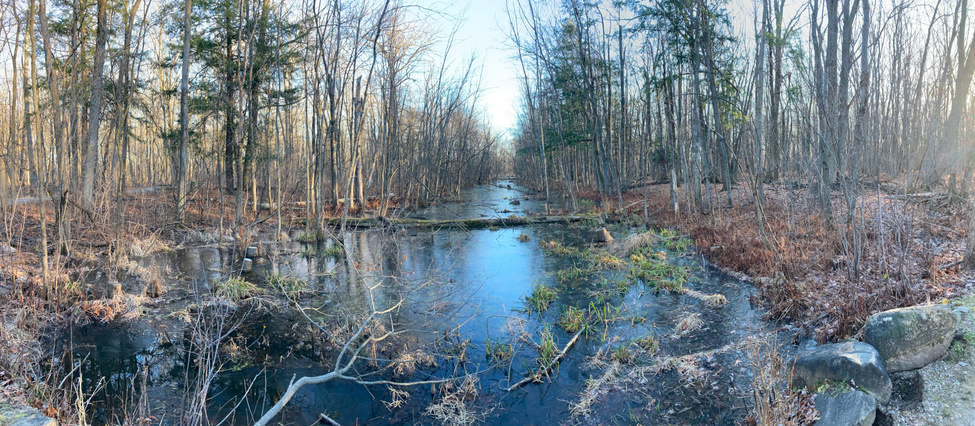
\includegraphics[width=7in]{images/cover_nature5_xs}}
%    \newsavebox{\coverwindmill}
%    \savebox{\coverwindmill}{\includegraphics[width=2in]{images/cover_windmill}}
    \newsavebox{\telescope}
    \savebox{\telescope}{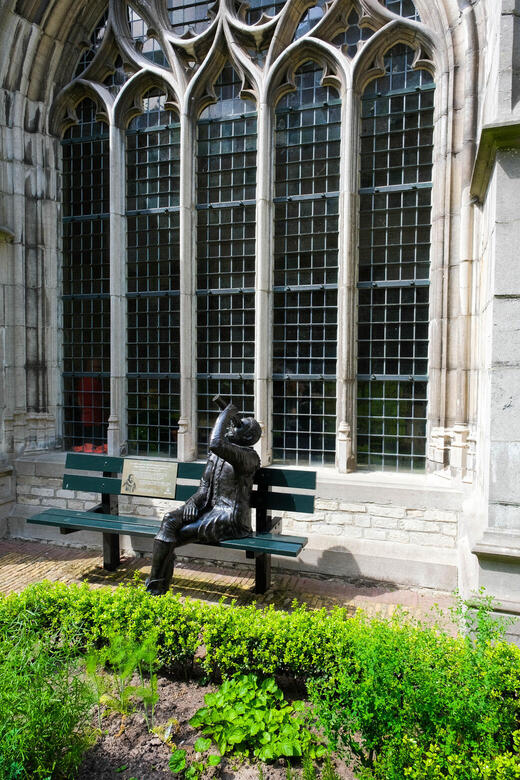
\includegraphics[width=2.5in]{images/cover_telescope}}
    \begin{inctext}[paper=current, target=mytarget]
      \begin{tikzpicture}
        \coordinate (A) at (0,0);
        \coordinate (B) at (8.5in,11in);
        \fill[use as bounding box,color=red!5] (A) rectangle (B);
        \coordinate (C) at ([xshift=0.5in,yshift=0.5in]A);
        \coordinate (D) at ([xshift=-0.5in,yshift=-0.5in]B);
        \draw[rounded corners=0.25in,very thick,black] (C) rectangle (D);
        \node[inner sep=0pt,above right] (nature5) at (0.75in,2.5in) {\usebox{\covernature}};
        \fill[red!5,path fading=south] (0.75in,4.8in) rectangle (7.75in,5.6in);
        \node[inner sep=0pt,below right] (telescope) at (0.75in,10in) {\usebox{\telescope}};
        \fill[red!5,path fading=north] (0.75in,6.2in) rectangle (3.26in,7in);
        \fill[red!5,path fading=west] (3in,6.2in) rectangle (3.26in,10in);
        \node[text width=10cm,align=flush center,font=\Huge\bfseries] at (5.5in,8in) {\UOtitle};
        \node[inner sep=0pt,above right] (UOlogo) at (1in,1in) {\includegraphics[width=\UOlogoCLopt]{\UOlogoCLloc}};
        \node[text width=6cm,above left,font=\large\bfseries] (author) at (7.5in,1in) {\UOauthor \\ \UO};
      \end{tikzpicture}
    \end{inctext}
  \end{titlepage}
  \pagecolor{white}
  \clearemptydoublepage
}

%%%%%%%%%%%%%%%%%%%%%%%%%%%%%%%%%%%%%%%%%%%%%%%%%%%%%%%%%%%%%%%%%%%%%%
% The open source page
%%%%%%%%%%%%%%%%%%%%%%%%%%%%%%%%%%%%%%%%%%%%%%%%%%%%%%%%%%%%%%%%%%%%%%
\newcommand{\UOopenloc}{images/open_source}     % Location of the logo
\newcommand{\UOopenopt}{2cm}             % Options for includegraphics

\newcommand{\opensource}{
  \thispagestyle{empty}

  \noindent \copyright\ \UOauthor, \UOyear\ (\UO)
  
  \noindent Version adapt\'ee de {\it Calcul diff\'erentiel et
  int\'egral pour les sciences de la vie}, manuel pour les cours MAT1730
  et MAT1732, et des notes pour les cours MAT1720, MAT1722 et MAT2722
  de calcul diff\'erentiel et int\'egral pour l'ing\'enierie.

  \noindent Ce document est disponible aux endroits suivants :\\
  Lien\\
  Lien

  \vspace*{1cm}
  
  \noindent \includegraphics[width=\UOopenopt]{\UOopenloc}

  \noindent Sauf indication contraire, ce livre est mis \`a disposition selon
  les termes de la licence \href{https://creativecommons.org/licenses/by-nc-sa/4.0/deed.fr}{Creative Commons Attribution - Pas d’Utilisation Commerciale - Partage dans les M\^emes Conditions 4.0 International} (CC BY-NC-SA 4.0)

  \vfill

  \noindent Page couverture:\\
  Statue de Hans Lipperhey, Pays-Bas, 1570-1619, photo par Louise Oegema.\\
  Un \'etang, photo par Patrice Dionne.

  \noindent Entêtes des chapitres:\\
  Les images utilis\'ees pour les ent\^ees des chapitres sont quelques
  unes des illustrations produites par John Tenniel pour la version
  originale du livre {\bfseries Alice's Adventures in Wonderland} par
  Lewis Carroll.

  \clearemptydoublepage
}

%%%%%%%%%%%%%%%%%%%%%%%%%%%%%%%%%%%%%%%%%%%%%%%%%%%%%%%%%%%%%%%%%%%%%%
% The bibliography
%%%%%%%%%%%%%%%%%%%%%%%%%%%%%%%%%%%%%%%%%%%%%%%%%%%%%%%%%%%%%%%%%%%%%%
\newcommand{\UObibliography}{
  \setcounter{chapter}{100}
  \addcontentsline{toc}{chapter}{Bibliographie}
  \begin{thebibliography}{99}

\bibitem{A} F.\ R.\ Adler, {\bfseries Modeling the Dynamics of Life:
Calculus and Probability for Life Scientists}, Brooks/Cole, 2005.

\bibitem{BE} D. Betounes, {\bfseries Partial Differential Equations for
Computational Science}, Springer-Verlag, 1998.

\bibitem{BC} R. L. Borelli et C. S. Coleman,
{\bfseries Differential Equations, a Modeling Perspective}, Wiley, 1998.

\bibitem{BR} M. Braun, {\bfseries Differential Equations and their
Applications, 4$^{th}$ edition}, Springer-Verlag, 1993.

\bibitem{LC} L. Carroll, {\bfseries Alice's Adventures in Wonderland},

\bibitem{FL} G. B. Folland, {\bfseries Advanced Calculus}, Prentice Hall, 2002

\bibitem{I} R. Illner, C. S. Bohun, S. McCollum et T. an Roode,
{\bfseries Mathemtical Modelling: A Case Studies Approach}, AMS, 2005.

\bibitem{SL} S. Lipschutz, {\bfseries Linear Alegebra}, Schaum's Outline
  Series, McGraw-Hill, 1968.

\bibitem{MT} J. E. Marsden and A. J. Tromba, {\bfseries Vector
 Calculus, 2$^{nd}$ edition}, W. H. Freedman and Company, 1981.

\bibitem{M} J. D. Murray, {\bfseries Mathematical Biology, 1: An
Introduction, 3$^{th}$ edition}, Springer-Verlag, 2002.

\bibitem{NH} C. Newhouser, {\bfseries Calculus for Biology and
Medecine 2$^{nd}$ Edition}, Prentice Hall, 2004

\bibitem{ND} B. Noble and J. W. Daniel, {\bfseries Applied Linear Algebra},
3$^{rd}$ edition, Prentice-Hall, 1988.

\bibitem{O} M. Olinick, {\bfseries An Introduction to Mathematical Models in
the Social and Life Sciences}, Addison-Wesley, 1978

\bibitem{R} D. A. Roff, {\bfseries The Evolution of Life Histories},
Chapman and Hall, 1992

\end{thebibliography}

%%% Local Variables: 
%%% mode: latex
%%% TeX-master: "notes"
%%% End:

  \clearemptydoublepage
}

%%%%%%%%%%%%%%%%%%%%%%%%%%%%%%%%%%%%%%%%%%%%%%%%%%%%%%%%%%%%%%%%%%%%%%
% List of tables and figures
%%%%%%%%%%%%%%%%%%%%%%%%%%%%%%%%%%%%%%%%%%%%%%%%%%%%%%%%%%%%%%%%%%%%%%
\newcommand{\UOtablesfigureslist}{
  \addcontentsline{toc}{chapter}{\LofT}
  \listoftables
  \clearemptydoublepage

  \addcontentsline{toc}{chapter}{\LofF}
  \listoffigures
  \clearemptydoublepage
}

%%%%%%%%%%%%%%%%%%%%%%%%%%%%%%%%%%%%%%%%%%%%%%%%%%%%%%%%%%%%%%%%%%%%%%
% graphics, ...
%%%%%%%%%%%%%%%%%%%%%%%%%%%%%%%%%%%%%%%%%%%%%%%%%%%%%%%%%%%%%%%%%%%%%%
\usepackage{graphicx}
\usepackage{rotating}    % To rotate figures, tables, ...
\usepackage{color}
\usepackage{subfig}

% By default figures will be placed "here" if possible otherwise at
% the "top."
\makeatletter
\renewcommand*{\fps@figure}{ht}
\makeatother

% Methods for figures.
\newcommand{\PDFfig}[5][TTT]{%
  \ifthenelse{\equal{TTT}{#1}}{\begin{figure}}{\begin{figure}[#1]}%
      {\color{purple}\rule{\textwidth}{1pt}}\begin{center}%
        \input{#2.pdf_t}\end{center}\caption[#3]{#4 \label{#5}}%
      {\color{purple}\rule{\textwidth}{1pt}}%
    \end{figure}}

\newcommand{\PDFfigD}[6][TTT]{
  \ifthenelse{\equal{TTT}{#1}}{\begin{figure}}{\begin{figure}[#1]}%
      {\color{purple}\rule{\textwidth}{1pt}}\begin{center} %
        \input{#2.pdf_t}\end{center} %
      \begin{center}\input{#3.pdf_t}\end{center} %
      \caption[#4]{#5 \label{#6}}%
      {\color{purple}\rule{\textwidth}{1pt}}%
    \end{figure}}

\newcommand{\PDFfigR}[5]{\begin{figure}%
    {\color{purple}\rule{\textwidth}{1pt}}\begin{center}
      \resizebox{#2}{!}{\input{#1.pdf_t}}\end{center}
    \caption[#3]{#4 \label{#5}}%
    {\color{purple}\rule{\textwidth}{1pt}}\end{figure}}

\newcommand{\PDFgraph}[1]{\begin{center}\input{#1.pdf_t}\end{center}}

\newcommand{\PDFgraphRow}[2]{\raisebox{#2}{\input{#1.pdf_t}}}

\newcommand{\MATHfig}[6][TTT]{%
  \ifthenelse{\equal{TTT}{#1}}{\begin{figure}}{\begin{figure}[#1]}%
      {\color{purple}\rule{\textwidth}{1pt}}\begin{center} %
        \includegraphics[width=#3]{#2}\end{center} %
      \caption[#4]{#5 \label{#6}}%
      {\color{purple}\rule{\textwidth}{1pt}}%
    \end{figure}}

\newcommand{\MATHfigD}[7]{\begin{figure}%
    {\color{purple}\rule{\textwidth}{1pt}}\begin{center}%
      \includegraphics[width=#2]{#1}\includegraphics[width=#4]{#3}\end{center}%
    \caption[#5]{#6 \label{#7}}%
    {\color{purple}\rule{\textwidth}{1pt}}\end{figure}}

\newcommand{\MATHgraph}[2]{\begin{center}%
    \includegraphics[width=#2]{#1}\end{center}}

\newcommand{\MATHgraphRow}[3]{\raisebox{#3}{\includegraphics[width=#2]{#1}}}

%%%%%%%%%%%%%%%%%%%%%%%%%%%%%%%%%%%%

% Methods for eps Figures.
\newcommand{\epsF}[5]{\begin{figure}\begin{center} %
\includegraphics[width=#2]{#1}\end{center} %
\caption[#3]{#4 \label{#5}}\end{figure}}

\newcommand{\epsD}[7]{\begin{figure}\begin{center} %
\includegraphics[width=#2]{#1}\includegraphics[width=#4]{#3}\end{center} %
\caption[#5]{#6 \label{#7}}\end{figure}}

\newcommand{\epsbox}[2]{\begin{center}%
\includegraphics[width=#2]{#1}\end{center}}

% Methods for pstex Figures.
\newcommand{\pstexF}[4]{\begin{figure}\begin{center} %
\input{#1.pstex_t}\end{center}\caption[#2]{#3 \label{#4}}\end{figure}}

\newcommand{\figbox}[1]{\begin{center}\input{#1.pstex_t}\end{center}}

\newcommand{\pstexD}[5]{\begin{figure}\begin{center} %
\input{#1.pstex_t}\end{center} %
\begin{center}\input{#2.pstex_t}\end{center} %
\caption[#3]{#4 \label{#5}}\end{figure}}

\newcommand{\pstexR}[5]{\begin{figure}\begin{center}
\resizebox{#2}{!}{\input{#1.pstex_t}}\end{center}
\caption[#3]{#4 \label{#5}}\end{figure}}

%%%%%%%%%%%%%%%%%%%%%%%%%%%%%%%%%%%%%%%%%%%%%%%%%%%%%%%%%%%%%%%%%%%%%%
% Formats for the remarks, examples, ...
%%%%%%%%%%%%%%%%%%%%%%%%%%%%%%%%%%%%%%%%%%%%%%%%%%%%%%%%%%%%%%%%%%%%%%
\makeatletter

\newcommand{\rmk@one}[1][RRR]{\def\argrmk@one{#1}\rmk@two}

\newcommand{\rmk@two}[1][TTT]%
{\refstepcounter{focus}\renewcommand{\labelitemi}{\textbullet}%
  \noindent {\bfseries Remarque \thefocus}%
  \ifthenelse{\equal{TTT}{#1}}{}{\ ({\bfseries #1})}%
  \ifthenelse{\equal{RRR}{\argrmk@one}}{\\ \noindent}%
  {\ \argrmk@one \\ \noindent}%
}

\newenvironment{rmk}{\rmk@one}{\hspace*{\fill} $\spadesuit$}

\newcommand{\rmkList@one}[1][RRR]{\def\argrmk@one{#1}\rmkList@two}

\newcommand{\rmkList@two}[1][TTT]%
{\refstepcounter{focus}\renewcommand{\labelitemi}{\textbullet}%
  \noindent {\bfseries Remarque \thefocus}%
  \ifthenelse{\equal{TTT}{#1}}{}{\ ({\bfseries #1})}%
  \ifthenelse{\equal{RRR}{\argrmk@one}}{\\ \vspace*{-1\topskip}\noindent}%
  {\ \argrmk@one \\ \vspace*{-1\topskip}\noindent}%
}

\newenvironment{rmkList}{\rmkList@one}{\hspace*{\fill} $\spadesuit$}

\newcommand{\egg@one}[1][RRR]{\def\argegg@one{#1}\egg@two}

\newcommand{\egg@two}[1][TTT]%
{\refstepcounter{focus}\renewcommand{\labelitemi}{\textbullet}%
  \noindent {\bfseries Exemple \thefocus}%
  \ifthenelse{\equal{TTT}{#1}}{}{\ ({\bfseries #1})}%
  \ifthenelse{\equal{RRR}{\argegg@one}}{\\ \noindent}%
  {\ \argegg@one \\ \noindent}%
}

\newenvironment{egg}{\egg@one}{\hspace*{\fill} $\clubsuit$}

\makeatother

% Title for the multiple choices, the parts of a proof, etc.
\newcommand{\subQ}[1]{\noindent {\bfseries #1})\ }
\newcommand{\subI}[1]{\noindent {\bfseries #1}:\ }
\newcommand{\solTitle}{\noindent {\bfseries Solution:}\\}

%%%%%%%%%%%%%%%%%%%%%%%%%%%%%%%%%%%%%%%%%%%%%%%%%%%%%%%%%%%%%%%%%%%%%%
% Mathematical symbols, short cuts, ...
%%%%%%%%%%%%%%%%%%%%%%%%%%%%%%%%%%%%%%%%%%%%%%%%%%%%%%%%%%%%%%%%%%%%%%
\newcommand{\NN}{\mathbb{N}}
\newcommand{\NNp}{\mathbb{N}^+}
\newcommand{\ZZ}{\mathbb{Z}}
\newcommand{\RR}{\mathbb{R}}
\newcommand{\QQ}{\mathbb{Q}}
\newcommand{\CC}{\mathbb{C}}
\newcommand{\OO}{\mathcal{O}}
\newcommand{\FF}{\mathcal{F}}

\newcommand{\ps}[2]{ \left\langle{#1} , {#2}\right\rangle }
\newcommand{\VEC}[1]{\mathbf{#1}}
\newcommand{\SN}[1]{\mathrm{S}_{#1}}
\newcommand{\sgm}[1]{\overline{#1}}
\newcommand{\ii}{\VEC{i}}
\newcommand{\jj}{\VEC{j}}
\newcommand{\kk}{\VEC{k}}
\newcommand{\nn}{$n\times n$\ }
\newcommand{\nm}[2]{${#1}\times {#2}$\ }

\DeclareMathOperator{\IM}{Im\ }
\DeclareMathOperator{\DO}{Dom\ }
\DeclareMathOperator{\arcsec}{arcsec}
\DeclareMathOperator{\tr}{tr}
\DeclareMathOperator{\Id}{I}   % ou Id  ?
\DeclareMathOperator{\sgn}{sgn}
\DeclareMathOperator{\curl}{rot}
\DeclareMathOperator{\diV}{div}
\DeclareMathOperator{\graD}{grad}
\DeclareMathOperator{\sech}{sech}
\DeclareMathOperator{\csch}{csch}

\newcommand{\diff}{\mathrm{D}}
\newcommand{\dx}[1]{\,\mathrm{d}#1}
\newcommand{\dydx}[2]{\frac{\mathrm{d}#1}{\mathrm{d}#2}}
\newcommand{\dydxn}[3]{\frac{\mathrm{d}^{#3}#1}{\mathrm{d}#2^{#3}}}
\newcommand{\dfdx}[2]{\frac{\mathrm{d}}{\mathrm{d}#2}#1}
\newcommand{\dfdxn}[3]{\frac{\mathrm{d}^{#3}}{\mathrm{d}#2^{#3}}#1}

\newcommand{\pdydx}[2]{\frac{\partial #1}{\partial #2}}
\newcommand{\pdydxn}[3]{\frac{\partial^{#3} #1}{\partial #2^{#3}}}
\newcommand{\pdydxnm}[6]{\frac{\partial^{#4} #1}%
{\partial #2^{#5} \partial #3^{#6}}}

\newcommand{\pdfdx}[2]{\frac{\partial}{\partial #2} #1}
\newcommand{\pdfdxn}[3]{\frac{\partial^{#3}}{\partial #2^{#3}} #1}
\newcommand{\pdfdxnm}[6]{\frac{\partial^{#4}}%
{\partial #2^{#5} \partial #3^{#6}} #1}

\newcommand{\Maug}[2]{\left(\begin{array}{c|c}{#1}&{#2}\end{array}\right)}

\newcommand{\rectangle}{
%\begin{tikzpicture}
\tikz \draw (0,0) rectangle (0.4,0.3);
%\end{tikzpicture}
}

\newcommand{\trapeze}{
%\begin{tikzpicture}
\tikz \draw (0,0) -- (0.2,0.3) -- (0.5,0.3) -- (0.3,0) -- cycle;
%\end{tikzpicture}
}

\renewcommand{\qed}{\hfill \mbox{\raggedright \rule{0.4em}{0.8em}}\\[1em]}

\makeatletter

\newcommand{\proof@one}[1][RRR]{\def\argproof@one{#1}\proof@two}

\newcommand{\proof@two}[1][TTT]%
{\noindent\textbf{\UOproof}\ %
  \ifthenelse{\equal{TTT}{#1}}{}{\ ({\bfseries #1})} %
  \ifthenelse{\equal{RRR}{\argproof@one}}{\\ \noindent}%
  {\ \argproof@one \\ \noindent}%
  \normalfont%
}

\renewenvironment{proof}{\proof@one}{\hspace*{\fill} \qed}

\makeatother

%%%%%%%%%%%%%%%%%%%%%%%%%%%%%%%%%%%%%%%%%%%%%%%%%%%%%%%%%%%%%%%%%%%%%%
% To produce assignments and the solutions for the problems of a
% chapter
%%%%%%%%%%%%%%%%%%%%%%%%%%%%%%%%%%%%%%%%%%%%%%%%%%%%%%%%%%%%%%%%%%%%%%
\newcounter{questNBR}[chapter]
\renewcommand\thequestNBR{\thechapter.\arabic{questNBR}}

\makeatletter

\newcommand{\quest@one}[1][RRR]{\def\argquest@one{#1}\quest@two}

\newcommand{\quest@two}[1][TTT]%
{\refstepcounter{questNBR}\noindent%
  {\bfseries Question \arabic{chapter}.\arabic{questNBR}}%
  \ifthenelse{\equal{TTT}{#1}}{}{\ ({\bfseries #1})}%
  \ifthenelse{\equal{RRR}{\argquest@one}}{\\ \noindent}{\ \argquest@one \\ \noindent}%
}

\newenvironment{question}{\quest@one}{}

\makeatother

%%%%%%%%%%%%%%%%%%%%%%%%%%%%%%%%%%%%%%%%%%%%%%%%%%%%%%%%%%%%%%%%%%%%%%
% The index
%%%%%%%%%%%%%%%%%%%%%%%%%%%%%%%%%%%%%%%%%%%%%%%%%%%%%%%%%%%%%%%%%%%%%%
\usepackage{makeidx}
\makeindex
\newcommand{\UOindex}{
  \setcounter{chapter}{100}
  \addcontentsline{toc}{chapter}{\indexname}
  \printindex
}

%%%%%%%%%%%%%%%%%%%%%%%%%%%%%%%%%%%%%%%%%%%%%%%%%%%%%%%%%%%%%%%%%%%%%% 
% Sometime useful
%%%%%%%%%%%%%%%%%%%%%%%%%%%%%%%%%%%%%%%%%%%%%%%%%%%%%%%%%%%%%%%%%%%%%%
\usepackage{multicol}

%%%%%%%%%%%%%%%%%%%%%%%%%%%%%%%%%%%%%%%%%%%%%%%%%%%%%%%%%%%%%%%%%%%%%%
% Extra fonts of the form  \fa...
%%%%%%%%%%%%%%%%%%%%%%%%%%%%%%%%%%%%%%%%%%%%%%%%%%%%%%%%%%%%%%%%%%%%%%
\usepackage{fontawesome}

%%%%%%%%%%%%%%%%%%%%%%%%%%%%%%%%%%%%%%%%%%%%%%%%%%%%%%%%%%%%%%%%%%%%%%
% Formatting of the notes
%%%%%%%%%%%%%%%%%%%%%%%%%%%%%%%%%%%%%%%%%%%%%%%%%%%%%%%%%%%%%%%%%%%%%%
\newboolean{THEO}
\setboolean{THEO}{false}
\newcommand{\setTHEO}{\setboolean{THEO}{true}}

\newcommand{\compileTHEO}[1]{
  \ifthenelse{\boolean{THEO}}{#1}{}
}

\newcommand{\SOLUa}{hide}
\newcommand{\setSOLUa}{\renewcommand{\SOLUa}{show}}

\newcommand{\SOLUb}{hide}
\newcommand{\setSOLUb}{\renewcommand{\SOLUb}{show}}

\newcommand{\SOLUc}{hide}
\newcommand{\setSOLUc}{\renewcommand{\SOLUc}{show}}

% \newcommand{\compileSOL}[3]{
% \ifthenelse{\equal{#1}{show}}{{\bfseries\noindent Question~#2}\\ #3}{\ \newline\newline}
% }

\newenvironment{SOLUTION}{}{}
\newcommand{\compileSOL}[3]{
\ifthenelse{\equal{#1}{show}}{
\begin{SOLUTION}
{\bfseries\noindent Question~#2}\\ #3
\end{SOLUTION}
}{}}

\newcommand{\compileSOLU}[2]{
  \ifthenelse{\equal{#1}{show}}{\solTitle #2}{}
}

\newcommand{\HIDE}{show}
\newcommand{\setHIDE}{\renewcommand{\HIDE}{hide}}

\newcommand{\compileText}[2]{
  \ifthenelse{\equal{#1}{hide}}{}{#2}
}

% Many solutions use  \compileText{solOUT}{}{}  because we
% didn't want to print them.

\newcommand{\theory}{\faEye\ }
\newcommand{\eng}{\faWrench\ }
\newcommand{\eco}{\faLineChart\ }
\newcommand{\life}{\faTree\ }


%%%%%%%%%%%%%%%%%%%%%%%%%%%%%%%%%%%%%%%%%%%%%%%%%%%%%%%%%%%%%%%%%%%%%%
% Uncomment and add the value for the variables that you want to
% modified.
%%%%%%%%%%%%%%%%%%%%%%%%%%%%%%%%%%%%%%%%%%%%%%%%%%%%%%%%%%%%%%%%%%%%%%
% \setUO{}         % University of the author
% \setUOfac{}      % Faculty of the author
% \setUOdept{}     % Department of the author
% \setUOauthor{}   % Name of the author
% \setUOtitle{}    % Title of the book
% \setUOyear{}     % Year of publication
% \setUOlogoloc{}{}   % The first argument is the location of the logo
%                     % of the university and the second are the
%                     % arguments for includegraphics{}
%                     % The second argument is broken right now

\setTHEO
% comment \setSOLUa and \setSOLUc and comment out \setHIDE
\setSOLUa    % Hide those solutions, comment out to show these solutions. 
\setSOLUb
% \setSOLUc   % Theoretical questions that we generally hide,
              % comment out to show these solutions. 
%\setHIDE      % Used to hide some parts of the solutions

\begin{document}

% \hypersetup{pageanchor=false}

% \setUOtitle{Calcul différentiel et intégral à uOttawa\\[0.6em]
%     1$^{er}$ édition}
\titlePage

\opensource

\pagenumbering{roman}

\UOtableofcontents
% \UOtablesfigureslist

\nonumchapter{\AP}

Le contenu de ce manuel couvre la grande majorité des sujets présentés
dans les cours de calcul différentiel et intégral pour les étudiants
\footnote{Dans ce manuel, le genre non marqué, c'est-à-dire le
masculin, quand il est employé pour désigner des personnes, renvoie
aussi bien à des femmes qu'à des hommes.}
en sciences et génies.  Les seuls préalables sont les mathématiques
normalement enseignées au secondaire en Ontario.  En fait, le premier
chapitre revoit rapidement tous les concepts mathématiques que le
lecteur devrait connaître à la sortie du secondaire.  Certains
concepts qui ne sont pas présentés au secondaire ont aussi été ajoutés
au chapitre~\ref{ChapFonct}.  Il est donc fortement suggérer au
lecteur de revoir le chapitre~\ref{ChapFonct} même s'il est
confiants de bien connaître les mathématiques de base.

Afin que le lecteur puisse bien comprendre le matériel présenté dans
ce manuel, nous avons porté un très grand soin à fournir tous les
détails et calculs algébriques qui supportent les énoncés
mathématiques.  De cette façon, nous espérons que le lecteur ne sera pas
nuit dans son apprentissage de la matière par des détails techniques.
De plus, cela permet au lecteur de développer ses capacités à
exécuter correctement des calculs algébriques.

Nous avons aussi choisi d'inclure les solutions détaillés d'un grande
nombre de problèmes à la fin du manuel.  Le lecteur devrait
sérieusement essayer de résoudre les problèmes à la fin de chaque
chapitre avant de regarder les solutions.  Nous n'apprenons pas à
jouer de la guitare en regardant un guitariste jouer.  Il faut
sérieusement pratiquer au point d'avoir le bout des doigts sensibles.
C'est la même chose pour les mathématiques.  Ce n'est pas en lissant
simplement les solutions des problèmes produites par une autre
personne que nous apprenons à résoudre des problèmes.  Il faut en
résoudre soit même.

Une autre raison pour justifier l'inclusion d'un grande nombre de
solutions est qu'il est maintenant facile d'accéder à un logiciel qui
peut presque complètement résoudre les problèmes ou d'utiliser
certains sites Internet pour demander à d'autres personnes de
résoudre les problèmes.  C'est la meilleure façon pour ne rien
apprendre.  C'est sans compter que bien souvent les solutions
fournies sur ces sites sont erronées.  Donc, si vraiment vous ne
pouvez pas résoudre un problème après avoir essayé pour une bonne
période de temps, il est préférable de regarder la
solution à la fin du manuel pour obtenir une solution correcte; en
assumant que l'auteur n'ait pas fait lui-même d'erreurs. 

Ce manuel peut être utilisées pour trois des variantes des cours de
calcul différentiel et intégral que nous retrouvons dans la majorité des
universités en Ontario.

{\renewcommand{\labelitemi}{\textbullet}
\begin{itemize}
\item Les items marqués par le symbole \eng sont spécifiquement pour
les cours de {\bfseries Calcul différentiel et intégral pour les 
étudiants en génie}.
\item Les items marqués par le symbole \life sont spécifiquement pour
les cours de {\bfseries Calcul différentiel et intégral pour les
étudiants en sciences de la vie}.
\item Les items marqués par le symbole \eco sont spécifiquement pour
les cours de {\bfseries Calcul différentiel et intégral pour les
étudiants en administration}.
\end{itemize}
}

Les items qui n'ont aucun de ces symboles sont requis pour les trois
variantes des cours de calcul différentiel et intégral.  Le contenu
pour les étudiants en administration est probablement à un niveau plus
avancé que celui du contenu normalement présenté à ce groupe d'étudiants.

L'ordre dans lequel le matériel est présenté est standard.  Il y a
cependant certaines additions au matériel que nous ne retrouvons
traditionnellement pas dans un manuel de calcul différentiel et
intégral à ce niveau.  Une introduction à l'algèbre linéaire est
fournie au chapitre~\ref{chapALLin}.  Le matériel présenté dans ce
chapitre est tout ce que le lecteur a besoin de connaître en algèbre
linéaire pour l'étude des fonctions de plusieurs variables aux
chapitres~\ref{chapFonctPlusVar}, \ref{chapDerFonctMult}, \ref{chapIntMult}
et \ref{chapCalcVect}; et l'étude des systèmes d'équations
différentielles au chapitre~\ref{ChapSystEquDiff}.   Donc, aucun cours
d'algèbre linéaire n'est préalable aux derniers chapitres de ce
manuel.  Une application concrète de l'algèbre linéaire est fournie
par les chaînes de Markov à la section~\ref{sectChainseMarkov}.
Un chapitre comme le chapitre~\ref{ChapSystEquDiff} sur les
systèmes d'équations différentielles n'est généralement pas inclus
dans un manuel de calcul différentiel et intégral.  En particulier, lorsque
l'emphase de l'étude des systèmes d'équations différentielles est sur
l'aspect qualitatif de ces systèmes.

Les chapitres~\ref{ChapSuitesSeries} et \ref{chapLimites} couvrent
certains sujets présentés au secondaire.  Cependant, plusieurs sujets
qui ne sont pas abordés au secondaire font parties de ces chapitres.
La matière des cours de calcul différentiel et intégral au niveau
universitaire débute donc avec certaines sections de ces chapitres
selon le cours de calcul différentiel et intégral auxquels l'étudiant
est inscrit.

Comme les principaux utilisateurs de ces notes depuis plus de dix ans
ont été les étudiants inscrits aux cours de Calcul différentiel et
intégral pour les sciences de la vie à l'Université d'Ottawa, il n'est
pas surprenant qu'une emphase toute particulière a été apporté à ce
sujet.  Cela se traduit par plusieurs exemples en biologie et
médecine, en particulier dans les premiers chapitres.

Le cours de calcul différentiel et intégral pour les sciences de la
vie comporte deux principales parties.  La première partie
est dédiée au calcul différentiel pour les fonctions d'une variable et
culmine avec l'étude des \lgm systèmes dynamiques discrets\rgm\ à la
section~\ref{Sect_SDD}.  Les systèmes dynamiques discrets sont
utilisés entre autre pour décrire certaines caractéristiques des
populations animales mesurées à intervalles réguliers.
La deuxième partie du cours de calcul différentiel et intégral pour
les sciences de la vie est dédié au calcul intégral.  Le but ultime de
cette partie est l'étude des \lgm systèmes dynamiques (continus)\rgm\ 
au chapitre~\ref{ChapSystEquDiff}.  Les systèmes dynamiques continues
sont des systèmes d'équations différentielles.  Ils sont utilisés
entre autre pour modéliser les réactions chimiques, la croissance des
populations et leurs mouvements, etc.

\noindent {\bfseries Avertissement}: Les modèles biologiques utilisés
dans les exemples et les questions ne représentent pas toujours des
situations réelles.  Pour obtenir des modèles mathématiques qui soient
intéressants et utilisent la théorie présentée dans les notes, tout en
étant accessibles pour le niveau du cours, nous avons dû créer des
modèles qui ne sont pas basés sur des données scientifiques.  Nous
avons quand même essayé d'obtenir des modèles qui soient qualitativement
valables.

Alors que l'emphase est misse sur les applications à la biologie au
début du manuel, notre attention se tourne vers les applications à la
physique lorsque nous avançons dans la matière pour porter exclusivement
sur les applications à la physique lorsque nous abordons l'étude des
fonctions de plusieurs variables.  En fait, à partir du
chapitre~\ref{chapFonctPlusVar} qui introduit les fonctions de
plusieurs variables, nous nous attendons à ce que le lecteur est
une plus grande maturité mathématique.

Le manuel contient deux courts chapitres, le
chapitre~\ref{CHAPvecteurs} sur les vecteurs et le
chapitre~\ref{cha[ReprParam} sur les représentations paramétriques de
courbes dans le plan et dans l'espace.  Le
chapitre~\ref{CHAPvecteurs} sur les vecteurs contient beaucoup plus
d'information que nécessaire.  Cependant, ce chapitre est une bonne
préparation pour l'étude des fonctions de plusieurs variables.  En
particulier, il permet au lecteur de développer ses aptitudes à
visualiser les objets en trois dimensions; ce qui sera très utile lors
l'étude de l'intégral double et triple au chapitre~\ref{chapIntMult}.
Le chapitre~\ref{cha[ReprParam} est fondamental pour l'étude du calcul
vectoriel au chapitre~\ref{chapCalcVect} et des systèmes d'équations
différentielles au chapitre~\ref{ChapSystEquDiff}.

Le chapitre~\ref{chapSerEnt} sur les séries entières est probablement
le plus théorique des chapitres.  Cela n'est pas surprenant dû à la
nature du sujet.  Le but principal de ce chapitre est de déterminer la
convergence des séries entières.  Il n'en reste pas moins que ce
chapitre est fondamental pour ceux qui poursuivront l'étude des
équations différentielles comme c'est le cas pour plusieurs des
domaines du génie.

Nous avons limité au minimum le contenu du chapitre~\ref{chapCalcVect} sur
le calcul vectoriel.  Nous avons adopté une approche intuitive à ce sujet.
Il aurait été bénéfique d'aborder plus en détails les opérations sur
les courbes (additions et différences) pour créer de nouvelles
courbes, et l'interprétation de ces opérations en termes d'opérations
sur les intégrales le long de courbes.  Ce chapitre ouvre la porte au
vaste sujet de la géométrie différentielle.  Nous nous sommes retenu pour
ne pas déborder do contenu d'un cours de calcul différentiel et intégral
standard.

\section*{Théorie}

Les items marqués par le symbole \theory sont spécifiquement pour les
lecteurs intéressés à la théorie et la rigueur en mathématique.
Plusieurs de ces items demandent une connaissance du concept de \lgm
démonstration\rgm\ que la majorité des étudiants du secondaire
n'auront probablement pas vu.  Ces items sont généralement optionnels.
Ils sont pour les lecteurs curieux qui voudrait en savoir plus sur les
méthodes enseignées en classe.

Il est fort probable que la majorité des étudiants en science de la
vie et même en génie ne liront pas les sections plus théoriques.
Malheureusement, pour eux, les mathématiques se limitent
à une suite de méthodes et trucs pour résoudre certains problèmes.  Ce
manuel contient ces méthodes et trucs.  Cependant, les sections plus
théoriques donnent un avant goût de se que sont les mathématiques.  Nous
espérons que certains lecteurs seront intéressés par la rigueur
mathématiques et voudront poursuive cette direction dans leur études.

Il y a plusieurs mentions du nombre d'Euler $e$.  Nous donnons plusieurs
façons équivalentes de le définir.  Nous mentionnons indirectement le lien
entre le nombre $e$ et les fonctions trigonométriques, donc le nombre
$\pi$, lors d'une des démonstrations de la règle d'addition pour les
fonctions trigonométriques $\sin$ et $\cos$.  Nous espérons que les
étudiants seront fascinés par le fait que les nombres $e$ et $\pi$
sont reliés.

\section*{Notation}

\begin{focus*}{\dfn}
Les ensembles suivants seront fréquemment utilisés dans le présent
document.
\begin{itemize}
\item $\NN = \{0,1,2,3,\ldots \}$ est l'ensemble des nombres naturels.
\item $\NNp = \{1,2,3,\ldots \}$ est l'ensemble des nombres naturels
positifs.
\item $\ZZ = \{0,1,-1,2,-2,3,-3, \ldots \}$ est l'ensemble des nombres
entiers.
\item $\QQ$ est l'ensemble des nombres rationnels; c'est-à-dire, les
  nombres de la forme $n/m$ où $n,m \in \ZZ$ et $m \neq 0$.
\item $\RR$ est l'ensemble des nombres réels.
\end{itemize}
\end{focus*}

En français, la virgule est utilisée pour séparer la partie entière de
la partie décimale d'un nombre et nous utilisons un espace pour séparer
les multiples de $10^3$.  Ainsi,
\[
105\ 456\ 263,456 =
105\times 10^6+ 456\times 10^3 + 263 + \frac{456}{1000} \ .
\]
Cependant, dans le présent document, nous utiliserons la notation
anglaise.  Le point sépare la partie entière de la partie décimale d'un
nombre et la virgule sépare les multiples de $10^3$.  Nous écrivons donc
\[
105,456,263.456 = 105\times 10^6+ 456\times 10^3 + 263 + \frac{456}{1000} \ .
\]
La raison principale de ce choix est que la grande majorité des
données utilisées dans ce document proviennent de documents en anglais
qui utilisent cette notation.  De plus, les logiciels sont tous en
anglais et utilisent aussi cette notation.  Pour être consistent, nous
avons donc choisi d'utiliser la notation anglaise.

\section*{Avertissement}

Les notes de cours que vous avez devant vous représente un ouvrage
inachevé, qui est en constante évolution.  Il ne faut donc pas être
surpris d'y retrouver des fautes d'orthographe, des coquilles, etc.
Les corrections seront apportées au cours du temps suite aux
commentaires des lecteurs.  L'auteur prend entière responsabilité
des erreurs; comment pourrait-il faire autrement?

\section*{Remerciements}

J'aimerais remercier Yves Bourgault, Wadii Hajji et Monica Nevins,
des collègues de travail, dont les suggestions ont améliorées la
présentation de la matière.

De plus, j'aimerais remercier Paméla Touchette-Giroux pour son
excellent travail de révision des textes pour la première édition de
ces notes.  Il n'en reste pas moins que je prends toute la
responsabilité pour les fautes présentes dans le texte.

%%% Local Variables: 
%%% mode: latex
%%% TeX-master: "notes"
%%% End: 

\clearemptydoublepage

\pagenumbering{arabic}

\chapter[Fonctions]{Fonctions}\label{ChapFonct}

\compileTHEO{

Ce chapitre présente les objets fondamentaux sur lesquels nous allons
travailler dans les prochains chapitres.  Ces objets sont les
{\em fonctions}.  Les principales propriétés des fonctions sont aussi
définies dans ce chapitre.  Nous terminons le chapitre avec une
introduction à quelques unes des fonctions de base: les fonctions
trigonométriques, exponentielles et logarithmiques.  Les fonctions
exponentielles sont définies de façon intuitive dans ce chapitre.
Elles sont revues de façon plus rigoureuse au chapitre suivant.

\section{Qu'est-ce qu'une fonction?}

\begin{defn} \index{Fonction}
Une {\bfseries fonction} $f$ est une opération d'un
ensemble $X$ à un ensemble $Y$ qui, à chaque élément de $X$, associe
un seul élément de $Y$.  Nous écrivons $f:X\rightarrow Y$ pour désigner une
fonction $f$ de $X$ dans $Y$.
\end{defn}

\begin{egg}
À la figure~\ref{FUNCT1}, nous définissons à l'aide d'un diagramme une
fonction $f$ d'un ensemble $X$ de pays à un ensemble $Y$ de villes.
La fonction $f$ donne la capitale du pays.  À chacun des pays de $X$
est associé une seule ville dans $Y$ qui est sa capital.

Il n'est pas nécessaire que toutes les villes de $Y$ soient des
capitales de pays.  Par exemple, Toronto n'est pas la capitale d'un
pays mais d'une province.

Nous écrivons
\[
f(\text{Canada}) = \text{Ottawa} \quad , \quad f(\text{Angleterre}) =
\text{Londres} \quad , \quad \text{etc}.
\]
\label{CAPITALS}
\end{egg}

\PDFfig{2_fonctions/funct1}{Définition d'une fonction}{Définition d'une
  fonction $f$ à l'aide d'un diagramme}{FUNCT1}

\begin{egg}
Le tableau suivant définit une fonction $g$ qui, à chaque nombre
entier plus grand que $1$ (ligne du haut), associe les diviseurs
premiers de ce nombre entier (ligne du bas).
\[
\begin{array}{c|c|c|c|c|c|c|c|c|c}
x & 2 & 3 & \ldots & 6 & \ldots & 27 & \ldots & 1372455084 &
\ldots \\
\hline
g(x) & \{2\} & \{3\} & \ldots & \{2,3\} & \ldots & \{3\} &
\ldots & \{2,3,7,11,13,17,47\} & \ldots
\end{array}
\]

La fonction $g$ est donc une fonction qui va de l'ensemble $X$ des
nombres entiers plus grand que $1$ à l'ensemble $Y$ des ensembles de
nombres premiers.

Nous écrivons
\[
g(2) = \{2\} \quad , \quad g(1372455084) = \{2,3,7,11,13,17,47\}
\quad , \ldots
\]
\label{TABLE}
\end{egg}

\begin{egg}
La fonction $h$ qui suit est définie à l'aide d'une expression
algébrique.
\[
h(x) = x^3-2x+1 \; .
\]
La fonction $h$ est définie pour tout $x \in X = \RR$ (l'ensemble des
nombres réels) et donne une seule valeur $h(x) \in Y = \RR$.  Nous
disons alors que $h$ est une fonction de $\RR$ dans $\RR$ que nous
dénotons $h:\RR \rightarrow \RR$. 

Nous écrivons
\[
h(1) = 0 \quad , \quad h(2) = 5 \quad , \quad h(\pi)=
12.26706787812110\ldots \quad , \quad \ldots
\]
Pour la valeur $h(\pi)$, les points de suspension après le
dernier $0$ indiquent qu'il y a une infinité de chiffres qui
suivent.

Dans l'expression
\[
y=h(x)=x^3 -2x +1 \ ,
\]
la variable $x$ est appelée la {\bfseries variable indépendante}
\index{Fonction!variable indépendante} et la variable $y$ est appelée
la {\bfseries variable dépendante} \index{Fonction!variable dépendante}
car elle dépend de $x$.
\label{GRAPH_SET}
\end{egg}

\begin{defn} \index{Fonction!graphe}
Si $f$ est une fonction qui va d'un ensemble $X$ à un ensemble $Y$,
nous définissons le {\bfseries graphe de la fonction}
$f$ comme étant l'ensemble
\[
\text{graphe de }f = \left\{ (x,f(x)) : x \in X \right\} \; .
\]
\end{defn}

Pour une fonction qui va de $\RR$ dans $\RR$, il est plus fréquent de
représenter le graphe de cette fonction par la courbe du plan
cartésien qui est tracée par l'ensemble des points du graphe.  Le
graphe est donc un sous-ensemble du plan cartésien.

\begin{egg}
Nous retrouvons à la figure~\ref{FUNCT2} la représentation dans le plan
cartésien du graphe de la fonction $h$ définie à
l'exemple~\ref{GRAPH_SET}.
\end{egg}

\MATHfig{2_fonctions/funct2}{8cm}{Graphe de $h(x) = x^3-2x+1$}
{Graphe de $y= h(x) = x^3-2x+1$ pour $-2 \leq x \leq 2$.}{FUNCT2}

\section{Image et domaine d'une fonction}

\begin{defn} \index{Fonction!image}
L'{\bfseries image} d'une fonction $f$ qui va
d'un ensemble $X$ à un ensemble $Y$ est l'ensemble des éléments $y \in Y$
pour lesquelles il existe au moins un élément $x \in X$ tel que
$f(x) = y$.  Nous écrivons
\[
\IM f \equiv \left\{ y \in Y : f(x) = y \quad
\text{pour au moins un élément} \quad x \in X \right\} \; .
\]
\end{defn}

\begin{egg}
Pour l'exemple~\ref{CAPITALS}, l'image de $f$ est l'ensemble
\[
\IM f = \left\{ \text{Berlin, Londres, Paris, Ottawa} \right\} \; .
\]
\end{egg}

\begin{rmk}
Pour l'exemple~\ref{TABLE}, nous ne connaissons pas tous les éléments de
l'image de $g$ et il n'existe pas de formule pour les générer.
\end{rmk}

\begin{egg}
Pour l'exemple~\ref{GRAPH_SET}, l'image de $h$ est l'ensemble des
nombres réels comme nous pouvons le constater à partir du graphe de $h$ à
la figure~\ref{FUNCT2}.  Nous écrivons
\[
\IM h = \RR\; .
\]
\end{egg}

\begin{defn} \index{Fonction!domaine}
Le {\bfseries domaine} d'une fonction $f$ qui
va d'un ensemble $X$ à un ensemble $Y$ est l'ensemble $X$ sur lequel
la fonction $f$ est définie.  Nous écrivons
\[
\DO f = X \; .
\]
\end{defn}

\begin{egg}
Pour l'exemple~\ref{CAPITALS}, la fonction $f$ est définie pour tous
les pays de l'ensemble $X$.  Le domaine de $f$ est donc l'ensemble
$X$ au complet.
\[
\DO f = X = \left\{ \text{Allemagne, Angleterre, Canada, France}
\right\} \; .
\]
\end{egg}

\begin{egg}
La fonction $h$ de l'exemple~\ref{GRAPH_SET} est définie pour tous les
nombres réels.  Le domaine de $h$ est donc $\RR$.
\end{egg}

\begin{egg}
Le graphe de la fonction $h(x) = \sqrt{x}$ est donné à la
figure~\ref{SQRT}.  Nous avons que
\[
\DO h = \{ x \in \RR :  x\geq 0 \}
\qquad \text{ et } \qquad
\IM h = \{ y \in \RR : y \geq 0 \}\; .
\]
\end{egg}

\MATHfig{2_fonctions/squareroot}{8cm}{Graphe de $y= \sqrt{x}$}
{Graphe de $y= \sqrt{x}$ pour $0 \leq x \leq 3$}{SQRT}

\section{Composition de fonctions}

\begin{defn} \index{Fonction!composition}
Si $f$ est une fonction qui va de l'ensemble $X$ à l'ensemble $Y$ et
$g$ est une fonction qui va de l'ensemble $Y$ à l'ensemble $Z$, nous
pouvons définir une nouvelle fonction $g\circ f$ qui va aller de
l'ensemble $X$ à l'ensemble $Z$ en posant
\[
(g\circ f)(x) \equiv g(f(x))
\]
pour tous les éléments $x$ dans l'ensemble $X$.  La nouvelle
fonction $g\circ f$ est appelée la {\bfseries composition}
des fonctions $f$ et $g$.
\end{defn}

\begin{egg}
Deux fonctions sont définies par le diagramme à la figure~\ref{COMPO}.
La fonction $f$ donne la ville où demeure chacune des personnes de
l'ensemble $X$ et la fonction $g$ donne la province où se situe
chacune des villes de l'ensemble $Y$.  La composition $g\circ f$ est
donc la fonction qui donne la province où demeure chacune des
personnes de l'ensemble $X$.  Ainsi, nous obtenons
\begin{align*}
(g\circ f)(\text{Françoise}) &= g(f(\text{Françoise})) =
g(\text{Montréal}) = \text{Québec}
\intertext{et}                               
(g\circ f)(\text{Patrice}) &= g(f(\text{Patrice})) = g(\text{Winnipeg})
= \text{Manitoba} \; .
\end{align*}
\label{F_COMPO}
\end{egg}

\PDFfig{2_fonctions/composition}{Composition de fonctions}
{Définition des fonctions $f$ et $g$ pour l'exemple~\ref{F_COMPO}}{COMPO}

\begin{egg}
Soit $F$ la fonction qui donne pour chaque personne sa mère biologique
et soit $M$ la fonction qui donne pour chaque personne son père
biologique.

La composition des fonctions $F$ et $M$, dénotée $F \circ M$, est la
fonction qui donne pour chaque personne la mère biologique du père
biologique de cette personne (une des grand-mères de la personne).
Rappelons que dans la composition $F \circ M$,
{\em la fonction $M$ est exécutée en premier et la fonction $F$ en
second}.  La fonction $M$ donne le père biologique de la personne
donnée initialement.  Puis, la fonction $F$ avec comme argument le
père biologique de la personne donnée initialement donne la mère
biologique de ce père.

Quel est le résultat de la composition $F \circ M \circ F$?
\label{PEOPLES}
\end{egg}

\begin{egg}
Regardons un exemple de fonctions dont le domaine et l'image font
parties des nombres réels.  Plus précisément, considérons les
fonctions $f(x) = x^2+3$ et $g(x) = 3 x - 2$.  Ainsi,
\begin{align*}
(f\circ g)(x) &\equiv f(g(x)) = f(3x - 2) = (3x-2)^2 + 3
= 9 x^2 - 12 x + 7
\intertext{et}
(g\circ f)(x) &\equiv g(f(x)) = g(x^2+3) = 3(x^2+3) - 2
= 3 x^2 + 7 \; .
\end{align*}
Ces compositions donnent bien des fonctions qui sont différentes
du produit $f g$ qui est
\[
(f g)(x) \equiv f(x) g(x) = (x^2+3)(3 x-2) = 3 x^3  -2 x^2 + 9x -6 \; .
\]
\end{egg}

\MATHfig{2_fonctions/compog}{8cm}{Graphe de $g(x) = x^2 -1$}
{Graphe de $y= g(x) = x^2 -1$ pour $-2 \leq x \leq 2$}{COMPOG}

\MATHfig{2_fonctions/compohg}{8cm}{Graphe de $y= h(g(x))$}
{Graphe de $y= h(g(x)) = \sqrt{x^2 -1}$ pour $1 \leq |x| \leq 3$}{COMPOHG}

\begin{egg}
Nous pouvons composer les fonctions $g(x) = x^2 - 1$
(figure~\ref{COMPOG}) et $h(x) = \sqrt{x}$ pour obtenir de nouvelles
fonctions.  Le domaine de $g$ est $\RR$ et
l'image de $g$ est $\{ y \in \RR : y \geq -1 \}$.  De plus, le domaine
de $h$ est $\{ x \in \RR : x \geq 0 \}$ et l'image de $h$ est
$\{ y \in \RR : y \geq 0 \}$.

Pour définir la composition $h \circ g$, il faut avoir
\begin{equation} \label{funct_domimg1}
\IM g \subset \DO h \; .
\end{equation}
Ce qui n'est pas le cas présentement.  Il faut restreindre $g$
à l'ensemble des $x$ tels que $x^2-1 \geq 0$ pour satisfaire
(\ref{funct_domimg1}).  Avec la restriction $|x|\geq 1$, nous avons
maintenant que
\begin{equation} \label{funct_domimg2}
\IM g = \{ x : x\geq 0\} = \DO h
\end{equation}
et la composition $h\circ g$ est définie par
\[
(h\circ g)(x) = h(g(x)) = h(x^2-1) = \sqrt{x^2-1} \quad \text{pour}
\quad |x|\geq 1 \; .
\]
Il découle de (\ref{funct_domimg2}) que l'image de $h\circ g$ est
l'image de $h$ car l'image de $g$ est tout le domaine de $h$.  Le
domaine de $h \circ g$ est $\{ x \in \RR : |x| \geq 1 \}$ et l'image
de $h\circ g$ est $\{ y \in \RR : y \geq 0 \}$.  Le
graphe de $h\circ g$ est donné à la figure~\ref{COMPOHG}.

Puisque
\[
\IM h = \{ y | y \geq 0 \} \subset \RR = \DO g \; ,
\]
La fonction $g\circ h$ est définie par
\[
(g\circ h)(x) = g(h(x)) = g(\sqrt{x}) = \left(\sqrt{x}\right)^2-1 = x
- 1 \quad \text{pour} \quad x\geq 0 \; .
\]
Le domaine de $g\circ h$ est déterminé par le domaine de la racine
carrée.  Puisque $h$ peut atteindre toutes les valeurs réelles plus
grandes ou égales à zéro, nous avons que l'image de $g\circ h$ est
l'image de $g$.  Ainsi,
\[
\DO g\circ h = \{ x \in \RR : x \geq 0 \} \quad
\text{et} \quad \IM g\circ h = \{ y \in \RR : y \geq -1 \} \;.
\]
Le graphe de $g\circ h$ est donné à la figure~\ref{COMPOGH}.
\end{egg}

\MATHfig{2_fonctions/compogh}{8cm}{Graphe de $y= g(h(x))$}
{Graphe de $y= g(h(x)) = x -1$ pour $0 \leq x \leq 2$}{COMPOGH}

\begin{rmk}
Il serait tentant de dire que
$\displaystyle (g\circ h)(x) = x - 1$ pour tout $x$ mais cela est vrai
seulement si $x\geq 0$ car la fonction $h$ n'est pas définie pour les
nombres négatifs et nous ne pouvons donc pas définir $g(h(x))$ pour $x<0$;
l'expression $\left(\sqrt{x}\right)^2-1$ n'est pas définie pour $x<0$.

La fonction $f(x) = x -1$ n'est pas la fonction $g\circ h$.  Il est
vrai que $(g\circ h)(x) = f(x)$ pour $x \geq 0$ mais $f$ est définie
pour toutes les valeurs réelles de $x$ alors que $g\circ h$ ne l'est
pas.  Nous disons que $f$ est une {\bfseries extension}
\index{Fonction!extension} de la fonction $g\circ h$.  Il ne faut donc
pas utiliser l'extension d'une fonction pour déterminer le domaine et
l'image de celle ci car cela peut conduire à des erreurs.  Dans le cas
présent,
\[
\DO f = \RR \qquad \text{et} \qquad \IM f = \RR \; ,
\]
ce qui est différent du domaine et de l'image de $g\circ h$.
\end{rmk}

\section{Fonctions inverses (réciproques)}

Commençons par revoir la définition de l'inverse pour l'addition et
de l'inverse pour la multiplication, cela nous sera utile pour bien
comprendre ce qu'est l'inverse d'une fonction.

\subsection{Inverse additif d'un nombre réel}

Le nombre $0$ est {\bfseries l'élément neutre} \index{Élément neutre}
pour l'addition; c'est le nombre $y$ tel que $y + x = x + y = x$ pour
tout nombre réel $x$.

\begin{egg} Nous avons $5+0=0+5=5$, $27/4 + 0 = 0 + 27/4 = 27/4$ et
$\pi+0 = 0 + \pi = \pi$.
\end{egg}

{\bfseries L'inverse additif} \index{Inverse additif} 
d'un nombre réel $x$ est le nombre réel $z$ tel que $x+z = z+x =0$.

\begin{egg} L'inverse additif de $5$ est $-5$ car $5 + (-5) = 0$.  De même,
l'inverse additif de $\pi$ est $-\pi$ car $\pi + (-\pi) = 0$.
\end{egg}

\subsection{Inverse multiplicatif d'un nombre réel}

Le nombre $1$ est {\bfseries l'élément neutre} \index{Élément neutre}
pour la multiplication; c'est le nombre $y$ tel que $y \times x = x
\times y = x$ pour tout nombre réel $x$.

\begin{egg}
Nous avons $5\times 1= 1\times 5 = 5$,
$(27/4) \times 1 = 1 \times (27/4) = 27/4$
et $\pi \times 1 = 1 \times \pi = \pi$.
\end{egg}

{\bfseries L'inverse multiplicatif}\index{Inverse multiplicatif}
d'un nombre réel $x \neq 0$ est le nombre réel $z$ tel que
$x \times z = z \times x = 1$.

\begin{egg}
L'inverse multiplicatif de $5$ est $0.2$ car
$5 \times 0.2 = 0.2 \times 5 = 1$.  De même, l'inverse multiplicatif
de $27/4$ est $4/27$ car $(27/4) \times (4/27) = (4/27) \times (27/4) = 1$.
\end{egg}

\begin{rmk}
Le nombre $0$ n'a pas d'inverse multiplicatif car il n'existe pas de
nombre réel $y$ tel que $0 \times y = 1$.
\end{rmk}

\subsection{Inverse (réciproque) d'une fonction}

Avant de définir l'inverse d'une fonction, il faut bien comprendre que
l'opération pour laquelle nous voulons définir un inverse n'est pas
l'addition ou la multiplication de fonctions mais la composition de
fonctions.

L'addition et la multiplication de fonctions sont en fait des
opérations sur les éléments de l'image des fonctions (à valeurs
réelles).  La composition de fonctions est indépendante des opérations
d'addition et de multiplication des fonctions.

Comme nous l'avons fait pour l'inverse additif et l'inverse multiplicatif,
il faut définir l'élément neutre de la composition de fonctions.

\begin{defn}
La fonction qui joue le rôle {\bfseries d'élément neutre}
\index{Élément neutre} pour la composition de fonctions est la
{\bfseries fonction identité} \index{Fonction identité}, dénotée
$\Id$, qui est définie par $\Id(z) = z$ pour tout élément $z$ du
domaine.  Pour chaque élément $z$ du domaine, la fonction identité
redonne cet élément $z$.
\end{defn}

Si $f$ est une fonction d'un ensemble $X$ dans un ensemble $Y$, nous
pouvons facilement voir que
\[
f \circ \Id = f \qquad \text{et} \qquad \Id \circ f = f \; .
\]
C'est à dire, $(f\circ \Id)(x) = f(\Id(x)) = f(x)$ et
$(\Id\circ f)(x) = \Id(f(x))= f(x)$ pour tout $x$.

Remarquons la similarité avec la propriété de l'élément neutre pour
l'addition (i.e. $0 + x = x + 0 = x$ pour tout $x$) et de l'élément
neutre pour la multiplication (i.e. $1 \times x = x \times 1 = x$ pour
tout $x$).

\begin{egg}
La fonction $\Id$, qui à une personne redonne cette même personne, est
l'élément neutre pour la composition de fonctions qui agissent sur les
personnes comme les fonctions $F$ et $M$ de l'exemple~\ref{PEOPLES}.

Par exemple, nous avons $\Id \circ F = F$ car $F$ donne pour chaque
personne sa mère biologique et par la suite $\Id$ redonne cette mère.
\end{egg}

\begin{egg}
Pour la composition de fonctions dont le domaine et l'image sont des
sous-ensembles des nombres réels, l'élément neutre $\Id$ est la
fonction qui à chaque nombre réel $x$ redonne le nombre réel $x$.

Par exemple, si $p(x) = x^2 + 5x$, alors $\Id \circ p = p \circ \Id = p$
car $(\Id \circ p)(x) = \Id(p(x)) = p(x)$ et
$(p \circ \Id)(x) = p(\Id(x)) = p(x)$ pour tout nombre réel $x$.
\end{egg}

En s'inspirant de la définition de l'inverse pour l'addition et de
l'inverse pour la multiplication, nous définissons l'inverse pour la
composition de fonctions.

\begin{defn} \index{Fonction!inverse}
{\bfseries L'inverse d'une fonction} $f$ qui
va d'un ensemble $X$ à un ensemble $Y$ est la fonction $g$ qui va de
l'ensemble $Y$ à l'ensemble $X$ et qui satisfait
\[
f\circ g = \Id \qquad \text{et}  \qquad  g \circ f = \Id \; ,
\]
C'est-à-dire, $g(f(x)) = x$ pour tout $x \in X$ et $f(g(y)) = y$
pour tout $y\in Y$.  Nous dénotons par $f^{-1}$ la fonction $g$ qui est
l'inverse de $f$.
\end{defn}

Cette définition est équivalente à l'énoncé suivant qui est
souvent utilisé comme défini\-tion de l'inverse d'une fonction.

\begin{defn}
L'inverse de la fonction $f$ qui va d'un ensemble $X$ à un ensemble
$Y$ est la fonction $f^{-1}$ qui va de l'ensemble $Y$ à l'ensemble $X$
et qui satisfait
\[
x = f^{-1}(y) \qquad \text{si et seulement si} \qquad y = f(x) \; .
\]
\end{defn}

En effet, si $y=f(x)$ alors $f^{-1}(y) = f^{-1}(f(x)) = x$ et si
$x = f^{-1}(y)$ alors $f(x) = f(f^{-1}(y)) = y$ par définition de l'inverse
d'une fonction.

\begin{egg}
Nous retrouvons à la figure~\ref{INVERSE1} un diagramme qui définit
d'une fonction $f$ qui à chaque pays dans $X$ assigne sa capitale dans
$Y$.  La fonction inverse $f^{-1}$ est donc la fonction qui, à chaque
capitale dans $Y$, assigne le pays dont elle est la capitale dans $X$.

La fonction $f^{-1}$ est définie à la figure~\ref{INVERSE1} par les
flèches formées de tirets.
\label{FMOINS1}
\end{egg}

\PDFfig{2_fonctions/inverse1}{Définition des fonctions $f$ et $f^{-1}$}
{Définition des fonctions $f$ et $f^{-1}$ de l'exemple~\ref{FMOINS1}}
{INVERSE1}

\begin{egg}
L'inverse de la fonction $f(x) = x/3 + 1$ est la fonction $g(x) = 3x - 3$ car
\[
(g \circ f)(x) = g(f(x)) = g\left( \frac{1}{3}x + 1 \right)
= 3\left(\frac{1}{3}x+1\right) - 3 = x = \Id(x)
\]
pour tout $x$.  De même, nous pouvons vérifier que
$(f \circ g)(x) = f(g(x)) = \Id(x)$ pour tout $x$.

Ainsi, pour $f(x) = x/3 + 1$, nous obtenons $f^{-1}(x) = 3x + 3$.
\end{egg}

Nous avons vu que $0$ n'avait pas d'inverse multiplicatif mais que tous les
autres nombres réels avaient un inverse multiplicatif.  La situation
est encore plus complexe pour les fonctions car elles n'ont pas toutes
un inverse.

\begin{egg}
Par exemple, la fonction $F$ de l'exemple~\ref{PEOPLES} qui donne pour
chaque personne sa mère biologique n'a pas d'inverse.  Si nous donnons une
mère, alors nous ne pouvons pas déterminer uniquement la personne pour qui
elle est la mère sauf si cette mère a eu un seul enfant.
\end{egg}

\begin{rmk}
En Ontario, nous utilisons très fréquemment l'expression
{\bfseries la réciproque d'une fonction} pour désigner l'inverse
d'une fonction.  Ce n'est pas le cas dans tous les pays de la
francophonie.  Les anglophones utilisent l'inverse d'une fonction. 
\end{rmk}

\subsection{Comment déterminer si une fonction a un inverse}

Pour déterminer si une fonction $f$ (en tant que fonction de son
domaine à son image) a un inverse il faut vérifier que pour chaque
élément $y$ de son image il existe un seul et unique élément $x$ du
domaine de $f$ tel que la fonction $f$ évaluée à $x$ donne $y$
(i.e. $f(x)=y$).  Nous donnons un nom spéciale aux fonctions qui
possèdent cette propriété.

\begin{defn} \index{Fonction!injective}
Une fonction $f$ qui va d'un ensemble $X$ à un ensemble $Y$ est
{\bfseries injective} si $f(x_1) = f(x_2)$
implique que $x_1 = x_2$.
\end{defn}

\PDFfig{2_fonctions/diagram}{Fonction qui n'a pas d'inverse}
{Définition d'une fonction $f$ qui n'a pas d'inverse.  Cette fonction
est discutée à l'exemple~\ref{EX_DIAGR}}{DIAGR}

\begin{egg}
Une fonction $f$ est définie par le diagramme à la
figure~\ref{DIAGR}.  Cette fonction n'a pas d'inverse car les nombres
$3$ et $4$ donnent tous les deux la couleur noir.  Nous ne pouvons
donc pas définir une fonction inverse de $Y$ dans $X$ pour $f$; quelle
serait alors la valeur assignée à la couleur noir?
\label{EX_DIAGR}
\end{egg}

Une autre notion important dans le contexte générale de l'étude des
fonctions est la notion suivante.

\begin{defn} \index{Fonction!surjective}
Une fonction $f$ qui va d'un ensemble $X$ à un ensemble $Y$ est
{\bfseries surjective} si, pour tout
$y \in Y$, il existe au moins un $x \in X$ tel que $f(x) = y$.
\end{defn}

En d'autres mot, une fonction $f: X \to Y$ est surjective si
$\IM f = Y$; tous les éléments de $Y$ sont dans l'image de la fonction.
Ce concept jouera un rôle secondaire dans notre recherche de
fonctions inverses car nous considérerons seulement les fonctions
$f : X \to Y$ avec $Y = \IM f$.

Il y a plusieurs façons de vérifier si une fonction est injective;
c'est-à-dire que pour chaque valeur $y$ dans l'image d'une fonction
$f$ il existe une seule valeur $x$ dans le domaine de cette fonction
$f$ qui satisfasse $f(x) = y$.

\subsubsection{Méthode algébrique}

Illustrons cette méthode à l'aide d'un exemple.

\begin{egg}
Considérons la fonction $f(x) = x/3 +1$ que nous avons vu précédemment.
Supposons que $x_1$ et $x_2$ soient deux nombres tels que
$f(x_1) = f(x_2) = y$.  Le but est de montrer que $x_1 = x_2$ et que
nous avons en fait évalué la fonction $f$ au même point pour obtenir
$y$.

Nous obtenons de $f(x_1) = f(x_2)$ que $x_1/3  + 1 = x_2/3 +1$.
Après avoir soustrait $1$ de chaque côté de l'égalité, nous trouvons
$x_1/3 = x_2/3$.  Une multiplication par $3$ des deux cotés de cette
nouvelle égalité nous donne $x_1 = x_2$.  Ce que nous voulions
démontrer.
\end{egg}

\begin{egg}
Est-ce que la fonction $\displaystyle f(x) = \frac{1+3x}{5-2x}$ a un
inverse sur $\RR \setminus \{5/2\}$, son domaine?

Cela revient à montrer que $f$ est injective.  Supposons que
$f(x_1) = f(x_2)$.  Alors
\begin{align*}
f(x_1) = f(x_2) & \Leftrightarrow \frac{1+3x_1}{5-2x_1}
= \frac{1+3x_2}{5-2x_2} \\
&\Leftrightarrow (1+3x_1)(5-2x_2) = (1+3x_2)(5-2x_1) \\
&\Leftrightarrow 5+15x_1-2x_2 -6 x_1x_2 = 5+ 15 x_2 -2x_1 - 6x_1 x_2 \\
&\Leftrightarrow 15x_1-2x_2= 15 x_2 -2x_1 \\
&\Leftrightarrow 17x_1 = 17 x_2 \\
&\Leftrightarrow x_1 = x_2  \ .
\end{align*}
\label{invEGG}
\end{egg}

\subsubsection{Test de la droite horizontale}

Pour ce test, nous utiliserons le graphe de la fonction $f$ et nous
vérifierons que chaque droite horizontale (i.e.\ $y$ est constant) coupe
le graphe de la fonction $f$ en un seul point.  L'abscisse $x$ de ce
point est la seule valeur du domaine de $f$ telle que $f(x) = y$.

\begin{egg}
À la figure~\ref{GRAPH}, nous avons tracé le graphe de $f(x) = x/3 +1$ et
quelques droites horizontales pour nous convaincre que chaque droite
horizontale coupe le graphe de la fonction en un seul point.  Ce qui
support le fait que la fonction $f$ est injective.
\end{egg}

\PDFfig{2_fonctions/one2one}{Graphe de $f(x) = x/3 +1$}
{Le graphe de $\displaystyle f(x) = x/3 +1$ et de quelques droites
horizontales}{GRAPH}

\subsection{Comment trouver l'inverse d'une fonction}

Après avoir vérifié qu'une fonction est injective et donc qu'un
inverse existe, nous pouvons chercher son inverse.

\subsubsection{Méthode algébrique}

Si $y=f(x)$, il faut résoudre pour $x$ en fonction de $y$.  L'exemple
suivant va illustrer cette méthode.

\begin{egg}
Dans le cas simple de la fonction $f(x) = x/3 +1$, nous posons
$y = f(x) = x/3 +1$ et nous résolvons pour $x$.  Nous soustrayons $1$
de chaque côté de l'égalité précédente pour obtenir $y - 1 =  x/3$.
Puis nous multiplions les deux côtés de cette nouvelle égalité par $3$
pour obtenir $x = 3y - 3$.  Donc $x=f^{-1}(y) = 3y-3$.

Par tradition, nous utilisons $y$ pour la variable dépendante et
$x$ pour la variable indépendante.  Nous échangeons donc $x$ et $y$ pour
obtenir $y = f^{-1}(x) = 3 x - 3$ pour $x\in \RR$.
\end{egg}

\begin{egg}
Même si $f$ est donnée par un simple polynôme, il n'est pas toujours
possible de trouver une expression algébrique pour l'inverse de $f$.

Par exemple, soit $f(x) = x^6 + x^2 + 3$.  Il est facile de tracer le
graphe de $f$ et de remarquer que $f$ satisfait le test de la droite
horizontale.  Nous sommes donc certain que l'inverse de $f$ existe.

Cependant, nous ne pouvons résoudre l'équation $y=x^6+x^2+3$ pour $x$
en fonction de $y$ afin d'obtenir $x = f^{-1}(y)$.  En fait, il a été
démontré par Evariste Galois, un mathématicien français du $18^e$
siècle, qu'il n'existe pas de formule générale pour trouver les
racines d'un polynôme de degré plus grand que quatre comme c'est le
cas pour les polynômes de degré deux.
\end{egg}

\begin{egg}
À l'exemple~\ref{invEGG}, nous avons montré que la fonction
$\displaystyle f(x) = \frac{1+3x}{5-2x}$ était injective.  Il existe
donc un inverse de $f$ en tant que fonction définie sur
$\RR\setminus \{5/2\}$.  Trouvons cet inverse.

Puisque
\begin{align*}
y = f(x) = \frac{1+3x}{5-2x} &
\Leftrightarrow y(5-2x) = 1+3x \Leftrightarrow 5y -2xy = 1 + 3x \\
&\Leftrightarrow 5y -1 = 2xy + 3x = (2y+3)x
\Leftrightarrow x = \frac{5y -1}{2y+3} \ ,
\end{align*}
nous avons $\displaystyle x=f^{-1}(y) = \frac{5y -1}{2y+3}$.  Comme par
tradition nous utilisions $y$ pour la variable dépendante et $x$
pour la variable indépendante, nous échangeons $x$ et $y$ pour obtenir
$\displaystyle y=f^{-1}(x) = \frac{5x -1}{2x+3}$.  La fonction
$f^{-1}$ a comme domaine l'image de la fonction $f$ qui est
$\RR \setminus \{-3/2\}$.
\end{egg}

\subsubsection{Méthode graphique}

\begin{meth}
Si $f$ est une fonction qui possède une fonction inverse $f^{-1}$,
alors nous obtenons le graphe de $f^{-1}$ en faisant la réflexion du
graphe de $f$ par rapport à la droite $y=x$.
\end{meth}

\PDFfig{2_fonctions/inverse}{Graphe de $f^{-1}$ obtenu par réflexion du
graphe de $f$}{Graphe de $f^{-1}$ obtenu par réflexion du
graphe de $f$ par rapport à la droite $y=x$}{INVERSE} 

\begin{rmk}[\theory]
Pour justifier cet énoncé, nous utiliserons le dessin à la
figure~\ref{INVERSE}.
Nous fixons $z$ et cherchons les coordonnées du point $B$ qui est
le point symétrique au point $A = (z,f(z))$ par rapport à la droite
$y=x$.  Nous voulons montrer que les coordonnées du point $B$ sont
$(f(z),z)$, un point du graphe de $f^{-1}$ car $z = f^{-1}(f(z))$.

Si $B$ est le point qui est symétrique au point $A$ par rapport à la
droite $y=x$, alors les angles $\angle AEC$ et $\angle BEC$ sont des
angles droits et les segments $\sgm{AE}$ et $\sgm{BE}$ sont de même
longueur.

Nous traçons la droite horizontale $y = f(z)$ qui coupe la droite $y=x$ en
$C$.  Puisque les angles $\angle AEC$ et $\angle BEC$ sont égaux et les
côtés $\sgm{AE}$ et $\sgm{CE}$ adjacents à l'angle $\angle AEC$ sont
respectivement de même longueur que les côtés $\sgm{BE}$ et $\sgm{CE}$
adjacents à l'angle $\angle BEC$, il en découle que les triangles
$\triangle ACE$ et $\triangle BCE$ sont congruents.  Ainsi les
segments $\sgm{AC}$ et $\sgm{CB}$ sont de même longueur et les angles
$\angle ACE$ et $\angle BCE$ sont égaux.

Puisque la droite $y=x$ fait un angle de $\pi/4$ avec l'axe des $x$,
nous avons que $\angle ACE = \pi/4$.  Il s'en suit que $\angle ACB = \pi/2$.
La droite qui passe par $B$ et $C$ est donc verticale.  Comme les
coordonnées du point $C$ sont $(f(z),f(z))$, nous avons donc que
l'abscisse du point $B$ est $f(z)$.

Le point d'intersection de la droite qui passe par $B$ et $C$ avec
l'axe des $x$ est $F=(f(z),0)$.  Pour trouver l'ordonnée du point $B$,
nous utilisons le fait que la longueur du segment $\sgm{BC}$, qui est
aussi la longueur du segment $\sgm{AC}$, est $z-f(z)$.
L'ordonnée du point $B$ est donc la somme des longueurs des segments
$\sgm{FC}$ et $\sgm{CB}$.  C'est-à-dire que l'ordonnée du point $B$
est $f(z) + (z - f(z)) = z$.  Ce qui confirme que les coordonnées de
$B$ sont $(f(z),z)$.
\end{rmk}

\subsection[Influence du domaine et de l'image]{Influence du domaine
  et de l'image d'une fonction sur la définition de son inverse}

Une question que nous n'avons pas abordée précédemment est l'influence du
domaine et de l'image d'une fonction sur la définition de son
inverse.

\begin{egg}
Considérons la fonction $f(x) = x^2 -1$ pour toutes les valeurs
réelles de $x$.  Cette fonction n'a pas d'inverse car elle n'est pas
injective.  Par exemple, $f(-1) = f(1) = 0$.  Il est aussi facile de
voir à partir du graphe de $f$ que cette fonction ne satisfait pas le
test de la droite horizontale.

Par contre, si nous considèrons $f(x) = x^2-1$ pour $x\geq 0$ seulement,
alors $f$ a un inverse qui est $f^{-1}(x) = \sqrt{x+1}$ pour
$x\geq -1$.  Nous retrouvons à la figure~\ref{INVERSE2} les graphes de
$f$ et $f^{-1}$.

Utilisons la méthode algébrique pour trouver l'inverse de
$f(x) = x^2-1$ pour $x\geq 0$.  Nous additionnons $1$ de chaque
côté de $y = f(x) = x^2 -1$ pour obtenir $y + 1 =  x^2$.
Puis nous prenons la racine carrée des deux côtés de cette dernière
égalité pour obtenir $x = \sqrt{y + 1}$.
Donc $x = f^{-1}(y) = \sqrt{y+1}$ pour $y \geq -1$.

Par tradition, nous échangeons $x$ et $y$ pour obtenir
\[
y = f^{-1}(x) = \sqrt{x + 1} \quad \text{pour} \quad x\geq -1 \; .
\]

Sans l'hypothèse que $x\geq 0$, nous aurions obtenu
$\displaystyle x = \pm \sqrt{y + 1}$.  Or, cette formule ne peut pas
définir une fonction car nous avons deux valeurs pour chaque valeur de $y$.
\end{egg}

\PDFfig{2_fonctions/inverse2}{Graphes de $f(x) = x^2 -1$ et $f^{-1}$}
{Graphes de $f(x) = x^2 -1$ pour $x\geq 0$ et de
$f^{-1}(x) = \sqrt{x+1}$ pour $x\geq -1$.}{INVERSE2}

\section{Fonctions trigonométriques \life \eng}

Vous avez probablement vu la définition du cosinus et sinus d'un angle
à partir d'un triangle droit.  Si $\triangle ABC$ est un triangle avec
un angle droit au sommet $C$ et $\theta$ est l'angle au sommet $A$
(figure~\ref{TRIG1}), alors le cosinus et le sinus de $\theta$
sont définis par
\[
\cos(\theta) = \frac{|\sgm{AC}|}{|\sgm{AB}|}
\qquad \text {et} \qquad
\sin(\theta) = \frac{|\sgm{BC}|}{|\sgm{AB}|}
\]
où $|\sgm{AC}|$, $|\sgm{BC}|$ et $|\sgm{AB}|$ sont les longueurs des
segments $\sgm{AC}$, $\sgm{BC}$ et $\sgm{AB}$ respectivement.  Cette
définition est excellente pour les angles aiguës (moins de
$90^\circ$) mais comment définir le cosinus ou sinus d'un angle obtus
(plus de $90^\circ$).

\PDFfig{2_fonctions/trig0}{Définition du sinus et cosinus d'un angle à
partir du cercle unité}{Définition du sinus et cosinus de l'angle
$\theta$ à partir du cercle unité.}{TRIG0}

Une autre façon de définir le
{\bfseries cosinus et sinus d'un angle en radians} est avec le cercle
unité.

\begin{defn}
Soit $D$, l'intersection du cercle de rayon $1$ centré à l'origine
avec la droite émanant de l'origine et qui forme un angle $\theta$
avec l'axe des $x$ lorsque nous nous déplaçons dans le sens contraire aux
aiguilles d'une montre (figure~\ref{TRIG0}).  L'abscisse du
point $D$ est $\cos(\theta)$\index{Cosinus} et l'ordonnée du point $D$
est $\sin(\theta)$\index{Sinus}.
\end{defn}

\PDFfig{2_fonctions/trig1}{Définition du sinus et cosinus d'un angle à
partir d'un triangle}{Définition du sinus et cosinus de l'angle
$\theta$ à partir d'un triangle.}{TRIG1}

À partir de maintenant, au lieu de calculer les angles en degrés, nous
calculons les angles en radians.  N'oubliez pas que le nombre $\pi$
est le rapport de la circonférence d'un cercle sur son diamètre.
Ainsi,  $360^\circ$ correspond à $2\pi$ radians, la circonférence d'un
cercle de rayon $1$.

Les deux définitions du cosinus et sinus que nous venons de donner
sont équivalentes.  Considérons le dessin à la figure~\ref{TRIG1}.
Si le sommet $A$ du triangle $\triangle ABC$ est à l'origine,
$\sgm{AC}$ repose sur l'axe des $x$, $D$ est le point d'intersection
de la droite contenant le segment $\sgm{AB}$ avec le cercle de rayon
$1$ centré à l'origine, et $E$ est le point d'intersection de la
droite perpendiculaire à $\sgm{AC}$ passant par $D$ avec l'axe des
$x$, alors les triangles $\triangle ABC$ et $\triangle ADE$ sont
semblables.  Ainsi,
\[
\cos(\theta) = \frac{|\sgm{AC}|}{|\sgm{AB}|} = \frac{|\sgm{AE}|}{|\sgm{AD}|} =
|\sgm{AE}|
\qquad \text{ et } \qquad
\sin(\theta) = \frac{|\sgm{BC}|}{|\sgm{AB}|} = \frac{|\sgm{DE}|}{|\sgm{AD}|} =
|\sgm{DE}|
\]
car $|\sgm{AD}|=1$.

Il faut bien comprendre que l'angle positif $\theta$ représenté dans les
dessins des figures~\ref{TRIG0} et \ref{TRIG1} est l'angle mesuré lorsque nous
nous déplaçons dans le sens contraire aux aiguilles d'une montre à
partir de l'axe des $x$.

Le Tableau~\ref{BAS_VAL} donne quelques valeurs du sinus et cosinus
qu'il faut mémoriser.  Nous verrons plus tard que nous pouvons
utiliser les identités trigonométriques pour trouver d'autres valeurs
du sinus et cosinus.

\begin{table}
\begin{center}
\begin{tabular}{c|c|c|c|c|c}
$\theta$ & $0$ & $\pi/6$ & $\pi/4$ & $\pi/3$ & $\pi/2$ \\
\hline
$\cos(\theta)$ & $1$ & $\sqrt{3}/2$ &
$\sqrt{2}/2$ & $1/2$ & $0$ \\
\hline
$\sin(\theta)$ & $0$ & $1/2$ &
$\sqrt{2}/2$ & $\sqrt{3}/2$ & $1$
\end{tabular}
\end{center}
\caption{Valeurs de $\cos(\theta)$ et $\sin(\theta)$ pour quelques
valeurs de $\theta$. \label{BAS_VAL}}
\end{table} 

Soit $\triangle ABC$ le triangle avec un angle droit au point $C$ et
un angle de $\theta$ radians au sommet $A$ (figure~\ref{TRIG1}).
Pour $\theta \neq n\pi + \pi/2$ où $n \in \ZZ$, la tangente de l'angle
$\theta$ est définie par
\[
\tan(\theta) = \frac{|\sgm{BC}|}{|\sgm{AC}|} \; .
\]

Nous pouvons aussi définir la tangente de l'angle $\theta$ à l'aide du
cercle unité.  Si nous utilisons le triangle $\triangle ABC$
représenté à la figure~\ref{TRIG1}, alors la
{\bfseries tangente de l'angle $\theta$}\index{Tangent} est  
\[
\tan(\theta) = \frac{|\sgm{BC}|}{|\sgm{AC}|}
= \frac{|\sgm{DE}|}{|\sgm{AE}|}
= \frac{\sin(\theta)}{\cos(\theta)}
\quad , \quad \theta \neq \frac{\pi}{2} + n\pi \ \text{pour} \ n\in \ZZ \; .
\]

Il ne faut pas oublier que l'angle positif $\theta$ est l'angle mesuré
lorsque nous nous déplaçons dans le sens contraire aux aiguilles d'une
montre à partir de l'axe des $x$.

Il y a trois autres fonctions trigonométriques qui peuvent être utiles
de temps à autre.  Nous donnons leurs définitions à partir du triangle
$\triangle ABC$ représenté à la figure~\ref{TRIG1}.

La {\bfseries cotangente d'un angle $\theta$}\index{Cotangente} est
définie par la relation
\[
\cot(\theta) = \frac{|\overline{AC}|}{|\overline{BC}|} 
= \frac{|\overline{AE}|}{|\overline{DE}|} 
= \frac{\cos(\theta)}{\sin(\theta)} \ , \ \theta \neq
n \pi \ \text{pour} \ n\in \ZZ \; .
\]
La {\bfseries sécante d'un angle $\theta$}\index{Sécante} est définie
par la relation
\[
\sec(\theta) = \frac{|\overline{AB}|}{|\overline{AC}|} 
= \frac{|\overline{AD}|}{|\overline{AE}|} 
= \frac{1}{\cos(\theta)} \ , \ \theta \neq
\frac{\pi}{2} + n \pi \ \text{pour} \ n\in \ZZ \; .
\]
Finalement, la {\bfseries cosécante d'un angle $\theta$}\index{Cosécante}
est définie par la relation
\[
\csc(\theta) = \frac{|\overline{AB}|}{|\overline{BC}|} 
= \frac{|\overline{AD}|}{|\overline{DE}|} 
= \frac{1}{\sin(\theta)} \ , \ \theta \neq
n \pi \ \text{pour} \ n\in \ZZ \, .
\]

\begin{rmk}
Notons que  $\cos(\theta) \neq \cos(\theta)$.

La fonction $\cos(x)$ définie dans le cours de
{\bfseries Fonctions} de $11^e$ année en Ontario assume
que $x$ est mesuré en degrés.  Alors que la fonction $\cos(x)$
définie dans le cours de {\bfseries Fonctions Avancées} de $12^e$
assume que $x$ est mesuré en radians.

La même notation a été utilisée pour dénoter deux différentes
fonctions.  Par exemple, $\cos(10) \neq \cos(10)$ si l'angle du
premier cosinus est $10$ degrés et celui du deuxième cosinus est $10$
radians.  Il est aussi mélangeant d'écrire $\displaystyle \cos(10) =
\cos\left( 10 (\pi/180)\right)$; il faut comprendre que
l'angle du premier cosinus est $10$ degrés alors que celui du deuxième
cosinus est $\displaystyle 10 (\pi/180)$ radians.

Si nous dénotons par $\cos_{d}$ le cosinus où l'angle est mesuré en
degrés et par $\cos$ le cosinus où l'angle est mesuré en radians,
alors il est maintenant clair que $\cos_{d}(10) \neq \cos(10)$ et
$\displaystyle \cos_{d}(10) = \cos\left( 10 (\pi/180) \right)$.

Il aurait été préférable de donner des noms différents au cosinus pour
les angles en degrés et au cosinus pour les angles en radians.
Malheureusement, la tradition veut que nous utilisions le même nom
(i.e. $\cos$) dans les deux cas.

À moins d'avis contraire, l'argument des fonctions trigonométriques
sera toujours mesuré en radians.  Il sera très clairement spécifié si
jamais nous devons utiliser les fonctions trigonométriques où les angles
sont mesurés en degrés.

Cette nuance entre le cosinus où les angles sont mesurés en degrés et
celui où les angles sont mesurés en radians aura des conséquences très
importante lors de l'étude du calcul différentiel et intégral pour les
fonctions trigonométriques.

La remarque précédente au sujet du cosinus est aussi valable pour les
autres fonctions trigonométriques.
\end{rmk}

\begin{rmk}
Remarquons que $\sin \theta \neq \theta \sin$.  En fait, cette
dernière expression n'a aucun sens.  Il faut noter qu'un grand nombre
d'auteurs utilisent la notation  $\sin \theta$ pour désigner
$\sin(\theta)$.  C'est donc le sinus qui est évalué à $\theta$ et non
pas le produit du sinus par le monôme $\theta$.

L'utilisation de $\sin \theta$, $\cos \theta$ et $\tan \theta$ pour
désigner $\sin(\theta)$, $\cos(\theta)$ et $\tan(\theta)$
respectivement est une tradition que nous éviterons dans le présent
document.  De cette façon, nous ne risquerons pas de retrouver une
expression du genre $\sin \theta + 1$. Est-ce $\sin(\theta+1)$ ou
$\sin(\theta) + 1$?
\end{rmk}

\subsection{Identités trigonométriques}

Puisque $\cos(\theta)$ et $\sin(\theta)$ sont les coordonnés d'un
point du cercle de rayon $1$ centré à l'origine, nous obtenons le
résultat suivant.

\begin{prop}
\[
\cos^2(\theta) + \sin^2(\theta) = 1 \quad \text{pour} \quad \theta \in
\RR \ .
\]
\end{prop}

Puisque $\theta$ et $\theta+2\pi$ représentent le même point du cercle
de rayon $1$ centré à l'origine, nous obtenons le résultat suivant.

\begin{prop}
\[
\cos(\theta + 2\pi) = \cos(\theta) \quad \text{et} \quad
\sin(\theta + 2\pi) = \sin(\theta) \quad \text{pour} \quad \theta \in \RR \; .
\]
\end{prop}

Nous disons que le cosinus et le sinus sont des fonctions
{\bfseries périodiques} de {\bfseries période} $2\pi$\index{Période}.
Il s'en suit que nous avons les mêmes égalités si $2\pi$ est remplacé
par $-2\pi$, $4\pi$, $-4\pi$, etc.

Il est facile de déduire plusieurs identités trigonométriques à partir
du cercle unité.

Puisque les triangles $\triangle 0BE$, $\triangle OCG$,
$\triangle ODG$ et $\triangle OAE$ représentés à la figure~\ref{TRIG4} sont
congruents, nous obtenons les identités suivantes.

\begin{prop}
\[
\begin{array}{lcl}
\cos(\theta) = \cos(-\theta) ,&& \sin(\theta) = -\sin(-\theta), \\
\cos(\theta) = -\cos(\pi - \theta) ,&& \sin(\theta) = \sin(\pi - \theta),\\
\cos(\theta) = -\cos(\pi + \theta) & \quad\text{et}\quad &
\sin(\theta) = -\sin(\pi+\theta)
\end{array}
\]
pour $\theta \in \RR$. \label{fonct_ident_trigsA}
\end{prop}

Puisque les triangles $\triangle 0AB$ et $\triangle ODC$ représentés à la
figure~\ref{TRIG5} sont congruents, nous obtenons les identités
suivantes.

\begin{prop}
\[
\cos(\theta) = \sin\left(\frac{\pi}{2} - \theta\right)
\quad \text{et} \quad
\sin(\theta) = \cos\left(\frac{\pi}{2} - \theta\right)
\quad \text{pour} \quad \theta \in \RR \ .
\]
\label{fonct_ident_trigsB}
\end{prop}

Ce sont seulement quelques unes des identités trigonométriques que
nous pouvons déduire à partir du cercle unité.

\PDFfig{2_fonctions/trig4}{Identités trigonométriques provenant de
  réflexions par rapport aux axes}{Identités trigonométriques
  provenant de réflexions par rapport aux axes}{TRIG4} 

\PDFfig{2_fonctions/trig5}{Identités trigonométriques provenant d'une
  réflexion par rapport à la droite $y=x$}{Identités trigonométriques
  provenant d'une réflexion par rapport à la droite $y=x$}{TRIG5}

Finalement, les {\bfseries formules d'addition}
\index{Formules d'addition en trigonométrie}
suivantes seront d'une très grande utilité lors de la résolution
d'équations impliquant les cosinus et sinus.  Elles sont aussi
utilisées pour simplifier les {\em intégrales}
(chapitre~\ref{chapter_integr}) que nous retrouvons souvent dans les
applications.

\begin{prop}
\[
\cos(\theta_1 + \theta_2) = \cos(\theta_1)\cos(\theta_2)
- \sin(\theta_1)\sin(\theta_2)
\]
et
\[
\sin(\theta_1 + \theta_2) = \cos(\theta_1)\sin(\theta_2) +
\sin(\theta_1)\cos(\theta_2)
\]
pour $\theta_1, \theta_2 \in \RR$.
\end{prop}

\begin{rmk}[\theory]
Nous entendons souvent dire qu'il n'y a qu'une et une seule façon de
résoudre un problème de mathématique.  Pour contredire cette
affirmation, nous donnons plusieurs démonstrations différentes des
formules d'addition pour le sinus et le cosinus. Toutes ces
démonstrations sont bonnes.  Il est donc possible d'avoir plus d'une
bonne façon de résoudre un problème mathématique.

\subI{Première démonstration}
Nous utilisons le dessin à la figure~\ref{fonct_trig_SUM}.  Nous
assumons donc que $\theta_1$ et $\theta_2$ sont entre $0$ et $\pi/2$.
Pour les autres valeurs de $\theta_1$ et $\theta_2$, la démonstration
peut être réduite au présent cas à l'aide des identités
trigonométriques données
au propositions~\ref{fonct_ident_trigsA} et \ref{fonct_ident_trigsB}.

\PDFfig{2_fonctions/trig_sum}{Règle d'addition pour les sinus et
  cosinus}{Cette figure sert à la première démonstration de la règle
  d'addition pour les sinus et cosinus qui est donnée à la
  remarque~\ref{proof_add}.}{fonct_trig_SUM}

Le triangle $\triangle OBC$ est semblable au triangle $\triangle EDC$.
En particulier, $\angle COB = \angle CED$.  Si nous considérons le
triangle $\triangle OCE$, nous trouvons que la longueur de l'hypoténuse
$\overline{EC}$ du triangle $\triangle EDC$ est $\sin(\theta_2)$.
Ainsi, $|\overline{ED}|=\sin(\theta_2)\cos(\theta_1)$ et
$|\overline{DC}|=\sin(\theta_2)\sin(\theta_1)$ par définition du
cosinus et du sinus à partir d'un triangle droit.  De même, si nous
considérons le triangle $\triangle OCE$, nous trouvons que la longueur
de l'hypoténuse $\overline{OC}$ du triangle $\triangle OBC$ est
$\cos(\theta_2)$.  Ainsi,
$|\overline{OB}|=\cos(\theta_2)\cos(\theta_1)$ et
$|\overline{BC}|=\cos(\theta_2)\sin(\theta_1)$ par définition du
cosinus et du sinus à partir d'un triangle droit.

Nous avons donc
\[
\sin(\theta_1+\theta_2) = |\overline{AE}| = |\overline{BC}| + |\overline{DE}|
= \cos(\theta_2)\sin(\theta_1) + \sin(\theta_2)\cos(\theta_1) 
\]
et
\[
\cos(\theta_1+\theta_2) = |\overline{OA}| = |\overline{OB}| - |\overline{DC}|
= \cos(\theta_2)\cos(\theta_1) - \sin(\theta_2)\sin(\theta_1) \; .
\]

\subI{Deuxième démonstration} Cette démonstration fait appel aux
nombres complexes que le lecteur n'a probablement pas vu.  Nous
donnons quand même cette démonstration puisqu'elle est très courte et
élégante, en espérant que cela pourra inciter certains lecteurs à
approfondir leurs connaissances en mathématiques au delà du cours de
calcul différentiel et intégral.

Puisque $e^{\theta i} = \cos(\theta) + i \sin(\theta)$ où $i$ est le
nombre complexe tel que $i^2=-1$ et $\theta \in \RR$, nous avons
\begin{equation} \label{complex_equ1}
e^{(\theta_1+\theta_2)i} = \cos(\theta_1+\theta_2) + i \sin(\theta_1+\theta_2)
\end{equation}
et
\begin{align}
&e^{(\theta_1+\theta_2)i} = e^{\theta_1 i} e^{\theta_2 i} =
\big( \cos(\theta_1) + i \sin(\theta_1) \big)
\big( \cos(\theta_2) + i \sin(\theta_2) \big) \nonumber \\
&\quad = \big( \cos(\theta_1)\cos(\theta_2)- \sin(\theta_1)\sin(\theta_2) \big)
+\big( \sin(\theta_1)\cos(\theta_2) + \cos(\theta_1)\sin(\theta_2)\big)i \ .
\label{complex_equ2}
\end{align}
Si nous comparons la partie réelle et imaginaire de (\ref{complex_equ1}) et 
(\ref{complex_equ2}), nous obtenons
\begin{align*}
\cos(\theta_1+\theta_2) &= \cos(\theta_1)\cos(\theta_2)-
\sin(\theta_1)\sin(\theta_2)
\intertext{et}
\sin(\theta_1+ \theta_2) &= \sin(\theta_1)\cos(\theta_2) +
\cos(\theta_1)\sin(\theta_2) \; .
\end{align*}
Évidemment, cette démonstration est très courte mais fait appel à
l'identité $e^{\theta i} = \cos(\theta) + i \sin(\theta)$ qui n'est
pas triviale à démontrer.

% \PDFfig{2_fonctions/trigadd}{Règle d'addition pour les sinus et
%   cosinus}{Cette figure sert à la troisième démonstration de la règle
%   d'addition pour les sinus et cosinus qui est donnée à la
%   remarque~\ref{proof_add}}{proof_pict}

% \subI{Troisième démonstration} Cette démonstration de la règle
% d'addition pour le sinus et cosinus demande beaucoup plus de calculs
% algébriques que la première démonstration.

% La démonstration est basée sur le dessin de la
% figure~\ref{proof_pict}.

% Puisque les triangles $\triangle ABD$ et $\triangle CED$ ont un angle
% commun au sommet $D$ et possèdent tous les deux un angle droit
% (i.e. $\angle CED = \angle ABD = \pi/2$), ils sont donc semblables.
% Il s'en suit que $\angle DCE = \angle DAB = \alpha + \beta$.

% À l'aide de la définition des fonctions trigonométriques pour le
% triangle $\triangle CED$, nous trouvons que
% \begin{align*}
% \cos(\alpha+\beta) &= \frac{\sin(\beta)}{a}
% \intertext{et}
% \sin(\alpha+\beta) &= \frac{b}{a} \; .
% \end{align*}

% Donc
% \begin{align*}
% a &= \frac{\sin(\beta)}{\cos(\alpha+\beta)}
% \intertext{et}
% b &= a \sin(\alpha+\beta) = \frac{\sin(\beta)\sin(\alpha+\beta)}
% {\cos(\alpha+\beta)} \; .
% \end{align*}

% De même. à l'aide de la définition des fonctions trigonométriques pour
% le triangle $\triangle ABD$, nous trouvons que
% \begin{align*}
% \cos(\alpha+\beta) &= \frac{\cos(\alpha)}{b+\cos(\beta)}
% \intertext{et}
% \sin(\alpha+\beta) &= \frac{a+\sin(\alpha)}{b+\cos(\beta)} \; .
% \end{align*}

% Ainsi,
% \begin{align}
% \cos(\alpha+\beta) &= \frac{\cos(\alpha)}
% {\displaystyle \frac{\sin(\beta)\sin(\alpha+\beta)}{\cos(\alpha+\beta)}
% + \cos(\beta)} \nonumber \\
% &= \frac{\cos(\alpha)\cos(\alpha+\beta)}
% {\sin(\beta)\sin(\alpha+\beta)+ \cos(\beta)\cos(\alpha+\beta)}
% \label{add_1}
% \intertext{et}
% \sin(\alpha+\beta) &=
% \frac{\displaystyle \frac{\sin(\beta)}{\cos(\alpha+\beta)}+\sin(\alpha)}
% {\displaystyle \sin(\beta)\frac{\sin(\alpha+\beta)}{\cos(\alpha+\beta)}
% + \cos(\beta)} \nonumber \\
% &= \frac{\sin(\beta)  +\sin(\alpha)\cos(\alpha+\beta)}
% {\sin(\beta)\sin(\alpha+\beta) + \cos(\beta)\cos(\alpha+\beta)} \; .
% \label{add_2}
% \end{align}

% Si nous résolvons l'équation (\ref{add_1}) ci-dessus en fonction de
% $\sin(\alpha+\beta)$, nous trouvons
% \begin{equation} \label{add_3}
% \sin(\alpha+\beta) = \frac{\cos(\alpha)-\cos(\beta)\cos(\alpha+\beta)}
% {\sin(\beta)} \; .
% \end{equation}
% Si maintenant nous substituons cette expression pour $\sin(\alpha+\beta)$
% dans (\ref{add_2}) et nous résolvons pour $\cos(\alpha+\beta)$, nous
% trouvons
% \begin{equation} \label{add_4}
% \cos(\alpha+\beta) = \frac{\cos^2(\alpha)-\sin^2(\beta)}
% {\cos(\alpha)\cos(\beta)+\sin(\alpha)\sin(\beta)} \; .
% \end{equation}

% Finalement, si nous substituons l'expression pour $\cos(\alpha+\beta)$ que
% nous venons de donner en (\ref{add_4}) dans (\ref{add_3}), nous trouvons
% l'expression suivante pour $\sin(\alpha+\beta)$.
% \begin{equation}\label{add_5}
% \sin(\alpha+\beta) = \frac{\cos(\alpha)\sin(\alpha)+\cos(\beta)\sin(\beta)}
% {\cos(\alpha)\cos(\beta)+\sin(\alpha)\sin(\beta)} \; .
% \end{equation}

% Or, grâce à l'identité $\cos^2(\theta)+\sin^2(\theta)=1$, nous avons que
% \[
% \cos^2(\alpha)-\sin^2(\beta) =
% \left(\cos(\alpha)\cos(\beta) + \sin(\alpha)\sin(\beta)\right)
% \left(\cos(\alpha)\cos(\beta) - \sin(\alpha)\sin(\beta)\right)
% \]
% et
% \begin{multline*}
% \cos(\alpha)\sin(\alpha)+\cos(\beta)\sin(\beta) = \\
% \left(\cos(\alpha)\cos(\beta) + \sin(\alpha)\sin(\beta)\right)
% \left(\cos(\alpha)\sin(\beta) + \sin(\alpha)\cos(\beta)\right) \ .
% \end{multline*}

% Si nous substituons ces deux expressions dans (\ref{add_4}) et
% (\ref{add_5}) respectivement, nous trouvons finalement
% \begin{align*}
% \cos(\alpha+\beta) &= \cos(\alpha)\cos(\beta) - \sin(\alpha)\sin(\beta)
% \intertext{et}
% \sin(\alpha+\beta) &= \cos(\alpha)\sin(\beta) + \sin(\alpha)\cos(\beta) \; .
% \end{align*}

% Le lecteur a probablement remarqué que nous avons supposé que
% $\alpha+\beta \neq \pi/2$ car, dans ce cas, $\cos(\alpha+\beta) = 0$
% et nous aurions une division par $0$.  Le cas $\alpha+\beta=\pi/2$ est en
% fait très simple à démontrer.  Pour cela, nous considérons la
% figure~\ref{Sproof_pict}.   Nous trouvons que
% \begin{align*}
% \cos(\alpha)\cos(\beta) - \sin(\alpha)\sin(\beta) &=
% \cos(\alpha)\sin(\alpha) - \sin(\alpha)\cos(\alpha) \\
% &= 0 = \cos(\pi/2) = \cos(\alpha+\beta)
% \intertext{et}
% \cos(\alpha)\sin(\beta) + \sin(\alpha)\cos(\beta) &=
% \cos^2(\alpha) +\sin^2(\alpha) = 1 = \sin(\pi/2) = \sin(\alpha+\beta) \; .
% \end{align*}

% \PDFfig{2_fonctions/trigadd2}{Règle d'addition pour les sinus et
%   cosinus}{Cette figure sert à la troisième démonstration de la règle
%   d'addition pour les sinus et cosinus qui est donnée à la
%   remarque~\ref{proof_add} lorsque la somme des angles est
%   $\pi/2$.}{Sproof_pict}

% Les autres cas où le raisonnement précédent ne fonctionne pas
% (e.g. $\cos(\alpha) = \sin(\beta)=0$) peuvent tous être facilement
% traités comme nous venons de le faire pour le cas $\alpha+\beta=\pi/2$.
\label{proof_add}
\end{rmk}

\begin{egg}
Quelle est la valeur de $\displaystyle \sin(2\pi/3)$?

Puisque $\sin(\theta) = \sin(\pi - \theta)$, nous avons que
\[
\sin\left(\frac{2\pi}{3}\right) = \sin\left(\pi - \frac{\pi}{3}\right)
= \sin\left(\frac{\pi}{3}\right) = \frac{\sqrt{3}}{2}
\]
où la dernière égalité provient du Tableau~\ref{BAS_VAL}.
\end{egg}

\begin{egg}
Quelle est la valeur de $\sin(7\pi/12)$?

Puisque $7\pi/12 = \pi/3 + \pi/4$, nous obtenons de la formule d'addition
pour le sinus que
\begin{align*}
\sin\left(\frac{7\pi}{12}\right) &=
\sin\left(\frac{\pi}{3} + \frac{\pi}{4}\right)
= \cos\left(\frac{\pi}{3}\right) \sin\left(\frac{\pi}{4}\right) +
\sin\left(\frac{\pi}{3}\right) \cos\left(\frac{\pi}{4}\right) \\
&= \frac{1}{2} \times \frac{\sqrt{2}}{2} + \frac{\sqrt{3}}{2}
\times \frac{\sqrt{2}}{2}
= \frac{\sqrt{2}}{4} \left( 1 + \sqrt{3}\right) \; .
\end{align*}
\end{egg}

\begin{egg}
Montrons que
\begin{equation}\label{db_angle}
\cos^2(\theta) = \frac{1}{2} \left( 1 + \cos(2\theta) \right)
\end{equation}
quel que soit $\theta$.

Si nous substituons $\theta_1$ et $\theta_2$ par $\theta$ dans la
formule d'addition pour le cosinus, nous obtenons
\[
\cos(2 \theta) = \cos^2(\theta) - \sin^2(\theta) \; .
\]
Puisque $\sin^2(\theta) = 1 - \cos^2(\theta)$, il découle de
l'équation ci-dessus que
\begin{equation} \label{doubleAngle}
\cos(2 \theta) = 2 \cos^2(\theta) - 1 \; .
\end{equation}
D'où
\[
\cos^2(\theta) = \frac{1}{2} \left( 1 + \cos(2\theta) \right) \; .
\]
\end{egg}

Il existe une formule pour $\sin^2(\theta)$ qui est
semblable à celle donnée en (\ref{db_angle}).  La proposition suivante
inclus ces deux formules. 

\begin{prop}\index{Formules de l'angle double}
\[
\cos^2(\theta) = \frac{1}{2} \left( 1 + \cos(2\theta) \right)
\quad \text{et} \quad 
\sin^2(\theta) = \frac{1}{2} \left( 1 - \cos(2\theta) \right) \; .
\]
La première formule est la {\bfseries formule de l'angle double pour
le cosinus} alors que la deuxième formule est la {\bfseries formule de
l'angle double pour le sinus}. \label{db_angle_prp}
\end{prop}

Nous laissons au lecteur la tâche de vérifier la formule de l'angle
double pour le sinus comme nous l'avons fait pour la formule de l'angle
double pour le cosinus.

\begin{rmk}
Les deux formules données à la proposition~(\ref{db_angle_prp}) vont
s'avérer très utiles pour évaluer certaines {\em intégrales} au
chapitre~\ref{chapter_integr}.
\end{rmk}

Pour terminer, mentionnons deux identités trigonométriques qui
font appel à la tangente, la cotangente, la sécante et la cosécante.
Si nous divisons l'identité $\cos^2(\theta) + \sin^2(\theta) = 1$ tour
à tour par $\cos^2(\theta)$ et par $\sin^2(\theta)$, nous obtenons les
deux identités suivantes.

\begin{prop}
\[
\begin{array}{ll}
1 + \tan^2(\theta) = \sec^2(\theta) &\quad \text{pour} \quad \theta \neq
\displaystyle \frac{\pi}{2} + n \pi \ \text{pour} \ n \in \ZZ \; . \\[0.5em]
\cot^2(\theta) + 1 = \csc^2(\theta) &\quad \text{pour} \quad \theta \neq
n \pi \ \text{pour} \ n \in \ZZ \; .
\end{array}
\]
\end{prop}

\subsection{Graphes des fonctions trigonométriques}

Le cosinus et le sinus sont deux fonctions définies pour tous les
nombres réels.  Les graphes de ces fonctions sont donnés à la
figure~\ref{TRIG2-3}.

Nous déduisons à partir de leurs définitions que
\[
-1 \leq \cos(\theta) \leq 1 \qquad \text{et} \qquad
-1 \leq \sin(\theta) \leq 1
\]
quel que soit l'angle $\theta$.   Ainsi,
\[
\DO \cos = \DO \sin = \RR \qquad et \qquad
\IM \cos = \IM \sin = \{ x : -1 \leq x \leq 1 \} \; .
\]

\PDFfigD[h]{2_fonctions/trig3}{2_fonctions/trig2}{Graphes de $x=\cos(\theta)$
et $y=\sin(\theta)$}{Graphes de $x=\cos(\theta)$ et $y=\sin(\theta)$}
{TRIG2-3}

Puisque $\cos(\theta) = \sin(\theta+ \pi/2)$ pour tout $\theta$, le
graphe du cosinus est une translation par $\pi/2$ vers le gauche du
graphe du sinus.

La tangente est une fonction qui n'est pas définie pour tous les
angles.  Le graphe de la tangente est donné à la figure~\ref{TRIG6}.
Nous avons que
\[
\DO \tan = \left\{ \theta : \theta \neq n \pi + \frac{\pi}{2} \; ,
\quad  n\in \ZZ \right\}
\qquad \text{et} \qquad \IM \tan = \RR \; .
\]
De plus, $\tan(\theta) = \tan(\theta+\pi)$ quel que soit
$\theta \neq n \pi + \pi/2$ pour $n\in\ZZ$.  La tangente est donc une
fonction {\bfseries périodique} de {\bfseries période}
\index{Période d'une fonction} $\pi$.

\MATHfig{2_fonctions/trig6}{8cm}{Graphe de $y=\tan(\theta)$}
{Graphe de $y=\tan(\theta)$}{TRIG6}

Le graphe de la cotangente, le graphe de la sécante et
le graphe de la cosécante sont donnés à la figure~\ref{TRIG7}.  Nous
avons que
\begin{align*}
\DO\ \cot &= \left\{ \theta : \theta \neq n \pi \; ,
\ n\in \ZZ \right\} \qquad \text{et} \qquad
\IM\ \cot = \RR \; ,\\
\DO\ \sec &= \left\{ \theta : \theta \neq n \pi + \frac{\pi}{2}
\ , \ n\in \ZZ \right\} \qquad \text{et} \qquad
\IM\ \sec = \{ y : |y| \geq 1 \}  \; ,
\intertext{et}
\DO\ \csc &= \left\{ \theta : \theta \neq n \pi
\ , \ n\in \ZZ \right\} \qquad \text{et} \qquad
\IM\ \cot = \{ y : |y| \geq 1 \} \; .
\end{align*}

Comme la tangente, la cotangente est une fonction
{\bfseries périodique} de {\bfseries période} $\pi$.  La
sécante et la cosécante sont des fonctions
{\bfseries périodiques} de {\bfseries période} $2\pi$.

\MATHfig{2_fonctions/trig7}{10cm}{Graphe de $y=\cot(\theta)$,
  $y=\sec(\theta)$, et $y=\csc(\theta)$}
{Graphe de $y=\cot(\theta)$, $y=\sec(\theta)$, et $y=\csc(\theta)$}
{TRIG7}

\begin{defn} \index{Fonctions sinusoïdales}
Une {\bfseries fonctions sinusoïdales} est une fonctions de la forme
\begin{equation} \label{sinuso}
y = M + A\;\cos\left(\frac{2\pi}{P}\left(x-X\right)\right)
\end{equation}
où $M$, $A$, $P$ et $X$ sont des constantes.  La signification
graphique de ces constantes est donnée à la figure~\ref{sinuso_fig}.  La
constante $M$ est la
{\bfseries moyenne}\index{Fonctions sinusoïdales!moyenne} de la fonction
sinusoïdale, la constante $A$ est
l'{\bfseries amplitude}\index{Fonctions sinusoïdales!amplitude} de
l'onde décrite par la fonction sinusoïdale, la constante $P$ est la
{\bfseries période}\index{Fonctions sinusoïdales!période} et la
constante $X$ est la
{\bfseries phase}\index{Fonctions sinusoïdales!phase} de l'onde
décrite par la fonction sinusoïdale.
\end{defn}

Dans certains livres, le sinus est utilisé pour définir les fonctions
sinusoïdales.  C'est-à-dire que
\[
y = M + A\;\sin\left(\frac{2\pi}{P}\left(x-X\right)\right) \ .
\]
En changeant seulement la phase, nous pouvons produire avec cette
formule n'importe laquelle des ondes données par la formule
(\ref{sinuso}).

\PDFfig{2_fonctions/sinusoid}{Graphe d'une fonction sinusoïdale}
{Graphe d'une fonction sinusoïdale}{sinuso_fig}

\begin{egg}
Traçons le graphe de la fonction $y=f(x) = 3+5 \cos((2\pi/7)(x+4))$.

La moyenne de cette fonction sinusoïdale est $M=3$, son amplitude est
$A=5$, sa période est $P=7$ et sa phase est $X=-4$.  Le graphe d'une
période de cette fonction est donné à la figure~\ref{sinuso_egg}.
\end{egg}

\PDFfig{2_fonctions/sinusoid2}{Graphe de $y=f(x) = 3+5 \cos((2\pi/7)(x+4))$}
{Graphe de $y=f(x) = 3+5 \cos((2\pi/7)(x+4))$}{sinuso_egg}

\begin{egg}
La température moyenne du corps pour une période de $24$
heures est de $36.8^\circ$C avec un minimum de $36.5^\circ$C à 2h00 et
un maximum de $37.1^\circ$C à 14h00.  Supposons que la
température $T$ du corps en fonction du temps $t$ soit décrite par
une fonction sinusoïdale.   Quelle est cette fonction?

Dans la formule (\ref{sinuso}), la moyenne est $M=36.8$, l'amplitude
est $A=(37.1-36.5)/2 = 0.3$, la phase est $X=14$ heures et la période
est naturellement $P=24$ heures.  Nous trouvons donc
\[
T = 36.8 + 0.3 \cos\left(\frac{2\pi}{24}(t-14)\right)
\]
où $T$ est la température en degrés centigrades et $t$ est le temps en
heures.
\end{egg}

\subsection{Fonctions trigonométriques inverses}

Le graphe de la fonction sinus est donné à la figure~\ref{SIN}.  Il
est clair par le test des droites horizontales que cette fonction
n'est pas injective et donc n'a pas d'inverse.

\MATHfig{2_fonctions/sin1}{8cm}{Graphe de $y=\sin(x)$}
{Graphe de $y=\sin(x)$ pour $-6 \leq x \leq 6$}{SIN}

Mais! Il y a bien une fonction $\sin^{-1}$ sur les calculatrices.
Quelle est cette fonction?

Nous définissons la fonction inverse pour le sinus en restreignant le
domaine du sinus à l'intervalle $-\pi/2 \leq x \leq \pi/2$.  C'est la
courbe tracée en vert que nous retrouvons sur le graphe
à la figure~\ref{SIN}.

\begin{defn} \index{Arcsinus}
Sur l'intervalle $-\pi/2 \leq x \leq \pi/2$, la fonction $\sin$ est
bien injective et nous pouvons définir son inverse $\sin^{-1}$ par la
formule standard
\[
x = \sin^{-1}(y) \qquad \text{si et seulement si} \qquad y = \sin(x)
\]
pour $-\pi/2 \leq x \leq \pi/2$ et $-1 \leq y \leq 1$.  La fonction
$\sin^{-1}$ est appelée l'{\bfseries arcsinus} et est
aussi dénotée $\arcsin$; c'est-à-dire, $\sin^{-1}(x) \equiv \arcsin(x)$.
\end{defn}

En d'autres mots, $x = \sin^{-1}(y)$ est l'angle en radians entre
$-\pi/2$ et $\pi/2$ qu'il faut pour que $\sin(x) = y$.

La définition de $\sin^{-1}$ explique pourquoi cette fonction sur
votre calculatrice n'acceptera jamais d'arguments plus petits que $-1$
et plus grands que $1$.

Nous retrouvons à la figure~\ref{ASIN} le graphe de la fonction
$\sin^{-1}$.  Le lecteur peut vérifier que le graphe de $\sin^{-1}$
est bien obtenu d'une réflexion par rapport à la droite $y=x$ du
graphe de $\sin$.

\MATHfig{2_fonctions/arcsin1}{8cm}{Graphe de $y=\sin^{-1}(x)$}
{Graphe de $y=\sin^{-1}(x)$ pour $-1 \leq x \leq 1$}{ASIN}

De même, nous pouvons définir l'inverse pour le cosinus.

\begin{defn} \index{Arccosinus}
Sur l'intervalle $0 \leq x \leq \pi$, la fonction $\cos$ est bien
injective et nous pouvons définir son inverse $\cos^{-1}$ par la formule
standard
\[
x = \cos^{-1}(y) \qquad \text{si et seulement si} \qquad y = \cos(x)
\]
pour $0 \leq x \leq \pi$ et $-1 \leq y \leq 1$.  La fonction
$\cos^{-1}$ est appelée {\bfseries arccosinus} et
est aussi dénotée $\arccos$; c'est-à-dire,
$\cos^{-1}(x) \equiv \arccos(x)$.
\end{defn}

Finalement, nous pouvons définir l'inverse pour la tangente.

\begin{defn} \index{Arctangente}
Sur l'intervalle $-\pi/2 < x < \pi/2$,  la fonction $\tan$ est bien
injective et nous pouvons définir son inverse $\tan^{-1}$ par la formule
standard
\[
x = \tan^{-1}(y) \qquad \text{si et seulement si} \qquad y = \tan(x)
\]
pour $-\pi/2 < x < \pi/2$ et $y$ réels.  La fonction $tan^{-1}$ est
appelée l'{\bfseries arctangente} et est aussi
dénotée $\arctan$; c'est-à-dire, $\tan^{-1}(x) \equiv \arctan(x)$.
\end{defn}

Le graphe de $\cos^{-1}$ est donné à la figure~\ref{ACOS} et celui de
$\tan^{-1}$ est donné à la figure~\ref{ATAN}.

\MATHfig{2_fonctions/arccos1}{8cm}{Graphe de $y=\cos^{-1}(x)$}
{Graphe de $y=\cos^{-1}(x)$ pour $-1 \leq x \leq 1$}{ACOS}

\MATHfig{2_fonctions/arctan1}{8cm}{Graphe de $y=\tan^{-1}(x)$}
{Graphe de $y=\tan^{-1}(x)$ pour $x$ réels}{ATAN}

\begin{rmk}
Remarquons que $\displaystyle \sin^{-1} \neq \sin^{-1}$

Il faut bien comprendre que $\sin^{-1}$ sur la calculatrice n'est pas
égale à $\left(\sin(x)\right)^{-1} = 1/\sin(x)$.  Par exemple,
\[
\sin^{-1}\left(\frac{1}{2}\right) = \frac{\pi}{6} = 0.52359877559830\ldots
\]
alors que
\[
\left(\sin\left(\frac{1}{2}\right)\right)^{-1}
= \frac{1}{\sin\left(1/2\right)} =
2.08582964293349\ldots
\]
\end{rmk}

\begin{egg}
Montrons que $\displaystyle \sin(\arccos(x)) = \sqrt{1-x^2}$ pour
$-1\leq x \leq 1$. 

Soit $\theta = \arccos(x)$ où $0 \leq \theta \leq \pi$.  Nous
déduisons des deux dessins à la figure~\ref{arcXX3} que
$\sin(\theta) = \sqrt{1-x^2}$.
\end{egg}

\PDFfig{2_fonctions/arcXX3}{Représentation graphique de
$\cos(\theta)$ pour $0\leq \theta \leq \pi$}{Représentation
graphique de $\cos(\theta)=x$ pour $-1 \leq x \leq 1$ et
$0\leq \theta \leq \pi$.}{arcXX3}

% \begin{egg}
% Montrons que
% $\displaystyle \sin(\arcsec(x)) = \sqrt{1-\frac{1}{x^2}}$
% pour $|x|>1$.

% Soit $\theta = \arcsec(x)$ où $\pi/2 < \theta \leq \pi$ pour $x\leq -1$
% et $0 \leq \theta < \pi/2$ pour $x \geq 1$.
% \end{egg}

\section{Fonctions exponentielles et logarithmiques}

\subsection{Fonctions exponentielles}\label{cerclevicieux}

Le but de cette section est de donner un sens à l'expression $b^p$
pour le plus grand ensemble possible de {\bfseries base} $b$ et
d'{\bfseries exposant} $p$.  Nous résumons ci-dessous ce qui est connu
au sujet de l'exponentiel d'un nombre.

{\renewcommand{\labelitemi}{\textbullet}
\begin{itemize}
\item L'expression $b^p$ n'est pas définie pour $b=p=0$.
\item $b^p =1$ pour $b>0$ et $p=0$.  Par exemple, $\pi^0 = 1$.
\item Si $b \in \RR$ et $p$ est un entier positif,
\[
b^{p} = \underbrace{b \times b \times \ldots \times b}_{\text{p fois}}
\; .
\]
Par exemple, $\pi^3 = \pi \times \pi \times \pi$.
\item Si $b \in \RR$ et $p = 1/n$ où $n$ est un nombre impair, $y=b^p$
  est le nombre réel tel que $y^n = b$.  Par exemple,
  $(-8)^{1/3} = -2$ car $(-2)^3 = -8$.
\item Si $b \geq 0$ et $p = 1/n$ où $n$ est un nombre pair, $y=b^p$
  est le {\bfseries nombre réel positif} tel que $y^n = b$.  Par exemple,
  $16^{1/4} = 2$ car $2^4 = 16$.
\item Si $p = m/n$, nous calculons $\displaystyle \left(b^{1/n}\right)^m$
  s'il est possible de calculer $\displaystyle b^{1/n}$ en premier.
  Il est toujours avantageux de simplifier la fraction $m/n$ avant de
  faire les calculs.  Par exemple, $(-8)^{2/3} = 4$ car $(-8)^{1/3} = -2$ et
  $\displaystyle \left((-8)^{1/3}\right)^2 = (-2)^2 = 4$.  De même,
  $16^{3/4} = 8$ car $16^{1/4} =2$ et
  $\displaystyle \left(16^{1/4}\right)^3 = 2^3 = 8$.
\item Si $p<0$, nous définissons $b^p$ comme étant le nombre
  $1/b^{-p}$ si $b^{-p}$ est définie.  Par exemple,
  $\pi^{-3} = 1/\pi^3 = 1/(\pi \times \pi \times \pi)$.
\end{itemize}
}

Aucune définition n'est donnée pour $b^p$ lorsque $b$ est un nombre
réel positif et $p$ est un exposant réel quelconque.  Pour calculer
$4^2$, il suffit de multiplier $4$ par lui-même.  Pour calculer
$4^{1/2}$, il suffit de trouver le nombre positif $y$ tel que $y^2=4$;
c'est-à-dire, $y=2$ dans le cas présent.  Mais que devons-nous faire
pour obtenir la valeur de $4^\pi$?  Nous pouvons utiliser
la définition suivante.

\begin{defn} \label{pr_def_of_exp}
Pour $b >1$ et $p \in \RR$, nous définissons le {\bfseries nombre exponentiel}
$b^p$ comme étant le plus petit nombre réel\footnotemark\ $M$ tel que
$M \geq  b^r$ pour tout nombre rationnel $r\leq p$.

Pour $0<b<1$ et $p \in \RR$, nous définissons le {\bfseries nombre exponentiel}
$b^p$ comme étant le plus grand nombre réel $M$ tel que $M \leq  b^r$
pour tout nombre rationnel $r\leq p$.

Naturellement, si $b=1$, nous obtenons $b^p = 1$ pour tout $p\in \RR$.
\end{defn}

\footnotetext{{\bfseries L'Axiome de complétude} des nombres réels dit
  que tout ensemble non vide et borné supé\-rieurement possède une
  plus petite borne supérieure.}

Ainsi, $4^\pi$ est le plus petit nombre réel $M$ tel que $4^r \leq M$
pour tout nombre rationnel $r\leq \pi$.  De même, $4^2 = 16$ car
$M=16$ est le plus petit nombre tel que $4^r \leq M$ pour tout nombre
rationnel $r\leq 2$; le nombre $2$ est une valeur possible pour $r$. 

La définition que nous venons de donner pour le nombre exponentiel
$b^p$ avec $b\in]0,\infty[$ et $p\in \RR$ n'est pas facile à utiliser.
Il faut généralement beaucoup de travail pour évaluer un nombre
exponentiel avec cette définition.  Pour l'instant, cette définition
sera suffisante pour nos besoins.

En fait, cette définition d'un nombre exponentiel manque de rigueur.
Il faudrait démontrer que cette définition est consistante.  Par
exemple, est-ce que cette définition de $b^p$ pour $b>1$ est
équivalente à \lgm $b^p$ est le plus grand nombre réel $M$ tel que $M
\leq  b^r$ pour tout nombre rationnel $r\geq p$\rgm ?  Comme nous verrons 
prochainement, cela revient à exiger que les limites à droite et à
gauche de $b^r$ soient égales à $r=p$.  Il y a bien d'autres questions
de ce genre que nous pourrions poser au sujet de cette définition.  
De plus, il est difficile de démontrer les propriétés des exposants
avec cette définition.

Nous donnerons à la section~\ref{DEFofE} une définition équivalent du
nombre exponentiel $b^p$, $b\in]0,\infty[$ et $p\in \RR$, qui sera
plus facile à manipuler que celle ci-dessus.  Avec la définition
présentée à la section~\ref{DEFofE}, il est facile de déduire les
propriétés des exposants.  De plus, les calculatrices et ordinateurs
utilisent cette définition (avec quelques subtilités additionnelles)
pour évaluer les nombres exponentiels.

Pour l'instant, la valeur d'un nombre exponentiel comme $4^\pi$ sera estimée
par $4^r$ pour des valeurs rationnelles de $r$ très près de $\pi$ et
inférieures à $\pi$.  Quelle valeur de $r$, proche de $\pi$, doit-on
utiliser pour obtenir une bonne approximation de $4^\pi$?  Cette
question ne sera pas abordée.

\begin{defn} \index{Fonction exponentielle}
Si $b$ est un nombre réel positif, la fonction
$f:\RR\rightarrow ]0,\infty[$ définie par $f(x) = b^x$ pour tout $x$
réel est appelée une {\bfseries fonction exponentielle}.
\end{defn}

Les fonctions exponentielles satisfont les propriétés suivantes.

\begin{prop}
Si $a$ et $b$ sont des nombres réels positifs et $x$ et $y$ sont des
nombres réels, alors
\[
a^{-x} = \frac{1}{a^x} \; , \quad a^x a^y = a^{x+y} \; ,
\quad a^x b^x = (ab)^x \quad \text{et} \quad
\left(a^x\right)^y = \left(a^y\right)^x = a^{xy} \; .
\]
\end{prop}

Nous retrouvons les graphes de quelques fonctions exponentielles à la
figure~\ref{EXP1}.
\MATHfig{2_fonctions/exp1}{8cm}{Graphes de $y=3^x$, $y=2^x$
et $y=(1/2)^x$}{Graphes de $y=3^x$, $y=2^x$ et $y=(1/2)^x$}{EXP1}

Si $f$ est la fonction définie par $f(x) = b^x$ pour tout $x$, nous
déduisons des graphes à la figure~\ref{EXP1} que le domaine de $f$ est
$\RR$ et que son image est $\{ x \in \RR : x > 0 \}$.  De plus, $f$
est une fonction croissante pour $b>1$ et décroissante pour $0<b<1$.

\subsection{Fonctions logarithmiques}

La fonction logarithmique n'est rien d'autre que la fonction inverse
de $f(x) = b^x$ où $b$, la {\bfseries base}, est un nombre réel
positif.  Si nous appliquons la définition de l'inverse d'une fonction à
la fonction $b^y$, nous obtenons:

\begin{defn} \index{Fonction logarithmique}
La {\bfseries fonction logarithmique} $\log_b$ est définie par
\[
y = \log_b(x)  \quad \text{si et seulement si} \quad  b^y = x
\]
pour $x>0$ et $y\in\RR$.
\end{defn}

Nous donnons à la figure~\ref{LOG1} le graphe des fonctions $f(x) = b^x$
et $f^{-1}(x) = \log_b(x)$ pour $b=3$.  Puisque le domaine de
$f(x) = b^x$ est $\RR$ et son image est $\{ x \in \RR : x > 0 \}$, nous
obtenons bien que le domaine de $\log_b$ est $\{ x \in \RR : x > 0 \}$
et son image est $\RR$.

\MATHfig{2_fonctions/log1}{8cm}{Graphes de $y=3^x$ et de $y=\log_3(x)$}
{Graphes de $y=3^x$ (tirets) et de $y=\log_3(x)$ (ligne pleine)}{LOG1}

Puisque $y=\log_b(x)$ est l'exposant qu'il faut donner à $b$ pour
obtenir $x$ (i.e. pour que $b^y = x$), il est alors simple de vérifier
à partir de cet énoncé que les fonctions logarithmiques satisfont les
propriétés suivantes.

\begin{prop}
Si $a$, $b$, $x$ et $y$ sont des nombres positifs réels et $p$ est
un nombre réel, alors
\begin{align}
\log_b(x^p) &= p \log_b(x) \; , \label{log_id1} \\
\log_b(x y ) &= \log_b(x) + \log_b(y) \label{log_id2}
\intertext{et}
\frac{\log_a(x)}{\log_a(y)} &= \log_y(x) \label{log_id3} \; .
\end{align}
\end{prop}

\begin{egg}
Si $b$, $x$ et $y$ sont des nombres positifs réels, alors
\[
\log_b(\frac{x}{y}) = \log_b(x) - \log_b(y)
\]
car
\[
\log_b(\frac{x}{y}) = \log_b(x\, y^{-1}) = \log_b(x) + \log_b(y^{-1})
= \log_b(x) - \log_b(y) \; ,
\]
où la deuxième égalité provient de (\ref{log_id2}) et la troisième
égalité provient de (\ref{log_id1}).
\end{egg}

\begin{egg}
Démontrons à partir de la définition du logarithme que
$\log_b(x^p) = p \log_b(x)$.

Si $y = \log_b(x^p)$ alors $b^y = x^p$ par définition du logarithme.
Donc $b^{y/p} = x$.  Une deuxième utilisation de la définition du
logarithme donne $\log_b(x) = y/p$.  Ainsi, si nous résolvons cette
dernière équation pour $y$, nous trouvons $p\log_b(x) = y = \log_b(x^p)$.
\end{egg}

\begin{egg}
Démontrons que $\displaystyle \frac{\log_a(x)}{\log_a(y)} = \log_y(x)$
à partir de la définition du logarithme.

Si $v = \log_a(x)$ et $w = \log_a(y)$, alors $a^v = x$ et $a^w = y$
par définition du logarithme.  Nous obtenons de $a^w = y$ que
$a = y^{1/w}$.  Si nous substituons cette expression pour $a$ dans
$a^v = x$, nous trouvons $x = \left(y^{1/w}\right)^v = y^{v/w}$.  Une
deuxième utilisation de la définition du logarithme donne
$\displaystyle \log_y(x) = \frac{v}{w} = \frac{\log_a(x)}{\log_a(y)}$ par
définition de $v$ et $w$.
\end{egg}

La base la plus importante pour les fonctions exponentielles et
logarithmiques est donnée par le {\bfseries nombre d'Euler}
$e = 2.718281828459\ldots$ que nous définirons correctement à la
section~\ref{nbrE}.  Comme pour $\pi$, ce nombre se retrouve sur
toutes les calculatrices scientifiques car il joue un rôle fondamental
en mathématique.  En raison de son importance, nous donnons un nom spécial
à la fonction logarithmique en base $e$.

\begin{defn} \index{Logarithme naturel}\index{Logarithme népérien}
Le {\bfseries logarithme naturel} ou {\bfseries logarithme népérien}
est défini par $\ln(x) = \log_e(x)$ pour $x>0$.
\end{defn}

La définition précédente est équivalente à
\[
y=\ln(x) \quad \Leftrightarrow \quad e^y = x \; .
\]
La fonction $\ln:]0,\infty[\rightarrow \RR$ est l'inverse de la fonction
exponentielle $f(x) = e^x$.

\begin{egg}
Démontrons à partir de la définition du logarithme que
$\log_b(x^p) = p \log_b(x)$.

Si $y = \log_b(x^p)$ alors $b^y = x^p$ par définition du logarithme.
Donc $b^{y/p} = x$.  Une deuxième utilisation de la définition du
logarithme donne $\log_b(x) = y/p$.  Ainsi, si nous résolvons cette
dernière équation pour $y$, nous trouvons $p\log_b(x) = y = \log_b(x^p)$.
\end{egg}

\begin{egg}
Un modèle fréquemment utilisé pour décrire une population est de la
forme $P(t) = P_0 e^{\alpha t}$ où $P(t)$ est le nombre d'individus au
temps $t$, $P_0$ est le nombre initial d'individus, et $\alpha$ est le
\lgm taux de croissance relatif\rgm.  Le taux de croissance relatif
est défini comme étant le taux de croissance (instantané) au temps $t$
divisé par le nombre total d'individus au temps $t$.  Dans ce modèle,
nous supposons que ce rapport est constant et égale à $\alpha$.  Nous
justifierons ce modèle au chapitre~\ref{chap_equ_diff} sur les équations
différentielles.

Déterminons le temps nécessaire pour que la population soit
$2.5$ plus grande si $\alpha =1.5$.  Supposons que le temps soit
mesuré en heures.

Il faut donc trouver $t$ tel que $\displaystyle P(t) = 2.5 P_0$.
C'est-à-dire, il faut trouver $t$ tel que $P_0 e^{1.5 t}  = 2.5 P_0$.  Ainsi,
\[
P_0 e^{1.5 t}  = 2.5 P_0 \Rightarrow e^{1.5 t}  = 2.5
\Rightarrow 1.5 t = \ln\left( e^{1.5 t} \right) = \ln(2.5)
\Rightarrow t = \frac{\ln(2.5)}{1.5} \approx 0.61086 \ .
\]
Il faut donc approximativement $0.61086$ heure pour que la population
soit $2.5$ fois plus grande.

Si la population prend $3$ jours pour être $2.5$ plus grande, quel est
le taux de croissance relatif?

Puisque $P(3) = 2.5 P_0$, nous avons
\[
P_0 e^{3 \alpha} = 2.5 P_0 \Rightarrow e^{3 \alpha} = 2.5
\Rightarrow 3\alpha = \ln\left( e^{3 \alpha} \right)= \ln(2.5)
\Rightarrow \alpha = \frac{\ln(2.5)}{3} \approx 0.3054 \ .
\]

Quelle est le nombre initial d'individus si nous avons $\alpha = 0.5$ et
$10^6$ individus après $10$ jours?

Puisque $\displaystyle 10^6 = P(10) = P_0 e^{0.5 \times 10}$, nous
obtenons $\displaystyle P_0 = \frac{10^6}{e^{5}} \approx 6738$ individus.
\end{egg}

}  % End of theory

\section{Exercices}

\subsection{Algèbre}

\begin{question}
Simplifiez si possible les expressions suivantes.
\begin{center}
\begin{tabular}{*{2}{l@{\hspace{0.5em}}l@{\hspace{3em}}}l@{\hspace{0.5em}}l}
\subQ{a} & $\displaystyle (3^4)^{0.5}$ &
\subQ{b} & $\displaystyle 2^{2^3} \times 2^{2^2}$ &
\subQ{c} & $\displaystyle \log_3(1)$  \\[0.7em]
\subQ{d} & $\displaystyle \log_{10}(5) + \log_{10}(20)$ &
\subQ{e} & $\displaystyle \log_{10}(500) - \log_{10}(50)$ &
\subQ{f} & $\displaystyle \log_{42.3}(42.3^7)$
\end{tabular}
\end{center}
\label{2Q1}
\end{question}

\begin{question}
Simplifiez si possible les expressions suivantes.
\begin{center}
\begin{tabular}{*{1}{l@{\hspace{0.5em}}l@{\hspace{6em}}}l@{\hspace{0.5em}}l}
\subQ{a} & $\displaystyle \frac{(x^4 y^{1/4})^{1/2}}{y^{1/2}}$ &
\subQ{b} & $\displaystyle \frac{x+1}{x-2} + \frac{x+1}{x-3} +
 \frac{-9x+21}{x^2-5x+6}$
\end{tabular}
\end{center}
\label{2Q2}
\end{question}

\begin{question}
Utilisez la division de polynômes pour écrire
$\displaystyle \frac{x^3 + 2x^2 +x+3}{x+2}$ sous la forme
$p(x)+r(x)/q(x)$ où le degré de $r(x)$ est plus petite que le degré de
$q(x)$.
\label{2Q3}
\end{question}

\begin{question}
Factorisez les polynômes suivants.
\begin{center}
\begin{tabular}{*{2}{l@{\hspace{0.5em}}l@{\hspace{3em}}}l@{\hspace{0.5em}}l}
\subQ{a} & $x^2+x-6$ &
\subQ{b} & $3x^2 - 5 x -2$ &
\subQ{c} & $\displaystyle x^{3/2} + x^{1/2}-12 x^{-1/2}$
\end{tabular}
\end{center}
\label{2Q4}
\end{question}

\begin{question}
Cette question fait appel à ce que vous avez appris au secondaire sur les
polynôme de degré deux.

\subQ{a} Quelles sont les racines du polynôme $\displaystyle x^2 + 2x -2$?\\
\subQ{b} Tracez la parabole $\displaystyle y=x^2+2x-2$.  N'oubliez
pas d'indiquer sur votre graphe l'intersection avec les axes.  S'il y
a une valeur maximale ou minimale, indiquez la sur le graphe.
\label{2Q5}
\end{question}

\begin{question}
Quelle valeur devez-vous donner à $c$ dans le polynôme $4x^2 -12x + c$
pour que les racines soient égales?
\label{2Q6}
\end{question}

\begin{question}
Résolvez les équations suivantes.
\begin{center}
\begin{tabular}{*{2}{l@{\hspace{0.5em}}l@{\hspace{3em}}}l@{\hspace{0.5em}}l}
\subQ{a} & $7\times 5^{3x} = 21$ &
\subQ{b} & $4\times 3^{-2x+1} = 7\time 3^{3x}$ &
\subQ{c} & $\displaystyle \log_{10}(100^x) = 3$
\end{tabular}
\end{center}
\label{2Q7}
\end{question}

\begin{question}
Quelles sont les valeurs de $x$ pour lesquelles
$\displaystyle e^x + 2e^{-x} = 3$?
\label{2Q8}
\end{question}

\begin{question}
Résolvez les équations suivantes.
\begin{center}
\begin{tabular}{*{1}{l@{\hspace{0.5em}}l@{\hspace{6em}}}l@{\hspace{0.5em}}l}
\subQ{a} & $\displaystyle \frac{2x}{x+1} = \frac{2x-1}{x}$ &
\subQ{b} & $\displaystyle \frac{1}{x+1} + \frac{3}{x-1} = 4$ \\[1em]
\subQ{c} & $\ln(x-3)+\ln(x-5) = \ln(2x-6)$ &
\subQ{d} & $|x-2| = 5$ \\[1em]
\subQ{e} & $|x-2| = |2x-5|$ &
\subQ{f} & $|x^2 - 4| = 4$ \\[1em]
\subQ{g} & $\ln(2) - \ln(x) = \ln(3-x)$ & &
\end{tabular}
\end{center}
\label{2Q9}
\end{question}

\begin{question}
Résolvez les inégalités suivantes.
\begin{center}
\begin{tabular}{*{2}{l@{\hspace{0.5em}}l@{\hspace{3em}}}l@{\hspace{0.5em}}l}
\subQ{a} & $\displaystyle 5 -\frac{6}{x} < 4$ &
\subQ{b} & $x^2 -4x + 3 > 0$ &
\subQ{c} & $\displaystyle \frac{2}{x+1} >\frac{1}{x-3}$ \\[1em]
\subQ{d} & $\displaystyle \frac{x^2}{x+2}  < 1$ &
\subQ{e} & $\displaystyle \frac{x}{x-3}  < \frac{-6}{x+1}$  &
\subQ{f} & $|x-2| < 5$ \\[1em]
\subQ{g} & $|x^2-2x - 5| < |x-1|$ & & & &
\end{tabular}
\end{center}
\label{2Q10}
\end{question}

\subsection{Functions}

\begin{question}
Quel est l'image de la fonction $f(x) = 3 + 2x-x^2$?
\label{2Q11}
\end{question}

\begin{question}
Une fonction $f$ est définie par le graphe ci-dessous.  Déterminez
si $f$ est injective.
\PDFgraph{2_fonctions/probl167}
\label{2Q12}
\end{question}

\begin{question}
Déterminez si les fonctions suivantes ont un inverse.  Si une fonction
a un inverse, trouvez cet inverse.  Bien indiquer le domaine et
l'image de la fonction et de son inverse.
\begin{center}
\begin{tabular}{*{2}{l@{\hspace{0.5em}}l@{\hspace{3em}}}l@{\hspace{0.5em}}l}
\subQ{a} & $\displaystyle g(x) =5^{x^3}$ &
\subQ{b} & $\displaystyle f(x) = \sqrt{ \frac{x+1}{x-1} }$ &
\subQ{c} & $\displaystyle h(x) = \left(\frac{x}{x+1}\right)^{10}$ \\
\subQ{d} & $\displaystyle y=f(x) = \left(\frac{2x+7}{3}\right)^{-1/2}$ &
& & &
\end{tabular}
\end{center}
\label{2Q13}
\end{question}

\begin{question}
Quelle est la forme la plus simple pour $(f\circ g)(x)$ où
$\displaystyle f(x) = \sqrt{x^2-1}$ et $g(x) = \sqrt{x^2+1}$?
\label{2Q14}
\end{question}

\begin{question}
Écrivez les fonctions suivantes comme la composition de fonctions
simples.  Pour nous, les fonctions simples sont $f(x)=x^a$,
$a^x$, $\log_b(x)$, ..., et le produit et la somme de telles
fonctions.
\begin{center}
\begin{tabular}{*{1}{l@{\hspace{0.5em}}l@{\hspace{6em}}}l@{\hspace{0.5em}}l}
\subQ{a} & $\displaystyle f(x) = \frac{5}{1+5^x}$ &
\subQ{b} & $\displaystyle h(t) = (1-t^2)^{-4}$
\end{tabular}
\end{center}
\label{2Q15}
\end{question}

\begin{question}[\eng \life]
Écrivez la fonction $\displaystyle g(x) = \cos(\sqrt{1+x^2})$ comme la
composition de fonctions simples.  Pour nous, les fonctions simples
sont $f(x)=x^a$, $a^x$, $\log_b(x)$, $\cos(x)$, ..., et le produit et
la somme de telles fonctions.
\label{2Q16}
\end{question}

\subsection{Trigonométrie}

\begin{question}[\eng \life]
Vérifiez les identités trigonométriques suivantes pour
$\theta = 0$, $\pi/4$, $\pi/2$ et $\pi$.

\subQ{a} $\displaystyle \cos(\theta-\pi) = - \cos(\theta)$.

\subQ{b} $\cos(2\theta) = \cos^2(\theta) - \sin^2(\theta)$.
\label{2Q17}
\end{question}

\begin{question}[\eng \life]
Si $\cos(\theta)=1/2$, quelles sont les valeurs possibles pour
$\sin(\theta)$?
\label{2Q18}
\end{question}

\begin{question}[\eng \life]
Pour chacun des graphes ci-dessous, donnez la moyenne, l'amplitude, la
période et la phase de la fonction sinusoïdale qui possède ce graphe.
Puis, écrivez la fonction sinusoïdale dans chacun des cas.
\begin{center}
\begin{tabular}{*{1}{l@{\hspace{0em}}l@{\hspace{2em}}}l@{\hspace{0em}}l}
\subQ{a} & \MATHgraphRow{2_fonctions/sinusoidale1_a}{7cm}{-5cm} &
\subQ{b} & \MATHgraphRow{2_fonctions/sinusoidale1_b}{7cm}{-5cm} \\
\subQ{c} & \MATHgraphRow{2_fonctions/sinusoidale1_c}{7cm}{-5cm} &
\subQ{d} & \MATHgraphRow{2_fonctions/sinusoidale1_d}{7cm}{-5cm}
\end{tabular}
\end{center}
\label{2Q19}
\end{question}

\begin{question}[\eng \life]
Écrivez les fonctions sinusoïdales suivantes sous la forme standard
\[
  f(t) = M + A \cos\left( \frac{2\pi}{P}\left( t- T\right)\right)
\]
avec $A>0$.
\begin{center}
\begin{tabular}{*{1}{l@{\hspace{0.5em}}l@{\hspace{6em}}}l@{\hspace{0.5em}}l}
\subQ{a} & $f(t) = 2 - \cos(t)$ & \subQ{b} & $f(t) = 2 + \sin(t)$ \\
\subQ{c} & $\displaystyle f(x) = -3 + 5\sin\left(\frac{\pi}{2}(2-x)\right)$ &
\end{tabular}
\end{center}
\label{2Q20}
\end{question}

\begin{question}[\eng \life]
Pour chacune des fonctions sinusoïdale suivantes, déterminez la
moyenne, l'amplitude, la période et la phase.  De plus, Tracez le
graphe de la fonction.  Bien indiquer sur votre dessin la moyenne,
l'amplitude, la période et la phase.
\begin{center}
\begin{tabular}{*{1}{l@{\hspace{0.5em}}l@{\hspace{3em}}}l@{\hspace{0.5em}}l}
\subQ{a} & $\displaystyle h(z) = 1 + 5 \cos\left(\frac{\pi z}{2} -
  \frac{3\pi}{2}\right)$ &
\subQ{b} & $f(x)= 6 \sin(3x-6) -4$\\[1em]
\subQ{c} & $W(y) = -2.0 + 3.0\cos\left(4\pi(y+0.1)\right)$ & &
\end{tabular}
\end{center}
\label{2Q21}
\end{question}

\begin{question}
Quelle est la fonction sinusoïdale $f$ qui oscille entre $36.6$ et
$37.2$, et dont la période est $24$ et la phase est $13$?
Tracez le graphe de cette fonction en indiquant la période,
l'amplitude, la moyenne et la phase sur votre graphe.
\label{2Q22}
\end{question}

\begin{question}[\eng \life]
Quel est le cosinus de l'angle $\theta$ dans le dessin suivant?
\PDFgraph{2_fonctions/triangle1}
\label{2Q23}
\end{question}

\begin{question}[\eng \life]
Si $\displaystyle \sin(\theta)=\frac{1}{x}$, quelles sont les valeurs
possible pour $\tan(\theta)$?
\label{2Q24}
\end{question}

\begin{question}[\eng \life]
Montrez que
$\displaystyle \tan(\arcsin(x)) = \frac{x}{\sqrt{1-x^2}}$ pour $-1<x<1$.
\label{2Q25}
\end{question}

\subsection{Fonctions exponentielles}

\begin{question}
Quelques valeurs de deux fonctions sont données dans le tableau
ci-dessous.  Une des fonctions est linéaire (de la forme $mx+b$) et
l'autre est exponentielle (de la forme $p\, b^x$).  Trouvez une formule
pour chacune des fonctions.
\[
\begin{array}{c|cccc}
$x$ & 2& 4& 6& 8 \\
\hline
$f(x)$ & 0.75& 0.1875 & 0.046875 & 0.011719 \\
\hline
$g(x)$ & 5.7& 10.3& 14.9& 19.5
\end{array}
\]
\label{2Q26}
\end{question}

\begin{question}
Le poids $S$ en kilogrammes d'un individu au temps $t$ en jours est
donné par la formule $\displaystyle S(t) = S_0 10^{\alpha t}$ où le
poids initial est $S_0 = S(0) = 2.34$ kg et le taux de croissance
par rapport au poids de l'individu est $\alpha = 0.693$.  Combien de temps
faut-il pour que le poids de l'individu double?  Pour que le poids
soit $10$ fois plus grand?
\label{2Q27}
\end{question}

\begin{question}
La population d'un territoire double à tous les $24$ ans.  Si la
population initiale est de $500$ individus (par km$^2$), quel sera le
nombre d'individus (par km$^2$) après $12$ années? Il faut se rappeler
que le nombre d'individus dans la population au temps $t$ en années
est donné par une formule de la forme
$\displaystyle p(t) = p_0 e^{\alpha t}$ où $p_0$ est le nombre initial
d'individus et $\alpha$ est une constante représentant le taux de
croissance par rapport à la taille de la population.

Suggestion: vous pouvez déterminer $\alpha$ à l'aide du temps
nécessaire pour que la population double.
\label{2Q28}
\end{question}

\begin{question}
Le volume (en cm$^3$) d'un organisme au temps $t$ (en seconde) est
donné par l'expression $V(t) = V_0 e^{\alpha t}$.  Quelles sont les
unités de $\alpha$?  Si $V_0 = 2$ et $\alpha = 0.1$, combien faut-il
de temps pour que le volume double?  Pour qu'il quadruple?
\label{2Q29}
\end{question}

\begin{question}
La quantité de Carbone-14 (en atomes) que nous retrouvons dans les os
d'un animal, $t$ années après son décès, est donnée par
$\displaystyle Q(t) = Q_0 e^{-0.000122\; t}$ où $Q_0$ est la quantité de
carbone-14 au moment du décès.  Quelle est la demie-vie du carbone-14?
\label{2Q30}
\end{question}

\begin{question}
Si une population a une demie-vie de $43$ ans et le nombre d'individus
au départ est de $1600$ (par m$^2$), combien de temps faut-il pour que
la population soit de $200$ individus (par m$^2$)?  Trouvez une
formule pour le nombre $P(t)$ d'individus (par m$^2$) au temps $t$
dans cette population.  Combien faut-il de temps pour que la
population soit de $437$ individus (par m$^2$)?
\label{2Q31}
\end{question}

\begin{question}[\eng \life]
Tracez le graphe de la fonction $g(t) = e^t \cos(2\pi t)$ pour $0<t<3$.
Il n'est pas nécessaire que le graphe soit très précis mais il doit
bien décrire le comportement qualitatif de la fonction.
\label{2Q32}
\end{question}

\begin{question}[\eng \life]
Tracez le graphe de la fonction $W(t) = e^{-t}\cos(2\pi t)$ pour $t\geq 0$.
Il n'est pas nécessaire que le graphe soit très précis mais il doit
bien décrire le comportement qualitatif de la fonction.
\label{2Q33}
\end{question}


%%% Local Variables: 
%%% mode: latex
%%% TeX-master: "notes"
%%% End: 

\cleardoublepage

\chapter[Suites et séries]{Suites et séries}\label{ChapSuitesSeries}

\compileTHEO{

Au chapitre précédent, nous avons introduit les fonctions; les objets
sur lesquels nous travaillerons tout au long de cet ouvrage.  Ce ne
sont pas toutes les fonctions qui nous intéressent.  Par exemple, nous
sommes intéressé aux fonctions qui peuvent représenter des phénomènes
naturels qui évoluent de façon continue dans le temps et qui ont des
comportements prévisibles.  Les fonctions qui représentent ce genre de
phénomènes sont généralement {\em continues} ou même
{\em différentiables}.  Pour définir ces propriétés, nous aurons
besoin des concepts de {\em limite d'une suite} et de
{\em limite d'une fonction en un point}.  Nous étudions la limite
d'une suite dans ce chapitre alors que la limite d'une fonction en un
point sera présentée au prochain chapitre.

Certaines fonctions ne peuvent être définies de façon simple comme,
par exemple, à l'aide d'une expression algébrique.  Nous aurons besoin
du concept de {\em séries} pour définir ces fonctions.  C'est le cas
en particulier de la fonction $e^x$.  Ce sont ces concepts que nous
présentons dans la deuxième partie du chapitre.

\section{Suites}

\begin{focus}{\dfn}
Une {\bfseries suite}\index{Suite} est un ensemble infini et ordonné
de nombres.  Les nombres qui forment une suite sont appelés les
{\bfseries termes}\index{Suite!terme} de la suite.  Par exemple,
$\{ a_1, a_2, a_3, \ldots \}$ représente une suite de nombres où $a_1$
est le {\bfseries premier terme} de la suite, $a_2$ est le
{\bfseries deuxième terme} de la suite, ainsi de suite.

Les termes de la suite sont généralement donnés par une fonction
$f:\NN^+\rightarrow \RR$; c'est-à-dire, $a_n = f(n)$ pour $n \in \NN^+$.
La suite est alors dénoté  $\{ f(n) \}_{n=1}^\infty$.
\end{focus}

\begin{egg}
La suite $\displaystyle \left\{\frac{n}{n+2}\right\}_{n=1}^\infty$ est
la suite formée des termes
\[
\left\{\frac{1}{3}, \frac{2}{4}, \frac{3}{5}, \ldots \right\}
\]
alors que la suite
$\displaystyle \left\{\frac{(-1)^n}{n^2}\right\}_{n=1}^\infty$ est
la suite formée des termes
\[
\left\{-1, \frac{1}{4}, -\frac{1}{9}, \frac{1}{16}, \ldots \right\} \; .
\]
\end{egg}

\begin{egg}
La procédure pour générer certaines suites demande plus qu'une simple
fonction $f:\NN^+ \rightarrow \RR$.  C'est le cas de la
{\bfseries suite de Fibonnacci}.  Après avoir choisis $a_1$ et $a_2$, les
autres termes de la suites sont générés par $a_{n+1} = a_n + a_{n-1}$
pour $n=2$, $3$, $4$, \ldots.  En d'autres mots, chaque terme de la
suite est le résultat de la somme des deux termes qui le précède.

La suite de Fibonnacci la plus classique est lorsque $a_1=a_2=1$.  Nous
obtenons la suite
\[
\{ 1, 1, 2, 3, 5, 8, 13, 21, \ldots \}\; .
\]
\end{egg}

Nous sommes souvent intéressés par le comportement asymptotique des
termes de la suite lorsque $n\rightarrow \infty$.

\begin{focus}[\theory]{\dfn} \index{Suite!convergence}
Nous disons que la suite $\{ a_n\}_{n=1}^\infty$ {\bfseries converge}
(ou {\bfseries tend}) vers un nombre $L$
lorsque $n$ tend vers l'infini si,
{\em pour chaque valeur $\epsilon >0$}, il existe un 
entier $N$ (qui peut dépendre de $\epsilon$) tel que
\[
|a_n-L| < \epsilon \qquad \text{si} \qquad n \geq N \; .
\]

En d'autre mots, Quel que soit le nombre $\epsilon$ qui est donné, nous
avons que la distance entre $L$ et $a_n$ est plus petite que $\epsilon$ à
partir d'un indice $N$.  Nous écrivons
\[
\lim_{n\rightarrow \infty} a_n = L \; .
\]
Le nombre $L$ est appelé la {\bfseries limite}\index{Suite!limite} de la
suite.

S'il n'existe pas de valeur $L$ qui satisfait la définition ci-dessus,
nous disons que la suite {\bfseries diverge}.
\end{focus}

\begin{egg}[\theory]
Il est intuitivement claire que la suite
\[
\left\{ \frac{1}{n} \right\}_{n=1}^\infty
= \left\{ 1 , \frac{1}{2}, \frac{1}{3}, \frac{1}{4}, \ldots \right\}
\]
tend vers $0$.  Nous pouvons vérifier que la définition de limite est
satisfaite par $L=0$.  En effet, pour $\epsilon >0$ donné, il suffit
de prendre $N > 1/\epsilon$\footnote{L'existence de $N$ est une
conséquence du principe d'Archimède} pour obtenir
$|a_n - 0| = 1/n \leq 1/N < \epsilon$ pour $n \geq N$.
\end{egg}

\begin{egg}[\theory]
La suite
\[
\left\{\frac{n}{n+2}\right\}_{n=1}^\infty
= \left\{ \frac{1}{3}, \frac{2}{4}, \frac{3}{5}, \frac{4}{6}, \ldots
\right\}
\]
tend vers $1$.

En effet, pour $\epsilon$ donné, il suffit de prendre
$N > 2(1-\epsilon)/\epsilon$ pour obtenir
$|a_n-1| < \epsilon$ lorsque $n\geq N$.  En effet,
\[
n > \frac{2(1-\epsilon)}{\epsilon} \Rightarrow
n\epsilon > 2 - 2\epsilon \Rightarrow \epsilon(n+2) > 2
\Rightarrow \epsilon > \frac{2}{n+2} = 1 - \frac{n}{n+2}  
= | a_n - 1|
\]

Par exemple, si $\epsilon = 10^{-5}$, il faut prendre
$N > 2(1-10^{-5})/10^{-5} = 199998$.
\end{egg}

\begin{rmkList}
\begin{itemize}
\item Nous utilisons aussi l'expression \flqq\ $a_n \rightarrow L$ lorsque
  $n\rightarrow \infty$\ \frqq\ pour dire que
  $\displaystyle \lim_{n\rightarrow \infty} a_n = L$. 
\item Il est souvent très utile d'explorer numériquement le
  comportement des suites $\{ a_n\}_{n=1}^\infty$; c'est-à-dire,
  d'évaluer $a_n$ pour de très grandes valeurs de $n$ dans l'espoir
  d'obtenir des termes qui approchent une constante $L$ quelconque.
  Cela ne démontre pas que la suite $\{ a_n\}_{n=1}^\infty$ tend vers
  $L$ mais cela nous permet de conjecturer la limite de la suite.  Il
  faut vérifier que la définition de limite ci-dessus est satisfaite
  pour pouvoir dire que la suite $\{ a_n\}_{n=1}^\infty$ tend vers la
  constante $L$ obtenue numériquement.
\item La définition de limite ci-dessus revient à dire que la suite
  $\{ a_n\}_{n=1}^\infty$ tend vers $L$ si et seulement si la suite
  $\{ |a_n - L|\}_{n=1}^\infty$ tend vers $0$ lorsque $n$ tend vers
  l'infini.  Nous écrivons
  \[
    \lim_{n\rightarrow \infty} |a_n-L| = 0 \; .
  \]
  En d'autres mots, la distance $|a_n - L|$ entre $a_n$ et $L$ approche
  $0$ lorsque $n$ augmente. 
\end{itemize}
\end{rmkList}

La limite de suites possède les propriétés suivantes qui
permettront d'évaluer facilement les limites de certaines suites.

\begin{focus}{\thm} \label{suite3}
Si $\displaystyle \{ a_n\}_{n=1}^\infty$ est une suite qui tend vers
$L_a$ et $\displaystyle \{ b_n\}_{n=1}^\infty$ est une suite qui tend
vers $L_b$, alors:
\begin{enumerate}
\item La suite $\displaystyle \{ a_n + b_n \}_{n=1}^\infty$ tend vers
$L_a + L_b$.  Nous écrivons
\[
\lim_{n\rightarrow \infty} (a_n + b_n) =
\lim_{n\rightarrow \infty} a_n + \lim_{n\rightarrow \infty} b_n \; .
\]
\item La suite $\displaystyle \{ a_n b_n \}_{n=1}^\infty$ tend vers
$L_a L_b$.  Nous écrivons
\[
\lim_{n\rightarrow \infty} (a_n b_n) =
\left(\lim_{n\rightarrow \infty} a_n \right)
\left(\lim_{n\rightarrow \infty} b_n \right) .
\]
\item Si $b_n \neq 0$ pour tout $n$ et $L_b\neq 0$, alors la suite
$\displaystyle \left\{ \frac{a_n}{b_n} \right\}_{n=1}^\infty$
tend vers $\displaystyle \frac{L_a}{L_b}$.  Nous écrivons
\[
\lim_{n\rightarrow \infty} \frac{a_n}{b_n} =
\frac{\displaystyle \lim_{n\rightarrow \infty} a_n}
{\displaystyle \lim_{n\rightarrow \infty} b_n} \; .
\]
\end{enumerate}
\end{focus}

\begin{egg}
Soit $c$ une constante quelconque.  Il est facile de voir que la
limite de la suite $\displaystyle \{ a_n\}_{n=1}^\infty$ où $a_n = c$
pour tout $n$ est $c$.  Nous pouvons utiliser cette information pour
trouver la limite de la suite
$\displaystyle \left\{ \frac{5n+2}{n} \right\}_{n=1}^\infty$.  En
effet, grâce au théorème précédent, nous avons
\[
\lim_{n\rightarrow \infty} \frac{5n+2}{n}
= \lim_{n\rightarrow \infty} \left(5 + 2\,\frac{1}{n} \right)
= \lim_{n\rightarrow \infty} 5 + 2\,\lim_{n\rightarrow \infty}\frac{1}{n}
= 5 + 2 \times 0 = 5 \; .
\]
\end{egg}

\begin{focus}[][des gendarmes ou sandwich]{\thm} \label{gendarmeS}
\index{Théorème des gendarmes} \index{Théorème sandwich}
Soit
$\displaystyle \{ a_n\}_{n=1}^\infty$ et $\displaystyle \{c_n\}_{n=1}^\infty$
deux suites qui tendent vers $L$.  Si
$\displaystyle \{ b_n\}_{n=1}^\infty$ est une suite telle que 
$a_n \leq b_n \leq c_n$ pour tout $n$, alors la
suite $\displaystyle \{ b_n\}_{n=1}^\infty$ tend aussi vers $L$.
\end{focus}

\begin{proof}[\theory]
Soit $\epsilon>0$.  Puisque $\displaystyle \{ a_n\}_{n=1}^\infty$ et
$\displaystyle \{c_n\}_{n=1}^\infty$ tendent vers $L$, il existe $N\geq 0$
tel que $|a_n-L|<\epsilon$ et $|c_n - L|<\epsilon$ pour $n\geq N$.  Ainsi,
\[
L-\epsilon < a_n \leq b_n \leq c_n < L+\epsilon
\]
pour $n\geq N$.  C'est-à-dire, $|b_n-L|<\epsilon$ pour $n\geq N$.
\end{proof}

\begin{egg}[\theory\ \eng]
Montrons que la limite de la suite
$\displaystyle \{ b_n\}_{n=1}^\infty$ où $b_n = n^{1/n}$ est $1$.

Il est clair que la suite
$\displaystyle \{ a_n\}_{n=1}^\infty$ où $a_n = 1$ pour tout
$n$ satisfait $a_n \leq b_n$ pour tout $n$.  De plus, la suite
$\displaystyle \{ c_n\}_{n=1}^\infty$ où $c_n = 1+\sqrt{2/n}$ pour
tout $n$ satisfait $b_n \leq  c_n$ pour tout $n$.

Pour démontrer ce dernier énoncé, posons $x_n = b_n-1$ et
notons que
\[
n = b_n^n = (1+x_n)^n
= 1 + nx_n + \frac{n(n-1)}{2}\,x_n^2 + \ldots + x_n^n \; .
\]
Comme c'est une somme de termes positifs, nous obtenons
\[
n \geq 1 + \frac{n(n-1)}{2}\,x_n^2 \; .
\]
Si nous isolons $x_n$, nous trouvons
\[
x_n \leq \sqrt{2/n} \quad , \quad n \geq 1 \; .
\]
Ainsi,
\[
b_n = 1 + x_n \leq 1 + \sqrt{2/n} = c_n
\]
pour tout $n$.

Nous avons $\displaystyle \lim_{n\rightarrow \infty} a_n = 1$ et
\[
\lim_{n\rightarrow \infty} c_n = \lim_{n\rightarrow \infty}
\left(1+ \sqrt{2/n} \right) = 1 + \lim_{n\rightarrow \infty} \sqrt{2/n} = 1
\]
car nous pouvons facilement montrer à partir de la définition de limite que
la suite $\displaystyle \left\{ \sqrt{2/n} \right\}_{n=0}^\infty$ tend
vers $0$.  Puisque $a_n \leq b_n \leq c_n$ pour tout $n \geq 1$, nous
obtenons du Théorème des gendarmes que
$\displaystyle \{ b_n\}_{n=1}^\infty$ tend vers $1$.
\end{egg}

Le résultat suivant est quelques fois utile.

\begin{focus}{\thm}
La suite $\displaystyle \{ a_n\}_{n=1}^\infty$ tend vers $0$ si et
seulement si la suite $\displaystyle \{ |a_n| \}_{n=1}^\infty$ tend vers
$0$. \label{suiteAbs}
\end{focus}

\begin{proof}[\theory]
\subQ{$\Rightarrow$} Soit $\epsilon>0$. Puisque que
$\displaystyle \{ a_n\}_{n=1}^\infty$ 
tend vers $0$, il existe $N>0$ tel que $|a_n- 0 | = |a_n| <\epsilon$
pour $n\geq N$.  Ainsi, il existe $N>0$ tel que
$\big| |a_n|- 0 \big| = |a_n| <\epsilon$ pour $n\geq N$.  Comme
$\epsilon$ est arbitraire, cela implique que
$\displaystyle \{|a_n|\}_{n=1}^\infty$ tend vers $0$.

\subQ{$\Leftarrow$} Soit $\epsilon>0$. Puisque que
$\displaystyle \{ |a_n|\}_{n=1}^\infty$ tend vers $0$, il existe $N>0$
tel que $\big| |a_n|- 0 \big| = |a_n| <\epsilon$ pour $n\geq N$.
Ainsi, il existe $N>0$ tel que $|a_n- 0| = |a_n| <\epsilon$ pour
$n\geq N$.  Comme $\epsilon$ est arbitraire, cela implique que
$\displaystyle \{a_n\}_{n=1}^\infty$ tend vers $0$.
\end{proof}

Il est très utile de pouvoir caractériser le comportement des suites
lorsque $n$ tend vers l'infini.

\begin{focus}{\dfn}
\begin{enumerate}
\item Une suite $\{a_n\}_{n=1}^\infty$ est {\bfseries croissante}
\index{Suite!croissante} si $a_n < a_{n+1}$ pour tout $n$.
\item Une suite $\{a_n\}_{n=1}^\infty$ est {\bfseries décroissante}
\index{Suite!décroissante} si $a_n > a_{n+1}$ pour tout $n$.
\item Une suite $\{a_n\}_{n=1}^\infty$ est
{\bfseries bornée supérieurement}\index{Suite!bornée supérieurement}
s'il existe un nombre réel $M$ tel que $a_n \leq M$ pour tout $n$.  Le
nombre $M$ est appelé une {\bfseries borne supérieure} pour la suite.
\item Une suite $\{a_n\}_{n=1}^\infty$ est
{\bfseries bornée inférieurement}\index{Suite!bornée inférieurement}
s'il existe un nombre réel $m$ tel que $a_n \geq m$ pour tout $n$.  Le
nombre $m$ est appelé une {\bfseries borne inférieure} pour la suite.
\item Une suite $\{a_n\}_{n=1}^\infty$ est
{\bfseries bornée}\index{Suite!bornée} si elle est bornée
inférieurement et supérieurement.
\end{enumerate}
\end{focus}

Le concept de convergence peut aussi être adapté aux suites non bornées.

\begin{focus}[\theory]{\dfn}
\index{Suite!convergence à l'infini} 
Nous disons qu'une suite $\displaystyle \{ a_n\}_{n=1}^\infty$
{\bfseries converge} (ou {\bfseries tend}) vers $+\infty$ (plus
l'infini) si, pour chaque $M>0$, il existe $N$ (qui dépend du $M$ donné)
tel que $a_n > M$ pour tout $n \geq N$.  Nous écrivons
\[
\lim_{n\rightarrow \infty} a_n = +\infty \; .
\]
Nous disons qu'une suite $\displaystyle \{ a_n\}_{n=1}^\infty$
{\bfseries converge} (ou {\bfseries tend}) vers $-\infty$ (moins
l'infini) si, pour chaque $M<0$, il existe $N$ (qui dépend du $M$ donné)
tel que $a_n < M$ pour tout $n \geq N$.  Nous écrivons
\[
\lim_{n\rightarrow \infty} a_n = -\infty \; .
\]
\label{def_of_lim_at_inf}
\end{focus}

\begin{egg}[\theory]
La suite $\displaystyle \{ a_n\}_{n=1}^\infty$ où $a_n = n^2+1$ tend
vers plus l'infini.  En effet, si $M\geq 1$ est un nombre quelconque,
il suffit de prendre $N > \sqrt{M-1}$ pour obtenir
\[
a_n = n^2+1 \geq N^2+1 > \left(\sqrt{M-1}\right)^2 + 1 = M
\]
pour tout $n\geq N$.
\end{egg}

\begin{egg}
Le fait qu'une suite ne soit pas bornée n'implique pas qu'elle tende
vers plus ou moins l'infini.  Par exemple, la suite 
$\{a_n\}_{n=1}^\infty$ où
\[
a_n =
\begin{cases}
n & \qquad \text{si $n$ est pair}\\
1/n & \qquad \text{si $n$ est impair}
\end{cases}
\]
n'est pas bornée car il y a des termes qui sont aussi grands que nous
voulons.  Par contre, cette suite ne tend pas vers plus l'infini car il
est impossible de trouver $N>0$ tel que $a_n> 1$ pour tout $n\geq N$.
Les termes $a_n$ avec $n$ impair et plus grand que $1$ sont tous plus
petits que $1$.
\end{egg}

Les deux propositions suivantes nous donnent la limite de certaines suites
que nous retrouvons fréquemment dans les applications.

\begin{focus}{\prp}
Soit $r$ un nombre réel.  Alors
\[
\lim_{n\rightarrow \infty} r^n=
\begin{cases}
\infty &\qquad \text{pour $r>1$} \\
1 &\qquad \text{pour $r=1$} \\
0 &\qquad \text{pour $-1 < r < 1$}
\end{cases} \; .
\]
La suite $\{r^n\}_{n=1}^\infty$ ne converge pas pour $r\leq -1$.
\label{suite1}
\end{focus}

\begin{focus}{\prp}
Soit $r$ un nombre réel.  Alors
\[
\lim_{n\rightarrow \infty} \frac{1}{n^r}=
\begin{cases}
0 &\qquad \text{pour $r>0$} \\
1 &\qquad \text{pour $r=0$} \\
\infty &\qquad \text{pour $r<0$}
\end{cases} \; .
\]
\label{suite2}
\end{focus}

\begin{egg}
Évaluons les limites suivantes.
\begin{center}
\begin{tabular}{*{1}{l@{\hspace{1em}}l@{\hspace{5em}}}l@{\hspace{1em}}l}
\subQ{a} & $\displaystyle \lim_{n\rightarrow \infty} \frac{n}{n^2+2n+4}$ &
\subQ{b} & $\displaystyle \lim_{n\rightarrow \infty} \frac{\cos(n)}{n^2}$
\end{tabular}
\end{center}

Pour calculer la limite en (a), nous utilisons les
théorèmes~\ref{suite3} et \ref{suite2} pour obtenir
\begin{align*}
\lim_{n\rightarrow \infty} \frac{n}{n^2+2n+4}
&= \lim_{n\rightarrow \infty} \frac{1/n}{1+2/n+4/n^2} \\
&= \frac{\displaystyle \lim_{n\rightarrow \infty} 1/n}
{\displaystyle 1 + \lim_{n\rightarrow \infty} 2/n
+ 4 \lim_{n\rightarrow \infty} 1/n^2} = \frac{0}{1+0+0} = 0 \; .
\end{align*}

Pour évaluer la limite en (b), nous utilisons le
Théorème des gendarmes.  Puisque
\[
0 \leq \left| \frac{\cos(n)}{n^2} \right| \leq \frac{1}{n^2}
\]
pour tout $n$, la suite $\{b_n\}_{n=1}^\infty$ avec $b_n = |\cos(n)/n^2|$
tend vers $0$ car les suites $\{a_n\}_{n=1}^\infty$ avec $a_n = 0$ et
$\{c_n\}_{n=1}^\infty$ avec $c_n = 1/n^2$ tendent vers $0$.  Puisque la
suite
$\displaystyle \left\{ \left| \frac{\cos(n)}{n^2} \right|\right\}_{n=1}^\infty$
tend vers $0$, il en est de même de la suite 
$\displaystyle \left\{\frac{\cos(n)}{n^2}\right\}_{n=1}^\infty$ grâce
au théorème~\ref{suiteAbs}.  Nous déduisons donc que
\[
\lim_{n\rightarrow \infty} \frac{\cos(n)}{n^2} = 0 \; .
\]
\end{egg}

\begin{focus}[\theory]{\thm}
Toute suite croissante et bornée supérieurement converge.  De même,
toute suite décroissante et bornée inférieurement converge.  Dans le
premier cas, la limite est la plus petite borne
supérieure\footnotemark\ de la suite alors que dans le deuxième cas
c'est la plus grande borne inférieure de la suite.
\label{suiteBORN}
\end{focus}

\footnotetext{{\bfseries L'Axiome de complétude} des nombres
réels dit que tout ensemble non vide et borné supérieurement
possède une plus petite borne supérieure.  Cette borne ne fait pas
nécessairement partie de l'ensemble.  Par exemple, $\sqrt{2}$ est
la plus petite borne supérieure de l'ensemble
$\{ x \in \RR : x^2 <4\}$ mais ne fait pas partie de cet ensemble.  Il
en découle aussi que tout ensemble non vide et borné inférieurement
possède une plus  grande borne inférieure.}

\begin{proof}[\theory]
Nous considérons le cas où $\displaystyle \{ a_n \}_{n=0}^\infty$ est une
suite décroissante et bornée inférieurement.  La démonstration pour
une suite croissante et bornée supérieurement est semblable.  Soit $m$
la plus grande borne inférieure de
$\displaystyle \{ a_n \}_{n=0}^\infty$.  Montrons que
$\displaystyle \lim_{n\to \infty} a_n = m$.

Soit $\epsilon >0$.  Puisque $m+\epsilon > m$ n'est pas une borne
inférieure de la suite $\displaystyle \{ a_n \}_{n=0}^\infty$, il
existe $N>0$ tel que $m \leq a_N < m+\epsilon$.  Puisque la suite
$\displaystyle \{ a_n \}_{n=0}^\infty$ est décroissante, nous avons
$m \leq a_n < m+\epsilon$ pour $n\geq N$.  C'est-à-dire,
$|a_n-m|<\epsilon$ pour $n\geq N$.  Comme $\epsilon$ est arbitraire,
$\displaystyle \lim_{n\to \infty} a_n = m$.
\end{proof}

\begin{egg}[\theory]
Quel est la limite de la suite
\[
\left\{ \sqrt{2}, \sqrt{2\sqrt{2}}, \sqrt{2\sqrt{2\sqrt{2}}}, \ldots
\right\} \; ?
\]
Cette suite est produite de façon itérative. C'est la suite
$\{a_n\}_{n=1}^\infty$ où $a_1=\sqrt{2}$ et $a_{n+1} = \sqrt{2a_n}$
pour $n=1$, $2$, \ldots.

Montrons que la suite $\{a_n\}_{n=1}^\infty$ est bornée
supérieurement par $2$.  Cela se démontre par induction.  Nous avons
$a_1<2$.  Supposons que $a_n < 2$.  Alors $2a_n < 4$ et
\[
a_{n+1} = \sqrt{2a_n} < \sqrt{4} = 2 \; .
\]
Donc $a_n <2$ pour tout $n$ par induction.

De plus, montrons que la suite $\{a_n\}_{n=1}^\infty$ est
croissante.   Cela se démontre aussi par induction.  En fait, nous  montrons
par induction que
\begin{equation}\label{sssqrt}
a_{n+1} = 2^{1/2^{(n+1)}}\,a_n
\end{equation}
pour tout $n$.  Puisque $2^{1/2^{(n+1)}} > 1$, nous obtenons alors que
$a_{n+1} > a_n$ pour tout $n$.  L'équation (\ref{sssqrt}) est vrai
pour $n=1$ car
\[
a_2 = \sqrt{2 \sqrt{2}} = \sqrt{2} \sqrt{\sqrt{2}} =
2^{1/2^2} \sqrt{2} = 2^{1/2^2} a_1 \; .
\]
Supposons que l'équation (\ref{sssqrt}) soit vrai pour $n$ et
montrons qu'elle est alors vrai pour $n+1$.  Nous avons
\[
a_{n+2} = \sqrt{2a_{n+1}} = \sqrt{2 \left(2^{1/2^{(n+1)}} \, a_n\right)}
= \sqrt{2 a_n} \sqrt{2^{1/2^{(n+1)}}}
= a_{n+1} 2^{1/2^{(n+2)}} \; .
\]
La deuxième égalité est une conséquence de l'hypothèse d'induction.
Ce qui démontre que (\ref{sssqrt}) est vrai pour $n+1$ et complète
la preuve par induction.

Donc $\{a_n\}_{n=1}^\infty$ est une suite croissante et
bornée supérieurement.  Il découle du théorème précédent que la suite
converge. Appelons $L$ la limite de la suite $\{a_n\}_{n=1}^\infty$.

La suite $\{ a_{n+1} \}_{n=1}^\infty$ tend aussi vers $L$ car c'est la
suite $\{ a_n\}_{n=1}^\infty$ auquel nous avons enlevé le premier terme.  De
plus, nous pouvons montrer à partir de la définition de limite d'une suite
que $\{ \sqrt{2a_n} \}_{n=1}^\infty$ tend vers $\sqrt{2L}$.  Puisque
$a_{n+1} = \sqrt{2 a_n}$ pour tout $n$, nous avons donc que
\[
L= \lim_{n\rightarrow \infty} a_{n+1} =
\lim_{n\rightarrow \infty} \sqrt{2 a_n} = \sqrt{2L} \; .
\]
La limite $L$ doit donc satisfaire l'équation $L^2-2L = L(L-2) = 0$.
Puisque $\{ a_n \}_{n=1}^\infty$ est une suite croissante de termes
positifs, nous devons avoir $L=2$.
\end{egg}

\section{Séries}

Si $a_1$, $a_2$, \ldots, $a_n$ sont $n$ nombres réels, le symbole
$\displaystyle \sum_{k=1}^n a_k$ dénote la somme de ces nombres.  En
d'autres mots,
\[
\sum_{k=1}^n a_k = a_1 + a_2 + \ldots + a_n \; .
\]
De façon générale, si $k_1 \leq k_2$ sont deux nombres entiers et
$a_k$ pour $k_1 \leq k \leq k_2$ sont des nombres réels, alors
\[
\sum_{k=k_1}^{k_2} a_k = a_{k_1} + a_{k_1+1} + a_{k_1+2} + \ldots + a_{k_2} \ .
\]
En générale, nous avons que $a_k = f(k)$ pour une fonction $f:\ZZ \to \RR$.
Ainsi,
\[
\sum_{k=k_1}^{k_2} a_k = \sum_{k=k_1}^{k_2} f(k) =
f(k_1) + f(k_1+1) + f(k_1+2) + \ldots + f(k_2) \ .
\]

\begin{egg}
Nous avons
\begin{align*}
\sum_{k=3}^8 \ \underbrace{k^2}_{=f(k)}
&= \underbrace{3^2}_{=f(3)}
+ \underbrace{4^2}_{=f(4)}
+ \underbrace{5^2}_{=f(5)} + \ldots
+ \underbrace{8^2}_{=f(8)} \\
&= 9 + 16 + 25 + \ldots + 64
\end{align*}
et
\begin{align*}
\sum_{k=1}^6 \underbrace{\frac{1}{k^2+1}}_{=f(k)}
&= \underbrace{\frac{1}{1^2+1}}_{=f(1)}
+ \underbrace{\frac{1}{2^2+1}}_{=f(2)}
+ \underbrace{\frac{1}{3^2+1}}_{=f(3)} + \ldots
+ \underbrace{\frac{1}{6^2+1}}_{=f(6)} \\
&= \frac{1}{2}+ \frac{1}{5} + \frac{1}{10} + \ldots + \frac{1}{37} \ .
\end{align*}
\end{egg}

Il découle de la commutativité de l'addition et de la distributivité du
produit sur l'addition que
\[
\sum_{n=k_1}^{k_2} c\,a_n = c \sum_{n=k_1}^{k_2} a_n \qquad \text{et}
\qquad
\sum_{n=k_1}^{k_2} (a_n+b_n) = \sum_{n=k_1}^{k_2} a_n + \sum_{n=k_1}^{k_2} b_n
\ ,
\]
où $c$, $a_n$ et $b_n$ pour $k_1\leq n \leq k_2$ sont des nombres
réels.

\begin{focus}[\theory]{\prp}
Certaines sommes sont fréquemment utilisées.
\begin{align*}
\sum_{k=1}^n 1 &= \underbrace{1+1+1+\ldots+1}_{n\text{ fois}} = n \ ,
& \sum_{k=0}^n k &= \frac{n(n+1)}{2} \ ,\\
\sum_{k=0}^n k^2 &= \frac{n(n+1)(2n+1)}{6} ,
& \sum_{k=0}^n k^3 &= \left(\frac{n(n+1)}{2}\right)^2
\intertext{et}
\sum_{k=0}^n k^4 &= \frac{n(n+1)(2n+1)(3n^3+3n-1)}{30} \ .
\end{align*}
\end{focus}

\begin{rmk}[\theory]
\subI{i} Démontrons premièrement la deuxième identité.  Posons
$\displaystyle S = \sum_{k=1}^n k$.  Nous avons
\[
\begin{array}{ll|c|c|c|c|c|c|c|c|c|r}
\cline{3-3}\cline{5-5}\cline{7-7}\cline{9-9}\cline{11-11}
& S = &1&+ &2&+ &3&+ \ldots + &(n-1)&+ &n& \\
\text{et\qquad} &&&&&&&&&&& \\
& S = &n&+ &(n-1)& + &(n-2)&+ \ldots + &2&+ &1& . \\
\cline{3-3}\cline{5-5}\cline{7-7}\cline{9-9}\cline{11-11}
\multicolumn{2}{c}{} &
\multicolumn{9}{c}{\underbrace{\rule{24em}{0em}}_{n\text{ fois}}} &
\end{array}
\]
La somme de ces deux équations donne $2S = n(n+1)$.  Donc
\[
\sum_{k=0}^n k = S = \frac{n(n+1)}{2} \ .
\]

\subI{ii} Nous donnons deux démonstrations de la troisième identité.

\subI{ii-1} La première démonstration ne fait pas appel au principe
d'induction.  Considérons la séries {\em télescopique}\quad
$\displaystyle \sum_{k=1}^n ((k+1)^3 -k^3)$.  Puisque
\begin{align*}
\sum_{k=1}^n ((k+1)^3 -k^3) &= (2^3 -1)+(3^3-2^3)+(4^3-3^3) + \ldots \\
&\qquad + (n^3-(n-1)^3) + ((n+1)^3-n^3) \\
&= -1 + (2^3 -2^3)+(3^3-3^3) + \ldots + (n^3-n^3) + (n+1)^3 \\
&= (n+1)^3 - 1
\end{align*}
et
\begin{align*}
\sum_{k=1}^n ((k+1)^3 -k^3) &= \sum_{k=1}^n ( 3k^2 + 3k + 1)
= 3 \sum_{k=1}^n k^2 + 3 \sum_{k=1}^n k + \sum_{k=1}^n 1 \\
&= 3 \sum_{k=1}^n k^2 + \frac{3n(n+1)}{2} + n \ ,
\end{align*}
nous obtenons que
\[
3 \sum_{k=1}^n k^2 + \frac{3n(n+1)}{2} + n = (n+1)^3 - 1 \ .
\]
Si nous résolvons pour $\displaystyle \sum_{k=1}^n k^2$, nous trouvons
\begin{align*}
\sum_{k=1}^n k^2 &= \frac{1}{3}
\left( (n+1)^3 - 1 - \frac{3n(n+1)}{2}- n \right) \\
&= \frac{1}{3} \left( n^3 +3n^2 + 3n -\frac{3}{2} n^2 - \frac{3}{2}n -
  n\right)\\
&=\frac{1}{3}\left( n^3 +\frac{3}{2}n^2 + \frac{1}{2}n\right)
= \frac{n}{6}(2n^2 + 3n+1) = \frac{n(2n+1)(n+1)}{6}
\end{align*}

\subI{ii-2} La deuxième démonstration utilise la principe d'induction.
L'hypothèse d'induction est
\[
P(n) : \qquad \sum_{k=1}^n k^2 = \frac{n(n+1)(2n+1)}{6} \; .
\]
$P(1)$ est vrai car, pour $n=1$, nous avons
\[
\sum_{k=1}^n k^2 = \sum_{k=1}^1 k^2 = 1^2 = 1 \quad \text{et} \quad
\frac{n(n+1)(2n+1)}{6} = \frac{1 \times 2 \times 3}{6} = 1 \; .
\]
Supposons que $P(n)$ soit vrai.  Alors
\begin{align*}
\sum_{k=0}^{n+1} k^2 &= \sum_{k=0}^n k^2 + (n+1)^2
= \frac{n(n+1)(2n+1)}{6} + (n+1)^2 \\
&= \left(\frac{n(2n+1)}{6} + (n+1)\right) (n+1)
= \frac{2n^2 + 7n + 6}{6}\,(n+1) \\
&= \frac{(2n+3)(n+2)}{6}\,(n+1) \; ,
\end{align*}
où la deuxième égalité provient de l'hypothèse d'induction.  Cette
dernière expression n'est nul autre que $P(n+1)$.  Par induction, nous
concluons que $P(n)$ est vrai pour tout $n$.

La démonstration des autres identités est laissée au lecteur. 
\end{rmk}

\begin{egg}[\theory]
Nous avons
\begin{align*}
\sum_{k=1}^{10} (2k^2 + 4 k + 1) &= 
2\sum_{k=1}^{10} k^2 + 4 \sum_{k=1}^{10} k + \sum_{k=1}^{10} 1 \\
&= 2 \frac{10(10+1)(2\times 10 +1)}{6} + 4 \frac{10(10+1)}{2} + 7
= 1000
\end{align*}
et
\begin{align*}
\sum_{k=1}^n (4k^2 + n k) &= 4\sum_{k=1}^n k^2 + n \sum_{k=1}^n k \\
&= 4 \frac{n(n+1)(2n+1)}{6} + n \frac{n(n+1)}{2}
= \frac{(11n+4)(n(n+1)}{6} \ .
\end{align*}
\end{egg}

\begin{focus}{\dfn}
Soit $\{ a_n\}_{n=1}^\infty$, \ldots une suite de nombres réels.  Posons
\[
S_k = \sum_{n=1}^k a_n = a_1 + a_2 + \ldots + a_k
\]
pour $k=1$, $2$, $3$, \ldots

L'expression $\displaystyle \sum_{n=1}^\infty a_n$ est définie comme
étant la suite $\{S_k\}_{k=1}^\infty$.

L'expression $\displaystyle \sum_{n=1}^\infty a_n$ est appelée une
{\bfseries série}\index{Série}, les $a_n$ sont les
{\bfseries termes}\index{Série!termes} de la série, et les termes
$S_k$ de la suite $\displaystyle \{S_k\}_{k=1}^\infty$ sont appelés
les {\bfseries sommes partielles}\index{Série!Somme partielle} de la
série.

Nous disons que la série {\bfseries converge}\index{Série!convergence}
si la suite $\displaystyle \{S_k\}_{k=1}^\infty$ des sommes partielles
converge.  Si la suite $\{S_k\}_{k=1}^\infty$ des sommes partielles
diverge, nous disons que la série {\bfseries diverge}\index{Série!divergence}.

Si la suite $\{S_k\}_{k=1}^\infty$ des sommes partielles tend vers
$S \in \RR$, nous écrivons
\[
\sum_{n=1}^\infty a_n = S
\]
et nous disons que la {\bfseries somme} de la série est $S$.  Par abus
de langage, nous désignons souvent la somme de la série par
$\displaystyle \sum_{n=1}^\infty a_n$.  C'est le contexte qui
détermine le sens donné à $\displaystyle \sum_{n=1}^\infty a_n$.
\end{focus}

\begin{egg}
La série $\displaystyle \sum_{n=1}^\infty \frac{1}{n}$ représente la
suite $\{S_k\}_{k=1}^\infty$ des sommes partielles
\[
S_k = \sum_{n=1}^k \frac{1}{n} = 1 + \frac{1}{2} + \frac{1}{3} + \ldots
  + \frac{1}{k} \; .
\]
La série $\displaystyle \sum_{n=1}^\infty \frac{1}{n}$ est appelée la
{\bfseries série harmonique}.\index{Série!harmonique}
Nous démontrerons plus loin que cette série ne converge pas.

La série $\displaystyle \sum_{n=1}^\infty \frac{\sin(n)}{n^2+n}$
représente la suite $\{S_k\}_{k=1}^\infty$ des sommes partielles
\[
S_k = \sum_{n=1}^k \frac{\sin(n)}{n^2+n}
= \frac{\sin(1)}{2} + \frac{\sin(2)}{6} + \frac{\sin(3)}{12} + \ldots
  + \frac{\sin(k)}{k^2+k} \; .
\]
Nous démontrerons plus loin que cette série converge.
\end{egg}

\begin{egg}[][Série géométrique]
Soit $r$ un nombre réel.  Montrons que la série
$\displaystyle \sum_{n=0}^\infty r^n$ converge si $|r|<1$ et diverge
si $|r|\geq 1$.

La série $\displaystyle \sum_{n=0}^\infty r^n$ est
très importante en mathématiques et, pour cette raison, nous lui donnons
un nom.  Nous appellons cette série la {\bfseries série géométrique}.
\index{Série!géométrique} La valeur $r$ est appelée la
{\bfseries raison} de la série géométrique.

Les sommes partielles de la série géométrique sont de la forme
\[
S_k = 1 + r + r^2 + \ldots + r^k
\]
pour $k=0$, $1$, $2$, \ldots \ Ainsi,
\begin{align*}
rS_k &= r + r^2 + r^3 + \ldots + r^{k+1}
\intertext{et}
(1-r)S_k &= S_k - r S_k = 1 - r^{k+1} \; .
\end{align*}
Donc
\[
S_k = \frac{1-r^{k+1}}{1-r}
\]
si $r\neq 1$.  Pour $|r|<1$, il découle du théorème~\ref{suite2}
que
\[
\lim_{k\rightarrow \infty} S_k
= \lim_{k\rightarrow \infty} \frac{1-r^{k+1}}{1-r}
= \frac{\displaystyle 1- \lim_{k\rightarrow \infty}r^{k+1}}{1-r}
= \frac{1}{1-r} \; .
\]
Si $r \leq -1$, la suite $\{r^{k+1}\}_{k=1}^\infty$ ne converge pas.
La suite des sommes partielles ne converge donc pas si $r\leq -1$.
Si $r>1$, la suite $\{r^{k+1}\}_{k=1}^\infty$ tend
vers plus l'infini.  Ce qui implique que la suite des sommes
partielles tend aussi vers plus l'infini.  De même, si $r=1$, nous
obtenons que $S_k = k+1$ pour tout $k$ et la suite des sommes
partielles tend donc vers plus l'infini.
\label{geoseries}
\end{egg}

En résumé, nous avons le résultat suivant.

\begin{focus}{\prp}
\[
\sum_{n=0}^\infty r^n = \frac{1}{1-r} \quad \text{pour} \quad  |r|<1 \; ,
\]
et la série $\displaystyle \sum_{n=0}^\infty r^n$ diverge si
$|r|\geq 1$.
\end{focus}

Pour déterminer si une série $\displaystyle \sum_{j=0}^\infty a_j$ est
une série géométrique, il faut vérifier que $a_{j+1}/a_j = r$, la
raison de la série, pour tout $j$.  Si c'est le cas, alors
$a_j = a_0 r^j$ pour tout $j$ et
$\displaystyle \sum_{j=0}^\infty a_j = a_0\sum_{j=0}^\infty r^j$.

\begin{egg}
Déterminons si la série
\[
\sum_{n=0}^\infty \left(\frac{1}{5}\right)^{2n}
\]
converge.  Si elle converge, nous voulons sa valeur.

Puisque
\[
\sum_{n=0}^\infty \left(\frac{1}{5}\right)^{2n}
= \sum_{n=0}^\infty \left( \left(\frac{1}{5}\right)^2 \right)^n
= \sum_{n=0}^\infty \left(\frac{1}{25}\right)^n
\]
est une série géométrique de raison $r = 1/25$, elle converge car
$|r|<1$.  En fait,
\[
\sum_{n=0}^\infty \left(\frac{1}{5}\right)^{2n} = \frac{1}{1-(1/25)}
= \frac{25}{24} \; .
\]
\end{egg}

\begin{egg}
Déterminons si la série
  $\displaystyle \sum_{n=1}^\infty \frac{7^{n+2}}{5^{2n-1}}$
converge ou diverge.

Les termes de la série sont
$\displaystyle \frac{7^{n+2}}{5^{2n-1}} = 5\times 7^2 \times
\left(\frac{7}{25}\right)^n$.  Ainsi, la série est une série
géométrique de raison $7/25$.  Comme la raison est plus petite que $1$
en valeur absolue, la série converge.
\end{egg}

\begin{focus}{\thm}
Si $\displaystyle \sum_{n=1}^\infty a_n$ et
$\displaystyle \sum_{n=1}^\infty b_n$ sont deux séries convergentes et
$c$ est un nombre réel, alors
$\displaystyle \sum_{n=1}^\infty (a_n+b_n)$ et
$\displaystyle \sum_{n=1}^\infty c\, a_n$ sont des séries convergentes.
De plus, si
\[
\sum_{n=1}^\infty a_n = A \quad \text{et} \quad \sum_{n=1}^\infty b_n = B
\]
alors
\[
\sum_{n=1}^\infty (a_n+b_n) = A+B \quad \text{et}
\quad \sum_{n=1}^\infty c\, a_n = cA \; .
\]
\label{series_linear}
\end{focus}

\begin{proof}[\theory]
Le théorème précédent est une conséquence du théorème~\ref{suite3}.
En effet, considérons les sommes partielles suivantes.
\[
A_k = \sum_{n=1}^k a_n \ , \ 
B_k = \sum_{n=1}^k b_n \ , \ C_k = \sum_{n=1}^k c\,a_n
\ \text{et} \ D_k = \sum_{n=1}^k (a_n+b_n) \; .
\]
Nous avons $C_k = c\,A_k$ et $D_k = A_k + B_k$.  Ainsi,
\[
\sum_{n=1}^\infty c\,a_n = \lim_{k\rightarrow \infty} C_k
= \lim_{k\rightarrow \infty} c\,A_k
= c\,\lim_{k\rightarrow \infty} A_k = c\, A
= c\, \sum_{n=1}^\infty a_n
\]
et
\[
\sum_{n=1}^\infty (a_n+b_n) = \lim_{k\rightarrow \infty} D_k
= \lim_{k\rightarrow \infty} (A_k + B_k)
= \lim_{k\rightarrow \infty} A_k + \lim_{k\rightarrow \infty} B_k
= A + B
= \sum_{n=1}^\infty a_n + \sum_{n=1}^\infty b_n
\; .
\]
\end{proof}

\begin{egg}[\eng]
Déterminons si la série
\[
\sum_{n=0}^\infty \frac{3-4^{n-1}}{5^n}
\]
converge.  Si elle converge, nous voulons aussi sa valeur?

Nous avons
\[
\frac{3-4^{n-1}}{5^n} =
3 \left( \frac{1}{5}\right)^n - \frac{1}{4} \left(\frac{4}{5}\right)^n \ .
\]
De plus,
\[
\sum_{n=0}^\infty \left( \frac{1}{5} \right)^n \quad \text{et}
\quad \sum_{n=0}^\infty \left( \frac{4}{5} \right)^n
\]
sont des séries géométriques de raisons $r = 1/5$ et $r = 4/5$
respectivement. Puisque $|r|<1$ pour les deux séries, elles
convergent.  Plus précisément,
\[
\sum_{n=0}^\infty \left( \frac{1}{5} \right)^n = \frac{1}{1-(1/5)} =
\frac{5}{4} \quad \text{et} \quad
\sum_{n=0}^\infty \left( \frac{4}{5} \right)^n = \frac{1}{1-(4/5)} = 5 \ .
\]
Ainsi, grâce au théorème précédent,
\[
\sum_{n=0}^\infty \frac{3-4^{n-1}}{5^n}
= 3 \sum_{n=0}^\infty \left( \frac{1}{5} \right)^n - \frac{1}{4}
\sum_{n=0}^\infty \left( \frac{4}{5} \right)^n
= \frac{15}{4} - \frac{5}{4} = \frac{5}{2} \ .
\]
\end{egg}

\begin{egg}[\eng]
Déterminons si la série
\[
-3+\frac{6}{5} -\frac{12}{25} + \frac{24}{125} - \ldots =
\sum_{n=0}^\infty (-3)\, \left(\frac{-2}{5}\right)^n
\]
converge.  Si elle converge, nous voulons sa valeur.  Que pouvons-nous
dire au sujet de la série
\begin{equation}\label{shiftseries}
\sum_{n=3}^\infty (-3)\left(\frac{-2}{5}\right)^n \ ?
\end{equation}

La série $\displaystyle \sum_{n=0}^\infty \left(\frac{-2}{5}\right)^n$ est une
série géométrique de raison $r = -2/5$.  Cette série converge car
$|r|<1$.  Puisque 
\[
\sum_{n=0}^\infty \left(\frac{-2}{5}\right)^n = \frac{1}{1-(-2/5)}
= \frac{5}{7} \; ,
\]
nous avons
\[
\sum_{n=0}^\infty (-3)\left(\frac{-2}{5}\right)^n
= -3 \sum_{n=0}^\infty \left(\frac{-2}{5}\right)^n
= -3 \, \frac{5}{7} = \frac{-15}{7} \; .
\]

Pour étudier la série (\ref{shiftseries}), posons
\[
S_k = \sum_{n=0}^k (-3)\left(\frac{-2}{5}\right)^n \quad \text{et}
\quad  T_k = \sum_{n=3}^k (-3)\left(\frac{-2}{5}\right)^n \; .
\]
Pour $k\geq 3$, nous avons
\[
T_k = S_k - \sum_{n=0}^2 (-3)\left(\frac{-2}{5}\right)^n
= S_k + 3 - \frac{6}{5} + \frac{12}{25} \; .
\]
Ainsi,
\begin{align*}
 \sum_{n=3}^\infty (-3)\left(\frac{-2}{5}\right)^n &=
\lim_{k\rightarrow \infty} T_k = \lim_{k\rightarrow \infty}
\left(S_k + 3 - \frac{6}{5} + \frac{12}{25} \right) \\
& = \left(\lim_{k\rightarrow \infty} S_k\right)
+ 3 - \frac{6}{5} + \frac{12}{25}
= \left( \sum_{n=0}^\infty (-3)\left(\frac{-2}{5}\right)^n \right)
+ 3 - \frac{6}{5} + \frac{12}{25} \\
& = \frac{-15}{7} + 3 - \frac{6}{5} + \frac{12}{25}
= \frac{24}{175} \; .
\end{align*}
\end{egg}

\begin{egg}[\eng][Série télescopique]
Déterminons si la série suivante converge et, si elle converge,
trouvons sa valeur.
\begin{equation}\label{telescope}
\sum_{n=3}^\infty \frac{2}{n(n-1)} \; .
\end{equation}

À l'aide de la méthode des {\em fractions partielles}, nous obtenons
\[
\frac{2}{n(n-1)} = \frac{2}{n-1} - \frac{2}{n}
\]
pour tout $n \geq 3$.  Ainsi, les sommes partielles de la série
(\ref{telescope}) sont
\begin{align*}
S_k &= \sum_{n=3}^k \frac{2}{n(n-1)}
= \sum_{n=3}^k \left( \frac{2}{n-1} - \frac{2}{n} \right) \\
&= \left( \frac{2}{2} - \frac{2}{3} \right) +
\left( \frac{2}{3} - \frac{2}{4} \right) +
\left( \frac{2}{4} - \frac{2}{5} \right) + \ldots
+\left( \frac{2}{k-1} - \frac{2}{k} \right) \\
&= 1 - \frac{2}{k}
\end{align*}
pour tout $k\geq 3$.  Le premier terme à l'intérieure d'une parenthèse est
annulé par le deuxième terme à l'intérieure de la parenthèse précédente sauf
pour le premier terme de la première parenthèse.  Nous avons donc
\[
\sum_{n=3}^\infty \frac{2}{n(n-1)} = \lim_{k\rightarrow \infty} S_k
= 1 - \lim_{k\rightarrow \infty} \frac{2}{k} = 1 \; .
\]

Les séries pour lesquelles les sommes partielles peuvent être réduites
grâce à une procédure permettant d'annuler une partie d'un terme à
l'aide d'une partie du terme suivant comme nous avons fait ci-dessus
(une procédure qui rappelle le mécanisme utilisé pour ranger les
télescopes rétractiles) sont appelées des {\bfseries séries télescopiques}.
\index{Série!télescopique}
\end{egg}

\begin{egg}[\theory\ \eng]
Montrons que la série harmonique
$\displaystyle \sum_{n=1}^\infty \frac{1}{n}$ diverge.

Les sommes partielles sont
$\displaystyle S_n = \sum_{j=1}^n \frac{1}{j}$.
Montrons par induction que
\[
\lim_{k\rightarrow \infty} S_{2^k} = +\infty \; .
\]
Ainsi, la suite des sommes partielles $\{S_n\}_{n=1}^\infty$ ne peut
pas tendre vers un nombre réel $S$ car c'est une suite de termes
croissants dont les termes $S_{2^k}$ tendent vers l'infini.

Montrons par induction que
\begin{equation}\label{harmInduct}
S_{2^k} \geq 1 + \frac{k}{2}
\end{equation}
pour $k=1$, $2$, $3$, \ldots.

Puisque $S_2 = 1 + 1/2$, (\ref{harmInduct}) est vrai pour
$k=1$.  Supposons que l'inégalité (\ref{harmInduct}) soit vraie et
montrons qu'elle est aussi vraie si nous remplaçons $k$ par $k+1$.  Nous avons
\begin{align*}
S_{2^{k+1}} &= S_{2^k} + \frac{1}{2^k+1} + \frac{1}{2^k+2} + \ldots
+ \frac{1}{2^{k+1}} \\
&= S_{2^k} + \underbrace{\frac{1}{2^k+1} + \frac{1}{2^k+2} + \ldots
+ \frac{1}{2^k+2^k}}_{2^k \text{ termes } \geq 1/2^{k+1}} \\
&\geq S_{2^k} + \frac{2^k}{2^{k+1}}
\geq \left(1+\frac{k}{2}\right) + \frac{1}{2}
= 1 + \frac{k+1}{2} \; .
\end{align*}
Ce qui donne (\ref{harmInduct}) si nous remplaçons $k$ par $k+1$.

Nous avons donc démontré par induction que $S_{2^k} \geq 1 + k/2 \geq 0$
pour $k=1$, $2$, $3$, \ldots.  Puisque la suite
$\{1+k/2\}_{k=1}^\infty$ tend vers plus l'infini, il en est de même
pour la suite $\{S_{2^k}\}_{k=1}^\infty$.
\end{egg}

\begin{focus}{\prp}
La série $\displaystyle \sum_{n=1}^\infty \frac{1}{n^p}$ converge si
$p>1$ et diverge si $p\leq 1$.
\label{Pseries}
\end{focus}

\begin{rmk}[\eng]
Une démonstration élémentaire de ce théorème existe.  Cette
démonstration ne sera pas donnée mais, à sa place, le théorème
précédent sera démontré à l'aide du {\em test de l'intégrale} qui sera
énoncé à la section~\ref{integralTest} du chapitre sur les
applications de l'intégrale.
\end{rmk}

\begin{focus}{\thm}
Si la série $\displaystyle \sum_{n=1}^\infty a_n$
converge, alors $\displaystyle \lim_{n\rightarrow \infty} a_n = 0$.
\label{condTC}
\end{focus}

\begin{proof}[\theory]
Pour démontrer le théorème précédent, posons
$\displaystyle S = \sum_{n=1}^\infty a_n$.  Puisque les suites
$\{S_n\}_{n=1}^\infty$ et $\{S_{n+1}\}_{n=1}^\infty$ de
sommes partielles tendent vers $S$, il découle du
théorème~\ref{suite3} que la suite
$\displaystyle \{S_{n+1}-S_n\}_{n=1}^\infty = \{ a_{n+1} \}_{n=1}^\infty
= \{ a_n \}_{n=2}^\infty$
tend vers $S-S=0$.
\end{proof}

\begin{rmk}
Il est {\bfseries faux} de dire que
$\displaystyle \lim_{n\rightarrow \infty} a_n = 0$ implique que la
série $\displaystyle \sum_{n=1}^\infty a_n$ converge.  La série
harmonique est la série $\displaystyle \sum_{n=1}^\infty a_n$ où
$a_n = 1/n$.  Il est vrai que
$\displaystyle \lim_{n\rightarrow \infty} a_n = 0$ mais la série
harmonique diverge.
\end{rmk}

\subsection{Tests de convergence \eng}\label{conv_tests}

Nous présentons des méthodes pour déterminer si une série converge ou
diverge.  Il faut démontrer qu'une série converge avant d'essayer
d'estimer la limite de ses sommes partielles (soit analytiquement ou
numériquement à l'aide d'un ordinateur).  Il y a peu de séries pour
lesquelles nous possédons une formule pour déterminer exactement la somme,
il faut donc bien souvent utiliser un ordinateur pour estimer la
valeur des séries convergentes.

Le critère de convergence suivant découle du théorème~\ref{condTC}.

\begin{focus}{\thm}
Si la suite des termes $\displaystyle \{a_n\}_{n=1}^\infty$ ne tend
pas vers $0$, alors la série $\displaystyle \sum_{n=1}^\infty a_n$
diverge.
\label{NCforCofS}
\end{focus}

\begin{egg}
La série $\displaystyle \sum_{n=1}^\infty \frac{\sqrt{n^2+1}}{n+1}$
diverge car
\[
\lim_{n\rightarrow \infty} \frac{\sqrt{n^2+1}}{n+1}
= \lim_{n\rightarrow \infty} \frac{\sqrt{1+1/n^2}}{1+1/n}
= \frac{\sqrt{\displaystyle 1+ \lim_{n\rightarrow \infty}1/n^2}}
{\displaystyle 1+ \lim_{n\rightarrow \infty}1/n} = 1 \neq 0 \; .
\]
\end{egg}

\begin{egg}
Démontrons que la série
$\displaystyle \sum_{n=1}^\infty \frac{7^{2n+2}}{5^{2n-1}}$
diverge.

Les termes de la série sont
$\displaystyle a_n = \frac{7^{2n+2}}{5^{2n-1}} = 5\times 7^2 \times
\left(\frac{49}{25}\right)^n$.   Ainsi,
$\lim_{n\rightarrow \infty} a_n \neq 0$ et la série diverge.

Nous aurions aussi pu dire que la série est une série géométrique de
raison $49/25 > 1$.  Comme la raison est plus grande que $1$ en valeur
absolue, la série diverge.
\end{egg}

\begin{egg}
Démontrons que la série
$\displaystyle \sum_{n=1}^\infty \arctan(n)$ diverge.

Les termes de la série sont $\displaystyle a_n = \arctan(n)$.
Puisque $\lim_{n\rightarrow \infty} a_n = \pi/2 \neq 0$, la série diverge.
\end{egg}

La théorème suivant est une conséquence du théorème~\ref{suiteBORN}.

\begin{focus}[][Test de comparaison]{\thm} \label{comp_theo}
Soit $\displaystyle \{a_n\}_{n=1}^\infty$ et
$\displaystyle \{b_n\}_{n=1}^\infty$, deux suites de termes positifs
ou nuls.
\begin{enumerate}
\item Si la série $\displaystyle \sum_{n=1}^\infty b_n$ converge et
$a_n\leq b_n$ pour tout $n$, alors $\displaystyle \sum_{n=1}^\infty a_n$
converge.
\item Si la série $\displaystyle \sum_{n=1}^\infty b_n$ diverge et
$a_n\geq b_n$ pour tout $n$, alors $\displaystyle \sum_{n=1}^\infty a_n$
diverge.
\end{enumerate}
\end{focus}

\begin{egg}
La série $\displaystyle \sum_{n=1}^\infty \frac{n}{\sqrt{n^5+1}}$
converge car
\[
\frac{n}{\sqrt{n^5+1}} < \frac{1}{n^{3/2}} \quad , \quad n=1,2,3,\ldots
\]
et la série $\displaystyle \sum_{n=1}^\infty \frac{1}{n^{3/2}}$
converge grâce à la proposition~\ref{Pseries} avec $p = 3/2 > 1$.

La série $\displaystyle \sum_{n=1}^\infty \frac{2}{1+n^{1/3}}$ diverge car
\[
\frac{2}{1+n^{1/3}} \geq \frac{2}{n^{1/3}+n^{1/3}} =\frac{1}{n^{1/3}}
\quad , \quad n=1, 2, 3,\ldots
\]
et la série $\displaystyle \sum_{n=1}^\infty \frac{1}{n^{1/3}}$ diverge grâce
à la proposition~\ref{Pseries} avec $p =1/3 < 1$.
\end{egg}

\begin{egg}
Déterminons si la séries $\displaystyle \sum_{n=1}^\infty \frac{1}{n 3^n}$
converge ou diverge.

Puisque $\displaystyle 0 < \frac{1}{n 3^n} \leq \frac{1}{3^n}$
pour tout $n>0$ et $\displaystyle \sum_{n=1}^\infty \frac{1}{3^n}$
converge (série géométrique de raison $1/3$), nous en déduisons à partir du
test de comparaison que $\displaystyle \sum_{n=1}^\infty \frac{1}{n 3^n}$
converge.
\end{egg}

\begin{egg}
Déterminons si la série $\displaystyle \sum_{n=1}^\infty \frac{1}{5n^4 + 4}$
converge ou diverge.

Puisque $\displaystyle 0 < \frac{1}{5n^4 + 4} \leq \frac{1}{5n^4}$ pour
tout $n>0$ et $\displaystyle \sum_{n=1}^\infty \frac{1}{5n^4}$
est une série convergente (proposition~\ref{Pseries} avec $p = 4>1$), nous
obtenons du test de comparaison que
$\displaystyle \sum_{n=1}^\infty \frac{1}{5n^4 + 4}$ converge.
\end{egg}

\begin{egg}
Déterminons si la série
$\displaystyle \sum_{n=1}^\infty \frac{\sqrt{n^3+2}}{(5n^5+n^4)^{1/3}}$
converge ou diverge.

Nous avons que
\[
\frac{\sqrt{n^3+2}}{(5n^5+n^4)^{1/3}}
= \frac{n^{3/2}(1+2/n^3)^{1/2}}{n^{5/3}(5+1/n)^{1/3}}
= \frac{(1+2/n^3)^{1/2}}{n^{1/6}(5+1/n)^{1/3}}
\geq \frac{1}{6^{1/3} n^{1/6}} \ .
\]
pour tout $n>0$ car $1 + 2/n^3 > 1$ et $5+1/n < 6$ pour tout $n>0$.
De plus, $\displaystyle \sum_{n=1}^\infty \frac{1}{6^{1/3} n^{1/6}}
= \frac{1}{6^{1/3}} \sum_{n=1}^\infty \frac{1}{n^{1/6}}$
est une série qui diverge grâce à la proposition~\ref{Pseries} avec
$p=1/6 <1$, nous en
déduisons à partir du test de comparaison que
$\displaystyle \sum_{n=1}^\infty \frac{\sqrt{n^3+2}}{(5n^5+n^4)^{1/3}}$
diverge.
\end{egg}

\begin{focus}[][Test de comparaison à la limite]{\thm}
Soit $\displaystyle \{a_n\}_{n=1}^\infty$ et
$\displaystyle \{b_n\}_{n=1}^\infty$, deux suites de termes positifs.
\begin{enumerate}
\item Si $\displaystyle \lim_{n\rightarrow \infty} \frac{a_n}{b_n} = c
\in ]0,\infty[$, alors la série $\displaystyle \sum_{n=1}^\infty a_n$
converge si et seulement si la séries 
$\displaystyle \sum_{n=1}^\infty b_n$ converge.
\item \label{compLT_lbl1}
Si $\displaystyle \lim_{n\rightarrow \infty} \frac{a_n}{b_n} = 0$, alors
$\displaystyle \sum_{n=1}^\infty b_n$ converge implique que
$\displaystyle \sum_{n=1}^\infty a_n$ converge.
\end{enumerate}
\label{comp_lim_theo}
\end{focus}

\begin{rmkList}
\begin{enumerate}
\item L'énoncer de l'item~\ref{compLT_lbl1} du
théorème~\ref{comp_lim_theo} peut être reformulé de la façon
suivante.  Si
$\displaystyle \lim_{n\rightarrow \infty} \frac{a_n}{b_n} = 0$, alors 
$\displaystyle \sum_{n=1}^\infty a_n$ diverge implique que
$\displaystyle \sum_{n=1}^\infty b_n$ diverge.
\item Si $\displaystyle \lim_{n\rightarrow \infty} \frac{a_n}{b_n} = \infty$,
il suffit d'inverser les rôles de $a_n$ et $b_n$ pour pouvoir utiliser
l'item~\ref{compLT_lbl1} du théorème~\ref{comp_lim_theo}.
\end{enumerate}
\end{rmkList}

\begin{egg}
La série $\displaystyle \sum_{n=1}^\infty \frac{1}{1+3^n}$ converge
car la série $\displaystyle \sum_{n=1}^\infty \frac{1}{3^n}$ converge
(c'est une série géométrique de raison $1/3$) et
\[
\lim_{n\rightarrow \infty} \frac{1/3^n}{1/(1+3^n)} 
= \lim_{n\rightarrow \infty} \left( 1 + \frac{1}{3^n}\right) 
= 1 + \lim_{n\rightarrow \infty}\frac{1}{3^n} = 1 \in ]0,\infty[ \; .
\]

Par contre, la série $\displaystyle \sum_{n=1}^\infty \frac{\ln(n)}{\sqrt{n}}$
diverge car la série $\displaystyle \sum_{n=1}^\infty \frac{1}{\sqrt{n}}$
diverge (le cas $p=1/2$ de la proposition~\ref{Pseries}) et
\[
\lim_{n\rightarrow \infty} \frac{1/\sqrt{n}}{\ln(n)/\sqrt{n}} 
= \lim_{n\rightarrow \infty} \frac{1}{\ln(n)} = 0
\]
où nous supposons que $n>1$ pour ne pas avoir de division par zéro.
\end{egg}

\begin{focus}[][Test de d'Alembert ou du quotient]{\thm} \label{Alembert}
Soit $\displaystyle \sum_{n=1}^\infty a_n$ une série de termes
positifs.  Si la suite $\displaystyle \left\{ \frac{a_{n+1}}{a_n}
\right\}_{n=1}^\infty$ converge et
$\displaystyle L = \lim_{n\rightarrow \infty} \frac{a_{n+1}}{a_n}$
($L$ peut être $+\infty$), alors
\begin{enumerate}
\item la série $\displaystyle \sum_{n=1}^\infty a_n$ converge si $L<1$ et
\item la série $\displaystyle \sum_{n=1}^\infty a_n$ diverge si $L>1$.
\end{enumerate}
\end{focus}

\begin{rmk}
Si $L=1$ au théorème précédent, nous ne pouvons rien dire au sujet de la
série $\displaystyle \sum_{n=1}^\infty a_n$.

Par exemple, les séries $\displaystyle \sum_{n=1}^\infty \frac{1}{n}$
et $\displaystyle \sum_{n=1}^\infty \frac{1}{n^2}$ satisfont
$\displaystyle \lim_{n\rightarrow \infty} \frac{a_{n+1}}{a_n} = 1$.
La première série diverge (c'est la série harmonique) alors que la
deuxième série converge (c'est le cas $p=2$ de la
proposition~\ref{Pseries}).
\label{dAlembert1}
\end{rmk}

\begin{egg}
La série $\displaystyle \sum_{n=1}^\infty a_n$ avec
$\displaystyle a_n = \frac{(n+2)5^n}{n 4^{3n}}$ converge car
\begin{align*}
\lim_{n\rightarrow \infty} \frac{a_{n+1}}{a_n} &=
\lim_{n\rightarrow \infty} \left( \frac{(n+3)5^{n+1}}{(n+1) 4^{3(n+1)}}
\right) \left( \frac{(n+2)5^n}{n 4^{3n}} \right)^{-1} \\
&=\lim_{n\rightarrow \infty} \frac{5(n^2+3n)}{4^3(n^2+3n+2)}
=\lim_{n\rightarrow \infty} \frac{5(1+3/n)}{4^3(1+3/n+2/n^2)}
= \frac{5}{4^3} < 1 \; .
\end{align*}
\end{egg}

\begin{egg}
Montrons que la série
$\displaystyle \sum_{n=1}^\infty \frac{n!}{(2n+1)!}$ converge.

Le nombre $n!$,
{\bfseries prononcé $\mathbf n$ factoriel}\index{Factoriel},
est le nombre défini par $n! = n(n-1)(n-2)\ldots 1$
si $n$ est un entier positif et $n! = 1$ si $n=0$.

Utilisons le test de d'Alembert pour démontrer que cette
série converge.   Nous avons la série $\displaystyle \sum_{n=1}^\infty a_n$ où
$\displaystyle a_n = \frac{n!}{(2n+1)!}$.  Puisque
\begin{align*}
\lim_{n\rightarrow \infty} \frac{a_{n+1}}{a_n}
&= \lim_{n\rightarrow \infty} \frac{(n+1)!}{(2(n+1)+1)!}
\left(\frac{n!}{(2n+1)!}\right)^{-1}
= \lim_{n\rightarrow \infty}
\frac{(n+1)!}{n!}\;\frac{(2n+1)!}{(2n+3)!} \\
&= \lim_{n\rightarrow \infty} \frac{n+1}{(2n+2)(2n+3)}
= \lim_{n\rightarrow \infty} \frac{1/n + 1/n^2}{4 + 10/n + 6/n^2} = 0
<1 \; ,
\end{align*}
la série converge.
\end{egg}

\begin{egg}
Déterminons si la série
$\displaystyle \sum_{n=1}^\infty \frac{n^n}{(2n)!}$ converge ou diverge.

Utilisons le test du quotient.  Puisque
\begin{align*}
\lim_{n\to\infty} \left(\frac{(n+1)^{n+1}}{(2(n+1))!}\right)
\left(\frac{n^n}{(2n)!}\right)^{-1}
& = \lim_{n\to\infty} \left( 1 + \frac{1}{n}\right)^n
\frac{n+1}{(2n+1)(2n+2)}  \\
& = \lim_{n\to\infty} \left( 1 + \frac{1}{n}\right)^n
\frac{1/n + 1/n^2}{(4 + 6/n + 2/n^2}  \\
& = e \times 0 = 0 < 1 \ ,
\end{align*}
la série $\displaystyle \sum_{n=1}^\infty \frac{n^n}{(2n)!}$ converge.

Le fait que
$\displaystyle \lim_{n\to\infty} \left( 1 + \frac{1}{n}\right)^n = e$
provient du théorème~\ref{limitDefe} que nous verrons prochainement.
\end{egg}

\begin{focus}[][Test de la racine]{\thm} \label{roottest}
Soit $\displaystyle \sum_{n=1}^\infty a_n$ une série de termes
positifs.  Si la suite
$\displaystyle \left\{ \sqrt[n]{a_n} \right\}_{n=1}^\infty$ converge
et $\displaystyle L = \lim_{n\rightarrow \infty} \sqrt[n]{a_n}$
($L$ peut être $+\infty$), alors
\begin{enumerate}
\item la série $\displaystyle \sum_{n=1}^\infty a_n$ converge si $L<1$ et
\item la série $\displaystyle \sum_{n=1}^\infty a_n$ diverge si $L>1$.
\end{enumerate}
\end{focus}

\begin{rmk}
Comme pour le Test de d'Alembert, nous ne pouvons rien dire au sujet
de la série
$\displaystyle \sum_{n=1}^\infty a_n$ si $L=1$ dans le théorème précédent. 

Par exemple, si nous utilisons le fait que la suite
$\{ \sqrt[n]{n} \}_{n=1}^\infty$ tend vers $1$, nous pouvons
facilement montrer que les séries
$\displaystyle \sum_{n=1}^\infty \frac{1}{n}$ et
$\displaystyle \sum_{n=1}^\infty \frac{1}{n^2}$ satisfont
$\displaystyle \lim_{n\rightarrow \infty} \sqrt[n]{a_n} = 1$.
Comme à la remarque~\ref{dAlembert1}, la première série diverge alors
que la deuxième série converge.
\end{rmk}

\begin{egg}
La série $\displaystyle \sum_{n=2}^\infty a_n$ avec
$\displaystyle a_n = \frac{1}{(\ln(n))^n}$ converge car
\[
\lim_{n\rightarrow \infty} \sqrt[n]{\frac{1}{(\ln(n))^n}} =
\lim_{n\rightarrow \infty} \sqrt[n]{\left(\frac{1}{\ln(n)}\right)^n} =
\lim_{n\rightarrow \infty} \frac{1}{\ln(n)} = 0 < 1 \; .
\]
\end{egg}

Un autre test pour déterminer si une série de termes positifs converge
est le {\em test de l'intégrale}.  Ce test sera présenté à la
section~\ref{integralTest} du chapitre sur les applications de
l'intégrale d'une fonction.

\subsection{Convergence absolue et séries alternées \eng}\label{serie_alt}

Jusqu'à maintenant, la majorité des séries que nous avons considérées
ne possédaient que des termes positifs.  Nous allons maintenant
étudier un type particulier de séries avec des termes positifs et
négatifs.

\begin{focus}{\dfn} \index{Série!alternée}
La série $\displaystyle \sum_{n=1}^\infty a_n$ est une
{\bfseries série alternée} si $a_n a_{n+1} < 0$
pour tout $n$.
\end{focus}

\begin{egg}
La série $\displaystyle \sum_{n=1}^\infty \frac{(-1)^n}{n}$ est une
série alternée.  C'est une série de la forme
$\displaystyle \sum_{n=1}^\infty a_n$ où
$\displaystyle a_n = \frac{(-1)^n}{n}$.  Ainsi,
$a_n >0$ pour $n$ pair et $a_n <0$ pour $n$ impair.  Nous avons
\[
\sum_{n=1}^\infty \frac{(-1)^n}{n} = -1 + \frac{1}{2} - \frac{1}{3} +
\frac{1}{4} - \ldots
\]
\end{egg}

\begin{focus}[][Test des séries alternées]{\thm}
Si la série $\displaystyle \sum_{n=1}^\infty (-1)^n a_n$ satisfait les
conditions suivantes alors elle converge.
\begin{enumerate}
\item $a_n >0$ pour tout $n$,
\item $a_{n+1} \leq a_n$ pour tout $n$ et
\item $\displaystyle \lim_{n\rightarrow \infty} a_n = 0$.
\end{enumerate}
De plus, les sommes partielles
$\displaystyle S_n = \sum_{k=1}^n (-1)^k a_k$ satisfont la relation
\begin{equation}\label{altError}
 | S - S_n | \leq a_{n+1}
\end{equation}
où $\displaystyle S = \lim_{n\rightarrow \infty} S_n
= \sum_{n=1}^\infty (-1)^n a_n$.
\label{altTest}
\end{focus}

\begin{proof}[\theory]
Nous démontrons ce théorème car la démonstration nous permet de mieux
comprendre la relation (\ref{altError}).

Puisque $S_{2(k+1)} - S_{2k} = a_{2k+2} - a_{2k-1} \leq 0$ pour tout
$k\geq 1$, nous obtenons
\begin{equation}\label{alt1}
S_{2(k+1)} \leq S_{2k} \quad , \quad k\geq 1 \ .
\end{equation}
Donc
\[
\ldots \leq S_6 \leq S_4 \leq S_2 \; .
\]
De même, puisque $S_{2k+1} - S_{2k-1} = a_{2k} - a_{2k+1} \geq 0$ pour
tout $k\geq 1$, nous obtenons
\begin{equation}\label{alt2}
S_{2k+1} \geq S_{2k-1} \quad , \quad  k\geq 1 \ .
\end{equation}
Donc
\[
S_1 \leq S_3 \leq S_5 \leq \ldots
\]
De plus
\begin{equation}\label{alt3}
S_{2k-1} \leq S_{2k-1} + a_{2k} = S_{2k} \quad , \quad k \geq 1 \ .
\end{equation}

Nous déduisons de (\ref{alt1}), (\ref{alt2}) et (\ref{alt3}) que
\begin{equation}\label{alt4}
S_q \leq S_p
\end{equation}
pour $p$ pair et $q$ impair.  En effet, si $q < p$, alors
\[
S_p \geq S_{p-1} \geq S_q \; .
\]
La première inégalité provient de (\ref{alt3}) et la deuxième de
(\ref{alt2}).  Si par contre $q>p$, alors
\[
S_q \leq S_{q+1} \leq S_p \; .
\]
La première inégalité provient de (\ref{alt3}) et la deuxième de
(\ref{alt1}).

Puisque la suite $\{S_{2k}\}_{k=1}^\infty$ est décroissante et bornée
inférieurement par $S_q$ où $q$ est impair, il découle du
théorème~\ref{suiteBORN} que cette suite converge.  Soit
\[
B = \lim_{k\rightarrow \infty} S_{2k} \; .
\]
De même, puisque la suite $\{S_{2k-1}\}_{k=1}^\infty$ est croissante et
bornée supérieurement par $S_p$ où $p$ est pair, il découle du
théorème~\ref{suiteBORN} que cette suite converge.  Soit
\[
A = \lim_{k\rightarrow \infty} S_{2k-1} \; .
\]
Puisque $B \geq S_q$ pour tout $q$ impair grâce à (\ref{alt4}), nous
déduisons que $B \geq A$.
% De même, nous avons $A \leq S_p$ pour tout $p$ pair grâce à (\ref{alt4}).

Puisque la suite $\{S_{2k-1}\}_{k=1}^\infty$ tend vers $A$ et la
suite $\{S_{2k}\}_{k=1}^\infty$ tend vers $B$, nous avons que
\[
B-A = \lim_{k\rightarrow \infty} S_{2k} - \lim_{k\rightarrow \infty} S_{2k-1}
= \lim_{k\rightarrow \infty} \left( S_{2k} - S_{2k-1} \right)
= \lim_{k\rightarrow \infty} a_{2k} =0 \; .
\]
grâce à la troisième hypothèse du théorème.

Pour résumé, si nous posons $S=A=B$, nous avons montré que
\[
S_1 \leq S_3 \leq S_5 \leq \ldots \leq S \leq \ldots \leq S_6 \leq S_4
\]
et
\[
\sum_{n=1}^\infty (-1)^n a_n = \lim_{n\rightarrow \infty} S_n = S \; .
\]

Nous avons maintenant tous les ingrédients nécessaires pour démontrer la
relation (\ref{altError}).  Il découle de $S_{2k-1} \leq S \leq S_{2k}$
que
\[
0 \leq S - S_{2k-1} \leq S_{2k} - S_{2k-1} = a_{2k} \; .
\]
Ainsi, $|S- S_n| \leq a_{n+1}$ lorsque $n$ est impair.  De même, il
découle de $S_{2k+1} \leq S \leq S_{2k}$ que
\[
0 \geq S - S_{2k} \geq S_{2k+1} - S_{2k} = -a_{2k+1} \; .
\]
Ainsi, $|S-S_n| \leq a_{n+1}$ lorsque $n$ est pair.  Nous avons donc démontré
(\ref{altError}).  Nous retrouvons à la figure~\ref{ALTERN} une
représentation graphique du raisonnement que nous venons de faire.
\end{proof}

\PDFfig{3_suites_series/alterned}{Représentation graphique de l'erreur
$|S_n-S|$ pour une série alternée}{Pour la série alternée du
théorème~\ref{altTest}, si nous utilisons $S_n$ pour estimer la valeur
$S$, l'erreur $|S_n - S|$ commisse est plus petite ou égale à
$a_{n+1}$}{ALTERN}

\begin{egg}
La série $\displaystyle \sum_{n=1}^\infty \frac{(-1)^n}{n}$ converge
car c'est une série alternée avec $a_n = 1/n$ qui satisfait les trois
hypothèses du test des séries alternées.
\end{egg}

\begin{egg}
Montrons que la série
$\displaystyle \sum_{n=1}^\infty (-1)^{n-1}\frac{n}{n^2+1}$ converge,
puis cherchons une petite valeur $N$ telle que
$|S_n - S|< 10^{-3}$ si $n\geq N$ où $S_n$ est la $n^e$ somme
partielle de la série et $S$ est la somme de la série.

Nous avons
\[
\sum_{n=1}^\infty (-1)^{n-1}\frac{n}{n^2+1} =
-\sum_{n=1}^\infty (-1)^n\frac{n}{n^2+1}
\]
où la série de droite est une série alternée avec $a_n = n/(n^2+1)$.
Puisque $a_n = n/(n^2+1) >0$,
\[
\lim_{n\rightarrow \infty} a_n =
\lim_{n\rightarrow \infty} \frac{n}{n^2+1} =
\lim_{n\rightarrow \infty} \frac{1/n}{1+1/n^2} = 0
\]
et
\begin{equation}\label{inequAlt}
a_{n+1} < a_n
\end{equation}
pour tout $n$, la série
$\displaystyle \sum_{n=1}^\infty (-1)^n\frac{n}{n^2+1}$ et
donc la série
$\displaystyle \sum_{n=1}^\infty (-1)^{n-1}\frac{n}{n^2+1}$ converge.
Notons que (\ref{inequAlt}) provient de la relation
\[
(n+1)(n^2+1) = n^3 + n^2 + n + 1 < n^3 +2n^2 + n + n = n( (n+1)^2+1)
\]
pour tout $n\geq 1$.

Pour déterminer $N$ tel que $|S_n - S |<10^{-3}$ pour tout $n\geq N$,
il suffit de trouver $n$ tel que $|S_n - S |< a_{n+1} < 10^{-3}$.
Pour simplifier les calculs, nous choisissons $n$ tel que
\[
a_{n+1} = \frac{n+1}{(n+1)^2+1} < \frac{1}{n+1} < 10^{-3}
\]
et résolvons pour $n$ pour trouver $n > 10^3-1$.  Il suffit de
prendre $N=10^3$.
\end{egg}

D'autres applications du test des séries alternées sont données à
l'exemple~\ref{deriveAlt} dans le chapitre sur les applications de la
dérivée d'une fonction.

\begin{focus}{\dfn}
Une série de termes réels $\displaystyle \sum_{n=1}^\infty a_n$
{\bfseries converge absolument}\index{Série!convergence absolue}
si la série de termes positifs $\displaystyle \sum_{n=1}^\infty |a_n|$
converge.

Si la série $\displaystyle \sum_{n=1}^\infty a_n$ converge mais la
série $\displaystyle \sum_{n=1}^\infty |a_n|$ diverge, nous disons que la
série $\displaystyle \sum_{n=1}^\infty a_n$
{\bfseries converge conditionnellement}.\index{Série!convergence conditionnelle}
\end{focus}

\begin{rmk}
Le Test de comparaison, théorème~\ref{comp_theo},
le Test de comparaison à la limite, théorème~\ref{comp_lim_theo},   
le Test de d'Alembert ou du quotient, théorème~\ref{Alembert}, et le
Test de la racine, théorème~\ref{roottest}, peuvent être utilisés pour
déterminer la convergence absolue d'une série.
\end{rmk}

\begin{egg}
La série $\displaystyle \sum_{n=1}^\infty \frac{(-1)^n}{n}$ converge
car elle satisfait le test des séries alternées.  Par contre, la série
\[
\sum_{n=1}^\infty \left|\frac{(-1)^n}{n}\right| =
\sum_{n=1}^\infty \frac{1}{n}
\]
est la série harmonique qui diverge.  La série
$\displaystyle \sum_{n=1}^\infty \frac{(-1)^n}{n}$ converge donc
conditionnellement.
\end{egg}

Comme nous venons de le voir à l'exemple précédent, nous pouvons avoir une
série qui converge mais qui ne converge pas absolument.  L'inverse
n'est pas possible.

\begin{focus}{\thm}
Si une série converge absolument alors elle converge.
\end{focus}

\begin{proof}[\theory]
Soit $\displaystyle \sum_{n=1}^\infty a_n$ une série qui converge
absolument.  Posons $b_n = a_n + |a_n|$ pour $n\geq 1$.
Remarquons que
\[
b_n = \begin{cases}
0 & \quad \text{pour}\quad  a_n<0 \\
2 a_n & \quad \text{pour}\quad  a_n \geq 0
\end{cases}
\]
et $b_n - |a_n| = a_n$ pour tout $n\geq 1$.

Puisque la série $\displaystyle \sum_{n=1}^\infty |a_n|$ converge, il
en est de même pour la
série $\displaystyle \sum_{n=1}^\infty 2 |a_n|$.  De 
plus, puisque $0 \leq b_n \leq 2 |a_n|$ pour tout $n\geq 1$ et la
série $\displaystyle \sum_{n=1}^\infty 2 |a_n|$ converge, nous avons par le
test de comparaison que la série $\displaystyle \sum_{n=1}^\infty b_n$
converge.

Finalement, puisque les séries $\displaystyle \sum_{n=1}^\infty |a_n|$
et $\displaystyle \sum_{n=1}^\infty b_n$ convergent, la série
$\displaystyle \sum_{n=1}^\infty (b_n - |a_n|) = \sum_{n=1}^\infty a_n$
converge.
\end{proof}

\begin{egg}
La série $\displaystyle \sum_{n=1}^\infty \frac{\sin(n)}{n^3}$
converge car elle converge absolument.  En effet,
\[
0 \leq \left| \frac{\sin(n)}{n^3} \right|
= \frac{|\sin(n)|}{n^3} \leq \frac{1}{n^3}
\]
et la série $\displaystyle \sum_{n=1}^\infty \frac{1}{n^3}$ converge
grâce à la proposition~\ref{Pseries}.  Il découle du test de comparaison
que la série
$\displaystyle \sum_{n=1}^\infty \left| \frac{\sin(n)}{n^3} \right|$
converge.
\end{egg}

\section{Le nombre $\mathbf{e}$ et la fonction $\mathbf{e^x}$}\label{nbrE}

% Bug in tcolorbox : The text before the box is needed.

Voici la première définition rigoureuse du nombre $e$.  Une autre
définition équivalente à celle-ci sera donné au chapitre sur les
séries entières.

\begin{focus}{\thm}
La suite
$\displaystyle \left\{\left(1+\frac{1}{n}\right)^n\right\}_{n=1}^\infty$ 
converge.  Sa limite est définie comme étant le {\bfseries nombre
d'Euler}\index{Nombre d'Euler}
\[
e=2.718281828459\ldots
\]
\label{limitDefe}
\end{focus}

\begin{proof}[\theory]
Pour démontrer que cette limite existe, nous utilisons la formule
suivante, connue sous le nom de
{\bfseries formule du binôme}\index{formule du binôme}, 
qui permet de développer une expression de la forme $(a+b)^n$ où $n$
est un entier positif.
\[
(a+b)^n = a^n + n a^{n-1}b + \frac{n(n-1)}{2}a^{n-2}b^2 + \ldots
+ n a b^{n-1} + b^n \\
= \sum_{k=0}^n \binom{n}{k} a^{n-k} b^k
\]
où $\displaystyle \binom{n}{k} = \frac{n!}{k!(n-k)!}$.

Par exemple, $\displaystyle (a+b)^2 = a^2 + 2ab + b^2$
et $\displaystyle (a+b)^3 = a^3 + 3a^2b + 3ab^2 + b^3$.

Montrons que la suite
$\displaystyle \left\{\left(1+\frac{1}{n}\right)^n\right\}_{n=1}^\infty$ 
converge.

Premièrement, nous montrons que la suite est bornée supérieurement.  Grâce
à la formule du binôme, nous avons
\[
\left( 1 + \frac{1}{n} \right)^n = \sum_{k=0}^n \binom{n}{k}
\left(\frac{1}{n}\right)^k \; .
\]
Puisque
\begin{align*}
\binom{n}{k} \left(\frac{1}{n}\right)^k
&= \frac{n(n-1)(n-2)\ldots(n-k+1)}{k!}\left(\frac{1}{n}\right)^k \\
&= \frac{1}{k!}\left(1-\frac{1}{n}\right)\left(1 - \frac{2}{n}\right)\ldots
\left(1-\frac{k-1}{n}\right)
< \frac{1}{k!}
\end{align*}
pour $1\leq k \leq n$ et
\[
\frac{1}{k!} = \frac{1}{1\times 2\times 3\times \ldots\times k} \leq
\frac{1}{\underbrace{2\times 2 \times 2 \ldots \times 2}_{k-1\text{ fois}}}
 = \frac{1}{2^{k-1}}
\]
pour $1\leq k \leq n$, nous avons que
\[
\left( 1 + \frac{1}{n} \right)^n 
= 1 + \sum_{k=1}^n \binom{n}{k} \left(\frac{1}{n}\right)^k
\leq 1 + \sum_{k=1}^n \frac{1}{2^{k-1}}
< 1 + \sum_{k=0}^\infty \left(\frac{1}{2}\right)^k
= 1 + \frac{1}{1-1/2} = 3 \; .
\]

Deuxièmement, montrons que la suite
$\displaystyle \left\{\left(1+\frac{1}{n}\right)^n\right\}_{n=1}^\infty$
est croissante.  Nous avons que
\begin{align*}
\left(1+\frac{1}{n+1}\right)^{n+1}\bigg/
\left(1+\frac{1}{n}\right)^n
&= \left( \left(1+\frac{1}{n+1}\right)\left(\frac{n}{n+1}\right) \right)^n
\left(1+\frac{1}{n+1}\right) \\
&= \left( \frac{n^2+2n}{(n+1)^2} \right)^n
\left(1+\frac{1}{n+1}\right) \\
&= \left(1- \frac{1}{(n+1)^2} \right)^n \left(1+\frac{1}{n+1}\right) \; .
\end{align*}
De plus, il découle de la formule du binôme que
\begin{align*}
\left(1- \frac{1}{(n+1)^2} \right)^n &=
1 - \frac{n}{(n+1)^2} + \underbrace{\frac{n(n-1)}{2(n-1)^4} -
\frac{n(n-1)(n-2)}{3!(n-1)^6}}_{>0} + \ldots \\
& + \underbrace{\frac{n}{(n-1)^{2(n-1)}} - \frac{1}{(n-1)^{2n}}}_{>0}
> 1 - \frac{n}{(n+1)^2}
\end{align*}
si $n$ est impair et
\begin{align*}
\left(1- \frac{1}{(n+1)^2} \right)^n &=
1 - \frac{n}{(n+1)^2} + \underbrace{\frac{n(n-1)}{2(n-1)^4} -
\frac{n(n-1)(n-2)}{3!(n-1)^6}}_{>0} + \ldots \\
&+ \underbrace{\frac{n(n-1)}{2(n-1)^{2(n-2)}} -
\frac{n}{(n-1)^{2(n-1)}}}_{>0} + \underbrace{\frac{1}{(n-1)^{2n}}}_{>0}
> 1 - \frac{n}{(n+1)^2}
\end{align*}
si $n$ est pair.  Ainsi,
\begin{align*}
\left(1+\frac{1}{n+1}\right)^{n+1}\bigg/
\left(1+\frac{1}{n}\right)^n
&> \left(1 - \frac{n}{(n+1)^2}\right)\left(1+\frac{1}{n+1}\right) \\
&= \frac{n^3+3n^3+3n+2}{n^3+3n^2+3n+1}>1 \; .
\end{align*}
La convergence de la série
$\displaystyle \left\{\left(1+\frac{1}{n}\right)^n\right\}_{n=1}^\infty$
est donc une conséquence du théorème~\ref{suiteBORN}
\end{proof}

\begin{rmk}
Une autre façon équivalente de définir le nombre $e$ est donnée
lors de l'étude de la dérivée de fonctions exponentielles.
\end{rmk}

\begin{rmk}[\theory]
Comme nous avons annoncé à la section~\ref{cerclevicieux},
une définition simple de $b^x$ pour $b\in]0,\infty[$ et $x\in \RR$, et
en particulier de $e^x$, sera donnée à la section~\ref{DEFofE}. 
Cette définition fera appel aux séries.
\end{rmk}

\begin{egg}
Évaluons la limite de la suite
$\displaystyle \left\{\frac{n\,e^{-n}}{n+1}\right\}_{n=1}^\infty$.

Pour ce faire, nous remarquons que la suite
$\displaystyle \{ e^{-n} \}_{n=1}^\infty$ tend vers $0$ car c'est le
cas $0< r = e^{-1}<1$ du théorème~\ref{suite1}.  Il est aussi facile
de voir à partir du graphe de la fonction exponentielle $f(x)=e^x$
à la figure~\ref{exp_N} que la limite de la suite
$\displaystyle \{ e^{-n}\}_{n=1}^\infty$ est $0$. 

Nous pouvons alors conclure que la limite de la suite
$\displaystyle \left\{\frac{n\,e^{-n}}{n+1}\right\}_{n=1}^\infty$ est
aussi $0$ car
\[
\lim_{n\rightarrow \infty} \frac{n\, e^{-n}}{n+1}
= \lim_{n\rightarrow \infty} \left( \frac{e^{-n}}{1+1/n} \right)
= \frac{\displaystyle \lim_{n\rightarrow \infty} e^{-n}}
{\displaystyle \lim_{n\rightarrow \infty} \left(1 + 1/n\right)}
= \frac{\displaystyle \lim_{n\rightarrow \infty} e^{-n}}
{\displaystyle 1 + \lim_{n\rightarrow \infty} (1/n)}
= \frac{0}{1+0} = 0 \; .
\]
\end{egg}

\PDFfig{3_suites_series/exp_n}{La suite $\{e^{-n}\}_{n=1}^\infty$}
{La suite $\{e^{-n}\}_{n=1}^\infty$ tend vers $0$}{exp_N}

\begin{egg}
Évaluons la limite
$\displaystyle \lim_{n\rightarrow \infty} \frac{e^{-n}}{n^2}$.

Comme à l'exemple précédent, nous avons que la suite
$\displaystyle \{ e^{-n} \}_{n=1}^\infty$ tend vers $0$.  De plus, la
suite $\displaystyle \{ 1/n^2 \}_{n=1}^\infty$ tend aussi vers $0$
(le cas $r=2>0$ du théorème~\ref{suite2}).  Ainsi, grâce au
théorème~\ref{suite3},
\[
\lim_{n\rightarrow \infty} \frac{e^{-n}}{n^2}
= \left(\lim_{n\rightarrow \infty} e^{-n} \right)
\left(\lim_{n\rightarrow \infty} \frac{1}{n^2}\right) = 0\times 0 = 0 \; .
\]
\end{egg}

\begin{rmk}[\theory]
En analyse réel, dont fait partie le calcul différentielle et intégral,
la fonction $e^z$ et les fonctions $\sin(z)$ et $\cos(z)$ font parties
de deux familles de fonctions que l'on étudie séparément.  Par contre,
en analyse complexe, la fonction $e^z$ et les fonctions $\sin(z)$ et
$\cos(z)$ sont intimement reliées.  Donc, les nombres $e$ et $\pi$
sont intimement reliés.  C'est un sujet fascinant pour les  
étudiant.e.s qui poursuivront leurs études en mathématique.
\end{rmk}

\subsection{Fonctions hyperboliques \eng}

Le but de cette section est de fournir une brève description des
fonctions hyperboliques pour ceux qui poursuivront des études plus
avancées des mathématiques pour l'ingénierie.  Ces fonctions ne
joueront aucun rôle dans le reste de ce manuel.

Les {\bfseries fonctions hyperboliques} \index{Fonctions hyperboliques}
sont:
\begin{enumerate}
\item le sinus hyperbolique $\displaystyle \sinh(x) = \frac{e^x - e^{-x}}{2}$
pour $x\in \RR$,
\item le cosinus hyperbolique $\displaystyle \cosh(x) = \frac{e^x + e^{-x}}{2}$
pour $x\in \RR$,
\item la tangente hyperbolique $\displaystyle
\tanh(x) = \frac{e^x - e^{-x}}{e^x + e^{-x}} = \frac{\sinh(x)}{\cosh(x)}$
pour $x\in \RR$,
\item la cotangente hyperbolique $\displaystyle
\coth(x) = \frac{e^x + e^{-x}}{e^x - e^{-x}} = \frac{\cosh(x)}{\sinh(x)}$
pour $x\in \RR\setminus \{0\}$,
\item la sécante hyperbolique $\displaystyle
\sech(x) = \frac{2}{e^x + e^{-x}} = \frac{1}{\cosh(x)}$ pour $x\in \RR$, et
\item la cosécante hyperbolique $\displaystyle
\csch(x) = \frac{2}{e^x - e^{-x}} = \frac{1}{\sinh(x)}$ pour
pour $x\in \RR\setminus\{0\}$.
\end{enumerate}
Ces fonctions sont fréquemment utilisées en ingénierie.  Le graphe du
sinus hyperbolique et celui du cosinus hyperbolique sont donnés à la
figure~\ref{trigHyper}

\PDFfig{3_suites_series/trigHyper}{Le graphe du sinus et du
cosinus hyperbolique}{Le graphe du sinus hyperbolique et du
cosinus hyperbolique}{trigHyper}

Les fonctions hyperboliques n'apportent rien de nouveau du point de
vue des mathématiques puisqu'elles proviennent de formules algébriques
en termes des fonctions exponentielles $e^x$ et $e^{-x}$.  Il n'en
reste pas moins qu'elle permettent de présenter plusieurs résultats de
façon élégante.

Les fonctions hyperboliques satisfont les identités suivantes:
$\displaystyle \sinh(-x) = -\sinh(x)$ (fonction impaire),
$\displaystyle \cosh(-x) = \cosh(x)$ (fonction paire),
$\displaystyle \cosh^2(x) - \sinh^2(x) = 1$,
$\displaystyle \sinh(x+y) = \sinh(x) \cosh(y) + \cosh(x)\sinh(y)$ et
biens d'autres.  Elles satisfont donc des identités semblables à
celles satisfaites par les fonctions trigonométriques.

Finalement, pour chaque fonction hyperbolique, nous pouvons définir une
fonction inverse.  Par exemple, la fonction $\sinh^{-1}$ est définie
par $\displaystyle \sinh^{-1}(x) = \ln(x+\sqrt{x^2+1})$ pour
$x\in \RR$.  En effet,
\[
y = \sinh^{-1}(x)  \Leftrightarrow y = \frac{e^x - e^{-x}}{2} 
\Leftrightarrow e^x- 2y - e^{-x} = 0 \Leftrightarrow
e^{2x}-2y e^x - 1 = 0 \ .
\]
C'est un polynôme de degré deux en $e^x$.  Donc, si nous utilisons la
formule pour trouver les racines d'une polynôme de degré deux, nous
obtenons
\[
e^x = \frac{2y + \sqrt{4y^2 +4}}{2} = y +\sqrt{y^2+1} \ .
\]
Nous ne pouvons pas utiliser la formule
$\displaystyle \frac{2y - \sqrt{4y^2 +4}}{2} = y -\sqrt{y^2+1}$ car elle
donne une valeurs négatives alors que $e^x >0$.  Nous avons donc
que $x = \ln(y+\sqrt{y^2+1})$ pour $y\in \RR$.  Pour respecter la
tradition qui veut que $y$ soit une fonction de $x$, nous échangeons
les rôles de $x$ et $y$ pour obtenir
$y = \sinh^{-1}(x) = \ln(x+\sqrt{x^2+1})$ pour $x\in \RR$.

La fonction $\cosh$ a un inverse si nous considérons seulement
$\cosh(x)$ pour $x\geq 0$.  Sur l'intervalle $[0,\infty[$, la fonction
$\cosh$ est injective et possède donc un inverse.  L'image de $\cosh$
est $[1,\infty[$.  L'inverse de $\cosh$ est donnée par
$\cosh^{-1}(x) = \ln(x+\sqrt{x^2-1})$ pour $x\geq 1$.

Finalement, La fonction $\tanh$ a un inverse si nous considérons.
La fonction $\tanh^{-1}$ est définie par
$\displaystyle \tanh^{-1}(x) = \frac{1}{2}\,\ln\left(\frac{1+x}{1-x}\right)$
pour $-1 < x < 1$.  Le domaine de $\tanh^{-1}$ est $]-1,1[$, l'image
de $\tanh$.

}  % End of theory

\section{Exercices}

\subsection{Suites}

\begin{question}
Déterminez si les suites suivantes convergent ou divergent.
Si elles convergent, calculez leurs limites.
\begin{center}
\begin{tabular}{*{2}{l@{\hspace{0.5em}}l@{\hspace{3em}}}l@{\hspace{0.5em}}l}
\subQ{a} & $\displaystyle \left\{\frac{2^n}{3^{n+1}} \right\}_{n=1}^\infty$ &
\subQ{b} & $\displaystyle \left\{ \ln(n+3) - \ln(n) \right\}_{n=1}^\infty$ &
\subQ{c} & $\displaystyle \left\{\frac{2^{n+1}}{5^{n-1}} \right\}_{n=1}^\infty$
\\[1em]
\subQ{d} & $\displaystyle \left\{ 3 + \sin\left(n\frac{\pi}{2}\right)
\right\}_{n=1}^\infty$ &
\subQ{e} & $\displaystyle \left\{ 2 + \cos(n\pi) \right\}_{n=1}^\infty$ &
\subQ{f} & $\displaystyle \left\{\frac{n^2 - n + 1}{2n^2 + 1}
\right\}_{n=0}^\infty$
\end{tabular}
\end{center}
\label{3Q1}
\end{question}

% $\displaystyle \left\{\frac{e^n}{n^2 + 1} \right\}_{n=1}^\infty$

\subsection{Séries}

\begin{question}
Nous laissons tomber une balle d'une hauteur de 10 mètres et elle
rebondit.  A chaque bond elle atteint $3/4$ de la hauteur du bond
précédent.  Ainsi, au premier bond, la balle atteint la hauteur de
$10\times(3/4)$ mètres, au deuxième bond, la balle atteint la
hauteur de $10\times(3/4)^2$ mètres, etc.\\
\subQ{a} Trouvez une expression pour la hauteur du $n^e$ bond.\\
\subQ{b} Trouvez une expression pour la distance verticale totale
parcourue par la balle lorsqu'elle frappe le sol pour la première,
deuxième, troisième et quatrième fois.\\
\subQ{c} Trouvez une expression pour la distance verticale totale
parcourue par la balle lorsqu'elle frappe le sol pour la $n^e$ fois.\\
\subQ{d} Quelle sera éventuellement la distance parcourue par la
balle?
\label{3Q2}
\end{question}

\begin{question}
Trouvez l'aire de la région en gris dans le dessin suivant.  La
région en gris est l'union d'un nombre infini de disques de rayon
décroissant.
\PDFgraph{3_suites_series/disques}
\label{3Q3}
\end{question}

\begin{question}[\eco]
Un fabricant de cerfs-volants vent $5000$ unités par année.  Chaque
année, $10$\% des cerfs-volants vendus depuis le début de la
production sont brisés par leur propriétaire.

\subQ{a} Combien y-aura-t-il de cerfs-volants après $n$ années?

\subQ{b} Quel est le niveau de stabilisation du marché pour ce type de
cerfs-volants?  C'est-à-dire, si $P_n$ est le nombre de cerfs-volants
après $n$ années, quelle est la limite
$\displaystyle \lim_{n\rightarrow \infty} P_n$ si cette limite existe.?
\label{3Q4}
\end{question}

\begin{question}[\eng]
Déterminez si les séries suivantes convergent ou divergent.  Si elles
convergent, calculez leurs sommes.
\begin{center}
\begin{tabular}{*{2}{l@{\hspace{0.5em}}l@{\hspace{3em}}}l@{\hspace{0.5em}}l}
\subQ{a} & $\displaystyle \sum_{n=1}^\infty \frac{5^{n+2}}{7^{n-2}}$ &
\subQ{b} & $\displaystyle \sum_{n=0}^\infty \frac{2^n+1}{6^n}$ &
\subQ{c} & $\displaystyle \sum_{n=0}^\infty
  \frac{2^n- 3^{n+2}}{5^{n+1}}$ \\[1em]
\subQ{d} & $\displaystyle\sum_{n=1}^\infty\frac{2}{n(n+1)}$ &
\subQ{e} & $\displaystyle \sum_{n=1}^\infty 5^n 2^{-2n}$ &
\subQ{f} & $\displaystyle \sum_{n=1}^\infty \frac{30}{n^2+3n+2}$ \\[1em]
\subQ{g} & $\displaystyle \sum_{n=1}^\infty \frac{1}{n(n+5)}$ &
& & &
\end{tabular}
\end{center}
\label{3Q5}
\end{question}

\subsection{Tests de convergence}

\begin{question}[\eng]
Déterminez si les séries suivantes sont convergentes ou divergentes.
\begin{center}
\begin{tabular}{*{2}{l@{\hspace{0.5em}}l@{\hspace{3em}}}l@{\hspace{0.5em}}l}
\subQ{a} & $\displaystyle \sum_{n=1}^\infty \frac{5^n}{(n+1)!}$ &
\subQ{b} & $\displaystyle \sum_{n=1}^\infty\left(1+\frac{2}{n}\right)^n$ &
\subQ{c} & $\displaystyle \sum_{n=0}^\infty
           \frac{n^2-1}{\sqrt[3]{n^7+1}}$ \\[1em] 
\subQ{d} & $\displaystyle \sum_{n=0}^\infty\;\frac{n^{1/3}}{n+4}$ &
\subQ{e} & $\displaystyle \sum_{n=1}^\infty \frac{2}{\sqrt[3]{n}}$ &
\subQ{f} & $\displaystyle \sum_{n=0}^\infty \frac{(n+1)^2}{n!}$ \\[1em]
\subQ{g} & $\displaystyle \sum_{n=1}^\infty \frac{1}{n(n^3+5)^{1/3}}$ &
\subQ{h} & $\displaystyle \sum_{n=1}^\infty
           \frac{\cos^2(n)}{n\sqrt{n}}$ &
\subQ{i} & $\displaystyle \sum_{n=1}^\infty\frac{n}{5^n}$ \\[1em]
\subQ{j} & $\displaystyle \sum_{n=0}^\infty\;\frac{\cos^2(n)}{3^n}$ &
\subQ{k} & $\displaystyle \sum_{n=1}^\infty \frac{n^2+1}{n^5+1}$ &
\subQ{l} & $\displaystyle \sum_{n=1}^{\infty}
\frac{(3n+1)^{1/2}}{(n^3+n)^{1/4}}$ \\[1em]
\subQ{m} & $\displaystyle \sum_{n=1}^\infty \frac{5+3\sin(n)}{3n^3+n+4}$ &
\subQ{n} & $\displaystyle \sum_{n=1}^\infty \frac{n^3+2}{\sqrt{n^7+8}}$ &
&
\end{tabular}
\end{center}
\label{3Q6}
\end{question}

\subsection{Convergence absolue et séries alternées}

\begin{question}[\eng]
Déterminez si les séries suivantes convergent absolument,
convergent conditionnellement ou divergent.
\begin{center}
\begin{tabular}{*{2}{l@{\hspace{0.5em}}l@{\hspace{3em}}}l@{\hspace{0.5em}}l}
\subQ{a} & $\displaystyle \sum_{n=1}^\infty (-1)^n\frac{1}{\sqrt{n^2+3}}$ &
\subQ{b} & $\displaystyle \sum_{n=2}^\infty \frac{(-1)^n}{\ln(n)}$ &
\subQ{c} & $\displaystyle \sum_{n=1}^\infty \frac{(-1)^n n!}{(2n+1)!}$
\\[1em]
\subQ{d} & $\displaystyle \sum_{n=1}^\infty \frac{(-1)^n}{\sqrt{n(n+2)}}$ &
\subQ{e} & $\displaystyle \sum_{n=1}^\infty (-1)^n\left(\frac{1}{n^{3/2}}
+ \frac{1}{n^2}\right)$ &
\subQ{f} & $\displaystyle \sum_{n=1}^\infty \frac{(-1)^n n^2}{(2n+1)(2n+3)}$
\\[1em]
\subQ{g} & $\displaystyle \sum_{n=1}^{\infty} \frac{\sin(n)}{n^2 +n-1}$ &
& & &
\end{tabular}
\end{center}
\label{3Q7}
\end{question}

\begin{question}[\eng]
Montrez que la série
$\displaystyle \sum_{n=1}^\infty \frac{(-1)^{n+1}}{3^n}$ converge et
trouvez un entier $N$ tel que la somme partielle $S_n$ de cette série
satisfasse $|S - S_n | < 10^{-3}$ pour $n \geq N$ où $S$ est la somme
de la série.
\label{3Q8}
\end{question}

\begin{question}[\eng]
Montrez que la série
$\displaystyle \sum_{n=1}^\infty \frac{(-1)^n \, n}{4^n}$ converge et
trouvez un entier $N$ tel que la somme partielle $S_n$ de cette série
satisfasse $|S - S_n | < 10^{-3}$ pour $n \geq N$ où $S$ est la somme
de la série.  Donnez une approximation de la somme $S$ de la série
avec une erreur inférieure à $10^{-3}$. 
\label{3Q9}
\end{question}

\begin{question}[\eng]
Soit la série
$\displaystyle \sum_{n=1}^\infty\;\frac{(-1)^n}{(2n+1)!}$.

\subQ{a} Montrez que cette série converge.\\
\subQ{b} Trouvez un petit entier $N$ tel que $|S - S_N | < 10^{-4}$ où
$S$ est la somme de la série et $S_N$ est la somme partielle des $N$
premiers termes de la séries.\\
\subQ{c} Donnez une approximation de la somme $S$ de la série avec une
erreur inférieure à $10^{-4}$.
\label{3Q10}
\end{question}


%%% Local Variables: 
%%% mode: latex
%%% TeX-master: "notes"
%%% End: 

\cleardoublepage

\chapter[Limite et fonctions continues]{Limites et fonctions continues}
\label{chapLimites}

\compileTHEO{

La première partie du chapitre est consacrée à l'étude de la
{\em limite d'une fonction} en un point et à l'infini.  La définition
de limite d'une fonction en un point est introduite de façon
intuitive.  Par la suite, nous donnons une définition rigoureuse de
limite.  La limite de fonctions en un point sera
aussi l'outil qui nous permettra de définir la
{\em dérivée d'une fonction} au chapitre suivant. 

La deuxième partie du chapitre présente la définition d'une
{\em fonction continue} avec quelques unes des propriétés des
fonctions continues.  Nous verrons d'autres propriétés des fonctions
continues aux prochains chapitres.

\section{Limites}\label{oneD_LimCont}

L'exemple suivant introduit le concept de {\em limite d'une fonction}
en un point.

\begin{egg}
Si $g(x) = x^2+1$, vérifions que $g(x)$ approche $2$ lorsque $x$
approche $1$.  Dans les tableaux suivants, nous évaluons $g$ a chacun des
termes de la suite de nombres
\[
\left\{ x_n\right\}_{n=1}^\infty = \left\{ x_1, x_2, x_3, \ldots\right\}
\]
qui tend vers $1$.

Si $x_n = 1 +1/n$ pour $n =1$, $2$, $3$, \ldots
\[
\begin{array}{l|c|c|c|c|c|c|c|c|c}
n & 1 & 2 & 3 & 4 & \ldots & 100 & \ldots & 10000 & \ldots \\
\hline
\rule[-1em]{0ex}{3em} \displaystyle x_n = 1 + \frac{1}{n} &
\displaystyle 2 & \displaystyle \frac{3}{2} &
\displaystyle \frac{4}{3} & \displaystyle \frac{5}{4} &
\ldots & \displaystyle \frac{101}{100} &
\ldots & \displaystyle \frac{10001}{10000} & \ldots \\
\hline
g(x_n) & 5 & 3.25 & 2.\overline{7} & 2.5625 &
\ldots & 2.0201 & \ldots & 2.00020001 & \ldots
\end{array}
\]

Si $x_n = 1 - 1/n^2$ pour $n=0$, $1$, $2$, \ldots
\[
\begin{array}{l|c|c|c|c|c|c|c|c}
n & 1 & 2 & 3 & \ldots & 100 & \ldots & 10000 & \ldots \\
\hline
\rule[-1em]{0ex}{3em} \displaystyle x_n = 1 - \frac{1}{n^2} &
\displaystyle 0 & \displaystyle \frac{3}{4} &
\displaystyle \frac{8}{9} & \ldots & \displaystyle \frac{9999}{10000} &
\ldots & \displaystyle \frac{99999999}{100000000} & \ldots \\
\hline
g(x_n) & 1 & 1.5625\ldots & 1.7901\ldots &
\ldots & 1.9998\ldots & \ldots & 1.99999998\ldots & \ldots
\end{array}
\]
Dans les deux cas, $g(x_n)$ approche la valeur $2$ lorsque
$n \to \infty$ et donc lorsque $x_n$ approche $1$; c'est-à-dire,  
\[
\lim_{n\rightarrow \infty} g(x_n) = 2
\quad \text{pour} \quad
\lim_{n\rightarrow \infty} x_n = 1
\]
dans les deux cas.

Nous pouvons vérifier algébriquement (et donc rigoureusement) que
$g(x_n)$ avec $x_n = 1 + 1/n$ approche $2$ lorsque $n \to \infty$.
Nous avons
\[
g(x_n) = \left(1+\frac{1}{n}\right)^2 + 1
= 2 + \frac{2}{n} + \frac{1}{n^2}
\]
qui approche $2$ lorsque $n \to \infty$ car $1/n$ et $1/n^2$ tendent
vers $0$ lorsque $n \to \infty$.

Comme nous l'avons fait pour $x_n = 1 + 1/n$, nous pouvons vérifier
algébriquement que $g(x_n)$ avec $x_n = 1 - 1/n^2$ approche $2$ lorsque
$n \to \infty$.  Nous avons
\[
g(x_n) = \left(1-\frac{1}{n^2}\right)^2 + 1
= 2 - \frac{2}{n^2} + \frac{1}{n^4}
\]
qui approche $2$ lorsque $n \to \infty$ car $1/n^2$
et $1/n^4$ approchent $0$ lorsque $n \to \infty$.

Quelque soit la suite de nombres
$\displaystyle \left\{x_n\right\}_{n=1}^\infty$
qui tend vers $1$ que nous choisissons, le résultat sera toujours une
suite $\displaystyle \left\{g(x_n)\right\}_{n=1}^\infty$ qui tend vers
la valeur $2$.  En d'autres mots,
\[
\lim_{n\rightarrow \infty} g(x_n) = 2 \quad
\text{pour toute suite} \quad \{x_n\}_{n=1}^\infty \quad
\text{qui satisfait} \quad
\lim_{n\rightarrow \infty} x_n = 1 \; .
\]
Pour résumer ce dernier énoncé, nous écrivons
\[
\lim_{x\rightarrow 1} g(x) = 2 \; .
\]

À partir du graphe de $g$ que nous retrouvons à la figure~\ref{DER3},
nous constatons que $g(x_n)$ approche la valeur $2$ pour la suite qui
$\displaystyle \left\{x_n\right\}_{n=1}^\infty$ approche $1$.
\label{egg_cont1}
\end{egg}

\MATHfig{4_limites/der3}{8cm}{Graphe de $g(x) = x^2 + 1$}
{Graphe de $g(x) = x^2 + 1$ pour $x$ près de $1$.}{DER3}

\begin{defn} \index{Limite d'une fonction}
Soit $f$ une fonction définie pour $x$ près de $c$ (il n'est pas
nécessaire que $f$ soit définie à $c$).  Nous écrivons
\[
\lim_{x\rightarrow c} f(x) = C
\]
s'il existe un {\em unique nombre} $C$ tel que
\[
\lim_{n\rightarrow \infty} f(x_n) = C
\]
{\em quelle que soit la suite}
$\displaystyle \left\{x_n\right\}_{n=1}^\infty$ de
{\em nombres différents de $c$} qui tend vers $c$.   Nous écrivons aussi
$f(x) \to C$ lorsque $x \to c$.  Nous disons que
{\bfseries $f(x)$ converge (ou tend) vers la valeur $C$
lorsque $x$ converge (ou tend) vers $c$}.  Nous disons aussi que
{\bfseries $C$ est la limite de $f$ au point $c$}.
\label{def1_conv}
\end{defn}

Il est aussi nécessaire à l'occasion de considérer seulement les suites
$\displaystyle \left\{x_n\right\}_{n=1}^\infty$ qui approchent $c$ par la
droite ou la gauche.

\begin{defn}
Si, dans la définition de la limite d'une fonction $f$ en un point
$c$, nous considérons seulement les suites
$\displaystyle \left\{x_n\right\}_{n=1}^\infty$ avec {\em $x_n < c$}, nous
écrivons
\[
\lim_{x\rightarrow c^-} f(x) = C
\]
ou $f(x) \to C$ lorsque $x \to c^-$,
et nous disons que {\bfseries $f(x)$ converge (ou tend) vers la valeur $C$
lorsque $x$ converge (ou tend) par la gauche vers $c$}.  Nous disons aussi
que {\bfseries $C$ est la limite à gauche de $f$ au point $c$}.
\index{Limite d'une fonction!à gauche}

De même, si, dans la définition de la limite d'une fonction $f$ en un
point $c$, nous considérons seulement les suites
$\displaystyle \left\{x_n\right\}_{n=1}^\infty$ avec {\em $x_n > c$}, nous
écrivons
\[
\lim_{x\rightarrow c^+} f(x) = C
\]
ou $f(x) \to C$ lorsque $x \to c^+$,
et nous disons que {\bfseries $f(x)$ converge (ou tend) vers la valeur $C$
lorsque $x$ converge (ou tend) par la droite vers $c$}.  nous disons aussi que
{\bfseries $C$ est la limite à droite de $f$ au point $c$}.
\index{Limite d'une fonction!à droite}
\end{defn}

\begin{egg}
Soit $g(x) = \sin(x)/x$. Quelle est la limite de $g(x)$ lorsque $x$
approche $0$?  En d'autres mots, quelle est la valeur de
$\displaystyle \lim_{x\rightarrow 0} \frac{\sin(x)}{x}$ ?

Dans le tableau suivant, nous évaluons $g$ à chacun des
termes de la suite $\displaystyle \left\{x_n\right\}_{n=1}^\infty$ qui
converge vers $0$ définie par $x_n = 1/n$ pour $n=1$, $2$, $3$,
\ldots\  Toute autre suite qui tend vers $0$ aurait pu être utilisée.
\[
\begin{array}{c|c|l}
\hline
\rule[-0.7em]{0ex}{2em} n & x_n = 1/n & g(x_n) \\
\hline
1 & 1 & 0.8414709848\ldots \\
2 & 1/2 & 0.9588510772\ldots \\
3 & 1/3 & 0.9815840903\ldots \\
4 & 1/4 & 0.9896158370\ldots \\
\vdots & \vdots & \vdots \\
100 & 1/100 & 0.9999833334\ldots \\
\vdots & \vdots & \vdots \\
10000 & 1/10000 & 0.9999999983\ldots \\
\vdots & \vdots & \vdots \\
\hline
\end{array}
\]
La suite $\displaystyle \left\{g(x_n)\right\}_{n=1}^\infty$
tend vers $1$.  Nous allons montrer plus loin que cela est vrai quelle que
soit la suite $\displaystyle \left\{x_n\right\}_{n=1}^\infty$ qui tend
vers $0$.  Nous pourrons donc dire que
$\displaystyle \lim_{x\rightarrow 0} \frac{\sin(x)}{x} = 1$.
Comme nous pouvons constater à partir du graphe de $g$ donné à la
figure~\ref{DER4}, $g(x)$ approche la valeur $1$ lorsque $x$ approche
$0$.  Par contre, la fonction $g$ n'est pas définie à l'origine.
\label{E_SINXX}
\end{egg}

\MATHfig{4_limites/der4}{8cm}{Graphe de $g(x) = \sin(x)/x$}
{Graphe de $g(x) = \sin(x)/x$ pour $x\neq 0$.}{DER4}

\begin{egg}
Soit $g(x) = \sin(1/x)$.  Est-ce que $g(x)$ approche une valeur quelconque
lorsque $x$ approche l'origine?  Si oui, quelle est cette valeur?

Le tableau suivant donne les valeurs de $g$ pour les termes de la
suite $\displaystyle \left\{x_n\right\}_{n=1}^\infty$ où
$\displaystyle x_n = \frac{1}{2n \pi}$ pour $n=1$, $2$, $3$, \ldots.
La suite $\displaystyle \left\{g(x_n)\right\}_{n=1}^\infty$ tend
vers $0$ car $g(x_n) = 0$ pour tout $n$.
\[
\begin{array}{l|l|l|l|l|l|l|l|l|l}
n & 1 & 2 & 3 & 4 & \ldots & 100 & \ldots & 10000 & \ldots \\
\hline
\rule[-1em]{0ex}{3em} \displaystyle x_n = \frac{1}{2n \pi} &
\displaystyle \frac{1}{2\pi} & \displaystyle \frac{1}{4\pi} &
\displaystyle \frac{1}{6\pi} & \displaystyle \frac{1}{8\pi} &
\ldots & \displaystyle \frac{1}{200\pi} &
\ldots & \displaystyle \frac{1}{20000\pi} & \ldots \\
\hline
g(x_n) & 0 & 0 & 0 & 0 & \ldots & 0 & \ldots & 0 & \ldots
\end{array}
\]

Il semble que $g(x)$ approche $0$ lorsque $x$ approche $0$.  Essayons
maintenant avec la suite $\displaystyle \left\{x_n\right\}_{n=1}^\infty$
où $x_n = 2/((4n+1)\pi)$ pour $n=1$, $2$, $3$, \ldots  La suite
$\displaystyle \left\{x_n\right\}_{n=1}^\infty$ tend vers $0$.  Par
contre, le tableau suivant semble indiquer que
$\displaystyle \left\{g(x_n)\right\}_{n=1}^\infty$
approche $1$ lorsque $x_n$ approche $0$.
\[
\begin{array}{l|l|l|l|l|l|l|l|l|l}
n & 1 & 2 & 3 & 4 & \ldots & 100 & \ldots & 10000 & \ldots \\
\hline
\rule[-1em]{0ex}{3em} \displaystyle x_n = \frac{2}{(4n+1)\pi} &
\displaystyle \frac{2}{5\pi} & \displaystyle \frac{2}{9\pi} &
\displaystyle \frac{2}{13\pi} & \displaystyle \frac{2}{17\pi} &
\ldots & \displaystyle \frac{2}{4001\pi} &
\ldots & \displaystyle \frac{2}{40001\pi} & \ldots \\
\hline
g(x_n) & 1 & 1 & 1 & 1 & \ldots & 1 & \ldots & 1 & \ldots
\end{array}
\]

En fait, pour tout nombre $\alpha$ entre $-1$ et $1$ inclusivement, nous
pourrions trouver une suite $\displaystyle \left\{x_n\right\}_{n=1}^\infty$
qui tend vers $0$ et telle que $g(x_n)$ tend vers $\alpha$ lorsque
$n\to \infty$.  Il y a aussi des suites
$\displaystyle \left\{x_n\right\}_{n=1}^\infty$ qui
tendent vers $0$ et telles que $g(x_n)$ n'approche aucune valeur fixe
lorsque $n \to \infty$ mais se promène entre $-1$ et $1$.

Le graphe de $g$ que nous retrouvons à la figure~\ref{DER5} montre bien
que $g(x)$ n'approche pas une valeur unique lorsque $x$ approche $0$.
Le graphe de $g$ oscille entre $-1$ et $1$ de plus en plus rapidement
lorsque $x$ approche $0$.

Donc, dans la définition de $\displaystyle \lim_{x\rightarrow c} f(x) = C$,
il est très important que la suite
$\displaystyle \left\{f(x_n)\right\}_{n=1}^\infty$ tende vers une
{\em valeur unique} $C$ {\em quelle que soit la suite}
$\displaystyle \left\{x_n\right\}_{n=1}^\infty$ qui tend vers $c$.
\end{egg}

\MATHfig{4_limites/der5}{8cm}{Graphe de $g(x) = \sin(1/x)$}
{Graphe de $g(x) = \sin(1/x)$ pour $x >0$.}{DER5}

La définition précédente pour
\[
\lim_{x\rightarrow c} f(x) = C \; ,
\]
où nous utilisons les suites $\displaystyle \left\{x_n\right\}_{n=1}^\infty$
qui tendent vers $c$ pour déterminer la valeur possible de $C$, est
très utile pour prédire numériquement la valeur possible $C$ de la
limite. Cependant, il est généralement impossible d'utiliser cette
définition pour prouver que la limite est bien la valeur $C$ suggérée.
Pour prouver cela, il faudrait vérifier que {\em toutes} les suites
$\displaystyle \left\{x_n\right\}_{n=1}^\infty$ qui tendent vers $c$
donnent des suites $\displaystyle \left\{f(x_n)\right\}_{n=1}^\infty$
qui tendent vers $C$.  Ceci est évidemment impossible.

\begin{egg}
Est-ce que la limite suivante existe?
\[
\lim_{x\to 1} \frac{|x-1|}{x-1}
\]

Nous considérons deux cas: $x$ converge vers $1$ avec $x>1$ et $x$
converge vers $1$ avec $x<1$.  Pour $x>1$, nous avons que $|x-1| = x-1$.
Ainsi,
\[
\lim_{x\to 1^+} \frac{|x-1|}{x-1} = \lim_{x\to 1^+} \frac{x-1}{x-1}
= \lim_{x\to 1^+} 1 = 1
\]
Pour $x<1$, nous avons que $|x-1| = 1 - x$.  Ainsi,
\[
\lim_{x\to 1^-} \frac{|x-1|}{x-1} = \lim_{x\to 1^-} \frac{1-x}{x-1}
= \lim_{x\to 1^-} -1 = -1
\]
Puisque
\[
\lim_{x\to 1^-} \frac{|x-1|}{x-1} \neq \lim_{x\to 1^+}
\frac{|x-1|}{x-1} \ ,
\]
nous devons conclure que la limite n'existe pas.
\end{egg}

\begin{egg}[\theory][Suite de l'exemple~\ref{egg_cont1}]
Vérifions de façon algébrique (et donc rigoureusement) que
$g(x) = x^2 +1$ satisfait $\displaystyle \lim_{x\rightarrow 1} g(x) = 2$.

Remarquons que toute suite
$\displaystyle \left\{x_n\right\}_{n=1}^\infty$
qui approche $1$ peut s'écrire $x_n = 1 + r_n$ où la suite
$\displaystyle \left\{r_n\right\}_{n=1}^\infty$ approche $0$ lorsque
$n \to \infty$.  C'est certainement le cas pour les
suites $\displaystyle \left\{ 1 + \frac{1}{n} \right\}_{n=1}^\infty$
et $\displaystyle \left\{1+\frac{1}{n^2} \right\}_{n=1}^\infty$
que nous avons utilisées précédemment.  Ainsi,
\[
g(x_n) = g(1+r_n) = (1+r_n)^2 + 1 = 2 + 2r_n + r_n^2 \to 2
\]
lorsque $n \to \infty$ car $r_n$ et $r_n^2$ approchent $0$ lorsque
$n \to \infty$.  Donc $\displaystyle \lim_{n\rightarrow \infty} g(x_n) = 2$.
\label{egg_contcont1}
\end{egg}

Malheureusement, la méthode algébrique utilisée à
l'exemple~\ref{egg_contcont1} est restreinte aux fonctions algébriques
(simples).

\subsection{Epsilon et delta \theory}

La définition de
\[
\lim_{x\rightarrow c} f(x) = C \; ,
\]
que nous allons donner ci-dessous est équivalente à la définition de
limite d'une fonction en un point que nous avons donnée précédemment mais
ne fait pas appelle aux suites.  Cette nouvelle définition est souvent
appelée la définition en termes de $\epsilon$ et $\delta$ de la limite
d'un fonction en un point.  C'est cette définition qui est généralement
utilisée pour démontrer rigoureusement que la limite d'une fonction
$f$ en un point $c$ est une valeur $C$.

\begin{defn} \index{Limite d'une fonction!en un point}
Soit $f$ une fonction définie pour $x \neq c$ (il n'est pas
nécessaire que $f$ soit définie à $x=c$).  Nous écrivons
\[
\lim_{x\rightarrow c} f(x) = C
\]
si, {\em quel que soit le petit nombre $\epsilon >0$} qui est donné,
nous pouvons trouver un nombre $\delta >0$ (qui peut dépendre de
$\epsilon$) tel que
\[
| f(x) - C | < \epsilon \quad \text{si} \quad |x-c|<\delta,\ x\neq c \; .
\]
Nous disons que {\bfseries $f(x)$ converge (ou tend) vers la valeur $C$
lorsque $x$ converge vers $c$}.
\label{def2_conv}
\end{defn}

\PDFfig{4_limites/epsdelt}{Définition avec $\epsilon$ et
$\delta$ de la limite d'une fonction en un point}{Pour $\epsilon$
donné, le graphe nous donne une valeur possible de $\delta$ pour que
$f(x) = \sin(x)/x$ soit entre $1-\epsilon$ et $1+\epsilon$ quel que
soit $x \neq 0$ entre $-\delta$ et $\delta$.}{EPSDELT}

Nous illustrons cette nouvelle formulation de la limite d'une fonction
en un point à l'aide de la fonction $f(x) = \sin(x)/x$ pour $x=0$.
Quelque soit la valeur de $\epsilon$, nous remarquons à partir du graphe
de $f$ à la figure~\ref{EPSDELT} qu'il est toujours possible de trouver
$\delta>0$ pour que $f(x)$ soit entre $1-\epsilon$ et $1+\epsilon$
($C=1$ dans l'énoncé de la définition) si $x$ est entre $-\delta$ et
$\delta$ ($c=0$ dans l'énoncé de la définition) avec $x \neq 0$.  Le
graphe de $f$ pour $-\delta < x < \delta$ et $x\neq 0$ est
complètement à l'intérieure de la boite définie par
$-\delta < x < \delta$ et $1-\epsilon < y < 1+\epsilon$. 
Plus $\epsilon$ sera petit, plus nous devrons prendre $\delta$ petit.

Nous présentons à la figure~\ref{EPSDELT2} le graphe d'une fonction
qui n'a pas de limite au point $c$.  Il n'existe pas de $\delta$ tel
que le graphe de $f$ pour $c-\delta < x < c+\delta$ avec $x \neq c$
soit complètement à l'intérieure de la boite définie par 
$c-\delta < x < c+\delta$ et $C-\epsilon < y < C+\epsilon$.  Il
n'existe donc pas de $\delta$ pour satisfaire la définition
précédente.

Dans la définition de limite, $\epsilon$ prend n'importe laquelle des
valeurs positives.  Il {\em ne suffit pas} de trouver un $\epsilon$
pour lequel nous pouvons trouver un $\delta$ tel que $f(x)$ soit dans
l'intervalle $]C-\epsilon, C+\epsilon[$ si $x \neq c$ est dans
l'intervalle $]c-\delta , c+\delta[$.  Il {\em faut} que pour chaque
valeur $\epsilon>0$ nous puisons trouver un $\delta$ (qui peut varier si
$\epsilon$ varie) tel que $f(x)$ soit dans l'intervalle
$]C-\epsilon, C+\epsilon[$ si $x \neq c$ est dans l'intervalle
$]c-\delta , c+\delta[$.

\PDFfig{4_limites/epsdelt2}{Une fonction qui n'a pas de limite en un point}
{Pour $\epsilon$ donné, il est impossible de trouver $\delta$ pour que
$f(x)$ soit entre $C-\epsilon$ et $C+\epsilon$ quel que soit $x \neq c$
entre $c-\delta$ et $c+\delta$.}{EPSDELT2}

\begin{egg}
Montrons à l'aide de la dernière définition de limite d'une fonction
en un point que
$\displaystyle \lim_{x\rightarrow 2} \frac{1}{x} = \frac{1}{2}$.

Soit $\epsilon >0$ quelconque mais fixe.  Puisque nous cherchons la
limite lorsque $x$ approche $2$, nous pouvons supposer que $x>1$.
Ainsi,
\[ 
\left|\frac{1}{x} - \frac{1}{2}\right| = \left| \frac{2-x}{2x} \right|
= \frac{|2-x|}{|2x|} < \frac{|2-x|}{2}
\]
pour $x>1$.  Si nous prenons $\delta = \min\{1, 2\epsilon\}$, alors
\[
\left|\frac{1}{x} - \frac{1}{2}\right| < \frac{|2-x|}{2}
< \frac{\delta}{2} \leq \epsilon
\]
pour $|x-2|<\delta$.
\end{egg}

\begin{prop}
Les définitions de convergence données aux définitions~\ref{def1_conv}
et \ref{def2_conv} sont équivalente.
\end{prop}

\begin{proof}
\subQ{i} Supposons que $\displaystyle \lim_{x\rightarrow c} f(x) = C$
selon la définition~\ref{def1_conv}.  Montrons que la
définition~\ref{def2_conv} est satisfaite.

La preuve est par contradiction.  Supposons que la
définition~\ref{def2_conv} ne soit pas satisfaite.  Cela implique
qu'il existe un $\epsilon >0$ tel que pour tout $\delta$ nous pouvons
trouver au moins un point $x_\delta$ tel que
$\displaystyle \left|x_\delta -c\right| < \delta$ et
$\displaystyle \left|f(x_\delta) -C\right| \geq \epsilon$.

Si nous prenons $\delta = 1/n$ pour $n$ un entier positif, nous
obtenons une
suite $\displaystyle \left\{ x_{1/n} \right\}_{n=1}^\infty$ telle que
$\displaystyle \left|x_{1/n} - c \right| < \frac{1}{n}$ et
$\displaystyle \left|f(x_{1/n}) -C\right| \geq \epsilon$ pour tout $n$.
Nous avons donc $\displaystyle \lim_{n\rightarrow \infty} x_{1/n} = c$ mais
la suite $\displaystyle \left\{ f(x_{1/n}) \right\}_{n=1}^\infty$ ne
tend pas vers $C$.  Ce qui contredit la définition~\ref{def1_conv}.

\subQ{ii} Supposons maintenant que
$\displaystyle \lim_{x\rightarrow c} f(x) = C$ selon la
définition~\ref{def2_conv}.  Montrons que la
définition~\ref{def1_conv} est satisfaite.

Supposons que $\displaystyle \left\{ x_n \right\}_{n=1}^\infty$ soit
une suite qui tend vers $c$.  Soit $\epsilon >0$.  Selon la
définition~\ref{def2_conv}, il existe $\delta >0$ tel que
$\displaystyle \left|f(x) -C\right| < \epsilon$ si
$\displaystyle \left|x -c\right| < \delta$.  Puisque
$\displaystyle \lim_{n\rightarrow \infty} x_n = c$, il existe $N>0$
tel que $\displaystyle \left|x_n - c \right| < \delta$ pour $n>N$.
Ainsi,
$\displaystyle \left|f(x_n) -C\right| < \epsilon$ pour $n>N$.  Puisque
$\epsilon$ est arbitraire, nous avons
$\displaystyle \lim_{n\rightarrow \infty} f(x_n) = C$.

Comme le résultat du paragraphe précédent est vrai pour toute suite
$\displaystyle \left\{ x_n \right\}_{n=1}^\infty$ qui tend vers $c$,
nous avons que $\displaystyle \lim_{x\rightarrow c} f(x) = C$ selon la
définition~\ref{def1_conv}.
\end{proof}

\subsection{Règles pour évaluer les limites}

Le théorème suivant est parfois très utile pour évaluer la limite
d'une fonction en un point.  Nous avons déjà vu une version de ce théorème
(théorème~\ref{gendarmeS}) pour les suites.  La présente version
en est une conséquence.

\begin{theorem}[des gendarmes ou sandwich]
\index{Théorème des gendarmes}\index{Théorème sandwich}
Soit $f$, $g$ et $h$; trois fonctions telles que
$f(x) \leq g(x) \leq h(x)$ pour $x$ près de $c$.  Si
\[
\lim_{x\rightarrow c} f(x) = \lim_{x\rightarrow c} h(x) = L \ ,
\]
alors
\[
\lim_{x\rightarrow c} g(x) = L \; .
\]
\label{gendarmeF}
\end{theorem}

\begin{egg}[\theory]
La méthode algébrique de l'exemple~\ref{egg_contcont1} n'est pas utile
pour démontrer rigoureusement que
\begin{align} \label{sinxsx}
\lim_{x\rightarrow 0} \frac{\sin(x)}{x} = 1 \; .
\end{align}
Il faut utiliser une autre approche.  Le théorème précédent nous
permet de démontrer rigoureusement (\ref{sinxsx}).

Considérons le dessin à la figure~\ref{SINXX}.  Nous avons
\[
\sin(x) = |\sgm{CE}| < |\sgm{AC}|
< \text{longueur de l'arc de cercle}\ AC = x \; .
\]
Donc
\begin{equation}\label{inequ1}
\frac{\sin(x)}{x} < 1 \; .
\end{equation}
De plus,
\begin{align*}
x &= \text{longueur de l'arc de cercle}\ AC \\
&< |\sgm{AD}| + |\sgm{DC}| < |\sgm{AD}| + |\sgm{DB}|
= |\sgm{AB}| = \frac{|\sgm{AB}|}{|\sgm{OA}|}
= \tan(x) = \frac{\sin(x)}{\cos(x)} \; .
\end{align*}
Donc
\begin{equation}\label{inequ2}
\cos(x) < \frac{\sin(x)}{x} \; .
\end{equation}

Nous déduisons de (\ref{inequ1}) et (\ref{inequ2}) que
\[
\cos(x) < \frac{\sin(x)}{x} < 1  \; .
\]
Il est facile de vérifier à partir de la définition du cosinus que
\[
\lim_{x\rightarrow 0} \cos(x) = 1
\]
Par exemple, pour toute suite
$\displaystyle \left\{x_n\right\}_{n=1}^\infty$ qui tend vers $0$,
nous avons que $\cos(x_n)$ tend vers $\cos(0) = 1$. Ainsi, nous
obtenons que
$g(x) = \sin(x)/x$ approche $1$ lorsque $x$ approche $0$ grâce au
théorème des gendarmes.
\label{R_SINXX}
\end{egg}

Comme nous venons de voir, il n'est pas toujours facile de démontrer
rigoureusement qu'une fonction à une limite en un point.

\PDFfig{4_limites/sin_x_x}{$\displaystyle \lim_{x\rightarrow 0}\sin(x)/x = 1$}
{La figure utilisée pour démontrer rigoureusement que
$\displaystyle \lim_{x\rightarrow 0} \sin(x)/x = 1$.}{SINXX}

Comme pour les limites de suites, nous avons les propriétés suivantes.

\begin{theorem} \label{lim_funct_scd}
Supposons que $\displaystyle \lim_{x\rightarrow c} f(x) = A$ et
$\displaystyle \lim_{x\rightarrow c} g(x) = B$.
\begin{enumerate}
\item $\displaystyle \lim_{x\rightarrow c}\; (f(x) + g(x) ) = A + B$.
\item Si $k$ est un nombre réel, alors
$\displaystyle \lim_{x\rightarrow c}\; (k\; f(x)) = kA$.
\item $\displaystyle \lim_{x\rightarrow c}\; (f(x)g(x)) = AB$.
\item Si $B \neq 0$ (donc $g(x) \neq 0$ pour $x$ près de $c$),
alors $\displaystyle \lim_{x\rightarrow c} \frac{f(x)}{g(x)} = \frac{A}{B}$.
\end{enumerate}
\end{theorem}

Les quatre conclusions du théorème précédent sont souvent énoncées de
la façon suivante.
\begin{align*}
\lim_{x\rightarrow c} (f(x)+g(x)) &= \lim_{x\rightarrow c} f(x) +
\lim_{x\rightarrow c} g(x) \; , \\
\lim_{x\rightarrow c} kf(x) &= k \lim_{x\rightarrow c} f(x) \; , \\
\lim_{x\rightarrow c} f(x)g(x) &= \left(\lim_{x\rightarrow c} f(x)\right) 
\left(\lim_{x\rightarrow c} g(x)\right)  \\
\intertext{et}
\lim_{x\rightarrow c} \frac{f(x)}{g(x)} &=
\frac{\displaystyle \lim_{x\rightarrow c} f(x)}
{\displaystyle \lim_{x\rightarrow c} g(x)}
\end{align*}
respectivement.

\section{Fonctions continues}

Une propriété que possèdent certaines fonctions est la
{\bfseries continuité}.  La fonction $f$ est continue au point $x=c$
si $f$ est définie au point $x=c$ et $f(x)$ approche la valeur $f(c)$
lorsque $x$ approche $c$.

Si nous utilisons la définition de limite introduite à la section
précédente pour définir la continuité d'une fonction au point $x=c$,
nous obtenons l'énoncé suivant.

\begin{defn} \index{Fonction continue!en un point}
Soit $f$ une fonction à valeurs réelles définie près d'un point $c$ et
au point $c$.  La fonction $f$ est {\bfseries continue au point $c$}
si
\[
\lim_{x\rightarrow c} f(x) = f(c)  \; .
\]
\end{defn}

En d'autres mots, $f$ est continue au point $c$ si $f(c)$ existe et
$f(x_n)$ approche $f(c)$ quelle que soit la suite
$\displaystyle \left\{x_n\right\}_{n=1}^\infty$ qui tend vers $c$.

La figure~\ref{DER2} contient le graphe d'une fonction $f$ qui
n'est pas continue au point $x=c$ car $f(x)$ approche la valeur $B$
lorsque $x>c$ approche $c$ et $f(x)$ approche la valeur $A\neq B$
lorsque $x<c$ approche $c$.  Comme $f$ est une fonction, elle ne peut
pas prendre deux valeurs distinctes, $A$ et $B$, lorsque $x=c$.  Dans
le dessin à la figure~\ref{DER2}, le cercle plein à l'extrémité gauche de la
courbe supérieure (à $x=c$) et le cercle vide à l'extrémité droite de
la courbe inférieure (aussi à $x=c$) indiquent que $f(c)=B$.

\PDFfig{4_limites/der2}{Une fonction discontinue}
{La fonction $f$ n'est pas continue au point $x=c$}{DER2}

Pour qu'une fonction ne soit pas continue en un point $x=c$, il faut
que le graphe de la fonction soit représenté par une courbe brisée à
$x=c$.

\begin{egg}
À l'exemple~\ref{egg_cont1}, nous avons montré que la fonction
$g(x) = x^2+1$ est continue au point $x=1$ car
$\displaystyle \lim_{x\rightarrow 1} g(x) = 2$ et $g(1)=2$. 
Donc
\[
\displaystyle \lim_{x\rightarrow 1} g(x) = g(1) \; .
\]
\end{egg}

\begin{egg}
La fonction $g(x) = \sin(x)/x$ que nous avons étudié à
l'exemple~\ref{E_SINXX} n'est pas continue au point $x=0$ car $g(x)$
n'est pas définie pour $x=0$. Par contre, si nous définissons
\[
f(x) = \begin{cases}
\displaystyle \frac{\sin(x)}{x} & \qquad \text{pour} \; x\neq 0 \\
1 & \qquad \text{pour} \; x = 0
\end{cases}
\]
alors $f(x) = g(x)$ pour $x\neq 0$ et $f$ est continue au point $x=0$
car
\[
\lim_{x \rightarrow 0} f(x) = \lim_{x\rightarrow 0} \frac{\sin(x)}{x}
= 1 = f(0) \; .
\]
Le graphe de $f$ est le graphe à la figure~\ref{DER4} où le point
$(0,1)$ est maintenant représenté par un cercle plein.
\end{egg}

\begin{defn} \index{Fonction continue!sur un intervalle}
Si une fonction $f$ est continue en tout point d'un intervalle
(e.g.\ $]a,b[$, $[a,b]$, $[a,b[$ or $]a,b]$) nous disons que la fonction
$f$ est {\bfseries continue cet intervalle}.
\end{defn}

Il est toujours préférable (si c'est possible) d'utiliser des
fonctions continues pour décrire les phénomènes physiques,
biologiques, et autres.  La raison pour cette préférence est qu'une
petite variation de l'argument d'une fonction continue aura très peu
d'effet (en général) sur la valeur retournée par la fonction.  Cela
est nécessaire si nous voulons faire des prédictions à long terme ou si
nous voulons estimer les valeurs à fournir à la fonction pour obtenir le
résultat escompté.  Nous illustrons ce dernier type de problèmes dans
l'exemple suivant.

\begin{egg}[\life]
La concentration d'un contaminant dans l'eau d'une rivière est
déterminée par la fonction
$\displaystyle f(t) = \frac{0.7 t}{1+t}$ où la variable $t$ est mesurée
en années.  À quel moment aurons-nous une concentration du contaminant
entre $0.1$ et $0.2$ pourcent?

Il faut trouver $t$ tel que
\[
  0.1 < f(t) = \frac{0.7t}{1+t} < 0.2 \quad .
\]
Il découle de la première inégalité que
\[
  0.1 < \frac{0.7t}{1+t} \Rightarrow 0.1 + 0.1 t < 0.7 t
  \Rightarrow 0.1 < 0.6 t \Rightarrow \frac{1}{6} < t
\]
et de la deuxième inégalité que
\[
  \frac{0.7t}{1+t} < 0.2 \Rightarrow 0.7 t < 0.2 + 0.2 t
  \Rightarrow 0.5 t < 0.2 \Rightarrow t < \frac{2}{5} \quad .
\]
Nous aurons donc une concentration entre $0.1$ et $0.2$ pourcent pour
$t$ entre $1/6 = 0.1\overline{6}$ de l'année (environ $2$ mois) et
$2/5 = 0.4$ de l'année (un peu moins de $5$ mois).

Si nous considérons la même question pour une concentration entre $0.13$
et $0.17$ pourcent, il faut trouver $t$ tel que
\[
  0.13 < f(t) = \frac{0.7t}{1+t} < 0.17 \quad .
\]
Puisque
\[
  0.13 < \frac{0.7t}{1+t} \Rightarrow 0.13 + 0.13 t < 0.7 t
  \Rightarrow 0.13 < 0.57 t \Rightarrow \frac{13}{57} < t
\]
et
\[
  \frac{0.7t}{1+t} < 0.17 \Rightarrow 0.7 t < 0.17 + 0.17 t
  \Rightarrow 0.53 t < 0.17 \Rightarrow t < \frac{17}{53} \ ,
\]
nous aurons une concentration entre $0.13$ et $0.17$ pourcent pour $t$
entre $13/57 =0.228\ldots$ de l'année et $17/53 = 0.320\ldots$ de l'année.

Si considère la même question pour une concentration entre $0.14$
et $0.16$ pourcent, nous trouvons $1/4 = 0.25 < t < 8/27 = 0.\overline{296}$,
Pour une concentration enter $0.145$ et $0.155$ pourcent, nous trouvons
$29/111 = 0.\overline{261} < t < 31/109 = 0.284\ldots$, etc.  À la
limite, nous avons un concentration de $0.15$ pourcent pour
$t = 3/11 = 0.\overline{27}$ de l'année.   C'est la valeur de $t$
lorsque $f(t) = 0.15$.

Naturellement, cet exemple n'est pas réaliste car la fonction $f$ est
donnée explicitement.  Dans une expérience réelle, la fonction $f$ est
inconnue.  Nous avons peut être quelques résultats expérimentaux 
qui nous donnent que la concentration du contaminant varie de $0.1$ à
$0.2$ pourcent entre $t=0.1\overline{6}$ et $t = 0.4$, de $0.13$ à
$0.17$ pourcent entre $t =0.228\ldots$ et $t = 0.320\ldots$, 
de $0.14$ à $0.16$ pourcent entre $t = 0.25$ et $t = 0.\overline{296}$,
de $0.145$ à $0.155$ pourcent entre $t = 0.\overline{261}$ et
$t = 0.284\ldots$, etc.  Si nous assumons que la fonction qui donne la
densité du contaminant en fonction du temps est une fonction continue,
nous pouvons alors conclure que la concentration du contaminant est
possiblement de $0.15$ pourcent pour $t=0.27$; une valeur qui se
trouve entre $t = 0.\overline{261}$ et $t = 0.284\ldots$.  Si nous
n'assumons pas que la fonction soit continue, nous ne pouvons rien
conclure.
\end{egg}

\subsection{Epsilon et delta \theory}

La définition en termes de $\epsilon$ et $\delta$ de la limite d'une
fonction à un point nous donne une définition de la continuité qui est
équivalente à celle que nous venons de donner.

\begin{defn} \index{Fonction continue!en un point}
Soit $f$ une fonction à valeurs réelles définie près d'un point $c$ et
au point $c$.  La fonction $f$ est continue au point $x=c$ si,
{\em quel que soit le petit nombre $\epsilon >0$} qui est donné, nous
pouvons trouver un nombre $\delta >0$ (qui peut dépendre de $\epsilon$)
tel que
\[
|f(x) - f(c)| < \epsilon \quad \text{si} \quad |x-c|\leq \delta \; .
\]
\end{defn}

\begin{rmk}
Nous illustrons à la figure~\ref{EPSDELTC} la deuxième formulation de la
définition d'une fonction continue $f$ en un point $c$.  Quel que soit
le nombre $\epsilon$, nous pouvons toujours trouver $\delta$ tel que le
graphe de la fonction $f$ entre $c-\delta$ et $c+\delta$,
{\em incluant $(c,f(c))$}, soit dans la boite définie par
$c-\delta < x < c+\delta$ et $f(c)-\epsilon < y < f(c)+\epsilon$.
\end{rmk}

\PDFfig{4_limites/epsdeltC}{Définition en termes de $\epsilon$ et $\delta$ de
la continuité d'une fonction à un point}{Pour $\epsilon$ donné, il est
possible de trouver $\delta$ pour que $f(x)$ (incluant $f(c)$) soit entre
$f(c)-\epsilon$ et $f(c)+\epsilon$ quel que soit $x$ entre $c-\delta$ et
$c+\delta$.}{EPSDELTC}

\section{Quelques propriétés des fonctions continues}

Les résultats suivants découlent de la définition d'une fonction continue.

\begin{prop}
\begin{enumerate}
\item Les fonctions polynomiales, trigonométriques, exponentielles et
  logarithmiques sont des fonctions continues sur leur domaine.
\item Il découle du théorème~\ref{lim_funct_scd} que le produit et la
  somme de fonctions continues donnent une nouvelle fonction continue.
  De même, le quotient de deux fonctions continues donne une nouvelle
  fonction continue sauf aux points où le dénominateur est nul.
\item La composition de deux fonctions continues donne une nouvelle
  fonction continue.
\end{enumerate}
\end{prop}

Si $\displaystyle \{ x_n\}_{n=0}^\infty$ est une suite qui converge
vers un point $c$ du domaine d'une fonction continue $f$, alors
la suite $\displaystyle \{ f(x_n)\}_{n=0}^\infty$ converge vers le
point $f(c)$.   En d'autres mots,
\[
\lim_{n\to \infty} f(x_n) = f\left(\lim_{n\to \infty} x_n\right)
\]
Puisque la définition de limite d'une fonction en un point $c$ fait
appel aux suites $\displaystyle \{ x_n\}_{n=0}^\infty$ qui converge
vers $c$, nous obtenons le résultat suivant qui est très utile pour
calculer des limites.

\begin{prop} \label{interLim}
Soit $f$ une fonction continue et $g$ une fonction dont l'image est un
sous-ensemble du domaine de $f$.  Nous pouvons donc considérer la
composition $f\circ g$.   Si $\displaystyle \lim_{x\to r} g(x) = s$
est un élément du domaine de $f$, alors
$\displaystyle \lim_{x\to r} f(g(x)) = f(s)$.  En d'autres mots,
\[
\lim_{x \to r} f(g(x)) = f\left(\lim_{x\to r} g(x)\right)
\]
\end{prop}

\begin{egg}
Calculons les limites suivantes si elles existent.
\begin{center}
\begin{tabular}{*{2}{l@{\hspace{0.6em}}l@{\hspace*{2.6em}}}l@{\hspace{0.6em}}l}
\subQ{a} & $\displaystyle \lim_{x\to 2} \sin\left(\frac{x^2-4}{x-2}\right)$ &
\subQ{b} & $\displaystyle \lim_{x\to 4} \frac{x-4}{2 - \sqrt{x}}$ &
\subQ{c} & $\displaystyle \lim_{x\to 1} \frac{x-1}{2 - \sqrt{x+3}}$
\end{tabular}
\end{center}

\subQ{a}
Notons que
\[
\lim_{x\to 2} \frac{x^2-4}{x-2}
= \lim_{x\to 2} \frac{(x-2)(x+2)}{x-2}
= \lim_{x\to 2} (x+2) = 4 \; .
\]
Puisque $\sin(x)$ est continue en $x = 4$, nous pouvons utiliser la
proposition~\ref{interLim} pour conclure que
\[
\lim_{x\to 2} \sin\left(\frac{x^2-4}{x-2}\right)
= \sin\left(\lim_{x\to 2} \; \frac{x^2-4}{x-2}\right)
= \sin(4) \ .
\]

\subQ{b} Remarquons que
\[
\frac{x-4}{2 - \sqrt{x}} = \frac{(\sqrt{x} - 2)(\sqrt{x}+2)}{2 - \sqrt{x}}
= -(\sqrt{x}+2)
\]
pour $x\neq 4$.  Ainsi,
\[
\lim_{x\to 4} \frac{x-4}{2 - \sqrt{x}}
= \lim_{x\to 4} -(\sqrt{x}+2) = -(\sqrt{4}+2) = -4
\]
Nous avons utilisé le fait que $\sqrt{x} - 2$ est une fonction continue pour
calculer la dernière limite.

\subQ{c} Pour évaluer cette limite, nous éliminons premièrement la racine
carrée au dénominateur.
\begin{align*}
\frac{x-1}{2 - \sqrt{x+3}}
&= \frac{x-1}{2 - \sqrt{x+3}}
\left( \frac{2 + \sqrt{x+3}}{2 + \sqrt{x+3}} \right)
= \frac{(x-1)(2 + \sqrt{x+3})}{4 - (x+3)} \\
&= \frac{(x-1)(2 + \sqrt{x+3})}{1 - x}
= -(2 + \sqrt{x+3})
\end{align*}
pour $x \neq 1$.  Ainsi,
\[
\lim_{x\to 1} \frac{x-1}{2 - \sqrt{x+3}}
= \lim_{x\to 1}  -(2 + \sqrt{x+3}) =  -(2 + \sqrt{4}) = -4
\]
Nous avons utilisé le fait que $2 + \sqrt{x+3}$ est une fonction continue pour
calculer la dernière limite.
\end{egg}

\begin{egg}[\theory]
Soit la fonction
\[
h(x) = \arctan(x) + \arctan\left(\frac{1}{x}\right) \quad , \quad
x\neq 0 \; .
\]
Montrons que
\[
h(x) = \begin{cases}
\pi/2 & \quad \text{si} \quad x>0 \\
-\pi/2 & \quad \text{si} \quad x<0
\end{cases} \ .
\]

Premièrement, montrons que
\[
\sin(h(x)) = \begin{cases}
1 & \quad \text{si} \quad x>0 \\
-1 & \quad \text{si} \quad x<0
\end{cases} \ .
\]
Posons $\theta_1 = \arctan(x)$ et $\theta_2 = \arctan(1/x)$.  Nous avons 
$-\pi/2 < \theta_1, \theta_2 < \pi/2$ et
\[
\sin(h(x)) = \sin(\theta_1+\theta_2) = \sin(\theta_1)\cos(\theta_2)
+ \sin(\theta_2)\cos(\theta_1) \; .
\]
Nous déduisons des deux dessins à la figure~\ref{arcXX1} que
\[
\sin(\theta_1) = \frac{x}{\sqrt{x^2+1}} \ ,
\ \cos(\theta_1) = \frac{1}{\sqrt{x^2+1}} \ ,
\ \sin(\theta_2) = \frac{1}{\sqrt{x^2+1}}
\quad \text{et} \quad
\cos(\theta_2) = \frac{x}{\sqrt{x^2+1}}
\]
pour $x>0$.  Donc
\[
\sin(h(x)) = \left(\frac{x}{\sqrt{x^2+1}}\right)
\left(\frac{x}{\sqrt{x^2+1}}\right)
+ \left(\frac{1}{\sqrt{x^2+1}}\right) \left(\frac{1}{\sqrt{x^2+1}}\right) = 1
\]
pour tout $x>0$.
De même, nous déduisons des deux dessins à la figure~\ref{arcXX2} que
\[
\sin(\theta_1) = \frac{x}{\sqrt{x^2+1}} \ ,
\ \cos(\theta_1) = \frac{1}{\sqrt{x^2+1}} \ ,
\ \sin(\theta_2) = \frac{-1}{\sqrt{x^2+1}}
\quad\text{et}\quad
\cos(\theta_2) = \frac{-x}{\sqrt{x^2+1}}
\]
pour $x<0$.  Donc
\[
\sin(h(x)) = \left(\frac{x}{\sqrt{x^2+1}}\right)
\left(\frac{-x}{\sqrt{x^2+1}}\right)
+ \left(\frac{-1}{\sqrt{x^2+1}}\right) \left(\frac{1}{\sqrt{x^2+1}}\right) = -1
\]
pour tout $x<0$.

Pour compléter le problème, remarquons que
$h(1) = 2\arctan(1) = \pi/2$.  Comme $\sin(h(x))$ est constant pour
$x>0$ et $h$ est une fonction continue pour $x>0$, $h(x)$ doit être
constant pour $x>0$ et ainsi $h(x) = \pi/2$ pour $x>0$.  De même,
$h(-1) = 2\arctan(-1) = -\pi/2$.  Comme $\sin(h(x))$ est constant pour
$x<0$ et $h$ est continue pour $x<0$, $h(x)$ doit être constant pour
$x<0$ et ainsi $h(x) = -\pi/2$ pour $x>0$.
\end{egg}

\PDFfig{4_limites/arcXX1}{Représentations graphiques de
$\tan(\theta_1)=x$ et $\tan(\theta_2)=1/x$ pour $x>0$}{Représentations
graphiques de $\tan(\theta_1)=x$ et $\tan(\theta_2)=1/x$ pour $x>0$
et $0< \theta_1, \theta_2 < \pi/2$.}{arcXX1} 

\PDFfig{4_limites/arcXX2}{Représentations graphiques de
$\tan(\theta_1)=x$ et $\tan(\theta_2)=1/x$ pour $x<0$}{Représentations
graphiques de $\tan(\theta_1)=x$ et $\tan(\theta_2)=1/x$ pour $x<0$
et $-\pi/2 < \theta_1, \theta_2 < 0$.   Notons que
$\tan(\theta_i)<0$, $\sin(\theta_i)<0$ et $\cos(\theta_i)>0$ pour
$-\pi/2 < \theta_1, \theta_2 < 0$.}{arcXX2}

Les fonctions continues possèdent une propriété très importante que
nous utiliserons lors de l'étude des fonctions au prochain chapitre.

\begin{theorem}[Théorème des valeurs intermédiaires]
\index{Théorème des valeurs intermédiaires}
Soit $f$ une fonction continue sur l'intervalle $[a,b]$ et soit $m$
une valeur entre $f(a)$ et $f(b)$.  Il existe au moins une valeur $c$
telle que  $a\leq c \leq b$ et $f(c) = m$ (figure~\ref{CONTFCT}).
\label{TVI}
\end{theorem}

\PDFfig{4_limites/contfct}{Théorème des valeurs intermédiaires}
{Illustration du théorème des valeurs intermédiaires.}{CONTFCT}

\section{Limites à l'infini et limites infinies}

Lorsque nous étudions une fonction, il est souvent intéressant de savoir
comment se comporte la fonction pour de très grandes valeurs de son
domaine.

\begin{egg}
Comme nous pouvons le constater à partir du graphe de la fonction
$\displaystyle g(x) = 5 + e^{(2 - x/10)}$ que l'on retrouve à la
figure~\ref{LIM1}, $g(x)$ semble approcher la valeur $5$ lorsque $x$
devient de plus en plus grand.  En effet, $g(x) \approx 5$ pour $x$
très grand.
\end{egg}

\MATHfig{4_limites/lim_inf1}{8cm}{Graphe de
$\displaystyle g(x) = 5 + e^{(2-x/10)}$}{Le graphe
de $\displaystyle g(x) = 5 + e^{(2-x/10)}$.  Nous avons que $g(x)$
approche $5$ lorsque $x$ tend vers plus l'infini.}{LIM1}

Commençons par donner un sens mathématique à l'énoncé \lgm $f(x)$
approche une certaine valeur lorsque $x$ tend vers plus l'infini\rgm.
Pour se faire, nous utilisons la définition~\ref{def_of_lim_at_inf} de
limite à l'infini pour les suites.  Nous obtenons la définition suivante
de limite d'une fonction $f$ lorsque $x$ tend vers plus ou moins
l'infini.

\begin{defn} \index{Limite d'une fonction!à l'infini}
Si la définition~\ref{def1_conv} est satisfaite lorsque $c$ est
remplacé par $\infty$, nous disons que {\bfseries $f(x)$ converge (ou tend)
vers la constante $C$ lorsque $x$ converge (ou tend) vers plus
l'infini} et nous écrivons
\[
\lim_{x\rightarrow \infty} f(x) = C \; .
\]
De même, si la définition~\ref{def1_conv} est satisfaite lorsque $c$
est remplacé par $-\infty$, nous disons que {\bfseries $f(x)$ converge (ou
tend) vers la constante $C$ lorsque $x$ converge (ou tend) vers moins
l'infini} et nous écrivons
\[
\lim_{x\rightarrow -\infty} f(x) = C \; .
\]
\label{def_of_lim_of_f_at_inf}
\end{defn}

\begin{egg}
Revenons à l'exemple précédent avec
$\displaystyle g(x) = 5 + e^{\left(2 - x/10\right)}$.

La suite $\displaystyle \left\{ x_n \right\}_{n=1}^\infty$ où
$x_n = n^2$ pour $n=1$, $2$, $3$, \ldots est une suite qui tend vers
plus l'infini car c'est une suite croissante de nombres sans borne
supérieure.  Nous donnons, dans le tableau~\ref{TAB_LIM_INF}, les valeurs
de $g(x_n)$ pour quelques uns des termes de la suite
$\displaystyle \left\{ x_n\right\}_{n=1}^\infty$.  Il est clair que
$g(x_n)$ approche $5$ lorsque $n$ (et donc $x_n$) devient de plus en
plus grand.

\begin{table}
\begin{center}
\begin{tabular}{c|c|c}
\hline
$n$ & $x_n = n^2$ & $g(x_n)$ \\ 
\hline
$1$ & $1$ & $11.68589444228\ldots$ \\ 
$2$ & $4$ & $9.95303242440\ldots$ \\ 
$3$ & $9$ & $8.00416602395\ldots$ \\ 
$4$ & $16$ & $6.49182469764\ldots$ \\ 
$5$ & $25$ & $5.60653065971\ldots$ \\ 
$\vdots$ & $\vdots$ & $\vdots$ \\ 
$11$ & $121$ & $5.00004107956\ldots$ \\ 
$12$ & $144$ & $5.00000411859\ldots$ \\ 
\hline
\end{tabular}
\qquad
\begin{tabular}{c|c|c}
\hline
$n$ & $x_n = n^2$ & $g(x_n)$ \\ 
\hline
$13$ & $169$ & $5.00000033807\ldots$ \\ 
$14$ & $196$ & $5.00000002272\ldots$ \\ 
$15$ & $225$ & $5.00000000125\ldots$ \\ 
$16$ & $256$ & $5.00000000006\ldots$ \\ 
$\vdots$ & $\vdots$ & $\vdots$ \\
$22$ & $484$ & $5.00000000000\ldots$ \\ 
$23$ & $529$ & $5.00000000000\ldots$ \\ 
$24$ & $576$ & $5.00000000000\ldots$ \\ 
\hline
\end{tabular}
\caption[Limite à l'infini d'une fonction]{$g(x_n)$ pour quelques
  valeurs de $n$. \label{TAB_LIM_INF}}
\end{center}
\end{table}

Puisque pour toute suite
$\displaystyle \left\{ x_n \right\}_{n=1}^\infty$
qui tend vers plus l'infini, nous pourrions montrer que $g(x_n)$ approche
$5$ lorsque $n$ devient de plus en plus grand, nous avons que
$\displaystyle \lim_{x\rightarrow \infty} g(x) = 5$.  Ainsi, $g(x)$
tend vers $5$ lorsque $x$ tend vers plus l'infini.

La droite $y=5$ est appelée une {\bfseries asymptote horizontale} pour
la fonction $g$.\index{Asymptote horizontale}

Nous pourrions aussi résonner à partir du graphe de $y=e^x$ pour montrer
que $\displaystyle \lim_{x\rightarrow \infty} g(x) = 5$.  En effet,
puisque $\displaystyle 2- x/10$ devient de plus en plus petit
(de plus en plus \lgm négatif\rgm) lorsque $x$ devient de plus en plus
grand, nous pouvons conclure à partir du graphe de $y=e^x$ que
$\displaystyle e^{\left(2- x/10\right)}$ tend vers $0$ lorsque
$x$ tend vers plus l'infini.  Donc
$\displaystyle 5+e^{\left(2- x/10\right)}$ tend vers $5$ lorsque
$x$ tend vers plus l'infini.
\label{asympt5}
\end{egg}

Les propositions \ref{suite1} et \ref{suite2} ne sont pas limitées à
la suite $\displaystyle \{n\}_{n=1}^\infty$.

\begin{prop} \label{limite1}
Soit $r$ un nombre réel positif.  Alors
\[
\lim_{x\rightarrow \infty} r^x=
\begin{cases}
\infty &\qquad \text{pour $r>1$} \\
1 &\qquad \text{pour $r=1$} \\
0 &\qquad \text{pour $0 < r < 1$}
\end{cases} \; .
\]
\end{prop}

\begin{prop} \label{limite2}
Soit $r$ un nombre réel.  Alors
\[
\lim_{x\rightarrow \infty} \frac{1}{x^r}=
\begin{cases}
0 &\qquad \text{pour $r>0$} \\
1 &\qquad \text{pour $r=0$} \\
\infty &\qquad \text{pour $r<0$}
\end{cases} \; .
\]
\end{prop}

\begin{rmk}
Dans les deux propositions précédentes, nous faisons référence à la
convergence d'une fonction vers plus l'infini lorsque $x$ tend vers
plus l'infini.  La définition~\ref{def_of_inf_lim_of_f} ci-dessous
explique ce que cela veut dire.  C'est deux propositions 
seront extrêmement utiles pour calculer des limites.
\end{rmk}

\begin{egg}
Évaluons les limites suivantes si elles existent.
\begin{center}
\begin{tabular}{*{2}{l@{\hspace{0.6em}}l@{\hspace*{2.6em}}}l@{\hspace{0.6em}}l}
\subQ{a} & $\displaystyle \lim_{x\to \infty} \frac{x^2 + x  +1}{5x^2 + 1}$ &
\subQ{b} & $\displaystyle \lim_{x\to \infty} \frac{x-4}{x^{3/2} + 2x +1}$ &
\subQ{c} & $\displaystyle \lim_{x\to \infty} \frac{\sqrt{4x^4+5}}
{\left(x^8 + x^2 + 1\right)^{1/4}}$
\end{tabular}
\end{center}

\subQ{a} Si nous divisons le numérateur et dénominateur par $x^2$, alors
\[
\lim_{x\to \infty} \frac{x^2 + x  +3}{5x^2 + 1}
= \lim_{x\to \infty} \frac{1 + (1/x)  + (3/x^2)}{5 + (1/x^2)}
= \frac{\displaystyle 1 + \lim_{x\to \infty}(1/x)  + 3\lim_{x\to \infty}(1/x^2)}
{\displaystyle 5 + \lim_{x\to \infty}(1/x^2)}
= \frac{1}{5}
\]
grâce à la proposition~\ref{limite2} qui nous donne
$\displaystyle \lim_{x\to \infty}(1/x) = \lim_{x\to \infty}(1/x^2) = 0$.

\subQ{b} Si nous divisons le numérateur et dénominateur par $x^{3/2}$, alors
\begin{align*}
\lim_{x\to \infty} \frac{x-4}{x^{3/2} + 2x +1}
&= \lim_{x\to \infty} \frac{(1/x^{1/2})-(4/x^{3/2})}
{1 + (2/x^{1/2}) +(1/x^{3/2})}\\
&= \frac{\displaystyle \lim_{x\to \infty} (1/x^{1/2})
 - 4 \lim_{x\to \infty} (1/x^{3/2})}
{\displaystyle 1 + 2 \lim_{x\to \infty}(1/x^{1/2})
 + \lim_{x\to \infty} (1/x^{3/2})}
= \frac{0}{1} = 0
\end{align*}
grâce encore à la proposition~\ref{limite2} qui nous donne
$\displaystyle \lim_{x\to \infty}(1/x^{1/2}) = \lim_{x\to \infty}(1/x^{3/2}) = 0$.

\subQ{c} Si nous factorisons $x^4$ à l'extérieur de la racine carrée et
$x^8$ à l'extérieur de la racine quatrième, alors
\[
\frac{\sqrt{4x^4+5}}{\left(x^8 + x^2 + 1\right)^{1/4}}
= \frac{x^2 \sqrt{4 + (5/x^4)}}{x^2\left(1 + (1/x^6) + (1/x^8)\right)^{1/4}}
= \frac{\sqrt{4 + (5/x^4)}}{\left(1 + (1/x^6) + (1/x^8)\right)^{1/4}} \ .
\]
Ainsi,
\begin{align*}
\lim_{x\to \infty} \frac{\sqrt{4x^4+5}}{ \left(x^8 + x^2 + 1\right)^{1/4}}
&= \lim_{x\to \infty}
\frac{\sqrt{4 + (5/x^4)}}{\left(1 + (1/x^6) + (1/x^8)\right)^{1/4}}\\
&= \frac{\sqrt{\displaystyle 4 + \lim_{x\to \infty} (5/x^4)}}
{\left(\displaystyle 1 + \lim_{x\to \infty} (1/x^6)
+ \lim_{x\to \infty} (1/x^8)\right)^{1/4}}
= \frac{\sqrt{4}}{1^{1/4}} = 2
\end{align*}
car $\displaystyle \lim_{x\to \infty}(1/x^r) = 0$ pour $r>0$ comme nous
avons énoncé à la proposition~\ref{limite2} .
\end{egg}

\begin{egg}
Déterminons si la limite suivante existe
\[
\lim_{x\rightarrow \infty} \left(\sqrt{x+1}-\sqrt{x}\right)
\]
et, si elle existe, qu'elle est cette limite.

Remarquons que
\[
\sqrt{x+1}-\sqrt{x} = \left
(\sqrt{x+1}-\sqrt{x}\right)
\left(\frac{\sqrt{x+1}+\sqrt{x}}{\sqrt{x+1}+\sqrt{x}}\right)
= \frac{1}{\sqrt{x+1}+\sqrt{x}} \ .
\]
Puisque $\sqrt{x+1}+\sqrt{x}$ croît sans borne supérieure lorsque $x$
augmente, nous avons
\[
\lim_{x\rightarrow \infty} \left(\sqrt{x+1}-\sqrt{x}\right)
= \lim_{x\rightarrow \infty} \frac{1}{\sqrt{x+1}+\sqrt{x}} = 0 \ .
\]
\label{conjinfty}
\end{egg}

Nous avons
\[
\lim_{n\rightarrow \infty} f(x_n) = \infty
\]
si la suite $\displaystyle \left\{ f(x_n) \right\}_{n=1}^\infty$
satisfait la définition~\ref{def_of_lim_at_inf} de convergence vers
plus l'infini.  De même,
\[
\lim_{n\rightarrow \infty} f(x_n) = -\infty
\]
si la suite $\displaystyle \left\{ f(x_n) \right\}_{n=1}^\infty$
satisfait la définition~\ref{def_of_lim_at_inf} de convergence vers
moins l'infini.  Nous pouvons ainsi donner la définition suivante.

\begin{defn} \index{Limite infinie d'une fonction}
Soit $f$ une fonction définie pour $x$ près de $c$.  Nous écrivons
\[
\lim_{x\rightarrow c} f(x) = +\infty  \quad \text{(resp. $-\infty$)}
\]
si
\[
\lim_{n\rightarrow \infty} f(x_n) = +\infty  \quad \text{(resp. $-\infty$)} 
\]
{\em quelle que soit la suite}
$\displaystyle \left\{x_n\right\}_{n=1}^\infty$ de
{\em nombres différents de $c$} qui tend vers $c$.
Nous disons que {\bfseries $f(x)$ converge (ou tend) vers plus l'infini
(resp. moins l'infini) lorsque $x$ converge (ou tend) vers $c$}.

Il n'est pas nécessaire que $f$ soit définie à $c$, et nous pouvons avoir
$c = +\infty$ ou $-\infty$.
\label{def_of_inf_lim_of_f}
\end{defn}

\begin{egg}
Si $\displaystyle f(x) = \frac{2}{(x-3)^2}$, que se passe-t-il lorsque
$x$ approche $3$?  Remarquons que $f(x)$ n'est pas définie pour
$x=3$.

Une façon de montrer que
\[
\lim_{x\rightarrow 3} \frac{2}{(x-3)^2} = \infty
\]
serait de montrer que, quelle que soit la suite
$\displaystyle \left\{x_n\right\}_{n=1}^\infty$ qui tend vers $3$, la
suite
$\displaystyle \left\{\frac{2}{(x_n-3)^2}\right\}_{n=1}^\infty$
tend vers plus l'infini.   Nous ne ferons pas cela mais le lecteur
peut vérifier avec une suite
$\displaystyle \left\{x_n\right\}_{n=1}^\infty$
de son choix qui tend vers $3$ que
$\displaystyle \left\{\frac{2}{(x_n-3)^2}\right\}_{n=1}^\infty$
tend vers plus l'infini.

Nous utilisons une autre approche (un peu moins rigoureuse) pour nous
convaincre que
\[
\lim_{x\rightarrow 3} \frac{2}{(x-3)^2} = \infty \; .
\]
Si $x$ est très près de $3$ avec $x>3$ alors $x-3$ est très près de
zéro avec $x-3>0$.  Donc $(x-3)^2$ est encore plus près de zéro que
$x-3$ peut l'être si $0<x-3<1$.  Ainsi, $2/(x-3)^2 >0$ est très grand
car nous divisons par un très petit nombre.   Plus $x-3>0$ sera petit, plus
$2/(x-3)^2 >0$ sera grand.  Un raisonnement semblable
pour $x$ très près de $3$ avec $x<3$, montre que $2/(x-3)^2>0$ devient
aussi de plus en plus grand lorsque $3-x>0$ devient de plus en plus
petit.

Si nous résonnons à partir du graphe de $f$ près de $3$ que nous retrouvons
à la figure~\ref{LIM4}, nous pouvons conclure que la fonction $f$ croît
sans borne supérieure lorsque $x$ tend vers $3$.  La droite $x=3$ est
appelée une
{\bfseries asymptote verticale}\index{Asymptote verticale} pour $f$. 
\end{egg}

\MATHfig{4_limites/lim_inf4}{8cm}{Asymptote verticale pour
$f(x) = 2/(x-3)^2$}{Le graphe de $f(x) = 2/(x-3)^2$.  $f$ croit sans
limite supérieure lorsque $x$ approche $3$.  La droite $x=3$ est une
asymptote verticale.}{LIM4}

\begin{egg}
Si $\displaystyle f(x) = \frac{2}{x^2-9}$, que se passe-t-il lorsque
$x$ approche $3$?  Remarquons que $f(x)$ n'est pas définie pour
$x=3$.

Si $x$ est très près de $3$ avec $x>3$ alors $x^2-9$ est très près de
zéro avec $x^2-9>0$.  Donc $2/(x^2-9)>0$ est très grand car nous divisons
par un très petit nombre.  Si $x$ est très près de $3$ avec $x<3$
alors $x^2-9$ est très près de zéro avec $x^2-9<0$.  Donc
$2/(x^2-9)<0$ est très petit car nous divisons par un nombre négatif qui
est très petit en valeur absolue.

Le graphe de $f$ près de $3$ que nous retrouvons à la figure~\ref{LIM3}
indique que la fonction $f$ croît sans borne supérieure lorsque $x$
approche $3$ avec $x>3$ et la fonction $f$ décroît sans borne
inférieure lorsque $x$ approche $3$ avec $x<3$.  La fonction
$2/(x^2-9)$ ne tend pas vers plus l'infini ou moins l'infini lorsque
$x$ tend vers $3$.
\end{egg}

\MATHfig{4_limites/lim_inf3}{8cm}{Asymptote verticale pour
$f(x) = 2/(x^2-9)$}{Le graphe de $f(x) = 2/(x^2-9)$.  $f$ croît sans
limite supérieure lorsque $x$ approche $3$ avec $x>3$ et $f$ décroît
sans limite inférieure lorsque $x$ approche $3$ avec $x<3$.}{LIM3}

Si $f$ est une fonction qui n'est pas définie en un point $c$,
l'exemple précédent suggère de considérer le comportement de cette
fonction lorsque nous nous approchons de $c$ avec des valeurs plus petites
que $c$ (i.e. par la gauche) ou des valeurs plus grandes que $c$ (i.e.
par la droite).

\begin{defn} \index{Limite infinie d'une fonction!à droite}
\index{Limite infinie d'une fonction!à gauche}
Soit $f$ une fonction définie pour $x>c$.  Nous écrivons
\[
\lim_{x\rightarrow c^+} f(x) = +\infty  \quad \text{(resp. $-\infty$)}
\]
si
\[
\lim_{n\rightarrow \infty} f(x_n) = +\infty  \quad \text{(resp. $-\infty$)} 
\]
{\em quelle que soit la suite}
$\displaystyle \left\{x_n\right\}_{n=1}^\infty$ avec {\em $x_n >c$}
qui tend vers $c$.
Nous disons que {\bfseries $f(x)$ converge (ou tend) vers plus l'infini
(resp. moins l'infini) lorsque $x$ converge par la droite vers $c$}.
De même, nous écrivons
\[
\lim_{x\rightarrow c^-} f(x) = \infty \quad \text{(resp. $-\infty$)}.
\]
si
\[
\lim_{n\rightarrow \infty} f(x_n) = +\infty  \quad \text{(resp. $-\infty$)} 
\]
{\em quelle que soit la suite}
$\displaystyle \left\{x_n\right\}_{n=1}^\infty$ avec {\em $x_n <c$}
qui tend vers $c$.
Nous disons que {\bfseries $f(x)$ converge (ou tend) vers plus l'infini
(resp. moins l'infini) lorsque $x$ converge par la gauche vers $c$}
(figure~\ref{LIM_INFINI}).
\end{defn}

\PDFfig{4_limites/lim_infini}{Limites à droite et à gauche}
{Dans le graphe à de gauche
$\displaystyle \lim_{x\rightarrow c^-} f(x) = \infty$
alors que dans le graphe à de droite 
$\displaystyle \lim_{x\rightarrow c^+} f(x) = -\infty$.}{LIM_INFINI}

\begin{egg}
À l'exemple précédent, nous avons
\[
\lim_{x\rightarrow 3^-} \frac{2}{x^2-9} = -\infty \qquad
\text{et} \qquad 
\lim_{x\leftarrow 3^+} \frac{2}{x^2-9} = \infty \; .
\]
La droite $x=3$ est appelée une {\bfseries asymptote verticale} pour $f$.
\index{Asymptote verticale}
\end{egg}

\subsection{Des définitions plus pratiques \theory}

Dans les exemples précédents, nous nous sommes inspiré du graphe de la
fonction pour déterminer les limites à l'infini et les limites
infinies en un point.  Ce n'est pas une approche rigoureuse et elle
dépend de notre capacité à tracer le graphe de la fonction.  Il nous
faut donc une définition de limite à l'infini et une définition de
limite infinie en un point qui soient en accord avec la
définition~\ref{def2_conv} de limite d'une fonction en un point en
termes de $\epsilon$ et $\delta$.

La définition~\ref{def2_conv} de la limite d'une fonction en un point
(équivalent à celle donné à la définition~\ref{def1_conv}) ne faisait
pas appelle aux suites.  Nous pouvons faire de même pour la définition de la
limite d'une fonction à l'infini
(définition~\ref{def_of_lim_of_f_at_inf}) et la définition de la limite
infinie d'une fonction en un point (définition~\ref{def_of_inf_lim_of_f}).

Ce sont ces définitions qui nous permettent de déterminer
rigoureusement si une limite à l'infini existe et qu'elle est cette
limite, ou si une fonction à une limite infinie en un point.

\begin{defn} \index{Limite d'une fonction!à l'infini}
Soit $f$ une fonction définie pour $x$ positif.  Nous écrivons
\[
\lim_{x\rightarrow \infty} f(x) = C
\]
et nous disons que $f(x)$ dent vers $C$ lorsque $x$ dent vers plus l'infini
si la condition suivante est satisfaite.  Il existe une
{\em unique constante $C$} telle que, pour toute valeur $\epsilon>0$,
nous pouvons trouver une constante $M>0$ (qui peut dépendre de $\epsilon$)
pour laquelle $f(x)$ est dans l'intervalle $]C-\epsilon,C+\epsilon[$
si $x>M$ (figure~\ref{LIM_INFINI1}).

De façons semblables, nous pouvons définir la limite vers moins l'infini.
\label{epM_def_of_lim_at_inf}
\end{defn}

\PDFfig{4_limites/lim_infini1}{Asymptote horizontale}
{La fonction $f$ tend vers $C$ lorsque $x$ tend vers plus l'infini.
Pour $\epsilon>0$ donné, nous pouvons voir à partir du graphe de $f$ qu'il
existe $M>0$ tel que $f(x)$ est entre $C-\epsilon$ et $C+\epsilon$ si
$x>M$.}{LIM_INFINI1}

\begin{defn} \index{Limite infinie d'une fonction}
Soit $f$ une fonction définie pour $x$ près d'un point $c$.  Nous écrivons
\[
\lim_{x\rightarrow c} f(x) = +\infty
\]
et nous disons que $f(x)$ tend vers plus l'infini lorsque $x$ tend vers $c$
si la condition suivante est satisfaite.
{\em Pour toute constante $M$}, il existe une constante $\delta>0$
(qui peut dépendre de $M$) pour laquelle $f(x) > M$ lorsque $x$ est
dans l'intervalle $]c-\delta,c+\delta[$ (figure~\ref{LIM_INFINI0}).

De façons semblables, nous pouvons définir la convergence vers moins
l'infini, et les convergences à droite et à gauche vers plus ou moins
l'infini.
\end{defn}

\PDFfig{4_limites/lim_infini0}{Asymptote verticale}
{La fonction $f$ tend vers plus l'infini lorsque $x$ tend vers
$c$.  Pour $M>0$ donné, nous pouvons voir à partir du graphe de $f$ qu'il
existe $\delta>0$ tel que $f(x)>M$ si $x$ est entre $c-\delta$ et
$c+\delta$.}{LIM_INFINI0}

\begin{egg}
Revenons à $\displaystyle f(x) = \frac{2}{x^2-9}$ que nous avons étudié
précédemment.  Montrons à l'aide des définitions précédentes que 
\[
\lim_{x\rightarrow c^-} f(x) = -\infty \quad \text{and} \quad
\lim_{x\rightarrow c^+} f(x) = +\infty \; .
\]

Prenons un très grand nombre $M$ (e.g.\ $M=10^6$).  Existe-t-il un
nombre $\delta>0$ tel que
\[
f(x)=\frac{2}{x^2-9} > M
\]
lorsque $3<x<3+\delta$?  Cherchons les valeurs de $x>3$ telles que
$\displaystyle \frac{2}{x^2-9} > M$; c'est-à-dire, telles que
$x^2 < 9 + 2/M$.  Il faut donc que
\[
3<x < \sqrt{9+2/M} = 3 + \left(\sqrt{9+2/M} - 3\right) \; .
\]
Si $\delta = \sqrt{9+2/M} - 3$, alors $\delta > 0$ car
$M>0$.  De plus, $f(x)>M$ pour $3<x<3+\delta$.  Le lecteur est invité à
calculer $\delta$ pour une valeur $M$ de son choix.  Nous venons de
montrer que quel que soit $M>0$, nous pouvons toujours trouver un nombre
$\delta>0$ tel que $f(x)>M$ pour $3<x<3+\delta$.  Ce qui prouve bien
que $f(x)$ dent vers $+\infty$ lorsque $x$ tend par la droite vers
$3$.

De même, prenons un très petit nombre $M$ (e.g.\ $M=-10^8$).
Existe-t-il un nombre $\delta>0$ tel que
\[
f(x)=\frac{2}{x^2-9} > M
\]
lorsque $3-\delta <x <3$?  Cherchons les valeurs de $x$ entre $0$ et
$3$ telles que $\displaystyle \frac{2}{x^2-9} < M$; c'est-à-dire,
telles que $x^2 > 9 + 2/M$.  Il faut donc que
\[
3> x > \sqrt{9+2/M} = 3 - (3 - \sqrt{9+2/M})
\]
où nous assumons que $M<-2/9$ pour que $9+2/M$ soit positif.
Si $\delta = 3 - \sqrt{9+2/M}$, alors $\delta > 0$ car $M < -2/9$.
De plus, $f(x)<M$ pour $3-\delta<x<3$.  Nous venons de montrer que
quel que soit $M<0$, nous pouvons toujours trouver un nombre
$\delta>0$ tel que $f(x)<M$ pour $3>x>3-\delta$.  Ce qui prouve bien
que $f(x)$ tend vers $-\infty$ lorsque $x$ tend par la gauche vers $3$. 
\end{egg}

\begin{egg}
Revenons au calcul de la limite
\[
\lim_{x\rightarrow \infty} \left(\sqrt{x+1}-\sqrt{x}\right)
\]
que nous avons étudié à l'exemple~\ref{conjinfty}.

Démontrons que
\[
\lim_{x\rightarrow \infty} \left(\sqrt{x+1}-\sqrt{x}\right)
= \lim_{x\rightarrow \infty} \frac{1}{\sqrt{x+1}+\sqrt{x}} = 0
\]
à partir de notre définition de limite à l'infini.  Soit
$\epsilon > 0$ quelconque mais fixe.  Si nous prenons 
$\displaystyle M = \frac{1}{4\epsilon^2}$, nous obtenons
\[
\left| \frac{1}{\sqrt{x+1}+\sqrt{x}} - 0 \right|
= \frac{1}{\sqrt{x+1}+\sqrt{x}} < \frac{1}{2\sqrt{x}}
< \frac{1}{2\sqrt{1/(4\epsilon^2)}} = \epsilon
\]
pour $x>M$.
\end{egg}

Pour terminer, nous considérons le cas où nous avons une limite infinie à
l'infini.

\begin{defn} \index{Limite infinie à l'infini}
Soit $f$ une fonction définie pour $x$ positif.  Nous écrivons
\[
\lim_{x\rightarrow +\infty} f(x) = +\infty
\]
et nous disons que $f(x)$ tend vers plus l'infini lorsque $x$ tend vers
plus l'infini si {\em pour toute constante $M>0$} il existe une constante
$m>0$ (qui peut dépendre de $M$) pour laquelle $f(x) > M$ lorsque $x>m$.  De
même, nous écrivons
\[
\lim_{x\rightarrow +\infty} f(x) = -\infty
\]
et nous disons que $f(x)$ tend vers moins l'infini lorsque $x$ tend vers
plus l'infini si {\em pour toute constante $M<0$} il existe une constante
$m>0$ (qui peut dépendre de $M$) pour laquelle $f(x) < M$ lorsque $x>m$.

De façons semblables, nous pouvons définir la convergence de $f(x)$ vers plus
l'infini ou moins l'infini lorsque $x$ converge vers moins l'infini.
\end{defn}

\subsection{Comportement asymptotique semblable \life}

\begin{defn}
\index{Comportement asymptotique semblable!au voisinage d'un point}
Soit $f$ et $g$ deux fonctions telles que $f(x)$ et $g(x)$ tendent
vers l'infini lorsque $x$ tend vers $c$.  Nous disons que $f$ et $g$ ont un
{\bfseries comportement asymptotique semblable} lorsque $x$ tend vers
$c$ si
\[
\lim_{x\rightarrow c} \frac{f(x)}{g(x)} = 1 \; .
\]
\end{defn}

Si $f$ et $g$ ont un comportement asymptotique semblable près de $c$,
alors $f(x) \approx g(x)$ pour $x$ très près de $c$.  Ainsi, les fonctions
$f$ et $g$ ont des graphes semblables pour $x$ près de $c$.

De même,

\begin{defn} \index{Comportement asymptotique semblable!à l'infinité}
Deux fonctions $f$ et $g$ ont un
{\bfseries comportement asymptotique semblable} lorsque $x$ tend vers
plus l'infini (resp. moins l'infini) si
\[
\lim_{x\rightarrow +\infty} \frac{f(x)}{g(x)} = 1 \qquad
(\text{resp.}\quad
\lim_{x\rightarrow -\infty} \frac{f(x)}{g(x)} = 1 \;) \; .
\]
\end{defn}

\begin{egg}
À l'exemple~\ref{asympt5}, nous avons montré que
$\displaystyle \lim_{x\rightarrow +\infty} g(x) = 5$ 
où $\displaystyle g(x)= 5 + e^{2-x/10}$.  Si nous posons $f(x) = 5$ pour
tout $x$, alors
\[
\lim_{x\rightarrow +\infty} \frac{f(x)}{g(x)} = 1 \; .
\]
Donc $g$ et $f$ ont des graphes semblables lorsque $x$ est très grand.
\end{egg}

Nous reviendrons sur l'étude du comportement asymptotique des
fonctions à la section~\ref{asympt_comp}.

}  % End of theory

\section{Exercices}

\subsection{Limites}

\begin{question}
Utilisez une approche numérique et une approche graphique
(c'est-à-dire que vous devez utiliser un logiciel ou une calculatrice
graphique pour tracer le graphe) pour trouver la valeur de la limite
suivante si elle existe.
\[
\lim_{x\rightarrow 0}\frac{e^{2x} - 1}{x} \ .
\]
\label{4Q1}
\end{question}

\begin{question}
Le graphe de la fonction $p$ est donné ci-dessous.
\MATHgraph{4_limites/discount1}{8cm}
Évaluez graphiquement
$\displaystyle \lim_{t\rightarrow 1^-} p(t)$,
$\displaystyle \lim_{t\rightarrow 1^+} p(t)$ et
$\displaystyle \lim_{t\rightarrow 1} p(t)$ si cela est possible.
\label{4Q2}
\end{question}

\begin{question}
À l'aide de suites de valeurs numériques, estimez la valeur des limites
suivantes.
\begin{center}
\begin{tabular}{*{1}{l@{\hspace{1em}}l@{\hspace{3.5em}}}l@{\hspace{1em}}l}
\subQ{a} & $\displaystyle \lim_{x\rightarrow 0} \frac{1-\cos(x)}{x}$ &
\subQ{b} & $\displaystyle \lim_{x\rightarrow 0} \frac{\ln(1-x)}{x}$
\end{tabular}
\end{center}
\label{4Q3}
\end{question}

\begin{question}
Nous savons que $\displaystyle \lim_{x\rightarrow 0^+} \sqrt{x} = 0$.
Pour quelles valeurs de $x$ aurons-nous que $\sqrt{x} < 0.1$?  Que 
$\sqrt{x} < 0.01$?  Est-ce que $\sqrt{x}$ approche rapidement $0$
lorsque $x>0$ approche $0$?
\label{4Q4}
\end{question}

\begin{question}
Le graphe de la fonction $f$ est donné ci-dessous.
\PDFgraph{4_limites/discount2}
Calculez les limites à droite et à gauche aux points $x=1$ et $x=2$.
Est-ce que la limite de la fonction existe aux points $x=1$ et $x=2$?
\label{4Q5}
\end{question}

\begin{question}
Soit $v(t) = 1 + t^2$.  Évaluez la limite
$\displaystyle \lim_{t\rightarrow 0} v(t)$.  Soit $\alpha$ la valeur de cette
limite.
\begin{enumerate}
\item Pour quelles valeurs de $t$ aurons-nous que $|v(t) - \alpha| < 1$?
\item Pour quelles valeurs de $t$ aurons-nous que $|v(t) - \alpha| < 0.5$?
\item Pour quelles valeurs de $t$ aurons-nous que $|v(t) - \alpha| < 0.01$?
\end{enumerate}
\label{4Q6}
\end{question}

\begin{question}[\eng \life]
Évaluez si possible la limite $\displaystyle \lim_{x\to 0} x^2\sin(1/x)$.
\label{4Q7}
\end{question}

\begin{question}[\eng]
La fonction de Heaviside est définie par
\[
H(x) =
\begin{cases}
0 & \quad \text{si} \quad x < 0 \\
1 & \quad \text{si} \quad x \geq 0
\end{cases} \ .
\]
Est-ce que $\displaystyle \lim_{x\to 0} H(x) = 1$?  Justifiez votre
réponse.
\label{4Q8}
\end{question}

\subsection{Fonctions continues}

\begin{question}
Déterminez si les limites suivantes existent.  Évaluez la limite
quand elle existe.
\begin{center}
\begin{tabular}{*{2}{l@{\hspace{0.5em}}l@{\hspace{3em}}}l@{\hspace{0.5em}}l}
\subQ{a} & $\displaystyle \lim_{t\rightarrow 0} \frac{1+t+t^2}{1+t}$ &
\subQ{b} & $\displaystyle \lim_{x\rightarrow 0} \frac{e^x}{1+x}$ &
\subQ{c} & $\displaystyle \lim_{x\to 2} \frac{(x-2)}{2+\sqrt{2x^2-4}}$ \\[0.9em]
\subQ{d} & $\displaystyle \lim_{z\rightarrow 0} \frac{3z}{1+\ln(1+z)}$ &
\subQ{e} & $\displaystyle \lim_{x\to 3} \frac{\cos(\pi/x)}{x^2-5}$ & &
\end{tabular}
\end{center}
\label{4Q9}
\end{question}

\begin{question}
Déterminez si les limites suivantes existent.  Évaluez la limite
quand elle existe.
\begin{center}
\begin{tabular}{*{2}{l@{\hspace{0.5em}}l@{\hspace{3em}}}l@{\hspace{0.5em}}l}
\subQ{a} & $\displaystyle \lim_{x\to 3} \frac{(x-3)}{2-\sqrt{x^2-5}}$ &
\subQ{b} & $\displaystyle \lim_{x\to 5} \frac{|x-5|}{x^2-25}$ &
\subQ{c} & $\displaystyle \lim_{x\rightarrow 0}
    \frac{3-\sqrt{9-3x}}{8x}$ \\[0.9em]
\subQ{d} & $\displaystyle \lim_{x\to 1} \frac{|x-2|-1}{x^2-1}$ &
\subQ{e} & $\displaystyle \lim_{x\to -3} \frac{|x+3|(5+x)}{x+3}$ &
\subQ{f} & $\displaystyle \lim_{x\to 1} \frac{5x^4 + 3x^2-8}{12x^2-11x-1}$
\end{tabular}
\end{center}
\label{4Q10}
\end{question}

\begin{question}[\life]
Le volume d'une culture au temps $t$ en secondes est donnée par la
formule $V(t)=V_0 e^{\alpha t}$ ml où $V_0 = V(0) =1$ ml est le
volume initial.  Sachant que le volume est de $2.71828$ ml après
$1000$ secondes (i.e. $V(1000) = 2.71828$ ml), trouvez $\alpha$.
Déterminez les valeurs de $t$ pour lesquelles le volume $V(t)$ après
$t$ secondes est $2.71828$ ml avec une marge d'erreur de $0.1$ ml.
C'est-à-dire, trouvez $t$ tel que
$2.71828 -0.1 < V(t) < 2.71828 +0.1$.
\label{4Q11}
\end{question}

\begin{question}
Donnez une formule mathématique pour définir la fonction continue $f$
telle que $f(x)= -1$ pour $x<-0.1$, $f(x)= 1$ pour $x>0.1$, et $f(x)$
est linéaire pour $-0.1 < x < 0.1$.
\label{4Q12}
\end{question}

\begin{question}[\life]
Un neurone a la réaction suivante lorsqu'il reçoit une impulsion
électrique.  Si le voltage $V$ de l'impulsion électrique est
supérieure à une valeur $V_0$, le neurone produit une impulsion
électrique de voltage $2V$. Au contraire, si le voltage $V$ de
l'impulsion électrique est inférieure à cette valeur $V_0$, le neurone
produit une impulsion électrique de voltage $V_1$.  Donnez une formule
mathématique pour la réponse du neurone à une impulsion électrique?
Si nous savons que la réponse du neurone à une impulsion électrique est
une fonction continue, quelle doit être la valeur de $V_1$?
\label{4Q13}
\end{question}

\begin{question}
Soit
\[
f(x) =
\begin{cases}
\displaystyle a \sin\left(\frac{\pi x}{2}\right) &
\quad \text{si} \quad x < 3 \\
\displaystyle \frac{x^2}{2} - 4 & \quad \text{si} \quad x \geq 3
\end{cases}
\]
Trouvez la valeur de $a$ pour que $f$ soit continue sur la droite
réelle.  Donnez une justification claire et complète.
\label{4Q14}
\end{question}

\begin{question}
Soit
\[
f(x) = \begin{cases}
a x^2 + 4x & \quad \text{si}\quad x < 3 \\
x^2 + a x &  \quad \text{si}\quad x \geq 3
\end{cases}
\]
Trouvez la valeur de $a$ pour que $f$ soit continue sur la droite
réelle.  Donnez une justification claire et complète.
\label{4Q15}
\end{question}

\begin{question}
Soit
\[
f(x) = \begin{cases}
\displaystyle \frac{x^2 - 2 x- 3}{x-3} & \quad \text{si} \quad x<3 \\
a x^2 + x + b & \quad \text{si}\quad  3 \leq x < 4 \\
\displaystyle b \sqrt{x} + \frac{5 a x}{2} &  \quad \text{si}\quad x \geq 4
\end{cases}
\]
Trouvez les valeurs de $a$ et $b$ pour que $f$ soit continue sur la
droite réelle.  Donnez une justification claire et complète.
\label{4Q16}
\end{question}

\begin{question}[\life \eng]
Utilisez le Théorème des valeurs intermédiaires pour démontrer que
l'équation $e^x + x^2 -2 = x$ a au moins une solution.
\label{4Q17}
\end{question}

\begin{question}
Montrez qu'il existe au moins une solution de l'équation suivante sur
l'intervalle donnée.  Ne pas oublier d'indiquer le théorème que vous
avez utilisé et de vérifier que ses hypothèses sont satisfaites.
\begin{center}
\begin{tabular}{*{1}{l@{\hspace{0.5em}}l@{\hspace{6em}}}l@{\hspace{0.5em}}l}
\subQ{a} & $\tan(x) + 4x = x^2+e^x$ sur $[0,\pi/4]$ &
\subQ{b} & $\displaystyle e^{\cos(x/2)}=2\sin(x/2)$ sur $[0,\pi]$
\end{tabular}
\end{center}
\label{4Q18}
\end{question}

\begin{question}[\eco]
Le prix de l'essence a augmenté de \$$2.10$ à \$$2.50$ par litre au cours de
la semaine passée, pouvons-nous conclure à l'aide du Théorème des valeurs
intermédiaires que le prix de l'essence a été de \$$2.25$ le litre à un
moment au cours de la semaine passée?  Justifiez votre réponse.
\label{4Q19}
\end{question}

\subsection{Limites à l'infini et limites infinies}

\begin{question}[\eco]
Un diapason est un petit instrument en acier qui a la forme d'une
fourche et qui produit (approximativement) la note {\bfseries La}
lorsqu'il vibre.  La fréquence $x$ (en hertz) d'un bon diapason devrait
être très proche de la fréquence exacte du {\bfseries La} qui est de
$440$ hertz.  Une marque de diapason coûte $5/|x-440|$ dollars où $x$
est la fréquence du diapason.  Combien coûtera un tel diapason si nous
demandons une précision de $0.1$\%? De $0.01$\%?  Pouvons-nous se permettre
un diapason parfait?
\label{4Q20}
\end{question}

\begin{question}
Nous savons que
$\displaystyle \lim_{x\rightarrow 0^+} \frac{1}{\sqrt{x}} = +\infty$.
Pour quelles valeurs de $x$ aurons-nous que
$\displaystyle \frac{1}{\sqrt{x}} >10$? Que 
$\displaystyle \frac{1}{\sqrt{x}} >100$?  Est-ce que
$\displaystyle \frac{1}{\sqrt{x}}$ croît rapidement ou lentement
lorsque $x>0$ approche $0$?
\label{4Q21}
\end{question}

\begin{question}
Utilisez des suites pour évaluer
$\displaystyle \lim_{t\rightarrow 1}\ (1-t)^{-4}$.
\label{4Q22}
\end{question}

\begin{question}
Évaluez numériquement la limite suivante.
\[
\lim_{y\rightarrow 1^+} y^2\ln(y-1) \ .
\]
\label{4Q23}
\end{question}

\begin{question}
Déterminez si les limites suivantes existent.  Évaluez celles qui
existent.  Pour celles qui n'existent pas, expliquez pourquoi.
\begin{center}
\begin{tabular}{*{2}{l@{\hspace{1em}}l@{\hspace{3.5em}}}l@{\hspace{1em}}l}
\subQ{a} &
$\displaystyle \lim_{x\rightarrow \infty} \frac{x^2+5x-4}{3x^2 +1}$ &
\subQ{b} &
$\displaystyle \lim_{x\rightarrow \infty} \frac{x-(8x^3+3)^{1/3}}{x}$ &
\subQ{c} & $\displaystyle \lim_{x\rightarrow 0}\; \frac{1}{x}$ \\[1em]
\subQ{d} &
$\displaystyle \lim_{x\rightarrow \infty} \left(\sqrt{x^2+3x}
- \sqrt{x^2 + 7x}\right)$ &
\subQ{e} &
$\displaystyle \lim_{x\rightarrow \infty} \frac{2e^{2x} -e^{-3x}}
{3e^{2x} - 4e^{-5x}}$ & &
\end{tabular}
\end{center}
\label{4Q24}
\end{question}

\begin{question}[\life \eng]
Évaluez si possible la limite
$\displaystyle \lim_{x\to \infty} \frac{\sin^2(x)}{1+x^2}$.
\label{4Q25}
\end{question}


%%% Local Variables: 
%%% mode: latex
%%% TeX-master: "notes"
%%% End: 

\cleardoublepage

\chapter[Dérivée]{Dérivée}

\compileTHEO{

Nous définissons dans ce chapitre la {\em dérivée d'une fonction}.  Nous
présentons quelques unes des propriétés importantes de la dérivée d'une
fonction ainsi que les principales techniques pour calculer
{\em facilement} la dérivée d'une fonction.  Quelques applications de
la dérivée seront fournies au prochain chapitre.

\section{Étude du graphe et comportement d'une fonction}

Avant de définir ce qu'est la {\em dérivée} d'une fonction, un des
piliers du {\em calcul différentiel et intégral}, et de plonger dans
l'étude de la dérivée d'une fonction, nous énonçons quelques
propriétés des fonctions que la dérivée nous permettra de déterminer.

La dérivée est un outil pour l'étude des fonctions.  Lorsque nous
parlons de l'étude des fonctions, nous parlons de l'étude du graphe et du
comportement des fonctions sur leur domaine.  Nous cherchons les
caractéristiques marquantes des fonctions.  Quelques unes des
caractéristiques qu'une fonction peut avoir sont énoncées dans les
trois prochaines définitions.

\begin{focus}{\dfn}
Soit $f:]a,b[ \rightarrow \RR$ une fonction.
\begin{enumerate}
\item La fonction $f$ est {\bfseries strictement croissante}
\index{Fonction!Strictement croissante}
si $f(x) < f(y)$ pour tout $x$ et $y$ dans l'intervalle $]a,b[$
tels que $x<y$.
\item La fonction $f$ est {\bfseries croissante}\index{Fonction!Croissante}
si $f(x) \leq f(y)$ pour tout $x$ et $y$ dans l'intervalle $]a,b[$
tels que $x<y$.
\item La fonction $f$ est {\bfseries strictement décroissante}
\index{Fonction!Décroissante} si $f(x) > f(y)$ pour tout $x$ et $y$
 dans l'intervalle $]a,b[$ tels que $x<y$.
\item La fonction $f$ est {\bfseries décroissante}
\index{Fonction!Décroissante} si $f(x) \geq f(y)$ pour tout $x$ et $y$
 dans l'intervalle $]a,b[$ tels que $x<y$.
\end{enumerate}
\end{focus}

\begin{focus}{\dfn}
Soit $f:\RR \rightarrow \RR$ une fonction.
\begin{enumerate}
\item La fonction $f$ a un {\bfseries maximum local}
\index{Fonction!Maximum local} au point $c$ si $f(x) < f(c)$ pour tout
$x \neq c$ suffisamment près de $c$.
\item La fonction $f$ a un {\bfseries minimum local}
\index{Fonction!Minimum local} au point $c$ si $f(x) > f(c)$ pour tout
$x \neq c$ suffisamment près de $c$.
\end{enumerate}
\end{focus}

\begin{focus}{\dfn}
Soit $f:[a,b] \rightarrow \RR$ une fonction.
\begin{enumerate}
\item La fonction $f$ a un {\bfseries maximum global ou absolu}
\index{Fonction!Maximum global} \index{Fonction!Maximum absolu}
s'il existe un point $c \in [a,b]$ tel que $f(c) > f(x)$
pour tout $x\neq c$ dans $[a,b]$.  La valeur $f(c)$ est le maximum
global de $f$ sur $[a,b]$.
\item La fonction $f$ a un {\bfseries minimum global ou absolu}
\index{Fonction!Minimum global} \index{Fonction!Minimum absolu}
s'il existe un point $c \in [a,b]$ tel que $f(c) < f(x)$
pour tout $x\neq c$ dans $[a,b]$.  La valeur $f(c)$ est le minimum
global de $f$ sur $[a,b]$.
\end{enumerate}
\label{maxminabs}
\end{focus}

\begin{egg}
Considérons la fonction continue dont le graphe est donné à la
figure~\ref{DER1}.  Quelques unes des caractéristiques de cette
fonction sont:
\begin{enumerate}
\item La fonction $f$ a un maximum absolu au point $c$ car $f(x)<f(c)$
pour tout $x\neq c$.  La valeur $f(c)$ est le maximum absolu de $f$.
Cela implique aussi que $f$ a un maximum local au point $c$.
\item La fonction $f$ a un minimum local au point $e$ car $f(x)>f(e)$
pour tout $x$ près de $e$, $x\neq e$.  Ce n'est pas un minimum absolu
car il y a des valeurs de $x$ pour lesquelles $f(x) < f(e)$; par
exemple, $f(a) < f(e)$.
\item La fonction $f$ est strictement croissante pour $x<c$ car
$f(x_1) < f(x_2)$ pour tous $x_1 < x_2 < c$.  De même, la fonction $f$
est strictement croissante pour $x>e$.  Par contre, la fonction $f$
est strictement décroissante pour $x$ entre $c$ et $e$ car
$f(x_1) > f(x_2)$ pour tout $a < x_1 < x_2 < c$.
\item $f(x)$ approche la valeur $Y$ lorsque $x$ devient de
plus en plus grand.  La droite $y=Y$ est une asymptote horizontale
pour $f$ lorsque $x$ tend vers plus l'infini.
\end{enumerate}
\label{caractF}
\end{egg}

\PDFfig{5_derivees/der1}{Caractéristiques du graphe d'une fonction}{À
l'exemple~\ref{caractF}, nous déterminons certaines caractéristiques de la
fonction qui possède ce graphe.}{DER1}

Nous verrons plus tard d'autres caractéristiques que les fonctions peuvent
avoir.

Si nous observons minutieusement l'exemple précédent, nous remarquons que la
fonction $f$ est strictement croissante au point $x$ si la pente de la
{\em droite tangente} au graphe de la fonction $f$ au point $(x,f(x))$
est positive, la fonction $f$ est strictement décroissante au point
$x$ si la pente de la {\em droite tangente} au graphe de la fonction
$f$ au point $(x,f(x))$ est négative, la pente de la
{\em droite tangente} au graphe de la fonction $f$ au point $(x,f(x)$
est zéro lorsque la fonction $f$ a un maximum local au point $x$, et
ainsi de suite.  La pente des {\em droites tangentes} au graphe
d'une fonction semble donc déterminer les caractéristiques importantes
d'une fonction.  Il serait donc important de pouvoir facilement
calculer la pente des tangentes au graphe d'une fonction. La dérivée
est l'outil qui nous permettra de facilement calculer la pente des
tangentes au graphe d'une fonction. Ainsi, elle nous permettra de
trouver les minimums et maximums locaux d'une fonction, les
intervalles de croissance et décroissance d'une fonction, et encore
plus.

Naturellement, il faut définir ce qu'est une {\em droite tangente} au
graphe d'une fonction en un point du graphe.  En fait, cela n'est pas
aussi évident que nous pourrions l'imaginer comme nous allons voir
prochainement.  Nous allons voir que définir ce qu'est la droite tangente au
graphe d'une fonction en un point du graphe revient à définir la
dérivée de la fonction en ce point.

\section{Taux de variation d'une fonction}\label{sect_TVI}

\begin{focus}{\dfn} \index{Taux de variation moyen}
Si $f$ est une fonction dont le domaine inclut l'intervalle $[a,b]$, le
{\bfseries taux de variation moyen} de $f$ entre $a$ et $b$ est
$\displaystyle \frac{f(b)-f(a)}{b-a}$
\end{focus}

\begin{egg}
Suite à une expérience de laboratoire sur une culture de bactéries
dans un milieu qui ne leur est pas favorable, nous observons que la
fonction $\displaystyle g(t) = 50 \; e^{-2t}$ représente le
nombre de bactéries par cm$^3$ au temps $t$ en heures.

Cette formule demande quelques clarifications.  Remarquons que $g$
peut retourner des valeurs réelles qui ne sont pas des entiers.  Cela
ne semble pas \lgm rationnel\rgm\ car nous ne pouvons pas avoir une
fraction de bactérie (e.g. nous ne pouvons pas avoir un dixième de
bactérie).  Il faut comprendre que $g$ retourne un nombre moyen de
bactéries par cm$^3$ dans un contenant qui pourrait avoir $10$ cm$^3$
par exemple.  De plus, dans nos exemples, nous utiliserons des petites
valeurs pour le nombre de bactéries.  Ce qui ne correspond pas à la
réalité.  Il faudrait généralement multiplier le nombre de bactéries
par un facteur de $10^9$ pour être plus prêt de la réalité.
Cependant, dans le but de ne pas alourdir le texte, nous avons choisi
d'utiliser de petites valeurs.  Malgré cela, le graphe de $g$
(figure~\ref{BACT1}) est une très bonne représentation du nombre
de bactéries par cm$^3$ en fonction du temps $t$ en heures.

Le taux de variation moyen du nombre de bactéries entre $t=0$ et
$t=10$ est
\[
\frac{g(10)-g(0)}{10 -0}
= \frac{50 \;e^{-20} - 50}{10 -0}
\approx -5.0000 
\]
bactéries par cm$^3$ par heure.  C'est-à-dire que le nombre de
bactéries décroît en moyenne de $5$ bactéries par cm$^3$ par heure
pendant les dix premières heures.  Nous disons que la population de
bactéries a un {\em taux de croissance moyen} de $-5$ bactéries par
cm$^3$ par heure.  Nous aurions pu parler de décroissance mais la
tradition veut que nous parlions de croissance négative.

Si nous regardons le graphe de $g$, nous voyons que la population de
bactéries décroît plus rapidement dans les premières heures.  Par
exemple, le taux de croissance moyen de la population de bactéries
entre $t=0$ et $t=3$ est
\[
\frac{g(3)-g(0)}{3 -0}
= \frac{50 \;e^{-6} - 50}{3 -0}
\approx -16.625
\]
bactéries par cm$^3$ par heure.  Le nombre de bactéries décroît
donc en moyenne de $16.625$ bactéries par cm$^3$ par heure pendant les
trois premières heures.

La population de bactéries a théoriquement disparu après $10$ heures
car il reste
\[
g(10) = 50 \;e^{-20} \approx  1.0306 \times 10^{-7}
\]
bactéries par cm$^3$ après $10$ heures.
\label{bacter0}
\end{egg}

\MATHfig{5_derivees/bact1}{8cm}{Graphe de $x= 50 \; e^{-2t}$}
{Graphe de $x= 50 \; e^{-2t}$ pour $ 0 \leq t \leq 5$ heures.}
{BACT1}

Qu'arrivera-t-il si nous calculons les taux de variation moyens sur des
intervalles $[a,b]$ de plus en plus petit; c'est-à-dire, pour
lesquelles $b$ tend vers $a$?

\begin{egg}
Revenons à l'exemple précédent au sujet d'une population de bactéries.
Si nous calculons le taux de croissance moyen (i.e. le taux de variation
moyen) sur des intervalles $[a,b]$ où $a=1$ et $b$ est de plus en plus
près de $a$, nous obtenons les données suivantes.
\begin{center}
\begin{tabular}{l|l|l}
\hline
$a$ heures & $b$ heures & \rule{0em}{1.3em}
$\frac{g(b)-g(a)}{b-a}$ bactéries par cm$^3$ par heure \\[1ex]
\hline
$1$ & $2$ & $-5.8509822\ldots $ \\
$1$ & $1.5$ & $-8.5548214\ldots$ \\
$1$ & $1.1$ & $-12.2660624\ldots$ \\
$1$ & $1.01$ & $-13.3990907\ldots$ \\
$1$ & $1.001$ & $-13.5200038\ldots$ \\
$1$ & $1.0001$ & $-13.5321750\ldots$ \\
$1$ & $1.00001$ & $-13.5333929\ldots$ \\
$1$ & $1.000001$ & $-13.5335147\ldots$ \\
$1$ & $1.0000001$ & $-13.5335269\ldots$ \\
\hline
\end{tabular}
\end{center}
Comme le taux de croissance moyen n'a pas vraiment le temps de changer
entre $t=1$ et $t=1.0000001$ heure, nous pouvons dire que le taux de
croissance à $t=1$ heure est approximativement $-13.5335269$
bactéries par cm$^3$ par heure.  Nous pourrions prendre des intervalles
$[a,b]$ où $a=1$ et $b$ est encore plus près de $1$ que $1.0000001$.
Si nous faisons cela, nous trouvons que le taux de croissance moyen
(i.e. le taux de variation moyen) approche $-13.53352832\ldots$
bactéries par cm$^3$ par heure.  Cette dernière valeur est le
{\bfseries taux de variation instantané} du nombre de bactéries à
$t=1$ heure.  Nous définissons le {\bfseries taux de croissance} de la
population de bactéries à $t=1$ heure comme étant ce taux de variation
instantané.

Nous aurions pu calculer des taux de variation moyens pour des
intervalles de la forme $[b,a]$, où $b<a$ tend vers $a$.  Nous aurions
trouvé le même taux de variation instantané.
\label{bacter1}
\end{egg}

\begin{focus}{\dfn} \index{Taux de variation instantané}
Si $f$ est une fonction définie sur un intervalle ouvert contenant
$a \in \RR$, le {\bfseries taux de variation instantané} de $f$ au
point $a$ est la valeur $M$ unique (si une telle valeur existe) telle
que le taux de variation moyen $\displaystyle \frac{f(b)-f(a)}{b-a}$
tend vers $M$ lorsque $b$ tend vers $a$ avec $b$ plus petit ou
plus grand que $a$.
\end{focus}

Remarquons que le taux de variation moyen
\[
\frac{f(b)-f(a)}{b-a}
\]
est aussi la pente de la droite qui passe par les points $(a,f(a))$ et
$(b,f(b))$.  Une droite qui passe par au moins deux points d'une
courbe est une {\bfseries sécante}. \index{Droite sécante}

\begin{egg}
Pour la population de bactéries étudiée précédemment, nous avons tracé à la
figure~\ref{BACT2} les sécantes qui passent par les points suivants.
\begin{enumerate}
\item $(1,50 \; e^{-2})$ et $(4,50 \; e^{-8})$
donnent une droite de pente
\[
\frac{g(4)-g(1)}{4-1} = \frac{50 \; e^{-8}- 50 \; e^{-2}}
{4-1} = -2.24999701\ldots
\]
\item $(1,50 \; e^{-2})$ et $(3,50 \; e^{-6})$
donnent une droite de pente
\[
\frac{g(3)-g(1)}{3-1} = \frac{50 \; e^{-6}- 50 \; e^{-2}}
{3-1} = -3.321413276\ldots
\]
\item $(1,50 \; e^{-2})$ et $(2,50 \; e^{-4})$
donnent une droite de pente
\[
\frac{g(2)-g(1)}{2-1} = \frac{50 \; e^{-4}- 50 \; e^{-2}}
{2-1} = -5.850982217\ldots
\]
\end{enumerate}
\end{egg}

\MATHfig{5_derivees/bact2}{8cm}{Quelques sécantes du graphe de
$x= 50 \; e^{-2t}$}{Quelques sécantes du graphe de $x= 50 \; e^{-2t}$.}{BACT2}

Que devient la sécante qui passe par $(a,f(a))$ et $(b,f(b))$ si $b$
est de plus en plus près de $a$?  L'exemple suivant va fournir une
réponse à cette question.

\begin{egg}
Toujours pour la population de bactéries de l'exemple~\ref{bacter0},
nous avons tracé à la figure~\ref{BACT3} les sécantes qui passent par les
points suivants.
\begin{enumerate}
\item $(1,50 \; e^{-2})$ et $(1.1,50 \; e^{-2.2})$
donnent une droite de pente
\[
\frac{g(1.1)-g(1)}{1.1-1} =
\frac{50 \; e^{-2.2}- 50 \; e^{-2}}{1.1-1}
= -12.2660624\ldots
\]
\item $(1,50\; e^{-2})$ et $(1.001,51 \; e^{-2.002})$
donnent une droite de pente
\[
\frac{g(1.001)-g(1)}{1.001-1} =
\frac{50 \; e^{-2.002}- 50 \; e^{-2}}{1.001-1}
= -13.5200038\ldots
\]
\end{enumerate}
Remarquons que, pour des valeurs de $b$ très près de $a=1$, il
devient de plus en plus difficile de différencier le graphe de la
fonction $g$ dans le voisinage de $x=1$ de la sécante qui passe par
les points $(a,g(a))=(1,g(1))$ et $(b,g(b))$.  À la limite, ces
sécantes approchent une droite que nous ne pouvons dissocier de la
courbe $x=g(t)$ pour $t$ assez près de $t=1$.  Cette droite est
appelée la {\em droite tangente} à la courbe au point $(1,g(1))$.  La
pente de cette droite est la valeur limite des pentes des sécantes qui
passent par $(a,g(a))$ et $(b,g(b))$ lorsque que $b$ tend vers $a=1$.
Dans le cas présent, cette pente est $-13.53352832\ldots$ que nous
avons trouvée à l'exemple~\ref{bacter1}.
\end{egg}

\MATHfig{5_derivees/bact3}{8cm}{Limite de sécantes pour le graphe de
$x= 50 \; e^{-2t}$}{La sécante qui passe par $(1, 50 e^{-2})$ et 
$(1.001, 50 e^{-2.002})$ se confond à la courbe $x= 50 \; e^{-2t}$
pour $t$ très près de $t=1$ heure.}{BACT3}

\begin{focus}{\dfn} \index{Droite tangent}
Si $f$ est une fonction définie sur un intervalle ouvert qui contient
$a \in \RR$.  La droite
\[
y = h(x) = f(a) + M(x-a) \; ,
\]
où $M$ est le taux de variation instantané de $f$ à $x=a$, est la
{\bfseries droite tangente} à la courbe
$y=f(x)$ au point $(a,f(a))$.

Nous avons que la distance entre $f(x)$ et $h(x)$ devient de plus en plus
petite lorsque $x$ approche $a$.
\end{focus}

Au moment de donner la définition de la dérivée d'une fonction en un
point, nous donnerons un sens mathématique à \lgm la distance entre $f(x)$
et $h(x)$ devient de plus en plus petite lorsque $x$ approche $a$\rgm.

En résumé, lorsque $b$ approche $a$, la sécante qui passe par
$(a,f(a))$ et $(b,f(b))$ approche une droite qui passe par $(a,f(a))$
et qui est indissociable (presque superposée) à la courbe $y=f(x)$
pour $x$ assez près de $x=a$.  Cette droite limite est la droite
tangente que nous venons de définir.

\section{Dérivée d'une fonction en un point}\label{def_der}

La {\bfseries dérivée} d'une fonction $f$ en un point n'est
rien d'autre que le taux de variation instantané de $f$ à ce point.

Avec la définition de limite d'une fonction en un point, nous pouvons
donner un sens mathéma\-tique au taux de variation instantané de $f$
au point $a$.  À la section~\ref{sect_TVI}, nous avons défini le taux de
variation instantané de $f$ au point $a$ comme étant le nombre $M$ tel
que le taux de variation moyen $\displaystyle \frac{f(b)-f(a)}{b-a}$
approche $M$ lorsque $b$ approche $a$ où $b$ peut être plus petit ou
plus grand que $a$.  En termes mathématiques, l'énoncé précédent est
simplement
\[
M = \lim_{b\rightarrow a} \frac{f(b)-f(a)}{b-a} \; .
\]
Nous obtenons la définition suivante.

\begin{focus}{\dfn} \index{Dérivée d'une fonction à un point}
Soit $f$ une fonction définie dans un voisinage de $a$ incluant le
point $a$.  La {\bfseries dérivée de $f$ au point $a$}, dénotée
$f'(a)$ ou $\displaystyle \dydx{f}{x}(a)$, est
\[
f'(a) \equiv \lim_{x\rightarrow a} \frac{f(x) - f(a)}{x-a}
\]
si cette limite existe.

La limite précédente est équivalente à
\[
f'(a) \equiv \lim_{h\rightarrow 0} \frac{f(a+h) - f(a)}{h}
\]
si cette limite existe.  Il suffit de substituer $x=a+h$ dans la
première limite pour obtenir la deuxième et de substituer $h=x-a$ dans
la deuxième limite pour obtenir la première.  Nous avons que $x$
approche $a$ si et seulement si $h=x-a$ approche $0$.  Notez que $h$
peut être plus petit ou plus grand que $0$.
\end{focus}

\begin{egg}
À l'exemple~\ref{bacter1}, nous avons montré numériquement que
\[
g'(1) = -13.53352832\ldots \quad \text{bactéries par cm$^3$/heure}
\]
où $g(t) = 50 e^{-2t}$.
\end{egg}

Pour l'exemple qui suit, nous aurons besoin de la définition suivante.

\begin{focus}{\dfn} \index{Taux de croissance relatif}
Le {\bfseries taux de croissance relatif} d'une population au temps
$t$ est
\[
\frac{\text{taux de croissance instantané (au temps $t$)}}
{\text{nombre d'individus dans la population (au temps $t$)}}
\ .
\]
En d'autres mots, si $p(t)$ est le nombre d'individus au temps $t$, le
taux de croissance relatif au temps $t$ est
$\displaystyle \frac{p'(t)}{p(t)}$.
\end{focus}

\begin{egg}
Estimons le taux de croissance relatif à $t=1$ et $t=2$ d'une
population dont le nombre d'individus au temps $t$ (en heures) est
donnée par $p(t) = 2^t$.

Commençons par estimer $p'(1)$, le taux de croissance instantané à
$t=1$.  Nous avons
\begin{align*}
\frac{p(1.01)-p(1)}{0.01} &= \frac{2^{1.01} - 2}{0.01} \approx 1.3911100,
\quad \frac{p(1.001)-p(1)}{0.001} = \frac{2^{1.001} - 2}{0.001} \approx
1.386774925, \\
\frac{p(1.0001)-p(1)}{0.0001} &= \frac{2^{1.0001} - 2}{0.0001} \approx
1.386342407529995, \quad \ldots 
\to 1.3862943611\ldots
\end{align*}
Donc $p'(1)=1.3862943611\ldots$

De même, nous pouvons estimer $p'(2)$, le taux de croissance instantané à
$t=2$.  Nous avons
\begin{align*}
\frac{p(2.01)-p(2)}{0.01} &= \frac{2^{2.01} - 4}{0.01} \approx 2.7822200,
\quad \frac{p(2.001)-p(2)}{0.001} = \frac{2^{2.001} - 4}{0.001} \approx
2.773549850, \\
\frac{p(2.0001)-p(2)}{0.0001} &= \frac{2^{2.0001} - 4}{0.0001} \approx
2.7726848151 , \quad \ldots 
\to 2.772588722\ldots
\end{align*}
Donc $p'(2) = 2.772588722\ldots$.

Le taux de croissance relatif à $t=1$ est
\[
\frac{p'(1)}{p(1)} = \frac{1.3862943611\ldots}{2}
= 0.693147180559945\ldots
\]
et le taux de croissance relatif à $t=2$ est
\[
\frac{p'(2)}{p(2)} = \frac{2.772588722\ldots}{4}
= 0.693147180559945\ldots
\]
Est-ce que $\displaystyle \frac{p'(t)}{p(t)} = 0.693147180559945\ldots$
pour tout $t$?  Nous verrons prochainement que la réponse est affirmative.
\end{egg}

Si
\[
f'(a) = \lim_{x\rightarrow a} \frac{f(x) - f(a)}{x-a} \ ,
\]
alors
\[
f'(a) \approx \frac{f(x) - f(a)}{x-a}
\]
pour $x$ près de $a$.  Si nous résolvons cette relation pour $f(x)$,
nous trouvons
\begin{equation} \label{faedt}
f(x) \approx f(a) + f'(a) (x-a)
\end{equation}
Le côté droit de cette relation n'est nul autre que l'équation de la
droite tangente à la courbe $y=f(x)$ au point $(a,f(a))$ définie à la
section~\ref{sect_TVI} car $f'(a)$ est le taux de variation
instantané.  Donc $f'(a)$ est la pente de la droite tangente à la
courbe $y=f(x)$ au point $(a,f(a))$.

Nous retrouvons à la figure~\ref{DER6} un résumé de l'interprétation
graphique de la dérivée.

\PDFfig{5_derivees/der6}{Interprétation graphique de la dérivée d'une
fonction en un point}{Interprétation graphique de la dérivée d'une
fonction $f$ au point $x=a$}{DER6}

\begin{focus}{\prp} \label{der_approx_ft}
Si $f$ est une fonction différentiable au point $a$, alors
\[
f(x) \approx f(a) + f'(a) (x-a)
\]
pour $x$ très près de $a$.
\end{focus}

L'équation de la droite tangente est une formule simple pour estimer
la fonction $f$ au voisinage du point $x=a$ (figure~\ref{DER19}).
L'approximation de fonctions compliquées à l'aide
de droites tangentes ou de polynômes sera abordé dans une prochaine
section.

\begin{rmk}[\theory]
En Analyse Mathématique, nous définissons la dérivée d'une fonction $f$ au
point $a$ de la façon suivante.

\begin{focus}{\dfn}
Soit $f$ une fonction continue de $\RR$ dans $\RR$.  La dérivée de la
fonction $f$ au point $a$ est le nombre $f'(a)$ qui satisfait
\begin{equation} \label{RigDfn}
\lim_{x\rightarrow a} \frac{|f(x) - f(a) - f'(a)(x-a)|}{|x-a|} = 0 \; .
\end{equation}
\end{focus}

Cette définition de la dérivée est équivalent à la définition de la
dérivée que nous avons donnée.  En effet, puisque
\[
\lim_{x\rightarrow a} \left| \frac{f(x) - f(a) - f'(a)(x-a)}{x-a} \right|
= \lim_{x\rightarrow a} \left| \frac{f(x)-f(a)}{x-a} - f'(a) \right|
\]
et
\[
\lim_{x\rightarrow a} g(x) = 0 \qquad \text{si et seulement si} \qquad
\lim_{x\rightarrow a} |g(x)| = 0 \; ,
\]
nous déduisons que
\[
\lim_{x\rightarrow a} \frac{f(x)-f(a)}{x-a} = f'(a)
\]
si et seulement si
\[
\lim_{x\rightarrow a} \frac{|f(x) - f(a) - f'(a)(x-a)|}{|x-a|} = 0 \; .
\]

Il découle de cette définition que, lorsque $x$ approche $a$, la
distance entre $f(x)$ et $f(a)+f'(a)(x-a)$ approche $0$ plus vite que
la distance entre $x$ et $a$ (figure~\ref{DER19}).  Cette
propriété explique les énoncées \lgm la courbe $y=f(x)$ et la droite
$y=h(x)=f(a)+f'(a) (x-a)$ sont presque superposées lorsque nous
considérons des valeurs de $x$ assez près de $x=a$ \rgm\ et \lgm la
distance entre $f(x)$ et $h(x)$ devient de plus en plus petite lorsque
$x$ approche $a$ \rgm.
\end{rmk}

\PDFfig{5_derivees/der19}{Approximation linéaire d'une fonction}
{Distance entre la courbe $y=f(x)$ et la droite tangente
$y=f(a)+f'(a)(x-a)$ à $x=b$.  La tangente à la courbe $y=f(x)$ au
point $(a,f(a))$ a une pente de $f'(a)$, le taux de variation
instantané de $f$ à $x=a$.}{DER19} 

\begin{rmk}
Une fonction peut ne pas avoir de dérivée en un point.  Prenons la
fonction $g(x) = |x|$.  La dérivée de $g$ au point $x=0$ n'existe pas.
Les tableaux suivants donnent deux suites
$\displaystyle \left\{x_n\right\}_{n=1}^\infty$ qui tendent vers $0$.
Dans le premier tableau, les valeurs
$\displaystyle \frac{g(x_n)-g(0)}{x_n-0}$
approchent $1$ alors que dans le second tableau, les valeurs
$\displaystyle \frac{g(x_n)-g(0)}{x_n-0}$ approchent $-1$.
\[
\begin{array}{l|l|l}
\hline
\rule[-1em]{0ex}{2.7em} n & \displaystyle x_n = \frac{1}{n} &
\displaystyle \frac{g(x_n)-g(0)}{x_n-0} \\
\hline
1 & 1 & 1 \\
2 & 1/2 & 1 \\
3 & 1/3 & 1 \\
\vdots & \vdots & \vdots \\
10000 & 1/10000 & 1 \\
\vdots & \vdots & \vdots \\
\hline
\end{array}
\qquad
\begin{array}{l|l|l}
\hline
\rule[-1em]{0ex}{2.7em} n & \displaystyle x_n = -\frac{1}{n} &
\displaystyle \frac{g(x_n)-g(0)}{x_n-0} \\
\hline
1 & -1 & -1 \\
2 & -1/2 & -1 \\
3 & -1/3 & -1 \\
\vdots & \vdots & \vdots \\
10000 & -1/10000 & -1 \\
\vdots & \vdots & \vdots \\
\hline
\end{array}
\]
Nous ne pouvons pas trouver une valeur unique $M$ telle que
$\displaystyle \frac{g(x_n)-g(0)}{x_n-0}$ approche $M$ pour toute
suite $x_n$ qui approche $0$ lorsque $n \to \infty$.  Donc
$\displaystyle \lim_{x\rightarrow 0} \frac{g(x)-g(0)}{x-0}$ n'existe 
pas, et $g'(0)$ n'existe pas.

De plus, à partir du graphe de $g$ à la figure~\ref{DER7}, nous voyons
qu'il n'y a pas de droite qui passe par $(0,g(0))=(0,0)$ et qui soit
indissociable de la courbe $y=g(x)=|x|$ pour $x$ assez près de $0$ où
$x$ peut être inférieur ou supérieur à $0$.  Nous pouvons satisfaire la
condition précédente pour $x<0$ ou $x>0$ séparément mais elle ne peut
pas être satisfaite pour $x<0$ et $x>0$ en même temps.  La droite
$y=x$ est superposée à la courbe $y=g(x)$ pour $x>0$ mais ne l'est pas
pour $x<0$.  De même, la droite $y=-x$ est superposée à la courbe
$y=g(x)$ pour $x<0$ mais ne l'est pas pour $x>0$.  Les autres droites
qui passent par $(0,0)$ sont clairement distinctes de la courbe
$y=g(x)$.
\end{rmk}

\PDFfig{5_derivees/der7}{Une fonction continue qui n'est pas
différentiable en un point}{Le graphe de $y = g(x) = |x|$.  La
fonction $g$ n'a pas de dérivée à $x=0$ car il n'y a pas de droite
qui soit indissociable du graphe de $g$ près de l'origine.}{DER7}

\begin{rmk}
Il n'est pas nécessaire que le graphe de la fonction ait un \lgm
coin\rgm\ comme à la remarque précédente pour que la fonction ne soit
pas différentiable. La fonction $f$ dont le graphe se trouve à la
figure~\ref{DER24} n'est pas différentiable à $x=a$ car la
tangente à la courbe $y=f(x)$ au point $(a,f(a))$ est verticale; elle
a donc une pente infinie.
\end{rmk}

\PDFfig{5_derivees/der24}{Fonction avec une tangente verticale en un
point}{La fonction $f$ représentée par le graphe ci-dessus
n'est pas différentiable à $x=a$ car la tangente à la courbe $y=f(x)$
au point $(a,f(a))$ est verticale.}{DER24}

\section{Dérivée d'une fonction} \label{deff_der}

À la section précédente, nous avons vu la définition de la dérivée $f'(a)$
d'une fonction $f$ en un point $a$; c'est-à-dire,
\[
f'(a) = \lim_{h\rightarrow 0} \frac{f(a+h)-f(a)}{h}
\]
si la limite existe.  Si nous calculons $f'(a)$ pour toutes les valeurs de
$a$, nous obtenons la fonction qui, pour tout nombre réel $a$, donne la
valeur $f'(a)$ de la dérivée de $f$ au point $a$.  Cette fonction
est appelée la {\bfseries dérivée de $f$}.  Comme la tradition veut
que nous utilisions $x$ comme variable indépendante d'une fonction, nous
obtenons la définition suivante.

\begin{focus}{\dfn} \index{Dérivée d'une fonction} 
La {\bfseries dérivée} d'une fonction $f$ est la fonction $f'$ définie
par
\[
f'(x) \equiv \lim_{h\rightarrow 0} \frac{f(x+h)-f(x)}{h}
\]
pour toutes les valeurs de $x$ où la limite existe.  Nous utilisons aussi
la notation $\displaystyle \dydx{f}{x}$ pour désigner $f'$.
\end{focus}

Puisque $f'(x)$ est la pente de la tangente au graphe de $f$ au point
$(x,f(x))$, nous en déduisons les propriétés suivantes.

\begin{focus}{\prp}\label{CDDth}
Soit $f:]a,b[\rightarrow \RR$ une fonction continue sur l'intervalle
$]a,b[$.
\begin{enumerate}
\item Si $f$ est différentiable sur l'intervalle $]a,b[$ et la dérivée
est positive en tout point de cet intervalle, alors la fonction $f$
est strictement croissante sur l'intervalle $]a,b[$.  La
pente $f'(x)$ de la droite tangente à la courbe $y=f(x)$ au point
$(x,f(x)$ est positive pour tout $x$ entre $a$ et $b$
(figure~\ref{DER9}).
\item Si $f$ est différentiable sur l'intervalle $]a,b[$ et la dérivée
est négative en tout point de cet intervalle, alors la fonction $f$
est strictement décroissante sur l'intervalle $]a,b[$.  La pente
$f'(x)$ de la droite tangente à la courbe $y=f(x)$ au point $(x,f(x)$
est négative pour tout $x$ entre $a$ et $b$ (figure~\ref{DER10}).
\item Si $f$ est différentiable sur l'intervalle $]a,b[$ sauf
possiblement au point $c$, et si $f'(x)>0$ pour $x<c$ près de $c$ et
$f'(x)<0$ pour $x>c$ près de $c$, alors la fonction $f$ a un maximum
local à $x = c\in]a,b[$.  La fonction $f$ est strictement croissante
pour $x<c$ près de $c$ et strictement décroissante pour $x>c$ près de
$c$ (figure~\ref{DER11}).
\item Si $f$ est différentiable sur l'intervalle $]a,b[$ sauf
possiblement au point $c$, et si $f'(x)<0$ pour $x<c$ près de $c$ et
$f'(x)>0$ pour $x>c$ près de $c$, alors la fonction $f$ a un minimum
local à $x = c\in]a,b[$.  La fonction $f$ est strictement
décroissante pour $x<c$ près de $c$ et strictement croissante pour
$x>c$ près de $c$ (figure~\ref{DER12}).
\end{enumerate}
\end{focus}

\PDFfig{5_derivees/der9}{Fonction croissante}
{$f'(x)>0$ pour $a < x < b$ entraîne que la fonction $f$ est
strictement croissante pour $a<x<b$.}{DER9}

\PDFfig{5_derivees/der10}{Fonction décroissante}
{$f'(x)<0$ pour $a < x < b$ entraîne que la fonction $f$ est
strictement décroissante pour $a<x<b$.}{DER10}

\PDFfig{5_derivees/der11}{Maximum local d'une fonction}
{La fonction $f$ a un maximum local à $x=c$ car $f'(x)<0$ pour $x>c$ et
$f'(x)>0$ pour $x<c$.}{DER11}

\PDFfig{5_derivees/der12}{Minimum local d'une fonction}
{La fonction $f$ a un minimum local à $x=c$ car $f'(x)>0$ pour $x>c$ et
$f'(x)<0$ pour $x<c$.}{DER12}

\PDFfig{5_derivees/der8}{Une dérivée nulle n'implique pas un extremum}
{$f'(c)=0$ mais il n'y a pas de minimum ou maximum local à $x=c$.}{DER8}

\begin{egg}
La fonction $f$ dont le graphe est donné à la figure~\ref{DER1} est
strictement croissante pour $x<c$ et $x>e$; ce sont les intervalles où
$f'(x)>0$.  De même, $f$ est strictement décroissante pour $c<x<e$;
c'est l'intervalle où $f'(x)<0$.  Nous avons un maximum local à $x=c$
qui est prédit par $f'(x)<0$ pour $x>c$ près de $c$ et $f'(x)>0$ pour
$x<c$ près de $c$.  Finalement, nous avons un minimum local à $x=e$
qui est prédit par $f'(x)<0$ pour $x<e$ près de $e$ et $f'(x)>0$ pour
$x>e$ près de $e$.
\end{egg}

\begin{rmk}
Si $f'$ est une fonction continue, puisque $f'$ change de signe à un
maximum ou un minimum local $c$, nous devons avoir $f'(c)=0$.  Par contre,
$f'(c)=0$ n'implique pas que nous ayons un maximum ou minimum local
comme c'est le cas pour la fonction $f$ dont le graphe est donné à la
figure~\ref{DER8}.

De plus, $f$ peut ne pas avoir de dérivée à un maximum ou minimum
local comme c'est le cas pour la fonction $f$ dont le graphe est
donné à la figure~\ref{DER20}.

Nous reviendrons plus en détails sur ce sujet au chapitre sur les
applications de la dérivée.
\label{rmk_crpt}
\end{rmk}

\PDFfig{5_derivees/der20}{Un maximum local sans que la dérivée soit
nulle}{Il y a un maximum local au point $x=c$ mais la fonction $f$ n'a
pas de dérivée à ce point.}{DER20}

\begin{egg}
Le graphe de $f'$ est donné ci-dessous.
\PDFgraph{5_derivees/der21}

Si nous savons que $f(1) = 3$, nous pouvons dessiner un graphe approximatif de
$f$ à partir de l'information fournie par le graphe de $f'$.

Entre $1$ et $1.5$, la fonction est strictement croissante car $f'$
est positive.  Plus précisément, comme $f'$ décroît lorsque $x$
augmente de $1$ à $1.5$, la pente de $f$ est de moins en moins abrupte
lorsque $x$ augmente de $1$ à $1.5$ et la fonction $f$ croît donc de
moins en moins rapidement.

Entre $1.5$ et $5$, la fonction $f$ est strictement décroissante car
$f'$ est négative.  Plus précisément, comme $f'$ décroît lorsque $x$
augmente de $1.5$ à $3.5$, la pente de $f$ devient de plus en plus
abrupte et $f$ décroît donc de plus en plus rapidement lorsque $x$
augmente de $1.5$ à $3.5$.  Par contre, $f'$ augmente lorsque $x$
augmente de $3.5$ à $5$.  Ainsi, la pente de $f$ devient de moins en
moins abrupte et donc $f$ décroît de moins en moins rapidement lorsque
$x$ augmente de $3.5$ à $5$.

En raisonnant comme nous l'avons fait aux paragraphes précédents, nous
obtenons que $f$ croît de plus en plus rapidement lorsque $x$ augmente de $5$ à
$6$, et de moins en moins rapidement lorsque $x$ augmente de $6$ à
$7$.  Finalement, la fonction $f$ décroît de plus en plus rapidement
lorsque $x$ augmente de $7$ à $7.5$.

Nous retrouvons ci-dessous un graphe possible pour $f$.
\PDFgraph{5_derivees/der22}
\label{exDER21}
\end{egg}

Le théorème qui suit a généralement peu d'utilité du point de vue
numérique.  Par contre, il est très utile du point de vue conceptuelle
comme les exemples qui suivront son énoncé vont démontrer. 

\begin{focus}[][Théorème de la moyenne / Théorème des accroisse\-ments
 finis]{\thm}\label{MVT}
\index{Théorème de la moyenne}\index{Théorème des accroissement finis}
Si $f$ est une fonction continue sur l'intervalle $[a,b]$ et
différentiable sur l'intervalle $]a,b[$, alors il existe une valeur
$\xi = \xi(a,b)$ entre $a$ et $b$ telle que
\[
f'(\xi) = \frac{f(b)-f(a)}{b-a} \; .
\]
Nous insistons sur le fait que $\xi$ dépend de $a$ et $b$ (d'où la
notation $\xi = \xi(a,b)$\ ) et donc varie si $a$ et $b$
changent (figure~\ref{APPROX1}). 
\end{focus}

\PDFfig{5_derivees/approx1}{Une représentation graphique du théorème de
la moyenne}{Une représentation graphique du théorème de la
moyenne.  Les deux droites sont parallèles car elles ont la même
pente.}{APPROX1}

\begin{egg}
Si un train prend deux heures pour parcourir la distance de $200$ km
entre Ottawa à Montréal, sa vitesse moyenne est de $100$ km/h.  Alors
il faut qu'à un moment durant le voyage la vitesse (instantanée) du
train soit de $100$ km/h.  Si ce n'est pas le cas, cela implique que
la plus grande vitesse du train durant le voyage a été inférieure à
$100$ km/h (si nous supposons que le train parte au repos) et donc la
vitesse moyenne est inférieure à $100$ km/h.

De même, si le taux moyen de croissance d'une population de bactéries
pour une période de $24$ heures est $1,000$ bactéries par heure,
alors, à un moment durant la période de $24$ heures, le taux
de croissance instantané de la population a été de $1,000$ bactéries par
heure.

Ces deux observations sont deux réalisations concrètes du théorème de
la moyenne.
\end{egg}

\begin{rmk}[\theory]
Le théorème de la moyenne peut être utilisé pour donner une
démonstration analytique de la proposition~\ref{CDDth}; une
démonstration qui ne fait pas appel à l'interprétation graphique de la
dérivée.

Montrons que si $f:]a,b[\rightarrow \RR$ est une fonction telle que
$f'(x)>0$ pour $x\in]a,b[$ alors $f$ est strictement croissante sur
l'intervalle $]a,b[$.  Soit $x_1 < x_2$ deux points de l'intervalle
$]a,b[$.  Le théorème de la moyenne donne $\xi$ entre $x_1$ et $x_2$
tel que
\[
f(x_2)-f(x_1) = f'(\xi)(x_2-x_1) \; .
\]
Puisque $\xi \in ]a,b[$, nous avons que $f'(\xi)>0$ et ainsi
\[
f(x_2)-f(x_1) = f'(\xi)(x_2-x_1) >0 \ .
\]
Donc $f(x_2) > f(x_1)$.

De la même façon, nous pourrions montrer que si $f:]a,b[\rightarrow \RR$
est une fonction telle que $f'(x)<0$ pour $x\in]a,b[$ alors $f$ est
strictement décroissante sur l'intervalle $]a,b[$.
\end{rmk}

Nous verrons très prochainement que la dérivée d'une fonction constante
est nulle en tout point.  Est-ce que les fonctions constantes sont les
seules fonctions dont la dérivée est nulle en tout point?  Le théorème
de la valeur moyenne nous permet de répondre par l'affirmative à cette
question.  En effet, supposons que $f$ soit une fonction telle que
$f'(x) = 0$ pour tout $x$.  Si $x_1$ et $x_2$ sont deux points
distincts quelconques, il existe grâce au théorème de la moyenne un
point $\xi$ entre $x_1$ et $x_2$ telle que
\[
\frac{f(x_2)-f(x_1)}{x_2-x_1} = f'(\xi) \ .
\]
Or $f'(\xi)=0$.  Donc $f(x_2)=f(x_1)$.

\subsection{Différentiable implique continue}

Remarquons que la fonction $f$ dont le graphe donnée à la
figure~\ref{DER23} n'est pas différentiable au point $a$ où elle n'est
pas continue.  La pente
des sécantes $\ell_1$, $\ell_2$, $\ell_3$, \ldots approche moins
l'infini car ces sécantes approchent une droite verticale.  Nous avons donc
\[
\lim_{b\rightarrow a+} \frac{f(b)-f(a)}{b-a} = -\infty \; .
\]
Il semble donc que les fonctions doivent être continues aux points où
elles sont différentiables.  Nous allons vérifier que cela est vrai à
partir de la définition de la dérivée.

\PDFfig{5_derivees/der23}{Une fonction n'est pas différentiable aux
points où elle n'est pas continue}{Cette fonction n'est pas continue
à $x=a$ et donc sa dérivée n'existe pas à ce point,}{DER23}

\begin{focus}{\thm}
Si $f:]a,b[\rightarrow \RR$ est une fonction différentiable au point
$c\in ]a,b[$, alors $f$ est continue au point $c$.
\end{focus}

Nous démontrons ce théorème de la façon suivante.  Si la fonction
$f$ est différentiable au point $c$, nous avons donc que la limite
\[
\lim_{z \rightarrow c} \frac{f(z)-f(c)}{z-c}
\]
existe et est égale à $f'(c) \in \RR$.  En particulier, $f$ doit être
définie au point $c$.  Mais alors,
\begin{align*}
\lim_{z \rightarrow c} \left( f(z) - f(c) \right)
&= \lim_{z\rightarrow c} \left(\frac{f(z)-f(c)}{z-c}\right) (z-c) \\
&= \lim_{z\rightarrow c} \left(\frac{f(z)-f(c)}{z-c}\right)
\times \lim_{z\rightarrow c} (z-c)
= f'(c) \times 0 = 0 \; .
\end{align*}
Ainsi,
\[
\lim_{z\rightarrow c} f(z) = f(c) \; .
\]
Ce qui prouve que $f$ est continue au point $c$.

\subsection{Une première application de la dérivée; la vitesse d'un
  objet}

Soit $x(t)$ la position en kilomètres (km) au temps $t$ en heures (h)
d'un véhicule se déplaçant en ligne droite.  La vitesse moyenne d'un
véhicule est donnée par la distance parcourue divisée par le temps
nécessaire pour couvrir cette distance.  Si la distance est en
kilomètres et le temps est en heures, la vitesse moyenne est en
kilomètres par heure (km/h).  La formule pour calculer la vitesse
moyenne entre $t=a$ heures et $t=b>a$ heures est donnée par
\[
\frac{x(b)-x(a)}{b-a} \quad km/h \; .
\]
Si $b$ est très près de $a$, alors nous pouvons assumer que la vitesse du
véhicule entre $t=a$ et $t=b$ heures est (presque) constante et est
égale à la vitesse moyenne entre $t=a$ et $t=b$.  Si nous laissons $b$
tendre vers $a$, nous obtenons la vitesse instantanée du véhicule au
temps $t=a$ heures.  C'est la vitesse du véhicule à précisément $t=a$
heures.  Donc
\[
x'(a) = \lim_{b\rightarrow a} \frac{x(b)-x(a)}{b-a}
\]
est la vitesse instantanée en km/h du véhicule à $t=a$ heures.  

\section{Dérivées de quelques fonctions élémentaires}
\label{basic_der}

Nous avons vu précédemment comment calculer numériquement la dérivée d'une
fonction en un point.  Malheureusement, pour analyser le comportement
d'une fonction sur un intervalle donné à l'aide de la dérivée, nous ne
pouvons pas calculer numériquement la dérivée à tous les points de
l'intervalle pour déterminer le signe de la dérivée en ces points.  Il
faut donc chercher des formules qui nous permettront de calculer la
dérivée d'une fonction rapidement et efficacement.

Nous allons voir dans les prochaines sections qu'il n'est pas
nécessaire de calculer les dérivées de fonctions polynomiales,
rationnelles, exponentielles et trigonométriques à partir de la
définition de la dérivée.  Il existe des formules générales pour
calculer ces dérivées.

Nous pourrions réduire ce chapitre à une courte section énonçant
les règles de dérivation sans ou avec le minimum de justifications.
Le lecteurs n'aurait eu qu'à mémoriser ces règles.  Cependant, cet
approche n'aurait pas permis au lecteur de développer ses capacités
de raisonnement logique et mathématique.

Nous avons donc choisi de présenter dans cette section et celles qui
suivent les règles de dérivation de façon logique et avec le plus de
rigueur possible sans aller aux extrêmes.  Chaque règle est introduite
quand et seulement quand les concepts nécessaires pour justifier cette
règle ont été présentés.  C'est pour cette raison, par exemple, que la
règle de dérivation pour $f(x) = x^\alpha$ avec $\alpha$ un nombre
réel quelconque est présentée seulement à la presque toute fin du
chapitre.   C'est portant une des premières règles de dérivation qui
est donnée dans le cours de mathématiques de 12$^e$ année au niveau
secondaire.

\subsection{Dérivée de $\mathbf{f(x) = x^n}$ où $\mathbf n$ est
un entier positif ou nul}

Quelle est la dérivée de la fonction constante $f$; c'est-à-dire, de
la fonction définie par $f(x) = c$ pour tout $x$ où $c$ est une
constante?

Si nous utilisons le fait que la dérivée d'une fonction en un point est la
pente de la droite tangente au graphe de cette fonction en ce point,
nous trouvons que $f'(x) = 0$ pour tout $x$ car le graphe de $f$ est une
droite horizontal et les droites horizontales ont une pente nul.  Nous
utilisons le fait que la tangente à un droite est la droite elle-même.

Nous pouvons aussi utiliser la définition de la dérivée pour démontrer que
$f'(x) = 0$ pour tout $x$.  Puisque
\[
\frac{f(x+h)-f(x)}{h} = \frac{c-c}{h} = 0
\]
quel que soit $h$, nous avons que
\[
f'(x) = \lim_{h\rightarrow 0} \frac{f(x+h)-f(x)}{h}
= \lim_{h\rightarrow 0} 0 = 0
\]
pour tout $x$.  La fonction constante à $0$ approche évidemment $0$
quand nous approchons l'origine.  Nous obtenons donc la règle suivante.

\begin{focus}{\prp}
Soit $c$ une constante.  Si $f(x) = c$ pour tout $x$, alors
$f'(x) = 0$ pour tout $x$.
\end{focus}

Considérons maintenant la fonction $f$ définie par $f(x) = x$ pour
tout $x$.  Si nous utilisons
encore le fait que la dérivée d'une fonction en un point est la pente
de la droite tangente au graphe de cette fonction en ce point, nous
trouvons que $f'(x) = 1$ pour tout $x$ car $y = f(x)= x$ est une 
droite de pente $1$ qui est sa propre tangente en tout point.

Nous pouvons démontrer à partir de la définition de la dérivée que la
dérivée de $f(x) = x$ est bien $f'(x) = 1$ pour tout $x$.  Pour faire 
cela, il suffit de remarquer que
\[
\frac{f(x+h)-f(x)}{h} = \frac{(x+h)-x}{h} = 1
\]
pour tout $h \neq 0$.  Donc
\[
\lim_{h\rightarrow 0} \frac{f(x+h)-f(x)}{h} = \lim_{h\rightarrow 0} 1
= 1 \ .
\]
La fonction constante à $1$ sur la droite réelle approche
évidemment $1$ quand nous approchons l'origine.

Considérons maintenant la fonction $f(x)=x^2$ pour tout $x$.  Dans le
tableau suivant, nous avons estimé $f'(x)$ pour quelques valeurs de $x$ à
l'aide du rapport $\displaystyle \frac{f(x+h)-f(x)}{h}$ où
$h = 0.00001$.
\[
\begin{array}{l|l|l}
\hline
x & \rule{0em}{1.7em}
\displaystyle f'(x) \approx \frac{f(x+0.00001)-f(x)}{0.00001}
& |2x - f'(x)| \\[0.8em]
\hline
-1 & -2 & 0 \\
1 & 2.00001000001\ldots & 0.1000001\ldots \times 10^{-4} \\
2 & 4.00001000002\ldots & 0.1000002\ldots \times 10^{-4} \\
\pi & 6.2831953071\ldots & 0.99999\ldots \times 10^{-5} \\
3.5 & 7.00001000009\ldots & 0.1000009\ldots \times 10^{-4} \\
\hline
\end{array}
\]
Nous remarquons que $f'(x) \approx 2x$ pour les valeurs de $x$ considérées
dans le tableau.  Nous pouvons conjecturer que $f'(x) = 2x$ pour tout $x$.

Montrons à partir de la définition de la dérivée que la dérivée de la
fonction $f(x)=x^2$ est bien $f'(x) = 2x$ pour tout $x$.  Nous avons
\[
\frac{f(x+h)-f(x)}{h} = \frac{(x+h)^2 - x^2}{h} = 2x + h
\]
qui approche $2x$ lorsque $h$ tend vers $0$.  Donc
\[
f'(x) = \lim_{h\rightarrow 0} \frac{f(x+h)-f(x)}{h}
= \lim_{h\rightarrow 0}\, (2x+h) = 2 x
\]
quel que soit $x$.

Maintenant que nous savons que la dérivée de $f(x)=x^2$ est $f'(x) = 2x$
pour tout $x$, il est très facile de trouver la pente de la tangente à
la courbe $y=f(x)$ en un point de cette courbe.  Il n'est plus
nécessaire de calculer numériquement les pentes des tangentes à l'aide
de limites de pentes de sécantes.

\begin{egg}
Trouvons l'équation de la droite tangente à la courbe $y= f(x) = x^2$
au point $(x,y)=(3,9)$ sur cette courbe.

Nous avons vu que la pente de la tangente à la courbe $y=f(x)$ au point
$(a,f(a))$ est donnée par $f'(a)$.  Ainsi, la pente de la tangente à la
courbe $y= f(x) = x^2$ au point $(3,9)$ est $f'(3) = 2\times 3 = 6$.

L'équation de la tangente dans la forme point-pente est donc
$y-9 = 6 (x-3)$, ce qui donne $y = 6x -9$ dans la forme standard.
Nous avons tracé le graphe de $y=x^2$ et de sa tangente au point
$(3,9)$ à la figure~\ref{DER13}.
\end{egg}

\MATHfig{5_derivees/der13}{8cm}{Tangente au graphe de $y=x^2$ en un point}
{Graphe de $y=x^2$ et de sa tangente au point $(3,9)$.}{DER13}

En procédant comme nous l'avons fait avec la fonction $f(x) = x^2$,
nous pouvons montrer que la dérivée de $f(x) = x^3$ est $f'(x) = 3x^2$,
celle de $f(x)=x^4$ est $f'(x) = 4 x^{3}$, et ainsi de suite.  Nous
pouvons obtenir un résultat dans le cas général où $f(x) = x^n$ avec
$n$ un entier positif à l'aide de la formule du binôme.

Puisque
\[
(x+h)^n = x^n + n h x^{n-1} + \frac{n(n-1)}{2} h^2 x^{n-2} + \ldots +
nh^{n-1}x + h^n \quad ,
\]
nous avons
\begin{align*}
f'(x) &= \lim_{h\to 0}\frac{f(x+h)-f(x)}{h}
= \lim_{h\to 0}\frac{(x+h)^n-x^n}{h} \\
&= \lim_{h\to 0}\frac{1}{h}
\left( \left(x^n + n h x^{n-1} + \frac{n(n-1)}{2} h^2 x^{n-2} + \ldots +
nh^{n-1}x + h^n\right)-x^n\right) \\
&= \lim_{h\to 0}
\left(n x^{n-1} + 
\underbrace{\frac{n(n-1)}{2} h x^{n-2}}_{\to 0 \text{ lorsque } h \to 0}
+ \ldots + \underbrace{\;nh^{n-2}x\;}_{\to 0 \text{ lorsque }h \to 0}
+ \underbrace{\quad h^{n-1}\quad }_{\to 0 \text{ lorsque } h\to 0}\right) \\
&= n x^{n-1}
\end{align*}
Nous obtenons la règle suivante.

\begin{focus}{\prp}
Soit $f(x) = x^n$ pour un entier $n\neq 0$, alors $f'(x) = n x^{n-1}$
pour les valeurs de $x$ où $x^{n-1}$ est définie.
\end{focus}

\subsection{Dérivée du sinus et du cosinus \life \eng}

Si $f(x) = \cos(x)$, quel sera $f'(x)$?

Commençons par quelques observations qui nous guideront dans la
recherche de la dérivée de $f$.  Puisque $f$ est périodique de période
$2\pi$, alors $f'$ sera aussi périodique de période au plus $2\pi$
comme nous pouvons le constater à partir du graphe à la
figure~\ref{DER14}.  Par exemple, la tangente à la courbe $y = f(x)$ au point
$(\pi/6,\cos(\pi/6)) = (\pi/6,\sqrt{3}/2)$ est parallèle à la tangente
à cette même courbe au point
$(13\pi/6,\cos(13\pi/6)) = (13\pi/6,\sqrt{3}/2)$.  Les deux 
tangentes ont donc la même pente.  Ainsi, $f'(\pi/6) = f'(13\pi/6)$.

\MATHfig{5_derivees/der14}{8cm}{Périodicité de la tangente au graphe de
$\cos(x)$}{Le graphe de $y=f(x)=\cos(x)$ et de deux de ses tangentes.
Ces deux tangentes sont parallèles.}{DER14}

De plus, puisque $f(x) = f(2\pi-x)$, le graphe de $f$ est symétrique
par rapport à l'axe vertical $x=\pi$.  Ainsi, la tangente à la courbe
$y=f(x)$ au point $(2\pi-a,f(2\pi-a))$ est obtenue de la tangente à la
courbe $y=f(x)$ au point $(a,f(a))$ par une symétrie par rapport à
l'axe vertical $x=\pi$ (figure~\ref{DER25}).  En particulier,
$f'(2\pi-a)=-f'(a)$.

Puisque $f$ a des maximums locaux à $x=2n\pi$ et des minimums locaux à
$x = (2n-1)\pi$ quel que soit l'entier $n$, nous avons que $f'(n\pi) = 0$ 
pour tout entier $n$.

\MATHfig{5_derivees/der25}{8cm}{Symétrie de la tangente au graphe de
$\cos(x)$}{Le graphe de $y=f(x)=\cos(x)$ et de deux de ses tangentes.
Ces deux tangentes sont symétriques par rapport à l'axe
$x=\pi$.}{DER25}

À partir du graphe de $f$, nous pouvons supposer que la plus petite pente
pour les tangentes à la courbe $y=f(x)$ est lorsque $x=(4n+1)\pi/2$ et
la plus grande pente pour les tangentes de cette même courbe est
lorsque $x=(4n+3)\pi/2$ quel que soit l'entier $n$.  Cela sera
démontré plus loin.  Donc $f'$ aura des minimums locaux (tous de même
valeur) aux points $x=(4n+1)\pi/2$ et des maximums locaux (tous de
même valeur) aux points $x=(4n+3)\pi/2$ quel que soit l'entier $n$.

Si nous utilisons le fait que $f'(x)$ est la pente de la tangente à la
courbe $y=f(x)$ au point $(x,f(x))$ sur la courbe, nous pouvons déterminer
le signe de $f'(x)$ et même estimer la valeur de $f'(x)$ pour prédire
la forme du graphe de $f'$.  Nous avons tracé un graphe possible pour $f'$ à
la figure~\ref{DER25X}.

\PDFfig{5_derivees/der25X}{Un graphe possible pour la dérivée du
cosinus}{Un graphe possible pour la dérivée du cosinus basé sur le
signe de la pente de la tangente à la courbe $y=f(x) = \cos(x)$.}
{DER25X}

Dans le tableau~\ref{TAB_COS_P}, nous avons estimé $f'(x)$ pour quelques
valeurs de $x$ à l'aide du rapport $\displaystyle \frac{f(x+h)-f(x)}{h}$ où
$h = 0.00001$.

\begin{table}
{\scriptsize
\begin{center}
\begin{tabular}{l|c|c}
\cline{1-3}
\rule[-0.7em]{0ex}{2.5em} $x$
& $\displaystyle f'(x) \approx \frac{f(x+0.00001)-f(x)}{0.00001}$
& $|-\sin(x)-f'(x)|$ \\[0.8em]
\cline{1-3}
$0.000000\ldots$ & $-0.000005\ldots$ & $0.000005\ldots$ \\ 
$\pi/12 = 0.261799\ldots$ & $-0.258824\ldots$ & $0.000005\ldots$ \\ 
$\pi/6 = 0.523599\ldots$ & $-0.500004\ldots$ & $0.000004\ldots$ \\ 
$\pi/4 = 0.785398\ldots$ & $-0.707110\ldots$ & $0.000004\ldots$ \\ 
$\pi/3 = 1.047198\ldots$ & $-0.866028\ldots$ & $0.000002\ldots$ \\ 
$5\pi/12 = 1.308997\ldots$ & $-0.965927\ldots$ & $0.000001\ldots$ \\ 
$\pi/2 = 1.570796\ldots$ & $-1.000000\ldots$ & $0.000000\ldots$ \\ 
$7\pi/12 = 1.832596\ldots$ & $-0.965925\ldots$ & $0.000001\ldots$ \\ 
$2\pi/3 = 2.094395\ldots$ & $-0.866023\ldots$ & $0.000003\ldots$ \\ 
$3\pi/4 = 2.356194\ldots$ & $-0.707103\ldots$ & $0.000004\ldots$ \\ 
$5\pi/6 = 2.617994\ldots$ & $-0.499996\ldots$ & $0.000004\ldots$ \\ 
$11\pi/12 = 2.879793\ldots$ & $-0.258814\ldots$ & $0.000005\ldots$ \\ 
$\pi = 3.141593\ldots$ & $0.000005\ldots$ & $0.000005\ldots$ \\ 
$13\pi/12 = 3.403392\ldots$ & $0.258824\ldots$ & $0.000005\ldots$ \\ 
$7\pi/6 = 3.665191\ldots$ & $0.500004\ldots$ & $0.000004\ldots$ \\ 
$5\pi/4 = 3.926991\ldots$ & $0.707110\ldots$ & $0.000004\ldots$ \\ 
$4\pi/3 = 4.188790\ldots$ & $0.866028\ldots$ & $0.000002\ldots$ \\ 
$17\pi/12 = 4.450590\ldots$ & $0.965927\ldots$ & $0.000001\ldots$ \\ 
$3\pi/2 = 4.712389\ldots$ & $1.000000\ldots$ & $0.000000\ldots$ \\ 
$19\pi/12 = 4.974188\ldots$ & $0.965925\ldots$ & $0.000001\ldots$ \\ 
$5\pi/3 = 5.235988\ldots$ & $0.866023\ldots$ & $0.000003\ldots$ \\ 
$7\pi/4 = 5.497787\ldots$ & $0.707103\ldots$ & $0.000004\ldots$ \\ 
$11\pi/6 = 5.759587\ldots$ & $0.499996\ldots$ & $0.000004\ldots$ \\ 
$23\pi/12 = 6.021386\ldots$ & $0.258814\ldots$ & $0.000005\ldots$ \\ 
$2\pi = 6.283185\ldots$ & $-0.000005\ldots$ & $0.000005\ldots$ \\ 
\cline{1-3}
\end{tabular}
\end{center}
}
\caption[Approximations de la dérivée de $f(x) = \cos(x)$ à partir de
la définition de la dérivées.]{Approximations de la dérivée de $f(x) =
\cos(x)$ \`a l'aide du rapport $\displaystyle \frac{f(x+h)-f(x)}{h}$
où $h = 0.00001$ \label{TAB_COS_P}}
\end{table}

Remarquons que $f'(x) \approx -\sin(x)$ pour les quelques valeurs de $x$
dans le tableau~\ref{TAB_COS_P}.

Le graphe associé aux données du tableau~\ref{TAB_COS_P} ainsi que le
graphe de $y=-\sin(x)$ sont donnés à la figure~\ref{DER15}.  Les deux
graphes sont très semblables.  Pour obtenir un meilleur graphe de $f'$,
nous suggérons au lecteur d'ajouter plus de points au
tableau~\ref{TAB_COS_P} et de choisir $h$ plus petit dans
l'approximation $\displaystyle \frac{f(x+h)-f(x)}{h}$ de $f'(x)$.

\MATHfig{5_derivees/der15}{8cm}{Le graphe de la dérivée de $\cos(x)$}
{Les approximations de $f'(x)$ où $f(x)=\cos(x)$ qui se retrouvent
dans le tableau~\ref{TAB_COS_P} sont représentées par des cercles.  La
courbe pleine est le graphe de $-\sin(x)$.}{DER15}

Nous allons démontrer plus loin qu'il est effectivement vrai que
$\displaystyle f'(x) = -\sin(x)$.

Si $g(x) = \sin(x)$, nous pourrions procéder comme nous venons de le faire
pour $f(x)=\cos(x)$ pour montrer numériquement que
$g'(x) = \cos(x)$.  Cependant, il y a une façon plus simple de
démontrer cela en assumant que la dérivée de $\cos(x)$ est
$-\sin(x)$.

Puisque
\[
g(x) = \sin(x) = \cos\left(x-\frac{\pi}{2}\right) =
f\left(x-\frac{\pi}{2}\right) \; ,
\]
nous obtenons le graphe de $g$ par une translation de $\pi/2$
vers la droite du graphe de $f$.  Il s'en suit que les tangentes au
graphe de $g$ sont obtenues par une translation de $\pi/2$
vers la droite des tangentes au graphe de $f$, et il en est de même
pour les pentes de ses tangentes.  Ainsi,
\[
g'(x) = f'\left(x - \frac{\pi}{2}\right) =
-\sin\left(x - \frac{\pi}{2}\right) = \cos(x) \; .
\]
Nous pouvons aussi expliquer cette égalité à l'aide de la définition de la
dérivée.  Pour $a\in \RR$, nous avons
\begin{align*}
g'(a) &= \lim_{h\rightarrow 0} \frac{g(a+h)-g(a)}{h}
= \lim_{h\rightarrow 0} \frac{f\left((a+h)-\frac{\pi}{2}\right) -
f\left(a-\frac{\pi}{2}\right)}{h} \\
&= \lim_{h\rightarrow 0} \frac{f\left(\left(a-\frac{\pi}{2}\right) + h \right)
- f\left(a-\frac{\pi}{2}\right)}{h}
= f'\left(a-\frac{\pi}{2}\right) \ .
\end{align*}

En combinant les deux cas précédents nous obtenons les formules suivantes.

\begin{focus}{\prp}
\[
\dfdx{\cos(x)}{x} = -\sin(x) \qquad \text{et} \qquad
\dfdx{\sin(x)}{x} = \cos(x) \; .
\]
\end{focus}

Soit $f(x) = \cos(x)$.  Pour démontrer que $f'(x) = -\sin(x)$, il faut
se rappeler que
\[
\cos(a+b) = \cos(a)\cos(b) - \sin(a)\sin(b) \; .
\]
Ainsi,
\begin{align*}
\frac{\cos(x+h)-\cos(x)}{h}
&= \frac{\cos(x)\cos(h) - \sin(x)\sin(h) - \cos(x)}{h} \\
&= \cos(x) \frac{\cos(h)-1}{h} - \sin(x) \frac{\sin{h}}{h} \; .
\end{align*}

Or, nous avons vu à l'exemple~\ref{R_SINXX} que
\[
\lim_{h\rightarrow 0} \frac{\sin(h)}{h} =1 \; .
\]

De plus,
\begin{align*}
\lim_{h\rightarrow 0} \frac{\cos(h)-1}{h}
&= \lim_{h\rightarrow 0} \left(\frac{\cos(h)-1}{h}\right)
\left(\frac{\cos(h)+1}{\cos(h)+1}\right)
= \lim_{h\rightarrow 0}\frac{\cos^2(h)-1}{h(\cos(h)+1)} \\
&= \lim_{h\rightarrow 0} \frac{-\sin^2(h)}{h(\cos(h)+1)}
= -\lim_{h\rightarrow 0} \frac{\sin(h)}{h}
\times \lim_{h\rightarrow 0} \left(\frac{\sin(h)}{\cos(h)+1}\right) \\
&= - 1 \times 0 = 0
\end{align*}
car $\displaystyle \frac{\sin(h)}{\cos(h)+1}$ est une fonction
continue à $h=0$ et donc
\[
\lim_{h\rightarrow 0} \frac{\sin(h)}{\cos(h)+1}=
\frac{\sin(0)}{\cos(0)+1} = \frac{0}{2} = 0 \; .
\]

En conclusion,
\begin{align*}
f'(x) &= \lim_{h\rightarrow 0} \frac{\cos(x+h)-\cos(x)}{h} =
\cos(x) \lim_{h\rightarrow 0}  \frac{\cos(h)-1}{h} 
- \sin(x) \lim_{h\rightarrow 0} \frac{\sin{h}}{h} \\
&= \cos(x) \times 0 - \sin(x) \times 1 = -\sin(x)
\end{align*}
quel que soit $x$.

\section{Règles de dérivation}

Quelle est la dérivée de $x^{10}+5x^3+4$, de $x \cos(x)$, de
$\cos(x^2)$, etc?  Il n'est pas raisonnable de chercher
systématiquement la dérivée de chaque fonction comme nous l'avons fait à la
section précédente.  Il y a des règles de dérivation qui nous
permettront de calculer la dérivée d'un grand nombre de fonctions sans
avoir à utiliser la définition de la dérivée comme nous l'avons fait
pour les fonctions de la section précédente.

\subsection{Dérivée d'une fonction multipliée par une constante}

\begin{egg}
Soit $x(t)$ le nombre de bactéries au temps $t$ en heures dans une
culture A et $y(t)$ le nombre de bactéries au temps $t$ en heures dans
une culture B.  Si nous avons deux bactéries de la culture A pour chaque
bactérie de la culture B en tout temps, alors pour chaque bactérie
qui s'ajoute à la culture B, deux bactéries doivent s'ajouter à la
culture A pour préserver le rapport de $2$ pour $1$.  Par exemple, si
pendant une période de deux heures, le nombre de bactéries de la
culture B augmente de $10,000$ à $11,000$ alors le nombre de bactéries
de la culture A doit augmenter de $20,000$ à $22,000$ pour préserver
le rapport de $2$ pour $1$.  Le taux de croissance de la culture A est
donc deux fois celui de la culture B.

Mathématiquement, si $x(t) = 2 y(t)$ pour tout $t$ alors
$x'(t) = 2 y'(t)$ pour tout $t$ car $x'(t)$ et $y'(t)$ sont les taux
de croissance (taux de variation instantanée) au temps $t$ pour les
cultures A et B respectivement.
\end{egg}

L'exemple précédent suggère la règle suivante.

\begin{focus}{\thm}
Si $f:]a,b[\rightarrow \RR$ et $g:]a,b[\rightarrow \RR$ sont deux fonctions
différentiables et $f = c g$ où $c$ est une constante, alors
\[
f'(x) = c g'(x)
\]
pour tout $x \in ]a,b[$.
\end{focus}

Vérifions à partir de la définition de la dérivée que la règle
précédente est vrai.  Si $f(x) = c g(x)$ pour tout $x\in]a,b[$, alors
\[
\frac{f(x+h)-f(x)}{h} = \frac{c g(x+h) - c g(x)}{h}
= c\; \frac{g(x+h)- g(x)}{h} \; .
\]
Ainsi,
\[
f'(x) = \lim_{h\rightarrow 0} \frac{f(x+h)-f(x)}{h} =
c \; \lim_{h\rightarrow 0} \frac{g(x+h)- g(x)}{h} = c g'(x)
\]
pour tout $x\in]a,b[$.

\begin{egg}
Cette règle nous permet donc de calculer les dérivées suivantes.
\begin{align*}
\dfdx{\big(5x^7\big)}{x} &= 5 \dfdx{\big(x^7\big)}{x}
= 5 ( 7 x^6) = 35 x^6
\intertext{et}
\dfdx{\big(7 \cos(x)\big)}{x} &= 7 \dfdx{\big(\cos(x)\big)}{x}
= 7 ( -\sin(x)) = -7
\sin(x)
\end{align*}
\end{egg}

\subsection{Dérivée d'une somme de fonctions}

\PDFfig{5_derivees/train}{Distance parcourue par un passager de train}
{Distance parcourue par un passager de train qui roule en ligne
droite.}{TRAIN} 

\begin{egg}
Un train se déplace en ligne droite (figure~\ref{TRAIN}).  Si
$x(t)$ est la distance au temps $t$ entre la queue du train et le
début du trajet, la vitesse du train (taux de variation instantané de
sa position) au temps $t$ est donnée par $x'(t)$.

Si $y(t)$ est la distance entre un passager et la queue du train au
temps $t$, alors la vitesse du passager par rapport au train au temps
$t$ est $y'(t)$.  Comme le passager passe normalement la majorité de
son temps assis, nous avons que $y(t)$ est constant et donc $y'(t) = 0$ pour
de long intervalles.  De plus, $y'(t)$ sera plus grand que $0$ si la
personne se déplace vers l'avant du train et plus petit que $0$ si la
personne se déplace vers l'arrière du train.

La distance au temps $t$ entre le passager et le début du trajet est
$z(t) = x(t) + y(t)$, la somme de la distance entre le début du trajet
et la queue du train, et de la distance entre la queue du train et la
position du passager dans le train.

Si, $30$ minutes (i.e. $0.5$ heure) après le début du trajet, le train
se déplace à une vitesse de $130$ km/heure et le passager se déplace 
vers l'avant du train par rapport au train à une vitesse de $3$
km/heure, alors la vitesse du passager par rapport au début du trajet
en ligne droite est de $133$ km/heure.

Mathématiquement, ce que nous venons de dire est que
$z'(0.5) = 133 = 130 + 3 = x'(0.5) + y'(0.5)$.
\end{egg}

L'exemple précédent suggère la règle suivante pour la dérivée.

\begin{focus}{\thm}
Si $f:]a,b[\rightarrow \RR$ et $g:]a,b[\rightarrow \RR$ sont deux
fonctions différentiables et $q:]a,b[\rightarrow \RR$ est définie par
$q=f+g$, alors
\[
q'(x) = f'(x) + g'(x)
\]
pour tout $x\in ]a,b[$.
\end{focus}

Vérifions à partir de la définition de la dérivée que la règle
précédente est vraie.  Par définition de la dérivée de $q$,
\[
q'(x) = \lim_{h\rightarrow 0} \frac{q(x+h)-q(x)}{h} \; .
\]
Or,
\begin{align*}
\frac{q(x+h)-q(x)}{h} &= \frac{f(x+h)+g(x+h) - f(x) - g(x)}{h} \\
&= \frac{f(x+h)- f(x)}{h} + \frac{g(x+h) - g(x)}{h} \; .
\end{align*}
Puisque
\[
\lim_{h\rightarrow 0} \frac{f(x+h)- f(x)}{h} = f'(x)
\quad \text{et} \quad
\lim_{h\rightarrow 0} \frac{g(x+h)- g(x)}{h} = g'(x) \; ,
\]
nous avons
\begin{align*}
q'(x) &= \lim_{h\rightarrow 0} \frac{q(x+h)-q(x)}{h} \\
&= \lim_{h\rightarrow 0} \frac{f(x+h)- f(x)}{h}  + 
\lim_{h\rightarrow 0} \frac{g(x+h)- g(x)}{h} = f'(x) + g'(x) \; .
\end{align*}

\begin{egg}
Soit $p(x) = 5x^{10} + 3x^4 + 2x^2 +7$, alors
\begin{align*}
\dfdx{p(x)}{x} &= \dfdx{\big(5x^{10}\big)}{x}
+ \dfdx{\big(3x^4\big)}{x} + \dfdx{\big(2x^2\big)}{x}
+ \dfdx{\big(7\big)}{x} \\
&= 5\dfdx{\big(x^{10}\big)}{x} + 3\dfdx{\big(x^4\big)}{x}
+ 2\dfdx{\big(x^2\big)}{x} + \dfdx{\big(7\big)}{x} \\
&= 5(10x^9) + 3(4x^3) + 2(2x) + 0 = 50x^9 + 12x^3 + 4x
\end{align*}
où la règle pour calculer la dérivée de $x^n$ a été utilisée.
\end{egg}

\begin{egg}
Pour trouver l'équation de la droite tangente à la courbe
$y = p(x) = 3x^{10} + 5x^4$ lorsque $x=1$, il faut trouver la pente de
la tangente à la courbe $y=p(x)$ au point $(1,p(1)) = (1,8)$.  Cette
pente est donnée par $p'(1)$.  Or
\[
p'(x) = \dfdx{\big(3x^{10}\big)}{x} + \dfdx{\big(5x^4\big)}{x}
= 3 \dfdx{\big(x^{10}\big)}{x} + 5\dfdx{\big(x^4\big)}{x}
= 3 (10x^9) + 5 (4x^3) = 30x^9 + 20x^3 \; .
\]
Donc $p'(1) = 50$.  L'équation de la tangente dans la forme
point-pente est $y - 8 = 50 (x - 1)$, ce qui donne $y = 50x -42$. 
\end{egg}

\subsection{Dérivée du produit de fonctions}

\begin{egg}
Supposons que la longueur des côtés d'un rectangle varient en fonction
du temps.  Soit $x(t)$ la longueur de la base du rectangle en mètres
au temps $t$ en secondes, et soit $y(t)$ la longueur de la hauteur du
rectangle en mètres au temps $t$ en secondes.  L'aire $A(t)$ du
rectangle en mètres carrés au temps $t$ en secondes est donc
$A(t) = x(t) y(t)$ m$^2$.

Si la longueur de la base augmente à une vitesse constante de $2$ m/s
et la longueur de la hauteur augmente à une vitesse constante de $3$
m/s, quel sera le taux de croissance instantané de l'aire du rectangle
en m$^2$/s?

Nous avons que $x'(t) = 2$ m/s et $y'(t) = 3$ m/s pour tout $t$.  Si la
longueur initiale de la base est de $10$ m et la longueur initiale de
la hauteur est de $11$ m, alors la longueur de la base augmente de
$10$ à $12$ m et la longueur de la hauteur augmente $11$ à $14$ m en
une seconde.  L'aire du rectangle augmente donc de
$10\times 11 =110$ m$^2$ à $12\times 14=168$ m$^2$ en une seconde, une
augmentation moyenne de $58$ m$^2$/s.

Est-ce que $A'(t) = 58$ m$^2$/s pour tout $t$?  En particulier, est-ce
que la vitesse de croissance de l'aire du rectangle est constante par
rapport au temps?

Toujours en supposant que la longueur initiale de la base soit de $10$
m et celle de la hauteur soit de $11$ m, après $2$ secondes la
longueur de la base est de $14$ m et celle de la hauteur est de $17$
m.  L'aire du rectangle augmente donc de $10\times 11 = 110$ m$^2$ à
$14\times 17 = 238$ m$^2$ en deux secondes.  Ce qui donne une
augmentation moyenne de $64$ m$^2$/s.  Nous ne pouvons donc pas avoir
$A'(t) = 58$ m$^2$/s pour tout $t$.

Comment pouvons-nous calculer $A'(t)$ à l'aide $x'(t)$ et $y'(t)$?  En
fait, pouvons-nous calculer $A'(t)$ à l'aide $x'(t)$ et $y'(t)$?

Il est clair que la formule $A'(t) = x'(t) y'(t)$ est
{\bfseries fausse}.  Les calculs précédents montrent que le taux de
croissance instantané de l'aire du rectangle varie avec le temps, ce
qui n'est pas le cas pour le produit $x'(t)y'(t)$ qui est égal à $6$
pour tout $t$.  En fait, une étude des unités utilisées montre que
cette formule n'a pas de sens.  Puisque les unités de $x'(t)$ et de
$y'(t)$ sont des m/s, les unités de $x'(t) y'(s)$ sont des m$^2$/s$^2$
et non des m$^2$/s comme nous devons avoir pour $A'(t)$.

Considérons la variation de l'aire sur un très petit intervalle de
temps $\Delta t$.  Durant cet petit intervalle de temps, la longueur
de la base augmente de $x$ à $x+\Delta x$ mètres et la longueur de la
hauteur augmente de $y$ à $y+\Delta y$ mètres (figure~\ref{CARRE}).
L'aire du rectangle augmente donc de $xy$ à
\[
(x+ \Delta x)(y + \Delta y) = x y+ x \Delta y +y \Delta x + \Delta x
\Delta y \; .
\]
Lorsque $\Delta t$ approche $0$, nous avons que
$\Delta x \Delta y / \Delta t$ converge vers $0$ car
\[
\frac{\Delta x \Delta y}{\Delta t} =
\Delta x \; \frac{\Delta y}{\Delta t}
\]
ou $\Delta x$ converge vers $0$ et $\Delta y/\Delta t$
converge vers $y'$ lorsque $\Delta t$ approche $0$.  Ainsi,
\[
\frac{\Delta A}{\Delta t} =
\frac{(x+ \Delta x)(y + \Delta y)-xy}{\Delta t}
= x \frac{\Delta y}{\Delta t} + y \frac{\Delta x}{\Delta y} 
+ \frac{\Delta x \Delta y}{\Delta t} \to x y' + y x'
\]
lorsque $\Delta t$ approche $0$.
\end{egg}

\PDFfig{5_derivees/carre}{L'aire d'un rectangle dont les dimensions
varient avec le temps}{L'aire du rectangle augmente de $xy$ à
$(x+\Delta x)(y+\Delta y) = xy + x\,\Delta y+y\,\Delta x+\Delta x\,\Delta y$.}
{CARRE}

La formule obtenue à l'exemple précédant suggère donc le résultat suivant.

\begin{focus}{\thm}
Si $f:]a,b[\rightarrow \RR$ et $g:]a,b[\rightarrow \RR$ sont deux
fonctions différentiables et $q:]a,b[\rightarrow \RR$ est définie par
$q = fg$, alors
\[
q'(x) = f'(x) g(x) + f(x) g'(x)
\]
pour tout $x\in ]a,b[$.
\end{focus}

Posons $q(x) = f(x) g(x)$ pour tout $x$.  Par définition de la
dérivée,
\[
q'(x) = \lim_{h\rightarrow 0} \frac{q(x+h)-q(x)}{h} \; .
\]
Or,
\begin{align*}
\frac{q(x+h)-q(x)}{h} &= \frac{f(x+h)g(x+h) - f(x)g(x)}{h} \\
&= \frac{f(x+h)g(x+h) - f(x)g(x+h) + f(x)g(x+h) - f(x)g(x)}{h} \\
&= \left(\frac{f(x+h) - f(x)}{h}\right) g(x+h)
+f(x) \left( \frac{g(x+h) - g(x)}{h} \right) \; .
\end{align*}
Comme $g$ est différentiable au point $x$ par hypothèse, $g$ est
continue au point $x$.  Ainsi,
\[
\lim_{h\rightarrow 0} g(x+h) = g(x) \;.
\]
De plus,
\[
\lim_{h\rightarrow 0} \frac{f(x+h) - f(x)}{h} = f'(x)
\quad \text{et} \quad
\lim_{h\rightarrow 0} \frac{g(x+h) - g(x)}{h} = g'(x)
\]
car $f$ et $g$ sont différentiables au point $x$ par hypothèse.  Nous avons
donc
\begin{align*}
q'(x) &= \lim_{h\rightarrow 0} \frac{q(x+h)-q(x)}{h} \\
&= \left( \lim_{h\rightarrow 0} \frac{f(x+h) - f(x)}{h} \right)
\left( \lim_{h\rightarrow 0} g(x+h) \right)
+ f(x) \left( \lim_{h\rightarrow 0} \frac{g(x+h) - g(x)}{h} \right) \\
&=f'(x) g(x) + f(x) g'(x) \; .
\end{align*}
Ce qui démontre la formule pour la dérivée du produit de deux
fonctions.

\begin{egg}
Retournons à l'exemple précédent où nous devions déterminer le taux de
croissance instantané de l'aire d'un rectangle dont la longueur des
côtés varie en fonction du temps.  Notre formule pour la dérivée du
produit de fonctions donne donc
\[
A'(t) = x'(t) y(t) + x(t) y'(t) = 2 y(t) + 3 x(t) \quad \text{m$^2$/s}
\; .
\]
Nous observons que le taux de croissance instantané de l'aire du rectangle
n'est pas constant par rapport au temps même si les taux de croissance
instantanés des longueurs des côtés sont constants.  Par exemple, le
taux de croissance instantané au début (à $t=0$) est
\[
A'(0) = x'(0) y(0) + x(0) y'(0) = 2 \times 11 + 3 \times 10
= 52 \quad \text{m$^2$/s}
\]
et celui à $t=1$ est
\[
A'(1) = x'(1) y(1) + x(1) y'(1) = 2 \times 14 + 3 \times 12
= 64 \quad \text{m$^2$/s} \; .
\]

Si nous étudions les unités utilisées, nous obtenons de la formule
$A'(t) = x'(t) y(t) + x(t) y'(t)$ que les unités de $A'(t)$ sont des
m/s $\times$ m + m $\times$ m/s = m$^2$/s comme il se doit.
\end{egg}

\begin{egg}
Soit $q(x) = (x^3+2x)\sin(x)$.  La fonction $q$ est le produit des
fonctions $f(x) = x^3+2x$ et $g(x) = \sin(x)$.  Ainsi,
\[
q'(x) = f'(x) g(x) + f(x) g'(x) = (3x^2 +2)\sin(x) + (x^3+2x)\cos(x)
\; .
\]
\end{egg}

\subsection{Dérivée du quotient de fonctions}

Quelle est la dérivée de $g(x) = p(x) / q(x)$?  En multipliant par
$q(x)$ des deux côtés, nous obtenons $g(x) q(x) = p(x)$.  Maintenant, en
dérivant des deux côtés, nous obtenons
\begin{align*}
g'(x) q(x) + g(x) q'(x) = p'(x)
&\Leftrightarrow g'(x) q(x) = p'(x) - g(x) q'(x) \\
&\Leftrightarrow g'(x) = \frac{p'(x)}{q(x)} - \frac{g(x) q'(x)}{q(x)} \; .
\end{align*}
Or $g(x) = p(x) / q(x)$, donc
\[
g'(x) = \frac{p'(x)}{q(x)} - \frac{p(x) q'(x)}{q^2(x)}
= \frac{p'(x) q(x) - p(x) q'(x)}{q^2(x)} \; .
\]

Cette formule pour calculer la dérivée du quotient de deux fonctions
mérite d'être mise en évidence car elle est utile.

\begin{focus}{\prp} \index{règle de dérivée du quotient}
Soit $p:]a,b[\to \RR$ et $q:]a,b[\to \RR$ deux fonctions
différentiables.  Si $q(x) \neq 0$ pour $a<x<b$, alors
\[
\dfdx{\left(\frac{p(x)}{q(x)}\right)}{x}
= \frac{p'(x) q(x) - p(x) q'(x)}{q^2(x)}
\]
Cette formule est appelée la {\bfseries règle de dérivée du
quotient} de deux fonctions.
\end{focus}

\begin{egg}
Calculons la dérivée de $g(x) = (x^3+2)/(x^2+5x)$.

Il suffit d'appliquer la règle de dérivée du quotient de deux
fonctions ci-dessus avec $p(x) = x^3+2$ et $q(x) = x^2+5x$.  Ainsi,
\[
g'(x) = \frac{p'(x) q(x) - p(x) q'(x)}{q^2(x)}
= \frac{(3x^2)(x^2+5x) - (x^3+2)(2x+5)}{(x^2+5x)^2} \; .
\]
\end{egg}

\begin{egg}
Calculons la dérivée de $\tan(x)$.

Puisque $\tan(x) = \sin(x) / \cos(x)$, nous pouvons utiliser la règle de la
dérivée du quotient de deux fonctions ci-haut avec
$p(x) = \sin(x)$ et $q(x) = \cos(x)$.  Ainsi,
\begin{align*}
\dfdx{\tan(x)}{x} &= \frac{\left(\displaystyle \dfdx{\sin(x)}{x}\right) \cos(x)
- \sin(x) \left(\displaystyle \dfdx{\cos(x)}{x}\right)}{\cos^2(x)} \\
&= \frac{ \cos^2(x) + \sin^2(x)}{\cos^2(x)}
= \frac{1}{\cos^2(x)}
= \left(\frac{1}{\cos(x)}\right)^2 = \sec^2(x)
\end{align*}
où nous avons utilisé l'identité $\cos^2(x) + \sin^2(x) = 1$.
\end{egg}

En procédant de la même façon que dans l'exemple précédent, nous
obtenons le résultat suivant.

\begin{focus}{\prp}
\[
\dfdx{\tan(x)}{x} = \sec^2(x) \ ,
\quad \dfdx{\cot(x)}{x} = -\csc^2(x) \ ,
\quad \dfdx{\sec(x)}{x} = \tan(x) \sec(x)
\]
et
\[
\dfdx{\csc(x)}{x} = -\cot(x) \csc(x) \; .
\]
\end{focus}

\subsection{Dérivée de fonctions composées}

\begin{egg}
Nous étudions les populations d'ours et de poissons le long d'une section
de $1$ kilomètre d'une rivière du nord de l'Ontario.

Nous estimons que le nombre de poissons augmente de $147$ lorsque la
température de l'eau de la rivière augmente de $2^\circ$C et que le
nombre d'ours augmente de $2$ lorsque le nombre de poissons augmente
de $49$.  Nous pouvons donc dire que le nombre d'ours augmente de $3$
lorsque la température de l'eau augmente de $1^\circ$C car une
augmentation de $2^\circ$C entraîne une augmentation de $147$ poissons
qui entraîne un augmentation de $6$ ours ($2$ ours par tranche de $49$
poissons).

Essayons de reformuler le raisonnement du paragraphe précédent en
termes mathématiques.  Si $P(T)$ est le nombre de poissons lorsque la
température de l'eau est de $T^\circ$C et $N(P)$ est le nombre d'ours
lorsqu'il y a $P$ poissons, alors le nombre d'ours en fonction de la
température $T$ en degrés centigrades de l'eau est donné par
$B(T) = (N\circ P)(T) = N(P(T))$.   Nous avons que $P'(T) = 147/2$
poissons/degré et $N'(P) = 2/49$ ours/poisson.  L'énoncé du paragraphe
précédent se traduit donc par la formule mathématique
\[
B'(T) = N'(P(T)) P'(T) = \frac{2}{49} \times \frac{147}{2} = 3
\quad \text{ours/degré} .
\]
En d'autres mots, le taux de croissance du nombre d'ours par rapport à
la température de l'eau est le produit du taux de croissance du nombre
d'ours par rapport au nombre de poissons ($2/49$ ours/poisson) et du
taux de croissance du nombre de poissons par rapport à la température
de l'eau ($149/2$ poissons/degré).

La formule $B'(T) = N'(P(T)) P'(T)$ est cohérente avec les
unités utilisées.  Les unités de $P'(T)$ sont des poissons/degré et
les unités de $N'(P(T))$ sont des ours/poisson.  Il n'est donc pas 
surprenant que les unités de $B'(T) = N'(P(T)) P'(T)$ soient
des ours/degré.
\end{egg}

L'exemple précédent suggère la règle suivante.

\begin{focus}{\thm}
Soit $f:]c,d[\rightarrow\RR$ et $g:]a,b[\rightarrow \RR$ deux
fonctions différentiables telles que $g(x) \in ]c,d[$ pour tout
$x\in]a,b[$.  La dérivée de la fonction $q:]a,b[\rightarrow \RR$
définie par $q = f \circ g$ est
\[
q'(x) = f'(g(x)) g'(x) \; .
\]
\end{focus}

Vérifions que cette règle est vraie à partir de la définition de la
dérivée.  Par définition de la dérivée,
\[
q'(x) = \lim_{h\rightarrow 0} \frac{q(x+h)-q(x)}{h} \; .
\]
Le quotient dans la limite précédente peut s'écrire
\begin{align*}
\frac{q(x+h)-q(x)}{h} &= \frac{f(g(x+h)) - f(g(x))}{h} \\
&= \left( \frac{f(g(x+h)) - f(g(x))}{g(x+h)-g(x)} \right)
\left( \frac{g(x+h)-g(x)}{h} \right) \; .
\end{align*}
Nous allons calculer la limite lorsque $h$ tend vers $0$ pour chacun
des facteurs de l'expression précédente.  Pour le deuxième facteur, nous
remarquons que
\[
\lim_{h\rightarrow 0} \frac{g(x+h)-g(x)}{h} = g'(x)
\]
car $g$ est différentiable par hypothèse.  Pour le premier facteur,
nous remarquons premièrement que
\[
\lim_{h\rightarrow 0} g(x+h) = g(x)
\]
car $g$ est une fonction différentiable, donc continue, sur
l'intervalle $]a,b[$.  Puisque $f$ est différentiable sur l'intervalle
$]c,d[$ et $g(x) \in ]c,d[$, nous avons
\[
f'(g(x))=\lim_{b\rightarrow g(x)} \frac{f(b) - f(g(x))}{b-g(x)} \; .
\]
Nous en déduisons que
\[
\frac{f(g(x+h)) - f(g(x))}{g(x+h)-g(x)} \to f'(g(x))
\]
lorsque $h \to 0$ car $g(x+h) \to g(x)$ lorsque $h \to 0$.
C'est-à-dire,
\[
\lim_{h\rightarrow 0} \frac{f(g(x +h) - f(g(x))}{g(x+h) - g(x)}
= f'(g(x)) \; .
\]
En conclusion,
\begin{align*}
q'(x) &= \lim_{h\rightarrow 0} \frac{q(x+h)-q(x)}{h}
= \left(\lim_{h\rightarrow 0} \frac{f(g(x+h)) - f(g(x))}{g(x+h)-g(x)}\right)
\left(\lim_{h\rightarrow 0} \frac{g(x+h)-g(x)}{h}\right) \\
&= f'(g(x)) g'(x) \; .
\end{align*}

\begin{rmk}[\theory]
Soit $x \in ]a,b[$ arbitraire mais fixe.  Pour démontrer que
\begin{equation}\label{derComp}
\lim_{h\rightarrow 0} \frac{f(g(x +h) - f(g(x))}{g(x+h) - g(x)}
= f'(g(x)) \; .
\end{equation}
à l'aide de la définition de limite en termes de $\epsilon$ et
$\delta$, nous choisissons $\epsilon >0$.  Puisque
\[
f'(g(x))=\lim_{b\rightarrow g(x)} \frac{f(b) - f(g(x))}{b-g(x)}
\]
pour $g(x) \in ]c,d[$, il existe $\delta_1 >0$ tel que
\[
\left| \frac{f(b) - f(g(x))}{b-g(x)} - f'(g(x))\right| < \epsilon
\]
pour $|b-g(x)| < \delta_1$.   De plus, puisque $g$ est continue
à $x \in ]a,b[$, il existe $\delta$ tel que
$|g(x+h) - g(x)| < \delta_1$ pour $|h|< \delta$.  Donc, pour
$|h|<\delta$, nous avons
\[
\left| \frac{f(g(x+h)) - f(g(x))}{g(x+h)-g(x)} - f'(g(x))\right|
< \epsilon
\]
Puisque $\epsilon$ est arbitraire, nous obtenons (\ref{derComp}).
\end{rmk}

\begin{egg}
Calculons la dérivée de $q(x) = (1+x^2)^{101}$.

Il faut remarquer que
$q = f\circ g$ où $g(x) = 1 + x^2$ et $f(y) = y^{101}$.  Puisque
$g'(x) = 2x$ et $f'(y) = 101 y^{100}$, nous trouvons que
\[
q'(x) = f'(g(x)) g'(x) = 101 (1+x^2)^{100} \times 2 x
= 202 x (1+x^2)^{100} \; .
\]
\end{egg}

\begin{egg}
Calculons la dérivée de $q(x) = \cos(1-x^5)$.

Il faut remarquer que
$q = f\circ g$ où $g(x) = 1-x^5$ et $f(y) = \cos(y)$.  Puisque
$g'(x) = -5x^4$ et $f'(y) = -\sin(y)$, nous trouvons que
\[
q'(x) = f'(g(x)) g'(x) = -\sin(1+x^5) \times (-5x^4)
= 5x^4 \sin(1+x^5) \; .
\]
\end{egg}

\begin{egg}
Nous pouvons utiliser la dérivée de fonctions composées pour obtenir la
formule de dérivation d'un quotient de fonctions.  Soit
$g(x) = p(x) / q(x)$?  La fonction $g$ est le produit des fonctions
$p$ et $r \circ q$ où $r(y) = y^{-1}$.  La règle pour la dérivée du
produit de fonctions donne
\[
g'(x) = p'(x)\; r(q(x)) + p(x)
\left(\dfdx{r(q(x))}{x}\right) \; .
\]
Or,
\[
\dfdx{r(q(x))}{x} = r'(q(x)) q'(x) = - (q(x))^{-2} q'(x)
\]
car $r'(y) = -y^{-2}$.  Nous avons donc
\[
g'(x) = p'(x) (q(x))^{-1} - p(x) (q(x))^{-2} q'(x)
= \frac{p'(x) q(x) - p(x) q'(x)}{q^2(x)} \; .
\]
\end{egg}

\begin{egg}
Calculons la dérivée de $g(x) = (x^3+2)/(x^2+5x)$ sans utiliser la
règle de dérivation du quotient de deux fonctions.

Nous avons que $g(x) = p(x) r(q(x))$ où $p(x) = x^3+2$, $q(x) = x^2+5x$ et
$r(y) = y^{-1}$.  Donc
\begin{align*}
g'(x) &= p'(x) r(q(x)) + p(x) r'(q(x)) q'(x) \\
&= (3x^2)(x^2+5x)^{-1} + (x^3+2) \left( -(x^2+5x)^{-2}\right) (2x + 5)\\
&= \frac{(3x^2)(x^2+5x) - (x^3 + 2)(2x-5)}{(x^2+5x)^2} \; .
\end{align*}
Pour obtenir la première égalité, nous avons utilisé la règle pour la
dérivée du produit de fonctions et celle pour la dérivée des fonctions
composées.
\end{egg}

\section{Encore plus de dérivées de fonctions élémentaires}

Avec nos connaissances des règles de dérivation, nous pouvons maintenant
développer des formules pour calculer la dérivée de fonctions
exponentielles et logarithmiques.

\subsection{Dérivée de $\mathbf{f(x) = b^x}$}\label{SECT_B_EXP}

\begin{table}[t]
{\scriptsize
\begin{center}
\begin{tabular}{r|c|ccr|c|c}
\cline{1-3} \cline{5-7}
\rule[-0.7em]{0ex}{2.5em}
$x$ & $\displaystyle f'(x) \approx \frac{f(x+h)-f(x)}{h}$ & $f'(x)/3^x$ &
\qquad \qquad &
$x$ & $\displaystyle f'(x) \approx \frac{f(x+h)-f(x)}{h}$ & $f'(x)/2^x$
\\[0.8em]
\cline{1-3} \cline{5-7}
$-2.00$ & $0.122069\ldots$ & $1.098618\ldots$ && $-2.00$ & $0.173287\ldots$ & $0.693150\ldots$ \\
$-1.84$ & $0.145527\ldots$ & $1.098618\ldots$ && $-1.84$ & $0.193612\ldots$ & $0.693150\ldots$ \\  
$-1.68$ & $0.173493\ldots$ & $1.098618\ldots$ && $-1.68$ & $0.216320\ldots$ & $0.693150\ldots$ \\ 
$-1.52$ & $0.206834\ldots$ & $1.098618\ldots$ && $-1.52$ & $0.241691\ldots$ & $0.693150\ldots$ \\
$-1.36$ & $0.246582\ldots$ & $1.098618\ldots$ && $-1.36$ & $0.270039\ldots$ & $0.693150\ldots$ \\
$-1.20$ & $0.293969\ldots$ & $1.098618\ldots$ && $-1.20$ & $0.301711\ldots$ & $0.693150\ldots$ \\
$-1.04$ & $0.350462\ldots$ & $1.098618\ldots$ && $-1.04$ & $0.337098\ldots$ & $0.693150\ldots$ \\
$-0.88$ & $0.417811\ldots$ & $1.098618\ldots$ && $-0.88$ & $0.376635\ldots$ & $0.693150\ldots$ \\
$-0.72$ & $0.498103\ldots$ & $1.098618\ldots$ && $-0.72$ & $0.420809\ldots$ & $0.693150\ldots$ \\
$-0.56$ & $0.593826\ldots$ & $1.098618\ldots$ && $-0.56$ & $0.470165\ldots$ & $0.693150\ldots$ \\
$-0.40$ & $0.707943\ldots$ & $1.098618\ldots$ && $-0.40$ & $0.525309\ldots$ & $0.693150\ldots$ \\
$-0.24$ & $0.843991\ldots$ & $1.098618\ldots$ && $-0.24$ & $0.586921\ldots$ & $0.693150\ldots$ \\
$-0.08$ & $1.006183\ldots$ & $1.098618\ldots$ && $-0.08$ & $0.655759\ldots$ & $0.693150\ldots$ \\
$0.08$ & $1.199545\ldots$ & $1.098618\ldots$ && $0.08$ & $0.732672\ldots$ & $0.693150\ldots$ \\
$0.24$ & $1.430066\ldots$ & $1.098618\ldots$ && $0.24$ & $0.818605\ldots$ & $0.693150\ldots$ \\
$0.40$ & $1.704886\ldots$ & $1.098618\ldots$ && $0.40$ & $0.914616\ldots$ & $0.693150\ldots$ \\
$0.56$ & $2.032520\ldots$ & $1.098618\ldots$ && $0.56$ & $1.021889\ldots$ & $0.693150\ldots$ \\
$0.72$ & $2.423116\ldots$ & $1.098618\ldots$ && $0.72$ & $1.141744\ldots$ & $0.693150\ldots$ \\
$0.88$ & $2.888774\ldots$ & $1.098618\ldots$ && $0.88$ & $1.275655\ldots$ & $0.693150\ldots$ \\
$1.04$ & $3.443919\ldots$ & $1.098618\ldots$ && $1.04$ & $1.425273\ldots$ & $0.693150\ldots$ \\
$1.20$ & $4.105749\ldots$ & $1.098618\ldots$ && $1.20$ & $1.592440\ldots$ & $0.693150\ldots$ \\
$1.36$ & $4.894764\ldots$ & $1.098618\ldots$ && $1.36$ & $1.779212\ldots$ & $0.693150\ldots$ \\
$1.52$ & $5.835407\ldots$ & $1.098618\ldots$ && $1.52$ & $1.987891\ldots$ & $0.693150\ldots$ \\
$1.68$ & $6.956816\ldots$ & $1.098618\ldots$ && $1.68$ & $2.221045\ldots$ & $0.693150\ldots$ \\
$1.84$ & $8.293731\ldots$ & $1.098618\ldots$ && $1.84$ & $2.481545\ldots$ & $0.693150\ldots$ \\
$2.00$ & $9.887565\ldots$ & $1.098618\ldots$ && $2.00$ & $2.772598\ldots$ & $0.693150\ldots$ \\
\cline{1-3} \cline{5-7}
\end{tabular}
\end{center}
}
\caption[Approximations de la dérivée de $f(x) = 3^x$ et de $f(x) =2^x$ à
partir de la définition de la dérivées.]{Approximations de la dérivée
de $f(x) = 3^x$ à gauche et de $f(x) = 2^x$ à droite à l'aide du rapport
$\displaystyle \frac{f(x+h)-f(x)}{h}$ où $h = 0.00001$\ .\label{TAB_32_EXP}}
\end{table}

\begin{egg}
Quelle est la dérivée de $f(x) = 3^x$?

Dans la partie gauche du tableau~\ref{TAB_32_EXP}, nous avons
estimé $f'(x)$ pour quelques valeurs de $x$ à l'aide du rapport
$\displaystyle \frac{f(x+h)-f(x)}{h}$ où $h = 0.00001$.

Remarquons que $f'(x) / f(x) \approx 1.098618\ldots$ pour les
quelques valeurs de $x$ dans la partie gauche du tableau~\ref{TAB_32_EXP}.  Si
$C_3 = 1.098618\ldots$, nous semblons avoir
\[
\dfdx{3^x}{x} = C_3 3^x \; .
\]
Le graphe associé aux données de la partie gauche du
tableau~\ref{TAB_32_EXP} ainsi que le graphe de $y=f(x)=3^x$ sont
donnés à la figure~\ref{DER16}.  Il semble bien que $f'(x)$ soit un
multiple plus grand que $1$ de $f(x)$.
\label{EGG_3_EXP}
\end{egg}

\MATHfig{5_derivees/der16}{8cm}{Le graphe de la dérivée de $f(x)=3^x$}
{Les approximations de $f'(x)$ où $f(x)=3^x$ qui se retrouvent dans la
partie gauche du tableau~\ref{TAB_32_EXP} sont représentées par des
cercles.  La courbe pleine est le graphe de $3^x$.}{DER16}

\begin{egg}
Soit $f(x) = 2^x$.  Essayons de voir si, comme à l'exemple précédent,
le rapport $f'(x)/f(x)$ est constant.  Si c'est le cas, est-ce la même
constante qu'à l'exemple précédent?

Dans la partie droite du tableau~\ref{TAB_32_EXP}, nous avons
estimé $f'(x)$ pour quelques valeurs de $x$ à l'aide du rapport
$\displaystyle \frac{f(x+h)-f(x)}{h}$ où $h = 0.00001$.

Remarquons que $f'(x)/f(x) \approx 0.693150\ldots$ pour les quelques
valeurs de $x$ dans la partie droite du tableau~\ref{TAB_32_EXP}.  Si
$C_2 = 0.693150\ldots$, nous semblons avoir
\[
\dfdx{2^x}{x} \approx C_2 2^x \; .
\]
Comme à l'exemple précédent, nous avons que $f'(x)/f(x)$ est constant mais
la constante n'est pas la même qu'à l'exemple précédent.

Le graphe associé aux données de la partie droite du
tableau~\ref{TAB_32_EXP} ainsi que le graphe de $y=f(x)=2^x$ sont
donnés à la figure~\ref{DER17}.  Il semble bien que $f'(x)$ soit un
multiple plus petit que $1$ de $f(x)$.
\label{EGG_2_EXP}
\end{egg}

\MATHfig{5_derivees/der17}{8cm}{Le graphe de la dérivée de $f(x)=2^x$}
{Les approximations de $f'(x)$ où $f(x)=2^x$ qui se retrouvent dans la
partie droite du tableau~\ref{TAB_32_EXP} sont représentées par des
cercles.  La courbe pleine est le graphe de $2^x$.}{DER17}

Les trois questions suivantes découlent des exemples que nous venons de
présenter.
\begin{enumerate}
\item Est-il toujours vrai que, quelle que soit la base $b$ utilisée,
la dérivée de $f(x) = b^x$ est $f'(x) = C_b b^s$ où $C_b$ est une
constante qui dépend seulement du choix de $b$?
\item Si la réponse à la question précédente est affirmative, existe-t-il un
moyen de calculer facilement cette constante $C_b$ en fonction de la base $b$
qui a été choisie?
\item Existe-t-il une base $b$ pour laquelle la dérivée de $f(x)=b^x$
est $f'(x) = f(x) = b^x$?  C'est-à-dire, pour laquelle la constante de
proportionnalité $C_b$ est $1$?
\end{enumerate}

Nous répondons à la première question et donne une réponse partielle à la
deuxième question dans la prochaine sous-section.  La réponse à la
troisième question sera donnée dans la sous-section suivante.  La
réponse complète à la deuxième question dépend de la dérivée de
fonctions composées.  Cette réponse sera donnée dans la dernière
sous-section.

\subsubsection{La constante $\mathbf{C_b}$}

Pour répondre à la première question et aborder la réponse pour la
deuxième question, il faut avoir recours à la définition de la
dérivée.  Si $f(x) = b^x$ pour une base quelconque $b>0$, alors
\[
\frac{f(x+h)-f(x)}{h} = \frac{b^{x+h} - b^x}{h}
= \frac{b^x b^h - b^x}{h} = b^x \frac{b^h-1}{h} \; .
\]
Comme $b^x$ ne dépend pas de $h$, nous avons donc
\[
f'(x) = \lim_{h\rightarrow 0} \frac{f(x+h)-f(x)}{h}
= b^x \underbrace{\lim_{h\rightarrow 0} \frac{b^h-1}{h}}_{= C_b}
\]
si la limite existe.  Pour une base $b$ donnée, l'expression
$\displaystyle C_b \equiv \lim_{h\rightarrow 0} (b^h-1)/h$ est une
constante car elle est indépendante du point $x$ qui est choisi.

Nous avons bien que, quelle que soit la base $b$ utilisée, la dérivée de
$f(x)=b^x$ est $f'(x) = C_b b^x$ pour une constante $C_b$.  Pour 
calculer cette constante $C_b$, nous pouvons utiliser la formule
\begin{equation} \label{COND_EXP}
C_b \equiv \lim_{h\rightarrow 0} \frac{b^h-1}{h} \;.
\end{equation}

\begin{rmk}[\theory]
Dans la discussion précédente, nous avons supposé que la limite
$\displaystyle \lim_{h\rightarrow 0} \frac{b^h-1}{h}$ existait pour
tout $b>0$.  Effectivement, la limite existe et cela sera prouvé à la
section~\ref{DEFofE}; après que nous aurons défini la fonction
exponentielle $e^x$ à l'aide d'une série.
\end{rmk}

\begin{egg}
Soit $f(x) = 3^x$.  Pour estimer $C_3$, nous utilisons (\ref{COND_EXP})
avec $b = 3$ et $h = h_n = 1/n^2$ pour $n=1$, $2$, $3$, \ldots
La suite $\displaystyle \left\{h_n\right\}_{n=1}^\infty$ converge vers
$0$.  Donc $\displaystyle \frac{3^{h_n}-1}{h_n}$ converge vers $C_3$
lorsque $n \to \infty$.  Nous obtenons les résultats suivants.
\[
\begin{array}{c|c|l}
\hline
\rule[-0.4em]{0ex}{1.5em} n & h_n = 1/n^2 &
\rule{0em}{1.7em} \displaystyle \frac{3^{h_n}-1}{h_n} \\[0.8em]
\hline
1 & 1 & 2 \\
2 & 1/4 & 1.26429605180997\ldots \\
3 & 1/9 & 1.16847867518778\ldots \\
4 & 1/16 & 1.13720772916663\ldots \\
5 & 1/25 & 1.12310877860219\ldots \\
\vdots & \vdots & \vdots \\
100 & 1/10000 & 1.09867263832664\ldots \\
\vdots & \vdots & \vdots \\
1000 & 1/1000000 & 1.09861289221413\ldots \\
\vdots & \vdots & \vdots \\
\end{array}
\]
Nous avons donc que $\displaystyle \frac{3^{h_n}-1}{h_n}$ approche la constante
$1.09861\ldots$ lorsque $h_n$ approche $0$.  Comme toute autre
séquence qui tend vers $0$ donnerait le même résultat, nous obtenons
\[
C_3 \equiv \lim_{h\rightarrow 0} \frac{3^h-1}{h} = 1.09861\ldots
\]
qui est la constante trouvée à l'exemple~\ref{EGG_3_EXP}.
\label{COND_EXP_EGG}
\end{egg}

La Formule~\ref{COND_EXP} pour évaluer la constante $C_b$ demande le
calcul d'une limite comme nous venons de le faire à l'exemple précédent
pour $b=3$.  Il existe une façon plus simple (du point de vue de
l'utilisateur d'une calculatrice) de calculer la valeur de $C_b$ que
nous donnerons bientôt.

\subsubsection{Le nombre $\mathbf e$}

Nous répondons maintenant à la troisième question au début de la section.
C'est-à-dire, nous cherchons la base $b$ telle que la dérivée de
$f(x) = b^x$ soit $f'(x) = f(x) = b^x$.

Nous avons refait le travail de l'exemple~\ref{COND_EXP_EGG} en choisissant
des valeurs pour la base $b$ de $f(x) = b^x$ de telle sorte que la
constante de proportionnalité $C_b$ entre $f$ et sa dérivée soit de
plus en plus près de $1$.  Nous résumons dans le tableau~\ref{TAB_EXP}
suivant les résultats que nous avons trouvés.

\begin{table}
{\scriptsize
\begin{center}
\begin{tabular}{|c|c|c|l|}
\hline
$b$ & $C_b \approx $ & & Prochaine valeur de $b$ \\
\hline
$2.0$ & $0.6931470952\ldots$ & $<1$ & \\
$3.0$ & $1.0986123122\ldots$ & $>1$ & $2.5$ entre $2$ et $3$ \\
$2.5$ & $0.9162908209\ldots$ & $<1$ & $2.7$ entre $2.5$ et $3$ \\
$2.7$ & $0.9932517031\ldots$ & $<1$ & $2.8$ entre $2.7$ et $3$ \\
$2.8$ & $1.0296195007\ldots$ & $>1$ & $2.75$ entre $2.7$ et $2.8$ \\
$2.75$ & $1.011600803\ldots$ & $>1$ & $2.72$ entre $2.7$ et $2.75$ \\
$2.72$ & $1.0006317996\ldots$ & $>1$ & $2.71$ entre $2.7$ et $2.72$ \\
$2.71$ & $0.9969487457\ldots$ & $<1$ & $2.715$ entre $2.71$ et $2.72$ \\
$2.715$ & $0.9987919380\ldots$ & $<1$ & $2.718$ entre $2.715$ et $2.72$ \\
$2.718$ & $0.9998963879\ldots$ & $<1$ & $2.719$ entre $2.718$ et $2.72$ \\
$2.719$ & $1.0002640937\ldots$ & $>1$ & $2.7185$ entre $2.718$ et $2.719$ \\
$2.7185$ & $1.0000802408\ldots$ & $>1$ & $2.7182$ entre $2.718$ et $2.7185$ \\
$2.7182$ & $0.9999698846\ldots$ & $<1$ & $2.7183$ entre $2.7182$ et $2.7185$ \\
$2.7183$ & $1.0000067440\ldots$ & $>1$ & $2.71825$ entre $2.7182$ et
$2.7183$ \\
$2.71825$ & $0.9999883143\ldots$ & $<1$ & $2.71828$ entre $2.71825$ et
$2.7183$ \\
$2.71828$ & $0.9999994166\ldots$ & $<1$ & $2.71829$ entre $2.71828$ et
$2.7183$ \\
$2.71829$ & $1.0000029693\ldots$ & $>1$ & $2.718285$ entre $2.71828$ et
$2.71829$ \\
$2.718285$ & $1.0000011929\ldots$ & $>1$ & $2.718282$ entre $2.71828$ et
$2.718285$ \\
 \vdots & \vdots & \vdots & \vdots \\
$2.718281828$ & $0.9999999939\ldots$ & & \\
\hline
\end{tabular}
\end{center}
}
\caption[Approximation de $e$]{$C_b$ est estimé à l'aide de (\ref{COND_EXP}).
Le nombre $e$ est plus grand que les valeurs de $b$ pour lesquelles
$C_b<1$ et plus petit que les valeurs de $b$ pour lesquelles $C_b>1$.  Nous
utilisons ce résultat pour prendre en sandwich le nombre
$e \approx 2.718281828$.  \label{TAB_EXP}} 
\end{table}

Les valeurs de $b$ dans le tableau~\ref{TAB_EXP} approche le nombre
$e = 2.71828182852\ldots$.  Nous avons donc le résultat suivant.

\begin{focus}{\prp}
Si $e = 2.71828182852\ldots$ et $f(x) = e^x$ pour tout $x$, alors
\[
f'(x) = f(x)
\]
pour tout $x$.
\end{focus}

La formule (\ref{COND_EXP}) avec la base $b = e$ devient donc
\[
C_e = \lim_{h\rightarrow 0} \frac{e^h-1}{h} = 1 \;.
\]
Si $f(x) = e^x$, la formule précédente n'est nul autre que
\[
f'(0) = \lim_{h\rightarrow 0} \frac{f(0+h) - f(0)}{h} =
\lim_{h\rightarrow 0} \frac{e^h-1}{h} = 1 \;.
\]
La pente de la courbe $y=e^x$ à $x=0$ est donc $1$.  La fonction
$f(x)=e^x$ est la seule fonction exponentielle de la forme $b^x$ dont
la valeur de la dérivée à l'origine est $1$.

\begin{rmk}
Nous avons vu la définition suivante de $e$ à la section~\ref{nbrE}.
\begin{equation} \label{LIM_EXP}
e = \lim_{n\rightarrow \infty} \left(1+\frac{1}{n}\right)^n \; .
\end{equation}
Est-ce le même nombre $e$ que celui que nous venons de définir?

Avec la définition de $e^x$ donnée à la section~\ref{DEFofE}, il est
trivial de montrer que le nombre $e$ définie par (\ref{LIM_EXP})
satisfait $\displaystyle \lim_{h\rightarrow 0} \frac{e^h-1}{h} = 1$.

Nous présentons ici un raisonnement qui supporte sans démontrer que le
nombre $e$ défini en (\ref{LIM_EXP}) satisfait
$\displaystyle \lim_{h\rightarrow 0} \frac{e^h-1}{h} = 1$.

Si $\displaystyle \lim_{h\rightarrow 0} \frac{e^h-1}{h} = 1$, il
découle de la définition de limite d'une fonction en un point que
$\displaystyle \frac{e^{x_n}-1}{x_n} \rightarrow 1$ lorsque
$n \rightarrow \infty$ quelle que soit la suite
$\displaystyle \left\{x_n\right\}_{n=1}^\infty$ qui tend vers $0$.  Si
$x_n = \frac{1}{n}$ pour $n=1$, $2$, $3$, \ldots, nous pouvons donc dire que
$\displaystyle 1 \approx \frac{e^{\frac{1}{n}}-1}{\frac{1}{n}}$
pour $n$ très grand.  Si nous résolvons pour $e$, nous trouvons
\[
e \approx \left(1 + \frac{1}{n}\right)^n
\]
pour $n$ très grand.  Le nombre $e$ qui satisfait
$\displaystyle \lim_{h\rightarrow 0} \frac{e^h-1}{h} = 1$ et le nombre
$e$ défini par (\ref{LIM_EXP}) semblent bien être le même nombre.

Il est beaucoup plus facile d'estimer $e$ à l'aide de (\ref{LIM_EXP})
que d'utiliser la formule (\ref{COND_EXP}) pour déterminer la valeur
de $b$ telle que $\displaystyle \lim_{h\rightarrow 0} \frac{b^h-1}{h} = 1$
comme nous l'avons fait au tableau~\ref{TAB_EXP}.
\end{rmk}

\subsubsection{Quelle est la valeur de la constante $\mathbf{C_b}$}

Nous pouvons maintenant donner une réponse complète à la deuxième question
de la section~\ref{SECT_B_EXP}.  À savoir, comment pouvons-nous calculer la
constance $C_b$ dans la relation
\[
\dfdx{b^x}{x} = C_b b^x
\]
sans avoir à calculer une limite comme en (\ref{COND_EXP})?  Soit
$q(x) = b^x$ avec $b>0$.  Puisque
$\displaystyle q(x) = b^x = e^{x\ln(b)}$, 
nous pouvons exprimer $q(x)$ comme la composition $q(x) = f(g(x))$ des
fonctions $g(x) = x \ln(b)$ et $f(y) = e^y$. Comme
$f'(y) = f(y)$ et $g'(x) = \ln(b)$, nous avons
\[
\dfdx{b^x}{x} = q'(x) = f'(g(x)) g'(x) = f(g(x)) g'(x)
= q(x) g'(x) = b^x \ln(b) \;.
\]
Nous obtenons la proposition suivante.

\begin{focus}{\prp}\label{BexpX}
Si $b>0$, alors
\[
\dfdx{b^x}{x} = b^x \ln(b)
\]
pour tout $x$.
\end{focus}

La constante $C_b$ que nous cherchions est donc $\ln(b)$.

\begin{egg}
Si $f(x) = 5^x$, alors $f'(x) = 5^x \ln(5)$.
\end{egg}

\begin{egg}
Si $f(x) = 5^{x^2}$, la dérivée de $f$ {\em n'est pas}
$5^{x^2}\ln(5)$.  Il faut remarquer que $f(x) = q(p(x))$ où
$q(y) = 5^y$ et $p(x)=x^2$.  Puisque $q'(y) = 5^y \ln(5)$ et $p'(x) = 2 x$,
la règle de la dérivée de fonctions composées donne
\[
f'(x) = q'(p(x)) p'(x) = 5^{x^2}\ln(5) \times 2x 
= 2x\, 5^{x^2} \ln(5)\; .
\]
\end{egg}

\begin{rmk}
Comme nous avons vu à l'exemple précédent, il est facile de se tromper avec
toutes les règles de calcul des dérivées.  Il est souvent plus
avantageux de s'en tenir aux formules les plus importantes.

À l'exemple précédent, nous aurions pu simplement écrire $f(x) = 5^{x^2}$
comme $f(x) = e^{x^2\ln(5)}$.  Il est alors clair que $f$ est la
composition de deux fonctions.  En effet, $f(x) = q(p(x))$ où $q(y) = e^y$
et $p(x) = x^2 \ln(5)$.  Puisque $q'(y) = e^y = q(y)$ et $p'(x) = 2x \ln(5)$,
nous obtenons
\[
f'(x) = q'(p(x))p'(x) = q({p(x)}) ( 2x \ln(5) )
= 5^{x^2} (2x \ln(5)) = 2x\, 5^{x^2}\ln(5) \; .
\]
\end{rmk}

\subsection{Dérivée de $\mathbf{\log_b(x)}$}

Puisque $\log_b(x) = \ln(x) / \ln(b)$ pour tout $x>0$, il suffit de
trouver une formule pour la dérivée de $\ln$.  Pour trouver cette
formule, nous utilisons le fait que $g(x)=\ln(x)$ est la fonction inverse
de $f(x) = e^x$.

Si nous dérivons les deux côtés de l'égalité $f(g(x))= x$ pour $x>0$,
nous trouvons
\[
f'(g(x))g'(x) = 1 \; .
\]
Or $f'(x) = f(x)$ et $f(g(x))=x$, donc
\[
\dfdx{\ln(x)}{x} = g'(x) = \frac{1}{f'(g(x))}
= \frac{1}{f(g(x))} = \frac{1}{x} \; .
\]

Nous venons de démontrer la règle suivante.

\begin{focus}{\prp}
Pour $x>0$, alors
\[
\dfdx{\ln(x)}{x} = \frac{1}{x} \; .
\]
\end{focus}

Quelle est la dérivée de $\ln |x|$ pour tout $x \neq 0$?  Puisque
$|x|=x$ pour $x>0$, nous avons
\[
\dfdx{\ln|x|}{x} = \dfdx{\ln(x)}{x} = \frac{1}{x} \quad \text{pour}
\quad x>0 \;.
\]
Puisque $|x|=-x$ pour $x<0$, nous avons $\ln|x| = \ln(-x)$ pour $x<0$.
Ainsi, pour $x<0$, $\ln|x| = g(h(x))$ où $g(y) = \ln(y)$ et
$h(x) = -x$.  Puisque $g'(y) = 1/y$ et $h'(x) = -1$, nous obtenons donc
\[
\dfdx{\ln|x|}{x} = g'(h(x)) h'(x) = \frac{1}{h(x)} \ h'(x) =
\left(\frac{1}{-x}\right) (-1) = \frac{1}{x} \quad \text{pour} \quad x< 0 \; .
\]
Nous pouvons donc généraliser le théorème précédent de la façon suivante.

\begin{focus}{\prp}
Si $x\neq 0$, alors
\[
\dfdx{\ln|x|}{x} = \frac{1}{x} \; .
\]
\end{focus}

\begin{egg}
Quelle est la dérivée de $\log_5(x)$ pour tout $x>0$?

Puisque $\log_5(x) = \ln(x)/\ln(5)$, nous avons
\[
\dfdx{\log_5(x)}{x} = \dfdx{\left(\frac{\ln(x)}{\ln(5)}\right)}{x}
= \frac{1}{\ln(5)} \dfdx{\ln(x)}{x}
= \frac{1}{x\ln(5)} \; .
\]
\end{egg}

\begin{egg}
Quelle est la dérivée de $q(x) = \ln( \sin(x) )$ pour $0 < x < \pi$?

Notez que nous assumons $0<x<\pi$ pour que $\sin(x)$ soit positif et
donc que $\ln(\sin(x))$ soit bien définie.

Puisque $q = f\circ g$ où $g(x) = \sin(x)$ et $f(y) = \ln(y)$, nous
obtenons de la règle pour la dérivée de fonctions composées que
\[
q'(x) = f'(g(x)) g'(x) = \frac{1}{\sin(x)} \, \cos(x)
= \cot(x)
\]
pour $0 < x < \pi$.
\end{egg}

\begin{egg}
Calculons la dérivée de $f(x) = (x+1)^5(x+5)^7/(x+2)^4$.

Il serait tentant d'utiliser la règle de la dérivée du quotient de
deux fonctions mais cela risque d'être très long.

En calcul numérique, nous utilisons très souvent la formule
$\ln(ab) = \ln(a)+\ln(b)$ pour remplacer le produit de très
grands nombres par la somme de leurs logarithmes.  Cela permet
d'éviter les nombres trop grands pour l'ordinateur.
La même idée peut être utilisée ici.  Nous avons
\[
\ln|f(x)| = 5\ln|x+1| + 7\ln|x+5| - 4\ln|x+2|
\]
Si nous dérivons des deux côtés de l'égalité, nous trouvons
\[
\frac{f'(x)}{f(x)} = \frac{5}{x+1} + \frac{7}{x+5} - \frac{4}{x+2}
\]
et ainsi
\[
f'(x) = f(x) \left(\frac{5}{x+1} + \frac{7}{x+5} - \frac{4}{x+2} \right)
= \frac{(x+1)^5(x+5)^7}{(x+2)^4}
\left(\frac{5}{x+1} + \frac{7}{x+5} - \frac{4}{x+2} \right) \; .
\]
Calculez la dérivée de $f$ avec la règle de la dérivée du quotient de
deux fonctions pour comparer cette méthode avec celle que nous venons
d'introduire.
\end{egg}

\begin{egg}
Calculons la dérivée de
$\displaystyle g(x) = \frac{(x^4+2)e^{2x}}{(x^2+3x)\sqrt{x^2+3}}$.

Nous pourrions adresser ce problème directement avec la règle de
dérivation du quotient de deux fonctions mais, comme la fonction $g$
est assez complexe, ce ne serait pas une bonne idée.  Nous invitons le
lecteur à essayer.

Nous allons faire appel à l'ensemble de nos connaissances des méthodes de
dérivation.  Commençons par calculer le logarithme de $g$.  Nous
obtenons
\begin{align*}
\ln|g(x)| &= \ln\left|\frac{(x^4+2)e^{2x}}{(x^2+3x)\sqrt{x^2+3}}\right|
= \ln\left(\frac{(x^4+2)e^{2x}}{|x^2+3x|\sqrt{x^2+3}}\right) \\
& = \ln(x^4+2) + \ln(e^{2x}) - \ln|x^2+3x| - \ln\left((x^2+3)^{1/2}\right) \\
& = \ln(x^4+2) + 2x - \ln|x^2+3x| -\frac{1}{2} \ln(x^2+3)
\end{align*}
Nous dérivons maintenant des deux côtés
\[
\dfdx{\ln|g(x)|}{x} = \dfdx{\ln(x^4+2)}{x} + \dfdx{(2x)}{x} -
\dfdx{\ln|x^2+3x|}{x} -\frac{1}{2} \dfdx{\ln(x^2+3)}{x}
\]
pour obtenir
\[
\frac{g'(x)}{g(x)} = \frac{4x^3}{x^4+2} + 2 -
\frac{2x + 3}{x^2+3x} - \frac{x}{x^2+3} \ .
\]
Ainsi,
\begin{align*}
g'(x) &= \left(\frac{4x^3}{x^4+2} + 2 -
\frac{2x + 3}{x^2+3x} - \frac{x}{x^2+3}\right) g(x) \\
&= \left(\frac{4x^3}{x^4+2} + 2 -
\frac{2x + 3}{x^2+3x} - \frac{x}{x^2+3}\right)
\left(\frac{(x^4+2)e^{2x}}{(x^2+3x)\sqrt{x^2+3}}\right)
\end{align*}
\end{egg}

\subsection{Dérivée de $\mathbf{x^\alpha}$ où $\mathbf{\alpha}$ est réel}

Nous avons vu que la dérivée de $h(x) = x^n$ où $n$ est un entier positive
est $h'(x) = nx^{n-1}$.  Mais, quelle est la dérivée de
$h(x) = x^{\alpha}$ si $\alpha$ n'est pas un entier positif.  Par
exemple, quelle est la dérivée de $\sqrt{x} = x^{1/2}$ ou de $x^\pi$?
Commençons par un exemple simple.

\begin{egg}
Soit $f(x)= x^{-1} = 1/x$ pour $x\neq 0$.  Si nous estimons $f'(x)$ pour
quelques valeurs de $x$ à l'aide du rapport
$\displaystyle \frac{f(x+h)-f(x)}{h}$ où
$h = 0.00001$, nous obtenons les résultats suivants.
\[
\begin{array}{l|l|l}
\hline
\rule[-0.7em]{0ex}{2.5em} x &
f'(x) \approx \displaystyle \frac{f(x+0.00001)-f(x)}{0.00001}
 & |-x^{-2} - f'(x) | \\[0.8em]
\hline
-1 & -1.00001000009\ldots & 0.1000009\ldots \times 10^{-4} \\
 1 & -0.99999000010\ldots & 0.999989\ldots \times 10^{-5} \\
 2 & -0.24999875000\ldots & -0.124999\ldots \times 10^{-5} \\
\pi & -0.10132086112\ldots & -0.32251\ldots \times 10^{-6} \\
3.5 & -0.08163241982\ldots & -0.23323\ldots \times 10^{-6} \\
\hline
\end{array}
\]
Remarquons que $f'(x) \approx -x^{-2}$ pour les valeurs de $x$
considérées dans le tableau.  Nous pouvons donc supposer que
$f'(x) = -x^{-2}$ pour tout $x\neq 0$.

Montrons à partir de la définition de la dérivée que
$f'(x) = -x^{-2}$ pour tout $x\neq 0$.  En effet, si $x\neq 0$, alors
\begin{align*}
f'(x) &= \lim_{h\to 0} \frac{f(x+h)-f(x)}{h}
= \lim_{h\to 0} \frac{1/(x+h) - 1/x}{h} \\
&= \lim_{h\to 0} \frac{-h}{h(x+h)x}
= \lim_{h\to 0} \frac{-1}{x^2 + x h} = -\frac{1}{x^2}
\end{align*}
car $x^2 + x h \to x^2$ lorsque $h \to 0$.
\label{XminusONE}
\end{egg}

L'exemple précédent semble indiquer que la règle qui dit que la
dérivée de $f(x) = x^n$ est $f'(x) = nx^{n-1}$ pourrait s'appliquer
pour tous les nombres entiers $n$.

\begin{egg}
Calculons la dérivée de $f(x) = \sqrt{x}$ à partir de la définition.
\begin{align*}
f'(x) &= \lim_{h\to 0} \frac{f(x+h)-f(x)}{h}
= \lim_{h\to 0} \frac{\sqrt{x+h}-\sqrt{x}}{h} \\
&= \lim_{h\to 0} \left(\frac{\sqrt{x+h}-\sqrt{x}}{h}\right)
\underbrace{\left(\frac{\sqrt{x+h}+\sqrt{x}}{\sqrt{x+h}+\sqrt{x}}\right)}_{=1}
= \lim_{h\to 0} \frac{h}{h(\sqrt{x+h}+\sqrt{x})} \\
&= \lim_{h\to 0} \frac{1}{(\sqrt{x+h}+\sqrt{x})} = \frac{1}{2\sqrt{x}} \ .
\end{align*}
\end{egg}

Encore une fois, l'exemple précédent semble indiquer que la règle qui
dit que la dérivée de $f(x) = x^n$ est $f'(x) = nx^{n-1}$ pourrait
s'appliquer pour tous les nombres rationnels $n$.  En fait,
nous avons plus.

Pour montrer que la règle est vraie pour tout exposant réel non nul,
il faut se rappeler que $\displaystyle x^\alpha = e^{\alpha \ln(x)}$
pour $x>0$.  Ainsi, $x^\alpha = f(g(x))$ où $g(x) = \alpha \ln(x)$ et
$f(y) = e^y$.   Puisque $f'(y) = f(y)$ et $g'(x) = \alpha / x$,
nous déduisons de la règle de la dérivée de fonctions composées que
\[
\dfdx{x^\alpha}{x} = f'(g(x)) g'(x)
= f(g(x)) g'(x) = x^{\alpha} \left(\frac{\alpha}{x}\right)
= \alpha x^{\alpha-1}
\]
pour $x>0$.  Nous venons de démontrer la règle suivante.

\begin{focus}{\prp}
Si $\alpha \neq 0$ est un nombre réel, alors
\[
\dfdx{x^\alpha}{x} = \alpha x^{\alpha-1}
\]
pour tout $x>0$.
\end{focus}

\begin{egg}
Si $f(x) = x^{-1/2}$, alors
$\displaystyle f'(x) = -\frac{1}{2} x^{-3/2} = \frac{-1}{2 x^{3/2}}$
pour $x>0$.
\end{egg}

Avant de terminer cette section, il y a un exemple important que nous
nous devons de présenter.

\begin{egg}
Que devons-nous faire pour calculer la dérivée d'une fonction comme
$f(x) = x^x$?  La variable $x$ apparaît à la base et à l'exposant.
La règle ci-dessus pour dérivée $x^\alpha$ ne s'applique pas car
l'exposant n'est pas une constante.  La règle donnée à la
proposition~\ref{BexpX} pour dérivée $b^x$ ne s'applique pas car
c'est la base qui n'est pas une constante.

Nous devons utiliser les fonctions exponentielles et logarithmiques.

Puisque
\[
f(x) = x^x = e^{\ln((x^x)}  = e^{x\ln(x)} \ ,
\]
il découle de la règle de dérivation des fonctions composées que
\begin{align*}
f'(x) &= \left(\dfdx{e^y}{y} \bigg|_{y=x\ln(x)} \right)
\dfdx{\left( x\ln(x)\right)}{x}
= \left( e^y \bigg|_{x\ln(x)} \right) ( \ln(x) + 1 ) \\
&= e^{x\ln(x)} ( \ln(x) + 1)
= x^x( \ln(x) + 1) \ .
\end{align*}
\end{egg}

\subsection{Dérivée des fonction trigonométriques inverses \life \eng}

Si nous dérivons les deux côtés de l'identité $x = \sin (\arcsin(x))$ pour
$-1 < x < 1$, nous obtenons grâce à la dérivée de fonctions composées que
\[
1 = \cos(\arcsin(x)) \dfdx{\arcsin(x)}{x} \; .
\]
Donc
\[
\dfdx{\arcsin(x)}{x} = \frac{1}{\cos(\arcsin(x))} \; .
\]

Posons $\theta = \arcsin(x)$.  Donc $\sin(\theta) = x$ par définition
de l'arcsinus et nous obtenons la figure suivante par définition des
fonctions trigonométriques à partir d'un triangle droit.
\PDFgraph{5_derivees/invtrig1}
Nous en déduisons que
\[
\cos(\arcsin(x)) = \cos(\theta) = \sqrt{1-x^2} \; .
\]
Nous obtenons donc la formule suivante.

\begin{focus}{\prp}
\[
\dfdx{\arcsin(x)}{x} = \frac{1}{\sqrt{1-x^2}}
\]
pour $-1<x<1$.
\end{focus}

De façon semblable, le lecteur peut démontrer la proposition suivante.

\begin{focus}{\prp}
\[
\dfdx{\arccos(x)}{x} = \frac{-1}{\sqrt{1-x^2}}
\]
pour $-1<x<1$.
\end{focus}

Si maintenant nous dérivons les deux côtés de l'identité
$x = \tan (\arctan(x))$
où $x$ est réel, nous obtenons grâce à la dérivée de fonctions composées que
\[
1 = \sec^2(\arctan(x)) \dfdx{\arctan(x)}{x}\; .
\]
Donc
\[
\dfdx{\arctan(x)}{x} = \frac{1}{\sec^2(\arctan(x))} \; .
\]

Posons $\theta = \arctan(x)$.  Donc $\tan(\theta) = x$ par définition
de l'arctangente et nous obtenons la figure suivante par définition des
fonctions trigonométriques à partir d'un triangle droit.
\PDFgraph{5_derivees/invtrig2}
Nous en déduisons que
\[
\sec(\arctan(x)) = \sec(\theta) = \sqrt{1+x^2} \ .
\]
Nous obtenons donc la formule suivante.

\begin{focus}{\prp}
\[
\dfdx{\arctan(x)}{x} = \frac{1}{1+x^2}
\]
pour $x\in \RR$.
\end{focus}

}  % End of theory

\section{Exercices}

\subsection{Taux de variation}

\begin{question}
Pour chacune des fonctions suivantes et des points $t_0$ suivants:

\subQ{i} Calculez la moyenne de la fonction $f$ entre les points $t_0$
et $t_0+\Delta t$ pour $\Delta t = 1$, $0.5$, $0.1$ et
$0.01$.\\
\subQ{ii} Donnez l'équation de la sécante qui passe par les points
$(t_0, f(t_0))$ et $(t_0 + \Delta t, f(t_0+\Delta t))$
pour $\Delta t = 1$, $0.5$, $0.1$ et $0.01$.\\
\subQ{iii} Dessiner, sur une même figure, le graphe de la fonction
avec ses quatre sécantes.\\
\subQ{iv} Donner, en vous basant sur les valeurs calculées en
(i), une approximation de la pente de la droite tangente à la
courbe $y=f(t)$ au point $(t_0,f(t_0))$.\\
\subQ{v} Donnez l'équation de la droite tangente à la courbe $y=f(t)$ au
point $(t_0, f(t_0))$ en vous basant sur votre réponse en (iv).

\begin{center}
\begin{tabular}{*{1}{l@{\hspace{0.5em}}l@{\hspace{3em}}}l@{\hspace{0.5em}}l}
\subQ{a} & $f(t) = 2 t^2$ et $t_0 = 1$. &
\subQ{b} & $f(t) = e^{2t}$ et $t_0 = 0$.
\end{tabular}
\end{center}
\label{5Q1}
\end{question}

\begin{question}
Supposons que le nombre d'individus au temps $t$ (en heures) pour une
certaine population animale soit donnée par $p(t) = 1.5^t$.

\subQ{a} Quelle est le taux de croissance moyen entre $0$ et $1$?\\
\subQ{b} Quelle est le taux de croissance moyen entre $0$ et $0.1$?\\
\subQ{c} Quelle est le taux de croissance moyen entre $0$ et $0.01$?\\
\subQ{d} Quelle est le taux de croissance moyen entre $0$ et $0.0001$?\\
\subQ{e} Quelle est le taux de croissance instantané à $t=0$?\\
\subQ{f} Donnez l'équation de la droite tangente à la courbe $y=p(t)$ au point
  $(0,p(0))$.
\label{5Q2}
\end{question}

\begin{question}[\life]
Les données du tableau suivant décrivent la hauteur $H$ (en mètres) d'un
arbre en fonction du temps $t$ (en années).
\[
\begin{array}{c|ccccccccccc}
t & 0 & 1 & 2 & 3 & 4 & 5 & 6 & 7 & 8 & 9 & 10 \\
\hline
H & 10.11 & 11.18 & 12.40 & 13.74 & 15.01 & 16.61 & 18.27 &
20.17 & 22.01 & 24.45 & 26.85
\end{array}
\]
\subQ{a} Estimez le taux de croissance instantané à $t=0$, $1$, $2$,
\ldots, $10$ ans à l'aide de la moyenne des taux de croissance que
vous pouvez estimer à partir des données de l'année qui précède et de
l'année qui suit immédiatement (si possible).\\
\subQ{b} Tracez sur un graphe les points qui représentent le taux de
croissance instantané pour chacune des années en (a).  Est-ce que les
points semblent tracer une courbe quelconque?\\
\subQ{c} Estimez le taux de croissance relatif à $t=0$, $1$, $2$,
\ldots, $10$ ans.\\
\subQ{d} Tracez sur un graphe les points qui représente le taux de
croissance relatif pour chacune des années en (c).  Est-ce que les
points semblent tracer une courbe quelconque?\\
\subQ{e} Comparez vos deux graphes.  Que pouvez-vous conclure?
\label{5Q3}
\end{question}

\begin{question}[\life]
Le nombre d'individus dans une population est donné par la formule
$p(t) = 2^t$ où $t$ est le temps en heures. Trouvez le taux de
croissance moyen entre $0$ et $1$ heure, $0$ et $0.1$ heure, $0$ et
$0.01$ heure, et $0$ et $0.001$ heure.

Quelle est la limite?  Que représente cette limite?  Tracez le graphe
de la fonction $p$ et la droite tangent à ce graphe au point
$(t,p) = (0,1)$.  Donnez l'équation de cette droite tangente.
\label{5Q4}
\end{question}

\begin{question}
Le nombre $N$ de visites au nouveau site Internet du ministère de
l'environnement est donné dans le tableau suivant.
\begin{center}
\begin{tabular}{c|c|c|c|c|c}
nombre d'heures après l'inauguration du site & 1 & 2 & 3 & 4 & 5 \\
\hline
$N$ & 30 & 57 & 87 & 151 & 246
\end{tabular}
\end{center}

\subQ{a} Trouvez le taux moyen de croissance des visites de la
deuxième à la troisième heure, de la troisième à la quatrième heure,
et de la troisième à la cinquième heure.  Donnez les unités de vos
réponses.\\
\subQ{b} Donnez une approximation du taux instantané de croissance des
visite après trois heures en prenant la moyenne de deux taux de
croissance moyens. Donnez les unités de votre réponse.\\
\subQ{c} Est-ce qu'il est réaliste d'estimer le taux de croissance
instantané des visites après trois heures sur la base des données que
nous possédons?
\label{5Q5}
\end{question}

\subsection{Dérivée d'une fonction}

\begin{question}
Le graphe de la fonction $f$ est donné ci-dessous.
\PDFgraph{5_derivees/cont1}
\subQ{a} Identifiez les points où la fonction n'est pas continue.\\
\subQ{b} Identifiez les points où la fonction n'est pas différentiable
et dite pourquoi.\\
\subQ{c} Identifiez les points où la dérivée de la fonction est nulle.
\label{5Q6}
\end{question}

\begin{question}
Le graphe de la fonction $f$ est donné ci-dessous.
\PDFgraph{5_derivees/der27}
\subQ{a} Identifiez les points où la dérivée est positive.\\
\subQ{b} Identifiez les points où la dérivée est négative.\\
\subQ{c} Identifiez les points où la dérivée est nulle.
\label{5Q7}
\end{question}

\begin{question}
Un chien court après un cycliste.  Tracez sur un même système de
coordonnées la position du chien et du cycliste en fonction du temps
pour chacun des scénarios suivants.

\subQ{a} Le chien et le cycliste se déplacent à vitesse constante mais
le chien se déplace plus rapidement que le cycliste et, après un
certain temps, rattrape le cycliste.\\
\subQ{b} La vitesse du chien augmente et celle du cycliste diminue.
Le chien rattrape le cycliste.\\
\subQ{c} La vitesse du chien et du cycliste diminue, et la distance
entre les deux augment.
\label{5Q8}
\end{question}

\begin{question}
Une voiture est remorquée par une dépanneuse à l'aide d'une tige
rigide de $10$ mètres de long.  Tracez les graphes possibles de la
position et de la vitesse des deux véhicules en fonction du temps dans
chacun des cas suivants.

\subQ{a} La dépanneuse part du repos, recule lentement pour une courte
période de temps, arrête, avance lentement pour une autre courte
période de temps et finalement avance plus rapidement.\\
\subQ{b} La dépanneuse est initialement au repos, accélère lentement,
garde une vitesse constante pour un certain temps, et finalement
arrête brusquement.
\label{5Q9}
\end{question}

\begin{question}
La figure ci-dessous contient le graphe d'une fonction et le graphe de la
dérivée de cette fonction.  Quelle est le graphe de la dérivée?
\PDFgraph{5_derivees/der28}
\label{5Q10}
\end{question}

\begin{question}
Considérons les graphes de deux fonctions donnés dans la figure ci-dessous.
\PDFgraph{5_derivees/ass3D}
Identifiez la courbe qui représente le graphe de la dérivée d'un
fonction dont le graphe est donné par l'autre courbe.
\label{5Q11}
\end{question}

\begin{question}
Trois des graphes ci-dessous représentent les graphes de fonctions et
les trois autres graphes représentent les graphes des dérivées de ces
fonctions.  Donner les pairs $(n_1, n_2)$ où $n_1$ est le numéro d'un
graphe associé au graphe d'une fonction et $n_2$ est le numéro du
graphe associé au graphe de la dérivée de cette fonction.
{\bfseries Vous ne pouvez pas utiliser une image plus d'une fois}.
\MATHgraph{5_derivees/graphs}{10cm}
\label{5Q12}
\end{question}

\begin{question}
La température en fonction du temps d'une substance chimique est
donnée par le graphe suivant.
\PDFgraph{5_derivees/der29}
Tracez le graphe du taux de variation instantané de la température en
fonction du temps.  Sur le graphe que vous avez dessiner, indiquer
lorsque la température augmente et lorsqu'elle diminue.
\label{5Q13}
\end{question}

\begin{question}
Le graphe du volume $V(t)$ en mètres cubes d'un objet en fonction du
temps $t$ en heures est donné ci-dessous.
\PDFgraph{5_derivees/ass3C}
\subQ{a} Identifiez un point $t$ où la dérivée est positive.\\
\subQ{b} Identifiez un point $t$ où la dérivée est négative.\\
\subQ{c} Identifiez le point $t$ avec la plus grande dérivée.\\
\subQ{d} Identifiez le point $t$ avec la plus petite dérivée.\\
\subQ{e} Identifiez les points $t$ où la dérivée est nulle.\\
\subQ{f} Tracez le graphe de la dérivée $V'$ de $V$.
\label{5Q14}
\end{question}

\begin{question}
Le graphe d'une fonction $f$ est donné ci-dessous.
\PDFgraph{5_derivees/ass3B}
Donnez les points $x$ qui satisfont chacun des cas suivants.

\subQ{a} La fonction $f$ n'est pas continue.\\
\subQ{b} La fonction $f$ n'est pas différentiable et dite pourquoi.\\
\subQ{c} La dérivée $f'(x)$ est nulle.
\label{5Q15}
\end{question}

\begin{question}
Utilisez la définition de la dérivée pour calculer la dérivée de
$f(x) = 4 - x^2$.  Tracez le graphe de $f$ et $f'$.  Trouvez les
points où la dérivée de $f$ est nulle.  Déterminez les intervalles où
la fonction est strictement croissante et ceux où elle est strictement
décroissante.
\label{5Q16}
\end{question}

\begin{question}
Soit $g(x) = x+2x^2$ une fonction quadratique.  Donnez la pente
de la sécante à la courbe $y=g(x)$ entre les points $x$ et $x+h$.
Donnez la pente de la tangente à la courbe $y=g(x)$ au point $x$ en
passant à la limite lorsque $h$ approche $0$.  Donnez la dérivée de
$g$ au point $x$.
\label{5Q17}
\end{question}

\begin{question}
Utilisez la définition de la dérivée pour calculer la dérivée de
chacune des fonctions suivantes.
\begin{center}
\begin{tabular}{*{2}{l@{\hspace{0.5em}}l@{\hspace{3em}}}l@{\hspace{0.5em}}l}
\subQ{a} & $f(x) = (x+1)^2$ & \subQ{b}
& $\displaystyle f(x) = \frac{1}{2x+5}$ & \subQ{c} & $f(x) = x^2+x$ \\[0.9em]
\subQ{d} & $\displaystyle f(x) = \frac{x}{3x-1}$ &
\subQ{e} & $\displaystyle f(x) = \frac{1}{x(x+1)}$ & &
\end{tabular}
\end{center}
\label{5Q18}
\end{question}

\begin{question}[\eng]
La fonction de Heaviside est définie par
\[
H(x) =
\begin{cases}
1 & \quad \text{si} \quad x \geq 0 \\
0 & \quad \text{si} \quad x < 0
\end{cases} \ .
\]
Montrez qu'il n'existe pas de solution à l'équation $H(x) = 0.5$ même si
$H(-1)=0$ et $H(1)=1$.  Ceci démontre que le Théorème des valeurs
intermédiaires est valable seulement pour les fonctions continues.  

Montrez qu'il n'existe pas de valeur $c$ telle que $H'(c)$ soit égale à la
pente $\displaystyle \frac{H(1)-H(-1)}{2}$ de la sécante entre les points
$(-1,H(-1))$ et $(1,H(1))$.  Ceci démontre que le Théorème de la moyenne est
valable seulement pour les fonctions qui sont différentiable.
\label{5Q19}
\end{question}

\begin{question}[\life]
Un animal passe de $4$ kg à $60$ kg en $14$ ans.  Si nous supposons
que la masse de l'animal est une fonction différentiable par rapport
au temps, pourquoi pouvons-nous dire que le taux de croissance
(instantané) a été de $4$ kg/année à un moment durant les $14$ années?
\label{5Q20}
\end{question}

\subsection{Calcul des dérivées}

\begin{question}
Calculez la dérivée de $g(y) = -3 y + 5$ et déterminez les
intervalles, s'il y en a, où la fonction est strictement croissante.
\label{5Q21}
\end{question}

\begin{question}
Une quantité $T(t)$ au temps $t$ est donnée par le produit de deux
quantités: $p(t) = 2\times 10^6 + 10^3 t^2$ et $M(t) = 80 - 0.5 t$.

\subQ{a} Donnez $T$ en fonction du temps.\\
\subQ{b} Calculez la dérivée de $T$ en fonction du temps.\\
\subQ{c} Quelle est la valeur de $T$ au moment où $T'(t) = 0$?
Quelle est la valeur de $p$ à ce moment?  Quelle est la valeur de $M$
à ce moment?
\label{5Q22}
\end{question}

\begin{question}
Un train se déplace à $110$ km/h.  Un passager de ce train se déplace
à un vitesse de $3$ km/h vers l'arrière du train.  Quelle est la
vitesse de ce passager par rapport au sol?
\label{5Q23}
\end{question}

\begin{question}
Pour chacune des questions suivantes, Calculez la dérivée à l'aide de
la formule de dérivation des fonctions composées.

\subQ{a} Soit $T(W) = 30 -0.2W$, $S(T) = 9 -T/5$ et $H(W) = S(T(W))$.
Calculez $\displaystyle \dydx{H}{W}$.\\
\subQ{b} Soit $L(T) = 10+T/10$, $V(L) = 2L^3$, $M(V) = 1.3V$
$H(T) = M(V((L(T))))$.  Calculez $\displaystyle \dydx{H}{T}$.\\
\subQ{c} Soit $M(G) = 5G+2$, $P(M) = 0.5 M$ et $H(G)=P(M(G))$.
Calculer $\displaystyle \dydx{H}{G}$.\\
\subQ{d} Soit $V(I) = 5 I^2$, $F(V) = 37 + 0.4 V$ et $H(I) = F(V(I))$.
Calculer $\displaystyle \dydx{F}{I}$.  
\label{5Q24}
\end{question}

\begin{question}
Soit $B=0.007 W^{2/3}$ et $W=0.12 L^{2.53}$.  De plus, supposons que
$L$ soit une fonction de $t$ et que $L'(t)$ soit constant.  Si nous
savons que $L$ augmente de $5$ lorsque $t$ augmente de $10$, quelle
est la dérivée de $H(t) = B(W(L(t)))$ par rapport à $t$ lorsque $L = 18$?
\label{5Q25}
\end{question}

\begin{question}
Calculez la dérivée de chacune des fonctions suivantes.
\begin{center}
\begin{tabular}{*{2}{l@{\hspace{0.4em}}l@{\hspace{2.7em}}}l@{\hspace{0.4em}}l}
\subQ{a} & $\displaystyle f(x) = x^{1/5}$ &
\subQ{b} & $\displaystyle h(t) = x^{1/e}$ &
\subQ{c} & $\displaystyle g(z) = 3z^3 + 2z^2$ \\[0.7em]
\subQ{d} & $\displaystyle p(z) = (1+3z)^2(1+2z)^3$ &
\subQ{e} & $\displaystyle f(x) = (2x+1)^3$ &
\subQ{f} & $\displaystyle h(x) = (x^2-5)^{135/2}$ \\
\subQ{g} & $\displaystyle G(x) = \frac{(1+x)(2+x)}{(3+x)}$ &
\subQ{h} & $\displaystyle f(t) = \frac{\sqrt{t}}{1+\sqrt{t}}$ &
\subQ{i} & $\displaystyle f(x) = \log_2(1-3x)$ \\[0.7em]
\subQ{j} & $\displaystyle f(y) = (5y-3)^7(y^2-1)$ &
\subQ{k} & $\displaystyle h(t) = \frac{1+t}{2-t}$ &
\subQ{l} & $\displaystyle g(z) = \frac{1+z^2}{1+2z^3}$ \\[0.7em]
\subQ{m} & $\displaystyle f(x) = \frac{\ln(2x+ e^x)}{2x+e^x}$ &
\subQ{n} & $\displaystyle h(x) = \frac{(1+3x)^2}{(1+2x)^3}$ &
\subQ{o} & $\displaystyle f(x) = e^{-7x}$ \\[1em]
\subQ{p} & $\displaystyle g(z) = \left(1 + \frac{2}{1+z}\right)^7$ &
\subQ{q} & $\displaystyle f(t) = (1+3t)^{33}$ &
\subQ{r} & $\displaystyle h(x) = \ln|\ln(x)|$ \\[1em]
\subQ{s} & $\displaystyle g(t) = \ln\left(\frac{t^2}{(t-2)^3}\right)$ &
\subQ{t} & $\displaystyle f(x) = x^{\ln(x)}$ &
\subQ{u} & $\displaystyle f(x) = x^{x^2}$ \\[1em]
\subQ{v} & $\displaystyle g(t) = \ln\left(\frac{t^7(t^2-5)^8}{(t-2)^5}\right)$ &
 &  & &
\end{tabular}
\end{center}
\label{5Q26}
\end{question}

\begin{question}[\eng \life]
Évaluez les dérivées suivantes.
\begin{center}
\begin{tabular}{*{1}{l@{\hspace{0.5em}}l@{\hspace{6em}}}l@{\hspace{0.5em}}l}
\subQ{a} & $\displaystyle h(\theta) =\sec(\theta)\tan(\theta)$ &
\subQ{b} & $\displaystyle G(t) = 1 + 2
\cos\left( \frac{2\pi(t-3)}{5} \right)$ \\[1em]
\subQ{c} & $\displaystyle f(x) = \ln(4+\sin(x))$ &
\subQ{d} & $\displaystyle g(\theta) = \sqrt{2\theta\, \sin(\theta)}$ \\
\subQ{e} & $\displaystyle F(\theta) = \tan^2(\sin(\theta))$ &
\subQ{f} & $\displaystyle g(x) = x \arctan(x^2)$\\
\subQ{g} & $\displaystyle h(\theta) = \sin(\theta)\cos(\theta)$ &
\subQ{h} & $\displaystyle h(x) = 3 + \cos(2x-1)$ \\
\subQ{i} & $\displaystyle g(z) = e^{\cos(z)}$ &
\subQ{j} & $\displaystyle f(\theta) = \sec(\theta)$ \\
\subQ{k} & $\displaystyle f(x)=e^{\sin(x^{100}+1)}$ &
\subQ{l} & $\displaystyle g(x) = x^{\sin(x)}$ \\
\subQ{m} & $\displaystyle f(t) = \ln\left(\frac{2t-\cos(6t)}{t}\right)$  &
         &
\end{tabular}
\end{center}
\label{5Q27}
\end{question}

\begin{question}
Calculez la dérivée de $\displaystyle f(x) = \frac{1}{1+e^x}$ de deux
façons:

\subI{i} Avec la règle de la dérivée d'un quotient.\\
\subI{ii} Avec la règle de la dérivée de fonctions composées.
\label{5Q28}
\end{question}

\begin{question}
Calculez la dérivée de $\displaystyle f(x) = \ln(7x)$ de deux façons:

\subI{i} Avec une des identités satisfaites par $\ln()$.\\
\subI{ii} Avec la règle de la dérivée de fonctions composées.
\label{5Q29}
\end{question}

\begin{question}
Calculez la dérivée de $\displaystyle f(x) = 7^x$ de deux façons:

\subI{i} Avec la règle introduite en classe pour dériver ce type
de fonctions.\\
\subI{ii} Avec le fait que $7^x$ peut s'exprimer sous la forme
$e^{h(x)}$ pour une certaine fonction $h$.
\label{5Q30}
\end{question}

\begin{question}[\eng \life]
Calculez la dérivée de $\displaystyle f(\theta) = \cos(2\theta)$ de deux
façons:

\subI{i} Avec les formules d'addition pour le cosinus et le sinus.\\
\subI{ii} Avec la règle de la dérivée de fonctions composées.

\noindent Montrez que vos deux réponses sont égales.
\label{5Q31}
\end{question}

\begin{question}
Un tableau contenant certaines valeurs de $f$, $f'$, $g$ et $g'$ est
donné ci-dessous.
\begin{center}
\begin{tabular}{c|c|c|c|c|c}
$x$ & $f(x)$ & $g(x)$ & $f'(x)$ & $g'(x)$ \\
\hline
1 & 3 & 2 & 4 & 6 \\
2 & 1 & 8 & 5 & 7 \\
3 & 7 & 2 & 7 & 9
\end{tabular}
\end{center}
\begin{center}
\begin{tabular}{*{1}{l@{\hspace{0.5em}}l@{\hspace{3em}}}l@{\hspace{0.5em}}l}
\subQ{a} & Si $h(x) = f(g(x))$, calculez $h'(1)$. &
\subQ{b} & Si $h(x) = g(f(x))$, calculez $h'(1)$. \\
\subQ{c} & Si $\displaystyle h(x) = \frac{f(x)}{g(x)}$, calculez $h'(1)$. & 
\subQ{d} & Si $h(x) = f^{-1}(x)$, calculez $h'(1)$
\end{tabular}
\end{center}
\noindent Suggestion pour (d): $f(f^{-1}(x))=x$.  Nous assumons que $f$
est injective.
\label{5Q32}
\end{question}

\begin{question}
Soit $f$ une fonction strictement croissante positive.  Une fonction
$f$ est positive si $f(x)>0$ pour tout $x$.  Montrez que la fonction
$g$ définie par $g(x) = 1/f(x)$ pour tout $x$ est strictement
décroissante.
\label{5Q33}
\end{question}

\begin{question}
Pour chacune des fonctions suivantes, calculez la dérivée de la fonction
inverse $f^{-1}$ en procédant de deux façons:

\subI{i} Trouvez la fonction inverse et dérivez cette fonction.\\
\subI{ii} Calculez la dérivée de la fonction composée
$(f\circ f^{-1})(x) = f(f^{-1}(x)) = x$.

\begin{center}
\begin{tabular}{*{1}{l@{\hspace{0.5em}}l@{\hspace{6em}}}l@{\hspace{0.5em}}l}
\subQ{a} & $\displaystyle f(x) = 2 + x^3$ &
\subQ{b} & $f(x) = 1 - e^{-x}$
\end{tabular}
\end{center}
\label{5Q34}
\end{question}

\begin{question}[\eng \life]
Pour chacune des courbes ci-dessous, trouvez l'équation de la droite
tangente à la courbe au point donné.
\begin{center}
\begin{tabular}{*{1}{l@{\hspace{0.5em}}l@{\hspace{3em}}}l@{\hspace{0.5em}}l}
\subQ{a} & $y = \ln(x^3-7)$ au point $(2,0)$ &
\subQ{b} & $y=\sin(\sin(x))$ au point $(x,y) = (\pi,0)$.
\end{tabular}
\end{center}
\label{5Q35}
\end{question}

\begin{question}
\subQ{a} Trouvez la pente de la droite tangente à la courbe
$y = f(x) = x^3 + 8$ au point où cette courbe coupe l'axe des $x$.\\
\subQ{b} Trouvez l'équation de la droite tangente à la courbe
$y = f(x)$ au point d'intersection trouvé en (a).\\
\subQ{c} Trouvez l'équation de la droite perpendiculaire à la droite
tangente en (b) qui passe par le point d'intersection en (a).
\label{5Q36}
\end{question}

\begin{question}[\eng \life]
Pour quelle valeur de $x$ avons-nous que la tangente à la courbe 
$y = f(x) = \sqrt{3}\,x + 2\sin(x)$ au point $(x,f(x))$ est horizontale?
\label{5Q37}
\end{question}

\begin{question}
L'aire d'un disque en fonction de son rayon est donné par la formule
$A(r) = \pi r^2$, où $r$ est mesuré en mètres et $A$ en mètres
carrés.  Calculez la dérivée de l'aire en fonction du rayon.
Illustrez par un dessin la région représentée par la différence entre
un disque de rayon $r+\Delta r$ et un disque de rayon $r$.  Donnez une
représentation géométrique de la dérivée.  Est-ce que les unités sont
cohérentes.
\label{5Q38}
\end{question}

\begin{question}[\life \eng]
Soit $f(x) = x^2$.  Trouvez le point sur l'intervalle $[0,2]$ où
$\displaystyle f'(x) = \frac{f(2)-f(0)}{2-0}$.  
\label{5Q39}
\end{question}

%%% Local Variables: 
%%% mode: latex
%%% TeX-master: "notes"
%%% End: 

\cleardoublepage

\chapter[Applications de la dérivée]{Applications de la dérivée}
\label{chapApplDer}

\compileTHEO{

Nous présentons plusieurs des applications de la dérivée d'une fonction
dans ce chapitre.  Comme nous avons mentionné dans l'avant-propos, les
applications spécifiques aux sciences de la vie sont
identifiées par le symbole  \life  alors que ceux spécifiques aux
domaines de la physique et du génie sont identifiées par le
symbole \eng.  Cette classification des applications est très
académique et arbitraire.  Il est fort possible que certaines
applications classifiées pour le génie pourrait aussi bien être utiles
pour les sciences de la vie, et vice-versa.

\section{\'Etude de courbes}

Soit $f:]a,b[\rightarrow \RR$ une fonction différentiable.
À la section~\ref{def_der}, nous avons
vu que $f'(x)$ est la pente de la tangente au graphe de $f$ au point
$(x,f(x))$. À la proposition~\ref{CDDth} de la
section~\ref{deff_der}, nous avons utilisé cette propriété pour donner des
conditions sur la dérivée $f'$ qui déterminent les intervalles de
croissance et décroissance de $f$, et les minimums et maximums locaux
de $f$.

En résumé, nous avons les résultats suivants.
\begin{enumerate}
\item La fonction $f$ est strictement croissante sur un intervalle
$]a,b[$ si $f'(x)>0$ pour tout $x$ entre $a$ et $b$.
\item La fonction $f$ est croissante sur un intervalle
$]a,b[$ si $f'(x) \geq 0$ pour tout $x$ entre $a$ et $b$.
\item La fonction $f$ est strictement décroissante sur un intervalle
$]a,b[$ si $f'(x)<0$ pour tout $x$ entre $a$ et $b$. 
\item La fonction $f$ est décroissante sur un intervalle $]a,b[$ si
$f'(x) \leq 0$ pour tout $x$ entre $a$ et $b$. 
\item La fonction $f$ a un maximum local au point $c$ de l'intervalle $]a,b[$
si $f'(x)>0$ pour $x<c$ près de $c$ et $f'(x)<0$ pour $x>c$ près de $c$. 
\item La fonction $f$ a un minimum local au point $c$ de l'intervalle $]a,b[$
si $f'(x)<0$ pour $x<c$ près de $c$ et $f'(x)>0$ pour $x>c$ près de $c$.
\end{enumerate}

Il découle de la remarque~\ref{rmk_crpt} que, si $f:]a,b[\to \RR$ est
une fonction continue qui possède un minimum ou maximum local au point
$x=c$ de l'intervalle $]a,b[$, nous avons un des deux scénarios suivants:
$f$ n'a pas de dérivée au point $x=c$ ou $f'(c) = 0$.  Pour trouver
les maximums et minimums locaux d'une fonction $f$, il faut donc
analyser les points $c$ définis ci-dessous.

\begin{focus}{\dfn} \index{Point critique}
Soit $f:]a,b[ \to \RR$ une fonction continue.
Un {\bfseries point critique} de la fonction $f$ est un point
$c \in ]a,b[$ qui {\em satisfait une des deux conditions} suivantes:
\begin{enumerate}
\item $f$ n'a pas de dérivée au point $x=c$.
\item $f'(c) = 0$.
\end{enumerate}
\end{focus}

En plus de pouvoir déterminer sur quels intervalles une fonction est
croissante ou décrois\-sante et à quels points elle a un maximum ou
minimum local, nous pouvons aussi utiliser la dérivée pour déterminer sur
quels intervalles la pente de la fonction est croissante ou
décroissante.  Ce type de comportement des fonctions porte le nom de
{\bfseries courbure}\index{Courbure} de la fonction.  Nous observons deux
types de courbure.

\begin{focus}{\dfn}
Une fonction $f:]a,b[\to \RR$ est dite {\bfseries convexe} (ou
{\bfseries concave vers le haut}) sur $]a,b[$ si
\begin{equation} \label{conconv}
f(\lambda x + (1-\lambda)y) \leq \lambda f(x) + (1-\lambda)f(y)
\end{equation}
pour tous $x$ et $y$ dans $]a,b[$ et tous $\lambda \in [0,1]$
(figure~\ref{def_convexe}).
\index{Fonction!concave vers le haut} \index{Fonction!convexe}

La fonction $f$ est dite {\bfseries concave} (ou
{\bfseries concave vers le bas}) sur $]a,b[$
si le signe $\leq$ est remplacé par $\geq$ en (\ref{conconv}).
\index{Fonction!concave vers le bas} \index{Fonction!concave}
\end{focus}

\PDFfig{6_derivees_appl/convexe_def}{Exemple d'une fonction convexe}
{Exemple d'une fonction convexe sur l'intervalle $]a,b[$.  La droite
qui relie les points $(x,f(x))$ et $(y,f(y))$ est au-dessus du
graphe de $f$.}{def_convexe}

Dans le cas où $f$ est une fonction différentiable définie sur un
intervalle $]a,b[$, nous obtenons que $f$ est convexe sur $]a,b[$ si, pour
tout $x \in ]a,b[$, nous avons que la droite tangente au graphe de la
fonction $f$ au point $(x,f(x))$ est strictement en dessous du graphe
de $f$ sauf naturellement au point $(x,f(x))$ lui-même.  À première
vue, cette dernière caractérisation des fonctions convexes n'est pas
facile à vérifier.  Cependant, le théorème suivant nous donnes un
outil pour démontrer facilement qu'une fonction est convexe ou concave
sur un intervalle.

\begin{focus}{\prp}
Soit $f:]a,b[\to \RR$ une fonction différentiable.
\begin{enumerate}
\item Si $f'$ est une fonction strictement croissante sur l'intervalle
$]a,b[$, alors $f$ est convexe sur l'intervalle $]a,b[$
(figure~\ref{CONVEXE}).
\item Si $f'$ est une fonction strictement décroissante sur
l'intervalle $]a,b[$, alors $f$ est concave sur l'intervalle $]a,b[$
(figure~\ref{CONCAVE}).
\end{enumerate}
\end{focus}

\PDFfig{6_derivees_appl/convexe}{Exemple d'une fonction convexe}
{Fonction convexe sur l'intervalle $]a,b[$.  En tout point, le droite
tangente au graphe de la fonction est en dessous du graphe de cette
fonction.  Notons que la pente de la tangente augmente lorsque $x$
augmente.}{CONVEXE}

\PDFfig{6_derivees_appl/concave}{Exemple d'une fonction concave}
{Fonction concave sur l'intervalle $]a,b[$.  
En tout point, le droite tangente au graphe de la fonction est au
dessus du graphe de cette fonction.  Notons que la pente de la
tangente diminue lorsque $x$ augmente.}{CONCAVE}

Si $f'$ est une fonction différentiable, nous pouvons utiliser sa dérivée
pour déterminer les intervalles où elle est croissante et décroissante
comme nous avons fait pour la fonction $f$.

\begin{focus}{\dfn}\index{Dérivée seconde}\index{Dérivée d'ordre supérieure}
Soit $f:]a,b[\rightarrow \RR$ une fonction différentiable telle que
$f':]a,b[\to \RR$ est elle même une fonction différentiable.  La
{\bfseries dérivée seconde de $f$} ou {\bfseries dérivée d'ordre 2 de $f$} 
est la dérivée de la fonction $f'$.  Elle est dénotée $f''$,
$\displaystyle \dydxn{f}{x}{2}$ ou $f^{(2)}$.

Si $f'':]a,b[\to \RR$ est différentiable, la
{\bfseries dérivée troisième de $f$} ou
{\bfseries la dérivée d'ordre 3 de $f$} est la dérivée de la fonction
$f''$.  Elle est dénotée $f'''$, $\displaystyle \dydxn{f}{x}{3}$ ou
$f^{(3)}$.

Par induction, nous pouvons définir la {\bfseries n$^e$ dérivée de $f$} 
ou {\bfseries dérivée d'ordre n de $f$} qui
est dénotée $f^{(n)}$ ou $\displaystyle \dydxn{f}{x}{n}$.
\end{focus}

\begin{focus}{\prp}\label{seccondDerCon}
Soit $f:]a,b[\rightarrow \RR$ une fonction qui possède une dérivée
d'ordre deux.
\begin{enumerate}
\item La fonction $f$ est convexe sur un intervalle $]a,b[$ si
$f''(x)>0$ pour tout $x$ entre $a$ et $b$.
\item La fonction $f$ est concave sur un intervalle $]a,b[$ si
$f''(x)<0$ pour tout $x$ entre $a$ et $b$.
\end{enumerate}
\end{focus}

Les points où la fonction change de convexe à concave et vice-versa
sont très utiles pour tracer le graphe d'une fonction.  Nous leur donnons
donc un nom.

\begin{focus}{\dfn} \index{Point d'inflexion} 
Un {\bfseries point d'inflexion} est un point du domaine de la
fonction où la direction de la concavité change.
\end{focus}

\begin{focus}{\prp}
Soit $f:]a,b[ \to \RR$ une fonction différentiable.  Un point $p$ est
un point d'inflexion si $f'$ a un maximum ou minimum local à $p$.
\end{focus}

\begin{rmk}
Soit $f:\RR\rightarrow \RR$ une fonction différentiable.  Nous avons vu que
$f'(p) = 0$ n'était pas suffisant et nécessaire pour obtenir un
maximum ou minimum au point $p$.  Nous avons un problème semblable avec les
points d'inflexion.

Nous n'avons pas nécessairement $f''(p)=0$ à un point d'inflexion $p$.  
La fonction dont le graphe est donné à la figure~\ref{FLPT2} a un
point d'inflexion à $x=p$ mais elle ne possède pas de dérivée d'ordre
deux (et d'ordre un) au point $p$.

Si $f:\RR\rightarrow \RR$ est une fonction qui possède des dérivées
d'ordre $2$, alors il faut avoir $f''(p) = 0$.  Malheureusement, nous ne
pouvons pas conclure que nous avons un point d'inflexion à $p$ lorsque
$f''(p)=0$.   Par exemple, la fonction $f(x) = x^4$ satisfait
$f''(0) = 0$ mais $0$ n'est pas un point d'inflexion (tracez le graphe
de $f$ pour vous en convaincre).

De plus, il n'est pas nécessaire d'avoir $f'(p)=0$ à un point
d'inflexion comme c'est le cas pour la fonction dont le graphe est
donné à la figure~\ref{FLPT}.  Un autre
exemple est fourni par le graphe du sinus qui possède des points
d'inflexion à tous les points $n\pi$ où $n$ est un entier.
\end{rmk}

\PDFfig{6_derivees_appl/flex_pt2}{Un point d'inflexion où la dérivée
seconde n'existe pas}{Le point $p$ est un point d'inflexion où $f''$
n'existe pas car $f'$ n'existe pas.}{FLPT2}

\PDFfig{6_derivees_appl/flex_pt}{Un point d'inflexion où la dérivée
première n'est pas nulle}{Le point $p$ est un point d'inflexion où
$f'(p)\neq 0$.}{FLPT}

\begin{egg}
Considérons le graphe de $f'$ donné ci-dessous.
\PDFgraph{6_derivees_appl/qual_graph}

\subQ{a} Quels sont les points critiques de $f$?

Les points critiques de $f$ sont $a$, $c$ et $e$ car
$f'(x)=0$ pour ces valeurs de $x$.

\subQ{b} La fonction $f$ a-t-elle des maximums et minimums locaux?  Si
elle en a, où sont-ils?

Le graphe de $f'$ nous donne l'information suivante sur la fonction
$f$.
\[
\begin{array}{c|c|c|c|c|c|c|c}
x & x<a & a & a<x<c & c & c<x<e & e & e<x \\
\hline
f'(x) & - & 0 & + & 0 & - & 0 & + \\
\hline
f(x) & \text{décroît} & \text{min. local} & \text{croît}
& \text{max. local} & \text{décroît} & \text{min. local}
&  \text{croît}
\end{array}
\]

Il y a un maximum local au point $x=c$ car $f'(x)$ passe de
positif à négatif lorsque $x$ varie de plus petit que $c$ à plus grand
que $c$.  Il y a un minimum local au point $x=a$ car $f'(x)$ passe de 
négatif à positif lorsque $x$ varie de plus petit que $a$ à plus grand
que $a$.  De même, il y a un minimum local au point $x=e$ car $f'(x)$ 
passe de négatif à positif lorsque $x$ varie de plus petit que $e$ à
plus grand que $e$.

\subQ{c} Quels sont les points d'inflexion de $f$?

La pente de la tangente à la courbe $y=f'(x)$ au point $x$
donne $f''(x)$.  Ainsi, $f''$ nous donne l'information suivante sur la
fonction $f$.
\[
\begin{array}{c|c|c|c|c|c}
x & x<b & b & b<x<d & d & x>d \\
\hline
f''(x) & + & 0 & - & 0 & + \\
\hline
f(x) & \text{convexe} & \text{point} & \text{concave} & \text{point} &
\text{convexe} \\
& & \text{d'inflexion} & & \text{d'inflexion} & \\
\end{array}
\]
Les points $x=b$ et $x=d$ sont des points d'inflexion car la courbure
change à ces points.
\end{egg}

Avant de décrire la procédure pour tracer le graphe d'une fonction,
nous pouvons énoncer deux méthodes pour déterminer si un point critique est
un maximum ou un minimum local.

\begin{focus}[][Test de la dérivée première]{\prp}
\index{Test de la dérivée première}
Soit $f:]a,b[ \to \RR$ une fonction continue et $c \in ]a,b[$ un
point critique de la fonction $f$.  De plus, supposons que $f$ soit
differentiable sur l'intervalle $]a,b[$ sauf peut-être au point $c$.
\begin{enumerate}
\item Si $f'(x) < 0$ pour $x < c$ et $f'(x) > 0$ pour $x>c$, alors $f$
  a un minimum local au point $c$.
\item Si $f'(x) > 0$ pour $x < c$ et $f'(x) < 0$ pour $x>c$, alors $f$
  a un maximum local au point $c$.
\end{enumerate}
\label{Test2ndder}
\end{focus}

Pour le premier cas, nous déduisons du signe de la dérivée que $f$ est
décroissante pour $x < c$ et croissante pour $x > c$.  Donc $f$ a un
minimum local à $x = c$.  Par contre, pour le deuxième cas,
nous avons que $f$ est croissante pour $x < c$ et décroissante pour $x > c$.
Donc $f$ a un maximum local à $x = c$.

\begin{focus}[][Test de la dérivée seconde]{\prp}
\index{Test de la dérivée seconde}
Soit $f:]a,b[ \to \RR$ une fonction qui possède une dérivé d'ordre
deux et $c \in ]a,b[$ un point critique de la fonction $f'$.
\begin{enumerate}
\item Si $f''(c) > 0$, alors $f$ a un minimum local au point $c$.
\item Si $f''(c) < 0$, alors $f$ a un maximum local au point $c$.
\end{enumerate}
\end{focus}

Pour le premier cas, nous déduisons du signe de la dérivée seconde que $f$
est convexe au voisinage de $c$.  Donc $f$ a un minimum local à $x = c$.
Par contre, pour le deuxième cas, nous avons que $f$ est concave au
voisinage de $c$.  Donc $f$ a un maximum local à $x = c$. 

Si nous nous fions seulement à l'énoncé des deux propositions précédentes,
nous pourrions croire que le test de la dérivée second est plus simple à
utiliser que le test de la dérivée première car l'énoncé du test de la
dérivée second est plus simple que celui du test de la dérivée
première.  Ce n'est pas un bon critère de comparaison entre les deux
tests.  Le test de la dérivée première est généralement préférable car
il faut seulement calculer la première dérivée de $f$.

Nous pouvons maintenant énoncer la procédure pour tracer le graphe d'une
fonction.

\begin{focus}{\mth}
Pour tracer le graphe d'une fonction $f$, il faut:
\begin{enumerate}
\item Trouver les points où $f$ n'est pas définie.  Ce sont les points
où il peut y avoir une asymptote verticale.
\item Trouver (si possible) les points $p$ où $f(p)=0$.  Ce sont les
points où le graphe de $f$ traverse l'axe des $x$. 
\item Trouver les points critiques de $f$.  Ce sont les points où il
peut y avoir un maximum ou un minimum local.  Pour tracer le graphe de
$f$, il est aussi utile d'évaluer $f$ à ces points (si c'est possible)
pour obtenir quelques points importants sur la courbe $y=f(x)$.
\item Trouver les points où $f''$ n'existe pas et les points $p$ où
$f''(p) = 0$ (i.e. les points critiques de $f'$).  Ce sont les points
où il peut y avoir des points d'inflexion.  Comme pour les points
critiques, pour tracer le graphe de $f$, il est aussi utile d'évaluer
$f$ à ces points (si c'est possible) pour obtenir quelques points
importants sur la courbe $y=f(x)$.
\item Après avoir ordonné les points trouvés précédemment, déterminer
le signe de $f$, $f'$ et $f''$ sur chacun des intervalles délimités
par ces points.  Le signe de $f$ détermine si $f$ est positive ou
négative. Le signe de $f'$ détermine si $f$ est strictement croissante
ou décroissante.  Le signe de $f''$ détermine si $f$ est convexe ou
concave.
\item Trouver les asymptotes horizontales (lorsque $x$ converge vers
plus ou moins l'infini) et les asymptotes verticales (lorsque $f(x)$
converge vers plus ou moins l'infini si $x$ converge vers un point qui
n'est pas dans le domaine de $f$).
\item Tracer le graphe de $f$ intervalle par intervalle en utilisant
toute l'information trouvée ci-dessus.
\end{enumerate}
\end{focus}

\begin{egg}
Traçons le graphe de $f(x) = 1/(xe^x) = x^{-1} e^{-x}$.

Nous avons
\begin{align*}
f'(x) &= -x^{-2}e^{-x} - x^{-1} e^{-x} = \left(-x^{-2} - x^{-1}\right) e^{-x}
= -x^{-2} (1 + x) e^{-x}
\intertext{et}
f''(x) &= \left(2x^{-3} + x^{-2}\right)e^{-x} -
\left(-x^{-2} - x^{-1}\right) e^{-x}
= x^{-3} \left( 2 + 2x + x^2\right) e^{-x} \; .
\end{align*}

Ainsi, la fonction $f$ n'est pas définie au point $x=0$, elle est
positive pour $x>0$ et négative pour $x<0$.

La fonction $f'$ n'est pas définie au point $x=0$ et elle est égale à
$0$ au point $x=-1$.  De plus, sauf à $x=0$ où la dérivée n'existe
pas, $f'(x)$ est négatif pour $x>-1$ et positif pour $x<-1$.  Nous avons que
$f(-1) = -e = -2.71828182845905\ldots$.

La fonction $f''$ n'est pas définie au point $x=0$ et n'est jamais
égale à $0$ car le polynôme $2 + 2x + x^2$ n'a pas de racines réelles;
dans le cas présent, $2 + 2x + x^2>0$ pour tout $x$.  Nous avons que
$f''(x)<0$ pour $x<0$ et $f''(x)>0$ pour $x>0$.

Puisque $xe^x$ est une fonction qui croît sans borne supérieure
lorsque $x$ augmente, nous avons que
\[
\lim_{x\rightarrow \infty} f(x) =
\lim_{x\rightarrow \infty} \frac{1}{xe^x} = 0 \; .
\]
La droite $y=0$ est donc une asymptote horizontale lorsque $x$ tend
vers plus l'infini.  De plus,
\[
\lim_{x\rightarrow -\infty} f(x) =
\lim_{x\rightarrow -\infty} \frac{1}{xe^x} = -\infty \; .
\]
Nous pouvons vérifier numériquement cette dernière limite à l'aide de
suites $\displaystyle \left\{x_n\right\}_{n=0}^\infty$ qui tendent
vers moins l'infini (e.g. prenez la suite où $x_n = -n$).  Nous allons voir
plus tard un résultat (i.e. la Règle de l'Hospital) qui nous
permettra facilement de calculer ce genre de limites.

Puisque $xe^x<0$ tend vers $0$ lorsque $x<0$ tend vers $0$, nous
obtenons
\[
\lim_{x\rightarrow 0^-} f(x) =
\lim_{x\rightarrow 0^-} \frac{1}{xe^x} = -\infty  \; .
\]
De même, puisque $xe^x>0$ tend vers $0$ lorsque $x>0$ tend vers $0$,
nous avons que
\[
\lim_{x\rightarrow 0^+} f(x) =
\lim_{x\rightarrow 0^+} \frac{1}{xe^x} = +\infty  \; .
\]
La droite $x=0$ (avec $y>0$) est donc une asymptote verticale lorsque
$x$ approche l'origine par la droite et la droite $x=0$ (avec $y<0$)
est une asymptote verticale lorsque $x$ approche l'origine par la
gauche.

Résumons l'information que nous venons d'obtenir dans le tableau suivant.
\[
\begin{array}{c|c|c|c|c|c|c|c}
x & -\infty & x<-1 & -1 & -1<x<0 & 0 & x>0 & +\infty \\
\hline
f(x) & -\infty & - & -e & - & \text{N.D.} & + & 0 \\
f'(x) &  & + & 0 & - & \text{N.D.} & - & \\
f''(x) &  & - & -e & - & \text{N.D.} & + & \\
\hline
& & \text{I} & \text{II} & \text{III} & \text{IV} & \text{V} & \text{VI}
\end{array}
\]
\begin{minipage}{0.9\textwidth}
\begin{multicols}{2}
\renewcommand{\labelenumi}{\Roman{enumi}:}
\begin{enumerate}
\item négative, croissante et concave
\item maximum local
\item négative, décroissante et concave
\item asymptote verticale $x=0$
\item positive, décroissante et convexe
\item asymptote horizontale $y=0$
\end{enumerate}
\end{multicols}
\end{minipage}
\vspace{1ex}

Le graphe de $f$ est donné ci-dessous.
\MATHgraph{6_derivees_appl/expx_x}{8cm}
\end{egg}

\begin{egg}
Traçons le graphe de $\displaystyle f(x) = \frac{1}{(x-1)(x-2)}$.

Nous avons
\[
f'(x) = \frac{-2x+3}{(x-1)^2(x-2)^2} \quad \text{et} \quad
f''(x) = \frac{6x^2 -18x +14}{(x-1)^3(x-2)^3} \; .
\]

La fonction $f$ n'est pas définie aux points $x=1$ et $x=2$,
elle est positive pour $x<1$ et $x>2$, et négative pour $1<x<2$.

La fonction $f'$ n'est pas définie aux points $x=1$ et $x=2$.  Elle
est égale à $0$ au point $x=3/2$.  De plus, sauf aux points $x=1$ et
$x=2$ où la dérivée n'existe pas, $f'(x)$ est négatif pour $x>3/2$ et
positif pour $x<3/2$.  Nous avons $f(3/2) = -4$.

La fonction $f''$ n'est pas définie aux points $x=1$ et $x=2$, et
n'est jamais égale à $0$ car $6x^2 -18x +14$ n'a pas de racines
réelles; en fait, $6x^2 -18x +14 > 0$ pour tout $x$.

Puisque
\[
\lim_{x\rightarrow -\infty} f(x) = 0  \; ,
\]
l'axe des $x$ est une asymptote horizontale lorsque $x$ tend vers
moins l'infini.  De même,
\[
\lim_{x\rightarrow +\infty} f(x) = 0  \; ,
\]
et l'axe des $x$ est une asymptote horizontale lorsque $x$ tend
vers plus l'infini.

De plus,
\[
\lim_{x\rightarrow 1^-} f(x) = \infty \ , \ 
\lim_{x\rightarrow 1^+} f(x) = -\infty \ , \ 
\lim_{x\rightarrow 2^-} f(x) = -\infty \quad \text{et} \quad
\lim_{x\rightarrow 2^+} f(x) = \infty \; .
\]
La droite $x=1$ (avec $y>0$) est donc une asymptote verticale lorsque
$x$ approche $1$ par la gauche, la droite $x=1$ (avec $y<0$) est une
asymptote verticale lorsque $x$ approche $1$ par la droite, la droite
$x=2$ (avec $y<0$) est une asymptote verticale lorsque $x$ approche
$2$ par la gauche, et la droite $x=2$ (avec $y>0$) est une asymptote
verticale lorsque $x$ approche $2$ par la droite.

Résumons l'information que nous venons d'obtenir dans le tableau suivant.
\[
\begin{array}{c|c|c|c|c|c|c|c|c|c}
x & -\infty & x<1 & 1 & 1<x<3/2 & 3/2 & 3/2<x<2 & 2 & x>2 & +\infty \\
\hline
f(x) & 0 & + & \text{N.D.} & - &  -4 & - & \text{N.D.} & + & 0 \\
f'(x) &  & + & \text{N.D.} & + & 0 & - & \text{N.D.} & - & \\
f''(x) &  & + & \text{N.D.} & - & - & - & \text{N.D.} & + & \\
\hline
& \text{I} & \text{II} & \text{III} & \text{IV} & \text{V} & \text{VI}
& \text{VII}& \text{VIII} & \text{IX}
\end{array}
\]

\begin{minipage}{0.9\textwidth}
\begin{multicols}{2}
\renewcommand{\labelenumi}{\Roman{enumi}:}
\begin{enumerate}
\item asymptote horizontale $y=0$
\item positive, croissante, convexe
\item asymptote verticale $x=1$
\item négative, croissante, concave
\item maximum local
\item négative, décroissante, concave
\item asymptote verticale $x=2$
\item positive, décroissante, convexe
\item asymptote horizontale $y=0$
\end{enumerate}
\vspace*{1em}
\end{multicols}
\end{minipage}
\vspace{1ex}

Le graphe de $f$ est donné ci-dessous.
\MATHgraph{6_derivees_appl/rat_poly}{8cm}
\end{egg}

\begin{egg}[\eng]
La relation entre le signe de la dérivée d'une fonction et la
croissance ou décroissance de la fonction peut être très utile pour
déterminer la convergence de certaines séries.  Déterminons si la
série
\[
\sum_{n=1}^\infty \frac{(-1)^n\sqrt{n}}{n^{2/3}+1}
\]
converge ou diverge.

Montrons que cette séries converge en montrant qu'elle satisfait
les trois conditions du test des séries alternées
(théorème~\ref{altTest}).  Cette série est de la forme
$\displaystyle \sum_{n=1}^\infty (-1)^n a_n$ avec 
\[
a_n = \frac{\sqrt{n}}{n^{2/3}+1} > 0
\]
pour tout $n$.  De plus $\displaystyle \lim_{n\rightarrow \infty} a_n = 0$
grâce au théorème des gendarmes.  En effet,
\[
0 < a_n = \frac{n^{1/2}}{n^{2/3}+1} < \frac{n^{1/2}}{n^{2/3}} =
\frac{1}{n^{1/6}}
\]
pour tout $n$ et
$\displaystyle \lim_{n\rightarrow \infty} \frac{1}{n^{1/6}} = 0$.

Finalement, pour démontrer que $a_{n+1} < a_n$ pour tout $n>6$, nous posons
\[
f(x) = \frac{x^{1/2}}{x^{2/3}+1} \; .
\]
Puisque,
\[
f'(x) = \frac{\frac{1}{2}x^{-1/2}(x^{2/3}+1) - x^{1/2}(\frac{2}{3}x^{-1/3})}
{(x^{2/3}+1)^2} =
\frac{-\frac{1}{6} x^{1/6} + \frac{1}{2} x^{-1/2}}{(x^{2/3}+1)^2} =
\frac{\frac{1}{2} x^{-1/2}(1-\frac{1}{3}x^{2/3})}{(x^{2/3}+1)^2} < 0
\]
pour $x> 3^{3/2} = 5.196\ldots$, $f$ est strictement décroissante pour
$x>3^{3/2}$ et ainsi
\[
a_{n+1} = f(n+1) < f(n) = a_n
\]
pour tout $n>5$.

Grâce au test des série alternée, la série
\[
\sum_{n=6}^\infty \frac{(-1)^n\sqrt{n}}{n^{2/3}+1}
\]
converge et il en est de même de la série
\[
\sum_{n=1}^\infty \frac{(-1)^n\sqrt{n}}{n^{2/3}+1} \; .
\]
En effet, puisque
\begin{align*}
\sum_{n=1}^k \frac{(-1)^n\sqrt{n}}{n^{2/3}+1}
&= -\frac{1}{2} + \frac{\sqrt{2}}{2^{2/3}+1} 
- \frac{\sqrt{3}}{3^{2/3}+1} + \frac{2}{4^{2/3}+1} -
\frac{\sqrt{5}}{5^{2/3}+1}
+ \sum_{n=6}^k \frac{(-1)^n\sqrt{n}}{n^{2/3}+1}
\end{align*}
pour tout $k>5$, nous avons que
\begin{align*}
\sum_{n=1}^\infty \frac{(-1)^n\sqrt{n}}{n^{2/3}+1}
&= \lim_{k\rightarrow \infty} \sum_{n=1}^k \frac{(-1)^n\sqrt{n}}{n^{2/3}+1} \\
&= -\frac{1}{2} + \frac{\sqrt{2}}{2^{2/3}+1} 
- \frac{\sqrt{3}}{3^{2/3}+1} + \frac{2}{4^{2/3}+1} -
\frac{\sqrt{5}}{5^{2/3}+1}
+ \lim_{k\rightarrow \infty} \sum_{n=6}^k
\frac{(-1)^n\sqrt{n}}{n^{2/3}+1} \\
&= -\frac{1}{2} + \frac{\sqrt{2}}{2^{2/3}+1} 
- \frac{\sqrt{3}}{3^{2/3}+1} + \frac{2}{4^{2/3}+1} -
\frac{\sqrt{5}}{5^{2/3}+1}
+\sum_{n=6}^\infty \frac{(-1)^n\sqrt{n}}{n^{2/3}+1} \; .
\end{align*}
\end{egg}

\section{Optimisation}\label{Optim1D}

\begin{focus}{\dfn}
Soit $X$ un sous-ensemble de $\RR$ et $f:X \rightarrow \RR$.  Le
{\bfseries supremum}\index{Supremum} de $f$ sur $X$ est le plus petit
nombre réel $M$ tel que $f(x) \leq M$ pour tout $x \in X$. 
L'{\bfseries infimum}\index{Infimum} de $f$ sur $X$ est le plus grand
nombre réel $m$ tel que $f(x) \geq m$ pour tout $x \in X$.
\end{focus}

Un fonction ne possède pas toujours un supremum ou un infimum.
La fonction $f(x) = 1/x$ pour $x>0$ n'a pas de supremum car $1/x$
peut-être aussi grand que nous le voulons lorsque $x$ approche l'origine.
Par contre $0$ est l'infimum de $f(x)$ pour $x>0$.  Nous avons bien que
$f(x) \geq 0$ pour tout $x>0$.  Il n'existe pas de nombre $m>0$ qui
satisfasse aussi $1/x > m$ pour tout $x>0$ car $1/x$ peut être aussi
petit que nous le voulons lorsque $x$ devient de plus en plus grand.

Nous avons défini à la définition~\ref{maxminabs} le maximum absolu et
le minimum absolu d'une fonction sur un intervalle.  Une fonction
définie sur un intervalle peut ne pas avoir de maximum absolu ou de
minimum absolu même si elle possède un supremum ou un infimum.
Par exemple, la fonction $f(x) = 1/x$ n'a pas de minimum absolu sur
l'intervalle $]0,\infty[$ car il n'existe pas de point
$c \in ]0,\infty[$ tel que $f(x) \geq f(c)$ pour tout $x \in ]0,\infty[$.   
Par contre, comme nous avons vu précédemment, la fonction $f$ a $0$
comme infimum.  $f(x)$ peut être aussi près de $0$ que l'on veut en
prenant $x$ de plus en plus grand.  Malheureusement, il n'y a pas de
valeur $x$ pour laquelle $f(x) = 0$.

Nous pouvons par contre imposer des conditions sur la fonction et son
domaine pour garantir l'existence du maximum absolu et minimum
absolu.

\begin{focus}[][Théorème des valeurs extrêmes]{\thm}
\index{Théorème des valeurs extrêmes}
Soit $f:[a,b]\to \RR$ une fonction continue sur un intervalle
{\bfseries fermé} $[a,b]$.  Alors ils existent $c_m$ et $c_M$ dans
l'intervalle $[a,b]$ tels que $f(c_m) \leq f(x) \leq f(c_M)$ pour tout
$x \in [a,b]$.  Donc, $M$ est le maximum absolu de $f$ sur
l'intervalle $[a,b]$ et $m$ est le minimum absolu $m$ de $f$ sur
l'intervalle $[a,b]$.
\end{focus}

Le théorème précédent demande que $f$ soit continue sur un intervalle
fermé $[a,b]$.  Ces contraintes imposées sur $f$ et son domaine
permettent de garantir l'existence d'un maximum absolu à au moins 
un point de l'intervalle ainsi que d'un minimum absolu à au moins 
un point de l'intervalle (figure~\ref{GLOBAL_MAX3}).

\PDFfig{6_derivees_appl/global_max3}{Une fonction avec un maximum
global}{La fonction a un maximum global au point $x=c$ car la fonction
est bien continue sur l'intervalle fermé $[a,b]$}{GLOBAL_MAX3}

Si nous considérons la fonction $f$ qui est définie sur l'intervalle
semi-ouvert $]a,b]$ et dont le graphe est donné à la
figure~\ref{GLOBAL_MAX1}, l'intervalle est ouvert au point $x=a$ et
$x=a$ est une asymptote verticale pour $f$.  La fonction $f$ n'a donc
pas de maximum absolu sur l'intervalle $]a,b]$.

\PDFfig{6_derivees_appl/global_max1}{Une fonction sans maximum global}
{La fonction n'admet pas de maximum global dans l'intervalle
semi-ouvert $]a,b]$}{GLOBAL_MAX1} 

Si nous considérons la fonction $f$ qui est définie sur l'intervalle
$[a,b]$ et dont le graphe est donné à la figure~\ref{GLOBAL_MAX2},
l'intervalle est bien fermé mais la fonction n'est pas continue au
point $x=c$.  La valeur de $f$ au point $c$ est inférieure à $M$ qui
est la limite de $f$ lorsque $x$ approche $c$.  $M$ est le supremum de
$f$ sur l'intervalle $[a,b]$ mais il n'y a pas de point $c_M$ tel que
$c_M \in [a,b]$ et $f(c_M) = M$.  En d'autres mots, $f$ n'a pas de
maximum absolu sur l'intervalle $[a,b]$.

\PDFfig{6_derivees_appl/global_max2}{Une fonction qui n'atteint pas son
maximum global}{La fonction n'a pas de maximum global dans
l'intervalle fermé $[a,b]$}{GLOBAL_MAX2}

\begin{focus}{\mth} \label{mthmaxth}
Pour trouver le maximum ou minimum absolu d'une fonction $f$ continue
sur l'intervalle fermée $[a,b]$ et dérivable sur l'intervalle ouvert
$]a,b[$, il suffit de trouver tous les points critiques de $f$ sur
l'intervalle $]a,b[$ et de comparer les valeurs de $f$ à ces points et
aux points $a$ et $b$.  La plus grande valeur est le maximum absolu et
la plus petite valeur est le minimum absolu.
\end{focus}

\begin{egg}
Le nombre de saumons qui remontent une rivière de la
Colombie-Britannique en fonction de la température $x^\circ$C de l'eau
est $S(x) = -x^3 + 3 x^2 +360 x + 5000$ saumons.  Si la température de
l'eau varie de $6^\circ$C à $20^\circ$C, pour quelle température
avons-nous le plus grand nombre de saumons qui remontent la rivière?

Puisque $S'(x) = -3x^2 + 6x + 360 = -3(x-12)(x+10)$, le seul
point critique dans l'intervalle $[6,20]$ est $12$.

Puisque $S(6) = 7052$, $S(12) = 8024$ et $S(20)=5400$ saumons, le plus
grand nombre de saumons qui remontent la rivière est $8024$ saumons
lorsque la température de l'eau est de $12^\circ$C.
\end{egg}

\begin{egg}
Déterminons les points de l'ellipse $x^2+3y^2=9$ qui sont le plus près
du point $(1,0)$?

Il faut trouver les points $(x,y)$ de l'ellipse dont la distance
euclidienne $\sqrt{(x-1)^2+y^2}$ au point $(1,0)$ est minimale.  Ceci
revient à trouver les points $(x,y)$ qui minimisent $(x-1)^2 + y^2$ et
satisfont $x^2+3y^2=9$.

De l'équation de l'ellipse, nous obtenons que $y^2 = (9-x^2)/3$ pour
$-3 \leq x \leq 3$.  Il faut donc trouver $x$ dans l'intervalle
$[-3, 3]$ qui minimise $g(x) = (x-1)^2 + (9-x^2)/3$.

Le seul point critique de $g$ est $x=3/2$ car
$g'(x) = 2(x-1) - 2x/3 = 4x/3 - 2$.  Puisque $g(-3) = 16$, $g(3)=4$ et
$g(3/2) = 5/2$, la distance minimale entre l'ellipse et le point
$(1,0)$ est $\sqrt{5/2}$ lorsque $x=3/2$.  Il y a deux points $(x,y)$ sur
l'ellipse qui sont associés à $x=3/2$; ils sont donnés par
$y^2 = (9-x^2)/2$.   Nous trouvons $(3/2, 3/2)$ et $(3/2, -3/2)$ 
\end{egg}

\begin{egg}[\life]
Un pigeon voyageur est libéré de sa cage qui se trouve sur un bateau
pour livrer un message à son propriétaire qui demeure sur le bord de
la côte.  Supposons que la côte soit linéaire.  La distance entre le
bateau et le point de la côte qui est le plus près du bateau est de
$2$ kilomètres, et la distance entre ce point et la demeure du
propriétaire est de $3$ kilomètres (figure~\ref{PIGEON}).

En raison de la baisse de pression atmosphérique au dessus de grandes
étendues d'eau, il est plus difficile pour les oiseaux de voler
au-dessus de l'eau que de voler au-dessus de la terre ferme.  Si le
pigeon dépense $40$\% plus d'énergie pour voler au-dessus de l'eau
qu'il en dépense pour voler au-dessus de la terre ferme, quel trajet
doit suivre le pigeon pour minimiser la dépense d'énergie? Doit-il se
diriger vers le point de la côte qui est le plus près du bateau et
ensuite longer la côte jusqu'à la demeure de son propriétaire?
Doit-il voler directement vers la demeure de son propriétaire?
Doit-il choisir un trajet entre ces deux extrêmes?

S'il faut une unité d'énergie par kilomètre pour voler au-dessus de la
terre ferme alors il faut $1.4$ unités d'énergie par kilomètre pour
voler au dessus de l'eau.  La quantité d'énergie dépensée par le
pigeon pour se rendre du bateau à la demeure de son propriétaire
est
\[
E(x) = 1.4 \sqrt{2^2 + x^2} + |3-x| = \frac{7}{5} \sqrt{4+x^2} + |3-x|
\]
où $x$ est la distance (en kilomètres) entre le point de la côte qui
est le plus près du bateau et le point où le pigeon atteint la
côte. Nous pouvons supposer que $0\leq x \leq 3$ car, pour des valeurs de
$x$ à l'extérieur de cet intervalle, le pigeon allongerait son trajet
inutilement.

Les points critiques de $E$ sont les solutions de
\[
E'(x) = \frac{7x}{5\sqrt{4+x^2}} - 1 = 0 \; .
\]
Le seul point critique entre $0$ et $3$ est $x = 5/\sqrt{6} = 2.04\ldots$
kilomètres.

Puisque $E(0) = 5.8$, $E(3) = 5.04777\ldots$ et
$E(5/\sqrt{6}) = 4.95959\ldots$.  L'énergie est minimale pour
$x=5/\sqrt{6}$.

Le pigeon devrait donc voler en ligne droite au-dessus de l'eau
jusqu'au point de la côte qui est à un distance de $2.04\ldots$
kilomètres du point de la côte qui est le plus près du bateau, et de
ce point voler en ligne droite jusqu'à la demeure de son
propriétaire.
\end{egg}

\PDFfig{6_derivees_appl/pigeon}{Trajet du pigeon entre le bateau et la
demeure de son propriétaire}{Trajet du pigeon entre le bateau et la
demeure de son propriétaire}{PIGEON}

\begin{egg}[\eng]
Déterminons les dimensions du triangle isocèle (deux côtés égaux)
d'aire maximale inscrit dans un cercle de rayon $r$
(figure~\ref{ISOC_TR}).

La hauteur du triangle est $h=r+x$ avec $-r \leq x \leq r$.  L'aire du
triangle est $A = h\,b/2 = (r+x)\,b/2$.  Il faut écrire $b$ en
fonction de $x$ et $r$.  Il découle du théorème de Pythagore que
$r^2 = x^2 + (b/2)^2$.  Ainsi, $b = 2 \sqrt{r^2-x^2}$.

L'aire du triangle est donc $A(x) = (r+x)\sqrt{r^2-x^2}$ pour
$-r \leq x \leq r$.  La fonction $A$ a un seul point critique entre
$-r$ et $r$ car $A'(x) = (-2x^2-x\,r +r^2)/\sqrt{r^2-x^2} = 0$ avec
$-r<x<r$ implique que $-2x^2-x\,r +r^2 = 0$.  C'est un polynôme de
degré deux en $x$ (car $r$ est une constante) dont les racines sont
\[
\frac{r \pm \sqrt{r^2+8r^2}}{-4} = \frac{r \pm 3 r}{-4} = -r \quad
\text{ou} \quad \frac{r}{2}\; .
\]
Ainsi, entre $-r$ et $r$, le seul point critique de la fonction $A$
est $x = r/2$.

Puisque $A(r) = A(-r) = 0$ et $A(r/2) = 3\sqrt{3}\, r^2/4$, l'aire
maximale est $3\sqrt{3}\, r^2/4$ pour $x=r/2$.  Ainsi, le triangle
isocèle a les dimensions suivantes: $h=r+x=3r/2$,
$b = 2 \sqrt{r^2-x^2} = \sqrt{3}\,r$ et
$a= \sqrt{h^2 + (b/2)^2} = \sqrt{3}\, r$.  En fait, nous avons un triangle
équilatéral (trois côtés égaux) car $a=b$.
\end{egg}

\PDFfig{6_derivees_appl/isoc_tr}{Un triangle isocèle inscrit dans un
cercle de rayon $r$}{Un triangle isocèle inscrit dans un cercle de
rayon $r$}{ISOC_TR}

\begin{egg}[\eng]
Nous formons un gobelet conique à partir d'un secteur de cercle de rayon
$R$ en joignant les deux rayons qui délimitent le secteur de cercle
(figure~\ref{GOBELET}). Quelle est la capacité maximale d'un tel gobelet?

Le problème est de trouver l'angle $\theta$ qui détermine le secteur
de cercle (figure~\ref{GOBELET}) pour obtenir le cône de volume
maximal.

Le volume d'un cône est donné par la formule $V=\pi\,r^2\,h/3$.  Nous
allons exprimer le volume en termes du rayon $r$ de la base du cône et
du rayon $R$.  Puisque $r^2+h^2 = R^2$, nous obtenons que
$h=\sqrt{R^2-r^2}$ pour $0\leq r \leq R$.  Donc
$V(r) = \pi\,r^2\,\sqrt{R^2-r^2}/3$. 

Le seul point critique de $V$ entre $0$ et $R$ est $r=\sqrt{2/3}\,R$.
En effet,
\[
V'(r) = \frac{2\pi\,r\sqrt{R^2-r^2}}{3} -
\frac{\pi\,r^3}{3\sqrt{R^2-r^2}}
= \frac{\pi\,r(2R^2 - 3r^2)}{3\sqrt{R^2-r^2}} \; .
\]
Donc $V'(r)=0$ avec $0<r<R$ seulement pour $r=\sqrt{2/3}\, R$.

Puisque $V(0) = V(R) = 0$ et
$V\left(\sqrt{2/3}\, R\right) = 2\pi\,R^3 / (9\sqrt{3})$,
le volume maximal du cône est $2\pi\,R^3 / (9\sqrt{3})$ pour
$r = \sqrt{2/3}\, R$.

Remarquons que la circonférence de la base du cône est la longueur de
l'arc de cercle défini par le secteur de cercle utilisé pour
construire le cône.  Donc
$\theta\, R = 2\pi\,r = 2\pi\,\sqrt{2/3}\,R$ et nous trouvons
$\theta = 2\pi\,\sqrt{2/3}$ radians.
\end{egg}

\PDFfig{6_derivees_appl/gobelet}{Un gobelet conique fait à partir d'un
secteur de cercle de rayon $R$}{Un gobelet conique fait à partir d'un
secteur de cercle de rayon $R$}{GOBELET}

Malheureusement, nous ne pouvons pas toujours utiliser la
méthode~\ref{mthmaxth} pour trouver le maximum et minimum absolu d'une
fonction.  Quand c'est le cas, il faut tracé grossièrement le graphe
de la fonction pour laquelle nous cherchons le maximum ou minimum
absolu.  C'est la situation qui se présente dans les exemples
suivants.

\begin{egg}[\life]
Cet exemple provient de \cite{A}.

Les abeilles butinent (récoltent le nectar des fleurs) dans le but de
produire du miel.  Lorsqu'une abeille butine, elle aspire le nectar
des fleurs dans son jabot.  La vitesse à laquelle elle aspire le
nectar d'une fleur (i.e. le taux instantané de changement de la
quantité de nectar dans le jabot de l'abeille) diminue avec le temps
en raison de la diminution de nectar dans la fleur, ce qui rend le
travail d'aspirer le nectar plus difficile pour l'abeille.

Dans le but de maximiser la quantité de nectar qu'elle peut récolter
durant une journée d'ouvrage, l'abeille n'aspire pas tout le nectar de
chaque fleur qu'elle visite mais quitte cette fleur pour une autre
fleur avant d'avoir aspiré tout le nectar.  L'abeille quitte une fleur
lorsque la vitesse à laquelle elle aspire le nectar est assez faible
pour justifier le voyage à une autre fleur.  Par contre, quand
l'abeille voyage d'une fleur à une autre fleur, elle ne récolte pas de
nectar.

Combien de temps l'abeille doit-elle demeurer sur une fleur pour
maximiser la quantité de nectar qu'elle peut récolter durant une
journée d'ouvrage?

Si nous supposons que les fleurs sont uniformément distribuées dans le
champ, nous pouvons assumer que le temps que prend l'abeille pour se rendre
d'une fleur à une autre fleur est constant, disons $\tau$ minutes.

Supposons que la quantité de nectar récoltée par une abeille après $t$
minutes sur une même fleur soit
\[
F(t) = \frac{\beta t}{t+\alpha}
\]
où $\beta$ est la quantité de nectar que possède une fleur et $\alpha$
est un coefficient de difficulté pour aspirer le nectar.  La quantité
$F(t)$ récoltée après $t$ minutes diminue lorsque $\alpha$ augmente
(figure~\ref{BEES1}).  Normalement, les constantes $\alpha$ et
$\beta$ varient selon l'espèce de fleurs, et parfois $\alpha$ et
$\beta$ vont varier entre deux fleurs de même espèce.  Pour simplifier
le problème, nous supposerons que toutes les fleurs sont identiques et
donc que $\alpha$ et $\beta$ ne varient pas d'une fleur à l'autre.

\MATHfig{6_derivees_appl/bees1}{8cm}{La quantité de nectar récoltée par
une abeille}{Le graphe de $F(t) = \beta t/(t+\alpha)$, la quantité de
nectar récoltée par une abeille après $t$ minutes sur une
fleur.}{BEES1}

En comptant le temps pour se rendre d'une fleur à l'autre, la vitesse
moyenne à laquelle l'abeille aspire le nectar d'une fleur sur laquelle
elle demeure pendant $t$ minutes (i.e. le taux de variation moyen de la
quantité de nectar dans le jabot de l'abeille durant les $t$ premières
minutes sur la fleur plus les $\tau$ minutes pour se rendre à la
fleur) est
\[
R(t) = \frac{F(t)}{t+\tau} \; .
\]

Si nous supposons que le nombre d'heures de travail d'une abeille dans une
journée est fixe (les abeilles sont syndiquées et elles travaillent
$8$ heures par jour), le problème mathémati\-que que l'abeille a \lgm
à résoudre\rgm\ est de trouver la valeur de $t$ pour maximiser
$R(t)$.

Puisque
\[
R(t) = \frac{\beta t}{(t+\tau)(t+\alpha)} \; .
\]
nous trouvons
\[
R'(t) = \frac{\beta(\alpha \tau - t^2)}{(t+\alpha)^2(t+\tau)^2} \; .
\]

Le point $T=\sqrt{\alpha\tau}$ est le seul point critique positif de
$R$ (vérifier cet énoncé).

Nous obtenons donc
\[
\begin{array}{c|c|c|c|c|c}
t & 0 & 0 < t < T & T & T < t < +\infty & +\infty \\
\hline
R(t) & 0 & + & \beta T/((T+\alpha)(T+\tau)) & + & 0 \\
R'(t) & \beta/(\alpha\tau) & + & 0 & - & 0 \\
\hline
 & & & \text{max. local} & & \text{asymptote} \\
 & & & & & \text{horizontale}
\end{array}
\]

Puisque $R(t)< R(T)$ pour tout $t \geq 0$ et $t\neq T$, la fonction $R$ a
donc un maximum absolu à $T= \sqrt{\alpha \tau}$ minutes
(figure~\ref{BEES3}).

\MATHfig{6_derivees_appl/bees3}{8cm}{Graphe de la vitesse moyenne à
laquelle une abeille aspire le nectar d'une fleur}{Le graphe de la
vitesse moyenne $R(t)$ à laquelle une abeille aspire le nectar d'une
fleur en fonction du temps $t$ depuis son arrivée sur la fleur}{BEES3}

Nous pouvons donner un sens biologique / physique au choix de $t$ qui
maximise $R(t)$.  Si nous dérivons $R(t) = F(t)/(t-\tau)$ sans substituer
l'expression algébrique pour $F(t)$, nous trouvons
\[
R'(t) = \frac{F'(t) (t+\tau) - F(t)}{(t+\tau)^2} \; .
\]
Ainsi, $R'(t)=0$ si et seulement si
\[
F'(t) = \frac{F(t)}{t+\tau} = R(t) \; .
\]
Une abeille arrête donc de butiner une fleur au temps $t=T$ lorsque la
vitesse (instantanée) à laquelle elle aspire le nectar égale la
vitesse moyenne $R(t)$ (figure~\ref{BEES2}).  Ce principe est appelé la
{\bfseries règle des valeurs marginales}. 
\index{Règle des valeurs marginales}

\PDFfig{6_derivees_appl/bees4}{Relation entre la vitesse moyenne et la
vitesse instantanée à laquelle une abeille aspire le nectar d'une
fleur}{La vitesse moyenne $R(t)$ à laquelle une abeille a aspiré le
nectar d'une fleur pendant les $t$ premières minutes sur la fleur plus
les $\tau$ minutes pour se rendre à la fleur est la pente de la droite
entre $(-\tau,0)$ et $(t,F(t))$.  Nous cherchons la valeur $T$ de $t$
pour que cette droite soit tangente à la courbe $y=F(t)$ au point
$t=T$.}{BEES2}
% There is also a figure bees2 produced with matlab.

Cet exemples soulève plusieurs questions.  En voici quelques-unes.
Qu'arrive-t-il au temps $t$ où $R$ atteint son maximum lorsque le
temps $\tau$ pour voyager d'une fleur à l'autre varie?  Lorsque le
niveau de difficulté $\alpha$ pour récolter le nectar augmente?
Sommes-nous en mesure de traiter le problème où $\alpha$ et $\beta$
change d'une fleur à l'autre?
\label{egg_bees}
\end{egg}

\begin{egg}[\life]
Cet exemple provient de \cite{NH} et \cite{R}

Les mâles d'une espèce de grenouille du Porto-Rico
(i.e. Eleutherodactylus coqui) protè\-gent les oeufs pondus par les
femelles.  S'ils ne protègent pas les oeufs, ceux-ci risquent d'être
détruits.  Par contre, quand les mâles protègent les oeufs, ils ne
cherchent pas de partenaires pour se reproduire et donc ne participent
pas à la reproduction de l'espèce.

La proportion $w(t)$ d'oeufs pondus qui éclosent (qui produisent une
nouvelle grenouille) en fonction du temps $t$ passé par les mâles pour
protéger les oeufs est
\[
w(t) = \frac{p(t)}{t+C}
\]
où $p(t)$ est la probabilité que les mâles passent le temps $t$ à
protéger les oeufs et $C$ est une constante qui représente le niveau
de difficulté à trouver un partenaire.

Si $\displaystyle p(t) = \frac{t}{1+t}$ et $C=3$, pour quelle valeur
de $t$ aurons-nous la plus grande proportion $w(t)$ d'oeufs pondus qui
écloront?

Nous obtenons de $\displaystyle w(t) = \frac{t}{(t+1)(t+3)}$ que
\[
\ln(w(t)) = \ln(t) - \ln(t+1) - \ln(t+3) \ .
\]
Si nous dérivons cet expression par rapport à $t$, alors
\[
\frac{w'(t)}{w(t)} = \frac{1}{t} - \frac{1}{t+1} - \frac{1}{t+3} \; .
\]
Ainsi,
\[
w'(t) = \left(\frac{ (t+1)(t+3) - t(t+3)-t(t+1) }{t(t+1)(t+3)} \right)
\left(\frac{t}{(t+1)(t+3)}\right) = \frac{ -t^2 + 3}{(t+1)^2(t+3)^2} =0
\]
pour $t=\sqrt{3}$.  Puisque $w'(t)<0$ pour $t>\sqrt{3}$ et $w'(t)>0$
pour $0\leq t < \sqrt{3}$, nous obtenons que $t=\sqrt{3}$ est le temps
qui maximise $w(t)$.

Si nous dérivons $\displaystyle w(t) = \frac{p(t)}{t+C}$ par rapport à
$t$, nous trouvons que
\[
w'(t) = \frac{p'(t)\,(t-C) - p(t)}{(t+C)^2} = 0
\]
lorsque
\[
p'(t) = \frac{p(t)}{t+C} = w(t) \; .
\]
Nous avons une {\bfseries règle des valeurs marginales}
\index{Règle des valeurs marginales} comme à l'exemple~\ref{egg_bees}
pour les abeilles.  La proportion maximale d'oeufs pondus qui
éclosent est atteinte à $t=T$ lorsque le taux de variation instantané
de la probabilité des mâles de protéger les oeufs pendant un temps $t$
est égale à la proportion d'oeufs pondus qui éclosent si les mâles
passent un temps $t$ à protéger les oeufs.
\end{egg}

\begin{egg}[\eng]
Quelles sont les dimensions du triangle isocèle d'aire minimale qui
contiendra un cercle de rayon $R$?

L'aire du triangle que nous retrouvons à la figure~\ref{EQUIL_TR} est
donnée par la formule $A= b(R+x)/2$.  Il faut exprimer $b$ en terme de
$x$ et $R$.  Remarquons que le triangle $\triangle ABC$ est semblable
au triangle $\triangle DOC$.  Donc
\[
\frac{|\overline{AB}|}{|\overline{AC}|} =
\frac{|\overline{OD}|}{|\overline{CD}|}  \; .
\]
Il découle du théorème de Pythagore que $|\overline{CD}| = \sqrt{x^2-R^2}$.
Ainsi,
\[
\frac{b/2}{R+x} = \frac{R}{\sqrt{x^2-R^2}}
\]
pour $x>R$.  Ce qui donne $b = 2\,R\,(x+R)/\sqrt{x^2-R^2}$.  L'aire du
triangle contenant le cercle de rayon $R$ est donc
\[
A(x) = \frac{R\,(x+R)^2}{\sqrt{x^2-R^2}} \; .
\]

Cherchons les points critiques de $A$.  Nous avons
\begin{align*}
A'(x) &= \frac{2\,R\,(x+R)\sqrt{x^2-R^2} -
  R\,x(x+R)^2/\sqrt{x^2-R^2}}{x^2-R^2} \\
&= \frac{2R\,(x+R)(x^2-R^2) - R\,x(x+R)^2}{(x^2-R^2)\sqrt{x^2-R^2}}
= \frac{R(x-2R)(x+R)^2}{(x^2-R^2)\sqrt{x^2-R^2}} \; .
\end{align*}
Ainsi, $A'(x)=0$ avec $x>R$ si $x=2R$.  Nous résumons l'information que
nous avons au sujet de $A$ dans le tableau suivant.
\[
\begin{array}{c|c|c|c|c|c}
x & R & R < x < 2R & 2R & x>R & \infty \\
\hline
\rule{0em}{1.1em} A(x) & +\infty & + & 3\sqrt{3}\,R^2 & + & +\infty \\
A'(x) &  & - & 0 & + & \\
\hline
 & & & \text{min. local} & & \\
\end{array}
\]

L'aire minimale du triangle contenant le cercle de rayon $R$ est
$3\sqrt{3}\,R^2$ lorsque $x=2R$. Pour $x=2R$, nous avons que
$b = 2\,R\,(2R + R)/\sqrt{(2R)^2-R^2} = 2\sqrt{3}\,R$ et 
\[
a = \sqrt{|\overline{AB}|^2 + |\overline{AC}|^2}
= \sqrt{(b/2)^2+(x+R)^2} = 2\sqrt{3}\,R \; .
\]
Nous trouvons donc un triangle équilatéral avec des côtés de longueur
$2\sqrt{3}\,R$.
\end{egg}

\PDFfig{6_derivees_appl/equil_tr}{Un cercle de rayon $R$ inscrit à
l'intérieur d'un triangle}{Un cercle de rayon $R$ inscrit à
l'intérieur d'un triangle}{EQUIL_TR}

\section{Taux liés \eng}

Nous considérons les problèmes où deux variables dépendantes du temps (ou
de tout autre paramètre) sont reliées par une relation mathématique, et
nous cherchons à déterminer le taux de variation instantané d'une variable
en fonction du taux de variation instantané de l'autre variable.
Comme les exemples suivants vont démontrer, nous avons tous les outils
nécessaires pour résoudre ce genre de problèmes.

\begin{egg}
Une vache regarde le train passer.  Si la vache est à $100$ m de la
voie ferrée et le train se déplace à $140$ km/h, à quelle vitesse
(angulaire) la vache doit-elle tourner la tête pour suivre le (devant
du) train lorsque celui-ci est à $500$ m de la vache?
\PDFgraph{6_derivees_appl/vache}

Nous allons résoudre le problème avec les kilomètres comme unités de
distance.  Nous avons
\[
\tan(\theta(t)) = \frac{x(t)}{0.1} = 10 x(t)
\]
où $\theta$ et $x$ dépendent du temps $t$.  En dérivant chaque côté de
cette équation par rapport à $t$, nous obtenons
\[
\sec^2(\theta(t)) \, \dydx{\theta}{t}(t) = 10 \dydx{x}{t}(t) \ .
\]
Donc
\[
\dydx{\theta}{t}(t) = 10 \dydx{x}{t}(t) \, \cos^2(\theta(t)) \ .
\]
Comme la vitesse du train est constante, nous avons
$\displaystyle \dydx{x}{t}(t) = 140$ km/h pour tout $t$.
Si le (devant du) train est à $y = 0.5$ km de la vache
lorsque $t=\tau$, alors
\[
\cos(\theta(\tau)) = \frac{0.1}{0.5} = 0.2 \ .
\]
Donc, lorsque le (devant du) train est à $y = 0.5$ km de la vache,
nous avons
\[
\dydx{\theta}{t}(\tau) = 10 \dydx{x}{t}(\tau) \, \cos^2(\theta(\tau)) \ .
= 10\times 140 \times 0.2^2 = 56 \ \text{radians/h} \ .
\]

Le temps $\tau$ lorsque le (devant du) train est à $y = 0.5$ km de la
vache n'est pas connu.  Pour le déterminer, il faudrait connaître la
position initiale du train.  Comme nous venons de voir, nous n'avons pas besoin
de connaître $\tau$ pour déterminer la vitesse à laquelle la vache
doit tourner la tête lorsqu'elle est à $0.5$ km du (devant du) train.
\end{egg}

\begin{egg}
Le flot dans un vaisseau sanguin est déterminé par la lois de
Poiseuille.
\[
v(t) = k( R^2(t) - r^2)
\]
où $v(t)$ est la vitesse du sang en millimètres par minute à une
distance $r$ du centre du vaisseau au temps $t$ en minutes.
\PDFgraph{6_derivees_appl/sang}
$R(t)$ est le rayon en millimètres du vaisseau sanguin au temps $t$ en
minutes et $k=375$ est une constante associée au sang.  Si le froid
fait contracter le vaisseau sanguin à la vitesse de $0.01$ mm/m,
quel est le taux de variation de la vitesse sanguin (l'accélération)
lorsque le rayon du vaisseau sanguin est de $0.08$ mm?

Nous avons que $\displaystyle \dydx{R}{t}(t) = -0.01$ mm/m pour tout $t$.
Le signe négatif indique que le vaisseau contracte.  Si nous dérivons la
lois de Poiseuille par rapport à $t$, nous obtenons
\[
\dydx{v}{t}(t) = 2k R(t) \dydx{R}{t}(t) \ .
\]
Ainsi, au temps $t = \tau$ où $R(\tau) = 0.08$ mm, nous avons
\[
\dydx{v}{t}(\tau) = 2k R(\tau) \dydx{R}{t}(\tau) 
= 2\times 375\times 0.08 \times (-0.01) = -0.6 \ \text{mm/m} \ .
\]
La vitesse du sang diminue.
\end{egg}

\begin{egg}
Un réverbère a une hauteur de $5$ m.  Une personne mesurant $1.7$ m
s'éloigne en ligne droite de ce réverbère à une vitesse de $4$ km/h.
Quelle sera la vitesse de la point de l'ombre de cette personne
lorsque la personne se trouve à $15$ m du réverbère.
\PDFgraph{6_derivees_appl/reverbere}

Nous allons résoudre le problème avec les mètres comme unités de distance.
Par similarité des triangles, nous avons
\[
\frac{y(t)}{5} = \frac{y(t)-x(t)}{1.7}
\]
Si nous résolvons pour $y(t)$, nous trouvons
\[
y(t) = \frac{5}{3.3}\; x(t) \ .
\]
Ainsi, si nous dérivons par rapport à $t$, nous obtenons
\[
\dydx{y}{t}(t) = \frac{5}{3.3} \; \dydx{x}{t}(t) \ .
\]
Puisque $\displaystyle \dydx{x}{t}(t) = 4000$ m/h pour tout $t$, nous avons
\[
\dydx{y}{t}(t) = \frac{5}{3.3} \times 4000 = 6060.\overline{60}
\ \text{m/h} \ .
\]
La pointe de l'ombre se déplace donc à une vitesse constante de
$6.0\overline{60}$ km/h.  Cette réponse est indépendante de la
position de la personne.
\end{egg}

\section{Dérivées implicites \eng}

Il n'y a pas de nouveau concepts a introduire pour expliquer la
dérivée implicite.  La dérivée implicite est une façon
différente d'aborder certains problèmes avec les outils que nous
avons développés jusqu'à présent.

\begin{egg}
Quelle est la pente de la tangente au cercle unité au point
$(1/2, \sqrt{3}/2)$ (figure \ref{implCircle})?

1$^{er}$ méthode: Pour la partie supérieure du cercle unité, nous avons
$y = \sqrt{1-x^2}$ avec $-1 \leq x \leq 1$.  Ainsi,
\[
\dydx{y}{x} = \dfdx{(1-x^2)^{1/2}}{x} = -x (1-x^2)^{-1/2}
\]
et
\[
\dydx{y}{x}\left(\frac{1}{2}\right)
= -\left(\frac{1}{2}\right) \left(1-\left(\frac{1}{2}\right)^2\right)^{-1/2}
= - \frac{1}{\sqrt{3}}
\]

2$^e$ méthode:  Nous pouvons calculer $\displaystyle \dydx{y}{x}$ en un
point sans avoir à exprimer explicitement $y$ en fonction de $x$.
Il suffit de dérivée par rapport à $x$ de chaque côté de
l'équation $x^2 + y^2 = 1$ en tenant bien compte du fait que $y$ est
une fonction de $x$.  Nous avons
\[
\dfdx{(x^2+y^2)}{x} = \dfdx{(1)}{x}
\Rightarrow 2x + 2y \dydx{y}{x} = 0 \\
\Rightarrow \dydx{y}{x} = - \frac{x}{y}
\]
Au point $(x,y) = (1/2, \sqrt{3}/2)$, nous obtenons
\[
\dydx{y}{x}\left(\frac{1}{2}\right) = -\left(\frac{1}{2}\right)
\left( \frac{\sqrt{3}}{2} \right)^{-1} = - \frac{1}{\sqrt{3}}
\]

La deuxième méthode est valide pour la partie
supérieure et la partie inférieure du cercle unité.
\end{egg}

\PDFfig{6_derivees_appl/implicit_circle}{Droite tangente au cercle
unité}{Droite tangente au cercle unité au point
$(1/2,\sqrt{3}/2)$.}{implCircle} 

\begin{egg}
Trouvons l'équation de la droite tangente à l'ellipse
$\displaystyle \frac{x^2}{3} + \frac{y^2}{6} = 1$ au point $(1,2)$.

Pour obtenir la pente de la droite tangente à la courbe
\[
\frac{x^2}{3} + \frac{y^2}{6} = 1 \; ,
\]
il suffit de dériver des deux côtés de l'égalité précédente en gardant
en tête que $y$ est une fonction de $x$.  Nous obtenons
\[
\frac{2}{3}\, x + \frac{1}{3} \, y \,\dydx{y}{x} = 0 \; .
\]
Ainsi,
\[
\dydx{y}{x} = \frac{-2x}{y} \; .
\]
La pente de la tangente à l'ellipse au point $(x,y) = (1,2)$ est donc
\[
\dydx{y}{x}(1) = \frac{-2\times 1}{2} = -1 \; .
\]
L'équation de la droite tangente (sous la forme point-pente) est
\[
(y-2) = -(x-1) \; .
\]
\end{egg}

\begin{egg}
Quelle est l'équation de la droite tangente à la courbe
$(x+y)^3 + x e^y = 2$ au point $(1,0)$ sur cette courbe?

Comme nous ne pouvons pas isoler $y$ en fonction de $x$, nous
procédons donc de la façon suivante.  Nous dérivons par rapport à $x$
chaque côté de l'équation $(x+y)^3 + x e^y = 2$, en tenant compte du
fait que $y$ est une fonction de $x$, pour obtenir
\begin{align*}
\dfdx{((x+y)^3 + x e^y)}{x} = \dfdx{(2)}{x}
& \Rightarrow 3(x+y)^2\left(1+\dydx{y}{x}\right)
+ e^y + xe^y \dydx{y}{x} = 0 \\
& \Rightarrow \left( 3(x+y)^2 + xe^y\right) \dydx{y}{x}
= -3(x+y)^2 - e^y \\
& \Rightarrow \dydx{y}{x}
= \frac{-3(x+y)^2 - e^y}{3(x+y)^2 + xe^y}
\end{align*}
Ainsi, au point $(x,y) = (1,0)$, nous obtenons
\[
\dydx{y}{x}(1) = \frac{-3 - 1}{3 + 1} = -1 \ .
\]
L'équation de la droite tangente dans la forme point-pente est
$\displaystyle y -1 = -1 (x-1)$.  Ce qui donne $y = -x + 1$
dans la forme standard.   Nous retrouvons à la
figure~\ref{implicit_der} le dessin de la courbe ainsi que sa tangente
au point $(1,0)$.
\end{egg}

\MATHfig{6_derivees_appl/implicit_der}{8cm}{Courbe décrite par
$(x+y)^3 + x e^y = 2$}{Une partie de la courbe décrite par $(x+y)^3 +
x e^y = 2$ ainsi que la droite tangente à cette courbe au point
$(1,0)$ sur la courbe.}{implicit_der}

\begin{rmk}
Dans les trois exemples précédent, nous avons considéré des équations
en $x$ et $y$.  Il faut noter que la méthode de dérivée implicite pour
calculer la dérivée de $y$ en fonction de $x$ échoue lorsque que nous
ne pouvons pas (en théorie) exprimer $y$ en fonction de $x$.  Pour le
cercle unité que l'on retrouve à la figure~\ref{implCircle}, cela se
produit aux points $(-1,0)$ et $(1,0)$.  Pour la courbe que nous
retrouvons à la figure~\ref{implicit_der}, cela ce produit au point
$A$.  Dans tous ces cas, la pente de la droite tangente à la courbe
est verticale.  Il faut alors considérer $x$ en fonction de $y$ si
cela est possible.
\end{rmk}

\section{Approximation locale des fonctions} \label{approx_local}

Une conséquence du théorème de la moyenne, théorème~\ref{MVT}, est que
pour chaque valeur $x$ près de $c$, nous pouvons trouver une valeur
$\xi = \xi(c,x)$ entre $c$ et $x$ telle que
\[
f(x) = f(c) + f'(\xi)(x-c) \; .
\]
Le théorème affirme l'existence de la valeur $\xi$ mais ne donne pas
de formule pour la trouver.

En dépit de sa simplicité, le théorème de la moyenne nous permettra de trouver
des fonctions polynomiales de la forme
\[
p_k(x)=a_0 + a_1(x-c) + a_2(x-c)^2 + \ldots + a_k(x-c)^k
\]
qui donneront de très bonnes approximations de $f(x)$ pour $x$ près de
$c$.

Définissons la fonction constante
\[
p_0(x) = f(c)  \quad \text{pour} \quad x \in \RR \;.
\]
Il découle de la continuité de $f$ au point $c$ que
$p_0(x) \approx f(x)$ pour $x$ très près de $c$.  Ainsi, $p_0$ est
une fonction constante qui fournie une approximation de $f(x)$ pour
$x$ très près de $c$. 

Nous avons déjà introduit à la section~\ref{def_der} une meilleure méthode
pour estimer la valeur d'une fonction près d'un point.  Si $f$ est une
fonction différentiable au point $c$, nous pouvons définir la fonction
\[
p_1(x) \equiv f(c) + f'(c)(x-c)  \quad \text{pour} \quad x \in \RR \; .
\]
Nous avons que $p_1(x) \approx f(x)$ pour $x$ suffisamment près de $c$.  La
fonction polynomiale $p_1$ est une {\bfseries approximation linéaire}
\index{Approximation linéaire}
de $f$ pour $x$ près de $c$ (figure~\ref{DER19}).  Nous estimons
la valeur de $f(x)$ au point $x=b$ près de $c$ par la valeur
de $p_1(b)$.  Le point $(x,y) = (b,p_1(b))$ est sur la droite
tangente $y = f(c) + f'(c)(x-c)$ à la courbe $y=f(x)$ au point
$x=c$.

\begin{egg}
Estimons la valeur de la racine cubique de $8.02$ (sans utiliser de
calculatrice).

Le problème peut être reformulé de la façon suivante.  Estimons la
valeur de $f(x) = x^{1/3}$ au point $x=8.02$.  Puisque
$f'(x) = 1/(3 x^{2/3})$, nous avons
\[
f(x) \approx p_1(x) = f(8) + f'(8) (x-8) = 2 + \frac{1}{12} (x - 8)
\]
pour $x$ près de $8$.  Ainsi,
$f(8.02) \approx p_1(8.02) = 2 + (1/12)(8.02-8) = 2.001\overline{6}$.
La valeur exacte de $\sqrt[3]{8.02}$ est $2.00166528\ldots$\  Notre
approximation est très bonne.
\end{egg}

La fonction polynomiale $p_1$ satisfait les deux relations suivantes:
$p_1(c) = f(c)$ et $p_1'(c) = f'(c)$.

Serait-il possible de choisir les coefficients $A$, $B$ et $C$ de la
fonction polynomiale
\[
p_2(x) = A + B(x-c) + C(x-c)^2
\]
de degré $2$ de telle sorte que
\[
p_2(c) = f(c) \quad , \quad p_2'(c) = f'(c) \quad \text{et} \quad
p_2''(c) = f''(c)
\]
soient satisfaits?  Ainsi, la courbe $y=p_2(x)$ aurait la même pente
et la même courbure que $f$ au point $c$.  Nous serions alors en droit de
croire que la courbe $y=p_2(x)$ fournit une meilleure approximation du
graphe de $f$ que la droite $y=p_1(x)$ pour $x$ très près de $c$.

Puisque
\begin{align*}
p_2(c) = f(c) &\ \Rightarrow\ A = f(c) \; , \\
p_2'(c) = f'(c) &\ \Rightarrow\ B = f'(c)
\intertext{et}
p_2''(c) = f''(c) &\ \Rightarrow\ 2C = f''(c) \; ,
\end{align*}
nous obtenons
\[
p_2(x) = f(c) + f'(c) (x-c) + \frac{1}{2}f''(c) (x-c)^2 \; .
\]

Nous avons vu à la proposition~\ref{der_approx_ft} que
$p_1(x) = f(c) + f'(c)(x-c)$ donne une bonne approximation de $f(x)$
pour $x$ très près de $c$.  Pouvons-nous en dire autant de $p_2(x)$?  Si
oui, est-ce que $p_2(x)$ donne une meilleure approximation de $f(x)$
que $p_1(x)$ pour $x$ très près de $c$?  Les réponses à ces questions
sont données par le théorème suivant qui lui-même est une
généralisation (et découle) du théorème de la moyenne, théorème~\ref{MVT}.

\begin{focus}[][Théorème de Taylor]{\thm}
\index{Théorème de Taylor}
Soit $f$ une fonction continue sur l'intervalle $[a,b]$ et $(k+1)$ fois
différentiables sur $]a,b[$ où $k\geq 0$.  Quel que soit $x$ et $c$ dans
l'intervalle $]a,b[$, il existe $\xi = \xi(k,c,x)$ entre $x$ et $c$ tel que
\[
f(x) = p_k(x) + r_k(x)
\]
où
\begin{align*}
&p_k(x) = \sum_{n=0}^k \frac{1}{n!} f^{(n)}(c) (x-c)^n \\
&= f(c) + f'(c) (x-c) + \frac{1}{2!} f''(c) (x-c)^2
+ \frac{1}{3!} f^{(3)}(c) (x-c)^3 + \ldots \\
& \qquad + \frac{1}{k!} f^{(k)}(c) (x-c)^k
\intertext{et}
&r_k(x) = \frac{1}{(k+1)!} f^{(k+1)}(\xi) (x-c)^{k+1} \; .
\end{align*}
Le polynôme $p_k$ est appelé le {\bfseries polynôme de Taylor de degré
  $k$ de $f$ pour $x$ près de $c$}\index{Polynôme de Taylor} et $r_k$
est {\bfseries l'erreur de troncature}.
\label{theoTaylor}
\end{focus}

Au théorème précédent, nous insistons sur le fait que $\xi$ dépend de
l'ordre $k$ du polynôme de Taylor, de $c$ et de $x$; d'où la notation
$\xi = \xi(k, x, c)$.  Donc $\xi$ varie si $k$, $c$ et $x$ changent.

$p_1$ est une
{\bfseries approximation linéaire}\index{Approximation linéaire} de
$f$ pour $x$ près de $c$ alors que $p_2$ est une
{\bfseries approximation quadratique}\index{Approximation quadratique}
de $f$ pour $x$ près de $c$.

\begin{egg}
Quel est le polynôme de Taylor de degré $3$ de $f(x) = e^{2(x-1)}$
pour $x$ près de $1$?   Utilisez ce polynôme pour estimer $f(1.01)$ et
sa formule pour l'erreur de 
troncature pour estimer l'erreur $|f(1.01) - p_3(1.01)|$.

Puisque $f(x) = e^{2(x-1)}$, $f'(x) = 2 e^{2(x-1)}$,
$f''(x) = 2^2 e^{2(x-1)}$ et $f'''(x) = 2^3 e^{2(x-1)}$, nous obtenons
\begin{align*}
p_3(x) &= f(1) + f'(1) (x-1) + \frac{1}{2!} f''(1) (x-1)^2
+ \frac{1}{3!} f'''(1) (x-1)^3 \\
&= 1 + 2(x-1) + 2(x-1)^2 + \frac{4}{3} (x-1)^3 \; .
\end{align*}
Ainsi,
\[
f(1.01) \approx p_3(1.01) = 1 + 2\times 10^{-2}
+ 2 \times 10^{-4}  + 1.\overline{3} \times 10^{-6} =
1.020201\overline{3} \; .
\]

Puisque $f^{(4)}(x) = 2^4 e^{2(x-1)}$, la formule pour l'erreur de
troncature est
\[
r_3(x) = \frac{2^4}{4!}\, e^{2(\xi-1)} (x-1)^4
\]
où $\xi$ est un nombre entre $1$ et $x$ que nous ne connaissons pas.  Pour
$x=1.01$, nous avons que $\xi$ est inférieur à $1.01$.  Ainsi,
\begin{equation}\label{errTruncExp}
| r_3(1.01) | \leq \frac{2^4 e^{0.02}}{4!}\, (1.01-1)^4 =
\frac{2e^{0.02}}{3} \, 10^{-8} < 0.68014 \times 10^{-8} \; .
\end{equation}
Donc $f(1.01) \approx 1.020201\overline{3}$ avec une erreur d'au plus
$0.68014 \times 10^{-8}$.

En fait la valeur exacte de $f(1.01) = 2^{0.02}$ est
$1.0202013400267558102\ldots$\  Donc $p_3(1.01)$ est une très bonne
approximation de $f(1.01)$.  De plus, nous avons
$|f(1.01) - p_3(1.01)| = 0.669\ldots \times 10^{-8}$.
La formule en (\ref{errTruncExp}) nous donne une très bonne
approximation de l'erreur.
\end{egg}

\begin{egg}
Trouvons les polynômes de Taylor de degré $1$, $2$, $3$, $4$ et
$5$ de $f(x) = \sin(x)$ pour $x$ près de l'origine, et traçons sur
un même système de coordonnées le graphe de chacun de ces polynômes
ainsi que celui de $f$.  Que pouvons-nous conclure de cette figure?

Puisque
\begin{align*}
f(x) &= \sin(x)\ , \quad f'(x) = \cos(x) \ ,\quad f''(x) = -\sin(x) \ ,
\quad f^{(3)}(x) = -\cos(x) \ ,\\
f^{(4)}(x) &= \sin(x) = f(x) \quad \text{et} \quad
f^{(5)}(x) = \cos(x) = f'(x) \;,
\end{align*}
nous obtenons 
\begin{align*}
p_1(x) &= f(0) + f'(0) (x-0) = x \; , \\
p_2(x) &= f(0) + f'(0) (x-0) + \frac{1}{2!} f''(0)(x-0)^2 = x \; , \\
p_3(x) &= f(0) + f'(0) (x-0) + \frac{1}{2!} f''(0)(x-0)^2 
+ \frac{1}{3!} f^{(3)}(0) (x-0)^3 = x - \frac{x^3}{3!} \; , \\
p_4(x) &= f(0) + f'(0) (x-0) + \frac{1}{2!} f''(0)(x-0)^2 
+ \frac{1}{3!} f^{(3)}(0) (x-0)^3 + \frac{1}{4!} f^{(4)}(0) (x-0)^4\\
&= x - \frac{x^3}{3!}
\intertext{et}
p_5(x) &= f(0) + f'(0) (x-0) + \frac{1}{2!} f''(0)(x-0)^2 
+ \frac{1}{3!} f^{(3)}(0) (x-0)^3 + \frac{1}{4!} f^{(4)}(0) (x-0)^4 \\
&\qquad + \frac{1}{5!} f^{(5)}(0) (x-0)^5 = x - \frac{x^3}{3!} +
\frac{x^5}{5!} \; .
\end{align*}

Remarquons que $p_{2n} = p_{2n-1}$ pour tout $n\geq 1$ car
$f^{(2n)}(x) = (-1)^n \sin(x)$ et donc $f^{(2n)}(0) = 0$ pour tout
$n\geq 1$. 

À la figure~\ref{APPROX2}, nous retrouvons sur un même système de
coordonnées le graphe de chacun des polynômes de Taylor $p_1$, $p_2$,
$p_3$, $p_4$ et $p_5$, ainsi que le graphe de $f$.  Nous en déduisons
que l'approximation de $\sin(x)$ fournie par $p_k(x)$ pour $x$ près de
l'origine est de plus en plus bonne lorsque l'ordre $k$ du polynôme de
Taylor $p_k(x)$ de $\sin(x)$ près de l'origine augmente.

Puisque $f^{(2n)}(x) = (-1)^n \sin(x)$ et
$f^{(2n-1)}(x) = (-1)^{n+1} \cos(x)$
pour tout $n\geq 1$, nous avons que $\left|f^{(n)}(x)\right|\leq 1$ pour
tout $x \in \RR$ et tout entier positif $n$.  Nous trouvons la borne
suivante pour l'erreur de troncature.
\[
|r_k(x)| = \frac{1}{(k+1)!}\, |f^{(k+1)}(\xi)| |x|^{k+1}
\leq \frac{1}{(k+1)!} \, |x|^{k+1} \quad \text{pour} \quad  x \in \RR \; .
\]
Pour $x$ près de l'origine, l'erreur sera donc petite.
\end{egg}

\MATHfig{6_derivees_appl/approx2}{8cm}{Les polynômes de Taylor de
$\sin(x)$ de degré inférieur à $6$ pour $x$ près de l'origine}{Graphes
des polynômes de Taylor de $\sin(x)$ de degré inférieur à $6$ pour $x$
près de l'origine.  Le graphe de $\sin(x)$ est aussi inclus pour
comparaison.}{APPROX2}

\begin{egg}[\eng]
Cherchons un (petit) entier $k$ tel que $p_k(0.01)$ soit une
approximation de $\sin(0.01)$ avec une erreur de troncature inférieure
à $10^{-8}$, où $p_k$ est le polynôme de Taylor de degré $k$ de
$\sin(x)$ près de l'origine.  Nous voulons aussi la valeur de cette
approximation.

Il faut trouver un petit entier $k$ tel que
\[
\left| \sin(0.01) - p_k(0.01) \right| = \left|r_k(0.01)\right| <
10^{-8} \; .
\]
Nous avons montré à l'exemple précédent que
\[
|r_k(x)| \leq \frac{1}{(k+1)!} \, |x|^{k+1} \quad \text{pour}
\quad  x \in \RR \; .
\]
Donc
\[
|r_k(0.01)| \leq \frac{1}{(k+1)!} \, 0.01^{k+1} \; .
\]
Nous choisissons le plus petit entier $k$ tel que
\[
\frac{1}{(k+1)!} \, 0.01^{k+1} < 10^{-8}
\]
soit satisfaite.  Pour $k=2$, nous avons que
\[
|r_2(0.01)| \leq \frac{1}{3!} \, 0.01^3
= 0.1\overline{6} \times 10^{-6} \not< 10^{-8} \; .
\]
Par contre, pour $k=3$, nous avons que
\[
|r_3(0.01)| \leq \frac{1}{4!} \, 0.01^4
= 0.41\overline{6} \times 10^{-9} < 10^{-8} \; .
\]
Donc $k=3$ est le degré cherché.  L'approximation est donnée par
\[
\sin(0.01) \approx p_3(0.01) = 0.01 - \frac{0.01^3}{3!} \approx
0.0099998333 \; .
\]
La valeur exacte est $\sin(0.01) = 0.009999833334\ldots$.  Nous
obtenons plus de précision qu'il a été demandé.  Cela est
généralement du au fait que notre borne supérieure sur l'erreur de
troncature est une grossière sur-estimation de la valeur réel de
l'erreur de troncature.
\end{egg}

\begin{egg}[\eng]
Cherchons le degré d'un polynôme de Taylor de
$f(x) = \sin\left(x/3\right)$ près de l'origine qui donnera toujours
une approximation de $f$ avec une erreur de troncature inférieure à
$10^{-3}$ quel que soit le point $x\in ]-4,4[$ considéré.

Pour déterminer le degré d'un tel polynôme de Taylor, il faut trouver
$k$ tel que
\[
\left| r_k(x) \right|
= \left| \frac{1}{(k+1)!} f^{(k+1)}(\xi) \, x^{k+1} \right| < 10^{-3}
\]
pour $|x|<4$ où $\xi = \xi(k,x,0)$ est une nombre entre $0$ et $x$.
Or
\begin{align*}
f'(x) &= \frac{1}{3} \, \cos\left(\frac{x}{3}\right) \quad , \quad
f''(x) = - \frac{1}{3^2} \, \sin\left(\frac{x}{3}\right) \quad , \quad
f^{(3)}(x) = -\frac{1}{3^3} \, \cos\left(\frac{x}{3}\right) \quad ,\\
f^{(4)}(x) &= \frac{1}{3^4} \, \sin\left(\frac{x}{3}\right)
= \frac{1}{3^4} \, f(x) \quad , \quad \ldots
\end{align*}
Par induction, nous obtenons
\[
\left| f^{(n)}(x) \right| \leq \frac{1}{3^n} \quad \text{pour} \quad
x \in \RR \quad \text{et} \quad n=0,1,2,3,\ldots
\]
Ainsi,
\[
\left| r_k(x) \right|
\leq \frac{1}{3^{k+1} (k+1)!} \, |x|^{k+1}
< \frac{4^{k+1}}{3^{k+1} \, (k+1)!}
\]
pour $|x|<4$.  Puisque
\[
\left| r_6(x) \right| < \frac{4^7}{3^7 \, 7!} \approx 0.0014864 \not<
10^{-3} \quad \text{pour} \quad |x|<4
\]
et
\[
\left| r_7(x) \right| < \frac{4^8}{3^8 \, 8!} \approx 0.0002477 < 10^{-3}
 \quad \text{pour} \quad |x|<4 \; ,
\]
nous choisissons $k=7$.  Pour satisfaire la précision demandée dans la
question, nous utilisons le polynôme de Taylor de degré $7$ qui
comprend quatre termes; c'est-à-dire,
\[
f(x) = \sin\left(\frac{x}{3}\right) \approx p_7(x) =
\frac{1}{3}\,x - \frac{1}{3^3\,3!}\, x^3 + \frac{1}{3^5\, 5!}\, x^5
- \frac{1}{3^7\,7!} \, x^7 \quad \text{pour} \quad |x|<4 \; .
\]
Nous avons donc que
\[
\left| f(x) - p_7(x) \right| < 10^{-3} \quad \text{pour} \quad |x|<4 \; .
\]

Ce genre d'approximation qui est valable pour tout $x$ dans un
ensemble donné $X$ est appelée {\em approximation uniforme} sur $X$.
Dans le cas présent $X= \{ x : |x|<4\}$.
\end{egg}

Soit $p_1$ et $p_2$ les polynômes de Taylor d'ordre $1$ et $2$
respectivement d'une fonction $f$.  Nous parlons ici de polynômes de
Taylor près d'un point $c$.  Sans être une démonstration rigoureuse,
le raisonnement qui suit supporte l'idée que le polynôme de Taylor
$p_2$ fournie généralement une meilleure approximation de $f$ près du
point $c$ que le polynôme de Taylor $p_1$.  Les polynômes $p_1$ et
$p_2$ satisfont
\begin{align*}
f(x) &= p_1(x) + \frac{1}{2} f''(\xi(1,c,x)) (x-c)^2 \\
f(x) &= p_2(x) + \frac{1}{6} f^{(3)}(\xi(2,c,x)) (x-c)^3
\end{align*}
où $\xi(1,c,x)$ et $\xi(2,c,x)$ sont des nombres entre $x$ et $c$.  Si nous
supposons que $f''(\xi(1,c,x)) \approx f''(c)$ et
$f^{(3)}(\xi(2,c,x)) \approx f^{(3)}(c)$ pour $x$ près de $c$, nous
obtenons que l'erreur pour l'approximation linéaire $p_1(x)$ de $f(x)$
est proportionnel à $(x-c)^2$ et celle pour l'approximation
quadratique $p_2(x)$ de $f(x)$ est proportionnel à $(x-c)^3$.  Puisque
$(x-c)^3$ approche $0$ plus rapidement que $(x-c)^2$ lorsque $x$
approche $c$, nous avons que $p_2(x)$ donne une meilleure approximation de
$f(x)$ que $p_1(x)$ pour $x$ très près de $c$.

\begin{rmk}[\eng]
L'idée d'augmenter l'ordre du polynôme de Taylor pour améliorer notre
approximation d'une fonction comme nous l'avons fait dans les exemples
précédents est {\em généralement} vrai quel que soit la fonction $f$
qui possède des dérivées d'ordre suffisamment grand.  C'est-à-dire
que, {\em généralement}, plus l'ordre $k$ du polynôme de Taylor de $f$
près du point $c$ est grand, meilleure sera l'approximation de $f(x)$
fournies par $p_k(x)$ pour $x$ très près de $c$.

Nous insistons sur le mot {\em généralement} utilisé au paragraphe
précédent ainsi que sur la contrainte que $x$ doit être très près de
l'origine.  Il y a des exceptions.  Par exemple, la fonction
\[
f(x) = \begin{cases}
e^{-1/x^2} & \quad \text{pour} \quad x>0 \\
0 & \quad \text{pour} \quad x \leq 0
\end{cases}
\]
possède des dérivées de toute ordre au point $x=0$ et $f^{(k)}(0)=0$
pour tout $k>0$.  Les polynômes de Taylor $p_k$ de $f$ près de
l'origine satisfont donc $p_k(x) = 0$ pour tout $x$ quel que soit l'ordre
$k$ du polynôme.  Ainsi, $p_k(x) < f(x)$ pour tout $x>0$ et augmenter
l'ordre du polynôme de Taylor ne donne pas de meilleures
approximations de $f(x)$ pour $x$ près de l'origine.

De plus, dans certain cas, l'intervalle $I$ contenant $c$ sur lequel
le polynôme de Taylor $p_k$ de degré $k$ de $f$ près de $c$ donne une
bonne approximation de $f$ devient de plus en plus petit lorsque $k$
augmente.  À la \lgm limite\rgm, lorsque $k$ devient de plus en plus
grand, l'intervalle $I$ \flqq tend\frqq\ vers l'ensemble $\{c\}$ qui
contient seulement le point $c$.
\end{rmk}


\subsection{Calcul de limites \eng}

Nous pouvons utiliser les polynômes de Taylor pour évaluer les limites de
la forme $\displaystyle \lim_{n\rightarrow a} \frac{f(x)}{g(x)}$ où
$\displaystyle \lim_{n\rightarrow a} f(x) = 0$ et
$\displaystyle \lim_{n\rightarrow a} g(x) = 0$.

\begin{egg}
Calculons les limites suivantes.
\begin{center}
\begin{tabular}{*{1}{l@{\hspace{1em}}l@{\hspace{5em}}}l@{\hspace{1em}}l}
\subQ{a} & $\displaystyle \lim_{x\rightarrow 0} \frac{x-\sin(x)}{x^2}$ &
\subQ{b} & $\displaystyle \lim_{x\rightarrow 0} \frac{1-\cos(2x)}{1+x-e^x}$
\end{tabular}
\end{center}

\subQ{a} Le polynôme de Taylor de degré trois de $\sin(x)$ à l'origine
est
\[
\sin(x) = x - \frac{x^3}{3!} + r_3(x)
\]
où
\[
\left| r_3(x) \right| = \left| \frac{1}{4!} f^{(4)}(\xi)\, x^4 \right|
= \left| \frac{1}{4!} \sin(\xi)\, x^4 \right| \leq \frac{1}{4!} |x|^4
\]
avec $\xi$ entre $0$ et $x$.  Ainsi,
\[
\frac{x-\sin(x)}{x^2} = \frac{x}{3!} - \frac{r_3(x)}{x^2} \; .
\]
Puisque
\[
\frac{x}{3!} \rightarrow 0 \qquad \text{et} \qquad
0 \leq \left| \frac{r_3(x)}{x^2} \right| \leq \frac{1}{4!} |x|^2 \rightarrow 0
\]
lorsque $x\rightarrow 0$, nous obtenons
\[
\frac{x-\sin(x)}{x^2} = \frac{x}{3!} - \frac{r_3(x)}{x^2}
\rightarrow 0 \quad \text{lorsque} \quad x\rightarrow 0 \; .
\]

\subQ{b} Le polynôme de Taylor de degré deux de $\cos(2x)$ à l'origine
est
\[
\cos(2x) = 1 - 2x^2 + r_2(x)
\]
où
\[
r_2(x) = \frac{1}{3!} f^{(3)}(\xi)\, x^3 = \frac{8}{3!} \, \sin(\xi)\, x^3
\]
avec $\xi$ entre $0$ et $x$.  De plus, le polynôme de Taylor de degré
deux de $e^x$ à l'origine est
\[
e^x = 1 + x + \frac{x^2}{2!} + \hat{r}_2(x)
\]
où
\[
\hat{r}_2(x) = \frac{1}{3!} g^{(3)}(\hat{\xi})\, x^3 = \frac{1}{3!} \,
e^{\hat{\xi}}\,x^3
\]
avec $\hat{\xi}$ entre $0$ et $x$.  Donc
\[
\frac{1-\cos(2x)}{1+x-e^x} = \frac{\displaystyle 2\,x^2 - r_2(2x)}
{\displaystyle -\frac{x^2}{2!} - \hat{r}_2(x)}
= \frac{\displaystyle 2 - \frac{r_2(2x)}{x^2}}
{\displaystyle -\frac{1}{2} - \frac{\hat{r}_2(x)}{x^2}} \; .
\]
Puisque
\[
0 \leq \left| \frac{r_2(2x)}{x^2} \right|
\leq \frac{8}{3!} \, |x| \rightarrow 0  \qquad \text{et} \qquad
0 \leq \left| \frac{\hat{r}_2(x)}{x^2} \right| \leq
\frac{1}{3!} \,e^x\,|x| \rightarrow 0
\]
lorsque $x\rightarrow 0$, nous obtenons
\[
\frac{1-\cos(2x)}{1+x-e^x}
= \frac{\displaystyle 2 - \frac{r_2(2x)}{x^2}}
{\displaystyle -\frac{1}{2} - \frac{\hat{r}_2(x)}{x^2}}
\rightarrow \frac{2}{\displaystyle -\frac{1}{2}} = -4 \quad
\text{lorsque} \quad x \rightarrow 0 \; .
\]
\end{egg}

\section{Comportement asymptotique \life \eng}\label{asympt_comp}

Lorsque que nous étudions l'interaction entre deux espèces animales, une
espèce étant les prédateurs et l'autre les proies, nous cherchons souvent
à déterminer s'il se créera dans le futur un équilibre entre le nombre
de prédateurs et le nombre de proies.  Mathématiquement, il faut
évaluer une limite de la forme
\begin{equation} \label{rappop}
\lim_{t\rightarrow \infty} \frac{f(t)}{g(t)}
\end{equation}
où $f(t)$ est le nombre de prédateurs et $g(t)$ est le nombre de
proies au temps $t$.  Si $f(t)$ et $g(t)$ tendent vers les nombres
réels $A\neq 0$ et $B\neq 0$ respectivement lorsque $t$ tend vers
l'infini, alors l'analyse du comportement à long terme des deux
populations est simple car la valeur de la limite (\ref{rappop}) est
$A/B$.  Pour $t$ très grand, nous avons $f(t) \approx (A/B) g(t)$; le nombre
de prédateurs est presque proportionnel au nombre de proies avec $A/B$
comme constante de proportionnalité.

Bien souvent, l'analyse devient plus délicate car $f(t)$ et $g(t)$
tendent vers $0$ ou $f(t)$ et $g(t)$ tendent vers plus l'infini
lorsque $t$ tend vers plus l'infini.  C'est le genre de situations que
nous allons présentement analyser.

\begin{focus}{\dfn} \index{Comportement asymptotique à l'infini}
Soit $f$ et $g$ deux fonctions telles que
\[
\lim_{x\rightarrow \infty} f(x) = +\infty \quad \text{et} \quad
\lim_{x\rightarrow \infty} g(x) = +\infty \; .
\]
Si
\[
\lim_{x \rightarrow \infty} \frac{f(x)}{g(x)} = 0 \; ,
\]
nous disons que $f(x)$ {\bfseries croît plus lentement} que $g(x)$ et que
$g(x)$ {\bfseries croît plus rapidement} que $f(x)$ lorsque $x$ tend
vers l'infini.

S'il existe un nombre réel positif $L$ tel que
\[
\lim_{x \rightarrow \infty} \frac{f(x)}{g(x)} = L \; ,
\]
nous disons que $f(x)$ et $g(x)$ ont
{\bfseries asymptotiquement le même type de croissance} lorsque $x$
tend vers l'infini.
\label{DAasymptinfty}
\end{focus}

La définition précédente n'est pas limitée au cas où $x$ tend vers
$\infty$.  Nous obtenons la définition suivante.

\begin{focus}{\dfn}
Une limite de la forme
\[
\lim_{x \rightarrow a} \frac{f(x)}{g(x)}
\]
où
\[
\lim_{x\rightarrow a} f(x) = +\infty \quad \text{et} \quad
\lim_{x\rightarrow a} g(x) = +\infty
\]
est appelée une limite du {\bfseries type $\infty/\infty$}.  la
variable $a$ peut être un nombre réel ou $\pm \infty$.
\end{focus}

\begin{egg}
Soit $f(x) = \ln(x)$ et $g(x)=x^{1/5}$.  Nous avons
\[
\lim_{x\rightarrow \infty} \ln(x) = +\infty \quad \text{et} \quad
\lim_{x\rightarrow \infty} x^{1/5} = +\infty \; .
\]
Donc
\[
\lim_{x \rightarrow \infty} \frac{f(x)}{g(x)}
\]
est une limite du type $\infty/\infty$.  Laquelle des deux fonctions
croît le plus rapidement?

Si nous traçons les graphes de $\ln(x)$ et $x^{1/5}$ sur un même système
de coordonnées (figure~\ref{COMPAR1}), il semble que $\ln(x)$
croît plus rapidement que $x^{1/5}$.  Mais, est-ce vrai?

Le tableau suivant donne la valeur de $\ln(x)/x^{1/5}$ évaluée à
certains des termes de la suite
$\displaystyle \left\{ x_n \right\}_{n=0}^\infty$ où
$x_n = 10^n$ pour $n=0$, $1$, $2$, \ldots\  La suite
$\displaystyle \left\{ x_n \right\}_{n=0}^\infty$ tend vers plus
l'infini.
\[
\begin{array}{l|c|c|c|c|c|}
x & 10^6 & 10^7 & 10^8 & 10^9 & 10^{10} \\
\hline
\rule[-0.2ex]{0em}{1.2em} \ln(x)/x^{1/5} & 0.8716997\ldots &
0.6416729\ldots & 0.4627065\ldots & 0.3284416\ldots & 0.2302585\ldots
\end{array}
\]
\[
\ldots \quad
\begin{array}{|c|c|c|c|c}
\qquad \ldots \qquad & 10^{13} & \qquad \ldots \qquad & 10^{17} &
\qquad \ldots \qquad \\
\hline
\ldots & 0.0751898\ldots & \ldots & 0.0155834\ldots & \ldots
\end{array}
\]
La suite
$\displaystyle \left\{ \frac{\ln(x_n)}{x_n^{1/5}} \right\}_{n=0}^\infty$
semble bien tendre vers $0$.  Nous pourrions montrer que c'est le cas
pour toute suite
$\displaystyle \left\{ x_n \right\}_{n=0}^\infty$ qui tend vers plus
l'infini.  Donc
\[
\lim_{x\rightarrow \infty} \frac{\ln(x)}{x^{1/5}} = 0
\]
et nous concluons que $x^{1/5}$ croît plus rapidement que $\ln(x)$.  Ce
n'est pas ce que le graphe de $\ln(x)$ et $x^{1/5}$ entre $1$ et
$1000$ semblait suggérer.
\label{egg_hosp1}
\end{egg}

\MATHfig{6_derivees_appl/compar1}{8cm}{Les graphes de $\ln(x)$ et de
$x^{1/5}$}{Les graphes de $\ln(x)$ et de $x^{1/5}$.  Lequel croît le
plus rapidement?}{COMPAR1}

\begin{rmk}
Dans l'exemple précédent, nous avons choisit les fonctions $f$ et $g$ (i.e.
$f(x) = \ln(x)$ et $g(x)=x^{1/5}$) de telle sorte que les graphes de
$f$ et $g$ entre $0$ et $5000$ indiquent que $f$ croît plus rapidement
que $g$ alors qu'en réalité c'est $g$ qui croit plus rapidement que
$f$.  Il serait possible de construire des fonctions $f$ et $g$ telles
que les graphes de $f$ et $g$ à l'intérieur des limites de calcul d'un
ordinateur indiquent que $f$ croît plus rapidement que $g$ alors qu'en
réalité c'est $g$ qui croît plus rapidement que $f$.  Les ordinateurs
ont des limites que la théorie n'a pas.
\end{rmk}

Noter que nous sommes libre de choisir le rapport $f/g$ ou $g/f$ pour
déterminer la fonction qui croît le plus rapidement et celle qui croît
le plus lentement.  Puisque
\[
\lim_{x \rightarrow \infty} \frac{f(x)}{g(x)} = \infty
\]
si et seulement si
\[
\lim_{x \rightarrow \infty} \frac{g(x)}{f(x)} = 0
\]
lorsque
\[
\lim_{x \rightarrow \infty} f(x) = +\infty \quad \text{et} \quad
\lim_{x \rightarrow \infty} g(x) = +\infty \; ,
\]
nous avons $f(x)$ qui croît plus rapidement que $g(x)$ et $g(x)$ qui croît
plus lentement que $f(x)$ lorsque $x$ tend vers l'infini si
\[
\lim_{x \rightarrow \infty} \frac{f(x)}{g(x)} = \infty \; .
\]

\begin{focus}{\dfn} \index{Comportement asymptotique à l'origi\-ne}
Soit $f$ et $g$ deux fonctions telles que
\[
\lim_{x \rightarrow \infty} f(x) = 0 \quad \text{et} \quad
\lim_{x \rightarrow \infty} g(x) = 0 \; .
\]
Si
\[
\lim_{x \rightarrow \infty} \frac{f(x)}{g(x)} = 0 \; ,
\]
nous disons que $f(x)$
{\bfseries converge (ou tend) vers l'origine plus rapidement}
que $g(x)$ et que $g(x)$
{\bfseries converge (ou tend) vers l'origine plus lentement}
que $f(x)$ lorsque $x$ converge vers l'infini.

S'il existe un nombre réel non nul $L$ tel que
\[
\lim_{x \rightarrow \infty} \frac{f(x)}{g(x)} = L \; ,
\]
nous disons que $f(x)$ et $g(x)$ ont {\bfseries asymptotiquement le même
type de convergence vers l'origine} lorsque $x$ converge vers
l'infini.
\end{focus}

Comme pour la définition~\ref{DAasymptinfty}, La définition précédente
n'est pas limitée au cas où $x$ tend vers $\infty$.  Nous obtenons la
définition suivante.

\begin{focus}{\dfn}
Une limite de la forme
\[
\lim_{x \rightarrow a} \frac{f(x)}{g(x)}
\]
où
\[
\lim_{x\rightarrow a} f(x) = 0 \quad \text{et} \quad
\lim_{x\rightarrow a} g(x) = 0
\]
est appelée une limite du {\bfseries type $0/0$}.  La variable $a$
peut être un nombre réel ou $\pm \infty$.
\end{focus}

\begin{egg}
Soit $f(x) = e^{-x}$ et $g(x)= 10/x^5$.  Nous avons
\[
\lim_{x\rightarrow \infty} e^{-x} = 0 \quad \text{et} \quad
\lim_{x\rightarrow \infty} \frac{10}{x^5} = 0 \; .
\]
Donc
\[
\lim_{x \rightarrow \infty} \frac{f(x)}{g(x)}
\]
est une limite du type $0/0$.  Laquelle des deux fonctions tend le
plus rapidement vers $0$? 

Si nous traçons le graphe de $e^{-x}$ et de $10/x^5$ pour
$3\leq x \leq 10$ sur un même système de coordonnées
(figure~\ref{COMPAR2}), il semble que $10/x^5$ tend vers $0$ plus
rapidement que $e^{-x}$.  Par contre, le graphe de ces deux fonctions
pour $30\leq x \leq 40$ (figure~\ref{COMPAR2}) montre que c'est
en fait $e^{-x}$ qui tend vers $0$ plus rapidement que $10/x^{-5}$.

Le tableau suivant donne la valeur de $e^{-x}/(10/x^5)$ évaluée à
certains des termes de la suite
$\displaystyle \left\{ x_n \right\}_{n=0}^\infty$ où
$x_n = 10n$ pour $n=1$, $2$, $3$, \ldots\  Cette suite tend vers plus
l'infini.
\[
\begin{array}{l|c|c|c|c|}
x & 10 & 20 & 30 & \ldots \\
\hline
\rule[-0.2ex]{0em}{1.2em} e^{-x}/(10/x^5) & 0.453999\ldots &
6.595691\ldots \times 10^{-4} &
2.273902\ldots \times e^{-7} & \qquad \ldots \qquad
\end{array}
\]
\[
\ldots \quad
\begin{array}{|c|c}
100 & \qquad \ldots \qquad \\
\hline
3.720075\ldots \times 10^{-35} & \ldots 
\end{array}
\]
La suite
$\displaystyle \left\{ \frac{e^{-x_n}}{10/x_n^5} \right\}_{n=0}^\infty$
semble tendre très rapidement vers $0$.  Nous pourrions montrer que c'est
le cas pour toute suite
$\displaystyle \left\{ x_n \right\}_{n=0}^\infty$ qui
tend vers l'infini.  Donc
\[
\lim_{x\rightarrow \infty} \frac{e^{-x}}{10/x^5} = 0
\]
et nous concluons que $e^{-x}$ tend vers $0$ plus rapidement que $10/x^5$.
\label{egg_hosp2}
\end{egg}

\MATHfigD{6_derivees_appl/compar2}{8cm}{6_derivees_appl/compar3}{8cm}
{Les graphes de $e^{-x}$ et de $10/x^5$ pour $3\leq x \leq 10$ et pour
$30\leq x \leq 40$}{Les graphes de $e^{-x}$ et de $10/x^5$ pour
$3\leq x \leq 10$ (à gauche) et pour $30\leq x \leq 40$ (à
droite))}{COMPAR2}

\begin{egg}
Considérons les fonctions $f(x) = x^5$ et $g(x) = e^x - 1$. Nous avons
\[
\lim_{x\rightarrow 0} f(x) = 0 \qquad \text{et} \qquad
\lim_{x\rightarrow 0} g(x) = 0 \; .
\]
Donc
\begin{equation} \label{lim_00}
\lim_{x \rightarrow 0} \frac{f(x)}{g(x)}
\end{equation}
est une limite du type $0/0$.

Le graphe de $e^x - 1$ et de $x^5$ pour $-2\leq x \leq 2$ que nous
retrouvons à la figure~\ref{COMPAR4} semble indiquer que $x^5$ tend vers
$0$ légèrement plus rapidement que $e^x-1$ lorsque $x$ tend vers $0$.
Est-ce vrai?

Pour répondre à cette question, il nous faut donc calculer la limite
(\ref{lim_00}).   Le tableau suivant donne la valeur de $x^5/(e^x-1)$
évaluée à certains des termes de la suite 
$\displaystyle \left\{ x_n \right\}_{n=0}^\infty$ où $x_n = 1/n^2$
pour $n=1$, $2$, $3$, \ldots\  Cette suite tend vers l'origine.
\[
\begin{array}{l|c|c|c|c|c}
x & 1 & 1/4 & 1/9 & 1/25 & \ldots \\
\hline
\rule[-0.2ex]{0em}{1.2em} x^5/(e^x-1) & 0.58197\ldots & 0.00343\ldots &
1.44105\ldots\times 10^{-4} & 2.50914\ldots \times 10^{-6} & \ldots
\end{array}
\]
La suite
$\displaystyle \left\{ \frac{x_n^5}{e^{x_n}-1} \right\}_{n=0}^\infty$
semble tendre vers $0$.  Nous pourrions montrer que c'est le cas pour
toute suite $\displaystyle \left\{ x_n \right\}_{n=0}^\infty$ qui tend
vers l'origine (même si certains des termes de la suite
$\displaystyle \left\{ x_n \right\}_{n=0}^\infty$ sont négatifs).
Donc
\[
\lim_{x\rightarrow 0} \frac{x^5}{e^x-1} = 0
\]
et nous concluons que $x^5$ tend effectivement plus rapidement vers $0$
que $e^x-1$ lorsque $x$ tend vers $0$.
\label{egg_hosp3}
\end{egg}

\MATHfig{6_derivees_appl/compar4}{8cm}{Les graphes de $e^x-1$ et de
$x^5$ pour $-2\leq x \leq 2$}{Les graphes de $e^x-1$ et de $x^5$ pour
$-2\leq x \leq 2$}{COMPAR4}

Dans tous les exemples précédents, nous avons dû calculer
numériquement des limites du type $0/0$ ou $\infty/\infty$ pour
pouvoir comparer la \lgm vitesse\rgm\ de convergence de deux
fonctions.  Dans le but d'éviter le calcul numérique de limite du type
$\infty/\infty$ ou $0/0$, nous pouvons utiliser le résultat suivant.

\begin{focus}[][Règle de l'Hospital]{\thm} \index{Règle de l'Hospital}
Soit $f$ et $g$ deux fonctions différentiables sur
l'intervalle $]a,b[$.  De plus, supposons que $g'(x) \neq 0$ pour tout
$x\in ]a.b[$.  Si
\[
\lim_{x\rightarrow a^+} \frac{f'(x)}{g'(x)} = A \in \RR \; ,
\]
et
\[
\lim_{x\rightarrow a^+} f(x) = \lim_{x\rightarrow a^+} g(x) = 0
\quad \text{ou} \quad
\lim_{x\rightarrow a^+} g(x) = \pm \infty \; ,
\]
alors
\[
\lim_{x\rightarrow a^+} \frac{f(x)}{g(x)} = A
\]
Le théorème est aussi vrai si nous remplaçons $x\rightarrow a^+$ par
$x\rightarrow b^-$ ou par $x \to c \in ]a,b[$.  De plus, le théorème
reste valide pour $a=+\infty$ et $b=-\infty$.
\end{focus}

\begin{rmk}
Pour calculer les limites du type
$\displaystyle \lim_{x\rightarrow c} \frac{f(x)}{g(x)}$ avec
$\displaystyle \lim_{x\rightarrow c} f(x) = \lim_{x\rightarrow c} g(x) = 0$
ou $\displaystyle \lim_{x\rightarrow c} g(x) = \pm \infty$, il faut
souvent calculer
$\displaystyle \lim_{x\rightarrow c^+} \frac{f(x)}{g(x)}$
et $\displaystyle \lim_{x\rightarrow c^-} \frac{f(x)}{g(x)}$.  Si
c'est deux limites sont égales, alors
\[
\lim_{x\rightarrow c} \frac{f(x)}{g(x)} =
\lim_{x\rightarrow c^-} \frac{f(x)}{g(x)} =
\lim_{x\rightarrow c^+} \frac{f(x)}{g(x)} \; .
\]
\end{rmk}

Sans être une démonstration rigoureuse de la Règle de l'Hospital, le
raisonnement suivant peut quand même motiver cette règle.  Supposons
que $f(c)=g(c)=0$, $f$ et $g$ sont différentiables en $x=c$ (donc $f$
et $g$ sont continue en $x=c$), $f'$ et $g'$ sont continue
en $x=c$, et $g'(c)\neq 0$.  L'approximation linéaire de $f$ et $g$
près de $c$ nous permet d'écrire
\[
f(x) \approx f(c) + f'(c)(x-b) = f'(c) (x-c) \quad \text{et} \quad
g(x) \approx g(c) + g'(c)(x-b) = g'(c) (x-c)
\]
pour $x$ très près de $c$.  Ainsi,
\[
\frac{f(x)}{g(x)} \approx \frac{f'(c)}{g'(c)}
\]
pour $x$ très près de $c$.  Il est donc plausible que
\[
\lim_{x\rightarrow c} \frac{f(x)}{g(x)} = \frac{f'(c)}{g'(c)}
= \lim_{x\rightarrow c} \frac{f'(x)}{g'(x)} \; .
\]

Pour démontrer la Règle de l'Hospital, nous aurons besoin du lemme suivant.

\begin{focus}[\theory][Théorème de la moyenne de Cauchy]{\lmm}
\index{Théorème de la moyenne de Cauchy}
Si $f$ et $g$ sont deux fonctions continues sur l'intervalle $[a,b]$
et différentiables sur l'intervalle $]a,b[$, et si de plus
$g'(x)\neq 0$ pour tout $x\in]a,b[$, alors il existe $\xi = \xi(a,b)$
entre $a$ et $b$ tel que
\[
\frac{f'(\xi)}{g'(\xi)} = \frac{f(b)-f(a)}{g(b)-g(a)} \; .
\]
\end{focus}

\begin{proof}[\theory]
Ce lemme est une conséquence du théorème de la moyenne.  Posons
\[
h(x) = f(x) - f(a) - \frac{f(b)-f(a)}{g(b)-g(a)}
\left(g(x)-g(a)\right)
\]
pour $x\in[a,b]$.  Notons que $g(a)\neq g(b)$ car $g'(x)\neq 0$ pour
tout $x\in]a,b[$, alors la fonction $g$ est soit strictement
croissante ou décroissante.

La fonction $h$ est continue sur l'intervalle $[a,b]$ et
différentiable sur l'intervalle $]a,b[$ car c'est le cas pour $f$ et
$g$.  Puisque $h(a) = h(b) = 0$, il découle du théorème des valeurs
moyenne qu'il existe $\xi\in ]a,b[$ tel que $h'(\xi)=0$.
C'est-à-dire,
\[
f'(\xi) - \frac{f(b)-f(a)}{g(b)-g(a)} \, g'(\xi) = 0 \; .
\]
D'où
\[
\frac{f'(\xi)}{g'(\xi)} = \frac{f(b)-f(a)}{g(b)-g(a)} \; .
\]
Notons que $g'(\xi) \neq 0$ car $g'(x)\neq 0$ pour tout $x\in]a,b[$.
\end{proof}

\begin{proof}[\theory][Règle de l'Hospital]
Nous démontrons la Règle de l'Hospital seulement dans le cas où
\begin{equation}\label{HospAss}
\lim_{x\rightarrow a^+} f(x) = 0 \quad \text{et} \quad
\lim_{x\rightarrow a^+} g(x) = 0 \; .
\end{equation}
La démonstration dans les autres cas est semblable.

Soit $\epsilon>0$, nous cherchons $\delta >0$ tel que
\[
\left| \frac{f(x)}{g(x)} - A \right| < \epsilon
\]
si $|x-a| < \delta$ et $x\in ]a,b[$.  Puisque
\[
\lim_{x\rightarrow a^+} \frac{f'(x)}{g'(x)} = A \in \RR \; ,
\]
il existe $\delta >0$ tel que
\[
\left| \frac{f'(x)}{g'(x)} - A \right| < \epsilon
\]
si $|x-a|< \delta$ et $x\in ]a,b[$.  Posons
\[
F(x) = \begin{cases} f(x) & \quad \text{si} \quad x > a \\
0 & \quad \text{si}\quad  x=a
\end{cases}
\]
et
\[
G(x) = \begin{cases} g(x) & \quad \text{si} \quad x > a \\
0 & \quad \text{si}\quad  x=a
\end{cases} \; .
\]
Il découle de (\ref{HospAss}) que $F$ et $G$ sont deux fonctions
continues sur l'intervalle $[a,b[$.  De plus, $F$ et $G$ sont
différentiable sur $]a,b[$ et $G'(x) = g'(x) \neq 0$ pour tout
$x\in ]a,b[$.  Nous pouvons donc utiliser le théorème de la moyenne de
Cauchy sur $[a,x]$ où $a<x<b$ pour trouver $\xi$ entre $x$ et $a$ tel
que
\[
\frac{F'(\xi)}{G'(\xi)} = \frac{F(x)-F(a)}{G(x)-G(a)} =
\frac{F(x)}{G(x)} \; ,
\]
en d'autres mots
\[
\frac{f'(\xi)}{g'(\xi)} = \frac{f(x)}{g(x)} \; .
\]
Si $|x-a| < \delta$ et $x\in ]a,b[$ alors $|\xi-a| < \delta$ car $\xi$
est entre $a$ et $x$.  Donc
\[
\left| \frac{f(x)}{g(x)} - A \right| =
\left| \frac{f'(\xi)}{g'(\xi)} - A \right| < \epsilon
\]
si $|x-a| < \delta$ et $x \in ]a,b[$.
\end{proof}

\begin{egg}
Pour $f(x) = \ln(x)$ et $g(x)= x^{1/5}$ de l'exemple~\ref{egg_hosp1},
puisque
\[
\lim_{x\rightarrow \infty} g(x) = \lim_{x\rightarrow \infty} x^{1/5}
= \infty \; ,
\]
nous pouvons utiliser la Règle de l'Hospital.  Nous avons $f'(x) = 1/x$ et
$g'(x) = 1/(5x^{4/5})$.  Ainsi,
\[
\lim_{x\rightarrow \infty} \frac{f(x)}{g(x)}
= \lim_{x\rightarrow \infty} \frac{f'(x)}{g'(x)}
= \lim_{x\rightarrow \infty} \frac{1/x}{1/(5x^{4/5})}
=  \lim_{x\rightarrow \infty} \frac{5}{x^{1/5}} = 0 \; .
\]
\end{egg}

\begin{egg}
À l'exemple~\ref{egg_hosp3}, nous avons calculer la limite
\[
\lim_{x\rightarrow 0} \frac{f(x)}{g(x)}
\]
où $f(x) = x^5$ et $g(x) = e^x - 1$.  Puisque
\[
\lim_{x\rightarrow 0} f(x) = \lim_{x\rightarrow 0} x^5 = 0 \quad \text{et}
\quad  \lim_{x\rightarrow 0} g(x) = \lim_{x\rightarrow 0} (e^x - 1) = 0 \; ,
\]
nous pouvons utiliser la Règle de l'Hospital.  Nous avons $f'(x) = 5x^4$ et
$g'(x) = e^x$.  Ainsi,
\[
\lim_{x\rightarrow 0} \frac{f(x)}{g(x)}
= \lim_{x\rightarrow 0} \frac{f'(x)}{g'(x)}
= \lim_{x\rightarrow 0} \frac{5x^4}{e^x} = \frac{0}{1} = 0 \ .
\]
\end{egg}

\begin{egg}
À l'exemple~\ref{egg_hosp2}, nous avons $f(x) = e^{-x}$ et
$g(x)= 10x^{-5}$.  Remarquons que
\[
\frac{f(x)}{g(x)} = \frac{e^{-x}}{10\,x^{-5}} = \frac{x^5}{10\,e^x} \;.
\]
Si nous posons $F(x) = x^5$ et $G(x)=10\,e^x$, alors
\[
\lim_{x\rightarrow \infty} \frac{f(x)}{g(x)}
= \lim_{x\rightarrow \infty} \frac{F(x)}{G(x)}
\; .
\]
C'est cette dernière limite que nous évaluerons.  Puisque
\[
\lim_{x\rightarrow \infty} F(x) = \lim_{x\rightarrow \infty} x^5 = \infty
\quad \text{et} \quad
\lim_{x\rightarrow \infty} G(x) = \lim_{x\rightarrow \infty} 10\,e^x = \infty \; ,
\]
nous pouvons utiliser la Règle de l'Hospital.  Nous avons $F'(x) = 5\,x^4$ et
$G'(x) = 10\,e^x$.  Ainsi,
\[
\lim_{x\rightarrow \infty} \frac{F(x)}{G(x)}
= \lim_{x\rightarrow \infty} \frac{F\,'(x)}{G\,'(x)}
= \lim_{x\rightarrow \infty} \frac{5\,x^4}{10\,e^x} \; .
\]
Nous avons encore une limite du type $\infty/\infty$.  Nous pouvons maintenant
utiliser la Règle de l'Hospital avec $F'$ et $G'$ pour obtenir
\[
\lim_{x\rightarrow \infty} \frac{F\,'(x)}{G\,'(x)}
= \lim_{x\rightarrow \infty} \frac{F\,''(x)}{G\,''(x)}
= \lim_{x\rightarrow \infty} \frac{20\,x^3}{10\,e^x} \; .
\]
Nous obtenons encore une limite du type $\infty/\infty$ que nous
pouvons évaluer à l'aide de la Règle de l'Hospital.  Nous pouvons
répéter cette procédure jusqu'à ce que nous ayons une limite qui ne
satisfasse plus la Règle de l'Hospital et que nous pouvons évaluer
facilement.  Ainsi,
\begin{align*}
\lim_{x\rightarrow \infty} \frac{F(x)}{G(x)}
&= \lim_{x\rightarrow \infty} \frac{x^5}{10\,e^x}
= \lim_{x\rightarrow \infty} \frac{5\,x^4}{10\,e^x}
= \lim_{x\rightarrow \infty} \frac{20\,x^3}{10\,e^x} \\
&= \lim_{x\rightarrow \infty} \frac{60\,x^2}{10\,e^x}
= \lim_{x\rightarrow \infty} \frac{120\,x}{10\,e^x}
= \lim_{x\rightarrow \infty} \frac{120}{10\,e^x} = 0 \; .
\end{align*}
Sauf pour la dernière limite, toutes les autres limites de
l'expression précédente sont du type $\infty/\infty$.  Nous avons donc
démontré que
\[
\lim_{x\rightarrow \infty} \frac{f(x)}{g(x)}
= \lim_{x\rightarrow \infty} \frac{F(x)}{G(x)} = 0 \; .
\]
\end{egg}

\begin{egg}
Montrons que $e^{\alpha x}$ avec $\alpha>0$ domine (i.e. croît plus
rapidement que) $x^3$ lorsque $x$ tend vers plus l'infini.

Nous avons que
\[
\lim_{x\rightarrow \infty} \frac{x^3}{e^{\alpha x}}
= \lim_{x\rightarrow \infty}\; \frac{3\,x^2}{\alpha\,e^{\alpha x}}
= \lim_{x\rightarrow \infty}\; \frac{6\,x}{\alpha^2\,e^{\alpha x}}
= \lim_{x\rightarrow \infty}\; \frac{6}{\alpha^3\,e^{\alpha x}} = 0
\]
car $\alpha>0$.  Chacune des égalités est une conséquence de la Règle
de l'Hospital.  Dans le premier cas,
$\displaystyle \lim_{x\to \infty} x^3 = \lim_{x\to \infty} e^{\alpha x}
= \infty$, dans le deuxième cas 
$\displaystyle \lim_{x\to \infty} 3x^2 = \lim_{x\to \infty} \alpha e^{\alpha x}
= \infty$, et dans le troisième cas
$\displaystyle \lim_{x\to \infty} 6x = \lim_{x\to \infty} \alpha^2 e^{\alpha x}
= \infty$.
\end{egg}

\begin{rmk}[\theory]
En fait, nous pouvons montrer que $e^{\alpha x}$ avec $\alpha>0$ tend
vers plus l'infini plus rapidement que $x^\beta$ lorsque $x$ tend
vers plus l'infini quel que soit $\beta>0$.  En effet,
\[
\frac{x^\beta}{e^{\alpha x}} = \frac{e^{\beta\ln(x)}}{ e^{\alpha x}}
= e^{\beta\ln(x)-\alpha x} = e^{\beta \left( \ln(x)/x - \alpha\right) x}
\; .
\]
Or, nous pouvons montré (le cas $\sigma=1$ et $\epsilon = \alpha/2$ de la
remarque~\ref{bound_ln} qui suit) que pour $x$ assez grand
$\ln(x)/x - \alpha/2 < 0$.  Ainsi, pour $x$ assez grand,
\[
\beta \left( \ln(x)/x - \alpha\right)x
= \beta \left( \ln(x)/x - \alpha/2 - \alpha/2\right) x
< \beta \left( - \alpha/2 \right) x =- \beta \alpha x/2 \; .
\]
Il en découle que
\[
0\leq \frac{x^\beta}{e^{\alpha x}} = e^{\beta \left( \ln(x)/x - \alpha\right) x}
\leq e^{- \beta \alpha x/2 }
\]
pour $x$ suffisamment grand.  Puisque
\[
\lim_{x\rightarrow \infty} e^{-\beta \alpha x/2 } = 0
\]
car $-\beta \alpha <0$, nous avons
\[
\lim_{x\rightarrow \infty} \frac{x^\beta}{e^{\alpha x}} = 0
\]
grâce au théorème des gendarmes.
\end{rmk}

\begin{rmk}[\theory]
Montrons que $x^\sigma$ avec $\sigma>0$ quelconque domine $\ln(x)$ lorsque
$x$ tend vers plus l'infini. 

Grâce à la Règle de l'Hospital, nous avons que
\[
\lim_{x\rightarrow \infty} \frac{\ln(x)}{x^\sigma} =
\lim_{x\rightarrow \infty} \frac{1/x}{\sigma\,x^{\sigma-1}} =
\lim_{x\rightarrow \infty} \frac{1}{\sigma\,x^\sigma} = 0
\]
car $\sigma>0$.  La définition~\ref{epM_def_of_lim_at_inf} nous permet
de dire que quel que soit $\epsilon>0$ petit, nous pouvons toujours trouver
un nombre $M>0$ assez grand tel que $\ln(x)/x^\sigma < \epsilon$ pour
$x>M$.  Plus $\epsilon$ sera petit, plus $M$ devra être grand.
\label{bound_ln}
\end{rmk}

\begin{egg}[\eng]
Évaluons la limite suivante si elle existe.
\[
\lim_{x\rightarrow 0}\frac{\sin(x)-x}{x^2}
\]

Nous avons a une limite du type $0/0$ pour laquelle nous pouvons
utiliser la Règle de l'Hospital.
\[
  \lim_{x\rightarrow 0} \frac{\sin(x)-x}{x^2}
  = \lim_{x\rightarrow 0} \frac{\cos(x)-1}{2x} \ .
\]
Nous obtenons une limite du type $0/0$ pour laquelle nous pouvons encore
utiliser la Règle de l'Hospital.
\[
  \lim_{x\rightarrow 0} \frac{\cos(x)-1}{2x}
= \lim_{x\rightarrow 0} \frac{-\sin(x)}{2}  = -\sin(0) = 0 \ .
\]
Donc $\displaystyle \lim_{x\rightarrow 0}\frac{\sin(x)-x}{x^2} = 0$.
\end{egg}

\begin{egg}[\eng]
Il n'y a pas seulement que les limites du type $0/0$ ou
$\infty/\infty$ que nous puissions traiter avec la Règle de
l'Hospital. Calculons la limite
\[
\lim_{x\rightarrow 0^+} (\sin(x))^{\tan(x)} \; .
\]

Nous obtenons une limite du type $0^0$.  Avec quelques opérations
algébriques, nous pouvons amener le problème à une limite du type
$\infty/\infty$.  Puisque
\[
(\sin(x))^{\tan(x)} = e^{\ln\left((\sin(x))^{\tan(x)}\right)}
= e^{\tan(x) \ln(\sin(x))}
\]
et la fonction exponentielle est une fonction continue, nous avons
\[
\lim_{x\rightarrow 0^+} (\sin(x))^{\tan(x)}
= e^{\lim_{x\rightarrow 0^+} \tan(x) \ln(\sin(x))} \; .
\]
Il suffit donc de calculer
\[
\lim_{x\rightarrow 0^+} \tan(x) \ln(\sin(x)) \; .
\]
Ce n'est pas encore une limite du type $\infty/\infty$ mais plutôt une
limite du type $0\cdot \infty$.  Cependant,
\[
\lim_{x\rightarrow 0^+} \tan(x) \ln(\sin(x)) = 
\lim_{x\rightarrow 0^+} \frac{\ln(\sin(x))}{\cot(x)}
\]
et cette dernière limite est du type $\infty/\infty$.  Si nous utilisons
la Règle de l'Hospital, nous obtenons
\begin{align*}
\lim_{x\rightarrow 0^+} \tan(x) \ln(\sin(x)) &= 
\lim_{x\rightarrow 0^+} \frac{\ln(\sin(x))}{\cot(x)} =
\lim_{x\rightarrow 0^+} \left(\frac{\cos(x)}{\sin(x)}\right) \bigg/
\left( - \csc^2(x)\right) \\
&= - \lim_{x\rightarrow 0^+} \cos(x)\sin(x)
= -\cos(0)\sin(0) = 0 \; .
\end{align*}
Ainsi,
\[
\lim_{x\rightarrow 0^+} (\sin(x))^{\tan(x)}
= e^{\lim_{x\rightarrow 0^+} \tan(x) \ln(\sin(x))} = e^0 = 1 \; .
\]
\end{egg}

\begin{egg}[\eng]
Calculons la limite
\[
\lim_{x\rightarrow (\pi/2)^-} \left( \sec(x) - \tan(x)\right) \; .
\]

Nous obtenons une limite du type $\infty - \infty$.  Avec quelques
opérations algébriques, nous pouvons amener le problème à une limite du
type $0/0$ pour laquelle nous pourrons utiliser la Règle de l'Hospital.
\begin{align*}
\lim_{x\rightarrow (\pi/2)^-} \left( \sec(x) - \tan(x)\right)
&= \lim_{x\rightarrow (\pi/2)^-}
\left( \frac{1}{\cos(x)} - \frac{\sin(x)}{\cos(x)}\right)
= \lim_{x\rightarrow (\pi/2)^-}
\left( \frac{1-\sin(x)}{\cos(x)} \right) \\
&= \lim_{x\rightarrow (\pi/2)^-}\frac{\cos(x)}{\sin(x)}
= \frac{0}{1} = 0 \; ,
\end{align*}
où la troisième limite est une limite du type $0/0$ pour laquelle nous
pouvons utiliser la Règle de l'Hospital.
\end{egg}

\begin{egg}[\eng]
Évaluons les limites suivantes si elles existent.
\begin{center}
\begin{tabular}{*{1}{l@{\hspace{1em}}l@{\hspace{7em}}}l@{\hspace{1em}}l}
\subQ{a} & $\displaystyle \lim_{x\rightarrow \infty} \frac{\ln(e^x+x)}{x}$ &
\subQ{b} & $\displaystyle \lim_{x\rightarrow \infty} (e^x+x)^{1/x}$
\end{tabular}
\end{center}

\subQ{a} Nous avons
\[
\lim_{x\rightarrow \infty} \frac{\ln(e^x+x)}{x} =
\lim_{x\rightarrow \infty} \frac{e^x + 1}{e^x+x} =
\lim_{x\rightarrow \infty} \frac{e^x}{e^x+1} =
\lim_{x\rightarrow \infty} \frac{e^x}{e^x} = 1
\]
où chaque égalité (sauf la dernière) est une conséquence de la Règle
de l'Hospital pour une limite du type $\infty/\infty$.

\subQ{b} Nous avons
\[
  (e^x+x)^{1/x} = e^{\ln((e^x+x)^{1/x})} = e^{\ln(e^x+x)/x} \ .
\]
Donc
\[
\lim_{x\rightarrow \infty} (e^x+x)^{1/x} =
e^{\lim_{x\rightarrow \infty} \ln(e^x+x)/x} = e^1 = e
\]
grâce à notre résultat en (a).
\end{egg}

\begin{egg}[\eng]
Évaluons la limite suivante si elle existe.
\[
  \lim_{x\rightarrow 1^-} (x-1)\tan\left(\frac{\pi x}{2}\right)
\]

Nous avons une limite du type $0\cdot \infty$.  Par contre
\[
(x-1)\tan\left(\frac{\pi x}{2}\right) =
\left(\frac{(x-1)}{\cos(\pi x/2)}\right)
\sin\left(\frac{\pi x}{2}\right)
\]
où
\[
  \lim_{x\to 1^-} \sin\left(\frac{\pi x}{2}\right) =
  \sin\left(\frac{\pi}{2}\right) = 1
\]
car $\displaystyle \sin\left(\frac{\pi x}{2}\right)$ est une fonction
continue.  Comme
$\displaystyle \lim_{x\to 1^-} \frac{(x-1)}{\cos(\pi x/2)}$
est une limite du type $0/0$, nous pouvons utiliser la Règle de
l'Hospital pour obtenir
\begin{align*}
\lim_{x\rightarrow 1^-} (x-1)\tan\left(\frac{\pi x}{2}\right)
&= \left(\lim_{x\rightarrow 1^-}
\frac{(x-1)}{\cos(\pi x/2)} \right)
\left( \lim_{x\to 1^-} \sin\left(\frac{\pi x}{2}\right) \right)\\
&= \lim_{x\rightarrow 1^-} \frac{1}{-(\pi/2) \sin(\pi x/2)}
= \frac{1}{-(\pi/2) \sin(\pi/2)}
= - \frac{2}{\pi} \; .
\end{align*}
\end{egg}

\begin{egg}[\eng]
Montrons que
\begin{equation} \label{derapplexp}
\lim_{x\rightarrow \infty} x\ln\left(1+\frac{a}{x}\right) = a
\end{equation}
pour $a>0$.  Nous allons utiliser ce résultat pour montrer que
\[
\lim_{x\rightarrow \infty} \left( 1 + \frac{a}{x}\right)^x = e^a \; .
\]

(\ref{derapplexp}) n'est pas une limite du type $\infty/\infty$ ou
$0/0$.  Nous ne pouvons donc pas utiliser la Règle de l'Hospital
directement.  Par contre,
\[
\lim_{x\rightarrow \infty} x\ln\left(1+\frac{a}{x}\right)
= \lim_{x\rightarrow \infty}
\frac{\displaystyle \ln\left(1+\frac{a}{x}\right)}{(1/x)} \; .
\]
Cette dernière limite est du type $0/0$.  Nous obtenons
\begin{align*}
\lim_{x\rightarrow \infty} x\ln\left(1+\frac{a}{x}\right)
&= \lim_{x\rightarrow \infty}
\frac{\displaystyle\ln\left(1+\frac{a}{x}\right)}{(1/x)}
= \lim_{x\rightarrow \infty} \frac{\displaystyle \left(1+\frac{a}{x}\right)^{-1}
\left(-\frac{a}{x^2}\right)}{\displaystyle \left(-\frac{1}{x^2}\right)} \\
&= \lim_{x\rightarrow \infty} a\left(1+\frac{a}{x}\right)^{-1}
= a\left(1+\lim_{x\rightarrow \infty} \frac{a}{x}\right)^{-1} = a
\end{align*}
car $\displaystyle \lim_{x\to \infty} \frac{a}{x} = 0$.  La second
égalité est une conséquence de la Règle de l'Hospital.

Puisque $x \mapsto e^x$ et $x\mapsto \ln(x)$ sont des fonctions
continues, nous avons
\begin{align*}
\lim_{x\rightarrow \infty} \left(1+\frac{a}{x}\right)^x &
= \lim_{x\rightarrow \infty} e^{\left( \ln\left(1+\frac{a}{x}\right)^x\right)}
= \lim_{x\rightarrow \infty} e^{\left(x\ln\left(1+\frac{a}{x}\right)\right)} \\
&= e^{\lim_{x\rightarrow \infty} x\ln\left(1+\frac{a}{x}\right)}
= e^a \ .
\end{align*}

Remarquons que (\ref{derapplexp}) est aussi vrai pour $a<0$ si nous
assumons que la limite est pour $x>|a|$. Finalement,
(\ref{derapplexp}) est évidemment satisfait si $a=0$.
\end{egg}

\begin{egg}[\eng]
Montrons que la séries alternée
$\displaystyle \sum_{n=1}^\infty (-1)^n\;\frac{\ln(n)}{n}$ converge.

Nous avons une série alternée de la forme
$\displaystyle \sum_{n=1}^\infty (-1)^n a_n$ où $a_n = \ln(n)/n$.  Nous
démontrons que cette série satisfait les trois hypothèses du test des
séries alternées, théorème~\ref{altTest}.
\begin{enumerate}
\item Nous avons $a_n>0$ pour $n\geq 2$ et $a_1 = 0$ (nous pouvons donc ignorer
le premier terme de la séries).
\item Grâce à la Règle de l'Hospital, nous avons que
\[
\lim_{x\rightarrow \infty} \frac{\ln(x)}{x}
= \lim_{x\rightarrow \infty} \frac{1/x}{1}
= \lim_{x\rightarrow \infty} \frac{1}{x} = 0 \; .
\]
Donc
\[
\lim_{n\rightarrow \infty} a_n = \lim_{n\rightarrow \infty} \frac{\ln(n)}{n}
= 0 \; .
\]
\item Puisque que la dérivée de $f(x) = \ln(x)/x$ satisfait
$f'(x) = (1-\ln(x))/x^2 < 0$ pour $x>e$, la fonction $f$ est une fonction
décroissante pour $x>e$ et donc que
\[
a_{n+1} = \frac{\ln(n+1)}{n+1} = f(n+1) \leq f(n) = \frac{\ln(n)}{n} =
a_n
\]
pour tout $n\geq 3$.
\end{enumerate}
Nous pouvons donc conclure du test des séries alternées que la séries
$\displaystyle \sum_{n=3}^\infty (-1)^n \frac{\ln(n)}{n}$ converge.
Puisque
\[
\sum_{n=1}^k (-1)^n \frac{\ln(n)}{n}
= 0 + \frac{\ln(2)}{2} + \sum_{n=3}^k (-1)^n \frac{\ln(n)}{n}
\]
pour tout $k>2$, nous avons que la série
$\displaystyle \sum_{n=1}^\infty (-1)^n \frac{\ln(n)}{n}$ converge.  En effet,
\begin{align*}
\sum_{n=1}^\infty (-1)^n \frac{\ln(n)}{n}
&= \lim_{n\rightarrow \infty} \sum_{k=1}^n (-1)^k \frac{\ln(k)}{k}
= 0 + \frac{\ln(2)}{2}
+ \lim_{n\rightarrow \infty} \sum_{k=3}^n (-1)^k \frac{\ln(k)}{k} \\
&= 0 + \frac{\ln(2)}{2}
+ \sum_{n=3}^\infty (-1)^n \frac{\ln(n)}{n} \; .
\end{align*}
\label{deriveAlt}
\end{egg}

% \begin{egg}[\eng]
% Déterminer si la série $\displaystyle \sum_{n=1}^\infty\frac{\ln(n)}{2^n}$ 
% converge.
% % The ratio test, it converges
% \end{egg}

\section{Méthode de Newton \life \eng}\label{MethNewtonSect}

\begin{egg}[\life]
Supposons qu'à l'exemple~\ref{egg_bees} la quantité de nectar récoltée
par une abeille après $t$ minutes sur une même fleur soit
$F(t) = \beta (1-e^{-t/\alpha})$ où $\beta$ est la quantité de nectar
que possède une fleur et $\alpha>0$ est un coefficient de difficulté
pour aspirer le nectar.

Nous avons montré que la solution $T$ de l'équation
\[
F'(T) = \frac{F(T)}{T+\tau}
\]
donnait le temps $T$ en minutes que l'abeille devait rester sur une
fleur pour maximiser la quantité de nectar qu'elle peut récolter
durant une journée d'ouvrage.

Donc $T$ est la solution de
\[
\frac{\beta}{\alpha}\, e^{-t/\alpha} =
 \frac{\beta(1-e^{-t/\alpha})}{t+\tau} \; .
\]
Quelques manipulations algébriques montrent que cette dernière
équation est équivalente à
\[
\alpha + \tau + t = \alpha\, e^{t/\alpha} \; .
\]
Si nous supposons que $\alpha=3$, $\beta=2$ et $\tau=1$, la valeur $T$ qui
maximise la récolte de nectar pour une journée est la solution de
l'équation
\[
4 + t = 3 e^{t/3} \; .
\]
Il est malheureusement impossible d'isoler $t$.  Comment peut-on
trouver $T$?
\label{newt_bees}
\end{egg}

L'exemple précédent nous amène à considérer les méthodes numériques
pour estimer les solutions d'équations de la forme
\begin{equation} \label{newt_equ}
f(x)  = 0
\end{equation}
où $f$ est une fonction à valeurs réelles dont le domaine est un
intervalle de la droite réelle.  Une solution de (\ref{newt_equ}) est
appelée une {\bfseries racine} ou un {\bfseries zéro} de $f$.
\index{Racine d'une fonction} \index{Zéro d'une fonction}

Nous présentons qu'une seule méthode numérique pour estimer les
racines d'une équation de la forme (\ref{newt_equ}).  Cette méthode
est connue sous le nom de {\bfseries méthode de Newton}.  Cette
méthode permet de construire une suite de nombres
$\displaystyle \left\{ x_n \right\}_{n=0}^\infty$ qui converge vers une
racine de $f$.

\begin{focus}[][Méthodes de Newton]{\mth} \index{Méthode de Newton}
\begin{enumerate}
\item Choisissez une valeur $x_0$ près de la racine $p$ de $f$ que vous
voulez estimer.
\item Connaissant $x_n$, le terme suivant $x_{n+1}$ est donné par la
formule
\begin{equation} \label{newt_form}
x_{n+1}=x_n-\frac{f(x_n)}{f'(x_n)}
\end{equation}
si $f'(x_n)\neq 0$.  Si $f'(x_n)=0$, il faut choisir une nouvelle valeur pour
$x_0$ et reprendre en (1).
\item Répétez (2) jusqu'à ce que vous ayez une approximation $x_n$ de
la racine $p$ qui satisfait la précision désirée.
\end{enumerate}
\end{focus}

Justifions graphiquement la méthode de Newton.  Supposons que
$x_n$ soit une approximation d'une racine $p$ de $f$ qui provient de
la méthode de Newton.  Alors $x_{n+1}$ est l'abscisse du point
d'intersection de la droite tangente à la courbe $y=f(x)$ au point
$(x_n,f(x_n))$ avec l'axe des $x$ (figure~\ref{NEWT}).
L'équation de cette droite tangente est $y=f(x_n)+f'(x_n)\,(x-x_n)$.
Ainsi, $x_{n+1}$ est la solution de $0 = f(x_n)+f'(x_n)\,(x-x_n)$.  Si
$f'(x_n)\not=0$, nous trouvons
\[
x_{n+1} = x_n-\frac{f(x_n)}{f'(x_n)} \; .
\]

\PDFfig{6_derivees_appl/newton}{La méthode de Newton produit une suite
qui tend vers une racine d'une fonction}{La suite
$\displaystyle \left\{x_n\right\}_{n=0}^\infty$ est produite avec la
méthode de Newton et tend vers une racine $p$ de la fonction
$f$}{NEWT}

\begin{focus}[\theory]{\thm}
Soit $f:\RR\rightarrow \RR$ une fonction dont la deuxième
dérivée est une fonction continue.  Si $p$ est une racine de $f$
telle que $f'(p) \neq 0$, alors il existe $\delta > 0$ tel que la
suite $\displaystyle \left\{x_n\right\}_{n=0}^\infty$ produite par la
méthode de Newton converge vers $p$ si la distance entre $p$ et $x_0$
est plus petite que $\delta$; c'est-à-dire, si $|x_0-p|<\delta$.
\end{focus}

\begin{rmk}[\theory]
En d'autres mots, le théorème dit que si $f'(p)\neq 0$ et si $x_0$ est
suffisamment près de $p$, alors la suite
$\displaystyle \left\{x_n\right\}_{n=0}^\infty$ produite avec la
méthode de Newton tend vers $p$.

La méthode de Newton est une méthode du point fixe (voir
la section~\ref{Sect_SDD} sur les systèmes dynamiques discrets) de la
forme $x_{n+1}=g(x_n)$ pour $n=0$, $1$, $3$, \ldots\  où
$g(x)= x - f(x)/f'(x)$.  Si $p$ est un point fixe de $g$,
alors $p = p - f(p)/f'(p)$ et nous obtenons $f(p) = 0$.
\end{rmk}

\begin{egg}
Trouvons une approximation de $\sqrt{2}$ avec la méthode de Newton.
Nous allons arrêter lorsque la différence entre deux termes consécutifs de la
suite produite par la méthode de Newton est plus petite que
$10^{-4}$.

Le but est de trouver la racine positive de la fonction $f(x) = x^2 - 2$.
Nous avons
\[
x_{n+1} = x_n - \frac{f(x_n)}{f'(x_n)}
= x_n - \frac{x_n^2-2}{2 x_n}
= \frac{x_n^2+2}{2 x_n} \quad , \quad n=0,1,2,3,\ldots
\]
Nous donnons dans le tableau suivant les premiers termes de la suite
produite par la méthode de Newton avec $x_0=2$.
\[
\begin{array}{|c|c|c|}
\hline
n & x_n & \approx |x_{n-1}-x_n| \\ \hline
0 & 2 & \\ \hline
1 & 1.5 & 0.5 \\ \hline
2 & 1.416667\ldots & 0.083333 \\ \hline
3 & 1.414216\ldots & 0.002451 \\ \hline
4 & 1.414214\ldots & 0.000002 \\ \hline
\end{array}
\]
Nous arrêtons à $x_4$ car $|x_4-x_3| \approx 0.000002 < 10^{-4}$.
Nous pouvons donc dire que $\sqrt{2} \approx x_4 = 1.414214$.  La
valeur exacte de $\sqrt{2}$ est $1.41421356237310\ldots$
\end{egg}

\begin{egg}
Utilisons $6$ itérations de la méthode de Newton pour estimer une des
racines du polynôme $g(x) = -10 + 4 x^2 + x^3$.

Nous avons
\[
x_{n+1} = x_n - \frac{g(x_n)}{g'(x_n)}
= x_n - \frac{-10 + 4 x_n^2 + x_n^3}{8 x_n + 3 x_n^2}
= \frac{2 \left( 5 + 2 x_n^2 + x_n^3 \right)}{8 x_n + 3 x_n^2}
\quad , \quad n=0,1,2,3,\ldots
\]
Nous retrouvons dans le tableau suivant les $6$ premières itérations de la
méthode de Newton avec $x_0 = 1.5$.
\[
\begin{array}{|c|c|c|}
\hline
n & x_n & \approx |x_{n-1}-x_n| \\ \hline
0 & 1.5 & \\ \hline
1 & 1.3733333333333\ldots & 0.126667 \\ \hline
2 & 1.3652620148746\ldots & 0.00807132 \\ \hline
3 & 1.3652300139161\ldots & 0.00003200 \\ \hline
4 & 1.3652300134141\ldots & 5.0205\times 10^{-10} \\ \hline
5 & 1.3652300134141\ldots & 2.22045\times 10^{-16} \\ \hline
6 & 1.3652300134141\ldots & 2.22045\times 10^{-16} \\ \hline
\end{array}
\]
Une des racines de $g$ est donc approximativement 
$1.3652300134141$.

Comme le polynôme $g$ n'a qu'une seule racine réelle (le lecteur est
invité à tracer le graphe de $g$ ou à factoriser le polynôme $g(x)$
pour démontrer cela), nous avons en fait trouver une approximation de cette
racine.  Tout autre choix pour $x_0$ va donner une approximation de
cette racine mais un bon choix pour $x_0$ peut grandement réduire le
nombre d'itérations nécessaires pour obtenir une bonne approximation.
\end{egg}

\begin{egg}[\eng]
Utilisons la méthode de Newton pour estimer l'inverse
multiplicatif d'un nombre $a$.  Ce n'est naturellement pas une façon
efficace de trouver l'inverse d'un nombre mais cela permet d'illustrer
la méthode de Newton. L'inverse multiplicatif de $a$ est la racine de
$f(x) = a - 1/x$.  Si nous utilisons la Méthode de Newton pour estimer
cette racine, nous trouvons
\[
x_{n+1} = x_n - \frac{f(x_n)}{f'(x_n)}
= x_n - \frac{a - 1/x_n}{1/x_n^2} = 2x_n - a x_n^2 \quad , \quad
n=0,1,2,3,\ldots
\]
Nous pouvons utiliser cette formule pour estimer l'inverse multiplicatif de
$a = 13478$.  Nous avons
\[
x_{n+1} = 2 x_n - 13478\, x_n^2 \quad , \quad n=0,1,2,3,\ldots
\]
Le tableau suivant donne les premiers termes de la suite
$\displaystyle \left\{x_n\right\}_{n=0}^\infty$ produite à l'aide de la
méthode de Newton avec $x_0 = 0.0001$.
\[
\begin{array}{c|c}
\hline
n & x_n \\ \hline
0 & 0.0001 \\ \hline
1 & 0.00006522 \\ \hline
2 & 0.00007310932686\ldots \\ \hline
3 & 0.00007417909852\ldots  \\ \hline
4 & 0.00007419498098\ldots \\ \hline
5 & 0.00007419498445\ldots \\ \hline
\end{array}
\]
Nous obtenons que $1/13478 \approx 0.7419498445 \times 10^{-4}$.  L'inverse
multiplicatif de $13478$ est\\
$0.741949844190533\ldots \times 10^{-4}$. 
\end{egg}

\begin{egg}[\life]
Utilisons la méthode de Newton pour compléter
l'exemple~\ref{newt_bees}.

Il faut trouver une valeur de $t$ pour laquelle l'équation
\begin{equation} \label{bees_case}
4 + t = 3 e^{t/3}
\end{equation}
sera satisfaite.  La première question à se poser est \lgm existe-t-il
une telle valeur de $t$?\rgm\  L'intersection de la droite $y= 4+ t$
et de la courbe $y = 3 e^{t/3}$ que nous avons tracées à la
figure~\ref{NEWT_E} confirme qu'il existe en fait une valeur positive
$T$ de $t$ pour laquelle (\ref{bees_case}) est satisfaite.

Considérons la fonction $f(t) = 3\,e^{t/3} - t - 4$.  Si $t$ satisfait
$f(t)=0$ alors $t$ satisfait (\ref{bees_case}).  Nous choisissons une valeur
$t_0$ près de $T$.  Soit $t_0 = 2$.  La
formule pour la méthode de Newton est
\[
t_{n+1} = t_n - \frac{f(t_n)}{f'(t_n)}
= t_n - \frac{3\,e^{t_n/3} - t_n - 4}{e^{t_n/3} - 1}
= \frac{(t_n - 3)e^{t_n/3}+4}{e^{t_n/3}-1} \quad , \quad
n=0,1,2,3,\ldots 
\]
Nous donnons dans le tableau suivant les premiers termes de la série
$\displaystyle \left\{t_n\right\}_{n=0}^\infty$ générée par la méthode
de Newton.
\[
\begin{array}{|c|c|c|}
\hline
n & t_n & \approx |t_{n-1}-t_n| \\ \hline
0 & 2 & \\ \hline
1 & 2.16544501942917\ldots & 0.165445 \\ \hline
2 & 2.15689134808212\ldots & 0.00855367 \\ \hline
3 & 2.15686752051758\ldots & 2.382756\times 10^{-5} \\ \hline
4 & 2.15686752033303\ldots & 1.845497\times 10^{-10} \\ \hline
5 & 2.15686752033302\ldots & 1.0\times 10^{-14} \\ \hline
\end{array}
\]
L'abeille doit donc demeurer approximativement $2.1569$ minutes sur
une fleur pour maximiser la quantité de nectar qu'elle peut récolter
durant une journée d'ouvrage.
\end{egg}

\MATHfig{6_derivees_appl/newt_e}{8cm}{L'intersection de la courbe
$y=3\,e^{t/3}$ avec la droite $y=t+4$}{La courbe $y=3\,e^{t/3}$ et la
droite $y=t+4$ se coupent en un seul point $t = T>0$ près de $t=2$.}{NEWT_E}

Il y a deux problèmes majeurs qui peuvent faire échouer la méthode de
Newton.

\subsubsection{Problème 1}

Il faut faire un bon choix pour $x_0$.  Si
la fonction $f$ a plusieurs racines, il peut s'avérer difficile de
trouver $x_0$ pour obtenir une suite
$\displaystyle \left\{x_n\right\}_{n=0}^\infty$ générée par la 
méthode de Newton qui tend vers la racine $p$ que nous cherchons.  Il
faut choisir $x_0$ assez près de cette racine $p$.  Mais comment
pouvons-nous choisir $x_0$ près de $p$ si nous ne connaissons pas $p$?  Le
Théorème des valeurs intermédiaires, théorème~\ref{TVI}, nous fournit
une méthode pour choisir $x_0$.

Si nous avons $f(a) < 0 < f(b)$ ou $f(b) < 0 < f(a)$, alors le
théorème~\ref{TVI} avec $m=0$ nous confirme qu'il existe une racine de
$f$ entre $a$ et $b$.  L'algorithme suivant, connu sous le nom de
{\bfseries méthode de bissection}, nous permet de trouver un
intervalle aussi petit que nous voulons et qui contient une racine de
$f$.  Si nous prenons $x_0$ dans un tel intervalle, la méthode de Newton a
de bonnes chances de nous donner une suite
$\displaystyle \left\{x_n\right\}_{n=0}^\infty$ qui tend vers la
racine dans ce petit intervalle.

\begin{focus}[][Méthode de bissection]{\mth} \index{Méthode de bissection}
Soit $f$ une fonction continue sur l'intervalle $[a,b]$ et
$f(a) f(b) < 0$;  c'est-à-dire que $f(a)$ et $f(b)$ sont de signe
opposé.
\begin{enumerate}
\item Prenez $a_0=a$ et $b_0=b$.
\item Étant donné $a_n$ et $b_n$, posez $m = (a_n+b_n)/2$.  Le point
$m$ est le point milieu de l'intervalle $[a_n,b_n]$.
\item Si $f(m)=0$ alors $m$ est une racine de $f$ et vous pouvez arrêter.
\label{bisect_lbl2}
\item Si $f(m)f(a_n) < 0$, posez $a_{n+1}=a_n$ et $b_{n+1}=m$.
Autrement, posez $a_{n+1}=m$ et $b_{n+1}=b_n$.\label{bisect_lbl1}
\item Répétez (2), (3) et (4) pour obtenir une suite d'intervalles
emboîtés
\[
[a_0,b_0] \supset [a_1, b_1] \supset [a_2, b_2] \supset \ldots
\]
qui contiennent une racine de $f$.
\end{enumerate}
\end{focus}

L'item~\ref{bisect_lbl1} mérite une attention toute particulière.  Par
construction, nous avons toujours\\
$f(a_n)\,f(b_n)<0$.  $f(a_n)$ et
$f(b_n)$ sont donc de signe opposé.  Ce qui implique que la fonction $f$
change de signe dans l'intervalle $[a_n,b_n]$.  De plus, $f(m) \neq 0$
suite à l'item~\ref{bisect_lbl2}.  Donc, soit que $f(a_n)$ et $f(m)$
sont de même signe (et donc $f(b_n)$ et $f(m)$ sont de signe opposé)
ou $f(a_n)$ et $f(m)$ sont de signe opposé (et donc $f(b_n)$ et $f(m)$
sont de même signe).

Si $f(a_n)$ et $f(m)$ sont de signe opposé (i.e. $f(a_n)f(m)<0$), alors
il découle du théorème des valeurs intermédiaires que $f$ a une racine dans
l'intervalle $[a_n,m]$.  L'intervalle $[a_n,m]$ devient l'intervalle
$[a_{n+1},b_{n+1}]$ qui suit.

Si $f(b_n)$ et $f(m)$ sont de signe opposé (i.e. $f(a_n)f(m)>0$ car
$f(a_n)$ et $f(m)$ sont alors de même signe), alors il découle du
théorème des valeurs intermédiaires que $f$ a une racine dans l'intervalle
$[m,b_n]$.  L'intervalle $[m,b_n]$ devient l'intervalle
$[a_{n+1},b_{n+1}]$ qui suit.

\begin{egg}
Pour trouver une solution positive de l'équation $e^x = x + 4$, nous
posons $f(x) = e^x -x -4$.  Puisque $f(0) = -3<0$ et
$f(3) = 13.08\ldots>0$, il y a une racine de $f$ entre $0$ et $3$.  nous
pouvons utiliser la méthode de bissection pour trouver un petit
intervalle contenant cette racine.

Nous résumons dans le tableau suivant les calculs nécessaires pour la
méthode de bissection.
\[
\begin{array}{|c|c|c|c|c|c|}
\hline
n & a_n & b_n & m & f(a_n) & f(m) \\ \hline
0 & 0 & 3 & 1.5 & -3 & -1.018310\ldots \\ \hline
1 & 1.5 & 3 & 2.25 & -1.018310\ldots & 3.237735\ldots \\ \hline
2 & 1.5 & 2.25 & 1.875 & -1.018310\ldots & 0.645819\ldots \\ \hline
3 & 1.5 & 1.875 & 1.6875 & -1.018310\ldots & -0.281551\ldots \\ \hline
4 & 1.6875 & 1.875 & \ldots & \ldots & \ldots \\ \hline
\end{array}
\]
Ainsi, il y a une racine de $f$ entre $1.6875$ et $1.875$.  Les
chances sont donc bonnes pour que la méthode de Newton produise une
suite qui converge vers cette racine si nous prenons $x_0$ pour la
méthode de Newton entre $1.6875$ et $1.875$.

Puisque $f'(x) = e^x -1$, la formule pour la méthode de Newton est
\[
x_{n+1} = x_n - \frac{f(x_n)}{f'(x_n)}
= x_n - \frac{e^{x_n} - x_n -4}{e^{x_n} - 1}
= \frac{(x_n-1)e^{x_n} +4}{e^{x_n}-1} \quad , \quad n=0,1,2,\ldots
\]
Avec $x_0 = 1.7$, nous obtenons la suite suivante.
\[
\begin{array}{|c|c|c|}
\hline
n & x_n & \approx |x_{n-1}-x_n| \\ \hline
0 & 1.7 & \\ \hline
1 & 1.75052643414869\ldots & 0.0505264 \\ \hline
2 & 1.74903273782687\ldots & 0.0014936 \\ \hline
3 & 1.74903138601381\ldots & 1.3518130\times 10^{-6} \\ \hline
4 & 1.74903138601270\ldots & 1.1100009\times 10^{-12} \\ \hline
\end{array}
\]
Une solution positive de l'équation $e^x = x + 4$ est
approximativement $1.7490313860127$.

En fait, il n'y a qu'une seule solution positive car
$f'(x) = e^x-1 >0$ pour $x>0$.  Donc $f$ est une fonction croissante avec
$f(x)>0$ pour $x > 1.7490313860\ldots$ et $f(x)<0$ pour
$0<x<1.7490313860\ldots$.
\end{egg}

\subsubsection{Problème 2}

L'autre problème qui peut faire échouer la méthode
de Newton est si $f'(x_n)$ est très près de zéro.  Si $f'(x_n)$ est
très près de zéro, alors la droite $y = f(x_n) + f'(x_n)(x-x_n)$ est
presque horizontale. Ainsi, $x_{n+1}$ qui est l'abscisse du point
d'intersection de cette droite avec l'axe des $x$ peut être très grand
ou très petit, et donc très loin de la racine de $f$ que nous cherchons
à estimer.  Si $f'(x_n)$ devient très près de zéro dans la méthode de
Newton, il faut arrêter et recommencer avec une autre valeur de $x_0$.
Il est parfois impossible d'éviter ce problème.  Il faut alors avoir
recours à une autre méthode numérique pour estimer les racines.

\section{Syst\`emes dynamiques discrets \life}\label{Sect_SDD}

\begin{egg}
Une population de bactéries dans un milieu donné a un taux de
croissance de $10$\% par heure. Si $p_0$ est le nombre de bactéries
par cm$^3$ (en moyenne) initialement , alors $p_1 = 1.1 p_0$ est le
nombre de bactéries une heure plus tard, $p_2 = 1.1 p_1$ est le nombre
de bactéries par cm$^3$ deux heures plus tard, $p_3 = 1.1 p_2$ est le
nombre de bactéries par cm$^3$ trois heures plus tard, etc.  La relation
\[
p_{n+1} = 1.1 p_n \quad , \quad n=0,1,2,3,\ldots
\]
définit un {\em système dynamique discret} qui nous permet de calculer
le nombre de bactéries par cm$^3$ à toutes les heures à partir du
nombre de bactéries par cm$^3$ initialement présent.  Si initialement
nous avons $p_0 = 10^7$ bactéries par cm$^3$, alors nous aurons
$p_1 = 1.1 p_0 = 1.1 \times 10^7$ bactéries par cm$^3$ après une
heure, nous aurons $p_2 = 1.1 p_1 = 1.1^2 p_0 =1.1^2 \times 10^7$
bactéries par cm$^3$ après deux heures, et ainsi de suite.

Nous obtenons que $p_n = 1.1^n p_0 = 1.1^n \times 10^7$ bactéries par
cm$^3$.  Ainsi, après $10$ heures, nous aurons
$p_{10} = 1.1^{10}\times 10^7$ bactéries par cm$^3$ si initialement
nous avions $p_0 = 10^7$ bactéries par cm$^3$.  Nous avons que $p_n$ tend vers
plus l'infini lorsque $n$ augmente; c'est-à-dire que le nombre de
bactéries croît sans borne supérieure.
\label{sdd_egg1}
\end{egg}

\begin{focus}{\dfn}
Soit $f$ une fonction de $\RR$ dans $\RR$.  Une équation de la forme
\begin{equation} \label{sdddef}
p_{n+1} = f(p_n) \quad , \quad n=0, 1, 2, \ldots
\end{equation}
est appelée un {\bfseries système dynamique discret}.
\index{Système dynamique discret}  La valeur donnée à $p_0$ est la
{\bfseries condition initiale}.
\index{Système dynamique discret!condition initiale}  La fonction $f$
est appelée la {\bfseries fonction itérative} ou
{\bfseries fonction génératrice} du système dynamique
discret.\index{Système dynamique discret!fonction itérative}
\index{Système dynamique discret!fonction génératrice}

Une {\bfseries solution} du système dynamique discret (\ref{sdddef})
qui satisfait la condition initiale $p_0$ est une fonction
$g:\NN \rightarrow \RR$ telle que $p_n = g(n)$ pour $n\in \NN$
satisfait (\ref{sdddef}) et $g(0) = p_0$.
\index{Système dynamique discret!solution}
\end{focus}

\begin{rmk}
Les systèmes dynamiques discrets sont très fréquents en biologie.  Ils
sont utilisés pour décrire mathématiquement le comportement de
quantités qui sont mesurées à une fréquence régulière.  Pour étudier
le comportement des systèmes dynamiques discrets, nous aurons besoin du
calcul différentiel et intégral.

Inversement, les systèmes dynamiques discrets sont très utiles pour
résoudre numéri\-que\-ment les problèmes de calcul différentiel et
intégral.  Les systèmes dynamiques discrets sont utilisés pour
résoudre des équations quand aucune méthode exacte de résolution
n'existe (c'est se que nous avons fait avec la méthode de Newton),
pour résoudre des {\em équations différentielles} pour lesquelles les
méthodes algébriques d'intégration échouent (c'est ce que nous allons
faire avec la méthode d'Euler que nous présenterons
lors de l'étude des équations différentielles), etc.
\end{rmk}

\begin{egg}
À l'exemple précédent, la fonction itérative du système dynamique
discret
\[
p_{n+1} = 1.1 p_n \quad , \quad n=0,1,2,3,\ldots
\]
est $f(x) = 1.1x$ et la solution de ce système avec la condition
initiale $p_0$ est
\[
p_n = 1.1^n p_0 \quad , \quad n=0,1,2,3,\ldots 
\]
Le graphe de cette solution avec $p_0 = 10^7$ est donné à la
figure~\ref{solsdd}.
\end{egg}

\MATHfig{6_derivees_appl/solgraph}{8cm}{Graphe de la solution d'un
système dynamique discret linéaire}{Graphe de la solution $p_n=1.1^n p_0$
avec $p_0 = 10^7$ du système dynamique discret $p_{n+1} = 1.1 p_n$
pour $n=0$, $1$, $2$, $3$, \ldots\ Les points que nous retrouvons
dans le système de coordonnées sont les points $(n, p_n)$ pour $n=0$,
$1$, $2$, $3$, \ldots}{solsdd}

\begin{egg}
Reprenons notre exemple d'une population de bactéries dans un milieu
donné. Supposons maintenant que le taux de croissance soit de $-20$\%
par heure.  Si $p_0$ est le nombre de bactéries par cm$^3$
initialement, alors $p_1 = 0.8 p_0$ est le nombre de bactéries par
cm$^3$ une heure plus tard, $p_2 = 0.8 p_1$ est le nombre de bactéries
par cm$^3$ deux heures plus tard, $p_3 = 0.8 p_2$ est le nombre de
bactéries par cm$^3$ trois heures plus tard, etc.  L'équation 
\[
p_{n+1} = 0.8 p_n \quad , \quad n=0,1,2,3,\ldots
\]
définit un système dynamique discret qui nous permet de calculer le
nombre de bactéries par cm$^3$ à toutes les heures à partir du nombre
de bactéries initialement présent.  Si initialement nous avons $p_0 = 10^7$
bactéries par cm$^3$, alors nous aurons $p_1 = 0.8 p_0 = 0.8 \times 10^7$
bactéries par cm$^3$ après une heure, nous aurons
$p_2 = 0.8 p_1 = 0.8^2 p_0 = 0.8^2 \times 10^7$ bactéries par cm$^3$
après deux heures, et ainsi de suite.

La solution est donc $p_n = 0.8^n p_0 = 0.8^n \times 10^7$ bactéries
par cm$^3$.  Après $10$ heures, nous aurons
$p_{10} = 0.8^{10}\times 10^7 = 1.073742\times 10^6$
bactéries par cm$^3$ si initialement nous avions $p_0 = 10^7$ bactéries
par cm$^3$.  Après $24$ heures, nous aurons
$p_{24} = 0.8^{24}\times 10^7 = 47,224$ bactéries par cm$^3$.  Nous avons
que $p_n$ tend vers $0$ lorsque $n$ augmente.  Le graphe de
la solution avec la condition initiale $p_0 = 10^7$ bactéries par
cm$^3$ est donné à la figure~\ref{solsdd2}.
\label{sdd_egg2}
\end{egg}

\MATHfig{6_derivees_appl/solgraph2}{8cm}{Graphe d'une solution qui tend
vers le point d'équilibre d'un système dynamique discret
linéaire}{Graphe de la solution $p_n=0.8^n p_0$ avec $p_0 = 10^7$ du
système dynamique discret $p_{n+1} = 0.8 p_n$ pour $n=0$, $1$, $2$,
$3$, \ldots\  Les points tracés dans le système de
coordonnées sont les points $(n, p_n)$ pour $n=0$, $1$, $2$, $3$,
\ldots}{solsdd2}

\begin{egg}
Comme à l'exemple précédent, soit $p_n$ le nombre de bactéries par
cm$^3$ $n$ heures après le début d'une expérience,.  De plus,
supposons que la population de bactéries est décrite par le système
dynamique discret
\[
p_{n+1} = 0.8 p_n \quad , \quad n=0, 1, 2, \ldots
\]
Combien d'heures au minimum faut-il pour que le nombre de bactéries
par cm$^3$ soit réduit d'au moins la moitié?

La solution du système dynamique discret $p_{n+1} = 0.8 p_n$ est
$p_n = 0.8^n p_0$ pour $n=0$, $1$, $2$, \ldots\  Il faut trouver la plus
petite valeur de $n$ telle que $p_n \leq p_0/2$.  Considérons
\[
 0.8^n p_0 \leq \frac{p_0}{2}  \; .
\]
Si nous divisons par $p_0$ des deux côtés de l'égalité précédente, nous
obtenons
\begin{align*}
  0.8^n \leq 2^{-1} &\Rightarrow n \ln(0.8) = \ln(0.8^n) \leq \ln(2^{-1})
= - \ln(2) \\
&\Rightarrow n \geq -\frac{\ln(2)}{\ln(0.8)} =
-\frac{\ln(2)}{\ln\left(\frac{4}{5}\right)} =
-\frac{\ln(2)}{\ln(4)-\ln(5)} = 3.106283\ldots
\end{align*}
Après trois heures nous aurons un peu plus $p_0/2$ bactéries par cm$^3$ et
après quatre heures nous en aurons moins que $p_0/2$.  Nous prenons
donc $n=4$ heures.  Remarquons que la réponse est indépendante du
nombre initial de bactéries.

Pouvons-nous dire qu'après $3.106\ldots$ heures la population de bactéries
par cm$^3$ est exactement la moitié du nombre initial de bactéries
par cm$^3$?  En général non, puisque $p_n = 0.8^n p_0$ pour $n=0$,
$1$, $2$, \ldots\ est la solution d'un système dynamique discret, il
n'y a rien qui dit que $0.8^t p_0$ pour $t\in \RR$ décrit le
comportement de la population entre deux échantillons.  Nous étudierons
au chapitre~\ref{chap_equ_diff} l'équation différentielle qui
adressera le même problème de population en temps continu. 
La solution de cet équation sera de la forme $p_0 e^{rt}$
pour $t\in \RR$ où $p_0$ est le nombre initial d'individus et $r$ est
le taux de croissance relatif.
\end{egg}

Nous sommes intéressé au comportement de la suite
$\displaystyle \left\{p_n\right\}_{n=0}^\infty$ lorsque $n$ devient de
plus en plus grand.  Est-ce que $p_n$ tend vers une valeur quelconque
lorsque $n$ tend vers plus l'infini?  Est-ce que $p_n$ croît sans
borne supérieure comme c'est le cas pour notre population de bactéries
de l'exemple~\ref{sdd_egg1}?

\begin{focus}{\dfn} \index{Système dynamique discret!orbite d'une solution}
Soit
\[
p_{n+1}= f(p_n) \quad \text{pour} \quad n=0, 1, 2, \ldots
\]
un système dynamique discret.  L'{\bfseries orbite} (positive) de
$p_0$ est la suite $\displaystyle \left\{ p_n \right\}_{n=0}^\infty$
où $p_1 = f(p_0)$, $p_2 = f(p_1)$, $p_3 = f(p_2)$, \ldots
\end{focus}

\begin{rmk}
Considérons un système dynamique discret
\[
p_{n+1} = f(p_n) \quad , \quad n=0, 1, 2, \ldots
\]
Si la condition initiale $p_0$ est donnée, alors
\begin{align*}
p_1 &= f(p_0) \; , \\
p_2 &= f(p_1) = f(f(p_0)) = (f\circ f)(p_0) \; , \\
p_3 &= f(p_2) = f(f(f(p_0))) = (f\circ f\circ f)(p_0) \; , \\
& \vdots
\end{align*}
Nous disons que $p_1$ est obtenue de $p_0$ par une {\bfseries itération} de
$f$, $p_2$ est obtenue de $p_0$ par deux {\bfseries itérations} de
$f$, etc.

Dans certains livres, ils utilisent la notation $f^2$ pour désigner
$f\circ f$, $f^3$ pour désigner $f\circ f \circ f$, etc.  C'est une
autre tradition mathématique qui peut conduire à confusion.  Que veut
dire $f^2(p_0)$?  Est-ce $f(f(p_0))$ ou $(f(p_0))^2$?  Seul le
contexte peut le dire. Nous n'utiliserons pas $f^2$, $f^3$,
\ldots\ pour désigner la composition de fonctions mais le produit de
fonctions comme nous avons toujours fait.
\end{rmk}

Comment pouvons-nous représenter graphiquement les orbites du système
dynamique
\[
p_{n+1} = f(p_n) \quad , \quad n=0, 1, 2, 3, \ldots
\]
Deux méthodes sont fréquemment utilisées.

\subsubsection{Portrait de phases}

La première méthode est de tracer le {\bfseries portrait de phase} du
système. \index{Système dynamique discret!portrait de phase} Par
exemple, à la figure~\ref{LINEAR1}, nous avons tracé le portrait de
phase du système dynamique discret $p_{n+1} = f(p_n) = 0.8 p_n$ pour $n=0$,
$1$, $2$, $3$, \ldots\ de l'exemple~\ref{sdd_egg1}.  Les flèches sont
interprétées de la façon suivante.  Pour toute condition initiale
$p_0> 0$, l'orbite $\displaystyle \left\{ p_n \right\}_{n=0}^\infty$
de $p_0$ tend vers $0$ lorsque $n$ devient de plus en plus grand.  Nous
pourrions aussi vérifier que, pour toute condition initiale $p_0<0$,
l'orbite $\displaystyle \left\{ p_n \right\}_{n=0}^\infty$ de $p_0$
tend aussi vers $0$ lorsque $n$ augmente.  Mais, naturellement, quelle
interprétation biologique pouvons-nous donner à un nombre négatif de
bactéries?

\PDFfig{6_derivees_appl/linear1}{Portrait de phase du système
dynamique discret $p_{n+1} = 0.8 p_n$}{Portrait de phase du système
dynamique discret $p_{n+1} = f(p_n) = 0.8 p_n$ pour $n=0$, $1$, $2$,
$3$,\ldots}{LINEAR1}

\subsubsection{Graphe en forme de toile d'araignée}

La deuxième méthode consiste à tracer le
{\bfseries graphe en forme de toile d'araignée} d'une orbite du
système dynamique discret
\[
p_{n+1} = f(p_n) \quad , \quad n=0, 1, 2, 3, \ldots
\]
\index{Système dynamique discret!graphe en forme de toile d'araignée}
Ce graphe donne plus d'information sur la façon dont les orbites
convergent (si elles convergent).  Nous retrouvons à la
figure~\ref{LINEAR2} le graphe en forme de toile d'araignée pour le
système dynamique discret
\[
p_{n+1} = f(p_n) = 0.8 p_n \quad \text{pour} \quad n=0, 1, 2, 3, \ldots
\]
de l'exemple précédent pour la condition initiale $p_0 = 10^7$.

Pour tracer un tel graphe, nous commençons au point $(p_0,0) = (10^7,0)$
correspondant à la condition initiale.
\begin{enumerate}
\item Nous traçons une droite verticale à partir de $(p_0,0)$ qui coupe le
graphe de $y= f(x) = 0.8x$ au point $(p_0, p_1)$ où $p_1=0.8 p_0$. 
\item À partir de $(p_0,p_1)$, nous traçons une droite horizontale qui
coupe la droite $y=x$ au point $(p_1,p_1)$.
\item À partir de $(p_1,p_1)$, nous traçons une droite verticale qui coupe
le graphe de $y= f(x) = 0.8 x$ au point $(p_1,p_2)$ où $p_2=0.8 p_1$.
\item À partir de $(p_1,p_2)$, nous traçons une droite horizontale qui
coupe la droite $y=x$ au point $(p_2,p_2)$.
\item À partir de $(p_2,p_2)$, nous traçons une droite verticale qui coupe
le graphe de $y= f(x) = 0.8 x$ au point $(p_2,p_3)$ où $p_3=0.8 p_2$.
\item Ainsi de suite.
\end{enumerate}

Les points $(p_n,p_n)$ sur la droite $y=x$ peuvent être identifiés aux
points $(p_n,0)$ et décrivent donc une orbite du système dynamique
discret.

\PDFfig{6_derivees_appl/linear2}{Graphe en forme de toile
d'araignée pour le système dynamique discret $p_{n+1} = 0.8 p_n$}
{Graphe en forme de toile d'araignée pour le système dynamique
discret $p_{n+1} = 0.8 p_n$ pour $n=0$, $1$, $2$, $3$,\ldots\ avec la
condition initiale $p_0 =10^7$}{LINEAR2}

\begin{egg}
Soit $p_n$ le nombre d'unités de mille bactéries par cm$^3$ qui se
trouvent dans un milieu $n$ heures après le début d'une expérience.
Nous observons que $p_n$ satisfait le système dynamique discret
\[
p_{n+1} = 0.8p_n + 3 \quad , \quad n=0, 1, 2, \ldots
\]
En plus d'un taux de croissance de $-20$\%, il y a $3,000$ bactéries
par cm$^3$ de plus par heure qui proviennent de l'extérieur du
milieu.  Le milieu expérimental est contaminé.

La fonction itérative pour ce système dynamique discret est
$f(x) =0.8x + 3$. 

Les premières valeurs de $p_n$ sont
\begin{align*}
p_1 &= 0.8 p_0 + 3 \, ,\\
p_2 &= 0.8 p_1 + 3 = 0.8 (0.8 p_0 + 3) + 3 = 0.8^2 p_0 + 0.8 \times 3 + 3 \;, \\
p_3 &= 0.8 p_2 + 3 = 0.8 (0.8^2 p_0 + 0.8\times 3 + 3) + 3
= 0.8^3 p_0 + 0.8^2 \times 3 + 0.8 \times 3 + 3 \; , \\
p_4 &= 0.8 p_3 + 3 = 0.8 (0.8^3 p_0 + 0.8^2 \times 3 +0.8\times 3 + 3) + 3 \\
& \hspace{5.3em} = 0.8^4 p_0 + 0.8^3 \times 3 + 0.8^2 \times 3
+ 0.8 \times 3 + 3 \; ,\\ 
& \vdots
\end{align*}
Par induction, nous trouvons
\begin{align*}
p_n &= 0.8^n p_0 + 3 \sum_{k=0}^{n-1} 0.8^k 
= 0.8^n p_0 + 3 \left( \frac{1-0.8^n}{1-0.8}\right) \\
&= 0.8^n (p_0 - 15) + 15 \; .
\end{align*}
Puisque $0.8^n$ approche $0$ lorsque $n$ devient de plus en plus
grand, nous avons que $p_n$ approche $15$ lorsque $n$ devient de plus en
plus grand.

Au tableau~\ref{HS_LOG10}, nous avons calculé deux orbites, une avec la
condition initiale $p_0 = 3$ et l'autre avec la condition initiale
$p_0 = 25$.  Les deux orbites tendent vers $15$.

\begin{table}
{\scriptsize
\begin{center}
\begin{tabular}{c|l}
\cline{1-2}
$n$ & $p_n$ \\
\cline{1-2}
$0$ & $3$ \\ 
$1$ & $5.4$ \\ 
$2$ & $7.32$ \\ 
$3$ & $8.856$ \\ 
$4$ & $10.0848$ \\ 
$5$ & $11.06784$ \\ 
$6$ & $11.854272$ \\ 
$7$ & $12.4834176$ \\ 
$\vdots$ & $\vdots$ \\ 
$18$ & $14.78382721789\ldots$ \\ 
$19$ & $14.82706177431\ldots$ \\ 
$20$ & $14.86164941945\ldots$ \\ 
$21$ & $14.88931953556\ldots$ \\ 
$22$ & $14.91145562845\ldots$ \\ 
$23$ & $14.92916450276\ldots$ \\ 
$24$ & $14.94333160221\ldots$ \\ 
\cline{1-2}
\end{tabular}
\qquad \qquad 
\begin{tabular}{c|l}
\cline{1-2}
  $n$   &  $p_n$  \\ 
\cline{1-2}
$0$ & $25$ \\ 
$1$ & $23$ \\ 
$2$ & $21.4$ \\ 
$3$ & $20.12$ \\ 
$4$ & $19.096$ \\ 
$5$ & $18.2768$ \\ 
$6$ & $17.62144$ \\ 
$7$ & $17.097152$ \\ 
$\vdots $ & $\vdots$ \\
$18$ & $15.18014398509\ldots$ \\ 
$19$ & $15.14411518808\ldots$ \\ 
$20$ & $15.11529215046\ldots$ \\ 
$21$ & $15.09223372037\ldots$ \\ 
$22$ & $15.07378697629\ldots$ \\ 
$23$ & $15.05902958104\ldots$ \\ 
$24$ & $15.04722366483\ldots$ \\ 
\cline{1-2}
\end{tabular}
\end{center}
}
\caption[Calcul de deux orbites du système dynamique discret
linéaire $p_{n+1} = 0.8p_n + 3$.]{Deux orbites du système dynamique discret
$p_{n+1} = 0.8 p_n + 3$.  Dans le tableau de gauche, la condition
initiale est $p_0=3$ alors que dans le tableau de droite, la condition
initiale est $p_0 = 25$.  Ne pas oublier que $p_n$ est le nombre
d'unités de mille bactéries par cm$^3$ en moyenne.  Nous ne pouvons
donc pas simplement ignorer les chiffres décimaux après le troisième chiffre.
\label{HS_LOG10}}
\end{table}

Le graphe de la solution $p_n = 0.8^n (p_0 - 15) + 15$ du système
dynamique discret avec $p_0=3$ est donné à la figure~\ref{solsdd3}.

\MATHfig{6_derivees_appl/solgraph3}{8cm}{Graphe d'une solution
convergeant vers un point d'équilibre non nul d'un système dynamique
discret}{Graphe de la solution $p_n=0.8^n (p_0-15)+15$ du système
dynamique discret $p_{n+1} = 0.8 p_n +3$ pour $n=0$, $1$, $2$,
$3$,\ldots\ dont la condition initiale est $p_0 = 3$.  Les points que
nous retrouvons dans le système de coordonnées sont les points
$(n,p_n)$ pour $n=0$, $1$, $2$, $3$, 
\ldots}{solsdd3}

Le graphe en forme de toile d'araignée est donné à la
figure~\ref{HS_LOG11}.  Il confirme que toutes les orbites tendent
vers $15$.

\PDFfig{6_derivees_appl/affine5}{Graphe en forme de toile
d'araignée pour le système dynamique discret $p_{n+1} = 0.8 p_n + 3$}
{Le graphe en forme de toile d'araignée pour le système dynamique
discret $p_{n+1} = 0.8 p_n + 3$ pour $n=0$, $1$, $2$,\ldots}{HS_LOG11}

Remarquons que l'orbite $\displaystyle \left\{ p_n \right\}_{i=0}^\infty$
de $p_0=15$ pour le système dynamique discret
\[
p_{n+1} = 0.8 p_n + 3 \quad , \quad n=0, 1, 2, \ldots
\]
est donnée par $p_n = 15$ pour tout $n$.  Le point $p=15$ est
invariant pour la fonction itérative $y= f(x) = 0.8x + 3$
du système dynamique discret
\[
p_{n+1} = 0.8 p_n + 3 \quad , \quad n=0, 1, 2, \ldots
\]
C'est-à-dire, $f(15) = 15$.  Les points qui satisfont cette propriété
sont très importants et nous leur donnons un nom.
\label{sol_lin_discr}
\end{egg}

\begin{focus}{\dfn}\index{Système dynamique discret!point d'équilibre}
\index{Système dynamique discret!point fixe}
\index{Système dynamique discret!état d'équilibre}
Soit $f$ une fonction de $\RR$ dans $\RR$.  Un point $p$ tel que
$f(p) = p$ est appelé un {\bfseries point fixe}, un
{\bfseries point d'équilibre} ou un {\bfseries état d'équilibre} du
système dynamique discret
\[
p_{n+1} = f(p_n) \quad , \quad n=0, 1, 2, \ldots
\]
\end{focus}

Les points d'équilibre d'un système dynamique discret
\[
p_{n+1} = f(p_n) \quad \text{pour} \quad n=0, 1, 2, \ldots
\]
sont les solutions de $x=f(x)$; ce sont donc les points d'intersection
de la droite $y=x$ avec le graphe de la fonction itérative $f$ du
système dynamique discret (figure~\ref{HS_LOG11}).

\begin{egg}
À l'exemple~\ref{sol_lin_discr}, nous pouvons montrer que pour toute
condition initiale $p_0$, l'orbite
$\displaystyle \left\{ p_n\right\}_{n=0}^\infty$ du 
système dynamique discret
\[
p_{n+1}=0.8 p_n +3 \quad \text{pour} \quad n=0, 1, 2, \ldots
\]
tend vers $15$.  C'est-à-dire que le point d'équilibre $p=15$ possède
la propriété ci-dessous.
\end{egg}

\begin{focus}{\dfn}
Soit $f$ une fonction de $\RR$ dans $\RR$.  Un point d'équilibre $p$ du
système dynamique discret
\[
p_{n+1} = f(p_n) \quad \text{pour} \quad n=0, 1, 2, \ldots
\]
est {\bfseries asymptotiquement stable}\footnotemark\ si, quelle que soit la
condition initiale $p_0$ près de $p$, l'orbite
$\displaystyle \left\{ p_n\right\}_{n=0}^\infty$ tend vers $p$.
\index{Système dynamique discret!point d'équilibre!asymptotique stabilité}

Un point d'équilibre $p$ du système dynamique discret est
{\bfseries instable} si, pour toute condition initial $p_0$ assez près
de $p$, l'orbite $\displaystyle \left\{ p_n\right\}_{n=0}^\infty$
\lgm s'éloigne\rgm\ de $p$.
\index{Système dynamique discret!point d'équilibre!instable}
\end{focus}
\footnotetext{La définition de stabilité asymptotique que nous donnons
n'est pas exactement la définition de stabilité asymptotique que
nous retrouvons dans les ouvrages spécialisés sur ce sujet mais elle
sera suffisante pour les problèmes que nous étudierons.}

\begin{rmk}
Par la suite, nous substituerons à l'occasion l'expression
\lgm asymptotiquement stable\rgm\ par le mot \lgm stable\rgm\
seulement.  Cela simplifie l'écriture mais entre en conflit
avec la littérature spécialisée sur le sujet des systèmes dynamiques.
En effet, dans la littérature spécialisée, nous disons qu'un point
d'équilibre $p$ est stable si les orbites
$\displaystyle \left\{ p_n\right\}_{n=0}^\infty$ avec la condition
initiale $p_0$ suffisamment près de $p$ \lgm ne s'éloignent pas\rgm\
de $p$.  Il est possible que ces orbites n'approchent pas $p$ mais
seulement demeurent dans le voisinage de $p$.  
\end{rmk}

Considérons un système dynamique discret
\[
p_{n+1}=f(p_n) \quad \text{pour} \quad n=0, 1, 2, \ldots
\]
où la fonction itérative $f$ est une fonction affine
\[
y = f(x) = \alpha x + \beta \; .
\]
L'existence d'un point fixe $p$ pour ce système dynamique discret nous
fourni une autre méthode pour trouver la solution du système dynamique
discret.

Puisque $f(p) = p$, nous avons
\[
p_{n+1} - p = f(p_n) - f(p) = (\alpha p_n + \beta) - (\alpha p + \beta)
= \alpha(p_n - p)
\]
pour $n=0$, $1$, $2$, \ldots\  Ainsi,
\begin{align*}
p_1-p &= \alpha (p_0-p) \; , \\
p_2-p &= \alpha (p_1-p) = \alpha^2 (p_0-p) \; , \\
p_3-p &= \alpha (p_2-p) = \alpha^3 (p_0-p) \; , \\
\vdots \qquad & \qquad \vdots \\
p_n-p &= \alpha^n (p_0-p) \;, \\
\vdots \qquad & \qquad \vdots
\end{align*}
Nous obtenons donc le résultat suivant.

\begin{focus}{\prp}
La {\bfseries solution générale}\index{Système dynamique
discret!solution générale} du système dynamique discret  
\[
p_{n+1}= \alpha p_n + \beta  \quad \text{pour} \quad n=0, 1, 2, \ldots
\]
est $p_n = \alpha^n (p_0-p) + p$ pour $n=0$, $1$, $2$, \ldots, où $p$ est le
point d'équilibre du système.  Si le système dynamique discret n'a pas de
point d'équilibre (i.e. $\alpha =1$), la solution est $p_n = p_0 + n \beta$
pour $n=0$, $1$, $2$, \ldots
\end{focus}

\begin{egg}
Puisque $p=15$ est un point fixe du système dynamique discret
\[
p_{n+1} = 0.8p_n + 3 \quad \text{pour} \quad n=0, 1, 2, \ldots
\]
la solution générale est $p_n = 0.8^n (p_0-15) + 15$ pour $n=0$, $1$,
$2$, \ldots\ comme nous avons trouvée précédemment.
\end{egg}

\begin{egg}
Supposons que le nombre de bactéries dans un milieu donné satisfasse un
système dynamique discret de la forme
$\displaystyle p_{n+1} = \alpha p_n + \beta$ et que
le nombre initial de bactéries est de $2,500$ bactéries par cm$^3$.
Si le nombre de bactéries après une heure est de $2,750$ bactéries par
cm$^3$ et qu'il est de $3,125$ bactéries par cm$^3$ après deux heures,
déterminons $\alpha$ et $\beta$.  Trouvons les points d'équilibre du
système dynamique discret que vous avez obtenu s'il y en a et
déterminons leur stabilité. Finalement, donnons la solution
générale.

Nous cherchons un système dynamique discret de la forme
\[
p_{n+1} = \alpha p_n + \beta \quad , \quad n = 0, 1 , 2, 3, \ldots
\]
Nous déduisons le système d'équations linéaires suivant pour $\alpha$
et $\beta$ à partir de $p_0=2,500$, $p_1=2,750$ et $p_2=3,125$.
\begin{align*}
p_1 = \alpha p_0 + \beta &\Rightarrow \quad 2,750 = \alpha 2,500 + \beta \\
p_2 = \alpha p_1 + \beta &\Rightarrow \quad 3,125 = \alpha 2,750 + \beta
\end{align*}
Si nous soustrayons la première équation de la deuxième équation, nous
trouvons
\[
\alpha = \frac{3,125 - 2,750}{2,750 - 2,500} = 1.5 \; .
\]
Si nous remplaçons $\alpha$ par $1.5$ dans la première équation, nous
trouvons
\[
\beta = 2,750 - 1.5 \times 2,500 = -1,000 \; .
\]
Le système dynamique discret cherché est donc
\[
p_{n+1} = 1.5 p_n - 1,000 \quad , \quad n=0, 1, 2, \ldots
\]

Les points d'équilibre $p$ sont les solutions de $p=1.5 p - 1,000$.
Nous trouvons $p=2,000$ bactéries par cm$^3$.  La solution générale est
$p_n = 1.5^n(p_0 - 2,000) + 2,000$ pour $n=0$, $1$, $2$, $3$,
\ldots\ Dans le cas présent, $p_0 = 2,500$ bactéries par cm$^3$.
La solution particulière est donc $p_n = 500\times 1.5^n + 2,000$.  Du
point de vue mathématique et biologique, il y a un point fixe qui est
instable (vérifier avec un graphe en forme de toile d'araignée).
Indépendemment de la condition initiale $p_0 > 2,000$, la population
va croître sans borne supérieure.  Pour $p_0 <2,000$, nous pouvons
considérer que la population de bactéries va disparaître.
\end{egg}

\subsection{\'Equation logistique}

Dans les exemples précédents, nous avons supposé que les populations de
bactéries étaient décrites par un système dynamique discret de la
forme
\begin{equation} \label{sdd_modelL}
p_{n+1} = f(p_n) = r p_n  \quad \text{pour} \quad n=0,1,2,\ldots
\end{equation}
où $r$ était le taux de croissance relative de la population (on
ignore les systèmes de la forme $p_{n+1} = r p_n + q$ qui peuvent être
considérés comme des perturbations du systèmes de la forme
$p_{n+1} = r p_n$).  Nous avons vu que $p_n = r^n p_0$ et donc que le nombre
de bactéries tend vers plus l'infini si $r>1$ et vers $0$ si $0<r<1$.
Cela n'est naturellement pas toujours réaliste.

Modifions le système dynamique discret en (\ref{sdd_modelL}) pour
mieux décrire la croissance du nombre de bactéries.  Pour ce faire,
supposons qu'un milieu borné puisse supporter au plus $M$ bactéries
(une limite imposée par la quantité de nourriture présente, l'espace
occupé, ...).  Le taux de croissance doit donc diminuer avec le temps
pour garder le nombre de bactéries en deçà de $M$.

Considérons le système dynamique discret
\begin{equation}\label{nn_logistic}
p_{n+1} = r\;p_n\left( 1 - \frac{p_n}{M}\right) \quad \text{pour} \quad
n=0,1,2,\ldots
\end{equation}
où le facteur $\displaystyle \left( 1 - \frac{p_n}{M}\right)$ devient
de plus en plus petit lorsque le nombre de bactérie $p_n < M$ approche
le nombre maximal de bactéries $M$ que le milieu peut supporter.

Dans la littérature, ce n'est pas le nombre total de bactéries
dans le milieu qui est considéré mais la fraction $p_n/M$ représentant
le nombre de bactéries présent par rapport au nombre maximal de
bactéries que le milieu peut supporter.  Si nous divisons les deux
côtés de (\ref{nn_logistic}) par $M$, nous obtenons
\[
\frac{p_{n+1}}{M} = r\;\frac{p_n}{M}\left( 1 - \frac{p_n}{M}\right)
\quad , \quad n=0,1,2,\ldots
\]
Si nous posons $x_n = p_n/M$ pour tout $n$, nous obtenons l'équation
suivante.

\begin{focus}{\dfn} \index{Équation logistique}
L'{\bfseries équation logistique} est le
système dynamique discret de la forme
\begin{equation}\label{logistic}
x_{n+1} = r\;x_n ( 1-x_n) \quad , \quad n=0, 1, 2, \ldots
\end{equation}
\label{defOfLogEqu}
\end{focus}

Pour l'équation logistique, la fonction itérative est
$f(x) = r x(1-x)$.

Nous donnons aux tableaux~\ref{HS_LOGISTIC1} plusieurs valeurs de $x_n$
lorsque $r=1.1$.  La fraction initiale de bactéries est $x_0 = 0.4$
pour le tableau de gauche et $x_0 = 0.9$ pour le tableau de droite.

\begin{table}
{\scriptsize
\begin{center}
\begin{tabular}{c|c}
\cline{1-2}
  $n$   &  $x_n$  \\ 
\cline{1-2}
$0$ & $0.40000000000\ldots$ \\ 
$1$ & $0.26400000000\ldots$ \\ 
$2$ & $0.21373440000\ldots$ \\ 
$3$ & $0.18485720688\ldots$ \\ 
$4$ & $0.16575352194\ldots$ \\ 
$5$ & $0.15210722110\ldots$ \\ 
$6$ & $0.14186767582\ldots$ \\ 
$7$ & $0.13391536222\ldots$ \\ 
$\vdots$ & $\vdots$ \\
$49$ & $0.09124508294\ldots$ \\ 
$50$ & $0.09121135955\ldots$ \\ 
$\vdots$ & $\vdots$ \\
$199$ & $0.090909090955\ldots$ \\
$200$ & $0.090909090950\ldots$ \\
$\vdots$ & $\vdots$ \\
$1999$ & $0.09090909091\ldots$ \\
$2000$ & $0.09090909091\ldots$ \\
$\vdots$ & $\vdots$ \\
\cline{1-2}
\end{tabular}
\qquad\qquad
\begin{tabular}{c|c}
\cline{1-2}
  $n$   &  $x_n$  \\ 
\cline{1-2}
$0$ & $0.90000000000\ldots$ \\ 
$1$ & $0.09900000000\ldots$ \\ 
$2$ & $0.09811890000\ldots$ \\ 
$3$ & $0.09734073961\ldots$ \\ 
$4$ & $0.09665207202\ldots$ \\ 
$5$ & $0.09604149390\ldots$ \\ 
$6$ & $0.09549927788\ldots$ \\ 
$7$ & $0.09501708239\ldots$ \\ 
$\vdots$ & $\vdots$ \\
$49$ & $0.09095594351\ldots$ \\ 
$50$ & $0.09095125583\ldots$ \\ 
$\vdots$ & $\vdots$ \\
$99$ & $0.09090933224\ldots$ \\ 
$100$ & $0.09090930811\ldots$ \\ 
$\vdots$ & $\vdots$ \\
$1999$ & $0.09090909091\ldots$ \\ 
$2000$ & $0.09090909091\ldots$ \\ 
$\vdots$ & $\vdots$ \\
\cline{1-2}
\end{tabular}
\end{center}
}
\caption[Calcul de deux orbites pour l'équation logistique
$x_{n+1} = 1.1 x_n ( 1-x_n)$.]{Deux orbites de l'équation logistique
où $r=1.1$.  Dans le tableau de gauche, la condition initiale est
$x_0 = 0.4$ alors que dans le tableau de droite, la condition
initiale est $x_0 = 0.9$.
\label{HS_LOGISTIC1}} 
\end{table}

Dans les deux cas, la fraction de la population maximale tend
lentement vers $0.\overline{09} = 1/11$.  Pour l'équation logistique
$x_{n+1} = f(x_n)$ où $f(x) = r\,x (1-x)$ avec $r=1.1$, le point
$p = 1/11$ est un point d'équilibre car $f(p) = p$.    Ainsi,
si la fraction de la population maximale est $1/11$, cette fraction
sera encore $1/11$ après une heure, deux heures, etc.  La fraction de
la population maximale ne changera pas. La population a atteint un
état d'équilibre. 

La population de bactéries ne disparaît pas mais approche un état
d'équilibre de $1/11$ de la population maximale que le milieu peut
supporter.  Nous pourrions choisir d'autres valeurs initiales pour $x_0$
mais, dans tous les cas, la suite
$\displaystyle \left\{x_n\right\}_{n=0}^\infty$ tendra vers l'état
d'équilibre $1/11$ qui représente la fraction de la population
maximale que le milieu peut supporter.

Comment pouvons-nous expliquer ce phénomène?  Qu'arrivera-t-il si nous
changeons la valeur du paramètre $r$ représentant le taux de
croissance relative sans contraintes du milieu?

Avant de répondre à ces questions, et à bien d'autres qui seront
soulevées plus loin, il est utile de revoir les deux façons que nous
avons de représenter les orbites d'un système dynamique discret.

\subsubsection{Portrait de phases}

Pour décrire le comportement du système dynamique discret
\[
x_{n+1} = f(x_n) = 1.1 x_n (1-x_n) \quad \text{pour} \quad n=0,1,2,3,\ldots
\]
nous utilisons le portrait de phase donné à la
figure~\ref{HS_LOGISTIC2}.  Les flèches sont interprétées de la façon
suivante.  Pour une condition initiale $x_0$ entre $0$ et
$p = 1/11$, l'orbite $\displaystyle \left\{x_n\right\}_{n=0}^\infty$
tend vers $p$.  De même, pour une condition initiale
$x_0$ entre $p=1/11$ et $1$, l'orbite
$\displaystyle \left\{x_n\right\}_{n=0}^\infty$ tend aussi vers $p$.

\PDFfig{6_derivees_appl/hs_logistic2}{Portrait de phase du système
dynamique discret $x_{n+1} = 1.1 x_n(1-x_n)$}{Portrait de phase du
système dynamique discret $x_{n+1} = f(x_n) = 1.1
x_n(1-x_n)$.}{HS_LOGISTIC2}

Nous déduisons du portrait de phase que le point d'équilibre $p=1/11$ est
asymptotiquement stable.

\subsubsection{Graphe en forme de toile d'araignée}

\PDFfig{6_derivees_appl/hs_logistic3}{Graphe en forme de toile
d'araignée pour le système dynamique discret $x_{n+1} = 2.3
x_n(1-x_n)$}{Graphe en forme de toile d'araignée pour le système
dynamique discret $x_{n+1} = f(x_n) = r x_n(1-x_n)$ avec $r=2.3$.  $p$
est un point fixe.}{HS_LOGISTIC3}

Une autre façon de représenter les orbites du système dynamique
discret
\[
x_{n+1} = f(x_n) = 1.1 x_n (1-x_n) \quad \text{pour} \quad n=0,1,2,3,\ldots
\]
est avec le graphe en forme de toile d'araignée que nous retrouvons à la
figure~\ref{HS_LOGISTIC3}.  Pour tracer un tel graphe, nous commençons au
point $(x_0,0)$ correspondant à la condition initiale.
\begin{enumerate}
\item Nous traçons une droite verticale à partir de $(x_0,0)$ qui coupe le
graphe de $f$ au point $(x_0, x_1)$ où $x_1=f(x_0)$.
\item À partir de $(x_0,x_1)$, nous traçons une droite horizontale qui
coupe la droite $y=x$ au point $(x_1,x_1)$. 
\item À partir de $(x_1,x_1)$, nous traçons une droite verticale qui coupe
le graphe de $f$ au point $(x_1,x_2)$ où $x_2=f(x_1)$.
\item À partir de $(x_1,x_2)$, nous traçons une droite horizontale qui
coupe la droite $y=x$ au point $(x_2,x_2)$.
\item À partir de $(x_2,x_2)$, nous traçons une droite verticale qui coupe
le graphe de $f$ au point $(x_2,x_3)$ où $x_3=f(x_2)$.
\item Ainsi de suite.
\end{enumerate}

Les points $(x_n,x_n)$ sur la droite $y=x$ peuvent être identifiés aux
points $(x_n,0)$ et décrivent donc une orbite du système dynamique
discret.

\subsection{Étude des points d'équilibre}

Les points fixes d'un système dynamique discret
\[
x_{n+1} = f(x_n) \quad \text{pour} \quad n=0, 1, 2, \ldots
\]
sont les solutions de l'équation $f(x) = x$.

\begin{egg}
À l'aide du graphe en forme de toile d'araignée des systèmes
dynamiques discrets, nous pouvons déterminer la stabilité du point
d'équilibre du système dynamique
\[
x_{n+1} = f(x_n) \quad \text{pour} \quad n=0, 1, 2, \ldots
\]
où
{
\renewcommand{\labelenumi}{(\roman{enumi})}
\begin{enumerate}
\item $y = f(x) = 0.7 x + 0.2$ (figure~\ref{AFFINE1}),
\item (ii) $y = f(x) = 2x -0.6$ (figure~\ref{AFFINE2}),
\item (iii) $y = f(x) = -0.7 x + 0.68$ (figure~\ref{AFFINE3}) et
\item (iv) $y = f(x) = -2x +1.2$ (figure~\ref{AFFINE4}).
\end{enumerate}
}

Dans le cas (i), le point d'équilibre $p=2/3$ est asymptotiquement
stable.  Il en est de même pour le point d'équilibre $p=2/5$ dans le
cas (iii).  Par
contre, le point d'équilibre $p=3/5$ dans le cas (ii) et le point
d'équilibre $p=2/5$ dans le cas (iv) ne sont pas asymptotiquement stables.

Dans les cas (i) et (iii), si nous prenons la condition initiale $x_0$
plus petite que le point d'équilibre $p$ (i.e.\ à la gauche de $p$)
alors l'orbite $\displaystyle \left\{x_n\right\}_{n=0}^\infty$ demeure 
toujours à la gauche du point d'équilibre $p$.  De même, si la
condition initiale $x_0$ est plus grande que $p$ (i.e.\ à la droite de
$p$), alors l'orbite demeure toujours à la droite de $p$.  Par contre,
ce n'est pas se que nous observons pour les cas (ii) et (iv).  En
fait, que nous prenions $x_0$ à la droite ou à la gauche de $p$, l'orbite
$\displaystyle \left\{x_n\right\}_{n=0}^\infty$ alterne entre la
gauche et la droite de $p$.
\end{egg}

\begin{figure}
\centering
\subfloat[$x_{n+1}=0.7x_n+0.2$]{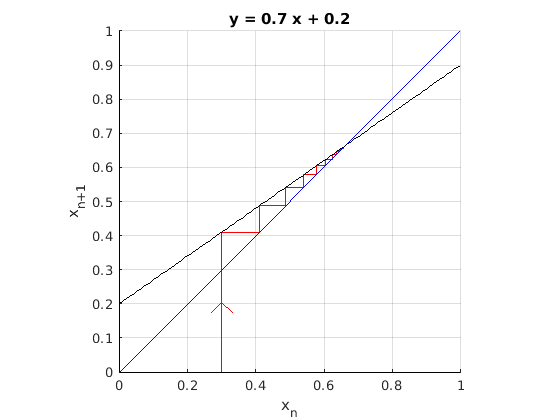
\includegraphics[width=7cm]{6_derivees_appl/affine1}\label{AFFINE1}}
\qquad
\subfloat[$x_{n+1}=2x_n-0.6$]{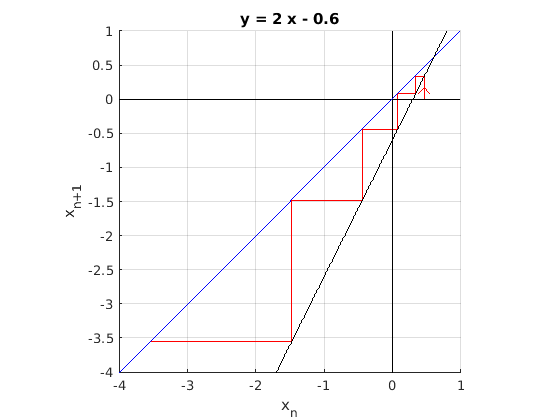
\includegraphics[width=7cm]{6_derivees_appl/affine2}\label{AFFINE2}}
\\
\subfloat[$x_{n+1} =-0.7x_n+0.68$]{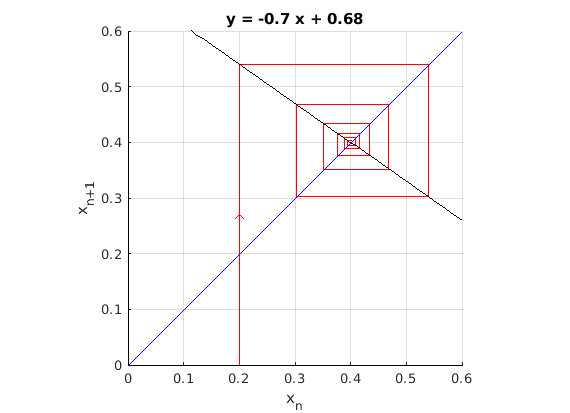
\includegraphics[width=7cm]{6_derivees_appl/affine3}\label{AFFINE3}} 
\qquad
\subfloat[$x_{n+1} = -2x_n+1.2$]{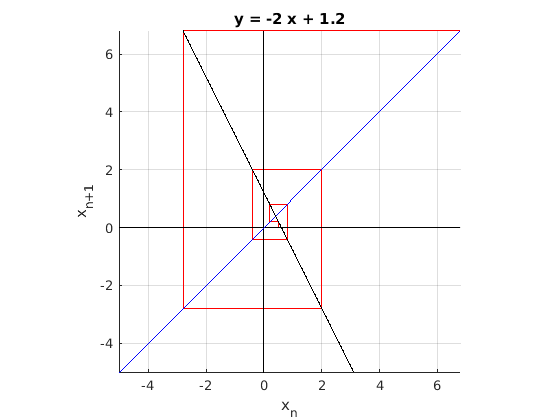
\includegraphics[width=7cm]{6_derivees_appl/affine4}\label{AFFINE4}}
\caption[Types de stabilité pour le point d'équilibre d'un
système dynamique discret de la forme $x_{n+1} = m x_n + b$]
{(a) Le point d'équilibre $p=2/3$ est asymptotiquement stable,  Le
  graphique contient l'orbite pour $x_0 = 0.3$.
(b) Le point d'équilibre $p=3/5$ est instable.  Le graphique contient
l'orbite pour $x_0 = 0.47$.
(c) Le point d'équilibre $p=2/5$ est asymptotiquement stable.  Le
graphique contient l'orbite pour $x_0 =0.2$.
(d) Le point d'équilibre $p=2/5$ est instable.  Le graphique contient
l'orbite pour $x_0 = 0.5$.}\label{AFFINE1-4}
\end{figure}

% \MATHfig{6_derivees_appl/affine1}{8cm}{Le point d'équilibre $p=2/3$ du
% système dynamique $x_{n+1} = 0.7x_n+0.2$}{Le point d'équilibre $p=2/3$
% du système dynamique $x_{n+1} = f(x_n)= 0.7x_n+0.2$ pour $n=0$, $1$,
% $2$, \ldots\ est asymptotiquement stable,  Le graphique contient
% l'orbite pour $x_0 = 0.3$.}{AFFINE1} 

% \MATHfig{6_derivees_appl/affine2}{8cm}{Le point d'équilibre $p=3/5$ du
% système dynamique $x_{n+1} = 2x_n-0.6$}{Le point d'équilibre $p=3/5$
% du système dynamique $x_{n+1} = f(x_n) = 2x_n -0.6 $ pour $n=0$, $1$,
% $2$, \ldots\ est instable.  Le graphique contient l'orbite pour
% $x_0 = 0.47$}{AFFINE2} 

% \MATHfig{6_derivees_appl/affine3}{8cm}{Le point d'équilibre $p=2/5$ du
% système dynamique $x_{n+1} =-0.7x_n+0.68$}{Le point d'équilibre
% $p=2/5$ du système dynamique $x_{n+1} = f(x_n)= -0.7x_n+0.68$ pour
% $n=0$, $1$, $2$, \ldots\ est asymptotiquement stable.  Le graphique
% contient l'orbite pour $x_0 = 0.2$}{AFFINE3}

% \MATHfig{6_derivees_appl/affine4}{8cm}{Le point d'équilibre $p=2/5$ du
% système dynamique $x_{n+1} = -2x_n+1.2$}{Le point d'équilibre $p=2/5$
% du système dynamique $x_{n+1} = f(x_n)=-2x_n +1.2$ pour $n=0$, $1$,
% $2$, \ldots\ est instable.  Le graphique contient l'orbite pour
% $x_0 = 0.5$}{AFFINE4}

Les exemples précédents justifient le résultat suivant.

\begin{focus}{\prp}
Nous considérons le système dynamique discret
\[
x_{n+1} = f(x_n) \quad \text{pour} \quad n=0, 1, 2, 3, \ldots
\]
où la fonction itérative est $y=f(x) = m x +b$.  Si $p$ est un point
d'équilibre de ce système dynamique discret alors ce point d'équilibre
est asymptotiquement stable si $|m|<1$ et instable si $|m|>1$.
\end{focus}

Comment pouvons-nous déterminer la stabilité asymptotique d'un point
d'équilibre $p$ d'un système dynamique discret
\[
x_{n+1} = f(x_n) \quad \text{pour} \quad n=0, 1, 2, 3, \ldots
\]
où $f$ n'est pas une fonction affine?

Supposons que $p$ soit un point d'équilibre pour un système dynamique
discret
\[
x_{n+1} = f(x_n) \quad \text{pour} \quad n =0, 1, 2 ,\ldots
\]
où $f$ est une fonction différentiable quelconque.  Nous savons que
$f(x) \approx g(x) = f(p) + f'(p) (x-p)$ pour $x$ très près de $p$.
Très près du point $p$, le système dynamique discret ci-dessus devrait
donc se comporter comme le système dynamique discret
\[
x_{n+1} = g(x_n) = f(p) + f'(p) (x_n-p) = m x_n + b \quad \text{pour} \quad
n=0,1,2,\ldots
\]
où $m = f'(p)$ et $b = f(p) - p\,f'(p)$.  En se basant sur le résultat
précédent pour les fonctions itératives de la forme $f(x) = mx+b$,
nous obtenons le résultat suivant.

\begin{focus}{\thm} \label{sdd_stab_th}
Soit $f:\RR \to \RR$ une fonction qui possède une dérivée continue.
Soit $p$ un point d'équilibre du système dynamique discret
\[
x_{n+1}=f(x_n) \quad \text{pour} \quad n=0, 1, 2, \ldots
\]
Le point d'équilibre $p$ est asymptotiquement stable si
$|f'(p)| < 1$.  Il est instable si $|f'(p)|>1$.  Nous ne pouvons rien
conclure lorsque $|f'(p)|=1$.
\end{focus}

La démonstration de ce résultat, que nous donnerons prochainement, est
une simple application des résultats du calcul différentiel que nous
avons présentés.

Revenons à notre équation logistique
\[
x_{n+1} = r x_n (1-x_n) \quad , \quad n=0,1,2,\ldots
\]
Les points d'équilibre sont les solutions de
\[
r x (1-x) = x \; .
\]
Si $x\neq 0$, nous pouvons diviser des deux cotés de l'égalité par $x$ pour
obtenir $r (1-x)=1$.  Ainsi, $x = 1 - 1/r$.  L'équation logistique a
donc deux points fixes: $x=0$ et $x=1-1/r$.

Si, comme à la section précédente, $x_n$ est la fraction de la
population maximale, le point fixe $x=0$ est simplement le fait que
s'il n'y a pas de bactéries initialement, il n'y en aura pas dans le
futur.   Dans le cas $r=1.1$, nous retrouvons l'état d'équilibre $x=1/11$
déjà observé.

Il n'est pas toujours possible de trouver algébriquement, comme nous
venons de le faire pour l'équation logistique, les points
d'équilibres.  Nous utilisons alors des méthodes numériques comme la
méthode de Newton pour estimer les points d'équilibre.

\begin{egg}
Nous avons vu que $p= 1/11$ est un point d'équilibre pour l'équation
logistique
\[
x_{n+1} = f(x_n) = r\, x_n (1-x_n) \quad \text{pour} \quad n=0, 1, 2, 3 \ldots
\]
où $r=1.1$.  Les orbites que nous avons calculées numériquement semblent
indiquer que ce point d'équilibre est asymptotiquement stable.

Posons $f(x) = r x (1-x)$.  Nous avons que $f'(x) = r(1-2x)$.  Ainsi, pour
$r=1.1$ et $x = p = 1/11$, nous obtenons
\[
f'(p) = 1.1 \left( 1 - 2\,\frac{1}{11}\right) = -0.9 \; .
\]
Puisque $|f'(p)|<1$, le point d'équilibre $p$ est asymptotiquement
stable.
\end{egg}

\begin{rmk}
Soit le système dynamique discret
\[
x_{n+1} = f(x_n) \quad , \quad n=0, 1, 2, \ldots
\]
Les points d'équilibre $p$ où $|f'(p)|=1$ sont en fait très
importants.  C'est une des conditions pour obtenir une
{\bfseries bifurcation}.  Si nous supposons que $f$ dépend d'un paramètre
$r$ (comme c'est le cas pour l'équation logistique) et que pour une
valeur $r_0$ de $r$ il existe un point d'équilibre $p$ tel que
$|f'(p)|=1$, alors le comportement du système dynamique discret pour
$r<r_0$ peut être très différant du comportement du système dynamique
discret pour $r>r_0$ si certaines conditions génériques sont
satisfaites.

Nous invitons le lecteur à tracer le graphe en forme de toile
d'araignée de l'équation logistique pour des valeurs de $r$ entre $2$
et $3$, et une condition initiale entre $0$ et $1$.  Puis, de répéter
cette même expérience avec des valeurs de $r$ entre $3$ et $3.447\ldots$
\ Qu'arrive-t-il lorsque $r$ devient plus grand que $3.447\ldots$?
Quand $r = 3.839\ldots$?

Lorsque $3<r<4$, le point $p=1-1/r$ est toujours un point
d'équilibre.  Par exemple, pour $r=13/4=3.25$, nous avons le point
d'équilibre $p=9/13=0.69230769231$.  Pourquoi les orbites ne
tendent-elles pas vers ce point d'équilibre?

Nous répondrons à certaines de ces questions à la prochaine section.

Le comportement des orbites de l'équation logistique lorsque $r$ varie
est fascinant.   Il existe un grand nombre de livres sur ce sujet.
\end{rmk}

\begin{proof}[\theory][Théorème~\ref{sdd_stab_th}]
La démonstration qu'un point fixe $p$ pour un système dynamique discret
\[
x_{n+1} = f(x_n) \quad , \quad n=0, 1, 2, 3, \ldots
\]
est asymptotiquement stable si $|f'(p)|<1$ et instable si $|f'(p)|>1$
repose sur le théorème de la moyenne.  Nous démontrons seulement que
$|f'(p)|<1$ implique la stabilité asymptotique du point d'équilibre
$p$ et laissons aux lecteurs le soin de démontrer que $|f'(p)|>1$
implique l'instabilité du point d'équilibre $p$.

Supposons que $f$ soit une fonction différentiable dont la dérivée
$f'$ est une fonction continue.  Puisque $|f'(p)|$ est strictement
plus petit que $1$ et $f'$ est continue, nous pouvons trouver une constante
$K$ plus grande ou égale à $|f'(p)|$ et plus petite que $1$, et une
petite valeur $\delta$ telle que $|f'(x)| \leq K<1$ pour tout $x$ dans
l'intervalle $I = ]p-\delta, p+\delta[$ qui contient $p$.

\subQ{i} Si $x_0 \in I$, alors $x_n \in I$ pour tout $n$.

En effet, supposons que $x_n$ soit dans $I$, alors $|x_n-p|<\delta$.  Grâce
au théorème de la moyenne, il existe $\zeta$ entre $p$ et $x_n$ tel que
$f(x_n) - f(p) = f'(\zeta)(x_n - p)$.  Notons que $\zeta \in I$ car $\zeta$
est entre $x_n$ et $p$.  Ainsi,
\[
|x_{n+1} - p| = |f(x_n) - f(p)| = |f'(\zeta)(x_n - p)|
\leq K | x_n - p | < |x_n - p| < \delta
\]
car $K<1$.  Il s'en suit que $x_{n+1}$ est aussi dans l'intervalle $I$.
Par induction, $x_n \in I$ pour tout $n$.

\subQ{ii} Encore grâce au théorème de la moyenne, ils existent $\zeta_n$
entre $x_n$ et $p$ tels que
$f(x_n) - f(p) = f'(\zeta_n)(x_n - p)$
avec $\zeta_n \in I$ car $\zeta_n$ est entre $x_n$ et $p$.  Nous avons donc
$|f'(\zeta_n)|\leq K$ pour tout $n$.  Ainsi,
\begin{align*}
|x_n -p| &= |f(x_{n-1}) - f(p)| = |f'(\zeta_{n-1})(x_{n-1} - p)|\\
&\leq K |x_{n-1} - p| = K |f(x_{n-2}) - f(p)|
= K |f'(\zeta_{n-2})(x_{n-2} - p)| \\
&\leq K^2 |x_{n-2} -p|\\
& \ldots\\
&\leq K^n |x_0 - p| \; .
\end{align*}

\subQ{iii} Nous avons donc que
\[
|x_n -p| \leq K^n |x_0-p|  \to 0 \quad \text{lorsque} \quad n \to \infty
\]
car
\[
\lim_{n\rightarrow \infty} K^n = 0
\]
pour $0<K<1$.

Toutes les orbites avec la condition initiale $x_0$ dans $I$
tendent donc vers $p$.
\end{proof}

\begin{egg}
Cet exemple provient de \cite{A}.

Le nombre de poissons d'une certaine espèce est gouverné par le
système dynamique discret
\begin{equation}\label{fish_harv}
p_{n+1} = r p_n (1-p_n) - h p_n  \quad \text{pour} \quad  0 < h < r
-1 < 2 
\end{equation}
où $p_n$ est le nombre de poissons au début de la $n^e$ saison de
pêche divisé par le nombre maximal de poissons que le milieu peut
supporter, $r$ est un facteur de croissance pour cette espèce de
poissons et $h$ est un facteur d'efficacité des pêcheurs. La valeur
$h$ est déterminée par le nombre de permis de pêche, l'équipement
utilisé par les pêcheurs, etc.  Le terme $-h\,p_n$ dans l'équation
(\ref{fish_harv}) représente la récolte à chaque année et a un effet
négatif sur la croissance de la population de poissons.

Lors d'une saison de pêche, si $h$ augmente, alors le nombre de
poissons capturés par les pêcheurs augmentera.  Si nous permettons une plus
grande valeur pour $h$ lors d'une saison de pêche, alors nous augmentons
l'effet négatif sur la croissance de la population.  Si $h$ est trop
grand, nous risquons de provoquer une diminution de la population de
poissons à long terme et de mettre ainsi en danger la survie de
cette espèce.  À long terme, il n'y aurait plus de poissons à capturer.

Le but est donc de choisir $h$ pour maximiser le nombre de poissons
capturés lors des futures saisons de pêche.  En d'autres mots, nous
voulons maximiser la récolte de poissons à long terme.  Cette récolte est
définie comme étant le produit du facteur d'efficacité $h$ des
pêcheurs avec l'état d'équilibre stable $p_h$ de la population de
poissons associé à cette valeur $h$.  En termes mathématiques, nous
voulons maximiser $R(h) = h\,p_h$.

La fonction itérative pour le système dynamique discret
(\ref{fish_harv}) est $f(p) = r p(1-p) - h p$.  Les points d'équilibre
du système dynamique discret (\ref{fish_harv}) sont donnés par les
solutions de $p = f(p)$.  Nous trouvons $p_0 = 0$ et $p_h = (r-h-1)/r$.  Le
point d'équilibre $p_h$ est positif car nous assumons $h < r-1$.

Nous utilisons le théorème~\ref{sdd_stab_th} pour déterminer si le point
d'équilibre $p_h$ est stable.  Puisque $f'(p) = r - h - 2r p$, nous
obtenons $|f'(p_h)| = |2 + h - r|$.  Pour que le point d'équilibre $p_h$
soit stable, nous devons donc exiger que
\[
|f'(p_h)| = |2 + h - r|<1 \Leftrightarrow -1 < 2 + h - r < 1
\Leftrightarrow -3 + r < h < r - 1 \ .
\]
C'est effectivement le cas pour $0 \leq h < r -1 < 2$.  Notez que
$|f'(p_0)| = |r - h| > 1$ pour $h < r -1$ et donc le point d'équilibre
$p_0$ est instable.

Considérons la récolte à long terme $R(h) = h\,p_h = h(r-h-1)/r$.
Nous avons $R'(h) = (r-2h-1)/r$ et le seul point critique est
$h = H \equiv (r-1)/2$.  Nous résumons dans le tableau suivant
l'information que nous avons au sujet de la fonction $R$.
\[
\begin{array}{c|c|c|c|c|c}
h & 0 & 0 < h < H & H & H < h < r-1 & r-1 \\
\hline
R(h) & 0 & + & \rule{0em}{1em} (r-1)^2/(4r) & + & 0 \\
\hline
R'(h) & + & + & 0 & - & - \\
\hline
 & & & \text{max. local} & & \\
\end{array}
\]
La récolte $R(h)$ est donc maximale pour $h = H$.  L'état d'équilibre
de la population de poissons pour $h = H$ est alors
$p_H = (r-1)/(2r)$.  Comme nous avons démontré, le point d'équilibre 
$p_H$ est stable et donc $\displaystyle \{p_n\}_{n=1}^\infty$ converge vers
ce point d'équilibre.  La récolte maximale de poissons à long terme
sera $R(H) = H\,p_H = (r-1)^2/(4r)$.
\label{discrete_fish_probl}
\end{egg}

\subsection{Étude des orbites périodiques \theory}

\begin{egg}
Pour l'équation logistique
\[
x_{n+1} = f(x_n) = r\, x_n(1-x_i) \quad \text{pour} \quad n=0, 1, 2, 3, \ldots
\]
avec $r=3.2$, quelle que soit la condition initiale $x_0$ entre $0$ et
$1$ que nous choisissons, l'orbite
$\displaystyle \left\{ x_n\right\}_{n=0}^\infty$ ne tend pas vers un
point d'équilibre comme nous pouvons constater avec les données dans la
colonne de gauche du tableau~\ref{HS_LOGISTIC4}.  Remarquons que
\[
x_n =
\begin{cases}
0.5130445095\ldots &\quad \text{si $n$ est pair} \\
0.7994554905\ldots &\quad \text{si $n$ est impair}
\end{cases}
\]
pour $n$ assez grand.  L'orbite oscille entre ces deux valeurs.
\label{eggper1}
\end{egg}

\begin{egg}
Comme à l'exemple précédent, pour l'équation logistique
\[
x_{n+1} = f(x_n) = r\, x_n(1-x_n) \quad , \quad n =0, 1, 2, 3, \ldots
\]
avec $r=3.47$, l'orbite $\displaystyle \left\{ x_n\right\}_{n=0}^\infty$
ne tend pas vers un point d'équilibre quelle que soit la condition
initiale $x_0$ entre $0$ et $1$ que nous choisissons.  Cependant, à partir
des données dans la colonne de droite du Tableau~\ref{HS_LOGISTIC4},
nous pouvons conclure que
\[
x_n =
\begin{cases}
0.40291365318\ldots &\quad \text{si} \quad n=4k \\
0.83479261718\ldots &\quad \text{si} \quad n=4k+1 \\
0.47856124509\ldots &\quad \text{si} \quad n=4k+2 \\
0.86590511786\ldots &\quad \text{si} \quad n=4k+3
\end{cases}
\]
pour $k$ assez grand.  L'orbite est la répétition de ces quatre
valeurs, toujours dans le même ordre.
\label{eggper2}
\end{egg}

\begin{table}
{\scriptsize
\begin{center}
\begin{tabular}{c|c}
\cline{1-2}
  $n$   &  $x_n$  \\ 
\cline{1-2}
$0$ & $0.40000000000\ldots$ \\ 
$\vdots$ & $\vdots$ \\
$50001$ & $0.79945549047\ldots$ \\ 
$50002$ & $0.51304450953\ldots$ \\ 
$50003$ & $0.79945549047\ldots$ \\ 
$50004$ & $0.51304450953\ldots$ \\ 
$50005$ & $0.79945549047\ldots$ \\ 
$50006$ & $0.51304450953\ldots$ \\ 
$50007$ & $0.79945549047\ldots$ \\ 
$50008$ & $0.51304450953\ldots$ \\ 
$50009$ & $0.79945549047\ldots$ \\ 
$50010$ & $0.51304450953\ldots$ \\ 
\cline{1-2}
\end{tabular}
\qquad\qquad
\begin{tabular}{c|c}
\cline{1-2}
  $n$   &  $x_n$  \\ 
\cline{1-2}
$0$ & $0.40000000000\ldots$ \\ 
$\vdots$ & $\vdots$ \\
$50001$ & $0.83479261718\ldots$ \\ 
$50002$ & $0.47856124509\ldots$ \\ 
$50003$ & $0.86590511786\ldots$ \\ 
$50004$ & $0.40291365318\ldots$ \\ 
$50005$ & $0.83479261718\ldots$ \\ 
$50006$ & $0.47856124509\ldots$ \\ 
$50007$ & $0.86590511786\ldots$ \\ 
$50008$ & $0.40291365318\ldots$ \\ 
$50009$ & $0.83479261718\ldots$ \\
$50010$ & $0.47856124509\ldots$ \\ 
\cline{1-2}
\end{tabular}
\end{center}
}
\caption[Orbites de l'équation logistique $x_{n+1}=r x_n ( 1-x_n)$
pour $r=3.2$ et $r=3.47\ldots$]{Deux orbites de l'équation logistique
avec la condition initiale $x_0 = 0.4$.  $r=3.2$ pour le tableau à
gauche et $r=3.47\ldots$ pour le tableau de droite. \label{HS_LOGISTIC4}}
\end{table}

Les deux exemples précédents justifient la définition suivante.

\begin{focus}{\dfn}
Soit $f:X \to X$ avec $X \subset \RR$.  Si
$\displaystyle \left\{ x_n \right\}_{n=0}^\infty$ est une orbite du
système dynamique discret
\[
x_{n+1} = f(x_n) \quad , \quad n=0, 1, 2, \ldots
\]
pour laquelle il existe un entier positif $k$ tel que $x_n = x_{n+k}$
pour $n=0$, $1$, $2$, \ldots, alors l'orbite 
$\displaystyle \left\{ x_n \right\}_{n=0}^\infty$ est appelée une
{\bfseries orbite périodique}\index{Système dynamique discret!orbite
  périodique}
ou {\bfseries solution périodique}\index{Système dynamique
  discret!solution périodique}.  Les
points de cette orbite sont appelés des
{\bfseries points périodiques}\index{Système dynamique discret!point
  périodique} pour $f$.

Si $k$ est le plus petit entier positif tel que $x_n = x_{n+k}$, alors
$k$ est la {\bfseries période}\index{Système dynamique discret!période
  d'une orbite} de l'orbite.
\end{focus}

\begin{egg}
À l'exemple~\ref{eggper1}, $p=0.5130445095\ldots$ est un point
périodique et l'orbite avec la condition initiale $x_0=p$ est une
orbite périodique de période $2$ (figure~\ref{HS_LOGISTIC5}).

À l'exemple~\ref{eggper2}, $p=0.40291365318\ldots$ est un point
périodique et l'orbite avec la condition initiale $x_0=p$ est une
orbite périodique de période $4$ (figure~\ref{HS_LOGISTIC6}).
\end{egg}

\begin{figure}
\centering
\subfloat[$r=3.2$]{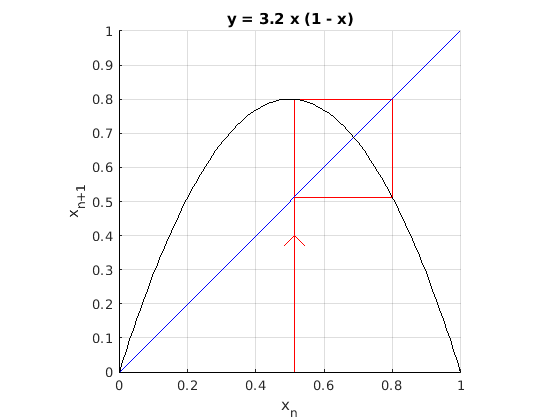
\includegraphics[width=7cm]{6_derivees_appl/hs_logistic5}\label{HS_LOGISTIC5}}
\qquad
\subfloat[$r=3.47$]{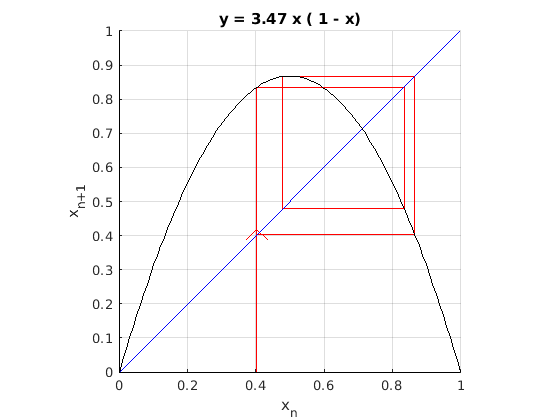
\includegraphics[width=7cm]{6_derivees_appl/hs_logistic6}\label{HS_LOGISTIC6}}
\caption[Orbites périodiques de période $2$ et $4$ pour l'équation logistique]
{(a) Orbite périodique de période $2$ pour l'équation logistique avec
$r=3.2$.  (b) Orbite périodique de période $4$ pour l'équation
logistique avec $r=3.47$.}\label{HS_LOGISTIC56}
\end{figure}

% \MATHfig{6_derivees_appl/hs_logistic5}{8cm}{Orbite périodique de période
% $2$ pour l'équation logistique avec $r=3.2$}{Orbite périodique de
% période $2$ pour l'équation logistique avec $r=3.2$}{HS_LOGISTIC5}

% \MATHfig{6_derivees_appl/hs_logistic6}{8cm}{Orbite périodique de période
% $4$ pour l'équation logistique avec $r=3.47$}{Orbite périodique de
% période $4$ pour l'équation logistique avec $r=3.47$}{HS_LOGISTIC6}

Dans les deux exemples précédents, quelle que soit la condition
initiale $x_0$, l'orbite
$\displaystyle \left\{ x_n\right\}_{n=0}^\infty$ se comporte de plus
en plus comme l'orbite périodique (figure~\ref{HS_LOGISTIC7}).  Nous
avons donc une notion de stabilité asymptotique pour les solutions
périodiques.

\MATHfig{6_derivees_appl/hs_logistic7}{8cm}{Stabilité de l'orbite de
période $4$ pour l'équation logistique avec $r=3.47$}{Une orbite qui
\lgm converge\rgm\ vers l'orbite périodique de période $4$ pour
l'équation logistique avec $r=3.47$.  La condition initiale est
$x_0=0.1$}{HS_LOGISTIC7}

\begin{focus}{\dfn}
\index{Système dynamique discret!solution périodique!asymptotique stabilité}
Soit $f: X \to X$ avec $X \subset \RR$, et
$\displaystyle \left\{ x_n \right\}_{n=0}^\infty$ une orbite périodique
de période $k$ pour le système dynamique discret
\[
x_{n+1} = f(x_n) \quad , \quad n=0, 1, 2, 3, \ldots
\]
Cette orbite est {\bfseries asymptotiquement stable} si $p$, un point
quelconque de l'orbite, est un point fixe asymptotiquement stable pour
la fonction
\[
 g = \underbrace{f\circ f \circ \ldots \circ f}_{\text{$k$ copies de $f$}} \; .
\]
\end{focus}

\begin{rmk}
Nous invitons le lecteur à démontrer que la définition précédente est
indépendante du choix du point périodique $p$ de l'orbite.
\end{rmk}

Le lecteur peut utiliser l'application qui se trouve sur le site\\
\href{https://mysite.science.uottawa.ca/bdionne/math_stat/fractal/fractal3_en.html}{https://mysite.science.uottawa.ca/bdionne/math\_stat/fractal/fractal3\_en.html} pour explorer le comportement des
orbites de l'équation logistique de la définition \ref{defOfLogEqu}
lorsque $r$ varie.

}  % End of theory

\section{Exercices}

\subsection{Dérivées d'ordres supérieures}

\begin{question}
Calculez la dérivée première et seconde des fonctions suivantes.
\begin{center}
\begin{tabular}{*{2}{l@{\hspace{0.5em}}l@{\hspace{3em}}}l@{\hspace{0.5em}}l}
\subQ{a} & $\displaystyle h(y) = y^{10}-y^9$ &
\subQ{b} & $\displaystyle f(x) = \frac{3+x}{2x}$ &
\subQ{c} & $\displaystyle f(x) = x^2 e^x$ \\
\subQ{d} & $\displaystyle f(x) = \frac{1+x}{e^x}$ &
\subQ{e} & $\displaystyle g(z) = (z+4)\ln(z)$ &
\subQ{f} & $\displaystyle F(w) = e^w \ln(w)$ \\
\subQ{g} & $\displaystyle f(x) = \ln(x^7)$ &
\subQ{h} & $\displaystyle f(z) = \frac{1+e^{-z}}{1+e^z}$ &
\subQ{i} & $\displaystyle F(y) = \frac{\ln(y)}{e^y}$ \\[0.9em]
\subQ{j} & $\displaystyle f(x) = 1 + x^{4/5}$ &
\subQ{k} & $\displaystyle f(x)= \frac{2+x^3}{1+x^2}$
\end{tabular}
\end{center}
\label{6Q1}
\end{question}

\begin{question}[\life \eng]
Si $H(\theta) = \theta \sin(\theta)$, évaluez $H'(\theta)$ et $H''(\theta)$.
\label{6Q2}
\end{question}

\begin{question}
Nous laissons tomber un objet d'une hauteur de $100$ m sur Jupiter.  Nous
assumons qu'il n'y a pas de friction sur l'objet.  L'accélération dû à
la gravité de Jupiter est $g = 22.88$ m/s$^2$.  Combien de temps
s'écoule-t-il avant que l'objet frappe le sol?  À quel vitesse l'objet
frappe-t-il le sol? 
\label{6Q3}
\end{question}

\begin{question}
Sur Jupiter, nous lançons un objet vers le haut à une vitesse de $10$ m/s
à partir d'une hauteur de $100$ m.  Nous assumons qu'il n'y a pas de
friction sur l'objet.  L'accélération dû à la gravité de Jupiter est
$g = 22.88$ m/s$^2$. Combien de temps s'écoule-t-il avant que l'objet
atteigne sa plus grande distance du sol?  Quelle est la hauteur de
l'objet à ce moment?  Combien de temps s'écoule-t-il avant que l'objet
frappe le sol?  À quel vitesse l'objet frappe-t-il le sol?
\label{6Q4}
\end{question}

\subsection{Graphes de fonctions}

\begin{question}
Le graphe d'une fonction $f$ est donné ci-dessous.
\PDFgraph{6_derivees_appl/graph_funct1}

\subQ{a} Donnez les point critiques.\\
\subQ{b} Donnez les valeurs de $x$ où $f'(x)>0$.\\
\subQ{c} Donnez les valeurs de $x$ où $f'(x)<0$.\\
\subQ{d} Donnez les valeurs de $x$ où $f''(x)>0$.\\
\subQ{e} Donnez les valeurs de $x$ où $f''(x)<0$.
\label{6Q5}
\end{question}

\begin{question}
Dessinez le graphe d'une fonction qui possède les propriétés suivantes:

\subQ{a} Une fonction positive qui possède une dérivée strictement
croissante.\\
\subQ{b} Une fonction avec une dérivée négative et strictement croissante.
\label{6Q6}
\end{question}

\begin{question}
Le graphe suivant représente la position $x$ d'une voiture dans les montagnes
russes (i.e. \lgm roller coaster\rgm) en fonction du temps.  À quelles
moments la voiture se déplace-t-elle le plus rapidement?  À quelles moments
la voiture accélère-t-elle le plus rapidement?  À quelles moments la voiture
décélère-t-elle le plus rapidement?  Expliquez votre réponse.
\PDFgraph{6_derivees_appl/graph_funct4}
\label{6Q7}
\end{question}

\begin{question}
La position vertical d'un objet à partir du sol est décrite par la
fonction $p(t) = -5.2 t^2 - 2 t + 50$.  Supposons que la direction
positive soit vers le haut.  Cette équation n'est pas valide sur la
terre mais sur une planète plus lourde que la terre.  La position est
donnée en mètres et le temps en secondes.

\subQ{a} Trouvez la vélocité et l'accélération de l'objet en fonction
du temps.\\
\subQ{b} Tracez le graphe de la position en fonction du temps à l'aide
des résultats en (a).\\
\subQ{c} Si l'objet part du haut d'une tour, quelle est la hauteur de
la tour?  Dans quelle direction et à quelle vitesse avons-nous lancé (si
nous avons lancé) l'objet, vers le haut ou vers le bas?  Quelle est
l'accélération dû à la gravité sur cette planète?
\label{6Q8}
\end{question}

\begin{question}
Dans son nouveau programme d'exploration des objets célestes, la NASA
utilise des sondes spatiales inhabitées.  Une expérience conduite par
une sonde se trouvant à $100$ m au dessus de la lune Deimos de mars
consistait à lancer vers le haut un objet à une vitesse de $5$ m/s
pour analyser sa trajectoire. L'accélération dû à la gravité est de
$2.15\times 10^{-3}$ m/s$^2$ sur cette lune.

\subQ{a} Trouvez la vélocité et la position de l'objet en fonction du
temps.\\
\subQ{b} Quelle est la hauteur maximale atteinte par l'objet?\\
\subQ{c} Combien de temps faut-il à l'objet pour revenir à la hauteur
de départ?  Quelle est la vélocité de l'objet à ce moment?\\
\subQ{d} Combien de temps faut-il à l'objet pour atteindre le sol de
la lune? Quelle est la vélocité de l'objet à ce moment?\\
\subQ{e} Tracez le graphe de la vélocité et de la position de l'objet
en fonction du temps.
\label{6Q9}
\end{question}

\begin{question}
Le graphe de $g'$ est donné ci-dessous.
\PDFgraph{6_derivees_appl/derivative2}
Si $g(0)= 2$, tracez un graphe possible pour $g$.  Soyez aussi précis que
possible.
\label{6Q10}
\end{question}

\begin{question}
Utilisez le graphe du taux de variation instantanée de la fonction $w$
qui est donné ci-dessous pour tracer le graphe de la fonction $w$ si $w(0)=1$.
\PDFgraph{6_derivees_appl/derivative3}
\label{6Q11}
\end{question}

\begin{question}[\life]
Le volume de déchets au temps $t$ produit par deux villes est donnée
par $\displaystyle V_a(t) = t^2 - 3t + 16$ pour la ville $A$ et
$V_b(t) = 20 + 3t$ pour la ville $B$.  Le volume est mesuré en m$^3$
et le temps $t$ est mesuré en années.  Si les déchets contiennent
$\rho(t) = 1.2 - 0.1 t$ g/m$^3$ d'un certain produit toxique au temps
$t$, répondre aux questions suivantes.

\subQ{a} Exprimez la masse du produit toxique en fonction du temps.\\
\subQ{b} Exprimez le taux de variation de la masse en fonction du temps.\\
\subQ{c} À l'aide du taux de variation calculé en (b), tracez le
graphe de la masse en fonction du temps pour $t\geq 0$.  Est-ce que
les efforts des deux villes d'éliminer le produit toxique de leurs
déchets sont encourageants au départ?
\label{6Q12}
\end{question}

\begin{question}[\life]
La masse d'une culture en fonction du temps est donnée par
$M(t) = 1 + t^2$ et le volume en fonction du temps est donné par
$V(t) = 1+t$.  La masse est mesurée en grammes, le volume en cm$^3$ et le
temps en jours.

\subQ{a} Exprimez la densité en fonction du temps.\\
\subQ{b} Calculez la dérivée de la densité.\\
\subQ{c} Pour quelles valeurs de $t$ a-t-on que la densité est
strictement croissante?\\
\subQ{d} À l'aide de la dérivée calculée en (b), tracez le graphe de
la densité en fonction du temps.
\label{6Q13}
\end{question}

\begin{question}[\life]
En l'absence d'influences externes, la croissance annuelle d'une
population dépend seulement de la production annuelle moyenne par
individu.  Supposons que la production annuelle moyenne par individu
lorsqu'il y a $p$ individus soit donnée par
$\displaystyle f(p) = 2\left( 1- \frac{p}{1000}\right)$.

\subQ{a} Exprimez la taille $T$ de la population (i.e. nombre d'individus)
après un an en fonction de la taille de la population au début de l'année.\\
\subQ{b} Calculez la dérivée de $T$ par rapport à la population
initiale $p$.\\
\subQ{c} À l'aide de la dérivée calculée en (b), tracez le graphe de
$T$ pour $0 < p < 1000$.
\label{6Q14}
\end{question}

\begin{question}
Soit $f$ une fonction continue qui satisfait:\\
\subQ{a} $f\,'(x)>0$ si $-2<x<1$,\\
\subQ{b} $f\,'(x)=0$ si $x=-2$ ou $x=1$,\\
\subQ{c} $f\,'(x)<0$ si $x>1$ ou $x<-2$, et\\
\subQ{d} $f(x)>0$ pour tout $x$.\\
Tracez (de façon approximative) le graphe de cette fonction.
Expliquez en une phrase le sens graphique des énoncés.
\label{6Q15}
\end{question}

\begin{question}
Trouvez les points où la fonction
$\displaystyle f(x)=\frac{e^{2x^2}}{x}$ possède un 
minimum ou un maximum local.
\label{6Q16}
\end{question}

\begin{question}
Soit $\displaystyle f(x) = x\sqrt{5-x}$ pour $x<5$.  Répondre aux questions
suivantes.

\subQ{a} Trouvez les intervalles où la fonction $f$ est strictement
croissante et décroissante.\\
\subQ{b} Trouvez les points où la fonction $f$ a des maximums et
minimums locaux et calculez la valeur de ces maximums et minimums
locaux.\\
\subQ{c} Trouvez les intervalles de concavité et les points
d'inflexion.\\
\subQ{d} Utilisez l'information obtenue précédemment pour tracer le
graphe de $f$.
\label{6Q17}
\end{question}

\begin{question}[\life \eng]
Soit $\displaystyle f(x) = x - 2\sin(x)$ pour $0<x<3\pi$. Répondre aux
questions suivantes.

\subQ{a} Trouvez les intervalles où la fonction $f$ est strictement
croissante et décroissante.\\
\subQ{b} Trouvez les points où la fonction $f$ a des maximums et
minimums locaux et calculez la valeur de ces maximums et minimums
locaux.\\
\subQ{c} Trouvez les intervalles de concavité et les points
d'inflexion.\\
\subQ{d} Utilisez l'information obtenue précédemment pour tracer le
graphe de $f$.
\label{6Q18}
\end{question}

\begin{question}
Tracez un graphe de $y = f(x)$ en utilisant les données suivantes.
\[
\begin{array}{c|c|c|c|c|c|c|c|c|c}
x & x<x_1 & x_1 & x_1<x<x_2 & x_2 & x_2<x<x_3 & x_3 & x_3<x<x_4 &
x_4 & x>x_4 \\
\hline
f'(x) & - & - & - & 0 & + & + & + & 0 & - \\
f''(x) & - & 0 & + & + & + & 0 & - & - & -
\end{array}
\]
\label{6Q19}
\end{question}

\begin{question}[4 points]
Nous considérons la fonction $f$ qui possède les propriétés suivantes:
{\renewcommand{\labelitemi}{\textbullet}
\begin{itemize}
\item $f$ est une fonction continue sur son domaine;
\item $\displaystyle \lim_{x\to -\infty}f(x)=2$,
$\displaystyle \lim_{x\to 1}f(x)=-2$,
$\displaystyle \lim_{x\to 3^-} f(x) = -\infty$ et
$\displaystyle \lim_{x\to 3^+}f(x)= \infty$;
\item $f(x)$ n'est pas définie en $x=3$;
\item $f'(x)$ n'est pas définie en $x=1$;
\item $f'(x)<0$ pour $x<1$, $2 < x < 3$ et $3 < x < 4$;
\item $f'(x)>0$ pour $1 < x < 2$ et $x > 4$;
\item $f''(x)<0$ pour $x<3$, $x\neq 1$;
\item $f''(x)>0$ pour $x>3$.
\end{itemize}
}
\subQ{a} Donnez le domaine de $f$.\\
\subQ{b} Déterminez les intervalles où $f$ est croissante et où $f$
est décroissante.\\
\subQ{c} Déterminez les intervalles où $f$ est convexe et
où $f$ est concave.\\
\subQ{d} Tracez le graphe de $f$ en prenant soin d'indiquer les points
critiques, asymptotes, point d'inflexions, \ldots
\label{6Q20}
\end{question}

\begin{question}
Pour chacune des fonctions ci-dessous, utilisez l'information fourni
par la dérivée première et seconde pour tracer son graphe.  Bien
indiquer où la fonction est strictement croissante et décroissante, où
la fonction est concave et convexe, les maximums et minimums locaux,
les points d'inflexions, les asymptotes horizontales et verticales,
etc.
\begin{center}
\begin{tabular}{*{1}{l@{\hspace{0.5em}}l@{\hspace{6em}}}l@{\hspace{0.5em}}l}
\subQ{a} & $h(x) = x^3 - 3x + 3$ &
\subQ{b} & $h(x) = x^3 - 6x^2 - 15 x + 3$ \\
\subQ{c} & $f(x) = x + 4/x^2$ &
\subQ{d} & $\displaystyle f(x) = (1-x)e^x$ \\
\subQ{e} & $\displaystyle g(z) = \frac{e^z}{z^2}$ &
\subQ{f} & $F(z) = z^3/e^z$ \\[0.5em]
\subQ{g} & $T(t) = (1-t^2) e^t$\ ,\ $-1 \leq t \leq 1$ &
\subQ{h} & $G(x) = \sqrt{x}\; e^{-x}$\ ,\ $x\geq 0$ \\
\subQ{i} & $\displaystyle f(x) = \frac{x^3}{1+x^3}$  &
\subQ{j} & $\displaystyle f(x) = \frac{2}{x^2} - \frac{3}{x^3}$ \\[0.8em]
\subQ{k} & $\displaystyle f(x) = (x+4)e^{-x}$ &
\subQ{l} & $\displaystyle f(x) = \frac{2}{x} -\frac{6}{x^3}$ \\[0.5em]
\subQ{m} & $\displaystyle f(x) = \frac{e^x}{x-1}$ &
\subQ{n} & $\displaystyle f(x) = \frac{x}{x^3+1}$ \\[0.5em]
\subQ{o} & $\displaystyle f(x) = x \ln(x)$ & &
\end{tabular}
\end{center}
\label{6Q21}
\end{question}

\begin{question}[\life \eng]
Pour chacune des fonctions ci-dessous, utilisez l'information fourni
par la dérivée première et seconde pour tracer son graphe.  Bien
indiquer où la fonction est strictement croissante et décroissante, où
la fonction est concave et convexe, les maximums et minimums locaux,
les points d'inflexions, les asymptotes horizontales et verticales,
etc.
\begin{center}
\begin{tabular}{*{1}{l@{\hspace{0.5em}}l@{\hspace{6em}}}l@{\hspace{0.5em}}l}
\subQ{a} & $\displaystyle y = \sin^2(x) -2 \cos(x)$ &
\subQ{b} & $f(\theta) = \theta + 3 \cos(\theta) \ , \ 0\leq \theta \leq 4\pi$
  \\
\subQ{c} & $h(t) = e^{-t} \sin(t) \ , \ 0\leq \theta \leq 4\pi$ & &
\end{tabular}
\end{center}
\label{6Q22}
\end{question}

\subsection{Optimisation}

\begin{question}[\life]
Le nombre de bactéries dans un milieu riche en substances nutritives est
décrit par
\[
N(t) = 5000 + \frac{30000\,t}{100+t^2}
\]
où $t$ est le temps.  Trouvez le nombre maximal de bactéries que nous
pourrons observer (i.e.  trouvez le maximum absolu pour $t\geq 0$). 
\label{6Q23}
\end{question}

\begin{question}[\life]
Nous considérons une espèce d'oiseaux dont le rapport $P$ du nombre moyen
de poussins qui survivent en fonction du nombre $x$ d'oeufs pondus est
donné par la fonction $P(x) = 1/(1+0.5 x^2)$.   Le nombre total de
poussins qui survivent en fonction du nombre d'oeufs pondus est donc
donné par $S(x) = x\,P(x)$. Trouvez le nombre de poussins qui 
survivent si un oiseau de cette espèce pond $5$, $10$ et $20$ oeufs.
Tracez le graphe de $S$.  Quelle est la meilleure stratégie pour cette
espèce d'oiseaux?  C'est-à-dire, combien d'oeufs devrait pondre un
oiseau de cette espèce pour avoir le plus grand nombre possible de
poussins qui survivent.

Dans ce problème, il faut comprendre que les valeurs de $S$ sont des
moyennes pour l'espèce d'oiseaux.  C'est pour cela que $S$ peut être
un nombre réel; $S$ n'est pas obligé d'être un entier.  Un oiseau ne
peut pas avoir $2.5$ poussins mais une population peut avoir en
moyenne $2.5$ poussins par individu.
\label{6Q24}
\end{question}

\begin{question}[\eco]
À un prix de \$50.00 l'unité, un jardinier peut vendre $100$
pommiers.  S'il augmente le prix par unité de \$1.00, il va vendre
$4$ pommiers de moins.  De même, s'il baisse le prix de
\$1.00, il va vendre $4$ pommiers de plus.  Le coût de production
d'un pommier est de \$9.00.  Calculer le prix par pommier qui maximise
le profit du jardinier.  {\bfseries Ne pas oublier} d'expliquer
pourquoi votre r\'eponse donne un maximum absolu.
\label{6Q25}
\end{question}

\begin{question}
Les questions suivantes font référence à une fonction continue
$f: [a,b] \rightarrow \RR$.

\subQ{a} Tracez un graphe pour $f$ si $f$ a un maximum absolu et un
minimum absolu entre $a$ et $b$.\\
\subQ{b} Tracez un graphe pour $f$ si $f$ est une fonction différentiable qui
a un maximum absolu à $x=a$, un minimum absolu à $x=b$ et aucun point
critique.  Décrire en une phrase cette fonction.\\
\subQ{c} Tracez un graphe pour $f$ si $f$ a un maximum absolu et un
minimum absolu entre $a$ et $b$, et $f'(x)\neq 0$ pour tout $x \in [a,b]$ où
la dérivée existe.
\label{6Q26}
\end{question}

\begin{question}
Pour chacune des fonctions ci-dessous, trouvez le maximum absolu et le
minimum absolu sur l'intervalle donné.
\begin{center}
\begin{tabular}{*{1}{l@{\hspace{0.5em}}l@{\hspace{3em}}}l@{\hspace{0.5em}}l}
\subQ{a} & $f(x) = 2 + x e^{-x} \ , \ 0.5 \leq x \leq 2$ &
\subQ{b} & $f(x) = x^3 - 3x \ , \ -2\leq c \leq 2$ \\[0.7em]
\subQ{c} & $\displaystyle f(x) = \frac{x}{x^2+x+1} \ , \ -2 \leq x \leq 0$ &
\subQ{d} & $f(x) = 5x(1-x)(2-x) - 1 \ , \ 0 \leq x \leq 1$ \\[0.7em]
\subQ{e} & $f(x)=x^{1/2}(x-4)^2 \ , \ 0.5 \leq x \leq 6$ & &
\end{tabular}
\end{center}
\label{6Q27}
\end{question}

\begin{question}
Trouvez le maximum absolu et le minimum absolu de $F(x) = |1-x|$ pour
$-2\leq x \leq 3$.
\label{6Q28}
\end{question}

\begin{question}
Tracez le graphe de $g(y) = y/(1+y^2)$ pour $0\leq y \leq 2$ a l'aide
de la dérivée premières et de la dérivée deuxième de $g$.

\subQ{a} Donnez les points où il y a un maximum ou minimum local.\\
\subQ{b} Donnez les points où il y a un maximum absolu et donnez
ce maximum.\\
\subQ{c} De même, donnez les points où il y a un minimum absolu et
donnez ce minimum.
\label{6Q29}
\end{question}

\begin{question}
Trouvez le point de la droite $y=4x+7$ qui est le plus près de l'origine.
\label{6Q30}
\end{question}

\begin{question}
L'aire d'un rectangle dont les côtés sont de longueurs $x$ et $y$
est $A = x y$.  Le périmètre de ce rectangle est $P = 2x + 2y$.

\subQ{a} Minimisez $P$ si $A$ est fixe.\\
\subQ{b} Maximisez $A$ si $P$ est fixe.
\label{6Q31}
\end{question}

\begin{question}
Nous voulons construire un enclos pour faire l'élevage de faisans.
l'enclos doit être rectangulaire et doit être partagé en trois
sections de même aire comme dans l'illustration ci-dessous.  Si nous avons
$3\,600$ m de clôture pour construire l'enclos.  Quelles sont les
dimensions du plus grand enclos que nous puissions construire?  Quelle est
alors l'aire de chacune des sections?

\PDFgraph{6_derivees_appl/fence}
\label{6Q32}
\end{question}

\begin{question}
Trouvez les dimensions $x$ et $y$ de la section transversale d'une
poutre de bois découpée d'un tronc d'arbre (circulaire) de $30$ cm de
rayon pour que la section transversale soit d'aire maximale.\\
Suggestion: cela revient à trouver le rectangle d'aire maximale qui
peut être inscrit dans un cercle ayant un diamètre de $30$ cm.
\label{6Q33}
\end{question}

\begin{question}
Vous campez à trois mètres de la rive d'une rivière.  Vous remarquez
qu'une tente à quatre mètres de la rive vient de
prendre feu.  Immédiatement, vous prenez une chaudière à l'intérieur
de votre tente (vous êtes une personne prévoyant qui amène toujours
une chaudière en camping), courez à la rivière pour remplir votre
chaudière, et allez à la tente pour éteindre le feu.  Quelle position
$x$ le long de la rivière minimisera la distance à parcourir (et donc
minimisera le temps d'intervention)?
\PDFgraph{6_derivees_appl/feu}
\label{6Q34}
\end{question}

\begin{question}
Une clôture de 2 m de haut longe un immeuble à 1 m de celui-ci sur
toute sa longueur.  Quelle est la longueur minimal de l'échelle qui
passe par dessus la clôture et s'appuie contre le mur de
cet immeuble?
\label{6Q35}
\end{question}

\begin{question}[\life]
Pour augmenter leur chance de survie, les animaux tentent de maximiser
le rapport entre la quantité de nourriture qu'ils récoltent et le
risque pour acquérir cette nourriture.  Par exemple, les fleurs qui
produisent une grande quantité de nectar permettent aux abeilles de
récolter une grande quantité de nectar mais ces fleurs attirent aussi
d'autres animaux qui sont des prédateurs pour les abeilles.  Chaque
espèce de fleurs produit une quantité (moyenne) $q$ de nectar (en
grammes).  Si, pour une espèce de fleurs qui produit $q$ g de nectar,
$P(q)$ est le nombre de prédateurs pour les abeilles qui sont attirés
par ces fleurs, alors les abeilles doivent maximiser
$\displaystyle \frac{q}{P(q)}$ pour déterminer quelle espèce de fleurs
elles doivent privilégier.  Si $P(q) = 1 + q^2$, trouvez la valeur de $q$
qui maximise le rapport $\displaystyle \frac{q}{P(q)}$.
\label{6Q36}
\end{question}

\begin{question}[\eng]
Un cylindre circulaire droit est inscrit dans une sphère de rayon $r$.
Trouvez l'aire maximal que peut avoir la surface du cylindre.

\noindent Note: Un problème un peu plus facile (que vous devriez résoudre)
est de trouver le cylindre de volume maximal qui peut être inscrit dans la
sphère de rayon $r$. 
\label{6Q37}
\end{question}

\begin{question}[\eng]
Un objet est éclairé par deux projecteurs.  La distance entre les projecteurs
est de $3$ m et l'objet est entre les deux projecteurs.  Un des projecteurs
est de puissance $P$ W alors que l'autre est trois fois plus puissant.
\PDFgraph{6_derivees_appl/illumination}
Déterminez la position de l'objet pour que l'illumination sur l'objet soit
maximale.

Il faut savoir que l'illumination d'une source lumineuse sur un objet est
proportionnel à la puissance de la source lumineuse divisée par le carré de
la distance entre la source lumineuse et l'objet. 
\label{6Q38}
\end{question}

\begin{question}[\life]
Considérons le problème des abeilles qui butinent que nous retrouvons à
l'exemple~\ref{egg_bees}.  Soit $t$ le temps qu'une abeille passe sur
une fleur à aspirer du nectar.  Si
$\displaystyle F(t) = \frac{t}{0.5+t}$ et si $t=T=1$ est le temps
optimal pour maximiser la récolte de nectar durant une journée,
déterminez le temps $\tau$ que prend l'abeille pour se rendre d'une
fleur à une autre fleur?  Illustrez $\tau$ à l'aide d'un graphe comme
celui qui est donné à la figure~\ref{BEES2} des notes.
\label{6Q39}
\end{question}

\begin{question}[\life]
Considérons le problème des abeilles qui butinent que nous retrouvons à
l'exemple~\ref{egg_bees}.  Soit $t$ le temps qu'une abeille passe sur
une fleur à aspirer du nectar.  Si
$\displaystyle F(t) = \frac{t^2}{1+t^2}$ et $\tau = 1$, déterminez le
temps optimal $t=T$ pour maximiser la récolte de nectar.  Il faut
répéter l'exemple~\ref{egg_bees} avec cette nouvelle fonction $F$ pour
trouver $T$.  Illustrez la règle des valeurs marginales comme il est
fait à la figure~\ref{BEES2}.
\label{6Q40}
\end{question}

\subsection{Taux liées}

\begin{question}[\eng]
Nous tirons un bateau vers le quai avec une corde attachée à la proue du bateau
et qui passe par une poulie placée au bord du quai.  Le quai a $2$ m de
haut.  Si la corde est tirée à un vitesse constante de $0.5$ m/s, à quelle
vitesse le bateau s'approche-t-il du quai lorsqu'il est à $6$ m du quai?
Est-ce que la vitesse à laquelle le bateau approche le quai est constante?
\label{6Q41}
\end{question}

\begin{question}[\eng]
Considérons la piscine suivante.
\PDFgraph{6_derivees_appl/piscine}
Les dimensions de la piscine sont en mètres.  Nous remplissons cette piscine à
l'aide d'une pompe dont le débit est de $0.1$ m$^3$/min.  À quelle vitesse le
niveau de l'eau monte-t-il lorsque la profondeur de l'eau à l'endroit le plus
profond est de $3$ m?
\label{6Q42}
\end{question}

\begin{question}[\eng]
La lampe d'un phare situé sur une petite île fait $5$ révolutions par
minute.  Le point $P$ de la côte qui est le plus près de l'île est à une
distance de $4$ km de celle-ci.  
\PDFgraph{6_derivees_appl/phare}
À quelle vitesse (tangentielle) le rayon lumineux du phare balaye-t-il la
côte au point $C$ qui se trouve à $1$ km du point $P$.
\label{6Q43}
\end{question}

\subsection{Dérivées implicites}

\begin{question}[\eng]
La fonction $f$ satisfait la relation
$\displaystyle (f(x))^4 + 6 f(x) = x^2 + 6$.  Si $f(3)=1$,
quelle est la valeur de $f'(3)$?
\label{6Q44}
\end{question}

\begin{question}[\eng]
Utilisez la dérivée implicite pour calculer la dérivée de la fonction $y$ qui
est définie implicitement dans chacune des équations suivantes.
\begin{center}
\begin{tabular}{*{2}{l@{\hspace{0.5em}}l@{\hspace{3em}}}l@{\hspace{0.5em}}l}
\subQ{a} & $\displaystyle x^2y +xy^2 = 3x$ &
\subQ{b} & $\displaystyle \sqrt{xy} = 1 + x^2y$ &
\subQ{c} & $\displaystyle xy^4 +x^2y = x + 3 y$ \\
\subQ{d} & $\displaystyle ye^{y} = x^2e^x$ & & & &
\end{tabular}
\end{center}
\label{6Q45}
\end{question}

\subsection{Approximation locale des fonctions}

\begin{question}[\life \eng]
Utilisez une approximation linéaire pour estimer chacune des valeurs
suivantes.
\begin{center}
\begin{tabular}{*{1}{l@{\hspace{0.5em}}l@{\hspace{6em}}}l@{\hspace{0.5em}}l}
\subQ{a} & $1.002^{2001}$ &
\subQ{b} & $\sin(0.02)$
\end{tabular}
\end{center}
\label{6Q46}
\end{question}

\begin{question}[\life \eng]
Soit $f(x) = x^2$.  Utilisez une approximation linéaire
pour estimer la valeur de la fonction au point $x=1.1$ et au
point $x=0.9$.  Tracez le graphe de la fonction et le graphe de
l'approximation linéaire considérée.  Est-ce que l'approximation linéaire
surestime ou sous-estime la valeur exacte?  Expliquez votre réponse à la
question précédente à partir des graphes que vous avez tracés.
\label{6Q47}
\end{question}

\begin{question}[\life \eng]
Utilisez une approximation linéaire (i.e. un polynôme de Taylor de degré un)
pour estimer $\sqrt{1.1}$ et $\sqrt{0.9}$,  Comparez avec les valeurs
exactes.  Pour chaque approximation, déterminez si nous avons une
surestimation ou une sous-estimation.  Expliquez à l'aide du graphe de
$f(x) = \sqrt{x}$ pourquoi nous avons surestimation ou sous-estimation.
\label{6Q48}
\end{question}

\begin{question}[\life \eng]
Soit
\[
b(t) = \frac{1}{1+t} \ .
\]
\subQ{a} Utilisez une approximation linéaire au point $t=0$ pour estimer
$b(1.1)$.\\
\subQ{b} Utilisez une approximation linéaire au point $t=1$ pour estimer
$b(1.1)$.\\
\subQ{c} Utilisez la sécante qui passe par les points $(0,b(0))$ et
$(1,b(1))$ pour estimer $b(1.1)$.\\
\subQ{d} Tracez le graphe des tangentes et de la sécante qui représentent les
méthodes d'approximations qui ont été utilisées précédemment.\\
\subQ{e} Laquelle des méthodes donne la meilleure approximation de $b(1.1)$?
Pourquoi?
\label{6Q49}
\end{question}

\begin{question}[\life \eng]
Soit $\displaystyle f(x) = \frac{\ln(x)}{x^2-1}$.

\subQ{a} Trouvez l'approximation linéaire $p_1$ du numérateur de $f$ au
voisinage de $x=1$.\\
\subQ{b} Trouvez l'approximation linéaire $q_1$ du dénominateur de $f$ au
voisinage de $x=1$.\\
\subQ{c} Montrez que
\[
\lim_{x\to 1} \frac{\ln(x)}{x^2-1} = \lim_{x\to 1} \frac{p_1(x)}{q_1(x)} \ .
\]

\noindent Note: L'idée de remplacer le numérateur et le dénominateur
par des polynômes de Taylor est à la base de la Règle de l'Hospital. 
\label{6Q50}
\end{question}

\begin{question}[\life \eng]
Donnez une approximation linéaire de la fonction $y = f(x) = x^{-3}$ au
voisinage de $x=1$.

Il est possible d'utiliser une polynôme de degré deux pour estimer la
fonction $f$ au voisinage de $x=1$.  Pour ce faire, nous choisissons
$p_2(x) = a + bx + c x^2$ tel que $p_2(1) = f(1)$, $p_2'(1) = f'(1)$ et
$p_2''(1) = f''(1)$.  Trouvez $p_2$.

Dessinez (à l'aide d'un logiciel) le graphe de $f$, le graphe de
l'approximation linéaire et le graphe de $p_2$ près de $x=1$.  Est-ce que
$p_2$ est une meilleure approximation de $f$ que l'approximation linéaire?
\label{6Q51}
\end{question}

\begin{question}[\life \eng]
Utilisez une approximation quadratique (i.e.\ un polynôme de Taylor de degré
$2$) pour estimer chacune des valeurs suivantes.
\begin{center}
\begin{tabular}{*{2}{l@{\hspace{0.5em}}l@{\hspace{3em}}}l@{\hspace{0.5em}}l}
\subQ{a} & $1.002^{2001}$ &
\subQ{b} & $\sin(0.02)$ &
\subQ{c} & $16.2^{3/4}$
\end{tabular}
\end{center}
\label{6Q52}
\end{question}

\begin{question}[\life \eng]
Pour chacune des fonctions $f(x)$ ci-dessous, utilisez son polynôme de
Taylor de degré trois au point $a$ pour estimer $f(b)$.
\begin{center}
\begin{tabular}{*{1}{l@{\hspace{0.5em}}l@{\hspace{3em}}}l@{\hspace{0.5em}}l}
\subQ{a} & $f(x) = \ln(x)$, $a =1$ et $b = 1.2$ &
\subQ{b} & $f(x) = x^{1/4}$, $a = 1$ et $b = 1.4$ \\
\subQ{c} & $\displaystyle f(x) = \frac{1}{\sqrt{1+x}}$, $a=3$ et $b =3.1$ &
\subQ{d} & $\displaystyle f(x)= x^{4/3}$, $a = 2$ et $b=8.1$ \\
\subQ{e} & $f(x) = \arcsin(x^2-1)$, $a=1$ et $b=1.1$ & &
\end{tabular}
\end{center}
\label{6Q53}
\end{question}

\begin{question}[\eng \life]
Le polynôme de Taylor de degré $4$ en $x=3$ d'une fonction $f$ est
\[
p_4(x) = 23 + 10 (x-3) + 2 (x-3)^3 + \frac{1}{3} (x-3)^4 \ .
\]
Quelle est la valeur de $f''(3)$?  De $f^{(4)}(3)$?
\label{6Q54}
\end{question}

\begin{question}[\life \eng]
Donnez le polynôme de Taylor de degré trois de $p(x) = x^3 + 4x^2 +3x +1$ au
voisinage de $x=0$.  Aucun calcul est nécessaire si vous avez bien compris
la théorie.  Justifiez votre réponse.
\label{6Q55}
\end{question}

\begin{question}[\life \eng]
Soit $p(x) = 7x^9 - 8 x^6 - 5 x^3 + 2x^2 -8$.  Pour quelles
valeurs de $x$ avons-nous $\displaystyle \dydxn{p}{x}{9}(x) >0$?
Justifiez votre réponse.
\label{6Q56}
\end{question}

\begin{question}[\life \eng]
Trouvez le polynôme de Taylor $p_k$ de degré $k$ de $\cos(x)$ près de
l'origine tel que $p_k(0.5)$ soit une approximation de $\cos(0.5)$
avec une erreur de troncature inférieure à $10^{-6}$.  Quelle est la
valeur de l'approximation donnée par votre polynôme de Taylor?
Comparez avec la valeur exacte.
\label{6Q57}
\end{question}

\begin{question} [\life \eng]
Donnez le polynôme de Taylor de degré 2 de la fonction
$f(x) = x e^{x^2-2}$ pour $x$ près de l'origine.  Donnez une borne
supérieure pour l'erreur de troncature si vous utilisez ce polynôme de
Taylor pour estimer $f(x)$ sur l'intervalle $[0,0.2]$.
\label{6Q58}
\end{question}

\begin{question}[\life \eng]
Utilisez un polynôme de Taylor de degré suffisamment grand pour
calculer les limites suivantes.
\begin{center}
\begin{tabular}{*{2}{l@{\hspace{0.5em}}l@{\hspace{3em}}}l@{\hspace{0.5em}}l}
\subQ{a} & $\displaystyle \lim_{h\rightarrow 0}\frac{e^h -1 -h}{h^2}$ & 
\subQ{b} & $\displaystyle \lim_{h\rightarrow 0}\frac{e^h -1 -h - h^2/2}{h^3}$ &
\subQ{c} & $\displaystyle \lim_{\theta \rightarrow \pi/2}
 \frac{\cos \theta}{\theta - \pi/2}$
\end{tabular}
\end{center}
\label{6Q59}
\end{question}

\subsection{Comportement asymptotique}

\begin{question}[\life]
Utilisez la Règle de l'Hospital pour déterminer laquelle des fonctions
suivantes tend plus rapidement vers $+\infty$ lorsque $x$ tend vers
$0$ par la droite.
\[
f(x) = \frac{1}{x} \qquad \text{et} \qquad g(x) = \frac{1}{e^x-1} \ .
\]
\label{6Q60}
\end{question}

\begin{question}[\life \eng]
Soit $\displaystyle f(t) = \frac{5t}{e^{2t}}$.  Utilisez la Règle de
l'Hospital pour trouver l'asymptote horizontal pour $t>0$.
\label{6Q61}
\end{question}

\begin{question}[\life]
Plusieurs fonctions utilisées pour décrire l'absorption d'un produit sont
de la forme
\[
\alpha(t) = \frac{ A\, r(t)}{k+r(t)}
\]
où
\begin{enumerate}
\item $A$ et $k$ sont des constantes positives,
\item $r(0)=0$,
\item $\displaystyle \lim_{t\rightarrow \infty} r(t) = \infty$ et
\item $r'(t)>0$ pour $c>0$.
\end{enumerate}
Par exemple, considérons la fonction d'absorption
\[
\alpha(t) = \frac{At^2}{k+t^2} \ .
\]
\subQ{a} Déterminez $r(t)$ dans cette fonction.\\
\subQ{b} Montrez que $\alpha(t)$ est une fonction strictement
croissante pour $t>0$.\\
\subQ{c} Utilisez la Règle de l'Hospital pour calculer la limite de
$\alpha(t)$ lorsque $t$ tend vers plus l'infini.
\label{6Q62}
\end{question}

\begin{question}[\life]
Dans chacune des situations ci-dessous, déterminez la limite de $f(x)$
et $g(x)$ lorsque $x$ tend vers la valeur donnée, et laquelle
des deux fonctions approche cette limite le plus rapidement.

\subQ{a} $f(x) = 0.1 x^{0.5}$, $g(x) = 30\ln(x)$ et $x\rightarrow \infty$.\\
\subQ{b} $f(x) = e^{-2x}$, $g(x) = x^{-2}$ et $x\rightarrow \infty$.\\
\subQ{c} $f(x) = x^{-1}$, $g(x) = -\ln(x)$ et $x\rightarrow 0^+$.
\label{6Q63}
\end{question}

\begin{question}[\life \eng]
Évaluez les limites suivantes.
\begin{center}
\begin{tabular}{*{2}{l@{\hspace{0.5em}}l@{\hspace{3em}}}l@{\hspace{0.5em}}l}
\subQ{a} & $\displaystyle \lim_{x\rightarrow \infty} \frac{\ln(x)}{e^{3x}}$ &
\subQ{b} & $\displaystyle \lim_{t\rightarrow \infty} \frac{1+t}{1+t+t^2}$ &
\subQ{c} & $\displaystyle \lim_{x\rightarrow 0} \frac{\sin(x)-x}{\cos(x)-1}$
\\[0.9em]
\subQ{d} & $\displaystyle \lim_{z\rightarrow \infty} \frac{3z}{1+\ln(1+z)}$ &
\subQ{e} & $\displaystyle \lim_{x\to 0}\frac{\sin(3x^2)}{x^2}$ &
\subQ{f} & $\displaystyle \lim_{x\to \pi/2} \frac{\cos^2(x)}{(x-\pi/2)^2}$
\\[0.9em]
\subQ{g} & $\displaystyle \lim_{x\to \infty} \frac{e^{1/x}-1}{1/x}$ &
\subQ{h} & $\displaystyle \lim_{x\to 0^+} \frac{\ln(\sin(x))}{\ln(x^4)}$ &
&
\end{tabular}
\end{center}
\label{6Q64}
\end{question}

\begin{question}[\life \eng]
Évaluez les limites suivantes si elles existent.
\begin{center}
\begin{tabular}{*{2}{l@{\hspace{0.4em}}l@{\hspace{3em}}}l@{\hspace{0.4em}}l}
\subQ{a} & $\displaystyle \lim_{x\rightarrow \pi^+} \csc(5x)\sin(3x)$ &
\subQ{b} & $\displaystyle \lim_{x\rightarrow 0^+}
\left( \frac{1}{\sin(x)} -\frac{1}{x} \right)$  &
\subQ{c} & $\displaystyle \lim_{x\rightarrow 0^+} \left(\csc(x) -
\cot(x)\right)$ \\[0.9em]
\subQ{d} & $\displaystyle \lim_{x\to 0} (1-\cos(x))^x$ &
\subQ{e} & $\displaystyle \lim_{x\to 0^+} 7x \cot(3x)$ &
\subQ{f} & $\displaystyle \lim_{x\to \pi} \cot^2(x) (x-\pi)^2$ \\[0.9em]
\subQ{g} & $\displaystyle \lim_{x\to +\infty} \left( x
\cos\left(\frac{1}{x}\right) - x \right)$ &
\subQ{h} & $\displaystyle \lim_{x\to 0} (\cos(x))^{1/x^2}$ &
\end{tabular}
\end{center}
\label{6Q65}
\end{question}

\subsection{Méthode de Newton}

\begin{question}[\life \eng]
Utilisez la méthode de Newton pour trouver une approximation de la
racine réelle positive de 
\[
x^4-20 = 0 \ .
\]
Utilisez $x_0=2$ et arrêtez lorsque $|x_n - x_{n+1}| < 10^{-4}$.
\label{6Q66}
\end{question}

\begin{question}[\life \eng]
Utilisez la Méthode de Newton pour estimer la valeur de
$\sqrt[3]{30}$.  Arrêtez après trois itérations.  Faite le graphe de
$f$ et illustrez la première itération de la Méthode de Newton.

\noindent Suggestion: Considérez $f(x) = x^3-30=0$.
\label{6Q67}
\end{question}

\begin{question}[\life \eng]
Utilisez la méthode de Newton pour estimer la solution positive de
$e^x = x + 2$ s'il y en a une.  Pour ce faire vous devez:

\subQ{a} vérifiez avec un graphe qu'il y a effectivement une seule
solution positive.\\
\subQ{b} Utilisez le théorème des valeurs intermédiaires pour montrer
qu'il existe une solution entre $1$ et $2$.  Cela va vous permettre de
choisir la valeur de $x_0$ qui sera utilisée par la méthode de Newton.\\
\subQ{c} Faire au moins trois itérations de la méthode de Newton.
\label{6Q68}
\end{question}

\begin{question}[\eng][Méthode de la sécante]
Dans la formule
\[
x_{i+1} = x_i  - \frac{f(x_i)}{f'(x_i)} \quad \text{pour}
\quad i=0, 1, 2, 3, \ldots
\]
si nous remplaçons $f'(x_i)$ par
$\displaystyle \frac{f(x_i)-f(x_{i-1})}{x_i - x_{i-1}}$ (une
approximation de $f'(x_i)$ si $x_{i-1}$ est très près de $x_i$), nous
obtenons la méthode de la sécante
\[
x_{i+1} = x_i  - f(x_i)\left(\frac{f(x_i)-f(x_{i-1})}{x_i - x_{i-1}}\right)^{-1}
\quad , \quad i=1, 2, 3, \ldots \ .
\]
Notez qu'il faut initialement choisir deux points, $x_0$ et $x_1$,
pour pouvoir utiliser la méthode de la sécante alors qu'un seul était
nécessaire pour la méthode de Newton.

\subQ{a}  Soit $f(x) = x^2 -2$ et soit $x_i$ et $x_{i+1}$ deux points
à la droite de $\sqrt{2}$.  Tracez la sécante qui passe par les points
$(x_i, f(x_i)$ et $(x_{i-1}, f(x_{i-1})$ et montrez que l'ordonnée du
point d'intersection de cette droite avec l'axe des $x$ donne la
formule pour la méthode de la sécante.\\
\subQ{b} Utilisez la méthode de la sécante pour estimer la solution
positive de $e^x = x + 2$.  L'information obtenu à la
question~\ref{6Q68} pourrait être utile pour choisir les valeurs de
$x_0$ et $x_1$.  Faite au moins trois itérations.
\label{6Q69}
\end{question}

\subsection{Systèmes dynamiques discrets}

\begin{question}[\life]
Le volume (en $\mu m^3$) d'un organisme après $n$ heures est donné par le
système dynamique discret
\begin{align*}
v_{n+1} &= 1.5 v_n \quad , \quad n=0, 1, 2, 3, \ldots \\
v_0 &= 1350
\end{align*}
Combien faut-il d'heures pour que l'organisme atteigne un volume d'au moins
$3250\ \mu m^3$?
\label{6Q70}
\end{question}

\begin{question}[\life]
Une population de bactéries satisfait le système dynamique discret
\[
p_{n+1} = 2 p_n \quad \text{pour} \quad n=0, 1, 2, 3, \ldots
\]
où $p_n$ est le nombre moyen de bactéries par éprouvette $n$ heures
après le début de l'expérience.

\subQ{a} Combien devons-nous avoir de bactéries à $9$ heures si nous
voulons avoir entre $10^8$ et $10^9$ bactérie à $10$ heures?\\
\subQ{b} Combien devons-nous avoir de bactéries initialement si nous
voulons avoir entre $10^8$ et $10^9$ bactérie à $10$ heures?
\label{6Q71}
\end{question}

\begin{question}[\life]
Considérons le système dynamique discret
\begin{align*}
y_{i+1} &= 0.5 y_i \quad , \quad i=0, 1, 2, 3, \ldots \\
y_0 &= 1200
\end{align*}
Trouvez la solution de ce système et tracez le graphe de la solution pour
$0 \leq i \leq 10$.  Tracez le graphe de la fonction itérative.
Quelle est la valeur de $y_{20}$?
\label{6Q72}
\end{question}

\begin{question}[\life]
Un population est gouvernée par le système dynamique discret
$b_{i+1} = 0.7 b_i$.  Par exemple, $b_i$ est le nombre d'individus
après $i$ heures.  Si $b_0 = 5.0 \times 10^5$, donnez la formule
générale pour la solution $b_i$ du système dynamique discret.  Trouvez
la valeur de $i$ pour que $b_i \approx 10^5$.  Tracez le graphe de $b_i$.
\label{6Q73}
\end{question}

\begin{question}[\life]
Considérons deux populations animales qui occupent un même territoire.
La première population est décrite par le système dynamique discret
\begin{equation} \label{sect26eq1}
\begin{split}
x_{i+1} & = 2.5 x_i \quad , \quad i=0, 1, 2, 3, 4, \ldots \\
x_0 &= 10^2
\end{split}
\end{equation}
et la deuxième population par le système dynamique discret
\begin{equation}
\begin{split}  \label{sect26eq2}
y_{i+1} & = 2 y_i \quad , \quad i=0, 1, 2, 3, 4, \ldots \\
y_0 &= 10^3
\end{split}
\end{equation}
Déterminez si une des deux populations tend plus rapidement que l'autre
vers $+\infty$?  Si une des deux populations tend plus rapidement que
l'autre vers plus l'infini, dites laquelle?
\label{6Q74}
\end{question}

\begin{question}[\life]
Considérons le système dynamique discret
\begin{align*}
x_{i+1} &= 4-x_i \quad , \quad i=0, 1, 2, 3, \ldots \\
x_0 &= 1
\end{align*}
Quelle est la fonction itérative?  Calculez $x_1$, $x_2$ et $x_3$.
Donnez une formule pour la solution de ce système.
\label{6Q75}
\end{question}

\begin{question}[\life]
Supposons que la hauteur d'un arbre satisfasse le système dynamique discret
\begin{align*}
h_{i+1} &= h_i + 1 \quad , \quad i=0, 1, 2, 3, \ldots \\
h_0 &= 1
\end{align*}
où $h_i$ est la hauteur de l'arbre en mètres $i$ années après de début des
mesures.  Trouvez la solution de ce système dynamique discret.  Quelle est la
hauteur de l'arbre après $20$ ans?  Est-ce que ce modèle est réaliste?
\label{6Q76}
\end{question}

\begin{question}[\life]
Considérons le système dynamique discret
\begin{align*}
x_{i+1} &= 2x_i + 30 \quad , \quad i=0, 1, 2, 3, \ldots \\
x_0 &= 10
\end{align*}
Quelle est la fonction itérative?  Donnez la solution de ce système.
\label{6Q77}
\end{question}

\begin{question}[\life]
Les données suivantes représentent le nombre moyen de bactéries après
$10$ minutes.
\begin{center}
\begin{tabular}{c|c}
\multicolumn{2}{c}{Nombre de bactéries} \\
\hline
nombre initial & nombre après $10$ minutes \\
\hline
1220 & 1830 \\
1860 & 2790 \\
1080 & 1620 \\
1640 & 2460 \\
1540 & 2310 \\
1420 & ?
\end{tabular}
\end{center}
Si le nombre de bactéries est gouverné par un système dynamique
discret de la forme $v_{i+1} = a v_i + b$ où $v_i$ est le nombre à
tous les $10$ minutes, trouvez les valeurs de $a$ et $b$.  Complétez
le tableau.  Si le nombre initial est $v_0 = 1420$, quel sera le
nombre après une heure?  Est-ce que le modèle est réaliste?
\label{6Q78}
\end{question}

\begin{question}[\life]
Les données suivantes représentent la concentration d'un médicament dans le
sang d'un patient $n$ heures après le début du traitement.
\begin{center}
\begin{tabular}{c|c}
$n$ (heure) & concentration (mg/l) \\
\hline
0 & 20 \\
1 & 16 \\
2 & 13 \\
3 & 10.75
\end{tabular}
\end{center}
Si la concentration est gouverné par un système dynamique discret de
la forme $p_{n+1} = a p_n + b$, trouvez les valeurs de $a$ et $b$.  Tracez le
graphe de la solution pour $0 \leq n \leq 10$.  Est-ce que le modèle est
réaliste?
\label{6Q79}
\end{question}

\begin{question}[\life]
Considérons le système dynamique discret
\begin{equation}\label{sdd18}
M_{i+1} = 0.75 M_i + 2  \quad , \quad i=0, 1, 2, 3, \ldots
\end{equation}
\subQ{a} Trouvez la solution générale de ce système dynamique discret.\\
\subQ{b} Trouvez les cinq premières valeurs de l'orbite de $M_0 = 16$.\\
\subQ{c} Tracez la graphe de la solution de ce système pour $M_0 = 16$.\\
\subQ{d} Tracez le graphe de la fonction itérative de ce système.\\
\subQ{e} Sans itérer le système dynamique discret, trouvez la valeur
de $M_{60}$ lorsque $M_0 = 10$.
\label{6Q80}
\end{question}

\begin{question}[\life]
Tracez le graphe de la fonction itérative du système dynamique
discret
\[
b_{i+1} = 2 b_i - 5  \ .
\]
Indiquez sur le graphe où se trouve le point d'équilibre.  Trouvez ce
point d'équilibre.  Déterminez les valeurs de $x$ pour lesquelles le 
graphe de la fonction itérative est au-dessus de la droite $y=x$ et
celles pour lesquelles le graphe est en dessous de la droite $y=x$
\label{6Q81}
\end{question}

\begin{question}[\life]
Tracez le graphe en forme de toile d'araignée pour le système
dynamique discret
\begin{align*}
y_{i+1} &= 0.5 y_i \quad , \quad i=0, 1, 2, 3, \ldots \\
y_0 &= 1200
\end{align*}
Prenez soin de bien identifier les axes.
\label{6Q82}
\end{question}

\begin{question}[\life]
Considérons le système dynamique discret
\begin{align*}
w_{i+1} &= -0.5 w_i + 3 \quad , \quad i=0, 1, 2, 3, \ldots \\
w_0 &= 0.2
\end{align*}
Quelle est la fonction itérative?  Trouvez le point d'équilibre de ce
système dynamique discret.  Trouvez la solution du système.
Tracez le graphe de la fonction itérative.  Tracez le graphe en forme
de toile d'araignée pour ce système dynamique discret.
\label{6Q83}
\end{question}

\begin{question}[\life]
Considérons le système dynamique discret
\begin{align*}
z_{i+1} &= 0.5 z_i + 8  \quad , \quad i=0, 1, 2, 3, \ldots \\
z_0 & = 2
\end{align*}
Quelle est la fonction itérative?  Tracez le graphe de la fonction
itérative.  Trouvez le ou les points d'équilibre de ce système dynamique
discret.  Trouvez la solution du système.  Tracez le graphe en forme
de toile d'araignée pour ce système dynamique discret.
\label{6Q84}
\end{question}

\begin{question}[\life]
Revenons au problème de médication de la question~\ref{6Q79} où
nous vous avons demandé de trouver un système dynamique discret de la forme
$p_{n+1} = a p_n + b$ associé aux donnés du tableau des concentrations
d'un médicament dans le sang d'un patient $n$ heures après le début du
traitement.
\begin{center}
\begin{tabular}{c|c}
$n$ (heure) & concentration (mg/l) \\
\hline
0 & 20 \\
1 & 16 \\
2 & 13 \\
3 & 10.75
\end{tabular}
\end{center}
Trouvez le point ou les points d'équilibre de ce système dynamique
discret. Trouvez la solution du système.  Tracez le graphe en forme de
toile d'araignée pour ce système dynamique discret.
\label{6Q85}
\end{question}

\begin{question}[\life]
Considérons une population de bactéries qui double à toutes les
heures mais à laquelle nous enlevons $10^6$ bactéries à la fin de chaque
heure.  Si initialement nous avons $3\times 10^6$ bactéries, donnez le
système dynamique discret associé à ce problème.  Trouvez la solution
et tracez le graphe en forme de toile d'araignée pour ce
système dynamique discret.

Quel sera le système dynamique discret si nous enlevons $10^6$ bactéries
au début de chaque heure?  Répondre aux mêmes questions que
précédemment pour ce nouveau système dynamique.  Aurons-nous le même
graphe en forme de toile d'araignée que pour le système dynamique
discret précédent?
\label{6Q86}
\end{question}

\begin{question}[\life]
Un médicament est administré à un patient à tous les jours.  Les doses
de ce médicament sont données dans le tableau suivant.
\[
\begin{array}{l|c|c|c|c}
\text{jour} & 0 & 1 & 2 & 3 \\
\hline
\text{Médicament (mg/l)} & 0 & 2 & 3.2 & 3.92
\end{array}
\]
Si nous savons que le système dynamique discret est donné par une fonction
itérative de la forme $x_{i+1} = m x_i + b$, trouvez cette fonction et
le système dynamique discret qui si rapporte.

Tracez le graphe de la fonction itérative de ce système dynamique
discret et tracez le graphe en forme de toile d'araignée associé à
la condition initiale donnée dans le tableau ci-dessus.  Quelle est le
point d'équilibre de ce système?
\label{6Q87}
\end{question}

\begin{question}[\life]
Considérons les système dynamique discret
\[
x_{n+1} = 0.9 x_n + 8 \quad , \quad n=0, 1, 2, 3, \ldots
\]
Trouvez le point d'équilibre de ce système et déterminez sa stabilité de deux
façons.

\subI{i} Avec le graphe en forme de toile d'araignée.\\
\subI{ii} Sans le graphe en forme de toile d'araignée.
\label{6Q88}
\end{question}

\begin{question}[\life]
Considérons le système dynamique discret $y_{n+1} = 1 -1.5(y_n-1)$
pour $n=0$, $1$, $2$, \ldots

\subQ{a} Trouvez les points d'équilibre.\\
\subQ{b} Tracez le graphe de la fonction itérative du système dynamique
discret.\\
\subQ{c} Tracez un graphe en forme de toile d'araignée pour une orbite du
système dynamique discret.\\
\subQ{d} Déterminez la stabilité des points d'équilibre à l'aide du théorème
de stabilité des points d'équilibre pour les systèmes dynamiques
discrets.
\label{6Q89}
\end{question}

\begin{question}[\life]
Un patient reçoit une dose de $50$ mg/l d'un médicament à chaque jour.
Nous savons que $45$\% du médicament est éliminé de l'organisme à chaque
jour.  Si la concentration du médicament dans l'organisme du
patient est mesurée après chaque dose et la première mesure indique une
concentration de $42$ mg/l, donnez le systèmes dynamiques discrets
linéaire qui décrit la concentration $x_t$ du médicament $t$ jours
après le début du traitement.
\label{6Q90}
\end{question}

\begin{question}
Dans le but de plaire aux oiseaux dans sa cour arrière, un
propriétaire dépose $30$ g de graines dans une mangeoire à la fin de
chaque semaine.

\subQ{a} Si les oiseaux mangent 75\% des graines à chaque semaine,
donnez un système dynamique discret pour le poids $p_n$ en grammes des
graines dans la mangeoire au début de la $n^e$ semaine.\\
\subQ{b} Donnez la fonction génératrice de ce système dynamique discret.\\
\subQ{c} Trouvez le point d'équilibre de ce système dynamique discret
s'il y en a un.\\
\subQ{d} Donnez la solution générale du système dynamique discret lorsque
$p_0 = 5$.\\
\subQ{e} Tracez le graphe de la fonction génératrice et le graphe en
forme de toiles d'araignées pour ce système dynamique discret.  Faite
au moins quatre itérations.\\
\subQ{f} Déterminez la stabilité du point d'équilibre (s'il y en a un) de
deux façons: (1) à partir du théorème de stabilité des point
d'équilibre et (2) à l'aide du graphe en forme de toiles d'araignées.
\label{6Q91}
\end{question}

\begin{question}[\life]
Considérons le système dynamique discret
\begin{align*}
x_{i+1} &= f(x_i) \quad , \quad i=0, 1, 2, 3, \ldots \\
x_0 &= 1
\end{align*}
où $\displaystyle f(x) = \frac{x}{1+x}$.  Calculez les valeurs de $x_1$,
$x_2$, $x_3$, \ldots \ Trouvez la solution générale.
\label{6Q92}
\end{question}

\begin{question}[\life]
Tracez le graphe de la fonction itérative $f(x) = e^{-x}$ pour
$0 \leq x \leq 2$ et déterminez s'il y a au moins un point d'équilibre
du système dynamique discret associé à cette fonction itérative.
\label{6Q93}
\end{question}

\begin{question}[\life]
Tracez le graphe de la fonction itérative
\[
f(y) = y^2 -1 \quad , \quad 0 \leq y \leq 2 \ .
\]
Indiquez sur le graphe où se trouve le point d'équilibre.  Trouvez ce
point d'équilibre.
\label{6Q94}
\end{question}

\begin{question}[\life]
Utilisez le théorème des valeurs intermédiaires pour démontrer que le système
dynamique discret $x_{i+1} = \cos(x_i)$ pour $i=0$, $1$, $2$, \ldots\ a un
point d'équilibre.
\label{6Q95}
\end{question}

\begin{question}[\life]
Trouvez si possible les points d'équilibre du système dynamique discret
\[
x_{i+1} = \frac{x_i}{x_i-1}  \quad , \quad x_i > 1 \ .
\]
Notez que la fonction itérative de ce système dynamique discret n'est
pas une fonction affine.
\label{6Q96}
\end{question}

\begin{question}[\life]
Considérons le système dynamique discret
\begin{align*}
x_{i+1} &= \frac{x_i}{x_i +1}  \quad , \quad i=0, 1, 2, 3, \ldots \\
x_0 &= 1
\end{align*}
Quelle est la fonction itérative?  Tracez le graphe de la fonction
itérative.  Tracez le graphe en forme de toile d'araignée pour ce système
dynamique discret.
\label{6Q97}
\end{question}

\begin{question}[\life]
Le graphe d'une fonction itérative $f$ est donnée ci-dessous.
\PDFgraph{6_derivees_appl/nonlinear4_a}
Donnez les coordonnées du point d'équilibre (s'il y en a un) du système
dynamique discret $x_{i+1} = f(x_i)$ pour $i=0$, $1$, $2$, \ldots  Indiquer
sur le graphe de la fonction itérative où se trouve le point d'équilibre;
inclure le graphe de la droite $y=x$ dans votre dessin.
\label{6Q98}
\end{question}

\begin{question}[\life]
Considérons le système dynamique discret
\[
x_{i+1} = \frac{\alpha x_i}{1+x_i} \quad , \quad i=0, 1, 2, 3, \ldots
\]
Donnez les valeurs de $\alpha$ pour lesquelles:

\subQ{a} le système dynamique discret a un seul point d'équilibre.\\
\subQ{b} le système dynamique discret a un point d'équilibre
négatif.\\
\subQ{c} le système dynamique discret a un point d'équilibre positif.
\label{6Q99}
\end{question}

\begin{question}[\life \theory]
Le graphe d'une fonction $f$ est donné ci-dessous.
\PDFgraph{6_derivees_appl/nonlinear6}
Remarquons que le graphe de la fonction $f$ est tangente à la droite
$y=x$ au point d'équilibre $p$.  De plus, le graphe de la fonction $f$
est en dessous de la droite $y=x$ près de $p$.  Ces deux propriétés
sont responsables d'une phénomène très important qui se produit
lorsque le graphe de $f$ est légèrement déformé.  Le comportement du
système dynamique discret $x_{n+1} = f(x_n)$ pour $n=0$, $1$, $2$,
\ldots change lorsque le graphe de $f$ est déformé.  En particulier,
le nombre de points d'équilibre change.  Ce phénomène est appelé
{\bfseries bifurcation}.

Si nous faisons légèrement pivoter le graphe de $f$ autour de l'origine, le
nouveau graphe de $f$ satisfait toujours $f(0)=0$ car l'origine est fixe pour
la rotation.

Dans les trois cas suivants, trouvez les points d'équilibre et leur
stabilité, et tracez un graphe en forme de toile d'araignée pour deux
orbites du système dynamique discret généré par le nouveau graphe de $f$.

\subQ{a} Le graphe de $f$ demeure à sa position initiale.\\
\subQ{b} Le graphe de $f$ est légèrement pivoté dans le sens des aiguilles
d'une montre.\\
\subQ{c} Le graphe de $f$ est légèrement pivoté dans le sens contraire aux
aiguilles d'une montre.
\label{6Q100}
\end{question}

\begin{question}[\life]
Le graphe suivant représente le graphe d'une fonction itérative $f$.
Trouvez le point d'équilibre non nul et déterminez sa stabilité (sans
tracer le graphe en forme de toile d'araignée).
\PDFgraph{6_derivees_appl/nonlinear7_a}
\label{6Q101}
\end{question}

\begin{question}[\life]
Dessinez le graphe d'une fonction itérative $f$ ainsi qu'un graphe en
forme de toile d'araignée qui lui est associé dans chacun des cas
suivants.  Dans les énoncés ci-dessous, nous assumons que $p$ est le point
d'équilibre du système dynamique discret $x_{n+1} = f(x_n)$ pour
$n=0$, $1$, $2$, \ldots

\subQ{a} Le graphe de $f$ est tangent à la droite $y=x$ au point
$(p,p)$, et le graphe de $f$ est au-dessus de la droite $y=x$ pour
$x<p$ et en dessous de la droite $y=x$ pour $x>p$.\\
\subQ{b} Le graphe de $f$ est tangent à la droite $y=x$ au point
$(p,p)$, et le graphe de $f$ est au-dessus de la droite $y=x$ pour
$x>p$ et en dessous de la droite $y=x$ pour $x<p$.

Dans chacun des cas, quelle est la pente de la droite tangente au
graphe de $f$ au point $(p,p)$?  Est-ce que la théorie peut être
utilisé pour déterminer la stabilité du point d'équilibre?
\label{6Q102}
\end{question}

\begin{question}[\life]
Trouvez tous les points d'équilibre du système dynamique discret
suivant et déterminez leur stabilité.
\[
p_{n+1} = 6 p_n\, e^{-2p_n} - 2 p_n
\]
pour $n=0$, $1$, $2$, \ldots  
\label{6Q103}
\end{question}

\begin{question}[\life]
Considérons une population de bactéries dans un milieu donné.  Suite à une
mutation génétique, une nouvelle famille de bactéries est formée à 
l'intérieur de notre population initiale.  Soit $p_i$ la fraction de la
population total de bactéries qui appartient à cette nouvelle famille de
bactéries $i$ heures après son apparition.  $p_i$ satisfait le
système dynamique discret
\[
p_{i+1} = \frac{r_1 p_i}{r_1 p_i + r_2 (1-p_i)} \quad \text{pour}
\quad i =0, 1, 2, 3, \ldots
\]
où $r_1$ est le taux de reproduction (bactéries par heure) pour la
nouvelle famille de bactéries et $r_2$ est le taux de reproduction
(bactéries par heure) pour la famille initiale de bactéries.  Si $r_1 = 1.5$
et $r_2 = 2$, utilisez le théorème de stabilité des points d'équilibre pour
déterminer la stabilité des points d'équilibre $p=0$ et $p=1$.
\label{6Q104}
\end{question}

\begin{question}[\life]
Considérons l'équation logistique
\[
x_{n+1} = \mu x_n ( 1- x_n) \quad \text{pour} \quad n=0, 1, 2, 3, \ldots
\]
avec $\mu = 2$.  Trouvez le point d'équilibre non nul $x=p$ de ce
système dynamique discret.  Quelle est la pente de la droite tangente
au graphe de la fonction itérative au point $(p,p)$?  Est-ce que le
point d'équilibre $p$ est (asymptotiquement) stable?  Tracez le graphe
en forme de toile d'araignée de ce système.  Que pouvons-nous dire au
sujet de la vitesse de convergence des orbites vers le point
d'équilibre $p$?
\label{6Q105}
\end{question}

\begin{question}[\life]
Considérons le système dynamique discret
\[
M_{i+1} = M_i - f(M_i) M_i + 1 \quad \text{pour} \quad i =0, 1, 2, 3, \ldots
\]
où $M_i$ est la concentration d'un médicament dans le sang $i$ heures après
le début du traitement.  $f(M_i)$ est la fraction du médicament qui est
absorbée par l'organisme à chaque heure et le terme $1$ représente une dose
du médicament administrée à toutes les heures.

\subQ{a} Si $\displaystyle f(M) = \frac{M}{2+M}$, nous remarquons que
$M=2$ est un point d'équilibre pour le système dynamique discret.
Utilisez le théorème de stabilité des points d'équilibre pour
déterminer la stabilité du point d'équilibre $M=2$.  Est-ce que les
orbites oscillent autour du point d'équilibre?\\
\subQ{b} Réponde aux questions en (a) pour la fonction
$f(M) = 1.5 M^2/(4+M^2)$.
\label{6Q106}
\end{question}

\begin{question}[\life]
Considérons le système dynamique discret
\[
x_{n+1} = rx_n (1-x_n) - 0.75 x_n \quad \text{pour} \quad n=0, 1, 2,
3, \ldots
\]
où $x_n$ est le rapport entre le nombre d'individus après $n$ année et le
nombre maximal d'individus que le milieu peut supporter.\footnote{Ce modèle
n'est pas valide au sens biologique si la proportion $x_n$ de la
population maximale est prête de $1$.}  Nous supposons que
$r\geq 0$.

\subQ{a} Trouvez tous les points d'équilibre de ce système dynamique
discret.  Au moins un des points d'équilibre va dépendre du paramètre
$r$.\\
\subQ{b} Déterminez les valeurs de $r$ pour lesquelles les points
d'équilibre que vous avez trouvés en (a) ont un sens biologique.\\
\subQ{c} Déterminez les valeurs de $r$ pour lesquelles les points
d'équilibre que vous avez trouvés en (a) sont stable? Instable?
Considérez seulement les valeurs de $r$ pour lesquelles les points
d'équilibre ont un sens biologique.
\label{6Q107}
\end{question}

\begin{question}[\life]
Considérons le système dynamique discret
\[
x_{n+1} = \mu x_n ( 1- x_n^2) \quad \text{pour} \quad n=0, 1, 2, 3,
\ldots
\]
avec $\mu = 2$.

\subQ{a} Quelle est la fonction itérative?\\
\subQ{b} Trouvez les points d'équilibre de ce système dynamique discret.\\
\subQ{c} Déterminez la stabilité des points d'équilibre.
\label{6Q108}
\end{question}

\begin{question}[\life]
Considérons le système dynamique discret
\[
x_{n+1} = \mu x_n ( 1- x_n^2)\quad , \quad n=0, 1, 2, 3, \ldots ,
\]
\subQ{a} Déterminez les valeur de $\mu$ pour que le point d'équilibre
$x=0$ soit (asymptotiquement) stable?  Instable?\\
\subQ{b} Déterminez les valeur de $\mu$ pour que le point d'équilibre
plus grand que $0$ soit (asymptotiquement) stable?  Instable?
\label{6Q109}
\end{question}

\begin{question}[\life]
Considérons une population dont le taux moyen de reproduction par
individu et par heure est donné par
$\displaystyle t(x) = \frac{2 x}{1+x^2}$ où $x$ est le nombre
d'individus.

\subQ{a} Si $x=x_n$ est le nombre d'individus par cm$^2$ après $n$
heures, donnez le système dynamique discret satisfait par $x_n$.\\
\subQ{b} Trouvez les points d'équilibre du système dynamique discret que vous
avez obtenu.\\
\subQ{c} Dessinez le graphe de la fonction itérative ainsi qu'un graphe en
forme de toile d'araignée.\\
\subQ{d} Déterminez la stabilité des points d'équilibre à l'aide du théorème de
stabilité des points d'équilibre si possible.\\
\subQ{e} Décrire en une ou deux phrases le comportement de la population.
\label{6Q110}
\end{question}

\begin{question}[\life]
Soit $x_n$, le nombre d'individus dans un population $n$ semaines
après le début de l'étude de cette population.  Si le taux de
reproduction (nombre de descendants par habitant) à la $n^e$ semaine
est donné par $\displaystyle \frac{2.5\,x_n}{1+x_n^2}$, donnez un
système dynamique discret pour décrire cette population.  Pour le
système dynamique discret que vous avez trouvé:

\subQ{a} Trouvez les points d'équilibre.\\
\subQ{b} Tracez le graphe de la fonction itérative du système dynamique
discret.\\
\subQ{c} Déterminez la stabilité des points d'équilibre.\\
\subQ{d} Décrire en quelques mots le comportement de la population selon la
condition initiale.
\label{6Q111}
\end{question}

\begin{question}[\life]
Considérons le système dynamique discret
\[
  x_{n+1} =  \frac{6 x_n^2}{7 + x_n^2} \quad , \quad n=0, 1, 2, \ldots
\]

\subQ{a} Quelle est la fonction génératrice?\\
\subQ{b} Trouvez algébriquement les trois points d'équilibre de ce
système dynamique discret.\\
\subQ{c} Déterminez la stabilité de chacun des points d'équilibre que
vous avez trouvé en (b) à l'aide du Théorème de stabilité des points
d'équilibre.\\
\subQ{d} Tracez le graphe en forme de toile d'araignée pour pour
$x_0 = 1$.  Identifiez les axes et les points $x_1$, $x_2$ et $x_3$.\\
\subQ{e} Qu'arrivera-t-il à long terme si la densité initiale est
$x_0=1$?
\label{6Q112}
\end{question}

\begin{question}[\life]
Le modèle logistique
\[
x_{n+1} = r x_n(1-x_n) \quad \text{pour} \quad n=0, 1, 2, 3, \ldots
\]
que nous avons présenté est un système dynamique discret où le taux de
reproduction (i.e.\ le nombres de descendants par individu) est une fonction
strictement décroissante de $x_n$ (i.e.\ le facteur $r(1-x_n)$ dans le
modèle logistique).  Pour le modèle logistique, le taux de
reproduction de la population diminue avec l'augmentation de la
population.  Il ne faut pas oublier que $x_n$ est le nombre
d'individus à la $n^e$ période divisé par le nombre maximal
d'individus que le milieu peut supporter.

Par contre, il y a des modèles où le taux de reproduction augmente avec
l'augmentation de la population.  Donnez le système dynamique discret associé
à la population dont le taux de reproduction est donné par $0.5+0.5x_n^2$ où
$x_n$ est le nombre d'individus à la $n^e$ période divisé par le nombre
maximal d'individus que le milieu peut supporter.\footnote{Ce modèle
n'est pas valide au sens biologique si la proportion $x_n$ de la
population maximale est prêt de $1$.}

\subQ{a} Donnez la fonction itérative du système dynamique discret que
vous avez trouvé.\\
\subQ{b} Trouvez les points d'équilibre avec leur stabilité.\\
\subQ{c} Tracez le graphe en forme de toile d'araignée de quelques
orbites.\\
\subQ{d} Expliquez en quelques mots ce qui peut arriver à la population
selon la condition initiale.
\label{6Q113}
\end{question}

\begin{question}[\life]
Considérons une espèce végétale sur un territoire donné.  Plus la densité
est grande, plus les plantes sont petites.  Plus une plante est petite,
moins grand est le nombre de graines qu'elle produit.  Supposons que le
nombre moyen $N$ de graines\footnote{Ce modèle n'est pas valable quand
$N$ est très grand} produites chaque année par une plante de
taille moyenne $S$\footnote{nous ne spécifions pas les unités de $S$ mais
nous pourrions utiliser le volume, la masse, ..., de la plante.  Ce
n'est pas important pour résoudre le problème} soit
$N=S-1$.  Si l'espèce produit $N$ graines, alors la taille moyenne
des plantes l'année suivante sera $S = 100/N$.

\subQ{a} Déterminez le nombre de graines produites la deuxième et la troisième
année si le nombre de graines produites la première année est $N_0 = 20$.\\
\subQ{b} Donnez un système dynamique discret qui décrit le nombre de graines
$N_i$ après $i$ années.\\
\subQ{c} Trouvez les points d'équilibre du système dynamique discret que vous
avez obtenu en (b).\\
\subQ{d} Déterminez la stabilité des points d'équilibre que vous avez trouvé en
(c) à l'aide du théorème de stabilité des points d'équilibre.\\
\subQ{e} Tracez le graphe de la fonction itérative ainsi que le graphe en
forme de toile d'araignée pour le système dynamique discret que vous
avez obtenu en (b).
\label{6Q114}
\end{question}

\begin{question}[\life]
Une population animale est gouvernée par le système dynamique discret  
\[
N_{i+1} = 2 N_i (1-N_i) - h N_i \quad \text{pour} \quad i=0, 1, 2, 3,\ldots
\]
où $N_i$ est le nombre d'individus à la $i^e$ année divisé par le nombre
maximal d'individus que le milieu peut supporter.\footnote{Ce modèle
n'est pas valide au sens biologique si la proportion $N_i$ de la
population maximale est prête de $1$.}  Le paramètre $h$ représente le
facteur d'efficacité des prédateurs.

\subQ{a} Trouvez les points d'équilibre du système dynamique discret.  Un de
ces points va dépendre de $h$.  Pour qu'elles valeurs de $h \geq 0$
avons-nous un point d'équilibre non négatif?\\
\subQ{b} Exprimez la récolte à long terme en fonction de $h$.\\
\subQ{c} Quelle est la valeur de $h$ qui maximise la récolte à long terme?\\
\subQ{d} Quelle est cette récolte?
\label{6Q115}
\end{question}

\begin{question}[\life]
Une population animale est gouvernée par le système dynamique discret
\[
N_{n+1} = 2.5 N_n (1-N_n) - h N_n \quad \text{pour} \quad n=0, 1, 2, 3,\ldots
\]
où $N_n$ est le nombre d'individus à la $n^e$ année divisé par le nombre
maximal d'individus que le milieu peut supporter.\footnote{Ce modèle
n'est pas valide au sens biologique si la proportion $N_n$ de la
population maximale est prête de $1$.}  le paramètre $h$ représente
le facteur d'efficacité des prédateurs.

\subQ{a} Trouvez les points d'équilibre du système dynamique discret.  Un de
ces points va dépendre de $h$.  Pour quelles valeurs de $h\geq 0$
avons-nous un point d'équilibre non négatif?\\
\subQ{b} Exprimez la récolte à long terme en fonction de $h$.\\
\subQ{c} Quelle est la valeur de $h$ qui maximise la récolte à long
terme?\\
\subQ{d} Montrez que le point d'équilibre du système dynamique discret
associé à la valeur de $h$ trouvée en (c) est (asymptotiquement)
stable à l'aide du théorème de stabilité pour les point d'équilibre.\\
\subQ{e} Tracez le graphe de la fonction itérative et un graphe en forme de
toile d'araignée pour le système dynamique discret associé à la valeur de
$h$ trouvée en (c).
\label{6Q116}
\end{question}

\begin{question}[\life]
Une population est gouvernée par le système dynamique discret
\[
x_{n+1} = 1.5 x_n(1-x_n) - hx_n
\]
où $x_n$ est le nombre d'individus après $n$ semaines divisé par le
nombre maximal d'individus que le milieu peut supporter.\footnote{Ce
modèle n'est pas valide au sens biologique si la proportion $x_n$ de
la population maximale est prête de $1$.}  le paramètre
$h$ représente le facteur d'efficacité des prédateurs.

\subQ{a} Trouvez les points d'équilibre en fonction de $h$.    Pour
quelles valeurs de $h\geq 0$ avons-nous un point d'équilibre non négatif?\\
\subQ{b} Quelle est la récolte à long terme en fonction de l'état
d'équilibre (non nul) de la population?\\
\subQ{c} Trouvez l'efficacité $h$ qui donnera la récolte maximale à
long terme.\\
\subQ{d} Quelle est la récolte maximale à long terme?\\
\subQ{e} Déterminez la stabilité de l'état d'équilibre de la population pour
l'efficacité trouvée en (c)?
\label{6Q117}
\end{question}

\begin{question}
la proportion d'insectes (par rapport à la population maximale que le
milieu peut supporter) autour d'un lac est décrite par le système
dynamique discret
\[
p_{n+1} = 1.5 p_n (1-p_n^2) - h p_n
\]
pour $n=0$, $1$, $2$, \ldots\ où $h$ est le facteur d'efficacité
des grenouilles à attraper les insectes.\footnote{Ce
modèle n'est pas valide au sens biologique si la proportion $p_n$ de
la population maximale est prête de $1$.}  Pour trouver la valeur de
$h$ à laquelle les grenouilles obtiendront la récolte maximale à long
terme, exécutez les étapes suivantes.

\subQ{a} Trouvez le point d'équilibre $p>0$ du système dynamique
discret.  Ce point va dépende de $h$.\\
\subQ{b} Pour le point d'équilibre $p$ que vous avez trouvé en (a),
trouvez la valeur de $h$ pour laquelle la récolte atteindra son
maximum global; c'est-à-dire, pour laquelle la fonction
$R(h) = h p$ atteindra son maximum global.\\
\subQ{c} Montrez que le point d'équilibre $p$ associé à la récolte
maximal est stable. 
\label{6Q118}
\end{question}

\begin{question}
la fraction de la population maximal d'une espèce de grenouilles que
le milieu peut supporter est décrit par le système dynamique discret
\[
x_{n+1} = 2 x_n (1 - x_n^3) - h x_n \quad , \quad n=0, 1, 2, \ldots
\]
où $h$ est le facteur d'efficacité des prédateurs de cette espèce de
grenouilles.\footnote{Ce modèle n'est pas valide au sens biologique si
la proportion $x_n$ de la population maximale est prête de $1$.}  Pour
trouver la valeur de $h$ à laquelle les prédateurs obtiendront la
récolte maximale à long terme, répondez aux questions suivantes.

\subQ{a} Trouvez le point d'équilibre $p>0$ du système dynamique
discret (le point d'équilibre dépend de $h$).\\
\subQ{b} Pour le point d'équilibre $p$ de (a), trouvez la valeur de
$h$ pour laquelle la récolte atteint son maximum global; c'est à dire,
pour laquelle le produit $h \, p(h)$ atteint son maximum global.\\
\subQ{c} Démontrez que le point d'équilibre $p$ associé
à la récolte maximal est stable.
\label{6Q119}
\end{question}

\begin{question}[\life]
Une population animale est gouvernée par le système dynamique discret
\[
N_{i+1} = \frac{2.5 N_i}{1+N_i} - h N_i \quad \text{pour}
\quad i=0, 1, 2, 3,\ldots
\]
où $N_i$ est le nombre d'individus à la $i^e$ année divisé par le nombre
maximal d'individus que le milieu peut supporter.\footnote{Ce
modèle n'est pas valide au sens biologique si la proportion $N_i$ de
la population maximale est prête de $1$.}  $h$ représente un
facteur d'efficacité des prédateurs.

\subQ{a} Trouvez les points d'équilibre du système dynamique discret.  Un de
ces points va dépendre de $h$.  Pour quelles valeurs de $h\geq 0$
avons-nous un point d'équilibre non négatif?\\
\subQ{b} Exprimez la récolte à long terme en fonction de $h$.\\
\subQ{c} Quelle est la valeur de $h$ qui maximise la récolte à long
terme?\\
\subQ{d} Déterminez la stabilité du point d'équilibre du système dynamique
discret associé à la valeur de $h$ trouvée en (c) à l'aide du
théorème de stabilité pour les point d'équilibre.
\label{6Q120}
\end{question}

\begin{question}
Soit le système dynamique discret
\[
x_{n+1} = \frac{a x_n}{1+x_n} - \frac{x_n}{2} \quad , \quad n=0, 1, 2,
3, \ldots .
\]
Nous assumons que $a>0$.

\subQ{a} Trouver les points d'équilibre du système dynamique
discret.  Au moins un de ces points va dépendre du paramètre $a$.\\
\subQ{b} Déterminer la stabilité des points d'équilibre en
fonction du paramètre $a$.
\label{6Q121}
\end{question}

\begin{question}[\life]
Une population animale est gouvernée par le système dynamique discret
\[
N_{i+1} = 2.5 N_i e^{-N_i} - h N_i \quad , \quad i=0, 1, 2, 3,\ldots ,
\]
où $N_i$ est le nombre d'individus à la $i^e$ année.\footnote{Ce
modèle n'est pas valide au sens biologique si la proportion $M_i$ de
la population maximale est prête de $0$.}  $h$ représente un
facteur d'efficacité des prédateurs.

\subQ{a} Trouvez les points d'équilibre du système dynamique discret.  Un de
ces points va dépendre de $h$.  Pour quelles valeurs de $h\geq 0$
avons-nous un point d'équilibre non négatif?\\
\subQ{b} Exprimez la récolte à long terme en fonction de $h$.\\
\subQ{c} Quelle est la valeur de $h$ qui maximise la récolte à long terme.
\label{6Q122}
\end{question}

\begin{question}[\life]
Une population de proies est décrite par le système dynamique discret
\[
x_{i+1} = 1.5\, x_i e^{-x_i} - h x_i \quad \text{pour} \quad i=0, 1, 2, 3,
\ldots
\]
où $x_i$ est le nombre de proies après $i$ années et $h$ est un facteur
d'efficacité des prédateurs.\footnote{Ce modèle n'est pas valide au
sens biologique si la proportion $x_i$ de la population maximale
est prêt de $0$.}

\subQ{a} Trouvez le point d'équilibre $p(h)$ de la population de proies
en fonction de $h$.\\
\subQ{b} Donnez la formule $R(h) = h p(h)$ qui représente le
nombre de proies capturées par les prédateurs chaque année (appelé la
récolte).\\
\subQ{c} Utilisez la Méthode de Newton pour trouver la valeur de $h$ qui
maximise à long terme la quantité de proies capturées chaque année.
\label{6Q123}
\end{question}

%%% Local Variables: 
%%% mode: latex
%%% TeX-master: "notes"
%%% End: 

\cleardoublepage

\chapter[Intégrale]{Intégrale}\label{chapter_integr}

\compileTHEO{

L'intégration de fonctions est le deuxième concept fondamental de ce
manuel.  Nous définissons ce qu'est la {\em primitive d'une fonction} dans
la première partie du chapitre.  Nous donnons aussi les principales
techniques pour calculer les primitives d'une fonction.   La deuxième
partie du chapitre présente {\em l'intégrale d'une fonction} d'une
variable sur un intervalle de longueur finie.

Le {\em Théorème fondamental du calcul} fera le lien 
entre le calcul des primitives et l'intégration de fonctions sur un
intervalle de longueur finie.  C'est sans aucun doute le plus
important théorème du calcul différentiel et intégral d'où son nom de
théorème fondamental.

Avant de terminer le chapitre, nous donnons la définition de l'intégrale
d'une fonction sur un intervalle de longueur infinie.  Nous terminons le
chapitre en présentant quelques techniques pour calculer numériquement
les intégrales quand il s'avère trop compliqué ou fastidieux de les
calculer analytiquement avec les techniques que nous présentons.

Les applications de l'intégrale d'une fonction seront présentées au
chapitre suivant.

\section{Primitives et intégrales indéfinies}

\begin{defn} \index{Primitive}
Une fonction $F:]a,b[\to \RR$ est une {\bfseries primitive} de la
fonction $f:]a,b[\to \RR$ si $F'(x) = f(x)$ pour tout $x \in ]a,b[$.
\end{defn}

\begin{egg}
La fonction $F(x) = \sin(x)$ est une primitive de $f(x) = \cos(x)$ car
$F'(x) = \cos(x) = f(x)$ pour tout $x$.  La fonction $F(x) = x^7/7$ est une
primitive de $f(x) = x^6$ car $F'(x) = x^6 = f(x)$ pour tout $x$.
La fonction $F(x) = \ln|x|$ est une primitive de $f(x) = 1/x$ car
$F'(x) = 1/x = f(x)$ pour tout $x \neq 0$. 
\end{egg}

Si $F$ est une primitive de $f$ alors, quelle que soit la constante
$C$, la fonction $G$ définie par $G(x)=F(x) + C$ pour tout
$x\in]a,b[$ est aussi une primitive de $f$ car
\[
\dfdx{G(x)}{x} = \dfdx{F(x)}{x} + \dfdx{C}{x} = f(x) + 0 = f(x)
\]
pour tout $x \in ]a,b[$.  Il y a donc une infinité de primitives de
$f$.  Nous avons une différente primitive de $f$ pour chaque valeur de $C$.

En fait, la différence entre deux primitives de $f$ est toujours une
constante.  Supposons que $F_1$ et $F_2$ soient deux primitives de $f$
et posons $G = F_1 - F_2$.  Puisque
\[
G'(x) = F_1'(x) - F_2'(x) = f(x) - f(x) = 0
\]
pour tout $x \in]a,b[$, la fonction $G$ est une fonction constante;
c'est-à-dire qu'il existe une constante $C$ telle que
$G(x) = F_1(x) - F_2(x) = C$ pour tout $x\in ]a,b[$.
Ainsi, $F_1(x) = F_2(x) + C$ pour tout $x \in ]a,b[$.

\begin{rmk}[\theory]
En fait, la justification précédente assume que si $G'(x)=0$ pour tout
$x\in]a,b[$ alors $G$ est une fonction constante.  Nous utilisons
l'interprétation de la dérivée comme la pente de la tangente à la
courbe pour tirer cette conclusion.  Une démonstration rigoureuse fait
appel au Théorème des accroissements finis, le théorème~\ref{MVT}.

En effet, soit $x \in ]a,b[$ et $c \in ]a,b[$.  Grâce au Théorème des
accroissements finis, nous savons qu'il existe $\xi$ entre $x$ et $c$ (où
$\xi$ dépend de $x$ et $c$) telle que
\[
G(x) - G(c) = G'(\xi)(x-c)  \quad .
\]
Puisque $G'(x) = 0$ pour tout $x \in]a,b[$, nous avons que
$G(x) - G(c) = 0$.  Comme ceci est vrai pour tout $x\in ]a,b[$, alors
$G(x) = G(c)$ pour tout $x\in ]a,b[$.
\end{rmk}

\begin{defn}\index{Intégrale indéfinie}\index{Intégrande}
\index{Variable d'intégration}
{\bfseries L'intégrale indéfinie} d'une fonction $f$ est la famille de
primitives pour cette fonction.  Nous dénotons l'intégrale indéfinie par
$\displaystyle \int f(x) \dx{x}$.  Si $F$ est une primitive de
$f$, alors
\[ 
\int f(x)  \dx{x} = F(x) + C
\]
où $C \in \RR$.  La fonction $f$ est appelée {\bfseries l'intégrande}
et $x$ est la {\bfseries variable d'intégration}.  Le symbole $\dx{x}$
indique que la variable d'intégration est $x$.
\end{defn}

Le symbole $\dx{x}$ {\em n'est pas une variable}, il indique
seulement que la variable d'intégration est $x$.  Aucune
manipulation algébrique avec $\dx{x}$ n'est permise.

\begin{egg}
Si nous utilisons les résultats de l'exemple précédent, nous obtenons les
intégrales indéfinies suivantes:
\[
\int \cos(x)  \dx{x} = \sin(x) + C \ , \quad
\int x^6  \dx{x} = \frac{x^7}{7} + C \quad \text{et} \quad
\int \frac{1}{x}  \dx{x} = \ln|x| + C \; .
\]
\end{egg}

À partir des formules de dérivation que nous avons présentées à la
section~\ref{basic_der}, nous pouvons construire la table des intégrales
que nous retrouvons dans le tableau~\ref{TABII}.

\begin{table}
\[
\begin{array}{c|c|cl}
f(x) & \displaystyle \int f(x)\dx{x} & \text{contraintes} \\
\hline
\rule{0em}{1.5em} x^\alpha & x^{\alpha+1}/(\alpha+1) + C &
\alpha \neq -1 \ \text{et}\ x^\alpha\ \text{est définie} \\ 
\rule{0em}{1.5em} 1/x & \ln|x| + C & x \neq 0 \\
\rule{0em}{1.5em} \cos(x) & \sin(x) + C & \\
\rule{0em}{1.5em} \sin(x) & -\cos(x) + C & \\
\rule{0em}{1.5em} \sec^2(x) & \tan(x) + C & \\
\rule{0em}{1.5em} e^x & e^x + C & \\
\rule{0em}{1.5em} 1/\sqrt{1-x^2} & \arcsin(x) + C & |x|<1 \\
\rule{0em}{1.5em} 1/(1+x^2) & \arctan(x) + C & \\
\hline
\end{array}
\]
\caption{Quelques intégrales indéfinies \label{TABII}}
\end{table}

Le prochain résultat est une conséquence de la linéarité de la
dérivée.

\begin{theorem}
Si $F$ et $G$ sont des primitives de $f$ et $g$ respectivement, alors
$a F + b G$ est une primitive de $a f + b g$.  Par conséquent,
\[
\int (a f(x) + b g(x)) \dx{x} = a \int f(x) \dx{x}
+ b \int g(x) \dx{x} \ .
\]
\end{theorem}

La démonstration de ce théorème est très simple.  Par linéarité de la
dérivée, nous avons
\[
\dfdx{\left(a F(x) + b G(x)\right)}{x}
= a \dfdx{F(x)}{x} + b \dfdx{G(x)}{x}
= a f(x) + b g(x)
\]
pour tout $x$.  Donc $aF+bG$ est une primitive de $af + bg$.  

Le théorème précédent peut être résumé en une seule phrase.
L'intégrale indéfinie d'une somme de fonctions est la somme des
intégrales indéfinies des fonctions de la somme, et l'intégrale
indéfinie du produit d'une fonction avec une constante est le produit
de l'intégrale indéfinie de la fonction avec cette constante. 

\begin{egg}
Calculons l'intégrale indéfinie de
$g(x) = 5 x^{-8} + 3 \cos(x) + 7/\sqrt{1-x^2}$.
\begin{align*}
\int g(x)\dx{x} &=
\int \left(5 x^{-8} + 3 \cos(x) + \frac{7}{\sqrt{1-x^2}} \right)\dx{x} \\
&= 5 \int x^{-8} \dx{x} + 3 \int \cos(x)\dx{x}
+ 7 \int \frac{1}{\sqrt{1-x^2}}\dx{x}  \\
&= 5 \left( \frac{x^{-7}}{-7}\right) + 3 \sin(x) + 7 \arcsin(x) + C\\
&= -\frac{5}{7x^7} + 3\cos(x) + 7 \arcsin(x) + C \; .
\end{align*}
\end{egg}

\begin{egg}
Si $f'(x) = x^4 + 5/(1+x^2)$ et $f(0)=2$, trouvons $f$.

La fonction $f$ est une primitive de $x^4 + 5/(1+x^2)$.  L'intégrale
indéfinie de $x^4 + 5/(1+x^2)$ est
\[
\int \left( x^4 + \frac{5}{1+x^2} \right) \dx{x}
= \int  x^4  \dx{x} + 5 \int\, \frac{1}{1+x^2}  \dx{x}
= \frac{x^5}{5} + 5 \arctan(x) + C \; .
\]
La fonction $f$ est donnée par $f(x) = x^5/5 + 5 \arctan(x) + C$ où
$C$ est choisi pour satisfaire $f(0)=2$.  Il faut donc avoir $C=2$ et
la fonction $f$ cherchée est $f(x) = x^5/5 + 5 \arctan(x) + 2$.
\end{egg}

\begin{egg}
L'exemple suivant se trouve dans (presque) tous les livres de calcul
différentiel qui ont été écrits.  Nous allons donc continuer la tradition
pour ne pas paraître trop radical.

Si $p(t)$ est la position d'un objet (se déplaçant en ligne droite),
sa vitesse au temps $t$ (i.e. le taux de changement instantané de la
position) est $v(t) = p'(t)$.  La position est une primitive de la
vitesse. L'accélération au temps $t$ (i.e. le taux de changement
instantané de la vitesse) est $a(t) = v'(t) = p''(t)$.  La vitesse est
une primitive de l'accélération.

Avec cette information, nous pouvons trouver le temps que prendra un objet
que nous laissons tomber d'une hauteur de $100$ m pour atteindre le sol.
Nous pouvons aussi trouver la vitesse à laquelle l'objet frappe le
sol.  Nous supposons que la friction de l'air n'a aucun effet sur l'objet.

Au départ, la position de l'objet est $p(0) = 100$ m.  Puisque nous
laissons tomber l'objet, sa vitesse initiale est $v(0)=0$ m/s.

L'accélération dû à l'attraction terrestre est bien connue et est
$-9.8$ m/s$^2$.  Nous utilisons le signe négatif pour l'accélération
pour indiquer que la direction positive du déplacement est vers le
haut.  Ainsi, $a(t) = -9.8$ pour tout $t$.

Puisque
\[
\int a(t)  \dx{t} = \int -9.8 \, \dx{t} = -9.8\, t + C
\]
pour une constante $C$, nous avons $v(t) = -9.8\,t +C$.  La constante $C$
est déterminée par la condition $v(0)=0$.  Ainsi, $C=0$ et
$v(t) = -9.8\, t$ m/s.

De même, puisque
\[
\int v(t)  \dx{t} = \int -9.8 \,t\, \dx{t} = -9.8\, \int t \dx{t}
= -9.8 \, \frac{t^2}{2} + C
\]
pour une constante $C$, nous avons $p(t) = -4.9\,t^2 + C$.  La constante $C$
est déterminée par la condition $p(0) = 100$.  Ainsi, $C=100$ et
$p(t) = -4.9\, t^2 + 100$ m.

L'objet va toucher le sol lorsque $p(t) = -4.9\, t^2 + 100 = 0$.  nous
trouvons $t=4.5175395\ldots$ secondes.

L'objet prend donc $t=4.5175395\ldots$ secondes pour atteindre le sol
qu'il frappe à une vitesse de
$v(4.5175395\ldots) = -9.8 \times 4.5175395\ldots = -44.271887\ldots$ m/s.
Notons que le signe négatif pour la vitesse indique seulement que
l'objet se dirige vers le sol.
\end{egg}

\section{Techniques d'intégration}

Nous présentons quelques règles qui nous permettront de transformer
une intégrale indéfinie complexe en une autre intégrale indéfinie qui
fait appel seulement à des intégrales indéfinies simples comme celles
que nous retrouvons dans le tableau~\ref{TABII}.

\subsection{Substitutions}

La première méthode d'intégration que nous allons voir nous permettra
d'évaluer l'intégrale indéfinie de fonctions composées comme
$\sin(4x)$, $\sqrt{x+7}$, etc.

\begin{egg}
Calculons les intégrales indéfinies suivantes.
\begin{center}
\begin{tabular}{*{2}{l@{\hspace{0.5em}}l@{\hspace{2.5em}}}l@{\hspace{0.5em}}l}
\subQ{a} & $\displaystyle \int e^{5x} \dx{x}$  &
\subQ{b} & $\displaystyle \int x\sin(x^2) \dx{x}$ &
\subQ{c} & $\displaystyle \int \frac{x^3}{\sqrt{x^2+5}} \dx{x}$
\end{tabular}
\end{center}

\subQ{a} Nous utilisons la règle de la dérivée de fonctions composées pour
obtenir
\begin{equation}\label{inte5x}
\int e^{5x}  \dx{x} = \frac{e^{5x}}{5} + C
\end{equation}
car
\[
\dfdx{\left(\frac{e^{5x}}{5}\right)}{x} = \frac{5 \,e^{5x}}{5} = e^{5x} \; .
\]

\subQ{b} Nous avons
\begin{equation}\label{intcx2}
\int x\,\sin(x^2)  \dx{x} = \frac{-\cos(x^2)}{2} + C
\end{equation}
car
\[
\dfdx{\left(\frac{-\cos(x^2)}{2}\right)}{x} = \frac{2x \sin(x^2)}{2} =
x \sin(x^2) \; .
\]

\subQ{c} Que devons-nous faire?
\end{egg}

Alors que les deux premières intégrales indéfinies étaient assez
simple à deviner, il en est autrement de l'intégrale indéfinie en
(c).

Nous présentons une méthode d'intégration basée sur la règle de la
dérivée de fonctions composées qui nous permettra de trouver
l'intégrale indéfinie de $x^3/\sqrt{x^2+5}$.

En multipliant par $5$ des deux côtés de l'égalité en (\ref{inte5x}),
nous obtenons
\[
\int 5\,e^{5x}  \dx{x} = e^{5x} + C
\]
où $C$ est une nouvelle constante.  Cette intégrale indéfinie est de
la forme
\begin{equation}\label{guess_subs}
\int f(g(x)) g'(x)  \dx{x} = F(g(x)) + C
\end{equation}
où $f(x)=e^x$, $g(x)=5x$ et $F(x)=e^x$ est la primitive de $f$.
De même, si nous multiplions par $2$ des deux côtés de l'égalité en
(\ref{intcx2}), nous obtenons
\[
\int 2x\,\sin(x^2)  \dx{x} = -\cos(x^2) + C
\]
où $C$ est une nouvelle constante.  C'est une intégrale indéfinie de
la forme (\ref{guess_subs}) où $f(x)=\sin(x)$, $g(x)=x^2$ et
$F(x) = -\cos(x)$ est la primitive de $f$.

Est-ce que la formule (\ref{guess_subs}) est toujours vraie?

Soit $F$ une primitive d'une fonction $f$ et $g$ une fonction
différentiable.  Si $f$ et $F$ sont définies sur l'image de $g$, alors
la fonction composée $F\circ g$ est différentiable et
\[
\dfdx{F(g(x))}{x} = \left(\dfdx{F(y)}{y}\bigg|_{y=g(x)}\right) \dfdx{g(x)}{x}
= \left( f(y) \bigg|_{y=g(x)}\right) \dfdx{g(x)}{x} = f(g(x)) g'(x) \; .
\]
Ainsi, $F(g(x))$ est une primitive de $f(g(x))g'(x)$.  Nous obtenons le
résultat suivant.

\begin{theorem} \index{Règle de substitution}
\index{Changement de variable}
Supposons que
\begin{enumerate}
\item $g$ soit une fonction différentiable,
\item $F$ soit la primitive d'une fonction $f$, et
\item $f$ et $F$ soient définies sur l'image de $g$.
\end{enumerate}
Alors $F(g(x))$ est une primitive de $f(g(x))g'(x)$.  Nous en déduisons la
{\bfseries règle de substitution}
(ou {\bfseries méthode de changement de variable}) suivante.
\[
\int f(g(x))g'(x)  \dx{x} = \int f(y) \dx{y} \bigg|_{y=g(x)} =
F(g(x)) + C \; .
\]
\end{theorem}

Pour appliquer la règle de substitution, nous procédons de la façon
suivante.  Si nous posons $y=g(x)$, alors $\dx{y} = g'(x) \dx{x}$ et
\[
\int f(\,\underbrace{\; g(x) \; }_{=y}\,)
\underbrace{g'(x)  \dx{x}}_{=\dx{y}} = \int f(y) \dx{y}
\]
où il ne faut pas oublier de remplacer $y$ par $g(x)$ après avoir
calculé l'intégrale indéfinie de $f$.  L'expression
$\dx{y} = g'(x) \dx{x}$ {\em n'est pas une égalité algébrique} mais
une expression symbolique pour exprimer la procédure pour remplacer la
variable d'intégration $x$ par la variable d'intégration $y$.

Retournons à l'exemple précédent avec la règle de substitution en
main.

\begin{egg}
Évaluons les intégrales indéfinies suivantes.
\begin{center}
\begin{tabular}{*{2}{l@{\hspace{0.5em}}l@{\hspace{2.5em}}}l@{\hspace{0.5em}}l}
\subQ{a} & $\displaystyle \int e^{5x} \dx{x}$ &
\subQ{b} & $\displaystyle \int x\sin(x^2) \dx{x}$ &
\subQ{c} & $\displaystyle \int \frac{x^3}{\sqrt{x^2+5}} \dx{x}$
\end{tabular}
\end{center}

\subQ{a} Si $f(y) = e^y$ et $y = g(x)= 5x$, alors
$\dx{y} = g'(x) \dx{x} = 5 \dx{x}$ et
\[
\int e^{5x}\dx{x} = \frac{1}{5}
\int \underbrace{\quad e^{5x}\quad }_{=f(g(x))} \times
\underbrace{\quad 5 \quad}_{=g'(x)} \dx{x}
= \frac{1}{5} \int \underbrace{\quad e^y\quad }_{=f(y)} \dx{y}\bigg|_{y=5x}
= \frac{1}{5}\, e^y \bigg|_{y=5x} +C = \frac{e^{5x}}{5} +C \; .
\]

\subQ{b} Si $f(y) = \sin(y)$ et $y = g(x) = x^2$, alors
$\dx{y} = g'(x) \dx{x} = 2x \dx{x}$ et
\begin{align*}
\int x\,\sin(x^2)\dx{x} &= \frac{1}{2}
\int \underbrace{\sin(x^2)}_{=f(g(x))}
\times \underbrace{\quad 2x\quad}_{=g'(x)} \dx{x}
= \frac{1}{2} \int \underbrace{\sin(y)}_{=f(y)} \dx{y}\bigg|_{y=x^2}\\
&= -\frac{1}{2}\, \cos(y) \bigg|_{y=x^2} + C = -\frac{\cos(x^2)}{2} +C \; .
\end{align*}

\subQ{c} Si $f(y) = (y-5)/\sqrt{y}$ et $y = g(x) = x^2+5$,
alors $x^2= y-5$ et $\dx{y} = g'(x) \dx{x} = 2x \dx{x}$.  Ainsi,
\begin{align*}
\int \frac{x^3}{\sqrt{x^2+5}} \dx{x} &=
\frac{1}{2} \int \underbrace{\frac{x^2}{\sqrt{x^2+5}}}_{=f(g(x))}
\times \underbrace{\quad 2x\quad}_{=g'(x)} \dx{x}
= \frac{1}{2} \int \underbrace{\frac{y-5}{\sqrt{y}}}_{=f(y)}
\dx{y} \bigg|_{y=x^2+5} \\
&= \frac{1}{2} \int \left( y^{1/2} -5 y^{-1/2} \right)\dx{y} \bigg|_{y=x^2+5}
= \frac{1}{2}\,\left( \frac{2}{3}\,y^{3/2} - 10 \, y^{1/2} \right)
\bigg|_{y=x^2+5} \\
&= \frac{1}{3} (x^2+5)^{3/2} - 5 (x^2+5)^{1/2} + C \; .
\end{align*}
\end{egg}

Par tradition et afin de simplifier la notation, nous n'incluons
généralement pas les références à $f(y)$ et $g(x)$ dans la règle de
substitution comme nous l'avons fait dans l'exemple précédent.  C'est
ce que nous allons faire à partir de maintenant.

\begin{egg}
Évaluons les intégrales indéfinies suivantes.
\begin{center}
\begin{tabular}{*{1}{l@{\hspace{0.5em}}l@{\hspace{2.5em}}}l@{\hspace{0.5em}}l}
\subQ{a} & $\displaystyle \int \frac{\cos^3(x)}{\sqrt{\sin(x)}} \dx{x}$ &
\subQ{b} & $\displaystyle \int \frac{1}{1+x^{1/3}} \dx{x}$ \\[1em]
\subQ{c} & $\displaystyle \int \frac{x}{\sqrt{16 - 9x^4}} \dx{x}$ &
\subQ{d} & $\displaystyle \int \frac{1}{x^2+2x+10} \dx{x}$
\end{tabular}
\end{center}

\subQ{a} Si $y=\sin(x)$, alors $\dx{y} = \cos(x) \dx{x}$ et
\begin{align*}
\int \frac{\cos^3(x)}{\sqrt{\sin(x)}} \dx{x}
&= \int \frac{\cos^2(x)}{\sqrt{\sin(x)}}\, \cos(x) \dx{x}
= \int \frac{1-\sin^2(x)}{\sqrt{\sin(x)}}\, \cos(x) \dx{x} \\
&= \int \frac{1-y^2}{\sqrt{y}} \dx{y}\bigg|_{y=\sin(x)}
= \int \left( y^{-1/2} - y^{3/2} \right) \dx{y}\bigg|_{y=\sin(x)} \\
&= \left( 2y^{1/2} - \frac{2}{5} y^{5/2} \right)\bigg|_{y=\sin(x)} +C
= 2 \left(\sin(x)\right)^{1/2} - \frac{2}{5} \left(\sin(x)\right)^{5/2}
+C \; .
\end{align*}

\subQ{b}  Posons $y = 1 + x^{1/3}$.  Puisque
\[
\dfdx{\left(1 + x^{1/3}\right)}{x} = \frac{1}{3} x^{-2/3}
= \frac{1}{3x^{2/3}} \; ,
\]
nous obtenons
\[
\dx{y} = \frac{1}{3x^{2/3}} \dx{x} \; .
\]
De plus,
\[
y = 1 + x^{1/3} \Rightarrow x^{1/3} = y-1 \Rightarrow x^{2/3} =(y-1)^2 \ .
\]
Ainsi,
\begin{align*}
\int \frac{1}{1+x^{1/3}} \dx{x}
&=\int \frac{3 x^{2/3}}{1+x^{1/3}} \left( \frac{1}{3x^{2/3}} \right) \dx{x}
= \int \frac{3 (y-1)^2}{y} \dx{y} \bigg|_{y=1+x^{1/3}} \\
&= 3 \int \left( y - 2 + \frac{1}{y} \right) \dx{y} \bigg|_{y=1+x^{1/3}}
= 3 \left( \frac{y^2}{2} - 2y + \ln|y|\right) \bigg|_{y=1+x^{1/3}} +C \\
&= \frac{3}{2}(1+x^{1/3})^2 - 6(1+x^{1/3}) + 3 \ln|1+x^{1/3}| + C \; .
\end{align*}

\subQ{c} Puisque
\[
\int \frac{x}{\sqrt{16 - 9x^4}} \dx{x} = 
\frac{1}{4} \int \frac{x}{\sqrt{1 - \left(\frac{3x^2}{4}\right)^2}}
\dx{x} \; ,
\]
nous pouvons espérer qu'une bonne substitution va transformer cette
intégrale en une intégrale de la forme
\[
\int \frac{1}{\sqrt{1-y^2}} \dx{y} = \arcsin(y)+C \; .
\]
Si $\displaystyle y = \frac{3x^2}{4}$, alors
$\displaystyle \dx{y} = \frac{3x}{2} \dx{x}$ et
\begin{align*}
\int \frac{x}{\sqrt{16 - 9x^4}} \dx{x} &= 
\frac{1}{4} \int \frac{x}{\sqrt{1 - \left(\frac{3x^2}{4}\right)^2}} \dx{x}
= \frac{1}{6} \int \frac{1}{\sqrt{1 - \left(\frac{3x^2}{4}\right)^2}}
\left( \frac{3x}{2}\right) \dx{x} \\
&= \frac{1}{6} \int \frac{1}{\sqrt{1-y^2}} \dx{y} \bigg|_{y=3x^2/4}
= \frac{1}{6} \arcsin(y)\bigg|_{y=3x^2/4} + C \\
&= \frac{1}{6} \arcsin\left(\frac{3x^2}{4} \right) + C \; .
\end{align*}

\subQ{d} Remarquons que $x^2+2x+10$ n'a pas de racines réelles
(lorsque le dénominateur sera un polynôme qui peut être factorisé, nous
ferons appel aux fractions partielles que nous verrons prochainement).  En
complétant le carré, nous obtenons
\[
x^2+2x+10 = (x+1)^2 + 9 = (x+1)^2 +3^3 \; .
\]
Il faut donc évaluer l'intégrale
\[
\int \frac{1}{x^2+2x+10} \dx{x} = \int \frac{1}{(x+1)^2+3^2} \dx{x}
= \frac{1}{3^2} \, \int \frac{1}{\left(\frac{x+1}{3}\right)^2+1} \dx{x} \; .
\]
Nous pouvons espérer qu'une bonne substitution va transformer cette
intégrale en une intégrale de la forme
\[
\int \frac{1}{1+y^2} \dx{y} = \arctan(y)+C \; .
\]
Pour ce faire, posons $\displaystyle y = \frac{x+1}{3}$.  Ainsi,
$\displaystyle \dx{y} = \frac{1}{3} \dx{x}$ et
\begin{align*}
\int \frac{1}{(x+1)^2+3^2} \dx{x} &= \frac{1}{3}
\int \frac{1}{\left(\frac{x+1}{3}\right)^2 + 1} \times \frac{1}{3} \dx{x}
= \frac{1}{3} \int \frac{1}{y^2+1} \dx{y} \bigg|_{y=(x+1)/3} \\
&= \frac{1}{3} \arctan(y) \bigg|_{y=(x+1)/3} + C
= \frac{1}{3} \arctan\left(\frac{x+1}{3}\right) + C \; .
\end{align*}
\label{EGintegration}
\end{egg}

À l'occasion, il est préférable d'utiliser la règle de substitution
dans le sens inverse.  Nous utilisons $x = g(y)$ pour obtenir
\[
\int f(x) \dx{x}  = \int f(g(y))g'(y) \dx{y}
\]
Cela peut sembler contradictoire car nous avons l'impression que
l'intégrande à droite, $f(g(y))g'(y)$, sera plus compliquée que
l'intégrande à gauche, $f(x)$.  L'exemple qui suit nous prouve le
contraire.

\begin{egg}
Évaluons l'intégrale indéfinie
$\displaystyle \int \frac{\sqrt{x}}{\sqrt{x} - \sqrt[3]{x}} \dx{x}$.

Si les exposants de $x$ était des entiers, l'intégrale serait
probablement plus simple.  Nous aurions seulement le quotient de deux
polynômes.  Si nous multiplions le numérateur et le dénominateur de
l'intégrande par $\sqrt{x}$, nous obtenons
\[
\int \frac{\sqrt{x}}{\sqrt{x} - \sqrt[3]{x}} \dx{x}
= \int \frac{x^{1/2}}{x^{1/2} - x^{1/3}} \dx{x}
= \int \frac{x}{x - x^{5/6}} \dx{x} \ .
\]
Posons $x= u^6$ dans le but d'éliminer les racines sixièmes.  Nous avons
$\displaystyle \dx{x} = 6u^5 \dx{u}$ et
\[
\int \frac{x}{x - x^{5/6}} \dx{x}
= \int \left(\frac{u^6}{u^6 - u^5}\right) 6u^5 \dx{u}
= \int \frac{6u^{6}}{u - 1}\dx{u} \ .
\]
Un longue division donne
\[
\frac{u^6}{u-1} = u^5 + u^4 + u^3 + u^2 + u + 1 + \frac{1}{u-1} \ .
\]
Donc
\begin{align*}
\int \frac{6u^{6}}{u - 1}\dx{u} &=
\int 6\left(u^5 + u^4 + u^3 + u^2 + u + 1 + \frac{1}{u-1}\right) \dx{u} \\
&= 6\left(\frac{u^6}{6} + \frac{u^5}{5} + \frac{u^4}{4} + \frac{u^3}{3} +
\frac{u^2}{2} + u + \ln|u-1|\right) + C \\
&= u^6 + \frac{6u^5}{5} + \frac{3u^4}{2} + 2u^3 +
3u^2 + 6u + 6\ln|u-1| + C \ .
\end{align*}
Finalement, puisque $u=x^{1/6}$, nous obtenons
\begin{align*}
\int \frac{\sqrt{x}}{\sqrt{x} - \sqrt[3]{x}} \dx{x}
&= \int \frac{6u^{6}}{u - 1}\dx{u} \bigg|_{u=x^{1/6}} \\
&= \left( u^6 + \frac{6u^5}{5} + \frac{3u^4}{2} + 2u^3 +
3u^2 + 6u + 6\ln|u-1| + C\right)\bigg|_{u=x^{1/6}} \\
&= x + \frac{6x^{5/6}}{5} + \frac{3u^{2/3}}{2} + 2x^{1/2} +
3x^{1/3} + 6x^{1/6} + 6\ln|x^{1/6}-1| + C \ .
\end{align*}
\end{egg}

Pour évaluer l'intégrale de fonctions trigonométriques, nous avons souvent
recours aux identités trigonométriques.  Les trois plus importantes
identités sont:
\[
\sin^2(\alpha) + \cos^2(\alpha) = 1 \ ,
\ \cos^2(\alpha) = \frac{1}{2}(1 + \cos(2\alpha)) \ \text{ et } 
\ \sin^2(\alpha) = \frac{1}{2}(1 - \cos(2\alpha))\; .
\]
Les deux dernières formules sont connues sous le nom de
{\bfseries formules de l'angle double}\index{Formules de l'angle double}.

Les formules d'addition suivantes sont fréquemment utilisées pour
calculer des intégrales en mécanique.
\begin{align*}
\sin(\alpha + \beta) &=
\sin(\alpha)\cos(\beta) + \cos(\alpha)\sin(\beta) \;,\\
\cos(\alpha + \beta) &=
\cos(\alpha)\cos(\beta) - \sin(\alpha)\sin(\beta) \;,\\
\sin(\alpha)\sin(\beta) &=
\frac{1}{2}(\cos(\alpha-\beta)-\cos(\alpha+\beta))\;, \\
\cos(\alpha)\cos(\beta) &=
\frac{1}{2}(\cos(\alpha-\beta)+\cos(\alpha+\beta))
\intertext{et}
\sin(\alpha)\cos(\beta) &=
\frac{1}{2}(\sin(\alpha-\beta)+\sin(\alpha+\beta)) \; .
\end{align*}
Les trois dernières formules sont déduites des deux formules qui les
précèdent.

Finalement, si l'intégrande contient les fonctions trigonométriques
$\tan$, $\cot$, $\sec$ et $\csc$, il est généralement préférable de
réécrire ces fonctions en termes de $\sin$ et $\cos$, et de simplifier
l'intégrande.  Il y a cependant quelques exceptions où les identités
suivantes peuvent être utiles.
\[
\tan^2(\alpha) + 1 = \sec^2(\alpha) \quad \text{et} \quad
\cot^2(\alpha) + 1 = \csc^2(\alpha) \;.
\]

\begin{egg}
Évaluons les intégrales indéfinies suivantes.
\begin{center}
\begin{tabular}{*{2}{l@{\hspace{0.5em}}l@{\hspace{2em}}}l@{\hspace{0.5em}}l}
\subQ{a} & $\displaystyle \int \tan(x) \dx{x}$ &
\subQ{b} & $\displaystyle \int \sin^2(x)\dx{x}$ &
\subQ{c} & $\displaystyle \int \sin^3(x)\dx{x}$ \\[1em]
\subQ{d} & $\displaystyle \int \sin^3(x)\cos^2(x) \dx{x}$ &
\subQ{e} & $\displaystyle \int \sec(x) \dx{x}$ &
\subQ{f} & $\displaystyle \int \csc(x) \dx{x}$
\end{tabular}
\end{center}

\subQ{a}  Par définition de la tangente, nous avons
\[
\int \tan(x) \dx{x} = \int \frac{\sin(x)}{\cos(x)} \dx{x} \; .
\]
Si $y=\cos(x)$, alors $\dx{y} = -\sin(x) \dx{x}$ et
\begin{align*}
\int \tan(x) \dx{x} &= -\int \frac{1}{\cos(x)} (-\sin(x)) \dx{x}
= -\int \frac{1}{y} \dx{y} \bigg|_{y=\cos(x)} \\
&= -\ln|y|\,\bigg|_{y=\cos(x)} + C = -\ln|\cos(x)| + C \; .
\end{align*}

\subQ{b} Utilisons la formule de l'angle double pour obtenir
\[
\int \sin^2(x) \dx{x} = \frac{1}{2} \int (1-\cos(2x)) \dx{x} \; .
\]
Si $y=2x$, alors $\dx{y} = 2\,\dx{x}$ et
\begin{align*}
\int \sin^2(x) \dx{x} &= \frac{1}{2} \int (1-\cos(2x))  \dx{x}
= \frac{1}{4} \int (1-\cos(2x)) \times 2  \dx{x} \\
&= \frac{1}{4} \int (1-\cos(y))  \dx{y} \bigg|_{y=2x}
= \frac{1}{4} \left( y - \sin(y) \right) \bigg|_{y=2x} +C \\
&= \frac{1}{4} \left( 2x - \sin(2x) \right) +C
= \frac{x}{2} - \frac{1}{4}\sin(2x) +C \; .
\end{align*}

\subQ{c} Utilisons la relation $\sin^2(\theta) + \cos^2(\theta)=1$
pour écrire
\[
\int \sin^3(x)\dx{x} = \int \left(1-\cos^2(x)\right) \sin(x)\dx{x} \; .
\]
Si $y = \cos(x)$, alors $\dx{y} = -\sin(x)\dx{x}$ et
\begin{align*}
\int \left(1-\cos^2(x)\right) \sin(x)\dx{x} \dx{x} &=
 - \int \left(1- \cos^2(x)\right) \; ( -\sin(x)) \dx{x}
= - \int (1-y^2) \dx{y}\bigg|_{y=\cos(x)} \\
&= - \left( y - \frac{y^3}{3}\right)\bigg|_{y=\cos(x)} + C
= - \left(\cos(x) - \frac{1}{3} \cos^3(x)\right) + C\\
&= -\cos(x) + \frac{1}{3} \cos^3(x) + C \; .
\end{align*}

\subQ{d} Utilisons la relation
$\sin^2(\theta) + \cos^2(\theta)=1$ pour obtenir
\[
\int \sin^3(x) \cos^2(x) \dx{x}
= \int (1-\cos^2(x)) \cos^2(x) \sin(x) \dx{x} \; .
\]
Si $y=\cos(x)$, alors $\dx{y} = - \sin(x)\dx{x}$ et
\begin{align*}
\int (1-\cos^2(x)) \cos^2(x) \sin(x) \dx{x}
&= -\int (1-\cos^2(x)) \cos^2(x) (-\sin(x)) \dx{x} \\
&= -\int (1-y^2)y^2  \dx{y}\bigg|_{y=\cos(x)}
= -\int (y^2-y^4) \dx{y}\bigg|_{y=\cos(x)} \\
&= -\frac{y^3}{3} + \frac{y^5}{5}\bigg|_{y=\cos(x)} + C
= -\frac{1}{3} \cos^3(x) + \frac{1}{5} \cos^5(x) + C \; .
\end{align*}

\subQ{e} Il faut utiliser un petit truc.  Nous avons
\[
\int \sec(x) \dx{x} =
= \int \sec(x) \left(\frac{\sec(x)+\tan(x)}{\sec(x)+\tan(x)}\right) \dx{x}
= \int \frac{\sec^2(x)+\sec(x)\tan(x)}{\sec(x)+\tan(x)} \dx{x} \; .
\]
Si $y=\sec(x)+\tan(x)$, alors
\[
\dx{y} = \left( \sec(x)\tan(x) + \sec^2(x) \right) \dx{x} \; .
\]
Ainsi,
\begin{align*}
\int \sec(x) \dx{x} &
= \int \frac{1}{\sec(x)+\tan(x)}\left(\sec^2(x)+\sec(x)\tan(x)\right)\dx{x}
= \int \frac{1}{y} \dx{y} \bigg|_{y=\sec(x)+\tan(x)} \\
&= \ln|y|\bigg|_{y=\sec(x)+\tan(x)} + C
= \ln|\sec(x)+\tan(x)| + C  \; .
\end{align*}

\subQ{f} Il faut utiliser un petit truc semblable à celui utilisé en
(e). Nous avons
\[
\int \csc(x) \dx{x}
= \int \csc(x) \left(\frac{\csc(x)+\cot(x)}{\csc(x)+\cot(x)}\right) \dx{x}
= \int \frac{\csc^2(x)+\csc(x)\cot(x)}{\csc(x)+\cot(x)} \dx{x} \; .
\]
Si $y=\csc(x)+\cot(x)$, alors
\[
\dx{y} = \left( -\csc(x)\cot(x) - \cot^2(x) \right) \dx{x} \; .
\]
Ainsi,
\begin{align*}
\int \csc(x) \dx{x} &
= \int \frac{\csc^2(x)+\csc(x)\cot(x)}{\csc(x)+\cot(x)} \dx{x} \\
&= -\int \frac{1}{\csc(x)+\cot(x)}
\left(-\csc^2(x)-\csc(x)\cot(x)\right) \dx{x}
= -\int \frac{1}{y} \dx{y} \bigg|_{y=\csc(x)+\cot(x)} \\
&= -\ln|y|\bigg|_{y=\csc(x)+\cot(x)}
= -\ln|\csc(x)+\cot(x)| + C \; .
\end{align*}
\label{EGsubA}
\end{egg}

\begin{egg}[\eng]
Évaluons les intégrales indéfinies suivantes.
\begin{center}
\begin{tabular}{*{1}{l@{\hspace{0.5em}}l@{\hspace{7em}}}l@{\hspace{0.5em}}l}
\subQ{a} & $\displaystyle \int \sin(4x)\cos(3x) \dx{x}$ &
\subQ{b} &
$\displaystyle \int \sin\left(x+\frac{\pi}{6}\right)\cos(x) \dx{x}$ 
\end{tabular}
\end{center}

\subQ{a} Utilisons l'identité
\[
\sin(\alpha)\cos(\beta) = \frac{1}{2}(\sin(\alpha-\beta)+\sin(\alpha+\beta))
\]
avec $\alpha = 4x$ et $\beta = 3x$ pour obtenir
\[
\int \sin(4x)\cos(3x) \dx{x} = \frac{1}{2} \int \sin(x) \dx{x} +
\frac{1}{2} \int \sin(7x) \dx{x} \; .
\]
La première intégrale est
\[
\int \sin(x) \dx{x} = -\cos(x) + C_1 \; .
\]
Pour la deuxième intégrale, nous utilisons la substitution $y=7x$.  Donc
$\dx{y} = 7 \dx{x}$ et
\begin{align*}
\int \sin(7x) \dx{x} &= \frac{1}{7} \int \sin(7x)\times 7 \dx{x}
= \frac{1}{7} \int \sin(y) \dx{y} \bigg|_{y=7x} \\
&= - \frac{1}{7} \cos(y) \bigg|_{y=7x} + C_2 = - \frac{1}{7} \cos(7x) + C_2 \; .
\end{align*}
Ainsi,
\[
\int \sin(4x)\cos(3x) \dx{x} = - \frac{1}{2} \cos(x) - \frac{1}{14} \cos(7x)
+ C
\]
où $C=(C_2-C_1)/2$.

\subQ{b} Utilisons une des formules d'addition pour obtenir
\[
\sin\left(x+\frac{\pi}{6}\right) = \sin(x)\cos\left(\frac{\pi}{6}\right)
+ \cos(x)\sin\left(\frac{\pi}{6}\right)
= \frac{\sqrt{3}}{2}\,\sin(x) + \frac{1}{2}\cos(x) \ .
\]
Si nous substituons cette expression dans l'intégrale
\[
\int \sin\left(x+\frac{\pi}{6}\right)\cos(x) \dx{x} \ ,
\]
nous obtenons
\[
\int \sin\left(x+\frac{\pi}{6}\right)\cos(x) \dx{x}
= \frac{\sqrt{3}}{2}\,\int \sin(x)\cos(x) \dx{x} +
\frac{1}{2}\, \int \cos^2(x) \dx{x} \; .
\]
Si nous substituons
\[
\sin(x)\cos(x) = \frac{1}{2}\left(\sin(x-x)+\sin(x+x)\right)
= \frac{1}{2} \sin(2x)
\]
et
\[
  \cos^2(x) = \frac{1}{2}(1 + \cos(2x))
\]
dans l'intégrale précédente, nous obtenons
\begin{align*}
\int \sin\left(x+\frac{\pi}{6}\right)\cos(x) \dx{x}
&= \frac{\sqrt{3}}{4}\, \int \sin(2x) \dx{x} +
 \frac{1}{4}\,\int \left(1+\cos(2x)\right) \dx{x} \\
&= \frac{\sqrt{3}}{4}\,\int \sin(2x) \dx{x} +
\frac{1}{4} \int \dx{x} + \frac{1}{4} \int \cos(2x) \dx{x} \; . 
\end{align*}
Pour évaluer la première et la troisième intégrale dans l'expression
précédente, utilisons la substitution $y=2x$.
Donc $\dx{y} = 2\dx{x}$ et
\begin{align*}
\int \sin\left(x+\frac{\pi}{6}\right)\cos(x) \dx{x}
&= \frac{\sqrt{3}}{8}\,\int \sin(2x)\times 2 \dx{x} +
\frac{1}{4} \int \dx{x} + \frac{1}{8} \int \cos(2x) \times 2\dx{x} \\
  &= \frac{\sqrt{3}}{8}\,\int \sin(y) \dx{y}\bigg|_{y=2x} +
\frac{1}{4} \int \dx{x} + \frac{1}{8} \int \cos(y) \dx{y}\bigg|_{y=2x} \\
&= -\frac{\sqrt{3}}{8} \cos(y)\bigg|_{y=2x} +
\frac{x}{4} + \frac{1}{8} \sin(y)\bigg|_{y=2x} +C \\
&=  -\frac{\sqrt{3}}{8} \cos(2x) + \frac{x}{4} + \frac{1}{8} \sin(2x) +C \; .
\end{align*}

Nous aurions pu utiliser la substitution $y=\sin(x)$ pour
évaluer l'intégrale\\ $\displaystyle \int \sin(x) \cos(x) \dx{x}$
ci-dessus.  En effet, avec cette substitution, nous obtenons
$\dx{y} = \cos(x) \dx{x}$ 
et
\[
  \int \sin(x) \cos(x) \dx{x} = \int y \dx{y} \bigg|_{y=\sin(x)}
  = \frac{y^2}{2} \bigg|_{y=\sin(x)} + C
  = \frac{\sin^2(x)}{2} + C \; .
\]
Cette solution est équivalente à celle que nous avons trouvée
précédemment.  L'équivalence des deux solutions se démontre à l'aide 
des identités trigonométriques.
\end{egg}

\subsection{Intégration par parties}

Alors que la méthode de substitution nous a permis d'évaluer
l'intégrale indéfinie de certaines fonctions composées, la méthode
d'intégration par parties nous permettra d'évaluer l'intégrale
indéfinie du produit de deux fonctions comme $x e^x$, $x\sin(x)$,
etc.

Si $f$ et $g$ sont deux fonctions différentiables, alors
\[
\dfdx{\left(f(x)g(x)\right)}{x} = f'(x)\,g(x) + f(x)\,g'(x) \; .
\]
Ainsi,
\[
f(x)\,g'(x) = \dfdx{\left(f(x)g(x)\right)}{x} - f'(x)\,g(x) \; .
\]
Si nous utilisons la linéarité de l'intégrale indéfinie, nous obtenons
\begin{align*}
\int f(x)\,g'(x) \dx{x} &= 
\int \dfdx{\left(f(x)g(x)\right)}{x} \dx{x} - \int f'(x)\,g(x) \dx{x} \\
& = f(x)g(x) - \int f'(x)\,g(x) \dx{x}
\end{align*}
où nous avons utilisé le fait que $f(x)g(x)$ est une primitive de
$\displaystyle \dfdx{\left(f(x)g(x)\right)}{x}$.

Nous obtenons donc une primitive de $f(x)g'(x)$ en soustrayant de
$f(x)g(x)$ une primitive de $f'(x)\,g(x)$.  En d'autre mots,

\begin{theorem} \index{Intégration par parties}
Si $f$ et $g$ sont deux fonctions différentiables, alors
\[
\int f(x)\,g'(x)\,\dx{x} = f(x)g(x) - \int g(x)\,f'(x) \dx{x} \; .
\]
Cette formule est connue sous le nom
{\bfseries d'intégration par parties}.
\end{theorem}

\begin{egg}
Évaluons l'intégrale indéfinie $\displaystyle \int x e^x\dx{x}$.

Nous avons $x e^x = f(x) g'(x)$ pour $f(x)=x$ et $g'(x) = e^x$.  Donc
$g(x) = e^x$, $f'(x) = 1$ et
\[
\int x e^x\dx{x} = \int f(x)\,g'(x)\,\dx{x}
= f(x)g(x) - \int g(x)\,f'(x) \dx{x} 
= x e^x - \int e^x\dx{x} = x e^x - e^x + C
\]
car $\int e^x \dx{x} = e^x + C$.
\label{xexpx}
\end{egg}

\begin{egg}
Évaluons les intégrales indéfinies suivantes.
\begin{center}
\begin{tabular}{*{1}{l@{\hspace{0.5em}}l@{\hspace{5em}}}l@{\hspace{0.5em}}l}
\subQ{a} & $\displaystyle \int x^2 \cos(2x)\dx{x}$ &
\subQ{b} & $\displaystyle \int \sqrt{t} \ln(t) \dx{t}$ \\[1em]
\subQ{c} & $\displaystyle \int x^3 \ln(2x)\dx{x}$ &
\subQ{d} & $\displaystyle \int \ln(x)\dx{x}$
\end{tabular}
\end{center}

\subQ{a} Nous avons $x^2 \cos(2x) = f(x) g'(x)$ pour $f(x)=x^2$ et
$g'(x)= \cos(2x)$.  Donc $f'(x) = 2x$, $g(x)=\sin(2x)/2$ et
\begin{align*}
\int x^2 \cos(2x)\dx{x} &= \int f(x)\,g'(x)\,\dx{x}
= f(x)g(x) - \int g(x)\,f'(x) \dx{x} \\
&= \frac{x^2}{2}\,\sin(2x) - \int x\sin(2x) \dx{x} \; .
\end{align*}
Faisons appel pour une seconde fois à la méthode d'intégration par
parties pour évaluer $\int x\sin(2x)  \dx{x}$.  Nous avons
$x\sin(2x) = f(x)g'(x)$ pour $f(x)=x$ et $g'(x) = \sin(2x)$.  Donc
$f'(x) = 1$, $g(x) = -\cos(2x)/2$ et
\begin{align*}
\int x\sin(2x) \dx{x} &= \int f(x)\,g'(x)\,\dx{x}
= f(x)g(x) - \int g(x)\,f'(x) \dx{x} \\
&= -\frac{x}{2}\,\cos(2x) + \frac{1}{2}\int \cos(2x) \dx{x}
= -\frac{x}{2}\,\cos(2x) + \frac{1}{4} \, \sin(2x) + C \; .
\end{align*}
Finalement,
\begin{align*}
\int x^2 \cos(2x)\dx{x} &= \frac{x^2}{2}\,\sin(2x)
-\left( -\frac{x}{2}\,\cos(2x) + \frac{1}{4} \, \sin(2x) + C \right) \\
&= \frac{x^2}{2}\,\sin(2x) + \frac{x}{2}\,\cos(2x)
- \frac{1}{4} \, \sin(2x) - C \; .
\end{align*}
Remarquons que la méthode d'intégration par substitution a été
utilisée à deux reprises pour éliminer le polynôme de degré deux $x^2$ de
l'intégrande.

\subQ{b} Nous avons $t^{1/2} \ln(t) = f(t)\,g'(t)$ pour $f(t)=\ln(t)$ et
$g'(t)= t^{1/2}$.  Donc $\displaystyle f'(t) = \frac{1}{t}$,
$\displaystyle g(t) = \frac{2}{3} t^{3/2}$ et
\begin{align*}
\int t^{1/2} \ln(t)  \dx{t} &= \int f(t)\,g'(t)\,\dx{t}
= f(t)g(t) - \int g(t)\,f'(t) \dx{t} \\
&= \frac{2}{3} t^{3/2} \ln(t) - \frac{2}{3} \int t^{1/2} \dx{t}
= \frac{2}{3} t^{3/2} \ln(t) - \frac{4}{9} t^{3/2} + C \; .
\end{align*}

\subQ{c} Nous avons $x^3 \ln(2x) = f(x)\,g'(x)$ pour $f(x)=\ln(2x)$ et
$g'(x)=x^3$.  Donc $f'(x) = 1/x$, $g(x) = x^4/4$ et
\begin{align*}
\int x^3 \ln(2x)  \dx{x} &= \int f(x)\,g'(x)\,\dx{x}
= f(x)g(x) - \int g(x)\,f'(x) \dx{x} \\
&= \frac{x^4}{4}\,\ln(2x) - \frac{1}{4}\int x^3 \dx{x}
= \frac{x^4}{4}\,\ln(2x) - \frac{1}{16} \, x^4 + C \; .
\end{align*}

\subQ{d} Nous avons $\ln(x) = f(x) g'(x)$ pour $f(x)=\ln(x)$ et $g'(x) = 1$.
Donc $g(x) = x$, $f'(x) = 1/x$ et
\begin{align*}
\int \ln(x)\dx{x} &= \int f(x)\,g'(x)\,\dx{x}
= f(x)g(x) - \int g(x)\,f'(x) \dx{x} \\
&= x\,\ln(x) - \int 1\dx{x} = x \, \ln(x) - x + C \; .
\end{align*}
\end{egg}

Nous pouvons déduire des exemples précédents quelques règles pour
l'intégration par parties.
\begin{enumerate}
\item Si l'intégrande est de la forme $p(x) e^{\alpha x}$ où $p(x)$
est un polynôme, il faut choisir $f(x) = p(x)$ et
$g'(x) = e^{\alpha x}$.
\item Si l'intégrande est de la forme $p(x) \sin(\alpha x)$ ou
$p(x) \cos(\alpha x)$ où $p(x)$ est un polynôme, il faut choisir
$f(x) = p(x)$ et $g'(x) = \sin(\alpha x)$ ou $\cos(\alpha x)$ selon le
cas.
\item Si l'intégrande est de la forme $p(x) \ln(\alpha x)$ où $p(x)$
est une somme d'expressions de la forme $x^r$ avec $r$ un nombre
rationnel, il faut choisir $f(x) = \ln(x)$ et $g'(x) = p(x)$.
\end{enumerate}

\begin{egg}[\eng]
Évaluons les intégrales indéfinies suivantes.
\begin{center}
\begin{tabular}{*{2}{l@{\hspace{0.5em}}l@{\hspace{2.5em}}}l@{\hspace{0.5em}}l}
\subQ{a} & $\displaystyle \int x\,5^x \dx{x}$ &
\subQ{b} & $\displaystyle \int \arcsin(x) \dx{x}$ &
\subQ{c} & $\displaystyle \int \arctan(x) \dx{x}$
\end{tabular}
\end{center}

\subQ{a}  Nous avons $x 5^x = f(x)\,g'(x)$ pour $f(x)=x$ et
$g'(x)= 5^x$.  Donc $f'(x) = 1$, $g(x) = 5^x/\ln(5)$ et
\begin{align*}
\int x 5^x \dx{x} &= \int f(x)\,g'(x)\,\dx{x}
= f(x)g(x) - \int g(x)\,f'(x) \dx{x} \\
&= \frac{x 5^x}{\ln(5)} - \frac{1}{\ln(5)} \int 5^x \dx{x}
= \frac{x 5^x}{\ln(5)} - \frac{1}{(\ln(5))^2} 5^x + C
\end{align*}
Il ne faut pas oublier que $\displaystyle \dfdx{5^x}{x} = 5^x \ln(5)$.

\subQ{b} Nous avons $\arcsin(x) = f(x) g'(x)$ pour $f(x)=\arcsin(x)$ et
$g'(x) = 1$. Donc $g(x) = x$,
$\displaystyle f'(x) = \frac{1}{\sqrt{1-x^2}}$ et
\begin{align*}
\int \arcsin(x)\dx{x} &= \int f(x)\,g'(x)\,\dx{x}
= f(x)g(x) - \int g(x)\,f'(x) \dx{x} \\
&= x\,\arcsin(x) - \int \frac{x}{\sqrt{1-x^2}} \dx{x} \; .
\end{align*}
Pour évaluer cette dernière intégrale, nous utilisons la substitution
$y= 1-x^2$.  Ainsi, $\dx{y} = -2 x \dx{x}$ et
\begin{align*}
\int \frac{x}{\sqrt{1-x^2}} \dx{x}
&= - \frac{1}{2} \int \left(1-x^2\right)^{-1/2} \times (-2 x) \dx{x}
= -\frac{1}{2} \int y^{-1/2} \dx{y} \bigg|_{y=1-x^2} \\
&= - y^{1/2} \bigg|_{y=1-x^2} + C
= -\sqrt{1-x^2} + C \; .
\end{align*}
Donc
\[
\int \arcsin(x)\dx{x} = x\,\arcsin(x) + \sqrt{1-x^2} - C \; .
\]

\subQ{c} Nous avons $\arctan(x) = f(x) g'(x)$ pour $f(x)=\arctan(x)$ et
$g'(x) = 1$. Donc $g(x) = x$, $\displaystyle f'(x) = \frac{1}{1+x^2}$
et
\begin{align*}
\int \arctan(x)\dx{x} &= \int f(x)\,g'(x)\,\dx{x}
= f(x)g(x) - \int g(x)\,f'(x) \dx{x} \\
&= x\,\arctan(x) - \int \frac{x}{1+x^2} \dx{x} \; .
\end{align*}
Pour évaluer cette dernière intégrale, nous utilisons la substitution
$y= 1+x^2$.  Ainsi, $\dx{y} = 2 x \dx{x}$ et
\begin{align*}
\int \frac{x}{1+x^2} \dx{x}
&= \frac{1}{2} \int \frac{1}{1+x^2}\, \times 2 x \dx{x}
= \frac{1}{2} \int \frac{1}{y} \dx{y} \bigg|_{y=1+x^2} \\
&= \frac{1}{2} \ln(y) \bigg|_{y=1+x^2} + C
= \frac{1}{2} \ln(1+x^2) + C \; .
\end{align*}
Donc
\[
\int \arctan(x)\dx{x} = x\,\arctan(x) - \frac{1}{2}\ln(1+x^2) - C \; .
\]
\end{egg}

\begin{egg}
Évaluons l'intégrale indéfinie $\displaystyle \int e^{\sqrt{x}} \dx{x}$.

C'est un autre exemple où nous devons utiliser la règle de
substitution dans le sens inverse comme nous l'avons expliqué à la
section précédente.

Posons $x = t^2$ dans le but d'éliminer $\sqrt{x}$.  Alors
$\dx{x} = 2t \dx{t}$ et
\[
\int e^{\sqrt{x}} \dx{x} = 2 \int t e^t \dx{t} \bigg|_{t=\sqrt{x}}
= 2 \left( t e^t - e^t \right)\bigg|_{t=\sqrt{x}} + C
= 2 \left( \sqrt{x}\, e^{\sqrt{x}} - e^{\sqrt{x}} \right) + C
\]
où nous avons utilisé le résultat de l'exemple~\ref{xexpx}.
\end{egg}

L'exemple suivant démontre une technique pour évaluer les intégrales
dont l'intégrande est le produit de $e^{\alpha x}$ et
$\cos(\beta x)$, ou $e^{\alpha x}$ et $\sin(\beta x)$.

\begin{egg}
Évaluons les intégrales indéfinies suivantes.
\begin{center}
\begin{tabular}{*{1}{l@{\hspace{1em}}l@{\hspace{5em}}}l@{\hspace{1em}}l}
\subQ{a} & $\displaystyle \int e^x\cos(x) \dx{x}$ &
\subQ{b} & $\displaystyle \int \sin(\ln(x)) \dx{x}$ \quad , \quad $x>0$
\end{tabular}
\end{center}

\subQ{a} Posons
\[
I = \int e^x\cos(x) \dx{x} \; .
\]
Nous avons $e^x\cos(x) = f(x)\,g'(x)$ pour $f(x)=e^x$ et
$g'(x)=\cos(x)$.  Donc $f'(x) = e^x$, $g(x) = \sin(x)$ et
\begin{align}
I &= \int e^x\cos(x) \dx{x} = \int f(x)\,g'(x)\,\dx{x}
= f(x)g(x) - \int g(x)\,f'(x) \dx{x} \nonumber \\
&= e^x\sin(x) - \int e^x \sin(x)  \dx{x} \; . \label{twoIPs}
\end{align}
Même si cette expression n'est pas plus simple que l'intégrale du
départ, nous sommes quand même sur la bonne voie.  Utilisons une seconde
fois la méthode d'intégration par parties pour évaluer l'intégrale
\[
\int e^x \sin(x) \dx{x} \; .
\]
Nous avons $e^x\sin(x) = f(x)\,g'(x)$ pour $f(x)=e^x$ et $g'(x)=\sin(x)$.
Donc $f'(x) = e^x$, $g(x) = -\cos(x)$ et
\begin{align*}
\int e^x \sin(x)  \dx{x} &= \int f(x)\,g'(x)\,\dx{x}
= f(x)g(x) - \int g(x)\,f'(x) \dx{x} \\
&= - e^x \cos(x) + \int e^x \cos(x) \dx{x} = -e^x \cos(x) + I \; .
\end{align*}
Si nous substituons cette expression dans (\ref{twoIPs}), nous obtenons
\[
I = e^x\sin(x) - \left( -e^x \cos(x) + I \right)
\]
et, après avoir isolé $I$, nous trouvons que
\[
I = \frac{1}{2}\left(e^x\sin(x) + e^x \cos(x)\right)
\]
est une primitive de $e^x \cos(x)$.  Donc
\[
\int e^x\cos(x) \dx{x}
= \frac{1}{2}\left(e^x\sin(x) + e^x \cos(x)\right) + C \; .
\]

Nous aurions pu utiliser $e^x\cos(x) = f(x)\,g'(x)$ pour $f(x)=\cos(x)$
et $g'(x)=e^x$ lors de la première intégration par parties mais alors
il aurait fallu utiliser $e^x\sin(x) = f(x)\,g'(x)$ pour
$f(x)=\sin(x)$ et $g'(x)=e^x$ lors de la deuxième intégration par
parties.

\subQ{b} Commençons par une substitution.  Posons $x = e^y$ pour
éliminer $\ln(x)$.  Nous avons $\dx{x} = e^y \dx{y}$ et
\[
\int \sin(\ln(x)) \dx{x} = \int \sin(y) \, e^y \dx{y}\bigg|_{y=\ln(x)} \; .
\]
C'est une intégrale du même type que celle que nous avons évalué en (a).

Posons
\[
I = \int e^y\sin(y) \dx{y} \; .
\]
Nous avons $e^y \sin(y) = f(y)\,g'(y)$ pour $g'(y)=e^y$ et $f(y)=\sin(y)$.
Donc $g(y) = e^y$, $f'(y) = \cos(y)$ et
\begin{align}
I &= \int e^y\sin(y) \dx{y} = \int f(x)\,g'(x)\,\dx{x}
= f(x)g(x) - \int g(x)\,f'(x) \dx{x} \nonumber \\
&= e^y\sin(y) - \int e^y \cos(y) \dx{y} \label{twoIPs2}
\end{align}
De plus, pour l'intégrale indéfinie
\[
\int e^y \cos(y) \dx{y} \; ,
\]
nous avons $e^y \cos(y) = f(y)\,g'(y)$ pour $g'(y)=e^y$ et
$f(y)=\cos(y)$.  Donc $g(y) = e^y$, $f'(y) = -\sin(y)$ et
\begin{align*}
\int e^y \cos(y) \dx{y} &= \int f(x)\,g'(x)\,\dx{x}
= f(x)g(x) - \int g(x)\,f'(x) \dx{x} \\
&= e^y \cos(y) + \int e^y \sin(y) \dx{y}
= e^y \cos(y) + I \; .
\end{align*}
Si nous substituons cette expression dans (\ref{twoIPs2}), nous obtenons
\[
I = e^y\sin(y) - \left( e^y \cos(y) + I \right)
\]
et, après avoir isolé $I$, nous trouvons que
\[
I = \frac{1}{2}\left(e^y\sin(y) - e^y \cos(y)\right)
\]
est une primitive de $e^y\sin(y)$.  Ainsi, 
\[
\int e^y\sin(y) \dx{y}
= \frac{1}{2}\left(e^y\sin(y) - e^y \cos(y)\right) + C \; .
\]

Donc
\begin{align*}
\int \sin(\ln(x)) \dx{x} &= \int \sin(y) \, e^y \dx{y}\bigg|_{y=\ln(x)}
= \frac{1}{2}\left(e^y\sin(y) - e^y \cos(y)\right)\bigg|_{y=\ln(x)} + C \\
&= \frac{1}{2}\left(e^{\ln(x)}\sin(\ln(x))-e^{\ln(x)}
  \cos(\ln(x))\right) + C\\[1ex]
&= \frac{x}{2}\left(\sin(\ln(x))- \cos(\ln(x))\right) + C \; .
\end{align*}
\end{egg}

\subsubsection{Méthode de Weiestrass \eng}

Il existe une autre façon d'évaluer des intégrales de la forme
$\displaystyle \int F(\cos(x), \sin(x)) \dx{x}$ où
$F(\cos(x), \sin(x))$ est 
une fonction (rationnelle) de $\sin(x)$ et $\cos(x)$.  Nous pouvons
utiliser la substitution
\begin{equation} \label{weies1}
t = \tan\left(\frac{x}{2}\right) \quad \text{pour} \quad -\pi < x < \pi
\end{equation}
qui est due à Weiestrass.  Cette substitution est équivalente à
$x = 2 \arctan(t)$ pour $t\in \RR$.  Nous avons
\begin{equation} \label{weies2}
\dx{x} = \frac{2}{t^2+1} \dx{t} \; .
\end{equation}
De plus, grâce à la
{\bfseries formule de l'angle double pour la tangente}\index{Formule
  de l'angle double pour la tangente}, nous avons
\[
\sec^2(x) = \tan^2(x) + 1 = \left(\frac{2\tan(x/2)}
{1-\tan^2(x/2)}\right)^2 + 1
= \left(\frac{2t}{1-t^2}\right)^2 + 1 = \left(\frac{1+t^2}{1-t^2}\right)^2
\]
si $t\neq \pm 1$.  Donc $\displaystyle \sec(x) = \frac{1+t^2}{1-t^2}$
donne
\begin{equation} \label{weies3}
\cos(x) = \frac{1-t^2}{1+t^2}  \; .
\end{equation}
Cette formule est aussi valide pour $t = \pm 1$.  Si $t=1$, nous avons
$x = \pi/2$ et ainsi $\cos(x) = 0$.  Les deux côtés de
(\ref{weies3}) sont donc nuls.  De même, si $t= -1$, nous avons $x = -\pi/2$ et
ainsi $\cos(x) = 0$.  Les deux côtés de (\ref{weies3}) sont donc
encore nuls.  La relation
\[
\sin^2(x) = 1 - \cos^2(x) = 1 - \left(\frac{1-t^2}{1+t^2}\right)^2
= \left(\frac{2t}{1+t^2}\right)^2
\]
donne
\begin{equation} \label{weies4}
\sin(x) = \frac{2t}{1+t^2} \; .
\end{equation}

\begin{egg}
Évaluons l'intégrale indéfinie
$\displaystyle \int \frac{1}{2+\sin(x)} \dx{x}$.

Nous utilisons la substitution (\ref{weies1}) avec (\ref{weies2}) et
(\ref{weies4}) pour obtenir
\begin{align*}
\int \frac{1}{2+\sin(x)} \dx{x}
&= \int \frac{1}{2 + \frac{2t}{1+t^2}} \left(\frac{2}{t^2+1}\right) \dx{t}
= \int \frac{1}{t^2+t+1} \dx{t} \\
&= \int \frac{1}{ \left(t+\frac{1}{2}\right)^2 +
\left(\frac{\sqrt{3}}{2}\right)^2} \dx{t}
= \frac{4}{3}\, \int
\frac{1}{\left(\frac{2}{\sqrt{3}}\left(t+\frac{1}{2}\right)\right)^2 + 1}
\dx{t} \; .
\end{align*}
Avec la substitution
$\displaystyle y= \frac{2}{\sqrt{3}}\left(t+\frac{1}{2}\right)$, nous
obtenons
$\displaystyle \dx{y}= \frac{2}{\sqrt{3}} \dx{t}$ et
\begin{align*}
\int \frac{1}{2+\sin(x)} \dx{x} &=
\frac{2}{\sqrt{3}}
\int \frac{1}{\left(\frac{2}{\sqrt{3}}\left(t+\frac{1}{2}\right)\right)^2 + 1}
\left( \frac{2}{\sqrt{3}} \right) \dx{t}
= \frac{2}{\sqrt{3}}
\int \frac{1}{y^2+1} \dx{y}\bigg|_{y=2\left(t+1/2\right)/\sqrt{3}} \\
&= \frac{2}{\sqrt{3}} \arctan(y) \bigg|_{y=2\left(t+1/2\right)/\sqrt{3}} + C
= \frac{2}{\sqrt{3}}
\arctan\left(\frac{2}{\sqrt{3}}\left(t+\frac{1}{2}\right)\right) +C
\; .
\end{align*}
Finalement, puisque $\displaystyle t = \tan\left(\frac{x}{2}\right)$, nous
trouvons
\[
\int \frac{1}{2+\sin(x)} \dx{x}
= \frac{2}{\sqrt{3}}
\arctan\left(\frac{2}{\sqrt{3}}\left(\tan\left(\frac{x}{2}\right)
+\frac{1}{2}\right)\right) +C \; .
\]
\end{egg}

\subsection{Fractions partielles}

La méthode des fractions partielles permet de calculer des
intégrales de la forme
\[
\int \frac{p(x)}{q(x)}  \dx{x}
\]
où $p(x)$ et $q(x)$ sont deux polynômes.  Il faut suivre les
étapes suivantes pour calculer ce genre d'intégrales.

\begin{enumerate}
\item Si le degré de $p(x)$ est plus grand ou égal au degré de $q(x)$,
nous divisons $p(x)$ par $q(x)$ pour obtenir
\[
\frac{p(x)}{q(x)} = s(x) + \frac{r(x)}{q(x)}
\]
où le degré de $r(x)$ est plus petit que le degré de $q(x)$, et $s(x)$
est un polynôme (donc facile à intégrer).
\item Nous exprimons $q(x)$ comme un produit de facteurs irréductibles.
\[
q(x) = A(x-\alpha_1)^{n_1}(x-\alpha_2)^{n_2}
\ldots(x^2 +\beta_1 x +\gamma_1)^{m_1}(x^2 +\beta_2 x +\gamma_2)^{m_2}
\ldots
\]
où $A$, $\alpha_1$, $\alpha_2$, \ldots , $\beta_1$, $\gamma_1$,
$\beta_2$, $\gamma_2$, \ldots\ sont des constantes réelles et $n_1$,
$n_2$, \ldots, $m_1$, $m_1$, \ldots\ sont des entiers positifs.  Nous
assumons que les $\alpha_k$ et les $(\beta_k ,\gamma_k)$ sont distincts.
\item Nous exprimons $r(x)/q(x)$ sous la forme
\begin{align*}
\frac{r(x)}{q(x)} &= \frac{A_1}{(x-\alpha_1)} + 
\frac{A_2}{(x-\alpha_1)^2} + \ldots +
\frac{A_{n_1}}{(x-\alpha_1)^{n_1}} + \ldots \\
&+ \frac{B_1x + C_1}{(x^2+\beta_1 x +\gamma_1)} +
\frac{B_2x + C_2}{(x^2+\beta_1 x +\gamma_1)^2} + \ldots +
\frac{B_{m_1}x + C_{m_1}}{(x^2+\beta_1 x +\gamma_1)^{m_1}} + \ldots
\end{align*}
où $A_1$, $A_2$, \ldots , $B_1$, $C_1$, $B_2$, $C_2$, \ldots\ sont des
constantes.
\item Finalement, nous évaluons
\begin{align*}
\int \frac{p(x)}{q(x)} \dx{x} &= \int s(x) \dx{x} +
\int \frac{r(x)}{q(x)} \dx{x} \\
&= \int s(x) \dx{x} + \int \frac{A_1}{(x-\alpha_1)} \dx{x} + 
\int \frac{A_2}{(x-\alpha_1)^2} \dx{x} + \ldots
+ \int \frac{A_{n_1}}{(x-\alpha_1)^{n_1}} \dx{x}\\
& \qquad + \ldots + \int \frac{B_1x + C_1}{(x^2+\beta_1 x +\gamma_1)} \dx{x} +
\int \frac{B_2x + C_2}{(x^2+\beta_1 x +\gamma_1)^2} \dx{x}\\
& \qquad + \ldots
+ \int \frac{B_{m_1}x + C_{m_1}}{(x^2+\beta_1 x +\gamma_1)^{m_1}} \dx{x} +
\ldots
\end{align*}
\end{enumerate}

\begin{egg}
Évaluons l'intégrale indéfinie
$\displaystyle \int \frac{x^3}{x^2-5x+6}  \dx{x}$.

Étape 1: Comme le numérateur est un polynôme de degré plus grand que
le dénominateur, nous divisons pour obtenir 
\[
\frac{x^3}{x^2-5x+6} = x + 5 + \frac{19x-30}{x^2-5x+6} \; .
\]

Étape 2: Nous avons la factorisation $x^2-5x+6 = (x-2)(x-3)$.

Étape 3: Nous cherchons $A$ et $B$ tels que
\[
\frac{19x-30}{x^2-5x+6} = \frac{A}{x-2} + \frac{B}{x-3} \; .
\]
Si nous exprimons les fractions sur un même dénominateur commun, l'égalité
est satisfaite lorsque nous avons le même numérateur de chaque côté de
l'égalité.  C'est-à-dire, lorsque
\[
19x -30 = A(x-3) + B(x-2) = (A+B)x - (3A+2B) \; .
\]
Si nous comparons les coefficients des puissances de $x$, nous trouvons
$A+B = 19$ et $-(3A+2B) = -30$.  Donc $A=-8$ et $B=27$.

Étape 4:
\begin{align*}
\int \frac{x^3}{x^2-5x+6}  \dx{x} &=
\int \left( x + 5 - \frac{8}{x-2} + \frac{27}{x-3}\right) \dx{x} \\
&= \frac{1}{2}x^2 + 5 x + -8 \ln|x-2| + 27 \ln|x-3| + C \\
&= \frac{1}{2}x^2 + 5x + \ln\left(\frac{|x-3|^{27}}{|x-2|^8}\right) + C \; .
\end{align*}
\end{egg}

\begin{rmk}
Lorsque que les racines du dénominateur sont simples, nous avons une
expression de la forme suivante à l'étape 3.
\[
\frac{r(x)}{q(x)} = \frac{A_1}{(x-\alpha_1)} + 
\frac{A_2}{(x-\alpha_2)} + \ldots + \frac{A_n}{(x-\alpha_n)}
\]
où  $\alpha_1$, $\alpha_2$, \ldots, $\alpha_n$ sont les racines
distinctes de $q(x)$.  Il y a alors une façon simple de déterminer les
valeurs de $A_1$, $A_2$, \ldots, $A_n$.  En mettant sur un dénominateur
commun, nous obtenons au numérateur une équation de la forme 
\begin{align*}
r(x) &= A_1(x-\alpha_2)(x-\alpha_3) \ldots (x-\alpha_n)
+ A_2(x-\alpha_1)(x-\alpha_3)\ldots(x-\alpha_n) + \ldots \\
&+ A_n(x-\alpha_1)(x-\alpha_2) \ldots (x-\alpha_{n-1})  .
\end{align*}
Il suffit d'évaluer chacun des côtés de l'égalité précédente à
$\alpha_1$, $\alpha_2$, \ldots , $\alpha_n$ pour obtenir
respectivement les valeurs de $A_1$, $A_2$, \ldots, $A_n$.

Si nous utilisons cette méthode à l'exemple précédent, nous obtenons
\[
19x -30 = A(x-3) + B(x-2) \ .
\]
Ainsi, $27=B$ pour $x=3$ et $8=-A$ pour $x=2$.
\end{rmk}

\begin{egg}
Évaluons l'intégrale indéfinie
$\displaystyle \int \frac{x^4+x^3-x^2-x+1}{x^3-x} \dx{x}$.

Étape 1: Comme le numérateur est un polynôme de degré plus grand que
le dénominateur, nous divisons pour obtenir
\[
\frac{x^4+x^3-x^2-x+1}{x^3-x} = x + 1 + \frac{1}{x^3-x} \; .
\]

Étape 2: Nous avons la factorisation $x^3-x = x(x-1)(x+1)$.

Étape 3: Nous cherchons $A$, $B$ et $C$ tels que
\[
\frac{1}{x^3-x} = \frac{A}{x} + \frac{B}{x-1} + \frac{C}{x+1} \; .
\]
Si nous exprimons les fractions sur un même dénominateur commun, nous
obtenons l'égalité suivante pour les numérateurs.
\[
1 = A(x-1)(x+1) + Bx(x+1) + Cx(x-1) \; .
\]
Pour $x=0$, nous obtenons $1=-A$ et donc $A=-1$.  Pour $x=1$, nous obtenons
$1 = 2B$ et donc $B = 1/2$.  Finalement, pour $x=-1$, nous obtenons
$1 = 2C$ et donc $C = 1/2$.

Étape 4:
\begin{align*}
\int \frac{x^4+x^3-x^2-x+1}{x^3-x}  \dx{x} &=
\int (x + 1) \dx{x} + \int \frac{1}{x^3-x} \dx{x} \\
&= \frac{1}{2}x^2 + x - \int \frac{1}{x} \dx{x} +
\frac{1}{2}\int \frac{1}{x-1} \dx{x}
+ \frac{1}{2}\int \frac{1}{x+1} \dx{x} \\
&= \frac{1}{2}x^2 + x - \ln|x| + \frac{1}{2}\ln|x-1|
+\frac{1}{2}\ln|x+1| + C \\
&= \frac{1}{2}x^2 + x - \ln|x| + \frac{1}{2}\ln|(x-1)(x+1)|+ C \; .
\end{align*}
\end{egg}

L'exemple suivant ne fait partie en soit de la méthode d'intégration
par fractions partielles.  Nous avons déjà vu une intégrale semblable à
l'exemple~\ref{EGintegration}.  Cependant, nous rencontrons souvent cette
situation quand nous essayons d'utiliser la méthode d'intégration par
fractions partielles.  Il est donc important d'être capable de
calculer de telles intégrales.

\begin{egg}
Évaluons l'intégrale indéfinie
$\displaystyle \int \frac{1}{x^2+6x+12}  \dx{x}$.

Étape 1: Nous n'avons pas à diviser les polynômes car le degré du
dénominateur est plus grand que celui du numérateur.

Étape 2: Le polynôme $x^2+6x+12$ est irréductible car il n'admet pas
de racines réelles.

La méthode des fractions partielles ne s'applique pas.  Complétons le
carré du dénominateur pour obtenir $x^2+6x+12 = (x+3)^2 + 3$.
Ainsi,
\[
\int \frac{1}{x^2+6x+12} \dx{x} = \int \frac{1}{(x+3)^2 + 3} \dx{x}
= \frac{1}{3} \int \frac{1}{ \left((x+3)/\sqrt{3}\right)^2 + 1} \dx{x} \; .
\]
Si $\displaystyle y=\frac{x+3}{\sqrt{3}}$, alors
$\displaystyle \dx{y} = \frac{1}{\sqrt{3}} \, \dx{x}$ et
\begin{align*}
\frac{1}{3} \int \frac{1}{ \left((x+3)/\sqrt{3}\right)^2 + 1} \dx{x}
&= \frac{\sqrt{3}}{3} \int \frac{1}{\left((x+3)/\sqrt{3}\right)^2 + 1}
\,\left(\frac{1}{\sqrt{3}}\right)\dx{x} \\
&= \frac{\sqrt{3}}{3}\int \frac{1}{y^2 + 1} \dx{y}\bigg|_{y=(x+3)/\sqrt{3}}
= \frac{\sqrt{3}}{3} \arctan(y)\bigg|_{y=(x+3)/\sqrt{3}} + C \\
&= \frac{\sqrt{3}}{3} \arctan\left(\frac{x+3}{\sqrt{3}}\right) + C \; .
\end{align*}
\label{no_part_frac}
\end{egg}

\begin{egg}[\eng]
Évaluons l'intégrale indéfinie 
$\displaystyle \int \frac{4x+1}{(x-3)(x^2+6x+12)}  \dx{x}$.

Étape 1: Nous n'avons pas a diviser les polynômes car le degré du
dénominateur est plus grand que celui du numérateur.

Étape 2: Le dénominateur $(x-3)(x^2+6x+12)$ est déjà exprimé comme un
produit de facteurs irréductibles car le polynôme $x^2+6x+12$ n'admet
pas de racines réelles.

Étape 3: Nous cherchons $A$, $B$ et $C$ tels que
\[
\frac{4x+1}{(x-3)(x^2+6x+12)} = \frac{A}{x-3} + \frac{Bx+C}{x^2+6x+12} \; .
\]
Si nous exprimons les fractions sur un même dénominateur commun, nous
obtenons l'égalité suivante pour les numérateurs.
\[
4x+1 = A(x^2+6x+12) + (Bx+C)(x-3) = (A+B)x^2 + (6A-3B+C)x +(12A-3C) \; .
\]
Si nous comparons les coefficients des puissances de $x$, nous trouvons
$A+B = 0$, $6A-3B+C = 4$ et $12A-3C=1$.  Donc $A= 1/3$, $B=-A$ et
$C=1$.

Étape 4:
\begin{align*}
&\int \frac{4x+1}{(x-3)(x^2+6x+12)}  \dx{x}
= \frac{1}{3} \int \frac{1}{x-3} \dx{x} +
\int \frac{-\frac{1}{3}x + 1}{x^2+6x+12} \dx{x} \\
&\quad = \frac{1}{3} \ln|x-3|
- \frac{1}{3} \int \frac{x-3}{x^2+6x+12} \dx{x}
= \frac{1}{3}\ln|x-3|
- \frac{1}{3} \int \frac{x-3}{(x+3)^2 + 3} \dx{x} \\
&\quad = \frac{1}{3}\ln|x-3|
- \frac{1}{3} \int \frac{x+3}{(x+3)^2 + 3} \dx{x}
- \frac{1}{3} \int \frac{-6}{(x+3)^2 + 3} \dx{x} \; .
\end{align*}

Si $y=(x+3)^2$, alors $\dx{y} = 2(x+3)\dx{x}$ et
\begin{align*}
\int \frac{x+3}{(x+3)^2 + 3} \dx{x} &=
\frac{1}{2} \int \frac{1}{(x+3)^2 + 3} \times 2(x+3)\dx{x} \\
&= \frac{1}{2} \int \frac{1}{y + 3} \dx{y}\bigg|_{y=(x+3)^2}
= \frac{1}{2} \ln|y+3|\bigg|_{y=(x+3)^2} + C_1 \\
&= \frac{1}{2} \ln((x+3)^2+3) + C_1 \; .
\end{align*}

De plus, si nous utilisons le résultat de l'exemple~\ref{no_part_frac},
\[
\int \frac{-6}{(x+3)^2 + 3} \dx{x} =
-6 \int \frac{1}{x^2+6x+12} \dx{x} =
-2\sqrt{3} \arctan\left(\frac{x+3}{\sqrt{3}}\right) + C_2 \; .
\]

Ainsi,
\begin{align*}
&\int \frac{4x+1}{(x-3)(x^2+6x+12)}  \dx{x} \\
&\qquad = \frac{1}{3}\ln|x-3| 
-\frac{1}{6} \ln((x+3)^2+3)
+\frac{2\sqrt{3}}{3} \arctan\left(\frac{x+3}{\sqrt{3}}\right) + C
\end{align*}
où $C = -(C_1+C_2)/3$.
\end{egg}

\begin{egg}[\eng]
Évaluons l'intégrale indéfinie
$\displaystyle \int \frac{1}{3\sin(x)+\cos(x)} \dx{x}$.

Nous utilisons la substitution (\ref{weies1}) avec (\ref{weies2}),
(\ref{weies3}) et (\ref{weies4}) pour obtenir
\begin{align*}
\int \frac{1}{3\sin(x)+\cos(x)} \dx{x}
&= \int \frac{1}{\frac{6t}{1+t^2} + \frac{1-t^2}{1+t^2}}
\left(\frac{2}{t^2+1}\right) \dx{t}
= \int \frac{2}{1+6t-t^2} \dx{t} \\
&= -\int \frac{2}{(t-(3+\sqrt{10}))(t-(3-\sqrt{10}))} \dx{t} \\
&= -\frac{1}{\sqrt{10}} \int \left( \frac{1}{t-(3+\sqrt{10})} -
\frac{1}{t-(3-\sqrt{10})}\right) \dx{t} \\
&= -\frac{1}{\sqrt{10}} \left( \ln|t-(3+\sqrt{10})|
- \ln|t-(3-\sqrt{10})| \right) + C \\
&= -\frac{1}{\sqrt{10}} \ln\left|
\frac{t-(3+\sqrt{10})}{t-(3-\sqrt{10})}\right| + C \\
&= -\frac{1}{\sqrt{10}} \ln\left|
\frac{\tan(x/2)-(3+\sqrt{10})}{\tan(x/2)-(3-\sqrt{10})}\right| + C \ .
\end{align*}
La méthode d'intégration par fractions partielles a été utilisée pour
évaluer cet intégrale.
\end{egg}

\subsection{Substitutions trigonométriques \eng}

Si l'intégrande contient un facteur de la forme $\sqrt{a^2-x^2}$,
$\sqrt{a^2+x^2}$ ou $\sqrt{x^2-a^2}$, une substitution trigonométrique
pourrait être nécessaire.

\begin{center}
\begin{tabular}{l|l}
l'intégrande contient & substitution \\
\hline
\rule[4pt]{0em}{1em} $\sqrt{a^2-x^2}$ & $x=a\sin(t)$ ou $x=a\cos(t)$ \\
\rule[4pt]{0em}{1em} $\sqrt{a^2+x^2}$ & $x=a\tan(t)$ \\
\rule[4pt]{0em}{1em} $\sqrt{x^2-a^2}$ & $x=a\sec(t)$
\end{tabular}
\end{center}

Pour ce genre de substitutions, nous utilisons la règle de substitution
dans le sens inverse
\[
\int f(x)  \dx{x} = \int f(g(t))g'(t) \dx{t}  \ .
\]
La substitution $x=g(t)$ donne le côté droit.

\begin{egg}
Évaluons l'intégrale indéfinie
$\displaystyle \int \frac{1}{x^2\sqrt{1-x^2}} \dx{x}$ pour
$-1 < x < 1$.

Posons $x=\sin(t)$ avec $-\pi/2 < t < \pi/2$.  Donc
$\dx{x} = \cos(t)\dx{t}$ et
\begin{align*}
\int \frac{1}{x^2\sqrt{1-x^2}} \dx{x} &=
\int \frac{1}{\sin^2(t) \sqrt{1- \sin^2(t)}} \ \cos(t) \dx{t} \\
&= \int \frac{\cos(t)}{\sin^2(t) \cos(t)} \dx{t}
= \int \frac{1}{\sin^2(t)} \dx{t} = \int \csc^2(t) \dx{t}
\end{align*}
où nous avons utilisé
\[
\sqrt{1- \sin^2(t)} = \sqrt{\cos^2(t)} = |\cos(t)| = \cos(t) > 0
\]
pour $-\pi/2<t<\pi/2$.  Ainsi,
\[
\int \frac{1}{x^2\sqrt{1-x^2}} \dx{x} = \int \csc^2(t) \dx{t}
= - \cot(t) + C \; .
\]
Or $x=\sin(t)$ pour $-\pi/2<t<\pi/2$ donne $\cos(t) = \sqrt{1-x^2} >0$.
Donc
\[
\cot(t) = \frac{\cos(t)}{\sin(t)} = \frac{\sqrt{1-x^2}}{x}
\]
et
\[
\int \frac{1}{x^2\sqrt{1-x^2}} \dx{x}
= -\cot(t) + C = -\frac{\sqrt{1-x^2}}{x} + C \; .
\]
\end{egg}

\begin{egg}
Évaluons l'intégrale indéfinie
$\displaystyle \int \sqrt{x^2+1} \dx{x}$ pour $x \in \RR$.

Posons $x=\tan(t)$ pour $-\pi/2 < t < \pi/2$.  Donc
$\dx{x} = \sec^2(t) \dx{t}$ et 
\[
\sqrt{x^2+1} = \sqrt{\tan^2(t) +1} = \sqrt{\sec^2(t)} = |\sec(t)| =
\sec(t) >0
\]
pour $-\pi/2 < t < \pi/2$.  Ainsi,
\[
I = \int \sqrt{x^2+1} \dx{x} = \int \sec(t) \, \sec^2(t) \dx{t} \ .
\]
Nous utilisons la méthode d'intégration par parties pour évaluer cette
dernière intégrale.  Nous avons $\sec(t) \, \sec^2(t) = f(t)g'(t)$ pour
$f(t)=\sec(t)$ et $g'(t) = \sec^2(t)$.  Donc $f'(t) = \sec(t)\tan(t)$,
$g(t) = \tan(t)$ et
\begin{align*}
I &= \int \sec(t) \, \sec^2(t) \dx{t} = \int f(t) g'(t) \dx{t}
= f(t)g(t) - \int f'(t) g(t) \dx{t} \\
&= \sec(t) \tan(t) - \int \sec(t) \tan^2(t) \dx{t}
= \sec(t) \tan(t) - \int \sec(t) \left(\sec^2(t) - 1\right) \dx{t}\\
&= \sec(t) \tan(t) + \int \sec(t) \dx{t} - \int \sec(t)\sec^2(t)\dx(t) \\
&= \sec(t) \tan(t) + \int \sec(t) \dx{t} - I  \; .
\end{align*}
Si nous résolvons pour $I$, nous trouvons
\[
I = \int \sqrt{x^2+1} \dx{x} = \int \sec^3(t) \dx{t} = \frac{1}{2} \left(
\sec(t) \tan(t) + \int \sec(t) \dx{t} \right) \; .
\]
À l'exemple~\ref{EGsubA}(e), nous avons montré que
\[
\int \sec(t) \dx{t} = \ln|\sec(t)+\tan(t)| + C_1 \; .
\]
Donc
\[
I = \int \sqrt{x^2+1} \dx{x} = \int \sec^3(t) \dx{t} =
\frac{1}{2} \sec(t) \tan(t) + \frac{1}{2} \ln|\sec(t)+\tan(t)| + C
\]
où $C=C_1/2$.  Finalement, puisque $x=\tan(t)$ pour $-\pi/2 < t < \pi/2$,
nous avons $\displaystyle \sec(t) = \sqrt{1+\tan^2(t)} = \sqrt{1+x^2}$.
Ainsi,
\[
I = \int \sqrt{x^2+1} \dx{x} = \frac{1}{2}\, x\sqrt{1+x^2}
+ \frac{1}{2} \ln\left|x + \sqrt{1+x^2}\right| + C\ .
\]
\label{intSRQTxdpu}
\end{egg}

\begin{egg}
Évaluons l'intégrale indéfinie
$\displaystyle \int \left(\frac{x-1}{x}\right)^{1/2} \dx{x}$
pour $x>1$.

Nous avons
\[
\int \left(\frac{x-1}{x}\right)^{1/2} \dx{x}
= \int \frac{\sqrt{x-1}}{\sqrt{x}} \dx{x} \ .
\]
Posons $x=y^2$ pour $y>1$.  Donc $\dx{x} = 2 y \dx{y}$, 
$\sqrt{x} = y$ et
\[
\int \frac{\sqrt{x-1}}{\sqrt{x}} \dx{x}
= \int \frac{\sqrt{y^2-1}}{y} \times 2y \dx{y}
= 2 \int \sqrt{y^2-1} \dx{y}
\]
Pour évaluer cette dernière intégrale, nous utilisons la substitution
$y=\sec(\theta)$ pour $0<\theta<\pi/2$.  Donc
$\dx{y} = \sec(\theta)\tan(\theta)\dx{\theta}$ et
$\displaystyle \sqrt{y^2-1} = \sqrt{\sec^2(\theta)-1} = \tan(\theta)$ 
car $\tan(\theta)>0$ pour $0<\theta<\pi/2$.  Ainsi,
\begin{align*}
\int \sqrt{y^2-1} \dx{y} &= \int \tan^2(\theta)\sec(\theta)\dx{\theta} \\
&= \int (\sec^2(\theta)-1) \sec(\theta)\dx{\theta} 
= \int \sec^3(\theta)\dx{\theta} - \int \sec(\theta)\dx{\theta} 
\end{align*}
À l'exemple~\ref{EGsubA}(e), nous avons montré que
\[
\int \sec(t) \dx{t} = \ln|\sec(t)+\tan(t)| + C_1
\]
et, à l'exemple précédent, nous avons montré que
\[
\int \sec^3(t) \dx{t} = \frac{1}{2}\sec(t) \tan(t) + \frac{1}{2}
\ln|\sec(t)+\tan(t)| + C_2 \ .
\]
Ainsi,
\[
\int \sqrt{y^2-1} \dx{y}
= \int \tan^2(\theta)\sec(\theta)\dx{\theta}
= \frac{1}{2}\sec(t) \tan(t) - \frac{1}{2}
\ln|\sec(t)+\tan(t)| + C_3
\]
où $C_3 = C_2 - C_1$.  Puisque $\sec(\theta) =y$ et
$\tan(\theta) = \sqrt{y^2-1}$ pour $0<\theta<\pi/2$, nous obtenons
\[
\int \sqrt{y^2-1} \dx{y} = \frac{1}{2}y\sqrt{y^2-1} -
\frac{1}{2} \ln|y+\sqrt{y^2-1}| + C_3 \ .
\]

Finalement, puisque $y=\sqrt{x}$ pour $x>1$, nous obtenons
\[
\int \left(\frac{x-1}{x}\right)^{1/2} \dx{x}
= 2 \int \sqrt{y^2-1} \dx{y}
= \sqrt{x(x-1)}- \ln\left|\sqrt{x} + \sqrt{x-1}\right| + C
\]
où $C= 2C_3$.
\end{egg}

\begin{egg}
Évaluons l'intégrale indéfinie 
$\displaystyle \int \frac{\sqrt{x^2-1}}{x^3}  \dx{x}$ pour
$x>1$.

Si $x = \sec(t)$ pour $0 < t < \pi/2$, alors
$\dx{x} = \tan(t)\sec(t) \dx{t}$ et
\[
\int \frac{\sqrt{x^2-1}}{x^3} \dx{x}
= \int \frac{\sqrt{\sec^2(t) -1}}{\sec^3(t)} \sec(t)\tan(t) \dx{t}
= \int \frac{\tan^2(t)}{\sec^2(t)} \dx{t}
= \int \sin^2(t) \dx{t} \; ,
\]
où nous avons utilisé l'identité
\[
\sqrt{\sec^2(t) -1} = \sqrt{\tan^2(t)} = |\tan{x}| = \tan{x} > 0
\]
pour $0< t < \pi/2$.  Puisque $\sin^2(t) = (1-\cos(2t))/2$, nous avons
\[
\int \sin^2(t)  \dx{t} = \frac{1}{2} \int \left( 1- \cos(2t)\right) \dx{t}
= \frac{1}{2}\left( t - \frac{1}{2}\sin(2t) \right) + C
= \frac{t}{2} - \frac{1}{4}\sin(2t) + C \; .
\]
Pour exprimer le résultat de notre intégrale en fonction de $x$
seulement, notons que $t=\arcsec(x)$ car $x=\sec(t)$.  De plus,
$x = \sec(t)$ donne $\cos(t) = 1/x$ et
\[
\sin(t) = \sqrt{1-\cos^2(t)} = \sqrt{1-\frac{1}{x^2}}
= \frac{\sqrt{x^2 - 1}}{x}
\]
car $x = \sec(t) > 1$ et $\sin(t) > 0$ pour $0< t < \pi/2$.

Ainsi,
\begin{align*}
\int \frac{\sqrt{x^2-1}}{x^3}  \dx{x}
&= \frac{t}{2} - \frac{1}{4}\sin(2t) + C
= \frac{t}{2} - \frac{1}{2}\sin(t)\cos(t) + C \\
&= \frac{\arcsec(x)}{2} - \frac{\sqrt{x^2-1}}{2x^2} + C
\end{align*}
où l'identité trigonométrique $\sin(2t) = \sin(t+t) = 2\sin(t)\cos(t)$
a été utilisé pour la deuxième égalité ci-dessus.
\end{egg}

\begin{egg}
Évaluons l'intégrale indéfinie
$\displaystyle \int \frac{1}{(4x^2-25)^{3/2}} \dx{x}$
pour $x>5/2$.

Nous pouvons récrire cette intégrale de la façon suivante.
\[
\int \frac{1}{(4x^2-25)^{3/2}} \dx{x}
= \frac{1}{8} \, \int \frac{1}
{\left(x^2 - \left(\frac{5}{2}\right)^2\right)^{3/2}} \dx{x}\; .
\]
Si $\displaystyle x = \frac{5}{2} \sec(t)$ pour
$0 < t < \pi/2$, alors
$\displaystyle \dx{x} = \frac{5}{2} \tan(t)\sec(t) \dx{t}$ et
\begin{align*}
\frac{1}{8} \, \int \frac{1}
{\left(x^2 - \left(\frac{5}{2}\right)^2\right)^{3/2}} \dx{x}
&= \frac{1}{8} \,\int \frac{1} {\left(\left(\frac{5}{2}\right)^2\sec^2(t) -
\left(\frac{5}{2}\right)^2\right)^{3/2}}
\left( \frac{5}{2} \tan(t)\sec(t)\right) \dx{t} \\
&= \frac{1}{50} \, \int
\frac{\tan(t)\sec(t)}{\left(\sec^2(t) - 1\right)^{3/2}} \dx{t}
= \frac{1}{50} \, \int
\frac{\tan(t)\sec(t)}{\left(\tan^2(t)\right)^{3/2}} \dx{t} \\
&= \frac{1}{50} \, \int \frac{\tan(t)\sec(t)}{\tan^3(t)} \dx{t}
= \frac{1}{50} \, \int \frac{\cos(t)}{\sin^2(t)} \dx{t} \\
& = \frac{1}{50} \, \int \cot(t) \csc(t) \dx{t}
= - \frac{1}{50} \csc(t) + C \ .
\end{align*}
où nous avons utilisé l'identité
\[
\sec^2(t) -1 = \tan^2(t) \quad \text{et} \quad
\sqrt{\tan^2{x}} = \tan{x} > 0
\]
pour $0< t < \pi/2$.  Puisque $\displaystyle \sec(t) = \frac{2}{5}\, x$ donne
$\displaystyle \cos(t) = \frac{5}{2x}$, nous obtenons
\[
\sin(t) = \sqrt{1-\cos^2(t)} = \sqrt{1 -\left(\frac{5}{2x}\right)^2}
= \frac{\sqrt{4x^2-25}}{2x}
\]
car $\displaystyle x = \frac{5}{2}\sec(t) > \frac{5}{2} $ et
$\sin(t) \geq 0$ pour $0\leq t < \pi/2$.

Ainsi,
\[
\int \frac{1}{(4x^2-25)^{3/2}} \dx{x}
= - \frac{1}{50\sin(t)} + C = - \frac{x}{25 \, \sqrt{4x^2-25}} + C \; .
\]
\end{egg}

\section{Intégrales définies}

Considérons la région $R$ bornée par la courbe $y=e^{-x}$ et les
droites $x=0$, $x=2$ et $y=0$ (figure~\ref{AREA}).  La façon 
intuitive d'estimer l'aire $A$ de cette région est de partitionner en
petits rectangles cette région et de faire la somme de l'aire de
chaque rectangle car il est simple de calculer l'aire d'un rectangle.

\PDFfig{7_integrales/area}{La région bornée par la courbe $y=e^{-x}$
et les droites $x=0$, $x=2$ et $y=0$}{La région bornée par la courbe
$y=e^{-x}$ et les droites $x=0$, $x=2$ et $y=0$}{AREA}

Les rectangles qui sont représentés à la figure~\ref{AREA2} sont
construits de la façon suivante.  L'intervalle $[0,2]$ est partagé en
$10$ sous-intervalles de même longueur.  La longueur de chaque 
sous-intervalle est donc $2/10 = 1/5$.  Nous obtenons $10$
sous-intervalles de la forme $[x_i,x_{i+1}]$ pour $i=0$, $1$, $2$,
\ldots, $9$ où $x_0 = 0$, $x_1 = 1/5$, $x_2 = 2/5$, \ldots ,
$x_{10} = 10/5 = 2$.   Les $10$ rectangles représentés sont les
rectangles dont la base est l'intervalle $[x_i, x_{i+1}]$ et la
hauteur est $e^{-x_i}$ pour $i=0$, $1$, $2$, \ldots, $9$.

\PDFfig{7_integrales/area2}{Un somme à gauche avec $10$ termes pour
l'intégrale de $e^{-x}$}{Partition en $10$ petits rectangles de base
$[x_i,x_{i+1}]$ et de hauteur $e^{-x_i}$}{AREA2}

L'aire d'un rectangle, dont la base est l'intervalle $[x_i, x_{i+1}]$
et la hauteur est $e^{-x_i}$, est $e^{-x_i} \left(\frac{1}{5}\right)$.
La somme de l'aire de chaque rectangle est donc
\[
G_{10} = e^{0} \left(\frac{1}{5}\right)
+ e^{-1/5} \left(\frac{1}{5}\right)
+ e^{-2/5} \left(\frac{2}{5}\right)
+ \ldots + e^{-9/5} \left(\frac{1}{5}\right) \approx
0.9540114845\ldots
\]
Nous pouvons dire que l'aire $A$ de la région $R$ est approximativement
$G_{10} = 0.9540114845\ldots$.  En fait, nous avons surestimé l'aire de la
région $R$ car nos rectangles recouvrent la région.

Le choix de $10$ intervalles est arbitraire.  Pour obtenir une
meilleure approximation de l'aire de la région $R$, nous pourrions
prendre plus d'intervalles.  Par exemple, si nous partageons l'intervalle
$[0,2]$ en $20$ sous-intervalles de même longueur.  La longueur de
chaque sous-intervalle est alors de $2/20 = 1/10$ et nous obtenons $20$
intervalles de la forme $[x_i,x_{i+1}]$ pour $i=0$, $1$, $2$, \ldots,
$19$ où $x_0 = 0$, $x_1 = 1/10$, $x_2 = 2/10 = 1/5$, \ldots,
$x_{20} = 20/10 = 2$. Comme dans le cas précédent avec $10$
intervalles, nous utilisons les rectangles dont la base est l'intervalle
$[x_i, x_{i+1}]$ et la hauteur est $e^{-x_i}$ pour $i=0$, $1$, $2$,
\ldots, $19$ (figure~\ref{AREA3}).

\PDFfig{7_integrales/area3}{Un somme à gauche avec $20$ termes pour
l'intégrale de $e^{-x}$}{Partition en $20$ petits rectangles de base
$[x_i,x_{i+1}]$ et de hauteur $e^{-x_i}$}{AREA3}

L'aire d'un rectangle, dont la base est l'intervalle $[x_i, x_{i+1}]$
et la hauteur est $e^{-x_i}$, est maintenant
$e^{-x_i} \left(\frac{1}{10}\right)$.
La somme de l'aire de chaque rectangle est donc
\begin{align*}
G_{20} &= e^{0} \left(\frac{1}{10}\right)
+ e^{-1/10} \left(\frac{1}{10}\right)
+ e^{-1/5} \left(\frac{1}{10}\right)
+ e^{-3/10} \left(\frac{1}{10}\right) + \ldots \\
&\quad + e^{-9/5} \left(\frac{1}{10}\right)
+ e^{-19/10} \left(\frac{1}{10}\right) \approx 0.9086183864\ldots
\end{align*}
et nous obtenons que l'aire $A$ de la région $R$ est approximativement
$G_{20} = 0.9086183864\ldots$.  Nous avons encore surestimé l'aire de la
région $R$.  Par contre, cette surestimation est moins grande que la
précédente.

Si $k$ est le nombre de rectangles utilisés, nous avons que la somme $G_k$
de l'aire des $k$ rectangles approche l'aire $A$ de la région $R$
lorsque $k$ augmente.  Les sommes $G_k$ sont appelées des
{\bfseries sommes à gauche} car nous définissons la hauteur d'un rectangle
de base $[x_i, x_{i+1}]$ comme étant la valeur de $e^{-x}$ à l'extrémité
gauche $x_i$ de l'intervalle.\index{Somme à Gauche}

\begin{rmk}
Lorsque la fonction $f$ est décroissante, comme c'est le cas pour
$f(x)=e^{-x}$, les sommes à gauche $G_k$ sont toutes des surestimations
de l'aire $A$ de la région $R$ bornée par la courbe $y=f(x)$ et les
droites $x=a$, $x=b$ et $y=0$.
\end{rmk}

Revenons à la partition de l'intervalle $[0,2]$ en $10$
sous-intervalles $[x_i,x_{i+1}]$ pour $i=0$, $1$, \ldots, $9$ où
$x_0 = 0$, $x_1 = 1/5$, $x_2=2/5$, \ldots , $x_{9} = 9/5$ et
$x_{10} = 2$.  Ces intervalles sont tous de longueur égale à $1/5$.
Considérons maintenant les rectangles de base $[x_i,x_{i+1}]$ et de
hauteur $e^{-x_{i+1}}$ (figure~\ref{AREA4}).

\PDFfig{7_integrales/area4}{Un somme à droite avec $10$ termes pour
l'intégrale de $e^{-x}$}{Partition en $10$ petits rectangles de base
$[x_i,x_{i+1}]$ et de hauteur $e^{-x_{i+1}}$}{AREA4}

L'aire d'un rectangle, dont la base est l'intervalle $[x_i, x_{i+1}]$
et la hauteur est $e^{-x_{i+1}}$, est
$e^{-x_{i+1}} \left(\frac{1}{5}\right)$.  La somme de l'aire de chaque
rectangle est donc
\[
D_{10} = e^{-1/5} \left(\frac{1}{5}\right)
+ e^{-2/5} \left(\frac{1}{5}\right)
+ e^{-3/5} \left(\frac{1}{5}\right) + \ldots
+ e^{-2} \left(\frac{1}{5}\right) \approx
0.7810785411\ldots
\]
Nous pouvons dire que l'aire $A$ de la région $R$ est approximativement
$D_{10} = 0.7810785411\ldots$.  En fait, nous avons sous-estimé l'aire $A$ de
la région $R$ car nos rectangles sont tous à l'intérieur de la région $R$.
 
Finalement, nous considérons les $20$ rectangles de base $[x_i,x_{i+1}]$
et de hauteur $e^{-x_{i+1}}$ où les sous-intervalles $[x_i,x_{i+1}]$
pour $i=0$, $1$, \ldots, $19$ sont bornées par les points $x_0 = 0$,
$x_1 = 1/10$, $x_2=1/5$, \ldots, $x_{19} = 19/10$ et $x_{20} = 2$,
Chaque intervalle est de longueur égale à $1/10$
(figure~\ref{AREA5}).

\PDFfig{7_integrales/area5}{Un somme à droite avec $20$ termes pour
l'intégrale de $e^{-x}$}{Partition en $20$ petits rectangles de base
$[x_i,x_{i+1}]$ et de hauteur $e^{-x_{i+1}}$}{AREA5}

L'aire d'un rectangle, dont la base est l'intervalle $[x_i, x_{i+1}]$
et la hauteur est $e^{-x_{i+1}}$, est maintenant
$e^{-x_{i+1}} \left(\frac{1}{10}\right)$.  La somme de l'aire de chaque
rectangle est donc
\begin{align*}
D_{20} &= e^{-1/10} \left(\frac{1}{10}\right)
+ e^{-1/5} \left(\frac{1}{10}\right)
+ e^{-3/10} \left(\frac{1}{10}\right) + \ldots \\
& \quad + e^{-19/10} \left(\frac{1}{10}\right)
+ e^{-2} \left(\frac{1}{10}\right)  \approx 0.8221519147\ldots
\end{align*}
Nous pouvons dire que l'aire $A$ de la région $R$ est approximativement
$D_{20} = 0.8221519147\ldots$.  Nous avons toujours une sous-estimation de
l'aire $A$ de la région $R$ car nos rectangles sont tous à l'intérieur
de la région $R$ mais la sous-estimation est plus grande que lorsque
nous utilisons seulement $10$ rectangles.

Les sommes $D_k$ sont appelées des {\bfseries sommes à droite} car nous
définissons la hauteur d'un rectangle de base $[x_i, x_{i+1}]$ comme étant
la valeur de $e^x$ à l'extrémité droite $x_{i+1}$ de
l'intervalle. Comme pour les sommes à gauche, si $k$ est le nombre de
rectangles utilisés, nous avons que la somme $D_k$ de l'aire des $k$
rectangles approche l'aire $A$ de la région $R$ lorsque $k$
augmente.\index{Somme à droite} 

\begin{rmk}
Lorsque la fonction $f$ est décroissante, comme c'est le cas pour
$f(x)=e^{-x}$, les sommes à droite $D_k$ sont toutes des sous-estimations
de l'aire $A$ de la région $R$ bornée par la courbe $y=f(x)$ et les
droites $x=a$, $x=b$ et $y=0$.
\end{rmk}

Pour $1000$ sous-intervalles de $[0,2]$, nous obtenons
\[
G_{1000} = 0.8655296697\ldots \qquad \text{et} \qquad
D_{1000} = 0.8638003402\ldots
\]
Si nous combinons les sommes à droite et à gauche que nous avons
calculées, nous obtenons
\[
G_{10} > G_{20} > G_{1000} > A > D_{1000} > D_{20} > D_{10} \; .
\]
La valeur exacte de l'aire $A$ de la région $R$ est
$A = 0.8646647167\ldots$.

Comme le symbole de sommation $\displaystyle \sum$ sera très utile, il
est probablement important de revoir sa définition pour le bénéfice du
lecteur.

\begin{defn}
Soit $\{ a_i : i \in \ZZ \}$, un ensemble de nombres indexés par les
entiers.  Si $n$ et $m$ sont deux entiers tels que $n\leq m$, alors la
somme des nombres $a_n$, $a_{n+1}$, \ldots, $a_m$ est dénotée
\[
\sum_{i=n}^m a_i \equiv a_n + a_{n+1} + a_{n+2} + \ldots + a_{m-1} + a_m \; .
\]
\end{defn}

Si nous partitionnons l'intervalle $[0,2]$ en $k$ sous-intervalles de
longueur $2/k$, nous obtenons les intervalles de base $[x_i,x_{i+1}]$ où
$x_0=0$, $x_1=2/k$, $x_2=4/k$, \ldots, $x_{k-1} = 2(k-1)/k$ et
$x_k= 2$. 

Si nous utilisons le symbole de sommation, nous avons
\[
G_k = \frac{2}{k} \sum_{i=0}^{k-1} e^{-x_i}
\quad \text{et} \quad
D_k = \frac{2}{k} \sum_{i=0}^{k-1} e^{-x_{i+1}}
= \frac{2}{k} \sum_{i=1}^{k} e^{x_i}
\]
où $2/k$ est la longueur de la base des rectangles.  De plus,
\[
G_1 > \ldots > G_{k} > G_{k+1} > A > D_{k+1} > D_{k} > \ldots > D_1
\]
pour tout $k\geq 1$ et l'aire $A$ de la région $R$ est donnée par
\[
A= \lim_{k\rightarrow \infty} G_k = \lim_{k\rightarrow \infty} D_k \; .
\]

\subsection{Définition}

La définition de l'intégrale définie que nous donnons généralise le
calcul de l'aire qui a été fait à la section précédente pour la région
$R$ bornée par la courbe $y=e^{-x}$ et les droites $x=0$, $x=2$ et
$y=0$.

Avant de définir l'intégrale dans le cas général, il faut décrire
les fonctions pour lesquelles l'intégrale existera.  La raison pour
ces restrictions sur les fonctions que nous allons intégrer deviendra
plus clair lors de l'étude des intégrales impropres que nous ferons
prochainement.

\begin{defn}
Une fonction $f$ définie sur un intervalle $[a,b]$ est
{\bfseries bornée}\index{Fonction!bornée} s'il existe une constante
$M$ telle que $|f(x)|<M$ pour tout $x$ dans l'intervalle $[a,b]$.

Une fonction $f$ définie sur un intervalle $[a,b]$ est
{\bfseries continue par morceaux}\index{Fonction continue par
  morceaux} s'il y a une nombre fini de points $c$ où la fonction $f$
n'est pas continue et, à ces points $c$, nous avons que
\[
\lim_{\substack{x\rightarrow c+\\ x\in[a,b]}} f(x)
\qquad \text{et} \qquad
\lim_{\substack{x\rightarrow c-\\ x\in[a,b]}} f(x)
\]
existent.
\end{defn}

\begin{egg}
La fonction $f(x) = \lfloor x \rfloor$, où $\lfloor x \rfloor$ est le
plus grand entier plus petit que ou égale à $x$, est une fonction
continue par morceaux sur tout intervalle fermé de $\RR$.  Le graphe
de cette fonction est donné à la figure~\ref{STEP_FCN}.
\end{egg}

\PDFfig{7_integrales/steps}{Graphe de la fonction
$f(x) = \lfloor x \rfloor$}{Graphe de la fonction
$f(x) = \lfloor x \rfloor$ pour $-3\leq x \leq 5$.}{STEP_FCN}

Remarquons qu'une fonction continue par morceaux sur un intervalle
fermé est une fonction bornée.

\begin{defn}[Somme de Riemann] \index{Somme de Riemann}
Soit $f:[a,b]\rightarrow \RR$ un fonction continue par morceaux.  Soit
$a=x_0 < x_1 < x_2 < \ldots < x_k = b$ une partition ${\cal P}$
quelconque de l'intervalle $[a,b]$.  La longueur d'un sous-intervalle
$[x_i,x_{i+1}]$ est $\Delta x_i = x_{i+1}-x_i$.
La {\bfseries mesure} de la partition $\cal P$ est définie par
\[
\| {\cal P} \| = \max \left\{ \Delta x_i : 0\leq i < k \right\} \; .
\]
Pour chaque intervalle $[x_i,x_{i+1}]$, nous choisissons $x_i^\ast$ dans cet
intervalle.  La somme
\[
S_{\cal P} = \sum_{i=0}^{k-1} f\left(x_i^\ast\right) \Delta x_i
\]
est une {\bfseries somme de Riemann} pour la partition ${\cal P}$.
\end{defn}

Une même partition supporte un nombre infini de sommes de Riemann
selon le choix des points $x_i^\ast \in [x_i, x_{i+1}]$ pour
$0\leq i <k$.

\begin{defn} \label{def_non_rig}
Soit $f:[a,b]\rightarrow \RR$ un fonction continue par morceaux.
L'{\bfseries intégrale définie}\index{Intégrale définie} de $f$ de $a$
à $b$ est le nombre $I$ qui satisfait la condition suivante.
\[
S_{\cal P} \rightarrow I \quad \text{lorsque}
\quad \|{\cal P}\|\rightarrow 0 \ .
\]
Nous écrivons $\displaystyle \displaystyle \int_a^b f(x) \dx{x} = I$.

Les nombres $a$ et $b$ sont appelés les
{\bfseries bornes d'intégration}.\index{Borne d'intégration}
L'intervalle $[a,b]$ est appelé
{\bfseries l'intervalle d'intégration}.\index{Intervalle d'intégration} 
La fonction $f$ est appelée {\bfseries l'intégrande}\index{Intégrande}
et $x$ est la
{\bfseries variable d'intégration}.\index{Variable d'intégration}  Le
symbole $\dx{x}$ indique que la variable d'intégration est $x$.
\end{defn}

\begin{rmk}[\theory]
\[
S_{\cal P} \rightarrow I \quad \text{lorsque}
\quad \|{\cal P}\|\rightarrow 0 \ .
\]
veut dire que pour tout $\epsilon > 0$, il existe $\delta >0$ tel que
\[
\left| I - S_{\cal P} \right| < \epsilon
\]
quelle que soit la partition ${\cal P}$ de $[a,b]$
avec $\|{\cal P}\|<\delta$ et quelle que soit le choix des points
$x_i^\ast \in [x_i, x_{i+1}]$ associé à la partition ${\cal P}$.
\end{rmk}

La section~\ref{Riemann_int} présente une définition plus générale de
l'intégrale définie de Riemann.

Nous insistons sur le fait que le symbole $\dx{x}$
{\em n'est pas une variable}, il indique seulement que la variable
d'intégration est $x$.  Aucune manipulation algébrique avec $\dx{x}$
n'est permise.

Il découle de la définition de l'intégrale définie que nous pouvons
estimer la valeur de l'intégrale $\displaystyle \int_a^b f(x) \dx{x}$
en choisissant un partition très fine (i.e. $\|{\cal P}\|$ très petit)
avec une somme de Riemann subordonnée à cette partition.

Normalement, nous choisissons des partitions ${\cal P}$ telles que
$\Delta x_i$ est constant.

Soit $f:[a,b]\rightarrow \RR$ une fonction continue par morceaux.
Pour $k \in \NN^+$, posons $\Delta x = (b-a)/k$ et
$x_i = a + i \, \Delta x$ pour $i=0$, $1$, $2$, \ldots, $k$.
Les points $a=x_0 < x_1 < x_2 < \ldots < x_k = b$ forment une
partition ${\cal P}$ de l'intervalle $[a,b]$ en sous-intervalles
$[x_i, x_{i+1}]$ de même longueur $\Delta x$.  Nous avons que
$\displaystyle \|{\cal P}\| = \Delta x = (b-a)/k$
tend vers $0$ lorsque $k$ tend vers plus l'infini.

Pour chaque intervalle $[x_i,x_{i+1}]$, choisissons $x_i^\ast$ dans cet
intervalle.  Donc $x_i \leq x_i^\ast \leq x_{i+1}$ pour $0 \leq i < k$.
Nous obtenons la somme de Riemann
\[
S_k = \sum_{i=0}^{k-1} f(x_i^\ast) \Delta x \ .
\]
Cette somme représente la région en gris illustrée à la figure~\ref{AREA6}.

l'intégrale définie de $f$ de $a$ à $b$ peut être calculée à l'aide de
la formule
\begin{equation}\label{def_int_cpm}
\int_a^b f(x)\dx{x} = \lim_{k\rightarrow \infty} S_k \; .
\end{equation}

\begin{rmkList}
\begin{enumerate}
\item La limite (\ref{def_int_cpm}) existe toujours car $f$ est
  continue par morceau.  Cela pourrait être démontré à partir de la
  définition rigoureuse de l'intégrale donnée à la
  section~\ref{Riemann_int} ci-dessous.
\item Quelques rectangles de base $[x_i,x_{i+1}]$ et de hauteur
$|f(x_i^\ast)|$ sont représentés à la figure~\ref{AREA6}.  Comme
$f(x_i^\ast)$ peut être négatif, l'expression
$f(x_i^\ast)\,\Delta x$ représente l'aire du rectangle à un signe
près.
\item Si $x_i^\ast = x_i$ pour $0\leq i <k$, c'est-à-dire que
$x_i^\ast$ est l'extrémité gauche de l'intervalle $[x_i,x_{i+1}]$
pour $0\leq i <k$, alors $S_k = G_k$, la somme à gauche pour $k$
rectangles.
\item Si $x_i^\ast = x_{i+1}$ pour $0\leq i<k$, c'est-à-dire que
$x_i^\ast$ est l'extrémité droite de l'intervalle $[x_i,x_{i+1}]$ pour
$0\leq i <k$, alors $S_k = D_k$, la somme à droite pour $k$
rectangles.
\item Si $x_i^\ast$ est le point milieu de l'intervalle $[x_i, x_{i+1}]$
pour $0\leq i< k$, c'est-à-dire que $x_i^\ast = (x_i+x_{i+1})/2$ pour
$0\leq i<k$, alors $S_k$ est
{\bfseries une somme de Riemann pour le point milieu} 
\index{Somme de Riemann pour le point milieu} que nous dénotons $M_k$.
\end{enumerate}
\label{IDadgm}
\end{rmkList}

\PDFfig{7_integrales/area6}{Forme générale des rectangles utilisés pour
définir l'intégrale définie}{Forme générale des rectangles utilisés
pour définir l'intégrale définie}{AREA6}

\begin{egg}
Estimons $\displaystyle \int_{-1}^2  (1 + x^2) \dx{x}$.  Pour ce faire, nous
allons utiliser les sommes à gauche, les sommes à droites et les sommes
pour le point milieu avec $n=3$ et $n=6$ sous-intervalles.

Nous utiliserons le graphe de $f$ pour déterminer laquelle des
estimations que nous avons trouvées donne la meilleure approximation de
l'intégrale; c'est-à-dire, de l'aire sous la courbe $y=f(x) = 1+x^2$
pour $-1 \leq x \leq 2$.

Pour $n=3$, nous avons $\Delta x = (2-(-1))/3=1$ et
$x_i = -1 + i \Delta x = -1+i$ pour $i=0$, $1$, $2$ et $3$.
Nous obtenons les trois intervalles $[-1,0]$, $[0, 1]$ et $[1, 2]$.

Pour $n=6$, nous avons $\Delta x = (2-(-1))/6=1/2$ et
$x_i = -1 + i \Delta x = -1+i/2$ pour $i=0$, $1$, $2$, \ldots, $6$.
Nous obtenons les six intervalles $[-1, -0.5]$, $[-0.5, 0]$, \ldots,
$[1.5, 2]$.

La somme à droite avec $n=3$ est
\[
D_3 = ( f(0) + f(1) + f(2) ) (1) = 8 \ .
\]
Donc $\displaystyle \int_{-1}^2 (1+x^2) \dx{x} \approx D_3 = 8$.

La somme à droite avec $n=6$ est
\[
D_6 = ( f(-0.5) + f(0) + f(0.5) + f(1) + f(1.5) + f(2) ) (0.5) = 6.875 \ .
\]
Donc $\displaystyle \int_{-1}^2 (1+x^2) \dx{x} \approx D_6 = 6.875$.

La somme à gauche avec $n=3$ est
\[
G_3 = ( f(-1) + f(0) + f(1) ) (1) = 5 \ .
\]
Donc $\displaystyle \int_{-1}^2 (1+x^2) \dx{x} \approx G_3 = 5$.

La somme à gauche avec $n=6$ est
\[
G_6 = ( f(-1) + f(-0.5) + f(0) + f(0.5) + f(1) + f(1.5) )(0.5) = 5.375 \ .
\]
Donc $\displaystyle \int_{-1}^2 (1+x^2) \dx{x} \approx G_6 = 5.375$.

La somme pour le point milieu avec $n=3$ est
\[
M_3 = ( f(-0.5) + f(0.5) + f(1.5) ) (1)= 5.75 \ .
\]
Donc $\displaystyle \int_{-1}^2 (1+x^2) \dx{x} \approx S_3 = 5.75$.

La somme pour le point milieu avec $n=6$ est
\[
M_6 = ( f(-0.75) + f(-0.25) + f(0.25) + f(0.75) + f(1.25) + f(1.75) )(0.5)
= 5.9375 \ .
\]
Donc $\displaystyle \int_{-1}^2 (1+x^2) \dx{x} \approx S_6 = 5.9375$.

La meilleure approximation est donnée par la somme $M_6$.

\PDFfig{7_integrales/numcomp1}{Figure associée à
l'exemple~\ref{EGNumComp1}}{Figure utilisée pour comparer l'efficacité
des sommes à droite, des sommes à gauche et des sommes pour le point
milieu à l'exemple~\ref{EGNumComp1}}{FigNumComp1}

Considérons le dessin à gauche qui est donné à la
figure~\ref{FigNumComp1}.  Il représente le graphe de $f$ entre $x_i$
et $x_{i+1}$.  L'aire de la région $E_D$ (en rose) représente l'erreur
entre la valeur de $\displaystyle \int_{x_i}^{x_{i+1}} f(x) \dx{x}$ et
l'aire du rectangle donné par la somme à droite.  L'aire de la région
$E_G$ (en bleu) représente l'erreur entre la valeur de
$\displaystyle \int_{x_i}^{x_{i+1}} f(x) \dx{x}$ et l'aire du
rectangle donné par la somme à gauche.  Comme $f$ est positive,
croissante et convexe, nous avons que l'aire de la région $E_D$ est plus
grande que l'aire de la région $E_G$.  La somme à gauche donne donc
une meilleure estimation de la valeur de
$\displaystyle \int_{x_i}^{x_{i+1}} f(x) \dx{x}$ que la somme à droite.

Considérons maintenant le dessin à droite qui est donné à la
figure~\ref{FigNumComp1}.  Il représente le graphe de $f$ entre $x_i$
et $x_{i+1}$.  L'aire de la région $E_M$ (en vert) représente l'erreur
entre la valeur de $\displaystyle \int_{x_i}^{x_{i+1}} f(x) \dx{x}$ et
l'aire du rectangle \mbox{\rectangle$x_iAGx_{i+1}$} donné par la somme
pour le point milieu.  Remarquons que l'aire du rectangle
\mbox{\rectangle$x_iAGx_{i+1}$} est égale à l'aire du trapèze
\mbox{\trapeze$x_iCFx_{i+1}$} car les triangles $\triangle ACE$ et
$\triangle GFE$ sont congruents puisque
$|\overline{AE}| = |\overline{EG}|$, $|\overline{CE}| =
|\overline{EF}|$ et $\angle AEC = \angle GEF$.

Comme l'aire du rectangle \mbox{\rectangle$x_iBHx_{i+1}$}
donné par la somme à gauche est plus petite que l'aire du rectangle
\mbox{\rectangle$x_iAGx_{i+1}$} donné par la somme pour le point
milieu qui elle est plus petite que l'aire sous la courbe
$y=f(x)$ pour $x_i \leq x \leq x_{i+1}$, nous en concluons que la somme
pour le point milieu donne une meilleure estimation de la valeur de
$\displaystyle \int_{x_i}^{x_{i+1}} f(x) \dx{x}$ que la somme à gauche.

En conclusion, quand $f$ est positive, croissante et convexe, la somme
pour le point milieu donne la meilleure approximation de l'intégrale
de $f$.

Quand $f$ est positive, décroissante et convexe, Un raisonnement
semblable montre que la somme pour le point milieu donne encore la
meilleure approximation de l'intégrale de $f$.  La seule différence
dans ce cas est que la somme à droite donne une meilleure estimation
de l'intégrale de $f$ que la somme à gauche.  Nous invitons le lecteur a
vérifier cette conclusion.

De plus, nous déduisons du graphe de $f$ à la figure~\ref{FigNumComp1}
que, dans le cas d'une fonction convexe, l'aire du rectangle donné par
la somme pour le point milieu est toujours inférieure à
$\displaystyle \int_{x_i}^{x_{i+1}} f(x) \dx{x}$.  La somme pour
le point milieu est donc une sous-estimation de la valeur de l'intégrale.

En conséquence, puisque $M_3 < M_6$, nous avons que $M_6$ est la meilleure
approximation de l'intégrale.

{\bfseries Il y a cependant une contrainte majeure à la justification
que nous venons de donner}.  Notre justification est basée sur la
propriété que la fonction ne change pas de signe, de croissante à
décroissante et vice-versa, ou de courbure dans un intervalle
$[x_i,x_{i+1}]$.
\label{EGNumComp1}
\end{egg}

\subsection{Propriétés de l'intégrale définie}

Nous déduisons du deuxième item de la remarque~\ref{IDadgm} ci-dessus que
si $f(x)\geq 0$ pour tout $x$ dans l'intervalle $[a,b]$, alors
\[
\displaystyle \int_a^b f(x)\dx{x} = A
\]
où $A$ est l'aire de la région $R$ en dessous de la courbe $y=f(x)$,
au-dessus de l'axe des $x$, et entre $x=a$ et $x=b$.  Par contre, si
$f(x)\leq 0$ pour tout $x$ dans l'intervalle $[a,b]$, alors 
\[
\displaystyle \int_a^b f(x)\dx{x} = -A
\]
où $A$ est l'aire de la région $R$ au-dessus de la courbe $y=f(x)$,
en dessous de l'axe des $x$, et entre $x=a$ et $x=b$.  Si $f$ change
de signe à un seul point $c$ de l'intervalle $[a,b]$ comme c'est le
cas pour la fonction $f$ dont le graphe est donné à la
figure~\ref{AREA8}, alors
\[
\displaystyle \int_a^b f(x)\dx{x} = A_1 - A_2 \; ,
\]
où $A_1$ est l'aire de la région $R_1$ et $A_2$ est l'aire de la
région $R_2$.  La région $R_1$ est la région en dessous de la courbe
$y=f(x)$, au-dessus de l'axe des $x$, et entre $x=a$ et $x=c$.
La région $R_2$ est la région au-dessus de la courbe $y=f(x)$,
en dessous de l'axe des $x$, et entre $x=c$ et $x=b$.

\PDFfig{7_integrales/area8}{L'intégrale d'une fonction $f$ qui change de
signe à un seul point de son domaine d'intégration représente la
différence de deux aires}{L'intégrale d'une fonction $f$ qui change de
signe à un seul point $c$ comme c'est le cas ci-dessus donne l'aire de la
région $R_1$ moins l'aire de la région $R_2$.}{AREA8}

Il est parfois facile de calculer l'intégrale d'une fonction si cette
fonction et l'intervalle d'intégration possèdent certaines symétries.
Par exemple, si $f$ est une fonction impaire (i.e. $f(-x) = -f(x)$
pour tout $x$), alors
\[
\int_{-a}^a f(x) \dx{x} = 0
\]
La justification de ce résultat est fournie par le graphe de la
fonction $f$ donné à la figure~\ref{IMPAIR_INT}.  Soit $A_1$ l'aire de la
région $R_1$ au-dessus de la courbe $y=f(x)$, en dessous de l'axe des
$x$, et entre les droites $x=-a$ et $x=0$.  Soit $A_2$ l'aire de la
région $R_2$ en dessous de la courbe $y=f(x)$, au-dessus de l'axe des
$x$, et entre les droites $x=0$ et $x=a$.  Si $f$ est une fonction
impaire $A_1 = A_2$ et
\[
\int_{-a}^a f(x)  \dx{x} = A_2 - A_1 = 0 \; .
\]

Si $f$ est une fonction paire (i.e. $f(-x) = f(x)$ pour tout $x$),
alors
\[
\int_{-a}^a f(x) \dx{x} = 2 \int_0^a f(x) \dx{x} \; .
\]
La justification de ce résultat est fournie par le graphe de la
fonction $f$ donné à la figure~\ref{PAIR_INT}.  Soit $A_1$ l'aire de
la région $R_1$ en dessous
de la courbe $y=f(x)$, au-dessus de l'axe des $x$, et entre les
droites $x=-a$ et $x=0$.  Soit $A_2$ l'aire de la région $R_2$
en dessous de la courbe $y=f(x)$, au-dessus de l'axe des $x$, et entre
les droites $x=0$ et $x=a$.  Si $f$ est une fonction paire alors
$A_1 = A_2$ et 
\[
\int_{-a}^a f(x)  \dx{x} = A_2 + A_1 = 2A_1 = 2 \int_0^a f(x)\dx{x} \; .
\]

Nous insistons sur le fait que, dans les deux cas précédents, la borne
supérieure d'intégration est la réflexion par rapport à l'origine de
la borne inférieure d'intégration.

\PDFfig{7_integrales/impair_int}{Graphe d'une fonction impaire sur un
domaine symétrique par rapport à l'origine}{Graphe d'une fonction
impaire sur un domaine $[-a,a]$ symétrique par rapport à
l'origine.  Les régions $R_1$ et $R_2$ ont la même aire.}{IMPAIR_INT} 

\PDFfig{7_integrales/pair_int}{Graphe d'une fonction paire sur un
domaine symétrique par rapport à l'origine}{Graphe d'une fonction
paire sur un domaine $[-a,a]$ symétrique par rapport à
l'origine.  Les régions $R_1$ et $R_2$ ont la même aire.}{PAIR_INT} 

\begin{defn}
Si l'intégrale de $f$ de $a$ à $b$ existe, nous définissons
l'intégrale de $f$ de $b$ à $a$ par
\[
\int_b^a f(x)  \dx{x} = - \int_a^b f(x)  \dx{x} \; .
\]
\end{defn}

Les propriétés suivantes découlent de la définition de l'intégrale:

\begin{theorem}
Soit $a$, $b$ et $c$ trois nombres réels.  Si $f$ et $g$ sont deux
fonctions intégrables sur un intervalle qui contient $a$, $b$ et $c$, et si
$k$ est un nombre réel, alors 
\begin{align*}
\int_a^b k\, f(x)\dx{x} &= k \int_a^b f(x) \dx{x} \; , \\
\int_a^b (f(x) + g(x))\dx{x} &= \int_a^b f(x)\dx{x}
+ \int_a^b g(x)\dx{x}
\intertext{et}
\int_a^b f(x)\dx{x} &= \int_a^c f(x)\dx{x} + \int_c^b f(x)\dx{x} \; .
\end{align*}
\end{theorem}

Le graphe de la fonction $f$ donné à La figure~\ref{AREA8} fournit une
interprétation graphique de la dernière règle du théorème précédent.

\subsection{Évaluations des intégrales définies \eng}

\begin{egg}
Utilisons la définition de l'intégrale définie pour calculer
l'aire de la région $R$ bornée par la courbe $y=f(x) = x^2$ et les
droites $x=1$, $x=3$ et $y=0$ (figure~\ref{AREA7}).

Soit $k$ une entier positif.  Nous avons $\Delta x = 2/k$ et
$x_i = 1 + 2i/k$ pour $i=0$, $1$, $2$, \ldots, $k$.  Les intervalles
sont de la forme
\[
[x_i,x_{i+1}] = \left[1+ \frac{2i}{k}, 1+ \frac{2(i+1)}{k}\right]
\]
pour $i=0$, $1$, $2$, \ldots, $k-1$.  Pour chaque intervalle
$[x_i, x_{i+1}]$, nous choisissons $x_i^\ast$ comme étant la limite à gauche
de l'intervalle; c'est-à-dire,
\[
x_i^\ast = x_i = 1+ \frac{2i}{k}
\]
pour $i=0$, $1$, $2$, \ldots, $k-1$.

La somme à gauche $G_k$ est
\begin{align*}
G_k &= \sum_{i=0}^{k-1} f(x_i^\ast) \, \Delta x 
= \sum_{i=0}^{k-1} \left(1+\frac{2i}{k}\right)^2 \frac{2}{k}
= \sum_{i=0}^{k-1} \left(1 + \frac{4i}{k} + \frac{4 i^2}{k^2} \right)
\frac{2}{k} \\
&= \frac{2}{k} \underbrace{\left( \sum_{i=0}^{k-1} 1 \right)}_{=k}
+ \frac{8}{k^2} \underbrace{\left( \sum_{i=0}^{k-1} i \right)}_{=k(k-1)/2}
+ \frac{8}{k^3}
\underbrace{\left( \sum_{i=0}^{k-1} i^2 \right)}_{=k(k-1)(2k-1)/6} \\
&= 2 + \frac{4(k-1)}{k} + \frac{4(k-1)(2k-1)}{3k^2} \\
&= \frac{26}{3} - \frac{16}{3k} + \frac{4}{3k^2} \; .
\end{align*}
Ainsi,
\[
\int_1^3 x^2\dx{x} = \lim_{k\rightarrow \infty} G_k
= \lim_{k\rightarrow \infty}
\left(\frac{26}{3} - \frac{16}{3k} + \frac{4}{3k^2}\right) =
\frac{26}{3} \; .
\]
\label{egg_riemann}
\end{egg}

\PDFfig{7_integrales/area7}{L'aire de la région bornée par $y=x^2$,
l'axe des $x$, et les droites $x=1$ et $x=3$}{L'aire de la région $R$
définie à l'exemple~\ref{egg_riemann} est donné par l'intégrale de
$f(x)=x^2$ pour $1 \leq x \leq 3$}{AREA7}

\begin{egg}
Utilisons la définition de l'intégrale définie pour calculer
$\displaystyle \int_{-2}^2 (4-x^2) \dx{x}$.

Soit $k$ une entier positif.  Nous avons $\Delta x = 4/k$ et
$x_i = -2 + 4i/k$ pour $i=0$, $1$, $2$, \ldots, $k$.  Les intervalles
sont de la forme
\[
[x_i,x_{i+1}] = [-2+ \frac{4i}{k}, -2+ \frac{4(i+1)}{k}]
\]
pour $i=0$, $1$, $2$, \ldots, $k-1$.  Pour chaque intervalle
$[x_i, x_{i+1}]$, nous choisissons $x_i^\ast$ comme étant la limite à gauche
de l'intervalle; c'est-à-dire,
\[
x_i^\ast = x_i = -2+ \frac{4i}{k}
\]
pour $i=0$, $1$, $2$, \ldots, $k-1$.

La somme à gauche $G_k$ est
\begin{align*}
G_k &= \sum_{i=0}^{k-1} f(x_i^\ast) \, \Delta x 
= \sum_{i=0}^{k-1} \left(4-\left(-2+\frac{4i}{k}\right)^2\right) \frac{4}{k}
= \sum_{i=0}^{k-1} \left(\frac{-16i^2}{k^2}  + \frac{16i}{k}\right)
\frac{4}{k} \\
&= \frac{-64}{k^3} \sum_{i=0}^{k-1} i^2 + \frac{64}{k^2} \sum_{i=0}^{k-1} i
= \frac{-64}{k^3} \left(\frac{k(k-1)(2k-1)}{6} \right)
+ \frac{64}{k^2} \left(\frac{k(k-1)}{2} \right) \\
&= -\frac{64}{3} + \frac{32}{k} - \frac{32}{3k^2}
+ 32 - \frac{32}{k}  = \frac{32}{3} - \frac{32}{3k^2}
\end{align*}
Ainsi,
\[
\int_{-2}^2 (4-x^2)\dx{x} = \lim_{k\rightarrow \infty} G_k
= \lim_{k\rightarrow \infty}
\left(\frac{32}{3} - \frac{32}{3k^2}\right) =
\frac{32}{3} \; .
\]
\end{egg}

\begin{egg}
Quelle est la valeur de la limite suivante?
\[
\lim_{n\rightarrow \infty} \sum_{i=1}^n \frac{i^3}{n^4} \; .
\]

Remarquons que la somme
\[
\sum_{i=1}^n \frac{i^3}{n^4} = \sum_{i=1}^n \left(\frac{i}{n}\right)^3
\, \frac{1}{n}
\]
est une somme de Riemann à droite pour l'intégrale
$\displaystyle \int_0^1 x^3 \dx{x}$.
En effet, soit $\displaystyle \Delta x = \frac{1}{n}$ et
$\displaystyle x_i = i \Delta x = \frac{i}{n}$ pour $i=0$, $1$, $2$,
\ldots, $n$.  Nous obtenons la somme à droite suivante pour
$\displaystyle \int_0^1 x^3 \dx{x}$.
\[
\sum_{i=1}^n x_i^3 \, \Delta x
= \sum_{i=1}^n \left(\frac{i}{n}\right)^3 \, \frac{1}{n} \; .
\]
Donc
\[
\lim_{n\rightarrow \infty} \sum_{i=1}^n \frac{i^3}{n^4}
= \int_0^1 x^3 \dx{x} \; .
\]
Nous allons voir plus loin comment calculer cette intégrale sans faire
appel aux sommes de Riemann.
\end{egg}

\begin{egg}
Quelle est la valeur de la limite suivante?
\[
\lim_{n\rightarrow \infty} \sum_{i=1}^n \left( \frac{2}{n^{1/2}}
+ \frac{2i}{n^{3/2}}\right)^2 \; .
\]

Remarquons que la somme
\[
\sum_{i=1}^n \left( \frac{2}{n^{1/2}} + \frac{2i}{n^{3/2}}\right)^2
= \sum_{i=1}^n \frac{1}{2} \left( 2 + \frac{2i}{n}\right)^2 \, \frac{2}{n} \;,
\]
est une somme de Riemann à droite pour l'intégrale
$\displaystyle \int_2^4 \frac{x^2}{2} \dx{x}$.
En effet, soit $\displaystyle \Delta x = \frac{2}{n}$ et
$\displaystyle x_i = 2 + i \Delta x = 2 + \frac{2i}{n}$ pour
$i=0$, $1$, $2$, \ldots, $n$.  Nous obtenons la somme à droite suivante
pour $\displaystyle \int_2^4 \frac{x^2}{2} \dx{x}$.
\[
\sum_{i=1}^n \frac{x_i^2}{2} \, \Delta x
= \sum_{i=1}^n \frac{1}{2} \left( 2 + \frac{2i}{n}\right)^2 \, \frac{2}{n}
 \; .
\]
Donc
\[
\lim_{n\rightarrow \infty} \sum_{i=1}^n \left( \frac{2}{n^{1/2}}
+ \frac{2i}{n^{3/2}}\right)^2 = \int_2^4 \frac{x^2}{2} \dx{x} \; .
\]
\end{egg}

\subsection{Déplacement}\label{deplace}

Le problème que nous considérons dans la présente section est
classique.  Nous montrons comment l'intégrale peut être utilisée pour
déterminer la distance parcourue par une voiture si nous connaissons sa
vitesse en fonction du temps.

Soit $v(t)$, la vitesse en km/h d'une voiture au temps $t$ en heures.
Si nous voulons estimer la distance parcourue par la voiture entre $t=a$ et
$t=b$ heures, nous divisons l'intervalle de temps $[a,b]$ en (petits)
sous-intervalles de même longueur et nous supposons que la vitesse de la
voiture sur chacun des sous-intervalles de temps est constante.

Soit $k>0$.  Posons $\Delta t = (b-a)/k$ et $t_0 = a$,
$t_1 = a + \Delta t$, $t_2 = a + 2\,\Delta t$, $t_3 = a + 3\,\Delta t$,
\ldots, $t_k = a + k\,\Delta t = b$.  Si $v(t_i^\ast)$ est la vitesse
de la voiture mesurée au temps $t_i^\ast$ dans l'intervalle de temps
$[t_i, t_{i+1}]$ et si nous supposons que la voiture a voyagé à une
vitesse constante durant cet intervalle de temps, alors la distance
parcourue durant cet intervalle de temps est $v(t_i^\ast)\, \Delta t$
km.  Notons que la longueur de l'intervalle de temps $\Delta t$ est
en heures et la vitesse $v(t)$ est en km/h, ainsi
$v(t_i^\ast)\, \Delta t$ est bien en kilomètres. 

Si nous faisons cela pour chaque sous-intervalle de la forme
$[t_i,t_{i+1}]$, nous trouvons que la distance parcourue par la voiture
entre $a$ et $b$ heures est approximativement
\[
\sum_{i=0}^{k-1} v(t_i^\ast)\,\Delta t \; .
\]
C'est une somme de Riemann pour l'intégrale de la fonction $v$ de $a$
à $b$.  Si nous laissons $k$ tendre vers l'infini, nous obtenons que la
distance parcourue entre $a$ et $b$ heures est
\begin{equation} \label{conject_FTC}
p(b)-p(a) = \int_a^b v(t)\dx{t}
\end{equation}
où $p(t)$ est la position de la voiture au temps $t$.

La vitesse moyenne $v_m$ de la voiture entre $a$ et $b$ heures est
\[
v_m = \frac{p(b)-p(a)}{b-a} = \frac{1}{b-a}\int_a^b v(t) \dx{t} \; .
\]

\begin{rmk}
Puisque $p$ est une primitive de $v$ car $p'(t)=v(t)$ pour tout $t$,
l'équation (\ref{conject_FTC}) suggère la méthode suivante pour
évaluer l'intégrale définie d'une fonction $f$.   Si $F$ est une
primitive de $f$, alors
\[
\int_a^b f(x) \dx{x} = F(b) - F(a) \ .
\]
Est-ce vrai pour toute fonction $f$?  Nous donnerons une réponse
affirmative à cette question pour les fonctions continues $f$ lorsque
nous présenterons le Théorème fondamental du calcul.
\label{preTFC}
\end{rmk}

\PDFfig{7_integrales/toine}{La vitesse en fonction du temps pour les
voitures d'Antoine et d'Antoinette}{La vitesse en fonction du temps
pour les voitures d'Antoine et d'Antoinette}{TOINE}

\begin{egg}
Antoine et Antoinette travaillent tous les deux sur la colline
parlementaire à Ottawa.  Comme ils travaillent pour des partis
politiques différents, ils ne se connaissent pas.  Ils ont quand même
un intérêt commun pour la peinture et décident d'aller à Montréal pour
visiter le Musée d'Arts Contemporain.  Ils partent tous les deux pour
Montréal après leur journée d'ouvrage du vendredi.  Antoine part à
17h00 et Antoinette à 18h00.  Ils arrivent au Musée d'Arts
Contemporain en même temps.

Nous retrouvons à la figure~\ref{TOINE} le graphe de la vitesse en
fonction du temps pour la voiture d'Antoinette ainsi celui pour la
voiture d'Antoine lors de leur voyage pour se rendre à Montréal.
$v_1(t)$ est la vitesse de la voiture d'Antoine au temps $t$ en heures
et $v_2(t)$ est la vitesse de la voiture d'Antoinette au temps $t$ en
heures.  Vérifiez qu'ils parcourent $210$ km chacun.

\subQ{a} Quelle distance a parcouru Antoine quand Antoinette part?

La distance parcourue par Antoine après la première heure est
l'intégrale de la vitesse $v_1$ de $t=17$ à $t=18$.  Cette intégrale
correspond à l'aire sous la courbe $y=v_1(t)$ pour $17\leq t\leq 18$.
Nous trouvons $55$ km.

\subQ{b} À quel moment la distance entre Antoine et Antoinette est la
plus grande?  Quelle est cette distance?

Le seul moment où la distance entre Antoine et Antoinette peut passer
de croissante à décroissante et vice-versa est lorsque la voiture
d'Antoine et la voiture d'Antoinette vont à la même vitesse.  Cela
arrive à $t=18.25$ (i.e. 18h15) et $t=20.25$ (i.e. 20h15).

Avant $t=18.25$, Antoine va plus vite que Antoinette.  À $t=18.25$, la
distance parcourue par Antoine est l'aire sous la courbe $y=v_1(t)$
pour $17\leq t \leq 18.25$, soit $78.75$ km, et la distance parcourue
par Antoinette est l'aire sous la courbe $y=v_2(t)$ pour $18\leq t
\leq 18.25$, soit $21.25$ km.  Antoine a donc $78.75-21.25=57.5$
km. d'avance sur Antoinette.

Entre $t=18.25$ et $t=20.25$, la voiture d'Antoinette va plus vite que
celle d'Antoine et Antoinette gagne du terrain sur Antoine.

À $t=20.25$, la distance parcourue par Antoine est l'aire sous
la courbe $y=v_1(t)$ pour $17\leq t \leq 20.25$, soit $196.25$ km, et
la distance parcourue par Antoinette est l'aire sous la courbe
$y=v_2(t)$ pour $18\leq t \leq 20.25$, soit $198.75$ km.
Antoinette a maintenant $198.75-196.25= 2.5$ km. d'avance sur
Antoine.

Entre $t=20.25$ et $t=20.50$, la voiture d'Antoine va plus vite que
celle d'Antoinette et Antoine gagne du terrain sur Antoinette pour
arriver au Musée d'Arts Contemporain en même temps que Antoinette.

La plus grande distance entre la voiture d'Antoine et d'Antoinette est
donc de $57.5$ km.

\subQ{c} À quel moment Antoinette rattrape-t-elle Antoine?

Si $T$ est le temps où Antoinette rattrape Antoine, il faut que l'aire
sous la courbe $y=v_1(t)$ pour $17\leq t \leq T$ soit égale à l'aire
sous la courbe $y=v_2(t)$ pour $18\leq t \leq T$.

À $T = 20$ (i.e. 20h00), Antoine et Antoinette ont parcouru $185$ km.
Après 20h00, Antoinette devance Antoine.

L'histoire ne dit pas si Antoine et Antoinette se sont rencontrés au
Musée d'Arts Contemporain.
\end{egg}

\subsection{L'intégrale de Riemann (Stieljes) \theory} \label{Riemann_int}

La définition~\ref{def_non_rig} de l'intégrale est valable pour les
fonctions continues par morceaux.  Le fait que l'intégrande soit une
fonction continue par morceaux permet de démontrer que la limite en
(\ref{def_int_cpm}) ne dépend pas du choix de partitions de
l'intervalle d'intégration et du choix des points $x_i^\ast$.

La définition de l'intégrale définie d'une fonction que nous donnons
dans cette section généralise celle donnée à la définition~\ref{def_non_rig}.

Nous créditons Riemann (et Stieljes) pour la définition de l'intégrale
définie que voici.

Soit $f$, une fonction bornée sur l'intervalle fermé $[a,b]$.

Soit ${\cal P} = \{x_0, x_1, x_2, \ldots, x_k\}$, une partition de
l'intervalle $[a,b]$.  C'est-à-dire que
$a=x_0 < x_1 < x_2 < x_3 < \ldots < x_k = b$.

Pour $0\leq i < k$, nous posons $\Delta x_i = x_{i+1}-x_i$,
$m_i = \inf_{x\in[x_i,x_{i+1}]} f(x)$ et\\
$M_i = \sup_{x\in[x_i,x_{i+1}]} f(x)$.

$\Delta x_i$ est la longueur de l'intervalle $[x_i, x_{i+1}]$.
$m_i$ est la plus grande valeur telle que $m_i\leq f(x)$ pour tout
$x \in [x_i, x_{i+1}]$ et $M_i$ est la plus petite valeur telle que 
$M_i \geq f(x)$ pour tout $x \in [x_i, x_{i+1}]$.

La {\bfseries somme inférieure} \index{Somme inférieure} pour $f$ sur
l'intervalle $[a,b]$ associée à $\cal P$ est
\[
L_{\cal P} = \sum_{j=0}^{k-1} m_i \, \Delta x_i
\]
(figure~\ref{SUMINF}) et la {\bfseries somme supérieure}
\index{Somme supérieure} pour $f$ sur l'intervalle $[a,b]$ associée à
$\cal P$ est 
\[
U_{\cal P} = \sum_{j=0}^{k-1} M_i \, \Delta x_i
\]
(figure~\ref{SUMSUP}).

Soit
\begin{align*}
L = \sup \{ L_{\cal P} : {\cal P} \text{ est une partition de l'intervalle }
[a,b]\}
\intertext{et}
U = \inf \{ U_{\cal P} : {\cal P} \text{ est une partition de l'intervalle }
[a,b]\} \; .
\end{align*}

Si $U=L$, nous disons que {\bfseries $\mathbf f$ est intégrable au sens de
Riemann sur l'intervalle} $[a,b]$ et nous écrivons
\[
\int_a^b f(x) \dx{x} = L = U \; .
\]
\index{Intégrable au sens de Riemann}

Les fonctions continues par morceaux sur l'intervalle $[a,b]$ sont
intégrables au sens de Riemann et la formule donnée en
(\ref{def_int_cpm}) est satisfaite.

Nous utilisons la formule (\ref{def_int_cpm}) pour calculer les
intégrales définies de fonctions continues par morceaux car elle est
plus simple que celle que nous venons de donner ci-dessus.

\PDFfig{7_integrales/suminf}{Une somme inférieure pour une fonction $f$
sur l'intervalle ${[a,b]}$}{Une somme inférieure pour une fonction $f$
sur l'intervalle ${[a,b]}$}{SUMINF}

\PDFfig{7_integrales/sumsup}{Une somme supérieure pour une fonction $f$
sur l'intervalle ${[a,b]}$}{Une somme supérieure pour une fonction $f$
sur l'intervalle ${[a,b]}$}{SUMSUP}

\section{Théorème fondamental du calcul}

Dans cette section, nous verrons comment le calcul des intégrales
indéfinies peut quelques fois être utilisé pour évaluer les intégrales
définies. Par contre, dans les applications réelles, les intégrales
définies sont plus fréquemment évaluées avec un ordinateur à partir de
la définition de l'intégrale définie ou d'un algorithme qui découle de
cette définition.  Nous verrons quelques algorithmes pour évaluer
numériquement les intégrales définies dans une prochaine section.

\subsection{Première version du théorème fondamental du calcul}

À la section~\ref{deplace}, nous avons remarqué que pour évaluer la
distance parcourue par une voiture entre $t=a$ et $t=b$ heures, il
suffisait de calculer l'intégrale définie de la vitesse $v(t)$ de la
voiture au temps $t$ de $t=a$ à $t=b$.  De plus, à la
remarque~\ref{preTFC}, nous avons aussi remarqué que nous pouvions
remplacer le calcul de l'intégrale avec les sommes de Riemann par la
valeur $p(b)-p(a)$ où $p(t)$ est la primitive de la vitesse $v(t)$;
c'est-à-dire, $p'(t) = v(t)$.  C'est essentiellement l'énoncé du
théorème suivant.

\begin{theorem}[Théorème fondamental du calcul]
\index{Théorème fondamental du calcul} 
Si $f$ est une fonction continue sur l'intervalle fermé $[a,b]$ et si
$F$ est une fonction différentiable sur $[a,b]$ telle que $F'=f$
sur $[a,b]$  (i.e. $F$ est une primitive de $f$), alors
\[
\int_a^b f(x)  \dx{x} = F(x)\bigg|_{x=a}^{b} \equiv F(b) - F(a) \; .
\]
\end{theorem}

\begin{rmk}
Nous pouvons motiver le théorème précédent de la façon suivante.

Soit $a=x_0 < x_1 < x_2 < \ldots < x_k = b$ une partition ${\cal P}$
de l'intervalle $[a,b]$ en sous-intervalles $[x_i, x_{i+1}]$ de
longueur $\Delta x = (b-a)/k$.  Grâce au théorème de la moyenne, il existe
$x_i^\ast$ entre $x_i$ et $x_{i+1}$ tel que
\[
\frac{F(x_{i+1})-F(x_i)}{x_{i+1}-x_i} = F'(x_i^\ast) = f(x_i^\ast)
\]
pour $i=0$, $1$, \ldots, $k-1$.  Ainsi,
\[
F(x_{i+1})-F(x_i) = f(x_i^\ast) (x_{i+1}-x_i) = f(x_i^\ast) \Delta x
\]
pour $i=0$, $1$, \ldots, $k-1$.  Nous obtenons la somme de Riemann
\begin{align*}
S_k &= \sum_{i=0}^{k-1} f(x_i^\ast) \Delta x
= \sum_{i=0}^{k-1} \left( F(x_{i+1})-F(x_i) \right) \\
&= \left( F(x_1)-F(x_0) \right) + \left( F(x_2)-F(x_1) \right)
+ \left( F(x_3)-F(x_2) \right) + \ldots + \left( F(x_k)-F(x_{k-1}) \right) \\
&= F(x_k) - F(x_0) = F(b) - F(a) \ .
\end{align*}
Pour $k$ suffisamment grand, nous avons
\[
\int_a^b f(x) \dx{x} \approx S_k = F(b) - F(a) \ .
\]
C'est essentiellement l'idée de la démonstration du Théorème
fondamental du calcul.
\end{rmk}

\begin{rmk}
Le théorème fondamental du calcul est indépendant de la primitive $F$
qui est utilisée dans la formule
\[
\int_a^b f(x)  \dx{x} = F(b) - F(a) \; .
\]
Si $G$ est une autre primitive de $f$, nous avons vu qu'il existait une
constante $C$ telle que $G(x) = F(x) + C$ pour tout $x$.  Ainsi,
\[
\int_a^b f(x)  \dx{x} = G(b) - G(a)
\]
car $G(b) - G(a) = (F(b)+C)- (F(a)+C) = F(b)-F(a)$.
\end{rmk}

\begin{egg}
Si $f$ est la {\bfseries distribution de densité} d'une population en
fonction de l'âge en années, alors
\[
\int_\alpha^\beta f(t)\dx{t}
\]
est le pourcentage de la population âgée entre $\alpha$ et $\beta$
ans.  Si $T$ est l'âge maximal des individus de cette population, alors
\[
\int_0^T f(t)\dx{t} = 1 \; .
\]
C'est-à-dire, $100$\% de la population est âgé de $0$ à $T$ ans.

Si nous supposons que l'âge maximum des individus d'une population animale
est $10$ ans et que la distribution de densité de cette population en
fonction de l'âge est donnée par $f(t) = 0.006\,t(10-t)$ pour
$0\leq t \leq 10$ années, quel est le pourcentage de la population
entre $2$ et $7$ ans?

Le pourcentage de la population entre $2$ et $7$ ans est donné par
\[
\int_2^7 0.006\,t(10-t)\dx{t} \; .
\]
Pour évaluer cette intégrale, il faut trouver une primitive de
$f(t) = 0.006\, t(10-t)$. 
\[
\int 0.006\,t(10-t)\dx{t}
= 0.06 \int t  \dx{t} - 0.006 \int t^2\dx{t}
= 0.03 t^2 - 0.002 t^3 + C \; .
\]
Puisque nous avons besoin d'une seule primitive, nous pouvons prendre $C=0$
Donc
\[
\int_2^7 0.006\,t(10-t)\dx{t} =
\left(0.03\, t^2 - 0.002\, t^3\right)\bigg|_{t=2}^7 
= 0.784 - 0.104 = 0.68
\]
et $68$\% de la population animale est entre $2$ et $7$ ans.
\end{egg}

\begin{rmk}
À l'exemple précédent, l'intégrale de la fonction de densité de $2$ à
$7$ nous donne le pourcentage de la population entre $2$ et $7$ ans.
Est-ce que cela inclus les individus âgés de précisément $2$ et $7$
ans?  En fait, que ceux âgés de précisément $2$ et $7$ ans soient
inclus ou non n'a pas d'importance car il y a probablement aucun
individu âgé de précisément $2$ et $7$ ans.  Quelle est la chance
qu'un individu de l'espèce animale soit âgé de précisément $2$ ou $7$
ans?  Mathématiquement, il n'y a aucune chance. Peut-être que
l'individu aura deux ans et une seconde, ou deux ans et un centième de
seconde, mais la chance qu'il est exactement $2$ ans est
nulle.
\end{rmk}

\begin{egg}[\eng]
Le graphe de la dérivée d'une fonction $f$ est donnée ci-dessous.
\PDFgraph{7_integrales/circfp}
Si $f(0)=3$, quelle est la valeur de $f(5)$?

Grâce au théorème fondamental du calcul, nous avons que
\[
f(5) = f(0) + \int_0^5 f'(x) \dx{x} = 3 + \int_0^5 f'(x) \dx{x} \ .
\]
Il faut donc calculer l'aire sous la courbe $y=f'(x)$ pour
$0\leq x \leq 5$.  Or
\[
\int_0^5 f'(x) \dx{x} = \int_0^4 f'(x) \dx{x} + \int_4^5 f'(x) \dx{x} \ .
\]
Puisque $\displaystyle \int_0^4 f'(x) \dx{x}$ représente la moitié de
l'aire du disque de rayon $2$, nous avons que
\[
\int_0^4 f'(x) \dx{x} = \frac{1}{2}\; (2^2 \pi) = 2\pi \ .
\]
Pour évaluer l'intégrale de $f'$ entre $4$ et $5$, nous utilisons la
figure suivante.
\PDFgraph{7_integrales/circfp2}
L'angle $\theta$ est donnée par $\cos(\theta) = 1/2$.  Donc
$\theta=\pi/3$.  Ainsi, l'aire de la région A est un sixième de l'aire
du disque de rayon $2$; c'est-à-dire, l'aire de $A$ est
$2^2 \pi/6 = 2\pi/3$.  L'aire du triangle B est $\sqrt{3}/2$.  Donc
\[
\int_4^5 f'(x) \dx{x} = \frac{2\pi}{3} - \frac{\sqrt{3}}{2} \ .
\]
Nous obtenons
\[
f(5) = 3 + 2\pi + \frac{2\pi}{3} - \frac{\sqrt{3}}{2}
= \frac{8\pi}{3} + \frac{6-\sqrt{3}}{2} \ .
\]
\end{egg}

\begin{egg}
Évaluons les intégrales définies suivantes.
\begin{center}
\begin{tabular}{*{1}{l@{\hspace{1em}}l@{\hspace{5em}}}l@{\hspace{1em}}l}
\subQ{a} &
$\displaystyle \int_4^9 \left(\sqrt{t} + \frac{1}{\sqrt{t}}\right)^2 \dx{t}$ &
\subQ{b} & $\displaystyle \int_0^{1/2} \frac{1}{\sqrt{1-x^2}} \dx{x}$
\end{tabular}
\end{center}

Grâce au théorème fondamental du calcul, nous n'avons plus à utiliser
la définition de l'intégrale définie (et donc les sommes de Riemann)
pour évaluer ces intégrales.

\subQ{a}
\begin{align*}
\int_4^9 \left(\sqrt{t} + \frac{1}{\sqrt{t}}\right)^2 \dx{t}
&= \int_4^9 \left(t + 2 + \frac{1}{t}\right) \dx{t}
= \left( \frac{t^2}{2} + 2t + \ln(t) \right)\bigg|_{t=4}^9 \\
&= \left( \frac{9^2}{2} + 2\times 9 + \ln(9) \right) -
\left( \frac{4^2}{2} + 2\times 4 + \ln(4) \right)
= \frac{85}{2} + 2\ln\left(\frac{3}{2}\right)
\end{align*}
car $t^2/2 + 2t + \ln(t)$ est une primitive de $t+2+1/t$.

\subQ{b}
\[
\int_0^{1/2} \frac{1}{\sqrt{1-x^2}}  \dx{x}  =
\arcsin(x)\bigg|_{x=0}^{1/2}
= \arcsin\left(\frac{1}{2}\right) - \arcsin(0)
= \frac{\pi}{6} - 0 = \frac{\pi}{6}
\]
car $\arcsin(x)$ est une primitive de $1/\sqrt{1-x^2}$.
\end{egg}

La règle de substitution prend une forme particulière dans le contexte
des intégrales définies.

\begin{theorem}
\index{Règle de substitution}\index{Changement de variable}
Si
\begin{enumerate}
\item $g$ est une fonction différentiable (croissante ou décroissante),
\item $F$ est la primitive d'une fonction $f$, et
\item $f$ et $F$ sont définies sur l'image de $[a,b]$ par $g$,
\end{enumerate}
alors
\[
\int_a^b f(g(x))g'(x)  \dx{x} = \int_{g(a)}^{g(b)} f(y)  \dx{y}
= F(g(b)) - F(g(a)) \; .
\]
\label{OneDSubstRule}
\end{theorem}

Pour appliquer la règle de substitution, nous procédons de la façon
suivante.  Si nous posons $y=g(x)$, alors $\dx{y} = g'(x) \dx{x}$ et
\[
\int_a^b f(\,\underbrace{\ g(x) \ }_{=y}\,)
\underbrace{g'(x)  \dx{x}}_{=\dx{y}} = \int_{g(a)}^{g(b)} f(y) \dx{y} \; .
\]
Rappelons que le symbole $\dx{y} = g'(x) \dx{x}$
{\em n'est pas une égalité algébrique}, il indique seulement la
procédure pour remplacer la variable d'intégration $x$ par la variable
d'intégration $y$.

\begin{egg}
Évaluons les intégrales définies suivantes.
\begin{center}
\begin{tabular}{*{2}{l@{\hspace{0.5em}}l@{\hspace{2.5em}}}l@{\hspace{0.5em}}l}
\subQ{a} & $\displaystyle \int_1^3 \frac{x^2}{\sqrt{x^3+5}} \dx{x}$  &
\subQ{b} & $\displaystyle \int_0^{\pi/2} e^{-\cos(\theta)} \sin(\theta)
\dx{\theta}$ &
\subQ{c} & $\displaystyle \int_0^{1/\sqrt{2}} \frac{x}{\sqrt{1-x^4}} \dx{x}$
\\[1em]
\subQ{d} & $\displaystyle \int_0^{\pi^2} \frac{\cos(\sqrt{x})}{\sqrt{x}}
\dx{x}$ &
\subQ{e} & $\displaystyle \int_0^4 \frac{t+7}{\sqrt{5-t}} \dx{t}$
\end{tabular}
\end{center}

\subQ{a} Si $y = x^3+5$, alors $\dx{y} = 3 x^2\dx{x}$, $y=6$ pour
$x=1$ et $y=32$ pour $x=3$.  Donc
\[
\int_1^3 \frac{x^2}{\sqrt{x^3+5}}  \dx{x}
= \frac{1}{3} \int_1^3 \frac{1}{\sqrt{x^3+5}}\,3 x^2 \dx{x}
= \frac{1}{3} \int_6^{32} \frac{1}{\sqrt{y}} \dx{y}
= \frac{2}{3} \sqrt{y} \bigg|_{y=6}^{32} = \frac{2}{3} ( 4\sqrt{2}-\sqrt{6} )
\; .
\]

\subQ{b} Si $y = -\cos(\theta)$, alors
$\dx{y} = \sin(\theta)\dx{\theta}$, $y=-1$ pour $\theta=0$ et
$y=0$ pour $\theta=\pi/2$.  Donc
\[
\int_0^{\pi/2} e^{-\cos(\theta)} \sin(\theta)\dx{\theta}
= \int_{-1}^0 e^y \dx{y}
= e^y \bigg|_{y=-1}^{0} = 1 - e^{-1} \; .
\]

\subQ{c} Si $y = x^2$, alors $\dx{y} = 2x\dx{x}$, 
$y=0$ pour $x=0$ et $y=1/2$ pour $x=1/\sqrt{2}$.  Donc
\begin{align*}
\int_0^{1/\sqrt{2}} \frac{x}{\sqrt{1-x^4}}  \dx{x}
&= \frac{1}{2} \int_0^{1/\sqrt{2}} \frac{1}{\sqrt{1-x^4}}\,2x  \dx{x}
= \frac{1}{2} \int_0^{1/2} \frac{1}{\sqrt{1-y^2}}\dx{y} \\
&= \frac{1}{2} \arcsin(y) \bigg|_{y=0}^{1/2}
= \frac{1}{2} \left(\frac{\pi}{6} - 0\right) = \frac{\pi}{12} \; .
\end{align*}

\subQ{d} Si $y = \sqrt{x}$, alors
$\displaystyle \dx{y} = \frac{1}{2\sqrt{x}}\,\dx{x}$,
$y=0$ pour $x=0$ et $y=\pi$ pour $x=\pi^2$.  Donc
\[
\int_0^{\pi^2} \frac{\cos(\sqrt{x})}{\sqrt{x}} \dx{x}
= 2\int_0^{\pi^2} \cos(\sqrt{x})\,\frac{1}{2\sqrt{x}} \dx{x}
= 2\int_0^{\pi} \cos(y)\dx{y}
=  2\sin(y)\bigg|_{y=0}^{\pi} = 0 \; .
\]

\subQ{e} Si $y = 5-t$, alors $\dx{y} = -\dx{t}$, $t+7 = 12 -y$,
$y=5$ pour $t=0$ et $y=1$ pour $t=4$.  Donc
\begin{align*}
\int_0^4 \frac{t+7}{\sqrt{5-t}}  \dx{t}
&= - \int_0^4 \frac{t+7}{\sqrt{5-t}} \ (-1)  \dx{t}
= -\int_5^1 \frac{12-y}{\sqrt{y}}  \dx{y} \\
&= \int_1^5 \left( 12 y^{-1/2} - y^{1/2} \right)  \dx{y}
= \left( 24 y^{1/2} - \frac{2}{3} y^{3/2} \right) \bigg|_{y=1}^5
= \frac{62}{3} \sqrt{5}  - \frac{70}{3} \; .
\end{align*}
\end{egg}

\begin{rmk}[\eng]
Comme dans le cas des intégrales indéfinies, il est préférable à
l'occasion d'utiliser la règle de substitution dans le sens inverse.
Si nous substituons $x=g(y)$, nous obtenons

\[
\int_a^b f(x) \dx{x} = \int_\alpha^\beta f(g(y))g'(y) \dx{y}
\]
où $a = g(\alpha)$ et $b = g(\beta)$.  Il faut trouver $\alpha$ et
$\beta$ qui donneront les bornes d'intégration 
$a = g(\alpha)$ et $b = g(\beta)$ de l'intégrale de gauche.
\end{rmk}

À l'instar de la règle de substitution, la règle d'intégration par
parties prend la forme suivante.

\begin{theorem}
Si $f:[a,b]\rightarrow \RR$ et $g:[a,b]\rightarrow \RR$ sont deux
fonctions différentiables, alors
\[
\int_a^b f(x)\,g'(x) \dx{x} = f(x)g(x)\bigg|_{x=a}^b
- \int_a^b g(x)\,f'(x) \dx{x} \; .
\]
\end{theorem}

\begin{egg}
Évaluons les intégrales définies suivantes.
\begin{center}
\begin{tabular}{*{1}{l@{\hspace{1em}}l@{\hspace{5em}}}l@{\hspace{1em}}l}
\subQ{a} & $\displaystyle \int_1^3 (5x+2)e^{3x} \dx{x}$ &
\subQ{b} & $\displaystyle \int_0^1 \arctan(t) \dx{t}$
\end{tabular}
\end{center}

\subQ{a} Nous avons $(5x+2) \,e^{3x} = f(x)g'(x)$ où $f(x)=5x+2$ et
$g'(x) = e^{3x}$.  Donc $f'(x) = 5$, $g(x) = e^{3x}/3$ et
\begin{align*}
\int_1^3 (5x+2)e^{3x} \dx{x}
&= \int_1^3 f(x)\,g'(x) \dx{x} = f(x)g(x)\bigg|_{x=1}^3
- \int_1^3 g(x)\,f'(x) \dx{x} \\\
&= \frac{1}{3}(5x+2)e^{3x}\bigg|_{x=1}^3 - \frac{5}{3}\int_1^3 e^{3x}  \dx{x}
= \frac{1}{3}(5x+2)e^{3x}\bigg|_{x=1}^3 - \frac{5}{9} e^{3x} \bigg|_{x=1}^3 \\
&= \frac{17}{3}\,e^9 - \frac{7}{3}\,e^3 - \frac{5}{9}\,e^9 + \frac{5}{9}\,e^3
= \frac{46}{9}\,e^9 - \frac{16}{9}\,e^3 \; .
\end{align*}

\subQ{b} Nous avons $\arctan(t) = f(t)g'(t)$ où $f(t)=\arctan(t)$ et
$g'(t) = 1$.  Donc $f'(t) = 1/(1+t^2)$, $g(t)=t$ et
\begin{align*}
\int_0^1 \arctan(t) \, \dx{t} &= \int_0^1 f(x)\,g'(x) \dx{x}
= f(x)g(x)\bigg|_{x=0}^1 - \int_0^1 g(x)\,f'(x) \dx{x} \\
&= t\arctan(t)\bigg|_{t=0}^{1}
- \int_0^1 \frac{t}{1+t^2} \dx{t}
= \arctan(1)- 0 - \int_0^1 \frac{t}{1+t^2} \dx{t} \\
&= \frac{\pi}{4} - \int_0^1 \frac{t}{1+t^2} \dx{t} \; .
\end{align*}
Si $y=1+t^2$, alors $\dx{y} = 2 t \dx{t}$.  De
plus, $y=1$ lorsque $t=0$ et $y=2$ lorsque $t=1$.  Donc
\[
\int_0^1 \frac{t}{1+t^2} \dx{t}
= \frac{1}{2} \int_0^1 \frac{1}{1+t^2} \, 2t\dx{t}
= \frac{1}{2} \int_1^2 \frac{1}{y}  \dx{y}
= \frac{1}{2} \ln(y)\bigg|_{y=1}^2
= \frac{1}{2} \ln(2) \; .
\]
Finalement,
\[
\int_0^1 \arctan(t) \, \dx{t} = \frac{\pi}{4} - \frac{1}{2} \ln(2) \; .
\]
\end{egg}

\subsection{Deuxième version du théorème fondamental du calcul}

\begin{theorem}[Deuxième version du théorème fondamental du calcul]
\index{Théorème fondamental du calcul, deuxième version}
Si $f$ est une fonction continue par morceaux sur l'intervalle $[a,b]$
alors
\[
F(x) = \int_a^x f(t) \dx{t}  \quad , \quad x\in [a,b] \; ,
\]
est une fonction continue sur l'intervalle $[a,b]$ et $F'(c) = f(c)$
aux points $c$ où $f$ est continue.  En particulier, si $f$ est
continue sur l'intervalle $[a,b]$ alors $F$ est une primitive de $f$;
c'est-à-dire que $F'(x) = f(x)$ pour tout $x$ dans l'intervalle
$[a,b]$.
\end{theorem}

\begin{egg}
Une des plus importantes fonctions en statistique est la fonction de
densité
\[
f(x) = \frac{e^{-(x-\mu)^2/(2\sigma^2)}}{\sigma \sqrt{2\pi}}
\]
où $\mu$ est la moyenne et $\sigma$ est l'écart type.   Tous les
étudiants connaissent la distribution normale des notes.  La fonction
$f$ est la fonction qui gouverne cette distribution.

Une variable $X$ est dite {\bfseries aléatoire} si elle représente le
résultat d'une expérience que nous ne pouvons pas prédire exactement.
Par exemple, nous pouvons supposer que la durée de vie d'un type d'ampoules
électriques est une variable aléatoire.\index{Variable aléatoire}  Si
la durée de vie moyenne d'une ampoule est $400$ heures,
cela veut dire que certaines ampoules dureront un peut plus de $400$
heures et d'autres un peu moins de $400$ heures.  Nous ne pouvons pas
déterminer exactement la durée de vie d'une ampoule spécifique.

Nous disons que la variable aléatoire $X$ possède une
{\bfseries distribution normale}\index{Distribution normale} de
{\bfseries moyenne} $\mu$ et de {\bfseries d'écart type} $\sigma$ si
la probabilité que le résultat $X$ de l'expérience soit entre $a$ et
$b$ est
\[
P(a\leq X \leq b) = \int_a^b f(x) \dx{x} \; .
\]
C'est-à-dire que l'aire de la région bornée par la courbe
$y=f(x)$, l'axe des $x$, et les droites $x=a$ et $x=b$ est la
probabilité que le résultat $X$ de l'expérience soit entre $a$ et
$b$. Nous retrouvons le graphe de la fonction de densité pour
$\mu=400$ et $\sigma =20$ à la figure~\ref{NORMAL_DISTR}.

Par exemple, nous pouvons supposer que la durée de vie d'un type d'ampoules
électriques est normalement distribuée avec une durée de vie moyenne
de $400$ heures et un écart type de $20$ heures.

Il n'existe pas de fonction connue qui soit la primitive de $f$.  Par
contre, la deuxième version du théorème fondamental du calcul affirme
l'existence d'une primitive pour $f$.  Une primitive de $f$ est
\[
F(x) = \int_0^x f(t) \dx{t} =
\int_0^x \frac{e^{-(t-\mu)^2/(2\sigma^2)}}{\sigma \sqrt{2\pi}} \dx{t} \; .
\]
Pour évaluer la fonction $F$, il faut calculer numériquement
(e.g. avec les sommes de Riemann) cette intégrale. 
\end{egg}

\MATHfig{7_integrales/normal2}{9cm}{La fonction de densité pour la distribution
normale}{La fonction de densité pour la distribution normale de
moyenne $\mu=400$ et d'écart type $\sigma=20$.  L'aire de la région en
gris représente la probabilité que la variable aléatoire $X$ soit
entre $390$ et $430$.}{NORMAL_DISTR}

\begin{egg}
Calculons la dérivée de
$\displaystyle F(x) = \int_1^{x^2} (1+s^2)^{3/2} \dx{s}$.

Posons,
\[
G(u) = \int_1^u (1+s^2)^{3/2} \dx{s} \qquad \text{et} \qquad
H(x) = x^2 \; .
\]
Alors $F(x) = G(H(x))$ et $F'(x) = G'(H(x))\,H'(x)$.  La deuxième
version du théorème fondamental du calcul nous donne
$G'(u) = (1+u^2)^{3/2}$.  Ainsi, puisque $H'(x) = 2x$, nous obtenons
\[
F'(x) = G'(H(x))\,H'(x) = \left(1+\left(x^2\right)^2\right)^{3/2}
\big( 2x\big) = 2x\left(1+x^4\right)^{3/2} \; .
\]
\end{egg}

\begin{rmk}
Si $f$ est continue au point $c$, la deuxième version du théorème
fondamental du calcul nous assure que
$\displaystyle F(x) = \int_a^x f(s) \dx{s}$
est différentiable au point $c$ et que $F'(c) = f(c)$.  Si $f$ n'est
pas continue au point $c$, nous ne pouvons rien affirmer.

Soit
\[
f(x) = \begin{cases}
0 & \quad \text{si} \quad x<1 \\
2 & \quad \text{si} \quad x\geq 1
\end{cases}
\]
Nous avons
\[
F(x) = \int_0^x f(s)\dx{s} = \begin{cases}
0 & \quad \text{si} \quad x < 1 \\
2(x-1) & \quad \text{si} \quad x \geq 1
\end{cases} 
\]
(figure~\ref{sndFTC}).  Donc $F$ est une fonction continue comme il
est prédit par la deuxième version du théorème fondamental du calcul
car $f$ est continue par morceaux.    Par contre, $F$ n'est pas
différentiable au point $x=1$ où $f$ n'est pas continue.
\end{rmk}

\PDFfig{7_integrales/second_FTC}{Graphes de $f$ et de $F$ où
$F(x) = \int_0^x f(s)\dx{s}$}{Graphes de $f$ et de $F$ où
$\displaystyle F(x) = \int_0^x f(s)\dx{s}$}{sndFTC}

\section{Intégrales impropres}

\subsection{Intégrales sur un intervalle d'intégration de longueur
infinie}

Jusqu'à présent nous avons évalué des intégrales de la forme
\[
\int_a^b f(x) \dx{x}
\]
où les bornes d'intégration $a$ et $b$ sont des nombres réels.

Pour tout entier positif $k$, le fait que l'intervalle $[a,b]$ soit de
longueur finie nous a permis de définir le nombre réel
$\Delta x = (b-a)/k$ représentant la longueur de chacun des
sous-intervalles d'une partition de l'intervalle $[a,b]$.  Les $k$
sous-intervalles ainsi obtenus étaient de la forme $[x_I, x_{i+1}]$ où
$x_i = a +i \Delta x$ pour $i=0$, $1$, $2$, \ldots, $k$.  Pour tout
entier positif $k$, nous avons un nombre fini de sous-intervalles et donc
une somme de Riemann avec un nombre fini de termes.

Il serait utile et naturel de définir l'intégrale sur des intervalles
de longueur infinie de la forme $[a,\infty[$ où $]-\infty, b]$.  Nous ne
pouvons pas utiliser littéralement notre définition de l'intégrale
définie pour définir une intégrale sur un intervalle de longueur
infinie comme $[a,\infty[$ et $]\-\infty, b]$ car, pour un intervalle
de longueur infinie, il est impossible de définir $\Delta x$ comme le
rapport de la longueur de l'intervalle sur le nombre $k$ de
sous-intervalles.  Il faut regarder le problème d'un angle
différent. Si nous fixons la valeur de $\Delta x$, alors il faut un nombre
infini d'intervalles de longueur $\Delta x$ pour décomposer
l'intervalle d'intégration de longueur infinie.  Les sommes de Riemann
auront alors un nombre infini de termes.

Nous pouvons tout de même utiliser l'existence des intégrales définies sur
les intervalles bornés pour définir l'intégrale sur un intervalle de
longueur infinie.

\begin{defn}\index{Intégrale impropre!sur un domaine non borné}
\index{Intégrale impropre!convergence}\index{Intégrale impropre!divergence}
Soit $f$, une fonction définie sur l'intervalle $[a,\infty[$. Nous
définissons {\bfseries l'intégrale impropre de $\mathbf f$ de $\mathbf a$
à plus l'infini} comme étant la limite suivante si cette limite
existe.
\[
\int_a^\infty f(x) \dx{x} = \lim_{q\rightarrow +\infty} \int_a^q f(x)\dx{x} \; .
\]
Si la limite existe, nous disons que l'intégrale impropre
{\bfseries converge} autrement nous disons qu'elle {\bfseries diverge}.

Soit $f$, une fonction définie sur l'intervalle $]-\infty, b]$. Nous
définissons {\bfseries l'intégrale impropre de $\mathbf f$ de moins
l'infini à $\mathbf b$} comme étant la limite suivante si cette limite
existe.
\[
\int_{-\infty}^b f(x) \dx{x} = \lim_{q\rightarrow -\infty} \int_q^b f(x)\dx{x} \; .
\]
Si la limite existe, nous disons que l'intégrale impropre
{\bfseries converge} autrement nous disons qu'elle {\bfseries diverge}.
\end{defn}

Si $f(x)\geq 0$ pour tout $x$, l'intégrale impropre
$\displaystyle \int_a^\infty f(x) \dx{x}$ représente l'aire de la
région bornée par la courbe $y=f(x)$, l'axe des $x$ et la droite $x=a$
(figure~\ref{IMPR1}).  Nous pouvons énoncer un
résultat semblable pour $\displaystyle \int_{-\infty}^b f(x) \dx{x}$.

\PDFfig{7_integrales/improper1}{L'intégrale impropre comme la limite
d'intégrales définies}{L'intégrale de $f$ de $a$ à plus l'infini est
la limite de l'aire de la région $R_q$ lorsque $q$ tend vers plus
l'infini. Cet intégrale représente l'aire de la région $R$ bornée par
la courbe $y=f(x)$, l'axe des $x$ et la droite $x=a$.}{IMPR1}

\begin{egg}
Évaluons l'intégrale
$\displaystyle \int_{-\infty}^{-1} \frac{1}{(x-1)^{4/3}} \dx{x}$.

Par définition,
\[
\int_{-\infty}^{-1} \frac{1}{(x-1)^{4/3}} \dx{x} =
\lim_{q\rightarrow -\infty} \int_q^{-1} \frac{1}{(x-1)^{4/3}} \dx{x}
\]
si cette limite existe.  Si $y=x-1$, alors $\dx{y} = \dx{x}$ et
\[
\int_q^{-1} \frac{1}{(x-1)^{4/3}} \dx{x} = \int_{q-1}^{-2} y^{-4/3} \dx{y}
= \left( -3 y^{-1/3} \right)\bigg|_{y=q-1}^{-2}
= \frac{3}{2^{1/3}} + \frac{3}{(q-1)^{1/3}} \; .
\]
Ainsi,
\[
\int_{-\infty}^{-1} \frac{1}{(x-1)^{4/3}} \dx{x}
=\lim_{q\rightarrow -\infty} \int_q^{-1} \frac{1}{(x-1)^{4/3}} \dx{x}
=\lim_{q\rightarrow -\infty} \left(\frac{3}{2^{1/3}}
+ \frac{3}{(q-1)^{1/3}} \right)
= \frac{3}{2^{1/3}} \; .
\]
\end{egg}

\begin{egg}
Évaluons l'intégrale
$\displaystyle \int_1^\infty \frac{\ln(x)}{x^3} \dx{x}$.

Par définition,
\[
\int_1^\infty \frac{\ln(x)}{x^3} \dx{x} =
\lim_{q\rightarrow \infty} \int_1^q \frac{\ln(x)}{x^3} \dx{x}
\]
si cette limite existe.  Or,
\[
\int_1^q \frac{\ln(x)}{x^3} \dx{x}
\]
peut être intégrée à l'aide de la règle d'intégration par parties.
Nous avons $x^{-3} \ln(x) = f(x)g'(x)$ où $f(x) = \ln(x)$ et $g'(x) = x^{-3}$.
Donc $f'(x) = x^{-1}$, $g(x) = -\frac{1}{2}\, x^{-2}$ et 
\begin{align*}
\int_1^q x^{-3} \ln(x) \dx{x}
&= -\left(\frac{1}{2}\, x^{-2} \ln(x)\right)\bigg|_{x=1}^q
+ \int_1^q \frac{1}{2}\, x^{-3} \dx{x} \\
&= -\left(\frac{1}{2}\, x^{-2} \ln(x)\right)\bigg|_{x=1}^q
- \left(\frac{1}{4}\, x^{-2} \right)\bigg|_{x=1}^q
= -\frac{\ln(q)}{2q^{2}}  - \frac{1}{4q^{2}} +\frac{1}{4} \; .
\end{align*}
Ainsi,
\[
\int_1^\infty \frac{\ln(x)}{x^3} \dx{x} =
\lim_{q\rightarrow \infty} \int_1^q \frac{\ln(x)}{x^3} \dx{x}
= \lim_{q\rightarrow \infty}
\left(-\frac{\ln(q)}{2q^{2}}  - \frac{1}{4q^{2}} + \frac{1}{4} \right)
= \frac{1}{4}
\]
car, par la règle de l'Hospital,
\[
\lim_{q\rightarrow \infty} \frac{\ln(q)}{q^2}
= \lim_{q\rightarrow \infty} \frac{q^{-1}}{2q}
= \lim_{q\rightarrow \infty} \frac{1}{2q^2} = 0 \; .
\]
% \[
% \int_1^q \frac{\ln(x)}{x^3} \dx{x}
% \]
% peut être intégrée à l'aide de la règle de substitution.  Posons
% $u = \ln(x)$.  Alors $\dx{u} = (1/x) \dx{x}$.  De plus,
% $u = \ln(q)$ lorsque $x=q$ et $u=0$ lorsque $x=1$.  Ainsi,
% \[
% \int_1^q x^{-3} \ln(x) \dx{x}
% = \int_0^{\ln(q)} u e^{-2u} \dx{u} \quad .
% \]
% Nous pouvons utiliser la règle d'intégration par parties pour évaluer
% l'intégrale à la droite.  Nous avons $u e^{-2u} = f(u)g'(u)$ où $f(u) = u$
% et $g'(u) = e^{-2u}$.  Ainsi, $f'(u) = 1$,
% $g(u) = -\frac{1}{2}\, e^{-2u}$ et 
% \begin{align*}
% \int_0^{\ln(q)} u e^{-2u} \dx{u} &= -\frac{1}{2} u
% e^{-2u}\bigg|_0^{\ln(q)} + \int_0^{\ln(q)} \frac{1}{2} e^{-2u} \dx{u} \\
% &= -\frac{1}{2} u
% e^{-2u}\bigg|_0^{\ln(q)} - \frac{1}{4} e^{-2u}\bigg|_0^{\ln(q)} \\
% &= \frac{\ln{q}}{-2q^2} - \frac{1}{4q^2} + \frac{1}{4}
% \end{align*}
\end{egg}

Déterminons pour quelles valeurs de $p$ l'intégrale impropre
$\displaystyle \int_1^\infty \frac{1}{x^p} \dx{x}$ converge.  Pour les
valeurs de $p$ où l'intégrale impropre converge, nous donnerons la
valeur de l'intégrale.

Pour $p\neq 1$,
\[
\int_1^q x^{-p} \dx{x}
= \left( \frac{1}{-p+1} \, x^{-p+1} \right)\bigg|_{x=1}^q
= \frac{1}{1-p} \, q^{1-p} - \frac{1}{1-p} \; .
\]

Pour $p=1$,
\[
\int_1^q x^{-p} \dx{x} = \int_1^q \frac{1}{x} \dx{x}
= \ln(x)\bigg|_{x=1}^q = \ln(q) \; .
\]

Ainsi, pour $p>1$,
\begin{align*}
\int_1^\infty \frac{1}{x^p} \dx{x}
&= \lim_{q\rightarrow +\infty} \int_1^q x^{-p} \dx{x}
= \lim_{q\rightarrow +\infty}
\left( \frac{1}{1-p} \, q^{1-p} - \frac{1}{1-p} \right) \\
&= \lim_{q\rightarrow +\infty}
\left( \frac{1}{(1-p)q^{p-1}} + \frac{1}{p-1} \right)
= \frac{1}{p-1}
\end{align*}
car $p-1>0$.

Pour $p<1$,
\[
\int_1^\infty \frac{1}{x^p} \dx{x}
= \lim_{q\rightarrow +\infty} \int_1^q x^{-p} \dx{x}
= \lim_{q\rightarrow +\infty}
\left( \frac{1}{1-p} \, q^{-p+1} - \frac{1}{1-p} \right)
= +\infty
\]
car $1-p>0$.

Finalement, pour $p=1$,
\[
\int_1^\infty \frac{1}{x^p} \dx{x}
= \lim_{q\rightarrow +\infty} \int_1^q \frac{1}{x} \dx{x}
= \lim_{q\rightarrow +\infty} \ln(q) = \infty \; .
\]
Nous obtenons le résultat suivant.

\begin{prop} \label{impr_comp1}
$\displaystyle \int_1^\infty \frac{1}{x^p} \dx{x}$ converge pour $p>1$
et diverge pour $p\leq 1$.  De plus,
\[
\int_1^\infty \frac{1}{x^p} \dx{x} = \frac{1}{p-1} \quad \text{pour}
\quad p>1 \ .
\]
\end{prop}

La conclusion de la proposition précédente au sujet de la convergence
ou divergence ne changera pas si nous remplaçons
$\displaystyle \int_1^\infty \frac{1}{x^p} \dx{x}$
par $\displaystyle \int_a^\infty \frac{1}{x^p} \dx{x}$
où $a$ est un nombre réel quelconque.

\begin{egg}
Évaluons si possible l'intégrale impropre
$\displaystyle \int_{-\infty}^\infty \frac{1}{x^2+2x+2} \dx{x}$.

Pour évaluer cette intégrale, il faut diviser le domaine d'intégration
en deux.\footnote{Nous aurions pu aussi définir cette intégrale de la
façon suivante.
$\displaystyle \int_{-\infty}^\infty \frac{1}{x^2+2x+2} \dx{x}
= \lim_{q\to \infty} \int_{-q}^q \frac{1}{x^2+2x+2} \dx{x}$.  Nous parlons
alors de l'intégrale de Cauchy de la fonction.  Ce n'est pas la
tradition pour les fonctions à valeurs réelles.  Nous m'adopterons pas
cette convention.}  Nous allons évaluer
\[
\int_{-\infty}^\infty \frac{1}{x^2+2x+2} \dx{x}
= \int_{-\infty}^0 \frac{1}{x^2+2x+2} \dx{x}
+ \int_0^\infty \frac{1}{x^2+2x+2} \dx{x} \; .
\]
Nous aurions pu choisir une autre valeur que $0$ pour partager le domaine
d'intégration.  Nous laissons au lecteur le soin de vérifier que cela ne
changerait rien à la réponse finale.

Si $u=x+1$, alors $\dx{u} = \dx{x}$ et
\begin{align*}
\int \frac{1}{x^2+2x+2} \dx{x} &= \int \frac{1}{(x+1)^2 + 1} \dx{x}
= \int \frac{1}{u^2+1} \dx{u} \\
&= \arctan(u) + C = \arctan(x+1) + C \ .
\end{align*}
Ainsi,
\begin{align*}
\int_{-\infty}^0 \frac{1}{x^2+2x+2} \dx{x}
& = \lim_{q\rightarrow -\infty} \int_q^0 \frac{1}{x^2+2x+2} \dx{x}
= \lim_{q\rightarrow -\infty} \arctan(x+1)\bigg|_{x=q}^0 \\
&= \lim_{q\rightarrow -\infty} \left(\arctan(1) - \arctan(q)\right)
= \frac{\pi}{4} + \frac{\pi}{2} = \frac{3\pi}{4}
\end{align*}
et
\begin{align*}
\int_0^{\infty} \frac{1}{x^2+2x+2} \dx{x}
&= \lim_{q\rightarrow \infty} \int_0^q \frac{1}{x^2+2x+2} \dx{x}
= \lim_{q\rightarrow \infty} \arctan(x+1)\bigg|_{x=0}^q \\
&= \lim_{q\rightarrow \infty} \left(\arctan(q) - \arctan(1)\right)
= \frac{\pi}{2} - \frac{\pi}{4} = \frac{\pi}{4} \; .
\end{align*}
Donc
\[
\int_{-\infty}^\infty \frac{1}{x^2+2x+2} \dx{x} = \frac{3\pi}{4} +
\frac{\pi}{4} = \pi \; .
\]
\end{egg}
 
\begin{egg}
Évaluons si possible l'intégrale impropre
$\displaystyle \int_0^{\infty} x e^{-x} \dx{x}$

Nous utilisons la règle d'intégration par parties pour évaluer
$\displaystyle \int x e^{-x} \dx{x}$.

Nous avons $x e^{-x} = f(x) g'(x)$ où $f(x) = x$ et $g'(x) = e^{-x}$.
Donc $f'(x) = 1$, $g(x) = - e^{-x}$ et 
\[
\int x e^{-x} \dx{x}
= -x e^{-x} + \int e^{-x} \dx{x} = -x e^{-x} - e^{-x} + C \; .
\]

Ainsi,
\begin{align*}
\int_0^{\infty} x e^{-x} \dx{x} &
= \lim_{q\rightarrow \infty} \int_0^q x e^{-x} \dx{x}
= \lim_{q\rightarrow \infty} \left( -x e^{-x} - e^{-x} \right)\bigg|_{x=0}^q
= \lim_{q\rightarrow \infty} \left( -q e^{-q} - e^{-q} + 1\right) = 1
\end{align*}
car
\[
\lim_{q\rightarrow \infty} e^{-q} = \lim_{q\rightarrow \infty} \frac{1}{e^q} = 0
\]
et
\[
\lim_{q\rightarrow \infty} q e^{-q}
= \lim_{q\rightarrow \infty} \frac{q}{e^q} 
= \lim_{q\rightarrow \infty} \frac{1}{e^q} = 0 \; .
\]
Pour le calcul de cette dernière limite, nous avons utilisé la règle
de l'Hospital pour obtenir la deuxième égalité car
$\displaystyle \lim_{q\rightarrow \infty} q = +\infty$ et
$\displaystyle \lim_{q\rightarrow \infty} e^q = +\infty$.
\end{egg}

\subsection{Intégrales avec un intégrande non bornée}

Une autre situation où il serait utile de définir l'intégrale est
lorsque l'intégrande n'est pas borné.  Par exemple, pouvons-nous définir
l'intégrale de façon à pouvoir l'utiliser pour calculer l'aire $A$ de
la région $R$ représentée à la figure~\ref{IMPR2} qui est bornée par la courbe
$y=1/\sqrt{x}$ et les droites $y=0$, $x=0$ et $x=1$.

\PDFfig{7_integrales/improper2}{La région bornée par la courbe
$y= 1/\sqrt{x}$, l'axe des $x$ et les droites $x=0$ et $x=1$.}{La
région $R$ est la région bornée par la courbe $y=f(x) = 1/\sqrt{x}$,
l'axe des $x$ et les droites $x=0$ et $x=1$.}{IMPR2}

Nous définissons respectivement ci-dessous ce que sera l'intégrale d'une
fonction $f:]a,b]\to \RR$ qui n'est pas bornée en $x=a$, et
l'intégrale d'une fonction $f:[a,b[\to \RR$ qui n'est pas bornée en
$x=b$.

\begin{defn} \index{Intégrale impropre!pour une fonction non bornée}
\index{Intégrale impropre!convergence}\index{Intégrale impropre!divergence}
Soit $f$, une fonction définie sur l'intervalle $]a, b]$. Nous définissons
{\bfseries l'intégrale impropre de $\mathbf f$ de $\mathbf a$ à
$\mathbf b$} comme étant la limite suivante si cette limite existe.
\[
\int_a^b f(x) \dx{x}
= \lim_{q\rightarrow a^+} \int_q^b f(x)\dx{x}
\]
Si la limite existe, nous disons que l'intégrale impropre
{\bfseries converge} autrement nous disons qu'elle {\bfseries diverge}.

Soit $f$, une fonction définie sur l'intervalle $[a, b[$.  Nous définissons
{\bfseries l'intégrale impropre de $\mathbf f$ de $\mathbf a$ à
$\mathbf b$} comme étant la limite suivante si cette limite existe.
\[
\int_a^b f(x) \dx{x}
= \lim_{q\rightarrow b^-} \int_a^q f(x)\dx{x} \; .
\]
Si la limite existe, nous disons que l'intégrale impropre
{\bfseries converge} autrement nous disons qu'elle {\bfseries diverge}.
\end{defn}

Si $f(x)\geq 0$ pour tout $x$, ces intégrales impropres représentent
l'aire de la région bornée par la courbe $y=f(x)$, l'axe des $x$ et
les droites $x=a$ et $x=b$ (figure~\ref{IMPR3}).

\PDFfig{7_integrales/improper3}{L'intégrale impropre d'une fonction
définie sur un intervalle ouvert de longueur finie}{L'intégrale de $f$
de $a$ à $b$ est la limite de l'aire de la région $R_q$ lorsque $q$
tend vers $a$.  L'intégrale représente l'aire de la région $R$ bornée par la
courbe $y=f(x)$, l'axe des $x$ et les droites $x=a$ et $x=b$.}{IMPR3}

\begin{egg}
Évaluons l'intégrale
$\displaystyle \int_0^1 \frac{1}{\sqrt{x}} \dx{x}$.

Puisque $x=0$ est une asymptote verticale pour $f(x)=1/\sqrt{x}$, nous
avons que
\[
\int_0^1 \frac{1}{\sqrt{x}} \dx{x} =
\lim_{q\rightarrow 0^+} \int_q^1 \frac{1}{\sqrt{x}} \dx{x}
\]
si cette limite existe.  Or,
\[
\int_q^1 x^{-1/2} \dx{x} = \left( 2x^{1/2} \right)\bigg|_{x=q}^1
= 2 - 2\sqrt{q} \; .
\]
Ainsi,
\[
\int_0^1 \frac{1}{\sqrt{x}} \dx{x} =
\lim_{q\rightarrow 0^+} \int_q^1 \frac{1}{\sqrt{x}} \dx{x}
=\lim_{q\rightarrow 0^+} \left( 2 - 2\sqrt{q} \right) = 2 \; .
\]
\end{egg}

\PDFfig{7_integrales/improper4}{Graphe de $\displaystyle y=\frac{1}{x^2+x-6}$}
{Graphe de $\displaystyle y=\frac{1}{x^2+x-6}$ pour $0\leq x < 2$.}{IMPR4} 

\begin{egg}
Déterminons si l'intégrale impropre
$\displaystyle \int_0^2 \frac{1}{x^2+x-6} \dx{x}$ converge ou diverge.
Si elle converge, nous allons donner la valeur de l'intégrale.

Notons que $x^2+x-6 = (x+3)(x-2)$.  Ainsi,
\[
f(x) = \frac{1}{x^2+x-6} = \frac{1}{(x+3)(x-2)}
\]
a une asymptote verticale à $x=2$.  Le graphe de $f$ est donné à la
figure~\ref{IMPR4}.  Ainsi, il faut déterminer si
\[
\int_0^2 \frac{1}{x^2+x-6} \dx{x}
= \lim_{q\rightarrow 2^-} \int_0^q \frac{1}{x^2+x-6} \dx{x}
\]
existe.

Pour évaluer cette intégrale, nous utilisons la méthode des fractions
partielles.  C'est-à-dire qu'il faut déterminer les variables $A$ et $B$
telles que
\[
\frac{1}{x^2+x-6} = \frac{1}{(x+3)(x-2)} = \frac{A}{x+3} + \frac{B}{x-2} \; .
\]
Si nous écrivons ces fractions sur un même commun dénominateur, nous obtenons
\[
\frac{1}{(x+3)(x-2)} = \frac{A(x-2)}{(x+3)(x-2)} +
\frac{B(x+3)}{(x+3)(x-2)} \; .
\]
Nous avons égalité quand les numérateurs des deux côtés de
l'égalité sont égaux; c'est-à-dire, quand $1=A(x-2)+B(x+3)$.  Pour
$x=-3$, nous obtenons $1=-5A$ et donc $A=-1/5$.  Pour $x=2$, nous
obtenons $1=5B$ et donc $B=1/5$.  Nous avons donc que
\[
\frac{1}{x^2+x-6} = \frac{1}{(x+3)(x-2)}
= - \frac{1}{5} \left(\frac{1}{x+3} \right)
+ \frac{1}{5} \left(\frac{1}{x-2}\right) \; .
\]
Ainsi,
\begin{align*}
\int_0^q \frac{1}{x^2+x-6} \dx{x} &= 
- \frac{1}{5} \int_0^q \,\frac{1}{x+3} \dx{x}
+ \frac{1}{5} \int_0^q \,\frac{1}{x-2} \dx{x} \\
&= -\frac{1}{5} \ln(x+3) \bigg|_{x=0}^q 
+ \frac{1}{5} \ln|x-2| \bigg|_{x=0}^q \\
&= -\frac{1}{5} \left( \ln(q+3) - \ln(3) - \ln|q-2| + \ln(2) \right) \\
&= -\frac{1}{5} \left( \ln(q+3) -\ln|q-2| + \ln(2/3) \right) \; .
\end{align*}
Puisque $\displaystyle \lim_{q\rightarrow 2^-} \ln|q-2| = -\infty$ et
$\displaystyle \lim_{q\rightarrow 2^-} \ln(q+3) = \ln(5)$, nous obtenons
\begin{align*}
\int_0^2 \frac{1}{x^2+x-6} \dx{x}
&= \lim_{q\rightarrow 2^-} \int_0^q \frac{1}{x^2+x-6} \dx{x} \\
&= - \frac{1}{5} \lim_{q\rightarrow 2^-}
\left( \ln(q+3) -\ln|q-2|
+ \ln\left(\frac{2}{3}\right) \right) = -\infty \; .
\end{align*}
L'intégrale diverge.
\end{egg}

Déterminons pour quelles valeurs de $p$ l'intégrale
$\displaystyle \int_0^1 \frac{1}{x^p} \dx{x}$ converge.  Pour les
valeurs de $p$ où l'intégrale converge, nous donnerons la valeur de
l'intégrale.

Pour $p\neq 1$,
\[
\int_q^1 x^{-p} \dx{x}
= \left( \frac{1}{-p+1} \, x^{-p+1} \right)\bigg|_{x=q}^1
= \frac{1}{1-p} - \frac{1}{1-p} \, q^{1-p} \; .
\]

Pour $p=1$,
\[
\int_q^1 x^{-p} \dx{x} = \int_q^1 \frac{1}{x} \dx{x}
= \ln(x)\bigg|_{x=q}^1 = - \ln(q) \; .
\]

Ainsi, pour $p<1$,
\[
\int_0^1 \frac{1}{x^p} \dx{x}
= \lim_{q\rightarrow 0^+} \int_q^1 x^{-p} \dx{x}
= \lim_{q\rightarrow 0^+}
\left( \frac{1}{1-p} - \frac{1}{1-p} \, q^{1-p} \right) \\
= \frac{1}{1-p}
\]
car $1-p>0$.

Pour $p>1$,
\begin{align*}
\int_0^1 \frac{1}{x^p} \dx{x}
&= \lim_{q\rightarrow 0^+} \int_q^1 x^{-p} \dx{x}
= \lim_{q\rightarrow 0^+}
\left( \frac{1}{1-p} - \frac{1}{1-p} \, q^{1-p} \right) \\
&= \lim_{q\rightarrow 0^+}
\left( \frac{1}{1-p} - \frac{1}{(1-p)q^{p-1}} \right)
= \infty
\end{align*}
car $p-1>0$.

Finalement, pour $p=1$,
\[
\int_0^1 \frac{1}{x^p} \dx{x} = \int_0^1 \frac{1}{x} \dx{x}
= \lim_{q\rightarrow 0^+} \int_q^1 \frac{1}{x} \dx{x}
= - \lim_{q\rightarrow 0^+} \ln(q) = \infty \; .
\]
Nous obtenons le résultat suivant.

\begin{prop}
$\displaystyle \int_0^1 \frac{1}{x^p} \dx{x}$ converge pour
$p<1$ et diverge pour $p\geq 1$.  De plus,
$\displaystyle \int_0^1 \frac{1}{x^p} \dx{x} = \frac{1}{1-p}$
pour $p<1$.
\label{impr_comp2}
\end{prop}

La conclusion de la proposition précédente au sujet de la convergence
ou divergence ne changera pas si nous remplaçons
$\displaystyle \int_0^1 \frac{1}{x^p} \dx{x}$ par
$\displaystyle \int_0^a \frac{1}{x^p} \dx{x}$
où $a>0$ est un nombre réel quelconque.

\begin{rmk}[\theory]
La proposition~\ref{impr_comp2} peut être déduite de la
proposition~\ref{impr_comp1} et vice-versa.  Si nous posons $t=1/x$,
nous avons $\displaystyle \dx{t} = \frac{-1}{x^2} \dx{x}$ et
\[
\int_1^q \frac{1}{x^p} \dx{x}
= \int_1^q \frac{-1}{x^{p-2}}\left(\frac{-1}{x^2}\right) \dx{x} \\
= -\int_1^{1/q} \frac{1}{t^{2-p}} \dx{t}
= \int_{1/q}^1 \frac{1}{t^{2-p}} \dx{t} \; .
\]
Les énoncés suivants sont équivalents.

{
\renewcommand{\labelitemi}{$\Leftrightarrow$}
\begin{itemize}
\item[] $\displaystyle \lim_{q\to \infty} \int_1^q \frac{1}{x^p} \dx{x}$
existe si et seulement si $p>1$ (énoncé de la proposition~\ref{impr_comp1}).
\item $\displaystyle \lim_{q\to \infty} \int_{1/q}^1 \frac{1}{t^{2-p}} \dx{t}$
existe si et seulement si $p>1$ (après la substitution $t = 1/x$).
\item $\displaystyle \lim_{q\to \infty} \int_{1/q}^1 \frac{1}{t^{2-p}} \dx{t}$
existe si et seulement si $2-p < 1$ (car $p>1 \Leftrightarrow 2-p <1$).
\item $\displaystyle \lim_{q\to 0} \int_q^1 \frac{1}{t^r} \dx{t}$
existe si et seulement si $r<1$ (énoncé de la
proposition~\ref{impr_comp2} si nous remplaçons $2-p$ par $r$).
\end{itemize}
}\end{rmk}

\section{Test de comparaison \eng}

Il est généralement difficile d'évaluer algébriquement les intégrales.
C'est encore plus évident dans le cas des intégrales impropres.  Nous avons
donc souvent recours aux méthodes numériques pour estimer la valeur
des intégrales impropres.  Avant d'estimer numériquement une intégrale
impropre, il est nécessaire de déterminer si elle converge.  Le fait
que les calculs numériques d'une intégrale impropre produisent des
valeurs supérieures à ce qu'un ordinateur peut traiter (nous parlons de
\lgm overflow\rgm) n'indique pas que l'intégrale impropre diverge.
Il se pourrait très bien que la valeur de l'intégrale soit en fait une
valeur plus grande que l'ordinateur peut traiter.  Il est aussi
possible que ce problème soit dû à des erreurs de troncature ou à
l'utilisation d'une méthode d'intégration numérique inappropriée.

Nous présentons un test pour déterminer si une intégrale impropre
converge ou diverge.  Les propositions~\ref{impr_comp1} et
\ref{impr_comp2} seront d'une très grande utilité.

\begin{theorem}[Test de comparaison]
Soit $f:]a,b[\rightarrow \RR$ et $g:]a,b[\rightarrow \RR$ deux
fonctions continues telles que $0\leq f(x)\leq g(x)$ pour tout $x$
dans l'intervalle $]a,b[$.  Les bornes d'intégration $a$ et $b$
peuvent être $+\infty$ ou $-\infty$, ou ils peuvent correspondent à
des asymptotes verticales pour les fonctions $f$ et $g$.
\begin{enumerate}
\item Si $\displaystyle \int_a^b g(x) \dx{x}$ converge alors
$\displaystyle \int_a^b f(x) \dx{x}$ converge.
\item Si $\displaystyle \int_a^b f(x) \dx{x}$ diverge alors
$\displaystyle \int_a^b g(x) \dx{x}$ diverge.
\end{enumerate}
\end{theorem}

Dans le cas où $f$ et $g$ sont continues sur l'intervalle
$[a,+\infty[$ et $b=\infty$, le théorème précédent est une conséquence
de la relation $0\leq f(x)\leq g(x)$ pour toux $x$ dans l'intervalle
$[a,+\infty[$.  En effet, il découle de cette dernière inégalité que
\begin{equation}\label{impr_FLG}
0 \leq \int_a^q f(x) \dx{x} \leq \int_a^q g(x) \dx{x}
\end{equation}
pour tout $q \geq a$.  Définissons les fonctions
\begin{align}
F(q) = \int_a^q f(x) \dx{x} \label{imprF}
\intertext{et}
G(q) = \int_a^q g(x) \dx{x} \label{imprG}
\end{align}
Puisque $f$ et $g$ sont deux fonctions positives sur l'intervalle
$[a,+\infty[$, les fonctions $F$ et $G$ sont positives et croissantes
(l'aire sous la courbe augmente lorsque $q$ augmente).  De plus,
(\ref{impr_FLG}) devient $0 \leq F(q) \leq G(q)$ pour tout $q$.

Si nous supposons que
\[
\int_a^{+\infty} g(x) \dx{x} = \lim_{q\rightarrow +\infty} G(q)
\]
converge, alors $F$ est une fonction croissante bornée supérieurement par
$\displaystyle \int_a^{+\infty} g(x) \dx{x}$.  Il s'en suit que
\[
\int_a^{+\infty} f(x) \dx{x} = \lim_{q\rightarrow +\infty} F(q)
\]
converge grâce au théorème~\ref{suiteBORN}.  Nous retrouvons à la
figure~\ref{IMPR5} deux graphes qui peuvent représenter
qualitativement les graphes de $F$ et $G$.

Par contre si $\displaystyle \int_a^{+\infty} f(x) \dx{x}$ diverge
alors $F$ est une fonction qui croit sans limite supérieure.  Il en
est donc de même pour $G$ car $F(q) \leq G(q)$ pour tout $q$.  Ainsi,
$\displaystyle \lim_{q\rightarrow +\infty} G(q) = +\infty$ et
$\displaystyle \int_a^{+\infty} g(x) \dx{x}$ diverge.

\PDFfig{7_integrales/improper5}{Représentation qualitative du graphe de
fonctions définies par des intégrales}{Représentation qualitative du
graphe des fonctions $F$ et $G$ définies en (\ref{imprF}) et
(\ref{imprG}) respectivement.}{IMPR5}

La justification du test de comparaison pour les autres types
d'intégrales impropres est semblable.

\begin{egg}
Déterminons si les intégrales suivantes convergent ou divergent.
\begin{center}
\begin{tabular}{*{1}{l@{\hspace{1em}}l@{\hspace{5em}}}l@{\hspace{1em}}l}
\subQ{a} & $\displaystyle \int_1^\infty \frac{|\sin(x)|}{x^2} \dx{x}$  &
\subQ{b} & $\displaystyle \int_1^\infty \frac{x^2}{x^3-x+1}\dx{x}$
\end{tabular}
\end{center}

\subQ{a} Puisque
\[
0 \leq \frac{|\sin(x)|}{x^2} \leq \frac{1}{x^2}
\]
pour tout $x\geq 1$ et
\[
\int_1^\infty \frac{1}{x^2} \dx{x}
\]
converge car c'est le cas $p>1$ de la proposition~\ref{impr_comp1},
nous avons que
\[
\displaystyle \int_1^\infty \frac{|\sin(x)|}{x^2} \dx{x}
\]
converge grâce au test de comparaison.

\subQ{b} Remarquons que
$\displaystyle \frac{x^2}{x^3-x+1} > \frac{1}{x}$ pour $x\geq 1$.  En effet,
pour $x\geq 1$, nous avons $0\geq 1-x$ et ainsi
\begin{equation}\label{impr_ineq}
x^3 \geq x^3 -x + 1 \; .
\end{equation}
La fonction $p(x) = x^3-x+1$ est croissante pour $x\geq 1$ car
$p'(x) = 3x^2 -1 > 0$ pour $x\geq 1$.  Ainsi,
$x^3-x+1 = p(x) \geq p(1) = 1 > 0$ pour $x\geq 1$.  Nous pouvons donc
diviser les deux cotés de l'inégalité en (\ref{impr_ineq}) par
$x(x^3-x+1)$ sans changer la direction de l'inégalité et sans risquer
de diviser par zéro. Nous obtenons
\[
\frac{x^2}{x^3-x+1} \geq \frac{1}{x}
\]
pour $x\geq 1$.

Puisque
\[
\int_1^\infty \frac{1}{x} \dx{x}
\]
diverge car c'est le cas $p \leq 1$ de la proposition~\ref{impr_comp1},
nous avons que
\[
\displaystyle \int_1^\infty \frac{x^2}{x^3-x+1}\dx{x}
\]
diverge grâce au test de comparaison.
\label{testCompSin}
\end{egg}

\begin{egg}
Déterminons si l'intégrale
$\displaystyle \int_1^5 \frac{1}{(x^2-1)^{1/3}} \dx{x}$
converge ou diverge.

C'est une intégrale impropre car $x=1$ est une asymptote verticale de
$(x^2-1)^{-1/3}$.  Nous avons que
\[
\int_1^5 \frac{1}{(x^2-1)^{1/3}} \dx{x} = \lim_{q\to 1^+}
\int_q^5 \frac{1}{(x^2-1)^{1/3}} \dx{x} \ .
\]
Puisque notre intention est de comparer cette intégrale avec
l'intégrale entre $0$ et $a$ de la proposition~\ref{impr_comp2}, nous
commençons par une simple substitution pour obtenir $0$ comme borne
inférieure pour l'intégrale.  Si $u=x-1$. alors $\dx{u} = \dx{x}$,
$u=q-1$ lorsque $x=q$ et $u=4$ lorsque $x=5$.  Donc
\[
\int_q^5 \frac{1}{(x^2-1)^{1/3}} \dx{x}
= \int_{q-1}^4 \frac{1}{((u+1)^2-1)^{1/3}} \dx{u}
= \int_{q-1}^{4} \frac{1}{(u^2+2u)^{1/3}} \dx{u} \ .
\]
Ainsi, lorsque $q$ tend vers $1$, nous obtenons que
$\displaystyle \int_1^5 \frac{1}{(x^2-1)^{1/3}} \dx{x}$ converge si et
seulement si $\displaystyle \int_0^{4} \frac{1}{(u^2+2u)^{1/3}} \dx{u}$
converge.  La substitution $u=x-1$ est simplement une translation de
l'intervalle d'intégration de $1$ vers la gauche.  Il suffit de
terminer si cette dernière intégrale impropre converge ou diverge pour
obtenir la même conclusion pour l'intégrale impropre du départ.

Puisque
\[
(u^2+2u)^{1/3} = u^{2/3} \left(1+\frac{2}{u}\right)^{1/3} \geq u^{2/3}
\]
pour $u>0$, nous avons
\[
0 \leq \frac{1}{(u^2+2u)^{1/3}} \leq \frac{1}{u^{2/3}}
\]
pour tout $u>0$.  Puisque
\[
\int_0^{4} \frac{1}{u^{2/3}} \dx{u}
\]
converge car c'est le cas $p<1$ de la proposition~\ref{impr_comp2}, nous avons
que
\[
\int_0^{4} \frac{1}{(u^2+2u)^{1/3}} \dx{u}
\]
converge grâce au test de comparaison.
\end{egg}

Le test de comparaison peut aussi être utilisé pour déterminer la
convergence d'intégrales impropres dont l'intégrande peut avoir des
valeurs négatives.

\begin{theorem} \label{compabsolu}
Soit $f:]a,b[\rightarrow \RR$ une fonction continue sur l'intervalle
$]a,b[$.   Alors $\displaystyle \int_a^b f(x) \dx{x}$
converge si $\displaystyle \int_a^b |f(x)| \dx{x}$ converge.
Les bornes d'intégration $a$ et $b$ peuvent être $+\infty$
ou $-\infty$, ou ils peuvent correspondent à des asymptotes verticales
pour la fonction $f$. 
\end{theorem}

Par exemple, $\displaystyle \int_a^{\infty} f(x) \dx{x}$
converge si $\displaystyle \int_a^{\infty} |f(x)| \dx{x}$ converge.

Il est possible de justifier intuitivement ce résultat en considérant
le graphe de $f$.  Supposons que le graphe de $f$ soit celui donné
ci-dessous.
\PDFgraph{7_integrales/absoluA}

L'aire de la région $A$ plus l'aire de la région $B$ dans la figure
suivante donnent l'aire sous la courbe $y=|f(x)|$ pour $a\leq x < \infty$;
c'est-à-dire, $\displaystyle \int_a^{\infty} |f(x)| \dx{x}$.
\PDFgraph{7_integrales/absoluB}

Si nous supposons que la valeur de l'intégrale de $|f(x)|$ est finie,
alors l'aire de la région $A$ et l'aire de la région $B$ sont
aussi des valeurs finies.  Il s'en suit que la valeur de
$\displaystyle \int_a^{\infty} f(x) \dx{x}$ est finie
car c'est l'aire de la région $A$ moins l'aire de la région $B$, deux
nombres réels, comme il est illustré dans la figure suivante.
\PDFgraph{7_integrales/absoluC}

\begin{rmk}[\theory]
Nous présentons ci-dessous une démonstration que
$\displaystyle \int_a^{\infty} f(x) \dx{x}$ 
converge si $\displaystyle \int_a^{\infty} |f(x)| \dx{x}$ converge.
Cette démonstration formalise la justification graphique que nous
venons de donner ci-dessus.

Si $\displaystyle \int_a^\infty |f(x)| \dx{x}$ converge alors
$\displaystyle \int_a^\infty 2|f(x)| \dx{x}$ converge
car
\[
\lim_{q\rightarrow \infty} \int_a^q 2|f(x)| \dx{x} =
2 \lim_{q\rightarrow \infty} \int_a^q |f(x)| \dx{x} \; .
\]
Puisque
\[
0 \leq |f(x)| - f(x) \leq 2 |f(x)|
\]
pour tout $x$ dans l'intervalle $]a,\infty[$, nous obtenons que
$\displaystyle \int_a^\infty \left( |f(x)| - f(x) \right) \dx{x}$
converge grâce au test de comparaison.

Finalement, $\displaystyle \int_a^\infty f(x) \dx{x}$ converge car
\begin{align*}
\lim_{q\rightarrow \infty} \int_a^q f(x) \dx{x}
&= \lim_{q\rightarrow \infty} \left( \int_a^q |f(x)| \dx{x}
- \int_a^q \left( |f(x)| - f(x) \right) \dx{x} \right) \\
&= \lim_{q\rightarrow \infty} \int_a^q |f(x)| \dx{x}
- \lim_{q\rightarrow \infty} \int_a^q \left( |f(x)| - f(x) \right)
\dx{x}
\end{align*}
où les deux dernières limites existent.

Nous pourrions tirer la même conclusion en considérant les autres
formes pour l'intégrale impropre.
\end{rmk}

\begin{egg}
Nous avons vu à l'exemple~\ref{testCompSin} que l'intégrale
$\displaystyle \int_1^\infty \frac{|\sin(x)|}{x^2} \dx{x}$ convergeait.
Il s'en suit que l'intégrale
$\displaystyle \int_1^\infty \frac{\sin(x)}{x^2} \dx{x}$ converge.
\end{egg}

\begin{rmk}[\theory]
Si $\displaystyle \int_a^b |f(x)| \dx{x}$ diverge, nous ne pouvons rien dire au
sujet de $\displaystyle \int_a^b f(x) \dx{x}$.

Par exemple, $\displaystyle \int_1^\infty \frac{\sin(x)}{x} \dx{x}$
converge mais
$\displaystyle \int_1^\infty \left| \frac{\sin(x)}{x} \right| \dx{x}$
diverge.

\subQ{i} Commençons par montrer que
$\displaystyle \int_1^\infty \frac{\sin(x)}{x} \dx{x}$ converge.

Puisque $\sin(x)/x = f(x)g'(x)$ où $f(x) = 1/x$ et $g'(x) = \sin(x)$, nous
obtenons $f'(x) = -1/x^2$, $g(x) = -\cos(x)$ et
\[
\int_1^q \frac{\sin(x)}{x} \dx{x} = -\frac{\cos(x)}{x} \bigg|_{x=1}^q
- \int_1^q \frac{\cos(x)}{x^2} \dx{x}
\]
par la règle d'intégration par parties.  Puisque
\[
0 \leq \left| \frac{\cos(x)}{x^2} \right| \leq \frac{1}{x^2}
\]
et $\displaystyle \int_1^\infty \frac{1}{x^2} \dx{x}$ converge grâce
à la proposition~\ref{impr_comp1}, nous avons que
\[
\int_1^\infty \left| \frac{\cos(x)}{x^2} \right| \dx{x}
\]
converge.  Donc
$\displaystyle \int_1^\infty \frac{\cos(x)}{x^2} \dx{x}$ converge.  De
plus
\[
\lim_{q\rightarrow \infty} \left( -\frac{\cos(x)}{x} \bigg|_{x=1}^q \right)
= \lim_{q\rightarrow \infty} \left(\cos(1) -\frac{\cos(q)}{q} \right) =
\cos(1) \; . 
\]
Ainsi,
\begin{align*}
\int_1^\infty \frac{\sin(x)}{x} \dx{x}
&= \lim_{q\rightarrow \infty} \int_1^q \frac{\sin(x)}{x} \dx{x}
= \lim_{q\rightarrow \infty} \left( -\frac{\cos(x)}{x} \bigg|_{x=1}^q
- \int_1^q \frac{\cos(x)}{x^2} \dx{x} \right) \\
&= \cos(1) - \int_1^\infty \frac{\cos(x)}{x^2} \dx{x}
\end{align*}
est une nombre réel.

\subQ{ii} Pour montrer que
$\displaystyle \int_1^\infty \left| \frac{\sin(x)}{x} \right| \dx{x}$
diverge, nous montrons que
\[
\lim_{n\rightarrow \infty} 
\int_1^{n\pi} \left| \frac{\sin(x)}{x} \right| \dx{x} = +\infty \; .
\]
Nous remarquons que
\[
\int_{k\pi}^{(k+1)\pi} \left| \frac{\sin(x)}{x} \right| \dx{x}
\geq \frac{1}{(k+1)\pi} \int_{k\pi}^{(k+1)\pi} \left| \sin(x) \right| \dx{x}
= \frac{2}{(k+1)\pi} \geq \frac{2}{\pi} \int_{k+1}^{k+2} \frac{1}{x} \dx{x}
\]
car
\[
\int_{k\pi}^{(k+1)\pi} \left| \sin(x) \right| \dx{x} =
\begin{cases}
\displaystyle \int_0^{\pi} \sin(x) \dx{x} = -\cos(x)\bigg|_0^\pi = 2 & \quad
\text{pour $k$ pair.} \\[1em]
\displaystyle \int_\pi^{2\pi} -\sin(x) \dx{x} = \cos(x)\bigg|_\pi^{2\pi}
 = 2 & \quad \text{pour $k$ impair.}
\end{cases}
\]
Ainsi,
\begin{align*}
\int_1^{n\pi} \left| \frac{\sin(x)}{x} \right| \dx{x}
&= \int_1^\pi \left| \frac{\sin(x)}{x} \right| \dx{x}
+ \sum_{k=1}^{n-1} \int_{k\pi}^{(k+1)\pi} \left| \frac{\sin(x)}{x}
\right| \dx{x} \\
&\geq \int_1^\pi \left| \frac{\sin(x)}{x} \right| \dx{x}
+ \frac{2}{\pi} \sum_{k=1}^{n-1} \int_{k+1}^{k+2} \frac{1}{x}\dx{x} \\
&= \int_1^\pi \left| \frac{\sin(x)}{x} \right| \dx{x}
+ \frac{2}{\pi} \int_2^{n+1} \frac{1}{x}\dx{x} \\
&= \int_1^\pi \left| \frac{\sin(x)}{x} \right| \dx{x}
+ \frac{2}{\pi} \left( \ln(n+1)-\ln(2)\right) \rightarrow +\infty
\end{align*}
lorsque $n$ tend vers plus l'infini.
\end{rmk}

\section{Méthodes numériques d'intégration \eng}

Soit $f:[a,b]\rightarrow \RR$ une fonction suffisamment
différentiable.  Notre but est de développer des méthodes numériques
qui nous permettrons d'évaluer l'intégrale
\[
\int_a^b\,f(x) \dx{x}
\]
lorsque nos techniques algébriques d'intégration s'avèrent impuissante
à évaluer cette intégrale ou lorsque quelles aboutissent à des calculs
algébriques qui sont longs et complexes.

L'idée principale qui supporte les méthodes numériques que nous
présentons est la suivante.  Nous cherchons une fonction
$p:[a,b] \rightarrow \RR$ telle que $|p(x)-f(x)|$ est très petit pour
tout $x$ et telle que $\displaystyle \int_a^b\,p(x) \dx{x}$ est simple
à évaluer.  Si $|p(x)-f(x)|$ est très petit pour tout $x$, nous pouvons
espérer que
\[
\int_a^b\,f(x) \dx{x} \approx \int_a^b\,p(x) \dx{x} \; .
\]

Il y a une infinité de choix possible pour $p$.  Les trois méthodes
que nous présentons sont les suivantes.
\begin{enumerate}
\item La méthode du point milieu où $p$ sera une fonction constante
par morceaux.
\item La méthode des trapèzes où $p$ sera une fonction linéaire par
morceaux.
\item La méthode de Simpson où $p$ sera une fonction quadratique par
morceaux.
\end{enumerate}

\subsection{Méthode du point milieu}

Soit $f:[a,b]\rightarrow \RR$ une fonction qui possède une dérivée
continue d'ordre deux.

Nous partageons l'intervalle $[a,b]$ en $2n$ sous-intervalles
où $n$ est un entier positif.  Soit $h = (b-a)/(2n)$ et $x_i = a + i h$
pour $i=0$, $1$, $2$, \ldots, $2n$.  L'intervalle $[a,b]$ est l'union
des $2n$ sous-intervalles de la forme $[x_i,x_{i+1}]$ pour $i=0$, $1$,
$2$, \ldots, $2n-1$.

Nous définissons la fonction $p:[a,b] \rightarrow \RR$ de la façon suivante.
\[
p(x) = f(x_{2i+1})  \quad \text{si} \quad x_{2i} \leq x < x_{2i+2} \; .
\]
C'est une fonction qui est constante par morceaux.  Sur un intervalle
de la forme $[x_{2i},x_{2i+2}]$, la fonction $p$ prend la valeur de
$f$ au point milieu $x_{2i+1}$ (figure~\ref{MIDPOINT}).  Nous avons que
\begin{align*}
\int_a^b p(x) \dx{x}
&= \sum_{i=0}^{n-1} \int_{x_{2i}}^{x_{2i+2}} p(x) \dx{x} 
= \sum_{i=0}^{n-1} \int_{x_{2i}}^{x_{2i+2}} f(x_{2i+1}) \dx{x} \\
&= \sum_{i=0}^{n-1} f(x_{2i+1}) (x_{2i+2} - x_{2i})
= 2h \sum_{i=0}^{n-1} f(x_{2i+1})
\end{align*}

\PDFfig{7_integrales/midpoint}{Méthode du point milieu pour évaluer
numériquement une intégrale}{Méthode du point milieu pour évaluer
numériquement une intégrale}{MIDPOINT}

La somme
$\displaystyle 2h \sum_{i=0}^{n-1} f(x_{2i+1})$ est une somme de
Riemann avec $\Delta x = 2h$ pour l'intégrale
$\displaystyle \int_a^b f(x) \dx{x}$.  Donc, en théorie,
$\displaystyle 2h \sum_{i=0}^{n-1} f(x_{2i+1})$ tend vers
$\displaystyle \int_a^b f(x) \dx{x}$ lorsque $h$ tend vers $0$.  Nous
pourrions démontrer le théorème suivant.

\begin{prop}
Soit $f:[a,b]\rightarrow \RR$ une fonction qui possède une dérivée
continue d'ordre deux.  Soit $h=(b-a)/(2n)$ et $x_j = a+j\,h$ for
$j=0$, $1$ \ldots, $2n$.  Alors
\[
\int_{a}^{b} f(x)\dx{x} = 2h \sum_{j=0}^{n-1}\,f(x_{2j+1}) +
\frac{f''(\xi)\,(b-a)}{6}\,h^2
\]
pour une valeur $\xi \in [a,b]$.
\end{prop}

Cette proposition nous donne notre première méthode d'intégration
numérique.

\begin{meth}[Méthode du point milieu]
\index{Méthode du point milieu}
Une approximation de la valeur de l'intégrale de $f$ sur l'intervalle
$[a,b]$ est donnée par la formule suivante.
\[
\int_{a}^{b} f(x)\,\text{d}x \approx M_n = 2h \sum_{j=0}^{n-1}\,f(x_{2j+1})
\]
où $h=(b-a)/(2n)$ et $x_j = a+j\,h$ for $j=0$, $1$ \ldots, $2n$.

{\bfseries l'erreur de troncature}\index{Erreur de troncature} pour la
méthode du point milieu est
$\displaystyle \frac{f''(\xi)\,(b-a)}{6}\,h^2$.
\label{CMR}
\end{meth}

Comme $\xi$ à la proposition précédente est inconnu, l'erreur de
troncature a une utilité limitée.

\begin{egg}
Utilisons la méthode du point milieu pour estimer la valeur de
l'intégrale $\displaystyle \int_0^1 e^{x^2}\dx{x}$.  Nous allons
choisir le nombre de sous-intervalles de $[0,1]$ (i.e. la longueur de
$h$) pour obtenir une erreur de troncature inférieur à $10^{-4}$.

Dans la formula pour la méthode du point milieu, nous avons $a=0$, $b=1$,
$f(x) = e^{-x^2}$, $h= (b-a)/(2n) = 1/(2n)$ et $x_i = 0 +i h = ih$.
Il faut choisir $n$ tel que
\[
\left| \frac{f''(\xi)\,(b-a)}{6}\,h^2 \right|
\]
est plus petit que $10^{-4}$.

Comme nous ne connaissons pas $\xi$, nous remplaçons $|f''(\xi)|$ par
la plus grande valeur que $|f''(x)|$ peut prendre sur l'intervalle $[0,1]$.
Puisque
\[
|f''(x)| = (2+4x^2)e^{x^2} < 6e
\]
pour tout $x\in [0,1]$, nous pouvons utiliser $6e$ pour le maximum cherché.

Ainsi, il faut choisir $n$ tel que
\[
\left| \frac{f''(\xi)\,(b-a)}{6}\,h^2 \right|
\leq \frac{6e}{6}\, \left(\frac{1}{2n}\right)^2 
= \frac{e}{4n^2} < 10^{-4} \, ;
\]
c'est-à-dire,
\[
n > \sqrt{ \frac{e}{4} 10^4} = \frac{10^2}{2} \sqrt{e} \approx 82.436 \; .
\]
Un bon choix est $n=83$.  Avec cette valeur de $n$,
$\displaystyle h = \frac{1}{2n} = \frac{1}{166}$ et
$\displaystyle x_{2i+1} = \frac{2i+1}{166}$ pour $i=0$, $1$, $2$, \ldots, $82$,
Nous obtenons
\begin{align*}
\int_0^1 e^{-x^2}\dx{x} & \approx \frac{2}{166} \sum_{j=0}^{82}\,
e^{((2i+1)/166)^2} \\
&\approx \frac{1}{83} \left( e^{(1/166)^2} + e^{(3/166)^2} +
e^{(5/166)^2} + \ldots + e^{(163/166)^2} + e^{(165/166)^2}\right) \\
&\approx 1.4626189 \; .
\end{align*}
\end{egg}

\begin{rmk}
Si $f$ est une fonction convexe, la méthode du point milieu donne une
sous-estimation de la valeur de l'intégrale.  Si $f$ est une fonction
concave, la méthode du point milieu donne une surestimation de la
valeur de l'intégrale.  Nous pouvons justifier cette observation de deux
façons.

Si $f$ est convexe, nous avons que $f''(x) >0$ pour tout $x$.  Ainsi,
l'erreur de troncature\\
$\displaystyle \frac{f''(\xi)\,(b-a)}{6}\,h^2$ est positif.
Par contre si, $f$ est concave, nous avons que $f''(x) <0$ pour tout
$x$.  Ainsi, l'erreur de troncature
$\displaystyle \frac{f''(\xi)\,(b-a)}{6}\,h^2$ est négatif.

Nous pouvons aussi justifier notre remarque à l'aide des graphes qui
sont donnés aux figures~\ref{MIDPOINTF} et \ref{MIDPOINTFF}.

À la figure~\ref{MIDPOINTF}, nous avons le graphe d'une fonction
concave.  L'aire du rectangle\\
\mbox{\rectangle$CDEG$} dont la base est
l'intervalle $[x_{2i},x_{2i+2}]$ et la hauteur est $f(x_{2i+1})$ est
égale à l'aire du trapèze \mbox{\trapeze$ABCD$} car les triangles
$\triangle AEF$ et $\triangle BGF$ sont similaires.  Comme la surface
sous la courbe $y=f(x)$ pour $x_{2i} \leq x \leq x_{2i+2}$ est
complètement recouverte par le trapèze \mbox{\trapeze$ABCD$}, l'aire
sous la courbe $y=f(x)$ est donc inférieure ou égale à l'aire du
rectangle dont la base est l'intervalle $[x_{2i},x_{2i+2}]$ et la
hauteur est $f(x_{2i+1})$.  Puisque cela est vrai pour tous les
sous-intervalles de $[a,b]$ utilisés par la méthode du point milieu et
puisque que l'aire sous la courbe $y=f(x)$ représente l'intégrale de
$f$, nous avons que
\[
\int_a^b f(x) \dx{x} \leq 2h \sum_{i=0}^{n-1} f(x_{2i+1}) \; .
\]

À la figure~\ref{MIDPOINTFF}, nous avons le graphe d'une fonction
convexe.  L'aire du rectangle\\
\mbox{\rectangle$CDEG$} dont la base est
l'intervalle $[x_{2i},x_{2i+2}]$ et la hauteur est $f(x_{2i+1})$ est
égale à l'aire du trapèze \mbox{\trapeze$ABCD$} car les triangles
$\triangle AEF$ et $\triangle BGF$ sont similaires.  Comme la surface
sous la courbe $y=f(x)$ pour $x_{2i} \leq x \leq x_{2i+2}$ recouvre
complètement le trapèze \mbox{\trapeze$ABCD$}, l'aire sous la courbe
$y=f(x)$ est
donc supérieure à l'aire du rectangle dont la base est l'intervalle
$[x_{2i},x_{2i+2}]$ et la hauteur est $f(x_{2i+1})$.  Puisque cela est
vrai pour tous les sous-intervalles de $[a,b]$ utilisé par la méthode
du point milieu et puisque que l'aire sous la courbe $y=f(x)$
représente l'intégrale de $f$, nous avons que
\[
\int_a^b f(x) \dx{x} \geq 2h \sum_{i=0}^{n-1} f(x_{2i+1}) \; .
\]
\end{rmk}

\PDFfig{7_integrales/midpointF}{La méthode du point milieu surestime la
valeur de l'intégrale lorsque la fonction est concave}{La méthode du
point milieu surestime la valeur de l'intégrale lorsque la fonction
est concave comme c'est le cas pour la fonction $f$ ci-dessus.}{MIDPOINTF}

\PDFfig{7_integrales/midpointFF}{La méthode du point milieu sous-estime
la valeur de l'intégrale lorsque la fonction est convexe}{La méthode
du point milieu sous-estime la valeur de l'intégrale lorsque la
fonction est convexe comme c'est le cas pour la fonction $f$
ci-dessus.}{MIDPOINTFF}

\subsection{Méthode des trapèzes}

Soit $f:[a,b]\rightarrow \RR$ une fonction qui possède une dérivée
continue d'ordre deux.

Nous partageons l'intervalle $[a,b]$ en $n$ sous-intervalles
où $n$ est un entier positif.  Soit $h = (b-a)/n$ et $x_i = a + i h$
pour $i=0$, $1$, $2$, \ldots, $n$.  L'intervalle $[a,b]$ est l'union
des $n$ sous-intervalles de la forme $[x_i,x_{i+1}]$ pour $i=0$, $1$,
$2$, \ldots, $n-1$.

Nous définissons la fonction $p:[a,b] \rightarrow \RR$ de la façon suivante.
\[
p(x) = \frac{f(x_{i+1})-f(x_i)}{x_{i+1}-x_i} \, (x-x_i) + f(x_i)
\quad \text{si} \quad x_{i} \leq x < x_{i+1} \; .
\]
C'est une fonction qui est linéaire par morceau.  Sur un intervalle de
la forme $[x_{i},x_{i+1}]$, le graphe de la fonction $p$ est la droite
qui lie les points $(x_i,f(x_i))$ et $(x_{i+1},f(x_{i+1}))$
(figure~\ref{TRAPEZE}). 

\PDFfig{7_integrales/trapeze}{Méthode des trapèzes pour évaluer
numériquement une intégrale}{Méthode des trapèzes pour évaluer
numériquement une intégrale}{TRAPEZE}

Nous avons que
\begin{align*}
\int_{x_i}^{x_{i+1}} p(x) \dx{x} &= 
\frac{f(x_{i+1})-f(x_i)}{x_{i+1}-x_i} \, \int_{x_i}^{x_{i+1}} (x-x_i) \dx{x}
+ \int_{x_i}^{x_{i+1}} f(x_i) \dx{x} \\
&= \frac{f(x_{i+1})-f(x_i)}{x_{i+1}-x_i} \,
\frac{(x-x_i)^2}{2}\bigg|_{x_i}^{x_{i+1}} +
f(x_i)\, \left( x_{i+1} - x_i\right) \\
&= \frac{f(x_{i+1})+f(x_i)}{2} \, \left( x_{i+1} - x_i\right) \; .
\end{align*}
Dans le cas où $f(x_i)>0$ et $f(x_{i+1})>0$, c'est la formule
pour calculer l'aire du trapèze dont la base est l'intervalle
$[x_i,x_{i+1}]$ de longueur $h$ et les côtés adjacents sont de
longueurs $f(x_i)$ et $f(x_{i+1})$.

Nous avons donc que
\begin{align*}
\int_a^b p(x) \dx{x} &= \sum_{i=0}^{n-1} \int_{x_i}^{x_{i+1}}p(x)  \dx{x}
= \sum_{i=0}^{n-1} h \,\frac{f(x_{i})+f(x_{i+1})}{2} \\
&= h\,\left( \frac{f(x_0)+f(x_1)}{2}
+\frac{f(x_1)+f(x_2)}{2} + \frac{f(x_2)+f(x_3)}{2} + \ldots \right. \\
&\qquad \left. +\frac{f(x_{n-2})+f(x_{n-1})}{2} +\frac{f(x_{n-1})+f(x_n)}{2}
 \right) \\
&=\frac{h}{2}\,\left( f(x_0) + 2 \sum_{i=1}^{n-1} f(x_i) + f(x_n) \right) \; .
\end{align*}

Nous pourrions démontrer le théorème suivant.

\begin{prop}
Soit $f:[a,b]\rightarrow \RR$ une fonction qui possède une dérivée
continue d'ordre deux.  Soit $h=(b-a)/n$ et $x_j = a+j\,h$ pour $j=0$,
$1$ \ldots, $n$.  Alors
\[
\int_{a}^{b} f(x)\dx{x} = \frac{h}{2} \left( f(x_0) + 2\sum_{j=1}^{n-1}\,f(x_j)
+ f(x_n) \right) - \frac{f''(\xi)\,(b-a)}{12}\,h^2
\]
pour une valeur $\xi \in [a,b]$.
\end{prop}

Cette proposition nous donne notre deuxième méthode d'intégration
numérique.

\begin{meth}[Méthode des trapèzes]
\index{Méthode des trapèzes}
Une approximation de la valeur de l'intégrale de $f$ sur l'intervalle
$[a,b]$ est donnée par la formule suivante.
\[
\int_{a}^{b} f(x)\,\text{d}x \approx T_n =
\frac{h}{2} \left( f(x_0) + 2 \sum_{j=1}^{n-1}\,f(x_j) + f(x_n) \right)
\]
où $h=(b-a)/n$ et $x_j = a+j\,h$ for $j=0$, $1$ \ldots, $n$.

{\bfseries L'erreur de troncature}\index{Erreur de troncature}
pour la méthode des trapèzes est
$\displaystyle - \frac{f''(\xi)\,(b-a)}{12}\,h^2$.
\label{CTR}
\end{meth}

\begin{rmk}
Nous pouvons exprimer la formule d'approximation pour la méthode du trapèze
à l'aide des sommes à droite et à gauche.  En effet, $T_n = ( G_n + D_n)/2$.
\end{rmk}

\begin{egg}
Utilisons la méthode des trapèzes pour estimer l'intégrale
$\displaystyle \int_0^1 e^{x^2}\dx{x}$.  Nous allons choisir le nombre de
sous-intervalles de $[0,1]$ pour que l'erreur de troncature soit
inférieur à $10^{-4}$.

Dans la formula pour la méthode des trapèzes, nous avons $a=0$, $b=1$,
$f(x) = e^{-x^2}$, $h= (b-a)/n = 1/n$ et $x_i = 0 +i h = ih$.  Il faut
trouver $n$ tel que
\[
\left| \frac{f''(\xi)\,(b-a)}{12}\,h^2 \right|
\]
est plus petit que $10^{-4}$.

Comme nous ne connaissons pas $\xi$, nous remplaçons $|f''(\xi)|$ par la plus
grande valeur que $|f''(x)|$ peut prendre sur l'intervalle $[0,1]$.
Puisque
\[
|f''(x)| = (2+4x^2)e^{x^2} < 6e
\]
pour tout $x\in [0,1]$, nous pouvons utiliser $6e$ pour le maximum
cherché.

Ainsi, il faut choisir $n$ tel que
\[
\left| \frac{f''(\xi)\,(b-a)}{12}\,h^2 \right|
\leq \frac{6e}{12}\, \left(\frac{1}{n}\right)^2 
= \frac{e}{2n^2} < 10^{-4} \, ;
\]
c'est-à-dire,
\[
n > \sqrt{ \frac{e}{2} 10^4} = 10^2 \sqrt{\frac{e}{2}} \approx
116.5821 \ .
\]
Un bon choix est $n=117$.  Avec cette valeur de $n$, 
$\displaystyle h = \frac{1}{n} = \frac{1}{117}$ et
$x_i = \frac{i}{117}$ pour $i=0$, $1$, $2$, \ldots, $117$.  Nous obtenons
\begin{align*}
\int_0^1 e^{-x^2}\dx{x} & \approx \frac{1}{234} \left(
e^0 + 2\,\sum_{j=1}^{116}\, e^{(i/117)^2} + e^1 \right) \\
&\approx \frac{1}{234} \left( 1 + 2\,\left(e^{(1/117)^2} +
e^{(2/1117)^2} + \ldots + e^{(116/117)^2}\right) + e \right) \\
&\approx 1.46268 \ .
\end{align*}
\end{egg}

\begin{rmk}
Comme nous avons fait pour la méthode du point milieu, il est possible
d'analyser l'effet de la courbure d'une fonction pour déterminer si
la méthode des trapèzes donnera une surestimation ou une
sous-estimation de la valeur de l'intégrale.

Si $f$ est une fonction convexe, la méthode des trapèzes donne
une surestimation de la valeur de l'intégrale.  Si $f$ est une
fonction concave, la méthode des trapèzes donne une sous-estimation de
la valeur de l'intégrale.  Nous pouvons justifier cette observation de deux
façons.

Si $f$ est convexe, nous avons que $f''(x) >0$ pour tout $x$.  Ainsi,
l'erreur de troncature\\
$\displaystyle -\frac{f''(\xi)\,(b-a)}{12}\,h^2$ est
négatif.  Par contre si, $f$ est concave, nous avons que $f''(x) <0$
pour tout $x$.  Ainsi, l'erreur de troncature
$\displaystyle -\frac{f''(\xi)\,(b-a)}{12}\,h^2$ est positif.

Nous pouvons aussi justifier notre remarque à l'aide des graphes que
nous retrouvons à la figure~\ref{TRAPEZEF}.

Le graphe de gauche qui est donné à la figure~\ref{TRAPEZEF} représente une
fonction concave.  Le trapèze \mbox{\trapeze$ABCD$} est le trapèze dont la
base est l'intervalle $[x_i,x_{i+1}]$ et les deux cotés adjacents à la
base sont de longueurs $f(x_i)$ et $f(x_{i+1})$.  Puisque le trapèze
\mbox{\trapeze$ABCD$} est complètement recouvert par la région sous la courbe
$y=f(x)$ pour $x_i \leq x \leq x_{i+1}$, nous avons que l'aire du trapèze
est plus petite ou égale à l'aire sous la courbe $y=f(x)$.  Puisque
cela est vrai pour tous les sous-intervalles de $[a,b]$ utilisé par la
méthode des trapèzes et puisque que l'aire sous la courbe $y=f(x)$
représente l'intégrale de $f$, nous avons que
\[
\int_a^b f(x) \dx{x} \geq
\frac{h}{2} \left( f(x_0) + \sum_{j=1}^{n-1}\,f(x_j) + f(x_n) \right) \; .
\]

Le graphe de droite qui est donné à la figure~\ref{TRAPEZEF} représente une
fonction convexe.  Comme dans le cas précédent, le trapèze
\mbox{\trapeze$ABCD$} est le trapèze dont la base est l'intervalle
$[x_i,x_{i+1}]$ et les deux cotés adjacents à la base sont de
longueurs $f(x_i)$ et $f(x_{i+1})$.  Puisque
le trapèze \mbox{\trapeze$ABCD$} recouvre complètement la région sous la
courbe $y=f(x)$ pour $x_i \leq x \leq x_{i+1}$, nous avons que l'aire du
trapèze est plus grande ou égale à l'aire sous la courbe $y=f(x)$.
Puisque cela est vrai pour tous les sous-intervalles de $[a,b]$
utilisé par la méthode des trapèzes et puisque que l'aire sous la
courbe $y=f(x)$ représente l'intégrale de $f$, nous avons que
\[
\int_a^b f(x) \dx{x} \leq 
\frac{h}{2} \left( f(x_0) + \sum_{j=1}^{n-1}\,f(x_j) + f(x_n) \right) \; .
\]
\end{rmk}

\PDFfig{7_integrales/trapezeF}{La concavité de l'intégrande détermine si
la méthode des trapèzes sous-estime ou surestime la valeur de
l'intégrale}{La courbure de la fonction $f$ détermine si la méthode
des trapèzes donne une surestimation ou une sous-estimation de la
valeur exacte de l'intégrale de $f$.  Dans le cas d'une fonction
concave, nous avons une sous-estimation de la valeur de l'intégrale car la
fonction.  Par contre, dans le cas d'une fonction convexe, nous avons une
surestimation de la valeur de l'intégrale.}{TRAPEZEF}

L'idée de majoré une fonction $f$ par une autre fonction $g$ pour
obtenir la relation
\[
\int_a^\infty f(x) \dx{x}  \leq \int_a^\infty g(x) \dx{x}
\]
peut être utilisée pour estimer la valeur d'intégrales impropres.

\begin{egg}
Estimons la valeur de l'intégrale
$\displaystyle \int_1^\infty e^{-x^2/2} \dx{x}$ avec une précision de
$10^{-4}$.

Il y a deux étapes pour trouver cette approximation.

\subQ{i} Puisque que
\[
\int_1^\infty e^{-x^2/2} \dx{x}
= \int_1^c e^{-x^2/2} \dx{x} + \int_c^\infty e^{-x^2/2} \dx{x}
\]
nous cherchons une valeur $c$ telle que
\[
0 \leq \int_c^\infty e^{-x^2/2} \dx{x} < \frac{1}{2} \, 10^{-4} \; .
\]

\subQ{ii} Lorsque nous aurons $c$, nous utiliserons une méthode numérique
pour trouver une approximation $I$ de
$\displaystyle \int_1^c e^{-x^2/2} \dx{x}$ telle que
\[
\bigg| \int_1^c e^{-x^2/2} \dx{x} - I \bigg| < \frac{1}{2} \, 10^{-4} \; .
\]
Nous aurons alors que
\begin{align*}
\bigg| \int_1^{\infty} e^{-x^2/2} \dx{x} - I \bigg| 
& = \bigg| \int_1^c e^{-x^2/2} \dx{x} +
\int_c^{\infty} e^{-x^2/2} \dx{x} - I \bigg| \\
& \leq \bigg| \int_1^c e^{-x^2/2} \dx{x} - I \bigg| +
\bigg| \int_c^{\infty} e^{-x^2/2} \dx{x} \bigg|
< \frac{1}{2} \, 10^{-4} + \frac{1}{2} \, 10^{-4} = 10^{-4} \; .
\end{align*}
La valeur $I$ est l'approximation cherchée.

\subQ{i} Comme aucune de nos techniques d'intégration peut être
utilisée pour évaluer l'intégrale
\[
\int_c^\infty e^{-x^2/2} \dx{x} \; ,
\]
il faut majorer cette intégrale par une intégrale que nous pouvons
évaluer.

Pour $x\geq 2$, nous avons $x^2 \geq 2x$.  Ainsi, $-x \geq -x^2/2$ pour
$x\geq 2$ et
\begin{align*}
0\leq \int_c^\infty e^{-x^2/2} \dx{x} & \leq \int_c^\infty e^{-x} \dx{x}
= \lim_{q\rightarrow \infty} \int_c^q e^{-x} \dx{x} \\
&= \lim_{q\rightarrow \infty} \left( -e^{-x} \right)\big|_c^q
= \lim_{q\rightarrow \infty} \left( -e^{-q} + e^{-c} \right)
= e^{-c}
\end{align*}
pour $c \geq 2$.  Nous prenons $c$ tel que
\[
e^{-c} < \frac{1}{2} \, 10^{-4} \, ;
\]
c'est-à-dire,
\[
c > - \ln\left(\frac{1}{2} \, 10^{-4}\right)
= -\ln\left(2^{-1}\right) - \ln\left(10^{-4}\right)
= \ln(2) + 4\ln(10) \approx 9.903487 \ .
\]
Donc $c=10$ est un bon choix.

\subQ{ii} Nous utilisons la méthode des trapèzes pour trouver une première
approximation de l'intégrale
$\displaystyle \int_1^{10} e^{-x^2/2} \dx{x}$.

Si nous prenons $n = 600$ dans la formule pour la méthode des trapèzes,
puisque $a=1$ et $b=10$, nous obtenons $h = 9/600 = 3/200$,
$x_i = 1+ 3i/200$ pour $i=0$, $1$, $2$, \ldots, $600$ et
\[
\int_1^{10} e^{-x^2/2} \dx{x} \approx I_1 = 
\frac{3}{400} \left( e^{-1/2} + 2 \, \sum_{j=1}^{599}\,e^{(1+3j/200)^2/2} +
e^{10^2/2} \right) \approx 0.397701117958515 \ .
\]
Comme $e^{-x^2/2}$ est convexe, $I_1$ est une surestimation de
la valeur exacte de l'intégrale.

Nous utilisons la méthode du point milieu pour trouver une deuxième
approximation de l'intégrale
$\displaystyle \int_1^{10} e^{-x^2/2} \dx{x}$.

Si nous prenons $n = 600$ dans la formule pour la méthode du point milieu,
puisque $a=1$ et $b=10$, nous obtenons $h = 9/1200 = 3/400$,
$x_i = 1+ 3i/400$ pour $i=0$, $1$, $2$, \ldots, $1200$ et
\[
\int_1^{10} e^{-x^2/2} \dx{x} \approx I_2 = 
\frac{3}{200}\, \sum_{j=0}^{599}\,e^{(1+3(2j+1)/400)^2/2}
\approx 0.397684059123784 \ .
\]
Comme $e^{-x^2/2}$ est convexe, $I_2$ est une sous-estimation de
la valeur exacte de l'intégrale.

Nous avons
\[
0.3976840 \leq \int_1^{10} e^{-x^2/2} \dx{x} \leq 0.3977012 \; .
\]
Puisque
\[
0.3977012 - 0.3976840 = 0.172 \times 10^{-4} < \frac{1}{2} \, 10^{-4} \; ,
\]
nous pouvons prendre $I= (0.3977012 + 0.3976840)/2 = 0.3976926$ comme
approximation de $\displaystyle \int_1^\infty e^{-x^2/2} \dx{x}$.

Nous avons assumé que les calculs numériques étaient exactes.
Ce n'est généralement pas le cas.  Il faudrait considéré les
\lgm round-off errors\rgm\ qui sont dû à l'ordinateur utilisé pour
effectuer les calculs.

Pour être plus rigoureux, nous aurions pu utiliser nos formules pour
calculer l'erreur de troncature afin de choisir une valeur de $n$ qui
soit possiblement plus petite que $600$.  Nous avons ici simplement choisit
une valeur de $n$ au hasard en espérant qu'elle soit assez grande pour
obtenir la précision requise.
\end{egg}

\subsection{Méthode de Simpson}

Soit $f:[a,b]\rightarrow \RR$ une fonction qui possède une dérivée
d'ordre quatre qui est continue.

Nous partageons l'intervalle $[a,b]$ en $2n$ sous-intervalles
où $n$ est un entier positif.  Soit $h = (b-a)/(2n)$ et $x_i = a + i h$
pour $i=0$, $1$, $2$, \ldots, $2n$.  L'intervalle $[a,b]$ est l'union
des $2n$ sous-intervalles de la forme $[x_i,x_{i+1}]$ pour $i=0$, $1$,
$2$, \ldots, $2n-1$.

Nous définissons la fonction $p:[a,b] \rightarrow \RR$ suivante.  Pour
$x_{2i} \leq x < x_{2i+2}$, nous définissons
\begin{equation}\label{interp_quadr}
m_1 = \frac{f(x_{2i+1})-f(x_{2i})}{x_{2i+1}-x_{2i}} \ , \ 
m_2 = \frac{f(x_{2i+2})-f(x_{2i+1})}{x_{2i+2}-x_{2i+1}} \ , \ 
m_3 = \frac{m2-m1}{x_{2i+2} - x_{2i}}
\end{equation}
et nous posons
\[
p(x) = m_3\left(x-x_{2i}\right)\left(x-x_{2i+1}\right)
+ m_1 \left(x-x_{2i}\right) + f(x_{2i}) \; .
\]
C'est une fonction quadratique par morceau.  Sur un intervalle de la
forme $[x_{2i},x_{2i+2}]$, le graphe de la fonction $p$ est le graphe
du polynôme de degré $2$ qui passe par les points
$\left(x_{2i},f(x_{2i})\right)$, 
$\left(x_{2i+1},f(x_{2i+1})\right)$ et $\left(x_{2i+2}, f(x_{2i+2})\right)$
(figure~\ref{SIMPSON}).

Il est intéressant de noter que grâce au théorème fondamental de
l'algèbre\footnote{Un polynôme de degré $n$ a exactement $n$ racines
complexes si nous incluons les racines multiples.}, il n'y a qu'un seul
polynôme de degré deux qui passe par les trois points
$\left(x_{2i}, f(x_{2i})\right)$,
$\left(x_{2i+1}, f(x_{2i+1})\right)$ et $\left(x_{2i+2}, f(x_{2i+2})\right)$.

\PDFfig{7_integrales/simpson}{Méthode de Simpson pour évaluer
numériquement une intégrale}{Méthode de Simpson pour évaluer
numériquement une intégrale.  Nous utilisons le polynôme de degré $2$ qui
passe par les points
$\left(x_{2i}, f(x_{2i})\right)$, $\left(x_{2i+1}, f(x_{2i+1})\right)$ et
$\left(x_{2i+2}, f(x_{2i+2})\right)$ pour estimer $f(x)$ lorsque
$x_{2i} \leq x < x_{2i+2}$}{SIMPSON}

L'intégrale du polynôme
\[
p(x) = m_3\left(x-x_{2i}\right)\left(x-x_{2i+1}\right)
+ m_1 \left(x-x_{2i}\right) + f(x_{2i})
\]
sur l'intervalle $[x_{2i}, x_{2i+2}]$ est
\begin{align*}
&\int_{x_{2i}}^{x_{2i+2}} p(x) \dx{x} \\
&= m_3 \int_{x_{2i}}^{x_{2i+2}}
\left(x-x_{2i}\right)\left(x-x_{2i+1}\right) \dx{x}
+ m_1 \int_{x_{2i}}^{x_{2i+2}} \left(x-x_{2i}\right) \dx{x} +
\int_{x_{2i}}^{x_{2i+2}} \! f(x_{2i}) \dx{x} \\
&= m_3 \,\left( \frac{x^3}{3} - \frac{x_{2i}+x_{2i+1}}{2}\, x^2 +
x_{2i}x_{2i+1} \, x\right)\bigg|_{x_{2i}}^{x_{2i+2}}
+m_1 \frac{\left(x-x_{2i}\right)^2}{2}\bigg|_{x_{2i}}^{x_{2i+2}} \\
&\qquad + f(x_{2i}) \left(x-x_{2i}\right)\bigg|_{x_{2i}}^{x_{2i+2}} \; .
\end{align*}
Si nous substituons les expressions pour $m_1$ et $m_3$ données en
(\ref{interp_quadr}) dans la formule ci-dessus et si nous simplifions le
résultat, nous obtenons, après un long calcul que nous laissons aux lecteurs
le soin d'effectuer, la formule suivante
\[
\int_{x_{2i}}^{x_{2i+2}} p(x) \dx{x} =
\frac{h}{3} \left(f(x_{2i}) + 4 f(x_{2j+1}) + f(x_{2j+2}) \right) \; .
\]

Nous avons donc que
\begin{align*}
\int_a^b p(x) \dx{x} &= \sum_{j=0}^{n-1} \int_{x_{2j}}^{x_{2j+2}}p(x)  \dx{x}
= \sum_{i=0}^{n-1} \frac{h}{3}
\bigg(f(x_{2i}) + 4 f(x_{2j+1}) + f(x_{2j+2}) \bigg) \\
&= \frac{h}{3} \left(f(x_0) + 2\sum_{j=1}^{n-1}\,f(x_{2j}) + 4
\sum_{j=0}^{n-1}\,f(x_{2j+1}) + f(x_{2n}) \right) \; .
\end{align*}

Nous pourrions démontrer le théorème suivant.

\begin{prop}
Soit $f:[a,b]\rightarrow \RR$ une fonction qui possède une dérivée
continue d'ordre quatre.  Soit $h=(b-a)/(2n)$ et $x_j = a+j\,h$ pour
$j=0$, $1$ \ldots, $2n$.  Alors
\begin{align*}
\int_{a}^{b} f(x)\dx{x} &= \frac{h}{3} \left(f(x_0)
+ 2\sum_{j=1}^{n-1}\,f(x_{2j}) + 4 \sum_{j=0}^{n-1}\,f(x_{2j+1})
+ f(x_{2n}) \right) \\
& \qquad \qquad - \frac{f^{(4)}(\xi)\,(b-a)}{180}\, h^4
\end{align*}
pour une valeur $\xi \in [a,b]$.
\end{prop}

Cette proposition nous donne notre troisième et dernière méthode
d'intégration numérique.

\begin{meth}[Méthode de Simpson] \index{Méthode de Simpson}
Une approximation de la valeur de l'intégrale de $f$ sur l'intervalle
$[a,b]$ est donnée par la formule suivante.
\[
\int_{a}^{b} f(x)\,\text{d}x \approx  S_n =
\frac{h}{3} \left(f(x_0) + 2\sum_{j=1}^{n-1}\,f(x_{2j}) + 4
\sum_{j=0}^{n-1}\,f(x_{2j+1}) + f(x_{2n}) \right)
\]
où $h=(b-a)/(2n)$ et $x_j = a+j\,h$ for $j=0$, $1$ \ldots, $2n$.

{\bfseries L'erreur de troncature}\index{Erreur de troncature}
pour la méthode de Simpson est
$\displaystyle  - \frac{f^{(4)}(\xi)\,(b-a)}{180}\, h^4 $.
\label{CSR}
\end{meth}

\begin{rmk}
Nous pouvons exprimer la formule d'approximation pour la méthode de Simpson
à l'aide des formules d'approximation $M_n$ pour la méthode du point
milieu et $T_n$ pour la méthode des trapèzes.  En effet,
$S_n = (2 M_{n/2} + T_n)/3$.  Pour la méthode des trapèzes, nous utilisons
seulement les intervalles de la forme $[x_{2j},x_{2j+2}]$.
\end{rmk}

\begin{egg}
Utilisons la méthode de Simpson pour estimer l'intégrale
$\displaystyle \int_0^1 e^{x^2}\dx{x}$.  Nous allons choisir le nombre de
sous-intervalles de $[0,1]$ pour que l'erreur de troncature soit
inférieur à $10^{-4}$.

Dans la formula pour la méthode de Simpson, nous posons $a=0$, $b=1$,
$f(x) = e^{-x^2}$, $h= (b-a)/(2n) = 1/(2n)$ et $x_i = 0 +i h = i h$.
Il faut choisir $n$ tel que
\[
\left| \frac{f^{(4)}(\xi)\,(b-a)}{180}\, h^4 \right|
\]
soit plus petit que $10^{-4}$.

Comme nous ne connaissons pas $\xi$, nous remplaçons $|f^{(4)}(\xi)|$ par la
plus grande valeur que $|f^{(4)}(x)|$ peut prendre sur l'intervalle
$[0,1]$.  Puisque
\[
|f^{(4)}(x)| = 4e^{x^2}\left( 3 + 12\,x^2 + 4\,x^4 \right) \leq 76 e
\]
pour tout $x\in [0,1]$, nous pouvons utilisé $76 e$ pour le maximum
cherché.

Ainsi, il faut choisir $n$ tel que
\[
\left| \frac{f^{(4)}(\xi)\,(b-a)}{180}\, h^4 \right|
\leq \frac{76e}{180}\, \left(\frac{1}{2n}\right)^4 
= \frac{19 e}{720 n^4} < 10^{-4} \, ;
\]
c'est-à-dire,
\[
n > \left( \frac{19 e}{720} 10^4\right)^{1/4}
= 5 \left(\frac{19 e}{45}\right)^{1/4} \approx 5.175220 \; .
\]
Un bon choix est $n=6$.  Avec cette valeur de $n$,
$\displaystyle h = \frac{1}{2n} = \frac{1}{12}$ et
$\displaystyle x_i = \frac{i}{12}$ pour $i=0$, $1$, $2$, \ldots, $12$.
Nous obtenons
\begin{align*}
\int_0^1 e^{-x^2}\dx{x} & \approx 
\frac{1}{36}\left(e^0 + 2\sum_{j=1}^{5}\,e^{(j/6)^2}
+ 4 \sum_{j=0}^{5}\,e^{((2j+1)/12)^2} + e^1\right) \\
&= \frac{1}{36}\left( 1 + 2 \left( e^{(2/12)^2} + e^{(4/12)^2} +\ldots
+ e^{(10/12)^2}\right) \right. \\
& \qquad \left. + 4 \left(e^{(1/12)^2} + e^{(3/12)^2} + \ldots
+ e^{(11/12)^2} \right) + e \right)
\approx 1.46267 \; .
\end{align*}
\label{S1}
\end{egg}

\begin{rmkList}
\begin{enumerate}
\item Comme nous avons vu, pour déterminer si l'estimation fournie par la
méthode du point milieu ou la méthode des trapèzes est une
surestimation ou une sous-estimation, il suffi de déterminer la
courbure (convexe ou concave) du graphe de l'intégrande; c'est à dire,
le signe de la dérivée seconde de l'intégrande.
Ce n'est plus le cas pour la méthode de Simpson.  Puisque l'erreur de
troncature est
\[
- \frac{f^{(4)}(\xi)\,(b-a)}{180}\, h^4  \; ,
\]
il faut considérer le signe de la quatrième dérivée de l'intégrande.
Nous ne ferons pas cette analyse.
\item Puisqu'une fonction peut avoir un graphe qui change de courbure
lorsque la variable indépendante varie, il n'est souvent pas possible
d'utiliser la courbure pour déterminer si la méthode du point milieu
ou la méthode des trapèzes vont donner une sous-estimation ou une
surestimation de la valeur de l'intégrale.  De même, Il est rarement
possible d'utiliser le signe de la quatrième dérivée de l'intégrande
pour déterminer si la méthode de Simpson va donner une sous-estimation
ou une surestimation de la valeur de l'intégrale car le signe de cette
dérivée peut changer lorsque la valeur de la variable indépendante
varie.
\item Pour une même précision, la méthode de Simpson demande de
subdiviser l'intervalle d'intégration en beaucoup moins de
sous-intervalles que les méthodes du point milieu et des
trapèzes. Pour justifier cette remarque, il suffit de considérer
l'erreur de troncature pour les trois méthodes que nous avons présentées.

Si nous supposons que $f''$ et $f^{(4)}$ varient lentement par rapport à
la variable indépendante, nous pouvons comparer l'ordre de grandeur de
l'erreur de troncature pour les trois méthodes qui nous intéresse.
Pour $h$ donné, l'erreur de troncature pour les méthodes du point
milieu et des trapèzes est de l'ordre de $h^2$, alors qu'elle est de
l'ordre de $h^4$ pour la méthode de Simpson.  Lorsque $h$ diminue
(i.e.\ $h \to 0$), l'erreur de troncature de la méthode de Simpson
diminue beaucoup plus rapidement que celle pour les méthodes du point
milieu ou des trapèzes.  C'est ce qui fait que la méthode de Simpson
est généralement supérieure au deux autres méthodes.

Des trois méthodes que nous avons étudiées, c'est la méthode de Simpson
qui demande le moins de sous-intervalles et donc le moins d'opération
arithmétiques pour estimer une intégrale avec une précision donnée. De
plus, si nous tenons compte des \lgm round-off errors\rgm\ lors des
calculs sur ordinateurs, il est préférable d'utiliser une méthode qui
demande moins d'opérations arithmétiques pour minimiser ce type d'erreurs.
\end{enumerate}
\end{rmkList}

}  % End of theory

\section{Exercices}

\subsection{Intégrales indéfinies}

\begin{question}
Évaluez les intégrales indéfinies suivantes.
\begin{center}
\begin{tabular}{*{2}{l@{\hspace{0.5em}}l@{\hspace{3em}}}l@{\hspace{0.5em}}l}
\subQ{a} & $\displaystyle \int -x^{-2} \dx{x}$ &
\subQ{b} & $\displaystyle \int \frac{10}{x^9} \dx{x}$ &
\subQ{c} & $\displaystyle \int \left(5z^{-1.2} -1.2\right) \dx{z}$ \\
\subQ{d} & $\displaystyle \int \left( \frac{1}{\sqrt[5]{t}}
+ 3t \right) \dx{t}$ &
\subQ{e} & $\displaystyle \int 2^x \dx{x}$ &
\subQ{f} & $\displaystyle \int \left( e^x + \frac{1}{x}\right) \dx{x}$ \\[1em]
\subQ{g} & $\displaystyle \int \frac{(3t+2)^2}{4t^2}\dx{t}$ &
\subQ{h} & $\displaystyle \int \frac{(x^{1/3} + 1)^2}{x^{2/3}} \dx{x}$ & &
\end{tabular}
\end{center}
\label{7Q1}
\end{question}

\begin{question}
Évaluez les intégrales indéfinies suivantes.
\begin{center}
\begin{tabular}{*{2}{l@{\hspace{0.5em}}l@{\hspace{3em}}}l@{\hspace{0.5em}}l}
\subQ{a} & $\displaystyle \int \frac{1}{1+4t} \dx{t}$ &
\subQ{b} & $\displaystyle \int \frac{1}{5-3x} \dx{x}$ &
\subQ{c} & $\displaystyle \int 3 e^{3x/7} \dx{x}$ \\[0.8em]
\subQ{d} & $\displaystyle \int \left( 1 + \frac{t}{3}\right)^7 \dx{t}$ &
\subQ{e} & $\displaystyle \int \frac{e^z}{1+ e^z} \dx{z}$ &
\subQ{f} & $\displaystyle \int 3y \sqrt{1+y^2} \dx{y}$ \\[0.8em]
\subQ{g} & $\displaystyle \int \frac{1}{x\ln(x)} \dx{x}$ &
\subQ{h} & $\displaystyle \int \frac{1+4x}{\sqrt{1+x+2x^2}} \dx{x}$ &
\subQ{i} & $\displaystyle \int x^2 \sqrt{x^3+1} \dx{x}$ \\[0.8em]
\subQ{j} & $\displaystyle \int e^t\left( 1 + e^t\right)^4 \dx{t}$ &
\subQ{k} & $\displaystyle \int \frac{1}{\sqrt{x}(1+\sqrt{x})^{11}}
\dx{x}$ &
\subQ{l} & $\displaystyle \int \frac{e^{1/t}}{t^2} \dx{t}$ \\[0.8em]
\subQ{m} & $\displaystyle \int \frac{\ln(x)}{x} \dx{x}$ &
\subQ{n} & $\displaystyle \int \frac{x+3}{x^2-9} \dx{x}$ &
\subQ{o} & $\displaystyle \int e^{t}\left( 2 + e^{2t}\right) \dx{t}$ \\[0.8em]
\subQ{p} & $\displaystyle \int \frac{t^{3/5}}{1+t^{2/5}} \dx{t}$ &
\subQ{q} & $\displaystyle \int \frac{x}{(1+x^2)^9}\dx{x}$ &
\subQ{r} & $\displaystyle \int \frac{x^3}{(1+x^2)^9}\dx{x}$
\end{tabular}
\end{center}
\label{7Q2}
\end{question}

\begin{question}[\eng \life]
Évaluez les intégrales indéfinies suivantes.
\begin{center}
\begin{tabular}{*{2}{l@{\hspace{0.5em}}l@{\hspace{3em}}}l@{\hspace{0.5em}}l}
\subQ{a} & $\displaystyle \int \cos(2\pi(x-2)) \dx{x}$ &
\subQ{b} & $\displaystyle \int \frac{\cos(\theta)}{1-\cos^2(\theta)}
\dx{\theta}$ &
\subQ{c} & $\displaystyle \int \frac{\sin(x)}{1-\sin^2{x}} \dx{x}$ \\[0.8em]
\subQ{d} & $\displaystyle \int \sqrt{x}\, \sin(x^{3/2}+1) \dx{x}$ &
\subQ{e} & $\displaystyle \int \frac{\cos(1/t)}{t^2} \dx{t}$ &
\subQ{f} & $\displaystyle \int \frac{1}{x^2+9} \dx{x}$ \\[0.8em]
\subQ{g} & $\displaystyle \int \frac{x^3+1}{x^2+3} \dx{x}$ &
\subQ{h} & $\displaystyle \int \frac{x}{\sqrt{4-x^4}} \dx{x}$ &
\subQ{i} & $\displaystyle \int \tan(x) \sec^4(x) \dx{x}$ \\[0.8em]
\subQ{j} & $\displaystyle \int \frac{1}{2 - \cos(x)} \dx{x}$ &
\subQ{k} & $\displaystyle \int x^2 \sin(x^3+1) \dx{x}$ &
\subQ{l} & $\displaystyle \int \frac{(2t+1)^2}{1+t^2}\dx{t}$ \\[0.8em]
\subQ{m} & $\displaystyle \int \sin^5(x) \cos^4(x) \dx{x}$ &
\subQ{n} & $\displaystyle \int \frac{\sin^5(x)}{\cos^4(x)} \dx{x}$ &
\subQ{o} & $\displaystyle \int \cos^3(x) \sin^2(x) \dx{x}$
\end{tabular}
\end{center}
\label{7Q3}
\end{question}

\begin{question}
Évaluez les intégrales indéfinies suivantes.
\begin{center}
\begin{tabular}{*{2}{l@{\hspace{0.5em}}l@{\hspace{3em}}}l@{\hspace{0.5em}}l}
\subQ{a} & $\displaystyle \int \ln\left(\sqrt{x}\right) \dx{x}$ &
\subQ{b} & $\displaystyle \int x^2 e^x \dx{x}$ &
\subQ{c} & $\displaystyle \int \frac{x}{e^{3x}} \dx{x}$ \\[0.8em]
\subQ{d} & $\displaystyle \int x^2 \, e^{-x} \dx{x}$ &
\subQ{e} & $\displaystyle \int x^3 \, e^{x^2} \dx{x}$ &
\subQ{f} & $\displaystyle \int (x^2+x^6)\ln(x) \dx{x}$  \\[0.8em]
\subQ{g} & $\displaystyle \int x^3\ln\left(x^2+2\right) \dx{x}$ &
& & &
\end{tabular}
\end{center}
\label{7Q4}
\end{question}

\begin{question}[\eng \life]
Évaluez les intégrales indéfinies suivantes.
\begin{center}
\begin{tabular}{*{2}{l@{\hspace{0.5em}}l@{\hspace{3em}}}l@{\hspace{0.5em}}l}
\subQ{a} & $\displaystyle \int \theta \cos(\pi\theta) \dx{\theta}$ &
\subQ{b} & $\displaystyle \int e^x \sin(x) \dx{x}$ &
\subQ{c} & $\displaystyle \int \theta^3 \sin(\theta^2) \dx{\theta}$
\end{tabular}
\end{center}
\label{7Q5}
\end{question}

\begin{question}
Évaluez les intégrales indéfinies suivantes.
\begin{center}
\begin{tabular}{*{2}{l@{\hspace{0.5em}}l@{\hspace{3em}}}l@{\hspace{0.5em}}l}
\subQ{a} & $\displaystyle \int \frac{x^4+3}{x^2-4x+3} \dx{x}$ &
\subQ{b} & $\displaystyle \int \frac{x-9}{(x+5)(x-2)} \dx{x}$ &
\subQ{c} & $\displaystyle \int \frac{1}{x^2+x+1} \dx{x}$ \\[0.8em]
\subQ{d} & $\displaystyle \int \frac{1}{t^2+6t+8} \dx{t}$ &
\subQ{e} & $\displaystyle \int \frac{1}{x^2-4x+13} \dx{x}$ &
\subQ{f} & $\displaystyle \int \frac{1}{x^2-9}\dx{x}$ \\[0.8em]
\subQ{g} & $\displaystyle \int \frac{1}{x^2 -x -2} \dx{x}$ &
\subQ{h} & $\displaystyle \int \frac{t^2+1}{t^2+3t+2} \dx{t}$ &
\subQ{i} & $\displaystyle \int \frac{x^3-x-2}{x^2-4} \dx{x}$ \\[0.8em]
\subQ{j} & $\displaystyle \int \frac{9x+29}{x^2+2x-15}\dx{x}$ &
& & &
\end{tabular}
\end{center}
\noindent Suggestion: Pour certaines des intégrales, vous pourriez avoir à
compléter le carré du dénominateur et à utiliser une substitution.
\label{7Q6}
\end{question}

\begin{question}[\eng]
Évaluez chacune des intégrales indéfinies suivantes.
\begin{center}
\begin{tabular}{*{1}{l@{\hspace{0.5em}}l@{\hspace{6em}}}l@{\hspace{0.5em}}l}
\subQ{a} & $\displaystyle \int \frac{x^2-x+6}{x^3+3x} \dx{x}$ &
\subQ{b} & $\displaystyle \int \frac{x^2 -3x -23}{(x-2)(x+3)^2} \dx{x}$
\end{tabular}
\end{center}
\label{7Q7}
\end{question}

\begin{question}
Trouvez toutes les fonctions $f$ telles que
$\displaystyle f''(x) = 1 + x^{4/5}$.
\label{7Q8}
\end{question}

\subsection{Définition de l'intégrale définie}

\begin{question}
Donnez la somme de Riemann à droite et la somme de Riemann à gauche
pour l'intégrale $\displaystyle \int_0^1 (1+t^3)\dx{t}$ où
l'intervalle $[0,1]$ est subdivisée en $5$ sous-intervalles égaux.
\label{7Q9}
\end{question}

\begin{question}[\life]
La vitesse d'un abeille en vol a été mesuré à toutes les cinq secondes
pendant $50$ secondes.  Les résultats sont donnés dans le tableau suivant.
\[
\begin{array}{c|ccccccccccc}
t \text{ (s)} & 0 & 5 & 10 & 15 & 20 & 25 & 30 & 35 & 40 & 45 & 50 \\
\hline
v \text{ (m/s)} & \rule{0em}{1em} 12.7 & 12.2 & 11.8 & 11.5 & 11.3 & 11.2 &
11.2 & 11.3 & 11.6 & 12.0 & 12.5
\end{array}
\]
Supposons que l'abeille vole en ligne droite.  Utilisez une somme de Riemann
à droite pour estimer la distance parcourue par l'abeille.  Utilisez une
somme de Riemann à gauche pour estimer la distance parcourue par l'abeille.
\label{7Q10}
\end{question}

\begin{question}
Donnez la somme de Riemann à droite et celle à gauche pour l'intégrale
$\displaystyle \int_0^2 t^2 \dx{t}$ lorsque la partition de l'intervalle
$[0,2]$ comprend cinq sous-intervalles égaux.
\label{7Q11}
\end{question}

\begin{question}
Si $f(x) = \sqrt{x}-2$, calculez la somme de Riemann
pour le point milieu de l'intégrale
$\displaystyle \int_1^6 f(x)\dx{x}$ lorsque l'intervalle $[1,6]$ est
subdivisé en $n=5$ sous-intervalles égaux.  Tracez le graphe de $f$ et
les rectangles de la somme de Riemann.
\label{7Q12}
\end{question}

\begin{question}
Utilisez les sommes de Riemann pour le point milieu avec $n=5$
sous-intervalles égaux pour obtenir une approximation de la valeur de
l'intégrale
\[
\int_{2.5}^{10} \sin(\sqrt{x}) \dx{x} \ .
\]
Donnez votre réponse avec une précision de quatre chiffres décimaux.
\label{7Q13}
\end{question}

\begin{question}
Le tableau ci-dessous contient quelques valeurs d'une fonction croissante.
Utilisez une somme à droite et une somme à gauche pour trouver une
borne supérieure et une borne inférieure de l'intégrale
\[
\int_0^{25} f(x) \dx{x} \ .
\]
Utilisez le plus grand nombre de points possible pour chaque somme.
\begin{center}
\begin{tabular}{|c|c|c|c|c|c|c|}
\hline
$x$ & 0 & 5 & 10 & 15 & 20 & 25 \\
\hline
$f(x)$ & -42 & -37 & -25 & -6 & 15 & 36 \\
\hline
\end{tabular}
\end{center}
\label{7Q14}
\end{question}

\begin{question}
Un objet se déplace en ligne droite durant 8 secondes.  Le tableau
ci-dessous donnent la vitesse $v$ de l'objet en mètres par seconde
toutes les 2 secondes.
\begin{center}
\begin{tabular}{|c|c|c|c|c|c|}
\hline
$t$  (sec) & 0 & 2 & 4 & 6 & 8 \\
\hline
$v$  (m/s) & 10.0 & 9.5 & 9.0 & 8.0 & 6.0 \\
\hline
\end{tabular}
\end{center}
Comme nous pouvons voir, la vitesse est décroissante.  Répondre aux
questions suivantes à l'aide des sommes de Riemann à droite et
à gauche.

\subQ{a} Donnez une borne supérieure et un borne inférieure de la
distance parcourue pendant les 8 secondes.

\subQ{b} À quelle fréquence devons-nous mesurer la vitesse de l'objet
pour obtenir des bornes supérieures et inférieures qui soient à $0.1$
mètre de la distance parcourue pendant les 8 secondes?
\label{7Q15}
\end{question}

\begin{question}
La somme $\displaystyle 0.4 ( 0.4^3 + 0.8^3 + 1.2^3 + 1.6^3 + 2^3)$
est une somme de Riemann à droite pour une intégrale.  Quelle est
cette intégrale?
\label{7Q16}
\end{question}

\begin{question}
Exprimez la limite suivante comme une intégrale définie.
\[
\lim_{n\rightarrow \infty} \frac{\pi}{n} \sum_{j=1}^n
\left(\frac{\pi j}{n}\right) \sin\left(\frac{\pi j}{n}\right) \ .
\]
\label{7Q17}
\end{question}

\begin{question}
Donnez la somme de Riemann à droite pour l'intégrale
\[
\int_2^5 \sqrt{2 + x^{1/3}} \dx{x}
\]
où nous assumons que l'intervalle $[2,5]$ est subdivisé en $N$
sous-intervalles égaux.
\label{7Q18}
\end{question}

\begin{question}
Utilisez le graphe de la fonction $f$ donné ci-dessous pour évaluer
les intégrales suivantes.
\begin{center}
\begin{tabular}{*{1}{l@{\hspace{0.5em}}l@{\hspace{6em}}}l@{\hspace{0.5em}}l}
\subQ{a} & $\displaystyle \int_{4}^{9} f(x) \dx{x}$ &
\subQ{b} & $\displaystyle \int_{-2}^{2} f(x) \dx{x}$
\end{tabular}
\end{center}
\PDFgraph{7_integrales/area10}
\label{7Q19}
\end{question}

\begin{question}
Utilisez le graphe de la fonction $f$ donné ci-dessous pour évaluer
les intégrales suivantes.
\begin{center}
\begin{tabular}{*{1}{l@{\hspace{0.5em}}l@{\hspace{6em}}}l@{\hspace{0.5em}}l}
\subQ{a} & $\displaystyle \int_{-2}^{5} f(x) \dx{x}$ &
\subQ{b} & $\displaystyle \int_{0}^{10} f(x) \dx{x}$
\end{tabular}
\end{center}
\PDFgraph{7_integrales/integral5}
\label{7Q20}
\end{question}

\begin{question}
Le graphe de $f'$ est donné ci-dessous.
\PDFgraph{7_integrales/integral6}
Si $f(-1)=2$, quelle est la valeur de $f(2)$?
\label{7Q21}
\end{question}

\begin{question}
Le graphe de $f'$ est donné ci-dessous.
\PDFgraph{7_integrales/integral1}
Si $f(0)= 1$, tracez un graphe possible pour $f$.  Soyez aussi précis que
possible.
\label{7Q22}
\end{question}

\begin{question}
Le graphe de $F$ est donné ci-dessous.
\PDFgraph{7_integrales/integral3}
Tracez le graphe de la primitive $f$ de $F$ qui satisfait $f(1) = 3$.
\label{7Q23}
\end{question}

\begin{question}
Le graphe de $G$ est donné ci-dessous.
\PDFgraph{7_integrales/integral4}
Tracez le graphe de la primitive $g$ de $G$ qui satisfait $g(1) = 10$.
\label{7Q24}
\end{question}

\begin{question}
Le graphe de $f'(x)$ est donné ci-dessous.  Nous supposons de plus que
$f(0)=2$.
\PDFgraph{7_integrales/area9a}

\subQ{a} Trouvez tous les points critiques et points d'inflexion de
$f(x)$ avec la valeur de $f(x)$ à ces points.

\subQ{b} Tracez le graphe de $f(x)$ en indiquant bien tous les points
critiques et les points d'inflexion.
\label{7Q25}
\end{question}

\begin{question}
Le graphe de la fonction $V'$ est donné ci-dessous.
\PDFgraph{7_integrales/ass8B}
Tracez le graphe de $V$, la primitive de la fonction $V'$, qui passe
par le point $(0,1000)$.
\label{7Q26}
\end{question}

\subsection{Intégrales définies}

\begin{question}
Évaluez les intégrales suivantes.
\[
\int_1^2 \left(\frac{2}{t} + \frac{t}{2}\right)\dx{t} \quad , \quad
\int_2^3 \left(\frac{2}{t} + \frac{t}{2}\right)\dx{t} \quad \text{et} \quad
\int_1^3 \left(\frac{2}{t} + \frac{t}{2}\right)\dx{t} \ .
\]
Si vous connaissez la valeur de deux des intégrales ci-dessus, montrez que
vous connaissez la valeur de la troisième intégrale.
\label{7Q27}
\end{question}

\begin{question}
Si $\displaystyle \int_2^8 f(x) \dx{x} = 5$ et
$\displaystyle \int_5^8 f(x) \dx{x} = 7$, calculez les intégrales
définies suivantes.
\begin{center}
\begin{tabular}{*{2}{l@{\hspace{0.5em}}l@{\hspace{3em}}}l@{\hspace{0.5em}}l}
\subQ{a} & $\displaystyle \int_2^5 f(x) \dx{x}$ &
\subQ{b} & $\displaystyle \int_5^8 (2f(x)+3x)\dx{x}$ &
\subQ{c} & $\displaystyle \int_{-2/3}^{2/3} f(2-3t) \dx{t}$
\end{tabular}
\end{center}
\label{7Q28}
\end{question}

\begin{question}
Évaluez les intégrales suivantes.
\begin{center}
\begin{tabular}{*{1}{l@{\hspace{0.5em}}l@{\hspace{6em}}}l@{\hspace{0.5em}}l}
\subQ{a} & $\displaystyle \int_1^5 \frac{5}{x^3} \dx{x}$ &
\subQ{b} &
$\displaystyle \int_1^8 \left( \frac{2}{\sqrt[3]{x}} +3\right)\dx{x}$ \\[0.8em]
\subQ{c} & $\displaystyle \int_1^4 \left(e^x + \frac{1}{x}\right)\dx{x}$ &
\subQ{d} & $\displaystyle \int_1^2 \frac{3}{t^4} \dx{t}$
\end{tabular}
\end{center}
\label{7Q29}
\end{question}

\begin{question}
Évaluez les intégrales définies suivantes.
\begin{center}
\begin{tabular}{*{2}{l@{\hspace{0.5em}}l@{\hspace{3em}}}l@{\hspace{0.5em}}l}
\subQ{a} & $\displaystyle \int_0^5 3 e^{x/5} \dx{x}$ &
\subQ{b} & $\displaystyle \int_0^4 \left(1+\frac{t}{2}\right)^4 \dx{t}$ &
\subQ{c} & $\displaystyle \int_{1}^{10} (1+2t)^{-4} \dx{t}$ \\[0.8em]
\subQ{d} & $\displaystyle \int_{0}^{2} \frac{1}{1+4t} \dx{t}$ &
\subQ{e} & $\displaystyle \int_0^1 x^2(1+2x^3)^5 \dx{x}$ &
\subQ{f} & $\displaystyle \int_1^4 \frac{e^{\sqrt{x}}}{\sqrt{x}} \dx{x}$
  \\[0.8em]
\subQ{g} & $\displaystyle \int_1^e \frac{1}{x(1+(\ln(x))^2)} \dx{x}$ &
\subQ{h} & $\displaystyle \int_1^e x^2 \ln(x) \dx{x}$  &
\subQ{i} & $\displaystyle \int_1^2 \frac{4x^2 -14x+10}{2x^2-7x+3} \dx{x}$
\end{tabular}
\end{center}
\label{7Q30}
\end{question}

\begin{question}[\theory]
Utilisez la méthode d'intégration par parties pour obtenir une
relation entre $F_n$ et $F_{n-1}$ où
$\displaystyle F_n = \int_0^1 \frac{x^n}{(1+x)^n} \dx{x}$.
\label{7Q31}
\end{question}

\begin{question}[\eng \life]
Évaluez les intégrales définies suivantes.
\begin{center}
\begin{tabular}{*{1}{l@{\hspace{0.5em}}l@{\hspace{6em}}}l@{\hspace{0.5em}}l}
\subQ{a} & $\displaystyle \int_0^\pi\left(2\sin(\theta)+3\cos(\theta)\right)$ &
\subQ{b} & $\displaystyle \int_{\pi/2}^{3\pi/4} \sin^5(x) \cos^3(x)
\dx{x}$ \\[0.9em]
\subQ{c} & $\displaystyle \int_0^{\pi/2} \sin^2(x)\cos^2(x)\dx{x}$ &
\subQ{d} & $\displaystyle \int_0^{\pi/4} \tan^2(x)\sec^4(x)\dx{x}$ \\[0.9em]
\subQ{e} & $\displaystyle \int_0^2 \frac{x^3+x+1}{x^2+4} \dx{x}$ &
\subQ{f} & $\displaystyle \int_0^1 \frac{1}{(1 + 2x -x^2)^{1/2}} \dx{x}$
\end{tabular}
\end{center}
\label{7Q32}
\end{question}

\begin{question}[\eng]
Évaluez les intégrales définies suivantes.
\begin{center}
\begin{tabular}{*{1}{l@{\hspace{0.5em}}l@{\hspace{6em}}}l@{\hspace{0.5em}}l}
\subQ{a} & $\displaystyle \int_{\sqrt{2}}^{2} \frac{1}{t^3\sqrt{t^2-1}} \dx{x}$ &
\subQ{b} & $\displaystyle \int_0^{2\sqrt{3}} \frac{t^3}{\sqrt{16-t^2}} \dx{t}$
\end{tabular}
\end{center}
\label{7Q33}
\end{question}

\begin{question}
Évaluez les intégrales définies suivantes en fessant le moins de
calculs possible.  En fait, dans certains cas, aucun calcul n'est
nécessaire.
\begin{center}
\begin{tabular}{*{1}{l@{\hspace{0.5em}}l@{\hspace{3em}}}l@{\hspace{0.5em}}l}
\subQ{a} & $\displaystyle \int_{-2}^{2}\left(y^4+5y^3\right) \dx{y}$ &
\subQ{b} & $\displaystyle \int_{-a}^{a} x \sqrt{x^2+a^2} \dx{x}$
\end{tabular}
\end{center}
\label{7Q34}
\end{question}

\begin{question}[\eng \life]
Évaluez les intégrales définies suivantes en fessant le moins de
calculs possible.  En fait, dans certains cas, aucun calcul n'est
nécessaire.
\begin{center}
\begin{tabular}{*{2}{l@{\hspace{0.5em}}l@{\hspace{3em}}}l@{\hspace{0.5em}}l}
\subQ{a} & $\displaystyle \int_{-\pi/2}^{\pi/2}\left(x^2 -20
\sin(x)\right) \dx{x}$ &
\subQ{b} & $\displaystyle \int_{2}^{5}\cos(2\pi(x-2)) \dx{x}$ &
\subQ{c} & $\displaystyle \int_{-\pi}^{\pi} x^{16} \sin(2x) \dx{x}$
\end{tabular}
\end{center}
\label{7Q35}
\end{question}

\begin{question}[\eng \life]
Vérifiez que $\displaystyle \dfdx{ \int_a^x f(s) \dx{s} }{x} = f(x)$ pour
$f(s) = (5s+1)^7$ et $a$ une constante.
\label{7Q36}
\end{question}

\begin{question}
Calculez les dérivées des fonctions suivantes.
\begin{center}
\begin{tabular}{*{1}{l@{\hspace{0.5em}}l@{\hspace{6em}}}l@{\hspace{0.5em}}l}
\subQ{a} & $\displaystyle g(y) = \int_2^y t^2\sin(t) \dx{t}$ &
\subQ{b} & $\displaystyle h(x) = \int_2^{1/x} \arctan(t) \dx{t}$
\end{tabular}
\end{center}
\noindent Suggestion: Utilisez le Théorème fondamental du calcul différentiel.
\label{7Q37}
\end{question}

\subsection{Intégrales impropres}

\begin{question}
Déterminez si les intégrales impropres suivantes convergent ou divergent.
Évaluez les intégrales impropres qui convergent.
\begin{center}
\begin{tabular}{*{2}{l@{\hspace{0.5em}}l@{\hspace{3em}}}l@{\hspace{0.5em}}l}
\subQ{a} & $\displaystyle \int_0^\infty e^{-3x} \dx{x}$ &
\subQ{b} & $\displaystyle \int_0^\infty \frac{1}{(2+5x)^4} \dx{x}$ &
\subQ{c} & $\displaystyle \int_0^\infty \frac{1}{\sqrt[3]{x}} \dx{x}$ \\[0.8em]
\subQ{d} & $\displaystyle \int_2^\infty \frac{1}{x\sqrt{x}}\,\dx{x}$ &
\subQ{e} & $\displaystyle \int_1^e \frac{2}{x\sqrt{\ln(x)}} \dx{x}$ &
\subQ{f} & $\displaystyle \int_{-\infty}^0 3x^2 e^{-x^3} \dx{x}$ \\[0.8em]
\subQ{g} & $\displaystyle \int_{-1}^1 \frac{x+1}{\sqrt[3]{x^4}} \dx{x}$ &
\subQ{h} & $\displaystyle \int_0^\infty x\,e^{-x} \dx{x}$ &
\subQ{i} & $\displaystyle\int_0^3\frac{2}{(x-2)^{4/3}}\dx{x}$ \\[0.8 em]
\subQ{j} & $\displaystyle \int_0^\infty \frac{x}{1+x^4} \dx{x}$ &
\subQ{k} & $\displaystyle \int_0^\infty \frac{1}{(1+3x)^{3/2}} \dx{x}$ &
\subQ{l} & $\displaystyle \int_0^4 \frac{1}{x^2+x-6} \dx{x}$ \\[0.8em]
\subQ{m} & $\displaystyle \int_0^2 \,\frac{1}{4-x^2} \, \dx{x}$ &
\subQ{n} & $\displaystyle \int_1^2\frac{3}{\sqrt[3]{x-1}} \dx{x}$ &
\subQ{o} & $\displaystyle \int_0^{\pi/2}
\frac{\sin(x)}{\sqrt{\cos(x)}} \dx{x}$ \\[0.8em]
\subQ{p} & $\displaystyle \int_1^2 \frac{x}{\sqrt{2-x}} \dx{x}$ &
\subQ{q} & $\displaystyle \int_0^8 \frac{x}{(8-x)^{2/3}} \dx{x}$ & &
\end{tabular}
\end{center}
\label{7Q38}
\end{question}

\begin{question}[\eng]
Utilisez le test de comparaison des intégrales pour déterminer si les
intégrales suivantes converge.
\begin{center}
\begin{tabular}{*{2}{l@{\hspace{0.5em}}l@{\hspace{3em}}}l@{\hspace{0.5em}}l}
\subQ{a} & $\displaystyle \int_0^1 \frac{1}{x^{1/3} + x^3} \dx{x}$ &
\subQ{b} & $\displaystyle \int_1^\infty \frac{1}{x^{1/3}+x^3} \dx{x}$ &
\subQ{c} & $\displaystyle \int_1^\infty \frac{x}{x^2+x^{4/3}} \dx{x}$
\end{tabular}
\end{center}
\label{7Q39}
\end{question}

\begin{question}[\eng]
Utilisez le test de comparaison pour déterminer si les intégrales impropres
suivantes conver\-gent ou divergent.  Donnez une borne supérieure pour la
valeur des intégrales impropres qui convergent.
\begin{center}
\begin{tabular}{*{2}{l@{\hspace{0.5em}}l@{\hspace{3em}}}l@{\hspace{0.5em}}l}
\subQ{a} & $\displaystyle \int_0^1 \frac{1}{x^2\, e^x} \dx{x}$ &
\subQ{b} & $\displaystyle \int_1^\infty \frac{1}{\sqrt{x}+ e^x} \dx{x}$ &
\subQ{c} & $\displaystyle \int_1^\infty \frac{\sin^2(x)}{x^3 + 2} \dx{x}$
\\[1em]
\subQ{d} & $\displaystyle \int_1^\infty\frac{1+\cos^2x}{x^2} \dx{x}$ &
\subQ{e} & $\displaystyle \int_0^1 \frac{2\sqrt{x}+1}{x^4+3x} \dx{x}$ &
\subQ{f} & $\displaystyle \int_1^\infty
\frac{x^2 \cos^2 x + 1}{x^4 + x^2 + 1} \dx{x}$ \\[1em]
\subQ{g} & $\displaystyle \int_1^\infty \frac{2\sqrt{x}+3}{x^2+2x} \dx{x}$ &
& & &
\end{tabular}
\end{center}
\label{7Q40}
\end{question}

%%% Local Variables: 
%%% mode: latex
%%% TeX-master: "notes"
%%% End: 

\cleardoublepage

\chapter[Applications de l'intégrale]{Applications de l'intégrale}

\compileTHEO{

Nous présentons plusieurs des applications de l'intégrale d'une fonction
dans ce chapitre.  Au risque de ce répéter, les applications
spécifiquement pour les sciences de la vie sont identifiées par le
symbole  \life  alors que ceux spécifiquement pour les domaines de la
physique et du génie sont identifiées par le symbole \eng.  Comme
c'était le cas pour les applications de la dérivée d'une fonction au
chapitre~\ref{chapApplDer}, la classification des applications est
très académique et arbitraire.  La majorité des applications dans ce
chapitre proviennent de la physique et du génie.  Il n'en reste pas
moins que certaines de ces applications ont aussi une utilité dans les
sciences de la vie.

\section{Aire entre deux courbes}

Pour estimer l'aire $A$ de la région $R$ entre les courbes $y=f(x)$ et
$y=g(x)$, et les droites $x=a$ et $x=b$, nous
pouvons procéder comme nous l'avons fait pour estimer l'aire sous la
courbe $y=e^{-x}$ au chapitre précédent.  Supposons que
$f(x) \geq g(x)$ pour tout $x$.

Soit $k$, un entier positif.  Posons $\Delta x = (b-a)/k$ et
$x_i = a + i \Delta x$ pour $i=0$, $1$, $2$, \ldots, $k$.  Nous
obtenons une partition de l'intervalle $[a,b]$ en sous-intervalles de la forme
$[x_i,x_{i+1}]$ pour $i=0$, $1$, \ldots, $k-1$.   Pour chaque valeur
de $i$, nous choisissons $x_i^\ast$ dans l'intervalle $[x_i,x_{i+1}]$
et définissons le rectangle
\[
R_i = \{ (x,y) : x_i\leq x\leq x_{i+1} \text{ et }
g(x_i^\ast) \leq  y \leq f(x_i^\ast) \} \; .
\]
L'aire d'un tel rectangle est $(f(x_i^\ast)-g(x_i^\ast))\Delta x$
(figure~\ref{AIRE1}).

\PDFfig{8_integrales_appl/aire1}{Estimation de l'aire entre deux courbes à
l'aide des sommes de Riemann}{Estimation de l'aire entre
deux courbes à l'aide des sommes de Riemann si les courbes ne se
croissent pas.}{AIRE1}

La somme de l'aire de chaque rectangle $R_i$ nous donne une approximation de
l'aire $A$ de la région $R$ entre les courbes $y=f(x)$ et $y=g(x)$, et les
droites $x=a$ et $x=b$.
\[
A \approx \sum_{i=0}^{k-1} \,
\left(f(x_i^\ast)-g(x_i^\ast)\right)\Delta x \; .
\]
De plus, nous remarquons que cette somme est une somme de Riemann pour
l'intégrale
\[
\int_a^b (f(x)-g(x))\dx{x} \; .
\]

Ainsi, si $k$ tend vers plus l'infini, nous obtenons que
\[
A = \int_a^b (f(x)-g(x))\dx{x} \; .
\]

Si $f(x) \geq g(x)$ pour tout $x$, alors
$f(x_i^\ast)-g(x_i^\ast) \geq 0$ est bien la hauteur du rectangle
$R_i$.  Par contre, dans le cas où $f(x) < g(x)$ pour certaines
valeurs de $x$ (figure~\ref{AIRE2}), nous pourrions avoir que
$f(x_i^\ast) < g(x_i^\ast)$ pour certaines valeurs de $i$.
La hauteur du rectangle $R_i$ est alors donnée par
$|f(x_i^\ast)-g(x_i^\ast)|$.  Nous obtenons le résultat suivant.

\PDFfig{8_integrales_appl/aire2}{Estimation de l'aire entre deux courbes à
l'aide des sommes de Riemann si les courbes se croissent}{Estimation
de l'aire entre deux courbes à l'aide des sommes de Riemann si les
courbes se croissent}{AIRE2}

\begin{meth}
L'aire $A$ de la région $R$ entre les courbes $y=f(x)$ et $y=g(x)$, et
entre les droites $x=a$ et $x=b$ est donnée par
\[
A = \int_a^b |f(x)-g(x)|\dx{x} \; .
\]
\end{meth}

La procédure que nous avons utilisée pour obtenir la formule ci-dessus peut
évidemment être modifiée pour donner la formule suivante.

\begin{meth}
L'aire $A$ de la région $R$ entre les courbes $x=f(y)$ et $x=g(y)$, et
entre les droites $y=a$ et $y=b$ est donnée par
\[
A = \int_a^b |f(y)-g(y)|\dx{y} \; .
\]
\end{meth}

\begin{egg}
Trouvons l'aire $A$ de la région $R$ bornée par les courbes $y=f(x)=x^2$ et
$y=g(x)=2-x^2$, et les droites $x=0$ et $x=2$.

Nous retrouvons le graphe de ces deux courbes à la figure~\ref{AIRE3}.
Remarquons que $f(x)<g(x)$ pour $0\leq x < 1$ et $f(x)>g(x)$ pour $1<x\leq 2$.
Le point $(1,1)$ est le point d'intersection des deux courbes que nous
pouvons trouver en résolvant $f(x)=g(x)$.  Ainsi,
\begin{align*}
A &= \int_0^2 |f(x)-g(x)|\dx{x} = \int_0^1 (g(x)-f(x))\dx{x}
+ \int_1^2 (f(x)-g(x))\dx{x} \\
&= \int_0^1 (2-x^2-x^2)\dx{x} + \int_1^2(x^2-(2-x^2))\dx{x}
= \int_0^1 (2-2x^2)\dx{x} + \int_1^2(2x^2-2)\dx{x} \\
&= \left( 2x-\frac{2}{3} \, x^3\right)\bigg|_{x=0}^1 +
\left( \frac{2}{3}\,x^3 - 2x \right)\bigg|_{x=1}^2 = 4 \; .
\end{align*}
\end{egg}

\PDFfig{8_integrales_appl/aire3}{Région bornée par les courbes $y=x^2$ et
$y=2-x^2$, et les droites $x=0$ et $x=2$}{Région bornée par les courbes
$y=x^2$ et $y=2-x^2$, et les droites $x=0$ et $x=2$}{AIRE3}

\begin{egg}
Trouvons l'aire $A$ de la région $R$ bornée par les courbes $y=f(x)=x$ et
$y=g(x)=\sin(x)$, et les droites $x=-\pi/4$ et $x=\pi/2$.

Le dessin de la région $R$ est donné à la figure~\ref{AIRE5}.  Remarquons
que $f(x)>g(x)$ pour $0< x \leq \pi/2$ et $f(x)<g(x)$ pour $-\pi/4<x <0$. 
Ainsi,
\begin{align*}
A &= \int_{-\pi/4}^{\pi/2} |f(x)-g(x)|\dx{x} = \int_{-\pi/4}^0 (g(x)-f(x))\dx{x}
+ \int_0^{\pi/2} (f(x)-g(x))\dx{x} \\
&= \int_{-\pi/4}^0 (\sin(x)-x) \dx{x} + \int_0^{\pi/2}(x-\sin(x))\dx{x} \\
&= \left( -\cos(x)- \frac{x^2}{2}\right)\bigg|_{x=-\pi/4}^0 +
\left( \frac{x^2}{2} + \cos(x) \right)\bigg|_{x=0}^{\pi/2}
= \frac{5\pi^2}{32} + \frac{\sqrt{2}}{2} - 2 \; .
\end{align*}
\end{egg}

\PDFfig{8_integrales_appl/aire5}{Région bornée par les courbes $y=x$ et
$y=\sin(x)$ pour $-\pi/4\leq x\leq \pi/2$}{Région bornée par les courbes
$y=x$ et $y=\sin(x)$ pour $-\pi/4\leq x\leq \pi/2$.}{AIRE5}

\begin{egg}
Trouvons l'aire $A$ de la région $R$ bornée par la parabole $4x+y^2=0$ et
la droite $y=2x+4$.

Pour trouver les valeurs de $x$ aux points d'intersection de la parabole
avec la droite, nous substituons $y=2x+4$ dans $4x+y^2=0$ pour obtenir
$4x +(2x+4)^2 = 4(x+4)(x+1) = 0$.  Donc $x=-4$ ou $x=-1$.  La parabole
et la droite se coupent aux points $(-1,2)$ et $(-4,-4)$.  Le dessin
de la région $R$ est donné à la figure~\ref{AIRE6}.

Remarquons que pour calculer l'aire
$\displaystyle A = \int_{-4}^0 |f(x)-g(x)|\dx{x}$, il faudrait utiliser
$f(x) = 2x+4$ et $g(x) = -2\sqrt{-x}$ entre $-4$ et $-1$, et
$f(x) = 2\sqrt{-x}$ et $g(x) = -2\sqrt{-x}$ entre $-1$ et $0$.  Il est donc
plus simple d'utiliser une intégrale par rapport à $y$ pour calculer l'aire
de la région $R$.

Si nous résolvons $4x+y^2=0$ et $y=2x+4$ pour $x$, nous obtenons les fonctions
$x=f(y) = -y^2/4$ et $x=g(y) = (y-4)/2$.  Nous avons $f(y)>g(y)$ pour
$-4< y < 2$.
Ainsi,
\[
A = \int_{-4}^2 |f(y)-g(y)|\dx{y} =
\int_{-4}^2 \left( -\frac{y^2}{4} - \frac{y-4}{2} \right)\dx{x}
= \left( -\frac{y^3}{12} - \frac{(y-4)^2}{4} \right)\bigg|_{x=-4}^2
= 9 \ .
\]
\end{egg}

\PDFfig{8_integrales_appl/aire6}{Région bornée par la parabole $4x-y^2=0$ et
la droite $y=2x+4$}{Région bornée par la parabole $4x-y^2=0$ et la
droite $y=2x+4$.}{AIRE6}

\section{Valeur moyenne d'une fonction }

\begin{defn} \index{Valeur moyenne}
La {\bfseries valeur moyenne} d'une fonction $f$ définie sur un intervalle
$[a,b]$ est
\[
M_f = \frac{1}{b-a} \int_a^b f(x)\dx{x} \; .
\]
\end{defn}

Pour justifier cette définition, rappelons que la formule pour calculer la
moyenne de $k$ nombres $m_1$, $m_2$, \ldots, $m_k$ est
\[
\frac{1}{k} \sum_{i=1}^k m_i \; .
\]

Pour estimer la valeur moyenne d'une fonction sur un intervalle, il suffit de
choisir un très grand nombre de points dans l'intervalle et de faire la
moyenne des valeurs de la fonction évaluée à tous ces points.  Plus nous
utilisons de points, plus nous sommes près de la valeur moyenne de la fonction.

Soit $k$, un entier positif.  Posons $\Delta x = (b-a)/k$ et
$x_i = a + i \Delta x$ pour $i=0$, $1$, $2$, \ldots, $k$.  Nous obtenons une
partition de l'intervalle $[a,b]$ en sous-intervalles de la forme
$[x_i,x_{i+1}]$ pour $i=0$, $1$, \ldots, $k-1$.  Nous choisissons $x_i^\ast$
dans l'intervalle $[x_i,x_{i+1}]$ pour $i=0$, $1$, $2$, \ldots, $k-1$.  La
valeur moyenne $M_f$ de $f$ sur l'intervalle $[a,b]$ est approximativement la
moyenne de $f(x_0^\ast)$, $f(x_1^\ast)$, \ldots, $f(x_{k-1}^\ast)$.
Nous avons donc
\[
M_f \approx \frac{1}{k} \sum_{i=0}^{k-1} f(x_i^\ast) \; .
\]
Or $k = (b-a)/\Delta x$.  Si nous substituons dans l'expression
précédente, nous trouvons
\[
M_f \approx \frac{1}{b-a} \sum_{i-0}^{k-1} f(x_i^\ast) \Delta x \; .
\]
La somme que nous retrouvons dans l'expression précédente est une somme de
Riemann pour $\displaystyle \int_a^b f(x) \dx{x}$.  Ainsi, si $k$ tend vers
plus l'infini, nous obtenons
\[
M_f = \frac{1}{b-a} \int_a^b f(x) \dx{x} \; .
\]

\begin{egg}
Quelle est la valeur moyenne de $f(x)=x^2$ sur l'intervalle $[-1,1]$?
\[
M_f = \frac{1}{2} \int_{-1}^1 x^2 \dx{x} =
\frac{x^3}{6}\bigg|_{x=-1}^1 = \frac{1}{3} \; .
\]
\end{egg}

Comme pour la dérivée d'une fonction, il y a un théorème de la moyenne pour
l'intégrale d'une fonction

\begin{theorem}[Théorème de la moyenne pour l'intégrale]
\index{Théorème de la moyenne pour l'intégrale}
Si $f$ est une fonction continue sur l'intervalle $[a,b]$, il existe un point
$c \in [a,b]$ tel que
\[
f(c) = \frac{1}{b-a} \int_a^b f(x) \dx{x} \; .
\]
C'est-à-dire que $f(c)$ est la valeur moyenne de $f$ sur l'intervalle
$[a,b]$.
\end{theorem}

La conclusion du théorème précédent est illustrée à la figure~\ref{MOY_INT}.
Cette figure est une représentation typique de la valeur moyenne d'une
fonction sur un intervalle.  L'aire sous la courbe $y=f(x)$ et au-dessus de
la droite $y=M_f$ (i.e. la région en bleu) est égale à l'aire
au-dessus de la courbe $y=f(x)$ et sous la droite $y=M_f$ (i.e. la
région en rouge).  En effet, puisque
\[
\frac{1}{b-a} \int_a^b M_f \dx{x} = M_f = \frac{1}{b-a}\int_a^b f(x) \dx{x}
\]
nous obtenons
\[
0 = \frac{1}{b-a}\int_a^b (f(x)-M_f) \dx{x} \; .
\]
Pour que cette intégrale soit nulle, il faut que l'aire sous la courbe
$y=f(x)-M_f$ et au-dessus de l'axe des $x$ soit égale à l'aire au-dessus de
la courbe $y=f(x)-M_f$ et sous l'axe des $x$.  Avec une translation de $M_f$
vers le haut, la courbe $y = f(x)-M_f$ devient le graphe de $f$ et
l'axe des $x$ devient la droite $y=M_f$.  L'énoncé sur l'égalité
entre l'aire des régions en bleu et l'aire des régions en rouge est
une conséquence de la propriété qu'ont les translations de préserver
l'aire.

\PDFfig{8_integrales_appl/int_mvt}{Représentation graphique du théorème de la
moyenne pour l'intégrale}{Il existe un point $c\in [a,b]$ tel que $f(c)$ est
la valeur moyenne de $f$ sur l'intervalle $[a,b]$}{MOY_INT}

\begin{egg}
Soit $f(x) = -x^2+4$, trouvons un point $c$ de l'intervalle $[0,2]$ tel que
$f(c)$ est la valeur moyenne de $f$ sur l'intervalle $[0,2]$.

\[
M_f = \frac{1}{2} \int_0^2 (-x^2+4) \dx{x}
= \frac{1}{2} \left(-\frac{x^3}{3} + 4x\right)\bigg|_{x=0}^2
= \frac{8}{3} \; .
\]
Le point $c$ est donné par $f(c) = -c^2+4 = 8/3$.  Si nous résolvons
pour $c$ dans l'intervalle $[0,2]$, nous trouvons $c= 2/\sqrt{3}$.

Le graphe de $f$ ainsi que la représentation de la valeur moyenne sont donnés
à la figure~\ref{MOY_INT2}.
\end{egg}

\PDFfig{8_integrales_appl/int_mvt2}{La valeur moyenne de $f(x) = -x^4 + 4$ sur
l'intervalle ${[0,2]}$ est $8/3$}{Graphe de $f(x) = -x^4 + 4$. La valeur
moyenne de $f$ sur l'intervalle $[0,2]$ est $8/3$.  L'aire sous la courbe
$y=f(x)$ et au-dessus de la droite $y=8/3$ (en bleu) est égale à
l'aire au dessus de la courbe $y=f(x)$ et sous la droite $y = 8/3$ (en
rouge) pour $0\leq x \leq 2$.}{MOY_INT2} 

\section{Volume d'un objet \eng}

Nous pouvons utiliser l'intégration pour calculer le volume $V$ d'un
solide $S$ comme celui représenté à la figure~\ref{VOL2}.  Supposons que le
solide $S$ soit contenu entre les plans $x=a$ et $x=b$.

Pour estimer le volume $V$ du solide $S$, nous partageons le solide
$S$ en fines tranches parallèles au plan $y$,$z$ et nous estimons le
volume de chacune de ces tranches.  La somme de ces approximations
nous donne une approximation du volume de $S$.

Soit $k$, un entier positif.  Posons $\Delta x = (b-a)/k$ et
$x_i = a + i \Delta x$ pour $i=0$, $1$, $2$, \ldots, $k$.  Nous
obtenons une partition de l'intervalle $[a,b]$ en sous-intervalles de
la forme $[x_i,x_{i+1}]$ pour $i=0$, $1$, \ldots, $k-1$.

La $i^e$ tranche du solide $S$ qui est représenté à la figure~\ref{VOL2} est
donnée par l'intersection du solide $S$ avec la région définie par
$\{ (x,y,z) : x_i \leq x \leq x_{i+1}\}$.

\PDFfig{8_integrales_appl/vol2}{Une tranche d'un solide $S$ quelconque}{La
tranche du solide $S$ pour $x_i \leq x \leq x_{i+1}$. Le volume de cette
tranche est $V_i$.}{VOL2}

Pour estimer le volume $V_i$ de la $i^e$ tranche, nous choisissons
$x_i^\ast$ dans l'intervalle $[x_i,x_{i+1}]$.  Nous considérons le
{\em cylindre} $S_i$ qui est représenté à la figure~\ref{VOL1}, dont la
hauteur est $\Delta x$ et la base est la section $B_i$ obtenue de
l'intersection du plan $x=x_i^\ast$ avec le solide $S$.

\PDFfig{8_integrales_appl/vol1}{L'approximation d'une tranche d'un solide}
{$S_i$ est approximativement une tranche du solide $S$.  L'épaisseur de $S_i$
est $\Delta x$.}{VOL1}

Nous retrouvons à la figure~\ref{VOL3} un exemple possible pour
la section $B_i$ du cylindre $S_i$; notons que $B_i$ n'est pas toujours un
disque comme nous avons dans la figure.  Les côtés du cylindre
$S_i$ sont parallèles à l'axe des $x$.

\PDFfig{8_integrales_appl/vol3}{La section d'un cylindre engendrée par
l'intersection avec un plan}{La section $B_i$ est engendrée par
l'intersection du plan $x=x_i^\ast$ avec le solide $S$.  L'aire de la section 
est $A(x_i^\ast)$.}{VOL3}

Le volume du cylindre $S_i$ est $A(x_i^\ast) \Delta x$ où $A(x_i^\ast)$ est
l'aire de la section $B_i$.  Pour $\Delta x$ petit, le volume $V_i$ de la
$i^e$ tranche de $S$ est approximativement le volume de $S_i$.  Ainsi,
\[
V_i \approx A(x_i^\ast) \Delta x
\]
pour $\Delta x$ petit.  La somme des volumes des cylindres $S_i$ donne un
estimé du volume $V$ de $S$.
\[
V = \sum_{i=0}^{k-1} V_i \approx \sum_{i=0}^{k-1} A(x_i^\ast) \Delta x
\]
Plus $k$ sera grand (et donc $\Delta x$ petit), plus la somme ci-dessus sera
près du volume $V$ du solide $S$.  À la limite, nous obtenons le volume $V$ de
$S$.

Mais, ces sommes représentent aussi des sommes de Riemann pour l'intégrale
\[
\int_a^b A(x)\dx{x}
\]
où $A(s)$ est l'aire de la section engendrée par l'intersection du plan $x=s$
avec le solide $S$.  Ainsi, si $k$ tend vers plus l'infini, nous
obtenons le résultat suivant.

\begin{meth}[des tranches]
Le volume $V$ d'un solide $S$ comme celui représenté à la
figure~\ref{VOL3} est donné par
\begin{equation}\label{comp_vol}
V = \int_a^b A(x)\dx{x}
\end{equation}
où $A(s)$ est l'aire de la section engendrée par l'intersection du
plan $x=s$ avec le solide $S$.
\end{meth}

\begin{egg}
Trouvons le volume $V$ du tronc de pyramide $S$ représenté à la
figure~\ref{TRONC} dont la base est un carré qui possède des côtés de
longueur $a$ et le sommet est aussi un carré mais qui possède des côtés de
longueur $b$.  La hauteur du tronc de pyramide est $h$.

Selon la façon dont nous tranchons $S$, nous obtenons des sections de
niveaux de complexité différents.  La façon de trancher $S$ qui donne
les sections les plus simples est de trancher horizontalement.  Les
sections sont alors des carrés.

Pour utiliser la formule (\ref{comp_vol}), il faut trouver une formule pour
l'aire $A(x)$ des sections obtenues par l'intersection de $S$ avec le plan
$x$ constant.  Comme nous pouvons le voir a partir du dessin d'une
coupe verticale de $S$ que nous retrouvons à la figure~\ref{TRONC}, la
longueur $y$ d'un côté d'une section varie linéairement en fonction de
$x$,  Nous avons $y=a$ pour $x=0$
et $y=b$ pour $x=h$.  La droite qui passe par ces deux points est de pente 
$m = (b-a)/(h-0) = (b-a)/h$.  Ainsi, son équation est
\[
y = \left(\frac{b-a}{h}\right) x + a
\]
car $y=a$ lorsque $x=0$.  Nous obtenons
\[
A(x) = \left( \left(\frac{b-a}{h}\right) x + a \right)^2 \; .
\]

Le volume $V$ de $S$ est donc
\begin{align*}
V &= \int_0^h \left( \left(\frac{b-a}{h}\right) x + a \right)^2 \dx{x}
= \frac{h}{3(b-a)}
\left( \left(\frac{b-a}{h}\right) x + a \right)^3\bigg|_{x=0}^h \\
&= \frac{h}{3(b-a)} \left( b^3 - a^3 \right)
= \frac{h}{3} \left( b^2+ab+a^2 \right)
\end{align*}
où nous avons utilisé la substitution $y = (b-a)x/h + a$ pour évaluer
l'intégrale.
\end{egg}

\PDFfig{8_integrales_appl/tronc}{Le tronc de pyramide et une section
perpendiculaire de ce tronc}{Le tronc de pyramide et une
section perpendiculaire de ce tronc.}{TRONC}

\begin{egg}
Trouvons le volume $V$ du solide $S$ dont la base est la région du plan
$x$,$y$ bornée par les courbes $y=x^2$ et $y=8-x^2$, et les sections
perpendiculaires à l'axe des $x$ sont des carrés.  Nous retrouvons une
représentation de ces sections à la figure~\ref{VOL4}.

Puisque les deux courbes se coupent à $x=-2$ et $x=2$ (les solutions
de $x^2=8-x^2$), la base du solide est la région entre les courbes $y=x^2$ et
$y=8-x^2$ pour $-2\leq x \leq 2$.

La section pour $x$ constant est un carré dont la longueur des côtés est
$(8-x^2)-x^2 = 8 - 2 x^2$.  L'aire de cette section est donc
$A(x)= (8-2x^2)^2$.  Le volume du solide est
\begin{align*}
V &= \int_{-2}^2 A(x)\dx{x} = \int_{-2}^2 (8-2x^2)^2\dx{x}
= \int_{-2}^2 \left(64 -32 x^2 + 4 x^4\right)\dx{x} \\
&= \left(64x - \frac{32}{3}\,x^3 + \frac{4}{5}\,x^5\right)\bigg|_{x=-2}^2
= \frac{2^{11}}{15} \; .
\end{align*}
\end{egg}

\PDFfig{8_integrales_appl/vol4}{Solide de base donnée dont les sections
perpendiculaires à l'axe des $x$ sont des carrés}{Solide dont la base est
bornée par les courbes $y=x^2$ et $y=8-x^2$, et les sections perpendiculaires
à l'axe des $x$ sont des carrés.}{VOL4}

% \begin{egg}
% Trouvons le volume $V$ du solide $S$ dont la base est la région du plan
% $x$,$y$ bornée par la courbe $y=x^{1/3}$, l'axe des $x$ et les droites $x=0$
% et $x=1$.  Les sections de $S$ perpendiculaires à l'axe des $x$ sont des
% carrés.
% \end{egg}

\subsection{Solides de révolution}

Nous pouvons utiliser (\ref{comp_vol}) pour trouver le volume d'un solide obtenu
par la rotation d'une région plane autour d'un axe.

\PDFfig{8_integrales_appl/rot1}{Un solide de révolution dont les sections
transversales sont les anneaux}{La rotation de la région $R$ autour de l'axe
$y=c$ (et $z=0$) donne une solide dont les sections perpendiculaires à
l'axe des $x$ sont les anneaux comme celui représenté à la
figure~\ref{ROT3}}{ROT1}

Supposons que la région $R$ soit la région bornée par les courbes $y=f(x)$ et
$y=g(x)$, et les droites $x=a$ et $x=b$ (figure~\ref{ROT1}).

\PDFfig{8_integrales_appl/rot2}{Un solide produit par la rotation
d'une région autour de l'axe $y=c$}{Le solide $S$ qui résulte de la
rotation de la région $R$ représenté à la figure~\ref{ROT1} autour de
l'axe $y=c$ (et $z=0$)}{ROT2}

Si nous faisons la rotation de la région $R$ autour de l'axe $y=c$ (et
$z=0$) qui ne coupe pas la région $R$, nous obtenons un solide $S$
semblable à celui illustré à la figure~\ref{ROT2}.

\PDFfig{8_integrales_appl/rot3}{Une section obtenue par l'intersection d'un
solide avec un plan où $x$ est constant}{Une section du solide $S$
représenté à la figure~\ref{ROT2} obtenue par l'intersection du solide
$S$ avec un plan où $x$ est constant.  Les sections sont donc
perpendiculaires à l'axe des $x$.}{ROT3}

Pour calculer le volume $V$ du solide $S$, il faut trouver une formule pour
l'aire $A(x)$ des sections perpendiculaires à l'axe des $x$.  Si nous
faisons la projection dans le plan $y$,$z$ d'une section, nous trouvons un
anneau centré au point $(c,0)$ dont le petit rayon est $|f(x)-c|$ et
le grand rayon par $|g(x)-c|$ (figure~\ref{ROT3}).

Puisque l'aire d'un disque de rayon $r$ est donnée par $\pi r^2$,
l'aire $A(x)$ de notre anneau est l'aire du disque de rayon $|g(x)-c|$
moins l'aire du disque de rayon $|f(x)-c|$.  Ainsi,
\[
A(x) = \pi\left(g(x)-c\right)^2 - \pi\left(f(x)-c\right)^2 \; .
\]
Nous obtenons donc la formule suivante pour calculer le volume du solide $S$.

\begin{meth}[des anneaux]
Soit $R$ une région bornée par les courbes $y=f(x)$ et $y=g(x)$, et les
droites $x=a$ et $x=b$.  Soit $S$ le solide généré par la rotation de la
région $R$ autour de l'axe $y=c$ qui ne coupe pas la région $R$.  Le volume
$V$ du solide $S$ est
\begin{equation}\label{vol_washer}
V = \pi \int_a^b \left|\left(g(x)-c\right)^2 -
  \left(f(x)-c\right)^2\right| \dx{x} \; .
\end{equation}
\end{meth}

\begin{egg}
Quelle est le volume $V$ du solide $S$ obtenu par la rotation autour de l'axe
$y=-1$ de la région bornée par les courbes $y=x^2+1$ et $y=3-x^2$?

Nous retrouvons à la figure~\ref{ROT1_ex} le graphe des deux courbes
$y=x^2+1$ et $y=3-x^2$, et la région $R$ qui est bornée par ces deux
courbes.  Pour
déterminer les points d'intersections de ces deux courbes, il faut résoudre
l'équation $3-x^2 = 1+x^2$ pour trouver les valeurs de $x$ où la valeur de
$y$ est la même sur les deux courbes. Ces valeurs de $x$ sont les
solutions de l'équation quadratique $2x^2-2 = 2(x^2-1)=0$.  Donc
$x=\pm 1$.  Nous obtenons le point d'intersection $(-1,2)$ pour $x=-1$ et
le point d'intersection $(1,2)$ pour $x=1$.

Calculons le volume $V$ du solide $S$ à l'aide de la formule
(\ref{vol_washer}).  Nous avons
\begin{align*}
V &= \pi \int_{-1}^1 \, \left( (3-x^2) - (-1)\right)^2
 - \left( (x^2+1) - (-1)\right)^2 \dx{x} \\
&= \pi \int_{-1}^1 \, \left( 4-x^2\right)^2-\left(x^2+2\right)^2 \dx{x}
= \pi \int_{-1}^1 \, (-12 x^2 + 12) \dx{x} \\
&= \pi \left( -4 x^3 + 12x \right)\bigg|_{x=-1}^1
= 16 \pi \; .
\end{align*}
\label{ROT_ex1}
\end{egg}

\PDFfig{8_integrales_appl/rot1_ex}{La rotation autour de l'axe $x=-1$ de la
région bornée par les deux courbes $y=x^2+1$ et $y=3-x^2$}{La rotation autour
de l'axe $x=-1$ de la région bornée par les deux courbes $y=x^2+1$ et
$y=3-x^2$ va produire un solide $S$ dans l'espace qui ressemblera à un
bagel.}{ROT1_ex}

\begin{egg}
Trouvons le volume $V$ de chacun des solides $S$ suivant.

Il est toujours préférable de dessiner la région qui fera une révolution
autour de l'axe donné.

\subQ{a} $S$ est le solide obtenu de la rotation autour de l'axe des $x$ de
la région bornée par la courbe $y=x^2-3x+2$ et l'axe des $x$.

Les valeurs de $x$ aux points d'intersection de la parabole
$y=x^2-3x+2$ avec l'axe des $x$ sont en fait les racines du
polynôme $x^2-3x+2=(x-2)(x-1)$.  Les racines sont $1$ et $2$.
Le dessin suivant représente la région $R$ bornée par
la parabole $y=x^2-3x+2$ et l'axe des $x$.
\PDFgraph{8_integrales_appl/rot8}

Calculons le volume $V$ du solide de révolution $S$ à l'aide de
la formule (\ref{vol_washer}).  Nous avons
\begin{align*}
V &= \pi \int_1^2 \left(x^2-3x+2\right)^2 \dx{x} =
\pi \int_1^2 \left( x^4-6x^3+13x^2 -12x +4\right) \dx{x} \\
&= \pi \left( \frac{x^5}{5} -\frac{3}{2} x^4 +\frac{13}{3}x^3 - 6x^2 +
  4x \right)\bigg|_{x=1}^2
= \frac{\pi}{30} \; .
\end{align*}

\subQ{b} $S$ est le solide obtenu de la rotation autour de l'axe des $x$ de
la région bornée par la courbe $y=\sin(x)$ pour $0\leq x \leq \pi$ et l'axe
des $x$.

Le dessin suivant représente la région $R$ bornée par la
courbe $y=\sin(x)$ pour $0\leq x \leq \pi$ et l'axe des $x$.
\PDFgraph{8_integrales_appl/rot10}

Le volume $V$ du solide de révolution est donc
\[
V = \pi \int_0^{\pi} \sin^2(x) \dx{x}
= \frac{\pi}{2}\int_0^\pi (1-\cos(2x)) \dx{x}
= \frac{\pi}{2} \left( x - \frac{1}{2}\; \sin(2x) \right)\bigg|_0^\pi
= \frac{\pi^2}{2} \ .
\]

\subQ{c} $S$ est le solide obtenu de la rotation autour de l'axe des $y$ de
la région bornée par la courbe $x=2y-y^2$ et l'axe des $y$.

Le dessin suivant représente la région $R$ bornée par
la parabole $x=y^2-2y$ et l'axe des $y$.
\PDFgraph{8_integrales_appl/rot11}

Nous pouvons évidemment écrire une formule identique à
(\ref{vol_washer}) où $x$ est remplacé par $y$.  Ainsi, le volume $V$
du solide de révolution est
\[
V = \pi \int_0^2 (2y-y^2)^2 \dx{y}
= \pi \int_0^2 (y^4-4y^3+4y^2)\dx{y}
= \pi \left( \frac{y^5}{5} - y^4 + \frac{4y^3}{3}\right)\bigg|_0^2
= \frac{16\pi}{15} \ .
\]

\subQ{d} $S$ est le solide obtenu de la rotation autour de l'axe $y=7$ de la
région bornée par la parabole $y=(x-4)^2+1$ et la droite $y=x-1$.

Pour obtenir les valeurs de $x$ aux points d'intersection de la parabole
$y=(x-4)^2+1$ et de la droite $y=x-1$, il faut résoudre l'équation
$x-1= (x-4)^2+1$; c'est-à-dire, l'équation
$x^2-9x+18 = (x-3)(x-6) = 0$.  Donc $x = 3$ ou $x=6$.  Nous obtenons 
les deux points d'intersection $(3,2)$ et $(6,5)$.  Le dessin suivant
représente la région $R$ bornée par la parabole $y=(x-4)^2+1$ et la
droite $y=x-1$.
\PDFgraph{8_integrales_appl/rot12}
Ainsi, le volume $V$ du solide de révolution est
\begin{align*}
V &= \pi \int_3^6 \left( ((x-4)^2+1-7)^2 - (x-1-7)^2\right) \dx{x} \\
&= \pi \int_3^6 \left( x^4 -16 x^3 + 83 x^2 -144 x + 36 \right) \dx{x} \\
&= \pi \left( \frac{x^5}{5} - 4 x^4 + \frac{83x^3}{3} - 72 x^2 +
36x\right)\bigg|_3^6 = 39.6 \pi \ .
\end{align*}

\subQ{e} $S$ est le solide obtenu de la rotation autour de l'axe $y=-1$ de la
région bornée par la courbe $y=\cos(x)$ pour $0\leq x\leq \pi/2$, et les
droites $x=0$ et $y=0$.

Le dessin suivant représente la région $R$ bornée par la courbe
$y=\cos(x)$ pour $0\leq x \leq \pi/2$, l'axe des $x$ et l'axe des $y$.
\PDFgraph{8_integrales_appl/rot13}
Ainsi, le volume $V$ du solide de révolution est
\begin{align*}
V &= \pi \int_0^{\pi/2} \left( (\cos(x) + 1)^2 - (0 +1)^2 \right) \dx{x}
= \pi \int_0^{\pi/2} \left( \cos^2(x) + 2\cos(x) \right) \dx{x} \\
& = \pi \int_0^{\pi/2} \left( \frac{1}{2} (1+\cos(2x)) + 2\cos(x)\right)
\dx{x} \\
&= \frac{\pi}{2} \left( x + \frac{1}{2}\ \sin(2x) + 4\sin(x)
\right)\bigg|_0^{\pi/2} 
= \frac{\pi}{2}\left(\frac{\pi}{2} + 4\right) \ .
\end{align*}
\label{eggSR_washer}
\end{egg}

Quelle sera le volume $V$ du solide $S$ représenté à la
figure~\ref{ROT4}, obtenu par la rotation de la région $R$ représentée à
la figure~\ref{ROT1} autour d'un axe $x=c$ qui ne coupe pas $R$?  Il
est généralement inconcevable d'utiliser les sections provenant de
l'intersection du solide $S$ avec les plans perpendiculaires à l'axe
des $y$ (i.e.\ les plans où $y$ est constant) car il est fort possible
que ces sections soient formées de plusieurs anneaux.

\PDFfig{8_integrales_appl/rot4}{La rotation d'une région autour d'un axe
$x=c$ donne un solide}{La rotation de la région $R$ autour de l'axe
$x=c$ (et $z=0$) donne un solide $S$.}{ROT4}

Il faut donc retourner à la définition de l'intégrale pour développer une
formule qui nous permettra de calculer le volume du solide $S$ dans le cas
présent.

Pour estimer le volume $V$ du solide $S$, nous partageons le solide $S$ en mince
tubes dont l'axe est l'axe $x=c$ autour de laquelle la région $R$ fait une
rotation.  Nous estimons le volume de chacun des tubes.  La somme de ces
approximations nous donne une approximation du volume de $S$.

Soit $k$, un entier positif.  Posons $\Delta x = (b-a)/k$ et
$x_i = a + i \Delta x$ pour $i=0$, $1$, $2$, \ldots, $k$.  Nous obtenons une
partition de l'intervalle $[a,b]$ en sous-intervalles de la forme
$[x_i,x_{i+1}]$ pour $i=0$, $1$, \ldots, $k-1$.

Soit $R_i$, la région donnée par l'intersection de la région $R$ avec
l'ensemble $\{(x,y) : x_i \leq x \leq x_{i+1} \}$.  Le $i^e$ tube qui
compose le solide $S$ (figure~\ref{ROT5}) est obtenue par la
rotation de la région $R_i$ autour de l'axe $x=c$.

\PDFfig{8_integrales_appl/rot5}{Une région dont la rotation autour d'un axe
produit une portion tubulaire d'une solide}{la région $R_i$ donnée par
l'intersection de la région $R$ avec l'ensemble
$\{(x,y) : x_i \leq x \leq x_{i+1} \}$.}{ROT5}

Pour estimer le volume du $i^e$ tube, nous aurons besoin de la formule pour
calculer l'aire d'un tube $T$ comme celui représenté à la
figure~\ref{ROT7}.  Le volume $V_T$ de ce tube est obtenu en
soustrayant le volume du cylindre de rayon $r_1$ du volume du cylindre
de rayon $r_2$.  Ainsi,
\begin{equation}\label{vol_tube}
V_T = \pi r_2^2 h - \pi r_1^2 h = 2\pi \left(\frac{r_1+r_2}{2} \right)
(r_2-r_1) \ .
\end{equation}

\PDFfig{8_integrales_appl/rot7}{Calcul de l'aire d'un tube}{Le volume de ce
tube est obtenu en soustrayant le volume du cylindre de rayon $r_1$ du volume
du cylindre de rayon $r_2$.}{ROT7}

Pour estimer le volume $V_i$ du $i^e$ tube, nous appliquons la formule
(\ref{vol_tube}) au tube $S_i$ qui est représenté à la figure~\ref{ROT6}.  La
valeur du rayon $r_1$ et celle du rayon $r_2$ dans la formule
(\ref{vol_tube}) sont $r_1=c-x_{i+1}$ et $r_2=c-x_i$.  Nous avons alors que
\begin{align*}
r_2-r_1 &= x_{i+1} - x_i = \Delta x
\intertext{et}
\frac{r_1+r_2}{2} &= \frac{(c-x_{i-1})+(c-x_i)}{2}
= c - \frac{x_{i-1}+x_i}{2}
\end{align*}
où $(x_{i-1}+x_i)/2$ est le point milieu de l'intervalle $[x_i,x_{i+1}]$.  Si
nous posons
\[
x_i^\ast = \frac{x_{i-1}+x_i}{2}
\qquad \text{et} \quad h = |f(x_i^\ast)-g(x_i^\ast)| \; ,
\]
alors le volume de $S_i$ est
\[
2\pi \,\frac{r_1+r_2}{2} \, (r_2-r_1) h
= 2 \pi \, (c-x_i^\ast) |f(x_i^\ast)-g(x_i^\ast)| \Delta x
\]

\PDFfig{8_integrales_appl/rot6}{Approximation d'une portion tubulaire d'une
solide}{Un tube $S_i$ d'épaisseur $\Delta x$ et de hauteur
$|f(x_i^\ast)-g(x_i^\ast)|$.}{ROT6}

Pour $\Delta x$ petit (i.e. pour des grandes valeurs de $k$), le volume $V_i$
du $i^e$ tube produit par la rotation de la région $R_i$ autour de l'axe
$x=c$ est approximativement le volume de $S_i$. 
Ainsi,
\[
V_i \approx
2 \pi \, (c-x_i^\ast) |f(x_i^\ast)-g(x_i^\ast)| \Delta x
\]
pour $i=0$, $1$, $2$, \ldots, $k-1$ et $\Delta x$ petit.

La somme du volume de chaque tube $S_i$ donne un estimé du volume $V$ de
$S$.
\[
V = \sum_{i=0}^{k-1} V_i \approx \sum_{i=0}^{k-1}
2 \pi \, (c-x_i^\ast) |f(x_i^\ast)-g(x_i^\ast)| \Delta x \; .
\]
Plus $k$ sera grand (et donc $\Delta x$ petit), plus la somme ci-dessus sera
près du volume $V$ du solide $S$.  À la limite, nous obtenons le volume $V$ de
$S$.

Mais, ces sommes représentent aussi des sommes de Riemann pour l'intégrale
\begin{equation}\label{vol_tube1}
2 \pi \int_a^b (c-x) |f(x)-g(x)| \dx{x} \; .
\end{equation}
Un raisonnement identique à celui qui a été utilisé pour développer
(\ref{vol_tube1}) donne
\[
2 \pi \int_a^b (x-c) |f(x)-g(x)| \dx{x}
\]
lorsque l'axe de rotation $x=c$ est à la gauche de la région $R$.

Ainsi, si $k$ tend vers plus l'infini, nous obtenons le résultat suivant.

\begin{meth}[des cylindres]
Soit $R$ une région bornée par les courbes $y=f(x)$ et $y=g(x)$, et les
droites $x=a$ et $x=b$.  Soit $S$ le solide généré par la rotation de la
région $R$ autour de l'axe $x=c$ qui ne coupe pas la région $R$. Le volume
$V$ du solide $S$ est
\begin{equation}\label{comp_vol_tube}
V = 2 \pi \int_a^b |c-x| |f(x)-g(x)| \dx{x} \; .
\end{equation}
\end{meth}

\begin{egg}
Quelle est le volume $V$ du solide $S$ obtenu de la rotation autour de l'axe
$x=2$ de la région $R$ donnée à l'exemple~\ref{ROT_ex1} et illustrée à la
figure~\ref{ROT1_ex}.

Utilisons la formule (\ref{comp_vol_tube}) pour calculer
le volume $V$ de $S$.  Nous avons
\begin{align*}
V &= 2 \pi \int_{-1}^1 (2-x) \left( (3-x^2) - (x^2+1) \right)\dx{x} \\
&= 2 \pi \int_{-1}^1 (2-x) (2 - 2x^2) \dx{x}
= 2 \pi \int_{-1}^1 (2x^3-4x^2-2x+4) \dx{x} \\
&= 2\pi \left( \frac{x^4}{2} - \frac{4x^3}{3} - x^2 +
4x \right)\bigg|_{x=-1}^1 = \frac{32\pi}{3} \; .
\end{align*}
\end{egg}

\begin{egg}
Trouvons le volume $V$ de chacun des solides $S$ suivant.

Au risque de ce répéter, il est préférable de dessiner la région qui fera
une révolution autour de l'axe donné.

\subQ{a} $S$ est le solide obtenu de la rotation autour de l'axe des $y$ de
la région bornée par la courbe $y=x^2-3x+2$ et l'axe des $x$.

Nous avons vu à l'exemple~\ref{eggSR_washer} que la région
$R$ bornée par la parabole $y=x^2-3x+2$ et l'axe des $x$ est la région
représentée dans la dessin ci-dessous.
\PDFgraph{8_integrales_appl/rot8}

Nous pouvons calculer le volume $V$ du solide $S$ à l'aide de la formule
(\ref{comp_vol_tube}).  Nous avons
\begin{align*}
V &= 2 \pi \int_1^2 x \, \left( 0 - \left(x^2-3x+2\right)\right) \dx{x} =
2\pi \int_1^2 \left( -x^3 + 3x^2 - 2x \right) \dx{x} \\
&= 2\pi \left( -\frac{x^4}{4} + x^3 - x^2 \right)\bigg|_{x=1}^2 =
\frac{\pi}{2} \; .
\end{align*}

\subQ{b} $S$ est le solide obtenu de la rotation autour de l'axe $x=1$ de la
région bornée par la courbe $y=x^2$ et les droites $y=0$, $x=1$ et $x=2$.

Le dessin suivant représente la région $R$ qui est bornée par la
parabole $y=x^2$, les droites $x=1$ et $x=2$, et l'axe des $x$.
\PDFgraph{8_integrales_appl/rot14}
Ainsi,
\[
V = 2\pi \int_1^2 (x-1) (x^2-0) \dx{x} =
= 2 \pi \int_1^2 \left( x^3 - x^2 \right)\dx{x}
= 2\pi \left(\frac{x^4}{4} - \frac{x^3}{3} \right)\bigg|_1^2
= \frac{17 \pi}{6} \ . 
\]

\subQ{c} $S$ est le solide obtenu de la rotation autour de l'axe $x=1$ de la
région bornée par la courbe $y=e^x$ et les droites $y=e$ et $x=0$.

Le dessin suivant représente la région $R$ qui est bornée
par la courbe $y=e^x$, la droite $y=e$ et l'axe des $y$.
\PDFgraph{8_integrales_appl/rot15}
La formule (\ref{comp_vol_tube}) pour le volume d'un solide de révolution
donne
\begin{align*}
V &= 2\pi \int_0^1 (1-x) (e-e^x) \dx{x}
= 2\pi \int_0^1 (e -e x - e^x + xe^x )\dx{x} \\
&= 2\pi\left(ex- \frac{e}{2}x^2 - e^x + xe^x - e^x\right)\bigg|_0^1
= 2\pi\left(2-\frac{e}{2}\right) \ .
\end{align*}

\subQ{d} $S$ est le solide obtenu de la rotation autour de l'axe $x=-2$ de la
région bornée par les paraboles $y=4x-x^2$ et $y=8x-2x^2$.

Le dessin suivant contient les graphes des paraboles $y=4x-x^2$
et $y=8x-2x^2$, et illustre la région $R$ qui est bornée par ces
deux paraboles.
\PDFgraph{8_integrales_appl/rot9}
Pour déterminer les valeurs de $x$ aux points d'intersections de ces
deux paraboles, il faut résoudre l'équation $4x-x^2 = 8x-2x^2$.
Ces valeurs de $x$ sont les solutions de l'équation quadratique
$x^2 - 4x = x(x-4)=0$; c'est-à-dire, $x=0$ ou $x=4$.  Nous avons le point
d'intersection $(0,0)$ pour $x=0$ et le point d'intersection
$(4,0)$ pour $x=4$.  Les deux graphes se coupent sur l'axe des $x$.

Nous pouvons calculer le volume $V$ du solide $S$ à l'aide de la formule
(\ref{comp_vol_tube}).  Nous avons
\begin{align*}
V &= 2 \pi \int_0^4 (x+2) \, \left( \left(8x-2x^2\right) -
\left(4x-x^2\right)\right) \dx{x} =
2\pi \int_0^4 (x+2) \left( 4x-x^2 \right) \dx{x} \\
&= 2\pi \int_0^4 \left( -x^3 +2x^2 +8x \right) \dx{x}
= 2\pi \left(-\frac{x^4}{4} + \frac{2}{3} x^3 + 4x^2 \right)\bigg|_{x=0}^4 =
\frac{4^4\pi}{3} \; .
\end{align*}
\end{egg}

\section{Masse d'un objet \eng}

Comme à la section précédente pour le calcul du volume d'un solide,
nous pouvons utiliser l'intégration pour calculer le masse $M$ d'un
solide $S$ comme celui représenté à la figure~\ref{VOL2}.

Nous supposons que la densité du solide varie de façon continue en fonction de
$x$ seulement.  C'est très proche de la réalité lorsque le solide $S$ est un
tube de petit diamètre.  Soit $\rho(s)$ la densité du solide pour la section
où $x=s$.

Pour estimer la masse $M$ du solide $S$, nous partageons le solide $S$
en fines tranches parallèles au plan $y$,$z$ et nous estimons la masse
de chacune de ces tranches. La somme de ces approximations nous donne
une approximation de la masse de $S$.

Nous utilisons les tranches (figure~\ref{VOL2}), les cylindres
(figure~\ref{VOL1}) et les sections (figure~\ref{VOL3}) qui
ont été définies à la section précédente. Nous pouvons assumer que la
densité de la $i^e$ tranche est approximativement constant à
$\rho(x_i^\ast)$; c'est-à-dire que $\rho(x) = \rho(x_i^\ast)$ pour
$x_i \leq x \leq x_{i+1}$.  Si $\Delta x$ est très petit, il est
raisonnable de supposer que la densité $\rho(x)$ ne changera presque
pas pour $x_i \leq x \leq x_{i+1}$.

Comme la masse d'un objet de densité constante est le produit de sa densité
par son volume, la masse $M_i$ de la $i^e$ tranche est approximativement la
masse du solide $S_i$ pour lequel nous assumons que la densité est
$\rho(x_i^\ast)$; c'est-à-dire,
\[
M_i \approx \rho(x_i^\ast) A(x_i^\ast) \Delta x
\]
où $A(s)$ est l'aire de la section engendrée par l'intersection du plan $x=s$
avec le solide $S$.  La somme de la masse de chaque solide $S_i$ donne une
estimation de la masse $M$ de $S$.
\[
M = \sum_{i=0}^{k-1} M_i \approx \sum_{i=0}^{k-1}
\rho(x_i^\ast) A(x_i^\ast) \Delta x \; .
\]
Plus $k$ sera grand (et donc $\Delta x$ petit), plus la somme ci-dessus sera
près de la masse $M$ du solide $S$.  À la limite, nous obtenons la masse $M$ de
$S$.

Mais, ces sommes représentent aussi des sommes de Riemann pour l'intégrale
\[
\int_a^b \rho(x) A(x)\dx{x} \; .
\]
Ainsi, si $k$ tend vers plus l'infini, nous obtenons le résultat suivant.

\begin{meth} \index{Masse}
Soit $S$ est solide dont la densité varie seulement dans une
direction.  Nous pouvons supposer que cet direction est donnée par l'axe
des $x$ et que $\rho(x)$ est la \lgm densité\rgm\ de la section $x=s$
engendrée par l'intersection du plan $x=s$ avec le solide $S$.  Si
$A(s)$ est l'aire de cette section, alors le masse du solide $S$ est
\begin{equation}\label{comp_mass}
M = \int_a^b \rho(x)A(x)\dx{x} \; .
\end{equation}
\end{meth}

\section{Travail \eng}

La force exercée sur un objet qui se déplace en ligne droite est donnée par
le produit de sa masse par son accélération.  Ainsi, si $m$ est la masse en
kilogrammes de l'objet et $x(t)$ est sa position en mètres au temps $t$ en
secondes, l'accélération de l'objet en m/s$^2$ est
\[
a(t) = \dydxn{x}{t}{2}(t)
\]
et la force en Newtons exercée sur l'objet au temps $t$ est
\[
F(t) = m\ a(t) = m \ \dydxn{x}{t}{2}(t) \; .
\]
L'abréviation pour un Newton est la lettre N.  Ainsi, N = kg\ m/s$^2$.

Le travail en joules fait pour déplacer un objet en ligne droite sur une
distance $d$, lorsque la force $F$ exercée est constante durant tout le
déplacement, est donnée par
\begin{equation} \label{force}
W = F\ d \; .
\end{equation}
L'abréviation pour un joule est la lettre J.  Ainsi, J = N\ m.

Avec ces deux résultats de physique, nous sommes en mesure de répondre aux
questions suivantes.

\subsection{Travail pour déplacer un objet}

Un objet se déplace en ligne droite sous l'effet d'une force qui varie
avec la distance parcourue.  Si cette force est de $F(x)$ N lorsque
l'objet est à $x$ m de son point de départ, qu'elle est le travail
nécessaire pour déplacer l'objet sur une distance de $L$ m à partir de
l'origine, son point de départ? 

Si la force était constante, la formule (\ref{force}) résoudrait le
problème.  Malheureusement, ce n'est pas le cas présentement.

Divisons l'intervalle $[0,L]$ en $k$ sous-intervalles de longueur
$\Delta x = L/k$.  Chaque intervalle est donc de la forme $[x_i,x_{i+1}]$ où
$x_i= i\,\Delta x$ pour $i=0$, $1$, $2$, \ldots, $k$.

Si le sous-intervalle $[x_i,x_{i+1}]$ est très court, nous pouvons supposer
que la force $F$ est presque constante sur cet intervalle et est égale
à $F(x_i^\ast)$ où $x_i^\ast \in [x_i,x_{i+1}]$.  Le travail pour
déplacer l'objet de $x_i$ à $x_{i+1}$ est donc $F(x_i^\ast)\,\Delta x$
grâce à la formule (\ref{force}).

Ainsi, le travail $W$ pour déplacer l'objet de $L$ m à partir de
l'origine est donc approximativement
\[
W \approx \sum_{i=0}^{k-1} F(x_i^\ast) \, \Delta x  \; ;
\]
la somme du travail fait pour déplacer l'objet sur chacun des
sous-intervalles $[x_i,x_{i+1}]$.  Cette somme est une somme de Riemann pour
l'intégrale
\[
\int_0^L F(x) \dx{x} \; .
\]
Donc, si $k$ tend vers l'infini, nous trouvons que le travail pour déplacer
l'objet de $L$ m à partir de l'origine est donnée par
\[
W = \int_0^L F(x) \dx{x} \; .
\]

\begin{meth} \index{Travail}
Le travail nécessaire pour déplacer un objet d'un point $x=a$ à un
point $x=b$ (en ligne droite) est
\[
W = \int_a^b F(x) \dx{x} \; ,
\]
où $F(x)$ est la force exercée sur l'objet lorsqu'il occupe la
position $x$.
\end{meth}

\begin{egg}
Un objet se déplace en ligne droite sous l'effet d'une force.  Si cette force
est de $F(x) = 5x^2 +3x+1$ N lorsque l'objet est à $x$ mètres de son point de
départ, qu'elle est le travail nécessaire pour déplacer l'objet sur une
distance de $6$ mètres à partir de l'origine?

Le travail est donnée par
\[
W = \int_0^6 \left(5x^2 + 3x + 1\right) \dx{x}
= \left(\frac{5}{3}\,x^3
+ \frac{3}{2}\, x^2 + x\right)\bigg|_{x=0}^6 = 420\ \text{J} \; .
\]
\end{egg}

\PDFfig{8_integrales_appl/icecube}{Travail pour lever un bloc de
glace de $50$ mètres}{Travail pour lever le bloc de glace jusqu`à une
hauteur de $50$ mètres.  Le bloc de glace est levé à la vitesse de
$1.5$ m/min et il font à une vitesse de $4$ kg/min.  Il faut aussi
tenir compte dans ce problème de la masse de la corde qui est de $0.5$
kg/m.}{ICE}

\begin{egg}
Nous voulons lever un bloc de glace de $100$ kg à partir du sol jusqu'à une
hauteur de $50$ mètres.  Le bloc de glace font à une vitesse de $4$ kg/min et
la vitesse à laquelle nous levons le bloc est de $1.5$ m/min.  Si la
masse de la corde est de $0.5$ kg/m, quel est le travail nécessaire
pour lever le bloc à la hauteur désirée?  Le montage est illustré à la
figure~\ref{ICE}.

Commençons par éliminer le temps dans l'énoncé du problème.  Le bloc de glace
font à une vitesse de $4$ kg/min et en une minute le bloc monte de $1.5$
mètres.  La masse du bloc diminue donc de $4$ kg par $1.5$ mètres;
c'est-à-dire de $8/3$ kg/m. 

Divisons l'intervalle $[0,50]$ en $k$ sous-intervalles de longueur
$\Delta y = 50/k$.  Chaque intervalle est donc de la forme $[y_i,y_{i+1}]$ où
$y_i= i\,\Delta y$ pour $i=0$, $1$, $2$, \ldots, $k$.  Nous choisissons
$y_i^\ast \in [y_i,y_{i+1}]$ pour tout $i$.

Si le sous-intervalle $[y_i,y_{i+1}]$ est très court, nous pouvons
assumer que le bloc de glace n'a pas le temps de fondre entre $y_i$ et
$y_{i+1}$ mètres et donc que sa masse est constante et égale à
$\left(100- (8/3) y_i^\ast\right)$ kg car le bloc font à $8/3$
kg/m.  Le travail pour lever le bloc de $y_i$ à
$y_{i+1}$ mètres, une distance de $\Delta y$, est approximativement 
\[
9.8 \left(100- \frac{8}{3} y_i^\ast\right) \Delta y \; .
\]

De même, si le sous-intervalle $[y_i,y_{i+1}]$ est très court, nous pouvons
assumer que la corde que nous devons lever entre $y_i$ et $y_{i+1}$ est de
longueur constante égale à $(50-y_i^\ast)$ mètres.  La masse de cette
portion de la corde est de $0.5\,(50-y_i^\ast)$ kg.  Le travail pour
lever cette portion de la corde de $y_i$ à $y_{i+1}$ mètres, une
distance de $\Delta y$, est approximativement
\[
9.8  \big( 0.5\,(50-y_i^\ast)\big) \Delta y \; .
\]
Le travail pour lever l'ensemble formé du bloc de glace et de la corde
de $y_i$ à $y_{i+1}$ mètres est donc approximativement
\[
9.8 \left(100- \frac{8}{3} y_i^\ast\right) \Delta y +
9.8 \big( 0.5\,(50-y_i^\ast) \big)\Delta y
= 9.8 \left(125-\frac{19}{6} y_i^\ast \right) \Delta y \; .
\]

Ainsi, le travail pour lever l'ensemble formé du bloc de glace et de la corde
du sol jusqu'à une hauteur de $50$ mètres est approximativement
\[
W \approx \sum_{i=0}^{k-1} 9.8 \left(125-\frac{19}{6} y_i^\ast\right)
\Delta y \; .
\]
Cette somme est une somme de Riemann pour l'intégrale
\[
\int_0^{50} 9.8 \left(125-\frac{19}{6} y\right) \dx{y} \; .
\]
Donc, si $k$ tend vers l'infini, nous trouvons que le travail pour lever
l'ensemble formé du bloc de glace et de la corde du sol jusqu'à une hauteur
de $50$ mètres est donnée par
\[
W = \int_0^{50} 9.8 \left(125-\frac{19}{6} y\right) \dx{y} \; .
\]
Ce qui donne
\[
W = 9.8 \, \left(125y - \frac{19}{12}\,y^2\right)\bigg|_{y=0}^{50} =
22,458.\overline{3} \ \text{J} \; .
\]
\end{egg}

Une autre situation où nous pouvons avoir à calculer le travail pour déplacer
une objet est lorsque cet objet est attaché à un ressort.

\PDFfig{8_integrales_appl/hooke}{Lois de Hooke pour les ressorts}
{Lois de Hooke pour les ressorts}{ressorT}

Nous considérons un mécanisme comme celui représenté à la
figure~\ref{ressorT} où nous ignorons toute friction et où la gravité
peut être négligée.  La {\bfseries lois de Hooke}\index{Lois de Hooke}
pour les ressorts dit que la force $F(x)$ nécessaire pour maintenir un
ressort à une longueur de $x$ m est $F(x)= k (x-x_0)$, où $x_0$ est la
longueur du ressort au repos et $k$ est une constante positive.  Si
$x>x_0$, la force est dans la direction positive alors que, si
$x<x_0$, la force est dans la direction négative.

\begin{egg}
Une force de $20$ N est nécessaire pour maintenir un ressort à une longueur
de $10$ m.  Si la longueur au repos du ressort est $5$ m, calculons le
travail nécessaire pour étirer le ressort de $15$ à $20$ m.

Si $F(x) = k(x-5)$ est la force nécessaire pour maintenir un ressort à une
longueur de $x$ m, nous obtenons de $F(10) = 20 = 5k$.  Donc $k=4$.
Le travail nécessaire pour étirer le ressort de $15$ à $20$ m est
\[
W = \int_{15}^{20} 4(x-5) \dx{x} = 2(x-5)^2\bigg|_{15}^{20}
= 2(15^2 - 10^2) = 250 \ \text{J} \ .
\]
\end{egg}

\subsection{Travail pour vider un réservoir}

Un réservoir rempli d'un liquide non visqueux est enfoui $h_1$ m sous le sol.
Ce réservoir est illustré à la figure~\ref{RESERVOIR}. Quelle est le
travail nécessaire pour vider ce réservoir de son contenu si le niveau
initial du liquide est à $h_2$ m sous le sol?  Pour les besoins de la
discussion, la distance positive est vers le haut et $0$ est le niveau
du sol.  Tout autre choix serait acceptable et conduirait à des
formules équivalents.

\PDFfig{8_integrales_appl/reservoir}{Un réservoir de forme quelconque enfoui
sous le sol}{Un réservoir de forme quelconque est enfoui à $h_1$ mètres sous
le sol.}{RESERVOIR}

Pour obtenir une formule qui nous permettra de trouver le travail fait pour
vider le réservoir, nous divisons l'intervalle $h_3 \leq x \leq h_2$ en $k$
sous-intervalles de longueur $\Delta x = (h_2-h_3)/k > 0$.  Chaque
sous-intervalle est de la forme $[x_i,x_{i+1}]$ où $x_i = h_3 + i \Delta x$
pour $i=0$, $1$, $2$, \ldots, $k-1$.

Utilisons (\ref{force}) pour estimer le travail fait pour retirer du
réservoir la mince couche de liquide entre $x_i$ et $x_{i+1}$
(figure~\ref{RESERVOIR2}).

\PDFfig{8_integrales_appl/reservoir2}{Une mince couche de liquide dans un
réservoir}{Une mince couche de liquide pour $x$ entre $x_i$ et
$x_{i+1}$}{RESERVOIR2}

Soit $x_i^\ast$ un point de l'intervalle $[x_i,x_{i+1}]$.  Si
$\Delta x$ est très petit, nous pouvons estimer le volume de la mince
couche de liquide entre $x_i$ et $x_{i+1}$ (figure~\ref{RESERVOIR2})
par le volume du solide $V_i$ qui est représenté à la
figure~\ref{RESERVOIR1}.  $V_i$ est un solide borné par
les plans $x=x_i$ et $x=x_{i+1}$, et dont les sections horizontales sont
tous identiques à la section produite par l'intersection du plan
$x=x_i^\ast$ avec le réservoir.  Nous pouvons assumer que la paroi de
$V_i$ pour $x_{i+1} \leq x \leq x_i$ est verticale.

Le volume de la mince couche de liquide entre $x_i$ et $x_{i+1}$ est
donc approximativement le volume du solide $V_i$; c'est-à-dire,
\begin{equation}\label{vol_couche}
A(x_i^\ast)\Delta x
\end{equation}
où $A(x_i^\ast)$ est l'air de la section produite par l'intersection
du plan $x=x_i^\ast$ avec le réservoir.

\PDFfig{8_integrales_appl/reservoir1}{Le volume d'une mince couche de liquide
dans un réservoir}{Le volume de la mince couche de liquide représenté à la
figure~\ref{RESERVOIR2} peut être estimé par le volume du solide $V_i$ bornée
par les plans $x=x_i$ et $x=x_{i+1}$, et ayant une paroi
verticale.}{RESERVOIR1}

En supposant que la densité $\rho(x)$ du liquide à $x$ m sous le sol ne varie
presque pas pour $x$ entre $x_i$ et $x_{i+1}$, nous pouvons assumer
que la densité du liquide dans la mince couche est constante et égale
à $\rho(x_i^\ast)$.  Ainsi, la masse de la mince couche entre $x_i$ et
$x_{i+1}$ est approximativement $\rho(x_i^\ast) A(x_i^\ast) \Delta x$.

La force exercée sur la mince couche de liquide est approximativement
\[
9.8 \rho(x_i^\ast) A(x_i^\ast) \Delta x
\]
où $9.8$ m/s$^2$ est l'accélération terrestre.

Grâce au résultat (\ref{force}), le travail fait pour déplacer la mince
couche de liquide jusqu'au niveau du sol (donc pour retirer cette couche de
liquide du réservoir) est approximativement
\[
9.8 \underbrace{(0-x_i^\ast)}_{\text{profondeur}}
\rho(x_i^\ast) A(x_i^\ast) \Delta x
= - 9.8 x_i^\ast) \rho(x_i^\ast) A(x_i^\ast) \Delta x \ .
\]
Il ne faut pas oublier que $x_i^\ast <0$ pour tout $i$ par construction.

Si nous faisons cela pour chaque intervalle $[x_i,x_{i+1}]$, nous
trouvons que le travail $W$ fait pour vider le réservoir est approximativement
\[
W \approx -9.8 \sum_{i=0}^{k-1} x_i^\ast \rho(x_i^\ast) A(x_i^\ast)
\Delta x \ .
\]
C'est une somme de Riemann pour l'intégrale
\[
-9.8 \int_{h_3}^{h_2} x \rho(x) A(x) \dx{x} \ .
\]
Donc, si $k$ tend vers plus l'infini, nous trouvons que le travail fait pour
vider le réservoir est
\begin{equation}\label{travail}
W = -9.8 \int_{h_3}^{h_2} x \rho(x) A(x) \dx{x} \ .
\end{equation}

\begin{rmk}
Lors de la discussion précédente, nous avons assumé que la densité du liquide
variait seulement en fonction de la profondeur.  Cette hypothèse est
réaliste.  Le lecteur a certainement déjà remarqué la séparation qui se
produit dans les vinaigrettes à salade où l'eau, le vinaigre et l'huile se
partage en couches biens distinctes.

De plus, nous supposons qu'il y a une prisse d'aire, qui n'est pas incluse
dans le dessin du réservoir à la figure~\ref{RESERVOIR}, pour permettre à
l'aire d'occuper l'espace libérée par le liquide qui s'échappe du
réservoir par le tuyau.  Autrement, le réservoir se déformerait suite
au retrait du liquide.

Finalement, le liquide est aspiré près du font du réservoir.  Nous
pourrions croire que le calcul du travail fait pour retirer la mince
couche de liquide
à la profondeur $x_i^\ast$ devrait être fait sur une distance plus grande que
$x_i^\ast$.  Ce n'est pas le cas.  La pression dû à l'attraction terrestre
maintient au même niveau le liquide dans le réservoir et dans le tuyau.
Le niveau du liquide dans le tuyau est la profondeur de la mince
couche de liquide qui est retirée du réservoir à ce moment.  Aucun
travail n'est fait par la pompe pour amener le liquide dans le tuyau
au niveau du liquide dans le réservoir.
\end{rmk}

\PDFfig{8_integrales_appl/trav_sphere}{Un réservoir sphérique}{Un réservoir
sphérique de $2$ mètres de rayon enfoui à $3$ mètres sous le
sol.}{TRAV_SPHERE}

\begin{egg}
Un réservoir d'eau de forme sphérique est enfoui à $3$ m sous le sol.
Le rayon du réservoir est de $2$ m (figure~\ref{TRAV_SPHERE}).  Quelle est le 
travail nécessaire pour vider ce réservoir de son contenu si le niveau
initial de l'eau est au trois quarts du réservoir?  La densité de
l'eau est constante et égale à $1000$ kg/m$^3$.

Dans la formule (\ref{travail}), nous avons que $h_3=-7$, $h_2=-4$ et
$\rho(x) \equiv 1000$.  Il ne manque que $A(x)$ qui, dans le cas présent,
représente l'aire d'une section où $x$ est constant.  Comme nous
pouvons le déduire à partir du dessin à droite dans la
figure~\ref{TRAV_SPHERE}, cette section est un cercle de rayon
$r(x) = \sqrt{2^2 - (-5-x)^2}$.  Ainsi,
\[
A(x) = \pi r^2(x) = \pi (2^2 - (-5-x)^2) = \pi(-21-10x-x^2) \; .
\]
Le travail fait pour vider le réservoir est
\begin{align*}
W &= -9,800\pi \int_{-7}^{-4} x(-21-10x-x^2) \dx{x}
= -9,800\pi \left( -\frac{21}{2}x^2 -\frac{10}{3}x^3
  -\frac{1}{4}x^4\right)\bigg|_{x=-7}^{-4}\\
&= \pi( 4.6305 \times 10^5) \ \text{J} \; .
\end{align*}
\end{egg}

\begin{egg}
Un réservoir en forme de cône inversé est enfoui à $2$ m sous le
sol. La base du cône à un rayon de $3$ m et le cône à une hauteur de
$5$ m (figure~\ref{CONE}).  Si le cône est rempli d'eau dont la densité est
de $1000$ kg/m$^3$, quel est le travail nécessaire pour vider ce réservoir?

Dans la formule (\ref{travail}), nous avons que
$h_2=-2$, $h_3=-7$ et $\rho(x) = 1000$ pour tout $x$.  L'attraction
terrestre est toujours $9.8$ m/s$^2$.  Les sections horizontales sont
des cercles de rayon $\displaystyle r= \frac{3}{5} (7+x)$.  Donc
$\displaystyle A(x) = \frac{9\pi}{25} (7+x)^2$.

Le travail nécessaire pour vider le réservoir est
\begin{align*}
W & = - \int_{-7}^{-2} 9,800 \left(\frac{9\pi}{25}\right)x(7+x)^2 \dx{x}
= - 9,800\left(\frac{9\pi}{25}\right) \int_{-7}^{-2}
\left( x^3 + 14x^2 + 49x \right) \dx{x} \\
&= - 9,800\left(\frac{9\pi}{25}\right) \left(
\frac{x^4}{4} + \frac{14 x^3}{3} + \frac{49 x^2}{2} \right)\bigg|_{-7}^{-2}
= \pi (4.7775 \times 10^5)\ \text{J} \; .
\end{align*}
\end{egg}

\PDFfig{8_integrales_appl/cone}{Un réservoir conique}{Un réservoir conique dont
la base à $3$ mètres de rayon et la hauteur est de $5$ mètres est enfoui
à $2$ mètres sous le sol.}{CONE}

\begin{egg}
Un réservoir dont les sections verticales dans une direction sont des
triangles renversés est enfoui à $2$ m sous le
sol (figure~\ref{TRIANGLE}).  Si le niveau d'eau initial dans le
réservoir est au $2/3$ d'eau, quelle est le travail nécessaire pour
vider ce réservoir?  La densité de l'eau est de $1000$ kg/m$^3$.

Dans la formule (\ref{travail}), nous avons $h_2=-3$ car le réservoir
est rempli au $2/3$, $h_3=-5$ et $\rho(x) = 1000$ pour tout $x$.  L'attraction
terrestre est toujours $9.8$ m/s$^2$.  Les sections horizontales
sont des rectangles dont l'un des côtés est de $8$ m de long et le deuxième
est de $2r = 5+x$ m de long.  Donc $\displaystyle A(x) = 8(5+x)$.

Le travail nécessaire pour vider le réservoir est
\begin{align*}
W & = - \int_{-5}^{-3} 9,800\big( 8\, x(5+x) \big)\dx{x}
= - 9,800 \times 8 \, \int_{-5}^{-3} \left( x^2 + 5x \right) \dx{x} \\
&= - 9,800 \times 8 \, \left( \frac{x^3}{3} + \frac{5x^2}{2}
 \right)\bigg|_{-5}^{-3} 
= 5.74933\overline{3}\times 10^5\ \text{J} \; .
\end{align*}
\end{egg}

\PDFfig{8_integrales_appl/triangle}{Un réservoir dont les sections verticales
dans une direction sont des triangles renversés}{Un réservoir dont les
sections verticales dans une direction sont des triangles est enfoui à $2$ m
sous le sol.  Les triangles ont une hauteur de $3$ m et une basse de $3$ m.}
{TRIANGLE}

\begin{egg}
Un réservoir cylindrique est enfoui sur le côté à $5$ mètres de
profondeur (figure~\ref{CYLINDRE}).  Le cylindre à un rayon de $2$
mètres et une longueur de $9$ mètres.  Si nous supposons que le cylindre
est rempli d'eau, quel est le travail nécessaire pour vider le
réservoir?  La densité de l'eau est de $1000$ kg/m$^3$.

Dans la formule (\ref{travail}), nous avons que
$h_2=-5$, $h_3=-9$ et $\rho(x) = 1000$ pour tout $x$.  L'attraction
terrestre est toujours $9.8$ m/s$^2$.  Les sections horizontales sont
des rectangles dont l'un des côtés
est de $9$ m de long et le deuxième est de
$\displaystyle 2r = 2\sqrt{2^2-(x+7)^2}$ m de long.  Donc
$\displaystyle A(x) = 18\sqrt{2^2-(x+7)^2}$.

Le travail nécessaire pour vider le réservoir est
\begin{align*}
W & = - \int_{-9}^{-5} 9,800\big( 18 x \sqrt{2^2-(x+7)^2} \big) \dx{x}
= - 9,800\times 18 \, \int_{-2}^{2} (u-7) \sqrt{2^2-u^2} \dx{u}
\end{align*}
où nous avons utilisé la substitution $u=x+7$ qui donne $u=-2$ lorsque $x=-9$,
$u=2$ lorsque $x=-7$ et $\dx{u}=\dx{x}$.  Or,
\[
\int_{-2}^{2} u \sqrt{2^2-u^2} \dx{u} = 0
\]
car $u \sqrt{2^2-u^2}$ est une fonction impaire que nous intégrons sur un
intervalle symétrique à l'origine.  Pour évaluer
$\displaystyle -7 \int_{-2}^{2} \sqrt{2^2-u^2} \dx{u}$, nous posons
$u = 2\sin(t)$ pour $-\pi/2 \leq t \leq \pi/2$.  Donc $u = -2$ pour
$t = -\pi/2$, $u=2$ pour $t = \pi/2$ et $\dx{u} = 2\cos(t) \dx{t}$.
Ainsi,
\begin{align*}
-7 \int_{-2}^{2} \sqrt{2^2-u^2} \dx{u} &=
-7 \int_{-\pi/2}^{\pi/2} \sqrt{4-4\sin^2(t)} \; 2\cos(t)\dx{t}
= -7 \int_{-\pi/2}^{\pi/2} 4\cos^2(t)\dx{t} \\
&= -7 \int_{-\pi/2}^{\pi/2} 2\left( 1+\cos(2t)\right) \dx{t}
= -14 \left( t+ \frac{1}{2}\sin(2t)\right)\bigg|_{-\pi/2}^{\pi/2} 
= -14 \pi \; .
\end{align*}

Donc
\[
W  = - 9,800\times 18 \times (-14 \pi) = 2469600 \pi \ \text{j} \; .
\]
\end{egg}

\PDFfig{8_integrales_appl/cylindre}{Un réservoir cylindrique}{Un réservoir
cylindrique est enfoui sur le côté à $5$ mètres de profondeur.  Le cylindre à
un rayon de $2$ mètres et une longueur de $9$ mètres.}{CYLINDRE}

\section{Force et pression hydrostatique \eng}

Pour un liquide donné (e.g. l'eau dans l'océan), plus nous sommes
profond plus la pression exercée par le liquide augmente.  Si
$\rho(x)$ est la densité d'un
liquide en kg/m$^3$ à une profondeur de $x$ mètres et $9.8$ m/s$^2$
est l'attraction terrestre en m/s$^2$, alors la pression $p(x)$ en
N/m$^2$ à une profondeur de $x$ mètres est donnée par la formule
\[
p(x) =  9.8 \; x \; \rho(x) \; .
\]

La force en Newtons exercée sur une surface de {\it très petite hauteur} à
la profondeur de $x$ mètres est approximativement
\[
F(x) = p(x) A(x)
\]
où $A(x)$ est l'aire en m$^2$ de la surface.  Nous avons supposé dans le
raisonnement précédent que la {\it hauteur} de la surface est très
petite.  Si la {\it hauteur} de la surface est grande comme celle
représenté à la figure~\ref{PRESS1},  il faut décomposer la surface en
minces tranches horizontales de {\it très petite hauteur} et calculer
la force sur chacune de ces tranches.

\PDFfig{8_integrales_appl/pression}{Vue transversale d'une surface verticale
soumisse à la force exercée par la pression}{Vue transversale d'une surface
verticale soumisse à la force exercée par la pression.}{PRESS1}

Supposons que l'origine soit à la surface du liquide et la direction
positive soit vers le haut comme nous l'avons fait pour le calcul du travail
à la section précédente.  Nous désirons calculer la force exercée sur une
surface entre $h_3$ et $h_2$ mètres de profondeur.

Partageons le segment $[h_3,h_2]$ en $k$ sous intervalles
$[x_i,x_{i+1}]$ de longueur $\Delta x = (h_2-h_3)/k > 0$ où
$x_i = h_3 + i \Delta x$ pour $i=0$, $1$, $2$, \ldots , $k$.

la pression à une profondeur de $x_i^\ast$ mètres, où
$x_i \leq x_i^\ast \leq x_{i+1}$, est
\[
p(x_i^\ast) =  9.8 \underbrace{(0-x_i^\ast)}_{\text{profondeur}}
\rho(x_i^\ast) = - 9.8 x_i^\ast \rho(x_i^\ast) \ .
\]
Il ne faut pas oublier que $x_i^\ast <0$ par construction. Nous obtenons
que la force exercée sur la surface entre $x_i$ et $x_{i+1}$ mètres
est approximativement
\[
F(x_i^\ast) = p(x_i^\ast) A(x_i^\ast) = - 9.8 \; x_i^\ast \;
\rho(x_i^\ast) A(x_i^\ast) \ .
\]
où $A(x_i^\ast)$ est approximativement l'aire de la surface entre $x_i$ et
$x_{i+1}$ mètres.  Puisque l'aire de la surface entre $x_i$ et $x_{i+1}$
mètres tend vers $0$ lorsque la longueur $\Delta x = x_{i+1}-x_i$
tend vers $0$, nous pouvons exprimer $A(x_i^\ast)$ comme le produit
$S(x_i^\ast) \Delta x$ où $S$ est une fonction qu'il faut
déterminer pour chaque type de surfaces.  Dans les cas simple,
$S(x_i^\ast)$ sera une longueur.  Cependant, ce ne sera pas toujours le cas
comme nous verrons dans les exemples qui suivent.

Si nous faisons la somme de la force exercée sur la surface entre
$x_i$ et $x_{i+1}$ mètres pour $i=0$, $1$, \ldots , $k-1$, nous trouvons
que la force $F$ exercée sur la surface entre $h_3$ et $h_2$ mètres de
profondeur est approximativement
\[
F \approx \sum_{j=0}^{k-1}
- 9.8 \; x_i^\ast  \; \rho(x_i^\ast) \; S(x_i^\ast) \Delta x \; .
\]
La somme dans l'expression précédente est une somme de Riemann pour
l'intégrale
\[
- \int_{h_3}^{h_2} 9.8\, x\, \rho(x)\, S(x) \dx{x} \; .
\]
Ainsi, si nous considérons la limite lorsque $k$ tend vers plus
l'infini, nous trouvons que la force $F$ exercée sur la surface
verticale entre $h_3$ et $h_2$ mètres de profondeur est
\begin{equation}\label{pression}
F = - \int_{h_3}^{h_2} 9.8 \, x \, \rho(x)\, S(x)\dx{x} \; .
\end{equation}
 
\begin{egg}
Un réservoir de forme cylindrique repose sur le côté au font d'un lac de $30$
mètres de profondeur (figure~\ref{PRESS2}). Le réservoir a $2$ mètres
de diamètre et $5$ mètres de longueur.  Calculons la force sur les
deux extrémités du réservoir et sur le long du cylindre si le
réservoir est vide. L'attraction terrestre est de $9.8$ m/s$^2$ et la
densité de l'eau est de $1000$ kg/m$^3$.

\PDFfig{8_integrales_appl/pression2}{La force exercée sur une des
extrémités d'un réservoir circulaire qui repose au font d'un lac}{La
force exercée sur une des extrémités d'un réservoir circulaire qui
repose au font d'un lac de $30$ mètres de profondeur.}{PRESS2}

\subQ{i}
Si nous utilisons l'information fournie dans le dessin à la
figure~\ref{PRESS2}, nous avons que l'aire $A(x_i^\ast)$ de la surface
de l'extrémité du réservoir entre $x_i$ et $x_{i+1}$ mètres est
approximativement l'aire du rectangle $R_i$ de base
$2\sqrt{1-(x_I^\ast + 29)^2}$ et de hauteur $\Delta x$.  Donc
$A(x_i^\ast) \approx S(x_i^\ast) \Delta x$ où
\[
S(x) = 2\sqrt{1-(x+29)^2} \; .
\]

La formule (\ref{pression}) avec $h_3=-30$ et $h_2 =-28$ nous donne la
force $F$ exercée sur une des extrémités du réservoir.
\[
F = -\int_{h_3}^{h_2} 9.8 \, x\, \rho(x)\, S(x)\dx{x}
= - 2\times 9,800 \int_{-30}^{-28} x\sqrt{1-(x+29)^2} \dx{x} \; .
\]
Si $y = x+29$, alors $\dx{y} = \dx{x}$, $y=-1$
pour $x=-30$ et $y=1$ pour $x=-28$.  Donc
\begin{align*}
F &= -19,600 \int_{-1}^{1} (y-29)\sqrt{1-y^2} \dx{y} \\
&= -19,600 \int_{-1}^{1} y\sqrt{1-y^2} \dx{y}
+ 19,600\times 29 \int_{-1}^{1} \sqrt{1-y^2} \dx{y} \; .
\end{align*}

Or $y\sqrt{1-y^2}$ est une fonction impaire que nous intégrons sur un
intervalle symétrique à l'origine.  Donc
\[
\int_{-1}^{1} y\sqrt{1-y^2} \dx{y} = 0 \; .
\]

Pour calculer l'intégrale
\[
\int_{-1}^{1} \sqrt{1-y^2} \dx{y} \ ,
\]
il suffit de noter que c'est la formule pour calculer l'aire d'une
demi-disque de rayon $1$.  Sa valeur est donc $\pi/2$.
Nous pouvons aussi vérifier cela en utilisant la substitution
trigonométrique $y=\sin(\theta)$ pour $-\pi/2 \leq \theta \leq \pi/2$.
Ainsi, $\dx{y} = \cos(\theta) \dx{\theta}$,
$\sin(\pi/2) = -1$ et $\sin(\pi/2) = 1$.  Donc 
\begin{align*}
\int_{-1}^1 \sqrt{1-y^2} \dx{y}
&= \int_{-\pi/2}^{\pi/2} \sqrt{1-\sin^2(\theta)} \; \cos(\theta) \dx{\theta}
= \int_{-\pi/2}^{\pi/2} \cos^2(\theta) \dx{\theta} \\
&= \frac{1}{2} \int_{-\pi/2}^{\pi/2}
\left(1 + \cos(2\theta)\right) \dx{\theta}
= \frac{1}{2} \left(\theta + \frac{1}{2}\sin(2\theta)\right)
\bigg|_{\theta=-\pi/2}^{\pi/2} \\
&= \frac{1}{2} \left(\frac{\pi}{2} + \frac{1}{2}\sin(\pi)\right)
- \frac{1}{2} \left(-\frac{\pi}{2} + \frac{1}{2}\sin(\pi)\right)
= \frac{\pi}{2} \; .
\end{align*}

Nous trouvons que
$\displaystyle F = 19,600\times 29 \times \frac{\pi}{2} = 284,200\pi$
Newtons.

\PDFfig{8_integrales_appl/pression3}{La force exercée sur la
surface courbée externe d'un réservoir circulaire qui repose au font
d'un lac}{La force exercée sur la surface courbée externe
d'un réservoir circulaire qui repose au font d'un lac de $30$ mètres
de profondeur.}{PRESS3}

\subQ{ii}
Pour calculer la force exercée sur le côté courbé du cylindre illustré à la
figure~\ref{PRESS3}, il faut calculer l'aire $A(x_i^\ast)$ de la surface
courbée $P_i$ du réservoir entre $x_i$ et $x_{i+1}$ mètres.  Cette surface
représente un rectangle dont deux des côtés ont $5$ mètres de longueur et la
longueur des deux autres côtés est la longueur de l'arc de cercle
$y=\sqrt{1-(x+29)^2}$ pour $x$ entre $x_i$ et $x_{i+1}$.

Nous montrerons à la section sur le calcul de la longueur d'une courbe que, si
$\Delta x$ est assez petit, la longueur de l'arc de cercle
$y=\sqrt{1-(x+29)^2}$ pour $x$ entre $x_i$ et $x_{i+1}$ est approximativement
$\sqrt{1+(y'(x_i^\ast))^2} \, \Delta x$ pour un nombre $x_i^\ast$ entre $x_i$
et $x_{i+1}$.  Donc
\[
A(x_i^\ast) \approx 5 \sqrt{1+(y'(x_i^\ast))^2} \, \Delta x
= \frac{5}{\sqrt{1-(x_i^\ast+29)^2}} \, \Delta x
\]
car $y'(x) = -(x+29)/\sqrt{1-(x+29)^2}$.
Ainsi, $A(x_i^\ast) \approx S(x_i^\ast) \, \Delta x$ où
\[
S(x) = \frac{5}{\sqrt{1-(x+29)^2}} \; .
\]

Il découle de (\ref{pression}) avec $h_3 = -30$ et $h_2 = -28$ que la
force exercée sur l'un des deux côtés courbés est
\[
F = -\int_{h_3}^{h_2} 9.8 \, x\, \rho(x)\, S(x)\dx{x}
= - 5\times 9,800 \int_{-30}^{-28} \frac{x}{\sqrt{1-(x+29)^2}} \dx{x} \; .
\]
Si $y = x+29$, alors $\dx{y} = \dx{x}$, $y=-1$ pour $x=-30$
et $y=1$ pour $x=-28$.  Donc
\[
F = -49,000 \int_{-1}^{1} \frac{y-29}{\sqrt{1-y^2}} \dx{y}
= - 49,000 \int_{-1}^{1} \frac{y}{\sqrt{1-y^2}} \dx{y}
+ 49,000\times 29 \int_{-1}^{1} \frac{1}{\sqrt{1-y^2}} \dx{y} \; .
\]

Puisque $y/\sqrt{1-y^2}$ est une fonction impaire que nous intégrons sur un
intervalle symétrique à l'origine, nous avons
\[
\int_{-1}^{1} \frac{y}{\sqrt{1-y^2}} \dx{y} = 0 \; .
\]
De plus,
\[
\int_{-1}^{1} \frac{1}{\sqrt{1-y^2}} \dx{y} =
\arctan(y)\bigg|_{y=-1}^1 = \pi \; .
\]

Nous trouvons que $F = 49,000\times 29 \; \pi = 1,421,000\pi$ Newtons.
\end{egg}

\section{Centre de masse \eng}

Pour cette section, nous assumons que le lecteur sait ce qu'est un vecteur
et connaît les opérations de bases sur les vecteurs.  Le matériel que
nous retrouvons dans les deux premières sections du
chapitre~\ref{CHAPvecteurs} suivit amplement.

Le {\bfseries centre de masse}\index{Centre de masse} d'une mince
surface plane $S$ est le point de la surface pour lequel la surface
sera en été d'équilibre si nous la déposons sur un cône de telle sorte que
la pointe du cône soit en contact avec ce point.  

\PDFfig{8_integrales_appl/mass2}{Centre de masse (cas discret)}{Centre de
masse d'une surface plane dont la masse est concentrée en un nombre fini de
points}{CDMassA}

Supposons que la masse de la surface plane $S$ soit concentrée en $n$ points
de $S$ (figure~\ref{CDMassA}).  Si $m_j$ est la masse au point
$\VEC{v}_j$ pour $1\leq j \leq n$, nous cherchons le point $\VEC{x}$
de $S$ tel que
\begin{equation} \label{massequA}
\sum_{j=1}^n m_j(\VEC{v}_j-\VEC{x}) = \VEC{0} \ .
\end{equation}
La somme des forces exercées sur le point $\VEC{x}$ est nulle.  Si
$\displaystyle \VEC{v}_j = \begin{pmatrix} p_j \\ q_j \end{pmatrix}$ et
$\VEC{x} = \begin{pmatrix} p \\ q \end{pmatrix}$, nous obtenons des coordonnées
de (\ref{massequA}) que
\[
\sum_{j=1}^n m_j (p_j - p) = 0 \quad \text{et} \quad
\sum_{j=1}^n m_j (q_j - q) = 0 \ .
\]
Donc
\[
p = \frac{\sum_{j=1}^n m_j p_j}{\sum_{j=1}^n m_j} \quad \text{et} \quad
q = \frac{\sum_{j=1}^n m_j q_j}{\sum_{j=1}^n m_j} \ .
\]
$\displaystyle M_x = \sum_{j=1}^n m_j q_j$ est le
{\bfseries moment par rapport à l'axe des $\mathbf x$}\index{Moment par
  rapport à l'axe des $x$}
et $\displaystyle M_y = \sum_{j=1}^n m_j p_j$ est le
{\bfseries moment par rapport à l'axe des $\mathbf y$}\index{Moment par
  rapport à l'axe des $y$}.  La masse totale est
$\displaystyle m = \sum_{j=1}^n m_j$.  Le
{\bfseries centre de masse}\index{Centre de masse} est
$\displaystyle \left( \frac{M_y}{m} , \frac{M_x}{m}\right)$.

Supposons maintenant que la surface plane $S$ soit de densité
constante $\rho$.\footnote{Les unités de la densité sont de la forme
masse/aire car nous assumons que la surface n'a pas d'épaisseur ou, du
moins, que nous pouvons ignorer l'épaisseur de la surface.}
De plus, supposons que la surface $S$ soit de la forme
$\{ (x,y) : g(x) \leq y \leq f(x) , a \leq x \leq b\}$ pour deux
fonctions continues $f$ et $g$ (figure~\ref{CDMassB}).

\PDFfig{8_integrales_appl/mass1}{Centre de masse (densité constante)}{Centre de
masse d'une surface plane de densité constante}{CDMassB}

Pour estimer le moment par rapport à l'axe des $y$ de $S$, partageons
le segment $[a,b]$ en $k$ sous intervalles $[x_j,x_{j+1}]$ de longueur
$\Delta x = (b-a)/k$ où $x_i = a + j \Delta x$ pour $j=0$, $1$, $2$,
\ldots , $k$.  Choisissons $x_j^\ast \in [x_j,x_{j+1}]$ pour $j=0$,
$1$, $2$, \ldots , $k-1$.  Nous avons donc
\[
  M_y \approx \sum_{j=0}^{k-1} x_j^\ast \rho\;
  \left( f(x_j^\ast) - g(x_j^\ast)\right) \Delta x
\]
car $x_j^\ast$ est la distance
approximative entre l'axe des $y$ et les points de la portion
$S_j = \{ (x,y) : g(x) \leq y \leq f(x) , x_j \leq x \leq x_{j+1}\}$
de $S$,
et $\rho \;\left(f(x_j^\ast) - g(x_j^\ast)\right) \Delta x$ est la masse
approximative de la portion $S_j$ de $S$.

De même, nous pouvons estimer le moment par rapport à l'axe des $x$ de $S$ à
l'aide de la formule
\[
M_x \approx \sum_{j=0}^{k-1} \frac{(f(x_j^\ast)+g(x_j^\ast))}{2}
\rho\; \left(f(x_j^\ast) - g(x_j^\ast)\right) \Delta x =
\sum_{j=0}^{k-1}\rho\; \frac{1}{2}
\left( f^2(x_j^\ast)-g^2(x_j^\ast)\right) \Delta x
\]
où $(f\left(x_j^\ast)+g(x_j^\ast)\right)/2$ est la distance moyenne
entre l'axe des $x$ et les points de la portion $S_j$ de $S$ et, comme
précédemment, $\rho\; \left(f(x_j^\ast) - g(x_j^\ast)\right) \Delta x$
est la masse approximative de la portion $S_j$ de $S$.

Lorsque $k\to \infty$, nous obtenons les formules
\[
M_y = \rho \int_a^b x(f(x)-g(x)) \dx{x} \qquad \text{et} \qquad
M_x = \frac{\rho}{2} \int_a^b \left(f^2(x)-g^2(x) \right) \dx{x}
\]
pour le
{\bfseries moment par rapport à l'axe des $\mathbf x$}\index{Moment
par rapport à l'axe des $y$} et le 
{\bfseries moment par rapport à l'axe des $\mathbf x$}\index{Moment par
rapport à l'axe des $x$} respectivement.

La masse de $S$ peut être estimer à l'aide de la formule
\[
  m \approx \sum_{j=0}^{k-1} \rho\;
  \left(f(x_j^\ast) - g(x_j^\ast)\right) \Delta x \ .
\]

Lorsque $k\to \infty$, nous obtenons, nous obtenons que La masse de
$S$ est donnée par
\[
m = \rho \int_a^b (f(x)-g(x)) \dx{x} \ .
\]

Le {\bfseries centre de masse}\index{Centre de masse} est
$\displaystyle \left( \frac{M_y}{m} , \frac{M_x}{m}\right)$.

\begin{egg}
Trouvons le centre de masse de la surface bornée par les courbes $y=1-x^2$ et
$y=0$.  La densité de la surface est $\rho = 10$.

La courbe $y=1-x^2$ coupe l'axe des $x$ aux points $x=-1$ et $x=1$.
La masse de la surface est donc
\[
m = \int_{-1}^1 10(1-x^2) \dx{x} = 10
\left( x - \frac{x^3}{3}\right)\bigg|_{-1}^1 = \frac{40}{3} \ .
\]
Le moment par rapport à l'axe des $x$ est
\[
M_x = \frac{10}{2}  \int_{-1}^1 (1-x^2)^2 \dx{x}
= 5 \int_{-1}^1 (x^4 - 2x^2 + 1) \dx{x}
= 5\left( \frac{x^5}{5} - \frac{2x^3}{3} + x \right)\bigg|_{-1}^1
= \frac{16}{3} \ .
\]
et le moment par rapport à l'axe des $y$ est
\[
M_y = 10 \int_{-1}^1 x(1-x^2) \dx{x} = 0
\]
car la fonction $h(x) = x(1-x^2)$ est impaire et le domaine d'intégration
est symétrique par rapport à l'axe des $y$.  Il n'est pas surprenant que
$M_y$ soit nul car la surface est symétrique par rapport à l'axe des
$y$ et elle est de densité constante.

Le centre de masse est
$\displaystyle \left(\frac{M_y}{m},\frac{M_x}{m}\right) = (0, 2/5)$.
\end{egg}

\section{Débit sanguin \life}

Le modèle de Poiseuille pour la distribution de vélocité d'un liquide visqueux
et incompressible qui s'écoule dans un tube de rayon constant $R$ cm et de
longueur $L$ cm (figure~\ref{SANG}) est
\[
v(r) = \frac{P}{4\eta L}\big( R^2-r^2\big) \quad , \quad 0 \leq r \leq R \ ,
\]
où $v(r)$ cm/s est la vélocité du liquide à un distance $r$ cm de l'axe
central du tube, $P$ dyn/cm$^2$ est la différence de pression entre les
deux extrémités du tube et $\eta$ est le coefficient de viscosité du liquide.
Dans ce modèle, nous supposons que la vélocité varie seulement en fonction de la
distance par rapport à l'axe du tube.  Nous supposons de plus que la
vélocité est nulle sur la paroi du tube.  Ce sont de bonnes
suppositions si le tube est un vaisseau sanguin et le liquide est du
sang.  La formule pour la vélocité donnée ci-dessus est une
approximation de la solution de l'équation de Navier et Stokes en
mécanique des fluides (\cite{BE}).

\PDFfig{8_integrales_appl/sang}{Écoulement laminaire}{La distribution de
vélocité d'après le modèle de Poiseuille}{SANG}

Calculons le débit dans le tube; c'est-à-dire, le volume de liquide
qui passe par une section du tube par unité de temps.  Pour ce faire, nous
utilisons la technique des sommes de Riemann.

Soit $k$, un entier positif.  Posons $\Delta r = R/k$ et
$r_j = j \Delta r$ pour $j=0$, $1$, $2$, \ldots, $k$.  Nous obtenons une
partition de l'intervalle $[0,R]$ en sous-intervalles de la forme
$[r_j,r_{j+1}]$ pour $j=0$, $1$, \ldots, $k-1$.

Nous considérons l'anneau définie par $r_j \leq r \leq r_{j+1}$.  Pour estimer
$D_j$, le volume de liquide qui passe au travers de cet anneau par unité de
temps, nous supposons que la vélocité du liquide est presque constante
dans cet anneau.  L'aire de l'anneau définie par
$r_j \leq r \leq r_{j+1}$ est
\[
\pi r_{j+1}^2 - \pi r_j^2 = 2\pi \left(\frac{r_{j+1}+r_j}{2} \right)
(r_{j+1}-r_j) = 2\pi r_j^\ast \Delta r \ ,
\]
où $r_j^\ast = (r_{j+1}+r_j)/2$.  Ainsi,
\[
D_j \approx 2\pi r_j^\ast v(r_j^\ast) \Delta r \ .
\]
Nous avons donc que $D$, le volume de liquide qui passe par une
section du tube par unité de temps, est donné approximativement par
\[
D = \sum_{j=0}^{k-1} D_j \approx 2\pi \sum_{j=0}^{k-1} 
r_j^\ast v(r_j^\ast) \Delta r \ .
\]
C'est une somme de Riemann pour l'intégrale
\[
2\pi \int_0^R r v(r) \dx{r} \ .
\]
Donc, si $k$ tend vers plus l'infini, nous obtenons
\[
D = 2\pi \int_0^R r v(r) \dx{r} \ .
\]
Pour le modèle de Poiseuille, le débit est donc donné par la formule
\[
D = 2\pi \int_0^R r v(r) \dx{r} 
= \frac{\pi P}{2\eta L} \int_0^R r \big( R^2-r^2\big) \dx{r}
= \frac{\pi P}{2\eta L} \left(\frac{r^2R^2}{2}-\frac{r^4}{4}\right)\bigg|_0^R
= \frac{\pi P R^4}{8\eta L} \ .
\]
Les unités de $D$ sont les cm$^3$/s.

\begin{egg}
Nous voulons mesurer le diamètre de l'aorte ascendante d'une
patiente afin de déterminer le risque de celle-ci d'avoir un accident
cardio-vasculaire.  Nous ne voulons pas avoir recours à une chirurgie.

Si nous déterminons le débit cardiaque $D$ (i.e.\ le débit sanguin
dans l'aorte ascendante), alors la formule
$\displaystyle D = \frac{\pi P  R^4}{8\eta L}$ 
peut être utilisée pour déterminer le rayon $R$ de l'aorte car la pression
sanguine $P$ peut être mesurée, $\eta$ est une constante connue pour le sang,
et $L$ est la longueur de l'aorte ascendante.  Pour un adulte de grandeur
moyenne, $L \approx 6$ cm, $P \approx 106,658$ dyn/cm$^2$ et
$\eta \approx 0.027$ \mbox{s\ dyn/cm$^2$}.

Pour mesurer expérimentalement le débit cardiaque, nous injectons $A$ mg d'un
{\em produit de contraste} dans le coeur (naturellement, pas directement dans
le coeur) et nous mesurons le débit sanguin dans l'aorte ascendante.  Nous
estimons qu'il faut $T$ secondes pour que le coeur de la patiente se
vide du produit de contraste.  Nous allons utiliser les sommes de Riemann
pour calculer la quantité total du produit de contraste qui passe par
l'aorte ascendante pendant la période de temps $T$.

Soit $k$, un entier positif.  Posons $\Delta t = T/k$ et
$t_j = j \Delta t$ pour $j=0$, $1$, $2$, \ldots, $k$.  Nous obtenons une
partition de l'intervalle $[0,T]$ en sous-intervalles de la forme
$[t_j,t_{j+1}]$ pour $j=0$, $1$, \ldots, $k-1$.

Soit $c(t)$ la concentration du produit de contraste en mg/cm$^3$ au
temps $t$ dans l'aorte ascendante.  Si nous supposons que la
concentration du produit de contraste est presque constante entre
$t_j$ et $t_{j+1}$, la quantité $Q_i$ du produit de contraste qui passe par
l'aorte ascendante entre $t_i$ et $t_{i+1}$ est approximativement
\[
Q_i \approx c(t_i) \left( \frac{\pi R^4 P}{8\eta L}\right) \Delta t
\]
car $\displaystyle \left( \frac{\pi R^4 P}{8\eta L}\right) \Delta t$
représente le volume de sang qui passe par l'aorte ascendante durant la
période de temps $\Delta t$.  La quantité total $Q$ du produit de contraste
qui passe par l'aorte ascendante durant les $T$ secondes est donc donnée
approximativement par
\[
Q = \sum_{i=0}^{k-1} Q_i \approx
\sum_{i=0}^{k-1} c(t_i) \left( \frac{\pi R^4 P}{8\eta L}\right) \Delta t \ .
\]
C'est une somme de Riemann pour l'intégrale
\[
\left( \frac{\pi R^4 P}{8\eta L}\right) \int_0^T c(t) \dx{t} \ .
\]
Donc, si $k$ tend vers plus l'infini, nous obtenons
\[
Q = \frac{\pi R^4 P}{8\eta L} \int_0^T c(t) \dx{t} \ .
\]
Or, nous aurons $Q=A$ après $T$ secondes. Le débit est donc
\[
D = \frac{\pi R^4 P}{8\eta L} = A\bigg/\left(\int_0^T c(t) \dx{t}\right) \ .
\]

Supposons que $6$ mg du produit de contraste soit injecté dans le coeur de la
patiente, et que la concentration du produit de contraste mesurée à
intervalle régulier donne les résultats suivants.
\[
\begin{array}{cr|c|c|c|c|c|c|c|c|c|c|c}
t &\text{(s)} & 0 & 0.5 & 1 & 1.5 & 2 & 2.5 & 3 & 3.5 & 4 & 4.5 & 5 \\
\hline
c(t) & \text{(mg/cm$^3$)} & 0 & 0.021 & 0.045 & 0.073 & 0.058 & 0.036 &
0.028 & 0.014 & 0.006 & 0.002 & 0
\end{array}
\]
Évaluons le débit sanguin avec les sommes à droite.  De plus, si
$P \approx 106,658$ dyn/cm$^2$, $L=6$ cm et $\eta \approx 0.027$,
déterminons le diamètre de l'aorte ascendante de cette patiente.

Posons $\displaystyle t_i = \frac{i}{2}$ pour $i=0$, $1$, \ldots,
$10$.  Nous avons
\[
\int_0^{5} c(t) \dx{t} \approx \sum_{i=1}^{10} c(t_i) \Delta t
= \frac{1}{2} \left( 0.021 + 0.045 + \ldots + 0\right) = 0.1415
\ \text{ s\;mg/cm${^3}$} \ .
\]
Le débit est donc
\[
D = \frac{6}{0.1415} \approx 42.4028 \quad \text{cm$^3$/s} \ .
\]
Nous déduisons de la formule
$\displaystyle D = \frac{\pi P R^4}{8\eta L}$ que
\[
R = \left(\frac{8\eta L D}{\pi P}\right)^{1/4} \approx 0.11317 \
\text{cm} \ .
\]
Le diamètre de l'aorte ascendante est donc approximativement de $0.2263$ cm.
Pour un adulte de grandeur normale, le diamètre de l'aorte ascendante est
beaucoup plus grand (au moins $10$ fois plus grand).  La patiente est
a risque.
\end{egg}

\section{Applications à l'économie \eco}

Avant de donner un exemple de l'utilité de l'intégrale en économie, il faut
introduire quelques concepts de base.

Si nous déposons dans un compte en banque la somme de $M_0$ dollars et que le
taux d'intérêt est de $I$\% par année, après un an nous aurons
\[
M_1 = M_0 + \frac{I}{100}\,M_0 = M_0\left(1+\frac{I}{100}\right) \;
\text{dollars}\; .
\]
C'est le montant en banque au début de l'année plus les intérêts pour
l'année.  Après deux ans nous aurons
\[
M_2 = M_1 + \frac{I}{100}\,M_1 = M_1\left(1+\frac{I}{100}\right) \quad
\text{dollars}\; .
\]
C'est le montant en banque au début de la deuxième année plus les intérêts
pour l'année.  Donc
\[
M_2 = M_0\left(1+\frac{I}{100}\right)^2 \quad \text{dollars} \; .
\]
Par induction, après $n$ années, nous obtenons le résultat suivant.

\begin{meth} \index{Intérêt!Composé annuellement}
Si $M_0$ est le dépôt initial (en dollars) et si l'intérêt est
{\bfseries composé annuellement}
au taux de $I$\%, alors le montant $M_n$ dans le compte après $n$
années est donnée par la formule
\[
M_n = M_0\left(1+\frac{I}{100}\right)^n \quad \text{dollars} \; .
\]
\end{meth}

Si nous déposons dans un compte en banque la somme de $M_0$ dollars et que le
taux d'intérêt est de $I$\% par année calculé $k$ fois par année, à la fin
de la première période de l'année (i.e. au premier versement des intérêts),
nous aurons
\[
M_{0,1} = M_0+\frac{I}{100k}\,M_0 = M_0\left(1+\frac{I}{100k}\right)
\quad \text{dollars}\; .
\]
C'est le montant en banque au début de la première période plus les intérêts
pour la période qui sont $1/k$ des intérêts de l'année.  À la fin de la
deuxième période de l'année (i.e. au deuxième versement des intérêts), nous
aurons
\[
M_{0,2} = M_{0,1}+\frac{I}{100k}\,M_{0,1}
= M_{0,1}\left(1+\frac{I}{100k}\right)
\quad \text{dollars}\; .
\]
C'est le montant en banque au début de la deuxième période plus les intérêts
pour la période qui sont encore $1/k$ des intérêts de l'année.  Il est
naturellement assumé que l'année est divisée en $k$ périodes de même durées.
Nous avons donc
\[
M_{0,2} = M_0\left(1+\frac{I}{100k}\right)^2 \quad  \text{dollars}\; .
\]
Par induction, à la fin de l'année (c'est à dire à la fin de la $k^e$
période ou, si vous préférez, au $k^e$ versement), nous aurons
\[
M_1 = M_{0,k} = M_0\left(1+\frac{I}{100k}\right)^k \quad
\text{dollars}\; .
\]
De même, à la fin de la deuxième année, nous aurons
\[
M_2 = M_1\left(1+\frac{I}{100k}\right)^k \quad
\text{dollars}\; .
\]
Donc
\[
M_2 = M_0\left(1+\frac{I}{100k}\right)^{2k} \quad
\text{dollars}\; .
\]
Par induction, nous obtenons le résultat suivant.

\begin{meth} \index{Intérêt!Composé $k$ fois par année}
Si $M_0$ est le dépôt initial (en dollars) et si l'intérêt est
{\bfseries composé $k$ fois par année} au taux de $I$\%, alors le
montant $M_n$ dans le compte après $n$ années est donnée par la formule
\[
M_n = M_0\left(1+\frac{I}{100k}\right)^{nk} \quad \text{dollars} \; .
\]
\end{meth}

Dans le cas précédent où l'intérêt est composé $k$ fois par année, si le
nombre $k$ de périodes devient de plus en plus grand (tend vers plus
l'infini), nous obtenons la formule suivante.

\begin{meth} \index{Intérêt!Composé de façon continue} 
Si $M_0$ est le dépôt initial (en dollars) et si l'intérêt est
{\bfseries composé de façon continue}
au taux $I$\% par année, alors le montant $M_n$ dans le compte après $n$
année est donnée par la formule
\begin{equation} \label{eco_cont}
M_n = M_0 \, e^{(nI)/100} \; .
\end{equation}
\end{meth}

Dans le cas continue, $n$ peut être un nombre réel.  Nous ne sommes plus
limité aux entiers comme dans les deux premiers cas.

Pour démontrer la formule (\ref{eco_cont}), il suffit de noter que
\[
\lim_{k\rightarrow \infty} M_0\left(1+\frac{I}{100k}\right)^{nk}
= \lim_{k\rightarrow \infty} M_0\left(
\underbrace{\left(1+\frac{1}{100k/I}\right)^{100k/I}}_{\rightarrow e
\text{ lorsque } k \rightarrow \infty} \right)^{nI/100}
= M_0 \, e^{nI/100} \; .
\]

\subsection{Valeurs présentes et futures}

\begin{defn} \index{Valeur future}
La {\bfseries valeur future} d'un montant $M_0$
est le montant obtenu après $t$ années si le montant $M_0$ est placé
aujourd'hui dans un compte en banque dont le taux d'intérêt est de
$I$\% par année.
\end{defn}

Par exemple, si l'intérêt est composé de façon continue, la valeur
future après $n$ année est $M_n = M_0 e^{nI/100}$.

\begin{defn} \index{Valeur présente}
La {\bfseries valeur présente} d'un montant
$M_t$ est le montant $M_0$ qu'il faut placer aujourd'hui dans un
compte en banque dont le taux d'intérêt est de $I$\% pour obtenir
$M_t$ dans $t$ années.
\end{defn}

Par exemple, si l'intérêt est composé de façon continue, la valeur
présente de $M_t$ dollars dans $t$ années est
$M_0 = M_t e^{-I\,n/100}$.  Si l'intérêt est composé $k$ fois par
année, la valeur présente de $M_n$ dollars dans $n$ 
années est
$\displaystyle M_0 = M_n \left(1 + \frac{I}{100k}\right)^{-k\,n}$.

\begin{egg}
Vous venez de gagner \$$1,000,000$ à la loterie.  Le montant vous est donné
en quatre versements égaux; le premier versement aujourd'hui, le deuxième
dans un an à partir d'aujourd'hui, le troisième dans deux ans à partir
d'aujourd'hui, etc.  En Assumant que le taux d'intérêt pour les
prochaines années est de $4$\% composé de façon continue,
avez-vous réellement gagné \$$1,000,000$?  

Il faut déterminer la valeur présente de l'argent qui vous est donné.  La
valeur présente du montant de \$$250,000$ qui vous sera donné dans un an est
$\displaystyle 250,000\,e^{-4/100}$, la valeur présente du montant de
\$$250,000$ qui vous sera donné dans deux ans est
$\displaystyle 250,000\,\left(e^{-4/100}\right)^2$, etc.

La valeur présente de montant que vous avez gagné à la loterie est donc
\begin{align*}
& 250,000 + 250,000\,e^{-4/100} + 250,000\,\left(e^{-4/100}\right)^2
+ 250,000\,\left(e^{-4/100}\right)^3 \\
&= 250, 000 \left( \frac{1- \left(e^{-4/100}\right)^4}{1-e^{-4/100}} \right)
= 942,706.56 \quad \text{dollars}\; .
\end{align*}
\end{egg}

En raison de leur très grand volume de vente, nous pouvons supposer que le
taux de revenu d'une grande entreprisse (e.g. Une chaîne de restaurants
ou de magasins à rayons) est donné par une fonction continue $R(t)$ où
$t$ est le temps.  Puisque $R(t)$ est un taux de revenu, ses unités
sont des dollars/jour, des dollars/année, des euros/mois, etc.  Le
temps $t$ utilise les mêmes unités de temps que ceux utilisé pour le
taux de revenu.  Par exemple, si le taux de revenu est en
dollars/jour, le temps $t$ sera en jours.

Si l'entreprisse investi ses revenus dans un compte dont le taux
d'intérêt est de $I$\% composé de façon continue, quelle sera la valeur
future $V_f$ des placements de cette entreprisse au temps $T$?

Soit $k$, un entier positif.  Posons
$\Delta t = T/k$ et $t_i = i \Delta t$
pour $i=0$, $1$, $2$, \ldots, $k$.  Nous obtenons une partition de l'intervalle
$[0,T]$ en sous-intervalles de la forme $[t_i,t_{i+1}]$ pour $i=0$, $1$,
\ldots, $k-1$.

Pour $i=0$, $1$, $2$, \ldots, $k-1$, nous choisissons $t_i^\ast$ dans
l'intervalle $[t_i,t_{i+1}]$.  Sur l'intervalle $[t_i, t_{i+1}]$, les
revenus sont approximativement de $R(t_i^\ast)\, \Delta t$.  La valeur
future de ces revenus est alors approximativement
$\displaystyle e^{I\,(T-t_i^\ast)/100} \,R(t_i^\ast)\, \Delta t$ car ces
revenus sont investis pour une période d'environ $T-t_i^\ast$.

La somme des valeurs futures estimées pour chaque intervalle
$[t_i,t_{i+1}]$ donne l'approximation suivant de la valeur future $V_f$
des placements de l'entreprisse pour une période $T$.
\[
V_f \approx \sum_{i=0}^{k-1} \,e^{I\,(T-t_i^\ast)/100} \,R(t_i^\ast) \Delta t \; .
\]
Remarquons que cette somme est une somme de Riemann pour l'intégrale
\[
\int_0^T e^{I\,(T-t)/100} \,R(t) \dx{t} \; .
\]
Ainsi, si $k$ tend vers plus l'infini, nous obtenons le résultat suivant.

\begin{meth} \index{Valeur future}
Si $R(t)$ représente est le taux investi dans un compte au temps $t$
et si le taux d'intérêt est de $I$\% composé de façon continue, alors la
valeur future $V_f$ des investissement après une période $T$ est
donnée par la formule
\[
V_f = \int_0^T e^{I\,(T-t)/100} \,R(t) \dx{t} \; .
\]
\end{meth}

De façon semblable, nous pouvons obtenir la valeur présente $V_p$ des gains
d'une grande entreprisse pour une période de temps $T$.  Nous assumons que
le taux d'intérêt sur les placements est de $I$\% composé de façon
continue.

Soit $k$, un entier positif.  Posons
$\Delta t = T/k$ et $t_i = i \Delta t$
pour $i=0$, $1$, $2$, \ldots, $k$.  Nous obtenons une partition de l'intervalle
$[0,T]$ en sous-intervalles de la forme $[t_i,t_{i+1}]$ pour $i=0$, $1$,
\ldots, $k-1$.

Pour $i=0$, $1$, $2$, \ldots, $k-1$, nous choisissons $t_i^\ast$ dans
l'intervalle $[t_i,t_{i+1}]$.  Sur l'intervalle $[t_i, t_{i+1}]$, les
revenus sont
approximativement de $R(t_i^\ast)\, \Delta t$.  La valeur présente de ces
revenus est alors approximativement
$\displaystyle e^{-I\,t_i^\ast/100} \,R(t_i^\ast)\, \Delta t$.

La somme des valeurs présentes estimées pour chaque intervalle
$[t_i,t_{i+1}]$ donne l'approximation suivant de la valeur présente
$V_p$ des revenus de l'entreprisse pour une période $T$.
\[
V_p \approx \sum_{i=0}^{k-1} \,e^{-I\;t_i^\ast/100} \,R(t_i^\ast)
\Delta t \; .
\]
Remarquons que cette somme est une somme de Riemann pour l'intégrale
\[
\int_0^T e^{-I\,t/100} \,R(t) \dx{t} \; .
\]
Ainsi, si $k$ tend vers plus l'infini, nous obtenons le résultat suivant.

\begin{meth} \index{Valeur présente}
Si $R(t)$ représente est le taux investi dans un compte au temps $t$
et si le taux d'intérêt est de $I$\% composé de façon continue, alors la
valeur présente $V_p$ des investissement pour une période $T$ est
donnée par la formule
\[
V_p = \int_0^T e^{-I\;t/100} \,R(t) \dx{t} \; .
\]
\end{meth}

\begin{egg}
Si le taux de revenus d'une chaîne de locations de voitures est
$R(t) = 10,000$ dollars/jour, quelle sera la valeur future des revenus
de cette chaîne de locations dans $10$ ans si elle investi ses revenus
à un taux d'intérêt de $5$\% composé de façon continue.

Nous avons que la valeur future $V_f$ est
\[
V_f = \int_0^T e^{I\,(T-t)/100} \,R(t) \dx{t} \; ,
\]
où $T=10$, $I=5$ et $R(t)=10,000$ pour tout $t$.  Donc
\begin{align*}
V_f &= \int_0^{10} 10,000\, e^{5\,(10-t)/100} \dx{t}
= -2\times 10^5\, e^{5\,(10-t)/100} \bigg|_{t=0}^{10} \\
&= -2\times 10^5 \left(1-e^{0.5}\right) \approx 129,744.25 \text{ dollars}.
\end{align*}
\end{egg}

\subsection{Surplus du consommateur et du producteur} 

Soit $D(q)$ le prix par unité que le consommateur est prêt à payer s'il y a
$q$ unités d'un certain produit disponibles sur le marché et soit
$P(q)$ le prix par unité que le producteur (manufacturier, fermier,
\ldots) est prêt a demander s'il y a $q$ unités de ce produit
disponibles sur le marché.

Il est raisonnable de penser que $D$ est une fonction décroissante.
Quand le nombre d'unités disponibles sur le marché est grand, les
consommateurs espèrent que les vendeurs vont baisser le prix par unité
pour pouvoir écouler leur stock.  Par contre, la fonction $P$ sera
probablement croissante.  Si les marchants commandent un grande nombre
d'unités, les producteurs vont augmenter le prix par unité pour
bénéficier de l'enjouement pour le produit et pour pouvoir augmenter
leur production.

Nous retrouvons à la figure~\ref{ECO1} le graphe de $D$ et celui de $P$.  Dans
cette figure, $q_0$ est le nombre maximal d'unité que le marché peut
supporter (tous ceux susceptibles d'acheter le produit en ont déjà fait
l'achat), $p_0$ est le prix minimal par unité que le producteur est
prêt à demander, et $p_1$ est le prix maximal par unité que le
consommateur est prêt à payer.  Le point $q^\ast$ est le
{\bfseries point d'équilibre} pour le nombre d'unités sur le marché.  À ce
point, les consommateurs et producteurs tirent avantage
du prix de $p^\ast$ par unité.

\PDFfig{8_integrales_appl/eco1}{Représentation graphique du surplus du
consommateur et du producteur}{La région en bleu représente le surplus
du consommateur alors que la région en vert représente le surplus du
producteur.}{ECO1}

Le {\bfseries surplus du consommateur}\index{Surplus du consommateur}
$S_c$ est le montant économisé par les consommateurs s'ils payent
$p^\ast$ au lieu du prix par unité qu'ils auraient été prêt à payer
normalement pour $q < q^\ast$.
\[
S_c = \int_0^{q^\ast} D(q) \dx{q} - p^\ast \, q^\ast \; .
\]
C'est l'aire de la région en bleu représenté à la figure~\ref{ECO1}. 

Le {\bfseries surplus du producteur}\index{Surplus du producteur}
$S_p$ est le revenu additionnel fait par les producteurs ou
manufacturiers s'ils demandent $p^\ast$ au lieu du prix par unité
qu'ils auraient été prêt à demander normalement pour $q < q^\ast$.
\[
S_c = p^\ast \, q^\ast - \int_0^{q^\ast} P(q) \dx{q} \; .
\]
C'est l'aire de la région en vert représenté à la figure~\ref{ECO1}. 

\begin{egg}
En mai $2003$, nous retrouvions sur le marché $50$ unités d'un
modèle de voiture de lux que le consommateur (pour ce genre de voitures)
était prêt à acheter pour \$$370,000$ l'unité.  Nous avons estimé que le point
d'équilibre pour le nombre d'unités était de $350$ voitures au prix de
\$$250,000$ par unités.  Quelle a été le surplus du consommateur si le
prix par unité que le consommateur est prêt à payer est une fonction
affine du nombre d'unités disponibles?

Le graphe de $D$ est une droite qui passe par les points
$(50, 370,000)$ et \\
$(q^\ast, p^\ast) = (350, 250,000)$.
L'équation de cette droite est
\[
P(q) = \frac{370,000-250,000}{50-350} \, (p-350) + 250,000
= -400 (p-350) + 250,000 \; .
\]
Le surplus du consommateur est
\begin{align*}
S_c &= \int_0^{350} \left(-400 (p-350) + 250,000\right)\dx{p} -
350\times 250,000 \\
&= \left(-200 (p-350)^2 + 250,000 \, p \right)\bigg|_{p=0}^{350}
- 350\times 250,000
= 24,500,000 \text{ dollars}.
\end{align*}
\end{egg}

\section{Test de l'intégrale \eng}\label{integralTest}

Il est possible de déterminer si une série de termes positifs
$\displaystyle \sum_{n=1}^\infty a_n$ converge à l'aide d'une intégrale 
impropre.

\begin{theorem}[Le test de l'intégrale] \index{Test de l'intégrale}
Soit $f:[1,\infty[\rightarrow [0,\infty[$ une fonction continue et
décroissante.  Si $\displaystyle \sum_{n=1}^\infty a_n$ est une série dont
les termes sont donnés par $a_n = f(n)$ pour tout $n$, alors la série
$\displaystyle \sum_{n=1}^\infty a_n$ converge si et seulement si l'intégrale
impropre $\displaystyle \int_1^\infty f(x)\dx{x}$ converge.
\end{theorem}

\begin{proof}
La démonstration de ce théorème est simple et repose sur les deux
graphes donnés à la figure~\ref{int_TEST}.

\PDFfig{8_integrales_appl/int_test}{La justification du test de l'intégrale
pour déterminer si une série converge}{La justification du test de
l'intégrale pour déterminer si une série converge.}{int_TEST}

Posons $\displaystyle T_n = \int_1^n f(x)\dx{x}$ et
$\displaystyle S_n = \sum_{k=1}^n a_k$.  Les sommes $S_n$ sont les
sommes partielles de la séries.

La région en gris dans le dessin à gauche dans la
figure~\ref{int_TEST} représente la valeur de la somme
$\displaystyle \sum_{k=2}^6 a_k = S_6 - a_1$ alors que la région en gris
dans le dessin à droite dans la figure~\ref{int_TEST} représente la
valeur de la somme $\displaystyle \sum_{k=1}^6 a_k = S_6$.

\subQ{A} Supposons que $\displaystyle \int_1^\infty f(x)\dx{x}$ diverge. Cela
implique que $\displaystyle \lim_{n\rightarrow \infty} T_n = +\infty$.
Or, à partir du dessin à droite dans la figure~\ref{int_TEST}, nous
obtenons que $0 \leq T_n \leq S_{n-1}$ pour tout $n\geq 2$.  Ainsi
\[
\lim_{n\rightarrow \infty} S_n =
\lim_{n\rightarrow \infty} S_{n-1} = +\infty
\]
et nous concluons que la séries $\displaystyle \sum_{n=1}^\infty a_n$ diverge.
Cela implique que si la série $\displaystyle \sum_{n=1}^\infty a_n$
converge alors l'intégrale impropre
$\displaystyle \int_1^\infty f(x)\dx{x}$ converge.

\subQ{B} Supposons que $\displaystyle \int_1^\infty f(x)\dx{x}$ converge.
Cela implique que la limite $\displaystyle \lim_{n\rightarrow \infty} T_n$
existe et est réel.  Or, à partir du dessin à gauche dans la
figure~\ref{int_TEST}, nous obtenons que
$0 \leq S_n - a_1 \leq T_n$ pour tout $n\geq 2$.  Donc
$0 \leq S_n \leq T_n + a_1$ pour tout $n\geq 2$.  Ainsi
$\displaystyle \{S_n\}_{n=1}^\infty$ est une suite croissante (car
$a_n \geq 0$ pour tout $n$) et bornée par
\[
a_1 + \lim_{n\rightarrow \infty} T_n = a_1 + \int_1^\infty f(x)\dx{x}
\]
Il découle du théorème~\ref{suiteBORN} que la suite
$\displaystyle \{S_n\}_{n=1}^\infty$ converge.  C'est à dire que
$\displaystyle \sum_{n=1}^\infty a_n$ converge.
\end{proof}

\begin{rmk}
Dans la cas où la série $\displaystyle \sum_{n=1}^\infty a_n$
converge, et donc l'intégrale impropre
$\displaystyle \int_1^\infty f(x)\dx{x}$ converge, nous pouvons utiliser
une intégrale pour estimer $S - S_n$ où $S$ est la somme de la
série $\displaystyle \sum_{n=1}^\infty a_n$.
Notons en passant que la suite des sommes partielles
$\displaystyle \{S_n\}_{n=0}^\infty$ est une suite croissante car les
termes de la série $\displaystyle \sum_{n=1}^\infty a_n$ sont
positifs,  Donc
$0 \leq S_1 \leq S_2 \leq \ldots \leq S_n \leq \ldots \leq S$.

Nous pouvons conclure à partir du dessin à la figure~\ref{ITborne} que
\[
0 \leq S - S_n = \sum_{k=n+1}^\infty a_n \leq \int_n^\infty f(x) \dx{x} \ .
\]
La région en gris représente la somme
$\displaystyle \sum_{k=n+1}^\infty a_n$.
\end{rmk}

\PDFfig{8_integrales_appl/ITborne}{Approximation de la somme d'une
série de termes positifs convergente}{Le test de l'intégrale donne une
approximation de la somme d'une série de terme positifs convergente.   
La région en gris représente la différence entre la somme $S$ de la
série et sa $n^{e}$ somme partielle $S_n$.}
{ITborne}

\begin{egg}
Utilisons le test de l'intégrale pour fournir une autre
démonstration de le proposition~\ref{Pseries}

Si $p \leq 0$, alors la suite $\displaystyle \{n^{-p}\}_{n=1}^\infty$
ne converge pas vers zéro.  Donc, par le théorème~\ref{NCforCofS},
la séries $\displaystyle \sum_1^\infty \frac{1}{x^p} \dx{x}$
diverge.

Nous pouvons donc supposer que $p>0$.  La proposition~\ref{Pseries} est alors
une conséquence immédiate du résultat que nous avons obtenu à
la proposition~\ref{impr_comp1}; c'est-à-dire que l'intégrale impropre
$\displaystyle \int_1^\infty \frac{1}{x^p} \dx{x}$ converge si seulement et
seulement si $p>1$.

Considérons $f(x) = 1/x^p$.  Nous avons que $f(x)>0$ pour $x>0$ et
$f(x)$ est un fonction continue et décroissant pour $x>0$ car
$f'(x) = -p x^{-p+1} <0$ pour $x>0$.  Nous pouvons donc utiliser le test de
l'intégrale pour conclure que
\[
\sum_{n=1}^\infty f(n)= \sum_{n=1}^\infty \frac{1}{n^p}
\text{ converge} \Leftrightarrow 
\int_1^\infty f(x) \dx{x} = \int_1^\infty \frac{1}{x^p} \dx{x}
\text{ converge} \Leftrightarrow
p>1 \ .
\]
\end{egg}

\begin{egg}
Déterminons si la série $\displaystyle \sum_{n=1}^\infty n 5^{-n}$
converge ou diverge.

Cette série est de la forme $\displaystyle \sum_{n=1}^\infty a_n$ où
$a_n = f(n)$ pour $f(x) = x 5^{-x}$.

Nous avons que $f(x) > 0$ pour tout $x\geq 1$ et $f$ est une fonction
continue et décroissante; en fait,
$f'(x) = (1 - x\ln(5))5^{-x} < 0$ pour $x\geq 1$.

Considérons l'intégrale $\displaystyle \int_1^q x 5^{-x}\dx{x}$.
Cette intégrale se calcul à l'aide de la méthode
d'intégration par parties.  Nous avons que
$x 5^{-x} = u(x) \; v(x)$ pour $u(x) = x$ et $v'(x) = 5^{-x}$.  Donc
$u'(x)=1$, $v(x) = -5^{-x}/\ln(5)$ et
\begin{align*}
\int_1^q x 5^{-x} \dx{x}
&= \int_1^q u(x)v'(x)\dx{x}
= u(x)v(x)\bigg|_{x=1}^q - \int_1^q u'(x) v(x)\dx{x} \\
&= -\frac{x 5^{-x}}{\ln(5)}\bigg|_{x=1}^q
+ \int_1^q \frac{5^{-x}}{\ln(5)}\dx{x}
= -\frac{x 5^{-x}}{\ln(5)}\bigg|_{x=1}^q
- \frac{5^{-x}}{(\ln(5))^2}\bigg|_{x=1}^q \\
&= -\frac{q 5^{-q}}{\ln(5)} + \frac{1}{5\ln(5)}
- \frac{5^{-q}}{(\ln(5))^2} + \frac{1}{5(\ln(5))^2} \; .
\end{align*}
Grâce à la Règle de l'Hospital,
$\displaystyle \lim_{q\rightarrow \infty}q 5^{-q} = 
\lim_{q\rightarrow \infty} \frac{q}{5^q} = 0$.  De plus,
$\displaystyle \lim_{q\rightarrow \infty} 5^{-q} =
\lim_{q\rightarrow \infty} \frac{1}{5^q} = 0$.  Donc
\[
\lim_{q\rightarrow \infty} \int_1^q x 5^{-x} \dx{x}
= \frac{1}{5\ln(5)} + \frac{1}{5(\ln(5))^2} \; .
\]
Puisque $\displaystyle \int_1^q x 5^{-n}\dx{x}$ converge, la série
$\displaystyle \sum_{n=1}^\infty n 5^{-n}$ converge.
\end{egg}

\begin{egg}
Déterminons si la série
$\displaystyle \sum_{n=2}^\infty \frac{1}{n\ln{n}}$ converge ou diverge.

Cette série est de la forme $\displaystyle \sum_{n=2}^\infty a_n$ où
$\displaystyle a_n = f(n)$ pour
$\displaystyle f(x) = \frac{1}{x\ln(x)}$.

Nous avons que $f(x) > 0$ pour tout $x\geq 2$ et $f$ est une fonction
continue et décroissante car $x\ln(x)$ est croissante pour $x\geq 2$.

Considérons l'intégrale $\displaystyle \int_2^q \frac{1}{x\ln(x)} \dx{x}$.
Cette dernière intégrale se calcul à l'aide de la méthode de
substitution.  Si $u = \ln(x)$, alors
$\displaystyle \dx{u} = \frac{1}{x} \dx{x}$, $u = \ln(q)$ lorsque
$x=q$ et $u = \ln(2)$ lorsque $x=2$.  Ainsi,
\[
\int_2^q \frac{1}{x\ln(x)} \dx{x}
= \int_{\ln(2)}^{\ln(q)} \frac{1}{u} \dx{u} \ .
\]
Or, cet intégrale diverge d'après la proposition~\ref{impr_comp1};
c'est le cas $p=1$.  Donc, grâce au test de l'intégrale, la série
$\displaystyle \sum_{n=2}^\infty \frac{1}{n\ln{n}}$ diverge.
\end{egg}

}  % End of theory

\section{Exercices}

\subsection{Aire entre deux courbes}

\begin{question}
Calculez l'aire de chacune des régions décrient ci-dessous.

\subQ{a} La région entre la droite $y=2x$ et la courbe
$y=x^2$ pour $0\leq x \leq 2$.\\
\subQ{b} La région entre la droite $y=2x$ et la courbe
$y=x^2$ pour $0\leq x \leq 4$.\\
\subQ{c} La région entre les courbes $y=e^x$ et
$\displaystyle y=\frac{e^{2x}}{2}$ pour $0\leq x \leq 1$.\\
\subQ{d} La région bornée par la droite $\displaystyle y = \frac{3}{2} + x$
et la courbe $\displaystyle y = \frac{x^2}{2}$.\\
\subQ{e} La région bornée par la droite $y=x$ et la courbe
$y=7x-3x^2$.\\
\subQ{f} La région bornée par la courbe $y^2 = x$ et la droite
$x -y = 2$.\\
\subQ{g} La région bornée par la courbe
$\displaystyle y = f(x)=\frac{x}{1+x}$ et la droite 
$\displaystyle y=g(x)=\frac{x}{2}$.\\
\subQ{h} La région bornée par les courbes
$\displaystyle y = (x-2)^2$ et $\displaystyle y= 10 - x^2$.
\label{8Q1}
\end{question}

\begin{question}[\eng \life]
Trouvez l'aire entre les courbes $y=f(x) = \sin(2x)$ et
$y=g(x)=\cos(2x)$ pour $0 \leq x \leq \pi$.
\label{8Q2}
\end{question}

\begin{question}[\life]
Le taux de croissance (instantané) d'une population de bactéries au temps
$t$ en minutes est donné par la formule
$\displaystyle r(t) = \frac{1000}{(2+3t)^{3/4}}$ bactéries/heure.

\subQ{a} Si la population initiale est de $10^6$ bactéries, quelle est le
nombre de bactéries après $T$ minutes?

\subQ{b} Est-ce que cette population de bactéries peut supporter ce taux de
croissance?  En d'autre mots, est-ce que le nombre de bactéries tend
vers une valeur finie lorsque $T$ tend vers plus l'infini?

\subQ{c} Si la population initiale est toujours de $10^6$ bactéries
comme en (a), combien de temps s'écoule-t-il avant que nous
atteignons $2\times 10^6$ bactéries?  Est-ce que ce résultat pourrait
justifier une réponse différente en (b)?
\label{8Q3}
\end{question}

\subsection{Valeur moyenne d'une fonction}

\begin{question}
Calculez la valeur moyenne de la fonction $f(x) = x-x^3$ pour
$-1 \leq x \leq 1$.  Tracez le graphe de $f$ sur l'intervalle $[-1,1]$ et la
droite horizontale qui représente la valeur moyenne.
\label{8Q4}
\end{question}

\begin{question}
Le taux (instantané) auquel l'eau est versé dans un bocal après $t$
minutes est donné par la formule $r(t) = 4t(3-t)$ litres/minute.

\subQ{a} Quelle est le volume d'eau qui a été versé dans le bocal au
cours des deux premières minutes (i.e. $0\leq t \leq 2$)?

\subQ{b} Quelle est le taux moyen auquel l'eau est versé dans le bocal
au cours des deux première minute?

\subQ{c} Comparez le taux moyen calculé en (b) avec le taux au
cours de la première minute $0 \leq t \leq 1$ minute.  Lequel est le plus
grand?

\subQ{d} Tracez le graphe du taux instantané en fonction du temps
(i.e. de $r$) et la droite horizontal qui correspond au taux moyen
durant les deux premières minutes.
\label{8Q5}
\end{question}

\begin{question}
Le taux (instantané) auquel l'eau entre un réservoir varie dans le temps et
est donné par la formule $r(t) = 360t -39t^2+t^3$ où $t$ est en heures et $r$
est en litres/heure.  Quelle est le volume d'eau qui a entré dans le
réservoir au cours des $15$ premières heures (i.e. pour $0\leq t \leq 15$)?
Quelle est le taux moyen au cours des $15$ premières heures?
\label{8Q6}
\end{question}

\begin{question}[\eng]
Si le taux d'énergie produite par une réaction (chimique) au temps
$t$ en heures est donnée par $E(t) = | 360t -39t^2+t^3|$ joules/heure,
Calculer l'énergie totale produite entre $t=0$ heure et $t= 24$
heures. Calculez le taux moyen de production d'énergie durant cette
période.\\
Suggestion: Les racines du polynôme $360t -39t^2+t^3$ sont
$0$, $15$ et $24$.
\label{8Q7}
\end{question}

\begin{question}[\life]
Un très mince fils de $2$ mètres de longueur est formé d'une substance
organique dont la densité linéaire à une distance de $x$ cm d'une de
ses extrémités est de $\rho(x)$ g/cm où
\[
\rho(x) = 1 + 2 \times 10^{-8}\, x^2(240-x) \ .
\]
\subQ{a} Trouvez la densité maximale et minimale le long du fils.  À quel
endroit avons-nous la plus forte densité?

\subQ{b} Quelle est la masse totale du fils?

\subQ{c} Quelle est la densité linéaire moyenne du fils?  Comparez avec la
valeur maximale et minimale que vous avez trouvée en (a).

\subQ{d} Dans une même figure, tracez le graphe de la densité et la droite
horizontale qui correspond à la densité moyenne.
\label{8Q8}
\end{question}

\subsection{Volume d'un objet}

\begin{question}[\eng]
Utilisez la méthode des tranches pour trouver le volume du cône droit
de hauteur $3$ dont la base est un disque de rayon $2$.
\label{8Q9}
\end{question}

\begin{question}[\eng]
Utilisez la méthode des tranches pour trouver {\em un somme de Reimann}
qui approche le volume d'un cône de hauteur $h$ dont la base est un
disque de rayon $r$.  Déduire de votre somme une formule exacte pour
calculer le volume d'un cône.
\label{8Q10}
\end{question}

\begin{question}[\eng]
Utilisez la méthode des tranches pour trouver le volume de la corne
représentée ci-dessous pour $0\leq x \leq 1$.  Les
sections transversales sont des cercles.
\PDFgraph{8_integrales_appl/corne}
\label{8Q11}
\end{question}

\begin{question}[\eng]
Utilisez la méthode des tranches pour trouver le volume d'un ballon de
football (ayant la forme d'un ellipsoïde) de $30$ cm de longueur et de
$18$ cm de diamètre dans sa partie la plus large.  Vous devez trouver
une somme de Riemann qui donne une approximation du volume du ballon
de football pour en déduire une intégrale définie pour le volume du
ballon de football.
\label{8Q12}
\end{question}

\begin{question}[\eng]
\subQ{a} Quel est le volume du solide dont la base est la région
$\displaystyle \{(x,y) | \, x^2 \leq y \leq 1\}$ et dont les sections
perpendiculaires à l'axe des $y$ sont des demi-cercles?

\subQ{b} Quel est le volume du solide dont la base est la région
$\displaystyle \{(x,y) | \, y^2 \leq x \leq 2\}$ et dont les sections
perpendiculaires à l'axe des $x$ sont des demi-cercles?

\subQ{c} Quel est le volume du solide dont la base est la région
bornée la courbe $y=-x^2$, et les droites $y=3x$ et $x=2$, et 
dont les sections perpendiculaires à l'axe des $x$ sont des carrés?
\label{8Q13}
\end{question}

\begin{question}[\eng]
Nous considérons la région $R$ bornée par l'axe des $x$, la courbe
$y = x^{1/3}$ et la droite $x = 1$.

\subQ{a} Trouvez le volume du solide produit en faisant la rotation de
la région $R$ autour de l'axe des $x$. \\
\subQ{b} Trouvez le volume du solide produit en faisant la rotation de la
région $R$ autour de la droite $y = -3$. \\
\subQ{c} Trouvez le volume du solide produit en faisant la rotation de la
région $R$ autour de la droite $y = 7$. \\
\subQ{d} Trouvez le volume du solide dont la base est la région $R$ et
les sections perpendiculaires à l'axe des $x$ sont des carrés. \\
\subQ{e} Trouvez le volume du solide dont la base est la région $R$ et
les sections perpendiculaires à l'axe des $x$ sont des demi-cercles.
\label{8Q14}
\end{question}

\begin{question}[\eng]
Pour chacun des problèmes suivants, trouvez le volume du solide
produit par la rotation de la région donnée autour de l'axe donné.

\subQ{a} La région est bornée par la courbe $y=\cos(x)$, l'axe des
$x$, et les droites $x=0$ et $x=\pi$.  L'axe de rotation est l'axe des
$x$.\\
\subQ{b} La région est bornée par la courbe $y=\cos(x/2)$, l'axe des
$x$, et les droites $x=-\pi$ et $x=\pi$.  L'axe de rotation est l'axe
des $x$.\\
\subQ{c} La région est bornée par la courbe $y=x^{3/2}$, l'axe des $x$
et la droite $x=1$.  L'axe de rotation est l'axe des $x$.\\
\subQ{d} La même région qu'en (c) mais l'axe de rotation est
l'axe des $y$.\\
\subQ{e} La région est bornée par la courbe $y=1/x$, l'axe des $x$, et
les droites $x=1$ et $x=2$.  L'axe de rotation est l'axe des $x$.
\label{8Q15}
\end{question}

\begin{question}[\eng]
Trouvez le volume du solide que nous obtenons dans chacun des cas
suivants.

\subQ{a} Si nous faisons la rotation de la région bornée par la courbe
$y=x^2$ et la droite $y=x$ autour de l'axe $y=-1$.\\
\subQ{b} Si nous faisons la rotation de la région bornée par la courbe
$y=x^2$ et la droite $y=2x$ autour de l'axe $x=4$.\\
\subQ{c} Si nous faisons la rotation de la région bornée par la courbe
$y=\sqrt{x}$ et la droite $y=x$ autour de l'axe des $x$.\\
\subQ{d} Si nous faisons la rotation de la région bornée par les courbes
$y=x^2$ et $x=y^2$ autour de l'axe des $y$?\\
\subQ{e} Si nous faisons la rotation de la région bornée par la courbe
$y= x^2 -6x+9$ et la droite $y=4$ autour de l'axe $x=-1$.\\
\subQ{f} Si nous faisons la rotation de la région bornée par la courbe
$y= x^2 -8x+16$ et la droite $y=4$ autour de l'axe $x=-2$.\\
\subQ{g} Si nous faisons la rotation de la région bornée par la courbe
$y= -x^2 +10x-25$ et la droite $y=-4$ autour de l'axe $x=-1$.\\
\subQ{h} Si nous faisons la rotation de la région bornée par les courbes
$x = y^2-4y+2$ et $x = -y^2 +4y-4$ autour de la droite $x = 1$.\\
\subQ{i} Si nous faisons la rotation de la région bornée par la courbe
$y=2/x$ et la droite $y=3-x$ autour de l'axe des $x$.
\label{8Q16}
\end{question}

\begin{question}[\eng]
Si nous faisons la rotation du cercle $x^2+y^2=1$ autour de l'axe $y=3$, nous
obtenons un tore (une objet de la forme d'un bagel).  Quelle est le
volume de ce tore?
\label{8Q17}
\end{question}

\subsection{Masse d'un objet}

\begin{question}[\eng]
La densité de l'huile à une distance de $r$ mètres du centre d'une
nappe d'huile circulaire sur la surface de l'océan est donnée par
$\rho(r) = 50/(1+r)$ kg/m$^2$.\\
\subQ{a} Si la nappe d'huile a un rayon de 1,000 m, donnez une somme
de Reimann qui approche la masse total de l'huile dans la nappe. \\
\subQ{b} En transformant la somme donnée en (a) en une intégrale,
trouvez la valeur exacte de la masse totale d'huile dans la nappe.\\
\subQ{c} Quelle est la valeur de $r$ pour laquelle nous avons la moitié de
la masse totale d'huile.
\label{8Q18}
\end{question}

\subsection{Travail}

\begin{question}[\eng]
Un travailleur est en haut d'un échafaudage de $30$ mètres de
hauteur.  Il doit lever à l'aide d'une corde une chaudière de
ciment à partir du sol jusqu'à une hauteur de 10 mètres.  La
chaudière a une masse de $50$ kg et la corde a une masse de $0.5$
kg/m.  Trouvez le travail total nécessaire pour lever cette
chaudière.
\label{8Q19}
\end{question}

\begin{question}
Le réservoir représenté ci-dessous est rempli d'eau.
\PDFgraph{8_integrales_appl/reservoir4}
Calculez le travail nécessaire pour vider ce réservoir s'il est enfoui
$2$ m sous le niveau du sol.  La densité de l'eau est de $1000$
kg/m$^3$ et l'accélération dû à la gravité est $g=9.8$ m/s$^2$.
\label{8Q20}
\end{question}

\begin{question}[\eng]
Une piscine représenté ci-dessous est remplie d'eau.  Calculez
le travail nécessaire pour vider cette piscine.  La densité de l'eau
est de $1000$ kg/m$^3$ et l'accélération dû à la gravité est $g=9.8$
m/s$^2$.

Vous devez trouver une somme de Riemann qui donne une approximation du
travail fait pour vider le réservoir et en déduire une intégrale
définie pour calculer le travail fait pour vider le
réservoir. Finalement vous devez calculer cette intégrale. 
Vous devez bien définir toutes vos variables.
\PDFgraph{8_integrales_appl/piscineTravail}
\label{8Q21}
\end{question}

\begin{question}[\eng]
Une citerne de forme rectangulaire possède les dimensions suivantes:
$3$ m de long, $1$ m de large et $2$ m de haut.  La citerne est plein
d'eau.  Calculez le travail nécessaire pour pomper la moitié de l'eau
à une hauteur de $1$ m au-dessus du citerne.  La densité de l'eau est
de $1000$ kg/m$^3$ et l'accélération dû à la gravité est $g=9.8$
m/s$^2$.
\label{8Q22}
\end{question}

\begin{question}[\eng]
Un réservoir à la forme d'une demi-sphère renversée dont le rayon est
de $3$ m.
\PDFgraph{8_integrales_appl/reservoir3}
Si ce réservoir est à $2$ m sous le sol et il est plein d'eau,
calculez le travail nécessaire pour vider ce réservoir.  La densité de
l'eau est de $1000$ kg/m$^3$ et l'accélération dû à la gravité est
$g=9.8$ m/s$^2$.

Vous devez trouver une somme de Riemann qui donne une approximation du
travail fait pour vider le réservoir et en déduire une intégrale
définie pour calculer le travail fait pour vider le
réservoir. Finalement vous devez calculer cette intégrale. 
Vous devez bien définir toutes vos variables.
\label{8Q23}
\end{question}

\begin{question}[\eng]
Les réservoirs ci-dessous sont plein d'huile dont la densité est de
570 kg/m$^3$.  Quelle est le travail nécessaire pour vider chacun des
réservoirs? 

Vous devez trouver une somme de Riemann qui donne une approximation du
travail fait pour vider le réservoir et en déduire une intégrale
définie pour calculer le travail fait pour vider le
réservoir. Finalement vous devez calculer cette intégrale. 

\subQ{a} le réservoir est enfoui 2 mètres sous le sol.
\PDFgraph{8_integrales_appl/huile1}

\subQ{a} le réservoir est enfoui 4 mètres sous le sol.
\PDFgraph{8_integrales_appl/huile2}
\label{8Q24}
\end{question}

\begin{question}[\eng]
Un réservoir cylindrique de deux mètres de rayon et de six mètres de
hauteur (donc l'axe du cylindre est vertical) est à moitié rempli
d'eau.  Trouvez le travail nécessaire pour vider le réservoir si nous
pompons l'eau a partir d'un point trois mètres au dessus réservoir.  La
densité de l'eau est de $1000$ kg/m$^3$ et l'accélération dû à la
gravité est $g=9.8$ m/s$^2$.
\label{8Q25}
\end{question}

\subsection{Force}

\begin{question}[\eng]
Un réservoir rectangulaire de 20 mètres de longueur, 10
mètres de largeur et 15 mètres de profondeur est rempli d'eau.  Quelle
est la force totale exercée sur le font et sur chaque coté du
réservoir?  La densité de l'eau est de $1000$ kg/m$^3$ et
l'accélération dû à la gravité est $g=9.8$ m/s$^2$.
\label{8Q26}
\end{question}

\begin{question}[\eng]
Un barrage à une porte rectangulaire à sa base.  La porte a une largeur
de $2$ m et une hauteur de $5$ m.  Quelle est la pression
hydrostatique (i.e.\ la force) exercée sur la porte si la hauteur de
l'eau derrière le barrage est de $17$ m.  La densité de l'eau est de
$1000$ kg/m$^3$ et l'accélération dû à la gravité est $g=9.8$
m/s$^2$.
\PDFgraph{8_integrales_appl/dam1}
Vous devez trouver une somme de Riemann qui donne une approximation de
la pression sur la porte et en déduire une intégrale définie pour
calculer la pression sur la porte. Finalement vous devez calculer
cette intégrale. Vous devez bien définir toutes vos variables.
\label{8Q27}
\end{question}

\begin{question}[\eng]
Une piscine représenté ci-dessous est remplie d'eau.  Calculez
la force exercée par la pression sur les deux côtés suivants de la
piscine.

Dans chacun des cas, vous devez trouver une somme de Riemann qui donne
une approximation de la force exercée sur le cotė et en déduire une
intégrale définie pour la force exercée sur le coté.  Finalement, vous
devez évaluer cette intégrale.  Prenez soin de bien définir toutes vos
variables.

\subQ{a} Pour le coté A de la piscine

\subQ{b} Pour le coté B de la piscine.
\PDFgraph{8_integrales_appl/piscinePression}
\label{8Q28}
\end{question}

\begin{question}[\eng]
Un cylindre fermé aux extrémités se retrouve sur le côté au font d'un
lac.  Le diamètre du cylindre est de $10$ cm et sa longueur de $20$
cm.  Si la profondeur du lac est de $6$ mètres, quelle est la force
exercée sur les extrémités du cylindre?  Il faut se rappeler que la
densité de l'eau est de $1000$ kg/m$^3$.

Vous devez trouver une somme de Riemann qui donne une approximation de
la force exercées sur les extrémités et en déduire une intégrale définie pour
calculer la force exercées sur les extrémités. Finalement vous devez calculer
cette intégrale. Vous devez bien définir toutes vos variables.
\label{8Q29}
\end{question}

\subsection{Centre de masse}

\begin{question}[\eng]
Trouvez la position du centre de masse de la région plane bornée par la
courbe $y=x^2$ et les droites $y=0$, $x=0$ et $x=2$.  La densité est
constante. 
\label{8Q30}
\end{question}

\begin{question}[\eng]
Trouvez la position du centre de masse de la région bornée par les
courbes $y=e^x$, $y=0$, $x=0$ et $x=2$.   La densité est constante et
égale à $3$ kg/m$^2$.
\label{8Q31}
\end{question}

\subsection{Applications à l'économie}

\begin{question}[\eco]
Si \$$5000$ est investit à un taux de $7$\% d'intérêt, quelle est la valeur
de l'investissement après $2$ ans si l'intérêt est calculé mensuellement?  De
façon continue?
\label{8Q32}
\end{question}

\begin{question}[\eco]
Un placement garantie un revenu de $100+10t$ dollars par année pour
une période de dix ans où $t$ est le nombre d'années depuis la
date du placement que nous assumons comme étant aujourd'hui.  Trouvez
la valeur présente de ce placement à la fin des dix ans si le taux
d'intérêt est de $5$\% par année, composé de façon continue.
\label{8Q33}
\end{question}

\begin{question}[\eco]
Nous savons qu'un bon vin prend de la valeur avec l'âge.  Supposer que
vous êtes un marchant de vin et que vous savez que le prix d'une
bouteille de votre vin sera de $P(1+20\sqrt{t})$ dollars dans $t$
années où $P$ dollars est le prix présent d'une bouteille de
votre vin.  Si le taux d'intérêt est de $5$\% par année, composé de
façon continue, qu'elle est le meilleur temps pour vendre votre vin?
\label{8Q34}
\end{question}

\begin{question}[\eco]
On vous doit une certaine somme d'argent.  On vous offre deux options
pour vous rembourser.  Pour la première option, on vous offre de payer
cette dette en quatre versements de \$5,000 chacun sur une période de
trois ans en commençant maintenant avec le premier versement de
\$5,000.  Pour la deuxième option, on vous offre de payer la dette en
un seul versement de \$23,000 dans exactement trois ans à partir de
maintenant.  Si on suppose que le taux d'intérêt est de 6\% par
année, composé de façon continue, quelle option de remboursement est le
plus profitable?
\label{8Q35}
\end{question}

\subsection{Test de l'intégrale}

\begin{question}[\eng]
Utilisez le test de l'intégrale pour déterminer si les séries
suivantes converge ou diverge.  Bien justifier que vous pouvez
utiliser ce test.
\begin{center}
\begin{tabular}{*{1}{l@{\hspace{0.5em}}l@{\hspace{6em}}}l@{\hspace{0.5em}}l}
\subQ{a} & $\displaystyle \sum_{n=1}^\infty n e^{-2n^2}$ &
\subQ{b} & $\displaystyle \sum_{n=3}^\infty \frac{1}{n(\ln(n))^2}$
\end{tabular}
\end{center}
\label{8Q36}
\end{question}

\begin{question}[\eng]
Utilisez le test de l'intégrale pour déterminer les valeurs de $k$
pour lesquelles la série
$\displaystyle \sum_{n=3}^{\infty} \frac{\ln n}{n^k}$ converge.
\label{8Q37}
\end{question}

\begin{question}
Démontrez que la séries $\displaystyle \sum_{n=1}^\infty \frac{1}{n^{8/3}}$
converge et trouvez une petite valeur $N$ pour que la somme partielle
$\displaystyle S_N = \sum_{n=1}^N \frac{1}{n^{8/3}}$ soit une
approximation de la valeur de la série
$\displaystyle S = \sum_{n=1}^\infty \frac{1}{n^{8/3}}$
avec une erreur inférieure à $10^{-3}$.
\label{8Q38}
\end{question}

%%% Local Variables: 
%%% mode: latex
%%% TeX-master: "notes"
%%% End:

\cleardoublepage

\chapter[Séries entières \eng]{Séries entières\\ \eng}\label{chapSerEnt}

\compileTHEO{

Ce chapitre est d'une nature plus théorique que les chapitres
précédents.  Les séries entières vont nous permettre de définir
plusieurs fonctions qui sont solutions
{\em d'équations différentielles}, le sujet du 
chapitre~\ref{chap_equ_diff} et qui est normalement étudié plus
profondément après les premiers cours de calcul différentiel et
intégral.  Nous présentons dans ce chapitre plusieurs techniques pour
déterminer si une série entière converge.  Finalement, ceux pour qui
la théorie les intéresse pourront apprécier la définition rigoureuse
de la fonction $e^x$ donnée dans la dernière section du chapitre.
  
\section{Convergence des séries entières} 

\begin{defn}
Une {\bfseries série entière au voisinage de $c \in \RR$} (ou
{\bfseries près de $c$})\index{Série entière} est une séries de la forme
\[
\sum_{n=0}^\infty a_n (x-c)^n \; .\,
\]
où $\displaystyle \left\{a_n\right\}_{n=0}^\infty$ est une suite de
nombres réels.  Les nombres $a_n$ pour $n=0$, $1$, $2$, \ldots sont
appelés les {\bfseries coefficients} \index{Série entière!coefficient}
de la série et $a_n (x-c)^n$ pour $n=0$, $1$, $2$, \ldots\ sont les
{\bfseries termes de la série}. \index{Série entière!terme}
\end{defn}

Pour chaque valeur de $x$, nous avons une série de nombres réels pour
laquelle il faut déterminer la convergence.

\begin{defn}
Soit
\[
\sum_{n=0}^\infty a_n (x-c)^n
\]
une série entière au voisinage de $c$.  Nous disons que la série entière
{\bfseries converge} pour une valeur de $x$ si la limite
\[
\lim_{k\rightarrow \infty} \sum_{n=0}^k a_n (x-c)^n
\]
existe pour cette valeur de $x$.  Nous dénotons cette limite par
$\displaystyle \sum_{n=0}^\infty a_n (x-c)^n$.
\index{Série entière!convergence}  La somme
$\displaystyle \sum_{n=0}^k a_n (x-c)^n$ est une {\bfseries somme partielle}
de la série. \index{Série entière!somme partielle}

le contexte détermine si $\displaystyle \sum_{n=0}^\infty a_n (x-c)^n$ fait
référence à la série entière où la limite de la série entière pour une valeur
de $x$.
\end{defn}

Selon la valeur de $x$, la série peut converger (absolument ou
conditionnellement) ou diverger.

\begin{egg}
La série entière $\displaystyle \sum_{n=0}^\infty \frac{x^n}{n!}$ converge
absolument pour tout $x$.

Les termes de cette série sont $\displaystyle a_n = \frac{x^n}{n!}$.
Ainsi,
\[
\lim_{n\rightarrow \infty} \frac{|a_{n+1}|}{|a_n|}
= \lim_{n\rightarrow \infty} \frac{|x|^{n+1}/(n+1)!}{|x|^n/n!}
= \lim_{n\rightarrow \infty} \frac{|x|}{n+1} = 0 < 1
\]
pour tout $x$.  Donc, par le test du quotient, la série converge absolument
pour tout $x$.
\label{exp_serie_egg}
\end{egg}

\begin{egg}
Montrons que la série
$\displaystyle \sum_{i=0}^\infty \frac{(-5)^n(x-2)^n}{n^2+1}$ converge
absolument pour $9/5 < x < 11/5$.

Les termes de la série sont de la forme
$\displaystyle a_n = \frac{(-5)^n(x-2)^n}{n^2+1}$.
Ainsi,
\begin{align*}
\lim_{n\rightarrow \infty} \frac{|a_{n+1}|}{|a_n|}
&= \lim_{n\rightarrow \infty} \frac{5^{n+1}|x-2|^{n+1}/((n+1)^2+1)}
{5^n|x-2|^n/(n^2+1)} \\
&= \lim_{n\rightarrow \infty} \frac{5\,|x-2|(n^2+1)}{n^2+2n+2}
= \lim_{n\rightarrow \infty} \frac{5\,|x-2|(1+1/n^2)}{1+2/n+2/n^2}
 = 5\,|x-2| < 1
\end{align*}
pour $9/5 < x < 11/5$.  Donc, par le test du quotient, la
série converge absolument pour $9/5 < x < 11/5$.
De plus, le test du quotient dit que la série diverge pour $x<9/5$ et
$x>11/5$ car nous avons alors que
\[
\lim_{n\rightarrow \infty} \frac{|a_{n+1}|}{|a_n|} > 1 \; .
\]
\label{entiere_egg}
\end{egg}

À l'exemple précédent, nous avons montrer que la série convergeait
pour $|x-2|<1/5$ et divergeait pour $|x-2|>1/5$.  Le théorème suivant
confirme que c'est typique des séries entières.

\begin{theorem}
Soit $\displaystyle \left\{a_n\right\}_{n=0}^\infty$ une suite de nombres
réels et $c$ un nombre réelle.  Soit que la séries entière
$\displaystyle \sum_{n=0}^\infty a_n (x-c)^n$ diverge pour toute valeur
de $x \neq c$ ou il existe un nombre $R>0$ ($R=\infty$ est admissible)
tel que la série entière $\displaystyle \sum_{n=0}^\infty a_n (x-c)^n$
converge absolument pour $|x-c|<R$ et diverge pour $|x-c|>R$.
\end{theorem}

\begin{rmk}
Le théorème précédent ne dit rien au sujet de la convergence de la série
$\displaystyle \sum_{n=0}^\infty a_n (x-c)^n$ pour $|x-c|=R$.  Il
faut utiliser les tests de convergence qui ont été présentés aux
sections~\ref{conv_tests} et \ref{serie_alt} pour déterminer la convergence
de $\displaystyle \sum_{n=0}^\infty a_n (x-c)^n$ pour ces valeurs de $x$.
\end{rmk}

\begin{egg}[][Suite de l'exemple~\ref{entiere_egg}] \label{entiere_eggS}
Nous avons montré que la série
$\displaystyle \sum_{i=0}^\infty \frac{(-5)^n(x-2)^n}{n^2+1}$ convergeait
pour $|x-2|<1/5$ et divergeait pour $|x-2|>1/5$.  Avons-nous convergence
pour $x=9/5$ et $x=11/5$?

Si $x=9/5$, nous obtenons la série de termes positifs
\[
\sum_{i=0}^\infty \frac{1}{n^2+1} = 1 + \sum_{i=1}^\infty \frac{1}{n^2+1} \; .
\]
Cette dernière série converge car
$\displaystyle \frac{1}{n^2+1} < \frac{1}{n^2}$ et la série
$\displaystyle \sum_{i=1}^\infty \frac{1}{n^2}$ converge d'après la
proposition~\ref{Pseries}.

Si $x=11/5$, nous obtenons la série alternée
\[
\sum_{i=0}^\infty \frac{(-1)^n}{n^2+1} \; .
\]
Cette série satisfait le test des séries alternées et donc converge.  En
effet, c'est une série de la forme
$\displaystyle \sum_{i=0}^\infty (-1)^n a_n$ avec $a_n = 1/(n^2+1)$.  Nous avons
$a_n>0$ et $a_{n+1} < a_n$ pour tout $n$.  De plus
$\displaystyle \lim_{n\rightarrow \infty} a_n = 0$.
\end{egg}

\begin{defn}
Le {\bfseries rayon de convergence} d'une série entière
$\displaystyle \sum_{n=0}^\infty a_n (x-c)^n$ est le nombre $R$ tel que la
série converge pour $|x-c|<R$ et diverge pour $|x-c|>R$.
\index{Série entière!rayon de convergence}

L'{\bfseries intervalle de convergence} est
$\displaystyle \left\{x : \sum_{n=0}^\infty a_n (x-c)^n
\text{ converge} \right\}$.
\index{Série entière!intervalle de convergence}
\end{defn}

\begin{egg}[][Suite de l'exemple~\ref{entiere_eggS}]
Le rayon de convergence de la série
$\displaystyle \sum_{i=0}^\infty \frac{(-5)^n(x-2)^n}{n^2+1}$ est
$1/5$ et l'intervalle de convergence est
$\displaystyle \left[\frac{9}{5} , \frac{11}{5}\right]$.
\end{egg}

Le théorème suivant est une conséquence du test du quotient pour les séries
de nombres.

\begin{theorem} \label{RadiusConvComp}
Le rayon de convergence $R$ de la série entière
$\displaystyle \sum_{n=0}^\infty a_n (x-c)^n$ est donnée par
\[
\frac{1}{R} = \lim_{n\rightarrow \infty} \left|\frac{a_{n+1}}{a_n}\right|
\]
si cette limite existe.  Si la limite est $0$, alors $R=\infty$.
\end{theorem}

\begin{egg}
Trouvons le rayon de convergence et l'intervalle de convergence de la série
\begin{equation}\label{exSRSone}
\sum_{n=1}^\infty \frac{2\times 4 \times \ldots \times (2n)}
{1 \times 3 \times \ldots \times (2n-1)} \, x^n \; .
\end{equation}

C'est une série de la forme $\displaystyle \sum_{n=1}^\infty a_n x^n$ où
\[
a_n = \frac{2 \times 4 \times \ldots \times (2n)}
{1 \times 3 \times \ldots \times (2n-1)} \; .
\]
Puisque
\[
\lim_{n\rightarrow \infty} \left| \frac{a_{n+1}}{a_n}\right|
= \lim_{n\rightarrow \infty} \left|
\frac{\displaystyle \frac{2 \times 4 \times \ldots \times (2n+2)}
{\displaystyle 1 \times 3 \times \ldots \times (2n+1)}}
{\displaystyle \frac{2 \times 4 \times \ldots \times (2n)}
{\displaystyle 1 \times 3 \times \ldots \times (2n-1)}} \right|
= \lim_{n\rightarrow \infty} \left| \frac{2n-2}{2n+1} \right| = 1 \ ,
\]
le rayon de convergence de (\ref{exSRSone}) est $R=1$.

Pour $x=1$, nous obtenons la série
\begin{equation}\label{exSRSoneA}
\sum_{n=1}^\infty \frac{2\times 4 \times \ldots \times (2n)}
{1 \times 3 \times \ldots \times (2n-1)} \; .
\end{equation}
C'est une série de la forme $\displaystyle \sum_{n=1}^\infty a_n$ où
\[
a_n = \frac{2\times 4 \times \ldots \times (2n)}
{1 \times 3 \times \ldots \times (2n-1)}
 = \frac{2}{1}\times \frac{4}{3} \times \ldots \times \frac{2n}{2n-1}
>1
\]
pour tout $n$.  Puisque la suite
$\displaystyle \left\{ a_n \right\}_{n=1}^\infty$ des termes de la
série ne tend pas vers $0$, la série (\ref{exSRSoneA}) ne converge
pas.

Pour $x=-1$, nous obtenons la série
\begin{equation}\label{exSRSoneB}
\sum_{n=1}^\infty (-1)^n \,\frac{2\times 4 \times \ldots \times (2n)}
{1 \times 3 \times \ldots \times (2n-1)} \; .
\end{equation}
C'est une série de la forme
$\displaystyle \sum_{n=1}^\infty a_n$ où
\[
a_n = (-1)^n \, \frac{2\times 4 \times \ldots \times (2n)}
{1 \times 3 \times \ldots \times (2n-1)}
 = (-1)^n \,\frac{2}{1}\times \frac{4}{3} \times \ldots \times
\frac{2n}{2n-1} \; .
\]
Donc $a_n > 1$ pour $n$ pair et $a_n<-1$ pour $n$ impair.  Comme pour la
série précédente, la suite
$\displaystyle \left\{ a_n \right\}_{n=1}^\infty$ des termes de la
série ne converge pas vers $0$.  La série (\ref{exSRSoneB}) ne
converge donc pas.

L'intervalle de convergence est $]-1,1[$.
\end{egg}

\section{Fonctions définies par des séries}

\begin{theorem} \label{der_int_series}
Considérons la série entière $\displaystyle \sum_{n=0}^\infty a_n (x-c)^n$
dont le rayon de convergence est $R>0$, et la fonction
$f:]c-R,c+R[\rightarrow \RR$ définie par
\[
f(x) = \sum_{n=0}^\infty a_n (x-c)^n \quad , \quad c-R<x<c+R \; .
\]
Alors $f$ est différentiable sur l'intervalle $]c-R,c+R[$ et
\begin{equation}\label{derseries}
f'(x) = \sum_{n=1}^\infty n\,a_n (x-c)^{n-1} \quad , \quad c-R<x<c+R \; .
\end{equation}
Cette série converge au moins pour $c-R<x<c+R$.

De plus, si $c-R<a<b<c+R$, l'intégrale de $f$ entre $a$
à $b$ existe et est donnée par
\begin{equation}\label{intseries}
\int_a^b f(x) \dx{x} =
\sum_{n=1}^\infty \left(\frac{a_n}{n+1} (x-c)^{n+1}\right) \bigg|_{x=a}^b \; .
\end{equation}
Cette série numérique converge.
\end{theorem}

\begin{rmk}
En d'autres mots, l'équation (\ref{derseries}) dit que pour dériver une
fonction donnée par une série entière, il suffit de dériver chacun des termes
de la série car
\[
\dfdx{a_n (x-c)^n}{x} = n\, a_n (x-c)^{n-1} \; .
\]
Alors que l'équation (\ref{intseries}) dit que pour intégrer
une fonction donnée par une série entière il suffit d'intégrer chacun des
termes de la série car
\[
\int_a^b a_n (x-c)^n \dx{x} 
= \frac{a_n}{n+1} (x-c)^{n+1} \bigg|_{x=a}^b \; .
\]
\end{rmk}

Si nous remplaçons $x$ par $t$, $a$ par $c$ et $b$ par $x$ dans l'équation
(\ref{intseries}), nous obtenons
\[
\int_c^x f(t) \dx{t} =
\sum_{n=1}^\infty \frac{a_n}{n+1} (t-c)^{n+1} \bigg|_{t=c}^x
= \sum_{n=1}^\infty \frac{a_n}{n+1} (x-c)^{n+1} \;.
\]
Puisque $\displaystyle F(x) = \int_c^x f(t) \dx{t}$ est une primitive
de $f$, nous pouvons énoncer le corollaire suivant.

\begin{cor}
Considérons la série entière $\displaystyle \sum_{n=0}^\infty a_n (x-c)^n$
dont le rayon de convergence est $R>0$, et la fonction
$f:]c-R,c+R[\rightarrow \RR$ définie par
\[
f(x) = \sum_{n=0}^\infty a_n (x-c)^n \quad , \quad c-R<x<c+R \; .
\]
Une primitive de $f$ sur l'intervalle $]c-R,c+R[$ est donnée
par
\[
\int f(x) \dx{x} = \sum_{n=1}^\infty \frac{a_n}{n+1} (x-c)^{n+1} +C
\]
où $C$ est une constante.  La série précédente converge au moins pour
$c-R<x<c+R$.
\end{cor}

\begin{egg}
La série géométrique que nous avons vu à l'exemple~\ref{geoseries} est
\begin{equation}\label{derintgeo}
\frac{1}{1-x} = \sum_{n=0}^\infty x^n  \quad , \quad |x|<1 \; .
\end{equation}
En dérivant des deux cotés, nous obtenons
\[
\frac{1}{(1-x)^2} = \sum_{n=1}^\infty nx^{n-1}  \quad , \quad |x|<1 \; .
\]
C'est une série convergente pour $|x|<1$ qui représente la fonction
$1/(1-x)^2$ pour $|x|<1$.  En intégrant des deux cotés de
(\ref{derintgeo}), nous obtenons
\[
- \ln|1-x| = \sum_{n=0}^\infty \frac{x^{n+1}}{n+1} + C
  \quad , \quad |x|<1 \; .
\]
Pour $x=0$, cette équation donne $0 = -\ln(1) = C$.  Donc
\[
\ln|1-x| = - \sum_{n=0}^\infty \frac{x^{n+1}}{n+1}   \quad , \quad |x|<1 \; .
\]
C'est une série convergente pour $|x|<1$ qui représente la
fonction $\ln|1-x|$ pour $|x|<1$.
\end{egg}

\section{Séries de Taylor et de MacLaurin}

À la section~\ref{approx_local}, nous avons vu le théorème de Taylor
qui, pour une fonction donnée, donne un polynôme qui permet d'estimer
cette fonction.  Plus 
précisément, si $f:[a,b]\rightarrow \RR$ est une fonction continue sur
l'intervalle $[a,b]$, $f$ est $(k+1)$ fois différentiables sur $]a,b[$ où
$k\geq 0$, et $x$ et $c$ sont dans l'intervalle $]a,b[$, alors il existe
$\xi = \xi(k,c,x)$ entre $x$ et $c$ tel que
\begin{equation}\label{TPfourTS1}
f(x) = p_k(x) + r_k(x)  \ ,
\end{equation}
où
\begin{equation}\label{TPfourTS2}
p_k(x) = \sum_{n=0}^k \frac{1}{n!} f^{(n)}(c)(x-c)^n
\quad \text{et} \quad
r_k(x) = \frac{1}{(k+1)!} f^{(k+1)}(\xi)\, (x-c)^{k+1} \ . 
\end{equation}

Si $f$ est infiniment différentiable, est-il vrai que
\begin{equation}\label{problTaylor}
f(x) = \sum_{n=0}^\infty \frac{1}{n!} f^{(n)}(c)(x-c)^n
\end{equation}
pour $x \in ]a,b[$?  Non, ce n'est pas toujours vrai.  L'expression en
(\ref{problTaylor}) peut être fausse de plusieurs façons.
\begin{enumerate}
\item La série en (\ref{problTaylor}) peut ne pas converger pour $x\neq c$.
\item La série en (\ref{problTaylor}) peut converger pour certaines valeurs
de $x$ mais la limite de la série peut être différente de $f(x)$ à ces
valeurs de $x$.
\end{enumerate}

\begin{egg}
Pour illustrer la deuxième cas où (\ref{problTaylor}) peut être faux,
considérons la fonction
\[
f(x) = \begin{cases}
e^{-1/x^2} & \quad \text{pour} \quad x\neq 0 \\
0 & \quad \text{pour}\quad x = 0
\end{cases}
\]
A partir de la définition de la dérivée d'une fonction, nous pouvons montrer que
$\displaystyle \dydxn{f}{x}{n}(0) = 0$ pour tout $n>0$.
Donc
\[
\sum_{n=0}^\infty \frac{1}{n!} f^{(n)}(0)x^n = 0 \quad , \quad
x \in \RR \; .
\]
C'est une série qui converge pour tout $x\in \RR$.  En fait, cette série
converge vers $0$ pour tout $x\in \RR$.  Malheureusement, pour
$x \neq 0$, cette série ne converge pas vers $f(x) \neq 0$.
\end{egg}

% \begin{egg}
% L'exemple suivant illustre le premier cas où (\ref{problTaylor}) peut
% être faux.

% À venir.
% \end{egg}

\begin{egg}
Bien souvent l'intervalle de convergence de la série de Taylor est une
fraction du domaine de la fonction.  Considérons la série
\[
\sum_{n=0}^\infty \frac{1}{n!} f^{(n)}(0)x^n
\]
pour $\displaystyle f(x) = \frac{1}{1-x}$.  Puisque
\[
f^{(n)}(x) = \frac{n!}{(1-x)^{n+1}} \quad \text{pour} \quad n=0, 1, 2,
\ldots
\]
nous avons que $\displaystyle f^{(n)}(0) = n!$ pour $n=0$, $1$, $2$,
\ldots\quad  Donc
\[
\sum_{n=0}^\infty \frac{1}{n!} f^{(n)}(0)x^n = \sum_{n=0}^\infty x^n
\; .
\]
C'est la série géométrique qui converge seulement pour $|x| <1$
(l'exemple~\ref{geoseries}).  Pour $|x|< 1$, la série converge bien
vers $f(x)$ mais la fonction $f$ est définie pour tout $x\neq 1$.
\label{eggtaylorgeom}
\end{egg}

Malgré les points négatifs que nous venons de soulever, l'expression
(\ref{problTaylor}) est très importante.

\begin{defn} \index{Série de Taylor}\index{Série de MacLaurin}
Soit $f;]a,b[\rightarrow \RR$ une fonction infiniment différentiable.  La
{\bfseries série de Taylor de $f$ près de $c \in ]a,b[$} est la série
\begin{equation}\label{TaylorSeries}
f(x) \sim \sum_{n=0}^\infty \frac{1}{n!} f^{(n)}(c)(x-c)^n \; .
\end{equation}
Lorsque $c=0$, cette série est aussi appelée la
{\bfseries série de MacLaurin de $f$}.

Le symbole $\sim$ indique seulement que la série est associée à la fonction
$f$.  Nous ne savons pas si la série converge ou si elle converge vers $f(x)$
pour $x\in]a,b[$ près de $c$.
\end{defn}

\begin{meth}
Soit $f:]a,b[\rightarrow \RR$ une fonction infiniment différentiable et
$c \in ]a,b[$.  Pour déterminer si la série de Taylor de $f$ près de $c$
converge et si elle converge vers $f(x)$ pour $x\in]a,b[$ près de $c$, il
faut démontrer que le reste $r_k(x)$ définie en (\ref{TPfourTS2}) satisfait
\[
\lim_{k\rightarrow \infty} r_k(x) =
\lim_{k\rightarrow \infty}
\frac{1}{(k+1)!} f^{(k+1)}(\xi(k,c,x)) (x-c)^{k+1} = 0
\]
pour $x$ près de $c$.
\end{meth}

\begin{rmk}[\theory]
Le reste $r_k$ pour le Théorème de Taylor, théorème~\ref{theoTaylor}, est
aussi donné par la formule suivante.
\begin{equation}\label{TRest}
r_k(x) = \frac{1}{k!} \int_c^x (x-t)^k f^{(k+1)}(t) \dx{t} \; .
\end{equation}
Le Théorème de Taylor est parfois présenté avec cette formule pour le 
reste.

La démonstration de la formule (\ref{TRest}) est une suite d'intégrations par
parties.  Si $f$ est suffisamment différentiable, alors
\[
r_k(x) = \frac{1}{k!} \int_c^x (x-t)^k f^{(k+1)}(t) \dx{t} 
= \int_c^x g(t)h'(t) \dx{t}
\]
où $\displaystyle g(t) = \frac{(x-t)^k}{k!}$ et $h'(t) = f^{(k+1)}(t)$.
Donc $\displaystyle g'(t) = -\frac{(x-t)^{k-1}}{(k-1)!}$, 
$h(t) = f^{(k)}(t)$ et
\begin{align}
r_k(x) &= g(t)h(t)\bigg|_c^x - \int_c^x g'(t)h(t)\dx{t} =
\left(\frac{(x-t)^k}{k!} f^{(k)}(t)\right)\bigg|_c^x +
\int_c^x \frac{(x-t)^{k-1}}{(k-1)!} f^{(k)}(t) \dx{t} \nonumber \\
&= -\frac{(x-c)^k}{k!} f^{(k)}(c)
+\int_c^x \frac{(x-t)^{k-1}}{(k-1)!} f^{(k)}(t) \dx{t} \ . \label{TRestA}
\end{align}
Nous utilisons encore une fois la méthode d'intégration par parties.
Nous avons
\[
\int_c^x \frac{(x-t)^{k-1}}{(k-1)!} f^{(k)}(t) \dx{t}
= \int_c^x g(t)h'(t) \dx{t}
\]
où $\displaystyle g(t) = \frac{(x-t)^{k-1}}{(k-1)!}$ et
$h'(t) = f^{(k)}(t)$.  Donc
$\displaystyle g'(t) = -\frac{(x-t)^{k-2}}{(k-2)!}$, 
$h(t) = f^{(k-1)}(t)$ et
\begin{align*}
\int_c^x \frac{(x-t)^{k-1}}{(k-1)!} f^{(k)}(t) \dx{t}
&= g(t)h(t)\bigg|_0^x - \int_0^x g'(t)h(t)\dx{t} \\
&= \left(\frac{(x-t)^{k-1}}{(k-1)!} f^{(k-1)}(t)\right)\bigg|_c^x +
\int_c^x \frac{(x-t)^{k-2}}{(k-2)!} f^{(k-1)}(t) \dx{t} \\
&= -\frac{(x-c)^{k-1}}{(k-1)!} f^{(k-1)}(c) 
+\int_c^x \frac{(x-t)^{k-2}}{(k-2)!} f^{(k-1)}(t) \dx{t} \ .
\end{align*}
En combinant ce dernier résultat avec (\ref{TRestA}), nous obtenons
\[
r_k(x) = -\frac{(x-c)^k}{k!} f^{(k)}(c)
-\frac{(x-c)^{k-1}}{(k-1)!} f^{(k-1)}(c) 
+\int_c^x \frac{(x-t)^{k-2}}{(k-2)!} f^{(k-1)}(t) \dx{t} \ .
\]
Après $k$ intégrations par parties, nous obtenons
\[
r_k(x) = -\frac{(x-c)^k}{k!} f^{(k)}(c)
-\frac{(x-c)^{k-1}}{(k-1)!} f^{(k-1)}(c) -
\ldots - (x-c) f'(c) +\int_c^x f'(t) \dx{t} \ .
\]
Puisque $\displaystyle \int_c^x f'(t)\dx{t} = f(x)-f(c)$, nous obtenons
finalement
\begin{align*}
f(x) &= f(c) +  f'(c) (x-c) + \frac{f''(c)}{2!}(x-c)^2
+ \frac{f^{(3)}(c)}{3!} (x-c)^3 + \ldots \\
&\qquad
+ \frac{(x-c)^{k-1}}{(k-1)!} f^{(k-1)}(c) + \frac{(x-c)^k}{k!} f^{(k)}(c)
+ r_k(x) \ .
\end{align*}

Pour la formule du reste donnée au théorème~\ref{theoTaylor},
supposons que $c<x$.  La démonstration dans le cas $c>x$ est
identique.  Soit
\[
m = \min \{ f^{k+1}(t) : c \leq t \leq x \} \quad \text{et} \quad
M = \max \{ f^{k+1}(t) : c \leq t \leq x \} \ .
\]
Nous avons donc
\[
\frac{m}{k!} \int_c^x (x-t)^k \dx{t} \leq
r_k(x) = \frac{1}{k!} \int_c^x (x-t)^k f^{(k+1)}(t) \dx{t} \leq
\frac{M}{k!} \int_c^x (x-t)^k \dx{t} \ .
\]
Ce qui donne
\[
-\frac{m}{(k+1)!}\; (x-t)^{k+1}\bigg|_c^x \leq r_k(x) \leq
-\frac{M}{(k+1)!}\; (x-t)^{k+1}\bigg|_c^x
\]
et, plus précisément,
\[
\frac{m}{(k+1)!}\; (x-c)^{k+1} \leq r_k(x) \leq
\frac{M}{(k+1)!}\; (x-c)^{k+1} \ .
\]
Finalement, nous avons
\[
m \leq \frac{(k+1)!}{(x-c)^{k+1}}\; r_k(x) \leq M \ .
\]
Le théorème des valeurs intermédiaires peut être utilisé pour trouver
$\xi = \xi(k,c,x)$ entre $c$ et $x$ tel que
\[
f^{(k+1)}(\xi) = \frac{(k+1)!}{(x-c)^{k+1}}\; r_k(x) \ .
\]
Ainsi,
\[
r_k(x) = \frac{f^{(k+1)}(\xi)}{(k+1)!}\; (x-c)^{k+1}  \ .
\]
\end{rmk}

\begin{egg}
À l'exemple~\ref{eggtaylorgeom}, nous avons vu que la série de MacLaurin de
$\displaystyle f(x) = \frac{1}{1-x}$ est la série géométrique
$\displaystyle \sum_{n=0}^\infty x^n$.  À l'exemple~\ref{geoseries}, 
nous avons aussi vu que cette série tend vers $f(x)$ pour $-1< x < 1$.

Utilisons la formule du reste $r_k$ donnée en (\ref{TPfourTS2}) pour
démontrer d'une autre façon que la série géométrique tend vers $f(x)$
pour $x$ près de $0$.  En effet, puisque
\[
f^{(n)}(x) = \frac{n!}{(1-x)^{n+1}} \quad \text{pour} \quad n=0, 1, 2, \ldots
\]
nous avons que
\[
|r_k(x)| =
\left| \frac{1}{(k+1)!} f^{(k+1)}(\xi) x^{k+1} \right|
= \left| \frac{1}{(1-\xi)^{k+2}} x^{k+1} \right|
= \frac{|x|^{k+1}}{|1-\xi|^{k+2}}  \; .
\]
Pour $-1<x<0$, nous avons que $\xi <0$ car $\xi$ est entre $x$ et $0$
pour tout $k$.  Ainsi,
\[
0 \leq |r_k(x)|
= \frac{|x|^{k+1}}{|1-\xi|^{k+2}} < |x|^{k+1} \rightarrow 0
\quad \text{lorsque} \quad k \rightarrow \infty
\]
car $|x|<1$.  Par le théorème des gendarmes,
\[
\lim_{k\rightarrow \infty} |r_k(x)| = 0 \quad \text{pour} \quad -1<x<0 \; .
\]
Pour $0\leq x <1/2$, toujours en utilisant le fait que $\xi$ est entre
$0$ et $x$, nous avons que
\[
0 \leq \frac{|x|^{k+1}}{|1-\xi|^{k+2}} < \frac{|x|^{k+1}}{|1-x|^{k+2}}
= \left(\frac{x}{1-x}\right)^{k+1} \frac{1}{1-x} \rightarrow 0
\quad \text{lorsque} \quad k \rightarrow \infty
\]
car
\[
0 \leq \frac{x}{1-x} < 1 \quad \text{pour} \quad 0\leq x <1/2 \; .
\]
Par le théorème des gendarmes,
\[
\lim_{k\rightarrow \infty} |r_k(x)| = 0 \quad \text{pour} \quad 0\leq x< 1/2 \; .
\]

Démontrer à l'aide de la formule du reste que la série converge aussi pour
$1/2 \leq x <1$ demande une analyse plus poussée que nous ne ferons pas.
\end{egg}

\begin{egg}
Trouvons la séries de MacLaurin de $\cos(x)$ et montrons qu'elle
converge vers $\cos(x)$ pour tout $x$.  Nous allons faire de même pour
$\sin(x)$.

\subQ{i} Soit $f(x) = \cos(x)$.  Puisque
\[
f'(x) = -\sin(x) \ , \ f''(x) = -\cos(x) \ , \ f^{(3)}(x) =
\sin(x) \ \text{et} \ f^{(4)}(x) = \cos(x) = f(x) \ ,
\]
nous avons que
\[
f^{(4m)}(x) = \cos(x) \ , \ f^{(4m+1)}(x) = -\sin(x) \ , \ 
f^{(4m+2)}(x) = -\cos(x) \ \text{et} \ f^{(4m+3)}(x) = \sin(x)
\]
pour $m=0$, $1$, $2$, \ldots\quad  Donc
\begin{align*}
f^{(4m)}(0) &= \cos(0) = 1 \ , \ f^{(4m+1)}(0) = -\sin(0) = 0 \ , \ 
f^{(4m+2)}(0) = -\cos(0) = -1 \\
&\text{et} \ f^{(4m+3)}(0) = \sin(0) = 0
\end{align*}
pour $m=0$, $1$, $2$, \ldots\quad  En résumé, $f^{(n)}(0) = 0$ lorsque $n$ est
impaire, $f^{(n)}(0) = 1$ lorsque $n=0$, $4$, $8$, \ldots \  et
$f^{(n)}(0) = -1$ lorsque $n=2$, $6$, $10$, \ldots \  La série de MacLaurin
de $\cos(x)$ est donc
\[
\cos(x) \sim \sum_{n=0}^\infty \frac{1}{n!}\,f^{(n)}(0) \, x^n
= \sum_{n=0}^\infty \frac{(-1)^n}{(2n)!} \, x^{2n} \; .
\]

Montrons que cette série converge vers $\cos(x)$ pour tout $x$ en
montrant que
\[
\lim_{k\rightarrow \infty} r_k(x) =
\lim_{k\rightarrow \infty}
\frac{1}{(k+1)!} f^{(k+1)}(\xi) x^{k+1} = 0
\]
pour tout $x$.  Puisque
$\displaystyle \left| f^{(k+1)}(\xi) \right|
= \left| (-1)^{(k+1)/2} \cos(\xi) \right| \leq 1$ pour $k$ impaire et
$\displaystyle \left| f^{(k+1)}(\xi) \right|
= \left| (-1)^{k/2+1} \sin(\xi) \right| \leq 1$ pour $k$ pair, nous avons
\[
0 \leq \left| r_k(x) \right| \leq \left| \frac{x^{k+1}}{(k+1)!} \right|
\rightarrow 0 \quad \text{lorsque} \quad k \rightarrow \infty
\]
quel que soit $x$ (remarque~\ref{r_sin_cos} ci-dessous).  Il
découle du théorème des gendarmes que
$\displaystyle \lim_{k\rightarrow \infty} r_k(x) = 0$ pour tout $x$.

\subQ{ii} Soit $g(x) = \sin(x)$.  Puisque
\[
g'(x) = \cos(x) \ , \ g''(x) = -\sin(x) \ , \ g^{(3)}(x) = -\cos(x) \ 
\text{et} \ g^{(4)}(x) = \sin(x) = g(x) \ , 
\]
nous avons que
\[
g^{(4m)}(x) = \sin(x) \ , \ g^{(4m+1)}(x) = \cos(x) \ , \ g^{(4m+2)}(x) =
-\sin(x) \ \text{et} \ g^{(4m+3)}(x) = -\cos(x)
\]
pour $m=0$, $1$, $2$, \ldots\quad  Ainsi,
\begin{align*}
g^{(4m)}(0) &= \sin(0) = 0 \ , \ g^{(4m+1)}(0) = \cos(0) = 1 \ , \ 
g^{(4m+2)}(0) = -\sin(0) = 0 \\ 
&\text{et} \quad
g^{(4m+3)}(0) = -\cos(0) = -1
\end{align*}
pour $m=0$, $1$, $2$, \ldots\quad  En résumé, $g^{(n)}(0) = 0$ lorsque $n$ est
paire, $g^{(n)}(0) = 1$ lorsque $n=1$, $5$, $9$, \ldots \ et
$g^{(n)}(0) = -1$ lorsque $n=3$, $7$, $11$, \ldots \  La série de MacLaurin
de $\sin(x)$ est donc
\[
\sin(x) \sim \sum_{n=0}^\infty \frac{1}{n!}\,g^{(n)}(0) \, x^n
= \sum_{n=0}^\infty \frac{(-1)^n}{(2n+1)!}\, x^{2n+1} \; .
\]

Montrons que cette série converge vers $\sin(x)$ pour tout $x$ en
montrant que
\[
\lim_{k\rightarrow \infty} r_k(x) =
\lim_{k\rightarrow \infty}
\frac{1}{(k+1)!} g^{(k+1)}(\xi) x^{k+1} = 0
\]
pour tout $x$.  Puisque $\displaystyle \left| g^{(k+1)}(\xi) \right|
= \left| (-1)^{(k+1)/2} \sin(\xi) \right| \leq 1$ pour $k$ impaire et
$\displaystyle \left| g^{(k+1)}(\xi) \right|
= \left| (-1)^{k/2} \cos(\xi) \right| \leq 1$ pour $k$ pair, nous avons
\[
0 \leq \left| r_k(x) \right| \leq \left| \frac{x^{k+1}}{(k+1)!} \right|
\rightarrow 0 \quad \text{lorsque} \quad k \rightarrow \infty
\]
quel que soit $x$ (remarque~\ref{r_sin_cos} ci-dessous).  Il
découle du théorème des gendarmes que
$\displaystyle \lim_{k\rightarrow \infty} r_k(x) = 0$ pour tout $x$.
\label{sin_cos_series}
\end{egg}

\begin{rmk}
Dans l'exemple précédent, nous avons utilisé le fait que
\[
\lim_{k\rightarrow \infty}
\left| \frac{1}{(k+1)!} x^{k+1}\right| = 0
\]
pour tout $x$.  Pour démontrer ce résultat, il faut faire référence
à l'exemple~\ref{exp_serie_egg} où il a été démontré que la série
$\displaystyle \sum_{n=0}^\infty \frac{x^n}{n!}$ convergeait pour
tout $x$.  Il découle du théorème~\ref{NCforCofS} que le terme général
$\displaystyle \frac{x^n}{n!}$ de la série tend vers $0$ pour tout $x$
lorsque $n$ tend vers plus l'infini; c'est-à-dire,
\[
\lim_{k\rightarrow \infty} \frac{x^n}{n!} = 0 \quad \text{pour} \quad x\in\RR \; .
\]
\label{r_sin_cos}
\end{rmk}

\begin{egg}
Trouvons la série de Taylor de $f(x)=\sin(x)$ près de $\pi/4$ et
montrons qu'elle converge vers $f(x)$ pour tout $x$.

Nous avons vu à l'exemple précédent que
\[
f^{(4m)}(x) = \sin(x) \ , \ f^{(4m+1)}(x) = \cos(x) \ , \ 
f^{(4m+2)}(x) = -\sin(x) \ \text{et} \ f^{(4m+3)}(x) = -\cos(x)
\]
pour $m=0$, $1$, $2$, \ldots.  Ainsi,
\begin{align*}
f^{(4m)}\left(\frac{\pi}{4}\right) &= \sin\left(\frac{\pi}{4}\right) =
\frac{\sqrt{2}}{2} \ , \
f^{(4m+1)}\left(\frac{\pi}{4}\right) = \cos\left(\frac{\pi}{4}\right)
= \frac{\sqrt{2}}{2} \ , \\
f^{(4m+2)}\left(\frac{\pi}{4}\right) &= -\sin\left(\frac{\pi}{4}\right)
= -\frac{\sqrt{2}}{2}  \ \text{et} \ 
f^{(4m+3)}\left(\frac{\pi}{4}\right) = -\cos\left(\frac{\pi}{4}\right)
= -\frac{\sqrt{2}}{2}
\end{align*}
pour $m=0$, $1$, $2$, \ldots.  Nous remarquons de plus que
\begin{align*}
n=4m & \Rightarrow \frac{n(n-1)}{2} = \frac{4m(4m-1)}{2} = 2m(4m-1)
\quad \text{est pair},\\
n=4m+1 & \Rightarrow \frac{n(n-1)}{2} = \frac{(4m+1)\,4m}{2} =
2m(4m+1) \quad \text{est pair},\\
n=4m+2 & \Rightarrow \frac{n(n-1)}{2} = \frac{(4m+2)(4m+1)}{2} =
(2m+1)(4m-1) \quad \text{est impair et}\\
n=4m+3 & \Rightarrow \frac{n(n-1)}{2} = \frac{(4m+3)(4m+2)}{2} =
(4m+3)(2m+1) \quad \text{est impair}.
\end{align*}
Ceci nous permet d'écrire
\[
\sin(x) \sim \sum_{n=0}^\infty \frac{1}{n!} \,
f^{(n)}\left(\frac{\pi}{4}\right) \, \left(x-\frac{\pi}{4}\right)^n
= \sum_{n=0}^\infty (-1)^{n(n-1)/2} \frac{\sqrt{2}}{2} \,
\frac{1}{n!} \, \left(x-\frac{\pi}{4}\right)^n \; .
\]
Pour démontrer la convergence, nous montrons que le reste $r_k(x)$ dans le
Théorème de Taylor tend vers $0$ lorsque $k$ tend vers plus l'infini
quel que soit le choix de $x$; c'est-à-dire,
\[
\lim_{k\rightarrow \infty} r_k(x) =
\lim_{k\rightarrow \infty}
\frac{1}{(k+1)!} f^{(k+1)}(\xi) x^{k+1} = 0
\]
pour tout $x$.  Puisque
$\displaystyle \left| f^{(k+1)}(\xi) \right|
= \left| (-1)^{(k+1)/2} \sin(\xi) \right| \leq 1$ pour $k$ impaire et
$\displaystyle \left| f^{(k+1)}(\xi) \right|
= \left| (-1)^{k/2} \cos(\xi) \right| \leq 1$ pour $k$ pair, nous avons
\[
0 \leq \left| r_k(x) \right| \leq \left| \frac{1}{(k+1)!}\,
\left(x-\frac{\pi}{4}\right)^{k+1} \right|
\rightarrow 0 \quad \text{lorsque} \quad k \rightarrow \infty
\]
quel que soit $x$ (remarque~\ref{r_sin_cos}).
\end{egg}

\begin{egg}
Trouvons la série de McLaurin de $f(x)=\ln(1-x)$ et montrons
qu'elle converge vers $f(x)$ pour $|x|<1/2$.

Nous avons
\[
f'(x) = -\frac{1}{1-x} \ , \ f''(x) = -\frac{1}{(1-x)^2} \ , \ 
f^{(3)}(x) = -\frac{2}{(1-x)^3} \ , \  f^{(4)}(x) = -\frac{6}{(1-x)^4}
\ , \ldots
\]
Par induction, nous pouvons montrer que
\[
f^{(n)}(x) = -\frac{(n-1)!}{(1-x)^n} \quad , \quad n>0 \ .
\]
Puisque $f(0)=0$ et $f^{(n)}(0)= -(n-1)!$ pour $x=0$, nous avons
\[
\ln(1-x) \sim \sum_{n=1}^\infty \left(-\frac{(n-1)!}{n!}\right) x^n 
= - \sum_{n=1}^\infty \frac{x^n}{n} \ .
\]
Pour démontrer la convergence, il faut montrer que le reste $r_k(x)$ dans le
Théorème de Taylor tend vers $0$ lorsque $k$ tend vers plus l'infini
quel que soit $x \in ]-1/2,1/2[$; c'est-à-dire, 
\[
\lim_{k\rightarrow \infty} r_k(x) =
\lim_{k\rightarrow \infty} \frac{1}{(k+1)!} f^{(k+1)}(\xi) x^{k+1} = 0
\]
pour tout $x \in ]-1/2,1/2[$.  C'est une conséquence de la relation
suivante.
\begin{equation} \label{lnconV}
0 \leq \left| r_k(x) \right|
= \left|\frac{1}{k+1} \, \left(\frac{x}{1-\xi}\right)^{k+1} \right|
\leq \frac{1}{k+1} \rightarrow 0 \quad \text{lorsque} \quad
k \rightarrow \infty
\end{equation}
quel que soit $x \in ]-1/2,1/2[$.  Pour obtenir l'inégalité en
(\ref{lnconV}), nous remarquons que $|x| < 1/2 < 1-\xi$ pour tout
$x \in ]-1/2,1/2[$ car $\xi$ est entre $0$ et $x$.
\end{egg}

Considérons une fonction $f$ définie par
\[
f(x) = \sum_{n=0}^\infty a_n \, (x-c)^n \quad \text{pour} \quad |x-c|<R
\]
où $R>0$.  Est-ce que cette série est la série de Taylor de $f$ près de $c$?
C'est à dire, est-ce que $a_n = f^{(n)}(c) \big/n!$ pour $n=0$, $1$, $2$,
\ldots

Nous avons
\[
f(c) = \sum_{k=0}^\infty a_k \, (x-c)^k \bigg|_{x=c}
= \lim_{n\rightarrow \infty}
\left( \sum_{k=0}^n a_k (x-c)^k \bigg|_{x=c} \right)
= \lim_{n\rightarrow \infty} \left( a_0 \right) = a_0 \; .
\]
Grâce à la règle de dérivation des séries, nous avons que
\begin{align*}
f'(c) &= \sum_{k=1}^\infty k\,a_k (x-c)^{k-1} \bigg|_{x=c}
= \lim_{n\rightarrow \infty}
\left( \sum_{k=1}^n k a_k (x-c)^{k-1} \bigg|_{x=c}\right)
= \lim_{n\rightarrow \infty} \left( a_1 \right) = a_1 \; , \\
f''(c) &= \sum_{k=2}^\infty k(k-1)\,a_k (x-c)^{k-2} \bigg|_{x=c}
= \lim_{n\rightarrow \infty}
\left( \sum_{k=2}^n k(k-1)\,a_k (x-c)^{k-2} \bigg|_{x=c} \right) \\
&= \lim_{n\rightarrow \infty} \left( 2\, a_2 \right) = 2\, a_2 \; , \\
f^{(3)}(c) &= \sum_{k=3}^\infty k(k-1)(k-2)\,a_k (x-c)^{k-3} \bigg|_{x=c} \\
&= \lim_{n\rightarrow \infty}
\left( \sum_{k=3}^n k(k-1)(k-2)\, a_k (x-c)^{k-3} \bigg|_{x=c} \right)
= \lim_{n\rightarrow \infty} \left( 3\times 2 \,a_3 \right) = 3!\, a_3
\end{align*}
et, en générale,
\begin{align*}
f^{(m)}(c) &= \sum_{k=m}^\infty k(k-1)(k-2)\ldots(k-m+1)\,a_k
(x-c)^{k-m} \bigg|_{x=c} \\
&= \lim_{n\rightarrow \infty}
\left( \sum_{k=m}^n k(k-1)(k-2)\ldots(k-m+1)\,a_k (x-c)^{k-m}
\bigg|_{x=c} \right) \\
&= \lim_{n\rightarrow \infty} \left( m! \,a_m \right)
= m! \, a_m \; .
\end{align*}

Nous avons donc démontré le résultat suivant.

\begin{prop}
Soit $f$ une fonction définie par
\[
f(x) = \sum_{n=0}^\infty a_n \, (x-c)^n \quad \text{pour} \quad |x-c|<R
\]
où $R>0$.  Alors
\[
a_n = \frac{1}{n!}\, f^{(n)}(c) \quad , \quad n=0,1,2,3,\ldots
\]
\end{prop}

En d'autres mots, la série qui définit la fonction $f$ est la série de Taylor
de $f$ près de $c$.  Un corollaire de la proposition précédente est le
suivant.

\begin{cor} \label{uniqueSeries}
Si
\[
\sum_{n=0}^\infty a_n \, (x-c)^n = \sum_{n=0}^\infty b_n \, (x-c)^n
\quad \text{pour} \quad |x-c|<R
\]
où $R>0$, alors,
\[
a_n = b_n  \quad , \quad n=0,1,2,3,\ldots
\]
En fait, si
\[
f(x) = \sum_{n=0}^\infty a_n \, (x-c)^n = \sum_{n=0}^\infty b_n \, (x-c)^n
\quad \text{pour} \quad |x-c|<R \; ,
\]
alors
\[
a_n = b_n = \frac{1}{n!}\,f^{(n)}(c) \quad , \quad n=0,1,2,3,\ldots
\]
En d'autres mots, une fonction $f:\RR \rightarrow \RR$ peut avoir au
plus une représentation en série entière près de $c$.
\end{cor}

Ce dernier corollaire peut nous aider à trouver la série de Taylor de
certaines fonction sans avoir à calculer une dérivée.

\begin{egg}
Trouvons la série de MacLaurin de la fonction
$\displaystyle f(x) = \frac{1}{1+x^3}$.

La série géométrique est
\[
\frac{1}{1-u} = \sum_{n=0}^\infty u^n \quad , \quad |u|<1 \; .
\]
Si $u=-x^3$, alors
\[
f(x) = \frac{1}{1+x^3} = \frac{1}{1-\left(-x^3\right)}
= \sum_{n=0}^\infty \left(-x^3\right)^n
= \sum_{n=0}^\infty (-1)^n x^{3n} \quad , \quad |x|<1 \; .
\]
C'est la série cherchée.
\end{egg}

\begin{egg}
Trouvons la série de MacLaurin de la fonction
$\displaystyle f(x) = \frac{1}{7+2x}$.

Remarquons que
\[
f(x) = \frac{1}{7+2x} = \frac{1}{7}
\left( \frac{1}{1-\left(-\frac{2x}{7}\right)} \right) \; .
\]
Si nous substituons $u= -2x/7$ dans la série géométrique
\[
\frac{1}{1-u} = \sum_{n=0}^\infty u^n \quad , \quad |u|<1 \; ,
\]
nous trouvons
\[
f(x) = \frac{1}{7} \sum_{n=0}^\infty \left(-\frac{2x}{7}\right)^n
= \sum_{n=0}^\infty (-1)^n \frac{2^n}{7^{n+1}} \, x^n
\quad , \quad \left|\frac{2x}{7}\right| <1 \; .
\]
C'est la série cherchée.  Elle converge vers $f(x)$ pour $|x| < 7/2$.
\end{egg}

\begin{egg}
Soit $f(x) = \sin(x/3)$.  Trouvons la série de MacLaurin de
cette fonction et montrons que cette série converge vers $f(x)$ pour tout
$x\in \RR$.

Si nous substituons $u=x/3$ dans la série de MacLaurin
\[
\sin(u) = \sum_{n=0}^\infty \frac{(-1)^n}{(2n+1)!}\, u^{2n+1} \quad
\text{pour} \quad u \in \RR \; ,
\]
nous trouvons
\[
f(x) = \sin\left(\frac{x}{3}\right)
= \sum_{n=0}^\infty \frac{(-1)^n}{(2n+1)!}\,
\left(\frac{x}{3}\right)^{2n+1}
= \sum_{n=0}^\infty \frac{(-1)^n}{3^{2n+1}\,(2n+1)!}\,x^{2n+1}
\quad , \quad x\in \RR \; ,
\]
\end{egg}

\begin{egg}
Trouvons la série de MacLaurin de la fonction
$\displaystyle f(x) = \frac{1}{(x-1)(1-2x)}$.

La méthode des fractions partielles nous permet d'exprimer $f$ de la façon
suivante.
\[
f(x) = \frac{1}{(x-1)(1-2x)} = \frac{A}{x-1} + \frac{B}{1-2x}
\]
où $A$ et $B$ sont des constantes.  Pour déterminer $A$ et $B$, nous exprimons
les fractions sur un dénominateur commun.
\[
\frac{1}{(x-1)(1-2x)} = \frac{A(1-2x)}{(x-1)(1-2x)} +
\frac{B(x-1)}{(1-2x)(x-1)} \; .
\]
Les numérateurs de chaque coté de l'égalité doivent donc être égaux;
c'est-à-dire,
\[
1 = A(1-2x) + B(x-1) \; .
\]
Si nous substituons $x=1/2$ dans cette équation, nous trouvons $1= -B/2$.  Donc
$B=-2$.  De même, si nous substituons $x=1$ dans cette équation, nous trouvons
$1= -A$.  Donc $A=-1$.  Nous avons ainsi que
\[
f(x) = -\frac{1}{x-1} - \frac{2}{1-2x} \; .
\]
Le premier terme peut être représenté par la série géométrique.
\[
-\frac{1}{x-1} = \frac{1}{1-x} = \sum_{n=0}^\infty x^n \quad , \quad
|x|<1 \; .
\]
Pour trouver la série représentant le deuxième terme, nous utilisons encore la
série géométrique
\[
\frac{1}{1-u} = \sum_{n=0}^\infty u^n \quad , \quad |u|<1
\]
avec $u=2x$ pour obtenir
\[
\frac{2}{1-2x} = 2 \left(\frac{1}{1-2x}\right) = 2 \sum_{n=0}^\infty (2x)^n
= \sum_{n=0}^\infty 2^{n+1} x^n \quad , \quad |2x|<1 \; .
\]
Cette dernière série converge pour $|x|<1/2$ alors que la série pour le
premier terme de $f$ converge pour $|x|<1$.  Donc
\[
f(x) = \sum_{n=0}^\infty x^n - \sum_{n=0}^\infty 2^{n+1} x^n
= \sum_{n=0}^\infty \left( 1 - 2^{n+1}\right) x^n \quad ,
\quad |x|<1/2 \; .
\]
Nous avons additionné les séries en additionnant les coefficients de
$x^n$ pour $n=0$, $1$, $2$, \ldots.
\end{egg}

\begin{egg}
Si $\displaystyle f(x) = \frac{1}{(x-1)(1-2x)}$, quelle est la valeur
de $f^{(100)}(0)$?

Nous avons vu à l'exemple précédent que
\[
f(x) = \sum_{n=0}^\infty \left( 1 - 2^{n+1}\right) x^n \quad ,
\quad |x|<1/2 \; .
\]
Or, d'après le corollaire~\ref{uniqueSeries}, le coefficient de $x^{100}$ est
\[
\frac{1}{100!}\,f^{(100)}(0) = \left( 1 - 2^{101}\right) \; .
\]
Donc
\[
f^{(100)}(0) = 100!\,\left( 1 - 2^{101}\right) \; .
\]
\end{egg}

Il est aussi possible d'utiliser les séries entières pour évaluer des
intégrales.

\begin{egg}
Évaluons l'intégrale $\displaystyle \int_0^{0.5} \cos(x^2) \dx{x}$ avec une
précision de $10^{-8}$.

La série de MacLaurin de $\cos(u)$ est
\[
\cos(u) = \sum_{n=0}^\infty (-1)^n \frac{1}{(2n)!}\,u^{2n} \quad , \quad
u \in \RR \; .
\]
Si nous substituons $u=x^2$, nous trouvons
\[
\cos\left(x^2\right) = \sum_{n=0}^\infty (-1)^n
\frac{1}{(2n)!}\,\left(x^2\right)^{2n}
= \sum_{n=0}^\infty (-1)^n \frac{1}{(2n)!}\,x^{4n} \quad , \quad
x \in \RR \; .
\]
Ainsi,
\begin{align*}
\int_0^{0.5} \cos\left(x^2\right) \dx{x} 
&= \sum_{n=0}^\infty (-1)^n \frac{1}{(2n)!}\,\int_0^{0.5} x^{4n} \dx{x}
= \sum_{n=0}^\infty (-1)^n \frac{1}{(2n)!}\,
\frac{x^{4n+1}}{4n+1}\bigg|_0^{0.5} \\
&= \sum_{n=0}^\infty (-1)^n \frac{1}{2^{4n+1}\,(4n+1)\,(2n)!} \; .
\end{align*}
C'est une série alternée de la forme
$\displaystyle \sum_{n=0}^\infty (-1)^n a_n$ où
$\displaystyle a_n = \frac{1}{2^{4n+1}\,(4n+1)\,(2n)!}$.  Notez que cette
série satisfait le Test des séries alternées (i.e. le théorème~\ref{altTest}),
ce qui prouve qu'elle converge en accord avec la conclusion du
théorème~\ref{der_int_series}.  De plus, si
$\displaystyle S = \sum_{n=0}^\infty (-1)^n a_n$ et
$\displaystyle S_N = \sum_{n=0}^N (-1)^n a_n$ est la $N^{e}$ somme
partiel, alors $\displaystyle |S-S_N| \leq a_{N+1}$.

La somme partiel $S_N$ donnera une approximation de
$\displaystyle \int_0^{0.5} \cos(x^2) \dx{x}$ avec
une précision de $10^{-8}$ si nous choisissons $N$ tel que
$\displaystyle |S-S_N| \leq a_{N+1} < 10^{-8}$.
Nous avons
\[
a_{N+1} = a_3 = \frac{1}{13\times 2^{13}\times 6!} \approx 1.3042
\times 10^{-8} \not< 10^{-8}
\]
pour $N=2$ et
\[
a_{N+1} = a_4 = \frac{1}{17\times 2^{17}\times 8!} \approx 1.1
\times 10^{-11} < 10^{-8}
\]
pour $N=3$.  La somme partiel
\begin{align*}
S_3 &= \sum_{n=0}^3 (-1)^n \frac{1}{2^{4n+1}\,(4n+1)\,(2n)!}
= \frac{1}{2} - \frac{1}{5\times 2^5\times 2!}
+\frac{1}{9\times 2^9\times 4!} - \frac{1}{13\times 2^{13}\times 6!} \\
&\approx 0.4968840292 \; .
\end{align*}
est donc l'approximation cherchée.
\end{egg}

\section{Série du binôme}

Pour $k \in \ZZ$, posons
\begin{align*}
\binom{k}{n} &= \frac{k(k-1)(k-2)\ldots(k-n+1)}{n!} \quad \text{pour}
\quad n=1,2,3,\ldots
\intertext{et}
\binom{k}{0} &= 1 \; .
\end{align*}

Si $k$ est un entier non négatif, la {\bfseries formule du binôme}
\index{Binôme!Formule du binôme} est
\begin{equation}\label{finitebin}
(1+x)^k = 1 + k\,x + \frac{k(k-1)}{2}\,x^2 + \ldots + k\,x^{k-1} + x^k
= \sum_{n=0}^k \binom{k}{n} x^n \; .
\end{equation}
Pour cette raison, $\displaystyle \binom{k}{n}$ est appelé un
{\bfseries coefficient du binôme}\index{Binôme!Coefficient du binôme}.
Ceux qui auraient déjà étudié la combinatoire reconnaissent
certainement le coefficient du binôme puisqu'il représente le nombre
de possibilités de choisir $n$ éléments d'un ensemble de 
$k$ éléments distincts en ignorant l'ordre.

De plus, la série géométrique
\[
\frac{1}{1-u} = \sum_{n=0}^\infty u^n \quad , \quad |u|<1 \; ,
\]
avec $u=-x$ donne
\[
(1+x)^{-1} = \sum_{n=0}^\infty \binom{-1}{n} x^n \quad , \quad |x|<1\; ,
\]
car
\begin{align*}
\binom{-1}{n} &= \frac{(-1)(-1-1)(-1-2)\ldots(-1-n+1)}{n!} \\
&= \frac{(-1)(-2)(-3)\ldots(-n)}{n!} = \frac{(-1)^n n!}{n!} = (-1)^n
\quad , \quad n>0 \;.
\end{align*}

Qu'arrive-t-il si $k$ est un nombre réel?  Existe-t-il une formule semblable
à la formule du binôme si $k$ est un nombre réel quelconque?  Le théorème
suivant répond à ces questions.

\begin{theorem}[Série du binôme] \label{bin_series}
\index{Série du binôme}
Soit $k\in \RR$.  Alors
\begin{equation}\label{infinitebin}
(1+x)^k = \sum_{n=0}^\infty \binom{k}{n} \, x^n \quad , \quad |x|<1 \; .
\end{equation}
\end{theorem}

\begin{rmk}
La formule (\ref{finitebin}) où $k$ est un entier non négatif est
incluse dans la formule (\ref{infinitebin}).  En effet, si $k$ est un
entier positif,
\[
\binom{k}{n} = \frac{k(k-1)(k-2)\ldots(k-n+1)}{n!} = 0
\quad \text{pour} \quad n > k
\]
car un des facteurs au numérateur est nul.
\end{rmk}

\begin{proof}[\UOproof\ (Théorème~\ref{bin_series}) \theory]
Soit $f(x)=(1+x)^k$ où $k\in \RR$.  Nous avons
\begin{align*}
f'(x) &= k\,(1+x)^{k-1} \; ,\\
f''(x) &= k(k-1)\,(1+x)^{k-2} \; , \\
f^{(3)}(x) &= k(k-1)(k-2)\,(1+x)^{k-3} \; , \\
\vdots & \qquad \vdots
\end{align*}
Par induction, nous trouvons
\[
f^{(n)}(x) = k(k-1)(k-2)\ldots(k-n+1)\,(1+x)^{k-n} \quad , \quad
n=1,2,3,\ldots
\]
La série de MacLaurin de $f$ est donc
\[
f(x) \sim \sum_{n=0}^\infty \frac{1}{n!}\,f^{(n)}(0)\, x^n
= \sum_{n=0}^\infty \frac{1}{n!}\,k(k-1)(k-2)\ldots(k-n+1)\, x^n
= \sum_{n=0}^\infty \binom{k}{n} \, x^n \; .
\]

Montrons que cette série converge pour $|x|<1$.  Pour ce faire, nous
calculons le rayon de convergence $R$.  Nous avons une série de la forme
$\displaystyle \sum_{n=0}^\infty a_n x^n$ où
$\displaystyle a_n = \binom{k}{n}$.  Donc 
\[
\frac{1}{R} = \lim_{n\rightarrow \infty} \left|\frac{a_{n+1}}{a_n}\right|
= \lim_{n\rightarrow \infty} \left|
\frac{\displaystyle \frac{k(k-1)(k-2)\ldots(k-n)}{(n+1)!}}
{\displaystyle \frac{k(k-1)(k-2)\ldots(k-n+1)}{n!}} \right|
= \lim_{n\rightarrow \infty} \left| \frac{k-n}{n+1} \right| = 1
\]
et ainsi $R=1$.

Il reste à montrer que la série du binôme converge bien vers
$(1+x)^k$.  Pour ce faire, nous ne prouverons pas que le reste
$r_k(x)$ définie en (\ref{TPfourTS2}) tend vers $0$ lorsque $k$ tend
vers plus l'infini pour $x \in ]-1,1[$.  Nous allons utiliser le fait
que l'équation différentielle
\begin{equation} \label{binODE}
(1+x) y'= k\ y \quad , \quad y(0)=1
\end{equation}
à une unique solution près de l'origine.

Remarquons que $f(x) = (1+x)^k$ est une solution de (\ref{binODE})
pour $|x|<1$.  De plus, si nous posons
\[
g(x) = \sum_{n=0}^\infty \binom{k}{n} \, x^n \quad , \quad |x|<1 \; ,
\]
nous avons que
\[
g'(x) = \sum_{n=1}^\infty \binom{k}{n}\,n \, x^{n-1}
\quad , \quad |x|<1 \; .
\]
Ainsi,
\[
(1+x) g'(x) = (1+x) \sum_{n=1}^\infty \binom{k}{n}\,n \, x^{n-1} \\
= \sum_{n=1}^\infty \binom{k}{n}\,n \, x^{n-1} +
\sum_{n=1}^\infty \binom{k}{n}\,n \, x^n \quad , \quad |x|<1 \; .
\]
Si nous remplaçons $n$ par $m+1$ dans la première série, nous obtenons
\begin{align*}
(1+x) g'(x)
&= \sum_{m=0}^\infty \binom{k}{m+1}\,(m+1) \, x^m +
\sum_{n=1}^\infty \binom{k}{n}\,n \, x^n \\
&= k + \sum_{m=1}^\infty \binom{k}{m+1}\,(m+1) \, x^m +
\sum_{n=1}^\infty \binom{k}{n}\,n \, x^n \quad , \quad |x|<1 \; .
\end{align*}
Comme le nom $m$ donné à l'indice de la première série est arbitraire, nous
pouvons remplacer $m$ par $n$ dans cette série.  Nous obtenons
\begin{align*}
(1+x) g'(x)
&= k + \sum_{n=1}^\infty \binom{k}{n+1}\,(n+1) \, x^n +
\sum_{n=1}^\infty \binom{k}{n}\,n \, x^n \\
&= k + \sum_{n=1}^\infty \left( \binom{k}{n+1}\,(n+1)
+ \binom{k}{n}\,n \right) \, x^n \quad , \quad |x|<1 \; .
\end{align*}
Or
\begin{align*}
& \binom{k}{n+1}\,(n+1) + \binom{k}{n}\,n \\
& \qquad = \frac{k(k-1)(k-2)\ldots(k-n+1)(k-n)}{(n+1)!} \, (n+1)
+ \frac{k(k-1)(k-2)\ldots(k-n+1)}{n!} \, n \\
& \qquad = \frac{k(k-1)(k-2)\ldots(k-n+1)}{n!} \, (k-n) +
\frac{k(k-1)(k-2)\ldots(k-n+1)}{n!} \, n \\
& \qquad = k\,\frac{k(k-1)(k-2)\ldots(k-n+1)}{n!} = k\, \binom{k}{n}
\quad , \quad n=1,2,3,\ldots
\end{align*}
Ainsi,
\[
(1+x) g'(x)
= k + k \,\sum_{n=1}^\infty \binom{k}{n} \, x^n
= k\, \sum_{n=0}^\infty \binom{k}{n} \, x^n
= k\, g(x) \quad , \quad |x|<1 \; .
\]
Puisque $g(0) =1$, nous avons que $g$ est une solution de (\ref{binODE}) pour
$|x|<1$.  Par unicité des solutions $f(x)=g(x)$ pour $|x|<1$; c'est-à-dire,
\[
(1+x)^k = \sum_{n=0}^\infty \binom{k}{n} \, x^n \quad , \quad |x|<1 
\; .   \qedhere
\]
\end{proof}

\begin{egg}
Trouvons la série de MacLaurin de la fonction
$\displaystyle \frac{x^2}{(1-x^3)^{1/2}}$.

Si nous substituons $u=-x^3$ et $k=-1/2$ dans la série du binôme
\[
(1+u)^k = \sum_{n=0}^\infty \binom{k}{n} \, u^n \quad , \quad |u|<1 \; ,
\]
nous trouvons
\[
(1-x^3)^{-1/2} = \sum_{n=0}^\infty \binom{-1/2}{n} \, (-x^3)^n
= \sum_{n=0}^\infty (-1)^n\,\binom{-1/2}{n} \, x^{3n} \quad ,
\quad |x|<1 \; .
\]
Or
\begin{align*}
(-1)^n\,\binom{-1/2}{n} &=
(-1)^n\,\frac{-\frac{1}{2}\left(-\frac{1}{2}-1\right)
\left(-\frac{1}{2}-2\right)\ldots\left(-\frac{1}{2}-n+1\right)}{n!} \\
&= \frac{\frac{1}{2}\left(\frac{1}{2}+1\right)\left(\frac{1}{2}+2\right)\ldots
\left(\frac{1}{2}+n-1\right)}{n!} \\
&= \frac{\frac{1}{2}\left(\frac{3}{2}\right)\left(\frac{5}{2}\right)\ldots
\left(\frac{2n-1}{2}\right)}{n!}
= \frac{3\times 5 \times 7 \times \ldots \times (2n-1)}{2^n\,n!} \; .
\end{align*}
Donc
\[
(1-x^3)^{-1/2} = \sum_{n=0}^\infty
\frac{3\times 5 \times 7 \times \ldots \times (2n-1)}{2^n\,n!} \, x^{3n} \; ,
\quad |x|<1 \; ,
\]
et
\[
\frac{x^2}{(1-x^3)^{1/2}} = \sum_{n=0}^\infty
\frac{3\times 5 \times 7 \times \ldots \times (2n-1)}{2^n\,n!} \, x^{3n+2}
\quad , \quad |x|<1 \; .
\]
\end{egg}

\section{Définition de l'exponentiel et de son inverse \theory}\label{DEFofE}

Donnons une définition rigoureuse de $b^x$ pour $b>0$ et
$x\in \RR$ dans le but d'illustrer le niveau de sophistication mathématique
associé à $b^x$.  Cette définition a l'avantage d'être mieux adaptée au
calcul algébrique que la Définition~\ref{pr_def_of_exp}. 

La définition de $b^x$ pour $b>0$ et $x\in \RR$ requière la série entière de
la fonction exponentielle $e^x$.

\begin{prop}
Soit $E: \RR \rightarrow ]0,+\infty[$, la fonction définie par
\[
E(x) \equiv \sum_{n=0}^\infty \frac{x^n}{n!}
= \lim_{N\rightarrow \infty} \sum_{n=0}^N \frac{x^n}{n!}
\]
pour $x\in \RR$.  Cette série converge pour tout $x\in \RR$ comme nous
avons démontré à l'aide du test de d'Alembert à
l'exemple~\ref{exp_serie_egg}.

La fonction $E$ possède les propriétés suivantes.
\begin{enumerate}
\item $E(0)=1$.
\item $E(a+b) = E(a)\, E(b)$ pour tous nombres réels $a$ et $b$.
\item $\displaystyle \dydx{E}{x}(x) = E(x)$ pour tout $x$.
\end{enumerate}
\end{prop}

\begin{defn}
Le nombre $e$ est définie par
\[
e \equiv E(1) = \sum_{n=0}^\infty \frac{1}{n!}
= \lim_{N\rightarrow \infty} \sum_{n=0}^N \frac{1}{n!} \; .
\]
\end{defn}

Nous pouvons montrer que c'est le même nombre $e$ que nous avons
défini précédemment par la formule
\[
e = \lim_{n\rightarrow \infty} \left(1+\frac{1}{n}\right)^n \; .
\]
Le nombre $e$ est irrationnel; c'est-à-dire que $e$ ne peut être écrit comme
une fraction $m/n$ avec $m$ et $n$ des entiers.

À l'aide des deux premières propriétés de la proposition précédente,
nous pouvons vérifier que $e^x = E(x)$ pour $x$ un nombre rationnel,
Pour cette raison,
et puisque $E$ est continue et croissante, nous pouvons montrer que la
définition suivante de $e^x$ correspond à la Définition~\ref{pr_def_of_exp}.

\begin{defn}
\[
e^x \equiv E(x) = \sum_{n=0}^\infty \frac{x^n}{n!} \quad , \quad x \in \RR \; .
\]
\end{defn}

Il découle de cette définition que $e^x$ satisfait les propriétés des
exposants: $e^{x+y} = e^x\, e^y$, $e^{xy} = (e^x)^y$, etc.

\begin{defn}
La fonction inverse de $e^x$ est alors définie par
\[
y = \ln (x) \quad \Leftrightarrow \quad e^y=x
\]
pour $x>0$.
\end{defn}

Nous pouvons montrer avec cette définition que $\ln(x)$ satisfait les
propriétés des logarithmes:
$\ln(xy) = \ln(x)+\ln(y)$, $\ln(x^y) = y\ln(x)$, etc.

\begin{defn}
Pour $x\in \RR$ et $b>0$, nous définissons $b^x$ par
\[
b^x \equiv e^{x\ln(b)}
\]
Pour $x > 0$ et $b>0$, nous définissons $\log_b(x)$ par
\[
\log_b{x} \equiv \frac{\ln(x)}{\ln(b)} \; .
\]
\end{defn}

Ces définitions coïncident avec les définitions traditionnelles de $b^x$ et
$\log_b(x)$ respectivement.  Par exemple, si $x$ est un entier positif,
\[
e^{x\ln(b)} = \underbrace{e^{\ln(b)} \times e^{\ln(b)} \times
  \ldots \times e^{\ln(b)}}_{x \text{ fois}}
= \underbrace{b \times b \times \ldots \times b}_{x \text{ fois}}
= b^x \; .
\]

De plus, puisque $\displaystyle b^{1/\ln(b)} = e$ car
\[
\ln( b^{1/\ln(b)} ) = \frac{1}{\ln(b)} \, \ln(b) = 1 = \ln(e) \;,
\]
nous obtenons que
\[
b^{\ln(x)/\ln(b)} = \left(b^{1/\ln(b)}\right)^{\ln(x)}
= e^{\ln(x)} = x \; .
\]
$\ln(x)/\ln(b)$ est donc bien l'exposant qu'il faut donner à $b$ pour obtenir
$x$.

Comme nous avons vu lors de l'étude de la dérivée des fonctions
exponentielles, le nombre $e$ joue un rôle très important en
mathématiques.  Comme le nombre $\pi$, le nombre $e$ est une des
valeurs fondamentales en mathématiques.

\begin{egg}
Trouvons la série de MacLaurin de la fonction $f(x) = (1+x)e^{-2x}$.

Si nous substituons $u=-2x$ dans la série
\[
e^u= \sum_{n=0}^\infty \frac{1}{n!}\, u^n \quad , \quad u \in \RR
\; ,
\]
nous obtenons
\[
e^{-2x} = \sum_{n=0}^\infty \frac{1}{n!}\, (-2x)^n
= \sum_{n=0}^\infty \frac{(-2)^n}{n!}\, x^n \quad , \quad x \in \RR \; .
\]
Ainsi,
\begin{align*}
(1+x)e^{-2x} &= (1+x) \sum_{n=0}^\infty \frac{(-2)^n}{n!}\, x^n
= \sum_{n=0}^\infty \frac{(-2)^n}{n!}\, x^n +
\sum_{n=0}^\infty \frac{(-2)^n}{n!}\, x^{n+1} \quad , \quad x \in \RR \; .
\end{align*}
Si nous posons $m=n+1$ dans la deuxième série, nous obtenons
\begin{align*}
(1+x)e^{-2x} &= \sum_{n=0}^\infty \frac{(-2)^n}{n!}\, x^n +
\sum_{m=1}^\infty \frac{(-2)^{m-1}}{(m-1)!}\, x^m  \quad , \quad x \in
\RR \; .
\end{align*}
Notons que $m=1$ lorsque $n=0$.  Comme le nom $m$ de l'indice utilisé dans
la deuxième série est arbitraire, nous pouvons remplacer $m$ par $n$ dans cette
série.  Nous obtenons
\begin{align*}
(1+x)e^{-2x} &= \sum_{n=0}^\infty \frac{(-2)^n}{n!}\, x^n +
\sum_{n=1}^\infty \frac{(-2)^{n-1}}{(n-1)!}\, x^n
=  1 + \sum_{n=1}^\infty \frac{(-2)^n}{n!}\, x^n +
\sum_{n=1}^\infty \frac{(-2)^{n-1}}{(n-1)!}\, x^n \\
&=  1 + \sum_{n=1}^\infty \left( \frac{(-2)^n}{n!} +
\frac{(-2)^{n-1}}{(n-1)!} \right)\, x^n
=  1 + \sum_{n=1}^\infty \frac{(-2)^{n-1}}{(n-1)!} \left(
\frac{n-2}{n} \right)\, x^n
\end{align*}
pour $x \in \RR$.
\end{egg}

}  % End of theory

\section{Exercices}

\subsection{Convergence des séries entières}

\begin{question}
Déterminez le rayon et l'intervalle de convergence des séries suivantes.
\begin{center}
\begin{tabular}{*{2}{l@{\hspace{0.5em}}l@{\hspace{3em}}}l@{\hspace{0.5em}}l}
\subQ{a} & $\displaystyle \sum_{n=1}^\infty \frac{x^n}{n^2}$ &
\subQ{b} & $\displaystyle \sum_{n=0}^\infty \frac{n^2 x^n}{10^n}$ &
\subQ{c} & $\displaystyle \sum_{n=0}^\infty \frac{x^n}{n!}$ \\[1em]
\subQ{d} & $\displaystyle \sum_{n=0}^\infty \sqrt{n}(x+2)^n$ &
\subQ{e} & $\displaystyle \sum_{n=1}^\infty (-1)^n \,\frac{(x-1)^n}{n\,4^n}$ &
\subQ{f} & $\displaystyle \sum_{n=1}^\infty
\frac{n x^n}{ 1 \cdot 3 \cdot 5 \cdot \ldots \cdot (2n-1)}$  \\[1em]
\subQ{g} & $\displaystyle \sum_{n=0}^\infty (-1)^n \frac{(5x-1)^n}{\sqrt{n+1}}$
&
\subQ{h} & $\displaystyle   \sum_{n=1}^\infty\;(-1)^n\frac{(5x-1)^n}{3^n\,n^2}$
&
\subQ{i} & $\displaystyle \sum_{n=1}^\infty \frac{(-5)^n (x+3)^n}{n}$  \\[1em]
\subQ{j} & $\displaystyle \sum_{n=1}^\infty \frac{3^n(x-2)^n}{n^2}$ &
\subQ{k} & $\displaystyle \sum_{n=1}^\infty \frac{(x-2)^n}{3^n\sqrt{n}}$ &
&
\end{tabular}
\end{center}
\label{9Q1}
\end{question}

\begin{question}
Déterminez le rayon et l'intervalle de convergence des séries suivantes:
\begin{center}
\begin{tabular}{*{2}{l@{\hspace{0.5em}}l@{\hspace{3em}}}l@{\hspace{0.5em}}l}
\subQ{a} & $\displaystyle \sum_{n=1}^\infty \frac{(-1)^n x^{2n-1}}{(2n-1)!}$ &
\subQ{b} & $\displaystyle \sum_{n=0}^\infty (-1)^n \,\frac{x^{2n+1}}{2n+1}$ &
\subQ{c} & $\displaystyle \sum_{n=1}^\infty\frac{4^nx^{2n}}{n^2}$
\end{tabular}
\end{center}
\noindent Note: Nous ne pouvons pas utiliser directement le
théorème~\ref{RadiusConvComp}.  Il faut retourner à la source.
\label{9Q2}
\end{question}

\subsection{Fonctions définies par des séries}

\begin{question}
Utilisez la série géométrique pour déterminer le rayon de convergence,
l'intervalle de convergence, et la somme de chacune des séries
suivantes.
\begin{center}
\begin{tabular}{*{1}{l@{\hspace{0.5em}}l@{\hspace{6em}}}l@{\hspace{0.5em}}l}
\subQ{a} & $\displaystyle \sum_{n=0}^\infty x^{n+1}$ &
\subQ{b} & $\displaystyle \sum_{n=1}^\infty x^{2n}$
\end{tabular}
\end{center}
\label{9Q3}
\end{question}

\begin{question}
Utilisez la série géométrique pour déterminer la somme de la série
$\displaystyle \sum_{n=1}^\infty n 2^{n-1} x^{n+1}$ sur son intervalle de
convergence?  Expliquez pourquoi nous ne pouvons pas utiliser la série
géométrique pour déterminer le rayon de convergence et l'intervalle de
convergence de cette série?  Déterminez le rayon de convergence et
l'intervalle de convergence de cette série.
\label{9Q4}
\end{question}

\begin{question}
La fonction $g(x)$ est définie par la série suivante.
\begin{equation} \label{questDefg}
  g(x) = \sum_{n=0}^\infty \frac{n x^n}{3^n} \ .
\end{equation}

\subQ{a} Quelle est le domaine de cette fonction?  En d'autres mots,
qu'elle est l'intervalle de convergence de la série?\\
\subQ{b} Pouvons-nous calculer $g'(2)$?  Si oui, calculez la valeur de
$g'(2)$.\\
\subQ{c} Trouvez la série qui représente
$\displaystyle \int_0^2 g(x) \dx{x}$ si cela est possible.  Justifiez
si c'est possible.
\label{9Q5}
\end{question}

\begin{question}
Donnez la série entière de la fonction $\displaystyle f(x) = \ln (1 + x^2)$
pour $x$ près de l'origine.  Quel est le rayon de convergence de cette
série?  Combien de termes de la série entière doivent être utilisés
pour obtenir une approximation de $\ln(5/4)$ avec une précision d'au
moins $5 \times 10^{-5}$ (i.e. avec une erreur plus petite que
$5 \times 10^{-5}$)?\\
\noindent Note: Vous ne devez pas calculer $\ln(5/4)$ avec votre
calculatrice pour comparer avec les sommes partielles.
\label{9Q6}
\end{question}

\begin{question}
Utilisez la série de MacLaurin de chacune des fonctions suivantes pour
calculer $\displaystyle \dydxn{f}{x}{9}(0)$.
\begin{center}
\begin{tabular}{*{2}{l@{\hspace{0.5em}}l@{\hspace{4em}}}l@{\hspace{0.5em}}l}
\subQ{a} & $\displaystyle f(x) = e^{x^3}$ &
\subQ{b} & $\displaystyle f(x) = x^3\,e^{x^2}$ &
\subQ{c} & $\displaystyle f(x) = \frac{x}{4+x^2}$
\end{tabular}
\end{center}
\label{9Q7}
\end{question}

\begin{question}
Trouvez les trois premiers termes non nuls de la série de MacLaurin de
$f(x) = e^{x^2}\cos(x)$.
\label{9Q8}
\end{question}

\begin{question}
Pour chacune des pairs de fonctions $g(x)$, $f(x)$ ci-dessous,
utilisez la série de Maclaurin de de la fonction $g(x)$ pour obtenir
la série de Maclaurin de la fonction $f(x)$.
\begin{center}
\begin{tabular}{*{1}{l@{\hspace{0.5em}}l@{\hspace{3em}}}l@{\hspace{0.5em}}l}
\subQ{a} & $g(x) = \sin(x)$ et $f(x) = \sin(2x^3)$ &
\subQ{b} & $g(x) = \cos(x)$ et $f(x) = \sin^2(x)$
\end{tabular}
\end{center}
\label{9Q9}
\end{question}

\begin{question}
Trouvez les séries de MacLauren de
$\displaystyle f(x) = \frac{x^2}{1+x^2}$ et
$\displaystyle \int f(x)\dx{x}$.  Pour chaque série, donnez
l'intervalle de convergence.
\label{9Q10}
\end{question}

\begin{question}
Utilisez la série de MacLaurin de la fonction $\arctan(x)$ pour
trouver la série de MacLaurin de la fonction $x^2 \arctan(x^2)$.
Utilisez cette série pour obtenir une approximation de
\[
\displaystyle \int_0^{0.5} x^2 \arctan(x^2) \dx{x}
\]
avec une erreur inférieure à $10^{-6}$.
\label{9Q11}
\end{question}

\begin{question}
Exprimez sous la forme d'une série de MacLauren la function
$\displaystyle f(x) = \frac{x}{(x^2-4)^2}$ pour $|x| <2$..
\label{9Q12}
\end{question}

\begin{question}
Utilisez les série de Taylor près de l'origine pour mettre en
ordre croissance les fonctions suivantes.
\[
\ln(1+x^2) \quad , \quad \sin(x^2) \quad \text{et} \quad 1-\cos(x)
\]
\label{9Q13}
\end{question}

\begin{question}
La figure ci-dessous contient le graphe de plusieurs fonctions.
Utiliser les séries de Taylor près de l'origine pour associer chacune
des fonctions suivantes à son graphe.\\
Suggestion: Il est possible de répondre à cette question avec
l'approximation linéaire.\\
\begin{center}
\begin{tabular}{*{3}{l@{\hspace{0.5em}}l@{\hspace{4em}}}l@{\hspace{0.5em}}l}
\subQ{a} & $\displaystyle \frac{1}{1+x}$ &
\subQ{b} & $\displaystyle (1+x)^{1/8}$ &
\subQ{c} & $\displaystyle \sqrt{1+\frac{x}{2}}$ &
\subQ{d} & $\displaystyle \frac{1}{\sqrt{1+x}}$
\end{tabular}
\end{center}
\MATHgraph{9_series_ent/ordering}{8cm}
\label{9Q14}
\end{question}

\subsection{Série du binôme}

\begin{question}
Si $\displaystyle (1+x^3)^{3/5} = \sum_{n=0}^\infty b_n x^n$, quelle
est la valeur de $b_6$?
\label{9Q15}
\end{question}

\begin{question}
Utilisez la série du binôme pour obtenir la série de MacLaurin de
$\displaystyle f(x) = \sqrt{8+x^3}$.
\label{9Q16}
\end{question}

\begin{question}
Utilisez la série du binôme pour obtenir la série de
Maclaurin de $f(x) = \left(1+x^2\right)^{1/3}$.
\label{9Q17}
\end{question}

\begin{question}
Soit la fonction $\displaystyle f(x) = \frac{1}{\sqrt{1+x^3}}$.

\subQ{a} Utilisez la série du binôme pour obtenir la série de
MacLaurin de $f$.

\subQ{b} Utilisez la série que vous avez trouvée en (a) pour
estimer $\displaystyle \int_0^{0.1} f(x) \dx{x}$ avec une précision de
$10^{-8}$ (i.e.\ l'erreur est plus petite que $10^{-8}$).
\label{9Q18}
\end{question}


%%% Local Variables: 
%%% mode: latex
%%% TeX-master: "notes"
%%% End: 

\cleardoublepage

\chapter[Équations différentielles \life \eng]{Équations différentielles\\ \life \eng} \label{chap_equ_diff}

\compileTHEO{

Les équations différentielles représentent un large domaine d'étude.
Ce chapitre donne une très brève introduction au sujet.  Nous définissons ce
que sont les équations différentielles et nous donnons des conditions pour
garantir l'existence de solutions pour ces équations.  Résoudre les
équations différentielles n'est pas toujours facile.  Nous considérons
seulement une famille d'équations différentielles, les
{\em équations séparables}, pour lesquelles nous possédons une méthode de
résolution simple.  Il existe une énorme littérature sur les méthodes
(analytiques et numériques) de résolution des équations différentielles
car elles jouent un rôle fondamental en science et génie.

Pour les étudiants en sciences de la vie, nous présentons les méthodes
d'études qualitatives des équations différentielles.  Cela va servir
d'introduction à l'étude qualitative des
{\em systèmes d'équations différentielles} qui sera faite au
chapitre~\ref{ChapSystEquDiff}.   Nous présentons aussi quelques
applications utiles pour les sciences physiques et le génie.

Nous terminons le chapitre avec une section qui présente une méthode
numérique élémentaire simple pour \lgm trouver\rgm\ la solution d'une
équation différentielle.  Comme il est souvent difficile de résoudre
analytiquement une équation différentielle,  nous avons souvent
recours aux méthodes numériques pour résoudre les équations
différentielles.
  
\section{Introduction}

\begin{egg}[\life]
Un des plus simples modèles de croissance de population est celui où
nous assumons que le taux de croissance (instantané) d'une population
est proportionnel au nombre d'individus dans la population.  Si $p(t)$
est le nombre d'individus au temps $t$, alors la supposition
précédente se traduit mathématiquement par
\[
p'(t) = k p(t)
\]
pour tout $t$, où $k$ est la constante de proportionnalité.  La
constante $k$ est appelée le {\bfseries taux de croissance
  relatif}\index{Taux de croissance relatif} car nous avons
$\displaystyle k = \frac{p'(t)}{p(t)}$; le taux de croissance divisé
par la taille de la population.

L'équation $p'(t) = k p(t)$ est ce que nous appelons une
{\em équation différentielle}.  C'est une équation qui contient une
fonction et des dérivées de cette fonction.

Quelles sont les fonctions qui satisfont l'équation $p'(t) = k\, p(t)$
pour tout $t$?  La fonction $p(t) = C\,e^{kt}$, où $C$ est une
constante, satisfait cette équation car $p'(t) = kC\,e^{kt}$ et ainsi
\[
p'(t) - k\,p(t) = kC\,e^{kt} - kC\,e^{kt} = 0
\]
pour tout $t$.  La fonction $p(t) = C\,e^{kt}$ est appelée une
{\em solution} de l'équation différentielle $p'(t) = k\, p(t)$.
\end{egg}

\begin{egg}
L'équation
\[
g''(t) + 5 g(t) = 0
\]
est une autre équation différentielle.

La fonction $g(t) = \sin(\sqrt{5}\,t)$ est une solution de
l'équation différentielle $g''(t) + 5 g(t) = 0$ car
$g'(t) = \sqrt{5}\,\cos(\sqrt{5}\,t)$ et
$g''(t) = -5\,\sin(\sqrt{5} t)$.  Ainsi,
\[
g''(t) + 5\,g(t) = - 5\,\sin(\sqrt{5}\, t) + 5\,\sin(\sqrt{5}\,t) = 0
\]
pour tout $t$.  Vérifier que $g(t) = \cos(\sqrt{5}\, t)$ est aussi
une solution de $g''(t) + 5\,g(t) = 0$.
\end{egg}

Combien de solutions peut avoir une équation différentielle?  Nous avons vu
que $\phi(t) = C e^{kt}$, où $C$ est une constante
arbitraire, est une solution de $p'(t) = k\,p(t)$.  Nous trouvons donc un
nombre infini de solutions, une pour chaque valeur de $C$.  Nous
montrerons prochainement que toutes les solutions de $p'(t) = k\,p(t)$
sont de cette forme.  La possibilité d'avoir un nombre infini de
solutions est en fait très bénéfique comme nous pouvons le constater dans
l'exemple qui suit.

\begin{egg}[\life]
Soit une population de bactéries ayant un taux de croissance relatif
de $1.1$.  C'est-à-dire que $\displaystyle p'(t) = 1.1 p(t)$ où $p(t)$
est le nombre de bactéries au temps $t$.   Si nous supposons que le temps
$t$ est mesuré en heures et qu'initialement nous avons $10^5$ bactéries,
combien de bactéries aurons-nous après $2$ heures?

Il faut trouver la fonction $p$ qui satisfait l'équation
différentielle $p'(t) = 1.1 p(t)$ et la
{\em condition initiale} $p(0)=10^5$.  Nous avons vu que
$p(t) = C\, e^{1.1\,t}$ avec une constante
arbitraire $C$ est une solution de l'équation différentielle
$p'(t) = 1.1 p(t)$.  La constante $C$ est utilisée pour satisfaire la
condition initiale $p(0) = 10^5$.  Puisque $p(0)= C = 10^5$, la
solution est donc $p(t) = 10^5 \,e^{1.1\,t}$.

À $t=2$ heures, nous avons $p(2) = 10^5 \,e^{2.2} \approx 902,501$
bactéries.
\end{egg}

Il y a un type d'équations différentielles que nous pouvons résoudre à
l'aide des techniques d'intégration que nous avons étudiées.  Les
équations de la forme
\[
f'(t) = g(t) \ ,
\]
où $g$ est une fonction connue, sont des équations différentielles.
L'intégrale de $g$ nous donne la fonction $f$.  Cette fonction $f$
contient une constante d'intégration qui est utilisée pour satisfaire
une condition initiale.

\begin{egg}
Supposons que le taux instantané d'évaporation de l'eau contenu dans
un lac soit décrit par la formule $r(t) = \alpha t (24-t)$ l/h où $t$
en heures varie de $0$ à $24$ heures et $\alpha>0$ est une constante
qui peut dépendre de l'ensoleillement, du taux d'humidité dans l'air,
etc.  Plus la journée sera ensoleillée et sèche, plus $\alpha$ sera
grand.  Remarquons que le taux d'évaporation est nul à minuit (lorsque
$t=0$ ou $24$ heures) et qu'il est maximal à midi (lorsque $t=12$
heures).

Supposons qu'un ruisseau déverse $\beta$ l/h d'eau dans le lac.  La
constante $\beta$ dépend entre autres du niveau d'eau dans le
ruisseau et qui peu être contrôlé par un barrage.

L'équation différentielle qui décrit le volume d'eau $V(t)$ dans
le lac au temps $t$ est
\[
V'(t) = - \alpha\, t(24-t) + \beta
\]
pour $0\leq t \leq 24$.  Le signe négatif qui précède le terme
$\alpha t (24-t)$ indique une diminution du volume d'eau dans le lac
dû à l'évaporation.

Nous allons résoudre cette équation différentielle.  Comme nous
verrons, la solution $V(t)$ dépendra des paramètres $\alpha$ et
$\beta$.  Si $\alpha = 1.1$, nous allons déterminer le nombre de
litres d'eau par heure qui devront être déversés dans le lac par le
ruisseau pour que le volume d'eau dans le lac à la fin de la journée
soit le même qu'au début de la journée.  La valeur de $\beta$ peut
être modifiée pour contrôler le niveau d'eau dans le lac.
\begin{align*}
V(t) &= \int \left( -\alpha t (24-t) + \beta \right) \dx{t}
= -24 \alpha \int t  \dx{t} +\alpha \int t^2  \dx{t}
+ \beta \int 1  \dx{t} \\
&= -12 \alpha t^2 + \frac{\alpha \,t^3}{3} + \beta t + C \ ,
\end{align*}
où $C$ est la constante d'intégration.  La valeur de $C$ est déterminé
par la condition initiale $V(0) = V_0$, la quantité initiale d'eau
dans le lac.  Si nous substituons $t=0$ dans la solution ci-dessus, nous
trouvons que $C = V_0$.

Pour déterminer la valeur de $\beta$ qui fera que le volume d'eau dans
le lac à la fin de la journée soit le même qu'au début de la journée,
il faut résoudre pour $\beta$ l'équation $V(0)=V(24)$ avec
$\alpha = 1.1$.  C'est-à-dire, il faut trouver $\beta$ tel que
\[
V_0 = -12 \times 1.1 \times 24^2 + \frac{1.1}{3} \times 24^3 + 24
\,\beta + V_0 \; .
\]
Nous obtenons $\beta = 105.6$ l/h.
\end{egg}

\begin{defn} \index{Équation différentielle}
Une {\bfseries équation différentielle} est une équation de la forme
\begin{equation}\label{equ_diff}
G(x, y(x), y'(x), y''(x), \ldots) = 0 \qquad , \qquad a<x<b
\end{equation}
où $G$ est une équation de plusieurs variables et $y$ est une fonction
inconnue qui satisfait l'équation pour tout $x$ dans l'intervalle
$]a,b[$.
\end{defn}

Le but est de trouver les fonctions $y$ qui satisfont (\ref{equ_diff}).

\begin{egg}
L'équation $p'(t) = k p(t)$ est de la forme $G(t, p(t), p'(t)) = 0$.
En effet, si $G(t, u_1, u_2) = u_2 - k u_1$, alors
$G(t, p(t), p'(t)) = p'(t) - k p(t) = 0$ si et seulement si
$p'(t) = k p(t)$.
\end{egg}

\begin{egg}
L'équation
\begin{equation}\label{cos_sin_ODE}
g''(t) + 5 g(t) = 0
\end{equation}
est une équation différentielle car (\ref{cos_sin_ODE}) est de la
forme $G(t, g(t), g'(t), g''(t)) = 0$.

En effet, si $G(t, u_1, u_2, u_3) = u_3 + 5 u_1$, alors
$G(t, g(t), g'(t), g''(t)) = g''(t) + 5\, g(t) = 0$ si et seulement si
$g''(t) + 5 g(t) = 0$.
\end{egg}

\begin{defn} \index{Solution}
Une fonction $\phi$ est une {\bfseries solution} de l'équation
différentielle (\ref{equ_diff}) si cette équation est satisfaite pour
tout $x$ dans l'intervalle $]a,b[$ lorsque $y$ est remplacé par $\phi$.
\end{defn}

\begin{egg}
Les trois équations suivantes sont des équations différentielles pour
la fonction inconnue $y$.
\begin{align}
y'(x) &= y(x) \; ,\label{equ_diff_1}\\
y''(x) + 4 y'(x) + 4 y(x) &= 0 \label{equ_diff_2}
\intertext{et}
y''(x) + 4 y(x) &= 5e^{-x} \; .\label{equ_diff_3}
\end{align}

L'équation (\ref{equ_diff_1}) est de la forme (\ref{equ_diff}) si
$G(u_1,u_2,u_3) = u_3 - u_2$,  l'équation (\ref{equ_diff_2}) est de la
forme (\ref{equ_diff}) si $G(u_1,u_2,u_3,u_4) = u_4 +4u_3 +4u_2$, et
l'équation (\ref{equ_diff_3}) est de la forme (\ref{equ_diff}) si
$G(u_1,u_2,u_3,u_4) = u_4 +4u_2 - 5e^{-u_1}$.

La fonction $\phi(x) = e^x$ est une solution de (\ref{equ_diff_1}) car
\[
\phi'(x) = \dfdx{\left(e^x\right)}{x} = e^x = \phi(x)
\]
pour tout $x$.

La fonction $\phi(x) = e^{-2x}$ est une solution de (\ref{equ_diff_2})
car
\[
\phi''(x) + 4 \phi'(x) + 4 \phi(x)
=\dfdxn{\left( e^{-2x}\right)}{x}{2}
+ 4 \dfdx{\left(e^{-2x}\right)}{x} + 4 e^{-2x}
= 4 e^{-2x} -8 e^{-2x} + 4 e^{-2x} = 0
\]
pour tout $x$.  De même, $\phi(x) = xe^{-2x}$ est une solution de
(\ref{equ_diff_2}).  En fait, on pourrait montrer que toutes les
solutions de (\ref{equ_diff_2}) sont de la forme
$\phi(x) = A e^{-2x} + Bx e^{-2x}$ où $A$ et $B$ sont des
constantes.  Il y a donc un nombre infini de solutions de
(\ref{equ_diff_2}).

Finalement, $\phi(x)=\cos(2x) + e^{-x}$ est une solution de
(\ref{equ_diff_3}) car
\begin{align*}
\phi''(x) + 4 \phi(x)
&= \dfdxn{\left(\cos(2x)+e^{-x}\right)}{x}{2}
+ 4 \left(\cos(2x)+e^{-x}\right) \\
&= -4\cos(2x) + e^{-x} + 4\cos(2x) + 4 e^{-x} = 5 e^{-x}
\end{align*}
pour tout $x$.  De même, $\phi(x)=\sin(2x) + e^{-x}$ est une solution de
(\ref{equ_diff_3}) ainsi que toutes les fonctions de
la forme $\phi(x) = A \sin(2x) + B\cos(2x) + e^{-x}$ où $A$ et $B$
sont des constantes.
\end{egg}

\begin{defn} \index{Ordre d'une équation différentielle}
\index{Degré d'une équation différentielle}
{\bfseries L'ordre (ou degré) d'une équation différentielle} est le
degré maximal des dérivées qui apparaissent dans l'équation
différentielle.
\end{defn}

Ainsi, (\ref{equ_diff_1}) est d'ordre un alors que (\ref{equ_diff_2})
et (\ref{equ_diff_3}) sont d'ordre deux.

L'étude des équations différentielles (i.e. trouver si une solution
existe, trouver les solutions, décrire le comportement des solutions,
etc) est un vaste domaine qui est toujours en évolution.

La prochaine section montre comment résoudre un type simple
d'équations différentielles du premier ordre que nous appelons
{\em équations différentielles séparables}.

\section{Équations différentielles séparables}

\begin{defn} \index{Équation différentielle!séparable}
Une {\bfseries équation différentielle séparable} est une équation
différentielle de la forme
\begin{equation}\label{equ_diff_sep}
g(y(x)) y'(x) = f(x)
\end{equation}
où $f$ et $g$ sont deux fonctions.
\end{defn}

Si nous intégrons par rapport à $x$ des deux côtés de l'égalité, nous
obtenons
\[
\int g(y(x)) y'(x) \dx{x} = \int f(x) \dx{x} \; .
\]
L'intégrale du côté gauche de l'égalité est
\[
\int g(y) \dx{y}
\]
après la substitution $y = y(x)$ et $\dx{y} = y'(x) \dx{x}$.  Nous
obtenons donc
\[
\int g(y) \dx{y} = \int f(x) \dx{x} \; .
\]
Si nous intégrons des deux côtés de l'égalité et résolvons pour $y$ en
fonction de $x$ (si cela est possible), nous obtenons une famille de
solutions paramétrées par la constante d'intégration.

Les équations différentielles de la forme (\ref{equ_diff_sep}) sont
dites séparables car nous pouvons les réduire à une égalité où l'un des
côtés dépend seulement de la variable dépendante et l'autre seulement
de la variable indépendante.

\begin{egg}
Trouvons une famille de solutions pour
\[
y' = y^3 \; .
\]
Il est commun de ne pas mentionner explicitement la dépendance de $y$
par rapport à $x$.  Ainsi, nous écrivons seulement $y$ mais il faut
sous-entendre $y(x)$.

Si nous séparons les variables, nous obtenons
\[
\frac{y'}{y^3} = 1 \; .
\]
Si nous intégrons par rapport à $x$ des deux côtés de l'égalité, nous trouvons
\[
\int \frac{1}{y^3} \dx{y} = \int \frac{y'(x)}{y^3(x)} \dx{x} = \int \dx{x} \; .
\]
Ainsi,
\[
\frac{y^{-2}}{-2} = x + C
\]
où $C \in \RR$ est une constante.  Si nous résolvons pour $y$ en fonction
de $x$, nous obtenons
\[
y = \frac{1}{\sqrt{-2(x+C)}}
\]
pour $x < -C$.  Il y a une solution différente pour chaque valeur de $C$.
\end{egg}

\begin{egg}
Trouvons une famille de solutions pour
\begin{equation}\label{exODE}
x^3 y' + y = 0 \; .
\end{equation}

Si nous séparons les variables, nous obtenons
\[
\frac{y'}{y} = -\frac{1}{x^3} \; .
\]
Si nous intégrons par rapport à $x$, nous trouvons
\[
\int \frac{1}{y} \dx{y} = \int \frac{y'(x)}{y(x)} \dx{x}
= - \int x^{-3} \dx{x} \; .
\]
Ainsi,
\[
\ln|y| = \frac{x^{-2}}{2} + C
\]
où $C \in \RR$ est une constante.  En prenant l'exponentielle de
chaque côté de l'égalité, nous obtenons
\[
|y| = e^{1/(2x^2) + C} = e^C e^{1/(2x^2)} = D e^{1/(2x^2)}
\]
où $D=e^C > 0$ est une constante.  Donc
\[
y = \pm D e^{1/(2x^2)} \; .
\]
L'expression $\pm D$ avec $D>0$ désigne une constante $E$ qui peut
être positive ou négative.  En fait, nous pouvons aussi accepter que $E$
soit nul car $y(x) = 0$ pour tout $x$ est une solution de
(\ref{exODE}).  Nous obtenons la famille de solutions
\[
y = E e^{1/(2x^2)}
\]
où $E\in \RR$ est une constante.
\end{egg}

Nous pouvons spécifier une solution particulière de la famille de solutions
d'une équation différentielle en ajoutant une condition initiale.

\begin{defn} \index{Condition initiale}
Une {\bfseries condition initiale} pour une équation différentielle
$G(x,y(x),y'(x))=0$ d'ordre un est une condition de la forme
$y(x_0)=y_0$ où $x_0$ et $y_0$ sont des valeurs données.
\end{defn}

\begin{egg}
Trouvons la solution de l'équation différentielle
\[
y'= \sqrt{1-y^2}
\]
avec la condition initiale $y(0) = 1/2$.

Nous commençons par trouver la famille de solutions de l'équation
différentielle. Si nous séparons les variables et intégrons par rapport à
$x$, nous trouvons
\[
\int \frac{1}{\sqrt{1-y^2}} \dx{y}
= \int \frac{1}{\sqrt{1-y^2(x)}} y'(x) \dx{x} = \int \dx{x} \; .
\]
Ainsi,
\begin{equation}\label{arcSolC}
\arcsin(y) = x + C \; .
\end{equation}
Si nous substituons $x=0$ et $y=1/2$ dans (\ref{arcSolC}), nous obtenons
$\pi/6 = \arcsin(1/2) = 0 + C$.  La condition initiale $y(0)= 1/2$
donne donc $C=\pi/6$.  Nous obtenons la solution
\[
y = \sin\left(x+\frac{\pi}{6}\right) \; .
\]
\end{egg}

\begin{egg}
Trouvons la solution de l'équation différentielle
\[
y e^{-x} y'= x
\]
avec la condition initiale $y(0) = 1$.

Si nous séparons les variables et intègre par rapport à $x$, nous obtenons
\[
\int y \dx{y} = \int y(x) y'(x) \dx{x} = \int x e^x \dx{x} \; .
\]
Ainsi,
\[
\frac{y^2}{2} = x e^x - e^x + C \; .
\]
La condition initiale $y(0)=1$ donne
$\displaystyle \frac{1}{2} = -1 + C$.  Donc
$\displaystyle C = \frac{3}{2}$ et nous obtenons la solution
\begin{equation} \label{sol_ptt}
y = \sqrt{2x e^x - 2 e^x + 3} \; .
\end{equation}
Notons que $y = -\sqrt{2x e^x - 2 e^x + 3}$ est aussi une solution de
l'équation différentielle mais elle ne satisfait pas $y(0)=1$ car
$y(0)=-1$ dans ce cas.

De plus, la solution en (\ref{sol_ptt}) est définie pour tout $x$ car
$g(x) = 2x e^x - 2 e^x + 3 \geq 1$ pour tout $x$.  Pour démontrer
cela, il suffit de trouver le minimum absolu de $g$.  Nous avons
$g'(x) = 2 x e^x$.  Donc $g'(x) < 0 $ pour $x<0$, $g'(x) = 0$ à $x=0$
et $g'(x)>0$ pour $x>0$.  Donc $g$ a un minimum absolu à $x=0$ qui est
$g(0)=1$.
\end{egg}

\begin{egg}
La loi de Newton pour la chaleur affirme que le taux de variation de
la température d'un objet, qui se trouve dans un milieu où la
température est constante, est proportionnel à la différence entre la
température de l'objet et la température ambiante.

Mathématiquement, la {\bfseries loi de Newton} pour la chaleur affirme
que
\begin{equation}\label{newton}
y'(t) = K ( M - y(t) )
\end{equation}
où $y(t)$ est la température d'un objet au temps $t$, $M$ est la
température ambiante du milieu où se trouve l'objet et $K$
est une constante positive qui dépend de la conductivité thermique de
l'objet et de sa surface exposée.  La loi de Newton est valable si la
différence de température entre la température ambiante et la
température de l'objet n'est pas trop grande. Si $y$ et $M$ sont en
degrés centigrades et $t$ est en minutes alors les unités de la
constante $K$ sont des min$^{-1}$.

L'équation de la chaleur est séparable.  Si nous séparons les variables et
intègre des deux côtés par rapport à $t$, nous trouvons
\[
\int \frac{1}{M-y} \dx{y} = \int \frac{1}{M-y(t)} \, y'(t) \dx{t}
= \int K \dx{t} \; .
\]
Ainsi,
\[
-\ln|M-y| = Kt + C
\]
où $C \in \RR$ est une constante.  Si nous multiplions par $-1$ et
prenons l'exponentielle des deux côtés, nous obtenons
\[
|M-y| = e^{-Kt-C} = D e^{-Kt}
\]
où $D=e^{-C}>0$ est une constante.  Donc
\[
y = M - \pm D e^{-Kt}
\]
où $\pm D$ désigne une nombre positif ou négatif que nous désignons par
$E$.  Comme $E$ peut aussi être nul, car $y(t) = M$ pour tout $t$ est
une solution de (\ref{newton}), nous obtenons la famille de
solutions
\[
y = M - E e^{-Kt}
\]
où $E\in \RR$ est une constante qui est déterminée par la condition
initiale.

Par exemple, si $t$ est en minutes, $M=10^\circ$C et $K = 0.5$
min$^{-1}$, nous obtenons
\[
y = 10 - E e^{-0.5t} \; .
\]
Si nous supposons que la température de l'objet est de $30^\circ$C lorsque
$t=0$ min., alors $E$ est déterminé par l'équation $30 = 10 - E$.
Ainsi, $E=-20$ et la solution cherchée est
\[
y = 10 + 20 e^{-0.5t} \; .
\]
\label{egg_newton_law}
\end{egg}

\section[Équations non-autonomes \life]{Étude qualitative des
  équations différentielles (non-autonomes) \life}

Bien souvent il est très difficile et même \lgm impossible\rgm\ de
trouver une solution analytique pour une équation différentielle.  Il
est alors préférable (et bien souvent suffisant) d'étudier le
comportement qualitatif des solutions.

Considérons une équation différentielle de la forme
\begin{equation}\label{equ_diff_CP}
y'(x) = F(x,y(x)) \qquad , \qquad a<x<b \; ,
\end{equation}
où $F$ est une fonction de deux variables.  Soit $y(x)$, la solution
de (\ref{equ_diff_CP}) qui passe par le point $(x_1,y_1)$;
c'est-à-dire que $y(x_1) = y_1$.  Un graphe possible pour la solution
$y$ est tracé à la figure~\ref{CHAMP_PENTES}.  La pente de la droite
tangente au graphe de la solution $y$ au point
$(x_1, y(x_1)) = (x_1,y_1)$ est
$y'(x_1) = F(x_1,y(x_1)) = F(x_1,y_1)$. 

Sans connaître la solution qui passe par le point $(x_1,y_1)$, nous pouvons
déterminer la direction de cette solution (i.e. la pente de la
tangente au graphe de cette solution au point $(x_1,y_1)$) simplement
en évaluant $F(x_1,y_1)$.

\PDFfig{10_equ_diff/champ_pentes}{Le graphe possible de la solution d'une
équation différentielle avec une condition initiale}{Le graphe
possible de la solution $y$ de (\ref{equ_diff_CP}) qui passe par
$(x_1,y_1)$.}{CHAMP_PENTES}

Nous pouvons donc déterminer l'aspect qualitatif des solutions à l'aide
d'un {\bfseries champ de pentes}\index{Champ de pentes} pour
l'équation différentielle.  Pour dessiner un champ de pentes, nous
choisissons un ensemble de points du plan $x,y$ et, à chacun de ces points
$(x,y)$, nous traçons une courte droite de pente $F(x,y)$.  Nous
présentons un champ de pentes possible pour (\ref{equ_diff_CP}) à la
figure~\ref{CHAMP_PENTES1}.

\PDFfig{10_equ_diff/champ_pentes1}{Un champ de pentes possible pour une
équation différentielle}{Un champ de pentes possible pour
(\ref{equ_diff_CP})}{CHAMP_PENTES1}

À la figure~\ref{CHAMP_PENTES1}, si une solution passe dans une région
où les courtes droites ont une pente positive, cette solution doit
être croissante car la pente d'une droite tangente au graphe de cette
solution en un point dans la région considérée doit aussi être
positive (cette tangente doit être presque parallèle aux courtes droites
dans son voisinage).  De même, une solution qui passe dans une région
où les courtes droites ont une pente négative doit
être décroissante car la pente d'une droite tangente au graphe cette
solution en un point dans la région considérée doit aussi être
négative (cette tangente doit être presque parallèle aux courtes
droites dans son voisinage).

\begin{egg}
Dessinons un champ de pentes pour l'équation différentielle
\begin{equation}\label{equ_diff_CP2}
y'= x e^{xy} \; .
\end{equation}

Cette équation différentielle n'est pas séparable.  Nous ne pouvons donc
pas utiliser la méthode introduite précédemment pour trouver les
solutions de (\ref{equ_diff_CP2}).

Nous retrouvons le champ de pentes pour (\ref{equ_diff_CP2}) à la
figure~\ref{CHAMP_PENTES2}.  Quatres solutions ont été tracées: les
solutions qui passent par $(0,-2)$, $(0,-1)$, $[0,0]$ et $(-1,1)$.
Les solutions ont été tracées à l'aide d'une méthode numérique comme
la méthode d'Euler que nous verrons dans une prochaine section.
\end{egg}

\MATHfig{10_equ_diff/champ_pentes2}{8cm}{Le champ de pentes pour une
équation différentielle}{Un champ de pentes pour l'équation
différentielle en (\ref{equ_diff_CP2})}{CHAMP_PENTES2}

\begin{egg}
Le champ de pentes associé à l'équation différentielle
\begin{equation}\label{x2ym1}
y'(x)=(x-1)^2-y - 1
\end{equation}
est donné à la figure~\ref{CHAMP_PENTES3}.

\subQ{a} Est-ce que la solution qui passe par le point $(-1,1)$
augmente lorsque $x=-1$? Lorsque $x=1$?

Pour répondre à cet question, nous avons tracé à l'aide du champ de
pentes le graphe possible de la solution qui passe par le point
$(-1,1)$.  Ce graphe est inclus avec le champ de pentes à la
figure~\ref{CHAMP_PENTES3}.  La solution est croissante à $x=-1$
alors qu'elle est décroissante à $x=1$.

\subQ{b} Existe-t-il une solution dont le graphe est une parabole?

Cherchons une solution de la forme $y=ax^2+bx+c$.  Si nous
substituons cette expression pour $y$ dans l'équation différentielle,
nous trouvons
\[
2ax +b = (x-1)^2 - (ax^2+bx+c) - 1 = (1-a)x^2 - (b+2)x - c \; .
\]
Si nous regroupons les constantes et les coefficients de $x$ et de $x^2$,
nous obtenons
\[
0 = (1-a)x^2 - (b+2+2a)x - (c+b) \; .
\]
Comme cette équation doit être satisfaite pour tout $x$, il faut que
$1-a=0$, $b+2+2a=0$ et $c+b=0$.  Nous obtenons $a=1$, $b=-4$ et $c=4$.
Il y a une seule solution dont le graphe est une parabole et cette solution
est $y=x^2 -4x + 4 = (x-2)^2$.  C'est la solution qui passe par le
point $(2,0)$ que l'on retrouve avec le champ de pentes à la
figure~\ref{CHAMP_PENTES3}.

\subQ{c} Quelles sont les valeurs de $x_0$ et $y_0$ pour que la
solution qui passe par $(x_0,y_0)$ ait un minimum à $x=x_0$?

La solution aura un minimum au point $x_0$ si
$y'(x_0)=0$ et $y''(x_0) >0$.

Si nous dérivons (\ref{x2ym1}) par rapport à $x$ des deux côtés, nous
obtenons
\[
  y'' = 2(x-1) - y'   = 2(x-1) - \big( (x-1)^2 - y -1 \big)
  = -x^2 + 4x - 2 + y \ .
\]
Ainsi,
\[
y'(x_0) = (x_0-1)^2 - y(x_0) - 1 \quad \text{et}
\quad y''(x_0) =  - x_0^2 + 4 x_0 - 2 + y(x_0) \; .
\]
Nous déduisons de $y'(x_0) = 0$ que $y(x_0)=(x_0-1)^2 - 1  = x_0^2-2x_0$.
Si nous substituons cette valeur de $y(x_0)$ dans l'équation pour $y''$, nous
obtenons
\[
y''(x_0) = -x_0^2 + 4 x_0 - 2 + \left(x_0^2-2x_0\right)
= 2x_0 -  2 = 2(x_0-1) \; .
\]
Donc $y''(x_0)>0$ pour $x_0>1$.  Les solutions qui passent
par les points $(x_0,y_0) = (x_0, x_0^2-2x_0)$ lorsque $x_0>1$
auront donc un minimum local en ce point.


\subQ{d} Est-ce que pour tout $x_0$ il existe au moins une valeur
$y_0$ pour laquelle la solution qui passe par $(x_0,y_0)$ sera concave
à $x=x_0$?

La solution sera concave au point $x_0$ si $y''(x_0) <0$.  Or, nous
venons de montrer que
\[
y''(x_0) = - x_0^2 + 4 x_0 - 2 + y(x_0) \; .
\]
Il suffit donc de prendre $y_0 = y(x_0)$ tel que
$x_0^2 - 4 x_0 +2 >  y_0$.  Il existe donc au moins une valeur
$y_0$ pour laquelle la solution qui passe par $(x_0,y_0)$ est concave
à $x=x_0$.
\end{egg}

\MATHfig{10_equ_diff/champ_pentes3}{8cm}{Champ de pentes de l'équation
différentielle $y'= (x-1)^2 -y + 1$}{Champ de pentes de l'équation 
différentielle $y'= (x-1)^2 -y + 1$.  e graphe de la solution qui
satisfait $y(-1)=1$ et celui de la solution qui satisfait $y(2)=0$
sont aussi inclus.}{CHAMP_PENTES3}

\section{Existence et unicité des solutions  \theory}\label{ODEexistsol}

Avant de continuer l'étude des équations différentielle, il faut
donner des conditions suffisantes pour l'existence et l'unicité des
solutions.  Il est inutile d'essayer de trouver une solution si la
théorie nous dit qu'aucune solution existe.

\begin{theorem}[Existence et Unicité]
Considérons l'équation différentielle
\begin{equation}\label{exist_unic}
y'(x) = F(x,y(x))
\end{equation}
avec la condition initiale
\[
y(x_0) = y_0 \; .
\]
Soit
\[
R = \{ (x,y) : a < x < b \quad \text{et}\quad -\infty < y < \infty \}
\]
(figure~\ref{EXIST}).  Si la fonction
$F$ est différentiable sur $R$ et $(x_0,y_0) \in R$ alors il existe
une et une seule solution de l'équation différentielle
(\ref{exist_unic}) avec la condition initiale $y(x_0)=y_0$.
\end{theorem}

\PDFfig{10_equ_diff/exist}{Domaine d'existence et d'unicité des solutions
satisfaisant une condition initiale}{Domaine d'existence et
d'unicité des solutions avec le graphe de la solution qui satisfait la
condition initiale $y(x_0)=y_0$}{EXIST}

\begin{egg}
Existe-t-il une solution de l'équation différentielle
\begin{equation}\label{exi_uni1}
x\, y'= 2 y
\end{equation}
avec $y(0)=1$?

Cette équation différentielle est séparable.  Nous avons
\[
\int \frac{1}{y} \dx{y} = \int \frac{y'(x)}{y(x)} \dx{x}
= \int \frac{2}{x} \dx{x} \; .
\]
Ainsi,
\[
\ln|y| = 2\ln|x| + C
\]
où $C$ est une constante d'intégration.  En prenant l'exponentielle de
chaque côté de l'égalité, nous obtenons $|y| = e^C \,x^2$.  Nous avons donc que
$y = \pm e^C \, x^2$.  Si nous remplaçons $\pm e^C$ par une constante
$D$, nous obtenons la famille de solutions  
\[
y = Dx^2
\]
où $D$ est une constante qui peut être nul car $y(x)=0$ pour tout $x$
est une solution.  Cependant, la condition $y(0)=1$ implique
que $1 = 0$ quel que soit $D$.  Il n'y a donc pas de solution qui
puisse satisfaire $y(0)=1$.

Si nous remplaçons la condition initiale par $y(0)=0$, alors il y a
un nombre infini de solutions pour (\ref{exi_uni1}) avec $y(0)=0$.  Toutes les
solutions de la forme $y=Dx^2$ avec $D\in \RR$ satisfont $y(0)=0$.

Remarquons que (\ref{exi_uni1}) peut être écrite sous la forme
$y'= F(x,y)$ où $F(x,y) = 2y/x$.  Cette dernière fonction n'est pas
différentiable par rapport à $x$ à l'origine.
\end{egg}

\begin{egg}
Trouvons la solution de l'équation différentielle
\begin{equation}\label{exi_uni2}
y'= y^2-4
\end{equation}
avec la condition initiale $y(0)=-2$.

Cette équation différentielle est séparable.  Nous avons
\begin{equation}\label{exi_uni3}
\int \frac{1}{y^2-4} \dx{y} = \int \frac{1}{y^2(x)-4}\, y'(x) \dx{x}
= \int \dx{x} \; .
\end{equation}
Pour évaluer l'intégrale en $y$, nous remarquons que
\[
\frac{1}{y^2-4} = \frac{1}{4}\left( \frac{1}{y-2}\right)
 - \frac{1}{4}\left( \frac{1}{y+2} \right) \; .
\]
Ainsi,
\begin{align*}
\int \frac{1}{y^2-4} \dx{y}
&= \frac{1}{4} \int \frac{1}{y-2} \dx{y}
- \frac{1}{4} \int \frac{1}{y+2} \dx{y}
= \frac{1}{4} \, \ln|y-2| - \frac{1}{4}\, \ln|y+2| + E \\
&= \frac{1}{4} \, \ln\left|\frac{y-2}{y+2}\right| + E
\end{align*}
où $E$ est une constante d'intégration.  Il découle de (\ref{exi_uni3})
que
\[
\frac{1}{4} \, \ln\left|\frac{y-2}{y+2}\right| = x + C
\]
où $C$ est une constante.  Si nous multiplions chacun des côtés de cette
égalité par $4$ et prenons l'exponentielle, nous obtenons
\[
\left|\frac{y-2}{y+2}\right| = e^{4C} e^{4x} \; .
\]
Donc
\[
\frac{y-2}{y+2} = D e^{4x}
\]
où $D = \pm e^{4C}$ est une constante réelle.  Nous pouvons assumer que
$D \in \RR$ car $D=0$ donne la solution constante $y(x) =2$ pour tout
$x$.  Si nous résolvons pour $y$ en fonction de $x$, nous trouvons
\[
y = 2\,\frac{1+De^{4x}}{1-De^{4x}} \; .
\]
La condition $y(0)=-2$ donne
\[
-2 = 2 \, \frac{1+D}{1-D} \; .
\]
Donc $-2(1-D) = 2(1+D)$ et nous trouvons $-2 = 2$.

Il semble qu'il n'y ait pas de solution avec la condition initiale
$y(0)=-2$.  Cependant, (\ref{exi_uni2}) est de la forme $y'=F(x,y)$
avec $F(x,y) = y^2-4$.  La fonction $F$ est différentiable pour tout
$x$ et $y$.  Le théorème d'existence et d'unicité des solutions nous
dit qu'il doit y avoir une solution unique.

En fait, la solution est $y(x) = -2$ pour tout $x$.  La méthode de
séparation des variables ne peut pas être utilisé quand $y=2$ ou $y=-2$
car $1/(y^2-4)$ donnerait une division par zéro.  La méthode de
séparation des variables ne donne donc pas toutes les solutions.

Il faut donc être {\bfseries prudent} avec les méthodes de résolution des
équations différentielles, elles peuvent ne pas donner toutes les
solutions.
\end{egg}

% \begin{egg}
% Montrons que l'équation différentielle $y'= x \sqrt{y}$ a un nombre
% infini de solutions avec la condition initiale $y(0)=0$.
% \end{egg}

\section[Équations autonomes \life]{Étude qualitative des équations
différentielles autonomes \life}

Les équations différentielles de la forme
\begin{equation}\label{equ_diff_AUTO}
y'(x) = F(y(x)) \qquad , \qquad a<x<b \; ,
\end{equation}
sont très fréquentes et possèdent des propriétés que les équations
différentielles de la forme (\ref{equ_diff_CP}) n'ont pas.
Remarquons que le côté droit de (\ref{equ_diff_AUTO}) ne dépend pas
explicitement de $x$.

\begin{defn} \index{Équation différentielle!autonome}
Une équation différentielle de la forme (\ref{equ_diff_AUTO})
(i.e. dont le côté droit ne dépend pas explicitement de $x$) est dite
{\bfseries autonome}.
\end{defn}

\subsection{Points d'équilibre}

Certaines solutions d'une équation différentielle autonome joue un
rôle particulièrement important.  C'est le cas des points d'équilibre.

Si $F(p)=0$, alors $\phi(x) = p$ pour tout $x$ est une solution de
(\ref{equ_diff_AUTO}) car $\phi'(x) = 0$ et
$F(\phi(x)) = F(p) = 0$ pour tout $x$.

\begin{defn} 
Une solution constante de l'équation différentielle autonome
(\ref{equ_diff_AUTO}) est appelée un
{\bfseries point d'équilibre}\index{Équation différentielle!point
  d'équilibre} ou
{\bfseries état d'équilibre}\index{Équation différentielle!point
  d'équilibre}. 
\end{defn}

Pour apprécier l'importance des points d'équilibre, il faut considérer
le {\em portrait de phases} de l'équation différentielle
(\ref{equ_diff_AUTO}).  Le portrait de phases explique aussi pourquoi
les solutions constantes sont appelées des {\em points d'équilibre}.

\begin{defn}
{\bfseries L'orbite}\index{Équation différentielle!orbite d'une
  solution} d'une solution $\phi$ d'une équation
différentielle autonome (\ref{equ_diff_AUTO}) est l'image
\[
\{ \phi(x) :  a < x < b \}
\]
de cette solution.  C'est donc un ensemble de points que nous pouvons
tracer sur la droite réelle (et auquel nous ajoutons une flèche pour
indiquer la direction parcourue quand $x$ augmente).
Le {\bfseries portrait de phases} d'une équation différentielle
autonome est l'ensemble des orbites représentés sur la droite
réelle. \index{Équation différentielle!portrait de phases}
\end{defn}

\begin{rmk}[\theory]
Une conséquence importante du théorème d'existence et d'unicité des
solutions est que si $R_1$ est l'image d'une solution $\phi_1$ et
$R_2$ est l'image d'une solution $\phi_2$ d'une équation
différentielle autonome alors $R_1 = R_2$ ou $R_1 \cup R_2 = \emptyset$. 

En effet, si $R_1 \cup R_2 \neq \emptyset$ alors ils existent $x_1$ et
$x_2$ tels que $\phi_1(x_1) = \phi_2(x_2)$.  Si nous définissons la fonction
$\phi_3$ par $\phi_3(x) = \phi_2(x+x_2-x_1)$ pour tout $x$, alors
$\phi_3$ est une solution de l'équation différentielle autonome (on
laisse au lecteur le soin de vérifier cet énoncé) avec la même
condition initiale que $\phi_1$ car
\[
\phi_3(x_1) = \phi_2(x_1+x_2-x_1) = \phi_2(x_2) = \phi_1(x_1) \; .
\]
Il découle du théorème d'existence et d'unicité des solutions que
$\phi_1(x) = \phi_3(x) = \phi_2(x+x_2-x_1)$ pour tout $x$ et ainsi
$R_1 = R_2$.
\label{dist_img}
\end{rmk}

La meilleure façon de comprendre ce qu'est un portrait de phases est
avec un exemple.

\begin{egg}
Considérons la loi de Newton pour la chaleur que nous avons vu à
l'exemple~\ref{egg_newton_law}.  C'est-à-dire,
\begin{equation}\label{newton2}
y'(t) = F(y(t)) \equiv K ( M - y(t) )
\end{equation}
où $y(t)$ est la température d'un objet au temps $t$, $M$ est la
température du milieu où se trouve l'objet et $K$ est une
constante positive.

La fonction constante $\phi(t) = M$ pour tout $t$ est une point
d'équilibre pour la lois de Newton.  Si nous substituons $y = M$ dans
(\ref{newton2}), nous obtenons $0$ des deux côtés du signe d'égalité.

L'existence du point d'équilibre $M$ ne devrait pas surprendre le
lecteur car cela veut simplement dire que si l'objet est à la
température du milieu alors sa température ne changera pas.

Nous donnons à la figure~\ref{NEWTON_LAW} le champ de pentes pour la loi
de Newton dans le cas où $M=10$ et $K=0.5$.  Nous pouvons voir que toute
solution qui débute avec une valeur plus grande que $10$ est
décroissante alors que toute solution qui débute avec une valeur plus
petite que $10$ est croissante. Toutes les solutions approchent la
droite $y=10$ lorsque $t$ tend vers plus l'infini.

Le portrait de phases pour la loi de Newton est donné à la
figure~\ref{NEWTON_LAW2}.  Il nous permet de visualiser facilement le
comportement des solutions.  Les flèches indiquent la direction
parcourue quand $t$ augmente.  Toutes les solutions qui débutent avec
une valeur initiale plus petite que $10$ augmentent et approchent $10$
alors que celles qui débutent avec une valeur initiale plus grande que
$10$ diminuent et approchent $10$.

Puisque $y'(t) = F(y(t)$, le signe de $F(y)$ détermine si la solution
$y(t)$ est croissante ou décroissante.  Si $F(y(t))>0$, alors $y'(t)>0$ et
$y(t)$ est croissante.   Si $F(y(t))<0$, alors $y'(t)<0$ et $y(t)$ est
décroissante.  C'est l'information qui nous a permis de tracer
le portrait de phases (figure~\ref{NEWTON_LAW2}) pour la loi de Newton.
\label{egg2_newton_law}
\end{egg}

\MATHfig{10_equ_diff/newton_law}{8cm}{Le champ de pentes pour l'équation
différentielle de la loi de Newton pour la chaleur}{Le champ de
pentes pour la loi de Newton (\ref{newton2}) avec $M=10$ et
$K=0.5$.  De plus, les graphes des solutions avec les conditions initiales
$y(0)=5$, $y(0)=10$ et $y(0)=15$ sont aussi inclus.}{NEWTON_LAW}

\PDFfig{10_equ_diff/newton_law2}{Le portrait de phases pour l'équation
différentielle de la lois de Newton pour la chaleur}{Le portrait de
phases pour l'équation différentielle (\ref{newton2}) qui gouverne la loi
de Newton pour la chaleur lorsque $M=10$ et $K=0.5$.  Le graphe de
$F(y) = K(M-y)$ pour $M=10$ et $K=0.5$ est aussi inclus.}{NEWTON_LAW2} 

\begin{rmk}[\theory]
Dans l'exemple précédent, serait-il possible qu'une solution $\phi$
qui débute avec une valeur plus grande que $10$ à $t=0$ atteigne une
valeur plus petite que $10$ pour une valeur positive de $t$?  Dans un
milieu où la température est constante, il est intuitivement claire
que si un objet débute à une température supérieure à celle du milieu,
l'objet va refroidir en approchant de plus en plus la température du
milieu.  L'objet n'atteindra jamais une température inférieure à celle
du milieu.  Nous pouvons obtenir la même conclusion en utilisant des
arguments purement mathématiques.  Nous avons démontré à la
remarque~\ref{dist_img} que l'image d'une solution est soit identique
à ou distincte de l'image d'une autre solution.  Ainsi l'image d'une
solution qui débute avec une valeur plus grande que $10$ ne pourra
jamais avoir la valeur $10$ dans sont image car $10$ est l'image de la
solution constante $y(t) = 10$ pour tout $x$.
\end{rmk}

\begin{defn}
Un point d'équilibre $p$ pour (\ref{equ_diff_AUTO}) est
{\bfseries stable}\index{Équation différentielle!point
  d'équilibre!stable} si toute solution de (\ref{equ_diff_AUTO}) avec
une condition initiale assez près de $p$ demeure près de $p$ lorsque $x$
augmente.  Si $p$ n'est pas stable, nous disons que $p$ est
{\bfseries instable}\index{Équation différentielle!point
d'équilibre!instable}.

Un point d'équilibre $p$ pour (\ref{equ_diff_AUTO}) est
{\bfseries asymptotiquement stable}\index{Équation
  différentielle!point d'équilibre!asymptotiquement stable} s'il est
stable et de plus, toute solution de (\ref{equ_diff_AUTO}) avec une
condition initiale assez près de $p$ tend vers $p$ lorsque $x$ tend
vers plus l'infini.
\end{defn}

\begin{egg}
Dans le cas de la loi de Newton pour la chaleur qui a été étudiée à
l'exemple~\ref{egg2_newton_law}, le portrait de phases de l'équation
différentielle (\ref{newton2}) donné à la figure~\ref{NEWTON_LAW2}
montre que le point d'équilibre $10$ est asymptotiquement stable.
\end{egg}

Il y a une façon simple de déterminer si un point d'équilibre est
asymptotiquement stable.

\begin{theorem} \label{oneDstabth}
Si $p$ est une point d'équilibre de (\ref{equ_diff_AUTO}), alors $p$
est asymptotiquement stable si $F'(p)<0$.  Si $F'(p)>0$, le point
d'équilibre est instable.
\end{theorem}

\begin{egg}
L'équation différentielle pour la loi de Newton pour la chaleur est de
la forme $y'= F(y)$ où $F(y) = K(M-y)$.  Ainsi, $F'(M) = -K <0$ et $M$
est un point d'équilibre asymptotiquement stable.

Puisque $F'(M)<0$ et $F(M)=0$, nous avons que $F(y)>0$ pour $y<M$ et
$F(y)<0$ for $y>M$.  C'est ce que nous retrouvons pour le graphe de la
fonction $F$ à la figure~\ref{NEWTON_LAW2}.
\end{egg}

\begin{egg}
L'équation différentielle $y'= F(y) = (y-a)(y-b)$ où $a < b$ a
deux points d'équilibre.  Puisque $F'(y) = (y-b) + (y-a)$, nous avons que
$F'(a) = a-b <0$ et $F'(b) = b-a>0$.  Ainsi, $a$ est un point
d'équilibre asymptotiquement stable alors que $b$ est instable.

Nous retrouvons le portrait de phases du système $y'=F(y)$ à la
figure~\ref{portraitAB}.
\end{egg}

\PDFfig{10_equ_diff/portraitAB}{Le portrait de phases de l'équation
différentielle $y'=(y-a)(y-b)$}{Le portrait de phases de l'équation
différentielle $y' = F(y)$.  Le graphe de $F(y) = (y-a)(y-b)$ est
aussi inclus.}{portraitAB}

\begin{egg}
Considérons l'équation différentielle
\[
y'= y^3 - 4y^2 - y + 4
\]
Nous allons trouver les points d'équilibre, déterminer la stabilité de ces
points d'équilibre à l'aide du théorème de stabilité des points
d'équilibre (théorème~\ref{oneDstabth}), tracer le portrait de phases,
et finalement tracer la solution qui possède la condition initiale
$y(0)=3$.

Nous avons l'équation différentielle $y'= f(y)$ où
$f(y) = y^3 - 4y^2 - y + 4 = (y+1)(y-1)(y-4)$.  Les points d'équilibre
sont les solutions de $f(y)=0$.  Nous obtenons trois points d'équilibre
$y=-1$, $y=1$ et $y=4$.

Pour déterminer la stabilité des points d'équilibre à l'aide du
théorème~\ref{oneDstabth}, il nous faut $f'(y) = 3y^2 -8 y -1$.
Puisque $f'(-1) = 10>0$, le point d'équilibre $y=-1$ est instable.  Il
en est de même pour le point d'équilibre $y=4$ car $f'(4) = 15>0$.
Par contre, le point d'équilibre $y=1$ est stable car $f'(1) = -6 <0$. 

Le portrait de phases est
\PDFgraph{10_equ_diff/portraitP5}
Pour déterminer la direction des flèches, nous pouvons utiliser la
stabilité des points d'équilibre que nous avons trouvés ci-dessus ou le
graphe de $f$ ci-dessous.
\PDFgraph{10_equ_diff/portraitP6}

Puisque $y'=f(y)$, nous avons que $y$ augmente lorsque $f(y)>0$ car $y'>0$
alors que $y$ diminue lorsque $f(y)<0$ car $y'<0$.  Notons que $f$ a
une minimum local au point $y_1 \approx 2.7862996$ et un maximum
local au point $y_2 \approx -0.119633$.   Ce sont les points
critiques de $f$; c'est-à-dire, les solutions de
$f'(y)= 3y^2 -8 y -1 =0$.

Finalement, nous utilisons
le fait que la solution avec la condition initiale $y(0)=3$ va se
trouver entre $1$ et $4$.  La solution est donc décroissante car
$y' = f(y)$ est négative lorsque $y$ est entre $1$ et $4$, et la
solution tend vers $1$ lorsque $t$ tend vers plus l'infini.  Nous
obtenons le graphe suivant pour la solution ayant la condition
initiale $y(0)=3$.
\PDFgraph{10_equ_diff/graphP6}

Si nous regardons le graphe de la solution avec $y(0)=3$, nous
remarquons que la concavité change lorsque $y = y_1$.  Pourquoi
pouvons-nous dire cela?   Pour comprendre pourquoi la concavité
change, il faut regarder le graphe de la fonction $f$ donné ci-dessus.
À partir de $y=4$, $f(y)$ devient de plus en plus négative lorsque $y$
diminue jusqu'à ce que $f$ atteigne son minimum local à $y=y_1$.
Passé $y=y_1$, $f(y)$ devient de moins en moins négative,
mais toujours négative, et approche $0$ lorsque $y$ approche $1$.  La
pente $y'=f(y)$ de $y$ diminue donc lorsque $y$ approche $y_1$ par la
droite et augmente après avoir passé $y_1$.  Ce que nous venons de
d'écrire est une point d'inflexion pour $y$; la pente $y'$ diminue
puis augmente lorsque $t$ augmente.  La concavité du graphe de la
solution change à $y = y_1$.

Le graphe d'une solution à donc un point d'inflexion lorsque $f$
atteint un minimum local.  Un raisonnement semblable montre que c'est
aussi vrai lorsque $f$ atteint un maximum local.
\end{egg}

\subsection{L'équation logistique}

Un modèle mathématique simple pour décrire une population animale est
donné par l'équation différentielle
\begin{equation}\label{simple_pop_model}
y'(t) = k y(t)
\end{equation}
où $y(t)$ est le nombre d'individus dans la population au temps $t$ et
$k$ est le
{\bfseries taux de croissance relatif}\index{Taux de croissance relatif}
de la population.   C'est-à-dire, $k$ est la constante de
proportionnalité entre le
{\bfseries taux de croissance (absolu)}\index{Taux de croissance absolu}
de la population (i.e. $y'$) et la taille de la population (i.e. $y$).

Dans le modèle précédent, nous devons assumer que la population animale
est très grande pour justifier l'utilisation de fonctions continues
pour décrire cette population.  Nous pouvons aussi assumer que $y(t)$ donne
le nombre moyen d'individus par unité d'aire ou de volume.

L'équation différentielle (\ref{simple_pop_model}) est séparable.
Nous avons
\[
\int \frac{1}{y} \dx{y} = \int \frac{1}{y(t)} \, y'(t) \dx{t} = \int k \dx{t}
\]
Ainsi,
\[
\ln|y| = kt + C
\]
où $C$ est une constante.  Si nous résolvons pour $y$, nous trouvons
\[
y = \pm e^C e^{kt}
\]
où $\pm e^C$ désigne un nombre positif ou négatif que nous représentons
par la lettre $E$.  Nous obtenons donc la solution 
\begin{equation} \label{sol_s_pop_model}
y = E e^{kt}
\end{equation}
où $E\in \RR$ est une constante car $E=0$ est aussi acceptable puisque
que cela donne la solution trivial $y(t)=0$ pour tout $t$.

Pour $k>0$, ce modèle est valide pour une courte période de temps (en
particulier pour les populations de bactéries qui augmentent très
rapidement au début de leur période de croissance) mais n'est pas
valide lorsque $t$ tend vers plus l'infini car nous aurions que $y(t)$
(la population au temps $t$) augmente sans borne supérieure.

Nous devons donc modifier le modèle précédent pour tenir compte du nombre
maximal d'individus que le milieu peut supporter.

Soit $M$, le nombre maximal d'individus qu'un milieu peut supporter.
Le {\bfseries modèle logistique}
\index{Équation différentielle!modèle logistique} de croissance d'une
population est donné par l'équation différentielle autonome
\begin{equation}\label{logistic_diff_equ}
y'(t) = k y(t) \left(1 - \frac{y(t)}{M}\right)
\end{equation}
où $y(t)$ est le nombre d'individus au temps $t$ (bien souvent par
unité d'aire ou de volume) et $k$ est le taux de croissance relatif de
la population s'il n'y a pas de contraintes imposées par le milieu;
c'est le cas de l'équation différentielle (\ref{simple_pop_model}).

La solution constante $y(t) = M$ pour tout $t$
est un point d'équilibre pour (\ref{logistic_diff_equ}).  Il en est de
même pour la solution constante $y(t) = 0$ pour tout $t$.
L'équation logistique est de la forme $y'= F(y)$ où
$F(y) = ky(1-y/M)$.  Puisque $F'(y) = k -2ky/M$, nous avons
$F'(M) = -k <0$ et $F'(0) = k >0$.   Ainsi, $M$ est un point
d'équilibre asymptotiquement stable et $0$ est un point d'équilibre
instable.

Nous pouvons aussi déterminer la stabilité des points d'équilibre
directement à partir de l'équation différentielle
(\ref{logistic_diff_equ}).   Si le nombre d'individus $y(t)$ est
initialement supérieur à $M$ alors $y'(t) = ky(t)(1-y(t)/M)< 0$
pour $t\geq 0$ et $y$ est une fonction décroissante qui approche le
point d'équilibre $M$.  Par contre, si le nombre d'individus $y(0)$
est initialement inférieur à $M$ (et supérieure à $0$) alors
$y'(t) = k y(t)(1-y(t)/M)>0$ pour $t\geq 0$ et $y$ est une fonction
croissante qui approche le point d'équilibre $M$.

Nous retrouvons à la figure~\ref{LOGISTIC_DE} le champ de
pentes\footnote{Les segments de droites que nous traçons pour produire
  le champ de pentes sont de même longueur.  Cependant, comme l'axe
  horizontal et l'axe vertical n'utilisent pas la même échelle, l'axe
  horizontal va seulement de $0$ à $2$ alors que l'axe vertical va de
  $0$ à $7$, les segments paraissent de moins en moins longs lorsque
  la pente augmente.  Si nous avions utilisé la même échelle pour les deux
  axes, les solutions auraient visuellement convergé trop rapidement
  vers $y=5$.}
pour l'équation logistique (\ref{logistic_diff_equ}) lorsque $k=0.8$
et $M=5$. Nous assumons que $y(t)$ est le nombre d'individus par unité
d'aire (e.g.\ par km$^2$) ou de volume (e.g.\ par cm$^3$) au temps $t$.

Le portrait de phases de l'équation logistique est donné à la
figure~\ref{LOGISTIC_DE2}.  Toutes les solutions qui débutent avec une
valeur positive plus petite que $5$ augmentent et approchent $5$ alors que
celles qui débutent avec une valeur plus grande que $5$ diminuent et
approchent $5$.  Le point d'équilibre $5$ est asymptotiquement
stable.

\MATHfig{10_equ_diff/logistic_de}{8cm}{Le champ de pentes pour l'équation
logistique}{Le champ de pentes pour l'équation logistique
(\ref{logistic_diff_equ}) où $M=5$ et $k=0.8$.  Ce champ de pentes
contient aussi les graphes des solutions avec les conditions initiales
$y(0)=1$, $y(0)=3$, $y(0)=5$ et $y(0)=7$.}{LOGISTIC_DE}

\PDFfig{10_equ_diff/logistic_de2}{Le portrait de phases de l'équation
logistique}{Le portrait de phases de l'équation logistique
(\ref{logistic_diff_equ}) où $M=5$ et $k=0.8$.   Le graphe de
$F(y) = k y (1 - y/M)$ est inclus pour nous aider à déterminer les
régions où $y$ est croissante et celles où $y$ est
décroissante.}{LOGISTIC_DE2}

La solution avec la condition initiale $y(0)=1$ possède un point
d'inflexion.  Nous pouvons déterminer la valeur de $y$ où la solution a un
point d'inflexion en cherchant les valeurs de $y$ où
$F(y) = ky(1-y/M)$ a un maximum ou un minimum local.  Le graphe de
$F(y)$ est une parabole concave vers le bas car le coefficient de
$y^2$ est $-k/M < 0$.  Comme les racines du polynôme $ky(1-y/M)$ sont
$y=0$ et $y=M$, ce polynôme a un seul maximum local (qui est aussi un
maximum global) au point $y = M/2$.  Donc, lorsque la solution $y(t)$
passe d'une valeur plus petite que $M/2$ à une valeur plus grande que
$M/2$, $y'(t) = F(y(t))$ augmente pour atteindre son maximum lorsque
$y(t) = M/2$ puis diminue. 

Lorsque $M=5$, la solution avec la condition initiale $y(0)=1$
(figure~\ref{LOGISTIC_DE}) a un point d'inflexion
lorsque $y=2.5$.  Les solutions qui traversent la droite $y=2.5$ ont un
point d'inflexion au temps $t$ lorsqu'elles coupent la droite $y=2.5$.  Les
solutions qui ne coupent pas la droite $y=2.5$ n'ont pas de point
d'inflexion.

Sans résoudre l'équation logistique, nous avons été capable de tirer les
conclusions les plus importantes de cette équation.  Nous pouvons résoudre
l'équation logistique car c'est une équation séparable.

Si nous séparons les variables de (\ref{logistic_diff_equ}) et intégrons par
rapport à $t$, nous obtenons
\begin{equation}\label{intLogistic}
M \int \frac{1}{y(M-y)} \dx{y}
= M \int \frac{1}{y(t)(M-y(t))}\, y'(t) \dx{y}
= \int k \dx{t} \; .
\end{equation}
Pour calculer l'intégrale à gauche, il faut utiliser la méthode des
fractions partielles.  Puisque
\[
\frac{1}{y(M-y)} = \frac{1}{M} \left(\frac{1}{y} + \frac{1}{M-y}\right) \ ,
\]
nous avons
\begin{align*}
\int \frac{1}{y(M-y)} \dx{y}
&= \frac{1}{M} \int \frac{1}{y} \dx{y} + \frac{1}{M} \int \frac{1}{M-y} \dx{y}
= \frac{1}{M} \left(\ln|y| - \ln|M-y|\right) \\
&= \frac{1}{M} \ln\left|\frac{y}{M-y}\right| + E \ ,
\end{align*}
où $E$ est une constante.  Ainsi, (\ref{intLogistic}) donne
\[
\ln\left|\frac{y}{M-y}\right| = kt + C
\]
où $C$ est une constante.  Si nous prenons l'exponentielle des deux
côtés, nous trouvons
\[
  \left|\frac{y}{M-y}\right| = e^C e^{kt}
\]
et ainsi
\[
\frac{y}{M-y} = D e^{kt}
\]
où $D = \pm e^C$.  En fait, nous pouvons simplement assumer que
$D \in \RR$ car $D=0$ est aussi acceptable et donne la solution $y=0$.
Si nous résolvons pour $y$, nous trouvons
\[
y = \frac{M D e^{kt}}{1+De^{kt}} \ .
\]
Il y a une solution qui n'est pas donnée par cette formule.  La
solution $y(t) = M$ pour tout $t$ n'est pas donnée par cette formule.
La constante $D$ est déterminée par la condition initiale.

\begin{egg}
Un lac peut supporter $100$ truites par km$^2$.  Nous ensemençons le lac avec
$10$ truites par km$^2$.  Un an plus tard, nous comptons $20$ truites par
km$^2$.  Combien de truites par km$^2$ y aura-t-il dans le lac après
$5$ ans?  Combien d'années faut-il avant d'atteindre $3/4$ de la
population de truites que le lac peut supporter?

Si nous assumons que le nombre $y(t)$ de truites par km$^2$ au temps $t$
en années est gouverné par le modèle logistique avec $M=100$ donnée dans
l'énoncé du problème, alors
\[
y(t) = \frac{100 D e^{kt}}{1+D e^{kt}} \ .
\]
La condition initiale $y(0)=10$ donne
\[
10 = \frac{100 D}{1+D} \ .
\]
Ainsi, $D = 1/9$.  Pour déterminer $k$, nous utilisons l'information
$y(1) = 20$ donnée dans l'énoncé du problème pour obtenir
\[
20 = \frac{100 (1/9) e^{k}}{1+ (1/9)e^{k}}
\Rightarrow \frac{1}{5} = \frac{e^{k}}{9+e^{k}}
\Rightarrow 9 + e^{k} = 5 e^{k}
\Rightarrow e^{k} = \frac{9}{4}
\Rightarrow k = \ln\left(\frac{9}{4}\right) \ .
\]
Nous avons donc
\[
 y(t) = \frac{100 e^{t\ln(9/4)}}{9+e^{t\ln(9/4)}} \ .
\]

La réponse à la première question est
\[
y(5) = \frac{100 e^{5\ln(9/4)}}{9+e^{5\ln(9/4)}} =
\frac{100 (9/4)^{5}}{9 + (9/4)^{5}} \approx 86.4997
\]
ou approximativement $86.5$ truites par km$^2$.

Pour répondre à la seconde question, il faut trouver $t$ tel que
\[
75 = \frac{100 e^{t\ln(9/4)}}{9+e^{t\ln(9/4)}} \ .
\]
Si nous résolvons pour $t$, nous trouvons
\[
t= \frac{ 3\ln(3)}{\ln(9/4)} = 4.0643\ \text{ans};
\]
soit un peu plus de $4$ ans.
\end{egg}

\section{Applications aux sciences physiques, biologiques et
économiques}

\begin{egg}[\life]
La diffusion d'une substance chimique au travers de la parois d'une
cellule est gouvernée par une équation différentielle semblable à
celle de la lois de Newton pour la chaleur.  En effet, le taux de
variation de la concentration d'une substance chimique à l'intérieure
d'une cellule est proportionnel à la différence de concentration de
cette substance chimique à l'intérieure et à l'extérieure de la
cellule.

Dans le modèle le plus simple, la proportionnalité est constante et
dépend de la substance chimique et du type de membrane qui forme la
parois de la cellule.  De plus, nous assumons qu'il n'est pas plus
difficile pour la substance chimique de sortie de la cellule que d'y
entrer.

Si $C_i(t)$ est la concentration au temps $t$ de la substance chimique
à l'intérieure de la cellule et $C_o(t)$ est la concentration au temps
$t$ de cette même substance chimique à l'extérieure de la cellule,
alors
\[
C_i'(t) = K(C_o(t) - C_i(t))
\]
où $K$ est une constante positive.

Dans la majorité des situations, les cellules baignent dans un vaste
milieu. Nous pouvons donc supposer que la concentration $C_o$ de la
substance chimique à l'extérieure de la cellule est constante -- La
quantité de substance chimique à l'intérieure de la cellule représente
une infime partie de la quantité à l'extérieur de la cellule.

Un modèle un peu plus compliqué tient compte du fait qu'il est
généralement plus facile pour la substance chimique de sortir de la
cellule que d'y entrer.  Ainsi, il y a deux constantes $K_i > K_o$ telles
que
\[
C_i'(t) = K_o C_o - K_iC_i(t) \; .
\]

Finalement, un modèle plus précis va tenir compte du fait que $K_o$
n'est pas une constante mais une fonction de la concentration $C_i(t)$
au temps $t$. Plus la concentration de la substance chimique dans la
cellule est grande, plus il devient difficile pour la substance
chimique d'entrer dans la cellule.  Si $C_m$ est la concentration
maximale de la substance chimique que nous pouvons retrouver dans la
cellule, alors
\[
C_i'(t) = K_u ( C_m - C_i(t) ) C_o - K_iC_i(t)
\]
où $K_u$ est une nouvelle constante et $0\leq C_i(t) \leq C_m$.

En général, nous normalisons la concentration de la substance chimique
dans la cellule; c'est-à-dire que nous remplaçons $C(t)$ par
$C(t)/C_m$. Si nous divisons l'équation différentielle précédente par
$C_m$, nous obtenons
\[
\frac{C_i'(t)}{C_m} = K_u \left( 1 - \frac{C_i(t)}{C_m} \right)
C_o - K_i \frac{C_i(t)}{C_m} \; .
\]
Si $q(t) = C(t)/C_m$ pour tout $t$, alors
\[
q'(t) = K_u ( 1 - q(t) ) C_o - K_i q(t)
= K_u C_o - ( K_u C_o + K_i )q(t)
\]
où $0\leq q(t) \leq 1$ pour tout $t$.
\end{egg}

\begin{egg}[\life]
Un modèle pour la propagation d'une maladie infectieuse causée par un
microbe est donné par l'équation différentielle
\begin{equation} \label{malade}
m'(t)= \alpha \; m(t) (1-m(t)) - \beta \; m(t)
\end{equation}
où $m(t)$ est la fraction de la population totale qui est porteur du
microbe au temps $t$.  Assumons qu'il n'y a pas d'individus qui
puissent être porteur du microbe sans être malade.  Pour étudier un
tel problème, il faudrait deux inconnus et deux équations
différentielles.  C'est un sujet que nous aborderons prochainement.

Le premier terme du côté droit de l'équation (\ref{malade}) représente
le taux auquel le microbe est transmis des individus qui sont malades
à ceux qui ne le sont pas.  Le produit $m(t)(1-m(t))$ représente les
contacts entre les individus malades et ceux qui ne le sont pas.  La
constante positive $\alpha$ est déterminée en tenant compte de la
vitesse et de la facilité à laquelle le microbe est transmis d'un
individu à un autre.

Le deuxième terme du côté droit de l'équation (\ref{malade})
représente le taux auquel les individus guérissent.  La constante
positive $\beta$ est déterminée par la rapidité à laquelle les
individus malades guérissent.

Il y a deux points d'équilibre pour (\ref{malade}).  Si
$0 = \alpha \; m (1-m) - \beta \; m$, nous trouvons $m = 0$ et
$m = 1 - \beta/\alpha$.

Lorsque $\beta>\alpha$, le graphe de
$y = \alpha \, m (1-m) - \beta \,m$
ainsi que le portrait de phases de (\ref{malade}) qui en découle ont la
forme de ceux représentés à la figure~\ref{SICK1}.  Nous considérons
seulement les valeurs positives de $m(t)$ car $m(t)<0$ n'a pas de sens
réel.  La fraction $m(t)$ de la population qui est malade tend vers
$0$ lorsque $t$ tend vers l'infini.  Ainsi, la maladie va disparaître.
Puisque $\beta > \alpha$, le taux de guérison est supérieur au taux
auquel la maladie est transmise. Il n'est pas nécessaire d'éliminer le
taux de propagation de la maladie (i.e. d'avoir $\alpha=0$) pour
\lgm enrayer\rgm\ la maladie.  Lorsque $\beta<\alpha$,  le graphe de
$y = \alpha \; m (1-m) - \beta \; m$ ainsi que le portrait de phases de
(\ref{malade}) qui en découle ont la forme de ceux représentés à la
figure~\ref{SICK2}.  Comme précédemment, nous considérons seulement les
valeurs positives de $m(t)$.  La fraction $m(t)$ de la population qui
est malade tend vers $1-\beta/\alpha$ lorsque $t$ tend vers l'infini.
Ainsi, la maladie ne disparaîtra pas mais affectera à long terme une
fraction $1-\beta/\alpha$ de la population.  Nous disons que la maladie est
{\bfseries endémique}.
\end{egg}

\PDFfig{10_equ_diff/sick1}{Comportement de la fraction de la population
porteur d'un microbe}{Comportement de la fraction $m(t)$ de la
population qui porte le microbe lorsque $\beta>\alpha$}{SICK1}

\PDFfig{10_equ_diff/sick2}{Comportement de la fraction de la population
porteur d'un microbe}{Comportement de la fraction $m(t)$ de la
population qui porte le microbe lorsque $\beta<\alpha$}{SICK2}

\begin{egg}[\life]
Nous avons vu à l'exemple~\ref{discrete_fish_probl} un modèle pour déterminer
le facteur d'efficacité des pêcheurs pour maximiser la récolte de
poissons capturés lors des futures années de pêche.

Considérons une question semblable à celle de
l'exemple~\ref{discrete_fish_probl}.  Au lieu d'utiliser un système
dynamique discret pour décrite la population de poissons en fonction
du temps, nous utiliserons une équation différentielle.

Soit $x(t)$ le nombre de poissons par km$^2$ au temps $t$ en
années.  L'équation différentielle qui gouverne $x$ en fonction du
temps est construite à partir de l'équation logistique à laquelle nous
ajoutons l'effet de la pêche.
\begin{equation} \label{cont_fish_equ}
\dydx{x}{t} = r x\left(1-\frac{x}{M}\right) - h x \ ,
\end{equation}
où $M>0$ est le nombre maximal de poissons que le milieu peut
supporter, $r>0$ est le taux de croissance relatif de la population de
poissons si le milieu peut supporter un nombre infini de poissons et
il n'y a pas de pêche, et $h>0$ est le facteur d'efficacité des
pêcheurs.

Nous voulons maximiser la récolte de poissons à long termes; c'est-à-dire,
nous voulons maximiser $R(h) = h p(h)$ où $p(h)$ est un point d'équilibre
positif pour l'équation différentielle (\ref{cont_fish_equ}).

Les points d'équilibre de (\ref{cont_fish_equ}) sont les solutions de
\[
r p\left(1-\frac{p}{M}\right) - h p = 0 \ ,
\]
Le seul point d'équilibre positif est
$\displaystyle p(h) = M \left( 1 - \frac{h}{r}\right)$.  Donc
\[
R(h) = M h \left( 1 - \frac{h}{r}\right) \ .
\]
Il découle de $R'(h) = M(1-2h/r) = 0$ que le seul point critique est
$h = r/2$.  Nous résumons dans le tableau suivant l'information que nous
avons au sujet de la fonction $R$.
\[
\begin{array}{c|c|c|c}
h & 0 < h < r/2 & r/2 & r/2 < h < r \\
\hline
R(h) & + & Mr/4 & + \\
R'(h) & + & 0 & - \\
\hline
 & & \text{max. local} &
\end{array}
\]
En conclusion, $h=r/2$ nous donnera la plus grand récolte de poissons
pour les futures années de pêche.
\label{continuous_fish_probl}
\end{egg}

\begin{rmk}[\life]
Un modèle plus réaliste devrait assumer que la pêche est
bien souvent saisonnière; la pêche n'est généralement pas permise
toute l'année mais seulement durant une partie de l'année.  Par
exemple, si la pêche n'est pas permise pour une portion $S$ de
l'année ($0\leq S \leq 1$), l'équation différentielle qui gouverne $x$
en fonction du temps en années pourrait être de la forme
\begin{equation} \label{rmk_fish_equ} 
\dydx{x}{t} = r x\left(1-\frac{x}{M}\right) - H(t) h x \ ,
\end{equation}
où
\begin{equation} \label{rmk_fish_H}
H(t) =
\begin{cases}
0 & \quad 0 \leq t - \lfloor t \rfloor < S\\
1 & \quad S \leq t - \lfloor t \rfloor <1
\end{cases}
\end{equation}
et $\lfloor t \rfloor$ est le plus grand entier plus petit que $t$.
Le graphe de $H$ est donné à la figure~\ref{StepFUNCT}.  Une équation
de la forme (\ref{rmk_fish_equ}) n'a pas de points d'équilibre.  Le côté
droit de (\ref{rmk_fish_equ}) n'est pas une fonction continue car $H$
est discontinue à $t=n$ et $t=n - S$ pour $n \in \NN^+$.  Nous pouvons
utiliser une méthode numérique pour résoudre ce type d'équations
différentielles en portant une attention toute particulière aux points
où le côté droit de l'équation différentiel n'est pas continu.  Ce
n'est pas le sujet du cours.

Nous retrouvons à la figure~\ref{SolFishEqu1} le graphe de la solution de
(\ref{rmk_fish_equ}) pour $r = 0.8$, $M=1000$, $S=1/2$, $h=0.1$ et
$x(0)=800$.  La population de poissons semble approcher une solution
périodique dont la moyenne est environ $938$ poissons et l'amplitude
est environ $12$.  Il faudrait une analyse mathématique plus poussée
pour prouver que c'est effectivement ce que nous observons
graphiquement.  Si nous utilisons la valeur moyenne pour calculer la
récolte de poissons à long termes, nous trouvons
$R(0.1) = 0.1 \times 938 = 93.8$.

À l'exemple~\ref{continuous_fish_probl}, nous avons trouvé que la valeur
optimale de $h$ pour maximiser la récolte de poissons pour les futures
années de pêche est $h=r/2$.  Si nous utilisons cette valeur lorsque
$r=0.8$, nous obtenons $h=0.4$.  Le graphe de la solution de
(\ref{rmk_fish_equ}) pour $r = 0.8$, $M=1000$, $S=1/2$, $h=0.4$ et
$x(0)=800$ est donné à la figure~\ref{SolFishEqu2}.  La population de
poissons semble approcher une solution
périodique dont la moyenne est environ $751$ poissons et l'amplitude
est environ $37$.    Si nous utilisons la valeur moyenne pour calculer la
récolte de poissons à long termes, nous trouvons
$R(0.4) = 0.4 \times 751 = 300.4$. 

Nous pourrions montrer qu'il existe une valeur de $h$ qui maximise $R(h)$.
Nous avons donc une population de poissons qui a un bon taux de reproduction
et qui peut supporter de bonnes saisons de pêche.
\end{rmk}

\PDFfig{10_equ_diff/step_funct}{Une fonction continue par
morceaux}{Graphe de la fonction $H$ définie en (\ref{rmk_fish_H}) avec
$S=1/2$.}{StepFUNCT}

\MATHfig{10_equ_diff/fish_season_1}{8cm}{Solution d'un problème de pêche
saisonnière avec de faibles oscillations}{Graphe de la solution du
problème de pêche saisonnière donné en (\ref{rmk_fish_equ}) pour
$r = 0.8$, $M=1000$, $S=1/2$, $h=0.1$ et $x(0)=800$.}{SolFishEqu1}

\MATHfig{10_equ_diff/fish_season_2}{8cm}{Solution d'une problème de pêche
saisonnière avec de fortes oscillations}{Graphe de la solution du
problème de pêche saisonnière donné en (\ref{rmk_fish_equ}) pour
$r =0.8$, $M=1000$, $S=1/2$, $h=0.4$ et $x(0)=800$.}{SolFishEqu2}

\begin{egg}[\eng]
Un réservoir contient $40$ litres d'eau pure.  Nous versons dans ce
réservoir une saumure (solution saline) qui contient $0.125$ kg de sel
par litre.  Le débit auquel nous versons la saumure dans le réservoir est
de $8$ litres/minute.  Nous supposons que le contenu du réservoir est
instantanément bien mélangé (homogène).  Si le mélange dans le
réservoir s'échappe avec un débit constant de $8$ litres/minute, à
quel moment le mélange dans le réservoir contiendra-t-il $0.0625$ kg
de sel par litre?

Il est généralement plus simple de travailler avec la quantité de sel
dans le réservoir que la concentration de sel.  Soit $q(t)$ la quantité
de sel en kg dans le réservoir au temps $t$ en minutes.

Si nous versons $8$ litres de saumure par minute et que chaque litre
contient $0.125$ kg de sel, alors nous ajoutons $8\times 0.125 =1$ kg de
sel par minute au contenu du réservoir.

S'il s'échappe $8$ litres du mélange par minute de façon constante et
puisque le volume du mélange est maintenu à $40$ litres, nous perdons
$8/40$ de la quantité de sel dans le réservoir par minute.

Nous obtenons l'équation différentielle
\[
q'(t) = 1 - \frac{8}{40} \; q(t) = 1 - \frac{q(t)}{5} = \frac{5-q(t)}{5}
\]
où $q'(t)$ est le taux de variation instantané de la quantité de sel
dans le réservoir au temps $t$.

C'est une équation différentielle séparable.  Si nous séparons les
variables et intègre par rapport à $t$, nous obtenons
\[
\int \frac{5}{5-q} \dx{q} =
\int \frac{5}{5- q(t)}\, q'(t) \dx{t} = \int \dx{t} \; .
\]
Ainsi,
\[
-5\ln|5-q| = t + C
\]
où $C$ est une constante.  Si nous divisons par $-5$ des deux côtés de
l'égalité et prenons l'exponentielle, nous obtenons
\[
5-q = \pm e^{-C/5} e^{-t/5}
\]
où $\pm e^{-C/5}$ représente une constante positive ou négative que
nous appelons $E$.  Nous obtenons
\[
q = 5 - E e^{-t/5}
\]
où $E$ est une constante qui peut être nul.  Dans ce cas, nous obtenons
la solution constante $q(t) = 5$ pour tout $t$.  Puisque $q=5$ est un
point d'équilibre, si initialement nous avions $5$ kg 
de sel dans le réservoir, l'ajout de sel provenant de la saumure que
nous ajoutons au contenu du réservoir serait exactement compensé par la
quantité du sel qui s'échappe du réservoir.  Pour déterminer la
valeur de la constante $E$, nous utilisons l'hypothèse qu'initialement
le réservoir contient seulement de l'eau pure; c'est-à-dire que
$q(0)=0$ kg de sel.  Donc $0 = 5 -E$ et $E=5$.  La quantité de sel au
temps $t$ est donnée par
\[
q(t) = 5\left(1-e^{-t/5}\right) \; .
\]

Pour répondre à la question, il faut trouver la valeur de $t$ telle
que $q(t) = 40 \times 0.0625 = 2.5$ kg.  Nous trouvons
$t= 5 \ln(2) \approx 3.47$
min.
\end{egg}

\begin{egg}[\eng]
Supposons à l'exemple précédent que le mélange dans le réservoir
s'échappe avec un débit constant de $6$ litres/minute seulement.
Donnons une équation différentielle satisfaite par la quantité de sel
$q(t)$ (en kilogrammes) au temps $t$ en minutes.  Pouvons-nous résoudre
cette équation différentielle si nous supposons que le réservoir est assez
grand pour accommoder l'augmentation de volume du mélange (du moins
pour un certain temps)?

Comme à l'exemple précédent, si nous versons $8$ litres de saumure par
minute et que chaque litre contient $0.125$ kg de sel, alors nous ajoutons
$8\times 0.125=1$ kg de sel par minute au contenu du réservoir.

Par contre, s'il s'échappe seulement $6$ litres du réservoir par
minute, la volume $V_r$ du mélange dans le réservoir va augmenté et
sera de $V_r(t) = 40 + 2t$ litres après $t$ minutes.   Le volume $V_m$
du mélange qui aura échappé du réservoir après $t$ minutes sera
$V_m(t) = 6t$.  Donc, au temps $t$, le taux de variation instantané de
la quantité de sel est
\[
  -\dfdx{\left(\frac{V_m(t)}{V_r(t)}\right)}{t} \, q(t)
  = \frac{-60}{(20 + t)^2} \, q(t) \ \text{kg/min} \ .
\]
Le signe négatif est parce que le mélange s'échappe du réservoir.

Nous obtenons l'équation différentielle suivante
\[
q'(t) = 1 - \frac{60}{(20+t)^2} \; q(t)
\]
où $q'(t)$ est le taux de variation instantané de la quantité de sel
dans le mélange au temps $t$.

Nous ne sommes pas en mesure de résoudre cette équation différentielle car
elle n'est pas séparable.  La méthode d'Euler que nous verrons
prochainement va nous permettre de tracer le graphe de $q$.
\label{saumure}
\end{egg}

\begin{egg}[\eng]
Un réservoir contient $10^8$ litres d'eau pour l'alimentation d'une
ville.  À chaque jour, la consommation de la ville est de $10^6$
litres, et le réservoir reçoit $0.9\times 10^6$ litres d'eau de source
et $10^5$ litres d'eau d'une rivière qui se déverse dans le réservoir.
L'eau de la rivière contient $0.0001$ kg de sel par litre alors que
l'eau de source ne contient pas de sel.  Nous supposons qu'initialement il
n'y a pas de sel dans le réservoir et que le sel se mélange
instantanément et uniformément à l'eau du réservoir. Ceci est
raisonnable si la prise d'eau de la ville est à une extrémité du
réservoir et la rivière se déverse à l'autre extrémité du réservoir.
De plus, nous supposons que la consommation de la ville est répartie
uniformément durant la journée.  Donnons une équation
différentielle qui sera satisfaite par la concentration $C(t)$ de sel
dans l'eau du réservoir au temps $t$ en jours.  Nous allons aussi résoudre
cette équation différentielle.

Lorsque que le volume d'eau est constant, ce qui est le cas dans ce
problème car il se déverse dans le réservoir autant d'eau qu'il en
sort, il est généralement plus simple de commencer par donner une
équation différentielle pour $q(t)$, la quantité de sel en kilogrammes
dans le réservoir au temps $t$ en jours.  Une division de cette
équation différentielle par le volume d'eau dans le réservoir
(i.e. $10^8$ kg) donnera l'équation différentielle pour la
concentration $C(t)$ au temps $t$ en jour.

Le réservoir reçoit $10^6$ litres d'eau par jour.  De ces $10^6$
litres, $0.9 \times 10^6$ litres ne contiennent pas de sel et $10^5$
litres contiennent $0.0001$ kg de sel par litre.  L'influx d'eau
ajoute donc $10$ kg de sel par jour dans le réservoir.

Par contre, il s'échappe aussi $10^6$ litres d'eau par jour du
réservoir.  Le réservoir perd donc
\[
\frac{10^6}{10^8}\,q(t) = \frac{q(t)}{100} \quad \text{kg/jour}
\]
de sel au temps $t$.

Nous obtenons l'équation différentielle suivante
\[
q'(t) = 10 - \frac{q(t)}{100}
\]
où $q'(t)$ est le taux de variation de la quantité de sel dans le
réservoir au temps $t$.

Si nous divisons l'équation différentielle précédente par $10^8$, nous
obtenons l'équation différentielle satisfaite par la concentration
$C(t) = q(t)/10^8$; c'est-à-dire,
\[
C'(t) = 10^{-7} - \frac{C(t)}{100} = \frac{10^{-5} - C(t)}{100} \; .
\]
C'est une équation différentielle séparable.  Si nous séparons les
variables et intègre par rapport à $t$, nous obtenons
\[
\int \frac{10^2}{10^{-5}-C} \dx{C}
= \int \frac{10^2}{10^{-5}- C(t)}\, C'(t) \dx{t} = \int \dx{t} \; .
\]
Ainsi,
\[
-10^2\ln\left|10^{-5}-C\right| = t + D
\]
où $D$ est une constante.  Nous divisons par $-10^2$ des deux côtés de
l'égalité et prenons l'exponentielle des deux côtés pour obtenir
\[
10^{-5}- C = \pm e^{-D/100} e^{-t/100}
\]
où $\pm e^{-D/100}$ représente une constante positive ou négative que
nous appelons $E$.  Ainsi,
\[
C = 10^{-5} - E e^{-t/100}
\]
où $E$ est une constante qui peut être nul car $E=0$ donne la solution
constante $C(t) = 10^{-5}$ pour tout $t$.  Puisque $C = 10^{-5}$ est
une point d'équilibre, si initialement nous avions
$10^{-5}$ \% de sel dans le réservoir, la quantité de sel perdu par
l'utilisation de la ville serait exactement compensée par l'ajout de
sel provenant de la rivière.

Pour déterminer la valeur de la constante $E$, nous utilisons l'hypothèse
qu'initialement l'eau du réservoir ne contient pas de sel.  Donc
$C(0)=0$ \% de sel; c'est-à-dire que $0 = 10^{-5} -E$.  Ainsi,
$E=10^{-5}$. La concentration de sel au temps $t$ en jours est donc
donnée par
\[
C(t) = 10^{-5}\left(1-e^{-t/100}\right) \; .
\]
\end{egg}

\begin{egg}[\eco]
Si le taux de croissance d'un compte en banque est proportionnel au
montant dans le compte, nous pouvons donner une équation différentielle
qui décrit cette relation.

Supposons que $m(t)$ soit le montant en dollars dans le compte au temps
$t$ en années.
Puisque $m'(t)$ représente le taux de croissance au temps $t$, nous
obtenons de l'énoncé du problème que
\[
m'(t) = k m(t)
\]
où $k$ est une constante.  C'est l'équation différentielle
(\ref{simple_pop_model}) (où nous remplaçons $y$ par $m$) qui possède la
solution donnée en (\ref{sol_s_pop_model}).  Donc 
\[
m(t) = E\, e^{kt}
\]
où $E$ est le montant initial dans le compte et $k$ le taux d'intérêt
composé de façon continue; c'est-à-dire, le compte rapporte $100k$ \%
par année, composé de façon continue.
\end{egg}

\begin{egg}[\eng]
Considérons une personne qui saute en parachute.  Une des lois de la
physique dit que la résistance de l'air est proportionnel au carré de la
vitesse du parachutiste.  La constante de proportionnalité $d$
représente la surface du parachute qui est soumise à la résistance de
l'air et le poids du parachute.

Si $v(t)$ est la vitesse (en m/s) du parachutiste $t$ secondes après
avoir ouvert son parachute, alors $v$ satisfait l'équation différentielle
\begin{equation}\label{parachute}
  m \dydx{v}{t} = - m g + d v^2  \ ,
\end{equation}
où nous assumons que la direction positive du déplacement est vers le
haut, $m$ est la masse (en kg) du parachutiste et $g = 9.8$ m/s$^2$ est
l'accélération dû à la gravité.

Le premier terme à droite du signe d'égalité dans l'équation
(\ref{parachute} est une conséquence de la lois de Newton qui dit que
la force exercée par l'attraction terrestre sur le parachutiste est de
$-m g$ N.  Le signe négative pour l'accélération indique que la force
est dans la direction opposée à la direction positive.

Quelles sont les unités de la constante de proportionnalité $d$ pour
que l'équation différentielle soit cohérente?   Si nous traduisons
l'équation différentielle en termes des unités de ses composantes,
nous obtenons 
\[
\text{kg\,m}/\text{s}^2 = - \text{kg\,m}/\text{s}^2
+ \text{unités de }d \times \text{m}^2/\text{s}^2 \ .
\]
Les unités de $d$ doivent donc être des kg/m.  

Les points d'équilibre de l'équation différentielle (\ref{parachute})
sont les solutions de $f(v)= - m g + d v^2 = 0$.  Nous trouvons
$\displaystyle v_\pm = \pm \sqrt{\frac{mg}{d}}$.
Si le poids du parachutiste est de $75$ km, donc $m=75$, et
$d= 50$, nous obtenons les points d'équilibre
$v_\pm = \pm \sqrt{14.7} \approx \pm 3.834$.

Puisque $f(v) >0$ pour $v<v_-$ et $v>v_+$, et $f(v) <0$ pour $v_-<v<v_+$, nous
obtenons le portrait de phases suivant.
\PDFgraph{10_equ_diff/portraitP4}

La vitesse initiale $v_0$ du parachutiste est inférieure à $v_+$ car
il saute d'un avion.  En fait, probablement que $v_0 \leq 0$ lorsque
le parachute ouvre.  Ne pas oublier que la direction positive est vers
le haut.  Donc $v(t)$ tend $v_- = -3.834$ lorsque $t$ tend vers
l'infini.  C'est-à-dire que la vitesse de descente du parachutiste
approchera $3.834$ m/s quand il arrivera au sol si, naturellement, il
est assez loin du sol lorsqu'il ouvre son parachute.

Nous aurions pu trouver la solution de l'équation différentielle
(\ref{parachute}) car c'est une équation séparable.  En fait,
\begin{align}
m \dydx{v}{t} = - m g + d v^2
&\Rightarrow
\frac{1}{\left(mg/d\right) - v^2}\, \dydx{v}{t} = -\frac{d}{m}
\nonumber \\
& \Rightarrow \int \frac{1}{\left(mg/d\right) - v^2}\dx{v} = 
  -\int \frac{d}{m} \dx{t} \ .  \label{parachute1}
\end{align}
Si $k^2 = mg/d$, alors
\begin{align*}
\int \frac{1}{\left(mg/d\right) - v^2}\dx{v}
&= \int \frac{1}{k^2 - v^2}\dx{v}
= \int \frac{1}{(k - v)(k+v)}\dx{v}
= \frac{1}{2k} \int \left( \frac{1}{k-v} + \frac{1}{k+v}\right)\dx{v} \\
&= \frac{1}{2k} \left( -\ln|k-v| + \ln|k+v| \right) + E
= \frac{1}{2k} \ln\left| \frac{k+v}{k-v} \right| + E
\end{align*}
grâce à la méthode d'intégration par fractions partielles.  Nous
obtenons donc de (\ref{parachute1}) que
\[
  \frac{1}{2k} \ln\left| \frac{k+v}{k-v} \right| = -\frac{d}{m} t + C \ .
\]
Si nous résolvons pour $v$, nous trouvons
\[
v = \frac{ k(D e^{-2 k d t/m} -1)}{De^{-2 k d t/m} +1}
= \sqrt{\frac{mg}{d}} \left(
\frac{(D e^{-2 t \sqrt{g d/m}} -1)}{De^{-2 t\sqrt{g d/m}} +1}\right) \ ,
\]
où $D = \pm e^{2kC}$.  Comme c'est bien souvent le cas, la cas $D=0$
est aussi acceptable puisqu'il donne la solution constante
$v(t) = \sqrt{mg/d}$ pout tout $t$.  Nous pouvons donc assumer que
$D \in \RR$.  Nous avons 
bien que $v(t) \to \displaystyle - \sqrt{mg/d}$ lorsque $t$
tend vers l'infini.

Comme nous pouvons voir, l'analyse qualitative avec le portrait de phases
nous a fourni toute l'information nécessaire au sujet du comportement
à long terme de $v(t)$ sans avoir à faire de long calculs pour résoudre
l'équation différentielle (\ref{parachute}).
\end{egg}

\begin{egg}[\eng]
Une personne se trouve dans une pièce de $3$ m de profondeur, $2$ m de
largeur et $2.5$ m de hauteur.  Supposons que la pièce ne bénéficie
pas d'un bon système d'aération.  Nous avons l'information suivante.
\begin{itemize}
\item La quantité d'oxyde de carbone aspirée par minute par une
  personne dépend linéairement de la concentration d'oxyde de carbone
  dans l'air.
\item Une personne aspire $0.015$ m$^3$/minute d'oxyde de carbone
  lorsqu'il y a $0.04$\% d'oxyde de carbone dans l'air et deux fois
  plus d'oxyde de carbone lorsque qu'il y a $0.3$\% d'oxyde de carbone
  dans l'air.
\item L'air expiré par la personne contient $4$\% plus d'oxyde de
  carbone que l'air aspiré.
\end{itemize}
À partir de cette information, donnons une équation différentielle
pour la concentration d'oxyde de carbone $C(t)$ (en pourcentage) dans
l'air au temps $t$ minutes.  Nous allons aussi résoudre cet équation.

Commençons par trouver une formule pour la quantité $y$ (en $m^3$)
d'oxyde de carbone aspirée par minute par une personne en fonction
de la concentration $C$ d'oxyde de carbone dans l'air.  Nous savons que la
relation entre ces deux quantités est linéaire.  Donc $y = m C + b$
pour deux constantes $m$ et $b$.  L'énoncé de la question nous dit que
$y=0.015$ m$^3$/minute pour $C=0.0004$ et $y=0.03$ m$^3$/minute pour $C=0.003$.
Nous obtenons le système
\begin{align*}
0.015 &= 0.0004 m + b \\
0.03 &= 0.003m + b
\end{align*}
dont la solution est $m \approx 5.769231$ et $b \approx 0.0126923$.

Puisque l'air expiré par la personne contient $4$\% plus d'oxyde de
carbone que l'air aspiré, nous avons donc que la variation instantanée de la
quantité d'oxyde de carbone $q(t)$ (en m$^3$) dans l'air au temps $t$
en minutes satisfait
\[
q'(t) = 0.04 \left(m C(t) + b\right) \; .
\]

Puisque le volume d'air dans la pièce est la valeur constante
$3\times 2 \times 2.5 = 15$ m$^3$, la concentration d'oxyde de carbone
dans la pièce au temps $t$ est donc donnée par $C(t) = q(t)/15$.  Si
nous divisons les deux côtés de l'équation différentielle précédente par
$15$, nous trouvons l'équation différentielle satisfaite par la
concentration d'oxyde de carbone $C(t)$ dans la pièce au temps $t$;
c'est-à-dire,
\[
C'(t) = \frac{q'(t)}{15} = \frac{0.04}{15} \left(m C(t) + b\right)
= \frac{m}{375} C(t) + \frac{b}{375} \; .
\]
C'est une équation différentielle séparable.  Nous avons
\[
\int \frac{375}{m C + b} \dx{C} =
\int \frac{375}{m C(t) + b} C'(t) \dx{t} = \int \dx{t} \; .
\]
Donc
\[
\frac{375}{m} \ln\left(m C + b\right)
= t + K
\]
où $K$ est une constante d'intégration.  Si nous résolvons pour $C$,
nous obtenons
\[
C(t) = - \frac{b}{m} + \frac{De^{mt/375}}{m}
\]
où $D$ est une constante qui est déterminée par la concentration
initiale d'oxyde de carbone dans la pièce lorsque $m \approx 5.769231$ et
$b \approx 0.0126923$.

Le modèle précédent n'est pas valide pour tout $t$.  Il
est claire qu'à un moment donné, la quantité d'oxyde de carbone dans
la pièce sera trop élevée pour que la personne puisse survive dans
cette pièce.  Heureusement, nos maisons ne sont pas isolées au point de
ne pas permettre l'aire d'entrer.  Les chances d'empoissonnement
sont donc nulles sauf s'il y a une autre source d'oxyde de carbone.  C'est
là qu'un bon détecteur d'oxyde de carbone est utile.
\end{egg}

\section{Famille de courbe orthogonales \eng}

\begin{defn} \index{Famille de courbes}
Une équation de la forme $F(x,y,c)=0$, où $c$ est une paramètre réel,
représente une {\bfseries famille de courbes} dans le plan.
\end{defn}

\begin{egg}
L'équation $F(x,y,r) = x^2+y^2-r^2 = 0$ définit la famille des cercles
centrés à l'origine et de rayon $r$.  L'équation
$G(x,y,c) = x^2 -y + c = 0$ définit la famille des paraboles
$y=x^2 +c$.  L'équation 
$F(x,y,r) = y - c e^x = 0$ définit la famille des courbes $y=ce^x$.
\end{egg}

\begin{defn} \index{Famille de courbes orthogonales}
Une famille de courbes $F(x,y,c)=0$ est {\bfseries orthogonale} à une
autre famille de courbes $G(x,y,d)=0$ si, en tout point où une courbe
de la première famille coupent une courbe de la deuxième famille, les
tangentes à ces deux courbes sont perpendiculaires l'une à l'autre.
\end{defn}

\begin{egg}
La famille des cercles de rayon $r$ centrés à l'origine
$F(x,y,r) = x^2+y^2-r^2=0$ est orthogonale à la famille des droites
qui passe par l'origine $G(x,y,m) = y - mx =0$.  Ces droites sont des
rayons pour les cercles centrés à l'origine (figure~\ref{orhtFam1}).
\end{egg}

\PDFfig{10_equ_diff/orth_fam1}{Familles de courbes orthogonales, les
cercles et leurs rayons}{Les cercles centrées à l'origine forment une
famille de courbes orthogonales à la famille des droites qui passent
par l'origine.}{orhtFam1}

Nous pouvons utiliser les équations différentielles pour trouver une
famille de courbes orthogonales à une famille donnée de courbes.  Il
faut se rappeler que si une droite $\ell_1$ de pente $m_1$ coupe
perpendiculairement une autre droite $\ell_2$ de pente $m_2$ alors
$m_1 m_2 = -1$.

Si $y=\phi(x)$ est une courbe de la famille de courbes $F(x,y,c)=0$ et
$(x_0,y_0)$ est un point de cette courbe, alors la pente de la
tangente à la courbe $y=\phi(x)$ au point $(x_0,y_0)$ est $\phi'(x_0)$
(sauf si la tangente est verticale à ce point).  Si la famille de courbe
$G(x,y,d)=0$ est orthogonale à la famille de courbes $F(x,y,c)=0$ et
$y=\psi(x)$ est une courbe de la famille $G(x,y,d)=0$ qui coupe la courbe
$y=\phi(x)$ de la famille $F(x,y,c)=0$ au point $(x_0,y_0)$, alors la
pente de la tangente à la courbe $y=\psi(x)$ au point $(x_0,y_0)$ est
$\displaystyle \psi'(x_0) = \frac{-1}{\phi'(x_0)}$.

C'est ce raisonnement qui nous permet d'utiliser la méthode suivante
pour trouver une famille de courbes orthogonale à une famille donnée
de courbes.

\begin{meth}
\begin{enumerate}
\item Dérivez l'équation $F(x,y,c)=0$ pour en déduire une
équation différentielle $y'(x) = f(x,y)$ qui ne dépend pas du
paramètre $c$.  Il est parfois nécessaire d'utiliser l'équation
$F(x,y,c)=0$ pour éliminer la constante $c$ qui définit la famille de
courbe.
\item Résolvez l'équation différentielle
\begin{equation}\label{orth_fam_cond}
y'(x) = \frac{-1}{f(x,y)}
\end{equation}
pour obtenir une famille de courbe $G(x,y,d)=0$ orthogonale à la
famille de courbes $F(x,y,c)=0$.
\end{enumerate}
La constante $d$ de la famille $G(x,y,d)=0$ est la constante
d'intégration que apparaît lorsque nous résolvons une équation
différentielle sans condition initiale.
\end{meth}

Lors de la première étape de la méthode précédente, il est essentiel
d'éliminer la constant $c$ car autrement nous obtenons seulement une
famille de courbes orthogonale à la courbe de la famille
$F(x,y,c)=0$ associée à la valeur $c$.

\begin{egg}
Trouvons la famille de courbes orthogonale à la famille de courbes $y=c
e^x$.

Si nous dérivons $y=c e^x$, nous obtenons $y'= c e^x$.  Or $c e^x = y$.
Donc $y'= y$.  C'est une équation différentielle de la forme
$y'= f(x,y)$ avec $f(x,y) = y$ qui ne dépend pas de $c$.

La famille de courbes orthogonale à la famille de courbes $y=ce^x$ est
donnée par la solution de l'équation différentielle séparable
\[
y'= - \frac{1}{y} \; .
\]
Donc
\[
\int y \dx{y} = - \int \dx{x} \ .
\]
Ce qui donne $\displaystyle \frac{y^2}{2} = - x + d$, la famille de
courbes cherchée.  Quelques courbes des deux familles sont représentés
à la figure~\ref{orthFam2}.
\end{egg}

\MATHfig{10_equ_diff/orth_fam2}{8cm}{Familles de courbes orthogonales:
$y=ce^x$ et $\frac{y^2}{2}=-x+d$}{Quelles courbes des familles de
courbes $y=ce^x$ et $\frac{y^2}{2}=-x+d$.  Ces deux familles de
courbes sont mutuellement orthogonales.}{orthFam2}

\section{Méthode d'Euler \eng}

Soit l'équation différentielle avec une condition initiale
\begin{equation} \label{IVP}
\begin{split}
y'(x) &= f(x,y(x)) \qquad , \qquad x_0 \leq x \leq x_f \\
y(x_0) &= y_0
\end{split}
\end{equation}
où $f$ est une fonction de deux variables.

Avant même d'essayer de trouver une solution (numérique ou algébrique)
de (\ref{IVP}), il faut se poser les questions suivantes.

\begin{enumerate}
\item Est-ce qu'il existe une solution?
\item S'il en existe une, est-elle unique?
\item De plus, pour une solution numérique de (\ref{IVP}), est-ce
  qu'une petite {\em perturbation} de (\ref{IVP}) entraîne un énorme
  changement de la solution?
\end{enumerate}

La raison pour la première question est évidente.  Il est inutile de
chercher une solution de (\ref{IVP}) s'il n'en existe pas.  La raison
pour la deuxième question est plus subtile.  S'il y a plusieurs
solutions pour une équation différentielle avec une condition
initiale, nous pouvons questionner la valeur et véracité de cette équation
différentielle pour modéliser un phénomène (physique, biologique, etc), en
particulier si les expériences montrent qu'un seul comportement est
possible.  De plus, comment pouvons-nous savoir si la solution que
nous avons trouvée est vraiment la solution qui décrit le phénomène que nous
voulons analyser?    Nous avons répondu au deux premières questions à
la section~\ref{ODEexistsol}.

La troisième question est fondamentale lorsque nous voulons résoudre
numériquement des équations différentielles.  Puisque les calculs
numériques ne sont jamais exacts, il ne faut pas que les erreurs de
troncature produisent des résultats qui sont très loin des valeurs
exactes qui devraient être obtenues.

Il y a aussi une raison pratique pour la troisième question.  Comme
les modèles mathématiques sont souvent construis à partir
d'expériences en laboratoire, les équations différentielles utilisées
pour la modélisation sont bien souvent des approximations des
équations différentielles qui gouvernent vraiment les phénomènes
observés.  Nous voulons donc que deux équations différentielles qui sont
presque identiques aient des solutions qui soient presque identiques.

Nous disons qu'une équation différentielle avec une condition initiale,
comme en (\ref{IVP}), est {\bfseries bien-posée} si la solution existe
et est unique, et si une petite perturbation de (\ref{IVP}) entraîne
seulement un petit changement de la solution de (\ref{IVP}).
\index{Équation différentielle!bien posée}

Le théorème suivant donne des conditions suffisantes pour que
(\ref{IVP}) soit bien posée.

\begin{theorem}[+\theory]
Soit
\[
R = \{(x,y) : x_0 \leq x \leq x_f \text{ et } -\infty < y < \infty \} \; .
\]
Si $f:R \rightarrow \RR$ est différentiable, alors (\ref{IVP}) est
bien posé.
\end{theorem}

La méthode numérique que nous allons introduire dans le reste de cette
section n'est pas très efficace mais elle est simple et permet
d'illustrer clairement les difficultés que nous retrouvons lors de la
résolution numérique d'équations différentielles.  À partir de
maintenant, nous supposons que (\ref{IVP}) est bien posée.

La procédure générale pour {\bfseries résoudre numériquement} une
équation différentielle comme (\ref{IVP}) est la suivante.
\begin{enumerate}
\item Choisissez un entier positif $N$.
\item Choisissez $N+1$ {\bfseries noeuds}
$x_0 < x_1 < x_2 <\ldots< x_N = x_f$.  Pour les méthodes simples comme
la méthode d'Euler que nous verrons ci-dessous, il est normal
d'utiliser la même distance entre les noeuds $x_{i-1}$ et $x_i$ pour
$i=1$, $2$, \ldots, $N$.
\item Trouvez une approximation $w_i$ de $y_i = y(x_i)$ pour
$i=1$, $2$, \ldots, $N$.
\item Utilisez une interpolation linéaire entre les points
$(x_i,w_i)$ pour estimer les valeurs $y(x)$ de la solution de
(\ref{IVP}) aux points $x$ dans l'intervalle $[x_0,x_f]$.
\end{enumerate}

La {\bfseries méthode d'Euler} est une méthode simple pour résoudre
numériquement des équations différentielles d'ordre un avec une
condition initiale.

\begin{meth}[Méthode d'Euler] \index{Méthode d'Euler}
Soit $y$, la solution d'une équation différentielle avec une condition
initiale comme nous retrouvons en (\ref{IVP}).  Soit $N$ un entier
positif, $h=(x_f-x_0)/N$ et $x_i=x_0+ih$ pour $i=0$, $1$, $2$, \ldots,
$N$.  L'approximation $w_i$ de $y(x_i)$ provient de la solution de
{\em l'équation aux différences finies}
\begin{equation} \label{Euleralgor}
\begin{split}
w_{i+1} & = w_i + h \, f(x_i, w_i) \\
w_0 & = y_0
\end{split}
\end{equation}
pour $i=1$, $2$, \ldots, $N$.
\end{meth}

\PDFfig{10_equ_diff/euler}{La solution numérique à l'aide de la méthode
d'Euler d'une équation différentielle}{Le graphe d'une solution
possible $y$ de (\ref{IVP}) (en noir) et de la solution
calculée avec la méthode d'Euler (en bleu).}{eulergraph}

Cette méthode est illustrée graphiquement à la figure~\ref{eulergraph}).
 
\begin{rmk}
Nous pouvons justifier la méthode d'Euler de la façon suivante.  Il
découle du Théorème de Taylor que
\[
y(x_{i+1}) = y(x_i) + y'(x_i)\,(x_{i+1} -x_i) +
\frac{y''(\xi_i)}{2}\left(x_{i+1} - x_i\right)^2
\]
pour un point $\xi_i$ entre $x_i$ et $x_{i+1}$.  Si nous substituons
$y'(x_i) = f(x_i,y(x_i))$, $y_i = y(x_i)$, $y_{i+1} = y(x_{i+1})$ et
$h=x_{i+1}-x_i$ dans cette équation, nous obtenons
\[
y_{i+1} = y_i + f(t_i,y_i)\,h + \frac{y''(\xi_i)}{2}\,h^2
\]
pour un point $\xi_i$ entre $x_i$ et $x_{i+1}$.  Finalement, si nous
supposons que $y''(\xi_i)h^2/2$ est beaucoup plus petit que
$y_i + f(x_i,y_i)\,h$ pour tout $i$ (i.e. si $h$ est assez petit), nous
obtenons
\[
y_{i+1} \approx y_i + f(t_i,y_i)\,h
\]
qui nous permet d'écrire (\ref{Euleralgor})
\end{rmk}

\begin{rmk}
Pour évaluer la qualité d'une méthode numérique, nous utilisons souvent
{\bfseries l'erreur absolue}\index{Erreur absolue}, qui est la
différence $|y_i - w_i|$, et
{\bfseries l'erreur relative}\index{Erreur relative}, qui est
$|y_i-w_i|/|y_i|$.

L'erreur relative donne une meilleure idée de l'erreur des
approximations $w_i$ car elle donne le pourcentage d'erreur (après
multiplication par $100$) par rapport à la valeur exacte $y_i$.  En
effet, une erreur absolue de $0.1$ est énorme si les valeurs cherchées
$y_i$ sont plus petites que $1$ en valeurs absolues.  Par contre, une
erreur absolue de $0.1$ est minuscule si les valeurs cherchées sont
plus grandes que $10^7$ en valeurs absolues.  L'erreur relative est
insensible à l'ordre de grandeur des valeurs cherchées.
\end{rmk}

\begin{egg}
Utilisons la méthode d'Euler avec $N=5$ pour estimer la solution $y$ de
\begin{equation}\label{ODE_EX1}
\begin{split}
y'(x) & =  0.2xy \qquad , \qquad 1 \leq x \leq 1.5 \\
y(1) & =  1
\end{split}
\end{equation}

Nous avons $x_0=1$, $x_f= x_5 = 1.5$, $y_0 = 1$ et $f(x,y) = 0.2xy$.  Ainsi,
$h = (x_5-x_0)/5 = 0.1$, $x_i = x_0 + i\,h =1 + 0.1\,i$ et les
approximations $w_i$ de $y_i \equiv y(x_i)$ sont données par
\begin{align*}
w_0 & = 1 \\
w_{i+1} & = w_i + h f(x_i, w_i) = w_i + 0.02 (1+0.1\,i) w_i
\end{align*}
pour $i=0$, $1$, \ldots, $4$.  Ainsi,
\begin{align*}
 w_1 &= w_0 + h f(x_0, w_0) =  w_0 + 0.02 w_0 = 1.02 \\
 w_2 &= w_1 + h f(x_1, w_1) =  w_1 + 0.02 (1 + 0.1) w_1 = 1.04244 \\
  \vdots & \qquad \vdots
\end{align*}
Les résultats de ces calculs sont donnés dans le tableau suivant.
\[
\begin{array}{c|l|l|l|l|l}
i & x_i & w_i & y_i & \text{erreur} & \text{erreur} \\
  & & & & \text{absolue} & \text{relative} \\
\hline
0 & 1.00 & 1.0000 & 1.0000 & 0.0 & 0.0 \\
1 & 1.10 & 1.02 & 1.0212220516 & 0.0012220516 & 0.0011966561 \\
2 & 1.20 & 1.04244 & 1.0449823549 & 0.0025423549 & 0.0024329166 \\
3 & 1.30 & 1.06745856 & 1.0714362091 & 0.0039776491 & 0.0037124461 \\
4 & 1.40 & 1.0952124826 & 1.100759064 & 0.0055465814 & 0.0050388696 \\
5 & 1.50 & 1.1258784321 & 1.1331484531 & 0.007270021 & 0.006415771 \\
\end{array}
\]
Comme l'équation différentielle (\ref{ODE_EX1}) est séparable, nous pouvons
trouver la solution exacte de (\ref{ODE_EX1}).  Nous trouvons
$y(x) = e^{0.1x^2 -0.1}$.  C'est cette formule qui nous a permis de
calculer les valeurs exactes $y_i = y(x_i)$ qui ont été utilisées pour
calculer l'erreur absolue et l'erreur relative.  L'approximation $w_5$
de $y_5 = y(x_5)$ a une erreur relative d'environ $0.64$ \%.  C'est
bon.
\end{egg}

\begin{egg}
Utilisons la méthode d'Euler avec $N=5$ pour estimer la solution $y$ de
\begin{equation}\label{ODE_EX2}
\begin{split}
y'(x) & =  2xy \qquad , \qquad 1 \leq x \leq 1.5 \\
y(1) & =  1
\end{split}
\end{equation}
Comme à l'exemple précédent, nous avons $x_0=1$, $x_f= x_5 =1.5$ et $y_0=1$.
Cependant, $f(x,y) = 2xy$.  Ainsi, $h = (x_5-x_0)/5 = 0.1$,
$x_i = x_0 + i\,h =1 + 0.1\,i$ et les approximations $w_i$ de
$y_i = y(x_i)$ sont données par
\begin{align*}
w_0 & = 1 \\
w_{i+1} & = w_i + h f(x_i,w_i) = w_i + 0.2 (1+0.1i) w_i
\end{align*}
pour $i=0$, $1$, \ldots, $4$.  Les résultats de ces calculs sont
donnés dans le tableau suivant.
\[
\begin{array}{c|l|l|l|l|l}
i & x_i & w_i & y_i & \text{erreur} & \text{erreur} \\
 & & & & \text{absolue} & \text{relative} \\
\hline
0 & 1.0 & 1.0000 & 1.0000 & 0.0 & 0.0 \\
1 & 1.1 & 1.2000 & 1.23367806 & 0.03367806 & 0.0272989048 \\
2 & 1.2 & 1.4640 & 1.5527072185 & 0.0887072185 & 0.0571306795 \\
3 & 1.3 & 1.81536 & 1.9937155332 & 0.1783555332 & 0.0894588673 \\
4 & 1.4 & 2.2873536 & 2.6116964734 & 0.3243428734 & 0.1241885789 \\
5 & 1.5 & 2.927812608 & 3.4903429575 & 0.5625303495 & 0.1611676435 \\
\end{array}
\]
Comme l'équation différentielle (\ref{ODE_EX2}) est séparable, nous pouvons
trouver la solution exacte de (\ref{ODE_EX2}).  Nous trouvons
$y(x) = e^{x^2 -1}$.  C'est cette formule qui nous a permis de
calculer les valeurs exactes $y_i = y(x_i)$.  L'approximation $w_5$ de
$y_5 = y(x_5)$ a une erreur relative d'environ $16.12$ \%.  Ce n'est
pas bon.  Comme nous pouvons constater à partir de l'erreur relative, la
méthode d'Euler ne donne pas de bonnes approximations $w_i$ de
$y_i = y(x_i)$ pour $i=1$, $2$, \ldots, $5$.
\label{Euler_EX2}
\end{egg}

\begin{rmk}
Nous pourrions penser qu'en prenant $h$ assez petit nous pouvons obtenir la
précision désirée mais ce n'est pas le cas. En fait, l'erreur absolue
satisfait
\[
|w_i-y_i| \approx \frac{1}{L}\left(\frac{Mh}{2}
+ \frac{\delta}{h} \right)\left( e^{L(x_i-x_0)} - 1 \right)
\]
où $L$ et $M$ sont des constantes qui dépendantes de la fonction $f$
et $\delta$ est la précision de l'ordinateur utilisé pour les calculs.
Ainsi, si $h$ tend vers $0$, l'erreur absolue tend vers $+\infty$ dû
au terme $\delta/h$
\end{rmk}

\begin{egg}
Nous avons obtenu l'équation différentielle suivante à l'exemple~\ref{saumure}.
\[
  q'(t) = 1 - \frac{60}{(20+t)^2} \, q(t) \qquad , \qquad
  q(0) = 0 \ ,
\]
où $q(t)$ est la quantité de sel en kilogrammes dans un mélange au
temps $t$ en minutes.  Comme cette équation n'est pas séparable, nous ne
pouvons pas la résoudre exactement.  C'est une équation différentielle
{\em linéaire}.  Ceux qui poursuivrons leurs études des mathématiques
verront comment résoudre cet équation.  Pour l'instant, nous
allons utiliser la méthode d'Euler pour estimer la solution sur
l'intervalle $[0,10]$.

L'équation différentielle est de la forme $q'(t) = f(t,q(t))$ avec
$\displaystyle f(t,q) = 1 - \frac{60}{(20+t)^2} \, q$.  Si nous choisissons
$N=100$, alors $x_0 = 0$, $x_{10}=10$, $h = (x_{10}-x_0)/100 = 0.1$,
et $x_i = x_0 + h\, i = 1 + 0.1\,i$ pour $i=0$, $1$, $2$, \ldots,
$100$.  les approximations $w_i$ de $y_i = y(x_i)$ sont données par 
\begin{align*}
w_0 & = 0 \\
  w_{i+1} & = w_i + h f(x_i,w_i) = w_i +  0.1 \left(
1 - \frac{60}{(20+t_i)^2} \, w_i \right)
\end{align*}
pour $i=0$, $1$, \ldots, $99$.  Les premières valeurs de $w_i$ sont
données ci-dessous.
\begin{align*}
 w_1 &= w_0 + h f(x_0, w_0) =  0 + 0.1 \left( 1 - \frac{60}{(20+0)^2}
\times 0\right) = 0.1 \\
w_2 &= w_1 + h f(x_1, w_1) =  0.1 + 0.1 \left( 1 - \frac{60}{(20+0.1)^2}
\times 0.1\right) \approx 0.198514888 \\
  \vdots & \qquad \vdots
\end{align*}

La figure suivante contient le graphe de la solution
exacte (en bleu) ainsi que le graphe de l'approximation de la solution
donnée par la méthode d'Euler (en rouge) dans le cas où $N=100$.
Comme nous pouvons constater, l'approximation est très bonne.  La
méthode d'Euler est assez bonne quand la solution varie lentement.
\MATHgraph{10_equ_diff/euler_egg1b}{8cm}

Nous avons répété les calculs avec $N=10$ pour obtenir une seconde
approximation de la solution avec la méthode d'Euler.
La figure suivante contient le graphe de la solution
exacte (en bleu) ainsi que le graphe de cette nouvelle approximation
de la solution donnée par la méthode d'Euler (en rouge).
Comme nous nous y attendions, l'approximation de
la solution est un peu moins bonne mais quand même acceptable.
\MATHgraph{10_equ_diff/euler_egg1a}{8cm}
\end{egg}

}  % End of theory

\section{Exercices}

\subsection{Introduction}

\begin{question}[\eng \life]
Montrez que $y(t) = t^2\sin(t)$ est une solution de {\em l'équation
différentielle} 
\[
\dydx{y}{t} = 2t\sin(t) + t^2\cos(t) \ .
\]
C'est-à-dire, montrez que l'équation est satisfaite si nous remplaçons
$y(t)$ par $t^2\sin(t)$.
\label{10Q1}
\end{question}

\begin{question}
Répondez à chacune des questions suivantes de deux façons:  (1) en
calculant une intégrale définie et (2) en utilisant le Théorème
fondamental du calcul différentiel.

\subQ{a} Si $L(t)$ satisfait l'équation différentielle
$\displaystyle \dydx{L}{t} = 6.48 e^{-0.09t}$ avec $L(0)=5$, quelle
est la variation de $L$ entre $t=1$ et $t=5$?\\
\subQ{b} Si $P(t)$ satisfait l'équation différentielle
$\displaystyle \dydx{P}{t} = 5.0 e^{-2.0t}$ avec $P(0)=2$, quelle
est la variation de $P$ entre $t=5$ et $t=10$?\\
\subQ{c} Si $A(t)$ satisfait l'équation différentielle 
$\displaystyle \dydx{A}{t} = 523.8 (t-1981)^2$ avec $A(1981) = 13,400$,
quelle est la variation de $A$ entre $t=1985$ et $t=1987$?
\label{10Q2}
\end{question}

\begin{question}
Expliquez pourquoi, à la question~\ref{10Q2}, la solution ne
dépend pas de la condition initiale.
\label{10Q3}
\end{question}

\begin{question}[\life]
Un été chaud et humide provoque une invasion de moustiques dans le
voisinage immédiat d'un lac.  Le nombre moyen de moustiques par km$^2$
croît à un taux de $2200 + 10 e^{0.8t}$ moustiques par jour où $t$ est
le nombre de jours depuis le début des mesures.  Quel a été
l'augmentation du nombre de moustiques par km$^2$ entre le $5^e$ et le
$9^e$ jours? 
\label{10Q4}
\end{question}

\begin{question}
Quelle est le déplacement entre $1$ et $5$ secondes d'une pierre qui tombe si
la position $p(t)$ en mètres au temps $t$ en secondes est donnée par
l'équation différentielle $\displaystyle \dydx{p}{t} = -9.8 t - 5.0$. 
\label{10Q5}
\end{question}

\begin{question}[\life]
Un guépard se trouve dans une savane.  Il repère un zèbre qui se trouve à
$200$ m de lui et part à la course vers le zèbre.  Si la vitesse du guépard
est $v(t) = e^t$ m/s après $t$ secondes,

\subQ{a} Tracez le graphe de la vitesse $v$ du guépard en fonction du
temps.

\subQ{b} Donnez une équation différentielle satisfaite par la position
$x(t)$ du guépard en fonction du temps $t$.

\subQ{c} Trouvez la solution de cette équation différentielle.

\subQ{d} Tracez le graphe de la position du guépard en fonction du temps.

\subQ{e} Combien de temps faudra-t-il au guépard pour atteindre le zèbre si
celui ci demeure immobile?

Notez que c'est un guépard végétarien qui veut seulement jouer avec le
zèbre, donc le zèbre n'en a pas peur.  La fonction exponentiel n'est
pas a bon modèle pour la vitesse du guépard.  Il est vrai que la
vitesse du guépard augmente très rapidement au départ.  Cependant, le
guépard atteint très rapidement sa vitesse maximale.  Pouvez-vous
penser à une autre fonction qui pourrait décrire plus précisément la
vitesse du guépard? 
\label{10Q6}
\end{question}

\begin{question}[\life]
Un escargot traverse un trottoir de $1$ mètre de large.  Sa vélocité après
$t$ min. est de $v(t) = 0.1+ 0.2 e^{-t}$ m/min. 

\subQ{a} Tracez un graphe de la vélocité en fonction du temps.

\subQ{b} Donnez une équation différentielle pour la position $x(t)$ de
l'escargot en fonction du temps $t$.

\subQ{c} Trouvez la solution de l'équation différentielle que vous avez donné
en (b).  Supposez que la position initial de l'escargot
est $x(0)=0$.  L'escargot est au bord du trottoir.

\subQ{d} Dessinez le graphe de la position en fonction du temps.

\subQ{e} Combien de temps va prendre l'escargot pour traverser le trottoir.
\label{10Q7}
\end{question}

\begin{question}
Pour chacune des équation différentielles suivantes, utilisez
l'intégrale indéfinie pour trouver la solution particulière qui
satisfait la condition initiale donnée, tracez le graphe de cette
solution ainsi que celui de son taux de variation instantanée.
\begin{center}
\begin{tabular}{*{1}{l@{\hspace{0.5em}}l@{\hspace{3em}}}l@{\hspace{0.5em}}l}
\subQ{a} & $\displaystyle \dydx{p}{t} = 5t^2 + \frac{5}{t^2}$ avec
$p(1)=12$ &
\subQ{b} & $\displaystyle \dydx{M}{t} = t^3 + t^{-3}$ avec $M(2)=8$\\[0.8em]
\subQ{c} & $\displaystyle \dydx{p}{t} = -0.25 t^3$ avec $p(0)= 5$ &
\subQ{d} & $\displaystyle \dydx{M}{t} = 2 t^{-1/2}$ avec $M(0) = 5$
\end{tabular}
\end{center}
\label{10Q8}
\end{question}

\begin{question}
La fonction $L(t)$ est décrite par l'équation différentielle
\[
  \dydx{L}{t} = 0.001\; t(365-t) \ .
\]
Si $L(100) = 1000$, quelle sera la valeur de $L(200)$.
\label{10Q9}
\end{question}

\begin{question}
La fonction $L(t)$ est déterminé par l'équation différentielle
\[
\dydx{L}{t} = 0.001\,T(t) \quad \text{où} \quad
T(t) = 20 + 10 \cos\left(\frac{2\pi (t-90)}{182.5}\right) \ .
\]

\subQ{a} Tracez le graphe de $T(t)$ en fonction du temps pour deux
périodes.\\
\subQ{b} Si $L(0) = 0.1$, quelle sera la valeur de $L(30)$?\\
\subQ{c} Si $L(150) = 0.1$, quelle sera la valeur de $L(300)$?
\label{10Q10}
\end{question}

\begin{question}
Résolvez chacune des équations différentielles suivantes pour la
condition initiale qui est donnée.  Décrirez ce qui arrive quand
$t \to \infty$ dans chacun des cas.  Il pourrait être utile de tracer
le graphe de la solution.
\begin{center}
\begin{tabular}{*{1}{l@{\hspace{0.5em}}l@{\hspace{3em}}}l@{\hspace{0.5em}}l}
\subQ{a} & $\displaystyle \dydx{P}{t} = \frac{5}{1+2t}$ avec $P(0) = 5$ &
\subQ{b} & $\displaystyle \dydx{P}{t} = \frac{5}{(1+t)^2}$ avec $P(0)=0$
\end{tabular}
\end{center}
\label{10Q11}
\end{question}

\begin{question}
La fonction $W(t)$ satisfait l'équation différentielle
\[
\dydx{W}{t} = (4t-t^2) e^{-3t} \quad , \quad  W(0) = 0 \ .
\]
\subQ{a} Résolvez cette équation différentielle et déterminé la valeur
de $W(2)$.\\
\subQ{b} À quel moment $W$ augmente-t-elle le plus rapidement?\\
\subQ{c} Quelle serait la valeur de $W(2)$ si le taux de croissance de
$W$ était constant et égale au taux maximal calculé en (b).  Nous assumons
toujours que la condition initiale est $W(0) = 0$.
\label{10Q12}
\end{question}

\begin{question}
La fonction $M(t)$ est décrite par l'équation différentielle
\[
\dydx{M}{t} = (1+t^2) e^{-2t} \quad , \quad M(0) = 1 \ .
\]
\subQ{a} Résolvez cette équation différentielle et déterminé la valeur
de $M(1)$.\\
\subQ{b} Quelle est le taux de croissance maximal?\\
\subQ{c} Si le taux de croissance était constant et égal à la
valeur maximale trouvée en (b), quelle serait la valeur de $M(1)$?
\label{10Q13}
\end{question}

\begin{question}
Une expérience réalisée par une sonde spatial lors de son atterrissage sur
une planète, et lorsqu'elle se trouve à une distance de $100$ m du sol, est
de lancer vers le haut un objet à une vitesse de $5$ m/s par rapport au sol.
L'attraction dû à la gravité de cette planète est $g= -10.5$  m/s$^2$.  Le
signe négatif indique que les objets sont attirés vers la planète.  Nous
supposons que la direction positive du déplacement est vers le haut.

\subQ{a} Trouvez la vélocité et la position de l'objet en fonction du temps.

\subQ{b} Quelle est la hauteur maximale atteinte par l'objet?

\subQ{c} Combien de temps s'écoule avant que l'objet revienne à une distance
de $100$ m de la planète après avoir été lancé.  Quelle est sa vélocité à ce
moment?

\subQ{d} Combien de temps s'écoule avant que l'objet frappe le sol (où la
sonde qui vient de se poser)?  Quelle est sa vélocité à ce moment?

\subQ{e} Dessinez le graphe de la position et de la vélocité en fonction du
temps.
\label{10Q14}
\end{question}

\begin{question}[\life]
Une cellule meure lorsque la concentration d'une certaine toxine dans
la cellule dépasse $30$ $\mu$mol/l.  Est-ce qu'une cellule peut
survivre si la concentration initiale de la toxine dans la cellule est
de $10$ $\mu$mol/l et la concentration augmente à un taux de
$50 \, e^{-2t}$ $\mu$mol/l/s ?
\label{10Q15}
\end{question}

\begin{question}
Associez chacun des graphes ci-dessous à une des descriptions
suivantes et donnez un équation différentielle possible pour chacun
des cas.

\subQ{a} La température d'un verre d'eau glacé laissé sur
le comptoir.\\
\subQ{b} Le montant dans un compte avec intérêt composé de façon
continue dans lequel a été déposé 100 dollars.\\
\subQ{c} La vitesse d'une voiture qui a une décélération constante.\\
\subQ{d} La température d'une pièce de métal chaude qui refroidit.
\PDFgraph{10_equ_diff/question1}
\label{10Q16}
\end{question}

\begin{question}
Montrez que $\displaystyle x(t) = - \frac{1}{2} + \frac{3}{2} e^{2t}$ est une
solution de l'équation différentielle $x'(t) = 1 + 2x(t)$
et satisfait la condition initiale $x(0)=1$.
\label{10Q17}
\end{question}

\begin{question}
Considérons l'équation différentielle $g'(t) = g^2(t)+2t$. 
Est ce que la solution $g$ de cette équation est croissante ou décroissante à
$t=0$ si $g(0)=1$?
\label{10Q18}
\end{question}

\begin{question}
Montrez que $b(t) = \ln(t)$ est une solution de l'équation
différentielle $b'(t) = e^{-b(t)}$.    Pouvez-vous conclure à partir
de l'équation différentiel seulement que $b$ est une fonction
croissante?  Justifiez votre réponse.
\label{10Q19}
\end{question}

\begin{question}
Montrez que $b(t) = 3 e^{2t} - 0.5$ satisfait l'équation différentielle
$b'(t) = 1 + 2b(t)$ et la condition initiale
$b(0)= 2.5$.  Pouvez-vous conclure à partir de l'équation différentiel
seulement que $b$ est une fonction croissante?  Justifiez votre réponse.
\label{10Q20}
\end{question}

\begin{question}
Montrez que $b(t) = e^{-t}$ satisfait l'équation différentielle
$b'(t) = - b(t) $ et la condition initiale $b(0)= 1$.  Pouvez-vous
conclure à partir de l'équation différentiel seulement que $b$ est une
fonction décroissante?  Justifiez votre réponse. 
\label{10Q21}
\end{question}

\begin{question}
Montrez que $b(t) = 5 + 20e^{-2t}$ est une solution de l'équation
différentielle $b'(t) = 10 - 2b(t)$ avec la condition initiale
$b(0)=25$.  Est-ce que la solution est croissante ou décroissante?
Justifiez votre réponse précédente de deux façons, un argument qui
utilise la formule pour $b$ et un argument qui ne l'utilise pas.
\label{10Q22}
\end{question}

\begin{question}
Pour chacune des équations différentielles à gauche, déterminez
lesquelles des fonctions à droite sont des solutions de cette
équation.
\begin{center}
\begin{tabular}{*{1}{l@{\hspace{0.4em}}l@{\hspace{8em}}}l@{\hspace{0.4em}}l}
\subQ{a} & $y'' - y = 0$ &
\subQ{I} & $y = e^x$ \\
\subQ{b} & $x^2\,y'' + 2x\,y'  - 2y = 0$ &
\subQ{II} &$y = x^3$ \\
\subQ{c} & $x^2\,y'' - 6y = 0$ &
\subQ{III} & $y = e^{-x}$ \\
& & \subQ{IV} & $y = x^{-2}$
\end{tabular}
\end{center}
\label{10Q23}
\end{question}

\begin{question}
Pour chacune des équations différentielles à gauche, déterminez
lesquelles des fonctions à droite sont des solutions de cette
équation.  $k$ est une constante arbitraire.
\begin{center}
\begin{tabular}{*{1}{l@{\hspace{0.4em}}l@{\hspace{8em}}}l@{\hspace{0.4em}}l}
\subQ{a} & $\displaystyle \dydx{y}{x} = \frac{y}{x}$ &
\subQ{I} & $y = kx$ \\[0.9em]
\subQ{b} & $\displaystyle \dydx{y}{x} = \frac{y\ln y}{x}$ &
\subQ{II} & $y = x^k$ \\[0.9em]
\subQ{c} & $\displaystyle \dydx{y}{x} = \frac{y\ln y}{x \ln x}$  &
\subQ{III} & $y=e^{kx}$
\end{tabular}
\end{center}
\label{10Q24}
\end{question}

\subsection{Équations différentielles séparables}

\begin{question}
La demie-vie du Césium $137$ est $30$ ans.  Le taux de décomposition du
Césium $137$ est proportionnel à la quantité de Césium $137$ présent.  Si au
départ nous avons $50$ mg, combien en restera-t-il au temps $t$?
Combien de Césium $137$ reste-t-il après $50$ ans? 
\label{10Q25}
\end{question}

\begin{question}
Résolvez les problèmes aux valeurs initiales suivants à l'aide de la méthode
de séparation des variables.
\begin{center}
\begin{tabular}{*{1}{l@{\hspace{0.5em}}l@{\hspace{3em}}}l@{\hspace{0.5em}}l}
\subQ{a} & $\displaystyle \dydx{y}{t} = 2 y \quad , \quad y(0)=3$ &
\subQ{b} & $\displaystyle \dydx{x}{t} = 3 t x^2 \quad , \quad x(1)=-0.4$
 \\[0.7em]
\subQ{c} & $\displaystyle \dydx{h}{t} = 1000-h \quad , \quad h(0)=500$ &
\subQ{d} & $\displaystyle \dydx{g}{x} = \frac{5}{1+2g} \quad , \quad
 g(0)=0$  \\[0.7em]
\subQ{e} & $\displaystyle \dydx{q}{t} = t q^2\,\sin(t^2)
\quad , \quad q(0) = 1$ &
\subQ{f} & $\displaystyle \dydx{y}{t} =\frac{y}{1+x^2} \quad , \quad
 y(0)=2$ \\[0.7em]
\subQ{g} & $\displaystyle \dydx{y}{x} = (y-1)(x+2)  \quad , \quad y(1)=0$ &
\subQ{h} & $\displaystyle \dydx{y}{x} = \frac{6y^2}{1+9x^2} \quad , \quad
y(0) = 1$ \\[0.7em]
\subQ{i} & $\displaystyle \dydx{y}{x} = \frac{\ln(x)}{xy} \quad , \quad
y(1) = 2$ & &
\end{tabular}
\end{center}
\label{10Q26}
\end{question}

\begin{question}
Considérons l'équation différentielle
\[
\dydx{x}{t} = 2 x + \frac{1}{x} \ .
\]
\subQ{a} Utilisez la méthode de séparation des variables pour résoudre cette
équation différentielle.

\subQ{b} Si $y=x^2$, trouvez une équation différentielle satisfaite par $y$.

\subQ{c} Résolvez l'équation différentielle en $y$ que vous avez trouvée en
(b).

\subQ{d} Montrez que nous pouvons obtenir la solution que vous avez trouvée en
(a) à partir de la solution que vous avez trouvée en (c).
\label{10Q27}
\end{question}

\begin{question}[\life]
La {\em lois de Fick} dit que la diffusion d'une solution au travers de la
membrane d'une cellule est décrite par l'équation différentielle
\[
c'(t) = \frac{kA}{V} \left( C - c(t) \right)
\]
où $c(t)$ est la concentration de la solution à l'intérieure de la cellule au
temps $t$, $A$ est l'aire de la surface représentée par la membrane de la
cellule, $V$ est le volume de la cellule, $C$ est la concentration de la
solution à l'extérieure de la cellule (que nous supposons constante), et $k$
est une constante de proportionnalité.  Trouvez $c(t)$ si la concentration
initiale de la solution dans la cellule est de $c_0$.
\label{10Q28}
\end{question}

\begin{question}[\life]
Un médicament est administré de façon continue à un patient à un
taux de $r$ mg/hr.  Ce médicament est éliminé de l'organisme à un
taux qui est proportionnel à la quantité du médicament présent dans
l'organisme.  Supposons que cette constante de proportionnalité soit 
$\alpha$. \\
\subQ{a} Donner et résoudre une équation différentielle qui décrit
la quantité $Q(t)$ du médicament dans l'organisme en milligrammes par
rapport au temps en heures.  Votre solution va dépendre de $r$ et 
$\alpha$.\\
\subQ{b} Dessiner le graphe de $Q(t)$.  Quelle est la valeur
$Q_\infty$ de $Q(t)$ lorsque $t$ tend vers l'infini?\\
\subQ{c} Qu'arrive-t-il à $Q_\infty$ si $r$ double?\\
\subQ{d} Qu'arrive-t-il à $Q_\infty$ si $\alpha$ double?
\label{10Q29}
\end{question}

\begin{question}
Résolvez le problème aux valeurs initiales
$\displaystyle \dydx{y}{t} = y^{1.1}$ avec $y(0)=100$ à l'aide de la méthode
de séparation des variables.  Tracez le graphe de cette solution.  Trouver
les valeurs de $t$ où la solution approche l'infini.
\label{10Q30}
\end{question}

\begin{question}
Considérons le problème aux valeurs initiales
$\displaystyle \dydx{x}{t} = \frac{x}{1+x}$ avec $x(0)=1$.

\subQ{a} Utilisez la méthode de séparation des variables pour résoudre le
problème ci-dessus.  Vous ne serez pas capable d'exprimer $x$ en fonction de
$t$.

\subQ{b} Exprimez $t$ en fonction de $x$ et tracez le graphe de $t$ en
fonction de $x$ pour $0\leq x \leq 10$.

\subQ{c} Utilisez (b) pour tracer le graphe de $x$ en fonction de
$t$.
\label{10Q31}
\end{question}

\begin{question}
Considérons l'équation différentielle $\displaystyle \dydx{x}{t} = 2x-1$.
Utilisez la substitution $y=2x-1$ pour réduire l'équation différentiel
précédente en une équation différentiel plus simple.  Utilisez cette dernière
équation différentielle pour résoudre l'équation différentielle initiale
$\displaystyle \dydx{x}{t} = 2x-1$.
\label{10Q32}
\end{question}

\begin{question}
Une tasse de café dont la température est de $60^\circ$C est laissée dans une
pièce dont la température ambiante est maintenue à $22^\circ$C.

\subQ{a} D'après la Loi de Newton pour la chaleur, quelle est l'équation
différentielle satisfaite par la température $T(t)$ du café au temps $t$?

\subQ{b} Résolvez l'équation différentielle que vous avez trouvez en (a).

\subQ{c} Si la température du café est de $40^\circ$C après $20$ minutes,
quelle est la température du café après une heure?
\label{10Q33}
\end{question}

\begin{question}
Une panne d'électricité se produit au milieu de janvier.  Votre maison
possède seulement un système de chauffage électrique.  La panne
débute à une heure de l'après-midi.  À ce moment, la température à
l'intérieur de votre maison est de $20^\circ$C.  À dix heures du soir,
il n'y a toujours pas d'électricité et la température à l'intérieur de
votre maison est de $15^\circ$C.  Vous notez que la température à
l'extérieur est de $-12^\circ$C.\\
\subQ{a} Si la température $T$ à l'intérieur de votre
maison satisfait la lois de la chaleur de Newton, donnez l'équation
différentielle satisfaite par cette température.  Quelle hypothèse
devez-vous faire sur la température extérieure?\\
\subQ{b} Résolvez l'équation différentielle en (a) et déterminez la
température dans la maison à sept heures le matin suivant si la
panne n'est toujours pas terminée.\\
\subQ{c} Étant donné l'hypothèse que vous avez faite en (a), est-ce
que la température dans votre maison sera plus élevée ou plus
base que la valeur que vous avez trouvé en (b)?
\label{10Q34}
\end{question}

\begin{question}[\life]
Si $b(t)$ est le nombre d'individus d'une population et
$\lambda(t) = 1/(1+t)$ est le taux de reproduction par individu  au
temps $t$ (le taux de reproduction n'est pas constant), alors
\[
\dydx{b}{t} = \lambda(t)\,b 
\]
est une équation différentielle qui décrit le nombre d'individus.

\subQ{a} Utilisez la méthode de séparation des variables pour résoudre cette
équation différentielle.

\subQ{b} Tracez le graphe de la solution avec la condition initial
$b(0)=10^6$.
\label{10Q35}
\end{question}

\begin{question}[\eng]
La {\bfseries Lois de Torricelli} pour l'écoulement d'un fluide
(non visqueux) hors d'un cylindre dont le font est percé dit que le taux
auquel le fluide s'échappe du cylindre est proportionnel à la racine carrée
de la profondeur du fluide dans le cylindre.  Mathématiquement, si $y(t)$ est
la profondeur en centimètres du fluide au temps $t$ en secondes, nous avons que
\[
\dydx{y}{t} = c\; \sqrt{y}
\]
où $c$ est une constante.  Si le fluide est de l'eau, alors
$c = -2.0 \, cm^{1/2}$/s.  Nous assumons pour le reste de la
question que le fluide est de l'eau.

\subQ{a} Utilisez la méthode de séparation des variables pour résoudre cette
équation différentielle.

\subQ{b} Tracez le graphe de la solution avec la condition initial
$y(0)=16$ (0n a initialement $16$ cm d'eau dans le cylindre).

\subQ{c} Déterminez le temps nécessaire pour vider le cylindre;
c'est-à-dire, pour quelle valeur de $t$ avons-nous $y(t) = 0$?

\subQ{d} Quelle serait la profondeur de l'eau dans le cylindre après le
nombre de secondes que vous avez trouvé en (c) si la lois qui
gouverne l'écoulement de l'eau était
\[
\dydx{y}{t} = -2 y \ .
\]
\label{10Q36}
\end{question}

\subsection{Équations différentielles autonomes}
  
\begin{question}[\life]
Pour chacun des graphes de $f$ donnés ci-dessous, tracez le portrait
de phases de l'équation différentielle $x' = f(x)$.  Déterminez la
stabilité des points d'équilibre.
\begin{center}
\begin{tabular}{*{1}{l@{\hspace{1em}}l@{\hspace{5em}}}l@{\hspace{1em}}l}
\subQ{a} & \PDFgraphRow{10_equ_diff/sect_eqd}{-3cm} &
\subQ{b} & \PDFgraphRow{10_equ_diff/sect_eqd3}{-3cm}
\end{tabular}
\end{center}
\label{10Q37}
\end{question}

\begin{question}[\life]
Trouvez les points d'équilibre de chacune des équations
différentielles suivantes et déterminez si possible leur stabilité à
l'aide du théorème de stabilité des points d'équilibre.
\begin{center}
\begin{tabular}{*{1}{l@{\hspace{0.5em}}l@{\hspace{3em}}}l@{\hspace{0.5em}}l}
\subQ{a} & $\displaystyle \dydx{x}{t} = 1 - x^2$ &
\subQ{b} & $\displaystyle \dydx{y}{t} = \alpha e^{\beta y} - 1$ avec
$\alpha>0$ et $\beta<0$
\end{tabular}
\end{center}
\label{10Q38}
\end{question}

\begin{question}[\life]
Pour chacune des équations différentielles:

\subI{I} Trouvez les points d'équilibres et déterminez leur
stabilité.\\ 
\subI{II} Tracez le portrait de phase.\\
\subI{III} Trouvez la solution qui satisfait la condition initiale
donnée.
\begin{center}
\begin{tabular}{*{1}{l@{\hspace{0.5em}}l@{\hspace{3em}}}l@{\hspace{0.5em}}l}
\subQ{a} & $\displaystyle \dydx{x}{t} = x^2-4x+3$ et $x(0)=5$ &
\subQ{b} & $\displaystyle \dydx{x}{t} = x^2-7x+10$ et $x(0)=7$
\end{tabular}
\end{center}
\label{10Q39}
\end{question}

\begin{question}[\life]
Une équation différentielle de la forme $x' = f(x)$ possède le portrait de
phases suivant.
\PDFgraph{10_equ_diff/sect_eqd2}
Les points $2$, $4$ et $6$ sont trois points d'équilibre de l'équation
différentielle.  Tracez un graphe possible pour la solution $x$ qui possède
la condition initiale $x_0=5$.
\label{10Q40}
\end{question}

\begin{question}[\life]
Considérons l´équation différentielle autonome
$\displaystyle \dydx{y}{t} = y(y^2 -6 y + 5)$.

\subQ{a} Trouvez les trois points d'équilibre.\\
\subQ{b} Déterminez la stabilité des points d'équilibre en (a) à
l'aide du théorème de stabilité des points d'équilibre.\\
\subQ{c} Dessinez le portrait de phase du système.  Soyez aussi précis
que possible.\\
\subQ{d} Sans résoudre l'équation différentielle, tracez un graphe possible
pour la solution de l'équation différentielle avec la condition initiale
$y(0)=4$.
\label{10Q41}
\end{question}

\begin{question}[\life]
Déterminez les points d'équilibre de l'équation différentielle
$\displaystyle \dydx{\theta}{t} = \theta\cos(\theta)$.
Tracez le portrait de phases de l'équation différentielle
$\displaystyle \dydx{\theta}{t} = \theta \cos(\theta)$ pour
$-\pi \leq \theta \leq 2\pi$.
\label{10Q42}
\end{question}

\begin{question}[\life]
Trouvez les points d'équilibre de l'équation différentielle
$\displaystyle \dydx{x}{t}=x^2$.  Tracez le graphe de $f(x)=x^2$ et le
portrait de phases de ce système.  Déterminez la stabilité des points
d'équilibre.  Est-ce que cela contredit le théorème de stabilité des
points d'équilibre?
\label{10Q43}
\end{question}

\begin{question}[\life\theory]
Est-il possible d'avoir un portrait de phases avec deux points
d'équilibre asymptotiquement stables qui sont côte à côte?
C'est-à-dire, qui ne sont pas séparés par d'autres points d'équilibre.\\
Suggestion: Justifiez votre réponse à l'aide du théorème des valeurs
intermédiaires.
\label{10Q44}
\end{question}

\begin{question}
Associez à chacune des équations différentielles suivantes un des
champs de pentes ci-dessous.
\begin{center}
\begin{tabular}{*{2}{l@{\hspace{0.4em}}l@{\hspace{3em}}}l@{\hspace{0.4em}}l}
\subQ{a} & $y' = \sin(x)$ &
\subQ{b} & $y' = y$  &
\subQ{c} & $y' = x$ \\
\subQ{d} & $y' = 4- y$ &
\subQ{e} & $y'= 1+y^2$ &
\subQ{f} & $y' = x -y$
\end{tabular}
\end{center}

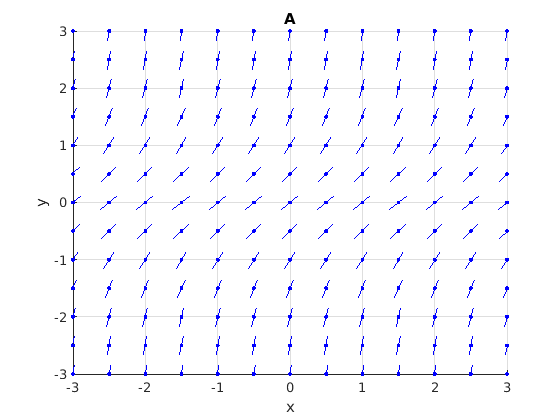
\includegraphics[width=8cm]{10_equ_diff/question2a}
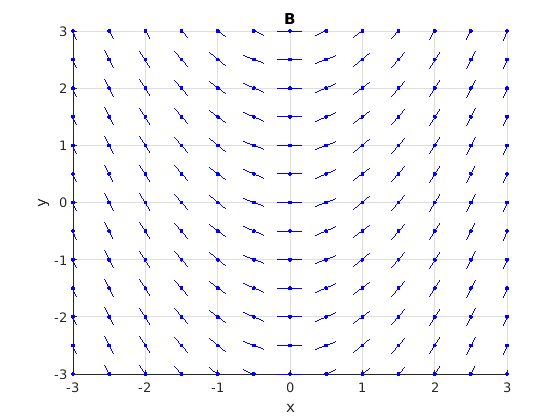
\includegraphics[width=8cm]{10_equ_diff/question2b}

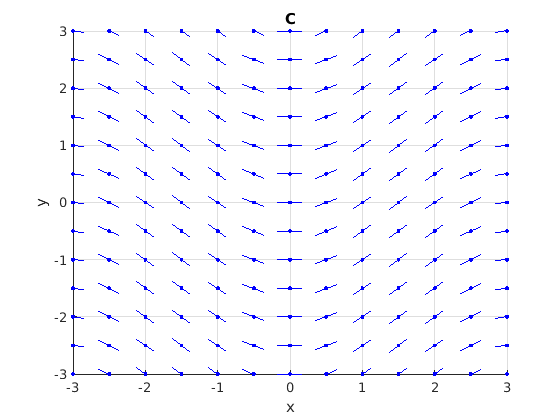
\includegraphics[width=8cm]{10_equ_diff/question2c}
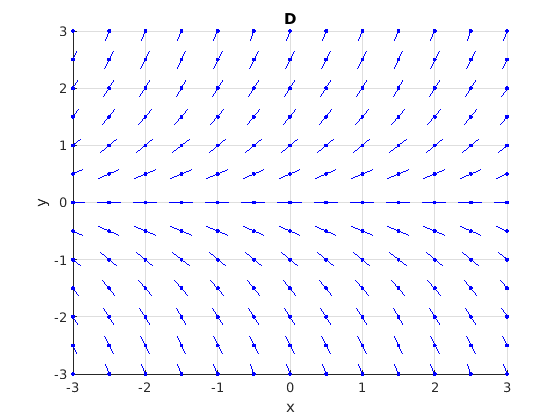
\includegraphics[width=8cm]{10_equ_diff/question2d}

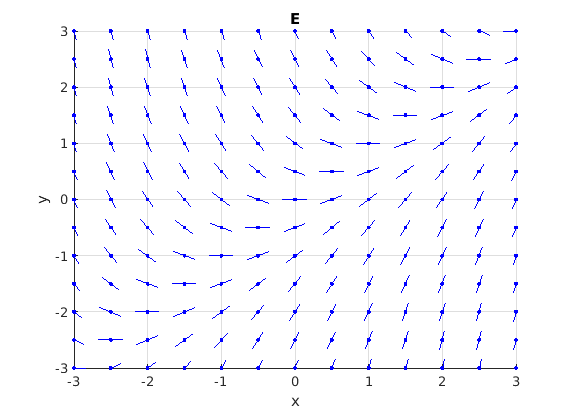
\includegraphics[width=8cm]{10_equ_diff/question2e}
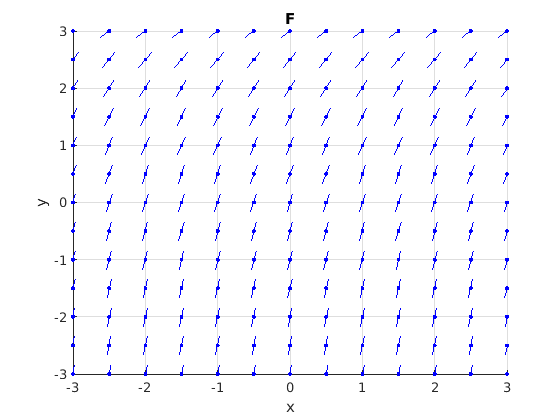
\includegraphics[width=8cm]{10_equ_diff/question2f}
\label{10Q45}
\end{question}

\begin{question}
Le champs de pentes de l'équation différentielle
\[
\dydx{y}{x} = (x-2)(x-y)
\]
est donné ci-dessous.
\MATHgraph{10_equ_diff/question3}{8cm}
\subQ{a} Tracez (de façon aussi précise que possible) le graphe de la
solution qui passe par le point $(0,0)$.\\
\subQ{b} Pour quelle valeur de $x$ la solution particulière qui passe
par le point $(0,0)$ a-t-elle un minimum local?  Un maximum local?
Justifiez vos réponses.\\ 
\subQ{c} Pour quelles régions du champs de pentes avons-nous que la pente est
positive.  Justifiez votre réponse en utilisant seulement
l'équation différentielle; sans utiliser le champ de pentes.
\label{10Q46}
\end{question}

\begin{question}
Considérons l'équation différentielle  $y' = -y/x$.\\
\subQ{a} Dessinez le champ de pentes de cet équation différentielle.\\
\subQ{b} Dessinez sur la même figure que celle pour votre champ de
pentes plusieurs solutions de cette équation différentielle.\\ 
\subQ{c} Trouvez la solution générale de l'équation différentielle.\\
\subQ{d} Que ce passe-t-il lorsque $x = 0$?
\label{10Q47}
\end{question}

\subsection{Applications}

\begin{question}[\eng]
En chimie, une {\bfseries équation de
  réaction-diffusion}\index{Équation de réaction diffusion}  est une
équation différentielle qui décrit la concentration d'un produit
chimique sous l'effet d'une réaction chimique et de la diffusion.  Un
exemple simple d'une telle équation est
\[
\dydx{C}{t} = \beta(\gamma-C) + \frac{C}{2+C}
\]
où le terme $\beta(\gamma-C)$ représente la diffusion et le terme
$\displaystyle \frac{C}{2+C}$ représente la réaction chimique.
les unités de la constante $\beta$ sont les m$^{-1}$ et les unités de la
constante $\gamma$ sont les mol/l.  Si $\beta=1$ et $\gamma=5$, trouvez les
points d'équilibre et déterminez leur stabilité.
\label{10Q48}
\end{question}

\begin{question}[\life]
L'équation différentielle suivante décrit la concentration $C(t)$ d'un
produit chimique au temps $t$ dans une cellule.
\begin{equation}\label{reactdiff}
\dydx{C}{t} = \beta(\Gamma-C) + 0.5\,C \ .
\end{equation}
Le terme $0.5 C$ représente la réaction en réponse à un facteur externe (la
cellule fabrique le produit chimique) et le terme $\beta(\Gamma -C)$
représente la diffusion au travers de la membrane de la cellule.  C'est un
exemple d'une
{\bfseries équation de réaction diffusion}\index{Équation de réaction
  diffusion}.

Répondez aux questions suivantes pour $\beta = 1.0$ min$^{-1}$ et
$\Gamma = 5.0$ mol/l.

\subQ{a} Quelles sont les points d'équilibre?

\subQ{b} Utilisez le théorème sur la stabilité des points d'équilibre pour
déterminez la stabilité des points d'équilibre que vous avez trouvés en
(a).

\subQ{c} Tracez le portrait de phases pour cette équation différentielle.

\subQ{d} Dessinez un champ de pentes et tracez quelques solutions.

\subQ{e} Quelles seraient les points d'équilibre s'il n'y avait pas le terme
de réaction (i.e. $0.5C$) dans l'équation différentielle ci-dessus.?
\label{10Q49}
\end{question}

\begin{question}[\life]
Un troupeau de gnous (de la famille des antilopes) habite une réserve
faunique.  La population initiale est de $1000$ gnous.  Après un an, la
population est de $1100$ gnous.  La population satisfait le modèle
logistique de croissance avec une capacité optimale pour le milieu de $1800$
gnous.  Combien de temps faut-il pour que la population atteigne $1500$
gnous?
\label{10Q50}
\end{question}

\begin{question}[\life]
Pour une certaine population, le nombre d'individus $N(t)$ par km$^2$
au temps $t$ satisfait
\begin{equation} \label{q5_edo}
\dydx{N}{t} = \frac{5\,N^2}{1+N^2} - 2\,N \ .
\end{equation}
\subQ{a} Quelles sont les points d'équilibre?

\subQ{b} Utilisez le théorème de stabilité des points d'équilibre pour
déterminer la stabilité des points d'équilibre que vous avez trouvés en
(a).

\subQ{c} Tracez le portrait de phases pour cette équation différentielle.

\subQ{d} Dessinez un champ de pentes et tracez quelques solutions.

\subQ{e} Déterminez le seuil de la population pour que celle-ci augmente?
\label{10Q51}
\end{question}

\begin{question}[\life]
Le modèle suivant est appelé le modèle de méta-population de Levins.
Pour étudier une population animale habitant un territoire, nous divisons le
territoire en petites sections.  Soit $p$ la fraction des sections qui sont
habitées et $d$ la fractions des sections qui sont détruites (e.g.\ par une
développeur immobilier).  Nous supposons que les sections détruites ne sont pas
habitées (et habitables).  La fraction $1-p$ est donc la fraction des
sections qui ne sont pas habitées et $1-p-d$ est la fraction des sections qui
ne sont pas habitées mais habitables.

La fraction de sections habitées est décrite par l'équation différentielle
\[
\dydx{p}{t} = c\,p(1-d-p)-m \,p
\]
où $m=1$ est le taux auquel les animaux d'une section habitée quittent cette
section et $c=2$ est le taux auquel les animaux s'installent dans une section
inhabitée et habitable.

Pour que le modèle soit consistant, il faut que $0\leq p \leq 1$ et
$0 \leq d \leq 1$.  De plus, il faut que $1 - p - d \geq 0$.
Il faut donc avoir en fait que $0 \leq p \leq 1 - d$.

\subQ{a} Trouvez les deux points d'équilibre de l'équation différentielle.
Un des points d'équilibre va dépende du paramètre $d$.  Pour quelles valeurs
de $d$ ce point d'équilibre a-t-il un sens biologique?

\subQ{b} Tracez le graphe de la fonction qui génère l'équation différentielle
et tracez le portrait de phases lorsque $d=1/4$ et $d=3/4.$

\subQ{c} Utilisez le test de la dérivée pour déterminer la stabilité des
deux points d'équilibres.  La stabilité va dépende de $d$.

\subQ{d} Est-ce que la population va survivre si $1/4$ des sections
(i.e.\ $d=1/4$) sont détruites?  Si $3/4$ des sections sont détruites?
\label{10Q52}
\end{question}

\begin{question}[\eng]
La concentration de sel dans un réservoir de $1000$ litres d'eau salée
est de $0.025$ kg par litre.  De l'eau salée dont la concentration de
sel est de $0.01$ kg par litre est ajoutée au réservoir à raison de
$10$ litres par minute.  De plus, $10$ litres d'eau salée par minute
s'échappe du réservoir.  Si le contenue du réservoir
est bien mélangé, combien de temps s'écoule-t-il avant que d'atteindre
une concentration de $0.02$ kg de sel par litre?
\label{10Q53}
\end{question}

\begin{question}[\eng]
Un réservoir contient $1000$ litres d'eau pure.  Une saumure contenant
$0.1$ kg de sel par litre d'eau est versée dans le réservoir au taux
de $5$ litres par minute.  Une saumure contenant $0.05$ kg de sel par
litre est aussi versée dans le réservoir au taux de $15$ litres par
minute.  En supposant que le contenu du réservoir est toujours bien
mélangé et que le réservoir perd $20$ litres par minutes, quelle est
la quantité de sel dans le réservoir après $t$ minutes?  quelle est la
concentration de sel dans le réservoir après $t$ minutes?
\label{10Q54}
\end{question}

\begin{question}[\life]
Considérons l'équation différentielle $\displaystyle \dydx{x}{t} = a x - x^2$
où $a$ est un paramètre.

\subQ{a} Trouvez les points d'équilibre de cette équation différentielle.  Un
des points d'équilibre devrait dépendre de $a$.

\subQ{b} Dans un même système de coordonnées, tracez le graphe de chacun des
points d'équilibre en fonction de $a$ pour $a$ au voisinage de l'origine.
Utilisez une ligne pleine pour les points d'équilibre stables et une ligne
hachurée pour les points d'équilibre instables.

\subQ{c} Que ce passe-t-il au voisinage de l'origine?  Ce genre de phénomène
est appelé {\em bifurcation}.  Dans le cas présent, nous parlons de
{\em bifurcation transcritique}.
\label{10Q55}
\end{question}

\begin{question}[\life]
Considérons l'équation logistique
\begin{equation}\label{ass_logistic}
\dydx{b}{t} = b(1-b) - hb
\end{equation}
pour une population animale où $h$ est la fraction de la population qui a été
récolté.

\subQ{a} Trouvez les points d'équilibre de (\ref{ass_logistic}).  Un des
points d'équilibre va dépendre de $h$.

\subQ{b} Dans un même système de coordonnées, tracez le graphe de chacun des
points d'équilibre en fonction de $h$ pour $0\leq h \leq 2$.  Utilisez une
ligne pleine pour les points d'équilibre stable et une ligne hachurée pour
les point d'équilibre instable.  Même s'ils n'ont pas de sens biologique,
inclure les valeurs négative des points d'équilibre.

\subQ{c} Quelle type de bifurcation obtenez-vous?
\label{10Q56}
\end{question}

\subsection{Méthode d'Euler}

\begin{question}[\theory]
Considérons l'équation différentielle $y'(x)=f(x)$ avec $y(0) = 0$.
Expliquez pourquoi l'approximation de $y(x)$ donnée par la méthode
d'Euler correspond à une somme de Reimann à droite associée a
l'intégrale $\displaystyle \int_0^x f(t) \dx{t} $.
\label{10Q57}
\end{question}

\begin{question}[\eng]
\subQ{a} Utiliser la méthode d'Euler pour trouver une approximation de
la solution $y(t)$ de
\[
\frac{\text{d}y}{\text{d}t} = 1/t
\]
à $t=2$.  Commencer à $(t,y) = (1,0)$ et utiliser $10$
sous-intervalles. \\
\subQ{b} Trouver la valeur exacte de $y(t)$ \`a $t = 2$.\\
\subQ{c} Est-ce que votre approximation de $y(t)$ à $t=2$ est plus
petite ou plus grande que la valeur exacte à $t=2$.  Utiliser le champ
de pentes (i.e. la courbure de la solution) pour expliquer la différence.
\label{10Q58}
\end{question}

\begin{question}[\eng]
Utilisez la méthode d'Euler avec $10$ sous-intervalles pour résoudre
numériquement l'équation différentielle
\begin{align*}
y' &= \frac{y + t}{t} \quad , \quad 1 \leq t \leq 2 \\
y(1) &= 0
\end{align*}
Est-ce que les valeurs données par la méthodes d'Euler sont des
surestimations ou des sous-estimations de la solution $y$?
\label{10Q59}
\end{question}

\begin{question}[\eng]
\subQ{a} Utilisez la méthode d'Euler avec $n=10$ sous-intervalles pour
trouver une approximation de $y(1)$ où $y$ est la solution de l'équation
différentielle $\displaystyle y'=\frac{3x^2}{2y}$ avec la condition
initiale $y(0)=1$.

\subQ{b} Trouvez la solution exacte de l'équation différentielle
$y'=\frac{3x^2}{2y}$ avec $y(0)=1$.

\subQ{c} Quelle est l'erreur absolue et l'erreur relative de
l'approximation de $y(1)$ trouvée en (a)?
\label{10Q60}
\end{question}


%%% Local Variables: 
%%% mode: latex
%%% TeX-master: "notes"
%%% End: 

\cleardoublepage

\chapter[Vecteurs]{Vecteurs}\label{CHAPvecteurs}

\compileTHEO{

Dans ce chapitre, nous revoyons rapidement quelques notions de
géométrie analytique que le lecteur devrait avoir étudié à l'école
secondaire.  Une grande partie des concepts présentés dans ce chapitre
seront utilisés lors de l'étude des fonctions de plusieurs variables
à partir du chapitre~\ref{chapFonctPlusVar}.

\section{Définition}

\begin{focus}{\dfn} \index{Vecteur}
Un {\bfseries vecteur} du plan $\RR^2$ est une flèche qui part de
l'origine $\VEC{0} = (0,0)$ pour se terminer en un point
$\VEC{p} = (p_1,p_2)$.   Puisque chaque vecteur est associé à un
unique point $\VEC{p}$ et vice-versa, le vecteur est dénoté par
$\VEC{p}$

De même, un {\bfseries vecteur} de l'espace $\RR^3$ est une flèche qui
part de l'origine $\VEC{0} = (0,0,0)$ pour se terminer en un point
$\VEC{p} = (p_1,p_2,p_3)$.   Puisque chaque vecteur est associé à un
unique point $\VEC{p}$ et vice-versa, le vecteur est dénoté par
$\VEC{p}$
\end{focus}

La définition de vecteur pourrait être généralisée à l'espace $\RR^n$
pour $n>3$.  Cela n'est cependant pas nécessaire pour le chapitre
présent.  Nous aborderons les espace de dimensions plus grande que $3$
au chapitre~\ref{chapALLin} sur l'algèbre linéaire.

Puisqu'il y a une bijection entre les vecteurs et les points, le
contexte déterminera comment il faut interpréter $\VEC{p}$.

\begin{egg}
Nous retrouvons à la figure~\ref{VECT1} la représentation graphique du
vecteur $\VEC{p} = (2,5,3)$.
\label{vect1}
\end{egg}

\PDFfig{11_vecteurs/vect1}{Représentation graphique du vecteur
$\VEC{p} = (2,5,3)$ de l'espace}{Représentation graphique du vecteur
$\VEC{p} = (2,5,3)$ de l'espace}{VECT1}

\begin{focus}{\dfn} \index{Vecteur!longueur} \label{norm} 
La {\bfseries longueur (euclidienne)} du vecteur $\VEC{p} = (p_1,p_2)$ est
\[
\|\VEC{p}\| \equiv \sqrt{p_1^2+p_2^2} \ ,
\]
alors que celle du vecteur $\VEC{p} = (p_1,p_2,p_3)$ est
\[
\|\VEC{p}\| \equiv \sqrt{p_1^2+p_2^2+p_3^2} \;.
\]
\end{focus}

Cette définition découle du théorème de Pythagore qui affirme que le
carré de l'hypoténuse d'un triangle droit est égal à la somme des
carrés des deux côtés adjacents à l'angle droit. La justification de
la formule pour la longueur d'un vecteur dans $\RR^3$ est illustrée à la
figure~\ref{VECT2}.

\PDFfig{11_vecteurs/vect2}{Longueur du vecteur $\VEC{p}=(p_1,p_2,p_3)$}
{Longueur du vecteur $\VEC{p}=(p_1,p_2,p_3)$}{VECT2}

\section{Opérations sur les vecteurs}

Nous pouvons définir des opérations algébriques sur les vecteurs comme ils
en existent pour les nombres.  De plus, nous pouvons aussi définir des
opérations sur les vecteurs qui ont une importante signification
géométrique comme nous verrons dans les prochaines sections.

Nous commençons par définir deux opérations algébriques sur les vecteurs:
{\em le produit d'un vecteur par un nombre réel} et
{\em la somme de vecteurs}.

Par la suite, nous définirons deux opérations sur les vecteurs,
{\em le produit scalaire} et {\em le produit vectoriel}, qui jouent
des rôles majeurs dans l'analyse géométrique.

\subsection{Produit d'un vecteur par un nombre réel}

\begin{focus}{\dfn} \index{Vecteur!produit avec un nombre réel}
Soit $\VEC{p} = (p_1,p_2)$ et $\rho$ est un nombre réel.  Le
{\bfseries produit} de $\rho$ avec le vecteur $\VEC{p}$ est le
vecteur $\VEC{q}$ défini par la formule suivante.
\[
\VEC{q} = \rho\, \VEC{p} = \rho (p_1, p_2) = (\rho p_1 , \rho p_2) \; .
\]

De même, soit $\VEC{p} = (p_1,p_2,p_3)$ et $\rho$ est un nombre réel.
Le {\bfseries produit} de $\rho$ avec le vecteur $\VEC{p}$ est le vecteur
$\VEC{q}$ défini par la formule suivante.
\[
\VEC{q} = \rho\, \VEC{p} = \rho (p_1,p_2,p_3)
= (\rho p_1 , \rho p_2, \rho p_3) \; .
\]
\end{focus}

Le vecteur $\VEC{q}$ est de longueur $|\rho| \|\VEC{p}\|$ et pointe dans la
même direction que $\VEC{p}$ si $\rho > 0$ et dans la direction opposée à
$\VEC{p}$ si $\rho < 0$.

\begin{egg}
Le dessin du vecteur $\displaystyle \VEC{q} = -2 \VEC{p}$, où
$\VEC{p}$ est le vecteur donné à l'exemple~\ref{vect1}, est donné à la
figure~\ref{VECT3}.  Nous avons
\[
\VEC{q} = -2 \VEC{p} = -2 (2, 5, 3) = (-4,-10,-6) \; .
\]
\end{egg}

\PDFfig{11_vecteurs/vect3}{Représentation du vecteur $\VEC{q} = -2\VEC{p}$}
{Représentation du vecteur $\VEC{q} = -2\VEC{p}$ où le vecteur
$\VEC{p}=(2,5,3)$ est représenté à la figure~\ref{VECT1}}{VECT3}

\subsection{Somme de vecteurs}

\begin{focus}{\dfn} \index{Vecteur!somme de vecteurs}
Soit $\VEC{p} = (p_1,p_2)$ et $\VEC{q} = (q_1, q_2)$.  La
{\bfseries somme} des vecteurs $\VEC{p}$ et $\VEC{q}$ est le
vecteur $\VEC{r}$ défini par la formule suivante.
\[
\VEC{r} = \VEC{p} + \VEC{q} = ( p_1, p_2) + (q_1, q_2)
= (p_1+q_1, p_2+q_2) \; .
\]

De même, soit $\VEC{p} = (p_1,p_2,p_3)$ et $\VEC{q} = (q_1, q_2, q_3)$.
La {\bfseries somme} des deux vecteurs $\VEC{p}$ et
$\VEC{q}$ est le vecteur $\VEC{r}$ défini par la formule suivante.
\[
\VEC{r} = \VEC{p} + \VEC{q} = ( p_1, p_2, p_3) + (q_1, q_2, q_3)
= (p_1+q_1, p_2+q_2, p_3+q_3) \; .
\]
\end{focus}

\begin{egg}
Le résultat $\VEC{r} = (5,9,4)$ de la somme des vecteurs $\VEC{p} = (6,6,2)$
et $\VEC{q} = (-1, 3, 2)$ est illustré à la figure~\ref{VECT4}.

Remarquons que les trois vecteurs $\VEC{p}$, $\VEC{q}$ et $\VEC{r}$ sont
tous dans le même plan.  Nous verrons à la section~\ref{PROD_VECT} sur
le produit vectoriel comment nous pouvons facilement vérifier cette
affirmation.
\label{EX_SUM}
\end{egg}

\PDFfigD[t]{11_vecteurs/vect4}{11_vecteurs/vect5}{Représentation
graphique de la somme de deux vecteurs}{Ces dessins illustrent
l'aspect géométrique de la somme des deux vecteurs donnés à
l'exemple~\ref{EX_SUM}}{VECT4}

\subsection{Notation vectorielle classique}

Les vecteurs suivants sont fondamental en analyse vectorielle.  Pour
cette raison, ils ont leur propre notation.

\begin{focus}{\dfn} \index{Vecteur!canonique}
Dans le plan, les vecteurs $\ii = (1,0)$ et $\jj = (0.1)$ sont appelés
les {\bfseries vecteurs canoniques}.  Si
$\VEC{p}=(p_1,p_2)$, alors $\displaystyle \VEC{p} = p_1 \ii + p_2 \jj$.

De même, dans l'espace $\RR^3$, les {\bfseries vecteurs canoniques}
sont les vecteurs $\ii = (1,0,0)$, $\jj = (0.1,0)$ et $\kk = (0,0,1)$.  Si
$\VEC{p}=(p_1,p_2,p_3)$, alors
$\displaystyle \VEC{p} = p_1 \ii + p_2 \jj + p_3 \kk$.
\end{focus}

Dans les livres de mathématiques, la notation
$\VEC{e}_1$ pour $\ii$, $\VEC{e}_2$ pour $\jj$ et $\VEC{e}_3$ pour
$\kk$ est plus souvent utilisée.

\subsection{Produit scalaire \eng}

Alors que le produit d'un vecteur par un nombre réel et l'addition de
vecteurs ont un rôle principalement algébrique, le produit scalaire est l'une
des deux opérations sur les vecteurs qui a un usage principalement
géométrique; l'autre opération étant le produit vectoriel.

\begin{focus}{\dfn} \index{Vecteur!produit scalaire}
Le {\bfseries produit scalaire} de deux vecteurs,
$\VEC{p} = (p_1,p_2)$ et $\VEC{q} = (q_1,q_2)$, est défini par la
formule
\[
\ps{\VEC{p}}{\VEC{q}} = p_1 q_1 + p_2 q_2  \; .
\]

De même, Le {\bfseries produit scalaire} de deux vecteurs,
$\VEC{p} = (p_1,p_2,p_3)$ et $\VEC{q} = (q_1,q_2,q_3)$, est défini
par la formule
\[
\ps{\VEC{p}}{\VEC{q}} = p_1 q_1 + p_2 q_2 + p_3 q_3 \; .
\]
Le produit scalaire des vecteurs $\VEC{p}$ et $\VEC{q}$ est aussi
dénoté $\VEC{p} \cdot \VEC{q}$ quand cela ne cause pas de confusion.
\end{focus}

Pourquoi définir un produit de deux vecteurs comme nous venons de le faire?
N'aurions-nous pas pu définir le produit de deux vecteurs composante par
composante comme nous l'avons fait pour la somme de deux vecteurs?  En
fait, nous aurions pu le faire mais cela n'a pas d'intérêt car il n'y a pas
d'interprétations géométriques du produit de deux vecteurs composante par
composante.  Par contre, le produit scalaire défini ci-dessus a une
interprétation géométrique très importante.

\begin{focus}{\dfn} \label{dfncos}
Le cosinus de l'angle entre les vecteurs non nuls $\VEC{p}$ et
$\VEC{q}$ (et ainsi l'angle entre ces vecteurs) est déterminé par
\begin{equation}\label{CosVectors}
\cos(\alpha) = \frac{\ps{\VEC{p}}{\VEC{q}}}{\|\VEC{p}\|\,\|\VEC{q}\|} \; .
\end{equation}
\end{focus}

C'est cette définition qui fait le lien entre l'opération algébrique
qu'est le produit scalaire de deux vecteurs et l'interprétation
géométrique que nous avons des vecteurs.

\begin{rmk}
Remarquons que la longueur d'un vecteur est la racine carrée du produit
scalaire de ce vecteur par lui-même.  Si $\VEC{p} = (p_1,p_2,p_3)$, alors
\[
\ps{\VEC{p}}{\VEC{p}} = p_1^2 + p_2^2 + p_3^2 = \|\VEC{p}\|^2 \; .
\]

Si $\displaystyle \ps{\VEC{p}}{\VEC{q}} = 0$, alors le cosinus entre
les deux vecteurs $\VEC{p}$ et $\VEC{q}$ est $0$.  Nous avons donc que
l'angle entre $\VEC{p}$ et $\VEC{q}$ est $\pi/2$ ( $+n\pi$ pour
$n \in \ZZ$).  Ceci justifie la définition suivante.
\end{rmk}

\begin{focus}{\dfn}
Soit $\VEC{p}$ et $\VEC{q}$, deux vecteurs.  Le vecteur $\VEC{p}$ est
{\bfseries perpendiculaire}\index{Vecteur!perpendiculaire} ou
{\bfseries orthogonal}\index{Vecteur!orthogonal} au vecteur
$\VEC{q}$ (et vice-versa) si $\displaystyle \ps{\VEC{p}}{\VEC{q}} = 0$.
\end{focus}

\begin{rmk}
Vous avez probablement appris que le produit des pentes de deux droites
orthogonales est $-1$.  Il est facile à l'aide des vecteurs de
vérifier cette énoncé.  Supposons que $\VEC{p} = (p_1,p_2)$ soit un
vecteur parallèle à une droite $\ell_1$ et que $\VEC{q} = (q_1,q_2)$
soit un vecteur parallèle à une droite $\ell_2$.  Si les droites
$\ell_1$ et $\ell_2$ sont perpendiculaires, alors il en est de même
pour les vecteurs $\VEC{p}$ et $\VEC{q}$, et vice-versa.  Nous avons donc
\[
\ps{\VEC{p}}{\VEC{q}} = p_1 q_1 + p_2 q_2 = 0 \; .
\]
Ainsi,
\[
\frac{p_2}{p_1} = - \frac{q_1}{q_2} \; .
\]
Puisque $\displaystyle m_1 = \frac{p_2}{p_1}$ est la pente de la droite
$\ell_1$ et $\displaystyle m_2 = \frac{q_2}{q_1}$ est celle de la droite
$\ell_2$, nous obtenons bien que $\displaystyle m_1 = -\frac{1}{m_2}$.
\end{rmk}

\begin{rmk}
Nous justifierons ci-dessous la définition~\ref{dfncos} dans le plan.  La
justification est identique pour les vecteurs dans l'espace.

Commençons par un petit rappel.  Considérons le triangle $\triangle ABC$
représenté à la figure~\ref{VECT6}.  La {\bfseries loi des cosinus} dit que
\[
c^2 = a^2 + b^2 - 2 a b\, \cos(\gamma)  \; .
\]

\PDFfig{11_vecteurs/vect6}{La loi des cosinus}{La loi des cosinus dit que
$c^2 = a^2 + b^2 - 2 a b \cos(\gamma)$}{VECT6}

Soit $\VEC{p} = (p_1,p_2)$ et $\VEC{q} = (q_1,q_2)$.
De la loi des cosinus, nous déduisons que
\begin{equation} \label{ps_interpr}
\| \VEC{q} - \VEC{p} \|^2 = \|\VEC{p}\|^2 + \|\VEC{q}\|^2
- 2 \|\VEC{p}\| \|\VEC{q}\| \cos(\alpha)
\end{equation}
où $\alpha$ est l'angle entre $\VEC{p}$ et $\VEC{q}$ (figure~\ref{VECT7}).

\PDFfig{11_vecteurs/vect7}{Interprétation géométrique du produit scalaire}
{Interprétation géométrique du produit scalaire}{VECT7}

Puisque $\displaystyle \VEC{q} - \VEC{p} = (q_1-p_1,q_2-p_2)$,
nous avons que
\begin{align*}
\| \VEC{q} - \VEC{p} \|^2
&= (q_1 - p_1)^2 + (q_2-p_2)^2  \\
&= \left(p_1^2 + p_2^2\right) + \left(q_1^2 + q_2^2\right)
- 2 ( p_1 q_1 + p_2 q_2) \\
&= \| \VEC{p} \|^2 + \| \VEC{q} \|^2 - 2 \ps{\VEC{p}}{\VEC{q}} \; .
\end{align*}
Ainsi, (\ref{ps_interpr}) devient
\[
\| \VEC{p} \|^2 + \| \VEC{q} \|^2 - 2 \ps{\VEC{p}}{\VEC{q}}
= \|\VEC{p}\|^2 + \|\VEC{q}\|^2 - 2 \|\VEC{p}\| \|\VEC{q}\|
\cos(\alpha) \; .
\]
Après avoir simplifié les termes identiques de chaque côté de l'égalité,
nous obtenons
\[
\ps{\VEC{p}}{\VEC{q}} = \|\VEC{p}\|\, \|\VEC{q}\| \cos(\alpha) \; .
\]
Si nous isolons $\cos(\alpha)$, nous retrouvons la définition~\ref{dfncos}.
\end{rmk}

\begin{rmk}[\theory]
Il est facile de démontrer la loi des cosinus en utilisant les
coordonnées cartésiennes.

Pour démontrer la loi des cosinus pour l'angle au sommet $C$ d'un
triangle $\triangle ABC$. nous plaçons le sommet $C$ à l'origine et le
sommet $A$ (ou $B$) sur l'axe des $x_1$ comme cela est fait à la
figure~\ref{VECT16}.

\PDFfig{11_vecteurs/vect16}{Démonstration de la loi des cosinus}{Démonstration
de la loi des cosinus}{VECT16} 

Les coordonnées du point $B$ sont donc
$(a\cos(\gamma), a \sin(\gamma))$ et celle du point $A$ sont $(b,0)$.
Le triangle $\triangle DAB$ a un angle droite au sommet $D$.  Le
théorème de Pythagore nous donne donc
\[
c^2 = \left( a\sin(\gamma) \right)^2 + \left( -a\cos(\gamma) + b\right)^2 \; .
\]
Si nous développons le côté droit de cette équation, nous trouvons
\begin{align*}
c^2 &= a^2 \sin^2(\gamma) + a^2 \cos^2(\gamma) - 2 ab\, \cos(\gamma) +b^2 \\
&= a^2 \left(\cos^2(\gamma)+\sin^2(\gamma)\right) + b^2 - 2ab\,\cos(\gamma) \\
&= a^2 + b^2 - 2ab\,\cos(\gamma)
\end{align*}
puisque $\cos^2(\gamma) + \sin^2(\gamma) = 1$.
\end{rmk}

\subsection{Produit vectoriel \eng}\label{PROD_VECT}

Le produit vectoriel est une opération sur les vecteurs qui a un
usage principalement géométrique.

\begin{focus}{\dfn} \index{Vecteur!produit vectoriel}
Si $\VEC{p} = (p_1,p_2,p_3)$ et $\VEC{q} = (q_1, q_2, q_3)$ sont deux
vecteurs qui ne sont pas colinéaires (i.e.\ dont l'un n'est pas un
multiple de l'autre), nous définissons le
{\bfseries produit vectoriel} des vecteurs
$\VEC{p}$ et $\VEC{q}$ comme étant le vecteur
\begin{equation}\label{sp_form}
\VEC{m} = \VEC{p} \times \VEC{q} =
\left(p_2 q_3 - p_3 q_2\right)\ii + \left(p_3 q_1 - p_1 q_3\right) \jj
+ \left(p_1 q_2 - p_2 q_1\right) \kk \; .
\end{equation}
Donc $\VEC{m} = \left(p_2 q_3 - p_3 q_2, p_3 q_1 - p_1 q_3,
p_1 q_2 - p_2 q_1\right)$.
\label{VecTProdDef}
\end{focus}

Nous fournirons à la remarque~\ref{DetermVectProd} de la
section~\ref{DetermSect} une formule symbolique simple pour calculer
le produit vectoriel de deux vecteurs.

Le vecteur qui résulte du produit vectoriel de deux vecteurs a une relation
géométrique très particulière avec les deux vecteurs du produit.

\begin{focus}{\prp}
Le vecteur $\VEC{m} = \VEC{p} \times \VEC{q}$ est
perpendiculaire aux vecteurs $\VEC{p}$ et $\VEC{q}$.
\end{focus}

Pour vérifier que $\VEC{p} \times \VEC{q}$ est perpendiculaire à
$\VEC{p}$, il suffit de vérifier que
$\ps{(\VEC{p} \times \VEC{q})}{\VEC{p}} = 0$.  En effet,
\begin{align*}
\ps{(\VEC{p} \times \VEC{q})}{\VEC{p}} &=
\ps{ \left(p_2 q_3 - p_3 q_2, p_3 q_1 - p_1 q_3,
p_1 q_2 - p_2 q_1\right)}{(p_1,p_2,p_3)} \\
&= p_1\left(p_2 q_3 - p_3 q_2\right) + p_2\left(p_3 q_1 - p_1 q_3\right)
+ p_3\left(p_1 q_2 - p_2 q_1\right) \\
&= p_1 p_2 q_3 - p_1 p_3 q_2 + p_2 p_3 q_1 - p_1 p_2 q_3
+ p_1 p_3 q_2 - p_2 p_3 q_1 \\
&= 0 \; .
\end{align*}
De même, nous pouvons vérifier que
$\ps{(\VEC{p} \times \VEC{q})}{\VEC{q}} = 0$.

\begin{focus}{\dfn} \index{Règle de la main droite}
La direction du vecteur $\VEC{p} \times \VEC{q}$ est déterminée par la
{\bfseries règle de la main droite}.  C'est-à-dire, si la paume de
votre main droite entoure la droite qui contient le vecteur
$\VEC{p} \times \VEC{q}$ de telle sorte que vos doigts indiquent la
plus petite direction angulaire de $\VEC{p}$ à $\VEC{q}$, alors votre
pouce pointe dans la direction de $\VEC{p} \times \VEC{q}$
(figure~\ref{VECT10}).
\end{focus}

\PDFfig{11_vecteurs/vect10}{Le vecteur obtenu du produit vectoriel de deux
vecteurs est orthogonal au plan généré par ces deux vecteurs}{Le vecteur
obtenu du produit vectoriel de deux vecteurs est orthogonal au plan généré
par ces deux vecteurs.}{VECT10}

\begin{egg}
Nous pouvons facilement vérifier avec la règle de la main droite que
$\kk = \ii \times \jj$ et $\jj \times \ii = -\kk$.
\end{egg}

Quelques manipulations algébriques vont nous permettre de trouver une
formule pour la longueur du vecteur $\VEC{p} \times \VEC{q}$.
Soit $\theta$, le plus petit angle entre $\VEC{p}$ et $\VEC{q}$
(donc $0 < \theta < \pi$).  Nous avons que
\[
\ps{\VEC{p}}{\VEC{q}} = \|\VEC{p}\| \|\VEC{q}\| \cos(\theta)  \; .
\]
Ainsi,
\begin{align*}
\| \VEC{p} \times \VEC{q} \|^2 &= 
\left(p_2 q_3 - p_3 q_2\right)^2 + \left(p_3 q_1 - p_1 q_3\right)^2
+ \left(p_1 q_2 - p_2 q_1\right)^2 \\
&= \left(p_1^2+p_2^2+p_3^2\right)\left(q_1^2+q_2^2+q_3^2\right)
-\left(p_1q_1+p_2q_2+p_3q_3\right)^2 \\
&= \|\VEC{p}\|^2 \|\VEC{q}\|^2
- \left( \ps{\VEC{p}}{\VEC{q}} \right)^2
= \|\VEC{p}\|^2 \|\VEC{q}\|^2
- \|\VEC{p}\|^2 \|\VEC{q}\|^2\cos^2(\theta) \\
&= \|\VEC{p}\|^2 \|\VEC{q}\|^2 \left( 1 - \cos^2(\theta)\right)
= \|\VEC{p}\|^2 \|\VEC{q}\|^2 \sin^2(\theta) \; .
\end{align*}

Nous obtenons le résultat suivant.

\begin{focus}{\prp}
\[
\| \VEC{p} \times \VEC{q} \| = 
= \|\VEC{p}\| \|\VEC{q}\| \sin(\theta)
\]
où $0 \leq \theta < \pi$ est l'angle entre $\VEC{p}$ et $\VEC{q}$.
\end{focus}

\begin{egg}
Nous avons que le plus petit angle entre les vecteurs $\ii$ et $\jj$ est
$\displaystyle \frac{\pi}{2}$.  Ainsi,
\[
\|\kk \| = \| \ii \times \jj \| = \|\ii \| \| \jj \|
\sin \left(\frac{\pi}{2}\right) = 1
\]
comme il se doit.
\end{egg}

Il y a une interprétation géométrique très intéressante de la longueur du
vecteur obtenu d'un produit vectoriel.  Comme nous pouvons constater à
partir du dessin à la figure~\ref{VECT11},
$\|\VEC{p}\| \|\VEC{q}\| \sin(\theta)$ est
l'aire du parallélogramme définie par $\VEC{p}$ et $\VEC{q}$.  La
longueur du vecteur $\VEC{p}\times \VEC{q}$ est donc l'aire de ce
parallélogramme.

\PDFfig{11_vecteurs/vect11}{L'aire du parallélogramme définie par deux vecteurs}
{L'aire du parallélogramme définie par les deux vecteurs $\VEC{p}$ et
$\VEC{q}$ est
$\|\VEC{p}\times \VEC{q}\| = \|\VEC{p}\| \|\VEC{q}\| \sin(\theta)$.}{VECT11}

\section{Équation d'une droite \eng}

Nous pouvons utiliser les vecteurs pour décrire les droites.

La droite qui passe par le point $\VEC{p}$ et qui est parallèle au
vecteur $\VEC{q}$ (figure~\ref{VECT8}) est formé des points
$\VEC{x}$ où 
\begin{equation}\label{PVline}
\VEC{x} = \VEC{p} + \alpha \VEC{q}
\end{equation}
et $\alpha$ prend toutes les valeurs réelles.

Rappelons que nous utilisons la même notation pour désigner un point ou
un vecteur.  Nous pouvons donc faire référence au point $\VEC{x}$ et à ses
coordonnées à un certain moment et traiter $\VEC{x}$ comme un vecteur
à d'autres moments.

\begin{focus}{\dfn} \index{Représentation vectorielle d'une droite}
La formule (\ref{PVline}) est une {\bfseries représentation
vectorielle} de la droite qui passe par $\VEC{p}$ et est parallèle au
vecteur $\VEC{q}$.
\end{focus}

\PDFfig{11_vecteurs/vect8}{Représentation vectorielle d'une droite}
{Représentation vectorielle d'une droite}{VECT8}

Si $\VEC{p}=(p_1,p_2,p_3)$, $\VEC{q} = (q_1, q_2, q_3)$ et
$\VEC{x}=(x_1,x_2,x_3)$,  les composantes de la représentation vectorielle
$\VEC{x} = \VEC{p} + \alpha \VEC{q}$ sont
\begin{equation}\label{RPline}
x_1 = p_1 + \alpha\; q_1 \ , \ x_2 = p_2 + \alpha\; q_2 \quad \text{et}
\quad x_3 = p_3 + \alpha\; q_3 \; .
\end{equation}

\begin{focus}{\dfn} \index{Représentation paramétrique d'une droi\-te}
la formule (\ref{RPline}) est une {\bfseries représentation
paramétrique} de la droite qui passe par $\VEC{p}$ et est parallèle au
vecteur $\VEC{q}$.  Le {\bfseries paramètre} est $\alpha$.
\end{focus}

Si nous supposons que $q_1$, $q_2$ et $q_3$ sont non nuls et que nous
résolvons chacune des trois équations de la représentation paramétrique
pour $\alpha$, nous obtenons 
\begin{equation}\label{RSline1}
\frac{x_1-p_1}{q_1} = \frac{x_2-p_2}{q_2} = \frac{x_3-p_3}{q_3} \; .
\end{equation}
Si $q_2$ et $q_3$ sont non nuls mais $q_1 = 0$, nous obtenons
\begin{equation}\label{RSline2}
\frac{x_2-p_2}{q_2} = \frac{x_3-p_3}{q_3} \quad \text{et} \quad x_1 = p_1 \; .
\end{equation}
C'est une droite dans le plan $x=p_1$.  Le lecteur est invité à
analyser les autres cas possibles.

\begin{focus}{\dfn} \index{Représentation standard d'une droite}
Les formules (\ref{RSline1}) et (\ref{RSline2}) sont des
{\bfseries représentations standard}
d'une droite qui passe par $\VEC{p}$ et est parallèle au vecteur
$\VEC{q}$.
\end{focus}

\begin{rmk}
Nous pouvons déduire à partir du dessin à la figure~\ref{VECT15} que,
dans le plan, les points $\VEC{x}$ de la droite qui passe par le point
$\VEC{p}$ et qui est perpendiculaire au vecteur $\VEC{q}$ sont donnés par
\[
\ps{\VEC{x} - \VEC{p}}{\VEC{q}} = 0 \; .
\]
\end{rmk}

\PDFfig{11_vecteurs/vect15}{Équation d'une droite du plan qui est
perpendiculaire à un vecteur }{Les points $\VEC{x}$ d'une droite
perpendiculaire à un vecteur $\VEC{q}$ et passant par un point
$\VEC{p}$ satisfont $\ps{\VEC{x} - \VEC{p}}{\VEC{q}} = 0$.}{VECT15}

\begin{egg}
Si $\VEC{p}=(1,2,3)$ et $\VEC{q}=(-1,2,2)$, alors l'ensemble des points
$\VEC{x}=(x_1,x_2,x_3)$ de la droite passant par $\VEC{p}$ et
parallèle à $\VEC{q}$ est donnée par la relation
\[
(x_1,x_2,x_3) = \VEC{x} = \VEC{p} + \alpha \VEC{q} = (1,2,3) + \alpha (-1,2,2)
= (1-\alpha, 2 +2 \alpha, 3 + 2\alpha)
\]
pour $\alpha \in \RR$.  Nous avons donc la représentation paramétrique
\[
x_1 = 1-\alpha \ , \ x_2 = 2+2\alpha \quad \text{et} \quad x_3 = 3+2\alpha
\]
et la représentation standard
\[
- (x_1-1) = \frac{x_2-2}{2} = \frac{x_3-3}{2} \; .
\]
\end{egg}

\begin{egg}
La représentation classique d'une droite dans le plan est $x_2=m x_1+b$
où $m$ est la pente de la droite et $b$ est l'abscisse à l'origine.

L'exemple suivant illustre la relation entre les représentations
d'une droite que nous venons d'introduire et la représentation
classique de cette droite.

Soit $\VEC{p}=(2,3)$ et $\VEC{q} = (4,3)$.  Pour trouver l'équation
classique de la droite qui passe par le point $\VEC{p}$ et qui est
parallèle au vecteur $\VEC{q}$, il faut premièrement trouver la pente
de la droite qui contient le vecteur $\VEC{q}$.  La pente de
cette droite est $3/4$.  La forme {\bfseries point-pente} de la droite
cherchée est donc
\[
x_2-3 = \frac{3}{4}\, (x_1 - 2) \; .
\]
Nous obtenons la représentation classique
\[
x_2 = \frac{3}{4} x_1 + \frac{3}{2}
\]
de la droite.

L'ensemble des points $\VEC{x}=(x_1,x_2)$ de la droite qui passe par le
point $\VEC{p}$ et est parallèle au vecteur $\VEC{q}$ est donnée par
\[
(x_1,x_2) = \VEC{x} = \VEC{p} + \alpha \VEC{q}
= (2,3) + \alpha (4,3) = (2+ 4\alpha, 3 +3\alpha) \; .
\]
Une représentation paramétrique de la droite qui passe par le point
$\VEC{p}$ et est parallèle au vecteur $\VEC{q}$ est donc
$x_1 = 2 + 4 \alpha$ et $x_2 = 3 + 3 \alpha$.  De la première
équation, nous obtenons que $\alpha = (x_1-2)/4$.  Si
nous substituons cette expression pour $\alpha$ dans l'équation
$x_2 = 3 + 3 \alpha$, nous obtenons
\[
x_2 = 3 + 3 \left(\frac{x_1-2}{4}\right) = 3 + \frac{3}{4} (x_1-2)
= \frac{3}{4} x_1 + \frac{3}{2} \ ,
\]
la représentation classique de le droite.
\end{egg}

\subsection{Droites tangentes}

\begin{egg}
Trouvons l'équation de la droite tangent au point
$\VEC{p}= (1,\sqrt{3})$ du cercle de rayon $2$ centré à l'origine
\PDFgraph{11_vecteurs/vect14}

Nous présentons trois méthodes pour résoudre ce problème.

\subQ{a} Nous remarquons que le vecteur $\VEC{p}$ est perpendiculaire à la
droite tangente au cercle car $\VEC{p}$ représente un rayon du cercle.
Les points $\VEC{x}=(x_1,x_2)$ de la droite tangente cherchée
satisfont donc
\[
\ps{\VEC{x} - \VEC{p}}{\VEC{p}} = \ps{ (x_1-1, x_2-\sqrt{3})}{(1,\sqrt{3})}
= (x_1-1) + \sqrt{3} (x_2-\sqrt{3}) = 0 \; .
\]
Si nous résolvons pour $x_2$, nous obtenons
\[
x_2 = \frac{-1}{\sqrt{3}}\ x_1 + \frac{4}{\sqrt{3}} \ ;
\]
une représentation classique pour la droite tangente.

\subQ{b} Une autre méthode pour résoudre notre problème fait appel à
la représentation paramétrique d'une droite.  Premièrement, nous trouvons un
vecteur parallèle à la tangent au cercle au point $\VEC{p}$.
C'est-à-dire que nous cherchons un vecteur perpendiculaire au vecteur
$\VEC{p} = (1,\sqrt{3})$.  Il est facile de voir que
$\VEC{q} = (\sqrt{3}, -1)$ est perpendiculaire au vecteur
$\VEC{p}$ car $\ps{\VEC{q}}{\VEC{p}} = 0$.  Ainsi, les points
$\VEC{x}=(x_1,x_2)$ de la droite tangent au cercle au point $\VEC{p}$
satisfont
\[
\VEC{x} = \VEC{p} + \alpha \VEC{q} \; .
\]
Une représentation paramétrique de la droite tangent au cercle au point
$(1,\sqrt{3})$ est alors
\[
x_1 = 1 + \alpha \, \sqrt{3} \quad \text{et} \quad x_2 = \sqrt{3} - \alpha
\]
pour tout nombre réel $\alpha$.

Si nous résolvons pour $\alpha$ la première équation de la représentation
paramétrique, nous trouvons $\alpha = (x_1-1)/\sqrt{3}$.  Si nous
substituons cette expression pour $\alpha$ dans la deuxième équation
de la représentation paramétrique, nous obtenons une représentation
classique pour l'équation d'une droite tangente.
\[
x_2 = \sqrt{3} - \frac{x_1-1}{\sqrt{3}} = \frac{-1}{\sqrt{3}}\ x_1 
+ \frac{4}{\sqrt{3}} \; .
\]

\subQ{c} Finalement, la façon traditionnelle de trouver l'équation de
la tangente au point $\VEC{p}$ est de commencer par trouver la pente de la
tangente.  Pour cela, nous notons que la pente de la droite qui contient
le vecteur $\VEC{p}$ est $\displaystyle m_1 = \sqrt{3}$.  Comme la
droite tangente est perpendiculaire à la droite qui contient le
vecteur $\VEC{p}$, sa pente est donc
\[
m_2 = \frac{-1}{m_1} = \frac{-1}{\sqrt{3}} \; .
\]
La forme point-pente de l'équation de la tangente au cercle au point
$\VEC{p}$ est donc
\[
x_2 - \sqrt{3} = \frac{-1}{\sqrt{3}} ( x_1 - 1) \; .
\]
Donc
\[
x_2 = \frac{-1}{\sqrt{3}} \ x_1 + \frac{4}{\sqrt{3}}  \; .
\]
\label{TANG_CIRCL}
\end{egg}

\subsection{Intersection de deux droites}

Dans le plan, deux droites non parallèles se coupent en un point.
Dans l'espace, deux droites non parallèles ne se coupent généralement
pas en un point.  L'exemple suivant illustre une méthode pour trouver
l'intersection de deux droites si cette intersection existe.

\begin{egg}
Trouvons l'intersection (s'il y en a une) des droites $\ell$ et $\ell'$
données par les représentations paramétriques suivantes.  La droite
$\ell$ possède la représentation paramétrique
\[
x_1 = 2s -3 \ , \ x_2 = s -1 \quad \text{et} \quad  x_3 = -s +5
\]
pour $s\in \RR$, et la droite $\ell'$ possède la représentation
paramétrique
\[
x_1 = t -3 \ , \ x_2 = -2 t + 1 \quad \text{et} \quad  x_2 = t - 1 \; ,
\]
pour $t \in \RR$.

Ces deux droites ne sont pas parallèles car $\ell$ est parallèle au
vecteur $(2,1,-1)$ et $\ell'$ au vecteur $(1,-2,1)$, et ces deux
vecteurs ne sont pas parallèles.  Pour que ces deux droites se coupent
en un point $(x_1,x_2,x_3)$ commun, il faut qu'ils existent $s$ et $t$
tels que
\[
t -3 = 2s -3 \quad , \quad -2 t + 1 = s -1 \quad \text{et} \quad
t - 1 = -s +5 \; .
\]
La première équation donne $t = 2s$.  Si nous substituons cette expression
pour $t$ dans la deuxième équation, alors $-4s +1 = s-1$ et donc
$s=2/5$.  Nous obtenons de $t = 2s$ que $t= 4/5$.  Malheureusement, si
nous substituons $s=2/5$ dans la troisième équation, nous obtenons
$t = 28/5$.  Il n'y a donc pas de valeurs de $s$ et $t$ qui satisfont
les trois équations simultanément.  Les deux droites ne se
coupent pas.
\end{egg}

% \begin{egg}
% Trouvons l'intersection (s'il y en a une) de la droite $\ell$ donnée par la
% représentation paramétrique
% \[
% x = 2s -2 \ , \ y = -s +2 \ \text{et} \  z = 2s
% \]
% pour $s\in \RR$, et de la droite $\ell'$ donnée par la représentation
% paramétrique
% \[
% x = t -3 \ , \ y = -2 t + 1 \ \text{et} \  z = t - 1
% \]
% pour $t \in \RR$.
% \end{egg}

\section{Équation d'un plan \eng} \label{EQU_PLAN1}

\begin{focus}{\prp} \label{RSplan}
Le plan qui passe par un point $\VEC{p}$ et qui est perpendiculaire au
vecteur $\VEC{m}$ (figure~\ref{VECT9}) est l'ensemble des
points $\VEC{x}$ tels que le vecteur $\displaystyle \VEC{x}-\VEC{p}$ est
perpendiculaire à $\VEC{m}$.  Si nous utilisons le produit scalaire, nous
pouvons définir ce plan comme l'ensemble des points $\VEC{x}$ tels que
\[
\ps{\VEC{x}-\VEC{p}}{\VEC{m}} = 0 \; .
\]
\end{focus}

\PDFfig{11_vecteurs/vect9}{Représentation vectorielle d'un plan}
{Représentation vectorielle d'un plan}{VECT9}

Si $\displaystyle \VEC{x}=(x_1,x_2,x_3)$, $\displaystyle \VEC{p}=(p_1,p_2,p_3)$
et $\displaystyle \VEC{m} = (m_1,m_2,m_3)$, la formule donnée à la
proposition~(\ref{RSplan}) devient
\begin{equation} \label{EQU_PLAN_S}
m_1 (x_1-p_1) + m_2 (x_2-p_2) + m_3 (x_3-p_3) = 0
\end{equation}
ou simplement
\begin{equation} \label{EQU_PLAN_S2}
m_1 x_1 + m_2 x_2 + m_3 x_3 - d = 0
\end{equation}
où $d = m_1 p_1 + m_2 p_2 + m_3 p_3 = \ps{\VEC{m}}{\VEC{p}}$.  Nous
pourrions penser que la valeur de $d$ va changer si nous choisissons
différent points $\VEC{p}$ du plan.  En fait, ce n'est pas le cas.
Soit $\VEC{t}$ un autre point du plan.  Puisque
$\VEC{t} - \VEC{p}$ est un vecteur parallèle au plan et donc
perpendiculaire à $\VEC{m}$, nous avons
\[
\ps{\VEC{m}}{\VEC{t}} - \ps{\VEC{m}}{\VEC{p}} 
= \ps{\VEC{m}}{\VEC{t} - \VEC{p}} = 0
\]
Ainsi, $\ps{\VEC{m}}{\VEC{t}} = \ps{\VEC{m}}{\VEC{p}}$.

\begin{focus}{\dfn}
la formule (\ref{EQU_PLAN_S}) (ou (\ref{EQU_PLAN_S2})\;) est une
{\bfseries représentation standard}\index{Représentation standard d'un
  plan} d'un plan qui contient le point $\VEC{p}$ et qui est
perpendiculaire au vecteur $\VEC{m}$.  Nous disons que le vecteur $\VEC{m}$
est {\bfseries orthogonal} ou {\bfseries perpendiculaire}
ou {\bfseries normal} au plan.\index{Vecteur!Perpendiculaire à un plan}
\index{Vecteur!Orthogonal à un plan}\index{Vecteur!Normal à un plan}
\end{focus}

Si $m_3 \neq 0$, nous pouvons déduire de (\ref{EQU_PLAN_S}) que
\[
x_3 = p_3 - \frac{m_1}{m_3} (x_1-p_1) - \frac{m_2}{m_3} (x_2- p_2) \;.
\]
Si $m_3 = 0$ et $m_2 \neq 0$, l'équation du plan est simplement
\[
x_2 = p_2 - \frac{m_1}{m_2} (x_1- p_1)
\]
et $x_3$ est libre (i.e. $x_3$ va de $-\infty$ à $\infty$).
C'est un plan qui est parallèle à l'axe des $x_3$.  Nous laissons aux lecteurs
l'étude des autres cas possibles.

\begin{egg}
Si $\VEC{p}=(1,2,3)$ et $\VEC{m} = (1,-2,4)$, l'ensemble des points
$\VEC{x}=(x_1,x_2,x_3)$ du plan qui est perpendiculaire à $\VEC{m}$ et
contient le point $\VEC{p}$ est donnée par la relation
\[
\ps{\VEC{x}-\VEC{p}}{\VEC{m}} =
\ps{(x_1,x_2,x_3) - (1,2,3)}{(1,-2,4)} = (x_1-1) -2 (x_2-2) + 4(x_3-3) = 0 \; .
\]
Si nous résolvons pour $x_3$, nous trouvons
\[
x_3 = 3 - \frac{1}{4}(x_1-1)  + \frac{1}{2} (x_2-2) \ .
\]
\end{egg}

\begin{egg}
Trouvons l'équation du plan tangent au point $\VEC{p}= (1,2,2)$ de la
sphère de rayon $3$ centré à l'origine.

Un vecteur perpendiculaire au plan tangent de la sphère au point
$\VEC{p}$ est donné par le vecteur $\VEC{p}$ lui-même.  Ainsi, les
points $\VEC{x}=(x_1,x_2,x_3)$ du plan tangent cherché satisfont l'équation
\[
\ps{\VEC{x} - \VEC{p}}{\VEC{p}} = 
\ps{(x_1-1,x_2-2,x_3-2)}{(1,2,2)} = (x_1-1) + 2(x_2-2) + 2(x_3-2) = 0 \ .
\]
Si nous résolvons pour $x_3$, nous trouvons
\[
x_3 = 2 - \frac{1}{2}(x_1-1) - (x_2-2) \ .
\]
\label{TANG_PLANE}
\end{egg}

Nous savons qu'un plan est déterminé par trois points non alignés.
Comment pouvons-nous trouver l'équation du plan qui passe par trois points
non alignés?  Nous reformulons la question de la façon suivante. Étant
donné trois points non alignés, comment pouvons-nous trouver un vecteur
normal au plan qui contient ces trois points?  La réponse à cette
question nous est fournie par le produit vectoriel.

\begin{focus}{\prp}
Si $\VEC{p}$, $\VEC{u}$ et $\VEC{v}$ sont trois points non alignés
d'un plan, alors $\VEC{s} = \VEC{u} - \VEC{p}$ et
$\VEC{t} = \VEC{v} - \VEC{p}$ sont deux vecteurs parallèles au plan
qui ne sont pas colinéaires, et $\VEC{m} = \VEC{s} \times \VEC{t}$ est un
vecteur perpendiculaire au plan.  Si $\VEC{x} = (x_1,x_2,x_3)$ est un
point du plan, la représentation standard du plan est alors donnée par
\[
\ps{\VEC{x} - \VEC{p}}{\VEC{m}} = 0 \; .
\]
\end{focus}

\begin{egg}
Trouvons l'équation du plan qui contient les trois points $(2,1,3)$,
$(1,-2,3)$ et $(1,5,4)$.

Choisissons $\VEC{p}=(2,1,3)$, $\VEC{u}=(1,-2,3)$ et
$\VEC{v}=(1,5,4)$.  Tout autre choix pour $\VEC{p}$, $\VEC{u}$ et
$\VEC{v}$ est valable.  Ainsi,
\begin{align*}
\VEC{s} &= \VEC{u} - \VEC{p} = (1,-2,3)-(2,1,3) = (-1,-3,0)
\intertext{et}
\VEC{t} &= \VEC{v} - \VEC{p} = (1,5,4)-(2,1,3) = (-1,4,1)
\end{align*}
sont deux vecteurs parallèles au plan.  Le vecteur
\[
\VEC{m} = \VEC{s} \times \VEC{t} = (-3, 1, -7)
\]
qui est perpendiculaire au plan.  Les points $\VEC{x}=(x_1,x_2,x_3)$
du plan contenant $\VEC{p}$, $\VEC{u}$ et $\VEC{v}$ satisfont donc
l'équation
\[
\ps{\VEC{x} - \VEC{p}}{\VEC{m}} =
\ps{(x_1,x_2,x_3)-(2,1,3)}{(-3,1,-7)} = -3(x_1-2) + (x_2-1) -7(x_3-3) = 0 \; .
\]
Nous pouvons résoudre pour $z$ pour obtenir
\[
x_3 = 3 -\frac{3}{7}(x_1-2) + \frac{1}{7}(x_2-1) \; .
\]
Le dessin du plan représemté par cette équation est donné ci-dessous.
\MATHgraph{11_vecteurs/vect13}{8cm}

Remarquons que $\VEC{m} = (-3,1,-7)$ satisfait bien la règle de
la main droite avec les vecteurs $\VEC{s} = (-1,3,0)$ et
$\VEC{t} = (-1,4,1)$.
\end{egg}

\subsection{Représentations vectorielles et paramétriques du plan}

Comme pour la droite dans le plan, il existe des représentations
vectorielles et paramétriques pour le plan.

Le plan qui contient le point $\VEC{p}$ et qui est parallèle à deux
vecteurs $\VEC{s}$ et $\VEC{t}$ qui ne sont pas colinéaires
(figure~\ref{VECT12}) est formé des points $\VEC{x} = (x_1,x_2,x_3)$
de la forme
\begin{equation}\label{pr_pln}
\VEC{x} = \VEC{p} + \alpha \VEC{s} + \beta \VEC{t}
\end{equation}
où $\alpha$ et $\beta$ sont des nombres réels.

\begin{focus}{\dfn} \index{Représentation vectorielle du plan}
La formule (\ref{pr_pln}) est une {\bfseries représentation vectorielle}
du plan qui contient le point $\VEC{p}$ et est parallèle à deux
vecteurs $\VEC{s}$ et $\VEC{t}$ qui ne sont pas colinéaires.
\end{focus}

\PDFfig{11_vecteurs/vect12}{Représentation d'un plan défini par un
point et deux vecteurs qui ne sont pas colinéaires}{Représentation
d'un plan défini par un point et deux vecteurs qui ne sont pas
colinéaires}{VECT12}

Si $\VEC{p}=(p_1,p_2,p_3)$, $\VEC{s} = (s_1,s_2,s_3)$,
$\VEC{t}=(t_1,t_2,t_3)$ et $\VEC{x}=(x_1,x_2,x_3)$, les composantes de la
représentation vectorielle
$\VEC{x} = \VEC{p} + \alpha \VEC{s} + \beta \VEC{s}$ sont
\begin{subequations} \label{paramRep}
\begin{align}
x_1 &= p_1 + \alpha s_1 + \beta t_1 \label{paramRepa} \\
x_2 &= p_2 + \alpha s_2 + \beta t_2 \label{paramRepb} \\
x_3 &= p_3 + \alpha s_3 + \beta t_3 \label{paramRepc}
\end{align}
\end{subequations}
pour $\alpha$ et $\beta$ des nombres réels.

\begin{focus}{\dfn} \index{Représentation paramétrique du plan}
L'ensemble des formules en (\ref{paramRep}) est une {\bfseries
représentation paramétrique} du plan contenant $\VEC{p}$ et parallèle
à deux vecteurs $\VEC{s}$ et $\VEC{t}$ qui ne sont pas colinéaires.
Les {\bfseries paramètres} sont $\alpha$ et $\beta$.
\end{focus}

\begin{egg}
Les points $\VEC{x}=(x_1,x_2,x_3)$ du plan contenant $\VEC{p}=(1,2,3)$ et
parallèle aux vecteurs $\VEC{s}=(-1,2,2)$ et $\VEC{t}=(1,-1,2)$ sont
donnés par
\begin{align*}
(x_1,x_2,x_3) &= \VEC{r} = \VEC{p} + \alpha \VEC{s} + \beta \VEC{t}
= (1,2,3) + \alpha (-1,2,2) + \beta (1,-1,2) \\
&= (1-\alpha +\beta, 2 +2 \alpha - \beta, 3 + 2\alpha +2\beta) \; .
\end{align*}

Nous avons donc la représentation paramétrique
\[
x_1 = 1-\alpha+\beta \ , \ x_2 = 2+2\alpha-\beta \quad \text{et} \quad 
x_3 = 3+2\alpha + 2\beta \; .
\]
\end{egg}

\begin{rmk}[\theory]
Il existe une relation entre la représentation paramétrique et standard du
plan.

Si nous soustrayons (\ref{paramRepb}) multipliée par $t_1$ de
(\ref{paramRepa}) multipliée par $t_2$, nous obtenons
\[
x_1 t_2 - x_2 t_1 = (p_1 t_2 - p_2 t_1) + \alpha (s_1 t_2 - s_2 t_1) \; .
\]
Ainsi,
\[
\alpha = \frac{1}{s_1 t_2 - s_2 t_1}
\left(x_1 t_2 - x_2 t_1 - p_1 t_2 + p_2 t_1\right) = 
\frac{t_2}{s_1 t_2 - s_2 t_1} \left(x_1 - p_1\right)
-\frac{t_1}{s_1 t_2 - s_2 t_1} \left(x_2 - p_2\right)
\]
si $s_1 t_2 - s_2 t_1 \neq 0$.

Si nous soustrayons (\ref{paramRepb}) multipliée par $s_1$ de (\ref{paramRepa})
multipliée par $s_2$, nous obtenons
\[
x_1 s_2 - x_2 s_1 = (p_1 s_2 - p_2 s_1) + \beta (t_1 s_2 - t_2 s_1) \; .
\]
Ainsi,
\[
\beta = \frac{1}{t_1 s_2 - t_2 s_1}
\left(x_1 s_2 - x_2 s_1 - p_1 s_2 + p_2 s_1\right) = 
\frac{s_2}{t_1 s_2 - t_2 s_1} \left(x_1 - p_1\right)
-\frac{s_1}{t_1 s_2 - t_2 s_1} \left(x_2 - p_2\right)
\]
si $s_1 t_2 - s_2 t_1 \neq 0$.

Si nous substituons $\alpha$ et $\beta$ dans (\ref{paramRepc}), nous
trouvons
\begin{align*}
x_3 &= p_3 +
\frac{t_2s_3}{s_1 t_2 - s_2 t_1} \left(x_1 - p_1\right)
-\frac{t_1 s_3}{s_1 t_2 - s_2 t_1} \left(x_2 - p_2\right)
+ \frac{s_2t_3}{t_1 s_2 - t_2 s_1} \left(x_1 - p_1\right) \\
& \qquad -\frac{s_1t_3}{t_1 s_2 - t_2 s_1} \left(x_2 - p_2\right) \\
&= p_3 - \frac{s_2 t_3 - t_2s_3}{s_1 t_2 - s_2 t_1} \left(x_1 -p_1\right)
- \frac{t_1 s_3 - s_1 t_3}{s_1 t_2 - s_2 t_1} \left(x_2 - p_2\right) \; .
\end{align*}
Nous pouvons récrire cette expression sous la forme suivante.
\[
\left(s_2 t_3 - t_2s_3\right) \left(x_1 -p_1\right) 
+ \left(t_1 s_3 - s_1 t_3\right) \left(x_2 - p_2\right)
+ \left(s_1 t_2 - s_2 t_1\right) \left(x_3 - p_3\right) = 0 \; .
\]
C'est la représentation standard donnée en (\ref{EQU_PLAN_S}) où
$\VEC{m} = \VEC{s} \times \VEC{t}$.
\end{rmk}

\subsection{Intersection d'une droite et d'un plan}

Si une droite $\ell$ n'est pas parallèle au plan $\cal M$, alors la
droite coupe le plan en un point.  La droite $\ell$ est parallèle au
plan $\cal M$ si le produit scalaire d'un vecteur $\VEC{q}$ parallèle
à la droite $\ell$ avec un vecteur $\VEC{m}$ perpendiculaire au plan
est $0$ car le plan $\cal M$ est une translation de l'ensemble des
vecteurs $\VEC{u}$ tels que $\ps{\VEC{u}}{\VEC{m}} = 0$ (figure~\ref{PROJ3}).

\PDFfig{11_vecteurs/proj3}{Droite parallèle à un plan}{La droite $\ell$ est
parallèle au plan $\cal M$ si $\ps{\VEC{q}}{\VEC{m}} = 0$ où le vecteur
$\VEC{q}$ est parallèle à la droite $\ell$ et $\VEC{m}$ est un vecteur
perpendiculaire au plan $\cal M$.}{PROJ3}

\begin{egg}
Considérons la droite $\ell$ définie par la représentation standard
\[
\frac{x_1-5}{3} = \frac{x_2-1}{2} = x_3+2
\]
et le plan $\cal M$ donné par $x_1+2x_2+x_3 = 4$.  Trouvons l'intersection
(s'il y en a une) de la droite $\ell$ et du plan $\cal M$.
  
Une représentation paramétrique de la droite $\ell$ est
\[
x_1 = 3\alpha +5 \ , \ x_2 = 2\alpha + 1 \ \text{et} \ x_3= \alpha - 2 \; .
\]
Le point $\VEC{x} = (x_1,x_2,x_3)$ de la droite $\ell$ qui appartient
aussi au plan $\cal M$ doit satisfaire
\[
(3\alpha +5) + 2(2\alpha + 1) + (\alpha - 2) = 4 \; .
\]
Nous obtenons $\alpha = -1/8$.  Les coordonnées du point d'intersection
sont donc
\[
x_1 = 3\left(\frac{-1}{8}\right)+5 = \frac{37}{8} \ , \ 
x_2 = 2\left(\frac{-1}{8}\right) + 1 = \frac{3}{4} \quad \text{et} \quad
x_3 = \left(\frac{-1}{8}\right) - 2 = -\frac{17}{8} \; .
\]
\label{planline}
\end{egg}

\begin{rmk}
Il est facile de trouver un vecteur tangent à la droite $\ell$ de
l'exemple~\ref{planline} et un vecteur perpendiculaire au plan
$\cal M$. 

À partir de la représentation standard ou paramétrique de la droite
$\ell$, nous déduisons la représentation vectorielle
$\VEC{x} = \VEC{p} + \alpha \VEC{q}$ où $\VEC{x} = (x_1,x_2,x_3)$,
$\VEC{p} = (5,1,-2)$ et $\VEC{q} = (3,2,1)$.  Le vecteur
$\VEC{q} = (3,2,1)$ est parallèle à la droite $\ell$.

Un vecteur $\VEC{m} = (m_1.m_2.m_3)$ perpendiculaire au plan $\cal M$
est donné par les coefficients de $x_1$, $x_2$ et $x_3$ dans l'équation
$x_1+2x_2+x_3-4 = 0$.  En effet, $x_1+2x_2+x_3-4 = 0$ est la représentation
standard (\ref{EQU_PLAN_S2}) du plan $\cal M$.  Ainsi,
$\VEC{m} = (1,2,1)$ et $\ps{\VEC{x}}{\VEC{m}} = 4$ 
pour les points $\VEC{x}$ du plan $\cal M$.

Puisque $\ps{\VEC{m}}{\VEC{q}} = 8 \neq 0$, nous avons que $\VEC{q}$ n'est
pas perpendiculaire à $\VEC{m}$ et donc que la droite $\ell$
n'est pas parallèle au plan $\cal M$.  Ainsi, $\ell$ coupe le plan
$\cal M$.
\end{rmk}

\subsection{Intersection de deux plans}

Deux plans distincts non parallèles vont se couper en une droite.  Si
$\VEC{m}$ est un vecteur perpendiculaire au plan $\cal M$ et $\VEC{n}$
est un vecteur perpendiculaire au plan $\cal N$, alors les plans
$\cal M$ et $\cal N$ sont parallèles si les vecteurs $\VEC{m}$ et $\VEC{n}$
sont colinéaires; c'est-à-dire, un multiple l'un de l'autre.

Si le plan $\cal M$ est représenté par l'équation
$m_1 x_1 + m_2 x_2 + m_3 x_3 = k_{\VEC{m}}$ et le plan $\cal N$ par 
$n_1 x_1 + n_2 x_2 + n_3 x_3 = k_{\VEC{n}}$, l'intersection des plans
$\cal M$ et $\cal N$ est donc l'ensemble des points
$\VEC{x} = (x_1,x_2,x_3)$ qui satisfont ces deux équations 
simultanément.  En d'autres mots, l'intersection des deux plans est
l'ensemble des solutions du {\em système d'équations linéaires}
\begin{subequations}\label{ls_plan}
\begin{align}
m_1 x_1 + m_2 x_2 + m_3 x_3 &= k_{\VEC{m}} \label{ls_plana} \\
n_1 x_1 + n_2 x_2 + n_3 x_3 &= k_{\VEC{n}} \label{ls_planb}
\end{align}
\end{subequations}

\subsubsection{Les deux plans sont parallèles}

Si les deux plans sont parallèles, alors $\VEC{m} = \lambda \VEC{n}$
pour un nombre réel $\lambda$.
\begin{enumerate}
\item Si $k_{\VEC{m}} \neq \lambda k_{\VEC{n}}$, il ne peut pas y
avoir de points 
$(p_1,p_2,p_3)$ qui satisfassent (\ref{ls_plana}) et (\ref{ls_planb})
simultanément.  Si c'était le cas, alors nous aurions
\begin{align*}
m_1 p_1 + m_2 p_2 + m_3 p_3 &= k_{\VEC{m}} \\
n_1 p_1 + n_2 p_2 + n_3 p_3 &= k_{\VEC{n}}
\end{align*}
avec $m_i = \lambda n_i$.  Si nous soustrayons $\lambda$ fois la
deuxième équation de la première équation, nous obtenons
$0 = k_{\VEC{m}} - \lambda k_{\VEC{n}}$.  Ce qui contredit notre
hypothèse.  Nous avons donc deux plan distincts et parallèles.
\item Si $k_{\VEC{m}} = \lambda k_{\VEC{n}}$ alors l'équation
(\ref{ls_plana}) est un 
multiple par $\lambda$ de l'équation (\ref{ls_planb}) et tout point
$\VEC{x} = (x_1,x_2,x_3)$ qui satisfait (\ref{ls_planb}) satisfait aussi
(\ref{ls_plana}) et vice-versa.  Les plans $\cal M$ et $\cal N$ sont
en fait un seul et même plan.
\end{enumerate}

\subsubsection{Les deux plans ne sont pas parallèles}

Si les deux plan ne sont pas parallèles, $\VEC{m}$ n'est pas un multiple de
$\VEC{n}$.  Nous verrons lors de l'étude de l'algèbre linéaire que les
solutions du système d'équations linéaires donné par (\ref{ls_plana}) et
(\ref{ls_planb}) représente alors une droite $\ell$.  Puisque cette droite
est contenue dans les plans $\cal M$ et $\cal N$, elle doit être
perpendiculaire aux vecteurs $\VEC{m}$ et $\VEC{n}$.  Donc $\ell$ est
parallèle au vecteur $\VEC{r} = \VEC{m} \times \VEC{n}$.

Si $\VEC{p}$ est un point de $\ell$, donc une solution du système
d'équations linéaires donné par (\ref{ls_plana}) et (\ref{ls_planb}),
alors l'équation de la droite d'intersection $\ell$ est donnée par
\[
  \ps{\VEC{x} - \VEC{p}}{\VEC{r}} =  r_1(x_1 - p_1) + r_2(x_2-p_2) +
  r_3(x_3 - p_3) = 0 \ .
\]

Le problème est donc de trouver au moins une solution du système
d'équations linéaires donné par (\ref{ls_plana}) et (\ref{ls_planb}).
En fait, trouver une solution n'est pas plus difficile que de trouver
toutes les solutions et donc l'équation de la droite d'intersection.
C'est ce que nous décrivons ci-dessous.

Si (\ref{ls_plana}) définit un plan dans l'espace, ces coefficients
$m_i$ ne peuvent pas tous être nuls.  Supposons que $m_1 \neq 0$; 
le raisonnement est semblable si $m_2$ ou $m_3$ est non nul.  Si nous
soustrayons le produit de (\ref{ls_plana}) par $n_1/m_1$ de
(\ref{ls_planb}), nous obtenons
\begin{equation}\label{ls_planc}
  \frac{n_2 m_1 - n_1 m_2}{m_1} x_2 + \frac{m_1 n_3 - n_1 m_3}{m_1} x_3 =
  \frac{k_{\VEC{n}} m_1 - n_1 k_{\VEC{m}}}{m_1} \ .
\end{equation}
Puisque nous supposons que $\VEC{m}$ et $\VEC{n}$ ne sont pas
colinéaires, les coefficients de $x_2$ et $x_3$ ne peuvent pas être tous
les deux nuls.  Supposons que le coefficient de $x_2$ soit non nul.  Le
raisonnement est semblable si le coefficient de $x_3$ est non nul.  Nous
pouvons alors résoudre pour $x_2$. 
\begin{equation}\label{ls_planP1}
  x_2 = C_1 + C_2 x_3 \ ,
\end{equation}
où
$\displaystyle  C_1 = \frac{k_{\VEC{n}} m_1 - n_1 k_{\VEC{m}}}{n_2 m_1 - n_1 m_2}$ et
$\displaystyle  C_2 = - \frac{m_1 n_3 - n_1 m_3}{n_2 m_1 - n_1 m_2}$.
Si nous substituons l'expression pour $x_2$ obtenue en (\ref{ls_planP1})
dans (\ref{ls_plana}), et résolvons pour $x_1$, nous trouvons
\begin{equation}\label{ls_planP2}
  x_1 = C_3 + C_4 x_3 \ ,
\end{equation}
où
$\displaystyle  C_3 =
\frac{k_{\VEC{m}} n_2 - m_2 k_{\VEC{n}}}{n_2 m_1 - n_1 m_2}$ et
$\displaystyle  C_4 = - \frac{m_2 n_3 - n_2 m_3}{n_2 m_1 - n_1 m_2}$.
Notez que $C_2$ et $C_4$ ne peuvent pas être tous les deux nuls pour
la même raison que les coefficients de $x_2$ et $x_3$ dans
(\ref{ls_planc}) ne peuvent pas être tous les deux nuls\footnote{Nous
verrons dans le chapitre sur l'algèbre linéaire que, si la matrice de
dimension \nm{2}{3} dont les lignes sont données par les vecteurs
$\VEC{m}$ et $\VEC{n}$ est de rang 2, alors au moins deux des
expressions $m_1 n_2 - n_1 m_2$, $m_2 n_3 - n_2 m_3$ et
$m_1 n_3 - n_1 m_3$ sont non nuls.}

Nous obtenons donc la représentation paramétrique
\[
  x_1 = C_3 + C_4 \alpha \quad , \quad x_2 = C_1 + C_2 \alpha \quad \text{et}
\quad x_3 = \alpha
\]
pour la droite d'intersection des plan $\cal M$ et $\cal N$.

Il ne faut surtout pas essayer de mémoriser les formules ci-haut pour trouver
la représentation paramétrique de la droite d'intersection de deux plans.
L'exemple suivant illustre comment trouver l'intersection de deux plans.

\begin{egg}
Trouvons, si elle existe, l'intersection des plans $\cal M$ et $\cal N$
donnés respectivement par les équations
\begin{subequations}\label{ls_planB}
\begin{align}
x_1 + 2x_2 + x_3 &= 5 \label{ls_planBa}
\intertext{et}
2x_1 + x_2 + x_3 &= 3 \ . \label{ls_planBb}
\end{align}
\end{subequations}

Le vecteur $\VEC{m} = (1,2,1)$ est perpendiculaire au plan $\cal M$ et le
vecteur $\VEC{n} = (2,1,1)$ est perpendiculaire au plan $\cal N$.  Comme ils
ne sont pas colinéaires (nous ne pouvons pas écrire $\VEC{m}$ comme un
multiple de $\VEC{n}$), les deux plans se coupent en une droite $\ell$.

\subI{1$^{er}$ méthode}  Le vecteur
$\VEC{r} = \VEC{m} \times \VEC{n} = (1, 1, -3)$ est
parallèle à la droite $\ell$.  Il est facile de vérifier que
$(0, 2, 1)$ est un point de la droite $\ell$ puisque c'est une
point qui appartient aux deux plans.  La représentation standard de
$\ell$ est donc
\begin{equation} \label{ls_plan8}
  x_1 = x_2 - 2 = \frac{x_3-1}{-3}
\end{equation}

\subI{2$^{e}$ méthode} Si nous soustrayons deux fois l'équation
(\ref{ls_planBa}) de l'équation (\ref{ls_planBb}), nous obtenons
$-3 x_2 -x_3 = -7$.  Ainsi,
\[
x_2 = \frac{x_3-7}{-3} = -\frac{1}{3}x_3 +\frac{7}{3} \; .
\]
Si nous substituons cette expression pour $y$ dans (\ref{ls_planBa}), nous
obtenons
\[
x_1 + 2\left(\frac{x_3-7}{-3}\right) + x_3 = 5 \; .
\]
Ceci donne
\[
x_1 = -2\left(\frac{x_3-7}{-3}\right) - x_3 + 5
= -\frac{1}{3} x_3 + \frac{1}{3} \; .
\]
Nous obtenons donc la représentation paramétrique suivante pour la droite
$\ell$ produite par l'intersection des plans $\cal M$ et $\cal N$.
\begin{equation} \label{ls_plan6}
x_1 = -\frac{1}{3} \alpha + \frac{1}{3} \quad , \quad 
x_2 = -\frac{1}{3}\alpha +\frac{7}{3} \quad \text{et} \quad x_3 = \alpha \; .
\end{equation}

\subI{3$^{e}$ méthode} Nous pouvons aussi résoudre pour
$x_3$ l'équation $-3 x_2 -x_3 = -7$ obtenue au début de la
$2^e$ méthode.  Nous trouvons alors $x_3= -3x_2 + 7$.  Si nous substituons
cette expression dans (\ref{ls_planBa}), nous obtenons $x_1+2x_2+(-3x_2+7)=5$.
Ainsi, $x_1 = x_2 -2$.  Nous obtenons une nouvelle représentation
paramétrique pour la droite $\ell$ produite par l'intersection des
plans $\cal M$ et $\cal N$.
\begin{equation} \label{ls_plan7}
  x_1 = \beta - 2 \quad , \quad x_2 = \beta \quad \text{et} \quad
  x_3 = -3 \beta + 7 \; .
\end{equation}

(\ref{ls_plan8}), (\ref{ls_plan6}) et (\ref{ls_plan7}) sont trois 
représentations équivalentes de la droite d'intersection $\ell$.

Nous avons bien obtenu des représentations équivalentes de la droite
$\ell$.  En effet, notons que les trois représentations décrivent des
droites qui ont la même direction: $(1,1,-3)$, $(-1/3,-1/3,1)$ et
$(1,1,-3)$ respectivement.  De plus, ils contiennent tous le point
$(0,2,1)$.  Nous obtenons $(0,2,1)$ avec $\alpha=1$ dans (\ref{ls_plan6})
et $\beta =2$ dans (\ref{ls_plan7}).  Puisque les trois représentation
décrivent des droites parallèles qui passent par le même point, nous avons
donc la même droite.

Nous remarquons de plus, que si nous substituons $\alpha = -3\beta + 7$ dans
(\ref{ls_plan6}), nous obtenons (\ref{ls_plan7}).  De même, si nous
substituons $\beta = -(\alpha-7)/3$ dans (\ref{ls_plan7}), nous obtenons
(\ref{ls_plan6}).  Ainsi, l'ensemble des points produits par la
représentation (\ref{ls_plan6}) est le même que l'ensemble des points
produits par la représentation (\ref{ls_plan7}).   Par exemple, si
$\alpha = 1$ dans la représentation (\ref{ls_plan6}), nous obtenons
$(x_1,x_2,x_3) = ( 0, 2, 1)$.  La représentation (\ref{ls_plan7}) donne ce
même point avec $\beta = -(1-7)/3 = 2$.  Si $\beta = 1$ dans la
représentation (\ref{ls_plan7}), nous obtenons $(x_1,x_2,x_3) = ( -1, 1, 4)$.
La représentation (\ref{ls_plan6}) donne ce même point avec
$\alpha = -3 (1) + 7 = 4$.
\end{egg}

\subsection{Intersection de trois plans}

Les exemples suivants montre comment nous pouvons résoudre un systèmes de trois
équations avec trois inconnues en utilisant la technique de substitution.
Malheureusement, cette méthode ne nous permet pas de classifier les cas
possibles d'intersections; c'est-à-dire, une intersection vide, une droite ou
un plan.

L'algèbre linéaire que nous verrons dans un prochain chapitre simplifiera
grandement l'étude des cas possibles d'intersections de trois plans.

\begin{egg}
Quelle est l'intersection, si elle existe, des trois plans suivants?
\begin{subequations}\label{PlanA}
\begin{align}
x_1 + x_2 + x_3 &= 3 \label{planAa} \\
3x_1 + 2x_2 + x_3 &= 5 \label{planAb} \\
x_1 + x_2 - 2x_3 &= 1 \label{planAc}
\end{align}
\end{subequations}

De (\ref{planAa}), nous obtenons $x_3=3-x_1-x_2$ que nous substituons dans
(\ref{planAb}) et (\ref{planAc}) pour obtenir
\begin{subequations}\label{PlanE}
\begin{align}
2x_1 + x_2 &= 2 \label{planEa}\\
3x_1 + 3x_2 &= 7 \label{planEb}
\end{align}
\end{subequations}

De (\ref{planEa}), nous obtenons $x_2=2-2x_1$ que nous substituons dans
(\ref{planEb}) pour obtenir $-3x_1 = 1$.  Ainsi, $x_1=-1/3$, $x_2=2-2x_1=8/3$
et $x_3=3-x_1-x_2 = 2/3$.  Le point $(-1/3, 8/3 , 2/3)$ est le seul point
commun (i.e. qui appartient) au trois plans.
\end{egg}

\begin{egg}
Quelle est l'intersection, si elle existe, des trois plans suivants?
\begin{subequations}\label{PlanC}
\begin{align}
x_1 + 2x_2 +x_3 &= 5 \label{planCa}\\ 
2x_1 -x_2 + x_3 &= 2 \label{planCb}\\
3x_1 + x_2 + 2x_3 &= 7 \label{planCc}
\end{align}
\end{subequations}

De (\ref{planCa}), nous obtenons $x_3=5-x_1-2x_2$ que nous substituons dans
(\ref{planCb}) et (\ref{planCc}) pour obtenir $x_1 -3 x_2 = -3$ dans les deux
cas.   Ainsi, $x_2= x_1/3  + 1$ et $x_3=5-x_1-2x_2 = - 5x_1/3 + 3$.  Nous
trouvons la représentation paramétrique
\[
x_1=\alpha \ , \ x_2 = \frac{\alpha}{3} + 1 \ \text{et}
\ x_3 = -\frac{5x}{3} + 3
\]
d'une droite $\ell$.  La droite $\ell$ est l'ensemble des points
commun au trois plans.
\end{egg}

\begin{egg}
Quelle est l'intersection, si elle existe, des trois plans suivants?
\begin{subequations}\label{PlanD}
\begin{align}
x_1 + 2x_2 +x_3 &= 5 \label{planDa}\\ 
2x_1 -x_2 + x_3 &= 2 \label{planDb}\\
-x_1 + 3x_2 &= 7 \label{planDc}
\end{align}
\end{subequations}

De (\ref{planDa}), nous obtenons $x_3=5-x_1-2x_2$ que nous substituons dans
(\ref{planDb}) pour obtenir $x_1 -3 x_2 = -3$.  Ainsi, $x_2 = x_1/3 +1$.
Malheureusement, si nous substituons cette expression pour $x_2$ dans
(\ref{planDc}), nous trouvons $3 = 7$.  Ce qui est absurde.  Il n'existe donc
aucun point $(x_1,x_2,x_3)$ qui satisfasse les trois équations simultanément;
c'est-à-dire, qui est commun au trois plans.
\end{egg}

\section{Projections \theory}

\subsection{Plus courte distance entre un point et une droite}

Quelle est la plus courte distance entre un point $\VEC{a}$ et une
droite $\ell$ qui passe par l'origine?  Pour répondre à cette
question, nous avons premièrement besoin de trouver le point $\VEC{b}$
de la droite $\ell$ qui est le plus près de $\VEC{a}$ comme il est
illustré à la figure~\ref{PROJ1}.

\PDFfig{11_vecteurs/proj1}{Projection d'un vecteur sur une droite}
{Le point $\VEC{b}$ est le point de la droite $\ell$ qui est le plus
près de $\VEC{a}$.  Le vecteur $\VEC{b}$ est appelé la projection du
vecteur $\VEC{a}$ sur la droite $\ell$ passant pas l'origine.}{PROJ1}

Soit $\VEC{q}$ un vecteur contenu dans la droite $\ell$.  Pour trouver
les coordonnées de $\VEC{b}$, nous remarquons que $\VEC{b} = \alpha \VEC{q}$
pour un certain nombre réel $\alpha$.  De plus $\VEC{a}-\VEC{b}$ est
perpendiculaire à $\VEC{q}$.  Nous avons donc
\[
0 = \ps{\VEC{a}-\VEC{b}}{\VEC{q}}
= \ps{\VEC{a}- \alpha\VEC{q}}{\VEC{q}}
= \ps{\VEC{a}}{\VEC{q}} - \alpha \ps{\VEC{q}}{\VEC{q}} \; .
\]
Ainsi,
\begin{equation}\label{expr_x}
\alpha = \frac{\ps{\VEC{a}}{\VEC{q}}}{\ps{\VEC{q}}{\VEC{q}}} \; .
\end{equation}
Nous avons donc trouvé que
\[
\VEC{b} = \frac{\ps{\VEC{a}}{\VEC{q}}}{\ps{\VEC{q}}{\VEC{q}}} \VEC{q} \; .
\]

Il est maintenant facile de calculer la plus courte distance entre le
point $\VEC{a}$ et la droite $\ell$; c'est-à-dire, la distance entre
les points $\VEC{a}$ et $\VEC{b}$.  Il suffit de calculer la longueur
du vecteur $\VEC{a}-\VEC{b}$.

% Pour ceux intéressés à une formule générale, nous avons
% \[
% \|\VEC{a}-\VEC{b}\|^2 = \ps{\VEC{a} - \alpha\VEC{q}}{\VEC{a} - \alpha\VEC{q}}
% = \ps{\VEC{a}}{\VEC{a}} - \alpha\ps{\VEC{q}}{\VEC{a}} -
% x\ps{\VEC{a}}{\VEC{q}} + \alpha^2 \ps{\VEC{q}}{\VEC{q}}  \; .
% \]
% Si nous substituons l'expression pour $\alpha$ en (\ref{expr_x})
% dans cette équation, nous trouvons
% \begin{align*}
% \|\VEC{a}-\VEC{b}\|^2 &= \ps{\VEC{a}}{\VEC{a}} -
% \frac{\ps{\VEC{a}}{\VEC{q}}}{\ps{\VEC{q}}{\VEC{q}}} \ps{\VEC{q}}{\VEC{a}} -
% \frac{\ps{\VEC{a}}{\VEC{q}}}{\ps{\VEC{q}}{\VEC{q}}} \ps{\VEC{a}}{\VEC{q}} +
% \left( \frac{\ps{\VEC{a}}{\VEC{q}}}{\ps{\VEC{q}}{\VEC{q}}} \right)^2
% \ps{\VEC{q}}{\VEC{q}} \\
% &= \frac{\ps{\VEC{a}}{\VEC{a}}\ps{\VEC{q}}{\VEC{q}} -
% \left( \ps{\VEC{a}}{\VEC{q}} \right)^2}{\ps{\VEC{q}}{\VEC{q}}} \; .
% \end{align*}

Pour résumer, nous avons le résultat suivant.

\begin{focus}{\dfn} \index{Projection orthogonale}
Soit $\ell$ une droite qui contient le vecteur $\VEC{q}$.  Si
$\VEC{a}$ un point quelconque, la {\bfseries projection (orthogonale)}
du vecteur $\VEC{a}$ sur la droite $\ell$ est le vecteur
\[
\VEC{b} =  \frac{\ps{\VEC{a}}{\VEC{q}}}{\ps{\VEC{q}}{\VEC{q}}} \VEC{q} \; .
\]
Le point $\VEC{b}$ est le point de la droite $\ell$ qui est le plus
près de $\VEC{a}$.  Le vecteur $\VEC{a}-\VEC{b}$ est perpendiculaire à
la droite $\ell$.  La plus courte distance entre $\VEC{a}$ et la droite
$\ell$ est la longueur du vecteur $\VEC{a}-\VEC{b}$.
\end{focus}

\begin{egg}
Quelle est la plus courte distance entre le point $\VEC{a}=(1,1,1)$ et
la droite $\ell$ donnée par $x_1 = 4x_2 = 2x_3$?

Il faut premièrement trouver la projection $\VEC{b}$ du vecteur
$\VEC{a} = (1,1,1)$ sur la droite $\ell$.  Pour cela, il faut choisir un
vecteur $\VEC{q}$ sur la droite $\ell$.  Comme nous considérons seulement
des droites qui passent par l'origine, il suffit de prendre le vecteur
qui donne la direction de la droite dans l'une des représentations de
la droite.  Par exemple, la représentation standard de la droite
$\ell$ est
\[
  \frac{x_1}{1} = \frac{x_2}{1/4} = \frac{x_3}{1/2} \ .
\]
Donc $\VEC{q} = \left(1, 1/4, 1/2\right)$ est un bon choix.  En fait,
tout multiple non nul de $\VEC{q}$ est acceptable.  Ainsi,
\[
\VEC{b} = \frac{\ps{\VEC{a}}{\VEC{q}}}{\ps{\VEC{q}}{\VEC{q}}} \VEC{q}
= \frac{4}{3} \left(1, \frac{1}{4}, \frac{1}{2}\right)
= \left(\frac{4}{3}, \frac{1}{3},\frac{2}{3} \right) \; .
\]
La plus courte distance entre le point $\VEC{a}$ et la droite $\ell$
est donc
\[
\|\VEC{a}-\VEC{b}\| =
\| \left(-\frac{1}{3}, \frac{2}{3},\frac{1}{3} \right) \|
= \sqrt{ \left(-\frac{1}{3}\right)^2 + \left(\frac{2}{3}\right)^2
+ \left(\frac{1}{3}\right)^2}
= \frac{\sqrt{6}}{3} \; .
\]
\end{egg}

\begin{egg}
Quelle est la plus courte distance entre le point $\VEC{a}=(2,7,6)$ et
la droite $\ell$ donnée par la représentation standard
\[
x_1 - 1 = x_2 - 6 = \frac{x_3 - 2}{-3} \; ?
\]

Comme la droite $\ell$ ne passe pas par l'origine, nous
ne pouvons pas utiliser directement les formules précédentes.  Pour
remédier à ce problème, il suffit de faire une translation du point $\VEC{a}$
et de la droite $\ell$ par un vecteur $\VEC{c}$ de telle sorte que la
nouvelle droite $\ell'$ passe par l'origine.  La plus courte distance
entre le point $\VEC{a}'$ et la droite $\ell'$ obtenus de la
translation par le vecteur $\VEC{c}$ sera égale à la plus courte
distance entre le point $\VEC{a}$ et la droite $\ell$ car les 
translations préservent la distance entre les objets (figure~\ref{PROJ4}).

\PDFfig{11_vecteurs/proj4}{Translation dans l'espace}
{Le point $\VEC{a}'$ et la droite $\ell'$ résultent d'une translation
par le vecteur $\VEC{c}$ du point $\VEC{a}$ et de la droite $\ell$
respectivement.}{PROJ4}

La droite $\ell$ a la représentation vectorielle
$\VEC{x} = \VEC{p} + \alpha \VEC{q}$ où $\VEC{x} = (x_1,x_2,x_3)$,
$\VEC{p} = (1,6,2)$ et $\VEC{q} = (1,1,-3)$.  Si nous faisons une
translation par $\VEC{c} = - \VEC{p}$, nous obtenons la droite $\ell'$
donnée par la formule $\VEC{x} = \alpha \VEC{q}$ et le point
\[
\VEC{a}' = \VEC{a} + \VEC{c} = \VEC{a} - \VEC{p} = (1,1,4) \ .
\]
La droite $\ell'$ passe par l'origine car, avec cette translation, le
point $\VEC{p}$ de la droite $\ell$ est envoyé à l'origine.
Notez que $\ell$ et $\ell'$ sont parallèles comme il se doit pour deux
droites dont l'une est la translation de l'autre.

Le vecteur $\VEC{q} = (1,1,-3)$ est naturellement sur la droite
$\ell'$.  La projection $\VEC{b}'$ du vecteur $\VEC{a}$' sur la droite
$\ell'$ est
\[
\VEC{b}' = \frac{\ps{\VEC{a}'}{\VEC{q}}}{\ps{\VEC{q}}{\VEC{q}}} \VEC{q}
= -\frac{10}{11} (1,1,-3)
= \left(-\frac{10}{11}, -\frac{10}{11}, \frac{30}{11} \right) \; .
\]

La plus courte distance entre le point $\VEC{a}'$ et la droite $\ell'$
(et donc entre le point $\VEC{a}$ et la droite $\ell$) est
\[
\|\VEC{a}'-\VEC{b}'\| =
\| \left(\frac{21}{11}, \frac{21}{11}, \frac{14}{11} \right) \|
= \sqrt{ \left(\frac{21}{11}\right)^2 + \left(\frac{21}{11}\right)^2
+ \left(\frac{14}{11}\right)^2 } 
= \frac{7\sqrt{22}}{11} \; .
\]
\end{egg}

\subsection{Plus courte distance entre un point et un plan de
l'espace}

Quelle est la plus courte distance entre un point $\VEC{a}$ et un plan
$\cal M$ qui contient l'origine?  La méthode utilisée pour répondre à
cette question est très semblable à la méthode utilisée pour trouver
la plus courte distance entre un point et une droite.

Nous avons premièrement besoin de trouver le point $\VEC{b}$ du plan
$\cal M$ qui est le plus près de $\VEC{a}$ comme il est illustré à la
figure~\ref{PROJ2}.

\PDFfig{11_vecteurs/proj2}{Projection d'un vecteur sur un plan passant par
l'origine}{Le point $\VEC{b}$ est le point du plan $\cal M$ qui est le
plus près de $\VEC{a}$.  Le vecteur $\VEC{b}$ est appelé la projection
du vecteur $\VEC{a}$ sur le plan $\cal M$ contenant l'origine.}{PROJ2}

Soit $\VEC{p}$ et $\VEC{q}$ deux vecteurs contenus dans le
plan $\cal M$.  Nous assumons que ces deux vecteurs sont perpendiculaires
pour simplifier les calculs qui vont suives.  Il est en générale plus
simple de travailler avec un système de coordonnées orthogonales.

Pour trouver les coordonnées de $\VEC{b}$, nous remarquons que
$\VEC{b} = \alpha \VEC{p} + \beta \VEC{q}$ pour deux nombres réels
$\alpha$ et $\beta$.  De plus $\VEC{a}-\VEC{b}$ est perpendiculaire au
deux vecteurs $\VEC{p}$ et $\VEC{q}$.  Nous avons donc
\begin{align*}
0 &= \ps{\VEC{a}-\VEC{b}}{\VEC{p}}
= \ps{\VEC{a}-\alpha \VEC{p}-\beta \VEC{q}}{\VEC{p}}
= \ps{\VEC{a}}{\VEC{p}} - \alpha \ps{\VEC{p}}{\VEC{p}}
- \beta \ps{\VEC{q}}{\VEC{p}} = \ps{\VEC{a}}{\VEC{p}}
- \alpha \ps{\VEC{p}}{\VEC{p}}
\intertext{et}
0 &= \ps{\VEC{a}-\VEC{b}}{\VEC{q}}
= \ps{\VEC{a}-\alpha \VEC{p}-\beta \VEC{q}}{\VEC{q}}
= \ps{\VEC{a}}{\VEC{q}} - \alpha \ps{\VEC{p}}{\VEC{q}}
- \beta \ps{\VEC{q}}{\VEC{q}}
= \ps{\VEC{a}}{\VEC{q}} - \beta \ps{\VEC{q}}{\VEC{q}}
\end{align*}
car $\ps{\VEC{p}}{\VEC{q}} = 0$.  Ainsi,
\begin{equation}\label{expr_x_y} 
\alpha = \frac{\ps{\VEC{a}}{\VEC{p}}}{\ps{\VEC{p}}{\VEC{p}}}
\quad \text{et} \quad
\beta = \frac{\ps{\VEC{a}}{\VEC{q}}}{\ps{\VEC{q}}{\VEC{q}}} \; .
\end{equation}
Donc
\[
\VEC{b} = \frac{\ps{\VEC{a}}{\VEC{p}}}{\ps{\VEC{p}}{\VEC{p}}} \VEC{p}
+ \frac{\ps{\VEC{a}}{\VEC{q}}}{\ps{\VEC{q}}{\VEC{q}}} \VEC{q} \; .
\]

Il est maintenant facile de calculer la plus courte distance entre le point
$\VEC{a}$ et le plan $\cal M$; c'est-à-dire, la distance entre les
points $\VEC{a}$ et $\VEC{b}$.  Il suffit de calculer la longueur du
vecteur $\VEC{a}-\VEC{b}$.

% Pour ceux intéressés à une formule générale, nous notons que
% \begin{align*}
% \|\VEC{a}-\VEC{b}\|^2
% &= \ps{\VEC{a} - \alpha \VEC{p} - \beta \VEC{q}}{\VEC{a} - \alpha
% \VEC{p} - \beta \VEC{q}} \\
% &= \ps{\VEC{a}}{\VEC{a}} - 2 \alpha \ps{\VEC{a}}{\VEC{p}}
% -2 \beta \ps{\VEC{a}}{\VEC{q}} + \alpha^2 \ps{\VEC{p}}{\VEC{p}}
% + \beta^2 \ps{\VEC{q}}{\VEC{q}} \; .
% \end{align*}
% Si nous substituons les expressions pour $\alpha$ et $\beta$ que nous
% retrouvons en (\ref{expr_x_y}) dans cette équation, nous obtenons
% \begin{align*}
% \|\VEC{a}-\VEC{b}\|^2
% &= \ps{\VEC{a}}{\VEC{a}} - 2
% \left(\frac{\ps{\VEC{a}}{\VEC{p}}}{\ps{\VEC{p}}{\VEC{p}}}\right) 
% \ps{\VEC{a}}{\VEC{p}}
% -2 \left(\frac{\ps{\VEC{a}}{\VEC{q}}}{\ps{\VEC{q}}{\VEC{q}}}\right)
% \ps{\VEC{a}}{\VEC{q}} \\
% &\qquad + \left(\frac{\ps{\VEC{a}}{\VEC{p}}}{\ps{\VEC{p}}{\VEC{p}}}\right)^2
%  \ps{\VEC{p}}{\VEC{p}}
% + \left(\frac{\ps{\VEC{a}}{\VEC{q}}}{\ps{\VEC{q}}{\VEC{q}}}\right)^2
% \ps{\VEC{q}}{\VEC{q}} \\
% &= \frac{
% \ps{\VEC{a}}{\VEC{a}}\ps{\VEC{p}}{\VEC{p}}\ps{\VEC{q}}{\VEC{q}}
% -\left(\ps{\VEC{a}}{\VEC{p}}\right)^2\ps{\VEC{q}}{\VEC{q}}
% -\left(\ps{\VEC{a}}{\VEC{q}}\right)^2\ps{\VEC{p}}{\VEC{p}} }
% {\ps{\VEC{p}}{\VEC{p}}\ps{\VEC{q}}{\VEC{q}}} \; .
% \end{align*}

Pour résumer, nous avons le résultat suivant.

\begin{focus}{\dfn} \index{Projection orthogonale}
Soit $\cal M$ un plan qui contient deux vecteurs perpendiculaires
$\VEC{p}$ et $\VEC{q}$.  Si $\VEC{a}$ un point quelconque, la
{\bfseries projection (orthogonale)} du vecteur $\VEC{a}$ dans le plan
$\cal M$ est le vecteur
\[
\VEC{b} =  \frac{\ps{\VEC{a}}{\VEC{p}}}{\ps{\VEC{p}}{\VEC{p}}} \VEC{p}
+ \frac{\ps{\VEC{a}}{\VEC{q}}}{\ps{\VEC{q}}{\VEC{q}}} \VEC{q} \; .
\]
Le point $\VEC{b}$ est le point du plan $\cal M$ qui est le plus près
de $\VEC{a}$.  Le vecteur $\VEC{a}-\VEC{b}$ est perpendiculaire au
plan $\cal M$.  La plus courte distance entre $\VEC{a}$ et le plan
$\cal M$ est la longueur du vecteur $\VEC{a}-\VEC{b}$.
\end{focus}

}  % End of theory

\section{Exercices}

\subsection{Équation d'une droite}

\begin{question}
Donnez une représentation de la droite qui passe par les points
$(2,-5,5)$ et $(-4,3,4)$.
\label{11Q1}\end{question}

\subsection{Équation d'un plan}

\begin{question}
Trouvez l'équation du plan parallèle au plan $2x_1 + 3x_2 - x_3 = 1$ et qui
passe par le point $(2,3,2)$.
\label{11Q2}
\end{question}

\begin{question}
Trouvez l'équation du plan $\cal M$ qui contient la droite $\ell$
définie par
\[
  \frac{x_1-2}{2} = \frac{x_2+3}{3} = \frac{x_3-3}{-2}
\]
et le point $(1,2,1)$.
\label{11Q3}
\end{question}

\begin{question}
Déterminez si les deux plans suivants se coupent et, si c'est le cas,
trouvez l'intersection des deux plans.
\[
 2x_1 + 5x_3  + 3 = 0 \qquad \text{et}  \qquad x_1 - 3x_2 + x_3 + 2 = 0 \ .
\]
\label{11Q4}
\end{question}

%%% Local Variables: 
%%% mode: latex
%%% TeX-master: "notes"
%%% End:

\cleardoublepage

\chapter[Algèbre linéaire \life \eco]{Algèbre linéaire}\label{chapALLin}

\compileTHEO{

Ce chapitre se veut une brève introduction à l'algèbre linéaire.  À la
fin de ce chapitre, le lecteur devrait être en mesure de calculer le
{\em déterminant} d'une matrice, de trouver les {\em valeurs propres}
d'une matrice et les {\em vecteurs propres} qui leurs sont
associés.  Pour ce faire, la première partie du chapitre est dédiée à
la résolution de systèmes d'équations linéaires; en particulier, nous
introduisons la méthode d'élimination de Gauss.

Puisqu'elles sont très utiles, nous avons aussi inclus une section sur les
matrice et les opérations sur les matrices.  En particulier, elles
fournissent une structure simple pour la méthode d'élimination de
Gauss grâce à la matrice augmentée associée à un système d'équations
linéaires.  Les opérations sur les matrices sont aussi très utiles pour
décrire les systèmes dynamiques discrets linéaires de plus d'une
dimension.

Par la suite, nous définissons ce qu'est le déterminant d'une matrice et
comment nous pouvons le calculer.  Finalement, nous définissons ce qu'est une
valeur propre et un vecteur propre d'une matrice, et nous expliquons
comment utiliser la méthode de résolution des systèmes d'équations
linéaires pour trouver les vecteurs propres associées à une valeur
propre.

Nous terminons le chapitre avec les chaînes de Markov, une
application très intéressante de l'algèbre linéaire.  nous donnons des
exemples de chaînes de Markov en science économique mais elles sont
aussi très utiles en science naturel et en génie.

\section{Systèmes d'équations linéaires}

\begin{egg}
Nous avons eu à quelques reprises dans le passé à résoudre des systèmes
d'équations linéaires comme, par exemple,
\begin{equation} \label{exSystLE1}
\begin{split}
5x_1 + 3x_2 &= 7 \\
2x_1 + 5x_ 2&= 1
\end{split}
\end{equation}
Pour résoudre un tel système, nous résolvons la première équation pour $x_2$.
Nous trouvons $x_2 = (7 - 5x_1)/3$.  Puis, nous substituons cette dernière
expression pour $x_2$ dans la deuxième équation pour obtenir
\[
2x_1 + 5\,(7-5x_1)/3 = 1 \; .
\]
Après simplification, nous trouvons $x_1 = 32/19$ et donc
$x_2 = (7 - 5x_1)/3 = -9/19$.

Nous pouvons donner une interprétation graphique à la solution
$(x_1,x_2) = (32/19, -9/19)$ du système d'équations linéaires précédent.
Chacune des équations du système d'équations linéaires ci-dessus est
l'équation d'une droite dans le plan et la solution
$(x_1,x_2) = (32/19, -9/19)$ de ce système est le point d'intersection de
ces deux droites comme il est illustré dans le dessin ci-dessous.
\PDFgraph{12_alg_lin/intersect}

Les coordonnées du point d'intersection satisfont les deux équations
linéaires simultanément puisque que ce point appartient aux deux
droites.
\end{egg}

Nous présentons une autre façon de résoudre un système d'équations
linéaires.

\begin{meth} \label{opOnRows}
Pour résoudre les systèmes d'équations linéaires comme celui en
(\ref{exSystLE1}), les trois opérations suivantes peuvent être
utilisées pour réduire (avec une bonne combinaison de ses opérations)
le système initial à un système plus simple qui possède les mêmes
solutions.
\begin{enumerate}
\item Multiplier une équation par un nombre réel non nul.
\item Additionner une équation à une autre équation.
\item Échanger l'ordre des équations.
\end{enumerate}
\end{meth}

Les opérations (1) et (2) peuvent être combinées pour permettre
l'addition d'un multiple d'une équation à une autre équation.

\begin{egg}
Résolvons le système d'équations linéraires (\ref{exSystLE1}) à l'aide
des opérations sur les équations.

Si nous multiplions la première équation de (\ref{exSystLE1}) par $1/5$,
Nous obtenons le système d'équations linéaires suivant qui possède les
mêmes solutions que (\ref{exSystLE1}).
\begin{equation} \label{exSystLE2}
\begin{split}
x_1 + \frac{3}{5}\,x_2 &= \frac{7}{5} \\
2x_1 + 5x_2 &= 1
\end{split}
\end{equation}
Si nous soustrayons $2$ fois la première équation de la deuxième équation
dans le système d'équations linéaires (\ref{exSystLE2}), nous
obtenons le système d'équations linéaires suivant qui possède toujours
les mêmes solutions que
(\ref{exSystLE1}).
\begin{equation} \label{exSystLE3}
\begin{split}
x_1 + \frac{3}{5}\,x_2 &= \frac{7}{5} \\
\frac{19}{5}\,x_2 &= -\frac{9}{5}
\end{split}
\end{equation}
Si nous multiplions la deuxième équation de (\ref{exSystLE3}) par $5/19$,
nous obtenons le système d'équations linéaires suivant qui possède les
mêmes solutions que (\ref{exSystLE1}).
\begin{equation} \label{exSystLE4}
\begin{split}
x_1 + \frac{3}{5}\,x_2 &= \frac{7}{5} \\
x_2 &= -\frac{9}{19}
\end{split}
\end{equation}
Finalement, si nous soustrayons $3/5$ fois la deuxième équation de la
première équation dans le système d'équations linéaires
(\ref{exSystLE4}), nous obtenons la solution de (\ref{exSystLE1}).
\[
x_1 = \frac{32}{19} \quad \text{et} \quad
x_2 = -\frac{9}{19} \ .
\]
\label{IntroReductLin}
\end{egg}

\subsection{Systèmes d'équations linéaires avec deux inconnues}

\begin{egg}
Résolvons si possible le système d'équations linéaires
\begin{equation}\label{ex2SystLE1}
\begin{split}
2x_1- 5x_2 &= 1 \\
4x_1 - 10x_2 &= 1
\end{split}
\end{equation}

Pour résoudre ce système, nous procédons comme nous avons fait pour le
système d'équations linéaires à l'exemple~\ref{IntroReductLin} de la
section précédente.  Si nous multiplions la première équation de
(\ref{ex2SystLE1}) par $1/2$, nous obtenons le système d'équations
linéaires suivant.
\begin{equation} \label{ex2SystLE2}
\begin{split}
x_1 - \frac{5}{2}\,x_2 &= \frac{1}{2} \\
4x_1 - 10x_2 &= 1
\end{split}
\end{equation}
Si nous soustrayons $4$ fois la première équation de la deuxième équation
dans le système d'équations linéaires (\ref{ex2SystLE2}), nous
obtenons le système d'équations linéaires suivant.
\[
\begin{split}
x_1 - \frac{5}{2}\,x_2 &= \frac{1}{2} \\
0 &= -1
\end{split}
\]
Ce système est absurde.  Cela veut dire qu'il n'y a pas de solutions
pour le système (\ref{ex2SystLE1}).

% Nous commençons par résoudre la première équation pour $y$.  Nous
% obtenons $y = -(1-2x)/5$.  Si nous substituons cette expression pour $y$
% dans la deuxième équation, nous trouvons $4x + 10\,(1-2x)/5 = 1$.  Or,
% après simplification, cette dernière équation donne $2=1$.  Il n'y a
% donc pas de solution pour ce système d'équations linéaires.

Graphiquement, ce n'est pas une surprise qu'il n'y ait pas de
solutions car les deux droites sont parallèles et donc ne se coupent
pas comme il est illustré dans le dessin ci-dessous.
\PDFgraph{12_alg_lin/intersect2}
\end{egg}

\begin{egg}
Le système d'équations linéaires
\begin{equation}\label{ex3SystLE}
\begin{split}
3x_1- 5x_2 &= 1 \\
1.5x_1 - 2.5x_2 &= 0.5
\end{split}
\end{equation}
a un nombre infini de solutions.  Ce sont tous les points $(x_1,x_2)$ de
la droite $x_2 = 3x_1/5 - 1/5$.  En effet, si nous soustrayons $1/2$ fois la
première équation de la seconde équation, nous obtenons le système
\begin{align*}
3x_1- 5x_2 &= 1 \\
0 &= 0
\end{align*}
Les deux équations du système (\ref{ex3SystLE}) représentent donc la
même droite dans le plan.  Tous les points de cette droite satisfont
les deux équations linéaires.  La forme paramétrique de cette droite
est $(x_1,x_2) = (s, 3s/5 - 1/5)$ pour $s\in \RR$.
\end{egg}

Jusqu'à maintenant, nous avons considéré des systèmes d'équations linéaires
formés de seulement deux équations linaires.  Il pourrait y avoir plus
de deux équations linaires.

\begin{egg}
Résolvons le système d'équations linéaires
\begin{equation}\label{ex4SystLE1}
\begin{split}
2x_1 + 3x_2 &= 1\\
x_1 - 2x_2 &= 4\\
3x_1 + x_2 &= 5
\end{split}
\end{equation}

Nous échangeons la première et deuxième équation du système d'équations
linéaires (\ref{ex4SystLE1}) pour obtenir le système
\begin{equation}\label{ex4SystLE2}
\begin{split}
x_1 - 2x_2 &= 4\\
2x_1 + 3x_2 &= 1\\
3x_1 + x_2 &= 5
\end{split}
\end{equation}
Nous soustrayons $2$ fois la première équation de la deuxième équation et
$3$ fois la première équation de la troisième équation dans le
système d'équations linéaires (\ref{ex4SystLE2}) pour obtenir le système 
\[
\begin{split}
x_1 - 2x_2 &= 4\\
7x_2 &= -7\\
7x_2 &= -7
\end{split}
\]
Nous soustrayons la deuxième équation de la troisième équation dans ce
dernier système d'équations linéaires pour obtenir le système
\begin{equation}\label{ex4SystLE3}
\begin{split}
x_1 - 2x_2 &= 4\\
7x_2 &= -7\\
0 &= 0
\end{split}
\end{equation}
Nous pouvons éliminer la troisième équation du système d'équations
linéaires (\ref{ex4SystLE3}) car elle est évidemment toujours
satisfaite.  De plus, nous pouvons diviser la deuxième équation par $7$
pour obtenir le système
\begin{equation}\label{ex4SystLE4}
\begin{split}
x_1 - 2x_2 &= 4\\
x_2 &= -1\\
\end{split}
\end{equation}
Finalement, si nous additionnons $2$ fois la deuxième équation à la
première équation dans le système d'équations linéaires
(\ref{ex4SystLE4}), nous obtenons la solution de (\ref{ex4SystLE1}).
\[
x_1 = 2 \quad \text{et} \quad x_2 = -1 \ 
\]

% Si nous résolvons la première équation pour $y$, nous trouvons
% $y = (1-2x)/3$.  Si nous substituons cette expression pour $y$ dans la
% deuxième équation, nous obtenons $x - 2\,(1-2x)/3 =4$ qui donne $x= 2$.
% Ainsi, $y = (1-2x)/3 = -1$ pour $x=2$.  Puisque $3x+y=5$ est satisfait
% pour $(x,y) = (2,-1)$, nous avons que la solution de notre système
% d'équation linéaire est $(2,-1)$.

Le dessin ci-dessous illustre le fait que le point $(2,-1)$ est le
point d'intersection des trois droites $2x_1 + 3x_2 = 1$,
$x_1 - 2x_2 = 4$ et $3x_1 + x_2 = 5$.
\PDFgraph{12_alg_lin/intersect3}
\end{egg}

Les exemples précédents semblent indiquer que pour un système
d'équations linéaires à deux inconnues, nous retrouvons une des situations
suivantes: le système n'a pas de solutions, le système a une seule
solution, ou le système a une nombre infini de solutions.   C'est en
fait ce que l'interprétation graphique démontre.  En géométrie
Euclidienne, deux droites distinctes peuvent être parallèles, et donc
elles ne se coupent pas, ou elles peuvent se couper en un seul point.

\subsection{Systèmes d'équations linéaires avec plus de deux
 inconnues}

\begin{egg}
Résolvons si possible le système d'équations linéaires avec trois
inconnues
\begin{equation}\label{exSyst3D1}
\begin{split}
2x_1 + x_2 + x_3 &= 1\\
x_1 + 2x_2 + x_3 &= 1\\
x_1 + x_2 + 3x_3 &= 1
\end{split}
\end{equation}

Pour résoudre un tel système, nous pouvons utiliser la méthode classique de
substitution.  De la première équation, nous obtenons
\begin{equation}\label{linsystD3A}
x_3 = 1 - 2x_1 -x_2 \; .
\end{equation}
Si nous substituons cette expression pour $x_3$ dans la deuxième
équation de (\ref{exSyst3D1}),  nous obtenons
\[
x_1 + 2x_2 + (1-2x_1-x_2) = -x_1 + x_2 + 1 = 1 \; .
\]
Après simplification, nous trouvons
\begin{equation}\label{linsystD3B}
x_2=x_1 \; .
\end{equation}
Si nous substituons (\ref{linsystD3B}) dans (\ref{linsystD3A}), nous
trouvons
\begin{equation}\label{linsystD3C}
x_3 = 1 - 3x_1 \; .
\end{equation}
Finalement, si nous substituons (\ref{linsystD3B}) et
(\ref{linsystD3C}) dans la troisième équation de (\ref{exSyst3D1}),
nous trouvons
\[
x_1 + x_2 + 3x_3 = x_1 + x_1 + 3(1-3x_1) = 1 \; .
\]
Ce qui donne $x_1 = 2/7$.  Si nous substituons cette valeur de $x_1$ dans
(\ref{linsystD3B}) et (\ref{linsystD3C}), nous trouvons $x_2=2/7$ et
$x_3=1/7$.

Nous obtenons donc la solution $(x_1,x_2,x_3)=(2/7,2/7,1/7)$.

Nous pouvons interpréter graphiquement la solution du système d'équations
linéaires ci-dessus.  Chaque équation est l'équation d'un plan.  La
solution est le point d'intersection des trois plans.
\MATHgraph{12_alg_lin/three_planes}{8cm}
Il peut être difficile de visualiser le point d'intersection des trois
plans.

\noindent le plan $2x_1 + x_2 + x_3 = 1$ est en rouge, le plan
$x_1 + 2x_2 + x_3 = 1$ est en vert et le plan $x_1 + x_2 + 3x_3 = 1$
est en bleu.
\end{egg}

Nous pouvons aussi utiliser les opérations sur les équations pour résoudre
le système d'équations linéaires (\ref{exSyst3D1}).

\begin{egg}
Résolvons le système d'équations linéraires (\ref{exSyst3D1}) à l'aide des
opérations sur les équations.

Nous échangeons la première et troisième équation de (\ref{exSyst3D1}) pour
obtenir le système
\begin{equation}\label{exSyst3D2}
\begin{split}
x_1 + x_2 + 3x_3 &= 1\\
x_1 + 2x_2 + x_3 &= 1\\
2x_1 + x_2 + x_3 &= 1
\end{split}
\end{equation}
Nous soustrayons la première équation de la deuxième équation et nous
soustrayons $2$ fois la première équation de la troisième équation
dans le système d'équations linéaires (\ref{exSyst3D2}) pour obtenir
le système
\begin{equation}\label{exSyst3D3}
\begin{split}
x_1 + x_2 + 3x_3 &= 1\\
x_2 - 2x_3 &= 0\\
-x_2 - 5x_3 &= -1
\end{split}
\end{equation}
Nous additionnons la deuxième équation à la troisième équation dans le
système d'équations linéaires (\ref{exSyst3D3}) pour obtenir le système
\[
\begin{split}
x_1 + x_2 + 3x_3 &= 1\\
x_2 - 2x_3 &= 0\\
- 7x_3 &= -1
\end{split}
\]
Nous multiplions la troisième équation de ce système d'équations
linéaires par $-1/7$ pour obtenir le système
\begin{equation}\label{exSyst3D4}
\begin{split}
x_1 + x_2 + 3x_3 &= 1\\
x_2 - 2x_3 &= 0 \\
x_3 &= 1/7
\end{split}
\end{equation}
Nous additionnons
$2$ fois la troisième équation à la deuxième équation et nous soustrayons
$3$ fois la troisième équation de la première équation dans le système
d'équations linéaires (\ref{exSyst3D4}) pour obtenir le système
\begin{equation}\label{exSyst3D5}
\begin{split}
x_1 + x_2 &= 4/7\\
x_2 &= 2/7 \\
x_3 &= 1/7
\end{split}
\end{equation}
Finalement, nous soustrayons la deuxième équation de la première équation
dans le système d'équations linéaires (\ref{exSyst3D5}, pour obtenir
la solution du système d'équations linéaires (\ref{exSyst3D1}) que
nous avons trouvé ci-haut; c'est-à-dire,
\[
x_1 = 2/7\quad , \quad x_2 = 2/7 \quad \text{et} \quad
x_3 = 1/7 \ .
\]
\end{egg}

\begin{egg}
Résolvons si possible le système d'équations linéaires
\begin{equation}\label{ex2Syst3D1}
\begin{split}
2x_1 + x_2 + x_3 &= 1\\
x_1 + 2x_2 + x_3 &= 1\\
x_1 - x_2 &= 0
\end{split}
\end{equation}

Nous échangeons la première et troisième équation de (\ref{ex2Syst3D1})
pour obtenir le système
\begin{equation}\label{ex2Syst3D2}
\begin{split}
x_1 - x_2 &= 0\\
x_1 + 2x_2 + x_3 &= 1\\
2x_1 + x_2 + x_3 &= 1
\end{split}
\end{equation}
Nous soustrayons la première équation de la deuxième équation et nous
soustrayons $2$ fois la première équation de la troisième équation dans
le système d'équations linéaires (\ref{ex2Syst3D2}) pour obtenir le
système
\begin{equation}\label{ex2Syst3D3}
\begin{split}
x_1 - x_2 &= 0\\
3x_2 + x_3 &= 1\\
3x_2 + x_3 &= 1
\end{split}
\end{equation}
Nous soustrayons la deuxième équation de la troisième équation dans le
système d'équations linéaires (\ref{ex2Syst3D3}) pour obtenir le système
\[
\begin{split}
x_1 - x_2 &= 0\\
3x_2 + x_3 &= 1\\
0 &= 0
\end{split}
\]
Nous pouvons éliminer la troisième équation.  Si nous multiplions la deuxième
équation de ce système par $1/3$, nous obtenons le système
\begin{equation}\label{ex2Syst3D4}
\begin{split}
x_1 - x_2 &= 0\\
x_2 + \frac{1}{3}\,x_3 &= \frac{1}{3}
\end{split}
\end{equation}
Nous additionnons la deuxième équation à la première équation dans le
système d'équations linéaires (\ref{ex2Syst3D4}) pour obtenir le
système
\begin{equation}\label{ex2Syst3D5}
\begin{split}
x_1 + \frac{1}{3}\,x_3 &= \frac{1}{3}\\
x_2 + \frac{1}{3}\,x_3 &= \frac{1}{3}\\
\end{split}
\end{equation}
Nous ne pouvons plus simplifier le système.  Nous avons $x_1 = 1/3 - x_3/3$ et
$x_2= 1/3 - x_3/3$.  Les points $(x_1,x_2,x_3)$ qui résolvent le système
d'équations linéaires (\ref{ex2Syst3D1}) forment donc une droite dont
la représentation paramétrique est
\[
(x_1,x_2,x_3) = \left( -s/3 + 1/3, -s/3 + 1/3, s\right)
\]
pour $s \in \RR$.

% Pour résoudre un tel système, nous utilisons la troisième équation pour
% obtenir
% \begin{equation}\label{linsystD3D}
% y = x
% \end{equation}
% Si nous substituons cette expression pour $y$ dans la deuxième équation,
% nous obtenons
% \[
% x + 2y + z = 3x + z = 1
% \]
% qui donne
% \begin{equation}\label{linsystD3E}
% z= 1 - 3x
% \end{equation}
% Finalement, si nous substituons (\ref{linsystD3D}) et (\ref{linsystD3E})
% dans la première équation, nous trouvons
% \[
% 2x + x + 1 - 3x = 1
% \]
% pour tout $x$.  Cette équation in trivialement satisfaite.  Nous
% obtenons donc un nombre infini de solutions de la forme $(x,y,z) =
% (s,s,1-3s)$ pour $s \in \RR$.

Les solutions du système d'équations linéaires forment une droite dans
l'espace qui représente l'intersection des trois plans.
\MATHgraph{12_alg_lin/three_planes2}{8cm}

\noindent le plan $2x_1 + x_2 + x_3 = 1$ est en rouge, le plan
$x_1 + 2x_2 + x_3 = 1$ est en vert et le plan $x_1 - x_2 = 0$ est en
bleu.

Le droite d'intersection des trois plans possède la représentation
paramétrique \\
$(x_1,x_2,x_3) = \left( -s/3 + 1/3, -s/3 + 1/3, s\right)$ pour $s \in \RR$.
La forme standard pour cette droite est
$\displaystyle x_1 = x_2 = \frac{x_3-1}{-3}$. 
\end{egg}

\begin{egg}
Nous laissons au lecteur la tâche de montrer que le système d'équations
linéaires
\begin{align*}
2x_1 + x_2 + x_3 &= 1\\
4x_1 + 2x_2 + 2x_3 &= 2\\
-2x_1 - x_2 - x_3 &= -1
\end{align*}
possède un nombre infini de solutions de la forme
$(x_1,x_2,x_3) = (s,t,1-2s-t)$ pour tout $s$ et $t$ réels.  L'ensemble des
solutions forme le plan $x_3=1-2x_1-x_2$.  En fait, les trois équations
linéaires de ce système sont trois équations qui représentent le même
plan.
\end{egg}

\begin{egg}
Montrons que le système d'équations linéaires
\begin{equation}\label{ex3Syst3D1}
\begin{split}
2x_1 + x_2 + x_3 &= 1\\
x_1 + 2x_2 + x_3 &= 2\\
3x_1 + 3x_2 + 2x_3 &= 1
\end{split}
\end{equation}
n'a pas de solution.

Nous échangeons la première et deuxième équation de (\ref{ex3Syst3D1}) pour
obtenir le système
\begin{equation}\label{ex3Syst3D2}
\begin{split}
x_1 + 2x_2 + x_3 &= 2\\
2x_1 + x_2 + x_3 &= 1\\
3x_1 + 3x_2 + 2x_3 &= 1
\end{split}
\end{equation}
Nous soustrayons $2$ fois la première équation de la deuxième équation et
$3$ fois la première équation de la troisième équation dans le système
d'équations linéaires (\ref{ex3Syst3D2}) pour obtenir le système
\begin{equation}\label{ex3Syst3D3}
\begin{split}
x_1 + 2x_2 + x_3 &= 2\\
-3x_2 - x_3 &= -3\\
-3x_2 - x_3 &= -5
\end{split}
\end{equation}
Il est impossible de satisfaire simultanément la deuxième et la
troisième équation du système d'équations linéaires (\ref{exSyst3D3});
si nous soustrayons la deuxième équation de la troisième équation,
nous obtenons $0=-2$ qui est impossible.

% De la première équation, nous obtenons
% \begin{equation}\label{linsystD3F}
% z = 1 - 2x -y
% \end{equation}
% Si nous substituons cette expression pour $z$ dans la deuxième équation,
% nous obtenons
% \[
% x + 2y + (1-2x-y) = -x + y + 1 = 1
% \]
% Après simplification, cette dernière équation donne
% \begin{equation}\label{linsystD3G}
% y=x
% \end{equation}
% Si nous substituons (\ref{linsystD3G}) dans (\ref{linsystD3F}), nous trouvons
% \begin{equation}\label{linsystD3H}
% z = 1 - 3x
% \end{equation}
% Finalement, si nous substituons (\ref{linsystD3G}) et (\ref{linsystD3H})
% dans la troisième équation, nous trouvons $2 = 1$ car
% \[
% 3x + 3y + 2z = 3x + 3x + 2\,(1-3x) = 2
% \]
% pour tout $x$.  Nous ne pouvons donc pas trouver de point $(x,y,z)$ qui
% satisfait les trois équations linéaires simultanément.
\end{egg}

L'interprétation des solutions de systèmes d'équations linéaires à
l'aide de plan dans l'espace nous permet de conclure qu'un système
d'équations linéaires (avec trois inconnues et trois équations) peut
avoir aucune solution, une seule solution, un nombre infini de
solutions qui forment une droite, ou un nombre infini de solutions qui
forment un plan.

Avec trois inconnues, nous avons déjà atteint les limites de la
visualisation graphique des systèmes d'équations linéaires.  De plus,
il devient laborieux de résoudre algébriquement de tels systèmes.  Nous
allons donc introduire une nouvelle approche pour résoudre les systèmes
d'équations linéaires qui nous permettra de travailler avec plus de
trois inconnues.  Ce nouvel outil est l'algèbre linaire.

\section{Matrices}

À la section précédente, nous avons constaté que le travail nécessaire pour
résoudre les systèmes d'équations linéaires avec trois équations et
trois inconnues demandait beaucoup d'attention.  Nous pouvons facilement
imaginer que le travail nécessaire pour résoudre les systèmes
d'équations linéaires avec plus que trois inconnues et trois équations
devient rapidement très ardu.

Nous allons donc développer des outils qui nous permettront de
résoudre efficacement les systèmes avec un grand nombre d'inconnues et
d'équations. Notre premier but est de représenter de façon simple et
claire les systèmes d'équations linéaires.  En fait, cette notation va
grandement influencer le développement des outils pour résoudre les
systèmes d'équations linéaires.

\begin{defn}
Une {\bfseries matrice}\index{Matrice} $A$ est un tableau de nombres
de la forme
\[
A =
\begin{pmatrix}
a_{1,1} & a_{1,2} & a_{1,3} & \ldots & a_{1,m} \\
a_{2,1} & a_{2,2} & a_{2,3} & \ldots & a_{2,m} \\
a_{3,1} & a_{3,2} & a_{3,3} & \ldots & a_{3,m} \\
\vdots & \vdots & \vdots & \ddots & \vdots \\
a_{n,1} & a_{n,2} & a_{n,3} & \ldots & a_{n,m}
\end{pmatrix} \; .
\]
Cette matrice a $n$ lignes et $m$ colonnes.  Nous disons que c'est
{\bfseries une matrice de dimension \nm{n}{m}}.  Les nombres $a_{i,j}$
sont appelés les {\bfseries composantes} ou {\bfseries éléments} de la
matrice $A$.  Le nombre $a_{i,j}$ est la composante sur la $i^{e}$
ligne et dans la $j^{e}$ colonne.\index{Matrice!composante}
\index{Matrice!élément}

Nous disons que la matrice $A$ est {\bfseries carrée} lorsque $n=m$;
nous avons le même nombre de lignes et colonnes.\index{Matrice!carrée}
\end{defn}

\begin{egg}
\[
A =
\begin{pmatrix}
-3 & 0 & \pi & 5 & 2.3 \\
0 & 4 & -7.56 & 1 & -10 \\
-7 & e^2 & 10^6 & 2 & \sqrt{5}
\end{pmatrix}
\]
est une matrice de dimension \nm{3}{5} alors que
\[
B =
\begin{pmatrix}
1 & 4 & 7 & 10
\end{pmatrix}
\]
est une matrice de dimension \nm{1}{4}.  Nous avons que $a_{1,3} = \pi$,
$a_{3,2} = e^2$, $a_{3,5} = \sqrt{5}$, $b_{1,1} = 1$, $b_{1,3} = 7$, etc.
\end{egg}

\subsection{Opérations sur les matrices}

Avant de définir des opérations sur les matrices, il faut définir
quand deux matrices sont égales.

\begin{defn} \index{Matrice!matrices égales}
Nous disons que deux matrices $A$ et $B$ sont {\bfseries égales}, dénoté
$A = B$, lorsque les deux conditions suivantes sont satisfaites.
\begin{enumerate}
\item $A$ et $B$ ont le même nombre de lignes et de colonnes.
\item Si $n$ est le nombre de lignes et $m$ est le nombre de colonnes,
alors $a_{i,j}=b_{i,j}$ pour tout $1\leq i \leq n$ et $1\leq j \leq  m$.
\end{enumerate}
\end{defn}

Nous voulons définir des opérations sur les matrices qui prolongeront les
opérations sur les vecteurs que nous connaissons déjà; c'est-à-dire, le
produit d'un vecteur par un scalaire, la somme de deux vecteurs et le
produit scalaire de deux vecteurs.   Il faut premièrement généraliser
la définition de vecteur que nous avons donnée pour $\RR^2$ et
$\RR^3$.

\begin{defn}
Un vecteur $\VEC{x} \in \RR^n$ est une liste de $n$ nombres réels que
nous dénotons
\begin{equation}\label{rowVect}
\VEC{x} = (x_1,x_2, \ldots, x_n)
\end{equation}
ou
\begin{equation}\label{matrVect}
\VEC{x} = \begin{pmatrix} x_1 \\ x_2 \\ \vdots \\ x_n \end{pmatrix} \; .
\end{equation}
\end{defn}

La représentation du vecteur $\VEC{x}$ en (\ref{rowVect}) est associée
à l'aspect géométrique des vecteurs (i.e.\ $\VEC{x}$ est le point où
se termine une flèche qui part de l'origine) alors que la représentation de
$\VEC{x}$ en (\ref{matrVect}) est associée à l'aspect algébrique des
vecteurs.  En effet, la représentation de $\VEC{x}$ en
(\ref{matrVect}) représente une matrice de dimension \nm{n}{1}.  Par
la suite, nous parlerons souvent du vecteur $\VEC{x}$ quand, en fait, nous
ferons référence à la matrice que nous retrouvons en (\ref{matrVect}).
C'est le contexte qui déterminera quelle interprétation doit être
donnée à $\VEC{x}$.

Le produit d'un vecteur $\VEC{x}$ par un scalaire $\alpha$ et la somme
des vecteurs $\VEC{x}$ et $\VEC{y}$ prennent alors la forme suivante.
\[
\alpha \VEC{x} = \alpha
\begin{pmatrix} x_1 \\ x_2 \\ \vdots \\ x_n \end{pmatrix}
= \begin{pmatrix}\alpha x_1 \\ \alpha x_2 \\ \vdots \\ \alpha x_n
\end{pmatrix}
\quad \text{et}
\quad
\VEC{x}+\VEC{y} =
\begin{pmatrix} x_1 \\ x_2 \\ \vdots \\ x_n \end{pmatrix}
+ \begin{pmatrix} y_1 \\ y_2 \\ \vdots \\ y_n \end{pmatrix}
= \begin{pmatrix} x_1+y_1 \\ x_2+y_2 \\ \vdots \\ x_n+y_n \end{pmatrix} \ .
\]

La somme de matrices et le produit d'une matrice par un scalaire sont
des reformulations de ces mêmes opérations pour les vecteurs.

\begin{defn}
Soit $A$ et $B$ deux matrices de dimension \nm{n}{m} et $\alpha$
un nombre réel.
\begin{enumerate}
\item La {\bfseries somme} \index{Matrice!somme de deux matrices}
de $A$ et $B$, dénotée $A+B$, est la
matrice $C$ de dimension \nm{n}{m} qui possède les éléments
\[
c_{i,j} = a_{i,j} + b_{a,j}
\]
pour $1\leq i \leq n$ et $1\leq j \leq  m$.
\item Le {\bfseries produit}\index{Matrice!produit par un scalaire}
du scalaire $\alpha$ et de la matrice
$A$, dénoté $\alpha A$, est la matrice $C$ de dimension \nm{n}{m}
qui possède les éléments
\[
c_{i,j} = \alpha \, a_{i,j}
\]
pour $1\leq i \leq n$ et $1\leq j \leq  m$.
\end{enumerate}
\end{defn}

Nous remarquons que la somme de matrices n'est pas définie si les matrices
n'ont pas la même dimension.  La somme de matrices et le produit
d'une matrice par un scalaire possèdent les propriétés suivantes.

\begin{prop}
\begin{enumerate}
\item $A+B = B+A$ pour toutes matrices $A$ et $B$ de dimension
\nm{n}{m} (commutativité de l'addition).
\item $A+(B+C) = (A+B)+C$ pour toutes matrices $A$, $B$ et $C$ de
dimension \nm{n}{m} (associativité de l'addition). 
\item $\alpha(A+B) = \alpha A + \alpha B$ pour toutes matrices $A$ et
$B$ de dimension \nm{n}{m} et tout nombre réel $\alpha$
(distributivité du produit par un scalaire sur la somme de matrices).
\item $(\alpha+\beta) A = \alpha A + \beta A$ pour toute matrice $A$
de dimension \nm{n}{m} et tous nombres réels $\alpha$ et $\beta$.
\item $\alpha (\beta A) = \beta (\alpha A) = (\alpha\,\beta) A$ pour
toute matrice $A$ de dimension \nm{n}{m} et tous nombres réels
$\alpha$ et $\beta$.
\end{enumerate}
\end{prop}

\begin{egg}
Si
\[
A = \begin{pmatrix} 1 & -1 & 3 & 1 \\ -4 & 5 & -7 & 2 \\ 3 & 6 & 9 & 3
\end{pmatrix} \quad \text{et} \quad
B = \begin{pmatrix} 2 & 2 & 2 & -1 \\ -3 & 1 & -5 & 2 \\ 2 & -4 & 5 & -2
\end{pmatrix} \; ,
\]
alors
\begin{align*}
C &= A + 2\, B =
\begin{pmatrix} 1 & -1 & 3 & 1 \\ -4 & 5 & -7 & 2 \\ 3 & 6 & 9 & 3
\end{pmatrix}
+ 2\,
\begin{pmatrix} 2 & 2 & 2 & -1 \\ -3 & 1 & -5 & 2 \\ 2 & -4 & 5 & -2
\end{pmatrix} \\
&=
\begin{pmatrix} 1 & -1 & 3 & 1 \\ -4 & 5 & -7 & 2 \\ 3 & 6 & 9 & 3
\end{pmatrix}
+
\begin{pmatrix} 4 & 4 & 4 & -2 \\ -6 & 2 & -10 & 4 \\ 4 & -8 & 10 & -4
\end{pmatrix} \\
&=
\begin{pmatrix} 1+4 & -1+4 & 3+4 & 1-2 \\ -4-6 & 5+2 & -7-10 & 2+4 \\
3+4 & 6-8 & 9+10 & 3-4 \end{pmatrix}
=
\begin{pmatrix} 5 & 3 & 7 & -1 \\ -10 & 7 & -17 & 6 \\ 7 & -2 & 19 & -1
\end{pmatrix} \; .
\end{align*}
\end{egg}

Avant d'introduire le produit de deux matrices, revoyons le produit
scalaire de deux vecteurs.  Pour cela, nous aurons besoin de la notion de
{\em transposée d'une matrice}.

\begin{defn} \index{Matrice!transposée}
Soit $A$ une matrice de dimension \nm{n}{m}, la
{\bfseries transposée de $A$}, dénotée $A^\top$, est la matrice de
dimension \nm{m}{n} dont les éléments $a_{i,j}^\top$ sont
$a_{i,j}^\top = a_{j,i}$ pour $1 \leq i \leq m$ et $1\leq j \leq n$.
\end{defn}

La première ligne de $A$ est la première colonne de $A^\top$. La
deuxième ligne de $A$ est la deuxième colonne de $A^\top$, etc.

\begin{egg}
Si
\[
A = \left(
\begin{array}{cccc}
\hline
\multicolumn{1}{|c}{1} & -3 & 5 & \multicolumn{1}{c|}{7} \\
\hline
2 & -2 & 4 & -2 \\
3 & 5 & 7 & 9
\end{array}
\right) \; ,
\]
alors
\[
A^\top =
\left(
\begin{array}{ccc}
\cline{1-1}
\multicolumn{1}{|c|}{1} & 2 & 3 \\
\multicolumn{1}{|c|}{-3} & -2 & 5 \\
\multicolumn{1}{|c|}{5} & 4 & 7 \\
\multicolumn{1}{|c|}{7} & -2 & 9 \\
\cline{1-1}
\end{array}
\right) \; .
\]
\end{egg}

Soit $\VEC{x}$ et $\VEC{y}$, deux vecteurs de $\RR^n$ que nous
représentons sous la forme de matrices de dimension \nm{n}{1}.  Nous
définissons le produit de $\VEC{x}^\top$ et $\VEC{y}$ de la façon
suivante.
\[
\VEC{x}^\top \VEC{y}
= \begin{pmatrix} x_1 & x_2 & \ldots & x_n \end{pmatrix}
\begin{pmatrix} y_1 \\ y_2 \\ \vdots \\ x_n \end{pmatrix}
= \left( \sum_{k=1}^n x_k y_k \right) \; .
\]
La matrice $\VEC{x}^\top$ est de dimension \nm{1}{n}, la matrice
$\VEC{y}$ est de dimension \nm{n}{1}, et le produit
$\VEC{x}^\top \VEC{y}$ est la matrice de dimension \nm{1}{1} définie
par $\displaystyle \left(\sum_{k=1}^n x_k y_k\right)$.

La tradition veut qu'une matrice $\left( z \right)$ de dimension
\nm{1}{1} soit simplement dénotée $z$, la valeur de son unique
composante.  Avec cette convention, le produit de $\VEC{x}^\top$ et
$\VEC{y}$ est
\[
\VEC{x}^\top \VEC{y} = \VEC{x} \cdot \VEC{y} \; .
\]
Nous retrouvons du côté droit de l'égalité le produit scalaire de deux
vecteurs que nous avons défini au chapitre~\ref{CHAPvecteurs}.  En
particulier, $\VEC{x}$ et $\VEC{y}$ désignent les vecteurs
$(x_1,x_2,\ldots,x_n)$ et $(y_1,y_2,\ldots, y_n)$ à droite du signe
d'égalité et non plus les matrices de dimension \nm{n}{1} comme c'est
le cas du côté gauche.

\begin{defn}
À partir de maintenant, le
{\bfseries produit scalaire}\index{Produit scalaire} de deux vecteurs
$\VEC{x}$ et $\VEC{y}$ de $\RR^n$ sera définie par
\[
  \ps{\VEC{x}}{\VEC{y}} = \VEC{x}^\top \VEC{y}
\]
\label{pstransposed}
\end{defn}

C'est cette présentation du produit scalaire de deux vecteurs que nous
prolongeons pour définir le produit de deux matrices.

\begin{defn} \index{Matrice!produit de deux matrices}
Soit $A$ et $B$ deux matrices.  La matrice $A$ est de dimension
\nm{n}{m} et la matrice $B$ est de dimension \nm{m}{q}.  Le produit
$A\,B$ est la matrice $C$ de dimension \nm{n}{q} qui possède les
éléments
\begin{equation}\label{matrixProd}
c_{i,j} = \sum_{k=0}^m a_{i,k} b_{k,j}
\end{equation}
pour $1\leq i \leq n$ et $1\leq j \leq q$.
\end{defn}

Les rectangles dans le produit suivant indiquent la ligne de $A$ et la
colonne de $B$ qui sont utilisées pour calculer $c_{3,2}$.
\[
C = A\,B =
\left(
\begin{array}{ccccc}
a_{1,1} & a_{1,2} & a_{1,3} & \ldots & a_{1,m} \\
a_{2,1} & a_{2,2} & a_{2,3} & \ldots & a_{2,m} \\
\hline
\multicolumn{1}{|c}{a_{3,1}} & a_{3,2} & a_{3,3} & \ldots &
\multicolumn{1}{c|}{a_{3,m}} \\
\hline
\vdots & \vdots & \vdots & \ddots & \vdots \\
a_{n,1} & a_{n,2} & a_{n,3} & \ldots & a_{n,m}
\end{array}
\right)
\,
\left(
\begin{array}{ccccc}
\cline{2-2}
b_{1,1} & \multicolumn{1}{|c|}{b_{1,2}} & b_{1,3} & \ldots & b_{1,q} \\
b_{2,1} & \multicolumn{1}{|c|}{b_{2,2}} & b_{2,3} & \ldots & b_{2,q} \\
b_{3,1} & \multicolumn{1}{|c|}{b_{3,2}} & b_{3,3} & \ldots & b_{3,q} \\
\vdots & \multicolumn{1}{|c|}{\vdots} & \vdots & \ddots & \vdots \\
b_{m,1} & \multicolumn{1}{|c|}{b_{m,2}} & b_{m,3} & \ldots & b_{m,q} \\
\cline{2-2}
\end{array}
\right) \; .
\]
Nous avons $c_{3,2} = a_{3,1}b_{1,2} + a_{3,2}b_{2,2} + a_{3,3}b_{3,2} +
a_{3,4}b_{4,2} + \ldots + a_{3,m}b_{m,2}$.

La formule (\ref{matrixProd}) est le produit scalaire du vecteur formé
par les composantes de la $i^e$ ligne de $A$ avec le vecteur formé de
composantes de la $j^e$ colonne de $B$.  En effet, si
\[
\VEC{a} = \begin{pmatrix} a_{i,1} \\ a_{i,2} \\ \vdots \\
a_{i,m} \end{pmatrix}
\quad \text{et} \quad
\VEC{b} = \begin{pmatrix} b_{1,j} \\ b_{2,j} \\ \vdots \\
b_{m,j} \end{pmatrix} \; ,
\]
alors
$c_{i,j} = \VEC{a}^\top\,\VEC{b} = \ps{\VEC{a}}{\VEC{b}}$.

\begin{egg}
Si
\[
A = \begin{pmatrix} 1 & -1 & 3 \\ -4 & 5 & -7 \\ 3 & 6 & 9
\end{pmatrix} \quad \text{et} \quad
B = \begin{pmatrix} 2 & 2 & 2 & -1 \\ -3 & 1 & -5 & 2 \\ 2 & -4 & 5 & -2
\end{pmatrix} \; ,
\]
alors
\[
C = A\,B =
\left(\begin{array}{ccc}
1 & -1 & 3 \\
\hline
\multicolumn{1}{|c}{-4} & 5 & \multicolumn{1}{c|}{-7} \\
\hline
3 & 6 & 9
\end{array}
\right) \,
\left(
\begin{array}{cccc}
\cline{3-3}
2 & 2 & \multicolumn{1}{|c|}{2} & -1 \\
-3 & 1 & \multicolumn{1}{|c|}{-5} & 2 \\
2 & -4 & \multicolumn{1}{|c|}{5} & -2 \\
\cline{3-3}
\end{array}
\right)
=
\left(
\begin{array}{cccc}
11 & -11 & 22 & -9 \\
\cline{3-3}
-37 & 25 & \multicolumn{1}{|c|}{-68} & 28 \\
\cline{3-3}
6 & -24 & 21 & -9
\end{array}
\right) \; .
\]
Nous avons $c_{2,3} = (-4) \times 2 + 5 \times (-5) + (-7)\times 5 = -68$.

Le produit $B\,A$ est impossible car nous ne pouvons pas faire le produit
scalaire d'une ligne de $B$ qui a $4$ composantes avec une colonne de
$A$ qui a seulement $3$ composantes.
\end{egg}

\begin{egg}
Si $A$ est une matrice de dimension \nm{3}{4} et $B$ est une matrice
de dimension \nm{4}{2}, alors $A\,B$ est une matrice de dimension
\nm{3}{2}.  Le produit $B\,A$ n'est pas défini car le nombre de
colonnes de $B$ (i.e. $2$) n'est pas égal au nombre de lignes de $A$
(i.e. $3$).
\end{egg}

Le produit de matrices possède les propriétés suivantes.

\begin{prop}
\begin{enumerate}
\item $A(B\,C)= (A\,B)C$ pour toute matrice $A$ de dimension
\nm{n}{m}, toute matrice $B$ de dimension \nm{m}{q} et toute matrice
$C$ de dimension \nm{q}{p} (associativité du produit de matrices).
\item $A(B+C) = A\,B + A\,C$ pour toute matrice $A$ de dimension
\nm{n}{m} et toutes matrices $B$ et $C$ de dimension \nm{m}{q}
(distributivité du produit de matrices sur la somme de matrices).
\item $(\alpha A)B = A(\alpha B) = \alpha (A\,B)$ pour toute matrice
$A$ de dimension \nm{n}{m}, toute matrice $B$ de dimension \nm{m}{q}
et tout nombre réel $\alpha$.
\end{enumerate}
\end{prop}

Le produit de nombres réels est commutatif; c'est-à-dire que
$a\,b=b\,a$ pour tous les nombres réels $a$ et $b$.  Nous ne retrouvons
pas cette propriété dans la liste ci-dessus car elle n'est pas vraie
pour le produit de matrices.

Pour pouvoir parler de commutativité du produit de matrices, il faut
que les matrices soient carrées et de même dimension.  En effet, si
$A$ est une matrice de dimension \nm{n_1}{m_1} et $B$ est une matrice
de dimension \nm{n_2}{m_2}, alors il faut avoir $m_1 = n_2$ pour que
$A\,B$ soit défini, $m_2 = n_1$ pour que $B\,A$ soit défini, $n_1=n_2$
et $m_2 = m_1$ pour que $B\,A$ et $A\,B$ ait la même dimension.  Le
fait d'avoir des matrices carrées de même dimension n'est pas
suffisant pour avoir commutativité.  Même si $A$ et $B$ sont deux
matrices carrées de dimension \nn, il est rare que nous ayons
$A\,B = B\,A$.  L'exemple suivant illustre ce fait.

\begin{egg}
Soit
\[
A=\begin{pmatrix} 1 & 3 \\ -1 & 2 \end{pmatrix} \quad \text{et} 
\quad
B=\begin{pmatrix} 2 & 1 \\ -2 & 1 \end{pmatrix} \; .
\]

Ce sont deux matrices carrées de dimension \nm{2}{2}.  Nous avons
\[
AB = \begin{pmatrix} 1 & 3 \\ -1 & 2 \end{pmatrix} \,
\begin{pmatrix} 2 & 1 \\ -2 & 1 \end{pmatrix}
= \begin{pmatrix} -4 & 4 \\ -6 & 1 \end{pmatrix}
\]
et
\[
BA = \begin{pmatrix} 2 & 1 \\ -2 & 1 \end{pmatrix} \,
\begin{pmatrix} 1 & 3 \\ -1 & 2 \end{pmatrix}
= \begin{pmatrix} 1 & 8 \\ -3 & -4 \end{pmatrix} \; .
\]
Donc $A\,B \neq B \, A$.
\end{egg}

Nous terminons cette section avec une proposition qui lie la transposée
d'une matrice au produit scalaire de deux vecteurs.  Pour cela, nous
aurons besoin du résultat suivant qui, en lieu même, est très
important.  La démonstration de ce résultat est une simple mais
fastidieuse conséquence de la définition du produit de matrices.  Nous
laissons donc le soin aux lecteurs de s'en convaincre.

\begin{prop} \label{transpAB}
Si $A$ est une matrice de dimension \nm{n}{m} et $B$ est une matrice
de dimension \nm{m}{q} alors $(AB)^\top = B^\top\, A^\top$.
\end{prop}

\begin{prop}
Soit $A$, une matrice de dimension \nm{n}{m}, alors
\[
\ps{A\VEC{x}}{\VEC{y}} = \ps{\VEC{x}}{A^\top\VEC{y}}
\]
pour tout vecteur $\VEC{x}$ de $\RR^m$ et tout vecteur $\VEC{y}$ de
$\RR^n$
\end{prop}

Comme les expressions de la forme $\ps{A\VEC{x}}{\VEC{y}}$ jouent un
rôle prédominant en algèbre linéaire, nous allons prouver cette
proposition.

Il découle de la définition~\ref{pstransposed} que
\[
\ps{A\VEC{x}}{\VEC{y}} = \left(A\VEC{x}\right)^\top \VEC{y}
= \left(\VEC{x}^\top A^\top\right) \VEC{y}
= \VEC{x}^\top \left( A^\top \VEC{y}\right)
= \ps{\VEC{x}}{A^\top \VEC{y}}
\]
où nous avons utilisé la proposition~\ref{transpAB} pour obtenir la
deuxième égalité.

Une autre façon de prouver la proposition précédente est de développer
chacun des côtés de l'égalité donnée à la proposition précédente.
Posons $\VEC{z} = A\VEC{x}$.  Les composantes de $\VEC{z}$ sont
\[
z_i = \sum_{j=1}^m a_{i,j}x_j
\]
pour $i=1$, $2$, \ldots , $n$.  Ainsi,
\begin{equation}\label{psAxy}
\ps{A\VEC{x}}{\VEC{y}} = \ps{\VEC{z}}{\VEC{y}}
= \sum_{i=1}^n z_i\,y_i
= \sum_{i=1}^n\left(\sum_{j=1}^m a_{i,j}x_j\right)y_i
= \sum_{\substack{1\leq i\leq n\\1\leq j \leq m}} a_{i,j} x_j y_i \; .
\end{equation}
De plus, posons $\VEC{w} = A^\top\VEC{y}$.  Les composantes de
$\VEC{w}$ sont
\[
w_j = \sum_{i=1}^n a_{i,j}y_i
\]
pour $j=1$, $2$, \ldots , $m$.  Ainsi,
\begin{equation}\label{psxAty}
\ps{\VEC{x}}{A^\top\VEC{y}} = \ps{\VEC{x}}{\VEC{w}}
= \sum_{j=1}^m x_j\,w_j
= \sum_{j=1}^m x_j \left(\sum_{i=1}^n a_{i,j}y_i\right)
= \sum_{\substack{1\leq i\leq n\\1\leq j \leq m}} a_{i,j} x_j y_i \; .
\end{equation}
Il découle de (\ref{psAxy}) et (\ref{psxAty}) que la conclusion de la
proposition précédente est vraie.

\begin{egg}
Vérifions que
\[
\ps{A\VEC{x}}{\VEC{y}} = \ps{\VEC{x}}{A^\top\VEC{y}}
\]
si
\[
A = \begin{pmatrix} 1 & 2 \\ -1 & -1 \\ 2 & -1 \end{pmatrix} \quad ,
\quad
\VEC{x} = \begin{pmatrix} 1 \\ 2 \end{pmatrix}
\quad \text{et} \quad
\VEC{y} = \begin{pmatrix} -1 \\ 1 \\ 2 \end{pmatrix} \; .
\]

Nous avons
\[
\VEC{z} = A\VEC{x} = \begin{pmatrix} 1 & 2 \\ -1 & -1 \\ 2 & -1 \end{pmatrix}
\begin{pmatrix} 1 \\ 2 \end{pmatrix} =
\begin{pmatrix}  5 \\ -3 \\ 0 \end{pmatrix} \; .
\]
Donc
\[
\ps{A\VEC{x}}{\VEC{y}} = \ps{\VEC{z}}{\VEC{y}}
= \VEC{z}^\top \VEC{y} =
\begin{pmatrix}  5 & -3 & 0 \end{pmatrix}
\begin{pmatrix} -1 \\ 1 \\ 2 \end{pmatrix}
= -8 \; .
\]

De plus,
\[
\VEC{w} = A^\top\VEC{y} =
\begin{pmatrix} 1 & -1 & 2 \\  2 & -1 & -1 \end{pmatrix}
\begin{pmatrix} -1 \\ 1 \\ 2 \end{pmatrix} =
\begin{pmatrix}  2 \\ -5 \end{pmatrix} \; .
\]
Donc
\[
\ps{\VEC{x}}{A^\top\VEC{y}} = \ps{\VEC{x}}{\VEC{w}}
= \VEC{x}^\top \VEC{w} =
\begin{pmatrix} 1 & 2 \end{pmatrix}
\begin{pmatrix} 2 \\ -5 \end{pmatrix}
= -8 \; .
\]
\end{egg}

Pour conclure cette section, nous présentons une dernière opération sur
le matrices.  Celle-ci est valide seulement pour les matrices carrées.
Elle ne jouera pas un grand rôle dans ce manuel mais elle est utile en
algèbre linéaire, en analyse numérique, etc.

\begin{defn} \index{Matrice!Trace}
Soit la matrice carrée
\[
A =
\begin{pmatrix}
a_{1,1} & a_{1,2} &\ldots & a_{1,n} \\
a_{2,1} & a_{2,2} & \ldots & a_{2,n} \\
\vdots & \vdots & \ddots & \vdots \\
a_{n,1} & a_{n,2} & \ldots & a_{n,n}
\end{pmatrix} \; .
\]
la {\bfseries Trace} de la matrice $A$, dénotée $\tr(A)$, est la somme
des éléments sur la diagonale de $A$; c'est-à-dire,
$\displaystyle \tr(A) = \sum_{j=1}^n a_{j,j}$.
\end{defn}

\subsection{Inverse additif et multiplicatif d'une matrice}

Nous savons que $0$ est un élément neutre pour l'addition de nombres
réels; c'est-à-dire que $a+0 = 0+a = a$ pour tout nombre réel $a$. De
même, le nombre $1$ est un élément neutre pour la multiplication de
nombres réels; c'est-à-dire que $a \times 1 = 1 \times a = a$ pour
tout nombre réel $a$. Est-ce que l'addition de matrices possède un
élément neutre?  De même, est-ce que le produit de matrices possède un
élément neutre?  Pour l'addition, la réponse est simple.

\begin{defn}
$0$ dénote une matrice dont les composantes sont toutes nulles.
\end{defn}

\begin{prop}
La matrice $0$ de dimension \nm{n}{m} est l'élément neutre pour
l'addition de matrices de dimension \nm{n}{m}.  C'est-à-dire que
$0 + A = A + 0 = A$ pour toutes matrices $A$ de dimension \nm{n}{m}.
\end{prop}

\begin{defn} \index{Matrice!inverse additif}
{\bfseries L'inverse additif d'une matrice $A$} de dimension \nm{n}{m}
est la matrice $B$ de dimension \nm{n}{m} telle que $A+B=B+A = 0$ où
$0$ est la matrice nulle de dimension \nm{n}{m}.

Comme l'addition de matrices est définie par l'addition composante par
composante, nous avons $b_{i,j} = -a_{i,j}$ pour $1\leq i \leq n$ et
$1 \leq j \leq m$.  La matrice $B$ est dénotée $-A$.
Nous avons $-A = (-1) A$.
\end{defn}

L'inverse additif d'une matrice $A$ est unique.  En effet, si $B$ et
$C$ sont deux inverses additifs de $A$ alors
\[
B = B + 0 = B + \underbrace{(A + C)}_{=0}
= \underbrace{(B+A)}_{=0} + C = 0 + C = C \; .
\]
Toute matrice $A$ a un seul inverse additif.

Pour définir un élément neutre $\Id$ pour le produit de matrices, il
faut considérer seulement les matrices carrées car cet élément neutre
doit satisfaire $\Id A = A \Id = A$ pour toutes matrices $A$.  Pour
que $A \Id$ et $\Id A$ soient définis, et que $A \Id$ et $\Id A$
soient de même dimension, il faut que $\Id$ et $A$ soient des matrices
carrées de même dimension.

Certaines composantes d'une matrice carrée jouent un rôle particulier
dans l'étude des matrices, c'est le cas des composantes qui forment la
{\em diagonale} de la matrice. 

\begin{defn} \index{Matrice!diagonale d'une matrice}
Soit $A$ une matrice de dimension \nn.  La {\bfseries diagonale} de la
matrice $A$ est l'ensemble des éléments $a_{1,1}$, $a_{2,2}$, \ldots,
$a_{n,n}$ de $A$.
\end{defn}

\begin{defn} \index{Matrice!identité}
$\Id$ dénote une matrice carrée dont les composantes sur la diagonale sont
$1$ et les autres composantes sont nulles.  La matrice $\Id$ est appelée la
{\bfseries matrice identité}.
\end{defn}

\begin{prop}
La matrice $\Id$ de dimension \nn est l'élément neutre pour la
multiplication de matrices carrées de dimension \nn.  C'est-à-dire que
$\Id A = A \Id = A$ pour toutes matrices carrées $A$ de dimension
\nn.
\end{prop}

\begin{egg}
Soit
\[
A = \begin{pmatrix} 2 & 3 & 4 \\ 5 & 6 & 7 \\ 8 & 9 & 10 \end{pmatrix}
\quad \text{et} \quad
\Id = \begin{pmatrix} 1 & 0 & 0 \\ 0 & 1 & 0 \\ 0 & 0 & 1 \end{pmatrix} \; .
\]
Nous avons
\[
\Id  A =
\left(
\begin{array}{cccc}
1 & 0 & 0 \\
\hline
\multicolumn{1}{|c}{0} & 1 & \multicolumn{1}{c|}{0} \\
\hline
0 & 0 & 1
\end{array}
\right)\,
\left(
\begin{array}{cccc}
\cline{3-3}
2 & 3 & \multicolumn{1}{|c|}{4} \\
5 & 6 & \multicolumn{1}{|c|}{7} \\
8 & 9 & \multicolumn{1}{|c|}{10} \\
\cline{3-3}
\end{array}
\right)
=
\left(
\begin{array}{cccc}
2 & 3 & 4 \\
\cline{3-3}
5 & 6 & \multicolumn{1}{|c|}{7} \\
\cline{3-3}
8 & 9 & 10
\end{array}
\right)
=A
\]
et
\[
A \Id =
\left(
\begin{array}{cccc}
2 & 3 & 4 \\
\hline
\multicolumn{1}{|c}{5} & 6 & \multicolumn{1}{c|}{7} \\
\hline
8 & 9 & 10
\end{array}
\right)\,
\left(
\begin{array}{cccc}
\cline{3-3}
1 & 0 & \multicolumn{1}{|c|}{0} \\
0 & 1 & \multicolumn{1}{|c|}{0} \\
0 & 0 & \multicolumn{1}{|c|}{1} \\
\cline{3-3}
\end{array}
\right)
=
\left(
\begin{array}{cccc}
2 & 3 & 4 \\
\cline{3-3}
5 & 6 & \multicolumn{1}{|c|}{7} \\
\cline{3-3}
8 & 9 & 10
\end{array}
\right)
=A \; .
\]
\end{egg}

Maintenant que nous avons un élément neutre pour le produit de matrices
carrées, il est naturel de chercher à définir ce que serait l'inverse
d'une matrice. Commençons par revoir la définition de l'inverse
multiplicatif pour les nombre réels.  L'inverse multiplicatif pour le
nombre réel $a$ est le nombre réel $b$ tel que $b\,a=a\,b =1$.  Sauf
pour $a=0$, tout nombre réel $a$ possède un inverse multiplicatif.

\begin{egg}
Si $a = 4$, alors $b = 0.25$ est l'inverse de $a$ car $a\,b= b\,a = 1$.
\end{egg}

Comme pour la multiplication de nombres réels, nous pouvons définir
l'inverse d'une matrice carrée.

\begin{defn}
{\bfseries S'il existe, l'inverse (multiplicatif) d'une matrice carrée}
\index{Matrice!inverse multiplicatif}\index{Matrice!inversible} $A$ de
dimension \nn est la matrice $B$ de dimension \nn telle que
$A\,B = B\, A = \Id$.  La matrice $B$ est dénotée $A^{-1}$.  Nous disons
que la matrice carrée $A$ est {\bfseries inversible} si $A$ possède un
inverse.
\end{defn}

Contrairement aux nombres réels, les matrices carrées ne possèdent pas
toutes des inverses.  Par contre, si la matrice carrée $A$ a un
inverse $B$ alors cet inverse est unique.  En effet, si $C$ est une
autre matrice telle que $A\, C = C\, A = \Id$ alors
\[
B = B \Id = B\, \underbrace{(A C)}_{=\Id}
= \underbrace{(B\, A)}_{=\Id} C = \Id C = C \; .
\]

\begin{egg}
Soit
\[
A = \begin{pmatrix} 1 & 3 \\ 2 & 5 \end{pmatrix}
\quad \text{et} \quad
B = \begin{pmatrix} -5 & 3 \\ 2 & -1 \end{pmatrix} \; .
\]
Nous avons que $A\,B = B\, A = \Id$.  Donc $A^{-1} = B$.
\end{egg}

\begin{egg}
Par contre, la matrice
\[
A= \begin{pmatrix} 1 & 2 \\ -1 & -2 \end{pmatrix}
\]
n'a pas d'inverse.  Supposons que
\[
B = \begin{pmatrix} a & b \\ c & d \end{pmatrix}
\]
soit l'inverse de $A$.  Il faut donc avoir $A\,B = \Id$;
c'est-à-dire,
\[
\begin{pmatrix} a + 2c & b+2d \\ -a-2c & -b-2d \end{pmatrix}
= \begin{pmatrix} 1 & 0 \\ 0 & 1 \end{pmatrix} \; .
\]
Il est impossible de trouver $a$ et $b$ tels que $a + 2c=1$ et $-a-2c
=0$ simultanément.  De même, il est impossible de trouver $b$ et $d$
tels que $b+2d =0$ et $-b-2d =1$.  Nous ne pouvons donc pas trouver
d'inverse pour $A$.
\end{egg}

Il est généralement très difficile de déterminer si une matrice
possède un inverse et de trouver cet inverse s'il existe.  Dans une
prochaine section, nous donnerons une méthode pour trouver l'inverse
d'une matrice si cet inverse existe.

\section[Représentations matricielles]{Représentations
  matricielles des systèmes d'équations linéaires}

Les matrices nous permettent de développer une méthode pour déterminer
si un système d'équations linéaires possède une solution, un nombre
infini de solutions ou aucune solution.    Nous commençons par 
une méthode qui nous permet de trouver les solutions d'un système
d'équations linéaires quand celui-ci a des solutions.

Considérons le système d'équations linéaires suivant avec $m$
inconnues et $n$ équations.
\begin{equation} \label{systLE}
\begin{split}
a_{1,1} x_1 + a_{1,2} x_2 + a_{1,3} x_3 + \ldots + a_{1,m} x_m &= b_1 \\
a_{2,1} x_1 + a_{2,2} x_2 + a_{2,3} x_3 + \ldots + a_{2,m} x_m &= b_2 \\
\qquad \vdots \qquad & \quad \vdots \\
a_{n,1} x_1 + a_{n,2} x_2 + a_{n,3} x_3 + \ldots + a_{n,m} x_m &= b_n
\end{split}
\end{equation}
Nous pouvons exprimer ce système d'équations linéaires à l'aide des
matrices.  Soit
\[
A=\begin{pmatrix}
a_{1,1} & a_{1,2} & a_{1,3} & \ldots & a_{1,m} \\
a_{2,1} & a_{2,2} & a_{2,3} & \ldots & a_{2,m} \\
\vdots & \vdots & \vdots & \ddots & \vdots \\
a_{n,1} & a_{n,2} & a_{n,3} & \ldots & a_{n,m}
\end{pmatrix}
\quad , \quad
\VEC{x} =
\begin{pmatrix}
x_1 \\ x_2 \\ \vdots \\ x_n
\end{pmatrix}
\qquad \text{et} \qquad
\VEC{b} =
\begin{pmatrix}
b_1 \\ b_2 \\ \vdots \\ b_n
\end{pmatrix} \; .
\]
Alors, le système d'équations linéaires (\ref{systLE}) peut être
exprimé sous la forme
\begin{equation}\label{systLE3}
A\,\VEC{x} = \VEC{b} \ .
\end{equation}

\begin{prop}
Résoudre (\ref{systLE}) est équivalent à trouver les vecteurs
$\VEC{x}$ qui satisfont (\ref{systLE3}) s'il y en a.
\end{prop}

La matrice $A$ est la matrice des coefficients de $\VEC{x}$ dans le
système d'équations linéaires (\ref{systLE}).

\subsection{Méthode d'élimination de Gauss\index{Méthode
  d'élimination de Gauss}}

\begin{defn} \index{Matrice!augmentée}
La {\bfseries matrice augmentée} associée au
système d'équations linéaires (\ref{systLE}) est la matrice
\[
\Maug{A}{\VEC{b}} = \left(\begin{array}{rrrrr|r}
a_{1,1} & a_{1,2} & a_{1,3} & \ldots & a_{1,m} & b_1 \\
a_{2,1} & a_{2,2} & a_{2,3} & \ldots & a_{2,m} & b_2 \\
\vdots & \vdots & \vdots & \ddots & \vdots & \vdots \\
a_{n,1} & a_{n,2} & a_{n,3} & \ldots & a_{n,m} & b_n
\end{array}\right) \; .
\]
\end{defn}

Au lieu d'effectuer les opérations sur les équations du système
d'équations linéaires (\ref{systLE}) présentées à la
méthode~\ref{opOnRows}, nous effectuons les mêmes opérations
sur les lignes de la matrice augmentée.  Afin de simplifier la
description des opérations sur les lignes, nous utiliserons la
terminologie suivante.

\begin{defn}
\begin{enumerate}
\item $R_i$ désigne la $i^e$ ligne.
\item Multiplier la $i^e$ ligne par $\alpha$ est dénoté \quad
$\alpha\,R_i \to R_i$.
\item Additionner $\alpha$ fois la $j^e$ ligne à la $i^e$ ligne est dénoté
\quad $\alpha\,R_j + R_i \to R_i$. 
\item Échanger la $i^e$ ligne et la $j^e$ ligne est dénoté \quad
$R_i \leftrightarrow R_j$.
\end{enumerate}
\end{defn}

\begin{egg}
Utilisons la notation matricielle pour résoudre le système d'équations
linéaires
\begin{equation} \label{exSEL1}
\begin{split}
3x_1 + 2x_2 + 5x_3 &= 2\\
x_1 + x_2 + 2x_3 &= -2\\
-2x_1 - x_2 + x_3 &= 1
\end{split}
\end{equation}

La matrice augmentée associée à ce système d'équations linéaires est
\[
\Maug{A}{\VEC{b}} = \left(\begin{array}{rrr|r}
3 & 2 & 5 & 2 \\
1 & 1 & 2 & -2 \\
-2 & -1 & 1 & 1
\end{array}\right) \; .
\]
$R_1 \leftrightarrow R_2$ donne
\[
\Maug{A}{\VEC{b}} \rightsquigarrow \left(\begin{array}{rrr|r}
1 & 1 & 2 & -2 \\
3 & 2 & 5 & 2 \\
-2 & -1 & 1 & 1
\end{array}\right) \; .
\]
$R_2-3\,R_1 \to R_2$ et $2\,R_1+R_3\to R_3$ donnent
\[
\Maug{A}{\VEC{b}} \rightsquigarrow \left(\begin{array}{rrr|r}
1 & 1 & 2 & -2 \\
0 & -1 & -1 & 8 \\
0 & 1 & 5 & -3
\end{array}\right) \; .
\]
$-R_2 \to R_2$ donne
\[
\Maug{A}{\VEC{b}} \rightsquigarrow \left(\begin{array}{rrr|r}
1 & 1 & 2 & -2 \\
0 & 1 & 1 & -8 \\
0 & 1 & 5 & -3
\end{array}\right) \; .
\]
$R_3-R_2 \to R_2$ et $R_1-R_2 \to R_1$ donnent
\[
\Maug{A}{\VEC{b}} \rightsquigarrow \left(\begin{array}{rrr|r}
1 & 0 & 1 & 6 \\
0 & 1 & 1 & -8 \\
0 & 0 & 4 & 5
\end{array}\right) \; .
\]
$(1/4) \, R_3 \to R_3$ donne
\[
\Maug{A}{\VEC{b}} \rightsquigarrow \left(\begin{array}{rrr|r}
1 & 0 & 1 & 6 \\
0 & 1 & 1 & -8 \\
0 & 0 & 1 & 5/4
\end{array}\right) \; .
\]
Finalement, $R_2 - R_3 \to R_2$ et $R_1 - R_3 \to R_1$ donnent
\[
\Maug{A}{\VEC{b}} \rightsquigarrow \left(\begin{array}{rrr|r}
1 & 0 & 0 & 19/4 \\
0 & 1 & 0 & -37/4 \\
0 & 0 & 1 & 5/4
\end{array}\right) \; .
\]
Puisque la première, deuxième et troisième colonne de la matrice
augmentée sont respectivement associées à $x_1$, $x_2$ et $x_3$, nous
obtenons la solution
\begin{align*}
x_1 = 19/4  \quad , \quad x_2=-37/4 \quad \text{et} \quad x_3=5/4
\end{align*}
du système d'équations linéaires (\ref{exSEL1}).
\end{egg}

\subsection{Matrices inverses}

Avec cette nouvelle notation pour les systèmes d'équations linéaires,
nous pouvons maintenant donner une méthode pour trouver la matrice inverse
d'une matrice carrée si un tel inverse existe.

Soit $A$ et $B$ deux matrices carrées tel que $B=A^{-1}$.  Nous
pouvons déduire de l'égalité $A B = \Id$ que
\[
\sum_{j=1}^n a_{i,j} b_{j,k}
=
\begin{cases}
0 & \qquad \text{si} \quad i \neq k\\
1 & \qquad \text{si} \quad i = k
\end{cases}
\]
Ainsi, nous obtenons de
\begin{align*}
& \hspace{16em} 2^e \text{ colonne} \hspace{8em} 2^e \text{ colonne} \\
& \hspace{17.5em} \downarrow \hspace{12em} \downarrow \\
& \left(
\begin{array}{ccccc}
a_{1,1} & a_{1,2} & a_{1,3} & \ldots & a_{1,n} \\
a_{2,1} & a_{2,2} & a_{2,3} & \ldots & a_{2,n} \\
a_{3,1} & a_{3,2} & a_{3,3} & \ldots & a_{3,n} \\
\vdots & \vdots & \vdots & \ddots & \vdots \\
a_{n,1} & a_{n,2} & a_{n,3} & \ldots & a_{n,n} \\
\end{array}
\right)
\,
\left(
\begin{array}{ccccc}
\cline{2-2}
b_{1,1} & \multicolumn{1}{|c|}{b_{1,2}} & b_{1,3} & \ldots & b_{1,n} \\
b_{2,1} & \multicolumn{1}{|c|}{b_{2,2}} & b_{2,3} & \ldots & b_{2,n} \\
b_{3,1} & \multicolumn{1}{|c|}{b_{3,2}} & b_{3,3} & \ldots & b_{3,n} \\
\vdots & \multicolumn{1}{|c|}{\vdots} & \vdots & \ddots & \vdots \\
b_{n,1} & \multicolumn{1}{|c|}{b_{n,2}} & b_{n,3} & \ldots & b_{n,n} \\
\cline{2-2}
\end{array}
\right)
=
\left(
\begin{array}{ccccc}
\cline{2-2}
1 & \multicolumn{1}{|c|}{0} & 0 & \ldots & 0 \\
0 & \multicolumn{1}{|c|}{1} & 0 & \ldots & 0 \\
0 & \multicolumn{1}{|c|}{0} & 1 & \ldots & 0 \\
\vdots & \multicolumn{1}{|c|}{\vdots} & \vdots & \ddots & \vdots \\
0 & \multicolumn{1}{|c|}{0} & 0 & \ldots & 1 \\
\cline{2-2}
\end{array}
\right)
\end{align*}
que
\[
\begin{pmatrix}
a_{1,1} & a_{1,2} & a_{1,3} & \ldots & a_{1,n} \\
a_{2,1} & a_{2,2} & a_{2,3} & \ldots & a_{2,n} \\
a_{3,1} & a_{3,2} & a_{3,3} & \ldots & a_{3,n} \\
\vdots & \vdots & \vdots & \ddots & \vdots \\
a_{n,1} & a_{n,2} & a_{n,3} & \ldots & a_{n,n}
\end{pmatrix}
\,
\begin{pmatrix}
b_{1,2} \\
b_{2,2} \\
b_{3,2} \\
\vdots \\
b_{n,2}
\end{pmatrix}
=
\begin{pmatrix}
0 \\
1 \\
0 \\
\vdots \\
0
\end{pmatrix} \; .
\]
La deuxième colonne de la matrice $\Id$ est $A$ multiplié à droite par
la deuxième colonne de la matrice $B$.  En générale, la $k^e$ colonne
de la matrice identité $\Id$ est $A$ multiplié à droite par la $k^e$
colonne de la matrice $B$.

Chaque colonne de $B$ donne un vecteur (i.e.\ une matrice de dimension
\nm{n}{1}).  La $k^e$ colonne de $B$ donne le vecteur
\[
\VEC{b}_k = \begin{pmatrix}
b_{1,k} \\
b_{2,k} \\
\vdots \\
b_{n,k} \\
\end{pmatrix} \; .
\]
De même, la $k^e$ colonne de $\Id$ donne le vecteur $\VEC{e}_k$ dont
les composantes sont $0$ sauf pour la $k^e$ qui est $1$.  Par exemple,
\[
e_{2} = \begin{pmatrix} 0 \\ 1 \\ 0 \\ \vdots \\ 0 \end{pmatrix} \; .
\]
Nous pouvons donc reformuler la remarque du paragraphe précédent par
$A\VEC{b}_k = \VEC{e}_k$ pour $1\leq k \leq n$.  C'est cette dernière
propriété qui justifie la méthode suivante pour trouver l'inverse
d'une matrice carrée si celui-ci existe.

\begin{prop}
Si $A$ est une matrice de dimension \nn qui possède une matrice
inverse, alors la $k^e$ colonne $\VEC{b}_k$ de la matrice $A^{-1}$
est la solution de l'équation
\[
A\VEC{b}_k = \VEC{e}_k
\]
pour $1\leq k \leq n$.  De plus, si $A$ est une matrice de dimension
\nn et une des équations $A\VEC{b}_k = \VEC{e}_k$ pour $1\leq k \leq
n$ n'a pas de solution, alors $A$ n'est pas inversible.
\end{prop}

Soit $A$ une matrice inversible (i.e. qui a un inverse) de dimension
\nn.  Pour trouver les $n$ colonnes de la matrice inverse $A^{-1}$, il
faut résoudre $n$ équations de la forme $A\VEC{b}_k = \VEC{e}_k$.
Pour chaque valeur de $k$, il faut donc réduire la matrice augmentée
$\Maug{A}{\VEC{e}_k}$ à une forme simple qui donnera la $k^e$ colonne
$\VEC{b}_k$ de $A^{-1}$.  Comme $A$ est une matrice carrée inversible
de dimension \nn, nous pouvons assumer que la forme simple qui résulte de
la réduction de la matrice augmentée $\Maug{A}{\VEC{e}_k}$ remplace
$A$ par la matrice identité de dimension \nn.  C'est-à-dire que la
forme simple finale est $\Maug{\Id}{\VEC{b}_k}$.  Si ce n'était pas
le cas, nous aurions qu'une des équations $A\VEC{b}_k = \VEC{e}_k$ n'a
pas de solutions.

Or, pour les $n$ matrices augmentées $\Maug{A}{\VEC{e}_k}$ pour
$1\leq k \leq n$, les mêmes opérations sur les lignes sont effectuées
pour réduire la matrice $A$ à la matrice identité.  Nous pouvons donc
regrouper les $n$ matrices augmentées en une large matrice augmentée
\[
\Maug{A}{\Id} = \Maug{A}{\VEC{e}_1\ \VEC{e}_2\ \ldots\ \VEC{e}_n} \; .
\]
Si nous réduisons la matrice $A$ à la matrice identité $\Id$ de dimension
\nn, nous obtenons
\[
\Maug{\Id}{B} = \Maug{\Id}{\VEC{b}_1\ \VEC{b}_2\ \ldots\ \VEC{b}_n} \; .
\]
$\VEC{b}_1$ est la solution de l'équation $A\VEC{b}_1 = \VEC{e}_1$,
$\VEC{b}_2$ est la solution de l'équation $A\VEC{b}_2 = \VEC{e}_2$, etc.
Ainsi,
\[
A^{-1} = B = \begin{pmatrix} \VEC{b}_1 & \VEC{b}_2 & \ldots & \VEC{b}_n
\end{pmatrix} \; .
\]

\begin{egg}
Trouvons l'inverse de la matrice
\[
A = \begin{pmatrix} 1 & 3 & 0 \\ 0 & 2 & -1 \\ -3 & 1 & 5 \end{pmatrix} \; .
\]

Nous considérons la matrice augmentée
\[
\Maug{A}{\Id} =
\left(
\begin{array}{ccc|ccc}
1 & 3 & 0 & 1 & 0 & 0 \\
0 & 2 & -1 & 0 & 1 & 0 \\
-3 & 1 & 5 & 0 & 0 & 1
\end{array}
\right) \; .
\]
$3\, R_1 + R_3 \to R_3$ donne
\[
\Maug{A}{\Id} \rightsquigarrow
\left(
\begin{array}{ccc|ccc}
1 & 3 & 0 & 1 & 0 & 0 \\
0 & 2 & -1 & 0 & 1 & 0 \\
0 & 10 & 5 & 3 & 0 & 1
\end{array}
\right)
\]
$R_3 - 5\,R_2 \to R_3$ donne
\[
\Maug{A}{\Id} \rightsquigarrow
\left(
\begin{array}{ccc|ccc}
1 & 3 & 0 & 1 & 0 & 0 \\
0 & 2 & -1 & 0 & 1 & 0 \\
0 & 0 & 10 & 3 & -5 & 1
\end{array}
\right)\; .
\]
$(1/2) \, R_2 \to R_2$ et $(1/10)\,R_3 \to R_3$ donnent
\[
\Maug{A}{\Id} \rightsquigarrow
\left(
\begin{array}{ccc|ccc}
1 & 3 & 0 & 1 & 0 & 0 \\
0 & 1 & -1/2 & 0 & 1/2 & 0 \\
0 & 0 & 1 & 3/10 & -1/2 & 1/10
\end{array}
\right) \; .
\]
$R_2 + (1/2) \, R_3 \to R_3$ donne
\[
\Maug{A}{\Id} \rightsquigarrow
\left(
\begin{array}{ccc|ccc}
1 & 3 & 0 & 1 & 0 & 0 \\
0 & 1 & 0 & 3/20 & 1/4 & 1/20 \\
0 & 0 & 1 & 3/10 & -1/2 & 1/10
\end{array}
\right) \; .
\]
Finalement, $R_1 - 3\,R_2 \to R_1$ donne
\[
\Maug{A}{\Id} \rightsquigarrow
\left(
\begin{array}{ccc|ccc}
1 & 0 & 0 & 11/20 & -3/4 & -3/20 \\
0 & 1 & 0 & 3/20 & 1/4 & 1/20 \\
0 & 0 & 1 & 3/10 & -1/2 & 1/10
\end{array}
\right) \; .
\]
L'inverse de la matrice $A$ est donc
\[
A^{-1} = \begin{pmatrix}
11/20 & -3/4 & -3/20 \\
3/20 & 1/4 & 1/20 \\
3/10 & -1/2 & 1/10
\end{pmatrix} \; .
\]
Nous invitons le lecteur à vérifier que $A A^{-1} = A^{-1} A = \Id$.
\end{egg}

\begin{prop}
Si $A$ est une matrice inversible de dimension \nn et $\VEC{b}$ est un
vecteur de dimension \nm{n}{1}, alors l'équation $A\VEC{x} = \VEC{b}$
a une solution et cette solution est unique.  Cette solution est
donnée par $\VEC{x} = A^{-1} \VEC{b}$.
\label{AinvConc1}
\end{prop}

En effet, si $A$ est inversible, une solution de $A\VEC{x} = \VEC{b}$
est donnée par $\VEC{x} = A^{-1} \VEC{b}$ car
\[
A\VEC{x} = A\,\left( A^{-1} \VEC{b} \right)
= \left(A A^{-1}\right) \VEC{b} = \Id \VEC{b} = \VEC{b} \; .
\]
De plus, si $\VEC{y}$ est un solution de $A\VEC{x} = \VEC{b}$ alors
\[
A\VEC{y} = \VEC{b} \Leftrightarrow A^{-1} \left(A\VEC{y}\right) = A^{-1}\VEC{b}
\Leftrightarrow \left(A^{-1} A\right)\VEC{y} = A^{-1}\VEC{b}
\Leftrightarrow \Id \VEC{y} = A^{-1}\VEC{b}
\Leftrightarrow \VEC{y} = A^{-1}\VEC{b} \; .
\]

De la proposition précédente, nous déduisons que si $A$ est une matrice
inversible alors la seule solution de l'équation $A\VEC{x} = \VEC{0}$
est $\VEC{x} = A^{-1}\VEC{0} = \VEC{0}$.  Ce qui est un peu plus
surprenant est que l'inverse est aussi vrai.

\begin{prop} \label{AinvConc2}
Si $A$ est une matrice de dimension \nn telle que la seule solution de
$A\VEC{x} = \VEC{0}$ est $\VEC{x}=\VEC{0}$, alors $A$ est inversible.
\end{prop}

\subsection{Intersection de trois plans dans $\mathbf{\RR^3}$}

Lors de l'étude des vecteurs, nous avons donné quelques exemples où il
fallait déterminer si trois plans se coupaient simultanément et, si
oui, déterminer l'intersection de ces trois plans.

Considérons les trois plans ${\cal M}_1$, ${\cal M}_2$ et ${\cal M}_3$
donnés respectivement par
\begin{align*}
m_{1,1} x_1 + m_{1,2} x_2 + m_{1,3} x_3 &= b_1 \; , \\
m_{2,1} x_1 + m_{2,2} x_2 + m_{2,3} x_3 &= b_2
\intertext{et}
m_{3,1} x_1 + m_{3,2} x_2 + m_{3,3} x_3 &= b_3 \; .
\end{align*}

Les points $\VEC{x}$ qui appartiennent à l'intersection des trois
plans doivent satisfaire le système d'équations linéaires
\begin{align*}
m_{1,1} x_1 + m_{1,2} x_2 + m_{1,3} x_3 &= b_1 \\
m_{2,1} x_1 + m_{2,2} x_2 + m_{2,3} x_3 &= b_2 \\
m_{3,1} x_1 + m_{3,2} x_2 + m_{3,3} x_3 &= b_3
\end{align*}
C'est un système de la forme $M\VEC{x} = \VEC{b}$ où
\[
M= \begin{pmatrix}
m_{1,1} & m_{1,2} & m_{1,3} \\
m_{2,1} & m_{2,2} & m_{2,3} \\
m_{3,1} & m_{3,2} & m_{3,3}
\end{pmatrix}
\quad \text{et} \quad
\VEC{b} =
\begin{pmatrix}
b_1 \\ b_2 \\ b_3  
\end{pmatrix} \; .
\]
La matrice augmentée de ce système est
\[
\left(\begin{array}{rrr|r}
m_{1,1} & m_{1,2} & m_{1,3} & b_1 \\
m_{2,1} & m_{2,2} & m_{2,3} & b_2 \\
m_{3,1} & m_{3,2} & m_{3,3} & b_n
\end{array}\right) \; .
\]

Il y a quatre possibilités:
\begin{enumerate}
\item Le système $M\VEC{x} = \VEC{b}$ n'a pas de solutions. Les trois
  plans ${\cal M}_1$, ${\cal M}_2$ et ${\cal M}_3$ n'ont aucun point
  en commun.
\item Le système $M\VEC{x} = \VEC{b}$ a une seule solution. Les trois
  plans ${\cal M}_1$, ${\cal M}_2$ et ${\cal M}_3$ ont un seul point
  commun.
\item Le système $M\VEC{x} = \VEC{b}$ a un nombre infini de solutions
  qui dépendent d'un paramètre.  L'intersection des trois plans
  ${\cal M}_1$, ${\cal M}_2$ et ${\cal M}_3$ est une droite donnée par
  la représentation paramétrique des solutions.
\item Le système $M\VEC{x} = \VEC{b}$ a un nombre infini de solutions
  qui dépendent de deux paramètres.  L'intersection des trois plans
  ${\cal M}_1$, ${\cal M}_2$ et ${\cal M}_3$ est un plan.  C'est le
  cas où les trois équations linéaires sont des multiples l'une de
  l'autre et représentent le même plan.
\end{enumerate}

\section{Déterminant}\label{DetermSect}

Dans cette section, nous définissons une fonction qui, à toute matrice
carrée $A$, associe un nombre réel dénoté $\det(A)$ (certains auteurs
écrivent simplement $\det A$ mais nous ne ferons pas comme eux).
Cette fonction permettra en théorie de déterminer si une matrice
possède un inverse.  L'expression \lgm en théorie \rgm\ indique
qu'il est en fait très onéreux d'évaluer cette fonction.  En pratique,
pour les matrices de grandes dimensions, nous utilisons d'autres méthodes
(par exemple, la proposition~\ref{AinvConc2}) pour déterminer si une
matrice est inversible.

\subsection{introduction}

Pour définir ce qu'est le déterminant d'une matrice $n \times n$, il
faut premièrement définir ce qu'est une permutation des éléments de
l'ensemble $\{ 1, 2, 3, \ldots, n\}$.

\begin{defn}
Comme le nom l'indique, une {\bfseries permutation} des éléments de
l'ensemble $\{ 1, 2, 3, \ldots, n\}$ est tout simplement une liste
ordonnée $(\sigma_1, \sigma_2, \ldots, \sigma_n)$ de tous les éléments
de $\{1, 2, 3, \ldots, n\}$.  En termes mathématiques, 
$\sigma_i \in \{ 1, 2, 3, \ldots, n\}$ et $\sigma_i \neq \sigma_j$ pour
$i \neq j$.
\end{defn}

Par exemple, les permutations de l'ensemble $\{1,2\}$ sont $(1,2)$ et
$(2,1)$.  Les permutations de l'ensemble $\{1,2,3\}$ sont $(1,2,3)$,
$(1,3,2)$, $(2,1,3)$, $(2,3,1)$, $(3,1,2)$ et $(3,2,1)$.  Quelles
seront les $24$ permutations de l'ensemble $\{1,2,3,4\}$?

Nous dénotons par $\SN{2}$ l'ensemble $\{ (1,2), (2,1) \}$ des
permutations de l'ensemble $\{1,2\}$.  Nous dénotons par $\SN{3}$
l'ensemble $\{ (1,2,3), (1,3,2), (2,1,3), (2,3,1), (3,1,2), (3,2,1)
\}$ des permutations de l'ensemble $\{1,2,3\}$.  En générale, nous
dénotons par $S_{n}$ l'ensemble des permutations de l'ensemble
$\{1,2,\ldots, n\}$. 

\begin{defn}
Inverser deux éléments d'une permutation est appelé une
{\bfseries transposition} sur une permutation.
\end{defn}

Par exemple, inverser le deuxième et troisième élément de $(1,3,2)$
donne $(1,2,3)$, inverser le troisième et quatrième élément de
$(1,4,3,2,5)$ donne $(1,4,2,3,5)$, et inverser le deuxième et
quatrième élément de $(1,4,3,2)$ donne $(1,2,3,4)$.

\begin{defn}
Le {\bfseries signe d'une permutation} de $S_{n}$ est définie par
\[
\sgn (\sigma_1, \sigma_2, \ldots, \sigma_n) =
\begin{cases}
1 & \ \text{s'il faut effectuer un nombre pair de transpositions}\\
& \ \text{pour réduire }(\sigma_1, \sigma_2, \ldots, \sigma_n)\text{ à }
(1,2,\ldots, n) \\
-1 & \ \text{s'il faut effectuer un nombre impair de transposi-}\\
&\ \text{tions pour réduire }(\sigma_1, \sigma_2, \ldots, \sigma_n)\text{ à }
(1,2,\ldots, n)
\end{cases}
\]
\end{defn}

Ainsi, $\sgn (2,1) = -1$ car une seule transposition est nécessaire
pour réduire $(2,1)$ à $(1,2)$; il suffit d'inverser le premier et
deuxième élément.  Nous avons que $\sgn (2,3,1)=1$ car deux transpositions
sont nécessaires pour réduire $(2,3,1)$ à $(1,2,3)$; nous inversons le
deuxième et troisième élément de $(2,3,1)$ pour obtenir $(2,1,3)$ et
nous inversons le premier et deuxième élément de $(2,1,3)$ pour obtenir
$(1,2,3)$.

\begin{defn} \index{Déterminant}
Soit
\[
A = \begin{pmatrix} a_{1,1} & a_{1,2} \\ a_{2,1} & a_{2,2} \end{pmatrix} \; .
\]
Le {\bfseries déterminant} de la matrice $A$, dénoté $\det(A)$, est
défini par
\begin{align*}
\det(A) &= \sum_{(\sigma_1,\sigma_2) \in \SN{2}} \sgn (\sigma_1,\sigma_2) \;
a_{1,\sigma_1} a_{2,\sigma_2} \\
&= a_{1,1}a_{2,2} - a_{1,2}a_{2,1} \; .
\end{align*}
\end{defn}

\begin{egg}
Si
\[
A= \begin{pmatrix} 1 & 2 \\ -1 & 5 \end{pmatrix}
\]
alors $\det(A) = 1\times 5 - 2 \times (-1) = 7$.
\end{egg}

\begin{defn} \index{Déterminant}
Soit
\[
A = \begin{pmatrix} a_{1,1} & a_{1,2} & a_{1,3} \\
a_{2,1} & a_{2,2} & a_{2,3} \\
a_{3,1} & a_{3,2} & a_{3,3}
\end{pmatrix} \; .
\]
Le {\bfseries déterminant} de la matrice $A$, dénoté $\det(A)$, est
défini par
\begin{align*}
\det(A) &= \sum_{(\sigma_1,\sigma_2,\sigma_2)\in \SN{3}} \sgn
(\sigma_1,\sigma_2,\sigma_3)\; a_{1,\sigma_1} a_{2,\sigma_2} a_{3,\sigma_3} \\
&= a_{1,1}a_{2,2}a_{3,3} - a_{1,1}a_{2,3}a_{3,2}
- a_{1,2}a_{2,1}a_{3,3} \\
&\quad + a_{1,2}a_{2,3}a_{3,1}
+ a_{1,3}a_{2,1}a_{3,2} - a_{1,3}a_{2,2}a_{3,1} \; .
\end{align*}
\end{defn}

\begin{egg}
Si
\[
A= \begin{pmatrix} 1 & 2 & -1 \\ -2 & 5 & 3 \\
-3 & -5 & 4 \end{pmatrix} \; ,
\]
alors
\begin{align*}
\det(A) &= 1\times 5 \times 4 - 1\times 3 \times (-5)
- 2 \times (-2)\times 4 + 2 \times 3 \times (-3) \\
& +(-1)\times (-2)\times (-5) - (-1)\times 5 \times (-3)
= 8 \; .
\end{align*}
\end{egg}

En générale, le déterminant est définie de la façons suivante.

\begin{defn} \index{Déterminant}
Si $A$ est une matrice de dimension \nn, le {\bfseries déterminant} de
$A$, dénoté $\det(A)$, est définie par
\begin{align*}
\det(A) &= \sum_{(\sigma_1,\sigma_2,\ldots,\sigma_n)\in \SN{n}} \sgn
(\sigma_1,\sigma_2,\ldots,\sigma_n)\;
a_{1,\sigma_1} a_{2,\sigma_2}\cdots  a_{n,\sigma_n} \ .
\end{align*}
\label{gendeffdet}
\end{defn}

\subsection{Signe d'une permutation \theory}

Est-ce que le déterminant est bien défini?  En particulier, il y a
plusieurs choix possibles de transpositions pour réduire une
permutation $(\sigma_1, \sigma_2, \ldots, \sigma_n)$ à la permutation
trivial $(1,2,\ldots,n)$.  Est-ce que le nombre de transpositions pour
chaque choix est toujours pair ou impaire?  Il faut une réponse
affirmative à cette question si nous voulons que le signe d'une permutation
soit indépendant du choix de transpositions utilisées pour réduire
cette permutation à la permutation trivial.

Nous commençons par donner une définition plus précise d'une permutation
sur l'ensemble $\{1,2,3,\ldots,n\}$.

\begin{defn}
Une {\bfseries permutation}\index{Permutation} sur l'ensemble
$\{1,2,3,\ldots,n\}$ est
une fonction injective de l'ensemble $\{1,2,3,\ldots,n\}$ dans lui
même.

L'ensemble des permutations sur l'ensemble $\{1,2,3,\ldots,n\}$ est
dénoté $\SN{n}$.

Une {\bfseries transposition}\index{Transposition} est une permutation
$\tau \in \SN{n}$ qui est définie de la façon suivante.  Ils existent
$i$ et $j$ dans $\{1,2,3,\ldots,n\}$ tels que $\tau(i) = j$, $\tau(j) = i$ et
$\tau(k) =k$ pour $k \in \{1,2,3,\ldots,n\} \setminus \{i,j\}$.
\end{defn}

\begin{theorem}
Si $\sigma$ est une permutation sur l'ensemble $\{1,2,3,\ldots,n\}$ alors ils
existent des transpositions $\tau_1$, $\tau_2$, \ldots, $\tau_s$ telles que
\[
\sigma = \tau_1 \circ \tau_2 \circ \ldots \circ \tau_s \; .
\]
La représentation de $\sigma$ en termes de transpositions n'est pas unique.
Par contre, si $\rho_1$, $\rho_2$, \ldots, $\rho_t$ est un autre ensemble de
transpositions telles que
\[
\sigma = \rho_1 \circ \rho_2 \circ \ldots \circ \rho_t \ ,
\]
alors $t$ est pair si et seulement si $s$ est pair (donc $t$ est impair si et
seulement si $s$ est impair).
\end{theorem}

Ce dernier théorème nous permet donc de définir sans ambiguïté le signe d'une
permutation sur l'ensemble $\{1,2,3,\ldots,n\}$

\begin{defn} \index{Permutation!signe}
Le {\bfseries signe} d'une permutation $\sigma \in \SN{n}$, dénoté
$\sgn(\sigma)$, est définie par
\[
\sgn(\sigma) = \begin{cases}
1 & \quad \text{s'il faut un nombre pair de transpositions} \\
& \quad \text{pour représenter $\sigma$} \\
-1 & \quad \text{s'il faut un nombre impair de transposi\-tions} \\
& \quad \text{pour représenter $\sigma$}
\end{cases}
\]
\end{defn}

Maintenant que nous savons que le signe d'une permutation est bien
défini, nous pouvons dire que le déterminant d'une matrice carré est bien
définie.

\subsection{Calcul du déterminant}

Il y a un lien entre la formule pour calculer le déterminant d'une
matrice de dimension \nm{2}{2} et celle pour calculer le déterminant
d'une matrice de dimension \nm{3}{3}.

Soit $A$ une matrice de dimension \nm{3}{3} et posons
\[
A_{1,1} = \begin{pmatrix} a_{2,2} & a_{2,3} \\ a_{3,2} & a_{3,3} \end{pmatrix}
\quad , \quad
A_{1,2} = \begin{pmatrix} a_{2,1} & a_{2,3} \\ a_{3,1} & a_{3,3} \end{pmatrix}
\quad \text{et} \quad
A_{1,3} = \begin{pmatrix} a_{2,1} & a_{2,2} \\ a_{3,1} & a_{3,2} \end{pmatrix}
\; . \]
Alors
\begin{align*}
\det(A) &= a_{1,1}a_{2,2}a_{3,3} - a_{1,1}a_{2,3}a_{3,2}
- a_{1,2}a_{2,1}a_{3,3} + a_{1,2}a_{2,3}a_{3,1}
+ a_{1,3}a_{2,1}a_{3,2} - a_{1,3}a_{2,2}a_{3,1} \\
&= a_{1,1}\left(a_{2,2}a_{3,3} - a_{2,3}a_{3,2}\right)
- a_{1,2}\left(a_{2,1}a_{3,3} - a_{2,3}a_{3,1}\right)
+ a_{1,3}\left(a_{2,1}a_{3,2} - a_{2,2}a_{3,1}\right) \\
&= a_{1,1} \det(A_{1,1}) - a_{1,2} \det(A_{1,2}) + a_{1,3}
\det(A_{1,3}) \; .
\end{align*}

De façon semblable, nous pouvons démontrer la proposition suivante.

\begin{prop} \label{devROWCOL2_3}
Si $A_{i,j}$ est la matrice de dimension \nm{2}{2} obtenue d'une
matrice $A$ de dimension \nm{3}{3} en enlevant la $i^e$ ligne et la
$j^e$ colonne, alors
\begin{align}
\det(A) &= \sum_{j=1}^3 (-1)^{k+j} a_{k,j} \det(A_{k,j}) \label{devROW}
\intertext{et}
\det(A) &= \sum_{i=1}^3 (-1)^{k+i} a_{i,k} \det(A_{i,k}) \label{devCOL}
\end{align}
quelle que soit la valeur de l'indice $k \in \{1,2,3\}$.
\end{prop}

La somme en (\ref{devROW}) est un développement selon une ligne pour
calculer le déterminant de $A$ alors que la somme en (\ref{devCOL})
est un développement selon une colonne pour calculer le déterminant de
$A$.  Un bon choix de développement peut grandement simplifier le
calcul du déterminant.

\begin{egg}
Pour calculer le déterminant de la matrice
\[
A= \begin{pmatrix} 3 & 2 & -1 \\ 0 & 5 & 0 \\
-2 & 4 & 7 \end{pmatrix} \; ,
\]
il est très avantageux de développer selon la deuxième ligne.  Ainsi,
\begin{align*}
\det(A) &= -a_{2,1} \det(A_{2,1}) + a_{2,2} \det(A_{2,2})
- a_{2,3}\det(A_{2,3}) \\
&= -0\times \det(A_{2,1}) + 5\,\times \det(A_{2,2}) - 0\times \det(A_{2,3}) \\
&= 5\, \det\begin{pmatrix} 3 & -1 \\ -2 & 7 \end{pmatrix}
= 5\,(3\times 7 - (-1)\times (-2)) = 95 \; .
\end{align*}

Les matrices $A_{i,j}$ proviennent de la matrice $A$ à laquelle nous avons
enlevé la $i^e$ ligne et la $j^e$ colonne.
\begin{align*}
A_{2,1} &= \begin{pmatrix} 2 & -1 \\ 4 & 7 \end{pmatrix}
\quad \text{provient de} \quad
A = \left(\begin{array}{rrr}
3\hspace{-1.5ex}\blacksquare & 2 & -1 \\
0\hspace{-1.5ex}\blacksquare & 5\hspace{-1.5ex}\blacksquare &
0\hspace{-1.5ex}\blacksquare \\ 
-2\hspace{-1.5ex}\blacksquare & 4 & 7
\end{array}\right)
\\
A_{2,2} &= \begin{pmatrix} 3 & -1 \\ -2 & 7 \end{pmatrix}
\quad \text{provient de} \quad
A = \left(\begin{array}{rrr}
3 & 2\hspace{-1.5ex}\blacksquare & -1 \\
0\hspace{-1.5ex}\blacksquare & 5\hspace{-1.5ex}\blacksquare
& 0\hspace{-1.5ex}\blacksquare \\
-2 & 4\hspace{-1.5ex}\blacksquare & 7
\end{array}\right)
\intertext{et}
A_{2,3} &= \begin{pmatrix} 3 & 2 \\ -2 & 4 \end{pmatrix}
\quad \text{provient de} \quad
A = \left(\begin{array}{rrr}
3 & 2 & -1\hspace{-1.5ex}\blacksquare \\
0\hspace{-1.5ex}\blacksquare & 5\hspace{-1.5ex}\blacksquare
& 0\hspace{-1.5ex}\blacksquare \\
-2 & 4 & 7\hspace{-1.5ex}\blacksquare
\end{array}\right) \; .
\end{align*}
\end{egg}

La proposition~\ref{devROWCOL2_3} a une version équivalent pour les
matrices de dimension \nn avec $n$ un entier positif.

\begin{prop} \label{devROWCOL}
Si $A_{i,j}$ est la matrice de dimension \nm{(n-1)}{(n-1)} obtenue d'une
matrice $A$ de dimension \nn en enlevant la $i^e$ ligne et la $j^e$ colonne,
alors
\begin{align*}
\det(A) &= \sum_{j=1}^n (-1)^{k+j} a_{k,j} \det(A_{k,j})
\intertext{et}
\det(A) &= \sum_{i=1}^n (-1)^{k+i} a_{i,k} \det(A_{i,k})
\end{align*}
quelle que soit la valeur de l'indice $k \in \{1,2,3, \ldots, n\}$.
\end{prop}

Nous pouvons utiliser cette proposition récursivement pour calculer le
déterminant d'une matrice.

\begin{egg}
Calculons le déterminant de la matrice
\[
A= \begin{pmatrix} 3 & 2 & -1 & 3 & -1 \\ 0 & 5 & 0 & 0 & 3 \\
0 & 3 & 0 & 0 & 0 \\ -2 & 4 & 7 & 5 & -3 \\
1 & -1 & 1 & -1 & 1 \end{pmatrix} \; .
\]

Si nous développons selon la troisième ligne, nous obtenons
\begin{align*}
\det(A) &= a_{3,1} \det(A_{3,1}) - a_{3,2} \det(A_{3,2})
+ a_{3,3}\det(A_{3,3}) - a_{3,4}\det(A_{3,4}) + a_{3,5}\det(A_{3,5}) \\
&= 0\times \det(A_{3,1}) - 3\, \det(A_{3,2})
+ 0\times \det(A_{3,3}) - 0\times \det(A_{3,4}) + 0\times \det(A_{3,5}) \\
&= -3 \det(A_{3,2}) \; .
\end{align*}

Posons
\[
B = A_{3,2} =
\begin{pmatrix} 3 & -1 & 3 & -1 \\ 0 & 0 & 0 & 3 \\
-2 & 7 & 5 & -3 \\ 1 & 1 & -1 & 1 \end{pmatrix} \; .
\]
Si nous développons la matrice $B$ selon la deuxième ligne, nous obtenons
\begin{align*}
\det(B)&= -b_{2,1} \det(B_{2,1}) + b_{2,2} \det(B_{2,2})
- b_{2,3}\det(B_{2,3}) + b_{2,4}\det(B_{2,4}) \\
&= -0\times \det(B_{2,1}) + 0\times \det(B_{2,2})
- 0\times \det(B_{2,3}) + 3\, \det(B_{2,4}) \\
&= 3 \det(B_{2,4}) \; .
\end{align*}
Ainsi,
\[
\det(A) = -3 \det(B) = -9 \det(B_{2,4}) \; .
\]

Posons
\[
C = B_{2,4} =
\begin{pmatrix} 3 & -1 & 3 \\ -2 & 7 & 5 \\ 1 & 1 & -1 \end{pmatrix} \; .
\]
Si nous développons selon la deuxième ligne de $C$ (toute autre choix de
ligne ou colonne serait valable), nous obtenons
\begin{align*}
\det(C) &= - c_{2,1} \det(C_{2,1}) + c_{2,2} \det(C_{2,2})
- c_{2,3} \det(C_{2,3}) \\
&= 2 \det\begin{pmatrix} -1 & 3 \\ 1 & -1 \end{pmatrix}
+ 7 \det\begin{pmatrix} 3 & 3 \\ 1 & -1 \end{pmatrix}
-5 \det\begin{pmatrix} 3 & -1\\ 1 & 1\end{pmatrix} \\
&= 2 ( 1 -3) + 7(-3-3) -5 (3+1) = -66 \; .
\end{align*}
Ainsi.
\[
\det(A) = -9 \det(C) = -9\times (-66) = 594 \; .
\]
\end{egg}

\begin{egg}
Pour calculer le déterminant de la matrice
\[
A= \begin{pmatrix} 3 & 2 & -1 \\ 0 & 5 & 3 \\
0 & 0 & 4 \end{pmatrix} \; ,
\]
il est très avantageux de développer selon la première colonne.  Ainsi,
\begin{align*}
\det(A) &= a_{1,1} \det(A_{1,1}) - a_{2,1} \det(A_{2,1})
+ a_{3,1}\det(A_{3,1}) \\
&= 3\, \det(A_{1,1}) - 0\times \det(A_{2,1}) + 0\times \det(A_{3,1}) \\
&= 3\, \det\begin{pmatrix} 5 & 3 \\ 0 & 4 \end{pmatrix}
= 3\times 5\times 4 = 60 \; .
\end{align*}
\end{egg}

La matrice de l'exemple précédent est d'un type particulier.

\begin{defn}
Une matrice $A$ de dimension \nn est
{\bfseries triangulaire supérieure}\index{Matrice!triangulaire
  supérieure} si les composantes de $A$ qui sont sous la diagonale
sont nulles.  En d'autres mots, $a_{i,j} =0$ pour $i>j$.

Une matrice $A$ de dimension \nn est
{\bfseries triangulaire inférieure}\index{Matrice!triangulaire
  inférieure} si les composantes de $A$ qui sont au-dessus de la
diagonale sont nulles.  En d'autres mots, $a_{i,j} =0$ pour $i<j$.
\end{defn}

L'exemple précédent montre que le déterminant des matrices
triangulaires supérieures (de dimensions \nm{2}{2} ou \nm{3}{3}) est
le produit des éléments sur la diagonale.  Il en est de même pour les
matrices triangulaires inférieures.

\begin{prop}
Si $A$ est une matrice triangulaire supérieure (ou triangulaire
inférieure) de dimension \nn, alors
\[
\det(A) = a_{1,1}a_{2,2} \ldots a_{n,n} \; .
\]
C'est-à-dire que le déterminant de $A$ est le produit des éléments sur
la diagonale de $A$.
\end{prop}

\begin{rmk}[\theory]
La démonstration de cette proposition est très simple.  Le seul terme
de la forme
\[
a_{1,\sigma(1)}a_{2,\sigma(2)} \ldots a_{n,\sigma(n)}
\]
dans la définition~\ref{gendeffdet} du déterminant qui ne contient
possiblement pas un facteur nul est donné par la permutation
$\sigma(i) = i$ pour tout $i\in \{1,2,\ldots,n\}$.  Toutes les autres
permutations $\sigma$ vont avoir $\sigma(k) < k$ pour au moins une
valeur de $k$.
\end{rmk}

Le déterminant possède les propriétés suivantes.

\begin{prop} \label{detProps}
Soit $A$ un matrice de dimension \nn.
\begin{enumerate}
\item Si nous échangeons deux lignes (ou deux colonnes) de $A$, nous obtenons
  une matrice $B$ telle que $\det(B) = - \det(A)$. 
\item Si nous ajoutons une ligne de $A$ à une autre ligne de $A$, nous
  obtenons une matrice $B$ telle que $\det(B) = \det(A)$. 
\item Si nous ajoute une colonne de $A$ à une autre colonne de $A$, nous
  obtenons une matrice $B$ telle que $\det(B) = \det(A)$.
\item Si nous multiplions une ligne (ou une colonne) de $A$ par une nombre
  $\alpha$, nous obtenons une matrice $B$ telle que
  $\det(B) = \alpha \det(A)$.
\end{enumerate}
\end{prop}

Nous pouvons utiliser ces propriétés pour calculer le déterminant d'une
matrice. Dans l'exemple qui suit, nous dénotons la $i^e$ ligne par $R_i$
et la $j^e$ colonne par $C_j$, comme nous avons fait précédemment.

\begin{egg}
Calculons le déterminant de la matrice
\[
A= \begin{pmatrix} 3 & 2 & -1 \\ -3 & 5 & -2 \\
1 & -5 & 4 \end{pmatrix} \; .
\]

Nous utilisons les opérations sur les lignes et colonnes de $A$ pour
réduire le calcul du déterminant de $A$ au calcul du déterminant d'une
matrice triangulaire supérieure.

$R_1 \leftrightarrow R_3$ donne
\[
\det(A) = -\det \begin{pmatrix} 1 & -5 & 4 \\ -3 & 5 & -2 \\
3 & 2 & -1 \end{pmatrix} \; .
\]
$(1/3) \, R_2 \rightarrow R_2$ et $-(1/3) \, R_3 \rightarrow R_3$
donnent
\[
\det(A) = -\left(3\right)\left(-3\right) \,\det
\begin{pmatrix} 1 & -5 & 4 \\ -1 & 5/3 & -2/3 \\
-1 & -2/3 & 1/3 \end{pmatrix}
= 9 \, \det
\begin{pmatrix} 1 & -5 & 4 \\ -1 & 5/3 & -2/3 \\
-1 & -2/3 & 1/3 \end{pmatrix} \; .
\]
$R_2+R_1 \rightarrow R_2$ et $R_3+R_1 \rightarrow R_3$ donnent
\[
\det(A) = 9 \,\det
\begin{pmatrix} 1 & -5 & 4 \\ 0 & -10/3 & 10/3 \\
0 & -17/3 & 13/3 \end{pmatrix} \; .
\]
$R_2 \leftrightarrow R_3$ donne
\[
\det(A) = - 9 \,\det
\begin{pmatrix} 1 & -5 & 4 \\ 0 & -17/3 & 13/3 \\
0 & -10/3 & 10/3 \end{pmatrix} \; .
\]
$C_2 + C_3 \rightarrow C_2$ donne
\[
\det(A) = - 9 \,\det
\begin{pmatrix} 1 & -1 & 4 \\ 0 & -4/3 & 13/3 \\
0 & 0 & 10/3 \end{pmatrix} \; .
\]
Finalement,
\[
\det(A) = - 9 \times 1 \times \left(-\frac{4}{3}\right)
\times \frac{10}{3} 
= 40 \; .
\]
\end{egg}

Les propriétés énoncées à la proposition~\ref{detProps} sont vrais
pour toutes les valeurs positives de $n$.  Pour calculer le
déterminant d'une matrice $A$, nous n'utilisons pas la définition du
déterminant mais nous utilisons les propriétés données à la
proposition~\ref{detProps} pour réduire la matrice $A$ à un matrice
triangulaire supérieure.  Le déterminant d'une matrice triangulaire
supérieure est alors très simple a calculer puisque c'est le produit des
éléments sur sa diagonale.

Nous concluons cette section en remplissant la promesse que nous avons
faite au premier paragraphe de la section.

\begin{theorem} \label{AinvDetNN}
Soit $A$ une matrice de dimension \nn.  La matrice $A$ est inversible
si et seulement si $\det(A) \neq 0$.
\end{theorem}

\begin{rmk}
Comme nous avons promis lors de la présentation du produit vectoriel,
nous pouvons utiliser formellement la définition du déterminant d'une
matrice \nm{3}{3} pour donner une formule {\em symbolique} simple pour
calculer le produit vectoriel de deux vecteurs.

Si $\VEC{p} = (p_1,p_2,p_3)$ et $\VEC{q} = (q_1, q_2, q_3)$ sont deux
vecteurs, le produit vectoriel de ces deux vecteurs est le vecteur
$\VEC{m}$ donnė par
\[
\VEC{m} = \det \begin{pmatrix}
\ii & \jj & \kk \\
p_1 & p_2 & p_3 \\
q_1 & q_2 & q_3 
\end{pmatrix}
\]
si nous développons le déterminant selon la première ligne.  En effet, nous
obtenons alors
\[
\VEC{m} = \VEC{p} \times \VEC{q}
= (p_2 q_3 - p_3 q_2) \ii - (p_1 q_3 - p_3 q_1) \jj
+ (p_1 q_2 - p_2 q_1) \kk
\]
comme à la définition~\ref{VecTProdDef}.  Nous insistons sur le fait que
cette formule est seulement symbolique et est introduite seulement
comme aide mémoire pour ne pas oublier la formule pour le
produit vectoriel de deux vecteurs.
\label{DetermVectProd}
\end{rmk}
\section{Suites dans $\mathbf{\RR^n}$}

Dans les exemples qui suivent, nous aurons besoin de la notion de
convergence dans $\RR^n$.  Soit
$\displaystyle \{ \VEC{v}_j \}_{j=1}^\infty$, une suite 
de vecteurs dans $\RR^n$.  Que voulons-nous dire par la suite de
vecteurs $\displaystyle \{ \VEC{v}_j \}_{j=1}^\infty$ tend vers un
vecteur $\VEC{w}$? 

\begin{defn} \index{suite!convergence dans $\RR^n$}
Nous disons que la suite de vecteurs
$\displaystyle \left\{\VEC{v}_j\right\}_{j=0}^\infty$
{\bfseries converge} (ou {\bfseries tend}) vers $\VEC{w}$ si
$\| \VEC{v}_j - \VEC{w}\|\to 0$ lorsque $j \to \infty$.  Nous écrivons
$\VEC{v}_j \rightarrow \VEC{w}$ lorsque $j\rightarrow \infty$ ou
$\displaystyle \lim_{j\to \infty} \VEC{v}_j = \VEC{w}$.
\end{defn}

La formule introduite en (\ref{norm}) pour calculer la longueur d'un
vecteur est utilisé dans la définition précédente pour calculer la
distance entre deux vecteurs.   Plus précisément, la formule qui a été
utilisée est
\[
\| \VEC{x} \| = \left( \sum_{j=1}^n x_j^2 \right)^{1/2} \qquad , \qquad
\VEC{x} \in \RR^n \ .
\]

\begin{prop}
La suite de vecteurs $\displaystyle \left\{\VEC{v}_j\right\}_{j=0}^\infty$
converge vers $\VEC{w}$ si et seulement si la $i^{th}$ composante de
$\VEC{v}_j$ converge vers la $i^{th}$ composante de $\VEC{w}$ lorsque
$j\rightarrow \infty$ pour tout $i$.
\end{prop}

\section{Valeurs propres et vecteurs propres}

\begin{defn} 
Soit $A$ une matrice de dimension \nn.  Le nombre $\lambda$ est une
{\bfseries valeur propre}\index{Valeur propre} de $A$ s'il existe un
vecteur non nul $\VEC{v}$ tel que $A\VEC{v} = \lambda \VEC{v}$.

Les vecteurs non nuls $\VEC{v}$ qui satisfont
$A\VEC{v} = \lambda \VEC{v}$ sont appelés les
{\bfseries vecteurs propres}\index{Vecteur propre} de $A$ associés à
la valeur propre $\lambda$.
\end{defn}

Notons que si $\VEC{v}$ est un vecteur propre associé à la valeur
propre $\lambda$ alors $\alpha \VEC{v}$ pour $\alpha \in \RR$ est
aussi un vecteur propre associé à la valeur propre $\lambda$.  En
effet,
\[
A\left(\alpha \VEC{v}\right) = \alpha \left(A\VEC{v}\right)
= \alpha \left( \lambda \VEC{v} \right)
= \lambda \left(\alpha \VEC{v}\right) \; .
\]
Il y a donc un nombre infini de vecteurs propres associés à chaque
valeur propre.

Pour trouver les valeurs propres d'une matrice carrée $A$, nous remarquons
que
\[
A\VEC{v} = \lambda \VEC{v} = \lambda \Id \VEC{v}
\]
donne l'équation
\begin{equation}\label{eigCond}
\left( A - \lambda \Id\right) \VEC{v} = \VEC{0} \; .
\end{equation}

Le nombre $\lambda$ est une valeur propre de $A$ s'il existe un
vecteur non nul qui satisfait (\ref{eigCond}).  Or, il découle de la
proposition~\ref{AinvConc1} qu'une condition nécessaire pour que
(\ref{eigCond}) ait une solution non nulle est que $A - \lambda \Id$
n'ait pas d'inverse. Grâce au théorème~\ref{AinvDetNN},
$A - \lambda \Id$ n'a pas d'inverse si et seulement si
$\det(A -\lambda \Id)=0$.  Nous obtenons ainsi la méthode suivante pour
trouver les valeurs propres d'une matrice carré.

\begin{prop} \index{Polynôme caractéristique}
Les valeurs propres d'une matrice carrée $A$ sont les racines du
{\bfseries polynôme caractéristique}
\[
p(\lambda) = \det\left(A-\lambda \Id\right) \; .
\]

Pour trouver un vecteur propre $\VEC{v}$ associé à une valeur propre
$\lambda$, il faut résoudre le système d'équations linéaires
\[
\left(A-\lambda \Id\right)\VEC{v} = \VEC{0} \; .
\]
\end{prop}

Rappelons ce qu'est un {\em nombre complexe}.  Cela va être nécessaire
pour l'étude des valeurs propres.

\begin{defn}
Un {\bfseries nombre complexe}\index{Nombre complexe} est un nombre de
la forme
\[
z = a+b\,i
\]
où $a \in \RR$ est la
{\bfseries partie réelle}\index{Nombre complexe!partie réelle} de $z$,
$b\in\RR$ est la
{\bfseries partie imaginaire}\index{Nombre complexe!partie imaginaire}
de $z$ et $i^2 = -1$.  L'ensemble des nombres complexes est dénoté
$\CC$.
\end{defn}

Le nombre complexe $i$ est la racine carrée de $-1$.  Pour cette
raison, il est fréquent de voir l'énoncé $i = \sqrt{-1}$.  Les nombres
complexes dont la partie imaginaire est nulle représentent les nombres
réelles.  Pour cette raison, $\RR \subset \CC$.

\begin{defn}
Les opérations d'addition et de multiplication pour les nombres
complexes $a_1+b_1\,i$ et $a_2 + b_2\,i$ sont définies par:
\begin{enumerate}
\item $(a_1+b_1\,i) + (a_2 + b_2\,i) = (a_1+a_2)+(b_1+b_2)\,i$ 
\item $(a_1+b_1\,i)(a_2 + b_2\,i) = (a_1a_2-b_1 b_2)+(a_1 b_2+b_1 a_2)\,i$
\end{enumerate}
\end{defn}

\begin{defn}
Le {\bfseries complexe conjugué}\index{Nombre complexe!conjugué} d'un
nombre complexe $z=a+b\,i$ est le nombre complexe
$\overline{z} = a - b\, i$.
\end{defn}

\begin{defn}
La {\bfseries valeur absolue}\index{Nombre complexe!valeur absolue}
d'un nombre complexe $z=a+b\,i$ est définie par
$|z| = \sqrt{a^2+b^2}$.
\end{defn}

Si $z = a + b \, i$ et $b=0$ (i.e. $z \in \RR$), alors
$|z| = \sqrt{a^2} = |a|$.  La valeur absolue pour les nombres
complexes est donc une extension de la valeur absolue pour les nombres
réelles.  Puisque $|z|^2 = a^2 + b^2 = z\overline{z}$,
nous avons que $|z| = \sqrt{z\overline{z}}$.

\begin{rmk}
Toute les matrices $A$ que nous allons considérer ont seulement des
composantes réelles.  Néanmoins, les racines du polynôme
caractéristique associé à $A$, et donc les valeurs propres de $A$,
peuvent être des nombres complexes.  Si $\lambda \in \CC\setminus \RR$
est une valeur propre pour une matrice dont toutes les composantes
sont réelles, alors certaines des composantes d'un vecteur propre
associé à $\lambda$ seront complexes.
\end{rmk}

\begin{egg}
Trouvons les valeurs propres de la matrice
\[
A = \begin{pmatrix} 1 & 3 \\ 2 & 2 \end{pmatrix}
\]
et donnons un vecteur propre pour chacune des valeurs propres.

Le polynôme caractéristique est 
\begin{align*}
p(\lambda) &= \det(A - \lambda \Id) = \det
\begin{pmatrix}
1-\lambda & 3 \\ 2 & 2-\lambda  
\end{pmatrix} \\
&= (1-\lambda)(2-\lambda) - 6 = \lambda^2 -3 \lambda - 4
= (\lambda - 4)(\lambda +1) \; .
\end{align*}
Les racines de ce polynôme sont $\lambda_1 = 4$ et $\lambda_2 = -1$.
Ce sont les deux valeurs propres de $A$.

Pour trouver un vecteur propre de $A$ associé à la valeur propre
$\lambda_1=4$, il faut résoudre le système d'équations linéaires
$(A-\lambda_1 \Id) \VEC{x} = \VEC{0}$.  Si
\[
\VEC{x} =
\begin{pmatrix}
x_1 \\ x_2
\end{pmatrix}
\]
nous obtenons le système
\begin{equation}\label{EVEVegg1}
(A - 4 \Id)\VEC{x} =
\begin{pmatrix}
-3 & 3 \\ 2 & -2  
\end{pmatrix}
\begin{pmatrix}
x_1 \\ x_2
\end{pmatrix}
=
\begin{pmatrix}
0 \\ 0
\end{pmatrix}\; .
\end{equation}
La matrice augmentée de ce système est
\[
\left(\begin{array}{rr|r}
-3 & 3 & 0 \\
2 & -2 & 0
\end{array}\right) \; .
\]
$(-1/3) R_1 \to R_1$ donne
\[
\left(\begin{array}{rr|r}
1 & -1 & 0 \\
2 & -2 & 0
\end{array}\right) \; .
\]
$R_2 - 2 R_1 \to R_2$ donne
\[
\left(\begin{array}{rr|r}
1 & -1 & 0 \\
0 & 0 & 0
\end{array}\right) \; .
\]
Les solutions $\VEC{x}$ de (\ref{EVEVegg1}) satisfont donc
$x_1 - x_2 = 0$; c'est-à-dire, $x_1=x_2$.  Nous obtenons une famille de
solutions de la forme
\[
\begin{pmatrix}
x_1 \\ x_2
\end{pmatrix}
=
\begin{pmatrix}
\alpha \\ \alpha
\end{pmatrix}
\]
où $\alpha \in \RR$.  Si $\alpha = 1$, nous obtenons le vecteur propre
\[
\VEC{x}_1 =
\begin{pmatrix}
1 \\ 1
\end{pmatrix} \; .
\]
Nous pouvons vérifier que $A\VEC{x}_1 = 4 \VEC{x}_1$.  Tout autre
choix pour $\alpha$ aurait été acceptable et aurait donné un vecteur
propre $\VEC{x}_1$ associé à $\lambda_1$.

Pour trouver un vecteur propre de $A$ associé à la valeur propre
$\lambda_2=-1$, il faut résoudre le système d'équations linéaires
$(A -\lambda_2 \Id) \VEC{x} = \VEC{0}$; c'est-à-dire,
\begin{equation}\label{EVEVegg2}
(A + I) \VEC{x} =
\begin{pmatrix}
2 & 3 \\ 2 & 3
\end{pmatrix}
\begin{pmatrix}
x_1 \\ x_2
\end{pmatrix}
=
\begin{pmatrix}
0 \\ 0
\end{pmatrix} \; .
\end{equation}
La matrice augmentée de ce système est
\[
\left(\begin{array}{rr|r}
2 & 3 & 0 \\
2 & 3 & 0
\end{array}\right) \; .
\]
$R_2 -  R_1 \to R_2$ donne
\[
\left(\begin{array}{rr|r}
2 & 3 & 0 \\
0 & 0 & 0
\end{array}\right) \; .
\]
Les solutions $\VEC{x}$ de (\ref{EVEVegg2}) satisfont donc
$2x_1 +3x_2 = 0$;  c'est-à-dire, $x_2= -2x_1 /3$.  Nous obtenons une
famille de solutions de la forme
\[
\begin{pmatrix}
x_1 \\ x_2
\end{pmatrix}
=
\begin{pmatrix}
\alpha \\ -2 \alpha /3
\end{pmatrix}
\]
où $\alpha \in \RR$.  Si $\alpha = 3$, nous obtenons le vecteur propre
\[
\VEC{x}_2 =
\begin{pmatrix}
3 \\ -2
\end{pmatrix} \; .
\]
Nous pouvons vérifier que $A\VEC{x}_2 = \VEC{x}_2$.  Comme pour
la valeur propre $\lambda_1$, tout autre choix pour $\alpha$ aurait
été acceptable et aurait donné un vecteur propre $\VEC{x}_2$ associé à
$\lambda_2$.
\end{egg}

\begin{egg}
Trouvons les valeurs propres de la matrice
\[
A = \begin{pmatrix} 1 & -1 \\ 4 & 1 \end{pmatrix}
\]
et donnons un vecteur propre pour chacune des valeurs propres.

Le polynôme caractéristique est 
\[
p(\lambda) = \det(A - \lambda \Id) = \det
\begin{pmatrix}
1-\lambda & -1 \\ 4 & 1-\lambda  
\end{pmatrix}
= (1-\lambda)(1-\lambda) + 4 = \lambda^2 - 2 \lambda + 5 \; .
\]
Les racines de ce polynôme sont
\[
\lambda_1 = \frac{2 + \sqrt{(-2)^2 - 4 \times 5}}{2}
= \frac{2 + 4\,i}{2} = 1 +2\,i \; .
\]
et
\[
\lambda_2 = \frac{2 - \sqrt{(-2)^2 - 4 \times 5}}{2}
= \frac{2 - 4\,i}{2} = 1  - 2\,i = \overline{\lambda_1} \; .
\]
Il est normal que $\lambda_2$ soit le complexe conjugué de $\lambda_1$
car, pour les polynômes avec coefficients réels, si $z$ est une racine
du polynôme alors $\overline{z}$ est aussi une racine du polynôme.
$\lambda_1$ et $\lambda_2$ sont les deux valeurs propres de $A$.

Pour trouver un vecteur propre de $A$ associé à la valeur propre
$\lambda_1=1+2\,i$, il faut résoudre le système d'équations linéaires
$(A-\lambda_1 \Id) \VEC{x} = \VEC{0}$.  Si
\[
\VEC{x} =
\begin{pmatrix}
x_1 \\ x_2
\end{pmatrix}
\]
nous obtenons le système
\begin{equation}\label{EVEVegg3}
(A - (1 + 2 i)\Id)\VEC{x} =
\begin{pmatrix}
-2\,i & -1 \\ 4 & -2\,i  
\end{pmatrix}
\begin{pmatrix}
x_1 \\ x_2
\end{pmatrix}
=
\begin{pmatrix}
0 \\ 0
\end{pmatrix} \; .
\end{equation}
La matrice augmentée de ce système est
\[
\left(\begin{array}{rr|r}
-2i & -1 & 0 \\
4 & -2i & 0
\end{array}\right) \; .
\]
$R_1 \leftrightarrow R_2$ donne
\[
\left(\begin{array}{rr|r}
4 & -2i & 0 \\
-2i & -1 & 0
\end{array}\right) \; .
\]
$(1/4) R_1 \to R_1$ donne
\[
\left(\begin{array}{rr|r}
1 & -i/2 & 0 \\
-2i & -1 & 0
\end{array}\right) \; .
\]
Finalement, $R_2 + 2i\, R_1 \to R_2$ donne
\[
\left(\begin{array}{rr|r}
1 & -i/2 & 0 \\
0 & 0 & 0
\end{array}\right) \; .
\]
Les solutions $\VEC{x}$ de (\ref{EVEVegg3}) satisfont donc
$x_1 -(i/2)\, x_2 = 0$; c'est-à-dire, $x_1=(i/2)\,x_2$.  Nous obtenons
une famille de solutions de la forme
\[
\begin{pmatrix}
x_1 \\ x_2
\end{pmatrix}
=
\begin{pmatrix}
(i/2)\,\alpha \\ \alpha
\end{pmatrix}
\]
où $\alpha \in \RR$.  Si $\alpha = 2$, nous obtenons le vecteur propre
\[
\VEC{x}_1 =
\begin{pmatrix}
i \\ 2
\end{pmatrix} \; .
\]
Nous avons bien $A\VEC{x}_1 = (1 + 2i) \VEC{x}_1$.

Pour trouver un vecteur propre de $A$ associé à la valeur propre
$\lambda_2=1-2\,i$, il faut résoudre le système d'équations linéaires
$(A -\lambda_2 \Id) \VEC{x} = \VEC{0}$; c'est-à-dire,
\begin{equation}\label{EVEVegg4}
(A - (1 - 2 i)\Id)\VEC{x} =
\begin{pmatrix}
2i & -1 \\ 4 & 2i  
\end{pmatrix}
\begin{pmatrix}
x_1 \\ x_2
\end{pmatrix}
=
\begin{pmatrix}
0 \\ 0
\end{pmatrix}
\end{equation}
La matrice augmentée de ce système est
\[
\left(\begin{array}{rr|r}
2\,i & -1 & 0 \\
4 & 2\,i  & 0
\end{array}\right) \; .
\]
$R_1 \leftrightarrow R_2$ donne
\[
\left(\begin{array}{rr|r}
4 & 2\,i  & 0 \\
2\,i & -1 & 0
\end{array}\right) \; .
\]
$(1/4)\,R_1 \to R_1$ donne
\[
\left(\begin{array}{rr|r}
1 & i/2  & 0 \\
2\,i & -1 & 0
\end{array}\right) \; .
\]
Finalement, $R_2 - (2\,i)\,R_1 \to R_1$ donne
\[
\left(\begin{array}{rr|r}
1 & i/2  & 0 \\
0 & 0 & 0
\end{array}\right) \; .
\]
Les solutions $\VEC{x}$ de (\ref{EVEVegg4}) satisfont donc
$x_1 +(i/2)\,x_2 = 0$; c'est-à-dire, $x_1= -(i/2)\,x_2$.  Nous obtenons
une famille de solutions de la forme
\[
\begin{pmatrix}
x_1 \\ x_2
\end{pmatrix}
=
\begin{pmatrix}
-(i/2)\alpha \\ \alpha
\end{pmatrix}
\]
où $\alpha \in \RR$.  Si $\alpha = 2$, nous obtenons le vecteur propre
\[
\VEC{x}_2 =
\begin{pmatrix}
-i \\ 2
\end{pmatrix} \; .
\]
Nous avons bien $A\VEC{x}_2 = (1- 2 i) \VEC{x}_2$.
\end{egg}

À l'exemple précédent, nous aurions pu trouver un vecteur propre associé à
$\lambda_2$ sans faire de calculs grâce au résultat de la proposition qui
suit.  Si $\VEC{v}$ est un vecteur dont les composantes sont les nombres
complexes $v_1$, $v_2$, \ldots, $v_n$.  Nous définissons le
{\bfseries complexe conjugué} du vecteur $\VEC{v}$ comme étant le vecteur
$\overline{\VEC{v}}$ dont les composantes sont $\overline{v_1}$,
$\overline{v_2}$, \ldots, $\overline{v_n}$.

\begin{prop}
Soit $A$ une matrice de dimension \nn avec des composantes réelles.
Si $\lambda$ est une valeur propre complexe de $A$ et $\VEC{v}$ est un
vecteur propre de $A$ associé à la valeur propre $\lambda$, alors
$\overline{\lambda}$ est une valeur propre de $A$ et
$\overline{\VEC{v}}$ est un vecteur propre de $A$ associé à la valeur
propre $\overline{\lambda}$.
\end{prop}

À l'exemple précédent, nous avons trouvé le vecteur propre
$\displaystyle \VEC{x}_1 = \begin{pmatrix} i \\ 2 \end{pmatrix}$
associé à la valeur propre $\lambda_1=1+2\,i$.  Il découle de la
proposition précédente que $\lambda_2 = \overline{\lambda_1}$ est une
valeur propre et
$\displaystyle \VEC{x}_2 = \overline{\VEC{x}_1}
= \begin{pmatrix} -i \\ 2 \end{pmatrix}$
est une vecteur propre associé à $\lambda_2$.  C'est effectivement ce
que nous avons trouvé à l'exemple précédent.

\begin{egg}
Trouvons les valeurs propres de la matrice
\[
A = \begin{pmatrix} -0.5 & -1 & 3.5 \\ 3 & 1 & -3 \\
1.5 & -1 & 1.5 \end{pmatrix}
\]
et donnons un vecteur propre pour chacune des valeurs propres.

Le polynôme caractéristique est 
\begin{align*}
p(\lambda) &= \det
\begin{pmatrix}
-0.5-\lambda & -1 & 3.5 \\ 3 & 1-\lambda & -3 \\ 1.5 & -1 & 1.5-\lambda  
\end{pmatrix} \\
&= (-0.5-\lambda)\left( (1-\lambda)(1.5-\lambda) -3 \right)
+ \left( 3(1.5-\lambda)+4.5\right)
+ 3.5\left(-3-1.5(1-\lambda)\right) \\
&= -\lambda^3 + 2\,\lambda^2 + 5 \lambda -6
\end{align*}
où nous avons calculé le déterminant en développant selon la première ligne.
Il y a une formule pour calculer les racines d'un polynôme de degré
trois mais elle n'est pas simple.  Après avoir essayé certaines
valeurs entières, nous trouvons que $1$ est une racine (hourra!).
Nous pouvons alors diviser le polynôme caractéristique par $\lambda-1$
pour obtenir
\[
p(\lambda) = (\lambda-1)(-\lambda^2 + \lambda +6)
=-(\lambda -1)(\lambda+2)(\lambda-3) \; .
\]
Les racines du polynôme caractéristique sont
$\lambda_1=1$, $\lambda_2 = -2$ et $\lambda_3 = 3$. Ce sont les trois
valeurs propres de $A$.

Pour trouver un vecteur propre de $A$ associé à la valeur propre
$\lambda_1=1$, il faut résoudre le système d'équations linéaires
$(A-\lambda_1 \Id) \VEC{x} = \VEC{0}$.  Si
\[
\VEC{x} =
\begin{pmatrix}
x_1 \\ x_2 \\ x_3
\end{pmatrix} \; ,
\]
nous obtenons le système
\begin{equation}\label{EVEVegg5}
(A - \Id)\VEC{x} =
\begin{pmatrix}
-1.5 & -1 & 3.5 \\ 3 & 0 & -3 \\ 1.5 & -1 & 0.5
\end{pmatrix}
\begin{pmatrix}
x_1 \\ x_2 \\ x_3
\end{pmatrix}
=
\begin{pmatrix}
0 \\ 0 \\ 0
\end{pmatrix} \; .
\end{equation}
La matrice augmentée de ce système est
\[
\left(\begin{array}{rrr|r}
-1.5 & -1 & 3.5 & 0 \\ 3 & 0 & -3 & 0 \\ 1.5 & -1 & 0.5 & 0
\end{array}\right) \; .
\]
$(1/3)R_2 \to R_2$ et $R_3 + R_1 \to R_3$ donnent
\[
\left(\begin{array}{rrr|r}
-1.5 & -1 & 3.5 & 0 \\ 1 & 0 & -1 & 0 \\ 0 & -2 & 4 & 0
\end{array}\right) \; .
\]
$-(1/2) R_3 \to R_3$ donne
\[
\left(\begin{array}{rrr|r}
-1.5 & -1 & 3.5 & 0 \\ 1 & 0 & -1 & 0 \\ 0 & 1 & -2 & 0
\end{array}\right) \; .
\]
Finalement, $R_1 + 1.5 R_2 + R_3 \to R_1$ donne
\[
\left(\begin{array}{rrr|r}
0 & 0 & 0 & 0 \\ 1 & 0 & -1 & 0 \\ 0 & 1 & -2 & 0
\end{array}\right) \; .
\]
Les solutions $\VEC{x}$ de (\ref{EVEVegg5}) satisfont donc
$x_1 - x_3 = 0$ et $x_2 -2\,x_3 =0$; c'est-à-dire, $x_1=x_3$ et
$x_2 = 2\,x_3$.  Nous obtenons une famille de solutions de la forme
\[
\begin{pmatrix}
x_1 \\ x_2 \\ x_3
\end{pmatrix}
=
\begin{pmatrix}
\alpha \\ 2\alpha \\ \alpha
\end{pmatrix}
\]
où $\alpha \in \RR$.  Si $\alpha = 1$, nous obtenons le vecteur propre
\[
\VEC{x}_1 =
\begin{pmatrix}
1 \\ 2 \\ 1
\end{pmatrix} \; .
\]

Pour trouver un vecteur propre de $A$ associé à la valeur propre
$\lambda_2=-2$, nous résolvons le système d'équations linéaires
$(A -\lambda_2 \Id) \VEC{x} = \VEC{0}$.  De façon semblable à ce
que nous venons de faire pour $\lambda_1$, nous trouvons que les solutions
$\VEC{x}$ de $(A -\lambda_2 \Id) \VEC{x} = \VEC{0}$ satisfont
$x_1 = - x_3$ et $x_2 = 2\,x_3$.  Nous obtenons une famille de solutions
de la forme
\[
\begin{pmatrix}
x_1 \\ x_2 \\ x_3
\end{pmatrix}
=
\begin{pmatrix}
-\alpha \\ 2\alpha \\ \alpha
\end{pmatrix}
\]
où $\alpha \in \RR$.  Si $\alpha = 1$, nous obtenons le vecteur propre
\[
\VEC{x}_2 =
\begin{pmatrix}
-1 \\ 2 \\ 1
\end{pmatrix} \; .
\]

Finalement, pour trouver un vecteur propre de $A$ associé à la valeur
propre $\lambda_3=3$, nous résolvons le système d'équations
linéaires $(A -\lambda_3 \Id) \VEC{x} = \VEC{0}$.  Nous trouvons que
les solutions $\VEC{x}$ de $(A -\lambda_3 \Id) \VEC{x} = \VEC{0}$
satisfont $x_1 = x_3$ et $x_2 = 0$.  Nous obtenons une famille de
solutions de la forme
\[
\begin{pmatrix}
x_1 \\ x_2 \\ x_3
\end{pmatrix}
=
\begin{pmatrix}
\alpha \\ 0 \\ \alpha
\end{pmatrix}
\]
où $\alpha \in \RR$.  Si $\alpha = 1$, nous obtenons le vecteur propre
\[
\VEC{x}_3 =
\begin{pmatrix}
1 \\ 0 \\ 1
\end{pmatrix} \; .
\]
\end{egg}

La recherche des vecteurs propres associés à la valeur propre
$\lambda$ d'une matrice $a$ peut devenir très complexe lorsque la
matrice $A$ est de dimension plus grande que \nm{2}{2}.  Par exemple,
il peut y avoir des vecteurs propres associés à la valeur propre
$\lambda$ qui ne sont pas des multiples l'un de l'autre.  En fait, la
situation est encore plus complexe.  Pour adresser ce problème, il
faut introduire la notion suivante.

\begin{defn}
Soit $\VEC{v}_1$, $\VEC{v}_2$, \ldots, $\VEC{c}_k$ des vecteurs de
$\RR^n$.  Nous dirons que les vecteurs
$\VEC{v}_1$, $\VEC{v}_2$, \ldots, $\VEC{c}_k$ sont
{\bfseries linéairement indépendants} s'il est impossible d'avoir
\[
  \sum_{j=1}^k \alpha_j \VEC{v}_j
  = \alpha_1 \VEC{v}_1 + \alpha_2 \VEC{v}_2 + \ldots + \alpha_k
  \VEC{v}_k = \VEC{0} \ .
\]
pour des valeurs de $\alpha_i$ qui ne sont pas tous nulles.  
Autrement, nous dirons que les vecteurs $\VEC{v}_1$, $\VEC{v}_2$,
\ldots, $\VEC{v}_k$ sont {\bfseries linéairement dépendants}.
\end{defn}

\begin{egg}
Deux vecteurs colinéaires $\VEC{v}_1$ et $\VEC{v}_2$ sont
linéairement dépendants.  En effet, si $\VEC{v_1} = \beta \VEC{v}_2$
pour $\beta \neq 0$, alors $\VEC{v}_1 - \beta \VEC{v}_2 = \VEC{0}$.
Donc $\alpha_1 \VEC{v}_1 + \alpha_2 \VEC{v}_2 = \VEC{0}$ pour
$\alpha_1 =1$ et $\alpha_2 = -\beta$.
\end{egg}

Le notion d'indépendance linéaire généralise la notion de colinéarité
entre deux vecteurs.

\begin{rmk}[\theory]
La notion d'indépendance linéaire ouvre la porte à une multitude
d'autres sujets en algèbre linaire: {\em espaces vectoriels},
{\em dimension} d'un espace vectoriel (le nombre maximum de vecteurs
linéairement indépendants qu'un espace peut avoir), {\em base} d'un espace
vectoriel, etc.  Tout cela est nécessaire pour étudier l'ensemble des
vecteurs propres associés à une valeur propre.

La recherche de vecteurs propres associés à une valeur propre est donc
plus complexe que les exemples précédents semblent indiquer.

Supposons que le polynôme caractéristique après factorisation d'une
matrice $A$ de dimension \nn soit
\[
p(\lambda) = (x-\lambda_1)^{n_1}(x-\lambda_2)^{n_2}\ldots(x-\lambda_s)^{n_s}
\; .
\]
Les racines distinctes de ce polynôme sont $\lambda_1$, $\lambda_2$,
\ldots, $\lambda_s$.  Comme $p$ est un polynôme de degré $n$, nous avons que
\[
n = \sum_{j=1}^s n_j \; .
\]
Nous disons que $n_j$ est la
{\bfseries multiplicité algébrique}\index{Valeur propre!multiplicité
algébrique} de la valeur propre $\lambda_j$.

Si $n_j>1$, il est fort possible que l'ensemble $E_j$ des vecteurs
propres de $A$ associé à la valeur propre $\lambda_j$ ne représente
pas seulement une droite dans l'espace qui passe par l'origine mais un
plan qui contient l'origine ou un espace plus grande si $n_j\geq 3$.
En fait, l'ensemble $E_j$ des vecteurs propres associés à la valeur
propre $\lambda_j$ forme un {\em espace vectoriel}.  La
{\em dimension} de $E_j$ est la
{\bfseries multiplicité géométrique}\index{Valeur propre!multiplicité
géométrique} de la valeur propre $\lambda_j$.  

Il n'est pas rare que la multiplicité géométrique soit plus petite que
la multiplicité algébrique.  Il faut alors parler de
{\em vecteurs propres généralisées}.
Tout cela est pour un cours futur d'algèbre linéaire.
\end{rmk}

\section{Systèmes Dynamiques Discrets Linéaires \life}

\begin{egg}
Nous considérons le {\bfseries système dynamique discret} en deux dimensions
\begin{align*}
\VEC{v}_{n+1} &= A \VEC{v}_n \quad , \quad n = 0, 1, 2, \ldots \\
\VEC{v}_0 &= \begin{pmatrix} 1 \\ 1 \end{pmatrix}
\intertext{où}
A &= \begin{pmatrix} -1/2 & 0 \\ 2/3 & -1/3 \end{pmatrix} \ .
\end{align*}
Nous avons
\begin{align*}
\VEC{v}_1 &= A \VEC{v}_0 =
\begin{pmatrix} -1/2 & 0 \\ 2/3 & -1/3 \end{pmatrix}
\begin{pmatrix} 1 \\ 1 \end{pmatrix} =
\begin{pmatrix} -1/2 \\ 1/3 \end{pmatrix} \\
\VEC{v}_2 &= A \VEC{v}_1 =
\begin{pmatrix} -1/2 & 0 \\ 2/3 & -1/3 \end{pmatrix}
\begin{pmatrix} -1/2 \\ 1/3 \end{pmatrix} =
\begin{pmatrix} 1/4 \\ -4/9 \end{pmatrix} \\
\VEC{v}_3 &= A \VEC{v}_2 =
\begin{pmatrix} -1/2 & 0 \\ 2/3 & -1/3 \end{pmatrix}
\begin{pmatrix} 1/4 \\ -4/9 \end{pmatrix} =
\begin{pmatrix} -1/8 \\ 17/54 \end{pmatrix} \\
\VEC{v}_4 &= A \VEC{v}_3 =
\begin{pmatrix} -1/2 & 0 \\ 2/3 & -1/3 \end{pmatrix}
\begin{pmatrix} -1/8 \\ 17/54 \end{pmatrix} =
\begin{pmatrix} 1/16 \\ -61/324 \end{pmatrix} \\
\vdots & \qquad \vdots
\end{align*}
Nous semblons avoir $\VEC{v}_n \to \VEC{0}$ lorsque $n \to \infty$
(chacune des composantes de $\VEC{v}_n$ semble tendre vers $0$).
Mais!  En sommes-nous certain?  Existe-t-il une façon de répondre à cette
question sans avoir à calculer les vecteurs $\VEC{v}_n$?
\end{egg}

À l'exemple précédent, nous pourrions penser que
$\VEC{v}_n \to \VEC{0}$ lorsque $n \to \infty$ 
car tous les éléments de la matrice $A$ sont plus petit que $1$ en
valeur absolue.  Mais l'exemple suivant montre que ce n'est pas une
bonne raison.

\begin{egg}
Nous considérons le système dynamique discret en deux dimensions
\begin{align*}
\VEC{v}_{n+1} &= A \VEC{v}_n \quad , \quad n = 0, 1, 2, \ldots \\
\VEC{v}_0 &= \begin{pmatrix} 1 \\ 1.2 \end{pmatrix}
\intertext{où}
A &= \begin{pmatrix} 0.6 & 0.5 \\ 0.6 & 0.7 \end{pmatrix} \ .
\end{align*}
Nous avons
\begin{align*}
\VEC{v}_1 &= A \VEC{v}_0 =
\begin{pmatrix} 0.6 & 0.5 \\ 0.6 & 0.7 \end{pmatrix}
\begin{pmatrix} 1 \\ 1.2 \end{pmatrix} =
\begin{pmatrix} 1.2 \\ 1.44 \end{pmatrix} \\
\VEC{v}_2 &= A \VEC{v}_1 =
\begin{pmatrix} 0.6 & 0.5 \\ 0.6 & 0.7 \end{pmatrix}
\begin{pmatrix} 1.2 \\ 1.44 \end{pmatrix} =
\begin{pmatrix} 1.44 \\ 1.728 \end{pmatrix} \\
\VEC{v}_3 &= A \VEC{v}_2 =
\begin{pmatrix} 0.6 & 0.5 \\ 0.6 & 0.7 \end{pmatrix}
\begin{pmatrix} 1.44 \\ 1.728 \end{pmatrix} =
\begin{pmatrix} 1.728 \\ 2.736 \end{pmatrix} \\
\vdots & \qquad \vdots \\
\VEC{v}_{40} &= A \VEC{v}_{39} \approx
\begin{pmatrix} 1469.77156796909\ldots \\
1763.72588156290\ldots \end{pmatrix} \\
\vdots & \qquad \vdots \\
\VEC{v}_{100} &= A \VEC{v}_{99} \approx
\begin{pmatrix}
8.28179745220147\ldots \times 10^7 \\
9.93815694264176\ldots \times 10^7
\end{pmatrix} \\
\vdots & \qquad \vdots
\end{align*}
Nous ne semblons pas avoir $\VEC{v}_n \to \VEC{0}$ lorsque $n \to \infty$.
\end{egg}

Il est donc nécessaire de trouver un critère infaillible pour
déterminer si l'origine est stable; c'est-à-dire, pour déterminer si
$\VEC{v}_n \to \VEC{0}$ lorsque $n \to \infty$ quelle que soit la
condition initial $\VEC{v}_0$.

\begin{egg}
Nous avons vu que nous pouvions estimer périodiquement le nombre d'individus
(par km$^2$) d'une population à l'aide d'un système dynamique discret
de la forme
\begin{equation}\label{oneDDDS}
p_{k+1} = r p_k
\end{equation}
où $p_k$ est le nombre d'individus à la fin de la $k^e$ période et $r$
est le taux de croissance relatif.  Cette formule ne tient pas compte
du fait que le taux de reproduction peut varier avec l'âge.  Le taux
de croissance $r$ utilisé dans la formule ci-dessus est une moyenne
pour l'ensemble de la population.

Supposons que nous ayons une population que nous pouvons diviser en quatre
groupes d'âge.  Le premier groupe est formé des jeunes individus qui
ne peuvent pas encore se reproduire.  Le deuxième groupe est formé des
individus qui sont les plus \lgm performants \rgm\ au niveau
reproductif.  Le troisième groupe est formé des individus dont les
capacités de reproduction déclinent. Finalement, le quatrième groupe
est formé des individus qui sont trop âgés pour pouvoir se reproduire.

Nous possédons les statistiques suivantes pour une période donnée
(e.g. une année).
\begin{center}
\begin{tabular}{c|c|c|c}
groupe & taux de & taux de décès & taux de transfert \\
& reproduction & & au groupe suivant \\
\hline
1 & 0 & 0.1 & 0.2 \\
2 & 0.2 & 0.1 & 0.2 \\
3 & 0.1 & 0.1 & 0.2 \\
4 & 0 & 0.4 & 0 \\
\hline
\end{tabular}
\end{center}

Le taux de reproduction des jeunes individus est $0$ car ils ne
peuvent pas encore se reproduire.  Le taux de reproduction des
individus les plus âgés est aussi $0$ car ils ont passé la période de
reproduction.  Le deuxième groupe a le taux de reproduction le plus
élevé.  Nous notons qu'à la fin de chaque période, plusieurs individus
d'un groupe ont atteint l'âge requise pour passer au groupe suivant.
Nous indiquons ce transfert d'un groupe au groupe suivant dans la dernière
colonne du tableau ci-dessus.

Nous aimerions prédire le nombre d'individus dans chacun des quatre
groupes à la fin de chaque période.

Posons
\[
\VEC{v}_k = \begin{pmatrix} v_{k,1} \\ v_{k,2} \\ v_{k,3} \\ v_{k,4}
\end{pmatrix}
\]
où $v_{k,i}$ est le nombre d'individus du groupe $i$ après $k$
périodes.  Nous déduisons les équations suivantes des statistiques
ci-dessus.
\begin{align*}
v_{k+1,1} &= 0.7 v_{k,1} + 0.2 v_{k,2} + 0.1 v_{k,3}  \\
v_{k+1,2} &= 0.2 v_{k,1} + 0.7 v_{k,2}  \\
v_{k+1,3} &= 0.2 v_{k,2} + 0.7 v_{k,3} \\
v_{k+1,4} &= 0.2 v_{k,3} + 0.6 v_{k,4}
\end{align*}
Par exemple, pour obtenir la première équation, nous notons qu'il reste
$0.7 v_{k,1}$ individus du premier groupe après une période:
$0.1 v_{k,1}$ individus sont décédés et $0.2 v_{k,1}$ ont transférés au
deuxième groupe.   Par contre, durant cette période, $0.2 v_{k,2}$
individus et $0.1 v_{k,3}$ individus se sont ajoutés au premier groupe
grâce aux naissances provenant du deuxième et troisième groupes
respectivement.  En raisonnant de façon semblable, nous arrivons aux trois
autres équations.

Nous pouvons exprimer ces équations sous la forme du système dynamique
discret
\begin{equation}\label{nDDDS}
\VEC{v}_{k+1} = A \VEC{v}_k
\end{equation}
où
\[
A = \begin{pmatrix}
0.7 & 0.2 & 0.1 & 0 \\
0.2 & 0.7 & 0 & 0 \\
0 & 0.2 & 0.7 & 0 \\
0 & 0 & 0.2 & 0.6
\end{pmatrix}
\]

Si $\VEC{v}_0$ est donné, nous pouvons calculer les autres vecteurs
$\VEC{v}_k$ récursivement.
\begin{align*}
\VEC{v}_1 &= A \VEC{v}_0 \\
\VEC{v}_2 &= A \VEC{v}_1  = A (A \VEC{v}_0) = A^2\VEC{v}_0  \\
\VEC{v}_3 &= A \VEC{v}_2  = A (A^2 \VEC{v}_0) = A^3\VEC{v}_0  \\
\vdots & \qquad \vdots \\
\VEC{v}_k &= A^k \VEC{v}_0 \; .
\end{align*}

Soit
\[
\VEC{v}_0 = \begin{pmatrix} 5,000\\ 20,000 \\ 15,000 \\ 4,000 \end{pmatrix}\; .
\]
Nous obtenons
\begin{align*}
\VEC{v}_1 &= A \VEC{v}_0 =
\begin{pmatrix} 9000 \\ 15000 \\ 14500 \\ 5400 \end{pmatrix}
\quad, \quad
\VEC{v}_2 = A \VEC{v}_1 =
\begin{pmatrix} 10750 \\ 12300 \\ 13150 \\ 6140 \end{pmatrix} \ , \ldots \\
\VEC{v}_{20} &= A \VEC{v}_{19} \approx
\begin{pmatrix}
4562.7737 \\ 3828.2253 \\ 3215.0260 \\ 1907.2974
\end{pmatrix}
\quad , \quad
\VEC{v}_{30} = A \VEC{v}_{29} \approx
\begin{pmatrix}
2413.1867 \\ 2025.3504 \\ 1699.8553 \\ 1005.0093
\end{pmatrix}
\quad , \quad \ldots
\end{align*}
où les valeurs ont été arrondie à quatre décimales.  Les résultats
numériques semblent indiquer que chacune des composantes de
$\VEC{v}_k$ tend vers $0$ lorsque $k\rightarrow \infty$.  Si c'est le
cas, la population va disparaître? 

Est-il possible qu'avec des conditions initiales $\VEC{v}_0$
différentes, nous ayons que la population ne disparaît pas?

Pour le système dynamique discret (\ref{oneDDDS}), nous avons que la suite
$\displaystyle \left\{p_i\right\}_{i=0}^\infty$ tend vers $0$ si
$|r|<1$ et la suite $\displaystyle \left\{p_i\right\}_{i=0}^\infty$ ne
converge pas si $|r| > 1$.  

Pour le système dynamique discret (\ref{nDDDS}), pouvons-nous trouver une
condition qui nous permettra de conclure que toute orbite
$\displaystyle \left\{\VEC{v}_i\right\}_{i=0}^\infty$ approche
$\VEC{0}$. Donc, quelle que soit la condition initiale, la population
va disparaître.
\label{alglinpopeg}
\end{egg}

L'étude du comportement asymptotique (i.e. lorsque
$k\rightarrow \infty$) des orbites $\VEC{v}_0$, $\VEC{v}_1$,
$\VEC{v}_2$,\ldots du système dynamique discret (\ref{nDDDS}) est
beaucoup plus complexe que l'étude du comportement asymptotique des
orbites $p_0$, $p_1$, $p_2$, \ldots du système dynamique discret
(\ref{oneDDDS}).  Dans le cas de (\ref{oneDDDS}), la condition $|r|<1$
est suffisante (et nécessaire) pour montrer que toutes les orbites
approchent l'origine.  Nous aimerions bien avoir un résultat équivalent
pour (\ref{nDDDS}).  L'étude des
valeurs propres et vecteurs propres de la matrice $A$ va nous
permettre d'obtenir un tel résultat.  En fait, la valeur absolue des
valeurs propres de la matrice $A$ en (\ref{nDDDS}) va nous permettre
de déterminer si toutes les orbites de (\ref{nDDDS}) vont converger
vers $\VEC{0}$.

\begin{prop}
Soit $A$ une matrice de dimension \nn et considérons le système
dynamique discret $\VEC{v}_{k+1} = A \VEC{v}_k$ pour $k=0$, $1$, $2$,
\ldots\   Si toutes les valeurs propres de la matrice $A$ sont
plus petites que $1$ en valeur absolue, alors les orbites
$\displaystyle \left\{ \VEC{v}_k \right\}_{k=0}^\infty$ tendent vers
l'origine (i.e.\ $\VEC{v}_k\rightarrow \VEC{0}$ lorsque 
$k\rightarrow \infty$) quel que soit le choix de $\VEC{v}_0$.
\end{prop}

\begin{egg}[][suite de l'exemple~\ref{alglinpopeg}]
Si nous revenons au système dynamique discret (\ref{nDDDS}) du début de
la section et que nous calculons les valeurs propres de $A$,
nous trouvons les quatre valeurs propres: $\lambda_1 \approx 0.9382976$,
$\lambda_2 \approx 0.6$, $\lambda_3 \approx 0.58085121 + 0.050885178 i$
et $\lambda_4 = \overline{\lambda_3}$.  Puisque toutes les valeurs
propres de $A$ sont plus petite que $1$ en valeur absolue, nous aurons que
les orbites $\displaystyle \{\VEC{v}_k\}_{k=0}^\infty$ tendront vers
$\VEC{0}$ quelle que soit la condition initiale $\VEC{v}_0$.
\end{egg}

\begin{rmk}[\theory]
Si les valeurs propres d'une matrice $A$ de dimension \nn ne sont pas
toutes plus petites que $1$ en valeur absolue, une étude détaillée des
{\em vecteurs propres généralisés} associés aux valeurs propres qui
sont plus petites que $1$ en valeur absolue nous permettrait de
déterminer la région de l'espace où choisir la condition initiale
$\VEC{v}_0$ pour que l'orbite
$\displaystyle \left\{ \VEC{v}_i\right\}_{i=0}^\infty$ du système 
$\VEC{v}_{i+1} = A\VEC{v}_i$ tend vers l'origine.  L'étude des
{\em espaces propres généralisés}\index{espace propre généralisé}
est le sujet d'un cours plus avancé d'algèbre linéaire. 

En fait, les espaces propres généralisés mentionnés au paragraphe
précédent forment un {\em sous-espace} de dimension plus petite que $n$
dans $\RR^n$.  Si $\VEC{v}_0$ est dans ce sous-espace, l'orbite
$\displaystyle \left\{ \VEC{v}_i \right\}_{i=0}^\infty$ tend vers 
l'origine.  Par contre, si $\VEC{v}_0$ n'est pas dans ce sous-espace,
l'orbite $\displaystyle \left\{ \VEC{v}_i \right\}_{i=0}^\infty$ ne
tend pas vers l'origine.  Ce sous-espace est très petit dans le sens
suivant.  Si vous choisissez au hasard un point de $\RR^n$, il est
presque certain que ce point ne sera pas dans ce sous-espace.  Pour
bien comprendre l'explication donnée précédemment, considérons
$\RR^2$.  Un sous-espace de dimension $1$ dans $\RR^2$ est une droite
dans $\RR^2$ qui passe par l'origine.  Si vous choisissez un point au
hasard de $\RR^2$, les chances sont nulles que ce soit un point de
cette droite.
\end{rmk}

Nous ferons appel aux valeurs propres lors de l'étude de la stabilité
des {\em points d'équilibre} des systèmes d'équations différentielles.
Mais avant de quitter cette section, nous étudierons une application
importante des valeurs propres et vecteurs propres.

\section{Chaînes de Markov \eco}\label{sectChainseMarkov}

\begin{egg}
Considérons la population d'une région donnée qui peut être divisée
en deux groupes: les citadins et les paysans.  Supposons de plus que la
population totale de la région ne change pas.

Soit $x_{j,1}$ le nombre de citadins à la $j^e$ année et $x_{j,2}$ le nombre
de paysans à la $j^e$ année.  Comme nous supposons que la population
totale ne change pas, nous avons que $x_{j,1} + x_{j,2}$ est constant en
fonction de $j$.

Une étude montre que $10$\% des citadins déménagent à la campagne
chaque année et $20$\% des paysans déménagent dans les villes.  Étant
donné $x_{j,1}$ et $x_{j,2}$, nous pouvons donc déterminer la population
des villes et de la campagne l'année suivante.

Après un an, $0.9$ des citadins demeurent dans les villes ($0.1$ des
citadins quittent pour la campagne) et $0.2$ des paysans déménagent
dans les villes pour donner le total de $x_{j+1,1}$ citadins.  De même,
après un an, $0.8$ des paysans demeurent à la campagne ($0.2$ des
paysans quittent pour les villes) et $0.1$ des citadins déménagent à
la campagne pour donner le total de $x_{j+1,2}$ paysans.  En termes
mathématiques, le système dynamique discret est
\begin{align*}
x_{j+1,1} &= 0.9 x_{j,1} + 0.2 x_{j,2} \\
x_{j+1,1} &= 0.1 x_{j,1} + 0.8 x_{j,2}  
\end{align*}
pour $j=0$, $1$, $2$, \ldots\quad Nous pouvons récrire ce système sous la
forme matricielle suivante.
\[
\begin{pmatrix} x_{j+1,1} \\ x_{j+1,2} \end{pmatrix} =
\begin{pmatrix} 0.9 & 0.2 \\ 0.1 & 0.8 \end{pmatrix}
\begin{pmatrix} x_{j,1} \\ x_{j,2} \end{pmatrix} \ .
\]
Notons que
\[
  x_{j+1,1} + x_{j+1,2} = (0.9 x_{j,1} + 0.2 x_{j,2}) + (0.1x_{j,1} + 0.8x_{j,2})
  = x_{j,1} + x_{j,2}  \ .
\]
Donc, effectivement, la population total ne change pas.

Nous supposons que
\[
\begin{pmatrix} x_{0,1} \\ x_{0,2} \end{pmatrix} =
\begin{pmatrix} 1 \\ 1 \end{pmatrix}
\]
où les populations sont en unités de un million par exemple.

Qu'arrivera-t-il dans $10$, $20$, \ldots, $100$ ans?  Qu'arrivera-t-il
lorsque $j$ tend vers l'infini?  Est-ce que nous aurons un équilibre entre
le nombre de paysans et le nombre de citadins? Est-ce le nombre de
paysans et le nombre de citadins vont toujours osciller? Nous pouvons
répondre à ces questions à l'aide des valeurs propres et vecteurs
propres de la matrice
\[
A = \begin{pmatrix} 0.9 & 0.2 \\ 0.1 & 0.8 \end{pmatrix} \ .
\]
Avant de répondre à ces questions, nous allons étudier les matrices
comme la matrice $A$ qui ont une structure assez spéciale.
\label{alglinMRKV}
\end{egg}

La matrice $A$ de l'exemple précédent a deux caractéristiques
fondamentales que nous présentons dans la définition suivante. 

\begin{defn}
Une matrice $A$ de dimension \nn est appelée une
{\bfseries matrice de Markov}\index{Matrice de Markov} si les
composantes $a_{i,j}$ satisfont:
\begin{enumerate}
\item $a_{i,j} \geq 0$ pour $1 \leq i, j \leq n$ et
\item $\displaystyle \sum_{i=0}^n a_{i,j} = 1$ (la somme des éléments
de chacune des colonnes de $A$ est $1$).
\end{enumerate}
Une {\bfseries chaîne de markov}\index{Chaîne de Markov}
ou {\bfseries procédure de Markov}\index{Procédure de Markov} est une
système dynamique discret $\VEC{x}_{i+1} = A \VEC{x}_i$ où $A$ est une
matrice de Markov.
\end{defn}

Les chaînes de Markov ont une propriété très particulière.

\begin{prop} \label{alglinMarkoV}
Un matrice de Markov $A$ possède toujours la valeur propre $1$.  Si nous
considérons la chaîne de Markov $\VEC{x}_{j+1} = A \VEC{x}_j$ pour 
$j=0$, $1$, $2$, \ldots\ avec une condition initiale $\VEC{x}_0$
donnée, l'orbite
$\displaystyle \left\{ \VEC{x}_j \right\}_{j=0}^\infty$ tend
vers un vecteur propre de $A$ associé à la valeur propre $1$.
\end{prop}

\begin{egg}[][Suite de l'exemple~\ref{alglinMRKV}]
Nous considérons la chaîne de Markov
\[
\begin{pmatrix} x_{j+1,1} \\ x_{j+1,2} \end{pmatrix} =
\begin{pmatrix} 0.9 & 0.2 \\ 0.1 & 0.8 \end{pmatrix}
\begin{pmatrix} x_{j,1} \\ x_{j,2} \end{pmatrix} \quad
\text{pour} \quad j=0,1,2,\ldots
\]
où $\displaystyle \begin{pmatrix} x_{0,1} \\ x_{0,2} \end{pmatrix} =
\begin{pmatrix} 1 \\ 1 \end{pmatrix}$.  D'après la proposition
précédente,
$\displaystyle \begin{pmatrix} x_{j,1} \\ x_{j,2} \end{pmatrix}$ tend vers un
vecteur propre associée à la valeur propre $1$ lorsque $j$ tend vers
l'infini.  Trouvons ce vecteur propre.

En premier, vérifions que $1$ est bien une valeur propre de $A$.  Pour
trouver les valeurs propres de la matrice
\[
A = \begin{pmatrix} 0.9 & 0.2 \\ 0.1 & 0.8 \end{pmatrix} \ ,
\]
nous considérons le polynôme caractéristique
\begin{align*}
p(\lambda) &= \det(A - \lambda \Id) = \det
\begin{pmatrix}
0.9-\lambda & 0.2 \\ 0.1 & 0.8-\lambda  
\end{pmatrix} \\
&= (0.9-\lambda)(0.8-\lambda) - 0.02 = \lambda^2 - 1.7 \lambda - 0.7
= (\lambda - 1)(\lambda - 0.7) \; .
\end{align*}
Les racines de ce polynôme sont $\lambda_1 = 1$ et $\lambda_2 = 0.7$.
Nous avons bien la valeur propre $1$ comme il a été prédit par la
proposition précédente.

Pour trouver les vecteurs propres de $A$ associé à la valeur propre
$\lambda_1=1$, il faut résoudre le système d'équations linéaires
$(A-\lambda_1\Id) \VEC{v} = \VEC{0}$ où
\[
\VEC{v} = \begin{pmatrix} v_1 \\ v_2 \end{pmatrix} \ .
\]
Nous obtenons le système
\[
(A-\Id) \VEC{v} =
\begin{pmatrix} -0.1 & 0.2 \\ 0.1 & -0.2 \end{pmatrix}
\begin{pmatrix} v_1 \\ v_2 \end{pmatrix} =
\begin{pmatrix} 0 \\ 0 \end{pmatrix}\; .
\]
La matrice augmentée de ce système est
\[
\left(\begin{array}{rr|r}
-0.1 & 0.2 & 0 \\
0.1 & -0.2 & 0
\end{array}\right) \; .
\]
$R_1 + R_2 \to R_2$ suivie de $-10R_1 \to R_1$ donnent
\[
\left(\begin{array}{rr|r}
1 & -2 & 0 \\
0 & 0 & 0
\end{array}\right) \; .
\]
Les solutions $\VEC{v}$ du système $(A-\Id) \VEC{v} = \VEC{0}$
satisfont donc $v_1 -2 v_2 = 0$; c'est-à-dire, $v_1 =2 v_2$.  Ainsi,
les vecteurs propres de $A$ associés à la valeur propre $1$ sont de la
forme
\[
\begin{pmatrix} v_1 \\ v_2 \end{pmatrix} =
\begin{pmatrix} 2a \\ a \end{pmatrix}
\]
pour $a \in \RR$.

Pour déterminer le vecteur propre associée à la valeur propre $1$ vers
lequel $\displaystyle \begin{pmatrix} x_{j,1} \\ x_{j,2} \end{pmatrix}$
converge lorsque $j$ tend vers l'infini.  Il faut utiliser le fait que
la population total est constante.  Or, au départ, nous avons $2$ millions
d'individus; soit, $x_{0,1} = 1$ million de citadins et $x_{0,2} = 1$
million de paysans.  Le vecteur propre que nous cherchons est donc
$\displaystyle \begin{pmatrix} 2a \\ a \end{pmatrix}$ où $2a + a = 2$
(en unités de un million).  Donc $a=2/3$ et
\[
  \VEC{v} = \begin{pmatrix} v_1 \\ v_2 \end{pmatrix} =
  \begin{pmatrix} 4/3 \\ 2/3 \end{pmatrix} \ .
\]
Donc $\displaystyle \begin{pmatrix} x_{j,1} \\ x_{j,2} \end{pmatrix}$
tend vers $\displaystyle \begin{pmatrix} 4/3 \\ 2/3 \end{pmatrix}$
lorsque $j$ tend vers l'infini
\end{egg}

\begin{rmk}[\theory]
À l'exemple précédent, nous pouvons vérifier que 
$\displaystyle \begin{pmatrix} x_{j,1} \\ x_{j,2} \end{pmatrix}$ tend vers
$\displaystyle \begin{pmatrix} 4/3 \\ 2/3 \end{pmatrix}$ lorsque $j$
tend vers l'infini quelque soit la condition initiale
$\displaystyle \begin{pmatrix} x_{0,1} \\ y_{0,2} \end{pmatrix}$ avec
$x_{0,1} + x_{0,2} = 2$.

Pour ce faire, nous aurons besoin des vecteurs propres associés à la
valeur propre $0.7$\,.  Pour trouver un vecteur propre de $A$ associé
à la valeur propre $\lambda_2=0.7$, il faut résoudre le système
d'équations linéaires
$(A -\lambda_2 \Id) \VEC{v} = \VEC{0}$ où
\[
  \VEC{v} = \begin{pmatrix} v_1 \\ v_2 \end{pmatrix} \ .
\]
Nous obtenons le système
\[
(A -0.7 \Id) \VEC{v} =
\begin{pmatrix} 0.2 & 0.2 \\ 0.1 & 0.1 \end{pmatrix}
\begin{pmatrix} v_1 \\ v_2 \end{pmatrix} =
\begin{pmatrix} 0 \\ 0 \end{pmatrix} \; .
\]
La matrice augmentée de ce système est
\[
\left(\begin{array}{rr|r}
0.2 & 0.2 & 0 \\
0.1 & 0.1 & 0
\end{array}\right) \; .
\]
$R_1 - 2R_2 \to R_1$ suivie de $10 R_2 \to R_2$ donnent
\[
\left(\begin{array}{rr|r}
0 & 0 & 0 \\
1 & 1 & 0
\end{array}\right) \; .
\]
Les solutions $\VEC{v}$ de $(A -0.7 \Id) \VEC{v} = \VEC{0}$
satisfont donc $v_1 +v_2 = 0$; c'est-à-dire, $v_2= -v_1$.  Les
vecteurs propres de $A$ associés à la valeur propre $0.7$ sont donc de
la forme
\[
\begin{pmatrix} v_1 \\ v_2 \end{pmatrix} =
\begin{pmatrix} b \\ -b \end{pmatrix}
\]
pour $b$ un nombre réel.  Nous avons que
\[
\begin{pmatrix} 1 \\ 1 \end{pmatrix} =
\begin{pmatrix} 2a \\ a \end{pmatrix} + \begin{pmatrix} b \\ -b \end{pmatrix}
\]
pour $a=2/3$ et $b=-1/3$.  Donc
\[
\begin{pmatrix} 1 \\ 1 \end{pmatrix} =
\frac{2}{3} \begin{pmatrix} 2 \\ 1 \end{pmatrix}
- \frac{1}{3} \begin{pmatrix} 1 \\ -1 \end{pmatrix} \ .
\]
Ainsi,
\[
\begin{pmatrix} x_{1,0} \\ x_{1,2} \end{pmatrix} = A
\begin{pmatrix} 1 \\ 1 \end{pmatrix}
= \frac{2}{3} A\begin{pmatrix} 2 \\ 1 \end{pmatrix}
- \frac{1}{3} A\begin{pmatrix} 1 \\ -1 \end{pmatrix}
= \frac{2}{3} \begin{pmatrix} 2 \\ 1 \end{pmatrix}
- \frac{0.7}{3} \begin{pmatrix} 1 \\ -1 \end{pmatrix}
\]
car $\displaystyle A\begin{pmatrix} 2 \\ 1 \end{pmatrix}
= \begin{pmatrix} 2 \\ 1 \end{pmatrix}$ puisque
$\begin{pmatrix} 2 \\ 1 \end{pmatrix}$ est un vecteur propre de $A$
associé à la valeur propre $1$. De plus,
$\displaystyle A\begin{pmatrix} 1 \\ -1 \end{pmatrix}
= 0.7 \begin{pmatrix} 1 \\ -1 \end{pmatrix}$ puisque
$\begin{pmatrix} 1 \\ -1 \end{pmatrix}$ est un vecteur propre de $A$
associé à la valeur propre $0.7$.  De même,
\begin{align*}
\begin{pmatrix} x_{2,1} \\ x_{2,2} \end{pmatrix} &=
A \begin{pmatrix} x_{1,1} \\ x_{1,2} \end{pmatrix}
= \frac{2}{3} A\begin{pmatrix} 2 \\ 1 \end{pmatrix}
- \frac{0.7}{3} A\begin{pmatrix} 1 \\ -1 \end{pmatrix}
= \frac{2}{3} \begin{pmatrix} 2 \\ 1 \end{pmatrix}
- \frac{0.7^2}{3} \begin{pmatrix} 1 \\ -1 \end{pmatrix} \\
\begin{pmatrix} x_{3,1} \\ x_{3,2} \end{pmatrix} &=
A \begin{pmatrix} x_{2,1} \\ x_{2,2} \end{pmatrix}
= \frac{2}{3} A\begin{pmatrix} 2 \\ 1 \end{pmatrix}
- \frac{0.7^2}{3} A\begin{pmatrix} 1 \\ -1 \end{pmatrix}
= \frac{2}{3} \begin{pmatrix} 2 \\ 1 \end{pmatrix}
- \frac{0.7^3}{3} \begin{pmatrix} 1 \\ -1 \end{pmatrix} \\
\vdots &
\end{align*}           
De façon générale,
\[
\begin{pmatrix} x_{j,1} \\ x_{j,2} \end{pmatrix} =
\frac{2}{3} \begin{pmatrix} 2 \\ 1 \end{pmatrix}
- \frac{0.7^j}{3} \begin{pmatrix} 1 \\ -1 \end{pmatrix}
\]
pour $j=1$, $2$, $3$, \ldots\quad Puisque
$\displaystyle \lim_{j\to \infty} 0.7^j = 0$, nous obtenons bien
\[
\begin{pmatrix} x_{j,1} \\ x_{j,2} \end{pmatrix} \to
\frac{2}{3} \begin{pmatrix} 2 \\ 1 \end{pmatrix}
= \begin{pmatrix} 4/3 \\ 2/3 \end{pmatrix}
\quad \text{lorsque} \quad j \to \infty \ .
\]
\end{rmk}

}  % End of theory

\section{Exercices}

\subsection{Matrices}

\begin{question}
Soit
\begin{align*}
A &= \begin{pmatrix} 3 & 0 \\ -1 & 2 \\ 1 & 1 \end{pmatrix}\ ,
\ B= \begin{pmatrix} 6 & -1 \\ 0 & 2 \end{pmatrix}\ ,
\ C= \begin{pmatrix} 1 & 4 & 2 \\ 3 & 1 & 5 \end{pmatrix}\ , \\
D &= \begin{pmatrix} 1 & 5 & 2 \\ -1 & 0 & 1 \\ 3 & 2 & 4 \end{pmatrix}
\ \text{et}\ 
E = \begin{pmatrix} 6 & 1 & 3 \\ -1 & 1 & 2 \\ 4 & 1 & 3 \end{pmatrix} \ .
\end{align*}
Évaluez si possible les expressions suivantes.
\begin{center}
\begin{tabular}{*{3}{l@{\hspace{0.5em}}l@{\hspace{3em}}}l@{\hspace{0.5em}}l}
\subQ{a} & $D+E$ & \subQ{b} & $D-E$ & \subQ{c} & $5C$ & \subQ{d} & $-7C$ \\
\subQ{e} & $2B-C$ & \subQ{f} & $4E-2D$ & \subQ{g} & $-3(D+2E)$ &
\subQ{h} & $A-A$ \\
\subQ{i} & $\tr(D)$ & \subQ{j} & $\tr(D-3E)$ & \subQ{k} & $\tr(A)$ &
\subQ{l} & $2A^\top+C$ \\
\subQ{m} & $D^\top - E^\top$ & \subQ{n} & $(D-E)^\top$ &
\subQ{o} & $B^\top+5C^\top$ & \subQ{p} & $B-B^\top$ \\
\subQ{q} & $AB$ & \subQ{r} & $BA$ &
\subQ{s} & $(3E)D$ & \subQ{t} & $A(BC)$ \\
\subQ{u} & $(AB)C$ & \subQ{v} & $CC^\top$ &
\subQ{w} & $(DA)^\top$ & \subQ{x} & $E^\top D^\top$ \\
\subQ{y} & $(DE)^\top$ & \subQ{z} & $(C^\top B)A^\top$ & & & & 
\end{tabular}
\end{center}
\label{12Q1}
\end{question}

\begin{question}
Soit
\[
A=\begin{pmatrix}1 & -1 \\0 & 1 \end{pmatrix}
\]
\subQ{a} Évaluez $A^2$.

\subQ{b} Évaluez $A^3$.

\subQ{c} Quelle sera la forme générale de $A^n$?
\label{12Q2}
\end{question}

\subsection{Représentations matricielles des systèmes d'équations
  liné\-aires}

\begin{question}
Résolvez les systèmes d'équation linéaires suivants.
\begin{center}
\begin{tabular}{*{1}{l@{\hspace{0.5em}}l@{\hspace{3em}}}l@{\hspace{0.5em}}l}
\subQ{a} & \parbox{5cm}{\begin{align*} x+y+2z &= 9 \\
2x+4y-3z &= 1 \\ 3x + 6y -5z &= 0 \end{align*}} &
\subQ{b} & \parbox{5cm}{\begin{align*} 5x + 2y + 6 z &= 0 \\
-2x +y + 3z &= 1 \end{align*}} \\
\subQ{c} & \parbox{5cm}{\begin{align*} 2x_1 + 2x_3 &=1 \\
3x_1 -x_2 + 4x_3 &= 7 \\ 6x_1 + x_2 - x_3 &= 0 \end{align*}} &
\subQ{d} & \parbox{5cm}{\begin{align*} 7 x_1 + 2 x_2 + x_3 - 3 x_4 &= 5 \\
x_1 + 2 x_2 + 4 x_3 &=1 \end{align*}} \\
\subQ{e} & \parbox{5cm}{\begin{align*} 3x + 2y - z &= -15 \\
3x + y + 3 z &= 11 \\ -6x -4 y + 2 z &= 30 \end{align*}}
\end{tabular}
\end{center}
\label{12Q3}
\end{question}

\begin{question}
Montrez que le système
\begin{align*}
x + y + 2z &= a \\ x+z &= b \\ 2x+y + 3z &= c
\end{align*}
possède au moins une solution seulement si $c= a + b$.
\label{12Q4}
\end{question}

\begin{question}
Pour chacun des systèmes d'équations linéaires suivant,
donnez les valeurs de $a$ et $b$ pour que le système ait:\\
\subI{I} Une seule solution.\\
\subI{II} Un nombre infini de solutions.\\
\subI{III} Aucune solution.
\begin{center}
\begin{tabular}{*{1}{l@{\hspace{0.5em}}l@{\hspace{6em}}}l@{\hspace{0.5em}}l}
\subQ{a} &
\parbox{3cm}{ \begin{align*} x + a y &= 1 \\ 2x + 3y &= b \end{align*}} &
\subQ{b} &
\parbox{3cm}{ \begin{align*} x + ay &= 1 \\ b + 5y &= 2 \end{align*}}
\end{tabular}
\end{center}
\label{12Q5}
\end{question}

\begin{question}
Considérons le système d'équations linéaires
\begin{eqnarray*}
2x-y+3z &=& -1 \\
x+y+4z&=&h \\
2x-3y+hz&=&2
\end{eqnarray*}
Donnez les valeurs de $h$ pour que le système ait:

\subQ{a} Une seule solution.

\subQ{b} Aucune solution.

\subQ{c} Un nombre infini de solutions.
\label{12Q6}
\end{question}

\begin{question}[\life]
Deux espèces d'insectes, X et Y, se nourrissent de deux espèces de plantes, A
et B.  L'espèce X consomme $5$ unités de A et $3$ unités de $B$ par jour, et
l'espèce Y consomme $2$ unités de A et $4$ unités de B par jour.  Si nous
fournissons $900$ unités de A et $960$ unités de B par jour. combien
d'individus des espèces X et Y devons-nous avoir dans notre
insectarium pour que toutes les unités de A et B soient consommées à
chaque jours.
\label{12Q7}
\end{question}

\begin{question}
Un manufacturier vent trois types d'engrais ($I$, $II$ et $III$) qui
sont des mélanges de trois produits ($A$, $B$ et $C$).  L'engrais de
type $I$ contient $10$ kg de $A$, $30$ kg de $B$ et $60$ kg de $C$ par
sac.  L'engrais de type $II$ contient $20$ kg de $A$, $30$ kg de $B$
et $50$ kg de $C$ par sac.  Finalement,  l'engrais de type $III$
contient $50$ kg de $A$ et $50$ kg de $C$ par sac; cet engrais de
contient pas de produit $B$.  L'entrepôt du manufacturier contient
$1600$ kg de $A$, $1200$ kg de $B$ et $3200$ kg de $C$.  Combien de
sacs de chaque type d'engrais doivent être produit par le
manufacturier si celui-ci veut utiliser tous les produits $A$, $B$ 
et $C$ dans son entrepôt?
\label{12Q8}
\end{question}

\subsection{Déterminant}

\begin{question}
Déterminez si les matrices suivantes ont un inverse.  Pour celles qui ont un
inverse, trouvez cet inverse.
\begin{center}
\begin{tabular}{*{2}{l@{\hspace{0.5em}}l@{\hspace{3em}}}l@{\hspace{0.5em}}l}
\subQ{a} &
$\displaystyle A = \begin{pmatrix} 1 & -1 \\ 2 & 1 \end{pmatrix}$ &
\subQ{b} &
$\displaystyle A = \begin{pmatrix} 4 & 0 \\ 0 & -1 \end{pmatrix}$ &
\subQ{c} &
$\displaystyle A = \begin{pmatrix} 1 & 2 \\ 0 & 3 \end{pmatrix}$ \\[1em]
\subQ{d} &
$\displaystyle A = \begin{pmatrix} 3 & -2 \\ -6 & 4 \end{pmatrix}$ &
\subQ{e} &
$\displaystyle A = \begin{pmatrix}
1 & 6 & 4 \\
2 & 4 & -1 \\
-1 & 2 & 5
\end{pmatrix}$ &
\subQ{f} &
$\displaystyle A = \begin{pmatrix}
1 & 2 & 3 \\
2 & 5 & 3 \\
1 & 0 & 8
\end{pmatrix}$ \\[1em]
\subQ{g} &
$\displaystyle A=\begin{pmatrix}1 & 1 & 2 \\1 & 0 & 1 \\2 & 1 & 4\end{pmatrix}$
& & & &
\end{tabular}
\end{center}
\label{12Q9}
\end{question}

\begin{question}
Soit
\[
A =
\begin{pmatrix}
1 & 3 & -1 \\
0 & 2 & 1 \\
4 & -2 & 5   
\end{pmatrix}
\quad , \quad
B =
\begin{pmatrix}
11 & -5 & 0 \\
-3 & 8 & -1 \\
6 & 2 & 4  
\end{pmatrix}
\quad \text{et} \quad
C =
\begin{pmatrix}
6 & -1 & 0 \\
15 & 7 & 9 \\
-7 & -2 & -3  
\end{pmatrix} \ .
\]
\subQ{a} Montrez que $AB \neq BA$.

\subQ{b} Évaluez $\det(2A-3B^\top-C)$.

\subQ{c} Montrez que $C$ n'a pas d'inverse.

\subQ{d} Trouvez $A^{-1}$.
\label{12Q10}
\end{question}

\subsection{Valeurs propres et vecteurs propres}

\begin{question}
Trouvez les valeurs et vecteurs propres des matrices suivantes et donnez la
multiplicité algébrique de chacune des valeurs propres.
\begin{center}
\begin{tabular}{*{2}{l@{\hspace{0.5em}}l@{\hspace{3em}}}l@{\hspace{0.5em}}l}
\subQ{a} &
$\displaystyle A = \begin{pmatrix} -2 & 0 \\ 0 & 4 \end{pmatrix}$ &
\subQ{b} &
$\displaystyle A = \begin{pmatrix} 4 & 0 \\ 2 & -4 \end{pmatrix}$ &
\subQ{c} &
$\displaystyle A = \begin{pmatrix} 6 & 2 & -2 \\ 2 & 5 & 0 \\
-2 & 0 & 7 \end{pmatrix}$ \\[1em]
\subQ{d} &
$\displaystyle A = \begin{pmatrix} 4 & -2 & 3 \\ -2 & 1 & 6 \\
1 & 2 & 2 \end{pmatrix}$ &
\subQ{e} &
$\displaystyle A = \begin{pmatrix} 0.8 & -0.6 \\ 0.6 & 0.8 \end{pmatrix}$ &
\subQ{f} &
$\displaystyle A = \begin{pmatrix} 4 & 2 \\ -0.5 & 2 \end{pmatrix}$ \\[1em]
\subQ{g} & 
$\displaystyle A= \begin{pmatrix}0 & 0 & 2 \\1 & 3 & 1 \\2 & 0 & 0\end{pmatrix}$
& \subQ{h} &
$\displaystyle A = \begin{pmatrix} 1 & -3 & 3 \\ 3 & -5 & 3 \\
6 & -6 & 4 \end{pmatrix}$ &
\subQ{i} &
$\displaystyle A = \begin{pmatrix} 2 & -1 & 0 \\ -1 & 2 & -1 \\
0 & -1 & 2 \end{pmatrix}$ \\[1em]
\subQ{j} &
$\displaystyle A = \begin{pmatrix} 2 & 2 & -6 \\ 2 & -1 & -3 \\
-2 & -1 & 1 \end{pmatrix}$ &
\subQ{k} &
$\displaystyle \begin{pmatrix} -\sqrt{3} & 7 & -7 \\
-1 & \sqrt{3} & 0 \\ 0 & 0 & 7 \end{pmatrix}$ & &
\end{tabular}
\end{center}
\label{12Q11}
\end{question}

\begin{question}
Pour chacune des matrices $A$ ci-dessous.

\subI{I} Montrez que le déterminant de $A$ est différent de $0$.\\
\subI{II} Trouvez l'inverse multiplicatif $A^{-1}$ de $A$.\\
\subI{III} Résolvez le système d'équations linéaires
$A\VEC{x}=\VEC{b}$ pour le vecteur $\VEC{b}$ donné.\\
\subI{IV} Trouvez les valeurs propres de $A$.\\
\subI{V} Pour chaque valeur propre, trouvez un ensemble de vecteurs
propres linéairement indépendants.

\begin{center}
\begin{tabular}{*{1}{l@{\hspace{0.5em}}l@{\hspace{3em}}}l@{\hspace{0.5em}}l}
\subQ{a} & $\displaystyle A =
\begin{pmatrix} -5 & 2 & -3 \\ 0 & 1 & -2 \\ 0 & 1 & 4 \end{pmatrix}$
et $\displaystyle \VEC{b} = \begin{pmatrix} 3 \\ -5 \\ 15
\end{pmatrix}$ &
\subQ{b} & $\displaystyle A =
\begin{pmatrix} 3 & 2 & -6 \\ 0 & 1 & -2 \\ 0 & -4 & 3 \end{pmatrix}$
et $\displaystyle \VEC{b} = \begin{pmatrix} 3 \\ -5 \\ 15
\end{pmatrix}$ \\
\subQ{c} & $\displaystyle A =
\begin{pmatrix} 4 & 2 & -5 \\ 0 & 1 & 2 \\ 0 & 6 & -3 \end{pmatrix}$
et $\displaystyle \VEC{b} = \begin{pmatrix} 3 \\ -5 \\ 15
\end{pmatrix}$ &
\subQ{d} & $\displaystyle A =
\begin{pmatrix} 2 & 0 & 4 \\0 & -4 & 0 \\4 & 0 & 2 \end{pmatrix}$
et $\displaystyle \VEC{b} = \begin{pmatrix} 12 \\ 12 \\   12 \end{pmatrix}$
\end{tabular}
\end{center}
\label{12Q12}
\end{question}

\subsection{Chaînes de Markov}

\begin{question}[\eco]
Une compagnie de location de voitures possède deux succursales:
succursale S et succursale T.  Un analyse des inventaires à chacune
des succursales à la fin de chaque mois révèle que $70$\% des voitures
louées à la succursale S sont retournées à la succursale S alors que
les autres voitures ($30$\%) sont retournées à la succursale T.  De
plus, $80$\% des voitures louées à la succursale T sont retournées à
la succursale T alors que les autres voitures ($20$\%) sont retournées
à la succursale S.

Soit $x_0$ et $y_0$ le nombre de voitures au début du mois aux succursales
S et T respectivement, et soit $x_1$ et $y_1$ le nombre de voitures à
la fin du mois aux succursales S et T respectivement.

\subQ{a} Exprimez le nombre de voitures à chaque succursale à la fin du
mois en fonction du nombre de voitures à chaque succursale au
début du mois sous la forme
\[
\begin{pmatrix} x_1 \\ y_1 \end{pmatrix} = A
\begin{pmatrix} x_0 \\ y_0 \end{pmatrix}
\]
pour une matrice $A$.

\subQ{b} Évaluez $A^2$.

\subQ{c} Si au début de mars nous avons $60$ voitures à la succursale S et
$40$ voitures à la succursale T, Combien de voitures y-aura-t-il dans
chaque succursale au début d'avril?  Au début de mai?

\subQ{d} Quel est le nombre de voitures que la compagnie devrait avoir
à chaque succursale au début du mois pour qu'elle retrouve le même
nombre de voiture à chaque succursale à la fin du mois?  Vous devez
premièrement écrire le problème sous la forme d'un problème de valeurs
et vecteurs propres.
\label{12Q13}
\end{question}

\begin{question}[\eco]
Une île est divisée en $1000$ lots dans le but de faire une étude
écologique.  Chaque année, un certain nombre de lots sont choisis pour
une observation.  La probabilité qu'un lot soit choisi une année est
de $20$\% si le lot a été choisi l'année précédente et de $50$\% si le
lot n'a pas été choisi l'année précédente.

\subQ{a} Donnez la matrice de transition $A$ pour cette procédure de
markov.\\
\subQ{b} Combien de lots seront choisis l'année prochaine si $300$
lots sont choisis cette année?\\
\subQ{c} Combien de lots seront choisis dans deux ans si $300$ lots
sont choisis cette année?\\ 
\subQ{d} Combien de lots seront choisis à long terme si $300$ lots
sont choisis cette année?   En d'autre mots, combien de lots 
devrons-nous choisir si nous voulons que le nombre de lots choisis chaque
année soit constant?
\label{12Q14}
\end{question}

\begin{question}[\eco]
Nous divisons une population de femelles en trois groupes.
\begin{enumerate}
\item Groupe I: Ceux dont le poids à la naissance était inférieure au poids
minimal recommandé.
\item Groupe II: Ceux dont le poids à la naissance était entre le poids
minimal et le poids maximal recommandés.
\item Groupe III: Ceux dont le poids à la naissance était supérieure au poids
maximal recommandé.
\end{enumerate}
Nous observons que les femelles du groupe I donnent naissance dans 50\%
des cas à des femelles qui sont dans le groupe I, dans 45\% des cas à
des femelles qui sont dans le groupe II, et dans 5\% des cas à des
femelles qui sont dans le groupe III.  De même, nous observons que les
femelles du groupe II donnent naissance dans 25\% des cas à des
femelles qui sont dans le groupe I, dans 50\% des cas à des femelles
qui sont dans le groupe II, et dans 25\% des cas à des femelles qui
sont dans le groupe III.  Finalement, nous observons que les femelles du
groupe III donnent naissance dans 30\% des cas à des femelles qui sont
dans le groupe I, dans 30\% des cas à des femelles qui sont dans le
groupe II, et dans 40\% des cas à des femelles qui sont dans le groupe
III.

Déterminez la tendance à long terme pour la distribution des poids à
la naissance pour les femelles.

\noindent{\bfseries Note}: Ce problème demande une connaissance
(intuitive) des probabilités conditionnelles.
\label{12Q15}
\end{question}

\begin{question}[\eco]
Chaque jour, une épicerie offre en solde une variété de pommes parmi
trois variétés possibles: Cortland, McIntosh et Spartan.  L'épicerie
a la politique de vente suivante.
\begin{enumerate}
\item Les pommes McIntosh ne sont jamais en vente deux jours de
  suite.
\item Si les pommes McIntosh sont en vente une journée, alors les
  pommes Cortland et Spartan ont la même probabilité d'être en vente
  le jour suivant.
\item Si les pommes Cortland et Spartan sont en vente une journée, il
  y a une chance sur deux qu'ils seront en vente la journée suivante.
\item Si les pommes Cortland et Spartan sont en vente une journée, il
  a une chance sur trois que les pommes McIntosh seront en vente le
  jour suivant.
\end{enumerate}

Pour chaque item, déterminez la probabilité (ne faite pas les calculs) qu'il
soit en vente après $100$ jours si les items avaient une probabilité égale
d'être en vente la première journée?    Pour chaque item, déterminez la
probabilité qu'il soit en vente dans un future éloigné?
\label{12Q16}
\end{question}

%%% Local Variables: 
%%% mode: latex
%%% TeX-master: "notes"
%%% End: 

\cleardoublepage

\chapter[Représentation paramétrique des courbes \life \eng]{Représentations paramétriques des courbes\\ \life \eng}\label{cha[ReprParam}

\compileTHEO{

Les deux premières sections de ce chapitre sont nécessaires en autre
pour le calcul vectoriel et l'étude des systèmes d'équations
différentielles que nous ferons prochainement.  Nous verrons comment
calculer l'intégrale de fonctions et champs de vecteurs le long de
courbes paramétriques dans le chapitre sur le calcul vectoriel.   Les
solutions d'un système d'équations différentielles sont des courbes
paramétriques.

Les dernières sections de ce chapitre offrent plus d'information sur
la représentation paramétrique des courbes et peuvent servir de
matériel optionnel pour les étudiants en génie.

\section{Définition}
 \

\begin{defn} \index{Représentation paramétrique d'une courbe}
Soit $I \subset \RR$ un sous-intervalle de la droite réelle.  De plus,
soit $\displaystyle \left\{ \phi_1, \phi_2, \ldots, \phi_n \right\}$
un ensemble de $n$ fonctions continues à valeurs réelles définies sur
$I$.

L'ensemble des points
\[
\Gamma = \left\{ (\phi_1(t), \phi_2(t), \ldots, \phi_n(t)) : t \in I\right\}
\]
définit une courbe (figure~\ref{PARAM1}) dans l'espace $\RR^n$.
Les $n$ fonctions $\phi_1$, $\phi_2$, \ldots, $\phi_n$ définissent une
fonction $\phi: \RR \rightarrow \RR^n$ par 
\begin{equation}\label{courbeD1}
\phi(t) = (\phi_1(t), \phi_2(t), \ldots, \phi_n(t))
\end{equation}
pour $t\in \RR$.  L'image de $\phi$ est la courbe $\Gamma$.  La
fonction $\phi$ est une {\bfseries représentation paramétrique} de
la courbe $\Gamma$.

Puisque les élements de $\RR^n$ sont bien souvent représentés par des
matrices de dimensions \nm{n}{1}, une matrice avec $n$ ligne et une
colonne, nous définissons aussi une représentation paramétrique
$\phi: \RR \rightarrow \RR^n$ par
\begin{equation}\label{courbeD2}
\phi(t) = \begin{pmatrix}
  \phi_1(t) \\ \phi_2(t) \\ \vdots \\ \phi_n(t)
\end{pmatrix}
\end{equation}
pour $t\in \RR$.

(\ref{courbeD1}) est généralement associée à la représentation
géométrique de la courbe alors (\ref{courbeD2}) associée à la
représentation algébrique.  Le contexte détermine quelle forme est
utilisée.
\end{defn}

\PDFfig{13_repr_param/param1}{Une courbe du plan donnée par une
représentation paramétrique}{Une courbe dans le plan donnée par une
représentation paramétrique $\phi(t) = (\phi_1(t), \phi_2(t))$ pour
$t\in \RR$. Nous indiquons à l'aide d'une flèche la direction du
déplacement le long de la courbe lorsque $t$ augmente.}{PARAM1}

\begin{egg}
Une représentation paramétrique du cercle $\Gamma$ de rayon $1$ centré
à l'origine est donnée par les fonctions trigonométriques
$\cos(\theta)$ et $\sin(\theta)$.  Plus précisément, une
représentation paramétrique de cette courbe est donnée par
\[
(x,y) = (\cos(\theta), \sin(\theta))
\]
pour $\theta \in \RR$.

\PDFgraph{13_repr_param/param2}

Lorsque $\theta$ augmente, nous parcourons le cercle unité dans le sens
contraire aux aiguilles d'une montre.  Puisque $\cos(\theta)$ et
$\sin(\theta)$ sont des fonctions périodiques de période $2\pi$, nous
parcourons la courbe $\Gamma$ au complet à chaque fois que $\theta$
augmente de $2\pi$.
\end{egg}

\begin{egg}
Une autre représentation paramétrique du cercle $\Gamma$ de rayon
$1$ centré à l'origine est donnée par
\[
(x,y) = (\cos(2\theta), \sin(2\theta))
\]
pour $\theta \in \RR$.  Lorsque $\theta$ augmente, nous parcourons le
cercle unité dans le sens contraire aux aiguilles d'une
montre. Puisque $\cos(2\theta)$ et $\sin(2\theta)$ sont des fonctions
périodiques de période $\pi$, nous parcourons la courbe $\Gamma$ au
complet à chaque fois que $\theta$ augmente de $\pi$.  Cette
représentation permet de parcourir la courbe $\Gamma$ deux fois plus
rapidement que la représentation donnée à l'exemple précédent.
\end{egg}

Les deux exemples précédents montrent qu'une courbe $\Gamma$ a plus
qu'une représentation paramétrique.

\begin{egg}
Quelle est la courbe $\Gamma$ décrite par la représentation
paramétrique
\[
(x,y) = (\sec(\theta) , \tan(\theta))
\]
pour $-\pi/2 < \theta < \pi/2$?

Puisque $\tan^2(\theta) +1 = \csc^2(\theta)$, nous obtenons que
$y^2 + 1 = x^2$.  La courbe $\Gamma$ fait donc partie de la courbe
décrite par $x^2-y^2=1$.  L'équation $x^2-y^2=1$ est l'équation d'une
hyperbole dont l'axe est la droite horizontale $y=0$ et les sommets
sont aux points $(1,0)$ et $(-1,0)$.
\PDFgraph{13_repr_param/param3}

Par contre, la représentation paramétrique ne représente pas toute
l'hyperbole.  Nous avons $x = \sec(\theta) >0$ pour
$-\pi/2<\theta<\pi/2$,
$\displaystyle \lim_{\theta \to \pi/2} \sec(\theta) = 
\lim_{\theta \to \pi/2} \sec(\theta) =  +\infty$, 
$\displaystyle \lim_{\theta \to -\pi/2} \tan(\theta) = +\infty$,
$\displaystyle \lim_{\theta \to -\pi/2} \tan(\theta) =  -\infty$
et $(\sec(0), \tan(0)) = (1,0)$.  La courbe $\Gamma$ est donc la
branche de l'hyperbole à droite de l'axe des $y$ que nous parcourons de
bas en haut lorsque $\theta$ augmente.
\end{egg}

\begin{egg}
Quelle est la courbe $\Gamma$ décrite par la représentation
paramétrique
\[
(x,y) = (2t-1, t^2-1)
\]
pour $t\in \RR$?

De l'équation $x= 2t-1$, nous trouvons $t = (x+1)/2$.  Si nous substituons
cette expression pour $t$ dans l'équation $y=t^2-1$, nous obtenons
$y = (x+1)^2/4 -1$.  Cette dernière équation donne
\[
(x+1)^2 = 4(y+1) \; .
\]
C'est l'équation d'une parabole convexe dont l'axe est la droite
verticale $x=-1$ et le sommet est au point $(-1,-1)$.
\PDFgraph{13_repr_param/param4}

Puisque $x=2t-1$ augmente de $-\infty$ à $+\infty$ lorsque $t$
augmente de $-\infty$ à $+\infty$, la courbe est parcourue de gauche à
droite.
\end{egg}

\section{Droite tangente à une courbe}\label{DTcourbe}

Supposons qu'une courbe $\Gamma$ possède la représentation
paramétrique
\[
\VEC{x} = \phi(t)
\]
ou, plus explicitement,
\[
(x_1,x_2, \ldots, x_n) = (\phi_1(t), \phi_2(t), \ldots, \phi_n(t))
\]
pour $t \in ]a,b[ \subset \RR$, où les fonctions
$\phi_i:]a,b[ \rightarrow \RR$ sont différentiables.  Nous ne demandons
pas seulement que les fonctions $\phi_i$ soient continues mais
qu'elles soient aussi différentiables.

Pour trouver la direction de la droite tangente à la courbe $\Gamma$
au point
\[
\phi(t_0) = (\phi_1(t_0), \phi_2(t_0), \ldots, \phi_n(t_0)) \; ,
\]
nous considérons la sécante qui passe par les points
\[
\phi(t_0) = (\phi_1(t_0), \phi_2(t_0), \ldots, \phi_n(t_0))
\ \text{et} \ 
\phi(t_0+h) = (\phi_1(t_0+h), \phi_2(t_0+h), \ldots, \phi_n(t_0+h))
\]
où $h$ est petit. Le vecteur
\begin{align*}
\VEC{v}_h &= \frac{1}{h} \big(\phi(t_0+h)-\phi(t_0)\big) \\
&= \frac{1}{h}\big(\phi_1(t_0+h) - \phi_1(t_0),
\phi_2(t_0+h) - \phi_2(t_0), \ldots , \phi_n(t_0+h)-\phi_n(t_0)\big) \\
&= \left(\displaystyle \frac{\phi_1(t_0+h) - \phi_1(t_0)}{h},
\displaystyle \frac{\phi_2(t_0+h) - \phi_2(t_0)}{h}, \ldots ,
\displaystyle \frac{\phi_n(t_0+h) - \phi_n(t_0)}{h}\right)
\end{align*}
est parallèle à la sécante qui passe par les points $\phi(t_0)$ et
$\phi(t_0+h)$.

Lorsque $h$ tend vers $0$, le vecteur $\VEC{v}_h$ approche un vecteur
parallèle à la droite tangente à $\Gamma$ au point $\phi(t_0)$.  Or,
cette limite est
\begin{align*}
\lim_{h\rightarrow 0}\VEC{v}_h &=
\left(\displaystyle \lim_{h\rightarrow 0}\frac{\phi_1(t_0+h) - \phi_1(t_0)}{h},
\displaystyle \lim_{h\rightarrow 0}\frac{\phi_2(t_0+h) - \phi_2(t_0)}{h},
 \ldots ,
\displaystyle \lim_{h\rightarrow 0}\frac{\phi_n(t_0+h)
- \phi_n(t_0)}{h}\right) \\
&= (\phi_1'(t_0), \phi_2'(t_0), \ldots, \phi_n'(t_0)) \; ,
\end{align*}

Nous avons donc le résultat suivant.

\begin{prop}
Soit $\Gamma$, une courbe qui possède la représentation paramétrique
\[
(x_1,x_2, \ldots, x_n) =
\phi(t) = (\phi_1(t), \phi_2(t), \ldots, \phi_n(t))
\]
pour $t \in ]a,b[ \subset \RR$, où les fonctions
$\phi_i:]a,b[ \rightarrow \RR$ sont différentiables.
Le vecteur
\[
\phi'(t_0) = (\phi_1'(t_0), \phi_2'(t_0), \ldots, \phi_n'(t_0))
\]
est parallèle à la droite tangente à la courbe $\Gamma$ au point
$\phi(t_0)$ (figure~\ref{PARAM5}).  De plus, le vecteur $\phi'(t_0)$
pointe dans la direction associée à $t$ croissant.

Lorsque les éléments de $\RR^n$ sont représentés par des matrices de
dimension \nm{n}{1}, nous avons
\[
\phi(t) = \begin{pmatrix}
  \phi_1(t) \\ \phi_2(t) \\ \vdots \\ \phi_n(t)
\end{pmatrix}
\qquad \text{et} \qquad
\phi'(t) = \begin{pmatrix}
  \phi_1'(t) \\ \phi_2'(t) \\ \vdots \\ \phi_n'(t)
\end{pmatrix}
\]
Le contexte détermine quelle formulation doit être utilisée.
\end{prop}

\PDFfig{13_repr_param/param5}{tangente à une courbe donnée par une
représentation paramétrique}{La courbe $\Gamma$ donnée par la
représentation paramétrique $(x_1,x_2)=(\phi_1(t),\phi_2(t))$ pour
$t\in \RR$.  La sécante qui passe par $\phi(t_0)$ et $\phi(t_0+h)$, et
la tangente à la courbe au point $\phi(t_0)$ sont aussi incluses.  Le
vecteur $\VEC{v}_h$ est parallèle à la sécante.}{PARAM5}

Ainsi, la droite tangente à la courbe $\Gamma$ au point $\phi(t_0)$
possède la représentation paramétrique
\begin{align*}
(x_1,x_2, \ldots, x_n) &= \phi(t_0) + \alpha\, \phi'(t_0) \\
&= (\phi_1(t_0), \phi_2(t_0), \ldots, \phi_n(t_0))
+ \alpha (\phi_1'(t_0), \phi_2'(t_0), \ldots, \phi_n'(t_0)) \\
&= (\phi_1(t_0) + \alpha \phi_1'(t_0), \phi_2(t_0)+ \alpha
\phi_2'(t_0),  \ldots, \phi_n(t_0) + \alpha \phi_n'(t_0))
\end{align*}
pour $\alpha \in \RR$.

\begin{rmk}
Soit $\Gamma$ une courbe dans $\RR^2$ (i.e. $n=2$ dans la discussion
précédente) qui possède la représentation paramétrique
\[
(x,y) = (\phi_1(t), \phi_2(t))
\]
pour $t \in ]a,b[ \subset \RR$, où les fonctions
$\phi_1:]a,b[ \rightarrow \RR$ et $\phi_2:]a,b[ \rightarrow \RR$
sont différentiables.

Si $\phi_1'(t_0) = 0$ alors la tangente à la courbe $\Gamma$ au point
$(\phi_1(t_0), \phi_2(t_0))$ est verticale car la tangente est
parallèle au vecteur
$(\phi_1'(t_0), \phi_2'(t_0)) = (0,\phi_2'(t_0))$.

Si $\phi_2'(t_0) = 0$ alors la tangente à la courbe $\Gamma$ au point
$(\phi_1(t_0), \phi_2(t_0))$ est horizontale car la tangente est
parallèle au vecteur $(\phi_1'(t_0), \phi_2'(t_0)) = (\phi_1'(t_0),0)$.
\end{rmk}

\begin{rmk}
Soit $\Gamma$ une courbe dans $\RR^2$ qui possède la représentation
paramétrique
\[
(x,y) = (\phi_1(t), \phi_2(t))
\]
pour $t \in ]a,b[ \subset \RR$, où les fonctions
$\phi_1:]a,b[ \rightarrow \RR$ et $\phi_2:]a,b[ \rightarrow \RR$
sont différentiables.

Il est possible de démontrer que si $\phi_1'(t_0)\neq 0$ alors nous pouvons
représenter $\Gamma$ près du point $(\phi_1(t_0),\phi_2(t_0))$ par une
expression de la forme $y=f(x)$ où $f$ est aussi différentiable.  En
effet, si $\phi_1'(t_0) \neq 0$ alors $\phi_1$ est strictement
croissant ou décroissant au voisinage de $t_0$.  Ce qui implique que
$\phi_1$ est localement inversible au voisinage de $t_0$.  Nous avons
donc $t=\phi_1^{-1}(x)$ pour $x$ près de $\phi_1(t_0)$.  Si nous
substituons cette expression dans
$y=\phi_2(t)$, nous trouvons $y=f(x) \equiv \phi_2(\phi_1^{-1}(x))$ pour
$x$ près de $\phi_1(t_0)$.  Cette situation est illustrée à la
figure~\ref{PARAM6}.  Nous avons que $y=f(x)$ représente la courbe $\Gamma$
près du point $(\phi_1(t_1),\phi_2(t_1))$.
\end{rmk}

\PDFfig{13_repr_param/param6}{Une courbe du plan donnée par une
représentation paramétrique et une fonction}{La courbe $\Gamma$ donnée
par la représentation paramétrique $(x,y)=(\phi_1(t),\phi_2(t))$ pour
$t\in \RR$.  Pour $x$ près de $\phi_1(t_0)$, nous pouvons représenter la
courbe $\Gamma$ par $y = f(x)\equiv \phi_2(\phi_1^{-1}(x))$.}{PARAM6} 

\begin{egg}
Trouvons l'équation de la droite tangente à la courbe $\Gamma$ au point
$(0,-\pi)$ si $\Gamma$ possède la représentation paramétrique
\[
(x,y) = (t\sin(t), t \cos(t))
\]
pour $t\in \RR$.

Il faut trouver $t$ tel que $t\sin(t) = 0$ et $t\cos(t) = -\pi$.  De
la première équation, nous trouvons $t=n\pi$ pour $n \in \ZZ$.  Parmi ces
valeurs, seul $t=\pi$ satisfait la deuxième équation.  Nous avons donc que
$(0,\pi)$ est donné par $t=\pi$ dans la représentation paramétrique.

Posons $\phi_1(t) = t\sin(t)$ et $\phi_2(t) = t\cos(t)$, la
représentation paramétrique de la droite tangente à $\Gamma$ au point
$(\phi_1(\pi),\phi_2(\pi)) = (0 , -\pi)$ est
\begin{align*}
(x,y) &= \left(\phi_1(\pi)+\alpha\phi_1'(\pi),
\phi_2(\pi)+\alpha\phi_2'(\pi) \right) \\
&= \left( \alpha\left( \sin(t) + t\cos(t) \right)\big|_{t=\pi} , -\pi +
\alpha\left(\cos(t) - t \sin(t)\right)\big|_{t=\pi} \right)
= (-\alpha\,\pi , -\pi - \alpha)
\end{align*}
pour $\alpha \in \RR$.  Si nous éliminons $\alpha$ des deux équations
$x=-\alpha\,\pi$ et $y= -\pi - \alpha$, nous trouvons l'équation suivante
pour la droite tangente.
\[
y = \frac{1}{\pi}\,x - \pi \ .
\]
\end{egg}

\begin{egg}[\theory]
Traçons la courbe qui possède la représentation paramétrique
$x = t^3 - 3 t^2$ et $y = t^3-3t$ pour $t \in \RR$.

Trouvons les points de la courbe où la tangente est
horizontale ou verticale.  La tangente est horizontal si
$y'= 3t^2-3=0$.  Donc $t=\pm 1$.  Nous obtenons le point
$(-2,-2)$ pour $t=1$ et le point $(-4,2)$ pour $t=-1$.
La tangente est verticale si $x'= 3t^2 -6t =0$.  Donc $t=0$ ou
$t=2$.  Nous obtenons le point $(0,0)$ pour $t=0$ et le point $(-4,2)$
pour $t=2$.

La courbe passe au moins deux fois par le point $(-4,2)$.  De
plus, $x'(t)$ et $y'(t)$ ne changent pas de signes lorsque $t$ est dans un
des intervalles $]-\infty, -1[$, $]-1,0[$, $]0,1[$, $]1,2[$ et
$]2,\infty[$.

Nous pouvons déterminer la pente de la tangente à la courbe au point
$(x(t),y(t))$ à l'aide du rapport $y'(t)/x'(t)$ si $x'(t) \neq 0$.
Par contre, pour déterminer la courbure, nous utilisons la
représentation locale $y=f(x)$ de la courbe car $f''(x)$ va nous
permettre de déterminer si la courbe est concave ou convexe.

Il découle du théorème de la dérivée de fonctions composées que
\[
\dydx{f}{x}(x(t)) = \dydx{y}{x}(x(t)) = \dydx{y}{t}(t) \bigg/ \dydx{x}{t}(t)
= \frac{3t^2-3}{3t^2-6t} = \frac{t^2-1}{t^2-2t}
\]
pour $t$ dans un des intervalles mentionnés précédemment dans lesquels
$x'(t)\neq 0$.  De plus,
\begin{align*}
\dydxn{f}{x}{2}(x(t)) &= \dydxn{y}{x}{2}(x(t)) =
\dfdx{\left( \dydx{y}{x}(x(t)) \right)}{t}\bigg/\dydx{x}{t}(t)
= \frac{1}{3t^2-6t}\;
\dfdx{\left( \frac{t^2-1}{t^2-2t} \right)}{t} \\
&= \frac{-2(t^2-t+1)}{3(t^2-2t)^3}
\end{align*}
pour tout $t$ appartenant à un des intervalles mentionnés
précédemment.  Puisque $t^2-t+1 >0$ pour tout $t$, nous avons que
$\displaystyle \dydxn{y}{x}{2}(x(t))$ peut changer de signe seulement
lorsque cette dérivée seconde n'est pas définie; c'est-à-dire, lorsque
$t=0$ ou $2$.  Donc $\displaystyle \dydxn{y}{x}{2}(x(t))$ ne change
pas de signe lorsque $t$ est dans un des intervalles considérés ci-dessus.

Le tableau suivant donne le signe des dérivées dans les
différents intervalles.
\[
\begin{array}{c|c|c|c}
t & \displaystyle \dydx{y}{x} & \displaystyle \dydxn{y}{x}{2} &
\text{description de } y=f(x) \\[0.7em]
\hline
]-\infty,-1[ & + & - & \text{croissante et concave} \\
\hline
]-1,0[ & - & - & \text{décroissante et concave} \\
\hline
]0,1[ & + & + & \text{croissante et convexe} \\
\hline
]1,2[ & - & + & \text{décroissante et convexe} \\
\hline
]2,\infty[ & + & - & \text{croissante et concave}
\end{array}
\]

Pour faciliter le travail de tracer la courbe, il est souvent utile de
trouver les points où la courbe coupe l'axe des $x$ et l'axe des $y$
quand cela est possible.  La courbe coupe l'axe des $y$
(i.e. $x(t)=t^3-3t^2=0$) lorsque $t=0$ et $3$.  Nous obtenons les deux
points $(0,0)$ et $(0,18)$.  La courbe coupe l'axe des $x$
(i.e. $y(t)=t^3-3t=0$) lorsque $t=0$ et $\pm \sqrt{3}$.  Nous obtenons
les trois points $(0,0)$ et $(-3\sqrt{3}-9,0)$ et $(3\sqrt{3} -9,0)$.

Le dessin de la courbe est donné ci-dessous.
\PDFgraph{13_repr_param/param7}
\end{egg}

\begin{egg}[\theory]
Traçons la courbe qui possède la représentation paramétrique
$x = \sin(2t)$ et $y = \sin(t)$ pour $t \in \RR$.

Puisque cette représentation paramétrique est périodique de période
$2\pi$, nous pouvons assumer que $0\leq t \leq 2\pi$.

Trouvons les points de la courbe où la tangente est
horizontale ou verticale.  La tangente est horizontal si
$y'= \cos(t)= 0$; c'est-à-dire, si $t= \pi/2$ ou $3\pi/2$.  Nous obtenons
les points suivants.
\[
\begin{array}{l|l}
t & (x,y) \\
\hline
\pi/2 & (0,1) \\
3\pi/2 & (0,-1)
\end{array}
\]
La tangente est verticale si $x'= 2\cos(2t) = 0$; c'est-à-dire, si
$t=\pi/4$, $3\pi/4$, $5\pi/4$ ou $7\pi/4$.  Nous obtenons les points
suivants.
\[
\begin{array}{l|l}
t & (x,y) \\
\hline
\rule{0em}{1.2em} \pi/4 & (1, \sqrt{2}/2) \\
3\pi/4 & (-1, \sqrt{2}/2) \\
5\pi/4 & (1, -\sqrt{2}/2) \\
7\pi/4 & (-1, -\sqrt{2}/2)
\end{array}
\]
Nous avons que la courbe passe trois fois par le point $(0,0)$, lorsque
$t=0$, $\pi$ et $2\pi$.  De plus, $x'(t)$ et $y'(t)$ ne changent pas
de signes lorsque $t$ est dans un des intervalles de la forme
$]n\pi/4 , (n+1)\pi/4[$. 

Pour déterminer la courbure, nous utilisons la représentation locale
$y=f(x)$ de la courbe car $f''(x)$ va nous permettre de déterminer
si la courbe est concave ou convexe.

Il découle du théorème de la dérivée de fonctions composées que
\[
\dydx{f}{x}(x(t)) = \dydx{y}{x}(x(t)) = \dydx{y}{t}(t) \bigg/ \dydx{x}{t}(t)
= \frac{\cos(t)}{2\cos(2t)}
\]
pour $t$ dans un des intervalles mentionnés précédemment.  De plus,
\begin{align*}
\dydxn{f}{x}{2}(x(t)) &= \dydxn{y}{x}{2}(x(t)) =
\dfdx{\left( \dydx{y}{x}(x(t)) \right)}{t}\bigg/\dydx{x}{t}
= \frac{1}{2\cos(2t)}\;
\dfdx{\left( \frac{\cos(t)}{2\cos(2t)} \right)}{t} \\
&= \frac{(2\cos^2(t)+1)\sin(t)}{4\cos^3(2t)}
\end{align*}
pour tout $t$ appartenant à un des intervalles mentionnés
précédemment.  Pour simplifier le numérateur, nous avons utilisé les
identités $\cos(2t) = \cos^2(t)-\sin^2(t)$ et $\sin(2t) = 2\cos(t)\sin(t)$.
Notons que $\displaystyle \dydxn{y}{x}{2}(x(t))$ ne change pas de
signe lorsque $t$ est dans un des intervalles considérés ci-dessus
car $\displaystyle \dydxn{y}{x}{2}(x(t)) =0$ seulement pour $t=0$,
$\pi$ ou $2\pi$; et $\displaystyle \dydxn{y}{x}{2}(x(t))$ n'est pas
définie seulement pour $t= pi/4$, $3\pi/4$, $5\pi/4$ ou $7\pi/4$.

Le tableau suivant donne le signe des dérivées dans les différents
intervalles.
\[
\begin{array}{c|c|c|c}
t & \displaystyle \dydx{y}{x} & \displaystyle \dydxn{y}{x}{2} &
\text{description de } y = f(x) \\[0.7em]
\hline
]0,\pi/4[ & + & + & \text{croissante et convexe} \\
\hline
]\pi/4,\pi/2[ & - & - & \text{décroissante et concave} \\
\hline
]\pi/2,3\pi/4[ & + & - & \text{croissante et concave} \\
\hline
]3\pi/4,\pi[ & - & + & \text{décroissante et convexe} \\
\hline
]\pi,5\pi/4[ & - & - & \text{décroissante et concave} \\
\hline
]5\pi/4,3\pi/2[ & + & + & \text{croissante et convexe} \\
\hline
]3\pi/2,7\pi/4[ & - & + & \text{décroissante et convexe} \\
\hline
]7\pi/4,2\pi[ & + & - & \text{croissante et concave}
\end{array}
\]

Pour faciliter le travail de tracer la courbe, il est souvent utile de
trouver les points où la courbe coupe l'axe des $x$ et l'axe des $y$
(quand cela est possible).  La courbe coupe l'axe des $y$
(i.e. $x(t)=\sin(2t)=0$) lorsque $t=0$, $pi/2$, $\pi$ et $3\pi/2$.  Nous
obtenons seulement trois points, $(0,0)$, $(0,1)$ et $(0,-1)$.  La
courbe coupe l'axe des $x$ (i.e. $y(t)=\sin(t)=0$) lorsque $t=0$,
$\pi$ et $2\pi$.  Dans les trois cas, nous obtenons l'origine.

Le dessin de la courbe est donné ci-dessous.
\PDFgraph{13_repr_param/param9}
\end{egg}

\section{Longueur d'une courbe \eng}

Soit $\phi:[a,b]\rightarrow \RR^2$ une représentation paramétrique
d'une courbe $\Gamma$ dans le plan.  Nous pouvons estimer la longueur de la
courbe $\Gamma$ en approchant cette courbe par une courbe formée de
petits segments de droite (figure~\ref{PARAM8}).
La somme de la longueur de chacun des petits segments va donner une
approximation de la longueur de la courbe qui ira en s'améliorant si
nous prenons des segments de plus en plus petits.

\PDFfig{13_repr_param/param8}{Une courbe dans le plan que nous
approchons avec des segments de droites}{Une courbe dans le
plan que nous approchons avec des segments de droites.}{PARAM8}

Soit $k$ une entier positif.  Posons $\Delta t = (b-a)/k$ et
$t_j = a + j\,\Delta t$ pour $j=0$, $1$, $2$, \ldots, $k$.  Nous avons que
$t_0=a$ et $t_k = b$.  L'intervalle $[a,b]$ est partagé en
$k$ sous-intervalles de la forme $[t_j,t_{j+1}]$ pour $j=0$, $1$, $2$,
\ldots, $k-1$.  La longueur du segment de droite qui joint les points
\[
\phi(t_j) = \left( \phi_1(t_j) , \phi_2(t_j) \right)
\quad \text{et} \quad
\phi(t_{j+1}) = \left( \phi_1(t_{j+1}) , \phi_2(t_{j+1}) \right)
\]
est
\[
\sqrt{ (\phi_1(t_{j+1})-\phi_1(t_j))^2 + (\phi_2(t_{j+1})-\phi_2(t_j))^2  }
\]
grâce au théorème de Pythagore.  Ainsi, la longueur de la courbe
formée de tous les petits segments de droite pour $j=0$, $1$, \ldots,
$k-1$ est
\begin{equation}\label{sumSegm}
L_k = \sum_{j=0}^{k-1} \sqrt{ (\phi_1(t_{j+1})-\phi_1(t_j))^2 +
(\phi_2(t_{j+1})-\phi_2(t_j))^2  } \; ,
\end{equation}

Si nous utilisons le théorème de la moyenne, nous pouvons trouver $\alpha_j$ et
$\beta_j$ entre $x_j$ et $x_{j+1}$ tels que
\begin{align*}
\phi_1(t_{j+1})-\phi_1(t_j) = \phi_1'(\alpha_j) ( t_{j+1} - t_j) =
\phi_1'(\alpha_j) \Delta t
\intertext{et}
\phi_2(t_{j+1})-\phi_2(t_j) = \phi_2'(\beta_j) ( t_{j+1} - t_j) =
\phi_2'(\beta_j) \Delta t \; .
\end{align*}

Ainsi, La longueur du segment de droite qui joint les points
$\phi(t_j)$ et $\phi(t_{j+1})$ est
\begin{align*}
\sqrt{ (\phi_1(t_{j+1})-\phi_1(t_j))^2 + (\phi_2(t_{j+1})-\phi_2(t_j))^2  }
&= \sqrt{ (\phi_1'(\alpha_j) \Delta t)^2 +
(\phi_2'(\beta_j) \Delta t)^2 } \\
&= \sqrt{ (\phi_1'(\alpha_j))^2 + (\phi_2'(\beta_j))^2 } \,
\Delta t \; .
\end{align*}
Si nous substituons cette expression dans (\ref{sumSegm}) nous
obtenons la
formule suivante pour la longueur de la courbe formée de tous les
petits segments de droite pour $j=0$, $1$, \ldots, $k-1$.
\begin{equation}\label{sumSegm2}
L_k = \sum_{j=0}^{k-1} \sqrt{ (\phi_1'(\alpha_j))^2
+ (\phi_2'(\beta_j))^2 }\, \Delta t \; .
\end{equation}
Si $\alpha_j$ était égale à $\beta_j$, nous aurions une somme de
Riemann mais $\alpha_j$ n'est généralement pas égal à $\beta_j$.
De façon {\bfseries non rigoureuse}, nous allons quand même procéder
comme si nous avions une somme de Riemann car $\alpha_j$ et $\beta_j$
sont dans l'intervalle $[t_j, t_{j+1}]$ qui devient de plus en plus petit
lorsque $k \rightarrow \infty$. Ainsi, si $k \rightarrow \infty$, nous
obtenons le résultat suivant.

\begin{prop}
La longueur $L$ d'une courbe $\Gamma$ qui possède la représentation
paramétrique $\phi:[a,b]\rightarrow \RR^2$ est
\begin{equation}\label{arcLength}
L = \int_a^b \sqrt{ (\phi_1'(t))^2 + (\phi_2'(t))^2} \dx{t} \; .
\end{equation}
\end{prop}

\begin{rmk}[\theory]
Avec la définition de l'intégrale de Riemann
donnée à la section~\ref{Riemann_int}, nous pourrions démontrer
rigoureusement que la formule (\ref{arcLength}) est vrai.
\end{rmk}

Il est possible de démontrer à l'aide de la règle de substitution pour
l'intégration que la formule (\ref{arcLength}) est indépendante de la
représentation paramétrique de la courbe $\Gamma$ qui est utilisées.

\begin{rmk}
Lorsque nous calculons la longueur d'une courbe décrite par une
représentation paramétrique, il faut vérifier que celle-ci ne parcoure
pas une section de la courbe plus d'une fois.  Par exemple, les deux
représentations paramétriques suivantes tracent le cercle unité.
\[
  \phi(t) = \left( \cos(t) , \sin(t) \right)
\]
pour $0\leq t \leq 2\pi$ et
\[
  \psi(t) = \left( \cos(2t) , \sin(2t) \right)
\]
pour $0\leq t \leq 2\pi$.  Cependant,
\[
\int_0^{2\pi} \sqrt{ (\phi_1'(t))^2 + (\phi_2'(t))^2} \dx{t} = 2\pi
\]
et
\[
\int_0^{2\pi} \sqrt{ (\psi_1'(t))^2 + (\psi_2'(t))^2} \dx{t} = 4\pi
\; .
\]
La représentation paramétrique $\psi$ parcoure deux fois le cercle
unité.  Ce qui fait que l'intégrale donne deux fois la circonférence
du cercle unité.
\end{rmk}

\begin{egg}
Calculons la longueur de la courbe donnée par la représentation
paramétrique $x=t^3$ et $y=t^2$ pour $0\leq t \leq 4$.

Cette longueur est
\[
L = \int_0^4 \sqrt{ (x'(t))^2 + (y'(t))^2} \dx{t}
= \int_0^4 \sqrt{ (3t^2)^2 + (2t)^2} \dx{t}
= \int_0^4 t\, \sqrt{ 9t^2 + 4} \dx{t}
\]
Si $u = 9t^2 + 4$, alors $\dx{u} = 18 t \dx{t}$, $u=4$ lorsque
$t=0$ et $u=148$ lorsque $t=4$.  Ainsi, 
\[
L = \frac{1}{18} \int_4^{148} u^{1/2} \dx{u}
= \frac{1}{27} u^{3/2} \bigg|_4^{148} =
\frac{8}{27} \left( 37^{3/2} - 1 \right) \; .
\]
\end{egg}

Dans le cas particulier où la courbe $\Gamma$ peut être représentée
par le graphe d'une fonction $f$ sur une intervalle $[a,b]$, nous pouvons
utiliser la représentation $\phi:[a,b]\rightarrow \RR^2$ définie par
$\phi_1(x)=x$ et $\phi_2(x) = f(x)$ pour obtenir le résultat suivant
directement de (\ref{arcLength}).

\begin{prop}
La longueur $L$ d'une courbe $\Gamma$ qui peut être représentée par le
graphe d'une fonction $f$ sur un intervalle $[a,b]$ est
\begin{equation}\label{arcLength2}
L = \int_a^b \sqrt{ 1 + (f'(t))^2} \dx{x} \; .
\end{equation}
\end{prop}

\begin{egg}
Calculons la longueur de la courbe donnée par le graphe de
$f(x) = \ln(\sin(x))$ pour $\pi/6 \leq x \leq \pi/3$.

Puisque $f'(x) = \cos(x)/\sin(x)  = \cot(x)$, nous obtenons la longueur
\begin{align*}
L&= \int_{\pi/6}^{\pi/3} \sqrt{ 1 + (f'(x))^2}\dx{x}
= \int_{\pi/6}^{\pi/3} \sqrt{ 1 + \cot^2(x)}\dx{x}
= \int_{\pi/6}^{\pi/3} \sqrt{ \csc^2{x} }\dx{x}
= \int_{\pi/6}^{\pi/3} \csc{x}\dx{x} \\
&= - \ln(\csc(x)+\cot(x)) \bigg|_{\pi/6}^{\pi/3}
= -\ln\left(\frac{3}{\sqrt{3}}\right) + \ln(2+\sqrt{3})
\end{align*}
car $\csc(x) = 1/\cos(x) >0$ pour $\pi/6 \leq x \leq \pi/3$.
\end{egg}

\begin{egg}
Calculons la longueur de la courbe définie par $y = (x-1)^2$ entre les
points $(1.0)$ et $(2,1)$.

La courbe dont nous voulons calculer la longueur est la partie de la
parabole $y= (x-1)^2$ pour $1\leq x \leq 2$.  Si nous posons
$f(x) = (x-1)^2$, alors $f'(x) = 2(x-1)$.  La longueur de la courbe est
\begin{align*}
L &= \int_1^2 \sqrt{1+(f'(x))^2} \dx{x}
= \int_1^2 \sqrt{1+4(x-1)^2} \dx{x} \\
&= \left( \frac{1}{2}\,(x-1)\sqrt{1+4(x-1)^2} + \frac{1}{4}
\ln\left| 2(x-1) + \sqrt{1+4(x-1)^2} \right| \right)\bigg|_{x=1}^2 \\
&= \frac{1}{2}\, \sqrt{5} + \frac{1}{4}\, \ln\left| 2 + \sqrt{5}\right| \; .
\end{align*}
Le calcul de l'intégrale précédente demande plusieurs substitutions et
une intégration par parties.  Nous donnons les détails dans le
paragraphe qui suit.

Pour évaluer l'intégrale indéfinie
\[
\int \sqrt{1+4(x-1)^2} \dx{x} \; ,
\]
nous posons $\displaystyle x = 1 + \frac{1}{2}\, \tan(\theta)$ pour
$-\pi/2<\theta<\pi/2$.  Nous avons que
\[
\sqrt{1+4(x-1)^2} = \sqrt{1+\tan^2(\theta)} = \sec(\theta)
\]
car $\sec(\theta)>0$ pour $-\pi/2<\theta<\pi/2$.  De plus,
$\displaystyle \dx{x} = \frac{1}{2} \,\sec^2(\theta) \dx{\theta}$.
Ainsi,
\begin{align*}
\int \sqrt{1+4(x-1)^2} \dx{x} &= \int \sec(\theta)
\left(\frac{1}{2}\, \sec^2(\theta) \right) \dx{\theta} \\
&= \frac{1}{2}\, \int \sec^3(\theta) \dx{\theta} \; .
\end{align*}
À l'exemple~\ref{intSRQTxdpu}, nous avons montré que
\[
\int \sec^3(\theta) \dx{\theta} = \frac{1}{2} \sec(\theta) \tan(\theta)
+ \frac{1}{2} \ln|\sec(\theta)+\tan(\theta)| + C \ .
\]
Ainsi,
\begin{align*}
\int \sqrt{1+4(x-1)^2} \dx{x}
&= \frac{1}{2}\, \int \sec^3(\theta) \dx{\theta} \\
&= \frac{1}{4}\,\tan(\theta)\sec(\theta)
+ \frac{1}{4}\, \ln \big| \sec(\theta) + \tan(\theta) \big| + C \; .
\end{align*}
Puisque $\displaystyle \tan(\theta) = 2(x-1)$ et
$\displaystyle \sec(\theta) = \sqrt{ 1 + 4(x-1)^2}$ pour
$-\pi/2<\theta<\pi/2$, nous obtenons
\begin{align*}
\int \sqrt{1+4(x-1)^2} \dx{x} & = \frac{1}{2}\,(x - 1)\sqrt{ 1 + 4(x-1)^2} \\
& \quad + \frac{1}{4}\, \ln \big|2(x - 1) + \sqrt{ 1 + 4(x-1)^2} \big| + C \; .
\end{align*}
\end{egg}

% \begin{egg}
% Calculons la longueur de la courbe définie par
% $y = (x^2+2)^{3/2}/3$ pour $0\leq x \leq 1$.
% \end{egg}

\begin{egg}
Calculons la longueur de la courbe définie par
$y = \ln(1-x^2)$ pour $0\leq x \leq 1/2$.

Si nous posons $f(x) = \ln(1-x^2)$, alors
$\displaystyle f'(x) = \frac{-2x}{1-x^2}$.  La longueur de la courbe
est
\begin{align*}
L &= \int_0^{1/2} \sqrt{1+(f'(x))^2} \dx{x}
= \int_0^{1/2} \sqrt{1+\frac{4x^2}{(1-x^2)^2}} \dx{x}
= \int_0^{1/2} \sqrt{\frac{x^4+2x^2+1}{(1-x^2)^2}} \dx{x} \\
&= \int_0^{1/2} \sqrt{\frac{(x^2+1)^2}{(1-x^2)^2}} \dx{x}
= \int_0^{1/2} \frac{x^2+1}{1-x^2} \dx{x}
= \int_0^{1/2} \left( -1 + \frac{2}{1-x^2}\right) \dx{x} \\
&= \int_0^{1/2} \left( -1 -\frac{1}{x-1} + \frac{1}{x+1}\right) \dx{x}
= \left( -x - \ln|x-1| + \ln(x+1) \right)\bigg|_0^{1/2} \\
&= -\frac{1}{2} + \ln(3) \ .
\end{align*}
Le calcul de l'intégrale précédente a demandé une intégration par
fractions partielles.
\end{egg}

\section{Aire d'une surface \eng}

Soit $\Gamma$ une courbe dans le plan possédant la représentation
paramétrique
\[
\phi(t) = \left( \phi_1(t) , \phi_2(t) \right)
\]
pour $a \leq t \leq b$.  La rotation autour d'un axe de cette courbe
$\Gamma$ produit une surface $S$ dans l'espace
(figure~\ref{surfArea}).  Il est possible de calculer l'aire de cette
surface.

\PDFfig{13_repr_param/param10}{Une surface produite par la rotation d'une
courbe autour d'un axe}{Une surface produite par la rotation de la
courbe $\Gamma$ autour d'un axe horizontal $y=c$.}{surfArea}

Avant de développer la formule pour calculer l'aire de la surface $S$
que nous retrouvons à la figure~\ref{surfArea}, considérons 
la section horizontal d'un cône qui est donnée à la
figure~\ref{surfCone}.  L'aire de cette section horizontal
est $\displaystyle 2\pi\,\left(\frac{R_1+R_2}{2}\right)\,L$.

\PDFfig{13_repr_param/param11}{Une section horizontal d'un cône dont
l'axe est vertical}{Une section horizontal d'un cône dont l'axe est
vertical.}{surfCone}

Soit $k$ une entier positif.  Posons $\Delta t = (b-a)/k$ et
$t_j = a + j\,\Delta t$ pour $j=0$, $1$, $2$, \ldots, $k$.  Nous avons que
$t_0=a$ et $t_k = b$.  L'intervalle $[a,b]$ est partagé en
$k$ sous-intervalles de la forme $[t_j,t_{j+1}]$ pour $j=0$, $1$, $2$,
\ldots, $k-1$.

La section de la surface $S$ entre $t_j$ et $t_{j+1}$
(figure~\ref{surfSect}) représente approximativement une section d'un
cône comme celui que nous retrouvons à la figure~\ref{surfCone}.
L'aire de cette section est donc approximativement
\[
2\pi \, \left(\frac{ |\phi_2(t_j)-c| + |\phi_2(t_{j+1})-c|}{2}\right)
\sqrt{\left(\phi_1(t_{j+1})-\phi_1(t_j)\right)^2 +
\left( \phi_2(t_{j+1}) - \phi_2(t_j)\right)^2} \; .
\]

\PDFfig{13_repr_param/param12}{Une section d'un surface produite par la
rotation d'une courbe d'un axe horizontal}{Une section de la surface
$S$ représenté à la figure~\ref{surfArea} pour $t_j \leq t \leq t_{j+1}$
est approximativement une section d'un cône comme celle que
nous retrouvons à la figure~\ref{surfCone}.}{surfSect} 

L'aire total $A$ de la surface $S$ est donc donné approximativement
par
\begin{align*}
A &\approx \sum_{j=0}^{k-1}
2\pi \, \left(\frac{ |\phi_2(t_j)-c| + |\phi_2(t_{j+1})-c|}{2}\right) \\
&\qquad\qquad \times \sqrt{\left(\phi_1(t_{j+1})-\phi_1(t_j)\right)^2 +
\left( \phi_2(t_{j+1}) - \phi_2(t_j)\right)^2} \; .
\end{align*}
D'après le théorème de la moyenne, ils existent $\alpha_j$ et
$\beta_j$ entre $t_j$ et $t_{j+1}$ tels que
\begin{align*}
\phi_1(t_{j+1})-\phi_1(t_j) &= \phi_1'(\alpha_j)(t_{j+1}-t_j) =
\phi_1'(\alpha_j)\, \Delta t
\intertext{et}
\phi_2(t_{j+1})-\phi_2(t_j) &= \phi_2'(\beta_j)(t_{j+1}-t_j) =
\phi_2'(\beta_j)\, \Delta t \; .
\end{align*}
Donc
\begin{align*}
\sqrt{\left(\phi_1(t_{j+1})-\phi_1(t_j)\right)^2 +
\left( \phi_2(t_{j+1}) - \phi_2(t_j)\right)^2}
&= \sqrt{\left(\phi_1'(\alpha_j)\, \Delta t \right)^2 +
\left( \phi_2'(\beta_j)\, \Delta t \right)^2} \\
&= \sqrt{\left(\phi_1'(\alpha_j)\right)^2 +
\left( \phi_2'(\beta_j)\right)^2} \; \Delta t
\end{align*}
pour $j=0$, $1$, $2$, \ldots  De plus, le théorème des valeurs
intermédiaires donne $\gamma_j$ entre $t_j$ et $t_{j+1}$ tel que
\[
\left(\frac{ |\phi_2(t_j)-c| + |\phi_2(t_{j+1})-c|}{2}\right)
= \left|\phi_2(\gamma_j) - c\right| \; .
\]
L'aire $A$ de la surface $S$ est donc approximativement
\[
A \approx \sum_{j=0}^{k-1}
2\pi \, \left|\phi_2(\gamma_j) - c\right|\,
\sqrt{\left(\phi_1'(\alpha_j)\right)^2 +
\left( \phi_2'(\beta_j)\right)^2} \; \Delta t \; .
\]
Si $\alpha_j$, $\beta_j$ et $\gamma_j$ étaient égaux, nous
aurions une somme de Riemann mais $\alpha_j$, $\beta_j$ et
$\gamma_j$ ne sont généralement pas égaux.  De façon
{\bfseries non rigoureuse},
nous allons quand même procéder comme si nous avions une somme de Riemann car
$\alpha_j$, $\beta_j$ et $\gamma_j$ sont dans l'intervalle
$[t_j,t_{j+1}]$ qui devient de plus en plus petit lorsque
$k \rightarrow \infty$.   Ainsi, si $k \rightarrow \infty$, nous obtenons
le résultat suivant.

\begin{prop}
Soit $S$ une surface produite par la rotation autour d'un axe $y=c$
d'une courbe $\Gamma$ possédant la représentation paramétrique
\[
  \phi(t) = \left( \phi_1(t) , \phi_2(t) \right)
\]
pour $a \leq t \leq b$.  L'aire total $A$ de la surface $S$ est
\begin{equation} \label{AirSurfRot}
A = 2\pi\, \int_a^b \left| \phi_2(t)-c \right| \, 
\sqrt{\left(\phi_1'(t)\right)^2 + \left( \phi_2'(t)\right)^2} \dx{t} \; .
\end{equation}
Si $S$ est une surface produite par la rotation autour d'un axe $x=c$
de la courbe $\Gamma$, alors l'aire total $A$ de la surface $S$ est
\[
A = 2\pi\, \int_a^b \left| \phi_1(t)- c \right| \, 
\sqrt{\left(\phi_1'(t)\right)^2 +
\left( \phi_2'(t)\right)^2} \dx{t} \; .
\]
\end{prop}

\begin{rmk}
Comme pour le calcul de la longueur d'une courbe, lorsque que nous
calculons l'aire d'une surface produite par la rotation d'une courbe
autour d'un axe, il faut vérifier que la représentation paramétrique
de la courbe ne parcoure pas une section de la courbe plus d'une
fois.
\end{rmk}

Si la courbe $\Gamma$ est donnée par le graphe d'une fonction
$f:[a,b]\rightarrow \RR$, en prenant la représentation paramétrique
\[
\phi(x) = \left( \phi_1(x) , \phi_2(x) \right)
= \left( x , f(x) \right)
\]
pour $a \leq x \leq b$, nous obtenons le résultat suivant.

\begin{prop}
Soit $\Gamma$ une courbe représentée par le graphe d'une fonction
différentiable $f$ sur l'intervalle $[a,b]$.  L'aire $A$ de la surface
$S$ produite par la rotation de $\Gamma$ autour de l'axe $y=c$ est
\begin{equation} \label{AirSurfRotClass}
A = 2\pi\, \int_a^b \left| f(x)-c \right| \, 
\sqrt{1 + \left( f'(x) \right)^2} \dx{x} \; .
\end{equation}
\end{prop}

\begin{egg}
Calculons l'aire $A$ de la surface $S$ obtenue par la rotation autour
de l'axe des $x$ de la courbe $\Gamma$ ayant la représentation
paramétrique
\[
\phi(t) = \left( \phi_1(t) , \phi_2(t) \right)
= \left( t^3 , t^2 \right)
\]
pour $0 \leq t \leq 1$.

Posons $x=t^3$ et $y=t^2$.  La première équation donne $t= x^{1/3}$.
Si nous substituons cette expression dans la deuxième équation, nous
obtenons $y = x^{2/3}$.   La courbe $\Gamma$ est donc le graphe de
la fonction $y = f(x) = x^{2/3}$ pour $0\leq x \leq 1$.  Nous pourrions
donc utiliser (\ref{AirSurfRotClass}) pour calculer l'aire de la
surface $S$.  Nous laissons au lecteur le soin de faire ce calcul.
Nous calculons l'aire de la surface $S$ à l'aide de
(\ref{AirSurfRot}).

Puisque $\phi_1'(t) = 3t^2$ et $\phi_2'(t) = 2t$, nous avons
\[
A = 2\pi \,\int_0^1 t^2 \, \sqrt{(3t^2)^2 + (2t)^2} \dx{t}
= 2\pi \,\int_0^1 t^3 \, \sqrt{9t^2 + 4} \dx{t} \; .
\]
Si $u=9 t^2 +4$, alors $u=4$ pour $t=0$, $u=13$ pour $t=1$ et
$\displaystyle \dx{u} = 18 t \dx{t}$.  Ainsi,
\begin{align*}
A &= 2\pi \,\int_0^1 t^3 \, \sqrt{9t^2 + 4} \dx{t}
= \frac{\pi}{9} \, \int_0^1 t^2 \, \left(9t^2 + 4\right)^{1/2} \;
18 t \dx{t} \\
&= \frac{\pi}{9} \, \int_4^{13} \frac{u-4}{9} \, u^{1/2} \dx{u}
= \frac{\pi}{81} \, \int_4^{13} \left(u^{3/2}-4u^{1/2}\right) \dx{u} \\
&= \frac{\pi}{81} \,\left( \frac{2}{5} u^{5/2}- \frac{8}{3} u^{3/2}
\right)\bigg|_{u=4}^{13}
= \frac{\pi\left(494\sqrt{13} + 128\right)}{1215}
\approx 4.9364177 \; .
\end{align*}
\end{egg}

\section{Coordonnées polaires\index{Coordonnées polaires} \theory}

Chaque point $P$ du plan est uniquement déterminé par ses coordonnées
cartésiennes $(x,y)$ où $x$ est le déplacement horizontal et $y$ est
le déplacement vertical pour se rentre de l'origine $O$ au point $P$.

Le système de coordonnées polaires est une autre façon d'identifier
les points du plan.  Ce système de coordonnées est très utile lorsque
nous travaillons avec un objet qui exécute un mouvement circulaire.

Dans le système de coordonnées polaires, le point $P$ est représenté
par le couple $(r, \theta)$ où $r$ est la distance entre le point $P$
et l'origine $O$ et $\theta$ est l'angle entre l'axe des $x$ et la
droite $\overline{OP}$ mesuré dans le sens contraire aux aiguilles
d'une montre (figure~\ref{POLAR1}).

\PDFfig{13_repr_param/polar1}{Les coordonnées polaires}{Relation entre
les coordonnées polaires et les coordonnées cartésiennes d'un point
$P$.}{POLAR1}

Contrairement aux coordonnées cartésiennes, les coordonnées polaires
d'un point du plan ne sont pas uniques.  Si $(r,\theta)$ représente un
point $P$, alors $(r,\theta+2n\pi)$ avec $n\in \ZZ$ représentent aussi
le point $P$. L'origine est encore plus problématique car $(0,\theta)$
représente l'origine quel que soit $\theta$.

Si $(r,\theta)$ sont les coordonnées polaires d'un point $P$, alors
les coordonnées cartésiennes $(x,y)$ de ce point sont données par
\[
x = r\cos(\theta) \quad \text{et} \quad y = r\sin(\theta) \; .
\]
Si $(x,y) \neq (0,0)$ sont les coordonnées cartésiennes d'un point
$P$, alors les coordonnées polaires $(r,\theta)$ de ce point (modulo
un multiple de $2\pi$ pour $\theta$) sont donnée par
\begin{align*}
r &= \sqrt{x^2+y^2} \quad ,\\
\theta &= \begin{cases}
\arctan\left(y/x\right) & \quad \text{si} \quad x>0 \\
\arctan\left(y/x\right) + \pi & \quad \text{si} \quad x<0 \\
\pi/2 & \quad \text{si} \quad x=0 \quad \text{et} \quad y>0 \\
-\pi/2 & \quad \text{si} \quad x=0 \quad \text{et} \quad y<0
\end{cases}\; .
\end{align*}
Puisque
$\displaystyle -\frac{\pi}{2} < \arctan\left(\frac{y}{x}\right) <
\frac{\pi}{2}$ pour tout $x\neq 0$ et $y$, nous avons que $\theta$ donnée
par la formule précédente satisfait
$\displaystyle -\frac{\pi}{2} \leq \theta < \frac{3\pi}{2}$.

\begin{rmk}
Il est permit d'avoir des coordonnées polaires de la forme
$(r,\theta)$ où $r<0$.  Dans ce cas, il est sous-entendu que
$(r, \theta) = (|r|, \theta +\pi)$.  C'est-à-dire que $(r,\theta)$
avec $r<0$ est la réflexion par rapport à l'origine du point
$(|r|,\theta)$.
\end{rmk}

\begin{egg}
Quelles sont les coordonnées cartésiennes du point $P$ dont les
coordonnées polaires sont\\ $(3, -\pi/3)$?

Nous avons $x = 3 \cos(-\pi/3) = 3/2$ et $y = 3\sin(-\pi/3) = -3\sqrt{3}/2$.
Les coordonnées cartésiennes de $P$ sont donc $(3/2, -3\sqrt{3}/2)$.
\end{egg}

\begin{egg}
Quelles sont les coordonnées polaires du point $P$ dont les
coordonnées cartésiennes sont\\ $(-1, -\sqrt{3})$?

Nous avons $\displaystyle r = \sqrt{ (-1)^2 + (-\sqrt{3})^2} = 2$. Puisque
$x<0$, nous avons
\[
\theta = \arctan\left(\frac{-\sqrt{3}}{-1}\right) + \pi
= \arctan\left(\sqrt{3}\right) + \pi = \frac{\pi}{3} + \pi =
\frac{4\pi}{3} \; .
\]
Les coordonnées polaires de $P$ sont donc $(2, 4\pi/3)$.
\end{egg}

\subsection{Équations en coordonnées polaires}

Commençons notre apprentissage des courbes décrites par des équations
en coordonnées polaires par l'étude de quelques équations
élémentaires; c'est-à-dire, $r$ constant ou $\theta$ constant.

\begin{egg}
Quelle est la courbe décrite par l'équation $r=3$ et celle décrite par
$r=-3$?

Comme aucune contrainte n'est imposée sur l'angle $\theta$ dans
l'équation $r=3$, l'angle $\theta$ est libre.  En d'autres mots,
l'équation $r=3$ est vrai quelle que soit la valeur de $\theta$.  La
courbe représentée par cette équation est le cercle de rayon $3$
centré à l'origine; c'est l'ensemble de tous les points dont les
coordonnées cartésiennes $(x,y)$ satisfont $\sqrt{x^2+y^2} = 3$.
Lorsque $\theta$ augmente, nous parcourons le cercle de rayon $3$ dans
le sens contraire aux aiguilles d'une montre.

L'équation $r=-3$ décrit aussi le cercle de rayon $3$ centré à
l'origine car c'est la courbe qui est la réflexion par rapport à
l'origine du cercle $r=3$.
\end{egg}

\begin{egg}
Quelle est la courbe décrite par l'équation $\theta = \pi/4$?

Comme aucune contrainte n'est imposée sur le rayon $r$ dans l'équation
$\theta = \pi/4$, le rayon $r$ est libre.  En d'autres mots,
l'équation $\theta = \pi/4$ est vrai quelle que soit la valeur de
$r \in \RR$.  La courbe représentée par cette équation est la droite
de pente $\pi/4$ qui passe par l'origine;  c'est-à-dire, la droite
$y=x$ au complet car nous acceptons les valeurs négatives de $r$. Lorsque
$r$ augmente, $x$ et $y$ vont de $-\infty$ à $+\infty$.
\end{egg}

\begin{egg}
Traçons la courbe $\Gamma$ décrite par l'équation $r = 2\sin(\theta)$
et trouvons l'équation cartésienne qui décrit cette courbe.

Si nous multiplions l'équation $r=2\sin(\theta)$ par $r$, nous obtenons
$r^2= 2 r \sin(\theta)$.  Or $r^2 = x^2 + y^2$ et $y = r\sin(\theta)$.
Nous avons donc $x^2+y^2 = 2y$.  Nous obtenons l'équation en coordonnées
cartésiennes
\[
1 = x^2+y^2 -2y + 1 = x^2 + (y-1)^2 \; .
\]
$\Gamma$ est le cercle de rayon $1$ centré au point $(0,1)$.

Le graphe de $r$ en fonction de $\theta$ ainsi que le dessin de la
courbe $\Gamma$ sont donnés ci-dessous.  Les points suivants
appartiennent à la courbe $\Gamma$.
\[
\begin{array}{*{9}{c|}c}
\theta & 0 & \pi/4 & \pi/2 & 3\pi/4 & \pi & 5\pi/4 & 3\pi/2 & 7\pi/2 &
2\pi \\
\hline
\rule{0pt}{1.1em} r & 0 & \sqrt{2} & 2 & \sqrt{2} & 0 & -\sqrt{2} & -2 &
-\sqrt{2} & 0
\end{array}
\]
Ces points apparaissent sur la courbe $\Gamma$ dans le dessin
ci-dessous.  Nous parcourons la courbe $\Gamma$ deux fois dans le
sens contraire aux aiguilles d'une montre lorsque $\theta$ varie de
$0$ à $2\pi$.
\PDFgraph{13_repr_param/polar2}
\label{eggPOLAR2}
\end{egg}

\begin{egg}
Traçons la courbe $\Gamma$ décrite par l'équation $r = 2 + \cos(\theta)$.

Le graphe de $r$ en fonction de $\theta$ ainsi que le dessin de la
courbe $\Gamma$ sont donnés ci-dessous.  Les points suivants
appartiennent à la courbe $\Gamma$.
\[
\begin{array}{*{9}{c|}c}
\theta & 0 & \pi/4 & \pi/2 & 3\pi/4 & \pi & 5\pi/4 & 3\pi/2 & 7\pi/2 &
2\pi \\
\hline
\rule{0pt}{1.8em} r & 3 &
\displaystyle \frac{4+\sqrt{2}}{2} \approx 2.7071 & 2 &
\displaystyle \frac{4-\sqrt{2}}{2} \approx 1.29289
& 1 & \displaystyle \frac{4-\sqrt{2}}{2} & 2 &
\displaystyle \frac{4+\sqrt{2}}{2} & 0
\end{array}
\]
Ces points apparaissent sur la courbe $\Gamma$ dans le dessin
ci-dessous.  Nous parcourons la courbe $\Gamma$ une fois dans le sens
contraire aux aiguilles d'une montre lorsque $\theta$ varie de $0$ à
$2\pi$.
\PDFgraph{13_repr_param/polar3}
\label{eggPOLAR3}
\end{egg}

\begin{egg}
Traçons la courbe $\Gamma$ décrite par l'équation
$r = \sin(2\theta)$.

Le graphe de $r$ en fonction de $\theta$ ainsi que le dessin de la
courbe $\Gamma$ sont donnés ci-dessous.  Les points suivants
appartiennent à la courbe $\Gamma$.
\[
\begin{array}{*{9}{c|}c}
\theta & 0 & \pi/4 & \pi/2 & 3\pi/4 & \pi & 5\pi/4 & 3\pi/2 & 7\pi/2 &
2\pi \\
\hline
\rule{0pt}{1.5em} r & 0 & 1 & 0 & -1 & 0 & 1 & 0 & -1 & 0
\end{array}
\]
Ces points apparaissent sur la courbe $\Gamma$ dans le dessin
ci-dessous.  Nous parcourons la courbe $\Gamma$ en suivant l'ordre des
intervalles I, II, III, \ldots, VIII lorsque $\theta$ varie de $0$ à
$2\pi$.
\PDFgraph{13_repr_param/polar4}
\label{eggPOLAR4}
\end{egg}

\begin{rmk}
Les courbes que nous avons obtenues aux exemples~\ref{eggPOLAR2},
\ref{eggPOLAR3} et \ref{eggPOLAR4} ont certaines symétries.  La courbe
de l'exemple~\ref{eggPOLAR2} est inchangée par une réflexion par
rapport à l'axe des $y$.  La courbe de l'exemple~\ref{eggPOLAR3} est
inchangée par une réflexion par rapport à l'axe des $x$.  La courbe de
l'exemple~\ref{eggPOLAR4} est inchangée par une réflexion par rapport
à l'axe des $x$, à l'axe des $y$, à la droite $x=y$, à la droite
$y=-x$. et à l'origine.  Elle est de plus inchangée par une rotation
autour de l'origine de $\pi/2$, $\pi$ ou $3\pi/2$.  En fait, nous
disons que la courbe de l'exemple~\ref{eggPOLAR4} à la symétrie d'un
carré car les opérations qui transforment un carré en lui même vont aussi
transformer cette courbe en elle même.

Résumons comment déterminer les principales symétries d'une courbe
donnée en coordonnées polaires.  Soit $\Gamma$ une courbe donnée par
l'équation en coordonnées polaires $f(r,\theta)=0$.

\begin{itemize}
\item La courbe $\Gamma$ est inchangée par une réflexion par rapport à
l'axe des $x$ si $f(r,\theta) = f(r,-\theta) = 0$ (ou
$f(r,\theta) = f(-r,\pi-\theta) = 0$). 
\item La courbe $\Gamma$ est inchangée par une réflexion par rapport à
l'axe des $y$ si $f(r,\theta) = f(r,\pi-\theta) = 0$ (ou
$f(r,\theta) = f(-r,-\theta) = 0$).
\item La courbe $\Gamma$ est inchangée par une réflexion par rapport à
l'origine (cela correspond aussi à une rotation par $\pi$) si 
$f(r,\theta) = f(-r,\theta) = 0$ (ou $f(r,\theta) = f(r,\pi+\theta) = 0$).
\item La courbe $\Gamma$ est inchangée par une réflexion par rapport à
la droite $\theta = \pi/4$ (i.e. $y=x$) si
$\displaystyle f(r,\theta) = f\left(r,\frac{\pi}{2} -\theta\right) = 0$ (ou
$\displaystyle f(r,\theta) = f\left(-r,-\frac{\pi}{2}-\theta\right)$).
\item La courbe $\Gamma$ est inchangée par une réflexion par rapport à
la droite $\theta = -\pi/4$ (i.e. $y=-x$) si 
$\displaystyle f(r,\theta) = f\left(r,-\frac{\pi}{2} -\theta\right) = 0$
(ou
$\displaystyle f(r,\theta) = f\left(-r,\frac{\pi}{2}-\theta\right)$).
\item La courbe $\Gamma$ est inchangée par une rotation centrée à
l'origine de $\pi/2$ dans le sens contraire aux aiguilles d'une montre
si
$\displaystyle f(r,\theta) = f\left(r,\frac{\pi}{2}+\theta\right) = 0$
(ou
$\displaystyle f(r,\theta) = f\left(-r,-\frac{\pi}{2}+\theta\right)$).
\end{itemize}

Les conditions entre parenthèses dans la liste précédente sont données
car ils sont parfois plus simples à vérifier que les conditions
standards.
\end{rmk}

\subsection[Longueur d'une courbe]{Longueur d'une courbe donnée par
  une équation en coordonnées polaires}

Supposons qu'un courbe $\Gamma$ soit décrite par l'équation en
coordonnées polaires $f(r,\theta)=0$.  Supposons de plus que nous
puissions résoudre cette équation pour $r$ en fonction de $\theta$.  Dans
ce cas, une représentation paramétrique pour la courbe $\Gamma$ est
donnée par
\[
x=\phi_1(\theta) = r(\theta)\,\cos(\theta) \quad \text{et} \quad
y= \phi_2(\theta) = r(\theta)\,\sin(\theta) \quad
\]
pour $a\leq \theta \leq b$.  Puisque
\[
\phi_1'(\theta) = r'(\theta)\,\cos(\theta) - r(\theta)\,\sin(\theta)
\quad \text{et} \quad
\phi_2'(\theta) = r'(\theta)\,\sin(\theta) + r(\theta)\,\cos(\theta) \; ,
\]
nous avons
\begin{align*}
\left(\phi_1'(\theta)\right)^2 + \left(\phi_2'(\theta)\right)^2
&= \left( r'(\theta)\,\cos(\theta) - r(\theta)\,\sin(\theta)\right)^2
+ \left(r'(\theta)\,\sin(\theta) + r(\theta)\,\cos(\theta)\right)^2 \\
&= \left(r'(\theta)\right)^2\,\cos^2(\theta)
-2\,r'(\theta)\,r(\theta)\,\sin(\theta)\,\cos(\theta)
+\left(r(\theta)\right)^2\,\sin^2(\theta)\\
&\quad +\left(r'(\theta)\right)^2\,\sin^2(\theta)
+2\,r'(\theta)\,r(\theta)\,\sin(\theta)\,\cos(\theta)
+\left(r(\theta)\right)^2\,\cos^2(\theta) \\
&= \left(r'(\theta)\right)^2 + \left(r(\theta)\right)^2 \; ,
\end{align*}
Ainsi, la formule (\ref{arcLength}) pour calculer la longueur d'une
courbe devient
\[
L = \int_a^b \sqrt{\left(\phi_1'(\theta)\right)^2
+ \left(\phi_2'(\theta)\right)^2} \dx{\theta}
= \int_a^b
\sqrt{\left(r'(\theta)\right)^2 + \left(r(\theta)\right)^2}
\dx{\theta} \; .
\]
Nous avons donc le résultat suivant.

\begin{prop}
Soit $\Gamma$ une courbe donnée par une équation en coordonnées
polaire $r = r(\theta)$ pour $a \leq \theta \leq b$.  La longueur $L$
de cette courbe est donnée pas
\begin{equation} \label{arclengthPolar}
L = \int_a^b
\sqrt{\left(r'(\theta)\right)^2 + \left(r(\theta)\right)^2}
\dx{\theta} \; .
\end{equation}
\end{prop}

\begin{egg}
Traçons la courbe donnée par l'équation en coordonnées polaires
$r=\theta$ pour $0\leq \theta \leq 2\pi$, et calculons la longueur de
cette courbe.

Le graphe de $r$ en fonction de $\theta$ ainsi que le dessin de la
courbe sont donnés ci-dessous.
\PDFgraph{13_repr_param/polar5}
C'est une spirale.  Puisque $r(\theta) = \theta$ et
$r'(\theta)= 1$, la longueur $L$ de cette courbe est
\[
L = \int_0^{2\pi} \sqrt{1 + \theta^2} \dx{\theta} \; .
\]
Nous avons montré à l'aide d'une substitution trigonométrique à
l'exemple~\ref{intSRQTxdpu} que
\[
\int \sqrt{\theta^2+1} \dx{x} = \frac{1}{2}\, \theta\sqrt{1+\theta^2}
+ \frac{1}{2} \ln\left|\theta + \sqrt{1+\theta^2}\right| + C\; .
\]
Ainsi,
\[
L = \left( \frac{1}{2}\, \theta\sqrt{1+\theta^2}
+ \frac{1}{2} \ln\left|\theta + \sqrt{1+\theta^2}\right|\right)\bigg|_0^{2\pi}
= \pi\,\sqrt{1+4\pi^2} +
\frac{1}{2} \ln\left|2\pi+\sqrt{1+4\pi^2}\right| \; .
\]
\end{egg}

\subsection[Aire d'une région]{Aire d'une région bornée par une courbe  définie à l'aide d'une équation en coordonnées polaires}

Supposons que nous voulions calculer l'aire de la région $R$
représenté à la figure~\ref{POLAR6}.  La région $R$ est bornée par les
droites $\theta=\alpha$ et $\theta = \beta$, et la courbe
$r=r(\theta)$ pour $\alpha \leq \theta \leq \beta$. 

Soit $k$ une entier positif.  Posons $\Delta \theta =(\beta-\alpha)/k$
et $\theta_j = \alpha + j\,\Delta \theta$ pour $j=0$, $1$, $2$,
\ldots, $k$.  Nous avons que $\theta_0=\alpha$ et $\theta_k = \beta$.
L'intervalle $[\alpha,\beta]$ est partagé en $k$ sous-intervalles de la
forme $[\theta_j,\theta_{j+1}]$ pour $j=0$, $1$, $2$, \ldots, $k-1$.

Pour $j=0$, $1$, $2$, \ldots, $k-1$, nous choisissons $\theta_j^\ast$ entre
$\theta_j$ et $\theta_{j+1}$.  L'aire de la région bornée par les
droites $\theta=\theta_j$ et $\theta=\theta_{j+1}$, et la courbe
$r=r(\theta)$ pour $\theta_j \leq \theta \leq \theta_{j+1}$, est
approximativement l'aire $A_j$ de la région $R_j$ bornée par les
droites $\theta=\theta_j$ et $\theta=\theta_{j+1}$, et l'arc de cercle
$r=r(\theta_j^\ast)$ pour $\theta_j \leq \theta \leq \theta_{j+1}$.
La région $R_j$ est une pointe de tarte dont l'aire est
\[
A_j = \frac{1}{2}\,r^2(\theta_j^\ast) \Delta \theta_j^\ast
\]
car $R_j$ représente $\Delta \theta_j^\ast/2\pi$ du disque de rayon
$r(\theta_j^\ast)$ dont l'aire est $\displaystyle \pi r^2(\theta_j^\ast)$.

Ainsi, l'aire $A$ de la région $R$ est approximativement la somme de
l'aire de chacune des régions $R_j$.
\begin{equation} \label{airePolaireAppr}
A \approx \sum_{j=0}^{k-1} A_j = \sum_{j=0}^{k-1}
\frac{1}{2}\,r^2(\theta_j^\ast) \Delta \theta_j^\ast \; .
\end{equation}
La somme précédente représente une somme de Riemann pour l'intégrale
\[
\int_\alpha^\beta \frac{1}{2}\, r^2(\theta) \dx{\theta} \; .
\]
Si $k$ tend vers plus l'infini en (\ref{airePolaireAppr}), nous obtenons
le résultat suivant.

\begin{prop}
Soit $R$ une région bornée par les droites $\theta=\alpha$ et
$\theta = \beta$, et la courbe $r=r(\theta)$ pour
$\alpha \leq \theta \leq \beta$.  L'aire $A$ de $R$ est
\[
A = \int_\alpha^\beta \frac{1}{2}\, r^2(\theta) \dx{\theta} \; .
\]
\end{prop}

\PDFfig{13_repr_param/polar6}{Une région du plan bornée par une courbe
définie en coordonnées polaires}{La région $R$ du plan est bornée par
les droites $\theta=\alpha$ et $\theta = \beta$, et la courbe
$r=r(\theta)$ pour $\alpha \leq \theta \leq \beta$}{POLAR6} 

\begin{egg}
Dessinons la région $R$ bornée par la courbe $r=e^\theta$
pour $-\pi/2 \leq \theta \leq \pi/2$ et l'axe des $y$, et calculons
l'aire de cette région.

Le dessin de la région $R$ est donné ci-dessous.
\PDFgraph{13_repr_param/polar7}

L'aire de $R$ est
\[
A = \frac{1}{2} \int_{-\pi/2}^{\pi/2} \left( e^\theta \right)^2
\dx{\theta}
= \frac{1}{2} \int_{-\pi/2}^{\pi/2} e^{2\theta} \dx{\theta}
= \frac{1}{4} \, e^{2\theta} \bigg|_{-\pi/2}^{\pi/2}
= \frac{1}{4} \left( e^\pi-e^{-\pi} \right) = \frac{1}{2} \sinh(\pi) \; .
\]
\end{egg}

\begin{egg}
Dessinons la région $R$ bornée par la courbe
$r=\sin(3\theta)$, et calculons l'aire de cette région.

Le graphe de $r$ en fonction de $\theta$ ainsi que le dessin de la
région $R$ sont donnés ci-dessous.
\PDFgraph{13_repr_param/polar8}
Nous parcourons la contour de $R$ deux fois lorsque $\theta$ augment de $0$ à
$2\pi$.  De plus, nous remarquons que la courbe $r=\sin(3\theta)$ est
invariante pour la rotation de $2\pi/3$ car
\[
r=\sin\left(3\theta\right) \Rightarrow
\sin\left( 3\left(\theta+\frac{2\pi}{3}\right)\right)
= \sin\left(3\theta + 2\pi\right) = \sin\left(3\theta\right) = r \; .
\]
Il suffit donc de calculer l'aire de la partie de la région $R$ dans
le premier quadrant et de multiplier le résultat par $3$ pour trouver
l'aire $A$ de $R$.
\begin{align*}
A &= \frac{3}{2} \int_0^{\pi/3} \sin^2(3\theta) \dx{\theta}
= \frac{3}{4} \int_0^{\pi/3} \left( 1 - \cos(6\theta)\right) \dx{\theta} \\
&= \frac{3}{4} \left(\theta - \frac{1}{6} \, \sin(6\theta)\right)
\bigg|_0^{\pi/3}
= \frac{3}{4} \left( \frac{\pi}{3} \right) = \frac{\pi}{4} \ .
\end{align*}
\end{egg}

\begin{egg}
Dessinons de la région $R$ qui est à l'intérieure de la courbe
$r=1-\sin(\theta)$ et à l'extérieure du cercle $r=1$, et calculons l'aire
de cette région.

Le graphe de $r$ en fonction de $\theta$ ainsi que le dessin de la
région $R$ sont donnés ci-dessous.
\PDFgraph{13_repr_param/polar9}
Pour obtenir l'aire $A$ de la région $R$, il suffit de soustraire
l'aire de la partie du disque de rayon $1$ sous l'axe des $x$ de
l'aire de la région bornée par la courbe $r=1-\sin(\theta)$ pour
$\pi \leq \theta \leq 2\pi$ et l'axe des $x$.  C'est-à-dire,
\begin{align*}
A &= \frac{1}{2} \int_\pi^{2\pi} \left(1-\sin(\theta)\right)^2 \dx{\theta}
- \frac{1}{2} \int_\pi^{2\pi} 1^2 \dx{\theta}
= \frac{1}{2} \int_\pi^{2\pi} \left(1-2\sin(\theta)+\sin^2(\theta)\right)
\dx{\theta} - \frac{\pi}{2} \\
&= \frac{1}{2} \int_\pi^{2\pi} \left(1-2\sin(\theta)+
\frac{1}{2}\left(1-\cos(2\theta)\right)\right) \dx{\theta} - \frac{\pi}{2} \\
&= \frac{1}{2} \int_\pi^{2\pi} \left(\frac{3}{2} - 2\sin(\theta) -
\frac{1}{2}\cos(2\theta)\right) \dx{\theta} - \frac{\pi}{2}
= \frac{1}{2}\left( \frac{3}{2}\,\theta + 2\cos(\theta) - \frac{1}{4}
\sin(2\theta)\right)\bigg|_\pi^{2\pi}  - \frac{\pi}{2} \\
&= \frac{1}{2} \left(\frac{3\pi}{2} + 4 \right) - \frac{\pi}{2}
= \frac{\pi}{4} + 2 \; .
\end{align*}
\end{egg}

}  % End of theory

\section{Exercices}

\subsection{Droite tangente à une courbe}

\begin{question}
Considérons la courbe ayant la représentation paramétrique
$x(t) = t^2 -2t$ et $y(t) = t^2 - 1$ pour $t \in \RR$.

\subQ{a} Quels sont les points où cette courbe coupe l'axe des $x$ et
l'axe des $y$?\\
\subQ{b} Déterminez les points de la courbe où la tangente est
horizontal et ceux où la tangente est vertical.\\
\subQ{c} Trouvez l'équation de la droite tangente à la courbe au point
$(3,8)$.\\
\subQ{d} Trouvez les points de la courbe où la tangente à la
courbe en ces points passe par le point $(2,7)$.
\label{13Q1}
\end{question}

\subsection{Longueur d'une courbe}

\begin{question}[\eng]
Quelle est la longueur de la courbe donnée par la représentation
paramétrique $x=t^2$, $y=1+t^3$ qui va du point $(0,1)$ au point
$(4,9)$?
\label{13Q2}
\end{question}

\begin{question}[\eng]
Quelle est la longueur de la courbe donnée par la représentation
paramétrique $x = e^t \sin{t}$, $y = e^t \cos{t}$ pour
$0 \leq t \leq \pi/2$?
\label{13Q3}
\end{question}

\begin{question}[\eng]
Quelle est la longueur de la courbe $y = 1 + 2 x^{3/2}$ pour
$1 \leq x \leq 3$?
\label{13Q4}
\end{question}

\begin{question}[\eng]
Quelle est la longueur de la courbe $y = \ln|\cos(x)|$ pour
$0 \leq x \leq \pi/4$?
\label{13Q5}
\end{question}

\begin{question}[\eng]
Considérons la région $R$ bornée par l'axe des $x$, la courbe
$y = x^{1/3}$ et la droite $x = 1$.  Calculez le périmètre de cette
région avec une précision de $0.001$\,.
\label{13Q6}
\end{question}


%%% Local Variables: 
%%% mode: latex
%%% TeX-master: "notes"
%%% End: 

\cleardoublepage

\chapter[Fonction de plusieurs variables \life \eng]{Fonctions de plusieurs variables\\ \life \eng}\label{chapFonctPlusVar}

\compileTHEO{

Nous débutons ce chapitre par l'étude du domaine et de l'image des
fonctions de plusieurs variables; en particulier, des fonctions à
valeurs réels définies sur $\RR^2$.  Nous montrons comment utiliser
les {\em sections verticales} et {\em courbes de niveaux} pour
visualiser les fonctions à valeurs réels définies sur $\RR^2$.
Nous abordons par la suite l'étude de la limite d'une fonction de plusieurs
variables en un point ainsi que la continuité des fonctions de
plusieurs variables.  Nous verrons qu'il est beaucoup plus difficile de
déterminer si une fonction de plusieurs variables à une limite en un
point qu'il ne l'est de déterminer si une fonction d'une seule
variable à une limite en un point.

\section{Definitions}

\begin{defn} \index{Fonction!de plusieurs variables}
Une {\bfseries fonction} $f$ de $n$ variables ($n>1$) est une
opération d'un sous-ensemble $D$ de $\RR^n$ à l'ensemble
$\RR^m$ ($m\geq 1$) qui, à chaque élément de $D$, associe un seul
élément de $\RR^m$.  Nous écrivons $f:D\rightarrow \RR^m$ pour désigner une
fonction $f$ de $D\subset \RR^n$ dans $\RR^m$.
\end{defn}

Les fonctions $f:D \rightarrow \RR^m$ où $D\subset \RR^n$ sont
généralement définies par $m$ fonctions $f_i:\RR^n\rightarrow \RR$
pour $i=1$, $2$, \ldots, $m$.  Lorsque nous écrivons
$\VEC{y} = f(\VEC{x})$, nous résumons la formule suivante.
\[
\begin{pmatrix}
y_1 \\ y_2 \\ \vdots \\ y_m
\end{pmatrix}
=
\begin{pmatrix}
f_1(x_1,x_2,\ldots,x_n) \\ f_2(x_1,x_2,\ldots,x_n) \\
\vdots \\ f_m(x_1,x_2,\ldots,x_n)
\end{pmatrix} \; .
\]
Nous écrivons aussi $y_i = f_i(x_1,x_2, \ldots, x_n)$ for $i=1$, $2$,
\ldots, $m$.

Les définitions du domaine et de l'image d'une fonction que nous avons
vu pour les fonctions d'une variable prennent la forme suivante dans
le cas d'une fonction de plusieurs variables.

\begin{defn}
Le {\bfseries domaine}\index{Fonction!domaine} d'une fonction
$f:D \rightarrow \RR^m$ est l'ensemble $D \subset \RR^n$ où la fonction $f$
est définie.  Nous écrivons
\[
\DO f = D \; .
\]
L'{\bfseries image} d'une fonction $f:D \rightarrow \RR^m$ est
l'ensemble des éléments $\VEC{y} \in \RR^m$ pour lesquels il existe au
moins un élément $\VEC{x} \in D$ tel que $f(\VEC{x}) = \VEC{y}$.
\index{Fonction!image}  Nous écrivons
\begin{align*}
\IM f &\equiv \left\{ \VEC{y} \in \RR^m : f(\VEC{x}) = \VEC{y}
\text{ pour au moins un élément } \VEC{x} \in D \right\} \; .
\end{align*}
\end{defn}

\begin{rmkList}
\begin{enumerate}
\item Pour être consistant avec la notation algébrique, nous devrions
représenter l'argument $\VEC{x} \in \RR^n$ d'une fonction par la matrice
\[
\VEC{x} = \begin{pmatrix} x_1 \\ x_2 \\ \vdots \\ x_n
\end{pmatrix}
\]
de dimension \nm{n}{1}.  Par contre, la tradition veut que nous
utilisons la notation géométrique
\[
\VEC{x} = \left(x_1 , x_2 , \ldots , x_n \right)
\]
pour les fonctions à valeurs réelles sur $\RR^n$.  Le lecteur devrait
toujours garder en tête la notation algébrique car c'est celle-ci qui
doit être utilisée pour l'étude des fonctions de $\RR^n$ dans $\RR^m$
où $m>1$.
\item Nous avons
\[
\DO f = \bigcap_{i=1}^m \DO f_i \; .
\]
C'est-à-dire que $f$ est définie au point $\VEC{x}$ si tous les
$f_i$'s sont définis au point $\VEC{x}$.
\end{enumerate}
\end{rmkList}

Sans en être conscient, nous avons déjà travaillé avec des fonctions
de $\RR^n$ dans $\RR^m$.  Commençons donc par revoir ces fonctions.

Soit $A$ une matrice de dimension \nm{m}{n}.  Nous pouvons utiliser cette
matrice pour définir une fonction $f:\RR^n\rightarrow \RR^m$ de la
façon suivante.
\[
f(\VEC{x}) = A\VEC{x}
\]
pour tout $\VEC{x} \in \RR^n$.  Ainsi, cette fonction associe à un
vecteur $\VEC{x}$ dans $\RR^n$ le vecteur $\VEC{y} = A\VEC{x}$ dans
$\RR^m$.  Les fonctions $f:\RR^n\rightarrow \RR^m$ définies par le
produit d'une matrice avec un vecteur satisfont la définition
suivante.

\begin{defn}
Une fonction $f:\RR^n\rightarrow \RR^m$ est appelée une
{\bfseries fonction linéaire}\index{Fonction linéaire} ou
{\bfseries application linéaire}\index{Application linéaire} si
elle satisfait les deux propriétés suivantes:
\begin{enumerate}
\item $f(\alpha\,\VEC{x}) = \alpha f(\VEC{x})$ pour tout vecteur
$\VEC{x} \in \RR^n$ et tout $\alpha \in \RR$.
\item $f(\VEC{x}+\VEC{y}) = f(\VEC{x}) + f(\VEC{y})$ pour tous vecteurs
$\VEC{x}$ et $\VEC{y}$ de $\RR^n$. 
\end{enumerate}
\label{funct_lin_def} 
\end{defn}

\begin{egg}
La matrice
\[
R_\theta =
\begin{pmatrix}
\cos(\theta) & -\sin(\theta) \\ \sin(\theta) & \cos(\theta)
\end{pmatrix}
\]
défini une fonction linéaire $f:\RR^2\rightarrow \RR^2$ par
$f(\VEC{x})=R_\theta \VEC{x}$ pour tout $\VEC{x}\in \RR^2$.

Essayons de voir quelle est l'action de cette fonction sur un vecteur
$\displaystyle \VEC{x} = \begin{pmatrix} x_1 \\ x_2 \end{pmatrix}$.
Nous avons
\[
\VEC{y} = f(\VEC{x}) = R_\theta \VEC{x} =
\begin{pmatrix}
\cos(\theta) & -\sin(\theta) \\ \sin(\theta) & \cos(\theta)
\end{pmatrix}
\begin{pmatrix} x_1 \\ x_2 \end{pmatrix}
= \begin{pmatrix}
x_1\,\cos(\theta) -x_2\,\sin(\theta) \\ x_1\,\sin(\theta) +x_2\, \cos(\theta)
\end{pmatrix} \; .
\]
Le vecteur $\VEC{y}$ est de même longueur que $\VEC{x}$. car
\begin{align*}
\|\VEC{y}\| &= \sqrt{\big(x_1\,\cos(\theta) -x_2\,\sin(\theta)\big)^2 
+\big(x_1\,\sin(\theta) +x_2\, \cos(\theta)\big)^2} \\
&=\sqrt{ x_1^2\big(\cos^2(\theta)+\sin^2(\theta)\big) +
x_2^2\big(\cos^2(\theta)+\sin^2(\theta)\big)}
= \sqrt{ x_1^2 + x_2^2 } = \|\VEC{x}\|
\end{align*}
où nous avons évidemment utilisé l'identité trigonométrique
$\cos^2(\theta) + \sin^2(\theta) =1$ pour tout $\theta$.  De plus,
\begin{align*}
\ps{\VEC{x}}{\VEC{y}}
&= \VEC{x}^\top \VEC{y}
= \begin{pmatrix} x_1 & x_2 \end{pmatrix}
\begin{pmatrix}
x_1\,\cos(\theta) -x_2\,\sin(\theta) \\ x_1\,\sin(\theta) +x_2\, \cos(\theta)
\end{pmatrix} \\
&= (x_1^2+x_2^2)\cos(\theta)
= \|\VEC{x}\|\,\|\VEC{y}\| \cos(\theta) \; .
\end{align*}
C'est exactement la formule (\ref{CosVectors}) qui détermine le
cosinus de l'angle entre les vecteurs $\VEC{x}$ et $\VEC{y}$.  L'angle
entre les vecteurs $\VEC{x}$ et $\VEC{y}$ est donc $\theta$.

L'image par $f$ d'un vecteur $\VEC{x}$ est donc la rotation par
$\theta$ radians du vecteur $\VEC{x}$ (figure~\ref{ROTA}).  Nous avons
une rotation dans le sens contraire aux aiguilles d'une montre quand
$\theta>0$ et une rotation dans le sens des aiguilles d'une montre
quand $\theta<0$.

Par exemple, si
$\displaystyle \VEC{x} = \begin{pmatrix} \sqrt{3} \\ 1 \end{pmatrix}$
et $\theta=\pi/3$, alors
\[
\VEC{y}= f(\VEC{x}) = R_{\pi/3}\VEC{x}
= \begin{pmatrix} 1/2 & -\sqrt{3}/2 \\ \sqrt{3}/2 & 1/2 \end{pmatrix}
\begin{pmatrix} \sqrt{3} \\ 1 \end{pmatrix}
= \begin{pmatrix} 0 \\ 2 \end{pmatrix} \; .
\]
$\VEC{x}$ et $\VEC{y}$ sont deux vecteurs de longueur $2$.  Le vecteur
$\VEC{y}$ est le résultat d'une rotation dans le sens contraire aux
aiguilles d'une montre par $\pi/3$ radians de $\VEC{x}$; le vecteur
$\VEC{x}$ forme un angle de $\pi/6$ avec l'axe des $x$ alors que
$\VEC{y}$ forme un angle de $\pi/2$ avec l'axe des $x$.
\end{egg}

\PDFfig{14_var_mult_fonct/rot}{Rotation d'un vecteur dans le plan}{Le
vecteur $\VEC{y}$ est obtenu par une rotation de $\theta$ radians dans
le sens contraire aux aiguilles d'une montre du $\VEC{x}$.}{ROTA}

\begin{egg}
Nous avons déjà travaillé avec des fonctions de la forme
$f:\RR^n\rightarrow \RR^m$.  Les représentations paramétriques des
courbes dans $\RR^m$ sont des fonctions de $\RR$ dans $\RR^m$.  C'est
le cas où $n=1$.

Par exemple, la fonction $\phi:\RR\rightarrow \RR^3$ définie par les
fonctions
\[
\phi_1(t) = 2\,\cos(t) \quad , \quad
\phi_2(t) = 2\,\sin(t) \quad \text{et} \quad
\phi_3(t) = t
\]
pour $t \in \RR$ est une représentation paramétrique d'un ressort
de longueur infinie (car $\phi$ est définie pour tout $t\in \RR$) dont
l'axe central est l'axe des $x_3$.
\end{egg}

\begin{egg}
Les fonctions
\[
f_1(x_1,x_2,x_3) = x_1\,x_2 \sin(x_1^2+x_2^2+x_3^2)
\quad \text{et} \quad
f_2(x_1,x_2,x_3) = \frac{x_1\,x_2\,x_3}{x_1^2+x_2^2+x_3^2}
\]
définissent une fonction $f:D\rightarrow \RR^2$ où
$D = \{\VEC{x} \in \RR^3 : \VEC{x} \neq \VEC{0}\}$.  Le vecteur
$\VEC{y} = f(\VEC{x})$ possède les coordonnées
\[
y_1 = f_1(x_1,x_2,x_3)= x_1\,x_2 \sin(x_1^2+x_2^2+x_3^2)
\quad \text{et} \quad
y_2 = f_2(x_1,x_2,x_3)= \frac{x_1\,x_2\,x_3}{x_1^2+x_2^2+x_3^2} \; .
\]
le domaine $D \subset \RR^3$ de la fonction $f:D\rightarrow \RR^2$ est
\[
D = \{ \VEC{x} \in \RR^3 : \VEC{x} \neq \VEC{0} \}
\]
car $f_2$ n'est pas définie pour $\VEC{x} = \VEC{0}$.
\end{egg}

\section{Fonctions de plusieurs variables à valeurs réelles}

Dans cette section, nous considérons les fonctions à valeurs réelles;
c'est-à-dire, $m=1$.

\begin{egg}
La température maximale (en degrés centigrades) au point de longitude
$x_1$ et latitude $x_2$ (en degrés) définit une fonction $T:D \rightarrow \RR$
qui à chaque point de coordonnées $(x_1,x_2)$ associe la température
maximale $T(x_1,x_2)$ à ce point.  L'ensemble $D$ est l'ensemble des
coordonnées; c'est-à-dire,
\[
D = \{ (x_1,x_2) : 0\leq x_1 \leq 360 \quad \text{et} \quad
-90 \leq x_2 \leq 90 \}
\]
où nous supposons que $x_2<0$ dans l'hémisphère sud.
\end{egg}

\begin{egg}
Une fonction de plusieurs variables peut être définie à l'aide d'un
tableau comme c'est le cas dans le tableau suivant qui donne l'indice
de température en fonction de la température et du niveau d'humidité.
\[
\begin{array}{lc|ccc}
& & \multicolumn{3}{c}{\text{Température en C}^\circ}\\
& & 20 & 22 & 24 \\
\hline
& 0 & 18 & 20 & 22 \\
& 10 & 19 & 21 & 23 \\
& 20 & 19.5 & 21.5 & 23.5 \\
& 30 & 20 & 22 & 25 \\
& & & & \\
\begin{rotate}{90}\text{Humidité en \%}\end{rotate} & & & &
\end{array}
\]
Ce tableau définit une fonction $I:D \rightarrow \RR$ où
\[
D = \{ (x_1,x_2) : x_1=20, 22, 24 \quad \text{et} \quad
x_2= 0, 10, 20, 30 \} \; .
\]
Nous avons $I(0,22) = 20^\circ$C, $I(20,22) = 21.5^\circ$C, etc.
\end{egg}

\begin{egg}
Nous pouvons définir une fonction à l'aide d'une expression algébrique.
Par exemple,
\[
f(x_1,x_2) = \sqrt{36-4x_1^2-9x_2^2}
\]
définit une fonction sur l'ensemble des points $(x_1,x_2)$ tels que
$36-4x_1^2-9x_2^2 \geq 0$.  Ainsi, $f:D\rightarrow \RR$ où 
\[
D = \{ (x_1,x_2) : 4x_1^2+9x_2^2 \leq 36 \} \; .
\]
C'est la région du plan bornée par l'ellipse
$\displaystyle \frac{x_1^2}{3^2} + \frac{x_2^2}{2^2} = 1$.
\label{egg_ellipsoid}
\end{egg}

Pour les fonctions de plusieurs variables, la définition du graphe
d'une fonction s'énonce de la façon suivante.

\begin{defn} \index{Fonction!graphe}
Soit $f:D\rightarrow \RR$ une fonction définit sur un sous-ensemble
$D\subset \RR^n$.  Nous définissons le {\bfseries graphe de la fonction}
$f$ comme étant l'ensemble
\[
\text{graphe de }f = \left\{ (x_1,x_2,\ldots,x_n, f(x_1,x_2,\ldots,x_n))
: (x_1,x_2,\ldots,x_n) \in D \right\}
\]
de $\RR^{n+1}$.
\end{defn}

Seules les fonctions définies sur un ensemble $D \subset \RR^2$
pourront être représentées par un dessin (certainement dans l'univers
de l'auteur).  Nous retrouvons à la figure~\ref{D3_GRAPH} le
graphe d'une possible fonction
$f:D \rightarrow \RR$ où $D\subset \RR^2$.  

\PDFfig{14_var_mult_fonct/d3_graph}{Le graphe d'une fonction de
$D \subset \RR^2$ dans $\RR$}{Pour obtenir le graphe $S$ de la fonction
$f$, nous traçons dans le système de coordonnées cartésiennes l'ensemble
des points $(x_1,x_2,f(x_1,x_2))$ pour $(x_1,x_2) \in D$.}{D3_GRAPH}

\begin{defn} \index{Fonction affine}
Les {\bfseries fonctions affines} sont les fonctions
$f:\RR^n \to \RR^m$ de la forme $f(\VEC{x}) = A \VEC{x} + \VEC{b}$
pour $A$, une matrice de dimension \nm{n}{m}, et $\VEC{b} \in \RR^m$,
un vecteur arbitraire mais fixe.  Si $\VEC{b}=0$, nous obtenons une
fonction linéaire de $\RR^n$ dans $\RR^m$ puisque $f$ satsifait alors
la définition~\ref{funct_lin_def}.

En particulier, si $f:\RR^n \to \RR$, la fonction $f$ est de la forme
$\displaystyle f(x,y) = \sum_{i=1}^n m_i\,x_i +b$ où les $m_i$ et
$b$ sont des constantes.
\end{defn}

Dans le cas d'une fonction affine $f:\RR^2 \to \RR$, nous observons que le
graphe de $f$ est un plan dans l'espace.

\begin{egg}
Le tableau suivant donne quelques valeurs d'une fonction affine $f$.
Cherchons une formule pour cette fonction.
\[
\begin{array}{c|c|c|c|c}
x_2 \backslash \raisebox{1ex}{$x_1$} & 0 & 1 & 2 & 3 \\
\hline
-1 & 1.5 & 3.5 & 5.5 & 7.5 \\
\hline
0 & 1 & 3 & 5 & 7 \\
\hline
1 & 0.5 & 2.5 & 4.5 & 6.5 \\
\hline
2 & 0 & 2 & 4 & 6
\end{array}
\]

Comme le graphe de $f$ est un plan, il suffit de chercher une formule
de la forme suivante pour $f$.
\begin{equation}\label{eggEquPlan}
  x_3 = f(x_1,x_2)=m_1 x_1 + m_2 x_2 + b \ .
\end{equation}
Nous présentons deux méthodes pour déterminer les valeurs de $m_1$,
$m_2$ et $b$.  La première méthode est géométrique alors que la
deuxième est purement algébrique.

\begin{enumerate}
\item  Comme l'intersection de deux plans non parallèles est une droite,
l'intersection du graphe de $f$ et du plan $x_1=1$ est une droite qui
contient les points $(x_2,x_3) = (-1, 3.5)$, $(0,3)$, $(1,2.5)$ et
$(2,2)$.  C'est donc une droite de pente
$(3.5-3)/(-1-0) = -0.5$.  Or, si on pose $x_1=1$ dans
(\ref{eggEquPlan}), nous obtenons la formule
$x_3= m_2 x_2 + m_1 + b$ pour la droite d'intersection.  Donc
$m_2 = -0.5$.

L'intersection du graphe de $f$ et du plan $x_2=2$ est une droite qui
contient les points $(x_1,x_3) = (0, 0)$, $(1,2)$, $(2,4)$ et $(3,6)$.
C'est donc une droite de pente $(2-0)/(1-0) = 2$.
Or, si on pose $x_2=2$ dans (\ref{eggEquPlan}), nous
obtenons la formule $x_3= m_1x_1 + 2 \, m_2 + b$ pour la droite
d'intersection.  Donc $m_1 = 2$.

Il découle des deux paragraphes précédents que
$x_3=f(x_1,x_2) = 2x_1 -0.5 x_2 + b$.  Pour
déterminer $b$, prenons le point $(1,1, 2.5)$ du graphe de $f$ (tout
autre point du graphe serait acceptable).  Donc
$2.5 = f(1,1) = 2 -0.5 + b$.  Ce qui donne $b=1$.

La formule algébrique pour $f$ est $x_3=f(x_1,x_2) = 2x_1-0.5x_2 +1$.
\item Nous savons qu'un plan est déterminé par trois points qui ne
sont pas sur une même droite.  Choisissons les trois
points $(1,-1,3.5)$, $(1,2,2)$ et $(2,1,4.5)$ (tout
autre choix de trois points qui ne sont pas sur une même droite
aurait été aussi valide).
Si nous substituons ces trois points dans la formule
(\ref{eggEquPlan}), nous obtenons les trois équations linéaires
suivantes.
\[
3.5 = m_1- m_2 + b \ , \ 2 = m_1 + 2m_2 + b \quad \text{et} \quad
4.5 = 2 m_1 + m_2 + b \; .
\]
Il faut résoudre ce système d'équations linéaires pour $m_1$,
$m_2$ et $b$.  Sous la forme matricielle, nous avons
\[
\begin{pmatrix} 1 & -1 & 1 \\ 1 & 2 & 1 \\ 2 & 1 & 1 \end{pmatrix}
\begin{pmatrix} m_1 \\ m_2 \\ b \end{pmatrix}
= \begin{pmatrix} 3.5 \\ 2 \\ 4.5 \end{pmatrix} \; .
\]
La matrice augmentée est
\[
\left(\begin{array}{rrr|r}
1 & -1 & 1 & 3.5 \\
1 & 2 & 1 & 2 \\
2 & 1 & 1 & 4.5
\end{array}\right) \; .
\]
$R_2-R_1 \to R_2$ et $R_3 -2R_1 \to R_3$ donnent
\[
\left(\begin{array}{rrr|r}
1 & -1 & 1 & 3.5 \\
0 & 3 & 0 & -1.5 \\
0 & 3 & -1 & -2.5
\end{array}\right) \; .
\]
$R_3-R_2 \to R_3$ donne
\[
\left(\begin{array}{rrr|r}
1 & -1 & 1 & 3.5 \\
0 & 3 & 0 & -1.5 \\
0 & 0 & -1 & -1
\end{array}\right) \; .
\]
$(1/3)R_2 \to R_2$ et $-R_3\to R_3$ donnent
\[
\left(\begin{array}{rrr|r}
1 & -1 & 1 & 3.5 \\
0 & 1 & 0 & -0.5 \\
0 & 0 & 1 & 1
\end{array}\right) \; .
\]
$R_1+R_2 -R_3 \to R_1$ donne
\[
\left(\begin{array}{rrr|r}
1 & 0 & 0 & 2 \\
0 & 1 & 0 & -0.5 \\
0 & 0 & 1 & 1
\end{array}\right) \; .
\]
Nous trouvons donc $m_1=2$, $m_2 = -1/2$ et $b=1$ comme pour la première
méthode.
\end{enumerate}
\end{egg}

\begin{egg}
À l'exemple~\ref{egg_ellipsoid}, le domaine de $f$ est
\[
\DO f = \{ (x_1,x_2) : \frac{x_1^2}{3^2} + \frac{x_2^2}{2^2} \leq 1 \} \; .
\]
Montrons que l'image de $f$ est l'intervalle $[0,6]$.

Si nous posons $x_3 = \sqrt{36-4x_1^2-9x_2^2}$, nous obtenons l'équation de
l'ellipsoïde $x_3^2 + 4x_1^2 + 9x_2^2 = 36$ qui est dessiné ci-dessous.
\PDFgraph{14_var_mult_fonct/ellipsoid}

La partie de l'ellipsoïde au-dessus du plan $x_3=0$ est le graphe de
$f$.  La plus grande valeur de $f$ est $6$ lorsque $(x_1,x_2)=(0,0)$ et la
plus petite valeur de $f$ est $0$ lorsque $x_1^2/3^2 + x_2^2/2^2 = 1$.  La
fonction $f$ prend toutes les valeurs entre $0$ et $6$.
\end{egg}

\begin{egg}
Traçons le graphe de la fonction
$x_3 = f(x_1,x_2) = 5 - \sqrt{36 - 9(x_1-1)^2 - 4(x_2-2)^2}$.

Après quelques manipulations algébriques, nous obtenons
$(x_3 - 5)^2 + 9(x_1-1)^2 + 4(x_2-2)^2 = 36$.  C'est le même
ellipsoïde qu'à l'exemple précédent sauf qu'il est maintenant centrée
au point $(x_1,x_2,x_3) = (1,2,5)$ et non plus à l'origine.
\PDFgraph{14_var_mult_fonct/ellipsoid2}

Puisque nous avons un signe négatif devant la racine carrée, le graphe de
$f$ est la partie sous le plan $x_3 = 5$.   L'image de $f$ est donc
l'intervalle $[-1,5]$.
\end{egg}

Même pour les fonctions de deux variables, il est souvent fort
difficile de tracer le graphe d'une fonction.  Nous avons donc besoin de
méthodes pour représenter l'information fournie par une fonction.

\begin{defn} \index{Courbe de niveaux}
Soit $f:D\rightarrow \RR$ une fonction définie sur un ensemble
$D\subset \RR^2$.  Une {\bfseries courbe de niveaux} de $f$ est une
courbe $C \subset D$ définie par l'équation $f(x_1,x_2) = k$ où $k$
est une constante; c'est-à-dire,
$\displaystyle C = \{ (x_1,x_2) \in D : f(x_1,x_2) = k \}$.
\end{defn}

En traçant plusieurs courbes de niveau d'une fonction $f$ sur une
même figure, nous pouvons déterminer (approximativement) les maximums
et minimums locaux de cette fonction ainsi que sur les régions où elle
est croissante et décroissante.

\begin{egg}
Traçons plusieurs courbes de niveau pour la fonction
\[
f(x_1,x_2) = \sqrt{36-4x_1^2-9x_2^2} \; .
\]

Si $f(x_1,x_2)=k$, nous obtenons
\[
\frac{x_1^2}{3^2} + \frac{x_2^2}{2^2} = 1- \frac{k^2}{6^2} \; .
\]
Les seules courbes de niveau sont pour $|k| \leq 6$ car
$x_1^2/3^2 + x_2^2/2^2 \geq 0$ pour tout $x_1$ et $x_2$.  Les courbes de
niveau sont des ellipses.  Nous obtenons la figure suivante.
\MATHgraph{14_var_mult_fonct/lev_curves1}{8cm}
\end{egg}

\begin{egg}
Traçons plusieurs courbes de niveau pour la fonction
$f(x_1,x_2) = x_1^2-x_2^2$.

Les courbes de niveau $f(x_1,x_2)=k$ sont
définies pour tout $k$.  Ce sont des hyperboles sauf pour
$k=0$ où nous obtenons les droites $x_2= \pm x_1$.  Nous obtenons la figure
suivante.
\MATHgraph{14_var_mult_fonct/lev_curves2}{8cm}
\end{egg}

% \begin{egg}
% Trouvons le domaine et traçons quelques courbes de niveau pour chacune
% des fonctions suivantes.\\
% \subQ{a} $f(x,y) = \ln(xy-1)$\\
% \subQ{b} $f(x,y) = \sqrt{(x+y)/(x-y)}$
% \end{egg}

\begin{defn}
Soit $f:D\rightarrow \RR^2$ une fonction définie sur un ensemble
$D\subset \RR^2$ et soit $M \subset \RR^3$ un plan défini par
$x_2=m\,x_1+b$.  Une
{\bfseries section verticale}\index{Section Verticale} de $f$ est la
courbe $C \subset M$ définie par l'intersection de $M$ avec le graphe
de $f$; c'est-à-dire,
\[
C = \left\{ \left(x_1, x_2, f(x_1, x_2)\right) : x_2 = m\,x_1+b \text{ et }
(x_1,x_2) \in D \right\} \; .
\]
\end{defn}

Deux familles de plans verticaux sont généralement utilisées pour
produire des sections verticales: les plans $x_1=k_1$ et $x_2=k_2$ où
$k_1$ et $k_2$ sont des constantes.

\begin{egg}
Décrivons les sections verticales $x_1=k_1$ et $x_2=k_2$ de
$f(x_1,x_2) = x_1^2-x_2^2$.

Si $x_1=k_1$, nous obtenons l'équation $x_3=f(k_1,x_2)=k_1^2-x_2^2$
qui représente des paraboles ouvertes vers le bas.  Si $x_2=k_2$, nous
obtenons l'équation $x_3=f(x_1,k_2)=x_1^2-k_2^2$ qui représente des
paraboles ouvertes vers le haut.  Le graphe de $f$ est donné
ci-dessous.
\MATHgraph{14_var_mult_fonct/vert_sect1}{8cm}
\end{egg}

Nous avons reproduit à la figure~\ref{PLANAR1} quelques courbes
planaires que nous retrouvons fréquemment comme courbes de niveau ou
sections verticales de fonctions.

\PDFfig{14_var_mult_fonct/planar1}{Quelques courbes planaires
élémentaires }{Voici quelques courbes planaires élémentaires qui peuvent
représenter des courbes de niveau ou des sections verticales d'une
fonction.}{PLANAR1}

%\clearpage

\section{Limites et fonctions continues}

La définition de la limite d'un fonction $f:\RR^n \to \RR$ en une
point avec $n>1$ est fondamentalement la même que la définition de la
limite d'une fonction $f:\RR \to \RR$ en un point que nous avons
donnée à la section~\ref{oneD_LimCont}.   De même, La définition de la
continuité d'un fonction $f:\RR^n \to \RR$ en une point avec $n>1$ est
fondamentalement la même que la définition de la continuité d'une
fonction $f:\RR \to \RR$ en une point que nous avons donnée à la
section~\ref{oneD_LimCont}.   La seule différence dans les deux cas
est que la valeur absolue est remplacée par la {\em norme euclidienne}. 

Sur la droite réelle, la distance entre un point $x$ et l'origine est
donnée par la valeur absolue $|x|$ de ce nombre.  La distance entre
deux points $x$ et $y$ est donnée par la valeur absolue $|x-y|$.

La distance euclidienne dans $\RR^n$ joue le rôle de la valeur absolue
dans $\RR$.  Nous avons vu à la définition~\ref{norm} que la longueur d'un
vecteur $\VEC{x} \in \RR^n$ (ou sa
{\bfseries norme euclidienne}\index{Norme euclidienne}) est donnée par 
\[
\| \VEC{x} \| = \sqrt{x_1^2 + x_2^2 + \ldots + x_n^2} \; .
\]
Le symbole $\| \cdot \|$ dans $\RR^n$ remplace le symbole $|\cdot|$
pour la valeur absolue dans $\RR$.
La distance euclidienne entre deux points $\VEC{a}$ et $\VEC{b}$ de
$\RR^n$ est
\[
\|\VEC{a} - \VEC{b} \| = \sqrt{(b_1-a_1)^2 + (b_2-a_2)^2 + \ldots
+ (b_n-a_n)^2} \; .
\]
Une illustration de la distance entre deux points de $\RR^2$ et une
illustration de la longueur d'une vecteur dans $\RR^3$ sont données à la
figure~\ref{EUCLID}.  La formule pour calculer $\| \VEC{a} - \VEC{b} \|$
est bien la distance entre deux points $\VEC{a}$ et $\VEC{b}$
obtenue à l'aide du théorème de Pythagore.

\PDFfig{14_var_mult_fonct/euclid}{La norme Euclidienne dans $\RR^n$}
{Illustrations de la distance entre deux points de $\RR^2$ dans la
dessin à gauche et de la longueur d'un vecteur de $\RR^3$ dans le
dessin à droite.}{EUCLID}

Nous commençons par définir la notion de convergence d'une suite de points
dans $\RR^n$.

\begin{defn}
Nous disons qu'une suite de points
$\displaystyle \left\{\VEC{x}_k\right\}_{k=1}^\infty$ de $\RR^n$
{\bfseries converge (ou tend) vers un point
$\mathbf{\VEC{c} \in \RR^n}$}\index{Suite!convergence dans $\RR^n$} si la
distance euclidienne entre $\VEC{x}_k$ et $\VEC{c}$ approche $0$
lorsque $k$ tend vers plus l'infini.  En d'autres mots,
\[
\lim_{k\rightarrow \infty} \|\VEC{x}_k-\VEC{c}\| = 0 \; .
\]
Nous écrivons
\[
\lim_{k\rightarrow \infty} \VEC{x}_k = \VEC{c} \; .
\]
Nous disons que $\VEC{c}$ est la {\bfseries limite}\index{Suite!limite} de
la suite $\displaystyle \left\{\VEC{x}_k\right\}_{k=1}^\infty$.
\end{defn}

La définition précédente de limite d'une suite est équivalente à la
définition suivante en termes de $\epsilon$ et $\delta$.

\begin{defn}[+\theory]
Nous disons qu'une suite de points 
$\displaystyle \left\{\VEC{x}_k\right\}_{k=1}^\infty$ de $\RR^n$
{\bfseries converge (ou tend) vers un point
$\mathbf{\VEC{c} \in \RR^n}$}\index{Suite!convergence} si,
{\em quel que soit $\epsilon >0$}, il existe un entier $K>0$ (qui peut
dépendre de $\epsilon$) tel que
\[
\| \VEC{x}_k - \VEC{c} \| < \epsilon \qquad \text{si} \qquad k>K \; .
\]
Nous écrivons
\[
\lim_{k\rightarrow \infty} \VEC{x}_k = \VEC{c} \; .
\]
Nous disons aussi que $\VEC{c}$ est la {\bfseries limite}\index{Suite!limite}
de la suite $\displaystyle \left\{\VEC{x}_k\right\}_{k=1}^\infty$.
\end{defn}

Avant de définir la limite, la continuité et la dérivée d'une fonction
de plusieurs variables à un point, il faut généraliser le concept
d'intervalles que nous retrouvons sur la droite réelle.

\begin{defn}
Un sous-ensemble $V \subset \RR^n$ est
{\bfseries ouvert}\index{Ensemble ouvert} si,
{\em quel que soit $\VEC{v} \in V$}, nous pouvons trouver $\delta>0$ (qui
peut dépendre de $\VEC{v}$) tel que
\[
B_\delta(\VEC{v}) = \{ \VEC{x} \in \RR^n : \|\VEC{x} - \VEC{v}\| <
\delta \} \subset V \; .
\]
$\displaystyle B_\delta(\VEC{v})$ est la boule de rayon $\delta$
centrée au point $\VEC{v}$ (figure~\ref{VOISIN}).

Un sous-ensemble $V \subset \RR^n$ est un
{\bfseries voisinage}\index{Voisinage} d'un
point $\VEC{c} \in \RR^n$ si $\VEC{c} \in V$ et $V$ est ouvert.
L'ensemble $V\setminus \{\VEC{c}\}$, l'ensemble $V$ auquel nous avons enlevé
le point $\VEC{c}$, est alors appelé un
{\bfseries voisinage troué}\index{Voisinage troué} de $\VEC{c}$.
\end{defn}

Notons que les boules $B_\delta(\VEC{v})$ ne contiennent pas leur
frontière $\{ \VEC{x} \in \RR^n : \|\VEC{x}-\VEC{c} \| = \delta \}$.
Ainsi, si $V$ est un sous-ensemble ouvert de $\RR^n$, nous pouvons conclure
qu'une fonction $f:V\rightarrow \RR$ est définie \flqq autour\frqq\ de
tout point $\VEC{v} \in V$ (figure~\ref{VOISIN}).  C'est un
détail subtile qui nous permet de bien définir la dérivée
d'une fonction en un point.

\PDFfig{14_var_mult_fonct/voisin}{Voisinage d'un point de $\RR^n$}{$V$
est un voisinage possible pour le point $\VEC{c} \in \RR^2$.  Quel que
soit le point $\VEC{v}$ de $V$ que nous choisissons, nous pouvons toujours
trouver une boule $B_\delta(\VEC{v})$ de rayon $\delta$ centrée à
$\VEC{v}$ qui soit à l'intérieur de $V$.  Plus $\VEC{v}$ sera près de
la frontière de $V$, plus $\delta$ devra être petit.}{VOISIN}

Il est parfois utile de déterminer la frontière d'un sous-ensemble de
$\RR^3$.  Il est facile de voir que la frontière de la boule
$B = \left\{ \VEC{x} : \|\VEC{x}\|\leq 2 \right\}$ est la sphère
$S = \left\{ \VEC{x} : \|\VEC{x}\|= 2 \right\}$.  Malheureusement, ce
n'est pas toujours aussi facile que cela de déterminer la frontière
d'un ensemble de $\RR^3$ (L'étude des frontières d'ensembles est le
sujet principal de la géométrie fractale) .  En fait, il faut
commencer par définir ce qu'est la frontière d'une ensemble dans
$\RR^n$.

\begin{defn}[+\theory]
Soit $S$ un sous ensemble de $\RR^n$.  La {\bfseries frontière}
\index{Frontière d'un ensemble} de $S$, dénotée $\partial S$, est
l'ensemble des points $\VEC{x}$ tels que
$B_{\delta}(\VEC{x}) \cap S \neq \emptyset$ et
$B_{\delta}(\VEC{x}) \cap S^c \neq \emptyset$ pour tout $\delta >0$,
où $S^c = \RR^n \setminus S$ est le complément de l'ensemble $S$.  En
d'autres mots, pour tout voisinage $V$ de $\VEC{x}$,
$V \cap S \neq \emptyset$ et $V \cap S^c \neq \emptyset$.
\end{defn}

\begin{egg}[\theory]
Soit
\[
S_o = \left\{ \VEC{x} \in \RR^3 : \| \VEC{x} \| < 2 \ \text{et} \
x_3> 0 \right\}
\quad \text{et} \quad
S_f = \left\{ \VEC{x} \in \RR^3 : \| \VEC{x} \| \leq 2 \ \text{et}
\ x_3 \geq 0 \right\} \ .
\]
La frontière de $S_o$ est
\[
\partial S_o = S_1 = \left\{ \VEC{x} \in \RR^3 : \| \VEC{x} \| = 2
\ \text{et} \ x_3 >0 \ \text{, ou}\ \|\VEC{x}\| \leq 2
\ \text{et} \ x_3=0 \right\} \quad  .
\]
Notons que $\partial S_o \cap S_o = \emptyset$, la frontière de $S_o$
n'appartient pas à $S_o$.  Par contre, la frontière de $S_f$ est aussi
$S_1$ mais cette fois $S_1 \subset S_f$.  Nous pourrions aussi donner des
exemples d'ensembles qui contiennent une partie seulement de leur
frontière, une partie qui n'est pas l'ensemble vide et qui n'est pas
la frontière au complet.  Les ensembles qui contiennent leur frontière
sont très importants et nous leurs donnons un nom.
\end{egg}

\begin{defn}[+\theory]
Les ensembles $S \subset \RR^n$ tels que $\partial S \subset S$ sont
appelés des {\bfseries ensembles fermés}\index{Ensemble fermé}.
\end{defn}

\begin{rmk}[\theory]
Les intervalles fermés de la droite réelle sont des exemples
d'ensembles fermés.  De même, la balle
$B = \left\{ \VEC{x} \in \RR^3 : \|\VEC{x}\|\leq 2 \right\}$ et la
sphère $S = \left\{ \VEC{x} \in \RR^3 : \|\VEC{x}\| =  2 \right\}$
sont fermées.  Notons que $\partial B = S$ et $\partial S = S$.
\end{rmk}

\begin{egg}
L'exemple de voisinage le plus important, et celui que le lecteur
devrait toujours avoir en tête lorsque nous parlons de voisinage, est
\[
V = \{ \VEC{x} \in \RR^n : \|\VEC{x} - \VEC{c}\| < r \} \; .
\]
Pour $n=2$, c'est le disque de rayon $r$ centré au point $\VEC{c}$.
Pour $n=3$, c'est la balle de rayon $r$ centrée au point $\VEC{c}$,

L'ensemble
\[
V' = \{ \VEC{x} \in \RR^n : 0< \|\VEC{x} - \VEC{c}\| < r \}
\]
est un voisinage troué de $\VEC{c}$ car le point $\VEC{c}$ a été
enlevé du voisinage $V$. 
\end{egg}

\begin{defn} \index{Limite d'une fonction!en un point}
Soit $D$ un voisinage troué d'un point $\VEC{c} \in \RR^n$ et
$f:D\rightarrow \RR^m$ une fonction.  Nous écrivons
\[
\lim_{\VEC{x}\rightarrow \VEC{c}} f(\VEC{x}) = \VEC{w}
\]
s'il existe un {\em unique point} $\VEC{w} \in \RR^m$ tel que
\[
\lim_{k\rightarrow \infty} f(\VEC{x}_k) = \VEC{w}
\]
{\em quelle que soit la suite} 
$\displaystyle \left\{\VEC{x}_k\right\}_{k=1}^\infty$ de $D$ qui tend
vers $\VEC{c}$.  Dans la limite ci-dessus, les points $\VEC{x}_k$ sont
tous différents de $\VEC{c}$ car $\VEC{c}\not\in D$.  Il
n'est pas nécessaire que $f$ soit définie à $\VEC{c}$.

Nous disons que
{\bfseries $f(\VEC{x})$ converge (ou tend) vers le point $\VEC{w}$
lorsque $\VEC{x}$ tend vers $\VEC{c}$}.  Nous disons aussi que
{\bfseries $\VEC{w}$ est la limite de $f$ au point $\VEC{c}$}.
\end{defn}

Comme pour la définition de limite d'une fonction
$f:\RR\rightarrow \RR$ à un point $c$, nous pouvons donner une
définition équivalente à la définition précédente en termes de
$\epsilon$ et $\delta$.

\begin{defn}[+\theory] \index{Limite d'une fonction!en un point}
Soit $D$ un voisinage troué d'un point $\VEC{c} \in \RR^n$ et
$f:D\rightarrow \RR^m$ une fonction.  nous écrivons
\[
\lim_{\VEC{x}\rightarrow \VEC{c}} f(x) = \VEC{w}
\]
pour $\VEC{w}\in \RR^m$ si,
{\em quel que soit le petit nombre $\epsilon >0$}
qui est donné, il existe un nombre $\delta >0$ (qui peut dépendre
de $\epsilon$) tel que
\[
\|f(\VEC{x}) - \VEC{w}\| < \epsilon  \quad \text{si} \quad 
\|\VEC{x} - \VEC{c}\| < \delta\; ,\ \VEC{x} \in D \; .
\]
Dans l'inégalité ci-dessus, $\VEC{x} \neq \VEC{c}$ car
$\VEC{c}\not\in D$.  Il n'est pas nécessaire que $f$ soit
définie à $\VEC{c}$.

Nous disons que
{\bfseries $f(\VEC{x})$ converge (ou tend) vers le point $\VEC{w}$
lorsque $\VEC{x}$ tend vers $\VEC{c}$}.  Nous disons aussi que
{\bfseries $\VEC{w}$ est la limite de $f$ au point $\VEC{c}$}.
\end{defn}

\begin{egg}
Quelle est la valeur de la limite
$\displaystyle \lim_{(x,y)\rightarrow (0,0)} \frac{\sin(x+y)}{x+y}$\ ?

Nous avons vu que
\[
\lim_{z\rightarrow 0} \frac{\sin(z)}{z} = 1 \; .
\]
Puisque $\displaystyle \lim_{(x,y)\rightarrow (0,0)} x + y = 0$,
nous avons que
$\displaystyle \lim_{(x,y)\rightarrow (0,0)} \frac{\sin(x+y)}{x+y} = 1$.

Pour être plus précis, si $\displaystyle \{ (x_k,y_k) \}_{k=1}^\infty$
est une suite qui converge vers l'origine lorsque $k$ converge vers
plus l'infini, alors $\displaystyle \{ x_k+y_k \}_{k=1}^\infty$ est
une suite qui converge vers $0$ lorsque $k$ converge vers plus
l'infini.  Donc
\[
\lim_{k\rightarrow \infty} \frac{\sin(x_k+y_k)}{x_k+y_k} = 1 \; .
\]
Puisque cela est vrai pour tout suite
$\displaystyle \{ (x_k,y_k) \}_{k=1}^\infty$ qui converge vers
l'origine lorsque $k$ converge vers plus l'infini, nous pouvons conclure
que
\[
\lim_{(x,y)\rightarrow (0,0)} \frac{\sin(x+y)}{x+y} = 1 \; .
\]
\label{sinxsurx}
\end{egg}

\begin{egg}
Soit $f(x,y) = x^2 / (x^2 + y^2)$ pour $(x,y) \neq (0,0)$.
Est-ce que $\displaystyle \lim_{(x,y)\rightarrow (0,0)} f(x,y)$
existe?  Si oui, quelle est sa valeur?

Si nous approchons l'origine avec des points $(x_k,y_k)$ le long de la
droite $y=mx$, alors $y_k = m x_k$ pour tout $k$ et nous obtenons
\[
f(x_k,y_k) = \frac{x_k^2}{x_k^2 + (m\,x_k)^2} = \frac{1}{1+m^2}
\rightarrow \frac{1}{1+m^2}
\]
lorsque $k$ tend vers l'infini.  Par exemple, si $m=4/9$, nous
obtenons la suite $\displaystyle \{(x_k,y_k)\}_{k=0}^\infty$ qui converge
vers l'origine le long de la droite $y=4x/9$ lorsque $k$ tend vers
l'infini.
\PDFgraph{14_var_mult_fonct/limit}
Nous avons que $f(x_k,y_k) = 81/97$ pour tout $(x_k,y_k)$ le long de la
droite $y=4x/9$.

Puisque différentes valeurs de $m>0$ (i.e.\ nous approchons l'origine
le long de différentes droites) donnent différentes limites,
nous concluons que $\displaystyle \lim_{(x,y)\rightarrow (0,0)} f(x,y)$
n'existe pas.  Le graphe de $f$ est donné ci-dessous.
\MATHgraph{14_var_mult_fonct/limit2}{8cm}
\end{egg}

\begin{egg}
Évaluons la limite suivante si elle existe.
\[
\lim_{(x,y)\rightarrow (0,1)} \frac{xy-x}{x^2+y^2-2y+1} \; .
\]

Notons que
$\displaystyle \frac{xy-x}{x^2+y^2-2y+1} = \frac{x(y-1)}{x^2+(y-1)^2}$.
Si nous approchons $(0,1)$ avec des points $(x_k,y_k)$ sur la droite
$y-1=mx$, donc $y_k = 1 + m x_k$, nous obtenons que
\[
\frac{x_k y_k-x_k}{x_k^2+y_k^2-2y_k+1} 
= \frac{x_k(y_k-1)}{x_k^2+(y_k-1)^2}
= \frac{m x_k^2}{x_k^2+m^2 x_k^2}
= \frac{m}{1+m^2} \ .
\]
Comme nous obtenons des limites différentes pour différentes valeurs de
$m$ (le long de différentes droites), la limite n'existe pas.
\end{egg}

\begin{defn} \index{Fonction continue!en un point}
Soit $D$ un voisinage d'un point $\VEC{c} \in \RR^n$ et
$f:D\rightarrow \RR^m$ une fonction.  La fonction $f$ est
{\bfseries continue au point $\VEC{c}$} si
\[
\lim_{\VEC{x}\rightarrow \VEC{c}} f(\VEC{x}) = f(\VEC{c}) \; .
\]
En d'autres mots,
\[
\lim_{k\rightarrow \infty} f(\VEC{x}_k) = f(\VEC{c})
\]
{\em quelle que soit la suite} 
$\displaystyle \left\{\VEC{x}_k\right\}_{k=1}^\infty$ de $D$ qui tend
vers $\VEC{c}$.
Notons que La fonction $f$ est définie au point $\VEC{c}$ car $\VEC{c}
\in D$.   

Si $f:D\rightarrow \RR$ est continue en tout point $\VEC{x} \in D$,
nous disons que {\bfseries $f$ est continue sur} $D$.
\end{defn}

La définition en termes de $\epsilon$ et $\delta$ de la limite d'une
fonction à un point nous permet d'écrire la définition suivante pour
la continuité d'une fonction à un point.  Cette définition est
évidemment équivalente à la définition précédente de la continuité.

\begin{defn}[+\theory] \index{Fonction continue!en un point}
Soit $D$ un voisinage d'un point $\VEC{c} \in \RR^n$ et
$f:D\rightarrow \RR^m$ une fonction.  La fonction $f$ est
{\bfseries continue} au point $\VEC{c}$ si,
{\em quel que soit le petit nombre $\epsilon >0$} qui est donné, il
existe un nombre $\delta >0$ (qui peut dépendre de $\epsilon$)
tel que
\[
\|f(\VEC{x}) - f(\VEC{c})\| < \epsilon \qquad \text{si} \qquad
\|\VEC{x}-\VEC{c}\|<\delta \; ,\ \VEC{x} \in D \; .
\]

Si $f:D\rightarrow \RR$ est continue en tout point $\VEC{x} \in D$,
nous disons que {\bfseries $f$ est continue sur} $D$.
\end{defn}

Comme pour les fonctions d'une variable, nous avons que les fonctions de
plusieurs variables qui sont formées à partir de polynômes, de
fonctions trigonométriques, de fonctions exponentielles et
logarithmiques, \ldots\ sont continues en tout point où elles sont
définies (où il n'y a pas de divisions par zéro, de racines carrés de
nombres négatifs, \ldots).  En particulier, il est possible (sous
certaines conditions) de composer les fonctions de plusieurs variables
qui sont continues pour produire des fonctions continues.

\begin{theorem}
Soit $V \subset \RR^n$ et $W \subset \RR^m$ deux ensembles ouverts.
Soit $f:V\rightarrow \RR^m$ et $g:W\rightarrow \RR^k$ deux fonctions
continues.  Si $f(V) \subset W$, alors $g\circ f:V\rightarrow \RR^k$
est une fonction continue.
\end{theorem}

\begin{egg}
La fonction $f(x,y) = e^{\sqrt{x+2y}}$ est continue sur l'ensemble
$D = \{ (x,y) : x+2y \geq 0 \}$ car elle est la composition
$f = g\circ h$ de deux fonctions continues: $g:\RR \to \\RR$ définie par
$g(z) = e^z$ pour $z\in \RR$ et $h:D \to \RR$ définie par
$h(x,y) = \sqrt{x+2y}$ pour $x,y) \in D$.  Notons que
$D$ est le domaine de $h$ et que l'image de $h$ est dans le domaine de
$g$.  Ainsi,
\[
\lim_{(x,y)\rightarrow (1,4)} f(x,y) = f(1,4) = e^3
\]
car $(1,4)\in D$,
\end{egg}

\begin{egg}
Soit
\[
f(x,y) = \frac{x^3y^2}{x^2+y^2} \; .
\]
Cette fonction est définie et continue en tout point $(x,y)\neq (0,0)$
car elle est le quotient de deux polynômes en $x$ et $y$ dont le
polynôme au dénominateur est nul seulement au point $(x,y) = (0,0)$.

Montrons que si nous définissons $f$ au point $(0,0)$ par $f(0,0)=0$, alors
$f$ est une fonction continue pour tout $(x,y)\in \RR^2$. Puisque
\[
\left| \frac{x^3y^2}{x^2+y^2} \right| \leq
\left| \frac{x^3y^2}{y^2} \right| = |x^3| \rightarrow 0
\]
lorsque $x\rightarrow 0$, nous avons que
\[
\lim_{(x,y)\rightarrow (0,0)} \frac{x^3y^2}{x^2+y^2} = 0 = f(0,0) \; .
\]
Ainsi,
\[
f(x,y) = \begin{cases}
\displaystyle \frac{x^3y^2}{x^2+y^2} & \quad \text{si} \quad (x,y)\neq (0,0) \\
0 & \quad \text{si} \quad (x,y)= (0,0)
\end{cases}
\]
est une fonction continue sur $\RR^2$.
\end{egg}

% \begin{egg}
% Est-ce que
% \[
% f(x,y) = \begin{cases}
% \frac{x^2y^3}{2x^2+y^2} & \quad \text{si}\quad (x,y)\neq (0,0) \\
% 0 & \quad \text{si}\quad (x,y)= (0,0)
% \end{cases}
% \]
% est continue en tout point $(x,y)$?
% \end{egg}

La définition de limite d'une fonction $f:\RR^n \rightarrow \RR^m$ est
associée à la limite de chacune des composantes
$f_i:\RR^n\rightarrow \RR$ pour $i=1$, $2$, \ldots, $m$ de la fonction
$f$.  Il en est de même pour la continuité.

\begin{prop}
Soit $D$ un voisinage d'un point $\VEC{c} \in \RR^n$ et
$f:D\rightarrow \RR^m$ une fonction.
\[
\lim_{\VEC{x}\rightarrow \VEC{c}} f(\VEC{x}) = \VEC{w} =
\begin{pmatrix} w_1 \\ w_2 \\ \vdots \\ w_m \end{pmatrix}
\]
si et seulement si
\[
\lim_{\VEC{x}\rightarrow \VEC{c}} f_i(\VEC{x}) = w_i
\]
pour $i=1$, $2$, \ldots, $m$.
\end{prop}

Il découle de cette proposition que si $\VEC{c} \in D$, alors
\[
\lim_{\VEC{x}\rightarrow \VEC{c}} f(\VEC{x}) = f(\VEC{c})
\]
si et seulement si
\[
\lim_{\VEC{x}\rightarrow \VEC{c}} f_i(\VEC{x}) = f_i(\VEC{c})
\]
pour $i=1$, $2$, \ldots, $m$.  Nous avons donc la proposition suivante.

\begin{prop}
Soit $D$ un voisinage d'un point $\VEC{c} \in \RR^n$ et
$f:D\rightarrow \RR^m$ une fonction.  La fonction $f$ est continue au
point $\VEC{c}$ si et seulement si les fonctions $f_i$ pour $i=1$,
$2$, \ldots, $m$ sont continues au point $\VEC{c}$.
\end{prop}

\begin{egg}
Soit $f:\RR^2 \rightarrow \RR^2$ une fonction définie par les deux
fonctions à valeurs réelles suivantes
\[
f_1(x,y) = \frac{\sin(x^2+y^2)}{(x^2+y^2)}
\quad \text{et} \quad
f_2(x,y) = 4 + e^{-(x^4+y^4)} \; .
\]
Alors,
\[
\lim_{(x,y)\rightarrow (0,0)} f(x,y) =
\begin{pmatrix}
\displaystyle \lim_{(x,y)\rightarrow (0,0)}
\frac{\sin(x^2+y^2)}{(x^2+y^2)} \\[1em]
\displaystyle \lim_{(x,y)\rightarrow (0,0)}
4 + e^{-(x^4+y^4)}
\end{pmatrix}
= \begin{pmatrix} 1 \\ 4 \end{pmatrix}
\]
car $4 + e^{-(x^4+y^4)}$ est continue à l'origine.  La limite de la
première composante est donnée à l'exemple~\ref{sinxsurx}.
\end{egg}

\section{Propriétés des fonctions continues \eng}

Les fonctions continues de plusieurs variables possèdent plusieurs
des propriétés que nous avons énoncées pour les fonctions continue
d'une variable.

Certaines des propriétés, comme le Théorème des valeurs intermédiaires
(\ref{TVI}) peut être généralisé aux fonctions de plusieurs
variables.  Pour ce faire, il faut introduire la notion
d'ensembles séparables.  Pour ne pas trop s'éloigner du but de ce
manuel, nous n'aborderons pas ce sujet.

Il y a un résultat qui nous sera très utile par la suite et qui ne
demande pas d'introduire de nouveaux concepts.

\begin{theorem}[Théorème des valeurs extrêmes] \label{TVEnD}
\index{Théorème des valeurs extrêmes}
Soient $D \subset \RR^n$ un ensemble borné et fermé, et $f:D \to \RR$
une fonction continue.  Alors, ils existent $\VEC{a}$ et $\VEC{b}$
dans $D$ tels que $f(\VEC{a}) \leq f(\VEC{x}) \leq f(\VEC{b})$ pour
tout $\VEC{x}$ dans $D$.
\end{theorem}

Le résultat précédent est une conséquence du fameux
{\bfseries Théorème de Bolzano-Weier\-strass} qui est un des piliers de
l'analyse réel.

Ce théorème sera d'une très grande utilité quand nous chercherons les
valeurs extrêmes d'une fonction à l'aide de la dérivée au prochain
chapitre.

Nous verrons au prochain chapitre la généralisation du Théorème de la
moyenne aux fonctions de plusieurs variables.

}  % End of theory

\section{Exercices}

\subsection{Fonctions de plusieurs variables}

\begin{question}
Quelle est l'équation de la fonction $f(x,y) = mx + ny +c$ dont
l'intersection du graphe avec le plan $x,z$ est la droite $z=3x+4$ et
l'intersection du graphe avec le plan $y,z$ est la droite $z=y+4$?
\label{14Q1}
\end{question}

\begin{question}
Quel est la famille des courbes de niveau de $f(x,y) = y - x^2$?
\label{14Q2}
\end{question}

\begin{question}
Associez à chacune des fonctions suivantes un des diagrammes de
courbes de niveau donnés ci-dessous.  Expliquez votre
choix.
\begin{center}
\begin{tabular}{*{2}{l@{\hspace{0.5em}}l@{\hspace{3em}}}l@{\hspace{0.5em}}l}
\subQ{a} & $z = x^2 + 4y^2$ &
\subQ{b} & $z = 1 -2x-y$ &
\subQ{c} & $z = \sin(x)$ \\[0.8em]
\subQ{d} & $z=xy$ &
\subQ{e} & $\displaystyle z = e^{-(x^2+y^2)}$ &  &
\end{tabular}
\end{center}

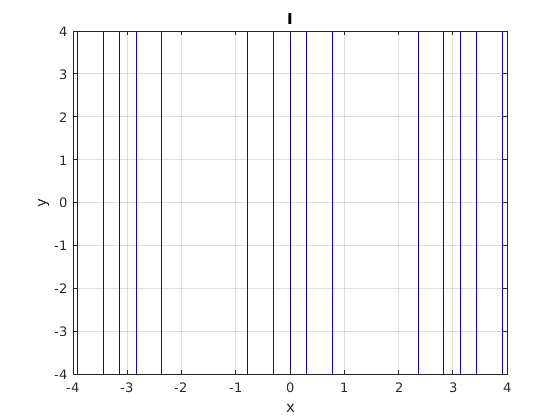
\includegraphics[width=8cm]{14_var_mult_fonct/question1a} \ 
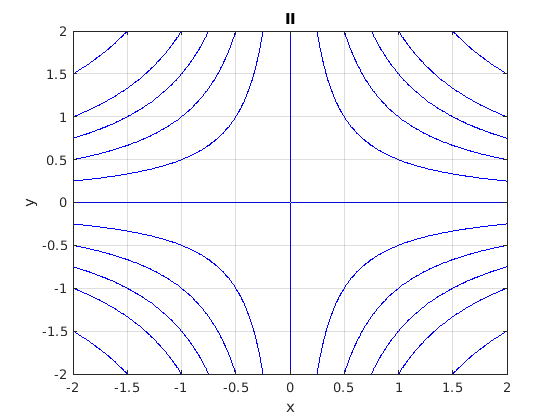
\includegraphics[width=8cm]{14_var_mult_fonct/question1b}

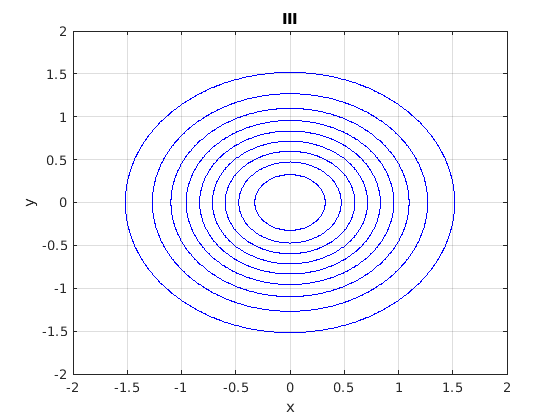
\includegraphics[width=8cm]{14_var_mult_fonct/question1c} \ 
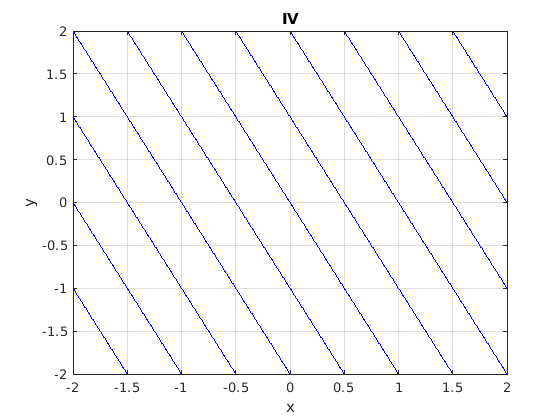
\includegraphics[width=8cm]{14_var_mult_fonct/question1d}

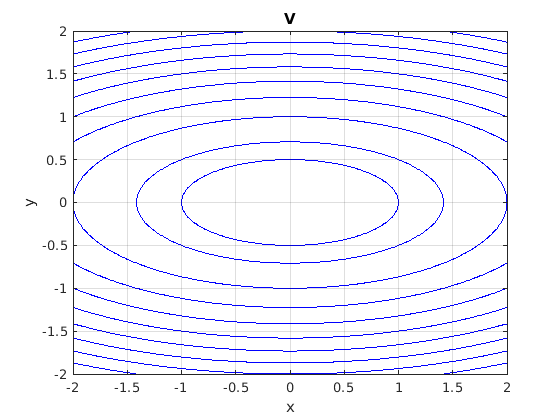
\includegraphics[width=8cm]{14_var_mult_fonct/question1e}
\label{14Q3}
\end{question}

\begin{question}
Trouvez l'équation de plan qui a le diagramme de courbes de niveau
donné ci-dessous.
\MATHgraph{14_var_mult_fonct/question2}{8cm}
\label{14Q4}
\end{question}

\begin{question}
Trouvez l'équation de plan qui produit les données du tableau
suivant.
\begin{center}
\begin{tabular}{|c|c|c|c|}
\hline
$x \diagdown y$ & 10 & 20 & 30 \\
\hline
5 & -22 & -62 & -102 \\
\hline
10 & -7 & -47 & -87 \\
\hline
15 & 8 & -32 & -72 \\
\hline
\end{tabular}
\end{center}
\label{14Q5}
\end{question}

\begin{question}
Trouvez le domaine et l'image, et tracez quelques courbes de niveau
pour chacune des fonctions suivantes.
\begin{center}
\begin{tabular}{*{1}{l@{\hspace{0.5em}}l@{\hspace{6em}}}l@{\hspace{0.5em}}l}
\subQ{a} & $\displaystyle f(x,y) = \ln(1-x^2-2y^2)$ &
\subQ{b} & $\displaystyle f(x,y) = \sqrt{x^2-y^2}$
\end{tabular}
\end{center}
\label{14Q6}
\end{question}

\begin{question}
Dessinez quelques courbes de niveau de la fonction 
\[
f(x,y) = \frac{1}{1+x^2+y^2}
\]
et utilisez ces courbes pour tracer le graphe de la fonction.
\label{14Q7}
\end{question}

\subsection{Fonctions  continues}

\begin{question}
Est-ce que la fonction suivante est continue au point $(0,0)$?
\[
f(x,y) = \begin{cases}
\displaystyle \frac{x\sqrt{y}}{x^2+y} & \text{si}\quad (x,y)\neq (0,0) \\
0 & \text{si}\quad (x,y) = (0,0)
\end{cases}
\]
Justifiez votre réponse.
\label{14Q8}
\end{question}




%%% Local Variables: 
%%% mode: latex
%%% TeX-master: "notes"
%%% End: 

\cleardoublepage

\chapter[Dérivée de fonctions de plusieurs variables \life \eng]{Dérivée de fonctions de plusieurs variables\\ \life \eng}
\label{chapDerFonctMult}

\compileTHEO{

Nous commençons par prolonger aux fonctions de plusieurs variables à valeurs
réelles la notion de dérivée que nous avons vu pour les fonctions d'une
variable.  La seconde étape consiste à étudier la dérivée d'une fonction de
plusieurs variables selon une direction donnée.  Nous verrons que le
{\em gradient} peut jouer une rôle important pour le calcul des
dérivées selon une direction donnée.  Nous profiterons de l'occasion pour
présenter quelques applications utiles du gradient.

Comme nous avons fait pour les fonctions d'une variable, nous étudierons
l'approximation locale des fonctions de plusieurs variables et les
points critiques des fonctions de plusieurs variables dans le but de
pouvoir déterminer les valeurs extrêmes de ces fonctions avec ou sans
contraintes.  Nous terminons le chapitre avec la dérivée d'une fonction de
$\RR^n$ dans $\RR^m$ où $m$ et $n$ sont plus grand que $1$.

\section{Dérivées partielles}

Pour les prochaines sections, nous allons seulement considérer les fonctions
à valeurs réelles.  De plus, sans perte de généralité, nous assumons que les
fonctions sont des fonctions de deux variables seulement.  Sauf pour une
légère modification des énoncés, entre autre remplacer $(x_1,x_2)$ par
$(x_1,x_2,\ldots, x_n)$, les définitions et résultats sur les fonctions de
deux variables que nous présentons demeurent valides pour les fonctions de
plus de deux variables.

\begin{focus}{\dfn} \index{Dérivée partielle en un point}
Soit $D$ un voisinage d'un point $\VEC{c} = (c_1,c_2) \in \RR^2$ et
$f:D\rightarrow \RR$ une fonction à valeurs réelles.

La {\bfseries dérivée partielle de $f$ au point $\VEC{c}$ par rapport à la
variable $x_1$} est définie par
\[
f_{x_1}(\VEC{c}) = f_{x_1}(c_1,c_2) 
= \pdydx{f}{x_1}(c_1,c_2)
= \lim_{h\rightarrow 0}\frac{f(c_1+h,c_2)-f(c_1,c_2)}{h}
\]
si cette limite existe.

La {\bfseries dérivée partielle de $f$ au point $\VEC{c}$ par rapport à la
variable $x_2$} est définie par
\[
f_{x_2}(\VEC{c}) = f_{x_2}(c_1,c_2) 
= \pdydx{f}{x_2}(c_1,c_2)
= \lim_{h\rightarrow 0}\frac{f(c_1,c_2+h)-f(c_1,c_2)}{h}
\]
si cette limite existe.

Dans les limites précédentes, nous assumons que $h$ est assez petit pour que
$(c_1+h,c_2)$ et $(c_1,c_2+h)$ soient dans $V$ et donc que $f$ soit définie à
ces points.
\end{focus}

Comme pour les fonctions d'une variable, si nous considérons tous les points où
la dérivée partielle d'une fonction $f$ existe, nous pouvons définir
une fonction que nous appellerons la dérivée partielle de la fonction $f$.

\begin{focus}{\dfn} \index{Dérivée partielle}
Soit $V\subset \RR^2$ un ensemble ouvert et $f:\RR^2 \rightarrow \RR$.  Si
la dérivée partielle de $f$ par rapport à $x_1$ existe en tout point de $V$,
la {\bfseries dérivée partielle de $f$ par rapport à $x_1$ sur $V$} est la
fonction définie par
\[
f_{x_1}(\VEC{x}) = f_{x_1}(x_1,x_2) 
= \pdydx{f}{x_1}(x_1,x_2)
= \lim_{h\rightarrow 0}\frac{f(x_1+h,x_2)-f(x_1,x_2)}{h}
\]
pour tout $\VEC{x}\in V$.  C'est une nouvelle fonction de deux variables
définie sur $V$.

De même, si la dérivée partielle de $f$ par rapport à $x_2$ existe en tout
point de $V$, la {\bfseries dérivée partielle de $f$ par rapport à $x_2$ sur
$V$} est la fonction définie par
\[
f_{x_2}(\VEC{x}) = f_{x_2}(x_1,x_2) 
= \pdydx{f}{x_2}(x_1,x_2)
= \lim_{h\rightarrow 0}\frac{f(x_1,x_2+h)-f(x_1,x_2)}{h}
\]
pour tout $\VEC{x}\in V$.  C'est une nouvelle fonction de deux variables
définie sur $V$.
\end{focus}

Puisque $x_2$ est fixe dans la définition de la dérivée partielle
$\displaystyle \pdydx{f}{x_1}(x_1,x_2)$, cette dérivée partielle est la
dérivée d'une fonction d'une seule variable, $x_1$, qui dépend d'un
paramètre, $x_2$.  De même, $\displaystyle \pdydx{f}{x_2}(x_1,x_2)$ est
la dérivée d'une fonction d'une seule variable, $x_2$, qui dépend d'un
paramètre, $x_1$.  Donc toutes les règles de dérivation pour les
fonctions d'une variable sont valides si nous traitons comme une constante
la variable qui n'est pas la variable de dérivation.

\begin{egg}
Si $f(x,y) = \sin(y-x)$ alors
\[
\pdydx{f}{x}(x,y) =
\left(\dfdx{\sin(u)}{u}\bigg|_{u=y-x}\right)
\left(\pdfdx{(y-x)}{x} \right)
= \cos(y-x)\,(-1) = -\cos(y-x)
\]
grâce à la règle de dérivation des fonctions composées. De plus,
\[
\pdydx{f}{y}(x,y) =
\left(\dfdx{\sin(u)}{u}\bigg|_{u=y-x}\right)
\left(\pdfdx{(y-x)}{y} \right)
= \cos(y-x)\,(1) = \cos(y-x) \; .
\]
En particulier,
\[
\pdydx{f}{x}(2,4) = -\cos(4-2) = -\cos(2) \; .
\]
\end{egg}

\begin{egg}
Si $f(x,y) = (3xy^2-x^4+1)^4$ alors
\begin{align*}
\pdydx{f}{x}(x,y) &=
\left( \dfdx{u^4}{u} \bigg|_{u=3xy^2 -x^4 +1}\right)
\left( \pdfdx{(3xy^2-x^4+1)}{x} \right)
= 4 (3xy^2-x^4+1)^3 \, (3y^2-4x^3)
\intertext{et}
\pdydx{f}{y}(x,y) &=
\left( \dfdx{u^4}{u} \bigg|_{u=3xy^2 -x^4 +1}\right)
\left( \pdfdx{(3xy^2-x^4+1)}{y} \right)
= 4 (3xy^2-x^4+1)^3 \,(6xy) \; .
\end{align*}
\end{egg}

Par induction, nous pouvons définir des dérivées partielles d'ordre deux.

\begin{focus}{\dfn} \index{Dérivée partielle!d'ordre supérieure}
Soit $V\subset \RR^2$ un ensemble ouvert et $f:V\rightarrow \RR$ une
fonction qui possède des dérivées partielles d'ordre un sur $V$.  Les
{\bfseries dérivées partielles d'ordre deux de $f$ sur $V$} sont définies par
\begin{align*}
f_{x_1x_1}(x_1,x_2) &= \pdydxn{f}{x_1}{2}(x_1,x_2) =
\pdfdx{\left(\pdydx{f}{x_1}\right)}{x_1}(x_1,x_2) \; , \\
f_{x_2x_2}(x_1,x_2) &= \pdydxn{f}{x_2}{2}(x_1,x_2) =
\pdfdx{\left(\pdydx{f}{x_2}\right)}{x_2}(x_1,x_2) \; , \\
f_{x_1x_2}(x_1,x_2) &= \pdydxnm{f}{x_1}{x_2}{2}{}{}(x_1,x_2) =
\pdfdx{\left(\pdydx{f}{x_2}\right)}{x_1}(x_1,x_2)
\intertext{et}
f_{x_2x_1}(x_1,x_2) &= \pdydxnm{f}{x_2}{x_1}{2}{}{}(x_1,x_2) =
\pdfdx{\left(\pdydx{f}{x_1}\right)}{x_2}(x_1,x_2)
\end{align*}
si toutes ces dérivées partielles (d'ordre un) existent sur $V$.
\end{focus}

Nous pourrions aussi définir des dérivées partielles d'ordre supérieure à
deux.  Par exemple, nous pouvons définir des dérivées partielles
d'autre trois pour la fonction $f:V \rightarrow \RR$ de la
définition précédente.  Une de ces dérivées partielles est
\[
f_{x_2x_2x_1}(x_1,x_2) = \pdydxnm{f}{x_2}{x_1}{3}{2}{}(x_1,x_2) =
\pdfdx{\left(\pdydxnm{f}{x_2}{x_1}{2}{}{}\right)}{x_2}(x_1,x_2) \; .
\]
si toutes les dérivées d'ordre un et deux existent pour tout
$(x_1,x_2) \in V$.

\begin{focus}{\dfn} \index{Fonction de classe $C^k$}
Soit $V\subset \RR^n$ un ensemble ouvert et $f:V\rightarrow \RR$.  Nous
disons que $f$ est de classe $C^k$ si les dérivées partielles d'ordre $k$ de
$f$ existent et sont continues.  Nous écrivons $f \in C^k(V)$
\end{focus}

Si $f \in C^k(V)$, le fait que les dérivées partielles d'ordre $k$ de
$f$ existent implique que toutes les dérivées partielles de $f$ d'ordre
inférieure à $k$ existent et sont aussi {\em continues}.

\begin{egg}
Soit $f(x,y) = \cos(5x+3y)$.  Alors
\begin{align*}
\pdfdx{f}{x}(x,y) &= -5\,\sin(5x+3y) \; , \\
\pdfdx{f}{y}(x,y) &= -3\,\sin(5x+3y) \; , \\
\pdfdxn{f}{x}{2}(x,y)
& = \pdfdx{\left(-5\,\sin(5x+3y)\right)}{x} = -25\cos(5x+3y)\; , \\
\pdfdxn{f}{y}{2}(x,y)
&= \pdfdx{\left(-3\,\sin(5x+3y)\right)}{y} = -9\cos(5x+3y) \; ,\\
\pdfdxnm{f}{x}{y}{2}{}{}(x,y)
&= \pdfdx{\left(-3\,\sin(5x+3y)\right)}{x} = -15\cos(5x+3y)
\intertext{et}
\pdfdxnm{f}{y}{x}{2}{}{}(x,y)
&= \pdfdx{\left(-5\,\sin(5x+3y)\right)}{y} = -15\cos(5x+3y) \; .
\end{align*}
\end{egg}

À l'exemple précédent, nous avons que $f_{xy}=f_{yx}$.  Ce n'est pas
toujours le cas mais il y a une très grande classe de fonctions $f$ pour
lesquelles $f_{xy}=f_{yx}$,

\begin{focus}{\prp}
Si $f:\RR^2\rightarrow \RR$ possède des dérivées partielles d'ordre deux qui
sont continues, alors $f_{x_1x_2} = f_{x_2x_1}$.
\end{focus}

\begin{rmk}
Nous pourrions généraliser la proposition précédente.  Si
$f:\RR^2 \to \RR$ possède des dérivées partielles d'ordre trois qui
sont continues, alors $f_{x_1x_2x_2}= f_{x_2x_1x_2} = f_{x_2x_2x_1}$ et
$f_{x_1x_1x_2}= f_{x_1x_2x_1} = f_{x_2x_1x_1}$.  Nous pourrions aussi
généraliser la proposition à $f:\RR^n \to \RR$ avec $n>2$.
\end{rmk}

\begin{egg}
Montrons que les fonctions suivantes satisfont l'équation des ondes
$u_{tt} = a^2\,u_{xx}$ où $a$ et $k$ sont des constantes.

\subQ{a} Si
\[
u(x,t) = \sin(k\,x)\sin(ak\,t) =
\frac{1}{2}\left( \cos(k\,x -ak\, t)-\cos(k\,x + ak\, t)\right) \ ,
\]
alors
\begin{align*}
u_{tt} &= \pdfdx{\left(\pdfdx{u}{t}(t,x)\right)}{t}
= \pdfdx{\big( ak\,\sin(k\,x)\cos(ak\,t)\big)}{t}
= -a^2k^2\,\sin(k\,x)\sin(ak\,t)
\intertext{et}
u_{xx} &= \pdfdx{\left(\pdfdx{u}{x}(t,x)\right)}{x}
= \pdfdx{\big( k\,\cos(k\,x)\sin(ak\,t)\big)}{x}
= -k^2\,\sin(k\,x)\sin(ak\,t) \; .
\end{align*}
Ainsi,
\[
u_{tt} =  -a^2k^2\,\sin(k\,x)\sin(ak\,t) = a^2\,u_{xx} \; .
\]

\subQ{b} Si
\[
u(x,t) = \sin(x-a\,t) + \ln(x+a\,t) \ ,
\]
alors
\begin{align*}
u_{tt} &= \pdfdx{\left(\pdfdx{u}{t}(t,x)\right)}{t}
= \pdfdx{\left( -a\,\cos(x-a\,t) + \frac{a}{x+a\,t}\right)}{t}
= -a^2\,\sin(x-a\,t) - \frac{a^2}{(x+a\,t)^2}
\intertext{et}
u_{xx} &= \pdfdx{\left(\pdfdx{u}{x}(t,x)\right)}{x}
= \pdfdx{\left( \cos(x-a\,t) + \frac{1}{x+a\,t}\right)}{x}
= -\sin(x-a\,t) - \frac{1}{(x+a\,t)^2} \; .
\end{align*}
Ainsi,
\[
u_{tt} = -a^2\,\sin(x-a\,t) - \frac{a^2}{(x+a\,t)^2} = a^2\,u_{xx}  \; .
\]

\subQ{c} Si
\[
u(x,t) = f(x+at)+g(x-at)
\]
où $f$ et $g$ sont deux fonctions qui possèdent des dérivées d'ordre
deux, alors
\begin{align*}
u_{tt} &= \pdfdx{\left(\pdfdx{u}{t}(t,x)\right)}{t}
= \pdfdx{\left( a\,f'(x+at)-a\,g'(x-at) \right)}{t}
= a^2\,f''(x+at) + a^2 g''(x-at)
\intertext{et}
u_{xx} &= \pdfdx{\left(\pdfdx{u}{x}(t,x)\right)}{x}
= \pdfdx{\left( f'(x+at)+ g'(x-at) \right)}{x}
= f''(x+at)+ g''(x-at) \; .
\end{align*}
Ainsi,
\[
u_{tt}  = a^2\,f''(x+at)+ a^2\,g''(x-at) = a^2\,u_{xx} \; .
\]
\end{egg}

La règle pour dériver la composition de fonctions d'une variable peut être
utilisée pour dériver la composition de fonctions de plusieurs variables.

\begin{focus}{\prp} \label{ChainRuleND}
Soit $f:\RR^n\rightarrow \RR$ et $g:\RR^m \to \RR^n$.  Si $f$ et 
$g_i:\RR^m\rightarrow \RR$ pour $i=1$, $2$, \ldots, $n$ possèdent des
dérivées partielles, alors la fonction $h:\RR^m\rightarrow \RR$
définie par $h = f \circ g :\RR^m \to \RR$ possède aussi des dérivées
partielles.  Plus précisément,
\begin{align*}
\pdydx{h}{t_i}(\VEC{t})
& = \sum_{k=1}^n \pdydx{f}{x_k}(g(\VEC{t}))\,\pdydx{g_k}{t_i}(\VEC{t}) \\
& = \pdydx{f}{x_1}(g(\VEC{t}))\,\pdydx{g_1}{t_i}(\VEC{t})
+ \pdydx{f}{x_2}(g(\VEC{t}))\,\pdydx{g_2}{t_i}(\VEC{t}) + \ldots
+ \pdydx{f}{x_n}(g(\VEC{t}))\,\pdydx{g_n}{t_i}(\VEC{t})
\end{align*}
pour $\VEC{t} \in \RR^m$ et $1\leq i \leq m$.
\end{focus}

\begin{rmkList}
\begin{enumerate}
\item Cette proposition a déjà été utilisé pour $n=1$ et $m=2$ dans
plusieurs exemples précédents.
\item Un cas important de la proposition précédente est lorsque $m=1$.
Nous avons alors la formule
\begin{equation}\label{specialCR}
\dydx{h}{t}(t) = \pdydx{f}{x_1}(g(t))\,\dydx{g_1}{t}(t)
+ \pdydx{f}{x_2}(g(t))\,\dydx{g_2}{t}(t) + \ldots
+ \pdydx{f}{x_n}(g(t))\,\dydx{g_n}{t}(t)
\end{equation}
pour $t \in \RR$.
\end{enumerate}
\end{rmkList}

\begin{egg}
Soit $z=e^x\cos(y)$, $x=t^2$ et $y=\sin(t)$, évaluons
$\displaystyle \dydx{z}{t}$.

La notation $\displaystyle \dydx{z}{t}$ peut porter à confusion car
$z$ n'est pas explicitement une fonction de $t$.  Soit
$\rho_1(t) = t^2$, $\rho_2(t) = \sin(t)$, $f(x,y) = e^x\cos(y)$ et
$h(t) = f(\rho_1(t), \rho_2(t))$.   Il faut interpréter 
$\displaystyle \dydx{z}{t}$ comme étant
$\displaystyle \dydx{h}{t}$.

Ainsi,
\begin{align}
\dydx{h}{t}(t) &= \pdydx{f}{x}(\rho_1(t),\rho_2(t))\,\dydx{\rho_1}{t}(t) +
\pdydx{f}{y}(\rho_1(t),\rho_2(t)) \, \dydx{\rho_2}{t}(t) \label{ENGchain1} \\
&=\left(e^x\cos(y)\right)\bigg|_{x=t^2,y=\sin(t)}
\left(2t\right) + \left(-e^x\sin(y)\right)\bigg|_{x=t^2,y=\sin(t)}
\left(\cos(t)\right) \nonumber \\
&=2t\; e^{t^2}\cos(\sin(t) -e^{t^2} \sin(\sin(t))\cos(t) \; . \nonumber
\end{align}

Si nous posons
\begin{align*}
\dydx{z}{t} &= \dydx{h}{t}(t) \quad, \quad
\pdydx{z}{x} = \pdydx{f}{x}(\rho_1(t),\rho_2(t))\quad, \quad
\pdydx{z}{y} = \pdydx{f}{y}(\rho_1(t),\rho_2(t))\;,\\
\dydx{x}{t} &= \dydx{\rho_1}{t}(t)\quad
\text{et} \quad \dydx{y}{t} = \dydx{\rho_2}{t}(t) \; ,
\end{align*}
alors (\ref{ENGchain1}) peut s'exprimer
\[
\dydx{z}{t} = \pdydx{z}{x}\,\dydx{x}{t} + \pdydx{z}{y} \,
\dydx{y}{t} \, .
\]
Cette notation est souvent utilisé en mathématiques appliquées
(physique, génie, etc).
\end{egg}

\begin{egg}
Soit $z=\sin(x)\cos(y^2)$, $x=t^2 + s^2$ et $y=e^{st}$, évaluons
$\displaystyle \pdydx{z}{t}$ et $\displaystyle \pdydx{z}{s}$.

Comme à l'exemple précédent, la notation
$\displaystyle \pdydx{z}{t}$ et $\displaystyle \pdydx{z}{s}$
peut porter à confusion.  Soit $\rho_1(t,s) = t^2+s^2$,
$\rho_2(t,s) = e^{st}$, $f(x,y) = \sin(x)\cos(y^2)$
et $h(t,s) = f(\rho_1(t,s), \rho_2(t,s))$.  Les expressions
$\displaystyle \pdydx{z}{t}$ et $\displaystyle \pdydx{z}{s}$ 
représentent respectivement
$\displaystyle \pdydx{h}{t}$ et $\displaystyle \pdydx{h}{s}$.

Ainsi,
\begin{align}
\pdydx{h}{t}(t,s) &= \pdydx{f}{x}(\rho_1(t,s),\rho_2(t,s))\,
\pdydx{\rho_1}{t}(t,s) + \pdydx{f}{y}(\rho_1(t,s),\rho_2(t,s)) \,
\pdydx{\rho_2}{t}(t,s) \label{ENGchain2} \\
&=\left(\cos(x)\cos(y^2)\right)\bigg|_{x=t^2+s^2,y=e^{ts}}
\left(2t\right)
+ \left(-2y\sin(x)\sin(y^2)\right)\bigg|_{x=t^2+s^2,y=e^{st}}
\left(se^{st}\right)  \nonumber  \\
&= 2t\;\cos\left(t^2+s^2\right)\cos\left(e^{2st}\right)
-2se^{2st}\sin\left(t^2+s^2\right)\sin\left(e^{2st}\right) \nonumber
\end{align}
et
\begin{align}
\pdydx{h}{s}(t,s) &= \pdydx{f}{x}(\rho_1(t,s),\rho_2(t,s))\,
\pdydx{\rho_1}{s}(t,s) + \pdydx{f}{y}(\rho_1(t,s),\rho_2(t,s)) \,
\pdydx{\rho_2}{s}(t,s) \label{ENGchain3} \\
&=\left(\cos(x)\cos(y^2)\right)\bigg|_{x=t^2+s^2,y=e^{ts}}
\left(2s\right)
+ \left(-2y\sin(x)\sin(y^2)\right)\bigg|_{x=t^2+s^2,y=e^{st}}
\left(te^{st}\right) \nonumber \\
&=2s\;\cos\left(t^2+s^2\right)\cos\left(e^{2st}\right)
-2te^{2st}\sin\left(t^2+s^2\right)\sin\left(e^{2st}\right) \; . \nonumber
\end{align}

Si nous posons
\begin{align*}
\pdydx{z}{t} &= \dydx{h}{t}(t,s) \quad , \quad
\pdydx{z}{s} = \dydx{h}{s}(t,s) \quad , \quad
\pdydx{z}{x} = \pdydx{f}{x}(\rho_1(t,s),\rho_2(t,s)) \; \\
\pdydx{z}{y} &= \pdydx{f}{y}(\rho_1(t,s),\rho_2(t,s)) \quad , \quad
\pdydx{x}{t} = \pdydx{\rho_1}{t}(t,s)\quad , \quad
\pdydx{y}{t} = \pdydx{\rho_2}{t}(t,s) \; , \\
\pdydx{x}{s} &= \pdydx{\rho_1}{s}(t,s)\quad \text{et} \quad
\pdydx{y}{s} = \pdydx{\rho_2}{s}(t,s) \, ,
\end{align*}
alors (\ref{ENGchain2}) et (\ref{ENGchain3}) peuvent s'exprimer
respectivement
\[
\pdydx{z}{t} = \pdydx{z}{x}\,\pdydx{x}{t} + \pdydx{z}{y} \,
\pdydx{y}{t} 
\qquad \text{et} \qquad
\pdydx{z}{s} = \pdydx{z}{x}\,\pdydx{x}{s} + \pdydx{z}{y} \,
\pdydx{y}{s} \ .
\]
\end{egg}

\section{Plan tangent à une surface (forme explicite)}

\subsection{Surface donnée par une fonction de $x_1$ et $x_2$}

Soit $f:\RR^2\rightarrow \RR$ une fonction qui possède des dérivées
partielles et soit $D\subset \RR^2$ une région du plan.  L'ensemble
\[
S = \{ (x_1,x_2,f(x_1,x_2)) : (x_1,x_2) \in D \}
\]
définit une surface dans $\RR^3$ comme celle que nous retrouvons à la
figure~\ref{D3_GRAPH}.

Les dérivées partielles de $f$ au point $(a_1,a_2)\in D$ vont nous
permettre de trouver l'équation du plan tangent à la surface $S$ au
point $(a_1, a_2, f(a_1,a_2))$.

La courbe produite par l'intersection du plan $x_2=a_2$ avec la
surface $S$ est donnée par l'ensemble des points de la forme
$(x_1,a_2, f(x_1,a_2))$ (figure~\ref{PARTIALX}).  Une représentation
paramétrique de cette courbe est donnée par
\[
(x_1,x_2,x_3) = (\alpha, a_2, f(\alpha, a_2))
\]
pour tout $\alpha$ tel que $(\alpha,a_2)\in D$.  Un vecteur parallèle à la
droite tangente à cette courbe au point $(a_1,a_2,f(a_1,a_2))$ (et
donc parallèle au plan tangent à la surface $S$) est donnée par
\[
\VEC{v}_1 = \left( \dfdx{\ \alpha }{\alpha}\bigg|_{\alpha=a_1},
\dfdx{\ a_2 }{\alpha}\bigg|_{\alpha=a_1},
\dfdx{f(\alpha,a_2)}{\alpha}\bigg|_{\alpha=a_1} \right)
= \left(1,0, \pdydx{f}{x_1}(a_1,a_2) \right) \; .
\]

\PDFfig{15_var_mult_der/partialx}{Courbe produite par l'intersection d'une
surface et d'un plan où $x_2$ est constant}{Courbe produite par l'intersection
de la surface $x_3=f(x_1,x_2)$ et du plan $x_2=a_2$.}{PARTIALX}

% La représentation standard de la droite tangente à cette courbe au
% point $(a_1,a_2,f(a_1,a_2))$ est
% \[
% x_1 - a_1 = \frac{x_3 - f(a_1,a_2)}{f_{x_1}(a_1,a_2)} \quad , \quad x_2=a_2
% \]
% La première égalité provient de l'équation de la droite tangente à la
% courbe $x_3=f(x_1,a_2)$ lorsque $x_2=a_2$; c'est-à-dire
% $x_3-f(a_1,a_2) = f_{x_1}(a_1,a_2) (x_1-a_1)$.

La courbe produite par l'intersection du plan $x_1=a_1$ avec la
surface $S$ est donnée par l'ensemble des points de la forme
$(a_1, x_2, f(a_1,x_2))$ (figure~\ref{PARTIALY}).  Une représentation
paramétrique de cette courbe est donnée par
\[
(x_1,x_2,x_3) = (a_1, \beta, f(a_1, \beta))
\]
pour tout $\beta$ tel que $(a_1,\beta)\in D$.  Un vecteur parallèle à
la droite tangente à cette courbe au point $(a_1,a_2,f(a_1,a_2))$ (et donc
parallèle au plan tangent à la surface $S$) est donnée par
\[
\VEC{v}_2 = \left( \dfdx{\ a}{\beta}\bigg|_{\beta=a_2},
\dfdx{\ \beta }{\beta}\bigg|_{\beta=a_2},
\dfdx{f(a_1,\beta)}{\beta}\bigg|_{\beta=a_2} \right)
= \left(0,1, \pdydx{f}{x_2}(a_1,a_2) \right) \; .
\]

% La représentation standard de la droite tangente à cette courbe au
% point $(a_1,a_2,f(a_1,a_2))$ est
% \[
% x_2 - a_2 = \frac{x_3 - f(a_1,a_2)}{f_{x_2}(a_1,a_2)} \quad , \quad x_1=a_1
% \]
% La première égalité provient de l'équation de la droite tangente à la
% courbe $x_3=f(a_1,x_2)$ lorsque $x_2=a_2$; c'est-à-dire
% $x_3-f(a_1,a_2) = f_{x_2}(a_1,a_2) (x_2-a_2)$.

\PDFfig{15_var_mult_der/partialy}{Courbe produite par l'intersection d'une
surface et d'un plan où $x_1$ est constant}{Courbe produite par l'intersection
de la surface $x_3=f(x_1,x_2)$ et du plan $x_1=a_1$}{PARTIALY}

Un vecteur perpendiculaire au plan tangent $\Pi$ à la surface $S$ au point
$(a_1,a_2,f(a_1,a_2))$ (figure~\ref{PARTIALXY}) est donné par le produit
vectoriel de deux vecteurs non colinéaires et parallèles à ce plan.  C'est le
cas des vecteurs $\VEC{v}_1$ et $\VEC{v}_2$ que nous venons de définir.  Donc
le vecteur
\[
\VEC{n}= \VEC{v}_1 \times \VEC{v}_2
= 
\left(-\dydx{f}{x_1}(a_1,a_2), -\dydx{f}{x_2}(a_1,a_2), 1 \right)
\]
est perpendiculaire au plan $\Pi$.

L'équation du plan $\Pi$ tangent à la surface $S$
au point $(a,b,f(a,b))$ est
\begin{align*}
&\VEC{n} \cdot \big( (x_1,x_2,x_3)-(a_1,a_2,f(a_1,a_2)) \big)  \\
& \qquad \qquad = -\pdydx{f}{x_1}f(a_1,a_2) \left(x_1-a_1\right)
- \pdydx{f}{x_2}f(a_1,a_2) \left(x_2-a_2\right)
+ (x_3-f(a_1,a_2)) = 0 \ .
\end{align*}
L'équation du plan tangent à la surface $S$ au point
$(a_1,a_2,f(a_1,a_2))$ est souvent présentée sous la forme
\begin{equation}\label{planTANG}
x_3 = f(a_1,a_2) + \pdydx{f}{x_1}(a_1,a_2) \, \left(x_1-a_1\right)
+ \pdydx{f}{x_2}(a_1,a_2) \, \left(x_2-a_2\right) \ .
\end{equation}

\PDFfig{15_var_mult_der/partialxy}{Plan tangent à la surface
$x_3=f(x_1,x_2)$ en un point $(a_1,a_2,f(a_1,a_2))$}{Plan tangent à la
surface $S$ au point $(a_1,a_2,f(a_1,a_2))$. 
Les vecteurs $\VEC{v}_1$ et $\VEC{v}_2$ sont parallèles au plan $\Pi$ et
$\VEC{n}$ est perpendiculaire au plan $\Pi$.  Pour illustrer la relation
entre les vecteurs $\VEC{v}_1$, $\VEC{v}_2$, $\VEC{n}$ et le plan
$\Pi$, ces vecteurs sont tracés à partir du point $(a_1,a_2,f(a_1,a_2))$.
Normalement, ces vecteurs devraient partir de l'origine.}{PARTIALXY}

\begin{egg}
Trouvons l'équation du plan tangent à la surface décrite par
$z=x\sin(x^2\, y)$ au point $(1,\pi/2,1)$.

L'équation du plan tangent est donnée par (\ref{planTANG}) où
$f(x,y)=x\sin(x^2\,y)$, $a=1$, $b=\pi/2$ et $f(a,b) = \sin(\pi/2) =1$.
Puisque
\[
\pdydx{f}{x} = \sin(x^2\,y) + 2x^2\, y\,\cos(x^2\,y)
\quad \text{et} \quad
\pdydx{f}{y} = x^3\,\cos(x^2\,y) \ ,
\]
nous obtenons
\[
\pdydx{f}{x}(1,\pi/2) = \sin(\pi/2) + \pi \cos(\pi/2) = 1
\quad  \text{et} \quad
\pdydx{f}{y}(1,\pi/2) = \cos(\pi/2) =0 \ ,
\]
Ainsi, l'équation du plan tangent est
\[
z = f(1,\pi) + \pdydx{f}{x}(1,\pi) \, (x - 1)
+ \pdydx{f}{y}(1,\pi) \, (y - \pi)
= 1 + (x-1) = x \ .
\]
\end{egg}
% Même question pour $f(x,y) = (x^3-y^3)/(x^2+y^2)$ et $(1,1,0)$

\begin{egg}
Trouvons l'équation du plan tangent au point
$\VEC{p} = (1,2,\sqrt{2})$ de l'ellipsoïde
$\displaystyle \frac{x^2}{3} + \frac{y^2}{9} + \frac{z^2}{9} = 1$.

Si, dans l'équation de l'ellipsoïde, nous assumons que $z$ est une fonction de
$x$ et $y$, et nous dérivons implicitement cette équation par rapport à $x$ et
par rapport à $y$, nous obtenons
\[
\frac{2}{3}\,x + \frac{2}{9}\,z\,\pdydx{z}{x} = 0
\Rightarrow \pdydx{z}{x} = -\frac{3x}{z}
\qquad \text{et} \qquad
\frac{2}{9}\,y + \frac{2}{9} \,z \, \pdydx{z}{y} = 0
\Rightarrow \pdydx{z}{y} = -\frac{y}{z} \; .
\]
Ainsi,
\[
\pdydx{z}{x}(1,2) = -\frac{3}{\sqrt{2}} \quad \text{et} \quad
\pdydx{z}{y}(1,2) = -\frac{2}{\sqrt{2}} \; .
\]
L'équation du plan tangent est
\[
z = \sqrt{2} -\frac{3}{\sqrt{2}}\,(x-1)
- \frac{2}{\sqrt{2}}\,(y-2) \; .
\]

Nous aurions pu représenter localement l'ellipse au voisinage du point
$\VEC{p}$ par
\[
  z = f(x,y) = 3 \sqrt{1 - \frac{x^2}{3} - \frac{y^2}{9}}
\]
et utiliser la formule (\ref{planTANG}) pour trouver l'équation du
plan tangent au point $\VEC{p}$ de l'ellipse.
\label{TPellipsoide}
\end{egg}

\subsection{Surface donnée par une représentation paramétrique}

Ce ne sont pas toutes les surfaces qui sont décrite par l'image d'une
fonction $f:\RR^2 \to \RR$.  Il suffit de penser à la sphère ou au
taure.  Ce genre de surface possède une représentation
paramétrique.

\begin{focus}{\dfn} \index{Représentation paramétrique d'une surface}
Une fonction $\rho :\RR^2 \to \RR^3$ est la représentation
paramétrique d'une surface $S$ dans $\RR^3$ si:
\begin{enumerate}
\item $\rho_i$ est de classe $C^1$ pour $i=1$, $2$ et $3$.
\item $\displaystyle \pdydx{\rho}{u_1}(u_1,u_2)$ et
$\displaystyle \pdydx{\rho}{u_2}(u_1,u_2)$ sont deux vecteurs
non colinéaires dans $\RR^3$ pour tout $(u_1,u_2)$. 
\end{enumerate}
\end{focus}

La deuxième condition est requise pour assurer qu'il y a un vecteur
normal (perpendiculaire) à la surface $S$ en tout point $\rho(u_1,u_2)$
de la surface.  Nous pouvons vérifier, comme cela a été fait à la
section~\ref{DTcourbe} pour la représentation paramétrique des
courbes, que les vecteurs
\begin{align*}
\VEC{w}_1 &= \pdydx{\rho}{u_1}(a_1,a_2)
    = \left(\pdydx{\rho_1}{u_1}(a_1,a_2), \pdydx{\rho_2}{u_1}(a_1,a_2),
      \pdydx{\rho_3}{u_1}(a_1,a_2) \right) 
\intertext{et}
\VEC{w}_2 &= \pdydx{\rho}{u_2}(a_1,a_2)
    = \left(\pdydx{\rho_1}{u_2}(a_1,a_2), \pdydx{\rho_2}{u_2}(a_1,a_2),
      \pdydx{\rho_3}{u_2}(a_1,a_2) \right) 
\end{align*}
sont tangent à la surface $S$ au point $\rho(a_1,a_2) \in S$.  Ainsi,
$\VEC{m} = \VEC{w}_1 \times \VEC{w}_2$ est un vecteur normal à la
surface $S$ au point $\rho(a_1,a_2)$ de la surface.  Notons que
$\VEC{m} \neq \VEC{0}$ car $\VEC{w}_1$ et $\VEC{w}_2$ ne sont pas
colinéaires.

\begin{egg}
Cherchons le plan tangent à la surface $S$ donnée par la
représentation paramétrique
$\rho(u,v) = \left( u+v, u\sin(v), v \cos(u) \right)$ au point
$(2\pi,0,-\pi)$.

Notons premièrement que $\rho(u,v) = (2\pi,0,-\pi)$ si et seulement
si $(u,v) =(\pi.\pi)$.  En effet, $u\sin(v) = 0$ est vrai si $u=0$ ou
$v = n\pi$ pour $n \in \ZZ$.  Il découle de $u+v=2\pi$
que $(u,v) = (0,2\pi)$ et $(u,v) = (2\pi - n\pi,n \pi)$ sont les
seules solutions possibles.  Si $(u,v) = (0,2\pi)$, alors
$v \cos(u) = 2\pi \neq -\pi$.  Donc $(u,v) = (0,2\pi)$
est exclus.  Si $(u,v) = (2\pi - n\pi,n \pi)$, alors
$v \cos(u) = n \pi \cos(2\pi -n\pi) = (-1)^n n\pi$ et il faut choisir
$n=1$ pour avoir $v \cos(u) = -\pi$.  Donc
$(u,v) =(\pi.\pi)$ est la seule solution.

Pour trouver un vecteur normal $\VEC{m}$ à la surface $S$ au point
$(2\pi,0,\pi)$, nous utilisons les vecteurs
\begin{align*}
\VEC{w}_1 &= \pdydx{\rho}{u}(\pi,\pi)
= \left(1, \sin(v) , -v\sin(u)\right)\bigg|_{(u,v) = (\pi,\pi)}
= (1, 0, 0) \\
\intertext{et}
\VEC{w}_2 &= \pdydx{\rho}{v}(\pi,\pi)
= \left( 1, u\cos(v), \cos(u) \right)\bigg|_{(u,v) = (\pi,\pi)}
= (1,-\pi, -1) \ .
\end{align*}
Nous trouvons
\[
  \VEC{m} = \VEC{w}_1 \times \VEC{w}_2
= \begin{pmatrix}
\ii & \jj & \kk \\
1 & 0 & 0 \\
1 & -\pi & -1
\end{pmatrix} = 0 \ii + \jj - \pi \kk = (0, 1, -\pi)
\]
si nous développons le déterminant selon la première ligne.
Ainsi, l'équation du plan tangent à la surface $S$ au point
$(2\pi,0,-\pi)$ est donnée par
\[
  \VEC{m} \cdot (x_1-2\pi,x_2,x_3+\pi) = x_2 - \pi (x_3+\pi) = 0 \ .
\]
\end{egg}

\section{Dérivées selon une direction donnée \eng}

Si nous regardons les figures~\ref{PARTIALX} et \ref{PARTIALY}, nous
remarquons que le calcul des dérivées partielles assume que le
déplacement ce fait seulement selon une direction parallèle à l'axe
des $x_1$ ou à l'axe des $x_2$.  Il n'y a aucune raison de se limité à ces
deux seules directions.

En fait, il est très utile de définir des dérivées selon d'autres
directions.

\begin{focus}{\dfn} \index{Dérivée directionnelle}
Soit $V\subset \RR^n$ un ensemble ouvert et $f:V\rightarrow \RR$ une
fonction a valeurs réelles.  Soit 
$\VEC{u} \in \RR^n$ un vecteur de longueur euclidienne $1$.  La
{\bfseries dérivée de $f$ selon la direction $\VEC{u}$ au point
$\VEC{a} \in V$}, que nous dénotons
$\displaystyle \pdydx{f}{\VEC{u}}(\VEC{a})$, est définie par
\[
\pdydx{f}{\VEC{u}}(\VEC{a}) =
\lim_{h\rightarrow 0} \frac{1}{h}\left(f(\VEC{a}+h\VEC{u})-f(\VEC{a})\right)
\]
si cette limite existe.  Dans la limite précédente, nous assumons que
$h$ est assez petit pour que $\VEC{a}+h\VEC{u} \in V$ et ainsi que $f$
soit définie à $\VEC{a}+h\VEC{u}$.
\end{focus}

Nous pouvons donner une interprétation graphique de la dérivée selon une
direction semblable à celle que nous connaissons pour la dérivée d'une
fonction d'une seule variable.  Les figures~\ref{DIRDER1} et
\ref{DIRDER2} fournissent cette interprétation pour les fonctions de
deux variables.

Soit $\Pi$ le plan qui est parallèle au vecteur $(u_1,u_2,0)$ et à
l'axe des $x_3$, et qui contient le point $(a_1,a_2,f(a_1,a_2))$.
Soit $\Gamma$ la courbe donnée par l'intersection du plan $\Pi$ et de
la surface $x_3 = f(x_1,x_2)$.  La sécante à la courbe $\Gamma$ qui
passe par les points $(a_1,a_2,f(a_1,a_2))$
et $(a_1+h\,u_1,a_2+h\,u_2,f(a_1+h\,u_1,a_2+h\,u_2))$ (figure~\ref{DIRDER1})
est contenue dans le plan $\Pi$ et sa pente est
\[
\frac{1}{h}\left(f(\VEC{a}+h\VEC{u})-f(\VEC{a})\right) \; ,
\]
où $\VEC{u}=(u_1,u_2)$, $\VEC{a}=(a_1,a_2)$ et
$\VEC{a}+h\VEC{u} = (a_1+h\,u_1,a_2+h\,u_2)$.
À la limite, lorsque $h$ tend vers $0$, nous obtenons la pente de la
droite tangente à la courbe $\Gamma$ au point $(a_1,a_2,f(a_1,a_2))$
(figure~\ref{DIRDER2}).  La tangent est aussi contenue dans le plan $\Pi$.

\PDFfig{15_var_mult_der/dirder}{Représentation graphique de la
définition de la dérivée dans la direction d'un vecteur}{La sécante
à la courbe $\Gamma$ qui passe par les points $(a_1,a_2,f(a_1,a_2))$ et
$(a_1+h\,u_1,a_2+h\,u_2,f(a_1+h\,u_1,a_2+h\,u_2))$.  Le plan $\Pi$ est
parallèle au vecteur $(u_1,u_2,0))$ et à l'axe des $z$, et contient le
point $(a_1,a_2,f(a_1,a_2))$.}{DIRDER1}

\PDFfig{15_var_mult_der/dirder2}{La tangente à la courbe d'intersection d'un
plan et d'une surface}{La tangente à la courbe $\Gamma$ au point
$(a_1,a_2,f(a_1,a_2))$.}{DIRDER2}

\begin{egg}
Calculons la dérivée de la fonction $f(x,y) = xy/(x^2+y^2)$ selon la
direction $(1,1)$ au point $(1,0)$.

Remarquons que le vecteur $(1,1)$ n'est pas de longueur $1$.  C'est un abus
de langage qui est très commun dans la littérature scientifique.  Il faut
alors comprendre que nous demandons de calculer la dérivée selon la direction
d'un vecteur $\VEC{u}$ de longueur $1$ qui pointe dans la même direction que
le vecteur donné.

Le vecteur $\VEC{u} = (1/\sqrt{2},1/\sqrt{2})$ pointe dans la
même direction que le vecteur $(1,1)$ et ait de longueur $1$.  Nous
calculons la dérivée de $f$ au point $(1,0)$ selon la direction $\VEC{u}$.

Posons $\VEC{a} = (1,0)$, alors
\[
\VEC{a}+h\VEC{u} = (1,0)+h(1/\sqrt{2},1/\sqrt{2}) =
(1+h/\sqrt{2},1/\sqrt{2})
\]
et 
\begin{align*}
\pdydx{f}{\VEC{u}}(1,0) &=
\lim_{h\rightarrow 0} \frac{f(\VEC{a}+h\VEC{u}) - f(\VEC{a})}{h} 
= \lim_{h\rightarrow 0} \frac{f(1+h/\sqrt{2},h/\sqrt{2})-f(1,0)}{h} \\
&= \lim_{h\rightarrow 0} \frac{1}{h}
\left(\frac{(1+h/\sqrt{2})\,(h/\sqrt{2})}
{(1+h/\sqrt{2})^2 +(h/\sqrt{2})^2} \right)
= \lim_{h\rightarrow 0} \frac{1/\sqrt{2}+h/2} {h^2+h\sqrt{2}+1}
= \frac{1}{\sqrt{2}} \; .
\end{align*}
\end{egg}

Calculer la dérivée selon une direction donnée à partir de la définition
n'est généralement pas simple.  Nous pouvons utiliser notre
connaissance des dérivées partielles pour calculer la dérivée selon
une direction donnée.

Soit $\VEC{u} = (u_1,u_2, \ldots, u_n)$ un vecteur de longueur $1$ dans
$\RR^n$ et $\VEC{a}=(a_1,a_2,\ldots,a_n)$ un vecteur de $\RR^n$. De plus,
soit $\RR^n:D\rightarrow \RR$ une fonction qui possède des dérivées
partielles.
Posons $g(t) = f(a_1+t\,u_1,a_2+t\,u_2, \ldots, a_n + t\, u_n)$. 
À l'aide des règles de dérivation de fonctions composées, en
particulier (\ref{specialCR}), nous obtenons
\begin{align*}
g'(t) &= \pdydx{f}{x_1}(a_1+t\,u_1,a_2+t\,u_2, \ldots, a_n + t\,u_n)\;u_1 \\
&+ \pdydx{f}{x_2}(a_1+t\,u_1,a_2+t\,u_2, \ldots, a_n + t\,u_n)\;u_2 + \ldots \\
&+ \pdydx{f}{x_n}(a_1+t\,u_1,a_2+t\,u_2, \ldots, a_n + t\,u_n)\;u_n \; .
\end{align*}
Mais, par définition
\begin{align*}
g'(0) &= \lim_{h\rightarrow 0} \frac{g(h)-g(0)}{h}
= \lim_{h\rightarrow 0}
\frac{f(a_1+h\,u_1,a_2+h\,u_2, \ldots, a_n + h\, u_n)
- f(a_1,a_2, \ldots, a_n)}{h} \\
&= \pdydx{f}{\VEC{u}}(a_1,a_2, \ldots, a_n) \; .
\end{align*}
Donc
\[
\pdydx{f}{\VEC{u}}(\VEC{a}) = g'(0)
= \pdydx{f}{x_1}(\VEC{a})\;u_1 +
\pdydx{f}{x_2}(\VEC{a})\;u_2 +
\ldots + \pdydx{f}{x_n}(\VEC{a})\;u_n \; .
\]
Nous obtenons donc le résultat suivant.

\begin{focus}{\prp} \index{Gradient}
Soit $V\subset \RR^n$ un ensemble ouvert et $f:V\rightarrow \RR$ une
fonction a valeurs réelles.  Posons
\begin{equation}\label{gradient}
\nabla f(\VEC{a}) = \left(\pdydx{f}{x_1}(\VEC{a}),
\pdydx{f}{x_2}(\VEC{a}), \ldots, \pdydx{f}{x_n}(\VEC{a}) \right)
\end{equation}
pour $\VEC{a} \in V$.  Nous avons que
\begin{equation}\label{dirderGrad}
\pdydx{f}{\VEC{u}}(\VEC{a}) =
\nabla f(\VEC{a}) \cdot \VEC{u} \; .
\end{equation}
$\nabla f(\VEC{a})$ est appelé le {\bfseries gradient} de $f$ au point
$\VEC{a}$.
\end{focus}

\begin{rmk}
Pour être consistant avec la représentation algébrique des vecteurs (i.e. un
vecteur est une matrice de dimension \nm{n}{1}), nous devrions définir le
gradient de $f$ à $\displaystyle \VEC{a} = \begin{pmatrix}
a_1 & a_2 & \cdots & a_n \end{pmatrix}^\top$ comme la matrice de dimension
\nm{1}{n}
\[
\nabla f(\VEC{a}) =
\begin{pmatrix}\displaystyle \pdydx{f}{x_1}(\VEC{a}) &
\displaystyle \pdydx{f}{x_2}(\VEC{a}) & \ldots &
\displaystyle \pdydx{f}{x_n}(\VEC{a}) \end{pmatrix} \; .
\]
Puisque $\displaystyle \VEC{u} = \begin{pmatrix} u_1 & u_2 & \cdots &
u_n \end{pmatrix}^\top$, nous avons que
\[
\pdydx{f}{\VEC{u}}(\VEC{a}) =
\nabla f(\VEC{a})\ \VEC{u} \ ,
\]
le produit d'une matrice de dimension \nm{1}{n} par une matrice de
dimension \nm{n}{1}.

De plus, en utilisant cette convention, le gradient
$\nabla f(\VEC{a})$ n'est rien d'autre que la dérivée de $f:V\to \RR$
au point $\VEC{a}$ comme nous verrons à la fin du chapitre.
\end{rmk}

\begin{egg}
Calculons la dérivée de la fonction $f(x,y) = \sqrt{x^2+y^2}$ selon la
direction $(1,\sqrt{3})$ au point $(2,1)$.

Puisque $(1,\sqrt{3})$ n'est pas de longueur $1$ mais de longueur $2$,
nous utilisons le vecteur $\VEC{u} = (1/2 , \sqrt{3}/2)$ et calculons la
dérivée selon la direction $\VEC{u}$.

Le gradient de $f$ au point $\VEC{a}=(2,1)$ est
\begin{align*}
\nabla f(\VEC{a}) &= \left( \pdydx{f}{x}(\VEC{a}),
\pdydx{f}{y})(\VEC{a}) \right)
= \left( \frac{x}{\sqrt{x^2+y^2}}\bigg|_{(x,y)=(2,1)} ,
\frac{y}{\sqrt{x^2+y^2}}\bigg|_{(x,y)=(2,1)} \right) \\
&= \left( \frac{2}{\sqrt{5}}, \frac{1}{\sqrt{5}} \right) \; .
\end{align*}
Ainsi,
\[
\pdydx{f}{\VEC{u}}(\VEC{a}) = \nabla f(\VEC{a})\cdot \VEC{u}
= \left( \frac{2}{\sqrt{5}}, \frac{1}{\sqrt{5}} \right)
\cdot \left(\frac{1}{2} , \frac{\sqrt{3}}{2}\right)
= \frac{1}{2\sqrt{5}}\left(2+\sqrt{3}\right)\; .
\]
\end{egg}

\begin{egg}
Calculons la dérivée de la fonction $f(x,y) = x^2+y^2+z^2$ selon la
direction $(1,-1,-1)$ au point $(1,1,1)$.

Puisque $(1,-1,-1)$ n'est pas de longueur $1$ mais de longueur $\sqrt{3}$,
nous utilisons le vecteur
$\VEC{u} = (1/\sqrt{3} , -1/\sqrt{3},-1/\sqrt{3})$
et calculons la dérivée selon la direction $\VEC{u}$.

Le gradient de $f$ au point $\VEC{a}=(1,1,1)$ est
\begin{align*}
\nabla f(\VEC{a}) &= \left( \pdydx{f}{x}(\VEC{a}),
\pdydx{f}{y}(\VEC{a}), \pdydx{f}{z}(\VEC{a}) \right) \\
& = \left( 2x\big|_{(x,y,z)=(1,1,1)} , 2y\big|_{(x,y,z)=(1,1,1)} ,
2z\big|_{(x,y,z)=(1,1,1)} \right)
= \left( 2, 2, 2 \right) \; .
\end{align*}
Ainsi,
\[
\pdydx{f}{\VEC{u}}(\VEC{a}) = \nabla f(\VEC{a})\cdot \VEC{u}
= \big(2,2,2\big)\cdot \left(\frac{1}{\sqrt{3}} , -\frac{1}{\sqrt{3}}, 
-\frac{1}{\sqrt{3}} \right)
= -\frac{2}{\sqrt{3}} \; .
\]
\end{egg}

\section{Propriétés du gradient \eng}

\subsection{Plan tangent à une surface (forme implicite)}\label{planTangExpl}

Soit $F:\RR^3 \rightarrow \RR$ une fonction différentiable et $C$ une
constante.  Une équation de la forme $F(x_1,x_2,x_3)=C$ définit une
surface $S$ dans l'espace.

\begin{egg}
Si $F(x,y,z) = x^2 + y^2 + z^2$ et $C=4$, alors $F(x,y,z)=4$ est l'équation
$x^2+y^2+z^2=4$ qui représente une sphère de rayon $2$ centrée à l'origine.
\end{egg}

Soit $\VEC{a} = (a_1,a_2,a_3)$ un point de la surface $S$ et $\Gamma$
une courbe sur la surface $S$ qui panse par $\VEC{a}$.
De plus, soit $\phi:\RR \rightarrow \RR^3$ une
représentation paramétrique de $\Gamma$.  Supposons que $\VEC{a} = \phi(t)$
pour $t=\alpha$.  Nous retrouvons une représentation de $S$ et $\Gamma$ à la
figure~\ref{XYPLAN1}.

\PDFfig{15_var_mult_der/plan1}{Courbe appartenant à une surface}{La courbe
$\Gamma$ appartient à la surface $S$.}{XYPLAN1} 

Puisque $\phi$ définit une courbe sur $S$, nous avons que
\[
F(\phi(t)) = F(\phi_1(t), \phi_2(t), \phi_3(t)) = C
\]
pour tout $t$.  Si nous dérivons cette équation par rapport à $t$,
nous obtenons
\[
\pdydx{F}{x}(\phi(t))\,\phi_1'(t) + \pdydx{F}{y}(\phi(t))\,\phi_2'(t) +
\pdydx{F}{x}(\phi(t))\,\phi_3'(t) =0 \; .
\]
Cette expression n'est nulle autre que
\[
\nabla F(\phi(t))\cdot \phi'(t) = 0 \; .
\]
À $t=\alpha$, nous obtenons
\[
\nabla F(\VEC{a})\cdot \phi'(\alpha) = 0 \; .
\]
Le vecteur $\nabla F(\VEC{a})$ est perpendiculaire à la tangente à la courbe
$\Gamma$ au point $\phi(\alpha)= \VEC{a}$.

Puisque $\phi'(\alpha)$ est une vecteur parallèle au plan tangent à la
surface $S$ au point $\phi(\alpha)= \VEC{a}$ et que le raisonnement précédent
est vrai quelle que soit la courbe $\Gamma$ sur la surface $S$ qui passe par
$\VEC{a}$, nous pouvons conclure que $\nabla F(\VEC{a})$ est une vecteur
perpendiculaire au plan tangent à la surface $S$ au point $\VEC{a}$
(figure~\ref{XYPLAN2}).  Nous avons donc le résultat suivant.

\PDFfig{15_var_mult_der/plan2}{Le gradient en un point d'une surface
donnée implicitement est perpendiculaire au plan tangent à la surface}
{$S$ est la surface décrite par l'équation $F(\VEC{x})= C$.   Le
vecteur $\nabla F(\VEC{a})$ est perpendiculaire au plan tangent à la
surface $S$ au point $\VEC{a} \in S$.}{XYPLAN2}

\begin{focus}{\prp}
Soit $F:\RR^3\rightarrow \RR$ une fonction différentiable et $C$ une
constante.  Si $S$ est la surface définie par l'équation
$F(\VEC{x})=F(x_1,x_2,x_3)=C$ et $\VEC{a}=(a_1,a_2,a_3)$ est une point
de $S$, alors $\nabla F(\VEC{a})$ est perpendiculaire au plan tangent à
la surface $S$ au point $\VEC{a}$.  C'est-à-dire,
\[
\nabla F(\VEC{a})\cdot \VEC{v} = 0
\]
pour tous les vecteurs $\VEC{v}$ qui sont parallèles au plan tangent.
\end{focus}

\begin{rmk}
Le résultat précédent est aussi vrai dans $\RR^n$ où $n$ est différent
de $3$.  La démonstration ne change pas.  Si $n\neq 3$ et
$F:\RR^n \rightarrow \RR$ est une fonction différentiable alors
$S = \{ \VEC{x} : F(\VEC{x})=C \}$ définit une \flqq surface\frqq\ 
dans $\RR^n$.  Le cas $n=2$ nous donne une courbe dans le plan.  Nous
reverrons le cas $n=2$ à la prochaine section.
\label{orthogGRAD}
\end{rmk}

Ayant un vecteur perpendiculaire à un plan, il est maintenant facile de
donner une équation représentant ce plan.

\begin{focus}{\prp}
Soit $F:\RR^3\rightarrow \RR$ une fonction différentiable et $C$ une
constante.  Si $S$ est la surface définie par l'équation $F(\VEC{x})=C$ et
$\VEC{a}$ est une point de $S$, alors l'équation du plan tangent à la
surface $S$ au point $\VEC{a}$ est 
\[
\nabla F(\VEC{a})\cdot (\VEC{x} - \VEC{a}) =
\pdydx{F}{x_1}(\VEC{a})(x_1-a_1) + \pdydx{F}{x_2}(\VEC{a})(x_2-a_2)
+\pdydx{F}{x_3}(\VEC{a})(x_3-a_3)=0 \ .
\]
\end{focus}

\begin{rmk}
Soit $S$ une surface donnée par $x_3=f(x_1,x_2)$ où
$f:\RR^2\rightarrow \RR$.  Si nous définissons la fonction
$F:\RR^3 \rightarrow \RR$ par $F(x_1,x_2,x_3) = f(x_1,x_2) - x_3$,
alors la surface $S$ est donnée par $F(x_1,x_2,x_3)=0$.

Si $a_3=f(a_1,a_2)$, alors $(a_1,a_2,a_3)$ est un point de $S$ et
l'équation du plan tangent à $S$ au point $(a_1,a_2,a_3)$ est
\begin{align*}
0 &= \nabla F(a_1,a_2,a_3)\cdot (x_1-a_1,x_2-a_2,x_3-a_3) \\
&= \left(\pdydx{f}{x_1}(a_1,a_2), \pdydx{f}{x_2}(a_1,a_2), -1\right)
\cdot (x_1-a_1,x_2-a_2,x_3-a_3) \\
&= \pdydx{f}{x_1}(a_1,a_2) \,(x_1-a_1) + \pdydx{f}{x_2}(a_1,a_2)\,(x_2-a_2)
-(x_3-a_3)
\end{align*}
qui donne
\[
x_3 = a_3 + \pdydx{f}{x_1}(a_1,a_2) \,(x_1-a_1)
+ \pdydx{f}{x_2}(a_1,a_2)\,(x_2-a_2) \; .
\]
C'est la formule (\ref{planTANG}) car $a_3 = f(a_1,a_2)$.
\end{rmk}

\begin{egg}
Reprenons l'exemple~\ref{TPellipsoide} qui était de trouver l'équation du
plan tangent au point $\VEC{p} = (1,2,\sqrt{2})$ de l'ellipsoïde
$\displaystyle F(x,y,z) = \frac{x^2}{3} + \frac{y^2}{9} + \frac{z^2}{9} = 1$.

Un vecteur perpendiculaire au plan tangent à l'ellipsoïde au point
$\VEC{p}$ est donnée par le gradient de $F$ au point $\VEC{p}$;
c'est-à-dire, par
\begin{align*}
\VEC{n} &= \nabla F(1,2,\sqrt{2}) \\
&= \left(\pdydx{F}{x}(x,y,z)\bigg|_{(x,y,z)=(1,2,\sqrt{2})} ,
\pdydx{F}{y}(x,y,z)\bigg|_{(x,y,z)=(1,2,\sqrt{2})},
\pdydx{F}{z}(x,y,z)\bigg|_{(x,y,z)=(1,2,\sqrt{2})} \right) \\
&= \left( \left(\frac{2x}{3}\right)\bigg|_{(x,y,z)=(1,2,\sqrt{2})} ,
\left(\frac{2y}{9}\right)\bigg|_{(x,y,z)=(1,2,\sqrt{2})},
\left(\frac{2z}{9}\right)\bigg|_{(x,y,z)=(1,2,\sqrt{2})} \right)
= \left(\frac{2}{3} ,\frac{4}{9}, \frac{2\sqrt{2}}{9} \right) \; .
\end{align*}

L'équation du plan tangent est
\begin{align*}
0 &= \nabla F(1,2,\sqrt{2})\cdot(x-1, y-2, z- \sqrt{2})
= \left( \frac{2}{3} , \frac{4}{9}, \frac{2\sqrt{2}}{9} \right)
\cdot (x-1, y-2, z- \sqrt{2}) \\
&= \frac{2}{3} \, (x-1) + \frac{4}{9} \, (y-2) +
\frac{2\sqrt{2}}{9}\,(z- \sqrt{2}) \; .
\end{align*}
Cette équation peut s'écrire sous la forme
\[
z = \sqrt{2} + \frac{9}{2\sqrt{2}} \left(
-\frac{2}{3} \, (x-1) - \frac{4}{9} \, (y-2) \right)
= \sqrt{2} - \frac{3}{\sqrt{2}} \, (x-1) - \frac{2}{\sqrt{2}} \, (y-2) \; .
\]
C'est la réponse donnée à l'exemple~\ref{TPellipsoide}.
\end{egg}

\subsection{Direction de croissance maximale}

En plus d'être utile pour calculer des dérivées selon une direction donnée et
pour trouver l'équation d'un plan tangent à une surface, le gradient d'une
fonction a d'autres propriétés importantes que nous ne pouvons pas ignorer.

\begin{focus}{\prp}
\begin{enumerate}
\item Soit $f:\RR^n\rightarrow \RR$ une fonction différentiable et
$\VEC{a} \in \RR^n$ un point quelconque.  La valeur maximale de la dérivée de
$f$ selon une direction au point $\VEC{a}$ est atteinte lorsque la direction
est $\nabla f(\VEC{a})$ (le gradient de $f$ à $\VEC{a}$).  La valeur maximale
$M$ est alors
\[
M = \|\nabla f(\VEC{a}) \| =
\sqrt{\left(\pdydx{f}{x_1}(\VEC{a})\right)^2 +
\left(\pdydx{f}{x_2}(\VEC{a})\right)^2 + \ldots +
\left(\pdydx{f}{x_n}(\VEC{a})\right)^2 } \; .
\]
\item De même, La valeur minimale de la dérivée de $f$ selon une direction au
point $\VEC{a}$ est atteinte lorsque la direction est donnée par
$-\nabla f(\VEC{a})$.  La valeur minimale est $-M$.
\end{enumerate}
\label{SteepestG}
\end{focus}

Pour démontrer cette proposition (dans $\RR^2$ ou $\RR^3$), il faut utiliser
un résultat que nous avons vu lors de l'étude des vecteurs.  Si $\VEC{a}$ et
$\VEC{b}$ sont deux vecteurs et $\theta$ est le plus petit angle entre ces
deux vecteurs, alors
\[
\ps{\VEC{a}}{\VEC{b}} = \|\VEC{a}\|\,\|\VEC{b}\| \, \cos(\theta) \; .
\]
Ainsi, pour tout vecteur $\VEC{u}$ de longueur $1$,
\begin{equation}\label{newtMAX}
\dydx{f}{\VEC{u}}(\VEC{a}) = \nabla f(\VEC{a}) \cdot \VEC{u}
=\|\nabla f(\VEC{a})\|\,\|\VEC{u}\|\,\cos(\theta)
=\|\nabla f(\VEC{a})\|\,\cos(\theta)
\end{equation}
où $\theta$ est le plus petit angle entre $\VEC{u}$ et $\nabla f(\VEC{a})$.
Il découle de (\ref{newtMAX}) que la valeur maximale de
$\displaystyle \dydx{f}{\VEC{u}}(\VEC{a})$ est lorsque
$\cos(\theta)=1$; c'est-à-dire, $\theta =0$.  Donc les vecteurs
$\VEC{u}$ et $\nabla f(\VEC{a})$ pointent dans la même
direction.  Puisque $\VEC{u}$ est de longueur $1$, nous obtenons
\[
\VEC{u} = \frac{1}{\|\nabla f(\VEC{a})\|}\,\nabla f(\VEC{a}) \; .
\]
Il s'en suit de (\ref{newtMAX}) que la valeur maximale de la dérivée
selon une direction donnée est $\|\nabla f(\VEC{a})\|$ lorsque $\theta = 0$

La démonstration de la deuxième partie de la proposition précédente est très
semblable à celle de la première partie et est laissée aux lecteurs.

Nous avons montré à la section précédente que, pour toute surface $S$
définie par $F(\VEC{x})=C$ et tout point $\VEC{a}$ sur cette surface,
$\nabla F(\VEC{a})$ est une vecteur perpendiculaire au plan tangente à $S$ au
point $\VEC{a}$.  Comme mentionné à la remarque~\ref{orthogGRAD}, ce
résultat est aussi vrai pour $\RR^2$ et dans ce cas il faut
remplacer les surfaces par des courbes.  En d'autres mots, nous
obtenons le résultat suivant.

\begin{focus}{\prp}
Soit $\Gamma$ une courbe du plan définie par $f(\VEC{x})=C$ où
$f:\RR^2\rightarrow \RR$ est une fonction différentiable et $C$ est une
constante.  Si $\VEC{a} = (a_1,a_2)$ est une point de cette courbe,
alors $\nabla f(\VEC{a})$ est perpendiculaire à la droite tangente à
$\Gamma$ au point $\VEC{a}$.
\end{focus}

La démonstration de ce dernier résultat dans $\RR^2$ est identique à la
démonstration que nous avons donné dans $\RR^3$ à la section précédente.
Néanmoins, vu l'importance de ce résultat, nous répétons cette démonstration
ci-dessous.

Soit $f:\RR^2\rightarrow \RR$ une fonction différentiable et
\[
\Gamma = \{ (x_1,x_2) : f(x_1,x_2)= C \}
\]
une courbe dans l'espace (en fait une courbe de niveau de $f$).  Si
$\phi:\RR\rightarrow \RR^2$ est une représentation paramétrique de la
courbe $\Gamma$, alors
\[
f(\phi(t)) = f(\phi_1(t) , \phi_2(t)) = C
\]
pour tout $t\in\RR$.  Si nous dérivons cette expression par rapport à
$t$, nous obtenons
\begin{align*}
0 &= \pdydx{f}{x_1}(\phi_1(t),\phi_2(t))\, \phi_1'(t)
+ \pdydx{f}{x_2}(\phi_1(t),\phi_2(t))\, \phi_2'(t) \\
&= \left(\pdydx{f}{x_1}(\phi_1(t),\phi_2(t)),
\pdydx{f}{x_2}(\phi_1(t),\phi_2(t))\right) \cdot (\phi_1'(t),\phi_2'(t)) \\
&= \nabla f(\phi(t))\cdot \phi'(t) \; .
\end{align*}
Si $\VEC{a} = (a_1,a_2)$ est une point de la courbe $\Gamma$ et
$\phi(t) = \VEC{a}$ pour  $t=\alpha$, alors
\[
0 = \nabla f(\phi(\alpha))\cdot \phi'(\alpha)
= \nabla f(\VEC{a})\cdot \phi'(\alpha) \; .
\]
Or, $\phi'(\alpha)$ est une vecteur parallèle à la droite tangente à la
courbe $\Gamma$ au point $\phi(\alpha)=\VEC{a}$.  Le gradient
$\nabla f(\VEC{a})$ est donc perpendiculaire à la tangente à la courbe
$\Gamma$ au point $\VEC{a}$.

Si nous combinons le résultat énoncé ci-dessus et le résultat de la
proposition~\ref{SteepestG}, nous obtenons le résultat suivant.

\begin{focus}{\prp}
Soit $\Gamma$ une courbe de niveau d'une fonction différentiable
$f:\RR^2\rightarrow \RR$ définie par
\[
\Gamma = \{ (x_1,x_2) : f(x_1,x_2) = C \}
\]
où $C$ est une constante.  Soit $\VEC{a}=(a_1,a_2)$ une point de
$\Gamma$.  À partir de $\VEC{a}$, la direction dans laquelle la
fonction $f$ croît le plus rapidement (i.e.\ la dérivée selon une
direction au point $\VEC{a}$ est maximale) est perpendiculaire à la
courbe de niveau $\Gamma$ (figure~\ref{LVLCURVE}.)
\end{focus}

\PDFfig{15_var_mult_der/level}{Les trajectoires le long desquelles une
fonction croît le plus rapidement coupent les courbes de niveau
perpendiculairement}{Les trajectoires (i.e.\ courbes) le long
desquelles $f$ croît le plus rapidement coupent les courbes de niveau
de $f$ perpendiculairement.}{LVLCURVE}

\begin{egg}
Soit $f(x,y,z) = 5x^2z+3x^2y+\sin(yz)$.  Dans quelle direction la fonction
$f$ croît-elle le plus rapidement au point $(2,1,0)$ et quelle est ce taux de
croissance maximal?

La direction dans laquelle la fonction $f$ croît le plus rapidement est
$\nabla f(2,1,0)$.  Or
\begin{align*}
\nabla f(x,y,z) &= \left(\pdydx{f}{x}(x,y,z), \pdydx{f}{y}(x,y,z), 
\pdydx{f}{z}(x,y,z) \right)\\
&=\left( 10xz +6xy, 3x^2 + z\,\cos(yz) , 5x^2 + y \cos(yz) \right)
\end{align*}
Donc $\nabla f(2,1,0) = (12, 12, 21)$ est la direction dans laquelle $f$
croît le plus rapidement.  Le taux de croissance maximal (i.e. le taux de
croissance dans la direction $\nabla f(2,1,0)$\ ) est
\[
\|\nabla f(2,1,0)\| = \sqrt{12^2+12^2 + 21^2} = 27 \; .
\]
\end{egg}

\subsection{Théorème de la moyenne}

le Théorème de la moyenne (\ref{MVT}) pour les fonctions d'une
variable a une généralisation aux fonctions de plusieurs variables.

\begin{focus}[][Théorème de la moyenne]{\thm}
Soit $D$, un sous-ensemble de $\RR^n$, qui contient les points
$\VEC{a}$ et $\VEC{b}$ ainsi que le segment de droite $L$ de $\VEC{a}$
à $\VEC{b}$.  Soit $f:D \to \RR$ une fonction différentiable en tout
point de $L$.  Alors il existe un point $\VEC{c}$ de $L$ tel que
\[
  f(\VEC{b}) - f(\VEC{a}) = \nabla f(\VEC{c})\cdot (\VEC{b}-\VEC{a}) \ .
\]
\end{focus}

Pour énoncer le prochain résultat, nous aurons besoin de la
définition suivante.

\begin{focus}{\dfn} \index{Ensemble convexe}
Soit $D$ un sous-ensemble de $\RR^n$.  Nous disons que $D$ est un
{\bfseries ensemble convexe} si, quel que soit les points $\VEC{a}$
et $\VEC{b}$ dans $D$, le segment de droite de $\VEC{a}$ à
$\VEC{b}$ est aussi inclus dans $D$.
\end{focus}

Le concept d'ensembles convexes est illustré à la figure~\ref{ensConv}.

\PDFfig{15_var_mult_der/ens_convexe}{Ensembles convexes et
non convexes}{L'ensemble à gauche est convexe alors que celui à
droite ne l'est pas.}{ensConv}

\begin{focus}{\cor} \label{CorMVT}
Soit $D$ un sous-ensemble ouvert et convexe de $\RR^n$.  S'il existe
une constante $M$ telle que $||\nabla f(\VEC{x})\| \leq M$ pour tout
$\VEC{x} \in D$, alors
$|f(\VEC{b}) - f(\VEC{a}| \leq M \|\VEC{b} - \VEC{a}\|$ pour tout
$\VEC{a}$ et $\VEC{b}$ dans $D$.
\end{focus}

Nous avons vu que pour une fonction d'une variable $f$, si $f'(x) = 0$ pour
tout $x$ sur un intervalle, alors $f$ est une fonction constante sur
l'intervalle.  Le corollaire précédent généralise ce concept aux
fonctions de plusieurs variables.

\begin{focus}{\cor}
Soit $D$ un sous-ensemble ouvert et convexe de $\RR^n$.  Si $f:D \to
\RR$ satisfait $\nabla f(\VEC{x}) = 0$ pour tout $\VEC{x}$ dans $D$,
alors $f$ est constante sur $D$.
\end{focus}

En effet, le Corrolaire~\ref{CorMVT} avec $M=0$ donne
$f(\VEC{b}) = f(\VEC{a})$ pour tout $\VEC{a}$ et $\VEC{b}$ dans $D$.

\section{Approximation locale des fonctions de plusieurs
  variables \eng}

Nous avons vu à la Section~\ref{approx_local} que nous pouvons estimer la
valeur d'une fonction $f:\RR \to \RR$ au voisinage d'un point $a \in \RR$
à l'aide de l'approximation linéaire $f(x) \approx f(a) + f'(a) (x-a)$
pour $x$ près de $a$.  Cela correspondait à utiliser la droite
tangente pour estimer les valeurs de $f(x)$ pour $x$ près de $a$.  De
la même manière, nous pouvons utiliser le plan tangent pour estimer la
valeur d'une fonction $f:\RR^n \to \RR$ au voisinage d'une point
$\VEC{a} \in \RR^n$.  Nous avons
\begin{equation}
f(\VEC{x}) \approx f(\VEC{a}) + \nabla f(\VEC{a})\cdot (\VEC{x} - \VEC{a})
= f(\VEC{a}) + \sum_{j=1}^n \pdydx{f}{x_j}(\VEC{a}) (x_j - a_j) \ .
\label{linApproDimN}
\end{equation}
C'est un polynôme de degré $1$ en $x_1$, $x_2$, \ldots, $x_n$.

Comme pour les fonctions d'une variable, nous obtenons une meilleure
approximation locale d'une fonction $f:\RR^n \to \RR$ si nous utilisons un
polynôme de degré plus grand que un.   Il existe une version du Théorème de
Taylor, théorème~\ref{theoTaylor}, pour les fonctions de plusieurs
variables.  Il est nécessaire d'introduire quelques notations afin
d'énoncer cette version du théorème.

Soit $\alpha \in \NN^n$; c'est-à-dire, $\alpha$ est un vecteur dont
les $n$ composantes sont des nombres naturels.   Posons
\[
  \pdydxn{f}{\VEC{x}}{\alpha} = \pdfdxn{}{x_1}{\alpha_1} \left(
  \pdfdxn{}{x_2}{\alpha_2} \left( \ldots \left(
  \pdfdxn{f}{x_n}{\alpha_n}\right)\right)\right)
\]
ou, par convention, nous ignorons
$\displaystyle \pdfdxn{}{x_j}{\alpha_j}$ lorsque $\alpha_j = 0$.
De plus, définissons $\alpha!$, $|\alpha|$ et $\VEC{y}^{\alpha}$ pour
$\VEC{y}\in \RR^n$ de la façon suivante.
\[
\alpha! = \alpha_1! \alpha_2! \ldots \alpha_n! \quad , \quad
|\alpha| = \alpha_1 + \alpha_2 + \ldots + \alpha_n \quad
\text{et} \quad
\VEC{y}^{\alpha} = y_1^{\alpha_1} y_2^{\alpha_2}\ldots y_n^{\alpha_n} \ .
\]

\begin{egg}
Si $f:\RR^4 \to \RR$ et $\alpha = (2,0,1,3)$, alors
$\displaystyle \pdfdxn{f}{\VEC{x}}{\alpha} = \pdfdxn{}{x_1}{2} \left(
\pdfdx{}{x_3} \left( \pdfdxn{f}{x_4}{3}\right)\right)$,
$\alpha! = 2!\ 0!\ 1!\ 3!= 12$, $|\alpha| = 2 + 0 + 1 + 3 = 6$ et
$\VEC{y}^{\alpha} = y_1^2\ y_2^0\ y_3^1\ y_4^3 = y_1^2 y_3^{} y_4^3$.
\end{egg}

\begin{focus}[][Théorème de Taylor]{\thm} \index{Théorème de Taylor}
Soit $f:\RR^n\to \RR$ une fonction de classe $C^{k+1}$.  Quel que soit
$\VEC{x}$ et $\VEC{a}$ dans $\RR^n$, il existe $\xi = \xi(k,\VEC{a},\VEC{x})$
sur le segment de droite de $\VEC{x}$ à $\VEC{a}$ tel que
\[
f(\VEC{x}) = p_k(x) + r_k(x)
\]
où
\[
p_k(\VEC{x}) = \sum_{|\alpha|\leq k} \frac{1}{\alpha !}
  \pdfdxn{f}{\VEC{x}}{\alpha}(\VEC{a}) (\VEC{x}- \VEC{a})^{\alpha} 
\quad \text{et} \quad
r_k(\VEC{x}) = \sum_{|\alpha|=k+1} \frac{1}{\alpha !}
  \pdfdxn{f}{\VEC{x}}{\alpha}(\xi) (\VEC{x}- \VEC{a})^{\alpha} \; .
\]
Le polynôme $p_k$ est appelé le {\bfseries polynôme de Taylor de degré
$\mathbf{k}$ de $\mathbf{f}$ pour $\VEC{x}$ près de
$\VEC{c}$}\index{Polynôme de Taylor} et $r_k$
est {\bfseries l'erreur de troncature}\index{Erreur de troncature}.
\label{theoTaylorNdim}
\end{focus}

Par la suite, nous aurons besoin de seulement deux cas particuliers du
Théorème de Taylor.

Pour $k=1$, nous avons
\[
  p_1(\VEC{x}) = f(\VEC{a}) + \sum_{j=1}^n
  \pdfdx{f}{x_j}(\VEC{a}) (x_j - a_j) \ .
\]
C'est l'approximation linéaire en (\ref{linApproDimN}).

Pour $k=2$, nous avons
\[
  p_2(\VEC{x}) = f(\VEC{a}) + \sum_{j=1}^n
  \pdfdx{f}{x_j}(\VEC{a}) (x_j - a_j) 
+ \frac{1}{2} \sum_{\substack{1\leq i \leq n\\1\leq j \leq n}}
\pdfdxnm{f}{x_i}{x_j}{2}{}{}(\VEC{a})
(x_i-a_i)(x_j-a_j) \ .
\]
Cette dernière expression possède une très jolie représentation
algébrique qui nous sera très utile par la suite.  Posons

\begin{align*}
\diff f(\VEC{x}) &=
\begin{pmatrix}
\displaystyle \pdydx{f}{x_1}(\VEC{x}) &
\displaystyle \pdydx{f}{x_2}(\VEC{x}) &
\cdots & \displaystyle \pdydx{f}{x_n}(\VEC{x})
\end{pmatrix}
\intertext{et}
  H(\VEC{x}) &=
\begin{pmatrix}
\displaystyle \pdydxn{f}{x_1}{2}(\VEC{x}) &
\displaystyle \pdydxnm{f}{x_2}{x_1}{2}{}{}(\VEC{x}) &
\cdots & \displaystyle \pdydxnm{f}{x_n}{x_1}{2}{}{}(\VEC{x}) \\[0.8em]
\displaystyle \pdydxnm{f}{x_1}{x_2}{2}{}{}(\VEC{x}) &
\displaystyle \pdydxn{f}{x_2}{2}(\VEC{x}) & 
\cdots & \displaystyle \pdydxnm{f}{x_n}{x_2}{2}{}{}(\VEC{x}) \\
\vdots & \vdots & \ddots & \vdots \\
\displaystyle \pdydxnm{f}{x_1}{x_n}{2}{}{}(\VEC{x}) &
\displaystyle \pdydxnm{f}{x_2}{x_n}{2}{}{}(\VEC{x}) & 
\cdots & \displaystyle \pdydxn{f}{x_n}{2}(\VEC{x})
\end{pmatrix}
\end{align*}

La matrice $H(\VEC{x})$ est appelée la {\bfseries matrice Hessian} de
$f$ au point $\VEC{x}$.  Elle va jouer un rôle important quand nous
ferons l'étude des valeurs extrêmes pour une fonction de plusieurs
variables à la section suivante.

$\diff f(\VEC{x})$ est seulement $\nabla f(\VEC{x})$ dans le format
utilisé en algèbre linéaire; c'est-à-dire, une matrice de dimension
$1 \times n$ (une ligne et n colonnes).

De même, si nous représentons le vecteur $\VEC{x}-\VEC{a}$ sous la forme
d'une matrice colonne
\[
\VEC{x} - \VEC{a} =
\begin{pmatrix}
x_1 - a_1 \\
x_2 - a_2 \\
\vdots \\
x_n - a_n
\end{pmatrix} \ ,
\]
nous pouvons alors écrire
\[
  p_2(\VEC{x}) = f(\VEC{a}) + \diff f(\VEC{a}) (\VEC{x} - \VEC{a}) +
  \frac{1}{2} (\VEC{x} - \VEC{a})^\top H(\VEC{a}) (\VEC{x} - \VEC{a}) \ .
\]

\section{Points critiques et valeurs extrêmes \eng}

Nous avons vu que pour trouver les minimums et maximums locaux d'une
fonction $f:\RR \to \RR$, il fallait trouver les points critiques de
la fonction; c'est-à-dire, les points $p$ où $f$ n'est pas
différentiable ou $f'(p) = 0$.  Cette procédure est
aussi valable pour les fonctions de plusieurs variables après avoir
défini ce qu'est un point critique pour une fonction de plusieurs
variables.

\begin{focus}{\dfn} \index{Point critique}
Une fonction continue $f : \RR^n \to \RR$ possède un
{\bfseries point critique} $\VEC{p} \in \RR^n$ si une des deux
conditions suivantes est satisfaite.
\begin{enumerate}
\item Au moins une des dérivées partielles de $f$ n'existe pas à $\VEC{p}$.
\item $\nabla f(\VEC{p}) = \VEC{0}$ (ou $\diff f(\VEC{p}) = 0$ si nous
utilisons la notation algébrique).
\end{enumerate}
\end{focus}

Nous avons vu que si $p$ est un maximum (ou minimum) local d'une fonction
différentiable $f:\RR \to \RR$ alors $f'(0) = 0$.  La droite tangente
à la courbe $y=f(x)$ au point $(p,f(p))$ est horizontal donc sa pente
est nulle.  Le même raisonnement nous donne le résultat suivant
pour les fonctions à valeurs réelles définies sur $\RR^n$.

\begin{focus}{\prp}
Soit $f : \RR^n \to \RR$ une fonction différentiable.  Si $f$ a une
maximum (ou minimum) local au point $\VEC{p}$, alors
$\nabla f(\VEC{p}) = \VEC{0}$; c'est-à-dire, $\VEC{p}$ est un point
critique.
\end{focus}

\PDFfig{15_var_mult_der/localMax}{Exemple d'un maximum local}
{La fonction $f$ a un maximum local au point $\VEC{p}$.  Le plan tangent à
la courbe $y = f(\VEC{x})$ au point $(\VEC{p},f(\VEC{p}))$ est
horizontal.}{LocalMax}

Considérons la fonction $f:\RR^2 \to \RR$ dont le graphe est donné à
la figure~\ref{LocalMax}.  Elle possède un maximum local au point
$\VEC{p} = (p_1,p_2)$.  De plus, le plan tangent à la surface $x_3= f(x_1,x_2)$
au point $(x_1,x_2,x_3) = (p_1,p_2,f(p_1,p_2))$ est donné par
$x_3 = M$ où $M = f(\VEC{p})$ est la valeur maximale.  Nous avons donc que
$\displaystyle \pdydx{f}{x_1}(\VEC{p}) = \pdydx{f}{x_2}(\VEC{p}) = 0$;
c'est-à-dire, $\nabla f(\VEC{p}) = \VEC{0}$.

Pour compléter notre comparaison avec les fonctions d'une variable, nous
généralisons le test de la dérivée seconde,
proposition~\ref{Test2ndder}.   Pour cela, il nous faut le
développement de Taylor de degré $2$ de la fonction $f:\RR^n \to \RR$
au voisinage d'un point critique $\VEC{p}$ de $f$.  Nous supposons
naturellement que la fonction est suffisamment différentiable au
voisinage du point critique $\VEC{p}$.  Il découle du
théorème~\ref{theoTaylorNdim} que
\begin{align*}
f(\VEC{x}) &= p_2(\VEC{x})  + r_2(\VEC{x}) \\
&= f(\VEC{p}) + \diff f(\VEC{p}) (\VEC{x} - \VEC{p}) +
  \frac{1}{2} (\VEC{x} - \VEC{p})^\top H(\VEC{p}) (\VEC{x} - \VEC{p})
  + r_2(\VEC{x}) \\
&= f(\VEC{p})
  + \frac{1}{2} (\VEC{x} - \VEC{p})^\top H(\VEC{p}) (\VEC{x} - \VEC{p})
  + r_2(\VEC{x})
\end{align*}
où nous avons utilisé le fait que  $\diff f(\VEC{p}) = 0$ au
point critique $\VEC{p}$.

Intuitivement, puisque $r_2(\VEC{x})$ contient seulement des termes de
la forme $(\VEC{x} - \VEC{p})^{\alpha}$ avec $|\alpha| = 3$ alors que
$\displaystyle \frac{1}{2} (\VEC{x} - \VEC{p})^\top H(\VEC{p}) 
(\VEC{x} - \VEC{p})$ contient seulement des termes de la forme
$(\VEC{x} - \VEC{p})^{\alpha}$ avec $|\alpha| = 2$, nous pouvons supposer
que cette dernière expression est dominante lorsque $\VEC{x}$ est près
de $\VEC{p}$.  Ainsi, à toute fin pratique, nous pouvons écrire
\[
  f(\VEC{x}) \approx f(\VEC{p}) + \frac{1}{2} (\VEC{x} - \VEC{p})^\top
  H(\VEC{p})(\VEC{x} - \VEC{p}) 
\]
pour $\VEC{x}$ prêt de $\VEC{p}$.

Donc, si $\displaystyle \frac{1}{2} (\VEC{x} - \VEC{p})^\top H(\VEC{p})
(\VEC{x} - \VEC{p}) > 0$ pour tout $\VEC{x} \neq \VEC{p}$, alors
$f$ possède le minimum local $f(\VEC{p})$ au point
$\VEC{x} = \VEC{p}$.  De même, si
$\displaystyle \frac{1}{2} (\VEC{x} - \VEC{p})^\top H(\VEC{p})
(\VEC{x} - \VEC{p}) < 0$ pour tout $\VEC{x} \neq \VEC{p}$, alors
$f$ possède le maximum local $f(\VEC{p})$ au point
$\VEC{x} = \VEC{p}$.  Mais comment pouvons-nous savoir si 
$\displaystyle \frac{1}{2} (\VEC{x} - \VEC{p})^\top H(\VEC{p})
(\VEC{x} - \VEC{p})$ est toujours négative ou positive pour
$\VEC{x} \neq \VEC{p}$.

Commençons par une définition.

\begin{focus}{\dfn}
Soit $A$ une matrice de dimension \nm{n}{n}.  Nous disons que $A$ est 
{\bfseries strictement définie positive} si
$q(\VEC{x}) = \VEC{x}^\top A \VEC{x} > 0$ pour tout $\VEC{x} \neq \VEC{0}$, et
$A$ est {\bfseries strictement définie négative} si
$q(\VEC{x}) = \VEC{x}^\top A \VEC{x} < 0$ pour tout $\VEC{x} \neq \VEC{0}$,
\index{Strictement définie positive}\index{Strictement définie négative}
\end{focus}

Nous pouvons résumer le contenu du paragraphe qui précédent cette définition
en disant que $f$ possède le minimum local $f(\VEC{p})$ en
$\VEC{x} = \VEC{p}$ si $H(\VEC{p})$ est strictement définie positive,
et $f$ possède le maximum local $f(\VEC{p})$ en $\VEC{x} = \VEC{p}$
si $H(\VEC{p})$ est strictement définie négative.

\begin{rmk}[\theory]
Notons que l'énoncé de la définition de strictement définie positive
requière $q(\VEC{x}) = \VEC{x}^\top A \VEC{x} > 0$ pour tout
$\VEC{x} \neq \VEC{0}$ et non pas seulement pour $\VEC{x}$ près de
$\VEC{0}$.  En fait, cela n'est pas plus restrictif.  

Supposons qu'il existe $\delta >0$ tel que $q(\VEC{x})>0$ pour
$\VEC{x} \neq \VEC{0}$ et $\|\VEC{x}\| < \delta$.  Soit $\VEC{y}$
quelconque.  Choisissons $\lambda >0$ assez petit pour avoir
$\|\lambda \VEC{y}\| = |\lambda| \|\VEC{y}\| < \delta$.  On a alors
que 
\[
  q(\VEC{y}) = q\left( \lambda^{-1} (\lambda \VEC{y})\right)
  = \lambda^{-2} \underbrace{q(\lambda \VEC{y})}_{>0} > 0 \ .
\]
Notons que $q(\alpha \VEC{x}) = \alpha^2 q(\VEC{x})$ pour tout
$\VEC{x}$ and tout $\alpha$.
\end{rmk}

Le théorème suivant donne une condition nécessaire et suffisante pour
déterminer si une matrice carré $A$ est strictement définie positive
ou négative.

\begin{focus}{\thm}
Soit $A$ une matrice de dimension \nm{n}{n}.  La matrice $A$ est 
strictement définie positive si et seulement si toutes ses valeurs
propres sont positives.  La matrice $A$ est strictement définie
négative si et seulement si toutes ses valeurs propres sont négatives.
\end{focus}

Il peut s'avérer difficile de trouver toutes les valeurs propres d'une
matrice, en particulier si la dimension de la matrice est grande.
Le critère suivante donne une condition suffisante pour déterminer si
une matrice est définie positive.

\begin{focus}{\prp}
Soit $A$ une matrice de dimension \nm{n}{n}.   Soit $A_k$ la matrice
formée des $k$ premières colonnes et rangés de $A$.  La matrice $A$
est strictement définie positive si $\det(A_k) > 0$ pour $k=1$, $2$,
\ldots, $n$.
\end{focus}

Nous laissons au lecteur le soin d'énoncer une proposition semblable à la
proposition précédente pour le cas d'une matrice strictement définie
négative.

Nous concluons de la proposition précédente qu'un matrice
$A = \begin{pmatrix}   a_{i,1} & a_{1,2} \\   a_{2,1} & a_{2,2} \end{pmatrix}$
est définie positive si
$a_{1,1} >0$ et $a_{1,1} a_{2,2} - a_{1,2}a_{2,1} > 0$.
Dans le cas où la matrice $A$ est la matrice Hessian 
\[
H(\VEC{p}) = \begin{pmatrix} \displaystyle \pdydxn{f}{x_1}{2}(\VEC{p})
& \displaystyle \pdydxnm{f}{x_2}{x_1}{2}{}{}(\VEC{p}) \\[0.9em]
\displaystyle \pdydxnm{f}{x_1}{x_2}{2}{}{}(\VEC{p}) &
\displaystyle \pdydxn{f}{x_2}{2}(\VEC{p})
\end{pmatrix}
\]
d'une fonction $f:\RR^2 \to \RR$ suffisamment différentiable ayant un
point critique en $\VEC{x} = \VEC{p}$, nous pouvons conclure que
$H(\VEC{p})$ est strictement définie positive si
\[
\pdydxn{f}{x_1}{2}(\VEC{p}) > 0 \quad \text{et} \quad
\pdydxn{f}{x_1}{2}(\VEC{p}) \pdydxn{f}{x_2}{2}(\VEC{p}) -
\left(\pdydxnm{f}{x_2}{x_1}{2}{}{}(\VEC{p})\right)^2 > 0 \ .
\]
Dans ce cas, la fonction $f$ possède un minimum local au
point $\VEC{x} = \VEC{p}$.

En raisonnant avec la matrice Hessian $H(\VEC{a})$, nous pouvons en fait
obtenir plus d'information sur le comportement de $f:\RR^2 \to \RR$ au
voisinage d'un point critique $\VEC{a}$ de $f$.

\begin{focus}{\prp}\label{R2HessCases}
Soit $f:\RR^2 \to \RR$ une fonction qui est trois fois continûment
différentiable et $\VEC{p}$ un point critique de $f$.
\begin{enumerate}
\item Si
$\displaystyle \det\left(H(\VEC{p})\right)
= \pdydxn{f}{x_1}{2}(\VEC{p}) \pdydxn{f}{x_2}{2}(\VEC{p}) -
\left(\pdydxnm{f}{x_2}{x_1}{2}{}{}(\VEC{p})\right)^2 < 0$,
alors $f$ à un col au point $(x,y) = \VEC{p}$ (figure~\ref{f2col}).
\item Si
$\displaystyle \pdydxn{f}{x_1}{2}(\VEC{p}) > 0$ et
$\displaystyle \det\left(H(\VEC{p})\right) > 0$,
alors $f$ à un minimum local au point $(x,y) = \VEC{p}$.
\item Si
$\displaystyle \pdydxn{f}{x_1}{2}(\VEC{p}) < 0$ et
$\displaystyle \det\left(H(\VEC{p})\right) > 0$,
alors $f$ à un maximum local au point $(x,y) = \VEC{p}$.
\item Si
$\displaystyle \det\left(H(\VEC{p})\right) = 0$,
alors nous ne pouvons rien conclure (figure~\ref{f2col}).
\end{enumerate}
\end{focus}

\MATHfigD{15_var_mult_der/f2col}{7cm}{15_var_mult_der/f2Mcol}{7cm}
{Deux exemples de col, un cas que nous pouvons prédire et un que nous
ne pouvons pas.}{À gauche: un col prédit par la première condition de la
Proposition~\ref{R2HessCases}.  À droite: un col que nous ne pouvons pas
prédire.  C'est une situation possible lorsque la quatrième condition
de la Proposition~\ref{R2HessCases} est satisfaite.}{f2col}

\begin{egg}
Soit $f(x,y) = x^3 - 6 x y + 8 y^3$.  Cherchons les points
critiques de cette fonction et, pour chacun d'eux, déterminons s'il
représente un maximum local, un minimum local, un col, ou aucun des
cas précédents.

Puisque la dérivée de la fonction $f$ existe en tout point,
les points critiques sont les racines de $\nabla f(x,y) = (0,0)$;
c'est-à-dire,
\begin{align}
\pdydx{f}{x}(x,y) = 0 &\Rightarrow 3 x^2 - 6 y = 0 \label{eggMMA1a}
\intertext{et}
\pdydx{f}{y}(x,y) = 0 &\Rightarrow -6 x + 24 y^2 = 0 \ . \label{eggMMA1b}
\end{align}
Nous obtenons $y = x^2/2$ de (\ref{eggMMA1a}).  Si nous substituons cette
expression pour $y$ dans (\ref{eggMMA1b}), nous obtenons
$-6x + 6 x^4 = 6(x^3-1)x = 0$ qui nous donne $x =0$ ou $1$.
Il y a deux points critiques: $(0,0)$ et $(1, 1/2)$.

Pour déterminer si un point critique est associé à un maximum local,
un minimum local ou un col, nous évaluons la matrice Hessian à ce
point.
\[
H(x,y) = \begin{pmatrix}
\displaystyle \pdydxn{f}{x}{2}(x,y) &
\displaystyle \pdydxnm{f}{y}{x}{2}{}{}(x,y) \\[0.9em]
\displaystyle \pdydxnm{f}{x}{y}{2}{}{}(x,y) &
\displaystyle \pdydxn{f}{y}{2}(x,y)
\end{pmatrix}
= \begin{pmatrix}
  6 x & -6 \\
  -6 & 48y
\end{pmatrix}
\]

Puisque $\displaystyle \det H(0,0)
= \det \begin{pmatrix} 0 & -6 \\ -6 & 0 \end{pmatrix} = - 36 < 0$,
il y a un col au point $(0,0)$.

Puisque $\displaystyle \det H(1,1/2)
= \det \begin{pmatrix} 6 & -6 \\ -6 & 24 \end{pmatrix} = 108 > 0$ et
$\displaystyle \pdydxn{f}{x}{2}(1,1/2) = 6 >0$, il y a un
minimum local au point $(1,1/2)$.
\end{egg}

\section{Multiplicateurs de Lagrange \eng}

À la Section~\ref{Optim1D}, nous avons vu comment trouver le maximum et
minimum (s'ils existent) d'une fonction $f(x,y)$ sous une contrainte
$g(x,y) = 0$.  Par exemple, trouvez les points de l'ellipse
$x^2+ 2y^2=9$ qui sont les plus loin du point $(0,1)$.  Cela revient à
demander de trouver les points $(x,y)$ qui donnent la valeur maximale
de $f(x,y) = x^2 + (y-1)^2$, le carré de la distance entre les points
$(x,y)$ et $(0,1)$, tout en satisfaisant $g(x,y) = x^2 + 2 y^2 - 9 = 0$.

La technique présentée à la Section~\ref{Optim1D} serait d'exprimer $y$
en fonction de $x$ (ou l'inverse) à partir de $x^2 + 2 y^2 - 9 = 0$ et
de substituer cette expression pour $y$ dans $f(x,y) = x^2 + (y-1)^2$
pour obtenir une fonction d'une variable en $x$ pour laquelle nous
pouvons trouver les points où elle atteint son maximum absolu.
Cette technique est valable dans le cas d'une fonction $f$ de deux
variables puisque le problème peut être réduit à l'étude d'une fonction
d'une variable après la substitution.  Si $f$ est une fonction de plus
de deux variables, la fonction obtenue après substitution aura
toujours plus d'une variable.  Le problème de trouver le maximum ou
minimum absolu demeure difficile.

Considérons le problème de trouver le maximum ou minimum absolu d'une
fonction $f:\RR^n \to \RR$ sous la contrainte que $g(\VEC{x}) = 0$ où
$g:\RR^n \to \RR$.

l'équation $g(\VEC{x}) = 0$ représente une surface $S$ dans $\RR^n$.
Nous assumerons que $f$ et $g$ sont différentiables et que
$\nabla g(\VEC{x}) \neq \VEC{0}$ pour tout $\VEC{x} \in S$.   Comme
nous avons vu à la Section~\ref{planTangExpl}, cela implique que le plan
tangent à la surface $S$ est bien défini en tout point de $S$.

Supposons que la fonction $f$ ait son maximum absolu (et donc
local) au point $\VEC{a}$ de la surface $S$.  Soit $\phi:\RR \to \RR^n$
un courbe sur $S$ qui passe par $\VEC{a}$; c'est-à-dire,
$g(\phi(t)) = 0$ pour tout $t \in \RR$ et $\phi(0)= \VEC{a}$.
La fonction $g = f \circ \phi:\RR \to \RR$ a donc un maximum local en
$t=0$.  Donc $0$ est un point critique de $g$.  Il découle de la
proposition~\ref{ChainRuleND} que
\[
  0 = g'(0) = \sum_{j=1}^n \pdfdx{f}{x_j}(\phi(0)) \dfdx{\phi_i}{t}(0)
  = \nabla f(\VEC{a})\cdot \phi'(0) \ .
\]
Comme cela est vrai pour toute courbe de $S$ qui passe par $\VEC{a}$,
nous avons que $\nabla f(\VEC{a})$ est perpendiculaire à tous les vecteurs
du plan tangent à $S$ au point $\VEC{a}$.  Donc $\nabla f(\VEC{a})$
est perpendiculaire au plan tangent à $S$ au point $\VEC{a}$.

Or, nous avons vu que $\nabla g(\VEC{a})$ est aussi perpendiculaire au plan
tangent à $S$ au point $\VEC{a}$.  Donc $\nabla f(\VEC{a})$ et
$\nabla f(\VEC{a})$ sont parallèles.  Nous obtenons donc
\[
 \nabla f(\VEC{a}) = \lambda \nabla g(\VEC{a})
\]
pour un nombre réel $\lambda$.  Le paramètre $\lambda$ est appelé le
{\bfseries multiplicateur de Lagrange}\index{Multiplicateur de Lagrange}.

\begin{focus}[][Méthode de Lagrange]{\mth} \index{Méthode de Lagrange}
Pour trouver le maximum ou minimum absolu d'une fonction
$f:\RR^n \to \RR$ sous la contrainte que $g(\VEC{x}) = 0$\footnotemark
\ où $g:\RR^n \to \RR$, il suffit de résoudre pour $\VEC{x}$ et
$\lambda$ le système
\begin{equation}\label{MultLGsystem}
 \nabla f(\VEC{x}) = \lambda \nabla g(\VEC{x}) \ .
\end{equation}
Nous trouvons ainsi les points possibles où $f$ aura son minimum ou
maximum absolu.
\end{focus}
\footnotetext{Nous supposons que l'ensemble $\{\VEC{x} : g(\VEC{x}) = 0\}$
est fermé et borné.}

Remarquons que (\ref{MultLGsystem}) est un système de $n$ équations
avec $n+1$ inconnues: $x_1$, $x_2$, \ldots, $x_n$ et $\lambda$.  Nous
semblons avoir compliqué le problème initial en ajoutant la variable
$\lambda$.  Cependant, dans plusieurs situations, il est plus simple
de résoudre (\ref{MultLGsystem}) que d'utiliser une méthode classique
de substitution.   Il ne faut pas oublier qu'il n'est généralement pas
facile d'isoler une des variables de $g(\VEC{x})= 0$.

\begin{egg}
Revenons à notre exemple du début de la section.  Nous allons trouver les
points de l'ellipse $x^2+ 2y^2 = 9$ qui sont les plus loin du point
$(0,1)$.  Comme nous avons mentionné, cela revient à trouver le points
$(x,y)$ qui donnent la valeur maximale de $f(x,y) = x^2 + (y-1)^2$
tout en satisfaisant $g(x,y) = x^2 + 2 y^2 - 9 = 0$.

L'équation $\displaystyle \nabla f(\VEC{x}) = \lambda \nabla g(\VEC{x})$
donne
\begin{align}
\pdydx{f}{x}(x,y) = \lambda \pdydx{g}{x}(x,y) &
\Rightarrow 2x = 2 \lambda x  \Rightarrow x(1 - \lambda) = 0
\label{eggLM1a}
\intertext{et}                                                
\pdydx{f}{y}(x,y) = \lambda \pdydx{g}{y}(x,y) &
\Rightarrow 2(y-1) = 4 \lambda y \Rightarrow   y( 1 - 2 \lambda) = 1 \ .
\label{eggLM1b}
\end{align}

Si $\lambda \neq 1$, (\ref{eggLM1a}) donne $x = 0$.   L'équation
$x^2 + 2 y^2 - 9 = 0$ devient $2 y^2 = 9$ et nous trouvons
$y = \pm 3/\sqrt{2}$.   Nous obtenons deux points: $(0, \pm 3/\sqrt{2})$.

Si $\lambda = 1$, (\ref{eggLM1b}) donne $y = -1$.   L'équation
$x^2 + 2 y^2 - 9 = 0$ devient $x^2 = 7$ et nous trouvons
$x = \pm \sqrt{7}$.   Nous obtenons deux autres points: $(\pm \sqrt{7}, -1)$.

Puisque l'ellipse $S$ est un ensemble borné et fermé de $\RR^2$ et que
$f:\RR^2 \to \RR$ est une fonction continue, nous pouvons conclure du
Théorème~\ref{TVEnD}, Théorème des valeurs extrêmes, que $f$ atteint
sa valeur maximale (et minimale) en au moins un point de l'ellipse.
Puisque le maximum absolu est aussi un maximum local, il faut donc que
ce maximum absolu soit atteint à au moins un des quatre points que
nous avons trouvé.

Or
\begin{align*}
f(0,3/\sqrt{2}) &= \left(\frac{3}{\sqrt{2}} - 1\right)^2 \approx 1.25736
\quad , \quad
f(0,-3/\sqrt{2}) = \left(-\frac{3}{\sqrt{2}} - 1\right)^2 \approx 9.74264
\ , \\
f(\sqrt{7},-1) &= (\sqrt{7})^2 + (-1-1)^2 = 11
\quad \text{et} \quad
f(-\sqrt{7},-1) = (-\sqrt{7})^2 + (-1-1)^2 = 11 \ .
\end{align*}
La distance maximal est donc $\sqrt{11}$ aux points $(\pm\sqrt{7}, -1)$.

Les quatre points d'intérêt sont représentés dans le dessin de
l'ellipse ci-dessous.
\PDFgraph{15_var_mult_der/eggLM1pict}

De plus, la figure suivante contient l'ellipse $S$ et quelques courbes
de niveau de $f$.
\MATHgraph{15_var_mult_der/eggLM1contour}{8cm}

Nous pouvons bien voir que $f$ atteint son maximum absolu aux points
$(\pm\sqrt{7}, -1)$.  Nous notons aussi que $f$ a un minimum local au
point $(0,-3/\sqrt{2})$ mais son minimum absolu est bien au point
$(0,3/\sqrt{2})$.
\label{eggLM1}
\end{egg}

En raisonnant comme nous venons de la faire, nous pouvons montrer que la méthode
de Lagrange se généralise au cas où il y a plus d'une contrainte.

\begin{focus}[][Méthode de Lagrange]{\mth} \index{Méthode de Lagrange}
Pour trouver le maximum ou minimum absolu d'une fonction
$f:\RR^n \to \RR$ sous les contraintes que $g_i(\VEC{x}) = 0$ pour
$1\leq i \leq m$ où $g_i:\RR^n \to \RR$, il suffit de résoudre pour
$\VEC{x}$ et $\lambda_i$ le système
\[
 \nabla f(\VEC{x}) = \sum_{i=1}^m \lambda_i \nabla g_i(\VEC{x}) \ .
\]
Nous trouvons ainsi les points possibles où $f$ aura son minimum ou
maximum absolu.
\end{focus}

Pour la méthode précédente, nous supposons que le système d'équations
algébriques $g_i(\VEC{x}) =0$ pour $1 \leq i \leq m$ a un ensemble de
solutions non triviales.  Il n'y a malheureusement pas de méthode
générale pour résoudre un système d'équations algébriques de degré
plus grand que un comme nous avons pour les systèmes d'équations linéaires.

\section{Dérivées des fonctions de $\mathbf{\RR^n}$ dans
  $\mathbf{\RR^m}$ \theory \life}

Nous aimerions bien que la définition de la dérivée d'une fonction
$f:\RR^n\rightarrow \RR^m$ soit très semblable à la définition de la dérivée
d'une fonction $f:\RR\rightarrow \RR$.

Si $f:\RR\rightarrow \RR$ a une dérivée au point $c\in \RR$, alors
(\ref{RigDfn}) est satisfait.  C'est-à-dire,
\[
\frac{|f(c+h)-f(c)-f'(c)\,h|}{|h|} \rightarrow 0 \quad \text{lorsque} \quad
h\rightarrow 0 \; .
\]
Donc $f'(c)$ est le nombre $A$ tel que
\begin{equation}\label{defderToX}
\lim_{h\rightarrow 0} \frac{|f(c+h)-f(c)-A\,h|}{|h|} = 0 \; .
\end{equation}
C'est cette dernière formulation de la dérivée d'une fonction
$f:\RR\rightarrow \RR$ au point $c$ que nous généraliserons aux fonctions
$f:\RR^n\rightarrow \RR^m$.  Nous devons remplacer
\begin{enumerate}
\item $c\in \RR$ par $\VEC{c} \in \RR^n$,
\item $h\rightarrow 0$ dans $\RR$ par $\VEC{h} \rightarrow \VEC{0}$
dans $\RR^n$ et
\item $|f(c+h)-f(c)-A\,h|$ par
$\|f(\VEC{c}+\VEC{h})-f(\VEC{c})-A\,\VEC{h}\|$ où $A$ est une matrice
de dimension \nm{m}{n}.
\end{enumerate}
Le produit $Ah$ dans l'expression (\ref{defderToX}) est remplacé
par le produit de la matrice $A$ de dimension \nm{m}{n} avec le
vecteur $\VEC{h}$ de dimension \nm{n}{1}.
Nous avons que $A \VEC{h} \in \RR^m$
comme il se doit car $f:\RR^n \to \RR^m$ et donc 
$f(\VEC{c}+\VEC{h})-f(\VEC{c}) \in \RR^m$.  Naturellement, la valeur
absolue dans $\RR$ est remplacée par la norme euclidienne dans $\RR^n$
et $\RR^m$.

Nous obtenons donc la définition suivante.

\begin{focus}{\dfn} \index{Dérivée d'une fonction}
Soit $f:\RR^n\rightarrow \RR^m$ et $\VEC{c} \in \RR^n$.  S'il existe
une matrice $A$ de dimension \nm{m}{n} telle que
\begin{equation}\label{defderRNRM}
\lim_{\VEC{y}\rightarrow \VEC{0}}
\frac{\|f(\VEC{c}+\VEC{y})-f(\VEC{c})- A\,\VEC{y}\|}{\|\VEC{y}\|} = 0\; ,
\end{equation}
nous disons que $f$ est {\bfseries différentiable au point} $\VEC{c}$ et
nous écrivons $\diff f(\VEC{c}) = A$.
\end{focus}

Si (\ref{defderRNRM}) est satisfait, alors
$f(\VEC{c}+\VEC{y})-f(\VEC{c})- A\,\VEC{y}$ converge vers $\VEC{0}$
plus rapidement que $\VEC{y}$ lorsque $\VEC{y}$ converge vers
$\VEC{0}$.  Donc, pour $\VEC{y}$ près de $\VEC{0}$, nous avons
\[
  f(\VEC{c}+\VEC{y})\approx f(\VEC{c}) + A\,\VEC{y} \ .
\]
En d'autres mots, $f(\VEC{c}) + A\,\VEC{y}$ est
{\bfseries l'approximation linéaire}\index{Approximation linéaire} de
$f(\VEC{c}+\VEC{y})$ pour $\VEC{y}$ près de $\VEC{0}$.  Si nous posons
$\VEC{x} = \VEC{c} + \VEC{y}$, nous pouvons reformuler l'expression
précédente pour obtenir
\[
  f(\VEC{x})\approx f(\VEC{c}) + A\,\left(\VEC{x} - \VEC{c}\right)
\]
pour $\VEC{x}$ près de $\VEC{c}$.

Il est très rare que nous ayons à calculer la dérivée d'une fonction
$f:\RR^n\rightarrow \RR^m$ en un point $\VEC{c}\in \RR^n$ à partir de la
définition.  Nous utilisons le résultat suivant pour calculer la dérivée.

\begin{focus}{\thm}
Soit $V\subset \RR^n$ un voisinage de $\VEC{c}$ et $f:V\rightarrow \RR^m$.
Si $f$ est différentiable au point $\VEC{c}$ alors les dérivées partielles
$\displaystyle \pdydx{f_i}{x_j}(\VEC{c})$ pour $1\leq i \leq m$ et
$1\leq j \leq n$ existent.  De plus,
\[
\diff f(\VEC{c}) =
\begin{pmatrix}
\displaystyle \pdydx{f_1}{x_1}(\VEC{c}) &
\displaystyle \pdydx{f_1}{x_2}(\VEC{c}) & \ldots &
\displaystyle \pdydx{f_1}{x_n}(\VEC{c}) \\[1em]
\displaystyle \pdydx{f_2}{x_1}(\VEC{c}) &
\displaystyle \pdydx{f_2}{x_2}(\VEC{c}) & \ldots &
\displaystyle \pdydx{f_2}{x_n}(\VEC{c}) \\[1em]
\vdots & \vdots & \ddots & \vdots & \\[1em]
\displaystyle \pdydx{f_m}{x_1}(\VEC{c}) &
\displaystyle \pdydx{f_m}{x_2}(\VEC{c}) & \ldots &
\displaystyle \pdydx{f_m}{x_n}(\VEC{c})
\end{pmatrix} \; .
\]
\end{focus}

Le résultat suivant est le plus près d'un énoncé dans le sens inverse
du théorème précédent que nous puisons avoir.  C'est ce résultat qui
est très utile pour calculer les dérivées de fonctions de $\RR^n$ dans
$\RR^m$.

\begin{focus}{\prp}
Soit $V\subset \RR^n$ un voisinage de $\VEC{c}$ et $f:V\rightarrow \RR^m$.
Si les dérivée partielles
$\displaystyle \pdydx{f_i}{x_j}(\VEC{c})$ pour $1\leq i \leq m$ et
$1\leq j \leq n$ existent et sont continues sur $V$, alors $f$ est
différentiable pour tout $\VEC{x} \in V$ et
\[
\diff f(\VEC{x}) =
\begin{pmatrix}
\displaystyle \pdydx{f_1}{x_1}(\VEC{x}) &
\displaystyle \pdydx{f_1}{x_2}(\VEC{x}) & \ldots &
\displaystyle \pdydx{f_1}{x_n}(\VEC{x}) \\[1em]
\displaystyle \pdydx{f_2}{x_1}(\VEC{x}) &
\displaystyle \pdydx{f_2}{x_2}(\VEC{x}) & \ldots &
\displaystyle \pdydx{f_2}{x_n}(\VEC{x}) \\[1em]
\vdots & \vdots & \ddots & \vdots & \\[1em]
\displaystyle \pdydx{f_m}{x_1}(\VEC{x}) &
\displaystyle \pdydx{f_m}{x_2}(\VEC{x}) & \ldots &
\displaystyle \pdydx{f_m}{x_n}(\VEC{x})
\end{pmatrix} \; .
\]
\end{focus}

\begin{egg}
Soit $f:\RR^2\rightarrow \RR^2$ une fonction définie par
$\displaystyle f_1(x,y) = \frac{1}{x^2+y^2}$ et
$f_2(x,y) = \sin(\pi(x^2+y^2))$.  Calculons la dérivée de $f$ au point
$\VEC{c} = \begin{pmatrix} 1 \\ 2 \end{pmatrix}$.

Puisque
\begin{align*}
\pdydx{f_1}{x}(x,y) &= \frac{-2x}{(x^2+y^2)^2} \quad , \quad 
\pdydx{f_1}{y}(x,y) = \frac{-2y}{(x^2+y^2)^2} \ , \\
\pdydx{f_2}{x}(x,y) &= 2x \pi \cos(\pi(x^2+y^2))
\quad \text{et} \quad 
\pdydx{f_2}{y}(x,y) = 2y \pi \cos(\pi(x^2+y^2)) \; ,
\end{align*}
nous obtenons
\begin{align*}
\diff f(\VEC{c}) &=
\begin{pmatrix}
\displaystyle \frac{-2x}{(x^2+y^2)^2}\bigg|_{(x,y)=(1,2)} &
\displaystyle \frac{-2y}{(x^2+y^2)^2}\bigg|_{(x,y)=(1,2)} \\[1em]
2x \pi \cos(\pi(x^2+y^2))\bigg|_{(x,y)=(1,2)} &
2y \pi \cos(\pi(x^2+y^2))\bigg|_{(x,y)=(1,2)}
\end{pmatrix} \\
&=
\begin{pmatrix}
-2/25 & -4/25 \\ -2\pi & -4\pi
\end{pmatrix} \; .
\end{align*}
\end{egg}

\begin{rmkList}
\begin{enumerate}
\item Si $f:\RR^n\rightarrow \RR$ ($m=1$), alors
\[
\diff f(\VEC{c}) =
\begin{pmatrix}
\displaystyle \pdydx{f}{x_1}(\VEC{c}) &
\displaystyle \pdydx{f}{x_2}(\VEC{c}) & \ldots &
\displaystyle \pdydx{f}{x_n}(\VEC{c})
\end{pmatrix}
= \nabla f(\VEC{c})
\]
où le gradient est exprimé dans sa forme algébrique.
La définition de dérivée d'une fonction $f:\RR^n\rightarrow \RR^m$ est
donc un prolongement de la définition du gradient d'une fonction
$f:\RR^n\rightarrow \RR$.
\item Si $\phi:\RR\rightarrow \RR^m$ ($n=1$), alors
est la représentation paramétrique d'une courbe dans $\RR^m$.  De
plus, le vecteur $\VEC{c}$ est remplacé par une nombre réel que nous pouvons
simplement appeler $c$.  Ainsi,
\[
\diff \phi(c) =
\begin{pmatrix}
\displaystyle \dydx{\phi_1}{t}(c) \\[2ex]
\displaystyle \dydx{\phi_2}{t}(c) \\ \vdots \\
\displaystyle \dydx{\phi_m}{t}(c)
\end{pmatrix}
= \phi'(c)
\]
où $\phi'(c) \in \RR^m$ est un vecteur parallèle à la tangente à la
courbe
\[
\Gamma = \{ \phi(t) : t \in \RR \}
\]
au point $\phi(c)$ comme nous avons vu lors de l'étude de la représentation
paramétrique des courbes.
\end{enumerate}
\end{rmkList}

\begin{focus}{\dfn} \index{Fonction de classe $C^k$}
Soit $U \subset \RR^n$ un ensemble ouvert et $f:U \rightarrow \RR^m$.
Nous disons que $f$ est de classe $C^k$ si, pour tout $i$, les dérivées
partielles d'ordre $k$ de $f_i$ existent et sont continues en tout
point du domaine de $f$.  Nous écrivons $f \in C^k(U)$
\end{focus}

}  % End of theory

\section{Exercices}

\subsection{Dérivées partielles}

\begin{question}
Évaluez toutes les dérivées premières des fonction suivantes.
\begin{center}
\begin{tabular}{*{2}{l@{\hspace{0.5em}}l@{\hspace{3em}}}l@{\hspace{0.5em}}l}
\subQ{a} & $\displaystyle f(x,y,z,t) = xy^2z^3t^4$ &
\subQ{b} & $\displaystyle f(x,y) = \frac{2x+y}{x-y}$ &
\subQ{c} & $\displaystyle h(x,y) = f(x)g(y)$ \\[0.8em]
\subQ{d} & $\displaystyle h(x,y) = f(xy)$ &
\subQ{e} & $\displaystyle h(x,y) = f\left(\frac{x}{y}\right)$ & &
\end{tabular}
\end{center}
\label{15Q1}
\end{question}

\begin{question}
La figure suivante donne quelques courbes de niveau de la fonction
$f(x,y)$.  Utilisez ces courbes de niveau pour estimer
$\displaystyle \frac{\partial f(0.6,0.4)}{\partial x}$
et $\displaystyle \frac{\partial f(0.2,0.3)}{\partial y}$.
\PDFgraph{15_var_mult_der/questbasic}
\label{15Q2}
\end{question}

\begin{question}
Soit la fonction $\displaystyle f(x,y,z) = \frac{1}{1+xyz}$.  Si
$x= \cos(\theta+\phi)$, $y=\sin(\theta+\phi)$ et
$z=\cos(\phi)$, évaluez
$\displaystyle \pdydx{f}{\theta}(\theta,\phi)$ au point
$(\theta, \phi) = (\pi, 0)$.
\label{15Q3}
\end{question}

\begin{question}[\eng]
Si $\displaystyle w = f(x,y,z) = 2x^2 + y^2 + 2z^3$ où
$x=s+t^2$, $y=st$ et $z=s^2+t$, calculez
$\displaystyle \pdydx{w}{s}$ et
$\displaystyle \pdydx{w}{t}$ au point $(s,t) = (1,2)$.
\label{15Q4}
\end{question}

\begin{question}[\eng]
Calculez les dérivées partielles $f_{xyy}$ et $f_{xyz}$ de la fonction
\[
f(x,y,z) = 2x^2y^3z^2 + 3x^3y^2z^4 \ .
\]
\label{15Q5}
\end{question}

\begin{question}[\eng]
La figure suivante donne quelques courbes de niveau d'une fonction
$f:\RR^2 \rightarrow \RR$.
\PDFgraph{15_var_mult_der/geom_pder}

Déterminez le signe (possible) des dérivées partielles suivantes.
\begin{center}
\begin{tabular}{*{2}{l@{\hspace{0.5em}}l@{\hspace{3em}}}l@{\hspace{0.5em}}l}
\subQ{a} & $\displaystyle \pdydx{f}{x}(\VEC{p})$ &
\subQ{b} & $\displaystyle \pdydx{f}{y}(\VEC{p})$ &
\subQ{c} & $\displaystyle \pdydxn{f}{x}{2}(\VEC{p})$ \\[0.8em]
\subQ{d} & $\displaystyle \pdydxnm{f}{x}{y}{2}{}{}(\VEC{p})$ &
\subQ{e} & $\displaystyle \pdydxn{f}{y}{2}(\VEC{p})$ & &
\end{tabular}
\end{center}
\label{15Q6}
\end{question}

\subsection{Plan tangent à une surface}

\begin{question}
La figure suivante donne quelques courbes de niveau d'une fonction
$f:\RR^2 \rightarrow \RR$.
\PDFgraph{15_var_mult_der/approx_tang}

\subQ{a} Utilisez cette information pour obtenir une équation approximative
de l'équation du plan tangent à la surface $z=f(x,y)$ au point
$(x,y,z) = (40,20,28)$.

\subQ{b} Utilisez le résultat en (a) pour estimer $f(43,24)$. 
\label{15Q7}
\end{question}

\begin{question}[\eng]
Pour chacune des surfaces données ci-dessous, trouvez l'équation du
plan tangent au point donné.

\subQ{a} La surface $z=f(x,y) = \sin(x\,y)$ au point $(1,0,0)$.\\
\subQ{b} La surface $z=f(x,y) = 1 - \cos(x) + \sin(y)$ au point $(0,\pi,0)$.
\label{15Q8}
\end{question}

\begin{question}[\eng]
Soit $S$ une surface donnée par la représentation paramétrique
$x = u - v$, $y = u + v$ et $z = u^2$.  Trouvez l'équation du plan
tangent à cette surface au point $(0,2,1)$.
\label{15Q9}
\end{question}

\subsection{Dérivées selon un direction donnée}

\begin{question}[\eng]
Pour chacune des fonctions ci-dessous, calculez la dérivée au point
donnés et dans la direction données.

\subQ{a} $\displaystyle f(x,y)=x^2y+4y^2$ au point $(2,1)$ et dans la
direction du vecteur $(1,\sqrt{3})$. \\
\subQ{b} $\displaystyle f(x,y,z) = xyz + \ln(x^2+y^2+z^2)$ au point
$(1,1,2)$ et dans la direction du vecteur
$\displaystyle \VEC{v} = 2\ii + \jj - \kk$.\\
\subQ{c} $\displaystyle f(x,y,z) = (x+y+z) e^{xyz}$ au point $(1,0,3)$
et dans la direction du vecteur $(2,1,-2)$.
\label{15Q10}
\end{question}

\begin{question}[\eng]
Soit $f(x,y) = xy$, utilisez la définition (avec la
limite) de la dérivée selon une direction pour calculer la dérivée
de $f(x,y)$ au point $(2,-1)$ dans la direction $\VEC{u} = (1,-2)$.
\label{15Q11}
\end{question}

\begin{question}[\eng]
La figure ci-dessous contient quelques courbes de niveaux d'une
fonction $f(x,y)$.  Utilisez ces courbes de niveau pour estimer la
dérivée de $f$ dans la direction $\VEC{u} = (-1,1)$ au point $(5,4)$. 
\PDFgraph{15_var_mult_der/niveaudirect}
\label{15Q12}
\end{question}

\subsection{Propriétés du gradient}

\begin{question}[\eng]
Les courbes $y =x^3$ et $x^2 + 3 y^2 = 4$ se coupent aux points $(1,1)$
et $(-1,-1)$.  Utilisez le gradient pour déterminer si elles se
coupent orthogonalement.
\label{15Q13}
\end{question}

\begin{question}[\eng]
Trouvez l'équation du plan tangent à la surface
$z^2 + x^2 - 4xy + y^2 = 2$ au point $(1,1,2)$.
\label{15Q14}
\end{question}

\begin{question}[\eng]
Pour chacune des fonctions $f(x,y)$ suivantes, trouvez l'équation du
plan tangent à la surface $z=f(x,y)$ au point $(x_0,y_0,z_0)$ donné,
et déterminez dans quelle direction la fonction $f$ augmente le
plus rapidement à partir de $(x_0,y_0)$.

\subQ{a} $f(x,y) = x^2 y^4$ et $(x_0,y_0,z_0) = (1,-1,1)$.\\
\subQ{b} $f(x,y) = x^2y - xy^3 + 3$ et $(x_0,y_0,z_0) = (1,1,3)$.\\
\subQ{c} $f(x,y) = \sqrt{4+4x^2+2y^2}$ et $(x_0,y_0,z_0) = (1,2,4)$.
\label{15Q15}
\end{question}

\begin{question}[\eng]
Quels sont les points $(x_0,y_0,z_0)$ de l'ellipsoïde $x^2+2y^2+3z^2 = 1$
dont le plan tangent à l'ellipsoïde au point $(x_0,y_0,z_0)$ est
parallèle au plan $3x - y + 3z = 1$?
\label{15Q16}
\end{question}

\begin{question}[\eng]
Si la dérivée de $f(x,y)$ au point $(1,2)$ dans la direction $(1,1)$
est $4$ et la dérivée de $f(x,y)$ au point $(1,2)$ dans la direction
$(-1,1)$ est $3$, calculez le gradient $\nabla f(1,2)$.  De plus, si
$f(1,2) = 5$, donner l'équation du plan tangent à la surface
$z=f(x,y)$ au point $(1,2,5)$.
\label{15Q17}
\end{question}

\subsection{Approximation locale des fonctions}

\begin{question}
Utilisez l'approximation linéaire de la fonction $f$ au point suggéré
pour obtenir l'estimation demandée.

\subQ{a} $\displaystyle f(x,y)=2x^2y^2+3xy+x$ au point $(1,1)$ pour
estimer $f(0.9,1.1)$.\\
\subQ{b} $\displaystyle f(x,y) =  \ln\left(\frac{2x^2+5y^2}{7}\right)$
au point $(1,1)$ pour estimer $f(0.98,1.01)$.\\
\subQ{c} $\displaystyle f(x,y) = (x^2-y^5)^{4/3}$ au point $(3,1)$
pour estimer $f(3.2,1.2)$.\\
\subQ{d} $\displaystyle f(x,y)= 1- \frac{2x}{y}+3y-4xy^2+e^{3x}$ au
point $(0,1)$ pour estimer $f(-0.1,0.9)$.
\label{15Q18}
\end{question}

\subsection{Points critiques et valeurs extrêmes}

\begin{question}[\eng]
Soit $f(x,y) = xy -x^2y -xy^2$.  Les points $(0,1)$ et $(1/3,1/3)$
sont des points critique de $f$.  Pour chacun de ces points,
déterminez s'il est un maximum local, un minimum local, un col ou
autre chose.
\label{15Q19}
\end{question}

\begin{question}[\eng]
Pour chacune des fonctions suivantes, trouvez les points critiques de
cette fonction et, pour chacun des points critiques, déterminez s'il
représente un maximum local, un minimum local, un col, ou aucun des
cas précédents.
\begin{center}
\begin{tabular}{*{1}{l@{\hspace{0.5em}}l@{\hspace{6em}}}l@{\hspace{0.5em}}l}
\subQ{a} & $f(x,y) = x^3 + y^3 - 3 x -12 y + 20$ &
\subQ{b} & $h(x,y)=x^3 - y^3- 3xy + 290$ \\
\subQ{c} & $f(x,y) = x^3 + 3 x y - y^3$ &
\subQ{d} & $\displaystyle h(x,y)=x^3+y^3+3xy+\frac{1}{8}$ \\
\subQ{e} & $f(x,y) = 2 x^3 + x y^2 + 5 x^2 + y^2$ & &
\end{tabular}
\end{center}
\label{15Q20}
\end{question}

\begin{question}[\eng]
Est-ce que $f(x,y) = 4xy^2 -x^2y^2 - xy^3$ a un maximum absolu sur la
région $S$ bornée par l'axe des $x$, l'axe des $y$ et la droite
$y=6-x$.  Si oui, trouvez ce maximum absolu.  
\label{15Q21}
\end{question}

\subsection{Multiplicateurs de Lagrange}

\begin{question}[\eng]
L'aire d'une ellipse de demi axes $a$ et $b$ est donnée par $A=\pi ab$.
Si $a+b=2$, pour quelles valeurs de $a$ et $b$ avons-nous l'aire maximale?
\label{15Q22}
\end{question}

\begin{question}[\eng]
Pour chacune des fonctions ci-dessous, trouvez le minimum et maximum
absolu de la fonction sous la contrainte donnée.

\subQ{a} $f(x,y) = xy$ avec la contrainte $x^2 + y^2 = 2$. \\
\subQ{b} $f(x,y) = 9y^2 + 4x^2$ avec la contrainte $x^2 + y^2 = 1$. \\
\subQ{c} $f(x,y,z) = x + 3 y - z$ avec la contrainte
$x^2 + 4 y^2 + z^2 = 17$.
\label{15Q23}
\end{question}

\begin{question}[\eng]
Trouvez le volume maximal de la boite ayant des côtés parallèles aux
axes de coordonnées qui est contenu à l'intérieur de l'ellipsoïde
d'équation $\displaystyle x^2 + \frac{y^2}{4} + \frac{z^2}{9} = 1$.
\label{15Q24}
\end{question}

\begin{question}[\eng]
La base d'un aquarium de volume $V$ est faite de marbre et les côtés
sont fait de verre.  Le coût par unité de surface du marbre est cinq
fois celui du verre.  Trouvez les dimensions de l'aquarium qui
minimisent le coût de l'aquarium
\label{15Q25}
\end{question}

\begin{question}[\eng]
Trouvez la valeur maximale de la fonction
$\displaystyle f(x,y) = \frac{1}{x} + \frac{1}{y}$ sous la contrainte
que $\displaystyle \frac{1}{x^2} + \frac{1}{y^2} = 1$.
\label{15Q26}
\end{question}

\begin{question}[\eng]
Pour chacune des fonctions suivante, déterminez si elle possède un
maximum et minimum absolu sur le domaine $D$ donnée.  Si oui, trouvez
ce maximum et minimum absolu.     

\subQ{a} $f(x,y) = x^2 + y + 2y^2 +1$ et  $D = \{(x,y) : x^2 + y^2 \leq 4\}$\\
\subQ{b} $f(x,y) = y+x^2$ et $D = \{(x,y) : x^2 + y^2 \leq 1\}$
\label{15Q27}
\end{question}

\begin{question}[\eng]
Est-ce que $f(x,y) = x^2 + y + 2y^2 +1$ a un maximum absolu sur le
disque $D = \{(x,y) : x^2 + y^2 \leq 4\}$?  Si oui, trouvez ce maximum
absolu.  
\label{15Q28}
\end{question}
\subsection{Dérivées des fonctions de $\mathbf{\RR^n}$ dans
  $\mathbf{\RR^m}$}

\begin{question}[\theory \life]
Pour chacune des fonctions $f:\RR^2 \rightarrow \RR^2$ ci-dessous,

\subI{I} Calculez la dérivée de la fonction $f$ au point $(-1,1)$.\\
\subI{II} Donnez l'approximation linéaire de $f$ autour du point $(-1,1)$\\
\subI{III} Comparez la valeur de $f$ au point $(-0.9, 1.05)$ avec la valeur
donnée par l'approximation linéaire au point $(-0.9, 1.05)$.
\begin{center}
\begin{tabular}{*{1}{l@{\hspace{0.5em}}l@{\hspace{6em}}}l@{\hspace{0.5em}}l}
\subQ{a} & $\displaystyle f(x,y) = \begin{pmatrix} x/y \\
  2xy \end{pmatrix}$ &
\subQ{b} & $\displaystyle f(x,y) = \begin{pmatrix} x^2y+2xe^y \\
\displaystyle \frac{x}{y}-3ye^{-x} \end{pmatrix}$
\end{tabular}
\end{center}
\label{15Q29}
\end{question}



%%% Local Variables: 
%%% mode: latex
%%% TeX-master: "notes"
%%% End: 

\cleardoublepage

\chapter[Intégrales multiples \eng]{Intégrales multiples\\ \eng}
\label{chapIntMult}

\compileTHEO{

Dans ce chapitre, nous généralisons la notion d'intégration d'une fonction
définie sur un intervalle à l'intégration d'une fonction à valeurs
réels définie sur un domaine de $\RR^n$ où $n \geq 2$.  Grâce au
Théorème de Fubini, nous pourrons réduire le calcul d'intégrales de
fonctions de plusieurs variables au calcul d'intégrales
{\em emboîtées} de fonctions définies sur des intervalles.  Nous
terminons le chapitre avec une section sur la méthode de substitution
pour les intégrales de fonctions de plusieurs variables.  Chose
surprenante, le déterminant va jouer une rôle important dans la
méthode de substitution.

Ce chapitre exige de bonnes capacités à visualiser les objets dans
l'espace.

\section{Définition de l'Intégrale}\label{DefIntMulti}

La définition de l'intégrale double d'une fonction $f:D\rightarrow \RR$ où
$D \subset \RR^2$ est un rectangle est très semblable à celle de l'intégrale
définie d'une fonction d'une variable $f:I\rightarrow \RR$ où $I\subset \RR$
est un intervalle.  Au lieu de partager un intervalle en sous-intervalles,
nous partageons un rectangle en sous-rectangles.

Soit $f:D\rightarrow \RR$ un fonction continue (sauf possiblement à quelques
points) et bornée sur le rectangle
\[
D=\left\{(x,y): a\leq x \leq b \text{ et } c\leq y \leq d \right\} \; .
\]
Soit $a=x_0 < x_1 < x_2 < \ldots < x_p = b$ une partition de l'intervalle
$[a,b]$ et $c=y_0 < y_1 < y_2 < \ldots < y_{q} = b$ une partition de
l'intervalle $[c,d]$.  Pour $0 \leq i < p$ et $0 \leq j < q$, nous
définissons les rectangles
\[
A_{i,j} = \left\{ (x,y) : x_i\leq x < x_{i+1} \text{ et }
y_j\leq y < y_{j+1} \right\} \; .
\]
L'ensemble des rectangles $A_{i,j}$ forme une
{\bfseries partition}\index{Partition} $\cal P$
de $D$ en sous-rectangles (figure~\ref{VOLUME2}).

\PDFfig{16_var_mult_int/volume2}{Partition d'un rectangle en sous-rectangle}
{Partition d'un rectangle $D$ en $p\times q$ sous-rectangle $A_{i,j}$ pour
$i=0$,$1$, \ldots, $p-1$ et $q=0$, $1$, \ldots, $q-1$.}{VOLUME2}

L'aire d'un rectangle $A_{i,j}$ est
$\Delta A_{i,j} = \Delta x_i \, \Delta y_j$ où $\Delta x_i = x_{i+1}-x_i$ et
$\Delta y_j = y_{j+1}-y_j$.  Nous définissons une mesure de la grosseur de la
partition $\cal P$ par
\[
\| {\cal P} \| = \max \left\{ \Delta x_i + \Delta y_j : 0\leq i < p
\text{ et } 0 \leq j < q \right\} \; .
\]

Pour chaque rectangle $A_{i,j}$, nous choisissons
$\left(x_i^\ast, y_j^\ast\right)$ dans ce rectangle.  La somme
\[
S_{\cal P} = \sum_{A_{i,j}\in\cal P} f\left(x_i^\ast,y_j^\ast\right) \Delta A_{i,j}
= \sum_{\substack{0 \leq i < p\\ 0 \leq j < q}}
f\left(x_i^\ast,y_j^\ast\right) \Delta x_i \, \Delta y_j
\]
est une {\bfseries somme de Riemann}\index{Somme de Riemann} pour la
partition ${\cal P}$.
Une même partition a un nombre infini de sommes de
Riemann selon le choix des points
$\left(x_i^\ast, y_j^\ast\right) \in A_{i,j}$ pour
$0\leq i <p$ et $0\leq j < q$. 

\begin{focus}[\theory]{\dfn} \label{defDI_rig}
Soit $f:D\rightarrow \RR$ un fonction continue presque
partout\footnotemark\ et bornée sur le rectangle
\[
D=\left\{(x,y): a\leq x \leq b \text{ et } c\leq y \leq d \right\}
\; .
\]
L'{\bfseries intégrale double}\index{Intégrale double} de $f$ sur $D$,
dénotés $\displaystyle \iint_D f(x,y) \dx{A}$, est le nombre $I$ tel
que, pour tout $\epsilon > 0$, il existe $\delta >0$ pour lequel
\[
\left| I - S_{\cal P} \right| < \epsilon
\]
quelle que soit la partition ${\cal P}$ avec $\|{\cal P}\|<\delta$
et le choix de points $(x_i^\ast,y_j^\ast)$ utilisés pour la somme de
Riemann $S_{\cal P}$.  Le rectangle $D$ est appelé le
{\bfseries domaine d'intégration}\index{Domaine d'intégration}.  La
fonction $f$ est appelée {\bfseries l'intégrande}\index{Intégrande}.
\end{focus}

\footnotetext{Dans les livres d'analyse, ils parlent d'un ensemble de
mesure zéro.  Pour nous, ce sont des ensembles qui contiennent
seulement des points ou des courbes isolées, dont l'aire est nul.}

Comme à la Section~\ref{Riemann_int}, nous pourrions donner une
définition plus générale de l'intégrale double.

Il découle de la définition de l'intégrale double que nous pouvons
estimer la valeur de l'intégrale
$\displaystyle \iint_D f(x,y) \dx{A}$ en choisissant
des sommes de Riemann pour des partitions ${\cal P}_n$ telles que
$\|{\cal P}_n\|$ approche $0$ lorsque $n$ augmente.  Nous avons
\begin{equation}\label{defDI_int_cpm}
\iint_D f(x,y) \dx{A} = \lim_{n\rightarrow 0}  S_{{\cal P}_n} \; .
\end{equation}
Si $f(x,y) \geq 0$ pour tout $(x,y) \in D$, alors
$f\left(x_i^\ast,y_j^\ast\right) \Delta x_i \, \Delta y_j$ est
le volume du solide définie par
\[
T_{i,j} = \left\{ (x,y,z) : (x,y) \in A_{i,j} \text{ et }
0 \leq z \leq f(x^\ast,y^\ast) \right\}
\]
(figure~\ref{VOLUME1}).
Nous avons alors que $\displaystyle \int_D f(x,y) \dx{A}$ est le volume du
solide définie par
\[
T = \left\{ (x,y,z) : (x,y) \in D \text{ et } 0 \leq z \leq f(x,y)
\right\} \; ,
\]
le solide dont la base est le rectangle $D$, les cotés sont les plans
verticaux $x=a$, $x=b$, $y=c$ et $y=d$, et qui est sous la surface
$y=f(x,y)$.

\PDFfig{16_var_mult_int/volume1}{Illustration de ce que représente un terme de
la somme de Riemann dans la définition de l'intégrale double} {Illustration
de ce que représente un terme de la somme de Riemann dans la définition de
l'intégrale double.}{VOLUME1}

\begin{focus}{\dfn}
Si $f:R\rightarrow \RR$ est une fonction continue presque partout et
bornée dont le domaine $R$ est un ensemble borné qui n'est pas un
rectangle, nous choisissons un rectangle $D$ qui contient $R$ et nous
posons
\[
g(x,y) = \begin{cases} f(x,y) & \quad \text{si} \quad (x,y) \in R \\
0 & \quad \text{si} \quad (x,y) \in D\setminus R
\end{cases} \; .
\]
L'intégrale de $f$ sur $R$ est alors définie par
\[
\iint_R f(x,y) \dx{A} = \iint_D g(x,y) \dx{A} \; .
\]
\end{focus}

Nous pourrions de la même façon définir l'intégrale triple d'une fonction
$f:\RR^3 \to \RR$ où nous utiliserions des boites dans $\RR^3$ au lieu
des rectangles de $\RR^2$ pour définir l'intégrale.  Nous utilisons la
notation $\displaystyle \iiint_D f(\VEC{x}) \dx{V}$ pour
désigner l'{\bfseries intégrale triple}\index{Intégrale triple}.
Toutes les propriétés que nous allons énoncer pour l'intégrale double
sont aussi vrais pour l'intégrale triple.

Comme la définition de l'intégrale double ressemble énormément à celle de
l'intégrale d'une fonction d'une variable, il n'est pas surprenant que
l'intégrale double possède des propriétés semblables à celle de l'intégrale
d'une fonction d'une variable.

\begin{focus}{\prp}
\begin{enumerate}
\item Soit $D\subset \RR^2$ et $f,g:D \rightarrow \RR$ deux fonctions
continues presque partout et bornées sur $D$.  Alors
\[
\iint_D \left( \alpha f(x,y) + \beta g(x,y) \right) \dx{A} =
\alpha \iint_D f(x,y) \dx{A} + \beta \iint_D g(x,y) \dx{A}
\]
quels que soient $\alpha$ et $\beta$ dans $\RR$.
\item Si $D = D_1 \cup D_2 \subset \RR^2$ où $D_1 \cap D_2$ est un
ensemble négligeable de points\footnotemark, et $f:D\rightarrow \RR$
est une fonction continue presque partout et bornée, alors
\[
\iint_D d \dx{A} = \iint_{D_1} f \dx{A} + \iint_{D_2} f \dx{A} \; .
\]
\end{enumerate}
\end{focus}

\footnotetext{Un ensemble négligeable est ce que nous avons caractérisé
précédemment comme étant un ensemble de mesure zéro, soit un ensemble
qui contient seulement des points ou des courbes isolées,}

\section{Théorème de Fubini}

Il n'est pas toujours facile d'évaluer les intégrales doubles lorsque le
domaine d'intégra\-tion n'est pas un rectangle.  Le théorème suivant va nous
permette de calculer les intégrales doubles sur des domaines $D$ \flqq
simple\frqq\ à l'aide des techniques d'intégration de fonctions d'une
variable que nous avons étudiées précédemment.

\begin{focus}[][Théorème de Fubini]{\thm}
Soit $f:D\rightarrow \RR$ un fonction continue presque partout et
bornée sur le rectangle
\[
D=\left\{(x,y): a\leq x \leq b \text{ et } c\leq y \leq d \right\}
\; .
\]
Nous avons que
\[
\iint_D f(x,y) \dx{A} = \int_a^b \int_c^d f(x,y) \dx{y} \dx{x}
= \int_c^d \int_a^b f(x,y) \dx{x} \dx{y} \; .
\]
\end{focus}

En d'autres mots, il y a des choix pour évaluer l'intégrale de $f$ sur
un rectangle $D$,
\begin{enumerate}
\item Nous évaluons l'intégrale $\displaystyle \int_c^d f(x,y) \dx{y}$ en
assumant que $x$ est constant pour obtenir une fonction $g(x)$ et par la
suite nous évaluons l'intégrale $\displaystyle \int_a^b g(x) \dx{x}$.
\item Nous évaluons l'intégrale $\displaystyle \int_a^b f(x,y) \dx{x}$ en
assumant que $y$ est constant pour obtenir une fonction de $h(y)$ et par la
suite nous évaluons l'intégrale $\displaystyle \int_c^d h(y) \dx{y}$.
\end{enumerate}

Soit
\[
R = \left\{ (x,y) : a\leq x \leq b \text{ et } g_1(x) \leq y \leq
g_2(x) \right\} \; ,
\]
le domaine d'intégration qui est représenté dans le dessin à gauche dans
la figure~\ref{VOLUME3}.  Il découle du théorème de Fubini et de la définition
d'une intégrale double sur un domaine qui n'est pas un rectangle que
\[
\iint_R f(x,y) \dx{A} = \int_a^b \int_{g_1(x)}^{g_2(x)} f(x,y) \dx{y} \dx{x}
\; .
\]
De même, soit
\[
R = \left\{ (x,y) : c\leq y \leq d \text{ et } h_1(y) \leq x \leq
h_2(y) \right\} \; ,
\]
le domaine d'intégration qui est représenté dans le dessin à droite dans la
figure~\ref{VOLUME3}.  Nous avons que
\[
\iint_R f(x,y) \dx{A} = \int_c^d \int_{h_1(y)}^{h_2(y)} f(x,y) \dx{x} \dx{y}
\; .
\]

\PDFfig{16_var_mult_int/volume3}{Intégrale double à l'aide du théorème de
Fubini}{Intégrale double pour des domaines qui se prête bien au théorème de
Fubini.}{VOLUME3}

\begin{egg}
Évaluons l'intégrale double $\displaystyle \iint_R (x-2y) \dx{A}$
où $R$ est le domaine définie par
\[
R = \left\{ (x,y) : 1 \leq x \leq 3 \text{ et }
1+x \leq y \leq 2x \right\} \; .
\]
Le dessin du domaine $R$ est donné ci-dessous.
\PDFgraph{16_var_mult_int/volume4}
Nous avons
\begin{align*}
\iint_R (x-2y) \dx{A} &= \int_1^3 \int_{x+1}^{2x} (x-2y) \dx{y}\dx{x}
= \int_1^3 \left(xy-y^2\right)\bigg|_{y=x+1}^{y=2x} \dx{x} \\
&= \int_1^3 \left( (2x^2-4x^2) - \left(x(x+1)-(x-1)^2\right) \right)\dx{x} \\
&= \int_1^3 \left( -2x^2 - 3 x + 1\right) \dx{x}
= \left( -\frac{2x^3}{3} - \frac{3x}{2} + x\right)\bigg|_1^3
= - \frac{82}{3} \; .
\end{align*}
\end{egg}

\begin{egg}
Évaluons l'intégrale double $\displaystyle \iint_R 3x \dx{A}$
où $R$ est le domaine bornée par $y=x$ et $y=x^2-4x+4$.

La valeur de $x$ pour les points d'intersection de ces deux courbes
est donné par
\[
  x = x^2-4x+4 \Rightarrow x^2-5x+4 = (x-4)(x-1) = 0
  \Rightarrow x=1 \quad \text{ou} \quad x = 4 \ .
\]
Il y a deux points d'intersection, $(1,1)$ et $(4,4)$.  Le dessin
du domaine $R$ est donné ci-dessous.
\PDFgraph{16_var_mult_int/volume5}

Nous déduisons de la forme du domaine qu'il est préférable d'intégrer par
rapport à $y$ en premier et par rapport à $x$ par la suite.  Ainsi,
\begin{align*}
\iint_R 3x \dx{A} &= \int_1^4 \int_{x^2-4x+4}^{x} 3x \dx{y}\dx{x}
= \int_1^4 \left( 3xy \right)\bigg|_{y=x^2-4x+4}^{x} \dx{x} \\
&= \int_1^4 \left( 3x^2 - 3x(x^2-4x+4) \right)\dx{x}
= \int_1^4 \left( -3x^3 +15 x^2 -12x \right) \dx{x} \\
&= \left( -\frac{3}{4}\, x^4 + 5\, x^3 - 6x^2\right)\bigg|_1^4
= \frac{135}{4} \; .
\end{align*}
\end{egg}

\begin{egg}
Évaluons l'intégrale double $\displaystyle \iint_R (y^2+ x) \dx{A}$ où
$R$ est le domaine bornée par les paraboles $x=y^2$ et $x=3-2y^2$.

La valeur de $x$ pour les points d'intersection de ces deux paraboles
est donné par
\[
  y^2 = 3-2y^2 \Rightarrow y^2 = 1 \Rightarrow x= \pm 1 \ .
\]
Il y a deux points d'intersection, $(1,1)$ et $(1,-1)$.  Le dessin du
domaine $R$ est donné ci-dessous.
\PDFgraph{16_var_mult_int/volume6}

Nous déduisons de la forme du domaine qu'il est préférable d'intégrer par
rapport à $x$ en premier et par rapport à $y$ par la suite.  Ainsi,
\begin{align*}
\iint_R (y^2+x) \dx{A} &= \int_{-1}^1 \int_{y^2}^{3-2y^2} (y^2-x) \dx{x}\dx{y}
= \int_{-1}^1 \left( xy^2 + \frac{1}{2}\, x^2 \right)
\bigg|_{x=y^2}^{3-2y^2} \dx{y} \\
&= \int_{-1}^1 \left( \left(y^2(3-2y^2) +\frac{1}{2}\,(3-2y^2)^2\right)
-\left( y^4  + \frac{1}{2}\, y^4\right) \right)\dx{y} \\
&= \int_{-1}^1 \left( -\frac{3}{2}\,y^4 -3\, y^2 +\frac{9}{2} \right) \dx{y}
= \left( -\frac{3}{10}\, y^5 - y^3 +\frac{9}{2}\,y\right)\bigg|_{-1}^1
= \frac{32}{5} \; .
\end{align*}
\end{egg}

\begin{egg}
Calculons le volume du solide borné par le cylindre $y^2+z^2 = 16$
et les plans $x=0$, $y=0$, $z=0$ et $y = 2x$.  Nous supposons que
$x,y,z \geq 0$.

Traçons un dessin du solide en question pour justifier le choix de
notre intégrale.  Le dessin du solide est donné ci-dessous.
\PDFgraph{16_var_mult_int/volume18}

Le volume de ce solide est donc
\[
V = \int_0^2 \int_{2x}^4 \sqrt{16-y^2} \dx{y}\dx{x} \ .
\]
Il serait possible de calculer cette intégrale à l'aide de la
substitution trigonométrique $y = 4\sin(\theta)$ mais nous pouvons éviter
ce trouble en changeant l'ordre d'intégration.
\[
V = \int_0^4 \int_0^{y/2} \sqrt{16-y^2} \dx{x}\dx{y}
= \int_0^4 \left( x \sqrt{16-y^2}\right)\bigg|_{x=0}^{x=y/2} \dx{y}
= \int_0^4 \frac{y}{2} \sqrt{16-y^2} \dx{y}
\]
Pour calculer cette intégrale, nous utilisons la substitution
$u= 16 - y^2$.  Donc $\dx{u} = -2 y \dx{y}$, $u=16$ lorsque $y=0$ et $u=0$
lorsque $y=4$.  Ainsi,
\[
V = -\frac{1}{4} \int_{16}^0 u^{1/2} \dx{u} 
= -\frac{1}{6} u^{3/2}\bigg|_{16}^0
= \frac{1}{6} (16)^{3/2} = \frac{32}{3} \ .
\]
\end{egg}

\section{Substitution}

Nous avons vu au Théorème~\ref{OneDSubstRule} la règle de substitution
suivante.  Si $g$ est une fonction différentiable (croissante ou
décroissante) et $f$ est un fonction intégrable sur l'image de $[a,b]$
par $g$, alors
\begin{equation}\label{SubtOriented}
\int_a^b f(g(x))g'(x)  \dx{x} = \int_{g(a)}^{g(b)} f(y) \dx{y} \; .
\end{equation}
Nous aimerions pouvoir généraliser cette méthode aux fonctions de
plusieurs variables.  Cependant, la formule précédente utilise le fait
qu'il y a une direction croissante évidente sur la l'axe des $x$.  Ce
n'est pas le cas si nous nous trouvons dans le plan ou dans l'espace.
l'intégrale de Riemann que nous avons introduite au
Chapitre~\ref{chapter_integr} et que nous utilisons dans la formule
(\ref{SubtOriented}) est orientée
(e.g. $\displaystyle \int_a^b = - \int_b^a$) alors que l'intégrale de
Riemann que nous avons introduite dans ce chapitre ne l'est pas.

Dans la formule ci-dessus, si $g'(x) < 0$ sur l'intervalle $[a,b]$,
alors $g(a) > g(b)$ et nous pouvons écrire
\begin{align*}
\int_a^b f(g(x)) |g'(x)|  \dx{x} &=
\int_a^b f(g(x)) (-g'(x))  \dx{x} = - \int_a^b f(g(x)) g'(x)  \dx{x} \\
&= -\int_{g(a)}^{g(b)} f(y) \dx{y} = \int_{g(b)}^{g(a)} f(y) \dx{y} \; ,
\end{align*}
où la borne inférieure est plus petite que la borne supérieure pour
cette dernière intégrale.  Si nous utilisons la définition de
l'intégrale que nous avons introduite au début du chapitre, nous
pouvons écrire
\begin{equation}\label{SubtNonOriented}
  \int_{[a,b]} f(g(x)) |g'(x)|  \dx{x} = \int_{g([a,b])} f(y) \dx{y} \; ,
\end{equation}
C'est donc la formule (\ref{SubtNonOriented}) que nous allons
généraliser.   Notons que
\[
  g([a,b]) \equiv \{ g(x) : x \in [a,b] \}
\]
est l'image de l'intervalle $[a,b]$ par la fonction $g$.

\begin{focus}{\thm}
Supposons que $g:\RR^2 \to \RR^2$ soit une fonction de classe $C^1$ et
$U$ est un ensemble ouvert de $\RR^2$ tel que $\diff g(\VEC{u})$ est
une matrice inversible pour tout $\VEC{u} \in U$.  Si $V = g(U)$ et
$f:V \to \RR$ est une fonction intégrable, alors
\[
  \iint_{U} f(g(\VEC{x})) |\det \diff g(\VEC{x})| \dx{A} =
  \iint_{V} f(\VEC{y}) \dx{A}
\]
(figure~\ref{substND}).
\index{Règle de substitution}\index{Changement de variables}
\label{NDSubstRule}
\end{focus}

\PDFfig{16_var_mult_int/substND}{Changement de variable pour
intégrales multiples}{Représentation schématique du changement de
variable pour intégrales multiples}{substND}

Si nous posons $\VEC{y} = g(\VEC{x})$, alors $y_i = g_i(x_1,x_2)$ pour
$i=1$ et $2$, et
\[
\diff g(\VEC{x}) =
\begin{pmatrix}
  \displaystyle \pdydx{y_1}{x_1} & \displaystyle \pdydx{y_1}{x_2} \\[0.8em]
  \displaystyle \pdydx{y_2}{x_1} & \displaystyle \pdydx{y_2}{x_2}
\end{pmatrix}
\]
Le {\bfseries Jacobian}\index{Jacobian} de la fonction $g$, dénoté
$\displaystyle \frac{\partial(y_1,y_2)}{\partial(x_1,x_2)}$, est
définie par
\[
    \frac{\partial(y_1,y_2)}{\partial(x_1,x_2)} = \det \diff g(\VEC{x}) \ .
\]
C'est cette dernière expression pour $\det \diff g(\VEC{x})$
que nous utiliserons le plus souvent pour représenter la règle de
substitution précédente.
\[
  \iint_{U} f(g(\VEC{x})) \left|
    \frac{\partial(y_1,y_2)}{\partial(x_1,x_2)} \right|
  \dx{A} = \iint_{V} f(\VEC{y}) \dx{A}
\]

La règle de substitution a naturellement une extension à $\RR^n$ pour
$n>2$.  Par exemple, dans $\RR^3$, nous remplaçons l'intégrale double
par une intégrale triple pour obtenir une formule de la forme
\[
  \iiint_{U} f(g(\VEC{x})) |\det \diff g(\VEC{x})| \dx{V} =
  \iiint_{V} f(\VEC{y}) \dx{V}
\]
avec
\[
\diff g(\VEC{x}) =
\begin{pmatrix}
  \displaystyle \pdydx{y_1}{x_1} & \displaystyle \pdydx{y_1}{x_2}
  & \displaystyle \pdydx{y_1}{x_3} \\[0.8em]
  \displaystyle \pdydx{y_2}{x_1} & \displaystyle \pdydx{y_2}{x_2}
  & \displaystyle \pdydx{y_2}{x_3} \\[0.8em]
  \displaystyle \pdydx{y_3}{x_1} & \displaystyle \pdydx{y_3}{x_2}
  & \displaystyle \pdydx{y_3}{x_3}
\end{pmatrix} \ .
\]
Le {\bfseries Jacobian}\index{Jacobian} de la fonction $g$ est alors
définie par
\[
\frac{\partial(y_1,y_2,y_3)}{\partial(x_1,x_2,x_3)} = \det \diff g(\VEC{x}) \ .
\]

\begin{egg}
Afin d'obtenir une intégrale qui est simple à calculer, utilisons la
méthode de substitution pour évaluer l'intégrale
$\displaystyle \int_{-a}^a \int_0^{\sqrt{a^2-y^2}} (x^2 + y^2)^{3/2}
\dx{x} \dx{y}$.
Nous invitons le lecteur a essayer de calculer directement cette intégrale.

Il faut premièrement avoir une bonne idée du domaine d'intégration
$V$.  Le dessin du domaine d'intégration est donné ci-dessous.
\PDFgraph{16_var_mult_int/SubstNDEgg1}

Puisque $V$ est un demi-cercle de rayon $a$ centré à l'origine, nous
utilisons le changement de coordonnées en
{\bfseries coordonnées polaires}\index{Coordonnées polaires}.
La région $V$ est l'ensemble des points
\[
  (x,y) = g(r,\theta) = (r \cos(\theta),r \sin(\theta))
\]
pour
$(r,\theta) \in U = \{ (r,\theta) : 0 \leq r \leq a \ , \ -\pi/2 \leq \theta
\leq \pi/2 \}$.
Puisque
\[
\left| \frac{\partial(x,y)}{\partial(r,\theta)} \right| = 
  \left| \det \begin{pmatrix}
  \displaystyle \pdydx{x}{r} & \displaystyle \pdydx{x}{\theta}\\[0.8em]
  \displaystyle \pdydx{y}{r} & \displaystyle \pdydx{y}{\theta} 
  \end{pmatrix} \right|
= \left| \det \begin{pmatrix}
\cos(\theta) & -r \sin(\theta) \\
\sin(\theta) & r \cos(\theta)
  \end{pmatrix}\right|  = r \ ,
\]
nous obtenons
\begin{align*}
\int_{-a}^a \int_0^{\sqrt{a^2-y^2}} (x^2 + y^2)^{3/2} \dx{x} \dx{y}
&= \int_{-\pi/2}^{\pi/2} \int_{-2}^2 \left(r^2\cos^2(\theta) + r^2
   \sin^2(\theta)\right)^{3/2} r \dx{r}\dx{\theta} \\
&= \int_{-\pi/2}^{\pi/2} \int_{-2}^2 (r^2)^{3/2} r \dx{r} \dx{\theta}
=  \int_{-\pi/2}^{\pi/2} \int_{-2}^2 r^4 \dx{r} \dx{\theta} \\
&= \int_{-\pi/2}^{\pi/2} \frac{r^5}{5}\bigg|_{r=0}^{2} \dx{\theta}
= \frac{2^5}{5} \int_{-\pi/2}^{\pi/2} \dx{\theta}
= \frac{2^5}{5} \theta\, \bigg|_{-\pi/2}^{\pi/2} = \frac{32\pi}{5}
\end{align*}
\label{SubstNDEgg1Text}
\end{egg}

\begin{rmk}
À l'exemple précédent, $r$ représente la variable $x_1$ dans la
formule de la règle de substitution, théorème~\ref{NDSubstRule},
$\theta$ représente $x_2$, $x$ représente $y_1$ et $y$ représente
$y_2$.
\end{rmk}

\begin{egg}
Calculons la masse de la demi-sphère supérieure $S$ de rayon $2$ centrée à
l'origine dont la densité est donnée par $\rho(x,y,z) = z$.
\PDFgraph{16_var_mult_int/MassEgg1}

En coordonnées cartésienne, la masse est donnée par la formule
\[
  M = \int_{-2}^2 \int_{-\sqrt{4-x^2}}^{\sqrt{4-x^2}}
  \int_0^{\sqrt{4-x^2-y^2}} z \dx{z} \dx{y} \dx{x} \ .
\]
Il est certainement possible de calculer cette intégrale mais nous pouvons
simplifier l'intégrale à l'aide d'une substitution.  Nous allons
utilisé les {\bfseries coordonnées cylindriques}\index{Coordonnées
 cylindriques}.  La demi-sphère $S$ est l'ensemble des points
\[
  (x,y,z) = (r \cos(\theta), r\sin(\theta), z)
\]
pour $0 \leq \theta < 2\pi$, $0 \leq r \leq 2$ et
$ 0 \leq z \leq \sqrt{4-x^2-y^2} = \sqrt{4-r^2}$.
Puisque
\[
\left| \frac{\partial(x,y,z)}{\partial(r,\theta,z)} \right| = 
\left| \det \begin{pmatrix}
  \displaystyle \pdydx{x}{r} & \displaystyle \pdydx{x}{\theta}
  & \displaystyle \pdydx{x}{z} \\[0.8em]
  \displaystyle \pdydx{y}{r} & \displaystyle \pdydx{y}{\theta}
  & \displaystyle \pdydx{y}{z} \\[0.8em]
  \displaystyle \pdydx{z}{r} & \displaystyle \pdydx{z}{\theta}
  & \displaystyle \pdydx{z}{z}
\end{pmatrix} \right|
= \left| \det \begin{pmatrix}
  \cos(\theta) & -r \sin(\theta) & 0 \\
  \sin(\theta) & r \cos(\theta) & 0 \\
  0 & 0  & 1
\end{pmatrix} \right|
= r \ ,
\]
nous avons
\begin{align*}
M &= \int_0^{2\pi} \int_0^2 \int_0^{\sqrt{4-r^2}} z r \dx{z} \dx{r} \dx{\theta}
= \int_0^{2\pi} \int_0^2
\left( \frac{z^2}{2} \bigg|_{z=0}^{\sqrt{4-r^2}} \right) r \dx{r} \dx{\theta} \\
& = \int_0^{2\pi} \int_0^2 \frac{1}{2} (4-r^2) r \dx{r} \dx{\theta}
= \int_0^{2\pi} \left( r^2 - \frac{r^4}{8} \right)\bigg|_{r=0}^{2} \dx{\theta}
= 2 \int_0^{2\pi} \dx{\theta} = 4 \pi \ .
\end{align*}
\label{Mass3DEgg1}
\end{egg}

\PDFfig{16_var_mult_int/PolarCoords}{Coordonnées polaires}
{Représentation en coordonnées sphériques du point
$\VEC{p} = (r\cos(\theta)\sin(\phi), r\sin(\theta)\sin(\phi), r\cos(\phi))$
pour $0 \leq \phi \leq \pi$, $0 \leq \theta < 2\pi$ et $r \geq 0$.}
{PolarCoords}

\begin{egg}
Comme à l'exemple~\ref{Mass3DEgg1}, calculons la masse de la
demi-sphère supérieure $S$ de rayon $2$ centrée à l'origine.
Cependant, cette fois ci, la densité est donnée par
$\rho(x,y,z) = \sqrt{x^2+y^2+z^2}$.

En coordonnées cartésienne, la masse est donnée par la formule
\[
  M = \int_{-2}^2 \int_{-\sqrt{4-x^2}}^{\sqrt{4-x^2}}
  \int_0^{\sqrt{4-x^2-y^2}} x^2 + y^2 + z^2 \dx{z} \dx{y} \dx{x} \ .
\]
Nous pourrions utiliser les coordonnées cylindriques comme nous avons
fait à l'exemple précédent mais la forme de la formule pour la densité
suggère un autre changement de coordonnées.   Nous allons
utiliser les {\bfseries coordonnées sphériques}\index{Coordonnées
sphériques} (figure~\ref{PolarCoords}).
La demi-sphère $S$ est l'ensemble des points
\[
  (x,y,z) = (r \cos(\theta)\sin(\phi), r\sin(\theta)\sin(\phi),r \cos(\phi))
\]
pour
$0 \leq \theta < 2\pi$, $0 \leq \phi \leq \pi/2$ et $0 \leq r \leq 2$.

Puisque $x^2 + y^2 + z^2 = r^2$ et
\begin{align*}
\left| \frac{\partial(x,y,z)}{\partial(r,\theta,\phi)} \right| &= 
\left| \det \begin{pmatrix}
\displaystyle \pdydx{x}{r} & \displaystyle \pdydx{x}{\theta}
& \displaystyle \pdydx{x}{\phi} \\[0.8em]
\displaystyle \pdydx{y}{r} & \displaystyle \pdydx{y}{\theta}
& \displaystyle \pdydx{y}{\phi} \\[0.8em]
\displaystyle \pdydx{z}{r} & \displaystyle \pdydx{z}{\theta}
& \displaystyle \pdydx{z}{\phi}
\end{pmatrix} \right| \\
&= \left| \det \begin{pmatrix}
\cos(\theta)\sin(\phi) & -r \sin(\theta)\sin(\phi) &
  r\cos(\theta)\cos(\phi) \\
\sin(\theta)\sin(\phi) & r \cos(\theta)\sin(\phi) &
 r\sin(\theta)\cos(\phi) \\
\cos(\phi) & 0 & -r\sin(\phi)
\end{pmatrix} \right|
= r^2 \sin(\phi) \ ,
\end{align*}
l'intégrale pour calculer la masse devient
\begin{align*}
M &= \int_0^{2\pi} \int_0^2 \int_0^{\pi/2}  r^4 \sin(\phi) \dx{\phi}
\dx{r} \dx{\theta}
= \int_0^{2\pi} \int_0^2
\left(-\cos(\phi) \bigg|_{\phi=0}^{\pi/2}\right) r^4 \dx{r} \dx{\theta} \\
& = \int_0^{2\pi} \int_0^2 r^4 \dx{r} \dx{\theta}
= \int_0^{2\pi} \frac{r^5}{5}\bigg|_{r=0}^{2} \dx{\theta}
= \frac{32}{5} \int_0^{2\pi} \dx{\theta} = \frac{64\pi}{5} \ .
\end{align*}
\end{egg}

}  % End of theory

\section{Exercices}

\subsection{Théorème de Fubini}

\begin{question}
Évaluez les intégrales suivantes.

\subQ{a} $\displaystyle \iint_R \sin(2x+y) \dx{A}$ où
$R = \{ (x,y) : 0 \leq x \leq \pi/4 \ , \ 0 \leq y \leq \pi/2 \}$.

\subQ{b} $\displaystyle \iint_R \frac{2+y}{3+x} \dx{A}$ où
$R = \{ (x,y) : -1 \leq x \leq 1 \ , \ -1 \leq y \leq 2 \}$.
\label{16Q1}
\end{question}

\begin{question}
Évaluez $\displaystyle \iint_R (2x+3y)^2 \dx{A}$ où $R$ est la région
bornée qui est délimitée par $y=x+1$, $y=-x+1$ et $y=0$.
\label{16Q2}
\end{question}

\begin{question}
Évaluez chacune des intégrales ci-dessous en changeant l'ordre
d'intégration.

\begin{center}
\begin{tabular}{*{1}{l@{\hspace{0.5em}}l@{\hspace{6em}}}l@{\hspace{0.5em}}l}
\subQ{a} & $\displaystyle \int_0^1 \int_{y^{1/3}}^1 \sqrt{x^4+1} \dx{x}\dx{y}$
& \subQ{b} &
$\displaystyle \int_0^{\pi^{1/4}} \int_{y^2}^{\pi^{1/2}} y\sin(x^2)
\dx{x}\dx{y}$
\end{tabular}
\end{center}
\label{16Q3}
\end{question}

\begin{question}
Pour chacune des intégrales ci-dessous, dessinez le domaine
d'intégration $D$ et donnez une intégrale équivalente en changeant
l'ordre d'intégration.

\subQ{a} $\displaystyle \int_0^4 \int_{-\sqrt{x}}^{\sqrt{x}} f(x,y) \dx{y}\dx{x}
+ \int_4^9\int_{-\sqrt{x}}^{6-x} f(x,y) \dx{y} \dx{x}$ \\
\subQ{b} $\displaystyle \int_{-6}^{-3} \int_{-\sqrt{6-x}}^{\sqrt{6-x}}
f(x,y) \dx{y}\dx{x} + \int_{-3}^2 \int_{-\sqrt{6-x}}^{-x} f(x,y) \dx{y}\dx{x}$
\label{16Q4}
\end{question}

\begin{question}
Nous pourrions vérifier que le {\bfseries moment par rapport à l'axe des
$x$}\index{Moment par rapport à l'axe des $x$} d'une surface plane
$D$ de densité $\rho(x,y)$ est
$\displaystyle M_x = \iint_D y \rho(x,y) \dx{A}$.  De même,
le {\bfseries moment par rapport à l'axe des $y$}\index{Moment par
rapport à l'axe des $y$} d'une surface plane $D$ de densité
$\rho(x,y)$ est
$\displaystyle M_y = \iint_D x \rho(x,y) \dx{A}$.   Le
{\bfseries centre de masse}\index{Centre de masse} est le point
$\displaystyle \left(\frac{M_y}{M}, \frac{M_x}{M}\right)$ où $M$ est
la masse de la surface plane.

Trouvez la masse, les moments par rapport à l'axe des $x$ et à l'axe
des $y$, et le centre de masse de la surface plane $D$ bornée par
l'axe des $x$, et les droites $y=x$ et $y = -3x + 4$.  La densité de
la surface est donnée par $\rho(x,y) = x$.
\label{16Q5}
\end{question}

\begin{question}
Calculez le volume du solide dont la base est la région du plan $x,y$ bornée
par la droite $y=x$ et la parabole $x=y^2-2y$, et qui est bornée au-dessus
par $z=x^2+y^2$.
\label{16Q6}
\end{question}

\begin{question}
Calculez le volume du solide $S$ sous le paraboloïde $z = x^2 +y^2$ et
au dessous de la région $D$ du plan $x,y$ bornée par l'axe des $x$, l'axe
des $y$ et la droite $x+y=1$.
\label{16Q7}
\end{question}

\begin{question}
Calculez le volume du solide $S = \{ (x,y,z) : 1 \leq x \leq 2 \ , \
-1 \leq y \leq 1 \ \text{et} \ 0 \leq z \leq x^2-y^2 \}$.  Tracez un
dessin du solide en question pour justifier le choix de votre
intégrale.
\label{16Q8}
\end{question}

\begin{question}
Dessinez le solide borné par les surfaces suivantes:
$z = 4y^2$, $z = 4$, $x=0$ et $x = 2$.
Utilisez une intégrale pour calculer le volume de ce solide.
\label{16Q9}
\end{question}

\begin{question}
Calculez le volume du solide borné par le cylindre $x^2+z^2 = 9$ et les plans
$x=0$, $y=0$, $z=0$ et $x+2y = 2$.  Nous supposons que $x,y,z \geq 0$.
Tracez un dessin du solide en question pour justifier le choix de
votre intégrale.
\label{16Q10}
\end{question}

\begin{question}
Calculez le volume du solide $S$ formé de l'intersection des cylindres
$x^2+y^2=4$ et $x^2+z^2=4$.
Tracez un dessin du solide en question pour justifier le choix de
votre intégrale.
\label{16Q11}
\end{question}

\begin{question}
Calculez le volume du tétraèdre délimité par les plans $x=0$, $y=0$, $z=0$
et $\displaystyle 2x+y+ \frac{z}{3}=1$.
\label{16Q12}
\end{question}

\begin{question}
Calculez le volume du tétraèdre de sommets au points $(0,0,0)$,
$(0,0,1)$, $(0,2,0)$ et $(2,2,0)$.
\label{16Q13}
\end{question}

\begin{question}
Évaluez l'intégrale $\displaystyle \iint_S xy \dx{V}$ où $S$ est le tétraèdre
$S$ délimité par les plans $y=0$, $z=0$, $y=x$ et
$\displaystyle 3x+ 3y+ 2z=6$.
\label{16Q14}
\end{question}

\begin{question}
Évaluez l'intégrale $\displaystyle \iint_S xz \dx{V}$ où $S$ est le tétraèdre
$S$ dont les sommets sont $(0,0,0)$, $(0,1,0)$, $(1,1,0)$ et $(0,1,1)$.
\label{16Q15}
\end{question}

\begin{question}
Récrivez l'intégrale
$\displaystyle \int_0^2 \int_0^{y^3} \int_0^{y^2} f(x,y,z) \dx{z}\dx{x}\dx{y}$
en changeant l'ordre d'intégration: (1) dans l'ordre $\dx{z}\dx{y}\dx{x}$,
(2) dans l'ordre $\dx{x}\dx{y}\dx{z}$ et (3)  dans l'ordre
$\dx{y}\dx{z}\dx{x}$. 
\label{16Q16}
\end{question}

\begin{question}
Récrivez l'intégrale
$\displaystyle \int_{0}^{4} \int_{\sqrt{x}}^{2} \int_{0}^{2-y}
f(x,y,z) \dx{z}\dx{y}\dx{x}$ en changeant l'ordre d'intégration: (1)
dans l'ordre $\dx{x}\dx{z}\dx{y}$ et (2) dans l'ordre
$\dx{y}\dx{x}\dx{z}$.
\label{16Q17}
\end{question}

\subsection{Substitution}

\begin{question}
Calculez le volume du solide défini par $x^2 + y^2 \leq 1$ et
$z^2 \leq x^2 + y^2$.
\label{16Q18}
\end{question}

\begin{question}
Soit l'intégrale $\displaystyle \int_0^2 \int_{-\sqrt{x^2+y^2}}^0
\frac{xy}{\sqrt{x^2+y^2}} \dx{y} \dx{x}$.

\subQ{a} Dessinez le domaine d'intégration $D$.\\
\subQ{b} Récrivez l'intégrale en coordonnées polaires.\\
\subQ{c} Évaluez l'intégrale.
\label{16Q19}
\end{question}

\begin{question}
Soit $R$ la région à l'intérieure de la sphère $x^2 + y^2 + z^2 = 9$
et au dessus de la surface définit par $z = \sqrt{x^2+y^2}$.   Donnez
l'intégrale triple avec les bornes d'intégration qui va donner le
volume $V$ de cette région.

\subQ{a} Utilisez les coordonnées cartésiennes avec l'ordre
d'intégration $\dx{z}\dx{y}\dx{x}$. \\
\subQ{b} Utilisez les coordonnées cylindriques avec l'ordre
d'intégration $\dx{z}\dx{r}\dx{\theta}$. \\
\subQ{c} Utilisez les coordonnées sphériques avec l'ordre
d'intégration $\dx{r}\dx{\theta}\dx{\phi}$.
\label{16Q20}
\end{question}

\begin{question}
Dessinez la région déterminée par les bornes d'intégration de
l'intégrale suivante et utilisez les coordonnées cylindriques pour
évaluer cette intégrale.
\begin{center}
\begin{tabular}{*{1}{l@{\hspace{0.5em}}l@{\hspace{3em}}}l@{\hspace{0.5em}}l}
\subQ{a} & $ \displaystyle
\int_{-1}^1 \int_0^{\sqrt{1-x^2}}\int_{x^2+y^2}^1 z \dx{z}\dx{y}\dx{x}$ &
\subQ{b} & $\displaystyle
\int_0^{\sqrt{2}} \int_{-\sqrt{2-y^2}}^{\sqrt{2-y^2}}
\int_{1+x^2+y^2}^{5-x^2-y^2}z \dx{z}\dx{x}\dx{y}$
\end{tabular}
\end{center}
\label{16Q21}
\end{question}

\begin{question}
Dessinez la région déterminée par les bornes d'intégration de
l'intégrale suivante et utilisez les coordonnées sphériques pour
évaluer cette intégrale.
\begin{center}
\begin{tabular}{*{1}{l@{\hspace{0.5em}}l@{\hspace{3em}}}l@{\hspace{0.5em}}l}
\subQ{a} & $ \displaystyle
\int_{-1}^1 \int_0^{\sqrt{1-x^2}}\int_{\sqrt{x^2+y^2}}^1 z \dx{z}\dx{y}\dx{x}$ &
\subQ{b} & $\displaystyle \int_0^1 \int_x^{\sqrt{2-x^2}}
\int_{\sqrt{x^2+y^2}}^{\sqrt{4-x^-y^2}} \dx{z}\dx{y}\dx{x}$
\end{tabular}
\end{center}
\label{16Q22}
\end{question}

\begin{question}
Soit l'intégrale
\[
\int_0^{1/\sqrt{2}} \int_y^{\sqrt{1-y^2}}
\int_0^{\sqrt{1-x^2-y^2}} (x^2+y^2+z^2) \dx{z}\dx{x}\dx{y} \ .
\]
\subQ{a} Tracez le dessin de la région $E$ déterminée par les bornes
d'intégration de l'intégrale.\\
\subQ{b} Utilisez la substitution appropriée pour évaluer cette
intégrale.
\label{16Q23}
\end{question}

\begin{question}
Déterminez le volume du solide bornée par la surface
$z = 25 - x^2-y^2$ et le plan $z=16$. 
\label{16Q24}
\end{question}

\begin{question}
Calculez le volume de la région au dessus de la paraboloïde d'équation
$z = x^2 + y^2$ et au dessous du cône d'équation $z = \sqrt{x^2+y^2}$.
\label{16Q25}
\end{question}

\begin{question}
Calculez le volume du solide borné par les surfaces $z^2 = x^2 + y^2$
et $x^2+y^2 = 4$.
\label{16Q26}
\end{question}

\begin{question}
Calculez le volume du solide borné par le paraboloïde
$z = 4x^2 + 3y^2$ et le cylindre parabolique $y^2 + z = 4$.
\label{16Q27}
\end{question}

\begin{question}
Nous cherchons la masse du solide délimité par la partie supérieure ($z>0$)
de la sphère de rayon $16$ centrée à l'origine et le plan $z=2$.
La densité est donnée par
$\displaystyle \rho(x,y,z) = \frac{1}{\sqrt{x^2+y^2+z^2}}$ g/cm$^3$.

\subQ{a} Utilisez les coordonnées cylindrique pour trouver cette
masse.\\
\subQ{b} Utilisez les coordonnées sphériques pour trouver cette
masse.
\label{16Q28}
\end{question}

\begin{question}
Quelle est la masse du cornet de crème glacée bornée par la sphère
$x^2+y^2+z^2 =25$ et le cône $\displaystyle \frac{16}{9} z^2 = x^2 + y^2$ pour
$z\geq 0$ si la densité est donnée par $\rho(x,y,z) = x^2+y^2$ g/cm$^3$.
\label{16Q29}
\end{question}

\begin{question}
Considérez une sphère de rayon $R_1$ centrée à l'origine qui est
percée par un cylindre de rayon $R_2 < R_1$ dont l'axe est un diamètre
de la sphère.  Si la densité de la sphère est donnée par
$\rho(x,y,z) = x^2+y^2+z^2$, quelle est la masse de
la sphère percée par le cylindre?
\label{16Q30}
\end{question}


%%% Local Variables: 
%%% mode: latex
%%% TeX-master: "notes"
%%% End: 

\cleardoublepage

\chapter[Calcul vectoriel \eng]{Calcul vectoriel\\ \eng}
\label{chapCalcVect}

\compileTHEO{

Dans ce chapitre, nous continuons notre généralisation de l'intégration.
Après avoir défini l'intégrale de fonctions sur des surfaces
\lgm linéaires\rgm\ comme un intervalle de la droite réelle ou une
rectangle dans le plan, nous allons maintenant définir l'intégrale sur des
surfaces courbe comme des cercles ou des sphères.  Nous commençons par
l'intégrale de fonctions le long de courbes que nous étendons par la
suite à l'intégrale de {\em champs de vecteurs} le long de courbes.
Nous faisons de même pour l'intégrale de fonctions sur une surface et
l'intégrale de {\em champs de vecteurs} sur une surface.

Nous présentons plusieurs théorèmes (Stokes, Green et divergence) qui
permettent sous certaines contraintes de remplacer une intégrale le
long d'une courbe par une intégrale de surface, ou une intégrale de
surface par une intégrale de volume.

Nous fournissons tout au long du chapitre une interprétation physique des
concepts introduits.  En particulier, nous introduisons le
{\em rotationnel} et la {\em divergence} d'un champ de vecteurs qui
jouent un rôle important en physique.

\section{Intégrale le long d'une courbe}

Soit $\Gamma$ une courbe reliant deux points $\VEC{a}$ et $\VEC{b}$.
Nous pouvons parcourir la courbe à partir du point $\VEC{a}$ pour se rendre
au point $\VEC{b}$ ou, inversement, à partir du point $\VEC{b}$ pour
se rendre au point $\VEC{a}$.  Il y a donc deux orientation possible
pour la courbe $\Gamma$.  Nous dirons que la courbe $\Gamma$ est une
{\bfseries courbe orientée}\index{Courbe orientée} si une direction à
été associée à la courbe $\Gamma$.  Par exemple, nous dirons que
$\Gamma$ est une courbe (orientée) de $\VEC{a}$ vers $\VEC{b}$ si nous
voulons que la direction pour parcourir $\Gamma$ aille de $\VEC{a}$ vers
$\VEC{b}$.  Une représentation paramétrique
\[
\sigma(t) = (\sigma_1(t), \sigma_2(t), \sigma_3(t))
\]
pour $a\leq t \leq b$ de $\Gamma$ respecte cette orientation si
$\sigma(a) = \VEC{a}$ et $\sigma(b) = \VEC{b}$ (figure~\ref{line}).
Nous supposons que les fonctions $\sigma_i$ sont de classe $C^1$.

\begin{focus}{\dfn}
Soit $f:V \rightarrow \RR$ une fonction continue définie 
sur un ensemble ouvert $V \subset \RR^3$ qui contient la courbe
orientée $\Gamma$, et soit $\sigma:[a,b]\to \RR^3$ une représentation
paramétrique de $\Gamma$ qui respect son orientation.

{\bfseries L'intégrale de $f$ le long de la courbe orientée $\Gamma$}
est définie par
\[
\int_\Gamma f \dx{s} = \int_a^b f(\sigma(t)) \; \| \sigma'(t) \| \dx{t} \;,
\]
où $\sigma\,'(t) = (\sigma_1'(t),\sigma_2'(t),\sigma_3'(t))$ et
\[
\| \sigma\,'(t) \| = \sqrt{(\sigma_1'(t))^2+(\sigma_2'(t))^2+(\sigma_3'(t))^2}
\]
est la norme euclidienne de $\sigma\,'(t)$.
Nous écrivons $\dx{s} = \|\sigma\,'(t)\| \dx{t}$.
\end{focus}

\PDFfig{17_vector_calculus/line}{Une courbe $\Gamma$ qui possède la
représentation paramétrique $\sigma(t)$}
{Une courbe orientée $\Gamma$ qui possède la représentation paramétrique
$\sigma(t) = (\sigma_1(t), \sigma_2(t), \sigma_3(t))$ pour $a\leq t \leq b$.}
{line}

\begin{rmkList}
\begin{itemize}
\item À l'aide d'un changement de variable, nous pourrions démontrer que
l'intégrale d'un fonction le long d'une courbe $\Gamma$ est
indépendante de la représentation paramétrique choisie pour $\Gamma$.
\item L'intégrale d'une fonction le long d'une courbe satisfait
plusieurs des propriétés des intégrales que nous connaissons biens.
Par exemple, si $f:V\to \RR$ et $g:V\to \RR$ sont deux fonctions
continues et $\Gamma$ est une courbe orientée dans $V$, alors
\[
\int_\Gamma (f+g) \dx{s} = \int_\Gamma f \dx{s} + \int_\Gamma g \dx{s}
\ .
\]
De plus,
\[
\int_\Gamma \alpha f \dx{s} = \alpha \int_\Gamma f \dx{s}
\]
pour tout $\alpha \in \RR$.  Comme pour les intégrales sur un
intervalle, nous pouvons décomposer le domaine d'intégration d'une
fonction le long d'une courbe.   Si $f:V\to \RR$ est une fonction
continue, $\Gamma_1$ est une courbe orientée dans $V$ qui va de
$\VEC{a}$ à $\VEC{b}$, et $\Gamma_2$ est une courbe orientée dans $V$
qui va de $\VEC{b}$ à $\VEC{c}$, alors
\[
  \int_{\Gamma_1} f \dx{s} + \int_{\Gamma_2} f\dx{s}
  = \int_\Gamma f \dx{s}
\]
où $\Gamma$ est la courbe orientée dans $V$ qui va de $\VEC{a}$ à
$\VEC{c}$ obtenu en combinant au point $\VEC{b}$ les courbes $\Gamma_1$ et
$\Gamma_2$.  Nous écrivons $\Gamma = \Gamma_1 + \Gamma_2$
(figure~\ref{sumCurves}).
\item Notre présentation de la matière est principalement dans
$\RR^3$.  Cependant, tout ce que nous dirons au sujet de l'intégration
dans $\RR^3$ est valable dans $\RR^2$ après une adéquate
reformulation.
\end{itemize}
\end{rmkList}

\PDFfig{17_vector_calculus/sumCurves}{Somme de deux courbes orientées}
{La courbe orientée $\Gamma = \Gamma_1 + \Gamma_2$ est la courbe
décrite en parcourant premièrement la courbe $\Gamma_1$ de $\VEC{a}$ à
$\VEC{b}$ suivi de la courbe $\Gamma_2$ de $\VEC{b}$ à $\VEC{c}$.}
{sumCurves}

\begin{focus}{\dfn} \index{Champ de vecteurs}
Soit $V$ un sous-ensemble ouvert de $\RR^n$.  Un {\bfseries champ de vecteurs}
défini sur $V$ est une fonction continue $F:E \rightarrow \RR^n$.
\end{focus}

Pour dessiner un champ de vecteurs dans $\RR^2$, nous choisissons un
ensemble de points du plan $x,y$ (uniformément distribués) et, à partir
de chacun de ces points $(x,y)$, nous traçons le vecteur $F(x,y)$.

\begin{egg}
Pour tracer le champ de vecteurs donné par $\displaystyle
F(x,y) = \left( \frac{-y}{\sqrt{x^2+y^2}}\right) \ii +
\left( \frac{x}{\sqrt{x^2+y^2}}\right)\jj$, nous notons que le produit
scalaire de $F(x,y)$ avec le vecteur $(x,y)$ est nul.  En effet,
\[
  F(x,y) \cdot (x,y)
  = \left( \frac{-y}{\sqrt{x^2+y^2}}, \frac{x}{\sqrt{x^2+y^2}}\right)
  \cdot (x,y) = \frac{-yx + xy}{\sqrt{x^2+y^2}} = 0 \ .
\]
Donc $F(x,y)$ est perpendiculaire au vecteur $(x,y)$ en tout
point $(x,y)$.  De plus, la norme Euclidienne de $F$ est $1$ en
tout point car
\[
  \|F(x,y)\| =
  \sqrt{ \left( \frac{-y}{\sqrt{x^2+y^2}}\right)^2
    + \left(\frac{x}{\sqrt{x^2+y^2}}\right)^2}
  = \sqrt{\frac{y^2 + x^2}{x^2 + y^2}} = 1 \ .
\]

\PDFgraph{17_vector_calculus/ChampEgg1}

Si nous considérons une particule sur un cercle centré à l'origine, elle a
une vitesse constante $\|F(x,y)\| = 1$ et sa vélocité est
toujours tangente au cercle.  La particule va voyager à une vitesse
constante dans un mouvement circulaire autour de l'origine dans le
sens contraire aux aiguilles d'une montre.  La vitesse de la particule
est indépendante du cercle sur lequel elle se trouve car
$\|F(x,y)\|$ est constant.  Il faut noter cependant que la
vitesse angulaire n'est pas constante.  Plus le rayon du cercle est
petit, plus la vitesse angulaire est grande car la vitesse sur le
cercle est le produit de la vitesse angulaire et du rayon du cercle.
\end{egg}

\begin{focus}{\dfn}
Soit $V$ un sous-ensemble ouvert de $\RR^3$ et $F$ un champ de
vecteurs défini sur $V$.
{\bfseries L'intégrale du champ de vecteurs $F$ le long de la
courbe orientée $\Gamma$} est définie par
\begin{equation} \label{line_int_vect}
\int_\Gamma F \cdot \VEC{t} \dx{s} = \int_\Gamma F \cdot \dx{\VEC{s}}
= \int_a^b F(\sigma(t)) \cdot \sigma'(t) \dx{t}
\end{equation}
où $\sigma:[a,b] \to \RR^3$ est une représentation paramétrique de la
courbe $\Gamma$ qui respect son orientation, et $\VEC{t}(\sigma(t))$ est
un vecteur unitaire (de longueur un) tangent à la courbe $\Gamma$ au
point $\sigma(t)$ de la courbe $\Gamma$.  Notons que
\[
\VEC{t}(\sigma(t)) = \frac{1}{\|\sigma\,'(t)\|}\;\sigma\,'(t) \ .
\]
Nous écrivons $\dx{\VEC{s}} = \sigma'(t) \dx{t}$.
\end{focus}

\begin{rmk}
Comme dans le cas de l'intégrale d'un fonction le long d'une courbe, 
l'intégrale d'un champ de vecteurs le long d'une courbe $\Gamma$ est
indépendante de la représentation paramétrique choisie pour $\Gamma$.
\end{rmk}

\begin{rmk}
Si $\Gamma$ est une courbe orientée de $\VEC{a}$ vers $\VEC{b}$, nous
dénotons par $-\Gamma$ la même courbe mais avec l'orientation de
$\VEC{b}$ vers $\VEC{a}$.  Vérifions que
\[
  \int_{-\Gamma} F \cdot \dx{\VEC{s}}
= - \int_\Gamma F \cdot \dx{\VEC{s}}
\]
En effet, si $\sigma:[a,b]\to \RR^3$ est une représentation
paramétrique de la courbe orientée $\Gamma$ de $\VEC{a}$ vers
$\VEC{b}$ alors $\mu(s) = \sigma(b+a-s)$ pour $a \leq s \leq b$
est une représentation paramétrique de la courbe orientée $-\Gamma$ de
$\VEC{b}$ vers $\VEC{a}$.  Ainsi,
\begin{align*}
\int_{-\Gamma} F \cdot \dx{\VEC{s}} &=
\int_a^b F(\mu(s)) \cdot \mu'(s) \dx{s}
= - \int_a^b F(\sigma(b+a -s)) \cdot \sigma'(b+a-s) \dx{t} \\
&= \int_b^a F(\sigma(t)) \cdot \sigma'(t) \dx{t}
= - \int_\Gamma F \cdot \dx{\VEC{s}} \ .
\end{align*}
La troisième égalité provient de la substitution $t = a+b-s$.
\end{rmk}

Nous retrouvons souvent dans les livres de mathématiques pour
l'ingénierie, la formulation équivalent suivante pour l'intégrale du
champ de vecteurs $F$ le long de la courbe $\Gamma$.

\begin{focus}{\dfn}
Si nous exprimons le champ de vecteurs $F$ comme étant
$F = F_1\,\ii + F_2\,\jj + F_3\,\kk$ où $F_1:V\rightarrow \RR$,
$F_2:V\rightarrow \RR$ et $F_3:V\rightarrow \RR$. alors nous pouvons récrire
(\ref{line_int_vect}) de la façon suivante.
\[
\int_\Gamma F \cdot \dx{\VEC{s}} = \int_a^b F_1\dx{x} + F_2\dx{y} +
F_3\dx{z}
\]
où $x = \sigma_1(t)$, $y = \sigma_2(t)$ et $z=\sigma_3(t)$.  En
particulier, nous avons  $\dx{x} = \sigma_1'(t) \dx{t}$,
$\dx{y} = \sigma_2'(t) \dx{t}$ et $\dx{z} = \sigma_3'(t) \dx{t}$.
\end{focus}

\begin{egg}
Soit le champ de vecteur $F(x,y,z) = (4x^3y^3z^2,3x^4y^2z^2, 2x^4y^3z)$
et la courbe orientée $\Gamma$ définie par $\sigma(t) = (t,t^2,t^3)$ pour
$0\leq t \leq 1$.  Calculons l'intégrale du champ de vecteurs
$f$ le long de la courbe $\Gamma$.

Puisque
\[
F(\sigma(t)) = \left(4t^3 (t^2)^3 (t^3)^2,3t^4(t^2)^2(t^3)^2,
    2t^4(t^2)^3t^3\right))
= \left( 4t^{15} , 3t^{14} , 2t^{13}\right)
\]
et
$\sigma'(t) = (1, 2t, 3t^2)$, nous avons que
\begin{align*}
\int_{\Gamma} F \cdot \dx{\VEC{s}} &=
\int_0^1 F(\sigma(t)) \cdot \sigma'(t) \dx{t}
= \int_0^1 \left( 4t^{15} , 3t^{14} , 2t^{13}\right)\cdot 
(1, 2t, 3t^2) \dx{t} \\
& = \int_0^1 16 t^{15} \dx{t} = t^{16}\bigg|_0^1 = 1 \ .
\end{align*}
\label{ICegg1}
\end{egg}

\begin{egg}
Quelle est la valeur de l'intégrale
$\displaystyle \int_C xy \dx{x} - x \dx{y}$ le long de la courbe $C$
donnée par $y=1-x^2$ à partir du point $(1,0)$ jusqu'au point $(0,1)$.

Le dessin de la courbe $C$ est donnée ci-dessous.
\PDFgraph{17_vector_calculus/LineEgg1}

Nous devons choisir une représentation paramétrique pour $C$.  Un choix
possible serait $x=1-t$ et $y = 1-(1-t)^2$ pour $0 \leq t \leq 1$.
Nous pouvons simplifier les calculs, si nous utilisons le fait que
$\displaystyle \int_C = - \int_{-C}$.  Une représentation
paramétrique pour $-C$ est simplement $x=t$ et $y = 1-t^2$ pour
$0 \leq t \leq 1$.  Donc
\begin{align*}
\int_C xy \dx{x} - x \dx{y} &= -\int_{-C} xy \dx{x} - x \dx{y}
= - \int_0^1 \left( t(1-t^2) + 2t^2 \right) \dx{t} \\
&= - \int_0^1 \left( t + 2t^2 - t^3\right) \dx{t}
= - \left( \frac{t^2}{2} + \frac{2t^3}{3} - \frac{t^4}{4} \right)\bigg|_0^1
= -\frac{11}{12}
\end{align*}
car $\dx{x} = \dx{t}$ et $\dx{y} = -2 t \dx{t}$.
\end{egg}

\begin{focus}[][Théorème fondamental des intégrales le long de courbes]{\thm}
\index{Théorème fondamental du calcul vecto\-riel}
Soit $V$ un sous ensemble ouvert de $\RR^3$.  Si $f:V \rightarrow \RR$ est
une fonction de classe $C^1$, alors
\[
\int_\Gamma \nabla f \cdot \dx{\VEC{s}} = f(\sigma(b)) - f(\sigma(a))
\]
quelle que soit la courbe orientée $\Gamma$ dans $V$ où
$\sigma:[a,b]\to \RR^3$ est une représentation paramétrique de
$\Gamma$ qui respect son orientation.  En particulier,
l'intégrale $\displaystyle \int_\Gamma \nabla f \cdot \dx{\VEC{s}}$
est indépendante de la courbe $\Gamma \subset V$ utilisée pour joindre
deux points de $V$.
\end{focus}

\begin{egg}
Reprenons le champ de vecteur $F = F_1\,\ii + F_3\,\jj+F_3\,\kk$
et la courbe $\Gamma$ de l'exemple~\ref{ICegg1}.  Comme à
l'exemple~\ref{ICegg1}, nous voulons calculer l'intégrale du champ de
vecteurs $F$ le long de la courbe $\Gamma$.

Il s'avère que $F = \nabla f$ pour une fonction $f:\RR^3 \to \RR$.
Ce n'est naturellement pas tous les champs de vecteurs qui sont donnés
par la gradient d'une fonction.  Nous verrons prochainement une méthode
pour déterminer si un champ de vecteurs est le gradient d'une
fonction.   Si nous supposons que $F = \nabla f$, alors
\[
  \pdydx{f}{x} = F_1(x,y,z) = 4x^3y^3z^2 \Rightarrow f(x,y,z) = x^4 y^3 z^2 +
  g(y,z)
\]
pour une certaine fonction $g:\RR^2 \to \RR$.  Ainsi,
\[
  \pdydx{f}{y} = F_2(x,y,z) = 3x^4y^2z^2 \Rightarrow
  3x^4y^2z^2 + \dydx{g}{y} = 3x^4y^2z^2 \Rightarrow
  \dydx{g}{y} = 0 \Rightarrow g(y,z) = h(z)
\]
pour une certaine fonction $h:\RR \to \RR$.  Nous avons donc
$f(x,y,z) = x^4 y^3 z^2 + h(z)$.  Finalement,
\[
  \dydx{f}{z} = F_3(x,y,z) = 2x^4y^3z \Rightarrow
  2x^4y^3z + h'(z) = 2x^4y^3z \Rightarrow h'(z) = 0
  \Rightarrow h(z) = C
\]
où $C$ est une constante d'intégration.  La fonction cherchée est donc
$f(x,y,z) = x^4 y^3 z^2 + C$.  Comme pour les intégrales
définies, Nous pouvons poser $C=0$ lorsque $f$ est utilisée dans le
contexte du Théorème fondamental des intégrales le long de courbes.

Il découle du Théorème fondamental des intégrales le long de courbes que
\[
  \int_{\Gamma} F \cdot \dx{\VEC{s}}
  = \int_{\Gamma} \nabla f \cdot \dx{\VEC{s}}
  =f(\sigma(1)) - f(\sigma(0)) = f(1,1,1)-f(0,0,0) = 1 \ .
\]
Nous constatons que cette intégrale est indépendante de la courbe
$\Gamma$ de $(0,0,0)$ à $(1,1,1)$.
\end{egg}

Comment pouvons-nous savoir si un champ de vecteurs $F:\RR^3 \to \RR^3$ est
le gradient d'une fonction $f:\RR^3 \to \RR$?  Nous donnons une méthode au
théorème~\ref{Fnablaf1} ci-dessous.  Nous verrons à la prochaine section une
méthode plus pratique.

\begin{focus}{\dfn} \index{Courbe fermée}
Une courbe $\Gamma$ avec la représentation paramétrique
$\sigma:[a,b]\to \RR^3$ est {\bfseries fermée} si $\sigma(a) = \sigma(b)$.
\end{focus}

\begin{focus}{\prp}
Soit $V$ un sous ensemble ouvert de $\RR^3$ et soit $F$ un champ de
vecteurs défini sur $V$.  L'intégrale
$\displaystyle \int_\Gamma F \cdot \dx{\VEC{s}}$ est indépendante
de la courbe orientée $\Gamma \subset V$ utilisée pour joindre deux
points de $V$ si et seulement si
$\displaystyle \int_\Gamma F \cdot \dx{\VEC{s}} = 0$ pour toutes
courbes fermées $\Gamma$ dans $V$. 
\end{focus}

\begin{rmk}
La proposition précédente est intuitivement clair.  Soit $\Gamma_1$ et
$\Gamma_2$ deux courbes dans $V$ qui vont de $\VEC{a}$ à $\VEC{b}$.
Supposons que $\sigma_1:[0,1]\to \RR^3$ soit une représentation
paramétrique de $\Gamma_1$ avec $\sigma_1(0) = \VEC{a}$ et
$\sigma_1(1) = \VEC{b}$.  De même, supposons que
$\sigma_2:[0,1]\to \RR^3$ soit une représentation
paramétrique de $\Gamma_2$ avec $\sigma_2(0) = \VEC{a}$ et
$\sigma_2(1) = \VEC{b}$ (figure~\ref{CloseCurve}).
Nous définissons la courbe fermée $\Gamma_3$ à l'aide de la
représentation paramétrique suivante
\[
\sigma_3(t) = \begin{cases}
\sigma_1(2t) & \quad \text{si} \quad  0 \leq t \leq 1/2 \\
\sigma_2(2(1-t)) & \quad \text{si} \quad  1/2 < t \leq 1
\end{cases}
\]
Avec cette représentation paramétrique, nous parcourons la courbe
$\Gamma_1$ de $\VEC{a}$ à $\VEC{b}$ lorsque $t$ va de $0$ à $1/2$, et
nous parcourons la courbe $\Gamma_2$ de $\VEC{b}$ à $\VEC{a}$ lorsque $t$
va de $1/2$ à $1$.  Nous avons donc $\Gamma_3 = \Gamma_1 + (-\Gamma_2)$.
Ainsi,
\[
\int_{\Gamma_1} F \cdot \dx{\VEC{s}} -
\int_{\Gamma_2} F \cdot \dx{\VEC{s}}
= \int_{\Gamma_1} F \cdot \dx{\VEC{s}} + 
\int_{-\Gamma_2} F \cdot \dx{\VEC{s}}
= \int_{\Gamma_3} F \cdot \dx{\VEC{s}} \ .
\]
Donc $\displaystyle \int_{\Gamma_1} F \cdot \dx{\VEC{s}} =
\int_{\Gamma_2} F \cdot \dx{\VEC{s}}$ si et seulement si
$\displaystyle \int_{\Gamma_3} F \cdot \dx{\VEC{s}} = 0$.
\end{rmk}

\PDFfig{17_vector_calculus/CloseCurve}{Somme de courbes orientées}
{La courbe $\Gamma_3$ est une combinaison de la courbe $\Gamma_1$
dans le sens de la courbe $\Gamma_1$ et de la courbe $\Gamma_2$
dans le sens opposé au sens de la courbe $\Gamma_2$.  Nous obtenons la
courbe fermée $\Gamma_3 = \Gamma_1 - \Gamma_2$.}{CloseCurve}

\begin{focus}[\theory]{\dfn} \index{Ensemble simplement connexe}
Un sous ensemble $V$ de $\RR^n$ est {\bfseries simplement connexe} si toute
courbe fermée $\Gamma$ dans $V$ peut être déformée de façon continue à
l'intérieure de $V$ pour donner un point à l'intérieur de $V$.  En termes
mathématiques, si $\gamma:[a,b]\rightarrow V$ est la représentation
paramétrique d'une courbe fermée $\Gamma$, alors ils existent un point
$\VEC{w} \in E$ et une fonction continue $H:[0,1]\times [a,b]\rightarrow V$
telles que
\begin{enumerate}
\item $H(0,t) = \gamma(t)$ pour $t\in [a,b]$,
\item $H(s,a) = H(s,b)$ pour $s\in [0,1]$ et
\item $H(1,t) = \VEC{w}$ pour $t\in [a,b]$.
\end{enumerate}
Si la représentation paramétrique $\gamma$ de la courbe $\Gamma$ est de
classe $C^k$, alors nous assumons que $H$ est aussi de classe $C^k$.
\end{focus}

Nous illustrons à la figure~\ref{HOMOTOPY} une fonction $H$
comme nous avons défini ci-dessus.  Une telle fonction est appelée une
{\bfseries homotopie}\index{Homotopie}.  Deux ensembles sont
représentés à la figure~\ref{HOMOTOPY1}.  Un de ces deux ensembles est
simplement connexe alors que l'autre ne l'est pas.  Pouvez vous
donner un exemple d'un ensemble de $\RR^3$ qui n'est pas simplement
connexe?

\PDFfig{17_vector_calculus/homotopy}{Exemples d'un ensemble simplement connexe}
{$V$ est un ensemble simplement connexe.}{HOMOTOPY}

\PDFfig{17_vector_calculus/homotopy1}{Un ensemble simplement connexe et
une ensemble qui ne l'est pas}{La figure (A) représente un ensemble
simplement connexe alors que la figure (B) ne l'est pas mais ils ont
tout les deux un \flqq trou\frqq\ à l'intérieure.}{HOMOTOPY1}

Le théorème fondamental a une contre partie.

\begin{focus}{\thm}
Soit $V$ un sous-ensemble ouvert et simplement connexe de $\RR^3$, et
soit $F$ un champ de vecteurs défini sur $V$.  Si, pour tous $\VEC{a}$
et $\VEC{b}$ dans $V$, l'intégrale
$\displaystyle \int_\Gamma F \cdot \dx{\VEC{s}}$ est
indépendante de la courbe orientée $\Gamma$ dans $V$ qui va de
$\VEC{a}$ à $\VEC{b}$, alors il existe une fonction
$f:V\rightarrow \RR$ de classe $C^1$ telle que
$F = \nabla f$ sur $V$.
\label{Fnablaf1}
\end{focus}

\begin{focus}{\dfn} \index{Champ de vecteurs!conservateur}
Soit $V$ un sous-ensemble ouvert de $\RR^3$.  Un champ de vecteurs
$F$ défini sur $V$ est {\bfseries  conservateur} si, pour tous
$\VEC{a}$ et $\VEC{b}$ dans $V$, l'intégrale
$\displaystyle \int_\Gamma F \cdot \dx{\VEC{s}}$ est
indépendante de la courbe orientée $\Gamma$ dans $V$ qui va de
$\VEC{a}$ à $\VEC{b}$.
\end{focus}

\section{Rotationnel et divergence}

Soit $V$ un sous-ensemble ouvert de $\RR^3$ et $F$ un champ de
vecteurs de classe $C^1$ défini sur $V$.  Posons
$F = F_1\,\ii + F_2\,\jj + F_3\,\kk$ où $F_1:V\rightarrow \RR$,
$F_2:V\rightarrow \RR$ et $F_3:V\rightarrow \RR$ sont des fonctions de
classe $C^1$.

\begin{focus}{\dfn} \index{Champ de vecteurs!rotationnel}
Le {\bfseries rotationnel} de $F = F_1\,\ii + F_2\,\jj + F_3\,\kk$
est défini par
\begin{equation*}
\begin{split}
\curl F & = \left( \pdydx{F_3}{y} - \pdydx{F_2}{z} \right) \ii +
\left( \pdydx{F_1}{z} - \pdydx{F_3}{x} \right) \jj +
\left( \pdydx{F_2}{x}- \pdydx{F_1}{y} \right) \kk \; ,
\end{split}
\end{equation*}
\end{focus}

\begin{rmk}
Comme nous avons vu à la remarque~\ref{DetermVectProd}, il existe une formule
{\em symbolique} simple pour calculer le produit vectoriel de deux
vecteurs qui est forte utile pour éviter les erreurs de signes et
autres erreurs.
\begin{align*}
\VEC{u} \times \VEC{v} &= \det \begin{pmatrix}
\ii & \jj & \kk \\
u_1 & u_2 & u_3 \\
v_1 & v_2 & v_3 \end{pmatrix} \\
&= (u_2 v_3 - U_3v_2)\ii + (u_3 v_1 - u_1 v_3) \jj
+ (u_1v_2 - u_2v_1) \kk
\end{align*}
où nous développons le déterminant selon la première ligne seulement.
Si nous utilisons cette formulation symbolique, alors
\[
\curl F
= \nabla \times F
= \det \begin{pmatrix}
\ii & \jj & \kk \\
\displaystyle \pdydx{}{x} & \displaystyle \pdydx{}{y} &
\displaystyle \pdydx{}{z} \\
F_1 & F_2 & F_3
\end{pmatrix} \ .
\]
\end{rmk}

\begin{focus}{\prp}
Soit $V$ un sous-ensemble ouvert de $\RR^3$ et $f:V\to \RR$ une
fonction de classe $C^2$.  Alors
$\curl(\nabla f) = \VEC{0}$.
\end{focus}

Nous laissons aux lecteurs le soin de démontrer ce résultat.

\begin{focus}{\prp}
Soit $V$ un sous-ensemble ouvert et convexe de $\RR^3$ et
$F:V\to \RR^3$ un champ de vecteurs de classe $C^1$.  Si
$\curl F = \VEC{0}$, alors $F$ est conservateur.  En particulier, il
s'en suit du Théorème~\ref{Fnablaf1} qu'il existe une fonction
$f:V\to \RR$ telle que $F = \nabla f$.
\label{rotFzero}
\end{focus}

\begin{egg}
Montrons que le champ de vecteurs $F:\RR^2 \to \RR^2$ défini par
$F(x,y) = \left( 2 x y^4 , 4 x^2y^3 - 6 y^2\right)$ est conservateur.

Lorsque le champ de vecteur $F = F_1 \ii + F_2 \jj + F_3 \kk$ est
indépendant de $z$ (i.e.\ $F_1$ et $F_2$ sont des fonctions de $x$ et $y$
seulement) et $F_3(x,y,z) = 0$ pour tout $(x,y,z)$, nous avons que
$\displaystyle \curl F =
\left( \pdydx{F_2}{x} - \pdydx{F_1}{y}\right)\kk$.
Donc $\curl F = \VEC{0}$ est équivalent à
$\displaystyle \pdydx{F_2}{x} = \pdydx{F_1}{y}$.

Puisque
\[
\pdydx{F_2}{x} = \pdfdx{\left(4x^2 y^3 - 6 y^2\right)}{x} = 8x y^3
\quad \text{et} \quad
\pdydx{F_1}{y} = \pdfdx{\left(2 x y^4\right)}{y} = 8x y^3 \ ,
\]
nous avons que $\displaystyle \pdydx{F_2}{x} = \pdydx{F_1}{y}$ et donc
$F$ est conservateur.  La proposition précédente affirme qu'il existe
$f:\RR^2 \to \RR$ telle que $F = \nabla f$.  En effet,
\[
  \pdydx{f}{x} = F_1(x,y) = 2 x y^4 \Rightarrow f(x,y) = x^2 y^4 + g(y)
\]
pour une certaine fonction $g:\RR \to \RR$.  Ainsi,
\begin{align*}
\pdydx{f}{y} = F_2(x,y) = 4 x^2y^3 - 6 y^2 &\Rightarrow
4x^2y^3 + g'(y) = 4 x^2y^3 - 6 y^2 \\
& \Rightarrow  g'(y) = -6 y^2 \Rightarrow g(y) = -2 y^3 + C
\end{align*}
où $C$ est une constante d'intégration.  La fonction cherchée est donc
$f(x,y) = x^2 y^4 - 2 y^3 + C$.  Comme pour les intégrales
définies, nous pouvons poser $C=0$ lorsque $f$ est
utilisée dans le contexte du Théorème fondamental des intégrales le long
de courbes.

Si $\Gamma$ est une courbe quelconque du point $(1,2)$ au point
$(-1,-3)$, il découle du Théorème fondamental des intégrales le
long de courbes que
\[
  \int_{\Gamma} F \cdot \dx{\VEC{s}}
  = \int_{\Gamma} \nabla f \cdot \dx{\VEC{s}}
  = f(1,2)-f(-1,-3) =  -27 \ .
\]
\label{rotFzeroD2}
\end{egg}

\begin{focus}{\dfn} \index{Champ de vecteurs!divergence}
La {\bfseries divergence} d'un champ de vecteurs différentiable
$F = F_1\,\ii + F_2\,\jj + F_3\,\kk$ est défini par
\[
\diV F =  \nabla \cdot F
= \pdydx{F_1}{x} + \pdydx{F_2}{y} + \pdydx{F_3}{z} \; ,
\]
\end{focus}

\begin{focus}{\prp}
Soit $V$ un sous-ensemble ouvert de $\RR^3$ et $F:V\to \RR^3$ un
champ de vecteurs de classe $C^2$.  Alors $\diV(\curl F) = 0$.
\end{focus}

\begin{focus}{\prp}
Soit $V$ un sous-ensemble ouvert et convexe de $\RR^3$ et
$F:V\to \RR^3$ un champ de vecteurs de classe $C^1$.  Si
$\diV(F) = 0$, alors il existe un champ de vecteur $G:V \to \RR^3$ de
classe $C^1$ tel que $F = \curl G$.
\end{focus}

\begin{egg}
Nous aimerions savoir si le champ de vecteurs
$F(x,y,z) = (yz, x y z, xz)$ est le rotationnel d'un champ de vecteur
$G:\RR^3 \to \RR^3$; c'est-à-dire, si $F = \curl G$.

Pour que ce soit le cas, il faut que $\diV F = 0$.  Or,
\[
  \diV F = \pdfdx{(yz)}{x} + \pdfdx{(xyz)}{y}
  + \pdfdx{(xz)}{z} = xz + x
\]
n'est pas identique à $0$.  Le champ de vecteurs $F$ n'est
donc pas le rotationnel d'un champ de vecteur $G$.
\end{egg}

\subsection{Une interprétation physique de la divergence et du
  rotationnel}

Nous présentons l'interprétation physique de la divergence et du
rotationnel qui est à l'origine du calcul vectoriel que nous utilisons de
nos jours.  Notre discussion sera informelle et fera appelle à des
concepts qui seront étudiés au chapitre~\ref{ChapSystEquDiff}.
En particulier, nous ne nous attendons pas à ce que le lecteur
comprenne tous les détailles de la discussion.  Les conclusions
importantes sont en caractères gras.

\subsubsection{La divergence}

Un champ de vecteur $F:\RR^3 \to \RR^3$ donne naissance à un
système d'équations différentielles $\phi'(t) = F(\phi(t))$.
Plus précisément, 
\[
  \dydx{\phi_1}{t} = F_1(\phi(t)) \quad , \quad
  \dydx{\phi_2}{t} = F_2(\phi(t)) \quad \text{et} \quad
  \dydx{\phi_3}{t} = F_3(\phi(t)) \ .
\]
Étant donné un vecteur $\VEC{x}_0 \in \RR^3$, il existe une solution
unique $\VEC{\phi}$ de ce système d'équations différentielles qui
satisfait la condition initiale $\phi(0) = \VEC{x}_0$.  La fonction
$\phi$ est la représentation paramétrique d'une courbe dans $\RR^3$
qui passe par $\VEC{x}_0$ et qui est tangente au champ de vecteurs
$F$ en tout point de la courbe car $\phi'(t) = F(\phi(t))$.

Puisque $\phi$ dépend de $t\in \RR$ et de la condition initiale
$\VEC{x}_0 \in \RR^3$, nous considérons en fait que
$\phi: \RR\times \RR^3 = \RR^4 \to \RR^3$.  Vu de cette façon, nous disons
que $\phi$ est un {\bfseries flot}.   Pour chaque point
$\VEC{x}_0 \in \RR^3$,  l'ensemble $\{\phi(t,\VEC{x}_0):t \in \RR\}$
peut être vu comme la trajectoire d'une particule qui se déplace à
partir de $\VEC{x}_0$ sous l'influence du champ de vecteurs $F$.

Soit
\[
P_0 = \left\{ \VEC{x}_0 + s_1 \ii + s_2 \jj + s_3 \kk :
0\leq s_i \leq \epsilon \right\}
\]
pour $\epsilon$ très petit.  $P_0$ est un très petit parallélépipède
(figure~\ref{diff_geom_DIV}).  L'image d'une
point $\VEC{x}_0 + s_1 \ii + s_2 \jj + s_3 \kk$ du parallélépipède le
long du flot est donnée par
\[
\phi(t, \VEC{x}_0 + s_1 \ii + s_2 \jj + s_3 \kk)
= \phi(t,\VEC{x}_0) + \diff_{\VEC{x}} \phi(t,\VEC{x}_0)
\left( s_1 \ii + s_2 \jj + s_3 \kk\right)
+ r_2(s_1,s_2,s_3)
\]
d'après le Théorème de Taylor, théorème~\ref{theoTaylorNdim}, pour les
fonctions de $\RR^3$ dans $\RR^3$.  Comme
$\displaystyle \lim_{\VEC{s}\to \VEC{0}}
\frac{\|r_2(\VEC{s})\|}{\|\VEC{s}\|} = 0$,
nous avons que l'image du parallélépipède $P_0$ est
\[
\phi(t, P_0) \approx 
P_t \equiv \left\{ \phi(t,\VEC{x}_0) + \diff_\VEC{x} \phi(t,\VEC{x}_0)
  \left( s_1 \ii + s_2 \jj + s_3 \kk \right) : 0\leq s_i \leq
  \epsilon \right\}
\]
si $\epsilon$ et $t$ sont très petits.  L'image du
parallélépipède $P_0$ par l'application linéaire
$\diff_{\VEC{x}}\phi(t,\VEC{x}_0)$ est le parallélépipède $P_t$
dont les côtés sont les vecteurs
\begin{equation} \label{diff_geom_DD0}
\VEC{a}(t,\VEC{x}_0) = \epsilon\, \diff_{\VEC{x}} \phi(t,\VEC{x}_0) \ii \ , \ 
\VEC{b}(t,\VEC{x}_0) = \epsilon\, \diff_{\VEC{x}} \phi(t,\VEC{x}_0) \jj \
\text{ et } \ 
\VEC{c}(t,\VEC{x}_0) = \epsilon\, \diff_{\VEC{x}} \phi(t,\VEC{x}_0) \kk
\end{equation}
(figure~\ref{diff_geom_DIV}).  Soit $V(\VEC{x}_0,t)$ le volume du
parallélépipède $P_t$.  Montrons que
\begin{equation} \label{diff_geom_DD3}
\frac{1}{V(0,\VEC{x}_0)} \dydx{V}{t}(0,\VEC{x}_0)
= \diV F(\VEC{x}_0) \; .
\end{equation}
Cette relation peut être exprimé en disant que {\bfseries le taux de
variation instantané du volume relatif (au point $\VEC{x}_0$) est
donné par la divergence du champ de vecteur $F$ (au point
$\VEC{x}_0$)}.

\PDFfig{17_vector_calculus/div_interp}{Interprétation physique de la divergence}
{Interprétation physique de la divergence.}{diff_geom_DIV}

Puisque $\displaystyle \pdydx{\phi}{t}(t,\VEC{x}) = F(\phi(t,\VEC{x}))$,
nous avons
\[
\pdfdx{ \diff_{\VEC{x}} \phi(t,\VEC{x}) }{t}
= \diff_{\VEC{x}} F(\phi(t,\VEC{x})) \, \diff_{\VEC{x}}
\phi(t,\VEC{x}) \; .
\]
Ainsi,
\begin{equation} \label{diff_geom_DD1}
\dydx{\VEC{a}}{t}(t,\VEC{x}_0) = \epsilon\, \pdfdx{
\diff_{\VEC{x}} \phi(t,\VEC{x}_0)}{t} \ii
= \epsilon\,
\diff_{\VEC{x}} F(\phi(t,\VEC{x}_0)) \, \diff_{\VEC{x}}
\phi(t,\VEC{x}_0) \ii
\end{equation}
avec un résultat semblable pour
$\displaystyle \dydx{\VEC{b}}{t}(t,\VEC{x}_0)$ et
$\displaystyle \dydx{\VEC{c}}{t}(t,\VEC{x}_0)$.
Puisque $\phi(0,\VEC{x}) = \VEC{x}$ pour tout $\VEC{x}$, nous obtenons
$\diff_{\VEC{x}} \phi(0,\VEC{x}_0) = \Id$. Ainsi, (\ref{diff_geom_DD0})
donne
\[
  \VEC{a}(0,\VEC{x}_0) = \epsilon\, \ii \ ,
  \ \VEC{b}(0,\VEC{x}_0) = \epsilon\, \jj
\ \text{ et }\ \VEC{c}(0,\VEC{x}_0) = \epsilon\, \kk
\]
comme il se doit pour $P_0$, et (\ref{diff_geom_DD1}) devient
\begin{equation} \label{diff_geom_DD2}
\dydx{\VEC{a}}{t}(0,\VEC{x}_0) = \epsilon\, \diff_{\VEC{x}}
F(\VEC{x}_0) \ii
\end{equation}
avec un résultat semblable pour
$\displaystyle \dydx{\VEC{b}}{t}(0,\VEC{x}_0)$ et
$\displaystyle \dydx{\VEC{c}}{t}(0,\VEC{x}_0)$.  Le volume de $P_t$ est
\[
V(t,\VEC{x}_0) = \VEC{a}(t,\VEC{x}_0) \cdot \left(\VEC{b}(t,\VEC{x}_0) \times
\VEC{c}(t,\VEC{x}_0) \right) \; .
\]
Ainsi,
\begin{align*}
\dydx{V}{t}(t,\VEC{x}_0) &=
\dydx{\VEC{a}}{t}(t,\VEC{x}_0) \cdot \left(\VEC{b}(t,\VEC{x}_0) \times
\VEC{c}(t,\VEC{x}_0) \right) \\
& \qquad
  + \VEC{a}(t,\VEC{x}_0) \cdot \left(\dydx{\VEC{b}}{t}(t,\VEC{x}_0) \times
\VEC{c}(t,\VEC{x}_0) \right)
+ \VEC{a}(t,\VEC{x}_0) \cdot \left(\VEC{b}(t,\VEC{x}_0) \times
\dydx{\VEC{c}}{t}(t,\VEC{x}_0) \right) \; .
\end{align*}
Si nous évaluons l'expression précédente à $t=0$ et que nous utilisons
(\ref{diff_geom_DD2}), nous obtenons
\begin{align*}
\dydx{V}{t}(0,\VEC{x}_0) &=
\left(\epsilon \diff_{\VEC{x}} F(\VEC{x}_0) \ii \right)
\cdot \left(\epsilon\, \jj \times \epsilon\, \kk \right)
+ \epsilon\, \ii \cdot \left(\epsilon
\left(\diff_{\VEC{x}} F(\VEC{x}_0)\jj \right)
\times \epsilon\,\kk \right) \\
&\qquad + \epsilon\,\ii \cdot \left(\epsilon\,\jj \times
\left( \epsilon \diff_{\VEC{x}} F(\VEC{x}_0) \kk\right) \right) \\
&= \epsilon^3\, \left(
\left(\diff_{\VEC{x}} F(\VEC{x}_0) \ii \right)\cdot
\left(\jj \times \kk \right)
+ \left(\diff_{\VEC{x}} F(\VEC{x}_0) \jj \right)
\cdot \left(\kk \times \ii \right)
+ \left(\diff_{\VEC{x}}F(\VEC{x}_0) \kk\right) \cdot \left( \ii \times
\jj \right) \right) \\
&= \epsilon^3\, \left(
\left(\diff_{\VEC{x}} F(\VEC{x}_0) \ii \right) \cdot \ii
+ \left(\diff_{\VEC{x}} F(\VEC{x}_0) \jj \right) \cdot \jj
+ \left(\diff_{\VEC{x}} F(\VEC{x}_0) \kk\right) \cdot \kk \right) \\
&= \epsilon^3  \left( \pdydx{f_1}{x}(\VEC{x}_0) + \pdydx{f_2}{y}(\VEC{x}_0)
+ \pdydx{f_3}{z}(\VEC{x}_0) \right) = \epsilon^3 \diV F(\VEC{x}_0)
\; .
\end{align*}
Puisque le volume de $V(0,\VEC{x}_0) = P_0$ est naturellement
$\epsilon^3$, nous avons donc (\ref{diff_geom_DD3}).  La formule
(\ref{diff_geom_DD3}) est vrai pour tout parallélépipède $P_0$; elle
n'est pas limité seulement aux parallélépipèdes rectangles (dont les
côtés font des angles droits).

{\bfseries Si $\diV F = 0$, il découle donc de
(\ref{diff_geom_DD3}) que le volume d'une région ne change pas
lorsqu'elle se déplace le long du flot}.

\subsubsection{Le rotationnel}

Revenons à notre flot $\phi$ associé au champ de vecteurs $F$.
Nous considérons une particule qui se déplace le long du flot.  Sans perte
de généralité, nous supposons que la position initiale de la particule est
à l'origine.  Soit $\VEC{v}_0$ et $\VEC{w}_0$ deux vecteurs qui
émanent de l'origine (figure~\ref{diff_geom_CURL2}).

\PDFfig{17_vector_calculus/curl_interp2}{Interprétation physique du
rotationnel pour un objet le long d'un flot}{Interprétation physique
du rotationnel pour une objet le long d'un flot.  Les vecteurs
$\VEC{v}_0$ et $\VEC{w}_0$ sont transportés par le flot.}{diff_geom_CURL2}

Nous considérons
\[
\VEC{w}(t) = \diff_{\VEC{x}}\phi(t,\VEC{x}_0) \VEC{w}_0
\qquad \text{et} \qquad
\VEC{v}(t) = \diff_{\VEC{x}}\phi(t,\VEC{x}_0) \VEC{v}_0 \ .
\]
Un raisonnement semblable à celui fait pour obtenir
(\ref{diff_geom_DD2}) donne
\[
\dydx{\VEC{w}}{t}(0) = \diff_{\VEC{x}} F(\VEC{x}_0) \VEC{w}_0
\qquad \text{et} \qquad 
\dydx{\VEC{v}}{t}(0) = \diff_{\VEC{x}} F(\VEC{x}_0) \VEC{v}_0 \ .
\]
Le cosinus de l'angle entre les vecteurs $\VEC{w}(t)$ et $\VEC{v}(t)$
est déterminé par le produit scalaire $\VEC{v} \cdot \VEC{w}$.  Donc,
si nous voulons mesurer les variation de cet angle, il suffit de mesurer
les variations du produit scalaire $\VEC{v} \cdot \VEC{w}$.  Nous
avons
\begin{align}
\dfdx{\left(\VEC{v}\cdot \VEC{w}\right)}{t}\bigg|_{t=0} &=
\left( \dydx{\VEC{v}}{t} \cdot \VEC{w}
+ \VEC{v} \cdot \dydx{\VEC{w}}{t} \right)\bigg|_{t=0}
= \left( \diff_{\VEC{x}} F(\VEC{0}) \VEC{v}_0 \right)\cdot \VEC{w}
+ \VEC{v} \cdot \left( \diff_{\VEC{x}} F(\VEC{0}) \VEC{w}_0 \right)
\nonumber \\
&= \VEC{w}_0^\top \left( \diff_{\VEC{x}} F(\VEC{0})
+ \diff_{\VEC{x}} F(\VEC{0})^\top \right) \VEC{v}_0
\; . \label{diff_geom_curl4}
\end{align}
Posons
$\displaystyle \diff_{\VEC{x}} F(\VEC{0}) = S + W$ où 
\[
S = \frac{1}{2} \left( \diff_{\VEC{x}} F(\VEC{0}) +
\diff_{\VEC{x}} F(\VEC{0})^\top \right) \quad \text{et} \quad
W =
\frac{1}{2} \left( \diff_{\VEC{x}} F(\VEC{0})
- \diff_{\VEC{x}} F(\VEC{0})^\top \right)
\; .
\]
La matrice symétrique $S$ est appelée la {\bfseries matrice de
déformation}\index{Matrice de déformation} alors que
la matrice antisymétrique $W$ est appelée la {\bfseries matrice de
rotation}\index{Matrice de rotation}.  Cette terminologie est justifié
à la prochaine section.  Nous concluons à partir de
(\ref{diff_geom_curl4}) que c'est la matrice de rotation qui est
responsable de la rotation d'un objet qui se déplace le long du flot.
Intuitivement, nous pouvons dire que la matrice de rotation n'affecte pas
les angles entre le centre d'un objet et les particules qui forment
l'objet lorsqu'il se déplace le long du flot; elle ne déforme pas
l'objet.

Faisons maintenant le lien entre la matrice $W$ et le rotationnel de
$F$.  Nous avons
\begin{align*}
W(x,y,z)
&= \frac{1}{2}
\left( \diff_{\VEC{x}} F(x,y,z) -
\diff_{\VEC{x}} F(x,y,z)^\top \right) \\
&= \frac{1}{2}
\begin{pmatrix}
0 & \displaystyle \pdydx{F_1}{y} - \pdydx{F_2}{x} &
\displaystyle \pdydx{F_1}{z} - \pdydx{F_3}{x} \\[1em]
\displaystyle \pdydx{F_2}{x} - \pdydx{F_1}{y} & 0 &
\displaystyle \pdydx{F_2}{z} - \pdydx{F_3}{y} \\[1em]
\displaystyle \pdydx{F_3}{x} - \pdydx{F_1}{z} &
\displaystyle \pdydx{F_3}{y} - \pdydx{F_2}{z} & 0
\end{pmatrix} \\
&= \frac{1}{2}
\begin{pmatrix}
0 & \displaystyle -\left(\curl F\right)_3 &
\displaystyle \left(\curl F\right)_2 \\
\displaystyle \left(\curl F\right)_3 & 0 &
\displaystyle -\left(\curl F\right)_1 \\
\displaystyle -\left(\curl F\right)_2 & 
\displaystyle \left(\curl F\right)_1 & 0
\end{pmatrix}
\end{align*}
où $(\curl F)_i$ est la $i^e$ coordonnée de
$\curl F$.

{\bfseries En conclusion, lorsque
$\curl F = \VEC{0}$, le flot est irrotationnel.  Cela veut dire
qu'un objet ne tournera pas sur lui même (comme une toupie) lorsque
qu'il se déplace le long du flot}.  Nous donnerons une autre justification
de ce résultat à la section~\ref{sectGreenCurlInterp}.

\subsubsection{Le rotationnel (suite)}

Justifions pourquoi la matrice de rotation $W$ définie dans la section
présente est associé à la rotation d'un objet dans l'espace.

Pour mieux comprendre l'énoncé précédent, nous considérons un objet
solide $S$ qui tourne autour d'un axe qui le traverse
(figure~\ref{diff_geom_CURL}).  Nous pouvons supposer que
l'axe de rotation est parallèle à l'axe des $z$.  Supposons que
$\omega$ soit la vitesse angulaire et que $\VEC{w}$ soit un vecteur de
longueur $\omega$ qui pointe dans la direction positive de l'axe des
$z$.   Soit $\VEC{x}_0 + \VEC{r}$ un point de $S$.

\PDFfig{17_vector_calculus/curl_interp1}{Interprétation physique du
rotationnel pour un objet solide}{Interprétation physique du
rotationnel pour une objet le long d'un flot.  Le vecteurs $\VEC{w}$
et $\VEC{r}$ ont subit une translation de $\VEC{x}_0$ et le vecteur
$\VEC{v}$ a subit une translation de $\VEC{x}_0+ \VEC{r}$
pour permet une meilleure visualisation de la relation entre le
rotationnel et la rotation de l'objet.  Normalement, tous ces vecteurs
partent de l'origine.}{diff_geom_CURL}

La distance entre le point $\VEC{x}_0 + \VEC{r}$ et l'axe de rotation est
$\alpha = \|\VEC{r}\|\sin(\theta)$ où $\theta$ est l'angle aigu entre
l'axe de rotation et le vecteur $\VEC{r}$.   Le vecteur
$\VEC{v} = \VEC{w} \times \VEC{r}$ est perpendiculaire au
plan qui contient les vecteurs $\VEC{r}$ et $\VEC{w}$, et pointe dans
la direction de la rotation (le sens contraire aux aiguilles d'un montre
pour le solide $S$ à la figure~\ref{diff_geom_CURL}).

Puisque $\VEC{w} = (0,0,\omega)$, si $\VEC{r} = (x,y,z)$, nous avons
\begin{align}
\VEC{v} = (-\omega y, \omega x, 0) \label{diff_geom_curl2}
\intertext{et}
\curl \VEC{v}  = 2\, \omega\, \kk \label{diff_geom_curl3}
\end{align}
pour $\VEC{x}_0 + \VEC{r} \in S$ et $\VEC{r}$ qui n'est pas parallèle
à $\VEC{w}$.

En général, si un objet tourne sur lui même à une vitesse angulaire de
$\omega$, alors $\curl \VEC{v}  = 2\, \omega\, \VEC{u}$ où
$\VEC{u}$ est un vecteur unitaire dans la direction de l'axe de
rotation.

Si nous considérons que l'objet se déplace le long du flot, alors
$\VEC{v}(\VEC{x}_0 + \VEC{r}) = F(\VEC{x}_0 + \VEC{r})$.  Ainsi,
\[
\diff_{\VEC{x}} F(\VEC{x}_0) = \diff_{\VEC{x}} \VEC{v}(\VEC{x}_0) =
\begin{pmatrix}
0 & -\omega & 0 \\
\omega & 0 & 0 \\
0 & 0 & 0
\end{pmatrix}
\]
et la matrice de rotation est
$\displaystyle W(\VEC{x}_0) = \diff_{\VEC{x}} F (\VEC{x}_0)$
car $\diff_{\VEC{x}} F (\VEC{x}_0)$ est antisymétrique.

Si $\curl F = \VEC{0}$, alors $\curl \VEC{v} = \VEC{0}$ et ainsi
$\omega = 0$.  L'objet ne tourne pas sur lui même.
Il n'y a pas de matrice de déformation puisque nous considérons un
objet solide.

\section{Intégrale sur une surface}

Dans la discussion qui suit, nous allons toujours supposer que nos surfaces
peuvent être paramétré par une seule fonction.  C'est-à-dire, ils
existent un sous-ensemble $D$ (ouvert ou fermé) de $\RR^2$ et une
fonction $\rho:D \to S$ continue et inversible (injective et
surjective).  Nous présentons à la section~\ref{variety} une généralisation
du concept de surface qui est plus flexible pour l'intégration de
fonctions et champs de vecteurs définis sur une surface.  C'est le
sujet du calcul différentiel et intégral sur les variétés qui est
au-delà du contenu du présent manuel.

\subsection{Définition de l'intégrale sur une surface} 

Soit $S \subset \RR^3$ une surface possédant la représentation
paramétrique $\rho:D\rightarrow S$ de classe $C^1$ où $D$ est un
sous-ensemble ouvert de $\RR^2$.  Nous pouvons exprimer la représentation
paramétrique $\rho$ sous la forme
\begin{equation} \label{para_surf}
\rho(\VEC{u}) = \rho_1(\VEC{u})\ii + \rho_2(\VEC{u})\jj + \rho_3(\VEC{u})\kk
\end{equation}
pour $ \VEC{u} = (u_1,u_2) \in D$, où les fonctions
$\rho_i:U \rightarrow \RR$ sont de classe $C^1$.

\begin{focus}{\dfn}
Soit $V$ un sous-ensemble ouvert de $\RR^3$ qui contient une surface $S$ et
$f:V\rightarrow \RR$ une fonction continue.

{\bfseries L'intégrale de $f$ sur la surface $S$} est définie par
\[
\iint_S  f \dx{S}
= \iint_D f(\rho(\VEC{u}))\;
\left\|\pdydx{\rho}{u_1}(\VEC{u}) \times
\pdydx{\rho}{u_2}(\VEC{u})\right\| \dx{A}
\]
où $\phi:D \to \RR^3$ est une représentation paramétrique de $S$ et
\begin{equation*}
\begin{split}
\pdydx{\rho}{u_1} \times \pdydx{\rho}{u_2} &
= \left( \pdydx{\rho_2}{u_1} \; \pdydx{\rho_3}{u_2} -
\pdydx{\rho_3}{u_1} \; \pdydx{\rho_2}{u_2} \right) \ii +
\left( \pdydx{\rho_3}{u_1} \; \pdydx{\rho_1}{u_2} 
- \pdydx{\rho_1}{u_1} \; \pdydx{\rho_3}{u_2} \right) \jj \\
&\quad + \left( \pdydx{\rho_1}{u_1}\; \pdydx{\rho_2}{u_2}
- \pdydx{\rho_2}{u_1}\; \pdydx{\rho_1}{u_2} \right) \kk \; ,
\end{split}
\end{equation*}

Nous écrivons
$\displaystyle \dx{S} =
\left\| \pdydx{\rho}{u_1} \times \pdydx{\rho}{u_2} \right\|
\dx{A}$.
\end{focus}

\begin{rmk}
Comme pour l'intégrale d'un fonction le long d'une courbe, nous
pourrions démontrer à l'aide d'un changement de variable
que l'intégrale d'une fonction sur une surface $S$ est
indépendante de la représentation paramétrique choisie pour $S$.
\end{rmk}

\begin{rmk}
Si nous utilisons notre formulation {\em symbolique} pour calculer le produit
vectoriel, nous pouvons écrire
\[
\pdydx{\rho}{u_1} \times \pdydx{\rho}{u_2}
= \begin{vmatrix}
\ii & \jj & \kk \\
\displaystyle \pdydx{\rho_1}{u_1} & \displaystyle \pdydx{\rho_2}{u_1} &
\displaystyle \pdydx{\rho_3}{u_1} \\[0.8em]
\displaystyle \pdydx{\rho_1}{u_2} & \displaystyle \pdydx{\rho_2}{u_2} &
\displaystyle \pdydx{\rho_3}{u_2} \end{vmatrix}
\]
où le déterminant est développé selon la première ligne seulement.
\end{rmk}

Si $f(\VEC{u}) = 1$ pour tout $\VEC{u} \in S$ dans la définition
précédente, nous obtenons le résultat suivant.

\begin{focus}{\prp}
Soit $S \subset \RR^3$ une surface possédant une représentation
paramétrique $\rho:D\rightarrow S$ de classe $C^1$, où $D$ est un
sous-ensemble ouvert $D \subset \RR^2$.  Alors
$\displaystyle \iint_S \dx{S}$ est l'aire de la surface $S$.
\end{focus}

\begin{rmk}
Dans les exemples et remarques qui suivrons, la
représentation paramétrique d'une surface $S$ sera souvent exprimée
sous la forme $x = \rho_1(u,v)$, $y=\rho_2(u,v)$ et $z = \rho_3(u,v)$ 
pour certaines fonctions $\rho_i:D\to S$.  Dans ce cas,
$\displaystyle \pdydx{\rho}{u_1}$
et $\displaystyle \pdydx{\rho}{u_2}$ prennent la forme
$\displaystyle \pdydx{\rho}{u}
= \left( \pdydx{x}{u} , \pdydx{y}{u} , \pdydx{z}{u} \right)$
et
$\displaystyle
\pdydx{\rho}{v} = \left( \pdydx{x}{v} , \pdydx{y}{v} , \pdydx{z}{v} \right)$
respectivement.
\end{rmk}

\begin{rmk}[\theory]
Pour démontrer la proposition précédente, il suffit de considérer les
sommes de Reimann pour l'intégrale
\[
\iint_D \left\|\pdydx{\rho}{u_1}(\VEC{u}) \times
\pdydx{\rho}{u_2}(\VEC{u})\right\| \dx{A} \ .
\]

Supposons que $\cal P$ soit une partition de $D$ donnée par une partition
$u_0 < u_1 < u_2 < \ldots < u_p$ d'un intervalle de l'axe des $u$ et
une partition $v_0 < v_1 < v_2 < \ldots < v_{q}$ d'un intervalle de
l'axe des $v$ comme cela est définie à la section~\ref{DefIntMulti}.
Nous avons que
\[
\left\| \pdydx{\rho}{u}(u_i,v_j) \times \pdydx{\rho}{v}(u_i,v_j) \right\|
\Delta u_i \ \Delta v_j
\]
est l'aire d'un petit rectangle $R_{i,j}$ qui est tangent
à la surface $S$ au point $\rho(u_i,v_j) \in S$ et dont les côtés à
partir de ce point sont donnés par les vecteurs
$\displaystyle \pdydx{\rho}{u}(u_i,v_j) \Delta u_i$ et
$\displaystyle \pdydx{\rho}{v}(u_i,v_j) \Delta v_j$
(figure~\ref{AreaRepr}).  Si
la partition est très fine, le rectangle $R_{i,j}$ est presque la région
$\rho(A_{i,j})$ où
$A_{i,j} = \{(u,v) : u_i \leq u \leq u_{i+1}\, , \, v_j\leq v \leq v_{j+1}\}$.

Donc
\[
\sum_{A_{i,j}\in\cal P}
\left\| \pdydx{\rho}{u}(u_i,v_j) \times \pdydx{\rho}{v}(u_i,v_j) \right\|
\Delta u_i \ \Delta v_j
\]
est une approximation de l'aire de la surface $S$.  À la limite,
lorsque $\|{\cal P}\| \to 0$, nous obtenons l'aire de la surface $S$.
Or, d'après la définition de l'intégrale de Reimann, nous avons
\[
\iint_S \dx{\VEC{S}}
= \iint_D \left\|\pdydx{\rho}{u}(u,v)
\times \pdydx{\rho}{v}(u,v)\right\| \dx{A}
=
\lim_{\|{\cal P}\|\to 0} \sum_{A_{i,j}\in\cal P}
\left\| \pdydx{\rho}{u}(u_i,v_j) \times \pdydx{\rho}{v}(u_i,v_j) \right\|
\Delta u_i \ \Delta v_j \ .
\]
Donc $\displaystyle \iint_S \dx{\VEC{S}}$ est l'aire de la surface $S$.
\label{AreaReprRMK}
\end{rmk}

\PDFfig{17_vector_calculus/AreaRepr}{Calcul de l'aire d'une surface à
l'aide de l'intégrale sur une surface.}{L'intégrale de la fonction
constant à $1$ sur une surface donne l'aire de la surface comme il est
expliqué à la remarque~\ref{AreaReprRMK}.}{AreaRepr}

\begin{egg}
Calculons l'aire de la demi-sphère supérieure $S$ de rayon
$2$ centrée à l'origine.
\PDFgraph{17_vector_calculus/SurfEgg1}

Nous utilisons la représentation paramétrique suivante pour la surface $S$.
\[
  (x,y,z) = (\cos(\theta), r\sin(\theta), \sqrt{4 - r^2})
\]
pour $0 \leq r \leq 2$ et $0 \leq \theta < 2\pi$.  Puisque
\begin{align*}
\dx{S} &= \left\| \left( \pdydx{x}{r} , \pdydx{y}{r} , \pdydx{z}{r} \right)
\times
\left( \pdydx{x}{\theta} , \pdydx{y}{\theta} , \pdydx{z}{\theta} \right) 
\right\| \dx{A}\\
&= \left\| \left(\cos(\theta) , \sin(\theta) , \frac{-r}{\sqrt{4-r^2}} \right)
\times
\left( -r\sin(\theta) , r \cos(\theta) , 0 \right) \right\| \dx{A}\\
&= \left\| \left( \frac{r^2 \cos(\theta)}{\sqrt{4 - r^2}} ,
\frac{r^2 \sin(\theta)}{\sqrt{4 - r^2}} , r \right) \right\| \dx{A}
= \sqrt{ \frac{r^4 \cos^2(\theta)}{4 - r^2} +
\frac{r^4 \sin^2(\theta)}{4 - r^2} + r^2}\ \dx{A}
= \frac{2r}{\sqrt{4 - r^2}} \dx{A} \ ,
\end{align*}
l'aire de la surface $S$ est donnée par
\begin{align*}
\iint_S \dx{S} &= \iint_D \frac{2r}{\sqrt{4 - r^2}} \dx{A}
= \int_0^{2\pi} \int_0^2 \frac{2r}{\sqrt{4 - r^2}} \dx{r} \dx{\theta} \\
&= \int_0^{2\pi} \left( -2\sqrt{4 - r^2}\bigg|_{r=0}^{r=2}\right) \dx{\theta}
= 4 \int_0^{2\pi} \dx{\theta} = 8 \pi \ .
\end{align*}
\end{egg}

Dans le cas où la surface $S$ est décrite par une fonction $z = f(x,y)$
pour $(x,y)$ appartenant à une région $D$ du plan.  La formule pour
calculer l'aire de la surface prend une forme simple.

Si nous choisissons la représentation paramétrique $x = x$, $y = y$ et
$z = f(x,y)$, alors
\begin{align*}
\dx{S} &= \left\| \left( \pdydx{x}{x} , \pdydx{y}{x} , \pdydx{z}{x} \right)
\times
\left( \pdydx{x}{y} , \pdydx{y}{y} , \pdydx{z}{y} \right) 
\right\| \dx{A}\\
&= \left\| \left(1, 0, \pdydx{f}{x} \right)
\times
\left( 0, 1, \pdydx{f}{y} \right) \right\| \dx{A}
= \left\| \left( -\pdydx{f}{x}, -\pdydx{f}{y}, 1 \right) \right\| \dx{A}\\
&= \sqrt{ \left(\pdydx{f}{x}\right)^2 + \left(\pdydx{f}{y}\right)^2
+ 1}\ \dx{A}
\end{align*}

\begin{egg}
Calculons l'aire de la surface $S$ définie par $z = 4 - x^2 - y^2$ pour
$x^2 + y^2 \leq 4$.
\PDFgraph{17_vector_calculus/SurfEgg2}

Nous utilisons la représentation paramétrique $x = x$ , $y = y$ et
$z = f(x,y) = 4 - x^2 - y^2$ pour $x^2 + y^2 \leq 4$.   Ainsi,
\[
\dx{S} = \sqrt{ \left(\pdydx{f}{x}\right)^2 +
  \left(\pdydx{f}{y}\right)^2 + 1}\ \dx{A}
  = \sqrt{ 4x^2 + 4y^2 + 1}\ \dx{A}
\]
L'aire de la surface $S$ est donnée par
\[
  \iint_S \dx{S} = \iint_D \sqrt{ 4x^2 + 4y^2 + 1}\ \dx{A} \ .
\]
Pour évaluer cette dernière intégrale, nous utilisons les coordonnées
polaires
\[
  (x,y) = (r \cos(\theta), r \sin(\theta))
\]
pour $0 \leq r \leq 2$ et $0 \leq \theta < 2\pi$.   Nous avons vu que
le Jacobian pour les coordonnées polaires est
$\displaystyle \frac{\partial(x,y)}{\partial(r,\theta)} = r $.  De
plus, $\sqrt{ 4x^2 + 4y^2 + 1} = \sqrt{4r^2 +1}$.  Ainsi,
\begin{align*}
\iint_S \dx{S} &= \int_0^{2\pi} \int_0^2 \sqrt{ 4r^2 + 1}\ r \dx{r}
 \dx{\theta}
= \int_0^{2\pi} \left(\frac{1}{12} (4r^2 + 1)^{3/2}\bigg|_{r=0}^{r=2} \right)  
 \dx{\theta} \\
&= \frac{17^{3/2} -1}{12} \int_0^{2\pi} \dx{\theta}
= \frac{(17^{3/2} -1)\pi}{6} \ .
\end{align*}
\end{egg}

\begin{focus}{\dfn} \index{Surface!orientée}
Nous disons qu'une surface $S$ est {\bfseries orientée} s'il existe
$\VEC{n}:S\rightarrow \RR^3$ tel que $\VEC{n}(\VEC{x})$ est un
vecteur unitaire perpendiculaire (au plan tangent) à la surface
$S$ en tout point $\VEC{x} \in S$.  Nous assumons que
$\VEC{n}$ est une fonction continue.
\end{focus}

\begin{focus}{\dfn}
Un vecteur perpendiculaire à une surface $S$ en un point est aussi
appelé un {\bfseries vecteur normal}\index{Vecteur normal} ou une
{\bfseries normale}\index{Normale} à la surface $S$ en ce point. 
\end{focus}

Un sphère dans $\RR^3$ a deux orientations possibles.  Soit que le
vecteur unitaire perpendiculaire à la sphère pointe vers l'extérieur
de la sphère ou soit qu'il pointe vers l'intérieur de la sphère.
Ce ne sont pas toutes les surfaces dans $\RR^3$ qui ont deux
orientations possibles.  Par exemple, la bande de Möbius que toute le
monde connaît bien n'est pas une surface orientée.

\begin{focus}{\dfn}
Soit $V$ un sous-ensemble ouvert de $\RR^3$ qui contient une surface
orientée $S$ et $F$ un champ de vecteurs défini sur $V$.
{\bfseries L'intégrale du champ de vecteurs $F$ sur la surface
orientée $S$} est définie par
\[
\iint_S\; F \cdot \dx{\VEC{S}} = \iint_S F \cdot \VEC{n} \dx{S}
\]
où $\VEC{n}$ donne l'orientation de la surface qui a été choisie.
Nous écrivons $\dx{\VEC{S}} = \VEC{n} \dx{S}$.
\end{focus}

Si la représentation paramétrique $\rho:D\rightarrow \RR^3$
de classe $C^1$ de la surface orientée $S$ satisfait
\begin{equation}\label{ReprMNorm}
\frac{1}{\displaystyle \left\| \pdydx{\rho}{u_1}(\VEC{u}) \times
\pdydx{\rho}{u_2}(\VEC{u})\right\|} \;
\left( \pdydx{\rho}{u_1}(\VEC{u}) \times \pdydx{\rho}{u_2}(\VEC{u}) \right)
= \VEC{n}(\rho(\VEC{u}))
\end{equation}
pour tout $\VEC{u} = (u_1,u_2) \in D$, alors
\[
\dx{\VEC{S}} = \VEC{n} \dx{S} 
= \VEC{n}(\rho(\VEC{u}))) 
\left\| \pdydx{\rho}{u_1}(\VEC{u}) \times
\pdydx{\rho}{u_2}(\VEC{u})\right\| \dx{A}
= \left( \pdydx{\rho}{u_1}(\VEC{u}) \times
\pdydx{\rho}{u_2}(\VEC{u})\right) \dx{A} \ .
\]
Rappelons que
\[
\pdydx{\rho}{u_1}(\VEC{u}) \times \pdydx{\rho}{u_2}(\VEC{u}) \neq \VEC{0}
\]
pour tout $\VEC{u} \in D$ par hypothèse et
$\displaystyle \pdydx{\rho}{u_1}(\VEC{u}) \times \pdydx{\rho}{u_2}(\VEC{u})$
est un vecteur perpendiculaire au plan tangent à la surface
$S$ au point $\rho(\VEC{u}) \in S$;
C'est-à-dire que 
$\displaystyle \pdydx{\rho}{u_1}(\VEC{u}) \times \pdydx{\rho}{u_2}(\VEC{u})$
est parallèle à $\VEC{n}(\rho(\VEC{u}))$ pour tout
$\VEC{u} \in D$.  Donc, le côté gauche de (\ref{ReprMNorm}) est soit
$\VEC{n}(\rho(\VEC{u}))$ ou soit $-\VEC{n}(\rho(\VEC{u}))$.
La représentation paramétrique qui a été choisie en (\ref{ReprMNorm})
fait en sorte que nous obtenons $\VEC{n}(\rho(\VEC{u}))$.

\begin{focus}{\prp}
Si $\rho:D\rightarrow \RR^3$ est une représentation paramétrique de classe
$C^1$ de la surface orientée $S$ et
\[
\frac{1}{\displaystyle \left\| \pdydx{\rho}{u_1}(\VEC{u}) \times
\pdydx{\rho}{u_2}(\VEC{u})\right\|} \;
\left( \pdydx{\rho}{u_1}(\VEC{u}) \times \pdydx{\rho}{u_2}(\VEC{u}) \right)
= \VEC{n}(\rho(\VEC{u}))
\]
pour tout $\VEC{u} \in D$, où le vecteur $\VEC{n}$ est l'orientation de
la surface, alors
\begin{equation} \label{formula}
\iint_S F \cdot \dx{\VEC{S}}
= \iint_D F(\rho(\VEC{u})) \cdot \left(\pdydx{\rho}{u_1}(\VEC{u})
\times \pdydx{\rho}{u_2}(\VEC{u})\right) \dx{A}
\end{equation}
\end{focus}

\begin{rmk}
L'intégrale du champ de vecteurs $F$ sur la surface orientée $S$
donne le flux du champ de vecteurs au travers de la surface $S$ dans
la direction de l'orientation de $S$.  Pour nous convaincre que c'est
bien le cas, il faut retourner à notre définition de l'intégrale de
Riemann.

Comme nous avons fait précédemment, nous assumons que
$\rho:D\rightarrow \RR^3$ est une représentation paramétrique de
classe $C^1$ de la surface orientée $S$.  Nous assumons de plus que
cette représentation paramétrique est telle que
$\displaystyle \pdydx{\rho}{u} \times \pdydx{\rho}{v}$ pointe
dans la direction du vecteur $\VEC{n}$ normal à la surface $S$ qui a
été choisie pour définir l'orientation de $S$.

Supposons que $\cal P$ soit une partition de $D$ donnée par une partition
$u_0 < u_1 < u_2 < \ldots < u_p$ d'un intervalle de l'axe des $u$ et
une partition $v_0 < v_1 < v_2 < \ldots < v_{q}$ d'une intervalle de
l'axe des $v$ comme cela est définie à la section~\ref{DefIntMulti}.
\begin{align*}
&F(\rho(u_i,v_j)) \cdot
\left( \pdydx{\rho}{u}(u_i,v_j) \times \pdydx{\rho}{v}(u_i,v_j) \right)
\Delta u_i \ \Delta v_j \\
& \qquad = \det
\begin{pmatrix}
F_1(\rho(u_i,v_j)) & F_2(\rho(u_i,v_j)) & F_3(\rho(u_i,v_j)) \\[0.3em]
\displaystyle \pdydx{\rho_1}{u}(u_i,v_j) \Delta u_i &
\displaystyle \pdydx{\rho_2}{u}(u_i,v_j) \Delta u_i &
\displaystyle \pdydx{\rho_3}{u}(u_i,v_j) \Delta u_i \\[1em]
\displaystyle \pdydx{\rho_1}{v}(u_i,v_j) \Delta v_j &
\displaystyle \pdydx{\rho_2}{v}(u_i,v_j) \Delta v_j &
\displaystyle \pdydx{\rho_3}{v}(u_i,v_j) \Delta v_j
\end{pmatrix}
\end{align*}
est le volume du parallélépipède produit par les vecteurs
$F(\rho(u_i,v_j))$,
$\displaystyle \pdydx{\rho}{u}(u_i,v_j) \Delta u_i$ et
$\displaystyle \pdydx{\rho}{v}(u_i,v_j) \Delta v_j$
(figure~\ref{FluxRepr}).  C'est une approximation du
volume de fluide qui a passé au travers de la petite région
$\rho(A_{i,j}) \subset S$ dans la direction de l'orientation de $S$ où
$A_{i,j} = \{(u,v) : u_i \leq u \leq u_{i+1}\, , \, v_j\leq v \leq v_{j+1}\}$.
Il ne faut pas oublier que les vecteurs
$\displaystyle \pdydx{\rho}{u}(u_i,v_j)$ et
$\displaystyle \pdydx{\rho}{v}(u_i,v_j)$ sont tangents à la surface
$S$ au point $\rho(u_i,v_j)$.

La somme
\[
 \sum_{A_{i,j}\in\cal P} F(\rho(u_i,v_j)) \cdot 
\left( \pdydx{\rho}{u}(u_i,v_j) \times \pdydx{\rho}{v}(u_i,v_j) \right)
\Delta u_i \ \Delta v_j
\]
est une approximation du volume total de fluide qui traverse $S$ dans
la direction de la surface $S$.  À la limite, lorsque $\|{\cal P}\| \to 0$,
nous obtenons ce volume.
Or, d'après la définition de l'intégrale de Reimann, nous avons
\begin{align*}
\iint_S F \cdot \dx{\VEC{S}}
&= \iint_D F(x(u,v),y(u,v),z(u,v)) \cdot \left(\pdydx{\rho}{u}(u,v)
\times \pdydx{\rho}{v}(u,v)\right) \dx{A} \\
&=
\lim_{\|{\cal P}\|\to 0} \sum_{A_{i,j}\in\cal P}
F(\rho(u_i,v_j)) \cdot 
\left( \pdydx{\rho}{u}(u_i,v_j) \times \pdydx{\rho}{v}(u_i,v_j) \right)
\Delta u_i \ \Delta v_j
\end{align*}
Donc $\displaystyle \iint_S F \cdot \dx{\VEC{S}}$ est le
volume total de fluide qui traverse $S$.
\label{FluxReprRMK}
\end{rmk}

\PDFfig{17_vector_calculus/FluxRepr}{L'intégrale d'un champ de vecteurs
sur une surface représente le flux au travers d'une surface}
{L'intégrale du champ de vecteurs $F$ sur une surface
représente le flux au travers de cette surface dans la direction de
l'orientation de la surface comme il est expliqué à la
remarque~\ref{FluxReprRMK}.}{FluxRepr}

\begin{egg}
Calculons le flux du champ de vecteur $F(x,y,z) = (xz, yz,-z^2)$
qui passe au travers de la surface donnée par $x^2 + y^2 - z^2 =0$ pour
$1 \leq z \leq 3$.  L'orientation de la surface est donnée par le vecteur
normal $\VEC{n}$ qui pointe vers le haut.
\PDFgraph{17_vector_calculus/SurfEgg3}

Nous utilisons la représentation paramétrique suivante.
\[
 (x,y,z) = (z \cos(\theta), z \sin(\theta), z)
\]
pour $1 \leq z \leq 3$ et $0 \leq \theta < 2\pi$.  Chaque tranche
horizontal de $S$ est un cercle de rayon $z$.  Soit
\begin{align*}
\VEC{m} &= \left( \pdydx{x}{z} , \pdydx{y}{z} , \pdydx{z}{z} \right)
\times \left( \pdydx{x}{\theta} , \pdydx{y}{\theta} ,
\pdydx{z}{\theta} \right) \\
&= \left( \cos(\theta), \sin(\theta), 1 \right)
\times
\left( -z\sin(\theta) , z\cos(\theta) , 0 \right)
= \left( -z\cos(\theta) , -z \sin(\theta) , z\right) \ .
\end{align*}
Puisque $z>0$, le vecteur $\displaystyle \VEC{m}$
est un vecteur normal à la surface $S$ qui pointe vers le haut, donc
dans la direction de l'orientation de la surface $S$.

Nous avons donc
\begin{align*}
\iint_S F \cdot \dx{\VEC{S}} &=  
\iint_D \left( z^2 \cos(\theta) , z^2\sin(\theta), -z^2\right) \cdot
\left( -z\cos(\theta) , z \sin(\theta) , z\right) \dx{A} \\
&= \int_0^{2\pi} \int_1^3 \left( -2z^3\right) \dx{z} \dx{\theta}
= \int_0^{2\pi} \left( -\frac{1}{2} z^4\bigg|_{z=1}^{z=3}\right) \dx{\theta}
= -40 \int_0^{2\pi} \dx{\theta} = -80 \pi \ .
\end{align*}
\end{egg}

Si la surface $S$ est le graphe d'une fonction $g:D\rightarrow \RR$ où
$D \subset \RR^2$.  Nous pouvons utiliser la représentation paramétrique 
$\rho(x,y)= x\ii + y\jj + g(x,y)\kk$ for $(x,y) \in D$ dans les
formules d'intégration précédentes.  Nous avons
\[
\dx{\VEC{S}} = \left(-\pdydx{g}{x} , -\pdydx{g}{y}, 1\right) \dx{A}
\]
et
\begin{align*}
\VEC{n}(x,y) &=
\frac{\epsilon}
{\displaystyle \left\| \left(-\pdydx{g}{x}(x,y) , -\pdydx{g}{y}(x,y) , 1\right)
\right\|} \; \left(-\pdydx{g}{x} , -\pdydx{g}{y}, 1\right) \\
&= \frac{\epsilon}{\displaystyle \sqrt{ \left(\pdydx{g}{x}(x,y)\right)^2 +
    \left(\pdydx{g}{y}(x,y)\right)^2 + 1}}\;
\left(-\pdydx{g}{x}(x,y) , -\pdydx{g}{y}(x,y), 1\right) \; ,
\end{align*}
où $\epsilon = 1$ ou $-1$ selon le choix du vecteur qui donne
l'orientation de la surface $S$.

Comme nous avons vu,
\[
\iint_S\; f \dx{S} =
\iint_D f(x,y,z)\,\sqrt{ \left(\pdydx{g}{x}(x,y)\right)^2 +
    \left(\pdydx{g}{y}(x,y)\right)^2 + 1}\ \dx{A} \; .
\]
De plus, si nous exprimons le champ de vecteurs $F$ dans la forme
$F = F_1\,\ii + F_2\,\jj + F_3\,\kk$ où $F_1:\RR^3\rightarrow \RR$,
$F_2:\RR^3\rightarrow \RR$ et $F_3:\RR^3\rightarrow \RR$ sont des fonctions
continues, nous obtenons
\[
\iint_S\; F\cdot d\VEC{S} = \epsilon \iint_D
\left(-F_1(x,y,g(x,y)) \, \pdydx{g}{x} -F_2(x,y,g(x,y))\,\pdydx{g}{y}
  + F_3(x,y,g(x,y))\right)\dx{A} \; ,
\]
où $\epsilon = 1$ si
$\displaystyle \left(-\pdydx{g}{x}(x,y),
-\pdydx{g}{y}(x,y), 1\right)$ pointe dans la direction de
$\VEC{n}(x,y,z)$ et $\epsilon = -1$ autrement.

\subsection{Les variétés \theory} \label{variety}

Cette section demande une connaissance minimale de la topologie qui
n'a pas été présentée dans ce document.  Par contre, plusieurs des
notions requises peuvent être comprises à partir des figures que nous
avons incluses.

Cette section fourni une définition mathématique de ce qu'est une
surface dans $\RR^3$.  Pour ce faire, nous avons besoin de définir
une \lgm représentation paramétrique locale\rgm\ d'un sous-ensemble
$S \subset \RR^3$ 

Soit $S$ un sous-ensemble de $\RR^3$ et $\VEC{x} \in S$.  Une
{\bfseries représentation paramétrique locale} au point $\VEC{x}$ est
composée de trois objets:
\begin{enumerate}
\item Un voisinage ouvert $V_{\VEC{x}} \subset \RR^3$ de $\VEC{x}$.
\item Un sous-ensemble ouvert $D$ de $\RR^2$.
\item Une fonction continue, injective et surjective dont la fonction
inverse est aussi continue (i.e. un homéomorphisme),
$\rho:D\rightarrow S_{\VEC{x}} \equiv S \cap V_{\VEC{x}}$.
\end{enumerate}
Les ensembles ouverts de $S$ sont donnés par la topologie induite de $\RR^3$
(figure~\ref{MANIFOLD1}).

\PDFfig{17_vector_calculus/manifold1}{Représentation paramétrique locale en un
point intérieure d'une surface}{$(D,V_{\VEC{x}},\rho)$ est un
représentation paramétrique locale au point $\VEC{x}$ à l'intérieure de la
surface $S$.}{MANIFOLD1}

\begin{egg}
Soit $S$ la sphère de rayon $2$ centrée à l'origine.  Nous pouvons
vérifier que tous les points de $S$ possèdent une représentation paramétrique
locale.
\begin{itemize}
\item Si $\VEC{x} \in S$ avec $x_3>0$, nous pouvons choisir la
représentation paramétrique locale associée à
$V_{\VEC{x}} = \{ \VEC{x} \in \RR^3 : x_3 >0\}$,
$D = \{ \VEC{u} \in \RR^2 : \|\VEC{u}\| < 2\}$ et
$\rho(\VEC{u}) = \left(u_1,u_2,\sqrt{4-u_1^2-u_2^2}\right)$
(figure~\ref{sphere2a}).
\item Si $\VEC{x} \in S$ avec $x_2>0$, nous
pouvons choisir la représentation paramétrique locale associée à
$V_{\VEC{x}} = \{ \VEC{x} \in \RR^3 : x_2 >0\}$,
$D = \{ \VEC{u} \in \RR^2 : \|\VEC{u}\| < 2\}$ et
$\rho(\VEC{u}) = \left(u_1,\sqrt{4-u_1^2-u_2^2},u_2\right)$
(figure~\ref{sphere2b}).
\item \ldots
\end{itemize}
En procédant de cette manière, nous pouvons nous assurer que tout point de
$S$ possède une représentation paramétrique locale.
\label{sphereRPL}
\end{egg}

\PDFfig{17_vector_calculus/sphere2a}{Une représentation paramétrique
locale pour un point de l'hémisphère supérieur d'une sphère.}{
La représentation paramétrique locale pour un point de l'hémisphère
supérieur d'une sphère définie à l'exemple~\ref{sphereRPL}.}{sphere2a}

\PDFfig{17_vector_calculus/sphere2b}{Une représentation paramétrique
locale pour un point de l'hémisphère d'une sphère définie par $x_2>0$.}{
La représentation paramétrique locale pour un point de l'hémisphère
d'une sphère définie à l'exemple~\ref{sphereRPL} pour $x_2>0$.}{sphere2b}

\begin{egg}
Par contre, ce ne sont pas tous les points de la demi-sphère fermée
\[
S_f= \left\{ \VEC{x} \in \RR^3 : \| \VEC{x} \| = 2 \ \text{et} \ x_3 \geq 0
\right\}
\]
qui possèdent une représentation paramétrique locale.  Les points du cercle
\[
S_1 = \left\{ \VEC{x} \in \RR^3 : \| \VEC{x} \| = 2 \ \text{et} \ x_3=0
\right\}
\]
ne possèdent pas de représentation paramétrique locale.  Si nous
considérons le point $\VEC{a}$ sur la frontière $S_1$ de $S$
(figure~\ref{sphere2c}), nous ne pouvons pas trouver 
d'ensembles ouverts $D\subset \RR^2$ et $V_{\VEC{a}} \subset \RR^3$,
et de fonction injective, surjective et continue $\rho$ qui va de $D$
à $S_{\VEC{a}}$.  L'ensemble $D$ n'as pas de frontière alors que
$S_{\VEC{a}}$ en a une.
\label{SphereAvecBord}
\end{egg}

\PDFfig{17_vector_calculus/sphere2c}{Une variété avec une frontière}{
La demi-sphère fermée $S$ a une frontière.  Un sous ensemble de
$S_{\VEC{a}}$ qui contient le point $\VEC{a}$ sur la frontière
ne peut pas être l'image par une fonction injective, surjective et
continue d'un ensemble ouvert de $\RR^2$.}{sphere2c}

Il n'en reste pas moins que $S_f$ est une \flqq belle surface\frqq\
sur laquelle nous aimerions aussi travailler.  Il faut généraliser notre
définition de représentation paramétrique locale pour inclure les
surfaces comme $S_f$ qui ont une frontière.  Nous obtenons la définition
suivante.

\begin{focus}{\dfn} \index{Surface!représentation paramétrique locale}
Soit $S$ un sous-ensemble de $\RR^3$ et $\VEC{x} \in S$.  Une
{\bfseries représentation paramétrique locale} au point $\VEC{x}$ est
composée de trois objets:
\begin{enumerate}
\item Un voisinage ouvert $V_{\VEC{x}} \subset \RR^3$ de $\VEC{x}$.
\item Un sous-ensemble ouvert $D$ de
\[
H = \left\{ \VEC{u} \in \RR^2 : u_2 \geq 0 \right\} \ .
\]
Les ouverts de $H$ sont données par la topologie induite de $\RR^2$.
\item Une fonction continue, injective et surjective dont la fonction inverse
est aussi continue (i.e. un homéomorphisme),
$\rho:D\rightarrow S_{\VEC{x}} \equiv S \cap V_{\VEC{x}}$.
\end{enumerate}
Nous dénotons cette représentation paramétrique locale par
$(D,V_{\VEC{x}},\rho)$ ou simplement $(V_{\VEC{x}},\rho)$ s'il n'est
pas nécessaire de spécifier $D$.  Les ensembles ouverts de $S$ sont donnés par
la topologie induite de $\RR^3$ (figures~\ref{MANIFOLD1} et
\ref{MANIFOLD3}).
\end{focus}

\PDFfig{17_vector_calculus/manifold3}{Représentation paramétrique locale en un
point au bord d'une surface}{$(D,V_{\VEC{x}},\rho)$ est un représentation
paramétrique locale au point $\VEC{x}$ au bord de la surface $S$.}{MANIFOLD3}

Nous pouvons maintenant définir mathématiquement ce qu'est une surface
(avec bord) dans $\RR^3$.

\begin{focus}{\dfn}
Une {\bfseries surface}\index{Surface} ou
{\bfseries variété}\index{Variété} (avec bord)\footnotemark\ 
$S \subset \RR^3$ (de classe $C^0$) est un sous-ensemble de $\RR^3$
qui satisfait les conditions suivantes:
\begin{enumerate}
\item Pour tout $\VEC{x} \in S$, il existe une représentation paramétrique
locale au point $\VEC{x}$.
\item Soit $(D_i,V_{\VEC{x}_i},\rho_i)$ une représentation
paramétrique locale de $\VEC{x}_i \in S$ pour $i=1$ et $2$.
Si l'intersection de $S_{\VEC{x}_1} = V_{\VEC{x}_1} \cap S$ et
$S_{\VEC{x}_2} = V_{\VEC{x}_2} \cap S$ n'est pas vide, alors
\begin{equation} \label{manifold_comp}
\rho_2^{-1} \circ \rho_1:\rho_1^{-1}(S_{\VEC{x}_1} \cap S_{\VEC{x}_2})
\rightarrow D_2 \subset \RR^2
\end{equation}
est continue (figure~\ref{MANIFOLD2}).
\end{enumerate}
Si $\rho_2^{-1} \circ \rho_1$ en (\ref{manifold_comp}) est de classe
$C^k$, nous disons que $S$ est une surface (avec bord) de classe $C^k$.
\end{focus}

\footnotetext{En géométrie différentielle, nous ne parlons pas d'une
surface avec bord mais parlons seulement d'une variété avec bord.}

\PDFfig{17_vector_calculus/manifold2}{Intersection de représentations
paramétriques locales}{La composition $\rho_2^{-1}\circ\rho_1$
des représentations paramétriques locales donne une application
continue (ou $C^k$ selon le cas) de $\rho_1^{-1}(S_{\VEC{x}_1} \cap
S_{\VEC{x}_2})$ dans $\RR^2$.}{MANIFOLD2}

Soit $S$ une surface.  Un point $\VEC{x} \in S$ est appelé un
{\bfseries point intérieur}\index{Point intérieur} de $S$ s'il existe une
représentation paramétrique locale $(D,V_{\VEC{x}},\rho)$ de $\VEC{x}$
telle que $D \subset \left\{ \VEC{u} \in \RR^2 : u_2 > 0 \right\}$.
Un point $\VEC{x} \in S$ est appelé un
{\bfseries point au bord}\index{Point au bord} de $S$ s'il existe une
représentation paramétrique locale $(D,V_{\VEC{x}},\rho)$ de $\VEC{x}$
telle que
$\rho^{-1}(\VEC{x}) \in \left\{ \VEC{u} \in \RR^2 : u_2 = 0 \right\}$.
L'ensemble des points au bord de $S$ est dénoté $\partial S$ et est
appelé le {\bfseries bord de $S$}\index{Bord d'une surface}.

Le lecteur peut vérifier que la sphère de rayon $2$ centrée à
l'origine est une surface sans bord dans $\RR^3$.  Cependant, la
demi-sphère fermée $S_f$ de l'exemple~\ref{SphereAvecBord}
est une surface avec bord dans $\RR^3$.

Les résultats sur l'intégration de fonctions et champs de vecteurs que
nous énonçons dans ce chapitre ne font pas référence au variétés.
Cependant, ils sont tous valides pour les variétés avec les
modifications requises.  Cela est dû au fait que la valeur d'une
intégrale ne change pas sur un ensemble de \lgm mesure zéro\rgm.  De
plus, nous utilisons le concept de {\em partition de l'unité} pour étende
l'intégration aux variétés qui ne peuvent pas être exprimées avec une
seule représentation paramétrique mais requièrent un certain nombre de
représentations paramétriques locales.  Nous n'explorerons pas ce
sujet car cela nous amènerait à l'étude du calcul vectoriel sur les
variétés, un sujet au-delà du contenu de ce document.

\section{Théorèmes de Stokes et de Green}

Soit $S \subset \RR^3$ une surface orientée dont la frontière
$\partial S$ est une courbe fermée.  {\bfseries L'orientation positive
de $\partial S$} est la direction le long de la courbe $\partial S$
telle que si une personne marche dans cette direction en gardant la
tête dans la direction du vecteur normal unitaire $\VEC{n}$ qui
détermine l'orientation de la surface $S$, l'intérieure de la surface
$S$ se trouve à gauche de la personne (figure~\ref{Stokes}).

\begin{focus}[][Théorème de Stokes]{\thm}
Soit $V$ un sous-ensemble ouvert de $\RR^3$ et $F$ un champ de
vecteurs de classe $C^1$ défini sur $V$.  Si $V$ contient la surface
orientée $S$, alors
\begin{equation} \label{Stokes_equ}
\int_{\partial S} F\cdot \dx{\VEC{s}}
= \iint_S \curl\,F \cdot \dx{\VEC{S}}
\end{equation}
où l'intégrale le long de la courbe $\partial S$ est dans la direction 
donnée par l'orientation positive de $\partial S$.
\end{focus}

\PDFfig{17_vector_calculus/Stokes}{Théorème de Stokes}{Théorème de
Stokes}{Stokes} 

\begin{egg}
Soit $F(x,y,z) = (xy, yz, xz)$.  Calculons
$\displaystyle \int_C F \cdot \dx{\VEC{s}}$
où $C$ est la courbe donnée par l'intersection du cylindre d'équation
$x^2 + y^2 =9$ et du plan contenant les points $(0,1,3)$, $(2,0,2)$ et
$(2,-1,1)$.  L'orientation sur $C$ est dans le sens des aiguilles
d'une montre lorsque vue du dessus; c'est-à-dire, d'un point $(0,0,z)$
pour $z>0$ très grand.

Premièrement, il faut trouver l'équation du plan.  Il y a plusieurs
façon de résoudre ce problème.  Nous choisissons une approche géométrique.
Deux vecteurs parallèles au plan qui contient les points
$(0,1,3)$, $(2,0,2)$ et $(2,-1,1)$ sont
$\VEC{v}_1 = (0,1,3) - (2,0,2) = (-2,1,1)$ et
$\VEC{v}_2 = (2,-1,1) - (2,0,2) = (0,-1,-1)$.  Un vecteur
perpendiculaire au plan est
$\VEC{m} = \VEC{v}_1 \times \VEC{v}_2 = (0,-2,2)$.  L'équation du plan
est donnée par la formule
\[
  \VEC{m} \cdot \big( (x,y,z) - (0,1,3) \big) = 0 \Rightarrow
  -2 (y-1) +2 (z-3) = 0 \quad .
\]
Nous obtenons $z = y + 2$.

Nous pourrions donner une représentation paramétrique de la courbe $C$
qui est l'intersection du plan $z = y+2$ et du cylindre
$x^2 + y^2 = 9$, et calculer directement l'intégrale
$\displaystyle \int_C F \cdot \dx{\VEC{s}}$.  Nous ne ferons pas cela.

Nous avons que $C$ est le bord $\partial S$ de la partie $S$ du plan $z = y+2$
qui se trouve à l'intérieur du cylindre $x^2 + y^2 = 9$ comme nous pouvons
le voir dans le dessin ci-dessous.
\PDFgraph{17_vector_calculus/StokesEgg3}

Si nous utilisons le Théorème de Stokes pour calculer l'intégrale,
nous obtenons
\[
\int_C F \cdot \dx{\VEC{s}} = \int_{\partial S} F\cdot \dx{\VEC{s}}
= \iint_S \curl\,F \cdot \dx{\VEC{S}}
= \iint_S \curl\,F \cdot \VEC{n} \dx{S} \ .
\]
Un représentation paramétrique de la surface $S$ est fourni par
\[
  (x,y,z) = (r \cos(\theta), r\sin(\theta), r\sin(\theta) + 2)
\]
pour $0\leq r \leq 3$ et $0 \leq \theta \leq 2\pi$.  Le vecteur
unitaire perpendiculaire à la surface $S$ qui est associé à la
direction requise sur la courbe $C$ est
$\displaystyle \VEC{n} = \frac{1}{\|\VEC{m}\|}\,\VEC{m} =
\left( 0, \frac{-1}{\sqrt{2}}, \frac{1}{\sqrt{2}} \right)$.

Puisque
\begin{align*}
&\left\| \left( \pdydx{x}{r} ,\pdydx{y}{r} ,\pdydx{z}{r} \right)
\times \left( \pdydx{x}{\theta} ,\pdydx{y}{\theta} ,\pdydx{z}{\theta} \right)
\right\| \\
&\qquad =
\left\| \left( \cos(\theta) , \sin(\theta) , \sin(\theta) \right)
\times \left( -r \sin(\theta) , r\cos(\theta) , r\cos(\theta) \right)
\right\| \\
&\qquad =
\left\| \det \begin{pmatrix}
\ii & \jj & \kk \\
\cos(\theta) & \sin(\theta) & \sin(\theta) \\
-r \sin(\theta) & r\cos(\theta) & r\cos(\theta)
\end{pmatrix} \right\|
= \| ( 0, -r, r ) \|
= \sqrt{2}\; r
\end{align*}
et
\[
\curl F = \det \begin{pmatrix}
\ii & \jj & \kk \\
\displaystyle \pdydx{}{x} & \displaystyle \pdydx{}{y} &
\displaystyle \pdydx{}{z} \\
xy & yz & xz
\end{pmatrix}
= (-y, -z , -x )
\]
si nous développons les déterminants selon la première ligne, nous
avons que $\dx{S} = \sqrt{2}\;r \dx{A}$ et
\begin{align*}
&\int_C F \cdot \dx{\VEC{s}} = \iint_S \curl\,F \cdot \VEC{n} \dx{S} \\
&\qquad = \int_0^3 \int_0^{2\pi} (-r\sin(\theta), -r\sin(\theta)-2,
-r \cos(\theta)) \cdot
\left(0 , \frac{-1}{\sqrt{2}}, \frac{1}{\sqrt{2}} \right) \sqrt{2}\; r
\dx{\theta}\dx{r} \\
&\qquad = \int_0^3 \int_0^{2\pi} (r^2\sin(\theta) + 2r - r^2 \cos(\theta) )
\dx{\theta}\dx{r} \\
&\qquad = \int_0^3 \left( -r^2\cos(\theta) + 2r\theta - r^2 \sin(\theta)
\right)\bigg|_{\theta=0}^{\theta=2\pi} \dx{r}
= 4 \pi \int_0^3 r \dx{r} = 18 \pi \ .
\end{align*}
\end{egg}

Soit $S$ une surface dans le plan $z=0$.  Faisons trois observations.
\begin{enumerate}
\item Si nous utilisons la représentation paramétrique
$\rho_1(x,y) = x$, $\rho_2(x,y) = y$ et $\rho_3(x,y) = 0$ pour tout
$(x,y) \in D = \{ (x,y) : (x,y,0) \in S\}$, nous obtenons que
\[
\pdydx{\rho}{x}(x,y) \times \pdydx{\rho}{y}(x,y) = \kk
\]
et
\[
\dx{\VEC{S}} = \kk \dx{S} = \kk \dx{A}  \; .
\]
\item Si $\sigma:\RR \to \RR^3$ est une représentation paramétrique de
$\partial S$, alors $\sigma'_3(t) = 0$ pour tout $t$ et ainsi
$\dx{z} = \sigma_3'(t) \dx{t}$ est nul. 
\item Si $F$ est un champ de vecteurs telle que $F_3(x,y,z) = 0$ pour tout
$(x,y,z) \in S$, et $F_1$ et $F_2$ sont indépendantes de $z$, alors
\[
  \curl F = \left( \pdydx{F_2}{x} - \pdydx{F_1}{y} \right)\kk \ .
\]
\end{enumerate}

Si nous utilisons ces trois observations dans la formule
(\ref{Stokes_equ}) de l'énoncé du Théorème de Stokes, où 
l'intégrale le long de $\partial S$ est dans la direction associée à
l'orientation positive de $S$ donnée par le vecteur $\kk$,
nous obtenons le résultat suivant.

\begin{focus}[][Théorème de Green]{\thm}
Soit $V$ un sous-ensemble ouvert de $\RR^2$ et
$F=F_1\,\ii + F_2\,\jj$ un champ de vecteurs de classe $C^1$
défini sur $V$.  Si $V$ contient la région $S$, alors 
\begin{equation}\label{Green_th}
\oint_{\partial S} F_1 \dx{x} + F_2 \dx{y} = \iint_S \left(\pdydx{F_2}{x} -
  \pdydx{F_1}{y}\right)\dx{x}\dx{y} \; ,
\end{equation}
où l'orientation de $\partial S$ est \lgm globalement\rgm\ dans le
sens contraire aux aiguilles d'une montre (figure~\ref{Green}).
\end{focus}

\PDFfig{17_vector_calculus/Green}{Théorème de Green}{Théorème de Green}{Green}

\begin{egg}
Soit l'anneau $S$ borné par les cercles $x^2+y^2 = 4$ et $x^2+y^2 = 9$.
Calculons le flux du champ de vecteurs
$F(x,y) = (x^4-y^3, x^3 + y^4)$ qui circule le long de la frontière
$\Gamma = \partial S$ de l'anneau.

Nous pouvons soit calculer directement
$\displaystyle \int_{\partial S} F \cdot \dx{\VEC{s}}$
ou utiliser le Théorème de Green avec $F_1(x,y) = x^4 - y^3$
et $F_2(x,y) = x^3 + y^4$.   Nous obtenons
\[
\int_{\partial S} F \cdot \dx{\VEC{s}}
= \int_{\partial S} F_1 \dx{x} + F_2 \dx{y}
= \int_S \left(\pdydx{F_2}{x} - \pdydx{F_1}{y} \right) \dx{x}\dx{y}
= 3 \int_S \left(x^2 + y^2 \right) \dx{x}\dx{y} \ .
\]
Pour évaluer cette dernière intégrale double, nous utilisons les
coordonnées polaire
\[
  (x,y) = (r\cos(\theta), r\sin(\theta)
\]
pour $2 \leq r \leq 3$ et $0 \leq \theta < 2 \pi$.  Puisque
\[
\left| \frac{\partial(x,y)}{\partial(r,\theta)} \right|
= \left| \det \begin{pmatrix} \displaystyle \pdydx{x}{r} &
\displaystyle \pdydx{y}{r} \\[0.7em]
\displaystyle \pdydx{y}{r} & \displaystyle \pdydx{y}{\theta}
\end{pmatrix} \right|
= \left| \det \begin{pmatrix} \cos(\theta) & \sin(\theta) \\
-r \sin(\theta) & r \cos(\theta) \end{pmatrix} \right|
= |r| = r \ ,
\]
car $r>0$ sur $S$, nous avons
\[
3 \int_S \left(x^2 + y^2 \right) \dx{x}\dx{y}
= 3 \int_0^{2\pi} \int_2^3 r^3 \dx{r}\dx{\theta}
= 3 \int_0^{2\pi} \frac{r^4}{4}\bigg|_{r=2}^{r=3} \dx{\theta}
= \frac{195}{4} \int_0^{2\pi} \dx{\theta}
= \frac{195\pi}{2} \ .
\]

Vérifions en calculant l'intégrale
$\displaystyle \int_{\partial S} F \cdot \dx{\VEC{s}}$ que nous
obtenons bien la même réponse.  Nous avons que $\partial S$ est l'union de
$\Gamma_1$, le cercle $x^2+y^2 =4$, et $\Gamma_2$, le cercle
$x^2 + y^2 = 9$.  L'orientation positive de $\partial S$ implique que la
direction sur $\Gamma_1$ est dans le sens des aiguilles d'une montre
alors que la direction sur $\Gamma_2$ est dans le sens contraire aux
aiguilles d'une montre.
\PDFgraph{17_vector_calculus/GreenEgg1}

Pour $\Gamma_1$, nous utilisons la représentation paramétrique
$x = 2\cos(\theta)$ et $y = -2\sin(\theta)$ avec
$0 \leq \theta \leq 2\pi$ pour obtenir une représentation paramétrique
qui est consistante avec la direction dans le sens des aiguilles d'une
montre.  Pour $\Gamma_2$, nous utilisons la représentation paramétrique
$x = 3\cos(\theta)$ et $y = 3\sin(\theta)$ avec
$0 \leq \theta \leq 2\pi$ pour obtenir une représentation paramétrique
qui est consistante avec la direction dans le sens contraire aux
aiguilles d'une montre.

Ainsi,
\begin{align*}
\int_\Gamma F \cdot \dx{\VEC{s}}
&= \int_{\Gamma_1} F \cdot \dx{\VEC{s}}
+ \int_{\Gamma_2} F \cdot \dx{\VEC{s}} \\
&= \int_0^{2\pi} \left(16\cos^4(\theta) + 8 \sin^3(\theta),
8\cos^3(\theta) + 16 \sin^4(\theta)\right)\cdot
\left(-2\sin(\theta) , -2\cos(\theta)\right) \dx{\theta} \\
&+ \int_0^{2\pi} \left(81\cos^4(\theta) - 27 \sin^3(\theta),
27\cos^3(\theta) + 81 \sin^4(\theta)\right)\cdot
\left(-3\sin(\theta) , 3\cos(\theta)\right) \dx{\theta} \\
&= \int_0^{2\pi} \left(
-32 \cos^4(\theta)\sin(\theta) - 16 \sin^4(\theta) - 16 \cos^4(\theta)
    - 32 \sin^4(\theta) \cos(\theta)\right) \dx{\theta} \\
&+ \int_0^{2\pi} \left( -243 \cos^4(\theta)\sin(\theta) +81
  \sin^4(\theta) + 81 \cos^4(\theta) + 284 \sin^4(\theta) \cos(\theta)
  \right) \dx{\theta} \\
&= 65 \int_0^{2\pi} \left( \sin^4(\theta) + \cos^4(\theta)\right) \dx{\theta}
\end{align*}
Pour évaluer cette dernière intégrale, nous utilisons l'identité
trigonométrique \lgm bien connue\rgm \ 
$\displaystyle \cos^4(\theta) + \sin^4(\theta) =
\frac{7}{4}\cos(4\theta) + \frac{3}{4}$.  Ainsi,
\[
  \int_\Gamma F \cdot \dx{\VEC{s}}
= 65 \int_0^{2\pi} \left( \frac{7}{4}\cos(4\theta) + \frac{3}{4}
  \right) \dx{\theta}
= 65 \left( \frac{7}{16}\sin(4\theta) + \frac{3\theta}{4}
\right)\bigg|_0^{2\pi}
= \frac{195\pi}{2}
\]
comme prévu.
\end{egg}

\begin{rmk}
La formule (\ref{Green_th}) du Théorème de Green avec le champ de
vecteur $F(x,y) = x \jj$ (i.e.\ $F_1(x,y) =0$ et $F_2(x,y) = x$) donne
\[
  \int_{\partial S} x \dx{y} = \iint_{S} \dx{x}\dx{y} \ .
\]
C'est-à-dire que $\displaystyle \int_{\partial S} x \dx{y}$ est l'aire
de la région $S$.  De même, la formule (\ref{Green_th}) du Théorème de
Green avec le champ de vecteur $F(x,y) = -y \ii$
(i.e.\ $F_1(x,y)= -y$ et $F_2(x,y) = 0$) donne
\[
  -\int_\Gamma y \dx{x} = \iint_{S} \dx{x}\dx{y} \ .
\]
Encore là, $\displaystyle -\int_\Gamma y \dx{x}$ est l'aire de la
région $S$.  En combinant linéairement ces deux résultats, le lecteur
peut créer de nouvelles formules pour calculer l'aire de régions dans le
plan à l'aide du Théorème de Green.
\end{rmk}

\begin{egg}
Calculons l'aire de la région $S$ bornée par la courbe $\Gamma$
définie par $x = \cos^3(\theta)$ et $y = \sin(\theta)$ pour
$0 \leq \theta \leq 2\pi$.  La courbe $\Gamma$ est un cercle
légèrement déformé.  Nous remarquons aussi que $\Gamma$ respecte
l'orientation positive de la frontière de $S$; c'est-à-dire,
l'orientation est dans le sens contraire aux aiguilles d'une montre.
Ainsi, l'aire de la région $S$ est
\begin{align*}
  -\int_\Gamma y \dx{x} &=
\int_0^{2\pi} 3 \sin^2(\theta) \cos^2(\theta) \dx{\theta}
=\frac{3}{4} \int_o^{2\pi} (1+\cos(2\theta))(1-\cos(2\theta))\dx{\theta} \\
&= \frac{3}{4} \int_o^{2\pi} (1-\cos^2(2\theta))\dx{\theta}
= \frac{3}{4} \int_o^{2\pi} \left(1-\frac{1}{2}
\left(1 + \cos(4\theta)\right)\right) \dx{\theta} \\
&= \frac{3}{8} \int_o^{2\pi} \left(1-\cos(4\theta)\right) \dx{\theta}
= \frac{3}{8} \left( \theta - \frac{\sin(\theta)}{4}\right)\bigg|_0^{2\pi}
= \frac{3\pi}{4} \ .
\end{align*}
\end{egg}

\begin{egg}
Calculons $\displaystyle \int_C F \cdot \dx{\VEC{s}}$ où
$F(x,y,z) = (xy +\cos(z^2))\ii + yz \jj  + (xz -2xz \sin(z^2))\kk$
et $C$ est le triangle de sommets aux points $(1,0,0)$, $(0,1,0)$ et
$(0,0,1)$.  La direction sur $C$ est dans le sens des aiguilles d'une
montre lorsque nous regardons $C$ à partir d'un point sur l'axe des
$z$ avec $z$ assez grand, au moins $z>1$.

\PDFgraph{17_vector_calculus/StokesEgg2}

Nous pourrions calculer $\displaystyle \int_C F \cdot \dx{\VEC{s}}$
directement en donnant une représentation paramétrique pour $C$.  Pour
éviter ce travail, nous utilisons le Théorème de Stokes.
Soit $S$ la surface produite par le triangle de sommets aux point
$(1,0,0)$, $(0,1,0)$ et $(0,0,1)$.  Puisque $C = \partial S$, nous avons
\[
  \int_C F \cdot \dx{\VEC{s}} =
  \iint_S \curl  F \cdot \dx{\VEC{S}}
\]
où l'orientation sur $S$ est donnée par un vecteur normal à la surface
$S$ qui pointe dans la direction des $z$ positifs.  Avec ce choix,
la direction dans le sens des aiguilles d'une montre sur $C$
correspond à la direction positive imposée par l'orientation de  la
surface $S$.

Nous avons
\begin{align*}
\curl F(x,y,z) &=
\begin{pmatrix}
\ii & \jj & \kk \\
\displaystyle \pdydx{}{x} & \displaystyle \pdydx{}{y}
& \displaystyle \pdydx{}{z} \\
xy +\cos(z^2) & yz & xz -2xz \sin(z^2)
\end{pmatrix} \\
&= -y \ii - z\jj -x \kk
\end{align*}
si nous développons le déterminant selon la première ligne.
Pour obtenir un vecteur normal à la surface $S$ et ainsi l'équation du
plan contenant $S$, nous utilisons les vecteurs
$\VEC{v}_1 = (0,0,1) - (0,1,0) = (0,-1,1)$ et
$\VEC{v}_2 = (0,0,1) - (1,0,0) = (-1,0,1)$
qui sont deux vecteurs parallèles à la surface $S$.  Un vecteur normal
à la surface $S$ est donnée par
$\VEC{v} = \VEC{v}_1 \times \VEC{v}_2 = (-1,-1,-1)$.
Malheureusement, ce vecteur pointe dans la mauvaise direction pour
l'orientation de $S$.  Nous prenons donc le vecteur normal
$\VEC{m} = (1,1,1)$.  L'équation du plan qui contient $S$ est donnée
par
\[
  \ps{\VEC{m}}{\big((x,y,z) - (1,0,0)\big)}
= \VEC{m} \cdot (x-1,y,z) = x-1 + y + z = 0 \ .
\]
Nous obtenons $z = 1 - x - y$.

Nous utilisons la représentation paramétrique suivante pour $S$.
\[
  (x,y,z) = (x, y, z = 1 - x- y)
\]
pour $0 \leq x \leq 1$ et $0 \leq y \leq 1-x$.  Puisque
\[
\left( \pdydx{x}{x} , \pdydx{y}{x} , \pdydx{z}{x} \right)
\times \left( \pdydx{x}{y} , \pdydx{y}{y} , \pdydx{z}{y} \right)
= ( 1, 0,-1) \times ( 0, 1, -1) = ( 1, 1, 1) = \VEC{m} \ ,
\]
la représentation paramétrique est consistante avec l'orientation
de $S$.  Ainsi,
\begin{align*}
\int_C F \cdot \dx{\VEC{s}} &=
\iint_S \curl  F \cdot \dx{\VEC{S}}
= \int_0^1\int_0^{1-x} (-y,-(1-x-y),-x)\cdot ( 1,1,1) \dx{y}\dx{x} \\
&= - \int_0^1\int_0^{1-x} \dx{y}\dx{x}
= - \int_0^1 \left(y\bigg|_{y=0}^{y=1-x}\right) \dx{y}\dx{x}
= - \int_0^1 (1-x) \dx{y}\dx{x} \\
&= - \left( x - \frac{x}{2} \right) \bigg|_0^1 = - \frac{1}{2} \ .
\end{align*}
\end{egg}

\begin{egg}
Considérons la surface $S$ qui est la partie supérieure de la sphère
de rayon $2$ centrée à l'origine qui se trouve à l'intérieur du
cylindre de rayon $1$ dont l'axe est l'axe des $z$.   Calculons
$\displaystyle \iint_S \curl  F \cdot \dx{\VEC{S}}$ où
$F:\RR^3 \to \RR^3$ est le champ de vecteurs défini par
$F(x,y,z) = \left( z(x-y)^2, -z(x+y)^2, e^{xy} \right)$.
\PDFgraph{17_vector_calculus/StokesEgg1}

Nous avons
\begin{align*}
\curl F(x,y,z) &=
\begin{pmatrix}
\ii & \jj & \kk \\
\displaystyle \pdydx{}{x} & \displaystyle \pdydx{}{y}
& \displaystyle \pdydx{}{z} \\  
z(x-y)^2 & -z(x+y)^2 & e^{xy}
\end{pmatrix} \\
&= \left(xe^{xy} + (x+y)^2\right)\ii + \left( -ye^{xy} + (x-y)^2\right)\jj
+ \left( -4 yz \right)\kk
\end{align*}
si nous développons le déterminant selon la première ligne.

Si nous utilisons la représentation paramétrique
\[
(x,y,z) = (2\cos(\theta)\sin(\phi), 2\sin(\theta)\sin(\phi),2\cos(\phi))
\]
pour $1 \leq \phi \leq \pi/6$ et $0 \leq \theta < 2\pi$, nous obtenons
\begin{align*}
\VEC{m} &= \left( \pdydx{x}{\theta} , \pdydx{y}{\theta} ,
\pdydx{z}{\theta} \right)
\times \left( \pdydx{x}{\phi} , \pdydx{y}{\phi} ,
\pdydx{z}{\phi} \right) \\
&= \left( -2 \sin(\theta)\sin(\phi), 2\cos(\theta)\sin(\phi),0 \right)
\times
\left( 2\cos(\theta)\cos(\phi) , 2\sin(\theta)\cos(\phi) ,
-2\sin(\phi) \right) \\
&= \left( -4\cos(\theta)\sin^2(\phi) , -4 \sin(\theta)\sin^2(\phi) ,
-4 \sin(\phi)\cos(\phi)  \right) \ .
\end{align*}
Puisque $-4 \sin(\phi)\cos(\phi) <0$ pour $0\leq \phi \leq \pi/6$, le
vecteur $\displaystyle \VEC{m}$ est un vecteur normal à la surface $S$
qui pointe vers le bas, donc dans la direction opposée à
l'orientation de la surface $S$.  Ainsi,
$\dx{\VEC{S}} = -\VEC{m} \dx{A}$ et
\begin{align*}
\iint_S \curl  F \cdot \dx{\VEC{S}}
&= \int_0^{2\pi}\int_0^{\pi/3} \curl  F\left(
2\cos(\theta)\sin(\phi),2\sin(\theta)\sin(\phi),2\cos(\phi)\right) \\
&\cdot \left( 4\cos(\theta)\sin^2(\phi) , 4 \sin(\theta)\sin^2(\phi) ,
4 \sin(\phi)\cos(\phi)  \right) \dx{\phi}\dx{\theta}
\end{align*}
Nous laissons aux lecteurs courageux la tâche de calculer cette
intégrale.  Essayons de contourner ce calcul à l'aide du Théorème de
Stokes.

Nous avons que
\[
  \iint_S \curl  F \cdot \dx{\VEC{S}}
  = \oint_\Gamma F \cdot \dx{\VEC{s}}
\]
où $\Gamma = \partial S$ est la courbe qui possède la
représentation paramétrique 
\[
(x,y,z) = (\cos(\theta), \sin(\theta), \sqrt{3})
\]
pour $0 \leq \theta < 2\pi$.   Cette représentation paramétrique a
l'orientation positive de $\Gamma$ associée à la surface $S$.  Donc
\[
  \iint_S \curl  F \cdot \dx{\VEC{S}}
  = \int_0^{2\pi} F(\cos(\theta),\sin(\theta),\sqrt{3}) \cdot
  (-\sin(\theta), \cos(\theta) , 0 ) \dx{\theta} \ .
\]
Nous laissons encore aux lecteurs la tâche de calculer cette intégrale.
Cette intégrale est plus simple mais demande quand même de long
calculs.

Considérons la surface $T$ définie par $x^2 + y^2 \leq 1$ et
$z = \sqrt{3}$.  Nous avons que $\Gamma = \partial T$.  La direction
positive de $\Gamma$ qui a été utilisé plus tôt est la direction
positive imposée par l'orientation de $T$ si celle-ci est donnée par
le vecteur $\kk = (0,0,1)$.  Grâce au Théorème de Taylor, nous
pouvons conclure que
\[
  \iint_S \curl  F \cdot \dx{\VEC{S}}
= \int_\Gamma F \cdot \dx{\VEC{s}}
= \iint_T \curl  F \cdot \dx{\VEC{S}}
= \iint_T \curl  F \cdot \kk \dx{S} \ .
\]
Considérons la représentation paramétrique de $T$ donnée par
\[
(x,y,z) = (r \cos(\theta), y = r\sin(\theta), \sqrt{3})
\]
pour $0 \leq r \leq 1$ et $0 \leq \theta < 2\pi$.  Nous avons
\begin{align*}
\dx{S} &= \left\| \left( \pdydx{x}{r} , \pdydx{y}{r} , \pdydx{z}{r} \right)
\times
\left( \pdydx{x}{\theta} , \pdydx{y}{\theta} , \pdydx{z}{\theta} \right) 
\right\| \dx{A} \\
&= \left\| \left(\cos(\theta) , \sin(\theta) , 0 \right)
\times
\left( -r\sin(\theta) , r \cos(\theta) , 0 \right) \right\| \dx{A}
= \left\| (0 , 0 , r ) \right\| \dx{A} = r \dx{A} \ .
\end{align*}
Ainsi, 
\begin{align*}
\iint_T \curl  F \cdot \VEC{n} \dx{S} &= \iint_T -4yz \dx{S} =
-4\sqrt{3} \int_0^{2\pi} \int_0^1 r^2\sin(\theta) \dx{r}\dx{\theta} \\
&=  -4\sqrt{3} \int_0^{2\pi} \left( \frac{r^3}{3}\bigg|_{r=0}^{r=1}\right)
\sin(\theta) \dx{\theta}
= \frac{-4\sqrt{3}}{3} \left( -\cos(\theta) \right)\bigg|_0^{2\pi}
= 0 \ .
\end{align*}

C'est un bel exemple qui démontre bien qu'une utilisation judicieuse
du Théorème de Stokes peut énormément simplifier les calculs.
\end{egg}

\subsection{Une deuxième interprétation physique du rotationnel}
\label{sectGreenCurlInterp}

Nous considérons un champ de vecteurs $F:\RR^3 \to \RR^3$.  Soit
$\VEC{x}_0 \in \RR^3$ et $\VEC{v}$ un vecteur unitaire arbitraire mais
fixe.  Soit $S_r$ un disque de rayon $r$ centré en 
$\VEC{x}_0$ perpendiculaire au vecteur $\VEC{v}$.  Assumons que
$\VEC{v}$ détermine l'orientation de $S_r$.  Nous représentons cette
situation à la figure~\ref{diff_geom_CURL3}.

\PDFfig{17_vector_calculus/curl_interp3}{Interprétation physique du
rotationnel à l'aide du Théorème de Stokes}{Interprétation physique du
rotationnel à l'aide du Théorème de Stokes. Quelques vecteurs du champ
de vecteurs $F$ sur la surface $S_r$ sont représentés.  Le
vecteur $\VEC{v}$ n'est pas un vecteur du champ de vecteurs mais
seulement un vecteur perpendiculaire à la surface $S_r$.}{diff_geom_CURL3}

Il découle du Théorème de Stokes que
\[
  \int_{C_r} F\cdot \dx{\VEC{s}}
= \iint_{S_r} \curl F \cdot \dx{\VEC{S}}
= \iint_{S_r} \curl F \cdot \VEC{v} \dx{S}
\]
où $C_r = \partial S_r$ est la frontière de la surface $S_r$.
L'orientation sur $C_r$ est l'orientation positive sur $C_r$ imposée
par le vecteur $\VEC{v}$ qui détermine l'orientation de $S_r$.
Il découle du Théorème de la moyenne pour les intégrales que
\[
 \frac{1}{\pi r^2} \iint_{S_r} \curl F \cdot \VEC{v} \dx{S}
= \curl F(\VEC{x}_r) \cdot \VEC{v}
\]
pour un point $\VEC{x}_r$ de $S_r$.  Donc
\[
  \curl F(\VEC{x}_r) \cdot \VEC{v}  = \frac{1}{\pi r^2}
  \int_{C_r} F\cdot \dx{\VEC{s}} \ .
\]
Puisque $\displaystyle \lim_{r\to 0} \VEC{x}_r = \VEC{x}_0$, nous obtenons
\[
\curl F(\VEC{x}_0) \cdot \VEC{v}
= \lim_{r\to 0} \curl F(\VEC{x}_r) \cdot \VEC{v}
= \lim_{r \to 0} \frac{1}{\pi r^2} \int_{C_r} F\cdot \dx{\VEC{s}}
= \lim_{r \to 0} \frac{1}{\pi r^2} \int_{C_r} F\cdot \VEC{t} \dx{s}
\]
où $\VEC{t}(\VEC{x})$ est un vecteur unitaire tangent à la courbe $C_r$
au point $\VEC{x}$ sur la courbe.  Puisque
$F(\VEC{x})\cdot \VEC{t}(\VEC{x})$ est la longueur de
la composante du champ de vecteurs $F$ tangente à la courbe $C_r$
au point $\VEC{x}$ de la courbe,
$\displaystyle \int_{C_r} F\cdot \VEC{t} \dx{s}$ représente le
déplacement le long de $C_r$.  Donc, pour $r$ très petit,
$\displaystyle \frac{1}{\pi r^2} \int_{C_r} F\cdot \VEC{t} \dx{s}$
peut être vu comme une mesure de la rotation autour du point
$\VEC{x}_0$ par unité d'aire dans le plan perpendiculaire à
$\VEC{v}$.  Donc, lorsque $r \to 0$,
$\curl F(\VEC{x}_0) \cdot \VEC{v}$ mesure la rotation autour du
point $\VEC{x}_0$ dans la direction $\VEC{v}$.

Notons que $\curl F(\VEC{x}_0) \cdot \VEC{v}$ atteint sa valeur
maximale pour
$\displaystyle \VEC{v} = \frac{1}{\|\curl F(\VEC{x}_0)\|}\; \curl F(\VEC{x}_0)$.
Dans ce cas,
$\curl F(\VEC{x}_0) \cdot \VEC{v} = \|\curl F(\VEC{x}_0)\|$.
Nous pouvons conclure que la vitesse angulaire de rotation par rapport à
l'axe $\curl F(\VEC{x}_0)$ au point $\VEC{x}_0$ est
$\|\curl F(\VEC{x}_0)\|$.

\section{Théorème de la divergence}

Soit $Q \subset \RR^3$ un solide bornée par une surface orientée $S$.
{\bfseries L'orientation positive} de la surface $S$ est donnée par le
vecteur normal unitaire $\VEC{n}(\VEC{x})$ qui pointe vers l'extérieure
de $Q$ en tout point $\VEC{x} \in S$.

\begin{focus}[][Théorème de la divergence]{\thm}
Soit $V$ un sous-ensemble ouvert de $\RR^3$ et $F$ un champ de
vecteurs de classe $C^1$ défini sur $V$.  Si $Q$ est un solide bornée
par la surface $S$ (i.e. $S = \partial Q$) et $Q \subset V$, alors
\[
\iint_S\;F\cdot \dx{\VEC{S}}
= \iint_S\;F\cdot \VEC{n} \dx{S} = \iiint_Q \diV\,F \dx{V} \; ,
\]
où $\VEC{n}$ est le vecteur associé à l'orientation positive de la surface
$S$; c'est-à-dire, qui pointe vers l'extérieur du solide $Q$
(figure~\ref{div}).
\end{focus}

\PDFfig{17_vector_calculus/Div}{Théorème de la divergence}
{Théorème de la divergence}{div}

\begin{egg}
Considérons la région $Q$ bornée par les demi-sphères de rayons
$1$ et $2$ centrées à l'origine qui se trouvent dans la région
$y \geq 0$, et l'anneau $1\leq x^2 + z^2 \leq 2$ pour $y=0$.
La frontière $S = \partial D$ de cette région possède l'orientation
positive donnée par le vecteur normal unitaire $\VEC{n}$ qui pointe
vers l'extérieur de la région $D$.  Calculons le flux du champ
de vecteurs $F = (x^3 + y\sin(z) , y^3 + z \sin(x), z^3)$ qui
passe au travers de la surface $S$.
\PDFgraph{17_vector_calculus/divEgg1}

Nous pourrions calculer l'intégrale $\iint_S F \cdot \dx{\VEC{S}}$
directement.  Nous invitons le lecteur à faire ce calcul.  Cependant, nous
allons utiliser le Théorème de la divergence.  Nous avons que
\[
\iint_S F \cdot \dx{\VEC{S}} = \iiint_Q \diV  F \dx{V}
\]
Utilisons la substitution suivante pour calculer l'intégrale triple.
\[
(x,y,z) = (r \cos(\theta)\sin(\phi), r \cos(\phi), r\sin(\theta) \sin(\phi))
\]
pour $1 \leq r \leq 2$, $0 \leq \theta \leq 2\pi$ et
$0 \leq 0 \leq \pi/2$.  Ce sont les coordonnées sphériques pour $x$,
$z$ et $y$ (attention à l'ordre des coordonnées).  Puisque
\begin{align*}
\left| \frac{\partial(x,y,z)}{\partial(\theta,\phi,r)} \right| &=  
\left| \det \begin{pmatrix}
  \displaystyle \pdydx{x}{\theta} & \displaystyle \pdydx{x}{\phi}
  & \displaystyle \pdydx{x}{r} \\[0.8em]
  \displaystyle \pdydx{y}{\theta} & \displaystyle \pdydx{y}{\phi}
  & \displaystyle \pdydx{y}{r} \\[0.8em]
  \displaystyle \pdydx{z}{\theta} & \displaystyle \pdydx{z}{\phi}
  & \displaystyle \pdydx{z}{r}
\end{pmatrix} \right| \\
&= 
\left| \det \begin{pmatrix}
  -r\sin(\theta) \sin(\phi) & r\cos(\theta)\cos(\phi)
  & \cos(\theta)\sin(\phi) \\[0.8em]
  0 & -r\sin(\phi) & \cos(\phi) \\[0.8em]
  r\cos(\theta) \sin(\phi) & r\sin(\theta)\cos(\phi)
  & \sin(\theta)\sin(\phi) \end{pmatrix} \right|
= r^2 \sin(\phi)
\end{align*}
car $0 \leq \phi \leq \pi/2$, et
\[
  \diV F(x,y,z) = 3 x^2 + 3 y^2 + 3 z^2 = 3(x^2 + y^2 + z^2) \ ,
\]
nous avons
\begin{align*}
\iiint_Q \diV  F \dx{V} &=
\int_0^{2\pi} \int_0^{\pi/2} \int_1^2 3 r^4 \sin(\phi) \dx{r}
\dx{\phi}\dx{\theta}
= 3 \int_0^{2\pi} \int_0^{\pi/2} \left(\frac{r^5}{5}\bigg|_{r=1}^{r=2}\right)
\sin(\phi) \dx{\phi}\dx{\theta} \\
&= \frac{93}{5} \int_0^{2\pi} \left(-\cos(\phi)\bigg|_{\phi=0}^{\phi=\pi/2}\right)
\dx{\theta}
= \frac{93}{5} \int_0^{2\pi} \dx{\theta}
= \frac{186\pi}{5} \ .
\end{align*}
\end{egg}

}  % End of theory

\section{Exercices}

\subsection{Intégrale le long d'une courbe}

\begin{question}
Évaluez l'intégrale $\displaystyle \int_C F \cdot \dx{\VEC{s}}$ où
$F$ est le champ de vecteurs défini par
$F(x,y,z) = (xz, y+z,x)$ et $C$ est la courbe avec la
représentation paramétrique 
$\sigma(t) = (e^t, e^{-t}, e^{2t})$ qui va du point $(1,1,1)$ au
point $(e,e^{-1}, e^2)$.
\label{17Q1}
\end{question}

\begin{question}
Évaluez l'intégrale
$\displaystyle \int_C x \sqrt{y} \dx{x} + 2xy \dx{y}$ où $C$
est le trajet décrit dans le dessin suivant.
\PDFgraph{17_vector_calculus/LineQ1}
\label{17Q2}
\end{question}

\begin{question}
Soit $C$ la courbe qui est composée de l'arc de cercle (centré à
l'origine) de $(0,1)$ à $(1,0)$ et suivie du segment de droite de
$(1,0)$ à $(-1,0)$.  Calculez le travail nécessaire pour
déplacer une particule le long de $C$ si le champ de vecteurs est
donné par $F(x,y) = (x+2y)\ii + (-2x+y)\jj$.
\label{17Q3}
\end{question}

\begin{question}
Une particule est soumise à une force $F = (yz,xz, y)$
lorsqu'elle se déplace le long du trajet $C$ représenté dans le dessin
ci-dessous.  La particule part de l'origine pour terminer son trajet au
point $(2,0,0)$.
\PDFgraph{17_vector_calculus/workQ1}

Calculez le travail nécessaire pour déplacer la particule le long de
ce trajet.
\label{17Q4}
\end{question}

\subsection{Rotationnel et divergence}

\begin{question}
Pour chacun des champs de vecteurs $F$ suivants, déterminez
s'il est conservateur et, s'il est conservateur, trouvez une fonction
$f$ telle que $\nabla f = F$.\\
\subQ{a} $F(x,y) = (y e^{xy} + 4 x^3y, xe^{xy} + x^4)$\\
\subQ{b} $F(x,y) = (2xye^{xz} +x^2yze^{xz}, x^2e^{xz}, x^3ye^{xz})$ \\
\subQ{c} $F(x,y,z) = (2xy\cos(xyz) - x^2y^2z\sin(xyz),
x^2\cos(xyz) - x^3 z \sin(xyz),- x^3 y^2\sin(xyz))$ \\
\subQ{d} $F(x,y,z) = (yz, xy^2+xz, xy)$
\label{17Q5}
\end{question}

\begin{question}
Considérez le champ de vecteurs $F:\RR^3 \to \RR^3$ défini par
\[
  F(x,y,z) = \left( e^x\cos(z), y, -e^x \sin(z) \right) \ .
\]
\subQ{a} Montrez que ce champ de vecteurs est conservateur sans
calculer $f:\RR^3 \to \RR$ telle que $F = \nabla f$.

\subQ{b} Trouvez un fonction $f:\RR^3 \to \RR$ telle que $F = \nabla f$.
\label{17Q6}
\end{question}

\begin{question}
Pour chacun des champs de vecteurs $F$ donnés ci-dessous,
calculez $\displaystyle \int_C F \cdot \dx{\VEC{s}}$ le long de
la courbe $C$ donnée.\\
Suggestion: Dans certains cas, il serait utile de vérifier si le champ
de vecteurs est conservateur.

\subQ{a} $F(x,y) = e^{2y}\ii + (1 + 2x e^{2y})\jj$ et $C$ est la
courbe orientée donnée par la représentation paramétrique
$\rho(t) = (te^t, 1 + t)$ pour $0 \leq t \leq 1$.\\
\subQ{b} $F(x,y,z) = (6xy^3 + 2 z^2)\ii + (9x^2 y^2)\jj + (4xz + 1)\kk$
et $C$ est un droite qui va de $(1,0,2)$ à $(-2,1,3)$.\\
\subQ{c} $F(x,y) = (2x+y^2+3x^2y)\ii + (2xy + x^3 +3y^2)\jj$ et
$C$ est la partie de la courbe $y=x\sin(x)$ qui va du point $(0,0)$ au
point $(\pi,0)$.\\
\subQ{d} $F(x,y,z) = \left(y e^{xy} + z e^{xz}, x e^{xy} +z
  e^{yz}, x e^{xz} +y e^{yz} \right)$ et $C$ est la courbe orientée
définie par $\rho(t) = (\ln(t) \cos(t), \ln(t)\sin(t), t)$ pour
$1\leq t \leq \pi$.\\
\subQ{e} $F(x,y,z) = 2xyz\; \ii + (x^2z + z\cos(yz))\;\jj
+ (x^2y + y \cos(yz) + 2z)\;\kk$ et $C$ est la droite qui va de
$(0,0,0)$ à $(2,\pi,1/2)$. \\
\subQ{f} $F(x,y,z) = 2xy^2\ii + 2(x^2+1)y\jj -4z\kk$ et
$C$ est la courbe du point $(e,1,e)$ au point $(1/e,1,1/e)$ définie
par $\rho(t)=e^{\cos(t)}\ii + e^{\sin(t)}\jj + e^{\cos(t)}\kk$
pour $0 \leq t \leq \pi$.
\label{17Q7}
\end{question}

\begin{question}
Chacune des figures ci-dessous représente un champ de vecteurs dans
$\RR^2$.

\subQ{a} Quels sont les champs de vecteurs irrotationnel (i.e.\ de
rotationnel nul)?\\ 
\subQ{b} Quels sont les champs de vecteurs a divergence nulle?

Justifiez vos réponses.  La longueur des vecteurs détermine la force
du champ de vecteurs.

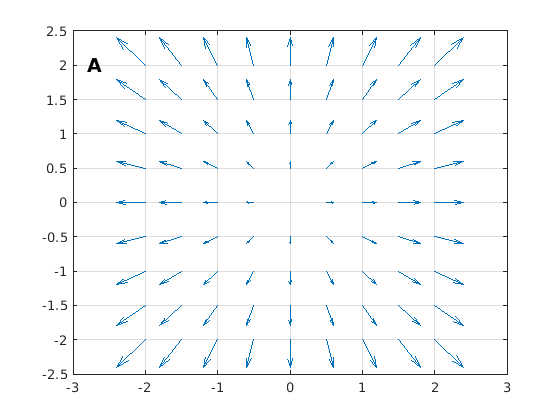
\includegraphics[width=8cm]{17_vector_calculus/vect_field1}
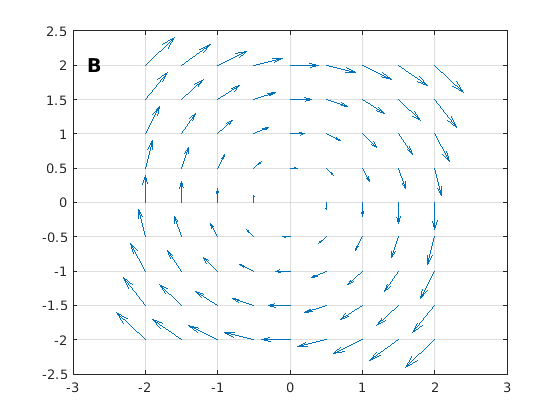
\includegraphics[width=8cm]{17_vector_calculus/vect_field2}

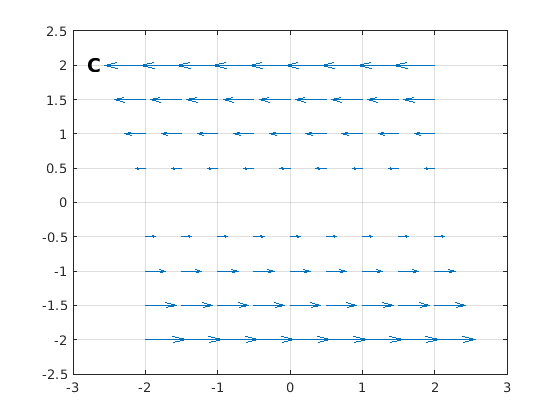
\includegraphics[width=8cm]{17_vector_calculus/vect_field3}
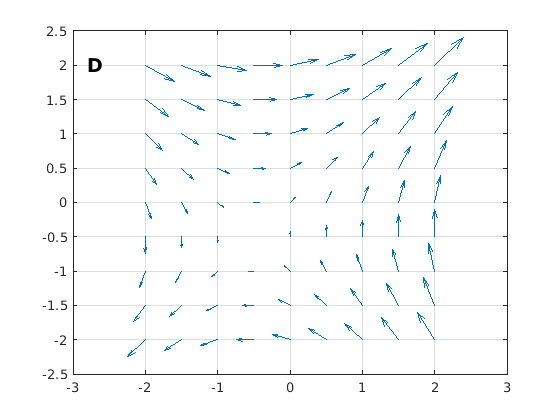
\includegraphics[width=8cm]{17_vector_calculus/vect_field4}
\label{17Q8}
\end{question}

\subsection{Intégrale sur une surface}

\begin{question}
Évaluez l'intégrale $\displaystyle \iint_S xy \dx{S}$ où $S$
est la surface du cylindre $y^2 + z^2 = 4$ entre les surface $y=0$ et
$y = 3 - x$.
\label{17Q9}
\end{question}

\begin{question}
Évaluez l'intégrale $\displaystyle \iint_S (x^2+y^2)z \dx{S}$ où $S$
est la surface de la partie supérieure de la sphère de rayon $2$
centrée à l'origine qui est à l'intérieur du cylindre de rayon
$\sqrt{2}$ dont l'axe principal est l'axe des $z$.
\label{17Q10}
\end{question}

\begin{question}
Quelle est la masse de l'entonnoir donnée par l'équation
$z = 2 \sqrt{x^2+y^2}$ dont le rayon de la base de l'entonnoir est $1$
et le rayon du dessus de l'entonnoir est $3$.  La densité est donnée
par $\rho(x,y,z) = 8 - z$.
\label{17Q11}
\end{question}

\begin{question}
Quelle est l'aire de la partie de la paraboloïde $y = x^2 + z^2$ qui
est à l'intérieur du cylindre $x^2 + z^2 = 9$.
\label{17Q12}
\end{question}

\begin{question}
Quelle est l'aire de la partie de la paraboloïde $z = x^2 + y^2 - 4$ qui
est à l'intérieur du cylindre $x^2 + y^2 = 1$.
\label{17Q13}
\end{question}

\begin{question}
Calculez l'aire de la surface $S$ du solide obtenu par l'intersection de
la balle $x^2 + y^2 + z^2 \leq 8$ et de la région $z \geq (x^2 + y^2)/2$.
\label{17Q14}
\end{question}

\begin{question}
Calculez l'aire de la partie $S$ du cylindre $x^2 + z^2 = a^2$ qui se
trouve à l'intérieur du cylindre $x^2 + y^2 = a^2$.  Dessinez cette
surface.
\label{17Q15}
\end{question}

\begin{question}
Calculez l'aire de la partie $S$ de la surface de la sphère d'équation
$x^2 + y^2 + z^2 = a^2$ qui se trouve à l'intérieur du cylindre
$x^2 + y^2 = ax$.  Dessinez cette surface.
\label{17Q16}
\end{question}

\begin{question}
Calculez l'intégrale $\displaystyle \iint_S F \cdot \dx{\VEC{S}}$
où $F(x,y,z) = (x,y,z)$ et $S$ est la partie du paraboloïde
$z = x^2+y^2$ pour $z\leq 4$.  L'orientation sur la surface $S$ est
donnée par un vecteur normal unitaire qui point dans la direction
de $z$ positif.
\label{17Q17}
\end{question}

\begin{question}
Calculez le flux du champ de vecteur $F(x,y,z) = (xy,y^2,yz)$
qui passe au travers de la partie de la sphère de rayon $2$ centrée à
l'origine qui se trouve dans la région $y\geq 0$.  L'orientation sur
la sphère est donnée par un vecteur normal unitaire dans la direction
de $y$ positif.
\label{17Q18}
\end{question}

\begin{question}
Calculer le flux du champ de vecteurs
$F(x,y,z) = -x\ii - y\jj + z^2\kk$  au travers de la partie du
cône $z=\sqrt{x^2+y^2}$ qui se trouve entre les plans $z=2$ et $z=3$.
L'orientation de la surface est donnée par la normale qui pointe
dans la direction de $z$ négatif.
\label{17Q19}
\end{question}

\begin{question}
Calculez le flux du champ de vecteur $F(x,y,z) = (y,x,z)$
qui passe au travers de l'hélicoïde $S$ décrit par la représentation
paramétrique
\[
  \rho(u,v) = (u \cos(v) , u \sin(v), v)
\]
pour $(u,v) \in D = \{(u,v) : 0\leq u \leq 1,\ 0\leq v \leq 2\pi \}$.
L'orientation de la surface est donnée par le vecteur normal unitaire
$\VEC{n}$ qui pointe dans la direction de $z$ positif.
\label{17Q20}
\end{question}

\begin{question}
Soit $F(x,y,z) = (x, \cos(xy) , z)$ et $S$ la surface du
cylindre $x^2+z^2 = a^2$ qui se trouve à l'intérieur du cylindre
$y^2+z^2=a^2$.  L'orientation sur $S$ est donnée par un vecteur
unitaire normal qui pointe vers l'extérieur du cylindre
$x^2 + z^2 = a^2$.  Calculez
$\displaystyle \iint_S F \cdot \dx{\VEC{S}}$.
\label{17Q21}
\end{question}

\subsection{Théorèmes de Stokes et de Green}

\begin{question}
Utilisez le Théorème de Green pour évaluez l'intégrale
$\displaystyle \int_C(2xy -x^2)\dx{x} + (x + y^2)\dx{y}$
où $C$ est la frontière de la région $D$ du premier quadrant
(c'est-à-dire, $x,y \geq 0$) définie par $x^2 + y^2 \leq 1$.
L'orientation de $C$ est dans le sens contraire aux aiguilles d'une
montre.
\label{17Q22}
\end{question}

\begin{question}
Évaluez l'intégrale
$\displaystyle \int_C(y+e^{x^2})\dx{x} + (2x + \cos(y^2))\dx{y}$
où $C$ est la frontière de la région $D$ bornée par les courbes
$y=x^2$ et $x = y^2$.  L'orientation de $C$ est dans le sens contraire
aux aiguilles d'une montre.
\label{17Q23}
\end{question}

\begin{question}
Nous voulons déplacer une particule le long de la courbe $C$ qui part de
l'origine pour se rendre au point $(2,0)$ en longeant l'axe des $x$,
puis se rendre au point $(-2,0)$ en longeant la partie supérieure du
cercle $x^2 + y^2 = 4$, et finalement revenir à l'origine encore en
longeant l'axe des $x$.  Calculez le travail nécessaire pour déplacer
un particule le long de ce trajet si le champ de vecteurs est
$F = (x, x^3 + 3 xy^2)$.
\label{17Q24}
\end{question}

\begin{question}
Soit $F(x,y,z) = (yz, xy, xz)$ et $C$ le rectangle de sommets
aux points $(0,0,2)$, $(1,0,2)$, $(1,1,2)$ et $(0,1,2)$.   Supposons
que $C$ soit parcourue dans le sens contraire aux aiguilles d'une
montre lorsque nous l'observons d'un point $(0,0,z)$ avec $z>2$.
Utilisez le Théorème de Stokes pour calculer l'intégrale
$\displaystyle \int_C F \cdot \dx{\VEC{s}}$.
\label{17Q25}
\end{question}

\begin{question}
Soit $F(x,y,z) = (y^2, x, z)$.  Utilisez le Théorème de Stokes
pour calculer l'intégrale
$\displaystyle \int_C F \cdot \dx{\VEC{s}}$
où $C$ est la courbe donnée par l'intersection du cylindre d'équation
$x^2 + y^2 =4$ et du plan contenant les points $(0,2,0)$, $(1,1,1)$ et
$(-1,1,2)$.  L'orientation sur $C$ est dans le sens des aiguilles
d'une montre lorsque vue du dessus (i.e.\ d'un point $(0,0,z)$ pour
$z>0$ très grand).
\label{17Q26}
\end{question}

\begin{question}
Soit $S$ la surface de la paraboloïde $z = 4 - x^2 - y^2$ qui se
trouve dans la région $x,y,z \geq 0$.  Calculez
$\displaystyle \int_C F \cdot \dx{\VEC{s}}$ où le champ de
vecteur $F$ est défini par
$F(x,y,z) = -yz(1-z) \, \ii + xz \, \jj + xyz \, \kk$
et la direction sur la courbe $C = \partial S$ est dans le sens
contraire aux aiguilles d'une montre lorsque que vu d'un point sur
l'axe des $z$ avec $z > 4$.
\label{17Q27}
\end{question}

\begin{question}
Soit $F(x,y,z) = x\; \ii + y\;\kk$ et $S$ la partie du
paraboloïde d'équation $z = x^2+y^2$ pour $z \leq 4$.  L'orientation
sur $S$ est donnée par un vecteur unitaire qui pointe dans la
direction de $z$ positif.  Calculez
$\displaystyle \iint_S \curl F \cdot \dx{\VEC{S}}$.
\label{17Q28}
\end{question}

\begin{question}
Soit $F(x,y,z) = z^3 e^{xz^2}\, \ii + z^4 e^{yz^2}\, \jj + xy\,\kk$ et
$S$ la surface du cylindre $x^2+y^2 = 4$ pour $2 \leq z \leq 4$.
L'orientation sur $S$ est donnée par un vecteur unitaire normal qui
pointe vers l'extérieur du cylindre.  Calculez
$\displaystyle \iint_S \curl  F \cdot \dx{\VEC{S}}$.
\label{17Q29}
\end{question}

\subsection{Théorème de la divergence}

\begin{question}
Soit $F(x,y,z) = (x+y)\ii + (y+z) \jj + (x + z) \kk$ et
$S$ la surface du tétraède bornée par les plans $x=0$, $y=0$, $z=0$ et
$x+y+z=1$.  L'orientation de $S$ est donnée par une normale unitaire à
$S$ qui pointe vers l'extérieure.  Calculez
$\displaystyle \iint_S F \cdot \dx{\VEC{S}}$ à l'aide du
Théorème de la divergence.
\label{17Q30}
\end{question}

\begin{question}
Soit $F(x,y,z) = x^3\ii + y^3 \jj + (z^3 + \cos(y^2)) \kk$ et
$E$ le solide délimité par le cylindre $x^2+y^2 =1$ et les plans $z=0$
et $z=2$.  L'orientation sur la surface $S$ de $E$ est donnée par une
normale unitaire qui pointe vers l'extérieure.  Calculez le flux de
$F$ qui s'échappe de ce solide; c'est-à-dire, calculez
$\displaystyle \iint_S F \cdot \dx{\VEC{S}}$.
\label{17Q31}
\end{question}

\begin{question}
Soit $F(x,y,z) = xy^2\,\ii + 2xz^2\, \jj + x^2 z\, \kk$ et
$E$ le solide délimité par le paraboloïde $z = 4 - x^2 - y^2$ et le
plan $z=0$.  L'orientation sur la surface $S$ de $E$ est donnée par la
normale unitaire qui pointe vers l'extérieure.  Calculez le flux de
$F$ qui s'échappe de ce solide; c'est-à-dire, calculez
$\displaystyle \iint_S F \cdot \dx{\VEC{S}}$.
\label{17Q32}
\end{question}


%%% Local Variables: 
%%% mode: latex
%%% TeX-master: "notes"
%%% End: 

\cleardoublepage

\chapter[Systèmes d'équations différentielles \life]{Systèmes
 d'équations différentielles d'ordre un\\ \life}\label{ChapSystEquDiff}

\compileTHEO{

Ce chapitre est une très brève introduction aux {\em systèmes d'équations
différentielles d'ordre un}.  Le but principal de cette introduction est de
convaincre le lecteur de l'importance que ces systèmes ont en science
et génie.

Nous présentons une approche qualitative à l'étude des systèmes
d'équations différentielles d'ordre un.  Puisque ces systèmes peuvent
avoir un grand nombre d'inconnues, essayer de les résoudre
analytiquement demanderait une travail énorme et cela en supposant que
c'est possible.  Nous utilisons normalement des méthodes numériques
pour \lgm résoudre\rgm\ les systèmes d'équations différentielles
d'ordre un.  Mais même avec ces méthodes, il est souvent très
difficile d'analyser ces systèmes.  C'est pour cette raison que
l'étude qualitative des systèmes d'équations différentielles d'ordre
un est très importante. 

Nous fournirons une analyse complète dans le cas des systèmes
d'équations différentielles linéaires d'ordre un.  C'est le mieux que
nous puissions faire.  La section sur {\em l'analyse global} nous
fourni des outils pour l'analyse qualitative des
{\em systèmes d'équations différentielles non-linéaire d'ordre un}.
La section sur l'équation de Van der Pol et la section sur le système
prédateurs-proies fournissent deux exemples simples de systèmes
d'équations différentielles non-linéaires d'ordre qui présentent une
dynamique beaucoup plus complexe que celle que nous pouvons observer
pour les systèmes d'équations différentielles linéaires d'ordre un.
L'approche dans ces deux dernières sections est très intuitive et
informelle.  C'est seulement la point de l'iceberg de ce sujet
d'études.

\section{Introduction}

\begin{egg}[][Système prédateurs-proies] \label{PREPRO}
Cet exemple est présent dans la majorité des manuels de mathématiques
pour les sciences biologiques.  Nous nous sommes inspiré de Murray \cite{M}
pour la présentation qui suit.

L'exemple classique d'un système d'équations différentielles d'ordre
un est le système qui décrit le nombre d'individus de deux espèces
animales; une espèce représentant les proies et l'autre représentant
les prédateurs.  Les deux espèces sont en compétition pour leur existence.

Nous pouvons imaginer que, si les prédateurs dévorent trop de proies, ces
prédateurs mettront en danger leur propre existence en détruisant leur source
de nourriture.  Par contre, si le nombre de proies devient très grand, il
sera facile pour les prédateurs de capturer des proies et le nombre de
prédateurs va augmenter.  Qu'arrivera-t-il à long terme? Est-ce que les
espèces vont disparaître?  Est-ce qu'il s'établira un équilibre entre le 
nombre de proies et de prédateurs?

Nous pouvons décrire l'interaction entre les deux espèces à l'aide d'équations
différentielles.  Soit $q(t)$ le nombre de proies au temps $t$ et $p(t)$ le
nombre de prédateurs au temps $t$ dans un espace donné (e.g.\ par
km$^2$).  Le choix des unités pour le temps est déterminé par
l'espérance de vie des proies et prédateurs.  Les unités de temps
normalement utilisées pour les mammifères sont les années.  Pour
certains insectes nous utiliserons les jours.

Lotka et Voltera, deux biomathématiciens à une époque où nous ne
parlions pas de biomathématiques, développèrent séparément (en 1920 et
1926 respectivement) le système d'équations différentielles d'ordre un
suivant.
\begin{equation} \label{LVsyst}
\begin{split}
\dydx{q}{t} &= q(a-b\,p) \\
\dydx{p}{t} &= p(c\,q - d)
\end{split}
\end{equation}
où $a$, $b$, $c$ et $d$ sont des constantes positives.  Ce système
d'équations différentielles porte maintenant le nom de
{\bfseries système (d'équations différentielles) de
Lotka-Voltera}\index{Système de Lotka-Voltera}.

Commençons par expliquer le rôle et la signification des constantes
dans le système (\ref{LVsyst}).  S'il n'y a pas d'interaction entre
les proies et les prédateurs, le nombre de proies et de prédateurs est
décrit par les équations différentielles
\[
\dydx{q}{t} = a\,q \quad \text{et} \quad \dydx{p}{t} = - d\, p \; .
\]
Ces deux équations sont indépendantes et peuvent être résolues par la
méthode de séparation des variables.  La constante $a$ représente le taux
relatif de croissance pour les proies et la constante $-d$ représente le taux
relatif de croissance pour les prédateurs.  Dans ce dernier cas, le taux de
croissance est négatif car les prédateurs vont disparaître par manque de
nourriture si la population de proies est absente.

Nous représentons le nombre de contacts entre les proies et les
prédateurs par le produit $p\,q$.  Ainsi, le terme $-b\,p\,q$ du côté
droit de la première
équation en (\ref{LVsyst}) a un effet négatif sur le taux de croissance des 
proies car $-b\, p \, q \leq 0$.  Par contre le terme $c\,p\,q$ du côté
droit de la deuxième équation en (\ref{LVsyst}) a un effet positif sur le
taux de croissance car $c\,p\,q \geq 0$.  Cela est consistant avec le fait
que lorsqu'un prédateur entre en contact avec une proie, c'est la proie
qui est la grande perdante.

Le système (\ref{LVsyst}) semble dépendre de quatre paramètres: $a$, $b$, $c$
et $d$.  Par contre, il existe une dépendance entre ces quatre paramètres qui
cache la simplicité du système.  Le raisonnement suivant est appelé
{\bfseries non-dimensionalisation}\index{Non-dimensionalisation} et
permet de réduire le nombre de paramètres au nombre minimal de
paramètres nécessaires pour décrire la comportement qualitatif de
(\ref{LVsyst}).

Si nous posons
\[
  q(t) = \frac{d}{c}u(a t) \ , \ p(t) = \frac{a}{b} v(at) \quad
  \text{et} \quad \alpha = \frac{d}{a} ,
\]
nous obtenons
\begin{align*}
q'(t) &= \frac{d}{c}\dfdx{u(at)}{t} = \frac{da}{c}u'(at)
\intertext{et}
p'(t) &= \frac{a}{b}\dfdx{v(at)}{t} = \frac{a^2}{b}v'(at) \ .
\end{align*}
Ainsi, (\ref{LVsyst}) donne
\begin{subequations}  \label{LVsystR}
\begin{align}
\frac{da}{c}u'(at) &= \frac{d}{c}u(a t) \left( a - b \;
\frac{a}{b} v(at) \right) = \frac{ad}{c} u(a t) \left( 1 - v(at) \right)
\label{LVsystRa} \\
\intertext{et}
\frac{a^2}{b}v'(at) &= \frac{a}{b} v(at) \left(
c \; \frac{d}{c}u(a t) - d\right) = \frac{ad}{b} v(at) \left(
u(a t) - 1\right) \ . \label{LVsystRb}
\end{align}
\end{subequations}
Si nous multiplions les deux côtés de (\ref{LVsystRa}) par
$\displaystyle \frac{c}{ad}$ et ceux de (\ref{LVsystRb}) par
$\displaystyle \frac{b}{a^2}$, nous obtenons
\begin{align*}
u'(at) &= u(a t) \left( 1 - v(at) \right) \\
v'(at) &= \frac{d}{a}\; v(at) \left( u(a t) - 1\right) 
= \alpha v(at) \left( u(a t) - 1\right)  \ .
\end{align*}
Finalement, si nous ajustons le temps en posant $\tau = at$, nous obtenons
\begin{equation} \label{ndLVsyst}
\begin{split}
\dydx{u}{\tau} &= u(1-v) \\
\dydx{v}{\tau} &= \alpha \,v(u - 1)
\end{split}
\end{equation}
Qualitativement, (\ref{ndLVsyst}) est équivalant à (\ref{LVsyst});
c'est-à-dire que nous pouvons représenter tous les
{\em types de solutions} que
(\ref{LVsyst}) possède en variant le paramètre $\alpha$ seulement.

Dans ce chapitre, nous développerons des outils pour analyser les systèmes
d'équations différentielles d'ordre comme (\ref{ndLVsyst}).
\end{egg}

\begin{egg}[][Compétition -- exclusion] \label{COMPEXCL}
Comme pour l'exemple précédent, nous nous sommes inspiré de Murray \cite{M}
pour la présentation qui suit.

Le deuxième exemple de systèmes d'équations différentielles d'ordre un
décrit le comportement de deux espèces animales, l'espèce P et
l'espèce Q, restreintes à un même territoire et ayant la même source
de nourriture.

Soit $p(t)$ le nombre d'individus de l'espèce P au temps $t$ et $q(t)$ le
nombre d'individus de l'espèce Q au temps $t$ dans un espace donné.
Comme à l'exemple précédent, le choix des unités pour le temps est
déterminé par l'espérance de vie des deux espèces.

Si les deux espèces occupent des milieux distincts, ils n'entrent donc pas en
compétition pour la nourriture, alors $p$ est gouverné par une équation
logistique et il en est de même pour $q$.  Ce type d'équation a été étudié
au chapitre sur les équations différentielles.  Nous avons
\begin{equation}\label{twoLEQ}
\dydx{p}{t} = a\,p\left(1-\frac{p}{M_p}\right)
\quad \text{et} \quad
\dydx{q}{t} = b\,q\left(1- \frac{q}{M_q}\right) \; .
\end{equation}
La constante $a>0$ est associée au taux de croissance relatif de l'espèce P et
la constante $b>0$ est associée à celui de l'espèce Q.  $M_p$ est le nombre
maximal d'individus de l'espèce P que le milieu peut supporter et $M_q$ est
le nombre maximal d'individus de l'espèce Q que le milieu peut supporter.

Les équations différentielles ci-dessus décrivent la situation où la
consommation de nourriture d'une espèce n'a pas d'effet sur l'autre espèce.
Par contre, si les deux espèces occupent le même milieu, elles entrent en
compétition pour la nourriture disponible.  Pour décrire le nombre
d'individus d'une espèce, il faut donc tenir compte du nombre d'individus de
l'autre espèce.

Nous considérons le système d'équations différentielles d'ordre un suivant.
\begin{subequations} \label{CompExcl}
\begin{align}
\dydx{p}{t} &= a\,p\left(1- \frac{p + c\, q}{M_p} \right) \label{CompExcla} \\
\dydx{q}{t} &= b\,q\left(1- \frac{q + d\, p}{M_q} \right) \label{CompExclb}
\end{align}
\end{subequations}
Les constantes positives $c$ et $d$ sont déterminées par la quantité de
nourriture consommée par chacun des individus des deux espèces -- Peut-être
qu'un individu de l'espèce P a besoin pour survivre du double de la quantité
de nourriture qu'un individu de l'espèce Q a besoin pour survivre.  Les
constantes $c$ et $d$ peuvent aussi dépendre de l'état de la source de
nourriture après le passage d'une espèce -- Peut-être que les individus d'une
espèce détruisent plus de nourriture qu'ils en consomment.

Le terme $(p+c\,q)/M_p$ du côté droit de (\ref{CompExcla}) joue le
même rôle que le terme $p/M_p$ dans l'équation logistique à gauche
dans l'équation (\ref{twoLEQ}).  Il faut tenir compte de l'impact de
l'espèce Q sur la source de nourriture.  Un individu de l'espèce Q a
un effet qui est $c$ fois celle d'un individu de l'espèce P.  De même,
le terme $(q+d\,p)/M_q$ du côté droit de (\ref{CompExclb}) joue le
même rôle que le terme $q/M_q$ dans l'équation logistique à droite
dans l'équation (\ref{twoLEQ}).  Il faut maintenant tenir compte de
l'impact de l'espèce P sur la source de nourriture.  Un individu de
l'espèce P a un effet qui est $d$ fois celle d'un individu de l'espèce
Q.

Le nombre de contacts entre les deux espèces est représenté par le produit
$p\,q$.  Nous parlons de contact lorsque les individus des deux espèces se
nourrissent à la même source.

Le système (\ref{CompExcl}) semble dépendre de six paramètres: $a$, $b$, $c$,
$d$, $M_p$ et $M_q$.  Nous pouvons utiliser la technique de
{\bfseries non-dimensionalisation} pour éliminer certains des
paramètres.

Si nous posons
\begin{align*}
  p(t) &= M_p u(a t) \quad , \quad q(t) = M_q v(a t) \ ,\\
\alpha &= \frac{b}{a} \quad , \quad  \rho = \frac{c\,M_q}{M_p}
\quad \text{et} \quad \xi = \frac{d\,M_p}{M_q} \; .
\end{align*}
et que nous ajustons le temps en posant $\tau = a\,t$, le système
(\ref{CompExcl}) devient le système
\begin{equation} \label{ndCompExcl}
\begin{split}
\dydx{u}{\tau} &= u(1-u - \rho\,v) \\
\dydx{v}{\tau} &= \alpha \,v(1-v-\xi\,u)
\end{split}
\end{equation}
Nous laissons aux lecteurs le soin de vérifier cette conclusion.
Nous avons réduit le nombre de paramètres à trois.  Comme à l'exemple précédent,
(\ref{CompExcl}) et (\ref{ndCompExcl}) sont équivalant
qualitativement.
\end{egg}

\begin{egg}
L'exemple suivant provient en grande partie de Borelli et Coleman \cite{BC}.

Pour qu'un médicament contre le rhume soit efficace, il faut que la quantité
du médicament dans le sang du patient soit plus grande qu'une certaine
valeur minimale pour une période suffisamment longue.

Nous analysons deux médicaments contre le rhume: un décongestionnant et un
antihistaminique.

\noindent{\bfseries Une seule dose}

Le nombre d'unités $x(t)$ d'un médicament dans l'estomac au temps $t$ en
heures satisfait l'équation différentielle 
\begin{equation}\label{dose1}
\dydx{x}{t} = -k_1 x
\end{equation}
et le nombre d'unités $y(t)$ de ce médicament dans le sang au temps $t$ en
heures satisfait l'équation différentielle 
\begin{equation}\label{dose2}
\dydx{y}{t} = k_1 x - k_2 y \; .
\end{equation}
Les constantes $k_1$ et $k_2$ sont positives et déterminées par le médicament
considéré.

$k_1 x(t)$ est le taux d'assimilation du médicament au temps $t$ par le sang
qui traverse l'estomac et $k_2y(t)$ est le taux d'élimination du médicament
au temps $t$ par le foie et les reins.

S'il y a initialement $x(0)=A$ unités du médicament (le patient
avale une dose de $A$ unités) et $y(0)=0$ unité (il n'y a aucune
trace du médicament dans le sang car c'est la première dose que le
patient reçoit), alors la solution de (\ref{dose1}) et (\ref{dose2}) est 
\[
x(t) = A e^{-k_1 t} \quad , \quad
y(t) = -\frac{A k_1 e^{-k_1 t}}{k_1 - k_2}
+ \frac{A k_1 e^{-k_2 t}}{k_1 - k_2} \; .
\]

Pour un décongestionnant, nous estimons que
$k_1 = 1.386$ et $k_2 = 0.1386$.   Supposons que le patient prenne
initialement $A=1$ unité du médicament.  Nous obtenons alors les graphes de
$x$ et $y$ donnés à la figure~\ref{doseFIG1}.

Pour un antihistaminique, nous estimons que $k_1=0.6931$ et
$k_2=0.0231$.  Supposons encore que le patient prenne
initialement $A=1$ unité du médicament.  Nous obtenons les graphes de
$x$ et $y$ donnés à la figure~\ref{doseFIG2}.

\begin{figure}
\centering
\subfloat[décongestionnant]{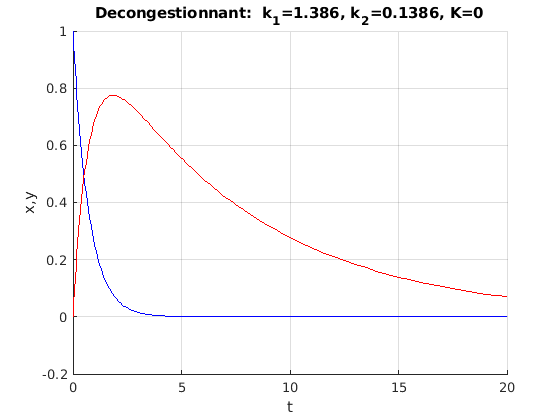
\includegraphics[width=7cm]{18_syst_equ_diff/drug1a_dec}\label{doseFIG1}}
\qquad
\subfloat[antihistaminique]{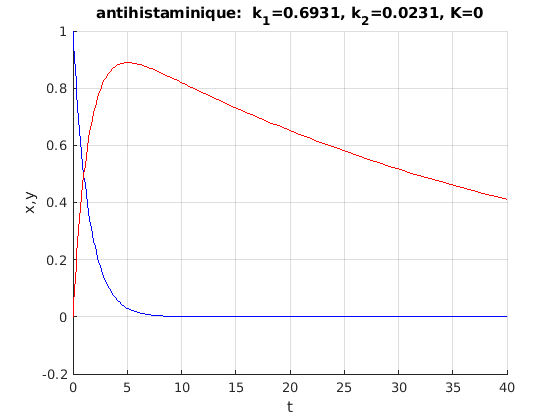
\includegraphics[width=7cm]{18_syst_equ_diff/drug1a_ant}\label{doseFIG2}}
\caption[Graphes de la quantité de décongestionnant et
d'antihistaminique dans l'estomac et dans le sang pour une seule dose]
{(a) Graphes de la quantité de décongestionnant dans l'estomac (en
bleu) et dans le sang (en rouge) pour une seule dose.
(b) Graphes de la quantité d'antihistaminique dans l'estomac (en
bleu) et dans le sang (en rouge) pour une seule dose.}\label{doseFIG12}
\end{figure}

% \MATHfig{18_syst_equ_diff/drug1a_dec}{8cm}{Graphes de la quantité de
% décongestionnant dans l'estomac et dans le sang pour une seule
% dose}{Graphes de la quantité de décongestionnant dans l'estomac (en
% bleu) et dans le sang (en rouge) pour une seule dose.}{doseFIG1} 

% \MATHfig{18_syst_equ_diff/drug1a_ant}{8cm}{Graphes de la quantité
% d'antihistaminique dans l'estomac et dans le sang pour une seule
% dose}{Graphes de la quantité d'antihistaminique dans l'estomac (en
% bleu) et dans le sang (en rouge) pour une seule dose.}{doseFIG2}

Si seulement les quantités de médicament dans le sang sont considérées,
l'antihistaminique semble avoir un plus long effet.  Par contre, le
décongestionnant semble agir plus rapidement.

\noindent{\bfseries Un médicament administré de façon continue}

Certaines pilules sont formées d'un très grand nombre de petites boules qui se
dissolvent dans l'estomac à des rythmes différents.  Le résultat est que le
médicament n'est pas absorbé par l'estomac d'un seul coup comme dans le cas
précédent mais il est absorbé par l'estomac à un taux constant de $K$
unités par heure (pour la durée de la pilule).

Supposons que la fréquence à laquelle le patient prend une pilule soit
telle que le taux d'absorption dans l'estomac soit constant à $K$ unités par
heure, alors le nombre d'unités $x(t)$ dans l'estomac au temps $t$ en heures
et le nombre d'unités $y(t)$ dans le sang au temps $t$ en heures sont
gouvernés par les équations différentielles
\begin{equation} \label{dose3}
\begin{split}
\dydx{x}{t} &= K -k_1 x \\
\dydx{y}{t} &= k_1 x - k_2 y
\end{split} \ .
\end{equation}

Dans le présent problème, nous avons $x(0)=0$ et $y(0)=0$ unité
initialement.  La condition $x(0)=0$ ne veut pas dire que le patient
ne prend pas de médicament.  Le patient reçoit une dose de $K$ unités par
heure.  La condition $x(0)=0$ veut dire que le patient n'a pas de
médicament dans l'estomac au départ.  De même, $y(0)=0$ veut dire que
le patient n'a pas de médicament dans le sang au départ.

La solution de (\ref{dose3}) est
\begin{align*}
x(t) &= -\frac{K\left(-1 + e^{-k_1 t}\right)}{k_1} \\
y(t) &= -\frac{K\left(-k_1 + k_2 - k_2 e^{-k_1 t} + k_1 e^{-k_2
      t}\right)}{k_2 (k_1 - k_2)}
\end{align*}

La quantité $x(t)$ du médicament dans l'estomac converge vers
$x = K/k_1$ lorsque $t$ tend vers l'infini (de plus,
$x'(t) \rightarrow 0$ lorsque $t \rightarrow \infty$) et la quantité $y(t)$
du médicament dans le sang converge vers $y = K/k_2$ lorsque $t$
tend vers plus l'infini (de plus, $y'(t) \rightarrow 0$ lorsque
$t \rightarrow \infty$).

Utilisons les valeurs $k_1 = 1.386$ et $k_2 = 0.1386$ pour un
décongestionnant qui ont été données précédemment et supposons que
$K=1$ unité par heure.  Nous obtenons alors les graphes de $x$ et $y$ donnés
à la figure~\ref{doseFIG3}.

Utilisons les valeurs $k_1=0.6931$ et $k_2=0.0231$ pour un
antihistaminique qui ont été données précédemment et supposons
toujours que $K=1$ unité par heure.  Nous obtenons alors les graphes de $x$
et $y$ donnés à la figure~\ref{doseFIG4}.

\begin{figure}
\centering
\subfloat[décongestionnant]{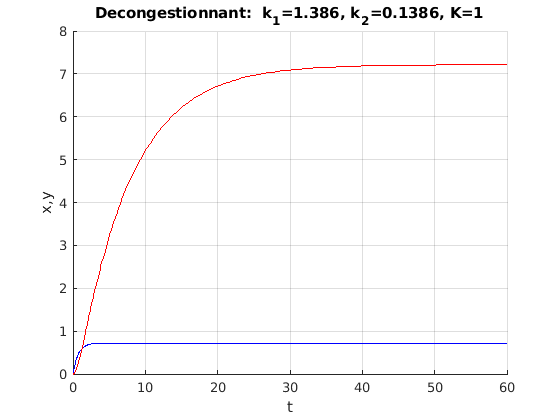
\includegraphics[width=7cm]{18_syst_equ_diff/drug1b_dec}\label{doseFIG3}}
\qquad
\subfloat[antihistaminique]{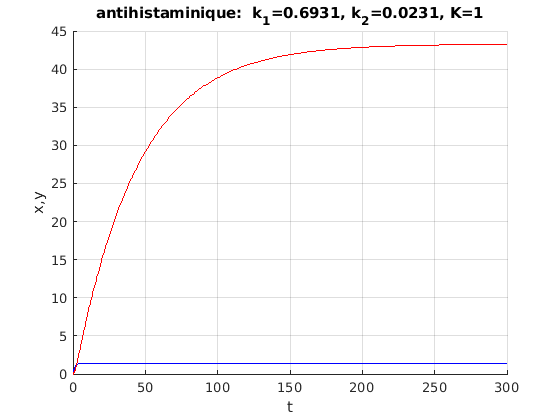
\includegraphics[width=7cm]{18_syst_equ_diff/drug1b_ant}\label{doseFIG4}}
\caption[Graphes de la quantité de décongestionnant et
d'antihistaminique dans l'estomac et dans le sang pour une médication
administré de façon continue]
{(a) Graphes de la quantité de décongestionnant dans l'estomac (en
bleu) et dans le sang (en rouge) pour une médication administré de
façon continue.
(b) Graphes de la quantité d'antihistaminique dans l'estomac (en
bleu) et dans le sang (en rouge) pour une médication administré de
façon continue.}\label{doseFIG34}
\end{figure}

% \MATHfig{18_syst_equ_diff/drug1b_dec}{8cm}{Graphes de la quantité de
% décongestionnant dans l'estomac et dans le sang pour une médication
% administré de continue}{Graphes de la quantité de décongestionnant
% dans l'estomac (en bleu) et dans le sang (en rouge) pour une
% médication administré de façon continue.}{doseFIG3}

% \MATHfig{18_syst_equ_diff/drug1b_ant}{8cm}{Graphes de la quantité
% d'antihistaminique dans l'estomac et dans le sang pour une
% médication administré de façon continue}{Graphes de la quantité
% d'antihistaminique dans l'estomac (en bleu) et dans le sang (en rouge)
% pour une médication administré de façon continue.}{doseFIG4}

Le décongestionnant et l'antihistaminique ont des comportements semblables à
long terme dans le présent cas.  $x'(t) \rightarrow 0$ et
$y'(t) \rightarrow 0$ lorsque $t \rightarrow \infty$.  Plus précisément,
$x(t)$ est asymptotique à $x = K/k_1$ et $y(t)$ est asymptotique à
$x = K/k_2$ lorsque $t \rightarrow \infty$.  Si seulement les 
quantités de médicament dans le sang sont considérées, le
décongestionnant commence à agir beaucoup plus rapidement que
l'antihistaminique.  Par contre, l'action de l'antihistaminique est
beaucoup plus forte.

\noindent{\bfseries Un médicament administré à intervalle régulier}

Dans l'exemple précédent, nous avons supposé que le médicament est
absorbé par l'estomac à un taux constant de $K$ unités par heure (pour
la durée de la pilule) et que le patient prend une pilule à intervalle
régulier de façon à maintenir le taux d'absorption constant à $K$
unités par heure.  C'est une situation idéale qui est presque
impossible à satisfaire.

La situation suivante est plus réaliste.  Supposons que le type de pilules
utilisée soit celui de la section précédente.  Plus précisément,
supposons que le médicament entre dans l'estomac à un taux constant de
$K=12$ unités par heure durant une demi-heure.  Après une demi-heure,
la pilule a été complètement assimilée par l'organisme et il n'y a
plus de médicament qui entre dans l'estomac.  De plus, supposons
que le patient prend une pilule à toutes les six heures.

Le taux d'absorption par l'estomac du médicament est décrit par la formule
\[
F(t) = \sum_{n=0}^N K (H(t + 6 n) - H(t - 0.5 + 6 n))
\]
où $H$ est la fonction de Heaviside définie par
\[
H(t) = \begin{cases}
0 & \qquad \text{si} \quad t<0 \\
1 & \qquad \text{si} \quad t\geq 0
\end{cases}
\]
et $N+1$ est le nombre de pilules prisent par le patient.  Le graphe
de $F$ pour les quatre premières pilules (i.e.\ $N=3$) est donné à la
figure~\ref{doseFIG5}.  C'est ce que nous appelons une onde carrée.

\MATHfig{18_syst_equ_diff/step_funct}{8cm}{Le taux d'absorption
d'un médicament pris à intervalles réguliers}{Le taux d'absorption
d'un médicament pris à intervalles réguliers.}{doseFIG5}

Dans ce cas, le nombre d'unités $x(t)$ dans l'estomac au temps $t$ en heures
et le nombre d'unités $y(t)$ dans le sang au temps $t$ en heures sont
gouvernés par les équations
\begin{equation} \label{dose4}
\begin{split}
\dydx{x}{t}(t) &= -k_1 x(t) + F(t) \\
\dydx{y}{t}(t) &= k_1 x(t) - k_2 y(t)
\end{split}
\end{equation}

Reprenons les deux types de médicament qui ont été considérés
précédemment; à savoir le décongestionnant et l'antihistaminique.

Remarquons que la première équation de (\ref{dose4}) est indépendante de la
fonction $y$.  Cette équation peut donc être résolue à l'aide des
{\em transformations de Laplace}; c'est un des sujets d'un premier
cours d'équations différentielles.  Après avoir trouvé $x$, la
deuxième équation de (\ref{dose4}) devient une équation linéaire
d'ordre un pour la fonction $y$.  Nous pourrions (avec amplement
de temps et de patience, ou avec un logiciel de calculs symboliques)
trouver une expression pour $x$ et $y$. Puisque nous voulons tracer le
graphe des solutions $x$ et $y$ de (\ref{dose4}), au lieu de trouver
une expression pour $x$ et $y$, nous résolvons numériquement le système
(\ref{dose4}).  Il faut porter une attention particulière aux points
où le côté droit de l'équation (\ref{dose4}) est discontinu.

Comme dans le cas de la médication continue, nous supposons que
$x(0)=0$ unité et $y(0)=0$ unité.

Pour le décongestionnant, nous avons $k_1=1.386$ et $k_2=0.1386$.  Les
graphes de $x$ et $y$ sont donnés à la figure~\ref{doseFIG6}.

Les graphes à la figure~\ref{doseFIG6} suggèrent que la quantité de
médication dans l'estomac a un comportement périodique et ne dépassera pas
environ $4.5$ unités.  De plus, la quantité de médication dans le sang semble
tendre vers une fonction périodique de moyenne $7$ unités et d'amplitude
environ $1.8$  Nous supposons ici que le patient ne cesse pas de prendre des
pilules et donc $N$ augmente.  Est-ce que le patient risque d'avoir une
surdose du médicament?  Une analyse mathématique plus poussée est
nécessaire pour montrer que le patient ne souffrira pas d'une surdose.

Nous traçons le graphe de la quantité d'antihistaminique pour $k_1=0.6931$
et $k_2=0.0231$ dans l'estomac et dans le sang en fonction du temps à la
figure~\ref{doseFIG7}.  Nous supposons toujours que $x(0)=0$ unité et $y(0)=0$
unité.

\begin{figure}
\centering
\subfloat[décongestionnant]{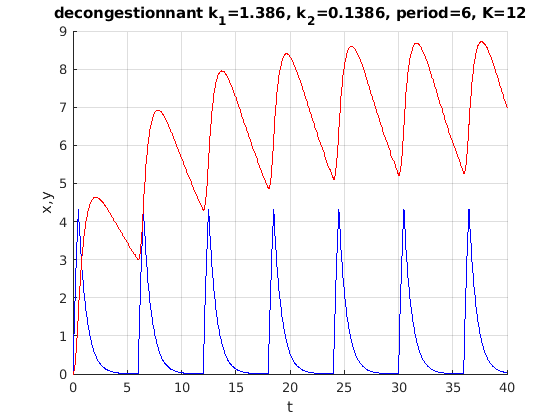
\includegraphics[width=7cm]{18_syst_equ_diff/drug2a_dec}\label{doseFIG6}}
\qquad
\subfloat[antihistaminique]{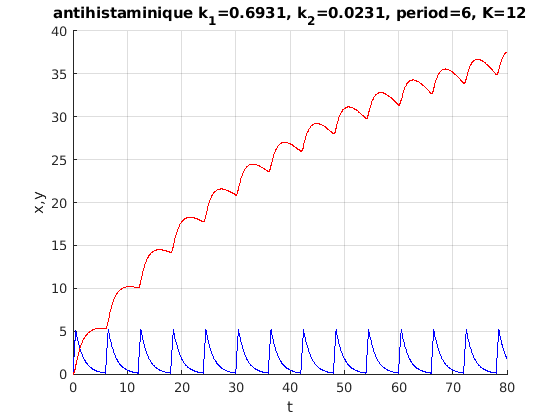
\includegraphics[width=7cm]{18_syst_equ_diff/drug2a_ant}\label{doseFIG7}}
\caption[Graphes de la quantité de décongestionnant et
d'antihistaminique dans l'estomac et dans le sang pour une médication
administré à intervalles réguliers]
{(a) Graphes de la quantité de décongestionnant dans l'estomac (en
bleu) et dans le sang (en rouge) pour une médication administré à
intervalles réguliers.
(b) Graphes de la quantité d'antihistaminique dans l'estomac (en
bleu) et dans le sang (en rouge) pour une médication administré à
intervalles réguliers.}\label{doseFIG67}
\end{figure}

% \MATHfig{18_syst_equ_diff/drug2a_dec}{8cm}{Graphes de la quantité de
% décongestionnant dans l'estomac et dans le sang pour une médication
% administrée à intervalles réguliers}{Graphes de la quantité de
% décongestionnant dans l'estomac (en bleu) et dans le sang
% (en rouge) pour une médication administrée à intervalles
% réguliers.}{doseFIG6}

% \MATHfig{18_syst_equ_diff/drug2a_ant}{8cm}{Graphes de la quantité
% d'antihistaminique dans l'estomac et dans le sang pour une médication
% administrée à intervalles réguliers}{Graphes de la quantité
% d'antihistaminique dans l'estomac (en bleu) et dans le sang (en rouge)
% pour une médication administrée à intervalles réguliers.}{doseFIG7}

Comme dans le cas du décongestionnant, le graphe de la quantité
d'antihistaminique dans l'estomac en fonction du temps suggèrent que la
quantité de médication dans l'estomac a un comportement périodique et ne
dépassera pas environ $5$ unités.  Par contre, la quantité
d'antihistaminique dans le sang semble en moyenne augmenter sans borne
supérieure.  En fait, une étude plus poussée montre que la quantité
d'antihistaminique dans le sang approche une fonction périodique de moyenne
environ $43$ unités et de période environ $1$.  Dépendant des unités
utilisées, nous risquons d'intoxiquer le patient car la quantité
d'antihistaminique dans le sang devient en moyenne $11$ fois la
quantité dans l'estomac.
\end{egg}

\section{Énoncé du problème général}

La forme générale d'un {\bfseries système d'équations différentielles
d'ordre un}\index{Système d'équations différentielles!d'ordre un} dans
$\RR^2$ est
\begin{equation} \label{sediff1}
\begin{split}
\dydx{x_1}{t} &= f_1(t,x_1,x_2) \\
\dydx{x_2}{t} &= f_2(t,x_1,x_2)
\end{split}
\end{equation}
où $f_i:]a,b[\times \RR^2 \rightarrow \RR$ pour $i=1$ et $2$.

La majorité des définitions et résultats que nous allons énoncés ont un
équivalent pour les systèmes d'équations différentielles d'ordre un
qui ont plus de deux inconnus et deux équations différentielles.  Nous
allons nous limiter aux systèmes composés de deux inconnus et deux
équations différentielles.

Si $f_1$ et $f_2$ ne dépendent pas de $t$, nous obtenons le
{\bfseries système d'équations différentielles autonomes
d'ordre un}\index{Système d'équations différentielles!autonome}
\begin{equation} \label{sediff2}
\begin{split}
\dydx{x_1}{t} &= f_1(x_1,x_2) \\
\dydx{x_2}{t} &= f_2(x_1,x_2)
\end{split}
\end{equation}
où $f_i:\RR^2 \rightarrow \RR$ pour $i=1$ et $2$.  C'est ce genre de
systèmes d'équations différentielles que nous considérons dans ce
chapitre.  Une forme brève pour (\ref{sediff2}) est
\begin{equation} \label{sediff3}
\dydx{\VEC{x}}{t} = \VEC{f}(\VEC{x})
\end{equation}
où
\[
\VEC{x} = \begin{pmatrix} x_1 \\ x_2 \end{pmatrix}
\quad , \quad
\dydx{\VEC{x}}{t} =
\begin{pmatrix} \displaystyle \dydx{x_1}{t} \\[1em]
\displaystyle \dydx{x_2}{t} \end{pmatrix}
\quad \text{et} \quad
\VEC{f}(\VEC{x}) = \begin{pmatrix} f_1(x_1,x_2)\\
f_2(x_1,x_2)
\end{pmatrix} \; .
\]

Le but est de trouver $2$ fonctions, $\phi_1:]a,b[ \rightarrow \RR$ et
$\phi_2:]a,b[ \rightarrow \RR$, telles que si nous remplaçons $x_1$ par
$\phi_1$ et $x_2$ par $\phi_2$ dans (\ref{sediff2}) alors l'équation
est satisfaite pour tout $t \in ]a,b[$.

\begin{defn} \index{Système d'équations différentielles!solution}
Une fonction
\begin{align*}
\phi:]a,b[ & \rightarrow \RR^2 \\
t &\mapsto
\begin{pmatrix}
\phi_1(t) \\ \phi_2(t)
\end{pmatrix}
\end{align*}
est une {\bfseries solution} du système d'équations différentielles
(\ref{sediff2}) si
\[
\begin{split}
\dydx{\phi_1}{t}(t) &= f_1(\phi_1(t),\phi_2(t)) \\
\dydx{\phi_2}{t}(t) &= f_2(\phi_1(t),\phi_2(t))
\end{split}
\]
pour tout $t \in]a,b[$.
\end{defn}

\begin{egg}
Soit le système d'équations différentielles autonome d'ordre un
\begin{equation}\label{systdfes1}
\begin{split}
\dydx{x_1}{t} &= x_1 + 2\,x_2\\
\dydx{x_2}{t} &= 5\,x_1 - 2\,x_2
\end{split}
\end{equation}
Les fonctions $\phi_1(t) = e^{3t}-2\,e^{-4t}$ et
$\phi_2(t) = e^{3t}+5\,e^{-4t}$ satisfont (\ref{systdfes1}) car
\begin{align*}
\dydx{\phi_1}{t}(t) &= \dfdx{\left(e^{3t}-2\,e^{-4t}\right)}{t}
= 3\,e^{3t}+8\,e^{-4t} \\
&= \left(e^{3t}-2\,e^{-4t}\right) +2\left(e^{3t}+5\,e^{-4t}\right)
= \phi_1(t) + 2\,\phi_2(t)
\end{align*}
et
\begin{align*}
\dydx{\phi_2}{t}(t) &= \dfdx{\left(e^{3t}+5\,e^{-4t}\right)}{t}
= 3\,e^{3t}-20\,e^{-4t} \\
&= 5\left(e^{3t}-2\,e^{-4t}\right) -2\left(e^{3t}+5\,e^{-4t}\right)
= 5\phi_1(t) - 2\,\phi_2(t)
\end{align*}
pour tout $t$.  Nous verrons prochainement comment trouver $\phi_1$ et
$\phi_2$ pour un système d'équations différentielles de la forme
(\ref{systdfes1}).

Les fonctions $\phi_1$ et $\phi_2$ donne la solution
\[
\phi(t) =
\begin{pmatrix}
\phi_1(t) \\
\phi_2(t)
\end{pmatrix}
=
\begin{pmatrix}
e^{3t}-2\,e^{-4t} \\ e^{3t}+5\,e^{-4t}
\end{pmatrix}
= e^{3t} \begin{pmatrix} 1 \\ 1 \end{pmatrix}
+ e^{-4t} \begin{pmatrix} -2 \\ 5 \end{pmatrix}
\]
de (\ref{systdfes1}).
\label{syst_egg0}
\end{egg}

Il est commun d'imposer une {\bfseries condition initiale}\index{Système
d'équations différentielles!condition initiale} au système d'équations
différentielles (\ref{sediff2}).  C'est-à-dire, de demander que la solution
$\phi:]a,b[\rightarrow \RR^2$ de (\ref{sediff2}) satisfasse
\[
  \phi(t_0) = \begin{pmatrix} \phi_1(t_0) \\ \phi_2(t_0) \end{pmatrix}
  = \begin{pmatrix} x_{0,1} \\ x_{0,2} \end{pmatrix}
\]
pour $t_0\in]a,b[$ et
$\displaystyle \VEC{x}_0 = \begin{pmatrix} x_{0,1} \\ x_{0,2} \end{pmatrix}$
donnés.

\begin{egg}
Nous invitons les lecteurs à vérifier que
\[
\phi(t) = a_1 \, e^{3t} \begin{pmatrix} 1 \\ 1 \end{pmatrix}
+ a_2\, e^{-4t} \begin{pmatrix} -2 \\ 5 \end{pmatrix}
\]
est une solution du système d'équations différentielles
(\ref{systdfes1}) de l'exemple~\ref{syst_egg0} quelles que soit les
valeurs données aux constantes $a_1$ et $a_2$.

Pour trouver la solution de (\ref{systdfes1}) qui satisfasse la
condition initiale
\begin{equation}
\phi(0)= \begin{pmatrix} 4 \\ -3 \end{pmatrix}  \ , \label{sedlin_init}
\end{equation}
il faut déterminer $a_1$ et $a_2$ tels que
\[
\phi(0) = a_1 \, \begin{pmatrix} 1 \\ 1 \end{pmatrix}
+ a_2\,\begin{pmatrix} -2 \\ 5 \end{pmatrix}
= \begin{pmatrix} a_1-2\,a_2 \\ a_1 + 5\,a_2 \end{pmatrix}
= \begin{pmatrix} 4 \\ -3 \end{pmatrix}  \; .
\]
Si nous résolvons le système d'équations linéaires
$a_1-2\,a_2 = 4$ et $a_1+5\,a_2 = -3$, nous trouvons $a_1=2$ et $a_2=-1$.
La solution du système (\ref{systdfes1}) qui satisfait la condition
initiale (\ref{sedlin_init}) est
\[
\phi(t) = 2 \, e^{3t} \begin{pmatrix} 1 \\ 1 \end{pmatrix}
- \, e^{-4t} \begin{pmatrix} -2 \\ 5 \end{pmatrix}
= \begin{pmatrix} 2 \, e^{3t} + 2\, e^{-4t} \\
2 \, e^{3t} -5 \, e^{-4t}
\end{pmatrix} \; .
\]
Nous parlons de \lgm la solution\rgm.  Pourrions-nous avoir une autre
fonction $\phi$ qui satisfait ce système d'équations différentielles
et la condition initiale?  Nous donnerons prochainement des conditions
sur le système d'équations différentielles qui assurent l'existence et
l'unicité d'une solution.
\label{syst_egg1}
\end{egg}

\begin{defn} \index{Système d'équations différentielles!orbite}
{\bfseries L'orbite} d'une solution $\phi:]a,b[\rightarrow \RR^2$ de
(\ref{sediff2}) est l'image
\[
\{ \phi(t) :  a < t < b \}
\]
de cette solution dans le plan.  L'orbite est une courbe dans le plan.
Le {\bfseries portrait de phases} de (\ref{sediff2}) est l'ensemble
des orbites.
\end{defn}

\begin{egg}
L'orbite de la solution 
\[
\phi(t) =
\begin{pmatrix}
2 e^{3t}+ 2\,e^{-4t} \\ 2 e^{3t} - 5\,e^{-4t}
\end{pmatrix}
\]
de l'exemple~\ref{syst_egg1} est la courbe avec une flèche représentée
à la figure~\ref{LINSYST1}.
\end{egg}

\PDFfig{18_syst_equ_diff/lin_syst1}{L'image d'une solution
$\phi:\RR\rightarrow \RR^2$ définie une courbe dans le plan}{L'orbite
de la solution $\phi:\RR\rightarrow \RR^2$ de l'équation différentielle de
l'exemple~\ref{syst_egg1}.  La flèche indique le déplacement le long
de l'orbite lorsque $t$ augmente.}{LINSYST1}

Puisque nous allons généralement étudier les systèmes d'équations
différentielles de la forme (\ref{sediff2}) où $f_1$ et $f_2$ sont
différentiable, le théorème suivant nous assure qu'il y aura toujours
une et une seule solution associée à une condition initiale.

\begin{theorem}
Si les fonctions $f_1:\RR^2 \rightarrow \RR$ et $f_2:\RR^2\rightarrow \RR$
qui décrivent le système d'équation différentielles
(\ref{sediff2}) sont différentiables, alors il existe une et une seule 
solution $\phi$ de (\ref{sediff2}) qui satisfait la condition initiale
$\phi(0) = \VEC{x}_0 \in \RR^2$.
\end{theorem}

\begin{rmk}
Puisqu'il y a une et une seule solution de (\ref{sediff2}) qui passe par un
point donné (i.e.\ qui satisfait une condition initiale donnée), les orbites
ne se coupent pas.
\end{rmk}

Il est généralement très difficile de résoudre les systèmes d'équations
différentielles.  Très souvent, nous ne sommes pas directement intéressés aux
solutions du système d'équations différentielles mais simplement à leur
comportement lorsque nous progressons dans le temps. Qu'arrive-t-il aux
solutions lorsque nous regardons très loin dans le temps?

\section{Systèmes d'équations différentielles linéaires d'or\-dre un}

Nous débutons notre étude des systèmes d'équations différentielles
d'ordre un par l'étude d'une classe de systèmes qui sont \lgm très
simples\rgm\ à analyser.  Il ne faut pas en conclure que ces systèmes
n'auront pas d'importance par la suite.  C'est tout à fait le
contraire.  Ils joueront un rôle primordial dans l'analyse de systèmes
d'équations différentielles beaucoup plus compliqués. Les résultats de
la présente section et leur généralisation à $\RR^n$ sont des outils
très fréquemment utilisés par les chercheurs en biomathématiques.

Un {\bfseries système d'équations différentielles linéaires d'ordre
un}\index{Système d'équations différentielles!linéaires} dans
$\RR^2$ est un système d'équations différentielles de la forme
\begin{align*}
\dydx{x_1}{t} &= a\,x_1 + b\, x_2 \\
\dydx{x_2}{t} &= x\,x_1 + d\, x_2
\end{align*}
où $a$, $b$, $c$ et $d$ sont des constantes.  Si nous posons
\[
A = \begin{pmatrix} a & b \\ c & d \end{pmatrix} \ ,
\]
nous pouvons récrire le système d'équations différentielles précédent sous la
forme
\begin{equation} \label{linclass}
\dydx{\VEC{x}}{t} = A \VEC{x}
\end{equation}
où
\[
\VEC{x} = \begin{pmatrix} x_1 \\ x_2 \end{pmatrix}
\quad \text{et} \quad
\dydx{\VEC{x}}{t} = 
\begin{pmatrix} \displaystyle \dydx{x_1}{t} \\[2ex]
\displaystyle \dydx{x_2}{t} \end{pmatrix} \; .
\]

Nos connaissances sur les valeurs et vecteurs propres vont nous
permettre de résoudre les systèmes d'équations différentielles
linéaires d'ordre un.  En fait, les solutions possibles de
(\ref{linclass}), et donc les portraits de phases pour
(\ref{linclass}), peuvent être groupés en un petit nombre de classes
selon le signe des valeurs propres de $A$ et le nombre de vecteurs
propres non colinéaires.  Nous résumons les résultats dans les trois
propositions suivantes.

\begin{prop}
Si la matrice $A$ de l'équation (\ref{linclass}) possède deux valeurs
propres réelles $\lambda_1$ et $\lambda_2$ distinctes, nous choisissons
$\VEC{v}_1$ un vecteur propre associé à $\lambda_1$ et $\VEC{v}_2$ un
vecteur propre associé à $\lambda_2$.  Les solutions de
(\ref{linclass}) sont de la forme
\begin{equation}\label{gsOFls1}
\VEC{x}(t)= a_1\,e^{\lambda_1\,t} \VEC{v}_1 + a_2\,e^{\lambda_2\,t}
\VEC{v}_2
\end{equation}
où $a_1$ et $a_2$ sont des constantes.  Nous retrouvons à la
figure~\ref{LINEARA3} les portraits de phases possibles dans cette
situation.
\end{prop}

\PDFfig{18_syst_equ_diff/linearA3}{Des portraits de phases possibles
pour un système d'équation différentielles linéaires d'ordre un dans $\RR^2$ si
les valeurs propres sont réelles et distinctes.}{Des portraits de
phases possibles pour (\ref{linclass}) si les valeurs propres sont
réelles et distinctes.}{LINEARA3}

\begin{prop}
Si la matrice $A$ de l'équation (\ref{linclass}) possède une seule
valeur propre $\lambda$, il y a deux cas possibles.  S'ils existent deux
vecteurs propres $\VEC{v}_1$ et $\VEC{v}_2$ associés à $\lambda$ qui
ne sont pas colinéaires, alors la solution est donnée par
(\ref{gsOFls1}).  Si ce n'est pas le cas, les vecteurs propres
associés à $\lambda$ sont donc tous colinéaires, alors les solutions de
(\ref{linclass}) sont de la forme
\[
\VEC{x}(t)= a_1\,e^{\lambda\,t} \VEC{v} + a_2\,e^{\lambda\,t}
\left( \VEC{u} + t \VEC{v} \right)
\]
où $a_1$ et $a_2$ sont des constantes, $\VEC{v}$ un vecteur propre
associé à $\lambda$ et $\VEC{u}$ est une solution de
$(A-\lambda\,\Id)\VEC{u} = \VEC{v}$.
Nous retrouvons à la figure~\ref{LINEARA5} un portrait de phases possible
dans ce dernier cas.  Les solutions approchent de l'origine lorsque
$\lambda<0$ et s'éloignent de l'origine lorsque $\lambda>0$.
\end{prop}

\PDFfig{18_syst_equ_diff/linearA5}{Un portrait de phases possible
pour un système d'équation différentielles linéaires d'ordre un dans
$\RR^2$ s'il n'y a qu'une valeur propre réelle et tous les vecteur
propres sont colinéaires}{Un portrait de phases possible pour
(\ref{linclass}) s'il n'y a qu'une valeur propre réelle et tous les
vecteur propres sont colinéaires.}{LINEARA5}

\begin{prop} \label{COLsolution}
Si la matrice $A$ de l'équation (\ref{linclass}) possède une paire de
vecteurs propres complexes $\lambda_1$ et $\lambda_2$, alors
$\lambda_1 = \overline{\lambda}_2$ puisque les composantes de la
matrice $A$ sont réelles.  Supposons que $\lambda_1 = \alpha + i\beta$
avec $\beta \neq 0$.  Soit $\VEC{v}_1 = \VEC{u}_1 + i \VEC{u}_2$, avec
$\VEC{u}_i \in \RR^2$, un vecteur propre associé à la valeur propre
$\lambda_1$.  Les solutions de (\ref{linclass}) sont de la forme
\[
\VEC{x}(t)= e^{\alpha t} \left( a_1 \cos(\beta t) + a_2 \sin(\beta t) \right)
\VEC{u}_1 + e^{\alpha t} \left( -a_1 \sin(\beta t) + a_2 \cos(\beta t) \right)
\VEC{u}_2
\]
où $a_1$ et $a_2$ sont des constantes.  Nous retrouvons à la
figure~\ref{LINEARA6} un portrait de phases possible.
\end{prop}

\PDFfig{18_syst_equ_diff/linearA6}{Un portrait de phases possible pour
un système d'équation différentielles linéaire d'ordre un dans $\RR^2$
si les valeurs propres sont complexes conjuguées}{Un portrait de
phases possible pour (\ref{linclass}) si les valeurs propres sont
complexes conjuguées.}{LINEARA6}

\begin{egg}
Considérons le système d'équations différentielles linéaire d'ordre un
$\VEC{x}' = A\VEC{x}$ où
$\displaystyle A = \begin{pmatrix} -1 & 0 \\ 4 & 3 \end{pmatrix}$.
Quelle est la solution de ce système qui satisfait la
condition initiale
$\displaystyle \VEC{x}(0) = \begin{pmatrix} 2 \\ 4 \end{pmatrix}$?

Les valeurs propres et un vecteur propre associé à chacune des valeurs
propres de $A$ sont donnés dans le tableau suivant.
\[
\begin{array}{ccl}
\text{valeur propre} & \hspace*{2em} & \text{vecteur propre} \\
\hline
\rule{0pt}{1.5em}\lambda_1 = -1 &
& \VEC{v}_1 = \begin{pmatrix} 1 & -1 \end{pmatrix}^\top \\[0.4em]
\lambda_2 = 3 & & \VEC{v}_2 = \begin{pmatrix} 0 & 1 \end{pmatrix}^\top
\end{array}
\]
Les solutions de $\VEC{x}'= A \VEC{x}$ sont de la forme
\[
\VEC{x}(t) = a_1 \, e^{-t}\begin{pmatrix} 1 \\ -1 \end{pmatrix}
+ a_2 \, e^{3t} \begin{pmatrix} 0 \\ 1 \end{pmatrix}
= \begin{pmatrix}
a_1 \, e^{-t} \\ -a_1 \, e^{-t} +  a_2 \, e^{3t}
\end{pmatrix} \; .
\]
Les paramètres $a_1$ et $a_2$ sont déterminés par la condition initiale
\[
\VEC{x}(0) = \begin{pmatrix} a_1 \\ -a_1 + a_2 \end{pmatrix}
= \begin{pmatrix} 2 \\ 4 \end{pmatrix} \ .
\]
Ainsi, $a_1=2$ et $a_2=6$.  Nous avons la solution
\[
\VEC{x}(t) = \begin{pmatrix}
2 \, e^{-t} \\ -2 \, e^{-t} +6 \, e^{3t}
\end{pmatrix} \; .
\]

Il est facile de tracer le portrait de phases de ce système.
Remarquons premièrement que toute solution dont la condition initiale
est un multiple de $\VEC{v}_1$ est de la forme
$\VEC{x}(t) = a_1 \, e^{-t} \VEC{v}_1$ pour une constante $a_1$.
Son orbite est donc sur la droite contenant $\VEC{v}_1$ et approche
l'origine quand $t \to \infty$.  De même, toute solution dont la
condition initiale est un multiple de $\VEC{v}_2$ est de la forme
$\VEC{x}(t) = a_2 \, e^{3t} \VEC{v}_2$ pour une constante $a_2$.
Son orbite est donc sur la droite contenant $\VEC{v}_2$ et s'éloigne de
l'origine quand $t \to \infty$.  De plus, il ne faut pas oublier que les
orbites ne peuvent pas se couper en raison de l'unicité des solutions
et que $\VEC{x} = \VEC{0}$ pour tout $t$ est une solution.
Toutes les autres solutions de la forme
$\VEC{x}(t) = a_1 \, e^{-t}\VEC{v}_1 + a_2 \, e^{3t} \VEC{v}_2$ vont
s'approcher de la droite contenant $\VEC{v}_2$ mais s'éloigner de la
droite contenant $\VEC{v}_1$ quand $t \to \infty$.  Nous obtenons le
portrait de phase qui est donné à la figure~\ref{LINTWODIM1}.
\label{lintwoDim1}
\end{egg}

\PDFfig{18_syst_equ_diff/lintwodim1}
{Portrait de phases d'un système d'équations différentielles linéaires
d'ordre un}{Portrait de phases du système d'équations différentielles
linéaires de l'exemple~\ref{lintwoDim1}}{LINTWODIM1}

\begin{rmk}
Il serait plus laborieux de tracer l'orbite associée à la solution de
l'exemple précédent si nous n'avions pas la
proposition~\ref{COLsolution}.  Voici comment nous devrions procéder.
Lorsque $t$ tend vers plus l'infini, la première composante
$x_1(t) = 2 \, e^{-t}$ tend vers $0$ alors que la deuxième composante
$x_2(t) = -2 \, e^{-t} +6 \, e^{3t}$ tend vers plus l'infini.  Donc
$\VEC{x}(t)$ approche asymptotiquement l'axe $x_2$ lorsque $t$ tend
vers plus l'infini.  L'axe des $x_2$ est la droite qui contient
$\VEC{v}_2$.  Lorsque $t$ tend vers moins l'infini, la composante
$x_1(t)$ tend vers plus l'infini alors que la composante $x_2(t)$
tend vers moins l'infini.  Puisque
\[
\lim_{t\rightarrow -\infty} \frac{x_1(t)}{x_2(t)}
= \lim_{t\rightarrow -\infty} \frac{e^{-t}}{-e^{-t} +3\, e^{3t}}
= \lim_{t\rightarrow -\infty} \frac{1}{-1 + 3\,e^{4t}} = -1 \ ,
\]
nous avons que $\VEC{x}(t)$ approche asymptotiquement la droite
$x_2=-x_1$ lorsque $t$ tend vers moins l'infini (figure~\ref{LINTWODIM1}).
C'est la droite qui contient $\VEC{v}_1$.
\end{rmk}

\begin{egg}
Considérons le système d'équations différentielles linéaires d'ordre un
$\VEC{x}' = A\VEC{x}$ où
$\displaystyle A = \begin{pmatrix} 0 & -1 \\ 4 & 4 \end{pmatrix}$.
Quelle est la solution de ce système qui satisfait la condition initiale
$\displaystyle \VEC{x}(0) = \begin{pmatrix} 2 \\ 4 \end{pmatrix}$?

La matrice $A$ a une seule valeur propre qui est $\lambda=2$.  Un
vecteur propre associé à cette valeur propre est
$\displaystyle \VEC{v} = \begin{pmatrix} 1 \\ -2 \end{pmatrix}$.
Tous les autres vecteurs propres associés à $\lambda$ sont colinéaires au
vecteur $\VEC{v}$.

Il faut trouver un vecteur $\VEC{u}$ tel que $(A-1\Id)\VEC{u} = \VEC{v}$;
c'est-à-dire, tel que
\[
\begin{pmatrix} -2 & -1 \\ 4 & 2 \end{pmatrix}
\begin{pmatrix} u_1 \\ u_2 \end{pmatrix}
= \begin{pmatrix} 1 \\ -2 \end{pmatrix} \; .
\]
Si nous résolvons ce système à l'aide de sa matrice augmentée, nous trouvons
$\displaystyle
\VEC{u} = \begin{pmatrix} \alpha \\ -1 - 2\,\alpha \end{pmatrix}$
où $\alpha \in \RR$.  Pour $\alpha = 1$, nous obtenons
$\displaystyle \VEC{u} = \begin{pmatrix} 1 \\ -3 \end{pmatrix}$.

Toutes les solutions de $\VEC{x}'= A \VEC{x}$ sont de la forme
\[
\VEC{x}(t) = a_1 \, e^{2t}\begin{pmatrix} 1 \\ -2 \end{pmatrix}
+ a_2 \, e^{2t} \left( \begin{pmatrix} 1 \\ -3 \end{pmatrix}
+t \begin{pmatrix} 1 \\ -2 \end{pmatrix} \right)
= \begin{pmatrix}
a_1 \, e^{2t} + a_2 (1+t)\, e^{2t} \\
-2\,a_1 \, e^{2t} -\, a_2 (3+2\,t)\, e^{2t}
\end{pmatrix} \; .
\]
Les paramètres $a_1$ et $a_2$ sont déterminés par la condition initiale
\[
\VEC{x}(0) = \begin{pmatrix} a_1 + a_2 \\ -2\,a_1 - 3\,a_2 \end{pmatrix}
= \begin{pmatrix} 2 \\ 4 \end{pmatrix}  \; .
\]
Ainsi, $a_1=10$ et $a_2=-8$.  Nous avons la solution
\[
\VEC{x}(t) =
= \begin{pmatrix}
10 \, e^{2t} - 8 (1+t)\, e^{2t} \\
-20 \, e^{2t} + 8 (3+2\,t)\, e^{2t}
\end{pmatrix} \; .
\]
\end{egg}

\begin{egg}
Considérons le système d'équations différentielles linéaires d'ordre un
$\VEC{x}' = A\VEC{x}$ où
$\displaystyle A = \begin{pmatrix} 2 & -3 \\ 3 & 2 \end{pmatrix}$.
Quelle est la solution de ce système qui satisfait la condition initiale
$\displaystyle \VEC{x}(0) = \begin{pmatrix} 2 \\ 4 \end{pmatrix}$?

La matrice $A$ possède les valeurs propres et vecteurs propres complexes
suivants.
\[
\begin{array}{ccl}
\text{valeur propre} & \hspace*{2em} & \text{vecteur propre} \\
\hline
\rule{0pt}{1.5em} \lambda_1 = 2+3i & &
\VEC{v}_1 = \begin{pmatrix} 1 & -i \end{pmatrix}^\top \\[0.4em]
\lambda_2 = 2-3i & & \VEC{v}_2 = \begin{pmatrix} 1 & i \end{pmatrix}^\top
\end{array}
\]
Nous avons $\VEC{v}_1 = \VEC{u}_1 + i \, \VEC{u}_2$ pour
$\displaystyle \VEC{u}_1 = \begin{pmatrix} 1 \\ 0 \end{pmatrix}$
et $\displaystyle \VEC{u}_2 = \begin{pmatrix} 0 \\ -1 \end{pmatrix}$.
Toutes les solutions de $\VEC{x}'= A \VEC{x}$ sont de la forme
\begin{align*}
\VEC{x}(t) &
= e^{2t}\left( a_1 \cos(3\,t) + a_2 \sin(3\,t) \right)
\begin{pmatrix} 1 \\ 0 \end{pmatrix}
+ e^{2t}\left( -a_1 \sin(3\,t) + a_2 \cos(3\,t) \right)
\begin{pmatrix} 0 \\ -1 \end{pmatrix} \\
&= e^{2t}\, \begin{pmatrix}
a_1\,\cos(3\,t) + a_2\,\sin(3\,t) \\
a_1\,\sin(3\,t) - a_2\,\cos(3\,t)
\end{pmatrix} \; .
\end{align*}
Les paramètres $a_1$ et $a_2$ sont déterminés par la condition initiale
\[
\VEC{x}(0) = \begin{pmatrix} a_1 \\ -a_2 \end{pmatrix}
= \begin{pmatrix} 2 \\ 4 \end{pmatrix} \; .
\]
On obtient $a_1=2$ et $a_2=-4$.  La solution est donc
\[
\VEC{x}(t) = e^{2t}\,
\begin{pmatrix}
2\,\cos(3\,t) - 4\,\sin(3\,t) \\
2\,\sin(3\,t) + 4\,\cos(3\,t)
\end{pmatrix}
= e^{2t}\,
\begin{pmatrix}
\cos(3\,t) & -\sin(3\,t) \\
\sin(3\,t) & \cos(3\,t)
\end{pmatrix}
\begin{pmatrix} 2 \\ 4 \end{pmatrix}
 \; .
\]
\end{egg}

\begin{rmk}
La matrice
$\displaystyle \begin{pmatrix}
\cos(3\,t) & -\sin(3\,t) \\
\sin(3\,t) & \cos(3\,t)
\end{pmatrix}$ de l'exemple précédant est une matrice de rotation de
$3t$ radians dans le sens contraire aux aiguilles d'une montre.
\end{rmk}

\begin{defn}
Considérons le système d'équations différentielles linéaires d'ordre un
(\ref{linclass}).   Soit $\lambda_1$ et $\lambda_2$ les valeurs
propres de la matrice $A$.
\begin{enumerate}
\item Si $\lambda_1, \lambda_2 < 0$, l'origine est appelé un 
  {\bfseries noeud stable}\index{Système d'équations
    différentielles!linéaire!noeud stable}.
\item Si $\lambda_1, \lambda_2 > 0$, l'origine est appelé un 
  {\bfseries noeud instable}\index{Système d'équations
    différentielles!linéaire!noeud instable}.
\item Si $\lambda_1 < 0 < \lambda_2$ (ou $\lambda_2 < 0 < \lambda_1$),
  l'origine est appelé un {\bfseries col}\index{Système d'équations
    différentielles!linéaire!col},
\item Si $\lambda_1 = a + i b$ avec $b \neq 0$ et $a<0$, l'origine est
  appelé un {\bfseries foyer stable}\index{Système d'équations
    différentielles!linéaire!foyer stable}.
\item Si $\lambda_1 = a + i b$ avec $b \neq 0$ et $a>0$, l'origine est
  appelé un {\bfseries foyer instable}\index{Système d'équations
    différentielles!linéaire!foyer instable}.
\item Si $\lambda_1 = a + i b$ avec $b \neq 0$ et $a=0$, l'origine est
  appelé un {\bfseries centre}\index{Système d'équations
    différentielles!linéaire!centre}.
\end{enumerate}
\end{defn}

Les différents portraits de phases pour (\ref{linclass}) peuvent être
classifier par rapport au signe du déterminant et de la trace de
$A$.

Les valeurs propres $\lambda_1$ et $\lambda_2$ de $A$ sont les racines du
polynôme caractéristique
\[
p(\lambda) = \det(A-\lambda\,\Id)
= \lambda^2 - \tr(A) \lambda + \det(A)
= (\lambda - \lambda_1)(\lambda - \lambda_2) \; .
\]
Nous avons que
\begin{align*}
\lambda_1 &= \frac{\tr(A) + \sqrt{ (\tr(A))^2 - 4 \det(A) }}{2} \ , \quad
\lambda_2 = \frac{\tr(A) - \sqrt{ (\tr(A))^2 - 4 \det(A) }}{2} \ ,\\
&\tr(A) = \lambda_1+\lambda_2 \quad \text{et} \quad
\det(A) = \lambda_1\lambda_2 \; .
\end{align*}
Ces relations nous donnent la classification des portraits de
phases de (\ref{linclass}) que nous retrouvons à la
figure~\ref{class_final_fig}.

\PDFfig{18_syst_equ_diff/linearA7}{Classification des portraits de
phases pour un système de deux équations différentielles
linéaires d'ordre un}{Classification des portraits de phases pour le système
d'équations différentielles linéaires (\ref{linclass}).}{class_final_fig}

En résumé, le portrait de phase d'un système d'équation
différentielles linéaires d'ordre un correspond à une des situations
suivantes.
\begin{enumerate}
\item Si l'origine est un noeud stable, toutes les solutions
  approchent l'origine.
\item Si l'origine est un noeud instable, toutes les solutions
  s'éloignent de l'origine.
\item Si l'origine est un col, les solutions dont la condition initiale
  est le long de la droite contenant les vecteurs propres associés à
  la valeur propre négative tendent vers l'origine.  Les solutions
  dont la condition initiale n'est pas sur cette droite s'éloignent de
  l'origine.
\item Si l'origine est un foyer stable, toutes les solutions
  approchent l'origine, en tournant autour de celle-ci. 
\item Si l'origine est un foyer instable, toutes les solutions
  s'éloignent de l'origine, en tournant autour de celle-ci.
\item Si l'origine est un centre, toutes les solutions tracent des
  ellipses autour de l'origine. 
\end{enumerate}

\section{Introduction à l'analyse globale}

Nous allons utiliser dans les prochaines sections les concepts de
point d'équilibre, stabilité et portrait de phases que nous avons
introduits lors de l'étude des équations différentielles linéaires.

Considérons le système d'équations différentielles d'ordre un
(\ref{sediff2}) où $f_1$ et $f_2$ sont différentiables sur $\RR^2$.
Nous avons vu lors de l'étude de la représentation paramétrique des
courbes que si $\phi:]a.b[\rightarrow \RR^2$ est une courbe dans le
plan, alors
\[
\phi'(\tau) = \begin{pmatrix} \phi_1'(\tau) \\ \phi_2'(\tau) \end{pmatrix}
\]
est un vecteur parallèle à la droite tangente à la courbe $\phi$ au point
$\displaystyle \phi(\tau) =
\begin{pmatrix} \phi_1(\tau) \\ \phi_2(\tau) \end{pmatrix}$.  Si, en
particulier, $\phi:\RR\rightarrow \RR^2$ est une solution de
(\ref{sediff2}), alors
\begin{equation} \label{vectgsed}
\phi'(\tau) =
\begin{pmatrix} \phi_1'(\tau) \\ \phi_2'(\tau) \end{pmatrix}
= \begin{pmatrix}
f_1(\phi_1(\tau), \phi_2(\tau)) \\
f_2(\phi_1(\tau), \phi_2(\tau))
\end{pmatrix}
\end{equation}
est un vecteur parallèle à la droite tangente à l'orbite de la solution
$\phi$ au point $\displaystyle \phi(\tau) =
\begin{pmatrix} \phi_1(\tau) \\ \phi_2(\tau) \end{pmatrix}$
(figure~\ref{VTFDPP1}).  Donc $f(x,y)$ est un vecteur parallèle à
l'orbite qui passe par le point
$\displaystyle \begin{pmatrix} x \\ y \end{pmatrix}$.

\PDFfig{18_syst_equ_diff/vectorfield}{L'orbite associée à une solution
$\phi$ d'un système d'équations différentielles}{La courbe $\Gamma$
représente l'orbite associée à une solution $\phi$ du système
d'équations différentielles (\ref{sediff3}).  La direction de la
tangente à la courbe $\Gamma$ au point $\phi(\tau)$ est donnée par le
vecteur $\phi'(\tau)$.}{VTFDPP1}

Le comportement qualitatif des solutions peut être déterminé à partir du
{\bfseries champ de vecteurs}\index{Système d'équations
  différentielles!champ de vecteurs}
$\displaystyle \VEC{f}$ associé au côté droit de (\ref{sediff3}).  Pour
dessiner un champ de vecteurs, il faut choisir un ensemble de points du
plan (uniformément distribués) et tracer le vecteur
$\displaystyle \VEC{f}(x,y)
= \begin{pmatrix} f_1(x,y) \\ f_2(x,y) \end{pmatrix}$ à partir de
chacun de ces points $\displaystyle \begin{pmatrix} x \\ y \end{pmatrix}$.

\begin{egg}
Soit le système d'équations différentielles
\begin{equation}\label{vctfld}
\begin{split}
x' &= f_1(x,y) = y - x^2 \\
y' &= f_2(x,y) = x - 2
\end{split}
\end{equation}
Nous retrouvons à la figure~\ref{VTFDPP2} le champ de vecteurs pour ce
système.  Nous y retrouvons aussi les orbites qui passent par les points
$\displaystyle \begin{pmatrix} 1.5 \\ 4.2 \end{pmatrix}$,
$\displaystyle \begin{pmatrix} 1.5 \\ 3.9 \end{pmatrix}$,
$\displaystyle \begin{pmatrix} 2.5 \\ 3.8 \end{pmatrix}$ et
$\displaystyle \begin{pmatrix} 2.5 \\ 4.0 \end{pmatrix}$
à $t=0$.

Pour mieux visualiser le champ de vecteurs, tous les vecteurs ont été
de même longueur.  La base des vecteurs est indiquée par un point; le
point est rouge si c'est un {\em point d'équilibre}.   La longueur des
vecteurs n'est généralement pas la même d'un point à l'autre.   Plus
le vecteur est long, plus le déplacement le long d'un orbite est
rapide.   Par exemple, les vecteurs sont de plus en plus courts
lorsque nous nous approchons du point
$\displaystyle \begin{pmatrix} 2 \\ 4 \end{pmatrix}$.  Cela indique 
que la progression est de plus en plus lente le long d'une orbite au
voisinage de ce point.  Nous verrons dans un instant que ce point,
appelé un {\em point d'équilibre}, joue un rôle important dans l'étude
du portrait de phases du système (\ref{vctfld}).
\end{egg}

\MATHfig{18_syst_equ_diff/vectfield2}{8cm}{Le champ de vecteurs d'un système
d'équations différentielles}{Le champ de vecteurs pour le système
(\ref{vctfld}) avec quelques orbites.}{VTFDPP2}

\subsection{Points d'équilibre}

Les {\em points d'équilibre} du système d'équations différentielles
(\ref{sediff3}) jouent un rôle fondamental lorsque nous dessinons le
portrait de phases de ce système.

\begin{defn}
Un point $\VEC{p} \in \RR^2$ est un {\bfseries point
d'équilibre}\index{Système d'équations différentielles!point
d'équilibre} pour le système d'équation différentielles (\ref{sediff3}) si
$\displaystyle \VEC{f}(\VEC{p}) =
\begin{pmatrix}
f_1(\VEC{p}) \\ f_2(\VEC{p})
\end{pmatrix} =
\begin{pmatrix}
0 \\ 0
\end{pmatrix}
$
\end{defn}

Si $\VEC{p}\in \RR^2$ est un point d'équilibre, alors
$\phi(t) = \VEC{p} \in \RR^2$ pour tout $t$ est une solution constante
de (\ref{sediff3}).  C'est la raison pour laquelle le point $\VEC{p}$
est appelé un point d'équilibre.

Le comportement des solutions près d'un point d'équilibre $\VEC{p}$ de
(\ref{sediff3}) peut souvent être déterminé à l'aide du
système d'équations différentielles linéaires d'ordre un
\begin{equation}\label{sediff4}
\dydx{\VEC{x}}{t} = \diff \VEC{f}(\VEC{p}) \, \VEC{x}
\end{equation}
où
\[
\diff \VEC{f}(\VEC{p}) =
\begin{pmatrix}
\displaystyle \pdydx{f_1}{x_1}(\VEC{p}) &
\displaystyle \pdydx{f_1}{x_2}(\VEC{p}) \\[1em]
\displaystyle \pdydx{f_2}{x_1}(\VEC{p}) &
\displaystyle \pdydx{f_2}{x_2}(\VEC{p})
\end{pmatrix} \; .
\]
Si nous développons le système précédent, alors
\begin{align*}
\dydx{x_1}{t} &= \pdydx{f_1}{x_1}(\VEC{p})\,x_1 +
\pdydx{f_1}{x_2}(\VEC{p})\,x_2 \\
\dydx{x_2}{t} &= \pdydx{f_2}{x_1}(\VEC{p})\,x_1 +
\pdydx{f_2}{x_2}(\VEC{p})\,x_2 \\
\end{align*}

\begin{defn}
Le système d'équations différentielles (\ref{sediff4}) est la
{\bfseries linéarisation du système} (\ref{sediff3}) au point d'équilibre
$\VEC{p}$
\end{defn}

L'importance de l'étude des systèmes d'équations différentielles linéaires
d'ordre un est une conséquence du résultat suivant.

\begin{prop} \label{HartGrob}
Soit (\ref{sediff4}) la linéarisation du système d'équations
différentielles (\ref{sediff3}) au point d'équilibre $\VEC{p}$ de
(\ref{sediff3}).  Si toutes les valeurs propres de la matrice
$\diff \VEC{f}(\VEC{p})$ ont des parties réelles non nulles, alors les
orbites de (\ref{sediff3}) au voisinage du point d'équilibre
$\VEC{p}$ se {\em comportent comme} les orbites de (\ref{sediff4})
près de l'origine.
\end{prop}

Tracer le portrait de phase d'une système d'équations différentielles
d'ordre un va demander beaucoup plus d'information que la seule
connaissance des points d'équilibre.  La prochaine section introduit un
ensemble de courbes qui permettent de tracer qualitativement les
orbites d'un système d'équations différentielles d'ordre
un et de déterminer la direction du déplacement le long de ces
orbites lorsque $t$ augmente.

\subsection{Nullclines}

\begin{defn} \index{Système d'équations différentielles!nullcline}
Pour $j=1$ ou $2$, les {\bfseries nullclines} associés à la variable $x_j$
sont les courbes définies par
\[
\{ \VEC{x}\in \RR^2 : f_j(\VEC{x})=0 \} \; .
\]
\end{defn}

Nous obtenons l'information suivante des nullclines.
\begin{enumerate}
\item {\bfseries Les points d'intersection des nullclines de
(\ref{sediff2}) associés à $x_1$ avec ceux associés à $x_2$ sont des
points d'équilibre} car $f_1(\VEC{q}) = f_2(\VEC{q}) = 0$ pour tout
point d'intersection $\VEC{q}$.
\item {\bfseries Les orbites qui coupent un nullcline associé à
$x_1$ le font verticalement}.  Supposons que $\Gamma$ soit une orbite
de (\ref{sediff2}) qui coupe un nullcline associé à $x_2$ au point
$\VEC{q}$.  Si $\Gamma = \{ \phi(t) : t \in \RR\}$ où $\phi$ est une
solution de (\ref{sediff2}), alors il existe $c\in \RR$ tel que
$\phi(c) = \VEC{q}$.  Si $\VEC{q}$ n'est pas un point d'équilibre,
alors,
\[
\dydx{\phi_1}{t}(c) = f_1(\phi(c)) = f_1(\VEC{q}) = 0
\quad \text{et} \quad
\dydx{\phi_2}{t}(c) = f_2(\phi(c)) = f_2(\VEC{q}) \neq 0 \; .
\]
La tangente à $\Gamma$ au point $\VEC{q}$ est donc verticale car elle
est parallèle à
\[
\phi'(c) =
\begin{pmatrix}
\displaystyle \dydx{\phi_1}{t}(c) \\[2ex] \displaystyle \dydx{\phi_2}{t}(c)
\end{pmatrix}
=
\begin{pmatrix}
\displaystyle 0\\ \displaystyle \dydx{\phi_2}{t}(c)
\end{pmatrix} \; .
\]
\item {\bfseries Les orbites qui coupent un nullcline associé à
$x_2$ le font horizontalement}.  Comme dans le cas précédent,
supposons que $\Gamma$ soit une orbite
de (\ref{sediff2}) qui coupe un nullcline associé à $x_2$ au point
$\VEC{q}$.  Si $\Gamma = \{ \phi(t) : t \in \RR\}$ où $\phi$ est une
solution de (\ref{sediff2}), alors il existe $c\in \RR$ tel que
$\phi(c) = \VEC{q}$.  Si $\VEC{q}$ n'est pas un point d'équilibre,
alors,  
\[
\dydx{\phi_1}{t}(c) = f_1(\phi(c)) = f_1(\VEC{q}) \neq 0
\quad \text{et} \quad
\dydx{\phi_2}{t}(t_r) = f_2(\phi(t_r)) = f_2(\VEC{q}) = 0 \; .
\]
La tangente à $\Gamma$ au point $\VEC{q}$ est donc horizontale car
elle est parallèle à
\[
\phi'(t_r) =
\begin{pmatrix}
\displaystyle \dydx{\phi_1}{t}(t_r) \\[2ex] \displaystyle \dydx{\phi_2}{t}(t_r)
\end{pmatrix}
=
\begin{pmatrix} \displaystyle \dydx{\phi_1}{t}(t_r) \\[2ex] 0\end{pmatrix} \; .
\]
\end{enumerate}

{\bfseries Les nullclines sont des courbes qui partagent le plan en
régions dans lesquelles les vecteurs du champ de vecteurs pointent
tous dans une \flqq direction semblable\frqq}.  Que voulons-nous dire par
\flqq direction semblable\frqq?  Supposons que $U$ soit une de ces régions et
que $\VEC{p}$ et $\VEC{q}$ soient deux points dans $U$, alors
$f_1(\VEC{p})$ et $f_1(\VEC{q})$ sont de même signe, et il en est de
même pour $f_2(\VEC{p})$ et $f_2(\VEC{q})$. Les fonctions
$f_1$ et $f_2$ peuvent possiblement changer de signe seulement lorsque
nous traversons les nullclines.

\begin{egg}
Traçons le portrait de phase du système d'équations différentielles 
\begin{equation} \label{GL_ex1}
\begin{split}
x' &= y - x^2 \\
y' &= x - 2
\end{split}
\end{equation}

La première étape est de trouver et tracer les nullclines.
\begin{description}
\item[Nullclines associés à $\mathbf x$:] Nous avons $y-x^2 = 0$.  Le long
  de la parabole $y=x^2$, les solutions satisfont $x' = 0$ et
  ainsi les orbites traversent verticalement.
\item[Nullclines associés à $\mathbf y$:] Nous avons $x-2=0$.  Le long de la
  ligne $x=2$, les solutions satisfont $y' = 0$ et les orbites
  traversent horizontalement.
\end{description}
L'intersection des nullclines associés à $x$ avec ceux associés à $y$
donnent un seul point d'équilibre
$\displaystyle \VEC{p} = \begin{pmatrix} 2 \\ 4 \end{pmatrix}$.
Pour déterminer la direction générale du champ de vecteurs dans
chacune des régions délimitées par les nullclines, il suffit de
choisir un point $\VEC{q}$ dans cette région et de calculer
$f(\VEC{q})$.   Comme il a déjà mentionné précédemment, 
$f_1$ et $f_2$ peuvent changer de signe seulement lorsque nous
traversons les nullclines.

La linéarisation de (\ref{GL_ex1}) au point $\VEC{p}$ est
$\begin{pmatrix} x'\\ y' \end{pmatrix} = A
\begin{pmatrix} x\\ y \end{pmatrix}$ où
$\displaystyle A = \begin{pmatrix} -4 & 1 \\ 1 & 0 \end{pmatrix}$.
La matrice $A$ a deux valeurs propres réelles: $-2+\sqrt{5}>0$ et
$-2-\sqrt{5}<0$.  Les vecteurs
\[
\VEC{u}_1 = \begin{pmatrix} -2+\sqrt{5} \\ 1 \end{pmatrix}
\quad \text{et} \quad
\VEC{u}_2 = \begin{pmatrix} -2-\sqrt{5} \\ 1 \end{pmatrix}
\]
sont des vecteurs propres associés à $-2+\sqrt{5}$ et $-2-\sqrt{5}$
respectivement.

Puisque les deux valeurs propres sont de signes opposés, le point
d'équilibre $\VEC{0}$ est un col pour le système linéarisé.  Ainsi,
le point d'équilibre $\VEC{p}$ est un col pour le système
(\ref{GL_ex1}) comme nous pouvons le constater dans le portrait de phases
qui est donné à la figure~\ref{GL_ex1_fig}. 
\end{egg}

\PDFfig{18_syst_equ_diff/global1}{Portrait de phases d'un système d'équations
différentielles}{Portrait de phases pour le système d'équations
différentielles (\ref{GL_ex1}).  Les lignes hachurées en bleu sont les
nullclines.  Les flèches indiquent la direction du déplacement le long des
orbites lorsque $t$ augmente.}{GL_ex1_fig}

\begin{rmk}
La proposition~\ref{HartGrob} est en fait beaucoup plus précise que
l'énoncé qui a été donnés.
Dans l'exemple précédant, soit $\Gamma_1$ la courbe formée des orbites
qui convergent vers le point d'équilibre $\VEC{p}$ lorsque
$t \to -\infty$ et du point d'équilibre lui
même.  La tangente à $\Gamma_1$ au point $\VEC{p}$ est parallèle au
vecteur $\VEC{u}_1$.  De même, soit $\Gamma_2$ la courbe formée des
orbites qui convergent vers le point d'équilibre $\VEC{p}$ lorsque
$t\to \infty$ et du point d'équilibre, alors la tangente à $\Gamma_2$
au point $\VEC{p}$ est parallèle au vecteur $\VEC{u}_2$
(figure~\ref{GL_ex1_fig}).
\end{rmk}

\begin{egg}
Traçons le portrait de phases du système d'équations différentielles
\begin{equation} \label{GL_ex2}
\begin{split}
x' &= y - x \\
y' &= -x - x^2 - y
\end{split} \; .
\end{equation}

Trouvons les nullclines.
\begin{description}
\item[Nullclines associés à $\mathbf x$:] Nous avons $y-x = 0$.  Le long de
  la droite $y=x$, les solutions satisfont $x' = 0$ et les orbites
  traversent verticalement.
\item[Nullclines associés à $\mathbf y$:] Nous avons $-x-x^2-y=0$.  Le long
  de la parabole $y=-x^2-x$, les solutions satisfont $y' =0$ et les
  orbites traversent horizontalement. 
\end{description}
L'intersection des nullclines associés à $x$ avec ceux associés à $y$
donnent deux points d'équilibre:
$\displaystyle \VEC{p}_1 = \begin{pmatrix} -2 \\ -2 \end{pmatrix}$ et
$\displaystyle \VEC{p}_2 = \begin{pmatrix} 0 \\ 0 \end{pmatrix}$.
La linéarisation de (\ref{GL_ex2}) au point $\VEC{p}_2$ est
$\begin{pmatrix} x'\\ y' \end{pmatrix} = A
\begin{pmatrix} x\\ y \end{pmatrix}$ où
$\displaystyle A = \begin{pmatrix} -1 & 1 \\ -1 & -1 \end{pmatrix}$.
La matrice $A$ a deux valeurs propres conjuguées, $-1 \pm i$, qui ont
une partie réelle négative.  Il y a donc un foyer stable à l'origine
pour le système linéarisé.  Ainsi, $\VEC{p}_2$ est un foyer stable
pour le système (\ref{GL_ex2}).

La linéarisation de (\ref{GL_ex2}) au point $\VEC{p}_1$ est
$\begin{pmatrix} x'\\ y' \end{pmatrix} = A
\begin{pmatrix} x\\ y \end{pmatrix}$ où
$\displaystyle A = \begin{pmatrix} -1 & 1 \\ 3 & -1 \end{pmatrix}$.
La matrice $A$ a deux valeurs propres réelles: $-1 \pm \sqrt{3}$.
Puisque $-1-\sqrt{3} < 0 < -1+\sqrt{3}$, l'origine est un col pour le
système linéarisé.  Ainsi, le point d'équilibre $\VEC{p}_1$ est un col
pour le système (\ref{GL_ex2}).

Le portrait de phases est donné à la figure~\ref{GL_ex2_fig}.
\end{egg}

\PDFfig{18_syst_equ_diff/global2}{Portrait de phases d'un système d'équations
différentielles}{Portrait de phases pour le système d'équations différentielles
(\ref{GL_ex2}).  Les lignes hachurées en bleu sont les nullclines.
Les flèches indiquent la direction du déplacement le long des orbites lorsque
$t$ augmente.}{GL_ex2_fig}

\begin{egg}
Le modèle compétition -- exclusion présenté à l'exemple~\ref{COMPEXCL}
est décrit par le système d'équations différentielles (\ref{ndCompExcl});
c'est-à-dire,
\begin{equation} \label{compexclP}
\begin{split}
\dydx{x}{t} &= x(1-x - \rho\,y) \\
\dydx{y}{t} &= \alpha \,y(1-y-\xi\,x)
\end{split}
\end{equation}
où $u$, $v$ et $\tau$ dans (\ref{ndCompExcl}) ont été remplacées par
$x$, $y$ et $t$ respectivement.  Les constantes $\alpha$, $\rho$ et
$\xi$ sont positives.  Traçons le portrait de phases de ce système.

Trouvons les nullclines de (\ref{compexclP}).
\begin{description}
\item[Nullclines associés à $x$:] Nous avons $x(1-x-\rho\,y) = 0$.  Le long des
droites $x=0$ et $y= (1-x)/\rho$, les solutions satisfont
$x' = 0$ et les orbites traversent verticalement.
\item[Nullclines associés à $y$:] Nous avons $\alpha \,y(1-y-\xi\,x) = 0$.
Le long des droites $y=0$ et $y=1-\xi\,x$, les solutions satisfont
$y' =0$ et les orbites traversent horizontalement.
\end{description}

Il y a plusieurs scénarios selon le choix des valeurs pour les paramètres
$\alpha$, $\rho$ et $\xi$.

\subQ{A} Prenons $\rho=2$ et $\xi = 1/3$.  Les nullclines associés à $x$ sont
alors $x=0$ et $y= -x/2 + 1/2$, et ceux associés à $y$ sont $y=0$ et
$y= -x/3 + 1$.

Puisque l'analyse des portraits de phases que nous ferons sera faite
seulement pour $x$ et $y$ non négatifs, car il ne peut pas y avoir de
population avec un nombre négatif d'individus, nous considérerons seulement
les points d'équilibre dans le premier quadrant.  L'intersection des
nullclines associés à $x$ avec ceux associés à $y$ donnent trois points
d'équilibre dans le premier quadrant:
$\displaystyle \VEC{p}_1 = \begin{pmatrix} 0 \\ 0 \end{pmatrix}$,
$\displaystyle \VEC{p}_2 = \begin{pmatrix} 0 \\ 1 \end{pmatrix}$
et
$\displaystyle \VEC{p}_3 = \begin{pmatrix} 1 \\ 0 \end{pmatrix}$.

La linéarisation de (\ref{compexclP}) au point $\VEC{p}_1$ est
$\begin{pmatrix} x' \\ y' \end{pmatrix} = A
\begin{pmatrix} x \\ y \end{pmatrix}$ où
$\displaystyle A = \begin{pmatrix} 1 & 0 \\ 0 & \alpha \end{pmatrix}$.
La matrice $A$ a deux valeurs propres réelles: $1$ et $\alpha$.  Puisque
$\alpha >0$, les deux valeurs propres sont positives et l'origine est
un noeud instable pour le système linéarisé.  Donc $\VEC{p}_1$ est un
noeud instable pour (\ref{compexclP}).

La linéarisation de (\ref{compexclP}) au point $\VEC{p}_2$ est
$\begin{pmatrix} x' \\ y' \end{pmatrix} = A
\begin{pmatrix} x \\ y \end{pmatrix}$ où
$\displaystyle A = \begin{pmatrix} -1 & 0 \\-\alpha/3 & -\alpha \end{pmatrix}$.
La matrice $A$ a deux valeurs propres réelles: $-1$ et $-\alpha$.  Puisque
$\alpha >0$, les deux valeurs propres sont négatives et l'origine est donc
un noeud stable pour le système linéarisé.  Ainsi, 
le point $\VEC{p}_2$ est un noeud stable pour le système (\ref{compexclP}).

Finalement, la linéarisation de (\ref{compexclP}) au point $\VEC{p}_3$
est $\begin{pmatrix} x' \\ y' \end{pmatrix} = A
\begin{pmatrix} x \\ y \end{pmatrix}$ où \\
$\displaystyle A = \begin{pmatrix} -1 & -2 \\ 0 & 2\alpha/3 \end{pmatrix}$.
Les valeurs propres de $A$ sont $-1$ et $2\alpha/3$.  Puisque
$\alpha>0$, les deux valeurs propres sont de signes opposés et
l'origine est un col pour le système linéarisé.  Ainsi, le point
$\VEC{p}_3$ est un col pour le système (\ref{compexclP}).

Rappelons qu'une des conséquences des transformations utilisées pour
réduire le système d'équations différentielles (\ref{ndCompExcl}) au
système (\ref{compexclP}) est que $x(t)$ et $y(t)$ ne représentent pas
le nombre d'individus de chaque espèce mais représentent une fraction
du nombre maximum d'individus de chaque espèce que le milieu peut
supporter.

Le portrait de phases du (\ref{compexclP}) avec $\rho=2$, $\xi = 1/3$
et $\alpha>0$ est donné à la figure~\ref{compexclP_fig}.  L'espèce 
décrite par $x$ va disparaître alors que l'espèce décrite par $y$ va
tendre vers $1$.

\PDFfig{18_syst_equ_diff/compexclP}{Portrait de phases d'un système d'équations
différentielles}{Portrait de phases du système d'équations différentielles
(\ref{compexclP}) avec $\rho=2$, $\xi = 1/3$ et $\alpha>0$.}{compexclP_fig}

\subQ{B} Prenons $\rho=1/2$ et $\xi = 1/3$.  Les nullclines associés à $x$
sont $x=0$ et $y= -2x + 2$, et les nullclines associés à $y$ sont $y=0$ et
$y= -x/3 + 1$.

Comme précédemment, nous tracerons le portrait de phases seulement pour $x$
et $y$ non négatifs.  Nous considérerons seulement les points d'équilibre
dans le premier quadrant.  L'intersection des nullclines associés à $x$ et
$y$ donnent quatre points d'équilibre dans le premier quadrant:
$\displaystyle \VEC{p}_1 = \begin{pmatrix} 0 \\ 0 \end{pmatrix}$,
$\displaystyle \VEC{p}_2 = \begin{pmatrix} 0 \\ 1 \end{pmatrix}$,
$\displaystyle \VEC{p}_3 = \begin{pmatrix} 1 \\ 0 \end{pmatrix}$
et
$\displaystyle \VEC{p}_4 = \begin{pmatrix} 3/5 \\ 4/5 \end{pmatrix}$.

La linéarisation de (\ref{compexclP}) au point $\VEC{p}_1$ est
$\begin{pmatrix} x' \\ y' \end{pmatrix} = A
\begin{pmatrix} x \\ y \end{pmatrix}$ où
$\displaystyle A = \begin{pmatrix} 1 & 0 \\ 0 & \alpha \end{pmatrix}$.
La matrice $A$ a deux valeurs propres réelles: $1$ et $\alpha$.  Puisque
$\alpha >0$, les deux valeurs propres sont positives et l'origine est
donc un noeud instable pour le système linéarisé.
Donc $\VEC{p}_1$ est un noeud instable pour le système (\ref{compexclP}).

La linéarisation de (\ref{compexclP}) au point $\VEC{p}_2$ est
$\begin{pmatrix} x' \\ y' \end{pmatrix} = A
\begin{pmatrix} x \\ y \end{pmatrix}$ où
$\displaystyle A = \begin{pmatrix} 1/2 & 0 \\
-\alpha/3 & -\alpha \end{pmatrix}$.
La matrice $A$ a deux valeurs propres réelles: $1$ et $-\alpha$.  Puisque
$\alpha >0$, les valeurs propres sont de signes opposés et l'origine
est un col pour le système linéarisé.  Donc
$\VEC{p}_2$ est un col pour le système (\ref{compexclP}). 

La linéarisation de (\ref{compexclP}) au point $\VEC{p}_3$
est $\begin{pmatrix} x' \\ y' \end{pmatrix} = A
\begin{pmatrix} x \\ y \end{pmatrix}$ où
$\displaystyle A = \begin{pmatrix} -1 & -1/2 \\ 0 & 2\alpha/3 \end{pmatrix}$.
Les valeurs propres de $A$ sont $-1$ et $2\alpha/3$.  Puisque
$\alpha>0$, les valeurs propres sont de signes opposés et l'origine
est un col pour le système linéarisé.  Donc
$\VEC{p}_3$ est un col pour le système (\ref{compexclP}). 

Finalement, la linéarisation de (\ref{compexclP}) au point $\VEC{p}_4$
est $\begin{pmatrix} x' \\ y' \end{pmatrix} = A
\begin{pmatrix} x \\ y \end{pmatrix}$ où\\
$\displaystyle A = \begin{pmatrix} -3/5 & -3/10 \\
-4\alpha/15 & -4\alpha/5 \end{pmatrix}$.
Pour simplifier le problème, nous supposerons que $\alpha = 1$.  Les
valeurs propres de $A$ sont alors $-2/5$ et $-1$.  Puisque les deux
valeurs propres sont négatives, l'origine est un noeud
stable pour le système linéarisé.  Ainsi, le point d'équilibre $\VEC{p}_4$
est un noeud stable pour le système (\ref{compexclP}).

Le portrait de phases de (\ref{compexclP}) avec $\alpha =1$, $\rho=2$
et $\xi = 1/3$ est donné à la figure~\ref{compexclP2_fig}.  les deux
espèces vont cohabiter.  Ni l'une ni l'autre ne disparaîtra.

\PDFfig{18_syst_equ_diff/compexclP2}{Portrait de phases d'un système d'équations
différentielles}{Portrait de phases du système d'équations différentielles
(\ref{compexclP}) avec $\alpha =1$, $\rho=2$ et $\xi = 1/3$.}{compexclP2_fig}
\label{COMPEXCL2}
\end{egg}

% \begin{egg}{}[Bifurcation du type col-noeud]
% Étudions le comportement du système d'équations différentielles
% \begin{align*}
% x' &= x(1-\alpha xy) \\
% y' &= y(1-x-y)
% \end{align*}
% lorsque $\alpha$ est près de $4$.
% \end{egg}

\section{\'Equation de Van der Pol}

Jusqu'à maintenant, les solutions qui ont jouées un rôle fondamental
lors de l'étude des portraits de phases ont été les points
d'équilibre.  Mais d'autres solutions jouent un rôle fondamental.
C'est le cas des solutions périodiques que nous verrons dans l'exemple
qui suit.

\begin{defn}
Une solution $\phi$ d'un système d'équations différentielles
\[
\dydx{\VEC{x}}{t} = \VEC{f}(\VEC{x})
\]
est une {\bfseries solution périodique}\index{Système d'équations
  différentielles!solution périodique} s'il existe une constante $T$ telle
que $\phi(t+T)=\phi(t)$ pour tout $t$.  La plus petite constante positive $T$
telle que $\phi(t+T)=\phi(t)$ pour tout $t$ est appelée la
{\bfseries période}\index{Système d'équations différentielles!période}
de la solution.  L'orbite tracée par cette solution est
une {\bfseries orbite fermée}\index{Système d'équations
  différentielles!orbite fermée}.
\end{defn}

\begin{egg}
L'exemple suivant décrit un système d'équations différentielles qui possède
une solution périodique.  C'est un modèle classique d'oscillateur en
physique.

{\bfseries L'équation de Van der Pol}\index{Équation de Van der Pol} est
\[
x'' + \epsilon x'(x^2-1) + x = 0 \; .
\]
Il est possible de transformer l'équation de Van der Pol en un système de
deux équations différentielles d'ordre un en posant $y_1 = x$ et $y_2 = x'$.
Nous obtenons
\begin{equation} \label{vdp1}
\begin{split}
y_1' &= y_2 \\
y_2' &= - \epsilon y_2 (y_1^2 -1) - y_1
\end{split}
\end{equation}
C'est un système d'équations différentielles non-linéaire.  Il est
généralement impossible de trouver une expression pour les fonctions $y_1$ et
$y_2$ qui donnent la solution de (\ref{vdp1}).  Des méthodes
numériques sont alors utilisées pour estimer ces fonctions.

Comme aucun des coefficients de (\ref{vdp1}) ne dépend de $t$, il est
généralement plus informatif de faire le graphe des orbites
$\{(y_1(t), y_2(t)) : t\geq 0 \}$ pour observer l'effet qu'une composante
peut avoir sur l'autre.

la figure~\ref{vdpFIG1} contient quatre orbites de (\ref{vdp1}) où
$\epsilon = 0.1$.  Les quatre orbites ont respectivement les conditions
initiales $(3,2)$, $(-1,3)$, $(-1,1)$ et $(0.5,0.5)$ à $t=0$.

\MATHfigD{18_syst_equ_diff/vdp1}{7cm}{18_syst_equ_diff/vdp2}{7cm}
{Quelques orbites du système d'équations différentielles obtenu de
l'équation de Van der Pol}{Quatre orbites du système d'équations
différentielles obtenu de l'équation de Van der Pol.  Les orbites dans
le champ de vecteurs à droite tracent des spirales vers l'extérieur
alors que celles dans le champ de vecteurs à gauche tracent des
spirales vers l'intérieur.}{vdpFIG1}

Il semble y avoir une solution périodique car les orbites avec les
conditions initiales $(0.5,0.5)$ et $(-1,1)$ à $t=0$ respectivement tracent
des spirales vers l'extérieur alors que les deux autres orbites tracent des
spirales vers l'intérieur.  Comme les orbites ne peuvent pas se couper et
qu'il n'y a pas de points d'équilibre autre que l'origine, nous
pouvons montrer à l'aide du {\em théorème de Poincaré-Bendixson} qu'il
doit y avoir une solution périodique entre les orbites qui tracent des
spirales vers l'intérieur et ceux qui tracent des spirales vers l'extérieur.

Avec la condition initiale $(1,1)$ à $t=0$ et une très longue période
d'intégration en $t$, nous obtenons l'orbite représentée à la
figure~\ref{vdpFIG2}.  Comme cette orbite se rapproche de plus en plus
de la solution périodique, nous obtenons \flqq l'ombre\frqq\ de la
solution périodique qui est représenté par la courbe fermée, tracée à
l'aide d'un pinceau plus épais.

\MATHfig{18_syst_equ_diff/vdp3}{8cm}{L'ombre de la solution périodique pour le
système d'équations différentielles obtenu de l'équation de Van der
Pol}{L'ombre de la solution périodique pour le système d'équations
différentielles obtenu de l'équation de Van der Pol}{vdpFIG2}

L'étude mathématique de l'équation de Van der Pol dépasse le cadre de
ce manuel.  Ce sujet est abordé dans tous les bons manuels
d'équations différentielles avancées.
\end{egg}

\section{Système prédateurs-proies}

\subsection{Lotka-Voltera}

Le modèle prédateurs-proies qui a été présenté à l'exemple~\ref{PREPRO} 
est donné par le système d'équations différentielles (\ref{ndLVsyst});
c'est-à-dire,
\begin{equation} \label{preproP}
\begin{split}
\dydx{x}{t} &= x(1-y) \\
\dydx{y}{t} &= \alpha \,y(x - 1)
\end{split}
\end{equation}
où $u$, $v$ et $\tau$ dans (\ref{ndLVsyst}) ont été remplacées par $x$, $y$
et $t$ respectivement.  Le paramètre $\alpha$ est positif.
Notons aussi que le changement de variable utilisé pour réduire
le système (\ref{LVsyst}) de Lotka-Voltera au système
(\ref{preproP}) a modifié l'ordre de grandeur de $x$ et
$y$.  Les variables $x$ et $y$ ne représentent pas le nombre de proies
et de prédateurs respectivement mais la fraction des populations de
proies et prédateurs que le milieu peut supporter.
Nous allons tracer le portrait de phases de (\ref{preproP}).

Comme toujours, trouvons premièrement les nullclines.
\begin{description}
\item[Nullclines associés à $x$:] Nous avons $x(1-y) = 0$.  Le long des droites
$x=0$ et $y=1$, les solutions satisfont
$x' = 0$ et les orbites traversent verticalement.
\item[Nullclines associés à $y$:] Nous avons $\alpha \,y(x - 1) = 0$.
Le long des droites $y=0$ et $x=1$, les solutions satisfont
$y' =0$ et les orbites traversent horizontalement.
\end{description}
L'intersection des nullclines associés à $x$ avec ceux associés à $y$
donnent deux points d'équilibre:
$\displaystyle \VEC{p}_1 = \begin{pmatrix} 0 \\ 0 \end{pmatrix}$ et
$\displaystyle \VEC{p}_2 = \begin{pmatrix} 1 \\ 1 \end{pmatrix}$.
La linéarisation de (\ref{preproP}) au point $\VEC{p}_1$ est
$\begin{pmatrix} x' \\ y' \end{pmatrix} = A
\begin{pmatrix} x \\ y \end{pmatrix}$ où
$\displaystyle A = \begin{pmatrix} 1 & 0 \\ 0 & -\alpha \end{pmatrix}$.
La matrice $A$ a deux valeurs propres réelles: $1$ et $-\alpha$.  Puisque
$\alpha >0$, les valeurs propres sont de signes opposés et l'origine
est un col pour le système linéarisé.  Ainsi, $\VEC{p}_1$ est un col
pour le système (\ref{preproP}).

La linéarisation de (\ref{preproP}) au point $\VEC{p}_2$ est
$\begin{pmatrix} x' \\ y' \end{pmatrix} = A
\begin{pmatrix} x \\ y \end{pmatrix}$ où
$\displaystyle A = \begin{pmatrix} 0 & -1 \\ \alpha & 0 \end{pmatrix}$.
Pour $\alpha>0$, la matrice $A$ a deux valeurs propres complexes:
$\pm \alpha i$.  Puisque la partie réelle des valeurs propres est
nulles, nous ne pouvons rien conclure (à partir du système linéarisé) au
sujet du point d'équilibre $\VEC{p}_2$ du système (\ref{preproP}).

Dans le portrait de phase représenté à la figure~\ref{preproP2_fig}, la
stabilité du point $\VEC{p}_2$ et le comportement des solutions dans
le premier quadrant proviennent du fait que (\ref{preproP}) est un
{\bfseries système conservateur}\index{Système conservateur};
c'est-à-dire que les orbites sont des courbes de niveau d'une certaine
fonction que nous allons maintenant déterminer.

Commençons par remarquer que l'axe des $x$ et l'axe des $y$ sont des
nullclines, alors les orbites dont la condition initiale est dans le premier
quadrant demeurent dans le premier quadrant.  De plus, une analyse détaillée
du signe de $x'$ et $y'$ dans le premier quadrant nous permet de conclure que
les orbites dans le premier quadrant font le tour du point d'équilibre
$\VEC{p}_2$ dans le sens contraire aux aiguilles d'une montre.

Le système (\ref{preproP}) peut être transformé en une équation
différentielle séparable.  Il suffit de diviser la deuxième équation de 
(\ref{preproP}) par la première équation de (\ref{preproP}).  Puisque
\[
\dydx{y}{t} = \dydx{y}{x}\,\dydx{x}{t}
\]
grâce à la règle de dérivation des fonctions composées, nous obtenons
\[
\dydx{y}{x} = \alpha \, \frac{y(x-1)}{x(1-y)} \; .
\]
Ainsi,
\[
\int \frac{1-y}{y} \dx{y} = \alpha \int \frac{x-1}{x} \dx{x} \ .
\]
Puisque nous sommes seulement intéressé aux solutions dans le premier
quadrant, nous pouvons assumer que $x$ et $y$ sont positifs.  Après
intégration, nous obtenons
\[
\ln(y) - y = \alpha( x - \ln(x) ) + C
\]
où $C$ est une constante d'intégration.  

L'orbite
$\{ (x(t),y(t)) : t \in \RR \}$ associée à la condition initiale
$(x(0),y(0)) = (x_0,y_0)$ dans le premier quadrant est donc la courbe de niveau
$F(x,y)=C$ où
\[
F(x,y) = \ln(y) - y - \alpha(x - \ln(x))
\]
et $C = F(x_0,y_0)$\footnote{En fait, l'argument donné permet seulement de
conclure que l'orbite fait partie d'une courbe de niveau de $F$.  Une preuve
plus élaborée, qui utilise le fait qu'il n'y a pas de point
d'équilibre autre que $\VEC{p}_2$ dans le premier quadrant est
nécessaire pour démontrer qu'une orbite est une courbe de niveau de $F$ et
vice-versa}.  Une démonstration que l'ensemble des points
$\begin{pmatrix} x \\ y \end{pmatrix}$ tels
que $F(x,y)=C$ est une courbe fermée est donnée dans \cite{BR}.

Nous traçons les portraits de phases pour $x \in \RR$ et $y\in \RR$
(figure~\ref{preproP2_fig}) car ils sont intéressants, cependant nous
ferons leur interprétation seulement pour $x \geq 0$ et $y \geq 0$ car
il ne peut pas y avoir de population avec un nombre négatif
d'individus.

Pour $\alpha>0$, le portrait de phases représenté à la
figure~\ref{preproP2_fig} indique que les deux espèces ont un
comportement périodique autour du point d'équilibre $\VEC{p}_2$.  Le
point $\VEC{p}_2$ est un centre. Aucune des deux espèces n'est vouée à
l'extinction.

\PDFfig{18_syst_equ_diff/preproP2}{Portrait de phases d'un système d'équations
différentielles}{Portrait de phases du système d'équations différentielles
(\ref{preproP}) lorsque $\alpha>0$.}{preproP2_fig}

\begin{rmk}
Même si la signification biologique est douteuse, il n'en reste pas moins que
le cas $\alpha <0$ est très intéressant du point de vue mathématique.

Si $\alpha <0$, l'origine est un noeud instable pour le système linéarisé au
point $\VEC{p}_1$.  Ainsi, le point $\VEC{p}_1$ (i.e. l'origine) est aussi un
noeud instable pour le système (\ref{preproP}).  De plus, si $\alpha <0$,
l'origine est un col pour le système linéarisé au point $\VEC{p}_2$ car
la linéarisation de (\ref{preproP}) au point $\VEC{p}_2$ a les deux
valeurs propres $\pm \sqrt{-\alpha}$.  Ainsi, le point $\VEC{p}_2$ est un col
pour le système (\ref{preproP}).

Le portrait de phases représenté de la figure~\ref{preproP1_fig} indique que
$x(t)$ ou $y(t)$, pas les deux, tend vers $+\infty$ lorsque
$t \to \infty$ alors que l'autre tend vers $0$ lorsque $t \to \infty$.
C'est la condition initiale qui détermine laquelle de $x(t)$ ou $y(t)$
tend vers $+\infty$ et laquelle tend vers $0$.  La probabilité que
$(x(t),y(t))$ tende vers le point d'équilibre $\VEC{p}_2$ est presque
nulle.  Il faudrait que la condition initiale soit sur une des deux
orbites qui tend vers $\VEC{p}_2$, ce qui est improbable.
\end{rmk}

\PDFfig{18_syst_equ_diff/preproP1}{Portrait de phases d'un système d'équations
différentielles}{Portrait de phases du système d'équations différentielles
(\ref{preproP}) lorsque $\alpha<0$}{preproP1_fig}

\subsection{Un meilleur modèle prédateurs-proies}

Il existe deux problèmes majeurs avec le modèle prédateurs-proies de
Lotka-Voltera.

Le modèle prédateurs-proies de Lotka-Voltera n'est malheureusement pas
un modèle \flqq structurellement stable\frqq.  Il existe une
définition très rigoureuse de stabilité structurelle d'un système
dynamique que nous ne donnerons pas.  Nous donnerons seulement une
explication intuitive de cette notion.

Supposons que nous modifions légèrement le système (\ref{preproP}) pour
obtenir le système
\begin{equation} \label{pert_preproP}
\begin{split}
\dydx{x}{t} &= x(1-y) + 0.0001 y\\
\dydx{y}{t} &= \alpha \,y(x - 1)
\end{split}
\end{equation}
Seul le terme $0.0001 y$ a été ajouté au membre de droite de
la première équation.  Nous disons que le système (\ref{pert_preproP})
est une \flqq perturbation\frqq\ du système (\ref{preproP}).    Pour
$(x,y)$ près de $\VEC{p}_2$, le terme $0.0001 y$ est très petit et ne
devrait donc pas modifier les orbites de façon dramatique, n'est-ce
pas?

Deux orbites du système (\ref{pert_preproP}) avec $\alpha=1$ ont été
tracées à la figure~\ref{pert_PP1} pour $0 \leq t \leq 500$, une
avec la condition initiale $(0.5,1.5)$ et l'autre avec la condition
initiale $(1.1,1.2)$.  Ces solutions ne sont plus périodiques.
Elles tournent autour du point d'équilibre $\VEC{p}_2$ en s'éloignant
très lentement de celui-ci.  Les solutions au voisinage du
point d'équilibre $\VEC{p}_2$ ne sont plus périodiques comme nous
avions avec le système (\ref{preproP}).
\MATHfig{18_syst_equ_diff/preproPert1}{8cm}{Perturbation du système
prédateurs-proies de Lotka-Voltera avec $\alpha=1$}{Quelques orbites du
système (\ref{pert_preproP}) obtenu du système prédateurs-proies
(\ref{preproP}) de Lotka-Voltera pour $\alpha=1$.}{pert_PP1}

Nous avons répété l'expérience précédente pour le système
(\ref{pert_preproP} avec $\alpha=0.1$.  Deux orbites du système
(\ref{pert_preproP}) ont été tracées à la figure~\ref{pert_PP2}
pour $0 \leq t \leq 500$, une
avec la condition initiale $(0.5,1.5)$ et l'autre avec la condition
initiale $(1.1,1.2)$.  Comme dans le cas avec $\alpha =1$, ces
solutions ne sont plus périodiques.  Elles tournent autour du point
d'équilibre $\VEC{p}_2$ en s'éloignant très lentement de celui-ci.
\MATHfig{18_syst_equ_diff/preproPert2}{8cm}{Perturbation du système
prédateurs-proies de Lotka et Voltera avec $\alpha=0.1$}{Quelques orbites du
système (\ref{pert_preproP}) obtenu du système prédateurs-proies
(\ref{preproP}) de Lotka et Voltera pour $\alpha=0.1$.}{pert_PP2}

Les orbites que nous retrouvons dans les deux dernières
figures ne sont plus des solutions périodiques.  Le portrait de phase a
changé de façon \flqq dramatique\frqq\ en passant du système (\ref{preproP})
au système (\ref{pert_preproP}).  En fait, il existe des
\flqq perturbations\frqq\ (aussi petites que nous voulions) du système
(\ref{preproP}) qui produisent un portrait de phases très
\flqq différent\frqq\ de celui du système (\ref{preproP}).  Pour cette
raison, nous disons que le système (\ref{preproP}) n'est pas \flqq
structurellement stable\frqq.

La raison pour laquelle nous exigeons que les systèmes d'équations
différentielles que nous utilisons pour décrire des phénomènes
biologiques, physiques, et autres soient structurellement stables est
que ces systèmes sont seulement des approximations (que nous espérons
très bonnes) des systèmes d'équations différentielles qui décrivent
réellement les phénomènes étudiés.  Si nous utilisons un système
d'équations différentielle qui est structurellement stable, nous
pouvons espérer que son portrait de phases est qualitativement
identique à celui du système qui décrit réellement le phénomène.

Un autre problème avec le système de Lotka-Voltera est qu'il n'existe
normalement pas une multitude de solutions périodiques.  Il n'existe
généralement qu'une seule solution périodique qui décrit l'équilibre
entre les proies et les prédateurs.  À la longue, le nombre $y$ de
prédateurs et le nombre $x$ de proies vont tendre vers cet équilibre
périodique quel que soit le nombre initial $y_0$ de prédateurs et le
nombre initial $x_0$ de proies.  En termes mathématiques, si la
condition initial $(x_0,y_0)$ n'est pas sur cette unique solution
périodique, l'orbite qui passe par $(x_0,y_0)$ va \flqq tendre\frqq\
vers la solution périodique.

Remplaçons le système (\ref{LVsyst}) par un système de la forme
\begin{equation} \label{better_prepro}
\begin{split}
\dydx{q}{t} &= q f(p,q) \\
\dydx{p}{t} &= p g(p,q)
\end{split}
\end{equation}
où $f,g:\RR^2 \rightarrow \RR$ sont deux fonctions continues.   Pour
plus de détails sur la discussion que nous présentons ci-dessous, le
lecteur est invité à consulter \cite{A}, \cite{NH} et en
particulier \cite{M}.

En s'inspirant du modèle logistique pour décrire une seule population animale
dont la survie dépend des ressources du milieu, nous déduisons que la
fonction $f$ devrait contenir un terme de la forme
\[
a \left( 1 - \frac{q}{Q}\right)
\]
où $a$ est le taux de croissance relatif de la population de proies lorsque
qu'il n'y a pas le limite supérieur au nombre de proie que le milieu peut
supporter, et $Q$ est le nombre maximal de proies que le milieu peut supporter.
De plus la fonction $f$ devrait contenir un terme de la forme $ -p h(q)$
pour une fonction $h:\RR\rightarrow \RR$ que nous déterminerons dans quelques
instants.  Ce terme représente l'impact des prédateurs sur la
croissance de la population de proies.

Supposons que
\[
f(p,q) = a\left( 1 - \frac{q}{Q}\right) - p h(q) \ .
\]
De plus, supposons que la fonction $g$ soit de la forme
\[
g(p,q) = b\left(1 - \frac{k p}{q}\right)
\]
où $b$ et $k$ sont des constantes positives.  La population de prédateurs
augmente lorsque  $q > kp$; le nombre de proies est $k$ fois supérieur au
nombre de prédateurs.

La fonction $h$ doit tenir compte de l'effet de saturation chez les
prédateurs.  Pour plusieurs raisons, il y a un nombre limite de proies
qu'un prédateur peut (ou veut) attraper.

Il y a plusieurs choix possibles pour $h$.   Pour le système (\ref{LVsyst})
de Lotka-Voltera, la fonction $h$ est constante.  Le terme $-b q p$ que nous
retrouvons dans la première équation en (\ref{LVsyst}) indique que le nombre de
proies capturées par les prédateurs dépend linéairement du nombre de
proies et cela sans aucune borne supérieure sur le nombre de proies.
Nous savons que ce n'est pas réaliste.

Les fonctions $h$ les plus souvent utilisées sont
\[
h(q) = \frac{\alpha}{q + \beta} \quad ,
\quad h(q) = \frac{\alpha q}{q^2 + \beta^2}
\quad {et} \quad h(q) = \frac{\alpha(1-e^{-\beta q})}{q}
\]
(figure~\ref{posH}).  Dans ces trois cas, nous avons que
\[
\lim_{q\rightarrow \infty} q h(q) = \alpha \ .
\]
Le nombre de proies que les prédateurs peut attraper est bornée par $\alpha$.

\PDFfig{18_syst_equ_diff/possibleH}{Modèles possibles pour décrire le phénomène
de saturation chez les prédateurs}{Modèles possibles pour décrire le
phénomène de saturation chez les prédateurs.}{posH}

Si nous utilisons la fonction $h(q) = \alpha /(\beta+ q)$, nous
obtenons le système suivant.
\begin{equation} \label{prepro_model}
\begin{split}
\dydx{q}{t} &= q \left( a\left( 1 - \frac{q}{Q}\right) -
\frac{\alpha p}{\beta + q} \right) \\
\dydx{p}{t} &= b p \left(1 - \frac{k p}{q}\right)
\end{split}
\end{equation}
Au moins trois paramètres du système précédent peuvent être éliminés.  Posons
\[
u=\frac{q}{Q} \ , \ v = \frac{k p}{Q} \quad \text{et} \quad \tau = b t \ .
\]
Avec ces substitutions, le système précédent devient
\begin{align*}
\dydx{u}{\tau} &= u \left( \frac{a}{b}\left( 1 - u\right) -
\frac{\alpha v/(k b)}{\beta/Q + u} \right) \\
\dydx{v}{\tau} &= v \left(1 - \frac{v}{u}\right) \ .
\end{align*}
Si nous posons
\[
A = \frac{a}{b} \ . \ B = \frac{\alpha}{k b} \quad \text{et} \quad
C = \frac{\beta}{Q} \ ,
\]
mous obtenons le système
\begin{equation} \label{prepro_red_mod}
\begin{split}
\dydx{u}{\tau} &= u \left( A\left( 1 - u\right) - \frac{B v}{C + u} \right) \\
\dydx{v}{\tau} &= v \left(1 - \frac{v}{u}\right)
\end{split}
\end{equation}

Trouvons les nullclines de (\ref{prepro_red_mod}).
\begin{description}
\item[Nullclines associés à $\mathbf u$:] Nous avons
\[
0 = u \left( A\left( 1 - u\right) - \frac{B v}{C + u} \right)
= \frac{u}{C+u} \left( A(1-u)(C+u) - Bv \right) \; .
\]
Le long de la droite $u=0$ (l'axe des $v$) et le long de la parabole
$\displaystyle v = \frac{A}{B}(1-u)(C+u)$, les solutions satisfont
$u' = 0$ et les orbites traversent verticalement.
\item[Nullclines associés à $\mathbf v$:] Nous avons
\[
0 = v \left(1 - \frac{v}{u}\right) \ .
\]
Le long des droites $v=0$ (l'axe des $u$) et $u=v$, les solutions
satisfont $v' =0$ et les orbites traversent horizontalement.
\end{description}
En fait l'axe des $v$ n'est pas un nullcline car l'équation
différentielle
\[
\dydx{v}{\tau} = v \left(1 - \frac{v}{u}\right)
\]
n'est pas définie pour $u=0$.  De même, l'équation différentielle
\[
\dydx{u}{\tau} = u \left( A\left( 1 - u\right) - \frac{B v}{C + u} \right)
\]
n'est pas définie pour $u=-C$.  Cependant, nous pouvons ignorer ces
problèmes car $C>0$ et nous considérons seulement $u>0$.

Afin de simplifier la discussion, nous allons assumer que $A=5$,
$B=10$ et $C=0.03$.  Le choix de ces valeurs n'est pas arbitraire.
Ces valeurs ont été choisies pour obtenir une seule orbite
périodique vers laquelle les autres orbites
\flqq convergent\frqq.  Nous avons donc le système d'équations
différentielles
\begin{equation} \label{prepro_red_modABC}
\begin{split}
\dydx{u}{\tau} &= u \left( 5\left( 1 - u\right) - \frac{10 v}{0.03 +
    u} \right) \\
\dydx{v}{\tau} &= v \left(1 - \frac{v}{u}\right)
\end{split}
\end{equation}
L'intersection des nullclines associés à $u$ avec ceux associés à $v$
donnent deux points d'équilibre pour $u>0$ et $v\geq 0$:
\[
\VEC{p}_1 = \begin{pmatrix} 1 \\ 0 \end{pmatrix} \ \text{et} \ 
\VEC{p}_2 \approx \begin{pmatrix} 0.028346114369 \\ 0.028346114369
\end{pmatrix} \; .
\]
Le point d'équilibre $\VEC{p}_2$ provient de la solution positive de
l'équation quadratique $u^2 + 1.03u -0.03 =0$ que nous obtenons de
l'intersection des nullclines $v=u$ et
$v = \frac{A}{B}(1-u)(C+u) = 0.5(1-u)(0.03+u)$.
% $ v = \frac{-(B+AC-A) \pm \sqrt{(B+AC-A)^2 + 4 A^2C}}{2A}$

Avant de déterminer la stabilité des points d'équilibre, nous traçons les
nullclines et analysons en détail le signe de $x'$ et $y'$ dans les quatre
régions du premier quadrant qui sont découpées par les nullclines.
Ces résultats nous donnent le portrait de phases que l'on retrouve à
la figure~\ref{PreProP3}.  Remarquons en
particulier que les orbites qui débutent dans le premier quadrant demeurent
dans le premier quadrant.  De plus, ces orbites font le tour du point
d'équilibre $\VEC{p}_2$ dans le sens contraire aux aiguilles d'une montre.

\PDFfig{18_syst_equ_diff/preproP3}{Portrait de phases d'un modèle réaliste de
prédateurs-proies}{Le portrait de phases du système
(\ref{prepro_red_mod}) pour $A=5$, $B=10$ et $C=0.03$ ressemble
(i.e.\ est qualitativement équivalent) à celui dans la figure
ci-dessus.}{PreProP3}

Le côté droit du système (\ref{prepro_red_modABC}) est
\[
  F(u,v) = \begin{pmatrix} 
\displaystyle  u \left( 5\left( 1 - u\right) - \frac{10 v}{0.03 + u} \right) \\
\displaystyle  v \left(1 - \frac{v}{u}\right)
  \end{pmatrix} \ .
\]
% \[
%   F(u,v) = \begin{pmatrix} 
% \displaystyle  u \left( A\left( 1 - u\right) - \frac{B v}{C + u} \right) \\
% \displaystyle    v \left(1 - \frac{v}{u}\right)
%   \end{pmatrix} \ .
% \]
Puisque
\[
  \diff F(u,v)
=
\begin{pmatrix}
  \displaystyle \dydx{F_1}{u} & \displaystyle \dydx{F_1}{v} \\[0.7em]
  \displaystyle \dydx{F_2}{u} & \displaystyle \dydx{F_2}{v}
\end{pmatrix} =
\begin{pmatrix}
\displaystyle 5(1-2u) - \frac{0.3 v}{(0.03+u)^2} &
\displaystyle - \frac{10 u}{0.03+ u} \\
\displaystyle \frac{v^2}{u^2} &
\displaystyle 1 - \frac{2v}{u}
\end{pmatrix} \ ,
\]
% \[
% \begin{pmatrix}
% \displaystyle A(1-2u) - \frac{BC v}{(C+u)^2} &
% \displaystyle - \frac{B u}{C+ u} \\
% \displaystyle \frac{v^2}{u^2} &
% \displaystyle 1 - \frac{2v}{u}
% \end{pmatrix} \ ,
% \]
la linéarisation de (\ref{prepro_red_modABC}) au point $\VEC{p}_1$ est
\[
\begin{pmatrix}
\displaystyle \dydx{u}{\tau} \\[0.7em] \displaystyle \dydx{v}{\tau}
\end{pmatrix} =
\begin{pmatrix}
\displaystyle -5 & \displaystyle - \frac{10}{1.03} \\
0 & 1
\end{pmatrix}
\begin{pmatrix}
u \\ v
\end{pmatrix} \ .
\]
% \[
% \begin{pmatrix}
% \displaystyle -A & \displaystyle - \frac{B}{C+1} \\
% 0 & 1
% \end{pmatrix}
% \]
Les valeurs propres de la matrice sont $1>0$ et $-5<0$.  Le système
linéarisé a donc un col à l'origine car les valeurs propres sont de signes
opposés.  Ainsi, $\VEC{p}_1$ est un col pour le système
(\ref{prepro_red_mod}).

La linéarisation de (\ref{prepro_red_modABC}) au point $\VEC{p}_2$ est
\begin{align*}
\begin{pmatrix}
\displaystyle \dydx{u}{\tau} \\[0.7em] \displaystyle \dydx{v}{\tau}
\end{pmatrix} &=
\begin{pmatrix}
\displaystyle 5(1-2\nu) - \frac{0.3\nu}{(0.03+\nu)^2} &
\displaystyle - \frac{10\nu}{0.03+\nu} \\
1 & -1
\end{pmatrix}
\begin{pmatrix}
u \\ v
\end{pmatrix} \\
&\approx
\begin{pmatrix}
2.218547612 &  -4.858269428 \\
1 & -1
\end{pmatrix}
\begin{pmatrix}
u \\ v
\end{pmatrix} \ .
\end{align*}
% \[
% \begin{pmatrix}
% \displaystyle A(1-2\nu) - \frac{BC\nu}{(C+\nu)^2} &
% \displaystyle - \frac{B\nu}{C+\nu} \\
% 1 & -1
% \end{pmatrix}
% \]
% $\nu = \frac{-(C-1+B/A)+\sqrt{(C-1+B/A)^2+4C}}{2}$
où $\displaystyle \nu \approx 0.028346114369101$.

Les valeurs propres de la matrice ci-dessus sont approximativement
$0.609274 \pm 1.506157\, i$.  Puisque la partie réelle des valeurs
propres est positive, $\VEC{p}_2$ est un foyer instable.  Les orbites qui
débutent près de $\VEC{p}_2$ s'éloignent de ce point.  Nous pourrions
montrer à l'aide du {\em théorème de Poincaré-Bendixson} qu'il doit
exister au moins une solution périodique qui entoure le point
$\VEC{p}_2$.

\MATHfig{18_syst_equ_diff/preproPert3}{8cm}{Orbites qui tendent vers une
solution périodique représentant l'équilibre périodique entre les
populations de prédateurs et de proies}{Si $A=5$, $B=10$ et $C=0.03$ dans le
système prédateurs-proies donné en (\ref{prepro_red_mod}), les orbites
tendent vers une solution périodique représentant l'équilibre périodique
entre les populations de prédateurs et de proies.}{Pprepro3}

Nous retrouvons à la figure~\ref{Pprepro3} le dessin de quelques orbites
qui tendent vers une solution périodique.    Les conditions initiales
utilisées dans la figure sont $(u,v)=(0.05;0.05)$, $(0.2;0.03)$,
$(0.5,0.3)$ et $(0.8, 0.35)$ avec $0 \leq \tau \leq 200$.  Comme nous
pouvons observer, la convergence vers la solution périodique est très
rapide.

}  % End of theory




\section{Exercices}

\subsection{Systèmes d'équations différentielles linéaires}

\begin{question}
Dessinez le portrait de phase du système d'équations différentielles
linéaires $\VEC{x}' = A \VEC{x}$ et trouvez sa solution avec la condition
initiale $\displaystyle \VEC{x}(0) = \begin{pmatrix} 0 \\ 1 \end{pmatrix}$
si
\begin{center}
\begin{tabular}{*{2}{l@{\hspace{0.5em}}l@{\hspace{3em}}}l@{\hspace{0.5em}}l}
\subQ{a} & $\displaystyle A= \begin{pmatrix} 1 & 12 \\ 3 & 1 \end{pmatrix}$ &
\subQ{b} & $\displaystyle A = \begin{pmatrix} 2 & 3 \\ 4 & 1 \end{pmatrix}$ &
\subQ{c} & $\displaystyle A= \begin{pmatrix} 0 & 1 \\ -1 & -2 \end{pmatrix}$
\end{tabular}
\end{center}
\label{18Q1}
\end{question}

\subsection{Analyse global}

\begin{question}
Pour chacun des systèmes d'équations différentielles suivants,\\
\subI{I} trouvez les nullclines,\\
\subI{II} trouvez le point d'équilibre,\\
\subI{III} déterminez si possible le type de ce point d'équilibre à
partir de la linéarisation du système d'équations différentielles, et\\
\subI{IV} tracez le portrait de phases.
\begin{center}
\begin{tabular}{*{1}{l@{\hspace{0.5em}}l@{\hspace{3em}}}l@{\hspace{0.5em}}l}
\subQ{a} &
\parbox{5cm}{\[
\begin{split}
\dydx{x}{t} &= 4x+y + 25 \\
\dydx{y}{t} &= 3x+2y + 15
\end{split}
\]} &
\subQ{b} &
\parbox{5cm}{\[
\begin{split}
\dydx{x}{t} &= 3x + 2y -2 \\
\dydx{y}{t} &= 4x - y - 1
\end{split}
\]}
\end{tabular}
\end{center}
\label{18Q2}
\end{question}

\begin{question}
Le système d'équation différentielles
\[
\begin{pmatrix} x' \\ y' \end{pmatrix} =
\begin{pmatrix}
f_1(x,y) \\ f_2(x,y)
\end{pmatrix}
\]
possède le portrait de phase suivant.
\MATHgraph{18_syst_equ_diff/vectorfield3}{8cm}
Il y a deux points d'équilibre marqués par des points en rouge.
Déterminez le type de chacun des points d'équilibre.
\label{18Q3}
\end{question}

\begin{question}
Pour chacun des systèmes d'équations différentielles suivants,\\
\subI{I} trouvez les nullclines,\\
\subI{II} trouvez les points d'équilibre,\\
\subI{III} déterminez si possible le type de chacun des points
d'équilibre à partir de la linéarisation du système d'équations
différentielles, et\\
\subI{IV} tracez le portrait de phases.
\begin{center}
\begin{tabular}{*{1}{l@{\hspace{0.5em}}l@{\hspace{6em}}}l@{\hspace{0.5em}}l}
\subQ{a} &
\parbox{5cm}{\[
\begin{split}
\dydx{x}{t} &= \left(1-x-\frac{y}{2}\right)x \\
\dydx{y}{t} &= \left(1-\frac{x}{2}-y\right)y
\end{split}
\]} &
\subQ{b} &
\parbox{5cm}{\[
\begin{split}
\dydx{x}{t} &= (1-x-2y)x \\
\dydx{y}{t} &= (1-2x-y)y
\end{split}
\]} \\
\subQ{c} &
\parbox{5cm}{\[
\begin{split}
\dydx{x}{t} &= 20 -5xy -5x \\
\dydx{y}{t} &= 5xy - 10y
\end{split}
\]} &
\subQ{d} &
\parbox{5cm}{\[
\begin{split}
\dydx{x}{t} &= \left(1-\frac{x}{2}-\frac{y}{2}\right)x \\
\dydx{y}{t} &= \left( 1 -\frac{x}{3} - \frac{2y}{3}\right)y
\end{split}
\]}
\end{tabular}
\end{center}
\label{18Q4}
\end{question}

\begin{question}
Le système d'équation différentielles
\begin{equation} \label{NLSquestion}
\begin{split}
\dydx{x}{t} &= x(1-x)(x-0.5) - \frac{1}{8}\,xy \\
\dydx{y}{t} &= -d\,y + xy
\end{split}
\end{equation}
décrit un système prédateur-proies où $x$ est la fraction des proies que le
milieu peut supporter et $y$ est la fraction des prédateurs que le milieu
peut supporter.

\subQ{a} Donnez un sens biologique à chacun des termes de ce système.

\subQ{b} Quel est le seuil de survie des proies lorsqu'il n'y a pas de
prédateurs?

\subQ{c} Trouvez les points d'équilibre et les nullclines.

\subQ{d} Pour quelles valeurs de $d$ aurons-nous un état d'équilibre stable
où les prédateurs et proies peuvent coexister?

\subQ{e} Tracez le portrait de phases dans le cas où $d=0.9$.

\subQ{f} Tracez dans le portrait de phases en (e), la solutions
qui possède la condition initiale $(1.3, 1)$.

\subQ{g} Tracez approximativement le graphe de chacune des composantes de la
solution en (f) (i.e.\ $x$ et $y$) en fonction du temps. 
\label{18Q5}
\end{question}

% %%% Local Variables: 
% %%% mode: latex
% %%% TeX-master: "notes"
% %%% End: 

\cleardoublepage

\chapter[Solutions]{Solutions}

\section{Fonctions}

\subsection{Algèbre}

\compileSOL{\SOLUb}{\ref{2Q1}}{
\subQ{a} $\displaystyle (3^4)^{0.5} = 3^2 = 9$

\subQ{b}
$\displaystyle 2^{2^3} \times 2^{2^2} = 2^{2^3 + 2^2} = 2^{8+4} = 2^{12}$

\subQ{c} $\displaystyle \log_3(1) = 0$ car $3^0 = 1$.

\subQ{d} $\displaystyle \log_{10}(5) + \log_{10}(20)
= \log_{10}(5\times 20) = \log_{10}(100) = 2$

\subQ{e} $\displaystyle \log_{10}(500) - \log_{10}(50)
= \log_{10}(500/50) = \log_{10}(10) = 1$

\subQ{f} $\displaystyle \log_{42.3}(42.3^7) = 7$
}

\compileSOL{\SOLUb}{\ref{2Q2}}{
\subQ{a}
\[
\frac{(x^4 y^{1/4})^{1/2}}{y^{1/2}} \Rightarrow
\frac{(x^4)^{1/2} (y^{1/4})^{1/2}}{y^{1/2}} \Rightarrow
\frac{x^{4/2} y^{1/8}}{y^{1/2}} \Rightarrow
x^2 y^{1/8- 1/2} \Rightarrow x^2 y^{-3/8} \ .
\]

\subQ{b}
\begin{align*}
\frac{x+1}{x-2} + \frac{x+1}{x-3} + \frac{-9x+21}{x^2-5x+6}
&= \frac{x+1}{x-2} + \frac{x+1}{x-3} + \frac{-9x+21}{(x-2)(x-3)} \\
&= \frac{(x+1)(x-3) + (x+1)(x-2) -9x+21}{(x-2)(x-3)} \\
&= \frac{2x^2 -12 x +16}{(x-2)(x-3)}
= \frac{2(x-4)(x-2)}{(x-2)(x-3)}
= \frac{2(x-4)}{(x-3)} \ .
\end{align*}
}

\compileSOL{\SOLUb}{\ref{2Q3}}{
\[
\begin{array}{lll}
\multicolumn{2}{l|}{x^3 + 2 x^2 + x + 3} & x+2 \\
\cline{3-3}\\[-0.8em]
-(x^3 + 2 x^2) & & x^2 +1 \\
\cline{1-2} \\[-0.8em]
 & x+3 & \\
 & -(x+2) & \\
\cline{2-2} \\[-0.8em]
 & 1 &
\end{array}
\]
Donc
\[
  \frac{x^3 + 2x^2 +x+3}{x+2} = x^1 + 1 + \frac{1}{x+2} \ .
\]
}

\compileSOL{\SOLUb}{\ref{2Q4}}{
Les racines du polynôme $a x^2 + b x + c$ sont données par la formule
\[
x_{\pm} = \frac{-b \pm \sqrt{b^2 - 4 a c }}{2 a}
\]
si $b^2 - 4 a c \geq 0$.  Dans ce cas, nous avons
$a x^2 + b x + c = a(x-x_-)(x-x_+)$.  Si $b^2 - 4 a c <0$, il n'y a
pas de racine réelle et nous ne pouvons pas factoriser le polynôme.

\subQ{a}
Les racines du polynôme $x^2+x-6$ sont
\[
x_+ = \frac{-1 + \sqrt{1 +24}}{2} = \frac{-1 + 5}{2} = 2
\quad \text{et} \quad x_- = \frac{-1 - \sqrt{1 +24}}{2} =
\frac{-1 - 5}{2} = -3 \ .
\]
Donc $x^2+x-6 = (x-2)(x+3)$.

\subQ{b}
Les racines du polynôme $3x^2 - 5 x -2$ sont
\[
x_+ = \frac{5 +\sqrt{25 + 24}}{6} = \frac{5 + 7}{6} = 2
\quad \text{et} \quad
x_- = \frac{5 - \sqrt{25 + 24}}{6} = \frac{5 - 7}{6} = -\frac{1}{3} \ .
\]
Donc $\displaystyle 3x^2 - 5 x -2 = 3
(x-2)\left(x+\frac{1}{3}\right)=(x-2)(3x + 1)$.

\subQ{c}  Nous avons
\[
x^{3/2} + x^{1/2}-12 x^{-1/2} = x^{-1/2} \left( x^2 + x -12\right)
= x^{-1/2} (x+4)(x-3)
\]
car les racines du polynôme $x^2 + x -12$ sont
\[
x_+ = \frac{-1 + \sqrt{1 + 48}}{2} = \frac{-1 + 7}{2} = 3
\quad \text{et} \quad
x_- = \frac{-1 -\sqrt{1 + 48}}{2} = -4 \ .
\]
}

\compileSOL{\SOLUb}{\ref{2Q5}}{
\subQ{a} Les racines d'une polynôme de la forme $ax^2 +bx + c$ sont
\[
x_\pm = \frac{-b \pm \sqrt{b^2-4ac}}{2a} \ .
\]
Donc les racines cherchées sont 
\begin{align*}
x_+ &= \frac{-2 + \sqrt{2^2-4(-2)}}{2} = \frac{-2 + \sqrt{12}}{2}
= \frac{-2 + 2\sqrt{3}}{2} = -1 + \sqrt{3}
\intertext{et}
x_- &= \frac{-2 - \sqrt{2^2-4(-2)}}{2} = \frac{-2 - \sqrt{12}}{2}
= \frac{-2 - 2\sqrt{3}}{2} = -1 - \sqrt{3} \ .
\end{align*}

\subQ{b} Puisque le coefficient de $x^2$ est positif, nous avons une
parabole ouverte vers le haut (i.e. convexe).  Cette parabole coupe
l'axe des $x$ aux points $(x,0)$ où $x^2+2x-2=0$; c'est-à-dire, aux
points $(x_-,0)$ et $(x_+,0)$.  La parabole coupe l'axe des $y$ au
point $(0,-2)$.  La parabole à un minimum lorsque
$\displaystyle x = \frac{x_-+x_+}{2} = -1$; le point milieu entre
$x_-$ et $x_+$.  Nous obtenons la figure ci-dessous.
\PDFgraph{2_fonctions/parabola}
}

\compileSOL{\SOLUb}{\ref{2Q7}}{
\subQ{a}
\[
7\times 5^{3x} = 21 \Leftrightarrow 5^{3x} = 3
\Leftrightarrow \ln\left(5^{3x}\right) = \ln(3)
\Leftrightarrow 3x \ln(5) = \ln(3) 
\Leftrightarrow x = \frac{\ln(3)}{3\ln(5)}
\]

\subQ{b}
\begin{align*}
4\times 3^{-2x+1} = 7\times 3^{3x} &
\Leftrightarrow \frac{3^{-2x+1}}{3^{3x}} = \frac{7}{4} 
\Leftrightarrow 3^{-5x+1} = \frac{7}{4} \\
& \Leftrightarrow \ln\left(3^{-5x+1}\right) = \ln\left(\frac{7}{4}\right)
\Leftrightarrow (-5x + 1)\ln(3) = \ln(7) - \ln(4) \\
& \Leftrightarrow x = -\frac{1}{5}
\left(-1 + \frac{\ln(7) - \ln(4)}{\ln(3)}\right)
\end{align*}

\subQ{c}
\[
\log_{10}(100^x) = 3 \Rightarrow \log_{10}(10^{2x}) = 3
\Rightarrow 2x = 3 \Rightarrow x = \frac{3}{2} \ .
\]
}

\compileSOL{\SOLUb}{\ref{2Q8}}{
Si nous multiplions des deux côtés par $e^x$, nous obtenons
\[
e^x + 2e^{-x} = 3 \Rightarrow e^{2x} + 2 = 3e^x
\Rightarrow e^{2x} - 3e^x + 2 = 0 \Rightarrow (e^x-2)(e^x-1) = 0 \ .
\]
Donc $e^x=1$ donne $x=0$ et $e^x =2$ donne $x=\ln(2)$.
}

\compileSOL{\SOLUb}{\ref{2Q9}}{
\subQ{a}
Pour $x \neq 0$ et $-1$,  
\[
  \frac{2x}{x+1} = \frac{2x-1}{x} \Leftrightarrow
  2x^2 = (2x-1)(x+1)=2x^2 +x - 1 \Leftrightarrow x = 1 \ .
\]

\subQ{b} Pour $x \neq \pm 1$,
\begin{align*}
\frac{1}{x+1} + \frac{3}{x-1} = 4
&\Leftrightarrow \frac{(x-1)+3(x+1)}{(x+1)(x-1)}
= \frac{4x + 2}{(x+1)(x-1)} = 4 \\
&\Leftrightarrow 4x + 2 = 4(x+1)(x-1) = 4x^2 -4 \\
&\Leftrightarrow 4x^2 - 4 x - 6 = 4 \left( x^2 - x -
\frac{3}{2}\right) = 0  \ .
\end{align*}
Ainsi, $\displaystyle x = \frac{1 \pm \sqrt{7}}{2}$.

\subQ{c} Nous devons avoir $x>5$ pour que les trois logarithmes soient
bien définis.  Donc
\begin{align*}
\ln(x-3)+\ln(x-5) = \ln(2x-6)
& \Leftrightarrow \ln( (x-3)(x-5) ) = \ln(x^2 - 8x +15) = \ln(2x-6) \\
& \Leftrightarrow x^2 - 8x +15 = 2x-6 \\
& \Leftrightarrow x^2 - 10x + 21 = (x-3)(x-7) = 0
\Leftrightarrow x = 7
\end{align*}
pour $x>5$.  La racine $3$ ne satisfait pas $x>5$.

\subQ{d}
$|x-2| = 5$ si $x - 2 = 5$ ou $x-2 = -5$; c'est-à-dire, si $x = 7$ ou $-3$.

\subQ{e} Ce cas n'est pas beaucoup plus difficile que le précédent.
Si nous assumons que $x \neq 5/2$, qui n'est pas une solution de toute
façon, alors
\[
|x - 2| = |2x-5| \Leftrightarrow \frac{|x-2|}{|2x -5|} =
\left|\frac{x-2}{2x-5}\right| = 1
\Leftrightarrow \frac{x-2}{2x-5} = 1 \text{ ou } \frac{x-2}{2x-5} = -1\; .
\]
Si $\displaystyle \frac{x-2}{2x-5} = 1$, nous obtenons
$x-2 = 2x-5$ et ainsi $x = 3$.
Si $\displaystyle \frac{x-2}{2x-5} = -1$, nous obtenons
$x-2 = -2x+5$ et ainsi $x = 7/3$.

\subQ{f}
\[
|x^2 - 4| = 4 \Leftrightarrow x^2 - 4 = 4 \text{ ou } x^2 - 4 = -4
\Leftrightarrow x^2 = 8 \text{ ou } x^2=0 \Leftrightarrow
x = \pm 2\sqrt{2} \text{ ou } x = 0 \ .
\]

\subQ{g} Nous devons avoir $0<x<3$ pour que les deux logarithmes soient
bien définis.  Donc
\begin{align*}
\ln(2) - \ln(x) &= \ln(3-x) \Leftrightarrow
\ln(2) - \ln(x) - \ln(3-x) = 0 \Leftrightarrow
\ln\left(\frac{2}{x(3-x)}\right) = 0 \\
&\Leftrightarrow \frac{2}{x(3-x)} = 1 \Leftrightarrow 2 = x(3-x)
\Leftrightarrow x^2 -3x + 2 = 0 \\
&\Leftrightarrow (x-2)(x-1) = 0 \Leftrightarrow x = 1 \text{ et } x=2
\end{align*}
pour $0<x<3$.
}

\compileSOL{\SOLUb}{\ref{2Q10}}{
\subQ{a} Nous avons
\[
  5 -\frac{6}{x} < 4 \Leftrightarrow 1 - \frac{6}{x} < 0
  \Leftrightarrow \frac{x-6}{x} < 0 \ .
\]
La fonction $f(x) = (x-6)/x$ peut changer de signe seulement aux
points $x$ où $f(x) = 0$ ou $f(x)$ n'est pas définie; c'est-à-dire, aux
points $0$ et $6$.  Il suffit donc de déterminer le signe de $f(x)$
dans les intervalles délimités par ces points pour trouver les
intervalles où $f(x) < 0$. 
\[
\begin{array}{c|c|c|c}
x & x<0 & 0<x<6 & x>6 \\
\hline
x-6 & - & - & + \\
\hline
x & - & + & + \\
\hline
f(x) = (x-6)/x & + & - & +
\end{array}
\]
Donc $5 - 6/x < 4$ pour $0<x<6$.
  
\subQ{b} Nous avons $x^2 -4x + 3 = (x-1)(x-3)$.  La fonction
$f(x) = (x-1)(x-3)$ peut changer de signe seulement aux points $x$ où
$f(x) = 0$; c'est-à-dire, aux points $1$ et $3$.  Il suffit donc
de déterminer le signe de $f(x)$ dans les intervalles délimités par
ces points pour trouver les intervalles où $f(x) > 0$.
\[
\begin{array}{c|c|c|c}
x & x<1 & 1<x<3 & x>3 \\
\hline
x-1 & - & + & + \\
\hline
x-3 & - & - & + \\
\hline
f(x) = (x-1)(x-3) & + & - & +
\end{array}
\]
Donc $x^2 -4x + 3 > 0$ pour $x<1$ ou $x>3$.

\subQ{c} Nous avons
\[ 
\frac{2}{x+1} >\frac{1}{x-3} \Leftrightarrow \frac{2}{x+1} -\frac{1}{x-3} > 0
\Leftrightarrow \frac{x-7}{(x+1)(x-3)} > 0 \ .
\]
La fonction $\displaystyle f(x) = \frac{x-7}{(x+1)(x-3)}$ peut changer de
signe seulement aux points $x$ où $f(x) = 0$ ou $f(x)$ n'est pas
définie.  Nous parlons des points $-1$, $3$ et $7$.  Il suffit donc
de déterminer le signe de $f(x)$ dans les intervalles délimités par
ces points pour trouver les intervalles où $f(x) > 0$.
\[
\begin{array}{c|c|c|c|c}
 & x<-1 & -1<x<3 & 3<x<7 & x>7 \\
\hline
x+1 & - & + & + & + \\
\hline
x-3 & - & - & + & + \\
\hline
x-7 & - & - & - & + \\
\hline
\rule{0em}{1.5em} \displaystyle f(x) = \frac{x-7}{(x+1)(x-3)} & - & + & - & +
\end{array}
\]
Donc $\displaystyle f(x) > 0$ si $-1<x<3$ ou $x>7$.

\subQ{d} Nous avons
\[
  \frac{x^2}{x+2}  < 1 \Leftrightarrow 0 < 1 - \frac{x^2}{x+2} 
= - \frac{x^2 -x - 2}{x+2} = -\frac{(x-2)(x+1)}{x+2} \ .
\]
La fonction $\displaystyle f(x) = -\frac{(x-2)(x+1)}{x+2}$ peut changer de
signe seulement aux points $x$ où $f(x) = 0$ ou $f(x)$ n'est pas
définie.  Nous parlons des points $-2$, $-1$ et $2$.  Il suffit donc
de déterminer le signe de $f(x)$ dans les intervalles délimités par
ces points pour trouver les intervalles où $f(x) > 0$.
\[
\begin{array}{c|c|c|c|c}
x & x < -2 & -2 < x <-1 & -1 < x < 2 & x > 2 \\
\hline
x-2 & - & - & - & + \\
\hline
x+1 & - & - & + & + \\
\hline
x+2 & - & + & + & + \\
\hline
f(x) & + & - & + & -
\end{array}
\]
L'inégalité est donc vrai pour $x < -2$ ou $-1<x < 2$.

\subQ{e} Nous avons
\[
\frac{x}{x-3}  < \frac{-6}{x+1} \Leftrightarrow 
0 < \frac{-6}{x+1} - \frac{x}{x-3}
= - \frac{x^2 + 7x - 18}{(x-3)(x+1)}
= - \frac{(x+9)(x-2)}{(x-3)(x+1)} \ .
\]
La fonction $\displaystyle f(x) = -\frac{(x+9)(x-2)}{(x-3)(x+1)}$
peut changer de signe seulement aux points $x$ où $f(x) = 0$ ou $f(x)$
n'est pas définie.  Nous parlons des points $-9$, $-1$, $2$ et $3$.  Il
suffit donc de déterminer le signe de $f(x)$ dans les intervalles
délimités par ces points pour trouver les intervalles où $f(x) > 0$.
\[
\begin{array}{c|c|c|c|c|c}
x & x < -9 & -9 < x <-1 & -1 < x < 2 & 2 < x < 3 & x > 3 \\
\hline
x+9 & - & + & + & + & + \\
\hline
x-2 & - & - & - & + & + \\
\hline
x-3 & - & - & - & - & + \\
\hline
x+1 & - & - & + & + & + \\
\hline
f(x) & - & + & - & + & - 
\end{array}
\]
L'inégalité est donc vrai pour $-9<x<-1$ ou $2<x<3$.

\subQ{f} Nous avons
\[
|x-2| < 5 \Leftrightarrow -5 < x-2 < 5
\Leftrightarrow -5 <x-2 \text{ et } x-2<5
\Leftrightarrow -3 <x \text{ et } x<7 \ .
\]
L'inégalité est donc vrai pour $-3 < x < 7$.

\subQ{g} Si nous assumons que $x \neq 1$, qui n'est pas une solution de toute
façon, alors
\[
|x^2-2x - 5| < |x-1| \Leftrightarrow
\frac{|x^2-2x - 5|}{|x-1|} = \left|\frac{x^2-2x - 5}{x-1}\right| < 1
\Leftrightarrow 
-1 < \frac{x^2-2x - 5}{x-1} < 1 \ .
\]
Nous avons deux inégalité à résoudre simultanément.

\subI{i} Nous commençons avec l'inégalité
\[
  -1 < \frac{x^2-2x - 5}{x-1} \Leftrightarrow
  0 < 1 + \frac{x^2-2x - 5}{x-1} = \frac{x^2 -x - 6}{x-1}
  = \frac{(x-3)(x+2)}{x-1} \ .
\]
La fonction $\displaystyle f(x) = \frac{(x-3)(x+2)}{x-1}$ peut
changer de signe seulement aux points $x$ où $f(x) = 0$ ou $f(x)$ n'est
pas définie.  Nous parlons des points $-2$, $1$ et $3$.  Il
suffit de déterminer le signe de $f(x)$ dans les intervalles
délimités par ces points pour trouver les intervalles où $f(x) > 0$.
\[
\begin{array}{c|c|c|c|c|c|c|c}
x & x < -2 & -2 & -2 < x <1 & 1 & 1 < x < 3 & 3 & x > 3 \\
\hline
f(x) & - & 0 & + & \text{N.D.} & - & 0 & + 
\end{array}
\]
L'inégalité est donc vrai pour $]-2, 1[ \cup ]3,\infty[$.

\subI{ii} Nous considérons maintenant
\[
 \frac{x^2-2x - 5}{x-1} < 1 \Leftrightarrow
  0 < 1 - \frac{x^2-2x - 5}{x-1} = -\frac{x^2 - 3x - 4}{x-1}
  = -\frac{(x-4)(x+1)}{x-1} \ .
\]
La fonction $\displaystyle f(x) = -\frac{(x-4)(x+1)}{x-1}$ peut
changer de signe seulement aux points $x$ où $f(x) = 0$ ou $f(x)$ n'est
pas définie.  Nous parlons des points $-1$, $1$ et $4$.  Il
suffit de déterminer le signe de $f(x)$ dans les intervalles
délimités par ces points pour trouver les intervalles où $f(x) > 0$.
\[
\begin{array}{c|c|c|c|c|c|c|c}
x & x < -1 & -1 & -1 < x <1 & 1 & 1 < x < 4 & 4 & x > 4 \\
\hline
f(x) & + & 0 & - & \text{N.D.} & + & 0 & - 
\end{array}
\]
L'inégalité est donc vrai pour $]-\infty, -1[ \cup ]1,4[$.

Pour répondre à la question initiale, il faut trouver les valeurs de
$x$ qui satisfont les deux cas simultanément.  Il faut donc trouver
l'intersection des deux ensembles de solutions que nous avons.
Nous obtenons $]-2, -1[ \cup ]3,4[$.
}

\subsection{Functions}

\compileSOL{\SOLUb}{\ref{2Q11}}{
Puisque $f(x) = 3 + 2x-x^2 = 4 - (x-1)^2$, nous avons que
$f(x)$ peut prendre toutes les valeurs plus petites ou égales à $4$
car $(x-1)^2$ peut prendre toutes les valeurs plus grandes ou égales
à $0$.
}

\compileSOL{\SOLUb}{\ref{2Q13}}{
\subQ{a} La fonction $g$ est définie pour tout $x$ réel.  Le
domaine de $g$ est donc $\RR$.  Puisque $x^3$ peut prendre toutes les
valeurs entre $-\infty$ et $+\infty$, on a que l'image de $g$ est
l'image de $5^x$ pour $x \in \RR$; c'est-à-dire que l'image de $g$
est $]0,\infty[$.

Puisque
\[
  g(x_1) = g(x_2) \Leftrightarrow 5^{x_1^3} = 5^{x_2^3}
  \Leftrightarrow x_1^3 = x_2^3 \Leftrightarrow x_1 = x_2 \ ,
\]
nous avons que $g$ est une fonction injective sur $\RR$, son domaine.
Nous pouvons donc inverser $g: \RR \rightarrow ]0,\infty[$.  L'inverse de $g$
est donné par
\[
y = g(x) \Leftrightarrow y = 5^{x^3} \Leftrightarrow \log_5(y) = x^3
\Leftrightarrow x = (\log_5(y))^{1/3} \ .
\]
Par convention, nous écrivons
$\displaystyle y = g^{-1}(x) = \sqrt[3]{\log_5(x)}$.
Le domaine de $g^{-1}$ est $]0,\infty[$, l'image de $g$, et l'image de
$g^{-1}$ est $\RR$, le domaine de $g$.

\subQ{b} Déterminons les valeurs de $x$ pour lesquelles
$(x+1)/(x-1) \geq 0$.  L'expression $(x+1)/(x-1)$ peut changer de
signe seulement aux points $x$ où elle est nul ou elle n'est pas
définie.  C'est-à-dire aux points $-1$ et $1$.  Il suffit donc de
déterminer le signe de $(x+1)/(x-1)$ dans les intervalles délimités
par ces points pour trouver les intervalles où $(x+1)/(x-1) > 0$.
\[
\begin{array}{c|c|c|c|c|c}
x & x < -1 & -1 & -1 < x <1 & 1 & x > 1 \\
\hline
x+1 & - & 0 & + & 2 & + \\
\hline
x-1 & - & 2 & - & 0 & + \\
\hline
(x+1)/(x-1) & + & 0 & - & \text{N.D} & + 
\end{array}
\]
Le domaine de $f$ est donc $]-\infty,-1] \cup ]1,\infty[$.  L'image
de $f$ est $[0,1[\cup ]1, \infty[$ car
\[
\frac{x+1}{x-1} = \frac{x-1 + 2}{x-1} = 1 + \frac{2}{x-1}
\]
où $2/(x-1)$ prend toutes les valeurs plus grande que $0$
lorsque $1 <x < \infty$ et $2/(x-1)$ prend toutes les valeurs
entre $-1$ et $0$ ($-1$ inclus) lorsque $-\infty < x \leq -1$.  Ne pas oublier
que la racine carrée est positive ou nulle.

Puisque
\begin{align*}
f(x_1) = f(x_2) &\Rightarrow
\sqrt{ \frac{x_1+1}{x_1-1} } = \sqrt{ \frac{x_2+1}{x_2-1} }
\Rightarrow \frac{x_1+1}{x_1-1} = \frac{x_2+1}{x_2-1} \\
&\Rightarrow (x_1+1)(x_2-1) = (x_2+1)(x_1-1) \\
&\Rightarrow x_1 x_2 + x_2 - x_1 - 1 = x_1 x_2 - x_2 + x_1 -1 \\
&\Rightarrow x_2 - x_1 = - x_2 + x_1 \Rightarrow 2 x_2 = 2 x_1
\Rightarrow x_2 = x_1 \ ,
\end{align*}
nous avons que $f$ est une fonction injective sur son domaine.
Nous pouvons donc inverser
\[
f: \DO f \rightarrow \IM f \ .
\]
L'inverse de $f$ est donné par
\begin{align*}
y = f(x) &\Leftrightarrow y = \sqrt{ \frac{x+1}{x-1} }
\Leftrightarrow y^2 = \frac{x+1}{x-1}
\Leftrightarrow y^2 (x-1) = x + 1 \\
&\Leftrightarrow y^2 x - x = y^2 + 1
\Leftrightarrow x( y^2 - 1) = y^2 + 1 \\
&\Leftrightarrow x = \frac{y^2+1}{y^2-1} \ .
\end{align*}
Notez que la deuxième équivalence ci-dessus est vrai seulement
parce que nous assumons que $y$ est dans l'image de $f$;
c'est-à-dire, $y \in [0,1[\cup ]1, \infty[$.

Par convention, nous écrivons
$\displaystyle y = f^{-1}(x) = \frac{x^2+1}{x^2-1}$.  Le domaine de
$f^{-1}$ est l'image de $f$ et l'image de $f^{-1}$ est le domaine de
$f$.

\subQ{c}  La fonction $h$ est définie pour tout $x$ sauf $x=-1$.
Le domaine de $h$ est donc $\RR \setminus \{-1\}$.  Puisque
$y^{10} \geq 0$ pour tout $y \in \RR$, et
$\displaystyle \frac{x}{x+1}$ peut prendre toutes les valeurs
réelles sauf $1$ (pourquoi?) en variant $x$, nous avons que l'image de $h$
est $[0,1[ \cup ]1,\infty[$. 

La fonction $h$ n'est pas injective car
\[
h(1) = \left( \frac{1}{2} \right)^{10} = \left( -\frac{1}{2} \right)^{10} = 
h\left(-\frac{1}{3}\right) \ .
\]
En fait, le lecteur peut vérifier que $h(x_1) = h(x_2)$ si
$x_1 + 2x_1 x_2 + x_2 = 0$.  Donc $h$ n'est pas inversible sur son
domaine.

\noindent {\bfseries Note}: Si nous restreignons la fonction $h$ à
$[0,\infty[$, alors $h:[0,\infty[ \rightarrow [0,1[$ est inversible.
Plus précisément, puisque
\begin{align*}
h(x_1) = h(x_2) &\Rightarrow \left( \frac{x_1}{x_1+1} \right)^{10} =
\left( \frac{x_2}{x_2+1} \right)^{10}
\Rightarrow \frac{x_1}{x_1+1} = \frac{x_2}{x_2+1} \\
&\Rightarrow x_1(x_2+1) = x_2(x_1+1)
\Rightarrow x_1 x_2 + x_1 = x_1 x_2 + x_2
\Rightarrow x_1 = x_2 \ ,
\end{align*}
nous avons que $h$ est injective sur $[0, \infty[$.  Nous avons utilisé le fait
que $\displaystyle \frac{x_1}{x_1+1} \geq 0$ et
$\displaystyle = \frac{x_2}{x_2+1} \geq 0$ pour obtenir la deuxième
implication ci-dessus.  L'inverse de $h$ est donné par
\begin{align*}
y = h(x) & \Leftrightarrow y = \left( \frac{x}{x+1} \right)^{10}
\Leftrightarrow y^{1/10} = \frac{x}{x+1} \Leftrightarrow 
y^{1/10} (x+1) = x\\
&\Leftrightarrow y^{1/10} x - x = -y^{1/10} \Leftrightarrow
x( y^{1/10} - 1) = -y^{1/10}
\Leftrightarrow x = \frac{y^{1/10}}{1 - y^{1/10}} \ .
\end{align*}
Nous avons utilisé le fait que $\displaystyle \frac{x}{x+1} \geq 0$ pour
obtenir la deuxième équivalence ci-dessus.  Par convention, nous écrivons
$\displaystyle y=h^{-1}(x)= \frac{x^{1/10}}{1 - x^{1/10}}$.  Le
domaine de $h^{-1}$ est l'image de $h$ où $h$ est restreint à
$[0,\infty[$.  C'est-à-dire que le domaine de $h^{-1}$ est $[0,1[$.
L'image de $h^{-1}$ est $[0,\infty[$, le domaine que nous avons assigné à
$h$.

Nous pourrions montrer que si nous restreignons la fonction $h$ à
$]-\infty,-1[$, alors $h:]-\infty,-1[ \rightarrow ]1,\infty[$ est
aussi inversible.  De même, si nous restreignons la fonction $h$ à $]-1,0]$,
alors $h:]-1,0] \rightarrow [0,\infty[$ est inversible.
}

\compileSOL{\SOLUb}{\ref{2Q14}}{
\[
(f\circ g)(x) = f(g(x)) = \sqrt{g^2(x) - 1}
= \sqrt{ (\sqrt{x^2+1})^2 - 1}
= \sqrt{ (x^2+1) - 1} = \sqrt{x^2} = |x| \ .
\]
}

\compileSOL{\SOLUb}{\ref{2Q15}}{
\subQ{a} Nous avons $\displaystyle f(x) = f_1(f_2(x))$ où $f_1(y) = 5 y^{-1}$
et $f_2(x) = 1+5^x$.

\subQ{b} Nous avons $\displaystyle h(t) = h_1(h_2(t))$ où $h_1(x) = x^{-4}$
et $h_2(t) = 1-t^2$.
}

\compileSOL{\SOLUb}{\ref{2Q16}}{
Nous avons que $\displaystyle g(x) = g_1(g_2(g_3(x)))$ où $g_1(x) = \cos(x)$,
$g_2(x) = \sqrt{x} = x^{1/2}$ et $g_3(x) = 1+x^2$.
}

\subsection{Trigonométrie}

\compileSOL{\SOLUb}{\ref{2Q18}}{
Puisque $\theta$ est un angle connu (i.e. $\theta = \pm \pi/3 + 2n\pi$),
nous utilisons le cercle unité pour répondre à cette question.
\PDFgraph{2_fonctions/unitCircle}
Nous trouvons donc $\sin(\theta) = \pm \sqrt{3}/{2}$.

Nous aurions pu utiliser l'identité $\cos^2(\theta) + \sin^2(\theta) = 1$
pour obtenir le même résultat.
}

\compileSOL{\SOLUb}{\ref{2Q19}}{
\subQ{a} La fonction est de la forme
\[
x = f(t) = M + A \cos\left(\frac{2\pi}{P}\, (t-T) \right)
\]
où l'amplitude est $A = (9-(-1))/2= 5$, la moyenne est $M=(9+(-1))/2= 4$,
la période est $P=2$ et la phase est $T=0$.  Donc
\[
x = f(t) = 4 + 5 \cos\left(\frac{2\pi}{2}(t-0)\right)
= 4 + 5 \cos\left(\pi t\right) \ .
\]

\subQ{b} La fonction est de la forme
\[
x = g(t) = M + A \cos\left(\frac{2\pi}{P}\, (t-T) \right)
\]
où l'amplitude est $A=(8-(-2))/2= 5$, la moyenne est $M=(8+(-2))/2= 3$,
la période est $P=2$ et la phase est $T=0.5$. Donc
\[
x = g(t) = 3 + 5 \cos\left(\frac{2\pi}{2}(t- 0.5)\right)
= 3 + 5 \cos\left(\pi (t-0.5) \right) \ .
\]

\subQ{c} La fonction est de la forme
\[
x = V(t) = M + A \cos\left(\frac{2\pi}{P}\, (t-T) \right)
\]
où la moyenne est $M = (2.2+1.8)/2 = 2$, l'amplitude
$A = (2.2-1.8)/2 = 0.2$, la période est $0.2$, et la phase est
$T = 0.1$.  Donc
\begin{align*}
x = V(t) &= M + A\;\cos\left( \frac{2\pi}{P} \left( t - T\right) \right)
= 2 + 0.2\;\cos\left( \frac{2\pi}{0.2} \left( t - 0.1\right) \right) \\
&= 2 + 0.2\;\cos\left(10\pi (t - 0.1)\right) \ .
\end{align*}

\subQ{d} La fonction est de la forme
\[
x = h(t) = M + A \cos\left(\frac{2\pi}{P}\, (t-T) \right)
\]
où la moyenne est $M=3$, l'amplitude est $A=2$, la période est $P=10$
et la phase est $T = 1$.  Donc
\[
x = h(t) = 3 + 2 \cos\left(\frac{2\pi}{10}\, (t-1) \right)
= 3 + 2 \cos\left(\frac{\pi}{5}\, (t-1) \right) \ .
\]
}

\compileSOL{\SOLUb}{\ref{2Q20}}{
\subQ{a} Puisque $\cos(t) = -\cos(t-\pi)$, nous pouvons écrire
\[
f(t) = 2 - \cos(t) = 2 + \cos(t-\pi) =
M + A \cos\left( \frac{2\pi}{P}\left( t- T\right)\right)
\]
avec $M=2$, $A=1$, $P=2\pi$ et $T = \pi$.

\subQ{b} Nous avons
\[
f(t) = 2 + \sin(t) = 2 + \cos\left( t - \frac{\pi}{2}\right)
= M + A\;\cos\left( \frac{2\pi}{P} \left( t - T\right) \right) \ ,
\]
où $M=2$ est la moyenne, $A=1$ est l'amplitude, $P=2\pi$ est la
période et $\displaystyle T = \frac{\pi}{2}$ est la phase.

\subQ{c} Puisque $\sin(\pi/2 - \theta) = \cos(\theta)$, nous avons que
\[
\sin\left(\frac{\pi}{2}(2-t)\right) =
\sin\left(\frac{\pi}{2} - \frac{\pi}{2}(t-1)\right) =
\cos\left(\frac{\pi}{2}(t - 1)\right) \ .
\]
Ainsi
\[
f(t) = -5 + 7\sin\left(\frac{\pi}{2}(2-t)\right)
= -5 + 7 \cos\left(\frac{\pi}{2}(t - 1)\right)
= M + A \cos\left( \frac{2\pi}{P} (t - T)\right)
\]
où $M= -5$ est la moyenne, $A=7$ est l'amplitude, $P=4$ est la
période et $T=1$ est la phase.
}

\compileSOL{\SOLUb}{\ref{2Q21}}{
\subQ{a}
\[
  h(z) = 1 + 5 \cos\left(\frac{\pi z}{2} - \frac{3\pi}{2}\right)
  = 1 + 5 \cos\left(\frac{2\pi}{4}(z -3)\right)
  = M + A \cos\left( \frac{2\pi}{P}(z - Z)\right)
\]
où $M=1$ est la moyenne, $A=5$ est l'amplitude, $P=4$ est la période
et $Z=3$ est la phase.
\PDFgraph{2_fonctions/sinusoid3}

\subQ{b}
\begin{align*}
f(x) &= 6 \sin(3x-6) -4 = -4 + 6 \cos\left((3x-6) - \frac{\pi}{2}\right) \\
& = -4 + 6 \cos\left(\frac{2\pi}{2\pi/3}
\left( x - \left(2 + \frac{\pi}{6}\right)\right)\right)
= M + A \cos\left( \frac{2\pi}{P} \left( x - Z\right)\right) \ .   
\end{align*}
L'amplitude est $A = 6$.  La période est $P = 2 \pi/3$, la moyenne est
$M = -4$ et la phase est $\displaystyle Z = 2 + \frac{\pi}{6}$.  
Remarque que $\displaystyle Z = 2 - \frac{\pi}{2}$ serait préférable
et acceptable car la période est $2\pi/3$.
\PDFgraph{2_fonctions/ass2Y}

\subQ{c}
\[
W(y) = -2.0 + 3.0\cos\left( \frac{2\pi}{0.5}(y + 0.1)\right) =
M + A\;\cos\left( \frac{2\pi}{P} ( y - Z) \right)
\]
où $M=-2$ est la moyenne, $A=3$ est l'amplitude, $P=0.5$ est la période et
$\displaystyle Z = 0.4$ est la phase.  Remarquons que $Z=-0.1$
serait aussi acceptable pour la phase car la période est $0.5$.

Le graphe de $W$ est donnée ci-dessous.
\PDFgraph{2_fonctions/ass2Z}
}

\compileSOL{\SOLUb}{\ref{2Q22}}{
La période $P$ est $24$ heures, la moyenne $M$ est $(37.2+36.6)/2 = 36.9$,
l'amplitude $A$ est $(37.2-36.6)/2 = 0.3$ et la phase $T$ est $13$.
Ainsi,
\[
T(t) = 36.9 + 0.3 \cos\left( \frac{2\pi}{24} (t - 13) \right)
= 36.9 + 0.3 \cos\left(\frac{\pi}{12}(t - 13)\right)
\]
Le graphe de cette fonction est
\MATHgraph{2_fonctions/sinusoidale3}{8cm}
}

\compileSOL{\SOLUa}{\ref{2Q23}}{
Nous avons la figure ci-dessous où le Théorème de Pythagore a été
utilisé pour trouver la longueur de la diagonale du rectangle.
\PDFgraph{2_fonctions/triangle2}
Nous trouvons donc que
$\sin(\theta/2) = 2/\sqrt{13}$ et $\cos(\theta/2) = 3/\sqrt{13}$.
Ainsi
\[
\cos(\theta) = \cos\left(\frac{\theta}{2} + \frac{\theta}{2}\right)
= \cos\left(\frac{\theta}{2}\right)\cos\left(\frac{\theta}{2}\right)
- \sin\left(\frac{\theta}{2}\right)\sin\left(\frac{\theta}{2}\right)
= \frac{9}{13} - \frac{4}{13} = \frac{5}{13} \ .
\]
}

\compileSOL{\SOLUb}{\ref{2Q24}}{
Nous pourrions toujours utiliser les identités trigonométriques pour
résoudre cette question.  Mais si vous êtes comme l'auteur de ce
manuel et avez de la difficulté à mémoriser toutes ces formules, un
retour à la définition du cosinus et du sinus à partir d'un triangle
peut résoudre cette question.

Nous obtenons le dessin suivant de $\displaystyle \sin(\theta)=\frac{1}{x}$.
\PDFgraph{2_fonctions/triangle3}

Ainsi, $\displaystyle \tan(\theta) = \frac{1}{\sqrt{x^2-1}}$.  La valeur
négative est donnée par l'angle obtus.
}

\compileSOL{\SOLUa}{\ref{2Q25}}{
Soit $\theta = \arcsin(x)$ où $-\pi/2 < \theta < \pi/2$.  Donc
$\sin(\theta) = x$ et nous obtenons la figure suivante.
\PDFgraph{2_fonctions/trig8}
Ainsi, $\tan(\arcsin(x)) = \tan(\theta) = x/\sqrt{1-x^2}$.
}

\subsection{Fonctions exponentielles}

\compileSOL{\SOLUb}{\ref{2Q26}}{
Si $f(x) = p b^x$, alors
\begin{align*}
b^2 &= \frac{p b^4}{p b^2} = \frac{f(4)}{f(2)}
 = \frac{0.1875}{0.75} \Rightarrow b = 0.5 \\
b^2 &= \frac{p b^6}{p b^4} = \frac{f(6)}{f(4)}
= \frac{0.046875}{0.1875} \Rightarrow b = 0.5
\intertext{et}
b^2 &= \frac{p b^8}{p b^6} = \frac{f(8)}{f(6)} 
= \frac{0.011719}{0.046875} \Rightarrow b \approx 0.50000533
\end{align*}
Nous pouvons supposer que $f(x) = p (1/2)^x$.  Puisque
$f(2) = p (1/2)^2 = 0.75$ par hypothèse, nous obtenons $p = 3$.
Ainsi, $f(x)= 3 (1/2)^x$.

Si $g(x) = m x + b$, alors
\begin{align*}
2m &= (4m+b) - (2m+b) = g(4) - g(2) = 10.3 - 5.7 = 4.6 \Rightarrow
m = 2.3 \\
2m &= (6m+b) - (4m+b) = g(6) - g(4) = 14.9 - 10.3 = 4.6 \Rightarrow
m = 2.3
\intertext{et}
2m &= (8m+b) - (6m+b) = g(8) - g(6) = 19.5 - 14.9 = 4.6 \Rightarrow
m = 2.3
\end{align*}
Nous pouvons supposer que $g(x) = 2.3 x + b$.  Puisque
$g(2) = 2.3 \times 2 + b = 5.7$, nous obtenons $b = 1.1$.  Ainsi,
$g(x)= 2.3 x + 1.1$ .
}

\compileSOL{\SOLUa}{\ref{2Q27}}{
Nous avons $\displaystyle S(t) = S_0 10^{0.693 t}$.  Pour répondre à la
première question, il faut trouer $t$ tel que $S(t) = 2 S(0)$.  Donc
\begin{align*}
S_0 10^{0.693 t} = 2 S_0 & \Rightarrow 10^{0.693 t} = 2
\Rightarrow \log_{10}\left(10^{0.693 t}\right) = \log_{10}(2)
\Rightarrow 0.693 \; t = \log_{10}(2) \\
&\Rightarrow t = \frac{\log_{10}(2)}{0.693} = 0.4343876\ldots
\end{align*}
Remarquons que la solution ne dépend pas de la valeur de $S_0$.

Pour répondre à la deuxième question, il faut trouer $t$ tel que
$S(t) = 10 S(0)$.  Donc
\[
S_0 10^{0.693 t} = 10 S_0 \Rightarrow 10^{0.693 t} = 10
\Rightarrow 0.693\; t = 1
\Rightarrow t = \frac{1}{0.693} = 1.443001\ldots
\]
}

\compileSOL{\SOLUb}{\ref{2Q28}}{
Puisque la population double tous les $24$ ans, nous avons que
$p(24) = 2 p(0)$.  Ainsi,
\begin{align*}
p_0 e^{24 \alpha} = 2 p_0 & \Rightarrow e^{24 \alpha} = 2
\Rightarrow \ln\left(e^{24 \alpha}\right) = \ln(2)
\Rightarrow 24 \alpha = \ln(2) \\
&\Rightarrow \alpha = \frac{\ln(2)}{24} = 0.02888\ldots
\end{align*}

Donc $\displaystyle p(t) \approx p_0 e^{0.02888\; t}$.  Puisque
$\displaystyle p(12) \approx 500 e^{0.02888\times 12} = 707.1067\ldots$, 
nous avons donc approximativement $707$ individus (par km$^2$) après
$12$ ans.
}

\compileSOL{\SOLUa}{\ref{2Q29}}{
Pour trouver les unités de $\alpha$, nous écrivons l'équation
$V(t) = V_0 e^{\alpha t}$ en termes des unités seulement.
\[
\text{cm}^3 = \text{cm}^3\ e^{(\text{unités de }\alpha) \times s} \ .
\]
Pour que l'équation soit satisfaite, il faut que
$\displaystyle e^{(\text{unités de }\alpha) \times s}$ n'est pas d'unités.  Il
faut donc que les unités de $\alpha$ soient $s^{-1}$.

La valeur initiale n'est pas nécessaire pour déterminer le temps qu'il
faut pour que le volume double, quadruple, etc.  Pour
déterminer le temps nécessaire pour que le volume double, nous cherchons
$t$ tel que $V_0 e^{1.1 t} = 2 V_0$; c'est-à-dire, $e^{1.1 t} = 2$.
Donc $\displaystyle t = \frac{\ln(2)}{1.1} \approx 0.63013380$ s.
Ainsi, le volume double à tous les $0.63013380$ s.  Le volume sera quatre
fois plus grand après $2 \times 0.63013380$ s, le volume sera huit
fois plus grand après $2 \times 2 \times 0.63013380$ s, etc.
}

\compileSOL{\SOLUb}{\ref{2Q30}}{
Nous cherchons $t$ tel que
$\displaystyle Q(t) = Q_0 e^{-0.000122\; t} = \frac{1}{2} Q_0$.
Comme $Q_0 \neq 0$, nous pouvons diviser des deux côtés pour obtenir
\begin{align*}
Q_0 e^{-0.000122\; t} = \frac{1}{2} Q_0 &\Rightarrow
e^{-0.000122\; t} = \frac{1}{2} = 2^{-1} \\
&\Rightarrow -0.000122\; t = \ln\left(2^{-1}\right) = - \ln(2) \\
&\Rightarrow t = \frac{-\ln(2)}{-0.000122} = 5,681.53426\ldots
\ \text{années.}
\end{align*}
}

\compileSOL{\SOLUb}{\ref{2Q31}}{
Puisque $\displaystyle 200 = \frac{1}{2^3} \times 1600$, nous pouvons
utiliser un raisonnement élémentaire pour répondre à la première
question.  Après $43$ ans, la population sera de $800$ individus
(par m$^2$).  Après un autre $43$ ans, la population sera de $400$
individus (par m$^2$).  Finalement, après un autre $43$ ans, la
population sera de $200$ individus (par m$^2$).  Il faut donc
$3\times  43 = 129$ ans pour que la population atteigne $200$
individus (par m$^2$). 

La méthode que nous venons d'utiliser ne peut pas déterminer le nombre
d'années pour atteindre une population de $437$ individus.  Il faut
trouver $P(t)$.

Nous savons que $P(t) = P_0 e^{\alpha t}$, où $\alpha$ est le taux de
croissance relatif et $P_0$ est le nombre initial d'individus (par
m$^2$) dans la population.  Pour déterminer $\alpha$, nous utilisons le
fait que la demie-vie est de $43$ ans. Donc
\[
P_0 e^{43 \alpha} = \frac{1}{2} P_0
\Rightarrow e^{43 \alpha} = \frac{1}{2}
\Rightarrow 43 \alpha = \ln\left(\frac{1}{2}\right) = - \ln(2)
\Rightarrow \alpha = \frac{- \ln(2)}{43} \approx
-0.0161197
\]

Nous cherchons $t$ tel que $\displaystyle 1600 e^{\alpha t} = 437$.  Donc
\begin{align*}
1600 e^{\alpha t} = 437
&\Rightarrow e^{\alpha t} = \frac{437}{1600}
\Rightarrow \alpha t = \ln\left(\frac{437}{1600}\right)
= \ln(437)-\ln(1600) \\
&\Rightarrow t = \frac{\ln(437)-\ln(1600)}{\alpha}
\approx \frac{\ln(437)-\ln(1600)}{-0.0161197}
\approx 80.511768 \ \text{ans}.
\end{align*}
}

\compileSOL{\SOLUb}{\ref{2Q32}}{
Nous pouvons \lgm imaginer\rgm \ que $g$ est la fonction $\cos(2 \pi t)$
avec une amplitude $e^t$ qui augmente lorsque $t \to \infty$ et
converge vers zéro lorsque $t \to -\infty$..
La fonction $\cos(2\pi t)$ est une fonction périodique de période
$1$.  De plus, $\cos(2\pi t) =0$ pour $t = (2n+1)/4$ avec
$n \in \ZZ$.  Le graphe de $g$ est donnée ci-dessous.
\MATHgraph{2_fonctions/expcos_a}{8cm}
}

\compileSOL{\SOLUa}{\ref{2Q33}}{
Nous pouvons \lgm imaginer\rgm \ que $W$ est la fonction $\cos(2 \pi t)$
avec une amplitude $e^{-t}$ qui augmente lorsque $t \to -\infty$ et
converge vers zéro lorsque $t \to \infty$.  La fonction
$\cos(2\pi t)$ est une fonction périodique de période $1$.  De plus,
$\cos(2\pi t) =0$ pour $t = (2n+1)/4$ avec $n \in \ZZ$.
Le graphe de $W$ est donnée ci-dessous.
\MATHgraph{2_fonctions/expcos_b}{8cm}
}

%%% Local Variables: 
%%% mode: latex
%%% TeX-master: "notes"
%%% End: 


\section{Suites et séries}

\subsection{Suites}

\compileSOL{\SOLUb}{\ref{3Q1}}{
\subQ{a} Nous avons
\[
\lim_{n\to \infty} \frac{2^n}{3^{n+1}}
  = \lim_{n\to \infty} \frac{1}{3}\left(\frac{2}{3}\right)^n
  = \frac{1}{3} \lim_{n\to \infty} \left(\frac{2}{3}\right)^n = 0 \ .
\]
La deuxième égalité provient du théorème~\ref{suite3} et la troisième
égalité de la proposition~\ref{suite1}.

\subQ{b} Puisque
$\displaystyle \ln(n+3) - \ln(n) = \ln\left(\frac{n+3}{n}\right)
= \ln\left(1 + \frac{3}{n}\right)$, nous avons
\[
\lim_{n\to \infty} \left( \ln(n+3) - \ln(n) \right)
= \lim_{n\to \infty} \ln\left(1 + \frac{3}{n}\right)
= \ln\left(\lim_{n\to \infty} \left(1 + \frac{3}{n}\right)\right)
= \ln(1) = 0 \ .
\]
Nous verrons lors de l'étude des fonctions continues que la deuxième
égalité, lorsque nous passons la limite à l'intérieure de la fonction
$\ln$, est valide.

\subQ{d}
\[
  \left\{ 3 + \sin\left(n\frac{\pi}{2}\right) \right\}_{n=1}^\infty
=  \left\{4, 3, 2, 3, 4, 3, 2, 3, \ldots \right\} \ .
\]
La suite $4, 3, 2, 3$ est répétée un nombre infini de fois.  Donc, le
terme générale de la suite n'approche pas une valeur unique et fixe.
}

\subsection{Séries}

\compileSOL{\SOLUb}{\ref{3Q4}}{
\subQ{a}
Après $n$ années, le nombre d'unités produites dans la première année
et qui sont toujours en usage est de $5000 ( 1 - 0.01)^n$, le nombre
d'unités produites dans la deuxième année et qui sont toujours en
usage est de $5000 ( 1- 0.01)^{n-1}$, \ldots, le nombre d'unités
produites dans l'avant dernière année et qui sont toujours en usage
est de $5000( 1 - 0.01)^2$, et le nombre d'unités produites dans la
dernière année et qui sont toujours en usage est de $5000( 1 - 0.01)$.
Ainsi, après $n$ années, le nombre d'unités produites et qui sont
toujours en usage est
\[
P_n = \sum_{i=1}^n 5000 (1- 0.1)^i = 5000 \sum_{i=1}^n 0.9^i
= 5000 \left(\frac{ 1 - 0.9^{n+1}}{ 1- 0.9}\right) = 50000 (1-0.9^{n+1}) \ .
\]

\subQ{b} Le niveau de stabilisation du marché pour ces cerfs-volants
est de
\[
\lim_{n\rightarrow \infty} 50000 ( 1- 0.9^n) = 50000
\]
unités.
}

\compileSOL{\SOLUb}{\ref{3Q5}}{
\subQ{b} Puisque
\[
  \sum_{n=1}^\infty \frac{2^n+1}{6^n} =
\sum_{n=1}^\infty \left( \left(\frac{1}{3}\right)^n +
  \left(\frac{1}{6}\right)^n \right)
\]
est la somme de deux séries géométriques convergente,
\[
\sum_{n=0}^\infty \left(\frac{1}{3}\right)^n =
\frac{1}{1- 1/3} = \frac{3}{2}
\qquad \text{et} \qquad 
\sum_{n=0}^\infty \left(\frac{1}{6}\right)^n =
\frac{1}{1- 1/6} = \frac{6}{5} \ ,
\]
la série converge et sa somme est
$\displaystyle \frac{3}{2}+\frac{6}{5} = \frac{27}{10}$.

\subQ{c} Nous avons que
\[
\frac{2^n - 3^{n+2}}{5^{n+1}} = \frac{2^n}{5^{n+1}}
- \frac{3^{n+2}}{5^{n+1}}
= \frac{1}{5} \left(\frac{2}{5}\right)^n
- \frac{3^2}{5} \left(\frac{3}{5}\right)^n \ .
\]
De plus, $\displaystyle \sum_{n=0}^\infty \left(\frac{2}{5}\right)^n$ et
$\displaystyle \sum_{n=0}^\infty \left(\frac{3}{5}\right)^n$ sont deux
séries géométriques convergentes.  La première séries est de raison
$\displaystyle r= \frac{2}{5}$ et converge vers
$\displaystyle \frac{1}{1-2/5} = \frac{5}{3}$.
La seconde série est de raison $\displaystyle r= \frac{3}{5}$ et
converge vers $\displaystyle \frac{1}{1-3/5} = \frac{5}{2}$.  Nous avons
donc que
\[
\sum_{n=0}^\infty \frac{2^n - 3^{n+2}}{5^{n+1}}
= \frac{1}{5} \sum_{n=0}^\infty \left(\frac{2}{5}\right)^n
- \frac{3^2}{5} \sum_{n=0}^\infty \left(\frac{3}{5}\right)^n
= \frac{1}{5} \left(\frac{5}{3}\right)
- \frac{3^2}{5} \left(\frac{5}{2}\right)
 = -\frac{25}{6} \ .
\]

\subQ{e} Puisque $\displaystyle 5^n 2^{-2n} =
\left(\frac{5}{4}\right)^n$ ne converge pas vers $0$ lorsque $n$ tend
vers l'infini, la série diverge.

\subQ{f} Nous avons que
\[
\frac{30}{n^2 + 3 n +2} = \frac{30}{(n+2)(n+1)}
= \frac{A}{n+2} + \frac{B}{n+1} = \frac{A(n+1) + B(n+2)}{(n+2)(n+1)} \ .
\]
Pour que l'égalité soit satisfaite, nous devons avoir
$30 = A(n+1) + B(n+2)$.  Si $n=-1$, nous obtenons $30 = B$.  Si 
$n=-2$, nous obtenons $30 = -A$.  Donc
\[
\frac{30}{(n+2)(n+1)} = \frac{-30}{n+2} + \frac{30}{n+1} \ .
\]
Nous avons la série télescopique
\begin{align*}
\sum_{n=0}^N \frac{30}{(n+2)(n+1)}
&= \sum_{n=0}^N \left(\frac{-30}{n+2} + \frac{30}{n+1}\right) \\
&= \left(-\frac{30}{2} + 30\right)
+ \left(\frac{-30}{3} + \frac{30}{2}\right)
+ \left(\frac{-30}{4} + \frac{30}{3}\right)
+ \left(\frac{-30}{5} + \frac{30}{4}\right) \\
& \qquad + \ldots + \left(\frac{-30}{N+2} + \frac{30}{N+1}\right)
= 30 - \frac{30}{N+2} \ .
\end{align*}
Puisque $\displaystyle \lim_{N\to \infty}\frac{30}{N+2} = 0$, nous
obtenons
\[
  \sum_{n=0}^\infty \frac{30}{(n+2)(n+1)} =
\lim_{N\to \infty}\left( 30 - \frac{30}{N+2}\right) =  30 \ .
\]

\subQ{g} Nous avons que
\[
\frac{1}{n(n+5)} = \frac{A}{n} + \frac{B}{n+5} = \frac{A(n+5) + Bn}{n(n+5)} \ .
\]
Pour que l'égalité soit satisfaite, nous devons avoir
$1 = A(n+5) + Bn$.  Donc, $5A=1$ et $A+B = 0$.  Nous obtenons
$A = -B = 1/5$.
\[
\frac{1}{n(n+5)} = \frac{1}{5n} - \frac{1}{5(n+1)} \ .
\]
Nous avons la série télescopique
\begin{align*}
\sum_{n=1}^N \frac{1}{n(n+5)}
&= \sum_{n=1}^N \left(\frac{1}{5n} - \frac{1}{5(n+1)}\right) \\
&= \left(\frac{1}{5} - \frac{1}{10}\right)
+ \left(\frac{1}{10} - \frac{1}{15}\right)
+ \left(\frac{1}{15} - \frac{1}{20}\right)
+ \left(\frac{1}{20} - \frac{1}{25}\right) \\
& \qquad + \ldots + \left(\frac{1}{5N} - \frac{1}{5(N+1)}\right)
= \frac{1}{5} - \frac{1}{5(N+1)} \ .
\end{align*}
Puisque $\displaystyle \lim_{N\to \infty}\frac{1}{5(N+1)} = 0$, nous
obtenons
\[
  \sum_{n=1}^\infty \frac{1}{n(n+1)} =
\lim_{N\to \infty}\left( \frac{1}{5} - \frac{1}{5(N+1)}\right) =  \frac{1}{5} \ .
\]
}

\subsection{Tests de convergence}

\compileSOL{\SOLUb}{\ref{3Q6}}{
\subQ{b} Puisque
\[
\lim_{n\rightarrow \infty} \left(1+\frac{2}{n}\right)^n =
\lim_{n\rightarrow \infty} \left( \left(1+\frac{2}{n}\right)^{n/2} \right)^2
= \left( \lim_{n\rightarrow \infty} \left(1+\frac{2}{n}\right)^{n/2} \right)^2
= e^2 \neq 0 \ ,
\]
la série $\displaystyle \sum_{n=1}^\infty \left(1+\frac{2}{n}\right)^n$
diverge.

\subQ{f} Nous utilisons le test du quotient avec
$\displaystyle a_n = \frac{(n+1)^2}{n!}$.  Puisque
\begin{align*}
\lim_{n\rightarrow \infty} \frac{|a_{n+1}|}{|a_n|}
&= \lim_{n\rightarrow \infty} \frac{(n+2)^2 n!}{(n+1)^2 (n+1)!}
= \lim_{n\rightarrow \infty} \left(\frac{n+2}{n+1}\right)^2\;\frac{1}{n+1}  \\
& = \lim_{n\rightarrow \infty} \left(\frac{1+2/n}{1+1/n}\right)^2
\lim_{n\rightarrow \infty} \frac{1}{n+1} = 1 \times 0 = 0 < 1 \ ,
\end{align*}
la série converge.

\subQ{g} Il y a plusieurs façons de démontrer que cette série converge.

Nous pouvons comparer avec la série 
$\displaystyle \sum_{n=1}^\infty \frac{1}{n^2}$ qui converge car c'est
une série de la forme
$\displaystyle \sum_{n=1}^\infty \frac{1}{n^p}$ avec $p>1$
(proposition~\ref{Pseries}).
Notons que
\[
 \frac{1}{n(n^3+5)^{1/3}} \leq \frac{1}{n(n^3)^{1/3}} = \frac{1}{n^2}
\]
pour tout $n$.  Nous obtenons donc que la série
$\displaystyle \sum_{n=1}^\infty \frac{1}{n(n^3+5)^{1/3}}$ converge
grâce au Test de comparaison.

Nous aurions aussi pu utiliser le Test de comparaison à la
limite (théorème~\ref{comp_lim_theo}) avec la série
convergente $\displaystyle \sum_{n=1}^\infty \frac{1}{n^2}$ pour
obtenir la même conclusion car
\[
\lim_{n\rightarrow \infty} \frac{1/(n(n^3+5)^{1/3})}{1/n^2} 
= \lim_{n\rightarrow \infty} \frac{n^2}{n(n^3+5)^{1/3}} 
= \lim_{n\rightarrow \infty} \left(\frac{n^3}{n^3+5}\right)^{1/3}
= \lim_{n\rightarrow \infty} \left(\frac{1}{1+5/n^3}\right)^{1/3}
= 1
\]
un nombre réel positif.

\subQ{i} Nous avons la séries $\displaystyle \sum_{n=1}^\infty a_n$ avec
$\displaystyle a_n = \frac{n}{5^n}$.  Puisque
\[
\lim_{n \to \infty} \left|\frac{a_{n+1}}{a_n}\right|
= \lim_{n\rightarrow \infty} \left| \frac{(n+1)5^n}{n5^{n+1}} \right|
= \lim_{n\rightarrow \infty} \frac{n+1}{5n}
= \frac{1}{5} \lim_{n\rightarrow \infty} \left(1+\frac{1}{n}\right)
 = \frac{1}{5} < 1 \ ,
\]
la série converge grâce au théorème~\ref{Alembert}.

\subQ{m} Puisque $-3 \leq 3\sin(n) \leq 3$ pour tout $n$, nous avons
$2 \leq 5+3\sin(n) \leq 8$ pour tout $n$.   Puisque
$3n^3 < 3n^3 + n +4$ pour tout $n>0$, nous avons
$\displaystyle \frac{1}{3n^3} > \frac{1}{3n^3 + n +4}$ pour tout
$n>0$.  Ainsi
\[
0 < \frac{5+3\sin(n)}{3n^3+n+4} \leq \frac{8}{3n^3}  \ .
\]
Or la série
$\displaystyle \sum_{n=1}^\infty \frac{8}{3n^3} = 
\frac{8}{3} \sum_{n=1}^\infty \frac{1}{n^3}$ converge grâce à la
proposition~\ref{Pseries} avec $p=3>1$.  Donc, nous obtenons du Test de
comparaison que la séries
$\displaystyle \sum_{n=1}^\infty \frac{5+3\sin(n)}{3n^3+n+4}$
converge.
}

\subsection{Convergence absolue et séries alternées}

\compileSOL{\SOLUb}{\ref{3Q7}}{
\subQ{b} La séries
$\displaystyle \sum_{n=2}^\infty \frac{(-1)^n}{\ln(n)}$
est une série alternée de la forme
$\displaystyle \sum_{n=2}^\infty (-1)^na_n$
avec $\displaystyle a_n = \frac{1}{\ln(n)}$.
Nous avons $a_n >0$ et $a_{n+1} < a_n$ pour tout $n$, et
$\displaystyle \lim_{n\to \infty} a_n = 0$.  Donc, grâce au
théorème~\ref{altTest}, la série converge.

Par contre, $\displaystyle \frac{1}{\ln(n)} > \frac{1}{n}$ pour tout
$n > 1$ et $\displaystyle \sum_{n=2}^\infty \frac{1}{n}$ diverge (la série
harmonique).  Donc, par le test de comparaison,
$\displaystyle \sum_{n=2}^\infty \frac{1}{\ln(n)}$ diverge.

En conclusion, $\displaystyle \sum_{n=2}^\infty \frac{(-1)^n}{\ln(n)}$
converge seulement conditionnellement.

\subQ{c} Nous pouvons montrer à l'aide du Test de d'Alembert que
$\displaystyle \sum_{n=1}^\infty \frac{(-1)^n n!}{(2n+1)!}$
converge absolument.  En effet, avec
$\displaystyle a_n = \frac{(-1)^n n!}{(2n+1)!}$,
\[
\lim_{n\to\infty} \frac{|a_{n+1}|}{|a_n|}
= \lim_{n\to\infty} \left|\frac{(-1)^{n+1} (n+1)!}{(2n+3)!}\right|
\, \left|\frac{(2n+1)!}{(-1)^n n!}\right|
= \lim_{n\to\infty} \frac{(n+1)}{(2n+2)(2n+3)} = 0 < 1 \ .
\]

\subQ{d} La séries
$\displaystyle \sum_{n=1}^\infty \frac{(-1)^n}{\sqrt{n(n+2)}}$
est une série alternée de la forme
$\displaystyle \sum_{n=2}^\infty (-1)^na_n$ avec
$\displaystyle a_n = \frac{1}{\sqrt{n(n+2)}}$.
Nous avons $a_n >0$, $a_{n+1} < a_n$ pour tout $n$, et
$\displaystyle \lim_{n\to \infty} a_n = 0$.  Donc, grâce au
théorème~\ref{altTest}, la série converge.

Par contre,
\[
  \lim_{n\to \infty} \frac{1/n}{1/\sqrt{n(n+2)}}
  = \lim_{n\to \infty} \frac{1}{n}\sqrt{n(n+2)}
  = \lim_{n\to \infty} \sqrt{1 + \frac{2}{n}} = \sqrt{1} = 1
\]
et $\displaystyle \sum_{n=2}^\infty \frac{1}{n}$ diverge (série
harmonique).  Donc, par le test de comparaison à la limite, \\
$\displaystyle \sum_{n=2}^\infty \frac{1}{\sqrt{n(n+2)}}$ diverge.

En conclusion, $\displaystyle \sum_{n=2}^\infty \frac{(-1)^n}{\sqrt{n(n+2)}}$
converge seulement conditionnellement.

\subQ{e} Puisque $\displaystyle \sum_{n=1}^\infty \frac{1}{n^{3/2}}$ et 
$\displaystyle \sum_{n=1}^\infty \frac{1}{n^2}$ converge
(proposition~\ref{Pseries} avec $p=3/2$ et $p=2$ respectivement), nous avons
que
$\displaystyle \sum_{n=1}^\infty \left(\frac{1}{n^{3/2}} + \frac{1}{n^2}\right)$
converge (théorème~\ref{series_linear}).  Donc\\
$\displaystyle \sum_{n=1}^\infty (-1)^n\left(\frac{1}{n^{3/2}}
  + \frac{1}{n^2}\right)$ converge absolument.

\subQ{f} la suite
$\displaystyle \sum_{n=1}^\infty (-1)^n \frac{n^2}{(2n+1)(2n+3)}$
ne converge pas absolument car \\
$\displaystyle \lim_{n\rightarrow \infty} \frac{n^2}{(2n+1)(2n+3)} = 1/4 \neq 0$.
Elle ne converge même pas simplement car \\
$\displaystyle \left\{(-1)^n \frac{n^2}{(2n+1)(2n+3)}\right\}_1^\infty$
ne converge pas vers $0$.
}

\compileSOL{\SOLUb}{\ref{3Q8}}{
Nous avons une série alternée
$\displaystyle \sum_{n=1}^\infty (-1)^{n+1} a_n$
avec $\displaystyle a_n = \frac{1}{3^n}$.  Vérifions les conditions du
test des séries alternées.  Nous avons $a_n>0$ sans aucun doute.  De plus
$\displaystyle \lim_{n\to \infty} a_n = 0$ grâce à la 
proposition~\ref{suite1}.  Finalement,
$\displaystyle a_n = \frac{1}{3^n} > \frac{1}{3^{n+1}} = a_{n+1}$. 
Donc la série alternée
$\displaystyle \sum_{n=1}^\infty \frac{(-1)^{n+1}}{3^n}$ converge.

Il faut trouver $N$ tel que $|S_n - S |<10^{-3}$ pour tout $n\geq N$.
Or, pour une série alternée, nous avons que $|S_n - S |< a_{n+1}$.  Il
suffit donc de trouver $n$ tel que
$\displaystyle \frac{1}{3^{n+1}} \leq 0.001$.
\begin{align*}
\frac{1}{3^{n+1}} \leq 0.001 & \Rightarrow 1000 \leq 3^{n+1}
\Rightarrow \ln(1000) = 3\ln(10) \leq (n+1) \ln(3) \\
&\Rightarrow \frac{3\ln(10)}{\ln(3)} -1 \leq n
\Rightarrow 5.2877\ldots \leq n \ .
\end{align*}
Donc six termes ($N=6$) est suffisant.
}

\compileSOL{\SOLUa}{\ref{3Q9}}{
Nous avons une série alternée $\displaystyle \sum_{n=1}^\infty (-1)^n a_n$
avec $a_n = n/4^n$.  Vérifions les conditions du test des séries
alternées.  Nous avons évidemment $a_n >0$.  Puisque
\[
  2^n > n \Rightarrow
  \left(\frac{1}{2}\right)^n = \frac{2^n}{4^n} > \frac{n}{4^n} \geq 0
\]
et $\displaystyle \lim_{n\to \infty}\left(\frac{1}{2}\right)^n = 0$
(proposition~\ref{suite1}), nous avons grâce au Théorème des gendarmes
(théorème~\ref{gendarmeS}) que
$\displaystyle \lim_{n\rightarrow \infty} a_n = 0$.  Finalement,
\[
  \frac{3n}{4} > \frac{1}{4} \Rightarrow n > \frac{n+1}{4}
  \Rightarrow \frac{n}{4^n} > \frac{n+1}{4^{n+1}}
  \Rightarrow a_n > a_{n+1}
\]
pour $n>0$.  Donc la série alternée
$\displaystyle \sum_{n=1}^\infty \frac{(-1)^n \, n}{4^n}$ converge.

Pour déterminer $N$ tel que $|S_n - S |<10^{-3}$ pour tout $n\geq N$,
il suffit de trouver $n$ tel que $|S_n - S |< a_{n+1} < 10^{-3}$.
Pour simplifier les calculs, nous choisissons $n$ tel que
\[
a_{n+1} = \frac{n+1}{4^{n+1}} < \left(\frac{1}{2}\right)^{n+1} <
10^{-3} \ .
\]
Si nous résolvons pour $n$, nous trouvons
\begin{align*}
\left(\frac{1}{2}\right)^{n+1} < 10^{-3}
&  \Rightarrow 10^3 < 2^{n+1}
\Rightarrow \log_{10}(10^3) < \log_{10}(2^{n+1}) = (n+1)\log_{10}(2) \\
& \Rightarrow 3 - \log_{10}(2) < n\log_{10}(2)
  \Rightarrow n> \frac{3 -\log_{10}(2)}{\log_{10}(2)} \approx 8.966 \ .
\end{align*}
Donc $N=9$ est un choix acceptable et nous avons
\[
  \sum_{n=1}^\infty \frac{(-1)^n \, n}{4^n} \approx
  \sum_{n=1}^9 \frac{(-1)^n \, n}{4^n} \approx -0.1600075
\]
avec une erreur d'au plus $10^{-3}$.

\noindent Note: Nous pouvons vérifier en calculant directement $a_{n+1}$ que
$n = 6$ est la plus petite valeur qui donne $a_{n+1} < 10^{-3}$.
Donc, nous avons surestimé la valeur de $n$. 
}

%%% Local Variables: 
%%% mode: latex
%%% TeX-master: "notes"
%%% End: 


\section{Limites et fonctions continues}

\subsection{Limites}

\compileSOL{\SOLUb}{\ref{4Q1}}{
Posons $\displaystyle f(x) = \frac{e^{2x} - 1}{x}$.  Si nous choisissons la
suite $\displaystyle \left\{ x_n \right\}_{n=1}^\infty$ où
$x_n = 1/n$, nous obtenons une suite qui tend vers $0$.  Les données du
tableau suivant suggèrent que
$\displaystyle \lim_{n\rightarrow \infty} f(x_n) = 2$.
\[
\begin{array}{c|c|c} 
n & x_n = 1/n & f(x_n) \\
\hline
1 & 1 & 6.389056\ldots \\
2 & 1/2 & 3.43656\ldots \\
3 & 1/3 & 2.8432\ldots \\
\vdots & \vdots & \vdots \\
100 & 1/100 & 2.020134\ldots \\
\vdots & \vdots & \vdots \\
1000 & 1/1000 & 2.002001 \\
\vdots & \vdots & \vdots \\
\downarrow & \downarrow & \downarrow \\
\infty & 0 & 2
\end{array}
\]
Comme $\displaystyle \lim_{n\rightarrow \infty} f(x_n) = 2$ quelle que
soit la suite $\displaystyle \left\{ x_n \right\}_{n=1}^\infty$ qui
tend vers $0$, nous pouvons écrire
\[
\lim_{x\rightarrow 0}\frac{e^{2x} - 1}{x} = \lim_{x\rightarrow 0}f(x) = 2 \ .
\]
}

\compileSOL{\SOLUb}{\ref{4Q2}}{
Nous pouvons facilement déduire du graphe de la fonction $p$ que
$\displaystyle \lim_{t\rightarrow 1^-} p(t) = 0$ car
$p(t) = 0$ pour tous $t<1$.  De même, nous avons que
$\displaystyle \lim_{t\rightarrow 1^+} p(t) = 2$.
Ainsi, la limite $\displaystyle \lim_{t\rightarrow 1} p(t)$ n'existe pas car
$\displaystyle \lim_{t\rightarrow 1^-} p(t) \neq \lim_{t\rightarrow 1^+} p(t)$.
}

\compileSOL{\SOLUb}{\ref{4Q3}}{
\subQ{a} Puisque
\begin{align*}
\frac{1-\cos(0.1)}{0.1} &\approx 0.04995834 \ ,
\frac{1-\cos(0.01)}{0.01}\approx 0.00499995 \ , \\
\frac{1-\cos(0.001)}{0.001} &\approx 4.9999995\times 10^{-4} \ ,
\frac{1-\cos(0.0001)}{0.0001}\approx 4.9999999 \times 10^{-5} \ , \ldots 
\to 0 \ ,
\end{align*}
nous pouvons assumer que
$\displaystyle \lim_{x\to 0} \frac{1-\cos(x)}{x} = 0$.

\subQ{b}
Puisque
\begin{align*}
\frac{\ln(1-0.1)}{0.1} &\approx -1.05360515 \ ,
\frac{\ln(1-0.01)}{0.01}\approx -1.00503358\ \ , \\
\frac{\ln(1-0.001)}{0.001} &\approx -1.00050033 \ ,
\frac{\ln(1-0.0001)}{0.0001}\approx -1.0000500 \ , \ldots 
\to -1 \ ,
\end{align*}
nous pouvons assumer que
$\displaystyle \lim_{x\to 0} \frac{1-\ln(x)}{x} = -1$.
}

\compileSOL{\SOLUb}{\ref{4Q4}}{
Nous avons $\sqrt{x} < 0.1$ si $0\leq x < 0.01$.
Nous avons $\sqrt{x} < 0.01$ si $0 \leq x < 0.0001$.  La convergence n'est
certainement pas rapide.  Il faut que $x$ soit très petit pour que
$\sqrt{x}$ soit petit.
}

\compileSOL{\SOLUa}{\ref{4Q5}}{
$\displaystyle \lim_{x\to 1^-}f(x) = 1.5$ et 
$\displaystyle \lim_{x\to 1^+}f(x) = 0.5$. Comme la limite à droite
est différente de la limite à gauche la limite,
$\displaystyle \lim_{x\to 1}f(x)$ n'existe pas.

$\displaystyle \lim_{x\to 2^-}f(x) = 6$ et 
$\displaystyle \lim_{x\to 2^+}f(x) = 5$. Comme la limite à droite est
différente de la limite à gauche la limite,
$\displaystyle \lim_{x\to 2}f(x)$ n'existe pas.
}

\compileSOL{\SOLUb}{\ref{4Q6}}{
Puisque $v$ est une fonction continue, 
$\displaystyle \lim_{t\rightarrow 0} v(t) = v(0) = 1$.

\begin{enumerate}
\item Nous cherchons $t$ tel que $|v(t) - 1| < 1$.
\[
|v(t) - 1| < 1 \Rightarrow t^2 < 1 \Rightarrow -1<t<1 \ .
\]
\item Nous cherchons $t$ tel que $|v(t) - 1| < 0.5$.
\[
|v(t) - 1| < 0.5 \Rightarrow t^2 < 0.5 \Rightarrow -\sqrt{0.5}
<t<\sqrt{0.5} \ .
\]
\item Nous cherchons $t$ tel que $|v(t) - 1| < 0.01$.
\[
|v(t) - 1| < 0.01 \Rightarrow t^2 < 0.01 \Rightarrow
-0.1 <t< 0.1 \ .
\]
\end{enumerate}
}

\compileSOL{\SOLUa}{\ref{4Q8}}{
Nous avons $\displaystyle \lim_{x\to 0^+} H(x) = 1$ car $H(x_n)=1$
pour toute suite $\displaystyle \{ x_n\}_{n=1}^\infty$ qui tend vers
$0$ avec $x_n \geq 0$.

Nous avons $\displaystyle \lim_{x\to 0^-} H(x) = 0$ car $H(x_n)=0$
pour toute suite $\displaystyle \{ x_n\}_{n=1}^\infty$ qui tend vers
$0$ avec $x_n < 0$.

Puisque $\displaystyle \lim_{x\to 0^+} H(x) \neq \lim_{x\to 0^-} H(x)$,
la limite $\displaystyle \lim_{x\to 0} H(x)$ n'existe pas.
}

\subsection{Fonctions continues}

\compileSOL{\SOLUb}{\ref{4Q9}}{
\subQ{a}
Puisque $\displaystyle f(t) = \frac{1+t+t^2}{1+t}$ est une fonction continue
à $t=0$, nous avons
\[
\lim_{t\rightarrow 0} \frac{1+t+t^2}{1+t} = 
\lim_{t\rightarrow 0} f(t) = f(0) = 1 \ .
\]

\subQ{b} Puisque $\displaystyle f(x) = \frac{e^x}{1+x}$ est une
fonction continue à $x =1$, nous avons
\[
\lim_{x\to 0} \frac{e^x}{1+x} = \lim_{x\to 0} f(x) = f(0) = \frac{e^0}{1+0} =
1 \ .
\]

\subQ{c} Puisque $\displaystyle f(x) = \frac{(x-2)}{2+\sqrt{2x^2-4}}$
est une fonction continue à $x=2$, nous avons
\[
\lim_{x\to 2} \frac{(x-2)}{2+\sqrt{2x^2-4}}
= \lim_{x\to 2} f(x) = f(2) = \frac{(2-2)}{2+\sqrt{2\times 2^2-4}}
= \frac{0}{4} = 0 \ .
\]

\subQ{d} Puisque $\displaystyle f(z) = \frac{3z}{1+\ln(1+z)}$ est une
fonction continue à $z=0$, nous avons
\[
\lim_{z\rightarrow 0} \frac{3z}{1+\ln(1+z)}
= \lim_{z\rightarrow 0} f(z) = f(0) = \frac{0}{1+0} = 0 \ .
\]

\subQ{e} Puisque $\displaystyle  f(x) = \frac{\cos(\pi/x)}{x^2-5}$ est
une fonction continue à $x=3$, nous avons
\[
\lim_{x\to 3} \frac{\cos(\pi/x)}{x^2-5} = \lim_{x\to 3} f(x) = f(3) 
= \frac{\cos(\pi/3)}{3^2-5} = \frac{1/2}{4} = \frac{1}{8} \ .
\]
}

\compileSOL{\SOLUb}{\ref{4Q10}}{
\subQ{a} La fonction
$\displaystyle f(x) = \frac{(x-3)}{2-\sqrt{x^2-5}}$ n'est pas définie
à $x=3$ car le dénominateur est nul à $x=3$.  La fonction n'est donc
pas continue à $x=3$.  Le numérateur est aussi nul à $x=3$ donc il y a
une possibilité que la limite existe à $x=3$.  Nous
éliminons la racine carrée au dénominateur en multipliant la fonction 
$f$ par l'expression
$\displaystyle \frac{2+\sqrt{x^2-5}}{2+\sqrt{x^2-5}}$.  Comme cette
expression est égale à $1$, nous ne changeons pas la valeur de $f(x)$ pour
$x \neq 3$.  Nous obtenons
\begin{align*}
\frac{(x-3)}{2-\sqrt{x^2-5}} &= \left(\frac{(x-3)}{2-\sqrt{x^2-5}}\right)
\left(\frac{2+\sqrt{x^2-5}}{2+\sqrt{x^2-5}}\right)
= \frac{(x-3)(2+\sqrt{x^2-5})}{4 - (x^2-5)} \\
& = \frac{(x-3)(2+\sqrt{x^2-5})}{9 - x^2}
= \frac{(x-3)(2+\sqrt{x^2-5})}{(3-x)(3+x)}
= -\frac{2+\sqrt{x^2-5}}{3+x} \ .
\end{align*}
Ainsi,
\[
\lim_{x\to 3} \frac{(x-3)}{2-\sqrt{x^2-5}}
= \lim_{x\to 3} -\frac{2+\sqrt{x^2-5}}{3+x}
= -\frac{2+\sqrt{3^2-5}}{3+3} = -\frac{2}{3}
\]
où nous avons utilisé le fait que
$\displaystyle h(x) = -\frac{2+\sqrt{x^2-5}}{3+x}$ est une fonction
continue à $x=3$ pour calculer la dernière limite.

\subQ{b} Pour déterminer si
$\displaystyle \lim_{x\to 5} \frac{|x-5|}{x^2-25}$ existe, nous devons
considérer les cas $x<5$ et $x>5$.

Pour $x<5$, $|x-5| = 5 - x$ et nous obtenons
\[
\lim_{x\to 5^-} \frac{|x-5|}{x^2-25}
= \lim_{x\to 5^-} \frac{5-x}{(x-5)(x+5)}
= \lim_{x\to 5^-} \frac{-1}{x+5} = -\frac{1}{10} \ .
\]

Pour $x>5$, $|x-5| = x- 5$ et nous obtenons
\[
\lim_{x\to 5^+} \frac{|x-5|}{x^2-25}
= \lim_{x\to 5^+} \frac{x-5}{(x-5)(x+5)}
= \lim_{x\to 5^+} \frac{1}{x+5} = \frac{1}{10} \ .
\]

Puisque
$\displaystyle \lim_{x\to 5^-} \frac{|x-5|}{x^2-25}
\neq \lim_{x\to 5^+} \frac{|x-5|}{x^2-25}$, nous devons conclure que
$\displaystyle \lim_{x\to 5} \frac{|x-5|}{x^2-25}$ n'existe pas.

\subQ{c} La fonction
$\displaystyle f(x) = \frac{3-\sqrt{9-3x}}{8x}$ n'est pas définie
à $x=0$ car le dénominateur est nul à $x=0$.  La fonction n'est donc
pas continue en $x=0$.  Puisque le numérateur est aussi
nul à $x=0$, il y a une possibilité que la limite existe à $x=0$.  Nous
éliminons la racine carrée au numérateur en multipliant la fonction
$f$ par l'expression
$\displaystyle \frac{3+\sqrt{9-3x}}{3+\sqrt{9-3x}}$.
Comme cette expression est égale à $1$, nous ne changeons pas la valeur de
$f(x)$.  Nous obtenons
\[
\frac{3-\sqrt{9-3x}}{8x} = \left( \frac{3-\sqrt{9-3x}}{8x} \right)
\left( \frac{3+\sqrt{9-3x}}{3+\sqrt{9-3x}}\right)
= \frac{9-(9-3x)}{ 8x(3+\sqrt{9-3x})}
= \frac{3}{8(3+\sqrt{9-3x})} \ .
\]
Ainsi,
\[
\lim_{x\to 0} \frac{3-\sqrt{9-3x}}{8x}
= \lim_{x\to 0} \frac{3}{8(3+\sqrt{9-3x})}
= \frac{3}{8(3+\sqrt{9})} = -\frac{1}{16}
\]
où nous avons utilisé le fait que
$\displaystyle h(x) = \frac{3}{8(3+\sqrt{9-3x})}$ est une fonction
continue à $x=0$ pour calculer la dernière limite.

\subQ{d} If faut noter que pour $x$ près de $1$ (e.g. entre $0$ et $2$)
nous avons $|x-2|= 2-x$.  Ainsi,
\[
\lim_{x\to 1} \frac{|x-2|-1}{x^2-1}
= \lim_{x\to 1} \frac{(2-x)-1}{(x-1)(x+1)}
= \lim_{x\to 1} \frac{1-x}{(x-1)(x+1)}
= \lim_{x\to 1} \frac{-1}{x+1} = -\frac{1}{2}
\]
où nous avons utilisé le fait que
$\displaystyle h(x) = \frac{-1}{x+1}$ est une fonction
continue à $x=1$ pour calculer la dernière limite.

\subQ{e} Pour $x<-3$, nous avons que $|x+3| = -(x+3)$.  Ainsi,
\[
\lim_{x\to -3^-} \frac{|x+3|(5+x)}{x+3}
= \lim_{x\to -3^-} \frac{-(x+3)(5+x)}{x+3}
= \lim_{x\to -3^-} -(5+x) = -(5-3) = -2 \ .
\]
Pour $x>-3$, nous avons que $|x+3| = x+3$.  Ainsi,
\[
\lim_{x\to -3^+} \frac{|x+3|(5+x)}{x+3}
= \lim_{x\to -3^+} \frac{(x+3)(5+x)}{x+3}
= \lim_{x\to -3^+} (5+x) = (5-3) = 2 \ .
\]
Puisque
$\displaystyle \lim_{x\to -3^-} \frac{|x+3|(5+x)}{x+3}
\neq \lim_{x\to -3^+} \frac{|x+3|(5+x)}{x+3}$, nous devons conclure que\\
$\displaystyle \lim_{x\to -3} \frac{|x+3|(5+x)}{x+3}$ n'existe pas.

\subQ{f} Puisque le numérateur et le dénominateur de
$\displaystyle \frac{5x^4 + 3x^2-8}{12x^2-11x-1}$ sont nuls lorsque
$x=1$, nous savons qu'ils ont au moins un facteur $x-1$ en commun.
Si nous divisons le numérateur et le dénominateur par $x-1$, nous trouvons que
$5x^4 + 3x^2-8  = (x-1)(5x^3+5x^2+8x+8)$ et
$12x^2-11x-1 = (x-1)(12x+1)$.  Donc
\[
\lim_{x\to 1} \frac{5x^4 + 3x^2-8}{12x^2-11x-1}
= \lim_{x\to 1} \frac{(x-1)(5x^3+5x^2+8x+8)}{(x-1)(12x+1)}
= \lim_{x\to 1} \frac{5x^3+5x^2+8x+8}{12x+1}
= 2
\]
où nous avons utilisé le fait que
$\displaystyle h(x) = \frac{5x^3+5x^2+8x+8}{12x+1}$ est une fonction
continue à $x=1$ pour calculer la dernière limite.
}

\compileSOL{\SOLUb}{\ref{4Q11}}{
Nous avons $\displaystyle V(t) = e^{\alpha t}$ car $V_0 = 1$ par hypothèses.
Pour déterminer $\alpha$, nous utilisons $V(1000) = 2.71828$.  Nous avons
\begin{align*}
e^{1000\; \alpha} = 2.71828 &
\Rightarrow \ln\left(e^{1000\; \alpha}\right) = \ln(2.71828)
\Rightarrow 1000\; \alpha = \ln(2.71828) \\
&\Rightarrow \alpha = \frac{\ln(2.71828)}{1000} =
9.999993273472820\ldots \times 10^{-4} \ .
\end{align*}
Donc, si nous supposons que les données du problème sont approximatives,
nous pouvons dire que $\alpha = 10^{-3}$.

Pour répondre à la deuxième partie de la question, nous devons trouver $t$ tel
que
\[
2.71828 -0.1 = 2.61828 < V(t) < 2.81828 = 2.71828 +0.1 \ .
\]
Nous avons
\begin{align*}
2.61828 < e^{0.001\; t} < 2.81828
&\Rightarrow \ln(2.61828) < 0.001\; t < \ln(2.81828) \\
&\Rightarrow 10^3\; \ln(2.61828) < t < 10^3 \; \ln(2.81828) \\
&\Rightarrow 962.51761\ldots < t < 1036.126769\ldots
\end{align*}
}

\compileSOL{\SOLUb}{\ref{4Q12}}{
L'équation de la droite qui joint les points $(-0.1,-1)$ et $(0.1,1)$ est
$y = 10 x$.  Donc
\[
f(x) =
\begin{cases}
-1 & \quad \text{si} \quad x < -0.1 \\
10x & \quad \text{si} \quad -0.1 \leq x < 0.1 \\
1 & \quad \text{si} \quad x \geq 0.1
\end{cases}
\]
}

\compileSOL{\SOLUa}{\ref{4Q13}}{
Soit $W(V)$ l'impulsion électrique produite par le neurone après qu'il
est reçu une impulsion électrique de $V$ volts.  On nous dit dans la
question que
\[
W(V) =
\begin{cases}
V_1 & \quad \text{si} \quad V < V_0 \\
2V & \quad \text{si} \quad V > V_0
\end{cases}
\]
De plus, on nous dit dans la question que $W$ est continue.  Donc $W$ doit
aussi être définie à $V = V_0$ et
\[
W(V_0) = \lim_{V\to V_0^-} W(V) = \lim_{V\to V_0^+} W(V) \ .
\]
Puisque
\[
\lim_{V\to V_0^-} W(V) = V_1  \quad \text{et} \quad
\lim_{V\to V_0^+} W(V) = 2V_0 \ ,
\]
nous avons donc $W(V_0) = V_1 = 2 V_0$.  La fonction $W$ est naturellement
continue pour $V \neq V_0$.  Finalement, la définition de $W$ est
\[
W(V) =
\begin{cases}
2V_0 & \quad \text{si} \quad V < V_0 \\
2V & \quad \text{si} \quad V \geq V_0
\end{cases}
\]
}

\compileSOL{\SOLUb}{\ref{4Q14}}{
Comme $f$ est défini par un polynôme pour $x > 3$ et un fonction
sinusoïdale pour $x<3$, nous avons que $f$ est continue partout sauf
possiblement à $x=3$.  Pour que $f$ soit continue en $x=3$, nous devons
avoir
\[
\lim_{x\to 3^-} f(x) = \lim_{x\to 3^+} f(x) = f(3) \ .
\]
C'est-à-dire,
\[
a \sin\left(\frac{3\pi}{2}\right) = \frac{3^2}{2} - 4
\Rightarrow -a = \frac{1}{2} \Rightarrow a = -\frac{1}{2} \ .
\]
}

\compileSOL{\SOLUb}{\ref{4Q15}}{
Comme $f$ est défini par des polynômes pour $x \neq 3$, nous avons que $f$
est continue partout sauf possiblement à $x=3$.  Pour que $f$ soit
continue à $x=3$, nous devons avoir
\[
\lim_{x\to 3^-} f(x) = \lim_{x\to 3^+} f(x) = f(3) \ .
\]
Puisque
$\displaystyle \lim_{x\to 3^-} f(x) = \lim_{x\to 3^-} (a x^2 + 4x) = 9a + 12$,
$\displaystyle \lim_{x\to 3^+} f(x) = \lim_{x\to 3^+} x^2 + a x = 9 + 3a$ et
$f(3) = 9 + 3a$, nous devons donc avoir $9a + 12 = 9 + 3a$.  Si nous
résolvons, nous trouvons $a= -1/2$.
}

\compileSOL{\SOLUa}{\ref{4Q16}}{
Puisque $f$ est définie par une fonction rationnelle sans division par
$0$ pour $<3$ et par des sommes de termes en $x^\alpha$ pour $x > 3$,
nous avons que $f$ est continue partout sauf possiblement en $x=3$ et
$x=4$.

Pour que $f$ soit continue en $x=3$, nous devons avoir
\[
\lim_{x\to 3^-} f(x) = \lim_{x\to 3^+} f(x) = f(3) \ .
\]
Puisque
\[
\lim_{x\to 3^-} f(x) = \lim_{x\to 3^-} \frac{x^2 - 2x -3}{x-3}
= \lim_{x\to 3^-} \frac{(x+1)(x-3)}{x-3}
= \lim_{x\to 3^-} (x+1) = 4 \; ,
\]
$\displaystyle \lim_{x\to 3^+} f(x) = \lim_{x\to 3^+} a x^2 + x + b = 9a +3 +b$
et $f(3) = 9a + 3 + b$, nous devons donc avoir $4 = 9a +3 + b$.  
Ce qui donne l'équation $9a + b = 1$.

Pour que $f$ soit continue en $x=4$, nous devons avoir
\[
\lim_{x\to 4^-} f(x) = \lim_{x\to 4^+} f(x) = f(4) \ .
\]
Puisque
$\displaystyle \lim_{x\to 4^-} f(x) = \lim_{x\to 4^-} a x^2 + x + b =
16 a + 4 +b$,
$\displaystyle \lim_{x\to 4^+} f(x) = \lim_{x\to 4^+} b \sqrt{x} +
\frac{5 a x}{2}  = 2b + 10 a$
et $f(4) = 2b + 10 a$, nous devons donc avoir $16 a + 4 + b = 2 b + 10 a$.
Ce qui donne l'équation $6a - b = -4$.

Il faut résoudre le système d'équations linéaires
\begin{align*}
9a + b &= 1 \\
6a - b &= -4
\end{align*}
pour trouver $a$ et $b$.  Si nous additionnons les deux équations, nous
trouvons $15 a = -3$.  Donc $a = -1/5$.  Si nous substituons cette valeur
de $a$ dans l'équation $6a - b = -4$, nous obtenons
$ -6/5 - b = -4$. Donc $b= 14/5$
}

\compileSOL{\SOLUa}{\ref{4Q17}}{
Posons $f(x) = e^x + x^2 -x - 2$.  $f$ est une fonction continue sur la
droite réelle.  De plus, $f(0) = 1-2 = -1 < 0$ et
$f(1) = e-2 \approx 0.7182818 >0$.  Grâce au Théorème des valeurs
intermédiaires, il existe donc $c$ entre $0$ et $1$ tel que
$f(c)=0$; c'est-à-dire, $e^c + c^2 -2 = c$.
}

\compileSOL{\SOLUb}{\ref{4Q18}}{
\subQ{a} Posons $f(x) = \tan(x) + 4x - x^2 - e^x$.  Nous avons que $f$ est
une fonction continue sur l'intervalle $[0,\pi/4]$ telle que
$f(0) = -1 <0$ et
\begin{align*}
f\left(\frac{\pi}{4}\right) &= \tan\left(\frac{\pi}{4}\right)
+4 \left(\frac{\pi}{4}\right) - \left(\frac{\pi}{4}\right)^2 - e^{\pi/4} \\
& = 1 + \pi - \pi^2/16 - e^{\pi/4} \approx 1.33146232777\ldots > 0 \ .
\end{align*}
Grâce au Théorème des valeurs intermédiaires, il existe donc $c$ entre $0$ et
$\pi/4$ tel que $f(c) = 0$.

\subQ{b} Posons $\displaystyle f(x) = e^{\cos(x/2)} - 2\sin(x/2)$.
Nous avons que $f$ est une fonction continue sur l'intervalle $[0, \pi]$ avec
$f(0)= e - 0 = e>0$ et
$\displaystyle f(\pi) = e^{\cos(\pi/2)}-2\sin(\pi/2) = e^0 - 2 = -1 <0$.
Grâce au Théorème des valeurs intermédiaire, il existe donc $c$ entre $0$ et
$\pi$ tel que $f(c)=0$.  C'est-à-dire,
$\displaystyle e^{\cos(c/2)} = 2\sin(c/2)$.
}

\compileSOL{\SOLUa}{\ref{4Q19}}{
Si nous supposons que le prix de l'essence varie de façon continue en
fonction du temps, alors nous pouvons utiliser le Théorème des valeurs
intermédiaires pour conclure que le prix a été de \$$2.25$ à un
certain moment au cours de la semaine.   Mais, est-ce vraiment
réaliste de croire que le prix de l'essence a varié de façon continue?
}

\subsection{Limites à l'infini et limites infinies}

\compileSOL{\SOLUb}{\ref{4Q20}}{
Pour une précision de $0.1$\%, nous avons que $0.1$\% de $440$ est $0.44$ et
le coût du diapason sera de
$\displaystyle \frac{5}{0.44} \approx 11.36$ dollars.
Pour une précision de $0.01$\%, nous avons que $0.01$\% de $440$ est $0.044$
et le coût du diapason sera de
$\displaystyle \frac{5}{0.044} \approx 113.64$ dollars.

Nous avons que $\displaystyle \lim_{x\to 440} \frac{5}{|x-440|} = +\infty$.
Le coût du diapason va devenir exorbitant si nous exigeons la
perfection.  En fait, nous n'atteindrons jamais la perfection.
}

\compileSOL{\SOLUb}{\ref{4Q21}}{
Nous avons
\[
\frac{1}{\sqrt{x}} >10 \Rightarrow 0 < \sqrt{x} < \frac{1}{10}
\Rightarrow 0 < x < \frac{1}{100}
\]
et
\[
\frac{1}{\sqrt{x}} >100 \Rightarrow 0 < \sqrt{x} < \frac{1}{100}
\Rightarrow 0 < x < \frac{1}{10^4} \ .
\]
La croissance n'est pas rapide.  Il faut que $x$ soit très petit pour que
$1/\sqrt{x}$ soit grand.
}

\compileSOL{\SOLUb}{\ref{4Q22}}{
Soit $h(t) = (1-t)^{-4}$.  Comme la fonction $h$ n'est pas
définie en $t=1$, elle n'est certainement pas continue.  Nous devons donc
utiliser les suites pour estimer la limite.
\begin{center}
\begin{tabular}{|c|c|c|}
\cline{1-3}
$      n      $ & $t_n = 1+1/n^2$ & $     f(t_n)  $ \\ 
\cline{1-3}
$1.000000$ & $2.000000$ & $1$ \\ 
$2.000000$ & $1.250000$ & $256$ \\ 
$3.000000$ & $1.111111$ & $6561$ \\ 
$4.000000$ & $1.062500$ & $65536$ \\ 
$5.000000$ & $1.040000$ & $390625$ \\ 
$6.000000$ & $1.027778$ & $1679616$ \\ 
$7.000000$ & $1.020408$ & $5764801$ \\ 
$8.000000$ & $1.015625$ & $16777216$ \\ 
$9.000000$ & $1.012346$ & $43046721$ \\ 
$10.000000$ & $1.010000$ & $10^8$ \\ 
$\vdots$ & $\vdots$ & $\vdots$ \\
$98.000000$ & $1.000104$ & $\approx 8.50763 \times 10^{15}$ \\ 
$99.000000$ & $1.000102$ & $\approx 9.22744 \times  10^{15}$ \\ 
$100.000000$ & $1.000100$ & $\approx 10^{16}$ \\ 
 & $\downarrow$ & $\downarrow$ \\
& $1$ & $+\infty$ \\
\cline{1-3}
\end{tabular}
\end{center}
% Voir suitelimitQ1.m pour créer ce tableau.
Pour toute autre suite $\displaystyle \{t_n\}_{n=1}^\infty$ qui tend
vers $1$, nous avons toujours
$\displaystyle (1-t_n)^{-4} \rightarrow +\infty$ lorsque $n\to \infty$.
Donc $\displaystyle \lim_{x\to 1} (1-t)^{-4} = +\infty$.

Nous aurions pu résonner à partir de la définition de la fonction $h$.
Soit $\displaystyle \{t_n\}_{n=1}^\infty$ une suite qui tend vers $0$.
C'est le cas pour $t_n = 1/n^2$ que nous avons utilisé dans le tableau
ci-dessus.  Si nous substituons $t=1+ t_n$ dans $h(t)$, nous obtenons
$\displaystyle h(1+t_n) = t_n^{-4} = \frac{1}{t_n^4}$.  Puisque
$t_n^4 \to 0$ lorsque $n\to \infty$, nous avons que $1/t_n^4 \to +\infty$
lorsque $n\to \infty$. Plus $t_n^4>0$ est petit, plus $1/t_n^4$ est
grand.
}

\compileSOL{\SOLUa}{\ref{4Q23}}{
Posons $\displaystyle f(y) = y^2 \ln(y-1)$.  Avant de répondre à la
question, notons que $f(y)$ n'est pas défini pour $y<1$.  Il est donc
impossible de considérer $\displaystyle \lim_{y\rightarrow 1^-} f(y)$
et $\displaystyle \lim_{y\rightarrow 1} f(y)$.

Si nous choisissons la suite $\displaystyle \left\{ x_n \right\}_{n=1}^\infty$
où $x_n = 1+1/n$, nous obtenons une suite de termes plus grand que $1$
qui tend vers $1$.  Nous avons les résultats suivants.
\[
\begin{array}{c|c|c} 
n & x_n = 1/n & f(x_n) \\
\hline
1 & 2 & 0 \\
2 & 3/2 & -1.55958\ldots \\
\vdots & \vdots & \vdots \\
10,000 & 1.0001 & -9.212182\ldots \\
\vdots & \vdots & \vdots \\
10^9 & 1+10^{-9} & -20.723265\ldots \\
\vdots & \vdots & \vdots \\
10^{15} & 1+10^{-15} & -34.4342154\ldots \\
\downarrow & \downarrow & \downarrow \\
\infty & 1 & ?
\end{array}
\]
Il semble que $\displaystyle \lim_{n\rightarrow \infty} f(x_n) = -\infty$
car $f(x_n)$ semble décroître sans borne inférieure lorsque $n$
augmente.  Malheureusement, ce n'est pas convaincant.
$\displaystyle f\left(1+10^{-15}\right) = -34.4342154\ldots$
n'est pas une très petite valeur négative même si $1+10^{-15}$ est très
près de $1$.  Peut-être que
$\displaystyle \lim_{n\rightarrow \infty} f(x_n) = -35$.

C'est ici qu'il est important d'utiliser notre connaissance de la
fonction $\ln$ et de mettre notre calculatrice de côté.  Nous savons que
$\ln(x)$ tend vers $-\infty$ lorsque $x>0$ tend vers $0$ (pensez au
graphe de $\ln$).  Donc $\ln(y-1)$ tend vers $-\infty$ lorsque $y>1$
tend vers $1$.  Puisque $y^2$ tend vers $1$ lorsque $y$ tend vers $1$,
alors $y^2\ln(y-1)$ tend vers $-\infty$ lorsque $y>1$ tend vers $1$.
C'est-à-dire,
\[
\lim_{x\rightarrow 1^+} y^2\ln(y-1) = -\infty \ .
\]

Le fait que $f$ ne soit pas défini en $y=1$ n'empêche pas l'existence
de la limite $\displaystyle \lim_{y\rightarrow 1^+} f(y)$ car la
limite d'une fonction à un point est indépendante du comportement de
la fonction à ce point.
}

\compileSOL{\SOLUb}{\ref{4Q24}}{
\subQ{a} Si nous divisons le numérateur et dénominateur par $x^2$,
nous avons
\[
\lim_{x\rightarrow \infty} \frac{x^2+5x-4}{3x^2 +1}
= \lim_{x\rightarrow \infty} \frac{ 1+ (5/x)-(4/x^2)}{3 + (1/x^2)}
= \frac{\displaystyle 1+ \lim_{x\rightarrow \infty}(5/x)
-\lim_{x\rightarrow \infty}(4/x^2)}
{\displaystyle 3 + \lim_{x\rightarrow \infty}(1/x^2)}
= \frac{1}{3}
\]
car $\displaystyle \lim_{x\to \infty}\frac{1}{x^r} = 0 $ pour $r>0$.

\subQ{b} Si nous factorisons $x^3$ à l'extérieur de la racine cubique, nous
obtenons
\begin{align*}
\lim_{x\rightarrow \infty} \frac{x-(8x^3+3)^{1/3}}{x}
&= \lim_{x\rightarrow \infty} \frac{x- x\left(8+(3/x^3)\right)^{1/3}}{x} 
= \lim_{x\rightarrow \infty} \left( 1- \left(8+(3/x^3)\right)^{1/3}\right) \\
&= \left( 1- \left(8+ \lim_{x\rightarrow \infty} (3/x^3)\right)^{1/3}\right)
= 1 - 8^{1/3} = -1 \ .
\end{align*}

\subQ{c}
Puisque $\displaystyle \lim_{x\to 0^-} \; \frac{1}{x} = -\infty$ et
$\displaystyle \lim_{x\to 0^+} \; \frac{1}{x} = +\infty$, la limite
$\displaystyle \lim_{x\to 0} \; \frac{1}{x}$ n'existe pas.

\subQ{d} Puisque
\begin{align*}
\sqrt{x^2+3x} - \sqrt{x^2 + 7x}
&= \left(\sqrt{x^2+3x} - \sqrt{x^2 + 7x}\right)
\left(\frac{\sqrt{x^2+3x} + \sqrt{x^2 + 7x}}
{\sqrt{x^2+3x} + \sqrt{x^2 + 7x}} \right) \\
&= \frac{(x^2+3x) - (x^2 + 7x)}
{\sqrt{x^2+3x} + \sqrt{x^2 + 7x}}
= \frac{-4x}{\sqrt{x^2+3x} + \sqrt{x^2 +7x}} \\
&= \frac{-4x}{x\sqrt{+ (3/x)} + x\sqrt{1 +(7/x)}}
= \frac{-4}{\sqrt{1+ (3/x)} + \sqrt{1 +(7/x)}} \ ,
\end{align*}
nous avons
\begin{align*}
\lim_{x\to \infty} \left(\sqrt{x^2+3x} - \sqrt{x^2 + 7x}\right)
&= \lim_{x\to \infty} \frac{-4}{\sqrt{1+ (3/x)} + \sqrt{1 +(7/x)}} \\
&= \frac{-4}{\sqrt{\displaystyle 1+ \lim_{x\to \infty}(3/x)}
+ \sqrt{\displaystyle 1 + \lim_{x\to \infty} (7/x)}} \\
&= \frac{-4}{\sqrt{1}+\sqrt{1}} = -2 \ .
\end{align*}

\subQ{e} Puisque
\[
\frac{2e^{2x} -e^{-3x}}{3e^{2x} - 4e^{-5x}}
= \frac{e^{2x}\left( 2 -e^{-5x}\right)}{e^{2x}\left(3 - 4e^{-7x}\right)}
= \frac{2 -e^{-5x}}{3 - 4e^{-7x}} \ ,
\]
Nous avons
\[
\lim_{x\rightarrow \infty} \frac{2e^{2x} -e^{-3x}}{3e^{2x} - 4e^{-5x}}
= \lim_{x\rightarrow \infty} \frac{2 -e^{-5x}}{3 - 4e^{-7x}}
=\frac{\displaystyle 2 - \lim_{x\rightarrow \infty} e^{-5x}}
{\displaystyle 3 - 4 \lim_{x\rightarrow \infty}e^{-7x}}
= \frac{2}{3}
\]
car $\displaystyle \lim_{x\rightarrow \infty} e^{rx} = 0$ pour $r<0$.
}

\compileSOL{\SOLUa}{\ref{4Q25}}{
Puisque
\[
  0 \leq \left| \frac{\sin^2(x)}{1+x^2} \right| \leq \frac{1}{1+x^2}
\]
et $\displaystyle \lim_{x\to \infty} \frac{1}{1+x^2} = 0$, nous avons grâce
au Théorème des gendarmes, théorème~\ref{gendarmeF}, que \\
$\displaystyle \lim_{x\to \infty} \left| \frac{\sin^2(x)}{1+x^2} \right| =0$.
Il s'en suit que
$\displaystyle \lim_{x\to \infty} \frac{\sin^2(x)}{1+x^2} =0$.
}

%%% Local Variables: 
%%% mode: latex
%%% TeX-master: "notes"
%%% End: 


\section{Dérivée}

\subsection{Taux de variation}

\compileSOL{\SOLUb}{\ref{5Q1}}{
\subQ{a} \\
\subQ{i}
$\displaystyle \frac{f(1+1)-f(1)}{1} = \frac{2\times 2^2 - 2}{1} = 6$,
\quad
$\displaystyle \frac{f(1+0.5)-f(1)}{0.5} = \frac{2 \times (1.5)^2 - 2}{0.5}
= 5$,\\
$\displaystyle \frac{f(1+0.1)-f(1)}{0.1} = \frac{2 \times (1.1)^2 - 2}{0.1}
= 4.2$ et\\
$\displaystyle \frac{f(1+0.01)-f(1)}{0.01} =
\frac{2 \times (1.01)^2 - 2}{0.01} = 4.02$ respectivement.

\subQ{ii} $y-2 = 6(t-1)$, $y-2 = 5(t-1)$, $y-2 = 4.2(t-1)$ et
$y-2 = 4.02(t-1)$ respectivement.

\subQ{iii} Voir la figure ci-dessous.

\subQ{iv} La pente de la tangente est la limite des pentes
\[
\frac{f(t_0 + \Delta t) - f(t_0)}{\Delta t} =
\frac{f(1 + \Delta t) - f(1)}{\Delta t}
\]
des sécantes qui passent par les points $(t_0,f(t_0))= (1,2)$ et
$(t_0+\Delta t, f(t_0+\Delta t)) = (1+\Delta t, f(1+\Delta t))$ lorsque 
$\Delta t$ tend vers $0$.  Ainsi, nous pouvons conclure à partir des calculs
faits en (i) que la pente de la tangente à la courbe $y=f(x)$ au point
$(1,2)$ est possiblement $4$.

\subQ{v} $y-2 = 4(t-1)$

\MATHgraph{5_derivees/limsec1_a}{8cm}

\subQ{b}\\
\subQ{i} $\displaystyle \frac{f(0+1)-f(0)}{1} = \frac{e^{2(1)} - 1}{1}
\approx 6.3891$, \quad
$\displaystyle \frac{f(0+0.5)-f(0)}{0.5} = \frac{e^{2(0.5)} - 1}{0.5}
\approx 3.4366$,\\
$\displaystyle \frac{f(0+0.1)-f(0)}{0.1} = \frac{2^{2(0.1)} - 1}{0.1}
\approx 2.2140$ et\\
$\displaystyle \frac{f(0+0.01)-f(0)}{0.01} =
\frac{e^{2(0.01)} - 1}{0.01} \approx 2.0201$ respectivement.

\subQ{ii} $y-1 \approx 6.3891(t-0)=6.3891 t$, $y-1 \approx 3.4366 t$,
$y-1 \approx 2.2140 t$ et $y-1 \approx 2.0201 t$ respectivement.

\subQ{iii} Voir la figure ci-dessous.

\subQ{iv} La pente de la tangente est la limite des pentes
\[
\frac{f(t_0 + \Delta t) - f(t_0)}{\Delta t} =
\frac{f(\Delta t) - f(0)}{\Delta t}
\]
des sécantes qui passent par les points $(t_0,f(t_0))= (0,1)$ et
$(t_0+\Delta t, f(t_0+\Delta t)) = (\Delta t, f(\Delta t))$ lorsque 
$\Delta t$ tend vers $0$.  Ainsi, nous pouvons conclure à partir des calculs
faits en (i) que la pente de la tangente à la courbe $y=f(x)$ au point
$(0,1)$ est possiblement $2$.

\subQ{v} $y-1 = 2t$

\MATHgraph{5_derivees/limsec1_b}{8cm}
}

\compileSOL{\SOLUa}{\ref{5Q2}}{
\subQ{a} $\displaystyle \frac{p(1)-p(0)}{1} = \frac{1.5^1 - 1}{1} = 0.5$

\subQ{b} $\displaystyle \frac{p(0.1)-p(0)}{0.1} = \frac{1.5^{0.1} - 1}{0.1}
\approx 0.4138$

\subQ{c} $\displaystyle \frac{p(0.01)-p(0)}{0.01} = \frac{1.5^{0.01} - 1}{0.01}
\approx 0.4063$

\subQ{d} $\displaystyle \frac{p(0.001)-p(0)}{0.001} =
\frac{1.5^{0.001} - 1}{0.001} \approx 0.4055$

\subQ{e} $\ln(1.5) \approx 0.40546510$

\subQ{f} $y-1 \approx 0.40546510\, t$
}

\compileSOL{\SOLUb}{\ref{5Q3}}{
\subQ{a}
À $t=0$, $\displaystyle H'(0) \approx \frac{H(1)-H(0)}{1-0} = 1.07$.
À $t=1$, puisque que
$\displaystyle \frac{H(0)-H(1)}{0-1} = 1.07$ et 
$\displaystyle \frac{H(2)-H(1)}{2-1} = 1.22$, nous estimons $H'(1)$ par
la moyenne
$\displaystyle H'(1) \approx \frac{1.22+1.07}{2} = 1.145$.
À $t=2$, puisque que
$\displaystyle \frac{H(1)-H(2)}{1-2} = 1.22$ et 
$\displaystyle \frac{H(3)-H(2)}{3-2} = 1.34$, nous estimons $H'(2)$ par la
moyenne
$\displaystyle H'(2) \approx \frac{1.22+1.34}{2} = 1.28$.
Nous procédons de la même façon pour trouver
$H'(3) \approx 1.305$, $H'(4) \approx 1.435$, $H'(5) \approx 1.63$,
$H'(6) \approx 1.78$, $H'(7) \approx 1.87$, $H'(8) \approx 2.14$ et
$H'(9) \approx 2.42$.  Finalement, 
$\displaystyle H'(10) \approx \frac{H(10)-H(9)}{10-9} = 2.4$\ .

\subQ{b}
\MATHgraph{5_derivees/tauxrel1_a}{8cm}

\subQ{c}
\[
\begin{array}{c|cccccc}
t & 0 & 1 & 2 & 3 & 4 & 5 \\
\hline
H'(t)/H(t) \approx & 0.105835 & 0.102415 & 0.103225 &
0.094978 & 0.095602 & 0.098133  \\
\multicolumn{7}{c}{} \\
\multicolumn{1}{c}{} & 6 & 7 & 8 & 9 & 10 & \\
\cline{2-7}
\multicolumn{1}{c}{} & 0.097427 & 0.092711 & 0.097228 & 0.098977 & 0.089385 &
\end{array}
\]

\subQ{d}
\MATHgraph{5_derivees/tauxrel1_b}{8cm}

\subQ{f} Le taux de croissance relatif n'est pas constant mais
augmente.  Alors qu'il ne semble pas y avoir de relation entre les
différents taux de croissance instantanés que nous avons calculés, nous pouvons
facilement imaginer en regardant le graphe des taux de croissance
relatifs en fonction du temps qu'ils semblent tracer une courbe
convexe.
}

\compileSOL{\SOLUa}{\ref{5Q4}}{
{\scriptsize    
\[
\begin{array}{c|c|c}
a & b &
\text{Taux de croissance moyen entre $a$ et $b$ heures (individus/heure)} \\ 
\hline
0 & 1 & \rule{0em}{2em} \displaystyle \frac{2^1-2^0}{1-0} = 1 \\[0.7em]
0 & 0.1 & \displaystyle \frac{2^{0.1}-2^0}{0.1-0} = 0.7177\ldots \\[0.7em]
0 & 0.01 & \displaystyle \frac{2^{0.01}-2^0}{0.01-0} = 0.6956\ldots \\[0.7em]
0 & 0.001 & \displaystyle \frac{2^{0.001}-2^0}{0.001-0} = 0.6956\ldots \\
\vdots & \vdots & \qquad \vdots \\
0 & 10^{-5} & \displaystyle \frac{2^{10^{-5}}-2^0}{10^{-5}-0} = 0.6931\ldots
\\[0.7em]
0 & 10^{-6} & \displaystyle \frac{2^{10^{-6}}-2^0}{10^{-6}-0} = 0.6931\ldots \\
\vdots & \vdots & \qquad \vdots \\
 & \downarrow & \downarrow \\
 & 0 & 0.6931\ldots
\end{array}
\]
}
Nous en déduisons que
\[
\lim_{b\rightarrow 0} \frac{2^b - 2^0}{b-0} \approx 0.6931\ldots
\]
C'est le taux de variation instantané de $2^t$ à $t=0$.

Nous retrouvons dans la figure ci-dessous les graphes de $p$ et de la
droite tangente au graphe de $p$ au point $(0,1)$.
\MATHgraph{5_derivees/der_ass1A}{8cm}

La pente $m$ de la droite tangente est le taux de variation instantané
de $2^t$ à $t=0$; c'est-à-dire, $m \approx 0.6931$.  L'équation de
cette droite tangente dans la forme point-pente est
\[
(p-1) = m (t-0) \Rightarrow p = 0.6931 t + 1 \ .
\]
}

\compileSOL{\SOLUb}{\ref{5Q5}}{
\subQ{a}
\[
\begin{array}{c|c|c}
a & b & \text{Taux de croissance moyen de la $a^e$ à la $b^e$ heure} \\
& & \text{(visites/heure)} \\
\hline
2 & 3 & \rule{0em}{2em} \displaystyle \frac{87-57}{3-2} = 30 \\[0.7em]
3 & 4 & \displaystyle \frac{151-87}{4-3} = 64 \\[0.7em]
3 & 5 & \displaystyle \frac{246-87}{5-3} =  \frac{159}{2} = 79.5
\end{array}
\]

\subQ{b}
Nous pouvons estimer le taux de croissance instantané après trois heures en
calculant la moyenne du taux de croissance moyen de la $2^e$ à la
$3^e$ heure et du taux de croissance moyen de la $3^e$ à la $4^e$
heure.  Nous obtenons $(30+64)/2 = 47$ visites/heure.  Nous utilisons les
taux de croissance moyens calculés sur les plus petits intervalles de
temps possibles.

\subQ{c}
Ce n'est pas réaliste de demander d'estimer le taux de croissance
instantané après trois heures sur la base des données que nous
possédons.  Il faudrait calculer le nombre de visites sur des
intervalles de temps beaucoup plus petits qu'une heure.
}

\subsection{Dérivée d'une fonction}

\compileSOL{\SOLUb}{\ref{5Q6}}{
\subQ{a} La fonction $f$ n'est pas continue en $x=4$.

\subQ{b} La fonction $f$ n'est pas différentiable en $x=4$ car elle
n'est pas continue à ce point.  De plus, la fonction $f$ n'est
pas différentiable en $x=5.5$ car
\[
\lim_{x\to 5.5^-} \frac{f(x)-f(5.5)}{x-5.5} = 2 \quad \text{et}
\quad \lim_{x\to 5.5^+} \frac{f(x)-f(5.5)}{x-5.5} = -2 \neq 2
\]
impliquent que
\[
\lim_{x\to 5.5} \frac{f(x)-f(5.5)}{x-5.5}
\]
n'existe pas.  Le graphe de la fonction a un \flqq coin\frqq\ au point
$(5.5,f(5.5))$.  Finalement, La fonction $f$ n'est pas différentiable
en $x=6.5$ car
\[
\lim_{x\to 6.5} \frac{f(x)-f(6.5)}{x-6.5} = -\infty \ .
\]
La tangente à la courbe $y=f(x)$ au point $(6.5,f(6.5))$ est verticale.

\subQ{c} La dérivée de la fonction est nulle aux points où la tangente
à la courbe est horizontale.  Nous trouvons donc $x=0.5$, $2$ et $3.5$.
}

\compileSOL{\SOLUa}{\ref{5Q7}}{
La valeur de la dérivée de $f$ en un point est donné par la pente de
la droite tangente à la courbe en ce point.

\subQ{a} La dérivée est positive sur les intervalles $]0.5,2[$,
$]3,4[$ et $]5.5,7[$.

\subQ{b} La dérivée est négative sur les intervalles $]0,0.5[$,
$]1,3[$ et $]4,5.5[$.

\subQ{c} La dérivée est nulle aux points $x=0.5$, $2$, $3$ et $5.5$.
}

\compileSOL{\SOLUb}{\ref{5Q8}}{
\subQ{a} \PDFgraph{5_derivees/der31}

\subQ{b} \PDFgraph{5_derivees/der32}

\subQ{c} \PDFgraph{5_derivees/der33}
}

\compileSOL{\SOLUa}{\ref{5Q9}}{
\subQ{a} La figure ci-dessous contient des graphes possibles pour la
position et la vitesse de la voiture et de la dépanneuse en fonction
du temps répondant aux conditions de la question.  La voiture et la
dépanneuse ont la même vitesses en tout temps.
\PDFgraph{5_derivees/towcars1}

\subQ{b} La voiture et de la dépanneuse ont la même vitesse.
Pour $0\leq t < t_1$, la voiture et la dépanneuse accélèrent.
Pour $t_1 \leq t \leq t_2$, ils gardent une vitesse constante.
Finalement, pour $t>t_2$, ils sont au repos.  Disons que le freinage a
été plutôt brusque.
\PDFgraph{5_derivees/towcars2}
}

\compileSOL{\SOLUb}{\ref{5Q10}}{
La fonction $g$ ne peut pas être la dérivée de $f$ car, entre $0$ et
$3.7$, $f$ est une fonction strictement décroissante.  Donc $g$
devrait être négatif entre $0$ et $3.7$.

Nous avons que $f$ est la dérivée de $g$.  Nous avons que $f$ est
positif quand $g$ est strictement croissante, $f$ est négatif quand $g$ est
strictement décroissante, et $f$ est zéro aux points où $g$ à un
extremum.
}

\compileSOL{\SOLUb}{\ref{5Q11}}{
Nous avons que $f$ est la dérivée de $g$.  Nous avons que $f$ est positif quand
$g$ est strictement croissante, $f$ est négatif quand $g$ est
strictement décroissante, et $f$ est zéro aux points où $g$ à un
extremum.
}

\compileSOL{\SOLUb}{\ref{5Q13}}{
\PDFgraph{5_derivees/der30}
La température augmente lorsque $T'(t)>0$ et diminue lorsque
$T'(t)<0$.
}

\compileSOL{\SOLUa}{\ref{5Q14}}{
\PDFgraph{5_derivees/ass3C_sol1}
Les réponses ci-dessous font références au graphe ci-dessus.

\subQ{a} Il suffit de choisir une valeur de $t$ pour laquelle la pente
de la droite tangente à la courbe $y=V(t)$ au point $(t,V(t))$ est
positive.  Nous avons choisie $t = A = 0.5$.

\subQ{b} Il suffit de choisir une valeur de $t$ pour laquelle la pente
de la droite tangente à la courbe $y=V(t)$ au point $(t,V(t))$ est
négative.  Nous avons choisie $t = B = 1.25$.

\subQ{c} La valeur de $t$ pour laquelle la pente de la droite
tangente à la courbe $y=V(t)$ au point $(t,V(t))$ semble maximale est
$t = C = 0.75$.

\subQ{d} La valeur de $t$ pour laquelle la pente de la droite tangente
à la courbe $y=V(t)$ au point $(t,V(t))$ semble minimale est
$t = D = 1.25$.  

\subQ{e} Finalement, les valeurs de $t$ pour lesquelles la
pente de la droite tangente à la courbe $y=V(t)$ au point $(t,V(t))$
est nulle sont $t = E = 1$ et $t = F = 2$.

\subQ{f} Le graphe de la dérivée $V'$ de $V$ est donné ci-dessous.
\PDFgraph{5_derivees/ass3C_sol2}
Ce graphe de la dérivée $V'$ de la fonction $V$ est naturellement une
approximation du graphe de $V'$ car il faudrait calculer la pente de la
droite tangente à la courbe $y=V(t)$ à tous les points $(t,V(t))$ pour
pouvoir tracer exactement le graphe de $V'$.
}

\compileSOL{\SOLUb}{\ref{5Q15}}{
\subQ{a} La fonction $f$ n'est pas continue au point $x=1$ car
\[
  \lim_{x\rightarrow 1^-} f(x) \approx \frac{11}{6} \neq
  2 = \lim_{x\rightarrow 1^+} f(x) \ .
\]

\subQ{b} La fonction $f$ n'est pas différentiable aux points $x=0.5$ et
$x=1$.  Puisque nous venons de montrer que la fonction $f$ n'est pas
continue au point $x=1$, elle n'est donc pas différentiable à ce
point. Que la dérivée de $f$ n'existe pas au point
$x=0.5$ est justifié par la figure suivante.
\PDFgraph{5_derivees/ass3B_sol}
La fonction $f$ est continue au point $x=0.5$ mais ne possède pas de
droite tangente au point $(0.5, f(0.5))$.  Nous pouvons voir que
\[
\lim_{x\to 0.5^-} \frac{f(x)-f(0.5)}{x-0.5} = 0 
\neq \frac{19}{6} \approx \lim_{x\to 0.5^+} \frac{f(x)-f(0.5)}{x-0.5} 
\]
La limite à gauche est $0$ alors que celle à droite est beaucoup plus
grande.   La fonction $f$ n'est donc pas différentiable au point
$x = 0.5$.

\subQ{c} La dérivée de $f$ est nulle aux points $x$ tels que la droite
tangente à la courbe $y=f(x)$ au point $(x, f(x))$ est horizontal
(i.e. de pente nulle).  Ainsi, la fonction $f$ possède une dérivée
nulle au point $x = 1.5$ seulement.
}

\compileSOL{\SOLUb}{\ref{5Q16}}{
\begin{align*}
f'(x) &= \lim_{h\to 0} \frac{f(x+h)-f(x)}{h}
= \lim_{h\to 0} \frac{\left( 4 -(x+h)^2\right) - \left( 4-x^2\right)}{h} \\
&= \lim_{h\to 0} \frac{\left(-x^2 -2xh -h^2 +4\right) - \left( 4-x^2\right)}{h}
= \lim_{h\to 0} \frac{-2xh -h^2}{h} \\
& = \lim_{h\to 0} \left( -2x - h\right) = -2x \ .
\end{align*}
\PDFgraph{5_derivees/der26}

Le seul point $x$ pour lequel $f'(x) = 0$ est $x=0$ car $f'(x) = -2x$.
Puisque $f'(x)=-2x>0$ pour $x<0$, la fonction $f$ est strictement
croissante pour $x<0$.  Puisque $f'(x)=-2x<0$ pour $x>0$, la fonction
$f$ est strictement décroissante pour $x>0$.
}

\compileSOL{\SOLUb}{\ref{5Q17}}{
la pente de la sécante à la courbe $y=g(x)$ entre les points $x$ et
$x+h$ est
\[
\frac{g(x+h)-g(x)}{h} = \frac{(x+h) + 2(x+h)^2 - x - 2x^2}{h}
= \frac{h + 4h x+ 2h^2}{h} = 1 + 4x + 2h \ .
\]
La pente de la tangente à la courbe $y=g(x)$ au point $x$ est
\[
g'(x) = \lim_{h\rightarrow 0} \frac{g(x+h)-g(x)}{h}
= \lim_{h\rightarrow 0} \left( 1 + 4x + 2h \right)
= 1 + 4x + \lim_{h\rightarrow 0} 2h = 1+ 4x \ .
\]
}

\compileSOL{\SOLUb}{\ref{5Q18}}{
\subQ{a} Puisque
\begin{align*}
\frac{f(x+h)-f(x)}{h} &= \frac{(x+h+1)^2-(x+1)^2}{h} \\
&= \frac{(x^2 + 2xh + 2x + h^2 + 2h + 1) - (x^2 + 2x + 1)}{h} \\
&= \frac{2xh + 2h + h^2}{h} = 2x + 2 + h \ ,
\end{align*}
nous avons que
\[
f'(x) = \lim_{h\rightarrow 0} \frac{f(x+h)-f(x)}{h}
= \lim_{h\rightarrow 0} (2x + 2 + h) = 2x + 2 \ .
\]

\subQ{b}
\begin{align*}
f'(x) &= \lim_{h\rightarrow 0} \frac{f(x+h) - f(x)}{h}
=\lim_{h\rightarrow 0} \frac{1/(2(x+h)+5) - 1/(2x+5)}{h} \\
&=\lim_{h\rightarrow 0} \frac{(2x+5) - (2(x+h)+5)}{h(2x+5)(2x+5+2h)}
= \lim_{h\rightarrow 0} \frac{-2h}{h(2x+5)(2x+5+2h)} \\
&= \lim_{h\rightarrow 0} \frac{-2}{(2x+5)(2x+5+2h)}
= \frac{-2}{(2x+5)^2} \ .
\end{align*}

\subQ{c}
\begin{align*}
f'(x) &= \lim_{h\rightarrow 0} \frac{f(x+h) - f(x)}{h}
=\lim_{h\rightarrow 0} \frac{\big((x+h)^2+(x+h)\big)-\big(x^2+x\big)}{h} \\
&=\lim_{h\rightarrow 0} \frac{2xh+h^2 +h}{h}
= \lim_{h\rightarrow 0} \left(2x+h +1\right) = 2x+1 \ .
\end{align*}

\subQ{e}
\begin{align*}
f'(x) &= \lim_{h\rightarrow 0} \frac{f(x+h) - f(x)}{h}
=\lim_{h\rightarrow 0} \frac{1/((x+h)(x+1+h)) - 1/(x(x+1))}{h} \\
&=\lim_{h\rightarrow 0} \frac{x(x+1) - (x+h)(x+1+h)}{hx(x+1)(x+h)(x+1+h)}
= \lim_{h\rightarrow 0} \frac{-2xh -h -h^2}{hx(x+1)(x+h)(x+1+h)} \\
&= \lim_{h\rightarrow 0} \frac{-2x -1 -h}{x(x+1)(x+h)(x+1+h)}
= \frac{-2x-1}{x^2(x-1)^2} \ .
\end{align*}
}

\compileSOL{\SOLUa}{\ref{5Q19}}{
Il est évident qu'il n'existe pas de valeur $c$ telle que $H(c) = 0.5$ car
$0.5$ n'est pas dans l'image de $H$.

La pente de la sécante entre les points $(-1,H(-1))$ et $(1,H(1))$ est
$\displaystyle \frac{H(1)-H(-1)}{2} = \frac{1}{2}$.  Puisque $H'(x)=0$ pour
tout $x\neq 0$ et $H'(x)$ n'est pas défini à $x=0$, il est alors clair que
nous ne pouvons pas trouver une valeur $c$ telle que $H'(c)= 1/2$.

Le problème avec la fonction de Heaviside est qu'elle n'est pas continue à
l'origine.
}

\subsection{Calcul des dérivées}

\compileSOL{\SOLUb}{\ref{5Q21}}{
Puisque $g'(y) = -3 < 0$ pour tout $y$, la fonction est strictement
décroissante sur $\RR$.  Ce n'est pas surprenant car $z=g(y)=-3y+5$
est l'équation d'une droite de pente $-3$.  L'intervalle où la
fonction est strictement croissante est l'intervalle vide.
}

\compileSOL{\SOLUa}{\ref{5Q22}}{
\subQ{a} $T(t) = p(t)M(t)= (2\times 10^6 + 10^3 t^2)(80 - 0.5 t)$.

\subQ{b}
\begin{align*}
T'(t) &= \left(\dfdx{(2\times 10^6 + 10^3 t^2)}{t}\right)(80 - 0.5 t)
+ (2\times 10^6 + 10^3 t^2)\left(\dfdx{(80 - 0.5 t)}{t}\right) \\
&= 2\times 10^3\, t(80 - 0.5 t) - 0.5(2\times 10^6 + 10^3 t^2) \\
&= -1.5\times 10^3\, t^2 + 1.6 \times 10^5 \, t - 10^6 \ .
\end{align*}

\subQ{c} Nous avons que
\[
T'(t) = -1.5\times 10^3\, t^2 + 1.6 \times 10^5\, t - 10^6 =
-1.5\times 10^3 \left( t^2 - 106.\overline{6} t + 666.\overline{6}\right)= 0
\]
pour
\begin{align*}
t = t_1 &= \frac{106.\overline{6}- \sqrt{106.\overline{6}^2 - 4 \times
666.\overline{6}}}{2} = 6.\overline{6}
\intertext{et}
t = t_2 &= \frac{106.\overline{6}+ \sqrt{106.\overline{6}^2 - 4 \times
666.\overline{6}}}{2} = 100
\end{align*}
À $t=t_1$, $T(t_1) = 153674074.\overline{074}$,
$M(t_1)= 76.\overline{6}$ et $p(t_1) = 2004444.\overline{4} \approx
2004445$.
À $t=t_2$, $T(t_2) = 3.6 \times 10^8$, $M(t_2)= 30$ et
$p(t_2) = 1.2\times 10^7$.
}

\compileSOL{\SOLUb}{\ref{5Q23}}{
Si $v(t)$ est la vitesse du train au temps $t$ et $u(t)$ est la
vitesse du passager par rapport au train au temps $t$, alors
$w(t) = v(t)+u(t)$ est la vitesse du passager par rapport au sol au
temps $t$.  Nous avons $v(t) = 110$ km/h et $u(t)=-3$ km/h au temps
$t$.  Alors la vitesse du passager est $w(t) = 110-3 = 107$ km/h au
temps $t$.  Notez que $u(t)<0$ car le passager se déplace dans la direction
opposée au mouvement du train.
}

\compileSOL{\SOLUb}{\ref{5Q24}}{
\subQ{c} Nous avons $H(G) = P(M(G))$ où $M(G)= 5G+2$ et $P(M)=0.5M$.
Puisque $M'(G) = 5$ et $P'(N) = 0.5$, nous obtenons
\[
\dydx{H}{G} = P'(M(G))M'(G) = 0.5\times 5 = 2.5 \ .
\]
\subQ{d} Nous avons $H(I) = F(V(I))$ où $F(V) = 37 + 0.4 V$ et $V(I) = 5 I^2$.
Puisque $F'(V) = 0.4$ et $V'(I) = 10 I$, nous obtenons
\[
  \dydx{H}{I} = F'(V(I)) V'(I) = 0.4 \times 10 I = 4I \ .
\]
}

\compileSOL{\SOLUb}{\ref{5Q25}}{
Nous avons comme information que $L'(t)$ est constant et donc égale
au taux de variation moyen
$\displaystyle \frac{\Delta L}{\Delta t} = \frac{5}{10} = 0.5$.

Utilisons
\begin{align*}
\dydx{H}{t} &= \dydx{B}{W}(W(L(t))\; \dydx{W}{L}(L(t))\; \dydx{L}{t}(t) \\
&= \left( \frac{2}{3} \times 0.007\, W^{-1/3}\right)
\left(2.53 \times 0.12 \, L^{1.53} \right) \left( 0.5 \right)
\end{align*}
pour calculer $\displaystyle \dydx{H}{t}$ lorsque $L=18$.
Puisque $W = 0.007 (18)^{2/3} = 0.04807799619\ldots$\ lorsque $L=18$,
nous obtenons
\begin{align*}
\dydx{H}{t} &=
\left( \frac{2}{3} \times 0.007 (0.04807799619\ldots)^{-1/3}\right)
\left(2.53 \times 0.12 \times 18^{1.53} \right)
\left( 0.5 \right) \\
&= 0.1622544808
\end{align*}
lorsque $L=18$.
}

\compileSOL{\SOLUb}{\ref{5Q26}}{
\subQ{a} $\displaystyle f'(x) = \frac{1}{5} x^{1/5 - 1} =
\frac{1}{5} x^{-4/5}$

\subQ{b} $\displaystyle h'(t) = \frac{1}{e}x^{1/e-1}
= \frac{1}{e}x^{(1-e)/e}$

\subQ{c} $\displaystyle g'(z) = 3 \left(3 z^{3-1}\right)
+ 2 \left( 2 z^{2-1} \right) = 9 z^{2} + 4z$

\subQ{e} Nous avons la fonction composée $f(x) = f_1(f_2(x))$ où
$f_2(x) = 2x+1$ et $f_1(y) = y^3$.  Puisque $f_1'(y) = 3 y^2$ et
$f_2'(x) = 2$, nous obtenons
\[
f'(x) = f_1'(f_2(x)) \; f_2'(x) = 3(2x+1)^2 \left( 2 \right)
= 6 (2x+1)^2 \ .
\]

\subQ{f} $\displaystyle h'(x) = 135x (x^2-5)^{133/2}$

\subQ{g} Si nous dérivons l'expression
\[
\ln| G(x) | = \ln\left(\frac{|1+x||2+x|}{|3+x|}\right)
= \ln|1+x| + \ln|2+x| - \ln|3+x| \ ,
\]
nous obtenons
\[
\frac{G'(x)}{G(x)} = \frac{1}{1+x} + \frac{1}{2+x} - \frac{1}{3+x} \ .
\]
Donc
\[
G'(x) = \left(\frac{1}{1+x} + \frac{1}{2+x} - \frac{1}{3+x}\right)G(x)
= \frac{2+x}{3+x} + \frac{1+x}{3+x} - \frac{(1+x)(2+x)}{(3+x)^2} \ .
\]

\subQ{h} $\displaystyle f'(t) = \frac{1}{2\sqrt{t}(1+\sqrt{t})^2}$

\subQ{i} $\displaystyle f'(x) = \frac{3}{(3x-1)\ln(2)}$

\subQ{j} Si nous complétons la factorisation, nous avons
$f(y) = (5y-3)^7(y-1)(y+1)$.
Donc
\[
\ln|f(y)| = \ln\left(|5y-3|^7|y-1||y+1|\right)
= 7 \ln|5y-3| + \ln|y - 1| + \ln|y+1| \ .
\]
Si nous dérivons des deux côtés de cette équation, nous obtenons
\[
\frac{f'(y)}{f(y)} = \frac{35}{5y-3} + \frac{1}{y-1} + \frac{1}{y+1} \ .
\]
Ainsi,
\begin{align*}
f'(y) &= \left(\frac{35}{5y-3} + \frac{1}{y-1} + \frac{1}{y+1}\right)f(y) \\
&= 35 (5y-3)^6(y^2-1) + (5y-3)^7(y+1) + (5y-3)^7(y-1) \\
&= (5y-3)^6\left( 35(y^2-1)+2y(5y-3)\right)
= (5y-3)^6(45y^2-6y-35) \ .
\end{align*}

\subQ{k}
\begin{align*}
h'(t) &= \frac{\displaystyle
\left(\dfdx{(1+t)}{t}\right)(2-t)-(1+t)\left(\dfdx{(2-t)}{t}\right)}
        {(2-t)^2} \\
&= \frac{(2-t)+(1+t)}{(2-t)^2} = \frac{3}{(2-t)^2}
\end{align*}

\subQ{l}
\begin{align*}
g'(z) &= \frac{\displaystyle
\left(\dfdx{(1+z^2)}{z}\right)(1+2z^3)-(1+z^2)\left(\dfdx{(1+2z^3)}{z}\right)}
{(1+2z^3)^2} \\
&= \frac{2z(1+2z^3)-6z^2(1+z^2)}{(1+2z^3)^2} = \frac{-2z^4-6z^2+2z}{(1+2z^3)^2}
\end{align*}

\subQ{m} Nous avons $f(x) = g(x)/h(x)$, où $g(x)=\ln(2x+e^x)$ et $h(x)= 2x+e^x$.
Nous allons utiliser la règle pour la dérivée d'un quotient.  Notons
que $g(x)$ est une composition de fonctions et que
\[
g'(x) = \left( \dfdx{\ln(y)}{y}\bigg|_{y=2x+e^x}\right)\dfdx{(2x + e^x)}{x}
= \frac{1}{y}\bigg|_{y=2x+e^x} (2+e^x) = \frac{2+e^x}{2x+e^x} \ .
\]
Nous avons
\begin{align*}
f'(x) &= \frac{g'(x) h(x) - g(x)h'(x)}{ h^2(x)}
= \frac{ \big((2+e^x)/(2x+e^x)\big)(2x+e^x)
- (2+e^x) \ln(2x+e^x)}{(2x+e^x)^2} \\
&= \frac{ (2+e^x) - (2+e^x) \ln(2x+e^x)}{(2x+e^x)^2}
= (2+e^x) \left( \frac{  1- \ln(2x+e^x)}{(2x+e^x)^2} \right) \ .
\end{align*}

\subQ{n} Si nous dérivons des deux côtés de l'équation
\[
\ln|h(x)| = \ln\left(\frac{|1+3x|^2}{|1+2x|^3}\right)
= 2 \ln|1+3x| - 3\ln|1+2x| \ ,
\]
nous obtenons
\[
\frac{h'(x)}{h(x)} = \frac{6}{1+3x} - \frac{6}{1+2x} \ .
\]
Ainsi,
\begin{align*}
h'(x) &= \left( \frac{6}{1+3x} - \frac{6}{1+2x}\right) h(x)
= \left(\frac{6}{1+3x} - \frac{6}{1+2x}\right)
\left(\frac{(1+3x)^2}{(1+2x)^3}\right) \\
&= 6 \left( (1+2x) - (1+3x) \right) \left(\frac{(1+3x)}{(1+2x)^4}\right)
= \frac{-6x (1+3x)}{(1+2x)^4} \ .
\end{align*}

Nous avons utilisé $\ln|1 +3x| = g_2(g_1(x))$ où
$g_1(x) = 1+3x$ et $g_2(z)=\ln|z|$ pour obtenir
\[
\dfdx{\ln|1+3x|}{x} = g_2'(g_1(x)) g_1'(x)
= \left(\frac{1}{z}\bigg|_{z=1+3x}\right) \times 3 = \frac{3}{1+3x} \ .
\]
La dérivée de $\ln|1+2x|$ est calculée de façon semblable.

\subQ{o} Nous avons $\displaystyle f(x) = e^{-7x} = f_1(f_2(x))$ où
$f_1(y)=e^y$ et
$f_2(x) = -7x$.  Puisque $f_1'(y) = e^y$ et $f_2'(x) = -7$, nous obtenons
\[
f'(x) = f_1'(f_2(x)) f_2'(x) = e^{-7x} (-7) = - 7 e^{-7x} \ .
\]

\subQ{p} Puisque
\[
g(z) = \left(1 + \frac{2}{1+z}\right)^7 = \left(\frac{3+z}{1+z}\right)^7
= (3+z)^7 (1+z)^{-7} \ ,
\]
nous avons
\[
\ln|g(z)| = \ln\left(|3+z|^7 |1+z|^{-7}\right)
= 7\ln|3+z| - 7 \ln|1+z| \ .
\]
Si nous dérivons des deux côtés de cette équation, nous obtenons
\[
\frac{g'(z)}{g(z)} = \frac{7}{3+z} - \frac{7}{1+z}
\]
Ainsi,
\begin{align*}
g'(z) &= \left( \frac{7}{3+z} - \frac{7}{1+z}\right) g(z)
= \left(\frac{7}{3+z} - \frac{7}{1+z}\right)
\left(\frac{(3+z)^7}{(1+z)^7}\right) \\
&= 7 \left( (1+z) - (3+z) \right) \left(\frac{(3+z)^6}{(1+z)^8}\right)
= \frac{-14 (3+z)^6}{(1+z)^8} \ .
\end{align*}

\subQ{q} Puisque $f(t) = f_1(f_2(t))$ où $f_1(y) = y^{33}$ et
$f_2(t) = 1+3t$, nous obtenons
\[
f'(t) = f_1'(f_2(t)) f_2'(t) = 33(1+3t)^{32} \left( 3\right)
= 99(1+3t)^{32} \ . 
\]

\subQ{r} Nous avons $\displaystyle h(x) = \ln|\ln(x)| = h_1(h_2(x))$ où
$h_1(y) = \ln|y|$ et $h_2(x) = \ln(x)$ pour $x>0$.  Puisque
$h_1'(y) = y^{-1}$ et $h_2'(x) = x^{-1}$, nous obtenons
\[
h'(x) = h_1'(h_2(x)) h_2'(x) = \frac{1}{y}\bigg|_{y=\ln(x)}
\left(\frac{1}{x}\right)
= \frac{1}{\ln(x)} \left(\frac{1}{x}\right)
= \frac{1}{x\ln(x)}
\]
pour $0<x<1$ et $x>1$.

\subQ{s} Puisque
\[
g(t) = \ln\left(\frac{t^2}{(t-2)^3}\right) = 2\ln(t) - 3 \ln(t-2) \ ,
\]
nous avons
\[
g'(t) = \frac{2}{t} - \frac{3}{t-2}  \ .
\]

\subQ{t} Puisque
\[
f(x) = x^{\ln(x)} = e^{\ln(x^{\ln(x)})} = e^{(\ln(x))^2} \ ,
\]
nous avons
\begin{align*}
f'(x) &= \dfdx{e^{(\ln(x))^2}}{x}
=\left(\dfdx{e^y}{y}\bigg|_{y=(\ln(x))^2}\right)
\left(\dfdx{ (\ln(x))^2}{x}\right) \\
& = e^{(\ln(x))^2} \dfdx{(\ln(x))^2}{x}
= 2\, e^{(\ln(x))^2} \, \ln(x)\,\dfdx{\ln(x)}{x} \\
&= 2 \, e^{(\ln(x))^2} \, \ln(x)\,\left(\frac{1}{x}\right)
= 2\, x^{\ln(x)} \, \ln(x)\,\left(\frac{1}{x}\right)
= 2\, x^{\ln(x)-1}\,\ln(x) \ .
\end{align*}

\subQ{u} Puisque
\[
g(x) = x^{x^2} = e^{\ln(x^{x^2})} = e^{x^2 \ln(x)} \ ,
\]
nous avons
\begin{align*}
g'(x) &= \dfdx{e^{x^2\ln(x)}}{x}
= \left(\dfdx{e^y}{y}\bigg|_{y=x^2\ln(x)}\right)
\left(\dfdx{x^2 \ln(x)}{x}\right) \\
&= e^{x^2\ln(x)} \dfdx{\left( x^2\ln(x) \right)}{x}
 = e^{x^2\ln(x)} \left(2x\ln(x) + x^2\, \frac{1}{x}\right) \\
 &= x \, e^{x^2\ln(x)} \left( 2\ln(x) + 1\right)
 = x\, x^{x^2} \left(2\ln(x) +1\right)
 = x^{x^2+1}\left(2\ln(x) + 1\right) \ .
\end{align*}

\subQ{v} Grâce aux propriétés du logarithme, nous avons
\[
g(t) = 7\ln(t) + 8\ln(t^2-5) - 5 \ln(t-2) \ .
\]
Donc
\[
g'(t) = \frac{7}{t} + \frac{16t}{t^2-5} - \frac{5}{t-2} \ .
\]
La règle de dérivation des fonctions composées a été utilisée pour
calculer la dérivée de $\ln(t^2-5)$.
}

\compileSOL{\SOLUb}{\ref{5Q27}}{
\subQ{a}
$\displaystyle h'(\theta) = \sec(\theta)(\sec^2(\theta)+\tan^2(\theta))$

\subQ{c} $\displaystyle f'(t) = \frac{\cos(x)}{4+\sin(x)}$

\subQ{d} $\displaystyle g(\theta) = \frac{\sin(\theta) + \theta\cos(\theta)}
{\sqrt{2\theta\, \sin(\theta)}}$

\subQ{e} Nous avons
$\displaystyle F(\theta)=f_1(f_2(f_3(\theta)))$ où
$f_1(z) = z^2$, $f_2(y)=\tan(y)$ et $f_3(\theta) = \sin(\theta)$.  Ainsi,
\[
F'(\theta) = f_1'(f_2(f_3(\theta)))\ f_2'(f_3(\theta))\ f_3'(\theta) \ .
\]
Or, $f_1'(z) = 2z$, $f_2'(y) = \sec^2(y)$ et $f_3'(\theta) = \cos(\theta)$.
Nous obtenons donc
\[
F'(\theta) = 2\tan(\sin(\theta)) \; \sec^2(\sin(\theta)) \; \cos(\theta) \ .
\]

\subQ{f} Nous avons $g(x) = f(x)\, h(x)$ où $f(x)=x$ et $h(x)= \arctan(x^2)$.
Nous allons utiliser la règle pour la dérivée d'un produit.  Notons
que $h(x)$ est une composition de fonctions et que
\[
h'(x) = \left( \dfdx{\arctan(y)}{y}\bigg|_{y=x^2}\right)\dfdx{x^2}{x}
= \frac{1}{1+y^2}\bigg|_{y=x^2} (2x) = \frac{2x}{1+x^4} \ .
\]
Nous obtenons
\[
g'(x) = f'(x) h(x) + f(x)h'(x) = \arctan(x^2) + x \left(\frac{2x}{1+x^4}\right)
= \arctan(x^2) + \frac{2x^2}{1+x^4} \ .
\]

\subQ{g}
\[
h'(\theta) = \left(\dfdx{\sin(\theta)}{\theta}\right)\cos(\theta)
+\sin(\theta)\left( \dfdx{\cos(\theta)}{\theta}\right) =
\cos^2(\theta)  - \sin^2(\theta)
\]

\subQ{h} Nous avons $\cos(2x-1) = f_1(f_2(x))$ où $f_1(y)=\cos(y)$ et
$f_2(x) = 2x-1$.  Donc
\[
\dfdx{\cos(2x-1)}{x} = f_1'(f_2(x)) f_2'(x) =
-\sin(2x-1)\, (2) = -2\sin(2x-1)
\]
et ainsi
\[
h'(x) = \dfdx{\left(3 + \cos(2x-1)\right)}{x}
= \dfdx{\cos(2x-1)}{x} = -2\sin(2x-1) \ .
\]

\subQ{i} Nous avons $e^{\cos(z)} = f_1(f_2(z))$ où $f_1(y) = e^y$ et
$f_2(z) = \cos(z)$.  Puisque $f_1'(y) = e^y$ et $f_2'(x) = -\sin(x)$,
nous obtenons
\[
g'(z) = \dfdx{\left( e^{\cos(z)}\right)}{z} = f_1'(f_2(z)) f_2'(z)
= e^{\cos(z)} (-\sin(z)) = - e^{\cos(z)}\sin(z) \ .
\]

\subQ{j} Si nous n'utilisons pas la formule pour calculer la dérivée de la
sécante, nous pouvons procéder comme suit.  Nous avons
\[
f(\theta) = \sec(\theta) = \left(\cos(\theta)\right)^{-1}
= f_1(f_2(\theta)) \ .
\]
où $f_1(y)=y^{-1}$ et $f_2(\theta) = \cos(\theta)$.  Puisque
$f_1'(y) = - y^{-2}$ et $f_2'(\theta) = -\sin(\theta)$, nous trouvons
\begin{align*}
f'(\theta) &= f_1'(f_2(\theta)) f_2'(\theta)
= -\left(\cos(\theta)\right)^{-2} \left(-\sin(\theta)\right)
= \frac{\sin(\theta)}{\left(\cos(\theta)\right)^2} \\
&= \left(\frac{\sin(\theta)}{\cos(\theta)}\right)
\left( \frac{1}{\cos(\theta)} \right)
= \tan(\theta) \sec(\theta) \ .
\end{align*}

\subQ{k} Nous avons $f(x) = g(h(k(x)))$ où
$k(x) = x^{100}+1$, $h(y) = \sin(y)$
et $g(z) = e^z$.  Donc $f'(x) = g'(h(k(x)))h'(k(x))k'(x)$.
Or $g'(z) = e^z$, $h'(y) = \cos(y)$ et $k'(x) = 100 x^{99}$.  Donc
\[
f'(x) = 100 \, x^{99} \, \cos(x^{100}+1) \, e^{\sin(x^{100}+1)} \ .
\]

\subQ{m} Puisque
$\displaystyle f(t) = \ln\left(2t-\cos(6t)\right)-\ln(t)$, nous trouvons
\[
f'(t) = \frac{2+6\sin(6t)}{2t-\cos(6t)} - \frac{1}{t} \ .
\]
}

\compileSOL{\SOLUb}{\ref{5Q28}}{
\subI{i} Avec la règle de la dérivée d'un quotient, nous avons
\begin{align*}
\dfdx{\left( \frac{1}{1+e^x} \right)}{x} &=
\frac{\displaystyle  \left(\dfdx{1}{x}\right) (1+e^x) -
(1) \left(\dfdx{(1+e^x)}{x}\right)}{(1+e^x)^2} \\
&= \frac{0\times  (1+e^x) - e^x}{(1+e^x)^2} = \frac{-e^x}{(1+e^x)^2} \ .
\end{align*}

\subI{ii} Pour utiliser la règle de la dérivée de fonctions composées,
notons que
\[
\frac{1}{1+e^x} = (1+e^x)^{-1} = f_1(f_2(x))
\]
où $f_1(y)=y^{-1}$ et $f_2(x)= 1+e^x$.  Puisque $f_1'(y) = - y^{-2}$
et $f_2'(x) = e^x$, nous obtenons
\[
\dfdx{\left( \frac{1}{1+e^x} \right)}{x} =
\dfdx{\left( (1+e^x)^{-1} \right)}{x} = f_1'(f_2(x))f_2'(x)
= -(1+e^x)^{-2} e^x = \frac{-e^x}{(1+e^x)^2} \ .
\]
}

\compileSOL{\SOLUa}{\ref{5Q29}}{
\subI{i}
Avec les identités pour les fonctions logarithmiques, nous avons
$f(x) = \ln(7x) = \ln(7) + \ln(x)$.  Donc
$f'(x) = 1/x$.

\subI{ii} Pour utiliser la règle des fonctions composées, notons que
$\displaystyle \ln(7x) = f_1(f_2(x))$ où
$f_1(y)=\ln(y)$ et $f_2(x)= 7x$.  Donc
\[
\dfdx{\left( \ln(7y) \right)}{x} = f_1'(f_2(x))f_2'(x)
= \frac{1}{y}\bigg|_{y=7x} \times 7
= \frac{1}{7x} \times 7 = \frac{1}{x} \ .
\]
}

\compileSOL{\SOLUa}{\ref{5Q30}}{
\subI{i} Nous avons la règle
$\displaystyle \dfdx{(a^x)}{x} = a^x \ln(a)$ pour $a>0$.
Donc $\displaystyle \dfdx{(7^x)}{x} = 7^x \ln(7)$.

\subI{ii} Pour utiliser la règle des fonctions composées, notons que
$\displaystyle 7^x = e^{\ln(7^x)} = e^{x\ln(7)} = f_1(f_2(x))$ où
$f_1(y)= e^y$ et $f_2(x)= x\ln(7)$.  Donc
\[
\dfdx{\left( 7^x \right)}{x} = f_1'(f_2(x))f_2'(x)
= e^y \big|_{y=x\ln(7)} \ln(7) 
= e^{x\ln(7)} \ln(7) = e^{\ln(7^x)}\ln(7) = 7^x\ln(7) \ .
\]
}

\compileSOL{\SOLUb}{\ref{5Q31}}{
\subI{i}
Puisque $\cos(2\theta) = \cos^2(\theta) - \sin^2(\theta)$, nous avons
\begin{align*}
\dfdx{\left(\cos(2\theta)\right)}{\theta}
&= \dfdx{\left(\cos^2(\theta)\right)}{\theta} -
\dfdx{\left(\sin^2(\theta)\right)}{\theta}
= -2\cos(\theta)\sin(\theta) - 2 \cos(\theta)\sin(\theta) \\
&= -4 \cos(\theta)\sin(\theta) = - 2\sin(2\theta) \ .
\end{align*}
Nous avons utilisé la règle de la dérivée d'un produit pour calculer
\begin{align*}
\dfdx{\left(\cos^2(\theta)\right)}{\theta} &=
2\cos(\theta) \; \dfdx{\cos(\theta)}{\theta}
= -2\cos(\theta)\sin(\theta)
\intertext{et}
\dfdx{\left(\sin^2(\theta)\right)}{\theta} &=
2\sin(\theta) \; \dfdx{\sin(\theta)}{\theta}
= 2\cos(\theta)\sin(\theta) \ .
\end{align*}
Nous aurions pu calculer la dérivée de $\cos^2(\theta)$ et $\sin^2(\theta)$ à
l'aide de la règle de la dérivée de fonctions composées.

\subI{ii} Puisque $\cos(2\theta) = f_1(f_2(\theta))$ où
$f_2(y) = \cos(y)$ et $f_2(\theta) = 2\theta$, nous avons
\[
f'(\theta) = f_2'(f_1(z)) f_1'(z) = - \sin(y)\big|_{y=2\theta} (2)
= -\sin(2\theta) \, (2) = -2\sin(2\theta) \ .
\]
}

\compileSOL{\SOLUb}{\ref{5Q32}}{
\subQ{a} Puisque $h'(x) = f'(g(x))g'(x)$, nous avons
$h'(1) = f'(g(1))g'(1) = f'(2)\times 6 = 5\times 6 = 30$.

\subQ{b} Puisque $h'(x) = g'(f(x))f'(x)$, nous avons
$h'(1) = g'(f(1))f'(1) = g'(3) \times 4 = 9 \times 4 = 36$.

\subQ{c} Puisque
$\displaystyle h'(x) = \frac{f'(x)g(x) - f(x)g'(x)}{g^2(x)}$, nous avons\\
$\displaystyle h'(1) = \frac{f'(1)g(1) - f(1)g'(1)}{g^2(1)}
= \frac{4 \times 2 - 3\times 6}{2^2} = -\frac{5}{2}$.

\subQ{d} Puisque $f(h(x)) = x$, nous avons que $f'(h(x))h'(x) = 1$.  Ainsi,
$\displaystyle h'(1) = \frac{1}{f'(h(1))}$.  Or $h(1) = f^{-1}(1)$ est
la valeur qu'il faut donner à $f$ pour obtenir $1$.  Donc, $h(1)=2$.
Nous avons que $\displaystyle h'(1)=\frac{1}{f'(2)} = \frac{1}{5}$.
}

\compileSOL{\SOLUa}{\ref{5Q33}}{
Nous avons $f'(x)>0$ pour tout $x$ car $f$ est une fonction strictement
croissante.  Ainsi, $\displaystyle g'(x) = \frac{-f'(x)}{f^2(x)} < 0$
pour tout $x$ car $f(x)>0$ pour tout $x$ par hypothèse.
}

\compileSOL{\SOLUb}{\ref{5Q34}}{
\subQ{a}\\
\subI{i} Puisque
\[
y=2+x^3 \Leftrightarrow x^3 = y-2 \Leftrightarrow x = (y-2)^{1/3} \ ,
\]
l'inverse de $f$ est $f^{-1}(x) = (x-2)^{1/3}$.  Ainsi, la règle des
fonctions composées donne
\[
\dfdx{\left( f^{-1}(x) \right)}{x} = \dfdx{(x-2)^{1/3}}{x}
= \frac{1}{3} (x-2)^{-2/3} \ .
\]

\subI{ii} Puisque $f(f^{-1}(x)) = x$ pour tout $x$, nous avons que
\[
1 = \dfdx{(x)}{x} = \dfdx{ \left( f(f^{-1}(x)) \right)}{x}
= f'(f^{-1}(x)) \dfdx{\left( f^{-1}(x)\right)}{x} \ .
\]
Donc
\[
\dfdx{\left( f^{-1}(x)\right)}{x} = \frac{1}{f'(f^{-1}(x))}
\]
où $f'(f^{-1}(x)) \neq 0$.  Puisque $f'(x) = 3x^2$, nous obtenons
\[
\dfdx{\left( f^{-1}(x)\right)}{x} = \frac{1}{3((x-2)^{1/3})^2}
= \frac{1}{3(x-1)^{2/3}} = \frac{1}{3} (x-2)^{-2/3} \ .
\]
}

\compileSOL{\SOLUb}{\ref{5Q35}}{
\subQ{a} Puisque $\displaystyle y'= \frac{3x^2}{x^3-7}$, nous avons que
$y'(2) = 12$.  L'équation de la droite tangente dans la forme
point-pente est $y - 0 = 12(x -2)$.  Donc $y = 12 x -24$.

\subQ{b} Puisque $\displaystyle y'= \cos(\sin(x))\cos(x)$, nous avons que
$y'(\pi) = -1$.  L'équation de la droite tangente dans la forme
point-pente est $y - 0 = -1(x - \pi)$.  Donc $y = -x +\pi$.
}

\compileSOL{\SOLUb}{\ref{5Q36}}{
\subQ{a} La courbe coupe l'axe des $x$ au point $x=-2$.  La pente est
donnée par $f'(-2) = 3 (-2)^2 = 12$.

\subQ{b} La droite tangente passe par le point $(-2,0)$ et a une pente
de $f'(-2) = 12$.  L'équation de la droite tangente est donnée par
$( y - 0 ) = f'(-2) ( x - (-2) )$; c'est-à-dire, $y = 12x + 24$.

\subQ{c} La droite perpendiculaire a une pente $m$ telle que
$m \times f'(-2) = -1$.  Donc $m=-1/12$.  La droite doit passer par
le point $(-2,0)$.  L'équation de cette droite est donc
$(y - 0) = (-1/12) ( x - (-2))$; c'est-à-dire, $y = -x/12 - 1/6$.
}

\compileSOL{\SOLUb}{\ref{5Q37}}{
Puisque $f'(x) = \sqrt{3} + 2 \cos(x)$, nous avons que $f'(x) = 0$ lorsque
$\displaystyle \cos(x) = -\frac{\sqrt{3}}{2}$.  Donc
$\displaystyle x = \pm \frac{2\pi}{3} + 2n \pi$ pour $n \in \ZZ$.
}

\compileSOL{\SOLUb}{\ref{5Q38}}{
Nous avons $A'(r) = 2\pi r$.
\PDFgraph{5_derivees/disk}

Par définition, nous avons
\begin{align*}
A'(r) &= \lim_{\Delta r\to 0} \frac{A(r+\Delta r)-A(r)}{\Delta r}
= \lim_{\Delta r\to 0} \frac{\pi(r+\Delta r)^2-\pi r^2}{\Delta r} \\
&= \lim_{\Delta r\to 0} \frac{2 \pi r \Delta r  + \pi (\Delta r)^2}
{\Delta r} = \lim_{\Delta r\to 0} \left( 2 \pi r + \pi \Delta r\right)
= 2 \pi r \ .
\end{align*}
Puisque nous divisons une aire en m$^2$ (i.e. $\pi(r+\Delta r)^2-\pi r^2$)
par une longueur en m (i.e. $\Delta r$), nous obtenons que $A'(r)$ est en
m.  Ce sont les unités de $2\pi r$.

Notez que lorsque $\Delta r \to 0$, l'anneau \lgm tend\rgm\ vers un
cercle de rayon $r$ qui a une circonférence de $2\pi r$.
}

\compileSOL{\SOLUa}{\ref{5Q39}}{
Nous cherchons $c \in [0,2]$ tel que
\[
2c = f'(c) = \frac{f(2)-f(0)}{2-0} = \frac{4-0}{2-0} = 2 \ .
\]
Donc $c=1$.  C'est la valeur $c$ qui est prédite par le Théorème de la
moyenne.
}

%%% Local Variables: 
%%% mode: latex
%%% TeX-master: "notes"
%%% End: 


\section{Applications de la dérivée}

\subsection{Dérivées d'ordres supérieures}

\compileSOL{\SOLUb}{\ref{6Q1}}{
\subQ{a} $h'(y) = 10y^9 - 9 y^8$ et $h''(y) = 90y^8 - 72 y^7$.

\subQ{b}  Puisque $\displaystyle f(x) = \frac{3+x}{2x}
= \frac{3}{2}x^{-1} + \frac{1}{2}$, nous avons
$\displaystyle f'(x) = -\frac{3}{2} x^{-2}$ et
$\displaystyle f''(x) = 3 x^{-3}$.

\subQ{c} Si nous utilisons la règle de la dérivée d'un produit,
nous obtenons
\[
f'(x) = \left(\dfdx{x^2}{x}\right) e^x + x^2\left(\dfdx{e^x}{x}\right)
= 2x e^x + x^2 e^x = (2x+x^2)e^x
\]
et
\begin{align*}
f''(x) &= \left(\dfdx{(2x+x^2)}{x}\right) e^x + (2x +x^2)
\left(\dfdx{e^x}{x}\right) \\
&= (2+2x) e^x + (2x +x^2) e^x = (2 + 4x + x^2)e^x \; .
\end{align*}

\subQ{d} Si nous utilisons seulement la règle de la dérivée d'un quotient,
nous obtenons
\[
f'(x) = \frac{\displaystyle \left(\dfdx{(1+x)}{x}\right) e^x  -
(1+x)\left(\dfdx{e^x}{x}\right)}{(e^x)^2} =
\frac{e^x  - (1+x)e^x}{e^{2x}} = \frac{-x}{e^x}
\]
et
\[
f''(x) = \frac{\displaystyle \left(\dfdx{(-x)}{x}\right) e^{x}
+ x \left(\dfdx{e^x}{x}\right)}{e^{2x}} =
\frac{-e^x + x e^x}{e^{2x}} = \frac{x-1}{e^x} \ .
\]

\subQ{e} Si nous utilisons la règle de la dérivée d'un produit,
nous obtenons
\[
g'(z) = \left(\dfdx{(z+4)}{z}\right) \ln(z) +
(z+4)\left(\dfdx{\ln(z)}{z}\right) = \ln(z) + (z+4)\left(\frac{1}{z}\right)
= \ln(z) + 1 +\frac{4}{z}
\]
et
\[
  g''(z) = \frac{1}{z} - \frac{4}{z^2} \quad .
\]

\subQ{f} Si nous utilisons la règle de la dérivée d'un produit,
nous obtenons
\[
F'(w) = \left(\dfdx{e^w}{w}\right) \ln(w) +
e^w \left(\dfdx{\ln(w)}{w}\right) = e^w \ln(w) + e^w \left(\frac{1}{w}\right) =
e^w \left( \ln(w) + \frac{1}{w}\right)
\]
et
\begin{align*}
F''(w) &= \left(\dfdx{e^w}{w}\right) \left( \ln(w) + \frac{1}{w}\right) +
e^w \left(\dfdx{\left( \ln(w) + \frac{1}{w}\right)}{w}\right) \\
&= e^w \left( \ln(w) + \frac{1}{w}\right) + e^w
\left( \frac{1}{w} - \frac{1}{w^2}\right)
= e^w \left( \ln(w) + \frac{2}{w} - \frac{1}{w^2} \right) \ .
\end{align*}

\subQ{g}
Puisque $f(x) = \ln(x^7) = 7 \ln(x)$, nous avons
$\displaystyle f'(x) = \frac{7}{x}$ et
$\displaystyle f''(x) = -\frac{7}{x^2}$.

\subQ{h}  Il faut premièrement remarquer que $e^{-z} = g_1(g_2(z))$ où
$g_1(w)=e^w$ et $g_2(z) = -z$.  Puisque $g_1'(w) = e^w$ et
$g_2'(z) = -1$, nous obtenons
\[
  \dfdx{\left( e^{-z} \right)}{z} = g_1'(g_2(z)) g_2'(z)
= e^{-z} \times (-1) = - e^{-z} \ .
\]
Ainsi
\begin{align*}
f'(z) &= \frac{\displaystyle \left(\dfdx{(1+e^{-z})}{z}\right)
(1+e^z) -(1+e^{-z})\left(\dfdx{(1+e^z)}{z}\right)}{(1+e^z)^2} \\
&= \frac{-e^{-z}(1+e^z) -(1+e^{-z})e^z}{(1+e^z)^2}
= -\, \frac{e^{-z} +2 + e^z}{1+2 e^z + e^{2z}} \ .
\end{align*}

Nous avons que $e^{2z} = g_1(g_2(z))$ où $g_1(w)=e^w$ et $g_2(z) = 2z$.
Puisque $g_1'(w) = e^w$ et $g_2'(z) = 2$, nous obtenons
\[
  \dfdx{\left( e^{2z} \right)}{z} = g_1'(g_2(z)) g_2'(z)
= e^{2z} \times (2) = 2 e^{2z} \ .
\]
Ainsi,
\begin{align*}
f''(z) &= -\frac{\displaystyle \left(\dfdx{(e^{-z}+2+e^z)}{z}\right)
(1+2e^z+e^{2z}) -(e^{-z} +2 + e^z)\left(\dfdx{(1+2e^z+e^{2z})}{z}\right)}
{(1+2e^z+e^{2z})^2} \\
&= -\frac{(-e^{-z} +e^z)(1+2e^z+e^{2z}) -(e^{-z}+2+e^z)(2e^x +2e^{2z})}
{(1+2e^z+e^{2z})^2} \\
&= \frac{e^{-z} +4 +6 e^z +4 e^{2z} + e^{3z}}{(1+2e^z+e^{2z})^2} \ .
\end{align*}

\subQ{k}
Grâce à la règle de la dérivée d'un quotient, nous avons
\begin{align*}
f'(x) &=
\frac{\displaystyle \left(\dfdx{(2+x^3)}{x}\right)
(1+x^2) -(2+x^3)\left(\dfdx{(1+x^2)}{x}\right)}{(1+x^2)^2} \\
&= \frac{(3x^2)(1+x^2)-(2+x^3)(2x)}{(1+x^2)^2}
= \frac{x^4+3x^2-4x}{1+2x^2 +x^4}
\end{align*}
et
\begin{align*}
f''(x) &=
\frac{\displaystyle \left(\dfdx{(x^4+3x^2-4x)}{x}\right)
(1+2x^2+x^4) -(x^4+3x^2-4x)\left(\dfdx{(1+2x^2+x^4)}{x}\right)}
{(1+2x^2+x^4)^2} \\
&= \frac{(4x^3+6x-4)(1+2x^2+x^4)-(x^4+3x^2-4x)(4x+4x^3)}{(1+2x^2+x^4)^2} \\
&= \frac{-2x^5+12x^4+4x^3-8x^2+22x-4}{(1+2x^2 +x^4)^2} \ .
\end{align*}
}

\compileSOL{\SOLUb}{\ref{6Q2}}{
$H'(\theta) = \theta\cos(\theta) + \sin(\theta)$ et
$H''(\theta) = 2\cos(\theta) -\theta \sin(\theta)$.
}

\compileSOL{\SOLUb}{\ref{6Q3}}{
Assumons que la distance positive est vers le haut.
Si $d(t)$ est la distance entre le sol et l'objet au temps $t$ , alors
$d''(t) = -22.88$.  Le signe négatif devant $22.88$ provient du fait
que la direction positive est vers le haut.  Donc
$d'(t) = -22.88 t + C_1$ et $d(t) = -11.44 t^2 + C_1 t + C_2$ où $C_1$
et $C_2$ sont des constantes qui sont déterminées par les conditions
initiales.  Nous laissons tomber un objet d'une hauteur de $100$ m.  Donc
$d(0)=100$ et $d'(0)=0$.  $d'(0)=0$ donne $C_1=0$ et $d(0)=100$ donne
$C_2=100$.  Nous obtenons $\displaystyle d(t) = -11.44 t^2 + 100$.

Nous cherchons $t$ tel que $d(t) = 0$; c'est-à-dire,  tel que
$-11.44 t^2 + 100 = 0$.  La solution positive de cet équation est
$t \approx 2.9566$ s.  La vélocité
à ce moment est $d'(2.95656198) \approx -67.6461$ m/s.  Comme la
direction positive est vers le haut, cela veut dire que l'objet frappe
le sol à une vitesse de $67.6461$ m/s.
}

\compileSOL{\SOLUa}{\ref{6Q4}}{
Assumons que la distance positive est vers le haut.
Si $d(t)$ est la distance entre le sol et l'objet au temps $t$, alors
$d''(t) = -22.88$.  Le signe négatif devant $22.88$ provient du fait
que la direction positive est vers le haut.  Donc
$d'(t) = -22.88 t + C_1$ et $d(t) = -11.44 t^2 + C_1 t + C_2$ où $C_1$
et $C_2$ sont des constantes qui sont déterminées par les conditions
initiales.  Nous avons que $d'(0)=10$ m/s car nous lançons l'objet vers le haut.
Donc $C_1 = 10$.  De plus, $d(0)=100$.  Donc $C_2=100$.  Ainsi,
\[
d(t) = 100 + 10 t - 11.44 t^2 \  \text{m},
\]
où le temps $t$ est en secondes.  

Au moment où l'objet atteint sa hauteur maximale, la vélocité est
nulle.  C'est-à-dire, $d'(t)= -22.88 t + 10 = 0$.  Donc
$t \approx 0.43703$ s.  Il s'écoule $0.43703$ s avant que l'objet
atteigne sa hauteur maximale. À ce moment, l'objet est à
$d(0.43703) \approx 102.1853$ m.

L'objet frappe le sol lorsque $d(t)=0$.  Les deux racines du polynôme
$100 + 10 t - 11.44 t^2$ sont
\begin{align*}
t_1 &= \frac{-10 - \sqrt{10^2 + 4\times 100\times 11.44}}{-2\times 11.44}
\approx 3.425755
\intertext{et}
t_2 &= \frac{-10 + \sqrt{10^2 + 4\times 100\times 11.44}}{-2\times 11.44}
\approx -2.551629 \ .
\end{align*}
Naturellement, la seule réponse plausible est $t=3.425755$ s.  À ce
moment, l'objet a une vélocité de $d'(3.425755)\approx -68.3813$ m/s.
Comme la direction positive est vers le haut, cela veut dire que
l'objet frappe le sol à une vitesse de $68.3813$ m/s.
}

\subsection{Graphes de fonctions}

\compileSOL{\SOLUb}{\ref{6Q5}}{
Nous savons que la valeur de $f'$ en un point est donné par la pente
de la droite tangente à la courbe en ce point.  En particulier, $f'>0$
sur un intervalle si et seulement si $f$ est croissante sur cet
intervalle, et $f'<0$ sur un intervalle si et seulement si $f$ est
décroissante sur cet intervalle.  De plus, $f''<0$ sur un
intervalle si et seulement si $f$ est concave sur cet intervalle,
et $f''>0$ sur un intervalle si et seulement si $f$ est convexe
sur cette intervalle.  Avec cette information, nous obtenons les résultats
suivants.

\subQ{a} Les points critiques sont $-3$, $-2$, $-1$, $-0.5$, $1$, $2$,
$4$ et $5$.

\subQ{b} $f'>0$ ( la fonction est strictement croissante) sur les intervalles
$]-\infty, -3[$, $]-2,-1[$, $]-0.5,1[$, $]2,4[$ et $]5,\infty[$.

\subQ{c} $f'<0$ ( la fonction est strictement décroissante) sur les intervalles
$]-3, -2[$, $]-1, -0.5[$, $]1,2[$ et $]4,5[$.

\subQ{d} $f''>0$ (la fonction est convexe) sur les intervalles
$]-2.5, -1.5[$, $]-0.8, 0.2[$, $]1.5, 3[$ et $]4.5, \infty[$.

\subQ{e} $f''<0$ (la fonction est concave) sur les intervalles
$]-\infty,-2.5[$, $]-1.5,-0.8[$, $]0.2, 1.5[$ et $]3, 4.5[$.
}

\compileSOL{\SOLUa}{\ref{6Q6}}{
\subQ{a} Si la dérivée $f'$ est strictement croissante alors $f''>0$
et donc la fonction est convexe.
\PDFgraph{6_derivees_appl/graph_funct2}

\subQ{b} Si $f'< 0$ alors la fonction $f$ est strictement
décroissante.  Si la dérivée $f'$ est strictement croissante alors
$f''>0$ et la fonction est convexe. 
\PDFgraph{6_derivees_appl/graph_funct3}
}

\compileSOL{\SOLUb}{\ref{6Q7}}{
La voiture se déplace le plus rapidement lorsque $t\approx 15$ s et
$t\approx 45$ s.  C'est lorsque la pente de la tangente à la courbe est la
plus grande (i.e.\ $x'(t)$ a sa plus grande valeur). 

La voiture accélère le plus rapidement au voisinage de $t=6$ s et
$t=42$ s.  C'est lorsque la pente de la tangente à la courbe augmente le plus
rapidement tout en étant positive (i.e.\ $x''(t)>0$ a sa plus grande
valeur et $x'(t)>0$).

La voiture décélère le plus rapidement au voisinage de $t=22$ s.
C'est lorsque la pente de la tangente à la courbe diminue le plus
rapidement tout en étant positive (i.e.\ $x''(t)<0$ a sa plus petite
valeur et $x'(t)>0$).
}

\compileSOL{\SOLUa}{\ref{6Q8}}{
\subQ{a} La vélocité au temps $t$ est $p'(t) = -10.4 t -2$ m/s et
l'accélération au temps $t$ est $p''(t) = -10.4$ m/s$^2$.

\subQ{b} $p(t)$ est un simple polynomial de degré deux.  Nous pourrions
facilement tracer le graphe de $p$ sans faire appel aux dérivées de
$p$.  Mais, comme nous voulons nous pratiquer à tracer des graphes à l'aide
de l'information fournie par les dérivées d'ordre un et deux, nous
ignorerons le fait que $p(t)$ est un simple polynomial.

Les solutions de $p(t)= 0$ sont $t=t_1=2.91451\ldots$ et
$t=t_2=-3.299133\ldots$.  Nous pouvons ignorer $t_2$ puisque nous sommes
simplement intéressé aux valeurs positives de $t$.

Il n'y a qu'un seul point critique; c'est $t = -0.1923\ldots$ s.
Comme le point critique est négatif, nous pouvons nous douter que l'objet a
été lancé vers le sol.  Nous pouvons ignorer ce point critique puisqu'il
est négatif.  Pour $t\geq 0 $, nous aurons toujours $p'(t)<0$.  Donc la
fonction est strictement décroissante.

Puisque $p''(t) = -10.4 <0$ pour tout $t$, la fonction sera concave
sur toute la droite réelle.

Le graphe de $p$ est
\MATHgraph{6_derivees_appl/graph_funct5}{8cm}

\subQ{c} La hauteur de la tour est $p(0)=50$ m.  Puisque $p'(0)= - 2$
m/s, l'objet est lancé vers le bas à une vitesse de $2$ m/s.  Puisque
$p''(t)=-10.4$ m/s$^2$, l'accélération dû à la gravité sur cette
planète est $10.4$ m/s$^2$.
}

\compileSOL{\SOLUb}{\ref{6Q9}}{
Pour cette question, assumons que la direction positive est vers le haut.
\subQ{a}
Soit $d(t)$ la distance entre le sol et l'objet au temps $t$.  Nous avons
que $d''(t) = -2.15\times 10^{-3}$.  l'accélération est négative car
nous assumons que la direction positive est vers le haut.
Donc $d'(t) = -2.15\times 10^{-3} t + C_1$ et
$d(t) = -1.075\times 10^{-3} t^2 + C_1 t + C_2$ où $C_1$ et $C_2$ sont
des constantes qui sont déterminées par les conditions initiales.

L'objet a été lancé vers le haut à une vitesse de $5$ m/s.  Donc
$d'(0)=5$ m/s.  Ce qui donne $C_1 = 5$.  L'objet est lancé d'une
hauteur de $100$ m. Donc $d(0)=100$ m.  Ce qui donne $C_2 = 100$.

La vélocité de l'objet en fonction du temps est
$\displaystyle v(t) = d'(t) = -2.15\times 10^{-3} t + 5$ m/s et le
déplacement en fonction du temps est
$\displaystyle d(t) = -1.075\times 10^{-3} t^2 + 5 t + 100$ m.

\subQ{b} Pour déterminer la hauteur maximale, il faut trouver les
points critiques de $d$; c'est-à-dire, les valeurs de $t$ telles que
$v(t)=-2.15\times 10^{-3} t + 5=0$. Donc
$\displaystyle t = 5/( 2.15 \times 10^{-3}) \approx 2,325.581$ s.
Puisque $d''(t) < 0$ pour tout $t$, la fonction $d$ atteint son
maximum absolu à $t = t_1 \approx 2,325.581$ qui est
$d(t_1) \approx 5,913.95$ m.

\subQ{c} Nous cherchons $t>0$ tel que
$\displaystyle d(t)= -1.075\times 10^{-3} t^2 + 5 t + 100 = 100$ où,
si vous préférez, $\displaystyle -1.075\times 10^{-3} t^2 + 5 t = 0$.
La seule solution positive est $t = t_2 \approx 4,651.16$ s.  À ce
moment, la vélocité est $v(t_2) = -5$ m/s.  Ceci n'est pas surprenant
car le déplacement de l'objet est décrit par une parabole.  À cause de
la symétrie de la parabole par rapport à son axe, la pente de la
tangente à la parabole au point $(0,100)$ est l'inverse additif de la
pente à la parabole au point $(t_2,100)$.

\subQ{d} Nous cherchons $t>0$ tel que
$d(t)=-1.075\times 10^{-3} t^2 + 5 t + 100 = 0$.  La seule solution
positive est $t_3 \approx 4,671.0775$ s.  La vélocité lorsque l'objet
frappe le sol est donc $v(t_3) \approx -5.0428$ m/s

\subQ{e}
\MATHgraph{6_derivees_appl/lune}{8cm}
}

\compileSOL{\SOLUb}{\ref{6Q10}}{
Nous avons l'information suivante pour la fonction $g$.
\[
\begin{array}{c|c|c|c|c|c|}
t & 0 < t < 0.5 & 0.5 & 0.5 < t < 1 & 1 & 1 < t < 2 \\
\hline
g'(t) & - & 0 & + & + & + \\
\hline
& \text{décroît} & \text{min. local} & \text{croît} & \text{point} &
\text{croît} \\
& \text{et convexe} & \text{et convexe} & \text{et convexe}
& \text{d'inflexion} & \text{et concave}
\end{array} \quad \ldots
\]
\[
\ldots \quad \begin{array}{|c|c|c|c|c|c|}
2 & 2 < t < 3  & 3 & 3 <t<4 & 4 & 4 < t < 5 \\
\hline
0 & -  & - & - & 0 & + \\
\hline
\text{max. local} & \text{décroît} & \text{point} & \text{décroît} & \text{min. local} & \text{croît} \\
\text{et concave} & \text{et concave} & \text{d'inflexion} &
\text{et convexe} & \text{et convexe} & \text{et convexe}
\end{array} \quad \ldots
\]
\[
\ldots \quad \begin{array}{|c|c|c|c}
5 & 5 < t < 6 & 6 & t > 6 \\
\hline
+ & + & 0 & - \\
\hline
\text{point} & \text{croît} & \text{max. local} & \text{décroît} \\
\text{d'inflexion} & \text{et concave} & \text{et concave} & \text{et concave}
\end{array}
\]
Ne pas oublier que $g$ est convexe lorsque $g'$ est croissante et
$g$ est concave lorsque $g'$ est décroissante.

Nous obtenons le graphe de $g$ suivant.
\PDFgraph{6_derivees_appl/derivative2_sol}
}

\compileSOL{\SOLUa}{\ref{6Q11}}{
Nous avons l'information suivante pour la fonction $w$.
\[
\begin{array}{c|c|c|c|c|c}
t & 0 < t < 0.5 & 0.5 & 0.5 < t < 1 & 1 & \ldots \\
\hline
w'(t) & + & 0 & - & - & \ldots \\
\hline
& \text{croît} & \text{max. local} & \text{décroît} & \text{plus petite}
&\ldots \\
& \text{et concave} & \text{et concave} & \text{et concave}
& \text{pemte} & \ldots
\end{array}
\]
Ne pas oublier que $w$ est convexe lorsque $w'$ est croissante et
$w$ est concave lorsque $w'$ est décroissante.

Nous obtenons le graphe suivant.
\PDFgraph{6_derivees_appl/derivative3_sol}
}

\compileSOL{\SOLUb}{\ref{6Q12}}{
\subQ{a} Le volume total des déchets au temps $t$ est
$V(t) = V_a(t)+V_b(t) = t^2 + 36$ m$^3$.  La masse du produit toxique
au temps $t$ sera $M(t) = V(t) \rho(t) = (t^2 + 36)(1.2 - 0.1 t)$ g.

\subQ{b} le taux de variation de la masse en fonction du temps est
\begin{align*}
M'(t) &= V'(t) \rho(t) + V(t)\rho'(t) =
(2t)(1.2-0.1 t) -0.1 (t^2+36) \\
&= -0.3 t^2 + 2.4 t - 3.6 \text{ g/année.}
\end{align*}

\subQ{c}
La seul solution de $M(t)= 0$ est $t=12$.  Les points critiques de $M$ sont
les points où
\[
M'(x) = -0.3 t^2 + 2.4 t - 3.6 = -0.3( t^2 -8t +12) = -0.3( t-2)(t-6) = 0 \ .
\]
Nous trouvons $x=2$ et $6$.
De plus, $\displaystyle \lim_{t\rightarrow \infty} M(t) = -\infty$.

Nous avons l'information suivante pour la fonction $M$.
\[
\begin{array}{c|c|c|c|c|c|c|}
t & 0 & 0<t<2 & 2& 2 < t <6 & 6 & 6<x<12 \\
\hline
M(t) & 43.2 & + & 40 & + & 43.2 & + \\
M'(t) & - & - & 0 & + & 0 & - \\
\hline
& \text{décroît} & \text{décroît} & \text{min. loc.} & \text{croît} &
\text{max. loc.} & \text{décroît} \\
\end{array} \quad \ldots
\]
\[
\qquad \ldots \quad 
\begin{array}{|c|c|c}
12 & 12 < x & +\infty  \\
\hline
0 & - & -\infty \\
- & - &  \\
\hline
\text{décroît} & \text{décroît} &
\end{array}
\]

Le graphe de $M$ a l'allure suivante.
\PDFgraph{6_derivees_appl/graph_funct7}

Les efforts ne sont pas encourageants au début mais le produit toxique
sera complètement éliminé des déchets après 12 ans.
}

\compileSOL{\SOLUa}{\ref{6Q13}}{
\subQ{a} La densité au temps $t$ est
$\displaystyle \rho(t) = \frac{M(t)}{V(t)} = \frac{1 + t^2}{1+t}$ g/cm$^3$.

\subQ{b}
\begin{align*}
\rho'(t) &= \frac{\displaystyle \left(\dfdx{(1+t^2)}{t}\right) (1+t) - (1+t^2)
\left(\dfdx{(1+t)}{t}\right)}{(1+t)^2}
= \frac{2t(1+t) - (1+t^2)}{(1+t)^2}\\
&=\frac{t^2+2t-1}{(1+t)^2}
\end{align*}

\subQ{c} Nous cherchons les valeurs de $t$ pour lesquelles $\rho'(t)>0$.
Puisque $(1+t)^2>0$ pour tous $t\neq -1$, il suffit de trouver les valeurs de
$t$ pour lesquelles $t^2+2t-1>0$.

Les racines du polynôme $t^2+2t-1$ sont
$t_1 = -1+\sqrt{2} = 0.41421356\ldots$ et
$t_2 = -1 - \sqrt{2} = -2.41421356\ldots$.  Puisque le coefficient
de $t^2$ dans le polynôme $t^2+2t-1$ est positif, nous avons que
$t^2+2t-1>0$ pour $t<t_2$ et $t>t_1$.

Si nous considérons seulement les valeurs de $t\geq 0$, nous avons que
$\rho'(t)>0$ pour $t>t_1$.  La densité $\rho$ est donc strictement
croissante sur l'intervalle $]t_1,+\infty[$.

\subQ{d} Nous traçons le graphe de $\rho$ seulement pour $t\geq 0$.
C'est l'intervalle où $\rho(t)>0$.  Nous avons calculé les
points critiques de $\rho$ en (c); c'est-à-dire, les points $t$ tels que
$\rho'(t)=0$.  Le seul point critique positif et est $t=t_1$.  De plus,
$\displaystyle \lim_{t\rightarrow \infty} \rho(t)
= \lim_{t\rightarrow \infty} \frac{1 + t^2}{1+t} = +\infty$.

Nous obtenons les données suivantes.
\[
\begin{array}{c|c|c|c|c|c}
t & 0 & 0<t<t_1 & t_1& t_1\approx 0.4142 < t & \infty \\
\hline
\rho(t) & 1 & + & \approx 0.828 & + & \infty \\
\rho'(t) & - & - & 0 & + &  \\
\hline
& \text{décroît} & \text{décroît} & \text{min. loc.} & \text{croît} & \\
\end{array}
\]
Le graphe de $\rho$ a l'allure suivante.
\PDFgraph{6_derivees_appl/graph_funct8}
}

\compileSOL{\SOLUb}{\ref{6Q14}}{
\subQ{a} La taille de la population après un an est la somme de la
population initiale et de la production annuelle pour l'ensemble de la
population.  Donc
\[
  T(p) = p + pf(p) = p + 2p\left( 1- \frac{p}{1000}\right)
  = 3p - \frac{p^2}{500} \ .
\]

\subQ{b} $\displaystyle T'(p) = 3 -\frac{p}{250}$.

\subQ{c} $T(p)$ est un simple polynomial de degré deux.  Nous pourrions
facilement tracer le graphe de $T$ sans faire appel à la dérivée de $T$.
Mais, comme nous voulons nous pratiquer à tracer des graphes à l'aide
de la dérivée, nous ignorerons le fait que $T(p)$ est un simple polynomial.

Les solutions de $T(p)= 0$ sont $p=0$ et $p=1500$.  Il n'y a qu'un seul
point critique pour $T$ (lorsque $T'(p) = 0$) et c'est $p=750$.
De plus, $p$ et $T(p)$ doivent être positifs car $p$ est le nombre
d'individus dans la population initialement et $T(p)$ est la  
taille de la population après un an.  Nous devons donc assumer que
$0 \leq p \leq 1500$.

Nous obtenons le tableau suivant.
\[
\begin{array}{c|c|c|c|c|c}
p & 0 & 0<p<750 & 750 & 750<p<1500 & 1500\\
\hline
T(p) & 0 & + & 1125 & + & 0 \\
T'(p) & + & + & 0 & - & - \\
\hline
& \text{croît} & \text{croît} & \text{max. loc.} & \text{décroît} &
\text{décroît} \\
\end{array}
\]
Le graphe de $T$ a l'allure suivante.
\PDFgraph{6_derivees_appl/graph_funct9}
}

\compileSOL{\SOLUa}{\ref{6Q15}}{
$f\,'(x)>0$ si $-2<x<1$ veut dire que $f$ est (strictement)
croissante pour $x$ entre $-2$ et $1$.
$f\,'(x)<0$ si $x<-2$ ou si $x>1$ veut dire que $f$ est (strictement)
décroissante pour $x<-2$ et $x>1$.

Nous obtenons le graphe suivant.
\PDFgraph{6_derivees_appl/graphQ1}
}

\compileSOL{\SOLUb}{\ref{6Q16}}{
Nous avons
\[
f'(x) = \frac{4x^2 e^{x^2} - e^{x^2}}{x^2}
= \frac{4e^{x^2}(x^2 - 1/4)}{x^2}  \ .
\]
Nous résumons dans le tableau suivant l'information que nous pouvons
déduire de $f$ et de sa dérivée.
\[
\begin{array}{c|c|c|c|c|c|c|c}
x & x<-1/2 & -1/2 & -1/2<x<0 & 0 & 0<x<1/2 & x>1/2 \\
\hline
f(x) & - & - & - & \text{N.D.} & + & + & + \\
\hline
f'(x) & + & 0 & - & \text{N.D.} & - & 0 & + \\
\hline
& & \text{max.} & & \text{asymptote} & & \text{min.} & \\
& & \text{local} & & \text{vertical} & & \text{local} & \\
\end{array}
\]
}

\compileSOL{\SOLUb}{\ref{6Q17}}{
Pour répondre à cette question, il faut savoir que 
\[
  f'(x) = \frac{10-3x}{2\sqrt{5-x}} \qquad \text{et} \qquad
  f''(x) = \frac{3x-20}{4(5-x)^{3/2}} \ .
\]
Nous résumons dans le tableau suivant l'information que nous pouvons
déduire de $f$, $f'$ et $f''$.
\[
\begin{array}{c|c|c|c|c|c}
x & x<0 & 0 & 0<x<10/3 & 10/3 & 10/5<x<5 \\
\hline
f(x) & - & 0 & + & + & + \\
\hline
f'(x) & + & + & + & 0 & - \\
\hline
f''(x) & - & - & - & - & - \\
\hline
& \multicolumn{3}{|c|}{\text{croît et}} & \text{max.} & \text{décroît et} \\
& \multicolumn{3}{|c|}{\text{concave}} & \text{local} & \text{concave} \\
\end{array}
\]
\subQ{a} La fonction est strictement croissante sur $]-\infty, 10/3[$
et strictement décroissante sur $]10/3,5[$.

\subQ{b} Le seul maximum local est $f(10/3) = 10\sqrt{15}/9$.

\subQ{c} La fonction est concave sur $]-\infty,5[$.

\subQ{d}
\MATHgraph{6_derivees_appl/figFX1}{8cm}
}

\compileSOL{\SOLUa}{\ref{6Q18}}{
Pour répondre à cette question, il faut utiliser
\[
  f'(x) = 1-2\cos(x) \qquad \text{et} \qquad
  f''(x) = 2\sin(x)
\]
pour produire un tableau contenant l'information sur la croissance, la
concavité, les points critiques, \ldots de $f$.  Nous laissons aux
lecteurs le soin de produire ce tableau.

\subQ{a} La fonction est strictement croissante sur $]\pi/3, 5\pi/3[$
et $]7\pi/3,3\pi[$ et strictement décroissante sur $]0,\pi/3[$ et
$]5\pi/3,7\pi/3[$.

\subQ{b} Le seul maximum local est $f(5\pi/3) = 5\pi/3 + \sqrt{3}$.
Il y a deux minimums locaux: $f(\pi/3) = \pi/3-\sqrt{3}$ et
$f(7\pi/3) = 7\pi/3+\sqrt{3}$.

\subQ{c} La fonction est convexe sur $]0,\pi[$ et $]2\pi,3\pi[$ et
concave sur $]\pi,2\pi[$.  Les points $(\pi,\pi)$ et
$(2\pi,2\pi)$. sont des points d'inflexion.

\subQ{d}
\MATHgraph{6_derivees_appl/figFX2}{8cm}
}

\compileSOL{\SOLUb}{\ref{6Q19}}{
  \PDFgraph{6_derivees_appl/graphQ2}
}

\compileSOL{\SOLUa}{\ref{6Q20}}{
\subQ{d}
\PDFgraph{6_derivees_appl/graph_funct27}
}

\compileSOL{\SOLUb}{\ref{6Q21}}{
\subQ{a}
Les solutions de $h(x)= x^3-3x + 3 = 0$ sont les points où $h$ coupe
l'axe des $x$.  Malheureusement, nous n'avons pas de formule pour les
calculer comme c'est le cas pour les équation quadratiques.  Les points
critiques de $h$ sont les points où $h'(x) = 3x^2 -3 = 3(x^2-1) =0$.  nous
trouvons $x=1$ et $-1$.

Les points critiques de $h'(x)$ sont les solutions de $h''(x) = 6x = 0$.
Donc $x=0$ est un candidat pour un point d'inflexion.  Finalement,
$\displaystyle \lim_{x\rightarrow \infty} h(x) = +\infty$ et
$\displaystyle \lim_{x\rightarrow -\infty} h(x) = -\infty$.

Nous avons de plus que $h(-3) = - 15 < 0$ et $h(-2) = 1 >0$.  Comme la
fonction $h$ change de signe entre $-3$ et $-2$, il doit donc y avoir
un point $c$ entre $-3$ et $-2$ où $h(c) = 0$ selon le Théorème des
valeurs intermédiaires.  Comme nous pouvons voir dans le tableau
ci-dessous, le seul minimum local pour $x > c$ est positif.  Donc $h$
coupe l'axe des $x$ en un seul point.

Nous résumons dans le tableau suivant l'information que nous pouvons
déduire de $h$, $h'$ et $h''$.
\[
\begin{array}{c|c|c|c|c|c|c|}
x & -\infty & x<c & c & c < x -1 & -1 & -1< x <0  \\
\hline
h(x) & -\infty & - & 0 & + & 5 & + \\
h'(x) & & + & + & + & 0 & - \\
h''(x) & & - & - & - & - & - \\
\hline
& & \multicolumn{3}{|c|}{\text{croît et}} & \text{max. loc.}
& \text{décroît et}\\
& & \multicolumn{3}{|c|}{\text{concave}} & \text{et concave} & \text{concave}
\end{array} \quad \ldots
\]
\[ \ldots \quad 
\begin{array}{|c|c|c|c|c}
0 & 0<x<1 & 1 & 1 < x & +\infty  \\
\hline
0 & - & 1 & - &  +\infty \\
- & - & 0 & + & \\
0 & + & + & + & \\
\hline
\text{point} & \text{décroît et} & \text{min. loc.} &
\text{croît et} & \\
\text{d'inflexion} & \text{et convexe} & \text{et convexe} &
\text{convexe} &  
\end{array}
\]
Le graphe de $h$ est
\MATHgraph{6_derivees_appl/graph_funct10}{8cm}

\subQ{b} Nous avons $\displaystyle h'(x) = 3x^2 -12 x -15 = 3(x-5)(x+1)$ et
$\displaystyle h''(x)=6x-12$.

$h'(x)$ est définie pour tout $x$ et $h'(x) = 0$ pour $x=-1$ et $x=5$.
Les points critiques sont $x=-1$ et $x=5$.  $h''(x) = 0$ pour $x=2$.  Donc
$x=2$ est un candidat pour un point d'inflexion.  Finalement,
$\displaystyle \lim_{x\rightarrow \infty} h(x) = +\infty$ et
$\displaystyle \lim_{x\rightarrow -\infty} h(x) = -\infty$.

Nous résumons l'information que nous avons obtenues dans le tableau suivant.
\[
\begin{array}{c|c|c|c|c|c|}
x & -\infty & x<-1 & -1 & -1<x<2 & 2 \\
\hline
f(x) & -\infty & -|+ & 11 & +|- & -43 \\
f'(x) &  & + & 0 & - & - \\
f''(x) &  & - & - & - & 0 \\
\hline
& & \text{croît et} & \text{max. local} & \text{décroît et} & \text{point} \\
& & \text{concave} & \text{et concave} & \text{concave} & \text{d'inflexion}
\end{array} \quad \ldots
\]
\[
\qquad \ldots \begin{array}{|c|c|c|c}
2<x<5 & 5 & 5<x & +\infty \\
\hline
- & -97 & -|+ & +\infty \\
- & 0 & + & \\
+ & + & + & \\
\hline
\text{décroît et} & \text{min. loc.} & \text{croît} &  \\
\text{convexe} & \text{et convexe} & \text{convexe} &
\end{array}
\]
La fonction $f$ change de signe dans les intervalles où nous retrouvons un des
symboles $+|-$ ou $-|+$.  Comme $f$ est continue, il existe un point dans
un tel intervalle où la fonction $f$ est nulle.

Le graphe de $f$ est
\MATHgraph{6_derivees_appl/graph_funct6}{8cm}

\subQ{c} Nous avons
\[
f(x) = x + \frac{4}{x^2} \quad , \quad
f'(x) = 1 - \frac{8}{x^3} \quad \text{et} \quad f''(x) = \frac{24}{x^4} \; .
\]
Ainsi, la fonction $f$ n'est pas définie en $x=0$, elle est
positive pour $x > -4^{1/3}$ et négative pour $x<-4^{1/3}$.

La fonction $f'$ n'est pas définie en $x=0$.  Elle est égale à $0$ au point
$x=2$.  De plus, sauf au point $x=0$ où la dérivée n'existe pas,
$f'(x)$ est négatif pour $0<x<2$ et positif pour $x<0$ et $x>2$.

La fonction $f''$ n'est pas définie en $x=0$ et est positive pour tout
$x\neq 0$.

Puisque
\[
\lim_{x\rightarrow \infty} f(x) = \infty  \quad \text{et} \quad
\lim_{x\rightarrow -\infty} f(x) = -\infty \; ,
\]
il n'y a aucune asymptote horizontale.  Par contre,
\[
\lim_{x\rightarrow 0^-} f(x) = \lim_{x\to 0^+} f(x) = +\infty  \ .
\]
La partie positive de l'axe des $x$ est donc une asymptote verticale.

Nous résumons l'information que nous avons obtenues le tableau suivant.
\[
\begin{array}{c|c|c|c|c|c|}
x & -\infty & -\infty<x<-4^{1/3} & -4^{1/3} & -4^{1/3}<x<0 & 0 \\
\hline
f(x) & -\infty & - & 0 & + & \text{N.D.} \\
f'(x) & & + & + & + & \text{N.D.} \\
f''(x) &  & + & + & + & \text{N.D.} \\
\hline
& & \multicolumn{3}{|c|}{\text{croît et}} & \text{asymptote} \\
& & \multicolumn{3}{|c|}{\text{convexe}} & \text{verticale}
\end{array} \quad \ldots
\]
\[ \quad \ldots  \quad
\begin{array}{|c|c|c|c}
 0<x<2 & 2 & 2<x<\infty & \infty \\
\hline
+ & + & + & +\infty \\
- & 0 & + & \\
+ & + & + & \\
\hline
\text{décroît et} & \text{min. local} & \text{croît et} & \\
\text{convexe} & \text{et convexe} & \text{convexe} &
\end{array}
\]
Le graphe de $f$ est donné ci-dessous.
\MATHgraph{6_derivees_appl/figFX3}{8cm}

\subQ{d} Nous avons $\displaystyle f'(x) = -e^x + (1-x)e^x = - x e^x$ et
$\displaystyle f''(x) = - e^x - x e^x = -(1+x)e^x$.

La fonction $f(x)$ est nulle pour $x=1$, positive pour $x<1$ et
négative pour $x>1$.

La fonction $f'$ est définie sur toute la droite réelle et $f'(x)=0$
seulement pour $x=0$.  Donc $x=0$ est le seul point critique de $f$.
Nous avons $f'(x) < 0$ pour $x>0$ et $f'(x) >0$ pour $x<0$.

La fonction $f''$ est définie sur toute la droite réelle et $f''(x) = 0$
seulement pour $x=-1$.  Donc $x=-1$ est un candidat pour un point
d'inflexion.  Nous avons que $f''(x) < 0$ pour $x>-1$ et $f''(x)>0$ pour $x<-1$.

Finalement,
\[
\lim_{x\rightarrow \infty} f(x) = \lim_{x\rightarrow \infty} (1-x)e^x =
-\infty
\quad \text{et} \quad 
\lim_{x\rightarrow -\infty} f(x) = \lim_{x\rightarrow -\infty}
(1-x)e^x = 0 \ .
\]
Nous pouvons vérifier numériquement ces limites à l'aide de suites
$\displaystyle \left\{x_n\right\}_{n=0}^\infty$ qui tendent vers plus ou
moins l'infini selon le cas.

Nous résumons l'information que nous avons obtenues dans le tableau suivant.
\[
\begin{array}{c|c|c|c|}
x & -\infty & x<-1 & -1 \\
\hline
f(x) & 0 & + & 2e^{-1} \\
f'(x) &  & + & + \\
f''(x) & & + & 0 \\ 
\hline
& \text{asymptote} & \text{croît et} & \text{point} \\
& \text{horizontale} & \text{convexe} & \text{d'inflexion}
\end{array} \quad \ldots
\]
\[
\qquad \ldots  \quad 
\begin{array}{|c|c|c|c|c|c}
-1<x<0 & 0 & 0<x<1 & 1 & 1<x & +\infty \\
\hline
+ & 1 & + & 0 & - & -\infty \\
+ & 0 & - & - & - & \\
- & - & - & - & - & \\
\hline
\text{croît et} & \text{max. local} &
\multicolumn{3}{|c|}{\text{décroît et}} \\
\text{concave} & \text{et concave} &
\multicolumn{3}{|c|}{\text{concave}}
\end{array}
\]
Le graphe de $f$ est ci-dessous.
\MATHgraph{6_derivees_appl/graph_funct11}{8cm}

\subQ{e} Nous avons $\displaystyle g(z) = \frac{e^z}{z^2} = z^{-2} e^z$.
Ainsi,
\begin{align*}
g'(z) &= -2z^{-3}e^x + z^{-2}e^z = \left(z^{-2} -2z^{-3}\right) e^z
= \left( z-2\right) z^{-3} e^z
\intertext{et}
g''(z) &= \left( -2z^{-3} + 6z^{-4}\right)e^z + \left(z^{-2} -2z^{-3}\right) e^z
= \left(z^{-2} - 4z^{-3} + 6z^{-4}\right)e^z \\
&= \left(z^2 - 4z + 6\right) z^{-4}e^z \ .
\end{align*}
La fonction $g$ est définie sur toute la droite réelle sauf à l'origine.
De plus, $g(z)>0$ pour tout $z \neq 0$.

La fonction $g'$ est aussi définie sur toute la droite réelle sauf à
l'origine.  De plus $g'(z) = 0$ si $z=2$.  Nous avons donc un point critique
à $x=2$.

Comme $g$ et $g'$, la fonction $g''$ est aussi définie sur toute la droite
réelle sauf à l'origine.  De plus, $g''(z)\neq 0$ pour tout $z \neq 0$
car $z^2 - 4 z + 6$ n'a pas de racines réelles.  Comme $g''(z)$  est
positif pour $z = 0$, nous avons donc que $g''(z)>0$ pour toutes valeurs de
$z$.

À l'aide de suites de nombres, nous pouvons vérifier que
\begin{align*}
\lim_{x\rightarrow \infty} g(x) &= \lim_{x\rightarrow \infty} \frac{e^z}{z^2}
= \infty
\intertext{et}
\lim_{x\rightarrow -\infty} f(x) &= \lim_{x\rightarrow -\infty}
\frac{e^z}{z^2} = 0 \ .
\end{align*}
De plus,
\[
\lim_{x\rightarrow 0} g(x) = \lim_{x\rightarrow 0} \frac{e^z}{z^2}
= \infty \ .
\]

Nous résumons l'information que nous avons obtenues dans le tableau suivant.
\[
\begin{array}{c|c|c|c|c|c|c|c}
z & -\infty & x<0 & 0 & 0 < x < 2 & 2 & 2 < x & \infty \\
\hline
g(z) & 0 & + & \text{N.D.} & + & e^2/4 & + & +\infty \\
g'(z) & & + & \text{N.D.} & - & 0 & + & \\
g''(z) & & + & \text{N.D.} & + & + & + &  \\ 
\hline
& \text{asymptote} & \text{croît et} & \text{asymptote} &
\text{décroît et} & \text{min. loc.} & \text{croît et} & \\
& \text{horizontale} & \text{convexe} & \text{verticale} & 
\text{convexe} & \text{convexe} & \text{convexe} &
\end{array}
\]

Le graphe de $g$ est ci-dessous.
\MATHgraph{6_derivees_appl/graph_funct12}{8cm}

\subQ{g} Nous avons
\begin{align*}
T'(t) &= -2 t e^t + (1-t^2)e^t = (1-2t-t^2) e^t
\intertext{et}
T''(t) &= (-2-2t)e^t +(1-2t-t^2) e^t = (-1-4t-t^2)e^x \ .
\end{align*}
La fonction $T$ ainsi que ses dérivées sont définies sur toute la droite
réelle.  Nous avons que $T'(t)=0$ pour $t_1 = -1+\sqrt{2} \approx 0.41421$ et
$t_2 = -1 - \sqrt{2}$.  Puisque $t_2 < -1$, le point $t_1$ est le seul
point critique dans l'intervalle $[-1,1]$.  Nous avons que
$T''(t)=0$ pour $s_1 = -2+\sqrt{3} \approx -0.267949$ et
$s_2 = -2 - \sqrt{3}$.  Puisque $s_2<-1$, le point.$s_1$ est le
seul point dans l'intervalle $[-1,1]$ où $T''(s_1)=0$.  C'est un
candidat pour être un point d'inflexion.

Nous résumons l'information que nous avons obtenues dans le tableau suivant.
\[
\begin{array}{c|c|c|c|c|c|c|c}
t & -1 & -1<t<s_1 & s_1 & s_1 < t < t_1 & t_1 & t_1 < t <1 & 1 \\
\hline
T(t) & 0 & + & (1-s_1^2)e^{s_1} & + & (1-t_1^2)e^{t_1} & + & 0 \\
T'(t) & + & + & + & + & 0 & + & + \\
T''(t) & + & + & 0 & - & - & - & -  \\ 
\hline
& \multicolumn{2}{c|}{\text{croît et}} & \text{croît et} & \text{croît et} &
\text{max. local} & \multicolumn{2}{|c}{\text{décroît et}} \\
& \multicolumn{2}{c|}{\text{convexe}} & \text{point} & 
\text{concave} & \text{et concave} & \multicolumn{2}{c}{\text{concave}} \\
& \multicolumn{2}{c|}{} & \text{d'inflexion} & & & \multicolumn{2}{|c}{}
\end{array}
\]
Le graphe de $T$ est ci-dessous.
\MATHgraph{6_derivees_appl/graph_funct14}{8cm}

\subQ{h} Puisque $G(x) = \sqrt{x} \, e^{-x} = x^{1/2} e^{-x}$, nous obtenons
\begin{align*}
G'(x) &= \frac{1}{2} x^{-1/2} e^{-x} - x^{1/2} e^{-x} =
\left( \frac{1}{2} x^{-1/2} - x^{1/2}\right) e^{-x} =
\left( \frac{1}{2} -x \right) x^{-1/2} e^{-x}
\intertext{et}
G''(x) &= \left( -\frac{1}{4} x^{-3/2} - \frac{1}{2} x^{-1/2} \right) e^{-x}
- \left( \frac{1}{2} x^{-1/2} - x^{1/2}\right) e^{-x}
= \frac{1}{4} \left( -1 - 4x + 4x^2\right) x^{-3/2} e^{-x} \ .
\end{align*}

La fonction $G$ est définie sur l'intervalle $[0,\infty[$ alors que les
fonctions $G'$ et $G''$ sont définie sur $]0,\infty[$.  Nous allons
tracer le graphe de $G$ pour $x\geq 0$.

Nous avons que $G(x) \geq 0$ pour tout $x\geq 0$.

$G'(x)=0$ pour $x = 1/2$ et $G'$ n'est pas définie à l'origine.
Le seul point critique est $x=1/2$.  De plus,
$G''(x)=0$ pour $x = x_1 = (1+\sqrt{2})/2 \approx 1.20711$ (la racine
positive du polynôme $4x^2- 4x-1$.  C'est un candidat pour être un point
d'inflexion.

À l'aide de suites de nombres, nous pouvons vérifier que
\[
\lim_{x\rightarrow \infty} G(x) = \lim_{x\rightarrow \infty} \sqrt{x}\,
e^{-x} = 0 \ .
\]
Nous résumons l'information que nous avons obtenues dans le tableau suivant.
\[
\begin{array}{c|c|c|c|c|c|c|c}
x & 0 & 0<x<1/2 & 1/2 & 1/2 < x < x_1 & x_1 & x_1 < x & +\infty \\
\hline
G(x) & 0 & + & \rule{0em}{1em} e^{-1/2}/\sqrt{2} & + &
\sqrt{x_1} \, e^{-x_1} & + & 0 \\
G'(x) & \text{N.D.} & + & 0 & - & - & - & \\
G''(x) & \text{N.D.} & - & - & - & 0 & + & \\ 
\hline
& & \text{croît et} & \text{max. local} & \text{décroît et} & \text{décroît} &
\text{décroît et} & \\
& & \text{concave} & \text{et concave} & \text{concave} & \text{et point}
& \text{convexe} & \\
& & & & & \text{d'inflexion} & &
\end{array}
\]
Le graphe de $G$ est ci-dessous.
\MATHgraph{6_derivees_appl/graph_funct15}{8cm}

\subQ{i} Nous avons $\displaystyle f'(x) = \frac{3x^2}{(1+x^3)^2}$ et
$\displaystyle f''(x) = \frac{6x(1-2x^3)}{(1+x^3)^3}$.

La fonction $f$ est définie sur toute la droite réelle sauf à $-1$.
$f(x)>0$ pour $x>0$ et $x<-1$, $f(x)<0$ pour $-1<x<0$ et $f(x)=0$
seulement pour $x=0$.

La fonction $f'$ est aussi définie sur toute la droite réelle sauf à $-1$.
$f'(x) = 0$ à $x=0$ et $f'(x) > 0$ pour tout $x$ différent de $-1$ et $0$.

La fonction $f''$ est définie sur toute la droite réelle sauf à $-1$.
$f''(x)=0$ pour $x=0$ et $x=2^{-1/3}$.  $f''(x)>0$ pour $x<-1$ et
$0<x< 2^{-1/3}$.  $f''(x)<0$ pour $-1<x<0$ et $x>2^{-1/3}$.

De plus,
\begin{align*}
\lim_{x\rightarrow \pm\infty} f(x) &=\lim_{x\rightarrow \pm\infty} \frac{x^3}{1+x^3}
=\lim_{x\rightarrow \pm\infty} \frac{1}{(1/x^3) + 1}
=\frac{1}{\displaystyle \lim_{x\rightarrow \pm\infty}(1/x^3) + 1} = 1 \ , \\
\lim_{x\rightarrow -1^+} f(x) &= +\infty
\intertext{et}
\lim_{x\rightarrow -1^-} f(x) &= -\infty \ .
\end{align*}
Nous ne pouvons pas utiliser la Règle de l'Hospital pour évaluer les
limites $\displaystyle \lim_{x\rightarrow -1^+} f(x)$ et
$\displaystyle \lim_{x\rightarrow -1^-} f(x)$.  Pourquoi?

Nous résumons l'information que nous avons obtenues dans le tableau suivant.
\[
\begin{array}{c|c|c|c|c|c|}
x & -\infty & x<-1 & -1 & -1 < x < 0 & 0 \\
\hline
f(x) & 1 & + & \text{N.D.} & - & 0 \\
f'(x) &  & + & \text{N.D.} & + & 0 \\
f''(x) & & + & \text{N.D.} & - & 0 \\
\hline
& \text{asymptote} & \text{croît et} & \text{asymptote} & \text{croît et} &
\text{point} \\
& \text{horizontale} & \text{convexe} & \text{verticale} & \text{concave}
& \text{critique et} \\
& & & & & \text{d'inflexion}
\end{array} \quad \ldots
\]
\[
\qquad \ldots  \quad
\begin{array}{|c|c|c|c}
0<x<2^{-1/3} & 2^{-1/3} & 2^{-1/3} <x & +\infty \\
\hline
+ & 1/3 & + & 1 \\
+ & + & + & \\
+ & 0 & - & \\
\hline
\text{croît et} & \text{point} & \text{croît et} & \text{asymptote} \\
\text{convexe} & \text{d'inflexion} & \text{concave} & \text{horizontale}
\end{array}
\]
Le graphe de $f$ est ci-dessous.
\MATHgraph{6_derivees_appl/graph_funct16}{8cm}

\subQ{j} Le domaine de la fonction est $\RR\setminus \{0\}$.
Nous avons que
\[
\lim_{x\rightarrow \infty} f(x)
= \lim_{x\rightarrow \infty} \frac{2}{x^2} - \lim_{n\to \infty} \frac{3}{x^3}
= 0
\quad \text{et} \quad
\lim_{x\rightarrow -\infty} f(x) =
\lim_{x\rightarrow -\infty} \frac{2}{x^2} - \lim_{n\to -\infty} \frac{3}{x^3} = 0
\ .
\]
L'axe des $x$ est une asymptote horizontale lorsque $x\to \infty$ et
$x\to -\infty$.  De plus, à l'aide d'un tableau de valeurs, nous pouvons
vérifier que
\[
\lim_{x\rightarrow 0^+} f(x) = 
\lim_{x\rightarrow 0^+} \left( \frac{2x-3}{x^3} \right) = -\infty
\quad \text{et} \quad
\lim_{x\rightarrow 0^-} f(x) = 
\lim_{x\rightarrow 0^-} \left( \frac{2x-3}{x^3} \right) = +\infty \ .
\]
La partie positive de la droite $x=0$ est donc une asymptote verticale
lorsque $x$ converge vers $0$ par la gauche et la partie négative de la
droite $x=0$ est une asymptote verticale lorsque $x$ converge vers $0$
par la droite.

Nous avons que $\displaystyle f(x)= \frac{2x-3}{x^3} = 0$ pour $x = 3/2$.
Il découle de
\[
f'(x) = -4x^{-3} + 9 x^{-4} = -\frac{4x-9}{x^4}
\quad \text{et} \quad
f''(x) = 12x^{-4} - 36 x^{-5} = 12 \left(\frac{x-3}{x^5}\right)
\]
que le point $x=9/4$ où $f'(x)=0$ est le seul point critique pour $f$
et le point $x=3$ où $f''(x)=0$ est le seul point critique pour $f'$.
Ce dernier point est possiblement un point d'inflexion.

Nous résumons dans les tableaux suivants l'information que nous avons pu
déduire de $f$, $f'$ et $f''$.
\[
\begin{array}{c|c|c|c|c|c|c|}
x & -\infty & x<0 & 0 & 0<x<3/2 & 3/2 & 3/2<x<9/4 \\
\hline
f(x) & 0 & + & \text{N.D.} & - & 0 & + \\
\hline
f'(x) & & + & \text{N.D.} & + & + & + \\
\hline
f''(x) & & + & \text{N.D.} & - & - & - \\
\hline
& \text{asymptote} & \text{croît et} & \text{asymptote} &
\multicolumn{3}{|c|}{\text{croît et}} \\
& \text{horizontale} & \text{convexe} & \text{verticale} &
\multicolumn{3}{|c|}{\text{concave}}
\end{array} \quad \ldots
\]
\[
\ldots \quad 
\begin{array}{|c|c|c|c|c}
9/4 & 9/4<x<3 & 3 & 3<x<\infty & \infty \\
\hline
+ & + & + & + & 0 \\
\hline
0 & - & - & - & \\
\hline
- & - & 0 & + & \\
\hline
\text{max. local} & \text{décroît et} & \text{point} &
\text{décroît et} & \text{asymptote} \\
\text{et concave} & \text{concave} & \text{d'inflexion} &
\text{convexe} & \text{horizontale}
\end{array}
\]
\MATHgraph{6_derivees_appl/graph_funct23}{8cm}

\subQ{k} Le domaine de la fonction est $\RR$ au complet.
Nous avons que $f(x)=0$ seulement à $x=-4$ et $f(0) = 4$.

Il découle de
\[
f'(x) = e^{-x}-(x+4)e^{-x} = -(x+3)e^{-x} \quad \text{et} \quad
f''(x) = -e^{-x} + (x+3)e^{-x} = (x+2)e^{-x}
\]
que la fonction $f$ a un seul point critique à $x=-3$ et la fonction $f'$
a un seul point critique à $x=-2$.  Ce dernier point est un candidat
possible pour un point d'inflexion.

Grâce à la Règle de l'Hospital, nous avons
\[
\lim_{x\rightarrow \infty} f(x)
= \underbrace{\lim_{x\rightarrow \infty} \frac{x+4}{e^x}
}_{\text{type }\infty/\infty}
= \lim_{x\rightarrow \infty} \frac{1}{e^x} = 0 \ .
\]
De plus,
\[
\lim_{x\rightarrow -\infty} f(x) = \lim_{x\rightarrow -\infty} (x+4)e^{-x}
= -\infty
\]
car
\[
\lim_{x\rightarrow -\infty} e^{-x} = \lim_{x\rightarrow \infty} e^x
= \infty \quad \text{et} \quad
\lim_{x\rightarrow -\infty} x+4 = -\infty \ .
\]

Nous résumons dans le tableau suivant l'information que nous avons pu
déduire de $f$, $f'$ et $f''$
\[
\begin{array}{c|c|c|c|c|c|c|}
x & -\infty & x<-4 & -4 & -4<x<-3 & -3 & -3<x<-2 \\
\hline
f(x) & -\infty & - & 0 & + & e^3 & + \\
\hline
f'(x) & & + & + & + & 0 & - \\
\hline
f''(x) & & - & - & - & - & - \\
\hline
& & \multicolumn{3}{|c|}{\text{croît et}} & \text{max. local} &
\text{décroît et} \\
& & \multicolumn{3}{|c|}{\text{concave}} & \text{et concave} &
\text{concave}
\end{array}\quad \ldots
\]
\[
\ldots \quad \begin{array}{|c|c|c}
-2 & -2<x & +\infty \\
\hline
2e^2 & + & 0 \\
\hline
- & - & \\
\hline
0 & + & \\
\hline
\text{point} & \text{décroît et} & \text{asymptote} \\
\text{d'inflexion} & \text{convexe} & \text{horizontale}
\end{array}
\]

Nous obtenons le graphe suivant.
\MATHgraph{6_derivees_appl/graph_funct21}{8cm}

\subQ{l} Le domaine de la fonction est $\RR \setminus \{0\}$.
Nous avons que
\begin{align*}
\lim_{x\rightarrow \infty} f(x) &= 
\lim_{x\rightarrow \infty} \frac{2}{x} - \lim_{x\rightarrow \infty} \frac{6}{x^3}
= 0 - 0 = 0
\intertext{et}
\lim_{x\rightarrow -\infty} f(x) &= 
\lim_{x\rightarrow -\infty} \frac{2}{x} - \lim_{x\rightarrow -\infty} \frac{6}{x^3}
= 0 - 0 = 0 \quad.
\end{align*}
L'axe des $x$ est donc une asymptote horizontale lorsque $x$ converge
vers plus ou moins l'infini.
De plus,
\[
\lim_{x\rightarrow 0^+} f(x) =
\lim_{x\rightarrow 0^+} \frac{2(x^2-3)}{x^3} = -\infty
\quad \text{et} \quad
\lim_{x\rightarrow 0^-} f(x) = 
\lim_{x\rightarrow 0^-} \frac{2(x^2-3)}{x^3} = +\infty \ .
\]
La partie positive de l'axe des $y$ est donc une asymptote verticale
lorsque $x$ converge vers $0$ par la droite et la partie négative de
l'axe des $y$ est une asymptote verticale lorsque $x$ converge vers
$0$ par la gauche.

Nous avons que $\displaystyle f(x)= \frac{2(x^2-3)}{x^3} = 0$ à
$x=\pm\sqrt{3}$.  Il découle de
\[
f'(x) = -\frac{2}{x^2} + \frac{18}{x^4} = -\frac{2(x^2-9)}{x^4} \quad
\text{et} \quad 
f''(x) = \frac{4}{x^3} - \frac{72}{x^5}
= \frac{4(x^2-18)}{x^5}
\]
que les points $x=\pm 3$ où $f'(x)=0$ sont les seuls points critiques
de $f$ et les points $x=\pm 3\sqrt{2}$ où $f''(x)=0$ sont les seuls
points critiques de $f'$.  C'est deux derniers points sont possiblement
des points d'inflexion. 

Nous résumons dans les tableaux suivants l'information que nous avons pu
déduire de $f$, $f'$ et $f''$.  Notons que la fonction $f$ est impaire
$f(-x)=-f(x)$.  Il suffit donc de tracer le graphe de $f(x)$ pour
$x>0$.  Le graphe de $f(x)$ pour $x<0$ est la réflection par rapport à
l'origine du graphe de $f(x)$ pour $x > 0$.
\[
\begin{array}{c|c|c|c|c|c|}
x & -\infty & x< -3\sqrt{2} & -3\sqrt{2} & -3\sqrt{2} <x< -3 & -3 \\
\hline
f(x) & 0 & - & 0 & - & - \\
\hline
f'(x) & & - & - & - & 0  \\
\hline
f''(x) & & - & 0 & + & + \\
\hline
& \text{asymptote} & \text{décroît et} & \text{point} & \text{décroît et} &
\text{min. local}  \\
& \text{horizontale} & \text{concave} & \text{d'inflexion} & \text{convexe} &
\text{et convexe}
\end{array} \quad \ldots
\]
\[
\ldots \begin{array}{|c|c|c|c|c|c|c|}
-3 <x< -\sqrt{3} & -\sqrt{3} & \sqrt{3} <x< 0 & 0 & 0 <x< \sqrt{3}
& \sqrt{3} & \sqrt{3} <x< 3  \\
\hline
- & 0 & + & \text{N.D.} & - & 0 & + \\
\hline
+ & + & + & \text{N.D.} & + & + & + \\
\hline
+ & + & + & \text{N.D.} & - & - & - \\
\hline
\multicolumn{3}{|c|}{\text{croît et}} & \text{asymptote}
& \multicolumn{3}{|c|}{\text{croît et}} \\
\multicolumn{3}{|c|}{\text{convexe}} & \text{verticale}
& \multicolumn{3}{|c|}{\text{concave}}
\end{array} \ldots
\]
\[
\ldots \quad \begin{array}{|c|c|c|c|c}
3 & 3 <x< 3\sqrt{3} & 3\sqrt{2} & 3\sqrt{2} <x & +\infty \\
\hline
+ & + & + & + & 0 \\
\hline
0 & - & - & - & \\
\hline
- & - & 0 & + & \\
\hline
\text{max. local} & \text{décroît et} & \text{point} & \text{décroît et} &
\text{asymptote} \\
\text{et concave} & \text{concave} & \text{d'inflexion} & \text{convexe} &
\text{horizontale}
\end{array}
\]

Le graphe de la fonction est donné ci-dessous.
\MATHgraph{6_derivees_appl/graph_funct22}{8cm}

\subQ{m} Le domaine de la fonction est $\RR\setminus \{1\}$.
À l'aide de la Règle de l'Hospital, nous avons que
\[
\lim_{x\rightarrow \infty} f(x) =
\underbrace{\lim_{x\rightarrow \infty} \frac{e^x}{x-1}}_{\text{type }\infty/\infty}
= \lim_{x\rightarrow \infty} \frac{e^x}{1} = +\infty \ .
\]
De plus,
\[
\lim_{x\rightarrow -\infty} f(x)
= \left(\lim_{x\rightarrow -\infty} \frac{1}{x}\right)
\left(\lim_{x\rightarrow -\infty} e^x\right) = 0 \times 0 = 0 \ .
\]
L'axe des $x$ est une asymptote horizontale lorsque $x\to -\infty$.

À l'aide d'un tableau de valeurs, nous pouvons vérifier que
\[
\lim_{x\rightarrow 1^+} f(x) = +\infty \quad \text{et} \quad
\lim_{x\rightarrow 1^-} f(x) = -\infty \ .
\]
La partie positive de la droite $x=1$ est donc une asymptote verticale
lorsque $x$ converge vers $1$ par la droite et la partie négative de la
droite $x=1$ est une asymptote verticale lorsque $x$ converge vers $0$
par la gauche.

Nous avons que $\displaystyle f(x)= \frac{e^x}{x-1} \neq 0$ pour tout $x$.
Il découle de
\begin{align*}
f'(x) &= \frac{e^x (x-1) - e^x}{(x-1)^2} = \frac{(x-2)e^x}{(x-1)^2}
\intertext{et}
f''(x) &= \frac{(e^x+(x-2)e^x)(x-1)^2 - 2(x-2)(x-1)e^x}{(x-1)^4} \\
&= \frac{(x-1)^3 e^x - 2(x-2)(x-1)e^x}{(x-1)^4}
= \frac{(x-1)^2 e^x - 2(x-2)e^x}{(x-1)^3}
= \frac{(x^2-4x+5) e^x}{(x-1)^3}
\end{align*}
que $x=2$ est le seul point critique pour $f$ et que
$f'$ a aucun point critique.

Nous résumons dans le tableau suivant l'information que nous avons pu
déduire de $f$, $f'$ et $f''$.
\[
\begin{array}{c|c|c|c|c|c|c|c}
x & -\infty & x<1 & 1 & 1<x<2 & 2 & 2<x & +\infty \\
\hline
f(x) & 0 & - & \text{N.D.} & + & + & + & +\infty \\
\hline
f'(x) & & - & \text{N.D.} & - & 0 & + & \\
\hline
f''(x) & & - & \text{N.D.} & + & + & + & \\
\hline
& \text{asymptote} & \text{décroît et} & \text{asymptote} &\text{décroît et} &
\text{min. local} & \text{croît et} & \\
& \text{horizontal} & \text{concave} & \text{vertical} & \text{convexe}
& \text{et convexe} & \text{convexe} &
\end{array}
\]

\MATHgraph{6_derivees_appl/graph_funct24}{8cm}

\subQ{n}  Le domaine de la fonction est $\RR\setminus \{-1\}$.
Puisque
\[
\lim_{x\to \infty} f(x) = \lim_{x\to \infty} \frac{x}{x^3+1}
= \lim_{x\to \infty} \frac{1/x^2}{1+1/x^3} = 0
\]
car $\displaystyle \lim_{x\to \infty} 1/x^r = 0$ pour $r>0$, nous avons que
l'axe des $x$ est une asymptote horizontale pour $x>0$.  De même, nous
avons que l'axe des $x$ est aussi une asymptote horizontale pour $x<0$.

De plus, à l'aide de suites numériques, nous pouvons voir que
$\displaystyle \lim_{x\to -1^-} f(x)
= \lim_{x\to -1^-} \frac{x}{x^3+1} = +\infty$
car $x$ approche $-1$ et $x^3+1<0$ approche $0$ lorsque $x \to -1^-$.
De même, $\displaystyle \lim_{x\to -1^+} f(x)
= \lim_{x\to -1^+} \frac{x}{x^3+1} = -\infty$
car $x$ approche $-1$ et $x^3+1>0$ approche $0$ lorsque $x \to -1^+$.
La droite $x=1$ est donc une asymptote verticale.

Il découle de $\displaystyle f'(x) = \frac{-2x^3+1}{(x^3+1)^2}$ et
$\displaystyle f''(x) = \frac{6x^2(x^3-2)}{(x^3+1)^3}$ que
$x = 2^{-1/3}$ est le seul point critique pour $f$ et que
$x=0$ et $x = 2^{1/3}$ sont les seuls points critiques pour
$f'$.  C'est deux dernier points sont des candidats possibles pour
être des points d'inflexion.

Nous résumons dans le tableau suivant l'information que nous avons pu
déduire de $f$, $f'$ et $f''$.
\[
\begin{array}{c|c|c|c|c|c|c|c|}
x & -\infty & x< -1&-1& -1 <x< 0 & 0 & 0 <x< 2^{-1/3} & 2^{-1/3} \\
\hline
f(x) & 0 &+ & \text{N.D.} & - & 0 &+ & + \\
\hline
f'(x) & & + & \text{N.D.} & + & + & + & 0  \\
\hline
f''(x) & & + & \text{N.D.} & - & 0 & - & - \\
\hline
& & \text{croît et} & \text{asymptote} & \text{croît et} & \text{croît}
& \text{croît et} & \text{max. local}  \\
& & \text{convexe} & \text{verticale} & \text{concave} & &
\text{concave} & \text{et concave}
\end{array} \quad \ldots
\]
\[
\ldots \quad \begin{array}{|c|c|c|c}
2^{-1/3} <x< 2^{1/3} & 2^{1/3}& 2^{1/3} <x & +\infty\\
\hline
 + & + & + & 0\\
\hline
 - & - & - & \\
\hline
 - & 0 & + & \\
\hline
\text{décroît et} & \text{point} & \text{décroît et} & \text{asymptote} \\
\text{concave} & \text{d'inflexion} & \text{convexe} & \text{horizontale}
\end{array}
\]
\MATHgraph{6_derivees_appl/graph_funct25}{8cm}

\subQ{o} Le domaine de $f$ est $]0,\infty[$ car $\ln(x)$
est seulement définie pour $x>0$.

Puisque $x>0$, nous avons que $f(x) = x \ln(x) = 0$ seulement lorsque
$\ln(x) = 0$; c'est-à-dire, lorsque $x=1$.

Nous avons que $\displaystyle \lim_{x \to +\infty} f(x) = \infty$ car
$x \to \infty$ et $\ln(x) \to \infty$ lorsque $x \to \infty$.
Nous avons une limite du type $(0\cdot\infty)$ lorsque $x\to 0^+$.  Or
\[
\lim_{x\to 0^+}  x \ln(x) = \lim_{x\to 0^+} \frac{\ln(x)}{1/x} \ .
\]
Nous avons maintenant une limite du type $(\infty/\infty)$ pour laquelle nous
pouvons utiliser la Règle de l'Hospital pour obtenir
\[
\lim_{x\to 0^+} \frac{\ln(x)}{1/x}
= \lim_{x\to 0^+} \frac{1/x}{-1/x^2}
= \lim_{x\to 0^+} -x = 0 \ .
\]

Il découle de $f'(x) = \ln(x) + 1$ et $f''(x) = 1/x$ que $x= 1/e$
est le seul point critique pour $f$.  Il n'y a pas de point critique
pour $f'$.

Nous résumons dans le tableau suivante l'information que nous avons pu obtenir
de $f'$ et $f''$.
\[
\begin{array}{c|c|c|c|c|c|c|c}
x & 0 & x< 1/e & 1/e & 1/e <x< 1 & 1 & 1 < x & +\infty\\
\hline
f(x) & 0 & - & - & -  & 0 & + & \infty\\
\hline
f'(x) & & - & 0 & + & + & + &  \\
\hline
f''(x) & & + & + & + & + & + &  \\
\hline
& & \text{décroît et} & \text{min local.} &
\multicolumn{3}{|c|}{\text{croît et}} & \\
& & \text{convexe} & \text{et convexe} & \multicolumn{3}{|c|}{\text{convexe}} &
\end{array}
\]

Le graphe de $f$ est donné ci-dessous.
\MATHgraph{6_derivees_appl/graph_funct26}{8cm}

Le point $(0,0)$ ne fait pas parti du graphe de $f$.
}

\compileSOL{\SOLUb}{\ref{6Q22}}{
\subQ{a} Puisque $f(x) = \sin^2(x) - 2 \cos(x)$ est une fonction de
période $2\pi$, il suffit d'étudier la fonction entre $0$ et $2\pi$.
\[
  f'(x) = 2 \sin(x) \cos(x) + 2\sin(x) = 2\sin(x) (\cos(x) + 1)
\]
et
\begin{align*}
  f''(x) &= 2 \cos^2(x) -2\sin^2(x) + 2\cos(x)
  = 2\cos^2(x) -2(1-\cos^2(x)) + 2\cos(x) \\
 & = 4 \cos^2(x) + 2\cos(x) - 2 \ .
\end{align*}
Nous avons que
\[
  f'(x)=0 \Rightarrow \sin(x) = 0 \text{ ou } \cos(x) = -1
  \Rightarrow x=0, \pi \text{ ou } x = \frac{3\pi}{2} \ .
\]
Il y a trois points critiques dans l'intervalle $[0,2\pi[$: $0$, $\pi$
et $3\pi/2$.  Nous avons que $f'(x) > 0$ pour $0 < x < \pi$ 
et $f'(x) < 0$ pour $\pi < x < 3\pi/2$ et $3\pi/2 <x < 2\pi$.
Donc $f$ a un maximum local à $x=\pi$ et un minimum local à
$x = 2\pi$, alors que $x=3\pi/2$ n'est ni un maximum ou un minimum local.

Les points critiques de $f'$ sont les solutions de $z = \cos(x)$ pour
$x$ dans l'intervalle $[0,2\pi[$ où $z$ est une racine de
$2z^2 + z -1$.  Les racines de ce polynôme sont $z=-1$ ou $1/2$.
Ainsi, $\cos(x) = -1$ pour $x=\pi$, et $\cos(x) = 1/2$ pour $x=\pi/3$
et $5\pi/3$.  Ce sont nos candidats pour les points d'inflexion.  Nous avons
$f''(x) > 0$ pour $0 < x < \pi/3$ et $5\pi/3 < x < 2\pi$, et $f'(x)<0$
pour $\pi/3 < x < \pi$ et $\pi < x < 5\pi/3$.  Nous avons deux points
d'inflexion: $x=\pi/3$ et $x = 5\pi/3$.

Nous résumons l'information que nous venons de déduire dans le tableau suivant.
\[
\begin{array}{c|c|c|c|c|c|c|}
\rule[-0.5em]{0em}{1em}
x & 0 & 0<x<\frac{\pi}{3} & \frac{\pi}{3} & \frac{\pi}{3} < x < \pi
& \pi & \pi < x < \frac{3\pi}{2} \\
\hline
f(x) & -2 & - & - & -|+ & + & 2 \\
f'(x) & 0 & + & + & + & 0 & - \\
f''(x) & + & + & 0 & - & 0 & - \\ 
\hline
& \text{min. local} & \text{croît et} & \text{croît}
& \text{croît et} & \text{max. local} & \text{décroît et} \\
& \text{et convexe} & \text{convexe} & \text{et point}
& \text{concave} & \text{et concave} & \text{concave} \\
& & & \text{d'inflexion} & & &
\end{array}
\ldots
\]
\[
\ldots
\begin{array}{|c|c|c|c|c}
\rule[-0.5em]{0em}{1em}
\frac{3\pi}{2} & \frac{3\pi}{2} < x < \frac{5\pi}{3} & \frac{5\pi}{3}
  & \frac{5\pi}{3} < x < 2\pi & 2\pi \\
\hline
+  & +|- & - & - & -2 \\
0 & - & - & - &  0 \\
- & - & 0 & + & + \\
\hline
& \text{décroît et} & \text{décroît} &
\text{décroît et} & \text{min. local} \\
\text{concave} & \text{concave} & \text{et point} &
\text{convexe} & \text{et convexe} \\
& & \text{d'inflexion} & &
\end{array}
\]
La fonction $f$ change de signe dans les intervalles où nous retrouvons un des
symboles $+|-$ ou $-|+$.  Comme $f$ est continue, il existe un point dans
un tel intervalle où la fonction $f$ est nulle.

Il y a aucune asymptote.

La fonction est strictement croissante sur les intervalles
$]2n\pi,(2n+1)\pi[$ pour $n \in \ZZ$.  Elle est
strictement décroissante sur les intervalles $](2n+1)\pi,(2n+2)\pi[$
pour $n \in \ZZ$.   Les maximums locaux sont aux points $x= (2n+1)\pi$
où nous avons $f( (2n+1)\pi) = 2$.  Les minimums locaux sont aux
points
$x= 2n\pi$ où nous avons $f(2n\pi) = -2$.  La fonction est convexe sur les
intervalles $]2n\pi - \pi/3, 2n\pi + \pi/3[$ pour
$n \in \ZZ$.  Elle est concave sur les intervalles
$]2n\pi + \pi/3, (2n+1)\pi[$ et
$](2n+1)\pi, 2n\pi + 5\pi/3[$ pour $n\in \ZZ$.

\MATHgraph{6_derivees_appl/figFX4}{8cm}

\subQ{b}
Nous avons $\displaystyle f'(\theta) = 1 - 3\sin(\theta)$ et
$\displaystyle f''(\theta)= -3\cos(\theta)$.  La fonction $f$ et ses dérivées
sont définies sur toute la droite réelle.

Les valeurs de $\theta \in [0, 4\pi]$ pour lesquelles $f'(\theta) = 0$ sont
$\theta_1 = \arcsin(1/3) \approx 0.3398$, $\theta_2 = \theta_1+2\pi$,
$\theta_3 = (\pi -\arcsin(1/3)) \approx 2.8018$ et
$\theta_4 = \theta_3 + 2\pi$ comme nous pouvons voir dans la figure
ci-dessous. Les points $\theta_i$'s sont les points critiques de $f$
sur l'intervalle $[0,4\pi]$.
\PDFgraph{6_derivees_appl/problTrig}

Les valeurs de $\theta \in [0,4\pi]$ pour lesquelles $f''(\theta)=0$ sont
$\pi/2$, $3\pi/2$, $5\pi/2$ et $7\pi/2$.  Ce sont donc nos candidats pour
être des points d'inflexion.

Nous résumons l'information que nous venons de déduire dans le tableau suivant.
\[
\begin{array}{c|c|c|c|c|c|}
\rule[-0.5em]{0em}{1em}
\theta & 0 & 0<\theta < \theta_1 & \theta_1 &
\theta_1 < \theta < \frac{\pi}{2} & \frac{\pi}{2} \\
\hline
f(\theta) & 3 & + & + & + & + \\
f'(\theta) & 1 & + & 0 & - & - \\
f''(\theta) & -3 & - & - & - & 0 \\
\hline
& \multicolumn{2}{|c|}{\text{croît et}} & \text{max. local} &
\text{décroît et} & \text{décroît et} \\
& \multicolumn{2}{|c|}{\text{concave}} & \text{et concave} &
\text{concave} & \text{et point} \\
& \multicolumn{2}{|c|}{} & & & \text{d'inflexion}
\end{array} \quad \ldots
\]
\[
\qquad \ldots \quad 
\begin{array}{|c|c|c|c|}
\rule[-0.5em]{0em}{1em}
\frac{\pi}{2} < \theta < \theta_3 & \theta_3 &
\theta_3 < \theta < \frac{3\pi}{2} & \frac{3\pi}{2} \\
\hline
+|- & - & -|+ & + \\
- & 0 & + & 4 \\
+ & + & + & 0 \\
\hline
\text{décroît et} & \text{min. local} & \text{croît} & \text{croît} \\
\text{convexe} & \text{et convexe} & \text{convexe} & \text{et point} \\
& & & \text{d'inflexion}
\end{array} \quad \ldots
\]
\[
\qquad \ldots \quad
\begin{array}{|c|c|c|c|}
\rule[-0.5em]{0em}{1em}
\frac{3\pi}{2} <\theta < \theta_2 & \theta_2 &
\theta_2 < \theta < \frac{5\pi}{2} & \frac{5\pi}{2} \\
\hline
+ & + & + & + \\
+ & 0 & - & - \\
- & - & - & 0 \\
\hline
\text{croît et} & \text{max. local} & \text{décroît} & \text{décroît} \\
\text{concave} & \text{et concave} & \text{concave} & \text{et point} \\
& & & \text{d'inflexion}
\end{array} \quad \ldots
\]
\[
\qquad \ldots \quad
\begin{array}{|c|c|c|c|c|c}
\rule[-0.5em]{0em}{1em}
\frac{5\pi}{2} < \theta < \theta_4 & \theta_4 &
\theta_4 < \theta < \frac{7\pi}{2} & \frac{7\pi}{2} &
\frac{7\pi}{2} < \theta < 4\pi & 4\pi\\
\hline
+ & + & + & + & + & + \\
- & 0 & + & + & + & + \\
+ & + & + & 0 & - & - \\
\hline
\text{décroît et} & \text{min. local} & \text{croît et} &
\text{croît et} & \multicolumn{2}{|c}{\text{croît et}} \\
\text{convexe} & \text{et convexe} & \text{convexe} & \text{et point} &
\multicolumn{2}{|c}{\text{concave}} \\
& & & \text{d'inflexion} & \multicolumn{2}{|c}{}
\end{array}
\]
La fonction $f$ change de signe dans les intervalles où nous retrouvons un des
symboles $+|-$ ou $-|+$.  Comme $f$ est continue, il existe un point dans
un tel intervalle où la fonction $f$ est nulle.

Le graphe de $f$ est
\MATHgraph{6_derivees_appl/graph_funct17}{8cm}

\subQ{c}
Nous avons $\displaystyle h'(t) = \left(\cos(t)- \sin(t)\right) e^{-t}$ et
$\displaystyle h''(t)= -2\cos(t)e^{-t}$.  La fonction $h$ et ses dérivées
sont définies sur toute la droite réelle.

Les valeurs de $t \in [0, 4\pi]$ pour lesquelles $h(t) = 0$ sont les valeurs
de $t$ telles que $\sin(t) = 0$; c'est-à-dire, $n \pi$ pour $n=0$, $1$, $2$,
$3$ et $4$.

Les valeurs de $t \in [0, 4\pi]$ pour lesquelles $h'(t) = 0$ sont les valeurs
de $t$ telles que $\tan(t) = 1$ puisque $\cos(t)-\sin(t) \neq 0$ pour
$t=\pi/2$, $3\pi/2$, $5\pi/2$ et $7\pi/2$.  Les points critiques de $h$
sur l'intervalle $[0,4\pi]$ sont donc $\pi/4$, $5\pi/4$, $9\pi/4$ et $13\pi/4$.
Le valeurs de $t \in [0,4\pi]$ pour lesquelles $h''(t)=0$ sont
$(2n+1)\pi/2$ pour $n=0$, $1$, $2$ et $3$.   Ce sont donc nos candidats pour
être des points d'inflexion.

Nous résumons l'information que nous venons de déduire dans le tableau suivant.
\[
\begin{array}{c|c|c|c|c|c|c|c|}
\rule[-0.5em]{0em}{1em}
t & 0 & 0<t<\frac{\pi}{4} & \frac{\pi}{4} &
\frac{\pi}{2}<t<\frac{\pi}{2} & \frac{\pi}{2} &
\frac{\pi}{2}<t<\pi & \pi \\
\hline
h(t) & 0 & + & + & + & + & + & 0 \\
h'(t) & 1 & + & 0 & - & - & - & - \\
h''(t) & -2 & - & - & - & 0 & + & + \\
\hline
& \multicolumn{2}{|c|}{\text{croît et}} & \text{max. local} &
\text{décroît et} & \text{décroît} &
\multicolumn{2}{|c|}{\text{décroît et}} \\
& \multicolumn{2}{c|}{\text{concave}} & \text{et concave} &
\text{et concave} & \text{et point} & \multicolumn{2}{|c|}{\text{convexe}} \\
& \multicolumn{2}{|c|}{} & & & \text{d'inflexion} &
\multicolumn{2}{|c|}{}
\end{array} \ \ldots
\]
\[
\qquad \ldots \quad 
\begin{array}{|c|c|c|c|c|c|}
\rule[-0.5em]{0em}{1em}
\pi<t<\frac{5\pi}{4} & \frac{5\pi}{4} &
\frac{5\pi}{4}<t<\frac{3\pi}{2} & \frac{3\pi}{2} &
\frac{3\pi}{2}<t<2\pi & 2\pi \\
\hline
- & - & - & - & - & 0 \\
- & 0 & + & + & + & + \\
+ & + & + & 0 & - & - \\
\hline
\text{décroît et} & \text{min. local} & \text{croît et} & \text{croît} &
\multicolumn{2}{|c|}{\text{croît et}} \\
\text{convexe} & \text{convexe} & \text{convexe} & \text{et point} &
\multicolumn{2}{|c|}{\text{concave}}  \\
& & & \text{d'inflexion} & \multicolumn{2}{|c|}{}
\end{array} \quad \ldots
\]
\[
\qquad \ldots \quad
\begin{array}{|c|c|c|c|c|c|}
\rule[-0.5em]{0em}{1em}
2\pi<t<\frac{9\pi}{4} & \frac{9\pi}{4} & \frac{9\pi}{4}<t<\frac{5\pi}{2} &
\frac{5\pi}{2} & \frac{5\pi}{2}<t<3\pi & 3\pi \\
\hline
+ & + & + & + & + & 0 \\
+ & 0 & - & - & - & - \\
- & - & - & 0 & + & + \\
\hline
\text{croît et} & \text{max. local} & \text{décroît et} & \text{décroît} &
\multicolumn{2}{|c|}{\text{décroît}} \\
\text{concave} & \text{concave} & \text{concave} & \text{et point} &
\multicolumn{2}{|c|}{\text{convexe}} \\
 & & & \text{d'inflexion} & \multicolumn{2}{|c|}{}
\end{array} \quad \ldots
\]
\[
\qquad \ldots \quad
\begin{array}{|c|c|c|c|c|c}
\rule[-0.5em]{0em}{1em}
3\pi<t<\frac{13\pi}{4} & \frac{13\pi}{4} &
\frac{13\pi}{4}<t<\frac{7\pi}{2} & \frac{7\pi}{2} & \frac{7\pi}{2}<t<4\pi &
4\pi \\
\hline
- & - & - & - & - & 0 \\
- & 0 & + & + & + & + \\
+ & + & + & 0 & - & - \\
\hline
\text{décroît et} & \text{min. local} & \text{croît et} & \text{croît}
& \multicolumn{2}{|c}{\text{croît}} \\
\text{convexe} & \text{convexe} & \text{convexe} & \text{et point}
& \multicolumn{2}{|c}{\text{concave}} \\
 & & & \text{d'inflexion} & \multicolumn{2}{|c}{\text{concave}}
\end{array}
\]
La fonction $f$ change de signe dans les intervalles où nous retrouvons un des
symboles $+|-$ ou $-|+$.  Comme $f$ est continue, il existe un point dans
un tel intervalle où la fonction $f$ est nulle.

Le graphe de $f$ est donné ci-dessous.  Puisque $e^{-t}$ tend très
rapidement vers $0$ lorsque $t$ tend vers plus l'infini, nous avons aussi tracé
le graphe de $f$ sur des intervalles de plus en plus éloigné de l'origine.
Portez attention à l'amplitude de $f$ dans chacun des graphes
ci-dessous.
\MATHgraph{6_derivees_appl/graph_funct18}{9cm}
}

\subsection{Optimisation}

\compileSOL{\SOLUb}{\ref{6Q24}}{
\begin{center}
\begin{tabular}{c|c|c|c}
\hline
$x$ (nombre d'oeufs pondus) & $5$ & $10$ & $20$ \\
\hline
$S(x)=xP(x)$ (nombre & & & \\
de poussins qui survivent) & $0.\overline{370}$ & $0.196\ldots$ &
$0.0995\ldots$ \\
\hline
\end{tabular}
\end{center}
Nous avons $\displaystyle S(x) = \frac{x}{1+0.5x^2}$ et
$\displaystyle S'(x) = \frac{1-0.5x^2}{(1+0.5x^2)^2}$.
La seul solution de $S(x)= 0$ est $x=0$.  En fait, $S(x)>0$ pour tout
$x>0$.  Le seul point critique (positif) de $S$ est $x = \sqrt{2}$.
De plus,
\[
\lim_{x\rightarrow \infty} S(x) = \lim_{x\rightarrow \infty} \frac{x}{1+0.5x^2}
= \lim_{x\rightarrow \infty} \frac{(1/x)}{(1/x^2)+0.5}
= \frac{ \big(\lim_{x\rightarrow \infty} (1/x)\big)}
{\big(\lim_{x\rightarrow \infty} (1/x^2)\big)+0.5} = \frac{0}{0+5} = 0 \ .
\]
Nous obtenons le tableau suivant.
\[
\begin{array}{c|c|c|c|c|c}
x & 0 & 0<x< \sqrt{2} & \sqrt{2} & \sqrt{2} < x & \infty \\
\hline
S(x) & 0 & + & \sqrt{2}/2 & + & 0 \\
S'(x) & + & + & 0 & - & \\
\hline
& \text{croît} & \text{croît} & \text{max. loc.} & \text{décroît} \\
\end{array}
\]
Le graphe de $S$ a l'allure suivante.
\PDFgraph{6_derivees_appl/graph_funct13}

La meilleure stratégie est de pondre $\sqrt{2}$ oeufs en moyenne car
cela donne la valeur maximale de $S$.
}

\compileSOL{\SOLUa}{\ref{6Q25}}{
Le nombre $N$ de pommiers vendus est une fonction linéaire du prix $x$
de vente d'un pommier.  Nous avons $N(50) = 100$, $N(49)=104$ et
$N(51) = 96$.  C'est plus d'information que nécessaire pour trouver
l'équation de la droite représentant le graphe de $N(x)$.  Donc
$N(x) = m x + b$ où
$\displaystyle m = \frac{104-100}{49-50} = -4$ et $b=300$ (pour avoir
$N(50)=100$).

Ainsi, le revenu est donné par la formule $R(x) = x N(x) = -4x^2 + 300x$
où $x$ est le prix de vente d'un pommier.  Le coût de production pour
les $N(x)$ pommiers vendus est $C(x) = 9 N(x) = -36x + 2700$.  Le
profit est donc donné par $P(x) = R(x) - C(x) = -4x^2 + 336 x - 2700$.

Il y a un seul point critique qui est donné par
$P'(x) = -8x + 336 = -8 (x - 42) = 0$.  Donc $x= 42$.
Puisque $P''(x) = -8 < 0$, la fonction est concave pour tout $x$. Ce
n'est pas surprenant car $P(x)$ est un polynôme de degré $2$ avec le
coefficient de $x^2$ négatif.  Donc $P(x)$ a un maximum absolu 
lorsque le jardinier vent ses pommiers à \$42.00 l'unité.
}

\compileSOL{\SOLUa}{\ref{6Q26}}{
\PDFgraph{6_derivees_appl/graph_funct19}
La fonction en (b) est strictement décroissante.
}

\compileSOL{\SOLUb}{\ref{6Q27}}{
\subQ{a} Puisque $f$ est une belle fonction continue sur un intervalle
fermé et borné, nous pouvons utiliser le Théorème des valeurs extrêmes.

Le seul point critique de $f$, lorsque $f'(x) = (1-x) e^{-x} = 0$, est
$x=1$.  C'est un point dans l'intervalle $[0.5,2]$.  Nous devons donc
le considérer.

Nous comparons les valeurs de $f(x)$ au points $x=0.5$, $x=1$ et $x=2$.
Puisque $f(0.5)= 2.303265330$, $f(1) = 2.367879441$ et $f(2) =
2.270670566$, le maximum absolue est $2.367879441$ et le minimum
absolue est $2.270670566$.

\subQ{b} Comme $f$ est une fonction continue sur l'intervalle borné et
fermé $[-2,2]$, nous pouvons utiliser le Théorème des valeurs extrêmes pour
trouver le maximum absolu et le minimum absolu de $f$ sur $[-2,2]$.

Les points critiques de $f$, lorsque $f'(x) = 3x^2-3 = 3(x^2-1)=0$,
sont $x=\pm 1$.  Ces points critiques sont bien dans l'intervalle $[-2,2]$.
Nous avons $f(-2) = -2$, $f(-1) = 2$, $f(1) = -2$ et $f(2) = 2$.
Ainsi, le maximum absolu est $2$ que $f$ atteint à $x=-1$ et $x=2$.
Le minimum absolu est $-2$ que $f$ atteint à $x=-1$ et $x=2$.

\subQ{c} Comme $f$ est une fonction continue sur l'intervalle borné et
fermé $[-2,0]$, nous pouvons utiliser le Théorème des valeurs extrêmes pour
trouver le maximum absolu et le minimum absolu de $f$ sur $[-2,2]$.

Les points critiques de $f$, lorsque
$\displaystyle f'(x) = \frac{1-x^2}{(x^2+x+1)^2}=0$, sont $x=\pm 1$.
Le point $1$ n'est pas dans l'intervalle $[-2,0]$,  Nous considérons
seulement $x = -1$.  Nous avons $f(-2) = -2/3$, $f(-1) = -1$ et
$f(0) = 0$.  Ainsi, le maximum absolu est $f(0)=0$.  Le minimum absolu
est $f(-1)=-1$.  C'est aussi un minimum local.

\subQ{d} Puisque $f$ est une fonction continue sur l'intervalle fermé
$[0,1]$, nous pouvons utiliser le Théorème des valeurs extrêmes
pour conclure qu'il existe $c \in [0,1]$ tel que $f(c) \geq f(x)$ pour
tout $x \in [0,1]$ et $d \in [0,1]$ tel que $f(d) \leq f(x)$ pour tout
$x \in [0,1]$.  $f(c)$ est le maximum absolu de $f$ sur l'intervalle
$[0,1]$ et $f(d)$ est le minimum absolu.

Nous avons $\displaystyle f'(x) = 15x^2 - 30x + 10$.  Les points
critiques de $f$ sont $x= 1 \pm 1/\sqrt{3}$.   Le point $1+1/sqrt{3}$
n'est pas dans l'intervalle $[0,1]$,  Par contre
$1-1/\sqrt{3} \approx 0.42265$ est dans l'intervalle $[0,1]$. 
Nous avons $f(0) = -1$, $f(1-1/\sqrt{3}) \approx 0.9245$ et $f(1) = -1$.
Ainsi, le maximum absolu est $f(1-1/sqrt{3})$.  Le minimum absolu est
$f(0)=f(1) =-1$.

\subQ{e} Puisque $f$ est une fonction continue sur l'intervalle fermé
$[0,1]$, nous pouvons utiliser le Théorème des valeurs extrêmes.
Il découle de
\begin{align*}
f'(x) &= \frac{1}{2} \, x^{-1/2}(x-4)^2 + 2 x^{1/2} (x-4)
= \frac{1}{2} \, x^{-1/2} (x-4) \left( (x-4) + 4 x \right) \\
&= \frac{1}{2} \, x^{-1/2} (x-4)(5x-4) \ .
\end{align*}
que les points critiques de $f$ sur l'intervalle $[0.6, 6]$ sont
$4/5$ et $4$.

Puisque $f(0.5) = 8.662\ldots$, $f(0.8)=9.1589\ldots$, $f(4)=0$ et
$f(6)=9.7979\ldots$, le maximum global est $9.7979$ et le minimum
global est $0$.
}

\compileSOL{\SOLUb}{\ref{6Q30}}{
Il faut minimiser la distance $\sqrt{x^2+y^2}$ lorsque $y=4x+7$.  Comme le
point $(x,y)$ où $\sqrt{x^2+y^2}$ atteint son minimum est aussi le point où
$x^2+y^2$ atteint son minimum (car la racine carrée est une fonction
strictement croissante), nous allons minimiser $D(x) = x^2 + y^2$
lorsque $y=4x+7$.
Donc $D(x) = x^2 + (4x+7)^2 = 17x^2 + 56x + 49$,  $D'(x) = 34x+56$ et
$D''(x) = 34$.  Nous avons un seul point critique lorsque $x=-28/17$.  Puisque
$D''(x) > 0$ pour tout $x$, la fonction est convexe pour tout
$x$ et le point critique est un minimum absolu.

La distance minimum est donc atteinte au point
\[
(x,y) = (-28/17 , 4(-28/17)+7) = (-28/17 , 7/17 ) \ .
\]
La distance minimal est $\sqrt{(-28/17)^2+(7/17)^2} =  7/\sqrt{17} $.
}

\compileSOL{\SOLUb}{\ref{6Q32}}{
\PDFgraph{6_derivees_appl/fence_sol}

L'aire $A$ de l'enclos est donné par $A = x y$.  Nous avons la contrainte que
$4 x + 2 y = 3\,600$.  Donc $y = 1\,800 - 2x$ avec $0 \leq x \leq 900$
car $x$ et $y$ doivent être non négatifs.

Ainsi, $A(x) = x(1\,800-2x) = 1\,800x - 2 x^2$.
Puisque $A$ est une fonction continue sur l'intervalle fermé
$[0,900]$, nous pouvons utiliser le Théorème des valeurs extrêmes.
Le seul point critique est donné par $A'(x) = 1\,800 -4 x = 0$.  Donc
$x = 450$.

Puisque $A(0) = A(900) = 0$ et $A(450) = 405\,000$ m$^2$.  L'aire
maximale est $405\,000$ m$^2$ lorsque $x= 450$ m et $y = 900$ m, et
chaque section est d'aire $135\,000$ m$^2$.
}

\compileSOL{\SOLUb}{\ref{6Q36}}{
Soit $\displaystyle f(q) = \frac{q}{P(q)} = \frac{q}{1+q^2}$.  Nous avons
$q \geq 0$.  Nous ne pouvons pas utiliser le théorème des valeurs extrême
car l'intervalle n'est pas borné.  Nous devons donc étudier le graphe de
$f$ sur l'intervalle $[0,\infty[$.

Nous avons $\displaystyle f'(q) = \frac{1-q^2}{(1+q^2)^2}$.  La fonction $f$
a un seul point critique positif, c'est $q=1$.  De plus,
$\displaystyle \lim_{q\to \infty} f(q) = 0$.  Nous obtenons le tableau suivant.
\[
\begin{array}{c|c|c|c|c|c}
q & 0 & 0<q<1 & 1 & 1<q & \infty \\
\hline
f(q) & 0 & + & 1/2 & + & 0 \\
f'(q) & + & + & 0 & - &  \\
\hline
& \text{croît} & \text{croît} & \text{max. local} & \text{décroît} & \\
\end{array}
\]
Puisqu'il n'y a pas de points critiques autres que $1$, le maximum
local est aussi le maximum absolu (tracez le graphe de $f$ pour vous
en convaincre).
}

\compileSOL{\SOLUa}{\ref{6Q37}}{
Si un cylindre a une hauteur de $H$ unités et un rayon de $R$ unités, l'aire
de sa surface est la somme de l'aire du dessus, l'aire du dessous et
l'aire du côté circulaire du cylindre.  C'est-à-dire,
$S(H) = 2\pi R^2 + 2\pi R H$ où $0 \leq H \leq 2r$ car le cylindre est à
l'intérieur de la sphère de rayon $r$.

Or, si nous regardons une coupe transversal de la sphère passant par l'axe du
cylindre, nous voyons (encore et toujours par le théorème de Pythagore) que
$(H/2)^2 + R^2 = r^2$ où, si vous préférez, $R^2 = r^2 - (H/2)^2$.  Donc
\begin{align*}
S(H) &= 2\pi R^2 + 2\pi R H
= 2\pi\left(r^2-\left(\frac{H}{2}\right)^2\right) +
2\pi H \sqrt{r^2-\left(\frac{H}{2}\right)^2} \\
&= \frac{1}{2} \pi(4 r^2-H^2) + \pi H\sqrt{4r^2-H^2} \ .
\end{align*}
If faut trouver la valeur de $H$ dans l'intervalle fermé $0 \leq H \leq 2r$
où $S(H)$ est maximal.  Les points critiques de $S(H)$ sont donnés par
\[
S'(H) = -\pi H - \frac{\pi H^2}{\sqrt{4 r^2 - H^2}} + \pi \sqrt{4r^2-H^2}
=  -\pi H + \frac{\pi (4r^2-2H^2)}{\sqrt{4 r^2 - H^2}} = 0 \ .
\]
Donc
\begin{align*}
\pi H = \frac{\pi (4r^2-2H^2)}{\sqrt{4 r^2 - H^2}} & \Rightarrow
H^2 = \frac{(4r^2-2H^2)^2}{4 r^2 - H^2}
\Rightarrow (4 r^2 - H^2) H^2 = (4r^2-2H^2)^2 \\
&\Rightarrow 0 = 5(H^2)^2 -20 r^2 (H^2) + 16 r^4 \ .
\end{align*}
C'est une équation quadratique en $H^2$.  Les racines sont
\[
H^2 = \frac{ 20 r^2 \pm \sqrt{(-20r^2)^2 - 4\times 5 \times
    16r^4}}{10}
= \left(2 \pm \frac{2}{\sqrt{5}}\right)r^2 \ .
\]
Nous trouvons deux points critiques:
$\displaystyle H_1 = r\sqrt{2 + \frac{2}{\sqrt{5}}} = 1.7013\ldots r$ et
$\displaystyle H_2 = r\sqrt{2 - \frac{2}{\sqrt{5}}} = 1.05146\ldots r$.

Puisque $S(0) = 2\pi r^2$, $S(H_1) \approx 7.35648 r^2$,
$S(H_2) \approx 10.16640 r^2$ et $S(2r)=0$, la surface maximal est de
$10.16640\ldots r^2$ lorsque la hauteur du cylindre est de
$\displaystyle r\sqrt{2 - \frac{2}{\sqrt{5}}}$ unités.
}

\compileSOL{\SOLUb}{\ref{6Q38}}{
L'illumination totale sur l'objet au point $x$ est
\[
I(x) = \frac{k P}{x^2} + \frac{3kP}{(3-x)^2}
\]
où $k$ est la constance de proportionnalité.  Les points critiques sont
donnés par
\[
I'(x) = 2kP\left( \frac{-1}{x^3} + \frac{3}{(3-x)^3} \right) = 0 \ .
\]
Donc $\displaystyle \frac{1}{x^3} = \frac{3}{(3-x)^3}$.  Si nous
prenons la racine cubique des deux côtés de l'égalité, nous trouvons
$\displaystyle \frac{1}{x} = \frac{\sqrt[3]{3}}{(3-x)}$ et ainsi
$\displaystyle x = \frac{3}{1+\sqrt[3]{3}}$.

Grâce aux données du tableau suivant, nous pouvons conclure que $I$ atteint un
maximum absolu à $\displaystyle x = \frac{3}{1+\sqrt[3]{3}}$.
\[
\begin{array}{c|c|c|c}
\rule[-0.7em]{0em}{1.5em}
x & x < \frac{3}{1+\sqrt[3]{3}} & x=\frac{3}{1+\sqrt[3]{3}} &
\frac{3}{1+\sqrt[3]{3}}<x <3 \\
\hline
I'(x) & - & 0 & +
\end{array}
\]
L'illumination maximale est lorsque
$\displaystyle x=\frac{3}{1+\sqrt[3]{3}} = 1.228375690$ et la valeur de
l'illumination est
$\displaystyle I\left(\frac{3}{1+\sqrt[3]{3}}\right) = 1.618555576\,kP$.
}

\compileSOL{\SOLUb}{\ref{6Q39}}{
Nous avons $\displaystyle F(t) = \frac{\beta t}{t+\alpha}$ avec $\beta=1$ et
$\alpha = 0.5$.  De plus, nous avons montré dans le manuel que
$T=\sqrt{\alpha \tau}$ où $\tau$ est le temps en minutes que prend une
abeille pour se rendre d'une fleur à un autre fleur.  Comme $T=1$,
nous obtenons $1=\sqrt{0.5\tau}$ et donc $\tau = 2$ minutes.
\MATHgraph{6_derivees_appl/bees5}{8cm}
}

\compileSOL{\SOLUb}{\ref{6Q40}}{
La quantité de nectar récoltée par une abeille après $t$ minutes sur une même
fleur est $\displaystyle F(t) = \frac{t^2}{1+t^2}$
La vitesse moyenne à laquelle l'abeille aspire le nectar d'une fleur sur
laquelle elle demeure pendant $t$ minutes est
$\displaystyle R(t) = \frac{F(t)}{t+1}$.  Puisque
\[
R(t) = \frac{t^2}{(1+t^2)(t+1)} \; ,
\]
nous obtenons
\[
R'(t) = \frac{-t(t^3-t-2)}{(1+t^2)^2(1+t)^2} \; .
\]
Les points critiques positifs de $R$ sont les racines du polynôme
$p(t) = t^3-t-2$.  Comme nous n'avons pas de formule exacte pour
trouver ces racines, il faut utiliser la méthode de Newton pour les
estimer.  Puisque $p(1)= -2 <0$ et $p(2) = 4>0$, il 
y a une racine entre $1$ et $2$.  Avec $t_0=1.5$, nous obtenons
\[
\begin{array}{c|c|c}
n & t_n & \displaystyle t_{n+1} \approx t_n - \frac{p(t_n)}{p'(t_n)} \\[0.7em]
\hline
0 & 1.5 & 1.5217391304 \\
1 & 1.5217391304 & 1.5213798060 \\
2 & 1.5213798060 & 1.5213797068 \\
3 & 1.5213797068 & 1.5213797068
\end{array}
\]
Un point critique de $p$ est $T\approx 1.5213797068$\; .
Ils n'existent pas d'autres racines positives de $p(t)$ et donc
d'autres points critiques positifs de $R$ car $p'(t) = 3t^2-1$ nous donne le
tableau suivant.
\[
\begin{array}{c|c|c|c|c|c|c|c}
t & 0 & 0<t< 1/\sqrt{3} & 1/\sqrt{3} & 1/\sqrt{3} < t <T & T & T< t & \infty \\
\hline
p(t) & -1 & - & - & - & 0 & + & +\infty \\
p'(t) & - & - & 0 & + & + & + & \\
\hline
& \multicolumn{2}{|c|}{\text{décroît}} & \text{min. local}
& \multicolumn{3}{|c|}{\text{croît}}
\end{array}
\]
Nous obtenons le graphe de $p$ qui suit.
\MATHgraph{6_derivees_appl/bees6_a}{8cm}

Montrons que $R$ a un maximum absolu à $t=T$.  Nous avons le tableau suivant.
\[
\begin{array}{c|c|c|c|c|c}
t & 0 & 0 < t < T & T & T < t < +\infty & +\infty \\
\hline
R(t) & 0 & + & T^2(1+T^2)^{-1}(1+T)^{-1} & + & 0 \\
R'(t) & 0 & + & 0 & - & \\
\hline
& \text{point} & \text{croît} & \text{max. local} & \text{décroît}
& \text{asymptote} \\
&\text{critique} & & & & \text{horizontal}
\end{array}
\]
Donc $t=T$ est le temps optimal pour maximiser la récolte de nectar.
\MATHgraph{6_derivees_appl/bees6_b}{8cm}
Comme il est prédit par la règle des valeurs marginales, nous avons que
$R(T)= F'(T)$.
}

\subsection{Taux liées}

\compileSOL{\SOLUb}{\ref{6Q41}}{
La question peut se résumer en une figure.
\PDFgraph{6_derivees_appl/quai}
D'après le théorème de Pythagore, nous avons $y^2 + 2^2 = x^2$ où $x$ et $y$
sont des fonctions de $t$.  Si nous dérivons cette dernière équation par
rapport à $t$, nous obtenons
\[
2 y \dydx{y}{t} = 2 x \dydx{x}{t} \ .
\]
Ainsi,
\[
\dydx{y}{t} = \frac{x}{y}\; \dydx{x}{t} \ .
\]
Au temps $t=\tau$ où $y(\tau) = 6$ m, nous avons
$x(\tau) = \sqrt{y^2(\tau) + 2^2} = \sqrt{6^2 + 2^2} = 2\sqrt{10}$ m.
Puisque $\displaystyle \dydx{x}{t}(t) = 0.5$ m/s pour tout $t$, nous avons
\[
\dydx{y}{t}(\tau) = \frac{x(\tau)}{y(\tau)}\; \dydx{x}{t}(\tau)
= \frac{2\sqrt{10}}{6} \times \frac{1}{2} = \frac{\sqrt{10}}{6} \approx
0.527 \ \text{m/s} \ .
\]

La vitesse d'approche du bateau n'est pas constante car
\[
\frac{x(t)}{y(t)} = \frac{\sqrt{y^2(t)+2^2}}{y(t)}
\]
n'est pas constant.  Par exemple, lorsque $y(\tau) = 10$ m, nous obtenons
$x(\tau) = \sqrt{y^2(\tau) + 2^2} = \sqrt{10^2 + 2^2} = 2\sqrt{26}$ m et
\[
\dydx{y}{t}(\tau) = \frac{x(\tau)}{y(\tau)}\; \dydx{x}{t}(\tau)
= \frac{2\sqrt{26}}{10} \times \frac{1}{2} = \frac{\sqrt{26}}{10} \approx
0.5099 \ \text{m/s} \ .
\]
}

\compileSOL{\SOLUa}{\ref{6Q42}}{
Il faut trouver une relation entre le volume d'eau dans la piscine et la
profondeur $h$ de l'eau à l'endroit le plus profond.

Considérons une section transversale de la piscine.
\PDFgraph{6_derivees_appl/piscine2}
Pour déterminer la longueur du segment $\overline{eb}$, comparons les
triangles semblables $\triangle abe$ et $\triangle acd$.  Nous avons
$\displaystyle \frac{|\overline{eb}|}{|\overline{ab}|} =
\frac{|\overline{dc}|}{|\overline{ac}|}$; c'est-à-dire,
$\displaystyle \frac{|\overline{eb}|}{h} = \frac{6}{4}$.  Donc
$|\overline{eb}| = 3h/2$.

Le volume d'eau dans la piscine est alors donnée par la formule
\[
V = \underbrace{\frac{(3h/2)\times h\times 10}{2}}
_{(\text{aire du triangle }A)\times 10} +
\underbrace{h\times 5 \times 10}_{(\text{aire du rectangle }B) \times 10}
= \frac{15h^2}{2} + 50 h
\]
lorsque $h<4$ m.  Donc
\[
\dydx{V}{t}(t) = 15h(t)\; \dydx{h}{t}(t) + 50 \dydx{h}{t}(t)
= 5\left( 3h(t)+ 10\right) \dydx{h}{t}(t) \ .
\]
Au temps $t=\tau$ où $h(\tau) = 3$ m, nous avons
\[
0.1 = 5\left( 3\times 3 + 10\right) \dydx{h}{t}(\tau)
\]
puisque $\displaystyle \dydx{V}{t}(t) = 0.1$ m$^3$/min pour tout $t$.
Ainsi, $\displaystyle \dydx{h}{t}(\tau) \approx 0.00105$ m/min.
}

\compileSOL{\SOLUa}{\ref{6Q43}}{
$5$ révolutions par minute se traduit par
$\displaystyle \dydx{\theta}{t}(t) = 10\pi$ radians/min pour tout $t$.

Si nous dérivons la relation $\displaystyle \tan(\theta) = \frac{x}{4}$,
nous obtenons
\[
\sec^2(\theta(t)) \; \dydx{\theta}{t}(t) = \frac{1}{4} \dydx{x}{t}(t) \ .
\]
Donc
\[
\dydx{x}{t}(t) = 4 \sec^2(\theta(t)) \; \dydx{\theta}{t}(t) 
= 4\left( \frac{\sqrt{x^2(t) + 4^2}}{4}\right)^2 \; \dydx{\theta}{t}(t) \ .
\]
Au temps $t=\tau$ lorsque $x(\tau) = 1$, nous avons
\[
\dydx{x}{t}(\tau) = 4\left( \frac{\sqrt{x^2(\tau) + 4^2}}{4}\right)^2
\; \dydx{\theta}{t}(\tau) 
= 4\left( \frac{\sqrt{1 + 4^2}}{4}\right)^2 (10\pi)
= \frac{85\pi}{2} \approx 133.518 \ \text{km/min} \ .
\]
}

\subsection{Dérivées implicites}

\compileSOL{\SOLUb}{\ref{6Q44}}{
Si nous dérivons des deux côtés de l'égalité par rapport à $x$, nous obtenons
\[
4 (f(x))^3 f'(x) + 6 f'(x) = 2x
\]
Pour $x=3$, nous obtenons
\[
4 (f(3))^3 f'(3) + 6 f'(3) = 2
\Rightarrow f'(3) (4\times 1^3 + 6) = 2
\Rightarrow f'(3) = \frac{2}{10} = \frac{1}{5} \ .
\]
}

\compileSOL{\SOLUb}{\ref{6Q45}}{
\subQ{a} $\displaystyle y' = \frac{3-2xy-y^2}{x^2+2xy}$

\subQ{b} $\displaystyle y' = \frac{4xy\sqrt{xy} - y}{x-2x^2\sqrt{xy}}$

\subQ{c} $\displaystyle y' = \frac{1-y^4-2xy}{4xy^3 + x^2 -3}$
}

\subsection{Approximation locale des fonctions}

\compileSOL{\SOLUb}{\ref{6Q46}}{
\subQ{a} Considérons $f(x) = x^{2001}$.  Nous cherchons à estimer $f(1.002)$.
L'approximation linéaire de $f$ au voisinage de $x=1$ est
$p(x) = f(1) + f'(1) ( x -1 ) = 1 + 2001(x-1)$.  Ainsi,
\[
f(1.002) \approx p(1.002) =2001(1.002 - 1) +1 = 5.002 \ .
\]
Ce n'est pas une bonne approximation car 
$1.002^{2001} \approx 54.489244196998690$.

\subQ{b} Considérons $f(x) = \sin(x)$.  Nous cherchons à estimer $f(0.02)$.
L'approximation linéaire de $f$ au voisinage de l'origine est
$p(x) = f(0) + f'(0) ( x -0 ) = x$.  Ainsi,
\[
f(0.02) \approx p(0.02) = 0.02 \ .
\]
C'est une bonne approximation car $\sin(0.02) \approx 0.019998667$.
}

\compileSOL{\SOLUb}{\ref{6Q47}}{
Nous utilisons l'approximation linéaire de $f$ au voisinage de $x=1$.
\[
f(x) \approx p(x) = f(1) + f'(1) (x-1) = 1 + 2(x-1) \ .
\]
Ainsi $f(1.1) \approx 1 + 2(1.1-1) = 1.2$ et
$f(0.9) \approx 1 + 2(0.9-1) = 0.8$.
\MATHgraph{6_derivees_appl/approxlin1}{8cm}

Les approximations obtenues de l'approximation linéaire sous-estime les
valeurs exactes de $f(0.9)$ et $f(1.1)$ car $f$ est
convexe.  La droite tangente à la courbe $y=f(x)$ est donc
en dessous de la courbe $y=f(x)$.
}

\compileSOL{\SOLUb}{\ref{6Q50}}{
\subQ{a} L'approximation linéaire de $g(x) = \ln(x)$ au voisinage
du point $x=1$ est $p_1(x) = g(1) + g'(1) (x-1)$.  Or
$\displaystyle g'(1) = \frac{1}{x}\bigg|_{x=1} = 1$ et $g(1) = \ln(1) = 0$.
Ainsi $p_1(x) = x-1$.

\subQ{b} L'approximation linéaire de $h(x) = x^2-1$ au voisinage
du point $x=1$ est $q_1(x) = h(1) + h'(1) (x-1)$.  Or
$\displaystyle h'(1) = 2x\big|_{x=1} = 2$ et $h(1) = 0$.
Ainsi $q_1(x) = 2(x-1)$.

\subQ{c} Nous avons
\[
\lim_{x\to 1} \frac{p_1(x)}{q_1(x)} = \lim_{x\to 1} \frac{x-1}{2x-2}
= \lim_{x\to 1} \frac{1-(1/x)}{2-(2/x)}
= \frac{\displaystyle 1-\lim_{x\to 1} (1/x)}
{\displaystyle 2-\lim_{x\to 1} (2/x)} = \frac{1}{2} \ .
\]
De plus, grâce à la Règle de l'Hospital, nous obtenons
\[
\underbrace{\lim_{x\to 1} \frac{\ln(x)}{x^2-1}}_{\text{forme $0/0$}}
= \lim_{x\to 1} \frac{1/x}{2x} = \lim_{x\to 1} \frac{1}{2x^2} 
= \frac{1}{2} \ .
\]
Les deux limites sont biens égales.
}

\compileSOL{\SOLUb}{\ref{6Q51}}{
L'approximation linéaire de $f$ pour $x$ près de $x=1$ est
\[
f(x) \approx p_1(x) = f(1) + f'(1) (x-1) \ .
\]
Puisque $f'(x) = -3 x^{-4}$, nous obtenons $f'(1)= -3$.
Donc
\[
f(x) \approx p_1(x) = 1 -3 (x-1) = -3 x + 4
\]
pour $x$ près de $1$ est l'approximation linéaire cherchée.

Nous cherchons un polynôme $p_2(x) = a + bx + c x^2$ tel que
$p_2(1) = f(1)$, $p_2'(1) = f'(1)$ et $p_2''(1) = f''(1)$.  Puisque
$f(1)=1$, $f'(1)=-3$ et $f''(1)= 12$, nous obtenons le système
d'équations linéaires
\begin{align*}
  p_2(1) = f(1) &\Rightarrow a+b+c = 1 \\
  p_2'(1) = f'(1) &\Rightarrow b+2c = -3 \\
  p_2''(1) = f''(1)&\Rightarrow 2c = 12
\end{align*}
La solution de ce système est $a= 10$, $b=-15 $ et $c=6$.  Donc
\[
p_2(x) = 10 -15 x + 6x^2 \ .
\]
\MATHgraph{6_derivees_appl/taylor1}{8cm}
}

\compileSOL{\SOLUb}{\ref{6Q52}}{
\subQ{a} Considérons $f(x) = x^{2001}$.  Nous cherchons à estimer $f(1.002)$.
L'approximation quadratique de $f$ pour $x$ près de $x=1$ est
\begin{align*}
p(x) &= f(1) + f'(1) ( x -1 ) + \frac{1}{2} f''(1)(x-1)^2
= 1 + 2001(x-1) + \frac{2001\times 2000}{2}\, (x-1)^2 \\
&= 1 + 2001(x-1) + 2.001\times 10^6 (x-1)^2 \ .
\end{align*}
Ainsi,
\[
f(1.002) \approx p(1.002) = 1 + 2001(1.002 - 1) +2.001\times 10^6 (1.002-1)^2
\approx 13.006 \ .
\]
Ce n'est pas une bonne approximation de
$1.002^{2001} \approx 54.489244196998690$ mais elle est meilleure que celle 
obtenue avec l'approximation linéaire.

\subQ{b} Considérons $f(x) = \sin(x)$.  Nous cherchons à estimer $f(0.02)$.
L'approximation quadratique de $f$ pour $x$ près de $x=0$ est
\[
p(x) = f(0) + f'(0) ( x -0 ) + \frac{1}{2} f''(0)(x-1)^2 = x
\]
Il n'y a pas d'approximation quadratique de $\sin(x)$ pour $x$ près de
l'origine.

\subQ{c} Le polynôme de Taylor de degré deux d'une fonction $f$ pour
$x$ près du point $a$ est
\[
p(x) = f(a) + f'(a) (x-a) + \frac{1}{2} f''(a) (x-a)^2 \ .
\]
Dans le cas présent, nous avons $f(x) = x^{3/4}$ et nous choisissons la valeur
$a=16$ qui est près de $16.2$ et pour laquelle il est facile de
calculer $f(a)$, $f'(a)$ et $f''(a)$.  Puisque
$\displaystyle f'(x) = \frac{3}{4} x^{-1/4}$ et
$\displaystyle f''(x) = -\frac{3}{16} x^{-5/4}$, nous obtenons
\[
p_2(x) = 16^{4/3} + \frac{3}{4} 16^{-1/4}(x-16) - \frac{3}{32} 16^{-5/4} (x-16)^2
= 8 + \frac{3}{8} (x-16) - \frac{3}{32^2}(x-16)^2 \ .
\]
Donc
\[
16.2^{4/3} = f(16.2) \approx p_2(16.2)
= 8 + \frac{3}{8} (16.2-16) - \frac{3}{32^2}(16.2-16)^2
= 8.07488281 \ldots
\]
La valeur exacte est $16.2^{4/3} \approx 8.074883419$.
}

\compileSOL{\SOLUb}{\ref{6Q53}}{
\subQ{a} Le polynôme de Taylor de degré trois de $f$ pour $x$ près de
$x=1$ est
\[
p_3(x) = f(1) + f'(1) (x-1) + \frac{f''(1)}{2}\, (x-1)^2 +
\frac{f'''(1)}{3!}(x-1)^3 \ .
\]
Puisque $f(x) = \ln(x)$, $f'(x) = 1/x$, $f''(x) = -1/x^2$ et
$f'''(x)= 2/x^3$, nous obtenons
\[
p_3(x) = 0 + (x-1) - \frac{1}{2}\, (x-1)^2 + \frac{2}{3!}(x-1)^3 
= (x-1) - \frac{1}{2}\, (x-1)^2 + \frac{1}{3}(x-1)^3 \ .
\]
Ainsi,
\[
\ln(1.2) = f(1.2) \approx p_3(1.2) = (1.2-1) - \frac{1}{2}\, (1.2-1)^2
+ \frac{1}{3}\,(1.2-1)^3 = 0.1826666\ldots
\]

\subQ{b}  Puisque $f(x) = x^{1/4}$, nous avons
\[
f'(x) =  \frac{1}{4} x^{-3/4} = \frac{1}{4\,x^{3/4}} \ , \ 
f''(x) =  \frac{-3}{16} x^{-7/4} = \frac{-3}{16\,x^{7/4}} \ 
\text{et} \ 
f'''(x) =  \frac{21}{64} x^{-11/4} = \frac{21}{64\,x^{11/4}} \ .
\]
Le polynôme de Taylor de degré trois de $f$ pour $x$ près de
$1$ est
\begin{align*}
p_3(x) &= f(1) + f'(1)(x-1) + \frac{1}{2!} f''(1) (x-1)^2 + \frac{1}{3!}
f'''(1) (x-1)^3 \\
&= 1 + \frac{1}{4} \, (x-1) - \frac{3}{32} \,(x-1)^2 +
\frac{21}{384}\,(x-1)^3 \ .
\end{align*}
Ainsi,
\[
1.4^{1/4} = f(1.4) \approx p_3(1.4)
= 1 + \frac{1}{4} (0.4)  - \frac{3}{32} (0.4^2)
+ \frac{21}{384} (0.4^3) = 1.0885 \ .
\]

\subQ{c} Puisque $\displaystyle f(x) = (1+x)^{-1/2}$,
$\displaystyle f'(x) = -\frac{1}{2}(1+x)^{-3/2}$,
$\displaystyle f''(x) = \frac{3}{4}(1+x)^{-5/2}$ et
$\displaystyle f'''(x) = -\frac{15}{8}(1+x)^{-7/2}$, le polynôme
de Taylor de degré trois de $f$ pour $x$ près de $3$ est
\begin{align*}
p_3(x) &= f(3) + f'(3) (x-3) + \frac{f''(3)}{2} (x-3)^2 +
\frac{f'''(3)}{3!} (x-3)^2 \\
& =\frac{1}{2} - \frac{1}{16} (x-3) + \frac{3}{128} (x-3)^2
- \frac{15}{1024} (x-3)^3 \ .
\end{align*}
Ainsi,
\[
f(3.1) \approx p(3.1) = \frac{1}{2} - \frac{1}{16} (3.1-3) +
\frac{3}{128} (3.1-3)^2 - \frac{15}{1024} (3.1-3)^3 \approx
0.49396973 \ .
\]

\subQ{d} Le polynôme de Taylor de degré trois de $f$ pour $x$ près de
$a$ est 
\[
p_3(x) = f(a) + f'(a)(x-a) + \frac{1}{2!} f''(a)(x-a)^2
+ \frac{1}{3!} f''(a)(x-a)^3 \ .
\]
Dans le cas présent, $f(x) = x^{4/3}$ et $a=8$.  Puisque
\[
f'(x) = \frac{4}{3}x^{1/3} \ , \ f''(x) = \frac{4}{9} x^{-2/3} \
\text{et} \ f'''(x) = - \frac{8}{27} x^{-5/3} \quad ,
\]
nous obtenons
\[
x^{4/3} = f(x) \approx p_3(x) = 16 + \frac{8}{3}\,(x-8) +
\frac{1}{18}\, (x-8)^2  - \frac{1}{648} \, (x-8)^3 \ .
\]
Ainsi,
\[
8.1^{4/3} = f(8.1) \approx p(8.1) = 16 + \frac{8}{30} + \frac{1}{1800}
- \frac{1}{648000} = 16.2672206790\ldots
\]

\subQ{e} Puisque
\begin{align*}
f'(x) &= \left(\dfdx{\arcsin(y)}{y} \bigg|_{y=x^2-1}\right) \dfdx{(x^2-1)}{x}
= \left(\frac{1}{\sqrt{1-y^2}} \bigg|_{y=x^2-1}\right) (2x) \\
&= \frac{2x}{\sqrt{1-(x^2-1)^2}}
= \frac{2x}{\sqrt{2 x^2 - x^4}}
= \frac{2}{\sqrt{2 - x^2}} \ , \\
f''(x) &= \dfdx{ \left(2(2 - x^2)^{-1/2}\right)}{x} = 2x (2-x^2)^{-3/2}
\intertext{et}
f'''(x) &= 2 (2-x^2)^{-3/2} + 2x \left( 3 x (2-x^2)^{-5/2}\right) \\
&= \left( 2 (2-x^2) + 6x^2\right) (2-x^2)^{-5/2}
= (4 + 4 x^2) (2-x^2)^{-5/2}
\end{align*}
pour $0<x<\sqrt{2}$, le polynôme de Taylor de $f$ de degré trois pour
$x$ près de $1$ est
\begin{align*}
p_3(x) &= f(1) + f'(1) (x-1) + \frac{f''(1)}{2!} (x-1)^2 + 
\frac{f'''(1)}{3!})x-1)^3 \\
&= 2(x-1) + (x-1)^2 + \frac{4}{3} (x-1)^3 \ .
\end{align*}
Ainsi,
\[
\arcsin(0.21) = f(1.1) \approx p_3(1.1)
= 2(1.1-1) + (1.1-1)^2 + \frac{4}{3} (1.1-1)^3
= 0.211\overline{3} \ .
\]
La valeur exacte est $\arcsin(0.21) = 0.21157496\ldots$
}

\compileSOL{\SOLUb}{\ref{6Q54}}{
Par définition, nous avons
\[
p_4(x) = f(3) + f'(3) (x-3) + \frac{f''(3)}{2} (x-3)^2 +
\frac{f'''(3)}{6} (x-3)^3 + \frac{f^{(4)}(3)}{24} (x-3)^4 \ .
\]
Donc $\displaystyle \frac{f''(3)}{2} = 0$ et
$\displaystyle \frac{f^{(4)}(3)}{24} = \frac{1}{3}$.  nous obtenons
$f''(3) = 10$ et $f^{(4)}(3) = 8$.
}

\compileSOL{\SOLUb}{\ref{6Q55}}{
Comme le polynôme de Taylor d'une fonction au voisinage d'un point donné est
unique, le polynôme de Taylor de $p$ au voisinage de l'origine est $p$
lui-même.
}

\compileSOL{\SOLUb}{\ref{6Q56}}{
Puisque $\displaystyle \dfdxn{\left(x^k\right)}{x}{9} = 0$ pour $k < 9$ et
$\displaystyle \dfdxn{\left(x^9\right)}{x}{9} = 9!$, nous avons que
$\displaystyle \dydxn{p}{x}{9}(x) = 7\times 9! >0$ pour tout $x$.
}

\subsection{Comportement asymptotique}

\compileSOL{\SOLUb}{\ref{6Q63}}{
Pour répondre à cette question, nous utilisons la Règle de l'Hospital.

\subQ{a}
Nous avons $\displaystyle \lim_{x\to\infty} f(x) = +\infty$ et
$\displaystyle \lim_{x\to\infty} g(x) = +\infty$.  Ainsi,
\[
\lim_{x\to \infty} \frac{f(x)}{g(x)} 
= \underbrace{\lim_{x\to \infty} \frac{0.1 x^{0.5}}{30\ln(x)}}_{
\text{forme $\infty/\infty$}}
= \lim_{x\to \infty} \frac{0.05 x^{-0.5}}{30/x}
= \lim_{x\to \infty} \frac{0.05 x^{0.5}}{30} = +\infty \ .
\]
Donc $f$ croît plus rapidement que $g$.

\subQ{b}
Nous avons $\displaystyle \lim_{x\to\infty} f(x) = 0$ et
$\displaystyle \lim_{x\to\infty} g(x) = 0$.  Ainsi,
\[
\lim_{x\to \infty} \frac{f(x)}{g(x)} 
= \lim_{x\to \infty} \frac{e^{-2x}}{x^{-2}}
= \underbrace{\lim_{x\to \infty} \frac{x^2}{e^{2x}}}_
{\text{forme $\infty/\infty$}}
= \underbrace{\lim_{x\to \infty} \frac{2x}{2e^{2x}}}_
{\text{forme $\infty/\infty$}}
= \lim_{x\to \infty} \frac{2}{4e^{2x}}
= \lim_{x\to \infty} \frac{1}{2} e^{-2x} = 0
\]
Donc $f$ tend vers $0$ plus rapidement que $g$.

\subQ{c}
Nous avons $\displaystyle \lim_{x\to 0^+} f(x) = +\infty$ et
$\displaystyle \lim_{x\to 0^+} g(x) = +\infty$.  Ainsi,
\[
\lim_{x\to 0^+} \frac{f(x)}{g(x)} 
= \underbrace{\lim_{x\to 0^+} \frac{x^{-1}}{-\ln(x)}}_
{\text{forme $\infty/\infty$}}
= \lim_{x\to 0^+} \frac{-2x^{-2}}{-1/x}
= \lim_{x\to 0^+} \frac{2}{x} = \infty
\]
Donc $f$ tend vers $+\infty$ plus rapidement que $g$.
}

\compileSOL{\SOLUb}{\ref{6Q64}}{
\subQ{a} La limite est du type $\infty/\infty$.  Nous pouvons appliquer la
Règle de l'Hospital.
\[
\lim_{x\rightarrow \infty} \frac{\ln(x)}{e^{3x}}
= \lim_{x\rightarrow \infty} \frac{1/x}{3e^{3x}}
= \lim_{x\rightarrow \infty} \frac{1}{3xe^{3x}} = 0
\]
car $3xe^{3x} \rightarrow \infty$ lorsque $x\rightarrow \infty$.

\subQ{b}  Puisque
$\displaystyle \lim_{t\rightarrow \infty} \frac{1}{t^n} = 0$ pour
$n>0$, nous avons
\[
\lim_{t\rightarrow \infty} \frac{1+t}{1+t+t^2}
= \lim_{t\rightarrow \infty} \frac{(1/t^2)+(1/t)}{(1/t^2)+(1/t)+1}
= \frac{\displaystyle
  \lim_{t\rightarrow \infty} (1/t^2)+\lim_{t\rightarrow \infty} (1/t)}
{\displaystyle
  \lim_{t\rightarrow \infty} (1/t^2)+\lim_{t\rightarrow \infty} (1/t)+1}
= \frac{0}{1} = 0 \ .
\]

\subQ{c} La limite est du type $0/0$.  Nous pouvons utiliser la
Règle de l'Hospital.
\[
\lim_{x\rightarrow 0} \frac{\sin(x) - x}{\cos(x) -1}
= \lim_{x\rightarrow 0} \frac{\cos(x) - 1}{-\sin(x)} \ .
\]
La limite à droite est encore une limite du type $0/0$.  Nous pouvons
encore utiliser la Règle de l'Hospital.
\[
\lim_{x\rightarrow 0} \frac{\sin(x) - x}{\cos(x) -1}
= \lim_{x\rightarrow 0} \frac{\cos(x) - 1}{-\sin(x)}
= \lim_{x\rightarrow 0} \frac{-\sin(x)}{-\cos(x)}
= \lim_{x\rightarrow 0} \tan(x) = 0 \ .
\]

\subQ{d} La limite est du type $\infty/\infty$. Nous pouvons utiliser
la Règle de l'Hospital.
\[
\underbrace{\lim_{z\rightarrow \infty} \frac{3z}{1+\ln(1+z)}}_
{\text{forme $\infty/\infty$}}
= \lim_{z\rightarrow \infty} \frac{3}{1/(1+z)}
= \lim_{z\rightarrow \infty} 3(1+z) = \infty  \ .
\]

\subQ{e} Nous avons une limite du type $0/0$.  Nous pouvons donc utiliser la
Règle de l'Hospital pour calculer cette limite.
\[
\lim_{x\rightarrow 0} \frac{\sin(3x^2)}{x^2}
= \lim_{x\rightarrow 0} \frac{6x\cos(3x^2)}{2x}
= \lim_{x\rightarrow 0} 3\cos(3x^2) = 3 \cos(0) = 3 \ .
\]

\subQ{f} $\displaystyle \lim_{x\to \pi/2} \frac{\cos^2(x)}{(x-\pi/2)^2}$
est une limite du type $0/0$.  Nous utilisons la Règle de l'Hospital pour
obtenir
\[
\lim_{x\to \pi/2} \frac{\cos^2(x)}{(x-\pi/2)^2} =
\lim_{x\to \pi/2} \frac{\dfdx{\cos^2(x)}{x}}{\dfdx{(x-\pi/2)^2}{x}} =
\lim_{x\to \pi/2} \frac{-2\cos(x)\sin(x)}{2(x-\pi/2)} =
\lim_{x\to \pi/2} \frac{-\cos(x)\sin(x)}{(x-\pi/2)} \ .
\]
Nous avons encore une limite du type $0/0$.  Nous utilisons une seconde
fois la Règle de l'Hospital pour obtenir
\begin{align*}
\lim_{x\to \pi/2} \frac{\cos^2(x)}{(x-\pi/2)^2}
&= \lim_{x\to \pi/2} \frac{-\cos(x)\sin(x)}{(x-\pi/2)}
= \lim_{x\to \pi/2} \frac{\dfdx{\left(-\cos(x)\sin(x)\right)}{x}}
{\dfdx{(x-\pi/2)}{x}} \\
&= \lim_{x\to \pi/2} \frac{\sin^2(x)-\cos^2(x)}{1} =
\sin^2(\pi/2)-\cos^2(\pi/2) = 1 \ .
\end{align*}

\subQ{g}
$\displaystyle \lim_{x\to \infty} \frac{e^{1/x}-1}{1/x}$ est une limite du
type $0/0$.  Nous utilisons la Règle de l'Hospital pour obtenir
\[
\lim_{x\to \infty} \frac{e^{1/x}-1}{1/x} =
\lim_{x\to \infty} \frac{\dfdx{(e^{1/x}-1)}{x}}{\dfdx{(1/x)}{x}} =
\lim_{x\to \infty} \frac{ e^{1/x} (-1/x^2)}{-1/x^2} =
\lim_{x\to \infty} e^{1/x} = 1 \ .
\]

\subQ{h} Nous avons une limite du type $\infty/\infty$.  Nous pouvons donc
utiliser la Règle de l'Hospital.
\[
\lim_{x\to 0^+} \frac{\ln(\sin(x))}{\ln(x^4)}
= \underbrace{\lim_{x\to 0^+} \frac{\ln(\sin(x))}{4\ln(x)}}_{\infty/\infty}
= \lim_{x\to 0^+} \frac{\cos(x)/\sin(x)}{4/x}
= \lim_{x\to 0^+} \frac{x\cos(x)}{4\sin(x)} \ .
\]
Nous avons maintenant une limite du type $0/0$.  Nous pouvons encore utiliser la
Règle de l'Hospital.
\[
\lim_{x\to 0^+} \frac{\ln(\sin(x))}{\ln(x^4)}
= \underbrace{\lim_{x\to 0^+} \frac{x\cos(x)}{4\sin(x)}}_{0/0}
= \lim_{x\to 0^+} \frac{\cos(x)-x\sin(x)}{4\cos(x)}
= \frac{1-0}{4} = \frac{1}{4} \ .
\]
}

\compileSOL{\SOLUb}{\ref{6Q65}}{
\subQ{a}
La limite est du type $0\cdot \infty$.  Par contre,
\[
\lim_{x\rightarrow \pi^+} \csc(5x)\sin(3x)
= \lim_{x\rightarrow \pi^+} \frac{\sin(3x)}{\sin(5x)}
\]
où la limite de droite est du type $0/0$.  Nous pouvons donc utiliser
la Règle de l'Hospital pour obtenir.
\[
\lim_{x\rightarrow \pi^+} \csc(5x)\sin(3x)
= \lim_{x\rightarrow \pi^+} \frac{\sin(3x)}{\sin(5x)}
= \lim_{x\rightarrow \pi^+} \frac{3\cos(3x)}{5\cos(5x)}
= \frac{3\cos(3\pi)}{5\cos(5\pi)} = \frac{3}{5} \ .
\]

\subQ{b}
Nous avons une limite du type $\infty - \infty$.  Par contre,
\[
\lim_{x\rightarrow 0^+} \left( \frac{1}{\sin(x)} -\frac{1}{x} \right) =
\lim_{x\rightarrow 0^+} \frac{x-\sin(x)}{x\sin(x)}
\]
où la limite de droite est du type $0/0$.  Nous pouvons utiliser la Règle de
l'Hospital pour obtenir
\[
\lim_{x\rightarrow 0^+} \left( \frac{1}{\sin(x)} -\frac{1}{x} \right)
= \lim_{x\rightarrow 0^+} \frac{x-\sin(x)}{x\sin(x)}
= \lim_{x\rightarrow 0^+} \frac{1-\cos(x)}{\sin(x) +x\cos(x)} \ .
\]
Cette dernière limite est encore du type $0/0$.  Un deuxième appel à la Règle
de l'Hospital donne
\begin{align*}
\lim_{x\rightarrow 0^+} \left( \frac{1}{\sin(x)} -\frac{1}{x} \right)
&= \lim_{x\rightarrow 0^+} \frac{1-\cos(x)}{\sin(x) +x\cos(x)}
= \lim_{x\rightarrow 0^+} \frac{\sin(x)}{2\cos(x) -x\sin(x)} \\
&= \frac{\sin(0)}{2\cos(0) -0\sin(0)} = 0 \ .
\end{align*}

\subQ{c} Nous avons une limite du type $\infty - \infty$.  Par contre
\[
\left(\csc(x) - \cot(x)\right) = \left(\frac{1}{\sin(x)}
- \frac{\cos(x)}{\sin(x)}\right) = \frac{1-\cos(x)}{\sin(x)}
\]
transforme la limite en une limite du type $0/0$.  Ainsi,
\[
\lim_{x\rightarrow 0^+} \left(\csc(x) - \cot(x)\right)
= \lim_{x\rightarrow 0^+} \frac{1-\cos(x)}{\sin(x)}
= \lim_{x\rightarrow 0^+} \frac{\sin(x)}{\cos(x)} 
= \frac{\sin(0)}{\cos(0)} = 0
\]
où la deuxième égalité est une conséquence de la Règle de l'Hospital.

\subQ{d} Après une petite manipulation algébrique, nous pouvons
utiliser la Règle de l'Hospital.
\begin{align*}
\underbrace{\lim_{x\to 0^+} 7x \cot(3x)}_{\text{type }0\cdot \infty} &
= \lim_{x\to 0^+} 7\cos(3x)\ \frac{x}{\sin(3x)}
= \left(\lim_{x\to 0^+} 7\cos(3x) \right) 
\underbrace{\left( \lim_{x\to 0^+}\frac{x}{\sin(3x)}\right)}_{ \text{type }(0/0)} \\
&= 7 \lim_{x\to 0^+} \frac{1}{3\cos(3x)} = \frac{7}{3\cos(0)} =
\frac{7}{3} \ .
\end{align*}
Nous avons utilisé le fait que $\cos(3x)$ est une fonction continue à
l'origine et donc que $\displaystyle \lim_{x\to 0}\cos(3x) = \cos(0) = 1$.

Un autre approche est d'utiliser
$\displaystyle \lim_{y\to 0} \frac{y}{\sin(y)} = 1$.  Donc
\begin{align*}
\lim_{x\to 0^+} 7x \cot(3x) &
= \lim_{x\to 0^+} \frac{7\cos(x)}{3}\ \frac{3x}{\sin(3x)}
= \left(\lim_{x\to 0^+} \frac{7\cos(x)}{3}\right)
\left( \lim_{x\to 0^+}\frac{3x}{\sin(3x)}\right) \\
&= \frac{7}{3} \underbrace{\left(\lim_{y\to 0^+}\frac{y}{\sin(y)}\right)}_{y=3x}
= \frac{7}{3} \ .
\end{align*}

\subQ{f} Après une petite manipulation algébrique, nous pouvons
utiliser la Règle de l'Hospital.
\begin{align*}
\underbrace{\lim_{x\to \pi} \cot^2(x) (x-\pi)^2}_{\infty \cdot 0} &
= \lim_{x\to \pi} \cos^2(x) \frac{(x-\pi)^2}{\sin^2(x)}
= \left( \lim_{x\to \pi} \cos^2(x) \right)
\underbrace{\left(\lim_{x\to \pi}\frac{(x-\pi)^2}{\sin^2(x)
}\right)}_{ \text{type }(0/0)} \\
&= \underbrace{\lim_{x\to  \pi}
\frac{2(x-\pi)}{2\sin(x)\cos(x)}}_{\text{type }(0/0)}
= \lim_{x\to \pi}\frac{2}{2\cos^2(x) - 2\sin^2(x)} = \frac{2}{2} = 1 \ . 
\end{align*}
Nous avons utilisé le fait que $\cos(x)$ et $\sin(x)$ sont des fonctions
continues à $x= \pi$ et donc
que $\displaystyle \lim_{x\to \pi}\cos(x) = \cos(\pi) = -1$ et
$\displaystyle \lim_{x\to \pi}\sin(x) = \sin(\pi) = 0$.

\subQ{g} Nous avons une limite du type $(\infty - \infty)$.  Nous
avons cependant que
\[
\lim_{x\to +\infty} \left( x  \cos\left(\frac{1}{x}\right) - x \right)
= \lim_{x\to +\infty} \frac{\cos(1/x)-1}{1/x}
\]
où la limite à droite est une limite du type $0/0$.  Nous pouvons donc
utiliser la Règle de l'Hospital.
\[
\lim_{x\to +\infty} \frac{\cos(1/x)-1}{1/x}
= \lim_{x\to +\infty} \frac{(1/x^2) \sin(1/x)}{-1/x^2}
= \lim_{x\to +\infty} -\sin\left(\frac{1}{x}\right) = -\sin(0) = 0 \ .
\]

\subQ{h} Puisque
\[
(\cos(x))^{1/x^2} = e^{\ln( (\cos(x))^{1/x^2})} =  e^{(1/x^2)\ln(\cos(x))}
\]
pour $-\pi/2 < x < \pi/2$, et la fonction exponentielle est continue
sur la droite réelle, nous avons 
\[
\lim_{x\to 0} (\cos(x))^{1/x^2}
= e^{\lim_{x\to 0} (1/x^2)\ln(\cos(x))} \ .
\]
Il suffit donc de calculer la limite que nous retrouvons comme exposant.
Pour ce faire, nous utilisons la Règle de l'Hospital.
\begin{align*}
\underbrace{\lim_{x\to 0} \frac{\ln(\cos(x))}{x^2}}_{\text{type }0/0}
&= \lim_{x\to 0} \frac{-\sin(x) / \cos(x)}{2x}
= \underbrace{\lim_{x\to 0} \frac{-\sin(x)}{2x \cos(x)}}_{\text{type }0/0} \\
&= \lim_{x\to 0} \frac{-cos(x)}{2\cos(x) - 2x \sin(x)}
= \frac{-1}{2}
\end{align*}
car la fonction impliquée dans la dernière limite est continue à
$x=0$, il suffit donc d'évaluer cette fonction pour 
obtenir la limite.  Finalement
\[
\lim_{x\to 0} (\cos(x))^{1/x^2} = e^{\lim_{x\to 0} (1/x^2)\ln(\cos(x))}
= e^{-1/2} \ .
\]
}

\subsection{Méthode de Newton}

\compileSOL{\SOLUb}{\ref{6Q66}}{
La première itération est
\[
x_1 = x_0 - \frac{f(x_0)}{f'(x_0)} = x_0 - \frac{x_0^4 -20}{4x_0^3}
= 2.125
\]
Puisque $|x_1 - x_0| = 0.125 > 10^{-4}$, nous calculons l'itération
suivante.
\[
x_2 = x_1 - \frac{f(x_1)}{f'(x_1)} = x_1 - \frac{x_1^4 -20}{4x_1^3}
\approx 2.11481856
\]
Puisque $|x_2 - x_1| \approx 0.01018 > 10^{-4}$, nous calculons l'itération
suivante.
\[
x_3 = x_2 - \frac{f(x_2)}{f'(x_2)} = x_2 - \frac{x_2^4 -20}{4x_2^3}
\approx 2.11474253
\]
Puisque $|x_3 - x_2| \approx 5.40273 \times 10^{-5} < 10^{-4}$, nous
pouvons utiliser $x_3 \approx 2.11474253$ comme approximation de la
solution de $x^4 -20 = 0$.

La solution exacte est $2.11474253\ldots$
}

\compileSOL{\SOLUb}{\ref{6Q68}}{
\subQ{a} Nous pourrions tracer le graphe de $f$.  Nous invitons le lecteur à
le faire.  Puisque nous cherchons la solution de $e^x = x+2$, il est
préférable de tracer les graphes de $e^x$ et de $x +2$ pour trouver
approximativement où elles se coupent.  De plus, comme ce sont deux
graphes bien connus, nous pouvons utiliser cette information pour confirmer
le nombre de points d'intersection.
\MATHgraph{6_derivees_appl/newton2}{8cm}

En regardant le graphe ci-dessus, il est claire qu'il y a une seul
solution positive entre $1$ et $1.5$\;.

\subQ{b} $x=c$ est une solution de $e^x = x+2$ si et seulement si
$x=c$ est une solution de $f(x) = e^x-x-2 = 0$.  Pour répondre à la
question. il suffit donc de trouver la solution de $f(x)=0$.

Pour choisir $x_0$, nous remarquons que $f(1) \approx -0.2817 <0$ et
$f(1.5) \approx 0.981689 >0$.  Puisque $f$ est une fonction continue sur
l'intervalle $[1, 1.5]$, le Théorème des valeurs intermédiaires
garantit qu'il existe une valeur $c$ entre $1$ et 
$1.5$ telle que $f(c)=0$.  C'est effectivement ce que nous avions
observé à l'aide de la figure ci-dessus.  Nous choisissons donc
$x_0 \in [1, 1.5]$.

\subQ{c} Prenons $x_0 = 1.5$ pour résoudre numériquement $f(x) = 0$
à l'aide de la méthode de Newton
\[
x_{n+1} = x_n - \frac{f(x_n)}{f'(x_n)} \quad , \quad n=0,1,2,3,\ldots 
\]
Nous avons les quatre itérations suivantes:
\begin{align*}
x_1 &= x_0 - \frac{f(x_0)}{f'(x_0)} = x_0 - \frac{e^{x_0}-x_0-2}{e^{x_0} -1}
\approx 1.218042\\
x_2 &= x_1 - \frac{f(x_1)}{f'(x_1)} = x_1 - \frac{e^{x_1}-x_1-2}{e^{x_1} -1}
\approx 1.1497723\\
x_3 &= x_2 - \frac{f(x_2)}{f'(x_2)} = x_2 - \frac{e^{x_2}-x_2-2}{e^{x_2} -1}
\approx 1.1462025\\
x_4 &= x_3 - \frac{f(x_3)}{f'(x_3)} = x_3 - \frac{e^{x_3}-x_3-2}{e^{x_3} -1}
\approx 1.1461932
\end{align*}
Donc $c \approx 1.1461932$.
}

\compileSOL{\SOLUb}{\ref{6Q69}}{
\subQ{a}
L'équation de la sécante qui passe par $(x_i, f(x_i)$ et
$(x_{i-1}, f(x_{i-1})$ est
\[
y = \frac{f(x_{i-1}) - f(x_i)}{x_{i-1} - x_i}\, (x-x_i) + f(x_i) \ .
\]
Lorsque cette droite coupe l'axe des $x$ (c'est-à-dire, lorsque $y=0$),
nous avons
\[
0 = \frac{f(x_{i-1}) - f(x_i)}{x_{i-1} - x_i}\, (x-x_i) + f(x_i) \ .
\]
Si nous résolvons cette équation pour $x$, nous trouvons
\[
x = x_i - f(x_i) \left(\frac{f(x_{i-1}) - f(x_i)}{x_{i-1} - x_i}\right)^{-1}
\ .
\]
C'est la formule qui donne $x_{i+1}$.
\PDFgraph{6_derivees_appl/secante1}

\subQ{b}
Comme à la question~\ref{6Q68}, nous considérons la fonction
$f(x) = e^x-x-2$.  Nous choisissons $x_0$ et $x_1$ dans l'intervalle
$[1,2]$ où $f$ change de signe.  Soit $x_0=1.6$ et $x_1=1.7$.  Nous
obtenons les quatre itérations suivantes:
\begin{align*}
x_2 & = x_1 - f(x_1)\left(\frac{f(x_1)- f(x_0)}{x_1-x_0}\right)^{-1}
= f(1.7) - f(1.7) \left(\frac{f(1.7)-f(1.6)}{1.7-1.6}\right)^{-1} \\
&\approx 1.2785497 \\
x_3 & = x_2 - f(x_2)\left(\frac{f(x_2)- f(x_1)}{x_2-x_1}\right)^{-1}
\approx 1.1882991 \\
x_4 & = x_3 - f(x_3)\left(\frac{f(x_3)- f(x_2)}{x_3-x_2}\right)^{-1}
\approx 1.150012 \\
x_5 & = x_4 - f(x_4)\left(\frac{f(x_4)- f(x_3)}{x_4-x_3}\right)^{-1}
\approx 1.1463089
\end{align*}
Donc $e^c = c+ 2$ pour $c \approx 1.1463089$.  Remarquons que la méthode de
la sécante tend vers la solution de $f(x)=0$ plus lentement que la méthode
de Newton.
}

\subsection{Systèmes dynamiques discrets}

\compileSOL{\SOLUb}{\ref{6Q70}}{
La solution du système dynamique discret est
$v_n = 1.5^n v_0 = 1350 \times 1.5^n$.  Nous cherchons le plus petit entier $n$
tel que $v_n \geq 3250$.
\begin{align*}
1350 \times 1.5^n \geq 3250
&\Leftrightarrow 1.5^n \geq \frac{3250}{1350} = \frac{65}{27}
\Leftrightarrow \ln(1.5^n) \geq \ln\left(\frac{65}{27}\right) \\
&\Leftrightarrow n \ln(1.5) \geq \ln(65)-\ln(27)
\Leftrightarrow n \geq \frac{\ln(65)-\ln(27)}{\ln(1.5)} = 2.1667719\ldots
\end{align*}
car $\ln(1.5)>0$.  Puisque $n$ doit être un entier, nous choisissons $n=3$
pour être certain que le volume sera plus grand que $3250\ \mu m^3$.
}

\compileSOL{\SOLUa}{\ref{6Q71}}{
\subQ{a}  Nous cherchons $p_9$ tel que $10^8 < p_{10} = 2 p_9 < 10^9$.
Donc
\[
5 \times 10^7 = \frac{10^8}{2} < p_9 < \frac{10^9}{2} = 5 \times 10^8 \ .
\]

\subQ{b} La solution du système dynamique discret est de la forme
$p_n = 2^n p_0$ où $p_0$ est le nombre initial d'individus.
Nous cherchons $p_0$ tel que $10^8 < p_{10} = 2^{10} p_0 < 10^9$.
Donc
\[
\frac{5^8}{4} = \frac{10^8}{2^{10}} < p_0 < \frac{10^9}{2^{10}}
= \frac{5^9}{2} \ .
\]
}

\compileSOL{\SOLUb}{\ref{6Q72}}{
La solution est $y_i = 0.5^i y_0 =1200 \times 0.5^i$ pour $i \geq 0$ et
$y_{20} = 1200\times 0.5^{20} = 0.00114440\ldots$ 

Voici le graphe de la solution avec la condition initiale $y_0 = 1$.
\MATHgraph{6_derivees_appl/linear3_a}{8cm}

Voici le graphe de la fonction itérative $z = f(y) = 0.5 y$.
\MATHgraph{6_derivees_appl/linear3_b}{8cm}

Notons que la fonction itérative est strictement croissante alors que la
solution est strictement décroissante.
}

\compileSOL{\SOLUa}{\ref{6Q73}}{
La solution générale est de la forme
$b_i = 0.7^i b_0 = 5.0\times 10^5 \times 0.7^i$ pour $i = 0$, $1$, $2$, \ldots

Si  $b_i \approx 10^5$, nous obtenons
\begin{align*}
0.7^i \times 5 \times 10^5 \approx 10^5
&\Leftrightarrow 0.7^i \times 5 \approx 1
\Leftrightarrow 0.7^i \approx \frac{1}{5} \\
&\Leftrightarrow i\ln(0.7) = \ln(0.7^i) \approx \ln\left(\frac{1}{5}\right)
= - \ln(5) \ .
\end{align*}
Donc $\displaystyle i \approx \frac{-\ln(5)}{\ln(0.7)} = 4.512338026$.
Nous choisissons l'entier le plus près de $4.512338026$, soit $i=5$.

Le graphe de la solution du système dynamique
$b_{i+1} = 0.7 b_i$ est donné ci-dessous.
\MATHgraph{6_derivees_appl/linear6}{8cm}
}

\compileSOL{\SOLUb}{\ref{6Q74}}{
La solution générale du premier système est
$x_n = 10^2\times 2.5^n$ pour $n \geq 0$ et la solution générale du
second système $y_n = 10^3 \times 2^n$ pour $n\geq 0$.  Ainsi,
\[
\lim_{n\to \infty} \frac{y_n}{x_n}
= \lim_{n\to \infty} \frac{10^3 \times 2^n}{10^2\times 2.5^n} 
= \lim_{n\to \infty} 10\,\left(\frac{2}{2.5}\right)^n
= \lim_{n\to \infty} 10\,\left(\frac{4}{5}\right)^n = 0
\]
car $\displaystyle \lim_{n\to \infty} r^n = 0$ pour $|r|<1$.  La
population associée au système (\ref{sect26eq1}) tend donc plus rapidement
vers plus l'infini que la population associée au système (\ref{sect26eq2}).
}

\compileSOL{\SOLUa}{\ref{6Q75}}{
La fonction itérative est $f(x) = 4-x$.  Nous avons
$x_0 = 1$, $x_1 = 4-x_0 = 3$, $x_2 = 4-x_1 = 1$, $x_3 = 4-x_2 = 3$, \ldots
La solution est
\[
x_i = 
\begin{cases}
1 & \quad \text{si $i$ est pair} \\
3 & \quad \text{si $i$ est impair}
\end{cases}
\]
}

\compileSOL{\SOLUb}{\ref{6Q76}}{
Nous avons $h_0 = 1$, $h_1 = h_0 +1 =2$, $h_2 = h_1 +1 =3$, $h_3 = h_2 +1 =4$,
\ldots\ La solution est donc $h_i = i+1$ pour $i=0$, $1$, $2$,
\ldots\ En effet, 
\[
h_i + 1 = (i+1)+1 = i + 2 = h_{i+1} \quad \text{pour}\quad
 i = 0, 1, 2, \ldots
\]
Ainsi, $h_{20} = 21$.

Le modèle est plausible pour les premières années mais n'est pas
valable après plusieurs années.  La croissance de l'arbre devrait
ralentir avec le temps.  L'arbre devrait arrêter de grandir après un
certain nombre d'années.
}

\compileSOL{\SOLUa}{\ref{6Q77}}{
La fonction itérative est $f(x) = 2x + 30$.  Pour obtenir la solution, il
faut trouver le point d'équilibre; c'est-à-dire, $p$ tel que $p=f(p)$.
\[
p = f(p) \Leftrightarrow p = 2 p + 30 \Leftrightarrow p = -30 \ .
\]
La solution est
\[
x_i = 2^i(x_0 -p) + p = 2^i(10 + 30) - 30 = 40\times 2^i - 30 \ .
\]
}

\compileSOL{\SOLUb}{\ref{6Q78}}{
Le tableau nous donne plusieurs valeurs $v_0$ (colonne de gauche) et $v_1$
(colonne de droite).  Ces valeurs doivent satisfaire
$v_1 = a v_0 + b$.  Si nous prenons les deux premières pairs, nous
obtenons le système d'équations linéaires suivant.
\begin{align*}
1830 & = 1220 a  + b \\
2790 &= 1860 a + b
\end{align*}
La solution pour $a$ et $b$ de ce système est $a=3/2$ et
$b=0$. Nous avons donc $\displaystyle v_{i+1} = (3/2) v_i$.

Pour compléter le tableau, notons que
$\displaystyle v_1 = (3/2) \times 1420 = 2130$.

Si le valeur initial est $v_0 = 1420$, le valeur après une heure sera
donné par $v_6$ car chaque itération représente $10$ minutes.  La
solution du système dynamique discret $\displaystyle v_{i+1} = (3/2) v_i$ est
$\displaystyle v_i = (3/2)^i v_0 = 1420 \times (3/2)^i$ pour $i\geq 0$.  Donc
$\displaystyle v_6 = 1420 \times (3/2)^6 = 16174.6875$.

Le modèle est valide pour une certaine période de temps mais il est
clair qu'il n'est pas valide à long terme car $v_n \to \infty$ lorsque
$n\to \infty$.  Le nombre de moyen bactéries ne peut pas augmenter
indéfiniment.
}

\compileSOL{\SOLUa}{\ref{6Q79}}{
Le tableau nous donne $p_0$, $p_1$, $p_2$ et $p_3$.  Ces valeurs doivent
satisfaire $p_{i+1} = a p_i + b$.  Si nous utilisons les valeurs $p_0$, $p_1$,
$p_2$, nous obtenons le système d'équations linéaires suivant.
\begin{align*}
p_1 = a p_0 + b &\Rightarrow 16 = 20 a  + b \\
p_2 = a p_1 + b &\Rightarrow 13 = 16 a + b
\end{align*}
La solution de ce système pour $a$ et $b$ est $a=3/4$ et $b=1$.
Nous avons donc $\displaystyle p_{i+1} = (3/4) p_i + 1$.

La fonction itérative est $\displaystyle f(x) = (3/4) x + 1$.  Pour
obtenir la solution, il faut trouver le point d'équilibre;
c'est-à-dire, le point $p$ tel que $p=f(p)$.
\[
p = f(p) \Leftrightarrow p = \frac{3}{4} p + 1 \Leftrightarrow p = 4 \ .
\]
La solution est
\[
p_i = \left(\frac{3}{4}\right)^i(p_0 -p) + p
= \left(\frac{3}{4}\right)^i(20 -4 ) + 4
= 16\times \left(\frac{3}{4}\right)^i + 4 \ .
\]
\MATHgraph{6_derivees_appl/linear4}{8cm}

Le modèle est réaliste.  La concentration peut devenir nulle.
}

\compileSOL{\SOLUb}{\ref{6Q80}}{
\subQ{a} Nous trouvons le point fixe $M$ pour le système dynamique discret
(\ref{sdd18}); c'est-à-dire, nous cherchons $M$ tel que $M=0.75 M + 2$.  La
solution de cette équation est $M=8$.  Ainsi la solution générale est
\[
M_i = 0.75^i(M_0-8)+8 \ .
\]

% Les premières valeurs de $M_i$ sont
% \begin{align*}
% M_0 &= 16 \\
% M_1 &= 0.75 M_0 + 2 = 0.75(16-8)+8 = 14\\
% M_2 &= 0.75 M_1 + 2 = 0.75 (0.75 M_0 + 2) + 2
% = 0.75^2 M_0 + 0.75 \times 2 + 2 \\
% M_3 &= 0.75 M_2 + 2 = 0.75 (0.75^2 M_0 + 0.75\times 2 + 2) + 2\\
% &= 0.75^3 M_0 + 0.75^2 \times 2 + 0.75 \times 2 + 2 \\
% M_4 &= 0.75 M_3 + 2 = 0.75 (0.75^3 M_0 + 0.75^2 \times 2 +0.75\times 2 + 2)
% + 2 \\
% &= 0.75^4 M_0 + 0.75^3 \times 2 + 0.75^2 \times 2 + 0.75 \times 2 + 2 \\
% & \vdots
% \end{align*}
% Par induction, nous trouvons que
% \begin{align*}
% M_i &= 0.75^i M_0 + 2 \sum_{k=0}^{i-1} 0.75^k 
% = 0.75^i M_0 + 2 \left( \frac{1-0.75^i}{1-0.75}\right) \\
% &= 0.75^i (M_0 - 8) + 8
% \end{align*}
% Puisque $0.75^i$ approche $0$ lorsque $i$ devient de plus en plus
% grand, nous avons que $M_i$ approche $8$ lorsque $i$ tend vers plus infini.

\subQ{b} Nous avons
\begin{align*}
M_0 & =16  \\
M_1 &= 0.75(16-8)+8 = 14 \\
M_2 &= 0.75^2(16-8)+8 = 12.5 \\
M_3 &= 0.75^3(16-8)+8 = 11.375 \\
M_4 &= 0.75^4(16-8)+8 = 10.53125 \\
M_5 &= 0.75^5(16-8)+8 = 9.8984375
\end{align*}

\subQ{c}
Le dessin à droite dans la figure ci-dessous représente la solution du
système (\ref{sdd18}) pour $M_0 = 16$.

\subQ{d}
Le dessin à gauche dans la figure ci-dessous représente le graphe de
la fonction itérative du système dynamique discret.
\PDFgraph{6_derivees_appl/linear7}

\subQ{e} Nous utilisons le résultat en (a) pour obtenir
\[
M_{60} = 0.75^{60} (10 - 8) + 8 = 0.75^{60}\times 2 + 8 \approx
8.000000064 \ .
\]
}

\compileSOL{\SOLUa}{\ref{6Q81}}{
La fonction itérative est $y=f(x) = 2x-5$.  Nous avons dessiné le graphe de la
fonction itérative ci-dessous.
\PDFgraph{6_derivees_appl/linear18}

Le point d'équilibre $p$ du système dynamique discret est la solution
de l'équation $p = 2p-5$; c'est-à-dire, $p = 5$.  Le graphe de la
fonction itérative est au-dessus de la droite $y=x$ pour $x>5$ et
en dessous de la droite $y=x$ pour $x<5$.
}

\compileSOL{\SOLUb}{\ref{6Q82}}{
\MATHgraph{6_derivees_appl/linear10}{8cm}
}

\compileSOL{\SOLUb}{\ref{6Q83}}{
La fonction itérative est $f(w) = -0.5 w + 3$.

Pour obtenir la solution, il faut trouver le point d'équilibre;
c'est-à-dire, le point $p$ tel que $p=f(p)$.
\[
p = f(p) \Leftrightarrow p = -0.5 p + 3 \Leftrightarrow p = 2 \ .
\]
La solution est
\[
  w_i = (-0.5)^i(w_0 -p) + p = (-0.5)^i(0.2 - 2 ) + 2
  = -1.8 \times (-0.5)^i + 2 \ .
\]
Le graphe de la fonction itérative est la droite de pente $-0.5$ et
d'ordonnée à l'origine $3$.  Le graphe en forme de toile d'araignée
est donnée ci-dessous.
\MATHgraph{6_derivees_appl/linear11}{8cm}

Puisque $(-0.5)^i \rightarrow 0$ lorsque $i\rightarrow \infty$, il n'est pas
surprenant que $w_i \rightarrow 2$ lorsque $i\rightarrow \infty$.
Nous avons que $-1.8 \times (-0.5)^i$ est positif pour $i$ impair et
négatif pour $i$ pair.  Cela explique pourquoi les $x_i$ alternent
entre plus petit et plus grand que $2$.
}

\compileSOL{\SOLUb}{\ref{6Q84}}{
La fonction itérative est $\displaystyle f(z) = 0.5 z + 8$.

Pour obtenir la solution, il faut trouver le point d'équilibre;
c'est-à-dire, le point $p$ tel que $p=f(p)$.
\[
p = f(p) \Leftrightarrow p = 0.5 p + 8 \Leftrightarrow p = 16 \ .
\]
La solution est
\[
z_i = 0.5^i(z_0 -p) + p = 0.5^i(2 - 16 ) + 16 = -14\times 0.5^i + 16 \ .
\]
Le graphe de la fonction itérative est la droite de pente 0.5 et
d'ordonnée à l'origine 8 qui est tracé en noire dans la figure
ci-dessous.  La figure contient aussi le graphe en forme de toile
d'araignée.
\MATHgraph{6_derivees_appl/linear12}{8cm}
}

\compileSOL{\SOLUa}{\ref{6Q85}}{
Nous avons trouver à la question~\ref{6Q79} que la concentration
$p_n$ d'un médicament après $n$ heures satisfait le système dynamique
discret $p_{n+1} = 0.75 p_n + 1$.  Nous avons aussi montré que $p=4$
était le point d'équilibre et que la solution était
$\displaystyle p_n = 16\times 0.75^n + 4$.

Le graphe en forme de toile d'araignée est donné ci-dessous.
\MATHgraph{6_derivees_appl/linear13}{8cm}
}

\compileSOL{\SOLUb}{\ref{6Q86}}{
Pour la première partie de la question, le nombre de bactéries $x_i$
que nous avons après $i$ heures satisfait le système dynamique discret
\[
x_{i+1}  = 2 x_i - 10^6 \quad \text{pour} \quad i=0.1.2.3.\ldots
\]
Le point d'équilibre de ce système est donné par la solution de
l'équation $\displaystyle x = 2 x - 10^6$, soit $x= 10^6$.  La solution du
système dynamique discret est donc
\[
x_i = 2^i \left(x_0 - 10^6\right) + 10^6
\quad \text{pour} \quad i=0, 1, 2, 3, \ldots
\]
Le graphe en forme de toile d'araignée est donné ci-dessous.
\MATHgraph{6_derivees_appl/linear14}{8cm}

Pour la deuxième partie de la question, le système dynamique discret est
\[
x_{i+1} = 2 (x_i - 10^6) \ .
\]
En d'autres mots, avant de doubler le nombre de bactéries, nous retirons
$10^6$ bactéries.  Le point d'équilibre de ce système est donné par la
solution de l'équation $\displaystyle x = 2 ( x - 10^6)$, soit
$x= 2 \times 10^6$.  La solution du système dynamique discret est donc
\[
x_i = 2^i \left(x_0 - 2\times 10^6\right) + 2\times 10^6
\quad \text{pour} \quad i=0, 1, 2, 3, \ldots
\]
Le graphe en forme de toile d'araignée est donné ci-dessous.
\MATHgraph{6_derivees_appl/linear15}{8cm}

Les deux graphes en forme de toile d'araignée sont légèrement
différents si nous comparons les valeurs de $x_i$ mais, qualitativement,
ils sont identique.  Dans les deux cas, le nombre de bactéries croit
sans borne supérieure; c'est-à-dire, $x_i\rightarrow \infty$ lorsque
$i\rightarrow \infty$.

Dans les deux cas, le système n'est pas vraiment réaliste à long terme
même si la croissance est exponentielle au départ.
}

\compileSOL{\SOLUa}{\ref{6Q87}}{
Le système dynamique discret est de la forme
\[
x_{i+1} = f(x_i) = m x_i + b \quad \text{pour} \quad i=0, 1, 2, 3, \ldots
\]
où $f(x) = mx + b$ est la fonction itérative.   Nous utilisons les deux
premiers itérations pour déterminer $m$ et $b$;
c'est-à-dire, nous utilisons $x_1 = f(x_0) = m x_0 + b$ et
$x_2 = f(x_1) = m x_1 + b$.  Il faut donc résoudre le système d'équations
linéaires suivant.
\begin{align*}
2 &= m \times 0 + b \\
3.2 &= m \times 2 + b
\end{align*}
La solution pour $m$ et $b$ est $m= 0.6$ et $b=2$.
La fonction itérative est donc $f(x) = 0.6 x + 2$.  Le système
dynamique discret est
\[
x_{i+1} = 0.6 x_i + 2  \quad \text{pour} \quad i=0, 1, 2, 3, \ldots
\]
Le point d'équilibre du système dynamique discret
\[
x_{i+1} = 0.6 x_i + 2 \quad \text{pour} \quad i=0,1,2,3,\ldots
\]
est la solution de l'équation $p=f(p) = 0.6p+2$ soit $p=5$.

Le graphe de la fonction itérative (en noire) du système dynamique
discret $x_{i+1} = 0.6 x_i + 2$ avec le graphe en forme de toile
d'araignée associé à la condition initiale $x_0 =0$ se retrouve dans
la figure suivante.
\PDFgraph{6_derivees_appl/linear16}
}

\compileSOL{\SOLUb}{\ref{6Q88}}{
La fonction itérative du système dynamique discret est $f(x) = 0.9 x + 8$.
le point d'équilibre est la solution de $p=0.9 p + 8$, soit $p = 80$.

Puisque la pente de la droite $y=f(x)$ est entre $-1$ et $1$, le point
d'équilibre sera (asymptotiquement) stable d'après le théorème sur la
stabilité des points d'équilibre.

Nous avons tracé le graphe en forme de toile d'araignée pour $x_0=10$
ci-dessous.  Nous voyons bien que les orbites tendent vers le point
d'équilibre.
\MATHgraph{6_derivees_appl/linear17}{8cm}
}

\compileSOL{\SOLUb}{\ref{6Q90}}{
Si $45$\% du médicament est éliminé en un jour, alors, après un jour,
nous avons $55$\% de la quantité du médicament que nous avions au début de la
journée.  Nous ajoutons $50$ mg/l à chaque jour avant de mesurer la
quantité du médicament dans l'organisme du patient.
Donc $x_{t+1} = 0.55 x_t + 50$ pour $t=0$, $1$, $2$, \ldots
La condition initiale est $42$ mg/l.  Donc $x_0 = 42$.
}

\compileSOL{\SOLUa}{\ref{6Q91}}{
\subQ{a}  S'il y a $p_n$ g de graines au début de la semaine et les
oiseaux en manche 75\%, il en reste donc $0.25 p_n$ g à la fin de la
semaine.  Puis nous ajoutons $30$ g.  Nous avons donc $0.25 p_n + 30$ g au
début de la semaine suivante.  Ainsi, le système dynamique discret est
\[
  p_{n+1} = 0.25 p_n + 30 \quad \text{pour} \quad n = 0, 1, 2, 3, \ldots
\]

\subQ{b} La fonction génératrice est $f(x) = 0.25 x + 30$.

\subQ{c} Le point d'équilibre du système dynamique discret est la
solution de l'équation $f(p)= 0.25 p + 30 = p$, soit
$p = 30/0.75 = 40$.

\subQ{d} La solution générale du système dynamique discret est
\[
p_n = 0.25^n(p_0-p)+p = 0.25^n(5-40)+40 = -35 \times 0.25^n + 40 \ .
\]

\subQ{e} Nous avons tracé le graphe de la fonction génératrice et le graphe
en forme de toiles d'araignées dans la figure ci-dessous.
\MATHgraph{6_derivees_appl/linear19}{8cm}

\subQ{f} Puisque $|f'(40)| = |0.25| < 1$, nous avons que $p=40$ est une
point d'équilibre (asymptotiquement) stable grâce au théorème de
stabilité des points d´équilibre de système dynamique linéaire.

Il est aussi évident à partir du graphe en forme de toile d'araignée
que le point d'équilibre $p = 40$ est (asymptotiquement) stable car
les orbites convergent tous vers $p$.
}

\compileSOL{\SOLUb}{\ref{6Q92}}{
Nous avons $x_0 = 1$, $\displaystyle x_1 = f(x_0) = \frac{1}{2}$, 
$\displaystyle x_2 = f(x_1) = \frac{1}{3}$,
$\displaystyle x_3 = f(x_2) = \frac{1}{4}$, \ldots\
Nous pouvons conjecturer que la solution est
$\displaystyle x_i = \frac{1}{i+1}$.  Pour démontrer que notre
conjecture est vrai, il faut vérifier que l'équation
$\displaystyle x_{i+1} = \frac{x_i}{1+x_i}$ est satisfaite avec
$\displaystyle x_i = \frac{1}{i+1}$.  Effectivement,
\[
\frac{x_i}{1+x_i} = \frac{1/(i+1)}{1 + 1/(i+1)} =
\frac{1/(i+1)}{(i+2)/(i+1)} = \frac{1}{i+2} = x_{i+1} \ .
\]
}

\compileSOL{\SOLUb}{\ref{6Q93}}{
Les points d'équilibre $p$ sont les solutions de l'équation
$y = f(y) = e^{-y}$.  Malheureusement, nous ne pouvons pas résoudre
cette équation pour $y$.  Par contre, nous pouvons déduire de
l'intersection de la droite $y=x$ avec la courbe $y=e^{-x}$ qu'il
existe un point d'équilibre.
\PDFgraph{6_derivees_appl/graph_funct20}
Nous pourrions utiliser la méthode de Newton pour estimer numériquement
la valeur de $p$.
}

\compileSOL{\SOLUa}{\ref{6Q94}}{
Le graphe de la fonction itérative est donné ci-dessous.
\PDFgraph{6_derivees_appl/linear9}

Le point d'équilibre $p$ est donné par l'intersection du graphe de la
fonction itérative $z = f(y)$ avec la droite $z=y$.  Le point
d'équilibre $p$ que nous cherchons est donc la solution de l'équation 
$p=f(p)=p^2-1$ avec $0 \leq p \leq 2$.  C'est-à-dire qu'il faut trouver les
racines du polynôme $p^2- p -1=0$ avec $0 \leq p \leq 2$.  Grâce à la formule
pour trouver les racines d'un polynôme de degré deux, nous obtenons
\[
p_\pm = \frac{1 \pm \sqrt{1+4}}{2} = \frac{1 \pm \sqrt{5}}{2} \ .
\]
La seule racine $p$ telle que $0 \leq p \leq 2$ est
$\displaystyle p = \frac{1 + \sqrt{5}}{2}$.
}

\compileSOL{\SOLUa}{\ref{6Q95}}{
Soit $f(x)= x-\cos(x)$.  $f$ est une fonction continue sur la droite réelle
telle que $f(0) = 0 -\cos(0) = -1 <0$ et 
$f(\pi/2) = \pi/2 - \cos(\pi/2) = \pi/2 > 0$.  Selon le théorème des
valeurs intermédiaires, il existe donc $p$ entre $0$ et $\pi/2$ tel que
$f(p)= p - \cos(p)= 0$; c'est-à-dire, $\cos(p) = p$.  La figure suivante
illustre ce fait.  Nous pouvons montrer à l'aide d'une méthode numérique
(e.g. méthode de Newton) que $p \approx 0.73908513321$.
\MATHgraph{6_derivees_appl/nonlinear1}{8cm}
}

\compileSOL{\SOLUb}{\ref{6Q96}}{
La fonction itérative est $\displaystyle f(x) = \frac{x}{x-1}$ pour
$x>1$.  Les point d'équilibre positifs du système dynamique discret
sont les solutions de l'équation $\displaystyle p = f(p) = \frac{p}{p-1}$.
Nous pouvons récrire cette équation de la façon suivante.
\[
p^2 - 2 p = p(p-2) = 0 \ .
\]
La seule solution pour $p>1$ est $p=2$.  C'est le point d'intersection
du graphe de la fonction itérative $f$ avec la droite $y=x$ qui
représenté dans la figure ci-dessous.
\PDFgraph{6_derivees_appl/nonlinear2}
}

\compileSOL{\SOLUa}{\ref{6Q97}}{
La fonction itérative est $\displaystyle f(x) = \frac{x}{x +1}$.  Le
graphe de cette fonction est en noir dans la figure ci-dessous.  La
figure ci-dessous contient aussi le graphe en forme de toile
d'araignée.
\MATHgraph{6_derivees_appl/nonlinear3}{8cm}
}

\compileSOL{\SOLUb}{\ref{6Q98}}{
Le point d'équilibre est $p$ car $f(p) = p$.
\PDFgraph{6_derivees_appl/nonlinear4_b}
}

\compileSOL{\SOLUa}{\ref{6Q99}}{
$p$ est un point d'équilibre si
$\displaystyle p = f(p) = \frac{\alpha p}{p+1}$.  Or,
\[
p = \frac{\alpha p}{p+1} \Leftrightarrow 
p(p+1) = \alpha p \Leftrightarrow  p^2 + (1-\alpha) p = 0
\Leftrightarrow p ( p+1-\alpha) = 0 \ .
\]
Les points d'équilibre sont donc $p=0$ et $p = \alpha -1$.  le
système dynamique a toujours au moins un point d'équilibre; c'est le
point $p=0$.

\subQ{a} Il n'y pas de point d'équilibre autre que $0$ quand
$\alpha = 1$.

\subQ{b} le système dynamique discret a un point d'équilibre négatif
lorsque $\alpha < 1$; c'est le point $p=\alpha - 1$.

\subQ{c} le système dynamique discret a un point d'équilibre positif
lorsque $\alpha > 1$; c'est le point $p=\alpha - 1$.
}

\compileSOL{\SOLUb}{\ref{6Q100}}{
\subQ{a} Le graphe en forme de toile d'araignée lorsque la fonction
itérative $f$ est dans sa position initiale.
\PDFgraph{6_derivees_appl/nonlinear6_a}

Il y a deux points d'équilibre: $0$ et $p$.  L'origine est stable.
Par contre, $p$ n'est pas stable.  Il est vrai que les orbites
convergent vers $p$ si la condition initiale $x_0$ est plus grande que
$p$.  Cependant, si la condition initiale $x_0$ satisfait
$0 < x_0 < p$, alors les orbites convergent vers l'origine et non pas
vers $p$.

\subQ{b} Le graphe en forme de toile d'araignée lorsque le graphe de
$f$ est légèrement pivoté dans le sens des aiguilles d'une montre.
\PDFgraph{6_derivees_appl/nonlinear6_b}

Il n'y a maintenant qu'un seul point d'équilibre, l'origine, qui est
stable.  Toutes les orbites convergent vers l'origine.

\subQ{c} Le graphe en forme de toile d'araignée lorsque le graphe de
$f$ est légèrement pivoté dans le sens contraire aux aiguilles d'une
montre.
\PDFgraph{6_derivees_appl/nonlinear6_c}

Il y a maintenant trois points d'équilibre: $0$, $p_1$ et $p_2$.
L'origine est toujours stable.  Le point $p_1$ est un point d'équilibre
instable alors que le point $p_2$ est un point d'équilibre stable.
}

\compileSOL{\SOLUa}{\ref{6Q101}}{
\PDFgraph{6_derivees_appl/nonlinear7_b}
Le point d'intersection (autre que l'origine) de la courbe $y=f(x)$ avec la
droite $y=x$ est $(700,700)$.  Donc $p=700$ est le point d'équilibre du
système dynamique discret $x_{n+1} = f(x_n)$ pour $n=0$, $1$, $2$, \ldots 

La pente de la droite tangente à la courbe $y=f(x)$ au point $(700,700)$ est
approximativement $m = 3/16$.  Puisque $|m|<1$, nous obtenons du
théorème sur la stabilité des points d'équilibre que le point
d'équilibre $p=700$ est (asymptotiquement) stable .
}

\compileSOL{\SOLUb}{\ref{6Q102}}{
\subQ{a}
\PDFgraph{6_derivees_appl/nonlinear8_a}
Puisque la courbe $y=f(x)$ est tangente à la droite $y=x$ au point
$(p,p)$ par construction, nous avons $f'(p) = 1$.  Nous ne pouvons rien conclure
à l'aide du théorème de stabilité pour les points d'équilibre.  Par
contre, le graphe en forme de toile d'araignée indique que le point
d'équilibre $p$ est stable.

\subQ{b}
\PDFgraph{6_derivees_appl/nonlinear8_b}
Comme précédemment, puisque la courbe $y=f(x)$ est tangente à la
droite $y=x$ au point $(p,p)$ par construction, nous avons $f'(p) = 1$.  Nous
ne pouvons rien conclure à l'aide du théorème de stabilité pour les
points d'équilibre.  Par contre, le graphe en forme de toile
d'araignée indique que le point d'équilibre $p$ est instable.
}

\compileSOL{\SOLUb}{\ref{6Q103}}{
Le système dynamique discret est de la forme $p_{n+1} = f(p_n)$ où
$f(x)=6xe^{-2x}-2x$.  Les points d'équilibres sont donc les points
$p$ qui satisfont $\displaystyle p = f(p) = 6pe^{-2p} - 2p$.
Le point $p=0$ est un point d'équilibre.  Si $p\neq 0$, nous pouvons
diviser des deux côtés de l'équation par $p$ pour obtenir 
$\displaystyle 1 = 6e^{-2p}-2$.  Donc $e^{-2p} = 0.5$.  En appliquant
$\ln$ des deux côtés de cette dernière égalité, nous obtenons un
deuxième point d'équilibre, $p = \ln(2)/2$.

Pour déterminer la stabilité de ces deux points d'équilibre, nous avons
besoin de la dérivée de $f$; c'est-à-dire,
$f'(x) = 6e^{-2x} - 12 xe^{-2x} -2 = 6(1-2x)e^{-2x} - 2$.

Puisque $|f'(0)| = 4 > 1$, le point $p=0$ est instable.  De même,
$|f'(\ln(2)/2)| = |6(1 - \ln(2))/2 -2| = 1.07944\ldots > 1$ et le point
$p=\ln(2)/2$ est aussi instable.

\noindent Note: le comportement de ce système dynamique discret est
beaucoup plus complexe que ceux que nous avons normalement dans nos
exemples.  Voir la section sur les orbites périodiques.
}

\compileSOL{\SOLUa}{\ref{6Q104}}{
La fonction itérative est
$\displaystyle f(x) = \frac{1.5x}{1.5x + 2(1-x)} = \frac{1.5x}{2-0.5x}$.
Nous avons $\displaystyle f'(x) = \frac{3}{(2-0.5x)^2}$.

Notons que $p=0$ et $p=1$ sont des points d'équilibre car $f(0)=0$ et
$f(1)=1$.  Puisque $|f'(0)| = 3/4 < 1$, nous avons que $0$ est un point
d'équilibre asymptotiquement stable.  Puisque $|f'(1)| = 4/3 >1$, nous avons
que $1$ est un point d'équilibre instable.
}

\compileSOL{\SOLUb}{\ref{6Q105}}{
La fonction itérative est $f(x) = 2x(1-x)$.  Les points d'équilibre sont
les solutions de $f(x)=x$, soit $x=0$ ou $x=1/2$.  Le point d'équilibre
non nul est $p=1/2$.  Puisque $f'(x)= 2-4x$, nous obtenons que
$f'(p) = 0$.  Le point d'équilibre $p=1/2$ est donc asymptotiquement
stable car $|f'(p)| = 0 <1$.

Le graphe en forme de toile d'araignée pour $x_0 = 0.2$ est ci-dessous.
\MATHgraph{6_derivees_appl/logistic1}{8cm}

Comme nous pouvons le voir dans le graphe en forme de toile d'araignée, la
convergence est très rapide.  À partir de $0.2$, il faut seulement quatre
itérations pour être très près du point d'équilibre $p=1/2$.
}

\compileSOL{\SOLUa}{\ref{6Q106}}{
\subQ{a} Nous avons le système dynamique discret
\[
M_{i+1} = M_i - \frac{M_i^2}{2+M_i} + 1
= \frac{2M_i}{2+M_i} + 1  \quad \text{pour} \quad i =0, 1, 2, 3, \ldots ,
\]
La fonction itérative est $\displaystyle g(M) = \frac{2M}{2+M} + 1$.
Notons que $G(2)=2$.  Ce qui confirme que $M=2$ est un point d'équilibre.

Nous déduisons de $\displaystyle g'(M) = \frac{4}{(2+M)^2}$ que
$g'(2) = 1/4$.  Puisque que $|g'(2)|<1$, le point d'équilibre $M=2$ est
asymptotiquement stable.  De plus, puisque $g'(2)>0$, les orbites n'oscillent
pas autour de $M=2$.
}

\compileSOL{\SOLUb}{\ref{6Q107}}{
\subQ{a} La fonction génératrice du système dynamique discret est
$f(x) = r x (1-x) - 0.75 x$.  Les points d'équilibre sont les
solutions de l'équation $x = f(x) = r x (1-x) - 0.75 x$.  Il est
facile de voir que $x=0$ est une solution.  Donc, $p_1 = 0$ est un point
d'équilibre.  Si $x\neq 0$, nous pouvons diviser les deux
côtés de l'égalité par $x$ pour obtenir $1 = r(1-x) - 0.75$.  Si nous
résolvons pour $x$ cette dernière équation, nous obtenons le deuxième point
d'équilibre $\displaystyle p_2  = 1 - \frac{1.75}{r}$.

\subQ{b} Le point $p_1=0$ a toujours un sens biologique; il n'y a pas
d'individus.  Le point d'équilibre
$\displaystyle p_2 = 1- \frac{1.75}{r}$ a un sens
biologique seulement s'il est plus grand ou égale à $0$.  Ainsi
\[
  1 - \frac{1.75}{r} \geq 0 \Rightarrow r \geq 1.75 \ .
\]

\subQ{c} La dérivée de la fonction génératrice est
$f'(x) = r - 2r x -0.75$. Le point d'équilibre $p_2=1- 1.75/r$ sera
stable si
\[
\left| f'(p_2) \right| = \left| r -2r \left(1 - \frac{1.75}{r}\right)
  - 0.75 \right| = | -r + 2.75 | = |r-2.75|<1 \ ;
\]
c'est-à-dire, si $-1 < r - 2.75 < 1$ ou, plus précisément, si
$1.75 < r < 3.75$.  Le point d'équilibre $p_2$ sera instable si
$\left| f'(p_2) \right| > 1$; c'est-à-dire si $r > 3.75$ car
nous considérons seulement $r > 1.75$ pour obtenir un point d'équilibre
$p_2$ qui a un sens biologique.

Le point d'équilibre $p_1=0$ sera stable si
$\left| f'(p_1) \right| = |r - 0.75|<1$; c'est-à-dire si
$-1 < r-0.75 < 1$ ou, plus précisément, si $-0.25 < r < 1.75$.
Le point d'équilibre $p_1$ sera instable si
$\left| f'(p_1) \right| > 1$; c'est-à-dire, si $r> 1.75$ ou $r<-0.25$.
}

\compileSOL{\SOLUa}{\ref{6Q108}}{
\subQ{a} La fonction itérative est $f(x) = 2 x(1-x^2)$.

\subQ{b} Les points d'équilibre sont les solutions de $x=f(x)$.
Il découle de $2 x(1-x^2) = x$ que $x=0$ ou $2 (1-x^2) = 1$ si $x\neq 0$.
De plus,
\[
2 (1-x^2) = 1 \Leftrightarrow x^2 = \frac{1}{2} \Leftrightarrow 
x = \pm \frac{1}{\sqrt{2}} \ .
\]
Les trois points d'équilibre sont donc $0$, $1/\sqrt{2}$
et $-1/\sqrt{2}$.

\subQ{c} Nous avons $f'(x) = 2 - 6 x^2$.  Ainsi,
$f'(-1/\sqrt{2})= -1$, $f'(0)=2$ et $f'(1/\sqrt{2}) = -1$.
Puisque $|f'(0)|=2>0$, le point d'équilibre $x=0$ est instable.

Puisque $|f'(-1/\sqrt{2})| = |f'(1/\sqrt{2})| = 1$, nous ne pouvons
rien conclure à partir du théorème de stabilité des points
d'équilibre.  Il faut faire une analyse plus poussée pour déterminer
la stabilité de ces points d'équilibre.

Nous retrouvons ci-dessous deux graphe en forme de toile d'araignée.  Dans le
deuxième graphe, nous avons tracer le graphe au environ du point d'équilibre
$1/\sqrt{2}$.  Nous voyons que les points d'équilibre $-1/\sqrt{2}$ et
$1/\sqrt{2}$ sont stables mais la stabilité est très faible.  Il faut
un très grand nombre d'itérations pour approcher légèrement le point
d'équilibre.
\MATHgraph{6_derivees_appl/logisticlike1_a}{8cm}
\MATHgraph{6_derivees_appl/logisticlike1_b}{8cm}
}

\compileSOL{\SOLUb}{\ref{6Q109}}{
\subQ{a} La fonction itérative du système dynamique discret est
$f(x) = \mu x(1-x^2)$.  Ainsi, $\displaystyle f'(x) = \mu (1-3x^2)$ et
$f'(0)= \mu$.  Le point d'équilibre $x=0$ est asymptotiquement stable
si $|f'(0)|= |\mu|<1$.  Si $|\mu|>1$, le point d'équilibre $x=0$ est
instable. Si $\mu=1$ ou $\mu=-1$, il faut utiliser un graphe en forme
de toile d'araignée pour déterminer la stabilité du point d'équilibre
$x=0$.

Pour $\mu=1$, nous obtenons le graphe en forme de toile d'araignée suivant.
\MATHgraph{6_derivees_appl/logisticlike2_a}{8cm}

Pour $\mu=-1$, nous obtenons le graphe en forme de toile d'araignée suivant.
\MATHgraph{6_derivees_appl/logisticlike2_b}{8cm}

Dans les deux cas, l'origine est \lgm faiblement\rgm\ stable.  Dans le cas
$\mu=-1$, les orbites oscillent autour de l'origine.

\subQ{b} Les points d'équilibre non nuls sont les solutions non nuls de
l'équation $x = f(x) = \mu x(1-x^2)$.  Si $x\neq 0$, nous pouvons
diviser pas $x$ des deux côtés de l'égalité pour obtenir
$1 = \mu (1-x^2)$.   La solution pour $x$ de cette équation est
$\displaystyle x = \pm \sqrt{ 1 - 1/\mu}$ pour $\mu\geq 1$.

Le point d'équilibre positif est donc
$\displaystyle p = \sqrt{ 1 - 1/\mu}$ pour $\mu > 1$.

Nous avons toujours $\displaystyle f'(x) = \mu (1-3x^2)$.  Ainsi,
\[
f'(p) = \mu \left(1 - 3 p^2\right)
= \mu \left( 1 - 3\left(1 -\frac{1}{\mu}\right)\right) 
= -2\mu + 3 \ .
\]
Le point d'équilibre $x=p$ est asymptotiquement stable si
$|f'(p)|= |3-2\mu|<1$; c'est-à-dire, si
\[
|3-2\mu|<1 \Leftrightarrow -1 < 3-2\mu < 1 \Leftrightarrow
1 > 2\mu -3 > -1 \Leftrightarrow 4 > 2\mu > 2 \Leftrightarrow
2>\mu > 1
\]
Le point d'équilibre $x=p$ est instable si
$|f'(p)|= |3-2\mu|>1$; c'est-à-dire, si
\begin{align*}
|3-2\mu|>1 &\Leftrightarrow  3-2\mu < -1 \text{ ou } 3-2\mu>1
\Leftrightarrow 2\mu -3 > 1 \text{ ou } 2\mu -3 < -1 \\
&\Leftrightarrow 2\mu > 4 \text{ ou } 2\mu  < 2 \Leftrightarrow
 \mu > 2 \text{ ou } \mu < 1
\end{align*}
Comme $p$ est défini seulement pour $\mu>1$, nous conservons seulement
$\mu > 2$.  Si $\mu=2$, il faut utiliser un graphe en forme de toile
d'araignée pour déterminer la stabilité du point d'équilibre $x=p$.
C'est ce qui a été fait à la question~\ref{6Q108}.

Nous tirons la même conclusion pour le point d'équilibre négatif
$\displaystyle p = -\sqrt{ 1 - 1/\mu}$ pour $\mu > 1$.
}

\compileSOL{\SOLUb}{\ref{6Q110}}{
\subQ{a} Nous avons que
\[
x_{n+1} = x_n t(x_n) = \frac{2 x_n^2}{1+x_n^2} \quad \text{pour}
\quad n=0, 1, 2, 3, \ldots 
\]
C'est le taux de reproduction par individus multiplié par le nombre
d'individus par cm$^2$.

\subQ{b}  La fonction itérative est
$\displaystyle f(x) = \frac{2 x^2}{1+x^2}$.  Les points d'équilibre sont les
solutions de $f(x)=x$.  Donc
\[
\frac{2 x^2}{1+x^2} = x \Leftrightarrow 2x^2 = x+ x^3 \Leftrightarrow
x^3 -2x^2 + x = x(x-1)^2 = 0 \ .
\]
Il y a deux points d'équilibre $p=0$ et $p=1$.

\subQ{c} Le graphe de la fonction itérative (en noire) et le graphe en
forme de toile d'araignée sont donnés dans la figure ci-dessous.
\MATHgraph{6_derivees_appl/nonlinear9}{8cm}

\subQ{d} Puisque $\displaystyle f'(x) = \frac{4x}{(1+x^2)^2}$, nous avons que
$f'(0)= 0$ et $f'(1) = 1$.  Selon le théorème de stabilité des points
d'équilibre, le point d'équilibre $p=0$ est
asymptotiquement stable car $|f'(0)|=0 <1$.  Par contre, nous ne pouvons
rien conclure pour $p=1$.

\subQ{e}
Si initialement le nombre $x_0$ d'individus par cm$^2$ est supérieur à
$1$, alors le nombre $x_n$ d'individus par cm$^2$ après $n$ heures
converge vers $1$ lorsque $n \to \infty$.  Par contre, si initialement
le nombre $x_0$ d'individus par cm$^2$ est supérieur à $0$ mais
inférieure à $1$, alors le nombre $x_n$ d'individus par cm$^2$
converge vers $0$ lorsque $n \to \infty$; la population va
disparaître.
}

\compileSOL{\SOLUb}{\ref{6Q112}}{
\subQ{a} La fonction génératrice est
$\displaystyle f(x) = \frac{6 x^2}{7+x^2}$ car $x_{n+1} = f(x_n)$.

\subQ{b} Les points d'équilibre sont les solutions de l'équation
$\displaystyle f(x) = \frac{6 x^2}{7+x^2} = x$.  Nous avons
\[
\frac{6 x^2}{7+x^2} = x \Leftrightarrow
6 x^2 = 7x +x^3 \Leftrightarrow x^3 - 6 x^2 + 7x
= x(x^2 - 6x + 7) = 0 \ .
\]
Les racines du polynôme $x^2- 6x + 7$ sont
$\displaystyle x_{\pm}
= \big(6 \pm \sqrt{(-6)^2 - 4 \times 7}\,\big)/2 = 3 \pm \sqrt{2}$.
Les trois points d'équilibre sont donc
$x_1^\ast = 0$, $x_2^\ast = 3-\sqrt{2} \approx  1.5858$ et
$x_3^\ast = 3+\sqrt{2} \approx 4.4142$.

\subQ{c} Nous avons $\displaystyle f'(x) = \frac{84x}{(7+x^2)^2}$.
Puisque $|f'(x_1^\ast)| = |f'(0)| = 0 < 1$, le
point d'équilibre $x_1^\ast$ est (asymptotiquement) stable.  Puisque
$|f'(x_2^\ast)| = |f'(3-\sqrt{2})| \approx 1.4714 > 1$, le point
d'équilibre $x_2^\ast$ est instable.  Finalement, puisque
$|f'(x_3^\ast)| = |f'(3+\sqrt{2})| =  0.5286 < 1$, le
point d'équilibre $x_3^\ast$ est (asymptotiquement) stable.

\subQ{d} Si $x_0 = 1$, alors $x_1 = f(x_0) = 3/4$,
$x_2 = f(x_1) \approx 0.4463$ et $x_3 = f(x_2) \approx  0.1660$.

Nous obtenons le graphe en forme de toile d'araignée suivant.
\MATHgraph{6_derivees_appl/nonlinear11}{8cm}

\subQ{e} Si $x_0=1$, alors $x_n \to 0$ lorsque $n\to \infty$.
}

\compileSOL{\SOLUb}{\ref{6Q114}}{
\subQ{a} Si les plantes ont produites $N_0 = 20$ graines dans l'année
$0$, alors la taille moyenne des plantes l'année suivante (l'année
$1$) sera $\displaystyle S_1= \frac{100}{N_0} = \frac{100}{20} = 5$.
Ces plantes produiront donc en moyenne $N_1=S_1-1 = 5-1 = 4$ nouvelles
graines pour le première année (l'année $1$).  

la taille moyenne des plantes pour l'année $2$ sera
$\displaystyle S_2= \frac{100}{N_1} = \frac{100}{4} = 25$.
Ces plantes produiront donc en moyenne $N_2=S_2-1 = 25-1 = 24$
nouvelles graines pour l'année $2$.

la taille moyenne des plantes pour l'année $3$ sera
$\displaystyle S_3= \frac{100}{N_2} = \frac{100}{24} = 4.1\overline{6}$.
Ces plantes produiront donc en moyenne
$N_3=S_3-1 = 4.1\overline{6}-1 = 3.1\overline{6}-1$
nouvelles graines pour l'année $3$.

\subQ{b} Nous pouvons déduire le système dynamique discret suivant à
partir du raisonnement en (a) pour obtenir $N_1$, $N_2$ et $N_3$ à
partir de $N_0$.
\[
N_{n+1} = \frac{100}{N_n} - 1 \quad \text{pour} \quad n =0, 1, 2, 3, \ldots 
\]

\subQ{c} La fonction itérative de notre système dynamique discret est
$\displaystyle f(N) = \frac{100}{N} - 1$.  Les points d'équilibre sont les
solutions de $f(N) = N$.
\[
\frac{100}{N} - 1 = N \Leftrightarrow 100 - N = N^2 
\Leftrightarrow N^2+N-100 = 0 \ .
\]
Les racines du polynôme $N^2+N-100$ sont
$\displaystyle N_1 = \frac{1}{2}\left(-1 + \sqrt{401}\right) \approx 9.5124922$
et $\displaystyle N_2 = \frac{1}{2}\left(-1 - \sqrt{401}\right)$.  Puisque
$N_2<0$, nous pouvons l'ignorer car nous ne pouvons pas avoir un
nombre négatif de graines.

\subQ{d} Nous avons $\displaystyle f'(N) = -\frac{100}{N^2}$, donc
$\displaystyle f'(N_1) = - \frac{100}{N_1^2} \approx -1.1051249$.  Puisque
$|f'(N_1)|>1$, le point d'équilibre $N_1$ est instable.

\subQ{e} Le graphe de la fonction itérative ainsi qu'un graphe en forme de
toile d'araignée sont donnés dans la figure ci-dessous.  Le graphe en forme
de toile d'araignée montre que le point d'équilibre $N_1$ est instable.
De plus, les orbites oscillent autour de ce point d'équilibre.  Ce qui n'est
pas surprenant car $f'(N_1)<0$.
\MATHgraph{6_derivees_appl/nonlinear10}{8cm}
}

\compileSOL{\SOLUb}{\ref{6Q115}}{
\subQ{a} La fonction itérative du système dynamique discret est
$f(x) = 2 x (1-x) - h x$.  Les points d'équilibre sont les solutions de
$f(x)=x$.  L'origine $x=0$ est une point d'équilibre.  Si $x\neq 0$,
nous pouvons alors diviser des deux côtés de l'égalité $2 x (1-x) - h x=x$
par $x$ pour obtenir $2(1-x) - h=1$.  La solution pour $x$ de cette
dernière équation donne le point d'équilibre $x = p(h) = (1-h)/2$.

Pour que le point d'équilibre $p(h) = (1-h)/2$ soit non négatif, il faut avoir
$h \leq 1$.  Naturellement, le facteur d'efficacité $h$ ne peut pas être
négatif.

\subQ{b} La récolte à long terme est
\[
R(h) = h\,p(h) = h\left(\frac{1-h}{2}\right) =
\frac{1}{2} \left( h-h^2\right)
\]
pour $0\leq h \leq 1$.

\subQ{c} Comme $R$ est une fonction continue définie sur l'intervalle fermé
$[0,1]$, nous pouvons utiliser le Théorème des valeurs extrêmes pour trouver le
maximum absolu de $R$ sur l'intervalle $[0,1]$.

Puisque $\displaystyle R'(h) = \frac{1}{2} \left( 1 - 2h\right)$, il n'y a
qu'un seul point critique et il est donné par la solution de $R'(h)=0$.  Ce
point critique est $h = 1/2$.

Puisque $R(0)=R(1)= 0$ et $R(1/2) = 1/8$, le maximum de $R$ sur
l'intervalle $[0,1]$ est donc $1/8$ lorsque $h=1/2$.

\subQ{d} La récolte est $R(1/2)=1/8$.
}

\compileSOL{\SOLUa}{\ref{6Q116}}{
\subQ{a} La fonction itérative du système dynamique discret est
$f(x) = 2.5 x (1-x) - h x$.  Les points d'équilibre sont les solutions de
$f(x)=x$.  l'origine $x=0$ est une point d'équilibre.  Si $x\neq 0$,
nous pouvons alors diviser les deux côtés de l'égalité $2.5 x (1-x) - h x=x$
par $x$ pour obtenir $2.5(1-x) - h=1$.  La solution de cette équation 
nous donne le point d'équilibre $x = p(h) = (3-2h)/5$.

Pour que le point d'équilibre $p(h)=(3-2h)/5$ soit non négatif, il faut avoir
$h \leq 3/2$.  Naturellement, le facteur d'efficacité $h$ ne peut pas être
négatif.

\subQ{b} La récolte à long terme est
\[
R(h) = h\, p(h) = h\left(\frac{3-2h}{5}\right) =
\frac{1}{5} \left( 3h-2h^2\right)
\]
pour $0\leq h \leq 3/2$.

\subQ{c} Comme $R$ est une fonction continue définie sur l'intervalle fermé
$[0,3/2]$, nous pouvons utiliser le Théorème des valeurs extrêmes pour
trouver le maximum absolu de $R$ sur l'intervalle $[0,3/2]$.

Puisque $\displaystyle R'(h) = \left( 3 - 4h\right)/5 = 0$ seulement
pour $h=3/4$, le seul point critique est $h=3/4$.   Puisque
$R(0)=R(3/2)= 0$ et $R(3/4) = 9/40$, le maximum de $R$ sur
l'intervalle $[0,3/2]$ est $9/40$ lorsque $h=3/4$.

\subQ{d} Pour $h= 3/4 = 0.75$, la fonction itérative est
\[
f(x) = 2.5 x (1-x) - h x = 2.5 x (1-x) - 0.75x = 1.75 x - 2.5x^2
\]
et le point d'équilibre positif du système dynamique discret
$N_{i+1} = f(N_i) = 1.75 N_1 -2.5 N_i^2$ est
$\displaystyle p(3/4) = \left(3- 2(3/4)\right)/5 = 3/10 = 0.3$.  

La dérivée de la fonction itérative est $f'(x) = 1.75 - 5 x$.  Ainsi,
\[
| f'(0,3) | = |1.75 - 5 \times 0.3| = 0.25 < 1
\]
et le point d'équilibre $0.3$ est (asymptotiquement) stable.

\subQ{e} Le graphe en forme de toile d'araignée pour le système dynamique
$N_{n+1} = f(N_n) = 2.5N_n(1-N_n) - 0.75 N_n$ est donné ci-dessous.
\MATHgraph{6_derivees_appl/harvest1}{8cm}
}

\compileSOL{\SOLUb}{\ref{6Q118}}{
\subQ{a} Le système dynamique discret est $p_{n+1} = f(p_n)$
où $f(x) = 1.5 x(1-x^2) - h x$.  Les points d'équilibre sont
les solutions $p$ de
\[
p= f(p) = 1.5\,p(1-p^2) - h\;p \ .
\]
$p=0$ est une solution et donc un point d'équilibre.  Si $p\neq 0$,
nous pouvons diviser des deux côtés de l'égalité par $p$ pour obtenir
$1=1.5(1-p^2) -h$.  D'où $p^2 = (1-2h)/3$.  Si $h < 1/2$, la solution
positive de cette dernière équation nous donne
le point d'équilibre $\displaystyle p = \sqrt{\frac{1-2h}{3}}$.

\subQ{b} Le point d'équilibre $p=0$ va donner une récolte de $0$
insecte.  Ce n'est certainement pas le maximum.  Nous devons trouver $h$
qui maximise $\displaystyle R(h) = h\; p = h\sqrt{\frac{1-2h}{3}}$
pour $0\leq p \leq 1/2$.  Pour que la récolte soit positive, il faut
que $p$ soit plus grand que $0$.

Les points critiques de $R(h)$ sont les valeurs de $h$ telles que
$R'(h)=0$.  Or
\[
R'(h) = \frac{1}{\sqrt{3}} \left( \sqrt{1-2h} 
- \frac{h}{\sqrt{1-2h}}\right)
= \frac{1}{\sqrt{3}}\left( \frac{1-3h}{\sqrt{1-2h}} \right)  \ .
\]
Donc $R'(h)=0$ pour $h=1/3$.  Le tableau suivant confirme que nous avons
bien un maximum absolu positif pour $0 \leq h < 1/2$.
\[
\begin{array}{c|c|c|c|c|c}
h & 0 & 0<h< 1/3 & 1/3 & 1/3<h<1/2 & 1/2 \\
\hline
R(h) & 0 & + & 1/9 & + & 0 \\
\hline
R'(h) & + & + & 0 & - &
\end{array}
\]
Avec un facteur d'efficacité de $h=1/3$, les grenouilles obtiennent la
récolte maximale à long terme de $1/9$ de la population
maximale d'insectes que le lac peut supporter.

\subQ{c} Il reste à démontrer que le point d'équilibre $p$ avec $h=1/3$
est stable; c'est-à-dire, que $p = 1/3$ est stable.

Pour $h=1/3$, nous avons la fonction itérative
$\displaystyle f(x) = 1.5 x(1-x^2) - x/3$.  Donc
$\displaystyle f'(x) = 7/6 - 9x^2/2$.
Puisque $|f'(p)| = 2/3 < 1$, le point d'équilibre
$\displaystyle p = 1/3$ est stable.  À long
terme, notre récolte maximale sera donc bien $1/9$ de la population.
}

\compileSOL{\SOLUa}{\ref{6Q119}}{
\subQ{a} Le système dynamique discret est
$x_{n+1} = f(x_n)$ où $f(x) = 2 x(1-x^3) - h x$ est la fonction
génératrice.  Les points d'équilibre sont les solutions $p$ de
$p=f(p) = 2\,p(1-p^3) - h\,p$.  Un premier point d'équilibre est $p=0$.
Si $p\neq 0$, nous pouvons diviser les deux côtés de l'égalité par $p$ pour
obtenir $1 = 2(1-p^3) -h$.  D'où $p^3 = (1-h)/2$.  Si $h<1$, la
solution positive de cette dernière équation est le point d'équilibre
$\displaystyle p = \sqrt[3]{(1-h)/2}$.

Notons que nous avons un point d'équilibre non négatif seulement si
$h\leq 1$.  De plus, $h$ ne peut pas être négatif car nous ne pouvons pas
avoir un facteur d'efficacité négatif.

\subQ{b} Le point d'équilibre $p=0$ va donner une récolte de $0$
grenouille et ce n'est certainement pas le maximum.  Il faut trouver $h$
qui maximise
$\displaystyle R(h) = h\, p(h) = \frac{h(1-h)^{1/3}}{\sqrt[3]{2}}$ pour
$0\leq h \leq 1$.

Les points critiques de $R(h)$ sont les valeurs de $h$ telles que
$R'(h)=0$.  Or
\[
R'(h) = \frac{1}{\sqrt[3]{2}} \left( (1-h)^{1/3} - \frac{h}{3(1-h)^{2/3}}
\right) = \frac{1}{\sqrt[3]{2}}\left( \frac{3(1-h) -h}{3(1-h)^{2/3}}\right)
= \frac{3-4h}{3(2(1-h)^2)^{1/3}} \ .
\]
Donc $R'(h)=0$ pour $h=3/4$.  Le tableau suivant confirme que nous avons
bien un maximum absolu positif lorsque $h=3/4$.
\[
\begin{array}{c|c|c|c|c|c}
h & 0 & 0<h<3/4 & 3/4 & 3/4<h<1 & 1 \\
\hline
R(h) & 0 & + & 3/8 & + & 0 \\
\hline
R'(h) & + & + & 0 & - & -\infty
\end{array}
\]
Avec un facteur d'efficacité de $h=3/4$, nous obtenons le point
d'équilibre $\displaystyle p(3/4) = 1/2$ pour le système
dynamique discret
\[
x_{n+1} = 2 x_n (1 - x_n^3) - \frac{3x_n}{4} \quad \text{pour} \quad n=0, 1,
2, \ldots
\]
La fonction génératrice de ce système est
$\displaystyle f(x) = 2x(1-x^3)- 3x/4$.

\subQ{c} Pour déterminer la stabilité du point d'équilibre, nous évaluons
$|f'(x)|$ au point $p = 1/2$.  Puisque
$\displaystyle f'(x) = 2 - 8 x^3 - 3/4 = 5/4- 8 x^3$,
nous obtenons
\[
\left| f\left( \frac{1}{2} \right) \right| 
= \left| \frac{5}{4} - 1 \right| = \frac{1}{4} < 1 \ .
\]
Le point d'équilibre $p=1/2$ est stable et il sera possible d'obtenir
une récolte optimale à long termes.
}

\compileSOL{\SOLUb}{\ref{6Q120}}{
\subQ{a} La fonction itérative du système dynamique discret est
$\displaystyle f(x) = \frac{2.5 x}{1+x} - h x$.  Les points d'équilibre sont
les solutions de
\[
  f(x)=\displaystyle \frac{2.5 x}{1+x} - h x=x \ .
\]
L'origine $x=0$ est une point d'équilibre.  Si $x\neq 0$, nous pouvons
alors diviser les deux côtés de l'égalité précédente pour obtenir
$\displaystyle \frac{2.5}{1+x} - h=1$.  La solution
$\displaystyle x = p(h) = \frac{3-2h}{2+2h}$ de cette dernière
équation est le deuxième point d'équilibre.

Pour que le point d'équilibre $\displaystyle p(h) = \frac{3-2h}{2+2h}$ soit
non négatif, il faut avoir $h \leq 3/2$.  Naturellement, le facteur
d'efficacité $h$ ne peut pas être négatif.   En fait, pour que le
problème ait un sens biologique, il faut aussi que $h\leq 1$ car nous ne
pouvons pas récolter plus de 100\% de la population.

\subQ{b} La récolte à long terme est
\[
R(h) = h\, p(h) = h\left(\frac{3-2h}{2+2h}\right) =
\frac{3h-2h^2}{2+2h}
\]
pour $0\leq h \leq 3/2$.

\subQ{c} Comme $R$ est une fonction continue définie sur l'intervalle fermé
$[0,3/2]$, nous pouvons utiliser le Théorème des valeurs extrêmes pour
trouver le maximum absolu de $R$ sur l'intervalle $[0,3/2]$.

Puisque $\displaystyle R'(h) = \frac{-2h^2-4h+3}{2(1+h)^2} = 0$
si et seulement si $-2h^2-4h+3=0$, les solutions de $R'(h)=0$ sont les
racines $-1 \pm \sqrt{10}/2$ de ce polynôme.
La seule racine qui appartient à l'intervalle
$[0,3/2]$ est $h_1 = -1 + \sqrt{10}/2 \approx 0.5811388$\ .  C'est
le seul point critique dans l'intervalle $[0,3/2]$.

Puisque $R(0)=R(3/2)= 0$ et $R(h_1) \approx 0.3377$, le maximum de $R$ sur
l'intervalle $[0,3/2]$ est approximativement $0.3377$ lorsque $h=h_1$.

\subQ{d} Pour $h= h_1$, la fonction itérative est
$\displaystyle f(x) = \frac{2.5 x}{1+x} - h_1 x$
et le point d'équilibre positif du système dynamique discret
$\displaystyle N_{i+1} = f(N_i) = \frac{2.5N_1}{1+N_i} - h_1 N_i$ est
$\displaystyle p(h_1) = \frac{3-2h_1}{2+2h_1} \approx 0.58113883$.

La dérivée de la fonction itérative est
$\displaystyle f'(x) = \frac{2.5}{(1+x)^2} - h_1$.  Ainsi,
\[
| f'(p(h_1)) | = \left| \frac{2.5}{(1+p(h_1))^2} - h_1 \right|
\approx \left| \frac{2.5}{(1+0.58113883)^2} - 0.5811388 \right|
\approx 0.418861 < 1
\]
et le point d'équilibre $p(h_1) \approx 0.58113883$ est
(asymptotiquement) stable. 
}

\compileSOL{\SOLUa}{\ref{6Q121}}{
La fonction génératrice est
$\displaystyle f(x) = \frac{a x}{1+x} - \frac{x}{2}$.

\subQ{a} Les point d'équilibre sont les solutions de
\[
p = f(p) = \frac{a p}{1+p} - \frac{p}{2} \ .
\]
$p=0$ est une solution possible.  Si $p\neq 0$, nous pouvons diviser des deux
côtés de l'égalité par $p$ pour obtenir
\[
1 = \frac{a}{1+p} - \frac{1}{2}  \Rightarrow  \frac{3}{2} = \frac{a}{1+p}
\Rightarrow \frac{3}{2}\, (1+p) = a \Rightarrow \frac{3p}{2} = a -
\frac{3}{2} \Rightarrow p = \frac{2a-3}{3} \ .
\]
Il y a deux points d'équilibre $p_1=0$ et $p_2 = (2a-3)/3$

\subQ{b} Nous avons
\[
f'(x) = \frac{a(1+x) - ax}{(1+x)^2} - \frac{1}{2}
= \frac{2a - (1+x)^2}{2(1+x)^2} \ . 
\]

Pour $p_1$, nous avons $|f'(p_1)| = |f'(0)| = |a - 1/2|$.  Ainsi, $p_1$ est
stable si $|a - 1/2|<1$; c'est-à-dire, $-1/2 < a < 3/2$.  De plus,
$p_1$ est instable si $a < -1/2$ ou $a>3/2$.  Nous ne pouvons rien conclure
à partir du Théorème de stabilité des points d'équilibre pour $a=-1/2$
ou $a=3/2$.  Il faut tracer le graphe en forme de toile d'araignée
pour déterminer la stabilité dans ces deux cas.

Pour $p_2$, nous avons
\[
|f'(p_2)| = \left|f'\left(\frac{2a-3}{3}\right)\right|
= \left| \frac{2a - (1+(2a-3)/3)^2}{2(1+(2a-3)/3)^2} \right|
= \left| \frac{2a - (2a/3)^2}{2(2a/3)^2} \right|
= \left| \frac{9}{4a} - \frac{1}{2} \right| \ .
\]
Si $a> 0$, alors $p_2$ est stable si
\[
\left| \frac{9}{4a} - \frac{1}{2} \right| < 1
\Rightarrow -1 < \frac{9}{4a} - \frac{1}{2} < 1
\Rightarrow -\frac{1}{2} < \frac{9}{4a} < \frac{3}{2}
\Rightarrow a > \frac{3}{2} \ .
\]
Le point d'équilibre $p_2$ est instable si
$0<a < 3/2$.   Nous ne pouvons rien conclure à partir du Théorème de
stabilité des points d'équilibre pour $a=3/2$.  Il faut tracer le
graphe en forme de toile d'araignée pour déterminer la stabilité dans
ce cas.  Pour $a = 0$, nous avons le système dynamique discret linéaire
$x_{n+1} = -0.5 x_n$ qui possède seulement le point d'équilibre
stable $p_1$.
}

\compileSOL{\SOLUb}{\ref{6Q122}}{
\subQ{a} La fonction itérative du système dynamique discret est
$f(x) = 2.5 x e^{-x} - h x$.  Les points d'équilibre sont les solutions de
$f(x)=x$.  Le point $x=0$ est une des solutions et donc un point
d'équilibre.  Si $x\neq 0$, nous pouvons diviser les deux côtés de
l'égalité $2.5 x e^{-x} - h x=x$ par $x$ pour obtenir $2.5 e^{-x} - h=1$.
La solution de cette dernière équation est le deuxième point d'équilibre
$\displaystyle x = p(h) = \ln\left(\frac{5}{2+2h}\right)$.

Pour que le point d'équilibre
$\displaystyle p(h)=\ln\left(\frac{5}{2+2h}\right)$ soit non négatif,
il faut avoir $\displaystyle \frac{5}{2+2h} \geq 1$.  Ce qui donne
$h \leq 3/2$. Naturellement, le facteur d'efficacité $h$ ne peut pas
être négatif.   De plus, pour que le problème ait un sens biologique,
il faut aussi que $h\leq 1$ car nous ne pouvons pas récolter plus de 100\%
de la population.

\subQ{b} La récolte à long terme est
\[
R(h) = h\,p(h) = h \ln\left(\frac{5}{2+2h}\right)
\]
pour $0\leq h \leq \frac{3}{2}$.

\subQ{c} Comme $R$ est une fonction continue définie sur l'intervalle fermé
$[0,3/2]$, nous pouvons utiliser le Théorème des valeurs extrêmes pour
trouver le maximum absolu de $R$ sur l'intervalle $[0,3/2]$.  Nous avons
\[
R'(h) = \ln\left(\frac{5}{2+2h}\right) - \frac{h}{1+h} \ .
\]
Puisque $R'(0) = \ln(5/2)>0$ et $R'(3/2) = -3/5 < 0$, il y a au
moins un point critique positif pour $R$ (i.e.\ une solution de
$R'(h)=0$) entre $0$ et $3/2$ d'après le Théorème des
valeurs intermédiaires.  Puisque
\[
R''(h) = - \frac{1}{1+h} - \frac{h}{(1+h)^2} = \frac{-2-h}{(1+h)^2} < 0
\]
pour tout $h \in [0,3/2]$, la fonction $R'$ est strictement
décroissante.  Le point critique est donc unique; c'est-à-dire, $R'$
ne peut pas couper l'axe des $h$ plus d'une fois.  Il est impossible
de résoudre algébriquement $R'(h) = 0$.  Nous devons donc utiliser la
méthode de Newton avec $g(h) = R'(h)$.  Pour $h_0 =1 \in [0,3/2]$,
nous obtenons les résultats suivants.
\[
\begin{array}{c|c|c}
n & h_n & h_{n+1} = h_n - \frac{g(h_n)}{g'(h_n)} \\
\hline
0 & 1 & 0.630858068418946 \\
1 & 0.630858068418946 & 0.671659064055244 \\
2 & 0.671659064055244 & 0.672372670703419 \\
3 & 0.672372670703419 & 0.672372880075553 \\
4 & 0.672372880075553 & 0.672372880075571 \\
5 & 0.672372880075571 & 0.672372880075571 \\
\end{array}
\]
% voir NewtonHarvest.m pour calculer les données
Ainsi, le point critique est $H\approx 0.672372880075571$\ .
Puisque $R(0)= R(3/2)=0$ et $R(H) \approx 0.270325652399176>0$, La récolte à
long terme est maximale lorsque $h=H$.  Le point d'équilibre à long
terme est $P(H) \approx 0.402047228$.
}

%%% Local Variables: 
%%% mode: latex
%%% TeX-master: "notes"
%%% End: 


\section{Intégrale}

\subsection{Intégrales indéfinies}

\compileSOL{\SOLUb}{\ref{7Q1}}{
\subQ{a} Puisque
$\displaystyle \int x^\alpha \dx{x} = \frac{x^{\alpha+1}}{\alpha+1} + C$
pour $\alpha \neq -1$, nous avons
$\displaystyle \int -x^{-2} \dx{x} = x^{-1} + C$ pour $\alpha = -2$.

\subQ{b} Puisque
$\displaystyle \int x^\alpha \dx{x} = \frac{x^{\alpha+1}}{\alpha+1} + C$
pour $\alpha \neq -1$, nous avons  
\[
10 \int x^{-9} \dx{x} = 10 \left( \frac{1}{-8} x^{-8} \right) + C
= -\frac{5}{4x^8} + C
\]
pour $\alpha = -9$.

\subQ{c} Puisque
$\displaystyle \int x^\alpha \dx{x} = \frac{x^{\alpha+1}}{\alpha+1} + C$
pour $\alpha \neq -1$, nous avons  
\begin{align*}
\int \left(5z^{-1.2} -1.2\right) \dx{z} &=
5 \int z^{-1.2} \dx{z} - 1.2 \int 1 \dx{z} =
5 \left( \frac{z^{-0.2}}{-0.2} \right) - 1.2 z + C \\
&= -25 z^{-0.2} - 1.2 z + C                                          
\end{align*}
pour $\alpha = -0.2$ et $\alpha = 0$ respectivement.

\subQ{d} Puisque
$\displaystyle \int x^\alpha \dx{x} = \frac{x^{\alpha+1}}{\alpha+1} + C$
pour $\alpha \neq -1$, nous avons  
\[
\int \left( \frac{1}{\sqrt[5]{t}} + 3t \right) \dx{t}
= \int \left( t^{-1/5} + 3t \right) \dx{t}
= \int t^{-1/5} \dx{t} + \int 3t \dx{t}
= \frac{5}{4}\, t^{4/5} + \frac{3}{2} t^2 + C
\]
pour $\alpha = -1/5$ et $\alpha =1$ respectivement.

\subQ{e}
Puisque $\displaystyle \dfdx{\left(2^x\right)}{x} = 2^x \ln(2)$,
nous avons
\[
\int 2^x \dx{x} = \frac{2^x}{\ln(2)} + C \ .
\]

\noindent Note: Nous pourrions aussi évaluer cette intégrale sans avoir
recours à la règle pour dériver les expressions de la forme $a^x$ où
$a>0$.  Notons que
\[
\int 2^x \dx{x} = \int e^{x\ln(2)} \dx{x} \ .
\]
Si $y=x\ln(2)$, alors $\dx{y} = \ln(2) \dx{x}$.  Ainsi,
\begin{align*}
\int 2^x \dx{x} = \int e^{x\ln(2)} \dx{x} 
&= \frac{1}{\ln(2)} \int e^{x\ln(2)} \ln(2) \dx{x}
= \frac{1}{\ln(2)} \int e^{y} \dx{y} \\
&= \frac{1}{\ln(2)} \left( e^{y} + C \right)
= \frac{1}{\ln(2)} e^{x\ln(2)} + D
= \frac{2^x}{\ln(2)} + D \ ,
\end{align*}
où $D = C/\ln(2)$.

\subQ{f}
\[
\int \left( e^x + \frac{1}{x}\right) \dx{x}
= \int e^x \dx{x} + \int \frac{1}{x} \dx{x} = e^x + \ln|x| + C \ .
\]

\subQ{g}
\[
\int \frac{(3t+2)^2}{4t^2}\dx{t} = \int \frac{9t^2+12t+4}{4t^2}\dx{t} =
\int \left( \frac{9}{4} + 3 t^{-1} + t^{-2} \right) \dx{t} =
\frac{9t}{4} + 3\,\ln|t| - t^{-1} + C \ .
\]

\subQ{h}
\begin{align*}
\int \frac{(x^{1/3} + 1)^2}{x^{2/3}} \dx{x}
&= \int \frac{x^{2/3} + 2 x^{1/3} + 1}{x^{2/3}} \dx{x}
= \int \left( 1 + 2 x^{-1/3} + x^{-2/3}\right) \dx{x} \\
&= x + 3 x^{2/3} + 3 x^{1/3} + C \ .
\end{align*}

\noindent Note: nous pourrions aussi utiliser la substitution $u = x^{1/3} + 1$
pour résoudre cette intégrale.  Nous obtenons
$\dx{u} = (1/3) x^{-2/3} \dx{x}$.  Ainsi,
\[
\int \frac{(x^{1/3} + 1)^2}{x^{2/3}} \dx{x}
= 3 \int u^2 \dx{u}
= u^3 + C
= \left(x^{1/3} + 1\right)^3 + C \ .
\]
Vérifiez que cette réponse est équivalent à la réponse précédente.
}

\compileSOL{\SOLUb}{\ref{7Q2}}{
\subQ{a}
Si $y=1+4t$, alors $\dx{y} = 4 \dx{t}$ et
\[
\int \frac{1}{1+4t} \dx{t} = \frac{1}{4} \int \frac{1}{1+4t}\,4 \dx{t}
= \frac{1}{4} \int \frac{1}{y}\dx{y} = \frac{1}{4} \ln|y| + C
= \frac{1}{4} \ln|1+4t| + C \ .
\]

\subQ{b}
Si $y=5-3x$, alors $\dx{y} = -3 \dx{x}$ et
\[
\int \frac{1}{5-3x} \dx{x} = -\frac{1}{3} \int \frac{1}{5-3x} (-3) \dx{x} = 
-\frac{1}{3} \int \frac{1}{y} \dx{y} = -\frac{1}{3} \ln|y| + C
= -\frac{1}{3} \ln|5-3x| +C \ .
\]

\subQ{c}
Si $y = 3x/7$, alors
$\displaystyle \dx{y} = \frac{3}{7} \dx{x}$ et
\[
\int 3 e^{3x/7}\dx{x} =
7\int e^{3x/7} \left( \frac{3}{7} \right) \dx{x}
= 7 \int e^y\dx{y}\bigg|_{y=3x/7}
= 7 e^y \bigg|_{y=3x/7} +C = 7 e^{3x/7} +C \ .
\]

\subQ{d}
Si $\displaystyle y = 1+\frac{t}{3}$, alors
$\displaystyle \dx{y} = \frac{1}{3} \dx{t}$ et
\begin{align*}
\int \left( 1 + \frac{t}{3}\right)^7 \dx{t} &=
3 \int \left( 1 + \frac{t}{3}\right)^7 \frac{1}{3} \dx{t}
= 3 \int y^7 \dx{y} \bigg|_{y=1+t/3} \\
&= \frac{3}{8} y^8\bigg|_{y=1+ t/3} + C
= \frac{3}{8} \left(1+\frac{t}{3}\right)^8 + C \ .
\end{align*}

\subQ{e}
Si $\displaystyle y = 1+ e^z$, alors
$\displaystyle \dx{y} = e^z \dx{z}$ et
\[
\int \frac{e^z}{1+ e^z} \dx{z} = \int \frac{1}{y} \dx{y}\bigg|_{y = 1+ e^z}
= \ln|y|\; \bigg|_{y = 1+ e^z} + C = \ln|1+ e^z| + C \ .
\] 

\subQ{f}
Si $\displaystyle u = 1+y^2$, alors
$\displaystyle \dx{u} = 2y \dx{y}$ et
\begin{align*}
\int 3y \sqrt{1+y^2} \dx{y} &= \frac{3}{2} \int \sqrt{1+y^2}
\left( 2y\right) \dx{y}
= \frac{3}{2} \int \sqrt{u} \dx{u}\bigg|_{u = 1+y^2} \\
&= u^{3/2} \bigg|_{u = 1+y^2} + C = (1+y^2)^{3/2} + C \ .
\end{align*}

\subQ{g}
Si $\displaystyle u = \ln(x)$, alors
$\displaystyle \dx{u} = \frac{1}{x} \dx{y}$ et
\[
\int \frac{1}{x\ln(x)} \dx{x} = \int \frac{1}{\ln(x)}
\left( \frac{1}{x}\right) \dx{x}
= \int \frac{1}{u} \dx{u} \bigg|_{u = \ln(x)}
= \ln|u|\bigg|_{u = \ln(x)} + C = \ln|\ln(x)| + C \ .
\]

\subQ{h}
Si $u=1+x+2x^2$, alors $\dx{u} = (1+4x) \dx{x}$ et
\[
\int \frac{1+4x}{\sqrt{1+x+2x^2}} \dx{x} =
\int \frac{1}{\sqrt{u}} \dx{u} = \int u^{-1/2} \dx{u}
= 2 u^{1/2} + C = 2 \sqrt{1+x+2x^2} + C \ .
\]

\subQ{i}
Si $y=x^3+1$, alors $\dx{y} = 3x^2 \dx{x}$ et
\[
\int x^2 \sqrt{x^3+1} \dx{x} = \frac{1}{3} \int \sqrt{x^3+1}\; (3 x^2) \dx{x}
= \frac{1}{3} \int y^{1/2} \dx{y}
= \frac{2}{9} y^{3/2} + C = \frac{2}{9} (x^3+1)^{3/2} + C \ .
\]

\subQ{j}
Si $u=1+e^t$, alors $\dx{u} = e^t \dx{t}$ et
\[
\int e^t\left( 1 + e^t\right)^4 \dx{t} =
\int \left( 1 + e^t\right)^4 \, e^t \dx{t} = \int u^4 \dx{u}
= \frac{u^5}{5} + C = \frac{1}{5}(1+e^t)^5 + C \ .
\]

\subQ{k}
Si $y=1+x^{1/2}$, alors $\dx{y} = (1/2) x^{-1/2} \dx{x}$ et
\begin{align*}
\int \frac{1}{\sqrt{x}(1+\sqrt{x})^{11}} \dx{x}
&= 2 \int (1+\sqrt{x})^{-11} \left(\frac{1}{2} x^{-1/2}\right) \dx{x}
= 2 \int y^{-11} \dx{y} \\
&= -\frac{1}{5} y^{-10} + C = -\frac{1}{5} (1+x^{1/2})^{-10} + C \ .
\end{align*}

\subQ{l}
Si $u=1/t$, alors $\dx{u} = -(1/t^2) \dx{t}$ et
\[
\int \frac{e^{1/t}}{t^2} \dx{t} =
- \int e^{1/t} \left(-\frac{1}{t^2}\right) \dx{t}
= -\int e^u \dx{u} = -e^u + C = -e^{1/t} + C \ .
\]

\subQ{m}
Si $u=\ln(x)$, alors $\dx{u} = (1/x) \dx{x}$ et
\[
\int \frac{\ln(x)}{x} \dx{x} = \int u \dx{u}
= \frac{u^2}{2} + C = \frac{1}{2} (\ln(x))^2 + C \ .
\]

\noindent Note: Nous pourrions aussi utiliser la méthode d'intégration
par parties.  Nous avons $\displaystyle \frac{\ln(x)}{x} = f(x)g'(x)$ où
$f(x)= \ln(x)$ et $g'(x)=x^{-1}$.  Ainsi $f'(x) = x^{-1}$, $g(x) = \ln(x)$
et
\[
\int \frac{\ln(x)}{x} \dx{x} = \int f(x) g'(x) \dx{x}
= f(x) g(x) - \int f'(x) g(x) \dx{x}
= (\ln(x))^2 - \int \frac{\ln(x)}{x} \dx{x}
\]
Après avoir isolé l'intégrale du côté gauche, nous obtenons la
primitive
\[
\int \frac{\ln(x)}{x} \dx{x} = \frac{1}{2} (\ln(x))^2 \ .
\]
Comme nous pouvons constater, cette approche est beaucoup plus longue.

\subQ{n}
Puisque $x^2-9 = (x-3)(x+3)$, nous obtenons
\[
\int \frac{x+3}{x^2-9} \dx{x} = \int \frac{x+3}{(x-3)(x+3)} \dx{x}
= \int \frac{1}{x-3} \dx{x} = \ln|x-3| + C \ ,
\]
où la dernière intégrale est calculée à l'aide de la substitution
$u=x-3$.

\subQ{o}
Puisque
\[
\int e^{t}\left( 2 + e^{2t}\right) \dx{t}
= \int \left( 2e^{t} + e^{3t}\right) \dx{t}
= 2 \int e^{t} \dx{t} + \int e^{3t} \dx{t}
= 2 e^t + \int e^{3t} \dx{t} \ ,
\]
il n'y a qu'une simple intégrale à calculer.  Si $y=3t$,
alors $\dx{y} = 3\dx{t}$ et
\[
\int e^{3t} \dx{t} = \frac{1}{3} \int e^{3t} \left( 3 \right)\dx{t}
= \frac{1}{3} \int e^y \dx{y} = \frac{1}{3} e^y + C
= \frac{1}{3} e^{3t} + C \ .
\]
Donc
\[
\int e^{t}\left( 2 + e^{2t}\right) \dx{t} =
2 e^t + \frac{1}{3} e^{3t} + C \ .
\]

\subQ{p}
Si $\displaystyle t = u^5$, alors $\dx{t} = 5u^4 \dx{u}$ et 
\[
\int \frac{t^{3/5}}{1+t^{2/5}} \dx{t} 
= \int \frac{u^3}{1+u^2} \left( 5 u^4\right) \dx{u}
= \int \frac{5u^7}{1+u^2} \dx{u} \ .
\]
Si nous divisons $5u^7$ par $1+u^2$, nous obtenons
\[
\frac{5u^7}{1+u^2} = 5u^5 - 5u^3 + 5u - \frac{5u}{1+u^2} \ .
\]
Donc
\begin{align*}
\int \frac{t^{3/5}}{1+t^{2/5}} \dx{t} &= \int \frac{5u^7}{1+u^2} \dx{u}
= \int \left( 5u^5 - 5u^3 + 5u - \frac{5u}{1+u^2} \right) \dx{u} \\
&=  5 \int u^5 \dx{u} - 5 \int u^3 \dx{u} + 5 \int u \dx{u}
- 5 \int \frac{u}{1+u^2} \dx{u} \\
&= \frac{5u^6}{6} - \frac{5u^4}{4} + \frac{5u^2}{2} -
5 \int \frac{u}{1+u^2} \dx{u} \ .
\end{align*}
Pour évaluer $\displaystyle \int \frac{u}{1+u^2} \dx{u}$, nous posons
$v= 1+u^2$.  Ainsi,
\[
\dydx{v}{u} = 2 u \Rightarrow \frac{1}{2} \dx{v} = u \dx{u}
\]
et
\[
\int \frac{u}{1+u^2} \dx{u} = \frac{1}{2} \int \frac{1}{v} \dx{v}
= \frac{1}{2} \ln|v| + C = \frac{1}{2} \ln|1+u^2| + C \ .
\]
Finalement,
\begin{align*}
\int \frac{t^{3/5}}{1+t^{2/5}} \dx{t} &=
\frac{5u^6}{6} - \frac{5u^4}{4} + \frac{5u^2}{2} -
5 \int \frac{u}{1+u^2} \dx{u} \\
&= \frac{5u^6}{6} - \frac{5u^4}{4} + \frac{5u^2}{2} - \frac{5}{2} \ln|1+u^2|
- 5C \\
&= \frac{5t^{6/5}}{6} - \frac{5t^{4/5}}{4} + \frac{5t^{2/5}}{2} -
\frac{5}{2} \ln|1+t^{2/5}| + D
\end{align*}
où $D = -5C$.  Ne pas oublier que $u = t^{1/5}$.

\subQ{q} Si $u=x^2+1$, alors $\dx{u} = 2 x \dx{u}$ et
\[
\int \frac{x}{(1+x^2)^9}\dx{x} =
\int \frac{1}{2(1+x^2)^9}\ 2x\dx{x} =
\int \frac{1}{2u^9} \dx{u} = -\frac{1}{16 u^8} + C
= - \frac{1}{16 (x^2+1)^8} + C \ .
\]

\subQ{r} Si $u=x^2+1$, alors $\dx{u} = 2 x \dx{u}$,
$x^2 = u -1$ et
\begin{align*}
\int \frac{x^3}{(1+x^2)^9}\dx{x} &=
\int \frac{x^2}{(1+x^2)^9}\ x\dx{x} =
\frac{1}{2} \int \frac{u-1}{u^9}\dx{u} =
\int \left( \frac{1}{2u^8} - \frac{1}{2u^9} \right)\dx{u} \\
&= - \frac{1}{14 u^7} + \frac{1}{16 u^8} + C
= - \frac{1}{14 (x^2+1)^7} + \frac{1}{16 (x^2+1)^8} + C \ .
\end{align*}
}

\compileSOL{\SOLUb}{\ref{7Q3}}{
\subQ{a}
Si $y=2\pi(x-2)$, alors $\dx{y} = 2\pi \dx{x}$ et
\begin{align*}
\int \cos(2\pi(x-2)) \, \dx{t} &=
\frac{1}{2\pi} \int \cos(2\pi(x-2)) \, 2\pi \dx{t}
= \frac{1}{2\pi} \int \cos(y) \dx{y} \\
&= \frac{1}{2\pi} \sin(y) + C
= \frac{1}{2\pi} \sin(2\pi(x-2)) + C \ .
\end{align*}

\subQ{b} Puisque $1-\cos^2(\theta) = \sin^2(\theta)$, nous obtenons
\[
\int \frac{\cos(\theta)}{1-\cos^2(\theta)} \dx{\theta}
= \int \frac{\cos(\theta)}{\sin^2(\theta)} \dx{\theta}
= \int \cot(\theta) \csc(\theta) \dx{\theta}
= - csc(\theta) + C \ .
\]

Pour ceux qui auraient oublié que la dérivée de $\csc(\theta)$ est
$-\cot(\theta)\csc(\theta)$, il est toujours possible d'utiliser la
règle de substitution.
\[
\int \frac{\cos(\theta)}{1-\cos^2(\theta)} \dx{\theta}
= \int \frac{\cos(\theta)}{\sin^2(\theta)} \dx{\theta} \ .
\]
Si $u=\sin(\theta)$, alors
$\dx{u} = \cos(\theta) \dx{\theta}$ et
\[
\int \frac{\cos(\theta)}{\sin^2(\theta)} \dx{\theta} =
\int \frac{1}{u^2} \dx{u} = \int u^{-2} \dx{u} = - u^{-1} + C
= - \frac{1}{\sin(\theta)} + C = -\csc(\theta) + C \ .
\]

\subQ{c}
Puisque $1-\sin^2(\theta) = \cos^2(\theta)$, nous obtenons
\[
\int \frac{\sin(\theta)}{1-\sin^2(\theta)} \dx{\theta}
= \int \frac{\sin(\theta)}{\cos^2(\theta)} \dx{\theta}
= \int \tan(\theta)\sec(\theta) \dx{\theta}
= \sec(\theta) + C \ .
\]

Pour ceux qui auraient oublié que la dérivée de $\sec(\theta)$ est
$\tan(\theta)\sec(\theta)$, il est toujours possible d'utiliser la
règle de substitution.  
\[
\int \frac{\sin(\theta)}{1-\sin^2(\theta)} \dx{\theta}
= \int \frac{\sin(\theta)}{\cos^2(\theta)} \dx{\theta} \ .
\]
Si $u=\cos(\theta)$, alors $\dx{u} = -\sin(\theta) \dx{\theta}$
et
\[
\int \frac{\sin(\theta)}{\cos^2(\theta)} \dx{\theta} =
- \int \frac{1}{u^2} \dx{u} = -\int u^{-2} \dx{u} = u^{-1} + C
= \frac{1}{\cos(\theta)} + C = \sec(\theta) + C \ .
\]

\subQ{d}
Si $y=x^{3/2}+1$, alors $\dx{y} = (3/2) x^{1/2} \dx{x}$ et
\begin{align*}
\int \sqrt{x}\, \sin(x^{3/2}+1) \dx{x} &=
\frac{2}{3} \int \sin(x^{3/2}+1)\; \left(\frac{3}{2} x^{1/2} \right)\dx{x} =
\frac{2}{3} \int \sin(y) \dx{y} \\
&= - \frac{2}{3} \cos(y) + C = -\frac{2}{3} \cos\left(x^{3/2}+1\right) + C \ .
\end{align*}

\subQ{e}
Si $u= 1/t$, alors $\dx{u} = -(1/t^2) \dx{t}$ et
\begin{align*}
\int \frac{\cos(1/t)}{t^2} \dx{t} &=
-\int \cos\left(\frac{1}{t}\right)\left( \frac{-1}{t^2}\right) \dx{t} =
-\int \cos(u) \dx{u} \\
&= -\sin(u) + C = -\sin\left(\frac{1}{t}\right) + C \ .
\end{align*}

\subQ{f}
Puisque
\[
\int \frac{1}{x^2+9} \dx{x} = \frac{1}{9} \int \frac{1}{(x/3)^2+1} \dx{x} \ ,
\]
nous posons $u=x/3$.  Ainsi, $\dx{u} = (1/3) \dx{x}$ et
\begin{align*}
\frac{1}{9} \int \frac{1}{(x/3)^2+1} \dx{x}
&= \frac{1}{3} \int \frac{1}{(x/3)^2+1} \left(\frac{1}{3}\right) \dx{x}
= \frac{1}{3} \int \frac{1}{u^2+1} \dx{u} \\
&= \frac{1}{3} \left( \arctan(u) + C \right)
= \frac{1}{3} \arctan(x/3) + D \ ,
\end{align*}
où $D=C/3$.

\subQ{g}
Puisque le degré du numérateur est plus grand ou égale au degré du
dénominateur, il faut diviser $x^3+1$ par $x^2+3$.
\[
\frac{x^3+1}{x^2+3} = x + \frac{-3x+1}{x^2+3}
= x + \frac{-3x}{x^2+3} + \frac{1}{x^2+3} \ .
\]
Ainsi,
\[
I = \int x \dx{x} - \int \frac{3x}{x^2+3} \dx{x} + \int
\frac{1}{x^2+3}\dx{x}
= \frac{x^2}{2} - \int \frac{3x}{x^2+3} \dx{x} +
\int \frac{1}{x^2+3}\dx{x} \ .
\]
Pour calculer
\[
\int \frac{3x}{x^2+3} \dx{x} \ ,
\]
nous utilisons la substitution $u=x^2+3$.  Donc $\dx{u} = 2x \dx{x}$ et
\[
\int \frac{3x}{x^2+3} \dx{x}
= \frac{3}{2} \int \frac{1}{x^2+3}\left( 2x\right) \dx{x}
= \frac{3}{2} \int \frac{1}{u} \dx{u}
= \frac{3}{2} \ln|u| + C_1 = \frac{3}{2}\ln(x^2+3) + C_1 \ .
\]
Pour calculer
\[
\int \frac{1}{x^2+3}\dx{x} =
\frac{1}{3} \int \frac{1}{\left(x/\sqrt{3}\right)^2+1}\dx{x} \ ,
\]
nous utilisons la substitution $u=x/\sqrt{3}$.  Donc
$\dx{u} = 1/\sqrt{3} \; \dx{x}$ et
\begin{align*}
\int \frac{1}{x^2+3}\dx{x} &=
\frac{1}{3} \int \frac{1}{\left(x/\sqrt{3}\right)^2+1}\dx{x}
= \frac{\sqrt{3}}{3}
\int \frac{1}{\left(x/\sqrt{3}\right)^2+1}
\left(\frac{1}{\sqrt{3}}\right) \dx{x} \\
&= \frac{\sqrt{3}}{3} \int \frac{1}{u^2+1} \dx{u}
= \frac{\sqrt{3}}{3} \arctan(u) + C_2
= \frac{\sqrt{3}}{3} \arctan\left(\frac{x}{\sqrt{3}}\right) + C_2 \ .
\end{align*}
Ainsi,
\[
I = \frac{x^2}{2} - \frac{3}{2}\ln(x^2+3)
+ \frac{\sqrt{3}}{3} \arctan\left(\frac{x}{\sqrt{3}}\right) + C
\]
où $C = -C_1 + C_2$.

\subQ{k} Si $u=x^3+1$, alors $\dx{u} = 3 x^2 \dx{x}$ et
\[
\int x^2\sin(x^3+1) \dx{x}
= \frac{1}{3} \int \sin(u) \dx{u}
= -\frac{1}{3} \cos(u) + C = -\frac{1}{3} \cos(x^3+1) + C \ .
\]

\subQ{l} Il faut en premier diviser car le degré du numérateur
est égal au degré du dénominateur.
\[
\frac{(2t+1)^2}{1+t^2}
= \frac{4t^2+4t+1}{1+t^2}
= 4 + \frac{4t-3}{t^2+1}
= 4 + 2 \left(\frac{2t}{t^2+1}\right) -3 \left(\frac{1}{t^2+1}\right) \ .
\]
Ainsi,
\[
\int \frac{(2t+1)^2}{1+t^2}\dx{t}
= \int 4 \dx{t} + 2 \int \frac{2t}{t^2+1} \dx{t}
-3 \int \frac{1}{t^2+1} \dx{t}
= 4 t +2 \ln(t^2+1) -3 \arctan(t) + C \; .
\]
La première intégrale ainsi que la troisième intégrale se calcul
directement à partir des formules de base.  Pour la deuxième
intégrale, nous posons $u=t^2+1$.  Donc $\dx{u} = 2t \dx{t}$ et
\[
\int \frac{2t}{1+t^2}\dx{t} = \int \frac{1}{u}\dx{u}
= \ln|u| + C = \ln(1+t^2) + C \ .
\]

\subQ{m} Il découle de l'identité trigonométrique $\cos^2(x) + \sin^2(x) = 1$
que
\[
\int \sin^5(x) \cos^4(x) \dx{x} = \int \sin^4(x) \cos^4(x) \sin(x) \dx{x} 
= \int \left(1- \cos^2(x)\right)^2 \cos^4(x) \sin(x) \dx{x} \ .
\]
Si $u = \cos(x)$, alors $\dx{u} = -\sin(x) \dx{x}$ et
\begin{align*}
\int \sin^5(x) \cos^4(x) \dx{x} &= - \int \left(1- u^2\right)^2 u^4 \dx{u}
= -\int \left( u^4 - 2 u^6 + u^8\right) \dx{u} \\
&= -\left( \frac{u^5}{5} - \frac{2 u^7}{7} + \frac{u^9}{9}\right) + C \\
&= -\left( \frac{\cos^5(x)}{5} - \frac{2 \cos^7(x)}{7}
+ \frac{\cos^9(x)}{9}\right) + C \ .
\end{align*}

\subQ{n} Il découle de  l'identité trigonométrique $\cos^2(x) + \sin^2(x) = 1$,
que
\[
\int \frac{\sin^5(x)}{\cos^4(x)} \dx{x}
= \int \frac{\sin^4(x)}{\cos^4(x)} \sin(x) \dx{x}
= \int \frac{\left(1-\cos^2(x)\right)^2}{\cos^4(x)} \sin(x) \dx{x} \ .
\]
Si $u = \cos(x)$, alors $\dx{u} = -\sin(x) \dx{x}$ et
\begin{align*}
\int \frac{\sin^5(x)}{\cos^4(x)} \dx{x} &
= - \int \frac{\left(1-u^2\right)^2}{u^4} \dx{u}
= - \int \left( u^{-4} - 2 u^{-2} + 1 \right) \dx{u} \\
&= - \int  u^{-4}\dx{u} +2 \int u^{-2}\dx{u} - \int \dx{u}
= \frac{1}{3 u^3} - \frac{2}{u} - u  + C \\
&=  \frac{1}{3 cos^3(x)} - \frac{2}{\cos(x)} - \cos(x) + C \ .
\end{align*}

\subQ{o} Il découle de l'identité trigonométrique $\cos^2(x) + \sin^2(x) = 1$
que
\[
  \int \cos^3(x) \sin^2(x) \dx{x}=
  \int (1 - \sin^2(x)) \sin^2(x) \cos(x) \dx{x} \ .
\]
Si $u = \sin(x)$, alors $\dx{u} = \cos(x) \dx{x}$ et
\begin{align*}
  \int \cos^3(x) \sin^2(x) \dx{x} &=
 \int ( 1- u^2) u^2 \dx{u} = \int ( u^2 - u^4) \dx{u} \\
 &= \frac{1}{3} u^3 - \frac{1}{5} u^5 + C 
   = \frac{1}{3} \sin^3(x) - \frac{1}{5} \sin^5(x) + C \ .
\end{align*}
}

\compileSOL{\SOLUb}{\ref{7Q4}}{
\subQ{a}
Grâce aux propriétés du logarithme, nous avons
\[
\int \ln\left(\sqrt{x}\right) \dx{x}
= \int \ln\left(x^{1/2}\right) \dx{x}
= \frac{1}{2} \int \ln(x) \dx{x} \ .
\]
Pour calculer cette dernière intégrale, nous utilisons la méthode
d'intégration par parties.  Nous avons
$\displaystyle \ln(x) = f(x)g'(x)$ où $f(x) = \ln(x)$ et
$g'(x) = 1$.  Ainsi, $f'(x) = 1/x$, $g(x) = x$ et
\begin{align*}
\frac{1}{2} \int \ln(x) \dx{x}
&= \frac{1}{2} \left( \int f(x)\,g'(x)\,\dx{x} \right)
= \frac{1}{2} \left( f(x)g(x) - \int g(x)\,f'(x) \dx{x} \right) \\
&= \frac{1}{2} \left( x\ln(x) - \int \dx{x} \right)
= \frac{x\ln(x)}{2} - \frac{x}{2} + \frac{C}{2}
=  \frac{x\ln(x)}{2} - \frac{x}{2} + D
\end{align*}
où $D=C/2$.

\subQ{b}
Nous avons $x^2 e^x = f(x) g'(x)$ pour $f(x)=x^2$ et $g'(x) = e^x$.  Donc
$g(x) = e^x$, $f'(x) = 2x$ et
\[
\int x^2 e^x\dx{x} = \int f(x)\,g'(x)\,\dx{x}
= f(x)g(x) - \int g(x)\,f'(x) \dx{x} 
= x^2 e^x - 2\int x e^x\dx{x} \ .
\]
Nous devons encore utiliser la méthode d'intégration par parties pour évaluer
$\displaystyle \int x e^x\dx{x}$.  Nous avons $x e^x = f(x) g'(x)$ pour
$f(x)=x$ et $g'(x) = e^x$.  Donc $g(x) = e^x$, $f'(x) = 1$ et
\[
\int x e^x\dx{x} = \int f(x)\,g'(x)\,\dx{x}
= f(x)g(x) - \int g(x)\,f'(x) \dx{x} 
= x e^x - \int e^x\dx{x} = x e^x - e^x + C \ .
\]
Nous obtenons donc
\[
\int x^2 e^x\dx{x} = x^2 e^x - 2\int x e^x\dx{x} 
= x^2 e^x - 2 \left( x e^x - e^x + C \right)
= x^2 e^x - 2 x e^x + 2 e^x + D
\]
où $D=-2C$.

\subQ{c}
Puisque
\[
\int \frac{x}{e^{3x}} \dx{x} = \int x e^{-3x} \dx{x} \ ,
\]
nous avons $f(x) g'(x) = x e^{-3x}$ pour $f(x) = x$ et $g'(x) = e^{-3x}$.  Donc
$f'(x) = 1$, $g(x) = -e^{-3x}/3$ et
\begin{align*}
\int x e^{-3x} \dx{x} &= \int f(x) g'(x) \dx{x}
= f(x) g(x) - \int f'(x) g(x) \dx{x} \\ 
&= -\frac{xe^{-3x}}{3} + \int \frac{e^{-3x}}{3} \dx{x}
= -\frac{xe^{-3x}}{3} - \frac{e^{-3x}}{9} + C \ .
\end{align*}

\subQ{d}
Nous utilisons la méthode d'intégration par parties.  Nous avons
$f(x) g'(x) = x^2 e^{-x}$ pour $f(x) = x^2$ et $g'(x) = e^{-x}$.  Donc
$f'(x) = 2 x$, $g(x) = -e^{-x}$ et
\[
\int x^2 e^{-x} \dx{t} = \int f(x) g'(x) \dx{x}
= f(x) g(x) - \int f'(x) g(x) \dx{x}
= -x^2 e^{-x} + \int 2xe^{-x} \dx{x} \ .
\]
Nous utilisons la méthode d'intégration par parties une deuxième fois.
Nous avons $f(x) g'(x) = 2x e^{-x}$ pour $f(x) = 2x$ et $g'(x) = e^{-x}$.  Donc
$f'(x) = 2$, $g(x) = -e^{-x}$ et
\begin{align*}
\int 2x e^{-x} \dx{t} = \int f(x) g'(x) \dx{x}
= f(x) g(x) - \int f'(x) g(x) \dx{x} \\
= -2x e^{-x} + \int 2 e^{-x} \dx{x}
= -2x e^{-x} - 2 e^{-x} + C \ .
\end{align*}
Finalement,
\[
\int x^2 e^{-x} \dx{t}
= -x^2 e^{-x} -2xe^{-x} - 2e^{-x} +C \ .
\]

\subQ{e}
Si $y=x^2$, alors $\dx{y} = 2x \dx{x}$ et
\[
\int x^3 \, e^{x^2} \dx{x} = \frac{1}{2} \int x^2 \, e^{x^2} (2x) \dx{x}
= \frac{1}{2} \int y e^y \dx{y} \ .
\]
Il suffit donc de calculer cette dernière intégrale à l'aide de la méthode
d'intégration par parties.  Nous avons $f(y) g'(y) = y e^y$ avec $f(y) = y$ et
$g'(y) = e^y$.  Donc $f'(y) = 1$, $g(y) = e^y$ et
\[
\int y e^y \dx{y} = \int f(y) g'(y) \dx{y}
= f(y) g(y) - \int f'(y) g(y) \dx{y}
= ye^y - \int e^y \dx{y} = y e^y - e^y + C \ .
\]
Finalement,
\[
\int x^3 \, e^{x^2} \dx{x}
= \frac{1}{2} \left( x^2 e^{x^2} - e^{x^2} + C \right)
= \frac{1}{2} x^2 e^{x^2} - \frac{1}{2} e^{x^2} + D \ ,
\]
où $D=C/2$.

\subQ{f}
Nous utilisons la méthode d'intégration par parties pour évaluer cette
intégrale.\\
Nous avons $f(x) g'(x) = (x^2+x^6) \ln(x)$ avec $f(x) = \ln(x)$ et
$g'(x) = (x^2+x^6)$.  Donc $f'(x) = 1/x$, $g(x) = x^3/3 + x^7/7$ et 
\begin{align*}
\int (x^2+x^6) \ln(x) \dx{x} &= \int f(x) g'(x) \dx{x}
= f(x) g(x) - \int f'(x) g(x) \dx{x} \\
&= \left(\frac{x^3}{3} + \frac{x^7}{7}\right)\ln(x)
- \int \left(\frac{x^2}{3} + \frac{x^6}{7}\right) \dx{x} \\
&= \left(\frac{x^3}{3} + \frac{x^7}{7}\right)\ln(x)
- \left(\frac{x^3}{9} + \frac{x^7}{49}\right) + C \ .
\end{align*}

\subQ{g} Si $y=x^2+2$, alors $\dx{y} = 2 x \dx{x}$ et
\[
\int x^3\ln(x^2+2) \dx{x} = \frac{1}{2}\int x^2 \ln(x^2+2)(2x) \dx{x} =
\frac{1}{2} \int (y-2) \ln(y) \dx{y} \ .
\]
Cette dernière intégrale peut être évalué à l'aide de la méthode
d'intégration par parties.  L'intégrande est
$\displaystyle (y-2)\ln(y) = f(y)g'(y)$ où $f(y)=\ln(y)$ et
$g'(y)=(y-2)$.  Donc $\displaystyle f'(y)= \frac{1}{y}$,
$\displaystyle g(y) = \frac{(y-2)^2}{2}$ et
\begin{align*}
\int (y-2) \ln(y) \dx{y} &= f(y)g(y)- \int g(y)f'(y) \dx{y}
= \frac{(y-2)^2}{2} \ln(y) - \frac{1}{2} \int \frac{(y-2)^2}{y} \dx{y} \\
&= \frac{(y-2)^2}{2} \ln(y) - \frac{1}{2}
\int \left( y - 4 + \frac{4}{y} \right) \dx{y} \\
&= \frac{(y-2)^2}{2} \ln(y) - \frac{1}{2}
\left( \frac{y^2}{2} - 4y  + 4\ln(y) \right) + C\\
&= \frac{(y-2)^2}{2} \ln(y) - \frac{y^2}{4} + 2y  - 2 \ln(y) + C \ .
\end{align*}
Puisque $y=x^2+2$, nous obtenons
\begin{align*}
\int x^3 \ln(x^2+2) \dx{x} &=
\frac{1}{2}\left( \frac{x^4}{2} \ln(x^2+2) - \frac{(x^2+2)^2}{4} + 2(x^2+2)
- 2 \ln(x^2+2) + C \right) \\
&=\left(\frac{x^4}{4} - 1\right)\ln(x^2+2) - \frac{x^4-4x^2-12}{8} + D
\end{align*}
où $D = C/2$.
}

\compileSOL{\SOLUb}{\ref{7Q5}}{
\subQ{a}
Si $y=\pi \theta$, alors $\dx{y} = \pi \dx{\theta}$ et
\[
\int \theta \cos(\pi\theta) \dx{\theta}
= \frac{1}{\pi^2} \int (\pi \theta) \cos(\pi\theta)\; \pi \dx{\theta}
= \frac{1}{\pi^2} \int y \cos(y) \dx{y} \ .
\]
Nous utilisons la méthode d'intégration par parties pour évaluer cette dernière
intégrale.  Nous avons $f(y) g'(y) = y \cos(y)$ avec $f(y) = y$ et 
$g'(y) = \cos(y)$.  Donc $f'(y) = 1$, $g(y) = \sin(y)$ et
\begin{align*}
\int y \cos(y) \dx{y} &= \int f(y) g'(y) \dx{y}
= f(y) g(y) - \int f'(y) g(y) \dx{y} \\
&= y\sin(y) - \int \sin(y) \dx{y}
= y\sin(y) + \cos(y) + C \ .
\end{align*}
Finalement,
\[
\int \theta \cos(\pi\theta) \dx{\theta}
= \frac{1}{\pi^2} \left(
\pi \theta \sin(\pi \theta) + \cos(\pi\theta) + C \right)
= \frac{1}{\pi} \theta \sin(\pi \theta) + \frac{1}{\pi^2} \cos(\pi\theta)
+ D \ ,
\]
où $D = C/\pi^2$.

\subQ{b}
Posons
\[
I = \int e^x\sin(x) \dx{x} \ .
\]
Nous avons $e^x\sin(x) = f(x)\,g'(x)$ pour $f(x)=e^x$ et
$g'(x)=\sin(x)$.  Donc $f'(x) = e^x$, $g(x) = -\cos(x)$ et
\begin{align}
I &= \int e^x\sin(x) \dx{x} = \int f(x)\,g'(x)\,\dx{x}
= f(x)g(x) - \int g(x)\,f'(x) \dx{x} \nonumber \\
&= -e^x\cos(x) + \int e^x \cos(x)  \dx{x} \; . \label{twoIPs3}
\end{align}
Utilisons une seconde fois la méthode d'intégration par parties pour évaluer
l'intégrale 
\[
\int e^x \cos(x) \dx{x} \; .
\]
Nous avons $e^x\cos(x) = f(x)\,g'(x)$ pour $f(x)=e^x$ et $g'(x)=\cos(x)$.  Donc
$f'(x) = e^x$, $g(x) = \sin(x)$ et
\begin{align*}
\int e^x \cos(x) \dx{x} & = \int f(x)\,g'(x)\,\dx{x}
= f(x)g(x) - \int g(x)\,f'(x) \dx{x} \\
&= e^x \sin(x) - \int e^x \sin(x) \dx{x} = e^x \sin(x) - I \; .
\end{align*}
Si nous substituons cette expression dans (\ref{twoIPs3}), nous obtenons
\[
I = -e^x\cos(x) + e^x \sin(x) - I
\]
et, après avoir isolé $I$, nous trouvons
\[
I = \frac{1}{2}\left(e^x\sin(x) - e^x \cos(x)\right) \ ,
\]
une primitive de $\displaystyle \int e^x\sin(x) \dx{x}$.  Ainsi,
\[
\int e^x\sin(x) \dx{x}
= \frac{1}{2}\left(e^x\sin(x) - e^x \cos(x)\right) + C \ .
\]

\subQ{c} Si $u = \theta^2$, alors
$\dx{u} = 2 \theta \dx{\theta}$ et
\[
\int \theta^3 \sin(\theta^2) \dx{\theta} =
\int \theta^2 \sin(\theta^2) \,\theta \dx{\theta} =
\frac{1}{2} \int u \sin(u) \dx{u} \ .
\]
Cette dernière intégrale est évaluée à l'aide de la méthode
d'intégration par parties.  L'intégrande est
$u \sin(u) = f(u)g'(u)$ où $f(u)=u$ et $g'(u) = \sin(u)$.  Donc
$f'(u)=1$, $g(u) = -\cos(u)$ et
\begin{align*}
\int u \sin(u) \dx{u} &= f(u)g(u)-\int g(u)f'(u) \dx{u}
= -u \cos(u) + \int \cos(u) \dx{u} \\
&= -u \cos(u) + \sin(u) + C \, .
\end{align*}
Ainsi,
\[
\int \theta^3 \sin(\theta^2) \dx{\theta} =
\frac{1}{2} \left( -u \cos(u) + \sin(u) + C \right)
= -\frac{1}{2} \theta^2 \cos\left(\theta^2\right)
+ \frac{1}{2} \sin\left(\theta^2\right) + D
\]
où $D = C/2$.
}

\compileSOL{\SOLUb}{\ref{7Q6}}{
\subQ{a}
Puisque le degré du numérateur est plus grand ou égale au degré du
dénominateur, il faut diviser $x^4+3$ par $x^2-4x+3$.
\[
\frac{x^4+3}{x^2-4x+3} = x^2+4x+13 + \frac{40x-36}{x^2-4x+3} \ .
\]
Ainsi,
\begin{align*}
\int \frac{x^4+3}{x^2-4x+3} \dx{x} &=
\int ( x^2+4x+13 ) \dx{x} + \int \frac{40x-36}{x^2-4x+3} \dx{x}\\
&= \frac{x^3}{3} + 2 x^2 +13x + \int \frac{40x-36}{x^2-4x+3} \dx{x}
\end{align*}
Pour évaluer la dernière intégrale, nous notons que $x^2-4x+3 = (x-3)(x-1)$.
Ainsi,
\[
\frac{40x-36}{x^2-4x+3} = \frac{A}{x-3} + \frac{B}{x-1} \ .
\]
Comme nous avons des racines réelles distinctes, nous pouvons utiliser
la technique suivante pour déterminer la valeur de $A$ et de $B$.  Si
nous mettons l'équation précédente sur un même dénominateur commun et
nous comparons les numérateurs, nous obtenons
\[
40x-36 = A(x-1) + B(x-3) \ .
\]
Si $x=1$, alors $4 = -2B$ et ainsi $B=-2$.
Si $x=3$, alors $84 = 2A$ et ainsi $A=42$.
Donc
\[
\frac{40x-36}{x^2-4x+3} = \frac{42}{x-3} + \frac{-2}{x-1}
\]
et
\[
\int \frac{40x-36}{x^2-4x+3} \dx{x}
= \int \frac{42}{x-3} \dx{x} + \int \frac{-2}{x-1} \dx{x}
= 42 \ln|x-3| -2 \ln|x-1| +C \ .
\]
Nous obtenons finalement,
\[
\int \frac{x^4+3}{x^2-4x+3} \dx{x}
= \frac{x^3}{3} + 2 x^2 +13x + 42 \ln|x-3| -2 \ln|x-1| +C \ .
\]

\subQ{b}
Puisque le degré du numérateur, $x-9$, est plus petit que le degré du
dénominateur, $(x+5)(x-2)$, nous n'avons pas à diviser.  le dénominateur est
déjà factorisé.  Nous avons
\[
\frac{x-9}{(x+5)(x-2)} = \frac{A}{x+5} + \frac{B}{x-2}
= \frac{A(x-2) + B(x+5)}{(x+5)(x-2)}
= \frac{(A+B)x + (5B-2A)}{(x+5)(x-2)} \ .
\]
De $A+B=1$, nous obtenons $B=1-A$ que nous substituons dans $5B-2A=-9$ pour
obtenir $5(1-A)-2A=-9$.  Donc $A=2$ et $B=1-A=-1$.  Ainsi,
\[
\int \frac{x-9}{(x+5)(x-2)} \dx{x} =
\int \left(\frac{2}{x+5} + \frac{-1}{x-2}\right) \dx{x}
= 2 \ln(x+5) - \ln(x-2) + C \ .
\]

\subQ{c}
Puisque le degré du numérateur, $1$, est plus petit que le degré du
dénominateur, $x^2+x+1$, nous n'avons pas a diviser.
Le polynôme $x^2+x+1$ n'a pas de racines réelles.  Donc nous ne
pouvons pas utiliser la méthode d'intégration par fractions partielles.
Nous complétons le carré du polynôme $x^2+x+1$.  Ainsi,
\[
\int \frac{1}{x^2+x+1} \dx{x} =
\int \frac{1}{\left(x + \frac{1}{2}\right)^2 + \frac{3}{4}} \dx{x} 
= \frac{4}{3} \int \frac{1}
{\left( \frac{2}{\sqrt{3}}\left(x + \frac{1}{2}\right) \right)^2 + 1} \dx{x} 
\ .
\]
Si nous posons
$u= \frac{2}{\sqrt{3}}\left(x+\frac{1}{2}\right)$, alors
$\dx{u} = \frac{2}{\sqrt{3}} \dx{x}$ et
\begin{align*}
\int \frac{1}{x^2+x+1} \dx{x} &= \frac{2}{\sqrt{3}}
\int \frac{1}
{\left( \frac{2}{\sqrt{3}}\left(x + \frac{1}{2}\right) \right)^2 + 1}
\left(\frac{2}{\sqrt{3}}\right) \dx{x} 
= \frac{2}{\sqrt{3}} \int \frac{1}{u^2 + 1} \dx{u} \\
&= \frac{2}{\sqrt{3}} \arctan(u) + C
= \frac{2}{\sqrt{3}} \arctan\left(\frac{2}{\sqrt{3}}
\left(x+\frac{1}{2}\right)\right) + C \ .
\end{align*}

\subQ{d}
Puisque le degré du numérateur, $1$, est plus petit que le degré du
dénominateur, $t^2+6t+8$, nous n'avons pas à diviser.  Le dénominateur peut
être factorisé.  Nous avons $t^2+6t+8 = (t+2)(t+4)$.  Nous utilisons donc la
méthode d'intégration par fractions partielles.  Nous avons
\[
\frac{1}{(t+2)(t+4)} = \frac{A}{t+2} + \frac{B}{t+4}
=\frac{A(t+4)+B(t+2)}{(t+2)(t+4)}
=\frac{(A+B)t + (4A+2B)}{(t+2)(t+4)} \ .
\]
Donc $A+B=0$ et $4A+2B=1$.  La solution de ces deux équations est
$A = -B = 1/2$.  Ainsi,
\begin{align*}
\int \frac{1}{t^2+6t+8} \dx{t} &= \int \frac{1}{(t+2)(t+4)} \dx{t}
= \frac{1}{2} \int \frac{1}{t+2} \dx{t}
- \frac{1}{2} \int \frac{1}{t+4} \dx{t} \\
&= \frac{1}{2} \ln|t+2| - \frac{1}{2} \ln|t+4| + C \ .
\end{align*}

\subQ{e}
Puisque le degré du numérateur, $1$, est plus petit que le degré du
dénominateur, $x^2-4x+13$, nous n'avons pas a diviser.  Le polynôme
$x^2-4x+13$ n'a pas de racines réelles.  Donc nous ne pouvons pas
utiliser la méthode d'intégration par fractions partielles.  Nous
complétons le carré du polynôme $x^2-4x+13$.  Ainsi,
\[
\int \frac{1}{x^2-4x+13} \dx{x}
= \int \frac{1}{(x-2)^2 + 9} \dx{x}
= \frac{1}{9} \int \frac{1}{ \left( \frac{x-2}{3}\right)^2 + 1} \dx{x} \ .
\]
Si $\displaystyle u= \frac{x-2}{3}$, alors
$\dx{u} = \frac{1}{3}\dx{x}$ et
\begin{align*}
\int \frac{1}{x^2-4x+13} \dx{x}
&= \frac{1}{3}
\int \frac{1}{ \left( \frac{x-2}{3}\right)^2 + 1}
\left(\frac{1}{3}\right)\dx{x}
= \frac{1}{3} \int \frac{1}{u^2 + 1} \dx{u} \\
&= \frac{1}{3} \arctan(u) + C
= \frac{1}{3} \arctan\left(\frac{x-2}{3}\right) + C \ .
\end{align*}

\subQ{f}
Puisque le degré du numérateur, $1$, est plus petit que le degré du
dénominateur, $x^2-9$, nous n'avons pas a diviser.
Puisque le dénominateur peut être factorisé, la méthode d'intégration par
fractions partielles peut être utilisée.  Nous avons
$x^2-9 = (x-3)(x+3)$ et
\[
\frac{1}{(x-3)(x+3)} = \frac{A}{x-3} + \frac{B}{x+3}
=\frac{A(x+3)+B(x-3)}{(x-3)(x+3)}
=\frac{(A+B)x + (3A-3B)}{(x-3)(x+3)} \ .
\]
Donc $A+B=0$ et $3A-3B=1$.  La solution de ces deux équations est
$A = -B = 1/6$.  Ainsi,
\begin{align*}
\int \frac{1}{x^2-9} \dx{x} &= \int \frac{1}{(x-3)(x+3)} \dx{x}
= \frac{1}{6} \int \frac{1}{x-3} \dx{t}
- \frac{1}{6} \int \frac{1}{x+3} \dx{t} \\
&= \frac{1}{6} \ln|x-3| - \frac{1}{6} \ln|x+3| + C \ .
\end{align*}

\subQ{g}
Puisque le degré du numérateur, $1$, est plus petit que le degré du
dénominateur, $x^2-x -2$, nous n'avons pas à diviser.
Puisque le dénominateur peut être factorisé, la méthode d'intégration
par fractions partielles peut être utilisée.  Nous avons
$x^2 -x -2 = (x-2)(x+1)$ et
\[
\frac{1}{(x-2)(x+1)} = \frac{A}{x-2} + \frac{B}{x+1}
=\frac{A(x+1)+B(x-2)}{(x-2)(x+1)}
=\frac{(A+B)x + (A-2B)}{(x-2)(x+1)} \ .
\]
Donc $A+B=0$ et $A-2B=1$.  La solution de ces deux équations est
$A = -B = 1/3$.  Ainsi,
\begin{align*}
\int \frac{1}{x^2 -x -2} \dx{x} &= \int \frac{1}{(x-2)(x+1)} \dx{x}
= \frac{1}{3} \int \frac{1}{x-2} \dx{t}
- \frac{1}{3} \int \frac{1}{x+1} \dx{t} \\
&= \frac{1}{3} \ln|x-2| - \frac{1}{3} \ln|x+1| + C \ .
\end{align*}

\subQ{h}
Puisque le degré du numérateur est plus grand ou égale au degré du
dénominateur, il faut diviser $t^2+1$ par $t^2+3t+2$. 
\[
\frac{t^2+1}{t^2+3t+2} = 1 - \frac{3t+1}{t^2+3t+2} \ .
\]
Ainsi,
\[
\int \frac{t^2+1}{t^2+3t+2} \dx{t} =
\int 1 \dx{t} - \int \frac{3t+1}{t^2+3t+2} \dx{t}
= t - \int \frac{3t+1}{t^2+3t+2} \dx{t} \ .
\]
Pour évaluer la dernière intégrale, nous notons que $t^2+3t+2 = (t+2)(t+1)$.
Ainsi,
\[
\frac{3t+1}{t^2+3t+2} = \frac{A}{t+2} + \frac{B}{t+1} \ .
\]
Comme nous avons des racines réelles distinctes, nous pouvons utiliser
la technique suivante pour déterminer la valeur de $A$ et de $B$.  Si
nous écrivons l'équation précédente sur un même dénominateur commun et
nous comparons les numérateurs, nous obtenons
\[
3t+1 = A(t+1) + B(t+2) \ .
\]
Si $t=-1$, alors $-2 = B$ et ainsi $B=-2$.
Si $t=-2$, alors $-5 = -A$ et ainsi $A=5$.
Donc
\[
\frac{3t+1}{t^2+3t+2} = \frac{5}{t+2} - \frac{2}{t+1}
\]
et
\[
\int \frac{3t+1}{t^2+3t+2} \dx{t}
= \int \frac{5}{t+2} \dx{t} - \int \frac{2}{t+1} \dx{t}
= 5 \ln|t+2| - \ln|t+1| +C \ .
\]
Nous obtenons finalement,
\[
\int \frac{t^2+1}{t^2+3t+2} \dx{t} = t - 5 \ln|t+2| + \ln|t+1| +C \ .
\]

\subQ{i} Puisque que le degré du numérateur est plus grand ou égal au
degré du dénominateur, il faut premièrement diviser.  Nous avons
$\displaystyle \frac{x^3-x-2}{x^2-4} = x + \frac{3x-2}{x^2-4}$.

Puisque $x^2-4 = (x-2)(x+2)$, nous avons que
\[
\frac{3x-2}{x^2-4} = \frac{A}{x-2} + \frac{B}{x+2}
\]
pour deux constantes $A$ et $B$.  Si nous mettons sur un même commun
dénominateur et comparons les numérateurs, nous obtenons
\[
3x-2 = A(x+2) + B(x-2) \ .
\]
Si $x=2$, alors $4=4A$ et ainsi $A=1$.  Si $x=-2$, alors $-8 = -4B$ et
ainsi $B=2$.  Donc
\[
\frac{3x-2}{x^2-4} = \frac{1}{x-2} + \frac{2}{x+2} \ .
\]
Nous avons
\begin{align*}
\int \frac{x^3-x-2}{x^2-4} \dx{x}
&= \int x \dx{x} + \int \frac{3x-2}{x^2-4} \dx{x}
= \int x \dx{x} + \int \frac{1}{x-2} \dx{x}
+ \int \frac{2}{x+2} \dx{x} \\
&= \frac{x^2}{2} + \ln|x-2| +2 \ln|x+2| + C \ .
\end{align*}

\subQ{j}
Puisque le degré du numérateur est plus petit que le degré du
dénominateur nous n'avons pas à diviser.
Puisque le dénominateur peut être factorisé, la méthode d'intégration
par fractions partielles peut être utilisée.  Nous avons
$x^2+2x-15 = (x+5)(x-3)$ et
\[
\frac{9x+29}{x^2+2x-15} = \frac{A}{x+5} + \frac{B}{x-3}
= \frac{A(x-3)+B(x+5)}{x^2+3x-15} \ .
\]
Donc $9x+29 = A(x-3)+B(x+5)$.  Si $x=3$, alors $56 = 8B$ et ainsi
$B=7$.  Si $x=-5$, alors $-16 = -8A$ et ainsi $A=2$.  Donc
\[
\int \frac{9x+29}{x^2+2x-15}\dx{x} = \int \frac{2}{x+5} \dx{x}
+ \int \frac{7}{x-3} \dx{x} = 2\ln|x+5|+ 7\ln|x-3| + C \ .
\]
}

\compileSOL{\SOLUb}{\ref{7Q7}}{
\subQ{a} Puisque le degré du numérateur est plus petit que le degré du
dénominateur, nous n'avons pas a diviser.  Pour utiliser la méthode
d'intégration par fractions partielles, nous remarquons que
$x^3+3x = x(x^2+3)$ où $x^2+3$ est irréductible.  Nous déduisons de
\[
\frac{x^2-x+6}{x^3+3x} = \frac{A}{x} + \frac{Bx+C}{x^2+3}
= \frac{A(x^2+3)+x(Bx+C)}{x(x^2+3)}
= \frac{(A+B)x^2+Cx+3A}{x(x^2+3)}
\]
que $x^2-x+6 = (A+B)x^2+Cx+3A$,  En comparant les coefficients des puissances
de $x$, nous obtenons les trois équations: $A+B=1$, $C=-1$ et $3A=6$.
Donc $A=2$, $B=-1$ et $C=-1$.  Ainsi,
\begin{equation} \label{fracPDT}
\int \frac{x^2-x+6}{x^3+3x} \dx{x}
= \int \left( \frac{2}{x} - \frac{x+1}{x^2+3}\right)\dx{x}
=  \int \frac{2}{x} \dx{x} - \int \frac{x}{x^2+3} \dx{x}
- \int \frac{1}{x^2+3} \dx{x} \ .
\end{equation}
La première intégrale est simple à évaluer.  Nous avons
\[
\int \frac{2}{x} \dx{x} = 2 \ln|x| + C_1 \ .
\]
Pour évaluer $\displaystyle \int \frac{x}{x^2+3} \dx{x}$, nous posons
$u=x^2+3$.   Alors $\dx{u} = 2 x \dx{x}$ et
\begin{align*}
\int \frac{x}{x^2+3} \dx{x} &= \frac{1}{2} \int \frac{1}{x^2+3} (2x) \dx{x}
= \frac{1}{2} \int \frac{1}{u}\dx{u} \bigg|_{u=x^2+3} \\
&= \frac{1}{2} \ln|u| \bigg|_{u=x^2+3} + C_2
= \frac{1}{2} \ln|x^2+3| + C_2 \ .
\end{align*}
Finalement, pour évaluer
\[
\int \frac{1}{x^2+3} \dx{x} = \frac{1}{3}
\int \frac{1}{ \left(\frac{x}{\sqrt{3}}\right)^2+1} \dx{x} \ , 
\]
nous posons $u= x/\sqrt{3}$.  Alors $\dx{u} = (1/\sqrt{3})\dx{x}$ et
\begin{align*}
\int \frac{1}{x^2+3} \dx{x} &= 
\frac{1}{\sqrt{3}}
\int \frac{1}{ \left(x/\sqrt{3}\right)^2+1}
\left( \frac{1}{\sqrt{3}} \right) \dx{x}
= \frac{1}{\sqrt{3}} \int \frac{1}{u^2+1}\dx{u}\bigg|_{u=x/\sqrt{3}} \\
&= \frac{1}{\sqrt{3}} \arctan(u)\bigg|_{u=x/\sqrt{3}} + C_3
= \frac{1}{\sqrt{3}} \arctan\left(\frac{x}{\sqrt{3}}\right) + C_3 \ .
\end{align*}
Ainsi, (\ref{fracPDT}) donne
\[
\int \frac{x^2-x+6}{x^3+3x} \dx{x}
= 2 \ln|x| - \frac{1}{2} \ln|x^2+3|
- \frac{1}{\sqrt{3}} \arctan\left(\frac{x}{\sqrt{3}}\right) + C
\]
où $C=C_1 - C_2 -C_3$.
}

\compileSOL{\SOLUb}{\ref{7Q8}}{
Nous avons
\[
f'(x) = \int f''(x) \dx{x} = \int \left( 1 + x^{4/5} \right) \dx{x}
= x + \frac{5 x^{9/5}}{9} + C
\]
et
\[
f(x) = \int f'(x) \dx{x}
= \int \left( x + \frac{5 x^{9/5}}{9} + C \right) \dx{x}
= \frac{1}{2}x^2 + \frac{25}{126} x^{14/5} + C x + D \ ,
\]
où $C$ et $D$ sont deux constantes quelconques.
}

\subsection{Définition de l'intégrale définie}

\compileSOL{\SOLUb}{\ref{7Q9}}{
Nous avons $\Delta t = 1/5$ et $t_i = 0 + i \Delta t = i/5$ pour $i=0$, $1$,
$2$, $3$, $4$ et $5$.  Il y a donc cinq intervalles de la forme
$[t_i, t_{i+1}]$ pour $i=0$, $1$, $2$, $3$ et $4$; c'est-à-dire,
$[0,1/5]$, $1/5, 2/5]$, ... et $[4/5, 5/5]$.

Posons $f(t) = 1 + t^3$.  La somme de Riemann à gauche est donnée par
$t_i^\ast = t_i = i/5$ pour $i=0$, $1$, $2$, $3$ et $4$.  Ainsi,
\begin{align*}
G_5 &= \sum_{i=0}^4 f(t_i^\ast) \Delta t
= \sum_{i=0}^4 \left(1 + \left(\frac{i}{5}\right)^3\right)
\left( \frac{1}{5} \right) \\
&= \frac{1}{5} (1 + 0^3)
+ \frac{1}{5} \left(1 + \left(\frac{1}{5}\right)^3\right)
+ \frac{1}{5} \left(1 + \left(\frac{2}{5}\right)^3\right) \\
&\qquad + \frac{1}{5} \left(1 + \left(\frac{3}{5}\right)^3\right)
+ \frac{1}{5} \left(1 + \left(\frac{4}{5}\right)^3\right)
= \frac{29}{25} \ .
\end{align*}

La somme de Riemann à droite est donnée par
$t_i^\ast = t_{i+1} = (i+1)/5$ pour $i=0$, $1$, $2$, $3$ et $4$.  Ainsi,
\begin{align*}
D_5 &= \sum_{i=0}^4 f(t_i^\ast) \Delta t
= \sum_{i=0}^4 \left(1 + \left(\frac{i+1}{5}\right)^3\right)
\left( \frac{1}{5} \right) \\
&= \frac{1}{5} \left(1 + \left(\frac{1}{5}\right)^3\right)
+ \frac{1}{5} \left(1 + \left(\frac{2}{5}\right)^3\right)
+ \frac{1}{5} \left(1 + \left(\frac{3}{5}\right)^3\right) \\
&\qquad + \frac{1}{5} \left(1 + \left(\frac{4}{5}\right)^3\right)
+ \frac{1}{5} \left(1 + \left(\frac{5}{5}\right)^3\right)
= \frac{34}{25} \ .
\end{align*}
}

\compileSOL{\SOLUa}{\ref{7Q10}}{
La distance parcourue est $\displaystyle \int_0^{10} v(t) \dx{t}$.  C'est
cette intégrale qu'il faut estimer à l'aide des sommes de Riemann.

Nous avons $\Delta t = 5$ et $t_i = 0 + 5i$ pour $i=0$, $1$, $2$, \ldots, $10$.
La somme de Riemann à droite est
\begin{align*}
D_{10} &= \sum_{i=1}^{10} v(t_i) \Delta t
= \left( 12.2 + 11.8 + 11.5 + 11.3 + 11.2 + 11.2 \right. \\
&\qquad \left. + 11.3 + 11.6 + 12.0 + 12.5\right) (5) = 583 \ \text{m.}
\end{align*}
La somme de Riemann à gauche est
\begin{align*}
G_{10} &= \sum_{i=0}^9 v(t_i) \Delta t
= \left( 12.7 + 12.2 + 11.8 + 11.5 + 11.3 + 11.2 \right. \\
&\qquad \left. +11.2 + 11.3 + 11.6 + 12.0 \right) (5) = 584 \ \text{m.}
\end{align*}
}

\compileSOL{\SOLUb}{\ref{7Q11}}{
Il faut choisir des sous-intervalles de longueur $\Delta t =(2-0)/5$.  Nous
obtenons une partition de l'intervalle $[0,2]$ en sous-intervalles de
la forme $[t_i, t_{i+1}]$ où $t_i = 0 + i \, \Delta t = 2i/5$ pour
$i=0$, $1$, $2$, $3$, $4$ et $5$.

La somme de Riemann à droite est
\[
D_5 = \sum_{i=1}^5 f(t_i) \Delta t =
\left( \left(\frac{2}{5}\right)^2 + \left(\frac{4}{5}\right)^2
+ \left(\frac{6}{5}\right)^2 + \left(\frac{8}{5}\right)^2
+ \left(\frac{10}{5}\right)^2 \right)\left( \frac{2}{5} \right)
= 3.52 \ .
\]
La somme de Riemann à gauche est
\[
G_5 = \sum_{i=0}^4 f(t_i) \Delta t =
\left( \left(\frac{0}{5}\right)^2 +\left(\frac{2}{5}\right)^2
+ \left(\frac{4}{5}\right)^2 + \left(\frac{6}{5}\right)^2
+ \left(\frac{8}{5}\right)^2 \right)\left( \frac{2}{5} \right)
= 1.92  \ .
\]
}

\compileSOL{\SOLUa}{\ref{7Q12}}{
Il faut choisir $\Delta x = (6-1)/5=1$ et $x_i = 1 + i \Delta x = 1+i$ pour
$i=0$, $1$, $2$, $3$, $4$ et $5$.  Nous avons les cinq intervalles
$[1, 2]$, $[2, 3]$, ..., et $[4, 5]$.

La somme de Riemann où les points au choix sont les points milieux des
intervalles est
\begin{align*}
S_5 &= \left( (\sqrt{1.5} -2) + (\sqrt{2.5} -2) +
(\sqrt{3.5} -2) + (\sqrt{4.5} -2) + (\sqrt{5.5} -2) \right)(1) \\
& \approx -0.856759 \ .
\end{align*}
Donc $\displaystyle \int_1^6 (\sqrt{x}-2) \dx{x} \approx -0.856759$.
}

\compileSOL{\SOLUb}{\ref{7Q13}}{
Il faut choisir $\Delta x = (10-2.5)/5=1.5$ et
$x_i = 2.5 + i \Delta x = 2.5+ 1.5 i$
pour $i=0$, $1$, $2$, $3$, $4$ et $5$.  Nous avons les cinq
intervalles $[2.5, 4]$, $[4, 5.5]$, $[5.5,7]$, $7,8.5]$ et $[8.5, 10]$
qui possèdent les points milieux $3.25$, $4.75$, $6.25$, $7.75$ et
$9.25$ respectivement.  Ainsi,
\begin{align*}
\int_{2.5}^{10} \sin(\sqrt{x}) \dx{x} \approx S_5
&= \big( \sin(\sqrt{3.25}) + \sin(\sqrt{4.75}) + \sin(\sqrt{6.25}) \\
& \qquad + \sin(\sqrt{7.75}) + \sin(\sqrt{9.25}) \big)(1.5) \approx 
4.2634178 \ .
\end{align*}
}

\compileSOL{\SOLUb}{\ref{7Q14}}{
Il faut choisir $\Delta x = 5$ et $x_i = i \Delta x = 5 i$
pour $i=0$, $1$, $2$, $3$, $4$ et $5$.  Nous avons les cinq
intervalles $[0, 5]$, $[5, 10]$, \ldots, et $[20, 25]$.

La somme de Riemann à gauche est
\[
G_5 = ( f(0) + f(5) + f(10) + f(15) + f(20) ) (5) =-475 \ .
\]
La somme de Riemann à droite est
\[
D_5 = ( f(5) + f(10) + f(15) + f(20) + f(25) ) (5) =-85 \ .
\]
Puisque $f$ est une fonction croissante,
$-475 = G_5 \leq \int_0^{25} f(x) \dx{x} \leq D_5 = -85$.
}

\compileSOL{\SOLUa}{\ref{7Q15}}{
Il faut choisir $\Delta x = 2$ et $x_i = i \Delta x = 2 i$
pour $i=0$, $1$, $2$, $3$ et $4$.  Nous avons les quatre intervalles
$[0, 2]$, $[2, 4]$, $[4,6]$ et $[6, 8]$.

\subQ{a} Puisque $v$ décroît, la somme a droite
\[
D_4 = (v(2)+v(4)+v(6)+v(8)) \times 2 = 65
\] 
donne une borne inférieure et la somme a gauche
\[
G_4 = (v(0)+v(2)+v(4)+v(6)) \times 2 = 73
\]
donne une borne supérieure.

\subQ{b} Puisque
$\displaystyle G_N \geq \int_0^8 v(t) \dx{t} \geq D_N$ pour une
fonction décroissante $v(t)$. 

Il faut choisir $\Delta t$ tel que
\[
  G_N - D_N = ( v(0) - v(8) ) \times \Delta t < 0.1 \ .
\]
C'est-à-dire, $\Delta t < 0.1/(10 - 6) = 0.025$.  Il faut donc
avoir
\[
  \Delta t = \frac{8}{N} < 0.025 \Rightarrow 
  N > \frac{8}{0.025} = 320 \quad \text{sous-intervalles.}
\]
}

\compileSOL{\SOLUa}{\ref{7Q16}}{
C'est une somme de la forme
$\displaystyle \sum_{j=1}^n f(x_j) \Delta x$ où $f(x)=x^3$, $n=5$,
$\Delta x = 0.4$, et $x_j = 0 + j \Delta x$ pour $j=1$, $2$, $3$, $4$
et $5$.  C'est donc une somme de Riemann pour
$\displaystyle \int_0^2 x^3 \dx{x}$.
}

\compileSOL{\SOLUb}{\ref{7Q17}}{
C'est la somme de Riemann à droite avec $f(x)=x\sin(x)$,
$\Delta x = \pi/n$ et $x_j = 0 + \pi j /n$ pour $i=0$, $1$, $2$, \ldots, $n$.
C'est donc une somme de Riemann pour l'intégrale
$\displaystyle \int_0^\pi x \sin(x) \, \dx{x}$.
}

\compileSOL{\SOLUa}{\ref{7Q18}}{
Il faut choisir $\Delta x = 3/N$ et $x_i = 2 + i \Delta x = 2 + 3i/N$ pour
$i=0$, $1$, $2$, $3$, \ldots, $N$.  Nous avons $N$ intervalles de la forme
$[x_i, x_{i+1}]$ pour $i=0$, $1$, $2$, \ldots, $N-1$.

Puisque la somme à droite est demandée, il faut que $x_i^\ast = x_{i+1}$
pour $i=0$, $1$, $2$, \ldots, $N-1$ dans la définition générale des
sommes de Riemann.  Ainsi,
\begin{align*}
\int_2^5 \sqrt{2 + x^{1/3}} \dx{x}
& \approx \sum_{i=0}^{N-1} \sqrt{ 2 + \left( x_i^\ast\right)^{1/3}} \Delta x
= \frac{3}{N} \sum_{i=0}^{N-1} \sqrt{ 2 +
  \left( 2 + \frac{3(i+1)}{N}\right)^{1/3}} \\
& = \frac{3}{N} \sum_{i=1}^{N} \sqrt{ 2 +
  \left( 2 + \frac{3i}{N}\right)^{1/3}} \ .
\end{align*}
}

\compileSOL{\SOLUb}{\ref{7Q19}}{
\subQ{a} La valeur de l'intégrale donnée est l'aire de la région sous
la courbe $y=f(x)$, au dessus de l'axe des $x$, et entre les droites
$x=4$ et $x=9$.  Divisons l'intervalle en trois sous-intervalles:
$[4,5]$, $[5,8]$ et $[8,9]$.  Entre $4$ et $5$, nous avons un rectangle dont
l'aire est $2$, Entre $5$ et $8$, nous avons un rectangle auquel nous
soustrayons la demi d'un disque de rayon $1.5$.  Donc l'aire est
$6 - \pi(1.5)^2/2$.  Finalement, entre $8$ et $9$, nous avons un triangle
dont l'aire est $1$.  La valeur de l'intégrale est
$2+6-\pi(1.5)^2/2 + 1 = 5.4657082647\ldots$

\subQ{b} La valeur de l'intégrale donnée est l'aire de la région sous
la courbe $y=f(x)$, au dessus de l'axe des $x$, et entre les droites
$x=-2$ et $x=2$.  Divisons l'intervalle en deux sous-intervalles:
$[-2,0]$ et $[0,2]$.  Entre $-2$ et $0$, nous avons un un trapèze dont
l'aire est $2(10/3 + 2)/2 = 16/3$.  Entre $0$ et $2$, nous avons un
carré dont la longueur des côtés est $2$ auquel est ajouté le
quart d'un disque rayon $1.5$.  Donc l'aire est $4 + \pi(1.5)^2/4$.
La valeur de l'intégrale est $16/3 + 4 +\pi(1.5)^2/4 = 11.1004792\ldots$
}

\compileSOL{\SOLUb}{\ref{7Q22}}{
Nous avons l'information suivante sur la fonction $f$.
\[
\begin{array}{c|c|c|c}
x & 0<x<5 & 5 & 5 < x < 10 \\
\hline
f'(x) & + & 0 & - \\
\hline
\text{Comportement} & \text{croît} & \text{max. local} & \text{décroît} \\
\text{de } f & \text{et concave} & \text{et concave} & \text{et concave}
\end{array}
\]
La fonction $f$ est concave l'intervalle $]0,10[$ car $f'$ est
décroissante sur cet intervalle.

Puisque $\displaystyle f(z) = f(0) + \int_0^z f'(x) \dx{x}
= 1 + \int_0^z f'(x) \dx{x}$, nous avons
\[
f(5) = f(0) + \int_0^5 f'(x) \dx{x}
= 1 + \int_0^5 f'(x) \dx{x} = 1 + 5 = 6
\]
car l'aire sous la courbe $y=f'(x)$ pour $0 \leq x \leq 5$ est $5$
et
\[
  f(10) = f(0) + \int_0^{10} f'(x) \dx{x} = 1
\]
car $\displaystyle \int_0^{10} f'(x) \dx{x} = 0$ puisque l'aire entre
la courbe $y=f'(x)$ et l'axe des $x$ pour $0\leq x \leq 5$ est égale à
l'aire entre la courbe $y=f'(x)$ et l'axe des $x$ pour $5\leq x \leq 10$.
Il ne faut pas oublier que $\displaystyle \int_5^{10} f'(x) \dx{x}$ est
moins l'aire entre l'axe des $x$ et la courbe $y=f'(x)$.

Le graphe de $f$ a la forme suivante.
\PDFgraph{7_integrales/integral1_sol}
}

\compileSOL{\SOLUb}{\ref{7Q23}}{
Nous avons l'information suivante sur la fonction $f$.
\[
\begin{array}{c|c|c|c}
x & 0<x<3 & 3 & 3 < x < 6 \\
\hline
f'(x) = F(x) & + & 0 & - \\
\hline
\text{Comportement} & \text{décroît} & \text{min. local} & \text{croît} \\
\text{de } f & \text{et convexe} & \text{et convexe} & \text{et convexe}
\end{array}
\]
La fonction $f$ est convexe sur l'intervalle $]0,6[$ car $f'$ est
croissante sur cet intervalle.

Nous avons
\[
f(z) = f(1) + \int_1^z F(x) \dx{x} = 3 + \int_1^z F(x) \dx{x} \ .
\]

Puisque $F(x)<0$ pour $0 \leq x \leq 3$, la valeur de l'intégrale
$\displaystyle \int_z^1 F(x) \dx{x}$ pour $z < 1$ est négative car c'est
moins l'aire enter l'axe des $x$ et la courbe $y=F(x)$.
\PDFgraph{7_integrales/integral3_sol1}
Donc $\displaystyle \int_0^1 F(x) \dx{x} = -\frac{5}{3}$ et
\[
f(0) = f(1) + \int_1^0 F(x) \dx{x} = f(1) - \int_0^1 F(x) \dx{x}
= 3 -\left(-\frac{5}{3}\right) = \frac{14}{3} \ .
\]

Pour $1\leq z \leq 3$, nous avons toujours
$\displaystyle \int_1^z F(x)\dx{x} <0$ car $F(x)<0$ pour
$0 \leq x \leq 3$.  L'intégrale est moins l'aire entre la courbe $y=F(x)$ et
l'axe des $x$ pour $1 \leq x \leq z$.
Donc $\displaystyle \int_1^3 F(x) \dx{x} = -\frac{4}{3}$ et
\[
f(3) = f(1) + \int_1^3 F(x) \dx{x} = 3 + \int_1^3 F(x) \dx{x}
= 3 - \frac{4}{3} = \frac{5}{3} \ .
\]

Finalement, pour $z > 3$, nous avons
\[
f(z) = f(1) + \int_1^z F(x) \dx{x} = f(1) + \int_1^3 F(x) \dx{x}
+ \int_3^z F(x) \dx{x} \ .
\]
Puisque $F(x)>0$ pour $x>3$, l'intégrale
$\displaystyle \int_3^z F(x) \dx{x}$ est l'aire entre la courbe
$y=F(x)$ et l'axe des $x$.  Donc
$\displaystyle \int_3^6 F(x) \dx{x} = 3$ et
\[
  f(6) = f(1) + \int_1^3 F(x) \dx{x} + \int_3^6 F(x) \dx{x}
  = \frac{5}{3} + 3 = \frac{14}{3} \ .
\]
Cela n'est pas surprenant car l'aire entre la courbe $y=F(x)$ et l'axe
des $x$ pour $0\leq x \leq 3$ est égale à l'aire entre la courbe
$y=F(x)$ et l'axe des $x$ pour $3\leq x \leq 6$.  Donc
$\displaystyle \int_0^{6} F(x) \dx{x} = 0$ et
$\displaystyle f(6) = f(0) + \int_0^6 F(x) \dx{x} = f(0)$.

Le graphe de $f$ a la forme suivante.
\PDFgraph{7_integrales/integral3_sol2}
}

\compileSOL{\SOLUa}{\ref{7Q24}}{
Nous avons l'information suivante sur la fonction $g$.
\[
\begin{array}{c|c|c|c|c|}
x & 0<x<2 & 2 & 2 < x < 3.5 & 3.5 \\
\hline
g'(x) = G(x) & + & 0 & - & - \\
\hline
\text{Comportement}
& \text{croît} & \text{max. local} & \text{décroît} & \text{point} \\
\text{de } g & \text{et concave} & \text{et concave} & \text{et concave}
& \text{d'inflexion}
\end{array} \quad \ldots
\]
\[
\ldots \quad \begin{array}{|c|c|c}
3.5 < x < 5 & 5 & 5 < x \\
\hline
- & 0 & + \\
\hline
\text{décroît} & \text{min. local} & \text{croît} \\
\text{et convexe} & \text{et convexe} & \text{et convexe}
\end{array}
\]
La fonction $g$ est convexe lorsque $g'$ est croissante et
$g$ est concave lorsque $g'$ est décroissante.

Puisque $g'(x) = G(x)$ pour tout $x$, nous avons
\[
g(z) = g(1) + \int_1^z G(x) \dx{x} = 10 + \int_1^z G(x) \dx{x} \ .
\]

Pour $0\leq z \leq 1$, nous avons
$\displaystyle \int_1^z G(x)\dx{x} = - \int_z^1 G(x) \dx{x}$
où $\displaystyle \int_z^1 G(x)\dx{x} > 0$ car $G(x)>0$.
\PDFgraph{7_integrales/integral4_sol1}
L'aire entre la courbe $y=G(x)$ et l'axe des $x$ pour $0\leq x \leq 1$
est approximativement $1.5$.  Donc
\[
g(0) = g(1) + \int_1^0 G(x) \dx{x} = g(1) - \int_0^1 G(x) \dx{x}
\approx 10 - 1.5 = 8.5 \ .
\]

Nous avons
\[
g(2) = g(1) + \int_1^2 G(x) \dx{x} \approx 10 + 0.5 = 10.5
\]
car l'aire entre la courbe $y=G(x)$ et l'axe des $x$ pour
$1\leq x \leq 2$ est approximativement $0.5$. 

Pour $2\leq z \leq 5$. Nous avons $\displaystyle \int_2^z G(x)\dx{x} <0$ car
$G(x)<0$ pour $2 < x < 5$.  C'est moins l'aire entre la courbe
$y=G(x)$ et l'axe des $x$.
\PDFgraph{7_integrales/integral4_sol2}
L'aire entre la courbe $y=G(x)$ et l'axe des $x$ pour $2\leq x \leq 5$
est approximativement $1.5$.  Donc
\[
g(5) = g(1) + \int_1^2 G(x) \dx{x} + \int_2^5 G(x) \dx{x}
\approx 10.5 - 1.5 = 9 \ .
\]

Finalement, pour $z>5$, nous avons
\[
g(z) = g(1) + \int_1^z G(x) \dx{x} = g(1) + \int_1^5 G(x) \dx{x}
+ \int_5^z F(x) \dx{x} \ .
\]
Puisque $G(x)>0$ pour $x>5$, nous avons que
$\displaystyle \int_5^z G(x) \dx{x}$ est l'aire entre la courbe
$y=G(x)$ et l'axe des $x$.  Donc
$\displaystyle \int_5^6 F(x) \dx{x} \approx 0.5$ et
\[
  g(6) = g(1) + \int_1^5 G(x) \dx{x} + \int_6^6 G(x) \dx{x}
  \approx 9 + 0.5 = 9.5 \ .
\]

Le graphe de $g$ a la forme suivante.
\PDFgraph{7_integrales/integral4_sol3}
}

\compileSOL{\SOLUb}{\ref{7Q25}}{
\subQ{a}
Nous avons l'information suivante sur la fonction $g$.
\[
\begin{array}{c|c|c|c|c|c|}
x & 0<x<2 & 2 & 2 < x < 3 & 3 & 3 < x < 4 \\
\hline
f'(x) & - & - & - & 0 & + \\
\hline
\text{Comportement}
& \text{décroît} & \text{point} & \text{décroît} & \text{min. local} &
\text{croît} \\
\text{de } f & \text{et concave} & \text{d'inflexion} & \text{et convexe}
& \text{et convexe} & \text{et convexe}
\end{array} \quad \ldots
\]
\[
\ldots \quad \begin{array}{|c|c|c|c}
4 & 4 < x < 6 & 6 & 6 < x \\
\hline
+ & + & 0 & - \\
\hline
\text{point} & \text{croît} & \text{max. local} & \text{décroît} \\
\text{d'inflexion} & \text{et concave} & \text{et concave} & \text{et concave}
\end{array}
\]
La fonction $f$ est convexe lorsque $f'$ est croissante et
$f$ est concave lorsque $f'$ est décroissante.

Nous avons $f(0)=2$ par hypothèse.  Comme l'intégrale d'une fonction
sur un intervalle représente l'aire sous son graphe lorsque la fonction est
positive et moins l'aire au-dessus de son graphe si la fonction est
négative, nous obtenons les valeurs de $f$ suivantes.
\begin{align*}
f(2) &= f(0) + \int_0^2 f'(x) \dx{x} = 2 - 3 = -1 \quad , \quad
f(3) = f(2) + \int_2^3 f'(x) \dx{x} = -1 - 1  = -2 \ , \\
f(4) &= f(3) + \int_3^4 f'(x) \dx{x} = -2 + 1 = -1 \quad \text{et} \quad
f(6) = f(4) + \int_4^6 f'(x) \dx{x} = -1 + 2 = 1 \ .
\end{align*}

\subQ{b}
\PDFgraph{7_integrales/area9a_sol}
}

\compileSOL{\SOLUa}{\ref{7Q26}}{
Nous avons l'information suivante sur la fonction $V$.
\[
\begin{array}{c|c|c|c|c|c|}
x & 0<t<20 & 20 & 20 <  < 60 & 60 & 60 < t \\
\hline
V'(t) & - & - & - & 0 & + \\
\hline
\text{Comportement}
& \text{décroît} & \text{min. local} & \text{croît} & \text{point} &
\text{croît} \\
\text{de } V & \text{et convexe} & \text{et convexe} & \text{et convexe}
& \text{d'inflexion} & \text{et concave}
\end{array}
\]
La fonction $V$ est convexe lorsque $V'$ est croissante et
$V$ est concave lorsque $V'$ est décroissante.

Si nous utilisons le Théorème fondamental du calcul, nous avons que
\[
V(z) - V(0) = \int_0^z V'(t)\dx{t} \ .
\]
L'aire entre la courbe $y=V'(t)$, l'axe des $t$ et les droites $t=0$
et $t=20$ est environ $500$.  Donc
\[
V(20) = V(0) + \int_0^{20} V'(t)\dx{t} \approx 1000 - 500 = 500 \ .
\]
L'aire entre la courbe $y=V'(t)$, l'axe des $t$ et les droites $t=20$
et $t=60$ est environ $1200$.  Donc
\[
V(60) = V(20) + \int_{20}^{60} V'(t)\dx{t} \approx 500 + 1200 = 1700 \ .
\]
Finalement, L'aire entre la courbe $y=V'(t)$, l'axe des $t$ et les
droites $t=60$ et $t=100$ est environ $1300$.  Donc
\[
V(100) = V(60) + \int_{60}^{100} V'(t)\dx{t} \approx 1700 + 1300 =
3000 \ .
\]

Le graphe de $V$ a la forme suivante.
\PDFgraph{7_integrales/ass8B_sol}
}

\subsection{Intégrales définies}

\compileSOL{\SOLUb}{\ref{7Q27}}{
Pour calculer les intégrales, nous utilisons le Théorème fondamental du calcul.
\[
\int_1^2 \left(\frac{2}{t} + \frac{t}{2}\right)\dx{t}
= \left( 2\ln(t) + \frac{1}{4} t^2\right)\bigg|_{t=1}^2
= \left( 2\ln(2) + 1 \right) - \left( 2\ln(1) + \frac{1}{4}\right)
= 2\ln(2) + \frac{3}{4}
\]
et
\[
\int_2^3 \left(\frac{2}{t} + \frac{t}{2}\right)\dx{t}
= \left( 2\ln(t) + \frac{1}{4} t^2\right)\bigg|_{t=2}^3
= \left( 2\ln(3) + \frac{9}{4} \right) - \left( 2\ln(2) + 1\right)
= 2\ln(3/2) + \frac{5}{4} \ .
\]
Finalement,
\begin{align*}
\int_1^3 \left(\frac{2}{t} + \frac{t}{2}\right)\dx{t} 
&= \int_1^2 \left(\frac{2}{t} + \frac{t}{2}\right)\dx{t}
+\int_2^3 \left(\frac{2}{t} + \frac{t}{2}\right)\dx{t} \\
&= 2\ln(2) + \frac{3}{4} + 2\ln(3/2) + \frac{5}{4}
= 2\ln(3) + 2 \ .
\end{align*}

Si les valeurs de deux des intégrales sont connues, alors la valeur de
la troisième intégrale peut être déterminée à l'aide d'une des trois
formules suivantes:
$\displaystyle \int_1^3 = \int_1^2 + \int_2^3$ (que nous avons utilisé
ci-dessus), $\displaystyle \int_1^2 = \int_1^3 - \int_2^3$ et
$\displaystyle \int_2^3 = \int_1^3 - \int_1^2$.
}

\compileSOL{\SOLUb}{\ref{7Q28}}{
\subQ{a}
\[
\int_2^5 f(x) \dx{x} = \int_2^8 f(x) \dx{x} - \int_5^8 f(x) \dx{x}
= 5 - 7 = -2 \ .
\]

\subQ{b}
\[
  \int_5^8 (2f(x)+3x)\dx{x} = 2 \int_5^8 f(x) \dx{x} + 3 \int_5^8 x \dx{x}
  = 14 + \frac{3x^2}{2}\bigg|_5^8 = \frac{145}{2} \ .
\]

\subQ{c}
Si $u = -1-3t$, alors $\dx{u} = -3 \dx{t}$, $u=5$ lorsque
$t=-2$, $u=2$ lorsque $t=-1$ et
\[
\int_{-2}^{-1} f(-1-3t) \dx{t}
= -\frac{1}{3} \int_5^2 f(u) \dx{u}
= \frac{1}{3} \int_2^5 f(u) \dx{u} = \frac{-2}{3} \ .
\]
}

\compileSOL{\SOLUb}{\ref{7Q29}}{
\subQ{a}
\[
\int_1^5 \frac{5}{x^3} \dx{x} = 5 \int_1^5 x^{-3} \dx{x}
= 5 \left(\frac{x^{-2}}{-2}\right)\bigg|_{x=1}^5
= -\frac{5}{2} \left( 5^{-2} - 1^{-2}\right) = \frac{12}{5} \ .
\]

\subQ{b}
\begin{align*}
\int_1^8 \left( \frac{2}{\sqrt[3]{x}} +3\right)\dx{x}
&= 2 \int_1^8 x^{-1/3} \dx{x} + 3 \int_1^8 \dx{x}
= 2 \left(\frac{3}{2} x^{2/3}\right)\bigg|_1^8 + 3 x \bigg|_1^8 \\
&= 3 \left( 8^{2/3} - 1^{2/3} \right) + 3 (8-1)
= 30 \ .
\end{align*}

\subQ{c}
\begin{align*}
\int_1^4 \left(e^x + \frac{1}{x}\right)\dx{x}
&= \int_1^4 e^x \dx{x} + \int_1^4 \frac{1}{x} \dx{x}
= e^x\bigg|_1^4 + \ln(x) \bigg|_1^4 \\
&= e^4 - e + \ln(4) - \ln(1) = e^4 - e + \ln(4) \ .
\end{align*}

\subQ{d}
\[
\int_1^2 \frac{3}{t^4} \dx{t} = 3\int_1^2 t^{-4} \dx{t}
= - t^{-3} \bigg|_1^2 = - \left( 2^{-3} - 1^{-3}\right) = \frac{7}{8} \ .
\]
}

\compileSOL{\SOLUb}{\ref{7Q30}}{
\subQ{a}
Si $u=x/5$, alors $\dx{u} = (1/5)\dx{x}$, $u=0$ lorsque
$x=0$ et $u=1$ lorsque $x=5$.  Donc
\[
\int_0^5 3 e^{x/5} \dx{x} = 15 \int_0^5 e^{x/5} (1/5) \dx{x}
= 15 \int_0^1 e^u\dx{u} = 15 e^u \bigg|_0^1 = 15 e \ .
\]

\subQ{b}
Si $u= 1 + t/2$, alors $\dx{u} = (1/2)\dx{t}$, $u=1$
lorsque $x=0$ et $u=3$ lorsque $x=4$.  Donc
\[
\int_0^4 \left(1+\frac{t}{2}\right)^4 \dx{t}
= 2 \int_0^4 \left(1+\frac{t}{2}\right)^4 \left(\frac{1}{2}\right) \dx{t}
= 2 \int_1^3 u^4 \dx{u} = \frac{2}{5} u^5 \bigg|_1^3
= \frac{2}{5} \left( 3^5 - 1^5\right) = \frac{484}{5} \ .
\]

\subQ{c}
Si $u= 1 + 2t$, alors $\dx{u} = 2\dx{t}$, $u=3$ lorsque
$x=1$ et $u=21$ lorsque $x=10$.  Donc
\begin{align*}
\int_{1}^{10} (1+2t)^{-4} \dx{t}
&= \frac{1}{2} \int_{1}^{10} (1+2t)^{-4} (2) \dx{t}
= \frac{1}{2} \int_3^{21} u^{-4} \dx{u}
= -\frac{1}{6} u^{-3} \bigg|_3^{21} \\
&= -\frac{1}{6} \left( (21)^{-3} - 3^{-3} \right)
= -\frac{1}{2 \times 3^4} \left( \frac{1}{7^3}- 1\right)
% = \frac{1}{2 \times 3^4} \times \frac{ 2\times 3^2 \times 19}{7^3}
= \frac{19}{3^2\times 7^3} \ .
\end{align*}

\subQ{d}
Si $u= 1 + 4t$, alors $\dx{u} = 4\dx{t}$, $u=1$ lorsque
$x=0$ et $u=9$ lorsque $x=2$.  Donc
\[
\int_{0}^{2} \frac{1}{1+4t} \dx{t}
= \frac{1}{4} \int_{0}^{2} \frac{1}{1+4t} (4) \dx{t}
= \frac{1}{4} \int_1^9 \frac{1}{u} \dx{u}
= \frac{1}{4} \ln(u) \bigg|_1^9
= \frac{1}{4} \left( \ln(9) - \ln(1) \right) 
= \frac{1}{2} \ln(3) \ .
\]

\subQ{e}
Si $u=1+2x^3$, alors $\displaystyle \dx{u} = 6 x^2 \dx{x}$, $u=1$
lorsque $x=0$ et $u=3$ lorsque $x=1$.  Ainsi,
\[
\int_0^1 x^2(1+2x^3)^5 \dx{x} = \frac{1}{6} \int_0^1 (1+2x^3)^5 (6 x^2 )\dx{x}
= \frac{1}{6} \int_1^3 u^5 \dx{u}
= \frac{1}{36} u^6 \bigg|_1^3 = \frac{81}{4} \ .
\]

\subQ{f}
Si $u= x^{1/2}$, alors $\dx{u} = (1/2) x^{-1/2} \dx{x}$,
$u=1$ lorsque $x=1$ et $u=2$ lorsque $x=4$.  Ainsi,
\[
\int_1^4 \frac{e^{\sqrt{x}}}{\sqrt{x}} \dx{x}
= 2 \int_1^4 e^{\sqrt{x}} \left( \frac{1}{2\sqrt{x}}\right) \dx{x}
= 2 \int_1^2 e^{u} \dx{u} = = 2 e^{u}\bigg|_1^2
= 2(e^2-e) = 2e(e-1) \ .
\]
}

\compileSOL{\SOLUb}{\ref{7Q32}}{
\subQ{a}
\begin{align*}
\int_0^\pi \left(2\sin(\theta)+3\cos(\theta)\right)\dx{\theta}
&= 2\int_0^\pi \sin(\theta) \dx{\theta} +3 \int_0^\pi \cos(\theta)\dx{\theta}
= -2 \cos(\theta)\bigg|_0^\pi + 3 \sin(\theta)\bigg|_0^\pi \\
&= -2 \left( \cos(\pi) - \cos(0)\right) + 3 \left( \sin(\pi) - \sin(0)\right)
= 4 \ .
\end{align*}

\subQ{b} Si $u=\sin(x)$, alors $\dx{u} = \cos(x)\dx{x}$,
$u=1$ lorsque $x=\pi/2$ et $u=1/\sqrt{2}$ lorsque $x=3\pi/4$.  Ainsi,
\begin{align*}
\int_{\pi/2}^{3\pi/4} \sin^5(x) \cos^3(x) \dx{x} &=
\int_{\pi/2}^{3\pi/4} \sin^5(x) (1-\sin^2(x)) \cos(x) \dx{x}
= \int_1^{1/\sqrt{2}} u^5 (1-u^2) \dx{u} \\
&= -\int_{1/\sqrt{2}}^1 (u^5 - u^7) \dx{u}
= \left(-\frac{u^6}{6} + \frac{u^8}{8}\right) \bigg|_{1/\sqrt{2}}^1 \\
&= -\frac{1}{6} + \frac{1}{8} + \frac{1}{48} - \frac{1}{128} =
-\frac{11}{384} \ .
\end{align*}

\subQ{c} Nous avons que
\begin{align*}
\int_0^{\pi/2} \sin^2(x)\cos^2(x)\dx{x} &=
\frac{1}{4} \int_0^{\pi/2} (1-\cos(2x))(1+\cos(2x))\dx{x}
= \frac{1}{4} \int_0^{\pi/2} (1-\cos^2(2x))\dx{x} \\
&= \frac{1}{4} \int_0^{\pi/2}
\left(1-\frac{1}{2}\left(1+\cos(4x)\right)\right) \dx{x}
= \frac{1}{8} \int_0^{\pi/2} \left(1-\cos(4x)\right) \dx{x} \ .
\end{align*}
Si $u = 4x$, alors $\dx{u} = 4 \dx{x}$, $u=0$ lorsque
$x=0$ et $u=2\pi$ lorsque $x=\pi/2$.  Ainsi,
\begin{align*}
\int_0^{\pi/2} \sin^2(x)\cos^2(x)\dx{x} &=
\frac{1}{32} \int_0^{\pi/2} \left(1-\cos(4x)\right) \times 4 \dx{x}
=\frac{1}{32} \int_0^{2\pi} (1- \cos(u)) \dx{u}\\
&= \frac{1}{32} \left( u - \sin(u) \right)\bigg|_0^{2\pi}
= \frac{\pi}{16} \ .
\end{align*}
Si nous interprétons l'intégrale en termes de l'aire de la région
entre la courbe et l'axe des $x$, il est facile de constater que
$\displaystyle \int_0^{2\pi} \cos(x)\dx{x} = 0$ car l'aire de la
région en dessous de l'axe des $x$ égale l'aire de la région au dessus
de l'axe des $x$.

\subQ{d}
Si $u=\tan(x)$, alors $\dx{u} = \sec^2(x) \dx{x}$, $u=0$
lorsque $x=0$ et $u=1$ lorsque $x=\pi/4$.  Ainsi,
\begin{align*}
\int_0^{\pi/4} \tan^2(x)\sec^4(x)\dx{x}
&= \int_0^{\pi/4} \tan^2(x)\sec^2(x)\sec^2(x)\dx{x} \\
&= \int_0^{\pi/4} \tan^2(x)\left(1+\tan^2(x)\right)\sec^2(x)\dx{x} \\
&= \int_0^1 u^2\left(1+u^2\right)\dx{u}
= \left( \frac{u^3}{3} + \frac{u^5}{5} \right)\bigg|_0^1 
= \frac{8}{15} \ .
\end{align*}

\subQ{e}
Puisque $\displaystyle \frac{x^3+x+1}{x^2+4} = x + \frac{-3x+1}{x^2+4}$,
nous avons
\[
\int_0^2 \frac{x^3+x+1}{x^2+4} = \int_0^1 x \dx{x}
-3 \int_0^2 \frac{x}{x^2+4} \dx{x} + \int_0^2 \frac{1}{x^2+ 4} \dx{x} \ .
\]
Pour évaluer $\displaystyle \int_0^2 \frac{x}{x^2+4}$, nous posons
$u=x^2+4$.  Donc $\dx{u} = 2x \dx{x}$, $u=4$ lorsque $x=0$ et
$u=8$ lorsque $x=2$.  Ainsi,
\[
\int_0^2 \frac{x}{x^2+4} \dx{x}
= \frac{1}{2} \int_0^2 \frac{2x}{x^2+4} \dx{x}
= \frac{1}{2} \int_4^8 \frac{1}{u} \dx{u}
= \frac{1}{2} \ln(u) \bigg|_{u=4}^8
= \frac{1}{2} \left( \ln(8) - \ln(4) \right)
= \frac{1}{2} \ln(2) \ .
\]
Pour évaluer
\[
\int_0^2 \frac{1}{x^2+ 4} \dx{x}
= \frac{1}{4} \int_0^2 \frac{1}{\left(x/2\right)^2+ 1} \dx{x} \ ,
\]
nous posons $u=x/2$.  Donc $\dx{u} = (1/2) \dx{x}$, $u=0$ lorsque
$x=0$ et $u=1$ lorsque $x=2$.  Ainsi,
\begin{align*}
\int_0^2 \frac{1}{x^2+ 4} \dx{x}
&= \frac{1}{4} \int_0^2 \frac{1}{\left(x/2\right)^2+ 1} \dx{x}
= \frac{1}{2} \int_0^1 \frac{1}{u^2+1} \dx{u} \\
&= \frac{1}{2} \arctan(u)\bigg|_{u=0}^1
= \frac{1}{2} \left(\arctan(1) - \arctan(0)\right)
= \frac{1}{2}\left( \frac{\pi}{4} - 0 \right)  = \frac{\pi}{8} \ .
\end{align*}
Finalement,
\[
\int_0^2 \frac{x^3+x+1}{x^2+4} = \frac{x^2}{2}\bigg|_{x=0}^2
-\frac{3}{2} \ln(2) + \frac{\pi}{8}
= 2 -\frac{3}{2} \ln(2) + \frac{\pi}{8} \ .
\]
}

\compileSOL{\SOLUb}{\ref{7Q33}}{
\subQ{a} Si $t=\sec(\theta)$, alors
$\dx{t} = \sec(\theta)\tan(\theta) \dx{\theta}$, $\theta = \pi/4$
lorsque $t = \sqrt{2}$ et $\theta = \pi/3$ lorsque $t=2$.  Notons que
nous considérons $\sec$ comme une fonction de $[0,\pi/2[$ dans
$[1,\infty[$ pour que la fonction inverse $\arcsec$ soit bien définie.
Ainsi,
\begin{align*}
\int_{\sqrt{2}}^{2} \frac{1}{t^3\sqrt{t^2-1}} \dx{t} &=
\int_{\pi/4}^{\pi/3} \frac{1}{\sec^3(\theta)\sqrt{\sec^2(\theta)-1}} \,
\sec(\theta)\tan(\theta) \dx{\theta} \\
&= \int_{\pi/4}^{\pi/3} \frac{1}{\sec^3(\theta)\tan(\theta)} \,
\sec(\theta)\tan(\theta) \dx{\theta} \\
&= \int_{\pi/4}^{\pi/3} \frac{1}{\sec^2(\theta)}\dx{\theta}
= \int_{\pi/4}^{\pi/3} \cos^2(\theta)\dx{\theta}
= \int_{\pi/4}^{\pi/3} \frac{1}{2}\left(1+\cos(2\theta)\right) \dx{\theta} \\
&= \left(\frac{\theta}{2} + \frac{1}{4}\sin(2\theta)\right)
\bigg|_{\pi/4}^{\pi/3}
= \frac{\pi}{6} + \frac{\sqrt{3}}{8} - \frac{\pi}{8} - \frac{1}{4}
= 0.0974060450\ldots
\end{align*}
car $\sqrt{\sec^2(\theta)-1} = \sqrt{\tan^2(\theta)} = \tan(\theta)$
pour $\theta \in [0,\pi/2[$.

Si nous avions calculé l'intégrale indéfinie en premier, les calculs
auraient été un peu plus difficiles.  Comme précédemment, nous posons
$t=\sec(\theta)$.  Donc $\dx{t} = \sec(\theta)\tan(\theta)
\dx{\theta}$ et
\begin{align*}
\int \frac{1}{t^3\sqrt{t^2-1}} \,\text{d}t &=
\int \frac{1}{\sec^3(\theta)\sqrt{\sec^2(\theta)-1}}\,\sec(\theta)\tan(\theta)
 \dx{\theta} \\
&= \int \frac{1}{\sec^3(\theta)\tan(\theta)} \,\sec(\theta)\tan(\theta)
\dx{\theta}
= \int \frac{1}{\sec^2(\theta)}\, \dx{\theta}
= \int \cos^2(\theta)\dx{\theta} \\
&= \int \frac{1}{2}\left(1+\cos(2\theta)\right) \dx{\theta}
= \frac{\theta}{2} + \frac{1}{4}\sin(2\theta) + C \\
&= \frac{\arcsec(t)}{2} + \frac{1}{4}
\big(2\cos(\theta)\sin(\theta)\big) + C \\
&= \frac{\arcsec(t)}{2} + \frac{1}{4}
\left(2 \frac{1}{t} \sqrt{1-\left(\frac{1}{t}\right)^2}\right) + C
= \frac{\arcsec(t)}{2} + \frac{\sqrt{t^2-1}}{2t^2} + C
\end{align*}
puisque $t=\sec(\theta)$ donne $\cos(\theta) = 1/t$ et
$\sin(\theta) = \sqrt{1 - \cos^2(\theta)} = \sqrt{1 -(1/t)^2}$.

\subQ{b} Si $t=4\sin(\theta)$, alors
\[
\sqrt{16-t^2} = 4\sqrt{1-\sin^2(\theta)} = 4 |\cos(\theta)| = 4\cos(\theta)
\]
car $-\pi/2 \leq \theta \leq \pi/2$.  De plus,
$\dx{t} = 4 \cos(\theta)\dx{\theta}$, $\theta=0$ lorsque $t=0$ et
$\theta = \pi/3$ lorsque $t=2\sqrt{3}$.  Donc
\begin{align*}
\int_{0}^{2\sqrt{3}} \frac{t^3}{\sqrt{16-t^2}}\dx{t} &=
\int_0^{\pi/3} \frac{4^3\sin^3(\theta)}{4\cos(\theta)} \; 4\cos(\theta)
\dx{\theta}
= 64 \int_{0}^{\pi/3} \sin^3(\theta) \dx{\theta} \\
&= 64 \int_{0}^{\pi/3} (1-\cos^2(\theta)) \sin(\theta) \dx{\theta} \ .
\end{align*}
Si $u=\cos(\theta)$, alors $\dx{u} = - \sin(\theta) \dx{\theta}$,
$u=1$ lorsque $\theta=0$ et $u=1/2$ lorsque $\theta = \pi/3$.
Donc
\begin{align*}
\int_{0}^{2\sqrt{3}} \frac{t^3}{\sqrt{16-t^2}}\dx{t}
&= 64 \int_{0}^{\pi/3} (1-\cos^2(\theta)) \sin(\theta) \dx{\theta}
= -64 \int_1^{1/2} (1-u^2) \dx{u} \\
&= 64 \int_{1/2}^1 (1-u^2) \dx{u} 
= 64 \left( u - \frac{u^3}{3} \right)\bigg|_{1/2}^1 = \frac{40}{3} \ .
\end{align*}
}

\compileSOL{\SOLUb}{\ref{7Q34}}{
\subQ{a} Nous avons
\[
\int_{-2}^{2}\left(y^4+5y^3\right) \dx{y}
= \int_{-2}^{2}y^4 \dx{y} + 5\int_{-2}^{2}y^3 \dx{y} \ .
\]
Puisque $y \mapsto y^3$ est une fonction impaire que nous intégrons
sur un intervalle symétrique par rapport à l'origine, nous avons que
$\displaystyle \int_{-2}^2 y^3 \dx{y} = 0$.
Puisque $y \mapsto y^4$ est une fonction paire que nous intégrons sur
un intervalle symétrique par rapport à l'origine, nous avons que
\[
  \int_{-2}^2 y^4 \dx{y} = 2\int_0^2 y^4 \dx{y} 
= \frac{2}{5} y^5 \bigg|_{y=0}^2 = \frac{2^6}{5} \ .
\]
Donc
\[
\int_{-2}^{2}\left(y^4+5y^3\right) \dx{y} = \frac{2^6}{5} \ .
\]

\subQ{b} Puisque $x \mapsto x \sqrt{x^2+a^2}$ est une fonction impaire
et que nous intégrons sur un intervalle symétrique par rapport à
l'origine, nous avons que
\[
\int_{-a}^{a} x \sqrt{x^2+a^2} \dx{x} = 0 \ .
\]
}

\compileSOL{\SOLUb}{\ref{7Q35}}{
\subQ{a}
\[
\int_{-\pi/2}^{\pi/2}\left(x^2 -20 \sin(x)\right) \dx{x}
= \int_{-\pi/2}^{\pi/2} x^2 \dx{x} -20 \int_{-\pi/2}^{\pi/2}\sin(x) \dx{x} \ .
\]
Puisque $x \mapsto \sin(x)$ est une fonction impaire que nous
intégrons sur un intervalle symétrique par rapport à l'origine, nous
avons que $\displaystyle \int_{-\pi/2}^{\pi/2} \sin(x) \dx{x} = 0$.  Puisque 
$x \mapsto x^2$ est une fonction paire que nous intégrons sur un
intervalle symétrique par rapport à l'origine, nous avons que
\[
  \int_{-\pi/2}^{\pi/2} x^2 \dx{x} = 2\int_0^{\pi/2} x^2 \dx{x}
= \frac{2}{3} x^3 \bigg|_{y=0}^{\pi/2} = \frac{\pi^3}{12} \ .
\]
Donc
\[
\int_{-\pi/2}^{\pi/2}\left(x^2 -20 \sin(x)\right) \dx{x}
= \frac{\pi^3}{12} \ .
\]

\subQ{b} Sur l'intervalle $[2,5]$, nous avons trois périodes de la
fonction $\cos(2\pi(x-2))$.  Si nous considérons la région bornée qui est
délimitée par l'axe des $x$ et la courbe $\cos(2\pi(x-2))$, l'aire en
dessous de l'axe des $x$ est égale à l'aire au-dessus de l'axe des $x$.
Donc $\displaystyle \int_{2}^{5}\cos(2\pi(x-2)) \dx{x} = 0$.

\noindent Note: Si $y= 2\pi(x-2)$, alors
$\dx{y} = 2\pi \dx{x}$, $y=0$ lorsque $x=2$ et $y= 6 \pi$ lorsque
$x=5$.  Ainsi,
\begin{align*}
\int_{2}^{5}\cos(2\pi(x-2)) \dx{x}
&= \frac{1}{2\pi} \int_{2}^{5}\cos(2\pi(x-2))\; (2\pi) \dx{x}
= \frac{1}{2\pi} \int_{0}^{6\pi}\cos(y) \dx{y} \\
&= \frac{1}{2\pi} \big( \sin(y) \big)\bigg|_{0}^{6\pi}
= \frac{1}{2\pi} \big( \sin(6\pi) - \sin(0) \big) = 0 \ .
\end{align*}
C'est beaucoup de calculs que nous avons pu éviter avec notre
observation sur le graphe de la fonction $\cos(2\pi(x-2))$
ci-dessus.

\subQ{c} Puisque la fonction $f(x) = x^{16} \sin(2x)$ est impaire
(i.e. $f(-x) = -f(x)$) et que le domaine d'intégration est symétrique
par rapport à l'origine,  Nous avons que
$\displaystyle \int_{-\pi}^{\pi} x^{16} \sin(2x) \dx{x} = 0$.
}

\compileSOL{\SOLUb}{\ref{7Q36}}{
Puisque
\[
\int_a^x f(s) \dx{s} = \int_a^x (5s+1)^7 \dx{s}
= \frac{(5s+1)^8}{40}\bigg|_a^x
= \frac{(5x+1)^8}{40} - \frac{(5a+1)^8}{40} \ ,
\]
nous avons
\[
\dfdx{ \int_a^x f(s) \dx{s} }{x} =
\dfdx{ \left( \frac{(5x+1)^8}{40} - \frac{(5a+1)^8}{40} \right)}{x}
= \dfdx{ \left( \frac{(5x+1)^8}{40} \right) }{x} = (5x+1)^7 = f(x) \ .
\]
}

\compileSOL{\SOLUb}{\ref{7Q37}}{
Nous utilisons la deuxième version du Théorème fondamental pour résoudre ces
problèmes.

\subQ{a} 
\[
g'(y) = \dfdx{ \left(\int_2^y t^2\sin(t) \dx{t} \right) }{y}
= t^2\sin(t) \bigg|_{t=y} = y^2 \sin(y) \ ,
\]

\subQ{b}
Nous avons que $h(x)= h_1(h_2(y))$, où
$\displaystyle h_1(z) = \int_2^z \arctan(t) \dx{t}$ et $h_2(x)= 1/x$.
Ainsi, $h'(x) = h_1'(h_2(x)) h_2'(x)$.  Or,
\[
h_1'(z) = \dfdx{ \left( \int_2^z \arctan(t) \dx{t} \right)}{z}
= \arctan(t)\bigg|_{t=z} = \arctan(z) \quad \text{et} \quad
h_2'(x) = -\frac{1}{x^2} \ .
\]
Donc
\[
h'(x) = - \frac{1}{x^2} \arctan\left(\frac{1}{x}\right) \ .
\]
}

\subsection{Intégrales impropres}

\compileSOL{\SOLUb}{\ref{7Q38}}{
\subQ{a}
\begin{align*}
\int_0^\infty e^{-3x} \dx{x} &= \lim_{q\to \infty} \int_0^q e^{-3x} \dx{x}
= \lim_{q\to \infty} \left(- \frac{1}{3} e^{-3x}\bigg|_0^q\right)
= \lim_{q\to \infty} \left(\frac{1}{3} - \frac{1}{3} e^{-3q}\right) \\
&= \frac{1}{3} -\frac{1}{3}\, \lim_{q\to \infty} e^{-3q} = \frac{1}{3}
\end{align*}
car $\displaystyle \lim_{q\to \infty} e^{-3q} = 0$.

\subQ{b}
\[
\int_0^\infty \frac{1}{(2+5x)^4} \dx{x}
= \lim_{q\rightarrow \infty} \int_0^q \frac{1}{(2+5x)^4} \dx{x} \ .
\]
Si $u=2+5x$, alors $\dx{u} = 5 \dx{x}$, $u=2$ lorsque $x=0$ et $u=2+5q$
lorsque $x=q$.  Ainsi,
\begin{align*}
\int_0^q \frac{1}{(2+5x)^4} \dx{x}
&= \frac{1}{5} \int_0^q \frac{1}{(2+5x)^4}\; 5 \dx{x}
= \frac{1}{5} \int_2^{2+5q} \frac{1}{u^4} \dx{u} \\
&= -\frac{1}{15}\; u^{-3}\bigg|_2^{2+5q}
= -\frac{1}{15}\; \left( (2+5q)^{-3} - 2^{-3} \right) \ .
\end{align*}
Finalement,
\[
\int_0^\infty \frac{1}{(2+5x)^4} \dx{x}
= \lim_{q\rightarrow \infty}\ - \frac{1}{15} \left( \frac{1}{(2+5q)^3} -
  \frac{1}{8} \right) = \frac{1}{120} \ .
\]
L'intégrale converge.

\subQ{c} Remarquons qu'en plus d'être une intégrale sur un domaine
infini, l'intégrande $1/\sqrt[3]{x}$ n'est pas borné lorsque $x$
approche l'origine.  Il faut donc diviser l'intégrale en deux.
\[
\int_0^\infty \frac{1}{\sqrt[3]{x}} \dx{x}
= \int_0^1 \frac{1}{\sqrt[3]{x}} \dx{x}
+ \int_1^\infty \frac{1}{\sqrt[3]{x}} \dx{x} \ .
\]
Nous aurions pu choisir une autre valeur que $1$ pour diviser
l'intégrale, cela ne changerait pas le résultat final.
Nous avons
\[
\int_0^1 \frac{1}{\sqrt[3]{x}} \dx{x} =
\lim_{q\rightarrow 0^+} \int_q^1 x^{-1/3} \dx{x}
= \lim_{q\rightarrow 0^+} \left( \frac{3}{2} x^{2/3} \right)\bigg|_q^1
= \lim_{q\rightarrow 0^+} \frac{3}{2} \left(1 - q^{2/3} \right)
= \frac{3}{2} \ .
\]
La première intégrale impropre converge.  Par contre,
\[
\int_1^\infty \frac{1}{\sqrt[3]{x}} \dx{x} =
\lim_{q\rightarrow \infty} \int_1^q x^{-1/3} \dx{x}
= \lim_{q\rightarrow \infty} \left( \frac{3}{2} x^{2/3} \right)\bigg|_1^q
= \lim_{q\rightarrow \infty} \frac{3}{2} \left(q^{2/3} -1 \right)
= \infty \ .
\]
La second intégrale impropre diverge.  Donc
$\displaystyle \int_0^\infty \frac{1}{\sqrt[3]{x}} \dx{x} $ diverge.

Nous aurions pu utiliser les propositions~\ref{impr_comp1} et
\ref{impr_comp2} pour répondre à cette question mais un retour à la
définition de l'intégrale impropre a parfois ses bénéfices.

\subQ{d}
\begin{align*}
\int_2^\infty \frac{1}{x\sqrt{x}} \dx{x}
&= \lim_{q \rightarrow \infty} \int_2^q x^{-3/2} \dx{x}
= \lim_{q \rightarrow \infty} \left( -2x^{-1/2} \right)\big|_2^q \\
&= \lim_{q \rightarrow \infty} \left( -2q^{-1/2} + \sqrt{2}\right)
= \sqrt{2} = 1.414\ldots
\end{align*}
L'intégrale converge.

\subQ{e}
\[
\int_1^e \frac{2}{x\sqrt{\ln(x)}} \dx{x} = \lim_{q\to 1^+} \int_q^e
\frac{2}{x\sqrt{\ln(x)}} \dx{x} \ .
\]
Si $y=\ln(x)$, alors $\dx{y} = (1/x)\dx{x}$,
$y=\ln(q)$ lorsque $x=q$ et $y=1$ lorsque $x=e$.  Ainsi,
\[
\int_q^e \frac{2}{x\sqrt{\ln(x)}} \dx{x}
= \int_{\ln(q)}^1 \frac{2}{\sqrt{y}} \dx{y}
= \int_{\ln(q)}^1 2 y^{-1/2} \dx{y}
= 4 y^{1/2} \bigg|_{\ln(q)}^1
= 4 - 4 \sqrt{\ln(q)} \ .
\]
Donc
\[
\int_1^e \frac{2}{x\sqrt{\ln(x)}} \dx{x}
= \lim_{q\to 1^+} \left( 4 - 4 \sqrt{\ln(q)} \right)
= 4 - 4 \sqrt{\ln(1)} = 4 \ .
\]
L'intégrale converge.

\subQ{f}
\[
\int_{-\infty}^0 3x^2 e^{-x^3} \dx{x} = \lim_{q\to -\infty}
\int_q^0 3x^2 e^{-x^3} \dx{x} \ .
\]
Si $y=-x^3$, alors $\dx{y} = -3 x^2 \dx{x}$,
$y=-q^3$ lorsque $x=q$ et $y=0$ lorsque $x=0$.  Ainsi,
\[
\int_q^0 3x^2 e^{-x^3} \dx{x} =
-\int_{-q^3}^0 e^y \dx{y} = -e^y \bigg|_{-q^3}^0
= e^{-q^3} - 1 \ .
\]
Donc
\[
\int_{-\infty}^0 3x^2 e^{-x^3} \dx{x} = \lim_{q\to -\infty}
\left( e^{-q^3} - 1 \right) = +\infty \ .
\]
L'intégrale diverge.

\subQ{i} C'est la somme de deux intégrales impropres:
\[
\int_0^3\frac{2}{(x-2)^{4/3}}\dx{x} = \int_0^2\frac{2}{(x-2)^{4/3}}\dx{x}
+ \int_2^3\frac{2}{(x-2)^{4/3}}\dx{x} \ .
\]
Or,
\begin{align*}
\int_0^2\frac{2}{(x-2)^{4/3}}\dx{x}
&= \lim_{N\rightarrow 2^-} \int_0^N\frac{2}{(x-2)^{4/3}}\dx{x}
= \lim_{N\rightarrow 2^-} \left(-\frac{6}{(x-2)^{1/3}}\right) \bigg|_0^N \\
&= \lim_{N\rightarrow 2^-} \left(- \frac{6}{(N-2)^{1/3}}
- \frac{6}{2^{1/3}} \right) = \infty \ .
\end{align*}
Donc l'intégrale $\displaystyle \int_0^3\frac{2}{(x-2)^{4/3}}\dx{x}$ diverge.

\subQ{j} Considérons $\displaystyle \int_0^N \frac{x}{1+x^4} \dx{x}$.
Si $u=x^2$, alors $\dx{u}=  2x \dx{x}$, $u = N^2$ lorsque $x=N$ et
$u=0$ lorsque $x=0$.  Donc
\[
\int_0^N \frac{x}{1+x^4} \dx{x}
= \frac{1}{2} \int_0^{N^2} \frac{1}{1+u^2} \dx{u}
= \frac{1}{2} \arctan(u) \bigg|_0^{N^2}
= \frac{1}{2} \arctan(N^2) \ .
\]
Ainsi,
\begin{align*}
\int_0^\infty \frac{x}{1+x^4} \dx{x}
&= \lim_{N\to \infty} \int_0^N \frac{x}{1+x^4} \dx{x}
= \frac{1}{2} \lim_{N\rightarrow \infty} \int_0^{N^2} \frac{1}{1+u^2} \dx{u} \\
&= \frac{1}{2} \lim_{N\rightarrow \infty} \arctan(N^2)
= \frac{\pi}{4} \ .
\end{align*}
L'intégrale converge.

\subQ{k}
\begin{align*}
\int_0^\infty \frac{1}{(1+3x)^{3/2}} \dx{x} &=
\lim_{q\to \infty} \int_0^q \frac{1}{(1+3x)^{3/2}} \dx{x}
= \lim_{q\to \infty} -\frac{2}{3(1+3x)^{1/2}} \bigg|_0^q \\
&= \lim_{q\to \infty} \left( \frac{2}{3} -\frac{2}{3(1+3q)^{1/2}} \right)
= \frac{2}{3} - \frac{2}{3} \lim_{q\to \infty} \frac{1}{(1+3q)^{1/2}}
= \frac{2}{3}
\end{align*}
car $\displaystyle \lim_{q\to \infty} \frac{1}{(1+3q)^{1/2}} = 0$.
L'intégrale converge.

\subQ{l}
Puisque $\displaystyle \frac{1}{x^2+x-6} = \frac{1}{(x+3)(x-2)}$,
l'intégrande n'est pas borné au voisinage du point $x=2$ de l'intervalle
$[0,4]$.  Il faut diviser l'intégrale en deux intégrales impropres.
\[
\int_0^4 \frac{1}{x^2+x-6} \dx{x} =
\int_0^2 \frac{1}{x^2+x-6} \dx{x} + \int_2^4 \frac{1}{x^2+x-6} \dx{x} \ .
\]
La méthode des fractions partielles donne
$\displaystyle \frac{1}{x^2+x-6} = \frac{1}{5(x-2)} - \frac{1}{5(x+3)}$.
Ainsi,
\begin{align*}
\lim_{q\to 2^-} \int_0^q \frac{1}{x^2+x-6} \dx{x} &=
\lim_{q\to 2^-} \frac{1}{5}
\int_0^q \left( \frac{1}{x-2} - \frac{1}{x+3}\right)\dx{x}
= \lim_{q\to 2^-} \frac{1}{5} \left( \ln|x-2| - \ln|x+3|\right)\bigg|_0^q \\
&= \lim_{q\to 2^-} \frac{1}{5} \left( \ln|q-2| -\ln(2) - \ln|q+3| +
\ln(3)\right) = -\infty
\end{align*}
car $\displaystyle \lim_{q\to 2^-} \ln|q+3| = \ln(5)$ et
$\displaystyle \lim_{q\to 2^-} \ln|q-2| = \lim_{q\to 0^+} \ln(q) = -\infty$.
Donc $\displaystyle \int_0^2 \frac{1}{x^2+x-6} \dx{x}$ diverge.  Ce qui
implique que $\displaystyle \int_0^4 \frac{1}{x^2+x-6} \dx{x}$ diverge.
L'intégrale converge.

\subQ{n} Nous avons par définition que
\[
\int_1^2\frac{3}{\sqrt[3]{x-1}} \dx{x} = \lim_{q\to 1^+}
\int_q^2\frac{3}{\sqrt[3]{x-1}} \dx{x} \ .
\]
Or,
\[
\int_q^2\frac{3}{\sqrt[3]{x-1}} \dx{x}
= \int_q^2 3(x-1)^{-1/3} \dx{x} = \frac{9}{2} (x-1)^{2/3}\bigg|_q^2
= \frac{9}{2} - \frac{9}{2} (q-1)^{2/3} \ .
\]
Ainsi,
\[
\int_1^2\frac{3}{\sqrt[3]{x-1}} \dx{x} = \lim_{q\to 1^+}
\left( \frac{9}{2} - \frac{9}{2} (q-1)^{2/3} \right)
=\frac{9}{2} - \frac{9}{2} (1-1)^{2/3} = \frac{9}{2} \ .
\]
Nous avons utiliser le fait que $(x-1)^{2/3}$ est continue à $x=1$.
L'intégrale converge.

\subQ{p}
\[
\int_1^2 \frac{x}{\sqrt{2-x}} \dx{x}
= \lim_{q\to 2^-} \int_1^q \frac{x}{\sqrt{2-x}} \dx{x} \ .
\]
Si $u=2-x$, alors $\dx{u} = -\dx{x}$, $u=2-q$ lorsque
$x=q$ et $u=1$ lorsque $x=1$.  Ainsi,
\begin{align*}
\int_1^q \frac{x}{\sqrt{2-x}} \dx{x}
&= -\int_1^{2-q} \frac{2-u}{\sqrt{u}} \dx{u}
= -\int_1^{2-q} \left( 2u^{-1/2} - u^{1/2} \right) \dx{u} \\
&= -\left( 4 u^{1/2} - \frac{2}{3}u^{3/2} \right) \bigg|_1^{2-q} 
= -4(2-q)^{1/2} + \frac{2}{3} (2-q)^{3/2} + \frac{10}{3}  \ .
\end{align*}
Donc
\[
\int_1^2 \frac{x}{\sqrt{2-x}} \dx{x}
= \lim_{q\to 2^-}
\left( -4(2-q)^{1/2} + \frac{2}{3} (2-q)^{3/2} + \frac{10}{3}\right) 
= \frac{10}{3} \ .
\]
L'intégrale converge.

\subQ{q}
\[
\int_0^8 \frac{x}{(8-x)^{2/3}} \dx{x} =
\lim_{q\to 8^-} \int_0^q \frac{x}{(8-x)^{2/3}} \dx{x} \ .
\]
Si $u=8-x$, alors $\dx{u} = -\dx{x}$, $u=8$ lorsque $x=0$
et $u=8-q$ lorsque $x=q$.  Donc 
\begin{align*}
\int_0^q \frac{x}{(8-x)^{2/3}} \dx{x}
&= -\int_8^{8-q} \frac{8-u}{u^{2/3}} \dx{u}
= \int_{8-q}^8 \left( 8 u^{-2/3} - u^{1/3}\right) \dx{u}
= \left( 24 u^{1/3} - \frac{3}{4} u^{4/3}\right)\bigg|_{8-q}^8\\
&= \left(24\times 8^{1/3} - \frac{3}{4} \times 8^{4/3} \right)
- \left(24 (8-q)^{1/3} - \frac{3}{4} (8-q)^{4/3}\right) \\
&=  36- 24 (8-q)^{1/3} + \frac{3}{4} (8-q)^{4/3} \ .
\end{align*}
Ainsi
\[
\int_0^8 \frac{x}{(8-x)^{2/3}} \dx{x} =
\lim_{q\to 8^-} \left(36- 24 (8-q)^{1/3} + \frac{3}{4} (8-q)^{4/3}\right)
= 36 \ .
\]
L'intégrale converge.
}

\compileSOL{\SOLUb}{\ref{7Q39}}{
\subQ{a} 
Remarquons que l'intégrande $1/(x^{1/3} +x^3)$ n'est pas borné lorsque $x$
approche l'origine.  Puisque que $x^{1/3} + x^3 \geq x^{1/3}$ pour
$0 \leq x \leq 1$, nous avons que $0 \leq 1/(x^{1/3} +x^3) \leq 1/x^{1/3}$ pour
$0 < x \leq 1$.  Il découle du test de comparaison que
$\displaystyle \int_0^1 \frac{1}{x^{1/3}+x^3} \dx{x}$ converge
car $\displaystyle \int_0^1 \frac{1}{x^{1/3}} \dx{x}$ converge d'après la
proposition~\ref{impr_comp2} avec $p = 1/3 < 1$.

\subQ{b}
Le problème est que le domaine d'intégration est infini.  Puisque que
$x^{1/3} + x^3 \geq x^3$ pour
$x \geq 1$, nous avons que $0 \leq 1/(x^{1/3} +x^3) \leq 1/x^3$ pour
$x \geq 1$.  Il découle du test de comparaison que
$\displaystyle \int_1^\infty \frac{1}{x^{1/3}+x^3} \dx{x}$ converge
car $\displaystyle \int_1^\infty \frac{1}{x^3} \dx{x}$ converge d'après la
proposition~\ref{impr_comp1} avec $p = 3 > 1$.

\subQ{c}
Comme en (b), le problème est que le domaine d'intégration est
infini.  Puisque $x^2 + x^{4/3} \leq 2x^2$ pour $x \geq 1$, nous avons que
$1/(x^2 +x^{4/3}) \geq 1/(2x^2)$ pour $x \geq 1$.  Donc
$x/(x^2 +x^{4/3}) \geq 1/(2x)$ pour $x \geq 1$.
Il découle du test de comparaison que
$\displaystyle \int_1^\infty \frac{x}{x^2+x^{4/3}} \dx{x}$ diverge
car $\displaystyle \int_1^\infty \frac{1}{2x}\dx{x}$ diverge d'après
la proposition~\ref{impr_comp1} avec $p = 1 \leq 1$.
}

\compileSOL{\SOLUb}{\ref{7Q40}}{
\subQ{a}
Remarquons que l'intégrande $1/(x^2\, e^x)$ n'est pas borné lorsque $x$
approche l'origine.  Puisque que $e^x \leq e$ pour $0 \leq x \leq 1$,
nous avons que $x^2 e^x \leq e\, x^2$ pour $0 \leq x \leq 1$.  Ainsi,
\[
\frac{1}{x^2\, e^x} \geq \frac{1}{e\, x^2}
\]
pour $0 \leq x \leq 1$.  Il découle du test de
comparaison que $\displaystyle \int_0^1 \frac{1}{x^2\, e^x} \dx{x}$
diverge car $\displaystyle \int_0^1 \frac{1}{e\, x^2} \dx{x}
= \frac{1}{e} \int_0^1 \frac{1}{x^2} \dx{x}$ diverge d'après la
proposition~\ref{impr_comp2} avec $p=2 \geq 1$.

\subQ{b}
Puisque que $\sqrt{x}+ e^x \geq e^x$ pour $x \geq 0$, nous avons
\[
0 \leq \frac{1}{\sqrt{x} + e^x} \leq \frac{1}{e^x}
\]
pour $x \geq 0$.  Or,
\[
\int_1^\infty \frac{1}{e^x} \dx{x}
= \lim_{q\rightarrow \infty} \int_1^q e^{-x} \dx{x}
= \lim_{q\rightarrow \infty} (-e^{-x})\bigg|_1^q
= \lim_{q\rightarrow \infty} \; (-e^{-q} + e^{-1})
= \frac{1}{e} \ .
\]
Il découle du test de comparaison que
$\displaystyle \int_1^\infty \frac{1}{\sqrt{x}+ e^x} \dx{x}$
converge car $\displaystyle \int_1^\infty \frac{1}{e^x} \dx{x}$ converge.
De plus,
\[
0 \leq \int_1^\infty \frac{1}{\sqrt{x}+ e^x} \dx{x}
\leq
\int_1^\infty \frac{1}{e^x} \dx{x} = \frac{1}{e} \ .
\]

\subQ{c}
Puisque
$\displaystyle 0\leq \frac{\sin^2 x}{x^3 + 2} \leq \frac{1}{x^3}$ pour
$x \geq 1$, il découle du test de comparaison que
$\displaystyle \int_1^\infty \frac{\sin^2 x}{x^3 + 2} \dx{x}$
converge car $\displaystyle \int_1^\infty \frac{1}{x^3} \dx{x}$ converge
d'après la proposition~\ref{impr_comp1} avec $p = 3 >1$.  De plus,
\[
0 \leq \int_1^\infty \frac{\sin^2 x}{x^3 + 2} \dx{x}
\leq
\int_1^\infty \frac{1}{x^3} \dx{x} = \frac{1}{2} \ .
\]

\subQ{d} Puisque
$\displaystyle 0 \leq \frac{1+\cos^2x}{x^2} \leq \frac{2}{x^2}$ pour
$x\neq 0$, il découle du test de comparaison que
$\displaystyle \int_1^\infty\frac{1+\cos^2x}{x^2}\dx{x}$ converge car
$\displaystyle \int_1^\infty\frac{2}{x^2} \dx{x}$ converge d'après la
proposition~\ref{impr_comp1} avec $p = 2 >1$.  De plus,
fait,
\[
  0 \leq \int_1^\infty\frac{1+\cos^2x}{x^2}\dx{x}
  \leq \int_1^\infty\frac{2}{x^2} \dx{x} = 2 \ .
\]

\subQ{e}
Notons que $2\sqrt{x}+1 \geq 1$ et, pour $0\leq x \leq 1$,
$x^4+3x \leq x+3x = 4x$.  Donc
\[
\frac{2\sqrt{x}+1}{x^4+3x} \geq \frac{1}{4x}
\]
pour $0 \leq x \leq 1$.
Il découle du test de comparaison que
$\displaystyle \int_0^1 \frac{2\sqrt{x}+1}{x^4+3x} \dx{x}$
diverge car $\displaystyle \int_0^1 \frac{1}{4x}$ diverge d'après la
proposition~\ref{impr_comp2} avec $p=1 \geq 1$.

\subQ{g} Pour $x$ très grand, nous avons que
$\displaystyle \frac{2\sqrt{x}+3}{x^2+2x}$ se \lgm comporte\rgm\ comme
$\displaystyle \frac{2\sqrt{x}}{x^2} = \frac{2}{x^{3/2}}$.
Puisque l'intégrale 
$\displaystyle \int_1^{\infty} \frac{1}{x^{3/2}}\dx{x}$ converge grâce
à la proposition~\ref{impr_comp1} avec $p = 3/2 >1$, il est tentant de
d'essayer de démontrer que
$\displaystyle \frac{2\sqrt{x}+3}{x^2+2x} < \frac{A}{x^p}$ pour une
constante $A$ et $p > 1$.

Puisque
\begin{equation}\label{VAone}
2\sqrt{x} + 3 \leq 2\sqrt{x} + 3\sqrt{x} = 5\sqrt{x}
\end{equation}
pour $x\geq 1$ et $x^2+2x \geq x^2$ pour $x\geq 1$, nous obtenons
\begin{equation}\label{VAtwo}
\frac{1}{x^2+2x} \leq \frac{1}{x^2}
\end{equation}
pour $x\geq 1$.  Nous déduisons de (\ref{VAone}) et (\ref{VAtwo}) que
\[
0 \leq \frac{2\sqrt{x}+3}{x^2+2x}
= (2\sqrt{x}+3) \left(\frac{1}{x^2+2x}\right)
\leq 5\sqrt{x} \left( \frac{1}{x^2}\right) = \frac{5}{x^{3/2}}
\]
pour $x\geq 1$.

Il découle du test de comparaison que
$\displaystyle \int_1^\infty \frac{2\sqrt{x}+3}{x^2+2x} \dx{x}$
converge car $\displaystyle \int_1^\infty \frac{5}{x^{3/2}}\dx{x}$
converge.  De plus,
\begin{align*}
0 &\leq \int_1^\infty \frac{2\sqrt{x}+3}{x^2+2x} \dx{x}
\leq \int_1^\infty \frac{5}{x^{3/2}}\dx{x}
= 5 \lim_{N\to \infty} \int_1^N x^{-3/2} \dx{x}\\
&= -10 \lim_{N\to \infty} x^{-1/2}\bigg|_1^N
= -10 \lim_{N\to \infty} \left( \frac{1}{\sqrt{N}} - 1 \right)
= 10 \ .
\end{align*}
}

%%% Local Variables: 
%%% mode: latex
%%% TeX-master: "notes"
%%% End: 


\section{Applications de l'intégrale}

\subsection{Aire entre deux courbes}

\compileSOL{\SOLUb}{\ref{8Q1}}{
\subQ{a} Notons que $x^2 < 2x$ pour $0 < x < 2$.  Ainsi, l'aire de la
région pour $0\leq x \leq 2$ est
\[
\int_0^2 |2x-x^2| \dx{x}
= \int_0^2 (2x-x^2) \dx{x} = \left( x^2 - \frac{x^3}{3}\right)\bigg|_0^2
= 4 - \frac{8}{3} = \frac{4}{3} \ .
\]

\subQ{b} Notons que $x^2>2x$ pour $2< x \leq 4$.  Ainsi, l'aire de la
région pour $0\leq x \leq 4$ est
\begin{align*}
\int_0^4 |2x-x^2| \dx{x}
&= \int_0^2 (2x-x^2) \dx{x} + \int_2^4 (x^2-2x) \dx{x} \\
&= \left( x^2 - \frac{x^3}{3}\right)\bigg|_0^2 +
\left( \frac{x^3}{3} - x^2 \right)\bigg|_2^4
= \frac{4}{3} + \left(\frac{4^3}{3} - 4^2\right) + \frac{4}{3}
= 8 \ .
\end{align*}

\subQ{c} Notons que $e^{2x}/2 < e^x$ pour $x < \ln(2)$ et $\ln(2)>1$.
Ainsi, l'aire de la région pour $0\leq x \leq 1$ est
\[
\int_0^1 \left|e^x- \frac{e^{2x}}{2}\right| \dx{x} =
\int_0^1 \left(e^x- \frac{e^{2x}}{2}\right) \dx{x} =
\left( e^x - \frac{e^{2x}}{4}\right)\bigg|_0^1
= e - \frac{e^2}{4} - \frac{3}{4} \approx 0.12101780\ . 
\]

\subQ{d} Les valeurs de $x$ aux points où la parabole
$\displaystyle y=\frac{x^2}{2}$ et la droite
$\displaystyle y=\frac{3}{2}+x$ se
coupent sont les solutions de
\[
  \frac{x^2}{2} = \frac{3}{2}+x \Leftrightarrow 
  x^2-2x-3=0 = (x-3)(x+1)=0 \ .
\]
Donc la parabole et la droite se coupent lorsque $x=-1$ et $x=3$.  Puisque
$\displaystyle \frac{3}{2} + x > \frac{x^2}{2}$ pour $-1 < x < 3$,
l'aire de la région bornée par la droite et la parabole est
\[
A = \int_{-1}^3 \left( \frac{3}{2} + x - \frac{1}{2}x^2 \right)\dx{x}
= \left( \frac{3}{2}x + \frac{1}{2}x^2 - \frac{1}{6}x^3
\right)\big|_{-1}^3 = \frac{16}{3} \ .
\]

\subQ{e} Les valeurs de $x$ aux points où la parabole
$\displaystyle y=7x -x^2$ et la droite $\displaystyle y=x$ se
coupent sont les solutions de $7x-3x^2 = x$;
c'est-à-dire, de $0 = 6x-3x^2 = 3x(2-x)$.  Nous trouvons
$x=0$ et $x=2$.  Entre $0$ et $2$, nous avons que $7x - x^2 > x$.
Donc, l'aire de la région bornée par la droite et la parabole est
\[
A = \int_0^{2} \left( 7x - 3x^2 - x \right) \dx{x}
= \left( - x^3 + 3 x^2 \right)\bigg|_0^{2} = 4 \ .
\]

\subQ{f} Les valeurs de $y$ aux points où la parabole
$\displaystyle x=y^2$ et la droite $\displaystyle x-y=2$ se
coupent sont les solutions de $y^2 = x = y+2$;
c'est-à-dire, $y^2 -y - 2 = (y-2)(y+1) = 0$.  On obtient
$y = -1$ et $y = 2$.  Nous obtenons la figure suivante.
\PDFgraph{8_integrales_appl/aire4}

Ainsi, l'aire $A$ de la région bornée par la droite et la parabole est
\[
A = \int_0^1 \left( \sqrt{x} - (- \sqrt{x})\right) \dx{x} +
\int_1^4 \left( \sqrt{x} - (x-2)\right) \dx{x} \ .
\]
nous ne sommes pas obligé d'intégrer par rapport à $x$.  Le calcul de l'aire
devient beaucoup plus simple si nous intégrons par rapport à $y$.  Ainsi,
\[
A = \int_{-1}^2 \left( (y+2) - y^2 \right) \dx{y}
= \left( \frac{y^2}{2} + 2 y - \frac{y^3}{3} \right)\bigg|_{-1}^2
= \frac{9}{2} \ .
\]

\subQ{g} Les valeurs de $x$ aux points où la courbe
$\displaystyle y=\frac{x}{1+x}$ et la droite $\displaystyle y=\frac{x}{2}$ se
coupent sont les solutions de 
$\displaystyle \frac{x}{1+x} = \frac{x}{2}$.  Nous avons la solution $x=0$.
Si $x\neq 0$, nous pouvons diviser les deux côtés de l'équation par $x$ pour
obtenir $\displaystyle \frac{1}{1+x} = \frac{1}{2}$.  Une seconde
solution de l'équation est donc $x=1$.

Puisque $f(1/2) = 1/3 > 1/4 = g(1/2)$, nous avons que $f(x)>g(x)$ pour $0<x<1$.
Donc, l'aire de la région entre la courbe et la droite est
\begin{align*}
A &= \int_0^1 \left( \frac{x}{1+x} - \frac{x}{2} \right) \dx{x}
= \int_0^1 \left( 1 - \frac{1}{1+x} - \frac{x}{2} \right) \dx{x}
= \left( x - \ln(1+x) - \frac{x^2}{4} \right)\bigg|_0^1 \\
&= \frac{3}{4} - \ln(2) \approx 0.056852819  \ .
\end{align*}
}

\compileSOL{\SOLUb}{\ref{8Q2}}{
Notons que $\sin(2x)$ et $\cos(2x)$ sont de période $\pi$.  Nous
retrouvons le graphe de ces deux fonctions dans la figure ci-dessous.
\PDFgraph{8_integrales_appl/sin_cos}

Pour être en mesure de calculer l'aire entre les courbes $\sin(2x)$ et
$\cos(2x)$ pour $0\leq x \leq \pi$, il faut déterminer sur quels
intervalles $\cos(x)>\sin(x)$ et sur quels intervalles nous avons l'inégalité
inverse.  Il faut donc trouver $x$ entre $0$ et $\pi$ tel que
$\cos(2x) = \sin(2x)$.  C'est-à-dire,
\[
\tan(2x) = \frac{\cos(2x)}{\sin(2x)} = 1
\]
et $0\leq x \leq \pi$.  Puisque $\tan(\theta)=1$ pour $\theta = \pi/4$,
$5\pi/4$, $9\pi/4$, \ldots\ (nous pouvons ignorer les valeurs
négatives de $\theta$ car $x\geq 0$), nous obtenons
$2x = \pi/4$, $5\pi/4$, \ldots\  La restriction
$0\leq x \leq \pi$ donne seulement deux valeurs $x= \pi/8$ et $x = 5\pi/8$.

L'aire entre $y=\cos(2x)$ et $y=\sin(2x)$ est la somme de l'aire des
trois régions $A$, $B$ et $C$ représentées dans la figure précédente.
\begin{align*}
\text{aire de A } &= \int_0^{\pi/8} (\cos(2x)-\sin(2x)) \dx{x} \ .\\
\text{aire de B } &= \int_{\pi/8}^{5\pi/8} (\sin(2x)-\cos(2x)) \dx{x} \ .\\
\text{aire de C } &= \int_{5\pi/8}^{\pi} (\cos(2x)-\sin(2x)) \dx{x} \ .
\end{align*}
Nous avons
\begin{align*}
\text{aire de A } &= \left(\frac{1}{2}\sin(2x) +
  \frac{1}{2}\cos(2x)\right)\bigg|_0^{\pi/8}
= \frac{1}{2}\sin(\pi/4) + \frac{1}{2} \cos(\pi/4) - \frac{1}{2}
= \frac{\sqrt{2}-1}{2} \ , \\
\text{aire de B } &= \left(-\frac{1}{2}\cos(2x)
 -\frac{1}{2}\sin(2x)\right)\bigg|_{\pi/8}^{5\pi/8} \\
&= -\frac{1}{2}\sin(5\pi/4) - \frac{1}{2} \cos(5\pi/4)
+ \frac{1}{2}\sin(\pi/4) + \frac{1}{2} \cos(\pi/4)
= \sqrt{2}
\intertext{et}
\text{aire de C } &= \left(\frac{1}{2}\sin(2x) +
  \frac{1}{2}\cos(2x)\right)\bigg|_{5\pi/8}^\pi
= \frac{1}{2} - \frac{1}{2}\sin(5\pi/4) - \frac{1}{2} \cos(5\pi/4)
= \frac{1+\sqrt{2}}{2} \ .
\end{align*}
L'aire total est donc
\[
\frac{\sqrt{2}-1}{2} + \sqrt{2} + \frac{1+\sqrt{2}}{2}
= 2 \sqrt{2} \ .
\]
}

\compileSOL{\SOLUb}{\ref{8Q3}}{
\subQ{a}
Le nombre de bactéries est
\begin{align*}
n(T) &= 10^6 + \int_0^T r(t) \dx{t}
= 10^6 + \int_0^T \frac{1000}{(2+3t)^{3/4}} \dx{t} \\
&= 10^6 + \frac{4000}{3} (2+3t)^{1/4}\bigg|_0^T
= 10^6 + \frac{4000}{3} \left( (2+3T)^{1/4} - 2^{1/4}\right) \ .
\end{align*}

\subQ{b}
Puisque $\displaystyle \lim_{T\to \infty} (2+3T)^{1/4} = +\infty$, nous avons que
$\displaystyle \lim_{T\to \infty} n(T) = +\infty$.  Cette population de
bactéries ne peut pas supporter le taux de croissance.

\subQ{c}
Nous cherchons $T$ tel que $n(T) = 2\times 10^6$.  Donc,
\begin{align*}
& 10^6 + \frac{4000}{3} \left( (2+3T)^{1/4} - 2^{1/4}\right) = 2\times 10^6
 \Leftrightarrow (2+3T)^{1/4} - 2^{1/4} = \frac{3}{4000} \times 10^6
= 750\\
& \qquad \Leftrightarrow  T =
\frac{1}{3}\left(\left(750 + 2^{1/4}\right)^4-2\right)
\approx 1.06139271674 \times 10^{11} \ \text{min} \ .
\end{align*}
Concrètement, nous pourrions dire que la population supporte le taux de
croissance car le nombre de bactéries augmente très lentement; il faut
plus de $73,707,827$ jours pour que la population double.
}

\subsection{Valeur moyenne d'une fonction}

\compileSOL{\SOLUb}{\ref{8Q4}}{
La valeur moyenne est
\[
M = \frac{1}{2} \int_{-1}^1 (x - x^3) \dx{x} =
\frac{1}{2}\left(\frac{x^2}{2} - \frac{x^4}{4} \right)\bigg|_{-1}^1 = 0 \ .
\]
Cela ne devrait pas surprendre personne car la fonction $f$ est
impaire et le domaine d'intégration $[-1,1]$ est un intervalle symétrique
par rapport à l'origine, donc l'intégrale est nulle.

\MATHgraph{8_integrales_appl/moyenne1}{8cm}
}

\compileSOL{\SOLUa}{\ref{8Q5}}{
\subQ{a}
Le volume d'eau qui a été versé dans le bocal au cours des deux
premières minutes est
\[
V = \int_0^2 r(t) \dx{t} = 4 \int_0^2 (3t-t^2) \dx{t}
= 4 \left( \frac{3t^2}{2} - \frac{t^3}{3} \right)\bigg|_0^2
= 4 \left(6 - \frac{8}{3} \right)= \frac{40}{3} \quad \text{litres}.
\]
\subQ{b} Le taux moyen pour les deux premières minutes est
\[
M_2 = \frac{1}{2} \int_0^2 r(t) \dx{t} = \frac{20}{3} \quad
\text{litres/minute}.
\]
\subQ{c} le taux moyen pour la première minute est
\[
M_1 = \frac{1}{1} \int_0^1 r(t) \dx{t} 
= 4 \left( \frac{3t^2}{2} - \frac{t^3}{3} \right)\bigg|_0^1 
= 4 \left( \frac{3}{2} - \frac{1}{3} \right) =
\frac{14}{3}  \quad \text{litres/minute}.
\]
Il n'est pas surprenant que $M_1$ soit plus petit que $M_2$ car l'aire sous
le graphe de $r$ et au-dessus de l'axe des $t$ augmente plus rapidement
lorsque $t$ est près du milieu de l'intervalle $[0,3]$.

\subQ{d}
\MATHgraph{8_integrales_appl/moyenne2}{8cm}
}

\compileSOL{\SOLUb}{\ref{8Q6}}{
Notons que $r(0)=r(15)=0$ et $r(t)>0$ pour $0 < t < 15$.

Le volume d'eau qui a entré dans le réservoir au cours des $15$
premières heures est
\[
V = \int_0^{15} r(t) \dx{t} = \int_0^{15} (360t-39 t^2 + t^3) \dx{t}
= \left( 180 t^2 - 13 t^3 + \frac{t^4}{4} \right)\bigg|_0^{15}
= 9,281.25 \quad \text{litres}.
\]
Le taux moyen pour les $15$ premières heures est
\[
M_2 = \frac{1}{15} \int_0^{15} r(t) \dx{t} = \frac{9,281.25}{15}
= 618.75 \quad \text{litres/heure}. 
\]
}

\compileSOL{\SOLUa}{\ref{8Q7}}{
Puisque $E(t) = 360t -39t^2+t^3$ est un polynôme de degré trois dont le
coefficient de $t^3$ est positif, nous avons que
\[
\begin{array}{c|c|c|c|c|c|c|c}
t & t < 0 & 0 & 0 <t < 15 & 15 & 15 < t < 24 & 24 & 24 < 4 \\
\hline
E(t) & - & 0 & + & 0 & - & 0 & +
\end{array}
\]
Donc,
\[
| 360t -39t^2+t^3| =
\begin{cases}
360t -39t^2+t^3 & \quad \text{si}\quad  0\leq t \leq 15 \\
-360t +39t^2-t^3 & \quad \text{si} \quad 15\leq t \leq 24
\end{cases}
\]
L'énergie totale produite est
\begin{align*}
T &= \int_0^{15} (360t-39t^2+t^3) \dx{t}
+ \int_{15}^{24} (-360t+39t^2-t^3) \dx{t} \\
&= \left(180t^2-13t^3+\frac{t^4}{4}\right)\bigg|_0^{15}
+ \left(-180t^2+ 13t^3- \frac{t^4}{4}\right)\bigg|_{15}^{24}
= 11650.5 \ \text{J}.
\end{align*}
Le taux moyen de production d'énergie est
$\displaystyle M = \frac{T}{24} = \frac{11650.5}{24} = 485.4375$ J/hr.
}

\compileSOL{\SOLUb}{\ref{8Q8}}{
\subQ{a} Il faut trouver le maximum absolu et le minimum absolu de
$\rho$ sur l'intervalle $0\leq x \leq 200$ où la variable $x$ est
mesurée en cm.
\begin{align*}
\rho'(x) &= 4\times 10^{-8}\, x(240-x)- 2\times10^{-8}x^2 \\
&= 6\times 10^{-8} x ( 160 - x) \ .
\end{align*}
Les points critiques dans l'intervalle $[0,200]$ sont
$x=0$ et $x= 160$.

Puisque $\rho(0)=1$, $\rho(160)=1.04096$ et $\rho(200) = 1.032$,
le maximum absolu est $1.04096$ g/cm lorsque $x=1.60$ m et le minimum absolu
est $1$ g/cm lorsque $x=0$ cm.

\subQ{b} La masse $m$ du fils est
\begin{align*}
m &= \int_0^{200}\rho(x) \dx{x}
= \int_0^{200} (1+2\times10^{-8}x^2(240-x) )\dx{x} \\
&= \int_0^{200} (1+4.8\times 10^{-6}\,x^2-2\times10^{-8}\,x^3)\dx{x}
= \left(x+1.6\times10^{-6}x^3-5\times10^{-9}x^4\right)\bigg|_0^{200} \\
&= 200+12.8-8 = 204.8 \ \text{g.}
\end{align*}

\subQ{c} Remarquons que la densité moyen du fils est $204.8/200=1.024$
g/cm.  C'est bien une valeur entre la densité minimale $1$ g/cm et la densité
maximale $1.0496$ g/cm du fils.

\subQ{d}
\MATHgraph{8_integrales_appl/average}{8cm}
}

\subsection{Volume d'un objet}

\compileSOL{\SOLUb}{\ref{8Q9}}{
Les tranches perpendiculaires à l'axe du cône sont des disques.  Le
rayon de ces disques varie de $2$ à la base du cône à $0$ au sommet du
cône.  L'aire des disques est donc $A(h) = \pi (r(h))^2$ où le rayon $r$
est une fonction linéaire de la hauteur $h$ à laquelle se trouve la
tranche.  L'équation qui définit $r$ est donc l'équation de la droite
qui passe par les points $(h,r)=(0,2)$ et $(h,r) = (3,0)$.  La pente
de cette droite est $(0-2)/(3-0) = -2/3$.  L'équation de cette droite
dans la forme point-pente  est $(r-2) = (-2/3) (h-0) = -2h/3$.  Donc,
$r= 2 - 2h/3$ et ainsi $A(h) = \pi (2 - 2h/3)^2$.  Le volume $V$ du
cône est
\[
V = \int_0^3 A(h)\dx{h} = \pi \int_0^3 (2-2h/3)^2 \dx{h} \ .
\]
Si $u= 2 -2 h/3$, alors $\dx{u} = (-2/3) \dx{h}$,
$u=2$ lorsque $h=0$ et $u=0$ lorsque $h=3$.  Ainsi,
\[
V = -\frac{3\pi}{2} \int_2^0 u^2 \dx{u} = \frac{3\pi}{2} \int_0^2 u^2 \dx{u}
= \frac{\pi}{2} u^3 \bigg|_{u=0}^2 = 4 \pi \ ,
\]
}

\compileSOL{\SOLUa}{\ref{8Q11}}{
L'aire d'une section transverse est donnée par la formule
$\displaystyle A(x) = \pi \left(\frac{e^{2x}-e^x}{2}\right)^2$.
Le volume est donc
\begin{align*}
V &= \int_0^1 A(x) \dx{x}
= \frac{\pi}{4} \int_0^1 (e^{2x}-e^x)^2 \dx{x}
= \frac{\pi}{4} \int_0^1 (e^{4x} - 2 e^{3x} + e^{2x}) \dx{x} \\
&= \frac{\pi}{4} \left( \frac{1}{4}e^{4x} - \frac{2}{3}e^{3x}
 + \frac{1}{2}e^{2x}\right)\bigg|_0^1
= \frac{\pi}{4} \left(\frac{e^4}{4} - \frac{2e^3}{3}
+ \frac{e^2}{2} - \frac{1}{12} \right) \approx 3.03978 \ .
\end{align*}                                                                  
}

\compileSOL{\SOLUb}{\ref{8Q12}}{
Si nous assumons que l'origine est au centre du ballon et que l'axe des
$z$ est l'axe principal du ballon, le ballon peut alors être décrit
par l'équation
\[
  \frac{x^2}{9^2} + \frac{y^2}{9^2} + \frac{z^2}{15^2} = 1 \ .
\]
Nous représentons le ballon dans la figure ci-dessous.
\PDFgraph{8_integrales_appl/football}

Nous allons calculer le volume de la moitié du ballon; c'est-à-dire, pour
$z \geq 0$.  Le volume du ballon sera donc le double de la valeur que
nous trouverons.

Soit $k$, un entier positif.  Posons $\Delta z = 15/k$ et
$z_i = i \Delta z = 15 i/k$ pour $i=0$, $1$, $2$, \ldots, $k$.  Nous
obtenons une partition de l'intervalle $[0,15]$ en sous-intervalles de
la forme $[z_i,z_{i+1}]$ pour $i=0$, $1$, \ldots, $k-1$.

La $i^e$ tranche du ballon est donnée par l'intersection du ballon
avec la région définie par $\{ (x,y,z) : z_i \leq z \leq z_{i+1}\}$.
Pour estimer le volume $V_i$ de la $i^e$ tranche, nous choisissons $z_i^\ast$
dans l'intervalle $[z_i,z_{i+1}]$ et nous considérons le cylindre $S_i$,
qui sont représentés dans la figure ci-dessus.  La hauteur de ce
cylindre est $\Delta z$ et son rayon est
$\displaystyle 9 \sqrt{1 - \frac{(z_i^\ast)^2}{15^2}}$.  Le volume du
cylindre $S_i$ est donc
\[
  9^2 \pi \left(1 - \frac{(z_i^\ast)^2}{15^2}\right) \Delta z
= \frac{9\pi}{25} \left(15^2 - (z_i^\ast)^2\right) \Delta z \ .
\]
Pour $\Delta z$ très petit, le volume de la $i^e$ tranche du ballon
est approximativement le volume de $S_i$.  La somme du volume de
chaque cylindre $S_i$ donne donc un estimé du volume $V$ de l'a
moitié du ballon.
\[
  V \approx \sum_{i=0}^{k-1} \frac{9\pi}{25} \left( 15^2 - (z_i^\ast)^2\right)
  \Delta z \ .
\]
C'est une somme de Riemann.  Si $k \to \infty$, nous obtenons
\[
V = \int_0^{15} \frac{9\pi}{25} \left( 15^2 - z^2\right) \dx{z} \ .
\]
Ainsi, le volume de la moitié du ballon est
\[
V = \frac{9\pi}{25} \int_0^{15} \left( 15^2 - z^2\right) \dx{z}
= \frac{9\pi}{25} \left( 15^2z - \frac{z^3}{3}\right)\bigg|_0^{15}
= \frac{9\pi}{25} \left( \frac{2\times 15^3}{3}\right)
= 810 \pi \ \text{cm}^3 \ .
\]
}

\compileSOL{\SOLUb}{\ref{8Q13}}{
\subQ{b} Nous intégrons pour $0 \leq x \leq 2$.  La tranche à $x$ est un
demi-cercle de rayon $\sqrt{x}$.  Donc l'aire de la
tranche est
$\displaystyle A(x) = \frac{1}{2} \pi (\sqrt{x})^2 = \frac{1}{2} \pi x$.
Ainsi,
\[
V = \frac{1}{2} \int_0^2 \pi x \dx{x}
= \left( \frac{1}{4} \pi x^2 \right)\bigg|_0^2
= \pi \ .
\]

\subQ{c}
Nous avons la situation suivante.
\PDFgraph{8_integrales_appl/vol6}

L'aire d'un tranche est $\displaystyle A(x) = (3x+x^2)^2$.
Ainsi, le volume est donné par
\[
V = \int_0^2 A(x) \dx{x} = \int_0^2 (9x^2+6x^3+x^4)\dx{x}
=\left( 3x^3 + \frac{3x^4}{2} + \frac{x^5}{5}\right)\bigg|_0^2
= 54.4 \ .
\]
}

\compileSOL{\SOLUb}{\ref{8Q15}}{
\subQ{b} Le volume $V$ obtenu par la rotation de la région bornée par
la courbe $y=\cos(x/2)$, l'axe des $x$, et les droites $x=-\pi$ et
$x=\pi$ est donné par
\[
V = \pi\int_{-\pi}^{\pi}\cos^2\left(\frac{x}{2}\right)\dx{x} \ .
\]
Puisque
\[
\cos^2(\theta) = \frac{1}{2}\left( 1 + \cos(2\theta)\right) \ ,
\]
nous obtenons
\[
V = \frac{\pi}{2}\int_{-\pi}^{\pi} \left(1 + \cos(x)\right)\dx{x}
= \frac{\pi}{2} \left(x + \sin(x)\right)\bigg|_{-\pi}^{\pi}
= \frac{\pi}{2} \left( 2\pi \right) = \pi^2 \ .
\]
}

\compileSOL{\SOLUb}{\ref{8Q16}}{
\subQ{a} Nous devons premièrement trouver l'intersection de la droite avec
la parabole.  Les valeurs de $x$ aux points où la droite et la
parabole se coupent sont les solutions de $x^2 = x$; c'est-à-dire,
$x= 0$ ou $1$. 

Puisque $x > x^2$ pour $0<x<1$, le volume est donné par
\begin{align*}
V &= \pi \int_0^1 \left( \left( x - (-1) \right)^2 -
\left( x^2 - (-1) \right)^2 \right) \dx{x} \\
&= \pi \int_0^1 \left( -x^4 - x^2 + 2x \right) \dx{x}
= \pi \left( -\frac{x^5}{5} - \frac{x^3}{3} + x^2 \right)\bigg|_0^1
= \frac{7 \pi}{15} \ .
\end{align*}

\subQ{b} 
Nous devons premièrement trouver l'intersection de la droite avec la
parabole.  Les valeurs de $x$ aux points où les deux courbes se
coupent sont les solutions de $x^2 = 2x$; c'est-à-dire, $x = 0$ ou $2$.

Nous obtenons la figure ci-dessous.
\PDFgraph{8_integrales_appl/rot16}

Nous utilisons la méthode des cylindres,
\[
V = 2\pi \int_a^b |x-c||f(x)-g(x)|\dx{x} \ ,
\]
pour calculer le volume du solide de révolution.  Nous avons
$f(x) = 2x$, $g(x) = x^2$, $c=4$, $a=0$ et $b=2$.  Ainsi,
\[
V = 2\pi \int_0^2 (4-x)(2x -x^2) \dx{x}
=2\pi \int_0^2 (8x -6x^2 +x^3) \dx{x}
=2\pi \left( 4x^2 - 2x^3 + \frac{x^4}{4} \right)\bigg|_0^2
= 8\pi \ .
\]
}

\subsection{Masse d'un objet}

\subsection{Travail}

\compileSOL{\SOLUb}{\ref{8Q23}}{
\PDFgraph{8_integrales_appl/reservoir3_sol}

Partageons l'intervalle $[-5,-2]$ en $N$ sous-intervalles de longueur
$\Delta x = 3/N$ pour obtenir des sous-intervalles de la forme
$[x_i,x_{i+1}]$ où $x_i = -5 + i \Delta x$ pour $i=0$, $1$, \ldots,
$N$.  De plus, choisissons $x_i^\ast$ entre $x_i$ et $x_{i+1}$ pour $i=0$,
$1$, \ldots, $N-1$.

Le travail nécessaire pour retirer du réservoir la mince couche d'eau
entre $x_i$ et $x_{i+1}$ est approximativement
\[
9.8 \times 1000 \times \underbrace{0-x_i^\ast}_{\text{profondeur}} \times
\underbrace{\pi (9 - (-2 - x_i^\ast)^2)
\Delta x}_{\text{volume de la couche d'eau}} \ .
\]
Il ne faut pas oublier que $x_i^\ast<0$ par construction.

Donc, le travail pour vider le réservoir est approximativement
\[
W \approx \sum_{i=0}^{N-1} -9.8 \times 1000 \times x_i^\ast \times
\pi (9 - (-2 - x_i^\ast)^2) \Delta x
= -9,800 \pi \sum_{i=0}^{N-1} x_i^\ast (9 - (-2 -x_i^\ast)^2) \Delta x
\ .
\]
C'est une somme de Riemann pour
$\displaystyle -9,800 \pi \int_{-5}^{-2} x (9 - (-2-x)^2)\dx{x}$.
Donc, si $N \to \infty$, nous obtenons
que le travail pour vider le réservoir est
\begin{align*}
W &= -9,800 \pi \int_{-5}^{-2} x (9 - (-2-x)^2)\dx{x}\\
& = -9,800 \pi \int_{-5}^{-2} (5x - 4x^2 - x^3)\dx{x}
= -9,800 \pi \left( \frac{5x^2}{2} - \frac{4x^3}{3} +
  \frac{x^4}{4}\right) \bigg|_{-5}^{-2} \\
&= 9,800 \pi \times 56.25 \approx 1.731 \times 10^6 \ \text{J.}
\end{align*}
}

\compileSOL{\SOLUb}{\ref{8Q25}}{
Si l'axe des $x$ est vertical et l'origine se trouve à trois mètres
au dessus du citerne, il faut intégrer de $-9$ à $-3$.
De plus, une tranche horizontal est un disque de $2$ m de
rayon.  Son aire est donc $A(x) = \pi \times 2^2$.  Le travail pour vider le
réservoir est
\[
W = 9.8 \times 1000 \times \pi \times 2^2 \int_{-9}^{-3} (0-x) \dx{x}
= 39200  \pi \left( -\frac{x^2}{2} \right) \bigg|_{-9}^{-3}
= 1411200 \pi \ \text{J.}
\]
}

\subsection{Force}

\compileSOL{\SOLUb}{\ref{8Q27}}{
\PDFgraph{8_integrales_appl/dam1_sol}

Partageons le segment $[-17,-12]$ en $N$ sous intervalles
$[x_i,x_{i+1}]$ de longueur $\Delta x = 5/N$ où
$x_i = -17 + i \Delta x$ pour $i=0$, $1$, $2$, \ldots , $N$.
De plus, choisissons $x_i^\ast$ entre $x_i$ et $x_{i+1}$ pour $i=0$, $1$, $2$,
\ldots , $N-1$.

La pression sur la petite section (en blanc) d'une largeur de $2$ m
et d'une hauteur de $\Delta x$ à une profondeur de $x_i^\ast$ est
approximativement
\[
9.8 \times 1000 \times \underbrace{(0-x_i^\ast)}_{\text{profondeur}}
\times \underbrace{2 \Delta x}_{\text{aire de la section}} \ .
\]
Comme toujours, il ne faut pas oublier que $x_i^\ast <0$ par
construction.

Donc la pression totale sur la porte est approximativement
\[
\sum_{j=0}^{N-1} -9.8 \times 1000\times x_i^\ast \times 2 \Delta x
= -19,600 \sum_{i=0}^{N-1} x_i^\ast \Delta x \ .
\]
C'est une somme de Riemann pour l'intégrale
$\displaystyle -19,800 \int_{-17}^{-12} x \dx{x}$.
Donc, si $n \to \infty$, nous obtenons que la pression sur la porte
est
\[
P = -19,800 \int_{-17}^{-12} x \dx{x} =
-9,800 x^2 \bigg|_{-17}^{-12} = 1.421 \times 10^6 \ \text{N.}
\]
}

\compileSOL{\SOLUb}{\ref{8Q29}}{
Supposons que l'origine est au niveau de l'eau du lac et que la
direction positive est vers le haut.  Il faut calculer la force
exercée sur le côté du cylindre pour $-6 \leq x \leq -5.90$.

Partageons l'intervalle $[-6,-5.9]$ en $k$ sous intervalles
$[x_i,x_{i+1}]$ de longueur $\Delta x = 0.1/k$ où
$x_i = -6 + i \Delta x$ pour $i=0$, $1$, $2$, \ldots , $k$.
\PDFgraph{8_integrales_appl/cylindreQuestion}

la pression à une profondeur de $x_i^\ast$ mètres, où
$x_i \leq x_i^\ast \leq x_{i+1}$, est
$-9.8 \times 1000 \times x_i^\ast = -9800\, x_i^\ast$.  Comme
toujours, il ne fait pas oublier que $x_i^\ast <0$ par construction.

La force $F_i$ exercée sur la surface entre $x_i$ et
$x_{i+1}$ mètres est approximativement la force exercée sur le
rectangle (en bleu dans la figure ci-dessus) de hauteur $\Delta x$ et
de longueur $2\sqrt{0.0025 - (x_i^\ast + 5.95)^2}$.  Donc,
\begin{align*}
F_i &\approx \underbrace{\left(- 9800 \, x_i^\ast\right)}_{\text{pression}}
\underbrace{ \left( 2\sqrt{0.0025 - (x_i^\ast + 5.95)^2}
  \Delta x \right)}_{\text{aire}} \\
&= -19600 x_i^\ast \sqrt{0.0025 - (x_i^\ast + 5.95)^2} \Delta x \ .
\end{align*}
Ainsi, la force $F$ à une des extrémités est approximativement
\[
  F \approx \sum_{i=0}^{k-1} F_i
  = -19600 x_i^\ast \sqrt{0.0025 - (x_i^\ast + 5.95)^2} \Delta x \ .
\]
Cette somme approche la valeur de $F$ si $k\to \infty$.  Comme
c'est aussi une somme de Reimann pour
$\displaystyle -19600  \int_{-6}^{-5.9} x \sqrt{0.0025 - (x + 5.95)^2} \dx{x}$,
nous obtenons
\[
  F = -19600  \int_{-6}^{-5.9} x \sqrt{0.0025 - (x + 5.95)^2} \dx{x}
\]
lorsque $k \to \infty$.

Si $u = x+5.95$, alors $\dx{u} = \dx{x}$, $u=-0.05$ lorsque
$x=-6$ et $u=0.05$ lorsque $x = -5.95$.  Donc
\begin{align*}
  F &= -19600  \int_{-0.05}^{0.05} (u-5.95) \sqrt{0.0025 - u^2} \dx{u} \\
&= -19600  \int_{-0.05}^{0.05} u\sqrt{0.0025 - u^2} \dx{u}
+ 19600 \times 5.95 \int_{-0.05}^{0.05} \sqrt{0.0025 - u^2} \dx{u} \ .
\end{align*}
Puisque la première intégrale est l'intégrale d'une fonction
impaire sur un intervalle symétrique à l'origine, cette intégrale est
nul.  La deuxième intégrale est l'aire d'un demi-disque de rayon
$0.05$, donc sa valeur est $\pi \frac{0.0025}{2}$.

Donc $\displaystyle F = 19600 \times 5.95 \times \frac{0.0025}{2}
=145.775\pi$ N.
}

\subsection{Centre de masse}

\compileSOL{\SOLUb}{\ref{8Q31}}{
La masse de la région est
\[
  m = 3 \int_0^2 e^x \dx{x} = 3 e^x\bigg|_0^2 = 3 (e^2 - 1) \ .
\]
Le moment par rapport à l'axe des $y$ est
\[
M_y = 3 \int_0^2 x e^x \dx{x} \ .
\]
Utilisons la méthode d'intégration par parties pour évaluer cette
intégrale.  Si $f(x)=x$ et $g'(x)= e^x$, alors $f'(x) = 1$ et $g(x)=e^x$.
Donc
\[
  M_y = 3 \left( xe^x\bigg|_0^2 - \int_0^2 e^x \dx{x} \right)
  = 3\left( 2 e^2 - e^x\bigg|_0^2 \right) = 3\left( 2e^2 - e^2+1\right) =
  3(e^2 - 1) \ .
\]
Le moment par rapport à l'axe des $x$ est
\[
  M_x = \frac{3}{2} \int_0^2 \left(e^{x}\right)^2 \dx{x}
  = \frac{3}{4} e^{2x}\bigg|_0^2 = \frac{3(e^4-1)}{4} \ .
\]
Ainsi, le centre de masse est
\[
\left( \frac{M_y}{m} , \frac{M_x}{m}\right)
= \left( \frac{3(e^2 -1)}{3(e^2 -1)} , \frac{3(e^4-1)/4}{3(e^2-1)} \right)
= \left( 1 , \frac{e^2+1}{4} \right)
\approx ( 1 , 2.097265 ) \ .
\]
}

\subsection{Applications à l'économie}

\subsection{Test de l'intégrale}

\compileSOL{\SOLUb}{\ref{8Q36}}{
\subQ{a}
Nous avons la séries $\displaystyle \sum_{n=1}^\infty a_n$ où $a_n = g(n)$
pour $\displaystyle g(x) = x e^{-2x^2}$.

Puisque $g$ est une fonction positive et décroissante pour $x>0.5$ car
$g'(x) = (1-4x^2)e^{-2x^2} < 0$ pour $x>0.5$, nous pouvons utiliser le
test de l'intégrale.

Évaluons l'intégrale
\[
  \int_1^N x e^{-2x^2} \dx{x} \ .
\]
Soit $u = -2x^2$, alors $\dx{u} = -4x \dx{x}$, $u= -2N^2$ lorsque
$x=N$ et $u = -2$ lorsque $x=1$.  Donc
\[
\int_1^N x e^{-2x^2} \dx{x} = -\frac{1}{4} \int_1^{-2N^2} e^{u} \dx{u}
= \frac{1}{4} \int_{-2N^2}^{-2} e^{u} \dx{u}
= \frac{1}{4} e^{u} \bigg|_{-2N^2}^{-2} = 
\frac{1}{4} \left(e^{-2} - e^{-2N^2} \right)  \ .
\]
Ainsi,
\[
\int_1^\infty x e^{-2x^2} \dx{x}
= \lim_{N\rightarrow \infty} \int_1^N x e^{-x^2} \dx{x}
= \lim_{N\rightarrow \infty} \frac{1}{4} \left(e^{-2} -e^{-2N^2} \right) 
= \frac{e^{-2}}{4} \ .
\]
Donc, puisque l'intégrale $\displaystyle \int_1^\infty x e^{-2x^2} \dx{x}$
converge, la série converge.
}

\compileSOL{\SOLUb}{\ref{8Q38}}{
Nous avons la séries $\displaystyle \sum_{n=1}^\infty a_n$ où $a_n = f(n)$
pour $\displaystyle f(x) = \frac{1}{x^{8/3}}$.

Puisque $f(x)$ est une fonction positive décroissante qui converge vers
$0$ lorsque $x\to \infty$ et
$\displaystyle \int_1^\infty f(x) \dx{x} = \frac{3}{5}$, il découle
du test de l'intégrale que la séries
$\displaystyle \sum_{n=1}^\infty \frac{1}{n^{8/3}}$
converge car $\displaystyle \int_1^\infty f(x) \dx{x}$ converge.

De plus,
\[
0 \leq S - S_N \leq \int_N^\infty \frac{1}{x^{8/3}} \dx{x}
= \left( -\frac{3}{5x^{5/3}} \right)\bigg|_N^\infty
= \frac{3}{5N^{5/3}} \ .
\]
Il faut choisir $N$ assez grand (mais pas inutilement grand) pour que
$\displaystyle \frac{3}{5N^{5/3}} < 10^{-3}$.  Donc, il faut avoir
\[
600 < N^{5/3} \Rightarrow
\left(600\right)^{3/5} \approx 46.4398 < N \ .
\]
Nous pouvons prendre $N = 47$.
}

%%% Local Variables: 
%%% mode: latex
%%% TeX-master: "notes"
%%% End: 


\section{Séries entières}

\subsection{Convergence des séries entières}

\compileSOL{\SOLUb}{\ref{9Q1}}{
\subQ{a} Nous avons une série de la forme
$\displaystyle \sum_{n=1}^\infty a_n x^n$ avec
$\displaystyle a_n = \frac{1}{n^2}$.   Puisque
\[
\lim_{n\rightarrow \infty} \left| \frac{a_{n+1}}{a_n} \right| =
\lim_{n\rightarrow \infty} \left| \frac{n^2}{(n+1)^2} \right|
= \lim_{n\rightarrow \infty} \left( \frac{1}{1 + 1/n} \right)^2
= 1 \ ,
\]
le rayon de convergence est $1$.

Il faut considérer les extrémités de l'intervalle $]-1,1[$.
Pour $x=1$, nous avons la série
\[
\sum_{n=1}^\infty \frac{1}{n^2}
\]
qui converge (le cas $p>1$ de la proposition~\ref{Pseries}).  De même,
pour $x=-1$, nous avons la série 
\[
\sum_{n=1}^\infty \frac{(-1)^n}{n^2}
\]
qui converge (c'est une série alternée de la forme
$\displaystyle \sum_{n=1}^\infty (-1)^n b_n$ avec
$\displaystyle b_n = \frac{1}{n^2}$ qui satisfait
$b_n > b_{n+1} \geq 0$ et
$\displaystyle \lim_{n\rightarrow \infty} b_n = 0$).
L'intervalle de convergence est donc $[-1,1]$.

\subQ{b} Nous avons une série de la forme
$\displaystyle \sum_{n=1}^\infty a_n x^n$ avec
$\displaystyle a_n = \frac{n^2}{10^n}$.   Puisque
\[
\lim_{n\rightarrow \infty} \left| \frac{a_{n+1}}{a_n} \right| =
\lim_{n\rightarrow \infty} \left|
\frac{(n+1)^2 10^n}{n^2 10^{n+1}} \right|
= \lim_{n\rightarrow \infty} \frac{1}{10} \left(1 + \frac{1}{n}\right)^2
= \frac{1}{10} \ ,
\]
le rayon de convergence est $10$.

Il faut considérer les extrémités de l'intervalle $[-10,10]$.
Pour $x=10$, nous avons la série
\[
\sum_{n=0}^\infty n^2
\]
qui diverge car $n^2$ ne tend pas vers $0$ lorsque
$n \rightarrow \infty$.  De même, Pour $x=-10$, nous avons la série 
\[
\sum_{n=1}^\infty (-1)^n n^2
\]
qui diverge car $\displaystyle \{(-1)^n n^2\}_{n=1}^\infty$ ne
converge pas vers $0$.  L'intervalle de convergence est donc
$]-10,10[$.

\subQ{c} Nous avons une série de la forme
$\displaystyle \sum_{n=1}^\infty a_n x^n$ avec
$\displaystyle a_n = \frac{1}{n!}$.  Puisque
\[
\lim_{n\rightarrow \infty} \left| \frac{a_{n+1}}{a_n} \right| =
\lim_{n\rightarrow \infty} \left| \frac{n!}{(n+1)!} \right|
= \lim_{n\rightarrow \infty} \frac{1}{n+1} = 0 \ ,
\]
le rayon de convergence est $+\infty$ et l'intervalle de convergence
est $\RR$.

\subQ{d} Nous avons une série de la forme
$\displaystyle \sum_{n=1}^\infty a_n (x+2)^n$ avec
$\displaystyle a_n = \sqrt{n}$.   Puisque
\[
\lim_{n\rightarrow \infty} \left| \frac{a_{n+1}}{a_n} \right| =
\lim_{n\rightarrow \infty} \left| \frac{\sqrt{n+1}}{\sqrt{n}} \right|
= \lim_{n\rightarrow \infty} \sqrt{1 + \frac{1}{n}}
= 1 \ ,
\]
le rayon de convergence est $1$.

Il faut considérer les extrémités de l'intervalle $]-3,-1[$.  Ne pas
oublier que cette série est centrée à $x = -2$.
Pour $x=-1$, nous avons la série
\[
\sum_{n=0}^\infty \sqrt{n}
\]
qui ne converge pas car $\sqrt{n} \not\to 0$ lorsque $n\to \infty$.
De même, pour $x=-3$, nous avons la série
\[
\sum_{n=0}^\infty (-1)^n \sqrt{n}
\]
qui ne converge pas car $(-1)^n\sqrt{n} \not\to 0$ lorsque $n\to \infty$.
L'intervalle de convergence est $]-3,-1[$.

\subQ{e} Nous avons une série de la forme
$\displaystyle \sum_{n=1}^\infty a_n (x-1)^n$ avec
$\displaystyle a_n = (-1)^n \,\frac{1}{n\,4^n}$.   Puisque
\[
\lim_{n\rightarrow \infty} \left| \frac{a_{n+1}}{a_n} \right| =
\lim_{n\rightarrow \infty} \left| \frac{(-1)^{n+1} n\, 4^n}
{(-1)^n (n+1) 4^{n+1}} \right|
= \lim_{n\rightarrow \infty} \frac{n}{4(n+1)}
= \lim_{n\rightarrow \infty} \frac{1}{4+4/n}
= \frac{1}{4} \ ,
\]
le rayon de convergence est $4$.

Il faut considérer les extrémités de l'intervalle $]-3,5[$.
Pour $x=5$, nous avons la série
\[
\sum_{n=1}^\infty (-1)^n \frac{1}{n}
\]
qui converge (c'est une série alternée de la forme
$\displaystyle \sum_{n=1}^\infty (-1)^n b_n$ avec
$\displaystyle b_n = \frac{1}{n}$ qui satisfait
$b_n > b_{n+1} \geq 0$ et $\displaystyle \lim_{n\rightarrow \infty} b_n = 0$). 
Par contre, pour $x= -3$, nous avons la série harmonique
\[
\sum_{n=1}^\infty \frac{1}{n}
\]
qui ne converge pas (le cas $p=1$ de la proposition~\ref{Pseries}). 
L'intervalle de convergence est donc $]-3,5]$.

\subQ{f} Nous avons une série de la forme
$\displaystyle \sum_{n=1}^\infty a_n x^n$ avec
\[
a_n =
\frac{n}{ 1 \cdot 3 \cdot 5 \cdot \ldots \cdot (2n-1)} \ .
\]
Puisque
\begin{align*}
\lim_{n\rightarrow \infty} \left| \frac{a_{n+1}}{a_n} \right| &=
\lim_{n\rightarrow \infty}
\left| \frac{(n+1) \cdot 1 \cdot 3 \cdot 5 \cdot \ldots \cdot (2n-1)}
{n \cdot 1 \cdot 3 \cdot 5 \cdot \ldots \cdot (2n-1) \cdot (2n+1) }
\right| \\
&= \lim_{n\rightarrow \infty} \frac{n+1}{n(2n+1)}
= \lim_{n\rightarrow \infty} \frac{1}{n} \left(\frac{1+1/n}{1+2/n}\right)
= 0 \ ,
\end{align*}
le rayon de convergence est $+\infty$.
L'intervalle de convergence est toute la droite réelle.

\subQ{i} Nous avons une série de la forme
$\displaystyle \sum_{n=1}^\infty a_n (x+3)^n$ avec
$\displaystyle a_n = \frac{(-5)^n}{n}$.  Puisque
\[
\lim_{n\rightarrow \infty} \left| \frac{a_{n+1}}{a_n}\right| = 
\lim_{n\rightarrow \infty}
\frac{ n\,5^{n+1}}{(n+1)\,5^n}
= \lim_{n\rightarrow \infty} \frac{5n}{n+1}
= \lim_{n\rightarrow \infty} \frac{5}{(1+1/n)}
= 5  \ ,
\]
le rayon de convergence est $1/5$.

Il faut analyser les extrémités de l'intervalle
$]-16/5, -14/5[$.  Pour $x=-16/5$, nous avons la série
$\displaystyle \sum_{n=1}^\infty \frac{1}{n}$ qui diverge.  C'est la
série $\displaystyle \sum_{n=1}^\infty \frac{1}{n^p}$ avec
$p \leq 1$ qui diverge.

Pour $x=-14/5$, nous avons la série
$\displaystyle \sum_{n=1}^\infty \frac{(-1)^n}{n}$.  C'est une série
alternée de la forme $\displaystyle \sum_{n=1}^\infty (-1)^n b_n$
avec $\displaystyle b_n = 1/n$, une suite de termes
positifs décroissante qui converge vers $0$.  La
série alternée converge donc.

l'intervalle de convergence est $]-16/5, -14/5]$.

\subQ{j} Nous avons une série de la forme
$\displaystyle \sum_{n=1}^\infty a_n (x-2)^n$ avec
$\displaystyle a_n = \frac{3^n}{n^2}$.  Puisque
\begin{align*}
\lim_{n\to \infty} \left|\frac{a_{n+1}}{a_n}\right|
&= \lim_{n\to \infty} \left( \frac{3^{n+1}}{(n+1)^2}\right)
\left( \frac{3^n}{n^2}\right)^{-1}
= \lim_{n\to \infty} \left( \frac{3^{n+1}}{(n+1)^2}\right)
\left( \frac{n^2}{3^n}\right) \\
&= \lim_{n\to \infty} 3\left( \frac{n^2}{(n+1)^2}\right)
= \lim_{n\to \infty} 3\left( \frac{n^2}{n^2+2n +1}\right) \\
&= \lim_{n\to \infty} 3\left( \frac{1}{1+2/n +1/n^2}\right)
= 3 \ ,
\end{align*}
le rayon de convergence est $1/3$.

Il faut analyser les extrémités de l'intervalle
$]5/3, 7/3[$.  Pour $x=5/3$, nous avons la série
$\displaystyle \sum_{n=1}^\infty \frac{(-1)^n}{n^2}$ qui converge.
C'est une série alternée de la forme
$\displaystyle \sum_{n=1}^\infty (-1)^n b_n$
avec $\displaystyle b_n = 1/n^2$, une suite de termes
positifs décroissante qui converge vers $0$.  La
série alternée converge donc.

Pour $x=7/3$, nous avons la série
$\displaystyle \sum_{n=1}^\infty \frac{1}{n^2}$.  C'est la
série $\displaystyle \sum_{n=1}^\infty \frac{1}{n^p}$ avec
$p > 1$ qui converge.

l'intervalle de convergence est $[5/3, 7/3]$.

\subQ{k} Nous avons une série de la forme
$\displaystyle \sum_{n=1}^\infty a_n (x-2)^n$ avec
$\displaystyle a_n = \frac{1}{3^n\sqrt{n}}$.  Puisque
\begin{align*}
\lim_{n\to \infty} \left|\frac{a_{n+1}}{a_n}\right|
&= \lim_{n\to \infty} \left( \frac{1}{3^{n+1}\sqrt{n+1}}\right)
\left( \frac{1}{3^n\sqrt{n}}\right)^{-1}
= \lim_{n\to \infty} \frac{3^n\sqrt{n}}{3^{n+1}\sqrt{n+1}} \\
&= \lim_{n\to \infty} \frac{1}{3} \sqrt{\frac{1}{1+ 1/n}}
= \frac{1}{3} \ ,
\end{align*}
le rayon de convergence est $3$.

Il faut analyser les extrémités de l'intervalle
$]-1, 5[$.  Pour $x=-1$, nous avons la série
$\displaystyle \sum_{n=1}^\infty \frac{(-3)^n}{3^n\sqrt{n}}
= \sum_{n=1}^\infty \frac{(-1)^n}{\sqrt{n}}$.
C'est une série alternée de la forme
$\displaystyle \sum_{n=1}^\infty (-1)^n a_n$ avec 
$\displaystyle a_n = \frac{1}{\sqrt{n}}$, , une suite de termes
positifs décroissante qui converge vers $0$.  La
série alternée converge donc.

Pour $x=5$, Nous avons la séries
$\displaystyle \sum_{n=1}^\infty \frac{1}{\sqrt{n}}$.
Cette série divergence selon la proposition~\ref{Pseries} avec
$p = 1/2 \leq 1$.

L'intervalle de convergence est $[-1, 5[$.
}

\compileSOL{\SOLUb}{\ref{9Q2}}{
\subQ{a} Nous devons retourner au Test de d'Alembert car nous n'avons pas
exactement une série de la forme
$\displaystyle \sum_{n=1}^\infty a_n (x-c)^n$.
Soit $\displaystyle a_n = \frac{(-1)^n x^{2n-1}}{(2n-1)!}$.  Nous avons
\[
\lim_{n\rightarrow \infty} \left| \frac{a_{n+1}}{a_n} \right| =
\lim_{n\rightarrow \infty}
\left| \frac{(-1)^{n+1} x^{2n+1} (2n-1)!}{(-1)^n x^{2n-1} (2n+1)!} \right|
= |x|^2 \lim_{n\rightarrow \infty} \frac{1}{2n(2n+1)}
= 0 < 1 \ .
\]
La série
$\displaystyle \sum_{n=1}^\infty \frac{(-1)^n x^{2n-1}}{(2n-1)!}$
converge donc pour tout $x$.  Ainsi, le rayon de convergence est $+\infty$
et l'intervalle de convergence est toute la droite réelle.

\subQ{b} Nous devons retourner au Test de d'Alembert car nous n'avons pas
exactement une série de la forme
$\displaystyle \sum_{n=1}^\infty a_n (x-c)^n$.
Soit $\displaystyle a_n = (-1)^n \,\frac{x^{2n+1}}{2n+1}$.  Nous avons
\[
\lim_{n\rightarrow \infty} \left| \frac{a_{n+1}}{a_n} \right| =
\lim_{n\rightarrow \infty} \left| \frac{(-1)^{n+1} x^{2n+3} (2n+1)}
{(-1)^n x^{2n+1} (2n+3)} \right|
= x^2 \lim_{n\rightarrow \infty} \frac{2n+1}{2n+3} \\
= x^2 \lim_{n\rightarrow \infty} \frac{2+1/n}{2+3/n}
= x^2 \ .
\]
Il découle du Test de d'Alembert que la série
$\displaystyle \sum_{n=0}^\infty (-1)^n \,\frac{x^{2n+1}}{2n+1}$
converge si $x^2 < 1$ et diverge si $x^2 > 1$.  En d'autres mots,
la série converge si $|x| < 1$ et diverge si $|x| > 1$.
Le rayon de convergence est $1$.

Il faut considérer les extrémités de l'intervalle $]-1,1[$.
Pour $x=1$, nous avons la série
\[
\sum_{n=0}^\infty (-1)^n \frac{1}{2n+1}
\]
qui converge (c'est une série alternée de la forme
$\displaystyle \sum_{n=1}^\infty (-1)^n b_n$ avec
$\displaystyle b_n = 1/(2n+1)$ qui satisfait
$b_n > b_{n+1} \geq 0$ et $\displaystyle \lim_{n\rightarrow \infty} b_n = 0$). 
De même, pour $x= -1$, nous avons la série
\[
\sum_{n=0}^\infty (-1)^{n+1} \frac{1}{2n+1} 
= - \sum_{n=0}^\infty (-1)^n \frac{1}{2n+1}
\]
qui converge comme nous venons de le voir.  L'intervalle de
convergence est donc $[-1,1]$.
}

\subsection{Fonctions définies par des séries}

\compileSOL{\SOLUb}{\ref{9Q3}}{
\subQ{a} Si nous multiplions la série géométrique
\[
\frac{1}{1-x} = \sum_{n=0}^\infty x^n  \quad , \quad |x|<1 \ ,
\]
par $x$, nous obtenons la série
\[
\frac{x}{1-x} = x \sum_{n=0}^\infty x^n = \sum_{n=0}^\infty x^{n+1}
\quad , \quad |x|<1 \ ,
\]
grâce au théorème~\ref{series_linear}.  Ainsi, le rayon et l'intervalle de
convergence de cette dernière série sont identiques à ceux de la série
géométrique.  Plus précisément, le rayon de convergence est $1$ et
l'intervalle de convergence est $]-1,1[$.

\subQ{b} Si nous substituons $u$ par $x^2$ dans la série géométrique
\[
\frac{1}{1-u} = \sum_{n=0}^\infty u^n  \quad , \quad  |u|<1 \ ,
\]
nous obtenons
\[
\frac{1}{1-x^2} = \sum_{n=0}^\infty x^{2n}  \quad , \quad 
|x^2|<1 \quad \text{(i.e. $|x|<1$)} \ .
\]
Ainsi, la somme de la série est
\[
\sum_{n=1}^\infty x^{2n} = \sum_{n=0}^\infty x^{2n} - 1 
= \frac{1}{1-x^2} -1 = \frac{x^2}{1-x^2} \quad , \quad |x|< 1 \ .
\]
Nous obtenons de plus que le rayon de convergence est $1$ et l'intervalle de
convergence est $]-1,1[$.
}

\compileSOL{\SOLUa}{\ref{9Q4}}{
Nous avons
\begin{equation} \label{geom_ded}
\sum_{n=1}^\infty n 2^{n-1} x^{n+1} =
\frac{1}{4} \sum_{n=1}^\infty n (2x)^{n+1} \ .
\end{equation}
Cela suggère premièrement de substituer $u$ par $2x$ dans la série géométrique
\[
\frac{1}{1-u} = \sum_{n=0}^\infty u^n  \quad , \quad |u|<1 \ ,
\]
pour obtenir
\[
\frac{1}{1-2x} = \sum_{n=0}^\infty (2x)^n  \quad , \quad 
|2x|<1 \quad \text{(i.e. $|x|<1/2$)} \ .
\]
La présence du coefficient $n$ dans la séries en (\ref{geom_ded}) (et le fait
que la série débute à $n=1$) suggère de dériver la série précédente pour
obtenir
\[
\frac{2}{(1-2x)^2} = \sum_{n=1}^\infty 2n(2x)^{n-1}  \quad , \quad
|x|<\frac{1}{2} \ .
\]
Ainsi,
\[
\frac{1}{(1-2x)^2} = \sum_{n=1}^\infty n(2x)^{n-1} \quad , \quad
|x|<\frac{1}{2} \ .
\]
Il suffit de multiplier la série précédente par
$\displaystyle x^2 = (2x)^2/4$ pour obtenir
\[
\frac{x^2}{(1-2x)^2} = \frac{1}{4} \sum_{n=1}^\infty n(2x)^{n+1}
= \sum_{n=1}^\infty n 2^{n-1} x^{n+1} \quad , \quad
|x|<\frac{1}{2} \ .
\]
Nous ne pouvons pas conclure que le rayon de convergence de la série
(\ref{geom_ded}) est $1/2$ et l'intervalle de convergence est $]-1/2, 1/2[$
car le théorème~\ref{der_int_series} dit que le rayon de convergence de la
série obtenue de la dérivée d'une autre série sera au moins égale à
celui de la série qui a été dérivée, il pourrait être plus grand.

Il faut utiliser le test du quotient pour trouver le rayon de
(\ref{geom_ded}).  C'est une série au
voisinage de l'origine dont le terme général est
$\displaystyle a_n = n 2^{n-1} x^{n+1}$. 
Cette série va converger pour $x$ tel que
\[
\lim_{n\rightarrow \infty} \left| \frac{a_{n+1}}{a_n} \right| =
\lim_{n\rightarrow \infty} \left|
\frac{ (n+1) 2^n x^{n+2} }{ n 2^{n-1} x^{n+1}} \right|
= \lim_{n\rightarrow \infty} 2 |x| \left( 1 + \frac{1}{n} \right) = 2 |x| < 1
\ .
\]
Le rayon de convergence de la série (\ref{geom_ded}) est donc bien $1/2$.
Pour déterminer l'intervalle de convergence, il faut étudier la convergence
de la série à $x=-1/2$ et $x=1/2$.  Pour $x = 1/2$, nous avons la série
\[
\sum_{n=1}^\infty \frac{n}{4}
\]
qui diverge car $n/4 \not\rightarrow 0$ lorsque
$n \rightarrow \infty$.  Pour $x = -1/2$, nous avons la série
\[
\sum_{n=1}^\infty (-1)^{n+1} \frac{n}{4}
\]
qui diverge car $(-1)^{n+1} n/4 \not\rightarrow 0$ lorsque
$n \rightarrow \infty$.  L'intervalle de convergence de la série
(\ref{geom_ded}) est donc $]-1/2, 1/2[$.
}

\compileSOL{\SOLUb}{\ref{9Q5}}{
\subQ{a}
Nous avons une série de la forme
$\displaystyle \sum_{n=1}^\infty a_n x^n$ avec
$\displaystyle a_n = n/3^n$.  Puisque,
\[
\lim_{n\to\infty} \left|\frac{a_{n+1}}{a_n}\right|
= \lim_{n\to\infty} \left|\frac{(n+1) 3^n}{n 3^{n+1}}\right|
= \frac{1}{3} \lim_{n\to\infty} \left(1 + \frac{1}{n}\right)
= \frac{1}{3} \ ,
\]
le rayon de convergence est $3$.

Il faut considérer les extrémités de l'intervalle $]-3,3[$.
Pour $x=3$ nous avons la série $\displaystyle \sum_{n=1}^\infty n$ qui
diverge car le terme général $n$ ne converge pas vers $0$ lorsque
$n \to \infty$.  Pour $x=-3$, nous avons la série 
$\displaystyle \sum_{n=1}^\infty (-1)^n n$ qui aussi diverge pour la
même raison que la série précédente.
L'intervalle de convergence, et donc le domaine de $g$, est $]-3,3[$.

\subQ{b} Grâce au théorème~\ref{der_int_series}, nous avons que $g'(x)$
existe pour $-3 < x < 3$ et est donné par la série que nous obtenons
après avoir dérivé chacun des termes de la série (\ref{questDefg}).
Donc
\[
g'(x) = \sum_{n=0}^\infty \dfdx{\left(\frac{nx^n}{3^n}\right)}{x}
= \sum_{n=1}^\infty \frac{n^2x^{n-1}}{3^n} \ .
\]
En particulier, cette série converge pour $-3<x<3$.  Ainsi,
\[
g'(2) = \sum_{n=1}^\infty \frac{n^2 2^{n-1}}{3^n}
= \sum_{n=1}^\infty \frac{n^2}{3} \left( \frac{2}{3}\right)^{n-1} \ .
\]

\subQ{c} De même, grâce au théorème~\ref{der_int_series}, nous avons que
$\displaystyle \int_0^2 g(x) \dx{x}$ existe car l'intervalle
d'intégration $[0,2]$ est inclus dans l'intervalle de convergence
$]-3,3[$ de la série de $g(x)$.  Il suffit d'intégrer chacun des
termes de la série (\ref{questDefg}) entre $0$ et $2$ pour obtenir la
série qui représente $\displaystyle \int_0^2 g(x) \dx{x}$.  Ainsi,
\[
\int_0^2 g(x) \dx{x} = \sum_{n=0}^\infty \int_0^2\frac{nx^n}{3^n} \dx{x}
= \sum_{n=0}^\infty \left( \frac{nx^{n+1}}{(n+1) 3^n} \right)\bigg|_0^2
= \sum_{n=0}^\infty \frac{n 2^{n+1}}{(n+1) 3^n}
= \sum_{n=0}^\infty \frac{2n}{n+1} \left( \frac{2}{3} \right)^n
\]
et cette série converge.
}

\compileSOL{\SOLUb}{\ref{9Q6}}{
Si nous substituons $u$ par $-x^2$ dans la série géométrique
\[
\frac{1}{1-u} = \sum_{n=0}^\infty u^n  \quad , \quad  |u|<1 \ ,
\]
nous obtenons
\[
\frac{1}{1+x^2} = \sum_{n=0}^\infty (-1)^n x^{2n}  \quad , \quad 
|x^2|<1 \quad \text{(i.e.\ $|x|<1$)} \ .
\]
Si nous multiplions cette dernière equalitée des deux côtés par $2x$,
nous obtenons
\[
\frac{2x}{1+x^2} = 2\sum_{n=0}^\infty (-1)^n x^{2n+1}  \quad , \quad 
|x|<1 \ .
\]
Si nous intégrons les deux côtés de cette équalité de $0$ à $t$ où $|t|<1$,
nous obtenons
\begin{align}
\ln(1+t^2) &= \int_0^t \frac{2x}{1+x^2} \dx{x}
= 2\sum_{n=0}^\infty (-1)^n \int_0^t x^{2n+1} \dx{x} \nonumber \\
&= 2\sum_{n=0}^\infty (-1)^n \frac{t^{2n+2}}{2n+2}
= \sum_{n=0}^\infty (-1)^n \frac{t^{2n+2}}{n+1} \quad , \quad |t|< 1 \ ,
\label{lnseries}
\end{align}
grâce au théorème~\ref{der_int_series}.

(\ref{lnseries}) démontre que le rayon de convergence est au moins $1$.
Est-ce qu'il est plus grand que $1$.  Pour déterminer le rayon de convergence
de la série en (\ref{lnseries}), nous utilisons le test de d'Alembert.
Nous avons une série au voisinage de l'origine dont le terme général est
$\displaystyle a_n = (-1)^n \,\frac{t^{2n+2}}{n+1}$.
Cette série va converger pour $t$ tel que
\[
\lim_{n\rightarrow \infty} \left| \frac{a_{n+1}}{a_n} \right| =
\lim_{n\rightarrow \infty} \left| \frac{(-1)^{n+1} t^{2n+4} (n+1)}
{(-1)^n t^{2n+2} (n+2)} \right|
= t^2 \lim_{n\rightarrow \infty} \frac{n+1}{n+2} \\
= t^2 \lim_{n\rightarrow \infty} \frac{1+1/n}{1+2/n}
= t^2 < 1 \ .
\]
Le rayon de convergence\footnote{Notez que même si nous avions
démontré que le rayon de convergence était plus grand que $1$, cela n'aurait
pas été suffisant pour affirmer que la série en (\ref{lnseries}) converge
vers $\ln(1+t^2)$ pour certaines valeurs de $t$ telles que $|t| \geq 1$.

Pour $t=1$ ou $-1$, nous avons la série
\[
\sum_{n=0}^\infty (-1)^n \frac{1}{n+1}
\]
qui converge (c'est une série alternée de la forme
$\displaystyle \sum_{n=1}^\infty (-1)^n b_n$ avec
$\displaystyle b_n = \frac{1}{n+1}$ qui satisfait
$b_n > b_{n+1} \geq 0$ et $\displaystyle \lim_{n\rightarrow \infty} b_n = 0$). 
L'intervalle de convergence de la série en (\ref{lnseries}) est donc
$[-1,1]$.  Est-ce que $\ln(2)$ peut être exprimé par cette séries avec $t=1$?
La réponse est affirmative mais la démonstration fait appelle à un résultat
que nous n'avons pas présenté dans le text.} est donc $1$.

Nous avons
\begin{equation} \label{lnserieseg}
\ln\left(\frac{5}{4}\right) = \ln\left( 1 + \left(\frac{1}{2}\right)^2\right)
= \sum_{n=0}^\infty (-1)^n \frac{1}{(n+1)2^{2n+2}} \ .
\end{equation}
C'est une série alternée de la forme
$\displaystyle \sum_{n=0}^\infty (-1)^n b_n$ où les termes
$\displaystyle b_n = \frac{1}{(n+1)2^{2n+2}}$ forment une suite
décroissante de termes positifs qui tend vers $0$ lorsque
$n\rightarrow \infty$.  Si $S$ est la somme de cette série alternée et $S_N$
est la $N^e$ somme partielle, alors
\[
| S - S_N | \leq b_{N+1} = \frac{1}{(N+2)2^{2N+4}} \ .
\]
Il suffit de choisir $N$ tel que $b_{N+1} < 5 \times 10^{-5}$.
Puisque $b_5 = 4.0690 \times 10^{-5} < 5 \times 10^{-5}$ et
$b_4 = 1.9531 \times 10^{-4} > 5\times 10^{-5}$, Il faut utiliser les quatre
premiers termes de la série en (\ref{lnserieseg}) pour obtenir la précision
requise.
}

\compileSOL{\SOLUb}{\ref{9Q7}}{
\subQ{a} La série de Taylor de $e^u$ à l'origine est
$\displaystyle e^u = \sum_{n=0}^\infty \frac{1}{n!}u^n$ pour tout $u$.
Ainsi $\displaystyle e^{x^3} = \sum_{n=0}^\infty \frac{1}{n!}x^{3n}$
pour tout $x$.

Nous savons que le coefficient de $x^9$ (i.e.\ $1/3!$) dans la série
de Taylor de $e^{x^3}$ est donné par la formule
$\displaystyle \frac{1}{9!}\dydxn{f}{x}{9}(0)$.  Donc
\[
\frac{1}{9!}\dydxn{f}{x}{9}(0) = \frac{1}{3!} \Rightarrow 
\dydxn{f}{x}{9}(0) = \frac{9!}{3!} = 60480 \ .
\]
}

\compileSOL{\SOLUb}{\ref{9Q8}}{
Il y a deux façons de résoudre ce problème.

\subQ{i} Les séries de MacLaurin de $e^{x^2}$ et $\cos(x)$ sont
\begin{align*}
e^{x^2} &= \sum_{n=0}^\infty \frac{1}{n!} (x^2)^n = 1 + x^2 +
\frac{1}{2}x^4 + \frac{1}{6} x^6 + \ldots
\intertext{et}
\cos(x) &= \sum_{n=0}^\infty (-1)^n \frac{x^{2n}}{(2n)!}
= 1 - \frac{1}{2}x^2 + \frac{1}{24}x^4 - \frac{1}{720} x^6 + \ldots
\end{align*}
Pour obtenir les trois premiers termes non nuls de $f(x)$, nous
multiplions $\displaystyle 1 + x^2 + \frac{1}{2}x^4 + \ldots$ et
$\displaystyle 1 - \frac{1}{2}x^2 + \frac{1}{24}x^4 + \ldots$ pour
obtenir
$\displaystyle 1 + \frac{1}{2} x^2 + \frac{1}{24} x^4 + ...$
Tout les autres termes sont de degrés plus grand que $4$.
Les trois premiers termes non nuls sont donc
$\displaystyle 1 + \frac{1}{2} x^2 + \frac{1}{24} x^4$.

\subQ{ii} Nous savons que la série de MacLaurin d'une fonction $f(x)$ est
\[
\sum_{n=0}^\infty \frac{1}{n!} \dfdxn{f}{x}{n}(0) x^n \ .
\]
Ainsi, pour trouver les trois premiers termes non nuls, il faut
calculer les dérivées $f^{(n)}(0)$ pour $n=0$, $1$, $2$, \ldots
jusqu'à ce que nous ayons obtenu trois dérivées non nuls.
Cette approche est beaucoup plus longue car il faut calculer les
quatre premières dérivées de $f(x)$.
}

\compileSOL{\SOLUb}{\ref{9Q9}}{
\subQ{a} La série de Maclaurin de $\sin(x)$ est
\[
\sin(x) = \sum_{n=0}^\infty (-1)^n \frac{x^{2n+1}}{(2n+1)!}
\]
pour tout $x \in \RR$. Ainsi,
\[
\sin(2x^3) = \sum_{n=0}^\infty (-1)^n \frac{(2x^3)^{2n+1}}{(2n+1)!}
= \sum_{n=0}^\infty (-1)^n \frac{2^{2n+1}x^{6n+3}}{(2n+1)!}
\]
pour tout $x \in \RR$.

\subQ{b} La série de MacLaurin de $\cos(x)$ est
\[
\cos(x) = \sum_{n=0}^\infty \frac{(-1)^n x^{2n}}{(2n)!} \ .
\]
Ainsi, la série de MacLaurin de $\cos(2x)$ est
\[
\cos(2x) = \sum_{n=0}^\infty \frac{(-1)^n (2x)^{2n}}{(2n)!}
= \sum_{n=0}^\infty \frac{(-1)^n 2^{2n} x^{2n}}{(2n)!} \ .
\]
Donc
\begin{align*}
\sin^2(x) = \frac{1}{2} \left(1 - \cos(2x) \right)
&= \frac{1}{2}
- \frac{1}{2} \sum_{n=0}^\infty \frac{(-1)^n 2^{2n} x^{2n}}{(2n)!}
= \frac{1}{2} - \frac{1}{2}
- \frac{1}{2} \sum_{n=1}^\infty \frac{(-1)^n 2^{2n} x^{2n}}{(2n)!} \\
&= \sum_{n=1}^\infty \frac{(-1)^{n+1} 2^{2n-1} x^{2n}}{(2n)!}
\end{align*}
}

\compileSOL{\SOLUa}{\ref{9Q10}}{
Si nous substituons $u=-x^2$ dans la série géométrique
\[
\frac{1}{1-u} = \sum_{n=0}^\infty u^n  \quad , \quad |u|<1 \ ,
\]
nous trouvons
\[
\frac{1}{1+x^2} = \sum_{n=0}^\infty (-x^2)^n
= \sum_{n=0}^\infty (-1)^n x^{2n} \quad , \quad |x|<1 \ .
\]
Ainsi,
\[
f(x) = \frac{x^2}{1+x^2} = \sum_{n=0}^\infty (-1)^n x^{2n+2} \quad ,
\quad |x|<1 \ .
\]
L'intervalle de convergence de cette série est $]-1,1[$ comme c'est le cas
pour la séries géométrique.

De plus,
\begin{equation}
\int f(x)\dx{x} = C + \sum_{n=0}^\infty (-1)^n \int x^{2n+2} \dx{x}
= C+ \sum_{n=0}^\infty (-1)^n \frac{1}{2n+3} x^{2n+3} \label{integrQuest}
\end{equation}
où $C$ est une constante d'intégration.

Nous avons une série de la forme $\displaystyle \sum_{n=0}^\infty a_n$ avec
$\displaystyle a_n = (-1)^n \frac{1}{2n+3} x^{2n+3}$.  Puisque
\[
\lim_{n\rightarrow \infty} \left| \frac{a_{n+1}}{a_n}\right| = 
\lim_{n\rightarrow \infty}
\frac{2n+3}{2n+5} x^2
= \lim_{n\rightarrow \infty} \frac{2 + 3/n}{2 +5/n} x^2
= x^2  \ ,
\]
il découle du Test de d'Alembert que la série
(\ref{integrQuest}) converge si $x^2 < 1$ et diverge si $x^2 > 1$.  En
d'autres mots, la série converge si $|x| < 1$ et diverge si $|x| >
1$.  Le rayon de convergence de la série (\ref{integrQuest})
est donc $1$.

Il faut considérer les extrémités de l'intervalle $]-1,1[$.
Pour $x=1$, nous avons la série
$\displaystyle \sum_{n=0}^\infty (-1)^n \frac{1}{2n+3}$  C'est une
série alternée de la forme
$\displaystyle \sum_{n=0}^\infty (-1)^n b_n$ 
avec $b_n = 1/(2n+3)$.  Comme la suite des $b_n$ est une suite
décroissante de termes positifs qui converge vers $0$, la série
converge.  Pour $x=-1$, nous avons la série alternée
$\displaystyle \sum_{n=0}^\infty (-1)^{n+1} \frac{1}{2n+3}$ qui, comme la
séries précédente, converge.

L'intervalle de convergence de la série (\ref{integrQuest}) est donc
$[-1,1]$.
}

\compileSOL{\SOLUb}{\ref{9Q11}}{
Si nous remplaçons $z$ par $-u^2$ dans la série géométrique
\[
\frac{1}{1-z} = \sum_{n=0}^\infty z^n  \quad , \quad  |z|<1 \ ,
\]
nous obtenons
\[
\frac{1}{1+u^2} = \sum_{n=0}^\infty (-1)^n u^{2n}  \quad , \quad |u|<1 \ .
\]
Si nous intégrons les deux côtés de cette égalité de $0$ à $v$ où $|v|<1$,
nous obtenons
\[
\arctan(v) = \int_0^v \frac{1}{1+u^2} \dx{u}
= \sum_{n=0}^\infty (-1)^n \int_0^v u^{2n} \dx{u}
= \sum_{n=0}^\infty (-1)^n \frac{v^{2n+1}}{2n+1} \quad , \quad |v|< 1 \ ,
\]
grâce au théorème~\ref{der_int_series}.
Si nous substituons $v$ par $x^2$ dans l'expression précédente et
multiplions le résultat par $x^2$, nous obtenons
\[
x^2 \arctan(x^2) = 
\sum_{n=0}^\infty (-1)^n \frac{x^{4n+4}}{2n+1} \quad , \quad |x|< 1 \ .
\]

Il découle du théorème~\ref{der_int_series} que
\begin{equation}\label{arcaltQ}
\int_0^{0.5} x^2 \arctan(x^2) \dx{x} =
\sum_{n=0}^\infty (-1)^n \int_0^{0.5} \frac{x^{4n+4}}{2n+1} \dx{x}
= \sum_{n=0}^\infty (-1)^n \frac{0.5^{4n+5}}{(2n+1)(4n+5)} \ .
\end{equation}
C'est une série convergente car nous avons intégré sur une intervalle
inclus dans l'intervalle $]-1,1[$.

La séries (\ref{arcaltQ}) est une série alternée de la forme
$\displaystyle \sum_{n=0}^\infty (-1)^n b_n$ où les termes\\
$\displaystyle b_n = \frac{0.5^{4n+5}}{(2n+1)(4n+5)}$ forment une suite
décroissante de termes positifs qui tend vers $0$ lorsque
$n\rightarrow \infty$.  Si $S$ est la somme de cette série alternée et
$S_N$ est sa $N^e$ somme partielle, alors
\[
| S - S_N | \leq b_{N+1} = \frac{1}{2^{4N+9}(2N+3)(4N+9)} \ .
\]
Il suffit de choisir $N$ tel que $b_{N+1} < 10^{-5}$.
Puisque $b_2 \approx 1.87800\times 10^{-6} \not< 10^{-6}$ et
$b_3 \approx 6.4112559 \times 10^{-8} < 10^{-6}$, un bon choix est $N=2$.
Donc $S_2$ fournit une approximation de l'intégrale donnée avec la
précision demandée.
\[
\int_0^{0.5} x^2 \arctan(x^2) \dx{x} \approx
S_2 = \frac{0.5^{5}}{5} - \frac{0.5^{9}}{27} + \frac{0.5^{13}}{65}
\approx 0.006179540042 \ .
\]
}

\subsection{Série du binôme}

\compileSOL{\SOLUb}{\ref{9Q15}}{
La série du binôme de $(1+u)^{3/5}$ est
\[
(1+u)^{3/5} = \sum_{n=0}^\infty \binom{3/5}{n} u^n \qquad , \qquad |u|<1 \ .
\]
Ainsi, la série de MacLauren de $(1+x^3)^{3/5}$ est
\begin{align*}
(1+x^3)^{3/5} &= \sum_{n=0}^\infty \binom{3/5}{n} x^{3n}
= 1 + \frac{3/5}{1!} x^3 + \frac{(3/5)(3/5-1)}{2!} x^6 + \ldots \\
&= 1 + \frac{3}{5} x^3 - \frac{3}{25} x^6 + \ldots \quad , \quad |x|<1 \ .
\end{align*}
Donc $b_6 = 3/25$.
}

\compileSOL{\SOLUb}{\ref{9Q16}}{
Considérons la fonction
$\displaystyle f(x) = 2\sqrt{2}\,
\left( 1 + \left(\frac{x}{2}\right)^3\right)^{1/2}$.

La série du binôme est
\[
  (1+u)^p = \sum_{n=0}^\infty \binom{p}{n} u^n \quad , \quad |u|<1 \ ,
\]
où
\[
\binom{p}{n} =
\begin{cases}
 1 & \quad \text{si} \quad n = 0 \\
\displaystyle
\frac{p(p-1)(p-2)(p-3)\ldots(p-n+1)}{n!} & \quad \text{si} \quad n>0
\end{cases}
\]
Avec $p=1/2$, nous obtenons la série de MacLaurin de
$\displaystyle \sqrt{1+u}$; c'est-à-dire,
\[
\sqrt{1+u} = \sum_{n=0}^\infty \binom{1/2}{n} u^n \quad ,
\quad |u|<1 \ ,
\]
où les premiers coefficients sont
\begin{align*}
\displaystyle \binom{1/2}{0} &= 1 \ ,\\
\displaystyle \binom{1/2}{1} &= \frac{1/2}{1!} = \frac{1}{2} \ , \\
\displaystyle \binom{1/2}{2} &= \frac{1/2(1/2-1)}{2!} = \frac{-1}{2^2
\, 2!} \ , \\
\displaystyle \binom{1/2}{3} &= \frac{1/2(1/2-1)(1/2-2)}{3!}
= \frac{(-1)(-3)}{2^3 \, 3!} \ , \\
\displaystyle \binom{1/2}{4} &= \frac{1/2(1/2-1)(1/2-2)(1/2-3)}{4!}
= -\frac{(-1)(-3)(-5)}{2^4\,4!} \ , \\
\displaystyle \binom{1/2}{5} &= \frac{1/2(1/2-1)(1/2-2)(1/2-3)(1/2-4)}{5!} =
\frac{(-1)(-3)(-5)(-7)}{2^5\,4!} \ , \\
  \vdots & \qquad  \vdots
\end{align*}
Par induction, nous obtenons que
\[
  \binom{1/2}{n} = \frac{(1)(-1)(-3)(-5)\ldots(3-2n)}{2^n\, n!}
\]
pour $n>0$.  Donc
\[
  \sqrt{1+u} = 1 +
\sum_{n=1}^\infty \frac{(1)(-1)(-3)(-5)\ldots(3-2n)}{2^n\, n!} u^n \quad
, \quad |u| < 1 \ .
\]
Si nous substituons $u$ par $(x/2)^3$ dans l'expression précédente et
multiplions le résultat par $2\sqrt{2}$, nous obtenons
\begin{align*}
f(x) &= 2\sqrt{2} \left( 1 +
\sum_{n=1}^\infty \frac{(1)(-1)(-3)(-5)\ldots(3-2n)}{2^n\, n!}
\left(\frac{x}{2}\right)^{3n} \right) \\
&= 2\sqrt{2}
+ \sum_{n=1}^\infty \frac{(1)(-1)(-3)(-5)\ldots(3-2n)\sqrt{2}}{2^{4n-1}\, n!}
x^{3n} \\
&= 2\sqrt{2} + \frac{\sqrt{2}}{2^3} x^3 -
\frac{\sqrt{2}}{2^8} x^6 + \frac{\sqrt{2}}{2^{12}} x^9
- \frac{5\sqrt{2}}{2^{18}}x^{12} + \frac{7\sqrt{2}}{2^{22}} x^{15} + \ldots
\end{align*}
pour $|x/2|<1$.
}

\compileSOL{\SOLUa}{\ref{9Q17}}{
La série du binôme est
\[
(1+u)^p = \sum_{n=0}^\infty \binom{p}{n} u^n \qquad , \qquad |u|<1 \ ,
\]
où
\[
\binom{p}{n} =
\begin{cases}
1 & \qquad \text{si} \quad n = 0 \\                 
\displaystyle \frac{p(p-1)(p-2)(p-3)\ldots(p-n+1)}{n!} &
\qquad \text{si} \quad n>0
\end{cases}
\]
Avec $p = 1/3$, nous obtenons
\[
(1+u)^{1/3} = \sum_{n=0}^\infty \binom{1/3}{n} u^n \qquad , \qquad
|u|<1
\]
où
\begin{align*}
\displaystyle \binom{1/3}{0} &= 1 \ , \\
\displaystyle \binom{1/3}{1} &= \frac{1/3}{1!} = \frac{1}{3} \ , \\
\displaystyle \binom{1/3}{2} &= \frac{(1/3)(1/3-1)}{2!} =
\frac{(-2)}{3^2\, 2!} \ , \\
\displaystyle \binom{1/3}{3} &= \frac{(1/3)(1/3-1)(1/3-2)}{3!}
= \frac{(-2)(-5)}{3^3\, 3!} \ , \\
\displaystyle \binom{1/3}{4} &= \frac{(1/3)(1/3-1)(1/3-2)(1/3-3)}{4!}
= \frac{(-2)(-5)(-8)}{3^4\, 4!} \ , \\
\vdots & \qquad \vdots
\end{align*}
Par induction, nous trouvons que
\[
\displaystyle \binom{1/3}{n} = \frac{(1)(-2)(-5)(-8)\ldots(4-3n)}{3^n n!}
\]
pour $n>0$.  Donc
\[
(1+u)^{1/3} = 1 + \sum_{n=1}^\infty
\frac{(1)(-2)(-5)(-8)\ldots(4-3n)}{3^n n!} u^n
\quad , \quad |u|<1 \ .
\]
Si nous substituons $u = x^2$, nous trouvons
\begin{align*}
f(x) = (1+x^2)^{1/3} &= 1 + \sum_{n=1}^\infty
\frac{(1)(-2)(-5)(-8)\ldots(4-3n)}{3^n n!} x^{2n} \\
&= 1 + \frac{1}{3} x^2 - \frac{1}{3^2} x^4  + \frac{5}{3^4} x^6
- \frac{10}{3^5} x^8 + \ldots \quad , \quad |x|<1
\end{align*}
}

\compileSOL{\SOLUb}{\ref{9Q18}}{
\subQ{a} La série du binôme est
\[
  (1+u)^p = \sum_{n=0}^\infty \binom{p}{n} u^n \quad , \quad |u|<1 \ ,
\]
où
\[
\binom{p}{n} =
\begin{cases}
 1 & \quad \text{si} \quad n = 0 \\
\displaystyle \frac{p(p-1)(p-2)(p-3)\ldots(p-n+1)}{n!} &
\quad \text{si} \quad n>0
\end{cases}
\]
Avec $p=-1/2$, nous obtenons la série de MacLaurin de
$\displaystyle \frac{1}{\sqrt{1+u}}$; c'est-à-dire,
\[
\frac{1}{\sqrt{1+u}} = \sum_{n=0}^\infty \binom{-1/2}{n} u^n \quad ,
\quad |u|<1 \ ,
\]
où les premiers coefficients sont
\begin{align*}
\displaystyle \binom{-1/2}{0} &= 1 \ , \\
\displaystyle \binom{-1/2}{1} &= \frac{-1/2}{1!} = \frac{-1}{2} \ , \\
\displaystyle \binom{-1/2}{2} &= \frac{-1/2(-1/2-1)}{2!} =
\frac{(-1)(-3)}{2^2\, 2!} \ , \\
\displaystyle \binom{-1/2}{3} &= \frac{-1/2(-1/2-1)(-1/2-2)}{3!} =
\frac{(-1)(-3)(-5)}{2^3\, 3!}\ , \\
\displaystyle \binom{-1/2}{4} &= \frac{-1/2(-1/2-1)(-1/2-2)(-1/2-3)}{4!}
= \frac{(-1)(-3)(-5)(-7)}{2^4\, 4!}\ , \\
\displaystyle \binom{-1/2}{5}& =
\frac{-1/2(-1/2-1)(-1/2-2)(-1/2-3)(-1/2-4)}{5!}
= \frac{(-1)(-3)(-5)(-7)(-9)}{2^5\, 5!} \ , \\
  \vdots & \qquad \vdots
\end{align*}
Par induction, nous trouvons que
\[
\displaystyle \binom{-1/2}{n}
= \frac{(-1)(-3)(-7)(-9)\ldots(1-2n)}{2^n\, n!}
= (-1)^n \frac{(1)(3)(7)(9)\ldots(2n-1)}{2^n\, n!}
\]
pour $n>0$.  Nous avons donc
\[
\frac{1}{\sqrt{1+u}} = 1 +
\sum_{n=1}^\infty (-1)^n \frac{(1)(3)(7)(9)\ldots(2n-1)}{2^n\, n!} u^n
\quad , \quad |u|<1 \ .
\]
Si nous substituons $u$ par $x^3$ dans la série ci-dessus, nous trouvons
\[
\frac{1}{\sqrt{1+x^3}} = 1 +
\sum_{n=1}^\infty (-1)^n \frac{(1)(3)(7)(9)\ldots(2n-1)}{2^n\, n!} x^{3n}
\quad , \quad |x|<1 \ .
\]

\subQ{b}
Nous avons
\begin{align*}
\int_0^{0.1} \frac{1}{\sqrt{1+x^3}} \dx{x}
&= \int_0^{0.1} \dx{x} +
\sum_{n=1}^\infty (-1)^n \frac{(1)(3)(7)(9)\ldots(2n-1)}{2^n\, n!}
\int_0^{0.1}  x^{3n} \dx{x} \\
&= x \bigg|_0^{0.1} + 
\sum_{n=1}^\infty (-1)^n \frac{(1)(3)(7)(9)\ldots(2n-1)}{2^n\, n!} 
\left(\frac{x^{3n+1}}{3n+1}\right)\bigg|_0^{0.1} \\
&= \frac{1}{10} + 
\sum_{n=1}^\infty (-1)^n \frac{(1)(3)(7)(9)\ldots(2n-1)}
{(3n+1)\, 2^n\, 10^{3n+1}\, n! } \ .
\end{align*}                                                      
C'est une série convergente car nous avons intégré sur une intervalle
inclus dans l'intervalle $]-1,1[$.

Nous avons une séries alternée $\displaystyle \sum_{n=0}^\infty (-1)^n a_n$,
où $a_0 = 1/10$ et
$a_n = \displaystyle \frac{(1)(3)(7)(9)\ldots(2n-1)}
{(3n+1)\, 2^n\, 10^{3n+1}\, n!}$ pour $n>0$.
Les termes $\displaystyle a_n$ forment une suite décroissante
(fastidieux à vérifier) de termes positifs qui tend vers $0$ lorsque
$n\rightarrow \infty$.  Si $S$ est la somme de cette série et $S_n$
est sa $n^e$ somme partielle (C'est la somme des $n+1$ premier termes
de la suite car nous commençons avec $a_0$), alors
\[
  | S - S_n | \leq a_{n+1} =
\frac{(1)(3)(7)(9)\ldots(2n+1)}
{(3n+4)\, 2^{n+1}\, 10^{3n+4}\,(n+1)!} \ .
\]
Il faut choisir $n$ tel que $a_{n+1} < 10^{-8}$.
Puisque $a_2 \approx 5.357142857\times 10^{-9} < 10^{-8}$ et
$a_1 = 1.25 \times 10^{-5} > 10^{-8}$, il suffit de choisir $n=1$.
Donc $S_1$ fournit une approximation de l'intégrale donnée avec une
précision d'au moins $10^{-8}$.
\[
\int_0^{0.1} \frac{1}{\sqrt{1+x^3}} \dx{x} \approx
S_1 = \frac{1}{10} - \frac{1}{8 \times 10^4}
\approx 0.0999875 \ .
\]
}

%%% Local Variables: 
%%% mode: latex
%%% TeX-master: "notes"
%%% End: 


\section{Équations différentielles}

\subsection{Introduction}

\compileSOL{\SOLUb}{\ref{10Q1}}{
La fonction $\displaystyle y(t) = t^2\sin(t)$ est une solution car
\[
\dydx{y}{t}(t) = \dfdx{\left( t^2\sin(t)\right)}{t}
= \left(\dfdx{ t^2 \right)}{t} \sin(t) + t^2 \left( \dfdx{\sin(t)\right)}{t}
= 2 t \sin(t) + t^2 \cos(t)
\]
pour tout $t$.
}

\compileSOL{\SOLUb}{\ref{10Q2}}{
\subQ{a} (1)
\[
L(t) = \int 6.48 e^{-0.09t} \dx{t} = -72 e^{-0.09t} + C .
\]
Nous obtenons $5 = -72 + C$ de la condition initiale $L(0)=5$.  Donc
$C=77$.  Ainsi $\displaystyle L(t) = -72 e^{-0.09t} + 77$ et
$L(5) - L(1) \approx 19.89$.

(2) Il découle du Théorème fondamental du calcul que
\begin{align*}
L(5) - L(1) &= \int_1^5 \dydx{L}{t} \dx{t} = \int_1^5 6.48 e^{-0.09t} \dx{t}
= -72 e^{-0.09t} \bigg|_1^5 \\
&= -72 e^{-0.45} + 72 e^{-0.09} \approx 19.89 \ .
\end{align*}

\subQ{b} (1)
\[
P(t) = \int 5.0 e^{-2.0t} \dx{t} = -2.5 e^{-2 t} + C \ .
\]
Nous obtenons $2 = -2.5 +C$ de la condition initiale $P(0)= 2$.  Donc
$C=4.5$.  Ainsi, $\displaystyle P(t) = -2.5 e^{-2 t} + 4.5$ et
$P(10) - P(5) \approx 0.000113495$.

(2) Il découle du Théorème fondamental du calcul que
\begin{align*}
P(10) - P(5) &= \int_5^{10} \dydx{P}{t} \dx{t} =
\int_5^{10} 5.0 e^{-2.0t} \dx{t} = -2.5 e^{-2 t} \bigg|_5^{10} \\
&= -2.5 e^{-20} + 2.5 e^{-10} \approx 0.000113495  \ .
\end{align*}

\subQ{c} (1)
\[
A(t) = \int 523.8 (t-1981)^2 \dx{t} = 174.6 (t-1981)^3 + C \ .
\]
Nous obtenons $C=13,400$ de la condition initiale $A(1981)=13,400$.
Ainsi, $\displaystyle A(t) = 174.6 (t-1981)^3 + 13,400$ et
$A(1987) - A(1985) \approx 26,539.2$.

(2) Il découle du Théorème fondamental du calcul que
\begin{align*}
A(1987) - A(1985) &= \int_{1985}^{1987} \dydx{A}{t} \dx{t} =
\int_{1985}^{1987} 523.8 (t-1981)^2 \dx{t}
= 174.6 (t-1981)^3 \bigg|_{1985}^{1987} \\
&= 174.6 \times 6^3 - 174.6 \times 4^3 \approx 26,539.2 \ .
\end{align*}
}

\compileSOL{\SOLUb}{\ref{10Q3}}{
Nous sommes intéressé à la variation d'une fonction ($L$, $P$ et $A$) sur un
intervalle de temps.  Nous ne sommes pas intéressé à trouver la valeur
de la fonction à un temps donné.

Si $F(t) + C$ est une primitive de $f(t)$ où $C$ est une constante
quelconque, alors
\[
\int_a^b f(t) \dx{t} = \left( F(t) + C \right)\bigg|_a^b 
= \left( F(b) + C \right) - \left( F(a) + C\right) = F(b) - F(a) \ .
\]
Donc l'intégrale ne dépend pas de la constante d'intégration qui elle
dépend de la condition initiale.
}

\compileSOL{\SOLUb}{\ref{10Q4}}{
Soit $x(t)$ le nombre moyen de moustiques par km$^2$ au temps $t$.
L'énoncé de la question dit que $x'(t) = 2200+10e^{0.8t}$.
L'augmentation cherché est la différence entre le nombre moyen de
moustiques au $9^e$ jour et le nombre moyen de moustiques au $5^e$
jour.  Notons que
$\displaystyle \int_5^9 x'(t) \dx{t} = x(9)-x(5)$ est la variation du
nombre moyen de moustiques entre $t=5$ et $t=9$ jours.  Ainsi,
l'augmentation cherché est de
\begin{align*}
x(9) - x(5) &= \int_5^9 x'(t) \dx{t} =
\int_5^9 \left( 2200+10e^{0.8t}\right) \dx{t} \\
&= \left(2200t + 12.5 e^{0.8t} \right)\big|_5^9 \approx 24860.41 \quad
\text{moustiques.}
\end{align*}
}

\compileSOL{\SOLUa}{\ref{10Q5}}{
La distance parcourue par la pierre est
\[
p(5) - p(1) = \int_1^5 \dydx{p}{t}(t) \dx{t}
= \int_1^5 \left( -9.8 t - 5.0 \right) \dx{t}
= \left(-4.9 t^2 - 5.0 t\right)\bigg|_1^5
= -137.60 \ \text{m} \ .
\]
La distance est négative car le déplacement positif est vers le haut.
}

\compileSOL{\SOLUb}{\ref{10Q6}}{
\subQ{a} Graphe de $v(t) = e^t$.
\MATHgraph{10_equ_diff/guepard}{8cm}

\subQ{b} Puisque $\displaystyle \dydx{x}{t}(t) = v(t)$, nous obtenons
$\displaystyle \dydx{x}{t}(t) = e^t$.

\subQ{c} $x(t) = \int v(t) \dx{t} = \int e^t \dx{t} = e^t + C$ où $C$ est une
constante.  Si $x(0)=0$, alors $0 = 1 + C$.  Ce qui
donne $C=-1$ et donc $x(t) = e^t - 1$.

\subQ{d} Graphe de $x(t) = e^t -1$.
\MATHgraph{10_equ_diff/guepard2}{8cm}

\subQ{e} Nous cherchons $t$ tel que $x(t) = e^t -1 = 200$.  Donc,
$t = \ln(201) \approx 5.3033$ s.
}

\compileSOL{\SOLUa}{\ref{10Q7}}{
\subQ{a}
\PDFgraph{10_equ_diff/escargot1}

\subQ{b} Puisque $\displaystyle \dydx{x}{t}(t) = v(t)$, nous avons
$\displaystyle \dydx{x}{t}(t) = 0.1 + 0.2 e^{-t}$.

\subQ{c}
\[
x(t) = \int \left( 0.1 + 0.2 e^{-t} \right) \dx{t} = 0.1 t - 0.2
e^{-t} + C \ .
\]
La condition initiale $x(0)=0$ donne $-0.2 + C = 0$.  Donc $C=0.2$.
La position en mètres de l'escargot en fonction du temps en minutes est
$x(t) = 0.1 t - 0.2 e^{-t} + 0.2$.

\subQ{d}
Nous avons $x(t) = 0.1 t - 0.2 e^{-t} + 0.2$, $x'(t) = 0.1 + 0.2 e^{-t}$ et
$x''(t) = - 0.2 e^{-t}$.  Le tableau suivant résume l'information que
nous avons pour $x$.
\[
\begin{array}{c|c|c|c}
t & 0 & 0<t < +\infty & +\infty \\
\hline
x(t) & 0 & + & +\infty \\
x'(t) & 0.3 & + & \\
x''(t) & -0.2 & - & \\
\hline
& \multicolumn{2}{|c|}{\text{croît et}} & \\
& \multicolumn{2}{|c|}{\text{concave}} &
\end{array}
\]
Le graphe de $x=x(t)$ aura l'allure suivante.
\PDFgraph{10_equ_diff/escargot2}

\subQ{e} Il faut trouver $t$ tel que
$x(t) = 0.1 t - 0.2 e^{-t} + 0.2 = 1$.  Le seul outil que nous possédons pour
résoudre cette équation est la méthode de Newton.
Posons
\[
f(t) = x(t) - 1 = 0.1 t - 0.2 e^{-t} - 0.8 \ .
\]
Le problème est maintenant de trouver $t$ tel que $f(t)=0$.  Nous avons
$f'(t) = 0.1 +0.2 x^{-t}$.  Il découle du Théorème des valeurs
intermédiaire que $f(x) = 0$ pour une valeur de $x$ entre $8$ et $9$
car $f(8)<0$ et $f(9)>0$.  Prenons $t_0 = 8.5$.  Le méthode de Newton
produit la suite donnée dans le tableau ci-dessous.
\[
\begin{array}{c|c|c}
n & t_n & t_{n+1} = t_n - \frac{f(t_n)}{f'(t_n)} \\
\hline
0 & 8.5 & 8.000610156811808 \\
1 & 8.000610156811808 & 8.000670475566364 \\
2 & 8.000670475566364 & 8.000670475567583 \\
3 & 8.000670475567583 & 8.000670475567581 \\
4 & 8.000670475567581 &
\end{array}
\]
% Voir escargot.m pour les calculs
Donc, il faut une petit peu plus de $8$ minutes à l'escargot pour traverser
le trottoir.
}

\compileSOL{\SOLUb}{\ref{10Q8}}{
\subQ{a}
\[
p(t) = \int \left(5t^2 + 5t^{-2}\right)\dx{t} = \frac{5}{3} \, t^3
- 5 \, t^{-1} + C \ .
\]
Si $p(1)=12$, alors $\displaystyle \frac{5}{3} - 5 + C = 12$
et ainsi $\displaystyle C=\frac{46}{3}$.  Nous avons tracé le graphe de
$\displaystyle p(t)=\frac{5}{3} \, t^3 - 5 \, t^{-1} + \frac{46}{3}$
et celui de $\displaystyle p'(t) = 5t^2 + \frac{5}{t^2}$ ci-dessous.
\MATHgraph{10_equ_diff/quest_ppm}{8cm}

\subQ{b}
\[
M(t) = \int M'(t) \dx{t} = \int \left( t^3 + t^{-3} \right) \dx{t} 
= \int t^3 \dx{t} + \int t^{-3} \dx{t}
= \frac{t^4}{4} + \frac{t^{-2}}{-2} + C \ .
\]
Si $M(2)= 8$, alors
$\displaystyle 8 = \frac{2^4}{4} + \frac{2^{-2}}{-2} + C = \frac{31}{8} + C$
et ainsi $\displaystyle C = \frac{33}{8}$.  Nous obtenons la solution
\[
M(t) = \frac{t^4}{4} + \frac{t^{-2}}{-2} + \frac{33}{8} \ .
\]
Nous avons tracé les graphes de $M$ et $M'$ ci-dessous.
\MATHgraph{10_equ_diff/equdiff1}{8cm}

\subQ{c}
\[
p(t) = \int p'(t) \dx{t} = -0.25 \int t^3 \dx{t} = -\frac{t^4}{16} + C \ .
\]
De plus, la condition initiale $p(0)=5$ nous donne que $C=5$.
La solution cherchée est donc $\displaystyle p(t) = -\frac{t^4}{16} + 5$.
Le graphe de $p$ et celui de $p'$ sont donnés ci-dessous.
\MATHgraph{10_equ_diff/masse}{8cm}
La fonction $p(t)$ est de plus en plus décroissante lorsque $t>0$
augmente car $p'(t) = -0.25 t^3 < 0$ diminue lorsque $t>0$ augmente.

\subQ{d}
\[
M(t) = \int 2 t^{-1/2} \dx{t} = 4 t^{1/2} + C
\]
où $C$ est une constante. Il découle de $M(0)=5$ que
$C=5$.  Ainsi, $\displaystyle M(t) = 4 t^{1/2} + 5$.
Les graphes de $M(t)$ et $M'(t)$ sont donnés ci-dessous.
\MATHgraph{10_equ_diff/quest_mass}{8cm}
La fonction $M(t)$ est de moins en moins croissante
lorsque $t>0$ augmente car $M'(t) = 2/\sqrt{t} > 0$ diminue lorsque
$t$ augmente.
}

\compileSOL{\SOLUa}{\ref{10Q9}}{
\[
L(t) = \int L'(t) \dx{t} = \int 10^{-3} t(365-t) \dx{t}
= 10^{-3} \int ( 365 t - t^2) \dx{t}
= \frac{365}{2000} t^2 - \frac{1}{3000} t^3 + C \ .
\]
La condition initiale $L(100)=1000$ donne
\[
\frac{365}{2000} \times 100^2 - \frac{1}{3000}\times 100^3 + C =
1825 - \frac{1000}{3} + C =  1000 \Rightarrow
C = \frac{1475}{3} = 491.\overline{6} \ .
\]
Ainsi,
\[
L(t) = \frac{365}{2000} t^2 - \frac{1}{3000} t^3 + \frac{1475}{3}
\]
et $L(200) = 5125$
}

\compileSOL{\SOLUb}{\ref{10Q10}}{
\subQ{a}
Puisque $T$ est une fonction sinusoïdale de moyenne $20$, d'amplitude
$10$, de période $182.5$ et de phase $90$, nous obtenons le graphe
suivant.
\MATHgraph{10_equ_diff/quest_insect}{8cm}

\subQ{b}  Il faut déterminer $L(t)$.  C'est-à-dire, il faut résoudre
\[
\dydx{L}{t} = 0.001\,T(t) 
= 0.02 + 0.01 \cos\left(\frac{2\pi (t-90)}{182.5}\right) \ .
\]
Nous avons
\[
L(t) = \int L'(t) \dx{t} 
= \int \left( 0.02 + 0.01 \cos\left(\frac{2\pi (t-90)}{182.5}\right)
\right) \dx{t} \ .
\]
Si $y = 2\pi(t-90)/182.5$, alors
$\displaystyle \dx{y} = (2\pi/182.5) \dx{t}$ et
\begin{align*}
L(t) &= \frac{182.5}{2\pi}
\int \left( 0.02 + 0.01 \cos\left(\frac{2\pi (t-90)}{182.5}\right)
\right) \left(\frac{2\pi}{182.5}\right) \dx{t} \\
&= \frac{182.5}{2\pi} \int \left( 0.02 + 0.01 \cos(y) \right) \dx{y}
= \frac{182.5}{2\pi} \left( 0.02 y + 0.01 \sin(y) \right) + C \\
&= \frac{182.5}{2\pi} \left( 0.02 \left(\frac{2\pi(t-90)}{182.5}\right) +
0.01 \sin\left(\frac{2\pi(t-90)}{182.5}\right) \right) + C \\
&= 0.02 \left(t-90\right) +
\frac{1.825}{2\pi} \sin\left(\frac{2\pi(t-90)}{182.5}\right) + C \ .
\end{align*}
Il faut utiliser la condition initiale $L(0)=0.1$ cm pour déterminer
$C$; c'est-à-dire,
\[
-1.8 + \frac{1.825}{2\pi} \sin\left(-\frac{180\pi}{182.5}\right) + C = 0.1
\Rightarrow C\approx  1.9125 \ .
\]
Donc
\[
L(t) = 0.02 \left(t-90\right) +
\frac{1.825}{2\pi} \sin\left(\frac{2\pi(t-90)}{182.5}\right) + 1.9125
\]
et $L(30) = 0.4569$.

\subQ{c} Il faut utiliser la condition $L(150)=0.1$ cm pour déterminer
la valeur de $C$ dans la solution générale
\[
L(t) = 0.02 \left(t-90\right) +
\frac{1.825}{2\pi} \sin\left(\frac{2\pi(t-90)}{182.5}\right) + C \ .
\]
Nous obtenons
\[
1.2 + \frac{1.825}{2\pi} \sin\left(\frac{120 \pi}{182.5}\right) + C = 0.1
\Rightarrow C\approx -1.3556 \ .
\]
Donc
\[
L(t) = 0.02 \left(t-90\right) +
\frac{1.825}{2\pi} \sin\left(\frac{2\pi(t-90)}{182.5}\right) -1.3556
\]
et $L(300) = 3.0801$.
}

\compileSOL{\SOLUb}{\ref{10Q11}}{
\subQ{a} Nous avons $\displaystyle P(t) = \int \frac{5}{1+2t} \dx{t}$.
Si $u=1+2t$, alors $\displaystyle \dx{u} = 2 \dx{t}$ et
\begin{align*}
P(t) &= \int \frac{5}{1+2t} \dx{t}
= \frac{5}{2} \int \frac{1}{1+2t} (2) \dx{t}
= \frac{5}{2} \int \frac{1}{u} \dx{u} \bigg|_{u=1+2t} \\
&= \frac{5}{2} \ln|u| \bigg|_{u=1+2t} + C
= \frac{5}{2} \ln|1+2t| + C \ .
\end{align*}
La condition initiale $P(0)=5$ nous donne que $C=5$.  Donc
$\displaystyle P(t) = \frac{5}{2} \ln|1+2t| + 5$.  Nous avons que
$P(t) \to \infty$ lorsque $t\to \infty$.

\subQ{b} Nous avons $\displaystyle P(t) = \int \frac{5}{(1+t)^2} \dx{t}$.
Si $y=1+t$, alors $\dx{y} = \dx{t}$ et
\[
P(t) = \int \frac{5}{(1+t)^2} \dx{t} = \int \frac{5}{y^2} \dx{y}
= -\frac{5}{y} + C = - \frac{5}{1+t} + C \ .
\]
La condition initiale $p(0)=0$ nous donne $C=5$.  Donc
$\displaystyle P(t) = -\frac{5}{1+t} + 5$.
La figure ci-dessous contient le graphe de $P$ sur l'intervalle $[0,20]$.
\MATHgraph{10_equ_diff/quest_chm}{8cm}
La fonction $P(t)$ est de moins en moins croissante
lorsque $t>0$ augmente car $P'(t) = 5/(1+t)^2 > 0$ diminue lorsque $t$
augment.  De plus,
\[
\lim_{t\rightarrow \infty} P(t) = 
\lim_{t\rightarrow \infty} \left(-\frac{5}{1+t} +5\right) = 5 \ .
\]
}

\compileSOL{\SOLUb}{\ref{10Q12}}{
\subQ{a}
\[
W(t) = \int W'{t} \dx{t} = \int (4t-t^2) e^{-3t} \dx{t} \ .
\]
Pour évaluer cette dernière intégrale, nous utilisons la méthode d'intégration
par parties.  Nous avons $f(t) g'(t) = (4t-t^2) e^{-3t}$ avec
$f(t) = 4t-t^2$ et $g'(t) = e^{-3t}$.  Donc,
$f'(t) = 4 - 2t$, $g(x) = -e^{-3t}/3$ et
\begin{align*}
W(t) &= \int (4t-t^2) e^{-3t} \dx{t} = \int f(t) g'(t) \dx{t}
= f(t) g(t) - \int f'(t) g(t) \dx{t} \\
&= -\frac{1}{3}(4t-t^2) e^{-3t} + \frac{1}{3}\int (4 - 2t)e^{-3t} \dx{t} \ .
\end{align*}
Nous utilisons la méthode d'intégration par parties une deuxième fois pour
évaluer l'intégrale à droite ci-dessus.
Nous avons $f(t) g'(t) = (4 - 2t)e^{-3t}$ avec $f(t) = (4 - 2t)$ et
$g'(t) = e^{-3t}$.  Donc, $f'(t) = -2$, $g(t) = -e^{-3t}/3$ et
\begin{align*}
\int (4 - 2t)e^{-3t} \dx{t} &= \int f(t) g'(t) \dx{t}
= f(t) g(t) - \int f'(t) g(t) \dx{t} \\
&= -\frac{1}{3} (4-2t) e^{-3t} - \frac{2}{3} \int e^{-3t} \dx{t}
= -\frac{1}{3} (4-2t) e^{-3t} + \frac{2}{9} e^{-3t} + C \ .
\end{align*}
Finalement, nous obtenons
\begin{align*}
W(t) &= -\frac{1}{3}(4t-t^2) e^{-3t} + \frac{1}{3} \left(
-\frac{1}{3} (4-2t) e^{-3t} + \frac{2}{9} e^{-3t} + C \right) \\
&= -\frac{1}{3}(4t-t^2) e^{-3t} -\frac{1}{9} (4-2t) e^{-3t} +
\frac{2}{27} e^{-3t} + D
\end{align*}
où $D=C/3$.  Il découle de $W(0)=0$ que
\[
-\frac{4}{9} + \frac{2}{27} + D = 0
\Rightarrow D = 10/27 \ .
\]
Ainsi,
\[
W(t) = -\frac{1}{3}(4t-t^2) e^{-3t} -\frac{1}{9} (4-2t) e^{-3t} +
\frac{2}{27} e^{-3t} + \frac{10}{27}
\]
et
$\displaystyle W(2) = -\frac{34}{27} e^{-6} + \frac{10}{27} \approx 0.36725$.

\subQ{b} Il faut trouver la valeur de $t>0$ (s'il y en a une) à
laquelle $W'(t)$ atteint son maximum absolu.  Nous avons
\[
W''(t) = (4-2t) e^{-3t} - 3 (4t-t^2) e^{-3t}
= (3t^2 - 14 t + 4) e^{-3t} \ .
\]
Les points critiques de $W'$ sont les racines du polynôme
$3t^2 - 14 t + 4$; c'est-à-dire,
\[
t_+ = \frac{14 + \sqrt{14^2-4\times 3\times 4}}{2\times 3}
\approx 4.3609
\quad \text{et} \quad
t_- = \frac{14 - \sqrt{14^2-4\times 3\times 4}}{2\times 3}
\approx 0.3057 \ .
\]
Nous avons l'information suivante pour la fonction $W'(t)$.
\[
\begin{array}{c|c|c|c|c|c|c|c}
t & 0 & 0<t < t_- & t_- & t_- < t < t_+ & t_+& t_+ < t < +\infty & +\infty \\
\hline
W'(t) & 0 & + & + & +|- & - & - & 0 \\
W''(t) & + & + & 0 & - & 0 & + & 0 \\
\hline
\text{comportement} & \multicolumn{2}{|c|}{\text{croît}} & \text{max.} &
\text{décroît} & \text{min.} & \text{croît} & \text{asymptote} \\
\text{de } W' & \multicolumn{2}{|c|}{} & \text{local} & & \text{local}
& & \text{horizontal}
\end{array}
\]
La fonction $W'$ passe de positive à négative au point $t=4$ d'où le
symbole $+|-$.  Donc, le maximum global pour $W'(t)$ est à $t= t_-$ où
$W'(t_-) \approx 0.4514$.

\subQ{c} Si $W'(t) = 0.4514$ pour tout $t$, alors $W(t) = 0.4514 t +
C$.  Nous obtenons de $W(0)=0$ que $C = 0$.  Donc $W(t) = 0.4514 t$ et 
$W(2) = 0.9028$.
}

\compileSOL{\SOLUa}{\ref{10Q13}}{
\subQ{a}
$\displaystyle M(t) = \int (1+t^2) e^{-2t} \dx{t}$.
Si $u=-2t$, alors $\dx{u} = -2 \dx{t}$, $t^2= u^2/4$ et
\begin{align*}
M(t) &= -\frac{1}{2} \int (1+t^2) e^{-2t} (-2) \dx{t}
= -\frac{1}{2}
\int \left( 1 + \frac{u^2}{4}\right)e^u \dx{u} \bigg|_{u=-2t} \\
&= -\frac{1}{2} \int e^u \dx{u}\bigg|_{u=-2t} - \frac{1}{8}
\int u^2 e^u \dx{u}\bigg|_{u=-2t}
\end{align*}
Nous avons montrer à la question~\ref{7Q4} (b) que
\[
\int u^2 e^u \dx{u} = u^2 e^u - 2 u e^u + 2 e^u + C \ .
\]
Donc,
\begin{align*}
M(t) &= -\frac{1}{2} e^u \bigg|_{u=-2t} - \frac{1}{8}
\left( u^2 e^u - 2 u e^u + 2 e^u \right)\bigg|_{u=-2t} + C \\
&= -\frac{1}{2} e^{-2t} - \frac{1}{8}
\left( (-2t)^2 e^{-2t} - 2 (-2t) e^{-2t} + 2 e^{-2t} \right) + C
= - \left( \frac{t^2}{2} + \frac{t}{2} + \frac{3}{4}\right) e^{-2t}
+ C \ .
\end{align*}
Il découle de la condition initiale $M(0)=1$ que $C= 7/4$.  Donc,
\[
M(t) = -\left( \frac{t^2}{2} + \frac{t}{2} + \frac{3}{4}\right) e^{-2t}
+ \frac{7}{4} \ .
\]
et
$\displaystyle M(1) = -\left(\frac{1}{2}+ \frac{1}{2} + \frac{3}{4}
\right) e^{-2} + \frac{7}{4} \approx 1.51316$ .

\subQ{b} Il faut trouver le maximum absolu de $M'(t) = (1+t^2) e^{-2t}$
pour $t\geq 0$.  Nous avons $M''(t) = -2 (t^2-t+1)e^{-2t} <0$ pour tout
$t\geq 0$ car $t^2-t+1 >$ pour tout $t$; ce polynôme n'a pas de
racines réelles.  Donc $M'$ est une fonction décroissante.  Ainsi, le
maximum absolu de $M'$ est à $t=0$ où $M'(0)= 1$.

\subQ{c} Si $M'(t) = 1$ pour tout $t$, alors $M(t) = t + C$.
Nous obtenons $C=1$ de la condition initiale $M(0)=1$.  Donc $M(t) = t + 1$
et $M(1) = 2$.
}

\compileSOL{\SOLUa}{\ref{10Q14}}{
\subQ{a} Soit $x(t)$ la distance entre le sol et l'objet au temps $t$.
L'accélération est $x''(t) = -10.5$.  La vitesse est
$\displaystyle x'(t) = \int x''(t) \dx{t} = -10.5 t + C$ où
$C$ est une constante qui est déterminée à l'aide de la vitesse
initiale.  La distance entre l'objet et le sol est
$\displaystyle x(t) = \int x'(t) \dx{t}
= -\frac{10.5}{2}\; t^2 + C t + D$ où $D$ est une
constante qui est déterminée par la hauteur initiale de l'objet
lorsqu'il est lancé.

Nous obtenons $C=5$ de $x'(0) = 5$ et $D=100$ de $x(0)=100$. 
La distance entre l'objet et le sol est donc
$\displaystyle x(t) = -\frac{10.5}{2}\; t^2 + 5 t + 100$.

\subQ{b} La hauteur maximale atteint par l'objet est lorsque
$x'(t)=-10.5 t + 5=0$; c'est-à-dire, $t= 5/10.5 \approx 0.47619$ s.
À ce moment, l'objet sera à sa hauteur maximale de
$x(5/10.5) \approx 101.1905$ m.

\subQ{c} Il faut trouver $t>0$ tel que $x(t) = 100$; c'est-à-dire,
tel que
\[
x(t) = -\frac{10.5}{2}\; t^2 + 5 t + 100 = 100
\Rightarrow -\frac{10.5}{2}\; t^2 + 5 t = 0
\Rightarrow -\frac{10.5}{2}\; t + 5 = 0
\]
car nous pouvons ignorer le cas où $t=0$ qui correspond au moment où
l'objet est lancé vers le haut.  Ainsi, à
$t = 10/10.5 \approx 0.95238$ s, l'objet sera à une hauteur de $100$ m.
Sa vitesse à ce moment sera $x'(10/10.5) = -5$ m/s.  Le signe
négatif indique que l'objet se dirige vers le sol.

\subQ{d} L'objet frappe le sol au temps $t$ où $x(t)=0$.  Or
$\displaystyle -\frac{10.5}{2}\; t^2 + 5 t + 100$ a une seul racine
positive qui est
$\displaystyle t_s =
\frac{-5 - \sqrt{5^2 -4 \times (-10.5/2)\times 100}}{2 (-10.5/2)}
\approx 4.8664497$.  Donc l'objet frappe le sol après $t_s$ s à une
vitesse de $x'(t_s) \approx -46.097722$ m/s.

\subQ{e} Le graphe de la position $x$ et celui de la vélocité $x'$
sont donnés ci-dessous.
\MATHgraph{10_equ_diff/gravite}{8cm}
}

\compileSOL{\SOLUa}{\ref{10Q15}}{
Soit $C(t)$ la concentration en $\mu$mol/l au temps $t$ en secondes.  Nous
avons dans l'énoncé du problème que $C(0)=10$ et $C'(t) = 50 \, e^{-2t}$.
Donc,
\[
C(s) - C(0) = \int_0^s C\,'(t) \dx{t}
= \int_0^s 50 \, e^{-2t} \dx{t} = -25 \, e^{-2t}\bigg|_0^s
= 25(1 - e^{-2s}) \ .
\]
En substituant la condition initiale $C(0)=10$ dans cette équation,
nous obtenons
\[
C(s) = 10 + 25 \left(1- \frac{1}{e^{2s}}\right)
\]
pour $s\geq 0$.  Notons que $C$ est une fonction croissante car
$C'(t) = 50 \, e^{-2t}>0$ pour tout $t$.  La concentration maximale
de toxine dans la cellule, si elle pouvait vivre indéfiniment, est
\[
\lim_{s\rightarrow \infty}\left(10 + 25 \left(1- \frac{1}{e^{2s}}\right)\right)
= 10 + 25 = 35 \ .
\]
Donc la cellule va mourir empoisonnée après un certain temps $t$ donné par
\[
30 = 10 + 25 \left(1- \frac{1}{e^{2t}}\right)
\Rightarrow t = \frac{1}{2}\;\ln(5) \approx 0.8047 \ \text{seconde}
\]
}

\compileSOL{\SOLUb}{\ref{10Q17}}{
$\displaystyle x(t) = - \frac{1}{2} + \frac{3}{2} e^{2t}$ est une
solution car
\[
x'(t) = \dfdx{\left(-\frac{1}{2} + \frac{3}{2} e^{2t}\right)}{t}
= 3 e^{2t}
\quad \text{et} \quad
1 + 2x(t) = 1 + 2\left( - \frac{1}{2} + \frac{3}{2} e^{2t} \right) = 3 e^{2t}
\ .
\]
Donc $x'(t) = 1 + 2x(t)$ pour tout $t$.
De plus, la condition initial $x(0)=1$ est satisfaite car
$x(0) = -1/2 + 3/2e^0= 1$.
}

\compileSOL{\SOLUb}{\ref{10Q18}}{
À $t=0$, nous avons $g'(0) = g^2(0)+2\times 0 = 1 > 0$.  Donc
la fonction $g$ est croissante à $t=0$.
}

\compileSOL{\SOLUa}{\ref{10Q19}}{
$b(t) = \ln(t)$ est une solution car
\[
b'(t) = \dfdx{\left( \ln(t) \right)}{t} = \frac{1}{t} 
\quad \text{et} \quad
e^{-b(t)} = e^{-\ln(t)} = e^{\ln(t^{-1})} = t^{-1} = \frac{1}{t}  \ .
\]
Donc $b'(t) = e^{-b(t)}$ pour tout $t$.

Puisque $b'(t) = e^{-b(t)} > 0$ pour tout $t>0$, la fonction
$b$ est strictement croissante.
}

\compileSOL{\SOLUb}{\ref{10Q20}}{
La fonction $b$ est une solution car
\[
b'(t) = \dfdx{\left(3 e^{2t} - 0.5\right)}{t}
= 6 e^{2t} = 1 + 2 \left( 3 e^{2t} -0.5\right) = 1 + 2b(t)
\]
pour tout $t$ et $b(0)= 3 - 0.5 = 2.5$ .

Il faut premièrement noter que $b(t) = -1/2$ pour tout $t$ est une
solution de l'équation différentielle.   Puisque $b(0) = 2.5 > -1/2$,
nous avons que $b'(t) > 0$ pour tout $t>0$ car $b'(t)$ peut changer de
signe seulement lorsque $t$ satisfait $b'(t) = 1 + 2 b(t) = 0$;
c'est-à-dire, lorsque $t$ satisfait $b(t) = -1/2$.
Comme les solutions ne peuvent pas se couper par unicité des
solutions, la solution $b(t)$ qui satisfait $b(0)=2.5$ doit satisfaire
$b(t) > -1/2$ pour tout $t$ et donc $b'(t) = 1 + 2b(t) > 0$ pour tout
$t$.  Nous avons que $b(t)$ est strictement croissante pour $t>0$.
}

\compileSOL{\SOLUa}{\ref{10Q21}}{
La fonction $b$ est une solution car
\[
b'(t) = \dfdx{\left(e^{-t}\right)}{t} = - e^{-t} = - b(t)
\]
pour tout $t$ et $b(0) = e^{0} = 1$.

Premièrement, il faut noter que $b(t) = 0$ pour tout $t$ est une
solution de l'équation différentielle.   Puisque $b(0) = 1 > 0$, nous
avons que $b'(t) < 0$ pour tout $t>0$ car $b'(t)$ peut changer de
signe seulement lorsque $t$ satisfait $b'(t) = -b(t) = 0$;
c'est-à-dire, lorsque $b(t) = 0$.  Comme les
solutions ne peuvent pas se couper par unicité des solutions, la
solution $b(t)$ qui satisfait $b(0)=1$ doit satisfaire $b(t) > 0$ pour
tout $t$ et donc $b'(t) = -b(t) < 0$ pour tout $t$.  Nous avons que
$b(t)$ est strictement décroissante.
}

\compileSOL{\SOLUa}{\ref{10Q22}}{
La fonction $b(t) = 5 + 20e^{-2t}$ est une solution car
\[
b'(t) = \dfdx{\left( 5 + 20e^{-2t} \right)}{t} = -40 e^{-2t} 
\quad \text{et} \quad
10 - 2b(t) = 10 -2\left( 5 + 20e^{-2t} \right) = -40 e^{-2t}  \ .
\]
Donc $b'(t) = 10 - 2b(t)$ pour tout $t$.
De plus la condition initial $b(0)=25$ est satisfaite car
$b(0) = 5 + 20e^0= 25$.

Puisque $e^{-2t}$ est une fonction décroissante, $b(t) = 5 + 20e^{-2t}$ est
aussi une fonction décroissante.  

Notons premièrement que $b(t) = 5$ pour tout $t$ est une solution de
l'équation différentielle..  Puisque $b(0) = 25 > 5$, nous avons que
$b'(t) < 0$ pour tout $t>0$ car $b'(t)$ peut changer de signe
seulement lorsque $t$ satisfait $b'(t) = 10 - 2 b(t) = 0$;
c'est-à-dire, lorsque $t$ satisfait $b(t) = 5$. Comme 
les solutions ne peuvent pas se couper par unicité des solutions, la
solution $b(t)$ qui satisfait $b(0)=25$ doit satisfaire $b(t) > 5$
pour tout $t$ et donc $b'(t) = 10 -2 b(t) < 0$ pour tout $t$.
Nous avons que $b(t)$ est strictement décroissante.
}

\subsection{Équations différentielles séparables}

\compileSOL{\SOLUb}{\ref{10Q25}}{
La phrase \flqq le taux de décomposition du Césium $137$ est proportionnel à
la quantité de Césium $137$ présent\frqq\ se traduit par l'expression
mathématique $q'(t) = k q(t)$ où $k$ est la constante
de proportionnalité et $q(t)$ est la quantité de Césium $137$ au temps $t$.
La solution générale de cette équation différentielle est
$ q(t) = q_0 e^{kt}$ où $q_0$ est la quantité de Césium $137$ au temps $t=0$.

Pour déterminer la valeur de $k$, il faut utiliser le fait que la demie-vie du
Césium $137$ est $30$ ans.  Donc
\[
\frac{q_0}{2} = q_0 e^{30k} \ .
\]
Si nous résolvons pour $k$, nous trouvons
$\displaystyle k = \frac{1}{30} \, \ln(1/2) \approx -0.023104906$.

Si la quantité initiale de Césium $137$ est $q_0 = 50$ mg, il restera
$\displaystyle q(50) = 50 e^{50k} \approx 15.749013$ mg 
après $50$ ans.
}

\compileSOL{\SOLUb}{\ref{10Q26}}{
\subQ{a} Puisque $\displaystyle y'(t) = 2 y(t)$, nous obtenons
\[
\int \frac{1}{y} \dx{y} = \int \frac{y'(t)}{y(t)} \dx{t} = \int 2
\dx{t} \ .
\]
Donc
\[
\ln|y(t)| = 2t + C  \Rightarrow
e^{\ln|y(t)|} = e^{2t + C} \Rightarrow
|y(t)| = e^{2t+C} = e^{2t} e^C \Rightarrow
y(t) = D e^{2t} \ ,
\]
où $D = \pm e^C$.  Notons que $D=0$ est aussi acceptable car l'équation
différentielle $y'(t) = 2 y(t)$ est satisfaite par $y(t)=0$ pour tout $t$.
La condition initiale $y(0)= 3$ donne $D e^0 = D = 3$.  La solution
cherchée est $y(t) = 3 e^{2t}$.

\subQ{b}
\[
\int \frac{1}{x^2} \dx{x} = \int 3 t \dx{t} \Rightarrow
-\frac{1}{x} = \frac{3}{2}t^2 + D \ .
\]
Ainsi
\[
x = \frac{-1}{ (3/2) t^2 + D} = \frac{-2}{3 t^2 + 2D} \ .
\]
La condition initiale $x(1)=-2/5$ nous donne
$\displaystyle -\frac{2}{5} = \frac{-2}{3+2D}$.
Nous obtenons $D=1$ et donc $\displaystyle x(t) = \frac{-2}{3 t^2 + 2}$.

\subQ{c}
Si nous séparons les variables, nous obtenons
\begin{equation}\label{EDquestc}
\int \frac{1}{1000-h} \dx{h} = \int \dx{t} \ .
\end{equation}
Si $u = 1000-h$, alors $\dx{u} = -\dx{h}$ et
\[
\int \frac{1}{1000-h} \dx{h}
= - \int \frac{1}{1000-h}\, ( -1) \dx{h}
= - \int \frac{1}{u} \dx{u}
= - \ln|u| + E
= - \ln|1000-h| + E
\]
où $E$ est une constante.  Nous déduisons de (\ref{EDquestc}) que
\[
- \ln|1000-h| = t + C
\]
où $C$ est une constante.  Ainsi,
\begin{align*}
\ln|1000-h| = -t - C &\Rightarrow |1000-h| = e^{-t-C} = e^{-C} e^{-t} \\
&\Rightarrow 1000-h = D e^{-t}
\end{align*}
où $D = \pm e^{-C}$.  Notons que $D=0$ est aussi valable
car $h(t) = 1000$ pour tout $t$ est une solution de
$\displaystyle \dydx{h}{t} = 1000 -h$.  Nous obtenons donc
\[
h(t) = 1000 - D e^{-t}
\]
avec $D$ une constante réelle.  Pour satisfaire $h(0)=500$, nous devons
choisir $D$ tel que $\displaystyle 500 = 1000 - D$; c'est-à-dire,
$D=500$.  Finalement, nous trouvons $h(t) = 1000 - 500 e^{-t}$.

\subQ{d}
Si nous séparons les variables, nous obtenons
\[
\int (1+2g) \dx{g} = \int 5 \dx{t} 
\Rightarrow g + g^2 = 5 t + C
\]
pour une constante $C$.  Il faut utiliser la condition initiale
$g(0)=0$ pour déterminer $C$.  Si nous substituons $t=0$ dans la
relation $g(t) + g^2(t) = 5t + C$, nous obtenons $g(0) = 0 = C$.

La solution implicite de l'équation différentielle est
$g + g^2 = 5t$.  Il n'est pas toujours possible de trouver une forme
explicite pour la solution.  Dans le cas présent, il existe une
forme explicite pour $g$ grâce à la formule pour trouver les racines
d'un polynôme de degré deux.  En effet, nous déduisons de
$g^2 + g - 5t = 0$ que
\[
g(t) = \frac{1}{2} \left( -1 + \sqrt{ 1+ 20t}\right) \ .
\]
Notez que
$\displaystyle g(t) = \frac{1}{2} \left( -1 - \sqrt{ 1+ 20t}\right)$
ne satisfait pas $g(0) = 0$.

\subQ{f} Si nous séparons les variables, nous avons
\[
\int \frac{1}{y} \dx{y} = \int \frac{1}{1+x^2} \dx{x} \ .
\Rightarrow
\ln|y| = \arctan(x) + C \ .
\]
Donc $\displaystyle y = D e^{\arctan(x)}$ où $D = \pm e^C$ est une
constante.  Notons que $D=0$ est aussi acceptable car nous obtenons la
solution triviale $y(x)=0$ pour tout $x$.  La condition initiale $y(0)=2$
donne $D=2$.  La solution particulière est donc
$\displaystyle y = 2 e^{\arctan(x)}$.

\subQ{g} Si nous séparons les variables, nous avons
\begin{align*}
\int \frac{1}{y-1} \dx{y} = \int (x+2) \dx{x}
&\Rightarrow  \ln|y-1| = \frac{x^2}{2} +2x +C
\Rightarrow |y - 1| = e^C e^{x^2/2 + 2x} \\
&\Rightarrow y = 1 + D e^{x^2/2 + 2x}
\end{align*}
où $D\equiv \pm e^C$ est une constante.  Notons que $D=0$ est aussi
acceptable car nous obtenons la solution trivial $y(x) = 1$ pour tout
$x$.  La condition $y(1)=0$ nous donne $0=1+De^{2.5}$ et donc 
$D=-e^{-2.5}$.  Nous obtenons la solution particulière
$\displaystyle y = 1 - e^{x^2/2 + 2x - 2.5}$.

\subQ{h} Si nous séparons les variables, nous avons
\[
\int \frac{1}{6y^2} \dx{y} = \int \frac{1}{1+9x^2} \dx{x}
= \int \frac{1}{1+(3x)^2} \dx{x} \ .
\]
Si $u=3x$ dans l'intégrale à droite, alors $\dx{u} = 3\dx{x}$ et
\[
\int \frac{1}{1+(3x)^2} \dx{x} = \frac{1}{3} \int \frac{1}{1+u^2} \dx{u}
= \frac{1}{3} \arctan(u) + E
= \frac{1}{3} \arctan(3x) + E
\]
où $E$ est une constante arbitraire.  Donc,
\[
-\frac{1}{6y} = \frac{1}{3} \arctan(3x) + C
\Rightarrow y = \frac{1}{-2\arctan(3x)-6C}
\]
où $C$ est une constante arbitraire.  Si nous substituons $x=0$ dans cette
dernière équation, nous obtenons $\displaystyle 1 = \frac{1}{-6C}$ car
$\displaystyle y(0) = 1$.  Donc $C=-1/6$ et
$\displaystyle y = \frac{1}{-2\arctan(3x) + 1}$.
}

\compileSOL{\SOLUa}{\ref{10Q27}}{
\subQ{a}
\[
\dydx{x}{t} = 2x + \frac{1}{x} = \frac{2x^2+1}{x} \ .
\]
Si nous séparons les variables, nous obtenons
\begin{equation}\label{EDquesta}
\int \frac{x}{2x^2+1} \dx{x} = \int \dx{t} \ .
\end{equation}
Si $u = 2x^2+1$, alors $\dx{u} = 4x \dx{x}$ et
\[
\int \frac{x}{2x^2+1} \dx{x}
= \frac{1}{4} \int \frac{1}{2x^2+1}\, ( 4x ) \dx{x}
= \frac{1}{4} \int \frac{1}{u} \dx{u}
= \frac{1}{4} \ln|u| + E
= \frac{1}{4} \ln(2x^2+1) + E
\]
où $E$ est une constante.  Nous obtenons de (\ref{EDquesta}) que
\[
\frac{1}{4} \ln(2x^2+1) = t + C
\]
où $C$ est une constante.  Ainsi,
\begin{align*}
\ln(2x^2+1) = 4t + 4C &\Rightarrow 2x^2+1 = e^{4t+4C} = e^{4C}\,e^{4t}
\Rightarrow x^2 = \frac{1}{2}\left(e^{4C}\,e^{4t} - 1\right) \\
&\Rightarrow x = \pm\sqrt{\frac{1}{2}\left(e^{4C}\,e^{4t} - 1\right)} \ .
\end{align*}
Si $D=e^{4C}$ (notez que cette constante est positive), alors 
\[
x = \pm \sqrt{\frac{1}{2}\left(D\,e^{4t} - 1\right)} \ .
\]
Cette solution est valable seulement si $D\,e^{4t} - 1 \geq 0$;
c'est-à-dire, $t \geq -\ln(D)/4$.

\subQ{b} Si $y=x^2$, nous avons
\begin{equation}\label{sol1}
\dydx{y}{t} = 2x\,\dydx{x}{t} = 2x \left(2x + \frac{1}{x}\right)
= 4x^2 +2 = 4y+2 \ .
\end{equation}

\subQ{c} (\ref{sol1}) est une équation différentielle séparable pour $y$,
nous avons
\begin{equation}\label{EDquestb}
\int \frac{1}{4y+2} \dx{y} = \int \dx{t} \ .
\end{equation}
Si $u=4y+2$, alors $\dx{u} = 4 \dx{y}$ et
\[
\int \frac{1}{4y+2} \dx{y}
= \frac{1}{4} \int \left(\frac{1}{4y+2} \right) 4\dx{y}
= \frac{1}{4} \int \frac{1}{u} \dx{u} = \frac{1}{4} \ln|u| + E
= \frac{1}{4} \ln|4y+2| + E
\]
où $E$ est une constante.  Nous obtenons de (\ref{EDquestb}) que
\[
\frac{1}{4} \ln|4y+2| = t + C
\]
où $C$ est une constante.  Donc,
\begin{align*}
\ln|4y+2| = 4t+4C &\Rightarrow |4y+2| = e^{4t+4C} = e^{4C} e^{4t}
\Rightarrow 4 y + 2 = E e^{4t} 
\Rightarrow y = \frac{ E e^{4t} - 2}{4}
\end{align*}
où $E = \pm e^{4C}$.  Notons que $E=0$ est aussi acceptable car $y(t)
= -1/2$ pour tout $t$ est aussi une solution de (\ref{sol1}).

\subQ{d}
Si nous substituons $y$ par $x^2$ dans
$\displaystyle y = \frac{ E e^{4t} - 2}{4}$, nous obtenons
\[
x^2 = \frac{E e^{4t} - 2}{4} \Rightarrow x
= \pm \sqrt{\frac{De^{4t} - 1}{2}}
\]
pour $D = E/2 > 0$.  Cette formule est valide seulement
si $De^{4t} - 1 \geq 0$; c'est-à-dire, $t> - \ln(D)/4$ comme nous avons vu
précédemment.
}

\compileSOL{\SOLUb}{\ref{10Q28}}{
Utilisons la méthode de séparation des variables pour trouver $c(t)$ qui
satisfait
\begin{equation}\label{10Q20equ}
\dydx{c}{t} = \frac{kA}{V} \left( C - c \right) \ .
\end{equation}
La méthode de séparation des variables nous donne
\[
\int \frac{1}{C-c} \dx{c} = \int \frac{kA}{V} \dx{t} \ .
\]
Donc,
\begin{align*}
- \ln|C- c| = \frac{kA t}{V} + D &
\Rightarrow \ln|C- c| = -\frac{kA t}{V} - D
\Rightarrow |C-c| = e^{-kA t/V}e^{-D} \\
& \Rightarrow C-c = E e^{-kA t/V} \Rightarrow c = C-Ee^{-kA t/V}
\end{align*}
où $E = \pm e^{-D}$.  Notons que $E=0$ est aussi acceptable
car $c(t) = C$ pour tout $t$ est une solution de (\ref{10Q20equ}).
$E$ est une constante que nous devons déterminer à l'aide de la condition
initiale.  Nous avons
\[
c(0) = c_0 \Rightarrow  C-E = c_0 \Rightarrow E = C - c_0 \ .
\]
La solution est donc $\displaystyle c(t) = C-(C-c_0) e^{-kA t/V}$.
}

\compileSOL{\SOLUb}{\ref{10Q30}}{
En séparant les variables, nous trouvons
\[
\int y^{-1.1} \dx{y} = \int \dx{t} \ .
\]
Donc,
\[
-10 y^{-0.1} = t + C \Rightarrow y^{0.1} = -\frac{10}{t + C} \ .
\]
Cette dernière relation impose une condition sur les valeurs de $t$.
Puisque $y^{0,1} \geq 0$, nous devons avoir $t+C < 0$ pour satisfaire
l'équation.  Nous assumons que $t < -C$ par la suite.  Nous pouvons alors
résoudre pour $y$ pour obtenir
\[
y = \left(\frac{10}{t + C}\right)^{10}  \ .
\]
Pour déterminer $C$, il faut utiliser la condition initiale $y(0)=100$
pour obtenir $100 = (10/C)^{10}$.  Ainsi, $C= \pm 10^{4/5}$.  Nous devons
choisir $C = - 10^{4/5}$ car la condition $t<-C$ n'inclut pas $t=0$
si $C= 10^{4/5}$.  La solution est
\[
y = \left( \frac{10}{t - 10^{4/5}} \right)^{10} \quad \text{pour} \quad
t < 10^{4/5} \ .
\]
Notons que $\displaystyle \lim_{t\to (10^{4/5})^-} y(t) = \infty$.

Cette équation est plus délicate à résoudre car elle ne satisfait pas
le théorème d'existence et d'unicité des équation différentielle.  La
fonction $y^{1.1}$ n'est pas définie pur $y<0$.
}

\compileSOL{\SOLUa}{\ref{10Q31}}{
\subQ{a}
\[
\int \frac{1+x}{x} \dx{x} = \int \dx{t} \Rightarrow
\int \left(\frac{1}{x} + 1\right) \dx{x} = \int \dx{t} \Rightarrow
\ln|x| + x = t + C \ .
\]
Il faut utiliser la condition initiale $x(0)=1$ pour déterminer la
valeur de $C$.  Si nous substituons $x=1$ et $x=0$ dans
$\ln|x| + x = t + C$, nous obtenons $\ln(1) + 1 = 0 + C$;
c'est-à-dire, $C=1$.  La solution est donnée dans la forme
implicite $\ln|x| + x = t + 1$.  Il est impossible d'écrire $x$ en fonction
de $t$.

\subQ{b}  Le graphe de $t= t(x) = \ln|x| + x - 1$ pour $0\leq x \leq 10$
est donné ci-dessous.
\MATHgraph{10_equ_diff/implxlnx1}{8cm}

\subQ{c}  Le graphe de $x = x(t)$ est obtenu du graphe de 
$t = t(x)$ par une réflexion de ce dernier par rapport à l'axe $x=t$.
\MATHgraph{10_equ_diff/implxlnx2}{8cm}
}

\compileSOL{\SOLUb}{\ref{10Q32}}{
Si $y = 2x -1$, alors
\[
y'= 2 x'= 2 \left(2x-1\right) = 2 y \ .
\]
Cette dernière équation différentielle est bien connue.  Sa solution générale
est $y(t) = y_0 e^{2t}$ où $y_0$ est la condition initiale à $t=0$.

La solution générale de $\displaystyle \dydx{x}{t} = 2x-1$ est donc
\[
x = \frac{y+1}{2} = \frac{y_0 e^{2t} + 1}{2} 
= \frac{ (2 x_0 - 1) e^{2t} + 1}{2}
\]
où $x_0$ est la condition initiale à $t=0$ pour
$\displaystyle \dydx{x}{t} = 2x-1$.
}

\compileSOL{\SOLUb}{\ref{10Q33}}{
\subQ{a}
la température $T(t)$ du café au temps $t$ satisfait l'équation
différentielle $\displaystyle \dydx{T}{t} = K ( M- T)$ où la constante $M$
est la température ambiante et la constant positive $K$ est associé à la
conductivité thermique du café.  Le temps est mesuré en minutes et la
température en degré Celsius.

\subQ{b}
Utilisons la méthode de séparation des variables pour résoudre l'équation
différentielle en (a).
\begin{align*}
\int \frac{1}{M-T} \dx{T} = \int K \dx{t} &\Rightarrow
- \ln|M-T| = K t + C \Rightarrow \ln|M-T| = -K t - C \\
& \Rightarrow |M-T| = e^{-C} e^{-K t}
\Rightarrow M-T = D e^{-Kt}
\end{align*}
où $D = \pm e^{-C}$.  Notons que $D=0$ est aussi acceptable car
$T(t)=M$ pour tout $t$ est une solution; le café est à la température
ambiante.  Donc la solution générale est
\[
T(t) = M - D e^{-Kt} \quad , \quad t \geq 0 \ .
\]
Si $t=0$, alors $T_0 = M - D$ et ainsi $D=M-T_0$.  La solution est donc
\[
T(t) = M - (M-T_0) e^{-Kt} \quad , \quad t \geq 0 \ ,
\]
où $T_0$ est la température initiale à $t=0$.

\subQ{c}
Il est donné dans l'énoncé de la question que $T_0 = 60^\circ$C et
$M=22^\circ$C.   Pour déterminer $K$, nous utilisons l'information qui
vient de nous être fournie.  À savoir que $T(20) = 40^{\circ}$C.  Ainsi,
\[
40 = T(20) = 22 - (22-60)e^{-20K} \Rightarrow K = -
\frac{1}{20}\,\ln\left(\frac{9}{19}\right) \approx 0.03736072 \ .
\]
Donc, la température du café après une heure est
\[
T(60) = 22 - (22-60)e^{-0.03736072\times 60} \approx 26.038781^\circ\text{C}
\ .
\]
}

\compileSOL{\SOLUa}{\ref{10Q34}}{
\subQ{a} Si $T(t)$ est la température au temps $t$, nous avons alors
$\displaystyle \dydx{T}{t} = K(M - T)$ où $M$ est la température à
l'extérieur de la maison, que nous assumons constante, et $K$ est une
constante positive.  Dans le cas présent $M = -12$ C.

\subQ{b} Nous utilisons la méthode de séparation des variables.  Nous avons
\begin{align*}
\int \frac{1}{-12 - T} \dx{T} = \int K \dx{t}
& \Rightarrow -\ln|-12 - T| = Kt + C \\
& \Rightarrow  |-12 - T| = e^{-Kt -C} = e^{-C}e^{-Kt}
\Rightarrow T = -12 - D e^{-Kt}
\end{align*}
où $D = \pm e^{-C}$.  Notons que $D=0$ est aussi acceptable car
$T(t) = -12$ pour tout $t$ est une solution.

Pour simplifier nos calculs, nous assumons que 13h00 correspond à
$t =0$.  Donc 22h00 correspond à $t=9$.  Nous obtenons des
conditions $T(0) = 20$ et $T(9) = 15$ que
$20 = -12 - D$ et $15 = -12 - D e^{-9K}$.  La première équation nous
donne $D= -32$ et la deuxième équation nous donne
\[
15 = -12 + 32 e^{-9K} \Rightarrow
e^{9K} = \frac{32}{27} \Rightarrow
K = \frac{1}{9}\ln\left(\frac{32}{27}\right)
= \frac{1}{9}\left( 5\ln(2) - 3\ln(3)\right) \ .
\]
La solution est donc
\[
  T = -12 + 32 e^{-( 5\ln(2) - 3\ln(3))t/9} \ .
\]
À sept heures le matin suivant, donc à $t=18$ ($18$ heures après le
début de la panne), la température dans la maison est de
\[
  T(18) = -12 + 32 e^{-2( 5\ln(2) - 3\ln(3))} = 10.78 \ \text{C} \ .
\]

\subQ{c} Comme la température durant la nuit est probablement
inférieure à la température de $-12$ C observée durant la journée, nous
devons donc s'attende à se que la température à l'intérieure de la
maison soit inférieure à $10.78$ C.
}

\compileSOL{\SOLUb}{\ref{10Q35}}{
\subQ{a} Nous obtenons de
\begin{equation}\label{reproduct}
\dydx{b}{t} = \frac{1}{1+t}\,b
\end{equation}
que
\[
\int \frac{1}{b} \dx{b} = \int \frac{1}{1+t} \dx{t} \ .
\]
Ainsi,
\[
\ln|b| = \ln|1+t| + C \Rightarrow |b| = e^C |1+t|
\Rightarrow b = D(1+t)
\]
où $D=\pm e^C$ est une constante.  Notons que $D=0$ est aussi
acceptable car $b(t) = 0$ pour tout $t$ (aucun individu) est une
solution.

\subQ{b} Si $b(0)=10^6$, alors $D=10^6$.  La solution de
(\ref{reproduct}) avec la condition initiale $b(0)=10^6$ est
\[
y = 10^6 (1+t) = 10^6 \, t + 10^6 \ .
\]
C'est une droite de pente $10^6$ qui passe par $(0,10^6)$.
}

\compileSOL{\SOLUa}{\ref{10Q36}}{
\subQ{a}
Nous pouvons séparer les variables dans l'équation
\[
\dydx{y}{t} = -2 \sqrt{y}
\]
pour obtenir
\[
\int y^{-1/2} \dx{y} = - \int 2 \dx{t} \ .
\]
Donc
\[
2 y^{1/2} = -2\,t + E \Rightarrow y^{1/2} = -t +
\frac{E}{2} \ .
\]
Puisque $y^{1/2}(t) \geq 0$, nous devons donc avoir $t \leq D = E/2$.
Ainsi,
\[
y = \left(-t + D\right)^2 \quad \text{pour} \quad  t \leq D \ .
\]
Remarquons que le côté droit de l'équation différentielle
\[
\dydx{y}{t} = F(y) = -2 \sqrt{y}
\]
ne satisfait pas le théorème d'existence et d'unicité des solutions
car $F'(y) = - y^{-1/2}$ n'est pas définie à $y=0$.  Nous pouvons
aussi vérifiez que nous avons bien trouvé une solution.  Nous avons
\[
y' = -2\, (-t+D)
\quad \text{et} \quad
-2\sqrt{y} = -2 \sqrt{ (-t+D)^2 } = -2 |-t+D| = -2 (-t+D)
\]
car $t\geq D$.  Donc
$\displaystyle \dydx{y}{t} = -2 \sqrt{y}$ pour $t\leq D$.

\subQ{b} la condition initiale $y(0)=16$ donne $16 = D^2$ et ainsi $D=4$ ou
$D=-4$.  La solution $y=(-t+D)^2$ avec $D=-4$ n'est pas acceptable car 
elle est valable seulement pour $t\leq -4$, un intervalle qui ne
contient pas l'origine.

La solution de l'équation différentielle qui satisfait la condition
initiale $y(0)=16$ est donc donnée par $D=4$.  Nous obtenons
$y= (-t+4)^2$ pour $t\leq 4$.  Le graphe de la solution de
l'équation différentielle avec $y(0)=16$ est donné ci-dessous.
\MATHgraph{10_equ_diff/toricelli}{8cm}

\subQ{c} Si $y(t) = (-t+4)^2$, alors $y(t)=0$ pour $t=4$ secondes.

\subQ{d} La solution de l'équation différentielle
\[
\dydx{y}{t} = -2 y
\]
est $y = C e^{-2t}$.  La condition initiale $y(0)=16$ donne $C=16$.
Donc, la solution de cette équation différentielle qui satisfait la condition
initiale $y(0)=16$ est $y = 16 e^{-2t}$.

D'après ce modèle, la profondeur de l'eau dans le cylindre après $4$
secondes serait $y(4) = 16 e^{-8} = 0.0053674\ldots$ cm.
}

\subsection{Équations différentielles autonomes}
  
\compileSOL{\SOLUb}{\ref{10Q37}}{
\subQ{a} Le portrait de phases est donné ci-dessous.
\PDFgraph{10_equ_diff/sect_eqdsol}

Les points d'équilibre sont $x=1$, $1.5$ et $2.5$ car $f(x)=0$ pour
ces valeurs de $x$.  La direction des flèches est déterminée par
l'équation différentielle $x'(t) = f(x(t))$.
Sur les intervalles où la fonction $f$ est positive, nous avons $x'(t) >0$.
Donc, la solution $x(t)$ est croissante. Par contre, sur les
intervalles où la fonction $f$ est négative, nous avons $x'(t) <0$ et la
solution $x$ est décroissant.
}

\compileSOL{\SOLUb}{\ref{10Q38}}{
\subQ{a} Les points d'équilibre sont les solutions de
$f(x)= 1 - x^2 = 0$.  Donc $1$ et $-1$ sont les deux seuls points
d'équilibre.  Nous avons que $f'(x) = -2x$. Ainsi, le point d'équilibre
$x=1$ est stable car $f'(1) = -2 < 0$.  Par contre, le point
d'équilibre $x=-1$ est instable car $f'(-1) = 2 > 0$.

\subQ{b} Les points d'équilibre sont les solutions de
$f(y) = \alpha e^{\beta y} - 1 =0$.  Donc
$y = - \ln(\alpha)/\beta$ est le seul point d'équilibre.  Notons que la
condition $\alpha>0$ est nécessaire pour que $\ln(\alpha)$ soit définie.
Nous avons $f'(y) = \alpha \beta e^{\beta y} < 0$ pour tout $y$ car 
$\alpha>0$ et $\beta<0$.  En particulier, $f'(-\ln(\alpha)/\beta)<0$.
Le point d'équilibre $y=-\ln(\alpha)/\beta$ est donc stable quels que
soient $\alpha>0$ et $\beta<0$.
}

\compileSOL{\SOLUb}{\ref{10Q39}}{
\subQ{a}\\
\subI{I} Nous avons une équation différentielle de la forme
\[
\dydx{x}{t} = f(x)
\]
où $f(x) = x^2-4x+3$.  Les points d'équilibres sont les valeurs de $x$
telles que $f(x)=0$.  L'équation $f(x)=x^2-4x+3=(x-1)(x-3)=0$ a deux
racines, $x=1$ et $x=3$.  Ce sont donc nos deux points d'équilibre.

Nous savons qu'un point d'équilibre $p$ est (asymptotiquement) stable si
$f'(p) < 0$ et instable si $f'(p) > 0$,  Puisque $f'(x) = 2x-4$, nous avons
que $x=3$ est instable car $f'(3) = 2>0$ et $x=1$ est (asymptotiquement)
stable car $f'(1) = -2 < 0$.

\subI{II}
\PDFgraph{10_equ_diff/portraitP7}

\subI{III} L'équation différentielle est séparable.  La méthode de
séparation des variables nous donne
\begin{equation}\label{10Q39P7}
\int \frac{1}{x^2-4x+3} \dx{x} = \int \dx{t} \ .
\end{equation}
Il faut utilisé la méthode des fractions partielles pour évaluer
l'intégrale du coté gauche de l'égalité.  Nous avons
\[
\frac{1}{x^2-4x+3} = \frac{A}{x-3} + \frac{B}{x-1} =
\frac{A(x-1)+B(x-3)}{(x-1)(x-3)} \ .
\]
Donc $1=B(x-3)+A(x-1)$.  Si nous substituons $x=3$ dans
$1=B(x-3)+A(x-1)$, nous obtenons $1= 2A$ et ainsi $A=1/2$.
Si nous substituons $x=1$ dans $1=B(x-3)+A(x-1)$, nous obtenons
$1= -2B$ et ainsi $B=-1/2$.  En conséquence,
\begin{align*}
\int \frac{1}{x^2-4x+3} \dx{x} &= \frac{1}{2} \int \frac{1}{x-3} \dx{x}
-\frac{1}{2} \int \frac{1}{x-1} \dx{x} \\
&= \frac{1}{2} \ln|x-3| - \frac{1}{2} \ln|x-1| + E
= \frac{1}{2} \ln \left(\frac{|x-3|}{|x-1|}\right) + E
\end{align*}
où $E$ est une constante.  Il découle de (\ref{10Q39P7}) que
\[
\ln \left(\frac{|x-3|}{|x-1|}\right) = 2t + 2C
\]
où $C$ est une constante.  Après avoir évalué l'exponentiel des deux cotés de
l'égalité, nous obtenons
\[
\frac{|x-3|}{|x-1|} = e^{2t+2C}=e^{2C}\,e^{2t} \Rightarrow 
\frac{x-3}{x-1} = D \,e^{2t}
\]
où $D=\pm e^{2C}$.  Si nous substituons $x=5$ et $t=0$ donnés par $x(0)=5$
dans cette équation, nous obtenons $D = 1/2$.  La solution implicite est
donc
\[
\frac{x-3}{x-1} = \frac{e^{2t}}{2} \ .
\]
Si nous résolvons l'équation précédente pour $x$, nous trouvons
\begin{align*}
\frac{x-3}{x-1} = \frac{e^{2t}}{2}
&\Rightarrow 2(x-3) = e^{2t} (x-1)
\Rightarrow 2x - 6 = x e^{2t} - e^{2t} \\
&\Rightarrow 2x - x e^{2t} = 6 - e^{2t}
\Rightarrow x = \frac{6-e^{2t}}{2 - e^{2t}} \ .
\end{align*}

\subQ{b}\\
\subI{I} Nous avons une équation différentielle de la forme
\[
\dydx{x}{t} = f(x)
\]
où $f(x) = x^2-7x+10$.  Les points d'équilibres sont les valeurs de
$x$ telles que $f(x)=0$.  L'équation $f(x)=x^2-7x+10=(x-2)(x-5)=0$ a deux
racines, $x=2$ et $x=5$.  Ce sont donc nos deux points d'équilibre.

Nous savons qu'un point d'équilibre $p$ est (asymptotiquement) stable si
$f'(p) < 0$ et instable si $f'(p) > 0$,  Puisque $f'(x) = 2x-7$, nous avons que
$x=5$ est instable car $f'(5) = 3>0$ et $x=2$ est (asymptotiquement)
stable car $f'(2) = -3 < 0$.

\subI{II} Le tableau ci-dessous donne le signe de
$f$ sur chacun des intervalles délimités par les points d'équilibre.
\[
\begin{array}{c|c|c|c}
\text{intervalle} & x < 2 & 2 < x < 5 & 5 < x \\
\hline
\text{signe de }f(x) & + & - & +
\end{array}
\]
Nous obtenons le portrait de phase suivant.
\PDFgraph{10_equ_diff/portraitP8}

\subI{III} L'équation différentielle est séparable.  La méthode de
séparation des variables nous donne
\begin{equation}\label{10Q39P8}
\int \frac{1}{x^2-7x+10} \dx{x} = \int \dx{t} = t + C \ .
\end{equation}
Il faut utilisé la méthode des fractions partielles pour évaluer
l'intégrale du coté gauche de l'égalité.  Nous avons
\[
\frac{1}{x^2-7x+10} = \frac{A}{x-5} + \frac{B}{x-2} =
\frac{A(x-2)+B(x-5)}{(x-2)(x-5)} \ .
\]
Donc $1=A(x-2)+B(x-5)$.  Si nous substituons $x=2$ dans
$1=A(x-2)+B(x-5)$, nous obtenons $1= -3B$ et ainsi $B=-1/3$,  Si nous
substituons $x=5$ dans $1=A(x-2)+B(x-5)$, nous obtenons 
$1=3A$ et donc $A=1/3$.  En conséquence,
\begin{align*}
\int \frac{1}{x^2-7x+10} \dx{x} &= \frac{1}{3} \int \frac{1}{x-5} \dx{x}
- \frac{1}{3} \int \frac{1}{x-2} \dx{x} \\
&= \frac{1}{3} \ln|x-5| - \frac{1}{3} \ln|x-2| + E
= \frac{1}{3} \ln \left(\frac{|x-5|}{|x-2|}\right) + E
\end{align*}
où $E$ est une constante.  Il découle de (\ref{10Q39P8}) que
\[
\ln \left(\frac{|x-5|}{|x-2|}\right) = 3t + 3C
\]
où $C$ est une constante.  Après avoir évalué  l'exponentiel des deux cotés de
l'égalité, nous obtenns
\[
\frac{|x-5|}{|x-2|} = e^{3t+3C}=e^{3C}\,e^{3t} 
\Rightarrow \frac{x-5}{x-2} = D \,e^{3t}
\]
où $D=\pm e^{3C}$.  Si nous substituons $x=7$ et $t=0$ donnés par $x(0)=7$
dans cette équation, nous obtenons $D = 2/5$.  La solution implicite est 
donc
\[
\frac{x-5}{x-2} = \frac{2 e^{3t}}{5} \ .
\]
Si nous résolvons l'équation précédente pour $x$, nous trouvons
\begin{align*}
\frac{x-5}{x-2} = \frac{2 e^{3t}}{5}
&\Rightarrow 5(x-5) = 2(x-2) e^{3t} = 2x e^{3t} - 4 e^{3t}
\Rightarrow 5x -25 = 2x e^{3t} - 4 e^{3t}\\
&\Rightarrow (5 - 2 e^{3t})x = 25 - 4 e^{3t}
\Rightarrow x = \frac{5- 4 e^{3t}}{5 - 2 e^{3t}} \ .
\end{align*}
}

\compileSOL{\SOLUb}{\ref{10Q40}}{
À partir du portrait de phases donné dans l'énoncé de la question, nous
concluons que la solution $x(t)$ de l'équation différentielle
$x'(t) = f(x(t))$ avec la
condition initiale $x(0)= x_0 = 5 \in ]4,6[$ est une fonction croissante
telle que $\lim_{t\rightarrow \infty} x(t) = 6$.  Le graphe de $x(t)$
pourrait avoir l'allure suivante.
\PDFgraph{10_equ_diff/port_sol}
}

\compileSOL{\SOLUb}{\ref{10Q41}}{
\subQ{a} Nous avons l'équation différentielle
$\displaystyle \dydx{y}{t} = f(y)$ avec
$f(x) = y(y^2 -6 y + 5) = y(y-5)(y-1)$.  Les
points d'équilibre sont les solutions de $f(y) = 0$.  Nous avons trois
points d'équilibre: $y=0$, $y=1$ et $y=5$.

\subQ{b} La dérivée de $f$ est $f'(y) = 3y^2 -12 y + 5$.
Puisque $f'(0) = 5 >0$, $f'(1) = -4 <0$ et $f'(5) = 20 >0$, nous avons
que les points d'équilibre $y=0$ et $y=5$ sont instables alors que le
point d'équilibre $y=1$ est (asymptotiquement) stable.

\subQ{c} Le tableau ci-dessous donne le signe de
$f$ sur chacun des intervalles délimités par les points d'équilibre.
\[
\begin{array}{c|c|c|c|c}
\text{intervalle} & y < 0 & 0 < y < 1 & 1 < y < 5 & 5 < y \\
\hline
\text{signe de }f(y) & - & + & - & +
\end{array}
\]
Nous obtenons le portrait de phase suivant.
\PDFgraph{10_equ_diff/question4a}

\subQ{d}
Pour déterminer les points d'inflexion de $y$, il faut trouver les points
où $f$ a un maximum local ou un minimum local.  Les points critiques
de $f$ sont les solutions de $f'(y) = 3y^2 -12y +5=0$; c'est-à-dire,
\[
y_+ = \frac{1}{3} \left( 6 + \sqrt{21} \right) \approx  3.527525
\quad \text{et} \quad
y_- = \frac{1}{3} \left( 6 - \sqrt{21} \right)
\approx 0.472475 \ .
\]
Comme $f'$ est un polynôme de degré deux avec un coefficient positif pour
$y^2$, nous concluons que $f'$ passe de positif à négatif au point
$x_-$ et de négatif à positif au point $x_+$ quand $y$
augmente.  Donc $f$ a un maximum local à $x_-$ et un
minimum local à $x_+$.
La solution avec la condition initiale $y(0)=4$ a donc un point
d'inflexion lorsque $y(t) = x_+ \approx 3.527525$.  Nous obtenons le
graphe suivant pour la solution $y=y(t)$ avec $y(0)=4$.
\PDFgraph{10_equ_diff/question4b}
}

\compileSOL{\SOLUa}{\ref{10Q42}}{
Les points d'équilibre sont les valeurs de $\theta$ telles que 
$f(\theta) = \theta\cos(\theta)=0$.  Nous trouvons $\theta =0$ et
$\displaystyle \theta = \frac{\pi}{2} + n \pi$ pour $n\in \ZZ$.

Les points d'équilibre dans l'intervalle $[-\pi,2\pi]$ sont
$-\pi/2$, $0$, $\pi/2$ et $3\pi/2$.  Le tableau ci-dessous donne le signe de
$f$ sur chacun des intervalles délimités par les points d'équilibre.
\[
\begin{array}{c|c|c|c|c|c}
\rule[-0.5em]{0em}{1em} \text{intervalle} & -\pi < \theta <-\frac{\pi}{2} &
\frac{\pi}{2}<\theta< \frac{3\pi}{2} & \frac{3\pi}{2}<\theta< 2\pi &
-\frac{\pi}{2}<\theta< 0 & 0<\theta<\frac{\pi}{2} \\
\hline
\text{signe de }f(\theta) & + & - & + & - & +
\end{array}
\]
Nous obtenons le portrait de phases suivant.
\PDFgraph{10_equ_diff/portraitP2}
}

\compileSOL{\SOLUb}{\ref{10Q43}}{
Les points d'équilibre sont les valeurs de $x$ telles que 
$f(x) = x^2 =0$.  Il y a un seul point d'équilibre qui est $x=0$.

Puisque $f(x) >0$ pour tout $x \neq 0$, nous obtenons le portrait de phases
suivant.
\PDFgraph{10_equ_diff/portraitP3}
À partir du portrait de phases ci-dessus, nous pouvons conclure que le point
d'équilibre $x=0$ n'est pas stable.  Puisque $f'(x) = 2x$, nous avons que
$f'(0)=0$.  Le théorème de stabilité des points d'équilibre ne
s'applique pas dans ce cas.
}

\compileSOL{\SOLUb}{\ref{10Q44}}{
Soit $p_1$ et $p_2$ deux points d'équilibre asymptotiquement stables
et côte à côte pour une équation différentielle  $x' = f(x)$.  Puisqu'ils
sont asymptotiquement stables, nous avons que $f$ est décroissante au
voisinage de $p_1$ et il en est de même au voisinage de $p_2$.

Puisque $f(p_1)=0$, nous avons que $f(x)<0$ pour $x>p_1$ et $x$
suffisamment près de $p_1$.  Soit $x_1\in]p_1,p_2[$ tel que $f(x_1)<0$.

De même. puisque $f(p_2)=0$, nous avons que $f(x)>0$ pour $x<p_2$ et
$x$ suffisamment près de $p_2$.  Soit $x_2\in]p_1,p_2[$ tel que $f(x_2)>0$.

D'après le théorème des valeurs intermédiaires, puisque
$f(x_1) < 0 < f(x_2)$, il existe $p$ entre $x_1$ et $x_2$ tel que
$f(p)=0$.  Nous avons donc trouver un point d'équilibre entre $p_1$ et
$p_2$.  Ce qui contredit que $p_1$ et $p_2$ sont deux points d'équilibre
asymptotiquement stable et côte à côte.  Donc l'hypothèse que $p_1$ et
$p_2$ sont deux points d'équilibre asymptotiquement stables et côte à
côte n'est pas possible.
}

\subsection{Applications}

\compileSOL{\SOLUa}{\ref{10Q48}}{
Nous avons l'équation différentielle 
$\displaystyle \dydx{C}{t} = f(C)$ où
$\displaystyle f(C) = 5-C + \frac{C}{2+C}$
car $\beta =1$ et $\gamma = 5$.  Les points d'équilibre sont les
solutions de $f(C)=0$; c'est-à-dire, les solutions de
\[
5-C + \frac{C}{2+C} = 0 \Rightarrow (5-C)(2+C) + C = 0
\Rightarrow -C^2 + 4C + 10 = 0 \ .
\]
Les solutions de cette dernière équation sont $C_\pm = 2 \pm \sqrt{14}$.  Ce
sont les deux seules points d'équilibre.  La concentration
$C_- = 2 - \sqrt{14}<0$ n'a pas de sens physique.

La dérivée de $f$ est $\displaystyle f'(C) = -1 + \frac{2}{(2+C)^2}$.
Ainsi, $C_+$ est un point d'équilibre stable car
$f(C_+) \approx -0.966629547 < 0$.  Par contre,
$C_-$ est instable car $f(C_-) \approx 28.966629547 > 0$.
}

\compileSOL{\SOLUb}{\ref{10Q49}}{
Pour $\beta = 1.0$ et $\Gamma = 5.0$, l'équation (\ref{reactdiff}) devient
\[
\dydx{C}{t} = (5-C) + 0.5\,C = 5 - 0.5\,C \ .
\]

\subQ{a} Nous avons une équation différentielle de la forme
$\displaystyle \dydx{C}{t} = F(C)$ où
$F(C) = 5 - 0.5\,C$.  Les points d'équilibre sont les valeurs de $C$
telles que $F(C)=0$.  Le seul point d'équilibre est $C_e=10$.

\subQ{b} Puisque $F'(C) = -0.5$, le point d'équilibre $C_e$ est
(asymptotiquement) stable car $F'(C_e) = -0.5 <0$.

\subQ{c} Le portrait de phases de l'équation différentielle
ordinaire (\ref{reactdiff}) est donné ci-dessous.
\PDFgraph{10_equ_diff/reactDiff1}

\subQ{d} Le champ de pentes pour l'équation différentielle
ordinaire (\ref{reactdiff}) est donné ci-dessous.
\MATHgraph{10_equ_diff/reactDiff2}{8cm}

\subQ{e} Nous aurions une équation différentielle ordinaire de la forme
$\displaystyle \dydx{C}{t} = F(C)$ où $F(C) = 5 - C$.  Les points d'équilibre
sont les valeurs de $C$ telles que données par $F(C)=0$.  Le seul
point d'équilibre est $C_e=5$.
}

\compileSOL{\SOLUa}{\ref{10Q50}}{
Supposons que $P(t)$ est le nombre de gnous au temps $t$ en années.
La solution de l'équation logistique
$P'(t) = K P(t) (1-P(t)/M)$ est $\displaystyle P(t) = \frac{M}{1+Ce^{-Kt}}$
où $C$ est une constante.  

Il est dit dans l'énoncé du problème que $M=1800$.  De plus,
$P(0)=1000$ et $P(1) = 1100$.  Utilisons cette 
information pour trouver les valeurs de $K$ et $C$.  Les variables $C$
et $K$ sont déterminés par les équations
$\displaystyle 1000 = P(0) = \frac{1800}{1+C}$ (qui provient de
$P(0) = 1000$) et
$\displaystyle 1100 = P(1) = \frac{1800}{1+Ce^{-K}}$ (qui provient de 
$P(1) = 1100$).
La solution de la première équation est $C=4/5$.  Si nous substituons
cette valeur de $C$ dans la deuxième équation, nous obtenons
$\displaystyle 1100 = \frac{1800}{1+4e^{-K}/5}$.
La solution de cette dernière équation est
$\displaystyle K= -\ln\left( \frac{35}{44}\right) \approx 0.22884$.  Donc
\[
P(t) \approx \frac{1800}{1+4e^{-0.22884 t}/5} \ .
\]
Pour trouver la valeur de $t$ telle que $P(t) = 1500$, il faut
résoudre pour $t$ l'équation
$\displaystyle 1500 = \frac{9000}{5+4e^{-Kt}}$.  Nous obtenons
$\displaystyle t = \ln(4)/K \approx 6.0579$ années.
}

\compileSOL{\SOLUb}{\ref{10Q51}}{
\subQ{a} Nous avons une équation différentielle de la forme
$\displaystyle \dydx{N}{t} = F(N)$ où
\[
F(N) = \frac{5\,N^2}{1+N^2} - 2\,N
= \frac{-2\,N^3 +5\,N^2 -2\,N}{1+N^2} \ .
\]
Les points d'équilibre sont les valeurs de $N$ telles que
\[
0 = F(N)= \frac{-2\,N^3 +5\,N^2 -2\,N}{1+N^2} \ ;
\]
c'est-à-dire, les valeurs de $N$ telles que
\[
-2\,N^3 +5\,N^2 -2\,N = N\left(-2\,N^2 + 5\,N-2\right)
= -2\,N\left(N-\frac{1}{2}\right)\left(N-2\right) = 0 \ .
\]
Nous trouvons trois points d'équilibre: $N_1=0$, $N_2=1/2$ et $N_3=2$.

\subQ{b} La dérivée de $F$ est
\begin{align*}
F'(N) &= \dfdx{\left(\frac{5\,N^2}{1+N^2} - 2\,N\right)}{N}
= \frac{10\,N(1+N^2)-5\,N^2\,(2\,N)}{(1+N^2)^2} -2 \\
&= \frac{10\,N}{(1+N^2)^2} - 2
= \frac{-2\,N^4 -4\,N^2 + 10\,N -2}{(1+N^2)^2} \ .
\end{align*}
Le point d'équilibre $N_1=0$ est asymptotiquement stable car
$F'(0) = -2 <0$.  De même, le point d'équilibre $N_3 = 2$ est
asymptotiquement stable car $F'(2) = -6/5<0$.  Par contre,
le point d'équilibre $N_2=1/2$ est instable car
$F'(1/2) = 6/5 >0$. 

\subQ{c} Le tableau ci-dessous donne le signe de
$F$ sur chacun des intervalles délimités par les points d'équilibre.
\[
\begin{array}{c|c|c|c|c}
\text{intervalle} & N < 0 & 0 < N < 1/2 & 1/2 < N < 2 & 2 < N \\
\hline
\text{signe de }F(N) & + & - & + & -
\end{array}
\]
Nous obtenons le portrait de phase suivant.
\PDFgraph{10_equ_diff/population1}

\subQ{d} Le champ de pentes pour l'équation différentielle
ordinaire (\ref{q5_edo}) est donné ci-dessous.
\MATHgraph{10_equ_diff/population2}{8cm}

\subQ{e} En supposant que $N\geq 0$ (ce qui est raisonnable pour une
population), nous avons que la population va augmenter si $1/2 < N(0) <2$. 
Dans ce cas $N(t) \rightarrow 2$ lorsque $t \rightarrow \infty$.

Dans les autres cas, si $N(0)<1/2$ alors $N$ est une fonction décroissante et
$N(t)\rightarrow 0$ lorsque $t \rightarrow \infty$.  La population va
disparaître.  Si $N(0)>2$ alors $N$ est aussi une fonction décroissante mais 
$N(t)\rightarrow 2$ lorsque $t \rightarrow \infty$.  La population approche
un état d'équilibre stable; c'est-à-dire, $N(t)=2$ pour tout $t$.
}

\compileSOL{\SOLUa}{\ref{10Q52}}{
\subQ{a} Nous avons une équation différentielle de la forme
$\displaystyle \dydx{p}{t} = f(p)$ où $f(p) = 2\,p(1-d-p)- p$.  Les
points d'équilibre sont le solutions de
\[
f(p)=2\,p(1-d-p)- p = p(1-2\,p -2\,d) =0 \ .
\]
Nous trouvons deux points d'équilibre: $p=0$ et $p = (1-2d)/2$.
Pour que $0\leq p \leq 1$, il faut que $-1/2 \leq d\leq 1/2$.
Nous ne pouvons pas avoir $-1/2$ des sections habitées comme nous ne
pouvons pas avoir $3/2$ des sections habitées.

\subQ{b} L'équation différentielle lorsque $d=1/4$ est
\begin{equation} \label{levinsF1}
f(p) = p(1-2\,p - 1/2) = p(1-4p)/2 \ .
\end{equation}
C'est un polynôme qui est concave.  Le graphe de cette fonction
est donné dans la figure ci-dessous.  Les points d'équilibre $p=0$ et
$p= 1/4$ sont les racines de ce polynôme.

{\renewcommand{\labelitemi}{\textbullet}
\begin{itemize}
\item $f(p)>0$ pour $0<p<1/4$.  Donc $p'(t)>0$ lorsque $p(t)$
se trouve entre $0$ et $1/4$.  C'est-à-dire que $p$ est une fonction
croissante lorsque $p(t)$ se trouve entre $0$ et $1/4$.
\item $f(p)<0$ pour $p<0$ et $p>1/4$.  Donc
$p'(t)<0$ lorsque $p(t)$ est inférieur à $0$ ou supérieur à $1/4$.
C'est-à-dire que $p$ est une fonction décroissante lorsque $p(t)$ est
inférieur à $0$ ou supérieur à $1/4$.  Seul $1/4< p(t) \leq 1$ est
intéressant.
\end{itemize}
}
Le portrait de phases pour $d=1/4$ est donné dans la figure
ci-dessous.  Le point d'équilibre $p=0$ est instable alors que le
point d'équilibre $p=1/4$ est asymptotiquement stable.
\PDFgraph{10_equ_diff/levins_1}

L'équation différentielle lorsque $d=3/4$ est
\begin{equation} \label{levinsF2}
f(p) = p(1-2\,p - 3/2) = -p(1+4p)/2 \ .
\end{equation}
C'est un polynôme qui est concave.  Le graphe de cette fonction
est donnée dans la figure ci-dessous.  Les points d'équilibre $p=0$ et
$p=-1/4$ sont les racines de ce polynôme.

{\renewcommand{\labelitemi}{\textbullet}
\begin{itemize}
\item $f(p)>0$ pour $-1/4<p<0$.  Donc $p'(t)>0$ lorsque $p(t)$ se
trouve entre $-1/4$ et $0$.  C'est-à-dire que $p$ est une fonction
croissante lorsque $p(t)$ se trouve entre $-1/4$ et $0$.  Ces valeurs
de $p$ n'ont pas d'intérêt car elles sont négatives.
\item $f(p)<0$ pour $p>0$ et $p<-1/4$.  Donc $p'(t)<0$ lorsque
$p(t)$ est inférieur à $-1/4$ ou supérieur à $0$.  C'est-à-dire que
$p$ est une fonction décroissante lorsque $p(t)$ est inférieur à
$-1/4$ ou supérieur à $0$.  Seules les valeurs de $p(t)$ entre $0$ et
$1$ sont intéressantes.
\end{itemize}
}
Le portrait de phases pour $d=3/4$ est donné dans la figure ci-dessous.
Le point d'équilibre $p=0$ est asymptotiquement stable alors que le
point d'équilibre $p=-1/4$ est instable.
\PDFgraph{10_equ_diff/levins_2}

\subQ{c} Puisque $f(p) = p(1-2\,p -2\,d)$, nous avons $f'(p) = 1-4\,p - 2\,d$.

le point d'équilibre $p=0$ est asymptotiquement stable pour
$d>1/2$ car $f'(0) = 1-2\,d < 0$ pour $d>1/2$.  Par contre,
ce point d'équilibre est instable pour
$d<1/2$ car $f'(0) = 1-2\,d > 0$ pour $d<1/2$.

Pour le point d'équilibre $p=(1-2d)/2$, nous avons
\[
f'\left(\frac{1-2d}{2}\right) = 1-4\,\left(\frac{1-2d}{2}\right) - 2\,d
= -1 + 2\,d \ .
\]
Ainsi, le point d'équilibre $p=(1-2d)/2$
est asymptotiquement stable pour $d<1/2$ car
$f'\left((1-2d)/2\right)<0$ pour $d<1/2$.  Par contre,
le point d'équilibre $p=(1-2d)/2$ est instable pour $d>1/2$ car
$f'\left((1-2d)/2\right)>0$ pour $d>1/2$.

Les points d'équilibre $0$ et $(1-2d)/2$ échangent leur stabilité
lorsque $d=1/2$.

\subQ{d} Lorsque $d=1/4$ ($1/4$ des sections sont détruites), la fraction des
sections habitées approche $1/4$ (soit $25$\% du territoire) lorsque $t$
tend vers plus l'infini.  La population va survivre.  Par contre. lorsque
$d=3/4$ ($3/4$ des sections sont détruites), la fraction des sections
habitées approche $0$ (soit $0$\% du territoire) lorsque $t$ tend vers
plus l'infini.  La population ne survivra pas.
}

\compileSOL{\SOLUb}{\ref{10Q53}}{
Si $Q(t)$ est la quantité de sel dans l'eau du réservoir au temps
$t$, alors
\[
\dydx{Q}{t} = \underbrace{0.01 \times 10}_{\substack{
  \text{\footnotesize quantité de sel ajoutée}\\
  \text{\footnotesize par minute}}} \quad -
\underbrace{0.01 Q(t)}_{\substack{
  \text{\footnotesize quantité de sel perdue}\\
  \text{\footnotesize par minute}}} \ .
\]
Utilisons la méthode de séparation des variables pour résoudre
cette équation différentielle.
\begin{align*}
\int \frac{1}{0.1 -0.01 Q} \dx{Q} = \int \dx{t}
& \Rightarrow -100 \ln | 0.1 - 0.01 Q | = t + C \\
& \Rightarrow  | 0.1 - 0.01 Q | = e^{-0.01 C} e^{-0.01 t} \\
& \Rightarrow  0.1 - 0.01 Q = D e^{-0.01 t}
\Rightarrow Q = 10 -100 D e^{-0.01 t}
\end{align*}
où $\displaystyle D=\pm e^{-0.01 C}$.   Notons que $D=0$ est aussi
acceptable car $Q(t) = 10$ pour tout $t$ est un solution.

La concentration initiale est de $0.025$ kg/l, donc $Q(0)= 25$ g/l.
La condition initiale $Q(0)=25$ donne $25 = 10 -100 D$ et ainsi $D= -0.15$.

Si la concentration de sel est de $0.02$ kg/l, nous avons $20$
kg de sel dans l'eau du réservoir.  Il faut trouver $t$ tel que
$20 = 10 + 15 e^{-0.01 t}$.  Ce qui donne
$t = -100 \ln(2/3) = 40.5465\ldots$ minutes.
}

\compileSOL{\SOLUa}{\ref{10Q54}}{
Soit $Q(t)$ la quantité de sel (en kg) dans le réservoir au temps $t$ (en
minutes).  La fonction $Q$ satisfait l'équation différentielle suivante.
\[
\dydx{Q}{t} = \underbrace{0.1 \times 5 + 0.05 \times
  15}_{\substack{\text{\footnotesize quantité de sel ajoutée}\\
  \text{\footnotesize par minute}}} \quad -
\underbrace{0.02 Q(t)}_{\substack{
  \text{\footnotesize quantité de sel perdue}\\
  \text{\footnotesize par minute}}} \ .
\]
Nous allons résoudre l'équation différentielle
$\displaystyle Q'= 1.25 - 0.02 Q$ avec la condition
initiale $Q(0)= Q_0$; c'est-à-dire, $Q_0$ kg de sel au temps $t=0$.
Utilisons la méthode de séparation des
variables pour résoudre ce problème.
\begin{align*}
\int \frac{1}{1.25 - 0.02 Q} \dx{Q} = \int \dx{t} & \Rightarrow
- \frac{1}{0.02} \ln|1.25 - 0.02 Q| = t + C \\
& \Rightarrow \ln|1.25 - 0.02 Q| = -0.02 t -0.02 C \\
& \Rightarrow 1.25 -0.02 Q = D e^{-0.02t}
\end{align*}
où $D = \pm e^{-0.02 C}$.  Notons que $D=0$ est aussi acceptable car,
pour $D=0$, nous obtenons le point d'équilibre $Q(t) = 1.25/0.02 =
62.5$ kg pour tout $t$.  Ainsi,
$\displaystyle Q(t) = 62.5 - 50 D e^{-0.02t}$ avec
$D\in \RR$.  La condition initiales $Q(0)=Q_0$ donne
$D= 0.02 (62.5-Q_0)$.   

La quantité de sel dans le réservoir après $t$ minutes est donc
\[
Q(t) = 62.5 - (62.5 - Q_0) e^{-0.02t} \ .
\]

Nous remarquons que le volume du liquide dans le réservoir ne change pas.
À chaque minute, il y a $20$ litres de saumure qui est ajoutée et $20$
litres du liquide dans le réservoir qui est retiré.  Le volume de
liquide dans le réservoir demeure donc à $1000$ litres.  Ainsi, la
concentration de sel dans le réservoir après $t$ minutes est
$\displaystyle C(t) = Q(t)/1000$ kg/l.
}

\compileSOL{\SOLUb}{\ref{10Q55}}{
\subQ{a}
Nous avons une équation différentielle de la forme
$\displaystyle \dydx{x}{t} = f(x) = a x - x^2$ où $a$ est un paramètre.
Les points d'équilibre sont les solutions de $f(x) = 0$; c'est-à-dire,
$x=0$ et $x=a$.

\subQ{b}
Nous avons que $f'(x) = a -2x$.  Puisque $f'(0) =  a$, le point
d'équilibre $x=0$ est stable pour $a<0$ et instable pour
$a>0$.  De même, puisque $f'(a) = -a$, le point
d'équilibre $x=a$ est stable pour $a>0$ et instable pour
$a<0$.  Nous obtenons le {\em diagramme de bifurcation} suivant.
\PDFgraph{10_equ_diff/biff}
Nous avons ajouté quelques portraits de phases au diagramme de bifurcation
ci-dessus pour illustrer comment le diagramme de bifurcation résume
l'évolution des portraits de phases lorsque $a$ traverse l'origine.

\subQ{c}
Lorsque $a$ traverse l'origine, la stabilité des points d'équilibre
$x=0$ et $x=a$ change.
}

\compileSOL{\SOLUa}{\ref{10Q56}}{
\subQ{a} Nous avons une équation différentielle de la forme
\[
\dydx{b}{t} = f(b) = b(1-b) - hb = (1-h)b - b^2 \ .
\]
Les points d'équilibre sont les solutions de $f(b)=0$; c'est-à-dire,
$b=0$ et $b=1-h$.

\subQ{b}
Nous avons que $f'(b) = (1-h) - 2b$.  Puisque $f'(0) = 1-h$, le point
d'équilibre $b=0$ est stable pour $h>1$ et instable pour
$h<1$.  De même, puisque $f'(1-h) = -(1-h)$, le
point d'équilibre $b=1-h$ est stable pour $h<1$ et instable pour
$h>1$.  Nous obtenons le {\em diagramme de bifurcation} suivant.
\PDFgraph{10_equ_diff/biff2}
Nous avons ajouté quelques portraits de phases au diagramme de bifurcation
ci-dessus pour illustrer comment le diagramme de bifurcation résume
l'évolution des portraits de phases lorsque $h$ traverse $h=1$.

\subQ{c} Nous avons une {\em bifurcation transcritique} lorsque $h$ traverse
la valeur $1$.
}

\subsection{Méthode d'Euler}

\compileSOL{\SOLUb}{\ref{10Q59}}{
Nous avons $h = (2-1)/10 = 0.1$ et $t_i = 1 +h\,i = 1+0.1 \,i$ pour
$i=0$, $1$, $2$, \ldots, $10$.

L'équation différentielle est de la forme $y'=f(t,y)$ où $f(t,y) = (y+t)/t$.
Soit $y$, la solution de l'équation différentielle ci-dessus avec la
condition initiale $y(1)=0$.
Les approximations $w_i$ de $y(t_i)$ pour $i=0$, $1$, $2$, \ldots, $10$ sont
donc données par $w_0 = y_0 = y(t_0) = y(1) = 0$ et
$w_{i+1} = w_i + h\,f(t_i,w_i) = w_i + 0.1 (w_i+t_i)/t_i$
pour $i=0,1,2,\ldots,9$.  Ainsi,
\begin{align*}
w_1 &= w_0 + 0.1 \,\frac{w_0+t_0}{t_0} = 0 + 0.1 \, \frac{0+1}{1} = 0.1 \\
w_2 &= w_1 + 0.1 \,\frac{w_1+t_1}{t_1} = 0.1 + 0.1 \,
\frac{0.1+1.1}{1.1} = 0.2\overline{09} \\
w_3 &= w_2 + 0.1 \,\frac{w_2+t_2}{t_2} = 0.2\overline{09} + 0.1 \,
\frac{0.2\overline{09}+1.2}{1.2} = 0.326\overline{51} \\
w_4 &= w_3 + 0.1 \,\frac{w_3+t_3}{t_3} = 0.326\overline{51} + 0.1 \,
\frac{0.326\overline{51}+1.3}{1.3} = 4.5\overline{163170} \\
w_5 &= 0.5838911\ldots \\
w_6 &=0.7228171\ldots \\
w_7 &=0.8679932\ldots \\
w_8 &=1.0190516\ldots \\
w_9 &=1.1756656\ldots \\
w_{10} &=1.3375428\ldots
\end{align*}

Pour déterminer si les approximations sont des surestimations ou
sous-estimation des valeurs $y(t_i)$, il faut déterminer à l'aide du
champ de pentes si les solutions seront convexe ou
concave (figure~\ref{eulergraph}).  Le champ de pentes de
l'équation différentielle $y' = (y + t)/t$ est donné dans la figure
ci-dessous.  Nous voyons que les solutions seront convexe et donc nos
approximation seront des sous-estimations des valeurs exactes.
\MATHgraph{10_equ_diff/eulerCP}{8cm}
}

\compileSOL{\SOLUb}{\ref{10Q60}}{
\subQ{a} Nous avons $h = (1-0)/10 = 0.1$ et
$x_i =  h\,i = 0.1 \,i$ pour $i=0$, $1$, $2$, \ldots, $10$.

L'équation différentielle est de la forme $y'=f(x,y)$ où
$\displaystyle f(x,y) = \frac{3x^2}{2y}$.  Soit $y$ la solution de
l'équation différentielle $y'=f(x,y)$ avec la condition initiale $y(1)=1$.
Les approximations $w_i$ de $y(x_i)$ pour $i=0$, $1$, $2$, \ldots, $10$ sont
données par $w_0 = y_0 = y(x_0) = y(0) = 1$ et
$\displaystyle w_{i+1} = w_i + h\,f(x_i,w_i) = w_i + \frac{0.3 x_i^2}{2w_i}$
pour $i=0$, $1$. $2$, \ldots, $9$.  Ainsi,
\begin{align*}
w_1 &= w_0 + \frac{0.3 x_0^2}{2w_0}
= 1 + \frac{0.3\times 0^2}{2\times 1}= 1 \\
w_2 &= w_1 + \frac{0.3 x_1^2}{2w_1}
= 1 + \frac{0.3 \times 0.1^2}{2\times 1} = 1.0015 \\
w_3 &= w_2 + \frac{0.3 x_2^2}{2w_2}
= 1.0015 + \frac{0.3 \times 0.2^2}{2\times 1.0015}
\approx 1.007491013479780 \\
w_4 &= w_3 + \frac{0.3 x_3^2}{2w_3} \approx 1.020890636721453 \\
w_5 &\approx 1.044399521156984 \\
w_6 &\approx 1.080305320844116 \\
w_7 &\approx 1.130291189614814 \\
w_8 &\approx 1.195318680473207 \\
w_9 &\approx 1.275631990696047 \\
w_{10} &\approx 1.370878896454269
\end{align*}

\subQ{b} Utilisons la méthode de séparation des variables pour
résoudre l'équation différentielle $\displaystyle y'=\frac{3x^2}{2y}$
avec la condition initiale $y(1)=1$.
\[
\int 2 y \dx{y} = \int 3 x^2 \dx{x} \Rightarrow
y^2 = x^3 + C \Rightarrow y = \sqrt{x^3 + C} \ .
\]
Il découle de la condition initiale $y(0)=1$ que $C=1$.  La solution
cherchée est $\displaystyle y(x) = \sqrt{x^3 + 1}$.

\subQ{c} L'erreur absolue est
\[
|w_{10} - y(1)| \approx |1.370878896454269 - \sqrt{2} | \approx
0.043334665918826 \ .
\]
Si nous comparons avec la valeur de
$\displaystyle y(1) = \sqrt{2} \approx 1.414213562373095$,
l'erreur absolue est acceptable.  {\em L'erreur relative} (relative à la
valeur estimée) est donnée par
\[
\frac{|w_{10} - y(1)|}{|y(1)|} \approx 0.030642236131655 \ .
\]
Ceci représente une erreur relative d'environ $3.06$ \%.
}

%%% Local Variables: 
%%% mode: latex
%%% TeX-master: "notes"
%%% End: 


\section{Vecteurs}

\subsection{Équation d'une droite}

\compileSOL{\SOLUb}{\ref{11Q1}}{
La direction de la droite est donnée par le vecteur
$\VEC{q} = (2,-5,5) - (-4,3,4) = (6,-8,1)$.  Si nous choisissons
$\VEC{p} = (2,-5,5)$ comme point sur la droite, nous obtenons la
représentation vectorielle
\[
  (x_1,x_2,x_3) = \VEC{p} + \alpha \VEC{q}
\]
pour $\alpha \in \RR$.  La représentation paramétrique correspondante
est
\[
  x_1= 6 \alpha + 2 \quad , \quad x_2 = -8 \alpha  - 5 \quad \text{et} \quad
  x_3 = \alpha + 5
\]
pour $\alpha \in \RR$.  Une représentation standard est donnée par   
\[
  \frac{x_1-2}{6} = \frac{x_2+5}{-8} = x_3-5 \ .
\]
}

\subsection{Équation d'un plan}

\compileSOL{\SOLUb}{\ref{11Q2}}{
Le plan parallèle que nous cherchons doit être perpendiculaire au vecteur
$(2,3,-1)$.  Puisque ce plan doit contenir le point $(2,3,2)$, le plan
est décrit par l'équation
\begin{align*}
\ps{(x_1,x_2,x_3)-(2,3,2))}{(2,3,-1)} & = 2(x_1-2) +3(x_2-3) - (x_3-2) \\
& = 2x_1 +3x_2 -x_3 -11 = 0 \ .
\end{align*}
}

\compileSOL{\SOLUb}{\ref{11Q3}}{
La direction de la droite $\ell$ est donnée par $\VEC{t} = (2,3,-2)$.
Comme la droite est dans le plan $\cal M$, le vecteur $\VEC{t}$ est
donc parallèle au plan $\cal M$.

Il nous faut un autre vecteur $\VEC{s}$ parallèle au plan $\cal M$ qui
ne soit pas colinéaire avec $\VEC{t}$ pour que nous puissions
trouver un vecteur perpendiculaire $\VEC{m}$ au plan $\cal M$.  Le
point $(2,-3,3)$ est un point de la droite $\ell$ et donc du plan
$\cal M$.  Puisque $(1,2,1)$ est aussi un point de $\cal M$, nous avons que
\[
  \VEC{s} = (2,-3,3) - (1,2,1) = (1,-5,2)
\]
est un autre vecteur parallèle au plan $\cal M$.  Il n'est pas
colinéaire avec $\VEC{t}$.  Un vecteur perpendiculaire au
plan $\cal M$ est
\[
  \VEC{m} = \VEC{t} \times \VEC{s} = (-4, -6, -13) \ .
\]

Le plan que nous cherchons doit être perpendiculaire au vecteur
$(-4,-6,-13)$ et doit contenir le point $(1,2,1)$, le plan est donc
décrit par l'équation
\begin{align*}
\ps{(x_1,x_2,x_3)-(1,2,1)}{(-4,-6,-13)}  &= -4(x_1-1) -6 (x_2-2) - 13(x_3-1) \\
&  = -4x_1 - 6x_2 - 13x_3 + 29 = 0 \ .
\end{align*}
}

\compileSOL{\SOLUb}{\ref{11Q4}}{
Le vecteur $\VEC{m} = (2,0,5)$ est perpendiculaire au plan $\cal M$
donné par $2x_1 + 5x_3  + 3 = 0$ et le vecteur $\VEC{n} = (1,-3,1)$ est
perpendiculaire au plan $\cal N$ donné par $x_1 - 3x_2 + x_3 + 2 = 0$.

Puisque $\VEC{m}$ et $\VEC{n}$ ne sont pas colinéaires, nous avons que
l'intersection des deux plans est une droite $\ell$.

\subI{1$^{er}$ méthode} Le vecteur
$\VEC{r} = \VEC{m} \times \VEC{n} = (15, 3, -6)$ est
parallèle à la droite $\ell$.  Il est facile de vérifier que
$(1, 2/3, -1)$ est un point de la droite $\ell$ puisque c'est une
point qui appartient aux deux plans.  La représentation standard de
$\ell$ est donc
\[
  \frac{ x_1 -1}{15} = \frac{x_2 - 2/3}{3} = \frac{x_3 +1}{-6} \ .
\]

\subI{2$^e$ méthode} Nous résolvons le système d'équations linéaires
\begin{align}
  2x_1 + 5x_3  + 3 &= 0 \label{QintPlan1a} \\
  x_1 - 3x_2 + x_3 + 2 &= 0 \label{QintPlan1b}
\end{align}
Nous obtenons $\displaystyle x_3 = - \frac{3}{5} - \frac{2}{5} x_1$ de
l'équation (\ref{QintPlan1a}).  Si nous substituons dans l'équation
(\ref{QintPlan1b}), nous obtenons
\[
x_1 - 3x_2 + \left( - \frac{3}{5} - \frac{2}{5}x_1 \right) + 2 = 0
\Rightarrow
x_2 = \frac{7}{15} + \frac{1}{5} x_1  \ .
\]
La droite $\ell$ est donc donné par la représentation paramétrique
\[
 x_1 = \alpha \quad , \quad x_2 = \frac{7}{15} + \frac{1}{5} \alpha
 \quad \text{et} \quad x_3 = -\frac{3}{5} - \frac{2}{5} \alpha \ .
\]

Nous avons bien obtenu deux représentations équivalentes de la droite
$\ell$.  En effet, notons que les deux représentations décrivent des
droites qui ont la même direction.  La direction pour la
représentation standard est $\VEC{r} = (15,3,-6)$ alors que la
direction pour la représentation paramétrique est
$\VEC{s} = (1, 1/5, -2/5)$.  Nous avons $\VEC{r} = 15 \VEC{s}$.  De plus,
$(1, 2/3, -1)$ est un élément des deux droites.  La représentation
paramétrique donne $(1, 2/3, -1)$ lorsque $\alpha = 1$.  Puisque
nous avons deux droites parallèles qui passent par le même point, nous
avons donc la même droite.
}

%%% Local Variables: 
%%% mode: latex
%%% TeX-master: "notes"
%%% End: 


\section{Algèbre linéaire}

\subsection{Matrices}

\compileSOL{\SOLUb}{\ref{12Q1}}{
\subQ{a}
\[
D+E = \begin{pmatrix} 1 & 5 & 2 \\ -1 & 0 & 1 \\ 3 & 2 & 4 \end{pmatrix}
+ \begin{pmatrix} 6 & 1 & 3 \\ -1 & 1 & 2 \\ 4 & 1 & 3 \end{pmatrix}
= \begin{pmatrix}
1+6 & 5+1 & 2+3 \\
-1-1 & 0+1 & 1+2 \\
3+4 & 2+1 & 4+3
\end{pmatrix}
= \begin{pmatrix} 7 & 6 & 5 \\ -2 & 1 & 3 \\ 7 & 3 & 7 \end{pmatrix} \ .
\]

\subQ{b}
\[
D-E = \begin{pmatrix} 1 & 5 & 2 \\ -1 & 0 & 1 \\ 3 & 2 & 4 \end{pmatrix}
- \begin{pmatrix} 6 & 1 & 3 \\ -1 & 1 & 2 \\ 4 & 1 & 3 \end{pmatrix}
= \begin{pmatrix}
1-6 & 5-1 & 2-3 \\
-1+1 & 0-1 & 1-2 \\
3-4 & 2-1 & 4-3
\end{pmatrix}
= \begin{pmatrix}
-5 & 4 & -1 \\ 0 & -1 & -1 \\ -1 & 1 & 1
\end{pmatrix} \ .
\]

\subQ{c}
\[
5C = 5\begin{pmatrix} 1 & 4 & 2 \\ 3 & 1 & 5 \end{pmatrix}
= \begin{pmatrix}
5\times 1 & 5\times 4 & 5\times 2 \\
5\times 3 & 5\times 1 & 5\times 5
\end{pmatrix}
=  \begin{pmatrix} 5 & 20 & 10 \\ 15 & 5 & 25 \end{pmatrix} \ .
\]

\subQ{d}
\[
-7C = -7\begin{pmatrix} 1 & 4 & 2 \\ 3 & 1 & 5 \end{pmatrix}
= \begin{pmatrix}
-7\times 1 & -7\times 4 & -7\times 2 \\
-7\times 3 & -7\times 1 & -7\times 5
\end{pmatrix}
= \begin{pmatrix} -7 & -28 & -14 \\ -21 & -7 & -35 \end{pmatrix} \ .
\]

\subQ{e} L'opération $2B - C$ n'est pas définie car les matrices $2B$
et $C$ n'ont pas les mêmes dimensions.

\subQ{f}
\[
4E-2D = 
4\begin{pmatrix} 6 & 1 & 3 \\ -1 & 1 & 2 \\ 4 & 1 & 3 \end{pmatrix}
-2 \begin{pmatrix} 1 & 5 & 2 \\ -1 & 0 & 1 \\ 3 & 2 & 4 \end{pmatrix}
=\begin{pmatrix} 22 & -6 & 8 \\ -2 & 4 & 6 \\ 10 & 0 & 4 \end{pmatrix} \ .
\]

\subQ{g}
\[
-3(D+2E) = -3D - 6E
= -3\begin{pmatrix} 1 & 5 & 2 \\ -1 & 0 & 1 \\ 3 & 2 & 4 \end{pmatrix}  
-6 \begin{pmatrix} 6 & 1 & 3 \\ -1 & 1 & 2 \\ 4 & 1 & 3 \end{pmatrix}
= \begin{pmatrix}
-39 & -21 & -24 \\
9 & -6 & -15 \\
-33 & -12 & -30
\end{pmatrix} \ .
\]

\subQ{h}
\[ A-A = 0 = \begin{pmatrix} 0 & 0 \\ 0 & 0 \\ 0 & 0 \end{pmatrix} \ . \]

\subQ{i}
\[
\tr(D) =
\tr \begin{pmatrix} 1 & 5 & 2 \\ -1 & 0 & 1 \\ 3 & 2 & 4 \end{pmatrix}
= 1 + 0 + 4 = 5 \ .
\]

\subQ{j}
\[
\tr(D-3E) = \tr
\begin{pmatrix} -17 & 2 & -7 \\ 2 & -3 & -5 \\ -9 & -1 & -5 \end{pmatrix}
= -17 -3 -5 = -25 \ .
\]

\subQ{k}
$\tr(A)$ n'est pas définie car $A$ n'est pas une matrice carrée.

\subQ{l}
\[
2A^\top+C
= 2 \begin{pmatrix} 3 & 0 \\ -1 & 2 \\ 1 & 1 \end{pmatrix}^\top
+\begin{pmatrix} 1 & 4 & 2 \\ 3 & 1 & 5 \end{pmatrix}
= 2 \begin{pmatrix} 3 & -1 & 1 \\ 0 & 2 & 1 \end{pmatrix}
+ \begin{pmatrix} 1 & 4 & 2 \\ 3 & 1 & 5 \end{pmatrix}
= \begin{pmatrix} 7 & 2 & 4 \\ 3 & 5 & 7 \end{pmatrix}
\ .
\]

\subQ{m}
\begin{align*}
D^\top - E^\top &=
\begin{pmatrix} 1 & 5 & 2 \\ -1 & 0 & 1 \\ 3 & 2 & 4 \end{pmatrix}^\top
- \begin{pmatrix} 6 & 1 & 3 \\ -1 & 1 & 2 \\ 4 & 1 & 3 \end{pmatrix}^\top \\
& = \begin{pmatrix} 1 & -1 & 3 \\ 5 & 0 & 2 \\ 2 & 1 & 4 \end{pmatrix}
- \begin{pmatrix} 6 & -1 & 4 \\ 1 & 1 & 1 \\ 3 & 2 & 3 \end{pmatrix}
= \begin{pmatrix} -5 & 0 & -1 \\ 4 & -1 & 1 \\ -1 & -1 & 1 \end{pmatrix}
= ( D-E)^\top \ .
\end{align*}
Voir (b) pour la valeur de $D-E$.

\subQ{n}
\[
(D-E)^\top = D^\top - E^\top =
\begin{pmatrix} -5 & 0 & -1 \\ 4 & -1 & 1 \\ -1 & -1 & 1 \end{pmatrix} \ .
\]

\subQ{o}
l'opération $B^\top+5C^\top$ n'est pas définie car les matrices
$B^\top$ et $5C^\top$ n'ont pas la même dimension.

\subQ{p}
\[
B - B^\top
= \begin{pmatrix} 6 & -1 \\ 0 & 2 \end{pmatrix}
- \begin{pmatrix} 6 & 0 \\ -1 & 2 \end{pmatrix}
= \begin{pmatrix} 0 & -1 \\ 1 & 0 \end{pmatrix} \ .
\]

\subQ{q}
\[
AB = \begin{pmatrix} 3 & 0 \\ -1 & 2 \\ 1 & 1 \end{pmatrix}
\begin{pmatrix} 6 & -1 \\ 0 & 2 \end{pmatrix}
= \begin{pmatrix}
3\times 6 + 0 & 3\times (-1) + 0 \\
-1\times 6 + 0 & (-1)\times (-1) + 2\times 2 \\
1\times 6 + 0 & 1 \times  (-1) + 1 \times 2
\end{pmatrix}
= \begin{pmatrix} 18 & -3 \\ -6 & 5 \\ 6 & 1 \end{pmatrix}
\ .
\]

\subQ{r}
L'opération $BA$ n'est pas définie car le nombre de colonnes de $B$ n'est pas
égale au nombre de ligne de $A$.

\subQ{s}
\[
(3E)D = 3\begin{pmatrix} 6 & 1 & 3 \\ -1 & 1 & 2 \\ 4 & 1 & 3 \end{pmatrix}
\begin{pmatrix} 1 & 5 & 2 \\ -1 & 0 & 1 \\ 3 & 2 & 4 \end{pmatrix}
= 3 \begin{pmatrix} 14 & 36 & 25 \\ 4 & -1 & 7 \\ 12 & 26 & 21 \end{pmatrix}
=\begin{pmatrix} 42 & 108 & 75 \\ 12 & -3 & 21 \\ 36 & 78 & 63 \end{pmatrix}
\ .
\]

\subQ{t}
\[
A(BC) = \begin{pmatrix} 3 & 0 \\ -1 & 2 \\ 1 & 1 \end{pmatrix}
\left( \begin{pmatrix} 6 & -1 \\ 0 & 2 \end{pmatrix}
  \begin{pmatrix} 1 & 4 & 2 \\ 3 & 1 & 5 \end{pmatrix} \right)
= \begin{pmatrix} 3 & 0 \\ -1 & 2 \\ 1 & 1 \end{pmatrix}
\begin{pmatrix} 3 & 23 & 7 \\ 6 & 2 & 10 \end{pmatrix}
= \begin{pmatrix}
9 & 69 & 21 \\
9 & -19 & 13 \\
9 & 25 & 17
\end{pmatrix} \ .
\]

\subQ{u}
\[
(AB)C = A(BC)
= \begin{pmatrix} 9 & 69 & 21 \\ 9 & -19 & 13 \\ 9 & 25 & 17 \end{pmatrix} \ .
\]

\subQ{v}
\[
CC^\top = \begin{pmatrix} 1 & 4 & 2 \\ 3 & 1 & 5 \end{pmatrix}
\begin{pmatrix} 1 & 3 \\ 4 & 1 \\ 2 & 5 \end{pmatrix}
= \begin{pmatrix} 21 & 17 \\ 17 & 35 \end{pmatrix} \ .
\]

\subQ{w} Puisque
\[
DA = \begin{pmatrix} 1 & 5 & 2 \\ -1 & 0 & 1 \\ 3 & 2 & 4 \end{pmatrix}
\begin{pmatrix} 3 & 0 \\ -1 & 2 \\ 1 & 1 \end{pmatrix}
= \begin{pmatrix} 0 & 12 \\ -2 & 1 \\ 11 & 8 \end{pmatrix} \ ,
\]
nous avons
\[
(DA)^\top = \begin{pmatrix} 0 & -2 & 11 \\ 12 & 1 & 8 \end{pmatrix} ,
\]

\subQ{x}
\[
E^\top D^\top =
\begin{pmatrix} 6 & -1 & 4 \\ 1 & 1 & 1 \\ 3 & 2 & 3 \end{pmatrix}
\begin{pmatrix} 1 & -1 & 3 \\ 5 & 0 & 2 \\ 2 & 1 & 4 \end{pmatrix}
= \begin{pmatrix} 9 & -2 & 32 \\ 8 & 0 & 9 \\ 19 & 0 & 25 \end{pmatrix} \ .
\]

\subQ{y}
\[
(DE)^\top = E^\top D^\top =
\begin{pmatrix} 9 & -2 & 32 \\ 8 & 0 & 9 \\ 19 & 0 & 25 \end{pmatrix} \ .
\]

\subQ{z}
\begin{align*}
(C^\top B)A^\top
&= \left(
\begin{pmatrix} 1 & 3 \\ 4 & 1 \\ 2 & 5 \end{pmatrix}
\begin{pmatrix} 6 & -1 \\ 0 & 2 \end{pmatrix}\right)
\begin{pmatrix} 3 & -1 & 1 \\ 0 & 2 & 1 \end{pmatrix} \\
&= \begin{pmatrix} 6 & 5 \\ 24 & -2 \\ 12 & 8 \end{pmatrix}
\begin{pmatrix} 3 & -1 & 1 \\ 0 & 2 & 1 \end{pmatrix}
= \begin{pmatrix} 18 & 4 & 11 \\ 72 & -28 & 22 \\ 36 & 4 & 20 \end{pmatrix} ,
\end{align*}
}

\compileSOL{\SOLUc}{\ref{12Q2}}{
\subQ{a}
\[
A^2 = \begin{pmatrix}1 & -1 \\0 & 1 \end{pmatrix}
\begin{pmatrix}1 & -1 \\0 & 1 \end{pmatrix}
= \begin{pmatrix}1 & -2 \\0 & 1 \end{pmatrix} \ .
\]

\subQ{b}
\[
A^3 = A^2\,A = \begin{pmatrix}1 & -2 \\0 & 1 \end{pmatrix}
\begin{pmatrix}1 & -1 \\0 & 1 \end{pmatrix}
= \begin{pmatrix}1 & -3 \\0 & 1 \end{pmatrix} \ .
\]

\subQ{c} Nous avons
\begin{equation}\label{solIter}
A^n = \begin{pmatrix}1 & -n \\0 & 1 \end{pmatrix}
\end{equation}
pour $n=0$, $1$, $2$, \ldots

La démonstration de (\ref{solIter}) qui suit est optionnelle.
Nous avons que (\ref{solIter}) est vrai pour $n=1$ (de plus, nous
avons montré en (a) et (b) que (\ref{solIter}) est vrai si $n=2$ et
$3$ respectivement).  Supposons que (\ref{solIter}) soit vrai pour
$n=k$; c'est-à-dire,
\[
A^k = \begin{pmatrix}1 & -k \\0 & 1 \end{pmatrix} \ .
\]
Alors,
\[
A^{k+1} = A^k \, A = \begin{pmatrix}1 & -k \\0 & 1 \end{pmatrix}
\begin{pmatrix}1 & -1 \\0 & 1 \end{pmatrix}
= \begin{pmatrix}1 & -1 -k \\ 0 & 1 \end{pmatrix}
= \begin{pmatrix}1 & -(k+1) \\ 0 & 1 \end{pmatrix} \ .
\]
C'est (\ref{solIter}) avec $n=k+1$.  Ce qui démontre que
(\ref{solIter}) est vrai pour tout entier $n$.  Ce type de
démonstration est appelée
{\bfseries preuve par induction}\index{Preuve par induction}.
}

\subsection{Représentations matricielles des systèmes d'équations
 li\-néaires}

\compileSOL{\SOLUb}{\ref{12Q3}}{
\subQ{a}
La matrice augmentée de ce système est
\[
\left(\begin{array}{rrr|r}
1 & 1 & 2 & 9 \\ 2 & 4 & -3 & 1 \\ 3 & 6 & -5 & 0
\end{array}\right) \; .
\]
$R_2 - 2R_1 \to R_2$ et $R_3 - 3R_1 \to R_3$ donnent
\[
\left(\begin{array}{rrr|r}
1 & 1 & 2 & 9 \\ 0 & 2 & -7 & -17 \\ 0 & 3 & -11 & -27
\end{array}\right) \; .
\]
$(1/2) R_2 \to R_2$ donne
\[
\left(\begin{array}{rrr|r}
1 & 1 & 2 & 9 \\ 0 & 1 & -7/2 & -17/2 \\ 0 & 3 & -11 & -27
\end{array}\right) \; .
\]
$R_3 - 3 R_2 \to R_3$ donne
\[
\left(\begin{array}{rrr|r}
1 & 1 & 2 & 9 \\ 0 & 1 & -7/2 & -17/2 \\ 0 & 0 & -1/2 & -3/2
\end{array}\right) \; .
\]
Finalement, $-2 R_3 \to R_3$ donne
\[
\left(\begin{array}{rrr|r}
1 & 1 & 2 & 9 \\ 0 & 1 & -7/2 & -17/2 \\ 0 & 0 & 1 & 3
\end{array}\right) \; .
\]
Il n'est pas nécessaire de complètement réduire le coté gauche de la
matrice augmentée pour obtenir la matrice identité.  Nous obtenons
$z= 3$ de la troisième ligne.  Ainsi, la deuxième ligne nous donne
$y = (-17/2) + (7/2) z = 2$.  Finalement,  nous obtenons
$x = 9 - y - 2z = 1$ de la première ligne.

\subQ{b}
La matrice augmentée de ce système est
\[
\left(\begin{array}{rrr|r}
5 & 2 & 6 & 0 \\ -2 & 1 & 3 & 1
\end{array}\right) \; .
\]
$R_1 + 2R_2 \to R_1$ donne
\[
\left(\begin{array}{rrr|r}
1 & 4 & 12 & 2 \\ -2 & 1 & 3 & 1
\end{array}\right) \; .
\]
$R_2 + 2 R_1 \to R_2$ donne
\[
\left(\begin{array}{rrr|r}
1 & 4 & 12 & 2 \\ 0 & 9 & 27 & 5
\end{array}\right) \; .
\]
$(1/9) R_2 \to R_2$ donne
\[
\left(\begin{array}{rrr|r}
1 & 4 & 12 & 2 \\ 0 & 1 & 3 & 5/9
\end{array}\right) \; .
\]
Finalement, $R_1 - 4R_2 \to R_1$ donne
\[
\left(\begin{array}{rrr|r}
1 & 0 & 0 & -2/9 \\ 0 & 1 & 3 & 5/9
\end{array}\right) \; .
\]
Nous trouvons donc $x= -2/9$, $y = 5/9 -3\alpha$ et $z=\alpha \in \RR$.  Il y a
une infinité de solutions.

\subQ{c}
La matrice augmentée de ce système est
\[
\left(\begin{array}{rrr|r}
2 & 0 & 2 & 1 \\ 3 & -1 & 4 & 7 \\ 6 & 1 & -1 & 0
\end{array}\right) \; .
\]
$R_3 - 2R_2 \to R_3$ suivie de $R_2 - R_1 \to R_2$ donnent
\[
\left(\begin{array}{rrr|r}
2 & 0 & 2 & 1 \\ 1 & -1 & 2 & 6 \\ 0 & 3 & -9 & -14
\end{array}\right) \; .
\]
$R_2 \leftrightarrow R_1$ donne
\[
\left(\begin{array}{rrr|r}
1 & -1 & 2 & 6 \\ 2 & 0 & 2 & 1 \\ 0 & 3 & -9 & -14
\end{array}\right) \; .
\]
$R_2 - 2 R_1 \to R_2$ donne
\[
\left(\begin{array}{rrr|r}
1 & -1 & 2 & 6 \\ 0 & 2 & -2 & -11 \\ 0 & 3 & -9 & -14
\end{array}\right) \; .
\]
$R_3 - R_2 \to R_3$ donne
\[
\left(\begin{array}{rrr|r}
1 & -1 & 2 & 6 \\ 0 & 2 & -2 & -11 \\ 0 & 1 & -7 & -3
\end{array}\right) \; .
\]
$R_2 - 2 R_3 \to R_2$ donne
\[
\left(\begin{array}{rrr|r}
1 & -1 & 2 & 6 \\ 0 & 0 & 12 & -5 \\ 0 & 1 & -7 & -3
\end{array}\right) \; .
\]
$(1/12) R_2 \to R_2$ suivie de $R_2 \leftrightarrow R_3$ donnent
\[
\left(\begin{array}{rrr|r}
1 & -1 & 2 & 6 \\ 0 & 1 & -7 & -3 \\ 0 & 0 & 1 & -5/12
\end{array}\right) \; .
\]
En procédant à partir de la troisième ligne jusqu'à la première ligne, nous
trouvons $x_3 = -5/12$, $x_2 = -3 + 7 x_3 = -71/12$ et
$x_1 = 6 + x_2 -2 x_3 = 11/12$.

\subQ{d}
La matrice augmentée de ce système est
\[
\left(\begin{array}{rrrr|r}
7 & 2 & 1 & -3 & 5 \\ 1 & 2 & 4 & 0 & 1
\end{array}\right) \; .
\]
$R_1 -7 R_2 \to R_1$ suivie de $R_1 \leftrightarrow R_2$ donne
\[
\left(\begin{array}{rrrr|r}
1 & 2 & 4 & 0 & 1 \\  0 & -12 & -27 & -3 & -2
\end{array}\right) \; .
\]
$-(1/12) R_2 \to R_2$ donne
\[
\left(\begin{array}{rrrr|r}
1 & 2 & 4 & 0 & 1 \\ 0 & 1 & 9/4 & 1/4 & 1/6
\end{array}\right) \; .
\]
$R_1 - 2R_2 \to R_2$ donne
\[
\left(\begin{array}{rrrr|r}
1 & 0 & -1/2 & -1/2 & 2/3 \\ 0 & 1 & 9/4 & 1/4 & 1/6
\end{array}\right) \; .
\]
Nous trouvons donc $x_1= 2/3 + \alpha_1/2 + \alpha_2/2$,
$x_2 = 1/6 - 9\alpha_1/4 - \alpha_2/4$, $x_3 = \alpha_1 \in \RR$ et
$x_4 = \alpha_2 \in \RR$.

\subQ{e}
La matrice augmentée de ce système est
\[
\left(\begin{array}{rrr|r}
3 & 2 & -1 & -15 \\ 3 & 1 & 3 & 11 \\ -6 & -4 & 2 & 30
\end{array}\right) \; .
\]
$R_2 - R_1 \to R_2$ et $R_3 + 2R_1 \to R_3$ donnent
\[
\left(\begin{array}{rrr|r}
3 & 2 & -1 & -15 \\ 0 & -1 & 4 & 26 \\ 0 & 0 & 0 & 0
\end{array}\right) \; .
\]
$R_1 + 2R_2 \to R_1$ suivie de $-R_2 \to R_2$ donnent
\[
\left(\begin{array}{rrr|r}
3 & 0 & 7 & 37 \\ 0 & 1 & -4 & -26 \\ 0 & 0 & 0 & 0
\end{array}\right) \; .
\]
$(1/3) R_1 \to R_1$ donne
\[
\left(\begin{array}{rrr|r}
1 & 0 & 7/3 & 37/3 \\ 0 & 1 & -4 & -26 \\ 0 & 0 & 0 & 0
\end{array}\right) \; .
\]
Ainsi, $x=37/3 - 7\alpha/3$, $y=-26 + 4 \alpha$ et $z = \alpha\in \RR$.
}

\compileSOL{\SOLUb}{\ref{12Q4}}{
Nous avons la matrice augmentée
\[
\left(\begin{array}{rrr|r}
1 & 1 & 2 & a \\
1 & 0 & 1 & b \\
2 & 1 & 3 & c
\end{array}\right) \ .
\]
$R_3 - R_1 - R_2 \to R_3$ donne
\[
\left(\begin{array}{rrr|r}
1 & 1 & 2 & a \\
1 & 0 & 1 & b \\
0 & 0 & 0 & c - a - b
\end{array}\right) \ .
\]
$R_2 - R_1 \to R_2$ donne
\[
\left(\begin{array}{rrr|r}
1 & 1 & 2 & a \\
0 & -1 & -1 & b - a \\
0 & 0 & 0 & c - a - b
\end{array}\right) \ .
\]
$R_1 + R_2 \to R_1$ suivie de $-R_2 \to R_2$ donnent
\[
\left(\begin{array}{rrr|r}
1 & 0 & 1 & b \\
0 & 1 & 1 & a - b \\
0 & 0 & 0 & c - a - b
\end{array}\right) \ .
\]
La seule contrainte pour que le système ait une solution est donnée
par la troisième ligne et c'est $0 = c - a - b$.  Aucune autre
contrainte n'est imposée au système.
}

\compileSOL{\SOLUb}{\ref{12Q5}}{
\subQ{a} Nous avons la matrice augmentée
\[
\left(\begin{array}{cc|c}
1 & a & 1 \\
2 & 3 & b
\end{array}\right) \ .
\]
$R_2 -2R_1 \to R_2$ donne
\begin{equation} \label{twoNSens}
\left(\begin{array}{cc|c}
1 & a & 1 \\
0 & 3- 2a & b - 2
\end{array}\right) \ .
\end{equation}

\subI{I} Si $3-2a \neq 0$, le système a une solution unique.  Nous pouvons
effectuer l'opération $(1/(3-2a)) R_2 \to R_2$ pour obtenir
\[
\left(\begin{array}{cc|c}
1 & a & 1 \\
0 & 1 & (b - 2)/(3 - 2a)
\end{array}\right)
\]
et $R_1 - a R_2 \to R_1$ pour obtenir
\[
\left(\begin{array}{cc|c}
1 & 0 & (3-ab)/(3-2a) \\
0 & 1 & (b - 2)/(3 - 2a)
\end{array}\right) \ .
\]  
Nous avons donc la solution $\displaystyle \begin{pmatrix} x \\ y \end{pmatrix}
= \begin{pmatrix} (3-ab)/(3-2a) \\ (b - 2)/(3 - 2a) \end{pmatrix}$.

\subI{II} Si $3-2a = 0$ et $b-2 =0$, alors (\ref{twoNSens})
est réduit à
\[
\left(\begin{array}{rr|r}
1 & a & 1 \\
0 & 0 & 0
\end{array}\right) \ .
\]
Il y a une infinité de solutions de la forme $x = 1 - a s$
et $y=s \in \RR$ si $a \neq 0$, ou $x=1$ et $y=s \in \RR$ si $a = 0$.

\subI{III} Si $3-2a = 0$ et $b-2 \neq 0$ alors il n'y a pas de solutions
car la dernière ligne de la matrice augmentée (\ref{twoNSens}) est
$0 = b-2 \neq 0$. 

\subQ{b} La matrice augmentée du système est
\[
\left(\begin{array}{cc|c}
1 & a & 1 \\ b & 5 & 2
\end{array}\right) \ .
\]
$R_2 - bR_1 \to R_2$ donne
\begin{equation}\label{twoMSens}
\left(\begin{array}{cc|c}
1 & a & 1 \\ 0 & 5-ab & 2-b
\end{array}\right) \ .
\end{equation}

\subI{I} Si $5-ab \neq 0$, nous pouvons effectuer l'opération
$(1/(5-ab))R_2 \to R_2$ pour obtenir
\[
\left(\begin{array}{cc|c}
1 & a & 1 \\ 0 & 1 & (2-b)/(5-ab)
\end{array}\right)
\]
et l'opération $R_1 - aR_2 \to R_1$ pour obtenir
\[
\left(\begin{array}{cc|c}
1 & 0 & (5-2a)/(5-ab) \\ 0 & 1 & (2-b)/(5-ab)
\end{array}\right) \ .
\]
Ainsi, il y a une solution unique donnée par $x=(5-2a)/(5-ab)$ et
$y=(2-b)/(5-ab)$.

\subI{II} Si $5-ab = 2-b = 0$, nous obtenons la matrice augmentée
\[
\left(\begin{array}{cc|c}
1 & a & 1 \\ 0 & 0 & 0
\end{array}\right) \ .
\]
Il y a une infinité de solution de la forme $x = 1-as$ et
$y = s \in\RR$ si $a\neq 0$, ou $x=1$ et $y = s \in \RR$ si $a=0$.

\subI{III} Si $5-ab =0$ et $ 2-b \neq 0$, il n'y a pas de solutions car
la dernière ligne de la matrice augmentée (\ref{twoMSens}) donne
$0 = 2-b \neq 0$.
}

\compileSOL{\SOLUa}{\ref{12Q6}}{
La matrice augmentée du système est
\[
\left(\begin{array}{ccc|c}
2 & -1 & 3 & -1 \\
1 & 1 & 4 & h \\
2 & -3 & h & 2
\end{array}\right) \ .
\]
$R_1 \leftrightarrow R_2$ donne
\[
\left(\begin{array}{ccc|c}
1 & 1 & 4 & h \\
2 & -1 & 3 & -1 \\
2 & -3 & h & 2
\end{array}\right) \ .
\]
$R_2-2R_1 \rightarrow R_2$ et $R_3-2R_1\rightarrow R_3$ donnent
\[
\left(\begin{array}{ccc|c}
1 & 1 & 4 & h \\
0 & -3 & -5 & -1-2h \\
0 & -5 & h-8 & 2-2h
\end{array}\right) \ .
\]
$(-1/3)R_2 \rightarrow R_2$ donne
\[
\left(\begin{array}{ccc|c}
1 & 1 & 4 & h \\
0 & 1 & 5/3 & (1+2h)/3 \\
0 & -5 & h-8 & 2-2h
\end{array}\right) \ .
\]
Finalement, $R_3+5R_2 \rightarrow R_3$ donne
\[
\left(\begin{array}{ccc|c}
1 & 1 & 4 & h \\
0 & 1 & 5/3 & (1+2h)/3 \\
0 & 0 & (1+3h)/3 & (11+4h)/3
\end{array}\right) \ .
\]
La dernière ligne est
\[
\left(\frac{1+3h}{3}\right)z = \frac{11+4h}{3} \ .
\]

\subQ{a} Si $h\neq -1/3$, alors il y a une seule solution avec
$z = (11+4h)/(1+3h)$, $y=(2h^2-5h-18)/(1+3h)$ et $x=(h^2-10h-26)/(1+3h)$.

\subQ{b} Si $h=-1/3$, nous obtenons $0 = 29/9$ qui n'a pas de sens.  Il n'y a
donc pas de solutions.

\subQ{c} Il n'y a pas de valeurs de $h$ pour lesquelles le système ci-dessus
a un nombre infini de solutions.  Nous ne pouvons pas avoir $1+3h = 0$ et
$11+4h=0$ en même temps.
}

\compileSOL{\SOLUb}{\ref{12Q7}}{
Si $x$ est le nombre d'individus de l'espèce X et $y$ est le nombre
d'individus de l'espèce Y, alors $x$ et $y$ doivent satisfaire
\begin{align*}
5x + 2y &= 900 \\
3x + 4y &= 960
\end{align*}

La matrice augmentée du système est
\[
\left(\begin{array}{cc|c}
5 & 2 & 900 \\
3 & 4 & 960
\end{array}\right) \ .
\]
$R_1 - 2 R_2 \leftrightarrow R_1$ donne
\[
\left(\begin{array}{cc|c}
-1 & -6 & -1020 \\
3 & 4 & 960
\end{array}\right) \ .
\]
$R_2 + 3R_1 \rightarrow R_2$ suivi de $-R_1\rightarrow R_3$ donnent
\[
\left(\begin{array}{cc|c}
1 & 6 & 1020 \\
0 & -14 & -2100
\end{array}\right) \ .
\]
$(-1/14)R_2 \rightarrow R_2$ donne
\[
\left(\begin{array}{cc|c}
1 & 6 & 1020 \\
0 & 1 & 150
\end{array}\right) \ .
\]
Finalement, $R_1- 6 R_2 \rightarrow R_1$ donne
\[
\left(\begin{array}{cc|c}
1 & 0 & 120 \\
0 & 1 & 150
\end{array}\right) \ .
\]
La solution de ce système est $x=120$ et $y=150$.
}

\subsection{Déterminant}

\compileSOL{\SOLUb}{\ref{12Q9}}{
\subQ{a}
La matrice est inversible car $\det(A) = 3 \neq 0$.  Nous avons  
\[ A^{-1} = \begin{pmatrix} 1/3 & 1/3 \\ -2/3 & 1/3 \end{pmatrix}\ . \]

\subQ{b}
La matrice est inversible car $\det(A) = -4 \neq 0$.  Nous avons  
\[ A^{-1} = \begin{pmatrix} 1/4 & 0 \\ 0 & -1 \end{pmatrix}\ . \]

\subQ{c}
La matrice est inversible car $\det(A) = 3 \neq 0$.  Nous avons  
\[ A^{-1} = \begin{pmatrix} 1 & -2/3 \\ 0 & 1/3 \end{pmatrix}\ .\]

\subQ{d}
$A$ n'est pas inversible car $\det(A) = 0$.

\subQ{e}
$A$ n'est pas inversible car $\det(A) = 0$.

\subQ{f}
La matrice est inversible car $\det(A) = -1 \neq 0$.  Nous avons  
\[
A^{-1} = \begin{pmatrix}
-40 & 16 & 9 \\
13 & -5 & -3 \\
5 & -2 & -1
\end{pmatrix} \ .
\]

\subQ{g} Si nous développons selon la deuxième ligne, nous avons
\[
\det(A) = -\det \begin{pmatrix} 1 & 2 \\ 1 & 4 \end{pmatrix}
+0 -\det \begin{pmatrix} 1 & 1 \\ 2 & 1 \end{pmatrix}
= -(4-2) -(1-2) = -1 \neq 0 \ .
\]
Puisque le déterminant de la matrice $A$ est différent de $0$, la
matrice $A$ est inversible.  Nous considérons la matrice augmentée
\[
\left(\begin{array}{ccc@{\quad | \quad}ccc}
1 & 1 & 2 & 1 & 0 & 0 \\1 & 0 & 1 & 0 & 1 & 0 \\2 & 1 & 4 & 0 & 0 & 1
\end{array}\right) \ .
\]
$R_2-R_1\rightarrow R_2$ et $R_3-2\,R_1\rightarrow R_3$ donnent
\[
\left(\begin{array}{ccc@{\quad | \quad}ccc}
1 & 1 & 2 & 1 & 0 & 0 \\ 0 & -1 & -1 & -1 & 1 & 0 \\ 0 & -1 & 0 & -2 & 0 & 1
\end{array}\right) \ . 
\]
$R_2-R_3\rightarrow R_2$ et $R_1+R_3\rightarrow R_1$ donnent
\[
\left(\begin{array}{ccc@{\quad | \quad}ccc}
1 & 0 & 2 & -1 & 0 & 1 \\ 0 & 0 & -1 & 1 & 1 & -1 \\ 0 & -1 & 0 & -2 & 0 & 1
\end{array}\right) \ .
\]
$R_1+2\,R_2\rightarrow R_1$ suivie de $-R_3\rightarrow R_3$ et
$-R_2\rightarrow R_2$ donnent
\[
\left(\begin{array}{ccc@{\quad | \quad}ccc}
1 & 0 & 0 & 1 & 2 & -1 \\ 0 & 0 & 1 & -1 & -1 & 1 \\ 0 & 1 & 0 & 2 & 0 & -1
\end{array}\right) \ .
\]
Finalement, $R_2 \leftrightarrow R_3$ donne
\[
\left(\begin{array}{ccc@{\quad | \quad}ccc}
1 & 0 & 0 & 1 & 2 & -1 \\ 0 & 1 & 0 & 2 & 0 & -1 \\ 0 & 0 & 1 & -1 & -1 & 1
\end{array}\right) \ .
\]
Nous avons donc
\[
A^{-1} =
\begin{pmatrix} 1 & 2 & -1 \\ 2 & 0 & -1 \\ -1 & -1 & 1 \end{pmatrix} \ .
\]
}

\compileSOL{\SOLUb}{\ref{12Q10}}{
\subQ{a} Nous avons
\begin{align*}
AB &= \begin{pmatrix}
1 & 3 & -1 \\
0 & 2 & 1 \\
4 & -2 & 5
\end{pmatrix}\,
\begin{pmatrix}
11 & -5 & 0 \\
-3 & 8 & -1 \\
6 & 2& 4
\end{pmatrix} \\
&= \begin{pmatrix}
11-9-6 & -5+24-2 & -3-4 \\
-6+6 & 16+2 & -2+4 \\
44+6+30 & -20-16+10 & 2+20
\end{pmatrix}
= \begin{pmatrix}
-4 & 17 & -7 \\
0 & 18 & 2 \\
80 & -26 & 22
\end{pmatrix}
\end{align*}
et
\begin{align*}
BA &= \begin{pmatrix}
11 & -5 & 0 \\
-3 & 8 & -1 \\
6 & 2& 4
\end{pmatrix} \,
\begin{pmatrix}
1 & 3 & -1 \\
0 & 2 & 1 \\
4 & -2 & 5
\end{pmatrix} \\
&= \begin{pmatrix}
11 & 33-10 & -11-5 \\
-3-4 & -9+16+2 & 3+8-5 \\
6+16 & 18+4-8 & -6+2+20
\end{pmatrix}
= \begin{pmatrix}
11 & 23 & -16 \\
-7 & 9 & 6 \\
22 & 14 & 16
\end{pmatrix} \ .
\end{align*}
Donc $AB \neq BA$.

\subQ{b} Puisque
\begin{align*}
2A-3B^T-C &= 2\begin{pmatrix}
1 & 3 & -1 \\
0 & 2 & 1 \\
4 & -2 & 5
\end{pmatrix}
-3\begin{pmatrix}
11 & -5 & 0 \\
-3 & 8 & -1 \\
6 & 2& 4
\end{pmatrix}^\top
-\begin{pmatrix}
6 & -1 & 0 \\
15 & 7 & 9 \\
-7 & -2 & -3
\end{pmatrix} \\
&= \begin{pmatrix}
2 & 6 & -2 \\
0 & 4 & 2 \\
8 & -4 & 10
\end{pmatrix}
-\begin{pmatrix}
33 & -9 & 18 \\
-15 & 24 & 6 \\
0 & -3 & 12
\end{pmatrix}
-\begin{pmatrix}
6 & -1 & 0 \\
15 & 7 & 9 \\
-7 & -2 & -3
\end{pmatrix} \\
&= \begin{pmatrix}
2-33-6 & 6+9+1 & -2-18 \\
15-15 & 4-24-7 & 2-6-9 \\
8+7 & -4+3+2 & 10-12+3
\end{pmatrix}
= \begin{pmatrix}
-37 & 16 & -20 \\
0 & -27 & -13 \\
15 & 1 & 1
\end{pmatrix} \ ,
\end{align*}
nous avons
\begin{align*}
\det(2A-3B^T-C) &=
-37 \det
\begin{pmatrix}
-27 & -13 \\ 1 & 1
\end{pmatrix}
-0+15\det
\begin{pmatrix}
16 & -20 \\ -27 & -13
\end{pmatrix} \\
&= -37(-27+13) + 15(-16\times 13 - 20 \times 27) = -10,702
\end{align*}
où le déterminant est développé selon la première colonne.

\subQ{c} Si nous calculons le déterminant de $C$ selon la première ligne,
nous trouvons
\begin{align*}
\det(C) &=
6 \det
\begin{pmatrix}
7 & 9 \\ -2 & -3
\end{pmatrix}
+\det
\begin{pmatrix}
15 & 9 \\ -7 & -3
\end{pmatrix}
+ 0 \\
&= 6(-21+18) + (-45 + 63) = 0 \ .
\end{align*}
Ainsi, la matrice $C$ n'est pas inversible.

\subQ{d} Nous considérons la matrice augmentée
\[
\left(\begin{array}{ccc|ccc}
1 & 3 & -1 & 1 & 0 & 0 \\
0 & 2 & 1 & 0 & 1 & 0 \\
4 & -2 & 5 & 0 & 0 & 1
\end{array}\right) \ .
\]
$R_3-4R_1 \rightarrow R_3$ donne
\[
\left(\begin{array}{ccc|ccc}
1 & 3 & -1 & 1 & 0 & 0 \\
0 & 2 & 1 & 0 & 1 & 0 \\
0 & -14 & 9 & -4 & 0 & 1
\end{array}\right) \ .
\]
$R_3+7R_2 \rightarrow R_3$ donne
\[
\left(\begin{array}{ccc|ccc}
1 & 3 & -1 & 1 & 0 & 0 \\
0 & 2 & 1 & 0 & 1 & 0 \\
0 & 0 & 16 & -4 & 7 & 1
\end{array}\right) \ .
\]
$(1/16)R_3 \rightarrow R_3$ et $(1/2)R_2 \rightarrow R_2$ donnent
\[
\left(\begin{array}{ccc|ccc}
1 & 3 & -1 & 1 & 0 & 0 \\
0 & 1 & 1/2 & 0 & 1/2 & 0 \\
0 & 0 & 1 & -1/4 & 7/16 & 1/16
\end{array}\right) \ .
\]
$R_1+R_3\rightarrow R_1$ et $R_2 - (1/2)R_3 \rightarrow R_2$ donnent
\[
\left(\begin{array}{ccc|ccc}
1 & 3 & 0 & 3/4 & 7/16 & 1/16 \\
0 & 1 & 0 & 1/8 & 9/32 & -1/32 \\
0 & 0 & 1 & -1/4 & 7/16 & 1/16
\end{array}\right) \ .
\]
Finalement, $R_1-3R_2 \rightarrow R_1$ donne
\[
\left(\begin{array}{ccc|ccc}
1 & 0 & 0 & 3/8 & -13/32 & 5/32 \\
0 & 1 & 0 & 1/8 & 9/32 & -1/32 \\
0 & 0 & 1 & -1/4 & 7/16 & 1/16
\end{array}\right) \ .
\]
Ainsi,
\[
A^{-1} =
\begin{pmatrix}
3/8 & -13/32 & 5/32 \\
1/8 & 9/32 & -1/32 \\
-1/4 & 7/16 & 1/16
\end{pmatrix} \ .
\]
}

\subsection{Valeurs propres et vecteurs propres}

\compileSOL{\SOLUb}{\ref{12Q11}}{
Pour chacune des réponses ci-dessous, nous donnons les valeurs propres
de la matrice, un ensemble de vecteurs propres linéairement
indépendant associé à chacune des valeurs propres, et la multiplicité
algébrique des valeurs propres.

\subQ{a}
\begin{center}
\begin{tabular}{c|c|c}
valeur propre & vecteur propre & multiplicité algébrique \\
\hline
\rule{0em}{2em} $-2$ &
$\displaystyle \begin{pmatrix} 1 \\ 0 \end{pmatrix}$ & 1 \\[1em]
$4$ & $\displaystyle \begin{pmatrix} 0 \\ 1 \end{pmatrix}$ & 1
\end{tabular}
\end{center}

\subQ{b}
\begin{center}
\begin{tabular}{c|c|c}
valeur propre & vecteur propre & multiplicité algébrique \\
\hline
\rule{0em}{2em} $4$ &
$\displaystyle \begin{pmatrix} 4 \\ 1 \end{pmatrix}$ & 1 \\[1em]
$-4$ & $\displaystyle \begin{pmatrix} 0 \\ 1 \end{pmatrix}$ & 1
\end{tabular}
\end{center}

\subQ{c}
\begin{center}
\begin{tabular}{c|c|c}
valeur propre & vecteur propre & multiplicité algébrique \\
\hline
\rule{0em}{2.5em}
$3$ & $\displaystyle \begin{pmatrix} 2 \\ -2 \\ 1 \end{pmatrix}$ & 1 \\[1.5em]
$6$ & $\displaystyle \begin{pmatrix} 1 \\ 2 \\ 2 \end{pmatrix}$ & 1 \\[1.5em]
$9$ & $\displaystyle \begin{pmatrix} 2 \\ 1 \\ -2 \end{pmatrix}$ & 1
\end{tabular}
\end{center}

\subQ{d}
\begin{center}
\begin{tabular}{c|c|c}
valeur propre & vecteur propre & multiplicité algébrique \\
\hline
\rule{0em}{2.5em} $-3$ &
$\displaystyle \begin{pmatrix} 1 \\ 2 \\ -1 \end{pmatrix}$ & 1 \\[1.5em]
$5$ & $\VEC{u} = \displaystyle \begin{pmatrix} 3 \\ 0 \\ 1 \end{pmatrix}$
\ et \ 
$\VEC{v} = \displaystyle \begin{pmatrix} -2 \\ 1 \\ 0 \end{pmatrix}$ & 2
\end{tabular}
\end{center}
Nous avons donné deux vecteurs propres, $\VEC{u}$ et $\VEC{v}$, associés à
la valeur propre $5$ en prenant bien soin de choisir deux vecteurs qui
ne sont pas un multiple l'un de l'autre.  Toute
{\em combinaison linéaire} $\alpha \VEC{u} + \beta \VEC{v}$ pour
$\alpha, \beta \in \RR$ est aussi un vecteur propre de $A$ associé à
la valeur propre $5$.  Le lecteur est invité à vérifier que cela est
vrai.

\subQ{e}
\begin{center}
\begin{tabular}{c|c|c}
valeur propre & vecteur propre & multiplicité algébrique \\
\hline
\rule{0em}{2em} $0.8+0.6 i$ &
$\displaystyle \begin{pmatrix} 1 \\ -i \end{pmatrix}$ & 1 \\[1em]
$0.8- 0.6 i$ & $\displaystyle \begin{pmatrix} 1 \\ i \end{pmatrix}$ & 1
\end{tabular}
\end{center}

\subQ{f}
\begin{center}
\begin{tabular}{c|c|c}
valeur propre & vecteur propre & multiplicité algébrique \\
\hline
\rule{0em}{2em} $3$ &
$\VEC{u} = \displaystyle \begin{pmatrix} -2 \\ 1 \end{pmatrix}$ & 2
\end{tabular}
\end{center}
Nous ne pouvons pas trouver d'autres vecteurs propres qui ne soient pas un
multiple de $\VEC{u}$.

\subQ{g} Les valeurs propres de $A$ sont les racines du polynôme
caractéristique
\begin{align*}
p(\lambda) &= \det(A-\lambda \Id) \\
&= \det
\begin{pmatrix}
-\lambda & 0 & 2 \\1 & 3-\lambda & 1 \\2 & 0 & -\lambda
\end{pmatrix} \ .
\end{align*}
Si nous développons selon la deuxième colonne, nous obtenons
\begin{align*}
p(\lambda) &= 0 + (3-\lambda)
\det\begin{pmatrix}
-\lambda & 2 \\ 2 & -\lambda
\end{pmatrix} + 0 \\
&= (3-\lambda)(\lambda^2 - 4) = (3-\lambda)(\lambda - 2)(\lambda + 2) \ .
\end{align*}
Les valeurs propres sont $\lambda_1 = 3$, $\lambda_2 = 2$ et
$\lambda_3 = -2$.

Pour $\lambda_1 = 3$, les vecteurs propres $\VEC{x}$ doivent
satisfaire $(A-\lambda_1\Id)\VEC{x}  = \VEC{0}$, c'est-à-dire,
\[
(A-3 \Id)\VEC{x}
= \begin{pmatrix} -3 & 0 & 2 \\1 & 0 & 1\\2 & 0 & -3 \end{pmatrix}
\begin{pmatrix} x_1 \\x_2 \\x_3 \end{pmatrix}
= \begin{pmatrix} 0 \\ 0 \\ 0 \end{pmatrix} \ .
\]
Nous considérons la matrice augmentée
\[
\left(\begin{array}{ccc@{\quad | \quad}c}
-3 & 0 & 2 & 0 \\1 & 0 & 1 & 0 \\2 & 0 & -3 & 0
\end{array}\right) \ .
\]
$R_1+R_2+R_3\rightarrow R_1$ donne
\[
\left(\begin{array}{ccc@{\quad | \quad}c}
0 & 0 & 0 & 0 \\1 & 0 & 1 & 0 \\2 & 0 & -3 & 0
\end{array}\right) \ .
\]
$R_3-2\,R_2 \rightarrow R_3$ donne
\[
\left(\begin{array}{ccc@{\quad | \quad}c}
0 & 0 & 0 & 0 \\1 & 0 & 1 & 0 \\0 & 0 & -5 & 0
\end{array}\right) \ .
\]
$-(1/5)\,R_3\rightarrow R_3$ suivit de $R_2-R_3 \rightarrow R_2$
donnent
\[
\left(\begin{array}{ccc@{\quad | \quad}c}
0 & 0 & 0 & 0 \\1 & 0 & 0 & 0 \\0 & 0 & 1 & 0
\end{array}\right) \ .
\]
Ainsi, $x_1 = x_3 =0$ et $x_2$ est libre.  Si nous prenons $x_2=1$,
nous obtenons le vecteur propre
\[
\VEC{u}_1 = \begin{pmatrix} 0 \\ 1 \\ 0 \end{pmatrix} \ .
\]

Pour $\lambda_2 = 2$, les vecteurs propres $\VEC{x}$ doivent
satisfaire $(A-\lambda_2\Id)\VEC{x} = \VEC{0}$; c'est-à-dire,
\[
(A-2 \Id)\VEC{x} =
\begin{pmatrix} -2 & 0 & 2 \\1 & 1 & 1 \\2 & 0 & -2 \end{pmatrix}
\begin{pmatrix} x_1 \\ x_2 \\ x_3 \end{pmatrix}
= \begin{pmatrix} 0 \\ 0 \\ 0 \end{pmatrix}  \ .
\]
Nous considérons la matrice augmentée
\[
\left(\begin{array}{ccc@{\quad | \quad}c}
-2 & 0 & 2 & 0 \\1 & 1 & 1 & 0 \\2 & 0 & -2 & 0
\end{array}\right) \ .
\]
$R_3+R_1\rightarrow R_3$ suivit de $-(1/2)R_1\rightarrow R_1$ donnent
\[
\left(\begin{array}{ccc@{\quad | \quad}c}
1 & 0 & -1 & 0 \\1 & 1 & 1 & 0 \\0 & 0 & 0 & 0
\end{array}\right) \ .
\]
$R_2-R_1 \rightarrow R_2$ donne
\[
\left(\begin{array}{ccc@{\quad | \quad}c}
1 & 0 & -1 & 0 \\0 & 1 & 2 & 0 \\0 & 0 & 0 & 0
\end{array}\right) \ .
\]
Ainsi, $x_1-x_3=0$ et $x_2+2x_3=0$.  Donc $x_1=x_3$ et $x_2=-2x_3$.  Si
nous prenons $x_3=1$, nous obtenons le vecteur propre
\[
\VEC{u}_2 = \begin{pmatrix} 1 \\ -2 \\ 1 \end{pmatrix} \ .
\]

Pour $\lambda_3 = -2$, les vecteurs propres $\VEC{x}$ doivent
satisfaire $(A-\lambda_3\Id)\VEC{x} = \VEC{0}$.  Nous avons
\[
(A+2 \Id)\VEC{x} =
\begin{pmatrix} 2 & 0 & 2 \\1 & 5 & 1 \\2 & 0 & 2 \end{pmatrix}
\begin{pmatrix} x_1 \\ x_2 \\ x_3 \end{pmatrix}
= \begin{pmatrix} 0 \\ 0 \\ 0 \end{pmatrix} \ .
\]
Nous considérons la matrice augmentée
\[
\left(\begin{array}{ccc@{\quad | \quad}c}
2 & 0 & 2 & 0 \\1 & 5 & 1 & 0 \\2 & 0 & 2 & 0
\end{array}\right) \ .
\]
$R_3-R_1\rightarrow R_3$ suivit de $(1/2)R_1\rightarrow R_1$ donnent
\[
\left(\begin{array}{ccc@{\quad | \quad}c}
1 & 0 & 1 & 0 \\1 & 5 & 1 & 0 \\0 & 0 & 0 & 0
\end{array}\right) \ .
\]
$R_2-R_1 \rightarrow R_2$ donne
\[
\left(\begin{array}{ccc@{\quad | \quad}c}
1 & 0 & 1 & 0 \\0 & 5 & 0 & 0 \\0 & 0 & 0 & 0
\end{array}\right) \ .
\]
$(1/5)R_2\rightarrow R_2$ donne
\[
\left(\begin{array}{ccc@{\quad | \quad}c}
1 & 0 & 1 & 0 \\0 & 1 & 0 & 0 \\0 & 0 & 0 & 0
\end{array}\right) \ .
\]
Ainsi, $x_1+x_3=0$ et $x_2=0$.  Donc $x_1=-x_3$ et $x_2=0$.  Si
nous prenons $x_3=1$, nous obtenons le vecteur propre
\[
\VEC{u}_3 = \begin{pmatrix} -1 \\ 0 \\ 1 \end{pmatrix} \ .
\]

En conclusion,
\begin{center}
\begin{tabular}{c|c|c}
valeur propre & vecteur propre & multiplicité algébrique \\
\hline
\rule{0em}{2.5em} $\lambda_1 = 3$ &
$\VEC{u}_1
=\displaystyle \begin{pmatrix} 0 \\ 1 \\ 0 \end{pmatrix}$ & 1 \\[1.5em]
$\lambda_2 = 2$ &
$\VEC{u}_2
= \displaystyle \begin{pmatrix} 1 \\ -2 \\ 1 \end{pmatrix}$ & 1 \\[1.5em]
$\lambda_3 -2$ &
$\VEC{u}_3
=\displaystyle \begin{pmatrix} -1 \\ 0 \\ 1 \end{pmatrix}$ & 1
\end{tabular}
\end{center}

\subQ{h}
\begin{center}
\begin{tabular}{c|c|c}
valeur propre & vecteur propre & multiplicité algébrique \\
\hline
\rule{0em}{2.5em} $-2$ &
$\displaystyle \VEC{u} = \begin{pmatrix} 1 \\ 1 \\ 0\end{pmatrix}$ et
$\displaystyle \VEC{v} = \begin{pmatrix} 1 \\ 0 \\ -1\end{pmatrix}$
& 2 \\[1.5em]
$4$ & $\displaystyle \begin{pmatrix} 1 \\ 1 \\ 2\end{pmatrix}$  & 1
\end{tabular}
\end{center}
Nous avons donné deux vecteurs propres, $\VEC{u}$ et $\VEC{v}$, associés à
la valeur propre $-2$ en prenant bien soin de choisir deux vecteurs qui
ne sont pas un multiple l'un de l'autre.  Toute
{\em combinaison linéaire} $\alpha \VEC{u} + \beta \VEC{v}$ pour
$\alpha, \beta \in \RR$ est aussi un vecteur propre de $A$ associé à
la valeur propre $-2$.

\subQ{i}
\begin{center}
\begin{tabular}{c|c|c}
valeur propre & vecteur propre & multiplicité algébrique \\
\hline
\rule{0em}{2.5em} $2$ &
$\displaystyle \begin{pmatrix} 1 \\ 0 \\ -1 \end{pmatrix}$ & 1 \\[1.5em]
$2+\sqrt{2}$ &
$\displaystyle \begin{pmatrix} 1 \\ -\sqrt{2} \\ 1 \end{pmatrix}$ & 1 \\[1.5em]
$2-\sqrt{2}$ &
$\displaystyle \begin{pmatrix} 1 \\ \sqrt{2} \\ 1 \end{pmatrix}$ & 1
\end{tabular}
\end{center}

\subQ{j}
\begin{center}
\begin{tabular}{c|c|c}
valeur propre & vecteur propre & multiplicité algébrique \\
\hline
\rule{0em}{2.5em} $-2$ &
$\displaystyle \VEC{u} = \begin{pmatrix} 1 \\ -2 \\ 0\end{pmatrix}$ et
$\displaystyle \VEC{v} = \begin{pmatrix} 0 \\ 3 \\ 1\end{pmatrix}$
& 2 \\[1.5em]
\rule{0em}{2em} $6$ &
$\displaystyle \begin{pmatrix} 2 \\ 1 \\ -1 \end{pmatrix}$ & 1
\end{tabular}
\end{center}
Nous avons donné deux vecteurs propres, $\VEC{u}$ et $\VEC{v}$, associés à
la valeur propre $-2$ en prenant bien soin de choisir deux vecteurs qui
ne sont pas un multiple l'un de l'autre.  Toute
{\em combinaison linéaire} $\alpha \VEC{u} + \beta \VEC{v}$ pour
$\alpha, \beta \in \RR$ est aussi un vecteur propre de $A$ associé à
la valeur propre $-2$.
}

\compileSOL{\SOLUb}{\ref{12Q12}}{
\subQ{a}\\
\subI{I} Si nous développons selon la première colonne, nous trouvons
\[
\det \begin{pmatrix} -5 & 2 & -3 \\ 0 & 1 & -2 \\ 0 & 1 & 4 \end{pmatrix} 
= -5 \det\begin{pmatrix} 1 & -2 \\ 1 & 4 \end{pmatrix} + 0 + 0
= -5 (4 +2) = -30 \neq 0 \ .
\]
Puisque $\det A \neq 0$, la matrice $A$ est inversible.

\subI{II} Considérons la matrice augmentée
\[
\left(\begin{array}{ccc|ccc}
-5 & 2 & -3 & 1 & 0 & 0 \\ 0 & 1 & -2 & 0 & 1 & 0 \\ 0 & 1 & 4 & 0 & 0
& 1 \end{array}\right) \ .
\]
$R_3-R_2 \rightarrow R_3$ donne
\[
\left(\begin{array}{ccc|ccc}
-5 & 2 & -3 & 1 & 0 & 0 \\ 0 & 1 & -2 & 0 & 1 & 0 \\ 0 & 0 & 6 & 0 & -1
& 1 \end{array}\right) \ .
\]
$(1/6)R_3 \rightarrow R_3$ donne
\[
\left(\begin{array}{ccc|ccc}
-5 & 2 & -3 & 1 & 0 & 0 \\ 0 & 1 & -2 & 0 & 1 & 0 \\ 0 & 0 & 1 & 0 & -1/6
& 1/6 \end{array}\right) \ .
\]
$R_2+2R_3\rightarrow R_2$ et $R_1 +3R_3 \rightarrow R_1$ donnent
\[
\left(\begin{array}{ccc|ccc}
-5 & 2 & 0 & 1 & -1/2 & 1/2 \\ 0 & 1 & 0 & 0 & 2/3 & 1/3
\\ 0 & 0 & 1 & 0 & -1/6 & 1/6 \end{array}\right) \ .
\]
$R_1-2R_2 \rightarrow R_1$ donne
\[
\left(\begin{array}{ccc|ccc}
-5 & 0 & 0 & 1 & -11/6 & -1/6 \\ 0 & 1 & 0 & 0 & 2/3 & 1/3
\\ 0 & 0 & 1 & 0 & -1/6 & 1/6 \end{array}\right) \ .
\]
Finalement, $(-1/5)R_1 \rightarrow R_1$ donne
\[
\left(\begin{array}{ccc|ccc}
1 & 0 & 0 & -1/5 & 11/30 & 1/30 \\ 0 & 1 & 0 & 0 & 2/3 & 1/3
\\ 0 & 0 & 1 & 0 & -1/6 & 1/6 \end{array}\right) \ .
\]
Ainsi,
\[
A^{-1} =
\begin{pmatrix}
-1/5 & 11/30 & 1/30 \\ 0 & 2/3 & 1/3 \\ 0 & -1/6 & 1/6
\end{pmatrix} \ .
\]

\subI{III} Puisque $A$ est inversible, la solution
de $A\VEC{x} = \VEC{b}$ est $\VEC{x} = A^{-1}\VEC{b}$.  Donc
\[
\VEC{x} = 
\begin{pmatrix}
-1/5 & 11/30 & 1/30 \\ 0 & 2/3 & 1/3 \\ 0 & -1/6 & 1/6
\end{pmatrix}
\begin{pmatrix} 3 \\ -5 \\ 15 \end{pmatrix}
= \begin{pmatrix} -29/15 \\ 5/3 \\ 10/3 \end{pmatrix} \ .
\]

\subI{IV} Les valeurs propres de $A$ sont les racines du polynôme
caractéristique
\begin{align*}
p(\lambda) &= \det(A -\lambda \Id)
=\det \begin{pmatrix}
-5-\lambda & 2 & -3 \\ 0 & 1-\lambda & -2 \\ 0 & 1 & 4-\lambda
\end{pmatrix} \\
&=(-5-\lambda) \det \begin{pmatrix} 1-\lambda & -2 \\  1 & 4-\lambda
\end{pmatrix}
=(-5-\lambda)\left( (1-\lambda)(4-\lambda)+2\right) \\
&= -(5+\lambda)(\lambda^2 -5\lambda +6)
= -(5+\lambda)(\lambda -2)(\lambda -3) \ .
\end{align*}
Les valeurs propres de $A$ sont donc $\lambda_1 = -5$, $\lambda_2 = 2$
et $\lambda_3 = 3$.

\subI{V} Un vecteur propre associé à la valeur propre
$\lambda_1 = -5$ est donné par la solution du système
\[
(A-\lambda_1\Id)\VEC{x} = 
\begin{pmatrix}
0 & 2 & -3 \\ 0 & 6 & -2 \\ 0 & 1 & 9
\end{pmatrix}
\begin{pmatrix} x_1 \\ x_2 \\ x_3 \end{pmatrix}
= \begin{pmatrix} 0 \\ 0 \\ 0 \end{pmatrix} \ .
\]
La matrice augmentée de ce système d'équations linéaires est
\[
\left(\begin{array}{ccc|c}
0 & 2 & -3 & 0 \\ 0 & 6 & -2 & 0 \\ 0 & 1 & 9 & 0
\end{array}\right) \ .
\]
$R_1-2R_3 \rightarrow R_1$ et $R_2-6R_3 \rightarrow R_2$ donnent
\[
\left(\begin{array}{ccc|c}
0 & 0 & -21 & 0 \\ 0 & 0 & -56 & 0 \\ 0 & 1 & 9 & 0
\end{array}\right) \ .
\]
$(-1/21)R_1 \rightarrow R_1$ donne
\[
\left(\begin{array}{ccc|c}
0 & 0 & 1 & 0 \\ 0 & 0 & -56 & 0 \\ 0 & 1 & 9 & 0
\end{array}\right) \ .
\]
$R_2+56 R_1\rightarrow R_2$ et $R_3-9R_1 \rightarrow R_3$ donnent
\[
\left(\begin{array}{ccc|c}
0 & 0 & 1 & 0 \\ 0 & 0 & 0 & 0 \\ 0 & 1 & 0 & 0
\end{array}\right) \ .
\]
Finalement, $R_3 \leftrightarrow R_1$ suivie de
$R_2\leftrightarrow R_3$ donnent
\[
\left(\begin{array}{ccc|c}
0 & 1 & 0 & 0 \\ 0 & 0 & 1 & 0 \\ 0 & 0 & 0 & 0
\end{array}\right) \ .
\]
La solution de ce système est $x_2=x_3=0$ et $x_1$ libre.  Avec $x_1=1$,
nous obtenons le vecteur propre
$\displaystyle \VEC{v}_1 = \begin{pmatrix} 1 \\ 0 \\ 0 \end{pmatrix}$.

Un vecteur propre associé à la valeur propre
$\lambda_2 = 2$ est donné par la solution du système
\[
(A-\lambda_2\Id)\VEC{x} = 
\begin{pmatrix}
-7 & 2 & -3 \\ 0 & -1 & -2 \\ 0 & 1 & 2
\end{pmatrix}
\begin{pmatrix} x_1 \\ x_2 \\ x_3 \end{pmatrix}
= \begin{pmatrix} 0 \\ 0 \\ 0 \end{pmatrix} \ .
\]
La matrice augmentée de ce système d'équations linéaires est
\[
\left(\begin{array}{ccc|c}
-7 & 2 & -3 & 0 \\ 0 & -1 & -2 & 0 \\ 0 & 1 & 2 & 0
\end{array}\right) \ .
\]
$R_3+R_2 \rightarrow R_3$ et $R_1+2R_2 \rightarrow R_1$ donnent
\[
\left(\begin{array}{ccc|c}
-7 & 0 & -7 & 0 \\ 0 & -1 & -2 & 0 \\ 0 & 0 & 0 & 0
\end{array}\right) \ .
\]
$(-1/7)R_1 \rightarrow R_1$ et $-R_2\rightarrow R_2$ donnent
\[
\left(\begin{array}{ccc|c}
1 & 0 & 1 & 0 \\ 0 & 1 & 2 & 0 \\ 0 & 0 & 0 & 0
\end{array}\right) \ .
\]
La solution de ce système est $x_1=-x_3$ et $x_2=-2x_3$.  Avec $x_3=-1$,
nous obtenons le vecteur propre
$\displaystyle \VEC{v}_2 = \begin{pmatrix} 1 \\ 2 \\ -1 \end{pmatrix}$.

Finalement, un vecteur propre
associé à la valeur propre $\lambda_3 = 3$ est donné par la solution
du système
\[
(A-\lambda_3\Id)\VEC{x} = 
\begin{pmatrix}
-8 & 2 & -3 \\ 0 & -2 & -2 \\ 0 & 1 & 1
\end{pmatrix}
\begin{pmatrix} x_1 \\ x_2 \\ x_3 \end{pmatrix}
= \begin{pmatrix} 0 \\ 0 \\ 0 \end{pmatrix} \ .
\]
La matrice augmentée de ce système d'équations linéaires est
\[
\left(\begin{array}{ccc|c}
-8 & 2 & -3 & 0 \\ 0 & -2 & -2 & 0 \\ 0 & 1 & 1 & 0
\end{array}\right) \ .
\]
$R_2+2R_3 \rightarrow R_2$ et $R_1-2R_3 \rightarrow R_1$ donnent
\[
\left(\begin{array}{ccc|c}
-8 & 0 & -5 & 0 \\ 0 & 0 & 0 & 0 \\ 0 & 1 & 1 & 0
\end{array}\right) \ .
\]
$(-1/8)R_1 \rightarrow R_1$ et $R_2\leftrightarrow R_3$ donnent
\[
\left(\begin{array}{ccc|c}
1 & 0 & 5/8 & 0 \\ 0 & 1 & 1 & 0 \\ 0 & 0 & 0 & 0
\end{array}\right) \ .
\]
La solution de ce système est $x_1=-5x_3/8$ et $x_2=-x_3$.  Avec $x_3=-8$,
nous obtenons le vecteur propre
$\displaystyle \VEC{v}_3 = \begin{pmatrix} 5 \\ 8 \\ -8 \end{pmatrix}$.

\subQ{b}\\
\subI{I} Si nous développons selon la première colonne, nous trouvons
\[
\det \begin{pmatrix} 3 & 2 & -6 \\ 0 & 1 & -2 \\ 0 & -4 & 3
\end{pmatrix} 
= 3 \det\begin{pmatrix} 1 & -2 \\ -4 & 3 \end{pmatrix} + 0 + 0
= 3 (3 -8 ) = -15 \neq 0 \ .
\]
Puisque $\det A \neq 0$, la matrice $A$ est inversible.

\subI{II} Considérons la matrice augmentée
\[
\left(\begin{array}{ccc|ccc}
3 & 2 & -6 & 1 & 0 & 0 \\ 0 & 1 & -2 & 0 & 1 & 0 \\ 0 & -4 & 3 & 0 & 0
& 1 \end{array}\right) \ .
\]
$R_3+4\,R_2 \rightarrow R_3$ donne
\[
\left(\begin{array}{ccc|ccc}
3 & 2 & -6 & 1 & 0 & 0 \\ 0 & 1 & -2 & 0 & 1 & 0 \\ 0 & 0 & -5 & 0 & 4
& 1 \end{array}\right) \ .
\]
$-(1/5)\,R_3 \rightarrow R_3$ donne
\[
\left(\begin{array}{ccc|ccc}
3 & 2 & -6 & 1 & 0 & 0 \\ 0 & 1 & -2 & 0 & 1 & 0 \\ 0 & 0 & 1 & 0 & -4/5
& -1/5 \end{array}\right) \ .
\]
$R_2+2\,R_3\rightarrow R_2$ et $R_1 +6\,R_3 \rightarrow R_1$ donnent
\[
\left(\begin{array}{ccc|ccc}
3 & 2 & 0 & 1 & -24/5 & -6/5 \\ 0 & 1 & 0 & 0 & -3/5 & -2/5
\\ 0 & 0 & 1 & 0 & -4/5 & -1/5 \end{array}\right) \ .
\]
$R_1-2R_2 \rightarrow R_1$ donne
\[
\left(\begin{array}{ccc|ccc}
3 & 0 & 0 & 1 & -18/5 & -2/5 \\ 0 & 1 & 0 & 0 & -3/5 & -2/5
\\ 0 & 0 & 1 & 0 & -4/5 & -1/5 \end{array}\right) \ .
\]
Finalement, $(1/3)R_1 \rightarrow R_1$ donne
\[
\left(\begin{array}{ccc|ccc}
1 & 0 & 0 & 1/3 & -6/5 & -2/15 \\ 0 & 1 & 0 & 0 & -3/5 & -2/5
\\ 0 & 0 & 1 & 0 & -4/5 & -1/5 \end{array}\right) \ .
\]
Ainsi,
\[
A^{-1} =
\begin{pmatrix}
1/3 & -6/5 & -2/15 \\ 0 & -3/5 & -2/5 \\ 0 & -4/5 & -1/5
\end{pmatrix} \ .
\]

\subI{III} Puisque $A$ est inversible, la solution de $A\VEC{x} =
\VEC{b}$ est $\VEC{x} = A^{-1}\VEC{b}$.  Donc
\[
\VEC{x} = 
\begin{pmatrix}
1/3 & -6/5 & -2/15 \\ 0 & -3/5 & -2/5 \\ 0 & -4/5 & -1/5
\end{pmatrix}
\begin{pmatrix} 3 \\ -5 \\ 15 \end{pmatrix}
= \begin{pmatrix} 5 \\ -3 \\ 1 \end{pmatrix} \ .
\]

\subI{IV} Les valeurs propres de $A$ sont les racines du polynôme
caractéristique
\begin{align*}
p(\lambda) &= \det(A -\lambda \Id)
=\det \begin{pmatrix}
3-\lambda & 2 & -6 \\ 0 & 1-\lambda & -2 \\ 0 & -4 & 3-\lambda
\end{pmatrix} \\
&=(3-\lambda) \det \begin{pmatrix} 1-\lambda & -2 \\  -4 & 3-\lambda
\end{pmatrix}
=(3-\lambda)\left( (1-\lambda)(3-\lambda)-8\right) \\
&= (3-\lambda)(\lambda^2 -4\lambda -5)
= (3-\lambda)(\lambda -5)(\lambda +1) \ .
\end{align*}
Les valeurs propres de $A$ sont donc $\lambda_1 = -1$, $\lambda_2 = 3$
et $\lambda_3 = 5$.

\subI{V} Un vecteur propre
associé à la valeur propre $\lambda_1 = -1$ est donné par la solution
du système
\[
(A-\lambda_1\Id)\VEC{x} = 
\begin{pmatrix}
4 & 2 & -6 \\ 0 & 2 & -2 \\ 0 & -4 & 4
\end{pmatrix}
\begin{pmatrix} x_1 \\ x_2 \\ x_3 \end{pmatrix}
= \begin{pmatrix} 0 \\ 0 \\ 0 \end{pmatrix} \ .
\]
La matrice augmentée de ce système d'équations linéaires est
\[
\left(\begin{array}{ccc|c}
4 & 2 & -6 & 0 \\ 0 & 2 & -2 & 0 \\ 0 & -4 & 4 & 0
\end{array}\right) \ .
\]
$R_3+2R_2 \rightarrow R_3$ et $R_1-2R_2 \rightarrow R_1$ donnent
\[
\left(\begin{array}{ccc|c}
4 & 0 & -4 & 0 \\ 0 & 2 & -2 & 0 \\ 0 & 0 & 0 & 0
\end{array}\right) \ .
\]
$(1/4)R_1 \rightarrow R_1$ et $(1/2)R_2 \rightarrow R_2$ donnent
\[
\left(\begin{array}{ccc|c}
1 & 0 & -1 & 0 \\ 0 & 1 & -1 & 0 \\ 0 & 0 & 0 & 0
\end{array}\right) \ .
\]
La solution de ce système est $x_2=x_3$ et $x_1=x_3$.  Avec $x_3=1$,
nous obtenons le vecteur propre $\displaystyle \VEC{v}_1 =
\begin{pmatrix} 1 \\ 1 \\ 1 \end{pmatrix}$.

Un vecteur propre
associé à la valeur propre $\lambda_2 = 3$ est donné par la solution
du système
\[
(A-\lambda_2\Id)\VEC{x} = 
\begin{pmatrix}
0 & 2 & -6 \\ 0 & -2 & -2 \\ 0 & -4 & 0
\end{pmatrix}
\begin{pmatrix} x_1 \\ x_2 \\ x_3 \end{pmatrix}
=
\begin{pmatrix} 0 \\ 0 \\ 0 \end{pmatrix} \ .
\]
La matrice augmentée de ce système d'équations linéaires est
\[
\left(\begin{array}{ccc|c}
0 & 2 & -6 & 0 \\ 0 & -2 & -2 & 0 \\ 0 & -4 & 0 & 0
\end{array}\right) \ .
\]
$-(1/4)R_3 \rightarrow R_3$ donne
\[
\left(\begin{array}{ccc|c}
0 & 2 & -6 & 0 \\ 0 & -2 & -2 & 0 \\ 0 & 1 & 0 & 0
\end{array}\right) \ .
\]
$R_1-2R_3 \rightarrow R_1$ et $R_2 +2R_3 \rightarrow R_2$ donnent
\[
\left(\begin{array}{ccc|c}
0 & 0 & -6 & 0 \\ 0 & 0 & -2 & 0 \\ 0 & 1 & 0 & 0
\end{array}\right) \ .
\]
$R_1-3R_2 \rightarrow R_1$ donne
\[
\left(\begin{array}{ccc|c}
0 & 0 & 0 & 0 \\ 0 & 0 & -2 & 0 \\ 0 & 1 & 0 & 0
\end{array}\right) \ .
\]
$(-1/2)R_2 \rightarrow R_2$ et $R_1 \rightarrow R_3$ donnent
\[
\left(\begin{array}{ccc|c}
0 & 1 & 0 & 0 \\ 0 & 0 & 1 & 0 \\ 0 & 0 & 0 & 0
\end{array}\right) \ .
\]
La solution de ce système est $x_2=x_3=0$ et $x_1$ est libre.  Avec
$x_1=1$, nous obtenons le vecteur propre $\displaystyle \VEC{v}_2 =
\begin{pmatrix} 1 \\ 0 \\ 0 \end{pmatrix}$.

Finalement, un vecteur propre
associé à la valeur propre $\lambda_3 = 5$ est donné par la solution
du système
\[
(A-\lambda_3\Id)\VEC{x} = 
\begin{pmatrix}
-2 & 2 & -6 \\ 0 & -4 & -2 \\ 0 & -4 & -2
\end{pmatrix}
\begin{pmatrix} x_1 \\ x_2 \\ x_3 \end{pmatrix}
= \begin{pmatrix} 0 \\ 0 \\ 0 \end{pmatrix} \ .
\]
La matrice augmentée de ce système d'équations linéaires est
\[
\left(\begin{array}{ccc|c}
-2 & 2 & -6 & 0 \\ 0 & -4 & -2 & 0 \\ 0 & -4 & -2 & 0
\end{array}\right) \ .
\]
$R_3-R_2 \rightarrow R_3$ et $-(1/2)R_1\rightarrow R_1$ donnent
\[
\left(\begin{array}{ccc|c}
1 & -1 & 3 & 0 \\ 0 & -4 & -2 & 0 \\ 0 & 0 & 0 & 0
\end{array}\right) \ .
\]
$(-1/4)R_2 \rightarrow R_2$ donne
\[
\left(\begin{array}{ccc|c}
1 & -1 & 3 & 0 \\ 0 & 1 & 1/2 & 0 \\ 0 & 0 & 0 & 0
\end{array}\right) \ .
\]
$R_1+R_2 \rightarrow R_1$ donne
\[
\left(\begin{array}{ccc|c}
1 & 0 & 7/2 & 0 \\ 0 & 1 & 1/2 & 0 \\ 0 & 0 & 0 & 0
\end{array}\right) \ .
\]
La solution de ce système est $x_1=-7x_3/2$ et $x_2=-x_3/2$.  Avec
$x_3=2$, nous obtenons le vecteur propre
$\displaystyle \VEC{v}_3 = \begin{pmatrix} -7 \\ -1 \\ 2 \end{pmatrix} $.

\subQ{c}\\
\subI{I} Si nous développons selon la première colonne, nous trouvons
\[
\det \begin{pmatrix} 4 & 2 & -5 \\ 0 & 1 & 2 \\ 0 & 6 & -3
\end{pmatrix}
= 4 \det\begin{pmatrix} 1 & 2 \\ 6 & -3 \end{pmatrix} + 0 + 0
= 4 (-3 -12) = -60 \neq 0 \ .
\]
Puisque $\det A \neq 0$, la matrice $A$ est inversible.

\subI{II} Considérons la matrice augmentée
\[
\left(\begin{array}{ccc|ccc}
4 & 2 & -5 & 1 & 0 & 0 \\ 0 & 1 & 2 & 0 & 1 & 0 \\ 0 & 6 & -3 & 0 & 0
& 1 \end{array}\right) \ .
\]
$R_1-2R_2 \rightarrow R_1$ et $R_3-6R_2\rightarrow R_3$ donnent
\[
\left(\begin{array}{ccc|ccc}
4 & 0 & -9 & 1 & -2 & 0 \\ 0 & 1 & 2 & 0 & 1 & 0 \\ 0 & 0 & -15 & 0 &
-6 & 1 \end{array}\right) \ .
\]
$-(1/15)R_3 \rightarrow R_3$ et $(1/4)\,R_1\rightarrow R_1$ donnent
\[
\left(\begin{array}{ccc|ccc}
1 & 0 & -9/4 & 1/4 & -1/2 & 0 \\ 0 & 1 & 2 & 0 & 1 & 0 \\ 0 & 0 & 1 & 0 & 2/5
& -1/15 \end{array}\right) \ .
\]
$R_2-2R_3\rightarrow R_2$ et $R_1 +(9/4)\,R_3 \rightarrow R_1$ donnent
\[
\left(\begin{array}{ccc|ccc}
1 & 0 & 0 & 1/4 & 2/5 & -3/20 \\ 0 & 1 & 0 & 0 & 1/5 & 2/15
\\ 0 & 0 & 1 & 0 & 2/5 & -1/15 \end{array}\right) \ .
\]
Ainsi,
\[
A^{-1} =
\begin{pmatrix}
1/4 & 2/5 & -3/20 \\ 0 & 1/5 & 2/15 \\ 0 & 2/5 & -1/15
\end{pmatrix} \ .
\]

\subI{III} Puisque $A$ est inversible, la solution de $A\VEC{x} = \VEC{b}$
est $\VEC{x} = A^{-1}\VEC{b}$.  Donc
\[
\VEC{x} = 
\begin{pmatrix}
1/4 & 2/5 & -3/20 \\ 0 & 1/5 & 2/15 \\ 0 & 2/5 & -1/15
\end{pmatrix}
\begin{pmatrix} 3 \\ -5 \\ 15 \end{pmatrix}
= \begin{pmatrix} -7/2 \\ 1 \\ -3 \end{pmatrix} \ .
\]

\subI{IV} Les valeurs propres de $A$ sont les racines du polynôme
caractéristique
\begin{align*}
p(\lambda) &= \det(A -\lambda \Id)
=\det \begin{pmatrix}
4-\lambda & 2 & -5 \\ 0 & 1-\lambda & 2 \\ 0 & 6 & -3-\lambda
\end{pmatrix} \\
&=(4-\lambda) \det \begin{pmatrix} 1-\lambda & 2 \\  6 & -3-\lambda
\end{pmatrix}
=(4-\lambda)\left( (1-\lambda)(-3-\lambda)-12\right) \\
&= (4-\lambda)(\lambda^2 +2\,\lambda -15 )
= (4-\lambda)(\lambda -3)(\lambda +5) \ .
\end{align*}
Les valeurs propres de $A$ sont donc $\lambda_1 = -5$, $\lambda_2 = 3$
et $\lambda_3 = 4$.

\subI{V} Un vecteur propre
associé à la valeur propre $\lambda_1 = -5$ est donné par la solution
du système
\[
(A-\lambda_1\Id)\VEC{x} = 
\begin{pmatrix}
9 & 2 & -5 \\ 0 & 6 & 2 \\ 0 & 6 & 2
\end{pmatrix}
\begin{pmatrix} x_1 \\ x_2 \\ x_3 \end{pmatrix}
=
\begin{pmatrix} 0 \\ 0 \\ 0 \end{pmatrix} \ .
\]
La matrice augmentée de ce système d'équations linéaires est
\[
\left(\begin{array}{ccc|c}
9 & 2 & -5 & 0 \\ 0 & 6 & 2 & 0 \\ 0 & 6 & 2 & 0
\end{array}\right) \ .
\]
$R_3-R_2 \rightarrow R_3$ donne
\[
\left(\begin{array}{ccc|c}
9 & 2 & -5 & 0 \\ 0 & 6 & 2 & 0 \\ 0 & 0 & 0 & 0
\end{array}\right) \ .
\]
$(1/6)R_2 \rightarrow R_2$ et $(1/9)R_1 \rightarrow R_1$ donnent
\[
\left(\begin{array}{ccc|c}
1 & 2/9 & -5/9 & 0 \\ 0 & 1 & 1/3 & 0 \\ 0 & 0 & 0 & 0
\end{array}\right) \ .
\]
$R_1 - (2/9)R2 \rightarrow R_1$ donne
\[
\left(\begin{array}{ccc|c}
1 & 0 & -17/27 & 0 \\ 0 & 1 & 1/3 & 0 \\ 0 & 0 & 0 & 0
\end{array}\right) \ .
\]
La solution de ce système est $x_1=17x_3/27$ et $x_2=-x_3/3$ est
libre.  Avec $x_3=27$, nous obtenons le vecteur propre
$\displaystyle \VEC{v}_1 = \begin{pmatrix} 17 \\ -9 \\ 27 \end{pmatrix} $.

Un vecteur propre
associé à la valeur propre $\lambda_2 = 3$ est donné par la solution
du système
\[
(A-\lambda_2\Id)\VEC{x} = 
\begin{pmatrix}
1 & 2 & -5 \\ 0 & -2 & 2 \\ 0 & 6 & -6
\end{pmatrix}
\begin{pmatrix} x_1 \\ x_2 \\ x_3 \end{pmatrix}
=
\begin{pmatrix} 0 \\ 0 \\ 0 \end{pmatrix} \ .
\]
La matrice augmentée de ce système d'équations linéaires est
\[
\left(\begin{array}{ccc|c}
1 & 2 & -5 & 0 \\ 0 & -2 & 2 & 0 \\ 0 & 6 & -6 & 0
\end{array}\right) \ .
\]
$R_3+3R_2 \rightarrow R_3$ donne
\[
\left(\begin{array}{ccc|c}
1 & 2 & -5 & 0 \\ 0 & -2 & 2 & 0 \\ 0 & 0 & 0 & 0
\end{array}\right) \ .
\]
$(-1/2)R_2 \rightarrow R_2$ donne
\[
\left(\begin{array}{ccc|c}
1 & 2 & -5 & 0 \\ 0 & 1 & -1 & 0 \\ 0 & 0 & 0 & 0
\end{array}\right) \ .
\]
$R_1-2\,R_2 \rightarrow R_1$ donne
\[
\left(\begin{array}{ccc|c}
1 & 0 & -3 & 0 \\ 0 & 1 & -1 & 0 \\ 0 & 0 & 0 & 0
\end{array}\right) \ .
\]
La solution de ce système est $x_1=3x_3$ et $x_2=x_3$.  Avec $x_3=1$,
nous obtenons le vecteur propre
$\displaystyle \VEC{v}_2 = \begin{pmatrix} 3 \\ 1 \\ 1 \end{pmatrix}$.

Finalement, un vecteur propre
associé à la valeur propre $\lambda_3 = 4$ est donné par la solution
du système
\[
(A-\lambda_3\Id)\VEC{x} = 
\begin{pmatrix}
0 & 2 & -5 \\ 0 & -3 & 2 \\ 0 & 6 & -7
\end{pmatrix}
\begin{pmatrix} x_1 \\ x_2 \\ x_3 \end{pmatrix}
=
\begin{pmatrix} 0 \\ 0 \\ 0 \end{pmatrix} \ .
\]
La matrice augmentée de ce système d'équations linéaires est
\[
\left(\begin{array}{ccc|c}
0 & 2 & -5 & 0 \\ 0 & -3 & 2 & 0 \\ 0 & 6 & -7 & 0
\end{array}\right) \ .
\]
$R_3+2R_2 \rightarrow R_3$ et $R_1+R_2 \rightarrow R_1$ donnent
\[
\left(\begin{array}{ccc|c}
0 & -1 & -3 & 0 \\ 0 & -3 & 2 & 0 \\ 0 & 0 & -3 & 0
\end{array}\right) \ .
\]
$-R_1 \rightarrow R_1$ et $(-1/3)R_3\leftrightarrow R_3$ donnent
\[
\left(\begin{array}{ccc|c}
0 & 1 & 3 & 0 \\ 0 & -3 & 2 & 0 \\ 0 & 0 & 1 & 0
\end{array}\right) \ .
\]
$R_1-3\,R_3 \rightarrow R_1$ et $R_2-2\,R_3 \leftrightarrow R_2$
donnent
\[
\left(\begin{array}{ccc|c}
0 & 1 & 0 & 0 \\ 0 & -3 & 0 & 0 \\ 0 & 0 & 1 & 0
\end{array}\right) \ .
\]
$R_2+3\,R_1 \rightarrow R_2$ suivie de $R_2\leftrightarrow R_3$
donnent
\[
\left(\begin{array}{ccc|c}
0 & 1 & 0 & 0 \\ 0 & 0 & 1 & 0 \\ 0 & 0 & 0 & 0
\end{array}\right) \ .
\]
La solution de ce système est $x_2=x_3=0$ et $x_1$ est libre.  Avec $x_1=1$,
nous obtenons le vecteur propre
$\displaystyle \VEC{v}_3 = \begin{pmatrix} 1 \\ 0 \\ 0 \end{pmatrix}$.

\subQ{d}\\
\subI{I} Si nous développons selon la deuxième ligne, nous obtenons
\begin{align*}
\det A  &= -a_{2,1} \det(A_{2,1}) + a_{2,2} \det(A_{2,2})
- a_{2,3}\det(A_{2,3}) \\
&= 0 - 4 \det\begin{pmatrix}2 & 4 \\ 4 & 2 \end{pmatrix} - 0
= -4( 4-16) = 48 \ .
\end{align*}
Puisque $\det A \neq 0$, la matrice $A$ est inversible.

\subI{II} Considérons la matrice augmentée
\[
(A\,|\, \Id) =
\left(
\begin{array}{ccc|ccc}
2 & 0 & 4 & 1 & 0 & 0 \\
0 & -4 & 0 & 0 & 1 & 0 \\
4 & 0 & 2 & 0 & 0 & 1
\end{array} \right) \ .
\]
$(-1/4) R_2 \to R_2$ et $(1/2)R_1 \to R_1$ donnent
\[
\left(
\begin{array}{ccc|ccc}
1 & 0 & 2 & 1/2 & 0 & 0 \\
0 & 1 & 0 & 0 & -1/4 & 0 \\
4 & 0 & 2 & 0 & 0 & 1 
\end{array} \right) \ .
\]
$R_3 - 4 R_1 \to R_3$ donne
\[
\left(
\begin{array}{ccc|ccc}
1 & 0 & 2 & 1/2 & 0 & 0 \\
0 & 1 & 0 & 0 & -1/4 & 0 \\
0 & 0 & -6 & -2 & 0 & 1 
\end{array} \right) \ .
\]
$(-1/6) R_3 \to R_3$ donne
\[
\left(
\begin{array}{ccc|ccc}
1 & 0 & 2 & 1/2 & 0 & 0 \\
0 & 1 & 0 & 0 & -1/4 & 0 \\
0 & 0 & 1 & 1/3 & 0 & -1/6 
\end{array} \right) \ .
\]
Finalement, $R_1 -2 R_3 \to R_1$ donne
\[
\left(
\begin{array}{ccc|ccc}
1 & 0 & 0 & -1/6 & 0 & 1/3 \\
0 & 1 & 0 & 0 & -1/4 & 0 \\
0 & 0 & 1 & 1/3 & 0 & -1/6 
\end{array} \right)  \ .
\]
L'inverse de la matrice $A$ est donc
\[
A^{-1} = \begin{pmatrix}
-1/6 & 0 & 1/3 \\
0 & -1/4 & 0 \\
1/3 & 0 & -1/6 
\end{pmatrix} \ .
\]

\subI{III} Puisque $A$ est inversible, la solution de $A\VEC{x} =
\VEC{b}$ est $\VEC{x} = A^{-1}\VEC{b}$.  Donc
\[
\begin{pmatrix} x \\ y \\ z \end{pmatrix}
= A^{-1}\begin{pmatrix} 12 \\ 12 \\ 12 \end{pmatrix}
= \begin{pmatrix}
-1/6 & 0 & 1/3 \\
0 & -1/4 & 0 \\
1/3 & 0 & -1/6 
\end{pmatrix}\begin{pmatrix} 12 \\ 12 \\ 12 \end{pmatrix}
= \begin{pmatrix}  2 \\ -3 \\ 2 \end{pmatrix} \ . 
\]

\subI{IV}
Les valeurs propres de la matrice $A$ sont les racines du polynôme
caractéristique
\begin{align*}
p(\lambda) &= \det(A-\lambda \Id)=
\begin{pmatrix}
2-\lambda & 0 & 4 \\
0 & -4-\lambda & 0 \\
4 & 0 & 2-\lambda
\end{pmatrix} \\
&= (-4-\lambda)\left( (2-\lambda)^2 - 16 \right)
= (-4-\lambda)\left( \lambda^2 - 4 \lambda -12 \right) \\
&= (-4-\lambda)(\lambda - 6)(\lambda +2) \ .
\end{align*}
Les valeurs propres de $A$ sont donc $\lambda_1 = -4$, $\lambda_2 = -2$
et $\lambda_3 = 6$.

\subI{V} Un vecteur propre
associé à la valeur propre $\lambda_1 = -4$ est donné par la solution
du système
\[
(A-\lambda_1\Id)\VEC{x} = 
\begin{pmatrix}
6 & 0 & 4 \\0 & 0 & 0 \\4 & 0 & 6
\end{pmatrix}
\begin{pmatrix} x_1 \\ x_2 \\ x_3 \end{pmatrix}
= \begin{pmatrix} 0 \\ 0 \\ 0 \end{pmatrix} \ .
\]
Nous pourrions considérer la matrice augmentée de ce système d'équations
linéaires pour trouver le vecteur $\VEC{v}_1$.  Cependant, il est
facile de voir que 
$\displaystyle \VEC{v}_1 = \begin{pmatrix} 0 \\ 1 \\ 0 \end{pmatrix}$
est un vecteur propre associé à $\lambda_1 = -4$.

Un vecteur propre
associé à la valeur propre $\lambda_2 = -2$ est donné par la solution
du système
\[
(A-\lambda_2\Id)\VEC{x} = 
\begin{pmatrix}
4 & 0 & 4 \\0 & -2 & 0 \\4 & 0 & 4
\end{pmatrix}
\begin{pmatrix} x \\ y \\ z \end{pmatrix}
= \begin{pmatrix} 0 \\ 0 \\ 0 \end{pmatrix} \ .
\]
La matrice augmentée de ce système d'équations linéaires est
\[
\left(\begin{array}{ccc|c}
4 & 0 & 4 & 0 \\0 & -2 & 0 & 0 \\4 & 0 & 4 & 0 
\end{array}\right) \ .
\]
$R_3-R_1 \rightarrow R_3$ et $(-1/2)R_2 \rightarrow R_2$ donnent
\[
\left(\begin{array}{ccc|c}
4 & 0 & 4 & 0 \\ 0 & 1 & 0 & 0 \\ 0 & 0 & 0 & 0
\end{array}\right) \ .
\]
$(1/4)R_1 \rightarrow R_1$ donne
\[
\left(\begin{array}{ccc|c}
1 & 0 & 1 & 0 \\ 0 & 1 & 0 & 0 \\ 0 & 0 & 0 & 0
\end{array}\right) \ .
\]
La solution de ce système est $x_1=-x_3$ et $x_2=0$.  Avec $x_1=1$,
nous obtenons le vecteur propre
$\displaystyle \VEC{v}_2 = \begin{pmatrix} 1 \\ 0 \\ -1 \end{pmatrix}$.

Un vecteur propre
associé à la valeur propre $\lambda_3 = 6$ est donné par la solution
du système
\[
(A-\lambda_3\Id)\VEC{x} = 
\begin{pmatrix}
-4 & 0 & 4 \\0 & -10 & 0 \\4 & 0 & -4
\end{pmatrix}
\begin{pmatrix} x_1 \\ x_2 \\ x_3 \end{pmatrix}
= \begin{pmatrix} 0 \\ 0 \\ 0 \end{pmatrix} \ .
\]
La matrice augmentée de ce système d'équations linéaires est
\[
\left(\begin{array}{ccc|c}
-4 & 0 & 4 & 0 \\0 & -10 & 0 & 0 \\4 & 0 & -4 & 0 
\end{array}\right) \ .
\]
$R_3+R_1 \rightarrow R_3$ et $(-1/10)R_2 \rightarrow R_2$ donnent
\[
\left(\begin{array}{ccc|c}
-4 & 0 & 4 & 0 \\ 0 & 1 & 0 & 0 \\ 0 & 0 & 0 & 0
\end{array}\right) \ .
\]
$(-1/4)R_1 \rightarrow R_1$ donne
\[
\left(\begin{array}{ccc|c}
1 & 0 & -1 & 0 \\ 0 & 1 & 0 & 0 \\ 0 & 0 & 0 & 0
\end{array}\right) \ .
\]
La solution de ce système est $x_1=x_3$ et $x_2=0$.  Avec $x_1=1$,
nous obtenons le vecteur propre
$\displaystyle \VEC{v}_3 = \begin{pmatrix} 1 \\ 0 \\ 1 \end{pmatrix}$.
}

\subsection{Chaînes de Markov}

\compileSOL{\SOLUb}{\ref{12Q13}}{
\subQ{a} Nous avons que $x_1 = 0.7\,x_0 + 0.2 \, y_0$ et
$y_1 = 0.3\,x_0 + 0.8\,y_0$, ainsi
\[
\begin{pmatrix} x_1 \\ y_1 \end{pmatrix} =
\begin{pmatrix} 0.7 & 0.2 \\ 0.3 & 0.8  \end{pmatrix}
\begin{pmatrix} x_0 \\ y_0 \end{pmatrix} \ .
\]
Donc
\[
A = \begin{pmatrix} 0.7 & 0.2 \\ 0.3 & 0.8  \end{pmatrix} \ .
\]

\subQ{b}
\[
A^2 = \begin{pmatrix} 0.7 & 0.2 \\ 0.3 & 0.8  \end{pmatrix}
\begin{pmatrix} 0.7 & 0.2 \\ 0.3 & 0.8  \end{pmatrix}
= \begin{pmatrix} 0.55 & 0.3 \\ 0.45 & 0.7  \end{pmatrix} \ .
\]

\subQ{c} Puisque la multiplication par la matrice $A$ donne le nombre
de voitures dans chaque succursale à la fin du mois (et donc au début
du mois suivant) en fonction du nombre de voitures dans chaque
succursale au début du mois, nous avons que la multiplication par la matrice
$A^2$ donne le nombre de voiture dans chaque succursale à la fin du
deuxième mois en fonction du nombre de voitures dans chaque succursale
au début de la période de deux mois.  Nous pouvons généraliser.  La matrice
$A^n$ donne le nombre de voitures dans chaque succursale à la fin du
n$^e$ mois en fonction du nombre de voitures dans chaque succursale
au début de la période de $n$ mois.

Nous avons au début de mars
\[
\begin{pmatrix} x_0 \\ y_0 \end{pmatrix} =
\begin{pmatrix} 60 \\ 40 \end{pmatrix} \ .
\]
Puisque
\[
\begin{pmatrix} x_1 \\ y_1 \end{pmatrix}
= A \begin{pmatrix} 60 \\ 40 \end{pmatrix}
= \begin{pmatrix} 0.7 & 0.2 \\ 0.3 & 0.8  \end{pmatrix}
\begin{pmatrix} 60 \\ 40 \end{pmatrix}
= \begin{pmatrix} 50 \\ 50 \end{pmatrix} \ ,
\]
nous aurons $50$ voitures dans la succursale S et aussi $50$ voitures dans la
succursale T à la fin du mois de mars (et donc au début d'avril).

Puisque
\[
\begin{pmatrix} x_2 \\ y_2 \end{pmatrix}
= A^2 \begin{pmatrix} 60 \\ 40 \end{pmatrix}
= \begin{pmatrix} 0.55 & 0.3 \\ 0.45 & 0.7  \end{pmatrix}
\begin{pmatrix} 60 \\ 40 \end{pmatrix}
=
\begin{pmatrix} 45 \\ 55 \end{pmatrix} \ ,
\]
nous aurons $45$ voitures dans la succursale S et $55$ voitures dans la
succursale T à la fin du mois d'avril (et donc au début du mois de mai).

Pour allez du début d'avril au début de mai, nous aurions pu procéder de la
façon suivant.  Si
\[
\begin{pmatrix} x_1 \\ y_1 \end{pmatrix} =
\begin{pmatrix} 50 \\ 50 \end{pmatrix}
\]
($50$ voitures dans chaque succursale au début d'avril), alors
\[
\begin{pmatrix} x_2 \\ y_2 \end{pmatrix} =
\begin{pmatrix} 0.7 & 0.2 \\ 0.3 & 0.8  \end{pmatrix}
\begin{pmatrix} 50 \\ 50 \end{pmatrix}
=
\begin{pmatrix} 45 \\ 55 \end{pmatrix} \ .
\]
Donc, au début de mai, il y aura $45$ voitures dans la succursale S et
$55$ voitures dans la succursale T.

\subQ{d} Il faut trouver un vecteur $\displaystyle \VEC{v}$ tel
que $A\VEC{v} = \VEC{v}$.  Nous cherchons donc un vecteur propre non nul
associé à la valeur propre $1$.

Comme $A$ est une matrice de Markov, $1$ est bien une valeur propre de
$A$.  Nous pouvons vérifier que $1$ est une valeur propre de $A$ en
trouvant les valeurs propre de $A$.  Les valeurs propres de $A$ sont
les racines du polynôme caractéristique
\begin{align*}
p(\lambda) &= \det(A-\lambda \Id) =
\det\begin{pmatrix} 0.7-\lambda & 0.2 \\ 0.3 & 0.8-\lambda
\end{pmatrix} \\
&=(0.7-\lambda)(0.8-\lambda) - 0.06 = \lambda^2 -1.5\lambda+0.5
= (\lambda-1)(\lambda-0.5)
\end{align*}
Donc $1$ est bien une valeur propre de $A$,  Un vecteur propre
$\VEC{v}$ de $A$ associé à la valeur propre $1$ est donné par une
solution de $(A-\Id)\VEC{v}=\VEC{0}$; c'est-à-dire,
\[
(A-\Id)\VEC{v}
= \begin{pmatrix} -0.3 & 0.2 \\ 0.3 & -0.2 \end{pmatrix}
\begin{pmatrix} v_1 \\ v_2 \end{pmatrix}
= \begin{pmatrix} 0 \\ 0 \end{pmatrix} \ .
\]
Nous considérons la matrice augmentée
\[
\left(\begin{array}{cc@{\quad |\quad}c}
-0.3 & 0.2 & 0 \\ 0.3 & -0.2 & 0 \end{array}\right) \ .
\]
$R_2+R_1 \rightarrow R_2$ suivit de $-(10/3)R_1 \rightarrow R_1$
donnent
\[
\left(\begin{array}{cc@{\quad |\quad}c}
1 & -2/3 & 0 \\ 0 & 0 & 0 \end{array}\right) \ .
\]
Nous avons que $v_1 = 2v_2/3$.  Comme le nombre de voitures est constant, nous
devons aussi avoir $v_1 + v_2 = 100$.  Si $v_1 = 2v_2/3$, alors
$v_1 + v_2 = 100$ donne $v_2 = 60$.  Donc $v_1 = 40$.
Il faut qu'il y est $40$ voitures à la succursale S et $60$ voitures à
la succursale T.
}

\compileSOL{\SOLUa}{\ref{12Q14}}{
\subQ{a} Si $x_i$ et $y_i$ dénotent le nombre de lots qui ont été
choisis et le nombre de lots qui n'ont pas été choisis à la $i^e$
année respectivement, alors la chaîne de Markov est décrite par
\[
\begin{pmatrix} x_{i+1} \\ y_{i+1} \end{pmatrix}
= A \begin{pmatrix} x_i \\ y_i \end{pmatrix}
\]
pour $i=0$, $1$, $2$, \ldots\ avec la matrice de transition
\[
A = \begin{pmatrix} 0.2 & 0.5 \\ 0.8 & 0.5 \end{pmatrix} \ .
\]

\subQ{b} Puisque
\[
\begin{pmatrix} x_1 \\ y_1 \end{pmatrix}
= \begin{pmatrix} 0.2 & 0.5 \\ 0.8 & 0.5 \end{pmatrix}
\begin{pmatrix} 300 \\ 700 \end{pmatrix}
= \begin{pmatrix} 410 \\ 590 \end{pmatrix} \ ,
\]
$410$ lots seront choisis après un an.

\subQ{c} Puisque
\[
\begin{pmatrix} x_2 \\ y_2 \end{pmatrix}
= \begin{pmatrix} 0.2 & 0.5 \\ 0.8 & 0.5 \end{pmatrix}
\begin{pmatrix} x_1 \\ x_1 \end{pmatrix}
= \begin{pmatrix} 377 \\ 623 \end{pmatrix} \ ,
\]
$377$ lots seront choisis après deux ans.

\subQ{d}
Il faut trouver un vecteur propre
$\displaystyle \VEC{v} = \begin{pmatrix} v_1 \\ v_2 \end{pmatrix}$
de la matrice $A$ associé à la valeur propre $1$ de $A$, et tel que
$v_1 + v_2 = 1000$ lots.

Pour $\lambda = 1$, les vecteurs propres $\VEC{v}$ sont les solutions de
$(A-\lambda \Id)\VEC{v} = (A- \Id)\VEC{v} = \VEC{0}$ où
\[
A - \Id = \begin{pmatrix} -0.8 & 0.5 \\ 0.8 & -0.5 \end{pmatrix} \ .
\]
La matrice augmentée est
\[
\left(\begin{array}{cc|c}
-0.8 & 0.5 & 0 \\ 0.8 & -0.5 & 0
\end{array}\right) \ .
\]
$R_2 + R_1 \leftrightarrow R_2$ donne
\[
\left(\begin{array}{cc|c}
-0.8 & 0.5 & 0 \\0 & 0 & 0
\end{array}\right) \ .
\]
$(-5/4)R_1 \rightarrow R_1$ donne
\[
\left(\begin{array}{cc|c}
1 & -5/8 & 0 \\0 & 0 & 0
\end{array}\right) \ .
\]
Nous obtenons $v_1 = 5v_2/8$.  Il découle de
$1000 = v_1+v_2 = (5v_2/8)+v_2 = 13v_2/8$ que
$v_2 = 8000/13 \approx 615.38$ et donc
$v_1 = 5v_2/8 = 5000/13\approx 384.62$.
Environ $385$ lots seront donc choisis.
}

\compileSOL{\SOLUb}{\ref{12Q15}}{
Soit $x_j$ le pourcentage de femelles du group I à la $j^e$
génération, $y_j$ le pourcentage de femelles du group II à la $j^e$
génération, et $z_j$ le pourcentage de femelles du group III à la
$j^e$ génération.  la chaîne de Markov est décrite par
\[
\begin{pmatrix} x_{j+1} \\ y_{j+1} \\ z_{i+1} \end{pmatrix} =
\begin{pmatrix} 0.5 & 0.25 & 0.3 \\ 0.45 & 0.5 & 0.3 \\
0.05 & 0.25 & 0.4 \end{pmatrix}
\begin{pmatrix} x_j \\ y_j \\ z_j\end{pmatrix}
\]
pour $j=0$, $1$, $2$,\ldots\ D'après la
proposition~\ref{alglinMarkoV}, quelle que soit la condition initiale
$\displaystyle \begin{pmatrix} x_0 \\ y_0 \\ z_0 \end{pmatrix}$, le
vecteur
$\displaystyle \begin{pmatrix} x_j \\ y_j \\ z_j \end{pmatrix}$ tend vers
un vecteur propre associée à la valeur propre $1$ lorsque $j$ tend vers
l'infini.  Trouvons ce vecteur propre.

Pour trouver les vecteurs propres de la matrice
\[
A = \begin{pmatrix}
0.5 & 0.25 & 0.3 \\
0.45 & 0.5 & 0.3 \\
0.05 & 0.25 & 0.4 \end{pmatrix}
\]
associé à la valeur propre $\lambda_1=1$, il faut résoudre le système
d'équations linéaires $(A-\lambda_1 \Id) \VEC{v} = \VEC{0}$;
c'est-à-dire,
\[
(A- \Id) \VEC{v}
= \begin{pmatrix}
-0.5 & 0.25 & 0.3 \\
0.45 & -0.5 & 0.3 \\
0.05 & 0.25 & -0.6
\end{pmatrix}
\begin{pmatrix} v_1 \\ v_2 \\ v_3  \end{pmatrix} =
\begin{pmatrix} 0 \\ 0 \\ 0 \end{pmatrix}\; .
\]
La matrice augmentée de ce système est
\[
\left(\begin{array}{rrr|r}
-0.5 & 0.25 & 0.3 & 0 \\
0.45 & -0.5 & 0.3 & 0 \\
0.05 & 0.25 & -0.6 & 0
\end{array}\right) \; .
\]
$R_2 + 0.9 R_2 \to R_1$ et $R_3 + 0.1 R_1 \to R_3$ donnent
\[
\left(\begin{array}{rrr|r}
-0.5 & 0.25 & 0.3 & 0 \\
0 & -0.275 & 0.57 & 0 \\
0 & 0.275 & -0.57 & 0
\end{array}\right) \; .
\]
$R_3 + R_2 \to R_3$ donne
\[
\left(\begin{array}{rrr|r}
-0.5 & 0.25 & 0.3 & 0 \\
0 & -0.275 & 0.57 & 0 \\
0 & 0 & 0 & 0
\end{array}\right) \; .
\]
$-2R_1 \to R_1$ et $(-40/11) R_2 \to R_2$ donnent
\[
\left(\begin{array}{rrr|r}
1 & -1/2 & -3/5 & 0 \\
0 & 1 & -114/55 & 0 \\
0 & 0 & 0 & 0
\end{array}\right) \; .
\]
$R_1 + (1/2)R_2 \to R_1$ donne
\[
\left(\begin{array}{rrr|r}
1 & 0 & -18/11 & 0 \\
0 & 1 & -114/55 & 0 \\
0 & 0 & 0 & 0
\end{array}\right) \; .
\]
Les solutions $\VEC{v}$ du système $(A-\Id) \VEC{v} = \VEC{0}$ satisfont
donc $v_1 - (18/11) v_3 = 0$ et $v_2 - (114/55) v_3 = 0$;
c'est-à-dire, $v_1=(18/11)v_3$ et $v_2 = (114/55) v_3$.

Puisque les $v_j$'s représentent des pourcentages de la population totale de
femelles, nous avons
\[
1 = v_1 + v_2 + v_3 = \frac{18}{11} v_3 + \frac{114}{55} v_3 + v_3 =
\frac{259}{55} v_3 \ .
\]
Donc $\displaystyle v_3 = \frac{55}{259} = 0.212355\ldots$,
$\displaystyle v_2 = \frac{114}{55}\; v_3 = \frac{114}{259} = 0.44015\ldots$
et
$\displaystyle v_1 = \frac{18}{11}\; v_3 = \frac{90}{259} = 0.34749\ldots$
La tendance à long terme est donc qu'approximativement $34.75$\% des
femelles appartiennent au groupe I à la naissance, $44.02$\%
appartiennent au groupe II et $21.24$\% appartiennent au groupe III.
}

\compileSOL{\SOLUa}{\ref{12Q16}}{
Soit $x_j$ la probabilité que les pommes Spartan soient en vente à la
$j^e$ journée, $y_j$ la probabilité que les pommes Cortland soient en
vente à la $j^e$ journée, et $z_j$ la probabilité que les pommes
McIntosh soient en vente à la $j^e$ journée.  La chaîne de
Markov est décrite par
\[
\begin{pmatrix} x_{j+1} \\ y_{j+1} \\ z_{i+1} \end{pmatrix} =
A \begin{pmatrix} x_j \\ y_j \\ z_j\end{pmatrix}
\]
pour $i=0$, $1$, $2$, \ldots\ où
\[
A = \begin{pmatrix}
1/2 & 1/6 & 1/2 \\
1/6 & 1/2 & 1/2 \\
1/3 & 1/3 & 0
\end{pmatrix} \ .
\]
$a_{1,3}$, $a_{2,3}$ et $a_{3,3}$ proviennent des énoncés (1) et
(2) de la question, $a_{1,1}$ et $a_{2,2}$ proviennent
de l'énoncé (3),  $a_{3,1}$ et $a_{3,2}$ proviennent de l'énoncé (4).
Les autres éléments de $A$ proviennent du fait que la somme sur chaque
colonne doit être $1$; il y a 100\% de chance qu'un item soit en vente
chaque jour.

La probabilité qu'un item soit en vente après $100$ jours est donnée par
\[
\begin{pmatrix} x_{100} \\ y_{100} \\ z_{100} \end{pmatrix} =
A^{100} \begin{pmatrix} 1/3 \\ 1/3 \\ 1/3 \end{pmatrix} \ .
\]

D'après la Proposition~\ref{alglinMarkoV}, quelle que soit la
condition initiale
$\displaystyle \begin{pmatrix} x_0 \\ y_0 \\ z_0 \end{pmatrix}$, nous avons que
$\displaystyle \begin{pmatrix} x_j \\ y_j \\ z_j \end{pmatrix}$ tend vers
un vecteur propre associé à la valeur propre $1$ lorsque $j$ tend vers
l'infini.  Trouvons ce vecteur propre.

Pour trouver les vecteurs propres de la matrice $A$ associé à la valeur
propre $\lambda_1=1$, il faut résoudre le système d'équations linéaires
$(A-\lambda_1 \Id) \VEC{v} = \VEC{0}$; c'est-à-dire,
\[
(A-\Id)\VEC{v}
= \begin{pmatrix}
-1/2 & 1/6 & 1/2 \\
1/6 & -1/2 & 1/2 \\
1/3 & 1/3 & -1
\end{pmatrix}
\begin{pmatrix} v_1 \\ v_2 \\ v_3  \end{pmatrix} =
\begin{pmatrix} 0 \\ 0 \\ 0 \end{pmatrix}\ .
\]
La matrice augmentée de ce système est
\[
\left(\begin{array}{rrr|r}
-1/2 & 1/6 & 1/2 & 0 \\
1/6 & -1/2 & 1/2 & 0 \\
1/3 & 1/3 & -1 & 0
\end{array}\right) \ .
\]
$-6R_1 \to R_1$, $6R_2 \to R_2$ et $3R_3 \to R_3$ donnent
\[
\left(\begin{array}{rrr|r}
3 & -1 & -3 & 0 \\
1 & -3 & 3 & 0 \\
1 & 1 & -3 & 0
\end{array}\right) \ .
\]
$R_1 - 3R_3 \to R_1$ et $R_2-R_3 \to R_2$ donnent
\[
\left(\begin{array}{rrr|r}
0 & -4 & 6 & 0 \\
0 & -4 & 6 & 0 \\
1 & 1 & -3 & 0
\end{array}\right) \ .
\]
$R_1 - R_2 \to R_1$ suivie de $(-1/4)R_2 \to R_2$ donnent
\[
\left(\begin{array}{rrr|r}
0 & 0 & 0 & 0 \\
0 & 1 & -3/2 & 0 \\
1 & 1 & -3 & 0
\end{array}\right) \ .
\]
$R_3 - R_2 \to R_3$ donne
\[
\left(\begin{array}{rrr|r}
0 & 0 & 0 & 0 \\
0 & 1 & -3/2 & 0 \\
1 & 0 & -3/2 & 0
\end{array}\right) \ .
\]
Les solutions $\VEC{v}$ du système $(A-\Id) \VEC{v} = \VEC{0}$ satisfont
donc $v_1 - (3/2) v_3 = 0$ et $v_2 - (3/2) v_3 = 0$;
c'est-à-dire, $v_1=(3/2)v_3$ et $v_2 = (3/2) v_3$.

Puisque les $v_j$'s représentent les probabilités d'être en vente pour
chaque item et qu'il est certain à $100$\% qu'un item est en vente à
chaque jour, nous avons
\[
1 = v_1 + v_2 + v_3 = \frac{3}{2} v_3 + \frac{3}{2} v_3 + v_3 = 4 v_3 \ .
\]
Donc $\displaystyle v_3 = \frac{1}{4} = 0.25$,
$\displaystyle v_2 = \frac{3}{2}\; v_3 = \frac{3}{8} = 0.375$ et
$\displaystyle v_1 = \frac{3}{2}\; v_3 = \frac{3}{8} = 0.375$.
Nous pouvons conclure que dans un future éloigné, il y aura $37.5$\%
des chances que les pommes Spartan soient en vente, $37.5$\% des
chances que les pommes Cortland soient en vente et $25$\% des chances
que les pommes McIntosh soient en vente.
}

%%% Local Variables: 
%%% mode: latex
%%% TeX-master: "notes"
%%% End: 


\section{Représentations paramétriques des courbes}

\subsection{Droite tangente à une courbe}

\subsection{Longueur d'une courbe}

\compileSOL{\SOLUb}{\ref{13Q2}}{
Pour aller de $(0,1)$ à $(4,9)$ le long de la courbe, il faut que
$0 \leq t \leq 2$.  Donc
\[
  L = \int_a^b \sqrt{  \left(x'(t)\right)^2 + \left(y'(t)\right)^2} \dx{t}
= \int_0^2 \sqrt{ (2t)^2+(3t^2)^2} \dx{t}
= \int_0^2 t\sqrt{4+9t^2}\,\dx{t} \ .
\]
Si $u=4+9t^2$, alors $\dx{u} = 18 t \dx{t}$, $u = 4$
pour $t=0$ et $u = 40$ pour $t=2$.  Donc
\[
L = \frac{1}{18} \int_4^{40} u^{1/2} \dx{u}
= \frac{1}{18} \left( \frac{2}{3}u^{3/2} \right)\bigg|_4^{40}
= 9.07\ldots
\]
}

\compileSOL{\SOLUb}{\ref{13Q4}}{
La longueur de la courbe est donnée par
\[
L = \int_1^3 \sqrt{1 + (y')^2} \dx{x}
= \int_1^3 \sqrt{1 + (3x^{1/2})^2} \dx{x}
= \int_1^3 \sqrt{1 + 9x} \dx{x} \ .
\]
Si $u=1+9x$, alors $\dx{u} = 9 \dx{x}$, $u=28$
lorsque $x=3$ et $u=10$ lorsque $x=1$.  Donc
\[
L = \frac{1}{9} \int_{10}^{28} u^{1/2} \dx{u}
= \frac{1}{9} \left(\frac{2}{3} u^{3/2}\right) \bigg|_{10}^{28}
= \frac{2}{27}\left( 56 \sqrt{7} - 10 \sqrt{10}\right) \ .
\]
}

%%% Local Variables: 
%%% mode: latex
%%% TeX-master: "notes"
%%% End: 


\section{Fonctions de plusieurs variables}

\subsection{Fonctions de plusieurs variables}

\compileSOL{\SOLUb}{\ref{14Q2}}{
Les courbes de niveau sont les courbes $y - x^2 = k$ où $k$ est une
constante.  Ce sont les paraboles $y = x^2 - k$ dont l'axe majeur est
l'axe des $x$.
}

\compileSOL{\SOLUb}{\ref{14Q4}}{
Il y a plusieurs façons de résoudre ce problème, nous en présentons
seulement une.

La forme standard de l'équation d'un plan est $z=f(x,y) = m_1 x + m_2 y + b$.

Comme l'intersection de deux plans non parallèles est une droite,
l'intersection du graphe de $f$ et du plan $x=2$ est une droite qui
contient les points $(y,z) = (1, 5)$ et $(6,-5)$ qui sont donnée par
le diagramme de courbes de niveau dans l'énoncé de la question.
C'est donc une droite de pente
$\displaystyle \frac{-5-5}{6-1} = -2$.  Or, si $x=2$ dans
$z=f(x,y)=m_1x + m_2 y + b$, nous obtenons la formule
$z= m_2 y + 2 m_1 + b$ pour la droite d'intersection.  Donc
$m_2 = -2$.

L'intersection du graphe de $f$ et du plan $y=3$ est une droite qui
contient les points $(x,z) = (0, -5)$ et $(10,25)$ qui sont donnée par
le diagramme de courbes de niveau dans l'énoncé de la question.
C'est donc une droite de pente $\displaystyle \frac{25+5}{10-0} = 3$.
Or, si $y=3$ dans $z=f(x,y)=m_1x + m_2y + b$, nous
obtenons la formule $z= m_1x + 3  m_2 + b$ pour la droite
d'intersection.  Donc $m_1 = 3$.

Il découle des deux paragraphes précédents que
$z=f(x,y) = 3x -2 y + b$.  Pour
déterminer $b$, prenons le point $(2,1,5)$ du graphe de $f$.
Donc $5 = f(2,1) = 6 -2 + b$.  Ce qui donne $b=1$.

Finalement, l'équation cherchée est $z = 3x -2 y + 1$.
}

\compileSOL{\SOLUb}{\ref{14Q5}}{
La forme standard de l'équation d'un plan est $z=f(x,y) = m_1 x + m_2 y + b$.

Nous savons qu'un plan est déterminé par trois points qui ne sont pas
sur une même droite.  Choisissons les trois points 
$(5,10,-22)$, $(10,10,-7)$ et $(10,20,-47)$.  Ils ne sont pas tous
sur une même droite.
Si nous substituons ces trois points dans la formule
$z= m_1 x + m_2 y + b$, nous obtenons les trois équations linéaires
suivantes.
\[
-22 = 5m_1+10 m_2 + b \ , \ -7 = 10 m_1 + 10 m_2 + b \quad \text{et} \quad
-47 = 10 m_1 + 20 m_2 + b \; .
\]
Il faut donc résoudre ce système d'équations linéaires pour $m_1$,
$m_2$ et $b$.  Sous la forme matricielle, nous avons
\[
\begin{pmatrix} 5 & 10 & 1 \\ 10 & 10 & 1 \\ 10 & 20 & 1 \end{pmatrix}
\begin{pmatrix} m_1 \\ m_2 \\ b \end{pmatrix}
= \begin{pmatrix} -22 \\ -7 \\ -47 \end{pmatrix} \; .
\]
La matrice augmentée est
\[
\left(\begin{array}{rrr|r}
5 & 10 & 1 & -22 \\
10 & 10 & 1 & -7 \\
10 & 20 & 1 & -47
\end{array}\right) \; .
\]
$R_2-2R_1 \to R_2$ et $R_3 -2R_1 \to R_3$ donnent
\[
\left(\begin{array}{rrr|r}
5 & 10 & 1 & -22 \\
0 & -10 & -1 & 37 \\
0 & 0 & -1 & -3
\end{array}\right) \; .
\]
$R_1-R_2 \to R_1$ donne
\[
\left(\begin{array}{rrr|r}
5 & 0 & 0 & 15 \\
0 & -10 & -1 & 37 \\
0 & 0 & -1 & -3
\end{array}\right) \; .
\]
$R_2-R_3 \to R_2$ donne
\[
\left(\begin{array}{rrr|r}
5 & 0 & 0 & 15 \\
0 & -10 & 0 & 40 \\
0 & 0 & -1 & -3
\end{array}\right) \; .
\]
$(1/5)R_1 \to R_1$, $(-1/10)R_2 \to R_2$ et $-R_3\to R_3$ donnent
\[
\left(\begin{array}{rrr|r}
1 & 0 & 0 & 3 \\
0 & 1 & 0 & -4 \\
0 & 0 & 1 & 3
\end{array}\right) \; .
\]
Nous trouvons donc $m_1=3$, $m_2 = -4$ et $b=3$.

L'équation cherchée est $z = 3 - 4y + 3x$.
}

\compileSOL{\SOLUb}{\ref{14Q6}}{
\subQ{a} Le domaine est l'ensemble des points $(x,y)$ tels que $1-x^2-2y^2>0$
car $\ln(z)$ n'est pas définie pour $z\leq 0$.  Il faut donc avoir
$x^2 + 2 y^2 <1$.  Le domaine est l'intérieure de l'ellipse $x^2+2y^2=1$ que
nous retrouvons dans la figure ci-dessous dans laquelle nous avons aussi tracé
quelques courbes de niveau.  Ce sont les ellipses $x^2+2y^2=c$ avec
$0\leq c <1$.
\MATHgraph{14_var_mult_fonct/level1}{8cm}

\subQ{b} Le domaine est l'ensemble des points $(x,y)$ tels que $x^2-y^2\geq 0$
car la fonction $\sqrt{z}$ n'est pas définie pour $z<0$.  Il faut donc avoir
$x^2 \geq y^2$.  Le domaine est la région bornée par les droites $y=\pm x$ et
qui contient l'axe des $x$.  Les courbes de niveau sont les hyperboles
$x^2-y^2 = c$ avec $0\leq c$; des hyperboles dont l'axe principal est l'axe
des $x$.  Nous avons tracé quelques courbes de niveau de la fonction
$\displaystyle f(x,y) = \sqrt{x^2-y^2}$ dans la figure ci-dessous.
\MATHgraph{14_var_mult_fonct/level2}{8cm}
}

\compileSOL{\SOLUb}{\ref{14Q7}}{
Les courbes de niveau de $f$ sont données par
$\displaystyle \frac{1}{1+x^2+y^2} = C \in ]0,1]$.  Ainsi,
$\displaystyle x^2 + y^2 = D$ où
$\displaystyle D = \frac{1}{C} - 1 \in [0, \infty[$.
Les courbes de niveau sont des cercles centrés à l'origine et de rayon
$\sqrt{D}$.   La figure ci-dessous contient quelques courbes de niveau
de $f$.
\MATHgraph{14_var_mult_fonct/lev_curves3a}{8cm}

Le graphe de $f$ au voisinage de l'origine est donné dans la figure
ci-dessous.
\MATHgraph{14_var_mult_fonct/lev_curves3b}{8cm}
}

\subsection{Fonctions  continues}

\compileSOL{\SOLUb}{\ref{14Q8}}{
Puisque
\[
f(x, m x^2) = \frac{x\sqrt{m x^2}}{x^2+m x^2}
= \frac{\sqrt{m}\,x|x|}{(1+m)x^2}
= \begin{cases}
\displaystyle \frac{\sqrt{m}\,x^2}{(1+m)x^2} = \frac{\sqrt{m}}{1+m} &
\text{si } x>0 \\[2ex]
\displaystyle \frac{-\sqrt{m}\,x^2}{(1+m)x^2} = \frac{-\sqrt{m}}{1+m}
& \text{si } x<0 \\
\end{cases}
\]
nous avons
\[
\lim_{x\rightarrow 0^+} f(x,m x^2) = \frac{\sqrt{m}}{1+m}
\qquad \text{et} \qquad
\lim_{x\rightarrow 0^-} f(x,m x^2) = \frac{-\sqrt{m}}{1+m} \ .
\]
Ainsi, $f(x,y)$ approche des valeurs différentes lorsque nous approchons
l'origine le long des courbes $y=m x^2$ pour différentes valeurs de
$m$.  Même pour la même valeur non nul de $m$, la limite à droite est
différente de la limite à gauche.  La limite
$\displaystyle \lim_{(x,y)\rightarrow(0,0)} f(x,y)$ n'existe donc pas.  Par
conséquent, la fonction $f$ n'est pas continue au point $(0,0)$.
}

%%% Local Variables: 
%%% mode: latex
%%% TeX-master: "notes"
%%% End: 


\section{Dérivée de fonctions de plusieurs variables}

\subsection{Dérivées partielles}

\compileSOL{\SOLUb}{\ref{15Q1}}{
\subQ{a}
$\displaystyle f_x(x,y,z,t) = y^2z^3t^4$ car $y$, $z$ et $t$ se
comportent comme des constantes.

$\displaystyle f_y(x,y,z,t) = 2xyz^3t^4$ car $x$, $z$ et $t$ se
comportent comme des constantes.

$\displaystyle f_z(x,y,z,t) = 3xy^2z^2t^4$ car $x$, $y$ et $t$ se
comportent comme des constantes.

$\displaystyle f_t(x,y,z,t) = 4xy^2z^3t^3$ car $x$, $y$ et $z$ se
comportent comme des constantes.

\subQ{b}
$\displaystyle f_x(x,y) = \frac{2 (x-y) - (2x+y)}{(x-y)^2} =
\frac{-3y}{(x-y)^2}$ car $y$ se comporte comme une constante.

$\displaystyle f_y(x,y) = \frac{(x-y) + (2x+y)}{(x-y)^2} =
\frac{3x}{(x-y)^2}$ car $x$ se comporte comme une constante.

\subQ{c}
$\displaystyle \pdydx{h}{x} = \pdfdx{\big(f(x)g(y)\big)}{x} = f'(x)g(y)$ car
$y$ (et donc $g(y)$) se comporte comme une constante.

$\displaystyle \pdydx{h}{y} = \pdfdx{\big(f(x)g(y)\big)}{y} = f(x)g'(y)$ car
$x$ (et donc $f(x)$) se comporte comme une constante.

\subQ{d}
$\displaystyle \pdydx{h}{x} = \pdfdx{ f(xy) }{x} = f'(xy)
\pdfdx{\big(xy\big)}{x} = f'(xy)\, y$ car $y$ se comporte comme une constante.

$\displaystyle \pdydx{h}{y} = \pdfdx{ f(xy) }{y} = f'(xy)
\pdfdx{\big(xy\big)}{y} = f'(xy)\, x$ car $x$ se comporte comme une constante.

\subQ{e}
\[
\pdydx{h}{x} = \pdfdx{f\left(\frac{x}{y}\right)}{x} 
= f'\left(\frac{x}{y}\right) \pdfdx{\left(\frac{x}{y}\right)}{x}
= f'\left(\frac{x}{y}\right) \left(\frac{1}{y}\right)
\]
car $y$ se comporte comme une constante.
\[
\pdydx{h}{y} = \pdfdx{f\left(\frac{x}{y}\right)}{y} 
= f'\left(\frac{x}{y}\right) \pdfdx{\left(\frac{x}{y}\right)}{y}
= f'\left(\frac{x}{y}\right) \left(-\frac{x}{y^2}\right)
\]
car $x$ se comporte comme une constante.
}

\compileSOL{\SOLUb}{\ref{15Q4}}{
Si $g:\RR^2 \to \RR^3$ est la fonction définie par
\[
g(s,t) = \begin{pmatrix} s+t^2 \\ st \\ s^2+t \end{pmatrix} \ ,
\]
alors $w(s,t) = (f\circ g)(s,t) = f(g(s,t))$.  Ainsi,
\begin{align*}
\pdydx{w}{s}(s,t) &= \pdydx{f}{x}(g(s,t)) \pdydx{g_1}{s}(s,t)
+ \pdydx{f}{y}(g(s,t)) \pdydx{g_2}{s}(s,t)
+ \pdydx{f}{z}(g(s,t)) \pdydx{g_3}{s}(s,t) \\
&= 4 g_1(s,t) + 2t g_2(s,t) + 12s g_3^2(s,t)
= 4(s+t^2) + 2st^2 + 12s (s^2+t)^2 \ .
\end{align*}
De même,
\begin{align*}
\pdydx{w}{t}(s,t) &= \pdydx{f}{x}(g(s,t)) \pdydx{g_1}{t}(s,t)
+ \pdydx{f}{y}(g(s,t)) \pdydx{g_2}{t}(s,t)
+ \pdydx{f}{z}(g(s,t)) \pdydx{g_3}{t}(s,t) \\
&= 8t g_1(s,t) + 2s g_2(s,t) + 6 g_3^2(s,t)
= 4t(s+t^2) + 2s^2t + 6(s^2+t)^2 \ .
\end{align*}
Nous obtenons donc
\[
\pdydx{w}{s}(1,2) = 136 \quad \text{et} \quad \pdydx{w}{t}(1,2) = 98 \ .
\]
}

\compileSOL{\SOLUa}{\ref{15Q5}}{
Puisque $f_x(x,y,z) = 4x y^3 z^2 + 9x^2 y^2 z^4$ et
$f_{xy}(x,y,z) = 12 x y^2 z^2 + 18 x^2 y z^4$, nous obtenons
$f_{xyy}(x,y,z) = 24 xy z^2 + 18 x^2 z^4$ et
$f_{xyz}(x,y,z) = 24 x y^2 z + 72 x^2 y z^3$.
}

\compileSOL{\SOLUb}{\ref{15Q6}}{
Comme nous avons toujours fait, nous supposons que les coordonnées du
point $\VEC{p}$ sont $(p_1,p_2)$, les coordonnées du point $\VEC{a}$
sont $(a_1,a_2)$, etc.

\subQ{a} Puisque
\[
f_x(\VEC{p}) \cong \frac{f(\VEC{b}) - f(\VEC{p})}{b_1-p_1} =
\frac{8 - 6}{b_1-p_1} < 0
\]
car $b_1<p_1$, nous pouvons assumer que $f_x(\VEC{p}) < 0$.
Remarquons que $f(x,p_2)$ est donc une fonction décroissante pour $x$ au
voisinage de $p_1$.

\subQ{b} Puisque
\[
f_y(\VEC{p}) \cong \frac{f(\VEC{f}) - f(\VEC{p})}{f_1-p_1} =
\frac{8 - 6}{f_1-p_1} > 0
\]
car $f_1>p_1$, nous pouvons assumer que $f_y(\VEC{p}) > 0$.
Remarquons que $f(p_1,y)$ est donc une fonction croissante pour $y$ près de
$p_2$.

\subQ{c} Puisque
\begin{align*}
\frac{f(\VEC{a}) - f(\VEC{b})}{a_1-b_1} &= \frac{2}{a_1-b_1}
> \frac{f(\VEC{b}) - f(\VEC{p})}{b_1-p_1} = \frac{2}{b_1-p_1} \\
& > \frac{f(\VEC{p}) - f(\VEC{c})}{p_1-c_1} = \frac{2}{p_1-c_1}
> \frac{f(\VEC{c}) - f(\VEC{d})}{c_1-d_1} = \frac{2}{c_1-d_1}
\end{align*}
car $a_1-b_1 < b_1-p_1 < p_1-c_1 < c_1-d_1 <0$, nous pouvons supposer que
$0> f_x(\VEC{b}) > f_x(\VEC{p}) > f_x(\VEC{c}) > f_x(\VEC{d})$ et donc que
$f_x(x,p_2)$ est décroisant lorsque $x$ est près de $p_1$.  Donc
$f_{xx}(\VEC{p}) < 0$.

\subQ{d} Puisque
\begin{align*}
\frac{f(\VEC{g}) - f(\VEC{j})}{g_1-j_1} &= \frac{2}{g_1-j_1}
< \frac{f(\VEC{f}) - f(\VEC{i})}{f_1-i_1} = \frac{2}{f_1-i_1} \\
&< \frac{f(\VEC{p}) - f(\VEC{c})}{p_1-c_1} = \frac{2}{p_1-c_1}
< \frac{f(\VEC{e}) - f(\VEC{h})}{e_1-h_1} = \frac{2}{e_1-h_1} < 0
\end{align*}
car $0 > g_1-j_1 > f_1-i_1 > p_1-c_1 > e_1-h_1$, nous pouvons supposer que
$f_x(\VEC{g}) < f_x(\VEC{f}) < f_x(\VEC{p}) < f_x(\VEC{e}) < 0 $ et donc que
$f_x(p_1,y)$ est décroisant lorsque $y$ est près de $p_2$.  Donc
$\displaystyle f_{xy}(\VEC{p}) =
\pdfdx{\left( \pdydx{f}{x} \right)}{y}(\VEC{p}) < 0$.

\subQ{e} Puisque
\begin{align*}
\frac{f(\VEC{g}) - f(\VEC{f})}{g_2-f_2} &= \frac{2}{g_2-f_2}
> \frac{f(\VEC{f}) - f(\VEC{p})}{f_2-p_2} = \frac{2}{f_2-p_2} \\
&> \frac{f(\VEC{p}) - f(\VEC{e})}{p_2-e_2} = \frac{2}{p_2-e_2}
\end{align*}
car $0 < g_2-f_2 < f_2-p_2 < p_2-e_2$, nous pouvons supposer que
$f_y(\VEC{f}) > f_y(\VEC{p}) > f_y(\VEC{e}) > 0$ et donc que $f_y(p_1,y)$
est croissante lorsque $y$ est près de $p_2$.  Donc
$f_{yy}(\VEC{p}) > 0$.
}

\subsection{Plan tangent à une surface}

\compileSOL{\SOLUb}{\ref{15Q7}}{
\subQ{a} L'approximation linéaire de $z=f(x,y)$ au point $(x,y) = (40,20)$
est donnée par
\[
z = f(40,20) + f_x(40,20) (x-40) + f_y(40,20) (y-20) \ .
\]
C'est aussi l'équation du plan tangent à la courbe $z=f(x,y)$ au point
$(x,y,f(x,y)) = (40,20,f(40,20)) = (40,20,28)$.

Commençons par estimer les dérivées partielles.
\begin{equation} \label{ApprTG}
f_x(40,20) = \pdydx{f}{x}(40,20)
\approx \frac{f(45,20) - f(40,20)}{45-40} = \frac{40-28}{45-40}
= 2.4 \ .
\end{equation}
Nous pouvons aussi utiliser
\[
f_x(40,20) = \pdydx{f}{x}(40,20)
\approx \frac{f(35,20) - f(40,20)}{35-40} 
\approx \frac{25-28}{35-40} = 0.6
\]
et faire la moyenne de cette pente avec la pente obtenue en (\ref{ApprTG})
pour obtenir une nouvelle approximation $f_x(40,20) \approx 1.5$.  Il
n'y a rien qui garantit que cette moyenne donne une meilleure approximation
de $f_x(40,20)$ mais nous pouvons espérer que c'est le cas.  C'est donc
l'approximation que nous allons utiliser par la suite.

De même.
\[
f_y(40,20) = \pdydx{f}{y}(40,20)
\approx \frac{f(40,25) - f(40,20)}{25-20} = \frac{25-28}{25-20}
= -0.6 \ .
\]
Nous pourrions utiliser d'autres points pour estimer les dérivées
partielles mais nous allons nous contenter des valeurs que nous avons
trouvées.

Ainsi, l'équation du plan tangent est approximativement
\begin{equation} \label{appr_appro_lin}
z = 28 + 1.5 (x-40) - 0.6 (y-20) \ .
\end{equation}

\subQ{b}
\[
f(43,24) \approx 28 + 1.5 (43-40) - 0.6 (24-20) =  30.1 \ .
\]
Les courbes de niveau de $f$ semblent indiquer que $f(43,24)$ est une
estimation raisonnable de $f(43,24)$.  Comme notre méthode donne
seulement une approximation de l'équation du plan tangent à la courbe
$z=f(x,y)$ au point $(40,20,28)$, il est toujours prudent de vérifier
à partir de nos données que notre réponse est raisonnable.
}

\compileSOL{\SOLUb}{\ref{15Q8}}{
\subQ{a} La forme générale de l'équation du plan tangent à une surface
$z=f(x,y)$ au point $(x_0,y_0)$ est
\[
z = f(x_0,y_0) + \pdydx{f}{x}(x_0,y_0)\,(x-x_0) +
\pdydx{f}{y}(x_0,y_0)\,(y-y_0) \ .
\]
Dans le cas présent, $f(x,y) = \sin(xy)$ et $(x_0,y_0)=(1,0)$.  Ainsi,
\[
\pdydx{f}{x} = y\cos(xy) \qquad \text{et} \qquad \pdydx{f}{y} = x\cos(xy)
\]
donne
\[
\pdydx{f}{x}(1,0) = 0 \qquad \text{et} \qquad \pdydx{f}{y}(1,0) = 1 \ .
\]
De plus $f(1,0)=0$.  L'équation du plan tangent est donc
\[
z = 0 + 0\,(x-1) + 1 \, (y - 0) = y \ .
\]
}

\compileSOL{\SOLUb}{\ref{15Q9}}{
Nous avons la représentation paramétrique $\rho(u,v) = ( u - v, u + v, u^2)$.

Il faut trouver $(u,v)$ tel que $\rho(u,v) = (0,2,1)$.  Nous obtenons
de $u - v = 0$ que $u=v$.  Si nous substituons $v=u$ dans
$u+v =2$, nous obtenons $2u=2$ et donc $u = v =1$.  La relation
$u^2=1$ est bien satisfaite.

Pour trouver un vecteur normal $\VEC{m}$ à la surface $S$ au point
$(0,2,1)$, nous utilisons les deux vecteurs suivants qui sont tangent
à la surface $S$ au point $(0,2,1)$
\begin{align*}
\VEC{w}_1 &= \pdydx{\rho}{u}(1,1) = (1, 1 , 2u )\bigg|_{(u,v) = (1,1)}
= (1, 1, 2) \\
\intertext{et}
\VEC{w}_2 &= \pdydx{\rho}{v}(1,1)
= ( -1, 1, 0)\bigg|_{(u,v) = (\pi,\pi)} = (-1,1,0) \ .
\end{align*}
Ainsi,
\[
  \VEC{m} = \VEC{w}_1 \times \VEC{w}_2
= \det \begin{pmatrix}
\ii & \jj & \kk \\
1 & 1 & 2 \\
-1 & 1 & 0
\end{pmatrix} =  -2\ii - 2 \jj +2 \kk = (-2,-2, 2)
\]
où le déterminant a été développé selon la première ligne.

Ainsi, l'équation du plan tangent à la surface $S$ au point $(0,1,2)$
est donnée par
\[
  \ps{\VEC{m}}{(x,y-2,z-1)} = -2x -2(y-2) + 2(z-1) =
  -2x -2y +2z +2 = 0
\]
ou simplement $x+y-z-1=0$.
}

\subsection{Dérivées selon un direction donnée}

\compileSOL{\SOLUb}{\ref{15Q10}}{
\subQ{a} Premièrement, pour calculer la dérivée dans la direction de
$\VEC{v} = (1,\sqrt{3})$, il nous faut le vecteur unitaire $\VEC{n}$ dans
cette direction.
\[
\VEC{n} = \frac{1}{\| \VEC{v} \|} \VEC{v}
= \left(\frac{1}{2}, \frac{\sqrt{3}}{2} \right) \ .
\]
Puisque
\[
\nabla f(2,1) = (2xy, x^2 + 8y)\big|_{(2,1)}
= ( 4 , 12 ) \ ,
\]
nous obtenons
\[
\pdydx{f}{\VEC{u}}(2,1) = \nabla f(2,1) \cdot \VEC{n}
= 2 + 6\sqrt{3} \ .
\]

\subQ{b} Avant de calculer la dérivée dans la direction du vecteur
$\VEC{v}$, il faut normaliser ce vecteur.  Le vecteur $\VEC{n}$ de
longueur $1$ qui pointe dans la direction de $\VEC{v}$ est
\[
\VEC{n} = \frac{1}{\|\VEC{v}\|} \, \VEC{v} = \frac{1}{\sqrt{6}} \VEC{v}
= \left( \frac{2}{\sqrt{6}} , \frac{1}{\sqrt{6}} , -\frac{1}{\sqrt{6}}
\right) \ .
\]
Puisque
\begin{align*}
\nabla f(1,1,2) &=
\left( yz + \frac{2x}{x^2+y^2+z^2} , xz + \frac{2y}{x^2+y^2+z^2} ,
xy + \frac{2z}{x^2+y^2+z^2} \right) \bigg|_{(1,1,2)} \\
&= \left( \frac{7}{3} , \frac{7}{3} , \frac{5}{3}\right) \ .
\end{align*}
nous avons
\[
\pdydx{f}{\VEC{u}}(1,1,2) = \nabla f(1,1,2) \cdot \VEC{n} 
= \left( \frac{7}{3} , \frac{7}{3} , \frac{5}{3}\right) \cdot
\left( \frac{2}{\sqrt{6}} , \frac{1}{\sqrt{6}} , - \frac{1}{\sqrt{6}} \right)
= \frac{16}{3\sqrt{6}} \ .
\]

\subQ{c} Premièrement, pour calculer la dérivée dans la direction de
$\VEC{v} = (2,1,-2)$, il nous faut le vecteur unitaire $\VEC{n}$ dans cette
direction.
\[
\VEC{n} = \frac{1}{\| \VEC{v} \|} \VEC{v}
= \left(\frac{2}{3}, \frac{1}{3}, -\frac{2}{3} \right)
\]
Puisque
\begin{align*}
\nabla f(1,0,3) 
&= e^{xyz} \left( 1+(x+y+z)yz, 1+(x+y+z)xz, 1 +(x+y+z)xy
\right)\bigg|_{(1,0,3)}\\
&= (1, 13, 1) \quad ,
\end{align*}
nous avons
\[
\pdydx{f}{\VEC{u}} (1,0,3)
= \nabla f(1,0,3) \cdot \VEC{n} = \frac{13}{3} \ .
\]
}

\subsection{Propriétés du gradient}

\compileSOL{\SOLUb}{\ref{15Q14}}{
La surface est décrite par l'équation
$\displaystyle F(x,y,z) = x^2 -4xy + y^2 + z^2 = 2$.

Un vecteur perpendiculaire au plan tangent à cette surface au
point $(1,1,2)$ est donné par
\begin{align*}
  \nabla F(1,1,2) &= \left( \pdydx{F}{x}(x,y,z) , \pdydx{F}{y}(x,y,z) ,
\pdydx{F}{z}(x,y,z) \right) \bigg|_{(1,1,2)} \\
& = (2x-4y , -4x +2y, 2z ) \big|_{(1,1,2)} = (-2, -2, 4) \ .
\end{align*}
Ainsi, l'équation du plan tangent au point $(1,1,2)$ est donnée par
\[
0 = \ps{\nabla F(1,1,2)}{(x-1,y-1,z-2)} = -2(x-1) -2(y-1) +4(z-2)
\]
ou, plus simplement, par $2z -x -y -2=0$.
}

\compileSOL{\SOLUb}{\ref{15Q16}}{
Il faut trouver les points $(x_0,y_0,z_0)$ de l'ellipsoïde
$x^2+2y^2+3z^2 = 1$ où le plan tangent à l'ellipsoïde au point
$(x_0,y_0,z_0)$ est parallèle au plan $3x - y + 3z = 1$.  Ce qui
revient à trouver les points $(x_0,y_0,z_0)$ de l'ellipsoïde
$x^2+2y^2+ 3z^2 = 1$ où la perpendiculaire du plan tangent à
l'ellipsoïde au point $(x_0,y_0,z_0)$ est parallèle à la
perpendiculaire au plan $3x - y + 3z = 1$.

Soit $(3,-1,3)$ le vecteur formé des coefficients de $x$, $y$ et $z$
dans l'équation du plan $3x - y + 3z = 1$.  Ce vecteur
est perpendiculaire au plan $3x - y + 3z = 1$.
De plus, si $F(x,y,z) = x^2 + 2y^2 + 3z^2$, alors
$\nabla F(x_0,y_0,z_0)$ est un vecteur perpendiculaire au plan tangent
de la surface de niveau $F(x,y,z) = 1$ au point $(x_0,y_0,z_0)$ de
cette surface, donc perpendiculaire au plan tangent de l'ellipsoïde
$x^2+2y^2+ 3z^2 = 1$ au point $(x_0,y_0,z_0)$.

Il faut donc trouver les points $(x_0,y_0,z_0)$ tels que
$F(x_0,y_0,z_0) = 1$ (les points sont sur l'ellipsoïde $x^2+2y^2+3z^2 = 1$) 
et
\begin{align*}
\nabla F(x_0,y_0,z_0) &= \left(\pdydx{F}{x}(x,y,z), \pdydx{F}{y}(x,y,z),
\pdydx{F}{z}(x,y,z) \right) \bigg|_{(x,y,z)=(x_0,y_0,z_0)} \\
& = (2x , 4y, 6z) \bigg|_{(x,y,z)=(x_0,y_0,z_0)}
= (2x_0,4y_0,6z_0)
\end{align*}
est parallèle au vecteur $(3,-1,3)$.

Si $(2x_0,4y_0,6z_0)$ est parallèle au vecteur $(3,-1,3)$, alors
$(2x_0,4y_0,6z_0) = \lambda (3,-1,3)$ pour $\lambda \in \RR$.
Donc $\displaystyle x_0 = \frac{3}{2}\lambda$,
$\displaystyle y_0 = -\frac{1}{4}\lambda$ et
$\displaystyle z_0 = \frac{1}{2}\lambda$.
Si nous substituons $x=x_0$, $y=y_0$ et $z=z_0$ dans $F(x,y,z)=1$,
nous obtenons
\[
\left(\frac{3}{2}\lambda\right)^2
+ 2\left(\frac{1}{4}\lambda\right) +
+ 3\left(\frac{1}{2}\lambda\right)^2 =
\left(\frac{9}{4} + \frac{1}{8} + \frac{3}{4}\right) \lambda^2
= \frac{25}{8} \lambda^2 = 1 \ .
\]
Donc $\displaystyle \lambda = \pm \frac{2\sqrt{2}}{5}$.

Les points cherchés sont
\[
(x_0,y_0,z_0) = \pm \left( \frac{3}{2}\left( \frac{2\sqrt{2}}{5}\right),
-\frac{1}{4} \left(\frac{2\sqrt{2}}{5}\right) ,
\frac{1}{2} \left( \frac{2\sqrt{2}}{5}\right) \right)
= \pm \left( \frac{3\sqrt{2}}{5}, -\frac{\sqrt{2}}{10},
\frac{\sqrt{2}}{5} \right) \ .
\]
}

\subsection{Approximation locale des fonctions}

\compileSOL{\SOLUb}{\ref{15Q18}}{
La forme générale de l'approximation linéaire d'une fonction
$f(x,y)$ près de $(x_0,y_0)$ est
\[
p(x,y) = f(x_0,y_0) + \pdydx{f}{x}(x_0,y_0)\,(x-x_0) +
\pdydx{f}{y}(x_0,y_0)\,(y-y_0) \ .
\]

\subQ{a} L'approximation linéaire de $f$ près du point $(1,1)$ est
\begin{align*}
p(x,y) &= f(1,1) + \pdydx{f}{x}(1,1) (x-1) + \pdydx{f}{y}(1,1) (y-1) \\
&= \left(2x^2y^2+3xy+x\right)\big|_{(1,1)}
+\left(4xy^2 + 3y + 1\right)\big|_{(1,1)} (x-1) \\
& \qquad + \left(4x^2y +3x\right)\big|_{(1,1)} (y-1)
= 6 + 8(x-1) + 7(y-1) \ .
\end{align*}
Ainsi, $f(0.9, 1.1) \approx p(0.9, 1.1) = 5.9$.

\subQ{b} L'approximation linéaire de $f$ près du point $(1,1)$ est
\begin{align*}
p(x,y) &= f(1,1) + \pdydx{f}{x}(1,1) (x-1) + \pdydx{f}{y}(1,1) (y-1) \\
&= \left(\ln\left(\frac{2x^2+5y^2}{7}\right)\right)\big|_{(1,1)}
 + \left(\frac{4x}{2x^2+5y^2}\right)\big|_{(1,1)} (x-1) \\
& \qquad + \left(\frac{10y}{2x^2+5y^2}\right)\big|_{(1,1)} (y-1)
= 0 + \frac{4}{7}(x-1) + \frac{10}{7} (y-1) \ .
\end{align*}
Ainsi, $f(0.98,1.01) \approx p(0.98,1.01) \approx 0.13142857$.

\subQ{c} L'approximation linéaire de $f(x,y)$ près du point $(3,1)$ est
\begin{align*}
p(x,y) &= f(3,1) + \pdydx{f}{x}(3,1) (x - 3)
+ \pdydx{f}{x}(3,1) (y - 1) \\
&= \left((x^2-y^5)^{4/3}\right)\bigg|_{(3,1)}
+ \left(\frac{8x}{3}(x^2-y^5)^{1/3}\right)\bigg|_{(3,1)} (x-3) \\
& \qquad + \left( -\frac{20y^4}{3}(x^2-y^5)^{1/3}\right)\bigg|_{(3,1)} (y-1)
= 16 + 16 (x-3) - \frac{40}{3} (y-1) \ .
\end{align*}
Ainsi, $f(3.2,1.2) \approx p(3.2,1.2) = 16 + 16 (0.2) - (40/3) (0.2)
= 16 + 8/15$.

\subQ{d} L'approximation linéaire de $f(x,y)$ près du point $(0,1)$ est
\begin{align*}
p(x,y) &= f(0,1) + \pdydx{f}{x}(0,1) ( x- 0) +
  \pdydx{f}{y}(0,1) (y-1) \\
&= \left(1- \frac{2x}{y}+3y-4xy^2+e^{3x}\right)\bigg|_{(0,1)}
+ \left(-\frac{2}{y} - 4 y^2 + 3 e^{3x}\right)\bigg|_{(0,1)} x \\
& \qquad + \left(\frac{2x}{y^2} +3 - 8xy\right)\bigg|_{(0,1)} (y-1)
= 5 - 3 x + 3(y-1) \ .
\end{align*}
Ainsi, $f(-0.1,0.9) \approx p(-0.1,0.9) = 5 -3 (-0.1)+ 3(-0.1)
= 4.4$.
}

\subsection{Points critiques et valeurs extrêmes}

\compileSOL{\SOLUb}{\ref{15Q19}}{
Pour déterminer s'il y a un maximum local, un minimum local ou un col
en un point, il faut utiliser la matrice Hessian.  Puisque
$\displaystyle \pdydx{f}{x} = y -2xy -y^2$ et
$\displaystyle \pdydx{f}{y} = x -x^2 -2xy$, nous obtenons
\[
H(x,y) = \begin{pmatrix}
\displaystyle \pdydxn{f}{x}{2}(x,y) &
\displaystyle \pdydxnm{f}{y}{x}{2}{}{}(x,y) \\[0.9em]
\displaystyle \pdydxnm{f}{x}{y}{2}{}{}(x,y) &
\displaystyle \pdydxn{f}{y}{2}(x,y)
\end{pmatrix}
= \begin{pmatrix}
  -2y & 1-2x-2y \\
  1-2x-2y & -2x
\end{pmatrix} \ .
\]

Puisque $\displaystyle \det H(0,1)
= \det \begin{pmatrix} -2 & -1 \\ -1 & 0 \end{pmatrix} = - 1 < 0$,
il y a un col au point $(0,1)$.

Puisque $\displaystyle \det H(1/3,1/3)
= \det \begin{pmatrix} -2/3 & -1/3 \\ -1/3 & -2/3 \end{pmatrix} = 1/3 > 0$
et $\displaystyle \pdydxn{f}{x}{2}(1/3,1/3) = -2 < 0$, il y a un
minimum local au point $(1/3,1/3)$.
}

\compileSOL{\SOLUb}{\ref{15Q20}}{
\subQ{a} Comme la dérivée de la fonction $f$ existe en tout point,
les points critiques sont les racines de $\nabla f(x,y) = (0,0)$.
Puisque
\begin{align*}
\pdydx{f}{x}(x,y) = 0 &\Rightarrow 3 x^2 -3 = 0 \Rightarrow x = \pm 1
\intertext{et}
\pdydx{f}{y}(x,y) = 0 &\Rightarrow 3 y^2 -12 = 0 \Rightarrow y = \pm 2 \ ,
\end{align*}
les points critiques sont $(\pm 1,\pm 2)$.  Pour déterminer si un
point critique est associé à un maximum local, un minimum local ou un
col, nous évaluons la matrice Hessian à ce point.
\[
H(x,y) = \begin{pmatrix}
\displaystyle \pdydxn{f}{x}{2}(x,y) &
\displaystyle \pdydxnm{f}{y}{x}{2}{}{}(x,y) \\[0.9em]
\displaystyle \pdydxnm{f}{x}{y}{2}{}{}(x,y) &
\displaystyle \pdydxn{f}{y}{2}(x,y)
\end{pmatrix}
= \begin{pmatrix}
  6 x & 0 \\
  0 & 6 y
\end{pmatrix} \ .
\]

Puisque $\displaystyle \det H(1,2)
= \det \begin{pmatrix} 6 & 0 \\ 0 & 12 \end{pmatrix} = 72 > 0$
et $\displaystyle \pdydxn{f}{x}{2}(1,2) = 6 > 0$, il y a un 
un minimum local au point $(1,2)$.

Puisque $\displaystyle \det H(1,-2)
= \det \begin{pmatrix} 6 & 0 \\ 0 & -12 \end{pmatrix} = -72 < 0$,
i y a un col au point $(1,-2)$.

Puisque $\displaystyle \det H(-1,2)
= \det \begin{pmatrix} -6 & 0 \\ 0 & 12 \end{pmatrix} = -72 < 0$,
i y a un col au point $(-1,2)$.

Puisque $\displaystyle \det H(-1,-2)
= \det \begin{pmatrix} -6 & 0 \\ 0 & -12 \end{pmatrix} = 72 > 0$
et $\displaystyle \pdydxn{f}{x}{2}(-1,-2) = -6 < 0$, il y a un
maximum local au point $(-1,-2)$.

\subQ{c} Comme la dérivée de la fonction $f$ existe en tout point,
les points critiques sont les racines de $\nabla f(x,y) = (0,0)$.
Nous avons
\begin{align}
\pdydx{f}{x}(x,y) = 0 &\Rightarrow 3 x^2 + 3 y = 0
\Rightarrow y = - x^2  \label{QuestMMCQ1a}
\intertext{et}
\pdydx{f}{y}(x,y) = 0 &\Rightarrow 3 x - 3 y^2 = 0
  \Rightarrow x = y^2 \ . \label{QuestMMCQ1b}
\end{align}
Si nous substituons (\ref{QuestMMCQ1b}) dans (\ref{QuestMMCQ1a}), nous
obtenons $y = -y^4$.  Donc $y=0$ ou $1$.  Il y a deux points
critiques $(x,y) = (0,0)$ et $(1,-1)$.
Pour déterminer si un point critique est associé à un maximum local,
un minimum local ou un col, nous évaluons la matrice Hessian à ce
point.
\[
H(x,y) = \begin{pmatrix}
\displaystyle \pdydxn{f}{x}{2}(x,y) &
\displaystyle \pdydxnm{f}{y}{x}{2}{}{}(x,y) \\[0.9em]
\displaystyle \pdydxnm{f}{x}{y}{2}{}{}(x,y) &
\displaystyle \pdydxn{f}{y}{2}(x,y)
\end{pmatrix}
= \begin{pmatrix}
  6x & 3 \\
  3 & -6y
\end{pmatrix} \ .
\]

Puisque $\displaystyle \det H(0,0)
= \det \begin{pmatrix} 0 & 3 \\ 3 & 0 \end{pmatrix}  = -9 < 0$,
il y a un col au point $(0,0)$.

Puisque $\displaystyle \det H(1,-1)
= \det \begin{pmatrix} 6 & 3 \\ 3 & 6 \end{pmatrix} = 27 > 0$ et
$\displaystyle \pdydxn{f}{x}{2}(1,-1) = 6 >0$, il y a un
minimum local au point $(1,-1)$.

\subQ{e} Comme la dérivée de la fonction $f$ existe en tout point,
les points critiques sont les racines de $\nabla f(x,y) = (0,0)$.
Nous avons
\begin{align}
\pdydx{f}{x}(x,y) = 0 &\Rightarrow 6 x^2 + y^2 + 10 x = 0 \label{QuestEL1}
\intertext{et}
\pdydx{f}{y}(x,y) = 0 &\Rightarrow 2 xy + 2 y = 0
  \Rightarrow 2(x+1) y = 0 \ . \label{QuestEL2}
\end{align}
Nous obtenons $x = -1$ ou $y=0$ de (\ref{QuestEL2}).
Si $x = -1$, (\ref{QuestEL1}) donne $y^2 = 4$ et donc $y = \pm 2$.
Nous obtenons les points critiques $(-1,\pm 2)$.  Si $y = 0$,
(\ref{QuestEL1}) donne $6x(x + 5/3) = 0$ et donc $x=0$ ou
$x=-5/3$.  Nous obtenons les points critiques $(0,0)$ et $(-5/3,0)$.   
Pour déterminer si un point critique est associé à un maximum local,
un minimum local ou un col, nous évaluons la matrice Hessian à ce
point.
\[
H(x,y) = \begin{pmatrix}
\displaystyle \pdydxn{f}{x}{2}(x,y) &
\displaystyle \pdydxnm{f}{y}{x}{2}{}{}(x,y) \\[0.9em]
\displaystyle \pdydxnm{f}{x}{y}{2}{}{}(x,y) &
\displaystyle \pdydxn{f}{y}{2}(x,y)
\end{pmatrix}
= \begin{pmatrix}
  12 x + 10 & 2 y \\
  2 y & 2 x + 2
\end{pmatrix} \ .
\]

Puisque $\displaystyle \det H(-1,2)
= \det \begin{pmatrix} -2 & 4 \\ 4 & 0 \end{pmatrix} = - 16 < 0$,
il y a un col au point $(-1,2)$.

Puisque $\displaystyle \det H(-1,-2)
= \det \begin{pmatrix} -2 & -4 \\ -4 & 0 \end{pmatrix} = - 16 < 0$,
il y a un col au point $(-1,-2)$.

Puisque $\displaystyle \det H(0,0)
= \det \begin{pmatrix} 10 & 0 \\ 0 & 2 \end{pmatrix} = 20 > 0$ et
$\displaystyle \pdydxn{f}{x}{2}(0,0) = 10 >0$, il y a un
minimum local au point $(0,0)$.

Puisque $\displaystyle \det H(0,0)
= \det \begin{pmatrix} 10 & 0 \\ 0 & 2 \end{pmatrix} = 40/3 > 0$ et
$\displaystyle \pdydxn{f}{x}{2}(-5/3,0) = -10 < 0$, il y a un maximum
local au point $(-5/3,0)$.
}

\compileSOL{\SOLUb}{\ref{15Q21}}{
Puisque $f$ est une fonction continue sur l'ensemble fermé et borné
$S$, nous avons que $f$ possède un maximum absolu grâce au Théorème des
valeurs extrêmes, théorème~~\ref{TVEnD}.  

\PDFgraph{15_var_mult_der/questLM2}

Comme le maximum absolu est aussi un maximum local, le maximum absolu
de $f$ sera atteint soit à un maximum local de $f$ sur la frontière de
la région $S$ ou soit à un maximum local de $f$ à l'intérieur de la
région $S$.

Commençons par trouver les points critiques de $f$ à l'intérieur de
$S$.  Comme la dérivée de la fonction $f$ existe en tout point,
il faut résoudre $\nabla f(x,y) = (0,0)$; c'est-à-dire,
\begin{align*}
\pdydx{f}{x}(x,y) =0 &\Rightarrow 4y^2 - 2xy^2 - y^3 = 0 \Rightarrow
(4 -2x -y)y^2 = 0
\intertext{et}
\pdydx{f}{y}(x,y) = 0 &\Rightarrow 8xy -2x^2 y -3xy^2 = 0 \Rightarrow
(8-2x -3y)xy = 0 \ .                        
\end{align*}
Puisque $x\neq 0$ et $y\neq 0$ à l'intérieur de $S$, nous devons avoir
$2x + y = 4$ et $2x + 3y = 8$.  La solution de ce système d'équations
linéaires est $(x,y) = (1,2)$.  C'est bien un point à
l'intérieur de la région $S$.

Nous cherchons maintenant les points sur la frontière de la région $S$ où
$f$ pourrait atteint un maximum local.

Pour $x=0$ et $0 \leq y \leq 6$, nous avons $f(x,y) = 0$.  De même,
pour $y=0$ et $0 \leq x \leq 6$, nous avons $f(x,y) = 0$.  Si nous
restreignons $f$ au segment de droite défini par
$y = 6 - x$ et $0 \leq x \leq 6$, nous obtenons la fonction
\[
  g(x) = f(x,6-x) = 4x(6-x)^2 - x^2(6-x)^2 - x(6-x)^3
  = -2x (6-x)^2
\]
pour $0 \leq x \leq 6$.  Les points critique de $g$ sont les solutions
de $g'(x) = -2 (6-x)^2 + 4x(6-x) = 6(6-x)(x-2) = 0$.  Les deux points
critiques, $x=2$ et $x=6$, sont dans l'intervalle $[0,6]$.
Selon le Théorème des valeurs extrêmes pour $g$ sur l'intervalle
$[0,6]$, le maximum de $g$ est atteint à un des points critiques où à
une des extrémités de l'intervalle $[0,6]$.

Finalement, selon le Théorème des valeurs extrêmes pour $f$ définie
sur $S$, le maximum absolu de $f$ sur $S$ est atteint à un des points
suivants: $(0,6)$, $(2,4)$, $(6,0)$ et $(1,2)$.   Puisque $f(0,6) =
f(6,0) = 0$, $f(2,4) = -24$ et $f(1,2) = 4$, le maximum global est $4$
lorsque $(x,y) = (1,2)$.
}

\subsection{Multiplicateurs de Lagrange}

\compileSOL{\SOLUb}{\ref{15Q23}}{
\subQ{a} Utilisons la méthode des multiplicateurs de Lagrange avec
$g(x,y) = x^2 + y^2 - 2$.  L'équation
$\displaystyle \nabla f(\VEC{x}) = \lambda \nabla g(\VEC{x})$
donne
\begin{align}
\pdydx{f}{x}(x,y) = \lambda \pdydx{g}{x}(x,y) &
\Rightarrow y = 2 \lambda x \label{questLM3a}
\intertext{et}                                                
\pdydx{f}{y}(x,y) = \lambda \pdydx{g}{y}(x,y) &
\Rightarrow x = 2 \lambda y \ . \label{questLM3b}
\end{align}
Si nous substituons (\ref{questLM3b}) dans (\ref{questLM3a}), nous obtenons
\[
  y = 4 \lambda^2 y = 0  \Rightarrow (1-4\lambda^2) y = 0 \ .
\]
Il y a trois possibilités: $y=0$ , $\lambda = 1/2$ ou
$\lambda = -1/2$.

Si $y=0$, alors (\ref{questLM3b}) donne $x=0$.  Puisque $g(0,0) \neq 0$,
nous avons que $(0,0)$ n'est pas un point de notre domaine.

Si $\lambda = 1/2$, alors (\ref{questLM3b}) donne $x=y$.  Avec $x=y$,
$g(x,y)=0$ donne $2y^2 = 2$ et ainsi $y = \pm 1$.  Nous avons deux points:
$(1,1)$ et $(-1,-1)$.

Si $\lambda = -1/2$, alors (\ref{questLM3b}) donne $x=-y$.  Avec $x=-y$,
$g(x,y)=0$ donne $2y^2 = 2$ et ainsi $y = \pm 1$.  Nous avons deux points:
$(1,-1)$ et $(-1,1)$.

Puisque $f(1,1) = f(-1,-1) = 1$ et $f(1,-1) = f(-1,1) = -1$, le minimum
absolu est $-1$ aux points $(1,-1)$ et $(-1,1)$, et le maximum absolu
est $1$ au point $(1,1)$ et $(-1,-1)$.

\subQ{b} Utilisons la méthode des multiplicateurs de Lagrange avec
$g(x,y) = x^2 + y^2 - 1$.  L'équation
$\displaystyle \nabla f(\VEC{x}) = \lambda \nabla g(\VEC{x})$
donne
\begin{align}
\pdydx{f}{x}(x,y) = \lambda \pdydx{g}{x}(x,y) &
\Rightarrow 8x = 2 \lambda x \label{questLM4a}
\intertext{et}
\pdydx{f}{y}(x,y) = \lambda \pdydx{g}{y}(x,y) &
\Rightarrow 18y = 2 \lambda y \ . \label{questLM4b}
\end{align}
L'équation (\ref{questLM4a}) est satisfaite pour $x=0$.  Si nous
substituons $x=0$ dans $x^2 + y^2 =1$, nous obtenons $y = \pm 1$.
Nous avons donc deux points: $(0,1)$ et $(0,-1)$.  Pour accepter ces
deux points, il faut que (\ref{questLM4b}) soit aussi satisfait pour
ces deux points.  C'est le cas si $\lambda = 9$.

De même, l'équation (\ref{questLM4b}) est satisfaite pour $y=0$.  Si
nous substituons $y=0$ dans $x^2 + y^2 =1$, nous obtenons $x = \pm 1$.
Nous avons donc deux points: $(1,0)$ et $(-1,0)$.  Pour accepter ces
deux points, il faute que (\ref{questLM4a}) soit aussi satisfait pour
ces deux points.  C'est le cas si $\lambda = 4$.

Comme il est impossible de satisfaire (\ref{questLM4a}) et
(\ref{questLM4b}) simultanément si $x$ et $y$ sont non nuls.  Nous avons
donc trouvé tous les points d'intérêt.

Puisque $f(0, \pm 1) = 4$ et $f(\pm 1,0) = 9$, le maximum
absolu est $9$ aux points $(\pm 1,1)$ et le minimum absolu est $4$ aux
points $(0, \pm 1)$.

\subQ{c} Nous utilisons la méthode des multiplicateurs de Lagrange avec
$g(x,y,z) = x^2 + 4 y^2 + z^2 -17$.  L'équation
$\displaystyle \nabla f(\VEC{x}) = \lambda \nabla g(\VEC{x})$
donne
\begin{align*}
\pdydx{f}{x}(x,y,z) = \lambda \pdydx{g}{x}(x,y,z) &
\Rightarrow 1 = 2 \lambda x \Rightarrow x = \frac{1}{2\lambda} \ , \\
\pdydx{f}{y}(x,y,z) = \lambda \pdydx{g}{y}(x,y,z) &
\Rightarrow 3 = 8 \lambda y \Rightarrow y = \frac{3}{8\lambda}
\intertext{et}
\pdydx{f}{z}(x,y,z) = \lambda \pdydx{g}{z}(x,y,z) &
\Rightarrow -1 = 2 \lambda z \Rightarrow y = \frac{-1}{2\lambda}
\end{align*}
Si nous substituons ces valeurs de $x$, $y$ et $z$ dans $g(x,y,z) = 0$,
nous obtenons
\[
  \left(\frac{1}{2\lambda}\right)^2
  + 4 \left(\frac{3}{8\lambda}\right)^2
  + \left(\frac{-1}{2\lambda}\right)^2 = 17
  \Rightarrow \frac{17}{16\lambda^2} = 17
  \Rightarrow \lambda = \pm \frac{1}{4} \ .
\]
Nous obtenons $(x,y,z) = (2, 3/2, -2)$. pour $\lambda = 1/4$ et
$(x,y,z) = (-2, -3/2, 2)$ pour $\lambda = -1/4$.  Puisque
$f(2, 3/2, -2) = 17/2$ et $f(-2, -3/2, 2) = -17/2$, 
le maximum absolu est $17/2$ et le minimum absolu est $-17/2$.
}

\compileSOL{\SOLUb}{\ref{15Q24}}{
Soit $(x,y,z)$ un coin de la boite qui se trouve naturellement
sur l'ellipsoïde puisque nous cherchons la boite de volume maximal
connue dans l'ellipsoïde.  Nous pouvons assumer que $x,y,z \geq 0$.

\PDFgraph{15_var_mult_der/questLM4}

Il faut maximiser la fonction $f(x,y,z) = 8x y z$ sous la contrainte
que $\displaystyle g(x,y,z) = x^2 + \frac{y^2}{4} + \frac{z^2}{9} - 1 = 0$.

Utilisons la méthode des multiplicateurs de Lagrange.  L'équation
$\displaystyle \nabla f(\VEC{x}) = \lambda \nabla g(\VEC{x})$
donne
\begin{align}
\pdydx{f}{x}(x,y,z) = \lambda \pdydx{g}{x}(x,y,z) &
\Rightarrow 8yz = 2 \lambda x \label{LMQ4a} \ , \\
\pdydx{f}{y}(x,y,z) = \lambda \pdydx{g}{y}(x,y,z) &
\Rightarrow 8xz = \frac{1}{2} \lambda y \label{LMQ4b}
\intertext{et}
\pdydx{f}{z}(x,y,z) = \lambda \pdydx{g}{z}(x,y,z) &
\Rightarrow 8xy = \frac{2}{9} \lambda z \label{LMQ4c} \ .
\end{align}
Si nous soustrayons $y$ fois (\ref{LMQ4b}) de $x$ fois (\ref{LMQ4a}), nous
obtenons
\[
  2\lambda x^2 - \frac{1}{2} \lambda y^2 = 0 \Rightarrow
  y^2 = 4 x^2 \Rightarrow y = 2 x
\]
si $\lambda \neq 0$.  Nous reviendrons sur le cas $\lambda = 0$ par la
suite.
Si nous soustrayons $z$ fois (\ref{LMQ4c}) de $x$ fois (\ref{LMQ4a}), nous
obtenons
\[
  2\lambda x^2 - \frac{2}{9} \lambda z^2 = 0 \Rightarrow
  z^2 = 9 x^2 \Rightarrow z = 3 x
\]
si $\lambda \neq 0$.  Si nous substituons $y = 2 x$ et $z = 3 x$
dans l'équation de l'ellipsoïde 
$\displaystyle x^2 + \frac{y^2}{4} + \frac{z^2}{9} = 1$, nous obtenons
$3x^2 = 1$.  Donc $x = 1/\sqrt{3}$.  Cela donne le point
$\displaystyle \left( \frac{1}{\sqrt{3}}, 
\frac{2}{\sqrt{3}}, \frac{3}{\sqrt{3}} \right)$.
C'est un des huit coins d'une boite contenue dans l'ellipsoïde.

Si $\lambda = 0$, alors $(0,0,3)$, $(0,2, 0)$ et $(1, 0 ,0)$
sont les seules points de l'ellipsoïde avec des coordonnées non
négatives qui satisfont (\ref{LMQ4a}), (\ref{LMQ4b}) et (\ref{LMQ4c}).
Ils sont associés aux cas extrêmes lorsque la boite devient un des
axes de l'ellipsoïde.

Le volume maximal de $f$ est donc $\displaystyle \frac{16}{\sqrt{3}}$
aux points $\displaystyle \left( \frac{1}{\sqrt{3}}, 
\frac{2}{\sqrt{3}}, \frac{3}{\sqrt{3}} \right)$,
$\displaystyle \left( -\frac{1}{\sqrt{3}}, 
-\frac{2}{\sqrt{3}}, \frac{3}{\sqrt{3}} \right)$
$\displaystyle -\left( \frac{1}{\sqrt{3}}, 
  \frac{2}{\sqrt{3}}, -\frac{3}{\sqrt{3}} \right)$
et
$\displaystyle \left( \frac{1}{\sqrt{3}}, 
  -\frac{2}{\sqrt{3}}, -\frac{3}{\sqrt{3}} \right)$.
Le minimum absolu de $f$ est $\displaystyle -\frac{16}{\sqrt{3}}$
et est atteint aux autres coins de la boite.
}

\compileSOL{\SOLUb}{\ref{15Q25}}{
Si la base de l'aquarium est de $x$ unités par $y$ unités, et sa
hauteur est de $z$ unité, alors le coût de l'aquarium
est $C(x,y,z) = 5 xy + 2xz + 2 yz$.  Il faut minimiser $C$ sous la
contrainte que $g(x,y,z) = xyz -V = 0$, le volume de l'aquarium est
$V$.

Utilisons la méthode des multiplicateurs de Lagrange.  L'équation
$\displaystyle \nabla C(\VEC{x}) = \lambda \nabla g(\VEC{x})$
donne
\begin{align}
\pdydx{f}{x}(x,y,z) = \lambda \pdydx{g}{x}(x,y,z) &
\Rightarrow 5y + 2z = \lambda yz \Rightarrow 5y + 2z - \lambda yz = 0
\ , \label{LMAqua} \\
\pdydx{f}{y}(x,y,z) = \lambda \pdydx{g}{y}(x,y,z) &
\Rightarrow 5x + 2z = \lambda xz \Rightarrow 5x + 2z - \lambda xz = 0
\label{LMAqub}
\intertext{et}
\pdydx{f}{z}(x,y,z) = \lambda \pdydx{g}{z}(x,y,z) &
\Rightarrow 2x + 2y = \lambda xy \Rightarrow 2x + 2y - \lambda xy = 0 \ .
\label{LMAquc}
\end{align}
Si nous soustrayons $x$ fois (\ref{LMAqua}) de $y$ fois
(\ref{LMAqub}), nous obtenons $2z(y-x)=0$.  Puisque $z \neq 0$ car
$xyz=V$, nous avons $x=y$.  Si $y=x$ dans (\ref{LMAquc}), alors
$(4-\lambda x)x = 0$.  Comme précédemment, puisque $x\neq 0$
car $xyz=V$, nous avons $x = y = 4/\lambda$.  Si nous substituons cela dans
(\ref{LMAqua}) ou (\ref{LMAqub}), nous obtenons
\[
  5\, \frac{4}{\lambda} + 2 z - \lambda z \, \frac{4}{\lambda} = 0
  \Rightarrow z = \frac{10}{\lambda} \ .
\]
Finalement, si nous substituons $x = y = 4/\lambda$ et
$z = 10/\lambda$ dans $xyz=V$, nous trouvons
\[
  \left(\frac{4}{\lambda}\right)^2 \frac{10}{\lambda} = V
  \Rightarrow \lambda = \frac{2^{5/3} 5^{1/3}}{V^{1/3}} \ .
\]
Il y a donc un seul point qui satisfait
$\displaystyle \nabla C(\VEC{x}) = \lambda \nabla g(\VEC{x})$ et c'est
\[
(\tilde{x},\tilde{y},\tilde{z})
= \left( \frac{4}{\lambda}, \frac{4}{\lambda},\frac{10}{\lambda} \right)
= \left( \frac{2^{1/3} V^{1/3}}{5^{1/3}}, \frac{2^{1/3} V^{1/3}}{5^{1/3}},
\frac{5^{2/3} V^{1/3}}{2^{2/3}} \right) \ .
\]

Soit $S = \{ (x,y,z) : xyz = V \text{ pour } x,y,z >0 \}$.  Comme
l'ensemble $S$ sur lequel il faut maximiser la fonction $C$ n'est pas
un ensemble fermé et borné, le Théorème des valeurs extrêmes ne peu
pas être utilisé.  Pour déterminer si $C$ a un minimum ou un minimum
absolu au point que l'on vient de trouver, nous considérons
la fonction
\[
f(x,y) = C\left(x,y,\frac{V}{xy}\right) = 5xy + \frac{2V}{y} + \frac{2V}{x} \ .
\]
Puisque $f \to \infty$ lorsque $\|(x,y)\| \to 0$ ou lorsque
$\|(x,y)\|\to \infty$ pour $(x,y,V/(xy)) \in S$, la fonction $C$
doit donc avoir un minimum absolu au point 
$(\tilde{x},\tilde{y},\tilde{z})$.   Le coût minimal est donc
\[
C\left( \frac{2^{1/3} V^{1/3}}{5^{1/3}}, \frac{2^{1/3} V^{1/3}}{5^{1/3}},
    \frac{5^{2/3} V^{1/3}}{2^{2/3}} \right)
  = 2^{5/3} 5^{1/3} V^{1/3} \ .
\]
}

\compileSOL{\SOLUa}{\ref{15Q26}}{
Nous cherchons les points $(x,y)$ qui satisfont
$\displaystyle g(x,y) = \frac{1}{x^2} + \frac{1}{y^2} - 1 = 0$ et qui
donnent le maximum de $\displaystyle f(x,y) = \frac{1}{x} + \frac{1}{y}$.

Utilisons la méthode des multiplicateurs de Lagrange.
L'équation $\displaystyle \nabla f(\VEC{x}) = \lambda \nabla g(\VEC{x})$
donne
\begin{align}
\pdydx{f}{x}(x,y) = \lambda \pdydx{g}{x}(x,y) &
\Rightarrow -\frac{1}{x^2} = -2 \lambda \frac{1}{x^3}
\Rightarrow x = 2 \lambda
\label{questLM1a}
\intertext{et}  
\pdydx{f}{y}(x,y) = \lambda \pdydx{g}{y}(x,y) &
\Rightarrow -\frac{1}{y^2} = -2\lambda \frac{1}{x^3}
\Rightarrow  y = 2\lambda \ .
\label{questLM1b}
\end{align}
Si nous substituons (\ref{questLM1b}) et (\ref{questLM1b}) dans
$g(x,y) = 0$, nous obtenons $\displaystyle \lambda^2 = 1/2$.
Ainsi, nous avons $(x,y) = (2/\sqrt{2}, 2/\sqrt{2})$ lorsque
$\lambda = 1/\sqrt{2}$ et $(x,y) = (-2/\sqrt{2}, -2/\sqrt{2})$
lorsque $\lambda = -1/\sqrt{2}$.

Comme $f(2/\sqrt{2}, 2/\sqrt{2}) = \sqrt{2}$ et
$f(-2/\sqrt{2}, -2/\sqrt{2}) = -\sqrt{2}$, le maximum absolu
devrait être $\sqrt{2}$ au point $(2/\sqrt{2}, 2/\sqrt{2})$.
Malheureusement, l'ensemble
$E = \{ (x,y) : g(x,y) = 0$ n'est pas borné.  Nous ne pouvons donc pas
utiliser le Théorème des valeurs extrêmes, théorème~\ref{TVEnD},
pour conclure que nous avons trouvé le maximum absolu.

Nous avons dessiné l'ensemble $E$ dans la figure ci-dessous.  Ce sont
les quatre paraboles représentées par une ligne noire continue.
\PDFgraph{15_var_mult_der/questLM1}

Remarquons que $f(x,y) \to 1$ sur $E$ lorsque
$(x,y) \to (\pm \infty,1)$ avec $y>1$ ou $(x,y) \to (1,\pm\infty)$
avec $x >1$, et $f(x,y) \to -1$ sur $E$ lorsque
$(x,y) \to (\pm \infty,-1)$ avec $y<-1$ ou
$(x,y) \to (-1,\pm\infty)$ avec $x<-1$.   Nous pouvons donc utiliser le
théorème~\ref{TVEnD} sur l'ensemble fermé et borné défini
par $\displaystyle E \cap \{(x,y) : \|(x,y)\| \leq M \}$ pour $M$
assez grand.  Par exemple, nous pouvons prendre $M$ tel que
$|f(x,y)| < 1.1$ pour $(x,y) \in E$ et $\|(x,y)\| > M$.
}

\compileSOL{\SOLUb}{\ref{15Q28}}{
Puisque $f$ est une fonction continue sur l'ensemble fermé et borné
$D$, alors $f$ possède un maximum absolu grâce au Théorème des
valeurs extrêmes, théorème~\ref{TVEnD}.  

Comme le maximum absolu est aussi un maximum local, le maximum absolu
de $f$ sera atteint soit à un maximum absolu de $f$ sur la frontière du
disque $D$ ou soit à un maximum local de $f$ à l'intérieur du disque $D$. 

Commençons par trouver les points critiques de $f$ à l'intérieur de
$D$.  L'intérieur de $D$ est donné par $x^2 + y^2 < 4$.  Il faut donc
résoudre $\nabla f(x,y) = (0,0)$ pour $x^2 + y^2 < 4$.  Nous avons
\[
\pdydx{f}{x}(x,y) =0 \Rightarrow 2x = 0 \Rightarrow x = 0
\qquad \text{et} \qquad
\pdydx{f}{y}(x,y) = 0 \Rightarrow 4y +1 = 0 \Rightarrow
y = \frac{-1}{4} \ .                        
\]
Le point critique est $(0, -1/4)$ qui est bien un point à
l'intérieur du disque.

Cherchons maintenant le maximum absolu de $f$ sur la frontière du
disque $D$.  La frontière de $D$ est le cercle $x^2 + y^2 = 4$.
Posons $g(x,y) = x^2 + y^2 - 4$.  Il faut donc trouver le maximum
absolu de $f$ sous la contrainte que $g(x,y) = 0$.  Pour cela,
utilisons la méthode des multiplicateurs de Lagrange.

L'équation $\displaystyle \nabla f(\VEC{x}) = \lambda \nabla g(\VEC{x})$
donne
\begin{align}
\pdydx{f}{x}(x,y) = \lambda \pdfdx{g}{x}(x,y) &
\Rightarrow 2x = 2 \lambda x \Rightarrow 2x(1 - \lambda) = 0
\label{questLM5a}
\intertext{et}
  \pdydx{f}{y}(x,y) = \lambda \pdfdx{g}{y}(x,y) &
\Rightarrow 4y + 1 = 2 \lambda y \Rightarrow 2y(\lambda - 2) = 1 \ .
\label{questLM5b}
\end{align}
Si $\lambda \neq 1$, l'équation (\ref{questLM5a}) donne $x = 0$
L'équation $g(x,y) = 0$ avec $x=0$ donne $y^2 = 4$ et ainsi $y = \pm 2$.
L'équation (\ref{questLM5b}) est satisfaite avec $y = 1$ si
$\lambda = 1/2$, et avec $y=-1$ si $\lambda = 3/2$.  Dans les deux cas,
$\lambda$ est différente de $1$ comme il est requis.   Nous obtenons
donc deux points: $(0, \pm 2)$.

Si $\lambda = 1$, l'équation (\ref{questLM5a}) est naturellement
satisfaite et (\ref{questLM5b}) donne $y = -1/2$.
L'équation $g(x,y) = 0$ avec $y = -1/2$ donne $x^2 = 15/4$ et ainsi
$x = \pm \sqrt{15}/2$.  Nous obtenons deux autres points:
$(\pm \sqrt{15}/2, -1/2)$.

Puisque $f(0, -1/4) = 7/8$, $f(0,2) = 11$, $f(0,-2) = 7$,
$f(\sqrt{15}/2,-1/2) = 35/8$ et $f(-\sqrt{15}/2,-1/2) = 35/8$, la
maximum absolu est $11$ au point $(x,y) = (0,2)$.
}

\subsection{Dérivées des fonctions de $\mathbf{\RR^n}$ dans
 $\mathbf{\RR^m}$}

\compileSOL{\SOLUb}{\ref{15Q29}}{
\subQ{a}\\
\subQ{I} Nous avons
\[
Df(x,y) =
\begin{pmatrix}
\displaystyle \pdydx{f_1}{x}(x,y) & \displaystyle \pdydx{f_1}{y}(x,y) \\[1em]
\displaystyle \pdydx{f_2}{x}(x,y) & \displaystyle \pdydx{f_2}{y}(x,y)
\end{pmatrix}
\]
où $f_1(x,y) = x/y$ et $f_2(x,y) = 2xy$.  Ainsi,
\[
Df(x,y) =
\begin{pmatrix} 1/y & -x/y^2 \\ 2y & 2x \end{pmatrix}
\qquad \text{et} \qquad
Df(-1,1) =
\begin{pmatrix} 1 & 1 \\ 2 & -2 \end{pmatrix} \ .
\]

\subI{II} La formule générale pour l'approximation linéaire est
\[
f(x,y) \approx p(x,y) = f(x_0, y_0)
+ Df(x_0,y_0) \, \begin{pmatrix} x-x_0 \\ y-y_0 \end{pmatrix} \ .
\]
Pour $(x_0,y_0) = (-1,1)$, nous avons
\begin{align*}
f(x,y) \approx p(x,y) &= f(-1, 1)
+ Df(-1,1) \, \begin{pmatrix} x + 1 \\ y-1 \end{pmatrix} \\
&= \begin{pmatrix} -1 \\ -2 \end{pmatrix}
+ \begin{pmatrix} 1 & 1 \\ 2 & -2 \\ \end{pmatrix}
\begin{pmatrix} x+1 \\ y-1 \end{pmatrix}
= \begin{pmatrix}
-1 + x + y \\ 2 + 2x - 2y
\end{pmatrix} \ .
\end{align*}

\subI{III} La valeur exacte de $f$ au point $(-0.9, 1.05)$ est
\[
f(-0.9, 1.05) =
\begin{pmatrix}
-0.9/1.05 \\ 2(-0.9)(1.05)
\end{pmatrix}
=
\begin{pmatrix}
-0,\overline{857142} \\ -1.89
\end{pmatrix}
\]
et la valeur donnée par l'approximation linéaire de $f$
au point $(-0.9, 1.05)$ est
\[
f(-0.9, 1.05) \approx p(-0.9, 1.05) =
\begin{pmatrix}
-1 -0.9 +1.05 \\ 2 + 2(-0.9) - 2(1.05)
\end{pmatrix}
=
\begin{pmatrix}
-0.85 \\ -1.9
\end{pmatrix} \ .
\]
}

%%% Local Variables: 
%%% mode: latex
%%% TeX-master: "notes"
%%% End: 


\section{Intégrales multiples}

\subsection{Théorème de Fubini}

\compileSOL{\SOLUb}{\ref{16Q1}}{
\subQ{a} Grâce au Théorème de Fubini, nous avons
\begin{align*}
\iint_R \sin(2x+y) \dx{A} &= \int_0^{\pi/4} \int_0^{\pi/2} \sin(2x+y)
\dx{y}\dx{x}
= \int_0^{\pi/4} \left( -\cos(2x + y) \right)\bigg|_{y=0}^{\pi/2} \dx{x} \\
&= \int_0^{\pi/4} \left( -\cos(2x + \pi/2) + \cos(2x) \right) \dx{x} \\
&=  \frac{-1}{2}\sin(2x + \pi/2) \bigg|_0^{\pi/4}
    + \frac{1}{2} \sin(2x) \bigg|_0^{\pi/4} \\
&=  \frac{-1}{2}\sin(\pi) + \frac{1}{2} \sin(\pi/2)
  + \frac{1}{2} \sin(\pi/2) - \frac{1}{2} \sin(0) = 1 \ .
\end{align*}

\subQ{b} Grâce au Théorème de Fubini, nous avons
\begin{align*}
\iint_R \frac{2+y}{3+x} \dx{A} &= \int_{-1}^1 \int_{-1}^2 \frac{2+y}{3+x}
                             \dx{y}\dx{x}
= \int_{-1}^1 \left( \frac{2y + y^2/2}{3+x} \right)\bigg|_{y=-1}^2 \dx{x} \\
&= \int_{-1}^1 \left( \frac{6}{3+x} + \frac{3}{2(3+x)} \right) \dx{x} 
= \int_{-1}^1 \frac{15}{2(3+x)} \dx{x} \\
&=  \frac{15}{2} \ln(3+x) \bigg|_{-1}^1
=  \frac{15}{2} \left(\ln(4) - \ln(2) \right)
= \frac{15}{2} \ln(2) \ .
\end{align*}
}

\compileSOL{\SOLUb}{\ref{16Q2}}{
Le dessin de la région $R$ est donné ci-dessous.
\PDFgraph{16_var_mult_int/surf1}
\begin{align*}
\iint_R (2x+3y)^2 \dx{A} &= \int_0^1 \int_{y-1}^{1-y} (2x+3y)^2 \dx{x}\dx{y}
= \frac{1}{6} \int_0^1 \left(2x+3y\right)^3\bigg|_{x=y-1}^{1-y} \dx{y} \\
& = \frac{1}{6} \int_0^1 \left( (2+y)^3 - (5y-2)^3 \right) \dx{y}
= \frac{1}{6} \left( \frac{1}{4} (2+y)^4 - \frac{1}{20} (5y-2)^4
\right)\bigg|_0^1 \\
&= \frac{1}{24} \left( 3^4 - 2^4 \right) - \frac{1}{120}
\left(3^4 - (-2)^4 \right) = \frac{13}{6} \ .
\end{align*}
}

\compileSOL{\SOLUb}{\ref{16Q3}}{
\subQ{a} Le dessin du domaine d'intégration est est donné ci-dessous.
\PDFgraph{16_var_mult_int/surf2}
\begin{align*}
\int_0^1 \int_{y^{1/3}}^1 \sqrt{x^4+1} \dx{x}\dx{y} &=
\int_0^1 \int_0^{x^3} \sqrt{x^4+1} \dx{y}\dx{x} 
= \int_0^1 \left( y \sqrt{x^4+1}\right)\bigg|_{y=0}^{x^3} \dx{x} \\
&= \int_0^1 x^3 \sqrt{x^4+1} \dx{x} \ .
\end{align*}
Si $u=x^4+1$, alors $\dx{u} = 4 x^3 \dx{x}$, $u=1$
lorsque $x=0$ et $u=2$ lorsque $x=1$.  Donc
\[
\int_0^1 \int_{y^{1/3}}^1 \sqrt{x^4+1} \dx{x}\dx{y} =
\frac{1}{4} \int_1^2 u^{1/2} \dx{u}
= \frac{1}{6} u^{3/2}\bigg|_1^2 = \frac{\sqrt{2}}{3} - \frac{1}{6} \ .
\]

\subQ{b} Le dessin du domaine d'intégration est donné ci-dessous.
\PDFgraph{16_var_mult_int/surf3}
\begin{align*}
\int_0^{\pi^{1/4}} \int_{y^2}^{\pi^{1/2}} y \sin(x^2) \dx{x}\dx{y}
&= \int_0^{\pi^{1/2}} \int_0^{\sqrt{x}} y \sin(x^2) \dx{y}\dx{x} 
= \int_0^{\pi^{1/2}} \left( \frac{y^2}{2} \sin(x^2)
\right)\bigg|_{y=0}^{\sqrt{x}} \dx{x} \\
&= \frac{1}{2} \int_0^{\pi^{1/2}} x \sin{x^2} \dx{x}
= - \frac{1}{4} \cos(x^2)\bigg|_0^{\pi^{1/2}} = \frac{1}{2} \ .    
\end{align*}
}

\compileSOL{\SOLUb}{\ref{16Q4}}{
\subQ{a} Le dessin du domaine d'intégration est donné ci-dessous.
\PDFgraph{16_var_mult_int/orderQ1}
La valeur de $x$ aux points d'intersection de la courbe $x=y^2$ avec la
droite $y=6-x$ est donnée par
\[
  x = (6-x)^2 \Rightarrow x^2 -13 x + 36 = (x-9)(x-4) = 0
\Rightarrow x=4 \quad \text{ou} \quad x = 9 \ .
\]
Nous avons donc les points d'intersections $(4,2)$ et $(9,-3)$.
\[
  \int_0^4 \int_{-\sqrt{x}}^{\sqrt{x}} f(x,y) \dx{y}\dx{x}
  + \int_4^9\int_{-\sqrt{x}}^{6-x} f(x,y) \dx{y} \dx{x}
 = \int_{-3}^2 \int_{y^2}^{6-y} f(x,y) \dx{x}\dx{y} \ .
\]
}

\compileSOL{\SOLUb}{\ref{16Q5}}{
Le dessin de la surface plane $D$ est donné ci-dessous.
\PDFgraph{16_var_mult_int/MomentEgg1}
La valeur de $x$ au point d'intersection des deux droites est donnée par
\[
  x = -3x + 4 \Rightarrow 4x = 4 \Rightarrow x = 1 \ .
\]
Nous trouvons le point d'intersection $(1,1)$.

La masse de $S$ est
\begin{align*}
M &= \iint_D p(x,y) \dx{A} = \int_0^1 \int_y^{(4-y)/3} x \dx{x}\dx{y}
= \int_0^1 \left( \frac{x^2}{2}\right)\bigg|_{x=y}^{(4-y)/3} \dx{y} \\
&= \int_0^1 \left( \frac{(4-y)^2}{18} - \frac{y^2}{2}\right) \dx{y}
= -\frac{(4-y)^3}{54}\bigg|_0^1 - \frac{y^3}{6}\bigg|_0^1 = \frac{14}{27} \ .
\end{align*}
Cette ordre d'intégration a été choisie car elle nous évite a avoir à
découper l'intégrale en deux comme c'est le cas si l'intégration est
par rapport à $y$ en premier.

Le moment par rapport à l'axe des $x$ est
\begin{align*}
M_x &= \iint_D y p(x,y) \dx{A} = \int_0^1 \int_y^{(4-y)/3} yx \dx{x}\dx{y}
= \int_0^1 \left( y \frac{x^2}{2}\right)\bigg|_{x=y}^{(4-y)/3} \dx{y} \\
&= \int_0^1 \left( \frac{y(4-y)^2}{18} - \frac{y^3}{2}\right)\dx{y}
= -\frac{4}{9} \int_0^1 ( y^3 + y^2 - 2y) \dx{y}
= -\frac{4}{9} \left( \frac{y^4}{4} + \frac{y^3}{3} - y^2\right)\bigg|_0^1
= \frac{5}{27} \ .
\end{align*}

Le moment par rapport à l'axe des $y$ est
\begin{align*}
M_y &= \iint_D x p(x,y) \dx{A} = \int_0^1 \int_y^{(4-y)/3} x^2 \dx{x}\dx{y}
= \int_0^1 \left( \frac{x^3}{3}\right)\bigg|_{x=y}^{(4-y)/3} \dx{y} \\
&= \int_0^1 \left( \frac{(4-y)^3}{81} - \frac{y^3}{3} \right) \dx{y}
= -\frac{(4-y)^4}{324}\bigg|_0^1 - \frac{y^4}{12}\bigg|_0^1
= \frac{37}{81} \ .
\end{align*}

Ainsi, le centre de masse est
\[
  (\overline{x}, \overline{y}) = \left(\frac{M_y}{M} , \frac{M_x}{M} \right)
  = \left(\frac{37}{42}, \frac{5}{14} \right) \ .
\]
}

\compileSOL{\SOLUb}{\ref{16Q6}}{
Le dessin de la base du solide est donné ci-dessous.
\PDFgraph{16_var_mult_int/volume11}
La valeur de $y$ aux points d'intersection de la droite $y=x$ et de la
parabole $x=y^2-2y$ est donnée par
\[
y= y^2-2y \Rightarrow 0=y^2-3y=y(y-3) \Rightarrow y = 0 \text{ ou }
y = 3 \ .
\]
Nous trouvons donc les points d'intersection $(0,0)$ et $(3,3)$.  Nous
déduisons à partir du dessin ci-dessus qu'il est préférable d'intégrer par
rapport à $x$ en premier puis par rapport à $y$.

Le volume du solide est
\begin{align*}
V &= \int_0^3 \int_{y^2-2y}^y (x^2+y^2) \dx{x}\dx{y}
= \int_0^3 \left(\frac{x^3}{3}+y^2x\right)\bigg|_{x=y^2-2y}^y \dx{y} \\
&= \int_0^3 \left( -\frac{y^6}{3} + 2y^5 -5 y^4 + 6 y^3\right)
\dx{y}
= \left( -\frac{y^7}{21} + \frac{y^6}{3} -y^5 + \frac{3 y^4}{2}\right)
\bigg|_0^3 = \frac{3^5}{14} \ .
\end{align*}
}

\compileSOL{\SOLUa}{\ref{16Q7}}{
Le dessin du solide $D$ est donné ci-dessous.
\PDFgraph{16_var_mult_int/volume19}
Le volume du solide est
\begin{align*}  
V & =\iint_D (x^2 + y^2) \dx{A} = \int_0^1 \int_0^{1-x} (x^2 + y^2) \dx{y}\dx{x}
  = \int_0^1 \left( x^2 y + \frac{y^3}{3}\right)\bigg|_{y=0}^{1-x} \dx{x} \\
& = \int_0^1 \left( x^2 (1-x) + \frac{(1-x)^3}{3}\right) \dx{x}
 = \left( \frac{x^3}{3} - \frac{x^4}{4} -
   \frac{(1-x)^4}{12}\right)\bigg|_0^1 = \frac{1}{6} \ .
\end{align*}
}

\compileSOL{\SOLUb}{\ref{16Q8}}{
Le dessin du solide $S$ est donné ci-dessous.
\PDFgraph{16_var_mult_int/volume17}

Soit $R = \{ (x,y) : 1 \leq x \leq 2 \ , \ -1 \leq y \leq 1\}$.
Puisque $x^2 - y^2 \geq 0$ pour $(x,y)\in R$, nous pouvons calculer le
volume $V$ de $S$ avec la formule suivante. 
\begin{align*}
V & =\iint_R \left( x^2 - y^2 \right) \dx{A} = \int_1^2 \int_{-1}^1 (x^2 - y^2)
\dx{y}\dx{x}
= \int_1^2 \left( x^2 y - \frac{y^3}{3} \right)\bigg|_{y=-1}^1 \dx{x} \\
&= \int_1^2 \left( \left(x^2 - \frac{1}{3}\right) -\left( -x^2
+ \frac{1}{3}\right)\right) \dx{x} 
= \int_1^2 \left( 2x^2 - \frac{2}{3} \right) \dx{x}
=  \frac{2}{3} \left( x^3- x \right)\bigg|_1^2 = 4 \ .
\end{align*}
}

\compileSOL{\SOLUb}{\ref{16Q10}}{
Le dessin du solide est donné ci-dessous.
\PDFgraph{16_var_mult_int/volume12}
Le volume de ce solide est
\begin{align*}
V &= \int_0^2 \int_0^{-x/2 + 1} \sqrt{9-x^2} \dx{y}\dx{x}
= \int_0^2 \left( y \sqrt{9-x^2}\right)\bigg|_{y=0}^{-x/2+1} \dx{x} \\
&= \int_0^2 \left( -\frac{x}{2} +1 \right)\sqrt{9-x^2} \dx{x}
= -\frac{1}{2} \int_0^2 x \sqrt{9-x^2} \dx{x}  + \int_0^2 \sqrt{9-x^2} \dx{x}
\ .
\end{align*}
Pour calculer la première intégrale, nous utilisons la substitution
$u=9-x^2$.  Donc $\dx{u} = -2 x \dx{x}$, $u=9$ lorsque $x=0$ et $u=5$
lorsque $x=2$.  Pour calculer la deuxième intégrale, nous utilisons la
substitution trigonométrique $x=3\cos(\theta)$.  Donc
$\dx{x} = -3\sin(\theta) \dx{\theta}$,
$\theta =\pi/2$ lorsque $x=0$ et $\theta = \arccos(2/3)$ lorsque
$x=2$.  Ainsi,
\begin{align*}
V &= \frac{1}{4} \int_9^5 u^{1/2} \dx{u} 
-9 \int_{\pi/2}^{\arccos(2/3)} \sin^2(\theta) \dx{\theta}
= -\frac{1}{4} \int_5^9 u^{1/2} \dx{u} +\frac{9}{2}
\int_{\arccos(2/3)}^{\pi/2} \left( 1 - \cos(2\theta)\right)\dx{\theta} \\
&= -\frac{1}{6} u^{3/2}\bigg|_{u=5}^9 +\frac{9}{2}
\left( \theta - \frac{1}{2}\sin(2\theta)
\right)\bigg|_{\theta=\arccos(2/3)}^{\pi/2} \\
&= -\frac{1}{6} (27- 5^{3/2}) + \frac{9}{2}
\left( \frac{\pi}{2} - \arccos(2/3) + \frac{1}{2}\sin(2\arccos(2/3)) \right) \\
&= -\frac{1}{6} (27- 5^{3/2}) + \frac{9}{2}
\left( \frac{\pi}{2} - \arccos(2/3) + \frac{2\sqrt{5}}{9} \right)
= -\frac{9}{2} + \frac{19\sqrt{5}}{18} + \frac{9\pi}{4} -
\frac{9}{2}\arccos(2/3) \ . 
\end{align*}
où nous avons utilisé la relation
$\sin(2\theta) = 2\cos(\theta)\sin(\theta)$ pour 
évaluer $\sin(2\arccos(2/3))$.
}

\compileSOL{\SOLUa}{\ref{16Q11}}{
Le dessin de la partie du solide $S$ qui se trouve dans la région
définie par $x,y,z \geq 0$ est présenté ci-dessous.
\PDFgraph{16_var_mult_int/volume13}
Le solide $S$ est formé de huit pièces de cette forme.
Le volume du solide est
\begin{align*}
V &= 8 \int_0^2 \int_0^{\sqrt{4-x^2}} \int_0^{\sqrt{4-x^2}}
\dx{z}\dx{y}\dx{x}
= 8 \int_0^2 \int_0^{\sqrt{4-x^2}} \sqrt{4-x^2} \dx{y}\dx{x} \\
&= 8 \int_0^2 ( 4-x^2 ) \dx{x} = 8 \left( 4x - \frac{x^3}{3}
\right)\bigg|_{x=0}^2
= 8 \left( 8 - \frac{8}{3} \right) = \frac{128}{3} \ .
\end{align*}
}

\compileSOL{\SOLUb}{\ref{16Q12}}{
La figure ci-dessous contient le dessin du tétraèdre.
\PDFgraph{16_var_mult_int/volume8}
L'intersection du plan $\displaystyle 2x+y+ \frac{z}{3}=1$ avec le plan $z=0$
est la droite $\displaystyle 2x+y =1$.

Le volume du tétraèdre est
\begin{align*}
V &= \int_0^{1/2} \int_0^{1-2x} \int_0^{3(1-2x-y)} \dx{z}\dx{y}\dx{x}
= \int_0^{1/2} \int_0^{1-2x} z\bigg|_{z=0}^{3(1-2x-y)} \dx{y}\dx{x} \\
&= 3\int_0^{1/2} \int_0^{1-2x} (1-2x-y) \dx{y}\dx{x}
= 3\int_0^{1/2} \left(y-2xy-\frac{1}{2}y^2\right)\bigg|_{y=0}^{1-2x} \dx{x} \\
& = 3\int_0^{1/2} \left((1-2x)-2x(1-2x) -\frac{1}{2}(1-2x)^2\right)\dx{x} \\
& = 3\int_0^{1/2} \left( (1-2x)^2 -\frac{1}{2}(1-2x)^2\right)\dx{x}
= \frac{3}{2} \int_0^{1/2} (1-2x)^2 \dx{x}
= - \frac{1}{4} (1-2x)^3\bigg|_0^{1/2} = \frac{1}{4} \ .
\end{align*}
}

\compileSOL{\SOLUa}{\ref{16Q13}}{
La figure ci-dessous contient le dessin du tétraèdre $S$.
\PDFgraph{16_var_mult_int/volume21}
Le volume $V$ to tétraède est
\begin{align*}
V & = \int_0^2 \int_x^2 \int_0^{1-y/2} \dx{z} \dx{y}\dx{x}
= \int_0^2 \int_x^2 \left(1 - \frac{y}{2}\right) \dx{y}\dx{x}
= \int_0^2 \left(y - \frac{y^2}{4}\right)\bigg|_{y=x}^2  \dx{x} \\
& = \int_0^2 \left(1 - x + \frac{x^2}{4}\right) \dx{x}
= \left(x - \frac{x^2}{2} + \frac{x^3}{12}\right)\bigg|_0^2 
= \frac{2}{3} \ .
\end{align*}
}

\compileSOL{\SOLUb}{\ref{16Q14}}{
La figure ci-dessous contient le dessin du tétraèdre.
\PDFgraph{16_var_mult_int/volume14}
L'intersection du plan $\displaystyle 3x+ 3y+ 2z=6$ avec le plan $z=0$
est la droite $\displaystyle y=-x+2$.
Ainsi,
\begin{align*}
\int_S xy \dx{V} &
= \int_0^1 \int_y^{2-y} \int_0^{3-3x/2-3y/2} xy\dx{z}\dx{x}\dx{y}
= \int_0^1 \int_y^{2-y} xyz\bigg|_{z=0}^{3-3x/2-3y/2} \dx{x}\dx{y} \\
&= \int_0^1 \int_y^{2-y} \left(3xy- \frac{3x^2y}{2}-\frac{3xy^2}{2}\right)
\dx{x}\dx{y}
= \int_0^1 \left(\frac{3x^2y}{2}- \frac{x^3y}{2}-\frac{3x^2y^2}{4}\right)
\bigg|_{x=y}^{2-y}\dx{y} \\
&= \int_0^1 \left(\frac{3(2-y)^2y}{2}- \frac{(2-y)^3y}{2}-
\frac{3(2-y)^2y^2}{4}\right)
- \left(\frac{3y^3}{2}- \frac{y^4}{2}-\frac{3y^4}{4}\right) \dx{y} \\
&= \int_0^1 \left( y^4 - 3 y^2 + 2 y\right)
\dx{y}
= \left( \frac{y^5}{5} - y^3 + y^2 \right)\bigg|_0^1 = \frac{1}{5} \ .
\end{align*}
}

\compileSOL{\SOLUa}{\ref{16Q15}}{
La figure ci-dessous contient le dessin du tétraèdre $S$.
\PDFgraph{16_var_mult_int/volume15}
L'équation du plan qui contient les points $\VEC{0}$, $(1,1,0)$ et $(0,1,1)$
est donnée par $( (x,y,z)-(0,0,0) ) \cdot \VEC{n} = 0$ où $\VEC{n}$
est un vecteur perpendiculaire au plan.  Nous obtenons un vecteur
perpendiculaire au plan a l'aide du produit vectoriel des vecteurs
$(1,1,0)$ et $(0,1,1)$ qui sont deux vecteurs du plan.
Puisque
\[
  \VEC{n} = (1,1,0) \times (0,1,1) = (1,-1,1) \ ,
\]
l'équation du plan qui contient les trois points est donnée par
\[
(x,y,z) \cdot (-1,1,-1) = 0 \Rightarrow z = -x + y \ .
\]
Ainsi,
\begin{align*}
\int_S xz \dx{V} &
= \int_0^1 \int_x^1 \int_0^{-x+y} xz\dx{z}\dx{y}\dx{x}
= \int_0^1 \int_x^1 \frac{xz^2}{2} \bigg|_{z=0}^{-x+y} \dx{y}\dx{x}
= \int_0^1 \int_x^1 \frac{x(-x+y)^2}{2} \dx{y}\dx{x} \\
&= \int_0^1 \frac{x(-x+y)^3}{6}\bigg|_{y=x}^1\dx{x}
= \int_0^1 \frac{x(-x+1)^3}{6} \dx{x}
= \frac{1}{6} \int_0^1 \left( -x^4 +3 x^3 - 3x^2 +x\right) \dx{x} \\
&= \frac{1}{6} \left( -\frac{x^5}{5} + \frac{3 x^4}{4} - x^3
+ \frac{x^2}{2} \right)\bigg|_0^1 = \frac{1}{120} \ .
\end{align*}
}

\compileSOL{\SOLUb}{\ref{16Q16}}{
La figure ci-dessous contient un dessin du solide $S$ décrit par les
bornes d'intégration.
\PDFgraph{16_var_mult_int/volume16}
Nous avons
\[
\int_0^2 \int_0^{y^3} \int_0^{y^2} f(x,y,z) \dx{z}\dx{x}\dx{y} =
\int_0^8 \int_{x^{1/3}}^{2} \int_0^{y^2} f(x,y,z) \dx{z}\dx{y}\dx{x} \ ,
\]
\[
\int_0^2 \int_0^{y^3} \int_0^{y^2} f(x,y,z) \dx{z}\dx{x}\dx{y} =
\int_0^4 \int_{z^{1/2}}^{2} \int_0^{y^3} f(x,y,z) \dx{x}\dx{y}\dx{z}
\]
et
\begin{align*}
\int_0^2 \int_0^{y^3} \int_0^{y^2} f(x,y,z) \dx{z}\dx{x}\dx{y} &=
\int_0^8 \int_0^{x^{2/3}} \int_{x^{1/3}}^2 f(x,y,z) \dx{y}\dx{z}\dx{x} \\
&\qquad + \int_0^8 \int_{x^{2/3}}^4 \int_{z^{1/2}}^2 f(x,y,z) \dx{y}\dx{z}\dx{x}
\ .
\end{align*}
Pour la dernière intégrale, il faut trouver la projection dans le plan
$x$,$z$ de l'intersection des surfaces $z=y^2$ et $x=y^3$ pour $x,y,z\geq 0$.
L'intersection est une courbe donnée par l'équation
$z^{1/2} = x^{1/3}$; c'est-à-dire, $z= x^{2/3}$.
Pour $0\leq x \leq 8$ et $0 \leq z \leq x^{2/3}$, nous avons que
$x^{1/3} \leq y \leq 2$.  Pour $0\leq x \leq 8$ et
$\leq x^{2/3} \leq z \leq 4$, nous avons que $z^{1/2} \leq y \leq 2$.  
}

\subsection{Substitution}

\compileSOL{\SOLUb}{\ref{16Q19}}{
\subQ{a}
\PDFgraph{16_var_mult_int/coordPolQ1}

\subQ{b}
Le domaine $D$ est formé des points
$(x,y) = (r \cos(\theta), r \sin(\theta))$ pour $0 \leq r \leq 2$ et
$-\pi/2 \leq \theta \leq 0$.  Ainsi,
\[
\left| \frac{\partial(x,y)}{\partial(r,\theta)} \right| =
\left| \det \begin{pmatrix}
\cos(\theta) & -r\sin(\theta)\\
\sin(\theta) & r\cos(\theta) \\
\end{pmatrix} \right| = r
\]
et
\begin{align*}
\int_0^2 \int_{-\sqrt{x^2+y^2}}^0
\frac{xy}{\sqrt{x^2+y^2}} \dx{y} \dx{x}
&= \int_{-\pi/2}^0\int_0^2 \frac{r^2 \cos(\theta)\sin(\theta)}{r}
\; r\dx{r}\dx{\theta} \\
&= \int_{-\pi/2}^0\int_0^2 r^2 \cos(\theta)\sin(\theta) \dx{r}\dx{\theta} \ .
\end{align*}

\subQ{c}
\begin{align*}
  \int_{-\pi/2}^0\int_0^2 r^2 \cos(\theta)\sin(\theta) \dx{r}\dx{\theta}
&= \int_{-\pi/2}^0 \left(\frac{r^3}{3}
\cos(\theta)\sin(\theta) \right)\bigg|_{r=0}^2  \dx{\theta} \\
&= \frac{8}{3} \int_{-\pi/2}^0 \cos(\theta)\sin(\theta) \dx{\theta}
= \frac{8}{3} \left( \frac{1}{2} \sin^2(\theta) \right)\bigg|_{-\pi/2}^0
= -\frac{4}{3} \ .
\end{align*}
}

\compileSOL{\SOLUb}{\ref{16Q20}}{
Le dessin de la région $R$ est donné ci-dessous.
\PDFgraph{16_var_mult_int/volume20}
Si nous substituons $z^2 = x^2 + y^2$ pour $z \geq 0$ dans
$x^2 + y^2 + z^2 = 9$, nous obtenons $2z^2 = 9$.  Donc $z = 3/\sqrt{2}$.
L'intersection de la sphère $x^2 + y^2 + z^2 = 9$ avec la surface
$z = \sqrt{x^2 + y^2}$ est donc le cercle donné par
$x^2 + y^2 = (3/\sqrt{2})^2 = 9/2$  et $z=3/\sqrt{2}$.

\subQ{a} Avec les coordonnées cartésiennes, nous avons
\[
  V = \int_{-3/\sqrt{2}}^{3/\sqrt{2}} \int_{-\sqrt{9/2 - x^2}}^{\sqrt{9/2 - x^2}}
  \int_{\sqrt{x^2+y^2}}^{\sqrt{9-x^2-y^2}} \dx{z}\dx{y}\dx{x} \ .
\]
Le calcul de cette intégrale n'est pas à conseiller.

\subQ{b} En coordonnées cylindriques, la région $R$ est l'ensemble des
points
\[
  (x,y,z) = (r\cos(\theta), r\sin(\theta), z)
\]
pour $0 \leq \theta < 2\pi$, $0 \leq r \leq 3/\sqrt{2}$ et
$r = \sqrt{x^2+y^2} \leq z \leq \sqrt{9 - x^2 - y^2} = \sqrt{9 - r^2}$.
Puisque
\[
\left| \frac{\partial(x,y,z)}{\partial(r,\theta,z)} \right| =
\left| \det \begin{pmatrix}
\cos(\theta) & -r\sin(\theta) & 0 \\
\sin(\theta) & r\cos(\theta) & 0 \\
0 & 0 & 1
\end{pmatrix} \right| = r \ ,
\]
le volume de la région $R$ est
\[
  V = \int_0^{2\pi} \int_0^{3/\sqrt{2}}\int_r^{\sqrt{9-r^2}}
r  \dx{z}\dx{r}\dx{\theta} \ .
\]

\subQ{c} En coordonnées sphériques, la région $R$ est l'ensemble des
points
\[
(x,y,z) = (r\cos(\theta)\sin(\phi), r\sin(\theta)\sin(\phi), r\cos(\phi))
\]
pour $0 \leq \theta < 2\pi$, $0 \leq \phi \leq \pi/2$ et
$0 \leq r \leq 3$.
Remarquons que l'intersection du cône avec le plan $x=0$ donne
$|y|= |z|$.  L'angle entre l'axe des $z$ et le côté du cône est donc
$\pi/4$.  Puisque
\[
\left| \frac{\partial(x,y,z)}{\partial(r,\theta,\phi)} \right| =
\left| \det \begin{pmatrix}
\cos(\theta)\sin(\phi) & -r\sin(\theta)\sin(\phi) & r\cos(\theta)\cos(\phi) \\
\sin(\theta)\sin(\phi) & r\cos(\theta)\sin(\phi) & r\sin(\theta)\cos(\phi) \\
\cos(\phi) & 0 & -r\sin(\phi)
\end{pmatrix} \right| =
r^2\sin(\phi) \ ,
\]
le volume de la région $R$ est
\[
  V = \int_0^{2\pi} \int_0^{\pi/4}\int_0^3  r^2\sin(\phi)
  \dx{r}\dx{\phi}\dx{\theta} \ .
\]
}

\compileSOL{\SOLUb}{\ref{16Q21}}{
\subQ{a} Le dessin de la région $R$ est donné ci-dessous.
\PDFgraph{16_var_mult_int/cylcoordQ1}
En coordonnées cylindriques, la région $R$ est l'ensemble des points
\[
  (x,y,z) = (r\cos(\theta), r\sin(\theta), z)
\]
pour $0 \leq \theta \leq \pi$, $0 \leq r \leq 1$ et
$x^2+y^2 = r^2 \leq z \leq 1$.
Puisque
\[
\left| \frac{\partial(x,y,z)}{\partial(r,\theta,z)} \right| =
\left| \det \begin{pmatrix}
\cos(\theta) & -r\sin(\theta) & 0 \\
\sin(\theta) & r\cos(\theta) & 0 \\
0 & 0 & 1
\end{pmatrix} \right| = r \ ,
\]
nous avons
\begin{align*}
\iint_R z \dx{V} &= \int_0^{\pi} \int_0^1\int_{r^2}^1 zr
\dx{z}\dx{r}\dx{\theta}
= \int_0^{\pi} \int_0^1 \left( \frac{z^2}{2} \, r\right)\bigg|_{z=r^2}^1
\dx{r}\dx{\theta} \\
&= \int_0^{\pi} \int_0^1 \left( \frac{r}{2} - \frac{z^5}{2}\right)
\dx{r}\dx{\theta} 
= \int_0^{\pi} \left( \frac{r^2}{4} - \frac{z^6}{12}\right)\bigg|_{r=0}^1 
\dx{\theta}
= \frac{1}{6} \int_0^{\pi} \dx{\theta} = \frac{\pi}{6} \ .
\end{align*}
}

\compileSOL{\SOLUb}{\ref{16Q22}}{
\subQ{b} Nous avons que $0 \leq x \leq 1$ et
$x \leq y \leq \sqrt{2-x^2}$.  Donc, pour $x$ fixe entre $0$ et
$1$, le poins $(x,y)$ se trouve sur le segment qui va du
point $(x,x)$ au point $(x,\sqrt{2-x^2})$; un point sur le cercle
$x^2+y^2 = 2$.  L'ensemble de ces points forme la région $D$
représentée dans la figure ci-dessous.
\PDFgraph{16_var_mult_int/SphericCoordsQ2a}
Nous avons que $\sqrt{x^2+y^2} \leq z \leq \sqrt{4-x^2-y^2}$.  Donc, pour
$(x,y)$ dans la région $D$, le point $(x,y,z)$ se trouve sur le
segment qui va du point $(x,y,\sqrt{x^2+y^2})$ au point
$(x,y,\sqrt{4-x^2-y^2})$.  le point $(x,y,\sqrt{x^2+y^2})$ fait partie
de l'hyperboloïde $z^2 = x^2 + y^2$ alors que le point\\
$(x,y,\sqrt{4-x^2 -y^2})$ fait partie de la sphère $x^2 + y^2 + z^2 = 4$.

Pour trouver l'intersection de l'hyperboloïde avec la sphère, nous
substituons $x^2 + y^2 = z^2$ dans $x^2 + y^2 + z^2 = 4$ pour obtenir
$2z^2 = 4$.  Donc $z = \sqrt{2}$ puisque nous considérons la région
$z>0$.   L'intersection est le cercle $x^2+y^2 = 2$ avec
$z = \sqrt{2}$.

Le dessin de la région $E$ définie par les bornes d'intégration est
donné ci-dessous.
\PDFgraph{16_var_mult_int/SphericCoordsQ2b}

En coordonnées sphériques, la région $E$ est l'ensemble des points
\[
(x,y,z) = (r\cos(\theta)\sin(\phi), r\sin(\theta)\sin(\phi), r \cos(\phi))
\]
pour $0 \leq r \leq 2$, $\pi/4 \leq \theta \leq \pi/2$ et
$0 \leq \phi \leq \pi/4$.  Puisque
\begin{align*}
\left| \frac{\partial(x,y,z)}{\partial(r,\theta,\phi)} \right| &= 
\left| \det \begin{pmatrix}
  \displaystyle \pdydx{x}{r} & \displaystyle \pdydx{x}{\theta}
  & \displaystyle \pdydx{x}{\phi} \\[0.8em]
  \displaystyle \pdydx{y}{r} & \displaystyle \pdydx{y}{\theta}
  & \displaystyle \pdydx{y}{\phi} \\[0.8em]
  \displaystyle \pdydx{z}{r} & \displaystyle \pdydx{z}{\theta}
  & \displaystyle \pdydx{z}{\phi}
\end{pmatrix} \right| \\
&= \left| \det \begin{pmatrix}
\cos(\theta)\sin(\phi) & -r \sin(\theta)\sin(\phi) &
 r\cos(\theta)\cos(\phi) \\
 \sin(\theta)\sin(\phi) & r \cos(\theta)\sin(\phi) &
 r\sin(\theta)\cos(\phi) \\
 \cos(\phi) & 0 & -r\sin(\phi)
\end{pmatrix} \right|
= r^2 \sin(\phi) \ ,
\end{align*}
nous obtenons
\begin{align*}
& \int_0^1 \int_x^{\sqrt{2-x^2}}
\int_{\sqrt{x^2+y^2}}^{\sqrt{4-x^2-y^2}} \dx{z}\dx{y}\dx{x}
= \int_{\pi/4}^{\pi/2} \int_0^{\pi/4} \int_0^2  r^2 \sin(\phi) \dx{r} \dx{\phi}
\dx{\theta} \\
&\qquad = \int_{\pi/4}^{\pi/2} \int_0^{\pi/4} \left(
\frac{r^3}{3}\right)\bigg|_{r=0}^2 \dx{\phi} \dx{\theta}
= \frac{8}{3} \int_{\pi/4}^{\pi/2} \int_0^{\pi/4} \sin(\phi)
\dx{\phi}\dx{\theta} \\
&\qquad  = \frac{8}{3} \int_{\pi/4}^{\pi/2}
\left(-\cos(\phi)\right)\bigg|_{\phi=0}^{\pi/4} \dx{\theta}
= \frac{8}{3}\left(1 - \frac{\sqrt{2}}{2}\right)
\int_{\pi/4}^{\pi/2} \dx{\theta}
= \frac{2\pi}{3}\left(1 - \frac{\sqrt{2}}{2}\right) \ .
\end{align*}
}

\compileSOL{\SOLUa}{\ref{16Q23}}{
\subQ{a} Nous avons que $0 \leq y \leq 1/\sqrt{2}$ et
$y \leq x \leq \sqrt{1-y^2}$.  Donc, pour $y$ fixe entre $0$ et
$1/\sqrt{2}$, le point $(x,y)$ se trouve sur le segment qui va du
point $(y,y)$ au point $(\sqrt{1-y^2},y)$; un point sur le cercle
$x^2+y^2 = 1$.  L'ensemble de ces points forme la région $D$
représentée dans la figure ci-dessous.
\PDFgraph{16_var_mult_int/SphericCoordsQ1a}
Nous avons que $0 \leq z \leq \sqrt{1-x^2-y^2}$.  Donc, pour $(x,y)$ dans la
région $D$, le point $(x,y,z)$ se trouve sur le segment qui va du
point $(x,y,0)$ au point $(x,y,\sqrt{1-x^2 -y^2}$; un point sur la
sphère $x^2+y^2 + z^2= 1$.

Le dessin de la région $E$ définie par les bornes d'intégration est
donné ci-dessous.
\PDFgraph{16_var_mult_int/SphericCoordsQ1b}

Nous pourrions utiliser les coordonnées cylindriques à partir de la région
$D$ mais comme la hauteur est déterminée par la sphère de rayon $1$ et
l'integrande est $x^2 + y^2 + z^2$, le carré de la distance du point  
$(x,y,z)$ à l'origine, les coordonnées sphériques sont préférables.
La région $E$ est l'ensemble des points
\[
(x,y,z) = (r \cos(\theta)\sin(\phi), r\sin(\theta)\sin(\phi), r \cos(\phi))
\]
pour $0 \leq r \leq 1$, $0 \leq \theta \leq \pi/4$ et
$0 \leq \phi \leq \pi/2$.  Puisque
\begin{align*}
\left| \frac{\partial(x,y,z)}{\partial(r,\theta,\phi)} \right| &= 
\left| \det \begin{pmatrix}
  \displaystyle \pdydx{x}{r} & \displaystyle \pdydx{x}{\theta}
  & \displaystyle \pdydx{x}{\phi} \\[0.8em]
  \displaystyle \pdydx{y}{r} & \displaystyle \pdydx{y}{\theta}
  & \displaystyle \pdydx{y}{\phi} \\[0.8em]
  \displaystyle \pdydx{z}{r} & \displaystyle \pdydx{z}{\theta}
  & \displaystyle \pdydx{z}{\phi}
\end{pmatrix} \right| \\
&= \left| \det \begin{pmatrix}
\cos(\theta)\sin(\phi) & -r \sin(\theta)\sin(\phi) &
 r\cos(\theta)\cos(\phi) \\
 \sin(\theta)\sin(\phi) & r \cos(\theta)\sin(\phi) &
 r\sin(\theta)\cos(\phi) \\
 \cos(\phi) & 0 & -r\sin(\phi)
\end{pmatrix} \right|
= r^2 \sin(\phi)
\end{align*}
et $x^2 + y^2 + z^2 = r^2$, nous obtenons
\begin{align*}
& \int_0^{1/\sqrt{2}} \int_y^{\sqrt{1-y^2}}
\int_0^{\sqrt{1-x^2-y^2}} (x^2+y^2+z^2) \dx{z}\dx{x}\dx{y} 
= \int_0^{\pi/4} \int_0^{\pi/2} \int_0^1  r^4 \sin(\phi) \dx{r} \dx{\phi}
\dx{\theta} \\
&\qquad = \int_0^{\pi/4} \int_0^{\pi/2} \left(
\frac{r^5}{5} \sin(\phi) \right)\bigg|_{r=0}^1 \dx{\phi} \dx{\theta}
= \frac{1}{5} \int_0^{\pi/4} \int_0^{\pi/2} \sin(\phi) \dx{\phi} \dx{\theta} \\
&\qquad = \frac{1}{5} \int_0^{\pi/4}
\left(-\cos(\phi)\right)\bigg|_{\phi=0}^{\pi/2} \dx{\theta}
= \frac{1}{5} \int_0^{\pi/4} \dx{\theta} = \frac{\pi}{20} \ .
\end{align*}
}

\compileSOL{\SOLUb}{\ref{16Q24}}{
L'intersection entre la surface $z = 25 - x^2 - y^2$ et le
plan $z=16$ est donnée par $16 = 25 -x^2-y^2$.  Nous obtenons le cercle
$x^2+y^2=9$ avec $z=16$.
\PDFgraph{16_var_mult_int/volume7}

\subI{1$^e$ méthode}
Le volume du solide est
\begin{align*}
V &= \int_{-3}^3 \int_{-\sqrt{9-x^2}}^{\sqrt{9-x^2}} \int_{16}^{25-x^2-y^2}
\dx{z}\dx{y}\dx{x}
= \int_{-3}^3 \int_{-\sqrt{9-x^2}}^{\sqrt{9-x^2}}
z\bigg|_{z=16}^{25-x^2-y^2} \dx{y}\dx{x} \\
&= \int_{-3}^3 \int_{-\sqrt{9-x^2}}^{\sqrt{9-x^2}} \left( 9-x^2-y^2 \right)
\dx{y}\dx{x}
= \int_{-3}^3 \left( 9 y - x^2y - \frac{y^3}{3} \right)
\bigg|_{y=-\sqrt{9-x^2}}^{\sqrt{9-x^2}} \dx{x} \\
&= 2\int_{-3}^3 \left( 9 - x^2 - \frac{1}{3}(9-x^2)\right)\sqrt{9-x^2} \dx{x}
= 2\int_{-3}^3 \left( 6 - \frac{2}{3}x^2 \right)\sqrt{9-x^2} \dx{x} \ .
\end{align*}
Avec la substitution trigonométrique $x=3 \cos(\theta)$ pour
$0\leq \theta\leq \pi$, nous obtenons $\dx{x} = -3 \sin(\theta) \dx{\theta}$,
$\theta= \pi$ lorsque $x=-3$ et $\theta = 0$ lorsque $x=3$.  Ainsi,
\begin{align*}
V &= -18\int_{\pi}^0 \left( 6 - 6\cos^2(\theta) \right)\sin^2(\theta)
 \dx{\theta}
= 108\int_0^{\pi} \left( 1 - \cos^2(\theta) \right)\sin^2(\theta) \dx{\theta}\\
&= 108\int_0^{\pi} \sin^2(\theta) \dx{\theta}
- 108\int_0^{\pi} \cos^2(\theta) \sin^2(\theta) \dx{\theta} \\
&= 54\int_0^{\pi} (1-\cos(2\theta)) \dx{\theta}
- 27 \int_0^{\pi} (1-\cos^2(2\theta)) \dx{\theta} \\
&= 54\pi - \frac{27}{2}\int_0^{\pi} (1- \cos(4\theta)) \dx{\theta}
= 54\pi - \frac{27\pi}{2} = \frac{81\pi}{2}\ .
\end{align*}

\subI{2$^e$ méthode}
En coordonnées cylindriques, la région $E$ bornée par la surface
$z = 25 - x^2-y^2$ et le plan $z=16$ est formée des points
\[
  (x,y,z) = (r\cos(\theta), r\sin(\theta), z)
\]
pour $0 \leq \theta < 2\pi$, $0 \leq r \leq 3$ et
$16 \leq z \leq 25 - x^2 -y^2 = 25 - r^2$.  Puisque
\[
\left| \frac{\partial(x,y,z)}{\partial(r,\theta,z)} \right| =
\left| \det \begin{pmatrix}
\cos(\theta) & -r\sin(\theta) & 0 \\
\sin(\theta) & r\cos(\theta) & 0 \\
0 & 0 & 1
\end{pmatrix} \right| = r \ ,
\]
le volume du solide est
\begin{align*}
V &= \int_0^3 \int_0^{2\pi} \int_{16}^{25-r^2} r \dx{z}\dx{\theta}\dx{r}
= \int_0^3 \int_0^{2\pi} rz\bigg|_{z=16}^{25-r^2} \dx{\theta}\dx{r}
= \int_0^3 \int_0^{2\pi} r\left( 9-r^2 \right) \dx{\theta}\dx{r} \\
& = 2\pi \int_0^3 \left( 9 r - r^3 \right) \dx{r}
= 2\pi \left( \frac{9}{2} r^2 - \frac{r^4}{4}\right)\bigg|_0^3
= \frac{81\pi}{2} \ .
\end{align*}
}

\compileSOL{\SOLUa}{\ref{16Q25}}{
Soit $E$ la région au dessus de la paraboloïde d'équation
$z = x^2 + y^2$ et au dessous du cône d'équation $z = \sqrt{x^2+y^2}$.
La figure ci-dessous présente une coupe transversale de $E$ selon le
plan $x=0$.
\PDFgraph{16_var_mult_int/volume22}

L'intersection de la paraboloïde et du cône est donnée par la solution
de $x^2+y^2 = \sqrt{x^2+y^2}$.  Les deux solutions possibles sont $x^2+y^2=0$
avec $z=0$, et $x^2 + y^2 = 1$ avec $z=1$.

En coordonnées cylindriques, $E$ est l'ensemble des points
\[ 
  (x,y,z) = (r\cos(\theta), r\sin(\theta), z)
\]
pour $0 \leq r \leq 1$, $0 \leq \theta \leq 2\pi$ et
$r^2 = x^2 + y^2 \leq z \leq \sqrt{x^2+y^2} = r$.  Puisque
\[
\left| \frac{\partial(x,y,z)}{\partial(r,\theta,z)} \right| =
\left| \det \begin{pmatrix}
\cos(\theta) & -r\sin(\theta) & 0 \\
\sin(\theta) & r\cos(\theta) & 0 \\
0 & 0 & 1
\end{pmatrix} \right| = r \ ,
\]
le volume du solide $E$ est
\begin{align*}
\iiint_E \dx{V} &=
\int_0^{2\pi} \int_0^1 \int_{r^2}^{r} r \dx{z}\dx{r}\dx{\theta}
= \int_0^{2\pi} \int_0^1  rz\bigg|_{z=r^2}^{r} \dx{r}\dx{\theta} \\
&= \int_0^{2\pi}\int_0^1  \left(r^2 - r^3 \right) \dx{r}\dx{\theta}
= \int_0^{2\pi} \left(\frac{r^3}{3} - \frac{r^4}{4} \right)\bigg|_{r=0}^1
\dx{\theta}
= \frac{1}{12} \int_0^{2\pi}  \dx{\theta} = \frac{\pi}{6} \ .
\end{align*}
}

\compileSOL{\SOLUb}{\ref{16Q27}}{
Soit $E$ le solide borné par le paraboloïde $z = 4x^2 + 3y^2$ et le
cylindre parabolique $y^2 + z = 4$.  Le dessin du solide $E$ est
donné ci-dessous.
\PDFgraph{16_var_mult_int/volume23}

Les points $(x,y,z)$ de l'intersection des deux surfaces doivent
satisfaire $z = 4 - y^2 = 4x^2 + 3y^2$; c'est-à-dire,
$x^2 +y^2 = 1$ et $z = 4 - y^2$.   Cela décrit une courbe.

En coordonnées cylindriques, la région $E$ est l'ensemble des points
\[
  (x,y,z) = (r\cos(\theta), r\sin(\theta), z)
\]
pour $0 \leq r \leq 1$, $0 \leq \theta \leq 2\pi$ et
$3r^2 + r^2\cos^2(\theta)  \leq z \leq 4 - r^2\sin^2(\theta)$ car
$4x^2 + 3y^2 = 4r^2 \cos^2(\theta) + 3 r^2 \sin^2(\theta)
= 3r^2 + r^2\cos^2(\theta)$ et
$4 - y^2 = 4 - r^2\sin^2(\theta)$.  Puisque
\[
\left| \frac{\partial(x,y,z)}{\partial(r,\theta,z)} \right| =
\left| \det \begin{pmatrix}
\cos(\theta) & -r\sin(\theta) & 0 \\
\sin(\theta) & r\cos(\theta) & 0 \\
0 & 0 & 1
\end{pmatrix} \right| = r \ ,
\]
le volume du solide est
\begin{align*}
\iiint_E \dx{V} &=
\int_0^{2\pi} \int_0^1 \int_{3r^2+r^2\cos(\theta)}^{4-r^2\sin(\theta)}
r \dx{z}\dx{r}\dx{\theta}
= \int_0^{2\pi} \int_0^1 rz\bigg|_{z=3r^2+r^2\cos(\theta)}^{4-r^2\sin(\theta)}
 \dx{r}\dx{\theta} \\
&= \int_0^{2\pi}\int_0^1  \left(4 - 3r^2 -r^2\sin^2(\theta)
- r^2\cos^2(\theta) \right)r \dx{r}\dx{\theta} \\
&= 4 \int_0^{2\pi}\int_0^1  \left(r - r^3\right) \dx{r}\dx{\theta}
= 4 \int_0^{2\pi} \left(\frac{r^2}{2} - \frac{r^4}{4} \right)\bigg|_{r=0}^1
\dx{\theta}
= \int_0^{2\pi}  \dx{\theta} = 2\pi \ .
\end{align*}
}

\compileSOL{\SOLUb}{\ref{16Q29}}{
Soit $E$ la région bornée par la sphère $x^2+y^2+z^2 =25$ et le cône
$\displaystyle \frac{16}{9} z^2 = x^2 + y^2$ pour $z\geq 0$.

L'intersection de la sphère avec le cône est donnée par
\[
25-x^2-y^2 = z^2 = \frac{9}{16}\left( x^2 + y^2 \right) \ .
\]
Nous obtenons $16=x^2+y^2$ et $z=3$.  Le dessin du cornet est donné
ci-dessous.
\PDFgraph{16_var_mult_int/volume9}

Afin de calculer la masse du cône, nous utilisons les coordonnées
sphériques.  La région $E$ est l'ensemble des points
\[
(x,y,z) = (r\cos(\theta)\sin(\phi), r\sin(\theta)\sin(\phi), r\cos(\phi))
\]
pour $0 \leq \theta < 2\pi$, $0 \leq \phi \leq \arccos(3/5)$ et
$0 \leq r \leq 4$.  Puisque
\[
\left| \frac{\partial(x,y,z)}{\partial(r,\theta,\phi)} \right| =
\left| \det \begin{pmatrix}
\cos(\theta)\sin(\phi) & -r\sin(\theta)\sin(\phi) & r\cos(\theta)\cos(\phi) \\
\sin(\theta)\sin(\phi) & r\cos(\theta)\sin(\phi) & r\sin(\theta)\cos(\phi) \\
\cos(\phi) & 0 & -r\sin(\phi)
\end{pmatrix} \right| = r^2\sin(\phi) \ ,
\]
la masse du cône est
\begin{align*}
M &= \int_0^5 \int_0^{2\pi} \int_0^{\arccos(3/5)} r^4\sin^3(\phi)
\dx{\phi}\dx{\theta}\dx{r} \\
&= \int_0^5 \int_0^{2\pi} \int_0^{\arccos(3/5)} r^4(1-\cos^2(\phi))
\sin(\phi) \dx{\phi}\dx{\theta}\dx{r} \ .
\end{align*}
Si $u=\cos(\phi)$, alors $\dx{u} = -\sin(\phi)\dx{\phi}$, $u=1$
lorsque $\phi=0$ et $u = 3/5$ lorsque $\phi=\arccos(3/5)$.  Donc
\begin{align*}
M &= -\int_0^5 \int_0^{2\pi} \int_1^{3/5} r^4(1-u^2) \dx{u} \dx{\theta}\dx{r} 
= \int_0^5 \int_0^{2\pi} \int_{3/5}^1 r^4(1-u^2) \dx{u} \dx{\theta}\dx{r} \\
& = \int_0^5 \int_0^{2\pi} r^4\left( u - \frac{u^3}{3}\right)\bigg|_{u=3/5}^1
\dx{\theta}\dx{r} 
= \frac{52}{375} \int_0^5 \int_0^{2\pi} r^4 \dx{\theta}\dx{r} \\
&= \frac{104\pi}{375} \int_0^5 r^4 \dx{r}
= \frac{104\pi}{375} \left(\frac{r^5}{5}\bigg|_{r=0}^5 \right)
= \frac{520\pi}{3} \ \text{g.}
\end{align*}
}

\compileSOL{\SOLUb}{\ref{16Q30}}{
Soit $E$ la sphère de rayon $R_1$ centrée à l'origine qui est percée
par un cylindre de rayon $R_2 < R_1$ dont l'axe est un diamètre de la
sphère.  Nous pouvons supposer que l'axe du cylindre est l'axe des $z$
car la densité est une fonction de la distance à l'origine seulement.
L'équation du cylindre est donc alors $x^2+y^2=R_2^2$.

Le dessin du solide $E$ est donnée ci-dessous.
\PDFgraph{16_var_mult_int/volume10}
Nous avons enlevé une tranche du solide pour mieux voir la partie de
la sphère qui a été enlevée.  Pour calculer la masse du solide, nous
allons calculer la masse de la sphère (avant d'être percée par le
cylindre) puis soustraire de cette masse la masse de la partie de la
sphère qui a été enlevée par le passage du cylindre.

\subQ{i} La masse de la sphère peut être facilement calculée à l'aide des
coordonnée sphériques
\[
  (x,y,z) = (r\cos(\theta)\sin(\phi), r\sin(\theta)\sin(\phi), r\cos(\phi))
\]
pour $0 \leq \theta < 2\pi$, $0 \leq \phi \leq \pi$ et $0 \leq r \leq R_1$.
Puisque
\[
\left| \frac{\partial(x,y,z)}{\partial(r,\theta,\phi)} \right| =
r^2\sin(\phi) \ ,
\]
la masse de la sphère est
\begin{align*}
M_s &= \int_0^{R_1} \int_0^{2\pi} \int_0^\pi r^4
\sin(\phi)\dx{\phi}\dx{\theta} \dx{r}
= -\int_0^{R_1} \int_0^{2\pi} r^4 \cos(\phi)\bigg|_{\phi=0}^\pi
\dx{\theta} \dx{r} \\
& = 2\int_0^{R_1} \int_0^{2\pi} r^4 \dx{\theta} \dx{r}
= 4\pi \int_0^{R_1} r^4 \dx{r}
= \frac{4\pi r^5}{5}\bigg|_0^{R_1} = \frac{4\pi}{5} R_1^5 \ .
\end{align*}

\subQ{ii} Pour calculer la masse de la partie cylindrique qui a été
retirée de la sphère, nous utilisons les coordonnées cylindriques
\[
  (x,y,z) = (r\cos(\theta), r\sin(\theta), z)
\]
pour $0 \leq \theta < 2\pi$, $0 \leq r \leq R_2$ et
\[
-\sqrt{R_1^2-r^2} = -\sqrt{R_1^2 - x^2 - y^2} \leq z \leq
\sqrt{R_1^2 - x^2 - y^2} = \sqrt{R_1^2-r^2} \ .
\]
Puisque
\[
\left| \frac{\partial(x,y,z)}{\partial(r,\theta,z)} \right| = r \ ,
\]
la masse de cette partie cylindrique est
\begin{align*}
M_c &= \int_0^{R_2} \int_0^{2\pi} \int_{-\sqrt{R_1^2-r^2}}^{\sqrt{R_1^2-r^2}}
\left( z^2 + r^2 \right) r \dx{z}\dx{\theta}\dx{r}
= \int_0^{R_2} \int_0^{2\pi} 
\left( \left( \frac{z^3}{3} + r^2 z \right)r \right)
\bigg|_{z=-\sqrt{R_1^2-r^2}}^{\sqrt{R_1^2-r^2}} \dx{\theta}\dx{r} \\
&= \frac{2}{3} \int_0^{R_2} \int_0^{2\pi} 
\left( R_1^2+2r^2 \right) \sqrt{R_1^2-r^2}\ r \dx{\theta}\dx{r}
= \frac{4\pi}{3} \int_0^{R_2} \left( R_1^2+2r^2 \right)
\sqrt{R_1^2-r^2}\ r \dx{r} \ . 
\end{align*}
Pour calculer cette dernière intégrale, posons $u=R_1^2-r^2$.  Donc
$\dx{u} = -2 r\dx{r}$, $u= R_1^2$ lorsque $r=0$ et $u=R_1^2-R_2^2$ lorsque
$u=R_2$.  Ainsi,
\begin{align*}
M_c &= -\frac{2\pi}{3} \int_{R_1^2}^{R_1^2-R_2^2}
\left( R_1^2+2 (R_1^2-u) \right) u^{1/2} \dx{u}
= \frac{2\pi}{3} \int_{R_1^2-R_2^2}^{R_1^2}
\left( 3 R_1^2 u^{1/2} -2 u^{3/2} \right) \dx{u} \\
&= \frac{2\pi}{3} \left( 2 R_1^2 u^{3/2} - \frac{4}{5} u^{5/2})
\right)\bigg|_{R_1^2-R_2^2}^{R_1^2}
= \frac{4\pi}{5} R_1^5
- \frac{4\pi}{15}\left( 3 R_1^4 - R_1^2 R_2^2 - 2 R_1^4\right)
\sqrt{R_1^2-R_2^2} \ .
\end{align*}
La masse de notre solide est
\[
M_s-M_c = \frac{4\pi}{15}\left( 3 R_1^4 - R_1^2 R_2^2 - 2 R_1^4\right) \ .
\]
}

%%% Local Variables: 
%%% mode: latex
%%% TeX-master: "notes"
%%% End: 


\section{Calcul vectoriel}

\subsection{Intégrale le long d'une courbe}

\compileSOL{\SOLUb}{\ref{17Q1}}{
Nous avons que $\sigma(0) = (1,1,1)$ et $\sigma(1) = (e, e^{-1}, e^2)$.
Ainsi, $0 \leq t \leq 1$ et
\begin{align*}
\int_C F \cdot \dx{\VEC{s}} &=
\int_0^1 F(\sigma(t)) \cdot \sigma'(t) \dx{t} \\
&= \int_0^1 (e^{3t}, e^{-t} + e^{2t}, e^t)\cdot
(e^t, -e^{-t}, 2e^{2t}) \dx{t}
= \int_0^1 \left( e^{4t} -e^{-2t} - e^t + 2e^{3t}\right) \dx{t} \\
&= \left( \frac{1}{4}e^{4t} +\frac{1}{2}e^{-2t}
- e^t + \frac{2}{3}e^{3t}\right)\bigg|_0^1
=  \frac{1}{4}e^4 +\frac{1}{2}e^{-2} - e + \frac{2}{3}e^{3}
- \frac{5}{12} \ .
\end{align*}
}

\compileSOL{\SOLUb}{\ref{17Q2}}{
Partageons le trajet en deux sections: $C_1$ est le quart de
cercle de rayon $2$ centré à l'origine de $(-2,0)$ et $(0,2)$, et
$C_2$ est la segment de droite de $(0,2)$ à $(3,1)$. 

Nous choisissons une représentation paramétrique pour chacune des sections.
Pour $C_1$,
\[
  (x,y) = (2\cos(\pi-\theta),2\sin(\pi-\theta))
  = (-2 \cos(\theta),2 \sin(\theta))
\]
pour $0\leq \theta \leq \pi/2$.  Pour $C_2$,
\[
  (x,y) = (2-t, 3t)
\]
pour $0 \leq t \leq 1$. Ainsi,
\begin{align*}
\int_{C_1} \sqrt{y} x \dx{x} + 2xy \dx{y}
&= - 4\sqrt{2} \int_0^{\pi/2} \cos(\theta) (\sin(\theta))^{3/2}
    \dx{\theta}
- 16 \int_0^{\pi/2} \sin(\theta) \cos^2(\theta) \dx{\theta} \\
&= -\frac{8\sqrt{2}}{5} (\sin(\theta))^{5/2}\bigg|_0^{\pi/2}
+ \frac{16}{3} \cos^3(\theta)\bigg|_0^{\pi/2}
= - \frac{16}{3} - \frac{8\sqrt{2}}{5}
\end{align*}
et
\begin{align*}
\int_{C_2} \sqrt{y} x \dx{x} + 2xy \dx{y} &=
-\sqrt{3} \int_0^1 \sqrt{t}(2-t)\dx{t}
+ 18 \int_0^1 (2-t)t\dx{t} \\
&= -\sqrt{3} \int_0^1 \left(2 t^{1/2} - t^{3/2}\right) \dx{t}
+ 18 \int_0^1 \left(2t-t^2\right) \dx{t} \\
&= -\sqrt{3} \left(\frac{4}{3} t^{3/2} - \frac{2}{5}t^{5/2}\right)\bigg|_0^1
+ 18 \left( t^2 - \frac{t^3}{3} \right)\bigg|_0^1 
= -\frac{14\sqrt{3}}{15} + 12 \ .
\end{align*}
Nous avons donc
\begin{align*}
\int_C \sqrt{y} x \dx{x} + 2xy \dx{y} &=
\int_{C_1} \sqrt{y} x \dx{x} + 2xy \dx{y}
+ \int_{C_2} \sqrt{y} x \dx{x} + 2xy \dx{y} \\
&= \frac{20}{3} -\frac{14\sqrt{3}}{15} - \frac{8\sqrt{2}}{5} \ .
\end{align*}
}

\compileSOL{\SOLUb}{\ref{17Q4}}{
Nous pouvons partager le trajet en trois segments de droite: $C_1$ de
$(0,0,0)$ à $(0,3,0)$, $C_2$ de $(0,3,0)$ à $(2,3,1)$, et $C_3$
de $(2,3,1)$ à $(2,0,0)$.

Nous choisissons une représentation paramétrique pour chacun des segments.
Pour $C_1$,
\[
  (x,y,z) = (0, t, 0)
\]
pour $0\leq t \leq 3$.  Pour $C_2$,
\[
  (x,y,z) = (2t, 3, t)
\]
pour $0 \leq t \leq 1$.  Finalement, pour $C_3$,
\[
  (x,yz) = (2,3-3t, 1-t)
\]
pour $0 \leq t \leq 1$.  Ainsi,
\[
\int_{C_1} F \cdot \dx{s}
= \int_{C_1} yz \dx{x} + xz \dx{y} + y \dx{z}
= \int_0^1 0 \dx{t} = 0 \ .
\]
Ceci n'est pas surprenant car la force $F(x,y,z) = (0,0,y)$ est
perpendiculaire à la direction du déplacement sur $C_1$.
\[
\int_{C_2} F \cdot \dx{s}
= \int_{C_2} yz \dx{x} + xz \dx{y} + y \dx{z}
= \int_0^1 (6t+3) \dx{t} = 6 \ .
\]
Finalement,
\[
\int_{C_3} F \cdot \dx{s}
= \int_{C_3} yz \dx{x} + xz \dx{y} + y \dx{z}
= -9 \int_0^1 (1-t) \dx{t} = -\frac{9}{2} \ .
\]
Nous avons donc
\[
\int_C F \cdot \dx{s} =
\int_{C_1} F \cdot \dx{s} + \int_{C_2} F \cdot \dx{s}
+ \int_{C_3} F \cdot \dx{s}
= \frac{3}{2} \ .
\]
}

\subsection{Rotationnel et divergence}

\compileSOL{\SOLUb}{\ref{17Q6}}{
\subQ{a} Nous avons $F = F_1 \ii + F_2 \jj + F_3 \kk$ où
$F_1(x,y,z) = e^x\cos(z)$, $F_2(x,y,z) = y$ et
$F_3(x,y,z) = -e^x\sin(z)$.  Donc
\begin{align*}
\curl\,F & = \left( \pdydx{F_3}{y} - \pdydx{F_2}{z} \right) \ii +
\left( \pdydx{F_1}{z} - \pdydx{F_3}{x} \right) \jj +
\left( \pdydx{F_2}{x}- \pdydx{F_1}{y} \right) \kk \\
&= \left( 0 - 0 \right) \ii + \left(-e^x\sin(z) + e^x \sin(z) \right) \jj +
\left(0  - 0\right) \kk = \VEC{0} \ .
\end{align*}
Ce qui confirme que $F$ est conservateur grâce à la
proposition~\ref{rotFzero}.  De plus, $F = \nabla f$ pour une fonction $f$.

\subQ{b} Si $f:\RR^3 \to \RR$ satisfasse $F = \nabla f$, alors
\[
  \pdydx{f}{x} = F_1(x,y,z) = e^x\cos(z) \Rightarrow
  f(x,y,z) = e^x\cos(z) + g(y,z)
\]
pour une certaine fonction $g:\RR^2 \to \RR$.  De plus,
\[
  \pdydx{f}{y} = F_2(x,y,z) = y \Rightarrow
  \pdydx{g}{y}(y,z) = y \Rightarrow g(y,z) = \frac{y^2}{2} + h(z)
\]
pour une certaine fonction $h:\RR \to \RR$.  Nous avons donc
$\displaystyle f(x,y,z) = e^x\cos(z) + \frac{y^2}{2} + h(z)$.
Finalement,
\[
  \pdydx{f}{z} = F_3(x,y,z) \Rightarrow
  -e^x \sin(z) + h'(z) = -e^x \sin(z) \Rightarrow
  h'(z) = 0 \Rightarrow h(z) = C
\]
où $C$ est une constante d'intégration.  La fonction cherchée est
$\displaystyle f(x,y,z) = e^x\cos(z) + \frac{y^2}{2} + C$.
}

\compileSOL{\SOLUb}{\ref{17Q7}}{
\subQ{a} Nous avons que $F = F_1 \ii + F_2\jj$ où $F_1(x,y) = e^{2y}$ et
$F_2(x,y) = 1 + 2x e^{2y}$.  Grâce à la proposition~\ref{rotFzero}
(exemple~\ref{rotFzeroD2}), il suffit de vérifier que
$\displaystyle \pdydx{F_2}{x} = \pdydx{F_1}{y}$ pour démontrer que $F$
est conservateur.  Puisque
\[
  \pdydx{F_2}{x} = \pdfdx{\left(1 + 2x e^{2y}\right)}{x} = 2 e^{2y}
\quad \text{et} \quad
  \pdydx{F_1}{y} = \pdfdx{\left( e^{2y} \right)}{y} = 2 e^{2y} \ ,
\]
nous avons bien que $\displaystyle \pdydx{F_2}{x} = \pdydx{F_1}{y}$ et
$F$ est conservateur.  Il découle du théorème~\ref{Fnablaf1}
que $F = \nabla f$ pour une fonction $f:\RR^2 \to \RR$.  En effet,
\[
  \pdydx{f}{x} = F_1(x,y) = e^{2y} \Rightarrow f(x,y) = x e^{2y} + g(y)
\]
pour une certaine fonction $g:\RR \to \RR$.  Ainsi,
\[
  \pdydx{f}{y} = F_2(x,y) = 1 + 2x e^{2y} \Rightarrow
  2x e^{2y} + g'(y) = 1 + 2 x e^{2y} \Rightarrow
  g'(y) = 1 \Rightarrow g(y) = y + C
\]
où $C$ est une constante d'intégration.  La fonction cherchée est
$f(x,y) = x e^{2y} + y + C$.  Comme pour les intégrales
définies, nous pouvons poser $C=0$.

Si $\Gamma$ est une courbe quelconque qui va du point
$\sigma(0) = (0,1)$ au point $\sigma(1) = (e,2)$, donc en particulier
la courbe $C$, nous avons que
\[
  \int_{\Gamma} F \cdot \dx{\VEC{s}}
  = \int_{\Gamma} \nabla f \cdot \dx{\VEC{s}}
  = f(e,2)-f(0,1) = e^5 - 1
\]
grâce au Théorème fondamental des intégrales le long de courbes.

\subQ{c} Nous avons que $F = F_1 \ii + F_2\jj$ où $F_1(x,y) = 2x+y^2+3x^2y$ et
$F_2(x,y) = 2xy + x^3 + 3y^2$.  Grâce à la proposition~\ref{rotFzero}
(exemple~\ref{rotFzeroD2}), il suffit de vérifier que
$\displaystyle \pdydx{F_2}{x} = \pdydx{F_1}{y}$ pour démontrer que $F$ est
conservateur.  Puisque
\[
  \pdydx{F_2}{x} = \pdfdx{\left(2xy + x^3 + 3y^2\right)}{x} = 2y +3x^2
\quad \text{et} \quad
  \pdydx{F_1}{y} = \pdfdx{\left(2x+y^2+3x^2y\right)}{y} = 2y + 3x^2 \ ,
\]
nous avons bien que $\displaystyle \pdydx{F_2}{x} = \pdydx{F_1}{y}$ et $F$
est conservateur.  Il découle du théorème~\ref{Fnablaf1}
que $F = \nabla f$ pour une fonction $f:\RR^2 \to \RR$.  En effet,
\[
\pdydx{f}{x} = F_1(x,y) = 2x+y^2+3x^2y
\Rightarrow f(x,y) = x^2 +xy^2 + x^3y + g(y)
\]
pour une certaine fonction $g:\RR \to \RR$.  Ainsi,
\begin{align*}
\pdydx{f}{y} = F_2(x,y) = 2xy + x^3 + 3y^2 &\Rightarrow
2xy + x^3 + g'(y) = 2xy + x^3 + 3y^2 \\
& \Rightarrow g'(y) = 3y^2 \Rightarrow g(y) = y^3 + C
\end{align*}
où $C$ est une constante d'intégration.  La fonction cherchée est donc
$f(x,y) = x^2 + xy^2 +x^3y + y^3 + C$.  Comme pour les intégrales
définies, nous pouvons prendre $C=0$.

Si $\Gamma$ est une courbe quelconque qui va du point $(0,0)$ au point
$(\pi,2)$, donc en particulier la courbe $C$, nous avons que
\[
  \int_{\Gamma} F \cdot \dx{\VEC{s}}
  = \int_{\Gamma} \nabla f \cdot \dx{\VEC{s}}
  = f(\pi,0)-f(0,0) = \pi^2
\]
grâce au Théorème fondamental des intégrales le long de courbes.

\subQ{e} 
Nous avons $F = F_1\; \ii + F_2\; \jj + F_3\; \kk$ où $F_1(x,y,z) = 2xyz$,
$F_2(x,y,z) = x^2z + z\cos(yz)$ et $F_3(x,y,z) = x^2y + y \cos(yz) + 2z$.
Grâce à la proposition~\ref{rotFzero}, il suffit de vérifier que
$\displaystyle \curl F = \VEC{0}$ pour démontrer que $F$ est
conservateur.  Or,
\begin{align*}
\curl\,F & = \left( \pdydx{F_3}{y} - \pdydx{F_2}{z} \right) \ii +
\left( \pdydx{F_1}{z} - \pdydx{F_3}{x} \right) \jj +
\left( \pdydx{F_2}{x}- \pdydx{F_1}{y} \right) \kk \\
&= \big( \left(x^2 +\cos(yz) - yz\sin(yz)\right) -
\left( x^2 + \cos(yz) - yz\sin(yz)\right) \big) \ii \\
&\qquad + \left( 2xy - 2xy \right) \jj +
\left(2xz  - 2xz\right) \kk = \VEC{0} \ .
\end{align*}
Donc $F$ est conservateur.  De plus, $F = \nabla f$ pour une fonction
$f:\RR^3 \to \RR$.

Si $f:\RR^3 \to \RR$ satisfasse $F = \nabla f$, alors
\[
  \pdydx{f}{x} = F_1(x,y,z) = 2xyz \Rightarrow
  f(x,y,z) = x^2yz + g(y,z)
\]
pour une certaine fonction $g:\RR^2 \to \RR$.  Donc
\begin{align*}
  \pdydx{f}{y} = F_2(x,y,z) = x^2z + z\cos(yz) &\Rightarrow
  x^2z + \pdydx{g}{y}(y,z) = x^2z + z\cos(yz) \\
 & \Rightarrow
  \pdydx{g}{y}(y,z) = z\cos(yz) \Rightarrow
  g(y,z) = \sin(yz) + h(z)
\end{align*}
pour une certaine fonction $h:\RR \to \RR$.  Nous avons donc
$\displaystyle f(x,y,z) = x^2yz  +\sin(yz) + h(z)$.  Finalement,
\begin{align*}
  \pdydx{f}{z} = F_3(x,y,z) &\Rightarrow
  x^2y + y \cos(yz) + h'(z) = x^2y + y \cos(yz) + 2z \\
&\Rightarrow  h'(z) = 2z \Rightarrow h(z) = z^2 + C
\end{align*}
où $C$ est une constante d'intégration.  La fonction cherchée est donc
$\displaystyle f(x,y,z) = x^2yz  +\sin(yz) + z^2 + C$.
Nous pouvons poser $C=0$.

Si $\Gamma$ est une courbe quelconque qui va du point $(0,0,0)$ au point
$(2,\pi,1/2)$, nous avons que
\[
  \int_{\Gamma} F \cdot \dx{\VEC{s}}
  = \int_{\Gamma} \nabla f \cdot \dx{\VEC{s}}
  = f(2,\pi,1/2)-f(0,0,0) = 2\pi + \frac{5}{4}
\]
grâce au Théorème fondamental des intégrales le long de courbes.
}

\compileSOL{\SOLUb}{\ref{17Q8}}{
Les champs de vecteurs qui sont de divergence nulle sont B, C et D. 
Le volume d'une petite région ne change pas sous l'influence du champ
de vecteurs.

Les champs de vecteurs qui sont irrotationel sont A et D.  Une petite
région ne tourne pas sur elle même sous l'influence du champ 
de vecteurs.
}

\subsection{Intégrale sur une surface}

\compileSOL{\SOLUb}{\ref{17Q9}}{
\PDFgraph{17_vector_calculus/surfQ6}
Une représentation paramétrique de la surface $S$ est donnée par
\[
  (x,y,z) = (2\cos(\theta), y, 2\sin(\theta))
\]
pour $(y,\theta) \in D = \left\{ (y,\theta) : 0\leq \theta < 2\pi \
\text{et} \ 0 \leq y \leq 4 -x = 4 - 2\cos(\theta) \right\}$.
Puisque
\begin{align*}
\dx{S} &= \left\| \left( \pdydx{x}{y} , \pdydx{y}{y} ,
\pdydx{z}{y} \right) \times
\left( \pdydx{x}{\theta} , \pdydx{y}{\theta} , \pdydx{z}{\theta} \right) 
\right\| \dx{A}
= \left\| (0, 1, 0) \times
\left( -2 \sin(\theta) , 0, 2 \cos(\theta) \right) \right\| \dx{A}\\
&= \left\| \left( 2 \cos(\theta) , 0 , 2 \sin(\theta)
 \right) \right\| \dx{A}
= \sqrt{ 4 \cos^2(\theta) + 4 \sin^2(\theta) } \dx{A}
= 2 \dx{A} \ ,
\end{align*}
nous avons
\begin{align*}
\iint_S xy \dx{S} &= \iint_D  4 y \cos(\theta) \dx{A}
= \int_0^{2\pi} \int_0^{4-2\cos(\theta)} 4 y \cos(\theta) \dx{y} \dx{\theta} \\
&= \int_0^{2\pi} \left( 2y^2 \cos(\theta)\right)\bigg|_{y=0}^{4 -2\cos(\theta)}
\dx{\theta}
= \int_0^{2\pi} 8(2-\cos(\theta))^2\cos(\theta) \dx{\theta} \\
&= 8\int_0^{2\pi} \left( 4\cos(\theta) -4 \cos^2(\theta) + \cos^3(\theta)
\right) \dx{\theta} \\
& = -16 \int_0^{2\pi}\left ( 1 + \cos(2\theta)\right) \dx{\theta}
= -16 \left(\theta + \frac{1}{2} \sin(2\theta)\right)\bigg|_0^{2\pi}
= -32 \pi
\end{align*}
car $\displaystyle \int_0^{2\pi} \cos(\theta) \dx{\theta} = 0$
et $\displaystyle \int_0^{2\pi} \cos^3(\theta) \dx{\theta} = 0$.
}

\compileSOL{\SOLUa}{\ref{17Q10}}{
L'intersection de la sphère et du cylindre est l'ensemble des points
$(x,y,z)$ qui satisfont
\[
x^2 + y^2 + z^2 = 4 \text{ et } x^2 + y^2 = 2 \Rightarrow
2 + z^2 = 4 \text{ et } x^2 + y^2 = 2 \Rightarrow z^2 = 2 \text{ et }
x^2 + y^2 = 2 \ .
\]
Puisque nous considérons la partie supérieure de la sphère, nous obtenons
$z = \sqrt{2}$.  L'intersection est donc le cercle $x^2 + y^2 = 2$ avec
$z= \sqrt{2}$.

Le dessin de la surface $S$ est donné ci-dessous
\PDFgraph{17_vector_calculus/surfQ2}
Une représentation paramétrique de la surface $S$ est donnée par
\[
  (x,y,z) = (2 \sin(\phi) \cos(\theta), 2 \sin(\phi) \sin(\theta),
  2 \cos(\phi))
\]
pour $(\theta, \phi) \in D = \{ (\theta,\phi) : 0 \leq \theta < 2\pi
\ \text{et} \ 0 \leq \phi \leq \pi/4\}$.
Puisque
\begin{align*}
\dx{S} &= \left\| \left( \pdydx{x}{\theta} , \pdydx{y}{\theta} ,
\pdydx{z}{\theta} \right) \times
\left( \pdydx{x}{\phi} , \pdydx{y}{\phi} , \pdydx{z}{\phi} \right) 
\right\| \dx{A}\\
&= \left\| \left(-2\sin(\phi)\sin(\theta), 2\sin(\phi)\cos(\theta), 0 \right)
\times
\left( 2\cos(\phi)\cos(\theta) , 2\cos(\phi)\sin(\theta) ,
-2 \sin(\phi) \right) \right\| \dx{A}\\
&= \left\| \left( -4 \sin^2(\phi)\cos(\theta) ,
-4 \sin^2(\phi)\sin(\theta) , -4 \sin(\phi)\cos(\phi) \right) \right\| \dx{A}\\
&= \sqrt{ 16 \sin^2(\phi)} \dx{A}
= 4 \sin(\phi) \dx{A}
\end{align*}
car $\sin(\phi) \geq 0$ pour $0 \leq \phi \leq \pi/4$, nous avons
\begin{align*}
\iint_S (x^2+y^2)z \dx{S} &= \iint_D  32 \sin^3(\phi)\cos(\phi) \dx{A}
= \int_0^{2\pi} \int_0^{\pi/4} 32 \sin^3(\phi)\cos(\phi) \dx{\phi} \dx{\theta} \\
&= \int_0^{2\pi} \left( 8 \sin^4(\phi) \bigg|_{\phi=0}^{\pi/4}\right) \dx{\theta}
= 2 \int_0^{2\pi} \dx{\theta}
= 4 \pi \ .
\end{align*}
}

\compileSOL{\SOLUb}{\ref{17Q11}}{
Le dessin de l'entonnoir est donné ci-dessous.
\PDFgraph{17_vector_calculus/MassQ1}
Une représentation paramétrique de $S$ est donnée par
\[
  (x,y,z) = (r \cos(\theta), r \sin(\theta), 2r)
\]
pour
$(r,\theta) \in D = \{ (r,\theta) : 1 \leq r \leq 3 \ \text{et}
\ 0 \leq \theta < 2\pi\}$.
Chaque tranche horizontal de $S$ est un cercle de rayon $r$.  Puisque
\begin{align*}
\dx{S} &= \left\| \left( \pdydx{x}{r} , \pdydx{y}{r} , \pdydx{z}{r} \right)
\times \left( \pdydx{x}{\theta} , \pdydx{y}{\theta} ,
\pdydx{z}{\theta} \right)\right\| \dx{A} \\
&= \left\|\left( \cos(\theta), \sin(\theta), 2 \right)
\times
\left( -r\sin(\theta) , r\cos(\theta) , 0 \right) \right\|\dx{A}
= \left\| \left( -2r\cos(\theta) , -2r \sin(\theta) , r\right)
\right\| \dx{A} \\
& = 3 r \dx{A}  \ ,
\end{align*}
la masse est donnée par 
\begin{align*}
\iint_S \rho \dx{S} &= \iint_D 3( 8 -2 r)r \dx{A}
= 6\int_0^{2\pi} \int_1^3 (4r - r^2) \dx{r} \dx{\theta} \\
&= 6\int_0^{2\pi} \left( 2r^2 - \frac{r^3}{3}\right)\bigg|_{r=1}^3 \dx{\theta}
= 44 \int_0^{2\pi} \dx{\theta} = 88 \pi \ .
\end{align*}
}

\compileSOL{\SOLUa}{\ref{17Q12}}{
\PDFgraph{17_vector_calculus/surfQ4}
Une représentation paramétrique de la surface $S$ est donnée par
\[
  (x,y,z) = (r\cos(\theta), r^2, r \sin(\theta))
\]
pour $(r,\theta) \in D = \{ (r,\theta) : 0 \leq r \leq 3 \ \text{et}
\ 0\leq \theta < 2\pi\}$.  Puisque
\begin{align*}
\dx{S} &= \left\| \left( \pdydx{x}{r} , \pdydx{y}{r} ,
\pdydx{z}{r} \right) \times
\left( \pdydx{x}{\theta} , \pdydx{y}{\theta} , \pdydx{z}{\theta} \right) 
\right\| \dx{A}\\
&= \left\| \left( cos(\theta), 2r, \sin(\theta) \right)
\times
\left( -r \sin(\theta), 0, r \cos(\theta) \right) \right\| \dx{A}\\
&= \left\| \left( 2 r^2 \cos(\theta), -r, 2 r^2 \sin(\theta)
 \right) \right\| \dx{A}\\
&= \sqrt{ r^2 + 4r^4 \cos^2(\theta) + 4r^4 \sin^2(\theta) }\ \dx{A}
= r \sqrt{1 + 4r^2}\ \dx{A}
\end{align*}
car $r \geq 0$, l'aire de $S$ est 
\begin{align*}
\iint_S \dx{S} &= \iint_D  r \sqrt{1 + 4r^2} \dx{A}
= \int_0^{2\pi} \int_0^3 r (1 + 4r^2)^{1/2} \dx{r} \dx{\theta} \\
&= \int_0^{2\pi} \left( \frac{ (1+4r^2)^{3/2}}{12}
 \bigg|_{r=0}^3\right) \dx{\theta}
= \frac{37^{3/2}-1}{12} \int_0^{2\pi} \dx{\theta}
= \frac{(37^{3/2}-1)\pi}{6} \ .
\end{align*}
}

\compileSOL{\SOLUb}{\ref{17Q14}}{
Le solide est représenté dans la figure ci-dessous.
\PDFgraph{17_vector_calculus/surfQ1}
Il faut premièrement trouver l'intersection de la sphère
$x^2 + y^2 + z^2 =8$ et du paraboloïde $z = (x^2 + y^2)/2$.  Après
avoir substitué l'expression pour $z$ donnée par le paraboloïde dans
l'équation de la sphère, nous obtenons
\begin{align*}
x^2 + y^2 + \left( \frac{x^2+y^2}{2}\right)^2 = 8 &\Rightarrow
(x^2 + y^2) + \frac{1}{4} (x^2 + y^2)^2 = 8 \\
&\Rightarrow (x^2 + y^2)^2 + 4(x^2 + y^2) - 32 = 0 \\ 
&\Rightarrow \left((x^2 + y^2)+8\right)\left((x^2 + y^2) -4\right) = 0
\ .
\end{align*}
Puisque $x^2 + y^2 \geq 0$, la seule solution possible est
$x^2 + y^2 = 4$.   Dans ce cas $z = (x^2 + y^2)/2 = 2$.
L'intersection est le cercle $x^2+y^2=4$ avec $z=2$.

Divisons la surface $S$ en deux sections: la surface supérieure du
solide, dénoté $S_1$, qui est formée par la partie de la sphère
$x^2 + y^2 + z^2 = 8$ et surface inférieure du solide, dénotée $S_2$,
qui est formée par la partie du paraboloïde $z = (x^2 + y^2)/2$.

Commençons par la surface supérieure $S_1$.  Une
représentation paramétrique est donnée par
\[
  (x,y,z) = (r\cos(\theta), r\sin(\theta), \sqrt{8 - r^2})
\]
pour $(t,\theta) \in D = \{ (r,\theta) : 0 \leq r \leq 2 \ \text{et}
\ 0 \leq \theta < 2\pi\}$.  Puisque
\begin{align*}
\dx{S} &= \left\| \left( \pdydx{x}{r} , \pdydx{y}{r} , \pdydx{z}{r} \right)
\times
\left( \pdydx{x}{\theta} , \pdydx{y}{\theta} , \pdydx{z}{\theta} \right) 
\right\| \dx{A}\\
&= \left\| \left(\cos(\theta) , \sin(\theta) , \frac{-r}{\sqrt{8-r^2}} \right)
\times
\left( -r\sin(\theta) , r \cos(\theta) , 0 \right) \right\| \dx{A}\\
&= \left\| \left( \frac{-r^2 \cos(\theta)}{\sqrt{8 - r^2}} ,
\frac{-r^2 \sin(\theta)}{\sqrt{8 - r^2}} , r \right) \right\| \dx{A}\\
&= \sqrt{ \frac{r^4 \cos^2(\theta)}{8 - r^2} +
\frac{r^4 \sin^2(\theta)}{8 - r^2} + r^2}\ \dx{A}
= \frac{2\sqrt{2}\ r}{\sqrt{8 - r^2}} \dx{A} \ ,
\end{align*}
l'aire de la surface supérieure $S_1$ est donnée par
\begin{align*}
\iint_{S_1} \dx{S} &= \iint_D \frac{2\sqrt{2}\ r}{\sqrt{8 - r^2}} \dx{A}
= \int_0^{2\pi} \int_0^2 \frac{2\sqrt{2}\ r}{\sqrt{8 - r^2}} \dx{r}
\dx{\theta} \\
& \int_0^{2\pi} \left( -2\sqrt{2} \sqrt{8 - r^2}\bigg|_{r=0}^2\right) \dx{\theta}
= 4(2 - \sqrt{2}) \int_0^{2\pi} \dx{\theta} = 8 \pi (2 - \sqrt{2}) \ .
\end{align*}

Pour la surface inférieure $S_2$, une représentation
paramétrique est donnée par
\[
  (x,y,z) = (r\cos(\theta), r\sin(\theta), r^2/2)
\]
pour $(r,\theta) \in D$ défini ci-dessus.  Puisque
\begin{align*}
\dx{S} &= \left\| \left( \pdydx{x}{r} , \pdydx{y}{r} , \pdydx{z}{r} \right)
\times
\left( \pdydx{x}{\theta} , \pdydx{y}{\theta} , \pdydx{z}{\theta} \right) 
\right\| \dx{A}\\
&= \left\| \left(\cos(\theta) , \sin(\theta) , r \right)
\times
\left( -r\sin(\theta) , r \cos(\theta) , 0 \right) \right\| \dx{A}\\
&= \left\| \left( -r^2 \cos(\theta) , -r^2 \sin(\theta) ,
  r \right) \right\| \dx{A}\\
&= \sqrt{ r^4 \cos^2(\theta) + r^4 \sin^2(\theta) + r^2}\ \dx{A}
= r\sqrt{r^2+1} \dx{A} \ ,
\end{align*}
l'aire de la surface inférieure $S_2$ est donnée par
\begin{align*}
\iint_{S_2} \dx{S} &= \iint_D r\sqrt{r^2+1} \dx{A}
= \int_0^{2\pi} \int_0^2 r\sqrt{r^2+1} \dx{r} \dx{\theta} \\
&= \int_0^{2\pi} \left( \frac{1}{3}
(r^2+ 1)^{3/2}\bigg|_{r=0}^2\right) \dx{\theta}
= \frac{1}{3}(5\sqrt{5}-1) \int_0^{2\pi} \dx{\theta}
= \frac{2\pi}{3}(5\sqrt{5}-1) \ .
\end{align*}
L'aire total de la surface $S$ du solide est
$\displaystyle 8 \pi (2 - \sqrt{2}) + \frac{2\pi}{3}(5\sqrt{5}-1)$.
}

\compileSOL{\SOLUa}{\ref{17Q15}}{
Le dessin de la partie de la surface $S$ qui se trouve dans la région
définie par $x,y,z \geq 0$ est donné ci-dessous.
\PDFgraph{17_vector_calculus/surfQ5}
La surface $S$ est formée de huit pièces de cette forme.
Une représentation paramétrique est donnée par
\[
  (x,y,z) = (a\cos(\theta), y, a\sin(\theta))
\]
pour $0 \leq \theta < 2\pi$ et
$0 \leq y \leq \sqrt{a^2 - x^2} = a\sin(\theta)$.  Puisque
\begin{align*}
\dx{S} &= \left\| \left( \pdydx{x}{\theta} , \pdydx{y}{\theta} ,
\pdydx{z}{\theta} \right) \times
\left( \pdydx{x}{y} , \pdydx{y}{y} , \pdydx{z}{y} \right) 
\right\| \dx{A}
= \left\| \left(-a \sin(\theta) , 0, a\cos(\theta) \right)
\times \left( 0, 1, 0 \right) \right\| \dx{A}\\
&= \left\| \left( -a \cos(\theta) , 0 , -a \sin(\theta) \right)
 \right\| \dx{A}
= a \dx{A} \ ,
\end{align*}
l'aire de la surface $S$ est donnée par
\begin{align*}
\iint_S \dx{S} &= 8 \int_0^{\pi/2} \int_0^{a\sin(\theta)} a \dx{y} \dx{\theta}
= 8\int_0^{\pi/2} \left( a y\bigg|_{y=0}^{a\sin(\theta)}\right) \dx{\theta} \\
&= 8a^2 \int_0^{2\pi} \sin(\theta)\dx{\theta}
= -8a^2 \cos(\theta)\bigg|_0^{\pi/2} = 8a^2 \ .
\end{align*}
}

\compileSOL{\SOLUb}{\ref{17Q16}}{
Le dessin de la surface de la sphère pour $z >0$ qui se
trouve à à l'intérieur du cylindre est donné ci-dessous.
\PDFgraph{17_vector_calculus/surfQ8}
Il y a une partie identique pour $z<0$.

L'équation $x^2 + y^2 = ax$ représente bien un cylindre car
\[
  x^2 + y^2 = ax \Leftrightarrow \left( x - \frac{a}{2}\right)^2 + y^2
  = \frac{a^2}{4} \  .
\]
C'est un cylindre de rayon $a/2$ dont l'axe est la droite parallèle à
l'axe des $z$ qui passe pas $(a/2,0,0)$.  La première représentation
paramétrique à laquelle nous pourrions pensée est celle donnée par les
coordonnées cylindriques centrées sur la droite parallèle à l'axe des
$z$ qui passe par le point $(a/2,0,0)$; c'est-à-dire,
$x = a/2 + r \cos(\theta)$, $y = r\sin(\theta)$ et
$z = (a^2 - (a/2+r\cos(\theta))^2 - r^2 \sin^2(\theta))^{1/2}$
pour $0\leq \theta \leq 2\pi$ et $0 \leq r \leq a/2$.
Malheureusement, ce n'est pas un bon choix.  Le calcul de l'intégrale
est beaucoup plus compliqué avec cette représentation qu'avec la
représentation paramétrique en coordonnées cylindrique centrées sur
l'axe des $z$.  C'est cette dernière représentation que nous allons
utiliser.  La représentation paramétrique est donnée par
\[
  (x,y,z) = \rho(\theta, r) = (r\cos(\theta), r\sin(\theta),  \sqrt{a^2 - r^2} )
\]
pour $(\theta,r) \in D = \{ (\theta,r) : -\pi/2 \leq \theta \leq \pi/2
\ \text{et} \ 0 \leq r \leq a \cos(\theta)\}$.
Pour déterminer les bornes pour $r$, notons que $x^2 + y^2 = ax$ avec
$x=r\cos(\theta)$ et $y=r\sin(\theta)$ donne $r^2 = a r\cos(\theta)$ et
donc $r=a\cos(\theta)$.  Puisque
\begin{align*}
\dx{S} &= \left\| \left( \pdydx{\rho_1}{\theta} , \pdydx{\rho_2}{\theta} ,
\pdydx{\rho_3}{\theta} \right) \times
\left( \pdydx{\rho_1}{y} , \pdydx{\rho_2}{y} , \pdydx{\rho_3}{y} \right) 
\right\| \dx{A} \\
&= \left\| \left(-r \sin(\theta) , r\cos(\theta), 0 \right)
\times \left( \cos(\theta), \sin(\theta), \frac{-r}{\sqrt{a^2-r^2}}
\right) \right\| \dx{A} \\
&= \left\| \left( -\frac{r^2\cos(\theta)}{\sqrt{a^2-r^2}},
-\frac{r^2\sin(\theta)}{\sqrt{a^2-r^2}}, -r \right)
\right\| \dx{A}
= \frac{ar}{\sqrt{a^2-r^2}} \dx{A} \ ,
\end{align*}
l'aire de la surface $S$ est donnée par
\begin{align*}
\iint_S \dx{S} &= 2 \int_{\pi/2}^{\pi/2} \int_0^{a\cos(\theta)}
\frac{ar}{\sqrt{a^2-r^2}} \dx{r} \dx{\theta}
= -2 \int_{\pi/2}^{\pi/2} \left(a\sqrt{a^2-r^2}\bigg|_0^{a\cos(\theta)}
\right) \dx{\theta} \\
&= -2 \int_{\pi/2}^{\pi/2} \left(a^2\sqrt{\sin^2(\theta)} - a^2
\right) \dx{\theta}
=  -4 a^2 \int_0^{\pi/2} \left(\sqrt{\sin^2(\theta)} - 1\right) \dx{\theta} \\
&=  -4 a^2\int_0^{\pi/2} \left(\sin(\theta) - 1\right) \dx{\theta}
= 4 a^2\left( \cos(\theta) + \theta \right) \bigg|_0^{\pi/2}
= 4 a^2 \left(\frac{\pi}{2} -1\right)
\end{align*}
car $a^2\sqrt{\sin^2(\theta)} - a^2$ est une fonction paire et
$\sin(\theta) \geq 0$ pour $0 \leq \theta \leq \pi/2$.
}

\compileSOL{\SOLUb}{\ref{17Q18}}{
Le dessin de la surface $S$ est donné ci-dessous.
\PDFgraph{17_vector_calculus/surfQ7}
Une représentation paramétrique est donné par
\[
(x,y,z) = (2\cos(\theta)\sin(\phi), 2\cos(\phi),
2\sin(\theta)\sin(\phi))
\]
pour $0 \leq \phi \leq \pi/2$ et $0 \leq \theta < 2\pi$.  Soit
\begin{align*}
\VEC{m} &= \left( \pdydx{x}{\theta} , \pdydx{y}{\theta} ,
\pdydx{z}{\theta} \right)
\times \left( \pdydx{x}{\phi} , \pdydx{y}{\phi} ,
\pdydx{z}{\phi} \right) \\
&= \left( -2 \sin(\theta)\sin(\phi), 0, 2\cos(\theta)\sin(\phi) \right)
\times
\left( 2\cos(\theta)\cos(\phi) , -2\sin(\phi) , 2\sin(\theta)\cos(\phi)
\right) \\
&= \left( 4\cos(\theta)\sin^2(\phi) , 4 \sin(\phi)\cos(\phi),
4 \sin(\theta)\sin^2(\phi) \right) \ .
\end{align*}
Puisque $4 \sin(\phi)\cos(\phi) >0$ pour $0\leq \phi \leq \pi/2$, le
vecteur $\displaystyle \VEC{m}$ est un vecteur normal à la surface $S$
qui pointe dans la direction de l'orientation de la surface $S$.
Notre représentation paramétrique est donc compatible avec
l'orientation sur $S$.  Le flux est
\begin{align*}
\iint_S F \cdot \dx{\VEC{S}}
&= \int_0^{2\pi}\int_0^{\pi/2} F\left(
2\cos(\theta)\sin(\phi),2\cos(\phi),2\sin(\theta)\sin(\phi)\right) \\
&\cdot \left( 4\cos(\theta)\sin^2(\phi) , 4 \sin(\phi)\cos(\phi) ,
4 \sin(\theta)\sin^2(\phi)  \right) \dx{\phi}\dx{\theta} \\
&= \int_0^{2\pi}\int_0^{\pi/2} \left(
4\cos(\theta)\sin(\phi)\cos(\phi), 4\cos^2(\phi),
4\sin(\theta)\cos(\phi)\sin(\phi)\right) \\
&\cdot \left( 4\cos(\theta)\sin^2(\phi) , 4 \sin(\phi)\cos(\phi) ,
4 \sin(\theta)\sin^2(\phi)  \right) \dx{\phi}\dx{\theta} \\
&= 16 \int_0^{2\pi}\int_0^{\pi/2} \left(
\sin^3(\phi)\cos(\phi) + \cos^3(\phi) \sin(\phi) \right)
\dx{\phi}\dx{\theta} \\
&= 4 \int_0^{2\pi} \left( \sin^4(\phi)
- \cos^4(\phi) \right)\bigg|_{\phi=0}^{\pi/2}  \dx{\theta}
= 8 \int_0^{2\pi} \dx{\theta} = 16 \pi \ .
\end{align*}
}

\compileSOL{\SOLUb}{\ref{17Q20}}{
Le dessin de la surface $S$ est donné ci-dessous.
\PDFgraph{17_vector_calculus/surfQ3}
Soit
\begin{align*}
\VEC{m} &= \pdydx{\rho}{u} \times \pdydx{\rho}{v}
= \left( \cos(v), \sin(v), 0 \right) \times
\left( -u\sin(v) , u\cos(v) , 1 \right) \\
& = \left( \sin(v) , -\cos(v) , u \right) \ .
\end{align*}
Puisque $u \geq 0$, le vecteur $\VEC{m}$
est un vecteur normal à la surface $S$ qui pointe dans la direction de
l'orientation de la surface $S$.  La représentation paramétrique est
compatible avec l'orientation sur la surface $S$.
Le flux est donc
\begin{align*}
\iint_S F \cdot \dx{\VEC{S}} &=  
\iint_D \left( u\sin(v) , u\cos(v), v\right) \cdot
\left( \sin(v) , -\cos(v), u\right) \dx{A} \\
&= \int_0^{2\pi} \int_0^1 \left( u\sin^2(v) - u\cos^2(v) + uv \right)
\dx{u} \dx{v}
= \int_0^{2\pi} \int_0^1 \left( -u\cos(2v) + uv \right)\dx{u} \dx{v} \\
&= \int_0^{2\pi} \left(-\cos(2v) + v \right)
\left(\frac{u^2}{2}\bigg|_{u=0}^1\right) \dx{v}
= \frac{1}{2} \int_0^{2\pi} \left(-\cos(2v) + v \right) \dx{v} \\
&= \frac{1}{2} \left( \frac{1}{2}\sin(2v) + \frac{v^2}{2}\right)\bigg|_0^{2\pi}
= \pi^2 \ .
\end{align*}
}

\compileSOL{\SOLUb}{\ref{17Q21}}{
Le dessin de la partie de la surface $S$ pour $x \geq 0$ est donné ci-dessous.
\PDFgraph{17_vector_calculus/surfQ9}
Il y a une partie semblable pour $x \leq 0$.

Une représentation paramétrique est donnée par
\[
  (x,y,z) = (a\cos(\theta), y, a\cos(\theta))
\]
pour $0 \leq \theta < 2\pi$ et
$-a |\cos(\theta)| \leq y \leq a |\cos(\theta)|$.  Pour déterminer
le domaine d'intégration de $y$, notons que l'intersection des
deux cylindres est donnée par
\[
  y^2 + z^2 = a^2 = x^2 + z^2 \Rightarrow y^2 = x^2 \Rightarrow |y| =
  |x| \ .
\]
% L'intersection des deux cylindre est donc formée des deux courbes
% fermées possédant les représentations paramétriques
% \[
% \sigma_1(\theta) = (a\cos(\theta), a|\cos(\theta)|, a\sin(\theta) )
% \quad \text{et} \quad
% \sigma_2(\theta) = (a\cos(\theta), -a|\cos(\theta)|, a\sin(\theta) )
% \]
% pour $0 \leq \theta < 2\pi$.

Soit
\begin{align*}
\VEC{q} &= \left( \pdydx{x}{\theta} , \pdydx{y}{\theta} ,
\pdydx{z}{\theta} \right)
\times \left( \pdydx{x}{y} , \pdydx{y}{y} , \pdydx{z}{y} \right)
= \left( -a \sin(\theta), 0, a\cos(\theta) \right)
\times \left(0 , 1, 0 \right) \\
&= \left( -a\cos(\theta) , 0, -a \sin(\theta) \right) \ .
\end{align*}
Le vecteur $\displaystyle \VEC{q}$ est un vecteur normal à la surface $S$
qui pointe dans la direction opposée à la direction de l'orientation
de la surface $S$.  Il faut donc utiliser $\VEC{m} = - \VEC{q}$ pour
respecter l'orientation sur la surface $S$ ou remplacer la
représentation paramétrique par
\[
  (x,y,z) = (a\cos(-\theta), y, a\cos(-\theta)) \ .
\]
Ce qui revient au même.

Puisque $\cos$ et $\sin$ sont des fonctions périodique de période
$2\pi$, le flux est donné par
\[
\iint_S F \cdot \dx{\VEC{S}}
= \int_{-\pi/2}^{3\pi/2}\int_{-a|\cos(\theta)|}^{a|\cos(\theta)|}
F\left(a\cos(\theta),y,a\sin(\theta)\right)
\cdot \left( a\cos(\theta), 0 , a \sin(\theta) \right)
\dx{y}\dx{\theta} \ .
\]
Pour calculer l'intégrale, nous devons diviser le
domaine d'intégration pour $\theta$ afin de traiter les bornes
d'intégration $\pm a|\cos(\theta)|$ pour $y$.
Puisque $|\cos(\theta)| = \cos(\theta)$
pour $-\pi/2 < \theta < \pi/2$ et $|\cos(\theta)| = -\cos(\theta)$ pour
$\pi/2 < \theta < 3\pi/2$, l'intégrale
pour $-\pi/2 < \theta \leq 3\pi/2$ sera la somme de
l'intégrale pour $-\pi/2 < \theta \leq \pi/2$ et de l'intégrale
pour $\pi/2 < \theta \leq 3\pi/2$.  Nous avons donc
\begin{align*}
\iint_S F \cdot \dx{\VEC{S}}
&=\int_{-\pi/2}^{\pi/2}\int_{-a\cos(\theta)}^{a\cos(\theta)}
F\left(a\cos(\theta),y,a\sin(\theta)\right)
\cdot \left(a\cos(\theta), 0 , a \sin(\theta) \right) \dx{y}\dx{\theta} \\
&\quad + \int_{\pi/2}^{3\pi/2}\int_{a\cos(\theta)}^{-a\cos(\theta)}
F\left(a\cos(\theta),y,a\sin(\theta)\right)
\cdot \left( a\cos(\theta), 0 , a \sin(\theta) \right) \dx{y}\dx{\theta} \ .
\end{align*}
La première intégrale est
\begin{align*}
&  \int_{-\pi/2}^{\pi/2}\int_{-a\cos(\theta)}^{a\cos(\theta)}
F\left(a\cos(\theta),y,a\sin(\theta)\right)
\cdot \left( a\cos(\theta), 0 , a \sin(\theta) \right) \dx{y}\dx{\theta} \\
& \qquad = \int_{-\pi/2}^{\pi/2}\int_{-a\cos(\theta)}^{a\cos(\theta)}
\left(a\cos(\theta),\cos(a\cos(\theta) y),a\sin(\theta)\right)
\cdot \left( a\cos(\theta), 0 , a \sin(\theta) \right) \dx{y}\dx{\theta} \\
& \qquad = a^2 \int_{-\pi/2}^{\pi/2}\int_{-a\cos(\theta)}^{a\cos(\theta)}
\dx{y}\dx{\theta}
= 2 a^3 \int_{-\pi/2}^{\pi/2}\cos(\theta)\dx{\theta}
= 2 a^3 \sin(\theta)\bigg|_{-\pi/2}^{\pi/2} = 4 a^3
\end{align*}
et la deuxième intégrale est
\begin{align*}
& \int_{\pi/2}^{3\pi/2}\int_{a\cos(\theta)}^{-a\cos(\theta)}
F\left(a\cos(\theta),y,a\sin(\theta)\right)
\cdot \left( a\cos(\theta), 0 , a \sin(\theta) \right) \dx{y}\dx{\theta} \\
& \qquad = \int_{\pi/2}^{3\pi/2}\int_{a\cos(\theta)}^{-a\cos(\theta)}
\left(a\cos(\theta),\cos(a\cos(\theta) y),a\sin(\theta)\right)
\cdot \left( a\cos(\theta), 0 , a \sin(\theta) \right) \dx{y}\dx{\theta} \\
& \qquad = a^2 \int_{\pi/2}^{3\pi/2}\int_{a\cos(\theta)}^{-a\cos(\theta)}
\dx{y}\dx{\theta}
= -2 a^3 \int_{\pi/2}^{3\pi/2}\cos(\theta)\dx{\theta}
= -2 a^3 \sin(\theta)\bigg|_{\pi/2}^{3\pi/2} = 4 a^3 \ .
\end{align*}
Notons que la deuxième intégrale peut être réduite à la première avec
la substitution $\theta = \phi - \pi$.  Le flux est donc
\[
  \iint_S F \cdot \dx{\VEC{S}} = 8 a^3 \ .
\]
}

\subsection{Théorèmes de Stokes et de Green}

\compileSOL{\SOLUb}{\ref{17Q23}}{
Le dessin de la région $D$ et de sa frontière $C$ est donné ci-dessous.
\PDFgraph{17_vector_calculus/GreenQ1}

Nous pourrions penser évaluer directement l'intégrale
\[
  \int_C(y+e^{x^2})\dx{x} + (2x + \cos(y^2))\dx{y}
\]
mais cela demanderait de longs et complexes calculs, sans compter le
fait que l'intégrale doit être calculée sur deux sections de la courbe
$C$, la section lorsque $y=x^2$ et celle lorsque $x=y^2$.

Une autre approche est d'utiliser le Théorème de Green.  Notons que
l'orientation de $C$ est l'orientation positive associée à la région
$D$ comme il est requis pour le Théorème de Green.  Ainsi,
\begin{align*}
\int_C(y+e^{x^2})\dx{x} + (2x + \cos(y^2))\dx{y} &=
\iint_D \left( \pdfdx{(2x + \cos(y^2))}{x} -
  \pdfdx{ (y+e^{x^2})}{y} \right) \dx{A} \\
&= \iint_D \dx{A}
= \int_0^1 \int_{x^2}^{\sqrt{x}} \dx{y}\dx{x}
= \int_0^1 \left( \sqrt{x} - x^2\right) \dx{x} \\
&= \left( \frac{2}{3} x^{3/2} - \frac{1}{3}x^3\right)\bigg|_0^1
= \frac{1}{3} \ .
\end{align*}
}

\compileSOL{\SOLUa}{\ref{17Q24}}{
Le dessin du parcoure $C$ de la particule incluant la direction de son
déplacement est donné ci-dessous.
\PDFgraph{17_vector_calculus/GreenQ2}

Le travail du champ de vecteur sur la particule est
\[
  W =  \int_C F \cdot \dx{\VEC{s}} =
  \int_Cx \dx{x} + (x^3 + 3xy^2)\dx{y} \ .
\]
Grâce au Théorème de Green, nous pouvons remplacer le calcul de cette
intégrale le long de la courbe $C$ par l'intégrale double suivante.
\[
W =  \iint_S \left( \pdfdx{\left(x^3 + 3 xy^2\right)}{x} -
  \pdfdx{ (x)}{y} \right) \dx{A}
= \iint_S \left( 3x^2 + 3y^2 \right) \dx{A} \ .
\]
Notons que l'orientation de $C$ est l'orientation positive associée à
la région $S$ comme il est requis pour le Théorème de Green.

Pour évaluer cette dernière intégrale, il est raisonnable d'utiliser
les coordonnées polaires
\[
  (x,y) = (r \cos(\theta), r \sin(\theta))
\]
pour $0 \leq r \leq 2$ et $0 \leq \theta \leq \pi$.  Puisque
$\displaystyle \frac{\partial(x,y)}{\partial(r,\theta)} = r $ et
$3x^2 + 3y^2 = 3r^2$, nous obtenons
\[
  W = 3 \int_0^{\pi} \int_0^2 r^3 \dx{r}\dx{\theta}
= 3 \int_0^{\pi} \left(\frac{r^4}{4}\right)\bigg|_0^2 \dx{\theta}
= 12 \int_0^{\pi} \dx{\theta} = 12 \pi \ .
\]
}

\compileSOL{\SOLUb}{\ref{17Q25}}{
Le dessin de la courbe $C$ est donné ci-dessous.
\PDFgraph{17_vector_calculus/StokesQ2}

Nous pourrions calculer directement cette intégrale.  Il faudrait
décomposer le rectangle $C$ en quatre segments qui connectent les
quatre points.  Nous laissons au lecteur le soin de faire ce calcul.
Il est simple.  Nous allons utiliser le Théorème de Stokes qui dit que
\[
  \int_C F \cdot \dx{\VEC{s}}
  = \iint_S \curl  F \cdot \dx{\VEC{S}}
\]
où $S$ est la région du plan $z=2$ délimitée par le rectangle $C$.
Nous avons $C = \partial S$.  L'orientation sur $S$ est dans la direction
positive de l'axe des $z$ pour qu'elle soit consistante avec la
direction de $C$.  Une représentation paramétrique de $S$ est
\[
  (x,y,z) = \rho(x,y) = (x,y,2)
\]
pour $0 \leq x,y \leq 1$.  Soit
\[
\VEC{m} = \pdydx{\rho}{x} \times \pdydx{\rho}{y}
= \left( 1, 0, 0 \right) \times \left( 0 , 1, 0 \right)
= \left( 0 , 0 , 1 \right) \ .
\]
Le vecteur $\VEC{m}$ est le vecteur normal unitaire à la surface $S$
qui pointe vers le haut, donc dans la direction de l'orientation de la
surface $S$.  Notre choix de représentation paramétrique pour $S$ est
donc consistant avec la direction de $S$.

Puisque
\[
\curl\,F = \nabla \times F
= \begin{vmatrix}
\ii & \jj & \kk \\
\displaystyle \pdydx{}{x} & \displaystyle \pdydx{}{y} &
\displaystyle \pdydx{}{z} \\
yz & xy & xz
\end{vmatrix}
= \left( 0, -z + y, y -z \right)
\]
si nous développons le déterminant selon la première ligne,
nous avons
\begin{align*}
\int_C F \cdot \dx{\VEC{s}}
&= \iint_S \curl F \cdot \dx{\VEC{S}}
= \int_0^1\int_0^1 \curl F(\rho(x,y)) \cdot
\left(\pdydx{\rho}{x} \times \pdydx{\rho}{y}\right) \dx{y}\dx{x} \\
&=\int_0^1\int_0^1 \left( 0, -2 + y, y - 2 \right) \cdot (0,0,1) \dx{y}\dx{x}
= \int_0^1\int_0^1 (y -2) \dx{y}\dx{x} \\
&= \int_0^1 \left(\frac{y^2}{2} - 2y\right)\bigg|_{y=0}^1\dx{x}
= -\frac{3}{2} \int_0^1 \dx{x}
= -\frac{3}{2} \ .
\end{align*}
}

\compileSOL{\SOLUb}{\ref{17Q26}}{
Il faut premièrement trouver l'équation du plan contenant les trois
points donnés.  Un vecteur normal $\VEC{v}$ au plan est donné par le
produit vectoriel de deux vecteurs non colinéaires $\VEC{v}_1$ et
$\VEC{v}_2$ qui sont parallèles au plan.  Un choix possible est
$\VEC{v}_1 = (1,1,1)- (0,2,0) = (1,-1,1)$ et
$\VEC{v}_2 = (-1,1,2) - (0,2,0) = (-1,-1,2)$.  Ainsi,
\[
  \VEC{v}= \VEC{v}_1 \times \VEC{v}_2
  = \det \begin{pmatrix}
\ii & \jj & \kk \\
1 & -1 & 1 \\
-1 & -1 & 2 \end{pmatrix}
= - \ii - 3\; \jj - 2\; \kk
\]
si nous développons le déterminant selon la première ligne.
L'équation du plan tangent est donc donnée par
\begin{align*}
  (-1,-3,-2)\cdot \left( (x,y,z) - (0,2,0)\right) = 0
  &\Rightarrow -x -3(y-2) -2z = 0
  \Rightarrow z = -\frac{x}{2} -\frac{3y}{2} + 3 \ .
\end{align*}

La courbe $C$ est le résultat de l'intersection du cylindre
$x^2 + y^2 = 4$ et du plane $z = -x/2 -3y/2 + 3$.   Le dessin de cette
courbe est donné ci-dessous.
\PDFgraph{17_vector_calculus/StokesQ4}
Nous pourrions calculer directement l'intégrale
$\displaystyle \int_C F \cdot \dx{\VEC{s}}$ en utilisant la
représentation paramétrique de la courbe $C$ donnée par
\[
  (x,y,z) = \rho(\theta) = (2 \cos(\theta), -2 \sin(\theta) ,
  -\frac{1}{2}\cos(\theta) + \frac{3}{2}\sin(\theta) + 3 )
\]
pour $0 \leq \theta \leq 2\pi$.  Nous laissons le soin au lecteur de
vérifier que cette représentation paramétrique est bien consistante
avec la direction sur $C$.  Nous allons utiliser le Théorème de Stokes
qui dit que
\[
  \int_C F \cdot \dx{\VEC{s}}
  = \iint_S \curl  F \cdot \dx{\VEC{S}}
\]
où $S$ est la région du plan $z= -x/2 -3y/2 + 3$ qui est contenue à
l'intérieur du cylindre $x^2 + y^2 = 4$.  L'orientation sur $S$ est
donnée par un vecteur normal qui pointe dans la direction de
$z$ négatif pour qu'elle soit consistante avec la direction sur
$C$.  Une représentation paramétrique de $S$ est
\[
  (x,y,z) = \rho(\theta,r) = (r\cos(\theta), r\sin(\theta),
-\frac{r}{2} \cos(\theta) - \frac{3r}{2} \sin(\theta) + 3)
\]
pour $0 \leq \theta < 2\pi$ et $0 \leq r \leq 2$.  Soit
\begin{align*}
\VEC{m} &= \pdydx{\rho}{\theta} \times \pdydx{\rho}{r} \\
&= \left( -r\sin(\theta), r\cos(\theta),
  \frac{r}{2}\sin(\theta) - \frac{3r}{2}\cos(\theta) \right) \times
\left( \cos(\theta) , \sin(\theta), -\frac{1}{2}\cos(\theta)
- \frac{3}{2} \sin(\theta) \right) \\
&= \left( -\frac{r}{2} , -\frac{3r}{2} , -r \right) \ .
\end{align*}
le vecteur $\VEC{m}$ est un vecteur normal à la surface $S$
qui pointe dans la direction de $z$ négatif car $r\geq 0$.
La représentation paramétrique pour $S$ est donc
consistant avec l'orientation sur $S$.

Puisque
\[
\curl F = \nabla \times F
= \begin{vmatrix}
\ii & \jj & \kk \\
\displaystyle \pdydx{}{x} & \displaystyle \pdydx{}{y} &
\displaystyle \pdydx{}{z} \\
y^2 & x & z
\end{vmatrix}
= \left( 0, 0, 1 - 2y \right)
\]
si nous développons le déterminant selon la première ligne, nous avons
\begin{align*}
\int_C F \cdot \dx{\VEC{s}}
&= \iint_S \curl  F \cdot \dx{\VEC{S}}
= \int_0^{2\pi}\int_0^2 \curl  F(\rho(\theta,r)) \cdot
\left(\pdydx{\rho}{\theta} \times \pdydx{\rho}{r}\right)
\dx{r}\dx{\theta} \\
&=\int_0^{2\pi}\int_0^2 \left( 0, 0, 1 - 2r\sin(\theta)\right)
 \cdot \left(-\frac{r}{2}, -\frac{3r}{2},-r\right) \dx{r}\dx{\theta} \\
&= \int_0^{2\pi}\int_0^2 \left(-r + 2r^2\sin(\theta)\right) \dx{r}\dx{\theta}
= \int_0^{2\pi} \left(-\frac{r^2}{2}
+ \frac{2r^3}{3}\sin(\theta) \right)\bigg|_{r=0}^2\dx{\theta} \\
& = \int_0^{2\pi} \left( -2 + \frac{16}{3} \sin(\theta)\right)\dx{\theta}
= \left( -2\theta - \frac{16}{3} \cos(\theta)\right)\bigg|_0^{2\pi} 
= - 4 \pi \ .
\end{align*}
}

\compileSOL{\SOLUa}{\ref{17Q27}}{
Le dessin de la surface $S$ avec sa frontière $C = \partial S$ est
donné ci-dessous.
\PDFgraph{17_vector_calculus/StokesQ3}
Le dessin inclus aussi le vecteur normal unitaire $\VEC{n}$ qui défini
l'orientation de la surface $S$ associée à la direction positive sur
le courbe $C$.

Nous pourrions calculer directement l'intégrale le long de la courbe $C$
en faisant la somme de l'intégrale le long de la courbe $C$ dans le
plan $z=0$, puis dans le plan $x=0$ et finalement
dans le plan $y=0$.  Ce n'est pas cette approche qui sera utilisée.
Grâce au Théorème de Stokes, nous avons que
\[
  \int_C F\cdot \dx{\VEC{s}} = \iint_S \curl\,F \cdot \dx{\VEC{S}} \ .
\]
C'est cette dernière intégrale que nous allons évaluer.

Une représentation paramétrique de $S$ est
\[
  (x,y,z) = \rho(r,\theta) = (r\cos(\theta) , r\sin(\theta), 4 - r^2)
\]
pour $0 \leq r \leq 2$ et $0 \leq \theta \leq \pi/2$.  Soit
\begin{align*}
\VEC{m} &= \pdydx{\rho}{r} \times \pdydx{\rho}{\theta}
= \left( \cos(\theta), \sin(\theta), -2r \right) \times
\left( -r\sin(\theta) , r\cos(\theta), 0 \right) \\
&= \left( 2r^2\cos(\theta) , 2r^2\sin(\theta) , r \right) \ .
\end{align*}
le vecteur $\VEC{m}$ est un vecteur normal à la surface $S$
qui pointe dans la direction de l'orientation de la
surface $S$.  Notre choix de représentation paramétrique pour $S$ est
donc consistant avec l'orientation de $S$.

Puisque
\[
\curl\,F = \nabla \times F
= \begin{vmatrix}
\ii & \jj & \kk \\
\displaystyle \pdydx{}{x} & \displaystyle \pdydx{}{y} &
\displaystyle \pdydx{}{z} \\
-yz(1-z) & xz & xyz
\end{vmatrix}
= \left( x(z-1), y(z-1), 2z -z^2 \right)
\]
si nous développons le déterminant selon la première ligne seulement,
nous avons
\begin{align*}
\int_C F \cdot \dx{\VEC{s}}
&= \iint_S \curl  F \cdot \dx{\VEC{S}}
= \iint_D \curl  F(\rho(r,\theta)) \cdot
\left(\pdydx{\rho}{r} \times \pdydx{\rho}{\theta}\right) \dx{A} \\
&=\int_0^{\pi/2}\int_0^2 \left( r\cos(\theta)(3-r^2), r\sin(\theta)
(3 -r^2) , -8 + 6r^2 -r^4 \right) \\
& \qquad \cdot (2r^2\cos(\theta), 2r^2\sin(\theta),r)
  \dx{r}\dx{\theta} \\
& = \int_0^{\pi/2}\int_0^2 (-3r^5  + 12r^3 -8r) \dx{r}\dx{\theta}
= \int_0^1 \left(-\frac{y^6}{2} + 3r^4 -4 r^2\right)\bigg|_{r=0}^2\dx{\theta}
= 0 \ .
\end{align*}
}

\compileSOL{\SOLUb}{\ref{17Q28}}{
Le dessin de la surface $S$ est donné ci-dessous.
\PDFgraph{17_vector_calculus/StokesQ5}
Grâce au Théorème de Stokes, nous avons que
\[
  \iint_S \curl  F \cdot \dx{\VEC{S}}
  = \int_C F \cdot \dx{\VEC{s}}
\]
où $C = \partial S$ est la frontière de $S$.  En fait, $C$ est le
cercle $x^2+y^2=4$ pour $z=4$.  L'orientation positive sur $C$ qui est
associée à l'orientation sur $S$ est dans le sens 
contraire aux aiguilles d'une montre quand nous regardons $C$ à partir
d'une point $(0,0,z)$ avec $z > 4$.

Une représentation paramétrique pour $C$ est
\[
  (x,y,z) = \sigma(\theta) = (2\cos(\theta), 2\sin(\theta), 4)
\]
pour $0 \leq \theta < 2\pi$.  Nous avons
\begin{align*}
\iint_S \curl  F \cdot \dx{\VEC{S}}
&= \int_C F \cdot \dx{\VEC{s}}
= \int_0^{2\pi} \sigma(\theta) \cdot \sigma'(\theta) \dx{\theta} \\
& = \int_0^{2\pi} \left(2\cos(\theta), 0, -2\sin(\theta)\right)\cdot
\left( -2\sin(\theta), 2\cos(\theta), 0\right) \dx{\theta} \\
& = -4 \int_0^{2\pi} \cos(\theta)\sin(\theta)\dx{\theta}
= -2 \sin^2(\theta)\bigg|_0^{2\pi}  = 0 \ .
\end{align*}
}

\compileSOL{\SOLUa}{\ref{17Q29}}{
Le dessin de la surface $S$ est donné ci-dessous.
\PDFgraph{17_vector_calculus/StokesQ1}

Nous pourrions calculer directement cette intégrale.  Cependant
\begin{align*}
\curl\,F &= \nabla \times F
= \begin{vmatrix}
\ii & \jj & \kk \\
\displaystyle \pdydx{}{x} & \displaystyle \pdydx{}{y} &
\displaystyle \pdydx{}{z} \\
z^3 e^{xz^2} & z^4 e^{yz^2} & xy
\end{vmatrix} \\
&= \left( x - (4z^3 +2 yz^5)e^{yz^2} ,   -y + (3z^2 +2 xz^4)e^{xz^2},
 0 \right)
\end{align*}
si nous développons le déterminant selon la première ligne seulement.
Ceci n'est pas très encourageant pour le calcul de l'intégrale.

Nous allons donc utiliser le Théorème de Stokes qui dit que
\[
  \iint_S \curl\,F \cdot \dx{\VEC{S}}
  = \int_C F\cdot \dx{\VEC{s}}
\]
où $C = \partial S$, la frontière de $S$.  Nous décomposons $C$ en deux
courbes: $C_1$ est le cercle $x^2+y^2 =4$ avec $z=2$ et $C_2$ est le
cercle $x^2+y^2 =4$ avec $z=4$.  L'orientation positive sur $C_1$ et
$C_2$ imposée par l'orientation de $S$ est indiquée dans la figure
ci-dessus; dans le sens contraire des aiguilles d'une montre sur
$C_1$ et dans le sens des aiguilles d'une montre sur $C_2$ lorsque que
vu d'un point $(0,0,z)$ avec $z > 4$.

Une représentation paramétrique pour $C_1$ est
\[
  (x,y,z) = \sigma_1(\theta) = (2 \cos(\theta), 2\sin(\theta), 2)
\]
pour $0 \leq \theta \leq 2\pi$.  Puisque
$\sigma_1'(\theta) = (-2\sin(\theta), 2\cos(\theta), 0)$,
la représentation paramétrique est consistante avec l'orientation de $C_1$.

Une représentation paramétrique pour $C_2$ est
\[
  (x,y,z) = \sigma_2(\theta) = (2 \cos(\theta), 2\sin(\theta), 4)
\]
pour $0 \leq \theta \leq 2\pi$.  Puisque
$\sigma'(\theta) = (-2\sin(\theta), 2\cos(\theta), 0)$,
cette représentation paramétrique est associée à
l'orientation inverse de $C_2$.  Il faudra donc prendre la valeur
négative de l'intégrale.

Nous avons donc
\begin{align*}
\int_C F\cdot \dx{\VEC{s}} &=
\int_{C_1} F\cdot \dx{\VEC{s}} + \int_{C_2} F\cdot
\dx{\VEC{s}} \\
&= \int_0^{2\pi} \left(
8 e^{8\cos(\theta)}, 16 e^{8\sin(\theta)}, 4\cos(\theta)\sin(\theta)\right)
\cdot (-2\sin(\theta), 2\cos(\theta), 0) \dx{\theta} \\
&\qquad - \int_0^{2\pi} \left(
64 e^{32\cos(\theta)}, 256 e^{32\sin(\theta)}, 16\cos(\theta)\sin(\theta)\right)
\cdot (-2\sin(\theta), 2\cos(\theta), 0) \dx{\theta} \\
&= -16 \int_0^{2\pi} \sin(\theta) e^{8\cos(\theta)} \dx{\theta}
+ 32 \int_0^{2\pi} \cos(\theta) e^{8\sin(\theta)} \dx{\theta} \\
& \qquad +128 \int_0^{2\pi} \sin(\theta) e^{32\cos(\theta)} \dx{\theta}
- 512 \int_0^{2\pi} \cos(\theta) e^{32\sin(\theta)}\dx{\theta} \\
&= \left(2e^{8\cos(\theta)} \right)\bigg|_0^{2\pi} 
+ \left(4 e^{8\sin(\theta)} \right)\bigg|_0^{2\pi} 
- \left( 4 e^{32\cos(\theta)} \right)\bigg|_0^{2\pi} 
- \left( 16 e^{32\sin(\theta)}\right)\bigg|_0^{2\pi}
= 0 \ .
\end{align*}
}

\subsection{Théorème de la divergence}

\compileSOL{\SOLUb}{\ref{17Q30}}{
Le dessin du tétraède $E$ est donné ci-dessous.
\PDFgraph{17_vector_calculus/DivQ2}

Le Théorème de la divergence nous donne
\[
  \iint_S F \cdot \dx{\VEC{S}} = \iiint_E \diV  F \dx{V}
\]
où $S = \partial E$.  Puisque $\diV  F(x,y,z) = 3$, nous obtenons
\begin{align*}
\iiint_E \diV F \dx{V} &=
3\int_0^1\int_0^{1-x}\int_{z=0}^{1-x-y} \dx{z}\dx{y}\dx{x}
= 3\int_0^1\int_0^{1-x} \left(z\bigg|_0^{1-x-y}\right) \dx{z}\dx{y}\dx{x} \\
& = 3\int_0^1\int_0^{1-x} (1-x-y) \dx{y}\dx{x} 
  = 3\int_0^1\left(y-xy-\frac{y^2}{2}\right)\bigg|_{y=0}^{1-x} \dx{x} \\
& = 3\int_0^1\left( \frac{x^2}{2} - x + \frac{1}{2}\right) \dx{x}
= 3\left( \frac{x^3}{6} - \frac{x^2}{2} + \frac{x}{2}\right)\bigg|_0^1
= \frac{1}{2} \ .
\end{align*}
}

\compileSOL{\SOLUa}{\ref{17Q31}}{
Le dessin du solide $E$ est dooné ci-dessous.
\PDFgraph{17_vector_calculus/DivQ1}

Grâce au Théorème de la divergence, le flux de $F$ qui
s'échappe de $E$ est donné par
\[
  \iint_S F \cdot \dx{\VEC{S}} = \iiint_E \diV  F \dx{V}
\]
où $S = \partial E$.  Pour calculer l'intégrale triple, utilisons les
coordonnées cylindriques
\[
  (x,y,z) = (r\cos(\theta), r\sin(\theta), z)
\]
pour $0 \leq \theta \leq 2\pi$, $0 \leq r \leq 1$ et
$0 \leq z \leq 2$.  Puisque
\[
\left| \frac{\partial(x,y,z)}{\partial(\theta,r,z)} \right| =
\left| \det \begin{pmatrix}
  \displaystyle \pdydx{x}{\theta} & \displaystyle \pdydx{x}{r}
  & \displaystyle \pdydx{x}{z} \\[0.8em]
  \displaystyle \pdydx{y}{\theta} & \displaystyle \pdydx{y}{r}
  & \displaystyle \pdydx{y}{z} \\[0.8em]
  \displaystyle \pdydx{z}{\theta} & \displaystyle \pdydx{z}{r}
  & \displaystyle \pdydx{z}{z}
\end{pmatrix} \right|
= 
\left| \det \begin{pmatrix}
  -r\sin(\theta) & \cos(\theta) & 0 \\
  r\cos(\theta) & \sin(\theta) & 0 \\
  0 & 0 & 1 \end{pmatrix} \right|
= r
\]
et
\[
  \diV F(x,y,z) = 3 x^2 + 3 y^2 + 3 z^2 = 3(x^2 + y^2 + z^2) \ ,
\]
nous obtenons
\begin{align*}
\iiint_E \diV  F \dx{V} &=
\int_0^{2\pi} \int_0^1 \int_0^2 3 (r^2 + z^2) r \dx{z} \dx{r} \dx{\theta}
= \int_0^{2\pi} \int_0^1 \left( 3r^3 z + z^3 r \right)\bigg|_{z=0}^2
\dx{r}\dx{\theta} \\
&= \int_0^{2\pi} \int_0^1 \left(6 r^3 + 8r \right) \dx{r} \dx{\theta}
= \int_0^{2\pi} \left(\frac{3}{2} r^4 + 4r^2 \right)\bigg|_{r=0}^1 \dx{\theta}
= \frac{11}{2} \int_0^{2\pi} \dx{\theta} = 11\pi \ .
\end{align*}
}

\compileSOL{\SOLUb}{\ref{17Q32}}{
Le dessin du solide $E$ est donné ci-dessous.
\PDFgraph{17_vector_calculus/DivQ3}

Grâce au Théorème de la divergence, Le flux de $F$ qui
s'échappe de $E$ est donné par
\[
  \iint_S F \cdot \dx{\VEC{S}} = \iiint_E \diV  F \dx{V}
\]
où $S = \partial E$.  Pour calculer l'intégrale triple, nous utilisons les
coordonnées cylindriques
\[
  (x,y,z) = (r\cos(\theta), r\sin(\theta), z)
\]
pour $0 \leq \theta \leq 2\pi$, $0 \leq r \leq 2$ et
$0 \leq z \leq 4-r^2$.  Puisque
\[
\left| \frac{\partial(x,y,z)}{\partial(\theta,r,z)} \right| =
\left| \det \begin{pmatrix}
  \displaystyle \pdydx{x}{\theta} & \displaystyle \pdydx{x}{r}
  & \displaystyle \pdydx{x}{z} \\[0.8em]
  \displaystyle \pdydx{y}{\theta} & \displaystyle \pdydx{y}{r}
  & \displaystyle \pdydx{y}{z} \\[0.8em]
  \displaystyle \pdydx{z}{\theta} & \displaystyle \pdydx{z}{r}
  & \displaystyle \pdydx{z}{z}
\end{pmatrix} \right|
= 
\left| \det \begin{pmatrix}
  -r\sin(\theta) & \cos(\theta) & 0 \\
  r\cos(\theta) & \sin(\theta) & 0 \\
  0 & 0 & 1 \end{pmatrix} \right|
= r
\]
et $\displaystyle \diV F(x,y,z) = x^2 + y^2$, nous obtenons
\begin{align*}
\iiint_E \diV  F \dx{V} &=
\int_0^{2\pi} \int_0^2 \int_0^{4-r^2}  r^3 \dx{z} \dx{r} \dx{\theta}
= \int_0^{2\pi} \int_0^2 \left( r^3 z \right)\bigg|_{z=0}^{4-r^2}
\dx{r}\dx{\theta} \\
&= \int_0^{2\pi} \int_0^2 \left(4 r^3 - r^5 \right) \dx{r} \dx{\theta}
= \int_0^{2\pi} \left( r^4 - \frac{r^6}{6} \right)\bigg|_{r=0}^2 \dx{\theta}
= \frac{16}{3} \int_0^{2\pi} \dx{\theta}
= \frac{32\pi}{3} \ .
\end{align*}
}

%%% Local Variables: 
%%% mode: latex
%%% TeX-master: "notes"
%%% End: 


\section{Systèmes d'équations différentielles}

\subsection{Systèmes d'équations différentielles linéaires}

\compileSOL{\SOLUb}{\ref{18Q1}}{
\subQ{a} Nous avons les valeurs propres et vecteurs propres suivants.
\begin{center}
\begin{tabular}{l|l}
valeur propre & un vecteur propre \\
\hline
\rule{0em}{1.4em} $\lambda_1 = -5$ & $\displaystyle \VEC{v}_1 =
\begin{pmatrix} -2 & 1 \end{pmatrix}^\top$ \\[0.5em]
$\lambda_2 = 7$ & $\displaystyle \VEC{v}_2 =
\begin{pmatrix} 2 & 1 \end{pmatrix}^\top$
\end{tabular}
\end{center}
La solution générale est donc de la forme
\[
\VEC{x} = \alpha e^{\lambda_1 t}\VEC{v}_1 
+ \beta e^{\lambda_2 t}\VEC{v}_2
=  \alpha e^{-5 t} \begin{pmatrix} -2 \\ 1 \end{pmatrix}
+ \beta e^{7 t}\begin{pmatrix} 2 \\ 1 \end{pmatrix}
= \begin{pmatrix}
-2 \alpha e^{-5 t} + 2 \beta e^{7t} \\
\alpha e^{-5 t} + \beta e^{7t}
\end{pmatrix} \ .
\]
Pour satisfaire la condition initiale
$\displaystyle \begin{pmatrix} 0 & 1 \end{pmatrix}^\top$ à $t=0$, il
faut choisir $\alpha$ et $\beta$ de telle sorte que
\[
\begin{pmatrix} 0 \\ 1 \end{pmatrix} = \begin{pmatrix}
-2 \alpha + 2 \beta \\ \alpha + \beta \end{pmatrix} \ .
\]
C'est-à-dire, $-2\alpha + 2\beta = 0$ et $\alpha + \beta =1$.  La première
équation donne $\beta = \alpha$.  Si nous substituons $\beta=\alpha$ dans
l'équation $\alpha + \beta =1$, nous obtenons
$\displaystyle \alpha = \beta = 1/2$.  La solution qui satisfait la
condition initiale est
\[
\VEC{x} = \begin{pmatrix}
- e^{-5 t} + e^{7t} \\
\displaystyle \frac{1}{2} e^{-5 t} + \frac{1}{2} e^{7t}
\end{pmatrix} \ .
\]
Puisque $\lambda_1 < 0 < \lambda_2$, les deux valeurs propres sont de
signes opposés, nous obtenons le portrait de phases suivant.
\PDFgraph{18_syst_equ_diff/portrait1}
Pour nous aider à tracer le portrait de phases, nous avons aussi
inclus les nullclines avec la direction dans chacune des régions
du plan découpées par les nullclines.

\subQ{c} Il y a une seule valeur propre et tous les vecteurs
propres associés à cette valeur propre sont des multiples du vecteur
que nous avons choisi comme vecteur propre dans notre tableau.
\begin{center}
\begin{tabular}{l|l}
valeur propre & un vecteur propre \\
\hline
\rule{0em}{1.4em}
$\lambda = -1$ &
$\displaystyle \VEC{v} =\begin{pmatrix} 1 & -1 \end{pmatrix}^\top$
\end{tabular}
\end{center}
Il faut donc trouver un vecteur $\VEC{u}$ tel que $(A+\Id)\VEC{u} = \VEC{v}$.
Si nous posons
$\displaystyle \VEC{u} = \begin{pmatrix} a & b \end{pmatrix}^\top$, il
faut résoudre le système d'équations linéaires
\[
\begin{pmatrix} 1 & 1 \\ -1 & -1 \end{pmatrix}
\begin{pmatrix} a \\ b \end{pmatrix} =
\begin{pmatrix} 1 \\ -1 \end{pmatrix} \ .
\]
La matrice augmentée est
\[
\left(
\begin{array}{cc|c}
1 & 1 & 1 \\
-1 & -1 & -1
\end{array}\right) \ .
\]
$R_2+R_1 \rightarrow R_1$ donne
\[
\left(
\begin{array}{cc|c}
1 & 1 & 1 \\
0 & 0 & 0
\end{array}\right) \ .
\]
Ainsi $a + b = 1$.  Si $a=1$, alors $b=0$.  Nous obtenons le vecteur
$\displaystyle \VEC{u} = \begin{pmatrix} 1 & 0 \end{pmatrix}^\top$.

La solution générale est donc de la forme
\begin{align*}
\VEC{x} &= \alpha e^{\lambda t}\VEC{v} 
+ \beta e^{\lambda t} \left(\VEC{u} + t \VEC{v}\right)
=  \alpha e^{-t} \begin{pmatrix} 1 \\ -1 \end{pmatrix}
+ \beta e^{-t}\left( \begin{pmatrix} 1 \\ 0 \end{pmatrix}
+t \begin{pmatrix} 1 \\ -1 \end{pmatrix} \right) \\
&= \begin{pmatrix}
\alpha e^{-t} + \beta e^{-t}(1+t) \\
- \alpha e^{-t} - \beta e^{-t}t
\end{pmatrix} \ .
\end{align*}
Pour satisfaire la condition initiale
$\displaystyle \begin{pmatrix} 0 \\ 1 \end{pmatrix}$ à $t=0$, il faut
choisir $\alpha$ et $\beta$ de telle sorte que
\[
\begin{pmatrix} 0 \\ 1 \end{pmatrix} = \begin{pmatrix}
\alpha + \beta \\ -\alpha \end{pmatrix} \ .
\]
Nous trouvons $\alpha = -1$ et $\beta = 1$.  La solution qui
satisfait la condition initiale est
\[
\VEC{x} = \begin{pmatrix}
-e^{-t} + e^{-t}(1+t) \\
e^{-t} - e^{-t}t
\end{pmatrix}  \ .
\]

Puisque la seule valeur propre, $\lambda_1$, est négative, nous obtenons
le portrait de phases suivant.
\PDFgraph{18_syst_equ_diff/portrait2}
Pour nous aider à tracer le portrait de phases, nous avons aussi
inclus les nullclines avec la direction dans chacune des régions
du plan découpées par les nullclines.
}

\subsection{Analyse global}

\compileSOL{\SOLUb}{\ref{18Q2}}{
\subQ{a} Nous avons un système d'équations différentielles de la forme
\[
  \begin{pmatrix}
   x ' \\ y'
  \end{pmatrix} = \VEC{f}(x,y)
\]
avec $f_1(x,y) = 4x+y +25$ et $f_2(x,y) = 3x+2y+15$.

\subI{I} Le nullcline associé à $x$ est la droite
$f_1(x,y) = 4x + y + 25 = 0$ et le
nullcline associé à $y$ est la droite $f_2(x,y) = 3x + 2y + 15 = 0$.

\subI{II} Pour trouver le point d'équilibre de ce système d´équations
différentielles, il faut résoudre le système d'équations linéaires
\[
\begin{split}
f_1(x,y) = 4x+y + 25 &= 0 \\
f_2(x,y) = 3x+2y + 15 &=0
\end{split} \qquad \Leftrightarrow \qquad 
\begin{split}
4x+y &= -25 \\
3x+2y &= -15
\end{split}
\]
La matrice augmenté du système est
\[
\left(\begin{array}{cc|c}
4 & 1 & -25 \\ 3 & 2 & -15
\end{array}\right) \ .
\]
$R_1-R_2 \rightarrow R_1$ donne
\[
\left(\begin{array}{cc|c}
1 & -1 & -10 \\ 3 & 2 & -15
\end{array}\right) \ .
\]
$R_2-3R_1\rightarrow R_2$ donne
\[
\left(\begin{array}{cc|c}
1 & -1 & -10 \\ 0 & 5 & 15
\end{array}\right) \ .
\]
$(1/5)R_2 \rightarrow R_2$ donne
\[
\left(\begin{array}{cc|c}
1 & -1 & -10 \\ 0 & 1 & 3
\end{array}\right) \ .
\]
Finalement, $R_1+R_2 \rightarrow R_1$ donne
\[
\left(\begin{array}{cc|c}
1 & 0 & -7 \\ 0 & 1 & 3
\end{array}\right) \ .
\]
La solution est $x=-7$ et $y=3$.  Il y a un seul point d'équilibre qui est
$\VEC{p} = \begin{pmatrix} -7 \\ 3 \end{pmatrix}$.  C'est le point
d'intersection des deux nullclines.

\subI{III} La dérivée de $f$ est
\[
\diff \VEC{f}(x,y) =
\begin{pmatrix}
\displaystyle \pdydx{f_1}{x}(x,y) & \displaystyle \pdydx{f_1}{y}(x,y) \\[0.8em]
\displaystyle \pdydx{f_2}{x}(x,y) & \displaystyle \pdydx{f_2}{y}(x,y)
\end{pmatrix}
= \begin{pmatrix} 4 & 1 \\ 3 & 2 \end{pmatrix} \ .
\]
Si nous évaluons au point $\VEC{p}$, nous trouvons naturellement
\[
  \diff \VEC{f}(\VEC{p}) =
  \begin{pmatrix} 4 & 1 \\ 3 & 2 \end{pmatrix} \ .
\]
La linéarisation du système d'équation différentielle au point
$\VEC{p}$ est donc
\[
\begin{pmatrix} x' \\ y' \end{pmatrix} =
\begin{pmatrix} 4 & 1 \\ 3 & 2 \end{pmatrix}
\begin{pmatrix} x \\ y \end{pmatrix} \ .
\]
Les valeurs propres de la matrice 
$\displaystyle \begin{pmatrix} 4 & 1 \\ 3 & 2 \end{pmatrix}$
sont $1$ et $5$.  L'origine est donc un noeud instable pour le système
linéarisé car les deux valeurs propres sont positives.

Le vecteur $\displaystyle \VEC{u} = \begin{pmatrix} 1 \\ 1 \end{pmatrix}$
est un vecteur propre associé à la valeur propre $5$ alors que le
vecteur $\displaystyle \VEC{v} = \begin{pmatrix} 1 \\ -3 \end{pmatrix}$ est un
vecteur propre associé à la valeur propre $1$.

\subI{IV} Le portrait de phase est donné ci-dessous.
\PDFgraph{18_syst_equ_diff/portrait6}
Pour nous aider à tracer le portrait de phases, nous avons aussi
inclus les nullclines avec la direction dans chacune des régions
du plan découpées par les nullclines.
}

\compileSOL{\SOLUb}{\ref{18Q5}}{
\subQ{a} Le terme $x(1-x)(x-0.5)$ décrit le taux de croissance des
proies s'il n'y a pas de prédateurs.  Le terme $-xy/8$
représente l'effet des prédateurs sur le taux de croissance des
proies.  l'effet est négatif car les proies sont mangées par les
prédateurs.  Le terme $-dy$ décrit le taux de croissance des
prédateurs s'il n'y a pas de proies.  Il est négatif car
les prédateurs n'ont pas de proies pour se nourrir et nourrir leur
progéniture.  Le terme $xy$ représente l'effet des proies sur le taux
de croissance des prédateurs.  C'est un effet positif car les
prédateurs peuvent se nourrir et nourrir leur progéniture.

Le produit $xy$ représente la proportion de contact entre les
proies et les prédateurs.

\subQ{b} Si nous supposons que $y=0$, nous avons une seule équation
différentielle.
\[
\dydx{x}{t} = x(1-x)(x-0.5) \ .
\]
Cette équation à trois points d'équilibre: $x=0$, $0.5$ et $1$.  Son portrait
de phases est donné ci-dessous.
\PDFgraph{18_syst_equ_diff/portrait3}

Il faut avoir $x(0) \geq 0.5$ pour éviter que $x(t)\rightarrow 0$ lorsque
$t\rightarrow \infty$.  Si $x<0.5$, il n'y a pas suffisamment de proies pour
que le taux de reproduction permette de maintenir ou d'augmenter la population
totale.

\subQ{c} les nullclines associés à $x$ sont donnés par $x(1-x)(x-0.5)-xy/8 = 0$.
Si $x\neq 0$, nous obtenons le polynôme $y = 8(1-x)(x-0.5)$.  Les nullclines
associés à $x$ sont donc la droite $x=0$ et la courbe $y = 8(1-x)(x-0.5)$.

Les nullclines associés à $y$ sont donnés par $-d\,y+xy=0$.  Si $y\neq 0$,
nous obtenons la droite $x=d$.  Les nullclines associés à $y$ sont donc les
droites $y=0$ et $x = d$.

L'intersection des nullclines nous donne les points d'équilibre.  nous
obtenons les points d'équilibre $(0,0)$, $(0.5,0)$, $(1,0)$ et
$\big(d, 8(1-d)(d-0.5) \big)$.  Pour que ce dernier point d'équilibre
ait un sens biologique (i.e. les deux coordonnées soient positives ou
nulles), il faut que $0.5 \leq d \leq 1$.

\subQ{d} Le seul point d'équilibre avec des coordonnées positives est
$\VEC{p} = \big(d, 8(1-d)(d-0.5) \big)$ pour $0.5<d<1$.
Le système (\ref{NLSquestion}) est de la forme
\[
  \begin{pmatrix}
   x ' \\ y'
  \end{pmatrix} = \VEC{f}(x,y)
\]
où $\displaystyle f_1(x,y) = x(1-x)\left(x-\frac{1}{2}\right) - \frac{xy}{8}$
et $f_2(x,y) = -d\,y + xy$.  Ainsi, la dérivée de $f$ est
\[
\diff \VEC{f}(x,y) =
\begin{pmatrix}
\displaystyle \pdydx{f_1}{x}(x,y) & \displaystyle \pdydx{f_1}{y}(x,y) \\[1em]
\displaystyle \pdydx{f_2}{x}(x,y) & \displaystyle \pdydx{f_2}{y}(x,y)
\end{pmatrix}
= \begin{pmatrix}
\displaystyle -3x^2 + 3x - \frac{1}{2} - \frac{1}{8}\,y &
\displaystyle  -\frac{1}{8}\,x \\
y & -d+ x
\end{pmatrix} \ .
\]
Lorsqu'évalué au point $\VEC{p}$, nous trouvons
\[
\diff \VEC{f}(\VEC{p}) =
\begin{pmatrix}
\displaystyle -3d^2 + 3d - \frac{1}{2} - (1-d)\left(d-\frac{1}{2}\right) &
\displaystyle  -\frac{1}{8}\,d \\
\displaystyle 8(1-d)\left(d-\frac{1}{2}\right) & 0
\end{pmatrix}
= \begin{pmatrix}
\displaystyle -2d^2 + \frac{3d}{2}& \displaystyle -\frac{1}{8}\,d \\
-8d^2 +12d -4 & 0
\end{pmatrix} \ .
\]
La linéarisation du système (\ref{NLSquestion}) au point $\VEC{p}$ est donc
\[
  \begin{pmatrix} x' \\ y' \end{pmatrix} =
  \begin{pmatrix}
\displaystyle -2d^2 +\frac{3 d}{2} & \displaystyle -\frac{d}{8} \\
-8d^2 +12d -4 & 0 \end{pmatrix}
\begin{pmatrix}
x \\ y
\end{pmatrix} \ .
\]
Il reste a déterminer les valeurs de $d$ pour lesquelles nous avons
des valeurs propres avec la partie réelle négative.  Il faut se
rappeler que le polynôme caractéristique peut être exprimé de deux
façons équivalentes:
\begin{align*}
p(\lambda) &= (\lambda - \lambda_1)(\lambda - \lambda_2)
= \lambda^2 - (\lambda_1+\lambda_2)\lambda + \lambda_1\lambda_2
\intertext{et}
p(\lambda) &= \lambda^2 - \tr(Df(\VEC{p}))\lambda + \det(Df(\VEC{p})) \\
&= \lambda^2 - \left(-2d^2 + \frac{3d}{2}\right)\lambda +
\frac{1}{8}\,d\big(-8d^2 +12d -4\big) \ .
\end{align*}
Donc,
\[
\lambda_1+\lambda_2 = -2d^2 + \frac{3d}{2} = -2d \left(d - \frac{3}{4}\right)
\]
et
\[
\lambda_1 \, \lambda_2 =
\frac{1}{8}\,d\big(-8d^2 +12d -4\big)
= -d \left(d - 1 \right)\left(d-\frac{1}{2}\right) \ .
\]
Pour que la partie réelle des deux valeurs propres soit inférieure à zéro, il
faut que
\begin{align*}
\lambda_1+\lambda_2 &= -2d \left(d - \frac{3}{4}\right)< 0
\intertext{et}
\lambda_1 \, \lambda_2 &= -d \left(d - 1\right)\left(d-\frac{1}{2}\right) >0
\ ,
\end{align*}
De la première inégalité, nous obtenons $d<0$ ou $d> 3/4$.  De la deuxième
inégalité, nous obtenons $d<0$ ou $1/2 < d < 1$.  Si nous considérons
seulement les valeurs positives de $d$, le point d'équilibre $\VEC{p}$ est donc
linéairement stable pour $3/4 < d < 1$.

Pour $d=3/4$ et $d=1$, il faut vraiment utiliser le système non-linéaire pour
analyser la stabilité du point $\VEC{p}$.  Ce n'est pas fait ici.

\subQ{e} Si $d=0.9$, alors $\VEC{p} = (0.9 , 0.32)$.  La
linéarisation de (\ref{NLSquestion}) au point $(0.9,0.32)$ est
\[
\begin{pmatrix} x'\\ y' \end{pmatrix} =
\begin{pmatrix} -0.27 & -0.1125 \\ 0.32 & 0 \end{pmatrix}
\begin{pmatrix} x \\ y \end{pmatrix} \ .
\]
Comme les valeurs propres de la matrice sont approximativement
$-0.135 \pm 0.1333229 i$, deux nombres complexes avec la partie imaginaire
plus petite que zéro, Le point $\VEC{p}$ est donc un foyer stable.

La linéarisation de (\ref{NLSquestion}) au point $(0,0)$ est
\[
\begin{pmatrix} x'\\ y' \end{pmatrix} =
\begin{pmatrix} -0.5 & 0 \\ 0 & -0.9 \end{pmatrix}
\begin{pmatrix} x \\ y \end{pmatrix} \ .
\]
Comme les valeurs propres de la matrice sont $-0.5$ et $-0.9$, deux
valeurs négatives, l'origine est un noeud stable.

la linéarisation de (\ref{NLSquestion}) au point $(0.5,0)$ est
\[
\begin{pmatrix} x'\\ y' \end{pmatrix} =
\begin{pmatrix} 0.25 & -0.0625 \\ 0 & -0.4 \end{pmatrix}
\begin{pmatrix} x \\ y \end{pmatrix}
\]
Comme les valeurs propres de la matrice sont $-0.4$ et $0.25$, une valeur
propre négative et une positive, le point $(0.5,0)$ est un col.

Finalement, la linéarisation au point $(1,0)$ est
\[
\begin{pmatrix} x'\\ y' \end{pmatrix} =
\begin{pmatrix} -0.5 & -0.125 \\ 0 & 0.1 \end{pmatrix}
\begin{pmatrix} x \\ y \end{pmatrix} \ .
\]
Comme les valeurs propres de la matrice sont $-0.5$ et $0.1$, une valeur
propre négative et une positive, le point $(1,0)$ est aussi un col.

Nous avons déterminé le signe de $x'$ et $y'$ dans chacune des régions découpées
par les nullclines avant de tracer quelques solutions.  Le portrait de phase
(pour $x\geq 0$ et $y\geq 0$) est donné ci-dessous.
\PDFgraph{18_syst_equ_diff/portrait5}

\subQ{f} C'est une solution qui s'enroule autour du point $\VEC{p}$

\subQ{g} Les graphes de $x$ et $y$ sont respectivement donnés dans les
figures suivantes.

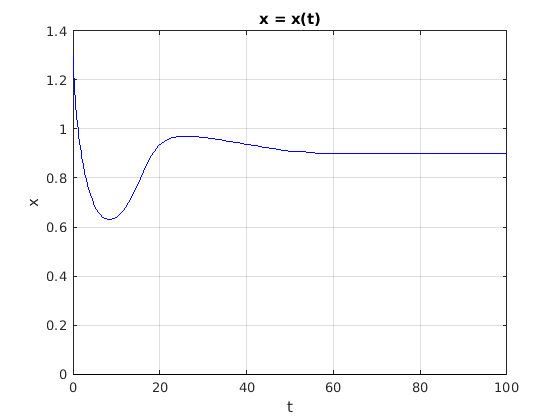
\includegraphics[width=8cm]{18_syst_equ_diff/graphe5a}
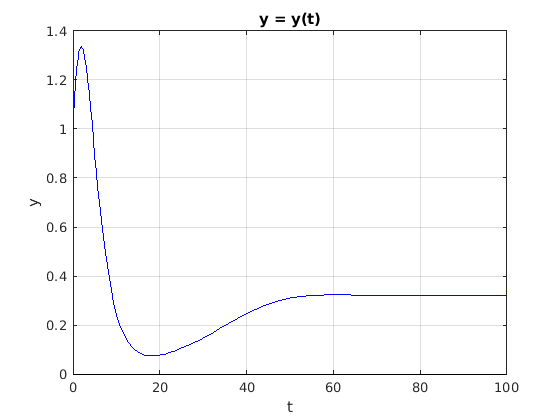
\includegraphics[width=8cm]{18_syst_equ_diff/graphe5b}
% \MATHgraph{18_syst_equ_diff/graphe5a}{8cm}
% \MATHgraph{18_syst_equ_diff/graphe5b}{8cm}

Pour observer plus d'oscillations autour du point d'équilibre
$\VEC{p}$, il faudrait intégrer pour une très longue période de
temps (puis comprimer le graphe selon l'axe des $t$ et
étirer le graphe selon l'axe des $x$ et $y$).
Qualitativement, les graphes de $x$ et $y$ devraient être semblables à
ceux qui suivent.
\PDFgraph{18_syst_equ_diff/graphe5}
}

%%% Local Variables: 
%%% mode: latex
%%% TeX-master: "notes"
%%% End: 


\cleardoublepage
%\clearemptydoublepage

\UObibliography
\UOindex

\end{document}


%%% Local Variables: 
%%% mode: latex
%%% TeX-master: t
%%% End: 
